\chapter{Model Development}
\label{ch:ModelDev}

\section{Bond Pair Material Model}
Consider the material model illustrated in \cref{fig:SimpleBondpair} in which every bond-vector originating from a point is connected by a rotational spring to its opposite originating from that same point.
%
\begin{figure}[h]
\centering
\resizebox{0.6\linewidth}{!}{\subinputfrom{\diagrampath}{simpleBondPair.eps_tex}}
\caption{Illustration of a bond pair model that resists angular deformation}
\label{fig:SimpleBondpair}
\end{figure}
%
If we call the deformed angle between these bonds \(\theta\), and choose the potential energy of that spring to be \(w(\boldsymbol{\xi}) = \omega(\boldsymbol{\xi})\alpha [1 + \cos(\theta) ] \) for the bond pair $\boldsymbol{\xi}$ and $-\boldsymbol{\xi}$, we can recover the non-ordinary force state proposed by Silling in \cite{silling2007peridynamic} by taking the Fr\'echet derivative. For the derivation and a description of the Fr\'echet derivative see \cref{sec:frechet}.
%
\begin{align}
\label{eq:SillingForceNO}
\vstate{T}{}{\boldsymbol{\xi}} &= \nabla w\!\left(\vstate{Y}{}{\boldsymbol{\xi}}\right)\notag \\
%
&=\omega(\boldsymbol{\xi})\frac{-\alpha}{|\vstate{Y}{}{\boldsymbol{\xi}}|} \frac{\vstate{Y}{}{\boldsymbol{\xi}}}{|\vstate{Y}{}{\boldsymbol{\xi}}|} \times \left[\frac{\vstate{Y}{}{\boldsymbol{\xi}}}{|\vstate{Y}{}{\boldsymbol{\xi}}|} \times \frac{\vstate{Y}{}{-\boldsymbol{\xi}}}{|\vstate{Y}{}{-\boldsymbol{\xi}}|}\right]
\end{align}
%
Though it looks complex, \cref{eq:SillingForceNO} indicates a bond force perpendicular to the deformed bond and in the plane containing both the deformed bond and its partner as illustrated in \cref{fig:Bondpair}. 
The force magnitude is proportional to the sine of the angle between the bonds divided by the length of the deformed bond. 
%
\begin{figure}[h]
  \vspace{5mm}
\centering
\resizebox{0.6\linewidth}{!}{\subinputfrom{\diagrampath}{bondPair.eps_tex}}
\caption{Deformation and force vector states}
\label{fig:Bondpair}
\end{figure}
%
This response is consistent with the idea of a rotational spring between bonds as long as the change in angle is small. 
Because the potential energy and force states are functions of \textit{pairs} of peridynamic bonds, we will call this formulation a \textit{bond-pair model}. 
Other choices for the bond-pair potential function, such as $w = (\pi - \theta)^2$, are also possible, but result in more mathematically complex analysis.

\section{Bond Pair Beam in Bending}
\label{sec:BPbeam}
The simplest application of our bond-pair based peridynamic model is that of \cref{fig:continuousbeam}, a beam in transverse bending.
Much of the material in this section can also be found in \cite{ogrady2014beams}.
%
\begin{figure}[h]
  \centering
\subinputfrom{\diagrampath}{continuousBeam.eps_tex}
\caption{A continuous peridynamic beam with horizon $\delta$}
\label{fig:continuousbeam}
\end{figure}
%

\subsection{Energy Equivalence}
\label{sec:beamEnergy}
To determine an appropriate choice of $\alpha$ for \cref{eq:SillingForceNO}, we desire our peridynamic model to have an equivalent strain energy density to a classical Euler-Bernoulli beam in the \emph{local limit}, i.e.\ when the nonlocal length scale vanishes.  We will begin with the assumptions from Euler beam theory: the length of the beam is much greater than thickness, vertical displacements are small, and rotations are small. For small vertical displacements (i.e.\ $\sin{\theta} \approx \theta$) we have
%
\begin{equation}
\theta(\vstate{Y}{}{\xi},\vstate{Y}{}{\mathbf{-\xi}}) \approx \pi-\frac{v(x+\xi)-2v(x)+v(x-\xi)}{\xi},
\label{eq:beamdtheta}
\end{equation}
%
where $v$ is the vertical displacement of material point.  Momentarily assuming that $v$ is continuous and using a Taylor series to expand the right-hand-side of eq.~(\ref{eq:beamdtheta})  
%
\begin{align}
\theta(\vstate{Y}{}{\xi},\vstate{Y}{}{\mathbf{-\xi}}) &\approx \pi-\xi \frac{\partial^2 v}{\partial x^2}+\mathcal{O}(\xi^3) \notag \\
&\approx  \pi-\xi \kappa +\mathcal{O}(\xi^3); 
\label{eq:beamdtheta2}
\end{align}
with
\begin{equation}
\kappa = \frac{\partial^2 v}{\partial x^2}.\notag
\end{equation}
%
Substituting eq.~(\ref{eq:beamdtheta2}) into the equation for the strain energy density of a single bond-pair,
%
\begin{align}
\label{eq:continuousBeamw}
w(\xi) &= \omega(\xi) \alpha \left[1+\cos(\theta(\vstate{Y}{}{\xi},\vstate{Y}{}{\mathbf{-\xi}})) \right] \notag\\
&\approx \omega(\xi) \alpha\frac{\xi^2}{2}(\kappa)^2 +\mathcal{O}(\xi^4).\notag
\end{align}
%
If we use a weighting function \(\omega(\xi)=\omega(|\xi|)\) and assume that the $\omega$ plays the role of a localization kernel, i.e. $\omega = 0 \,\, \forall \,\, \xi > \delta$, the resulting strain energy density, $W$, for any material point in the peridynamic beam is
%
\begin{equation}
W = \frac{\alpha}{2}\kappa^2 \int_{-\delta}^\delta \omega(\xi)\xi^2 {\rm d}\xi + \mathcal{O}(\delta^5).\notag
\end{equation}
%
Equating $W$ with the classical Euler-Bernoulli beam strain-energy density, $\Omega$, and taking the limit as $\delta \to 0$ we can solve for $\alpha$
%
\begin{align}
    \lim_{\delta \to 0}  W &= \Omega, \notag \\
    \frac{\alpha}{2} m \kappa^2 &= \frac{EI}{2} \kappa^2, \notag \\
    \alpha &= \frac{EI}{m},
\label{eq:alpha}
\end{align}
%
with 
\begin{equation}
    m = \int_{-\delta}^{\delta} \omega(\xi) \xi^2 {\rm d}\xi \notag.
\end{equation}

While this demonstrates the model's equivalence to a linearly-elastic Euler beam, if we keep an additional term from the Taylor series approximation of \cref{eq:beamdtheta}, we recover a slightly more complex expressions for change in angle that is demonstrated in \ref{sec:EringenCompare} to reproduce an Euler beam governed by Eringen's model of nonlocal elasticity.

\subsection{Relation to Eringen Nonlocality}
\label{sec:EringenCompare}
%If we relax our homogeneity assumption somewhat, we recover from \cref{eq:beamdtheta} slightly more complex expressions for change in angle
If we keep an additional term from the Taylor series approximation of \cref{eq:beamdtheta}, we recover a slightly more complex expressions for change in angle
%
\begin{equation}
\label{eq:beamdthetaHOT}
%\theta(\vstate{Y}{}{\xi},\vstate{Y}{}{\mathbf{-\xi}}) \approx \pi-\xi \frac{\partial^2 y}{\partial x^2} -\frac{\xi^3}{12} \frac{\partial^4 y}{\partial x^4}  +\mathcal{O}(\xi^5)=  \pi-\xi \kappa-\frac{\xi^3}{12} \kappa''+\mathcal{O}(\xi^5)\notag
\theta(\vstate{Y}{}{\xi},\vstate{Y}{}{\mathbf{-\xi}}) \approx \arctan\left(\pi-\xi \frac{\partial^2 v}{\partial x^2} -\frac{\xi^3}{12} \frac{\partial^4 v}{\partial x^4}  +\mathcal{O}(\xi^5)\right)\notag
\end{equation}
%
and for the strain energy (again substituting \(\kappa = v''\) for readability),
%
%\begin{equation}
%W \approx \int_{-\delta}^\delta \omega(\xi)\alpha(\frac{\xi^2}{2}\kappa^2+\frac{\xi^4}{12}\kappa\kappa''-\frac{3\; \xi^4}{8}\kappa^4+\mathcal{O}(\xi^6)) d\xi .
%\end{equation}
%
%
\begin{equation}
%W \approx \int_{-\delta}^\delta \omega(\xi)\alpha(\frac{\xi^2}{2}\kappa^2+\frac{\xi^4}{12}\kappa\kappa''-\frac{\xi^4}{24}\kappa^4+\mathcal{O}(\xi^6)) d\xi .\notag
W \approx \int_{-\delta}^\delta \omega(\xi)\alpha(\frac{\xi^2}{2}\kappa^2+\frac{\xi^4}{12}\kappa\kappa''-\frac{3\; \xi^4}{8}\kappa^4+\mathcal{O}(\xi^6)) d\xi.\notag
\end{equation}
%
As the horizon \(\delta\) becomes small, higher-order \(\xi\) terms become relatively less important, and \(\xi^4\kappa^4\) is dominated by \(\xi^2\kappa^2\) for large \(\kappa\) and by \(\xi^4\kappa\kappa''\) for small \(\kappa\).
The remaining terms can be rearranged,
\begin{align}
W &\approx \int_{-\delta}^\delta \omega(\xi)\alpha \frac{\xi^2}{2}\kappa(\kappa + \frac{\xi^2}{6}\kappa'') d\xi, \notag
\end{align}
in a manner strongly suggesting an alternative bending resistance term.
We can picture a bending resistance based on the bond length and proportional to the nonlocal curvature  \(\bar{\kappa}=(\kappa + \frac{\xi^2}{6}\kappa'')\), so that 
%
\begin{align}
\label{eq:NLbending}
\bar{\kappa}&=(\kappa + \frac{\xi^2}{6}\kappa'') \implies  \\
W &\approx \int_{-\delta}^\delta \omega(\xi)\alpha \frac{\xi^2}{2}\kappa\bar{\kappa}d\xi .\notag
\end{align}
%  
The same analysis can be taken further to obtain higher-order energy terms with even powers of \(\xi\) and even order derivatives of \(\kappa\). 
Not all of these higher-order terms can be separated into the product of a local curvature and nonlocal bending resistance.

Eringen's model for nonlocal elasticity in \cite{eringen1983differential} begins with a nonlocal modulus (denoted here as \(K(|\mathbf{x}'-\mathbf{x}|,\tau)\)) that relates the nonlocal stress \(\mathbf{t}\) at a point to the classical (local) stress \(\boldsymbol{\sigma}\) in the nearby material through the integral
\begin{equation}
\mathbf{t} = \int_\mathbf{V} K(|\mathbf{x}'-\mathbf{x}|,\tau)\boldsymbol{\sigma}(\mathbf{x}')dv(\mathbf{x}').\notag
\end{equation}
In the local limit these relationships take the form of higher-order gradients.
Using a 1-dimensional decaying exponential nonlocal modulus \(K(|x|,\tau)=\frac{1}{\tau l}e^{-\frac{|x|}{\tau l}}\)results in a relationship between \(t_\text{1D}\) and \(\sigma_\text{1D}\)
\begin{align}
\left(1-(\tau l)^2\frac{\partial^2}{\partial x^2}\right)t_\text{1D}&=\sigma_\text{1D},\notag
\end{align}
in which \((\tau l)\) is a scale-based material parameter.
For well-behaved \(t_\text{1D}\) and \(\sigma_\text{1D}\) and small values of \(\sigma_\text{1D}''''\) and \((\tau l)^2\), we can see that this relationship could be reformulated as
\begin{equation}
\label{eq:NLstress}
t_\text{1D}=\left(1+(\tau l)^2\frac{\partial^2}{\partial x^2}\right)\sigma_\text{1D}.\notag
\end{equation}
If we consider the results of the previous section and let \(dM = y\sigma dA\) and \(\sigma = Ey\kappa\), the contribution to moment resulting from Eringen's nonlocal elasticity in a fiber at \(y\)
\begin{equation}
\label{eq:EringenMoment}
E y^2 (\kappa+(\tau l)^2\kappa''), \\
\end{equation}
and the resulting strain energy
\begin{equation}
\label{eq:EringenEnergy}
\int_{-\frac{t}{2}}^{\frac{t}{2}} b(y) E \frac{y^2}{2} \kappa (\kappa+(\tau l)^2\kappa'')  dy,\notag
\end{equation}
bear a striking resemblance to \cref{eq:NLbending}.
In fact, by carefully choosing peridynamic parameter values, the results can be made identical.
For a rectangular beam of width \(b\) and thickness \(t\), choosing 
\begin{equation}
\omega(\xi) = |\xi|b ;\qquad \delta = \tau l \sqrt{3} ;\qquad \alpha = \frac{E b t^3}{54 (\tau l)^4}\notag
\end{equation}
results in
\begin{equation}
W \approx E b \frac{t^3}{12} \frac{\kappa}{2}(\kappa+\tau^2 l^2 \kappa''), \notag
\end{equation}
the same result for both models.

The similarity between \cref{eq:NLbending,eq:EringenMoment} is not accidental; Eringen's gradient elasticity is the solution to the integral formulation of the nonlocal stress integral equation just as the peridynamic energy is an integral function of nonlocal displacements.
It is therefore unsurprising that, like Eringen's nonlocal elasticity\cite{Challamel2008small}, this peridynamic bending model fails to predict the stiffening associated with nanoscale cantilevers.
Instead, the advantage of peridynamic models is their natural handling of discontinuities.

\subsection{Weighting function and inelasticity}
\label{sec:WeightFunction}
The weighting function \(\omega(\xi)\) describes the relative contribution of each bond-pair, and can be defined according to physical or mathematical considerations. 
While any function $\omega(\xi)$ that produces a convergent integral for $m$ will reproduce an elastic Euler beam, a physically meaningful choice of $\omega$ will allow us to extend our model to certain inelastic behaviors.
Consider a classical Euler-Bernoulli beam in bending with curvature \(\kappa\). 
Fibers running parallel to the neutral axis of the beam are stretched in proportion to their distance from the neutral axis, with strain \(\epsilon = y\kappa\). 
If the fibers are linearly elastic, then the axial stress at each location is \(\sigma = E\epsilon = Ey\kappa\), and the contribution to supported moment \(dM = \kappa E y^2 dA\). 
By comparing the formulations for the moments carried by the Euler beam in \cref{fig:EulerBending} and those of the bond-pair beam in \cref{fig:BPBending}, we see some definite parallels.
%
\begin{figure}[htbp]
\centering
\resizebox{0.5\linewidth}{!}{\subinputfrom{\diagrampath}{EulerBending.eps_tex}}
\caption{Euler beam moment contribution}
\label{fig:EulerBending}
\end{figure}
%
%
\begin{figure}[htbp]
  \vspace{5mm}
\centering
\subinputfrom{\diagrampath}{BondPairBending_edit.eps_tex}
\caption{Bond-pair moment contribution}
\label{fig:BPBending}
\end{figure}
%
\begin{align}
M_\text{E}&=\int_{-\frac{t}{2}}^{\frac{t}{2}} \sigma \; y \; dA &= \int_{-\frac{t}{2}}^{\frac{t}{2}} E \kappa \; y^2 \; b(y) dy\notag \\
%
M_\text{PD}&=\int_{-\delta}^{\delta} \vstate{T}{}{\xi}\; \xi \; d\xi &\notag \\
&= \int_{-\delta}^{\delta} \alpha \frac{\sin(\Delta\theta)}{|\xi|} \; \xi \; \omega(\xi) d\xi\: &\approx \int_{-\delta}^{\delta} \alpha \kappa |\xi| \; \omega(\xi) d\xi\notag
\end{align}
%
The term \(y\) is the distance from the beam's neutral axis and \(b(y)\) is the width of the beam at that distance from the neutral axis. 
The similarity between classical and peridynamic moment formulations suggests a possible formulation for the weighting function:
%
\begin{equation}
\label{eq:WeightFunction}
\omega(\xi) = |\xi| b\left(y\right) \quad \text{at} \quad y=\frac{\xi}{\delta} \frac{t}{2}
\end{equation}
%
\begin{figure}[h]
 \centering
  \subinputfrom{\diagrampath}{WeightProfile_Uniform.eps_tex}
\caption{Weight function for a beam of rectangular cross-section}
\label{fig:WeightProfileUniform}
\end{figure}

\begin{figure}
  \centering
  \subinputfrom{\diagrampath}{WeightProfile_Ibeam.eps_tex}
\caption{Weight function for an I-beam}
\label{fig:WeightProfileIbeam}
\end{figure}
%
This weight function analogizes the relative contributions of bond pairs of different lengths to the relative contributions of fibers at different distances from the centerline. 
An example for a rectangular beam is illustrated in \cref{fig:WeightProfileUniform}.
For an I beam with height \(h_\text{beam}\), width \(w_\text{beam}\), web height \(h_\text{web}\), and web width \(w_\text{web}\), substituting the beam profile
\begin{equation}
b(y) = 
  \begin{dcases}
    w_\text{web} & \text{if } |y| \leq \frac{h_\text{web}}{2} \\
    w_\text{beam} & \text{if } \frac{h_\text{web}}{2} < |y| \leq \frac{h_\text{beam}}{2} \\
    0 &\text{otherwise}
  \end{dcases}\notag
\end{equation}
into \cref{eq:WeightFunction} gives the weight function
\begin{equation}
\omega(\xi) = 
  \begin{dcases}
    |\xi| w_\text{web}& \text{if } |\xi| \leq \delta\frac{h_\text{web}}{h_\text{beam}} \\
    |\xi| w_\text{beam} & \text{if } \delta\frac{h_\text{web}}{h_\text{beam}} < |\xi| \leq \delta \\
    0 &\text{otherwise}
  \end{dcases}\notag
\end{equation}
and is ilustrated in \cref{fig:WeightProfileIbeam}.
    While this weighting function offers no advantages over a uniform weight function in the case of the linearly elastic beam, it offers a way to model advancing plasticity.

In a deformed elastic perfectly-plastic beam, axial fibers are still stretched in proportion to their distance from the neutral axis, but the relationship \(\sigma = E\epsilon = Ey\kappa\) only holds for \(|\epsilon| = |y\kappa| < \epsilon_c\). 
For greater stretches, the relationship becomes \(\sigma = \pm E\epsilon_c \). 
To model this behavior, consider a bond pair with similar behavior: for angular deformation less than some critical angle, the model behaves as previously described, but the magnitude of the force remains constant above a critical deformation
%
\begin{equation}
|\vstate{T}{}{\xi}| = 
  \begin{cases}
    \alpha \omega(\xi) \frac{\sin(\theta(\vstate{Y}{}{\xi},\vstate{Y}{}{\mathbf{-\xi}}))}{|\vstate{Y}{}{\xi}|} & \quad \text{if } \theta < \theta_c\\
    \alpha \omega(\xi) \frac{\sin(\theta_c)}{|\vstate{Y}{}{\xi}|} & \quad \text{if } \theta \geq \theta_c\
  \end{cases}
  \label{eq:epp_force}
\end{equation}
%
to determine the critical angle \(\theta_c\), we let the onset of plasticity in pairs of the longest bonds to coincide with the onset of plasticity in the fibers at the top and bottom surfaces of the classical beam. 
For small curvatures \(\Delta\theta = \xi\kappa\implies\Delta\theta_c = \frac{2\delta\epsilon_c}{t}\). 
For curvatures \(|\kappa| > \kappa_c=\frac{2\epsilon_c}{t}\), the radius within which bonds are in the elastic region is \(\delta_e = \delta \frac{\kappa_c}{\kappa}\), and parallels the distance from the beam centerline that fibers are in the elastic region \(y_e = \frac{t}{2} \frac{\kappa_c}{\kappa}\)
%
\begin{align}
  M_\text{classical} &= 2 \int_{0}^{y_e}E b(y)y^2 \kappa dy +2 \int_{y_e}^{\frac{t}{2}}E b(y) \epsilon_c y dy\notag \\
  M_\text{PD} &= 2 \int_{0}^{\delta_e}\alpha \omega(\xi) \xi^2 \kappa d\xi +2 \int_{\delta_e}^{\delta}\alpha \omega(\xi) \Delta\theta_c \xi d\xi \notag
\end{align}
%
Of course, as long as the force is independent of history, this model only represents a nonlinear elastic material. 
By keeping track of the plastic deformation \(\theta^p (\xi) = \theta-\theta_c\) of each bond-pair, and applying it as an offset, we can reproduce the hysteresis associated with elastic-perfectly-plastic deformation.

More simply, we can model a brittle material by setting the force to zero for bond pairs exceeding a critical angle,
%
\begin{equation}
|\vstate{T}{}{\xi}| = 
  \begin{cases}
    \alpha \omega(\xi) \frac{\sin(\theta(\vstate{Y}{}{\xi},\vstate{Y}{}{\mathbf{-\xi}}))}{|\vstate{Y}{}{\xi}|} & \quad \text{if } \theta < \theta_c\\
    0 & \quad \text{if } \theta \geq \theta_c\
  \end{cases}
  \label{eq:brittle_force}
\end{equation}
%
and additionally recording bond pairs that have exceeded their critical angle and permanently setting their influence, i.e. $\omega$, to zero.
%
%
\section{Bond Pair Plate in Bending}
The next case we will analyze is the extension of the bond pair beam model to \cref{fig:BondPairPlate}, a flat plate in the \(xy\) plane, with displacement $w$ in the \(z\)-direction. 
%
\begin{figure}[htbp]
    \centering
    \subinputfrom{\diagrampath/}{continuousPlate.eps_tex}
    \caption{Illustration of a bond pair on a plate.}
    \label{fig:BondPairPlate}
\end{figure}
%

\subsection{Energy Equivalence}
%
As with the beam model, we determine an appropriate choice of $\alpha$ so that our peridynamic model will have an equivalent strain energy density to a classical Kirckhoff plate in the \emph{local limit}.  We will begin with the assumptions from Kirckhoff plate theory: straight lines normal to the mid-surface remain both straight and normal to the deformed mid-surface, and the plate thickness does not change with deformation.  As with the Euler beam energy equivalence, we will start with the original assumptions from Kirchhoff-Love plate theory of small displacements and rotations, but they will not constrain the validity of the model for larger displacements and rotations.  For small vertical displacements we have
%
\begin{equation}
    \theta(\vstate{Y}{}{\boldsymbol{\xi}},\vstate{Y}{}{\boldsymbol{-\xi}}) \approx \pi-\frac{w(\mathbf{x}+\boldsymbol{\xi})-2w(\mathbf{x})+w(\mathbf{x}-\boldsymbol{\xi})}{|\boldsymbol{\xi}|},
    \label{eq:platetheta}
\end{equation}
%
where $w$ is the vertical displacement of material point.  Taking \(\boldsymbol{\xi}=\xi (\cos(\phi),\sin(\phi))\) in cartesian coordinates and momentarily assuming continuous displacements for the sake of comparison, we use a Taylor series to expand the right-hand-side of eq.~(\ref{eq:platetheta}) about \(\xi = 0\) 
%
\begin{equation}
    \theta(\vstate{Y}{}{\boldsymbol{\xi}},\vstate{Y}{}{\boldsymbol{-\xi}}) \approx \pi-\frac{\xi}{2} \left(\cos^2(\phi) \kappa_1+\sin^2(\phi) \kappa_2+2\sin(\phi)\cos(\phi)\kappa_3\right)+\mathcal{O}(\xi^3)
    \label{eq:platetheta2}
\end{equation}
%
with
%
\begin{equation}
    \kappa_1=\frac{\partial^2 w}{\partial x_1^2}, \quad \kappa_2= \frac{\partial^2 w}{\partial x_2^2}, \quad \kappa_3=\frac{\partial^2 w}{\partial x_1\partial x_2}\notag
\end{equation}
%
substituting eq.~(\ref{eq:platetheta2}) into the equation for the strain energy density of a single bond-pair,
%
\begin{align}
%\label{eq:continuousBeamw}
    w &= \omega(\boldsymbol{\xi}) \alpha \left[1+\cos(\theta(\vstate{Y}{}{\boldsymbol{\xi}},\vstate{Y}{}{\boldsymbol{-\xi}}) ) \right] \notag \\
    &= \omega(\boldsymbol{\xi}) \alpha\frac{\xi^2}{8}(\kappa_1^2\cos^4(\phi)+\kappa_2^2\sin^4(\phi)+2\kappa_1\kappa_2\cos^2(\phi)\sin^2(\phi)+4\kappa_3^2\cos^2(\phi)\sin^2(\phi) \notag \\
    &+ 4\kappa_1\kappa_3\cos^3(\phi)\sin(\phi)+4\kappa_2\kappa_3\cos(\phi)\sin^3(\phi))+\mathcal{O}(\xi^4).\notag
\end{align}
%
If we use a weighting function \(\omega(\boldsymbol{\xi})=\omega(\xi)\) and assume that the $\omega$ plays the role of a localization kernel, i.e. $\omega = 0 \; \forall \; \xi > \delta$, the resulting strain energy density, $W$, for any material point in the peridynamic plate is \todo{is the order right here?  $\delta^6$???}
%
\begin{align}
    W =& \alpha \int_{0}^\delta\int_0^{2 \pi} w\; \xi {\rm d}\phi {\rm d}\xi ,\notag \\
    =& \alpha \frac{3\pi}{8} \left(\kappa_1^2+\kappa_2^2+\frac{2}{3}\kappa_1\kappa_1+\frac{4}{3}\kappa_3^2 \right)\int_{0}^\delta \omega(\xi)\xi^3{\rm d}\xi + \mathcal{O}(\delta^6).\notag 
\end{align}
%
Equating $W$ with the classical Kirchhoff plate strain-energy density, $\Omega$, and taking the limit as $\delta \to 0$ we can solve for $\alpha$
%
\begin{align}
    \lim_{\delta \to 0}  W &= \Omega, \notag \\
    \alpha \frac{3 \pi}{8} m \left(\kappa_1^2+\kappa_2^2+\frac{2}{3}\kappa_1\kappa_1+\frac{4}{3}\kappa_3^2 \right)&= \left[ \frac{\mu h^3}{12(1-\nu)} \left(\kappa_1^2+\kappa_2^2+2\nu\kappa_1\kappa_1+2(1-\nu)\kappa_3^2 \right) \right]_{\nu=1/3}, \notag \\
%    \nu = \frac{1}{3},\:\: \alpha &= \frac{8}{3 \pi m} \frac{\mu h^3}{12(1-\nu)},
    \alpha &= \frac{2 \mu h^3}{3 m}, \\
    \text{with}\qquad \qquad \notag \\
%    \label{eq:platealpha}
%    m = \int_{0}^{\delta} \omega(\xi) \xi^3 {\rm d}\xi \notag.
    m &= \int_{0}^{\delta} \int_{0}^{2\pi}\omega(\xi) \xi^2 \xi {\rm d}\phi {\rm d}\xi \notag,
\end{align}
%
where $\mu$ is the shear modulus, $h$ is the thickness of the plate, and we have evaluated the classical Kirchhoff strain-energy at a Poisson ratio of \(\sfrac{1}{3}\) in order to solve for alpha as a constant.  Because $\alpha$ is inversely proportional to $m$, the energy does not change with varying choices for $\omega$ and $\delta$. It should be noted that the restriction \(\nu=\sfrac{1}{3}\) is the same imposed by the use of a bond based peridynamic model for in-plane deformation of a 2D peridynamic plate. We will show an extension to this model that removes this restriction in Section~\ref{sec:arbitrary}.

\subsection{Combining Bending and Extension Models}
The bond-pair bending model does not resist in-plane stretching or shear deformation because these deformations preserve the angles between opposite bonds.  If these behaviors are expected in combination with bending, a useful model must resist both in-plane and transverse deformations.  To create a plate model that also resists these deformations, i.e.\ a flat shell, we combine the bond-pair model with a two-dimensional version of the original bond-based linearly-elastic peridynamic solid model from \cite{silling2000reformulation}.  In this model, individual bonds act as springs resisting changes in length.
%
\begin{equation}
    \label{eq:bondextension}
    \vstate{T}{}{\boldsymbol{\xi}} =\beta\left(|\vstate{Y}{}{\boldsymbol{\xi}}|-|\boldsymbol{\xi}|\right)\frac{\vstate{Y}{}{\boldsymbol{\xi}}}{|\vstate{Y}{}{\boldsymbol{\xi}}|}
\end{equation}
%
By matching the energy of a 2D material in shear deformation, we can relate \(\beta\) to the shear modulus and thickness of the shell.  Following the example of \cite{silling2007peridynamic}, we begin with a 2D material under pure in-plane shear.  In Einstein notation, the strain energy of this material is
%
%\begin{align*}
%    W^d_\text{C} &= \mu \; h \; \epsilon_{ij} \epsilon_{ij} = \mu \; h \; \epsilon_{ij}^d \epsilon_{ij}^d \\
%    W^d_\text{PD} &= \frac{\beta}{2}(\underline{\omega}\; \underline{\epsilon^d})\bullet \underline{\epsilon^d}\\
%    &=\frac{\beta}{2} \epsilon_{ij}^d \epsilon_{kl}^d \int_A \frac{\underline{\omega}\langle\xi\rangle}{|\boldsymbol{\xi}|^2}\xi_i \xi_j \xi_k \xi_l \;dA_\xi\\
%\end{align*}
%
\begin{align*}
    W_\text{C} &= \mu \; h \; \epsilon_{ij}^d \epsilon_{ij}^d,  \\  \\
    W_\text{PD} &= \frac{\beta}{2}\int_A \omega(\xi)\left(|\vstate{Y}{}{\boldsymbol{\xi}}|-|\boldsymbol{\xi}|\right)^2 \; {\rm d}A_{\boldsymbol{\xi}}, \\
    &=\frac{\beta}{2}\int_A  \omega(\xi) \frac{\epsilon_{ij}\xi_i \xi_j }{|\boldsymbol{\xi}|} \frac{\epsilon_{kl} \xi_k \xi_l }{|\boldsymbol{\xi}|}\;{\rm d}A_{\boldsymbol{\xi}},\\
    &=\frac{\beta}{2} \epsilon_{ij}^d \epsilon_{kl}^d \int_A \frac{ \omega(\xi)}{|\boldsymbol{\xi}|^2}\xi_i \xi_j \xi_k \xi_l \;{\rm d}A_{\boldsymbol{\xi}}.
\end{align*}
%
where $\epsilon^d$ is the deviatoric strain tensor.  Now, to evaluate the integral we will exploit the symmetry properties. With $i, j, k, l = 1,2$. For a circular $\omega(\xi) = \omega(|\xi|)$, combinations of $\{i,j,k,l\}$ with an odd number of each index, such as $\{1,1,1,2\}$ or $\{2,1,2,2\}$, will result in odd powers of sine and cosine and integrate to 0.
%
\begin{align*}
%    m&=(\underline{\omega}\:\underline{x}) \bullet \underline{x}\\
    m &= \int_A \omega(\xi)|\boldsymbol{\xi}|^2\; dA_{\boldsymbol{\xi}} \\
    W^d_\text{PD} &= \frac{\beta \; m}{16}[3(\epsilon_{11}\epsilon_{11}+\epsilon_{22}\epsilon_{22})+(\epsilon_{11}\epsilon_{22}+\epsilon_{12}\epsilon_{12}+\epsilon_{12}\epsilon_{21}+\epsilon_{21}\epsilon_{12}+\epsilon_{21}\epsilon_{21}+\epsilon_{22}\epsilon_{11})]\\
    &= \frac{\beta \; m}{16} \epsilon_{ij}^d \epsilon_{kl}^d (\delta_{ij}\delta_{kl}+\delta_{ik}\delta_{jl}+\delta_{il}\delta_{jk})\\
    &= \frac{\beta \; m}{8} \epsilon_{ij}^d \epsilon_{ij}^d \implies\\
     \beta &= \frac{8 \; \mu\;h}{m}
\end{align*}
%
Having calibrated the bond-extension model to the shear modulus for a case of pure in-plane shear, applying a different uniform strain (such as might result from uniaxial tension) reveals the bond-based model to result in a one-parameter linearly-elastic model with Poisson's ratio \(\nu=\sfrac{1}{3}\).  

Combining the bending and extension models allows for the description of more complex behaviors, particularly the stiffening effect of in-plane tension on the transverse bending of a shell.  Consider a single bond-pair in the combined model shown in Fig.~\ref{fig:hybridmodel}.
%
\begin{figure}[htbp]
  \vspace{5mm}
  \centering
  


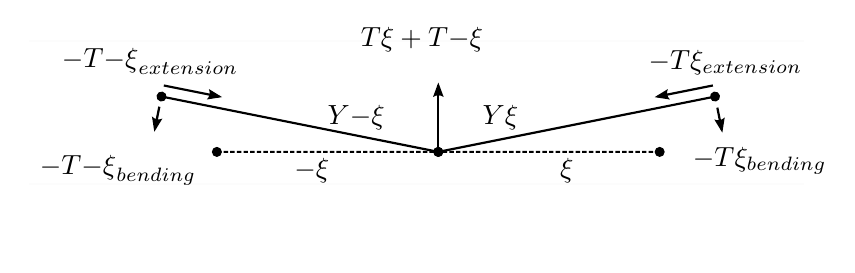
\begin{tikzpicture}[y=0.80pt, x=0.8pt,yscale=-1, inner sep=0pt, outer sep=0pt]
\begin{scope}[shift={(-16.10332,-55.70103)}]
  \begin{scope}[fill=black]
    \path[color=black,fill=black,line width=0.800pt] (101.0938,106.6875) --
      (103.0938,106.6875) -- (103.0938,105.6875) -- (101.0938,105.6875) --
      cycle(104.0938,106.6875) -- (106.0938,106.6875) -- (106.0938,105.6875) --
      (104.0938,105.6875) -- cycle(107.0938,106.6875) -- (109.0938,106.6875) --
      (109.0938,105.6875) -- (107.0938,105.6875) -- cycle(110.0938,106.6875) --
      (112.0938,106.6875) -- (112.0938,105.6875) -- (110.0938,105.6875) --
      cycle(113.0938,106.6875) -- (115.0938,106.6875) -- (115.0938,105.6875) --
      (113.0938,105.6875) -- cycle(116.0938,106.6875) -- (118.0938,106.6875) --
      (118.0938,105.6875) -- (116.0938,105.6875) -- cycle(119.0938,106.6875) --
      (121.0938,106.6875) -- (121.0938,105.6875) -- (119.0938,105.6875) --
      cycle(122.0938,106.6875) -- (124.0938,106.6875) -- (124.0938,105.6875) --
      (122.0938,105.6875) -- cycle(125.0938,106.6875) -- (127.0938,106.6875) --
      (127.0938,105.6875) -- (125.0938,105.6875) -- cycle(128.0938,106.6875) --
      (130.0938,106.6875) -- (130.0938,105.6875) -- (128.0938,105.6875) --
      cycle(131.0938,106.6875) -- (133.0938,106.6875) -- (133.0938,105.6875) --
      (131.0938,105.6875) -- cycle(134.0938,106.6875) -- (136.0938,106.6875) --
      (136.0938,105.6875) -- (134.0938,105.6875) -- cycle(137.0938,106.6875) --
      (139.0938,106.6875) -- (139.0938,105.6875) -- (137.0938,105.6875) --
      cycle(140.0938,106.6875) -- (142.0938,106.6875) -- (142.0938,105.6875) --
      (140.0938,105.6875) -- cycle(143.0938,106.6875) -- (145.0938,106.6875) --
      (145.0938,105.6875) -- (143.0938,105.6875) -- cycle(146.0938,106.6875) --
      (148.0938,106.6875) -- (148.0938,105.6875) -- (146.0938,105.6875) --
      cycle(149.0938,106.6875) -- (151.0938,106.6875) -- (151.0938,105.6875) --
      (149.0938,105.6875) -- cycle(152.0938,106.6875) -- (154.0938,106.6875) --
      (154.0938,105.6875) -- (152.0938,105.6875) -- cycle(155.0938,106.6875) --
      (157.0938,106.6875) -- (157.0938,105.6875) -- (155.0938,105.6875) --
      cycle(158.0938,106.6875) -- (160.0938,106.6875) -- (160.0938,105.6875) --
      (158.0938,105.6875) -- cycle(161.0938,106.6875) -- (163.0938,106.6875) --
      (163.0938,105.6875) -- (161.0938,105.6875) -- cycle(164.0938,106.6875) --
      (166.0938,106.6875) -- (166.0938,105.6875) -- (164.0938,105.6875) --
      cycle(167.0938,106.6875) -- (169.0938,106.6875) -- (169.0938,105.6875) --
      (167.0938,105.6875) -- cycle(170.0938,106.6875) -- (172.0938,106.6875) --
      (172.0938,105.6875) -- (170.0938,105.6875) -- cycle(173.0938,106.6875) --
      (175.0938,106.6875) -- (175.0938,105.6875) -- (173.0938,105.6875) --
      cycle(176.0938,106.6875) -- (178.0938,106.6875) -- (178.0938,105.6875) --
      (176.0938,105.6875) -- cycle(179.0938,106.6875) -- (181.0938,106.6875) --
      (181.0938,105.6875) -- (179.0938,105.6875) -- cycle(182.0938,106.6875) --
      (184.0938,106.6875) -- (184.0938,105.6875) -- (182.0938,105.6875) --
      cycle(185.0938,106.6875) -- (187.0938,106.6875) -- (187.0938,105.6875) --
      (185.0938,105.6875) -- cycle(188.0938,106.6875) -- (190.0938,106.6875) --
      (190.0938,105.6875) -- (188.0938,105.6875) -- cycle(191.0938,106.6875) --
      (193.0938,106.6875) -- (193.0938,105.6875) -- (191.0938,105.6875) --
      cycle(194.0938,106.6875) -- (196.0938,106.6875) -- (196.0938,105.6875) --
      (194.0938,105.6875) -- cycle(197.0938,106.6875) -- (199.0938,106.6875) --
      (199.0938,105.6875) -- (197.0938,105.6875) -- cycle(200.0938,106.6875) --
      (201.0938,106.6875) -- (202.0938,106.6875) -- (202.0938,105.6875) --
      (201.0938,105.6875) -- (200.0938,105.6875) -- cycle(203.0938,106.6875) --
      (205.0938,106.6875) -- (205.0938,105.6875) -- (203.0938,105.6875) --
      cycle(206.0938,106.6875) -- (208.0938,106.6875) -- (208.0938,105.6875) --
      (206.0938,105.6875) -- cycle(209.0938,106.6875) -- (211.0938,106.6875) --
      (211.0938,105.6875) -- (209.0938,105.6875) -- cycle(212.0938,106.6875) --
      (214.0938,106.6875) -- (214.0938,105.6875) -- (212.0938,105.6875) --
      cycle(215.0938,106.6875) -- (217.0938,106.6875) -- (217.0938,105.6875) --
      (215.0938,105.6875) -- cycle(218.0938,106.6875) -- (220.0938,106.6875) --
      (220.0938,105.6875) -- (218.0938,105.6875) -- cycle(221.0938,106.6875) --
      (223.0938,106.6875) -- (223.0938,105.6875) -- (221.0938,105.6875) --
      cycle(224.0938,106.6875) -- (226.0938,106.6875) -- (226.0938,105.6875) --
      (224.0938,105.6875) -- cycle(227.0938,106.6875) -- (229.0938,106.6875) --
      (229.0938,105.6875) -- (227.0938,105.6875) -- cycle(230.0938,106.6875) --
      (232.0938,106.6875) -- (232.0938,105.6875) -- (230.0938,105.6875) --
      cycle(233.0938,106.6875) -- (235.0938,106.6875) -- (235.0938,105.6875) --
      (233.0938,105.6875) -- cycle(236.0938,106.6875) -- (238.0938,106.6875) --
      (238.0938,105.6875) -- (236.0938,105.6875) -- cycle(239.0938,106.6875) --
      (241.0938,106.6875) -- (241.0938,105.6875) -- (239.0938,105.6875) --
      cycle(242.0938,106.6875) -- (244.0938,106.6875) -- (244.0938,105.6875) --
      (242.0938,105.6875) -- cycle(245.0938,106.6875) -- (247.0938,106.6875) --
      (247.0938,105.6875) -- (245.0938,105.6875) -- cycle(248.0938,106.6875) --
      (250.0938,106.6875) -- (250.0938,105.6875) -- (248.0938,105.6875) --
      cycle(251.0938,106.6875) -- (253.0938,106.6875) -- (253.0938,105.6875) --
      (251.0938,105.6875) -- cycle(254.0938,106.6875) -- (256.0938,106.6875) --
      (256.0938,105.6875) -- (254.0938,105.6875) -- cycle(257.0938,106.6875) --
      (259.0938,106.6875) -- (259.0938,105.6875) -- (257.0938,105.6875) --
      cycle(260.0938,106.6875) -- (262.0938,106.6875) -- (262.0938,105.6875) --
      (260.0938,105.6875) -- cycle(263.0938,106.6875) -- (265.0938,106.6875) --
      (265.0938,105.6875) -- (263.0938,105.6875) -- cycle(266.0938,106.6875) --
      (268.0938,106.6875) -- (268.0938,105.6875) -- (266.0938,105.6875) --
      cycle(269.0938,106.6875) -- (271.0938,106.6875) -- (271.0938,105.6875) --
      (269.0938,105.6875) -- cycle(272.0938,106.6875) -- (274.0938,106.6875) --
      (274.0938,105.6875) -- (272.0938,105.6875) -- cycle(275.0938,106.6875) --
      (277.0938,106.6875) -- (277.0938,105.6875) -- (275.0938,105.6875) --
      cycle(278.0938,106.6875) -- (280.0938,106.6875) -- (280.0938,105.6875) --
      (278.0938,105.6875) -- cycle(281.0938,106.6875) -- (283.0938,106.6875) --
      (283.0938,105.6875) -- (281.0938,105.6875) -- cycle(284.0938,106.6875) --
      (286.0938,106.6875) -- (286.0938,105.6875) -- (284.0938,105.6875) --
      cycle(287.0938,106.6875) -- (289.0938,106.6875) -- (289.0938,105.6875) --
      (287.0938,105.6875) -- cycle(290.0938,106.6875) -- (292.0938,106.6875) --
      (292.0938,105.6875) -- (290.0938,105.6875) -- cycle(293.0938,106.6875) --
      (295.0938,106.6875) -- (295.0938,105.6875) -- (293.0938,105.6875) --
      cycle(296.0938,106.6875) -- (298.0938,106.6875) -- (298.0938,105.6875) --
      (296.0938,105.6875) -- cycle(299.0938,106.6875) -- (301.0938,106.6875) --
      (301.0938,105.6875) -- (299.0938,105.6875) -- cycle;
    \path[draw=black,fill=black,even odd rule,line width=0.400pt]
      (103.0633,106.2010) .. controls (103.0633,107.3050) and (102.1673,108.2010) ..
      (101.0633,108.2010) .. controls (99.9593,108.2010) and (99.0633,107.3050) ..
      (99.0633,106.2010) .. controls (99.0633,105.0970) and (99.9593,104.2010) ..
      (101.0633,104.2010) .. controls (102.1673,104.2010) and (103.0633,105.0970) ..
      (103.0633,106.2010) -- cycle;
    \path[draw=black,fill=black,even odd rule,line width=0.400pt]
      (203.0633,106.2010) .. controls (203.0633,107.3050) and (202.1673,108.2010) ..
      (201.0633,108.2010) .. controls (199.9593,108.2010) and (199.0633,107.3050) ..
      (199.0633,106.2010) .. controls (199.0633,105.0970) and (199.9593,104.2010) ..
      (201.0633,104.2010) .. controls (202.1673,104.2010) and (203.0633,105.0970) ..
      (203.0633,106.2010) -- cycle;
    \path[draw=black,fill=black,even odd rule,line width=0.400pt]
      (303.0633,106.2010) .. controls (303.0633,107.3050) and (302.1673,108.2010) ..
      (301.0633,108.2010) .. controls (299.9593,108.2010) and (299.0633,107.3050) ..
      (299.0633,106.2010) .. controls (299.0633,105.0970) and (299.9593,104.2010) ..
      (301.0633,104.2010) .. controls (302.1673,104.2010) and (303.0633,105.0970) ..
      (303.0633,106.2010) -- cycle;
  \end{scope}
  \begin{scope}[fill=black]
    \path[color=black,fill=black,line width=0.800pt] (76.1875,80.7188) --
      (76.0000,81.6875) -- (201.0000,106.6875) -- (201.0937,106.7187) --
      (201.1874,106.6875) -- (326.1874,81.6875) -- (326.0000,80.7188) --
      (201.0938,105.6875) -- (76.1875,80.7188) -- cycle;
    \path[draw=black,fill=black,even odd rule,line width=0.400pt] (78.0253,81.5854)
      .. controls (77.8087,82.6680) and (76.7544,83.3709) .. (75.6719,83.1544) ..
      controls (74.5893,82.9378) and (73.8864,81.8835) .. (74.1029,80.8010) ..
      controls (74.3194,79.7184) and (75.3738,79.0155) .. (76.4563,79.2320) ..
      controls (77.5389,79.4485) and (78.2418,80.5029) .. (78.0253,81.5854) --
      cycle;
    \path[draw=black,fill=black,even odd rule,line width=0.400pt]
      (203.0633,106.2010) .. controls (203.0633,107.3050) and (202.1673,108.2010) ..
      (201.0633,108.2010) .. controls (199.9593,108.2010) and (199.0633,107.3050) ..
      (199.0633,106.2010) .. controls (199.0633,105.0970) and (199.9593,104.2010) ..
      (201.0633,104.2010) .. controls (202.1673,104.2010) and (203.0633,105.0970) ..
      (203.0633,106.2010) -- cycle;
    \path[draw=black,fill=black,even odd rule,line width=0.400pt] (328.0253,80.8166)
      .. controls (328.2418,81.8992) and (327.5389,82.9535) .. (326.4563,83.1700) ..
      controls (325.3738,83.3866) and (324.3194,82.6837) .. (324.1029,81.6011) ..
      controls (323.8864,80.5186) and (324.5893,79.4642) .. (325.6719,79.2477) ..
      controls (326.7544,79.0312) and (327.8087,79.7341) .. (328.0253,80.8166) --
      cycle;
  \end{scope}
  \begin{scope}[fill=black]
    \path[color=black,fill=black,line width=0.800pt] (200.5938,76.1875) --
      (200.5938,106.1875) -- (201.5938,106.1875) -- (201.5938,76.1875) --
      (200.5938,76.1875) -- cycle;
    \path[fill=black,line join=round,even odd rule,line width=0.500pt]
      (198.6831,81.4322) -- (201.0937,74.8767) -- (203.5043,81.4322) .. controls
      (202.0811,80.3849) and (200.1339,80.3909) .. (198.6831,81.4322) -- cycle;
  \end{scope}
  \path[fill=black] (178.797,148.02312) node[above right] (text6246) {};
  \path[fill=black] (256.10333,120.20103) node[above right] (text6273)
    {$\boldsymbol{\xi}$};
  \path[fill=black] (136.10332,120.20103) node[above right] (text6277)
    {$\boldsymbol{-\xi}$};
  \path[fill=black] (296.10333,71.201035) node[above right] (text6285)
    {$-\vstate{T}{}{\boldsymbol{\xi}}_{extension}$};
  \path[shift={(71.10332,65.91978)},draw=black,opacity=0.010,line join=miter,line
    cap=butt,line width=0.800pt] (-55.0000,54.7812) -- (295.0000,54.7812);
  \path[fill=black] (316.10333,116.20103) node[above right] (text4473)
    {$-\vstate{T}{}{\boldsymbol{\xi}}_{bending}$};
  \begin{scope}[shift={(0,-64.5)},shift={(0,0)}]
    \path[shift={(71.10332,65.91978)},draw=black,opacity=0.010,line join=miter,line
      cap=butt,line width=0.800pt] (-55.0000,54.7812) -- (295.0000,54.7812);
  \end{scope}
  \path[fill=black] (166.10332,61.201035) node[above right] (text4726)
    {$\vstate{T}{}{\boldsymbol{\xi}}+\vstate{T}{}{\boldsymbol{-\xi}}$};
  \begin{scope}[fill=black]
    \path[color=black,fill=black,line width=0.800pt] (74.5625,85.6875) --
      (72.5625,95.6875) -- (73.5625,95.9062) -- (75.5625,85.9062) --
      (74.5625,85.6875) -- cycle;
    \path[fill=black,line join=round,even odd rule,line width=0.500pt]
      (76.4671,91.1458) -- (72.8177,97.1013) -- (71.7395,90.2003) .. controls
      (72.9297,91.5064) and (74.8403,91.8824) .. (76.4671,91.1458) -- cycle;
  \end{scope}
  \begin{scope}[fill=black]
    \path[color=black,fill=black,line width=0.800pt] (77.1875,75.7188) --
      (77.0000,76.6875) -- (102.0000,81.6875) -- (102.1875,80.7188) --
      (77.1875,75.7188) -- cycle;
    \path[fill=black,line join=round,even odd rule,line width=0.500pt]
      (97.4484,77.8019) -- (103.4039,81.4513) -- (96.5029,82.5295) .. controls
      (97.8090,81.3393) and (98.1849,79.4287) .. (97.4484,77.8019) -- cycle;
  \end{scope}
  \begin{scope}[fill=black]
    \path[color=black,fill=black,line width=0.800pt] (327.5938,86.0938) --
      (326.6250,86.3125) -- (328.6250,96.3125) -- (329.5938,96.0938) --
      (327.5938,86.0938) -- cycle;
    \path[fill=black,line join=round,even odd rule,line width=0.500pt]
      (330.4506,90.5968) -- (329.3725,97.4978) -- (325.7230,91.5423) .. controls
      (327.3240,92.2902) and (329.2322,91.9024) .. (330.4507,90.5968) -- cycle;
  \end{scope}
  \begin{scope}[fill=black]
    \path[color=black,fill=black,line width=0.800pt] (325.0000,75.7188) --
      (300.0000,80.7188) -- (300.1875,81.6875) -- (325.1875,76.6875) --
      (325.0000,75.7188) -- cycle;
    \path[fill=black,line join=round,even odd rule,line width=0.500pt]
      (305.7075,82.5484) -- (298.8066,81.4702) -- (304.7620,77.8207) .. controls
      (304.0142,79.4217) and (304.4020,81.3299) .. (305.7075,82.5484) -- cycle;
  \end{scope}
  \path[fill=black] (21.103317,121.20103) node[above right] (text4217)
    {$-\vstate{T}{}{\boldsymbol{-\xi}}_{bending}$};
  \path[fill=black] (31.103317,71.201035) node[above right] (text4221)
    {$-\vstate{T}{}{\boldsymbol{-\xi}}_{extension}$};
  \path[fill=black] (221.10332,96.201035) node[above right] (text4282)
    {$\vstate{Y}{}{\boldsymbol{\xi}}$};
  \path[fill=black] (151.10332,96.201035) node[above right] (text4286)
    {$\vstate{Y}{}{\boldsymbol{-\xi}}$};
\end{scope}

\end{tikzpicture}


  \caption{The Hybrid Model Combines Bending and Extension Components}
  \label{fig:hybridmodel}
\end{figure}
%
As the two sides are pulled apart, the magnitude of the extension force in each bond increases, and the magnitude of the bending force decreases.  At the same time, the angle at which the extension force acts decreases, and the angle of action for the bending force increases.  For small amounts of bending and reasonable stretches, increased tension in the direction of the bond pair results in increased restorative force.
\section{Extension to arbitrary Poisson ratio}
\label{sec:arbitrary}
Although many materials have Poisson ratios of \(\nu\approx \sfrac{1}{3}\), it is nonetheless desirable to extend the model to materials with arbitrary Poisson ratios.  For isotropic, linearly elastic models of solid materials, Silling et al.\ extended the peridynamic material model to arbitrary material parameters in \cite{silling2007peridynamic} by decomposing the deformation into isotropic and deviatoric components.  In the absence of plastic deformation, we need only find the difference between the strain energy of a deformed bond-based plate and the strain energy of an elastic plate with Poisson's ratio \(\nu \neq \sfrac{1}{3}\).  The difference is a function of the isotropic strain in two dimensions, \(\theta_{2D}\)
%
\begin{align}
    W^\star &= \frac{\mu\;h}{2}\left(\frac{3\nu-1}{1-\nu}\right)\theta_{2D}^2 \notag \\
%    \theta_{2D} &= \frac{2}{m}\left(\underline{\omega x}\right)\bullet\underline{e} \notag \\
    \theta_{2D} &= \frac{2}{m}\int_A \omega(\boldsymbol{\xi})|\boldsymbol{\xi}|(|\vstate{Y}{}{\boldsymbol{\xi}}|-|\boldsymbol{\xi}|)\;dA_{\boldsymbol{\xi}} \notag \\
%    W_\text{total} &= \frac{\mu\;h}{2}\left(\frac{3\nu-1}{1-\nu}\right)\theta_{2D}^2 + \frac{4\;\mu\;h}{m}\left(\underline{\omega e}\right)\bullet\underline{e}\notag
    W_\text{total} &= \frac{\mu\;h}{2}\left(\frac{3\nu-1}{1-\nu}\right)\theta_{2D}^2 + \frac{4\;\mu\;h}{m}\int_A \omega(\boldsymbol{\xi})(|\vstate{Y}{}{\boldsymbol{\xi}}|-|\boldsymbol{\xi}|)^2\;dA_{\boldsymbol{\xi}}\notag
\end{align}
%
This is to be expected because the bond-based model was calibrated to the shear strain energy, leaving discrepancies proportional to the isotropic strain energy that fall to 0 as Poisson's ratio approaches \(\nu = \sfrac{1}{3}\).

This decomposition method inspires a similar approach to our plate model. To perform the same extension for the plate model in bending, we find the error in the 1-parameter strain energy for \(\nu \neq \sfrac{1}{3}\)
%
\begin{align}
    W^\star=&\frac{\mu h^3}{12(1-\nu)} \left(\kappa_1^2+\kappa_2^2+2\nu\kappa_1\kappa_2+2(1-\nu)\kappa_3^2 \right)\notag\\
    &-\frac{\mu h^3}{12(1-\frac{1}{3})} \left(\kappa_1^2+\kappa_2^2+\frac{2}{3}\nu\kappa_1\kappa_2+2(1-\frac{1}{3})\kappa_3^2 \right) \notag \\
    W^\star=&2\mu \frac{h^3}{12}\frac{3\nu-1}{1-\nu} \left(\frac{\kappa_1+\kappa_2}{2}\right)^2.\notag
\end{align}
%
The discrepancy in energy is proportional to the square of average curvature, \(\frac{\kappa_1+\kappa_2}{2}\), which we will also refer to as the isotropic curvature.  The isotropic curvature can be envisioned as the portion of the deformation that resembles a hemispherical bowl.  The remainder of the bending deformation, that which is left when the isotropic curvature is subtracted out, resembles a saddle. This remaining component is the deviatoric deformation, and both components are shown in \cref{fig:BendingDecomp}. Note that the orientation of the deviatoric bending will change depending on the particular curvature being decomposed, while the isotropic curvature will only change in scale.
%
\begin{figure}[htbp]
  \vspace{5mm}
  \centering
  \resizebox{\linewidth}{!}{%% Creator: Matplotlib, PGF backend
%%
%% To include the figure in your LaTeX document, write
%%   \input{<filename>.pgf}
%%
%% Make sure the required packages are loaded in your preamble
%%   \usepackage{pgf}
%%
%% Figures using additional raster images can only be included by \input if
%% they are in the same directory as the main LaTeX file. For loading figures
%% from other directories you can use the `import` package
%%   \usepackage{import}
%% and then include the figures with
%%   \import{<path to file>}{<filename>.pgf}
%%
%% Matplotlib used the following preamble
%%
\begingroup%
\makeatletter%
\begin{pgfpicture}%
\pgfpathrectangle{\pgfpointorigin}{\pgfqpoint{10.000000in}{3.300000in}}%
\pgfusepath{use as bounding box}%
\begin{pgfscope}%
\pgfsetbuttcap%
\pgfsetroundjoin%
\definecolor{currentfill}{rgb}{1.000000,1.000000,1.000000}%
\pgfsetfillcolor{currentfill}%
\pgfsetlinewidth{0.000000pt}%
\definecolor{currentstroke}{rgb}{1.000000,1.000000,1.000000}%
\pgfsetstrokecolor{currentstroke}%
\pgfsetdash{}{0pt}%
\pgfpathmoveto{\pgfqpoint{0.000000in}{0.000000in}}%
\pgfpathlineto{\pgfqpoint{10.000000in}{0.000000in}}%
\pgfpathlineto{\pgfqpoint{10.000000in}{3.300000in}}%
\pgfpathlineto{\pgfqpoint{0.000000in}{3.300000in}}%
\pgfpathclose%
\pgfusepath{fill}%
\end{pgfscope}%
\begin{pgfscope}%
\pgfsetbuttcap%
\pgfsetroundjoin%
\definecolor{currentfill}{rgb}{1.000000,1.000000,1.000000}%
\pgfsetfillcolor{currentfill}%
\pgfsetlinewidth{0.000000pt}%
\definecolor{currentstroke}{rgb}{0.000000,0.000000,0.000000}%
\pgfsetstrokecolor{currentstroke}%
\pgfsetstrokeopacity{0.000000}%
\pgfsetdash{}{0pt}%
\pgfpathmoveto{\pgfqpoint{1.250000in}{0.330000in}}%
\pgfpathlineto{\pgfqpoint{3.529412in}{0.330000in}}%
\pgfpathlineto{\pgfqpoint{3.529412in}{2.970000in}}%
\pgfpathlineto{\pgfqpoint{1.250000in}{2.970000in}}%
\pgfpathclose%
\pgfusepath{fill}%
\end{pgfscope}%
\begin{pgfscope}%
\pgfsetbuttcap%
\pgfsetroundjoin%
\definecolor{currentfill}{rgb}{0.950000,0.950000,0.950000}%
\pgfsetfillcolor{currentfill}%
\pgfsetfillopacity{0.500000}%
\pgfsetlinewidth{1.003750pt}%
\definecolor{currentstroke}{rgb}{0.950000,0.950000,0.950000}%
\pgfsetstrokecolor{currentstroke}%
\pgfsetstrokeopacity{0.500000}%
\pgfsetdash{}{0pt}%
\pgfpathmoveto{\pgfqpoint{1.552171in}{0.913347in}}%
\pgfpathlineto{\pgfqpoint{2.204551in}{1.560615in}}%
\pgfpathlineto{\pgfqpoint{2.193689in}{2.797438in}}%
\pgfpathlineto{\pgfqpoint{1.504935in}{2.215881in}}%
\pgfusepath{stroke,fill}%
\end{pgfscope}%
\begin{pgfscope}%
\pgfsetbuttcap%
\pgfsetroundjoin%
\definecolor{currentfill}{rgb}{0.900000,0.900000,0.900000}%
\pgfsetfillcolor{currentfill}%
\pgfsetfillopacity{0.500000}%
\pgfsetlinewidth{1.003750pt}%
\definecolor{currentstroke}{rgb}{0.900000,0.900000,0.900000}%
\pgfsetstrokecolor{currentstroke}%
\pgfsetstrokeopacity{0.500000}%
\pgfsetdash{}{0pt}%
\pgfpathmoveto{\pgfqpoint{2.204551in}{1.560615in}}%
\pgfpathlineto{\pgfqpoint{3.261344in}{1.198750in}}%
\pgfpathlineto{\pgfqpoint{3.305559in}{2.472870in}}%
\pgfpathlineto{\pgfqpoint{2.193689in}{2.797438in}}%
\pgfusepath{stroke,fill}%
\end{pgfscope}%
\begin{pgfscope}%
\pgfsetbuttcap%
\pgfsetroundjoin%
\definecolor{currentfill}{rgb}{0.925000,0.925000,0.925000}%
\pgfsetfillcolor{currentfill}%
\pgfsetfillopacity{0.500000}%
\pgfsetlinewidth{1.003750pt}%
\definecolor{currentstroke}{rgb}{0.925000,0.925000,0.925000}%
\pgfsetstrokecolor{currentstroke}%
\pgfsetstrokeopacity{0.500000}%
\pgfsetdash{}{0pt}%
\pgfpathmoveto{\pgfqpoint{1.552171in}{0.913347in}}%
\pgfpathlineto{\pgfqpoint{2.664061in}{0.491897in}}%
\pgfpathlineto{\pgfqpoint{3.261344in}{1.198750in}}%
\pgfpathlineto{\pgfqpoint{2.204551in}{1.560615in}}%
\pgfusepath{stroke,fill}%
\end{pgfscope}%
\begin{pgfscope}%
\pgfsetrectcap%
\pgfsetroundjoin%
\pgfsetlinewidth{0.752812pt}%
\definecolor{currentstroke}{rgb}{0.000000,0.000000,0.000000}%
\pgfsetstrokecolor{currentstroke}%
\pgfsetdash{}{0pt}%
\pgfpathmoveto{\pgfqpoint{1.552171in}{0.913347in}}%
\pgfpathlineto{\pgfqpoint{2.664061in}{0.491897in}}%
\pgfusepath{stroke}%
\end{pgfscope}%
\begin{pgfscope}%
\pgfsetbuttcap%
\pgfsetroundjoin%
\pgfsetlinewidth{1.003750pt}%
\definecolor{currentstroke}{rgb}{0.900000,0.900000,0.900000}%
\pgfsetstrokecolor{currentstroke}%
\pgfsetdash{}{0pt}%
\pgfpathmoveto{\pgfqpoint{1.573434in}{0.905287in}}%
\pgfpathlineto{\pgfqpoint{2.224827in}{1.553672in}}%
\pgfpathlineto{\pgfqpoint{2.214977in}{2.791224in}}%
\pgfusepath{stroke}%
\end{pgfscope}%
\begin{pgfscope}%
\pgfsetbuttcap%
\pgfsetroundjoin%
\pgfsetlinewidth{1.003750pt}%
\definecolor{currentstroke}{rgb}{0.900000,0.900000,0.900000}%
\pgfsetstrokecolor{currentstroke}%
\pgfsetdash{}{0pt}%
\pgfpathmoveto{\pgfqpoint{1.831592in}{0.807435in}}%
\pgfpathlineto{\pgfqpoint{2.470793in}{1.469449in}}%
\pgfpathlineto{\pgfqpoint{2.473351in}{2.715802in}}%
\pgfusepath{stroke}%
\end{pgfscope}%
\begin{pgfscope}%
\pgfsetbuttcap%
\pgfsetroundjoin%
\pgfsetlinewidth{1.003750pt}%
\definecolor{currentstroke}{rgb}{0.900000,0.900000,0.900000}%
\pgfsetstrokecolor{currentstroke}%
\pgfsetdash{}{0pt}%
\pgfpathmoveto{\pgfqpoint{2.095413in}{0.707437in}}%
\pgfpathlineto{\pgfqpoint{2.721759in}{1.383514in}}%
\pgfpathlineto{\pgfqpoint{2.737248in}{2.638767in}}%
\pgfusepath{stroke}%
\end{pgfscope}%
\begin{pgfscope}%
\pgfsetbuttcap%
\pgfsetroundjoin%
\pgfsetlinewidth{1.003750pt}%
\definecolor{currentstroke}{rgb}{0.900000,0.900000,0.900000}%
\pgfsetstrokecolor{currentstroke}%
\pgfsetdash{}{0pt}%
\pgfpathmoveto{\pgfqpoint{2.365085in}{0.605220in}}%
\pgfpathlineto{\pgfqpoint{2.977879in}{1.295814in}}%
\pgfpathlineto{\pgfqpoint{3.006845in}{2.560068in}}%
\pgfusepath{stroke}%
\end{pgfscope}%
\begin{pgfscope}%
\pgfsetbuttcap%
\pgfsetroundjoin%
\pgfsetlinewidth{1.003750pt}%
\definecolor{currentstroke}{rgb}{0.900000,0.900000,0.900000}%
\pgfsetstrokecolor{currentstroke}%
\pgfsetdash{}{0pt}%
\pgfpathmoveto{\pgfqpoint{2.640805in}{0.500712in}}%
\pgfpathlineto{\pgfqpoint{3.239313in}{1.206294in}}%
\pgfpathlineto{\pgfqpoint{3.282330in}{2.479650in}}%
\pgfusepath{stroke}%
\end{pgfscope}%
\begin{pgfscope}%
\pgfsetrectcap%
\pgfsetroundjoin%
\pgfsetlinewidth{1.003750pt}%
\definecolor{currentstroke}{rgb}{0.000000,0.000000,0.000000}%
\pgfsetstrokecolor{currentstroke}%
\pgfsetdash{}{0pt}%
\pgfpathmoveto{\pgfqpoint{1.579046in}{0.910873in}}%
\pgfpathlineto{\pgfqpoint{1.562191in}{0.894096in}}%
\pgfusepath{stroke}%
\end{pgfscope}%
\begin{pgfscope}%
\pgftext[x=1.536527in,y=0.796791in,,top]{{\rmfamily\fontsize{12.000000}{14.400000}\selectfont \(\displaystyle -1.0\)}}%
\end{pgfscope}%
\begin{pgfscope}%
\pgfsetrectcap%
\pgfsetroundjoin%
\pgfsetlinewidth{1.003750pt}%
\definecolor{currentstroke}{rgb}{0.000000,0.000000,0.000000}%
\pgfsetstrokecolor{currentstroke}%
\pgfsetdash{}{0pt}%
\pgfpathmoveto{\pgfqpoint{1.837103in}{0.813143in}}%
\pgfpathlineto{\pgfqpoint{1.820550in}{0.795999in}}%
\pgfusepath{stroke}%
\end{pgfscope}%
\begin{pgfscope}%
\pgftext[x=1.794662in,y=0.697617in,,top]{{\rmfamily\fontsize{12.000000}{14.400000}\selectfont \(\displaystyle -0.5\)}}%
\end{pgfscope}%
\begin{pgfscope}%
\pgfsetrectcap%
\pgfsetroundjoin%
\pgfsetlinewidth{1.003750pt}%
\definecolor{currentstroke}{rgb}{0.000000,0.000000,0.000000}%
\pgfsetstrokecolor{currentstroke}%
\pgfsetdash{}{0pt}%
\pgfpathmoveto{\pgfqpoint{2.100817in}{0.713270in}}%
\pgfpathlineto{\pgfqpoint{2.084584in}{0.695749in}}%
\pgfusepath{stroke}%
\end{pgfscope}%
\begin{pgfscope}%
\pgftext[x=2.058467in,y=0.596264in,,top]{{\rmfamily\fontsize{12.000000}{14.400000}\selectfont \(\displaystyle 0.0\)}}%
\end{pgfscope}%
\begin{pgfscope}%
\pgfsetrectcap%
\pgfsetroundjoin%
\pgfsetlinewidth{1.003750pt}%
\definecolor{currentstroke}{rgb}{0.000000,0.000000,0.000000}%
\pgfsetstrokecolor{currentstroke}%
\pgfsetdash{}{0pt}%
\pgfpathmoveto{\pgfqpoint{2.370376in}{0.611184in}}%
\pgfpathlineto{\pgfqpoint{2.354482in}{0.593271in}}%
\pgfusepath{stroke}%
\end{pgfscope}%
\begin{pgfscope}%
\pgftext[x=2.328132in,y=0.492660in,,top]{{\rmfamily\fontsize{12.000000}{14.400000}\selectfont \(\displaystyle 0.5\)}}%
\end{pgfscope}%
\begin{pgfscope}%
\pgfsetrectcap%
\pgfsetroundjoin%
\pgfsetlinewidth{1.003750pt}%
\definecolor{currentstroke}{rgb}{0.000000,0.000000,0.000000}%
\pgfsetstrokecolor{currentstroke}%
\pgfsetdash{}{0pt}%
\pgfpathmoveto{\pgfqpoint{2.645977in}{0.506809in}}%
\pgfpathlineto{\pgfqpoint{2.630440in}{0.488493in}}%
\pgfusepath{stroke}%
\end{pgfscope}%
\begin{pgfscope}%
\pgftext[x=2.603854in,y=0.386729in,,top]{{\rmfamily\fontsize{12.000000}{14.400000}\selectfont \(\displaystyle 1.0\)}}%
\end{pgfscope}%
\begin{pgfscope}%
\pgfsetrectcap%
\pgfsetroundjoin%
\pgfsetlinewidth{0.752812pt}%
\definecolor{currentstroke}{rgb}{0.000000,0.000000,0.000000}%
\pgfsetstrokecolor{currentstroke}%
\pgfsetdash{}{0pt}%
\pgfpathmoveto{\pgfqpoint{3.261344in}{1.198750in}}%
\pgfpathlineto{\pgfqpoint{2.664061in}{0.491897in}}%
\pgfusepath{stroke}%
\end{pgfscope}%
\begin{pgfscope}%
\pgfsetbuttcap%
\pgfsetroundjoin%
\pgfsetlinewidth{1.003750pt}%
\definecolor{currentstroke}{rgb}{0.900000,0.900000,0.900000}%
\pgfsetstrokecolor{currentstroke}%
\pgfsetdash{}{0pt}%
\pgfpathmoveto{\pgfqpoint{1.519810in}{2.228441in}}%
\pgfpathlineto{\pgfqpoint{1.566207in}{0.927273in}}%
\pgfpathlineto{\pgfqpoint{2.676953in}{0.507154in}}%
\pgfusepath{stroke}%
\end{pgfscope}%
\begin{pgfscope}%
\pgfsetbuttcap%
\pgfsetroundjoin%
\pgfsetlinewidth{1.003750pt}%
\definecolor{currentstroke}{rgb}{0.900000,0.900000,0.900000}%
\pgfsetstrokecolor{currentstroke}%
\pgfsetdash{}{0pt}%
\pgfpathmoveto{\pgfqpoint{1.694600in}{2.376026in}}%
\pgfpathlineto{\pgfqpoint{1.731312in}{1.091084in}}%
\pgfpathlineto{\pgfqpoint{2.828472in}{0.686468in}}%
\pgfusepath{stroke}%
\end{pgfscope}%
\begin{pgfscope}%
\pgfsetbuttcap%
\pgfsetroundjoin%
\pgfsetlinewidth{1.003750pt}%
\definecolor{currentstroke}{rgb}{0.900000,0.900000,0.900000}%
\pgfsetstrokecolor{currentstroke}%
\pgfsetdash{}{0pt}%
\pgfpathmoveto{\pgfqpoint{1.862812in}{2.518058in}}%
\pgfpathlineto{\pgfqpoint{1.890512in}{1.249037in}}%
\pgfpathlineto{\pgfqpoint{2.974328in}{0.859081in}}%
\pgfusepath{stroke}%
\end{pgfscope}%
\begin{pgfscope}%
\pgfsetbuttcap%
\pgfsetroundjoin%
\pgfsetlinewidth{1.003750pt}%
\definecolor{currentstroke}{rgb}{0.900000,0.900000,0.900000}%
\pgfsetstrokecolor{currentstroke}%
\pgfsetdash{}{0pt}%
\pgfpathmoveto{\pgfqpoint{2.024811in}{2.654844in}}%
\pgfpathlineto{\pgfqpoint{2.044119in}{1.401441in}}%
\pgfpathlineto{\pgfqpoint{3.114833in}{1.025362in}}%
\pgfusepath{stroke}%
\end{pgfscope}%
\begin{pgfscope}%
\pgfsetbuttcap%
\pgfsetroundjoin%
\pgfsetlinewidth{1.003750pt}%
\definecolor{currentstroke}{rgb}{0.900000,0.900000,0.900000}%
\pgfsetstrokecolor{currentstroke}%
\pgfsetdash{}{0pt}%
\pgfpathmoveto{\pgfqpoint{2.180934in}{2.786668in}}%
\pgfpathlineto{\pgfqpoint{2.192423in}{1.548582in}}%
\pgfpathlineto{\pgfqpoint{3.250277in}{1.185653in}}%
\pgfusepath{stroke}%
\end{pgfscope}%
\begin{pgfscope}%
\pgfsetrectcap%
\pgfsetroundjoin%
\pgfsetlinewidth{1.003750pt}%
\definecolor{currentstroke}{rgb}{0.000000,0.000000,0.000000}%
\pgfsetstrokecolor{currentstroke}%
\pgfsetdash{}{0pt}%
\pgfpathmoveto{\pgfqpoint{2.667656in}{0.510671in}}%
\pgfpathlineto{\pgfqpoint{2.695569in}{0.500113in}}%
\pgfusepath{stroke}%
\end{pgfscope}%
\begin{pgfscope}%
\pgftext[x=2.741259in,y=0.411497in,,top]{{\rmfamily\fontsize{12.000000}{14.400000}\selectfont \(\displaystyle -1.0\)}}%
\end{pgfscope}%
\begin{pgfscope}%
\pgfsetrectcap%
\pgfsetroundjoin%
\pgfsetlinewidth{1.003750pt}%
\definecolor{currentstroke}{rgb}{0.000000,0.000000,0.000000}%
\pgfsetstrokecolor{currentstroke}%
\pgfsetdash{}{0pt}%
\pgfpathmoveto{\pgfqpoint{2.819296in}{0.689852in}}%
\pgfpathlineto{\pgfqpoint{2.846844in}{0.679693in}}%
\pgfusepath{stroke}%
\end{pgfscope}%
\begin{pgfscope}%
\pgftext[x=2.891494in,y=0.592561in,,top]{{\rmfamily\fontsize{12.000000}{14.400000}\selectfont \(\displaystyle -0.5\)}}%
\end{pgfscope}%
\begin{pgfscope}%
\pgfsetrectcap%
\pgfsetroundjoin%
\pgfsetlinewidth{1.003750pt}%
\definecolor{currentstroke}{rgb}{0.000000,0.000000,0.000000}%
\pgfsetstrokecolor{currentstroke}%
\pgfsetdash{}{0pt}%
\pgfpathmoveto{\pgfqpoint{2.965271in}{0.862340in}}%
\pgfpathlineto{\pgfqpoint{2.992461in}{0.852557in}}%
\pgfusepath{stroke}%
\end{pgfscope}%
\begin{pgfscope}%
\pgftext[x=3.036116in,y=0.766860in,,top]{{\rmfamily\fontsize{12.000000}{14.400000}\selectfont \(\displaystyle 0.0\)}}%
\end{pgfscope}%
\begin{pgfscope}%
\pgfsetrectcap%
\pgfsetroundjoin%
\pgfsetlinewidth{1.003750pt}%
\definecolor{currentstroke}{rgb}{0.000000,0.000000,0.000000}%
\pgfsetstrokecolor{currentstroke}%
\pgfsetdash{}{0pt}%
\pgfpathmoveto{\pgfqpoint{3.105893in}{1.028502in}}%
\pgfpathlineto{\pgfqpoint{3.132733in}{1.019075in}}%
\pgfusepath{stroke}%
\end{pgfscope}%
\begin{pgfscope}%
\pgftext[x=3.175435in,y=0.934769in,,top]{{\rmfamily\fontsize{12.000000}{14.400000}\selectfont \(\displaystyle 0.5\)}}%
\end{pgfscope}%
\begin{pgfscope}%
\pgfsetrectcap%
\pgfsetroundjoin%
\pgfsetlinewidth{1.003750pt}%
\definecolor{currentstroke}{rgb}{0.000000,0.000000,0.000000}%
\pgfsetstrokecolor{currentstroke}%
\pgfsetdash{}{0pt}%
\pgfpathmoveto{\pgfqpoint{3.241451in}{1.188681in}}%
\pgfpathlineto{\pgfqpoint{3.267949in}{1.179590in}}%
\pgfusepath{stroke}%
\end{pgfscope}%
\begin{pgfscope}%
\pgftext[x=3.309737in,y=1.096631in,,top]{{\rmfamily\fontsize{12.000000}{14.400000}\selectfont \(\displaystyle 1.0\)}}%
\end{pgfscope}%
\begin{pgfscope}%
\pgfsetrectcap%
\pgfsetroundjoin%
\pgfsetlinewidth{0.752812pt}%
\definecolor{currentstroke}{rgb}{0.000000,0.000000,0.000000}%
\pgfsetstrokecolor{currentstroke}%
\pgfsetdash{}{0pt}%
\pgfpathmoveto{\pgfqpoint{3.261344in}{1.198750in}}%
\pgfpathlineto{\pgfqpoint{3.305559in}{2.472870in}}%
\pgfusepath{stroke}%
\end{pgfscope}%
\begin{pgfscope}%
\pgfsetbuttcap%
\pgfsetroundjoin%
\pgfsetlinewidth{1.003750pt}%
\definecolor{currentstroke}{rgb}{0.900000,0.900000,0.900000}%
\pgfsetstrokecolor{currentstroke}%
\pgfsetdash{}{0pt}%
\pgfpathmoveto{\pgfqpoint{3.262185in}{1.222984in}}%
\pgfpathlineto{\pgfqpoint{2.204344in}{1.584190in}}%
\pgfpathlineto{\pgfqpoint{1.551274in}{0.938079in}}%
\pgfusepath{stroke}%
\end{pgfscope}%
\begin{pgfscope}%
\pgfsetbuttcap%
\pgfsetroundjoin%
\pgfsetlinewidth{1.003750pt}%
\definecolor{currentstroke}{rgb}{0.900000,0.900000,0.900000}%
\pgfsetstrokecolor{currentstroke}%
\pgfsetdash{}{0pt}%
\pgfpathmoveto{\pgfqpoint{3.272410in}{1.517614in}}%
\pgfpathlineto{\pgfqpoint{2.201828in}{1.870650in}}%
\pgfpathlineto{\pgfqpoint{1.540365in}{1.238901in}}%
\pgfusepath{stroke}%
\end{pgfscope}%
\begin{pgfscope}%
\pgfsetbuttcap%
\pgfsetroundjoin%
\pgfsetlinewidth{1.003750pt}%
\definecolor{currentstroke}{rgb}{0.900000,0.900000,0.900000}%
\pgfsetstrokecolor{currentstroke}%
\pgfsetdash{}{0pt}%
\pgfpathmoveto{\pgfqpoint{3.282886in}{1.819489in}}%
\pgfpathlineto{\pgfqpoint{2.199253in}{2.163857in}}%
\pgfpathlineto{\pgfqpoint{1.529179in}{1.547369in}}%
\pgfusepath{stroke}%
\end{pgfscope}%
\begin{pgfscope}%
\pgfsetbuttcap%
\pgfsetroundjoin%
\pgfsetlinewidth{1.003750pt}%
\definecolor{currentstroke}{rgb}{0.900000,0.900000,0.900000}%
\pgfsetstrokecolor{currentstroke}%
\pgfsetdash{}{0pt}%
\pgfpathmoveto{\pgfqpoint{3.293622in}{2.128882in}}%
\pgfpathlineto{\pgfqpoint{2.196617in}{2.464051in}}%
\pgfpathlineto{\pgfqpoint{1.517704in}{1.863780in}}%
\pgfusepath{stroke}%
\end{pgfscope}%
\begin{pgfscope}%
\pgfsetbuttcap%
\pgfsetroundjoin%
\pgfsetlinewidth{1.003750pt}%
\definecolor{currentstroke}{rgb}{0.900000,0.900000,0.900000}%
\pgfsetstrokecolor{currentstroke}%
\pgfsetdash{}{0pt}%
\pgfpathmoveto{\pgfqpoint{3.304630in}{2.446075in}}%
\pgfpathlineto{\pgfqpoint{2.193917in}{2.771484in}}%
\pgfpathlineto{\pgfqpoint{1.505930in}{2.188443in}}%
\pgfusepath{stroke}%
\end{pgfscope}%
\begin{pgfscope}%
\pgfsetrectcap%
\pgfsetroundjoin%
\pgfsetlinewidth{1.003750pt}%
\definecolor{currentstroke}{rgb}{0.000000,0.000000,0.000000}%
\pgfsetstrokecolor{currentstroke}%
\pgfsetdash{}{0pt}%
\pgfpathmoveto{\pgfqpoint{3.253359in}{1.225998in}}%
\pgfpathlineto{\pgfqpoint{3.279856in}{1.216950in}}%
\pgfusepath{stroke}%
\end{pgfscope}%
\begin{pgfscope}%
\pgftext[x=3.354794in,y=1.238405in,,top]{{\rmfamily\fontsize{12.000000}{14.400000}\selectfont \(\displaystyle 0.0\)}}%
\end{pgfscope}%
\begin{pgfscope}%
\pgfsetrectcap%
\pgfsetroundjoin%
\pgfsetlinewidth{1.003750pt}%
\definecolor{currentstroke}{rgb}{0.000000,0.000000,0.000000}%
\pgfsetstrokecolor{currentstroke}%
\pgfsetdash{}{0pt}%
\pgfpathmoveto{\pgfqpoint{3.263473in}{1.520561in}}%
\pgfpathlineto{\pgfqpoint{3.290302in}{1.511713in}}%
\pgfusepath{stroke}%
\end{pgfscope}%
\begin{pgfscope}%
\pgftext[x=3.366123in,y=1.532694in,,top]{{\rmfamily\fontsize{12.000000}{14.400000}\selectfont \(\displaystyle 0.5\)}}%
\end{pgfscope}%
\begin{pgfscope}%
\pgfsetrectcap%
\pgfsetroundjoin%
\pgfsetlinewidth{1.003750pt}%
\definecolor{currentstroke}{rgb}{0.000000,0.000000,0.000000}%
\pgfsetstrokecolor{currentstroke}%
\pgfsetdash{}{0pt}%
\pgfpathmoveto{\pgfqpoint{3.273835in}{1.822366in}}%
\pgfpathlineto{\pgfqpoint{3.301006in}{1.813731in}}%
\pgfusepath{stroke}%
\end{pgfscope}%
\begin{pgfscope}%
\pgftext[x=3.377730in,y=1.834206in,,top]{{\rmfamily\fontsize{12.000000}{14.400000}\selectfont \(\displaystyle 1.0\)}}%
\end{pgfscope}%
\begin{pgfscope}%
\pgfsetrectcap%
\pgfsetroundjoin%
\pgfsetlinewidth{1.003750pt}%
\definecolor{currentstroke}{rgb}{0.000000,0.000000,0.000000}%
\pgfsetstrokecolor{currentstroke}%
\pgfsetdash{}{0pt}%
\pgfpathmoveto{\pgfqpoint{3.284455in}{2.131683in}}%
\pgfpathlineto{\pgfqpoint{3.311976in}{2.123274in}}%
\pgfusepath{stroke}%
\end{pgfscope}%
\begin{pgfscope}%
\pgftext[x=3.389626in,y=2.143213in,,top]{{\rmfamily\fontsize{12.000000}{14.400000}\selectfont \(\displaystyle 1.5\)}}%
\end{pgfscope}%
\begin{pgfscope}%
\pgfsetrectcap%
\pgfsetroundjoin%
\pgfsetlinewidth{1.003750pt}%
\definecolor{currentstroke}{rgb}{0.000000,0.000000,0.000000}%
\pgfsetstrokecolor{currentstroke}%
\pgfsetdash{}{0pt}%
\pgfpathmoveto{\pgfqpoint{3.295343in}{2.448796in}}%
\pgfpathlineto{\pgfqpoint{3.323223in}{2.440628in}}%
\pgfusepath{stroke}%
\end{pgfscope}%
\begin{pgfscope}%
\pgftext[x=3.401821in,y=2.459996in,,top]{{\rmfamily\fontsize{12.000000}{14.400000}\selectfont \(\displaystyle 2.0\)}}%
\end{pgfscope}%
\begin{pgfscope}%
\pgfpathrectangle{\pgfqpoint{1.250000in}{0.330000in}}{\pgfqpoint{2.279412in}{2.640000in}} %
\pgfusepath{clip}%
\pgfsetbuttcap%
\pgfsetroundjoin%
\definecolor{currentfill}{rgb}{0.252941,0.925638,0.830184}%
\pgfsetfillcolor{currentfill}%
\pgfsetlinewidth{1.003750pt}%
\definecolor{currentstroke}{rgb}{0.000000,0.000000,0.000000}%
\pgfsetstrokecolor{currentstroke}%
\pgfsetdash{}{0pt}%
\pgfpathmoveto{\pgfqpoint{2.530968in}{1.520587in}}%
\pgfpathlineto{\pgfqpoint{2.541011in}{1.503734in}}%
\pgfpathlineto{\pgfqpoint{2.551056in}{1.487810in}}%
\pgfpathlineto{\pgfqpoint{2.561104in}{1.472813in}}%
\pgfpathlineto{\pgfqpoint{2.571156in}{1.458741in}}%
\pgfpathlineto{\pgfqpoint{2.581214in}{1.445593in}}%
\pgfpathlineto{\pgfqpoint{2.586903in}{1.451582in}}%
\pgfpathlineto{\pgfqpoint{2.592583in}{1.457562in}}%
\pgfpathlineto{\pgfqpoint{2.598255in}{1.463534in}}%
\pgfpathlineto{\pgfqpoint{2.603920in}{1.469498in}}%
\pgfpathlineto{\pgfqpoint{2.609576in}{1.475453in}}%
\pgfpathlineto{\pgfqpoint{2.599553in}{1.488555in}}%
\pgfpathlineto{\pgfqpoint{2.589537in}{1.502578in}}%
\pgfpathlineto{\pgfqpoint{2.579526in}{1.517524in}}%
\pgfpathlineto{\pgfqpoint{2.569519in}{1.533395in}}%
\pgfpathlineto{\pgfqpoint{2.559516in}{1.550193in}}%
\pgfpathlineto{\pgfqpoint{2.553822in}{1.544288in}}%
\pgfpathlineto{\pgfqpoint{2.548121in}{1.538375in}}%
\pgfpathlineto{\pgfqpoint{2.542411in}{1.532454in}}%
\pgfpathlineto{\pgfqpoint{2.536694in}{1.526525in}}%
\pgfpathlineto{\pgfqpoint{2.530968in}{1.520587in}}%
\pgfpathclose%
\pgfusepath{stroke,fill}%
\end{pgfscope}%
\begin{pgfscope}%
\pgfpathrectangle{\pgfqpoint{1.250000in}{0.330000in}}{\pgfqpoint{2.279412in}{2.640000in}} %
\pgfusepath{clip}%
\pgfsetbuttcap%
\pgfsetroundjoin%
\definecolor{currentfill}{rgb}{0.198039,0.889604,0.853444}%
\pgfsetfillcolor{currentfill}%
\pgfsetlinewidth{1.003750pt}%
\definecolor{currentstroke}{rgb}{0.000000,0.000000,0.000000}%
\pgfsetstrokecolor{currentstroke}%
\pgfsetdash{}{0pt}%
\pgfpathmoveto{\pgfqpoint{2.581214in}{1.445593in}}%
\pgfpathlineto{\pgfqpoint{2.591279in}{1.433366in}}%
\pgfpathlineto{\pgfqpoint{2.601352in}{1.422060in}}%
\pgfpathlineto{\pgfqpoint{2.611433in}{1.411674in}}%
\pgfpathlineto{\pgfqpoint{2.621525in}{1.402207in}}%
\pgfpathlineto{\pgfqpoint{2.631628in}{1.393658in}}%
\pgfpathlineto{\pgfqpoint{2.637284in}{1.399687in}}%
\pgfpathlineto{\pgfqpoint{2.642932in}{1.405708in}}%
\pgfpathlineto{\pgfqpoint{2.648572in}{1.411721in}}%
\pgfpathlineto{\pgfqpoint{2.654205in}{1.417724in}}%
\pgfpathlineto{\pgfqpoint{2.659829in}{1.423720in}}%
\pgfpathlineto{\pgfqpoint{2.649756in}{1.432233in}}%
\pgfpathlineto{\pgfqpoint{2.639696in}{1.441662in}}%
\pgfpathlineto{\pgfqpoint{2.629646in}{1.452008in}}%
\pgfpathlineto{\pgfqpoint{2.619607in}{1.463271in}}%
\pgfpathlineto{\pgfqpoint{2.609576in}{1.475453in}}%
\pgfpathlineto{\pgfqpoint{2.603920in}{1.469498in}}%
\pgfpathlineto{\pgfqpoint{2.598255in}{1.463534in}}%
\pgfpathlineto{\pgfqpoint{2.592583in}{1.457562in}}%
\pgfpathlineto{\pgfqpoint{2.586903in}{1.451582in}}%
\pgfpathlineto{\pgfqpoint{2.581214in}{1.445593in}}%
\pgfpathclose%
\pgfusepath{stroke,fill}%
\end{pgfscope}%
\begin{pgfscope}%
\pgfpathrectangle{\pgfqpoint{1.250000in}{0.330000in}}{\pgfqpoint{2.279412in}{2.640000in}} %
\pgfusepath{clip}%
\pgfsetbuttcap%
\pgfsetroundjoin%
\definecolor{currentfill}{rgb}{0.331373,0.965124,0.794290}%
\pgfsetfillcolor{currentfill}%
\pgfsetlinewidth{1.003750pt}%
\definecolor{currentstroke}{rgb}{0.000000,0.000000,0.000000}%
\pgfsetstrokecolor{currentstroke}%
\pgfsetdash{}{0pt}%
\pgfpathmoveto{\pgfqpoint{2.480747in}{1.618874in}}%
\pgfpathlineto{\pgfqpoint{2.490796in}{1.597337in}}%
\pgfpathlineto{\pgfqpoint{2.500842in}{1.576743in}}%
\pgfpathlineto{\pgfqpoint{2.510885in}{1.557089in}}%
\pgfpathlineto{\pgfqpoint{2.520927in}{1.538371in}}%
\pgfpathlineto{\pgfqpoint{2.530968in}{1.520587in}}%
\pgfpathlineto{\pgfqpoint{2.536694in}{1.526525in}}%
\pgfpathlineto{\pgfqpoint{2.542411in}{1.532454in}}%
\pgfpathlineto{\pgfqpoint{2.548121in}{1.538375in}}%
\pgfpathlineto{\pgfqpoint{2.553822in}{1.544288in}}%
\pgfpathlineto{\pgfqpoint{2.559516in}{1.550193in}}%
\pgfpathlineto{\pgfqpoint{2.549514in}{1.567919in}}%
\pgfpathlineto{\pgfqpoint{2.539514in}{1.586578in}}%
\pgfpathlineto{\pgfqpoint{2.529514in}{1.606170in}}%
\pgfpathlineto{\pgfqpoint{2.519512in}{1.626700in}}%
\pgfpathlineto{\pgfqpoint{2.509508in}{1.648170in}}%
\pgfpathlineto{\pgfqpoint{2.503772in}{1.642327in}}%
\pgfpathlineto{\pgfqpoint{2.498028in}{1.636476in}}%
\pgfpathlineto{\pgfqpoint{2.492276in}{1.630617in}}%
\pgfpathlineto{\pgfqpoint{2.486516in}{1.624750in}}%
\pgfpathlineto{\pgfqpoint{2.480747in}{1.618874in}}%
\pgfpathclose%
\pgfusepath{stroke,fill}%
\end{pgfscope}%
\begin{pgfscope}%
\pgfpathrectangle{\pgfqpoint{1.250000in}{0.330000in}}{\pgfqpoint{2.279412in}{2.640000in}} %
\pgfusepath{clip}%
\pgfsetbuttcap%
\pgfsetroundjoin%
\definecolor{currentfill}{rgb}{0.174510,0.872120,0.862929}%
\pgfsetfillcolor{currentfill}%
\pgfsetlinewidth{1.003750pt}%
\definecolor{currentstroke}{rgb}{0.000000,0.000000,0.000000}%
\pgfsetstrokecolor{currentstroke}%
\pgfsetdash{}{0pt}%
\pgfpathmoveto{\pgfqpoint{2.631628in}{1.393658in}}%
\pgfpathlineto{\pgfqpoint{2.641743in}{1.386026in}}%
\pgfpathlineto{\pgfqpoint{2.651872in}{1.379313in}}%
\pgfpathlineto{\pgfqpoint{2.662015in}{1.373516in}}%
\pgfpathlineto{\pgfqpoint{2.672175in}{1.368638in}}%
\pgfpathlineto{\pgfqpoint{2.682351in}{1.364678in}}%
\pgfpathlineto{\pgfqpoint{2.687981in}{1.370737in}}%
\pgfpathlineto{\pgfqpoint{2.693602in}{1.376788in}}%
\pgfpathlineto{\pgfqpoint{2.699215in}{1.382830in}}%
\pgfpathlineto{\pgfqpoint{2.704821in}{1.388864in}}%
\pgfpathlineto{\pgfqpoint{2.710418in}{1.394889in}}%
\pgfpathlineto{\pgfqpoint{2.700267in}{1.398824in}}%
\pgfpathlineto{\pgfqpoint{2.690133in}{1.403674in}}%
\pgfpathlineto{\pgfqpoint{2.680016in}{1.409441in}}%
\pgfpathlineto{\pgfqpoint{2.669916in}{1.416123in}}%
\pgfpathlineto{\pgfqpoint{2.659829in}{1.423720in}}%
\pgfpathlineto{\pgfqpoint{2.654205in}{1.417724in}}%
\pgfpathlineto{\pgfqpoint{2.648572in}{1.411721in}}%
\pgfpathlineto{\pgfqpoint{2.642932in}{1.405708in}}%
\pgfpathlineto{\pgfqpoint{2.637284in}{1.399687in}}%
\pgfpathlineto{\pgfqpoint{2.631628in}{1.393658in}}%
\pgfpathclose%
\pgfusepath{stroke,fill}%
\end{pgfscope}%
\begin{pgfscope}%
\pgfpathrectangle{\pgfqpoint{1.250000in}{0.330000in}}{\pgfqpoint{2.279412in}{2.640000in}} %
\pgfusepath{clip}%
\pgfsetbuttcap%
\pgfsetroundjoin%
\definecolor{currentfill}{rgb}{0.441176,0.995734,0.739009}%
\pgfsetfillcolor{currentfill}%
\pgfsetlinewidth{1.003750pt}%
\definecolor{currentstroke}{rgb}{0.000000,0.000000,0.000000}%
\pgfsetstrokecolor{currentstroke}%
\pgfsetdash{}{0pt}%
\pgfpathmoveto{\pgfqpoint{2.430409in}{1.740821in}}%
\pgfpathlineto{\pgfqpoint{2.440493in}{1.714517in}}%
\pgfpathlineto{\pgfqpoint{2.450567in}{1.689174in}}%
\pgfpathlineto{\pgfqpoint{2.460634in}{1.664789in}}%
\pgfpathlineto{\pgfqpoint{2.470694in}{1.641356in}}%
\pgfpathlineto{\pgfqpoint{2.480747in}{1.618874in}}%
\pgfpathlineto{\pgfqpoint{2.486516in}{1.624750in}}%
\pgfpathlineto{\pgfqpoint{2.492276in}{1.630617in}}%
\pgfpathlineto{\pgfqpoint{2.498028in}{1.636476in}}%
\pgfpathlineto{\pgfqpoint{2.503772in}{1.642327in}}%
\pgfpathlineto{\pgfqpoint{2.509508in}{1.648170in}}%
\pgfpathlineto{\pgfqpoint{2.499500in}{1.670584in}}%
\pgfpathlineto{\pgfqpoint{2.489487in}{1.693945in}}%
\pgfpathlineto{\pgfqpoint{2.479469in}{1.718257in}}%
\pgfpathlineto{\pgfqpoint{2.469444in}{1.743524in}}%
\pgfpathlineto{\pgfqpoint{2.459411in}{1.769751in}}%
\pgfpathlineto{\pgfqpoint{2.453627in}{1.763981in}}%
\pgfpathlineto{\pgfqpoint{2.447834in}{1.758204in}}%
\pgfpathlineto{\pgfqpoint{2.442034in}{1.752418in}}%
\pgfpathlineto{\pgfqpoint{2.436226in}{1.746624in}}%
\pgfpathlineto{\pgfqpoint{2.430409in}{1.740821in}}%
\pgfpathclose%
\pgfusepath{stroke,fill}%
\end{pgfscope}%
\begin{pgfscope}%
\pgfpathrectangle{\pgfqpoint{1.250000in}{0.330000in}}{\pgfqpoint{2.279412in}{2.640000in}} %
\pgfusepath{clip}%
\pgfsetbuttcap%
\pgfsetroundjoin%
\definecolor{currentfill}{rgb}{0.174510,0.872120,0.862929}%
\pgfsetfillcolor{currentfill}%
\pgfsetlinewidth{1.003750pt}%
\definecolor{currentstroke}{rgb}{0.000000,0.000000,0.000000}%
\pgfsetstrokecolor{currentstroke}%
\pgfsetdash{}{0pt}%
\pgfpathmoveto{\pgfqpoint{2.682351in}{1.364678in}}%
\pgfpathlineto{\pgfqpoint{2.692546in}{1.361636in}}%
\pgfpathlineto{\pgfqpoint{2.702760in}{1.359515in}}%
\pgfpathlineto{\pgfqpoint{2.712995in}{1.358314in}}%
\pgfpathlineto{\pgfqpoint{2.723251in}{1.358035in}}%
\pgfpathlineto{\pgfqpoint{2.733531in}{1.358679in}}%
\pgfpathlineto{\pgfqpoint{2.739138in}{1.364758in}}%
\pgfpathlineto{\pgfqpoint{2.744737in}{1.370829in}}%
\pgfpathlineto{\pgfqpoint{2.750328in}{1.376890in}}%
\pgfpathlineto{\pgfqpoint{2.755912in}{1.382944in}}%
\pgfpathlineto{\pgfqpoint{2.761487in}{1.388988in}}%
\pgfpathlineto{\pgfqpoint{2.751228in}{1.388328in}}%
\pgfpathlineto{\pgfqpoint{2.740992in}{1.388590in}}%
\pgfpathlineto{\pgfqpoint{2.730780in}{1.389772in}}%
\pgfpathlineto{\pgfqpoint{2.720589in}{1.391872in}}%
\pgfpathlineto{\pgfqpoint{2.710418in}{1.394889in}}%
\pgfpathlineto{\pgfqpoint{2.704821in}{1.388864in}}%
\pgfpathlineto{\pgfqpoint{2.699215in}{1.382830in}}%
\pgfpathlineto{\pgfqpoint{2.693602in}{1.376788in}}%
\pgfpathlineto{\pgfqpoint{2.687981in}{1.370737in}}%
\pgfpathlineto{\pgfqpoint{2.682351in}{1.364678in}}%
\pgfpathclose%
\pgfusepath{stroke,fill}%
\end{pgfscope}%
\begin{pgfscope}%
\pgfpathrectangle{\pgfqpoint{1.250000in}{0.330000in}}{\pgfqpoint{2.279412in}{2.640000in}} %
\pgfusepath{clip}%
\pgfsetbuttcap%
\pgfsetroundjoin%
\definecolor{currentfill}{rgb}{0.252941,0.925638,0.830184}%
\pgfsetfillcolor{currentfill}%
\pgfsetlinewidth{1.003750pt}%
\definecolor{currentstroke}{rgb}{0.000000,0.000000,0.000000}%
\pgfsetstrokecolor{currentstroke}%
\pgfsetdash{}{0pt}%
\pgfpathmoveto{\pgfqpoint{2.502218in}{1.490771in}}%
\pgfpathlineto{\pgfqpoint{2.512301in}{1.473863in}}%
\pgfpathlineto{\pgfqpoint{2.522384in}{1.457885in}}%
\pgfpathlineto{\pgfqpoint{2.532469in}{1.442837in}}%
\pgfpathlineto{\pgfqpoint{2.542558in}{1.428716in}}%
\pgfpathlineto{\pgfqpoint{2.552652in}{1.415521in}}%
\pgfpathlineto{\pgfqpoint{2.558380in}{1.421552in}}%
\pgfpathlineto{\pgfqpoint{2.564101in}{1.427575in}}%
\pgfpathlineto{\pgfqpoint{2.569814in}{1.433589in}}%
\pgfpathlineto{\pgfqpoint{2.575518in}{1.439595in}}%
\pgfpathlineto{\pgfqpoint{2.581214in}{1.445593in}}%
\pgfpathlineto{\pgfqpoint{2.571156in}{1.458741in}}%
\pgfpathlineto{\pgfqpoint{2.561104in}{1.472813in}}%
\pgfpathlineto{\pgfqpoint{2.551056in}{1.487810in}}%
\pgfpathlineto{\pgfqpoint{2.541011in}{1.503734in}}%
\pgfpathlineto{\pgfqpoint{2.530968in}{1.520587in}}%
\pgfpathlineto{\pgfqpoint{2.525235in}{1.514641in}}%
\pgfpathlineto{\pgfqpoint{2.519493in}{1.508686in}}%
\pgfpathlineto{\pgfqpoint{2.513743in}{1.502723in}}%
\pgfpathlineto{\pgfqpoint{2.507985in}{1.496751in}}%
\pgfpathlineto{\pgfqpoint{2.502218in}{1.490771in}}%
\pgfpathclose%
\pgfusepath{stroke,fill}%
\end{pgfscope}%
\begin{pgfscope}%
\pgfpathrectangle{\pgfqpoint{1.250000in}{0.330000in}}{\pgfqpoint{2.279412in}{2.640000in}} %
\pgfusepath{clip}%
\pgfsetbuttcap%
\pgfsetroundjoin%
\definecolor{currentfill}{rgb}{0.198039,0.889604,0.853444}%
\pgfsetfillcolor{currentfill}%
\pgfsetlinewidth{1.003750pt}%
\definecolor{currentstroke}{rgb}{0.000000,0.000000,0.000000}%
\pgfsetstrokecolor{currentstroke}%
\pgfsetdash{}{0pt}%
\pgfpathmoveto{\pgfqpoint{2.552652in}{1.415521in}}%
\pgfpathlineto{\pgfqpoint{2.562751in}{1.403249in}}%
\pgfpathlineto{\pgfqpoint{2.572856in}{1.391901in}}%
\pgfpathlineto{\pgfqpoint{2.582970in}{1.381474in}}%
\pgfpathlineto{\pgfqpoint{2.593093in}{1.371968in}}%
\pgfpathlineto{\pgfqpoint{2.603226in}{1.363382in}}%
\pgfpathlineto{\pgfqpoint{2.608922in}{1.369455in}}%
\pgfpathlineto{\pgfqpoint{2.614611in}{1.375518in}}%
\pgfpathlineto{\pgfqpoint{2.620291in}{1.381573in}}%
\pgfpathlineto{\pgfqpoint{2.625963in}{1.387620in}}%
\pgfpathlineto{\pgfqpoint{2.631628in}{1.393658in}}%
\pgfpathlineto{\pgfqpoint{2.621525in}{1.402207in}}%
\pgfpathlineto{\pgfqpoint{2.611433in}{1.411674in}}%
\pgfpathlineto{\pgfqpoint{2.601352in}{1.422060in}}%
\pgfpathlineto{\pgfqpoint{2.591279in}{1.433366in}}%
\pgfpathlineto{\pgfqpoint{2.581214in}{1.445593in}}%
\pgfpathlineto{\pgfqpoint{2.575518in}{1.439595in}}%
\pgfpathlineto{\pgfqpoint{2.569814in}{1.433589in}}%
\pgfpathlineto{\pgfqpoint{2.564101in}{1.427575in}}%
\pgfpathlineto{\pgfqpoint{2.558380in}{1.421552in}}%
\pgfpathlineto{\pgfqpoint{2.552652in}{1.415521in}}%
\pgfpathclose%
\pgfusepath{stroke,fill}%
\end{pgfscope}%
\begin{pgfscope}%
\pgfpathrectangle{\pgfqpoint{1.250000in}{0.330000in}}{\pgfqpoint{2.279412in}{2.640000in}} %
\pgfusepath{clip}%
\pgfsetbuttcap%
\pgfsetroundjoin%
\definecolor{currentfill}{rgb}{0.331373,0.965124,0.794290}%
\pgfsetfillcolor{currentfill}%
\pgfsetlinewidth{1.003750pt}%
\definecolor{currentstroke}{rgb}{0.000000,0.000000,0.000000}%
\pgfsetstrokecolor{currentstroke}%
\pgfsetdash{}{0pt}%
\pgfpathmoveto{\pgfqpoint{2.451782in}{1.589370in}}%
\pgfpathlineto{\pgfqpoint{2.461877in}{1.567766in}}%
\pgfpathlineto{\pgfqpoint{2.471966in}{1.547108in}}%
\pgfpathlineto{\pgfqpoint{2.482052in}{1.527391in}}%
\pgfpathlineto{\pgfqpoint{2.492136in}{1.508613in}}%
\pgfpathlineto{\pgfqpoint{2.502218in}{1.490771in}}%
\pgfpathlineto{\pgfqpoint{2.507985in}{1.496751in}}%
\pgfpathlineto{\pgfqpoint{2.513743in}{1.502723in}}%
\pgfpathlineto{\pgfqpoint{2.519493in}{1.508686in}}%
\pgfpathlineto{\pgfqpoint{2.525235in}{1.514641in}}%
\pgfpathlineto{\pgfqpoint{2.530968in}{1.520587in}}%
\pgfpathlineto{\pgfqpoint{2.520927in}{1.538371in}}%
\pgfpathlineto{\pgfqpoint{2.510885in}{1.557089in}}%
\pgfpathlineto{\pgfqpoint{2.500842in}{1.576743in}}%
\pgfpathlineto{\pgfqpoint{2.490796in}{1.597337in}}%
\pgfpathlineto{\pgfqpoint{2.480747in}{1.618874in}}%
\pgfpathlineto{\pgfqpoint{2.474971in}{1.612990in}}%
\pgfpathlineto{\pgfqpoint{2.469186in}{1.607097in}}%
\pgfpathlineto{\pgfqpoint{2.463393in}{1.601196in}}%
\pgfpathlineto{\pgfqpoint{2.457592in}{1.595287in}}%
\pgfpathlineto{\pgfqpoint{2.451782in}{1.589370in}}%
\pgfpathclose%
\pgfusepath{stroke,fill}%
\end{pgfscope}%
\begin{pgfscope}%
\pgfpathrectangle{\pgfqpoint{1.250000in}{0.330000in}}{\pgfqpoint{2.279412in}{2.640000in}} %
\pgfusepath{clip}%
\pgfsetbuttcap%
\pgfsetroundjoin%
\definecolor{currentfill}{rgb}{0.174510,0.872120,0.862929}%
\pgfsetfillcolor{currentfill}%
\pgfsetlinewidth{1.003750pt}%
\definecolor{currentstroke}{rgb}{0.000000,0.000000,0.000000}%
\pgfsetstrokecolor{currentstroke}%
\pgfsetdash{}{0pt}%
\pgfpathmoveto{\pgfqpoint{2.603226in}{1.363382in}}%
\pgfpathlineto{\pgfqpoint{2.613370in}{1.355717in}}%
\pgfpathlineto{\pgfqpoint{2.623527in}{1.348970in}}%
\pgfpathlineto{\pgfqpoint{2.633698in}{1.343144in}}%
\pgfpathlineto{\pgfqpoint{2.643883in}{1.338238in}}%
\pgfpathlineto{\pgfqpoint{2.654085in}{1.334252in}}%
\pgfpathlineto{\pgfqpoint{2.659754in}{1.340354in}}%
\pgfpathlineto{\pgfqpoint{2.665416in}{1.346448in}}%
\pgfpathlineto{\pgfqpoint{2.671069in}{1.352533in}}%
\pgfpathlineto{\pgfqpoint{2.676714in}{1.358610in}}%
\pgfpathlineto{\pgfqpoint{2.682351in}{1.364678in}}%
\pgfpathlineto{\pgfqpoint{2.672175in}{1.368638in}}%
\pgfpathlineto{\pgfqpoint{2.662015in}{1.373516in}}%
\pgfpathlineto{\pgfqpoint{2.651872in}{1.379313in}}%
\pgfpathlineto{\pgfqpoint{2.641743in}{1.386026in}}%
\pgfpathlineto{\pgfqpoint{2.631628in}{1.393658in}}%
\pgfpathlineto{\pgfqpoint{2.625963in}{1.387620in}}%
\pgfpathlineto{\pgfqpoint{2.620291in}{1.381573in}}%
\pgfpathlineto{\pgfqpoint{2.614611in}{1.375518in}}%
\pgfpathlineto{\pgfqpoint{2.608922in}{1.369455in}}%
\pgfpathlineto{\pgfqpoint{2.603226in}{1.363382in}}%
\pgfpathclose%
\pgfusepath{stroke,fill}%
\end{pgfscope}%
\begin{pgfscope}%
\pgfpathrectangle{\pgfqpoint{1.250000in}{0.330000in}}{\pgfqpoint{2.279412in}{2.640000in}} %
\pgfusepath{clip}%
\pgfsetbuttcap%
\pgfsetroundjoin%
\definecolor{currentfill}{rgb}{0.574510,0.993159,0.664540}%
\pgfsetfillcolor{currentfill}%
\pgfsetlinewidth{1.003750pt}%
\definecolor{currentstroke}{rgb}{0.000000,0.000000,0.000000}%
\pgfsetstrokecolor{currentstroke}%
\pgfsetdash{}{0pt}%
\pgfpathmoveto{\pgfqpoint{2.379809in}{1.886934in}}%
\pgfpathlineto{\pgfqpoint{2.389957in}{1.855749in}}%
\pgfpathlineto{\pgfqpoint{2.400090in}{1.825551in}}%
\pgfpathlineto{\pgfqpoint{2.410208in}{1.796333in}}%
\pgfpathlineto{\pgfqpoint{2.420314in}{1.768092in}}%
\pgfpathlineto{\pgfqpoint{2.430409in}{1.740821in}}%
\pgfpathlineto{\pgfqpoint{2.436226in}{1.746624in}}%
\pgfpathlineto{\pgfqpoint{2.442034in}{1.752418in}}%
\pgfpathlineto{\pgfqpoint{2.447834in}{1.758204in}}%
\pgfpathlineto{\pgfqpoint{2.453627in}{1.763981in}}%
\pgfpathlineto{\pgfqpoint{2.459411in}{1.769751in}}%
\pgfpathlineto{\pgfqpoint{2.449368in}{1.796941in}}%
\pgfpathlineto{\pgfqpoint{2.439315in}{1.825100in}}%
\pgfpathlineto{\pgfqpoint{2.429250in}{1.854232in}}%
\pgfpathlineto{\pgfqpoint{2.419173in}{1.884342in}}%
\pgfpathlineto{\pgfqpoint{2.409082in}{1.915436in}}%
\pgfpathlineto{\pgfqpoint{2.403244in}{1.909752in}}%
\pgfpathlineto{\pgfqpoint{2.397397in}{1.904059in}}%
\pgfpathlineto{\pgfqpoint{2.391543in}{1.898359in}}%
\pgfpathlineto{\pgfqpoint{2.385680in}{1.892650in}}%
\pgfpathlineto{\pgfqpoint{2.379809in}{1.886934in}}%
\pgfpathclose%
\pgfusepath{stroke,fill}%
\end{pgfscope}%
\begin{pgfscope}%
\pgfpathrectangle{\pgfqpoint{1.250000in}{0.330000in}}{\pgfqpoint{2.279412in}{2.640000in}} %
\pgfusepath{clip}%
\pgfsetbuttcap%
\pgfsetroundjoin%
\definecolor{currentfill}{rgb}{0.441176,0.995734,0.739009}%
\pgfsetfillcolor{currentfill}%
\pgfsetlinewidth{1.003750pt}%
\definecolor{currentstroke}{rgb}{0.000000,0.000000,0.000000}%
\pgfsetstrokecolor{currentstroke}%
\pgfsetdash{}{0pt}%
\pgfpathmoveto{\pgfqpoint{2.401201in}{1.711686in}}%
\pgfpathlineto{\pgfqpoint{2.411336in}{1.685303in}}%
\pgfpathlineto{\pgfqpoint{2.421460in}{1.659884in}}%
\pgfpathlineto{\pgfqpoint{2.431575in}{1.635425in}}%
\pgfpathlineto{\pgfqpoint{2.441682in}{1.611921in}}%
\pgfpathlineto{\pgfqpoint{2.451782in}{1.589370in}}%
\pgfpathlineto{\pgfqpoint{2.457592in}{1.595287in}}%
\pgfpathlineto{\pgfqpoint{2.463393in}{1.601196in}}%
\pgfpathlineto{\pgfqpoint{2.469186in}{1.607097in}}%
\pgfpathlineto{\pgfqpoint{2.474971in}{1.612990in}}%
\pgfpathlineto{\pgfqpoint{2.480747in}{1.618874in}}%
\pgfpathlineto{\pgfqpoint{2.470694in}{1.641356in}}%
\pgfpathlineto{\pgfqpoint{2.460634in}{1.664789in}}%
\pgfpathlineto{\pgfqpoint{2.450567in}{1.689174in}}%
\pgfpathlineto{\pgfqpoint{2.440493in}{1.714517in}}%
\pgfpathlineto{\pgfqpoint{2.430409in}{1.740821in}}%
\pgfpathlineto{\pgfqpoint{2.424584in}{1.735011in}}%
\pgfpathlineto{\pgfqpoint{2.418750in}{1.729192in}}%
\pgfpathlineto{\pgfqpoint{2.412909in}{1.723365in}}%
\pgfpathlineto{\pgfqpoint{2.407059in}{1.717529in}}%
\pgfpathlineto{\pgfqpoint{2.401201in}{1.711686in}}%
\pgfpathclose%
\pgfusepath{stroke,fill}%
\end{pgfscope}%
\begin{pgfscope}%
\pgfpathrectangle{\pgfqpoint{1.250000in}{0.330000in}}{\pgfqpoint{2.279412in}{2.640000in}} %
\pgfusepath{clip}%
\pgfsetbuttcap%
\pgfsetroundjoin%
\definecolor{currentfill}{rgb}{0.198039,0.889604,0.853444}%
\pgfsetfillcolor{currentfill}%
\pgfsetlinewidth{1.003750pt}%
\definecolor{currentstroke}{rgb}{0.000000,0.000000,0.000000}%
\pgfsetstrokecolor{currentstroke}%
\pgfsetdash{}{0pt}%
\pgfpathmoveto{\pgfqpoint{2.733531in}{1.358679in}}%
\pgfpathlineto{\pgfqpoint{2.743834in}{1.360249in}}%
\pgfpathlineto{\pgfqpoint{2.754164in}{1.362746in}}%
\pgfpathlineto{\pgfqpoint{2.764519in}{1.366171in}}%
\pgfpathlineto{\pgfqpoint{2.774903in}{1.370529in}}%
\pgfpathlineto{\pgfqpoint{2.785316in}{1.375820in}}%
\pgfpathlineto{\pgfqpoint{2.790905in}{1.381908in}}%
\pgfpathlineto{\pgfqpoint{2.796487in}{1.387987in}}%
\pgfpathlineto{\pgfqpoint{2.802061in}{1.394058in}}%
\pgfpathlineto{\pgfqpoint{2.807627in}{1.400120in}}%
\pgfpathlineto{\pgfqpoint{2.813185in}{1.406173in}}%
\pgfpathlineto{\pgfqpoint{2.802788in}{1.400877in}}%
\pgfpathlineto{\pgfqpoint{2.792421in}{1.396513in}}%
\pgfpathlineto{\pgfqpoint{2.782082in}{1.393078in}}%
\pgfpathlineto{\pgfqpoint{2.771772in}{1.390571in}}%
\pgfpathlineto{\pgfqpoint{2.761487in}{1.388988in}}%
\pgfpathlineto{\pgfqpoint{2.755912in}{1.382944in}}%
\pgfpathlineto{\pgfqpoint{2.750328in}{1.376890in}}%
\pgfpathlineto{\pgfqpoint{2.744737in}{1.370829in}}%
\pgfpathlineto{\pgfqpoint{2.739138in}{1.364758in}}%
\pgfpathlineto{\pgfqpoint{2.733531in}{1.358679in}}%
\pgfpathclose%
\pgfusepath{stroke,fill}%
\end{pgfscope}%
\begin{pgfscope}%
\pgfpathrectangle{\pgfqpoint{1.250000in}{0.330000in}}{\pgfqpoint{2.279412in}{2.640000in}} %
\pgfusepath{clip}%
\pgfsetbuttcap%
\pgfsetroundjoin%
\definecolor{currentfill}{rgb}{0.174510,0.872120,0.862929}%
\pgfsetfillcolor{currentfill}%
\pgfsetlinewidth{1.003750pt}%
\definecolor{currentstroke}{rgb}{0.000000,0.000000,0.000000}%
\pgfsetstrokecolor{currentstroke}%
\pgfsetdash{}{0pt}%
\pgfpathmoveto{\pgfqpoint{2.654085in}{1.334252in}}%
\pgfpathlineto{\pgfqpoint{2.664304in}{1.331186in}}%
\pgfpathlineto{\pgfqpoint{2.674541in}{1.329043in}}%
\pgfpathlineto{\pgfqpoint{2.684798in}{1.327822in}}%
\pgfpathlineto{\pgfqpoint{2.695076in}{1.327526in}}%
\pgfpathlineto{\pgfqpoint{2.705375in}{1.328155in}}%
\pgfpathlineto{\pgfqpoint{2.711022in}{1.334277in}}%
\pgfpathlineto{\pgfqpoint{2.716662in}{1.340391in}}%
\pgfpathlineto{\pgfqpoint{2.722293in}{1.346496in}}%
\pgfpathlineto{\pgfqpoint{2.727916in}{1.352592in}}%
\pgfpathlineto{\pgfqpoint{2.733531in}{1.358679in}}%
\pgfpathlineto{\pgfqpoint{2.723251in}{1.358035in}}%
\pgfpathlineto{\pgfqpoint{2.712995in}{1.358314in}}%
\pgfpathlineto{\pgfqpoint{2.702760in}{1.359515in}}%
\pgfpathlineto{\pgfqpoint{2.692546in}{1.361636in}}%
\pgfpathlineto{\pgfqpoint{2.682351in}{1.364678in}}%
\pgfpathlineto{\pgfqpoint{2.676714in}{1.358610in}}%
\pgfpathlineto{\pgfqpoint{2.671069in}{1.352533in}}%
\pgfpathlineto{\pgfqpoint{2.665416in}{1.346448in}}%
\pgfpathlineto{\pgfqpoint{2.659754in}{1.340354in}}%
\pgfpathlineto{\pgfqpoint{2.654085in}{1.334252in}}%
\pgfpathclose%
\pgfusepath{stroke,fill}%
\end{pgfscope}%
\begin{pgfscope}%
\pgfpathrectangle{\pgfqpoint{1.250000in}{0.330000in}}{\pgfqpoint{2.279412in}{2.640000in}} %
\pgfusepath{clip}%
\pgfsetbuttcap%
\pgfsetroundjoin%
\definecolor{currentfill}{rgb}{0.252941,0.925638,0.830184}%
\pgfsetfillcolor{currentfill}%
\pgfsetlinewidth{1.003750pt}%
\definecolor{currentstroke}{rgb}{0.000000,0.000000,0.000000}%
\pgfsetstrokecolor{currentstroke}%
\pgfsetdash{}{0pt}%
\pgfpathmoveto{\pgfqpoint{2.473263in}{1.460743in}}%
\pgfpathlineto{\pgfqpoint{2.483386in}{1.443778in}}%
\pgfpathlineto{\pgfqpoint{2.493508in}{1.427747in}}%
\pgfpathlineto{\pgfqpoint{2.503631in}{1.412647in}}%
\pgfpathlineto{\pgfqpoint{2.513757in}{1.398477in}}%
\pgfpathlineto{\pgfqpoint{2.523886in}{1.385234in}}%
\pgfpathlineto{\pgfqpoint{2.529655in}{1.391309in}}%
\pgfpathlineto{\pgfqpoint{2.535417in}{1.397375in}}%
\pgfpathlineto{\pgfqpoint{2.541170in}{1.403432in}}%
\pgfpathlineto{\pgfqpoint{2.546915in}{1.409480in}}%
\pgfpathlineto{\pgfqpoint{2.552652in}{1.415521in}}%
\pgfpathlineto{\pgfqpoint{2.542558in}{1.428716in}}%
\pgfpathlineto{\pgfqpoint{2.532469in}{1.442837in}}%
\pgfpathlineto{\pgfqpoint{2.522384in}{1.457885in}}%
\pgfpathlineto{\pgfqpoint{2.512301in}{1.473863in}}%
\pgfpathlineto{\pgfqpoint{2.502218in}{1.490771in}}%
\pgfpathlineto{\pgfqpoint{2.496444in}{1.484783in}}%
\pgfpathlineto{\pgfqpoint{2.490661in}{1.478785in}}%
\pgfpathlineto{\pgfqpoint{2.484870in}{1.472780in}}%
\pgfpathlineto{\pgfqpoint{2.479071in}{1.466766in}}%
\pgfpathlineto{\pgfqpoint{2.473263in}{1.460743in}}%
\pgfpathclose%
\pgfusepath{stroke,fill}%
\end{pgfscope}%
\begin{pgfscope}%
\pgfpathrectangle{\pgfqpoint{1.250000in}{0.330000in}}{\pgfqpoint{2.279412in}{2.640000in}} %
\pgfusepath{clip}%
\pgfsetbuttcap%
\pgfsetroundjoin%
\definecolor{currentfill}{rgb}{0.198039,0.889604,0.853444}%
\pgfsetfillcolor{currentfill}%
\pgfsetlinewidth{1.003750pt}%
\definecolor{currentstroke}{rgb}{0.000000,0.000000,0.000000}%
\pgfsetstrokecolor{currentstroke}%
\pgfsetdash{}{0pt}%
\pgfpathmoveto{\pgfqpoint{2.523886in}{1.385234in}}%
\pgfpathlineto{\pgfqpoint{2.534019in}{1.372918in}}%
\pgfpathlineto{\pgfqpoint{2.544158in}{1.361526in}}%
\pgfpathlineto{\pgfqpoint{2.554304in}{1.351058in}}%
\pgfpathlineto{\pgfqpoint{2.564458in}{1.341513in}}%
\pgfpathlineto{\pgfqpoint{2.574622in}{1.332891in}}%
\pgfpathlineto{\pgfqpoint{2.580359in}{1.339007in}}%
\pgfpathlineto{\pgfqpoint{2.586088in}{1.345114in}}%
\pgfpathlineto{\pgfqpoint{2.591809in}{1.351212in}}%
\pgfpathlineto{\pgfqpoint{2.597521in}{1.357301in}}%
\pgfpathlineto{\pgfqpoint{2.603226in}{1.363382in}}%
\pgfpathlineto{\pgfqpoint{2.593093in}{1.371968in}}%
\pgfpathlineto{\pgfqpoint{2.582970in}{1.381474in}}%
\pgfpathlineto{\pgfqpoint{2.572856in}{1.391901in}}%
\pgfpathlineto{\pgfqpoint{2.562751in}{1.403249in}}%
\pgfpathlineto{\pgfqpoint{2.552652in}{1.415521in}}%
\pgfpathlineto{\pgfqpoint{2.546915in}{1.409480in}}%
\pgfpathlineto{\pgfqpoint{2.541170in}{1.403432in}}%
\pgfpathlineto{\pgfqpoint{2.535417in}{1.397375in}}%
\pgfpathlineto{\pgfqpoint{2.529655in}{1.391309in}}%
\pgfpathlineto{\pgfqpoint{2.523886in}{1.385234in}}%
\pgfpathclose%
\pgfusepath{stroke,fill}%
\end{pgfscope}%
\begin{pgfscope}%
\pgfpathrectangle{\pgfqpoint{1.250000in}{0.330000in}}{\pgfqpoint{2.279412in}{2.640000in}} %
\pgfusepath{clip}%
\pgfsetbuttcap%
\pgfsetroundjoin%
\definecolor{currentfill}{rgb}{0.331373,0.965124,0.794290}%
\pgfsetfillcolor{currentfill}%
\pgfsetlinewidth{1.003750pt}%
\definecolor{currentstroke}{rgb}{0.000000,0.000000,0.000000}%
\pgfsetstrokecolor{currentstroke}%
\pgfsetdash{}{0pt}%
\pgfpathmoveto{\pgfqpoint{2.422611in}{1.559655in}}%
\pgfpathlineto{\pgfqpoint{2.432751in}{1.537984in}}%
\pgfpathlineto{\pgfqpoint{2.442885in}{1.517261in}}%
\pgfpathlineto{\pgfqpoint{2.453014in}{1.497482in}}%
\pgfpathlineto{\pgfqpoint{2.463140in}{1.478643in}}%
\pgfpathlineto{\pgfqpoint{2.473263in}{1.460743in}}%
\pgfpathlineto{\pgfqpoint{2.479071in}{1.466766in}}%
\pgfpathlineto{\pgfqpoint{2.484870in}{1.472780in}}%
\pgfpathlineto{\pgfqpoint{2.490661in}{1.478785in}}%
\pgfpathlineto{\pgfqpoint{2.496444in}{1.484783in}}%
\pgfpathlineto{\pgfqpoint{2.502218in}{1.490771in}}%
\pgfpathlineto{\pgfqpoint{2.492136in}{1.508613in}}%
\pgfpathlineto{\pgfqpoint{2.482052in}{1.527391in}}%
\pgfpathlineto{\pgfqpoint{2.471966in}{1.547108in}}%
\pgfpathlineto{\pgfqpoint{2.461877in}{1.567766in}}%
\pgfpathlineto{\pgfqpoint{2.451782in}{1.589370in}}%
\pgfpathlineto{\pgfqpoint{2.445965in}{1.583444in}}%
\pgfpathlineto{\pgfqpoint{2.440139in}{1.577509in}}%
\pgfpathlineto{\pgfqpoint{2.434305in}{1.571566in}}%
\pgfpathlineto{\pgfqpoint{2.428462in}{1.565615in}}%
\pgfpathlineto{\pgfqpoint{2.422611in}{1.559655in}}%
\pgfpathclose%
\pgfusepath{stroke,fill}%
\end{pgfscope}%
\begin{pgfscope}%
\pgfpathrectangle{\pgfqpoint{1.250000in}{0.330000in}}{\pgfqpoint{2.279412in}{2.640000in}} %
\pgfusepath{clip}%
\pgfsetbuttcap%
\pgfsetroundjoin%
\definecolor{currentfill}{rgb}{0.174510,0.872120,0.862929}%
\pgfsetfillcolor{currentfill}%
\pgfsetlinewidth{1.003750pt}%
\definecolor{currentstroke}{rgb}{0.000000,0.000000,0.000000}%
\pgfsetstrokecolor{currentstroke}%
\pgfsetdash{}{0pt}%
\pgfpathmoveto{\pgfqpoint{2.574622in}{1.332891in}}%
\pgfpathlineto{\pgfqpoint{2.584795in}{1.325191in}}%
\pgfpathlineto{\pgfqpoint{2.594981in}{1.318412in}}%
\pgfpathlineto{\pgfqpoint{2.605178in}{1.312555in}}%
\pgfpathlineto{\pgfqpoint{2.615390in}{1.307621in}}%
\pgfpathlineto{\pgfqpoint{2.625617in}{1.303608in}}%
\pgfpathlineto{\pgfqpoint{2.631327in}{1.309754in}}%
\pgfpathlineto{\pgfqpoint{2.637029in}{1.315892in}}%
\pgfpathlineto{\pgfqpoint{2.642722in}{1.322020in}}%
\pgfpathlineto{\pgfqpoint{2.648408in}{1.328140in}}%
\pgfpathlineto{\pgfqpoint{2.654085in}{1.334252in}}%
\pgfpathlineto{\pgfqpoint{2.643883in}{1.338238in}}%
\pgfpathlineto{\pgfqpoint{2.633698in}{1.343144in}}%
\pgfpathlineto{\pgfqpoint{2.623527in}{1.348970in}}%
\pgfpathlineto{\pgfqpoint{2.613370in}{1.355717in}}%
\pgfpathlineto{\pgfqpoint{2.603226in}{1.363382in}}%
\pgfpathlineto{\pgfqpoint{2.597521in}{1.357301in}}%
\pgfpathlineto{\pgfqpoint{2.591809in}{1.351212in}}%
\pgfpathlineto{\pgfqpoint{2.586088in}{1.345114in}}%
\pgfpathlineto{\pgfqpoint{2.580359in}{1.339007in}}%
\pgfpathlineto{\pgfqpoint{2.574622in}{1.332891in}}%
\pgfpathclose%
\pgfusepath{stroke,fill}%
\end{pgfscope}%
\begin{pgfscope}%
\pgfpathrectangle{\pgfqpoint{1.250000in}{0.330000in}}{\pgfqpoint{2.279412in}{2.640000in}} %
\pgfusepath{clip}%
\pgfsetbuttcap%
\pgfsetroundjoin%
\definecolor{currentfill}{rgb}{0.574510,0.993159,0.664540}%
\pgfsetfillcolor{currentfill}%
\pgfsetlinewidth{1.003750pt}%
\definecolor{currentstroke}{rgb}{0.000000,0.000000,0.000000}%
\pgfsetstrokecolor{currentstroke}%
\pgfsetdash{}{0pt}%
\pgfpathmoveto{\pgfqpoint{2.350327in}{1.858227in}}%
\pgfpathlineto{\pgfqpoint{2.360532in}{1.826952in}}%
\pgfpathlineto{\pgfqpoint{2.370721in}{1.796665in}}%
\pgfpathlineto{\pgfqpoint{2.380895in}{1.767362in}}%
\pgfpathlineto{\pgfqpoint{2.391054in}{1.739037in}}%
\pgfpathlineto{\pgfqpoint{2.401201in}{1.711686in}}%
\pgfpathlineto{\pgfqpoint{2.407059in}{1.717529in}}%
\pgfpathlineto{\pgfqpoint{2.412909in}{1.723365in}}%
\pgfpathlineto{\pgfqpoint{2.418750in}{1.729192in}}%
\pgfpathlineto{\pgfqpoint{2.424584in}{1.735011in}}%
\pgfpathlineto{\pgfqpoint{2.430409in}{1.740821in}}%
\pgfpathlineto{\pgfqpoint{2.420314in}{1.768092in}}%
\pgfpathlineto{\pgfqpoint{2.410208in}{1.796333in}}%
\pgfpathlineto{\pgfqpoint{2.400090in}{1.825551in}}%
\pgfpathlineto{\pgfqpoint{2.389957in}{1.855749in}}%
\pgfpathlineto{\pgfqpoint{2.379809in}{1.886934in}}%
\pgfpathlineto{\pgfqpoint{2.373929in}{1.881209in}}%
\pgfpathlineto{\pgfqpoint{2.368042in}{1.875476in}}%
\pgfpathlineto{\pgfqpoint{2.362145in}{1.869734in}}%
\pgfpathlineto{\pgfqpoint{2.356240in}{1.863985in}}%
\pgfpathlineto{\pgfqpoint{2.350327in}{1.858227in}}%
\pgfpathclose%
\pgfusepath{stroke,fill}%
\end{pgfscope}%
\begin{pgfscope}%
\pgfpathrectangle{\pgfqpoint{1.250000in}{0.330000in}}{\pgfqpoint{2.279412in}{2.640000in}} %
\pgfusepath{clip}%
\pgfsetbuttcap%
\pgfsetroundjoin%
\definecolor{currentfill}{rgb}{0.739216,0.930229,0.562593}%
\pgfsetfillcolor{currentfill}%
\pgfsetlinewidth{1.003750pt}%
\definecolor{currentstroke}{rgb}{0.000000,0.000000,0.000000}%
\pgfsetstrokecolor{currentstroke}%
\pgfsetdash{}{0pt}%
\pgfpathmoveto{\pgfqpoint{2.328801in}{2.057859in}}%
\pgfpathlineto{\pgfqpoint{2.339042in}{2.021652in}}%
\pgfpathlineto{\pgfqpoint{2.349263in}{1.986463in}}%
\pgfpathlineto{\pgfqpoint{2.359463in}{1.952285in}}%
\pgfpathlineto{\pgfqpoint{2.369645in}{1.919110in}}%
\pgfpathlineto{\pgfqpoint{2.379809in}{1.886934in}}%
\pgfpathlineto{\pgfqpoint{2.385680in}{1.892650in}}%
\pgfpathlineto{\pgfqpoint{2.391543in}{1.898359in}}%
\pgfpathlineto{\pgfqpoint{2.397397in}{1.904059in}}%
\pgfpathlineto{\pgfqpoint{2.403244in}{1.909752in}}%
\pgfpathlineto{\pgfqpoint{2.409082in}{1.915436in}}%
\pgfpathlineto{\pgfqpoint{2.398975in}{1.947520in}}%
\pgfpathlineto{\pgfqpoint{2.388853in}{1.980599in}}%
\pgfpathlineto{\pgfqpoint{2.378713in}{2.014679in}}%
\pgfpathlineto{\pgfqpoint{2.368554in}{2.049767in}}%
\pgfpathlineto{\pgfqpoint{2.358375in}{2.085870in}}%
\pgfpathlineto{\pgfqpoint{2.352477in}{2.080284in}}%
\pgfpathlineto{\pgfqpoint{2.346571in}{2.074689in}}%
\pgfpathlineto{\pgfqpoint{2.340656in}{2.069087in}}%
\pgfpathlineto{\pgfqpoint{2.334732in}{2.063477in}}%
\pgfpathlineto{\pgfqpoint{2.328801in}{2.057859in}}%
\pgfpathclose%
\pgfusepath{stroke,fill}%
\end{pgfscope}%
\begin{pgfscope}%
\pgfpathrectangle{\pgfqpoint{1.250000in}{0.330000in}}{\pgfqpoint{2.279412in}{2.640000in}} %
\pgfusepath{clip}%
\pgfsetbuttcap%
\pgfsetroundjoin%
\definecolor{currentfill}{rgb}{0.441176,0.995734,0.739009}%
\pgfsetfillcolor{currentfill}%
\pgfsetlinewidth{1.003750pt}%
\definecolor{currentstroke}{rgb}{0.000000,0.000000,0.000000}%
\pgfsetstrokecolor{currentstroke}%
\pgfsetdash{}{0pt}%
\pgfpathmoveto{\pgfqpoint{2.371784in}{1.682342in}}%
\pgfpathlineto{\pgfqpoint{2.381970in}{1.655880in}}%
\pgfpathlineto{\pgfqpoint{2.392145in}{1.630385in}}%
\pgfpathlineto{\pgfqpoint{2.402309in}{1.605851in}}%
\pgfpathlineto{\pgfqpoint{2.412464in}{1.582276in}}%
\pgfpathlineto{\pgfqpoint{2.422611in}{1.559655in}}%
\pgfpathlineto{\pgfqpoint{2.428462in}{1.565615in}}%
\pgfpathlineto{\pgfqpoint{2.434305in}{1.571566in}}%
\pgfpathlineto{\pgfqpoint{2.440139in}{1.577509in}}%
\pgfpathlineto{\pgfqpoint{2.445965in}{1.583444in}}%
\pgfpathlineto{\pgfqpoint{2.451782in}{1.589370in}}%
\pgfpathlineto{\pgfqpoint{2.441682in}{1.611921in}}%
\pgfpathlineto{\pgfqpoint{2.431575in}{1.635425in}}%
\pgfpathlineto{\pgfqpoint{2.421460in}{1.659884in}}%
\pgfpathlineto{\pgfqpoint{2.411336in}{1.685303in}}%
\pgfpathlineto{\pgfqpoint{2.401201in}{1.711686in}}%
\pgfpathlineto{\pgfqpoint{2.395334in}{1.705834in}}%
\pgfpathlineto{\pgfqpoint{2.389459in}{1.699973in}}%
\pgfpathlineto{\pgfqpoint{2.383576in}{1.694105in}}%
\pgfpathlineto{\pgfqpoint{2.377684in}{1.688228in}}%
\pgfpathlineto{\pgfqpoint{2.371784in}{1.682342in}}%
\pgfpathclose%
\pgfusepath{stroke,fill}%
\end{pgfscope}%
\begin{pgfscope}%
\pgfpathrectangle{\pgfqpoint{1.250000in}{0.330000in}}{\pgfqpoint{2.279412in}{2.640000in}} %
\pgfusepath{clip}%
\pgfsetbuttcap%
\pgfsetroundjoin%
\definecolor{currentfill}{rgb}{0.198039,0.889604,0.853444}%
\pgfsetfillcolor{currentfill}%
\pgfsetlinewidth{1.003750pt}%
\definecolor{currentstroke}{rgb}{0.000000,0.000000,0.000000}%
\pgfsetstrokecolor{currentstroke}%
\pgfsetdash{}{0pt}%
\pgfpathmoveto{\pgfqpoint{2.705375in}{1.328155in}}%
\pgfpathlineto{\pgfqpoint{2.715698in}{1.329711in}}%
\pgfpathlineto{\pgfqpoint{2.726046in}{1.332196in}}%
\pgfpathlineto{\pgfqpoint{2.736419in}{1.335613in}}%
\pgfpathlineto{\pgfqpoint{2.746819in}{1.339963in}}%
\pgfpathlineto{\pgfqpoint{2.757247in}{1.345250in}}%
\pgfpathlineto{\pgfqpoint{2.762877in}{1.351381in}}%
\pgfpathlineto{\pgfqpoint{2.768498in}{1.357504in}}%
\pgfpathlineto{\pgfqpoint{2.774112in}{1.363618in}}%
\pgfpathlineto{\pgfqpoint{2.779718in}{1.369723in}}%
\pgfpathlineto{\pgfqpoint{2.785316in}{1.375820in}}%
\pgfpathlineto{\pgfqpoint{2.774903in}{1.370529in}}%
\pgfpathlineto{\pgfqpoint{2.764519in}{1.366171in}}%
\pgfpathlineto{\pgfqpoint{2.754164in}{1.362746in}}%
\pgfpathlineto{\pgfqpoint{2.743834in}{1.360249in}}%
\pgfpathlineto{\pgfqpoint{2.733531in}{1.358679in}}%
\pgfpathlineto{\pgfqpoint{2.727916in}{1.352592in}}%
\pgfpathlineto{\pgfqpoint{2.722293in}{1.346496in}}%
\pgfpathlineto{\pgfqpoint{2.716662in}{1.340391in}}%
\pgfpathlineto{\pgfqpoint{2.711022in}{1.334277in}}%
\pgfpathlineto{\pgfqpoint{2.705375in}{1.328155in}}%
\pgfpathclose%
\pgfusepath{stroke,fill}%
\end{pgfscope}%
\begin{pgfscope}%
\pgfpathrectangle{\pgfqpoint{1.250000in}{0.330000in}}{\pgfqpoint{2.279412in}{2.640000in}} %
\pgfusepath{clip}%
\pgfsetbuttcap%
\pgfsetroundjoin%
\definecolor{currentfill}{rgb}{0.252941,0.925638,0.830184}%
\pgfsetfillcolor{currentfill}%
\pgfsetlinewidth{1.003750pt}%
\definecolor{currentstroke}{rgb}{0.000000,0.000000,0.000000}%
\pgfsetstrokecolor{currentstroke}%
\pgfsetdash{}{0pt}%
\pgfpathmoveto{\pgfqpoint{2.785316in}{1.375820in}}%
\pgfpathlineto{\pgfqpoint{2.795759in}{1.382048in}}%
\pgfpathlineto{\pgfqpoint{2.806233in}{1.389216in}}%
\pgfpathlineto{\pgfqpoint{2.816741in}{1.397326in}}%
\pgfpathlineto{\pgfqpoint{2.827283in}{1.406384in}}%
\pgfpathlineto{\pgfqpoint{2.837860in}{1.416391in}}%
\pgfpathlineto{\pgfqpoint{2.843437in}{1.422477in}}%
\pgfpathlineto{\pgfqpoint{2.849006in}{1.428554in}}%
\pgfpathlineto{\pgfqpoint{2.854568in}{1.434623in}}%
\pgfpathlineto{\pgfqpoint{2.860121in}{1.440683in}}%
\pgfpathlineto{\pgfqpoint{2.865666in}{1.446734in}}%
\pgfpathlineto{\pgfqpoint{2.855100in}{1.436733in}}%
\pgfpathlineto{\pgfqpoint{2.844570in}{1.427680in}}%
\pgfpathlineto{\pgfqpoint{2.834075in}{1.419571in}}%
\pgfpathlineto{\pgfqpoint{2.823614in}{1.412403in}}%
\pgfpathlineto{\pgfqpoint{2.813185in}{1.406173in}}%
\pgfpathlineto{\pgfqpoint{2.807627in}{1.400120in}}%
\pgfpathlineto{\pgfqpoint{2.802061in}{1.394058in}}%
\pgfpathlineto{\pgfqpoint{2.796487in}{1.387987in}}%
\pgfpathlineto{\pgfqpoint{2.790905in}{1.381908in}}%
\pgfpathlineto{\pgfqpoint{2.785316in}{1.375820in}}%
\pgfpathclose%
\pgfusepath{stroke,fill}%
\end{pgfscope}%
\begin{pgfscope}%
\pgfpathrectangle{\pgfqpoint{1.250000in}{0.330000in}}{\pgfqpoint{2.279412in}{2.640000in}} %
\pgfusepath{clip}%
\pgfsetbuttcap%
\pgfsetroundjoin%
\definecolor{currentfill}{rgb}{0.174510,0.872120,0.862929}%
\pgfsetfillcolor{currentfill}%
\pgfsetlinewidth{1.003750pt}%
\definecolor{currentstroke}{rgb}{0.000000,0.000000,0.000000}%
\pgfsetstrokecolor{currentstroke}%
\pgfsetdash{}{0pt}%
\pgfpathmoveto{\pgfqpoint{2.625617in}{1.303608in}}%
\pgfpathlineto{\pgfqpoint{2.635860in}{1.300519in}}%
\pgfpathlineto{\pgfqpoint{2.646120in}{1.298353in}}%
\pgfpathlineto{\pgfqpoint{2.656400in}{1.297113in}}%
\pgfpathlineto{\pgfqpoint{2.666698in}{1.296798in}}%
\pgfpathlineto{\pgfqpoint{2.677018in}{1.297412in}}%
\pgfpathlineto{\pgfqpoint{2.682706in}{1.303578in}}%
\pgfpathlineto{\pgfqpoint{2.688385in}{1.309735in}}%
\pgfpathlineto{\pgfqpoint{2.694057in}{1.315884in}}%
\pgfpathlineto{\pgfqpoint{2.699720in}{1.322024in}}%
\pgfpathlineto{\pgfqpoint{2.705375in}{1.328155in}}%
\pgfpathlineto{\pgfqpoint{2.695076in}{1.327526in}}%
\pgfpathlineto{\pgfqpoint{2.684798in}{1.327822in}}%
\pgfpathlineto{\pgfqpoint{2.674541in}{1.329043in}}%
\pgfpathlineto{\pgfqpoint{2.664304in}{1.331186in}}%
\pgfpathlineto{\pgfqpoint{2.654085in}{1.334252in}}%
\pgfpathlineto{\pgfqpoint{2.648408in}{1.328140in}}%
\pgfpathlineto{\pgfqpoint{2.642722in}{1.322020in}}%
\pgfpathlineto{\pgfqpoint{2.637029in}{1.315892in}}%
\pgfpathlineto{\pgfqpoint{2.631327in}{1.309754in}}%
\pgfpathlineto{\pgfqpoint{2.625617in}{1.303608in}}%
\pgfpathclose%
\pgfusepath{stroke,fill}%
\end{pgfscope}%
\begin{pgfscope}%
\pgfpathrectangle{\pgfqpoint{1.250000in}{0.330000in}}{\pgfqpoint{2.279412in}{2.640000in}} %
\pgfusepath{clip}%
\pgfsetbuttcap%
\pgfsetroundjoin%
\definecolor{currentfill}{rgb}{0.252941,0.925638,0.830184}%
\pgfsetfillcolor{currentfill}%
\pgfsetlinewidth{1.003750pt}%
\definecolor{currentstroke}{rgb}{0.000000,0.000000,0.000000}%
\pgfsetstrokecolor{currentstroke}%
\pgfsetdash{}{0pt}%
\pgfpathmoveto{\pgfqpoint{2.444102in}{1.430500in}}%
\pgfpathlineto{\pgfqpoint{2.454264in}{1.413479in}}%
\pgfpathlineto{\pgfqpoint{2.464426in}{1.397394in}}%
\pgfpathlineto{\pgfqpoint{2.474587in}{1.382242in}}%
\pgfpathlineto{\pgfqpoint{2.484749in}{1.368022in}}%
\pgfpathlineto{\pgfqpoint{2.494914in}{1.354731in}}%
\pgfpathlineto{\pgfqpoint{2.500725in}{1.360849in}}%
\pgfpathlineto{\pgfqpoint{2.506527in}{1.366959in}}%
\pgfpathlineto{\pgfqpoint{2.512322in}{1.373059in}}%
\pgfpathlineto{\pgfqpoint{2.518108in}{1.379151in}}%
\pgfpathlineto{\pgfqpoint{2.523886in}{1.385234in}}%
\pgfpathlineto{\pgfqpoint{2.513757in}{1.398477in}}%
\pgfpathlineto{\pgfqpoint{2.503631in}{1.412647in}}%
\pgfpathlineto{\pgfqpoint{2.493508in}{1.427747in}}%
\pgfpathlineto{\pgfqpoint{2.483386in}{1.443778in}}%
\pgfpathlineto{\pgfqpoint{2.473263in}{1.460743in}}%
\pgfpathlineto{\pgfqpoint{2.467448in}{1.454712in}}%
\pgfpathlineto{\pgfqpoint{2.461624in}{1.448672in}}%
\pgfpathlineto{\pgfqpoint{2.455791in}{1.442623in}}%
\pgfpathlineto{\pgfqpoint{2.449951in}{1.436566in}}%
\pgfpathlineto{\pgfqpoint{2.444102in}{1.430500in}}%
\pgfpathclose%
\pgfusepath{stroke,fill}%
\end{pgfscope}%
\begin{pgfscope}%
\pgfpathrectangle{\pgfqpoint{1.250000in}{0.330000in}}{\pgfqpoint{2.279412in}{2.640000in}} %
\pgfusepath{clip}%
\pgfsetbuttcap%
\pgfsetroundjoin%
\definecolor{currentfill}{rgb}{0.198039,0.889604,0.853444}%
\pgfsetfillcolor{currentfill}%
\pgfsetlinewidth{1.003750pt}%
\definecolor{currentstroke}{rgb}{0.000000,0.000000,0.000000}%
\pgfsetstrokecolor{currentstroke}%
\pgfsetdash{}{0pt}%
\pgfpathmoveto{\pgfqpoint{2.494914in}{1.354731in}}%
\pgfpathlineto{\pgfqpoint{2.505082in}{1.342369in}}%
\pgfpathlineto{\pgfqpoint{2.515255in}{1.330934in}}%
\pgfpathlineto{\pgfqpoint{2.525434in}{1.320425in}}%
\pgfpathlineto{\pgfqpoint{2.535619in}{1.310841in}}%
\pgfpathlineto{\pgfqpoint{2.545813in}{1.302182in}}%
\pgfpathlineto{\pgfqpoint{2.551591in}{1.308341in}}%
\pgfpathlineto{\pgfqpoint{2.557361in}{1.314492in}}%
\pgfpathlineto{\pgfqpoint{2.563123in}{1.320634in}}%
\pgfpathlineto{\pgfqpoint{2.568876in}{1.326767in}}%
\pgfpathlineto{\pgfqpoint{2.574622in}{1.332891in}}%
\pgfpathlineto{\pgfqpoint{2.564458in}{1.341513in}}%
\pgfpathlineto{\pgfqpoint{2.554304in}{1.351058in}}%
\pgfpathlineto{\pgfqpoint{2.544158in}{1.361526in}}%
\pgfpathlineto{\pgfqpoint{2.534019in}{1.372918in}}%
\pgfpathlineto{\pgfqpoint{2.523886in}{1.385234in}}%
\pgfpathlineto{\pgfqpoint{2.518108in}{1.379151in}}%
\pgfpathlineto{\pgfqpoint{2.512322in}{1.373059in}}%
\pgfpathlineto{\pgfqpoint{2.506527in}{1.366959in}}%
\pgfpathlineto{\pgfqpoint{2.500725in}{1.360849in}}%
\pgfpathlineto{\pgfqpoint{2.494914in}{1.354731in}}%
\pgfpathclose%
\pgfusepath{stroke,fill}%
\end{pgfscope}%
\begin{pgfscope}%
\pgfpathrectangle{\pgfqpoint{1.250000in}{0.330000in}}{\pgfqpoint{2.279412in}{2.640000in}} %
\pgfusepath{clip}%
\pgfsetbuttcap%
\pgfsetroundjoin%
\definecolor{currentfill}{rgb}{0.331373,0.965124,0.794290}%
\pgfsetfillcolor{currentfill}%
\pgfsetlinewidth{1.003750pt}%
\definecolor{currentstroke}{rgb}{0.000000,0.000000,0.000000}%
\pgfsetstrokecolor{currentstroke}%
\pgfsetdash{}{0pt}%
\pgfpathmoveto{\pgfqpoint{2.393231in}{1.529728in}}%
\pgfpathlineto{\pgfqpoint{2.403417in}{1.507989in}}%
\pgfpathlineto{\pgfqpoint{2.413596in}{1.487201in}}%
\pgfpathlineto{\pgfqpoint{2.423769in}{1.467358in}}%
\pgfpathlineto{\pgfqpoint{2.433937in}{1.448459in}}%
\pgfpathlineto{\pgfqpoint{2.444102in}{1.430500in}}%
\pgfpathlineto{\pgfqpoint{2.449951in}{1.436566in}}%
\pgfpathlineto{\pgfqpoint{2.455791in}{1.442623in}}%
\pgfpathlineto{\pgfqpoint{2.461624in}{1.448672in}}%
\pgfpathlineto{\pgfqpoint{2.467448in}{1.454712in}}%
\pgfpathlineto{\pgfqpoint{2.473263in}{1.460743in}}%
\pgfpathlineto{\pgfqpoint{2.463140in}{1.478643in}}%
\pgfpathlineto{\pgfqpoint{2.453014in}{1.497482in}}%
\pgfpathlineto{\pgfqpoint{2.442885in}{1.517261in}}%
\pgfpathlineto{\pgfqpoint{2.432751in}{1.537984in}}%
\pgfpathlineto{\pgfqpoint{2.422611in}{1.559655in}}%
\pgfpathlineto{\pgfqpoint{2.416752in}{1.553687in}}%
\pgfpathlineto{\pgfqpoint{2.410884in}{1.547710in}}%
\pgfpathlineto{\pgfqpoint{2.405008in}{1.541724in}}%
\pgfpathlineto{\pgfqpoint{2.399124in}{1.535730in}}%
\pgfpathlineto{\pgfqpoint{2.393231in}{1.529728in}}%
\pgfpathclose%
\pgfusepath{stroke,fill}%
\end{pgfscope}%
\begin{pgfscope}%
\pgfpathrectangle{\pgfqpoint{1.250000in}{0.330000in}}{\pgfqpoint{2.279412in}{2.640000in}} %
\pgfusepath{clip}%
\pgfsetbuttcap%
\pgfsetroundjoin%
\definecolor{currentfill}{rgb}{0.174510,0.872120,0.862929}%
\pgfsetfillcolor{currentfill}%
\pgfsetlinewidth{1.003750pt}%
\definecolor{currentstroke}{rgb}{0.000000,0.000000,0.000000}%
\pgfsetstrokecolor{currentstroke}%
\pgfsetdash{}{0pt}%
\pgfpathmoveto{\pgfqpoint{2.545813in}{1.302182in}}%
\pgfpathlineto{\pgfqpoint{2.556016in}{1.294447in}}%
\pgfpathlineto{\pgfqpoint{2.566230in}{1.287635in}}%
\pgfpathlineto{\pgfqpoint{2.576455in}{1.281748in}}%
\pgfpathlineto{\pgfqpoint{2.586693in}{1.276784in}}%
\pgfpathlineto{\pgfqpoint{2.596945in}{1.272745in}}%
\pgfpathlineto{\pgfqpoint{2.602696in}{1.278936in}}%
\pgfpathlineto{\pgfqpoint{2.608439in}{1.285117in}}%
\pgfpathlineto{\pgfqpoint{2.614173in}{1.291289in}}%
\pgfpathlineto{\pgfqpoint{2.619899in}{1.297453in}}%
\pgfpathlineto{\pgfqpoint{2.625617in}{1.303608in}}%
\pgfpathlineto{\pgfqpoint{2.615390in}{1.307621in}}%
\pgfpathlineto{\pgfqpoint{2.605178in}{1.312555in}}%
\pgfpathlineto{\pgfqpoint{2.594981in}{1.318412in}}%
\pgfpathlineto{\pgfqpoint{2.584795in}{1.325191in}}%
\pgfpathlineto{\pgfqpoint{2.574622in}{1.332891in}}%
\pgfpathlineto{\pgfqpoint{2.568876in}{1.326767in}}%
\pgfpathlineto{\pgfqpoint{2.563123in}{1.320634in}}%
\pgfpathlineto{\pgfqpoint{2.557361in}{1.314492in}}%
\pgfpathlineto{\pgfqpoint{2.551591in}{1.308341in}}%
\pgfpathlineto{\pgfqpoint{2.545813in}{1.302182in}}%
\pgfpathclose%
\pgfusepath{stroke,fill}%
\end{pgfscope}%
\begin{pgfscope}%
\pgfpathrectangle{\pgfqpoint{1.250000in}{0.330000in}}{\pgfqpoint{2.279412in}{2.640000in}} %
\pgfusepath{clip}%
\pgfsetbuttcap%
\pgfsetroundjoin%
\definecolor{currentfill}{rgb}{0.574510,0.993159,0.664540}%
\pgfsetfillcolor{currentfill}%
\pgfsetlinewidth{1.003750pt}%
\definecolor{currentstroke}{rgb}{0.000000,0.000000,0.000000}%
\pgfsetstrokecolor{currentstroke}%
\pgfsetdash{}{0pt}%
\pgfpathmoveto{\pgfqpoint{2.320634in}{1.829315in}}%
\pgfpathlineto{\pgfqpoint{2.330897in}{1.797948in}}%
\pgfpathlineto{\pgfqpoint{2.341142in}{1.767573in}}%
\pgfpathlineto{\pgfqpoint{2.351371in}{1.738184in}}%
\pgfpathlineto{\pgfqpoint{2.361584in}{1.709775in}}%
\pgfpathlineto{\pgfqpoint{2.371784in}{1.682342in}}%
\pgfpathlineto{\pgfqpoint{2.377684in}{1.688228in}}%
\pgfpathlineto{\pgfqpoint{2.383576in}{1.694105in}}%
\pgfpathlineto{\pgfqpoint{2.389459in}{1.699973in}}%
\pgfpathlineto{\pgfqpoint{2.395334in}{1.705834in}}%
\pgfpathlineto{\pgfqpoint{2.401201in}{1.711686in}}%
\pgfpathlineto{\pgfqpoint{2.391054in}{1.739037in}}%
\pgfpathlineto{\pgfqpoint{2.380895in}{1.767362in}}%
\pgfpathlineto{\pgfqpoint{2.370721in}{1.796665in}}%
\pgfpathlineto{\pgfqpoint{2.360532in}{1.826952in}}%
\pgfpathlineto{\pgfqpoint{2.350327in}{1.858227in}}%
\pgfpathlineto{\pgfqpoint{2.344406in}{1.852461in}}%
\pgfpathlineto{\pgfqpoint{2.338476in}{1.846687in}}%
\pgfpathlineto{\pgfqpoint{2.332537in}{1.840905in}}%
\pgfpathlineto{\pgfqpoint{2.326590in}{1.835114in}}%
\pgfpathlineto{\pgfqpoint{2.320634in}{1.829315in}}%
\pgfpathclose%
\pgfusepath{stroke,fill}%
\end{pgfscope}%
\begin{pgfscope}%
\pgfpathrectangle{\pgfqpoint{1.250000in}{0.330000in}}{\pgfqpoint{2.279412in}{2.640000in}} %
\pgfusepath{clip}%
\pgfsetbuttcap%
\pgfsetroundjoin%
\definecolor{currentfill}{rgb}{0.739216,0.930229,0.562593}%
\pgfsetfillcolor{currentfill}%
\pgfsetlinewidth{1.003750pt}%
\definecolor{currentstroke}{rgb}{0.000000,0.000000,0.000000}%
\pgfsetstrokecolor{currentstroke}%
\pgfsetdash{}{0pt}%
\pgfpathmoveto{\pgfqpoint{2.299014in}{2.029646in}}%
\pgfpathlineto{\pgfqpoint{2.309319in}{1.993336in}}%
\pgfpathlineto{\pgfqpoint{2.319602in}{1.958045in}}%
\pgfpathlineto{\pgfqpoint{2.329863in}{1.923768in}}%
\pgfpathlineto{\pgfqpoint{2.340105in}{1.890497in}}%
\pgfpathlineto{\pgfqpoint{2.350327in}{1.858227in}}%
\pgfpathlineto{\pgfqpoint{2.356240in}{1.863985in}}%
\pgfpathlineto{\pgfqpoint{2.362145in}{1.869734in}}%
\pgfpathlineto{\pgfqpoint{2.368042in}{1.875476in}}%
\pgfpathlineto{\pgfqpoint{2.373929in}{1.881209in}}%
\pgfpathlineto{\pgfqpoint{2.379809in}{1.886934in}}%
\pgfpathlineto{\pgfqpoint{2.369645in}{1.919110in}}%
\pgfpathlineto{\pgfqpoint{2.359463in}{1.952285in}}%
\pgfpathlineto{\pgfqpoint{2.349263in}{1.986463in}}%
\pgfpathlineto{\pgfqpoint{2.339042in}{2.021652in}}%
\pgfpathlineto{\pgfqpoint{2.328801in}{2.057859in}}%
\pgfpathlineto{\pgfqpoint{2.322860in}{2.052232in}}%
\pgfpathlineto{\pgfqpoint{2.316911in}{2.046598in}}%
\pgfpathlineto{\pgfqpoint{2.310954in}{2.040955in}}%
\pgfpathlineto{\pgfqpoint{2.304988in}{2.035305in}}%
\pgfpathlineto{\pgfqpoint{2.299014in}{2.029646in}}%
\pgfpathclose%
\pgfusepath{stroke,fill}%
\end{pgfscope}%
\begin{pgfscope}%
\pgfpathrectangle{\pgfqpoint{1.250000in}{0.330000in}}{\pgfqpoint{2.279412in}{2.640000in}} %
\pgfusepath{clip}%
\pgfsetbuttcap%
\pgfsetroundjoin%
\definecolor{currentfill}{rgb}{0.441176,0.995734,0.739009}%
\pgfsetfillcolor{currentfill}%
\pgfsetlinewidth{1.003750pt}%
\definecolor{currentstroke}{rgb}{0.000000,0.000000,0.000000}%
\pgfsetstrokecolor{currentstroke}%
\pgfsetdash{}{0pt}%
\pgfpathmoveto{\pgfqpoint{2.342156in}{1.652788in}}%
\pgfpathlineto{\pgfqpoint{2.352394in}{1.626247in}}%
\pgfpathlineto{\pgfqpoint{2.362620in}{1.600674in}}%
\pgfpathlineto{\pgfqpoint{2.372834in}{1.576066in}}%
\pgfpathlineto{\pgfqpoint{2.383037in}{1.552419in}}%
\pgfpathlineto{\pgfqpoint{2.393231in}{1.529728in}}%
\pgfpathlineto{\pgfqpoint{2.399124in}{1.535730in}}%
\pgfpathlineto{\pgfqpoint{2.405008in}{1.541724in}}%
\pgfpathlineto{\pgfqpoint{2.410884in}{1.547710in}}%
\pgfpathlineto{\pgfqpoint{2.416752in}{1.553687in}}%
\pgfpathlineto{\pgfqpoint{2.422611in}{1.559655in}}%
\pgfpathlineto{\pgfqpoint{2.412464in}{1.582276in}}%
\pgfpathlineto{\pgfqpoint{2.402309in}{1.605851in}}%
\pgfpathlineto{\pgfqpoint{2.392145in}{1.630385in}}%
\pgfpathlineto{\pgfqpoint{2.381970in}{1.655880in}}%
\pgfpathlineto{\pgfqpoint{2.371784in}{1.682342in}}%
\pgfpathlineto{\pgfqpoint{2.365875in}{1.676448in}}%
\pgfpathlineto{\pgfqpoint{2.359958in}{1.670546in}}%
\pgfpathlineto{\pgfqpoint{2.354032in}{1.664635in}}%
\pgfpathlineto{\pgfqpoint{2.348098in}{1.658716in}}%
\pgfpathlineto{\pgfqpoint{2.342156in}{1.652788in}}%
\pgfpathclose%
\pgfusepath{stroke,fill}%
\end{pgfscope}%
\begin{pgfscope}%
\pgfpathrectangle{\pgfqpoint{1.250000in}{0.330000in}}{\pgfqpoint{2.279412in}{2.640000in}} %
\pgfusepath{clip}%
\pgfsetbuttcap%
\pgfsetroundjoin%
\definecolor{currentfill}{rgb}{0.198039,0.889604,0.853444}%
\pgfsetfillcolor{currentfill}%
\pgfsetlinewidth{1.003750pt}%
\definecolor{currentstroke}{rgb}{0.000000,0.000000,0.000000}%
\pgfsetstrokecolor{currentstroke}%
\pgfsetdash{}{0pt}%
\pgfpathmoveto{\pgfqpoint{2.677018in}{1.297412in}}%
\pgfpathlineto{\pgfqpoint{2.687361in}{1.298954in}}%
\pgfpathlineto{\pgfqpoint{2.697726in}{1.301428in}}%
\pgfpathlineto{\pgfqpoint{2.708117in}{1.304835in}}%
\pgfpathlineto{\pgfqpoint{2.718533in}{1.309179in}}%
\pgfpathlineto{\pgfqpoint{2.728977in}{1.314460in}}%
\pgfpathlineto{\pgfqpoint{2.734647in}{1.320636in}}%
\pgfpathlineto{\pgfqpoint{2.740309in}{1.326802in}}%
\pgfpathlineto{\pgfqpoint{2.745963in}{1.332960in}}%
\pgfpathlineto{\pgfqpoint{2.751609in}{1.339109in}}%
\pgfpathlineto{\pgfqpoint{2.757247in}{1.345250in}}%
\pgfpathlineto{\pgfqpoint{2.746819in}{1.339963in}}%
\pgfpathlineto{\pgfqpoint{2.736419in}{1.335613in}}%
\pgfpathlineto{\pgfqpoint{2.726046in}{1.332196in}}%
\pgfpathlineto{\pgfqpoint{2.715698in}{1.329711in}}%
\pgfpathlineto{\pgfqpoint{2.705375in}{1.328155in}}%
\pgfpathlineto{\pgfqpoint{2.699720in}{1.322024in}}%
\pgfpathlineto{\pgfqpoint{2.694057in}{1.315884in}}%
\pgfpathlineto{\pgfqpoint{2.688385in}{1.309735in}}%
\pgfpathlineto{\pgfqpoint{2.682706in}{1.303578in}}%
\pgfpathlineto{\pgfqpoint{2.677018in}{1.297412in}}%
\pgfpathclose%
\pgfusepath{stroke,fill}%
\end{pgfscope}%
\begin{pgfscope}%
\pgfpathrectangle{\pgfqpoint{1.250000in}{0.330000in}}{\pgfqpoint{2.279412in}{2.640000in}} %
\pgfusepath{clip}%
\pgfsetbuttcap%
\pgfsetroundjoin%
\definecolor{currentfill}{rgb}{0.927451,0.782928,0.434676}%
\pgfsetfillcolor{currentfill}%
\pgfsetlinewidth{1.003750pt}%
\definecolor{currentstroke}{rgb}{0.000000,0.000000,0.000000}%
\pgfsetstrokecolor{currentstroke}%
\pgfsetdash{}{0pt}%
\pgfpathmoveto{\pgfqpoint{2.277232in}{2.254397in}}%
\pgfpathlineto{\pgfqpoint{2.287598in}{2.212996in}}%
\pgfpathlineto{\pgfqpoint{2.297936in}{2.172650in}}%
\pgfpathlineto{\pgfqpoint{2.308249in}{2.133350in}}%
\pgfpathlineto{\pgfqpoint{2.318537in}{2.095089in}}%
\pgfpathlineto{\pgfqpoint{2.328801in}{2.057859in}}%
\pgfpathlineto{\pgfqpoint{2.334732in}{2.063477in}}%
\pgfpathlineto{\pgfqpoint{2.340656in}{2.069087in}}%
\pgfpathlineto{\pgfqpoint{2.346571in}{2.074689in}}%
\pgfpathlineto{\pgfqpoint{2.352477in}{2.080284in}}%
\pgfpathlineto{\pgfqpoint{2.358375in}{2.085870in}}%
\pgfpathlineto{\pgfqpoint{2.348176in}{2.122994in}}%
\pgfpathlineto{\pgfqpoint{2.337954in}{2.161146in}}%
\pgfpathlineto{\pgfqpoint{2.327708in}{2.200334in}}%
\pgfpathlineto{\pgfqpoint{2.317438in}{2.240565in}}%
\pgfpathlineto{\pgfqpoint{2.307142in}{2.281847in}}%
\pgfpathlineto{\pgfqpoint{2.301177in}{2.276373in}}%
\pgfpathlineto{\pgfqpoint{2.295203in}{2.270891in}}%
\pgfpathlineto{\pgfqpoint{2.289221in}{2.265401in}}%
\pgfpathlineto{\pgfqpoint{2.283231in}{2.259903in}}%
\pgfpathlineto{\pgfqpoint{2.277232in}{2.254397in}}%
\pgfpathclose%
\pgfusepath{stroke,fill}%
\end{pgfscope}%
\begin{pgfscope}%
\pgfpathrectangle{\pgfqpoint{1.250000in}{0.330000in}}{\pgfqpoint{2.279412in}{2.640000in}} %
\pgfusepath{clip}%
\pgfsetbuttcap%
\pgfsetroundjoin%
\definecolor{currentfill}{rgb}{0.252941,0.925638,0.830184}%
\pgfsetfillcolor{currentfill}%
\pgfsetlinewidth{1.003750pt}%
\definecolor{currentstroke}{rgb}{0.000000,0.000000,0.000000}%
\pgfsetstrokecolor{currentstroke}%
\pgfsetdash{}{0pt}%
\pgfpathmoveto{\pgfqpoint{2.757247in}{1.345250in}}%
\pgfpathlineto{\pgfqpoint{2.767704in}{1.351475in}}%
\pgfpathlineto{\pgfqpoint{2.778193in}{1.358643in}}%
\pgfpathlineto{\pgfqpoint{2.788713in}{1.366755in}}%
\pgfpathlineto{\pgfqpoint{2.799267in}{1.375816in}}%
\pgfpathlineto{\pgfqpoint{2.809855in}{1.385830in}}%
\pgfpathlineto{\pgfqpoint{2.815472in}{1.391960in}}%
\pgfpathlineto{\pgfqpoint{2.821081in}{1.398081in}}%
\pgfpathlineto{\pgfqpoint{2.826682in}{1.404193in}}%
\pgfpathlineto{\pgfqpoint{2.832275in}{1.410296in}}%
\pgfpathlineto{\pgfqpoint{2.837860in}{1.416391in}}%
\pgfpathlineto{\pgfqpoint{2.827283in}{1.406384in}}%
\pgfpathlineto{\pgfqpoint{2.816741in}{1.397326in}}%
\pgfpathlineto{\pgfqpoint{2.806233in}{1.389216in}}%
\pgfpathlineto{\pgfqpoint{2.795759in}{1.382048in}}%
\pgfpathlineto{\pgfqpoint{2.785316in}{1.375820in}}%
\pgfpathlineto{\pgfqpoint{2.779718in}{1.369723in}}%
\pgfpathlineto{\pgfqpoint{2.774112in}{1.363618in}}%
\pgfpathlineto{\pgfqpoint{2.768498in}{1.357504in}}%
\pgfpathlineto{\pgfqpoint{2.762877in}{1.351381in}}%
\pgfpathlineto{\pgfqpoint{2.757247in}{1.345250in}}%
\pgfpathclose%
\pgfusepath{stroke,fill}%
\end{pgfscope}%
\begin{pgfscope}%
\pgfpathrectangle{\pgfqpoint{1.250000in}{0.330000in}}{\pgfqpoint{2.279412in}{2.640000in}} %
\pgfusepath{clip}%
\pgfsetbuttcap%
\pgfsetroundjoin%
\definecolor{currentfill}{rgb}{0.174510,0.872120,0.862929}%
\pgfsetfillcolor{currentfill}%
\pgfsetlinewidth{1.003750pt}%
\definecolor{currentstroke}{rgb}{0.000000,0.000000,0.000000}%
\pgfsetstrokecolor{currentstroke}%
\pgfsetdash{}{0pt}%
\pgfpathmoveto{\pgfqpoint{2.596945in}{1.272745in}}%
\pgfpathlineto{\pgfqpoint{2.607212in}{1.269631in}}%
\pgfpathlineto{\pgfqpoint{2.617496in}{1.267444in}}%
\pgfpathlineto{\pgfqpoint{2.627798in}{1.266183in}}%
\pgfpathlineto{\pgfqpoint{2.638118in}{1.265850in}}%
\pgfpathlineto{\pgfqpoint{2.648458in}{1.266448in}}%
\pgfpathlineto{\pgfqpoint{2.654186in}{1.272658in}}%
\pgfpathlineto{\pgfqpoint{2.659907in}{1.278860in}}%
\pgfpathlineto{\pgfqpoint{2.665619in}{1.285053in}}%
\pgfpathlineto{\pgfqpoint{2.671323in}{1.291236in}}%
\pgfpathlineto{\pgfqpoint{2.677018in}{1.297412in}}%
\pgfpathlineto{\pgfqpoint{2.666698in}{1.296798in}}%
\pgfpathlineto{\pgfqpoint{2.656400in}{1.297113in}}%
\pgfpathlineto{\pgfqpoint{2.646120in}{1.298353in}}%
\pgfpathlineto{\pgfqpoint{2.635860in}{1.300519in}}%
\pgfpathlineto{\pgfqpoint{2.625617in}{1.303608in}}%
\pgfpathlineto{\pgfqpoint{2.619899in}{1.297453in}}%
\pgfpathlineto{\pgfqpoint{2.614173in}{1.291289in}}%
\pgfpathlineto{\pgfqpoint{2.608439in}{1.285117in}}%
\pgfpathlineto{\pgfqpoint{2.602696in}{1.278936in}}%
\pgfpathlineto{\pgfqpoint{2.596945in}{1.272745in}}%
\pgfpathclose%
\pgfusepath{stroke,fill}%
\end{pgfscope}%
\begin{pgfscope}%
\pgfpathrectangle{\pgfqpoint{1.250000in}{0.330000in}}{\pgfqpoint{2.279412in}{2.640000in}} %
\pgfusepath{clip}%
\pgfsetbuttcap%
\pgfsetroundjoin%
\definecolor{currentfill}{rgb}{0.252941,0.925638,0.830184}%
\pgfsetfillcolor{currentfill}%
\pgfsetlinewidth{1.003750pt}%
\definecolor{currentstroke}{rgb}{0.000000,0.000000,0.000000}%
\pgfsetstrokecolor{currentstroke}%
\pgfsetdash{}{0pt}%
\pgfpathmoveto{\pgfqpoint{2.414731in}{1.400041in}}%
\pgfpathlineto{\pgfqpoint{2.424934in}{1.382963in}}%
\pgfpathlineto{\pgfqpoint{2.435135in}{1.366823in}}%
\pgfpathlineto{\pgfqpoint{2.445334in}{1.351619in}}%
\pgfpathlineto{\pgfqpoint{2.455534in}{1.337349in}}%
\pgfpathlineto{\pgfqpoint{2.465735in}{1.324010in}}%
\pgfpathlineto{\pgfqpoint{2.471587in}{1.330172in}}%
\pgfpathlineto{\pgfqpoint{2.477432in}{1.336325in}}%
\pgfpathlineto{\pgfqpoint{2.483267in}{1.342469in}}%
\pgfpathlineto{\pgfqpoint{2.489095in}{1.348605in}}%
\pgfpathlineto{\pgfqpoint{2.494914in}{1.354731in}}%
\pgfpathlineto{\pgfqpoint{2.484749in}{1.368022in}}%
\pgfpathlineto{\pgfqpoint{2.474587in}{1.382242in}}%
\pgfpathlineto{\pgfqpoint{2.464426in}{1.397394in}}%
\pgfpathlineto{\pgfqpoint{2.454264in}{1.413479in}}%
\pgfpathlineto{\pgfqpoint{2.444102in}{1.430500in}}%
\pgfpathlineto{\pgfqpoint{2.438244in}{1.424426in}}%
\pgfpathlineto{\pgfqpoint{2.432379in}{1.418343in}}%
\pgfpathlineto{\pgfqpoint{2.426505in}{1.412251in}}%
\pgfpathlineto{\pgfqpoint{2.420622in}{1.406150in}}%
\pgfpathlineto{\pgfqpoint{2.414731in}{1.400041in}}%
\pgfpathclose%
\pgfusepath{stroke,fill}%
\end{pgfscope}%
\begin{pgfscope}%
\pgfpathrectangle{\pgfqpoint{1.250000in}{0.330000in}}{\pgfqpoint{2.279412in}{2.640000in}} %
\pgfusepath{clip}%
\pgfsetbuttcap%
\pgfsetroundjoin%
\definecolor{currentfill}{rgb}{0.198039,0.889604,0.853444}%
\pgfsetfillcolor{currentfill}%
\pgfsetlinewidth{1.003750pt}%
\definecolor{currentstroke}{rgb}{0.000000,0.000000,0.000000}%
\pgfsetstrokecolor{currentstroke}%
\pgfsetdash{}{0pt}%
\pgfpathmoveto{\pgfqpoint{2.465735in}{1.324010in}}%
\pgfpathlineto{\pgfqpoint{2.475938in}{1.311602in}}%
\pgfpathlineto{\pgfqpoint{2.486145in}{1.300123in}}%
\pgfpathlineto{\pgfqpoint{2.496356in}{1.289572in}}%
\pgfpathlineto{\pgfqpoint{2.506574in}{1.279949in}}%
\pgfpathlineto{\pgfqpoint{2.516798in}{1.271252in}}%
\pgfpathlineto{\pgfqpoint{2.522618in}{1.277456in}}%
\pgfpathlineto{\pgfqpoint{2.528429in}{1.283651in}}%
\pgfpathlineto{\pgfqpoint{2.534232in}{1.289837in}}%
\pgfpathlineto{\pgfqpoint{2.540027in}{1.296014in}}%
\pgfpathlineto{\pgfqpoint{2.545813in}{1.302182in}}%
\pgfpathlineto{\pgfqpoint{2.535619in}{1.310841in}}%
\pgfpathlineto{\pgfqpoint{2.525434in}{1.320425in}}%
\pgfpathlineto{\pgfqpoint{2.515255in}{1.330934in}}%
\pgfpathlineto{\pgfqpoint{2.505082in}{1.342369in}}%
\pgfpathlineto{\pgfqpoint{2.494914in}{1.354731in}}%
\pgfpathlineto{\pgfqpoint{2.489095in}{1.348605in}}%
\pgfpathlineto{\pgfqpoint{2.483267in}{1.342469in}}%
\pgfpathlineto{\pgfqpoint{2.477432in}{1.336325in}}%
\pgfpathlineto{\pgfqpoint{2.471587in}{1.330172in}}%
\pgfpathlineto{\pgfqpoint{2.465735in}{1.324010in}}%
\pgfpathclose%
\pgfusepath{stroke,fill}%
\end{pgfscope}%
\begin{pgfscope}%
\pgfpathrectangle{\pgfqpoint{1.250000in}{0.330000in}}{\pgfqpoint{2.279412in}{2.640000in}} %
\pgfusepath{clip}%
\pgfsetbuttcap%
\pgfsetroundjoin%
\definecolor{currentfill}{rgb}{0.331373,0.965124,0.794290}%
\pgfsetfillcolor{currentfill}%
\pgfsetlinewidth{1.003750pt}%
\definecolor{currentstroke}{rgb}{0.000000,0.000000,0.000000}%
\pgfsetstrokecolor{currentstroke}%
\pgfsetdash{}{0pt}%
\pgfpathmoveto{\pgfqpoint{2.837860in}{1.416391in}}%
\pgfpathlineto{\pgfqpoint{2.848475in}{1.427352in}}%
\pgfpathlineto{\pgfqpoint{2.859127in}{1.439272in}}%
\pgfpathlineto{\pgfqpoint{2.869819in}{1.452154in}}%
\pgfpathlineto{\pgfqpoint{2.880551in}{1.466003in}}%
\pgfpathlineto{\pgfqpoint{2.891326in}{1.480825in}}%
\pgfpathlineto{\pgfqpoint{2.896895in}{1.486897in}}%
\pgfpathlineto{\pgfqpoint{2.902456in}{1.492961in}}%
\pgfpathlineto{\pgfqpoint{2.908009in}{1.499017in}}%
\pgfpathlineto{\pgfqpoint{2.913554in}{1.505063in}}%
\pgfpathlineto{\pgfqpoint{2.919091in}{1.511101in}}%
\pgfpathlineto{\pgfqpoint{2.908322in}{1.496298in}}%
\pgfpathlineto{\pgfqpoint{2.897597in}{1.482464in}}%
\pgfpathlineto{\pgfqpoint{2.886913in}{1.469595in}}%
\pgfpathlineto{\pgfqpoint{2.876270in}{1.457687in}}%
\pgfpathlineto{\pgfqpoint{2.865666in}{1.446734in}}%
\pgfpathlineto{\pgfqpoint{2.860121in}{1.440683in}}%
\pgfpathlineto{\pgfqpoint{2.854568in}{1.434623in}}%
\pgfpathlineto{\pgfqpoint{2.849006in}{1.428554in}}%
\pgfpathlineto{\pgfqpoint{2.843437in}{1.422477in}}%
\pgfpathlineto{\pgfqpoint{2.837860in}{1.416391in}}%
\pgfpathclose%
\pgfusepath{stroke,fill}%
\end{pgfscope}%
\begin{pgfscope}%
\pgfpathrectangle{\pgfqpoint{1.250000in}{0.330000in}}{\pgfqpoint{2.279412in}{2.640000in}} %
\pgfusepath{clip}%
\pgfsetbuttcap%
\pgfsetroundjoin%
\definecolor{currentfill}{rgb}{0.331373,0.965124,0.794290}%
\pgfsetfillcolor{currentfill}%
\pgfsetlinewidth{1.003750pt}%
\definecolor{currentstroke}{rgb}{0.000000,0.000000,0.000000}%
\pgfsetstrokecolor{currentstroke}%
\pgfsetdash{}{0pt}%
\pgfpathmoveto{\pgfqpoint{2.363640in}{1.499585in}}%
\pgfpathlineto{\pgfqpoint{2.373872in}{1.477779in}}%
\pgfpathlineto{\pgfqpoint{2.384096in}{1.456925in}}%
\pgfpathlineto{\pgfqpoint{2.394313in}{1.437019in}}%
\pgfpathlineto{\pgfqpoint{2.404524in}{1.418058in}}%
\pgfpathlineto{\pgfqpoint{2.414731in}{1.400041in}}%
\pgfpathlineto{\pgfqpoint{2.420622in}{1.406150in}}%
\pgfpathlineto{\pgfqpoint{2.426505in}{1.412251in}}%
\pgfpathlineto{\pgfqpoint{2.432379in}{1.418343in}}%
\pgfpathlineto{\pgfqpoint{2.438244in}{1.424426in}}%
\pgfpathlineto{\pgfqpoint{2.444102in}{1.430500in}}%
\pgfpathlineto{\pgfqpoint{2.433937in}{1.448459in}}%
\pgfpathlineto{\pgfqpoint{2.423769in}{1.467358in}}%
\pgfpathlineto{\pgfqpoint{2.413596in}{1.487201in}}%
\pgfpathlineto{\pgfqpoint{2.403417in}{1.507989in}}%
\pgfpathlineto{\pgfqpoint{2.393231in}{1.529728in}}%
\pgfpathlineto{\pgfqpoint{2.387330in}{1.523716in}}%
\pgfpathlineto{\pgfqpoint{2.381420in}{1.517697in}}%
\pgfpathlineto{\pgfqpoint{2.375502in}{1.511668in}}%
\pgfpathlineto{\pgfqpoint{2.369575in}{1.505631in}}%
\pgfpathlineto{\pgfqpoint{2.363640in}{1.499585in}}%
\pgfpathclose%
\pgfusepath{stroke,fill}%
\end{pgfscope}%
\begin{pgfscope}%
\pgfpathrectangle{\pgfqpoint{1.250000in}{0.330000in}}{\pgfqpoint{2.279412in}{2.640000in}} %
\pgfusepath{clip}%
\pgfsetbuttcap%
\pgfsetroundjoin%
\definecolor{currentfill}{rgb}{0.174510,0.872120,0.862929}%
\pgfsetfillcolor{currentfill}%
\pgfsetlinewidth{1.003750pt}%
\definecolor{currentstroke}{rgb}{0.000000,0.000000,0.000000}%
\pgfsetstrokecolor{currentstroke}%
\pgfsetdash{}{0pt}%
\pgfpathmoveto{\pgfqpoint{2.516798in}{1.271252in}}%
\pgfpathlineto{\pgfqpoint{2.527031in}{1.263482in}}%
\pgfpathlineto{\pgfqpoint{2.537273in}{1.256637in}}%
\pgfpathlineto{\pgfqpoint{2.547525in}{1.250719in}}%
\pgfpathlineto{\pgfqpoint{2.557790in}{1.245726in}}%
\pgfpathlineto{\pgfqpoint{2.568067in}{1.241661in}}%
\pgfpathlineto{\pgfqpoint{2.573860in}{1.247895in}}%
\pgfpathlineto{\pgfqpoint{2.579643in}{1.254121in}}%
\pgfpathlineto{\pgfqpoint{2.585419in}{1.260338in}}%
\pgfpathlineto{\pgfqpoint{2.591186in}{1.266546in}}%
\pgfpathlineto{\pgfqpoint{2.596945in}{1.272745in}}%
\pgfpathlineto{\pgfqpoint{2.586693in}{1.276784in}}%
\pgfpathlineto{\pgfqpoint{2.576455in}{1.281748in}}%
\pgfpathlineto{\pgfqpoint{2.566230in}{1.287635in}}%
\pgfpathlineto{\pgfqpoint{2.556016in}{1.294447in}}%
\pgfpathlineto{\pgfqpoint{2.545813in}{1.302182in}}%
\pgfpathlineto{\pgfqpoint{2.540027in}{1.296014in}}%
\pgfpathlineto{\pgfqpoint{2.534232in}{1.289837in}}%
\pgfpathlineto{\pgfqpoint{2.528429in}{1.283651in}}%
\pgfpathlineto{\pgfqpoint{2.522618in}{1.277456in}}%
\pgfpathlineto{\pgfqpoint{2.516798in}{1.271252in}}%
\pgfpathclose%
\pgfusepath{stroke,fill}%
\end{pgfscope}%
\begin{pgfscope}%
\pgfpathrectangle{\pgfqpoint{1.250000in}{0.330000in}}{\pgfqpoint{2.279412in}{2.640000in}} %
\pgfusepath{clip}%
\pgfsetbuttcap%
\pgfsetroundjoin%
\definecolor{currentfill}{rgb}{0.574510,0.993159,0.664540}%
\pgfsetfillcolor{currentfill}%
\pgfsetlinewidth{1.003750pt}%
\definecolor{currentstroke}{rgb}{0.000000,0.000000,0.000000}%
\pgfsetstrokecolor{currentstroke}%
\pgfsetdash{}{0pt}%
\pgfpathmoveto{\pgfqpoint{2.290728in}{1.800195in}}%
\pgfpathlineto{\pgfqpoint{2.301049in}{1.768736in}}%
\pgfpathlineto{\pgfqpoint{2.311351in}{1.738272in}}%
\pgfpathlineto{\pgfqpoint{2.321635in}{1.708795in}}%
\pgfpathlineto{\pgfqpoint{2.331903in}{1.680303in}}%
\pgfpathlineto{\pgfqpoint{2.342156in}{1.652788in}}%
\pgfpathlineto{\pgfqpoint{2.348098in}{1.658716in}}%
\pgfpathlineto{\pgfqpoint{2.354032in}{1.664635in}}%
\pgfpathlineto{\pgfqpoint{2.359958in}{1.670546in}}%
\pgfpathlineto{\pgfqpoint{2.365875in}{1.676448in}}%
\pgfpathlineto{\pgfqpoint{2.371784in}{1.682342in}}%
\pgfpathlineto{\pgfqpoint{2.361584in}{1.709775in}}%
\pgfpathlineto{\pgfqpoint{2.351371in}{1.738184in}}%
\pgfpathlineto{\pgfqpoint{2.341142in}{1.767573in}}%
\pgfpathlineto{\pgfqpoint{2.330897in}{1.797948in}}%
\pgfpathlineto{\pgfqpoint{2.320634in}{1.829315in}}%
\pgfpathlineto{\pgfqpoint{2.314670in}{1.823508in}}%
\pgfpathlineto{\pgfqpoint{2.308697in}{1.817692in}}%
\pgfpathlineto{\pgfqpoint{2.302716in}{1.811868in}}%
\pgfpathlineto{\pgfqpoint{2.296726in}{1.806036in}}%
\pgfpathlineto{\pgfqpoint{2.290728in}{1.800195in}}%
\pgfpathclose%
\pgfusepath{stroke,fill}%
\end{pgfscope}%
\begin{pgfscope}%
\pgfpathrectangle{\pgfqpoint{1.250000in}{0.330000in}}{\pgfqpoint{2.279412in}{2.640000in}} %
\pgfusepath{clip}%
\pgfsetbuttcap%
\pgfsetroundjoin%
\definecolor{currentfill}{rgb}{0.739216,0.930229,0.562593}%
\pgfsetfillcolor{currentfill}%
\pgfsetlinewidth{1.003750pt}%
\definecolor{currentstroke}{rgb}{0.000000,0.000000,0.000000}%
\pgfsetstrokecolor{currentstroke}%
\pgfsetdash{}{0pt}%
\pgfpathmoveto{\pgfqpoint{2.269012in}{2.001231in}}%
\pgfpathlineto{\pgfqpoint{2.279382in}{1.964816in}}%
\pgfpathlineto{\pgfqpoint{2.289728in}{1.929423in}}%
\pgfpathlineto{\pgfqpoint{2.300051in}{1.895047in}}%
\pgfpathlineto{\pgfqpoint{2.310353in}{1.861679in}}%
\pgfpathlineto{\pgfqpoint{2.320634in}{1.829315in}}%
\pgfpathlineto{\pgfqpoint{2.326590in}{1.835114in}}%
\pgfpathlineto{\pgfqpoint{2.332537in}{1.840905in}}%
\pgfpathlineto{\pgfqpoint{2.338476in}{1.846687in}}%
\pgfpathlineto{\pgfqpoint{2.344406in}{1.852461in}}%
\pgfpathlineto{\pgfqpoint{2.350327in}{1.858227in}}%
\pgfpathlineto{\pgfqpoint{2.340105in}{1.890497in}}%
\pgfpathlineto{\pgfqpoint{2.329863in}{1.923768in}}%
\pgfpathlineto{\pgfqpoint{2.319602in}{1.958045in}}%
\pgfpathlineto{\pgfqpoint{2.309319in}{1.993336in}}%
\pgfpathlineto{\pgfqpoint{2.299014in}{2.029646in}}%
\pgfpathlineto{\pgfqpoint{2.293031in}{2.023980in}}%
\pgfpathlineto{\pgfqpoint{2.287039in}{2.018305in}}%
\pgfpathlineto{\pgfqpoint{2.281039in}{2.012622in}}%
\pgfpathlineto{\pgfqpoint{2.275030in}{2.006930in}}%
\pgfpathlineto{\pgfqpoint{2.269012in}{2.001231in}}%
\pgfpathclose%
\pgfusepath{stroke,fill}%
\end{pgfscope}%
\begin{pgfscope}%
\pgfpathrectangle{\pgfqpoint{1.250000in}{0.330000in}}{\pgfqpoint{2.279412in}{2.640000in}} %
\pgfusepath{clip}%
\pgfsetbuttcap%
\pgfsetroundjoin%
\definecolor{currentfill}{rgb}{0.441176,0.995734,0.739009}%
\pgfsetfillcolor{currentfill}%
\pgfsetlinewidth{1.003750pt}%
\definecolor{currentstroke}{rgb}{0.000000,0.000000,0.000000}%
\pgfsetstrokecolor{currentstroke}%
\pgfsetdash{}{0pt}%
\pgfpathmoveto{\pgfqpoint{2.312315in}{1.623021in}}%
\pgfpathlineto{\pgfqpoint{2.322606in}{1.596400in}}%
\pgfpathlineto{\pgfqpoint{2.332883in}{1.570750in}}%
\pgfpathlineto{\pgfqpoint{2.343146in}{1.546067in}}%
\pgfpathlineto{\pgfqpoint{2.353399in}{1.522347in}}%
\pgfpathlineto{\pgfqpoint{2.363640in}{1.499585in}}%
\pgfpathlineto{\pgfqpoint{2.369575in}{1.505631in}}%
\pgfpathlineto{\pgfqpoint{2.375502in}{1.511668in}}%
\pgfpathlineto{\pgfqpoint{2.381420in}{1.517697in}}%
\pgfpathlineto{\pgfqpoint{2.387330in}{1.523716in}}%
\pgfpathlineto{\pgfqpoint{2.393231in}{1.529728in}}%
\pgfpathlineto{\pgfqpoint{2.383037in}{1.552419in}}%
\pgfpathlineto{\pgfqpoint{2.372834in}{1.576066in}}%
\pgfpathlineto{\pgfqpoint{2.362620in}{1.600674in}}%
\pgfpathlineto{\pgfqpoint{2.352394in}{1.626247in}}%
\pgfpathlineto{\pgfqpoint{2.342156in}{1.652788in}}%
\pgfpathlineto{\pgfqpoint{2.336205in}{1.646852in}}%
\pgfpathlineto{\pgfqpoint{2.330245in}{1.640907in}}%
\pgfpathlineto{\pgfqpoint{2.324277in}{1.634953in}}%
\pgfpathlineto{\pgfqpoint{2.318300in}{1.628991in}}%
\pgfpathlineto{\pgfqpoint{2.312315in}{1.623021in}}%
\pgfpathclose%
\pgfusepath{stroke,fill}%
\end{pgfscope}%
\begin{pgfscope}%
\pgfpathrectangle{\pgfqpoint{1.250000in}{0.330000in}}{\pgfqpoint{2.279412in}{2.640000in}} %
\pgfusepath{clip}%
\pgfsetbuttcap%
\pgfsetroundjoin%
\definecolor{currentfill}{rgb}{0.198039,0.889604,0.853444}%
\pgfsetfillcolor{currentfill}%
\pgfsetlinewidth{1.003750pt}%
\definecolor{currentstroke}{rgb}{0.000000,0.000000,0.000000}%
\pgfsetstrokecolor{currentstroke}%
\pgfsetdash{}{0pt}%
\pgfpathmoveto{\pgfqpoint{2.648458in}{1.266448in}}%
\pgfpathlineto{\pgfqpoint{2.658819in}{1.267977in}}%
\pgfpathlineto{\pgfqpoint{2.669203in}{1.270439in}}%
\pgfpathlineto{\pgfqpoint{2.679611in}{1.273837in}}%
\pgfpathlineto{\pgfqpoint{2.690044in}{1.278172in}}%
\pgfpathlineto{\pgfqpoint{2.700503in}{1.283449in}}%
\pgfpathlineto{\pgfqpoint{2.706214in}{1.289669in}}%
\pgfpathlineto{\pgfqpoint{2.711917in}{1.295880in}}%
\pgfpathlineto{\pgfqpoint{2.717612in}{1.302082in}}%
\pgfpathlineto{\pgfqpoint{2.723298in}{1.308276in}}%
\pgfpathlineto{\pgfqpoint{2.728977in}{1.314460in}}%
\pgfpathlineto{\pgfqpoint{2.718533in}{1.309179in}}%
\pgfpathlineto{\pgfqpoint{2.708117in}{1.304835in}}%
\pgfpathlineto{\pgfqpoint{2.697726in}{1.301428in}}%
\pgfpathlineto{\pgfqpoint{2.687361in}{1.298954in}}%
\pgfpathlineto{\pgfqpoint{2.677018in}{1.297412in}}%
\pgfpathlineto{\pgfqpoint{2.671323in}{1.291236in}}%
\pgfpathlineto{\pgfqpoint{2.665619in}{1.285053in}}%
\pgfpathlineto{\pgfqpoint{2.659907in}{1.278860in}}%
\pgfpathlineto{\pgfqpoint{2.654186in}{1.272658in}}%
\pgfpathlineto{\pgfqpoint{2.648458in}{1.266448in}}%
\pgfpathclose%
\pgfusepath{stroke,fill}%
\end{pgfscope}%
\begin{pgfscope}%
\pgfpathrectangle{\pgfqpoint{1.250000in}{0.330000in}}{\pgfqpoint{2.279412in}{2.640000in}} %
\pgfusepath{clip}%
\pgfsetbuttcap%
\pgfsetroundjoin%
\definecolor{currentfill}{rgb}{0.927451,0.782928,0.434676}%
\pgfsetfillcolor{currentfill}%
\pgfsetlinewidth{1.003750pt}%
\definecolor{currentstroke}{rgb}{0.000000,0.000000,0.000000}%
\pgfsetstrokecolor{currentstroke}%
\pgfsetdash{}{0pt}%
\pgfpathmoveto{\pgfqpoint{2.247106in}{2.226748in}}%
\pgfpathlineto{\pgfqpoint{2.257543in}{2.185229in}}%
\pgfpathlineto{\pgfqpoint{2.267951in}{2.144767in}}%
\pgfpathlineto{\pgfqpoint{2.278331in}{2.105355in}}%
\pgfpathlineto{\pgfqpoint{2.288685in}{2.066983in}}%
\pgfpathlineto{\pgfqpoint{2.299014in}{2.029646in}}%
\pgfpathlineto{\pgfqpoint{2.304988in}{2.035305in}}%
\pgfpathlineto{\pgfqpoint{2.310954in}{2.040955in}}%
\pgfpathlineto{\pgfqpoint{2.316911in}{2.046598in}}%
\pgfpathlineto{\pgfqpoint{2.322860in}{2.052232in}}%
\pgfpathlineto{\pgfqpoint{2.328801in}{2.057859in}}%
\pgfpathlineto{\pgfqpoint{2.318537in}{2.095089in}}%
\pgfpathlineto{\pgfqpoint{2.308249in}{2.133350in}}%
\pgfpathlineto{\pgfqpoint{2.297936in}{2.172650in}}%
\pgfpathlineto{\pgfqpoint{2.287598in}{2.212996in}}%
\pgfpathlineto{\pgfqpoint{2.277232in}{2.254397in}}%
\pgfpathlineto{\pgfqpoint{2.271224in}{2.248883in}}%
\pgfpathlineto{\pgfqpoint{2.265208in}{2.243361in}}%
\pgfpathlineto{\pgfqpoint{2.259183in}{2.237832in}}%
\pgfpathlineto{\pgfqpoint{2.253149in}{2.232294in}}%
\pgfpathlineto{\pgfqpoint{2.247106in}{2.226748in}}%
\pgfpathclose%
\pgfusepath{stroke,fill}%
\end{pgfscope}%
\begin{pgfscope}%
\pgfpathrectangle{\pgfqpoint{1.250000in}{0.330000in}}{\pgfqpoint{2.279412in}{2.640000in}} %
\pgfusepath{clip}%
\pgfsetbuttcap%
\pgfsetroundjoin%
\definecolor{currentfill}{rgb}{0.252941,0.925638,0.830184}%
\pgfsetfillcolor{currentfill}%
\pgfsetlinewidth{1.003750pt}%
\definecolor{currentstroke}{rgb}{0.000000,0.000000,0.000000}%
\pgfsetstrokecolor{currentstroke}%
\pgfsetdash{}{0pt}%
\pgfpathmoveto{\pgfqpoint{2.728977in}{1.314460in}}%
\pgfpathlineto{\pgfqpoint{2.739449in}{1.320683in}}%
\pgfpathlineto{\pgfqpoint{2.749951in}{1.327850in}}%
\pgfpathlineto{\pgfqpoint{2.760483in}{1.335964in}}%
\pgfpathlineto{\pgfqpoint{2.771049in}{1.345029in}}%
\pgfpathlineto{\pgfqpoint{2.781648in}{1.355049in}}%
\pgfpathlineto{\pgfqpoint{2.787305in}{1.361223in}}%
\pgfpathlineto{\pgfqpoint{2.792955in}{1.367388in}}%
\pgfpathlineto{\pgfqpoint{2.798596in}{1.373544in}}%
\pgfpathlineto{\pgfqpoint{2.804230in}{1.379691in}}%
\pgfpathlineto{\pgfqpoint{2.809855in}{1.385830in}}%
\pgfpathlineto{\pgfqpoint{2.799267in}{1.375816in}}%
\pgfpathlineto{\pgfqpoint{2.788713in}{1.366755in}}%
\pgfpathlineto{\pgfqpoint{2.778193in}{1.358643in}}%
\pgfpathlineto{\pgfqpoint{2.767704in}{1.351475in}}%
\pgfpathlineto{\pgfqpoint{2.757247in}{1.345250in}}%
\pgfpathlineto{\pgfqpoint{2.751609in}{1.339109in}}%
\pgfpathlineto{\pgfqpoint{2.745963in}{1.332960in}}%
\pgfpathlineto{\pgfqpoint{2.740309in}{1.326802in}}%
\pgfpathlineto{\pgfqpoint{2.734647in}{1.320636in}}%
\pgfpathlineto{\pgfqpoint{2.728977in}{1.314460in}}%
\pgfpathclose%
\pgfusepath{stroke,fill}%
\end{pgfscope}%
\begin{pgfscope}%
\pgfpathrectangle{\pgfqpoint{1.250000in}{0.330000in}}{\pgfqpoint{2.279412in}{2.640000in}} %
\pgfusepath{clip}%
\pgfsetbuttcap%
\pgfsetroundjoin%
\definecolor{currentfill}{rgb}{0.174510,0.872120,0.862929}%
\pgfsetfillcolor{currentfill}%
\pgfsetlinewidth{1.003750pt}%
\definecolor{currentstroke}{rgb}{0.000000,0.000000,0.000000}%
\pgfsetstrokecolor{currentstroke}%
\pgfsetdash{}{0pt}%
\pgfpathmoveto{\pgfqpoint{2.568067in}{1.241661in}}%
\pgfpathlineto{\pgfqpoint{2.578359in}{1.238522in}}%
\pgfpathlineto{\pgfqpoint{2.588666in}{1.236312in}}%
\pgfpathlineto{\pgfqpoint{2.598990in}{1.235031in}}%
\pgfpathlineto{\pgfqpoint{2.609331in}{1.234680in}}%
\pgfpathlineto{\pgfqpoint{2.619692in}{1.235261in}}%
\pgfpathlineto{\pgfqpoint{2.625462in}{1.241516in}}%
\pgfpathlineto{\pgfqpoint{2.631223in}{1.247763in}}%
\pgfpathlineto{\pgfqpoint{2.636976in}{1.254000in}}%
\pgfpathlineto{\pgfqpoint{2.642721in}{1.260228in}}%
\pgfpathlineto{\pgfqpoint{2.648458in}{1.266448in}}%
\pgfpathlineto{\pgfqpoint{2.638118in}{1.265850in}}%
\pgfpathlineto{\pgfqpoint{2.627798in}{1.266183in}}%
\pgfpathlineto{\pgfqpoint{2.617496in}{1.267444in}}%
\pgfpathlineto{\pgfqpoint{2.607212in}{1.269631in}}%
\pgfpathlineto{\pgfqpoint{2.596945in}{1.272745in}}%
\pgfpathlineto{\pgfqpoint{2.591186in}{1.266546in}}%
\pgfpathlineto{\pgfqpoint{2.585419in}{1.260338in}}%
\pgfpathlineto{\pgfqpoint{2.579643in}{1.254121in}}%
\pgfpathlineto{\pgfqpoint{2.573860in}{1.247895in}}%
\pgfpathlineto{\pgfqpoint{2.568067in}{1.241661in}}%
\pgfpathclose%
\pgfusepath{stroke,fill}%
\end{pgfscope}%
\begin{pgfscope}%
\pgfpathrectangle{\pgfqpoint{1.250000in}{0.330000in}}{\pgfqpoint{2.279412in}{2.640000in}} %
\pgfusepath{clip}%
\pgfsetbuttcap%
\pgfsetroundjoin%
\definecolor{currentfill}{rgb}{0.252941,0.925638,0.830184}%
\pgfsetfillcolor{currentfill}%
\pgfsetlinewidth{1.003750pt}%
\definecolor{currentstroke}{rgb}{0.000000,0.000000,0.000000}%
\pgfsetstrokecolor{currentstroke}%
\pgfsetdash{}{0pt}%
\pgfpathmoveto{\pgfqpoint{2.385149in}{1.369362in}}%
\pgfpathlineto{\pgfqpoint{2.395393in}{1.352227in}}%
\pgfpathlineto{\pgfqpoint{2.405633in}{1.336032in}}%
\pgfpathlineto{\pgfqpoint{2.415871in}{1.320775in}}%
\pgfpathlineto{\pgfqpoint{2.426108in}{1.306454in}}%
\pgfpathlineto{\pgfqpoint{2.436346in}{1.293068in}}%
\pgfpathlineto{\pgfqpoint{2.442240in}{1.299274in}}%
\pgfpathlineto{\pgfqpoint{2.448127in}{1.305471in}}%
\pgfpathlineto{\pgfqpoint{2.454004in}{1.311660in}}%
\pgfpathlineto{\pgfqpoint{2.459874in}{1.317839in}}%
\pgfpathlineto{\pgfqpoint{2.465735in}{1.324010in}}%
\pgfpathlineto{\pgfqpoint{2.455534in}{1.337349in}}%
\pgfpathlineto{\pgfqpoint{2.445334in}{1.351619in}}%
\pgfpathlineto{\pgfqpoint{2.435135in}{1.366823in}}%
\pgfpathlineto{\pgfqpoint{2.424934in}{1.382963in}}%
\pgfpathlineto{\pgfqpoint{2.414731in}{1.400041in}}%
\pgfpathlineto{\pgfqpoint{2.408832in}{1.393923in}}%
\pgfpathlineto{\pgfqpoint{2.402924in}{1.387796in}}%
\pgfpathlineto{\pgfqpoint{2.397007in}{1.381660in}}%
\pgfpathlineto{\pgfqpoint{2.391082in}{1.375515in}}%
\pgfpathlineto{\pgfqpoint{2.385149in}{1.369362in}}%
\pgfpathclose%
\pgfusepath{stroke,fill}%
\end{pgfscope}%
\begin{pgfscope}%
\pgfpathrectangle{\pgfqpoint{1.250000in}{0.330000in}}{\pgfqpoint{2.279412in}{2.640000in}} %
\pgfusepath{clip}%
\pgfsetbuttcap%
\pgfsetroundjoin%
\definecolor{currentfill}{rgb}{0.198039,0.889604,0.853444}%
\pgfsetfillcolor{currentfill}%
\pgfsetlinewidth{1.003750pt}%
\definecolor{currentstroke}{rgb}{0.000000,0.000000,0.000000}%
\pgfsetstrokecolor{currentstroke}%
\pgfsetdash{}{0pt}%
\pgfpathmoveto{\pgfqpoint{2.436346in}{1.293068in}}%
\pgfpathlineto{\pgfqpoint{2.446584in}{1.280613in}}%
\pgfpathlineto{\pgfqpoint{2.456825in}{1.269090in}}%
\pgfpathlineto{\pgfqpoint{2.467069in}{1.258498in}}%
\pgfpathlineto{\pgfqpoint{2.477319in}{1.248835in}}%
\pgfpathlineto{\pgfqpoint{2.487574in}{1.240100in}}%
\pgfpathlineto{\pgfqpoint{2.493435in}{1.246349in}}%
\pgfpathlineto{\pgfqpoint{2.499289in}{1.252588in}}%
\pgfpathlineto{\pgfqpoint{2.505133in}{1.258818in}}%
\pgfpathlineto{\pgfqpoint{2.510970in}{1.265040in}}%
\pgfpathlineto{\pgfqpoint{2.516798in}{1.271252in}}%
\pgfpathlineto{\pgfqpoint{2.506574in}{1.279949in}}%
\pgfpathlineto{\pgfqpoint{2.496356in}{1.289572in}}%
\pgfpathlineto{\pgfqpoint{2.486145in}{1.300123in}}%
\pgfpathlineto{\pgfqpoint{2.475938in}{1.311602in}}%
\pgfpathlineto{\pgfqpoint{2.465735in}{1.324010in}}%
\pgfpathlineto{\pgfqpoint{2.459874in}{1.317839in}}%
\pgfpathlineto{\pgfqpoint{2.454004in}{1.311660in}}%
\pgfpathlineto{\pgfqpoint{2.448127in}{1.305471in}}%
\pgfpathlineto{\pgfqpoint{2.442240in}{1.299274in}}%
\pgfpathlineto{\pgfqpoint{2.436346in}{1.293068in}}%
\pgfpathclose%
\pgfusepath{stroke,fill}%
\end{pgfscope}%
\begin{pgfscope}%
\pgfpathrectangle{\pgfqpoint{1.250000in}{0.330000in}}{\pgfqpoint{2.279412in}{2.640000in}} %
\pgfusepath{clip}%
\pgfsetbuttcap%
\pgfsetroundjoin%
\definecolor{currentfill}{rgb}{0.331373,0.965124,0.794290}%
\pgfsetfillcolor{currentfill}%
\pgfsetlinewidth{1.003750pt}%
\definecolor{currentstroke}{rgb}{0.000000,0.000000,0.000000}%
\pgfsetstrokecolor{currentstroke}%
\pgfsetdash{}{0pt}%
\pgfpathmoveto{\pgfqpoint{2.809855in}{1.385830in}}%
\pgfpathlineto{\pgfqpoint{2.820479in}{1.396800in}}%
\pgfpathlineto{\pgfqpoint{2.831140in}{1.408730in}}%
\pgfpathlineto{\pgfqpoint{2.841840in}{1.421626in}}%
\pgfpathlineto{\pgfqpoint{2.852580in}{1.435490in}}%
\pgfpathlineto{\pgfqpoint{2.863361in}{1.450330in}}%
\pgfpathlineto{\pgfqpoint{2.868970in}{1.456446in}}%
\pgfpathlineto{\pgfqpoint{2.874572in}{1.462554in}}%
\pgfpathlineto{\pgfqpoint{2.880165in}{1.468653in}}%
\pgfpathlineto{\pgfqpoint{2.885749in}{1.474743in}}%
\pgfpathlineto{\pgfqpoint{2.891326in}{1.480825in}}%
\pgfpathlineto{\pgfqpoint{2.880551in}{1.466003in}}%
\pgfpathlineto{\pgfqpoint{2.869819in}{1.452154in}}%
\pgfpathlineto{\pgfqpoint{2.859127in}{1.439272in}}%
\pgfpathlineto{\pgfqpoint{2.848475in}{1.427352in}}%
\pgfpathlineto{\pgfqpoint{2.837860in}{1.416391in}}%
\pgfpathlineto{\pgfqpoint{2.832275in}{1.410296in}}%
\pgfpathlineto{\pgfqpoint{2.826682in}{1.404193in}}%
\pgfpathlineto{\pgfqpoint{2.821081in}{1.398081in}}%
\pgfpathlineto{\pgfqpoint{2.815472in}{1.391960in}}%
\pgfpathlineto{\pgfqpoint{2.809855in}{1.385830in}}%
\pgfpathclose%
\pgfusepath{stroke,fill}%
\end{pgfscope}%
\begin{pgfscope}%
\pgfpathrectangle{\pgfqpoint{1.250000in}{0.330000in}}{\pgfqpoint{2.279412in}{2.640000in}} %
\pgfusepath{clip}%
\pgfsetbuttcap%
\pgfsetroundjoin%
\definecolor{currentfill}{rgb}{0.331373,0.965124,0.794290}%
\pgfsetfillcolor{currentfill}%
\pgfsetlinewidth{1.003750pt}%
\definecolor{currentstroke}{rgb}{0.000000,0.000000,0.000000}%
\pgfsetstrokecolor{currentstroke}%
\pgfsetdash{}{0pt}%
\pgfpathmoveto{\pgfqpoint{2.333836in}{1.469226in}}%
\pgfpathlineto{\pgfqpoint{2.344115in}{1.447351in}}%
\pgfpathlineto{\pgfqpoint{2.354384in}{1.426431in}}%
\pgfpathlineto{\pgfqpoint{2.364646in}{1.406461in}}%
\pgfpathlineto{\pgfqpoint{2.374900in}{1.387439in}}%
\pgfpathlineto{\pgfqpoint{2.385149in}{1.369362in}}%
\pgfpathlineto{\pgfqpoint{2.391082in}{1.375515in}}%
\pgfpathlineto{\pgfqpoint{2.397007in}{1.381660in}}%
\pgfpathlineto{\pgfqpoint{2.402924in}{1.387796in}}%
\pgfpathlineto{\pgfqpoint{2.408832in}{1.393923in}}%
\pgfpathlineto{\pgfqpoint{2.414731in}{1.400041in}}%
\pgfpathlineto{\pgfqpoint{2.404524in}{1.418058in}}%
\pgfpathlineto{\pgfqpoint{2.394313in}{1.437019in}}%
\pgfpathlineto{\pgfqpoint{2.384096in}{1.456925in}}%
\pgfpathlineto{\pgfqpoint{2.373872in}{1.477779in}}%
\pgfpathlineto{\pgfqpoint{2.363640in}{1.499585in}}%
\pgfpathlineto{\pgfqpoint{2.357696in}{1.493531in}}%
\pgfpathlineto{\pgfqpoint{2.351744in}{1.487468in}}%
\pgfpathlineto{\pgfqpoint{2.345783in}{1.481396in}}%
\pgfpathlineto{\pgfqpoint{2.339814in}{1.475315in}}%
\pgfpathlineto{\pgfqpoint{2.333836in}{1.469226in}}%
\pgfpathclose%
\pgfusepath{stroke,fill}%
\end{pgfscope}%
\begin{pgfscope}%
\pgfpathrectangle{\pgfqpoint{1.250000in}{0.330000in}}{\pgfqpoint{2.279412in}{2.640000in}} %
\pgfusepath{clip}%
\pgfsetbuttcap%
\pgfsetroundjoin%
\definecolor{currentfill}{rgb}{0.174510,0.872120,0.862929}%
\pgfsetfillcolor{currentfill}%
\pgfsetlinewidth{1.003750pt}%
\definecolor{currentstroke}{rgb}{0.000000,0.000000,0.000000}%
\pgfsetstrokecolor{currentstroke}%
\pgfsetdash{}{0pt}%
\pgfpathmoveto{\pgfqpoint{2.487574in}{1.240100in}}%
\pgfpathlineto{\pgfqpoint{2.497836in}{1.232294in}}%
\pgfpathlineto{\pgfqpoint{2.508107in}{1.225416in}}%
\pgfpathlineto{\pgfqpoint{2.518387in}{1.219466in}}%
\pgfpathlineto{\pgfqpoint{2.528678in}{1.214445in}}%
\pgfpathlineto{\pgfqpoint{2.538981in}{1.210352in}}%
\pgfpathlineto{\pgfqpoint{2.544815in}{1.216632in}}%
\pgfpathlineto{\pgfqpoint{2.550641in}{1.222903in}}%
\pgfpathlineto{\pgfqpoint{2.556458in}{1.229164in}}%
\pgfpathlineto{\pgfqpoint{2.562267in}{1.235417in}}%
\pgfpathlineto{\pgfqpoint{2.568067in}{1.241661in}}%
\pgfpathlineto{\pgfqpoint{2.557790in}{1.245726in}}%
\pgfpathlineto{\pgfqpoint{2.547525in}{1.250719in}}%
\pgfpathlineto{\pgfqpoint{2.537273in}{1.256637in}}%
\pgfpathlineto{\pgfqpoint{2.527031in}{1.263482in}}%
\pgfpathlineto{\pgfqpoint{2.516798in}{1.271252in}}%
\pgfpathlineto{\pgfqpoint{2.510970in}{1.265040in}}%
\pgfpathlineto{\pgfqpoint{2.505133in}{1.258818in}}%
\pgfpathlineto{\pgfqpoint{2.499289in}{1.252588in}}%
\pgfpathlineto{\pgfqpoint{2.493435in}{1.246349in}}%
\pgfpathlineto{\pgfqpoint{2.487574in}{1.240100in}}%
\pgfpathclose%
\pgfusepath{stroke,fill}%
\end{pgfscope}%
\begin{pgfscope}%
\pgfpathrectangle{\pgfqpoint{1.250000in}{0.330000in}}{\pgfqpoint{2.279412in}{2.640000in}} %
\pgfusepath{clip}%
\pgfsetbuttcap%
\pgfsetroundjoin%
\definecolor{currentfill}{rgb}{1.000000,0.536867,0.279583}%
\pgfsetfillcolor{currentfill}%
\pgfsetlinewidth{1.003750pt}%
\definecolor{currentstroke}{rgb}{0.000000,0.000000,0.000000}%
\pgfsetstrokecolor{currentstroke}%
\pgfsetdash{}{0pt}%
\pgfpathmoveto{\pgfqpoint{2.224945in}{2.477511in}}%
\pgfpathlineto{\pgfqpoint{2.235468in}{2.430710in}}%
\pgfpathlineto{\pgfqpoint{2.245956in}{2.385007in}}%
\pgfpathlineto{\pgfqpoint{2.256412in}{2.340394in}}%
\pgfpathlineto{\pgfqpoint{2.266837in}{2.296860in}}%
\pgfpathlineto{\pgfqpoint{2.277232in}{2.254397in}}%
\pgfpathlineto{\pgfqpoint{2.283231in}{2.259903in}}%
\pgfpathlineto{\pgfqpoint{2.289221in}{2.265401in}}%
\pgfpathlineto{\pgfqpoint{2.295203in}{2.270891in}}%
\pgfpathlineto{\pgfqpoint{2.301177in}{2.276373in}}%
\pgfpathlineto{\pgfqpoint{2.307142in}{2.281847in}}%
\pgfpathlineto{\pgfqpoint{2.296818in}{2.324189in}}%
\pgfpathlineto{\pgfqpoint{2.286466in}{2.367599in}}%
\pgfpathlineto{\pgfqpoint{2.276084in}{2.412086in}}%
\pgfpathlineto{\pgfqpoint{2.265671in}{2.457658in}}%
\pgfpathlineto{\pgfqpoint{2.255225in}{2.504325in}}%
\pgfpathlineto{\pgfqpoint{2.249187in}{2.498978in}}%
\pgfpathlineto{\pgfqpoint{2.243139in}{2.493623in}}%
\pgfpathlineto{\pgfqpoint{2.237083in}{2.488260in}}%
\pgfpathlineto{\pgfqpoint{2.231019in}{2.482889in}}%
\pgfpathlineto{\pgfqpoint{2.224945in}{2.477511in}}%
\pgfpathclose%
\pgfusepath{stroke,fill}%
\end{pgfscope}%
\begin{pgfscope}%
\pgfpathrectangle{\pgfqpoint{1.250000in}{0.330000in}}{\pgfqpoint{2.279412in}{2.640000in}} %
\pgfusepath{clip}%
\pgfsetbuttcap%
\pgfsetroundjoin%
\definecolor{currentfill}{rgb}{0.574510,0.993159,0.664540}%
\pgfsetfillcolor{currentfill}%
\pgfsetlinewidth{1.003750pt}%
\definecolor{currentstroke}{rgb}{0.000000,0.000000,0.000000}%
\pgfsetstrokecolor{currentstroke}%
\pgfsetdash{}{0pt}%
\pgfpathmoveto{\pgfqpoint{2.260605in}{1.770865in}}%
\pgfpathlineto{\pgfqpoint{2.270985in}{1.739314in}}%
\pgfpathlineto{\pgfqpoint{2.281345in}{1.708759in}}%
\pgfpathlineto{\pgfqpoint{2.291685in}{1.679196in}}%
\pgfpathlineto{\pgfqpoint{2.302008in}{1.650618in}}%
\pgfpathlineto{\pgfqpoint{2.312315in}{1.623021in}}%
\pgfpathlineto{\pgfqpoint{2.318300in}{1.628991in}}%
\pgfpathlineto{\pgfqpoint{2.324277in}{1.634953in}}%
\pgfpathlineto{\pgfqpoint{2.330245in}{1.640907in}}%
\pgfpathlineto{\pgfqpoint{2.336205in}{1.646852in}}%
\pgfpathlineto{\pgfqpoint{2.342156in}{1.652788in}}%
\pgfpathlineto{\pgfqpoint{2.331903in}{1.680303in}}%
\pgfpathlineto{\pgfqpoint{2.321635in}{1.708795in}}%
\pgfpathlineto{\pgfqpoint{2.311351in}{1.738272in}}%
\pgfpathlineto{\pgfqpoint{2.301049in}{1.768736in}}%
\pgfpathlineto{\pgfqpoint{2.290728in}{1.800195in}}%
\pgfpathlineto{\pgfqpoint{2.284720in}{1.794346in}}%
\pgfpathlineto{\pgfqpoint{2.278705in}{1.788488in}}%
\pgfpathlineto{\pgfqpoint{2.272680in}{1.782622in}}%
\pgfpathlineto{\pgfqpoint{2.266647in}{1.776748in}}%
\pgfpathlineto{\pgfqpoint{2.260605in}{1.770865in}}%
\pgfpathclose%
\pgfusepath{stroke,fill}%
\end{pgfscope}%
\begin{pgfscope}%
\pgfpathrectangle{\pgfqpoint{1.250000in}{0.330000in}}{\pgfqpoint{2.279412in}{2.640000in}} %
\pgfusepath{clip}%
\pgfsetbuttcap%
\pgfsetroundjoin%
\definecolor{currentfill}{rgb}{0.739216,0.930229,0.562593}%
\pgfsetfillcolor{currentfill}%
\pgfsetlinewidth{1.003750pt}%
\definecolor{currentstroke}{rgb}{0.000000,0.000000,0.000000}%
\pgfsetstrokecolor{currentstroke}%
\pgfsetdash{}{0pt}%
\pgfpathmoveto{\pgfqpoint{2.238794in}{1.972610in}}%
\pgfpathlineto{\pgfqpoint{2.249229in}{1.936090in}}%
\pgfpathlineto{\pgfqpoint{2.259638in}{1.900595in}}%
\pgfpathlineto{\pgfqpoint{2.270024in}{1.866118in}}%
\pgfpathlineto{\pgfqpoint{2.280386in}{1.832654in}}%
\pgfpathlineto{\pgfqpoint{2.290728in}{1.800195in}}%
\pgfpathlineto{\pgfqpoint{2.296726in}{1.806036in}}%
\pgfpathlineto{\pgfqpoint{2.302716in}{1.811868in}}%
\pgfpathlineto{\pgfqpoint{2.308697in}{1.817692in}}%
\pgfpathlineto{\pgfqpoint{2.314670in}{1.823508in}}%
\pgfpathlineto{\pgfqpoint{2.320634in}{1.829315in}}%
\pgfpathlineto{\pgfqpoint{2.310353in}{1.861679in}}%
\pgfpathlineto{\pgfqpoint{2.300051in}{1.895047in}}%
\pgfpathlineto{\pgfqpoint{2.289728in}{1.929423in}}%
\pgfpathlineto{\pgfqpoint{2.279382in}{1.964816in}}%
\pgfpathlineto{\pgfqpoint{2.269012in}{2.001231in}}%
\pgfpathlineto{\pgfqpoint{2.262986in}{1.995523in}}%
\pgfpathlineto{\pgfqpoint{2.256951in}{1.989807in}}%
\pgfpathlineto{\pgfqpoint{2.250908in}{1.984083in}}%
\pgfpathlineto{\pgfqpoint{2.244856in}{1.978351in}}%
\pgfpathlineto{\pgfqpoint{2.238794in}{1.972610in}}%
\pgfpathclose%
\pgfusepath{stroke,fill}%
\end{pgfscope}%
\begin{pgfscope}%
\pgfpathrectangle{\pgfqpoint{1.250000in}{0.330000in}}{\pgfqpoint{2.279412in}{2.640000in}} %
\pgfusepath{clip}%
\pgfsetbuttcap%
\pgfsetroundjoin%
\definecolor{currentfill}{rgb}{0.441176,0.995734,0.739009}%
\pgfsetfillcolor{currentfill}%
\pgfsetlinewidth{1.003750pt}%
\definecolor{currentstroke}{rgb}{0.000000,0.000000,0.000000}%
\pgfsetstrokecolor{currentstroke}%
\pgfsetdash{}{0pt}%
\pgfpathmoveto{\pgfqpoint{2.282258in}{1.593039in}}%
\pgfpathlineto{\pgfqpoint{2.292602in}{1.566338in}}%
\pgfpathlineto{\pgfqpoint{2.302931in}{1.540610in}}%
\pgfpathlineto{\pgfqpoint{2.313245in}{1.515851in}}%
\pgfpathlineto{\pgfqpoint{2.323546in}{1.492058in}}%
\pgfpathlineto{\pgfqpoint{2.333836in}{1.469226in}}%
\pgfpathlineto{\pgfqpoint{2.339814in}{1.475315in}}%
\pgfpathlineto{\pgfqpoint{2.345783in}{1.481396in}}%
\pgfpathlineto{\pgfqpoint{2.351744in}{1.487468in}}%
\pgfpathlineto{\pgfqpoint{2.357696in}{1.493531in}}%
\pgfpathlineto{\pgfqpoint{2.363640in}{1.499585in}}%
\pgfpathlineto{\pgfqpoint{2.353399in}{1.522347in}}%
\pgfpathlineto{\pgfqpoint{2.343146in}{1.546067in}}%
\pgfpathlineto{\pgfqpoint{2.332883in}{1.570750in}}%
\pgfpathlineto{\pgfqpoint{2.322606in}{1.596400in}}%
\pgfpathlineto{\pgfqpoint{2.312315in}{1.623021in}}%
\pgfpathlineto{\pgfqpoint{2.306321in}{1.617042in}}%
\pgfpathlineto{\pgfqpoint{2.300318in}{1.611054in}}%
\pgfpathlineto{\pgfqpoint{2.294307in}{1.605058in}}%
\pgfpathlineto{\pgfqpoint{2.288287in}{1.599053in}}%
\pgfpathlineto{\pgfqpoint{2.282258in}{1.593039in}}%
\pgfpathclose%
\pgfusepath{stroke,fill}%
\end{pgfscope}%
\begin{pgfscope}%
\pgfpathrectangle{\pgfqpoint{1.250000in}{0.330000in}}{\pgfqpoint{2.279412in}{2.640000in}} %
\pgfusepath{clip}%
\pgfsetbuttcap%
\pgfsetroundjoin%
\definecolor{currentfill}{rgb}{0.198039,0.889604,0.853444}%
\pgfsetfillcolor{currentfill}%
\pgfsetlinewidth{1.003750pt}%
\definecolor{currentstroke}{rgb}{0.000000,0.000000,0.000000}%
\pgfsetstrokecolor{currentstroke}%
\pgfsetdash{}{0pt}%
\pgfpathmoveto{\pgfqpoint{2.619692in}{1.235261in}}%
\pgfpathlineto{\pgfqpoint{2.630073in}{1.236776in}}%
\pgfpathlineto{\pgfqpoint{2.640475in}{1.239226in}}%
\pgfpathlineto{\pgfqpoint{2.650900in}{1.242614in}}%
\pgfpathlineto{\pgfqpoint{2.661349in}{1.246942in}}%
\pgfpathlineto{\pgfqpoint{2.671823in}{1.252213in}}%
\pgfpathlineto{\pgfqpoint{2.677576in}{1.258478in}}%
\pgfpathlineto{\pgfqpoint{2.683320in}{1.264734in}}%
\pgfpathlineto{\pgfqpoint{2.689056in}{1.270982in}}%
\pgfpathlineto{\pgfqpoint{2.694783in}{1.277220in}}%
\pgfpathlineto{\pgfqpoint{2.700503in}{1.283449in}}%
\pgfpathlineto{\pgfqpoint{2.690044in}{1.278172in}}%
\pgfpathlineto{\pgfqpoint{2.679611in}{1.273837in}}%
\pgfpathlineto{\pgfqpoint{2.669203in}{1.270439in}}%
\pgfpathlineto{\pgfqpoint{2.658819in}{1.267977in}}%
\pgfpathlineto{\pgfqpoint{2.648458in}{1.266448in}}%
\pgfpathlineto{\pgfqpoint{2.642721in}{1.260228in}}%
\pgfpathlineto{\pgfqpoint{2.636976in}{1.254000in}}%
\pgfpathlineto{\pgfqpoint{2.631223in}{1.247763in}}%
\pgfpathlineto{\pgfqpoint{2.625462in}{1.241516in}}%
\pgfpathlineto{\pgfqpoint{2.619692in}{1.235261in}}%
\pgfpathclose%
\pgfusepath{stroke,fill}%
\end{pgfscope}%
\begin{pgfscope}%
\pgfpathrectangle{\pgfqpoint{1.250000in}{0.330000in}}{\pgfqpoint{2.279412in}{2.640000in}} %
\pgfusepath{clip}%
\pgfsetbuttcap%
\pgfsetroundjoin%
\definecolor{currentfill}{rgb}{0.927451,0.782928,0.434676}%
\pgfsetfillcolor{currentfill}%
\pgfsetlinewidth{1.003750pt}%
\definecolor{currentstroke}{rgb}{0.000000,0.000000,0.000000}%
\pgfsetstrokecolor{currentstroke}%
\pgfsetdash{}{0pt}%
\pgfpathmoveto{\pgfqpoint{2.216763in}{2.198900in}}%
\pgfpathlineto{\pgfqpoint{2.227271in}{2.157261in}}%
\pgfpathlineto{\pgfqpoint{2.237748in}{2.116683in}}%
\pgfpathlineto{\pgfqpoint{2.248197in}{2.077157in}}%
\pgfpathlineto{\pgfqpoint{2.258618in}{2.038676in}}%
\pgfpathlineto{\pgfqpoint{2.269012in}{2.001231in}}%
\pgfpathlineto{\pgfqpoint{2.275030in}{2.006930in}}%
\pgfpathlineto{\pgfqpoint{2.281039in}{2.012622in}}%
\pgfpathlineto{\pgfqpoint{2.287039in}{2.018305in}}%
\pgfpathlineto{\pgfqpoint{2.293031in}{2.023980in}}%
\pgfpathlineto{\pgfqpoint{2.299014in}{2.029646in}}%
\pgfpathlineto{\pgfqpoint{2.288685in}{2.066983in}}%
\pgfpathlineto{\pgfqpoint{2.278331in}{2.105355in}}%
\pgfpathlineto{\pgfqpoint{2.267951in}{2.144767in}}%
\pgfpathlineto{\pgfqpoint{2.257543in}{2.185229in}}%
\pgfpathlineto{\pgfqpoint{2.247106in}{2.226748in}}%
\pgfpathlineto{\pgfqpoint{2.241055in}{2.221195in}}%
\pgfpathlineto{\pgfqpoint{2.234995in}{2.215633in}}%
\pgfpathlineto{\pgfqpoint{2.228927in}{2.210063in}}%
\pgfpathlineto{\pgfqpoint{2.222849in}{2.204485in}}%
\pgfpathlineto{\pgfqpoint{2.216763in}{2.198900in}}%
\pgfpathclose%
\pgfusepath{stroke,fill}%
\end{pgfscope}%
\begin{pgfscope}%
\pgfpathrectangle{\pgfqpoint{1.250000in}{0.330000in}}{\pgfqpoint{2.279412in}{2.640000in}} %
\pgfusepath{clip}%
\pgfsetbuttcap%
\pgfsetroundjoin%
\definecolor{currentfill}{rgb}{0.252941,0.925638,0.830184}%
\pgfsetfillcolor{currentfill}%
\pgfsetlinewidth{1.003750pt}%
\definecolor{currentstroke}{rgb}{0.000000,0.000000,0.000000}%
\pgfsetstrokecolor{currentstroke}%
\pgfsetdash{}{0pt}%
\pgfpathmoveto{\pgfqpoint{2.700503in}{1.283449in}}%
\pgfpathlineto{\pgfqpoint{2.710989in}{1.289668in}}%
\pgfpathlineto{\pgfqpoint{2.721505in}{1.296834in}}%
\pgfpathlineto{\pgfqpoint{2.732050in}{1.304950in}}%
\pgfpathlineto{\pgfqpoint{2.742627in}{1.314019in}}%
\pgfpathlineto{\pgfqpoint{2.753236in}{1.324045in}}%
\pgfpathlineto{\pgfqpoint{2.758935in}{1.330263in}}%
\pgfpathlineto{\pgfqpoint{2.764625in}{1.336473in}}%
\pgfpathlineto{\pgfqpoint{2.770308in}{1.342674in}}%
\pgfpathlineto{\pgfqpoint{2.775982in}{1.348866in}}%
\pgfpathlineto{\pgfqpoint{2.781648in}{1.355049in}}%
\pgfpathlineto{\pgfqpoint{2.771049in}{1.345029in}}%
\pgfpathlineto{\pgfqpoint{2.760483in}{1.335964in}}%
\pgfpathlineto{\pgfqpoint{2.749951in}{1.327850in}}%
\pgfpathlineto{\pgfqpoint{2.739449in}{1.320683in}}%
\pgfpathlineto{\pgfqpoint{2.728977in}{1.314460in}}%
\pgfpathlineto{\pgfqpoint{2.723298in}{1.308276in}}%
\pgfpathlineto{\pgfqpoint{2.717612in}{1.302082in}}%
\pgfpathlineto{\pgfqpoint{2.711917in}{1.295880in}}%
\pgfpathlineto{\pgfqpoint{2.706214in}{1.289669in}}%
\pgfpathlineto{\pgfqpoint{2.700503in}{1.283449in}}%
\pgfpathclose%
\pgfusepath{stroke,fill}%
\end{pgfscope}%
\begin{pgfscope}%
\pgfpathrectangle{\pgfqpoint{1.250000in}{0.330000in}}{\pgfqpoint{2.279412in}{2.640000in}} %
\pgfusepath{clip}%
\pgfsetbuttcap%
\pgfsetroundjoin%
\definecolor{currentfill}{rgb}{0.433333,0.994522,0.743145}%
\pgfsetfillcolor{currentfill}%
\pgfsetlinewidth{1.003750pt}%
\definecolor{currentstroke}{rgb}{0.000000,0.000000,0.000000}%
\pgfsetstrokecolor{currentstroke}%
\pgfsetdash{}{0pt}%
\pgfpathmoveto{\pgfqpoint{2.891326in}{1.480825in}}%
\pgfpathlineto{\pgfqpoint{2.902145in}{1.496623in}}%
\pgfpathlineto{\pgfqpoint{2.913009in}{1.513404in}}%
\pgfpathlineto{\pgfqpoint{2.923919in}{1.531173in}}%
\pgfpathlineto{\pgfqpoint{2.934877in}{1.549936in}}%
\pgfpathlineto{\pgfqpoint{2.945884in}{1.569699in}}%
\pgfpathlineto{\pgfqpoint{2.951449in}{1.575746in}}%
\pgfpathlineto{\pgfqpoint{2.957006in}{1.581785in}}%
\pgfpathlineto{\pgfqpoint{2.962555in}{1.587815in}}%
\pgfpathlineto{\pgfqpoint{2.968097in}{1.593836in}}%
\pgfpathlineto{\pgfqpoint{2.973630in}{1.599849in}}%
\pgfpathlineto{\pgfqpoint{2.962624in}{1.580116in}}%
\pgfpathlineto{\pgfqpoint{2.951669in}{1.561381in}}%
\pgfpathlineto{\pgfqpoint{2.940763in}{1.543637in}}%
\pgfpathlineto{\pgfqpoint{2.929904in}{1.526879in}}%
\pgfpathlineto{\pgfqpoint{2.919091in}{1.511101in}}%
\pgfpathlineto{\pgfqpoint{2.913554in}{1.505063in}}%
\pgfpathlineto{\pgfqpoint{2.908009in}{1.499017in}}%
\pgfpathlineto{\pgfqpoint{2.902456in}{1.492961in}}%
\pgfpathlineto{\pgfqpoint{2.896895in}{1.486897in}}%
\pgfpathlineto{\pgfqpoint{2.891326in}{1.480825in}}%
\pgfpathclose%
\pgfusepath{stroke,fill}%
\end{pgfscope}%
\begin{pgfscope}%
\pgfpathrectangle{\pgfqpoint{1.250000in}{0.330000in}}{\pgfqpoint{2.279412in}{2.640000in}} %
\pgfusepath{clip}%
\pgfsetbuttcap%
\pgfsetroundjoin%
\definecolor{currentfill}{rgb}{0.174510,0.872120,0.862929}%
\pgfsetfillcolor{currentfill}%
\pgfsetlinewidth{1.003750pt}%
\definecolor{currentstroke}{rgb}{0.000000,0.000000,0.000000}%
\pgfsetstrokecolor{currentstroke}%
\pgfsetdash{}{0pt}%
\pgfpathmoveto{\pgfqpoint{2.538981in}{1.210352in}}%
\pgfpathlineto{\pgfqpoint{2.549297in}{1.207189in}}%
\pgfpathlineto{\pgfqpoint{2.559628in}{1.204955in}}%
\pgfpathlineto{\pgfqpoint{2.569974in}{1.203653in}}%
\pgfpathlineto{\pgfqpoint{2.580337in}{1.203284in}}%
\pgfpathlineto{\pgfqpoint{2.590718in}{1.203849in}}%
\pgfpathlineto{\pgfqpoint{2.596529in}{1.210149in}}%
\pgfpathlineto{\pgfqpoint{2.602332in}{1.216441in}}%
\pgfpathlineto{\pgfqpoint{2.608127in}{1.222723in}}%
\pgfpathlineto{\pgfqpoint{2.613914in}{1.228997in}}%
\pgfpathlineto{\pgfqpoint{2.619692in}{1.235261in}}%
\pgfpathlineto{\pgfqpoint{2.609331in}{1.234680in}}%
\pgfpathlineto{\pgfqpoint{2.598990in}{1.235031in}}%
\pgfpathlineto{\pgfqpoint{2.588666in}{1.236312in}}%
\pgfpathlineto{\pgfqpoint{2.578359in}{1.238522in}}%
\pgfpathlineto{\pgfqpoint{2.568067in}{1.241661in}}%
\pgfpathlineto{\pgfqpoint{2.562267in}{1.235417in}}%
\pgfpathlineto{\pgfqpoint{2.556458in}{1.229164in}}%
\pgfpathlineto{\pgfqpoint{2.550641in}{1.222903in}}%
\pgfpathlineto{\pgfqpoint{2.544815in}{1.216632in}}%
\pgfpathlineto{\pgfqpoint{2.538981in}{1.210352in}}%
\pgfpathclose%
\pgfusepath{stroke,fill}%
\end{pgfscope}%
\begin{pgfscope}%
\pgfpathrectangle{\pgfqpoint{1.250000in}{0.330000in}}{\pgfqpoint{2.279412in}{2.640000in}} %
\pgfusepath{clip}%
\pgfsetbuttcap%
\pgfsetroundjoin%
\definecolor{currentfill}{rgb}{0.252941,0.925638,0.830184}%
\pgfsetfillcolor{currentfill}%
\pgfsetlinewidth{1.003750pt}%
\definecolor{currentstroke}{rgb}{0.000000,0.000000,0.000000}%
\pgfsetstrokecolor{currentstroke}%
\pgfsetdash{}{0pt}%
\pgfpathmoveto{\pgfqpoint{2.355353in}{1.338462in}}%
\pgfpathlineto{\pgfqpoint{2.365638in}{1.321269in}}%
\pgfpathlineto{\pgfqpoint{2.375919in}{1.305019in}}%
\pgfpathlineto{\pgfqpoint{2.386196in}{1.289709in}}%
\pgfpathlineto{\pgfqpoint{2.396470in}{1.275337in}}%
\pgfpathlineto{\pgfqpoint{2.406744in}{1.261902in}}%
\pgfpathlineto{\pgfqpoint{2.412682in}{1.268153in}}%
\pgfpathlineto{\pgfqpoint{2.418610in}{1.274395in}}%
\pgfpathlineto{\pgfqpoint{2.424531in}{1.280628in}}%
\pgfpathlineto{\pgfqpoint{2.430442in}{1.286852in}}%
\pgfpathlineto{\pgfqpoint{2.436346in}{1.293068in}}%
\pgfpathlineto{\pgfqpoint{2.426108in}{1.306454in}}%
\pgfpathlineto{\pgfqpoint{2.415871in}{1.320775in}}%
\pgfpathlineto{\pgfqpoint{2.405633in}{1.336032in}}%
\pgfpathlineto{\pgfqpoint{2.395393in}{1.352227in}}%
\pgfpathlineto{\pgfqpoint{2.385149in}{1.369362in}}%
\pgfpathlineto{\pgfqpoint{2.379207in}{1.363200in}}%
\pgfpathlineto{\pgfqpoint{2.373256in}{1.357028in}}%
\pgfpathlineto{\pgfqpoint{2.367297in}{1.350848in}}%
\pgfpathlineto{\pgfqpoint{2.361329in}{1.344659in}}%
\pgfpathlineto{\pgfqpoint{2.355353in}{1.338462in}}%
\pgfpathclose%
\pgfusepath{stroke,fill}%
\end{pgfscope}%
\begin{pgfscope}%
\pgfpathrectangle{\pgfqpoint{1.250000in}{0.330000in}}{\pgfqpoint{2.279412in}{2.640000in}} %
\pgfusepath{clip}%
\pgfsetbuttcap%
\pgfsetroundjoin%
\definecolor{currentfill}{rgb}{0.198039,0.889604,0.853444}%
\pgfsetfillcolor{currentfill}%
\pgfsetlinewidth{1.003750pt}%
\definecolor{currentstroke}{rgb}{0.000000,0.000000,0.000000}%
\pgfsetstrokecolor{currentstroke}%
\pgfsetdash{}{0pt}%
\pgfpathmoveto{\pgfqpoint{2.406744in}{1.261902in}}%
\pgfpathlineto{\pgfqpoint{2.417018in}{1.249401in}}%
\pgfpathlineto{\pgfqpoint{2.427293in}{1.237833in}}%
\pgfpathlineto{\pgfqpoint{2.437571in}{1.227199in}}%
\pgfpathlineto{\pgfqpoint{2.447852in}{1.217495in}}%
\pgfpathlineto{\pgfqpoint{2.458138in}{1.208723in}}%
\pgfpathlineto{\pgfqpoint{2.464043in}{1.215017in}}%
\pgfpathlineto{\pgfqpoint{2.469938in}{1.221301in}}%
\pgfpathlineto{\pgfqpoint{2.475825in}{1.227576in}}%
\pgfpathlineto{\pgfqpoint{2.481704in}{1.233843in}}%
\pgfpathlineto{\pgfqpoint{2.487574in}{1.240100in}}%
\pgfpathlineto{\pgfqpoint{2.477319in}{1.248835in}}%
\pgfpathlineto{\pgfqpoint{2.467069in}{1.258498in}}%
\pgfpathlineto{\pgfqpoint{2.456825in}{1.269090in}}%
\pgfpathlineto{\pgfqpoint{2.446584in}{1.280613in}}%
\pgfpathlineto{\pgfqpoint{2.436346in}{1.293068in}}%
\pgfpathlineto{\pgfqpoint{2.430442in}{1.286852in}}%
\pgfpathlineto{\pgfqpoint{2.424531in}{1.280628in}}%
\pgfpathlineto{\pgfqpoint{2.418610in}{1.274395in}}%
\pgfpathlineto{\pgfqpoint{2.412682in}{1.268153in}}%
\pgfpathlineto{\pgfqpoint{2.406744in}{1.261902in}}%
\pgfpathclose%
\pgfusepath{stroke,fill}%
\end{pgfscope}%
\begin{pgfscope}%
\pgfpathrectangle{\pgfqpoint{1.250000in}{0.330000in}}{\pgfqpoint{2.279412in}{2.640000in}} %
\pgfusepath{clip}%
\pgfsetbuttcap%
\pgfsetroundjoin%
\definecolor{currentfill}{rgb}{0.331373,0.965124,0.794290}%
\pgfsetfillcolor{currentfill}%
\pgfsetlinewidth{1.003750pt}%
\definecolor{currentstroke}{rgb}{0.000000,0.000000,0.000000}%
\pgfsetstrokecolor{currentstroke}%
\pgfsetdash{}{0pt}%
\pgfpathmoveto{\pgfqpoint{2.781648in}{1.355049in}}%
\pgfpathlineto{\pgfqpoint{2.792281in}{1.366027in}}%
\pgfpathlineto{\pgfqpoint{2.802952in}{1.377968in}}%
\pgfpathlineto{\pgfqpoint{2.813659in}{1.390876in}}%
\pgfpathlineto{\pgfqpoint{2.824406in}{1.404757in}}%
\pgfpathlineto{\pgfqpoint{2.835193in}{1.419613in}}%
\pgfpathlineto{\pgfqpoint{2.840843in}{1.425775in}}%
\pgfpathlineto{\pgfqpoint{2.846485in}{1.431927in}}%
\pgfpathlineto{\pgfqpoint{2.852119in}{1.438070in}}%
\pgfpathlineto{\pgfqpoint{2.857744in}{1.444204in}}%
\pgfpathlineto{\pgfqpoint{2.863361in}{1.450330in}}%
\pgfpathlineto{\pgfqpoint{2.852580in}{1.435490in}}%
\pgfpathlineto{\pgfqpoint{2.841840in}{1.421626in}}%
\pgfpathlineto{\pgfqpoint{2.831140in}{1.408730in}}%
\pgfpathlineto{\pgfqpoint{2.820479in}{1.396800in}}%
\pgfpathlineto{\pgfqpoint{2.809855in}{1.385830in}}%
\pgfpathlineto{\pgfqpoint{2.804230in}{1.379691in}}%
\pgfpathlineto{\pgfqpoint{2.798596in}{1.373544in}}%
\pgfpathlineto{\pgfqpoint{2.792955in}{1.367388in}}%
\pgfpathlineto{\pgfqpoint{2.787305in}{1.361223in}}%
\pgfpathlineto{\pgfqpoint{2.781648in}{1.355049in}}%
\pgfpathclose%
\pgfusepath{stroke,fill}%
\end{pgfscope}%
\begin{pgfscope}%
\pgfpathrectangle{\pgfqpoint{1.250000in}{0.330000in}}{\pgfqpoint{2.279412in}{2.640000in}} %
\pgfusepath{clip}%
\pgfsetbuttcap%
\pgfsetroundjoin%
\definecolor{currentfill}{rgb}{0.331373,0.965124,0.794290}%
\pgfsetfillcolor{currentfill}%
\pgfsetlinewidth{1.003750pt}%
\definecolor{currentstroke}{rgb}{0.000000,0.000000,0.000000}%
\pgfsetstrokecolor{currentstroke}%
\pgfsetdash{}{0pt}%
\pgfpathmoveto{\pgfqpoint{2.303816in}{1.438647in}}%
\pgfpathlineto{\pgfqpoint{2.314142in}{1.416703in}}%
\pgfpathlineto{\pgfqpoint{2.324458in}{1.395716in}}%
\pgfpathlineto{\pgfqpoint{2.334764in}{1.375682in}}%
\pgfpathlineto{\pgfqpoint{2.345062in}{1.356598in}}%
\pgfpathlineto{\pgfqpoint{2.355353in}{1.338462in}}%
\pgfpathlineto{\pgfqpoint{2.361329in}{1.344659in}}%
\pgfpathlineto{\pgfqpoint{2.367297in}{1.350848in}}%
\pgfpathlineto{\pgfqpoint{2.373256in}{1.357028in}}%
\pgfpathlineto{\pgfqpoint{2.379207in}{1.363200in}}%
\pgfpathlineto{\pgfqpoint{2.385149in}{1.369362in}}%
\pgfpathlineto{\pgfqpoint{2.374900in}{1.387439in}}%
\pgfpathlineto{\pgfqpoint{2.364646in}{1.406461in}}%
\pgfpathlineto{\pgfqpoint{2.354384in}{1.426431in}}%
\pgfpathlineto{\pgfqpoint{2.344115in}{1.447351in}}%
\pgfpathlineto{\pgfqpoint{2.333836in}{1.469226in}}%
\pgfpathlineto{\pgfqpoint{2.327849in}{1.463128in}}%
\pgfpathlineto{\pgfqpoint{2.321854in}{1.457021in}}%
\pgfpathlineto{\pgfqpoint{2.315850in}{1.450905in}}%
\pgfpathlineto{\pgfqpoint{2.309837in}{1.444780in}}%
\pgfpathlineto{\pgfqpoint{2.303816in}{1.438647in}}%
\pgfpathclose%
\pgfusepath{stroke,fill}%
\end{pgfscope}%
\begin{pgfscope}%
\pgfpathrectangle{\pgfqpoint{1.250000in}{0.330000in}}{\pgfqpoint{2.279412in}{2.640000in}} %
\pgfusepath{clip}%
\pgfsetbuttcap%
\pgfsetroundjoin%
\definecolor{currentfill}{rgb}{0.174510,0.872120,0.862929}%
\pgfsetfillcolor{currentfill}%
\pgfsetlinewidth{1.003750pt}%
\definecolor{currentstroke}{rgb}{0.000000,0.000000,0.000000}%
\pgfsetstrokecolor{currentstroke}%
\pgfsetdash{}{0pt}%
\pgfpathmoveto{\pgfqpoint{2.458138in}{1.208723in}}%
\pgfpathlineto{\pgfqpoint{2.468431in}{1.200881in}}%
\pgfpathlineto{\pgfqpoint{2.478730in}{1.193969in}}%
\pgfpathlineto{\pgfqpoint{2.489038in}{1.187988in}}%
\pgfpathlineto{\pgfqpoint{2.499356in}{1.182937in}}%
\pgfpathlineto{\pgfqpoint{2.509685in}{1.178817in}}%
\pgfpathlineto{\pgfqpoint{2.515561in}{1.185142in}}%
\pgfpathlineto{\pgfqpoint{2.521429in}{1.191458in}}%
\pgfpathlineto{\pgfqpoint{2.527288in}{1.197765in}}%
\pgfpathlineto{\pgfqpoint{2.533139in}{1.204063in}}%
\pgfpathlineto{\pgfqpoint{2.538981in}{1.210352in}}%
\pgfpathlineto{\pgfqpoint{2.528678in}{1.214445in}}%
\pgfpathlineto{\pgfqpoint{2.518387in}{1.219466in}}%
\pgfpathlineto{\pgfqpoint{2.508107in}{1.225416in}}%
\pgfpathlineto{\pgfqpoint{2.497836in}{1.232294in}}%
\pgfpathlineto{\pgfqpoint{2.487574in}{1.240100in}}%
\pgfpathlineto{\pgfqpoint{2.481704in}{1.233843in}}%
\pgfpathlineto{\pgfqpoint{2.475825in}{1.227576in}}%
\pgfpathlineto{\pgfqpoint{2.469938in}{1.221301in}}%
\pgfpathlineto{\pgfqpoint{2.464043in}{1.215017in}}%
\pgfpathlineto{\pgfqpoint{2.458138in}{1.208723in}}%
\pgfpathclose%
\pgfusepath{stroke,fill}%
\end{pgfscope}%
\begin{pgfscope}%
\pgfpathrectangle{\pgfqpoint{1.250000in}{0.330000in}}{\pgfqpoint{2.279412in}{2.640000in}} %
\pgfusepath{clip}%
\pgfsetbuttcap%
\pgfsetroundjoin%
\definecolor{currentfill}{rgb}{1.000000,0.536867,0.279583}%
\pgfsetfillcolor{currentfill}%
\pgfsetlinewidth{1.003750pt}%
\definecolor{currentstroke}{rgb}{0.000000,0.000000,0.000000}%
\pgfsetstrokecolor{currentstroke}%
\pgfsetdash{}{0pt}%
\pgfpathmoveto{\pgfqpoint{2.194445in}{2.450502in}}%
\pgfpathlineto{\pgfqpoint{2.205046in}{2.403567in}}%
\pgfpathlineto{\pgfqpoint{2.215611in}{2.357733in}}%
\pgfpathlineto{\pgfqpoint{2.226142in}{2.312992in}}%
\pgfpathlineto{\pgfqpoint{2.236640in}{2.269333in}}%
\pgfpathlineto{\pgfqpoint{2.247106in}{2.226748in}}%
\pgfpathlineto{\pgfqpoint{2.253149in}{2.232294in}}%
\pgfpathlineto{\pgfqpoint{2.259183in}{2.237832in}}%
\pgfpathlineto{\pgfqpoint{2.265208in}{2.243361in}}%
\pgfpathlineto{\pgfqpoint{2.271224in}{2.248883in}}%
\pgfpathlineto{\pgfqpoint{2.277232in}{2.254397in}}%
\pgfpathlineto{\pgfqpoint{2.266837in}{2.296860in}}%
\pgfpathlineto{\pgfqpoint{2.256412in}{2.340394in}}%
\pgfpathlineto{\pgfqpoint{2.245956in}{2.385007in}}%
\pgfpathlineto{\pgfqpoint{2.235468in}{2.430710in}}%
\pgfpathlineto{\pgfqpoint{2.224945in}{2.477511in}}%
\pgfpathlineto{\pgfqpoint{2.218863in}{2.472125in}}%
\pgfpathlineto{\pgfqpoint{2.212772in}{2.466731in}}%
\pgfpathlineto{\pgfqpoint{2.206672in}{2.461329in}}%
\pgfpathlineto{\pgfqpoint{2.200563in}{2.455920in}}%
\pgfpathlineto{\pgfqpoint{2.194445in}{2.450502in}}%
\pgfpathclose%
\pgfusepath{stroke,fill}%
\end{pgfscope}%
\begin{pgfscope}%
\pgfpathrectangle{\pgfqpoint{1.250000in}{0.330000in}}{\pgfqpoint{2.279412in}{2.640000in}} %
\pgfusepath{clip}%
\pgfsetbuttcap%
\pgfsetroundjoin%
\definecolor{currentfill}{rgb}{0.574510,0.993159,0.664540}%
\pgfsetfillcolor{currentfill}%
\pgfsetlinewidth{1.003750pt}%
\definecolor{currentstroke}{rgb}{0.000000,0.000000,0.000000}%
\pgfsetstrokecolor{currentstroke}%
\pgfsetdash{}{0pt}%
\pgfpathmoveto{\pgfqpoint{2.230264in}{1.741322in}}%
\pgfpathlineto{\pgfqpoint{2.240704in}{1.709678in}}%
\pgfpathlineto{\pgfqpoint{2.251122in}{1.679033in}}%
\pgfpathlineto{\pgfqpoint{2.261519in}{1.649382in}}%
\pgfpathlineto{\pgfqpoint{2.271897in}{1.620719in}}%
\pgfpathlineto{\pgfqpoint{2.282258in}{1.593039in}}%
\pgfpathlineto{\pgfqpoint{2.288287in}{1.599053in}}%
\pgfpathlineto{\pgfqpoint{2.294307in}{1.605058in}}%
\pgfpathlineto{\pgfqpoint{2.300318in}{1.611054in}}%
\pgfpathlineto{\pgfqpoint{2.306321in}{1.617042in}}%
\pgfpathlineto{\pgfqpoint{2.312315in}{1.623021in}}%
\pgfpathlineto{\pgfqpoint{2.302008in}{1.650618in}}%
\pgfpathlineto{\pgfqpoint{2.291685in}{1.679196in}}%
\pgfpathlineto{\pgfqpoint{2.281345in}{1.708759in}}%
\pgfpathlineto{\pgfqpoint{2.270985in}{1.739314in}}%
\pgfpathlineto{\pgfqpoint{2.260605in}{1.770865in}}%
\pgfpathlineto{\pgfqpoint{2.254554in}{1.764973in}}%
\pgfpathlineto{\pgfqpoint{2.248495in}{1.759073in}}%
\pgfpathlineto{\pgfqpoint{2.242427in}{1.753165in}}%
\pgfpathlineto{\pgfqpoint{2.236350in}{1.747248in}}%
\pgfpathlineto{\pgfqpoint{2.230264in}{1.741322in}}%
\pgfpathclose%
\pgfusepath{stroke,fill}%
\end{pgfscope}%
\begin{pgfscope}%
\pgfpathrectangle{\pgfqpoint{1.250000in}{0.330000in}}{\pgfqpoint{2.279412in}{2.640000in}} %
\pgfusepath{clip}%
\pgfsetbuttcap%
\pgfsetroundjoin%
\definecolor{currentfill}{rgb}{0.739216,0.930229,0.562593}%
\pgfsetfillcolor{currentfill}%
\pgfsetlinewidth{1.003750pt}%
\definecolor{currentstroke}{rgb}{0.000000,0.000000,0.000000}%
\pgfsetstrokecolor{currentstroke}%
\pgfsetdash{}{0pt}%
\pgfpathmoveto{\pgfqpoint{2.208357in}{1.943782in}}%
\pgfpathlineto{\pgfqpoint{2.218857in}{1.907156in}}%
\pgfpathlineto{\pgfqpoint{2.229331in}{1.871557in}}%
\pgfpathlineto{\pgfqpoint{2.239779in}{1.836981in}}%
\pgfpathlineto{\pgfqpoint{2.250204in}{1.803418in}}%
\pgfpathlineto{\pgfqpoint{2.260605in}{1.770865in}}%
\pgfpathlineto{\pgfqpoint{2.266647in}{1.776748in}}%
\pgfpathlineto{\pgfqpoint{2.272680in}{1.782622in}}%
\pgfpathlineto{\pgfqpoint{2.278705in}{1.788488in}}%
\pgfpathlineto{\pgfqpoint{2.284720in}{1.794346in}}%
\pgfpathlineto{\pgfqpoint{2.290728in}{1.800195in}}%
\pgfpathlineto{\pgfqpoint{2.280386in}{1.832654in}}%
\pgfpathlineto{\pgfqpoint{2.270024in}{1.866118in}}%
\pgfpathlineto{\pgfqpoint{2.259638in}{1.900595in}}%
\pgfpathlineto{\pgfqpoint{2.249229in}{1.936090in}}%
\pgfpathlineto{\pgfqpoint{2.238794in}{1.972610in}}%
\pgfpathlineto{\pgfqpoint{2.232725in}{1.966861in}}%
\pgfpathlineto{\pgfqpoint{2.226646in}{1.961104in}}%
\pgfpathlineto{\pgfqpoint{2.220559in}{1.955338in}}%
\pgfpathlineto{\pgfqpoint{2.214462in}{1.949564in}}%
\pgfpathlineto{\pgfqpoint{2.208357in}{1.943782in}}%
\pgfpathclose%
\pgfusepath{stroke,fill}%
\end{pgfscope}%
\begin{pgfscope}%
\pgfpathrectangle{\pgfqpoint{1.250000in}{0.330000in}}{\pgfqpoint{2.279412in}{2.640000in}} %
\pgfusepath{clip}%
\pgfsetbuttcap%
\pgfsetroundjoin%
\definecolor{currentfill}{rgb}{0.441176,0.995734,0.739009}%
\pgfsetfillcolor{currentfill}%
\pgfsetlinewidth{1.003750pt}%
\definecolor{currentstroke}{rgb}{0.000000,0.000000,0.000000}%
\pgfsetstrokecolor{currentstroke}%
\pgfsetdash{}{0pt}%
\pgfpathmoveto{\pgfqpoint{2.251984in}{1.562840in}}%
\pgfpathlineto{\pgfqpoint{2.262381in}{1.536057in}}%
\pgfpathlineto{\pgfqpoint{2.272762in}{1.510251in}}%
\pgfpathlineto{\pgfqpoint{2.283127in}{1.485417in}}%
\pgfpathlineto{\pgfqpoint{2.293478in}{1.461550in}}%
\pgfpathlineto{\pgfqpoint{2.303816in}{1.438647in}}%
\pgfpathlineto{\pgfqpoint{2.309837in}{1.444780in}}%
\pgfpathlineto{\pgfqpoint{2.315850in}{1.450905in}}%
\pgfpathlineto{\pgfqpoint{2.321854in}{1.457021in}}%
\pgfpathlineto{\pgfqpoint{2.327849in}{1.463128in}}%
\pgfpathlineto{\pgfqpoint{2.333836in}{1.469226in}}%
\pgfpathlineto{\pgfqpoint{2.323546in}{1.492058in}}%
\pgfpathlineto{\pgfqpoint{2.313245in}{1.515851in}}%
\pgfpathlineto{\pgfqpoint{2.302931in}{1.540610in}}%
\pgfpathlineto{\pgfqpoint{2.292602in}{1.566338in}}%
\pgfpathlineto{\pgfqpoint{2.282258in}{1.593039in}}%
\pgfpathlineto{\pgfqpoint{2.276221in}{1.587017in}}%
\pgfpathlineto{\pgfqpoint{2.270175in}{1.580985in}}%
\pgfpathlineto{\pgfqpoint{2.264120in}{1.574946in}}%
\pgfpathlineto{\pgfqpoint{2.258056in}{1.568897in}}%
\pgfpathlineto{\pgfqpoint{2.251984in}{1.562840in}}%
\pgfpathclose%
\pgfusepath{stroke,fill}%
\end{pgfscope}%
\begin{pgfscope}%
\pgfpathrectangle{\pgfqpoint{1.250000in}{0.330000in}}{\pgfqpoint{2.279412in}{2.640000in}} %
\pgfusepath{clip}%
\pgfsetbuttcap%
\pgfsetroundjoin%
\definecolor{currentfill}{rgb}{0.198039,0.889604,0.853444}%
\pgfsetfillcolor{currentfill}%
\pgfsetlinewidth{1.003750pt}%
\definecolor{currentstroke}{rgb}{0.000000,0.000000,0.000000}%
\pgfsetstrokecolor{currentstroke}%
\pgfsetdash{}{0pt}%
\pgfpathmoveto{\pgfqpoint{2.590718in}{1.203849in}}%
\pgfpathlineto{\pgfqpoint{2.601118in}{1.205349in}}%
\pgfpathlineto{\pgfqpoint{2.611538in}{1.207787in}}%
\pgfpathlineto{\pgfqpoint{2.621981in}{1.211165in}}%
\pgfpathlineto{\pgfqpoint{2.632446in}{1.215486in}}%
\pgfpathlineto{\pgfqpoint{2.642935in}{1.220751in}}%
\pgfpathlineto{\pgfqpoint{2.648730in}{1.227062in}}%
\pgfpathlineto{\pgfqpoint{2.654516in}{1.233363in}}%
\pgfpathlineto{\pgfqpoint{2.660293in}{1.239656in}}%
\pgfpathlineto{\pgfqpoint{2.666062in}{1.245939in}}%
\pgfpathlineto{\pgfqpoint{2.671823in}{1.252213in}}%
\pgfpathlineto{\pgfqpoint{2.661349in}{1.246942in}}%
\pgfpathlineto{\pgfqpoint{2.650900in}{1.242614in}}%
\pgfpathlineto{\pgfqpoint{2.640475in}{1.239226in}}%
\pgfpathlineto{\pgfqpoint{2.630073in}{1.236776in}}%
\pgfpathlineto{\pgfqpoint{2.619692in}{1.235261in}}%
\pgfpathlineto{\pgfqpoint{2.613914in}{1.228997in}}%
\pgfpathlineto{\pgfqpoint{2.608127in}{1.222723in}}%
\pgfpathlineto{\pgfqpoint{2.602332in}{1.216441in}}%
\pgfpathlineto{\pgfqpoint{2.596529in}{1.210149in}}%
\pgfpathlineto{\pgfqpoint{2.590718in}{1.203849in}}%
\pgfpathclose%
\pgfusepath{stroke,fill}%
\end{pgfscope}%
\begin{pgfscope}%
\pgfpathrectangle{\pgfqpoint{1.250000in}{0.330000in}}{\pgfqpoint{2.279412in}{2.640000in}} %
\pgfusepath{clip}%
\pgfsetbuttcap%
\pgfsetroundjoin%
\definecolor{currentfill}{rgb}{0.927451,0.782928,0.434676}%
\pgfsetfillcolor{currentfill}%
\pgfsetlinewidth{1.003750pt}%
\definecolor{currentstroke}{rgb}{0.000000,0.000000,0.000000}%
\pgfsetstrokecolor{currentstroke}%
\pgfsetdash{}{0pt}%
\pgfpathmoveto{\pgfqpoint{2.186199in}{2.170849in}}%
\pgfpathlineto{\pgfqpoint{2.196779in}{2.129091in}}%
\pgfpathlineto{\pgfqpoint{2.207327in}{2.088396in}}%
\pgfpathlineto{\pgfqpoint{2.217845in}{2.048756in}}%
\pgfpathlineto{\pgfqpoint{2.228333in}{2.010163in}}%
\pgfpathlineto{\pgfqpoint{2.238794in}{1.972610in}}%
\pgfpathlineto{\pgfqpoint{2.244856in}{1.978351in}}%
\pgfpathlineto{\pgfqpoint{2.250908in}{1.984083in}}%
\pgfpathlineto{\pgfqpoint{2.256951in}{1.989807in}}%
\pgfpathlineto{\pgfqpoint{2.262986in}{1.995523in}}%
\pgfpathlineto{\pgfqpoint{2.269012in}{2.001231in}}%
\pgfpathlineto{\pgfqpoint{2.258618in}{2.038676in}}%
\pgfpathlineto{\pgfqpoint{2.248197in}{2.077157in}}%
\pgfpathlineto{\pgfqpoint{2.237748in}{2.116683in}}%
\pgfpathlineto{\pgfqpoint{2.227271in}{2.157261in}}%
\pgfpathlineto{\pgfqpoint{2.216763in}{2.198900in}}%
\pgfpathlineto{\pgfqpoint{2.210668in}{2.193306in}}%
\pgfpathlineto{\pgfqpoint{2.204564in}{2.187704in}}%
\pgfpathlineto{\pgfqpoint{2.198451in}{2.182094in}}%
\pgfpathlineto{\pgfqpoint{2.192330in}{2.176475in}}%
\pgfpathlineto{\pgfqpoint{2.186199in}{2.170849in}}%
\pgfpathclose%
\pgfusepath{stroke,fill}%
\end{pgfscope}%
\begin{pgfscope}%
\pgfpathrectangle{\pgfqpoint{1.250000in}{0.330000in}}{\pgfqpoint{2.279412in}{2.640000in}} %
\pgfusepath{clip}%
\pgfsetbuttcap%
\pgfsetroundjoin%
\definecolor{currentfill}{rgb}{0.252941,0.925638,0.830184}%
\pgfsetfillcolor{currentfill}%
\pgfsetlinewidth{1.003750pt}%
\definecolor{currentstroke}{rgb}{0.000000,0.000000,0.000000}%
\pgfsetstrokecolor{currentstroke}%
\pgfsetdash{}{0pt}%
\pgfpathmoveto{\pgfqpoint{2.671823in}{1.252213in}}%
\pgfpathlineto{\pgfqpoint{2.682324in}{1.258430in}}%
\pgfpathlineto{\pgfqpoint{2.692853in}{1.265595in}}%
\pgfpathlineto{\pgfqpoint{2.703410in}{1.273712in}}%
\pgfpathlineto{\pgfqpoint{2.713998in}{1.282784in}}%
\pgfpathlineto{\pgfqpoint{2.724618in}{1.292815in}}%
\pgfpathlineto{\pgfqpoint{2.730359in}{1.299079in}}%
\pgfpathlineto{\pgfqpoint{2.736090in}{1.305334in}}%
\pgfpathlineto{\pgfqpoint{2.741814in}{1.311580in}}%
\pgfpathlineto{\pgfqpoint{2.747529in}{1.317817in}}%
\pgfpathlineto{\pgfqpoint{2.753236in}{1.324045in}}%
\pgfpathlineto{\pgfqpoint{2.742627in}{1.314019in}}%
\pgfpathlineto{\pgfqpoint{2.732050in}{1.304950in}}%
\pgfpathlineto{\pgfqpoint{2.721505in}{1.296834in}}%
\pgfpathlineto{\pgfqpoint{2.710989in}{1.289668in}}%
\pgfpathlineto{\pgfqpoint{2.700503in}{1.283449in}}%
\pgfpathlineto{\pgfqpoint{2.694783in}{1.277220in}}%
\pgfpathlineto{\pgfqpoint{2.689056in}{1.270982in}}%
\pgfpathlineto{\pgfqpoint{2.683320in}{1.264734in}}%
\pgfpathlineto{\pgfqpoint{2.677576in}{1.258478in}}%
\pgfpathlineto{\pgfqpoint{2.671823in}{1.252213in}}%
\pgfpathclose%
\pgfusepath{stroke,fill}%
\end{pgfscope}%
\begin{pgfscope}%
\pgfpathrectangle{\pgfqpoint{1.250000in}{0.330000in}}{\pgfqpoint{2.279412in}{2.640000in}} %
\pgfusepath{clip}%
\pgfsetbuttcap%
\pgfsetroundjoin%
\definecolor{currentfill}{rgb}{0.433333,0.994522,0.743145}%
\pgfsetfillcolor{currentfill}%
\pgfsetlinewidth{1.003750pt}%
\definecolor{currentstroke}{rgb}{0.000000,0.000000,0.000000}%
\pgfsetstrokecolor{currentstroke}%
\pgfsetdash{}{0pt}%
\pgfpathmoveto{\pgfqpoint{2.863361in}{1.450330in}}%
\pgfpathlineto{\pgfqpoint{2.874185in}{1.466148in}}%
\pgfpathlineto{\pgfqpoint{2.885053in}{1.482952in}}%
\pgfpathlineto{\pgfqpoint{2.895967in}{1.500746in}}%
\pgfpathlineto{\pgfqpoint{2.906927in}{1.519537in}}%
\pgfpathlineto{\pgfqpoint{2.917936in}{1.539330in}}%
\pgfpathlineto{\pgfqpoint{2.923542in}{1.545421in}}%
\pgfpathlineto{\pgfqpoint{2.929140in}{1.551504in}}%
\pgfpathlineto{\pgfqpoint{2.934729in}{1.557578in}}%
\pgfpathlineto{\pgfqpoint{2.940311in}{1.563643in}}%
\pgfpathlineto{\pgfqpoint{2.945884in}{1.569699in}}%
\pgfpathlineto{\pgfqpoint{2.934877in}{1.549936in}}%
\pgfpathlineto{\pgfqpoint{2.923919in}{1.531173in}}%
\pgfpathlineto{\pgfqpoint{2.913009in}{1.513404in}}%
\pgfpathlineto{\pgfqpoint{2.902145in}{1.496623in}}%
\pgfpathlineto{\pgfqpoint{2.891326in}{1.480825in}}%
\pgfpathlineto{\pgfqpoint{2.885749in}{1.474743in}}%
\pgfpathlineto{\pgfqpoint{2.880165in}{1.468653in}}%
\pgfpathlineto{\pgfqpoint{2.874572in}{1.462554in}}%
\pgfpathlineto{\pgfqpoint{2.868970in}{1.456446in}}%
\pgfpathlineto{\pgfqpoint{2.863361in}{1.450330in}}%
\pgfpathclose%
\pgfusepath{stroke,fill}%
\end{pgfscope}%
\begin{pgfscope}%
\pgfpathrectangle{\pgfqpoint{1.250000in}{0.330000in}}{\pgfqpoint{2.279412in}{2.640000in}} %
\pgfusepath{clip}%
\pgfsetbuttcap%
\pgfsetroundjoin%
\definecolor{currentfill}{rgb}{0.174510,0.872120,0.862929}%
\pgfsetfillcolor{currentfill}%
\pgfsetlinewidth{1.003750pt}%
\definecolor{currentstroke}{rgb}{0.000000,0.000000,0.000000}%
\pgfsetstrokecolor{currentstroke}%
\pgfsetdash{}{0pt}%
\pgfpathmoveto{\pgfqpoint{2.509685in}{1.178817in}}%
\pgfpathlineto{\pgfqpoint{2.520025in}{1.175628in}}%
\pgfpathlineto{\pgfqpoint{2.530379in}{1.173372in}}%
\pgfpathlineto{\pgfqpoint{2.540748in}{1.172049in}}%
\pgfpathlineto{\pgfqpoint{2.551132in}{1.171660in}}%
\pgfpathlineto{\pgfqpoint{2.561533in}{1.172208in}}%
\pgfpathlineto{\pgfqpoint{2.567387in}{1.178555in}}%
\pgfpathlineto{\pgfqpoint{2.573232in}{1.184892in}}%
\pgfpathlineto{\pgfqpoint{2.579069in}{1.191220in}}%
\pgfpathlineto{\pgfqpoint{2.584898in}{1.197539in}}%
\pgfpathlineto{\pgfqpoint{2.590718in}{1.203849in}}%
\pgfpathlineto{\pgfqpoint{2.580337in}{1.203284in}}%
\pgfpathlineto{\pgfqpoint{2.569974in}{1.203653in}}%
\pgfpathlineto{\pgfqpoint{2.559628in}{1.204955in}}%
\pgfpathlineto{\pgfqpoint{2.549297in}{1.207189in}}%
\pgfpathlineto{\pgfqpoint{2.538981in}{1.210352in}}%
\pgfpathlineto{\pgfqpoint{2.533139in}{1.204063in}}%
\pgfpathlineto{\pgfqpoint{2.527288in}{1.197765in}}%
\pgfpathlineto{\pgfqpoint{2.521429in}{1.191458in}}%
\pgfpathlineto{\pgfqpoint{2.515561in}{1.185142in}}%
\pgfpathlineto{\pgfqpoint{2.509685in}{1.178817in}}%
\pgfpathclose%
\pgfusepath{stroke,fill}%
\end{pgfscope}%
\begin{pgfscope}%
\pgfpathrectangle{\pgfqpoint{1.250000in}{0.330000in}}{\pgfqpoint{2.279412in}{2.640000in}} %
\pgfusepath{clip}%
\pgfsetbuttcap%
\pgfsetroundjoin%
\definecolor{currentfill}{rgb}{0.252941,0.925638,0.830184}%
\pgfsetfillcolor{currentfill}%
\pgfsetlinewidth{1.003750pt}%
\definecolor{currentstroke}{rgb}{0.000000,0.000000,0.000000}%
\pgfsetstrokecolor{currentstroke}%
\pgfsetdash{}{0pt}%
\pgfpathmoveto{\pgfqpoint{2.325341in}{1.307337in}}%
\pgfpathlineto{\pgfqpoint{2.335668in}{1.290087in}}%
\pgfpathlineto{\pgfqpoint{2.345988in}{1.273781in}}%
\pgfpathlineto{\pgfqpoint{2.356305in}{1.258418in}}%
\pgfpathlineto{\pgfqpoint{2.366618in}{1.243994in}}%
\pgfpathlineto{\pgfqpoint{2.376928in}{1.230510in}}%
\pgfpathlineto{\pgfqpoint{2.382909in}{1.236806in}}%
\pgfpathlineto{\pgfqpoint{2.388880in}{1.243094in}}%
\pgfpathlineto{\pgfqpoint{2.394844in}{1.249372in}}%
\pgfpathlineto{\pgfqpoint{2.400798in}{1.255641in}}%
\pgfpathlineto{\pgfqpoint{2.406744in}{1.261902in}}%
\pgfpathlineto{\pgfqpoint{2.396470in}{1.275337in}}%
\pgfpathlineto{\pgfqpoint{2.386196in}{1.289709in}}%
\pgfpathlineto{\pgfqpoint{2.375919in}{1.305019in}}%
\pgfpathlineto{\pgfqpoint{2.365638in}{1.321269in}}%
\pgfpathlineto{\pgfqpoint{2.355353in}{1.338462in}}%
\pgfpathlineto{\pgfqpoint{2.349368in}{1.332255in}}%
\pgfpathlineto{\pgfqpoint{2.343374in}{1.326039in}}%
\pgfpathlineto{\pgfqpoint{2.337372in}{1.319814in}}%
\pgfpathlineto{\pgfqpoint{2.331361in}{1.313580in}}%
\pgfpathlineto{\pgfqpoint{2.325341in}{1.307337in}}%
\pgfpathclose%
\pgfusepath{stroke,fill}%
\end{pgfscope}%
\begin{pgfscope}%
\pgfpathrectangle{\pgfqpoint{1.250000in}{0.330000in}}{\pgfqpoint{2.279412in}{2.640000in}} %
\pgfusepath{clip}%
\pgfsetbuttcap%
\pgfsetroundjoin%
\definecolor{currentfill}{rgb}{0.198039,0.889604,0.853444}%
\pgfsetfillcolor{currentfill}%
\pgfsetlinewidth{1.003750pt}%
\definecolor{currentstroke}{rgb}{0.000000,0.000000,0.000000}%
\pgfsetstrokecolor{currentstroke}%
\pgfsetdash{}{0pt}%
\pgfpathmoveto{\pgfqpoint{2.376928in}{1.230510in}}%
\pgfpathlineto{\pgfqpoint{2.387238in}{1.217962in}}%
\pgfpathlineto{\pgfqpoint{2.397547in}{1.206350in}}%
\pgfpathlineto{\pgfqpoint{2.407859in}{1.195673in}}%
\pgfpathlineto{\pgfqpoint{2.418172in}{1.185929in}}%
\pgfpathlineto{\pgfqpoint{2.428490in}{1.177118in}}%
\pgfpathlineto{\pgfqpoint{2.434437in}{1.183457in}}%
\pgfpathlineto{\pgfqpoint{2.440375in}{1.189787in}}%
\pgfpathlineto{\pgfqpoint{2.446305in}{1.196108in}}%
\pgfpathlineto{\pgfqpoint{2.452226in}{1.202420in}}%
\pgfpathlineto{\pgfqpoint{2.458138in}{1.208723in}}%
\pgfpathlineto{\pgfqpoint{2.447852in}{1.217495in}}%
\pgfpathlineto{\pgfqpoint{2.437571in}{1.227199in}}%
\pgfpathlineto{\pgfqpoint{2.427293in}{1.237833in}}%
\pgfpathlineto{\pgfqpoint{2.417018in}{1.249401in}}%
\pgfpathlineto{\pgfqpoint{2.406744in}{1.261902in}}%
\pgfpathlineto{\pgfqpoint{2.400798in}{1.255641in}}%
\pgfpathlineto{\pgfqpoint{2.394844in}{1.249372in}}%
\pgfpathlineto{\pgfqpoint{2.388880in}{1.243094in}}%
\pgfpathlineto{\pgfqpoint{2.382909in}{1.236806in}}%
\pgfpathlineto{\pgfqpoint{2.376928in}{1.230510in}}%
\pgfpathclose%
\pgfusepath{stroke,fill}%
\end{pgfscope}%
\begin{pgfscope}%
\pgfpathrectangle{\pgfqpoint{1.250000in}{0.330000in}}{\pgfqpoint{2.279412in}{2.640000in}} %
\pgfusepath{clip}%
\pgfsetbuttcap%
\pgfsetroundjoin%
\definecolor{currentfill}{rgb}{1.000000,0.183750,0.092268}%
\pgfsetfillcolor{currentfill}%
\pgfsetlinewidth{1.003750pt}%
\definecolor{currentstroke}{rgb}{0.000000,0.000000,0.000000}%
\pgfsetstrokecolor{currentstroke}%
\pgfsetdash{}{0pt}%
\pgfpathmoveto{\pgfqpoint{2.171775in}{2.728342in}}%
\pgfpathlineto{\pgfqpoint{2.182488in}{2.675897in}}%
\pgfpathlineto{\pgfqpoint{2.193160in}{2.624603in}}%
\pgfpathlineto{\pgfqpoint{2.203793in}{2.574447in}}%
\pgfpathlineto{\pgfqpoint{2.214387in}{2.525420in}}%
\pgfpathlineto{\pgfqpoint{2.224945in}{2.477511in}}%
\pgfpathlineto{\pgfqpoint{2.231019in}{2.482889in}}%
\pgfpathlineto{\pgfqpoint{2.237083in}{2.488260in}}%
\pgfpathlineto{\pgfqpoint{2.243139in}{2.493623in}}%
\pgfpathlineto{\pgfqpoint{2.249187in}{2.498978in}}%
\pgfpathlineto{\pgfqpoint{2.255225in}{2.504325in}}%
\pgfpathlineto{\pgfqpoint{2.244746in}{2.552097in}}%
\pgfpathlineto{\pgfqpoint{2.234231in}{2.600984in}}%
\pgfpathlineto{\pgfqpoint{2.223680in}{2.650996in}}%
\pgfpathlineto{\pgfqpoint{2.213091in}{2.702143in}}%
\pgfpathlineto{\pgfqpoint{2.202463in}{2.754436in}}%
\pgfpathlineto{\pgfqpoint{2.196343in}{2.749233in}}%
\pgfpathlineto{\pgfqpoint{2.190214in}{2.744021in}}%
\pgfpathlineto{\pgfqpoint{2.184077in}{2.738802in}}%
\pgfpathlineto{\pgfqpoint{2.177930in}{2.733576in}}%
\pgfpathlineto{\pgfqpoint{2.171775in}{2.728342in}}%
\pgfpathclose%
\pgfusepath{stroke,fill}%
\end{pgfscope}%
\begin{pgfscope}%
\pgfpathrectangle{\pgfqpoint{1.250000in}{0.330000in}}{\pgfqpoint{2.279412in}{2.640000in}} %
\pgfusepath{clip}%
\pgfsetbuttcap%
\pgfsetroundjoin%
\definecolor{currentfill}{rgb}{0.331373,0.965124,0.794290}%
\pgfsetfillcolor{currentfill}%
\pgfsetlinewidth{1.003750pt}%
\definecolor{currentstroke}{rgb}{0.000000,0.000000,0.000000}%
\pgfsetstrokecolor{currentstroke}%
\pgfsetdash{}{0pt}%
\pgfpathmoveto{\pgfqpoint{2.753236in}{1.324045in}}%
\pgfpathlineto{\pgfqpoint{2.763880in}{1.335031in}}%
\pgfpathlineto{\pgfqpoint{2.774558in}{1.346983in}}%
\pgfpathlineto{\pgfqpoint{2.785274in}{1.359904in}}%
\pgfpathlineto{\pgfqpoint{2.796028in}{1.373799in}}%
\pgfpathlineto{\pgfqpoint{2.806821in}{1.388674in}}%
\pgfpathlineto{\pgfqpoint{2.812512in}{1.394880in}}%
\pgfpathlineto{\pgfqpoint{2.818194in}{1.401077in}}%
\pgfpathlineto{\pgfqpoint{2.823869in}{1.407265in}}%
\pgfpathlineto{\pgfqpoint{2.829535in}{1.413444in}}%
\pgfpathlineto{\pgfqpoint{2.835193in}{1.419613in}}%
\pgfpathlineto{\pgfqpoint{2.824406in}{1.404757in}}%
\pgfpathlineto{\pgfqpoint{2.813659in}{1.390876in}}%
\pgfpathlineto{\pgfqpoint{2.802952in}{1.377968in}}%
\pgfpathlineto{\pgfqpoint{2.792281in}{1.366027in}}%
\pgfpathlineto{\pgfqpoint{2.781648in}{1.355049in}}%
\pgfpathlineto{\pgfqpoint{2.775982in}{1.348866in}}%
\pgfpathlineto{\pgfqpoint{2.770308in}{1.342674in}}%
\pgfpathlineto{\pgfqpoint{2.764625in}{1.336473in}}%
\pgfpathlineto{\pgfqpoint{2.758935in}{1.330263in}}%
\pgfpathlineto{\pgfqpoint{2.753236in}{1.324045in}}%
\pgfpathclose%
\pgfusepath{stroke,fill}%
\end{pgfscope}%
\begin{pgfscope}%
\pgfpathrectangle{\pgfqpoint{1.250000in}{0.330000in}}{\pgfqpoint{2.279412in}{2.640000in}} %
\pgfusepath{clip}%
\pgfsetbuttcap%
\pgfsetroundjoin%
\definecolor{currentfill}{rgb}{0.331373,0.965124,0.794290}%
\pgfsetfillcolor{currentfill}%
\pgfsetlinewidth{1.003750pt}%
\definecolor{currentstroke}{rgb}{0.000000,0.000000,0.000000}%
\pgfsetstrokecolor{currentstroke}%
\pgfsetdash{}{0pt}%
\pgfpathmoveto{\pgfqpoint{2.273578in}{1.407846in}}%
\pgfpathlineto{\pgfqpoint{2.283952in}{1.385833in}}%
\pgfpathlineto{\pgfqpoint{2.294314in}{1.364779in}}%
\pgfpathlineto{\pgfqpoint{2.304665in}{1.344680in}}%
\pgfpathlineto{\pgfqpoint{2.315007in}{1.325534in}}%
\pgfpathlineto{\pgfqpoint{2.325341in}{1.307337in}}%
\pgfpathlineto{\pgfqpoint{2.331361in}{1.313580in}}%
\pgfpathlineto{\pgfqpoint{2.337372in}{1.319814in}}%
\pgfpathlineto{\pgfqpoint{2.343374in}{1.326039in}}%
\pgfpathlineto{\pgfqpoint{2.349368in}{1.332255in}}%
\pgfpathlineto{\pgfqpoint{2.355353in}{1.338462in}}%
\pgfpathlineto{\pgfqpoint{2.345062in}{1.356598in}}%
\pgfpathlineto{\pgfqpoint{2.334764in}{1.375682in}}%
\pgfpathlineto{\pgfqpoint{2.324458in}{1.395716in}}%
\pgfpathlineto{\pgfqpoint{2.314142in}{1.416703in}}%
\pgfpathlineto{\pgfqpoint{2.303816in}{1.438647in}}%
\pgfpathlineto{\pgfqpoint{2.297786in}{1.432505in}}%
\pgfpathlineto{\pgfqpoint{2.291747in}{1.426353in}}%
\pgfpathlineto{\pgfqpoint{2.285700in}{1.420193in}}%
\pgfpathlineto{\pgfqpoint{2.279643in}{1.414024in}}%
\pgfpathlineto{\pgfqpoint{2.273578in}{1.407846in}}%
\pgfpathclose%
\pgfusepath{stroke,fill}%
\end{pgfscope}%
\begin{pgfscope}%
\pgfpathrectangle{\pgfqpoint{1.250000in}{0.330000in}}{\pgfqpoint{2.279412in}{2.640000in}} %
\pgfusepath{clip}%
\pgfsetbuttcap%
\pgfsetroundjoin%
\definecolor{currentfill}{rgb}{0.174510,0.872120,0.862929}%
\pgfsetfillcolor{currentfill}%
\pgfsetlinewidth{1.003750pt}%
\definecolor{currentstroke}{rgb}{0.000000,0.000000,0.000000}%
\pgfsetstrokecolor{currentstroke}%
\pgfsetdash{}{0pt}%
\pgfpathmoveto{\pgfqpoint{2.428490in}{1.177118in}}%
\pgfpathlineto{\pgfqpoint{2.438812in}{1.169240in}}%
\pgfpathlineto{\pgfqpoint{2.449141in}{1.162294in}}%
\pgfpathlineto{\pgfqpoint{2.459477in}{1.156281in}}%
\pgfpathlineto{\pgfqpoint{2.469821in}{1.151200in}}%
\pgfpathlineto{\pgfqpoint{2.480175in}{1.147052in}}%
\pgfpathlineto{\pgfqpoint{2.486094in}{1.153424in}}%
\pgfpathlineto{\pgfqpoint{2.492005in}{1.159786in}}%
\pgfpathlineto{\pgfqpoint{2.497907in}{1.166138in}}%
\pgfpathlineto{\pgfqpoint{2.503800in}{1.172482in}}%
\pgfpathlineto{\pgfqpoint{2.509685in}{1.178817in}}%
\pgfpathlineto{\pgfqpoint{2.499356in}{1.182937in}}%
\pgfpathlineto{\pgfqpoint{2.489038in}{1.187988in}}%
\pgfpathlineto{\pgfqpoint{2.478730in}{1.193969in}}%
\pgfpathlineto{\pgfqpoint{2.468431in}{1.200881in}}%
\pgfpathlineto{\pgfqpoint{2.458138in}{1.208723in}}%
\pgfpathlineto{\pgfqpoint{2.452226in}{1.202420in}}%
\pgfpathlineto{\pgfqpoint{2.446305in}{1.196108in}}%
\pgfpathlineto{\pgfqpoint{2.440375in}{1.189787in}}%
\pgfpathlineto{\pgfqpoint{2.434437in}{1.183457in}}%
\pgfpathlineto{\pgfqpoint{2.428490in}{1.177118in}}%
\pgfpathclose%
\pgfusepath{stroke,fill}%
\end{pgfscope}%
\begin{pgfscope}%
\pgfpathrectangle{\pgfqpoint{1.250000in}{0.330000in}}{\pgfqpoint{2.279412in}{2.640000in}} %
\pgfusepath{clip}%
\pgfsetbuttcap%
\pgfsetroundjoin%
\definecolor{currentfill}{rgb}{1.000000,0.536867,0.279583}%
\pgfsetfillcolor{currentfill}%
\pgfsetlinewidth{1.003750pt}%
\definecolor{currentstroke}{rgb}{0.000000,0.000000,0.000000}%
\pgfsetstrokecolor{currentstroke}%
\pgfsetdash{}{0pt}%
\pgfpathmoveto{\pgfqpoint{2.163724in}{2.423297in}}%
\pgfpathlineto{\pgfqpoint{2.174403in}{2.376227in}}%
\pgfpathlineto{\pgfqpoint{2.185045in}{2.330261in}}%
\pgfpathlineto{\pgfqpoint{2.195651in}{2.285391in}}%
\pgfpathlineto{\pgfqpoint{2.206224in}{2.241607in}}%
\pgfpathlineto{\pgfqpoint{2.216763in}{2.198900in}}%
\pgfpathlineto{\pgfqpoint{2.222849in}{2.204485in}}%
\pgfpathlineto{\pgfqpoint{2.228927in}{2.210063in}}%
\pgfpathlineto{\pgfqpoint{2.234995in}{2.215633in}}%
\pgfpathlineto{\pgfqpoint{2.241055in}{2.221195in}}%
\pgfpathlineto{\pgfqpoint{2.247106in}{2.226748in}}%
\pgfpathlineto{\pgfqpoint{2.236640in}{2.269333in}}%
\pgfpathlineto{\pgfqpoint{2.226142in}{2.312992in}}%
\pgfpathlineto{\pgfqpoint{2.215611in}{2.357733in}}%
\pgfpathlineto{\pgfqpoint{2.205046in}{2.403567in}}%
\pgfpathlineto{\pgfqpoint{2.194445in}{2.450502in}}%
\pgfpathlineto{\pgfqpoint{2.188319in}{2.445077in}}%
\pgfpathlineto{\pgfqpoint{2.182184in}{2.439644in}}%
\pgfpathlineto{\pgfqpoint{2.176039in}{2.434203in}}%
\pgfpathlineto{\pgfqpoint{2.169886in}{2.428754in}}%
\pgfpathlineto{\pgfqpoint{2.163724in}{2.423297in}}%
\pgfpathclose%
\pgfusepath{stroke,fill}%
\end{pgfscope}%
\begin{pgfscope}%
\pgfpathrectangle{\pgfqpoint{1.250000in}{0.330000in}}{\pgfqpoint{2.279412in}{2.640000in}} %
\pgfusepath{clip}%
\pgfsetbuttcap%
\pgfsetroundjoin%
\definecolor{currentfill}{rgb}{0.574510,0.993159,0.664540}%
\pgfsetfillcolor{currentfill}%
\pgfsetlinewidth{1.003750pt}%
\definecolor{currentstroke}{rgb}{0.000000,0.000000,0.000000}%
\pgfsetstrokecolor{currentstroke}%
\pgfsetdash{}{0pt}%
\pgfpathmoveto{\pgfqpoint{2.199703in}{1.711564in}}%
\pgfpathlineto{\pgfqpoint{2.210202in}{1.679827in}}%
\pgfpathlineto{\pgfqpoint{2.220679in}{1.649091in}}%
\pgfpathlineto{\pgfqpoint{2.231134in}{1.619351in}}%
\pgfpathlineto{\pgfqpoint{2.241568in}{1.590603in}}%
\pgfpathlineto{\pgfqpoint{2.251984in}{1.562840in}}%
\pgfpathlineto{\pgfqpoint{2.258056in}{1.568897in}}%
\pgfpathlineto{\pgfqpoint{2.264120in}{1.574946in}}%
\pgfpathlineto{\pgfqpoint{2.270175in}{1.580985in}}%
\pgfpathlineto{\pgfqpoint{2.276221in}{1.587017in}}%
\pgfpathlineto{\pgfqpoint{2.282258in}{1.593039in}}%
\pgfpathlineto{\pgfqpoint{2.271897in}{1.620719in}}%
\pgfpathlineto{\pgfqpoint{2.261519in}{1.649382in}}%
\pgfpathlineto{\pgfqpoint{2.251122in}{1.679033in}}%
\pgfpathlineto{\pgfqpoint{2.240704in}{1.709678in}}%
\pgfpathlineto{\pgfqpoint{2.230264in}{1.741322in}}%
\pgfpathlineto{\pgfqpoint{2.224170in}{1.735388in}}%
\pgfpathlineto{\pgfqpoint{2.218066in}{1.729445in}}%
\pgfpathlineto{\pgfqpoint{2.211954in}{1.723493in}}%
\pgfpathlineto{\pgfqpoint{2.205833in}{1.717533in}}%
\pgfpathlineto{\pgfqpoint{2.199703in}{1.711564in}}%
\pgfpathclose%
\pgfusepath{stroke,fill}%
\end{pgfscope}%
\begin{pgfscope}%
\pgfpathrectangle{\pgfqpoint{1.250000in}{0.330000in}}{\pgfqpoint{2.279412in}{2.640000in}} %
\pgfusepath{clip}%
\pgfsetbuttcap%
\pgfsetroundjoin%
\definecolor{currentfill}{rgb}{0.739216,0.930229,0.562593}%
\pgfsetfillcolor{currentfill}%
\pgfsetlinewidth{1.003750pt}%
\definecolor{currentstroke}{rgb}{0.000000,0.000000,0.000000}%
\pgfsetstrokecolor{currentstroke}%
\pgfsetdash{}{0pt}%
\pgfpathmoveto{\pgfqpoint{2.177699in}{1.914744in}}%
\pgfpathlineto{\pgfqpoint{2.188265in}{1.878011in}}%
\pgfpathlineto{\pgfqpoint{2.198804in}{1.842309in}}%
\pgfpathlineto{\pgfqpoint{2.209315in}{1.807631in}}%
\pgfpathlineto{\pgfqpoint{2.219802in}{1.773971in}}%
\pgfpathlineto{\pgfqpoint{2.230264in}{1.741322in}}%
\pgfpathlineto{\pgfqpoint{2.236350in}{1.747248in}}%
\pgfpathlineto{\pgfqpoint{2.242427in}{1.753165in}}%
\pgfpathlineto{\pgfqpoint{2.248495in}{1.759073in}}%
\pgfpathlineto{\pgfqpoint{2.254554in}{1.764973in}}%
\pgfpathlineto{\pgfqpoint{2.260605in}{1.770865in}}%
\pgfpathlineto{\pgfqpoint{2.250204in}{1.803418in}}%
\pgfpathlineto{\pgfqpoint{2.239779in}{1.836981in}}%
\pgfpathlineto{\pgfqpoint{2.229331in}{1.871557in}}%
\pgfpathlineto{\pgfqpoint{2.218857in}{1.907156in}}%
\pgfpathlineto{\pgfqpoint{2.208357in}{1.943782in}}%
\pgfpathlineto{\pgfqpoint{2.202243in}{1.937991in}}%
\pgfpathlineto{\pgfqpoint{2.196121in}{1.932192in}}%
\pgfpathlineto{\pgfqpoint{2.189989in}{1.926385in}}%
\pgfpathlineto{\pgfqpoint{2.183848in}{1.920569in}}%
\pgfpathlineto{\pgfqpoint{2.177699in}{1.914744in}}%
\pgfpathclose%
\pgfusepath{stroke,fill}%
\end{pgfscope}%
\begin{pgfscope}%
\pgfpathrectangle{\pgfqpoint{1.250000in}{0.330000in}}{\pgfqpoint{2.279412in}{2.640000in}} %
\pgfusepath{clip}%
\pgfsetbuttcap%
\pgfsetroundjoin%
\definecolor{currentfill}{rgb}{0.441176,0.995734,0.739009}%
\pgfsetfillcolor{currentfill}%
\pgfsetlinewidth{1.003750pt}%
\definecolor{currentstroke}{rgb}{0.000000,0.000000,0.000000}%
\pgfsetstrokecolor{currentstroke}%
\pgfsetdash{}{0pt}%
\pgfpathmoveto{\pgfqpoint{2.221489in}{1.532421in}}%
\pgfpathlineto{\pgfqpoint{2.231940in}{1.505557in}}%
\pgfpathlineto{\pgfqpoint{2.242374in}{1.479672in}}%
\pgfpathlineto{\pgfqpoint{2.252790in}{1.454762in}}%
\pgfpathlineto{\pgfqpoint{2.263191in}{1.430821in}}%
\pgfpathlineto{\pgfqpoint{2.273578in}{1.407846in}}%
\pgfpathlineto{\pgfqpoint{2.279643in}{1.414024in}}%
\pgfpathlineto{\pgfqpoint{2.285700in}{1.420193in}}%
\pgfpathlineto{\pgfqpoint{2.291747in}{1.426353in}}%
\pgfpathlineto{\pgfqpoint{2.297786in}{1.432505in}}%
\pgfpathlineto{\pgfqpoint{2.303816in}{1.438647in}}%
\pgfpathlineto{\pgfqpoint{2.293478in}{1.461550in}}%
\pgfpathlineto{\pgfqpoint{2.283127in}{1.485417in}}%
\pgfpathlineto{\pgfqpoint{2.272762in}{1.510251in}}%
\pgfpathlineto{\pgfqpoint{2.262381in}{1.536057in}}%
\pgfpathlineto{\pgfqpoint{2.251984in}{1.562840in}}%
\pgfpathlineto{\pgfqpoint{2.245902in}{1.556774in}}%
\pgfpathlineto{\pgfqpoint{2.239812in}{1.550699in}}%
\pgfpathlineto{\pgfqpoint{2.233713in}{1.544615in}}%
\pgfpathlineto{\pgfqpoint{2.227605in}{1.538522in}}%
\pgfpathlineto{\pgfqpoint{2.221489in}{1.532421in}}%
\pgfpathclose%
\pgfusepath{stroke,fill}%
\end{pgfscope}%
\begin{pgfscope}%
\pgfpathrectangle{\pgfqpoint{1.250000in}{0.330000in}}{\pgfqpoint{2.279412in}{2.640000in}} %
\pgfusepath{clip}%
\pgfsetbuttcap%
\pgfsetroundjoin%
\definecolor{currentfill}{rgb}{0.198039,0.889604,0.853444}%
\pgfsetfillcolor{currentfill}%
\pgfsetlinewidth{1.003750pt}%
\definecolor{currentstroke}{rgb}{0.000000,0.000000,0.000000}%
\pgfsetstrokecolor{currentstroke}%
\pgfsetdash{}{0pt}%
\pgfpathmoveto{\pgfqpoint{2.561533in}{1.172208in}}%
\pgfpathlineto{\pgfqpoint{2.571953in}{1.173694in}}%
\pgfpathlineto{\pgfqpoint{2.582391in}{1.176120in}}%
\pgfpathlineto{\pgfqpoint{2.592851in}{1.179488in}}%
\pgfpathlineto{\pgfqpoint{2.603332in}{1.183800in}}%
\pgfpathlineto{\pgfqpoint{2.613837in}{1.189060in}}%
\pgfpathlineto{\pgfqpoint{2.619674in}{1.195416in}}%
\pgfpathlineto{\pgfqpoint{2.625502in}{1.201764in}}%
\pgfpathlineto{\pgfqpoint{2.631321in}{1.208102in}}%
\pgfpathlineto{\pgfqpoint{2.637133in}{1.214431in}}%
\pgfpathlineto{\pgfqpoint{2.642935in}{1.220751in}}%
\pgfpathlineto{\pgfqpoint{2.632446in}{1.215486in}}%
\pgfpathlineto{\pgfqpoint{2.621981in}{1.211165in}}%
\pgfpathlineto{\pgfqpoint{2.611538in}{1.207787in}}%
\pgfpathlineto{\pgfqpoint{2.601118in}{1.205349in}}%
\pgfpathlineto{\pgfqpoint{2.590718in}{1.203849in}}%
\pgfpathlineto{\pgfqpoint{2.584898in}{1.197539in}}%
\pgfpathlineto{\pgfqpoint{2.579069in}{1.191220in}}%
\pgfpathlineto{\pgfqpoint{2.573232in}{1.184892in}}%
\pgfpathlineto{\pgfqpoint{2.567387in}{1.178555in}}%
\pgfpathlineto{\pgfqpoint{2.561533in}{1.172208in}}%
\pgfpathclose%
\pgfusepath{stroke,fill}%
\end{pgfscope}%
\begin{pgfscope}%
\pgfpathrectangle{\pgfqpoint{1.250000in}{0.330000in}}{\pgfqpoint{2.279412in}{2.640000in}} %
\pgfusepath{clip}%
\pgfsetbuttcap%
\pgfsetroundjoin%
\definecolor{currentfill}{rgb}{0.566667,0.994522,0.669131}%
\pgfsetfillcolor{currentfill}%
\pgfsetlinewidth{1.003750pt}%
\definecolor{currentstroke}{rgb}{0.000000,0.000000,0.000000}%
\pgfsetstrokecolor{currentstroke}%
\pgfsetdash{}{0pt}%
\pgfpathmoveto{\pgfqpoint{2.945884in}{1.569699in}}%
\pgfpathlineto{\pgfqpoint{2.956942in}{1.590468in}}%
\pgfpathlineto{\pgfqpoint{2.968052in}{1.612251in}}%
\pgfpathlineto{\pgfqpoint{2.979217in}{1.635054in}}%
\pgfpathlineto{\pgfqpoint{2.990437in}{1.658884in}}%
\pgfpathlineto{\pgfqpoint{3.001713in}{1.683749in}}%
\pgfpathlineto{\pgfqpoint{3.007279in}{1.689758in}}%
\pgfpathlineto{\pgfqpoint{3.012837in}{1.695759in}}%
\pgfpathlineto{\pgfqpoint{3.018387in}{1.701750in}}%
\pgfpathlineto{\pgfqpoint{3.023929in}{1.707734in}}%
\pgfpathlineto{\pgfqpoint{3.029462in}{1.713708in}}%
\pgfpathlineto{\pgfqpoint{3.018183in}{1.688887in}}%
\pgfpathlineto{\pgfqpoint{3.006962in}{1.665097in}}%
\pgfpathlineto{\pgfqpoint{2.995797in}{1.642333in}}%
\pgfpathlineto{\pgfqpoint{2.984687in}{1.620585in}}%
\pgfpathlineto{\pgfqpoint{2.973630in}{1.599849in}}%
\pgfpathlineto{\pgfqpoint{2.968097in}{1.593836in}}%
\pgfpathlineto{\pgfqpoint{2.962555in}{1.587815in}}%
\pgfpathlineto{\pgfqpoint{2.957006in}{1.581785in}}%
\pgfpathlineto{\pgfqpoint{2.951449in}{1.575746in}}%
\pgfpathlineto{\pgfqpoint{2.945884in}{1.569699in}}%
\pgfpathclose%
\pgfusepath{stroke,fill}%
\end{pgfscope}%
\begin{pgfscope}%
\pgfpathrectangle{\pgfqpoint{1.250000in}{0.330000in}}{\pgfqpoint{2.279412in}{2.640000in}} %
\pgfusepath{clip}%
\pgfsetbuttcap%
\pgfsetroundjoin%
\definecolor{currentfill}{rgb}{0.927451,0.782928,0.434676}%
\pgfsetfillcolor{currentfill}%
\pgfsetlinewidth{1.003750pt}%
\definecolor{currentstroke}{rgb}{0.000000,0.000000,0.000000}%
\pgfsetstrokecolor{currentstroke}%
\pgfsetdash{}{0pt}%
\pgfpathmoveto{\pgfqpoint{2.155413in}{2.142594in}}%
\pgfpathlineto{\pgfqpoint{2.166065in}{2.100715in}}%
\pgfpathlineto{\pgfqpoint{2.176685in}{2.059902in}}%
\pgfpathlineto{\pgfqpoint{2.187272in}{2.020148in}}%
\pgfpathlineto{\pgfqpoint{2.197829in}{1.981444in}}%
\pgfpathlineto{\pgfqpoint{2.208357in}{1.943782in}}%
\pgfpathlineto{\pgfqpoint{2.214462in}{1.949564in}}%
\pgfpathlineto{\pgfqpoint{2.220559in}{1.955338in}}%
\pgfpathlineto{\pgfqpoint{2.226646in}{1.961104in}}%
\pgfpathlineto{\pgfqpoint{2.232725in}{1.966861in}}%
\pgfpathlineto{\pgfqpoint{2.238794in}{1.972610in}}%
\pgfpathlineto{\pgfqpoint{2.228333in}{2.010163in}}%
\pgfpathlineto{\pgfqpoint{2.217845in}{2.048756in}}%
\pgfpathlineto{\pgfqpoint{2.207327in}{2.088396in}}%
\pgfpathlineto{\pgfqpoint{2.196779in}{2.129091in}}%
\pgfpathlineto{\pgfqpoint{2.186199in}{2.170849in}}%
\pgfpathlineto{\pgfqpoint{2.180060in}{2.165214in}}%
\pgfpathlineto{\pgfqpoint{2.173911in}{2.159571in}}%
\pgfpathlineto{\pgfqpoint{2.167754in}{2.153920in}}%
\pgfpathlineto{\pgfqpoint{2.161588in}{2.148261in}}%
\pgfpathlineto{\pgfqpoint{2.155413in}{2.142594in}}%
\pgfpathclose%
\pgfusepath{stroke,fill}%
\end{pgfscope}%
\begin{pgfscope}%
\pgfpathrectangle{\pgfqpoint{1.250000in}{0.330000in}}{\pgfqpoint{2.279412in}{2.640000in}} %
\pgfusepath{clip}%
\pgfsetbuttcap%
\pgfsetroundjoin%
\definecolor{currentfill}{rgb}{0.252941,0.925638,0.830184}%
\pgfsetfillcolor{currentfill}%
\pgfsetlinewidth{1.003750pt}%
\definecolor{currentstroke}{rgb}{0.000000,0.000000,0.000000}%
\pgfsetstrokecolor{currentstroke}%
\pgfsetdash{}{0pt}%
\pgfpathmoveto{\pgfqpoint{2.642935in}{1.220751in}}%
\pgfpathlineto{\pgfqpoint{2.653450in}{1.226964in}}%
\pgfpathlineto{\pgfqpoint{2.663992in}{1.234128in}}%
\pgfpathlineto{\pgfqpoint{2.674562in}{1.242246in}}%
\pgfpathlineto{\pgfqpoint{2.685162in}{1.251321in}}%
\pgfpathlineto{\pgfqpoint{2.695792in}{1.261358in}}%
\pgfpathlineto{\pgfqpoint{2.701574in}{1.267668in}}%
\pgfpathlineto{\pgfqpoint{2.707348in}{1.273969in}}%
\pgfpathlineto{\pgfqpoint{2.713113in}{1.280260in}}%
\pgfpathlineto{\pgfqpoint{2.718870in}{1.286542in}}%
\pgfpathlineto{\pgfqpoint{2.724618in}{1.292815in}}%
\pgfpathlineto{\pgfqpoint{2.713998in}{1.282784in}}%
\pgfpathlineto{\pgfqpoint{2.703410in}{1.273712in}}%
\pgfpathlineto{\pgfqpoint{2.692853in}{1.265595in}}%
\pgfpathlineto{\pgfqpoint{2.682324in}{1.258430in}}%
\pgfpathlineto{\pgfqpoint{2.671823in}{1.252213in}}%
\pgfpathlineto{\pgfqpoint{2.666062in}{1.245939in}}%
\pgfpathlineto{\pgfqpoint{2.660293in}{1.239656in}}%
\pgfpathlineto{\pgfqpoint{2.654516in}{1.233363in}}%
\pgfpathlineto{\pgfqpoint{2.648730in}{1.227062in}}%
\pgfpathlineto{\pgfqpoint{2.642935in}{1.220751in}}%
\pgfpathclose%
\pgfusepath{stroke,fill}%
\end{pgfscope}%
\begin{pgfscope}%
\pgfpathrectangle{\pgfqpoint{1.250000in}{0.330000in}}{\pgfqpoint{2.279412in}{2.640000in}} %
\pgfusepath{clip}%
\pgfsetbuttcap%
\pgfsetroundjoin%
\definecolor{currentfill}{rgb}{0.433333,0.994522,0.743145}%
\pgfsetfillcolor{currentfill}%
\pgfsetlinewidth{1.003750pt}%
\definecolor{currentstroke}{rgb}{0.000000,0.000000,0.000000}%
\pgfsetstrokecolor{currentstroke}%
\pgfsetdash{}{0pt}%
\pgfpathmoveto{\pgfqpoint{2.835193in}{1.419613in}}%
\pgfpathlineto{\pgfqpoint{2.846022in}{1.435452in}}%
\pgfpathlineto{\pgfqpoint{2.856895in}{1.452279in}}%
\pgfpathlineto{\pgfqpoint{2.867812in}{1.470098in}}%
\pgfpathlineto{\pgfqpoint{2.878774in}{1.488916in}}%
\pgfpathlineto{\pgfqpoint{2.889785in}{1.508739in}}%
\pgfpathlineto{\pgfqpoint{2.895432in}{1.514875in}}%
\pgfpathlineto{\pgfqpoint{2.901070in}{1.521002in}}%
\pgfpathlineto{\pgfqpoint{2.906700in}{1.527120in}}%
\pgfpathlineto{\pgfqpoint{2.912322in}{1.533230in}}%
\pgfpathlineto{\pgfqpoint{2.917936in}{1.539330in}}%
\pgfpathlineto{\pgfqpoint{2.906927in}{1.519537in}}%
\pgfpathlineto{\pgfqpoint{2.895967in}{1.500746in}}%
\pgfpathlineto{\pgfqpoint{2.885053in}{1.482952in}}%
\pgfpathlineto{\pgfqpoint{2.874185in}{1.466148in}}%
\pgfpathlineto{\pgfqpoint{2.863361in}{1.450330in}}%
\pgfpathlineto{\pgfqpoint{2.857744in}{1.444204in}}%
\pgfpathlineto{\pgfqpoint{2.852119in}{1.438070in}}%
\pgfpathlineto{\pgfqpoint{2.846485in}{1.431927in}}%
\pgfpathlineto{\pgfqpoint{2.840843in}{1.425775in}}%
\pgfpathlineto{\pgfqpoint{2.835193in}{1.419613in}}%
\pgfpathclose%
\pgfusepath{stroke,fill}%
\end{pgfscope}%
\begin{pgfscope}%
\pgfpathrectangle{\pgfqpoint{1.250000in}{0.330000in}}{\pgfqpoint{2.279412in}{2.640000in}} %
\pgfusepath{clip}%
\pgfsetbuttcap%
\pgfsetroundjoin%
\definecolor{currentfill}{rgb}{0.174510,0.872120,0.862929}%
\pgfsetfillcolor{currentfill}%
\pgfsetlinewidth{1.003750pt}%
\definecolor{currentstroke}{rgb}{0.000000,0.000000,0.000000}%
\pgfsetstrokecolor{currentstroke}%
\pgfsetdash{}{0pt}%
\pgfpathmoveto{\pgfqpoint{2.480175in}{1.147052in}}%
\pgfpathlineto{\pgfqpoint{2.490541in}{1.143838in}}%
\pgfpathlineto{\pgfqpoint{2.500918in}{1.141558in}}%
\pgfpathlineto{\pgfqpoint{2.511309in}{1.140214in}}%
\pgfpathlineto{\pgfqpoint{2.521715in}{1.139807in}}%
\pgfpathlineto{\pgfqpoint{2.532136in}{1.140338in}}%
\pgfpathlineto{\pgfqpoint{2.538033in}{1.146730in}}%
\pgfpathlineto{\pgfqpoint{2.543921in}{1.153114in}}%
\pgfpathlineto{\pgfqpoint{2.549800in}{1.159488in}}%
\pgfpathlineto{\pgfqpoint{2.555671in}{1.165853in}}%
\pgfpathlineto{\pgfqpoint{2.561533in}{1.172208in}}%
\pgfpathlineto{\pgfqpoint{2.551132in}{1.171660in}}%
\pgfpathlineto{\pgfqpoint{2.540748in}{1.172049in}}%
\pgfpathlineto{\pgfqpoint{2.530379in}{1.173372in}}%
\pgfpathlineto{\pgfqpoint{2.520025in}{1.175628in}}%
\pgfpathlineto{\pgfqpoint{2.509685in}{1.178817in}}%
\pgfpathlineto{\pgfqpoint{2.503800in}{1.172482in}}%
\pgfpathlineto{\pgfqpoint{2.497907in}{1.166138in}}%
\pgfpathlineto{\pgfqpoint{2.492005in}{1.159786in}}%
\pgfpathlineto{\pgfqpoint{2.486094in}{1.153424in}}%
\pgfpathlineto{\pgfqpoint{2.480175in}{1.147052in}}%
\pgfpathclose%
\pgfusepath{stroke,fill}%
\end{pgfscope}%
\begin{pgfscope}%
\pgfpathrectangle{\pgfqpoint{1.250000in}{0.330000in}}{\pgfqpoint{2.279412in}{2.640000in}} %
\pgfusepath{clip}%
\pgfsetbuttcap%
\pgfsetroundjoin%
\definecolor{currentfill}{rgb}{0.252941,0.925638,0.830184}%
\pgfsetfillcolor{currentfill}%
\pgfsetlinewidth{1.003750pt}%
\definecolor{currentstroke}{rgb}{0.000000,0.000000,0.000000}%
\pgfsetstrokecolor{currentstroke}%
\pgfsetdash{}{0pt}%
\pgfpathmoveto{\pgfqpoint{2.295111in}{1.275986in}}%
\pgfpathlineto{\pgfqpoint{2.305479in}{1.258678in}}%
\pgfpathlineto{\pgfqpoint{2.315841in}{1.242316in}}%
\pgfpathlineto{\pgfqpoint{2.326196in}{1.226899in}}%
\pgfpathlineto{\pgfqpoint{2.336548in}{1.212424in}}%
\pgfpathlineto{\pgfqpoint{2.346895in}{1.198890in}}%
\pgfpathlineto{\pgfqpoint{2.352919in}{1.205232in}}%
\pgfpathlineto{\pgfqpoint{2.358935in}{1.211565in}}%
\pgfpathlineto{\pgfqpoint{2.364941in}{1.217889in}}%
\pgfpathlineto{\pgfqpoint{2.370939in}{1.224204in}}%
\pgfpathlineto{\pgfqpoint{2.376928in}{1.230510in}}%
\pgfpathlineto{\pgfqpoint{2.366618in}{1.243994in}}%
\pgfpathlineto{\pgfqpoint{2.356305in}{1.258418in}}%
\pgfpathlineto{\pgfqpoint{2.345988in}{1.273781in}}%
\pgfpathlineto{\pgfqpoint{2.335668in}{1.290087in}}%
\pgfpathlineto{\pgfqpoint{2.325341in}{1.307337in}}%
\pgfpathlineto{\pgfqpoint{2.319312in}{1.301085in}}%
\pgfpathlineto{\pgfqpoint{2.313275in}{1.294824in}}%
\pgfpathlineto{\pgfqpoint{2.307229in}{1.288554in}}%
\pgfpathlineto{\pgfqpoint{2.301174in}{1.282275in}}%
\pgfpathlineto{\pgfqpoint{2.295111in}{1.275986in}}%
\pgfpathclose%
\pgfusepath{stroke,fill}%
\end{pgfscope}%
\begin{pgfscope}%
\pgfpathrectangle{\pgfqpoint{1.250000in}{0.330000in}}{\pgfqpoint{2.279412in}{2.640000in}} %
\pgfusepath{clip}%
\pgfsetbuttcap%
\pgfsetroundjoin%
\definecolor{currentfill}{rgb}{0.198039,0.889604,0.853444}%
\pgfsetfillcolor{currentfill}%
\pgfsetlinewidth{1.003750pt}%
\definecolor{currentstroke}{rgb}{0.000000,0.000000,0.000000}%
\pgfsetstrokecolor{currentstroke}%
\pgfsetdash{}{0pt}%
\pgfpathmoveto{\pgfqpoint{2.346895in}{1.198890in}}%
\pgfpathlineto{\pgfqpoint{2.357241in}{1.186295in}}%
\pgfpathlineto{\pgfqpoint{2.367585in}{1.174637in}}%
\pgfpathlineto{\pgfqpoint{2.377930in}{1.163917in}}%
\pgfpathlineto{\pgfqpoint{2.388276in}{1.154133in}}%
\pgfpathlineto{\pgfqpoint{2.398625in}{1.145283in}}%
\pgfpathlineto{\pgfqpoint{2.404615in}{1.151669in}}%
\pgfpathlineto{\pgfqpoint{2.410597in}{1.158045in}}%
\pgfpathlineto{\pgfqpoint{2.416570in}{1.164412in}}%
\pgfpathlineto{\pgfqpoint{2.422534in}{1.170770in}}%
\pgfpathlineto{\pgfqpoint{2.428490in}{1.177118in}}%
\pgfpathlineto{\pgfqpoint{2.418172in}{1.185929in}}%
\pgfpathlineto{\pgfqpoint{2.407859in}{1.195673in}}%
\pgfpathlineto{\pgfqpoint{2.397547in}{1.206350in}}%
\pgfpathlineto{\pgfqpoint{2.387238in}{1.217962in}}%
\pgfpathlineto{\pgfqpoint{2.376928in}{1.230510in}}%
\pgfpathlineto{\pgfqpoint{2.370939in}{1.224204in}}%
\pgfpathlineto{\pgfqpoint{2.364941in}{1.217889in}}%
\pgfpathlineto{\pgfqpoint{2.358935in}{1.211565in}}%
\pgfpathlineto{\pgfqpoint{2.352919in}{1.205232in}}%
\pgfpathlineto{\pgfqpoint{2.346895in}{1.198890in}}%
\pgfpathclose%
\pgfusepath{stroke,fill}%
\end{pgfscope}%
\begin{pgfscope}%
\pgfpathrectangle{\pgfqpoint{1.250000in}{0.330000in}}{\pgfqpoint{2.279412in}{2.640000in}} %
\pgfusepath{clip}%
\pgfsetbuttcap%
\pgfsetroundjoin%
\definecolor{currentfill}{rgb}{1.000000,0.183750,0.092268}%
\pgfsetfillcolor{currentfill}%
\pgfsetlinewidth{1.003750pt}%
\definecolor{currentstroke}{rgb}{0.000000,0.000000,0.000000}%
\pgfsetstrokecolor{currentstroke}%
\pgfsetdash{}{0pt}%
\pgfpathmoveto{\pgfqpoint{2.140863in}{2.702056in}}%
\pgfpathlineto{\pgfqpoint{2.151662in}{2.649460in}}%
\pgfpathlineto{\pgfqpoint{2.162418in}{2.598017in}}%
\pgfpathlineto{\pgfqpoint{2.173133in}{2.547717in}}%
\pgfpathlineto{\pgfqpoint{2.183808in}{2.498549in}}%
\pgfpathlineto{\pgfqpoint{2.194445in}{2.450502in}}%
\pgfpathlineto{\pgfqpoint{2.200563in}{2.455920in}}%
\pgfpathlineto{\pgfqpoint{2.206672in}{2.461329in}}%
\pgfpathlineto{\pgfqpoint{2.212772in}{2.466731in}}%
\pgfpathlineto{\pgfqpoint{2.218863in}{2.472125in}}%
\pgfpathlineto{\pgfqpoint{2.224945in}{2.477511in}}%
\pgfpathlineto{\pgfqpoint{2.214387in}{2.525420in}}%
\pgfpathlineto{\pgfqpoint{2.203793in}{2.574447in}}%
\pgfpathlineto{\pgfqpoint{2.193160in}{2.624603in}}%
\pgfpathlineto{\pgfqpoint{2.182488in}{2.675897in}}%
\pgfpathlineto{\pgfqpoint{2.171775in}{2.728342in}}%
\pgfpathlineto{\pgfqpoint{2.165611in}{2.723100in}}%
\pgfpathlineto{\pgfqpoint{2.159437in}{2.717850in}}%
\pgfpathlineto{\pgfqpoint{2.153255in}{2.712593in}}%
\pgfpathlineto{\pgfqpoint{2.147064in}{2.707328in}}%
\pgfpathlineto{\pgfqpoint{2.140863in}{2.702056in}}%
\pgfpathclose%
\pgfusepath{stroke,fill}%
\end{pgfscope}%
\begin{pgfscope}%
\pgfpathrectangle{\pgfqpoint{1.250000in}{0.330000in}}{\pgfqpoint{2.279412in}{2.640000in}} %
\pgfusepath{clip}%
\pgfsetbuttcap%
\pgfsetroundjoin%
\definecolor{currentfill}{rgb}{0.331373,0.965124,0.794290}%
\pgfsetfillcolor{currentfill}%
\pgfsetlinewidth{1.003750pt}%
\definecolor{currentstroke}{rgb}{0.000000,0.000000,0.000000}%
\pgfsetstrokecolor{currentstroke}%
\pgfsetdash{}{0pt}%
\pgfpathmoveto{\pgfqpoint{2.724618in}{1.292815in}}%
\pgfpathlineto{\pgfqpoint{2.735271in}{1.303810in}}%
\pgfpathlineto{\pgfqpoint{2.745959in}{1.315772in}}%
\pgfpathlineto{\pgfqpoint{2.756682in}{1.328706in}}%
\pgfpathlineto{\pgfqpoint{2.767442in}{1.342616in}}%
\pgfpathlineto{\pgfqpoint{2.778241in}{1.357508in}}%
\pgfpathlineto{\pgfqpoint{2.783973in}{1.363760in}}%
\pgfpathlineto{\pgfqpoint{2.789698in}{1.370002in}}%
\pgfpathlineto{\pgfqpoint{2.795414in}{1.376235in}}%
\pgfpathlineto{\pgfqpoint{2.801121in}{1.382459in}}%
\pgfpathlineto{\pgfqpoint{2.806821in}{1.388674in}}%
\pgfpathlineto{\pgfqpoint{2.796028in}{1.373799in}}%
\pgfpathlineto{\pgfqpoint{2.785274in}{1.359904in}}%
\pgfpathlineto{\pgfqpoint{2.774558in}{1.346983in}}%
\pgfpathlineto{\pgfqpoint{2.763880in}{1.335031in}}%
\pgfpathlineto{\pgfqpoint{2.753236in}{1.324045in}}%
\pgfpathlineto{\pgfqpoint{2.747529in}{1.317817in}}%
\pgfpathlineto{\pgfqpoint{2.741814in}{1.311580in}}%
\pgfpathlineto{\pgfqpoint{2.736090in}{1.305334in}}%
\pgfpathlineto{\pgfqpoint{2.730359in}{1.299079in}}%
\pgfpathlineto{\pgfqpoint{2.724618in}{1.292815in}}%
\pgfpathclose%
\pgfusepath{stroke,fill}%
\end{pgfscope}%
\begin{pgfscope}%
\pgfpathrectangle{\pgfqpoint{1.250000in}{0.330000in}}{\pgfqpoint{2.279412in}{2.640000in}} %
\pgfusepath{clip}%
\pgfsetbuttcap%
\pgfsetroundjoin%
\definecolor{currentfill}{rgb}{0.331373,0.965124,0.794290}%
\pgfsetfillcolor{currentfill}%
\pgfsetlinewidth{1.003750pt}%
\definecolor{currentstroke}{rgb}{0.000000,0.000000,0.000000}%
\pgfsetstrokecolor{currentstroke}%
\pgfsetdash{}{0pt}%
\pgfpathmoveto{\pgfqpoint{2.243120in}{1.376820in}}%
\pgfpathlineto{\pgfqpoint{2.253542in}{1.354738in}}%
\pgfpathlineto{\pgfqpoint{2.263951in}{1.333617in}}%
\pgfpathlineto{\pgfqpoint{2.274348in}{1.313453in}}%
\pgfpathlineto{\pgfqpoint{2.284734in}{1.294244in}}%
\pgfpathlineto{\pgfqpoint{2.295111in}{1.275986in}}%
\pgfpathlineto{\pgfqpoint{2.301174in}{1.282275in}}%
\pgfpathlineto{\pgfqpoint{2.307229in}{1.288554in}}%
\pgfpathlineto{\pgfqpoint{2.313275in}{1.294824in}}%
\pgfpathlineto{\pgfqpoint{2.319312in}{1.301085in}}%
\pgfpathlineto{\pgfqpoint{2.325341in}{1.307337in}}%
\pgfpathlineto{\pgfqpoint{2.315007in}{1.325534in}}%
\pgfpathlineto{\pgfqpoint{2.304665in}{1.344680in}}%
\pgfpathlineto{\pgfqpoint{2.294314in}{1.364779in}}%
\pgfpathlineto{\pgfqpoint{2.283952in}{1.385833in}}%
\pgfpathlineto{\pgfqpoint{2.273578in}{1.407846in}}%
\pgfpathlineto{\pgfqpoint{2.267504in}{1.401659in}}%
\pgfpathlineto{\pgfqpoint{2.261422in}{1.395463in}}%
\pgfpathlineto{\pgfqpoint{2.255330in}{1.389258in}}%
\pgfpathlineto{\pgfqpoint{2.249230in}{1.383044in}}%
\pgfpathlineto{\pgfqpoint{2.243120in}{1.376820in}}%
\pgfpathclose%
\pgfusepath{stroke,fill}%
\end{pgfscope}%
\begin{pgfscope}%
\pgfpathrectangle{\pgfqpoint{1.250000in}{0.330000in}}{\pgfqpoint{2.279412in}{2.640000in}} %
\pgfusepath{clip}%
\pgfsetbuttcap%
\pgfsetroundjoin%
\definecolor{currentfill}{rgb}{0.174510,0.872120,0.862929}%
\pgfsetfillcolor{currentfill}%
\pgfsetlinewidth{1.003750pt}%
\definecolor{currentstroke}{rgb}{0.000000,0.000000,0.000000}%
\pgfsetstrokecolor{currentstroke}%
\pgfsetdash{}{0pt}%
\pgfpathmoveto{\pgfqpoint{2.398625in}{1.145283in}}%
\pgfpathlineto{\pgfqpoint{2.408978in}{1.137369in}}%
\pgfpathlineto{\pgfqpoint{2.419335in}{1.130389in}}%
\pgfpathlineto{\pgfqpoint{2.429699in}{1.124343in}}%
\pgfpathlineto{\pgfqpoint{2.440071in}{1.119232in}}%
\pgfpathlineto{\pgfqpoint{2.450451in}{1.115056in}}%
\pgfpathlineto{\pgfqpoint{2.456413in}{1.121474in}}%
\pgfpathlineto{\pgfqpoint{2.462367in}{1.127883in}}%
\pgfpathlineto{\pgfqpoint{2.468311in}{1.134282in}}%
\pgfpathlineto{\pgfqpoint{2.474248in}{1.140672in}}%
\pgfpathlineto{\pgfqpoint{2.480175in}{1.147052in}}%
\pgfpathlineto{\pgfqpoint{2.469821in}{1.151200in}}%
\pgfpathlineto{\pgfqpoint{2.459477in}{1.156281in}}%
\pgfpathlineto{\pgfqpoint{2.449141in}{1.162294in}}%
\pgfpathlineto{\pgfqpoint{2.438812in}{1.169240in}}%
\pgfpathlineto{\pgfqpoint{2.428490in}{1.177118in}}%
\pgfpathlineto{\pgfqpoint{2.422534in}{1.170770in}}%
\pgfpathlineto{\pgfqpoint{2.416570in}{1.164412in}}%
\pgfpathlineto{\pgfqpoint{2.410597in}{1.158045in}}%
\pgfpathlineto{\pgfqpoint{2.404615in}{1.151669in}}%
\pgfpathlineto{\pgfqpoint{2.398625in}{1.145283in}}%
\pgfpathclose%
\pgfusepath{stroke,fill}%
\end{pgfscope}%
\begin{pgfscope}%
\pgfpathrectangle{\pgfqpoint{1.250000in}{0.330000in}}{\pgfqpoint{2.279412in}{2.640000in}} %
\pgfusepath{clip}%
\pgfsetbuttcap%
\pgfsetroundjoin%
\definecolor{currentfill}{rgb}{1.000000,0.536867,0.279583}%
\pgfsetfillcolor{currentfill}%
\pgfsetlinewidth{1.003750pt}%
\definecolor{currentstroke}{rgb}{0.000000,0.000000,0.000000}%
\pgfsetstrokecolor{currentstroke}%
\pgfsetdash{}{0pt}%
\pgfpathmoveto{\pgfqpoint{2.132778in}{2.395893in}}%
\pgfpathlineto{\pgfqpoint{2.143536in}{2.348687in}}%
\pgfpathlineto{\pgfqpoint{2.154256in}{2.302588in}}%
\pgfpathlineto{\pgfqpoint{2.164939in}{2.257589in}}%
\pgfpathlineto{\pgfqpoint{2.175586in}{2.213679in}}%
\pgfpathlineto{\pgfqpoint{2.186199in}{2.170849in}}%
\pgfpathlineto{\pgfqpoint{2.192330in}{2.176475in}}%
\pgfpathlineto{\pgfqpoint{2.198451in}{2.182094in}}%
\pgfpathlineto{\pgfqpoint{2.204564in}{2.187704in}}%
\pgfpathlineto{\pgfqpoint{2.210668in}{2.193306in}}%
\pgfpathlineto{\pgfqpoint{2.216763in}{2.198900in}}%
\pgfpathlineto{\pgfqpoint{2.206224in}{2.241607in}}%
\pgfpathlineto{\pgfqpoint{2.195651in}{2.285391in}}%
\pgfpathlineto{\pgfqpoint{2.185045in}{2.330261in}}%
\pgfpathlineto{\pgfqpoint{2.174403in}{2.376227in}}%
\pgfpathlineto{\pgfqpoint{2.163724in}{2.423297in}}%
\pgfpathlineto{\pgfqpoint{2.157553in}{2.417832in}}%
\pgfpathlineto{\pgfqpoint{2.151372in}{2.412359in}}%
\pgfpathlineto{\pgfqpoint{2.145183in}{2.406879in}}%
\pgfpathlineto{\pgfqpoint{2.138985in}{2.401390in}}%
\pgfpathlineto{\pgfqpoint{2.132778in}{2.395893in}}%
\pgfpathclose%
\pgfusepath{stroke,fill}%
\end{pgfscope}%
\begin{pgfscope}%
\pgfpathrectangle{\pgfqpoint{1.250000in}{0.330000in}}{\pgfqpoint{2.279412in}{2.640000in}} %
\pgfusepath{clip}%
\pgfsetbuttcap%
\pgfsetroundjoin%
\definecolor{currentfill}{rgb}{0.574510,0.993159,0.664540}%
\pgfsetfillcolor{currentfill}%
\pgfsetlinewidth{1.003750pt}%
\definecolor{currentstroke}{rgb}{0.000000,0.000000,0.000000}%
\pgfsetstrokecolor{currentstroke}%
\pgfsetdash{}{0pt}%
\pgfpathmoveto{\pgfqpoint{2.168918in}{1.681589in}}%
\pgfpathlineto{\pgfqpoint{2.179478in}{1.649758in}}%
\pgfpathlineto{\pgfqpoint{2.190014in}{1.618931in}}%
\pgfpathlineto{\pgfqpoint{2.200527in}{1.589102in}}%
\pgfpathlineto{\pgfqpoint{2.211018in}{1.560267in}}%
\pgfpathlineto{\pgfqpoint{2.221489in}{1.532421in}}%
\pgfpathlineto{\pgfqpoint{2.227605in}{1.538522in}}%
\pgfpathlineto{\pgfqpoint{2.233713in}{1.544615in}}%
\pgfpathlineto{\pgfqpoint{2.239812in}{1.550699in}}%
\pgfpathlineto{\pgfqpoint{2.245902in}{1.556774in}}%
\pgfpathlineto{\pgfqpoint{2.251984in}{1.562840in}}%
\pgfpathlineto{\pgfqpoint{2.241568in}{1.590603in}}%
\pgfpathlineto{\pgfqpoint{2.231134in}{1.619351in}}%
\pgfpathlineto{\pgfqpoint{2.220679in}{1.649091in}}%
\pgfpathlineto{\pgfqpoint{2.210202in}{1.679827in}}%
\pgfpathlineto{\pgfqpoint{2.199703in}{1.711564in}}%
\pgfpathlineto{\pgfqpoint{2.193564in}{1.705587in}}%
\pgfpathlineto{\pgfqpoint{2.187416in}{1.699600in}}%
\pgfpathlineto{\pgfqpoint{2.181259in}{1.693605in}}%
\pgfpathlineto{\pgfqpoint{2.175093in}{1.687602in}}%
\pgfpathlineto{\pgfqpoint{2.168918in}{1.681589in}}%
\pgfpathclose%
\pgfusepath{stroke,fill}%
\end{pgfscope}%
\begin{pgfscope}%
\pgfpathrectangle{\pgfqpoint{1.250000in}{0.330000in}}{\pgfqpoint{2.279412in}{2.640000in}} %
\pgfusepath{clip}%
\pgfsetbuttcap%
\pgfsetroundjoin%
\definecolor{currentfill}{rgb}{0.739216,0.930229,0.562593}%
\pgfsetfillcolor{currentfill}%
\pgfsetlinewidth{1.003750pt}%
\definecolor{currentstroke}{rgb}{0.000000,0.000000,0.000000}%
\pgfsetstrokecolor{currentstroke}%
\pgfsetdash{}{0pt}%
\pgfpathmoveto{\pgfqpoint{2.146816in}{1.885494in}}%
\pgfpathlineto{\pgfqpoint{2.157450in}{1.848654in}}%
\pgfpathlineto{\pgfqpoint{2.168054in}{1.812848in}}%
\pgfpathlineto{\pgfqpoint{2.178630in}{1.778069in}}%
\pgfpathlineto{\pgfqpoint{2.189179in}{1.744310in}}%
\pgfpathlineto{\pgfqpoint{2.199703in}{1.711564in}}%
\pgfpathlineto{\pgfqpoint{2.205833in}{1.717533in}}%
\pgfpathlineto{\pgfqpoint{2.211954in}{1.723493in}}%
\pgfpathlineto{\pgfqpoint{2.218066in}{1.729445in}}%
\pgfpathlineto{\pgfqpoint{2.224170in}{1.735388in}}%
\pgfpathlineto{\pgfqpoint{2.230264in}{1.741322in}}%
\pgfpathlineto{\pgfqpoint{2.219802in}{1.773971in}}%
\pgfpathlineto{\pgfqpoint{2.209315in}{1.807631in}}%
\pgfpathlineto{\pgfqpoint{2.198804in}{1.842309in}}%
\pgfpathlineto{\pgfqpoint{2.188265in}{1.878011in}}%
\pgfpathlineto{\pgfqpoint{2.177699in}{1.914744in}}%
\pgfpathlineto{\pgfqpoint{2.171540in}{1.908911in}}%
\pgfpathlineto{\pgfqpoint{2.165373in}{1.903070in}}%
\pgfpathlineto{\pgfqpoint{2.159196in}{1.897220in}}%
\pgfpathlineto{\pgfqpoint{2.153011in}{1.891361in}}%
\pgfpathlineto{\pgfqpoint{2.146816in}{1.885494in}}%
\pgfpathclose%
\pgfusepath{stroke,fill}%
\end{pgfscope}%
\begin{pgfscope}%
\pgfpathrectangle{\pgfqpoint{1.250000in}{0.330000in}}{\pgfqpoint{2.279412in}{2.640000in}} %
\pgfusepath{clip}%
\pgfsetbuttcap%
\pgfsetroundjoin%
\definecolor{currentfill}{rgb}{0.441176,0.995734,0.739009}%
\pgfsetfillcolor{currentfill}%
\pgfsetlinewidth{1.003750pt}%
\definecolor{currentstroke}{rgb}{0.000000,0.000000,0.000000}%
\pgfsetstrokecolor{currentstroke}%
\pgfsetdash{}{0pt}%
\pgfpathmoveto{\pgfqpoint{2.190771in}{1.501780in}}%
\pgfpathlineto{\pgfqpoint{2.201277in}{1.474834in}}%
\pgfpathlineto{\pgfqpoint{2.211764in}{1.448870in}}%
\pgfpathlineto{\pgfqpoint{2.222232in}{1.423883in}}%
\pgfpathlineto{\pgfqpoint{2.232684in}{1.399867in}}%
\pgfpathlineto{\pgfqpoint{2.243120in}{1.376820in}}%
\pgfpathlineto{\pgfqpoint{2.249230in}{1.383044in}}%
\pgfpathlineto{\pgfqpoint{2.255330in}{1.389258in}}%
\pgfpathlineto{\pgfqpoint{2.261422in}{1.395463in}}%
\pgfpathlineto{\pgfqpoint{2.267504in}{1.401659in}}%
\pgfpathlineto{\pgfqpoint{2.273578in}{1.407846in}}%
\pgfpathlineto{\pgfqpoint{2.263191in}{1.430821in}}%
\pgfpathlineto{\pgfqpoint{2.252790in}{1.454762in}}%
\pgfpathlineto{\pgfqpoint{2.242374in}{1.479672in}}%
\pgfpathlineto{\pgfqpoint{2.231940in}{1.505557in}}%
\pgfpathlineto{\pgfqpoint{2.221489in}{1.532421in}}%
\pgfpathlineto{\pgfqpoint{2.215363in}{1.526310in}}%
\pgfpathlineto{\pgfqpoint{2.209229in}{1.520191in}}%
\pgfpathlineto{\pgfqpoint{2.203085in}{1.514063in}}%
\pgfpathlineto{\pgfqpoint{2.196933in}{1.507926in}}%
\pgfpathlineto{\pgfqpoint{2.190771in}{1.501780in}}%
\pgfpathclose%
\pgfusepath{stroke,fill}%
\end{pgfscope}%
\begin{pgfscope}%
\pgfpathrectangle{\pgfqpoint{1.250000in}{0.330000in}}{\pgfqpoint{2.279412in}{2.640000in}} %
\pgfusepath{clip}%
\pgfsetbuttcap%
\pgfsetroundjoin%
\definecolor{currentfill}{rgb}{0.198039,0.889604,0.853444}%
\pgfsetfillcolor{currentfill}%
\pgfsetlinewidth{1.003750pt}%
\definecolor{currentstroke}{rgb}{0.000000,0.000000,0.000000}%
\pgfsetstrokecolor{currentstroke}%
\pgfsetdash{}{0pt}%
\pgfpathmoveto{\pgfqpoint{2.532136in}{1.140338in}}%
\pgfpathlineto{\pgfqpoint{2.542575in}{1.141809in}}%
\pgfpathlineto{\pgfqpoint{2.553032in}{1.144222in}}%
\pgfpathlineto{\pgfqpoint{2.563509in}{1.147579in}}%
\pgfpathlineto{\pgfqpoint{2.574006in}{1.151883in}}%
\pgfpathlineto{\pgfqpoint{2.584526in}{1.157137in}}%
\pgfpathlineto{\pgfqpoint{2.590406in}{1.163540in}}%
\pgfpathlineto{\pgfqpoint{2.596276in}{1.169934in}}%
\pgfpathlineto{\pgfqpoint{2.602139in}{1.176318in}}%
\pgfpathlineto{\pgfqpoint{2.607992in}{1.182694in}}%
\pgfpathlineto{\pgfqpoint{2.613837in}{1.189060in}}%
\pgfpathlineto{\pgfqpoint{2.603332in}{1.183800in}}%
\pgfpathlineto{\pgfqpoint{2.592851in}{1.179488in}}%
\pgfpathlineto{\pgfqpoint{2.582391in}{1.176120in}}%
\pgfpathlineto{\pgfqpoint{2.571953in}{1.173694in}}%
\pgfpathlineto{\pgfqpoint{2.561533in}{1.172208in}}%
\pgfpathlineto{\pgfqpoint{2.555671in}{1.165853in}}%
\pgfpathlineto{\pgfqpoint{2.549800in}{1.159488in}}%
\pgfpathlineto{\pgfqpoint{2.543921in}{1.153114in}}%
\pgfpathlineto{\pgfqpoint{2.538033in}{1.146730in}}%
\pgfpathlineto{\pgfqpoint{2.532136in}{1.140338in}}%
\pgfpathclose%
\pgfusepath{stroke,fill}%
\end{pgfscope}%
\begin{pgfscope}%
\pgfpathrectangle{\pgfqpoint{1.250000in}{0.330000in}}{\pgfqpoint{2.279412in}{2.640000in}} %
\pgfusepath{clip}%
\pgfsetbuttcap%
\pgfsetroundjoin%
\definecolor{currentfill}{rgb}{0.566667,0.994522,0.669131}%
\pgfsetfillcolor{currentfill}%
\pgfsetlinewidth{1.003750pt}%
\definecolor{currentstroke}{rgb}{0.000000,0.000000,0.000000}%
\pgfsetstrokecolor{currentstroke}%
\pgfsetdash{}{0pt}%
\pgfpathmoveto{\pgfqpoint{2.917936in}{1.539330in}}%
\pgfpathlineto{\pgfqpoint{2.928995in}{1.560132in}}%
\pgfpathlineto{\pgfqpoint{2.940106in}{1.581950in}}%
\pgfpathlineto{\pgfqpoint{2.951269in}{1.604791in}}%
\pgfpathlineto{\pgfqpoint{2.962487in}{1.628662in}}%
\pgfpathlineto{\pgfqpoint{2.973761in}{1.653570in}}%
\pgfpathlineto{\pgfqpoint{2.979368in}{1.659623in}}%
\pgfpathlineto{\pgfqpoint{2.984966in}{1.665668in}}%
\pgfpathlineto{\pgfqpoint{2.990557in}{1.671704in}}%
\pgfpathlineto{\pgfqpoint{2.996139in}{1.677731in}}%
\pgfpathlineto{\pgfqpoint{3.001713in}{1.683749in}}%
\pgfpathlineto{\pgfqpoint{2.990437in}{1.658884in}}%
\pgfpathlineto{\pgfqpoint{2.979217in}{1.635054in}}%
\pgfpathlineto{\pgfqpoint{2.968052in}{1.612251in}}%
\pgfpathlineto{\pgfqpoint{2.956942in}{1.590468in}}%
\pgfpathlineto{\pgfqpoint{2.945884in}{1.569699in}}%
\pgfpathlineto{\pgfqpoint{2.940311in}{1.563643in}}%
\pgfpathlineto{\pgfqpoint{2.934729in}{1.557578in}}%
\pgfpathlineto{\pgfqpoint{2.929140in}{1.551504in}}%
\pgfpathlineto{\pgfqpoint{2.923542in}{1.545421in}}%
\pgfpathlineto{\pgfqpoint{2.917936in}{1.539330in}}%
\pgfpathclose%
\pgfusepath{stroke,fill}%
\end{pgfscope}%
\begin{pgfscope}%
\pgfpathrectangle{\pgfqpoint{1.250000in}{0.330000in}}{\pgfqpoint{2.279412in}{2.640000in}} %
\pgfusepath{clip}%
\pgfsetbuttcap%
\pgfsetroundjoin%
\definecolor{currentfill}{rgb}{0.927451,0.782928,0.434676}%
\pgfsetfillcolor{currentfill}%
\pgfsetlinewidth{1.003750pt}%
\definecolor{currentstroke}{rgb}{0.000000,0.000000,0.000000}%
\pgfsetstrokecolor{currentstroke}%
\pgfsetdash{}{0pt}%
\pgfpathmoveto{\pgfqpoint{2.124401in}{2.114132in}}%
\pgfpathlineto{\pgfqpoint{2.135127in}{2.072132in}}%
\pgfpathlineto{\pgfqpoint{2.145819in}{2.031201in}}%
\pgfpathlineto{\pgfqpoint{2.156477in}{1.991331in}}%
\pgfpathlineto{\pgfqpoint{2.167103in}{1.952515in}}%
\pgfpathlineto{\pgfqpoint{2.177699in}{1.914744in}}%
\pgfpathlineto{\pgfqpoint{2.183848in}{1.920569in}}%
\pgfpathlineto{\pgfqpoint{2.189989in}{1.926385in}}%
\pgfpathlineto{\pgfqpoint{2.196121in}{1.932192in}}%
\pgfpathlineto{\pgfqpoint{2.202243in}{1.937991in}}%
\pgfpathlineto{\pgfqpoint{2.208357in}{1.943782in}}%
\pgfpathlineto{\pgfqpoint{2.197829in}{1.981444in}}%
\pgfpathlineto{\pgfqpoint{2.187272in}{2.020148in}}%
\pgfpathlineto{\pgfqpoint{2.176685in}{2.059902in}}%
\pgfpathlineto{\pgfqpoint{2.166065in}{2.100715in}}%
\pgfpathlineto{\pgfqpoint{2.155413in}{2.142594in}}%
\pgfpathlineto{\pgfqpoint{2.149228in}{2.136918in}}%
\pgfpathlineto{\pgfqpoint{2.143035in}{2.131234in}}%
\pgfpathlineto{\pgfqpoint{2.136833in}{2.125541in}}%
\pgfpathlineto{\pgfqpoint{2.130621in}{2.119841in}}%
\pgfpathlineto{\pgfqpoint{2.124401in}{2.114132in}}%
\pgfpathclose%
\pgfusepath{stroke,fill}%
\end{pgfscope}%
\begin{pgfscope}%
\pgfpathrectangle{\pgfqpoint{1.250000in}{0.330000in}}{\pgfqpoint{2.279412in}{2.640000in}} %
\pgfusepath{clip}%
\pgfsetbuttcap%
\pgfsetroundjoin%
\definecolor{currentfill}{rgb}{0.252941,0.925638,0.830184}%
\pgfsetfillcolor{currentfill}%
\pgfsetlinewidth{1.003750pt}%
\definecolor{currentstroke}{rgb}{0.000000,0.000000,0.000000}%
\pgfsetstrokecolor{currentstroke}%
\pgfsetdash{}{0pt}%
\pgfpathmoveto{\pgfqpoint{2.613837in}{1.189060in}}%
\pgfpathlineto{\pgfqpoint{2.624366in}{1.195269in}}%
\pgfpathlineto{\pgfqpoint{2.634922in}{1.202431in}}%
\pgfpathlineto{\pgfqpoint{2.645504in}{1.210550in}}%
\pgfpathlineto{\pgfqpoint{2.656114in}{1.219629in}}%
\pgfpathlineto{\pgfqpoint{2.666755in}{1.229672in}}%
\pgfpathlineto{\pgfqpoint{2.672579in}{1.236027in}}%
\pgfpathlineto{\pgfqpoint{2.678395in}{1.242374in}}%
\pgfpathlineto{\pgfqpoint{2.684203in}{1.248711in}}%
\pgfpathlineto{\pgfqpoint{2.690002in}{1.255040in}}%
\pgfpathlineto{\pgfqpoint{2.695792in}{1.261358in}}%
\pgfpathlineto{\pgfqpoint{2.685162in}{1.251321in}}%
\pgfpathlineto{\pgfqpoint{2.674562in}{1.242246in}}%
\pgfpathlineto{\pgfqpoint{2.663992in}{1.234128in}}%
\pgfpathlineto{\pgfqpoint{2.653450in}{1.226964in}}%
\pgfpathlineto{\pgfqpoint{2.642935in}{1.220751in}}%
\pgfpathlineto{\pgfqpoint{2.637133in}{1.214431in}}%
\pgfpathlineto{\pgfqpoint{2.631321in}{1.208102in}}%
\pgfpathlineto{\pgfqpoint{2.625502in}{1.201764in}}%
\pgfpathlineto{\pgfqpoint{2.619674in}{1.195416in}}%
\pgfpathlineto{\pgfqpoint{2.613837in}{1.189060in}}%
\pgfpathclose%
\pgfusepath{stroke,fill}%
\end{pgfscope}%
\begin{pgfscope}%
\pgfpathrectangle{\pgfqpoint{1.250000in}{0.330000in}}{\pgfqpoint{2.279412in}{2.640000in}} %
\pgfusepath{clip}%
\pgfsetbuttcap%
\pgfsetroundjoin%
\definecolor{currentfill}{rgb}{0.433333,0.994522,0.743145}%
\pgfsetfillcolor{currentfill}%
\pgfsetlinewidth{1.003750pt}%
\definecolor{currentstroke}{rgb}{0.000000,0.000000,0.000000}%
\pgfsetstrokecolor{currentstroke}%
\pgfsetdash{}{0pt}%
\pgfpathmoveto{\pgfqpoint{2.806821in}{1.388674in}}%
\pgfpathlineto{\pgfqpoint{2.817655in}{1.404533in}}%
\pgfpathlineto{\pgfqpoint{2.828531in}{1.421381in}}%
\pgfpathlineto{\pgfqpoint{2.839451in}{1.439226in}}%
\pgfpathlineto{\pgfqpoint{2.850416in}{1.458071in}}%
\pgfpathlineto{\pgfqpoint{2.861427in}{1.477925in}}%
\pgfpathlineto{\pgfqpoint{2.867116in}{1.484106in}}%
\pgfpathlineto{\pgfqpoint{2.872795in}{1.490278in}}%
\pgfpathlineto{\pgfqpoint{2.878467in}{1.496440in}}%
\pgfpathlineto{\pgfqpoint{2.884130in}{1.502594in}}%
\pgfpathlineto{\pgfqpoint{2.889785in}{1.508739in}}%
\pgfpathlineto{\pgfqpoint{2.878774in}{1.488916in}}%
\pgfpathlineto{\pgfqpoint{2.867812in}{1.470098in}}%
\pgfpathlineto{\pgfqpoint{2.856895in}{1.452279in}}%
\pgfpathlineto{\pgfqpoint{2.846022in}{1.435452in}}%
\pgfpathlineto{\pgfqpoint{2.835193in}{1.419613in}}%
\pgfpathlineto{\pgfqpoint{2.829535in}{1.413444in}}%
\pgfpathlineto{\pgfqpoint{2.823869in}{1.407265in}}%
\pgfpathlineto{\pgfqpoint{2.818194in}{1.401077in}}%
\pgfpathlineto{\pgfqpoint{2.812512in}{1.394880in}}%
\pgfpathlineto{\pgfqpoint{2.806821in}{1.388674in}}%
\pgfpathclose%
\pgfusepath{stroke,fill}%
\end{pgfscope}%
\begin{pgfscope}%
\pgfpathrectangle{\pgfqpoint{1.250000in}{0.330000in}}{\pgfqpoint{2.279412in}{2.640000in}} %
\pgfusepath{clip}%
\pgfsetbuttcap%
\pgfsetroundjoin%
\definecolor{currentfill}{rgb}{0.174510,0.872120,0.862929}%
\pgfsetfillcolor{currentfill}%
\pgfsetlinewidth{1.003750pt}%
\definecolor{currentstroke}{rgb}{0.000000,0.000000,0.000000}%
\pgfsetstrokecolor{currentstroke}%
\pgfsetdash{}{0pt}%
\pgfpathmoveto{\pgfqpoint{2.450451in}{1.115056in}}%
\pgfpathlineto{\pgfqpoint{2.460841in}{1.111816in}}%
\pgfpathlineto{\pgfqpoint{2.471242in}{1.109513in}}%
\pgfpathlineto{\pgfqpoint{2.481655in}{1.108147in}}%
\pgfpathlineto{\pgfqpoint{2.492082in}{1.107720in}}%
\pgfpathlineto{\pgfqpoint{2.502524in}{1.108234in}}%
\pgfpathlineto{\pgfqpoint{2.508464in}{1.114673in}}%
\pgfpathlineto{\pgfqpoint{2.514395in}{1.121104in}}%
\pgfpathlineto{\pgfqpoint{2.520317in}{1.127524in}}%
\pgfpathlineto{\pgfqpoint{2.526231in}{1.133936in}}%
\pgfpathlineto{\pgfqpoint{2.532136in}{1.140338in}}%
\pgfpathlineto{\pgfqpoint{2.521715in}{1.139807in}}%
\pgfpathlineto{\pgfqpoint{2.511309in}{1.140214in}}%
\pgfpathlineto{\pgfqpoint{2.500918in}{1.141558in}}%
\pgfpathlineto{\pgfqpoint{2.490541in}{1.143838in}}%
\pgfpathlineto{\pgfqpoint{2.480175in}{1.147052in}}%
\pgfpathlineto{\pgfqpoint{2.474248in}{1.140672in}}%
\pgfpathlineto{\pgfqpoint{2.468311in}{1.134282in}}%
\pgfpathlineto{\pgfqpoint{2.462367in}{1.127883in}}%
\pgfpathlineto{\pgfqpoint{2.456413in}{1.121474in}}%
\pgfpathlineto{\pgfqpoint{2.450451in}{1.115056in}}%
\pgfpathclose%
\pgfusepath{stroke,fill}%
\end{pgfscope}%
\begin{pgfscope}%
\pgfpathrectangle{\pgfqpoint{1.250000in}{0.330000in}}{\pgfqpoint{2.279412in}{2.640000in}} %
\pgfusepath{clip}%
\pgfsetbuttcap%
\pgfsetroundjoin%
\definecolor{currentfill}{rgb}{0.252941,0.925638,0.830184}%
\pgfsetfillcolor{currentfill}%
\pgfsetlinewidth{1.003750pt}%
\definecolor{currentstroke}{rgb}{0.000000,0.000000,0.000000}%
\pgfsetstrokecolor{currentstroke}%
\pgfsetdash{}{0pt}%
\pgfpathmoveto{\pgfqpoint{2.264660in}{1.244406in}}%
\pgfpathlineto{\pgfqpoint{2.275070in}{1.227039in}}%
\pgfpathlineto{\pgfqpoint{2.285473in}{1.210621in}}%
\pgfpathlineto{\pgfqpoint{2.295868in}{1.195149in}}%
\pgfpathlineto{\pgfqpoint{2.306258in}{1.180623in}}%
\pgfpathlineto{\pgfqpoint{2.316643in}{1.167039in}}%
\pgfpathlineto{\pgfqpoint{2.322711in}{1.173427in}}%
\pgfpathlineto{\pgfqpoint{2.328770in}{1.179807in}}%
\pgfpathlineto{\pgfqpoint{2.334821in}{1.186177in}}%
\pgfpathlineto{\pgfqpoint{2.340862in}{1.192538in}}%
\pgfpathlineto{\pgfqpoint{2.346895in}{1.198890in}}%
\pgfpathlineto{\pgfqpoint{2.336548in}{1.212424in}}%
\pgfpathlineto{\pgfqpoint{2.326196in}{1.226899in}}%
\pgfpathlineto{\pgfqpoint{2.315841in}{1.242316in}}%
\pgfpathlineto{\pgfqpoint{2.305479in}{1.258678in}}%
\pgfpathlineto{\pgfqpoint{2.295111in}{1.275986in}}%
\pgfpathlineto{\pgfqpoint{2.289038in}{1.269689in}}%
\pgfpathlineto{\pgfqpoint{2.282957in}{1.263382in}}%
\pgfpathlineto{\pgfqpoint{2.276867in}{1.257066in}}%
\pgfpathlineto{\pgfqpoint{2.270768in}{1.250741in}}%
\pgfpathlineto{\pgfqpoint{2.264660in}{1.244406in}}%
\pgfpathclose%
\pgfusepath{stroke,fill}%
\end{pgfscope}%
\begin{pgfscope}%
\pgfpathrectangle{\pgfqpoint{1.250000in}{0.330000in}}{\pgfqpoint{2.279412in}{2.640000in}} %
\pgfusepath{clip}%
\pgfsetbuttcap%
\pgfsetroundjoin%
\definecolor{currentfill}{rgb}{0.198039,0.889604,0.853444}%
\pgfsetfillcolor{currentfill}%
\pgfsetlinewidth{1.003750pt}%
\definecolor{currentstroke}{rgb}{0.000000,0.000000,0.000000}%
\pgfsetstrokecolor{currentstroke}%
\pgfsetdash{}{0pt}%
\pgfpathmoveto{\pgfqpoint{2.316643in}{1.167039in}}%
\pgfpathlineto{\pgfqpoint{2.327025in}{1.154396in}}%
\pgfpathlineto{\pgfqpoint{2.337404in}{1.142693in}}%
\pgfpathlineto{\pgfqpoint{2.347783in}{1.131930in}}%
\pgfpathlineto{\pgfqpoint{2.358162in}{1.122104in}}%
\pgfpathlineto{\pgfqpoint{2.368542in}{1.113216in}}%
\pgfpathlineto{\pgfqpoint{2.374576in}{1.119648in}}%
\pgfpathlineto{\pgfqpoint{2.380602in}{1.126071in}}%
\pgfpathlineto{\pgfqpoint{2.386618in}{1.132484in}}%
\pgfpathlineto{\pgfqpoint{2.392626in}{1.138888in}}%
\pgfpathlineto{\pgfqpoint{2.398625in}{1.145283in}}%
\pgfpathlineto{\pgfqpoint{2.388276in}{1.154133in}}%
\pgfpathlineto{\pgfqpoint{2.377930in}{1.163917in}}%
\pgfpathlineto{\pgfqpoint{2.367585in}{1.174637in}}%
\pgfpathlineto{\pgfqpoint{2.357241in}{1.186295in}}%
\pgfpathlineto{\pgfqpoint{2.346895in}{1.198890in}}%
\pgfpathlineto{\pgfqpoint{2.340862in}{1.192538in}}%
\pgfpathlineto{\pgfqpoint{2.334821in}{1.186177in}}%
\pgfpathlineto{\pgfqpoint{2.328770in}{1.179807in}}%
\pgfpathlineto{\pgfqpoint{2.322711in}{1.173427in}}%
\pgfpathlineto{\pgfqpoint{2.316643in}{1.167039in}}%
\pgfpathclose%
\pgfusepath{stroke,fill}%
\end{pgfscope}%
\begin{pgfscope}%
\pgfpathrectangle{\pgfqpoint{1.250000in}{0.330000in}}{\pgfqpoint{2.279412in}{2.640000in}} %
\pgfusepath{clip}%
\pgfsetbuttcap%
\pgfsetroundjoin%
\definecolor{currentfill}{rgb}{1.000000,0.183750,0.092268}%
\pgfsetfillcolor{currentfill}%
\pgfsetlinewidth{1.003750pt}%
\definecolor{currentstroke}{rgb}{0.000000,0.000000,0.000000}%
\pgfsetstrokecolor{currentstroke}%
\pgfsetdash{}{0pt}%
\pgfpathmoveto{\pgfqpoint{2.109725in}{2.675578in}}%
\pgfpathlineto{\pgfqpoint{2.120610in}{2.622829in}}%
\pgfpathlineto{\pgfqpoint{2.131451in}{2.571238in}}%
\pgfpathlineto{\pgfqpoint{2.142249in}{2.520792in}}%
\pgfpathlineto{\pgfqpoint{2.153006in}{2.471482in}}%
\pgfpathlineto{\pgfqpoint{2.163724in}{2.423297in}}%
\pgfpathlineto{\pgfqpoint{2.169886in}{2.428754in}}%
\pgfpathlineto{\pgfqpoint{2.176039in}{2.434203in}}%
\pgfpathlineto{\pgfqpoint{2.182184in}{2.439644in}}%
\pgfpathlineto{\pgfqpoint{2.188319in}{2.445077in}}%
\pgfpathlineto{\pgfqpoint{2.194445in}{2.450502in}}%
\pgfpathlineto{\pgfqpoint{2.183808in}{2.498549in}}%
\pgfpathlineto{\pgfqpoint{2.173133in}{2.547717in}}%
\pgfpathlineto{\pgfqpoint{2.162418in}{2.598017in}}%
\pgfpathlineto{\pgfqpoint{2.151662in}{2.649460in}}%
\pgfpathlineto{\pgfqpoint{2.140863in}{2.702056in}}%
\pgfpathlineto{\pgfqpoint{2.134654in}{2.696776in}}%
\pgfpathlineto{\pgfqpoint{2.128435in}{2.691488in}}%
\pgfpathlineto{\pgfqpoint{2.122207in}{2.686192in}}%
\pgfpathlineto{\pgfqpoint{2.115971in}{2.680889in}}%
\pgfpathlineto{\pgfqpoint{2.109725in}{2.675578in}}%
\pgfpathclose%
\pgfusepath{stroke,fill}%
\end{pgfscope}%
\begin{pgfscope}%
\pgfpathrectangle{\pgfqpoint{1.250000in}{0.330000in}}{\pgfqpoint{2.279412in}{2.640000in}} %
\pgfusepath{clip}%
\pgfsetbuttcap%
\pgfsetroundjoin%
\definecolor{currentfill}{rgb}{0.331373,0.965124,0.794290}%
\pgfsetfillcolor{currentfill}%
\pgfsetlinewidth{1.003750pt}%
\definecolor{currentstroke}{rgb}{0.000000,0.000000,0.000000}%
\pgfsetstrokecolor{currentstroke}%
\pgfsetdash{}{0pt}%
\pgfpathmoveto{\pgfqpoint{2.695792in}{1.261358in}}%
\pgfpathlineto{\pgfqpoint{2.706454in}{1.272361in}}%
\pgfpathlineto{\pgfqpoint{2.717150in}{1.284333in}}%
\pgfpathlineto{\pgfqpoint{2.727880in}{1.297280in}}%
\pgfpathlineto{\pgfqpoint{2.738647in}{1.311205in}}%
\pgfpathlineto{\pgfqpoint{2.749451in}{1.326114in}}%
\pgfpathlineto{\pgfqpoint{2.755226in}{1.332412in}}%
\pgfpathlineto{\pgfqpoint{2.760992in}{1.338700in}}%
\pgfpathlineto{\pgfqpoint{2.766750in}{1.344978in}}%
\pgfpathlineto{\pgfqpoint{2.772500in}{1.351248in}}%
\pgfpathlineto{\pgfqpoint{2.778241in}{1.357508in}}%
\pgfpathlineto{\pgfqpoint{2.767442in}{1.342616in}}%
\pgfpathlineto{\pgfqpoint{2.756682in}{1.328706in}}%
\pgfpathlineto{\pgfqpoint{2.745959in}{1.315772in}}%
\pgfpathlineto{\pgfqpoint{2.735271in}{1.303810in}}%
\pgfpathlineto{\pgfqpoint{2.724618in}{1.292815in}}%
\pgfpathlineto{\pgfqpoint{2.718870in}{1.286542in}}%
\pgfpathlineto{\pgfqpoint{2.713113in}{1.280260in}}%
\pgfpathlineto{\pgfqpoint{2.707348in}{1.273969in}}%
\pgfpathlineto{\pgfqpoint{2.701574in}{1.267668in}}%
\pgfpathlineto{\pgfqpoint{2.695792in}{1.261358in}}%
\pgfpathclose%
\pgfusepath{stroke,fill}%
\end{pgfscope}%
\begin{pgfscope}%
\pgfpathrectangle{\pgfqpoint{1.250000in}{0.330000in}}{\pgfqpoint{2.279412in}{2.640000in}} %
\pgfusepath{clip}%
\pgfsetbuttcap%
\pgfsetroundjoin%
\definecolor{currentfill}{rgb}{0.331373,0.965124,0.794290}%
\pgfsetfillcolor{currentfill}%
\pgfsetlinewidth{1.003750pt}%
\definecolor{currentstroke}{rgb}{0.000000,0.000000,0.000000}%
\pgfsetstrokecolor{currentstroke}%
\pgfsetdash{}{0pt}%
\pgfpathmoveto{\pgfqpoint{2.212439in}{1.345568in}}%
\pgfpathlineto{\pgfqpoint{2.222910in}{1.323416in}}%
\pgfpathlineto{\pgfqpoint{2.233366in}{1.302226in}}%
\pgfpathlineto{\pgfqpoint{2.243808in}{1.281997in}}%
\pgfpathlineto{\pgfqpoint{2.254239in}{1.262725in}}%
\pgfpathlineto{\pgfqpoint{2.264660in}{1.244406in}}%
\pgfpathlineto{\pgfqpoint{2.270768in}{1.250741in}}%
\pgfpathlineto{\pgfqpoint{2.276867in}{1.257066in}}%
\pgfpathlineto{\pgfqpoint{2.282957in}{1.263382in}}%
\pgfpathlineto{\pgfqpoint{2.289038in}{1.269689in}}%
\pgfpathlineto{\pgfqpoint{2.295111in}{1.275986in}}%
\pgfpathlineto{\pgfqpoint{2.284734in}{1.294244in}}%
\pgfpathlineto{\pgfqpoint{2.274348in}{1.313453in}}%
\pgfpathlineto{\pgfqpoint{2.263951in}{1.333617in}}%
\pgfpathlineto{\pgfqpoint{2.253542in}{1.354738in}}%
\pgfpathlineto{\pgfqpoint{2.243120in}{1.376820in}}%
\pgfpathlineto{\pgfqpoint{2.237002in}{1.370588in}}%
\pgfpathlineto{\pgfqpoint{2.230875in}{1.364347in}}%
\pgfpathlineto{\pgfqpoint{2.224739in}{1.358096in}}%
\pgfpathlineto{\pgfqpoint{2.218593in}{1.351837in}}%
\pgfpathlineto{\pgfqpoint{2.212439in}{1.345568in}}%
\pgfpathclose%
\pgfusepath{stroke,fill}%
\end{pgfscope}%
\begin{pgfscope}%
\pgfpathrectangle{\pgfqpoint{1.250000in}{0.330000in}}{\pgfqpoint{2.279412in}{2.640000in}} %
\pgfusepath{clip}%
\pgfsetbuttcap%
\pgfsetroundjoin%
\definecolor{currentfill}{rgb}{0.174510,0.872120,0.862929}%
\pgfsetfillcolor{currentfill}%
\pgfsetlinewidth{1.003750pt}%
\definecolor{currentstroke}{rgb}{0.000000,0.000000,0.000000}%
\pgfsetstrokecolor{currentstroke}%
\pgfsetdash{}{0pt}%
\pgfpathmoveto{\pgfqpoint{2.368542in}{1.113216in}}%
\pgfpathlineto{\pgfqpoint{2.378925in}{1.105264in}}%
\pgfpathlineto{\pgfqpoint{2.389312in}{1.098250in}}%
\pgfpathlineto{\pgfqpoint{2.399704in}{1.092171in}}%
\pgfpathlineto{\pgfqpoint{2.410103in}{1.087030in}}%
\pgfpathlineto{\pgfqpoint{2.420509in}{1.082826in}}%
\pgfpathlineto{\pgfqpoint{2.426515in}{1.089291in}}%
\pgfpathlineto{\pgfqpoint{2.432512in}{1.095746in}}%
\pgfpathlineto{\pgfqpoint{2.438500in}{1.102192in}}%
\pgfpathlineto{\pgfqpoint{2.444480in}{1.108629in}}%
\pgfpathlineto{\pgfqpoint{2.450451in}{1.115056in}}%
\pgfpathlineto{\pgfqpoint{2.440071in}{1.119232in}}%
\pgfpathlineto{\pgfqpoint{2.429699in}{1.124343in}}%
\pgfpathlineto{\pgfqpoint{2.419335in}{1.130389in}}%
\pgfpathlineto{\pgfqpoint{2.408978in}{1.137369in}}%
\pgfpathlineto{\pgfqpoint{2.398625in}{1.145283in}}%
\pgfpathlineto{\pgfqpoint{2.392626in}{1.138888in}}%
\pgfpathlineto{\pgfqpoint{2.386618in}{1.132484in}}%
\pgfpathlineto{\pgfqpoint{2.380602in}{1.126071in}}%
\pgfpathlineto{\pgfqpoint{2.374576in}{1.119648in}}%
\pgfpathlineto{\pgfqpoint{2.368542in}{1.113216in}}%
\pgfpathclose%
\pgfusepath{stroke,fill}%
\end{pgfscope}%
\begin{pgfscope}%
\pgfpathrectangle{\pgfqpoint{1.250000in}{0.330000in}}{\pgfqpoint{2.279412in}{2.640000in}} %
\pgfusepath{clip}%
\pgfsetbuttcap%
\pgfsetroundjoin%
\definecolor{currentfill}{rgb}{1.000000,0.536867,0.279583}%
\pgfsetfillcolor{currentfill}%
\pgfsetlinewidth{1.003750pt}%
\definecolor{currentstroke}{rgb}{0.000000,0.000000,0.000000}%
\pgfsetstrokecolor{currentstroke}%
\pgfsetdash{}{0pt}%
\pgfpathmoveto{\pgfqpoint{2.101604in}{2.368288in}}%
\pgfpathlineto{\pgfqpoint{2.112443in}{2.320945in}}%
\pgfpathlineto{\pgfqpoint{2.123242in}{2.274714in}}%
\pgfpathlineto{\pgfqpoint{2.134002in}{2.229584in}}%
\pgfpathlineto{\pgfqpoint{2.144725in}{2.185547in}}%
\pgfpathlineto{\pgfqpoint{2.155413in}{2.142594in}}%
\pgfpathlineto{\pgfqpoint{2.161588in}{2.148261in}}%
\pgfpathlineto{\pgfqpoint{2.167754in}{2.153920in}}%
\pgfpathlineto{\pgfqpoint{2.173911in}{2.159571in}}%
\pgfpathlineto{\pgfqpoint{2.180060in}{2.165214in}}%
\pgfpathlineto{\pgfqpoint{2.186199in}{2.170849in}}%
\pgfpathlineto{\pgfqpoint{2.175586in}{2.213679in}}%
\pgfpathlineto{\pgfqpoint{2.164939in}{2.257589in}}%
\pgfpathlineto{\pgfqpoint{2.154256in}{2.302588in}}%
\pgfpathlineto{\pgfqpoint{2.143536in}{2.348687in}}%
\pgfpathlineto{\pgfqpoint{2.132778in}{2.395893in}}%
\pgfpathlineto{\pgfqpoint{2.126561in}{2.390388in}}%
\pgfpathlineto{\pgfqpoint{2.120336in}{2.384875in}}%
\pgfpathlineto{\pgfqpoint{2.114101in}{2.379354in}}%
\pgfpathlineto{\pgfqpoint{2.107857in}{2.373825in}}%
\pgfpathlineto{\pgfqpoint{2.101604in}{2.368288in}}%
\pgfpathclose%
\pgfusepath{stroke,fill}%
\end{pgfscope}%
\begin{pgfscope}%
\pgfpathrectangle{\pgfqpoint{1.250000in}{0.330000in}}{\pgfqpoint{2.279412in}{2.640000in}} %
\pgfusepath{clip}%
\pgfsetbuttcap%
\pgfsetroundjoin%
\definecolor{currentfill}{rgb}{0.574510,0.993159,0.664540}%
\pgfsetfillcolor{currentfill}%
\pgfsetlinewidth{1.003750pt}%
\definecolor{currentstroke}{rgb}{0.000000,0.000000,0.000000}%
\pgfsetstrokecolor{currentstroke}%
\pgfsetdash{}{0pt}%
\pgfpathmoveto{\pgfqpoint{2.137908in}{1.651395in}}%
\pgfpathlineto{\pgfqpoint{2.148529in}{1.619469in}}%
\pgfpathlineto{\pgfqpoint{2.159125in}{1.588550in}}%
\pgfpathlineto{\pgfqpoint{2.169696in}{1.558632in}}%
\pgfpathlineto{\pgfqpoint{2.180245in}{1.529710in}}%
\pgfpathlineto{\pgfqpoint{2.190771in}{1.501780in}}%
\pgfpathlineto{\pgfqpoint{2.196933in}{1.507926in}}%
\pgfpathlineto{\pgfqpoint{2.203085in}{1.514063in}}%
\pgfpathlineto{\pgfqpoint{2.209229in}{1.520191in}}%
\pgfpathlineto{\pgfqpoint{2.215363in}{1.526310in}}%
\pgfpathlineto{\pgfqpoint{2.221489in}{1.532421in}}%
\pgfpathlineto{\pgfqpoint{2.211018in}{1.560267in}}%
\pgfpathlineto{\pgfqpoint{2.200527in}{1.589102in}}%
\pgfpathlineto{\pgfqpoint{2.190014in}{1.618931in}}%
\pgfpathlineto{\pgfqpoint{2.179478in}{1.649758in}}%
\pgfpathlineto{\pgfqpoint{2.168918in}{1.681589in}}%
\pgfpathlineto{\pgfqpoint{2.162734in}{1.675568in}}%
\pgfpathlineto{\pgfqpoint{2.156541in}{1.669538in}}%
\pgfpathlineto{\pgfqpoint{2.150339in}{1.663499in}}%
\pgfpathlineto{\pgfqpoint{2.144128in}{1.657451in}}%
\pgfpathlineto{\pgfqpoint{2.137908in}{1.651395in}}%
\pgfpathclose%
\pgfusepath{stroke,fill}%
\end{pgfscope}%
\begin{pgfscope}%
\pgfpathrectangle{\pgfqpoint{1.250000in}{0.330000in}}{\pgfqpoint{2.279412in}{2.640000in}} %
\pgfusepath{clip}%
\pgfsetbuttcap%
\pgfsetroundjoin%
\definecolor{currentfill}{rgb}{0.739216,0.930229,0.562593}%
\pgfsetfillcolor{currentfill}%
\pgfsetlinewidth{1.003750pt}%
\definecolor{currentstroke}{rgb}{0.000000,0.000000,0.000000}%
\pgfsetstrokecolor{currentstroke}%
\pgfsetdash{}{0pt}%
\pgfpathmoveto{\pgfqpoint{2.115707in}{1.856030in}}%
\pgfpathlineto{\pgfqpoint{2.126409in}{1.819082in}}%
\pgfpathlineto{\pgfqpoint{2.137079in}{1.783171in}}%
\pgfpathlineto{\pgfqpoint{2.147720in}{1.748290in}}%
\pgfpathlineto{\pgfqpoint{2.158332in}{1.714431in}}%
\pgfpathlineto{\pgfqpoint{2.168918in}{1.681589in}}%
\pgfpathlineto{\pgfqpoint{2.175093in}{1.687602in}}%
\pgfpathlineto{\pgfqpoint{2.181259in}{1.693605in}}%
\pgfpathlineto{\pgfqpoint{2.187416in}{1.699600in}}%
\pgfpathlineto{\pgfqpoint{2.193564in}{1.705587in}}%
\pgfpathlineto{\pgfqpoint{2.199703in}{1.711564in}}%
\pgfpathlineto{\pgfqpoint{2.189179in}{1.744310in}}%
\pgfpathlineto{\pgfqpoint{2.178630in}{1.778069in}}%
\pgfpathlineto{\pgfqpoint{2.168054in}{1.812848in}}%
\pgfpathlineto{\pgfqpoint{2.157450in}{1.848654in}}%
\pgfpathlineto{\pgfqpoint{2.146816in}{1.885494in}}%
\pgfpathlineto{\pgfqpoint{2.140613in}{1.879618in}}%
\pgfpathlineto{\pgfqpoint{2.134400in}{1.873734in}}%
\pgfpathlineto{\pgfqpoint{2.128178in}{1.867841in}}%
\pgfpathlineto{\pgfqpoint{2.121947in}{1.861940in}}%
\pgfpathlineto{\pgfqpoint{2.115707in}{1.856030in}}%
\pgfpathclose%
\pgfusepath{stroke,fill}%
\end{pgfscope}%
\begin{pgfscope}%
\pgfpathrectangle{\pgfqpoint{1.250000in}{0.330000in}}{\pgfqpoint{2.279412in}{2.640000in}} %
\pgfusepath{clip}%
\pgfsetbuttcap%
\pgfsetroundjoin%
\definecolor{currentfill}{rgb}{0.441176,0.995734,0.739009}%
\pgfsetfillcolor{currentfill}%
\pgfsetlinewidth{1.003750pt}%
\definecolor{currentstroke}{rgb}{0.000000,0.000000,0.000000}%
\pgfsetstrokecolor{currentstroke}%
\pgfsetdash{}{0pt}%
\pgfpathmoveto{\pgfqpoint{2.159829in}{1.470914in}}%
\pgfpathlineto{\pgfqpoint{2.170389in}{1.443886in}}%
\pgfpathlineto{\pgfqpoint{2.180930in}{1.417843in}}%
\pgfpathlineto{\pgfqpoint{2.191451in}{1.392778in}}%
\pgfpathlineto{\pgfqpoint{2.201953in}{1.368688in}}%
\pgfpathlineto{\pgfqpoint{2.212439in}{1.345568in}}%
\pgfpathlineto{\pgfqpoint{2.218593in}{1.351837in}}%
\pgfpathlineto{\pgfqpoint{2.224739in}{1.358096in}}%
\pgfpathlineto{\pgfqpoint{2.230875in}{1.364347in}}%
\pgfpathlineto{\pgfqpoint{2.237002in}{1.370588in}}%
\pgfpathlineto{\pgfqpoint{2.243120in}{1.376820in}}%
\pgfpathlineto{\pgfqpoint{2.232684in}{1.399867in}}%
\pgfpathlineto{\pgfqpoint{2.222232in}{1.423883in}}%
\pgfpathlineto{\pgfqpoint{2.211764in}{1.448870in}}%
\pgfpathlineto{\pgfqpoint{2.201277in}{1.474834in}}%
\pgfpathlineto{\pgfqpoint{2.190771in}{1.501780in}}%
\pgfpathlineto{\pgfqpoint{2.184601in}{1.495624in}}%
\pgfpathlineto{\pgfqpoint{2.178421in}{1.489460in}}%
\pgfpathlineto{\pgfqpoint{2.172233in}{1.483287in}}%
\pgfpathlineto{\pgfqpoint{2.166035in}{1.477105in}}%
\pgfpathlineto{\pgfqpoint{2.159829in}{1.470914in}}%
\pgfpathclose%
\pgfusepath{stroke,fill}%
\end{pgfscope}%
\begin{pgfscope}%
\pgfpathrectangle{\pgfqpoint{1.250000in}{0.330000in}}{\pgfqpoint{2.279412in}{2.640000in}} %
\pgfusepath{clip}%
\pgfsetbuttcap%
\pgfsetroundjoin%
\definecolor{currentfill}{rgb}{0.198039,0.889604,0.853444}%
\pgfsetfillcolor{currentfill}%
\pgfsetlinewidth{1.003750pt}%
\definecolor{currentstroke}{rgb}{0.000000,0.000000,0.000000}%
\pgfsetstrokecolor{currentstroke}%
\pgfsetdash{}{0pt}%
\pgfpathmoveto{\pgfqpoint{2.502524in}{1.108234in}}%
\pgfpathlineto{\pgfqpoint{2.512982in}{1.109690in}}%
\pgfpathlineto{\pgfqpoint{2.523458in}{1.112090in}}%
\pgfpathlineto{\pgfqpoint{2.533952in}{1.115437in}}%
\pgfpathlineto{\pgfqpoint{2.544466in}{1.119733in}}%
\pgfpathlineto{\pgfqpoint{2.555001in}{1.124980in}}%
\pgfpathlineto{\pgfqpoint{2.560923in}{1.131430in}}%
\pgfpathlineto{\pgfqpoint{2.566837in}{1.137871in}}%
\pgfpathlineto{\pgfqpoint{2.572742in}{1.144302in}}%
\pgfpathlineto{\pgfqpoint{2.578638in}{1.150724in}}%
\pgfpathlineto{\pgfqpoint{2.584526in}{1.157137in}}%
\pgfpathlineto{\pgfqpoint{2.574006in}{1.151883in}}%
\pgfpathlineto{\pgfqpoint{2.563509in}{1.147579in}}%
\pgfpathlineto{\pgfqpoint{2.553032in}{1.144222in}}%
\pgfpathlineto{\pgfqpoint{2.542575in}{1.141809in}}%
\pgfpathlineto{\pgfqpoint{2.532136in}{1.140338in}}%
\pgfpathlineto{\pgfqpoint{2.526231in}{1.133936in}}%
\pgfpathlineto{\pgfqpoint{2.520317in}{1.127524in}}%
\pgfpathlineto{\pgfqpoint{2.514395in}{1.121104in}}%
\pgfpathlineto{\pgfqpoint{2.508464in}{1.114673in}}%
\pgfpathlineto{\pgfqpoint{2.502524in}{1.108234in}}%
\pgfpathclose%
\pgfusepath{stroke,fill}%
\end{pgfscope}%
\begin{pgfscope}%
\pgfpathrectangle{\pgfqpoint{1.250000in}{0.330000in}}{\pgfqpoint{2.279412in}{2.640000in}} %
\pgfusepath{clip}%
\pgfsetbuttcap%
\pgfsetroundjoin%
\definecolor{currentfill}{rgb}{0.566667,0.994522,0.669131}%
\pgfsetfillcolor{currentfill}%
\pgfsetlinewidth{1.003750pt}%
\definecolor{currentstroke}{rgb}{0.000000,0.000000,0.000000}%
\pgfsetstrokecolor{currentstroke}%
\pgfsetdash{}{0pt}%
\pgfpathmoveto{\pgfqpoint{2.889785in}{1.508739in}}%
\pgfpathlineto{\pgfqpoint{2.900845in}{1.529574in}}%
\pgfpathlineto{\pgfqpoint{2.911955in}{1.551428in}}%
\pgfpathlineto{\pgfqpoint{2.923117in}{1.574306in}}%
\pgfpathlineto{\pgfqpoint{2.934332in}{1.598218in}}%
\pgfpathlineto{\pgfqpoint{2.945603in}{1.623169in}}%
\pgfpathlineto{\pgfqpoint{2.951251in}{1.629267in}}%
\pgfpathlineto{\pgfqpoint{2.956891in}{1.635356in}}%
\pgfpathlineto{\pgfqpoint{2.962523in}{1.641437in}}%
\pgfpathlineto{\pgfqpoint{2.968146in}{1.647508in}}%
\pgfpathlineto{\pgfqpoint{2.973761in}{1.653570in}}%
\pgfpathlineto{\pgfqpoint{2.962487in}{1.628662in}}%
\pgfpathlineto{\pgfqpoint{2.951269in}{1.604791in}}%
\pgfpathlineto{\pgfqpoint{2.940106in}{1.581950in}}%
\pgfpathlineto{\pgfqpoint{2.928995in}{1.560132in}}%
\pgfpathlineto{\pgfqpoint{2.917936in}{1.539330in}}%
\pgfpathlineto{\pgfqpoint{2.912322in}{1.533230in}}%
\pgfpathlineto{\pgfqpoint{2.906700in}{1.527120in}}%
\pgfpathlineto{\pgfqpoint{2.901070in}{1.521002in}}%
\pgfpathlineto{\pgfqpoint{2.895432in}{1.514875in}}%
\pgfpathlineto{\pgfqpoint{2.889785in}{1.508739in}}%
\pgfpathclose%
\pgfusepath{stroke,fill}%
\end{pgfscope}%
\begin{pgfscope}%
\pgfpathrectangle{\pgfqpoint{1.250000in}{0.330000in}}{\pgfqpoint{2.279412in}{2.640000in}} %
\pgfusepath{clip}%
\pgfsetbuttcap%
\pgfsetroundjoin%
\definecolor{currentfill}{rgb}{0.927451,0.782928,0.434676}%
\pgfsetfillcolor{currentfill}%
\pgfsetlinewidth{1.003750pt}%
\definecolor{currentstroke}{rgb}{0.000000,0.000000,0.000000}%
\pgfsetstrokecolor{currentstroke}%
\pgfsetdash{}{0pt}%
\pgfpathmoveto{\pgfqpoint{2.093161in}{2.085461in}}%
\pgfpathlineto{\pgfqpoint{2.103962in}{2.043339in}}%
\pgfpathlineto{\pgfqpoint{2.114726in}{2.002290in}}%
\pgfpathlineto{\pgfqpoint{2.125456in}{1.962304in}}%
\pgfpathlineto{\pgfqpoint{2.136152in}{1.923375in}}%
\pgfpathlineto{\pgfqpoint{2.146816in}{1.885494in}}%
\pgfpathlineto{\pgfqpoint{2.153011in}{1.891361in}}%
\pgfpathlineto{\pgfqpoint{2.159196in}{1.897220in}}%
\pgfpathlineto{\pgfqpoint{2.165373in}{1.903070in}}%
\pgfpathlineto{\pgfqpoint{2.171540in}{1.908911in}}%
\pgfpathlineto{\pgfqpoint{2.177699in}{1.914744in}}%
\pgfpathlineto{\pgfqpoint{2.167103in}{1.952515in}}%
\pgfpathlineto{\pgfqpoint{2.156477in}{1.991331in}}%
\pgfpathlineto{\pgfqpoint{2.145819in}{2.031201in}}%
\pgfpathlineto{\pgfqpoint{2.135127in}{2.072132in}}%
\pgfpathlineto{\pgfqpoint{2.124401in}{2.114132in}}%
\pgfpathlineto{\pgfqpoint{2.118171in}{2.108414in}}%
\pgfpathlineto{\pgfqpoint{2.111933in}{2.102689in}}%
\pgfpathlineto{\pgfqpoint{2.105685in}{2.096954in}}%
\pgfpathlineto{\pgfqpoint{2.099428in}{2.091212in}}%
\pgfpathlineto{\pgfqpoint{2.093161in}{2.085461in}}%
\pgfpathclose%
\pgfusepath{stroke,fill}%
\end{pgfscope}%
\begin{pgfscope}%
\pgfpathrectangle{\pgfqpoint{1.250000in}{0.330000in}}{\pgfqpoint{2.279412in}{2.640000in}} %
\pgfusepath{clip}%
\pgfsetbuttcap%
\pgfsetroundjoin%
\definecolor{currentfill}{rgb}{0.252941,0.925638,0.830184}%
\pgfsetfillcolor{currentfill}%
\pgfsetlinewidth{1.003750pt}%
\definecolor{currentstroke}{rgb}{0.000000,0.000000,0.000000}%
\pgfsetstrokecolor{currentstroke}%
\pgfsetdash{}{0pt}%
\pgfpathmoveto{\pgfqpoint{2.584526in}{1.157137in}}%
\pgfpathlineto{\pgfqpoint{2.595070in}{1.163342in}}%
\pgfpathlineto{\pgfqpoint{2.605638in}{1.170503in}}%
\pgfpathlineto{\pgfqpoint{2.616232in}{1.178623in}}%
\pgfpathlineto{\pgfqpoint{2.626854in}{1.187704in}}%
\pgfpathlineto{\pgfqpoint{2.637504in}{1.197752in}}%
\pgfpathlineto{\pgfqpoint{2.643372in}{1.204155in}}%
\pgfpathlineto{\pgfqpoint{2.649230in}{1.210548in}}%
\pgfpathlineto{\pgfqpoint{2.655080in}{1.216932in}}%
\pgfpathlineto{\pgfqpoint{2.660922in}{1.223306in}}%
\pgfpathlineto{\pgfqpoint{2.666755in}{1.229672in}}%
\pgfpathlineto{\pgfqpoint{2.656114in}{1.219629in}}%
\pgfpathlineto{\pgfqpoint{2.645504in}{1.210550in}}%
\pgfpathlineto{\pgfqpoint{2.634922in}{1.202431in}}%
\pgfpathlineto{\pgfqpoint{2.624366in}{1.195269in}}%
\pgfpathlineto{\pgfqpoint{2.613837in}{1.189060in}}%
\pgfpathlineto{\pgfqpoint{2.607992in}{1.182694in}}%
\pgfpathlineto{\pgfqpoint{2.602139in}{1.176318in}}%
\pgfpathlineto{\pgfqpoint{2.596276in}{1.169934in}}%
\pgfpathlineto{\pgfqpoint{2.590406in}{1.163540in}}%
\pgfpathlineto{\pgfqpoint{2.584526in}{1.157137in}}%
\pgfpathclose%
\pgfusepath{stroke,fill}%
\end{pgfscope}%
\begin{pgfscope}%
\pgfpathrectangle{\pgfqpoint{1.250000in}{0.330000in}}{\pgfqpoint{2.279412in}{2.640000in}} %
\pgfusepath{clip}%
\pgfsetbuttcap%
\pgfsetroundjoin%
\definecolor{currentfill}{rgb}{0.433333,0.994522,0.743145}%
\pgfsetfillcolor{currentfill}%
\pgfsetlinewidth{1.003750pt}%
\definecolor{currentstroke}{rgb}{0.000000,0.000000,0.000000}%
\pgfsetstrokecolor{currentstroke}%
\pgfsetdash{}{0pt}%
\pgfpathmoveto{\pgfqpoint{2.778241in}{1.357508in}}%
\pgfpathlineto{\pgfqpoint{2.789079in}{1.373387in}}%
\pgfpathlineto{\pgfqpoint{2.799959in}{1.390258in}}%
\pgfpathlineto{\pgfqpoint{2.810882in}{1.408127in}}%
\pgfpathlineto{\pgfqpoint{2.821849in}{1.427000in}}%
\pgfpathlineto{\pgfqpoint{2.832861in}{1.446884in}}%
\pgfpathlineto{\pgfqpoint{2.838591in}{1.453110in}}%
\pgfpathlineto{\pgfqpoint{2.844313in}{1.459327in}}%
\pgfpathlineto{\pgfqpoint{2.850026in}{1.465536in}}%
\pgfpathlineto{\pgfqpoint{2.855731in}{1.471735in}}%
\pgfpathlineto{\pgfqpoint{2.861427in}{1.477925in}}%
\pgfpathlineto{\pgfqpoint{2.850416in}{1.458071in}}%
\pgfpathlineto{\pgfqpoint{2.839451in}{1.439226in}}%
\pgfpathlineto{\pgfqpoint{2.828531in}{1.421381in}}%
\pgfpathlineto{\pgfqpoint{2.817655in}{1.404533in}}%
\pgfpathlineto{\pgfqpoint{2.806821in}{1.388674in}}%
\pgfpathlineto{\pgfqpoint{2.801121in}{1.382459in}}%
\pgfpathlineto{\pgfqpoint{2.795414in}{1.376235in}}%
\pgfpathlineto{\pgfqpoint{2.789698in}{1.370002in}}%
\pgfpathlineto{\pgfqpoint{2.783973in}{1.363760in}}%
\pgfpathlineto{\pgfqpoint{2.778241in}{1.357508in}}%
\pgfpathclose%
\pgfusepath{stroke,fill}%
\end{pgfscope}%
\begin{pgfscope}%
\pgfpathrectangle{\pgfqpoint{1.250000in}{0.330000in}}{\pgfqpoint{2.279412in}{2.640000in}} %
\pgfusepath{clip}%
\pgfsetbuttcap%
\pgfsetroundjoin%
\definecolor{currentfill}{rgb}{0.174510,0.872120,0.862929}%
\pgfsetfillcolor{currentfill}%
\pgfsetlinewidth{1.003750pt}%
\definecolor{currentstroke}{rgb}{0.000000,0.000000,0.000000}%
\pgfsetstrokecolor{currentstroke}%
\pgfsetdash{}{0pt}%
\pgfpathmoveto{\pgfqpoint{2.420509in}{1.082826in}}%
\pgfpathlineto{\pgfqpoint{2.430924in}{1.079560in}}%
\pgfpathlineto{\pgfqpoint{2.441348in}{1.077233in}}%
\pgfpathlineto{\pgfqpoint{2.451784in}{1.075845in}}%
\pgfpathlineto{\pgfqpoint{2.462233in}{1.075399in}}%
\pgfpathlineto{\pgfqpoint{2.472695in}{1.075895in}}%
\pgfpathlineto{\pgfqpoint{2.478679in}{1.082382in}}%
\pgfpathlineto{\pgfqpoint{2.484653in}{1.088859in}}%
\pgfpathlineto{\pgfqpoint{2.490619in}{1.095327in}}%
\pgfpathlineto{\pgfqpoint{2.496576in}{1.101785in}}%
\pgfpathlineto{\pgfqpoint{2.502524in}{1.108234in}}%
\pgfpathlineto{\pgfqpoint{2.492082in}{1.107720in}}%
\pgfpathlineto{\pgfqpoint{2.481655in}{1.108147in}}%
\pgfpathlineto{\pgfqpoint{2.471242in}{1.109513in}}%
\pgfpathlineto{\pgfqpoint{2.460841in}{1.111816in}}%
\pgfpathlineto{\pgfqpoint{2.450451in}{1.115056in}}%
\pgfpathlineto{\pgfqpoint{2.444480in}{1.108629in}}%
\pgfpathlineto{\pgfqpoint{2.438500in}{1.102192in}}%
\pgfpathlineto{\pgfqpoint{2.432512in}{1.095746in}}%
\pgfpathlineto{\pgfqpoint{2.426515in}{1.089291in}}%
\pgfpathlineto{\pgfqpoint{2.420509in}{1.082826in}}%
\pgfpathclose%
\pgfusepath{stroke,fill}%
\end{pgfscope}%
\begin{pgfscope}%
\pgfpathrectangle{\pgfqpoint{1.250000in}{0.330000in}}{\pgfqpoint{2.279412in}{2.640000in}} %
\pgfusepath{clip}%
\pgfsetbuttcap%
\pgfsetroundjoin%
\definecolor{currentfill}{rgb}{0.731373,0.934680,0.567675}%
\pgfsetfillcolor{currentfill}%
\pgfsetlinewidth{1.003750pt}%
\definecolor{currentstroke}{rgb}{0.000000,0.000000,0.000000}%
\pgfsetstrokecolor{currentstroke}%
\pgfsetdash{}{0pt}%
\pgfpathmoveto{\pgfqpoint{3.001713in}{1.683749in}}%
\pgfpathlineto{\pgfqpoint{3.013048in}{1.709656in}}%
\pgfpathlineto{\pgfqpoint{3.024444in}{1.736614in}}%
\pgfpathlineto{\pgfqpoint{3.035901in}{1.764631in}}%
\pgfpathlineto{\pgfqpoint{3.047422in}{1.793716in}}%
\pgfpathlineto{\pgfqpoint{3.059007in}{1.823878in}}%
\pgfpathlineto{\pgfqpoint{3.064579in}{1.829835in}}%
\pgfpathlineto{\pgfqpoint{3.070142in}{1.835784in}}%
\pgfpathlineto{\pgfqpoint{3.075696in}{1.841724in}}%
\pgfpathlineto{\pgfqpoint{3.081243in}{1.847655in}}%
\pgfpathlineto{\pgfqpoint{3.086782in}{1.853577in}}%
\pgfpathlineto{\pgfqpoint{3.075189in}{1.823473in}}%
\pgfpathlineto{\pgfqpoint{3.063662in}{1.794443in}}%
\pgfpathlineto{\pgfqpoint{3.052200in}{1.766478in}}%
\pgfpathlineto{\pgfqpoint{3.040801in}{1.739569in}}%
\pgfpathlineto{\pgfqpoint{3.029462in}{1.713708in}}%
\pgfpathlineto{\pgfqpoint{3.023929in}{1.707734in}}%
\pgfpathlineto{\pgfqpoint{3.018387in}{1.701750in}}%
\pgfpathlineto{\pgfqpoint{3.012837in}{1.695759in}}%
\pgfpathlineto{\pgfqpoint{3.007279in}{1.689758in}}%
\pgfpathlineto{\pgfqpoint{3.001713in}{1.683749in}}%
\pgfpathclose%
\pgfusepath{stroke,fill}%
\end{pgfscope}%
\begin{pgfscope}%
\pgfpathrectangle{\pgfqpoint{1.250000in}{0.330000in}}{\pgfqpoint{2.279412in}{2.640000in}} %
\pgfusepath{clip}%
\pgfsetbuttcap%
\pgfsetroundjoin%
\definecolor{currentfill}{rgb}{0.252941,0.925638,0.830184}%
\pgfsetfillcolor{currentfill}%
\pgfsetlinewidth{1.003750pt}%
\definecolor{currentstroke}{rgb}{0.000000,0.000000,0.000000}%
\pgfsetstrokecolor{currentstroke}%
\pgfsetdash{}{0pt}%
\pgfpathmoveto{\pgfqpoint{2.233985in}{1.212595in}}%
\pgfpathlineto{\pgfqpoint{2.244439in}{1.195169in}}%
\pgfpathlineto{\pgfqpoint{2.254882in}{1.178694in}}%
\pgfpathlineto{\pgfqpoint{2.265318in}{1.163168in}}%
\pgfpathlineto{\pgfqpoint{2.275747in}{1.148588in}}%
\pgfpathlineto{\pgfqpoint{2.286169in}{1.134954in}}%
\pgfpathlineto{\pgfqpoint{2.292282in}{1.141390in}}%
\pgfpathlineto{\pgfqpoint{2.298386in}{1.147816in}}%
\pgfpathlineto{\pgfqpoint{2.304480in}{1.154233in}}%
\pgfpathlineto{\pgfqpoint{2.310566in}{1.160640in}}%
\pgfpathlineto{\pgfqpoint{2.316643in}{1.167039in}}%
\pgfpathlineto{\pgfqpoint{2.306258in}{1.180623in}}%
\pgfpathlineto{\pgfqpoint{2.295868in}{1.195149in}}%
\pgfpathlineto{\pgfqpoint{2.285473in}{1.210621in}}%
\pgfpathlineto{\pgfqpoint{2.275070in}{1.227039in}}%
\pgfpathlineto{\pgfqpoint{2.264660in}{1.244406in}}%
\pgfpathlineto{\pgfqpoint{2.258543in}{1.238063in}}%
\pgfpathlineto{\pgfqpoint{2.252417in}{1.231710in}}%
\pgfpathlineto{\pgfqpoint{2.246282in}{1.225347in}}%
\pgfpathlineto{\pgfqpoint{2.240138in}{1.218976in}}%
\pgfpathlineto{\pgfqpoint{2.233985in}{1.212595in}}%
\pgfpathclose%
\pgfusepath{stroke,fill}%
\end{pgfscope}%
\begin{pgfscope}%
\pgfpathrectangle{\pgfqpoint{1.250000in}{0.330000in}}{\pgfqpoint{2.279412in}{2.640000in}} %
\pgfusepath{clip}%
\pgfsetbuttcap%
\pgfsetroundjoin%
\definecolor{currentfill}{rgb}{0.198039,0.889604,0.853444}%
\pgfsetfillcolor{currentfill}%
\pgfsetlinewidth{1.003750pt}%
\definecolor{currentstroke}{rgb}{0.000000,0.000000,0.000000}%
\pgfsetstrokecolor{currentstroke}%
\pgfsetdash{}{0pt}%
\pgfpathmoveto{\pgfqpoint{2.286169in}{1.134954in}}%
\pgfpathlineto{\pgfqpoint{2.296588in}{1.122264in}}%
\pgfpathlineto{\pgfqpoint{2.307002in}{1.110515in}}%
\pgfpathlineto{\pgfqpoint{2.317415in}{1.099708in}}%
\pgfpathlineto{\pgfqpoint{2.327827in}{1.089841in}}%
\pgfpathlineto{\pgfqpoint{2.338239in}{1.080913in}}%
\pgfpathlineto{\pgfqpoint{2.344317in}{1.087393in}}%
\pgfpathlineto{\pgfqpoint{2.350387in}{1.093863in}}%
\pgfpathlineto{\pgfqpoint{2.356448in}{1.100323in}}%
\pgfpathlineto{\pgfqpoint{2.362499in}{1.106774in}}%
\pgfpathlineto{\pgfqpoint{2.368542in}{1.113216in}}%
\pgfpathlineto{\pgfqpoint{2.358162in}{1.122104in}}%
\pgfpathlineto{\pgfqpoint{2.347783in}{1.131930in}}%
\pgfpathlineto{\pgfqpoint{2.337404in}{1.142693in}}%
\pgfpathlineto{\pgfqpoint{2.327025in}{1.154396in}}%
\pgfpathlineto{\pgfqpoint{2.316643in}{1.167039in}}%
\pgfpathlineto{\pgfqpoint{2.310566in}{1.160640in}}%
\pgfpathlineto{\pgfqpoint{2.304480in}{1.154233in}}%
\pgfpathlineto{\pgfqpoint{2.298386in}{1.147816in}}%
\pgfpathlineto{\pgfqpoint{2.292282in}{1.141390in}}%
\pgfpathlineto{\pgfqpoint{2.286169in}{1.134954in}}%
\pgfpathclose%
\pgfusepath{stroke,fill}%
\end{pgfscope}%
\begin{pgfscope}%
\pgfpathrectangle{\pgfqpoint{1.250000in}{0.330000in}}{\pgfqpoint{2.279412in}{2.640000in}} %
\pgfusepath{clip}%
\pgfsetbuttcap%
\pgfsetroundjoin%
\definecolor{currentfill}{rgb}{1.000000,0.183750,0.092268}%
\pgfsetfillcolor{currentfill}%
\pgfsetlinewidth{1.003750pt}%
\definecolor{currentstroke}{rgb}{0.000000,0.000000,0.000000}%
\pgfsetstrokecolor{currentstroke}%
\pgfsetdash{}{0pt}%
\pgfpathmoveto{\pgfqpoint{2.078357in}{2.648905in}}%
\pgfpathlineto{\pgfqpoint{2.089330in}{2.596003in}}%
\pgfpathlineto{\pgfqpoint{2.100257in}{2.544261in}}%
\pgfpathlineto{\pgfqpoint{2.111139in}{2.493670in}}%
\pgfpathlineto{\pgfqpoint{2.121979in}{2.444217in}}%
\pgfpathlineto{\pgfqpoint{2.132778in}{2.395893in}}%
\pgfpathlineto{\pgfqpoint{2.138985in}{2.401390in}}%
\pgfpathlineto{\pgfqpoint{2.145183in}{2.406879in}}%
\pgfpathlineto{\pgfqpoint{2.151372in}{2.412359in}}%
\pgfpathlineto{\pgfqpoint{2.157553in}{2.417832in}}%
\pgfpathlineto{\pgfqpoint{2.163724in}{2.423297in}}%
\pgfpathlineto{\pgfqpoint{2.153006in}{2.471482in}}%
\pgfpathlineto{\pgfqpoint{2.142249in}{2.520792in}}%
\pgfpathlineto{\pgfqpoint{2.131451in}{2.571238in}}%
\pgfpathlineto{\pgfqpoint{2.120610in}{2.622829in}}%
\pgfpathlineto{\pgfqpoint{2.109725in}{2.675578in}}%
\pgfpathlineto{\pgfqpoint{2.103470in}{2.670259in}}%
\pgfpathlineto{\pgfqpoint{2.097205in}{2.664932in}}%
\pgfpathlineto{\pgfqpoint{2.090932in}{2.659597in}}%
\pgfpathlineto{\pgfqpoint{2.084649in}{2.654255in}}%
\pgfpathlineto{\pgfqpoint{2.078357in}{2.648905in}}%
\pgfpathclose%
\pgfusepath{stroke,fill}%
\end{pgfscope}%
\begin{pgfscope}%
\pgfpathrectangle{\pgfqpoint{1.250000in}{0.330000in}}{\pgfqpoint{2.279412in}{2.640000in}} %
\pgfusepath{clip}%
\pgfsetbuttcap%
\pgfsetroundjoin%
\definecolor{currentfill}{rgb}{0.331373,0.965124,0.794290}%
\pgfsetfillcolor{currentfill}%
\pgfsetlinewidth{1.003750pt}%
\definecolor{currentstroke}{rgb}{0.000000,0.000000,0.000000}%
\pgfsetstrokecolor{currentstroke}%
\pgfsetdash{}{0pt}%
\pgfpathmoveto{\pgfqpoint{2.666755in}{1.229672in}}%
\pgfpathlineto{\pgfqpoint{2.677426in}{1.240682in}}%
\pgfpathlineto{\pgfqpoint{2.688130in}{1.252664in}}%
\pgfpathlineto{\pgfqpoint{2.698868in}{1.265623in}}%
\pgfpathlineto{\pgfqpoint{2.709641in}{1.279563in}}%
\pgfpathlineto{\pgfqpoint{2.720450in}{1.294490in}}%
\pgfpathlineto{\pgfqpoint{2.726267in}{1.300833in}}%
\pgfpathlineto{\pgfqpoint{2.732076in}{1.307167in}}%
\pgfpathlineto{\pgfqpoint{2.737876in}{1.313492in}}%
\pgfpathlineto{\pgfqpoint{2.743668in}{1.319808in}}%
\pgfpathlineto{\pgfqpoint{2.749451in}{1.326114in}}%
\pgfpathlineto{\pgfqpoint{2.738647in}{1.311205in}}%
\pgfpathlineto{\pgfqpoint{2.727880in}{1.297280in}}%
\pgfpathlineto{\pgfqpoint{2.717150in}{1.284333in}}%
\pgfpathlineto{\pgfqpoint{2.706454in}{1.272361in}}%
\pgfpathlineto{\pgfqpoint{2.695792in}{1.261358in}}%
\pgfpathlineto{\pgfqpoint{2.690002in}{1.255040in}}%
\pgfpathlineto{\pgfqpoint{2.684203in}{1.248711in}}%
\pgfpathlineto{\pgfqpoint{2.678395in}{1.242374in}}%
\pgfpathlineto{\pgfqpoint{2.672579in}{1.236027in}}%
\pgfpathlineto{\pgfqpoint{2.666755in}{1.229672in}}%
\pgfpathclose%
\pgfusepath{stroke,fill}%
\end{pgfscope}%
\begin{pgfscope}%
\pgfpathrectangle{\pgfqpoint{1.250000in}{0.330000in}}{\pgfqpoint{2.279412in}{2.640000in}} %
\pgfusepath{clip}%
\pgfsetbuttcap%
\pgfsetroundjoin%
\definecolor{currentfill}{rgb}{0.331373,0.965124,0.794290}%
\pgfsetfillcolor{currentfill}%
\pgfsetlinewidth{1.003750pt}%
\definecolor{currentstroke}{rgb}{0.000000,0.000000,0.000000}%
\pgfsetstrokecolor{currentstroke}%
\pgfsetdash{}{0pt}%
\pgfpathmoveto{\pgfqpoint{2.181533in}{1.314086in}}%
\pgfpathlineto{\pgfqpoint{2.192053in}{1.291863in}}%
\pgfpathlineto{\pgfqpoint{2.202556in}{1.270606in}}%
\pgfpathlineto{\pgfqpoint{2.213045in}{1.250311in}}%
\pgfpathlineto{\pgfqpoint{2.223521in}{1.230975in}}%
\pgfpathlineto{\pgfqpoint{2.233985in}{1.212595in}}%
\pgfpathlineto{\pgfqpoint{2.240138in}{1.218976in}}%
\pgfpathlineto{\pgfqpoint{2.246282in}{1.225347in}}%
\pgfpathlineto{\pgfqpoint{2.252417in}{1.231710in}}%
\pgfpathlineto{\pgfqpoint{2.258543in}{1.238063in}}%
\pgfpathlineto{\pgfqpoint{2.264660in}{1.244406in}}%
\pgfpathlineto{\pgfqpoint{2.254239in}{1.262725in}}%
\pgfpathlineto{\pgfqpoint{2.243808in}{1.281997in}}%
\pgfpathlineto{\pgfqpoint{2.233366in}{1.302226in}}%
\pgfpathlineto{\pgfqpoint{2.222910in}{1.323416in}}%
\pgfpathlineto{\pgfqpoint{2.212439in}{1.345568in}}%
\pgfpathlineto{\pgfqpoint{2.206276in}{1.339290in}}%
\pgfpathlineto{\pgfqpoint{2.200104in}{1.333003in}}%
\pgfpathlineto{\pgfqpoint{2.193923in}{1.326707in}}%
\pgfpathlineto{\pgfqpoint{2.187733in}{1.320401in}}%
\pgfpathlineto{\pgfqpoint{2.181533in}{1.314086in}}%
\pgfpathclose%
\pgfusepath{stroke,fill}%
\end{pgfscope}%
\begin{pgfscope}%
\pgfpathrectangle{\pgfqpoint{1.250000in}{0.330000in}}{\pgfqpoint{2.279412in}{2.640000in}} %
\pgfusepath{clip}%
\pgfsetbuttcap%
\pgfsetroundjoin%
\definecolor{currentfill}{rgb}{0.174510,0.872120,0.862929}%
\pgfsetfillcolor{currentfill}%
\pgfsetlinewidth{1.003750pt}%
\definecolor{currentstroke}{rgb}{0.000000,0.000000,0.000000}%
\pgfsetstrokecolor{currentstroke}%
\pgfsetdash{}{0pt}%
\pgfpathmoveto{\pgfqpoint{2.338239in}{1.080913in}}%
\pgfpathlineto{\pgfqpoint{2.348653in}{1.072925in}}%
\pgfpathlineto{\pgfqpoint{2.359069in}{1.065875in}}%
\pgfpathlineto{\pgfqpoint{2.369489in}{1.059764in}}%
\pgfpathlineto{\pgfqpoint{2.379915in}{1.054592in}}%
\pgfpathlineto{\pgfqpoint{2.390347in}{1.050359in}}%
\pgfpathlineto{\pgfqpoint{2.396397in}{1.056872in}}%
\pgfpathlineto{\pgfqpoint{2.402438in}{1.063375in}}%
\pgfpathlineto{\pgfqpoint{2.408470in}{1.069868in}}%
\pgfpathlineto{\pgfqpoint{2.414494in}{1.076352in}}%
\pgfpathlineto{\pgfqpoint{2.420509in}{1.082826in}}%
\pgfpathlineto{\pgfqpoint{2.410103in}{1.087030in}}%
\pgfpathlineto{\pgfqpoint{2.399704in}{1.092171in}}%
\pgfpathlineto{\pgfqpoint{2.389312in}{1.098250in}}%
\pgfpathlineto{\pgfqpoint{2.378925in}{1.105264in}}%
\pgfpathlineto{\pgfqpoint{2.368542in}{1.113216in}}%
\pgfpathlineto{\pgfqpoint{2.362499in}{1.106774in}}%
\pgfpathlineto{\pgfqpoint{2.356448in}{1.100323in}}%
\pgfpathlineto{\pgfqpoint{2.350387in}{1.093863in}}%
\pgfpathlineto{\pgfqpoint{2.344317in}{1.087393in}}%
\pgfpathlineto{\pgfqpoint{2.338239in}{1.080913in}}%
\pgfpathclose%
\pgfusepath{stroke,fill}%
\end{pgfscope}%
\begin{pgfscope}%
\pgfpathrectangle{\pgfqpoint{1.250000in}{0.330000in}}{\pgfqpoint{2.279412in}{2.640000in}} %
\pgfusepath{clip}%
\pgfsetbuttcap%
\pgfsetroundjoin%
\definecolor{currentfill}{rgb}{1.000000,0.536867,0.279583}%
\pgfsetfillcolor{currentfill}%
\pgfsetlinewidth{1.003750pt}%
\definecolor{currentstroke}{rgb}{0.000000,0.000000,0.000000}%
\pgfsetstrokecolor{currentstroke}%
\pgfsetdash{}{0pt}%
\pgfpathmoveto{\pgfqpoint{2.070202in}{2.340479in}}%
\pgfpathlineto{\pgfqpoint{2.081122in}{2.292999in}}%
\pgfpathlineto{\pgfqpoint{2.092001in}{2.246634in}}%
\pgfpathlineto{\pgfqpoint{2.102839in}{2.201374in}}%
\pgfpathlineto{\pgfqpoint{2.113639in}{2.157209in}}%
\pgfpathlineto{\pgfqpoint{2.124401in}{2.114132in}}%
\pgfpathlineto{\pgfqpoint{2.130621in}{2.119841in}}%
\pgfpathlineto{\pgfqpoint{2.136833in}{2.125541in}}%
\pgfpathlineto{\pgfqpoint{2.143035in}{2.131234in}}%
\pgfpathlineto{\pgfqpoint{2.149228in}{2.136918in}}%
\pgfpathlineto{\pgfqpoint{2.155413in}{2.142594in}}%
\pgfpathlineto{\pgfqpoint{2.144725in}{2.185547in}}%
\pgfpathlineto{\pgfqpoint{2.134002in}{2.229584in}}%
\pgfpathlineto{\pgfqpoint{2.123242in}{2.274714in}}%
\pgfpathlineto{\pgfqpoint{2.112443in}{2.320945in}}%
\pgfpathlineto{\pgfqpoint{2.101604in}{2.368288in}}%
\pgfpathlineto{\pgfqpoint{2.095342in}{2.362742in}}%
\pgfpathlineto{\pgfqpoint{2.089071in}{2.357189in}}%
\pgfpathlineto{\pgfqpoint{2.082791in}{2.351627in}}%
\pgfpathlineto{\pgfqpoint{2.076501in}{2.346057in}}%
\pgfpathlineto{\pgfqpoint{2.070202in}{2.340479in}}%
\pgfpathclose%
\pgfusepath{stroke,fill}%
\end{pgfscope}%
\begin{pgfscope}%
\pgfpathrectangle{\pgfqpoint{1.250000in}{0.330000in}}{\pgfqpoint{2.279412in}{2.640000in}} %
\pgfusepath{clip}%
\pgfsetbuttcap%
\pgfsetroundjoin%
\definecolor{currentfill}{rgb}{0.574510,0.993159,0.664540}%
\pgfsetfillcolor{currentfill}%
\pgfsetlinewidth{1.003750pt}%
\definecolor{currentstroke}{rgb}{0.000000,0.000000,0.000000}%
\pgfsetstrokecolor{currentstroke}%
\pgfsetdash{}{0pt}%
\pgfpathmoveto{\pgfqpoint{2.106670in}{1.620978in}}%
\pgfpathlineto{\pgfqpoint{2.117353in}{1.588957in}}%
\pgfpathlineto{\pgfqpoint{2.128009in}{1.557946in}}%
\pgfpathlineto{\pgfqpoint{2.138640in}{1.527938in}}%
\pgfpathlineto{\pgfqpoint{2.149246in}{1.498929in}}%
\pgfpathlineto{\pgfqpoint{2.159829in}{1.470914in}}%
\pgfpathlineto{\pgfqpoint{2.166035in}{1.477105in}}%
\pgfpathlineto{\pgfqpoint{2.172233in}{1.483287in}}%
\pgfpathlineto{\pgfqpoint{2.178421in}{1.489460in}}%
\pgfpathlineto{\pgfqpoint{2.184601in}{1.495624in}}%
\pgfpathlineto{\pgfqpoint{2.190771in}{1.501780in}}%
\pgfpathlineto{\pgfqpoint{2.180245in}{1.529710in}}%
\pgfpathlineto{\pgfqpoint{2.169696in}{1.558632in}}%
\pgfpathlineto{\pgfqpoint{2.159125in}{1.588550in}}%
\pgfpathlineto{\pgfqpoint{2.148529in}{1.619469in}}%
\pgfpathlineto{\pgfqpoint{2.137908in}{1.651395in}}%
\pgfpathlineto{\pgfqpoint{2.131679in}{1.645329in}}%
\pgfpathlineto{\pgfqpoint{2.125440in}{1.639255in}}%
\pgfpathlineto{\pgfqpoint{2.119193in}{1.633172in}}%
\pgfpathlineto{\pgfqpoint{2.112936in}{1.627079in}}%
\pgfpathlineto{\pgfqpoint{2.106670in}{1.620978in}}%
\pgfpathclose%
\pgfusepath{stroke,fill}%
\end{pgfscope}%
\begin{pgfscope}%
\pgfpathrectangle{\pgfqpoint{1.250000in}{0.330000in}}{\pgfqpoint{2.279412in}{2.640000in}} %
\pgfusepath{clip}%
\pgfsetbuttcap%
\pgfsetroundjoin%
\definecolor{currentfill}{rgb}{0.739216,0.930229,0.562593}%
\pgfsetfillcolor{currentfill}%
\pgfsetlinewidth{1.003750pt}%
\definecolor{currentstroke}{rgb}{0.000000,0.000000,0.000000}%
\pgfsetstrokecolor{currentstroke}%
\pgfsetdash{}{0pt}%
\pgfpathmoveto{\pgfqpoint{2.084370in}{1.826348in}}%
\pgfpathlineto{\pgfqpoint{2.095139in}{1.789293in}}%
\pgfpathlineto{\pgfqpoint{2.105877in}{1.753276in}}%
\pgfpathlineto{\pgfqpoint{2.116583in}{1.718292in}}%
\pgfpathlineto{\pgfqpoint{2.127260in}{1.684334in}}%
\pgfpathlineto{\pgfqpoint{2.137908in}{1.651395in}}%
\pgfpathlineto{\pgfqpoint{2.144128in}{1.657451in}}%
\pgfpathlineto{\pgfqpoint{2.150339in}{1.663499in}}%
\pgfpathlineto{\pgfqpoint{2.156541in}{1.669538in}}%
\pgfpathlineto{\pgfqpoint{2.162734in}{1.675568in}}%
\pgfpathlineto{\pgfqpoint{2.168918in}{1.681589in}}%
\pgfpathlineto{\pgfqpoint{2.158332in}{1.714431in}}%
\pgfpathlineto{\pgfqpoint{2.147720in}{1.748290in}}%
\pgfpathlineto{\pgfqpoint{2.137079in}{1.783171in}}%
\pgfpathlineto{\pgfqpoint{2.126409in}{1.819082in}}%
\pgfpathlineto{\pgfqpoint{2.115707in}{1.856030in}}%
\pgfpathlineto{\pgfqpoint{2.109458in}{1.850111in}}%
\pgfpathlineto{\pgfqpoint{2.103200in}{1.844183in}}%
\pgfpathlineto{\pgfqpoint{2.096932in}{1.838247in}}%
\pgfpathlineto{\pgfqpoint{2.090656in}{1.832302in}}%
\pgfpathlineto{\pgfqpoint{2.084370in}{1.826348in}}%
\pgfpathclose%
\pgfusepath{stroke,fill}%
\end{pgfscope}%
\begin{pgfscope}%
\pgfpathrectangle{\pgfqpoint{1.250000in}{0.330000in}}{\pgfqpoint{2.279412in}{2.640000in}} %
\pgfusepath{clip}%
\pgfsetbuttcap%
\pgfsetroundjoin%
\definecolor{currentfill}{rgb}{0.441176,0.995734,0.739009}%
\pgfsetfillcolor{currentfill}%
\pgfsetlinewidth{1.003750pt}%
\definecolor{currentstroke}{rgb}{0.000000,0.000000,0.000000}%
\pgfsetstrokecolor{currentstroke}%
\pgfsetdash{}{0pt}%
\pgfpathmoveto{\pgfqpoint{2.128658in}{1.439821in}}%
\pgfpathlineto{\pgfqpoint{2.139275in}{1.412711in}}%
\pgfpathlineto{\pgfqpoint{2.149869in}{1.386587in}}%
\pgfpathlineto{\pgfqpoint{2.160443in}{1.361444in}}%
\pgfpathlineto{\pgfqpoint{2.170997in}{1.337279in}}%
\pgfpathlineto{\pgfqpoint{2.181533in}{1.314086in}}%
\pgfpathlineto{\pgfqpoint{2.187733in}{1.320401in}}%
\pgfpathlineto{\pgfqpoint{2.193923in}{1.326707in}}%
\pgfpathlineto{\pgfqpoint{2.200104in}{1.333003in}}%
\pgfpathlineto{\pgfqpoint{2.206276in}{1.339290in}}%
\pgfpathlineto{\pgfqpoint{2.212439in}{1.345568in}}%
\pgfpathlineto{\pgfqpoint{2.201953in}{1.368688in}}%
\pgfpathlineto{\pgfqpoint{2.191451in}{1.392778in}}%
\pgfpathlineto{\pgfqpoint{2.180930in}{1.417843in}}%
\pgfpathlineto{\pgfqpoint{2.170389in}{1.443886in}}%
\pgfpathlineto{\pgfqpoint{2.159829in}{1.470914in}}%
\pgfpathlineto{\pgfqpoint{2.153613in}{1.464714in}}%
\pgfpathlineto{\pgfqpoint{2.147388in}{1.458504in}}%
\pgfpathlineto{\pgfqpoint{2.141154in}{1.452286in}}%
\pgfpathlineto{\pgfqpoint{2.134911in}{1.446058in}}%
\pgfpathlineto{\pgfqpoint{2.128658in}{1.439821in}}%
\pgfpathclose%
\pgfusepath{stroke,fill}%
\end{pgfscope}%
\begin{pgfscope}%
\pgfpathrectangle{\pgfqpoint{1.250000in}{0.330000in}}{\pgfqpoint{2.279412in}{2.640000in}} %
\pgfusepath{clip}%
\pgfsetbuttcap%
\pgfsetroundjoin%
\definecolor{currentfill}{rgb}{0.198039,0.889604,0.853444}%
\pgfsetfillcolor{currentfill}%
\pgfsetlinewidth{1.003750pt}%
\definecolor{currentstroke}{rgb}{0.000000,0.000000,0.000000}%
\pgfsetstrokecolor{currentstroke}%
\pgfsetdash{}{0pt}%
\pgfpathmoveto{\pgfqpoint{2.472695in}{1.075895in}}%
\pgfpathlineto{\pgfqpoint{2.483173in}{1.077336in}}%
\pgfpathlineto{\pgfqpoint{2.493666in}{1.079723in}}%
\pgfpathlineto{\pgfqpoint{2.504177in}{1.083058in}}%
\pgfpathlineto{\pgfqpoint{2.514707in}{1.087345in}}%
\pgfpathlineto{\pgfqpoint{2.525257in}{1.092586in}}%
\pgfpathlineto{\pgfqpoint{2.531223in}{1.099084in}}%
\pgfpathlineto{\pgfqpoint{2.537181in}{1.105572in}}%
\pgfpathlineto{\pgfqpoint{2.543129in}{1.112051in}}%
\pgfpathlineto{\pgfqpoint{2.549069in}{1.118520in}}%
\pgfpathlineto{\pgfqpoint{2.555001in}{1.124980in}}%
\pgfpathlineto{\pgfqpoint{2.544466in}{1.119733in}}%
\pgfpathlineto{\pgfqpoint{2.533952in}{1.115437in}}%
\pgfpathlineto{\pgfqpoint{2.523458in}{1.112090in}}%
\pgfpathlineto{\pgfqpoint{2.512982in}{1.109690in}}%
\pgfpathlineto{\pgfqpoint{2.502524in}{1.108234in}}%
\pgfpathlineto{\pgfqpoint{2.496576in}{1.101785in}}%
\pgfpathlineto{\pgfqpoint{2.490619in}{1.095327in}}%
\pgfpathlineto{\pgfqpoint{2.484653in}{1.088859in}}%
\pgfpathlineto{\pgfqpoint{2.478679in}{1.082382in}}%
\pgfpathlineto{\pgfqpoint{2.472695in}{1.075895in}}%
\pgfpathclose%
\pgfusepath{stroke,fill}%
\end{pgfscope}%
\begin{pgfscope}%
\pgfpathrectangle{\pgfqpoint{1.250000in}{0.330000in}}{\pgfqpoint{2.279412in}{2.640000in}} %
\pgfusepath{clip}%
\pgfsetbuttcap%
\pgfsetroundjoin%
\definecolor{currentfill}{rgb}{0.566667,0.994522,0.669131}%
\pgfsetfillcolor{currentfill}%
\pgfsetlinewidth{1.003750pt}%
\definecolor{currentstroke}{rgb}{0.000000,0.000000,0.000000}%
\pgfsetstrokecolor{currentstroke}%
\pgfsetdash{}{0pt}%
\pgfpathmoveto{\pgfqpoint{2.861427in}{1.477925in}}%
\pgfpathlineto{\pgfqpoint{2.872487in}{1.498792in}}%
\pgfpathlineto{\pgfqpoint{2.883597in}{1.520681in}}%
\pgfpathlineto{\pgfqpoint{2.894757in}{1.543597in}}%
\pgfpathlineto{\pgfqpoint{2.905970in}{1.567550in}}%
\pgfpathlineto{\pgfqpoint{2.917238in}{1.592545in}}%
\pgfpathlineto{\pgfqpoint{2.922928in}{1.598688in}}%
\pgfpathlineto{\pgfqpoint{2.928609in}{1.604822in}}%
\pgfpathlineto{\pgfqpoint{2.934282in}{1.610947in}}%
\pgfpathlineto{\pgfqpoint{2.939947in}{1.617063in}}%
\pgfpathlineto{\pgfqpoint{2.945603in}{1.623169in}}%
\pgfpathlineto{\pgfqpoint{2.934332in}{1.598218in}}%
\pgfpathlineto{\pgfqpoint{2.923117in}{1.574306in}}%
\pgfpathlineto{\pgfqpoint{2.911955in}{1.551428in}}%
\pgfpathlineto{\pgfqpoint{2.900845in}{1.529574in}}%
\pgfpathlineto{\pgfqpoint{2.889785in}{1.508739in}}%
\pgfpathlineto{\pgfqpoint{2.884130in}{1.502594in}}%
\pgfpathlineto{\pgfqpoint{2.878467in}{1.496440in}}%
\pgfpathlineto{\pgfqpoint{2.872795in}{1.490278in}}%
\pgfpathlineto{\pgfqpoint{2.867116in}{1.484106in}}%
\pgfpathlineto{\pgfqpoint{2.861427in}{1.477925in}}%
\pgfpathclose%
\pgfusepath{stroke,fill}%
\end{pgfscope}%
\begin{pgfscope}%
\pgfpathrectangle{\pgfqpoint{1.250000in}{0.330000in}}{\pgfqpoint{2.279412in}{2.640000in}} %
\pgfusepath{clip}%
\pgfsetbuttcap%
\pgfsetroundjoin%
\definecolor{currentfill}{rgb}{0.927451,0.782928,0.434676}%
\pgfsetfillcolor{currentfill}%
\pgfsetlinewidth{1.003750pt}%
\definecolor{currentstroke}{rgb}{0.000000,0.000000,0.000000}%
\pgfsetstrokecolor{currentstroke}%
\pgfsetdash{}{0pt}%
\pgfpathmoveto{\pgfqpoint{2.061692in}{2.056579in}}%
\pgfpathlineto{\pgfqpoint{2.072567in}{2.014334in}}%
\pgfpathlineto{\pgfqpoint{2.083406in}{1.973165in}}%
\pgfpathlineto{\pgfqpoint{2.094207in}{1.933064in}}%
\pgfpathlineto{\pgfqpoint{2.104974in}{1.894021in}}%
\pgfpathlineto{\pgfqpoint{2.115707in}{1.856030in}}%
\pgfpathlineto{\pgfqpoint{2.121947in}{1.861940in}}%
\pgfpathlineto{\pgfqpoint{2.128178in}{1.867841in}}%
\pgfpathlineto{\pgfqpoint{2.134400in}{1.873734in}}%
\pgfpathlineto{\pgfqpoint{2.140613in}{1.879618in}}%
\pgfpathlineto{\pgfqpoint{2.146816in}{1.885494in}}%
\pgfpathlineto{\pgfqpoint{2.136152in}{1.923375in}}%
\pgfpathlineto{\pgfqpoint{2.125456in}{1.962304in}}%
\pgfpathlineto{\pgfqpoint{2.114726in}{2.002290in}}%
\pgfpathlineto{\pgfqpoint{2.103962in}{2.043339in}}%
\pgfpathlineto{\pgfqpoint{2.093161in}{2.085461in}}%
\pgfpathlineto{\pgfqpoint{2.086886in}{2.079701in}}%
\pgfpathlineto{\pgfqpoint{2.080601in}{2.073933in}}%
\pgfpathlineto{\pgfqpoint{2.074307in}{2.068157in}}%
\pgfpathlineto{\pgfqpoint{2.068004in}{2.062372in}}%
\pgfpathlineto{\pgfqpoint{2.061692in}{2.056579in}}%
\pgfpathclose%
\pgfusepath{stroke,fill}%
\end{pgfscope}%
\begin{pgfscope}%
\pgfpathrectangle{\pgfqpoint{1.250000in}{0.330000in}}{\pgfqpoint{2.279412in}{2.640000in}} %
\pgfusepath{clip}%
\pgfsetbuttcap%
\pgfsetroundjoin%
\definecolor{currentfill}{rgb}{0.252941,0.925638,0.830184}%
\pgfsetfillcolor{currentfill}%
\pgfsetlinewidth{1.003750pt}%
\definecolor{currentstroke}{rgb}{0.000000,0.000000,0.000000}%
\pgfsetstrokecolor{currentstroke}%
\pgfsetdash{}{0pt}%
\pgfpathmoveto{\pgfqpoint{2.555001in}{1.124980in}}%
\pgfpathlineto{\pgfqpoint{2.565558in}{1.131181in}}%
\pgfpathlineto{\pgfqpoint{2.576139in}{1.138340in}}%
\pgfpathlineto{\pgfqpoint{2.586745in}{1.146460in}}%
\pgfpathlineto{\pgfqpoint{2.597378in}{1.155544in}}%
\pgfpathlineto{\pgfqpoint{2.608038in}{1.165597in}}%
\pgfpathlineto{\pgfqpoint{2.613949in}{1.172047in}}%
\pgfpathlineto{\pgfqpoint{2.619851in}{1.178487in}}%
\pgfpathlineto{\pgfqpoint{2.625744in}{1.184918in}}%
\pgfpathlineto{\pgfqpoint{2.631629in}{1.191340in}}%
\pgfpathlineto{\pgfqpoint{2.637504in}{1.197752in}}%
\pgfpathlineto{\pgfqpoint{2.626854in}{1.187704in}}%
\pgfpathlineto{\pgfqpoint{2.616232in}{1.178623in}}%
\pgfpathlineto{\pgfqpoint{2.605638in}{1.170503in}}%
\pgfpathlineto{\pgfqpoint{2.595070in}{1.163342in}}%
\pgfpathlineto{\pgfqpoint{2.584526in}{1.157137in}}%
\pgfpathlineto{\pgfqpoint{2.578638in}{1.150724in}}%
\pgfpathlineto{\pgfqpoint{2.572742in}{1.144302in}}%
\pgfpathlineto{\pgfqpoint{2.566837in}{1.137871in}}%
\pgfpathlineto{\pgfqpoint{2.560923in}{1.131430in}}%
\pgfpathlineto{\pgfqpoint{2.555001in}{1.124980in}}%
\pgfpathclose%
\pgfusepath{stroke,fill}%
\end{pgfscope}%
\begin{pgfscope}%
\pgfpathrectangle{\pgfqpoint{1.250000in}{0.330000in}}{\pgfqpoint{2.279412in}{2.640000in}} %
\pgfusepath{clip}%
\pgfsetbuttcap%
\pgfsetroundjoin%
\definecolor{currentfill}{rgb}{0.433333,0.994522,0.743145}%
\pgfsetfillcolor{currentfill}%
\pgfsetlinewidth{1.003750pt}%
\definecolor{currentstroke}{rgb}{0.000000,0.000000,0.000000}%
\pgfsetstrokecolor{currentstroke}%
\pgfsetdash{}{0pt}%
\pgfpathmoveto{\pgfqpoint{2.749451in}{1.326114in}}%
\pgfpathlineto{\pgfqpoint{2.760294in}{1.342013in}}%
\pgfpathlineto{\pgfqpoint{2.771178in}{1.358906in}}%
\pgfpathlineto{\pgfqpoint{2.782103in}{1.376800in}}%
\pgfpathlineto{\pgfqpoint{2.793072in}{1.395700in}}%
\pgfpathlineto{\pgfqpoint{2.804085in}{1.415613in}}%
\pgfpathlineto{\pgfqpoint{2.809857in}{1.421886in}}%
\pgfpathlineto{\pgfqpoint{2.815621in}{1.428149in}}%
\pgfpathlineto{\pgfqpoint{2.821376in}{1.434403in}}%
\pgfpathlineto{\pgfqpoint{2.827123in}{1.440648in}}%
\pgfpathlineto{\pgfqpoint{2.832861in}{1.446884in}}%
\pgfpathlineto{\pgfqpoint{2.821849in}{1.427000in}}%
\pgfpathlineto{\pgfqpoint{2.810882in}{1.408127in}}%
\pgfpathlineto{\pgfqpoint{2.799959in}{1.390258in}}%
\pgfpathlineto{\pgfqpoint{2.789079in}{1.373387in}}%
\pgfpathlineto{\pgfqpoint{2.778241in}{1.357508in}}%
\pgfpathlineto{\pgfqpoint{2.772500in}{1.351248in}}%
\pgfpathlineto{\pgfqpoint{2.766750in}{1.344978in}}%
\pgfpathlineto{\pgfqpoint{2.760992in}{1.338700in}}%
\pgfpathlineto{\pgfqpoint{2.755226in}{1.332412in}}%
\pgfpathlineto{\pgfqpoint{2.749451in}{1.326114in}}%
\pgfpathclose%
\pgfusepath{stroke,fill}%
\end{pgfscope}%
\begin{pgfscope}%
\pgfpathrectangle{\pgfqpoint{1.250000in}{0.330000in}}{\pgfqpoint{2.279412in}{2.640000in}} %
\pgfusepath{clip}%
\pgfsetbuttcap%
\pgfsetroundjoin%
\definecolor{currentfill}{rgb}{0.174510,0.872120,0.862929}%
\pgfsetfillcolor{currentfill}%
\pgfsetlinewidth{1.003750pt}%
\definecolor{currentstroke}{rgb}{0.000000,0.000000,0.000000}%
\pgfsetstrokecolor{currentstroke}%
\pgfsetdash{}{0pt}%
\pgfpathmoveto{\pgfqpoint{2.390347in}{1.050359in}}%
\pgfpathlineto{\pgfqpoint{2.400786in}{1.047067in}}%
\pgfpathlineto{\pgfqpoint{2.411235in}{1.044715in}}%
\pgfpathlineto{\pgfqpoint{2.421694in}{1.043305in}}%
\pgfpathlineto{\pgfqpoint{2.432164in}{1.042839in}}%
\pgfpathlineto{\pgfqpoint{2.442647in}{1.043318in}}%
\pgfpathlineto{\pgfqpoint{2.448674in}{1.049852in}}%
\pgfpathlineto{\pgfqpoint{2.454693in}{1.056377in}}%
\pgfpathlineto{\pgfqpoint{2.460702in}{1.062893in}}%
\pgfpathlineto{\pgfqpoint{2.466703in}{1.069399in}}%
\pgfpathlineto{\pgfqpoint{2.472695in}{1.075895in}}%
\pgfpathlineto{\pgfqpoint{2.462233in}{1.075399in}}%
\pgfpathlineto{\pgfqpoint{2.451784in}{1.075845in}}%
\pgfpathlineto{\pgfqpoint{2.441348in}{1.077233in}}%
\pgfpathlineto{\pgfqpoint{2.430924in}{1.079560in}}%
\pgfpathlineto{\pgfqpoint{2.420509in}{1.082826in}}%
\pgfpathlineto{\pgfqpoint{2.414494in}{1.076352in}}%
\pgfpathlineto{\pgfqpoint{2.408470in}{1.069868in}}%
\pgfpathlineto{\pgfqpoint{2.402438in}{1.063375in}}%
\pgfpathlineto{\pgfqpoint{2.396397in}{1.056872in}}%
\pgfpathlineto{\pgfqpoint{2.390347in}{1.050359in}}%
\pgfpathclose%
\pgfusepath{stroke,fill}%
\end{pgfscope}%
\begin{pgfscope}%
\pgfpathrectangle{\pgfqpoint{1.250000in}{0.330000in}}{\pgfqpoint{2.279412in}{2.640000in}} %
\pgfusepath{clip}%
\pgfsetbuttcap%
\pgfsetroundjoin%
\definecolor{currentfill}{rgb}{0.731373,0.934680,0.567675}%
\pgfsetfillcolor{currentfill}%
\pgfsetlinewidth{1.003750pt}%
\definecolor{currentstroke}{rgb}{0.000000,0.000000,0.000000}%
\pgfsetstrokecolor{currentstroke}%
\pgfsetdash{}{0pt}%
\pgfpathmoveto{\pgfqpoint{2.973761in}{1.653570in}}%
\pgfpathlineto{\pgfqpoint{2.985093in}{1.679524in}}%
\pgfpathlineto{\pgfqpoint{2.996484in}{1.706531in}}%
\pgfpathlineto{\pgfqpoint{3.007935in}{1.734600in}}%
\pgfpathlineto{\pgfqpoint{3.019450in}{1.763740in}}%
\pgfpathlineto{\pgfqpoint{3.031028in}{1.793959in}}%
\pgfpathlineto{\pgfqpoint{3.036641in}{1.799961in}}%
\pgfpathlineto{\pgfqpoint{3.042245in}{1.805953in}}%
\pgfpathlineto{\pgfqpoint{3.047841in}{1.811937in}}%
\pgfpathlineto{\pgfqpoint{3.053428in}{1.817912in}}%
\pgfpathlineto{\pgfqpoint{3.059007in}{1.823878in}}%
\pgfpathlineto{\pgfqpoint{3.047422in}{1.793716in}}%
\pgfpathlineto{\pgfqpoint{3.035901in}{1.764631in}}%
\pgfpathlineto{\pgfqpoint{3.024444in}{1.736614in}}%
\pgfpathlineto{\pgfqpoint{3.013048in}{1.709656in}}%
\pgfpathlineto{\pgfqpoint{3.001713in}{1.683749in}}%
\pgfpathlineto{\pgfqpoint{2.996139in}{1.677731in}}%
\pgfpathlineto{\pgfqpoint{2.990557in}{1.671704in}}%
\pgfpathlineto{\pgfqpoint{2.984966in}{1.665668in}}%
\pgfpathlineto{\pgfqpoint{2.979368in}{1.659623in}}%
\pgfpathlineto{\pgfqpoint{2.973761in}{1.653570in}}%
\pgfpathclose%
\pgfusepath{stroke,fill}%
\end{pgfscope}%
\begin{pgfscope}%
\pgfpathrectangle{\pgfqpoint{1.250000in}{0.330000in}}{\pgfqpoint{2.279412in}{2.640000in}} %
\pgfusepath{clip}%
\pgfsetbuttcap%
\pgfsetroundjoin%
\definecolor{currentfill}{rgb}{0.252941,0.925638,0.830184}%
\pgfsetfillcolor{currentfill}%
\pgfsetlinewidth{1.003750pt}%
\definecolor{currentstroke}{rgb}{0.000000,0.000000,0.000000}%
\pgfsetstrokecolor{currentstroke}%
\pgfsetdash{}{0pt}%
\pgfpathmoveto{\pgfqpoint{2.203085in}{1.180550in}}%
\pgfpathlineto{\pgfqpoint{2.213582in}{1.163064in}}%
\pgfpathlineto{\pgfqpoint{2.224067in}{1.146532in}}%
\pgfpathlineto{\pgfqpoint{2.234543in}{1.130951in}}%
\pgfpathlineto{\pgfqpoint{2.245011in}{1.116319in}}%
\pgfpathlineto{\pgfqpoint{2.255471in}{1.102634in}}%
\pgfpathlineto{\pgfqpoint{2.261629in}{1.109117in}}%
\pgfpathlineto{\pgfqpoint{2.267778in}{1.115591in}}%
\pgfpathlineto{\pgfqpoint{2.273917in}{1.122055in}}%
\pgfpathlineto{\pgfqpoint{2.280048in}{1.128509in}}%
\pgfpathlineto{\pgfqpoint{2.286169in}{1.134954in}}%
\pgfpathlineto{\pgfqpoint{2.275747in}{1.148588in}}%
\pgfpathlineto{\pgfqpoint{2.265318in}{1.163168in}}%
\pgfpathlineto{\pgfqpoint{2.254882in}{1.178694in}}%
\pgfpathlineto{\pgfqpoint{2.244439in}{1.195169in}}%
\pgfpathlineto{\pgfqpoint{2.233985in}{1.212595in}}%
\pgfpathlineto{\pgfqpoint{2.227823in}{1.206205in}}%
\pgfpathlineto{\pgfqpoint{2.221653in}{1.199805in}}%
\pgfpathlineto{\pgfqpoint{2.215473in}{1.193396in}}%
\pgfpathlineto{\pgfqpoint{2.209284in}{1.186977in}}%
\pgfpathlineto{\pgfqpoint{2.203085in}{1.180550in}}%
\pgfpathclose%
\pgfusepath{stroke,fill}%
\end{pgfscope}%
\begin{pgfscope}%
\pgfpathrectangle{\pgfqpoint{1.250000in}{0.330000in}}{\pgfqpoint{2.279412in}{2.640000in}} %
\pgfusepath{clip}%
\pgfsetbuttcap%
\pgfsetroundjoin%
\definecolor{currentfill}{rgb}{0.198039,0.889604,0.853444}%
\pgfsetfillcolor{currentfill}%
\pgfsetlinewidth{1.003750pt}%
\definecolor{currentstroke}{rgb}{0.000000,0.000000,0.000000}%
\pgfsetstrokecolor{currentstroke}%
\pgfsetdash{}{0pt}%
\pgfpathmoveto{\pgfqpoint{2.255471in}{1.102634in}}%
\pgfpathlineto{\pgfqpoint{2.265926in}{1.089895in}}%
\pgfpathlineto{\pgfqpoint{2.276377in}{1.078100in}}%
\pgfpathlineto{\pgfqpoint{2.286824in}{1.067249in}}%
\pgfpathlineto{\pgfqpoint{2.297269in}{1.057340in}}%
\pgfpathlineto{\pgfqpoint{2.307713in}{1.048373in}}%
\pgfpathlineto{\pgfqpoint{2.313836in}{1.054900in}}%
\pgfpathlineto{\pgfqpoint{2.319950in}{1.061418in}}%
\pgfpathlineto{\pgfqpoint{2.326055in}{1.067926in}}%
\pgfpathlineto{\pgfqpoint{2.332152in}{1.074424in}}%
\pgfpathlineto{\pgfqpoint{2.338239in}{1.080913in}}%
\pgfpathlineto{\pgfqpoint{2.327827in}{1.089841in}}%
\pgfpathlineto{\pgfqpoint{2.317415in}{1.099708in}}%
\pgfpathlineto{\pgfqpoint{2.307002in}{1.110515in}}%
\pgfpathlineto{\pgfqpoint{2.296588in}{1.122264in}}%
\pgfpathlineto{\pgfqpoint{2.286169in}{1.134954in}}%
\pgfpathlineto{\pgfqpoint{2.280048in}{1.128509in}}%
\pgfpathlineto{\pgfqpoint{2.273917in}{1.122055in}}%
\pgfpathlineto{\pgfqpoint{2.267778in}{1.115591in}}%
\pgfpathlineto{\pgfqpoint{2.261629in}{1.109117in}}%
\pgfpathlineto{\pgfqpoint{2.255471in}{1.102634in}}%
\pgfpathclose%
\pgfusepath{stroke,fill}%
\end{pgfscope}%
\begin{pgfscope}%
\pgfpathrectangle{\pgfqpoint{1.250000in}{0.330000in}}{\pgfqpoint{2.279412in}{2.640000in}} %
\pgfusepath{clip}%
\pgfsetbuttcap%
\pgfsetroundjoin%
\definecolor{currentfill}{rgb}{1.000000,0.183750,0.092268}%
\pgfsetfillcolor{currentfill}%
\pgfsetlinewidth{1.003750pt}%
\definecolor{currentstroke}{rgb}{0.000000,0.000000,0.000000}%
\pgfsetstrokecolor{currentstroke}%
\pgfsetdash{}{0pt}%
\pgfpathmoveto{\pgfqpoint{2.046758in}{2.622035in}}%
\pgfpathlineto{\pgfqpoint{2.057819in}{2.568978in}}%
\pgfpathlineto{\pgfqpoint{2.068833in}{2.517087in}}%
\pgfpathlineto{\pgfqpoint{2.079801in}{2.466348in}}%
\pgfpathlineto{\pgfqpoint{2.090724in}{2.416752in}}%
\pgfpathlineto{\pgfqpoint{2.101604in}{2.368288in}}%
\pgfpathlineto{\pgfqpoint{2.107857in}{2.373825in}}%
\pgfpathlineto{\pgfqpoint{2.114101in}{2.379354in}}%
\pgfpathlineto{\pgfqpoint{2.120336in}{2.384875in}}%
\pgfpathlineto{\pgfqpoint{2.126561in}{2.390388in}}%
\pgfpathlineto{\pgfqpoint{2.132778in}{2.395893in}}%
\pgfpathlineto{\pgfqpoint{2.121979in}{2.444217in}}%
\pgfpathlineto{\pgfqpoint{2.111139in}{2.493670in}}%
\pgfpathlineto{\pgfqpoint{2.100257in}{2.544261in}}%
\pgfpathlineto{\pgfqpoint{2.089330in}{2.596003in}}%
\pgfpathlineto{\pgfqpoint{2.078357in}{2.648905in}}%
\pgfpathlineto{\pgfqpoint{2.072056in}{2.643546in}}%
\pgfpathlineto{\pgfqpoint{2.065745in}{2.638180in}}%
\pgfpathlineto{\pgfqpoint{2.059426in}{2.632806in}}%
\pgfpathlineto{\pgfqpoint{2.053096in}{2.627424in}}%
\pgfpathlineto{\pgfqpoint{2.046758in}{2.622035in}}%
\pgfpathclose%
\pgfusepath{stroke,fill}%
\end{pgfscope}%
\begin{pgfscope}%
\pgfpathrectangle{\pgfqpoint{1.250000in}{0.330000in}}{\pgfqpoint{2.279412in}{2.640000in}} %
\pgfusepath{clip}%
\pgfsetbuttcap%
\pgfsetroundjoin%
\definecolor{currentfill}{rgb}{0.331373,0.965124,0.794290}%
\pgfsetfillcolor{currentfill}%
\pgfsetlinewidth{1.003750pt}%
\definecolor{currentstroke}{rgb}{0.000000,0.000000,0.000000}%
\pgfsetstrokecolor{currentstroke}%
\pgfsetdash{}{0pt}%
\pgfpathmoveto{\pgfqpoint{2.637504in}{1.197752in}}%
\pgfpathlineto{\pgfqpoint{2.648185in}{1.208770in}}%
\pgfpathlineto{\pgfqpoint{2.658897in}{1.220762in}}%
\pgfpathlineto{\pgfqpoint{2.669641in}{1.233733in}}%
\pgfpathlineto{\pgfqpoint{2.680420in}{1.247688in}}%
\pgfpathlineto{\pgfqpoint{2.691235in}{1.262631in}}%
\pgfpathlineto{\pgfqpoint{2.697095in}{1.269022in}}%
\pgfpathlineto{\pgfqpoint{2.702947in}{1.275403in}}%
\pgfpathlineto{\pgfqpoint{2.708790in}{1.281774in}}%
\pgfpathlineto{\pgfqpoint{2.714624in}{1.288137in}}%
\pgfpathlineto{\pgfqpoint{2.720450in}{1.294490in}}%
\pgfpathlineto{\pgfqpoint{2.709641in}{1.279563in}}%
\pgfpathlineto{\pgfqpoint{2.698868in}{1.265623in}}%
\pgfpathlineto{\pgfqpoint{2.688130in}{1.252664in}}%
\pgfpathlineto{\pgfqpoint{2.677426in}{1.240682in}}%
\pgfpathlineto{\pgfqpoint{2.666755in}{1.229672in}}%
\pgfpathlineto{\pgfqpoint{2.660922in}{1.223306in}}%
\pgfpathlineto{\pgfqpoint{2.655080in}{1.216932in}}%
\pgfpathlineto{\pgfqpoint{2.649230in}{1.210548in}}%
\pgfpathlineto{\pgfqpoint{2.643372in}{1.204155in}}%
\pgfpathlineto{\pgfqpoint{2.637504in}{1.197752in}}%
\pgfpathclose%
\pgfusepath{stroke,fill}%
\end{pgfscope}%
\begin{pgfscope}%
\pgfpathrectangle{\pgfqpoint{1.250000in}{0.330000in}}{\pgfqpoint{2.279412in}{2.640000in}} %
\pgfusepath{clip}%
\pgfsetbuttcap%
\pgfsetroundjoin%
\definecolor{currentfill}{rgb}{0.331373,0.965124,0.794290}%
\pgfsetfillcolor{currentfill}%
\pgfsetlinewidth{1.003750pt}%
\definecolor{currentstroke}{rgb}{0.000000,0.000000,0.000000}%
\pgfsetstrokecolor{currentstroke}%
\pgfsetdash{}{0pt}%
\pgfpathmoveto{\pgfqpoint{2.150400in}{1.282373in}}%
\pgfpathlineto{\pgfqpoint{2.160968in}{1.260079in}}%
\pgfpathlineto{\pgfqpoint{2.171520in}{1.238753in}}%
\pgfpathlineto{\pgfqpoint{2.182056in}{1.218391in}}%
\pgfpathlineto{\pgfqpoint{2.192577in}{1.198991in}}%
\pgfpathlineto{\pgfqpoint{2.203085in}{1.180550in}}%
\pgfpathlineto{\pgfqpoint{2.209284in}{1.186977in}}%
\pgfpathlineto{\pgfqpoint{2.215473in}{1.193396in}}%
\pgfpathlineto{\pgfqpoint{2.221653in}{1.199805in}}%
\pgfpathlineto{\pgfqpoint{2.227823in}{1.206205in}}%
\pgfpathlineto{\pgfqpoint{2.233985in}{1.212595in}}%
\pgfpathlineto{\pgfqpoint{2.223521in}{1.230975in}}%
\pgfpathlineto{\pgfqpoint{2.213045in}{1.250311in}}%
\pgfpathlineto{\pgfqpoint{2.202556in}{1.270606in}}%
\pgfpathlineto{\pgfqpoint{2.192053in}{1.291863in}}%
\pgfpathlineto{\pgfqpoint{2.181533in}{1.314086in}}%
\pgfpathlineto{\pgfqpoint{2.175325in}{1.307762in}}%
\pgfpathlineto{\pgfqpoint{2.169107in}{1.301429in}}%
\pgfpathlineto{\pgfqpoint{2.162881in}{1.295086in}}%
\pgfpathlineto{\pgfqpoint{2.156645in}{1.288734in}}%
\pgfpathlineto{\pgfqpoint{2.150400in}{1.282373in}}%
\pgfpathclose%
\pgfusepath{stroke,fill}%
\end{pgfscope}%
\begin{pgfscope}%
\pgfpathrectangle{\pgfqpoint{1.250000in}{0.330000in}}{\pgfqpoint{2.279412in}{2.640000in}} %
\pgfusepath{clip}%
\pgfsetbuttcap%
\pgfsetroundjoin%
\definecolor{currentfill}{rgb}{0.174510,0.872120,0.862929}%
\pgfsetfillcolor{currentfill}%
\pgfsetlinewidth{1.003750pt}%
\definecolor{currentstroke}{rgb}{0.000000,0.000000,0.000000}%
\pgfsetstrokecolor{currentstroke}%
\pgfsetdash{}{0pt}%
\pgfpathmoveto{\pgfqpoint{2.307713in}{1.048373in}}%
\pgfpathlineto{\pgfqpoint{2.318157in}{1.040347in}}%
\pgfpathlineto{\pgfqpoint{2.328603in}{1.033262in}}%
\pgfpathlineto{\pgfqpoint{2.339052in}{1.027118in}}%
\pgfpathlineto{\pgfqpoint{2.349504in}{1.021915in}}%
\pgfpathlineto{\pgfqpoint{2.359963in}{1.017653in}}%
\pgfpathlineto{\pgfqpoint{2.366057in}{1.024214in}}%
\pgfpathlineto{\pgfqpoint{2.372143in}{1.030764in}}%
\pgfpathlineto{\pgfqpoint{2.378220in}{1.037306in}}%
\pgfpathlineto{\pgfqpoint{2.384288in}{1.043837in}}%
\pgfpathlineto{\pgfqpoint{2.390347in}{1.050359in}}%
\pgfpathlineto{\pgfqpoint{2.379915in}{1.054592in}}%
\pgfpathlineto{\pgfqpoint{2.369489in}{1.059764in}}%
\pgfpathlineto{\pgfqpoint{2.359069in}{1.065875in}}%
\pgfpathlineto{\pgfqpoint{2.348653in}{1.072925in}}%
\pgfpathlineto{\pgfqpoint{2.338239in}{1.080913in}}%
\pgfpathlineto{\pgfqpoint{2.332152in}{1.074424in}}%
\pgfpathlineto{\pgfqpoint{2.326055in}{1.067926in}}%
\pgfpathlineto{\pgfqpoint{2.319950in}{1.061418in}}%
\pgfpathlineto{\pgfqpoint{2.313836in}{1.054900in}}%
\pgfpathlineto{\pgfqpoint{2.307713in}{1.048373in}}%
\pgfpathclose%
\pgfusepath{stroke,fill}%
\end{pgfscope}%
\begin{pgfscope}%
\pgfpathrectangle{\pgfqpoint{1.250000in}{0.330000in}}{\pgfqpoint{2.279412in}{2.640000in}} %
\pgfusepath{clip}%
\pgfsetbuttcap%
\pgfsetroundjoin%
\definecolor{currentfill}{rgb}{1.000000,0.536867,0.279583}%
\pgfsetfillcolor{currentfill}%
\pgfsetlinewidth{1.003750pt}%
\definecolor{currentstroke}{rgb}{0.000000,0.000000,0.000000}%
\pgfsetstrokecolor{currentstroke}%
\pgfsetdash{}{0pt}%
\pgfpathmoveto{\pgfqpoint{2.038567in}{2.312466in}}%
\pgfpathlineto{\pgfqpoint{2.049570in}{2.264848in}}%
\pgfpathlineto{\pgfqpoint{2.060529in}{2.218348in}}%
\pgfpathlineto{\pgfqpoint{2.071446in}{2.172956in}}%
\pgfpathlineto{\pgfqpoint{2.082323in}{2.128664in}}%
\pgfpathlineto{\pgfqpoint{2.093161in}{2.085461in}}%
\pgfpathlineto{\pgfqpoint{2.099428in}{2.091212in}}%
\pgfpathlineto{\pgfqpoint{2.105685in}{2.096954in}}%
\pgfpathlineto{\pgfqpoint{2.111933in}{2.102689in}}%
\pgfpathlineto{\pgfqpoint{2.118171in}{2.108414in}}%
\pgfpathlineto{\pgfqpoint{2.124401in}{2.114132in}}%
\pgfpathlineto{\pgfqpoint{2.113639in}{2.157209in}}%
\pgfpathlineto{\pgfqpoint{2.102839in}{2.201374in}}%
\pgfpathlineto{\pgfqpoint{2.092001in}{2.246634in}}%
\pgfpathlineto{\pgfqpoint{2.081122in}{2.292999in}}%
\pgfpathlineto{\pgfqpoint{2.070202in}{2.340479in}}%
\pgfpathlineto{\pgfqpoint{2.063894in}{2.334893in}}%
\pgfpathlineto{\pgfqpoint{2.057576in}{2.329299in}}%
\pgfpathlineto{\pgfqpoint{2.051249in}{2.323696in}}%
\pgfpathlineto{\pgfqpoint{2.044913in}{2.318085in}}%
\pgfpathlineto{\pgfqpoint{2.038567in}{2.312466in}}%
\pgfpathclose%
\pgfusepath{stroke,fill}%
\end{pgfscope}%
\begin{pgfscope}%
\pgfpathrectangle{\pgfqpoint{1.250000in}{0.330000in}}{\pgfqpoint{2.279412in}{2.640000in}} %
\pgfusepath{clip}%
\pgfsetbuttcap%
\pgfsetroundjoin%
\definecolor{currentfill}{rgb}{0.574510,0.993159,0.664540}%
\pgfsetfillcolor{currentfill}%
\pgfsetlinewidth{1.003750pt}%
\definecolor{currentstroke}{rgb}{0.000000,0.000000,0.000000}%
\pgfsetstrokecolor{currentstroke}%
\pgfsetdash{}{0pt}%
\pgfpathmoveto{\pgfqpoint{2.075201in}{1.590337in}}%
\pgfpathlineto{\pgfqpoint{2.085947in}{1.558221in}}%
\pgfpathlineto{\pgfqpoint{2.096664in}{1.527116in}}%
\pgfpathlineto{\pgfqpoint{2.107354in}{1.497019in}}%
\pgfpathlineto{\pgfqpoint{2.118019in}{1.467922in}}%
\pgfpathlineto{\pgfqpoint{2.128658in}{1.439821in}}%
\pgfpathlineto{\pgfqpoint{2.134911in}{1.446058in}}%
\pgfpathlineto{\pgfqpoint{2.141154in}{1.452286in}}%
\pgfpathlineto{\pgfqpoint{2.147388in}{1.458504in}}%
\pgfpathlineto{\pgfqpoint{2.153613in}{1.464714in}}%
\pgfpathlineto{\pgfqpoint{2.159829in}{1.470914in}}%
\pgfpathlineto{\pgfqpoint{2.149246in}{1.498929in}}%
\pgfpathlineto{\pgfqpoint{2.138640in}{1.527938in}}%
\pgfpathlineto{\pgfqpoint{2.128009in}{1.557946in}}%
\pgfpathlineto{\pgfqpoint{2.117353in}{1.588957in}}%
\pgfpathlineto{\pgfqpoint{2.106670in}{1.620978in}}%
\pgfpathlineto{\pgfqpoint{2.100395in}{1.614868in}}%
\pgfpathlineto{\pgfqpoint{2.094110in}{1.608749in}}%
\pgfpathlineto{\pgfqpoint{2.087816in}{1.602621in}}%
\pgfpathlineto{\pgfqpoint{2.081513in}{1.596483in}}%
\pgfpathlineto{\pgfqpoint{2.075201in}{1.590337in}}%
\pgfpathclose%
\pgfusepath{stroke,fill}%
\end{pgfscope}%
\begin{pgfscope}%
\pgfpathrectangle{\pgfqpoint{1.250000in}{0.330000in}}{\pgfqpoint{2.279412in}{2.640000in}} %
\pgfusepath{clip}%
\pgfsetbuttcap%
\pgfsetroundjoin%
\definecolor{currentfill}{rgb}{0.739216,0.930229,0.562593}%
\pgfsetfillcolor{currentfill}%
\pgfsetlinewidth{1.003750pt}%
\definecolor{currentstroke}{rgb}{0.000000,0.000000,0.000000}%
\pgfsetstrokecolor{currentstroke}%
\pgfsetdash{}{0pt}%
\pgfpathmoveto{\pgfqpoint{2.052801in}{1.796448in}}%
\pgfpathlineto{\pgfqpoint{2.063639in}{1.759283in}}%
\pgfpathlineto{\pgfqpoint{2.074444in}{1.723161in}}%
\pgfpathlineto{\pgfqpoint{2.085217in}{1.688074in}}%
\pgfpathlineto{\pgfqpoint{2.095958in}{1.654015in}}%
\pgfpathlineto{\pgfqpoint{2.106670in}{1.620978in}}%
\pgfpathlineto{\pgfqpoint{2.112936in}{1.627079in}}%
\pgfpathlineto{\pgfqpoint{2.119193in}{1.633172in}}%
\pgfpathlineto{\pgfqpoint{2.125440in}{1.639255in}}%
\pgfpathlineto{\pgfqpoint{2.131679in}{1.645329in}}%
\pgfpathlineto{\pgfqpoint{2.137908in}{1.651395in}}%
\pgfpathlineto{\pgfqpoint{2.127260in}{1.684334in}}%
\pgfpathlineto{\pgfqpoint{2.116583in}{1.718292in}}%
\pgfpathlineto{\pgfqpoint{2.105877in}{1.753276in}}%
\pgfpathlineto{\pgfqpoint{2.095139in}{1.789293in}}%
\pgfpathlineto{\pgfqpoint{2.084370in}{1.826348in}}%
\pgfpathlineto{\pgfqpoint{2.078074in}{1.820386in}}%
\pgfpathlineto{\pgfqpoint{2.071770in}{1.814415in}}%
\pgfpathlineto{\pgfqpoint{2.065456in}{1.808435in}}%
\pgfpathlineto{\pgfqpoint{2.059133in}{1.802446in}}%
\pgfpathlineto{\pgfqpoint{2.052801in}{1.796448in}}%
\pgfpathclose%
\pgfusepath{stroke,fill}%
\end{pgfscope}%
\begin{pgfscope}%
\pgfpathrectangle{\pgfqpoint{1.250000in}{0.330000in}}{\pgfqpoint{2.279412in}{2.640000in}} %
\pgfusepath{clip}%
\pgfsetbuttcap%
\pgfsetroundjoin%
\definecolor{currentfill}{rgb}{0.441176,0.995734,0.739009}%
\pgfsetfillcolor{currentfill}%
\pgfsetlinewidth{1.003750pt}%
\definecolor{currentstroke}{rgb}{0.000000,0.000000,0.000000}%
\pgfsetstrokecolor{currentstroke}%
\pgfsetdash{}{0pt}%
\pgfpathmoveto{\pgfqpoint{2.097258in}{1.408499in}}%
\pgfpathlineto{\pgfqpoint{2.107930in}{1.381306in}}%
\pgfpathlineto{\pgfqpoint{2.118580in}{1.355101in}}%
\pgfpathlineto{\pgfqpoint{2.129207in}{1.329880in}}%
\pgfpathlineto{\pgfqpoint{2.139813in}{1.305639in}}%
\pgfpathlineto{\pgfqpoint{2.150400in}{1.282373in}}%
\pgfpathlineto{\pgfqpoint{2.156645in}{1.288734in}}%
\pgfpathlineto{\pgfqpoint{2.162881in}{1.295086in}}%
\pgfpathlineto{\pgfqpoint{2.169107in}{1.301429in}}%
\pgfpathlineto{\pgfqpoint{2.175325in}{1.307762in}}%
\pgfpathlineto{\pgfqpoint{2.181533in}{1.314086in}}%
\pgfpathlineto{\pgfqpoint{2.170997in}{1.337279in}}%
\pgfpathlineto{\pgfqpoint{2.160443in}{1.361444in}}%
\pgfpathlineto{\pgfqpoint{2.149869in}{1.386587in}}%
\pgfpathlineto{\pgfqpoint{2.139275in}{1.412711in}}%
\pgfpathlineto{\pgfqpoint{2.128658in}{1.439821in}}%
\pgfpathlineto{\pgfqpoint{2.122397in}{1.433575in}}%
\pgfpathlineto{\pgfqpoint{2.116126in}{1.427320in}}%
\pgfpathlineto{\pgfqpoint{2.109846in}{1.421055in}}%
\pgfpathlineto{\pgfqpoint{2.103557in}{1.414782in}}%
\pgfpathlineto{\pgfqpoint{2.097258in}{1.408499in}}%
\pgfpathclose%
\pgfusepath{stroke,fill}%
\end{pgfscope}%
\begin{pgfscope}%
\pgfpathrectangle{\pgfqpoint{1.250000in}{0.330000in}}{\pgfqpoint{2.279412in}{2.640000in}} %
\pgfusepath{clip}%
\pgfsetbuttcap%
\pgfsetroundjoin%
\definecolor{currentfill}{rgb}{0.198039,0.889604,0.853444}%
\pgfsetfillcolor{currentfill}%
\pgfsetlinewidth{1.003750pt}%
\definecolor{currentstroke}{rgb}{0.000000,0.000000,0.000000}%
\pgfsetstrokecolor{currentstroke}%
\pgfsetdash{}{0pt}%
\pgfpathmoveto{\pgfqpoint{2.442647in}{1.043318in}}%
\pgfpathlineto{\pgfqpoint{2.453143in}{1.044743in}}%
\pgfpathlineto{\pgfqpoint{2.463655in}{1.047116in}}%
\pgfpathlineto{\pgfqpoint{2.474183in}{1.050441in}}%
\pgfpathlineto{\pgfqpoint{2.484729in}{1.054719in}}%
\pgfpathlineto{\pgfqpoint{2.495294in}{1.059953in}}%
\pgfpathlineto{\pgfqpoint{2.501305in}{1.066498in}}%
\pgfpathlineto{\pgfqpoint{2.507306in}{1.073035in}}%
\pgfpathlineto{\pgfqpoint{2.513299in}{1.079561in}}%
\pgfpathlineto{\pgfqpoint{2.519282in}{1.086078in}}%
\pgfpathlineto{\pgfqpoint{2.525257in}{1.092586in}}%
\pgfpathlineto{\pgfqpoint{2.514707in}{1.087345in}}%
\pgfpathlineto{\pgfqpoint{2.504177in}{1.083058in}}%
\pgfpathlineto{\pgfqpoint{2.493666in}{1.079723in}}%
\pgfpathlineto{\pgfqpoint{2.483173in}{1.077336in}}%
\pgfpathlineto{\pgfqpoint{2.472695in}{1.075895in}}%
\pgfpathlineto{\pgfqpoint{2.466703in}{1.069399in}}%
\pgfpathlineto{\pgfqpoint{2.460702in}{1.062893in}}%
\pgfpathlineto{\pgfqpoint{2.454693in}{1.056377in}}%
\pgfpathlineto{\pgfqpoint{2.448674in}{1.049852in}}%
\pgfpathlineto{\pgfqpoint{2.442647in}{1.043318in}}%
\pgfpathclose%
\pgfusepath{stroke,fill}%
\end{pgfscope}%
\begin{pgfscope}%
\pgfpathrectangle{\pgfqpoint{1.250000in}{0.330000in}}{\pgfqpoint{2.279412in}{2.640000in}} %
\pgfusepath{clip}%
\pgfsetbuttcap%
\pgfsetroundjoin%
\definecolor{currentfill}{rgb}{0.566667,0.994522,0.669131}%
\pgfsetfillcolor{currentfill}%
\pgfsetlinewidth{1.003750pt}%
\definecolor{currentstroke}{rgb}{0.000000,0.000000,0.000000}%
\pgfsetstrokecolor{currentstroke}%
\pgfsetdash{}{0pt}%
\pgfpathmoveto{\pgfqpoint{2.832861in}{1.446884in}}%
\pgfpathlineto{\pgfqpoint{2.843921in}{1.467784in}}%
\pgfpathlineto{\pgfqpoint{2.855030in}{1.489707in}}%
\pgfpathlineto{\pgfqpoint{2.866188in}{1.512662in}}%
\pgfpathlineto{\pgfqpoint{2.877399in}{1.536655in}}%
\pgfpathlineto{\pgfqpoint{2.888662in}{1.561693in}}%
\pgfpathlineto{\pgfqpoint{2.894394in}{1.567882in}}%
\pgfpathlineto{\pgfqpoint{2.900118in}{1.574061in}}%
\pgfpathlineto{\pgfqpoint{2.905833in}{1.580231in}}%
\pgfpathlineto{\pgfqpoint{2.911540in}{1.586393in}}%
\pgfpathlineto{\pgfqpoint{2.917238in}{1.592545in}}%
\pgfpathlineto{\pgfqpoint{2.905970in}{1.567550in}}%
\pgfpathlineto{\pgfqpoint{2.894757in}{1.543597in}}%
\pgfpathlineto{\pgfqpoint{2.883597in}{1.520681in}}%
\pgfpathlineto{\pgfqpoint{2.872487in}{1.498792in}}%
\pgfpathlineto{\pgfqpoint{2.861427in}{1.477925in}}%
\pgfpathlineto{\pgfqpoint{2.855731in}{1.471735in}}%
\pgfpathlineto{\pgfqpoint{2.850026in}{1.465536in}}%
\pgfpathlineto{\pgfqpoint{2.844313in}{1.459327in}}%
\pgfpathlineto{\pgfqpoint{2.838591in}{1.453110in}}%
\pgfpathlineto{\pgfqpoint{2.832861in}{1.446884in}}%
\pgfpathclose%
\pgfusepath{stroke,fill}%
\end{pgfscope}%
\begin{pgfscope}%
\pgfpathrectangle{\pgfqpoint{1.250000in}{0.330000in}}{\pgfqpoint{2.279412in}{2.640000in}} %
\pgfusepath{clip}%
\pgfsetbuttcap%
\pgfsetroundjoin%
\definecolor{currentfill}{rgb}{0.927451,0.782928,0.434676}%
\pgfsetfillcolor{currentfill}%
\pgfsetlinewidth{1.003750pt}%
\definecolor{currentstroke}{rgb}{0.000000,0.000000,0.000000}%
\pgfsetstrokecolor{currentstroke}%
\pgfsetdash{}{0pt}%
\pgfpathmoveto{\pgfqpoint{2.029989in}{2.027483in}}%
\pgfpathlineto{\pgfqpoint{2.040941in}{1.985115in}}%
\pgfpathlineto{\pgfqpoint{2.051854in}{1.943826in}}%
\pgfpathlineto{\pgfqpoint{2.062728in}{1.903608in}}%
\pgfpathlineto{\pgfqpoint{2.073566in}{1.864451in}}%
\pgfpathlineto{\pgfqpoint{2.084370in}{1.826348in}}%
\pgfpathlineto{\pgfqpoint{2.090656in}{1.832302in}}%
\pgfpathlineto{\pgfqpoint{2.096932in}{1.838247in}}%
\pgfpathlineto{\pgfqpoint{2.103200in}{1.844183in}}%
\pgfpathlineto{\pgfqpoint{2.109458in}{1.850111in}}%
\pgfpathlineto{\pgfqpoint{2.115707in}{1.856030in}}%
\pgfpathlineto{\pgfqpoint{2.104974in}{1.894021in}}%
\pgfpathlineto{\pgfqpoint{2.094207in}{1.933064in}}%
\pgfpathlineto{\pgfqpoint{2.083406in}{1.973165in}}%
\pgfpathlineto{\pgfqpoint{2.072567in}{2.014334in}}%
\pgfpathlineto{\pgfqpoint{2.061692in}{2.056579in}}%
\pgfpathlineto{\pgfqpoint{2.055370in}{2.050777in}}%
\pgfpathlineto{\pgfqpoint{2.049039in}{2.044966in}}%
\pgfpathlineto{\pgfqpoint{2.042698in}{2.039147in}}%
\pgfpathlineto{\pgfqpoint{2.036349in}{2.033319in}}%
\pgfpathlineto{\pgfqpoint{2.029989in}{2.027483in}}%
\pgfpathclose%
\pgfusepath{stroke,fill}%
\end{pgfscope}%
\begin{pgfscope}%
\pgfpathrectangle{\pgfqpoint{1.250000in}{0.330000in}}{\pgfqpoint{2.279412in}{2.640000in}} %
\pgfusepath{clip}%
\pgfsetbuttcap%
\pgfsetroundjoin%
\definecolor{currentfill}{rgb}{0.252941,0.925638,0.830184}%
\pgfsetfillcolor{currentfill}%
\pgfsetlinewidth{1.003750pt}%
\definecolor{currentstroke}{rgb}{0.000000,0.000000,0.000000}%
\pgfsetstrokecolor{currentstroke}%
\pgfsetdash{}{0pt}%
\pgfpathmoveto{\pgfqpoint{2.525257in}{1.092586in}}%
\pgfpathlineto{\pgfqpoint{2.535829in}{1.098783in}}%
\pgfpathlineto{\pgfqpoint{2.546423in}{1.105940in}}%
\pgfpathlineto{\pgfqpoint{2.557041in}{1.114060in}}%
\pgfpathlineto{\pgfqpoint{2.567684in}{1.123147in}}%
\pgfpathlineto{\pgfqpoint{2.578355in}{1.133204in}}%
\pgfpathlineto{\pgfqpoint{2.584309in}{1.139702in}}%
\pgfpathlineto{\pgfqpoint{2.590254in}{1.146190in}}%
\pgfpathlineto{\pgfqpoint{2.596191in}{1.152669in}}%
\pgfpathlineto{\pgfqpoint{2.602119in}{1.159138in}}%
\pgfpathlineto{\pgfqpoint{2.608038in}{1.165597in}}%
\pgfpathlineto{\pgfqpoint{2.597378in}{1.155544in}}%
\pgfpathlineto{\pgfqpoint{2.586745in}{1.146460in}}%
\pgfpathlineto{\pgfqpoint{2.576139in}{1.138340in}}%
\pgfpathlineto{\pgfqpoint{2.565558in}{1.131181in}}%
\pgfpathlineto{\pgfqpoint{2.555001in}{1.124980in}}%
\pgfpathlineto{\pgfqpoint{2.549069in}{1.118520in}}%
\pgfpathlineto{\pgfqpoint{2.543129in}{1.112051in}}%
\pgfpathlineto{\pgfqpoint{2.537181in}{1.105572in}}%
\pgfpathlineto{\pgfqpoint{2.531223in}{1.099084in}}%
\pgfpathlineto{\pgfqpoint{2.525257in}{1.092586in}}%
\pgfpathclose%
\pgfusepath{stroke,fill}%
\end{pgfscope}%
\begin{pgfscope}%
\pgfpathrectangle{\pgfqpoint{1.250000in}{0.330000in}}{\pgfqpoint{2.279412in}{2.640000in}} %
\pgfusepath{clip}%
\pgfsetbuttcap%
\pgfsetroundjoin%
\definecolor{currentfill}{rgb}{0.433333,0.994522,0.743145}%
\pgfsetfillcolor{currentfill}%
\pgfsetlinewidth{1.003750pt}%
\definecolor{currentstroke}{rgb}{0.000000,0.000000,0.000000}%
\pgfsetstrokecolor{currentstroke}%
\pgfsetdash{}{0pt}%
\pgfpathmoveto{\pgfqpoint{2.720450in}{1.294490in}}%
\pgfpathlineto{\pgfqpoint{2.731297in}{1.310408in}}%
\pgfpathlineto{\pgfqpoint{2.742184in}{1.327323in}}%
\pgfpathlineto{\pgfqpoint{2.753112in}{1.345241in}}%
\pgfpathlineto{\pgfqpoint{2.764081in}{1.364169in}}%
\pgfpathlineto{\pgfqpoint{2.775095in}{1.384112in}}%
\pgfpathlineto{\pgfqpoint{2.780910in}{1.390431in}}%
\pgfpathlineto{\pgfqpoint{2.786717in}{1.396740in}}%
\pgfpathlineto{\pgfqpoint{2.792515in}{1.403041in}}%
\pgfpathlineto{\pgfqpoint{2.798304in}{1.409332in}}%
\pgfpathlineto{\pgfqpoint{2.804085in}{1.415613in}}%
\pgfpathlineto{\pgfqpoint{2.793072in}{1.395700in}}%
\pgfpathlineto{\pgfqpoint{2.782103in}{1.376800in}}%
\pgfpathlineto{\pgfqpoint{2.771178in}{1.358906in}}%
\pgfpathlineto{\pgfqpoint{2.760294in}{1.342013in}}%
\pgfpathlineto{\pgfqpoint{2.749451in}{1.326114in}}%
\pgfpathlineto{\pgfqpoint{2.743668in}{1.319808in}}%
\pgfpathlineto{\pgfqpoint{2.737876in}{1.313492in}}%
\pgfpathlineto{\pgfqpoint{2.732076in}{1.307167in}}%
\pgfpathlineto{\pgfqpoint{2.726267in}{1.300833in}}%
\pgfpathlineto{\pgfqpoint{2.720450in}{1.294490in}}%
\pgfpathclose%
\pgfusepath{stroke,fill}%
\end{pgfscope}%
\begin{pgfscope}%
\pgfpathrectangle{\pgfqpoint{1.250000in}{0.330000in}}{\pgfqpoint{2.279412in}{2.640000in}} %
\pgfusepath{clip}%
\pgfsetbuttcap%
\pgfsetroundjoin%
\definecolor{currentfill}{rgb}{0.174510,0.872120,0.862929}%
\pgfsetfillcolor{currentfill}%
\pgfsetlinewidth{1.003750pt}%
\definecolor{currentstroke}{rgb}{0.000000,0.000000,0.000000}%
\pgfsetstrokecolor{currentstroke}%
\pgfsetdash{}{0pt}%
\pgfpathmoveto{\pgfqpoint{2.359963in}{1.017653in}}%
\pgfpathlineto{\pgfqpoint{2.370427in}{1.014334in}}%
\pgfpathlineto{\pgfqpoint{2.380900in}{1.011958in}}%
\pgfpathlineto{\pgfqpoint{2.391381in}{1.010526in}}%
\pgfpathlineto{\pgfqpoint{2.401873in}{1.010039in}}%
\pgfpathlineto{\pgfqpoint{2.412376in}{1.010500in}}%
\pgfpathlineto{\pgfqpoint{2.418448in}{1.017083in}}%
\pgfpathlineto{\pgfqpoint{2.424511in}{1.023656in}}%
\pgfpathlineto{\pgfqpoint{2.430565in}{1.030219in}}%
\pgfpathlineto{\pgfqpoint{2.436610in}{1.036773in}}%
\pgfpathlineto{\pgfqpoint{2.442647in}{1.043318in}}%
\pgfpathlineto{\pgfqpoint{2.432164in}{1.042839in}}%
\pgfpathlineto{\pgfqpoint{2.421694in}{1.043305in}}%
\pgfpathlineto{\pgfqpoint{2.411235in}{1.044715in}}%
\pgfpathlineto{\pgfqpoint{2.400786in}{1.047067in}}%
\pgfpathlineto{\pgfqpoint{2.390347in}{1.050359in}}%
\pgfpathlineto{\pgfqpoint{2.384288in}{1.043837in}}%
\pgfpathlineto{\pgfqpoint{2.378220in}{1.037306in}}%
\pgfpathlineto{\pgfqpoint{2.372143in}{1.030764in}}%
\pgfpathlineto{\pgfqpoint{2.366057in}{1.024214in}}%
\pgfpathlineto{\pgfqpoint{2.359963in}{1.017653in}}%
\pgfpathclose%
\pgfusepath{stroke,fill}%
\end{pgfscope}%
\begin{pgfscope}%
\pgfpathrectangle{\pgfqpoint{1.250000in}{0.330000in}}{\pgfqpoint{2.279412in}{2.640000in}} %
\pgfusepath{clip}%
\pgfsetbuttcap%
\pgfsetroundjoin%
\definecolor{currentfill}{rgb}{0.731373,0.934680,0.567675}%
\pgfsetfillcolor{currentfill}%
\pgfsetlinewidth{1.003750pt}%
\definecolor{currentstroke}{rgb}{0.000000,0.000000,0.000000}%
\pgfsetstrokecolor{currentstroke}%
\pgfsetdash{}{0pt}%
\pgfpathmoveto{\pgfqpoint{2.945603in}{1.623169in}}%
\pgfpathlineto{\pgfqpoint{2.956931in}{1.649169in}}%
\pgfpathlineto{\pgfqpoint{2.968317in}{1.676226in}}%
\pgfpathlineto{\pgfqpoint{2.979763in}{1.704347in}}%
\pgfpathlineto{\pgfqpoint{2.991271in}{1.733541in}}%
\pgfpathlineto{\pgfqpoint{3.002842in}{1.763819in}}%
\pgfpathlineto{\pgfqpoint{3.008496in}{1.769865in}}%
\pgfpathlineto{\pgfqpoint{3.014141in}{1.775902in}}%
\pgfpathlineto{\pgfqpoint{3.019779in}{1.781930in}}%
\pgfpathlineto{\pgfqpoint{3.025408in}{1.787949in}}%
\pgfpathlineto{\pgfqpoint{3.031028in}{1.793959in}}%
\pgfpathlineto{\pgfqpoint{3.019450in}{1.763740in}}%
\pgfpathlineto{\pgfqpoint{3.007935in}{1.734600in}}%
\pgfpathlineto{\pgfqpoint{2.996484in}{1.706531in}}%
\pgfpathlineto{\pgfqpoint{2.985093in}{1.679524in}}%
\pgfpathlineto{\pgfqpoint{2.973761in}{1.653570in}}%
\pgfpathlineto{\pgfqpoint{2.968146in}{1.647508in}}%
\pgfpathlineto{\pgfqpoint{2.962523in}{1.641437in}}%
\pgfpathlineto{\pgfqpoint{2.956891in}{1.635356in}}%
\pgfpathlineto{\pgfqpoint{2.951251in}{1.629267in}}%
\pgfpathlineto{\pgfqpoint{2.945603in}{1.623169in}}%
\pgfpathclose%
\pgfusepath{stroke,fill}%
\end{pgfscope}%
\begin{pgfscope}%
\pgfpathrectangle{\pgfqpoint{1.250000in}{0.330000in}}{\pgfqpoint{2.279412in}{2.640000in}} %
\pgfusepath{clip}%
\pgfsetbuttcap%
\pgfsetroundjoin%
\definecolor{currentfill}{rgb}{0.252941,0.925638,0.830184}%
\pgfsetfillcolor{currentfill}%
\pgfsetlinewidth{1.003750pt}%
\definecolor{currentstroke}{rgb}{0.000000,0.000000,0.000000}%
\pgfsetstrokecolor{currentstroke}%
\pgfsetdash{}{0pt}%
\pgfpathmoveto{\pgfqpoint{2.171957in}{1.148268in}}%
\pgfpathlineto{\pgfqpoint{2.182497in}{1.130722in}}%
\pgfpathlineto{\pgfqpoint{2.193024in}{1.114132in}}%
\pgfpathlineto{\pgfqpoint{2.203541in}{1.098496in}}%
\pgfpathlineto{\pgfqpoint{2.214048in}{1.083811in}}%
\pgfpathlineto{\pgfqpoint{2.224547in}{1.070075in}}%
\pgfpathlineto{\pgfqpoint{2.230750in}{1.076606in}}%
\pgfpathlineto{\pgfqpoint{2.236944in}{1.083127in}}%
\pgfpathlineto{\pgfqpoint{2.243129in}{1.089639in}}%
\pgfpathlineto{\pgfqpoint{2.249305in}{1.096141in}}%
\pgfpathlineto{\pgfqpoint{2.255471in}{1.102634in}}%
\pgfpathlineto{\pgfqpoint{2.245011in}{1.116319in}}%
\pgfpathlineto{\pgfqpoint{2.234543in}{1.130951in}}%
\pgfpathlineto{\pgfqpoint{2.224067in}{1.146532in}}%
\pgfpathlineto{\pgfqpoint{2.213582in}{1.163064in}}%
\pgfpathlineto{\pgfqpoint{2.203085in}{1.180550in}}%
\pgfpathlineto{\pgfqpoint{2.196878in}{1.174112in}}%
\pgfpathlineto{\pgfqpoint{2.190662in}{1.167665in}}%
\pgfpathlineto{\pgfqpoint{2.184436in}{1.161209in}}%
\pgfpathlineto{\pgfqpoint{2.178201in}{1.154743in}}%
\pgfpathlineto{\pgfqpoint{2.171957in}{1.148268in}}%
\pgfpathclose%
\pgfusepath{stroke,fill}%
\end{pgfscope}%
\begin{pgfscope}%
\pgfpathrectangle{\pgfqpoint{1.250000in}{0.330000in}}{\pgfqpoint{2.279412in}{2.640000in}} %
\pgfusepath{clip}%
\pgfsetbuttcap%
\pgfsetroundjoin%
\definecolor{currentfill}{rgb}{0.198039,0.889604,0.853444}%
\pgfsetfillcolor{currentfill}%
\pgfsetlinewidth{1.003750pt}%
\definecolor{currentstroke}{rgb}{0.000000,0.000000,0.000000}%
\pgfsetstrokecolor{currentstroke}%
\pgfsetdash{}{0pt}%
\pgfpathmoveto{\pgfqpoint{2.224547in}{1.070075in}}%
\pgfpathlineto{\pgfqpoint{2.235039in}{1.057287in}}%
\pgfpathlineto{\pgfqpoint{2.245525in}{1.045446in}}%
\pgfpathlineto{\pgfqpoint{2.256007in}{1.034551in}}%
\pgfpathlineto{\pgfqpoint{2.266485in}{1.024600in}}%
\pgfpathlineto{\pgfqpoint{2.276961in}{1.015592in}}%
\pgfpathlineto{\pgfqpoint{2.283129in}{1.022168in}}%
\pgfpathlineto{\pgfqpoint{2.289289in}{1.028734in}}%
\pgfpathlineto{\pgfqpoint{2.295439in}{1.035290in}}%
\pgfpathlineto{\pgfqpoint{2.301580in}{1.041836in}}%
\pgfpathlineto{\pgfqpoint{2.307713in}{1.048373in}}%
\pgfpathlineto{\pgfqpoint{2.297269in}{1.057340in}}%
\pgfpathlineto{\pgfqpoint{2.286824in}{1.067249in}}%
\pgfpathlineto{\pgfqpoint{2.276377in}{1.078100in}}%
\pgfpathlineto{\pgfqpoint{2.265926in}{1.089895in}}%
\pgfpathlineto{\pgfqpoint{2.255471in}{1.102634in}}%
\pgfpathlineto{\pgfqpoint{2.249305in}{1.096141in}}%
\pgfpathlineto{\pgfqpoint{2.243129in}{1.089639in}}%
\pgfpathlineto{\pgfqpoint{2.236944in}{1.083127in}}%
\pgfpathlineto{\pgfqpoint{2.230750in}{1.076606in}}%
\pgfpathlineto{\pgfqpoint{2.224547in}{1.070075in}}%
\pgfpathclose%
\pgfusepath{stroke,fill}%
\end{pgfscope}%
\begin{pgfscope}%
\pgfpathrectangle{\pgfqpoint{1.250000in}{0.330000in}}{\pgfqpoint{2.279412in}{2.640000in}} %
\pgfusepath{clip}%
\pgfsetbuttcap%
\pgfsetroundjoin%
\definecolor{currentfill}{rgb}{1.000000,0.183750,0.092268}%
\pgfsetfillcolor{currentfill}%
\pgfsetlinewidth{1.003750pt}%
\definecolor{currentstroke}{rgb}{0.000000,0.000000,0.000000}%
\pgfsetstrokecolor{currentstroke}%
\pgfsetdash{}{0pt}%
\pgfpathmoveto{\pgfqpoint{2.014924in}{2.594965in}}%
\pgfpathlineto{\pgfqpoint{2.026075in}{2.541754in}}%
\pgfpathlineto{\pgfqpoint{2.037177in}{2.489711in}}%
\pgfpathlineto{\pgfqpoint{2.048231in}{2.438825in}}%
\pgfpathlineto{\pgfqpoint{2.059239in}{2.389085in}}%
\pgfpathlineto{\pgfqpoint{2.070202in}{2.340479in}}%
\pgfpathlineto{\pgfqpoint{2.076501in}{2.346057in}}%
\pgfpathlineto{\pgfqpoint{2.082791in}{2.351627in}}%
\pgfpathlineto{\pgfqpoint{2.089071in}{2.357189in}}%
\pgfpathlineto{\pgfqpoint{2.095342in}{2.362742in}}%
\pgfpathlineto{\pgfqpoint{2.101604in}{2.368288in}}%
\pgfpathlineto{\pgfqpoint{2.090724in}{2.416752in}}%
\pgfpathlineto{\pgfqpoint{2.079801in}{2.466348in}}%
\pgfpathlineto{\pgfqpoint{2.068833in}{2.517087in}}%
\pgfpathlineto{\pgfqpoint{2.057819in}{2.568978in}}%
\pgfpathlineto{\pgfqpoint{2.046758in}{2.622035in}}%
\pgfpathlineto{\pgfqpoint{2.040410in}{2.616637in}}%
\pgfpathlineto{\pgfqpoint{2.034053in}{2.611231in}}%
\pgfpathlineto{\pgfqpoint{2.027686in}{2.605817in}}%
\pgfpathlineto{\pgfqpoint{2.021310in}{2.600395in}}%
\pgfpathlineto{\pgfqpoint{2.014924in}{2.594965in}}%
\pgfpathclose%
\pgfusepath{stroke,fill}%
\end{pgfscope}%
\begin{pgfscope}%
\pgfpathrectangle{\pgfqpoint{1.250000in}{0.330000in}}{\pgfqpoint{2.279412in}{2.640000in}} %
\pgfusepath{clip}%
\pgfsetbuttcap%
\pgfsetroundjoin%
\definecolor{currentfill}{rgb}{0.331373,0.965124,0.794290}%
\pgfsetfillcolor{currentfill}%
\pgfsetlinewidth{1.003750pt}%
\definecolor{currentstroke}{rgb}{0.000000,0.000000,0.000000}%
\pgfsetstrokecolor{currentstroke}%
\pgfsetdash{}{0pt}%
\pgfpathmoveto{\pgfqpoint{2.608038in}{1.165597in}}%
\pgfpathlineto{\pgfqpoint{2.618728in}{1.176622in}}%
\pgfpathlineto{\pgfqpoint{2.629448in}{1.188624in}}%
\pgfpathlineto{\pgfqpoint{2.640199in}{1.201607in}}%
\pgfpathlineto{\pgfqpoint{2.650984in}{1.215576in}}%
\pgfpathlineto{\pgfqpoint{2.661803in}{1.230537in}}%
\pgfpathlineto{\pgfqpoint{2.667707in}{1.236975in}}%
\pgfpathlineto{\pgfqpoint{2.673602in}{1.243403in}}%
\pgfpathlineto{\pgfqpoint{2.679488in}{1.249822in}}%
\pgfpathlineto{\pgfqpoint{2.685366in}{1.256231in}}%
\pgfpathlineto{\pgfqpoint{2.691235in}{1.262631in}}%
\pgfpathlineto{\pgfqpoint{2.680420in}{1.247688in}}%
\pgfpathlineto{\pgfqpoint{2.669641in}{1.233733in}}%
\pgfpathlineto{\pgfqpoint{2.658897in}{1.220762in}}%
\pgfpathlineto{\pgfqpoint{2.648185in}{1.208770in}}%
\pgfpathlineto{\pgfqpoint{2.637504in}{1.197752in}}%
\pgfpathlineto{\pgfqpoint{2.631629in}{1.191340in}}%
\pgfpathlineto{\pgfqpoint{2.625744in}{1.184918in}}%
\pgfpathlineto{\pgfqpoint{2.619851in}{1.178487in}}%
\pgfpathlineto{\pgfqpoint{2.613949in}{1.172047in}}%
\pgfpathlineto{\pgfqpoint{2.608038in}{1.165597in}}%
\pgfpathclose%
\pgfusepath{stroke,fill}%
\end{pgfscope}%
\begin{pgfscope}%
\pgfpathrectangle{\pgfqpoint{1.250000in}{0.330000in}}{\pgfqpoint{2.279412in}{2.640000in}} %
\pgfusepath{clip}%
\pgfsetbuttcap%
\pgfsetroundjoin%
\definecolor{currentfill}{rgb}{0.331373,0.965124,0.794290}%
\pgfsetfillcolor{currentfill}%
\pgfsetlinewidth{1.003750pt}%
\definecolor{currentstroke}{rgb}{0.000000,0.000000,0.000000}%
\pgfsetstrokecolor{currentstroke}%
\pgfsetdash{}{0pt}%
\pgfpathmoveto{\pgfqpoint{2.119036in}{1.250425in}}%
\pgfpathlineto{\pgfqpoint{2.129654in}{1.228059in}}%
\pgfpathlineto{\pgfqpoint{2.140254in}{1.206664in}}%
\pgfpathlineto{\pgfqpoint{2.150837in}{1.186236in}}%
\pgfpathlineto{\pgfqpoint{2.161405in}{1.166771in}}%
\pgfpathlineto{\pgfqpoint{2.171957in}{1.148268in}}%
\pgfpathlineto{\pgfqpoint{2.178201in}{1.154743in}}%
\pgfpathlineto{\pgfqpoint{2.184436in}{1.161209in}}%
\pgfpathlineto{\pgfqpoint{2.190662in}{1.167665in}}%
\pgfpathlineto{\pgfqpoint{2.196878in}{1.174112in}}%
\pgfpathlineto{\pgfqpoint{2.203085in}{1.180550in}}%
\pgfpathlineto{\pgfqpoint{2.192577in}{1.198991in}}%
\pgfpathlineto{\pgfqpoint{2.182056in}{1.218391in}}%
\pgfpathlineto{\pgfqpoint{2.171520in}{1.238753in}}%
\pgfpathlineto{\pgfqpoint{2.160968in}{1.260079in}}%
\pgfpathlineto{\pgfqpoint{2.150400in}{1.282373in}}%
\pgfpathlineto{\pgfqpoint{2.144146in}{1.276002in}}%
\pgfpathlineto{\pgfqpoint{2.137882in}{1.269622in}}%
\pgfpathlineto{\pgfqpoint{2.131609in}{1.263232in}}%
\pgfpathlineto{\pgfqpoint{2.125327in}{1.256833in}}%
\pgfpathlineto{\pgfqpoint{2.119036in}{1.250425in}}%
\pgfpathclose%
\pgfusepath{stroke,fill}%
\end{pgfscope}%
\begin{pgfscope}%
\pgfpathrectangle{\pgfqpoint{1.250000in}{0.330000in}}{\pgfqpoint{2.279412in}{2.640000in}} %
\pgfusepath{clip}%
\pgfsetbuttcap%
\pgfsetroundjoin%
\definecolor{currentfill}{rgb}{0.174510,0.872120,0.862929}%
\pgfsetfillcolor{currentfill}%
\pgfsetlinewidth{1.003750pt}%
\definecolor{currentstroke}{rgb}{0.000000,0.000000,0.000000}%
\pgfsetstrokecolor{currentstroke}%
\pgfsetdash{}{0pt}%
\pgfpathmoveto{\pgfqpoint{2.276961in}{1.015592in}}%
\pgfpathlineto{\pgfqpoint{2.287436in}{1.007528in}}%
\pgfpathlineto{\pgfqpoint{2.297912in}{1.000408in}}%
\pgfpathlineto{\pgfqpoint{2.308389in}{0.994230in}}%
\pgfpathlineto{\pgfqpoint{2.318869in}{0.988996in}}%
\pgfpathlineto{\pgfqpoint{2.329354in}{0.984705in}}%
\pgfpathlineto{\pgfqpoint{2.335493in}{0.991314in}}%
\pgfpathlineto{\pgfqpoint{2.341624in}{0.997914in}}%
\pgfpathlineto{\pgfqpoint{2.347746in}{1.004503in}}%
\pgfpathlineto{\pgfqpoint{2.353859in}{1.011083in}}%
\pgfpathlineto{\pgfqpoint{2.359963in}{1.017653in}}%
\pgfpathlineto{\pgfqpoint{2.349504in}{1.021915in}}%
\pgfpathlineto{\pgfqpoint{2.339052in}{1.027118in}}%
\pgfpathlineto{\pgfqpoint{2.328603in}{1.033262in}}%
\pgfpathlineto{\pgfqpoint{2.318157in}{1.040347in}}%
\pgfpathlineto{\pgfqpoint{2.307713in}{1.048373in}}%
\pgfpathlineto{\pgfqpoint{2.301580in}{1.041836in}}%
\pgfpathlineto{\pgfqpoint{2.295439in}{1.035290in}}%
\pgfpathlineto{\pgfqpoint{2.289289in}{1.028734in}}%
\pgfpathlineto{\pgfqpoint{2.283129in}{1.022168in}}%
\pgfpathlineto{\pgfqpoint{2.276961in}{1.015592in}}%
\pgfpathclose%
\pgfusepath{stroke,fill}%
\end{pgfscope}%
\begin{pgfscope}%
\pgfpathrectangle{\pgfqpoint{1.250000in}{0.330000in}}{\pgfqpoint{2.279412in}{2.640000in}} %
\pgfusepath{clip}%
\pgfsetbuttcap%
\pgfsetroundjoin%
\definecolor{currentfill}{rgb}{1.000000,0.536867,0.279583}%
\pgfsetfillcolor{currentfill}%
\pgfsetlinewidth{1.003750pt}%
\definecolor{currentstroke}{rgb}{0.000000,0.000000,0.000000}%
\pgfsetstrokecolor{currentstroke}%
\pgfsetdash{}{0pt}%
\pgfpathmoveto{\pgfqpoint{2.006698in}{2.284244in}}%
\pgfpathlineto{\pgfqpoint{2.017784in}{2.236487in}}%
\pgfpathlineto{\pgfqpoint{2.028824in}{2.189852in}}%
\pgfpathlineto{\pgfqpoint{2.039822in}{2.144328in}}%
\pgfpathlineto{\pgfqpoint{2.050777in}{2.099907in}}%
\pgfpathlineto{\pgfqpoint{2.061692in}{2.056579in}}%
\pgfpathlineto{\pgfqpoint{2.068004in}{2.062372in}}%
\pgfpathlineto{\pgfqpoint{2.074307in}{2.068157in}}%
\pgfpathlineto{\pgfqpoint{2.080601in}{2.073933in}}%
\pgfpathlineto{\pgfqpoint{2.086886in}{2.079701in}}%
\pgfpathlineto{\pgfqpoint{2.093161in}{2.085461in}}%
\pgfpathlineto{\pgfqpoint{2.082323in}{2.128664in}}%
\pgfpathlineto{\pgfqpoint{2.071446in}{2.172956in}}%
\pgfpathlineto{\pgfqpoint{2.060529in}{2.218348in}}%
\pgfpathlineto{\pgfqpoint{2.049570in}{2.264848in}}%
\pgfpathlineto{\pgfqpoint{2.038567in}{2.312466in}}%
\pgfpathlineto{\pgfqpoint{2.032212in}{2.306838in}}%
\pgfpathlineto{\pgfqpoint{2.025848in}{2.301202in}}%
\pgfpathlineto{\pgfqpoint{2.019474in}{2.295558in}}%
\pgfpathlineto{\pgfqpoint{2.013091in}{2.289905in}}%
\pgfpathlineto{\pgfqpoint{2.006698in}{2.284244in}}%
\pgfpathclose%
\pgfusepath{stroke,fill}%
\end{pgfscope}%
\begin{pgfscope}%
\pgfpathrectangle{\pgfqpoint{1.250000in}{0.330000in}}{\pgfqpoint{2.279412in}{2.640000in}} %
\pgfusepath{clip}%
\pgfsetbuttcap%
\pgfsetroundjoin%
\definecolor{currentfill}{rgb}{0.919608,0.790532,0.440216}%
\pgfsetfillcolor{currentfill}%
\pgfsetlinewidth{1.003750pt}%
\definecolor{currentstroke}{rgb}{0.000000,0.000000,0.000000}%
\pgfsetstrokecolor{currentstroke}%
\pgfsetdash{}{0pt}%
\pgfpathmoveto{\pgfqpoint{3.059007in}{1.823878in}}%
\pgfpathlineto{\pgfqpoint{3.070660in}{1.855126in}}%
\pgfpathlineto{\pgfqpoint{3.082381in}{1.887469in}}%
\pgfpathlineto{\pgfqpoint{3.094173in}{1.920918in}}%
\pgfpathlineto{\pgfqpoint{3.106037in}{1.955483in}}%
\pgfpathlineto{\pgfqpoint{3.117975in}{1.991174in}}%
\pgfpathlineto{\pgfqpoint{3.123555in}{1.997065in}}%
\pgfpathlineto{\pgfqpoint{3.129128in}{2.002946in}}%
\pgfpathlineto{\pgfqpoint{3.134692in}{2.008819in}}%
\pgfpathlineto{\pgfqpoint{3.140248in}{2.014683in}}%
\pgfpathlineto{\pgfqpoint{3.145795in}{2.020538in}}%
\pgfpathlineto{\pgfqpoint{3.133847in}{1.984920in}}%
\pgfpathlineto{\pgfqpoint{3.121972in}{1.950425in}}%
\pgfpathlineto{\pgfqpoint{3.110172in}{1.917043in}}%
\pgfpathlineto{\pgfqpoint{3.098442in}{1.884764in}}%
\pgfpathlineto{\pgfqpoint{3.086782in}{1.853577in}}%
\pgfpathlineto{\pgfqpoint{3.081243in}{1.847655in}}%
\pgfpathlineto{\pgfqpoint{3.075696in}{1.841724in}}%
\pgfpathlineto{\pgfqpoint{3.070142in}{1.835784in}}%
\pgfpathlineto{\pgfqpoint{3.064579in}{1.829835in}}%
\pgfpathlineto{\pgfqpoint{3.059007in}{1.823878in}}%
\pgfpathclose%
\pgfusepath{stroke,fill}%
\end{pgfscope}%
\begin{pgfscope}%
\pgfpathrectangle{\pgfqpoint{1.250000in}{0.330000in}}{\pgfqpoint{2.279412in}{2.640000in}} %
\pgfusepath{clip}%
\pgfsetbuttcap%
\pgfsetroundjoin%
\definecolor{currentfill}{rgb}{0.574510,0.993159,0.664540}%
\pgfsetfillcolor{currentfill}%
\pgfsetlinewidth{1.003750pt}%
\definecolor{currentstroke}{rgb}{0.000000,0.000000,0.000000}%
\pgfsetstrokecolor{currentstroke}%
\pgfsetdash{}{0pt}%
\pgfpathmoveto{\pgfqpoint{2.043499in}{1.559469in}}%
\pgfpathlineto{\pgfqpoint{2.054308in}{1.527256in}}%
\pgfpathlineto{\pgfqpoint{2.065087in}{1.496059in}}%
\pgfpathlineto{\pgfqpoint{2.075838in}{1.465870in}}%
\pgfpathlineto{\pgfqpoint{2.086561in}{1.436685in}}%
\pgfpathlineto{\pgfqpoint{2.097258in}{1.408499in}}%
\pgfpathlineto{\pgfqpoint{2.103557in}{1.414782in}}%
\pgfpathlineto{\pgfqpoint{2.109846in}{1.421055in}}%
\pgfpathlineto{\pgfqpoint{2.116126in}{1.427320in}}%
\pgfpathlineto{\pgfqpoint{2.122397in}{1.433575in}}%
\pgfpathlineto{\pgfqpoint{2.128658in}{1.439821in}}%
\pgfpathlineto{\pgfqpoint{2.118019in}{1.467922in}}%
\pgfpathlineto{\pgfqpoint{2.107354in}{1.497019in}}%
\pgfpathlineto{\pgfqpoint{2.096664in}{1.527116in}}%
\pgfpathlineto{\pgfqpoint{2.085947in}{1.558221in}}%
\pgfpathlineto{\pgfqpoint{2.075201in}{1.590337in}}%
\pgfpathlineto{\pgfqpoint{2.068879in}{1.584182in}}%
\pgfpathlineto{\pgfqpoint{2.062548in}{1.578017in}}%
\pgfpathlineto{\pgfqpoint{2.056208in}{1.571844in}}%
\pgfpathlineto{\pgfqpoint{2.049858in}{1.565661in}}%
\pgfpathlineto{\pgfqpoint{2.043499in}{1.559469in}}%
\pgfpathclose%
\pgfusepath{stroke,fill}%
\end{pgfscope}%
\begin{pgfscope}%
\pgfpathrectangle{\pgfqpoint{1.250000in}{0.330000in}}{\pgfqpoint{2.279412in}{2.640000in}} %
\pgfusepath{clip}%
\pgfsetbuttcap%
\pgfsetroundjoin%
\definecolor{currentfill}{rgb}{0.739216,0.930229,0.562593}%
\pgfsetfillcolor{currentfill}%
\pgfsetlinewidth{1.003750pt}%
\definecolor{currentstroke}{rgb}{0.000000,0.000000,0.000000}%
\pgfsetstrokecolor{currentstroke}%
\pgfsetdash{}{0pt}%
\pgfpathmoveto{\pgfqpoint{2.020997in}{1.766326in}}%
\pgfpathlineto{\pgfqpoint{2.031906in}{1.729052in}}%
\pgfpathlineto{\pgfqpoint{2.042779in}{1.692823in}}%
\pgfpathlineto{\pgfqpoint{2.053619in}{1.657632in}}%
\pgfpathlineto{\pgfqpoint{2.064425in}{1.623472in}}%
\pgfpathlineto{\pgfqpoint{2.075201in}{1.590337in}}%
\pgfpathlineto{\pgfqpoint{2.081513in}{1.596483in}}%
\pgfpathlineto{\pgfqpoint{2.087816in}{1.602621in}}%
\pgfpathlineto{\pgfqpoint{2.094110in}{1.608749in}}%
\pgfpathlineto{\pgfqpoint{2.100395in}{1.614868in}}%
\pgfpathlineto{\pgfqpoint{2.106670in}{1.620978in}}%
\pgfpathlineto{\pgfqpoint{2.095958in}{1.654015in}}%
\pgfpathlineto{\pgfqpoint{2.085217in}{1.688074in}}%
\pgfpathlineto{\pgfqpoint{2.074444in}{1.723161in}}%
\pgfpathlineto{\pgfqpoint{2.063639in}{1.759283in}}%
\pgfpathlineto{\pgfqpoint{2.052801in}{1.796448in}}%
\pgfpathlineto{\pgfqpoint{2.046459in}{1.790441in}}%
\pgfpathlineto{\pgfqpoint{2.040107in}{1.784426in}}%
\pgfpathlineto{\pgfqpoint{2.033747in}{1.778401in}}%
\pgfpathlineto{\pgfqpoint{2.027377in}{1.772368in}}%
\pgfpathlineto{\pgfqpoint{2.020997in}{1.766326in}}%
\pgfpathclose%
\pgfusepath{stroke,fill}%
\end{pgfscope}%
\begin{pgfscope}%
\pgfpathrectangle{\pgfqpoint{1.250000in}{0.330000in}}{\pgfqpoint{2.279412in}{2.640000in}} %
\pgfusepath{clip}%
\pgfsetbuttcap%
\pgfsetroundjoin%
\definecolor{currentfill}{rgb}{0.441176,0.995734,0.739009}%
\pgfsetfillcolor{currentfill}%
\pgfsetlinewidth{1.003750pt}%
\definecolor{currentstroke}{rgb}{0.000000,0.000000,0.000000}%
\pgfsetstrokecolor{currentstroke}%
\pgfsetdash{}{0pt}%
\pgfpathmoveto{\pgfqpoint{2.065625in}{1.376944in}}%
\pgfpathlineto{\pgfqpoint{2.076354in}{1.349667in}}%
\pgfpathlineto{\pgfqpoint{2.087058in}{1.323382in}}%
\pgfpathlineto{\pgfqpoint{2.097739in}{1.298082in}}%
\pgfpathlineto{\pgfqpoint{2.108398in}{1.273764in}}%
\pgfpathlineto{\pgfqpoint{2.119036in}{1.250425in}}%
\pgfpathlineto{\pgfqpoint{2.125327in}{1.256833in}}%
\pgfpathlineto{\pgfqpoint{2.131609in}{1.263232in}}%
\pgfpathlineto{\pgfqpoint{2.137882in}{1.269622in}}%
\pgfpathlineto{\pgfqpoint{2.144146in}{1.276002in}}%
\pgfpathlineto{\pgfqpoint{2.150400in}{1.282373in}}%
\pgfpathlineto{\pgfqpoint{2.139813in}{1.305639in}}%
\pgfpathlineto{\pgfqpoint{2.129207in}{1.329880in}}%
\pgfpathlineto{\pgfqpoint{2.118580in}{1.355101in}}%
\pgfpathlineto{\pgfqpoint{2.107930in}{1.381306in}}%
\pgfpathlineto{\pgfqpoint{2.097258in}{1.408499in}}%
\pgfpathlineto{\pgfqpoint{2.090950in}{1.402207in}}%
\pgfpathlineto{\pgfqpoint{2.084633in}{1.395905in}}%
\pgfpathlineto{\pgfqpoint{2.078306in}{1.389594in}}%
\pgfpathlineto{\pgfqpoint{2.071970in}{1.383274in}}%
\pgfpathlineto{\pgfqpoint{2.065625in}{1.376944in}}%
\pgfpathclose%
\pgfusepath{stroke,fill}%
\end{pgfscope}%
\begin{pgfscope}%
\pgfpathrectangle{\pgfqpoint{1.250000in}{0.330000in}}{\pgfqpoint{2.279412in}{2.640000in}} %
\pgfusepath{clip}%
\pgfsetbuttcap%
\pgfsetroundjoin%
\definecolor{currentfill}{rgb}{0.198039,0.889604,0.853444}%
\pgfsetfillcolor{currentfill}%
\pgfsetlinewidth{1.003750pt}%
\definecolor{currentstroke}{rgb}{0.000000,0.000000,0.000000}%
\pgfsetstrokecolor{currentstroke}%
\pgfsetdash{}{0pt}%
\pgfpathmoveto{\pgfqpoint{2.412376in}{1.010500in}}%
\pgfpathlineto{\pgfqpoint{2.422892in}{1.011909in}}%
\pgfpathlineto{\pgfqpoint{2.433422in}{1.014269in}}%
\pgfpathlineto{\pgfqpoint{2.443967in}{1.017582in}}%
\pgfpathlineto{\pgfqpoint{2.454529in}{1.021850in}}%
\pgfpathlineto{\pgfqpoint{2.465109in}{1.027077in}}%
\pgfpathlineto{\pgfqpoint{2.471164in}{1.033672in}}%
\pgfpathlineto{\pgfqpoint{2.477210in}{1.040257in}}%
\pgfpathlineto{\pgfqpoint{2.483247in}{1.046832in}}%
\pgfpathlineto{\pgfqpoint{2.489275in}{1.053397in}}%
\pgfpathlineto{\pgfqpoint{2.495294in}{1.059953in}}%
\pgfpathlineto{\pgfqpoint{2.484729in}{1.054719in}}%
\pgfpathlineto{\pgfqpoint{2.474183in}{1.050441in}}%
\pgfpathlineto{\pgfqpoint{2.463655in}{1.047116in}}%
\pgfpathlineto{\pgfqpoint{2.453143in}{1.044743in}}%
\pgfpathlineto{\pgfqpoint{2.442647in}{1.043318in}}%
\pgfpathlineto{\pgfqpoint{2.436610in}{1.036773in}}%
\pgfpathlineto{\pgfqpoint{2.430565in}{1.030219in}}%
\pgfpathlineto{\pgfqpoint{2.424511in}{1.023656in}}%
\pgfpathlineto{\pgfqpoint{2.418448in}{1.017083in}}%
\pgfpathlineto{\pgfqpoint{2.412376in}{1.010500in}}%
\pgfpathclose%
\pgfusepath{stroke,fill}%
\end{pgfscope}%
\begin{pgfscope}%
\pgfpathrectangle{\pgfqpoint{1.250000in}{0.330000in}}{\pgfqpoint{2.279412in}{2.640000in}} %
\pgfusepath{clip}%
\pgfsetbuttcap%
\pgfsetroundjoin%
\definecolor{currentfill}{rgb}{0.566667,0.994522,0.669131}%
\pgfsetfillcolor{currentfill}%
\pgfsetlinewidth{1.003750pt}%
\definecolor{currentstroke}{rgb}{0.000000,0.000000,0.000000}%
\pgfsetstrokecolor{currentstroke}%
\pgfsetdash{}{0pt}%
\pgfpathmoveto{\pgfqpoint{2.804085in}{1.415613in}}%
\pgfpathlineto{\pgfqpoint{2.815144in}{1.436546in}}%
\pgfpathlineto{\pgfqpoint{2.826251in}{1.458505in}}%
\pgfpathlineto{\pgfqpoint{2.837408in}{1.481497in}}%
\pgfpathlineto{\pgfqpoint{2.848615in}{1.505530in}}%
\pgfpathlineto{\pgfqpoint{2.859874in}{1.530612in}}%
\pgfpathlineto{\pgfqpoint{2.865649in}{1.536847in}}%
\pgfpathlineto{\pgfqpoint{2.871415in}{1.543072in}}%
\pgfpathlineto{\pgfqpoint{2.877173in}{1.549288in}}%
\pgfpathlineto{\pgfqpoint{2.882922in}{1.555495in}}%
\pgfpathlineto{\pgfqpoint{2.888662in}{1.561693in}}%
\pgfpathlineto{\pgfqpoint{2.877399in}{1.536655in}}%
\pgfpathlineto{\pgfqpoint{2.866188in}{1.512662in}}%
\pgfpathlineto{\pgfqpoint{2.855030in}{1.489707in}}%
\pgfpathlineto{\pgfqpoint{2.843921in}{1.467784in}}%
\pgfpathlineto{\pgfqpoint{2.832861in}{1.446884in}}%
\pgfpathlineto{\pgfqpoint{2.827123in}{1.440648in}}%
\pgfpathlineto{\pgfqpoint{2.821376in}{1.434403in}}%
\pgfpathlineto{\pgfqpoint{2.815621in}{1.428149in}}%
\pgfpathlineto{\pgfqpoint{2.809857in}{1.421886in}}%
\pgfpathlineto{\pgfqpoint{2.804085in}{1.415613in}}%
\pgfpathclose%
\pgfusepath{stroke,fill}%
\end{pgfscope}%
\begin{pgfscope}%
\pgfpathrectangle{\pgfqpoint{1.250000in}{0.330000in}}{\pgfqpoint{2.279412in}{2.640000in}} %
\pgfusepath{clip}%
\pgfsetbuttcap%
\pgfsetroundjoin%
\definecolor{currentfill}{rgb}{0.927451,0.782928,0.434676}%
\pgfsetfillcolor{currentfill}%
\pgfsetlinewidth{1.003750pt}%
\definecolor{currentstroke}{rgb}{0.000000,0.000000,0.000000}%
\pgfsetstrokecolor{currentstroke}%
\pgfsetdash{}{0pt}%
\pgfpathmoveto{\pgfqpoint{1.998052in}{1.998171in}}%
\pgfpathlineto{\pgfqpoint{2.009080in}{1.955680in}}%
\pgfpathlineto{\pgfqpoint{2.020068in}{1.914270in}}%
\pgfpathlineto{\pgfqpoint{2.031016in}{1.873934in}}%
\pgfpathlineto{\pgfqpoint{2.041927in}{1.834662in}}%
\pgfpathlineto{\pgfqpoint{2.052801in}{1.796448in}}%
\pgfpathlineto{\pgfqpoint{2.059133in}{1.802446in}}%
\pgfpathlineto{\pgfqpoint{2.065456in}{1.808435in}}%
\pgfpathlineto{\pgfqpoint{2.071770in}{1.814415in}}%
\pgfpathlineto{\pgfqpoint{2.078074in}{1.820386in}}%
\pgfpathlineto{\pgfqpoint{2.084370in}{1.826348in}}%
\pgfpathlineto{\pgfqpoint{2.073566in}{1.864451in}}%
\pgfpathlineto{\pgfqpoint{2.062728in}{1.903608in}}%
\pgfpathlineto{\pgfqpoint{2.051854in}{1.943826in}}%
\pgfpathlineto{\pgfqpoint{2.040941in}{1.985115in}}%
\pgfpathlineto{\pgfqpoint{2.029989in}{2.027483in}}%
\pgfpathlineto{\pgfqpoint{2.023621in}{2.021638in}}%
\pgfpathlineto{\pgfqpoint{2.017243in}{2.015784in}}%
\pgfpathlineto{\pgfqpoint{2.010855in}{2.009922in}}%
\pgfpathlineto{\pgfqpoint{2.004458in}{2.004051in}}%
\pgfpathlineto{\pgfqpoint{1.998052in}{1.998171in}}%
\pgfpathclose%
\pgfusepath{stroke,fill}%
\end{pgfscope}%
\begin{pgfscope}%
\pgfpathrectangle{\pgfqpoint{1.250000in}{0.330000in}}{\pgfqpoint{2.279412in}{2.640000in}} %
\pgfusepath{clip}%
\pgfsetbuttcap%
\pgfsetroundjoin%
\definecolor{currentfill}{rgb}{0.252941,0.925638,0.830184}%
\pgfsetfillcolor{currentfill}%
\pgfsetlinewidth{1.003750pt}%
\definecolor{currentstroke}{rgb}{0.000000,0.000000,0.000000}%
\pgfsetstrokecolor{currentstroke}%
\pgfsetdash{}{0pt}%
\pgfpathmoveto{\pgfqpoint{2.495294in}{1.059953in}}%
\pgfpathlineto{\pgfqpoint{2.505880in}{1.066145in}}%
\pgfpathlineto{\pgfqpoint{2.516487in}{1.073300in}}%
\pgfpathlineto{\pgfqpoint{2.527116in}{1.081420in}}%
\pgfpathlineto{\pgfqpoint{2.537771in}{1.090509in}}%
\pgfpathlineto{\pgfqpoint{2.548450in}{1.100571in}}%
\pgfpathlineto{\pgfqpoint{2.554449in}{1.107117in}}%
\pgfpathlineto{\pgfqpoint{2.560439in}{1.113653in}}%
\pgfpathlineto{\pgfqpoint{2.566419in}{1.120180in}}%
\pgfpathlineto{\pgfqpoint{2.572391in}{1.126697in}}%
\pgfpathlineto{\pgfqpoint{2.578355in}{1.133204in}}%
\pgfpathlineto{\pgfqpoint{2.567684in}{1.123147in}}%
\pgfpathlineto{\pgfqpoint{2.557041in}{1.114060in}}%
\pgfpathlineto{\pgfqpoint{2.546423in}{1.105940in}}%
\pgfpathlineto{\pgfqpoint{2.535829in}{1.098783in}}%
\pgfpathlineto{\pgfqpoint{2.525257in}{1.092586in}}%
\pgfpathlineto{\pgfqpoint{2.519282in}{1.086078in}}%
\pgfpathlineto{\pgfqpoint{2.513299in}{1.079561in}}%
\pgfpathlineto{\pgfqpoint{2.507306in}{1.073035in}}%
\pgfpathlineto{\pgfqpoint{2.501305in}{1.066498in}}%
\pgfpathlineto{\pgfqpoint{2.495294in}{1.059953in}}%
\pgfpathclose%
\pgfusepath{stroke,fill}%
\end{pgfscope}%
\begin{pgfscope}%
\pgfpathrectangle{\pgfqpoint{1.250000in}{0.330000in}}{\pgfqpoint{2.279412in}{2.640000in}} %
\pgfusepath{clip}%
\pgfsetbuttcap%
\pgfsetroundjoin%
\definecolor{currentfill}{rgb}{0.433333,0.994522,0.743145}%
\pgfsetfillcolor{currentfill}%
\pgfsetlinewidth{1.003750pt}%
\definecolor{currentstroke}{rgb}{0.000000,0.000000,0.000000}%
\pgfsetstrokecolor{currentstroke}%
\pgfsetdash{}{0pt}%
\pgfpathmoveto{\pgfqpoint{2.691235in}{1.262631in}}%
\pgfpathlineto{\pgfqpoint{2.702086in}{1.278569in}}%
\pgfpathlineto{\pgfqpoint{2.712976in}{1.295506in}}%
\pgfpathlineto{\pgfqpoint{2.723905in}{1.313449in}}%
\pgfpathlineto{\pgfqpoint{2.734876in}{1.332404in}}%
\pgfpathlineto{\pgfqpoint{2.745890in}{1.352376in}}%
\pgfpathlineto{\pgfqpoint{2.751748in}{1.358742in}}%
\pgfpathlineto{\pgfqpoint{2.757598in}{1.365099in}}%
\pgfpathlineto{\pgfqpoint{2.763439in}{1.371446in}}%
\pgfpathlineto{\pgfqpoint{2.769271in}{1.377783in}}%
\pgfpathlineto{\pgfqpoint{2.775095in}{1.384112in}}%
\pgfpathlineto{\pgfqpoint{2.764081in}{1.364169in}}%
\pgfpathlineto{\pgfqpoint{2.753112in}{1.345241in}}%
\pgfpathlineto{\pgfqpoint{2.742184in}{1.327323in}}%
\pgfpathlineto{\pgfqpoint{2.731297in}{1.310408in}}%
\pgfpathlineto{\pgfqpoint{2.720450in}{1.294490in}}%
\pgfpathlineto{\pgfqpoint{2.714624in}{1.288137in}}%
\pgfpathlineto{\pgfqpoint{2.708790in}{1.281774in}}%
\pgfpathlineto{\pgfqpoint{2.702947in}{1.275403in}}%
\pgfpathlineto{\pgfqpoint{2.697095in}{1.269022in}}%
\pgfpathlineto{\pgfqpoint{2.691235in}{1.262631in}}%
\pgfpathclose%
\pgfusepath{stroke,fill}%
\end{pgfscope}%
\begin{pgfscope}%
\pgfpathrectangle{\pgfqpoint{1.250000in}{0.330000in}}{\pgfqpoint{2.279412in}{2.640000in}} %
\pgfusepath{clip}%
\pgfsetbuttcap%
\pgfsetroundjoin%
\definecolor{currentfill}{rgb}{0.174510,0.872120,0.862929}%
\pgfsetfillcolor{currentfill}%
\pgfsetlinewidth{1.003750pt}%
\definecolor{currentstroke}{rgb}{0.000000,0.000000,0.000000}%
\pgfsetstrokecolor{currentstroke}%
\pgfsetdash{}{0pt}%
\pgfpathmoveto{\pgfqpoint{2.329354in}{0.984705in}}%
\pgfpathlineto{\pgfqpoint{2.339843in}{0.981359in}}%
\pgfpathlineto{\pgfqpoint{2.350339in}{0.978958in}}%
\pgfpathlineto{\pgfqpoint{2.360844in}{0.977503in}}%
\pgfpathlineto{\pgfqpoint{2.371357in}{0.976996in}}%
\pgfpathlineto{\pgfqpoint{2.381880in}{0.977438in}}%
\pgfpathlineto{\pgfqpoint{2.387998in}{0.984070in}}%
\pgfpathlineto{\pgfqpoint{2.394106in}{0.990692in}}%
\pgfpathlineto{\pgfqpoint{2.400205in}{0.997304in}}%
\pgfpathlineto{\pgfqpoint{2.406295in}{1.003907in}}%
\pgfpathlineto{\pgfqpoint{2.412376in}{1.010500in}}%
\pgfpathlineto{\pgfqpoint{2.401873in}{1.010039in}}%
\pgfpathlineto{\pgfqpoint{2.391381in}{1.010526in}}%
\pgfpathlineto{\pgfqpoint{2.380900in}{1.011958in}}%
\pgfpathlineto{\pgfqpoint{2.370427in}{1.014334in}}%
\pgfpathlineto{\pgfqpoint{2.359963in}{1.017653in}}%
\pgfpathlineto{\pgfqpoint{2.353859in}{1.011083in}}%
\pgfpathlineto{\pgfqpoint{2.347746in}{1.004503in}}%
\pgfpathlineto{\pgfqpoint{2.341624in}{0.997914in}}%
\pgfpathlineto{\pgfqpoint{2.335493in}{0.991314in}}%
\pgfpathlineto{\pgfqpoint{2.329354in}{0.984705in}}%
\pgfpathclose%
\pgfusepath{stroke,fill}%
\end{pgfscope}%
\begin{pgfscope}%
\pgfpathrectangle{\pgfqpoint{1.250000in}{0.330000in}}{\pgfqpoint{2.279412in}{2.640000in}} %
\pgfusepath{clip}%
\pgfsetbuttcap%
\pgfsetroundjoin%
\definecolor{currentfill}{rgb}{0.731373,0.934680,0.567675}%
\pgfsetfillcolor{currentfill}%
\pgfsetlinewidth{1.003750pt}%
\definecolor{currentstroke}{rgb}{0.000000,0.000000,0.000000}%
\pgfsetstrokecolor{currentstroke}%
\pgfsetdash{}{0pt}%
\pgfpathmoveto{\pgfqpoint{2.917238in}{1.592545in}}%
\pgfpathlineto{\pgfqpoint{2.928561in}{1.618591in}}%
\pgfpathlineto{\pgfqpoint{2.939942in}{1.645696in}}%
\pgfpathlineto{\pgfqpoint{2.951382in}{1.673869in}}%
\pgfpathlineto{\pgfqpoint{2.962882in}{1.703119in}}%
\pgfpathlineto{\pgfqpoint{2.974445in}{1.733454in}}%
\pgfpathlineto{\pgfqpoint{2.980142in}{1.739545in}}%
\pgfpathlineto{\pgfqpoint{2.985829in}{1.745627in}}%
\pgfpathlineto{\pgfqpoint{2.991508in}{1.751700in}}%
\pgfpathlineto{\pgfqpoint{2.997179in}{1.757764in}}%
\pgfpathlineto{\pgfqpoint{3.002842in}{1.763819in}}%
\pgfpathlineto{\pgfqpoint{2.991271in}{1.733541in}}%
\pgfpathlineto{\pgfqpoint{2.979763in}{1.704347in}}%
\pgfpathlineto{\pgfqpoint{2.968317in}{1.676226in}}%
\pgfpathlineto{\pgfqpoint{2.956931in}{1.649169in}}%
\pgfpathlineto{\pgfqpoint{2.945603in}{1.623169in}}%
\pgfpathlineto{\pgfqpoint{2.939947in}{1.617063in}}%
\pgfpathlineto{\pgfqpoint{2.934282in}{1.610947in}}%
\pgfpathlineto{\pgfqpoint{2.928609in}{1.604822in}}%
\pgfpathlineto{\pgfqpoint{2.922928in}{1.598688in}}%
\pgfpathlineto{\pgfqpoint{2.917238in}{1.592545in}}%
\pgfpathclose%
\pgfusepath{stroke,fill}%
\end{pgfscope}%
\begin{pgfscope}%
\pgfpathrectangle{\pgfqpoint{1.250000in}{0.330000in}}{\pgfqpoint{2.279412in}{2.640000in}} %
\pgfusepath{clip}%
\pgfsetbuttcap%
\pgfsetroundjoin%
\definecolor{currentfill}{rgb}{0.252941,0.925638,0.830184}%
\pgfsetfillcolor{currentfill}%
\pgfsetlinewidth{1.003750pt}%
\definecolor{currentstroke}{rgb}{0.000000,0.000000,0.000000}%
\pgfsetstrokecolor{currentstroke}%
\pgfsetdash{}{0pt}%
\pgfpathmoveto{\pgfqpoint{2.140599in}{1.115746in}}%
\pgfpathlineto{\pgfqpoint{2.151182in}{1.098141in}}%
\pgfpathlineto{\pgfqpoint{2.161751in}{1.081493in}}%
\pgfpathlineto{\pgfqpoint{2.172309in}{1.065800in}}%
\pgfpathlineto{\pgfqpoint{2.182856in}{1.051062in}}%
\pgfpathlineto{\pgfqpoint{2.193393in}{1.037275in}}%
\pgfpathlineto{\pgfqpoint{2.199643in}{1.043854in}}%
\pgfpathlineto{\pgfqpoint{2.205883in}{1.050424in}}%
\pgfpathlineto{\pgfqpoint{2.212113in}{1.056984in}}%
\pgfpathlineto{\pgfqpoint{2.218335in}{1.063534in}}%
\pgfpathlineto{\pgfqpoint{2.224547in}{1.070075in}}%
\pgfpathlineto{\pgfqpoint{2.214048in}{1.083811in}}%
\pgfpathlineto{\pgfqpoint{2.203541in}{1.098496in}}%
\pgfpathlineto{\pgfqpoint{2.193024in}{1.114132in}}%
\pgfpathlineto{\pgfqpoint{2.182497in}{1.130722in}}%
\pgfpathlineto{\pgfqpoint{2.171957in}{1.148268in}}%
\pgfpathlineto{\pgfqpoint{2.165704in}{1.141783in}}%
\pgfpathlineto{\pgfqpoint{2.159442in}{1.135288in}}%
\pgfpathlineto{\pgfqpoint{2.153170in}{1.128784in}}%
\pgfpathlineto{\pgfqpoint{2.146889in}{1.122270in}}%
\pgfpathlineto{\pgfqpoint{2.140599in}{1.115746in}}%
\pgfpathclose%
\pgfusepath{stroke,fill}%
\end{pgfscope}%
\begin{pgfscope}%
\pgfpathrectangle{\pgfqpoint{1.250000in}{0.330000in}}{\pgfqpoint{2.279412in}{2.640000in}} %
\pgfusepath{clip}%
\pgfsetbuttcap%
\pgfsetroundjoin%
\definecolor{currentfill}{rgb}{0.198039,0.889604,0.853444}%
\pgfsetfillcolor{currentfill}%
\pgfsetlinewidth{1.003750pt}%
\definecolor{currentstroke}{rgb}{0.000000,0.000000,0.000000}%
\pgfsetstrokecolor{currentstroke}%
\pgfsetdash{}{0pt}%
\pgfpathmoveto{\pgfqpoint{2.193393in}{1.037275in}}%
\pgfpathlineto{\pgfqpoint{2.203923in}{1.024438in}}%
\pgfpathlineto{\pgfqpoint{2.214445in}{1.012550in}}%
\pgfpathlineto{\pgfqpoint{2.224961in}{1.001610in}}%
\pgfpathlineto{\pgfqpoint{2.235473in}{0.991616in}}%
\pgfpathlineto{\pgfqpoint{2.245981in}{0.982569in}}%
\pgfpathlineto{\pgfqpoint{2.252195in}{0.989193in}}%
\pgfpathlineto{\pgfqpoint{2.258400in}{0.995808in}}%
\pgfpathlineto{\pgfqpoint{2.264596in}{1.002412in}}%
\pgfpathlineto{\pgfqpoint{2.270783in}{1.009007in}}%
\pgfpathlineto{\pgfqpoint{2.276961in}{1.015592in}}%
\pgfpathlineto{\pgfqpoint{2.266485in}{1.024600in}}%
\pgfpathlineto{\pgfqpoint{2.256007in}{1.034551in}}%
\pgfpathlineto{\pgfqpoint{2.245525in}{1.045446in}}%
\pgfpathlineto{\pgfqpoint{2.235039in}{1.057287in}}%
\pgfpathlineto{\pgfqpoint{2.224547in}{1.070075in}}%
\pgfpathlineto{\pgfqpoint{2.218335in}{1.063534in}}%
\pgfpathlineto{\pgfqpoint{2.212113in}{1.056984in}}%
\pgfpathlineto{\pgfqpoint{2.205883in}{1.050424in}}%
\pgfpathlineto{\pgfqpoint{2.199643in}{1.043854in}}%
\pgfpathlineto{\pgfqpoint{2.193393in}{1.037275in}}%
\pgfpathclose%
\pgfusepath{stroke,fill}%
\end{pgfscope}%
\begin{pgfscope}%
\pgfpathrectangle{\pgfqpoint{1.250000in}{0.330000in}}{\pgfqpoint{2.279412in}{2.640000in}} %
\pgfusepath{clip}%
\pgfsetbuttcap%
\pgfsetroundjoin%
\definecolor{currentfill}{rgb}{1.000000,0.183750,0.092268}%
\pgfsetfillcolor{currentfill}%
\pgfsetlinewidth{1.003750pt}%
\definecolor{currentstroke}{rgb}{0.000000,0.000000,0.000000}%
\pgfsetstrokecolor{currentstroke}%
\pgfsetdash{}{0pt}%
\pgfpathmoveto{\pgfqpoint{1.982854in}{2.567694in}}%
\pgfpathlineto{\pgfqpoint{1.994095in}{2.514327in}}%
\pgfpathlineto{\pgfqpoint{2.005286in}{2.462132in}}%
\pgfpathlineto{\pgfqpoint{2.016427in}{2.411097in}}%
\pgfpathlineto{\pgfqpoint{2.027520in}{2.361212in}}%
\pgfpathlineto{\pgfqpoint{2.038567in}{2.312466in}}%
\pgfpathlineto{\pgfqpoint{2.044913in}{2.318085in}}%
\pgfpathlineto{\pgfqpoint{2.051249in}{2.323696in}}%
\pgfpathlineto{\pgfqpoint{2.057576in}{2.329299in}}%
\pgfpathlineto{\pgfqpoint{2.063894in}{2.334893in}}%
\pgfpathlineto{\pgfqpoint{2.070202in}{2.340479in}}%
\pgfpathlineto{\pgfqpoint{2.059239in}{2.389085in}}%
\pgfpathlineto{\pgfqpoint{2.048231in}{2.438825in}}%
\pgfpathlineto{\pgfqpoint{2.037177in}{2.489711in}}%
\pgfpathlineto{\pgfqpoint{2.026075in}{2.541754in}}%
\pgfpathlineto{\pgfqpoint{2.014924in}{2.594965in}}%
\pgfpathlineto{\pgfqpoint{2.008529in}{2.589527in}}%
\pgfpathlineto{\pgfqpoint{2.002125in}{2.584081in}}%
\pgfpathlineto{\pgfqpoint{1.995711in}{2.578627in}}%
\pgfpathlineto{\pgfqpoint{1.989287in}{2.573165in}}%
\pgfpathlineto{\pgfqpoint{1.982854in}{2.567694in}}%
\pgfpathclose%
\pgfusepath{stroke,fill}%
\end{pgfscope}%
\begin{pgfscope}%
\pgfpathrectangle{\pgfqpoint{1.250000in}{0.330000in}}{\pgfqpoint{2.279412in}{2.640000in}} %
\pgfusepath{clip}%
\pgfsetbuttcap%
\pgfsetroundjoin%
\definecolor{currentfill}{rgb}{0.331373,0.965124,0.794290}%
\pgfsetfillcolor{currentfill}%
\pgfsetlinewidth{1.003750pt}%
\definecolor{currentstroke}{rgb}{0.000000,0.000000,0.000000}%
\pgfsetstrokecolor{currentstroke}%
\pgfsetdash{}{0pt}%
\pgfpathmoveto{\pgfqpoint{2.578355in}{1.133204in}}%
\pgfpathlineto{\pgfqpoint{2.589053in}{1.144237in}}%
\pgfpathlineto{\pgfqpoint{2.599780in}{1.156248in}}%
\pgfpathlineto{\pgfqpoint{2.610538in}{1.169243in}}%
\pgfpathlineto{\pgfqpoint{2.621328in}{1.183226in}}%
\pgfpathlineto{\pgfqpoint{2.632152in}{1.198204in}}%
\pgfpathlineto{\pgfqpoint{2.638100in}{1.204689in}}%
\pgfpathlineto{\pgfqpoint{2.644039in}{1.211166in}}%
\pgfpathlineto{\pgfqpoint{2.649969in}{1.217632in}}%
\pgfpathlineto{\pgfqpoint{2.655890in}{1.224089in}}%
\pgfpathlineto{\pgfqpoint{2.661803in}{1.230537in}}%
\pgfpathlineto{\pgfqpoint{2.650984in}{1.215576in}}%
\pgfpathlineto{\pgfqpoint{2.640199in}{1.201607in}}%
\pgfpathlineto{\pgfqpoint{2.629448in}{1.188624in}}%
\pgfpathlineto{\pgfqpoint{2.618728in}{1.176622in}}%
\pgfpathlineto{\pgfqpoint{2.608038in}{1.165597in}}%
\pgfpathlineto{\pgfqpoint{2.602119in}{1.159138in}}%
\pgfpathlineto{\pgfqpoint{2.596191in}{1.152669in}}%
\pgfpathlineto{\pgfqpoint{2.590254in}{1.146190in}}%
\pgfpathlineto{\pgfqpoint{2.584309in}{1.139702in}}%
\pgfpathlineto{\pgfqpoint{2.578355in}{1.133204in}}%
\pgfpathclose%
\pgfusepath{stroke,fill}%
\end{pgfscope}%
\begin{pgfscope}%
\pgfpathrectangle{\pgfqpoint{1.250000in}{0.330000in}}{\pgfqpoint{2.279412in}{2.640000in}} %
\pgfusepath{clip}%
\pgfsetbuttcap%
\pgfsetroundjoin%
\definecolor{currentfill}{rgb}{0.331373,0.965124,0.794290}%
\pgfsetfillcolor{currentfill}%
\pgfsetlinewidth{1.003750pt}%
\definecolor{currentstroke}{rgb}{0.000000,0.000000,0.000000}%
\pgfsetstrokecolor{currentstroke}%
\pgfsetdash{}{0pt}%
\pgfpathmoveto{\pgfqpoint{2.087439in}{1.218240in}}%
\pgfpathlineto{\pgfqpoint{2.098108in}{1.195802in}}%
\pgfpathlineto{\pgfqpoint{2.108757in}{1.174337in}}%
\pgfpathlineto{\pgfqpoint{2.119387in}{1.153842in}}%
\pgfpathlineto{\pgfqpoint{2.130001in}{1.134313in}}%
\pgfpathlineto{\pgfqpoint{2.140599in}{1.115746in}}%
\pgfpathlineto{\pgfqpoint{2.146889in}{1.122270in}}%
\pgfpathlineto{\pgfqpoint{2.153170in}{1.128784in}}%
\pgfpathlineto{\pgfqpoint{2.159442in}{1.135288in}}%
\pgfpathlineto{\pgfqpoint{2.165704in}{1.141783in}}%
\pgfpathlineto{\pgfqpoint{2.171957in}{1.148268in}}%
\pgfpathlineto{\pgfqpoint{2.161405in}{1.166771in}}%
\pgfpathlineto{\pgfqpoint{2.150837in}{1.186236in}}%
\pgfpathlineto{\pgfqpoint{2.140254in}{1.206664in}}%
\pgfpathlineto{\pgfqpoint{2.129654in}{1.228059in}}%
\pgfpathlineto{\pgfqpoint{2.119036in}{1.250425in}}%
\pgfpathlineto{\pgfqpoint{2.112735in}{1.244007in}}%
\pgfpathlineto{\pgfqpoint{2.106425in}{1.237579in}}%
\pgfpathlineto{\pgfqpoint{2.100106in}{1.231142in}}%
\pgfpathlineto{\pgfqpoint{2.093777in}{1.224696in}}%
\pgfpathlineto{\pgfqpoint{2.087439in}{1.218240in}}%
\pgfpathclose%
\pgfusepath{stroke,fill}%
\end{pgfscope}%
\begin{pgfscope}%
\pgfpathrectangle{\pgfqpoint{1.250000in}{0.330000in}}{\pgfqpoint{2.279412in}{2.640000in}} %
\pgfusepath{clip}%
\pgfsetbuttcap%
\pgfsetroundjoin%
\definecolor{currentfill}{rgb}{0.174510,0.872120,0.862929}%
\pgfsetfillcolor{currentfill}%
\pgfsetlinewidth{1.003750pt}%
\definecolor{currentstroke}{rgb}{0.000000,0.000000,0.000000}%
\pgfsetstrokecolor{currentstroke}%
\pgfsetdash{}{0pt}%
\pgfpathmoveto{\pgfqpoint{2.245981in}{0.982569in}}%
\pgfpathlineto{\pgfqpoint{2.256487in}{0.974467in}}%
\pgfpathlineto{\pgfqpoint{2.266993in}{0.967310in}}%
\pgfpathlineto{\pgfqpoint{2.277499in}{0.961098in}}%
\pgfpathlineto{\pgfqpoint{2.288007in}{0.955832in}}%
\pgfpathlineto{\pgfqpoint{2.298517in}{0.951512in}}%
\pgfpathlineto{\pgfqpoint{2.304703in}{0.958171in}}%
\pgfpathlineto{\pgfqpoint{2.310879in}{0.964819in}}%
\pgfpathlineto{\pgfqpoint{2.317046in}{0.971457in}}%
\pgfpathlineto{\pgfqpoint{2.323205in}{0.978086in}}%
\pgfpathlineto{\pgfqpoint{2.329354in}{0.984705in}}%
\pgfpathlineto{\pgfqpoint{2.318869in}{0.988996in}}%
\pgfpathlineto{\pgfqpoint{2.308389in}{0.994230in}}%
\pgfpathlineto{\pgfqpoint{2.297912in}{1.000408in}}%
\pgfpathlineto{\pgfqpoint{2.287436in}{1.007528in}}%
\pgfpathlineto{\pgfqpoint{2.276961in}{1.015592in}}%
\pgfpathlineto{\pgfqpoint{2.270783in}{1.009007in}}%
\pgfpathlineto{\pgfqpoint{2.264596in}{1.002412in}}%
\pgfpathlineto{\pgfqpoint{2.258400in}{0.995808in}}%
\pgfpathlineto{\pgfqpoint{2.252195in}{0.989193in}}%
\pgfpathlineto{\pgfqpoint{2.245981in}{0.982569in}}%
\pgfpathclose%
\pgfusepath{stroke,fill}%
\end{pgfscope}%
\begin{pgfscope}%
\pgfpathrectangle{\pgfqpoint{1.250000in}{0.330000in}}{\pgfqpoint{2.279412in}{2.640000in}} %
\pgfusepath{clip}%
\pgfsetbuttcap%
\pgfsetroundjoin%
\definecolor{currentfill}{rgb}{1.000000,0.536867,0.279583}%
\pgfsetfillcolor{currentfill}%
\pgfsetlinewidth{1.003750pt}%
\definecolor{currentstroke}{rgb}{0.000000,0.000000,0.000000}%
\pgfsetstrokecolor{currentstroke}%
\pgfsetdash{}{0pt}%
\pgfpathmoveto{\pgfqpoint{1.974592in}{2.255813in}}%
\pgfpathlineto{\pgfqpoint{1.985762in}{2.207916in}}%
\pgfpathlineto{\pgfqpoint{1.996885in}{2.161145in}}%
\pgfpathlineto{\pgfqpoint{2.007963in}{2.115488in}}%
\pgfpathlineto{\pgfqpoint{2.018997in}{2.070938in}}%
\pgfpathlineto{\pgfqpoint{2.029989in}{2.027483in}}%
\pgfpathlineto{\pgfqpoint{2.036349in}{2.033319in}}%
\pgfpathlineto{\pgfqpoint{2.042698in}{2.039147in}}%
\pgfpathlineto{\pgfqpoint{2.049039in}{2.044966in}}%
\pgfpathlineto{\pgfqpoint{2.055370in}{2.050777in}}%
\pgfpathlineto{\pgfqpoint{2.061692in}{2.056579in}}%
\pgfpathlineto{\pgfqpoint{2.050777in}{2.099907in}}%
\pgfpathlineto{\pgfqpoint{2.039822in}{2.144328in}}%
\pgfpathlineto{\pgfqpoint{2.028824in}{2.189852in}}%
\pgfpathlineto{\pgfqpoint{2.017784in}{2.236487in}}%
\pgfpathlineto{\pgfqpoint{2.006698in}{2.284244in}}%
\pgfpathlineto{\pgfqpoint{2.000296in}{2.278575in}}%
\pgfpathlineto{\pgfqpoint{1.993884in}{2.272897in}}%
\pgfpathlineto{\pgfqpoint{1.987463in}{2.267211in}}%
\pgfpathlineto{\pgfqpoint{1.981032in}{2.261516in}}%
\pgfpathlineto{\pgfqpoint{1.974592in}{2.255813in}}%
\pgfpathclose%
\pgfusepath{stroke,fill}%
\end{pgfscope}%
\begin{pgfscope}%
\pgfpathrectangle{\pgfqpoint{1.250000in}{0.330000in}}{\pgfqpoint{2.279412in}{2.640000in}} %
\pgfusepath{clip}%
\pgfsetbuttcap%
\pgfsetroundjoin%
\definecolor{currentfill}{rgb}{0.919608,0.790532,0.440216}%
\pgfsetfillcolor{currentfill}%
\pgfsetlinewidth{1.003750pt}%
\definecolor{currentstroke}{rgb}{0.000000,0.000000,0.000000}%
\pgfsetstrokecolor{currentstroke}%
\pgfsetdash{}{0pt}%
\pgfpathmoveto{\pgfqpoint{3.031028in}{1.793959in}}%
\pgfpathlineto{\pgfqpoint{3.042673in}{1.825268in}}%
\pgfpathlineto{\pgfqpoint{3.054385in}{1.857675in}}%
\pgfpathlineto{\pgfqpoint{3.066167in}{1.891191in}}%
\pgfpathlineto{\pgfqpoint{3.078020in}{1.925827in}}%
\pgfpathlineto{\pgfqpoint{3.089947in}{1.961592in}}%
\pgfpathlineto{\pgfqpoint{3.095569in}{1.967526in}}%
\pgfpathlineto{\pgfqpoint{3.101183in}{1.973451in}}%
\pgfpathlineto{\pgfqpoint{3.106788in}{1.979368in}}%
\pgfpathlineto{\pgfqpoint{3.112386in}{1.985276in}}%
\pgfpathlineto{\pgfqpoint{3.117975in}{1.991174in}}%
\pgfpathlineto{\pgfqpoint{3.106037in}{1.955483in}}%
\pgfpathlineto{\pgfqpoint{3.094173in}{1.920918in}}%
\pgfpathlineto{\pgfqpoint{3.082381in}{1.887469in}}%
\pgfpathlineto{\pgfqpoint{3.070660in}{1.855126in}}%
\pgfpathlineto{\pgfqpoint{3.059007in}{1.823878in}}%
\pgfpathlineto{\pgfqpoint{3.053428in}{1.817912in}}%
\pgfpathlineto{\pgfqpoint{3.047841in}{1.811937in}}%
\pgfpathlineto{\pgfqpoint{3.042245in}{1.805953in}}%
\pgfpathlineto{\pgfqpoint{3.036641in}{1.799961in}}%
\pgfpathlineto{\pgfqpoint{3.031028in}{1.793959in}}%
\pgfpathclose%
\pgfusepath{stroke,fill}%
\end{pgfscope}%
\begin{pgfscope}%
\pgfpathrectangle{\pgfqpoint{1.250000in}{0.330000in}}{\pgfqpoint{2.279412in}{2.640000in}} %
\pgfusepath{clip}%
\pgfsetbuttcap%
\pgfsetroundjoin%
\definecolor{currentfill}{rgb}{0.574510,0.993159,0.664540}%
\pgfsetfillcolor{currentfill}%
\pgfsetlinewidth{1.003750pt}%
\definecolor{currentstroke}{rgb}{0.000000,0.000000,0.000000}%
\pgfsetstrokecolor{currentstroke}%
\pgfsetdash{}{0pt}%
\pgfpathmoveto{\pgfqpoint{2.011562in}{1.528372in}}%
\pgfpathlineto{\pgfqpoint{2.022435in}{1.496062in}}%
\pgfpathlineto{\pgfqpoint{2.033276in}{1.464771in}}%
\pgfpathlineto{\pgfqpoint{2.044087in}{1.434491in}}%
\pgfpathlineto{\pgfqpoint{2.054870in}{1.405217in}}%
\pgfpathlineto{\pgfqpoint{2.065625in}{1.376944in}}%
\pgfpathlineto{\pgfqpoint{2.071970in}{1.383274in}}%
\pgfpathlineto{\pgfqpoint{2.078306in}{1.389594in}}%
\pgfpathlineto{\pgfqpoint{2.084633in}{1.395905in}}%
\pgfpathlineto{\pgfqpoint{2.090950in}{1.402207in}}%
\pgfpathlineto{\pgfqpoint{2.097258in}{1.408499in}}%
\pgfpathlineto{\pgfqpoint{2.086561in}{1.436685in}}%
\pgfpathlineto{\pgfqpoint{2.075838in}{1.465870in}}%
\pgfpathlineto{\pgfqpoint{2.065087in}{1.496059in}}%
\pgfpathlineto{\pgfqpoint{2.054308in}{1.527256in}}%
\pgfpathlineto{\pgfqpoint{2.043499in}{1.559469in}}%
\pgfpathlineto{\pgfqpoint{2.037131in}{1.553268in}}%
\pgfpathlineto{\pgfqpoint{2.030753in}{1.547058in}}%
\pgfpathlineto{\pgfqpoint{2.024365in}{1.540838in}}%
\pgfpathlineto{\pgfqpoint{2.017968in}{1.534610in}}%
\pgfpathlineto{\pgfqpoint{2.011562in}{1.528372in}}%
\pgfpathclose%
\pgfusepath{stroke,fill}%
\end{pgfscope}%
\begin{pgfscope}%
\pgfpathrectangle{\pgfqpoint{1.250000in}{0.330000in}}{\pgfqpoint{2.279412in}{2.640000in}} %
\pgfusepath{clip}%
\pgfsetbuttcap%
\pgfsetroundjoin%
\definecolor{currentfill}{rgb}{0.739216,0.930229,0.562593}%
\pgfsetfillcolor{currentfill}%
\pgfsetlinewidth{1.003750pt}%
\definecolor{currentstroke}{rgb}{0.000000,0.000000,0.000000}%
\pgfsetstrokecolor{currentstroke}%
\pgfsetdash{}{0pt}%
\pgfpathmoveto{\pgfqpoint{1.988958in}{1.735980in}}%
\pgfpathlineto{\pgfqpoint{1.999937in}{1.698596in}}%
\pgfpathlineto{\pgfqpoint{2.010879in}{1.662260in}}%
\pgfpathlineto{\pgfqpoint{2.021786in}{1.626964in}}%
\pgfpathlineto{\pgfqpoint{2.032659in}{1.592703in}}%
\pgfpathlineto{\pgfqpoint{2.043499in}{1.559469in}}%
\pgfpathlineto{\pgfqpoint{2.049858in}{1.565661in}}%
\pgfpathlineto{\pgfqpoint{2.056208in}{1.571844in}}%
\pgfpathlineto{\pgfqpoint{2.062548in}{1.578017in}}%
\pgfpathlineto{\pgfqpoint{2.068879in}{1.584182in}}%
\pgfpathlineto{\pgfqpoint{2.075201in}{1.590337in}}%
\pgfpathlineto{\pgfqpoint{2.064425in}{1.623472in}}%
\pgfpathlineto{\pgfqpoint{2.053619in}{1.657632in}}%
\pgfpathlineto{\pgfqpoint{2.042779in}{1.692823in}}%
\pgfpathlineto{\pgfqpoint{2.031906in}{1.729052in}}%
\pgfpathlineto{\pgfqpoint{2.020997in}{1.766326in}}%
\pgfpathlineto{\pgfqpoint{2.014608in}{1.760275in}}%
\pgfpathlineto{\pgfqpoint{2.008210in}{1.754214in}}%
\pgfpathlineto{\pgfqpoint{2.001802in}{1.748145in}}%
\pgfpathlineto{\pgfqpoint{1.995385in}{1.742067in}}%
\pgfpathlineto{\pgfqpoint{1.988958in}{1.735980in}}%
\pgfpathclose%
\pgfusepath{stroke,fill}%
\end{pgfscope}%
\begin{pgfscope}%
\pgfpathrectangle{\pgfqpoint{1.250000in}{0.330000in}}{\pgfqpoint{2.279412in}{2.640000in}} %
\pgfusepath{clip}%
\pgfsetbuttcap%
\pgfsetroundjoin%
\definecolor{currentfill}{rgb}{0.441176,0.995734,0.739009}%
\pgfsetfillcolor{currentfill}%
\pgfsetlinewidth{1.003750pt}%
\definecolor{currentstroke}{rgb}{0.000000,0.000000,0.000000}%
\pgfsetstrokecolor{currentstroke}%
\pgfsetdash{}{0pt}%
\pgfpathmoveto{\pgfqpoint{2.033757in}{1.345155in}}%
\pgfpathlineto{\pgfqpoint{2.044543in}{1.317794in}}%
\pgfpathlineto{\pgfqpoint{2.055303in}{1.291427in}}%
\pgfpathlineto{\pgfqpoint{2.066038in}{1.266048in}}%
\pgfpathlineto{\pgfqpoint{2.076750in}{1.241654in}}%
\pgfpathlineto{\pgfqpoint{2.087439in}{1.218240in}}%
\pgfpathlineto{\pgfqpoint{2.093777in}{1.224696in}}%
\pgfpathlineto{\pgfqpoint{2.100106in}{1.231142in}}%
\pgfpathlineto{\pgfqpoint{2.106425in}{1.237579in}}%
\pgfpathlineto{\pgfqpoint{2.112735in}{1.244007in}}%
\pgfpathlineto{\pgfqpoint{2.119036in}{1.250425in}}%
\pgfpathlineto{\pgfqpoint{2.108398in}{1.273764in}}%
\pgfpathlineto{\pgfqpoint{2.097739in}{1.298082in}}%
\pgfpathlineto{\pgfqpoint{2.087058in}{1.323382in}}%
\pgfpathlineto{\pgfqpoint{2.076354in}{1.349667in}}%
\pgfpathlineto{\pgfqpoint{2.065625in}{1.376944in}}%
\pgfpathlineto{\pgfqpoint{2.059270in}{1.370605in}}%
\pgfpathlineto{\pgfqpoint{2.052906in}{1.364257in}}%
\pgfpathlineto{\pgfqpoint{2.046532in}{1.357899in}}%
\pgfpathlineto{\pgfqpoint{2.040149in}{1.351532in}}%
\pgfpathlineto{\pgfqpoint{2.033757in}{1.345155in}}%
\pgfpathclose%
\pgfusepath{stroke,fill}%
\end{pgfscope}%
\begin{pgfscope}%
\pgfpathrectangle{\pgfqpoint{1.250000in}{0.330000in}}{\pgfqpoint{2.279412in}{2.640000in}} %
\pgfusepath{clip}%
\pgfsetbuttcap%
\pgfsetroundjoin%
\definecolor{currentfill}{rgb}{0.198039,0.889604,0.853444}%
\pgfsetfillcolor{currentfill}%
\pgfsetlinewidth{1.003750pt}%
\definecolor{currentstroke}{rgb}{0.000000,0.000000,0.000000}%
\pgfsetstrokecolor{currentstroke}%
\pgfsetdash{}{0pt}%
\pgfpathmoveto{\pgfqpoint{2.381880in}{0.977438in}}%
\pgfpathlineto{\pgfqpoint{2.392416in}{0.978831in}}%
\pgfpathlineto{\pgfqpoint{2.402964in}{0.981177in}}%
\pgfpathlineto{\pgfqpoint{2.413526in}{0.984479in}}%
\pgfpathlineto{\pgfqpoint{2.424104in}{0.988738in}}%
\pgfpathlineto{\pgfqpoint{2.434699in}{0.993957in}}%
\pgfpathlineto{\pgfqpoint{2.440799in}{1.000601in}}%
\pgfpathlineto{\pgfqpoint{2.446890in}{1.007235in}}%
\pgfpathlineto{\pgfqpoint{2.452972in}{1.013859in}}%
\pgfpathlineto{\pgfqpoint{2.459045in}{1.020473in}}%
\pgfpathlineto{\pgfqpoint{2.465109in}{1.027077in}}%
\pgfpathlineto{\pgfqpoint{2.454529in}{1.021850in}}%
\pgfpathlineto{\pgfqpoint{2.443967in}{1.017582in}}%
\pgfpathlineto{\pgfqpoint{2.433422in}{1.014269in}}%
\pgfpathlineto{\pgfqpoint{2.422892in}{1.011909in}}%
\pgfpathlineto{\pgfqpoint{2.412376in}{1.010500in}}%
\pgfpathlineto{\pgfqpoint{2.406295in}{1.003907in}}%
\pgfpathlineto{\pgfqpoint{2.400205in}{0.997304in}}%
\pgfpathlineto{\pgfqpoint{2.394106in}{0.990692in}}%
\pgfpathlineto{\pgfqpoint{2.387998in}{0.984070in}}%
\pgfpathlineto{\pgfqpoint{2.381880in}{0.977438in}}%
\pgfpathclose%
\pgfusepath{stroke,fill}%
\end{pgfscope}%
\begin{pgfscope}%
\pgfpathrectangle{\pgfqpoint{1.250000in}{0.330000in}}{\pgfqpoint{2.279412in}{2.640000in}} %
\pgfusepath{clip}%
\pgfsetbuttcap%
\pgfsetroundjoin%
\definecolor{currentfill}{rgb}{0.566667,0.994522,0.669131}%
\pgfsetfillcolor{currentfill}%
\pgfsetlinewidth{1.003750pt}%
\definecolor{currentstroke}{rgb}{0.000000,0.000000,0.000000}%
\pgfsetstrokecolor{currentstroke}%
\pgfsetdash{}{0pt}%
\pgfpathmoveto{\pgfqpoint{2.775095in}{1.384112in}}%
\pgfpathlineto{\pgfqpoint{2.786154in}{1.405077in}}%
\pgfpathlineto{\pgfqpoint{2.797259in}{1.427071in}}%
\pgfpathlineto{\pgfqpoint{2.808413in}{1.450101in}}%
\pgfpathlineto{\pgfqpoint{2.819617in}{1.474174in}}%
\pgfpathlineto{\pgfqpoint{2.830872in}{1.499299in}}%
\pgfpathlineto{\pgfqpoint{2.836690in}{1.505580in}}%
\pgfpathlineto{\pgfqpoint{2.842499in}{1.511852in}}%
\pgfpathlineto{\pgfqpoint{2.848299in}{1.518115in}}%
\pgfpathlineto{\pgfqpoint{2.854091in}{1.524368in}}%
\pgfpathlineto{\pgfqpoint{2.859874in}{1.530612in}}%
\pgfpathlineto{\pgfqpoint{2.848615in}{1.505530in}}%
\pgfpathlineto{\pgfqpoint{2.837408in}{1.481497in}}%
\pgfpathlineto{\pgfqpoint{2.826251in}{1.458505in}}%
\pgfpathlineto{\pgfqpoint{2.815144in}{1.436546in}}%
\pgfpathlineto{\pgfqpoint{2.804085in}{1.415613in}}%
\pgfpathlineto{\pgfqpoint{2.798304in}{1.409332in}}%
\pgfpathlineto{\pgfqpoint{2.792515in}{1.403041in}}%
\pgfpathlineto{\pgfqpoint{2.786717in}{1.396740in}}%
\pgfpathlineto{\pgfqpoint{2.780910in}{1.390431in}}%
\pgfpathlineto{\pgfqpoint{2.775095in}{1.384112in}}%
\pgfpathclose%
\pgfusepath{stroke,fill}%
\end{pgfscope}%
\begin{pgfscope}%
\pgfpathrectangle{\pgfqpoint{1.250000in}{0.330000in}}{\pgfqpoint{2.279412in}{2.640000in}} %
\pgfusepath{clip}%
\pgfsetbuttcap%
\pgfsetroundjoin%
\definecolor{currentfill}{rgb}{0.927451,0.782928,0.434676}%
\pgfsetfillcolor{currentfill}%
\pgfsetlinewidth{1.003750pt}%
\definecolor{currentstroke}{rgb}{0.000000,0.000000,0.000000}%
\pgfsetstrokecolor{currentstroke}%
\pgfsetdash{}{0pt}%
\pgfpathmoveto{\pgfqpoint{1.965876in}{1.968641in}}%
\pgfpathlineto{\pgfqpoint{1.976982in}{1.926025in}}%
\pgfpathlineto{\pgfqpoint{1.988046in}{1.884494in}}%
\pgfpathlineto{\pgfqpoint{1.999069in}{1.844039in}}%
\pgfpathlineto{\pgfqpoint{2.010052in}{1.804653in}}%
\pgfpathlineto{\pgfqpoint{2.020997in}{1.766326in}}%
\pgfpathlineto{\pgfqpoint{2.027377in}{1.772368in}}%
\pgfpathlineto{\pgfqpoint{2.033747in}{1.778401in}}%
\pgfpathlineto{\pgfqpoint{2.040107in}{1.784426in}}%
\pgfpathlineto{\pgfqpoint{2.046459in}{1.790441in}}%
\pgfpathlineto{\pgfqpoint{2.052801in}{1.796448in}}%
\pgfpathlineto{\pgfqpoint{2.041927in}{1.834662in}}%
\pgfpathlineto{\pgfqpoint{2.031016in}{1.873934in}}%
\pgfpathlineto{\pgfqpoint{2.020068in}{1.914270in}}%
\pgfpathlineto{\pgfqpoint{2.009080in}{1.955680in}}%
\pgfpathlineto{\pgfqpoint{1.998052in}{1.998171in}}%
\pgfpathlineto{\pgfqpoint{1.991636in}{1.992283in}}%
\pgfpathlineto{\pgfqpoint{1.985210in}{1.986385in}}%
\pgfpathlineto{\pgfqpoint{1.978775in}{1.980479in}}%
\pgfpathlineto{\pgfqpoint{1.972330in}{1.974565in}}%
\pgfpathlineto{\pgfqpoint{1.965876in}{1.968641in}}%
\pgfpathclose%
\pgfusepath{stroke,fill}%
\end{pgfscope}%
\begin{pgfscope}%
\pgfpathrectangle{\pgfqpoint{1.250000in}{0.330000in}}{\pgfqpoint{2.279412in}{2.640000in}} %
\pgfusepath{clip}%
\pgfsetbuttcap%
\pgfsetroundjoin%
\definecolor{currentfill}{rgb}{0.252941,0.925638,0.830184}%
\pgfsetfillcolor{currentfill}%
\pgfsetlinewidth{1.003750pt}%
\definecolor{currentstroke}{rgb}{0.000000,0.000000,0.000000}%
\pgfsetstrokecolor{currentstroke}%
\pgfsetdash{}{0pt}%
\pgfpathmoveto{\pgfqpoint{2.465109in}{1.027077in}}%
\pgfpathlineto{\pgfqpoint{2.475708in}{1.033265in}}%
\pgfpathlineto{\pgfqpoint{2.486328in}{1.040417in}}%
\pgfpathlineto{\pgfqpoint{2.496969in}{1.048537in}}%
\pgfpathlineto{\pgfqpoint{2.507634in}{1.057628in}}%
\pgfpathlineto{\pgfqpoint{2.518323in}{1.067695in}}%
\pgfpathlineto{\pgfqpoint{2.524366in}{1.074290in}}%
\pgfpathlineto{\pgfqpoint{2.530401in}{1.080875in}}%
\pgfpathlineto{\pgfqpoint{2.536426in}{1.087450in}}%
\pgfpathlineto{\pgfqpoint{2.542443in}{1.094015in}}%
\pgfpathlineto{\pgfqpoint{2.548450in}{1.100571in}}%
\pgfpathlineto{\pgfqpoint{2.537771in}{1.090509in}}%
\pgfpathlineto{\pgfqpoint{2.527116in}{1.081420in}}%
\pgfpathlineto{\pgfqpoint{2.516487in}{1.073300in}}%
\pgfpathlineto{\pgfqpoint{2.505880in}{1.066145in}}%
\pgfpathlineto{\pgfqpoint{2.495294in}{1.059953in}}%
\pgfpathlineto{\pgfqpoint{2.489275in}{1.053397in}}%
\pgfpathlineto{\pgfqpoint{2.483247in}{1.046832in}}%
\pgfpathlineto{\pgfqpoint{2.477210in}{1.040257in}}%
\pgfpathlineto{\pgfqpoint{2.471164in}{1.033672in}}%
\pgfpathlineto{\pgfqpoint{2.465109in}{1.027077in}}%
\pgfpathclose%
\pgfusepath{stroke,fill}%
\end{pgfscope}%
\begin{pgfscope}%
\pgfpathrectangle{\pgfqpoint{1.250000in}{0.330000in}}{\pgfqpoint{2.279412in}{2.640000in}} %
\pgfusepath{clip}%
\pgfsetbuttcap%
\pgfsetroundjoin%
\definecolor{currentfill}{rgb}{0.433333,0.994522,0.743145}%
\pgfsetfillcolor{currentfill}%
\pgfsetlinewidth{1.003750pt}%
\definecolor{currentstroke}{rgb}{0.000000,0.000000,0.000000}%
\pgfsetstrokecolor{currentstroke}%
\pgfsetdash{}{0pt}%
\pgfpathmoveto{\pgfqpoint{2.661803in}{1.230537in}}%
\pgfpathlineto{\pgfqpoint{2.672658in}{1.246494in}}%
\pgfpathlineto{\pgfqpoint{2.683551in}{1.263453in}}%
\pgfpathlineto{\pgfqpoint{2.694482in}{1.281420in}}%
\pgfpathlineto{\pgfqpoint{2.705453in}{1.300402in}}%
\pgfpathlineto{\pgfqpoint{2.716467in}{1.320404in}}%
\pgfpathlineto{\pgfqpoint{2.722369in}{1.326817in}}%
\pgfpathlineto{\pgfqpoint{2.728262in}{1.333221in}}%
\pgfpathlineto{\pgfqpoint{2.734147in}{1.339616in}}%
\pgfpathlineto{\pgfqpoint{2.740023in}{1.346001in}}%
\pgfpathlineto{\pgfqpoint{2.745890in}{1.352376in}}%
\pgfpathlineto{\pgfqpoint{2.734876in}{1.332404in}}%
\pgfpathlineto{\pgfqpoint{2.723905in}{1.313449in}}%
\pgfpathlineto{\pgfqpoint{2.712976in}{1.295506in}}%
\pgfpathlineto{\pgfqpoint{2.702086in}{1.278569in}}%
\pgfpathlineto{\pgfqpoint{2.691235in}{1.262631in}}%
\pgfpathlineto{\pgfqpoint{2.685366in}{1.256231in}}%
\pgfpathlineto{\pgfqpoint{2.679488in}{1.249822in}}%
\pgfpathlineto{\pgfqpoint{2.673602in}{1.243403in}}%
\pgfpathlineto{\pgfqpoint{2.667707in}{1.236975in}}%
\pgfpathlineto{\pgfqpoint{2.661803in}{1.230537in}}%
\pgfpathclose%
\pgfusepath{stroke,fill}%
\end{pgfscope}%
\begin{pgfscope}%
\pgfpathrectangle{\pgfqpoint{1.250000in}{0.330000in}}{\pgfqpoint{2.279412in}{2.640000in}} %
\pgfusepath{clip}%
\pgfsetbuttcap%
\pgfsetroundjoin%
\definecolor{currentfill}{rgb}{0.174510,0.872120,0.862929}%
\pgfsetfillcolor{currentfill}%
\pgfsetlinewidth{1.003750pt}%
\definecolor{currentstroke}{rgb}{0.000000,0.000000,0.000000}%
\pgfsetstrokecolor{currentstroke}%
\pgfsetdash{}{0pt}%
\pgfpathmoveto{\pgfqpoint{2.298517in}{0.951512in}}%
\pgfpathlineto{\pgfqpoint{2.309032in}{0.948139in}}%
\pgfpathlineto{\pgfqpoint{2.319552in}{0.945713in}}%
\pgfpathlineto{\pgfqpoint{2.330079in}{0.944235in}}%
\pgfpathlineto{\pgfqpoint{2.340614in}{0.943707in}}%
\pgfpathlineto{\pgfqpoint{2.351158in}{0.944130in}}%
\pgfpathlineto{\pgfqpoint{2.357321in}{0.950812in}}%
\pgfpathlineto{\pgfqpoint{2.363474in}{0.957483in}}%
\pgfpathlineto{\pgfqpoint{2.369619in}{0.964145in}}%
\pgfpathlineto{\pgfqpoint{2.375754in}{0.970796in}}%
\pgfpathlineto{\pgfqpoint{2.381880in}{0.977438in}}%
\pgfpathlineto{\pgfqpoint{2.371357in}{0.976996in}}%
\pgfpathlineto{\pgfqpoint{2.360844in}{0.977503in}}%
\pgfpathlineto{\pgfqpoint{2.350339in}{0.978958in}}%
\pgfpathlineto{\pgfqpoint{2.339843in}{0.981359in}}%
\pgfpathlineto{\pgfqpoint{2.329354in}{0.984705in}}%
\pgfpathlineto{\pgfqpoint{2.323205in}{0.978086in}}%
\pgfpathlineto{\pgfqpoint{2.317046in}{0.971457in}}%
\pgfpathlineto{\pgfqpoint{2.310879in}{0.964819in}}%
\pgfpathlineto{\pgfqpoint{2.304703in}{0.958171in}}%
\pgfpathlineto{\pgfqpoint{2.298517in}{0.951512in}}%
\pgfpathclose%
\pgfusepath{stroke,fill}%
\end{pgfscope}%
\begin{pgfscope}%
\pgfpathrectangle{\pgfqpoint{1.250000in}{0.330000in}}{\pgfqpoint{2.279412in}{2.640000in}} %
\pgfusepath{clip}%
\pgfsetbuttcap%
\pgfsetroundjoin%
\definecolor{currentfill}{rgb}{0.731373,0.934680,0.567675}%
\pgfsetfillcolor{currentfill}%
\pgfsetlinewidth{1.003750pt}%
\definecolor{currentstroke}{rgb}{0.000000,0.000000,0.000000}%
\pgfsetstrokecolor{currentstroke}%
\pgfsetdash{}{0pt}%
\pgfpathmoveto{\pgfqpoint{2.888662in}{1.561693in}}%
\pgfpathlineto{\pgfqpoint{2.899981in}{1.587785in}}%
\pgfpathlineto{\pgfqpoint{2.911356in}{1.614940in}}%
\pgfpathlineto{\pgfqpoint{2.922789in}{1.643164in}}%
\pgfpathlineto{\pgfqpoint{2.934282in}{1.672469in}}%
\pgfpathlineto{\pgfqpoint{2.945837in}{1.702862in}}%
\pgfpathlineto{\pgfqpoint{2.951576in}{1.708999in}}%
\pgfpathlineto{\pgfqpoint{2.957306in}{1.715126in}}%
\pgfpathlineto{\pgfqpoint{2.963028in}{1.721245in}}%
\pgfpathlineto{\pgfqpoint{2.968741in}{1.727354in}}%
\pgfpathlineto{\pgfqpoint{2.974445in}{1.733454in}}%
\pgfpathlineto{\pgfqpoint{2.962882in}{1.703119in}}%
\pgfpathlineto{\pgfqpoint{2.951382in}{1.673869in}}%
\pgfpathlineto{\pgfqpoint{2.939942in}{1.645696in}}%
\pgfpathlineto{\pgfqpoint{2.928561in}{1.618591in}}%
\pgfpathlineto{\pgfqpoint{2.917238in}{1.592545in}}%
\pgfpathlineto{\pgfqpoint{2.911540in}{1.586393in}}%
\pgfpathlineto{\pgfqpoint{2.905833in}{1.580231in}}%
\pgfpathlineto{\pgfqpoint{2.900118in}{1.574061in}}%
\pgfpathlineto{\pgfqpoint{2.894394in}{1.567882in}}%
\pgfpathlineto{\pgfqpoint{2.888662in}{1.561693in}}%
\pgfpathclose%
\pgfusepath{stroke,fill}%
\end{pgfscope}%
\begin{pgfscope}%
\pgfpathrectangle{\pgfqpoint{1.250000in}{0.330000in}}{\pgfqpoint{2.279412in}{2.640000in}} %
\pgfusepath{clip}%
\pgfsetbuttcap%
\pgfsetroundjoin%
\definecolor{currentfill}{rgb}{0.252941,0.925638,0.830184}%
\pgfsetfillcolor{currentfill}%
\pgfsetlinewidth{1.003750pt}%
\definecolor{currentstroke}{rgb}{0.000000,0.000000,0.000000}%
\pgfsetstrokecolor{currentstroke}%
\pgfsetdash{}{0pt}%
\pgfpathmoveto{\pgfqpoint{2.109006in}{1.082983in}}%
\pgfpathlineto{\pgfqpoint{2.119633in}{1.065317in}}%
\pgfpathlineto{\pgfqpoint{2.130246in}{1.048610in}}%
\pgfpathlineto{\pgfqpoint{2.140845in}{1.032862in}}%
\pgfpathlineto{\pgfqpoint{2.151432in}{1.018069in}}%
\pgfpathlineto{\pgfqpoint{2.162008in}{1.004231in}}%
\pgfpathlineto{\pgfqpoint{2.168304in}{1.010859in}}%
\pgfpathlineto{\pgfqpoint{2.174590in}{1.017478in}}%
\pgfpathlineto{\pgfqpoint{2.180867in}{1.024087in}}%
\pgfpathlineto{\pgfqpoint{2.187135in}{1.030686in}}%
\pgfpathlineto{\pgfqpoint{2.193393in}{1.037275in}}%
\pgfpathlineto{\pgfqpoint{2.182856in}{1.051062in}}%
\pgfpathlineto{\pgfqpoint{2.172309in}{1.065800in}}%
\pgfpathlineto{\pgfqpoint{2.161751in}{1.081493in}}%
\pgfpathlineto{\pgfqpoint{2.151182in}{1.098141in}}%
\pgfpathlineto{\pgfqpoint{2.140599in}{1.115746in}}%
\pgfpathlineto{\pgfqpoint{2.134299in}{1.109213in}}%
\pgfpathlineto{\pgfqpoint{2.127990in}{1.102670in}}%
\pgfpathlineto{\pgfqpoint{2.121671in}{1.096118in}}%
\pgfpathlineto{\pgfqpoint{2.115344in}{1.089555in}}%
\pgfpathlineto{\pgfqpoint{2.109006in}{1.082983in}}%
\pgfpathclose%
\pgfusepath{stroke,fill}%
\end{pgfscope}%
\begin{pgfscope}%
\pgfpathrectangle{\pgfqpoint{1.250000in}{0.330000in}}{\pgfqpoint{2.279412in}{2.640000in}} %
\pgfusepath{clip}%
\pgfsetbuttcap%
\pgfsetroundjoin%
\definecolor{currentfill}{rgb}{0.198039,0.889604,0.853444}%
\pgfsetfillcolor{currentfill}%
\pgfsetlinewidth{1.003750pt}%
\definecolor{currentstroke}{rgb}{0.000000,0.000000,0.000000}%
\pgfsetstrokecolor{currentstroke}%
\pgfsetdash{}{0pt}%
\pgfpathmoveto{\pgfqpoint{2.162008in}{1.004231in}}%
\pgfpathlineto{\pgfqpoint{2.172575in}{0.991345in}}%
\pgfpathlineto{\pgfqpoint{2.183133in}{0.979409in}}%
\pgfpathlineto{\pgfqpoint{2.193684in}{0.968424in}}%
\pgfpathlineto{\pgfqpoint{2.204230in}{0.958388in}}%
\pgfpathlineto{\pgfqpoint{2.214771in}{0.949299in}}%
\pgfpathlineto{\pgfqpoint{2.221031in}{0.955973in}}%
\pgfpathlineto{\pgfqpoint{2.227283in}{0.962637in}}%
\pgfpathlineto{\pgfqpoint{2.233525in}{0.969291in}}%
\pgfpathlineto{\pgfqpoint{2.239758in}{0.975935in}}%
\pgfpathlineto{\pgfqpoint{2.245981in}{0.982569in}}%
\pgfpathlineto{\pgfqpoint{2.235473in}{0.991616in}}%
\pgfpathlineto{\pgfqpoint{2.224961in}{1.001610in}}%
\pgfpathlineto{\pgfqpoint{2.214445in}{1.012550in}}%
\pgfpathlineto{\pgfqpoint{2.203923in}{1.024438in}}%
\pgfpathlineto{\pgfqpoint{2.193393in}{1.037275in}}%
\pgfpathlineto{\pgfqpoint{2.187135in}{1.030686in}}%
\pgfpathlineto{\pgfqpoint{2.180867in}{1.024087in}}%
\pgfpathlineto{\pgfqpoint{2.174590in}{1.017478in}}%
\pgfpathlineto{\pgfqpoint{2.168304in}{1.010859in}}%
\pgfpathlineto{\pgfqpoint{2.162008in}{1.004231in}}%
\pgfpathclose%
\pgfusepath{stroke,fill}%
\end{pgfscope}%
\begin{pgfscope}%
\pgfpathrectangle{\pgfqpoint{1.250000in}{0.330000in}}{\pgfqpoint{2.279412in}{2.640000in}} %
\pgfusepath{clip}%
\pgfsetbuttcap%
\pgfsetroundjoin%
\definecolor{currentfill}{rgb}{1.000000,0.183750,0.092268}%
\pgfsetfillcolor{currentfill}%
\pgfsetlinewidth{1.003750pt}%
\definecolor{currentstroke}{rgb}{0.000000,0.000000,0.000000}%
\pgfsetstrokecolor{currentstroke}%
\pgfsetdash{}{0pt}%
\pgfpathmoveto{\pgfqpoint{1.950544in}{2.540220in}}%
\pgfpathlineto{\pgfqpoint{1.961877in}{2.486696in}}%
\pgfpathlineto{\pgfqpoint{1.973157in}{2.434348in}}%
\pgfpathlineto{\pgfqpoint{1.984386in}{2.383164in}}%
\pgfpathlineto{\pgfqpoint{1.995566in}{2.333133in}}%
\pgfpathlineto{\pgfqpoint{2.006698in}{2.284244in}}%
\pgfpathlineto{\pgfqpoint{2.013091in}{2.289905in}}%
\pgfpathlineto{\pgfqpoint{2.019474in}{2.295558in}}%
\pgfpathlineto{\pgfqpoint{2.025848in}{2.301202in}}%
\pgfpathlineto{\pgfqpoint{2.032212in}{2.306838in}}%
\pgfpathlineto{\pgfqpoint{2.038567in}{2.312466in}}%
\pgfpathlineto{\pgfqpoint{2.027520in}{2.361212in}}%
\pgfpathlineto{\pgfqpoint{2.016427in}{2.411097in}}%
\pgfpathlineto{\pgfqpoint{2.005286in}{2.462132in}}%
\pgfpathlineto{\pgfqpoint{1.994095in}{2.514327in}}%
\pgfpathlineto{\pgfqpoint{1.982854in}{2.567694in}}%
\pgfpathlineto{\pgfqpoint{1.976411in}{2.562216in}}%
\pgfpathlineto{\pgfqpoint{1.969959in}{2.556729in}}%
\pgfpathlineto{\pgfqpoint{1.963497in}{2.551234in}}%
\pgfpathlineto{\pgfqpoint{1.957025in}{2.545731in}}%
\pgfpathlineto{\pgfqpoint{1.950544in}{2.540220in}}%
\pgfpathclose%
\pgfusepath{stroke,fill}%
\end{pgfscope}%
\begin{pgfscope}%
\pgfpathrectangle{\pgfqpoint{1.250000in}{0.330000in}}{\pgfqpoint{2.279412in}{2.640000in}} %
\pgfusepath{clip}%
\pgfsetbuttcap%
\pgfsetroundjoin%
\definecolor{currentfill}{rgb}{0.331373,0.965124,0.794290}%
\pgfsetfillcolor{currentfill}%
\pgfsetlinewidth{1.003750pt}%
\definecolor{currentstroke}{rgb}{0.000000,0.000000,0.000000}%
\pgfsetstrokecolor{currentstroke}%
\pgfsetdash{}{0pt}%
\pgfpathmoveto{\pgfqpoint{2.548450in}{1.100571in}}%
\pgfpathlineto{\pgfqpoint{2.559157in}{1.111610in}}%
\pgfpathlineto{\pgfqpoint{2.569892in}{1.123631in}}%
\pgfpathlineto{\pgfqpoint{2.580656in}{1.136638in}}%
\pgfpathlineto{\pgfqpoint{2.591452in}{1.150635in}}%
\pgfpathlineto{\pgfqpoint{2.602280in}{1.165629in}}%
\pgfpathlineto{\pgfqpoint{2.608272in}{1.172163in}}%
\pgfpathlineto{\pgfqpoint{2.614256in}{1.178688in}}%
\pgfpathlineto{\pgfqpoint{2.620230in}{1.185203in}}%
\pgfpathlineto{\pgfqpoint{2.626196in}{1.191708in}}%
\pgfpathlineto{\pgfqpoint{2.632152in}{1.198204in}}%
\pgfpathlineto{\pgfqpoint{2.621328in}{1.183226in}}%
\pgfpathlineto{\pgfqpoint{2.610538in}{1.169243in}}%
\pgfpathlineto{\pgfqpoint{2.599780in}{1.156248in}}%
\pgfpathlineto{\pgfqpoint{2.589053in}{1.144237in}}%
\pgfpathlineto{\pgfqpoint{2.578355in}{1.133204in}}%
\pgfpathlineto{\pgfqpoint{2.572391in}{1.126697in}}%
\pgfpathlineto{\pgfqpoint{2.566419in}{1.120180in}}%
\pgfpathlineto{\pgfqpoint{2.560439in}{1.113653in}}%
\pgfpathlineto{\pgfqpoint{2.554449in}{1.107117in}}%
\pgfpathlineto{\pgfqpoint{2.548450in}{1.100571in}}%
\pgfpathclose%
\pgfusepath{stroke,fill}%
\end{pgfscope}%
\begin{pgfscope}%
\pgfpathrectangle{\pgfqpoint{1.250000in}{0.330000in}}{\pgfqpoint{2.279412in}{2.640000in}} %
\pgfusepath{clip}%
\pgfsetbuttcap%
\pgfsetroundjoin%
\definecolor{currentfill}{rgb}{0.331373,0.965124,0.794290}%
\pgfsetfillcolor{currentfill}%
\pgfsetlinewidth{1.003750pt}%
\definecolor{currentstroke}{rgb}{0.000000,0.000000,0.000000}%
\pgfsetstrokecolor{currentstroke}%
\pgfsetdash{}{0pt}%
\pgfpathmoveto{\pgfqpoint{2.055608in}{1.185815in}}%
\pgfpathlineto{\pgfqpoint{2.066327in}{1.163305in}}%
\pgfpathlineto{\pgfqpoint{2.077025in}{1.141770in}}%
\pgfpathlineto{\pgfqpoint{2.087703in}{1.121207in}}%
\pgfpathlineto{\pgfqpoint{2.098364in}{1.101612in}}%
\pgfpathlineto{\pgfqpoint{2.109006in}{1.082983in}}%
\pgfpathlineto{\pgfqpoint{2.115344in}{1.089555in}}%
\pgfpathlineto{\pgfqpoint{2.121671in}{1.096118in}}%
\pgfpathlineto{\pgfqpoint{2.127990in}{1.102670in}}%
\pgfpathlineto{\pgfqpoint{2.134299in}{1.109213in}}%
\pgfpathlineto{\pgfqpoint{2.140599in}{1.115746in}}%
\pgfpathlineto{\pgfqpoint{2.130001in}{1.134313in}}%
\pgfpathlineto{\pgfqpoint{2.119387in}{1.153842in}}%
\pgfpathlineto{\pgfqpoint{2.108757in}{1.174337in}}%
\pgfpathlineto{\pgfqpoint{2.098108in}{1.195802in}}%
\pgfpathlineto{\pgfqpoint{2.087439in}{1.218240in}}%
\pgfpathlineto{\pgfqpoint{2.081092in}{1.211774in}}%
\pgfpathlineto{\pgfqpoint{2.074735in}{1.205299in}}%
\pgfpathlineto{\pgfqpoint{2.068369in}{1.198814in}}%
\pgfpathlineto{\pgfqpoint{2.061993in}{1.192319in}}%
\pgfpathlineto{\pgfqpoint{2.055608in}{1.185815in}}%
\pgfpathclose%
\pgfusepath{stroke,fill}%
\end{pgfscope}%
\begin{pgfscope}%
\pgfpathrectangle{\pgfqpoint{1.250000in}{0.330000in}}{\pgfqpoint{2.279412in}{2.640000in}} %
\pgfusepath{clip}%
\pgfsetbuttcap%
\pgfsetroundjoin%
\definecolor{currentfill}{rgb}{0.174510,0.872120,0.862929}%
\pgfsetfillcolor{currentfill}%
\pgfsetlinewidth{1.003750pt}%
\definecolor{currentstroke}{rgb}{0.000000,0.000000,0.000000}%
\pgfsetstrokecolor{currentstroke}%
\pgfsetdash{}{0pt}%
\pgfpathmoveto{\pgfqpoint{2.214771in}{0.949299in}}%
\pgfpathlineto{\pgfqpoint{2.225308in}{0.941159in}}%
\pgfpathlineto{\pgfqpoint{2.235844in}{0.933966in}}%
\pgfpathlineto{\pgfqpoint{2.246379in}{0.927720in}}%
\pgfpathlineto{\pgfqpoint{2.256914in}{0.922422in}}%
\pgfpathlineto{\pgfqpoint{2.267451in}{0.918072in}}%
\pgfpathlineto{\pgfqpoint{2.273683in}{0.924780in}}%
\pgfpathlineto{\pgfqpoint{2.279905in}{0.931478in}}%
\pgfpathlineto{\pgfqpoint{2.286118in}{0.938166in}}%
\pgfpathlineto{\pgfqpoint{2.292322in}{0.944844in}}%
\pgfpathlineto{\pgfqpoint{2.298517in}{0.951512in}}%
\pgfpathlineto{\pgfqpoint{2.288007in}{0.955832in}}%
\pgfpathlineto{\pgfqpoint{2.277499in}{0.961098in}}%
\pgfpathlineto{\pgfqpoint{2.266993in}{0.967310in}}%
\pgfpathlineto{\pgfqpoint{2.256487in}{0.974467in}}%
\pgfpathlineto{\pgfqpoint{2.245981in}{0.982569in}}%
\pgfpathlineto{\pgfqpoint{2.239758in}{0.975935in}}%
\pgfpathlineto{\pgfqpoint{2.233525in}{0.969291in}}%
\pgfpathlineto{\pgfqpoint{2.227283in}{0.962637in}}%
\pgfpathlineto{\pgfqpoint{2.221031in}{0.955973in}}%
\pgfpathlineto{\pgfqpoint{2.214771in}{0.949299in}}%
\pgfpathclose%
\pgfusepath{stroke,fill}%
\end{pgfscope}%
\begin{pgfscope}%
\pgfpathrectangle{\pgfqpoint{1.250000in}{0.330000in}}{\pgfqpoint{2.279412in}{2.640000in}} %
\pgfusepath{clip}%
\pgfsetbuttcap%
\pgfsetroundjoin%
\definecolor{currentfill}{rgb}{1.000000,0.536867,0.279583}%
\pgfsetfillcolor{currentfill}%
\pgfsetlinewidth{1.003750pt}%
\definecolor{currentstroke}{rgb}{0.000000,0.000000,0.000000}%
\pgfsetstrokecolor{currentstroke}%
\pgfsetdash{}{0pt}%
\pgfpathmoveto{\pgfqpoint{1.942246in}{2.227169in}}%
\pgfpathlineto{\pgfqpoint{1.953500in}{2.179132in}}%
\pgfpathlineto{\pgfqpoint{1.964707in}{2.132224in}}%
\pgfpathlineto{\pgfqpoint{1.975867in}{2.086434in}}%
\pgfpathlineto{\pgfqpoint{1.986981in}{2.041753in}}%
\pgfpathlineto{\pgfqpoint{1.998052in}{1.998171in}}%
\pgfpathlineto{\pgfqpoint{2.004458in}{2.004051in}}%
\pgfpathlineto{\pgfqpoint{2.010855in}{2.009922in}}%
\pgfpathlineto{\pgfqpoint{2.017243in}{2.015784in}}%
\pgfpathlineto{\pgfqpoint{2.023621in}{2.021638in}}%
\pgfpathlineto{\pgfqpoint{2.029989in}{2.027483in}}%
\pgfpathlineto{\pgfqpoint{2.018997in}{2.070938in}}%
\pgfpathlineto{\pgfqpoint{2.007963in}{2.115488in}}%
\pgfpathlineto{\pgfqpoint{1.996885in}{2.161145in}}%
\pgfpathlineto{\pgfqpoint{1.985762in}{2.207916in}}%
\pgfpathlineto{\pgfqpoint{1.974592in}{2.255813in}}%
\pgfpathlineto{\pgfqpoint{1.968142in}{2.250101in}}%
\pgfpathlineto{\pgfqpoint{1.961682in}{2.244381in}}%
\pgfpathlineto{\pgfqpoint{1.955213in}{2.238652in}}%
\pgfpathlineto{\pgfqpoint{1.948734in}{2.232915in}}%
\pgfpathlineto{\pgfqpoint{1.942246in}{2.227169in}}%
\pgfpathclose%
\pgfusepath{stroke,fill}%
\end{pgfscope}%
\begin{pgfscope}%
\pgfpathrectangle{\pgfqpoint{1.250000in}{0.330000in}}{\pgfqpoint{2.279412in}{2.640000in}} %
\pgfusepath{clip}%
\pgfsetbuttcap%
\pgfsetroundjoin%
\definecolor{currentfill}{rgb}{0.919608,0.790532,0.440216}%
\pgfsetfillcolor{currentfill}%
\pgfsetlinewidth{1.003750pt}%
\definecolor{currentstroke}{rgb}{0.000000,0.000000,0.000000}%
\pgfsetstrokecolor{currentstroke}%
\pgfsetdash{}{0pt}%
\pgfpathmoveto{\pgfqpoint{3.002842in}{1.763819in}}%
\pgfpathlineto{\pgfqpoint{3.014478in}{1.795188in}}%
\pgfpathlineto{\pgfqpoint{3.026181in}{1.827660in}}%
\pgfpathlineto{\pgfqpoint{3.037952in}{1.861243in}}%
\pgfpathlineto{\pgfqpoint{3.049794in}{1.895949in}}%
\pgfpathlineto{\pgfqpoint{3.061709in}{1.931788in}}%
\pgfpathlineto{\pgfqpoint{3.067373in}{1.937767in}}%
\pgfpathlineto{\pgfqpoint{3.073029in}{1.943736in}}%
\pgfpathlineto{\pgfqpoint{3.078677in}{1.949697in}}%
\pgfpathlineto{\pgfqpoint{3.084316in}{1.955649in}}%
\pgfpathlineto{\pgfqpoint{3.089947in}{1.961592in}}%
\pgfpathlineto{\pgfqpoint{3.078020in}{1.925827in}}%
\pgfpathlineto{\pgfqpoint{3.066167in}{1.891191in}}%
\pgfpathlineto{\pgfqpoint{3.054385in}{1.857675in}}%
\pgfpathlineto{\pgfqpoint{3.042673in}{1.825268in}}%
\pgfpathlineto{\pgfqpoint{3.031028in}{1.793959in}}%
\pgfpathlineto{\pgfqpoint{3.025408in}{1.787949in}}%
\pgfpathlineto{\pgfqpoint{3.019779in}{1.781930in}}%
\pgfpathlineto{\pgfqpoint{3.014141in}{1.775902in}}%
\pgfpathlineto{\pgfqpoint{3.008496in}{1.769865in}}%
\pgfpathlineto{\pgfqpoint{3.002842in}{1.763819in}}%
\pgfpathclose%
\pgfusepath{stroke,fill}%
\end{pgfscope}%
\begin{pgfscope}%
\pgfpathrectangle{\pgfqpoint{1.250000in}{0.330000in}}{\pgfqpoint{2.279412in}{2.640000in}} %
\pgfusepath{clip}%
\pgfsetbuttcap%
\pgfsetroundjoin%
\definecolor{currentfill}{rgb}{0.574510,0.993159,0.664540}%
\pgfsetfillcolor{currentfill}%
\pgfsetlinewidth{1.003750pt}%
\definecolor{currentstroke}{rgb}{0.000000,0.000000,0.000000}%
\pgfsetstrokecolor{currentstroke}%
\pgfsetdash{}{0pt}%
\pgfpathmoveto{\pgfqpoint{1.979386in}{1.497042in}}%
\pgfpathlineto{\pgfqpoint{1.990323in}{1.464635in}}%
\pgfpathlineto{\pgfqpoint{2.001227in}{1.433249in}}%
\pgfpathlineto{\pgfqpoint{2.012100in}{1.402878in}}%
\pgfpathlineto{\pgfqpoint{2.022943in}{1.373515in}}%
\pgfpathlineto{\pgfqpoint{2.033757in}{1.345155in}}%
\pgfpathlineto{\pgfqpoint{2.040149in}{1.351532in}}%
\pgfpathlineto{\pgfqpoint{2.046532in}{1.357899in}}%
\pgfpathlineto{\pgfqpoint{2.052906in}{1.364257in}}%
\pgfpathlineto{\pgfqpoint{2.059270in}{1.370605in}}%
\pgfpathlineto{\pgfqpoint{2.065625in}{1.376944in}}%
\pgfpathlineto{\pgfqpoint{2.054870in}{1.405217in}}%
\pgfpathlineto{\pgfqpoint{2.044087in}{1.434491in}}%
\pgfpathlineto{\pgfqpoint{2.033276in}{1.464771in}}%
\pgfpathlineto{\pgfqpoint{2.022435in}{1.496062in}}%
\pgfpathlineto{\pgfqpoint{2.011562in}{1.528372in}}%
\pgfpathlineto{\pgfqpoint{2.005146in}{1.522124in}}%
\pgfpathlineto{\pgfqpoint{1.998720in}{1.515868in}}%
\pgfpathlineto{\pgfqpoint{1.992285in}{1.509602in}}%
\pgfpathlineto{\pgfqpoint{1.985840in}{1.503327in}}%
\pgfpathlineto{\pgfqpoint{1.979386in}{1.497042in}}%
\pgfpathclose%
\pgfusepath{stroke,fill}%
\end{pgfscope}%
\begin{pgfscope}%
\pgfpathrectangle{\pgfqpoint{1.250000in}{0.330000in}}{\pgfqpoint{2.279412in}{2.640000in}} %
\pgfusepath{clip}%
\pgfsetbuttcap%
\pgfsetroundjoin%
\definecolor{currentfill}{rgb}{0.739216,0.930229,0.562593}%
\pgfsetfillcolor{currentfill}%
\pgfsetlinewidth{1.003750pt}%
\definecolor{currentstroke}{rgb}{0.000000,0.000000,0.000000}%
\pgfsetstrokecolor{currentstroke}%
\pgfsetdash{}{0pt}%
\pgfpathmoveto{\pgfqpoint{1.956679in}{1.705407in}}%
\pgfpathlineto{\pgfqpoint{1.967729in}{1.667912in}}%
\pgfpathlineto{\pgfqpoint{1.978741in}{1.631468in}}%
\pgfpathlineto{\pgfqpoint{1.989717in}{1.596068in}}%
\pgfpathlineto{\pgfqpoint{2.000656in}{1.561705in}}%
\pgfpathlineto{\pgfqpoint{2.011562in}{1.528372in}}%
\pgfpathlineto{\pgfqpoint{2.017968in}{1.534610in}}%
\pgfpathlineto{\pgfqpoint{2.024365in}{1.540838in}}%
\pgfpathlineto{\pgfqpoint{2.030753in}{1.547058in}}%
\pgfpathlineto{\pgfqpoint{2.037131in}{1.553268in}}%
\pgfpathlineto{\pgfqpoint{2.043499in}{1.559469in}}%
\pgfpathlineto{\pgfqpoint{2.032659in}{1.592703in}}%
\pgfpathlineto{\pgfqpoint{2.021786in}{1.626964in}}%
\pgfpathlineto{\pgfqpoint{2.010879in}{1.662260in}}%
\pgfpathlineto{\pgfqpoint{1.999937in}{1.698596in}}%
\pgfpathlineto{\pgfqpoint{1.988958in}{1.735980in}}%
\pgfpathlineto{\pgfqpoint{1.982521in}{1.729883in}}%
\pgfpathlineto{\pgfqpoint{1.976075in}{1.723778in}}%
\pgfpathlineto{\pgfqpoint{1.969619in}{1.717664in}}%
\pgfpathlineto{\pgfqpoint{1.963154in}{1.711540in}}%
\pgfpathlineto{\pgfqpoint{1.956679in}{1.705407in}}%
\pgfpathclose%
\pgfusepath{stroke,fill}%
\end{pgfscope}%
\begin{pgfscope}%
\pgfpathrectangle{\pgfqpoint{1.250000in}{0.330000in}}{\pgfqpoint{2.279412in}{2.640000in}} %
\pgfusepath{clip}%
\pgfsetbuttcap%
\pgfsetroundjoin%
\definecolor{currentfill}{rgb}{0.441176,0.995734,0.739009}%
\pgfsetfillcolor{currentfill}%
\pgfsetlinewidth{1.003750pt}%
\definecolor{currentstroke}{rgb}{0.000000,0.000000,0.000000}%
\pgfsetstrokecolor{currentstroke}%
\pgfsetdash{}{0pt}%
\pgfpathmoveto{\pgfqpoint{2.001650in}{1.313129in}}%
\pgfpathlineto{\pgfqpoint{2.012494in}{1.285683in}}%
\pgfpathlineto{\pgfqpoint{2.023311in}{1.259233in}}%
\pgfpathlineto{\pgfqpoint{2.034101in}{1.233775in}}%
\pgfpathlineto{\pgfqpoint{2.044866in}{1.209304in}}%
\pgfpathlineto{\pgfqpoint{2.055608in}{1.185815in}}%
\pgfpathlineto{\pgfqpoint{2.061993in}{1.192319in}}%
\pgfpathlineto{\pgfqpoint{2.068369in}{1.198814in}}%
\pgfpathlineto{\pgfqpoint{2.074735in}{1.205299in}}%
\pgfpathlineto{\pgfqpoint{2.081092in}{1.211774in}}%
\pgfpathlineto{\pgfqpoint{2.087439in}{1.218240in}}%
\pgfpathlineto{\pgfqpoint{2.076750in}{1.241654in}}%
\pgfpathlineto{\pgfqpoint{2.066038in}{1.266048in}}%
\pgfpathlineto{\pgfqpoint{2.055303in}{1.291427in}}%
\pgfpathlineto{\pgfqpoint{2.044543in}{1.317794in}}%
\pgfpathlineto{\pgfqpoint{2.033757in}{1.345155in}}%
\pgfpathlineto{\pgfqpoint{2.027354in}{1.338769in}}%
\pgfpathlineto{\pgfqpoint{2.020943in}{1.332373in}}%
\pgfpathlineto{\pgfqpoint{2.014521in}{1.325968in}}%
\pgfpathlineto{\pgfqpoint{2.008091in}{1.319553in}}%
\pgfpathlineto{\pgfqpoint{2.001650in}{1.313129in}}%
\pgfpathclose%
\pgfusepath{stroke,fill}%
\end{pgfscope}%
\begin{pgfscope}%
\pgfpathrectangle{\pgfqpoint{1.250000in}{0.330000in}}{\pgfqpoint{2.279412in}{2.640000in}} %
\pgfusepath{clip}%
\pgfsetbuttcap%
\pgfsetroundjoin%
\definecolor{currentfill}{rgb}{0.198039,0.889604,0.853444}%
\pgfsetfillcolor{currentfill}%
\pgfsetlinewidth{1.003750pt}%
\definecolor{currentstroke}{rgb}{0.000000,0.000000,0.000000}%
\pgfsetstrokecolor{currentstroke}%
\pgfsetdash{}{0pt}%
\pgfpathmoveto{\pgfqpoint{2.351158in}{0.944130in}}%
\pgfpathlineto{\pgfqpoint{2.361713in}{0.945507in}}%
\pgfpathlineto{\pgfqpoint{2.372279in}{0.947839in}}%
\pgfpathlineto{\pgfqpoint{2.382859in}{0.951128in}}%
\pgfpathlineto{\pgfqpoint{2.393452in}{0.955378in}}%
\pgfpathlineto{\pgfqpoint{2.404062in}{0.960590in}}%
\pgfpathlineto{\pgfqpoint{2.410208in}{0.967283in}}%
\pgfpathlineto{\pgfqpoint{2.416344in}{0.973967in}}%
\pgfpathlineto{\pgfqpoint{2.422472in}{0.980640in}}%
\pgfpathlineto{\pgfqpoint{2.428590in}{0.987304in}}%
\pgfpathlineto{\pgfqpoint{2.434699in}{0.993957in}}%
\pgfpathlineto{\pgfqpoint{2.424104in}{0.988738in}}%
\pgfpathlineto{\pgfqpoint{2.413526in}{0.984479in}}%
\pgfpathlineto{\pgfqpoint{2.402964in}{0.981177in}}%
\pgfpathlineto{\pgfqpoint{2.392416in}{0.978831in}}%
\pgfpathlineto{\pgfqpoint{2.381880in}{0.977438in}}%
\pgfpathlineto{\pgfqpoint{2.375754in}{0.970796in}}%
\pgfpathlineto{\pgfqpoint{2.369619in}{0.964145in}}%
\pgfpathlineto{\pgfqpoint{2.363474in}{0.957483in}}%
\pgfpathlineto{\pgfqpoint{2.357321in}{0.950812in}}%
\pgfpathlineto{\pgfqpoint{2.351158in}{0.944130in}}%
\pgfpathclose%
\pgfusepath{stroke,fill}%
\end{pgfscope}%
\begin{pgfscope}%
\pgfpathrectangle{\pgfqpoint{1.250000in}{0.330000in}}{\pgfqpoint{2.279412in}{2.640000in}} %
\pgfusepath{clip}%
\pgfsetbuttcap%
\pgfsetroundjoin%
\definecolor{currentfill}{rgb}{0.566667,0.994522,0.669131}%
\pgfsetfillcolor{currentfill}%
\pgfsetlinewidth{1.003750pt}%
\definecolor{currentstroke}{rgb}{0.000000,0.000000,0.000000}%
\pgfsetstrokecolor{currentstroke}%
\pgfsetdash{}{0pt}%
\pgfpathmoveto{\pgfqpoint{2.745890in}{1.352376in}}%
\pgfpathlineto{\pgfqpoint{2.756948in}{1.373373in}}%
\pgfpathlineto{\pgfqpoint{2.768051in}{1.395402in}}%
\pgfpathlineto{\pgfqpoint{2.779202in}{1.418470in}}%
\pgfpathlineto{\pgfqpoint{2.790402in}{1.442584in}}%
\pgfpathlineto{\pgfqpoint{2.801652in}{1.467752in}}%
\pgfpathlineto{\pgfqpoint{2.807513in}{1.474080in}}%
\pgfpathlineto{\pgfqpoint{2.813366in}{1.480399in}}%
\pgfpathlineto{\pgfqpoint{2.819210in}{1.486709in}}%
\pgfpathlineto{\pgfqpoint{2.825045in}{1.493009in}}%
\pgfpathlineto{\pgfqpoint{2.830872in}{1.499299in}}%
\pgfpathlineto{\pgfqpoint{2.819617in}{1.474174in}}%
\pgfpathlineto{\pgfqpoint{2.808413in}{1.450101in}}%
\pgfpathlineto{\pgfqpoint{2.797259in}{1.427071in}}%
\pgfpathlineto{\pgfqpoint{2.786154in}{1.405077in}}%
\pgfpathlineto{\pgfqpoint{2.775095in}{1.384112in}}%
\pgfpathlineto{\pgfqpoint{2.769271in}{1.377783in}}%
\pgfpathlineto{\pgfqpoint{2.763439in}{1.371446in}}%
\pgfpathlineto{\pgfqpoint{2.757598in}{1.365099in}}%
\pgfpathlineto{\pgfqpoint{2.751748in}{1.358742in}}%
\pgfpathlineto{\pgfqpoint{2.745890in}{1.352376in}}%
\pgfpathclose%
\pgfusepath{stroke,fill}%
\end{pgfscope}%
\begin{pgfscope}%
\pgfpathrectangle{\pgfqpoint{1.250000in}{0.330000in}}{\pgfqpoint{2.279412in}{2.640000in}} %
\pgfusepath{clip}%
\pgfsetbuttcap%
\pgfsetroundjoin%
\definecolor{currentfill}{rgb}{0.927451,0.782928,0.434676}%
\pgfsetfillcolor{currentfill}%
\pgfsetlinewidth{1.003750pt}%
\definecolor{currentstroke}{rgb}{0.000000,0.000000,0.000000}%
\pgfsetstrokecolor{currentstroke}%
\pgfsetdash{}{0pt}%
\pgfpathmoveto{\pgfqpoint{1.933460in}{1.938890in}}%
\pgfpathlineto{\pgfqpoint{1.944644in}{1.896149in}}%
\pgfpathlineto{\pgfqpoint{1.955785in}{1.854496in}}%
\pgfpathlineto{\pgfqpoint{1.966883in}{1.813922in}}%
\pgfpathlineto{\pgfqpoint{1.977940in}{1.774419in}}%
\pgfpathlineto{\pgfqpoint{1.988958in}{1.735980in}}%
\pgfpathlineto{\pgfqpoint{1.995385in}{1.742067in}}%
\pgfpathlineto{\pgfqpoint{2.001802in}{1.748145in}}%
\pgfpathlineto{\pgfqpoint{2.008210in}{1.754214in}}%
\pgfpathlineto{\pgfqpoint{2.014608in}{1.760275in}}%
\pgfpathlineto{\pgfqpoint{2.020997in}{1.766326in}}%
\pgfpathlineto{\pgfqpoint{2.010052in}{1.804653in}}%
\pgfpathlineto{\pgfqpoint{1.999069in}{1.844039in}}%
\pgfpathlineto{\pgfqpoint{1.988046in}{1.884494in}}%
\pgfpathlineto{\pgfqpoint{1.976982in}{1.926025in}}%
\pgfpathlineto{\pgfqpoint{1.965876in}{1.968641in}}%
\pgfpathlineto{\pgfqpoint{1.959412in}{1.962708in}}%
\pgfpathlineto{\pgfqpoint{1.952939in}{1.956767in}}%
\pgfpathlineto{\pgfqpoint{1.946455in}{1.950817in}}%
\pgfpathlineto{\pgfqpoint{1.939962in}{1.944858in}}%
\pgfpathlineto{\pgfqpoint{1.933460in}{1.938890in}}%
\pgfpathclose%
\pgfusepath{stroke,fill}%
\end{pgfscope}%
\begin{pgfscope}%
\pgfpathrectangle{\pgfqpoint{1.250000in}{0.330000in}}{\pgfqpoint{2.279412in}{2.640000in}} %
\pgfusepath{clip}%
\pgfsetbuttcap%
\pgfsetroundjoin%
\definecolor{currentfill}{rgb}{0.252941,0.925638,0.830184}%
\pgfsetfillcolor{currentfill}%
\pgfsetlinewidth{1.003750pt}%
\definecolor{currentstroke}{rgb}{0.000000,0.000000,0.000000}%
\pgfsetstrokecolor{currentstroke}%
\pgfsetdash{}{0pt}%
\pgfpathmoveto{\pgfqpoint{2.434699in}{0.993957in}}%
\pgfpathlineto{\pgfqpoint{2.445312in}{1.000140in}}%
\pgfpathlineto{\pgfqpoint{2.455944in}{1.007289in}}%
\pgfpathlineto{\pgfqpoint{2.466597in}{1.015409in}}%
\pgfpathlineto{\pgfqpoint{2.477272in}{1.024502in}}%
\pgfpathlineto{\pgfqpoint{2.487971in}{1.034573in}}%
\pgfpathlineto{\pgfqpoint{2.494059in}{1.041217in}}%
\pgfpathlineto{\pgfqpoint{2.500139in}{1.047851in}}%
\pgfpathlineto{\pgfqpoint{2.506209in}{1.054476in}}%
\pgfpathlineto{\pgfqpoint{2.512271in}{1.061090in}}%
\pgfpathlineto{\pgfqpoint{2.518323in}{1.067695in}}%
\pgfpathlineto{\pgfqpoint{2.507634in}{1.057628in}}%
\pgfpathlineto{\pgfqpoint{2.496969in}{1.048537in}}%
\pgfpathlineto{\pgfqpoint{2.486328in}{1.040417in}}%
\pgfpathlineto{\pgfqpoint{2.475708in}{1.033265in}}%
\pgfpathlineto{\pgfqpoint{2.465109in}{1.027077in}}%
\pgfpathlineto{\pgfqpoint{2.459045in}{1.020473in}}%
\pgfpathlineto{\pgfqpoint{2.452972in}{1.013859in}}%
\pgfpathlineto{\pgfqpoint{2.446890in}{1.007235in}}%
\pgfpathlineto{\pgfqpoint{2.440799in}{1.000601in}}%
\pgfpathlineto{\pgfqpoint{2.434699in}{0.993957in}}%
\pgfpathclose%
\pgfusepath{stroke,fill}%
\end{pgfscope}%
\begin{pgfscope}%
\pgfpathrectangle{\pgfqpoint{1.250000in}{0.330000in}}{\pgfqpoint{2.279412in}{2.640000in}} %
\pgfusepath{clip}%
\pgfsetbuttcap%
\pgfsetroundjoin%
\definecolor{currentfill}{rgb}{0.433333,0.994522,0.743145}%
\pgfsetfillcolor{currentfill}%
\pgfsetlinewidth{1.003750pt}%
\definecolor{currentstroke}{rgb}{0.000000,0.000000,0.000000}%
\pgfsetstrokecolor{currentstroke}%
\pgfsetdash{}{0pt}%
\pgfpathmoveto{\pgfqpoint{2.632152in}{1.198204in}}%
\pgfpathlineto{\pgfqpoint{2.643011in}{1.214180in}}%
\pgfpathlineto{\pgfqpoint{2.653906in}{1.231161in}}%
\pgfpathlineto{\pgfqpoint{2.664839in}{1.249152in}}%
\pgfpathlineto{\pgfqpoint{2.675811in}{1.268160in}}%
\pgfpathlineto{\pgfqpoint{2.686823in}{1.288192in}}%
\pgfpathlineto{\pgfqpoint{2.692770in}{1.294653in}}%
\pgfpathlineto{\pgfqpoint{2.698707in}{1.301105in}}%
\pgfpathlineto{\pgfqpoint{2.704636in}{1.307548in}}%
\pgfpathlineto{\pgfqpoint{2.710556in}{1.313980in}}%
\pgfpathlineto{\pgfqpoint{2.716467in}{1.320404in}}%
\pgfpathlineto{\pgfqpoint{2.705453in}{1.300402in}}%
\pgfpathlineto{\pgfqpoint{2.694482in}{1.281420in}}%
\pgfpathlineto{\pgfqpoint{2.683551in}{1.263453in}}%
\pgfpathlineto{\pgfqpoint{2.672658in}{1.246494in}}%
\pgfpathlineto{\pgfqpoint{2.661803in}{1.230537in}}%
\pgfpathlineto{\pgfqpoint{2.655890in}{1.224089in}}%
\pgfpathlineto{\pgfqpoint{2.649969in}{1.217632in}}%
\pgfpathlineto{\pgfqpoint{2.644039in}{1.211166in}}%
\pgfpathlineto{\pgfqpoint{2.638100in}{1.204689in}}%
\pgfpathlineto{\pgfqpoint{2.632152in}{1.198204in}}%
\pgfpathclose%
\pgfusepath{stroke,fill}%
\end{pgfscope}%
\begin{pgfscope}%
\pgfpathrectangle{\pgfqpoint{1.250000in}{0.330000in}}{\pgfqpoint{2.279412in}{2.640000in}} %
\pgfusepath{clip}%
\pgfsetbuttcap%
\pgfsetroundjoin%
\definecolor{currentfill}{rgb}{0.174510,0.872120,0.862929}%
\pgfsetfillcolor{currentfill}%
\pgfsetlinewidth{1.003750pt}%
\definecolor{currentstroke}{rgb}{0.000000,0.000000,0.000000}%
\pgfsetstrokecolor{currentstroke}%
\pgfsetdash{}{0pt}%
\pgfpathmoveto{\pgfqpoint{2.267451in}{0.918072in}}%
\pgfpathlineto{\pgfqpoint{2.277991in}{0.914671in}}%
\pgfpathlineto{\pgfqpoint{2.288535in}{0.912219in}}%
\pgfpathlineto{\pgfqpoint{2.299085in}{0.910718in}}%
\pgfpathlineto{\pgfqpoint{2.309642in}{0.910169in}}%
\pgfpathlineto{\pgfqpoint{2.320206in}{0.910574in}}%
\pgfpathlineto{\pgfqpoint{2.326415in}{0.917305in}}%
\pgfpathlineto{\pgfqpoint{2.332615in}{0.924027in}}%
\pgfpathlineto{\pgfqpoint{2.338805in}{0.930738in}}%
\pgfpathlineto{\pgfqpoint{2.344986in}{0.937439in}}%
\pgfpathlineto{\pgfqpoint{2.351158in}{0.944130in}}%
\pgfpathlineto{\pgfqpoint{2.340614in}{0.943707in}}%
\pgfpathlineto{\pgfqpoint{2.330079in}{0.944235in}}%
\pgfpathlineto{\pgfqpoint{2.319552in}{0.945713in}}%
\pgfpathlineto{\pgfqpoint{2.309032in}{0.948139in}}%
\pgfpathlineto{\pgfqpoint{2.298517in}{0.951512in}}%
\pgfpathlineto{\pgfqpoint{2.292322in}{0.944844in}}%
\pgfpathlineto{\pgfqpoint{2.286118in}{0.938166in}}%
\pgfpathlineto{\pgfqpoint{2.279905in}{0.931478in}}%
\pgfpathlineto{\pgfqpoint{2.273683in}{0.924780in}}%
\pgfpathlineto{\pgfqpoint{2.267451in}{0.918072in}}%
\pgfpathclose%
\pgfusepath{stroke,fill}%
\end{pgfscope}%
\begin{pgfscope}%
\pgfpathrectangle{\pgfqpoint{1.250000in}{0.330000in}}{\pgfqpoint{2.279412in}{2.640000in}} %
\pgfusepath{clip}%
\pgfsetbuttcap%
\pgfsetroundjoin%
\definecolor{currentfill}{rgb}{0.731373,0.934680,0.567675}%
\pgfsetfillcolor{currentfill}%
\pgfsetlinewidth{1.003750pt}%
\definecolor{currentstroke}{rgb}{0.000000,0.000000,0.000000}%
\pgfsetstrokecolor{currentstroke}%
\pgfsetdash{}{0pt}%
\pgfpathmoveto{\pgfqpoint{2.859874in}{1.530612in}}%
\pgfpathlineto{\pgfqpoint{2.871188in}{1.556750in}}%
\pgfpathlineto{\pgfqpoint{2.882557in}{1.583954in}}%
\pgfpathlineto{\pgfqpoint{2.893983in}{1.612231in}}%
\pgfpathlineto{\pgfqpoint{2.905468in}{1.641590in}}%
\pgfpathlineto{\pgfqpoint{2.917014in}{1.672041in}}%
\pgfpathlineto{\pgfqpoint{2.922796in}{1.678224in}}%
\pgfpathlineto{\pgfqpoint{2.928569in}{1.684397in}}%
\pgfpathlineto{\pgfqpoint{2.934334in}{1.690562in}}%
\pgfpathlineto{\pgfqpoint{2.940090in}{1.696716in}}%
\pgfpathlineto{\pgfqpoint{2.945837in}{1.702862in}}%
\pgfpathlineto{\pgfqpoint{2.934282in}{1.672469in}}%
\pgfpathlineto{\pgfqpoint{2.922789in}{1.643164in}}%
\pgfpathlineto{\pgfqpoint{2.911356in}{1.614940in}}%
\pgfpathlineto{\pgfqpoint{2.899981in}{1.587785in}}%
\pgfpathlineto{\pgfqpoint{2.888662in}{1.561693in}}%
\pgfpathlineto{\pgfqpoint{2.882922in}{1.555495in}}%
\pgfpathlineto{\pgfqpoint{2.877173in}{1.549288in}}%
\pgfpathlineto{\pgfqpoint{2.871415in}{1.543072in}}%
\pgfpathlineto{\pgfqpoint{2.865649in}{1.536847in}}%
\pgfpathlineto{\pgfqpoint{2.859874in}{1.530612in}}%
\pgfpathclose%
\pgfusepath{stroke,fill}%
\end{pgfscope}%
\begin{pgfscope}%
\pgfpathrectangle{\pgfqpoint{1.250000in}{0.330000in}}{\pgfqpoint{2.279412in}{2.640000in}} %
\pgfusepath{clip}%
\pgfsetbuttcap%
\pgfsetroundjoin%
\definecolor{currentfill}{rgb}{0.252941,0.925638,0.830184}%
\pgfsetfillcolor{currentfill}%
\pgfsetlinewidth{1.003750pt}%
\definecolor{currentstroke}{rgb}{0.000000,0.000000,0.000000}%
\pgfsetstrokecolor{currentstroke}%
\pgfsetdash{}{0pt}%
\pgfpathmoveto{\pgfqpoint{2.077179in}{1.049975in}}%
\pgfpathlineto{\pgfqpoint{2.087850in}{1.032248in}}%
\pgfpathlineto{\pgfqpoint{2.098505in}{1.015483in}}%
\pgfpathlineto{\pgfqpoint{2.109146in}{0.999678in}}%
\pgfpathlineto{\pgfqpoint{2.119773in}{0.984831in}}%
\pgfpathlineto{\pgfqpoint{2.130389in}{0.970940in}}%
\pgfpathlineto{\pgfqpoint{2.136731in}{0.977618in}}%
\pgfpathlineto{\pgfqpoint{2.143065in}{0.984286in}}%
\pgfpathlineto{\pgfqpoint{2.149389in}{0.990944in}}%
\pgfpathlineto{\pgfqpoint{2.155703in}{0.997593in}}%
\pgfpathlineto{\pgfqpoint{2.162008in}{1.004231in}}%
\pgfpathlineto{\pgfqpoint{2.151432in}{1.018069in}}%
\pgfpathlineto{\pgfqpoint{2.140845in}{1.032862in}}%
\pgfpathlineto{\pgfqpoint{2.130246in}{1.048610in}}%
\pgfpathlineto{\pgfqpoint{2.119633in}{1.065317in}}%
\pgfpathlineto{\pgfqpoint{2.109006in}{1.082983in}}%
\pgfpathlineto{\pgfqpoint{2.102660in}{1.076401in}}%
\pgfpathlineto{\pgfqpoint{2.096304in}{1.069810in}}%
\pgfpathlineto{\pgfqpoint{2.089938in}{1.063208in}}%
\pgfpathlineto{\pgfqpoint{2.083563in}{1.056597in}}%
\pgfpathlineto{\pgfqpoint{2.077179in}{1.049975in}}%
\pgfpathclose%
\pgfusepath{stroke,fill}%
\end{pgfscope}%
\begin{pgfscope}%
\pgfpathrectangle{\pgfqpoint{1.250000in}{0.330000in}}{\pgfqpoint{2.279412in}{2.640000in}} %
\pgfusepath{clip}%
\pgfsetbuttcap%
\pgfsetroundjoin%
\definecolor{currentfill}{rgb}{0.198039,0.889604,0.853444}%
\pgfsetfillcolor{currentfill}%
\pgfsetlinewidth{1.003750pt}%
\definecolor{currentstroke}{rgb}{0.000000,0.000000,0.000000}%
\pgfsetstrokecolor{currentstroke}%
\pgfsetdash{}{0pt}%
\pgfpathmoveto{\pgfqpoint{2.130389in}{0.970940in}}%
\pgfpathlineto{\pgfqpoint{2.140993in}{0.958004in}}%
\pgfpathlineto{\pgfqpoint{2.151588in}{0.946021in}}%
\pgfpathlineto{\pgfqpoint{2.162174in}{0.934991in}}%
\pgfpathlineto{\pgfqpoint{2.172754in}{0.924911in}}%
\pgfpathlineto{\pgfqpoint{2.183327in}{0.915782in}}%
\pgfpathlineto{\pgfqpoint{2.189635in}{0.922505in}}%
\pgfpathlineto{\pgfqpoint{2.195933in}{0.929219in}}%
\pgfpathlineto{\pgfqpoint{2.202221in}{0.935922in}}%
\pgfpathlineto{\pgfqpoint{2.208501in}{0.942616in}}%
\pgfpathlineto{\pgfqpoint{2.214771in}{0.949299in}}%
\pgfpathlineto{\pgfqpoint{2.204230in}{0.958388in}}%
\pgfpathlineto{\pgfqpoint{2.193684in}{0.968424in}}%
\pgfpathlineto{\pgfqpoint{2.183133in}{0.979409in}}%
\pgfpathlineto{\pgfqpoint{2.172575in}{0.991345in}}%
\pgfpathlineto{\pgfqpoint{2.162008in}{1.004231in}}%
\pgfpathlineto{\pgfqpoint{2.155703in}{0.997593in}}%
\pgfpathlineto{\pgfqpoint{2.149389in}{0.990944in}}%
\pgfpathlineto{\pgfqpoint{2.143065in}{0.984286in}}%
\pgfpathlineto{\pgfqpoint{2.136731in}{0.977618in}}%
\pgfpathlineto{\pgfqpoint{2.130389in}{0.970940in}}%
\pgfpathclose%
\pgfusepath{stroke,fill}%
\end{pgfscope}%
\begin{pgfscope}%
\pgfpathrectangle{\pgfqpoint{1.250000in}{0.330000in}}{\pgfqpoint{2.279412in}{2.640000in}} %
\pgfusepath{clip}%
\pgfsetbuttcap%
\pgfsetroundjoin%
\definecolor{currentfill}{rgb}{1.000000,0.547220,0.285492}%
\pgfsetfillcolor{currentfill}%
\pgfsetlinewidth{1.003750pt}%
\definecolor{currentstroke}{rgb}{0.000000,0.000000,0.000000}%
\pgfsetstrokecolor{currentstroke}%
\pgfsetdash{}{0pt}%
\pgfpathmoveto{\pgfqpoint{3.117975in}{1.991174in}}%
\pgfpathlineto{\pgfqpoint{3.129988in}{2.028004in}}%
\pgfpathlineto{\pgfqpoint{3.142080in}{2.065982in}}%
\pgfpathlineto{\pgfqpoint{3.154251in}{2.105121in}}%
\pgfpathlineto{\pgfqpoint{3.166504in}{2.145433in}}%
\pgfpathlineto{\pgfqpoint{3.178841in}{2.186930in}}%
\pgfpathlineto{\pgfqpoint{3.184435in}{2.192736in}}%
\pgfpathlineto{\pgfqpoint{3.190021in}{2.198533in}}%
\pgfpathlineto{\pgfqpoint{3.195599in}{2.204322in}}%
\pgfpathlineto{\pgfqpoint{3.201168in}{2.210102in}}%
\pgfpathlineto{\pgfqpoint{3.206730in}{2.215873in}}%
\pgfpathlineto{\pgfqpoint{3.194378in}{2.174467in}}%
\pgfpathlineto{\pgfqpoint{3.182110in}{2.134243in}}%
\pgfpathlineto{\pgfqpoint{3.169925in}{2.095188in}}%
\pgfpathlineto{\pgfqpoint{3.157821in}{2.057290in}}%
\pgfpathlineto{\pgfqpoint{3.145795in}{2.020538in}}%
\pgfpathlineto{\pgfqpoint{3.140248in}{2.014683in}}%
\pgfpathlineto{\pgfqpoint{3.134692in}{2.008819in}}%
\pgfpathlineto{\pgfqpoint{3.129128in}{2.002946in}}%
\pgfpathlineto{\pgfqpoint{3.123555in}{1.997065in}}%
\pgfpathlineto{\pgfqpoint{3.117975in}{1.991174in}}%
\pgfpathclose%
\pgfusepath{stroke,fill}%
\end{pgfscope}%
\begin{pgfscope}%
\pgfpathrectangle{\pgfqpoint{1.250000in}{0.330000in}}{\pgfqpoint{2.279412in}{2.640000in}} %
\pgfusepath{clip}%
\pgfsetbuttcap%
\pgfsetroundjoin%
\definecolor{currentfill}{rgb}{1.000000,0.183750,0.092268}%
\pgfsetfillcolor{currentfill}%
\pgfsetlinewidth{1.003750pt}%
\definecolor{currentstroke}{rgb}{0.000000,0.000000,0.000000}%
\pgfsetstrokecolor{currentstroke}%
\pgfsetdash{}{0pt}%
\pgfpathmoveto{\pgfqpoint{1.917992in}{2.512540in}}%
\pgfpathlineto{\pgfqpoint{1.929417in}{2.458858in}}%
\pgfpathlineto{\pgfqpoint{1.940788in}{2.406356in}}%
\pgfpathlineto{\pgfqpoint{1.952107in}{2.355022in}}%
\pgfpathlineto{\pgfqpoint{1.963374in}{2.304845in}}%
\pgfpathlineto{\pgfqpoint{1.974592in}{2.255813in}}%
\pgfpathlineto{\pgfqpoint{1.981032in}{2.261516in}}%
\pgfpathlineto{\pgfqpoint{1.987463in}{2.267211in}}%
\pgfpathlineto{\pgfqpoint{1.993884in}{2.272897in}}%
\pgfpathlineto{\pgfqpoint{2.000296in}{2.278575in}}%
\pgfpathlineto{\pgfqpoint{2.006698in}{2.284244in}}%
\pgfpathlineto{\pgfqpoint{1.995566in}{2.333133in}}%
\pgfpathlineto{\pgfqpoint{1.984386in}{2.383164in}}%
\pgfpathlineto{\pgfqpoint{1.973157in}{2.434348in}}%
\pgfpathlineto{\pgfqpoint{1.961877in}{2.486696in}}%
\pgfpathlineto{\pgfqpoint{1.950544in}{2.540220in}}%
\pgfpathlineto{\pgfqpoint{1.944053in}{2.534701in}}%
\pgfpathlineto{\pgfqpoint{1.937552in}{2.529173in}}%
\pgfpathlineto{\pgfqpoint{1.931042in}{2.523637in}}%
\pgfpathlineto{\pgfqpoint{1.924522in}{2.518092in}}%
\pgfpathlineto{\pgfqpoint{1.917992in}{2.512540in}}%
\pgfpathclose%
\pgfusepath{stroke,fill}%
\end{pgfscope}%
\begin{pgfscope}%
\pgfpathrectangle{\pgfqpoint{1.250000in}{0.330000in}}{\pgfqpoint{2.279412in}{2.640000in}} %
\pgfusepath{clip}%
\pgfsetbuttcap%
\pgfsetroundjoin%
\definecolor{currentfill}{rgb}{0.331373,0.965124,0.794290}%
\pgfsetfillcolor{currentfill}%
\pgfsetlinewidth{1.003750pt}%
\definecolor{currentstroke}{rgb}{0.000000,0.000000,0.000000}%
\pgfsetstrokecolor{currentstroke}%
\pgfsetdash{}{0pt}%
\pgfpathmoveto{\pgfqpoint{2.518323in}{1.067695in}}%
\pgfpathlineto{\pgfqpoint{2.529038in}{1.078741in}}%
\pgfpathlineto{\pgfqpoint{2.539780in}{1.090770in}}%
\pgfpathlineto{\pgfqpoint{2.550551in}{1.103789in}}%
\pgfpathlineto{\pgfqpoint{2.561352in}{1.117800in}}%
\pgfpathlineto{\pgfqpoint{2.572184in}{1.132810in}}%
\pgfpathlineto{\pgfqpoint{2.578221in}{1.139394in}}%
\pgfpathlineto{\pgfqpoint{2.584250in}{1.145967in}}%
\pgfpathlineto{\pgfqpoint{2.590269in}{1.152531in}}%
\pgfpathlineto{\pgfqpoint{2.596279in}{1.159085in}}%
\pgfpathlineto{\pgfqpoint{2.602280in}{1.165629in}}%
\pgfpathlineto{\pgfqpoint{2.591452in}{1.150635in}}%
\pgfpathlineto{\pgfqpoint{2.580656in}{1.136638in}}%
\pgfpathlineto{\pgfqpoint{2.569892in}{1.123631in}}%
\pgfpathlineto{\pgfqpoint{2.559157in}{1.111610in}}%
\pgfpathlineto{\pgfqpoint{2.548450in}{1.100571in}}%
\pgfpathlineto{\pgfqpoint{2.542443in}{1.094015in}}%
\pgfpathlineto{\pgfqpoint{2.536426in}{1.087450in}}%
\pgfpathlineto{\pgfqpoint{2.530401in}{1.080875in}}%
\pgfpathlineto{\pgfqpoint{2.524366in}{1.074290in}}%
\pgfpathlineto{\pgfqpoint{2.518323in}{1.067695in}}%
\pgfpathclose%
\pgfusepath{stroke,fill}%
\end{pgfscope}%
\begin{pgfscope}%
\pgfpathrectangle{\pgfqpoint{1.250000in}{0.330000in}}{\pgfqpoint{2.279412in}{2.640000in}} %
\pgfusepath{clip}%
\pgfsetbuttcap%
\pgfsetroundjoin%
\definecolor{currentfill}{rgb}{0.331373,0.965124,0.794290}%
\pgfsetfillcolor{currentfill}%
\pgfsetlinewidth{1.003750pt}%
\definecolor{currentstroke}{rgb}{0.000000,0.000000,0.000000}%
\pgfsetstrokecolor{currentstroke}%
\pgfsetdash{}{0pt}%
\pgfpathmoveto{\pgfqpoint{2.023538in}{1.153148in}}%
\pgfpathlineto{\pgfqpoint{2.034308in}{1.130565in}}%
\pgfpathlineto{\pgfqpoint{2.045056in}{1.108960in}}%
\pgfpathlineto{\pgfqpoint{2.055783in}{1.088328in}}%
\pgfpathlineto{\pgfqpoint{2.066490in}{1.068668in}}%
\pgfpathlineto{\pgfqpoint{2.077179in}{1.049975in}}%
\pgfpathlineto{\pgfqpoint{2.083563in}{1.056597in}}%
\pgfpathlineto{\pgfqpoint{2.089938in}{1.063208in}}%
\pgfpathlineto{\pgfqpoint{2.096304in}{1.069810in}}%
\pgfpathlineto{\pgfqpoint{2.102660in}{1.076401in}}%
\pgfpathlineto{\pgfqpoint{2.109006in}{1.082983in}}%
\pgfpathlineto{\pgfqpoint{2.098364in}{1.101612in}}%
\pgfpathlineto{\pgfqpoint{2.087703in}{1.121207in}}%
\pgfpathlineto{\pgfqpoint{2.077025in}{1.141770in}}%
\pgfpathlineto{\pgfqpoint{2.066327in}{1.163305in}}%
\pgfpathlineto{\pgfqpoint{2.055608in}{1.185815in}}%
\pgfpathlineto{\pgfqpoint{2.049213in}{1.179301in}}%
\pgfpathlineto{\pgfqpoint{2.042808in}{1.172777in}}%
\pgfpathlineto{\pgfqpoint{2.036394in}{1.166244in}}%
\pgfpathlineto{\pgfqpoint{2.029971in}{1.159701in}}%
\pgfpathlineto{\pgfqpoint{2.023538in}{1.153148in}}%
\pgfpathclose%
\pgfusepath{stroke,fill}%
\end{pgfscope}%
\begin{pgfscope}%
\pgfpathrectangle{\pgfqpoint{1.250000in}{0.330000in}}{\pgfqpoint{2.279412in}{2.640000in}} %
\pgfusepath{clip}%
\pgfsetbuttcap%
\pgfsetroundjoin%
\definecolor{currentfill}{rgb}{0.174510,0.872120,0.862929}%
\pgfsetfillcolor{currentfill}%
\pgfsetlinewidth{1.003750pt}%
\definecolor{currentstroke}{rgb}{0.000000,0.000000,0.000000}%
\pgfsetstrokecolor{currentstroke}%
\pgfsetdash{}{0pt}%
\pgfpathmoveto{\pgfqpoint{2.183327in}{0.915782in}}%
\pgfpathlineto{\pgfqpoint{2.193896in}{0.907602in}}%
\pgfpathlineto{\pgfqpoint{2.204462in}{0.900372in}}%
\pgfpathlineto{\pgfqpoint{2.215026in}{0.894092in}}%
\pgfpathlineto{\pgfqpoint{2.225589in}{0.888762in}}%
\pgfpathlineto{\pgfqpoint{2.236152in}{0.884382in}}%
\pgfpathlineto{\pgfqpoint{2.242431in}{0.891140in}}%
\pgfpathlineto{\pgfqpoint{2.248700in}{0.897888in}}%
\pgfpathlineto{\pgfqpoint{2.254960in}{0.904626in}}%
\pgfpathlineto{\pgfqpoint{2.261210in}{0.911354in}}%
\pgfpathlineto{\pgfqpoint{2.267451in}{0.918072in}}%
\pgfpathlineto{\pgfqpoint{2.256914in}{0.922422in}}%
\pgfpathlineto{\pgfqpoint{2.246379in}{0.927720in}}%
\pgfpathlineto{\pgfqpoint{2.235844in}{0.933966in}}%
\pgfpathlineto{\pgfqpoint{2.225308in}{0.941159in}}%
\pgfpathlineto{\pgfqpoint{2.214771in}{0.949299in}}%
\pgfpathlineto{\pgfqpoint{2.208501in}{0.942616in}}%
\pgfpathlineto{\pgfqpoint{2.202221in}{0.935922in}}%
\pgfpathlineto{\pgfqpoint{2.195933in}{0.929219in}}%
\pgfpathlineto{\pgfqpoint{2.189635in}{0.922505in}}%
\pgfpathlineto{\pgfqpoint{2.183327in}{0.915782in}}%
\pgfpathclose%
\pgfusepath{stroke,fill}%
\end{pgfscope}%
\begin{pgfscope}%
\pgfpathrectangle{\pgfqpoint{1.250000in}{0.330000in}}{\pgfqpoint{2.279412in}{2.640000in}} %
\pgfusepath{clip}%
\pgfsetbuttcap%
\pgfsetroundjoin%
\definecolor{currentfill}{rgb}{1.000000,0.536867,0.279583}%
\pgfsetfillcolor{currentfill}%
\pgfsetlinewidth{1.003750pt}%
\definecolor{currentstroke}{rgb}{0.000000,0.000000,0.000000}%
\pgfsetstrokecolor{currentstroke}%
\pgfsetdash{}{0pt}%
\pgfpathmoveto{\pgfqpoint{1.909657in}{2.198310in}}%
\pgfpathlineto{\pgfqpoint{1.920998in}{2.150133in}}%
\pgfpathlineto{\pgfqpoint{1.932288in}{2.103087in}}%
\pgfpathlineto{\pgfqpoint{1.943531in}{2.057162in}}%
\pgfpathlineto{\pgfqpoint{1.954726in}{2.012350in}}%
\pgfpathlineto{\pgfqpoint{1.965876in}{1.968641in}}%
\pgfpathlineto{\pgfqpoint{1.972330in}{1.974565in}}%
\pgfpathlineto{\pgfqpoint{1.978775in}{1.980479in}}%
\pgfpathlineto{\pgfqpoint{1.985210in}{1.986385in}}%
\pgfpathlineto{\pgfqpoint{1.991636in}{1.992283in}}%
\pgfpathlineto{\pgfqpoint{1.998052in}{1.998171in}}%
\pgfpathlineto{\pgfqpoint{1.986981in}{2.041753in}}%
\pgfpathlineto{\pgfqpoint{1.975867in}{2.086434in}}%
\pgfpathlineto{\pgfqpoint{1.964707in}{2.132224in}}%
\pgfpathlineto{\pgfqpoint{1.953500in}{2.179132in}}%
\pgfpathlineto{\pgfqpoint{1.942246in}{2.227169in}}%
\pgfpathlineto{\pgfqpoint{1.935748in}{2.221415in}}%
\pgfpathlineto{\pgfqpoint{1.929240in}{2.215651in}}%
\pgfpathlineto{\pgfqpoint{1.922722in}{2.209880in}}%
\pgfpathlineto{\pgfqpoint{1.916194in}{2.204099in}}%
\pgfpathlineto{\pgfqpoint{1.909657in}{2.198310in}}%
\pgfpathclose%
\pgfusepath{stroke,fill}%
\end{pgfscope}%
\begin{pgfscope}%
\pgfpathrectangle{\pgfqpoint{1.250000in}{0.330000in}}{\pgfqpoint{2.279412in}{2.640000in}} %
\pgfusepath{clip}%
\pgfsetbuttcap%
\pgfsetroundjoin%
\definecolor{currentfill}{rgb}{0.919608,0.790532,0.440216}%
\pgfsetfillcolor{currentfill}%
\pgfsetlinewidth{1.003750pt}%
\definecolor{currentstroke}{rgb}{0.000000,0.000000,0.000000}%
\pgfsetstrokecolor{currentstroke}%
\pgfsetdash{}{0pt}%
\pgfpathmoveto{\pgfqpoint{2.974445in}{1.733454in}}%
\pgfpathlineto{\pgfqpoint{2.986073in}{1.764884in}}%
\pgfpathlineto{\pgfqpoint{2.997766in}{1.797420in}}%
\pgfpathlineto{\pgfqpoint{3.009527in}{1.831071in}}%
\pgfpathlineto{\pgfqpoint{3.021357in}{1.865847in}}%
\pgfpathlineto{\pgfqpoint{3.033258in}{1.901760in}}%
\pgfpathlineto{\pgfqpoint{3.038966in}{1.907784in}}%
\pgfpathlineto{\pgfqpoint{3.044664in}{1.913799in}}%
\pgfpathlineto{\pgfqpoint{3.050354in}{1.919804in}}%
\pgfpathlineto{\pgfqpoint{3.056036in}{1.925801in}}%
\pgfpathlineto{\pgfqpoint{3.061709in}{1.931788in}}%
\pgfpathlineto{\pgfqpoint{3.049794in}{1.895949in}}%
\pgfpathlineto{\pgfqpoint{3.037952in}{1.861243in}}%
\pgfpathlineto{\pgfqpoint{3.026181in}{1.827660in}}%
\pgfpathlineto{\pgfqpoint{3.014478in}{1.795188in}}%
\pgfpathlineto{\pgfqpoint{3.002842in}{1.763819in}}%
\pgfpathlineto{\pgfqpoint{2.997179in}{1.757764in}}%
\pgfpathlineto{\pgfqpoint{2.991508in}{1.751700in}}%
\pgfpathlineto{\pgfqpoint{2.985829in}{1.745627in}}%
\pgfpathlineto{\pgfqpoint{2.980142in}{1.739545in}}%
\pgfpathlineto{\pgfqpoint{2.974445in}{1.733454in}}%
\pgfpathclose%
\pgfusepath{stroke,fill}%
\end{pgfscope}%
\begin{pgfscope}%
\pgfpathrectangle{\pgfqpoint{1.250000in}{0.330000in}}{\pgfqpoint{2.279412in}{2.640000in}} %
\pgfusepath{clip}%
\pgfsetbuttcap%
\pgfsetroundjoin%
\definecolor{currentfill}{rgb}{0.574510,0.993159,0.664540}%
\pgfsetfillcolor{currentfill}%
\pgfsetlinewidth{1.003750pt}%
\definecolor{currentstroke}{rgb}{0.000000,0.000000,0.000000}%
\pgfsetstrokecolor{currentstroke}%
\pgfsetdash{}{0pt}%
\pgfpathmoveto{\pgfqpoint{1.946969in}{1.465478in}}%
\pgfpathlineto{\pgfqpoint{1.957971in}{1.432973in}}%
\pgfpathlineto{\pgfqpoint{1.968939in}{1.401492in}}%
\pgfpathlineto{\pgfqpoint{1.979874in}{1.371028in}}%
\pgfpathlineto{\pgfqpoint{1.990777in}{1.341575in}}%
\pgfpathlineto{\pgfqpoint{2.001650in}{1.313129in}}%
\pgfpathlineto{\pgfqpoint{2.008091in}{1.319553in}}%
\pgfpathlineto{\pgfqpoint{2.014521in}{1.325968in}}%
\pgfpathlineto{\pgfqpoint{2.020943in}{1.332373in}}%
\pgfpathlineto{\pgfqpoint{2.027354in}{1.338769in}}%
\pgfpathlineto{\pgfqpoint{2.033757in}{1.345155in}}%
\pgfpathlineto{\pgfqpoint{2.022943in}{1.373515in}}%
\pgfpathlineto{\pgfqpoint{2.012100in}{1.402878in}}%
\pgfpathlineto{\pgfqpoint{2.001227in}{1.433249in}}%
\pgfpathlineto{\pgfqpoint{1.990323in}{1.464635in}}%
\pgfpathlineto{\pgfqpoint{1.979386in}{1.497042in}}%
\pgfpathlineto{\pgfqpoint{1.972922in}{1.490748in}}%
\pgfpathlineto{\pgfqpoint{1.966448in}{1.484445in}}%
\pgfpathlineto{\pgfqpoint{1.959965in}{1.478132in}}%
\pgfpathlineto{\pgfqpoint{1.953472in}{1.471810in}}%
\pgfpathlineto{\pgfqpoint{1.946969in}{1.465478in}}%
\pgfpathclose%
\pgfusepath{stroke,fill}%
\end{pgfscope}%
\begin{pgfscope}%
\pgfpathrectangle{\pgfqpoint{1.250000in}{0.330000in}}{\pgfqpoint{2.279412in}{2.640000in}} %
\pgfusepath{clip}%
\pgfsetbuttcap%
\pgfsetroundjoin%
\definecolor{currentfill}{rgb}{0.739216,0.930229,0.562593}%
\pgfsetfillcolor{currentfill}%
\pgfsetlinewidth{1.003750pt}%
\definecolor{currentstroke}{rgb}{0.000000,0.000000,0.000000}%
\pgfsetstrokecolor{currentstroke}%
\pgfsetdash{}{0pt}%
\pgfpathmoveto{\pgfqpoint{1.924158in}{1.674605in}}%
\pgfpathlineto{\pgfqpoint{1.935280in}{1.636999in}}%
\pgfpathlineto{\pgfqpoint{1.946363in}{1.600447in}}%
\pgfpathlineto{\pgfqpoint{1.957407in}{1.564941in}}%
\pgfpathlineto{\pgfqpoint{1.968414in}{1.530475in}}%
\pgfpathlineto{\pgfqpoint{1.979386in}{1.497042in}}%
\pgfpathlineto{\pgfqpoint{1.985840in}{1.503327in}}%
\pgfpathlineto{\pgfqpoint{1.992285in}{1.509602in}}%
\pgfpathlineto{\pgfqpoint{1.998720in}{1.515868in}}%
\pgfpathlineto{\pgfqpoint{2.005146in}{1.522124in}}%
\pgfpathlineto{\pgfqpoint{2.011562in}{1.528372in}}%
\pgfpathlineto{\pgfqpoint{2.000656in}{1.561705in}}%
\pgfpathlineto{\pgfqpoint{1.989717in}{1.596068in}}%
\pgfpathlineto{\pgfqpoint{1.978741in}{1.631468in}}%
\pgfpathlineto{\pgfqpoint{1.967729in}{1.667912in}}%
\pgfpathlineto{\pgfqpoint{1.956679in}{1.705407in}}%
\pgfpathlineto{\pgfqpoint{1.950194in}{1.699265in}}%
\pgfpathlineto{\pgfqpoint{1.943700in}{1.693114in}}%
\pgfpathlineto{\pgfqpoint{1.937195in}{1.686954in}}%
\pgfpathlineto{\pgfqpoint{1.930681in}{1.680784in}}%
\pgfpathlineto{\pgfqpoint{1.924158in}{1.674605in}}%
\pgfpathclose%
\pgfusepath{stroke,fill}%
\end{pgfscope}%
\begin{pgfscope}%
\pgfpathrectangle{\pgfqpoint{1.250000in}{0.330000in}}{\pgfqpoint{2.279412in}{2.640000in}} %
\pgfusepath{clip}%
\pgfsetbuttcap%
\pgfsetroundjoin%
\definecolor{currentfill}{rgb}{0.441176,0.995734,0.739009}%
\pgfsetfillcolor{currentfill}%
\pgfsetlinewidth{1.003750pt}%
\definecolor{currentstroke}{rgb}{0.000000,0.000000,0.000000}%
\pgfsetstrokecolor{currentstroke}%
\pgfsetdash{}{0pt}%
\pgfpathmoveto{\pgfqpoint{1.969303in}{1.280862in}}%
\pgfpathlineto{\pgfqpoint{1.980206in}{1.253331in}}%
\pgfpathlineto{\pgfqpoint{1.991079in}{1.226799in}}%
\pgfpathlineto{\pgfqpoint{2.001924in}{1.201261in}}%
\pgfpathlineto{\pgfqpoint{2.012744in}{1.176711in}}%
\pgfpathlineto{\pgfqpoint{2.023538in}{1.153148in}}%
\pgfpathlineto{\pgfqpoint{2.029971in}{1.159701in}}%
\pgfpathlineto{\pgfqpoint{2.036394in}{1.166244in}}%
\pgfpathlineto{\pgfqpoint{2.042808in}{1.172777in}}%
\pgfpathlineto{\pgfqpoint{2.049213in}{1.179301in}}%
\pgfpathlineto{\pgfqpoint{2.055608in}{1.185815in}}%
\pgfpathlineto{\pgfqpoint{2.044866in}{1.209304in}}%
\pgfpathlineto{\pgfqpoint{2.034101in}{1.233775in}}%
\pgfpathlineto{\pgfqpoint{2.023311in}{1.259233in}}%
\pgfpathlineto{\pgfqpoint{2.012494in}{1.285683in}}%
\pgfpathlineto{\pgfqpoint{2.001650in}{1.313129in}}%
\pgfpathlineto{\pgfqpoint{1.995200in}{1.306695in}}%
\pgfpathlineto{\pgfqpoint{1.988741in}{1.300251in}}%
\pgfpathlineto{\pgfqpoint{1.982271in}{1.293798in}}%
\pgfpathlineto{\pgfqpoint{1.975792in}{1.287335in}}%
\pgfpathlineto{\pgfqpoint{1.969303in}{1.280862in}}%
\pgfpathclose%
\pgfusepath{stroke,fill}%
\end{pgfscope}%
\begin{pgfscope}%
\pgfpathrectangle{\pgfqpoint{1.250000in}{0.330000in}}{\pgfqpoint{2.279412in}{2.640000in}} %
\pgfusepath{clip}%
\pgfsetbuttcap%
\pgfsetroundjoin%
\definecolor{currentfill}{rgb}{0.198039,0.889604,0.853444}%
\pgfsetfillcolor{currentfill}%
\pgfsetlinewidth{1.003750pt}%
\definecolor{currentstroke}{rgb}{0.000000,0.000000,0.000000}%
\pgfsetstrokecolor{currentstroke}%
\pgfsetdash{}{0pt}%
\pgfpathmoveto{\pgfqpoint{2.320206in}{0.910574in}}%
\pgfpathlineto{\pgfqpoint{2.330780in}{0.911934in}}%
\pgfpathlineto{\pgfqpoint{2.341365in}{0.914251in}}%
\pgfpathlineto{\pgfqpoint{2.351961in}{0.917528in}}%
\pgfpathlineto{\pgfqpoint{2.362571in}{0.921768in}}%
\pgfpathlineto{\pgfqpoint{2.373195in}{0.926972in}}%
\pgfpathlineto{\pgfqpoint{2.379387in}{0.933716in}}%
\pgfpathlineto{\pgfqpoint{2.385569in}{0.940449in}}%
\pgfpathlineto{\pgfqpoint{2.391743in}{0.947173in}}%
\pgfpathlineto{\pgfqpoint{2.397907in}{0.953886in}}%
\pgfpathlineto{\pgfqpoint{2.404062in}{0.960590in}}%
\pgfpathlineto{\pgfqpoint{2.393452in}{0.955378in}}%
\pgfpathlineto{\pgfqpoint{2.382859in}{0.951128in}}%
\pgfpathlineto{\pgfqpoint{2.372279in}{0.947839in}}%
\pgfpathlineto{\pgfqpoint{2.361713in}{0.945507in}}%
\pgfpathlineto{\pgfqpoint{2.351158in}{0.944130in}}%
\pgfpathlineto{\pgfqpoint{2.344986in}{0.937439in}}%
\pgfpathlineto{\pgfqpoint{2.338805in}{0.930738in}}%
\pgfpathlineto{\pgfqpoint{2.332615in}{0.924027in}}%
\pgfpathlineto{\pgfqpoint{2.326415in}{0.917305in}}%
\pgfpathlineto{\pgfqpoint{2.320206in}{0.910574in}}%
\pgfpathclose%
\pgfusepath{stroke,fill}%
\end{pgfscope}%
\begin{pgfscope}%
\pgfpathrectangle{\pgfqpoint{1.250000in}{0.330000in}}{\pgfqpoint{2.279412in}{2.640000in}} %
\pgfusepath{clip}%
\pgfsetbuttcap%
\pgfsetroundjoin%
\definecolor{currentfill}{rgb}{0.566667,0.994522,0.669131}%
\pgfsetfillcolor{currentfill}%
\pgfsetlinewidth{1.003750pt}%
\definecolor{currentstroke}{rgb}{0.000000,0.000000,0.000000}%
\pgfsetstrokecolor{currentstroke}%
\pgfsetdash{}{0pt}%
\pgfpathmoveto{\pgfqpoint{2.716467in}{1.320404in}}%
\pgfpathlineto{\pgfqpoint{2.727523in}{1.341433in}}%
\pgfpathlineto{\pgfqpoint{2.738625in}{1.363497in}}%
\pgfpathlineto{\pgfqpoint{2.749772in}{1.386602in}}%
\pgfpathlineto{\pgfqpoint{2.760968in}{1.410756in}}%
\pgfpathlineto{\pgfqpoint{2.772212in}{1.435967in}}%
\pgfpathlineto{\pgfqpoint{2.778118in}{1.442343in}}%
\pgfpathlineto{\pgfqpoint{2.784015in}{1.448710in}}%
\pgfpathlineto{\pgfqpoint{2.789902in}{1.455067in}}%
\pgfpathlineto{\pgfqpoint{2.795782in}{1.461414in}}%
\pgfpathlineto{\pgfqpoint{2.801652in}{1.467752in}}%
\pgfpathlineto{\pgfqpoint{2.790402in}{1.442584in}}%
\pgfpathlineto{\pgfqpoint{2.779202in}{1.418470in}}%
\pgfpathlineto{\pgfqpoint{2.768051in}{1.395402in}}%
\pgfpathlineto{\pgfqpoint{2.756948in}{1.373373in}}%
\pgfpathlineto{\pgfqpoint{2.745890in}{1.352376in}}%
\pgfpathlineto{\pgfqpoint{2.740023in}{1.346001in}}%
\pgfpathlineto{\pgfqpoint{2.734147in}{1.339616in}}%
\pgfpathlineto{\pgfqpoint{2.728262in}{1.333221in}}%
\pgfpathlineto{\pgfqpoint{2.722369in}{1.326817in}}%
\pgfpathlineto{\pgfqpoint{2.716467in}{1.320404in}}%
\pgfpathclose%
\pgfusepath{stroke,fill}%
\end{pgfscope}%
\begin{pgfscope}%
\pgfpathrectangle{\pgfqpoint{1.250000in}{0.330000in}}{\pgfqpoint{2.279412in}{2.640000in}} %
\pgfusepath{clip}%
\pgfsetbuttcap%
\pgfsetroundjoin%
\definecolor{currentfill}{rgb}{0.927451,0.782928,0.434676}%
\pgfsetfillcolor{currentfill}%
\pgfsetlinewidth{1.003750pt}%
\definecolor{currentstroke}{rgb}{0.000000,0.000000,0.000000}%
\pgfsetstrokecolor{currentstroke}%
\pgfsetdash{}{0pt}%
\pgfpathmoveto{\pgfqpoint{1.900800in}{1.908916in}}%
\pgfpathlineto{\pgfqpoint{1.912064in}{1.866049in}}%
\pgfpathlineto{\pgfqpoint{1.923283in}{1.824273in}}%
\pgfpathlineto{\pgfqpoint{1.934457in}{1.783579in}}%
\pgfpathlineto{\pgfqpoint{1.945588in}{1.743960in}}%
\pgfpathlineto{\pgfqpoint{1.956679in}{1.705407in}}%
\pgfpathlineto{\pgfqpoint{1.963154in}{1.711540in}}%
\pgfpathlineto{\pgfqpoint{1.969619in}{1.717664in}}%
\pgfpathlineto{\pgfqpoint{1.976075in}{1.723778in}}%
\pgfpathlineto{\pgfqpoint{1.982521in}{1.729883in}}%
\pgfpathlineto{\pgfqpoint{1.988958in}{1.735980in}}%
\pgfpathlineto{\pgfqpoint{1.977940in}{1.774419in}}%
\pgfpathlineto{\pgfqpoint{1.966883in}{1.813922in}}%
\pgfpathlineto{\pgfqpoint{1.955785in}{1.854496in}}%
\pgfpathlineto{\pgfqpoint{1.944644in}{1.896149in}}%
\pgfpathlineto{\pgfqpoint{1.933460in}{1.938890in}}%
\pgfpathlineto{\pgfqpoint{1.926947in}{1.932913in}}%
\pgfpathlineto{\pgfqpoint{1.920425in}{1.926927in}}%
\pgfpathlineto{\pgfqpoint{1.913893in}{1.920932in}}%
\pgfpathlineto{\pgfqpoint{1.907352in}{1.914928in}}%
\pgfpathlineto{\pgfqpoint{1.900800in}{1.908916in}}%
\pgfpathclose%
\pgfusepath{stroke,fill}%
\end{pgfscope}%
\begin{pgfscope}%
\pgfpathrectangle{\pgfqpoint{1.250000in}{0.330000in}}{\pgfqpoint{2.279412in}{2.640000in}} %
\pgfusepath{clip}%
\pgfsetbuttcap%
\pgfsetroundjoin%
\definecolor{currentfill}{rgb}{0.252941,0.925638,0.830184}%
\pgfsetfillcolor{currentfill}%
\pgfsetlinewidth{1.003750pt}%
\definecolor{currentstroke}{rgb}{0.000000,0.000000,0.000000}%
\pgfsetstrokecolor{currentstroke}%
\pgfsetdash{}{0pt}%
\pgfpathmoveto{\pgfqpoint{2.404062in}{0.960590in}}%
\pgfpathlineto{\pgfqpoint{2.414688in}{0.966767in}}%
\pgfpathlineto{\pgfqpoint{2.425333in}{0.973914in}}%
\pgfpathlineto{\pgfqpoint{2.435997in}{0.982032in}}%
\pgfpathlineto{\pgfqpoint{2.446683in}{0.991127in}}%
\pgfpathlineto{\pgfqpoint{2.457390in}{1.001202in}}%
\pgfpathlineto{\pgfqpoint{2.463525in}{1.007896in}}%
\pgfpathlineto{\pgfqpoint{2.469650in}{1.014580in}}%
\pgfpathlineto{\pgfqpoint{2.475766in}{1.021254in}}%
\pgfpathlineto{\pgfqpoint{2.481873in}{1.027918in}}%
\pgfpathlineto{\pgfqpoint{2.487971in}{1.034573in}}%
\pgfpathlineto{\pgfqpoint{2.477272in}{1.024502in}}%
\pgfpathlineto{\pgfqpoint{2.466597in}{1.015409in}}%
\pgfpathlineto{\pgfqpoint{2.455944in}{1.007289in}}%
\pgfpathlineto{\pgfqpoint{2.445312in}{1.000140in}}%
\pgfpathlineto{\pgfqpoint{2.434699in}{0.993957in}}%
\pgfpathlineto{\pgfqpoint{2.428590in}{0.987304in}}%
\pgfpathlineto{\pgfqpoint{2.422472in}{0.980640in}}%
\pgfpathlineto{\pgfqpoint{2.416344in}{0.973967in}}%
\pgfpathlineto{\pgfqpoint{2.410208in}{0.967283in}}%
\pgfpathlineto{\pgfqpoint{2.404062in}{0.960590in}}%
\pgfpathclose%
\pgfusepath{stroke,fill}%
\end{pgfscope}%
\begin{pgfscope}%
\pgfpathrectangle{\pgfqpoint{1.250000in}{0.330000in}}{\pgfqpoint{2.279412in}{2.640000in}} %
\pgfusepath{clip}%
\pgfsetbuttcap%
\pgfsetroundjoin%
\definecolor{currentfill}{rgb}{0.433333,0.994522,0.743145}%
\pgfsetfillcolor{currentfill}%
\pgfsetlinewidth{1.003750pt}%
\definecolor{currentstroke}{rgb}{0.000000,0.000000,0.000000}%
\pgfsetstrokecolor{currentstroke}%
\pgfsetdash{}{0pt}%
\pgfpathmoveto{\pgfqpoint{2.602280in}{1.165629in}}%
\pgfpathlineto{\pgfqpoint{2.613142in}{1.181624in}}%
\pgfpathlineto{\pgfqpoint{2.624039in}{1.198627in}}%
\pgfpathlineto{\pgfqpoint{2.634973in}{1.216642in}}%
\pgfpathlineto{\pgfqpoint{2.645945in}{1.235677in}}%
\pgfpathlineto{\pgfqpoint{2.656957in}{1.255738in}}%
\pgfpathlineto{\pgfqpoint{2.662948in}{1.262248in}}%
\pgfpathlineto{\pgfqpoint{2.668931in}{1.268749in}}%
\pgfpathlineto{\pgfqpoint{2.674904in}{1.275239in}}%
\pgfpathlineto{\pgfqpoint{2.680868in}{1.281720in}}%
\pgfpathlineto{\pgfqpoint{2.686823in}{1.288192in}}%
\pgfpathlineto{\pgfqpoint{2.675811in}{1.268160in}}%
\pgfpathlineto{\pgfqpoint{2.664839in}{1.249152in}}%
\pgfpathlineto{\pgfqpoint{2.653906in}{1.231161in}}%
\pgfpathlineto{\pgfqpoint{2.643011in}{1.214180in}}%
\pgfpathlineto{\pgfqpoint{2.632152in}{1.198204in}}%
\pgfpathlineto{\pgfqpoint{2.626196in}{1.191708in}}%
\pgfpathlineto{\pgfqpoint{2.620230in}{1.185203in}}%
\pgfpathlineto{\pgfqpoint{2.614256in}{1.178688in}}%
\pgfpathlineto{\pgfqpoint{2.608272in}{1.172163in}}%
\pgfpathlineto{\pgfqpoint{2.602280in}{1.165629in}}%
\pgfpathclose%
\pgfusepath{stroke,fill}%
\end{pgfscope}%
\begin{pgfscope}%
\pgfpathrectangle{\pgfqpoint{1.250000in}{0.330000in}}{\pgfqpoint{2.279412in}{2.640000in}} %
\pgfusepath{clip}%
\pgfsetbuttcap%
\pgfsetroundjoin%
\definecolor{currentfill}{rgb}{0.174510,0.872120,0.862929}%
\pgfsetfillcolor{currentfill}%
\pgfsetlinewidth{1.003750pt}%
\definecolor{currentstroke}{rgb}{0.000000,0.000000,0.000000}%
\pgfsetstrokecolor{currentstroke}%
\pgfsetdash{}{0pt}%
\pgfpathmoveto{\pgfqpoint{2.236152in}{0.884382in}}%
\pgfpathlineto{\pgfqpoint{2.246718in}{0.880953in}}%
\pgfpathlineto{\pgfqpoint{2.257286in}{0.878475in}}%
\pgfpathlineto{\pgfqpoint{2.267859in}{0.876951in}}%
\pgfpathlineto{\pgfqpoint{2.278437in}{0.876380in}}%
\pgfpathlineto{\pgfqpoint{2.289022in}{0.876766in}}%
\pgfpathlineto{\pgfqpoint{2.295278in}{0.883548in}}%
\pgfpathlineto{\pgfqpoint{2.301524in}{0.890319in}}%
\pgfpathlineto{\pgfqpoint{2.307760in}{0.897081in}}%
\pgfpathlineto{\pgfqpoint{2.313988in}{0.903832in}}%
\pgfpathlineto{\pgfqpoint{2.320206in}{0.910574in}}%
\pgfpathlineto{\pgfqpoint{2.309642in}{0.910169in}}%
\pgfpathlineto{\pgfqpoint{2.299085in}{0.910718in}}%
\pgfpathlineto{\pgfqpoint{2.288535in}{0.912219in}}%
\pgfpathlineto{\pgfqpoint{2.277991in}{0.914671in}}%
\pgfpathlineto{\pgfqpoint{2.267451in}{0.918072in}}%
\pgfpathlineto{\pgfqpoint{2.261210in}{0.911354in}}%
\pgfpathlineto{\pgfqpoint{2.254960in}{0.904626in}}%
\pgfpathlineto{\pgfqpoint{2.248700in}{0.897888in}}%
\pgfpathlineto{\pgfqpoint{2.242431in}{0.891140in}}%
\pgfpathlineto{\pgfqpoint{2.236152in}{0.884382in}}%
\pgfpathclose%
\pgfusepath{stroke,fill}%
\end{pgfscope}%
\begin{pgfscope}%
\pgfpathrectangle{\pgfqpoint{1.250000in}{0.330000in}}{\pgfqpoint{2.279412in}{2.640000in}} %
\pgfusepath{clip}%
\pgfsetbuttcap%
\pgfsetroundjoin%
\definecolor{currentfill}{rgb}{0.731373,0.934680,0.567675}%
\pgfsetfillcolor{currentfill}%
\pgfsetlinewidth{1.003750pt}%
\definecolor{currentstroke}{rgb}{0.000000,0.000000,0.000000}%
\pgfsetstrokecolor{currentstroke}%
\pgfsetdash{}{0pt}%
\pgfpathmoveto{\pgfqpoint{2.830872in}{1.499299in}}%
\pgfpathlineto{\pgfqpoint{2.842180in}{1.525484in}}%
\pgfpathlineto{\pgfqpoint{2.853542in}{1.552736in}}%
\pgfpathlineto{\pgfqpoint{2.864961in}{1.581065in}}%
\pgfpathlineto{\pgfqpoint{2.876438in}{1.610479in}}%
\pgfpathlineto{\pgfqpoint{2.887974in}{1.640988in}}%
\pgfpathlineto{\pgfqpoint{2.893800in}{1.647218in}}%
\pgfpathlineto{\pgfqpoint{2.899616in}{1.653438in}}%
\pgfpathlineto{\pgfqpoint{2.905424in}{1.659648in}}%
\pgfpathlineto{\pgfqpoint{2.911223in}{1.665849in}}%
\pgfpathlineto{\pgfqpoint{2.917014in}{1.672041in}}%
\pgfpathlineto{\pgfqpoint{2.905468in}{1.641590in}}%
\pgfpathlineto{\pgfqpoint{2.893983in}{1.612231in}}%
\pgfpathlineto{\pgfqpoint{2.882557in}{1.583954in}}%
\pgfpathlineto{\pgfqpoint{2.871188in}{1.556750in}}%
\pgfpathlineto{\pgfqpoint{2.859874in}{1.530612in}}%
\pgfpathlineto{\pgfqpoint{2.854091in}{1.524368in}}%
\pgfpathlineto{\pgfqpoint{2.848299in}{1.518115in}}%
\pgfpathlineto{\pgfqpoint{2.842499in}{1.511852in}}%
\pgfpathlineto{\pgfqpoint{2.836690in}{1.505580in}}%
\pgfpathlineto{\pgfqpoint{2.830872in}{1.499299in}}%
\pgfpathclose%
\pgfusepath{stroke,fill}%
\end{pgfscope}%
\begin{pgfscope}%
\pgfpathrectangle{\pgfqpoint{1.250000in}{0.330000in}}{\pgfqpoint{2.279412in}{2.640000in}} %
\pgfusepath{clip}%
\pgfsetbuttcap%
\pgfsetroundjoin%
\definecolor{currentfill}{rgb}{0.252941,0.925638,0.830184}%
\pgfsetfillcolor{currentfill}%
\pgfsetlinewidth{1.003750pt}%
\definecolor{currentstroke}{rgb}{0.000000,0.000000,0.000000}%
\pgfsetstrokecolor{currentstroke}%
\pgfsetdash{}{0pt}%
\pgfpathmoveto{\pgfqpoint{2.045112in}{1.016720in}}%
\pgfpathlineto{\pgfqpoint{2.055828in}{0.998931in}}%
\pgfpathlineto{\pgfqpoint{2.066527in}{0.982107in}}%
\pgfpathlineto{\pgfqpoint{2.077210in}{0.966245in}}%
\pgfpathlineto{\pgfqpoint{2.087878in}{0.951343in}}%
\pgfpathlineto{\pgfqpoint{2.098532in}{0.937400in}}%
\pgfpathlineto{\pgfqpoint{2.104923in}{0.944128in}}%
\pgfpathlineto{\pgfqpoint{2.111303in}{0.950846in}}%
\pgfpathlineto{\pgfqpoint{2.117675in}{0.957554in}}%
\pgfpathlineto{\pgfqpoint{2.124036in}{0.964252in}}%
\pgfpathlineto{\pgfqpoint{2.130389in}{0.970940in}}%
\pgfpathlineto{\pgfqpoint{2.119773in}{0.984831in}}%
\pgfpathlineto{\pgfqpoint{2.109146in}{0.999678in}}%
\pgfpathlineto{\pgfqpoint{2.098505in}{1.015483in}}%
\pgfpathlineto{\pgfqpoint{2.087850in}{1.032248in}}%
\pgfpathlineto{\pgfqpoint{2.077179in}{1.049975in}}%
\pgfpathlineto{\pgfqpoint{2.070784in}{1.043344in}}%
\pgfpathlineto{\pgfqpoint{2.064381in}{1.036703in}}%
\pgfpathlineto{\pgfqpoint{2.057967in}{1.030052in}}%
\pgfpathlineto{\pgfqpoint{2.051545in}{1.023391in}}%
\pgfpathlineto{\pgfqpoint{2.045112in}{1.016720in}}%
\pgfpathclose%
\pgfusepath{stroke,fill}%
\end{pgfscope}%
\begin{pgfscope}%
\pgfpathrectangle{\pgfqpoint{1.250000in}{0.330000in}}{\pgfqpoint{2.279412in}{2.640000in}} %
\pgfusepath{clip}%
\pgfsetbuttcap%
\pgfsetroundjoin%
\definecolor{currentfill}{rgb}{0.198039,0.889604,0.853444}%
\pgfsetfillcolor{currentfill}%
\pgfsetlinewidth{1.003750pt}%
\definecolor{currentstroke}{rgb}{0.000000,0.000000,0.000000}%
\pgfsetstrokecolor{currentstroke}%
\pgfsetdash{}{0pt}%
\pgfpathmoveto{\pgfqpoint{2.098532in}{0.937400in}}%
\pgfpathlineto{\pgfqpoint{2.109175in}{0.924414in}}%
\pgfpathlineto{\pgfqpoint{2.119806in}{0.912383in}}%
\pgfpathlineto{\pgfqpoint{2.130428in}{0.901306in}}%
\pgfpathlineto{\pgfqpoint{2.141042in}{0.891183in}}%
\pgfpathlineto{\pgfqpoint{2.151648in}{0.882012in}}%
\pgfpathlineto{\pgfqpoint{2.158003in}{0.888786in}}%
\pgfpathlineto{\pgfqpoint{2.164348in}{0.895550in}}%
\pgfpathlineto{\pgfqpoint{2.170684in}{0.902304in}}%
\pgfpathlineto{\pgfqpoint{2.177010in}{0.909048in}}%
\pgfpathlineto{\pgfqpoint{2.183327in}{0.915782in}}%
\pgfpathlineto{\pgfqpoint{2.172754in}{0.924911in}}%
\pgfpathlineto{\pgfqpoint{2.162174in}{0.934991in}}%
\pgfpathlineto{\pgfqpoint{2.151588in}{0.946021in}}%
\pgfpathlineto{\pgfqpoint{2.140993in}{0.958004in}}%
\pgfpathlineto{\pgfqpoint{2.130389in}{0.970940in}}%
\pgfpathlineto{\pgfqpoint{2.124036in}{0.964252in}}%
\pgfpathlineto{\pgfqpoint{2.117675in}{0.957554in}}%
\pgfpathlineto{\pgfqpoint{2.111303in}{0.950846in}}%
\pgfpathlineto{\pgfqpoint{2.104923in}{0.944128in}}%
\pgfpathlineto{\pgfqpoint{2.098532in}{0.937400in}}%
\pgfpathclose%
\pgfusepath{stroke,fill}%
\end{pgfscope}%
\begin{pgfscope}%
\pgfpathrectangle{\pgfqpoint{1.250000in}{0.330000in}}{\pgfqpoint{2.279412in}{2.640000in}} %
\pgfusepath{clip}%
\pgfsetbuttcap%
\pgfsetroundjoin%
\definecolor{currentfill}{rgb}{1.000000,0.547220,0.285492}%
\pgfsetfillcolor{currentfill}%
\pgfsetlinewidth{1.003750pt}%
\definecolor{currentstroke}{rgb}{0.000000,0.000000,0.000000}%
\pgfsetstrokecolor{currentstroke}%
\pgfsetdash{}{0pt}%
\pgfpathmoveto{\pgfqpoint{3.089947in}{1.961592in}}%
\pgfpathlineto{\pgfqpoint{3.101948in}{1.998498in}}%
\pgfpathlineto{\pgfqpoint{3.114026in}{2.036557in}}%
\pgfpathlineto{\pgfqpoint{3.126183in}{2.075780in}}%
\pgfpathlineto{\pgfqpoint{3.138421in}{2.116180in}}%
\pgfpathlineto{\pgfqpoint{3.150741in}{2.157768in}}%
\pgfpathlineto{\pgfqpoint{3.156378in}{2.163618in}}%
\pgfpathlineto{\pgfqpoint{3.162006in}{2.169459in}}%
\pgfpathlineto{\pgfqpoint{3.167626in}{2.175291in}}%
\pgfpathlineto{\pgfqpoint{3.173238in}{2.181115in}}%
\pgfpathlineto{\pgfqpoint{3.178841in}{2.186930in}}%
\pgfpathlineto{\pgfqpoint{3.166504in}{2.145433in}}%
\pgfpathlineto{\pgfqpoint{3.154251in}{2.105121in}}%
\pgfpathlineto{\pgfqpoint{3.142080in}{2.065982in}}%
\pgfpathlineto{\pgfqpoint{3.129988in}{2.028004in}}%
\pgfpathlineto{\pgfqpoint{3.117975in}{1.991174in}}%
\pgfpathlineto{\pgfqpoint{3.112386in}{1.985276in}}%
\pgfpathlineto{\pgfqpoint{3.106788in}{1.979368in}}%
\pgfpathlineto{\pgfqpoint{3.101183in}{1.973451in}}%
\pgfpathlineto{\pgfqpoint{3.095569in}{1.967526in}}%
\pgfpathlineto{\pgfqpoint{3.089947in}{1.961592in}}%
\pgfpathclose%
\pgfusepath{stroke,fill}%
\end{pgfscope}%
\begin{pgfscope}%
\pgfpathrectangle{\pgfqpoint{1.250000in}{0.330000in}}{\pgfqpoint{2.279412in}{2.640000in}} %
\pgfusepath{clip}%
\pgfsetbuttcap%
\pgfsetroundjoin%
\definecolor{currentfill}{rgb}{1.000000,0.183750,0.092268}%
\pgfsetfillcolor{currentfill}%
\pgfsetlinewidth{1.003750pt}%
\definecolor{currentstroke}{rgb}{0.000000,0.000000,0.000000}%
\pgfsetstrokecolor{currentstroke}%
\pgfsetdash{}{0pt}%
\pgfpathmoveto{\pgfqpoint{1.885195in}{2.484651in}}%
\pgfpathlineto{\pgfqpoint{1.896714in}{2.430811in}}%
\pgfpathlineto{\pgfqpoint{1.908177in}{2.378154in}}%
\pgfpathlineto{\pgfqpoint{1.919586in}{2.326669in}}%
\pgfpathlineto{\pgfqpoint{1.930941in}{2.276344in}}%
\pgfpathlineto{\pgfqpoint{1.942246in}{2.227169in}}%
\pgfpathlineto{\pgfqpoint{1.948734in}{2.232915in}}%
\pgfpathlineto{\pgfqpoint{1.955213in}{2.238652in}}%
\pgfpathlineto{\pgfqpoint{1.961682in}{2.244381in}}%
\pgfpathlineto{\pgfqpoint{1.968142in}{2.250101in}}%
\pgfpathlineto{\pgfqpoint{1.974592in}{2.255813in}}%
\pgfpathlineto{\pgfqpoint{1.963374in}{2.304845in}}%
\pgfpathlineto{\pgfqpoint{1.952107in}{2.355022in}}%
\pgfpathlineto{\pgfqpoint{1.940788in}{2.406356in}}%
\pgfpathlineto{\pgfqpoint{1.929417in}{2.458858in}}%
\pgfpathlineto{\pgfqpoint{1.917992in}{2.512540in}}%
\pgfpathlineto{\pgfqpoint{1.911452in}{2.506979in}}%
\pgfpathlineto{\pgfqpoint{1.904902in}{2.501409in}}%
\pgfpathlineto{\pgfqpoint{1.898343in}{2.495832in}}%
\pgfpathlineto{\pgfqpoint{1.891774in}{2.490245in}}%
\pgfpathlineto{\pgfqpoint{1.885195in}{2.484651in}}%
\pgfpathclose%
\pgfusepath{stroke,fill}%
\end{pgfscope}%
\begin{pgfscope}%
\pgfpathrectangle{\pgfqpoint{1.250000in}{0.330000in}}{\pgfqpoint{2.279412in}{2.640000in}} %
\pgfusepath{clip}%
\pgfsetbuttcap%
\pgfsetroundjoin%
\definecolor{currentfill}{rgb}{0.331373,0.965124,0.794290}%
\pgfsetfillcolor{currentfill}%
\pgfsetlinewidth{1.003750pt}%
\definecolor{currentstroke}{rgb}{0.000000,0.000000,0.000000}%
\pgfsetstrokecolor{currentstroke}%
\pgfsetdash{}{0pt}%
\pgfpathmoveto{\pgfqpoint{2.487971in}{1.034573in}}%
\pgfpathlineto{\pgfqpoint{2.498694in}{1.045625in}}%
\pgfpathlineto{\pgfqpoint{2.509443in}{1.057664in}}%
\pgfpathlineto{\pgfqpoint{2.520220in}{1.070693in}}%
\pgfpathlineto{\pgfqpoint{2.531026in}{1.084719in}}%
\pgfpathlineto{\pgfqpoint{2.541862in}{1.099745in}}%
\pgfpathlineto{\pgfqpoint{2.547945in}{1.106378in}}%
\pgfpathlineto{\pgfqpoint{2.554018in}{1.113001in}}%
\pgfpathlineto{\pgfqpoint{2.560083in}{1.119614in}}%
\pgfpathlineto{\pgfqpoint{2.566138in}{1.126217in}}%
\pgfpathlineto{\pgfqpoint{2.572184in}{1.132810in}}%
\pgfpathlineto{\pgfqpoint{2.561352in}{1.117800in}}%
\pgfpathlineto{\pgfqpoint{2.550551in}{1.103789in}}%
\pgfpathlineto{\pgfqpoint{2.539780in}{1.090770in}}%
\pgfpathlineto{\pgfqpoint{2.529038in}{1.078741in}}%
\pgfpathlineto{\pgfqpoint{2.518323in}{1.067695in}}%
\pgfpathlineto{\pgfqpoint{2.512271in}{1.061090in}}%
\pgfpathlineto{\pgfqpoint{2.506209in}{1.054476in}}%
\pgfpathlineto{\pgfqpoint{2.500139in}{1.047851in}}%
\pgfpathlineto{\pgfqpoint{2.494059in}{1.041217in}}%
\pgfpathlineto{\pgfqpoint{2.487971in}{1.034573in}}%
\pgfpathclose%
\pgfusepath{stroke,fill}%
\end{pgfscope}%
\begin{pgfscope}%
\pgfpathrectangle{\pgfqpoint{1.250000in}{0.330000in}}{\pgfqpoint{2.279412in}{2.640000in}} %
\pgfusepath{clip}%
\pgfsetbuttcap%
\pgfsetroundjoin%
\definecolor{currentfill}{rgb}{0.331373,0.965124,0.794290}%
\pgfsetfillcolor{currentfill}%
\pgfsetlinewidth{1.003750pt}%
\definecolor{currentstroke}{rgb}{0.000000,0.000000,0.000000}%
\pgfsetstrokecolor{currentstroke}%
\pgfsetdash{}{0pt}%
\pgfpathmoveto{\pgfqpoint{1.991227in}{1.120235in}}%
\pgfpathlineto{\pgfqpoint{2.002049in}{1.097579in}}%
\pgfpathlineto{\pgfqpoint{2.012847in}{1.075903in}}%
\pgfpathlineto{\pgfqpoint{2.023623in}{1.055203in}}%
\pgfpathlineto{\pgfqpoint{2.034377in}{1.035477in}}%
\pgfpathlineto{\pgfqpoint{2.045112in}{1.016720in}}%
\pgfpathlineto{\pgfqpoint{2.051545in}{1.023391in}}%
\pgfpathlineto{\pgfqpoint{2.057967in}{1.030052in}}%
\pgfpathlineto{\pgfqpoint{2.064381in}{1.036703in}}%
\pgfpathlineto{\pgfqpoint{2.070784in}{1.043344in}}%
\pgfpathlineto{\pgfqpoint{2.077179in}{1.049975in}}%
\pgfpathlineto{\pgfqpoint{2.066490in}{1.068668in}}%
\pgfpathlineto{\pgfqpoint{2.055783in}{1.088328in}}%
\pgfpathlineto{\pgfqpoint{2.045056in}{1.108960in}}%
\pgfpathlineto{\pgfqpoint{2.034308in}{1.130565in}}%
\pgfpathlineto{\pgfqpoint{2.023538in}{1.153148in}}%
\pgfpathlineto{\pgfqpoint{2.017095in}{1.146585in}}%
\pgfpathlineto{\pgfqpoint{2.010642in}{1.140012in}}%
\pgfpathlineto{\pgfqpoint{2.004180in}{1.133430in}}%
\pgfpathlineto{\pgfqpoint{1.997709in}{1.126837in}}%
\pgfpathlineto{\pgfqpoint{1.991227in}{1.120235in}}%
\pgfpathclose%
\pgfusepath{stroke,fill}%
\end{pgfscope}%
\begin{pgfscope}%
\pgfpathrectangle{\pgfqpoint{1.250000in}{0.330000in}}{\pgfqpoint{2.279412in}{2.640000in}} %
\pgfusepath{clip}%
\pgfsetbuttcap%
\pgfsetroundjoin%
\definecolor{currentfill}{rgb}{0.174510,0.872120,0.862929}%
\pgfsetfillcolor{currentfill}%
\pgfsetlinewidth{1.003750pt}%
\definecolor{currentstroke}{rgb}{0.000000,0.000000,0.000000}%
\pgfsetstrokecolor{currentstroke}%
\pgfsetdash{}{0pt}%
\pgfpathmoveto{\pgfqpoint{2.151648in}{0.882012in}}%
\pgfpathlineto{\pgfqpoint{2.162249in}{0.873794in}}%
\pgfpathlineto{\pgfqpoint{2.172845in}{0.866527in}}%
\pgfpathlineto{\pgfqpoint{2.183438in}{0.860212in}}%
\pgfpathlineto{\pgfqpoint{2.194029in}{0.854849in}}%
\pgfpathlineto{\pgfqpoint{2.204619in}{0.850439in}}%
\pgfpathlineto{\pgfqpoint{2.210945in}{0.857248in}}%
\pgfpathlineto{\pgfqpoint{2.217261in}{0.864046in}}%
\pgfpathlineto{\pgfqpoint{2.223567in}{0.870835in}}%
\pgfpathlineto{\pgfqpoint{2.229865in}{0.877613in}}%
\pgfpathlineto{\pgfqpoint{2.236152in}{0.884382in}}%
\pgfpathlineto{\pgfqpoint{2.225589in}{0.888762in}}%
\pgfpathlineto{\pgfqpoint{2.215026in}{0.894092in}}%
\pgfpathlineto{\pgfqpoint{2.204462in}{0.900372in}}%
\pgfpathlineto{\pgfqpoint{2.193896in}{0.907602in}}%
\pgfpathlineto{\pgfqpoint{2.183327in}{0.915782in}}%
\pgfpathlineto{\pgfqpoint{2.177010in}{0.909048in}}%
\pgfpathlineto{\pgfqpoint{2.170684in}{0.902304in}}%
\pgfpathlineto{\pgfqpoint{2.164348in}{0.895550in}}%
\pgfpathlineto{\pgfqpoint{2.158003in}{0.888786in}}%
\pgfpathlineto{\pgfqpoint{2.151648in}{0.882012in}}%
\pgfpathclose%
\pgfusepath{stroke,fill}%
\end{pgfscope}%
\begin{pgfscope}%
\pgfpathrectangle{\pgfqpoint{1.250000in}{0.330000in}}{\pgfqpoint{2.279412in}{2.640000in}} %
\pgfusepath{clip}%
\pgfsetbuttcap%
\pgfsetroundjoin%
\definecolor{currentfill}{rgb}{1.000000,0.536867,0.279583}%
\pgfsetfillcolor{currentfill}%
\pgfsetlinewidth{1.003750pt}%
\definecolor{currentstroke}{rgb}{0.000000,0.000000,0.000000}%
\pgfsetstrokecolor{currentstroke}%
\pgfsetdash{}{0pt}%
\pgfpathmoveto{\pgfqpoint{1.876823in}{2.169234in}}%
\pgfpathlineto{\pgfqpoint{1.888251in}{2.120915in}}%
\pgfpathlineto{\pgfqpoint{1.899627in}{2.073731in}}%
\pgfpathlineto{\pgfqpoint{1.910952in}{2.027671in}}%
\pgfpathlineto{\pgfqpoint{1.922230in}{1.982728in}}%
\pgfpathlineto{\pgfqpoint{1.933460in}{1.938890in}}%
\pgfpathlineto{\pgfqpoint{1.939962in}{1.944858in}}%
\pgfpathlineto{\pgfqpoint{1.946455in}{1.950817in}}%
\pgfpathlineto{\pgfqpoint{1.952939in}{1.956767in}}%
\pgfpathlineto{\pgfqpoint{1.959412in}{1.962708in}}%
\pgfpathlineto{\pgfqpoint{1.965876in}{1.968641in}}%
\pgfpathlineto{\pgfqpoint{1.954726in}{2.012350in}}%
\pgfpathlineto{\pgfqpoint{1.943531in}{2.057162in}}%
\pgfpathlineto{\pgfqpoint{1.932288in}{2.103087in}}%
\pgfpathlineto{\pgfqpoint{1.920998in}{2.150133in}}%
\pgfpathlineto{\pgfqpoint{1.909657in}{2.198310in}}%
\pgfpathlineto{\pgfqpoint{1.903110in}{2.192513in}}%
\pgfpathlineto{\pgfqpoint{1.896553in}{2.186706in}}%
\pgfpathlineto{\pgfqpoint{1.889986in}{2.180891in}}%
\pgfpathlineto{\pgfqpoint{1.883410in}{2.175067in}}%
\pgfpathlineto{\pgfqpoint{1.876823in}{2.169234in}}%
\pgfpathclose%
\pgfusepath{stroke,fill}%
\end{pgfscope}%
\begin{pgfscope}%
\pgfpathrectangle{\pgfqpoint{1.250000in}{0.330000in}}{\pgfqpoint{2.279412in}{2.640000in}} %
\pgfusepath{clip}%
\pgfsetbuttcap%
\pgfsetroundjoin%
\definecolor{currentfill}{rgb}{0.919608,0.790532,0.440216}%
\pgfsetfillcolor{currentfill}%
\pgfsetlinewidth{1.003750pt}%
\definecolor{currentstroke}{rgb}{0.000000,0.000000,0.000000}%
\pgfsetstrokecolor{currentstroke}%
\pgfsetdash{}{0pt}%
\pgfpathmoveto{\pgfqpoint{2.945837in}{1.702862in}}%
\pgfpathlineto{\pgfqpoint{2.957455in}{1.734354in}}%
\pgfpathlineto{\pgfqpoint{2.969138in}{1.766954in}}%
\pgfpathlineto{\pgfqpoint{2.980887in}{1.800672in}}%
\pgfpathlineto{\pgfqpoint{2.992705in}{1.835519in}}%
\pgfpathlineto{\pgfqpoint{3.004594in}{1.871506in}}%
\pgfpathlineto{\pgfqpoint{3.010344in}{1.877575in}}%
\pgfpathlineto{\pgfqpoint{3.016085in}{1.883635in}}%
\pgfpathlineto{\pgfqpoint{3.021818in}{1.889686in}}%
\pgfpathlineto{\pgfqpoint{3.027543in}{1.895728in}}%
\pgfpathlineto{\pgfqpoint{3.033258in}{1.901760in}}%
\pgfpathlineto{\pgfqpoint{3.021357in}{1.865847in}}%
\pgfpathlineto{\pgfqpoint{3.009527in}{1.831071in}}%
\pgfpathlineto{\pgfqpoint{2.997766in}{1.797420in}}%
\pgfpathlineto{\pgfqpoint{2.986073in}{1.764884in}}%
\pgfpathlineto{\pgfqpoint{2.974445in}{1.733454in}}%
\pgfpathlineto{\pgfqpoint{2.968741in}{1.727354in}}%
\pgfpathlineto{\pgfqpoint{2.963028in}{1.721245in}}%
\pgfpathlineto{\pgfqpoint{2.957306in}{1.715126in}}%
\pgfpathlineto{\pgfqpoint{2.951576in}{1.708999in}}%
\pgfpathlineto{\pgfqpoint{2.945837in}{1.702862in}}%
\pgfpathclose%
\pgfusepath{stroke,fill}%
\end{pgfscope}%
\begin{pgfscope}%
\pgfpathrectangle{\pgfqpoint{1.250000in}{0.330000in}}{\pgfqpoint{2.279412in}{2.640000in}} %
\pgfusepath{clip}%
\pgfsetbuttcap%
\pgfsetroundjoin%
\definecolor{currentfill}{rgb}{0.574510,0.993159,0.664540}%
\pgfsetfillcolor{currentfill}%
\pgfsetlinewidth{1.003750pt}%
\definecolor{currentstroke}{rgb}{0.000000,0.000000,0.000000}%
\pgfsetstrokecolor{currentstroke}%
\pgfsetdash{}{0pt}%
\pgfpathmoveto{\pgfqpoint{1.914308in}{1.433676in}}%
\pgfpathlineto{\pgfqpoint{1.925377in}{1.401074in}}%
\pgfpathlineto{\pgfqpoint{1.936409in}{1.369497in}}%
\pgfpathlineto{\pgfqpoint{1.947406in}{1.338940in}}%
\pgfpathlineto{\pgfqpoint{1.958371in}{1.309397in}}%
\pgfpathlineto{\pgfqpoint{1.969303in}{1.280862in}}%
\pgfpathlineto{\pgfqpoint{1.975792in}{1.287335in}}%
\pgfpathlineto{\pgfqpoint{1.982271in}{1.293798in}}%
\pgfpathlineto{\pgfqpoint{1.988741in}{1.300251in}}%
\pgfpathlineto{\pgfqpoint{1.995200in}{1.306695in}}%
\pgfpathlineto{\pgfqpoint{2.001650in}{1.313129in}}%
\pgfpathlineto{\pgfqpoint{1.990777in}{1.341575in}}%
\pgfpathlineto{\pgfqpoint{1.979874in}{1.371028in}}%
\pgfpathlineto{\pgfqpoint{1.968939in}{1.401492in}}%
\pgfpathlineto{\pgfqpoint{1.957971in}{1.432973in}}%
\pgfpathlineto{\pgfqpoint{1.946969in}{1.465478in}}%
\pgfpathlineto{\pgfqpoint{1.940457in}{1.459137in}}%
\pgfpathlineto{\pgfqpoint{1.933934in}{1.452786in}}%
\pgfpathlineto{\pgfqpoint{1.927402in}{1.446425in}}%
\pgfpathlineto{\pgfqpoint{1.920860in}{1.440056in}}%
\pgfpathlineto{\pgfqpoint{1.914308in}{1.433676in}}%
\pgfpathclose%
\pgfusepath{stroke,fill}%
\end{pgfscope}%
\begin{pgfscope}%
\pgfpathrectangle{\pgfqpoint{1.250000in}{0.330000in}}{\pgfqpoint{2.279412in}{2.640000in}} %
\pgfusepath{clip}%
\pgfsetbuttcap%
\pgfsetroundjoin%
\definecolor{currentfill}{rgb}{0.739216,0.930229,0.562593}%
\pgfsetfillcolor{currentfill}%
\pgfsetlinewidth{1.003750pt}%
\definecolor{currentstroke}{rgb}{0.000000,0.000000,0.000000}%
\pgfsetstrokecolor{currentstroke}%
\pgfsetdash{}{0pt}%
\pgfpathmoveto{\pgfqpoint{1.891392in}{1.643572in}}%
\pgfpathlineto{\pgfqpoint{1.902588in}{1.605854in}}%
\pgfpathlineto{\pgfqpoint{1.913742in}{1.569192in}}%
\pgfpathlineto{\pgfqpoint{1.924856in}{1.533581in}}%
\pgfpathlineto{\pgfqpoint{1.935931in}{1.499011in}}%
\pgfpathlineto{\pgfqpoint{1.946969in}{1.465478in}}%
\pgfpathlineto{\pgfqpoint{1.953472in}{1.471810in}}%
\pgfpathlineto{\pgfqpoint{1.959965in}{1.478132in}}%
\pgfpathlineto{\pgfqpoint{1.966448in}{1.484445in}}%
\pgfpathlineto{\pgfqpoint{1.972922in}{1.490748in}}%
\pgfpathlineto{\pgfqpoint{1.979386in}{1.497042in}}%
\pgfpathlineto{\pgfqpoint{1.968414in}{1.530475in}}%
\pgfpathlineto{\pgfqpoint{1.957407in}{1.564941in}}%
\pgfpathlineto{\pgfqpoint{1.946363in}{1.600447in}}%
\pgfpathlineto{\pgfqpoint{1.935280in}{1.636999in}}%
\pgfpathlineto{\pgfqpoint{1.924158in}{1.674605in}}%
\pgfpathlineto{\pgfqpoint{1.917624in}{1.668417in}}%
\pgfpathlineto{\pgfqpoint{1.911081in}{1.662220in}}%
\pgfpathlineto{\pgfqpoint{1.904528in}{1.656013in}}%
\pgfpathlineto{\pgfqpoint{1.897965in}{1.649797in}}%
\pgfpathlineto{\pgfqpoint{1.891392in}{1.643572in}}%
\pgfpathclose%
\pgfusepath{stroke,fill}%
\end{pgfscope}%
\begin{pgfscope}%
\pgfpathrectangle{\pgfqpoint{1.250000in}{0.330000in}}{\pgfqpoint{2.279412in}{2.640000in}} %
\pgfusepath{clip}%
\pgfsetbuttcap%
\pgfsetroundjoin%
\definecolor{currentfill}{rgb}{0.441176,0.995734,0.739009}%
\pgfsetfillcolor{currentfill}%
\pgfsetlinewidth{1.003750pt}%
\definecolor{currentstroke}{rgb}{0.000000,0.000000,0.000000}%
\pgfsetstrokecolor{currentstroke}%
\pgfsetdash{}{0pt}%
\pgfpathmoveto{\pgfqpoint{1.936713in}{1.248353in}}%
\pgfpathlineto{\pgfqpoint{1.947674in}{1.220737in}}%
\pgfpathlineto{\pgfqpoint{1.958605in}{1.194121in}}%
\pgfpathlineto{\pgfqpoint{1.969506in}{1.168502in}}%
\pgfpathlineto{\pgfqpoint{1.980380in}{1.143875in}}%
\pgfpathlineto{\pgfqpoint{1.991227in}{1.120235in}}%
\pgfpathlineto{\pgfqpoint{1.997709in}{1.126837in}}%
\pgfpathlineto{\pgfqpoint{2.004180in}{1.133430in}}%
\pgfpathlineto{\pgfqpoint{2.010642in}{1.140012in}}%
\pgfpathlineto{\pgfqpoint{2.017095in}{1.146585in}}%
\pgfpathlineto{\pgfqpoint{2.023538in}{1.153148in}}%
\pgfpathlineto{\pgfqpoint{2.012744in}{1.176711in}}%
\pgfpathlineto{\pgfqpoint{2.001924in}{1.201261in}}%
\pgfpathlineto{\pgfqpoint{1.991079in}{1.226799in}}%
\pgfpathlineto{\pgfqpoint{1.980206in}{1.253331in}}%
\pgfpathlineto{\pgfqpoint{1.969303in}{1.280862in}}%
\pgfpathlineto{\pgfqpoint{1.962805in}{1.274380in}}%
\pgfpathlineto{\pgfqpoint{1.956297in}{1.267888in}}%
\pgfpathlineto{\pgfqpoint{1.949779in}{1.261386in}}%
\pgfpathlineto{\pgfqpoint{1.943251in}{1.254875in}}%
\pgfpathlineto{\pgfqpoint{1.936713in}{1.248353in}}%
\pgfpathclose%
\pgfusepath{stroke,fill}%
\end{pgfscope}%
\begin{pgfscope}%
\pgfpathrectangle{\pgfqpoint{1.250000in}{0.330000in}}{\pgfqpoint{2.279412in}{2.640000in}} %
\pgfusepath{clip}%
\pgfsetbuttcap%
\pgfsetroundjoin%
\definecolor{currentfill}{rgb}{0.198039,0.889604,0.853444}%
\pgfsetfillcolor{currentfill}%
\pgfsetlinewidth{1.003750pt}%
\definecolor{currentstroke}{rgb}{0.000000,0.000000,0.000000}%
\pgfsetstrokecolor{currentstroke}%
\pgfsetdash{}{0pt}%
\pgfpathmoveto{\pgfqpoint{2.289022in}{0.876766in}}%
\pgfpathlineto{\pgfqpoint{2.299615in}{0.878109in}}%
\pgfpathlineto{\pgfqpoint{2.310218in}{0.880411in}}%
\pgfpathlineto{\pgfqpoint{2.320831in}{0.883676in}}%
\pgfpathlineto{\pgfqpoint{2.331457in}{0.887905in}}%
\pgfpathlineto{\pgfqpoint{2.342095in}{0.893101in}}%
\pgfpathlineto{\pgfqpoint{2.348334in}{0.899895in}}%
\pgfpathlineto{\pgfqpoint{2.354563in}{0.906680in}}%
\pgfpathlineto{\pgfqpoint{2.360783in}{0.913454in}}%
\pgfpathlineto{\pgfqpoint{2.366994in}{0.920218in}}%
\pgfpathlineto{\pgfqpoint{2.373195in}{0.926972in}}%
\pgfpathlineto{\pgfqpoint{2.362571in}{0.921768in}}%
\pgfpathlineto{\pgfqpoint{2.351961in}{0.917528in}}%
\pgfpathlineto{\pgfqpoint{2.341365in}{0.914251in}}%
\pgfpathlineto{\pgfqpoint{2.330780in}{0.911934in}}%
\pgfpathlineto{\pgfqpoint{2.320206in}{0.910574in}}%
\pgfpathlineto{\pgfqpoint{2.313988in}{0.903832in}}%
\pgfpathlineto{\pgfqpoint{2.307760in}{0.897081in}}%
\pgfpathlineto{\pgfqpoint{2.301524in}{0.890319in}}%
\pgfpathlineto{\pgfqpoint{2.295278in}{0.883548in}}%
\pgfpathlineto{\pgfqpoint{2.289022in}{0.876766in}}%
\pgfpathclose%
\pgfusepath{stroke,fill}%
\end{pgfscope}%
\begin{pgfscope}%
\pgfpathrectangle{\pgfqpoint{1.250000in}{0.330000in}}{\pgfqpoint{2.279412in}{2.640000in}} %
\pgfusepath{clip}%
\pgfsetbuttcap%
\pgfsetroundjoin%
\definecolor{currentfill}{rgb}{0.566667,0.994522,0.669131}%
\pgfsetfillcolor{currentfill}%
\pgfsetlinewidth{1.003750pt}%
\definecolor{currentstroke}{rgb}{0.000000,0.000000,0.000000}%
\pgfsetstrokecolor{currentstroke}%
\pgfsetdash{}{0pt}%
\pgfpathmoveto{\pgfqpoint{2.686823in}{1.288192in}}%
\pgfpathlineto{\pgfqpoint{2.697878in}{1.309253in}}%
\pgfpathlineto{\pgfqpoint{2.708977in}{1.331351in}}%
\pgfpathlineto{\pgfqpoint{2.720121in}{1.354494in}}%
\pgfpathlineto{\pgfqpoint{2.731312in}{1.378689in}}%
\pgfpathlineto{\pgfqpoint{2.742551in}{1.403943in}}%
\pgfpathlineto{\pgfqpoint{2.748501in}{1.410367in}}%
\pgfpathlineto{\pgfqpoint{2.754442in}{1.416782in}}%
\pgfpathlineto{\pgfqpoint{2.760374in}{1.423187in}}%
\pgfpathlineto{\pgfqpoint{2.766298in}{1.429582in}}%
\pgfpathlineto{\pgfqpoint{2.772212in}{1.435967in}}%
\pgfpathlineto{\pgfqpoint{2.760968in}{1.410756in}}%
\pgfpathlineto{\pgfqpoint{2.749772in}{1.386602in}}%
\pgfpathlineto{\pgfqpoint{2.738625in}{1.363497in}}%
\pgfpathlineto{\pgfqpoint{2.727523in}{1.341433in}}%
\pgfpathlineto{\pgfqpoint{2.716467in}{1.320404in}}%
\pgfpathlineto{\pgfqpoint{2.710556in}{1.313980in}}%
\pgfpathlineto{\pgfqpoint{2.704636in}{1.307548in}}%
\pgfpathlineto{\pgfqpoint{2.698707in}{1.301105in}}%
\pgfpathlineto{\pgfqpoint{2.692770in}{1.294653in}}%
\pgfpathlineto{\pgfqpoint{2.686823in}{1.288192in}}%
\pgfpathclose%
\pgfusepath{stroke,fill}%
\end{pgfscope}%
\begin{pgfscope}%
\pgfpathrectangle{\pgfqpoint{1.250000in}{0.330000in}}{\pgfqpoint{2.279412in}{2.640000in}} %
\pgfusepath{clip}%
\pgfsetbuttcap%
\pgfsetroundjoin%
\definecolor{currentfill}{rgb}{0.927451,0.782928,0.434676}%
\pgfsetfillcolor{currentfill}%
\pgfsetlinewidth{1.003750pt}%
\definecolor{currentstroke}{rgb}{0.000000,0.000000,0.000000}%
\pgfsetstrokecolor{currentstroke}%
\pgfsetdash{}{0pt}%
\pgfpathmoveto{\pgfqpoint{1.867894in}{1.878715in}}%
\pgfpathlineto{\pgfqpoint{1.879239in}{1.835722in}}%
\pgfpathlineto{\pgfqpoint{1.890536in}{1.793823in}}%
\pgfpathlineto{\pgfqpoint{1.901787in}{1.753009in}}%
\pgfpathlineto{\pgfqpoint{1.912994in}{1.713273in}}%
\pgfpathlineto{\pgfqpoint{1.924158in}{1.674605in}}%
\pgfpathlineto{\pgfqpoint{1.930681in}{1.680784in}}%
\pgfpathlineto{\pgfqpoint{1.937195in}{1.686954in}}%
\pgfpathlineto{\pgfqpoint{1.943700in}{1.693114in}}%
\pgfpathlineto{\pgfqpoint{1.950194in}{1.699265in}}%
\pgfpathlineto{\pgfqpoint{1.956679in}{1.705407in}}%
\pgfpathlineto{\pgfqpoint{1.945588in}{1.743960in}}%
\pgfpathlineto{\pgfqpoint{1.934457in}{1.783579in}}%
\pgfpathlineto{\pgfqpoint{1.923283in}{1.824273in}}%
\pgfpathlineto{\pgfqpoint{1.912064in}{1.866049in}}%
\pgfpathlineto{\pgfqpoint{1.900800in}{1.908916in}}%
\pgfpathlineto{\pgfqpoint{1.894239in}{1.902894in}}%
\pgfpathlineto{\pgfqpoint{1.887668in}{1.896863in}}%
\pgfpathlineto{\pgfqpoint{1.881086in}{1.890823in}}%
\pgfpathlineto{\pgfqpoint{1.874495in}{1.884774in}}%
\pgfpathlineto{\pgfqpoint{1.867894in}{1.878715in}}%
\pgfpathclose%
\pgfusepath{stroke,fill}%
\end{pgfscope}%
\begin{pgfscope}%
\pgfpathrectangle{\pgfqpoint{1.250000in}{0.330000in}}{\pgfqpoint{2.279412in}{2.640000in}} %
\pgfusepath{clip}%
\pgfsetbuttcap%
\pgfsetroundjoin%
\definecolor{currentfill}{rgb}{0.252941,0.925638,0.830184}%
\pgfsetfillcolor{currentfill}%
\pgfsetlinewidth{1.003750pt}%
\definecolor{currentstroke}{rgb}{0.000000,0.000000,0.000000}%
\pgfsetstrokecolor{currentstroke}%
\pgfsetdash{}{0pt}%
\pgfpathmoveto{\pgfqpoint{2.373195in}{0.926972in}}%
\pgfpathlineto{\pgfqpoint{2.383835in}{0.933144in}}%
\pgfpathlineto{\pgfqpoint{2.394492in}{0.940287in}}%
\pgfpathlineto{\pgfqpoint{2.405168in}{0.948405in}}%
\pgfpathlineto{\pgfqpoint{2.415863in}{0.957501in}}%
\pgfpathlineto{\pgfqpoint{2.426580in}{0.967579in}}%
\pgfpathlineto{\pgfqpoint{2.432760in}{0.974324in}}%
\pgfpathlineto{\pgfqpoint{2.438932in}{0.981059in}}%
\pgfpathlineto{\pgfqpoint{2.445094in}{0.987783in}}%
\pgfpathlineto{\pgfqpoint{2.451247in}{0.994497in}}%
\pgfpathlineto{\pgfqpoint{2.457390in}{1.001202in}}%
\pgfpathlineto{\pgfqpoint{2.446683in}{0.991127in}}%
\pgfpathlineto{\pgfqpoint{2.435997in}{0.982032in}}%
\pgfpathlineto{\pgfqpoint{2.425333in}{0.973914in}}%
\pgfpathlineto{\pgfqpoint{2.414688in}{0.966767in}}%
\pgfpathlineto{\pgfqpoint{2.404062in}{0.960590in}}%
\pgfpathlineto{\pgfqpoint{2.397907in}{0.953886in}}%
\pgfpathlineto{\pgfqpoint{2.391743in}{0.947173in}}%
\pgfpathlineto{\pgfqpoint{2.385569in}{0.940449in}}%
\pgfpathlineto{\pgfqpoint{2.379387in}{0.933716in}}%
\pgfpathlineto{\pgfqpoint{2.373195in}{0.926972in}}%
\pgfpathclose%
\pgfusepath{stroke,fill}%
\end{pgfscope}%
\begin{pgfscope}%
\pgfpathrectangle{\pgfqpoint{1.250000in}{0.330000in}}{\pgfqpoint{2.279412in}{2.640000in}} %
\pgfusepath{clip}%
\pgfsetbuttcap%
\pgfsetroundjoin%
\definecolor{currentfill}{rgb}{0.433333,0.994522,0.743145}%
\pgfsetfillcolor{currentfill}%
\pgfsetlinewidth{1.003750pt}%
\definecolor{currentstroke}{rgb}{0.000000,0.000000,0.000000}%
\pgfsetstrokecolor{currentstroke}%
\pgfsetdash{}{0pt}%
\pgfpathmoveto{\pgfqpoint{2.572184in}{1.132810in}}%
\pgfpathlineto{\pgfqpoint{2.583049in}{1.148824in}}%
\pgfpathlineto{\pgfqpoint{2.593948in}{1.165848in}}%
\pgfpathlineto{\pgfqpoint{2.604883in}{1.183888in}}%
\pgfpathlineto{\pgfqpoint{2.615855in}{1.202949in}}%
\pgfpathlineto{\pgfqpoint{2.626866in}{1.223039in}}%
\pgfpathlineto{\pgfqpoint{2.632902in}{1.229598in}}%
\pgfpathlineto{\pgfqpoint{2.638930in}{1.236148in}}%
\pgfpathlineto{\pgfqpoint{2.644948in}{1.242688in}}%
\pgfpathlineto{\pgfqpoint{2.650957in}{1.249218in}}%
\pgfpathlineto{\pgfqpoint{2.656957in}{1.255738in}}%
\pgfpathlineto{\pgfqpoint{2.645945in}{1.235677in}}%
\pgfpathlineto{\pgfqpoint{2.634973in}{1.216642in}}%
\pgfpathlineto{\pgfqpoint{2.624039in}{1.198627in}}%
\pgfpathlineto{\pgfqpoint{2.613142in}{1.181624in}}%
\pgfpathlineto{\pgfqpoint{2.602280in}{1.165629in}}%
\pgfpathlineto{\pgfqpoint{2.596279in}{1.159085in}}%
\pgfpathlineto{\pgfqpoint{2.590269in}{1.152531in}}%
\pgfpathlineto{\pgfqpoint{2.584250in}{1.145967in}}%
\pgfpathlineto{\pgfqpoint{2.578221in}{1.139394in}}%
\pgfpathlineto{\pgfqpoint{2.572184in}{1.132810in}}%
\pgfpathclose%
\pgfusepath{stroke,fill}%
\end{pgfscope}%
\begin{pgfscope}%
\pgfpathrectangle{\pgfqpoint{1.250000in}{0.330000in}}{\pgfqpoint{2.279412in}{2.640000in}} %
\pgfusepath{clip}%
\pgfsetbuttcap%
\pgfsetroundjoin%
\definecolor{currentfill}{rgb}{0.174510,0.872120,0.862929}%
\pgfsetfillcolor{currentfill}%
\pgfsetlinewidth{1.003750pt}%
\definecolor{currentstroke}{rgb}{0.000000,0.000000,0.000000}%
\pgfsetstrokecolor{currentstroke}%
\pgfsetdash{}{0pt}%
\pgfpathmoveto{\pgfqpoint{2.204619in}{0.850439in}}%
\pgfpathlineto{\pgfqpoint{2.215210in}{0.846981in}}%
\pgfpathlineto{\pgfqpoint{2.225802in}{0.844477in}}%
\pgfpathlineto{\pgfqpoint{2.236398in}{0.842929in}}%
\pgfpathlineto{\pgfqpoint{2.246997in}{0.842337in}}%
\pgfpathlineto{\pgfqpoint{2.257603in}{0.842703in}}%
\pgfpathlineto{\pgfqpoint{2.263906in}{0.849536in}}%
\pgfpathlineto{\pgfqpoint{2.270199in}{0.856359in}}%
\pgfpathlineto{\pgfqpoint{2.276483in}{0.863171in}}%
\pgfpathlineto{\pgfqpoint{2.282757in}{0.869974in}}%
\pgfpathlineto{\pgfqpoint{2.289022in}{0.876766in}}%
\pgfpathlineto{\pgfqpoint{2.278437in}{0.876380in}}%
\pgfpathlineto{\pgfqpoint{2.267859in}{0.876951in}}%
\pgfpathlineto{\pgfqpoint{2.257286in}{0.878475in}}%
\pgfpathlineto{\pgfqpoint{2.246718in}{0.880953in}}%
\pgfpathlineto{\pgfqpoint{2.236152in}{0.884382in}}%
\pgfpathlineto{\pgfqpoint{2.229865in}{0.877613in}}%
\pgfpathlineto{\pgfqpoint{2.223567in}{0.870835in}}%
\pgfpathlineto{\pgfqpoint{2.217261in}{0.864046in}}%
\pgfpathlineto{\pgfqpoint{2.210945in}{0.857248in}}%
\pgfpathlineto{\pgfqpoint{2.204619in}{0.850439in}}%
\pgfpathclose%
\pgfusepath{stroke,fill}%
\end{pgfscope}%
\begin{pgfscope}%
\pgfpathrectangle{\pgfqpoint{1.250000in}{0.330000in}}{\pgfqpoint{2.279412in}{2.640000in}} %
\pgfusepath{clip}%
\pgfsetbuttcap%
\pgfsetroundjoin%
\definecolor{currentfill}{rgb}{0.731373,0.934680,0.567675}%
\pgfsetfillcolor{currentfill}%
\pgfsetlinewidth{1.003750pt}%
\definecolor{currentstroke}{rgb}{0.000000,0.000000,0.000000}%
\pgfsetstrokecolor{currentstroke}%
\pgfsetdash{}{0pt}%
\pgfpathmoveto{\pgfqpoint{2.801652in}{1.467752in}}%
\pgfpathlineto{\pgfqpoint{2.812954in}{1.493982in}}%
\pgfpathlineto{\pgfqpoint{2.824310in}{1.521284in}}%
\pgfpathlineto{\pgfqpoint{2.835721in}{1.549664in}}%
\pgfpathlineto{\pgfqpoint{2.847188in}{1.579134in}}%
\pgfpathlineto{\pgfqpoint{2.858715in}{1.609701in}}%
\pgfpathlineto{\pgfqpoint{2.864584in}{1.615977in}}%
\pgfpathlineto{\pgfqpoint{2.870445in}{1.622244in}}%
\pgfpathlineto{\pgfqpoint{2.876297in}{1.628502in}}%
\pgfpathlineto{\pgfqpoint{2.882140in}{1.634750in}}%
\pgfpathlineto{\pgfqpoint{2.887974in}{1.640988in}}%
\pgfpathlineto{\pgfqpoint{2.876438in}{1.610479in}}%
\pgfpathlineto{\pgfqpoint{2.864961in}{1.581065in}}%
\pgfpathlineto{\pgfqpoint{2.853542in}{1.552736in}}%
\pgfpathlineto{\pgfqpoint{2.842180in}{1.525484in}}%
\pgfpathlineto{\pgfqpoint{2.830872in}{1.499299in}}%
\pgfpathlineto{\pgfqpoint{2.825045in}{1.493009in}}%
\pgfpathlineto{\pgfqpoint{2.819210in}{1.486709in}}%
\pgfpathlineto{\pgfqpoint{2.813366in}{1.480399in}}%
\pgfpathlineto{\pgfqpoint{2.807513in}{1.474080in}}%
\pgfpathlineto{\pgfqpoint{2.801652in}{1.467752in}}%
\pgfpathclose%
\pgfusepath{stroke,fill}%
\end{pgfscope}%
\begin{pgfscope}%
\pgfpathrectangle{\pgfqpoint{1.250000in}{0.330000in}}{\pgfqpoint{2.279412in}{2.640000in}} %
\pgfusepath{clip}%
\pgfsetbuttcap%
\pgfsetroundjoin%
\definecolor{currentfill}{rgb}{0.252941,0.925638,0.830184}%
\pgfsetfillcolor{currentfill}%
\pgfsetlinewidth{1.003750pt}%
\definecolor{currentstroke}{rgb}{0.000000,0.000000,0.000000}%
\pgfsetstrokecolor{currentstroke}%
\pgfsetdash{}{0pt}%
\pgfpathmoveto{\pgfqpoint{2.012804in}{0.983215in}}%
\pgfpathlineto{\pgfqpoint{2.023566in}{0.965364in}}%
\pgfpathlineto{\pgfqpoint{2.034308in}{0.948480in}}%
\pgfpathlineto{\pgfqpoint{2.045033in}{0.932561in}}%
\pgfpathlineto{\pgfqpoint{2.055742in}{0.917604in}}%
\pgfpathlineto{\pgfqpoint{2.066436in}{0.903608in}}%
\pgfpathlineto{\pgfqpoint{2.072875in}{0.910387in}}%
\pgfpathlineto{\pgfqpoint{2.079304in}{0.917155in}}%
\pgfpathlineto{\pgfqpoint{2.085723in}{0.923914in}}%
\pgfpathlineto{\pgfqpoint{2.092132in}{0.930662in}}%
\pgfpathlineto{\pgfqpoint{2.098532in}{0.937400in}}%
\pgfpathlineto{\pgfqpoint{2.087878in}{0.951343in}}%
\pgfpathlineto{\pgfqpoint{2.077210in}{0.966245in}}%
\pgfpathlineto{\pgfqpoint{2.066527in}{0.982107in}}%
\pgfpathlineto{\pgfqpoint{2.055828in}{0.998931in}}%
\pgfpathlineto{\pgfqpoint{2.045112in}{1.016720in}}%
\pgfpathlineto{\pgfqpoint{2.038670in}{1.010039in}}%
\pgfpathlineto{\pgfqpoint{2.032218in}{1.003348in}}%
\pgfpathlineto{\pgfqpoint{2.025757in}{0.996647in}}%
\pgfpathlineto{\pgfqpoint{2.019285in}{0.989936in}}%
\pgfpathlineto{\pgfqpoint{2.012804in}{0.983215in}}%
\pgfpathclose%
\pgfusepath{stroke,fill}%
\end{pgfscope}%
\begin{pgfscope}%
\pgfpathrectangle{\pgfqpoint{1.250000in}{0.330000in}}{\pgfqpoint{2.279412in}{2.640000in}} %
\pgfusepath{clip}%
\pgfsetbuttcap%
\pgfsetroundjoin%
\definecolor{currentfill}{rgb}{0.198039,0.889604,0.853444}%
\pgfsetfillcolor{currentfill}%
\pgfsetlinewidth{1.003750pt}%
\definecolor{currentstroke}{rgb}{0.000000,0.000000,0.000000}%
\pgfsetstrokecolor{currentstroke}%
\pgfsetdash{}{0pt}%
\pgfpathmoveto{\pgfqpoint{2.066436in}{0.903608in}}%
\pgfpathlineto{\pgfqpoint{2.077117in}{0.890571in}}%
\pgfpathlineto{\pgfqpoint{2.087786in}{0.878492in}}%
\pgfpathlineto{\pgfqpoint{2.098443in}{0.867369in}}%
\pgfpathlineto{\pgfqpoint{2.109091in}{0.857202in}}%
\pgfpathlineto{\pgfqpoint{2.119731in}{0.847989in}}%
\pgfpathlineto{\pgfqpoint{2.126133in}{0.854814in}}%
\pgfpathlineto{\pgfqpoint{2.132526in}{0.861629in}}%
\pgfpathlineto{\pgfqpoint{2.138910in}{0.868434in}}%
\pgfpathlineto{\pgfqpoint{2.145284in}{0.875228in}}%
\pgfpathlineto{\pgfqpoint{2.151648in}{0.882012in}}%
\pgfpathlineto{\pgfqpoint{2.141042in}{0.891183in}}%
\pgfpathlineto{\pgfqpoint{2.130428in}{0.901306in}}%
\pgfpathlineto{\pgfqpoint{2.119806in}{0.912383in}}%
\pgfpathlineto{\pgfqpoint{2.109175in}{0.924414in}}%
\pgfpathlineto{\pgfqpoint{2.098532in}{0.937400in}}%
\pgfpathlineto{\pgfqpoint{2.092132in}{0.930662in}}%
\pgfpathlineto{\pgfqpoint{2.085723in}{0.923914in}}%
\pgfpathlineto{\pgfqpoint{2.079304in}{0.917155in}}%
\pgfpathlineto{\pgfqpoint{2.072875in}{0.910387in}}%
\pgfpathlineto{\pgfqpoint{2.066436in}{0.903608in}}%
\pgfpathclose%
\pgfusepath{stroke,fill}%
\end{pgfscope}%
\begin{pgfscope}%
\pgfpathrectangle{\pgfqpoint{1.250000in}{0.330000in}}{\pgfqpoint{2.279412in}{2.640000in}} %
\pgfusepath{clip}%
\pgfsetbuttcap%
\pgfsetroundjoin%
\definecolor{currentfill}{rgb}{1.000000,0.547220,0.285492}%
\pgfsetfillcolor{currentfill}%
\pgfsetlinewidth{1.003750pt}%
\definecolor{currentstroke}{rgb}{0.000000,0.000000,0.000000}%
\pgfsetstrokecolor{currentstroke}%
\pgfsetdash{}{0pt}%
\pgfpathmoveto{\pgfqpoint{3.061709in}{1.931788in}}%
\pgfpathlineto{\pgfqpoint{3.073697in}{1.968772in}}%
\pgfpathlineto{\pgfqpoint{3.085761in}{2.006911in}}%
\pgfpathlineto{\pgfqpoint{3.097903in}{2.046218in}}%
\pgfpathlineto{\pgfqpoint{3.110126in}{2.086706in}}%
\pgfpathlineto{\pgfqpoint{3.122430in}{2.128386in}}%
\pgfpathlineto{\pgfqpoint{3.128109in}{2.134280in}}%
\pgfpathlineto{\pgfqpoint{3.133780in}{2.140165in}}%
\pgfpathlineto{\pgfqpoint{3.139442in}{2.146042in}}%
\pgfpathlineto{\pgfqpoint{3.145096in}{2.151909in}}%
\pgfpathlineto{\pgfqpoint{3.150741in}{2.157768in}}%
\pgfpathlineto{\pgfqpoint{3.138421in}{2.116180in}}%
\pgfpathlineto{\pgfqpoint{3.126183in}{2.075780in}}%
\pgfpathlineto{\pgfqpoint{3.114026in}{2.036557in}}%
\pgfpathlineto{\pgfqpoint{3.101948in}{1.998498in}}%
\pgfpathlineto{\pgfqpoint{3.089947in}{1.961592in}}%
\pgfpathlineto{\pgfqpoint{3.084316in}{1.955649in}}%
\pgfpathlineto{\pgfqpoint{3.078677in}{1.949697in}}%
\pgfpathlineto{\pgfqpoint{3.073029in}{1.943736in}}%
\pgfpathlineto{\pgfqpoint{3.067373in}{1.937767in}}%
\pgfpathlineto{\pgfqpoint{3.061709in}{1.931788in}}%
\pgfpathclose%
\pgfusepath{stroke,fill}%
\end{pgfscope}%
\begin{pgfscope}%
\pgfpathrectangle{\pgfqpoint{1.250000in}{0.330000in}}{\pgfqpoint{2.279412in}{2.640000in}} %
\pgfusepath{clip}%
\pgfsetbuttcap%
\pgfsetroundjoin%
\definecolor{currentfill}{rgb}{1.000000,0.183750,0.092268}%
\pgfsetfillcolor{currentfill}%
\pgfsetlinewidth{1.003750pt}%
\definecolor{currentstroke}{rgb}{0.000000,0.000000,0.000000}%
\pgfsetstrokecolor{currentstroke}%
\pgfsetdash{}{0pt}%
\pgfpathmoveto{\pgfqpoint{1.852150in}{2.456552in}}%
\pgfpathlineto{\pgfqpoint{1.863764in}{2.402552in}}%
\pgfpathlineto{\pgfqpoint{1.875320in}{2.349740in}}%
\pgfpathlineto{\pgfqpoint{1.886820in}{2.298103in}}%
\pgfpathlineto{\pgfqpoint{1.898265in}{2.247630in}}%
\pgfpathlineto{\pgfqpoint{1.909657in}{2.198310in}}%
\pgfpathlineto{\pgfqpoint{1.916194in}{2.204099in}}%
\pgfpathlineto{\pgfqpoint{1.922722in}{2.209880in}}%
\pgfpathlineto{\pgfqpoint{1.929240in}{2.215651in}}%
\pgfpathlineto{\pgfqpoint{1.935748in}{2.221415in}}%
\pgfpathlineto{\pgfqpoint{1.942246in}{2.227169in}}%
\pgfpathlineto{\pgfqpoint{1.930941in}{2.276344in}}%
\pgfpathlineto{\pgfqpoint{1.919586in}{2.326669in}}%
\pgfpathlineto{\pgfqpoint{1.908177in}{2.378154in}}%
\pgfpathlineto{\pgfqpoint{1.896714in}{2.430811in}}%
\pgfpathlineto{\pgfqpoint{1.885195in}{2.484651in}}%
\pgfpathlineto{\pgfqpoint{1.878605in}{2.479048in}}%
\pgfpathlineto{\pgfqpoint{1.872006in}{2.473437in}}%
\pgfpathlineto{\pgfqpoint{1.865398in}{2.467817in}}%
\pgfpathlineto{\pgfqpoint{1.858779in}{2.462188in}}%
\pgfpathlineto{\pgfqpoint{1.852150in}{2.456552in}}%
\pgfpathclose%
\pgfusepath{stroke,fill}%
\end{pgfscope}%
\begin{pgfscope}%
\pgfpathrectangle{\pgfqpoint{1.250000in}{0.330000in}}{\pgfqpoint{2.279412in}{2.640000in}} %
\pgfusepath{clip}%
\pgfsetbuttcap%
\pgfsetroundjoin%
\definecolor{currentfill}{rgb}{0.331373,0.965124,0.794290}%
\pgfsetfillcolor{currentfill}%
\pgfsetlinewidth{1.003750pt}%
\definecolor{currentstroke}{rgb}{0.000000,0.000000,0.000000}%
\pgfsetstrokecolor{currentstroke}%
\pgfsetdash{}{0pt}%
\pgfpathmoveto{\pgfqpoint{2.457390in}{1.001202in}}%
\pgfpathlineto{\pgfqpoint{2.468122in}{1.012260in}}%
\pgfpathlineto{\pgfqpoint{2.478878in}{1.024308in}}%
\pgfpathlineto{\pgfqpoint{2.489661in}{1.037348in}}%
\pgfpathlineto{\pgfqpoint{2.500471in}{1.051387in}}%
\pgfpathlineto{\pgfqpoint{2.511311in}{1.066430in}}%
\pgfpathlineto{\pgfqpoint{2.517439in}{1.073113in}}%
\pgfpathlineto{\pgfqpoint{2.523559in}{1.079786in}}%
\pgfpathlineto{\pgfqpoint{2.529669in}{1.086449in}}%
\pgfpathlineto{\pgfqpoint{2.535770in}{1.093102in}}%
\pgfpathlineto{\pgfqpoint{2.541862in}{1.099745in}}%
\pgfpathlineto{\pgfqpoint{2.531026in}{1.084719in}}%
\pgfpathlineto{\pgfqpoint{2.520220in}{1.070693in}}%
\pgfpathlineto{\pgfqpoint{2.509443in}{1.057664in}}%
\pgfpathlineto{\pgfqpoint{2.498694in}{1.045625in}}%
\pgfpathlineto{\pgfqpoint{2.487971in}{1.034573in}}%
\pgfpathlineto{\pgfqpoint{2.481873in}{1.027918in}}%
\pgfpathlineto{\pgfqpoint{2.475766in}{1.021254in}}%
\pgfpathlineto{\pgfqpoint{2.469650in}{1.014580in}}%
\pgfpathlineto{\pgfqpoint{2.463525in}{1.007896in}}%
\pgfpathlineto{\pgfqpoint{2.457390in}{1.001202in}}%
\pgfpathclose%
\pgfusepath{stroke,fill}%
\end{pgfscope}%
\begin{pgfscope}%
\pgfpathrectangle{\pgfqpoint{1.250000in}{0.330000in}}{\pgfqpoint{2.279412in}{2.640000in}} %
\pgfusepath{clip}%
\pgfsetbuttcap%
\pgfsetroundjoin%
\definecolor{currentfill}{rgb}{0.331373,0.965124,0.794290}%
\pgfsetfillcolor{currentfill}%
\pgfsetlinewidth{1.003750pt}%
\definecolor{currentstroke}{rgb}{0.000000,0.000000,0.000000}%
\pgfsetstrokecolor{currentstroke}%
\pgfsetdash{}{0pt}%
\pgfpathmoveto{\pgfqpoint{1.958673in}{1.087075in}}%
\pgfpathlineto{\pgfqpoint{1.969547in}{1.064345in}}%
\pgfpathlineto{\pgfqpoint{1.980396in}{1.042598in}}%
\pgfpathlineto{\pgfqpoint{1.991221in}{1.021829in}}%
\pgfpathlineto{\pgfqpoint{2.002023in}{1.002036in}}%
\pgfpathlineto{\pgfqpoint{2.012804in}{0.983215in}}%
\pgfpathlineto{\pgfqpoint{2.019285in}{0.989936in}}%
\pgfpathlineto{\pgfqpoint{2.025757in}{0.996647in}}%
\pgfpathlineto{\pgfqpoint{2.032218in}{1.003348in}}%
\pgfpathlineto{\pgfqpoint{2.038670in}{1.010039in}}%
\pgfpathlineto{\pgfqpoint{2.045112in}{1.016720in}}%
\pgfpathlineto{\pgfqpoint{2.034377in}{1.035477in}}%
\pgfpathlineto{\pgfqpoint{2.023623in}{1.055203in}}%
\pgfpathlineto{\pgfqpoint{2.012847in}{1.075903in}}%
\pgfpathlineto{\pgfqpoint{2.002049in}{1.097579in}}%
\pgfpathlineto{\pgfqpoint{1.991227in}{1.120235in}}%
\pgfpathlineto{\pgfqpoint{1.984736in}{1.113623in}}%
\pgfpathlineto{\pgfqpoint{1.978235in}{1.107001in}}%
\pgfpathlineto{\pgfqpoint{1.971724in}{1.100369in}}%
\pgfpathlineto{\pgfqpoint{1.965204in}{1.093727in}}%
\pgfpathlineto{\pgfqpoint{1.958673in}{1.087075in}}%
\pgfpathclose%
\pgfusepath{stroke,fill}%
\end{pgfscope}%
\begin{pgfscope}%
\pgfpathrectangle{\pgfqpoint{1.250000in}{0.330000in}}{\pgfqpoint{2.279412in}{2.640000in}} %
\pgfusepath{clip}%
\pgfsetbuttcap%
\pgfsetroundjoin%
\definecolor{currentfill}{rgb}{0.174510,0.872120,0.862929}%
\pgfsetfillcolor{currentfill}%
\pgfsetlinewidth{1.003750pt}%
\definecolor{currentstroke}{rgb}{0.000000,0.000000,0.000000}%
\pgfsetstrokecolor{currentstroke}%
\pgfsetdash{}{0pt}%
\pgfpathmoveto{\pgfqpoint{2.119731in}{0.847989in}}%
\pgfpathlineto{\pgfqpoint{2.130363in}{0.839731in}}%
\pgfpathlineto{\pgfqpoint{2.140990in}{0.832427in}}%
\pgfpathlineto{\pgfqpoint{2.151612in}{0.826077in}}%
\pgfpathlineto{\pgfqpoint{2.162231in}{0.820681in}}%
\pgfpathlineto{\pgfqpoint{2.172848in}{0.816239in}}%
\pgfpathlineto{\pgfqpoint{2.179221in}{0.823100in}}%
\pgfpathlineto{\pgfqpoint{2.185585in}{0.829950in}}%
\pgfpathlineto{\pgfqpoint{2.191939in}{0.836790in}}%
\pgfpathlineto{\pgfqpoint{2.198284in}{0.843619in}}%
\pgfpathlineto{\pgfqpoint{2.204619in}{0.850439in}}%
\pgfpathlineto{\pgfqpoint{2.194029in}{0.854849in}}%
\pgfpathlineto{\pgfqpoint{2.183438in}{0.860212in}}%
\pgfpathlineto{\pgfqpoint{2.172845in}{0.866527in}}%
\pgfpathlineto{\pgfqpoint{2.162249in}{0.873794in}}%
\pgfpathlineto{\pgfqpoint{2.151648in}{0.882012in}}%
\pgfpathlineto{\pgfqpoint{2.145284in}{0.875228in}}%
\pgfpathlineto{\pgfqpoint{2.138910in}{0.868434in}}%
\pgfpathlineto{\pgfqpoint{2.132526in}{0.861629in}}%
\pgfpathlineto{\pgfqpoint{2.126133in}{0.854814in}}%
\pgfpathlineto{\pgfqpoint{2.119731in}{0.847989in}}%
\pgfpathclose%
\pgfusepath{stroke,fill}%
\end{pgfscope}%
\begin{pgfscope}%
\pgfpathrectangle{\pgfqpoint{1.250000in}{0.330000in}}{\pgfqpoint{2.279412in}{2.640000in}} %
\pgfusepath{clip}%
\pgfsetbuttcap%
\pgfsetroundjoin%
\definecolor{currentfill}{rgb}{1.000000,0.536867,0.279583}%
\pgfsetfillcolor{currentfill}%
\pgfsetlinewidth{1.003750pt}%
\definecolor{currentstroke}{rgb}{0.000000,0.000000,0.000000}%
\pgfsetstrokecolor{currentstroke}%
\pgfsetdash{}{0pt}%
\pgfpathmoveto{\pgfqpoint{1.843741in}{2.139939in}}%
\pgfpathlineto{\pgfqpoint{1.855257in}{2.091477in}}%
\pgfpathlineto{\pgfqpoint{1.866719in}{2.044153in}}%
\pgfpathlineto{\pgfqpoint{1.878129in}{1.997959in}}%
\pgfpathlineto{\pgfqpoint{1.889489in}{1.952882in}}%
\pgfpathlineto{\pgfqpoint{1.900800in}{1.908916in}}%
\pgfpathlineto{\pgfqpoint{1.907352in}{1.914928in}}%
\pgfpathlineto{\pgfqpoint{1.913893in}{1.920932in}}%
\pgfpathlineto{\pgfqpoint{1.920425in}{1.926927in}}%
\pgfpathlineto{\pgfqpoint{1.926947in}{1.932913in}}%
\pgfpathlineto{\pgfqpoint{1.933460in}{1.938890in}}%
\pgfpathlineto{\pgfqpoint{1.922230in}{1.982728in}}%
\pgfpathlineto{\pgfqpoint{1.910952in}{2.027671in}}%
\pgfpathlineto{\pgfqpoint{1.899627in}{2.073731in}}%
\pgfpathlineto{\pgfqpoint{1.888251in}{2.120915in}}%
\pgfpathlineto{\pgfqpoint{1.876823in}{2.169234in}}%
\pgfpathlineto{\pgfqpoint{1.870227in}{2.163393in}}%
\pgfpathlineto{\pgfqpoint{1.863620in}{2.157543in}}%
\pgfpathlineto{\pgfqpoint{1.857004in}{2.151684in}}%
\pgfpathlineto{\pgfqpoint{1.850378in}{2.145816in}}%
\pgfpathlineto{\pgfqpoint{1.843741in}{2.139939in}}%
\pgfpathclose%
\pgfusepath{stroke,fill}%
\end{pgfscope}%
\begin{pgfscope}%
\pgfpathrectangle{\pgfqpoint{1.250000in}{0.330000in}}{\pgfqpoint{2.279412in}{2.640000in}} %
\pgfusepath{clip}%
\pgfsetbuttcap%
\pgfsetroundjoin%
\definecolor{currentfill}{rgb}{0.919608,0.790532,0.440216}%
\pgfsetfillcolor{currentfill}%
\pgfsetlinewidth{1.003750pt}%
\definecolor{currentstroke}{rgb}{0.000000,0.000000,0.000000}%
\pgfsetstrokecolor{currentstroke}%
\pgfsetdash{}{0pt}%
\pgfpathmoveto{\pgfqpoint{2.917014in}{1.672041in}}%
\pgfpathlineto{\pgfqpoint{2.928622in}{1.703594in}}%
\pgfpathlineto{\pgfqpoint{2.940294in}{1.736258in}}%
\pgfpathlineto{\pgfqpoint{2.952032in}{1.770044in}}%
\pgfpathlineto{\pgfqpoint{2.963837in}{1.804962in}}%
\pgfpathlineto{\pgfqpoint{2.975712in}{1.841023in}}%
\pgfpathlineto{\pgfqpoint{2.981506in}{1.847138in}}%
\pgfpathlineto{\pgfqpoint{2.987291in}{1.853244in}}%
\pgfpathlineto{\pgfqpoint{2.993067in}{1.859340in}}%
\pgfpathlineto{\pgfqpoint{2.998835in}{1.865428in}}%
\pgfpathlineto{\pgfqpoint{3.004594in}{1.871506in}}%
\pgfpathlineto{\pgfqpoint{2.992705in}{1.835519in}}%
\pgfpathlineto{\pgfqpoint{2.980887in}{1.800672in}}%
\pgfpathlineto{\pgfqpoint{2.969138in}{1.766954in}}%
\pgfpathlineto{\pgfqpoint{2.957455in}{1.734354in}}%
\pgfpathlineto{\pgfqpoint{2.945837in}{1.702862in}}%
\pgfpathlineto{\pgfqpoint{2.940090in}{1.696716in}}%
\pgfpathlineto{\pgfqpoint{2.934334in}{1.690562in}}%
\pgfpathlineto{\pgfqpoint{2.928569in}{1.684397in}}%
\pgfpathlineto{\pgfqpoint{2.922796in}{1.678224in}}%
\pgfpathlineto{\pgfqpoint{2.917014in}{1.672041in}}%
\pgfpathclose%
\pgfusepath{stroke,fill}%
\end{pgfscope}%
\begin{pgfscope}%
\pgfpathrectangle{\pgfqpoint{1.250000in}{0.330000in}}{\pgfqpoint{2.279412in}{2.640000in}} %
\pgfusepath{clip}%
\pgfsetbuttcap%
\pgfsetroundjoin%
\definecolor{currentfill}{rgb}{0.574510,0.993159,0.664540}%
\pgfsetfillcolor{currentfill}%
\pgfsetlinewidth{1.003750pt}%
\definecolor{currentstroke}{rgb}{0.000000,0.000000,0.000000}%
\pgfsetstrokecolor{currentstroke}%
\pgfsetdash{}{0pt}%
\pgfpathmoveto{\pgfqpoint{1.881401in}{1.401635in}}%
\pgfpathlineto{\pgfqpoint{1.892536in}{1.368933in}}%
\pgfpathlineto{\pgfqpoint{1.903633in}{1.337260in}}%
\pgfpathlineto{\pgfqpoint{1.914694in}{1.306609in}}%
\pgfpathlineto{\pgfqpoint{1.925720in}{1.276976in}}%
\pgfpathlineto{\pgfqpoint{1.936713in}{1.248353in}}%
\pgfpathlineto{\pgfqpoint{1.943251in}{1.254875in}}%
\pgfpathlineto{\pgfqpoint{1.949779in}{1.261386in}}%
\pgfpathlineto{\pgfqpoint{1.956297in}{1.267888in}}%
\pgfpathlineto{\pgfqpoint{1.962805in}{1.274380in}}%
\pgfpathlineto{\pgfqpoint{1.969303in}{1.280862in}}%
\pgfpathlineto{\pgfqpoint{1.958371in}{1.309397in}}%
\pgfpathlineto{\pgfqpoint{1.947406in}{1.338940in}}%
\pgfpathlineto{\pgfqpoint{1.936409in}{1.369497in}}%
\pgfpathlineto{\pgfqpoint{1.925377in}{1.401074in}}%
\pgfpathlineto{\pgfqpoint{1.914308in}{1.433676in}}%
\pgfpathlineto{\pgfqpoint{1.907747in}{1.427287in}}%
\pgfpathlineto{\pgfqpoint{1.901175in}{1.420889in}}%
\pgfpathlineto{\pgfqpoint{1.894594in}{1.414480in}}%
\pgfpathlineto{\pgfqpoint{1.888003in}{1.408062in}}%
\pgfpathlineto{\pgfqpoint{1.881401in}{1.401635in}}%
\pgfpathclose%
\pgfusepath{stroke,fill}%
\end{pgfscope}%
\begin{pgfscope}%
\pgfpathrectangle{\pgfqpoint{1.250000in}{0.330000in}}{\pgfqpoint{2.279412in}{2.640000in}} %
\pgfusepath{clip}%
\pgfsetbuttcap%
\pgfsetroundjoin%
\definecolor{currentfill}{rgb}{0.739216,0.930229,0.562593}%
\pgfsetfillcolor{currentfill}%
\pgfsetlinewidth{1.003750pt}%
\definecolor{currentstroke}{rgb}{0.000000,0.000000,0.000000}%
\pgfsetstrokecolor{currentstroke}%
\pgfsetdash{}{0pt}%
\pgfpathmoveto{\pgfqpoint{1.858379in}{1.612304in}}%
\pgfpathlineto{\pgfqpoint{1.869648in}{1.574473in}}%
\pgfpathlineto{\pgfqpoint{1.880874in}{1.537702in}}%
\pgfpathlineto{\pgfqpoint{1.892059in}{1.501984in}}%
\pgfpathlineto{\pgfqpoint{1.903203in}{1.467311in}}%
\pgfpathlineto{\pgfqpoint{1.914308in}{1.433676in}}%
\pgfpathlineto{\pgfqpoint{1.920860in}{1.440056in}}%
\pgfpathlineto{\pgfqpoint{1.927402in}{1.446425in}}%
\pgfpathlineto{\pgfqpoint{1.933934in}{1.452786in}}%
\pgfpathlineto{\pgfqpoint{1.940457in}{1.459137in}}%
\pgfpathlineto{\pgfqpoint{1.946969in}{1.465478in}}%
\pgfpathlineto{\pgfqpoint{1.935931in}{1.499011in}}%
\pgfpathlineto{\pgfqpoint{1.924856in}{1.533581in}}%
\pgfpathlineto{\pgfqpoint{1.913742in}{1.569192in}}%
\pgfpathlineto{\pgfqpoint{1.902588in}{1.605854in}}%
\pgfpathlineto{\pgfqpoint{1.891392in}{1.643572in}}%
\pgfpathlineto{\pgfqpoint{1.884809in}{1.637337in}}%
\pgfpathlineto{\pgfqpoint{1.878217in}{1.631093in}}%
\pgfpathlineto{\pgfqpoint{1.871614in}{1.624839in}}%
\pgfpathlineto{\pgfqpoint{1.865002in}{1.618576in}}%
\pgfpathlineto{\pgfqpoint{1.858379in}{1.612304in}}%
\pgfpathclose%
\pgfusepath{stroke,fill}%
\end{pgfscope}%
\begin{pgfscope}%
\pgfpathrectangle{\pgfqpoint{1.250000in}{0.330000in}}{\pgfqpoint{2.279412in}{2.640000in}} %
\pgfusepath{clip}%
\pgfsetbuttcap%
\pgfsetroundjoin%
\definecolor{currentfill}{rgb}{0.441176,0.995734,0.739009}%
\pgfsetfillcolor{currentfill}%
\pgfsetlinewidth{1.003750pt}%
\definecolor{currentstroke}{rgb}{0.000000,0.000000,0.000000}%
\pgfsetstrokecolor{currentstroke}%
\pgfsetdash{}{0pt}%
\pgfpathmoveto{\pgfqpoint{1.903877in}{1.215599in}}%
\pgfpathlineto{\pgfqpoint{1.914897in}{1.187896in}}%
\pgfpathlineto{\pgfqpoint{1.925886in}{1.161197in}}%
\pgfpathlineto{\pgfqpoint{1.936844in}{1.135496in}}%
\pgfpathlineto{\pgfqpoint{1.947772in}{1.110791in}}%
\pgfpathlineto{\pgfqpoint{1.958673in}{1.087075in}}%
\pgfpathlineto{\pgfqpoint{1.965204in}{1.093727in}}%
\pgfpathlineto{\pgfqpoint{1.971724in}{1.100369in}}%
\pgfpathlineto{\pgfqpoint{1.978235in}{1.107001in}}%
\pgfpathlineto{\pgfqpoint{1.984736in}{1.113623in}}%
\pgfpathlineto{\pgfqpoint{1.991227in}{1.120235in}}%
\pgfpathlineto{\pgfqpoint{1.980380in}{1.143875in}}%
\pgfpathlineto{\pgfqpoint{1.969506in}{1.168502in}}%
\pgfpathlineto{\pgfqpoint{1.958605in}{1.194121in}}%
\pgfpathlineto{\pgfqpoint{1.947674in}{1.220737in}}%
\pgfpathlineto{\pgfqpoint{1.936713in}{1.248353in}}%
\pgfpathlineto{\pgfqpoint{1.930166in}{1.241822in}}%
\pgfpathlineto{\pgfqpoint{1.923608in}{1.235281in}}%
\pgfpathlineto{\pgfqpoint{1.917041in}{1.228730in}}%
\pgfpathlineto{\pgfqpoint{1.910464in}{1.222169in}}%
\pgfpathlineto{\pgfqpoint{1.903877in}{1.215599in}}%
\pgfpathclose%
\pgfusepath{stroke,fill}%
\end{pgfscope}%
\begin{pgfscope}%
\pgfpathrectangle{\pgfqpoint{1.250000in}{0.330000in}}{\pgfqpoint{2.279412in}{2.640000in}} %
\pgfusepath{clip}%
\pgfsetbuttcap%
\pgfsetroundjoin%
\definecolor{currentfill}{rgb}{0.198039,0.889604,0.853444}%
\pgfsetfillcolor{currentfill}%
\pgfsetlinewidth{1.003750pt}%
\definecolor{currentstroke}{rgb}{0.000000,0.000000,0.000000}%
\pgfsetstrokecolor{currentstroke}%
\pgfsetdash{}{0pt}%
\pgfpathmoveto{\pgfqpoint{2.257603in}{0.842703in}}%
\pgfpathlineto{\pgfqpoint{2.268216in}{0.844029in}}%
\pgfpathlineto{\pgfqpoint{2.278836in}{0.846316in}}%
\pgfpathlineto{\pgfqpoint{2.289467in}{0.849568in}}%
\pgfpathlineto{\pgfqpoint{2.300108in}{0.853786in}}%
\pgfpathlineto{\pgfqpoint{2.310761in}{0.858974in}}%
\pgfpathlineto{\pgfqpoint{2.317047in}{0.865820in}}%
\pgfpathlineto{\pgfqpoint{2.323323in}{0.872656in}}%
\pgfpathlineto{\pgfqpoint{2.329590in}{0.879481in}}%
\pgfpathlineto{\pgfqpoint{2.335847in}{0.886296in}}%
\pgfpathlineto{\pgfqpoint{2.342095in}{0.893101in}}%
\pgfpathlineto{\pgfqpoint{2.331457in}{0.887905in}}%
\pgfpathlineto{\pgfqpoint{2.320831in}{0.883676in}}%
\pgfpathlineto{\pgfqpoint{2.310218in}{0.880411in}}%
\pgfpathlineto{\pgfqpoint{2.299615in}{0.878109in}}%
\pgfpathlineto{\pgfqpoint{2.289022in}{0.876766in}}%
\pgfpathlineto{\pgfqpoint{2.282757in}{0.869974in}}%
\pgfpathlineto{\pgfqpoint{2.276483in}{0.863171in}}%
\pgfpathlineto{\pgfqpoint{2.270199in}{0.856359in}}%
\pgfpathlineto{\pgfqpoint{2.263906in}{0.849536in}}%
\pgfpathlineto{\pgfqpoint{2.257603in}{0.842703in}}%
\pgfpathclose%
\pgfusepath{stroke,fill}%
\end{pgfscope}%
\begin{pgfscope}%
\pgfpathrectangle{\pgfqpoint{1.250000in}{0.330000in}}{\pgfqpoint{2.279412in}{2.640000in}} %
\pgfusepath{clip}%
\pgfsetbuttcap%
\pgfsetroundjoin%
\definecolor{currentfill}{rgb}{0.566667,0.994522,0.669131}%
\pgfsetfillcolor{currentfill}%
\pgfsetlinewidth{1.003750pt}%
\definecolor{currentstroke}{rgb}{0.000000,0.000000,0.000000}%
\pgfsetstrokecolor{currentstroke}%
\pgfsetdash{}{0pt}%
\pgfpathmoveto{\pgfqpoint{2.656957in}{1.255738in}}%
\pgfpathlineto{\pgfqpoint{2.668010in}{1.276831in}}%
\pgfpathlineto{\pgfqpoint{2.679106in}{1.298964in}}%
\pgfpathlineto{\pgfqpoint{2.690246in}{1.322144in}}%
\pgfpathlineto{\pgfqpoint{2.701431in}{1.346379in}}%
\pgfpathlineto{\pgfqpoint{2.712664in}{1.371676in}}%
\pgfpathlineto{\pgfqpoint{2.718660in}{1.378149in}}%
\pgfpathlineto{\pgfqpoint{2.724646in}{1.384612in}}%
\pgfpathlineto{\pgfqpoint{2.730623in}{1.391066in}}%
\pgfpathlineto{\pgfqpoint{2.736591in}{1.397509in}}%
\pgfpathlineto{\pgfqpoint{2.742551in}{1.403943in}}%
\pgfpathlineto{\pgfqpoint{2.731312in}{1.378689in}}%
\pgfpathlineto{\pgfqpoint{2.720121in}{1.354494in}}%
\pgfpathlineto{\pgfqpoint{2.708977in}{1.331351in}}%
\pgfpathlineto{\pgfqpoint{2.697878in}{1.309253in}}%
\pgfpathlineto{\pgfqpoint{2.686823in}{1.288192in}}%
\pgfpathlineto{\pgfqpoint{2.680868in}{1.281720in}}%
\pgfpathlineto{\pgfqpoint{2.674904in}{1.275239in}}%
\pgfpathlineto{\pgfqpoint{2.668931in}{1.268749in}}%
\pgfpathlineto{\pgfqpoint{2.662948in}{1.262248in}}%
\pgfpathlineto{\pgfqpoint{2.656957in}{1.255738in}}%
\pgfpathclose%
\pgfusepath{stroke,fill}%
\end{pgfscope}%
\begin{pgfscope}%
\pgfpathrectangle{\pgfqpoint{1.250000in}{0.330000in}}{\pgfqpoint{2.279412in}{2.640000in}} %
\pgfusepath{clip}%
\pgfsetbuttcap%
\pgfsetroundjoin%
\definecolor{currentfill}{rgb}{0.927451,0.782928,0.434676}%
\pgfsetfillcolor{currentfill}%
\pgfsetlinewidth{1.003750pt}%
\definecolor{currentstroke}{rgb}{0.000000,0.000000,0.000000}%
\pgfsetstrokecolor{currentstroke}%
\pgfsetdash{}{0pt}%
\pgfpathmoveto{\pgfqpoint{1.834740in}{1.848287in}}%
\pgfpathlineto{\pgfqpoint{1.846165in}{1.805166in}}%
\pgfpathlineto{\pgfqpoint{1.857542in}{1.763143in}}%
\pgfpathlineto{\pgfqpoint{1.868871in}{1.722208in}}%
\pgfpathlineto{\pgfqpoint{1.880154in}{1.682354in}}%
\pgfpathlineto{\pgfqpoint{1.891392in}{1.643572in}}%
\pgfpathlineto{\pgfqpoint{1.897965in}{1.649797in}}%
\pgfpathlineto{\pgfqpoint{1.904528in}{1.656013in}}%
\pgfpathlineto{\pgfqpoint{1.911081in}{1.662220in}}%
\pgfpathlineto{\pgfqpoint{1.917624in}{1.668417in}}%
\pgfpathlineto{\pgfqpoint{1.924158in}{1.674605in}}%
\pgfpathlineto{\pgfqpoint{1.912994in}{1.713273in}}%
\pgfpathlineto{\pgfqpoint{1.901787in}{1.753009in}}%
\pgfpathlineto{\pgfqpoint{1.890536in}{1.793823in}}%
\pgfpathlineto{\pgfqpoint{1.879239in}{1.835722in}}%
\pgfpathlineto{\pgfqpoint{1.867894in}{1.878715in}}%
\pgfpathlineto{\pgfqpoint{1.861283in}{1.872648in}}%
\pgfpathlineto{\pgfqpoint{1.854663in}{1.866571in}}%
\pgfpathlineto{\pgfqpoint{1.848032in}{1.860486in}}%
\pgfpathlineto{\pgfqpoint{1.841391in}{1.854391in}}%
\pgfpathlineto{\pgfqpoint{1.834740in}{1.848287in}}%
\pgfpathclose%
\pgfusepath{stroke,fill}%
\end{pgfscope}%
\begin{pgfscope}%
\pgfpathrectangle{\pgfqpoint{1.250000in}{0.330000in}}{\pgfqpoint{2.279412in}{2.640000in}} %
\pgfusepath{clip}%
\pgfsetbuttcap%
\pgfsetroundjoin%
\definecolor{currentfill}{rgb}{0.252941,0.925638,0.830184}%
\pgfsetfillcolor{currentfill}%
\pgfsetlinewidth{1.003750pt}%
\definecolor{currentstroke}{rgb}{0.000000,0.000000,0.000000}%
\pgfsetstrokecolor{currentstroke}%
\pgfsetdash{}{0pt}%
\pgfpathmoveto{\pgfqpoint{2.342095in}{0.893101in}}%
\pgfpathlineto{\pgfqpoint{2.352749in}{0.899267in}}%
\pgfpathlineto{\pgfqpoint{2.363418in}{0.906407in}}%
\pgfpathlineto{\pgfqpoint{2.374105in}{0.914524in}}%
\pgfpathlineto{\pgfqpoint{2.384810in}{0.923621in}}%
\pgfpathlineto{\pgfqpoint{2.395536in}{0.933703in}}%
\pgfpathlineto{\pgfqpoint{2.401763in}{0.940499in}}%
\pgfpathlineto{\pgfqpoint{2.407981in}{0.947284in}}%
\pgfpathlineto{\pgfqpoint{2.414190in}{0.954059in}}%
\pgfpathlineto{\pgfqpoint{2.420390in}{0.960824in}}%
\pgfpathlineto{\pgfqpoint{2.426580in}{0.967579in}}%
\pgfpathlineto{\pgfqpoint{2.415863in}{0.957501in}}%
\pgfpathlineto{\pgfqpoint{2.405168in}{0.948405in}}%
\pgfpathlineto{\pgfqpoint{2.394492in}{0.940287in}}%
\pgfpathlineto{\pgfqpoint{2.383835in}{0.933144in}}%
\pgfpathlineto{\pgfqpoint{2.373195in}{0.926972in}}%
\pgfpathlineto{\pgfqpoint{2.366994in}{0.920218in}}%
\pgfpathlineto{\pgfqpoint{2.360783in}{0.913454in}}%
\pgfpathlineto{\pgfqpoint{2.354563in}{0.906680in}}%
\pgfpathlineto{\pgfqpoint{2.348334in}{0.899895in}}%
\pgfpathlineto{\pgfqpoint{2.342095in}{0.893101in}}%
\pgfpathclose%
\pgfusepath{stroke,fill}%
\end{pgfscope}%
\begin{pgfscope}%
\pgfpathrectangle{\pgfqpoint{1.250000in}{0.330000in}}{\pgfqpoint{2.279412in}{2.640000in}} %
\pgfusepath{clip}%
\pgfsetbuttcap%
\pgfsetroundjoin%
\definecolor{currentfill}{rgb}{0.433333,0.994522,0.743145}%
\pgfsetfillcolor{currentfill}%
\pgfsetlinewidth{1.003750pt}%
\definecolor{currentstroke}{rgb}{0.000000,0.000000,0.000000}%
\pgfsetstrokecolor{currentstroke}%
\pgfsetdash{}{0pt}%
\pgfpathmoveto{\pgfqpoint{2.541862in}{1.099745in}}%
\pgfpathlineto{\pgfqpoint{2.552730in}{1.115778in}}%
\pgfpathlineto{\pgfqpoint{2.563630in}{1.132823in}}%
\pgfpathlineto{\pgfqpoint{2.574566in}{1.150886in}}%
\pgfpathlineto{\pgfqpoint{2.585537in}{1.169974in}}%
\pgfpathlineto{\pgfqpoint{2.596546in}{1.190093in}}%
\pgfpathlineto{\pgfqpoint{2.602629in}{1.196702in}}%
\pgfpathlineto{\pgfqpoint{2.608702in}{1.203301in}}%
\pgfpathlineto{\pgfqpoint{2.614765in}{1.209890in}}%
\pgfpathlineto{\pgfqpoint{2.620820in}{1.216470in}}%
\pgfpathlineto{\pgfqpoint{2.626866in}{1.223039in}}%
\pgfpathlineto{\pgfqpoint{2.615855in}{1.202949in}}%
\pgfpathlineto{\pgfqpoint{2.604883in}{1.183888in}}%
\pgfpathlineto{\pgfqpoint{2.593948in}{1.165848in}}%
\pgfpathlineto{\pgfqpoint{2.583049in}{1.148824in}}%
\pgfpathlineto{\pgfqpoint{2.572184in}{1.132810in}}%
\pgfpathlineto{\pgfqpoint{2.566138in}{1.126217in}}%
\pgfpathlineto{\pgfqpoint{2.560083in}{1.119614in}}%
\pgfpathlineto{\pgfqpoint{2.554018in}{1.113001in}}%
\pgfpathlineto{\pgfqpoint{2.547945in}{1.106378in}}%
\pgfpathlineto{\pgfqpoint{2.541862in}{1.099745in}}%
\pgfpathclose%
\pgfusepath{stroke,fill}%
\end{pgfscope}%
\begin{pgfscope}%
\pgfpathrectangle{\pgfqpoint{1.250000in}{0.330000in}}{\pgfqpoint{2.279412in}{2.640000in}} %
\pgfusepath{clip}%
\pgfsetbuttcap%
\pgfsetroundjoin%
\definecolor{currentfill}{rgb}{0.174510,0.872120,0.862929}%
\pgfsetfillcolor{currentfill}%
\pgfsetlinewidth{1.003750pt}%
\definecolor{currentstroke}{rgb}{0.000000,0.000000,0.000000}%
\pgfsetstrokecolor{currentstroke}%
\pgfsetdash{}{0pt}%
\pgfpathmoveto{\pgfqpoint{2.172848in}{0.816239in}}%
\pgfpathlineto{\pgfqpoint{2.183464in}{0.812753in}}%
\pgfpathlineto{\pgfqpoint{2.194080in}{0.810223in}}%
\pgfpathlineto{\pgfqpoint{2.204699in}{0.808651in}}%
\pgfpathlineto{\pgfqpoint{2.215321in}{0.808036in}}%
\pgfpathlineto{\pgfqpoint{2.225947in}{0.808383in}}%
\pgfpathlineto{\pgfqpoint{2.232297in}{0.815267in}}%
\pgfpathlineto{\pgfqpoint{2.238638in}{0.822142in}}%
\pgfpathlineto{\pgfqpoint{2.244969in}{0.829006in}}%
\pgfpathlineto{\pgfqpoint{2.251291in}{0.835859in}}%
\pgfpathlineto{\pgfqpoint{2.257603in}{0.842703in}}%
\pgfpathlineto{\pgfqpoint{2.246997in}{0.842337in}}%
\pgfpathlineto{\pgfqpoint{2.236398in}{0.842929in}}%
\pgfpathlineto{\pgfqpoint{2.225802in}{0.844477in}}%
\pgfpathlineto{\pgfqpoint{2.215210in}{0.846981in}}%
\pgfpathlineto{\pgfqpoint{2.204619in}{0.850439in}}%
\pgfpathlineto{\pgfqpoint{2.198284in}{0.843619in}}%
\pgfpathlineto{\pgfqpoint{2.191939in}{0.836790in}}%
\pgfpathlineto{\pgfqpoint{2.185585in}{0.829950in}}%
\pgfpathlineto{\pgfqpoint{2.179221in}{0.823100in}}%
\pgfpathlineto{\pgfqpoint{2.172848in}{0.816239in}}%
\pgfpathclose%
\pgfusepath{stroke,fill}%
\end{pgfscope}%
\begin{pgfscope}%
\pgfpathrectangle{\pgfqpoint{1.250000in}{0.330000in}}{\pgfqpoint{2.279412in}{2.640000in}} %
\pgfusepath{clip}%
\pgfsetbuttcap%
\pgfsetroundjoin%
\definecolor{currentfill}{rgb}{0.731373,0.934680,0.567675}%
\pgfsetfillcolor{currentfill}%
\pgfsetlinewidth{1.003750pt}%
\definecolor{currentstroke}{rgb}{0.000000,0.000000,0.000000}%
\pgfsetstrokecolor{currentstroke}%
\pgfsetdash{}{0pt}%
\pgfpathmoveto{\pgfqpoint{2.772212in}{1.435967in}}%
\pgfpathlineto{\pgfqpoint{2.783508in}{1.462244in}}%
\pgfpathlineto{\pgfqpoint{2.794856in}{1.489594in}}%
\pgfpathlineto{\pgfqpoint{2.806259in}{1.518027in}}%
\pgfpathlineto{\pgfqpoint{2.817718in}{1.547551in}}%
\pgfpathlineto{\pgfqpoint{2.829234in}{1.578176in}}%
\pgfpathlineto{\pgfqpoint{2.835148in}{1.584500in}}%
\pgfpathlineto{\pgfqpoint{2.841053in}{1.590815in}}%
\pgfpathlineto{\pgfqpoint{2.846949in}{1.597120in}}%
\pgfpathlineto{\pgfqpoint{2.852836in}{1.603415in}}%
\pgfpathlineto{\pgfqpoint{2.858715in}{1.609701in}}%
\pgfpathlineto{\pgfqpoint{2.847188in}{1.579134in}}%
\pgfpathlineto{\pgfqpoint{2.835721in}{1.549664in}}%
\pgfpathlineto{\pgfqpoint{2.824310in}{1.521284in}}%
\pgfpathlineto{\pgfqpoint{2.812954in}{1.493982in}}%
\pgfpathlineto{\pgfqpoint{2.801652in}{1.467752in}}%
\pgfpathlineto{\pgfqpoint{2.795782in}{1.461414in}}%
\pgfpathlineto{\pgfqpoint{2.789902in}{1.455067in}}%
\pgfpathlineto{\pgfqpoint{2.784015in}{1.448710in}}%
\pgfpathlineto{\pgfqpoint{2.778118in}{1.442343in}}%
\pgfpathlineto{\pgfqpoint{2.772212in}{1.435967in}}%
\pgfpathclose%
\pgfusepath{stroke,fill}%
\end{pgfscope}%
\begin{pgfscope}%
\pgfpathrectangle{\pgfqpoint{1.250000in}{0.330000in}}{\pgfqpoint{2.279412in}{2.640000in}} %
\pgfusepath{clip}%
\pgfsetbuttcap%
\pgfsetroundjoin%
\definecolor{currentfill}{rgb}{0.252941,0.925638,0.830184}%
\pgfsetfillcolor{currentfill}%
\pgfsetlinewidth{1.003750pt}%
\definecolor{currentstroke}{rgb}{0.000000,0.000000,0.000000}%
\pgfsetstrokecolor{currentstroke}%
\pgfsetdash{}{0pt}%
\pgfpathmoveto{\pgfqpoint{1.980253in}{0.949457in}}%
\pgfpathlineto{\pgfqpoint{1.991059in}{0.931543in}}%
\pgfpathlineto{\pgfqpoint{2.001846in}{0.914599in}}%
\pgfpathlineto{\pgfqpoint{2.012614in}{0.898622in}}%
\pgfpathlineto{\pgfqpoint{2.023364in}{0.883610in}}%
\pgfpathlineto{\pgfqpoint{2.034098in}{0.869560in}}%
\pgfpathlineto{\pgfqpoint{2.040585in}{0.876390in}}%
\pgfpathlineto{\pgfqpoint{2.047063in}{0.883210in}}%
\pgfpathlineto{\pgfqpoint{2.053530in}{0.890020in}}%
\pgfpathlineto{\pgfqpoint{2.059988in}{0.896819in}}%
\pgfpathlineto{\pgfqpoint{2.066436in}{0.903608in}}%
\pgfpathlineto{\pgfqpoint{2.055742in}{0.917604in}}%
\pgfpathlineto{\pgfqpoint{2.045033in}{0.932561in}}%
\pgfpathlineto{\pgfqpoint{2.034308in}{0.948480in}}%
\pgfpathlineto{\pgfqpoint{2.023566in}{0.965364in}}%
\pgfpathlineto{\pgfqpoint{2.012804in}{0.983215in}}%
\pgfpathlineto{\pgfqpoint{2.006314in}{0.976484in}}%
\pgfpathlineto{\pgfqpoint{1.999813in}{0.969742in}}%
\pgfpathlineto{\pgfqpoint{1.993303in}{0.962991in}}%
\pgfpathlineto{\pgfqpoint{1.986783in}{0.956229in}}%
\pgfpathlineto{\pgfqpoint{1.980253in}{0.949457in}}%
\pgfpathclose%
\pgfusepath{stroke,fill}%
\end{pgfscope}%
\begin{pgfscope}%
\pgfpathrectangle{\pgfqpoint{1.250000in}{0.330000in}}{\pgfqpoint{2.279412in}{2.640000in}} %
\pgfusepath{clip}%
\pgfsetbuttcap%
\pgfsetroundjoin%
\definecolor{currentfill}{rgb}{0.198039,0.889604,0.853444}%
\pgfsetfillcolor{currentfill}%
\pgfsetlinewidth{1.003750pt}%
\definecolor{currentstroke}{rgb}{0.000000,0.000000,0.000000}%
\pgfsetstrokecolor{currentstroke}%
\pgfsetdash{}{0pt}%
\pgfpathmoveto{\pgfqpoint{2.034098in}{0.869560in}}%
\pgfpathlineto{\pgfqpoint{2.044817in}{0.856473in}}%
\pgfpathlineto{\pgfqpoint{2.055523in}{0.844344in}}%
\pgfpathlineto{\pgfqpoint{2.066217in}{0.833175in}}%
\pgfpathlineto{\pgfqpoint{2.076899in}{0.822964in}}%
\pgfpathlineto{\pgfqpoint{2.087572in}{0.813709in}}%
\pgfpathlineto{\pgfqpoint{2.094023in}{0.820586in}}%
\pgfpathlineto{\pgfqpoint{2.100465in}{0.827452in}}%
\pgfpathlineto{\pgfqpoint{2.106896in}{0.834308in}}%
\pgfpathlineto{\pgfqpoint{2.113318in}{0.841154in}}%
\pgfpathlineto{\pgfqpoint{2.119731in}{0.847989in}}%
\pgfpathlineto{\pgfqpoint{2.109091in}{0.857202in}}%
\pgfpathlineto{\pgfqpoint{2.098443in}{0.867369in}}%
\pgfpathlineto{\pgfqpoint{2.087786in}{0.878492in}}%
\pgfpathlineto{\pgfqpoint{2.077117in}{0.890571in}}%
\pgfpathlineto{\pgfqpoint{2.066436in}{0.903608in}}%
\pgfpathlineto{\pgfqpoint{2.059988in}{0.896819in}}%
\pgfpathlineto{\pgfqpoint{2.053530in}{0.890020in}}%
\pgfpathlineto{\pgfqpoint{2.047063in}{0.883210in}}%
\pgfpathlineto{\pgfqpoint{2.040585in}{0.876390in}}%
\pgfpathlineto{\pgfqpoint{2.034098in}{0.869560in}}%
\pgfpathclose%
\pgfusepath{stroke,fill}%
\end{pgfscope}%
\begin{pgfscope}%
\pgfpathrectangle{\pgfqpoint{1.250000in}{0.330000in}}{\pgfqpoint{2.279412in}{2.640000in}} %
\pgfusepath{clip}%
\pgfsetbuttcap%
\pgfsetroundjoin%
\definecolor{currentfill}{rgb}{1.000000,0.207912,0.104528}%
\pgfsetfillcolor{currentfill}%
\pgfsetlinewidth{1.003750pt}%
\definecolor{currentstroke}{rgb}{0.000000,0.000000,0.000000}%
\pgfsetstrokecolor{currentstroke}%
\pgfsetdash{}{0pt}%
\pgfpathmoveto{\pgfqpoint{3.178841in}{2.186930in}}%
\pgfpathlineto{\pgfqpoint{3.191263in}{2.229625in}}%
\pgfpathlineto{\pgfqpoint{3.203773in}{2.273532in}}%
\pgfpathlineto{\pgfqpoint{3.216373in}{2.318664in}}%
\pgfpathlineto{\pgfqpoint{3.229065in}{2.365036in}}%
\pgfpathlineto{\pgfqpoint{3.241852in}{2.412661in}}%
\pgfpathlineto{\pgfqpoint{3.247464in}{2.418364in}}%
\pgfpathlineto{\pgfqpoint{3.253069in}{2.424059in}}%
\pgfpathlineto{\pgfqpoint{3.258664in}{2.429745in}}%
\pgfpathlineto{\pgfqpoint{3.264252in}{2.435422in}}%
\pgfpathlineto{\pgfqpoint{3.269830in}{2.441091in}}%
\pgfpathlineto{\pgfqpoint{3.257024in}{2.393576in}}%
\pgfpathlineto{\pgfqpoint{3.244313in}{2.347311in}}%
\pgfpathlineto{\pgfqpoint{3.231695in}{2.302282in}}%
\pgfpathlineto{\pgfqpoint{3.219168in}{2.258474in}}%
\pgfpathlineto{\pgfqpoint{3.206730in}{2.215873in}}%
\pgfpathlineto{\pgfqpoint{3.201168in}{2.210102in}}%
\pgfpathlineto{\pgfqpoint{3.195599in}{2.204322in}}%
\pgfpathlineto{\pgfqpoint{3.190021in}{2.198533in}}%
\pgfpathlineto{\pgfqpoint{3.184435in}{2.192736in}}%
\pgfpathlineto{\pgfqpoint{3.178841in}{2.186930in}}%
\pgfpathclose%
\pgfusepath{stroke,fill}%
\end{pgfscope}%
\begin{pgfscope}%
\pgfpathrectangle{\pgfqpoint{1.250000in}{0.330000in}}{\pgfqpoint{2.279412in}{2.640000in}} %
\pgfusepath{clip}%
\pgfsetbuttcap%
\pgfsetroundjoin%
\definecolor{currentfill}{rgb}{1.000000,0.547220,0.285492}%
\pgfsetfillcolor{currentfill}%
\pgfsetlinewidth{1.003750pt}%
\definecolor{currentstroke}{rgb}{0.000000,0.000000,0.000000}%
\pgfsetstrokecolor{currentstroke}%
\pgfsetdash{}{0pt}%
\pgfpathmoveto{\pgfqpoint{3.033258in}{1.901760in}}%
\pgfpathlineto{\pgfqpoint{3.045233in}{1.938821in}}%
\pgfpathlineto{\pgfqpoint{3.057283in}{1.977042in}}%
\pgfpathlineto{\pgfqpoint{3.069410in}{2.016433in}}%
\pgfpathlineto{\pgfqpoint{3.081616in}{2.057008in}}%
\pgfpathlineto{\pgfqpoint{3.093903in}{2.098780in}}%
\pgfpathlineto{\pgfqpoint{3.099625in}{2.104719in}}%
\pgfpathlineto{\pgfqpoint{3.105339in}{2.110649in}}%
\pgfpathlineto{\pgfqpoint{3.111045in}{2.116570in}}%
\pgfpathlineto{\pgfqpoint{3.116741in}{2.122482in}}%
\pgfpathlineto{\pgfqpoint{3.122430in}{2.128386in}}%
\pgfpathlineto{\pgfqpoint{3.110126in}{2.086706in}}%
\pgfpathlineto{\pgfqpoint{3.097903in}{2.046218in}}%
\pgfpathlineto{\pgfqpoint{3.085761in}{2.006911in}}%
\pgfpathlineto{\pgfqpoint{3.073697in}{1.968772in}}%
\pgfpathlineto{\pgfqpoint{3.061709in}{1.931788in}}%
\pgfpathlineto{\pgfqpoint{3.056036in}{1.925801in}}%
\pgfpathlineto{\pgfqpoint{3.050354in}{1.919804in}}%
\pgfpathlineto{\pgfqpoint{3.044664in}{1.913799in}}%
\pgfpathlineto{\pgfqpoint{3.038966in}{1.907784in}}%
\pgfpathlineto{\pgfqpoint{3.033258in}{1.901760in}}%
\pgfpathclose%
\pgfusepath{stroke,fill}%
\end{pgfscope}%
\begin{pgfscope}%
\pgfpathrectangle{\pgfqpoint{1.250000in}{0.330000in}}{\pgfqpoint{2.279412in}{2.640000in}} %
\pgfusepath{clip}%
\pgfsetbuttcap%
\pgfsetroundjoin%
\definecolor{currentfill}{rgb}{1.000000,0.183750,0.092268}%
\pgfsetfillcolor{currentfill}%
\pgfsetlinewidth{1.003750pt}%
\definecolor{currentstroke}{rgb}{0.000000,0.000000,0.000000}%
\pgfsetstrokecolor{currentstroke}%
\pgfsetdash{}{0pt}%
\pgfpathmoveto{\pgfqpoint{1.818854in}{2.428239in}}%
\pgfpathlineto{\pgfqpoint{1.830564in}{2.374080in}}%
\pgfpathlineto{\pgfqpoint{1.842215in}{2.321111in}}%
\pgfpathlineto{\pgfqpoint{1.853807in}{2.269322in}}%
\pgfpathlineto{\pgfqpoint{1.865342in}{2.218700in}}%
\pgfpathlineto{\pgfqpoint{1.876823in}{2.169234in}}%
\pgfpathlineto{\pgfqpoint{1.883410in}{2.175067in}}%
\pgfpathlineto{\pgfqpoint{1.889986in}{2.180891in}}%
\pgfpathlineto{\pgfqpoint{1.896553in}{2.186706in}}%
\pgfpathlineto{\pgfqpoint{1.903110in}{2.192513in}}%
\pgfpathlineto{\pgfqpoint{1.909657in}{2.198310in}}%
\pgfpathlineto{\pgfqpoint{1.898265in}{2.247630in}}%
\pgfpathlineto{\pgfqpoint{1.886820in}{2.298103in}}%
\pgfpathlineto{\pgfqpoint{1.875320in}{2.349740in}}%
\pgfpathlineto{\pgfqpoint{1.863764in}{2.402552in}}%
\pgfpathlineto{\pgfqpoint{1.852150in}{2.456552in}}%
\pgfpathlineto{\pgfqpoint{1.845511in}{2.450906in}}%
\pgfpathlineto{\pgfqpoint{1.838862in}{2.445252in}}%
\pgfpathlineto{\pgfqpoint{1.832203in}{2.439590in}}%
\pgfpathlineto{\pgfqpoint{1.825534in}{2.433919in}}%
\pgfpathlineto{\pgfqpoint{1.818854in}{2.428239in}}%
\pgfpathclose%
\pgfusepath{stroke,fill}%
\end{pgfscope}%
\begin{pgfscope}%
\pgfpathrectangle{\pgfqpoint{1.250000in}{0.330000in}}{\pgfqpoint{2.279412in}{2.640000in}} %
\pgfusepath{clip}%
\pgfsetbuttcap%
\pgfsetroundjoin%
\definecolor{currentfill}{rgb}{0.331373,0.965124,0.794290}%
\pgfsetfillcolor{currentfill}%
\pgfsetlinewidth{1.003750pt}%
\definecolor{currentstroke}{rgb}{0.000000,0.000000,0.000000}%
\pgfsetstrokecolor{currentstroke}%
\pgfsetdash{}{0pt}%
\pgfpathmoveto{\pgfqpoint{2.426580in}{0.967579in}}%
\pgfpathlineto{\pgfqpoint{2.437319in}{0.978644in}}%
\pgfpathlineto{\pgfqpoint{2.448082in}{0.990700in}}%
\pgfpathlineto{\pgfqpoint{2.458870in}{1.003752in}}%
\pgfpathlineto{\pgfqpoint{2.469685in}{1.017804in}}%
\pgfpathlineto{\pgfqpoint{2.480528in}{1.032862in}}%
\pgfpathlineto{\pgfqpoint{2.486703in}{1.039596in}}%
\pgfpathlineto{\pgfqpoint{2.492869in}{1.046320in}}%
\pgfpathlineto{\pgfqpoint{2.499025in}{1.053033in}}%
\pgfpathlineto{\pgfqpoint{2.505173in}{1.059736in}}%
\pgfpathlineto{\pgfqpoint{2.511311in}{1.066430in}}%
\pgfpathlineto{\pgfqpoint{2.500471in}{1.051387in}}%
\pgfpathlineto{\pgfqpoint{2.489661in}{1.037348in}}%
\pgfpathlineto{\pgfqpoint{2.478878in}{1.024308in}}%
\pgfpathlineto{\pgfqpoint{2.468122in}{1.012260in}}%
\pgfpathlineto{\pgfqpoint{2.457390in}{1.001202in}}%
\pgfpathlineto{\pgfqpoint{2.451247in}{0.994497in}}%
\pgfpathlineto{\pgfqpoint{2.445094in}{0.987783in}}%
\pgfpathlineto{\pgfqpoint{2.438932in}{0.981059in}}%
\pgfpathlineto{\pgfqpoint{2.432760in}{0.974324in}}%
\pgfpathlineto{\pgfqpoint{2.426580in}{0.967579in}}%
\pgfpathclose%
\pgfusepath{stroke,fill}%
\end{pgfscope}%
\begin{pgfscope}%
\pgfpathrectangle{\pgfqpoint{1.250000in}{0.330000in}}{\pgfqpoint{2.279412in}{2.640000in}} %
\pgfusepath{clip}%
\pgfsetbuttcap%
\pgfsetroundjoin%
\definecolor{currentfill}{rgb}{0.331373,0.965124,0.794290}%
\pgfsetfillcolor{currentfill}%
\pgfsetlinewidth{1.003750pt}%
\definecolor{currentstroke}{rgb}{0.000000,0.000000,0.000000}%
\pgfsetstrokecolor{currentstroke}%
\pgfsetdash{}{0pt}%
\pgfpathmoveto{\pgfqpoint{1.925873in}{1.053664in}}%
\pgfpathlineto{\pgfqpoint{1.936800in}{1.030860in}}%
\pgfpathlineto{\pgfqpoint{1.947700in}{1.009040in}}%
\pgfpathlineto{\pgfqpoint{1.958574in}{0.988202in}}%
\pgfpathlineto{\pgfqpoint{1.969425in}{0.968342in}}%
\pgfpathlineto{\pgfqpoint{1.980253in}{0.949457in}}%
\pgfpathlineto{\pgfqpoint{1.986783in}{0.956229in}}%
\pgfpathlineto{\pgfqpoint{1.993303in}{0.962991in}}%
\pgfpathlineto{\pgfqpoint{1.999813in}{0.969742in}}%
\pgfpathlineto{\pgfqpoint{2.006314in}{0.976484in}}%
\pgfpathlineto{\pgfqpoint{2.012804in}{0.983215in}}%
\pgfpathlineto{\pgfqpoint{2.002023in}{1.002036in}}%
\pgfpathlineto{\pgfqpoint{1.991221in}{1.021829in}}%
\pgfpathlineto{\pgfqpoint{1.980396in}{1.042598in}}%
\pgfpathlineto{\pgfqpoint{1.969547in}{1.064345in}}%
\pgfpathlineto{\pgfqpoint{1.958673in}{1.087075in}}%
\pgfpathlineto{\pgfqpoint{1.952133in}{1.080413in}}%
\pgfpathlineto{\pgfqpoint{1.945583in}{1.073741in}}%
\pgfpathlineto{\pgfqpoint{1.939023in}{1.067058in}}%
\pgfpathlineto{\pgfqpoint{1.932453in}{1.060366in}}%
\pgfpathlineto{\pgfqpoint{1.925873in}{1.053664in}}%
\pgfpathclose%
\pgfusepath{stroke,fill}%
\end{pgfscope}%
\begin{pgfscope}%
\pgfpathrectangle{\pgfqpoint{1.250000in}{0.330000in}}{\pgfqpoint{2.279412in}{2.640000in}} %
\pgfusepath{clip}%
\pgfsetbuttcap%
\pgfsetroundjoin%
\definecolor{currentfill}{rgb}{0.174510,0.872120,0.862929}%
\pgfsetfillcolor{currentfill}%
\pgfsetlinewidth{1.003750pt}%
\definecolor{currentstroke}{rgb}{0.000000,0.000000,0.000000}%
\pgfsetstrokecolor{currentstroke}%
\pgfsetdash{}{0pt}%
\pgfpathmoveto{\pgfqpoint{2.087572in}{0.813709in}}%
\pgfpathlineto{\pgfqpoint{2.098236in}{0.805411in}}%
\pgfpathlineto{\pgfqpoint{2.108894in}{0.798069in}}%
\pgfpathlineto{\pgfqpoint{2.119545in}{0.791683in}}%
\pgfpathlineto{\pgfqpoint{2.130192in}{0.786254in}}%
\pgfpathlineto{\pgfqpoint{2.140836in}{0.781781in}}%
\pgfpathlineto{\pgfqpoint{2.147258in}{0.788694in}}%
\pgfpathlineto{\pgfqpoint{2.153670in}{0.795596in}}%
\pgfpathlineto{\pgfqpoint{2.160072in}{0.802487in}}%
\pgfpathlineto{\pgfqpoint{2.166465in}{0.809369in}}%
\pgfpathlineto{\pgfqpoint{2.172848in}{0.816239in}}%
\pgfpathlineto{\pgfqpoint{2.162231in}{0.820681in}}%
\pgfpathlineto{\pgfqpoint{2.151612in}{0.826077in}}%
\pgfpathlineto{\pgfqpoint{2.140990in}{0.832427in}}%
\pgfpathlineto{\pgfqpoint{2.130363in}{0.839731in}}%
\pgfpathlineto{\pgfqpoint{2.119731in}{0.847989in}}%
\pgfpathlineto{\pgfqpoint{2.113318in}{0.841154in}}%
\pgfpathlineto{\pgfqpoint{2.106896in}{0.834308in}}%
\pgfpathlineto{\pgfqpoint{2.100465in}{0.827452in}}%
\pgfpathlineto{\pgfqpoint{2.094023in}{0.820586in}}%
\pgfpathlineto{\pgfqpoint{2.087572in}{0.813709in}}%
\pgfpathclose%
\pgfusepath{stroke,fill}%
\end{pgfscope}%
\begin{pgfscope}%
\pgfpathrectangle{\pgfqpoint{1.250000in}{0.330000in}}{\pgfqpoint{2.279412in}{2.640000in}} %
\pgfusepath{clip}%
\pgfsetbuttcap%
\pgfsetroundjoin%
\definecolor{currentfill}{rgb}{1.000000,0.536867,0.279583}%
\pgfsetfillcolor{currentfill}%
\pgfsetlinewidth{1.003750pt}%
\definecolor{currentstroke}{rgb}{0.000000,0.000000,0.000000}%
\pgfsetstrokecolor{currentstroke}%
\pgfsetdash{}{0pt}%
\pgfpathmoveto{\pgfqpoint{1.810408in}{2.110421in}}%
\pgfpathlineto{\pgfqpoint{1.822013in}{2.061816in}}%
\pgfpathlineto{\pgfqpoint{1.833562in}{2.014352in}}%
\pgfpathlineto{\pgfqpoint{1.845058in}{1.968021in}}%
\pgfpathlineto{\pgfqpoint{1.856501in}{1.922812in}}%
\pgfpathlineto{\pgfqpoint{1.867894in}{1.878715in}}%
\pgfpathlineto{\pgfqpoint{1.874495in}{1.884774in}}%
\pgfpathlineto{\pgfqpoint{1.881086in}{1.890823in}}%
\pgfpathlineto{\pgfqpoint{1.887668in}{1.896863in}}%
\pgfpathlineto{\pgfqpoint{1.894239in}{1.902894in}}%
\pgfpathlineto{\pgfqpoint{1.900800in}{1.908916in}}%
\pgfpathlineto{\pgfqpoint{1.889489in}{1.952882in}}%
\pgfpathlineto{\pgfqpoint{1.878129in}{1.997959in}}%
\pgfpathlineto{\pgfqpoint{1.866719in}{2.044153in}}%
\pgfpathlineto{\pgfqpoint{1.855257in}{2.091477in}}%
\pgfpathlineto{\pgfqpoint{1.843741in}{2.139939in}}%
\pgfpathlineto{\pgfqpoint{1.837095in}{2.134053in}}%
\pgfpathlineto{\pgfqpoint{1.830438in}{2.128159in}}%
\pgfpathlineto{\pgfqpoint{1.823772in}{2.122255in}}%
\pgfpathlineto{\pgfqpoint{1.817095in}{2.116343in}}%
\pgfpathlineto{\pgfqpoint{1.810408in}{2.110421in}}%
\pgfpathclose%
\pgfusepath{stroke,fill}%
\end{pgfscope}%
\begin{pgfscope}%
\pgfpathrectangle{\pgfqpoint{1.250000in}{0.330000in}}{\pgfqpoint{2.279412in}{2.640000in}} %
\pgfusepath{clip}%
\pgfsetbuttcap%
\pgfsetroundjoin%
\definecolor{currentfill}{rgb}{0.919608,0.790532,0.440216}%
\pgfsetfillcolor{currentfill}%
\pgfsetlinewidth{1.003750pt}%
\definecolor{currentstroke}{rgb}{0.000000,0.000000,0.000000}%
\pgfsetstrokecolor{currentstroke}%
\pgfsetdash{}{0pt}%
\pgfpathmoveto{\pgfqpoint{2.887974in}{1.640988in}}%
\pgfpathlineto{\pgfqpoint{2.899572in}{1.672602in}}%
\pgfpathlineto{\pgfqpoint{2.911232in}{1.705330in}}%
\pgfpathlineto{\pgfqpoint{2.922958in}{1.739184in}}%
\pgfpathlineto{\pgfqpoint{2.934750in}{1.774172in}}%
\pgfpathlineto{\pgfqpoint{2.946611in}{1.810308in}}%
\pgfpathlineto{\pgfqpoint{2.952449in}{1.816470in}}%
\pgfpathlineto{\pgfqpoint{2.958278in}{1.822622in}}%
\pgfpathlineto{\pgfqpoint{2.964098in}{1.828765in}}%
\pgfpathlineto{\pgfqpoint{2.969909in}{1.834899in}}%
\pgfpathlineto{\pgfqpoint{2.975712in}{1.841023in}}%
\pgfpathlineto{\pgfqpoint{2.963837in}{1.804962in}}%
\pgfpathlineto{\pgfqpoint{2.952032in}{1.770044in}}%
\pgfpathlineto{\pgfqpoint{2.940294in}{1.736258in}}%
\pgfpathlineto{\pgfqpoint{2.928622in}{1.703594in}}%
\pgfpathlineto{\pgfqpoint{2.917014in}{1.672041in}}%
\pgfpathlineto{\pgfqpoint{2.911223in}{1.665849in}}%
\pgfpathlineto{\pgfqpoint{2.905424in}{1.659648in}}%
\pgfpathlineto{\pgfqpoint{2.899616in}{1.653438in}}%
\pgfpathlineto{\pgfqpoint{2.893800in}{1.647218in}}%
\pgfpathlineto{\pgfqpoint{2.887974in}{1.640988in}}%
\pgfpathclose%
\pgfusepath{stroke,fill}%
\end{pgfscope}%
\begin{pgfscope}%
\pgfpathrectangle{\pgfqpoint{1.250000in}{0.330000in}}{\pgfqpoint{2.279412in}{2.640000in}} %
\pgfusepath{clip}%
\pgfsetbuttcap%
\pgfsetroundjoin%
\definecolor{currentfill}{rgb}{0.574510,0.993159,0.664540}%
\pgfsetfillcolor{currentfill}%
\pgfsetlinewidth{1.003750pt}%
\definecolor{currentstroke}{rgb}{0.000000,0.000000,0.000000}%
\pgfsetstrokecolor{currentstroke}%
\pgfsetdash{}{0pt}%
\pgfpathmoveto{\pgfqpoint{1.848245in}{1.369350in}}%
\pgfpathlineto{\pgfqpoint{1.859447in}{1.336549in}}%
\pgfpathlineto{\pgfqpoint{1.870609in}{1.304780in}}%
\pgfpathlineto{\pgfqpoint{1.881734in}{1.274035in}}%
\pgfpathlineto{\pgfqpoint{1.892823in}{1.244310in}}%
\pgfpathlineto{\pgfqpoint{1.903877in}{1.215599in}}%
\pgfpathlineto{\pgfqpoint{1.910464in}{1.222169in}}%
\pgfpathlineto{\pgfqpoint{1.917041in}{1.228730in}}%
\pgfpathlineto{\pgfqpoint{1.923608in}{1.235281in}}%
\pgfpathlineto{\pgfqpoint{1.930166in}{1.241822in}}%
\pgfpathlineto{\pgfqpoint{1.936713in}{1.248353in}}%
\pgfpathlineto{\pgfqpoint{1.925720in}{1.276976in}}%
\pgfpathlineto{\pgfqpoint{1.914694in}{1.306609in}}%
\pgfpathlineto{\pgfqpoint{1.903633in}{1.337260in}}%
\pgfpathlineto{\pgfqpoint{1.892536in}{1.368933in}}%
\pgfpathlineto{\pgfqpoint{1.881401in}{1.401635in}}%
\pgfpathlineto{\pgfqpoint{1.874790in}{1.395197in}}%
\pgfpathlineto{\pgfqpoint{1.868169in}{1.388750in}}%
\pgfpathlineto{\pgfqpoint{1.861538in}{1.382293in}}%
\pgfpathlineto{\pgfqpoint{1.854896in}{1.375827in}}%
\pgfpathlineto{\pgfqpoint{1.848245in}{1.369350in}}%
\pgfpathclose%
\pgfusepath{stroke,fill}%
\end{pgfscope}%
\begin{pgfscope}%
\pgfpathrectangle{\pgfqpoint{1.250000in}{0.330000in}}{\pgfqpoint{2.279412in}{2.640000in}} %
\pgfusepath{clip}%
\pgfsetbuttcap%
\pgfsetroundjoin%
\definecolor{currentfill}{rgb}{0.739216,0.930229,0.562593}%
\pgfsetfillcolor{currentfill}%
\pgfsetlinewidth{1.003750pt}%
\definecolor{currentstroke}{rgb}{0.000000,0.000000,0.000000}%
\pgfsetstrokecolor{currentstroke}%
\pgfsetdash{}{0pt}%
\pgfpathmoveto{\pgfqpoint{1.825116in}{1.580799in}}%
\pgfpathlineto{\pgfqpoint{1.836460in}{1.542855in}}%
\pgfpathlineto{\pgfqpoint{1.847759in}{1.505974in}}%
\pgfpathlineto{\pgfqpoint{1.859014in}{1.470148in}}%
\pgfpathlineto{\pgfqpoint{1.870228in}{1.435371in}}%
\pgfpathlineto{\pgfqpoint{1.881401in}{1.401635in}}%
\pgfpathlineto{\pgfqpoint{1.888003in}{1.408062in}}%
\pgfpathlineto{\pgfqpoint{1.894594in}{1.414480in}}%
\pgfpathlineto{\pgfqpoint{1.901175in}{1.420889in}}%
\pgfpathlineto{\pgfqpoint{1.907747in}{1.427287in}}%
\pgfpathlineto{\pgfqpoint{1.914308in}{1.433676in}}%
\pgfpathlineto{\pgfqpoint{1.903203in}{1.467311in}}%
\pgfpathlineto{\pgfqpoint{1.892059in}{1.501984in}}%
\pgfpathlineto{\pgfqpoint{1.880874in}{1.537702in}}%
\pgfpathlineto{\pgfqpoint{1.869648in}{1.574473in}}%
\pgfpathlineto{\pgfqpoint{1.858379in}{1.612304in}}%
\pgfpathlineto{\pgfqpoint{1.851747in}{1.606022in}}%
\pgfpathlineto{\pgfqpoint{1.845104in}{1.599730in}}%
\pgfpathlineto{\pgfqpoint{1.838451in}{1.593429in}}%
\pgfpathlineto{\pgfqpoint{1.831789in}{1.587119in}}%
\pgfpathlineto{\pgfqpoint{1.825116in}{1.580799in}}%
\pgfpathclose%
\pgfusepath{stroke,fill}%
\end{pgfscope}%
\begin{pgfscope}%
\pgfpathrectangle{\pgfqpoint{1.250000in}{0.330000in}}{\pgfqpoint{2.279412in}{2.640000in}} %
\pgfusepath{clip}%
\pgfsetbuttcap%
\pgfsetroundjoin%
\definecolor{currentfill}{rgb}{0.441176,0.995734,0.739009}%
\pgfsetfillcolor{currentfill}%
\pgfsetlinewidth{1.003750pt}%
\definecolor{currentstroke}{rgb}{0.000000,0.000000,0.000000}%
\pgfsetstrokecolor{currentstroke}%
\pgfsetdash{}{0pt}%
\pgfpathmoveto{\pgfqpoint{1.870792in}{1.182596in}}%
\pgfpathlineto{\pgfqpoint{1.881872in}{1.154806in}}%
\pgfpathlineto{\pgfqpoint{1.892919in}{1.128023in}}%
\pgfpathlineto{\pgfqpoint{1.903934in}{1.102241in}}%
\pgfpathlineto{\pgfqpoint{1.914918in}{1.077456in}}%
\pgfpathlineto{\pgfqpoint{1.925873in}{1.053664in}}%
\pgfpathlineto{\pgfqpoint{1.932453in}{1.060366in}}%
\pgfpathlineto{\pgfqpoint{1.939023in}{1.067058in}}%
\pgfpathlineto{\pgfqpoint{1.945583in}{1.073741in}}%
\pgfpathlineto{\pgfqpoint{1.952133in}{1.080413in}}%
\pgfpathlineto{\pgfqpoint{1.958673in}{1.087075in}}%
\pgfpathlineto{\pgfqpoint{1.947772in}{1.110791in}}%
\pgfpathlineto{\pgfqpoint{1.936844in}{1.135496in}}%
\pgfpathlineto{\pgfqpoint{1.925886in}{1.161197in}}%
\pgfpathlineto{\pgfqpoint{1.914897in}{1.187896in}}%
\pgfpathlineto{\pgfqpoint{1.903877in}{1.215599in}}%
\pgfpathlineto{\pgfqpoint{1.897280in}{1.209018in}}%
\pgfpathlineto{\pgfqpoint{1.890673in}{1.202427in}}%
\pgfpathlineto{\pgfqpoint{1.884056in}{1.195827in}}%
\pgfpathlineto{\pgfqpoint{1.877429in}{1.189216in}}%
\pgfpathlineto{\pgfqpoint{1.870792in}{1.182596in}}%
\pgfpathclose%
\pgfusepath{stroke,fill}%
\end{pgfscope}%
\begin{pgfscope}%
\pgfpathrectangle{\pgfqpoint{1.250000in}{0.330000in}}{\pgfqpoint{2.279412in}{2.640000in}} %
\pgfusepath{clip}%
\pgfsetbuttcap%
\pgfsetroundjoin%
\definecolor{currentfill}{rgb}{0.198039,0.889604,0.853444}%
\pgfsetfillcolor{currentfill}%
\pgfsetlinewidth{1.003750pt}%
\definecolor{currentstroke}{rgb}{0.000000,0.000000,0.000000}%
\pgfsetstrokecolor{currentstroke}%
\pgfsetdash{}{0pt}%
\pgfpathmoveto{\pgfqpoint{2.225947in}{0.808383in}}%
\pgfpathlineto{\pgfqpoint{2.236578in}{0.809691in}}%
\pgfpathlineto{\pgfqpoint{2.247217in}{0.811963in}}%
\pgfpathlineto{\pgfqpoint{2.257864in}{0.815202in}}%
\pgfpathlineto{\pgfqpoint{2.268521in}{0.819409in}}%
\pgfpathlineto{\pgfqpoint{2.279189in}{0.824588in}}%
\pgfpathlineto{\pgfqpoint{2.285522in}{0.831486in}}%
\pgfpathlineto{\pgfqpoint{2.291846in}{0.838374in}}%
\pgfpathlineto{\pgfqpoint{2.298161in}{0.845251in}}%
\pgfpathlineto{\pgfqpoint{2.304466in}{0.852118in}}%
\pgfpathlineto{\pgfqpoint{2.310761in}{0.858974in}}%
\pgfpathlineto{\pgfqpoint{2.300108in}{0.853786in}}%
\pgfpathlineto{\pgfqpoint{2.289467in}{0.849568in}}%
\pgfpathlineto{\pgfqpoint{2.278836in}{0.846316in}}%
\pgfpathlineto{\pgfqpoint{2.268216in}{0.844029in}}%
\pgfpathlineto{\pgfqpoint{2.257603in}{0.842703in}}%
\pgfpathlineto{\pgfqpoint{2.251291in}{0.835859in}}%
\pgfpathlineto{\pgfqpoint{2.244969in}{0.829006in}}%
\pgfpathlineto{\pgfqpoint{2.238638in}{0.822142in}}%
\pgfpathlineto{\pgfqpoint{2.232297in}{0.815267in}}%
\pgfpathlineto{\pgfqpoint{2.225947in}{0.808383in}}%
\pgfpathclose%
\pgfusepath{stroke,fill}%
\end{pgfscope}%
\begin{pgfscope}%
\pgfpathrectangle{\pgfqpoint{1.250000in}{0.330000in}}{\pgfqpoint{2.279412in}{2.640000in}} %
\pgfusepath{clip}%
\pgfsetbuttcap%
\pgfsetroundjoin%
\definecolor{currentfill}{rgb}{0.566667,0.994522,0.669131}%
\pgfsetfillcolor{currentfill}%
\pgfsetlinewidth{1.003750pt}%
\definecolor{currentstroke}{rgb}{0.000000,0.000000,0.000000}%
\pgfsetstrokecolor{currentstroke}%
\pgfsetdash{}{0pt}%
\pgfpathmoveto{\pgfqpoint{2.626866in}{1.223039in}}%
\pgfpathlineto{\pgfqpoint{2.637916in}{1.244164in}}%
\pgfpathlineto{\pgfqpoint{2.649009in}{1.266332in}}%
\pgfpathlineto{\pgfqpoint{2.660144in}{1.289549in}}%
\pgfpathlineto{\pgfqpoint{2.671324in}{1.313824in}}%
\pgfpathlineto{\pgfqpoint{2.682551in}{1.339164in}}%
\pgfpathlineto{\pgfqpoint{2.688592in}{1.345686in}}%
\pgfpathlineto{\pgfqpoint{2.694624in}{1.352199in}}%
\pgfpathlineto{\pgfqpoint{2.700646in}{1.358701in}}%
\pgfpathlineto{\pgfqpoint{2.706660in}{1.365194in}}%
\pgfpathlineto{\pgfqpoint{2.712664in}{1.371676in}}%
\pgfpathlineto{\pgfqpoint{2.701431in}{1.346379in}}%
\pgfpathlineto{\pgfqpoint{2.690246in}{1.322144in}}%
\pgfpathlineto{\pgfqpoint{2.679106in}{1.298964in}}%
\pgfpathlineto{\pgfqpoint{2.668010in}{1.276831in}}%
\pgfpathlineto{\pgfqpoint{2.656957in}{1.255738in}}%
\pgfpathlineto{\pgfqpoint{2.650957in}{1.249218in}}%
\pgfpathlineto{\pgfqpoint{2.644948in}{1.242688in}}%
\pgfpathlineto{\pgfqpoint{2.638930in}{1.236148in}}%
\pgfpathlineto{\pgfqpoint{2.632902in}{1.229598in}}%
\pgfpathlineto{\pgfqpoint{2.626866in}{1.223039in}}%
\pgfpathclose%
\pgfusepath{stroke,fill}%
\end{pgfscope}%
\begin{pgfscope}%
\pgfpathrectangle{\pgfqpoint{1.250000in}{0.330000in}}{\pgfqpoint{2.279412in}{2.640000in}} %
\pgfusepath{clip}%
\pgfsetbuttcap%
\pgfsetroundjoin%
\definecolor{currentfill}{rgb}{0.927451,0.782928,0.434676}%
\pgfsetfillcolor{currentfill}%
\pgfsetlinewidth{1.003750pt}%
\definecolor{currentstroke}{rgb}{0.000000,0.000000,0.000000}%
\pgfsetstrokecolor{currentstroke}%
\pgfsetdash{}{0pt}%
\pgfpathmoveto{\pgfqpoint{1.801333in}{1.817627in}}%
\pgfpathlineto{\pgfqpoint{1.812841in}{1.774378in}}%
\pgfpathlineto{\pgfqpoint{1.824298in}{1.732230in}}%
\pgfpathlineto{\pgfqpoint{1.835705in}{1.691174in}}%
\pgfpathlineto{\pgfqpoint{1.847065in}{1.651201in}}%
\pgfpathlineto{\pgfqpoint{1.858379in}{1.612304in}}%
\pgfpathlineto{\pgfqpoint{1.865002in}{1.618576in}}%
\pgfpathlineto{\pgfqpoint{1.871614in}{1.624839in}}%
\pgfpathlineto{\pgfqpoint{1.878217in}{1.631093in}}%
\pgfpathlineto{\pgfqpoint{1.884809in}{1.637337in}}%
\pgfpathlineto{\pgfqpoint{1.891392in}{1.643572in}}%
\pgfpathlineto{\pgfqpoint{1.880154in}{1.682354in}}%
\pgfpathlineto{\pgfqpoint{1.868871in}{1.722208in}}%
\pgfpathlineto{\pgfqpoint{1.857542in}{1.763143in}}%
\pgfpathlineto{\pgfqpoint{1.846165in}{1.805166in}}%
\pgfpathlineto{\pgfqpoint{1.834740in}{1.848287in}}%
\pgfpathlineto{\pgfqpoint{1.828079in}{1.842173in}}%
\pgfpathlineto{\pgfqpoint{1.821408in}{1.836051in}}%
\pgfpathlineto{\pgfqpoint{1.814726in}{1.829919in}}%
\pgfpathlineto{\pgfqpoint{1.808035in}{1.823778in}}%
\pgfpathlineto{\pgfqpoint{1.801333in}{1.817627in}}%
\pgfpathclose%
\pgfusepath{stroke,fill}%
\end{pgfscope}%
\begin{pgfscope}%
\pgfpathrectangle{\pgfqpoint{1.250000in}{0.330000in}}{\pgfqpoint{2.279412in}{2.640000in}} %
\pgfusepath{clip}%
\pgfsetbuttcap%
\pgfsetroundjoin%
\definecolor{currentfill}{rgb}{0.252941,0.925638,0.830184}%
\pgfsetfillcolor{currentfill}%
\pgfsetlinewidth{1.003750pt}%
\definecolor{currentstroke}{rgb}{0.000000,0.000000,0.000000}%
\pgfsetstrokecolor{currentstroke}%
\pgfsetdash{}{0pt}%
\pgfpathmoveto{\pgfqpoint{2.310761in}{0.858974in}}%
\pgfpathlineto{\pgfqpoint{2.321428in}{0.865134in}}%
\pgfpathlineto{\pgfqpoint{2.332109in}{0.872270in}}%
\pgfpathlineto{\pgfqpoint{2.342807in}{0.880385in}}%
\pgfpathlineto{\pgfqpoint{2.353522in}{0.889484in}}%
\pgfpathlineto{\pgfqpoint{2.364256in}{0.899569in}}%
\pgfpathlineto{\pgfqpoint{2.370531in}{0.906416in}}%
\pgfpathlineto{\pgfqpoint{2.376797in}{0.913253in}}%
\pgfpathlineto{\pgfqpoint{2.383052in}{0.920080in}}%
\pgfpathlineto{\pgfqpoint{2.389299in}{0.926897in}}%
\pgfpathlineto{\pgfqpoint{2.395536in}{0.933703in}}%
\pgfpathlineto{\pgfqpoint{2.384810in}{0.923621in}}%
\pgfpathlineto{\pgfqpoint{2.374105in}{0.914524in}}%
\pgfpathlineto{\pgfqpoint{2.363418in}{0.906407in}}%
\pgfpathlineto{\pgfqpoint{2.352749in}{0.899267in}}%
\pgfpathlineto{\pgfqpoint{2.342095in}{0.893101in}}%
\pgfpathlineto{\pgfqpoint{2.335847in}{0.886296in}}%
\pgfpathlineto{\pgfqpoint{2.329590in}{0.879481in}}%
\pgfpathlineto{\pgfqpoint{2.323323in}{0.872656in}}%
\pgfpathlineto{\pgfqpoint{2.317047in}{0.865820in}}%
\pgfpathlineto{\pgfqpoint{2.310761in}{0.858974in}}%
\pgfpathclose%
\pgfusepath{stroke,fill}%
\end{pgfscope}%
\begin{pgfscope}%
\pgfpathrectangle{\pgfqpoint{1.250000in}{0.330000in}}{\pgfqpoint{2.279412in}{2.640000in}} %
\pgfusepath{clip}%
\pgfsetbuttcap%
\pgfsetroundjoin%
\definecolor{currentfill}{rgb}{0.433333,0.994522,0.743145}%
\pgfsetfillcolor{currentfill}%
\pgfsetlinewidth{1.003750pt}%
\definecolor{currentstroke}{rgb}{0.000000,0.000000,0.000000}%
\pgfsetstrokecolor{currentstroke}%
\pgfsetdash{}{0pt}%
\pgfpathmoveto{\pgfqpoint{2.511311in}{1.066430in}}%
\pgfpathlineto{\pgfqpoint{2.522181in}{1.082481in}}%
\pgfpathlineto{\pgfqpoint{2.533083in}{1.099547in}}%
\pgfpathlineto{\pgfqpoint{2.544019in}{1.117634in}}%
\pgfpathlineto{\pgfqpoint{2.554989in}{1.136748in}}%
\pgfpathlineto{\pgfqpoint{2.565997in}{1.156896in}}%
\pgfpathlineto{\pgfqpoint{2.572125in}{1.163555in}}%
\pgfpathlineto{\pgfqpoint{2.578244in}{1.170205in}}%
\pgfpathlineto{\pgfqpoint{2.584354in}{1.176844in}}%
\pgfpathlineto{\pgfqpoint{2.590455in}{1.183473in}}%
\pgfpathlineto{\pgfqpoint{2.596546in}{1.190093in}}%
\pgfpathlineto{\pgfqpoint{2.585537in}{1.169974in}}%
\pgfpathlineto{\pgfqpoint{2.574566in}{1.150886in}}%
\pgfpathlineto{\pgfqpoint{2.563630in}{1.132823in}}%
\pgfpathlineto{\pgfqpoint{2.552730in}{1.115778in}}%
\pgfpathlineto{\pgfqpoint{2.541862in}{1.099745in}}%
\pgfpathlineto{\pgfqpoint{2.535770in}{1.093102in}}%
\pgfpathlineto{\pgfqpoint{2.529669in}{1.086449in}}%
\pgfpathlineto{\pgfqpoint{2.523559in}{1.079786in}}%
\pgfpathlineto{\pgfqpoint{2.517439in}{1.073113in}}%
\pgfpathlineto{\pgfqpoint{2.511311in}{1.066430in}}%
\pgfpathclose%
\pgfusepath{stroke,fill}%
\end{pgfscope}%
\begin{pgfscope}%
\pgfpathrectangle{\pgfqpoint{1.250000in}{0.330000in}}{\pgfqpoint{2.279412in}{2.640000in}} %
\pgfusepath{clip}%
\pgfsetbuttcap%
\pgfsetroundjoin%
\definecolor{currentfill}{rgb}{0.174510,0.872120,0.862929}%
\pgfsetfillcolor{currentfill}%
\pgfsetlinewidth{1.003750pt}%
\definecolor{currentstroke}{rgb}{0.000000,0.000000,0.000000}%
\pgfsetstrokecolor{currentstroke}%
\pgfsetdash{}{0pt}%
\pgfpathmoveto{\pgfqpoint{2.140836in}{0.781781in}}%
\pgfpathlineto{\pgfqpoint{2.151478in}{0.778266in}}%
\pgfpathlineto{\pgfqpoint{2.162118in}{0.775710in}}%
\pgfpathlineto{\pgfqpoint{2.172760in}{0.774112in}}%
\pgfpathlineto{\pgfqpoint{2.183403in}{0.773476in}}%
\pgfpathlineto{\pgfqpoint{2.194050in}{0.773802in}}%
\pgfpathlineto{\pgfqpoint{2.200449in}{0.780739in}}%
\pgfpathlineto{\pgfqpoint{2.206838in}{0.787666in}}%
\pgfpathlineto{\pgfqpoint{2.213217in}{0.794582in}}%
\pgfpathlineto{\pgfqpoint{2.219587in}{0.801487in}}%
\pgfpathlineto{\pgfqpoint{2.225947in}{0.808383in}}%
\pgfpathlineto{\pgfqpoint{2.215321in}{0.808036in}}%
\pgfpathlineto{\pgfqpoint{2.204699in}{0.808651in}}%
\pgfpathlineto{\pgfqpoint{2.194080in}{0.810223in}}%
\pgfpathlineto{\pgfqpoint{2.183464in}{0.812753in}}%
\pgfpathlineto{\pgfqpoint{2.172848in}{0.816239in}}%
\pgfpathlineto{\pgfqpoint{2.166465in}{0.809369in}}%
\pgfpathlineto{\pgfqpoint{2.160072in}{0.802487in}}%
\pgfpathlineto{\pgfqpoint{2.153670in}{0.795596in}}%
\pgfpathlineto{\pgfqpoint{2.147258in}{0.788694in}}%
\pgfpathlineto{\pgfqpoint{2.140836in}{0.781781in}}%
\pgfpathclose%
\pgfusepath{stroke,fill}%
\end{pgfscope}%
\begin{pgfscope}%
\pgfpathrectangle{\pgfqpoint{1.250000in}{0.330000in}}{\pgfqpoint{2.279412in}{2.640000in}} %
\pgfusepath{clip}%
\pgfsetbuttcap%
\pgfsetroundjoin%
\definecolor{currentfill}{rgb}{0.731373,0.934680,0.567675}%
\pgfsetfillcolor{currentfill}%
\pgfsetlinewidth{1.003750pt}%
\definecolor{currentstroke}{rgb}{0.000000,0.000000,0.000000}%
\pgfsetstrokecolor{currentstroke}%
\pgfsetdash{}{0pt}%
\pgfpathmoveto{\pgfqpoint{2.742551in}{1.403943in}}%
\pgfpathlineto{\pgfqpoint{2.753840in}{1.430266in}}%
\pgfpathlineto{\pgfqpoint{2.765180in}{1.457665in}}%
\pgfpathlineto{\pgfqpoint{2.776574in}{1.486149in}}%
\pgfpathlineto{\pgfqpoint{2.788023in}{1.515728in}}%
\pgfpathlineto{\pgfqpoint{2.799528in}{1.546411in}}%
\pgfpathlineto{\pgfqpoint{2.805487in}{1.552784in}}%
\pgfpathlineto{\pgfqpoint{2.811438in}{1.559146in}}%
\pgfpathlineto{\pgfqpoint{2.817379in}{1.565499in}}%
\pgfpathlineto{\pgfqpoint{2.823311in}{1.571842in}}%
\pgfpathlineto{\pgfqpoint{2.829234in}{1.578176in}}%
\pgfpathlineto{\pgfqpoint{2.817718in}{1.547551in}}%
\pgfpathlineto{\pgfqpoint{2.806259in}{1.518027in}}%
\pgfpathlineto{\pgfqpoint{2.794856in}{1.489594in}}%
\pgfpathlineto{\pgfqpoint{2.783508in}{1.462244in}}%
\pgfpathlineto{\pgfqpoint{2.772212in}{1.435967in}}%
\pgfpathlineto{\pgfqpoint{2.766298in}{1.429582in}}%
\pgfpathlineto{\pgfqpoint{2.760374in}{1.423187in}}%
\pgfpathlineto{\pgfqpoint{2.754442in}{1.416782in}}%
\pgfpathlineto{\pgfqpoint{2.748501in}{1.410367in}}%
\pgfpathlineto{\pgfqpoint{2.742551in}{1.403943in}}%
\pgfpathclose%
\pgfusepath{stroke,fill}%
\end{pgfscope}%
\begin{pgfscope}%
\pgfpathrectangle{\pgfqpoint{1.250000in}{0.330000in}}{\pgfqpoint{2.279412in}{2.640000in}} %
\pgfusepath{clip}%
\pgfsetbuttcap%
\pgfsetroundjoin%
\definecolor{currentfill}{rgb}{0.252941,0.925638,0.830184}%
\pgfsetfillcolor{currentfill}%
\pgfsetlinewidth{1.003750pt}%
\definecolor{currentstroke}{rgb}{0.000000,0.000000,0.000000}%
\pgfsetstrokecolor{currentstroke}%
\pgfsetdash{}{0pt}%
\pgfpathmoveto{\pgfqpoint{1.947454in}{0.915443in}}%
\pgfpathlineto{\pgfqpoint{1.958307in}{0.897466in}}%
\pgfpathlineto{\pgfqpoint{1.969138in}{0.880462in}}%
\pgfpathlineto{\pgfqpoint{1.979948in}{0.864426in}}%
\pgfpathlineto{\pgfqpoint{1.990740in}{0.849358in}}%
\pgfpathlineto{\pgfqpoint{2.001515in}{0.835255in}}%
\pgfpathlineto{\pgfqpoint{2.008051in}{0.842137in}}%
\pgfpathlineto{\pgfqpoint{2.014578in}{0.849008in}}%
\pgfpathlineto{\pgfqpoint{2.021094in}{0.855869in}}%
\pgfpathlineto{\pgfqpoint{2.027601in}{0.862720in}}%
\pgfpathlineto{\pgfqpoint{2.034098in}{0.869560in}}%
\pgfpathlineto{\pgfqpoint{2.023364in}{0.883610in}}%
\pgfpathlineto{\pgfqpoint{2.012614in}{0.898622in}}%
\pgfpathlineto{\pgfqpoint{2.001846in}{0.914599in}}%
\pgfpathlineto{\pgfqpoint{1.991059in}{0.931543in}}%
\pgfpathlineto{\pgfqpoint{1.980253in}{0.949457in}}%
\pgfpathlineto{\pgfqpoint{1.973713in}{0.942674in}}%
\pgfpathlineto{\pgfqpoint{1.967163in}{0.935882in}}%
\pgfpathlineto{\pgfqpoint{1.960604in}{0.929079in}}%
\pgfpathlineto{\pgfqpoint{1.954034in}{0.922266in}}%
\pgfpathlineto{\pgfqpoint{1.947454in}{0.915443in}}%
\pgfpathclose%
\pgfusepath{stroke,fill}%
\end{pgfscope}%
\begin{pgfscope}%
\pgfpathrectangle{\pgfqpoint{1.250000in}{0.330000in}}{\pgfqpoint{2.279412in}{2.640000in}} %
\pgfusepath{clip}%
\pgfsetbuttcap%
\pgfsetroundjoin%
\definecolor{currentfill}{rgb}{0.198039,0.889604,0.853444}%
\pgfsetfillcolor{currentfill}%
\pgfsetlinewidth{1.003750pt}%
\definecolor{currentstroke}{rgb}{0.000000,0.000000,0.000000}%
\pgfsetstrokecolor{currentstroke}%
\pgfsetdash{}{0pt}%
\pgfpathmoveto{\pgfqpoint{2.001515in}{0.835255in}}%
\pgfpathlineto{\pgfqpoint{2.012273in}{0.822116in}}%
\pgfpathlineto{\pgfqpoint{2.023016in}{0.809939in}}%
\pgfpathlineto{\pgfqpoint{2.033746in}{0.798722in}}%
\pgfpathlineto{\pgfqpoint{2.044463in}{0.788466in}}%
\pgfpathlineto{\pgfqpoint{2.055170in}{0.779169in}}%
\pgfpathlineto{\pgfqpoint{2.061670in}{0.786098in}}%
\pgfpathlineto{\pgfqpoint{2.068160in}{0.793016in}}%
\pgfpathlineto{\pgfqpoint{2.074640in}{0.799924in}}%
\pgfpathlineto{\pgfqpoint{2.081111in}{0.806822in}}%
\pgfpathlineto{\pgfqpoint{2.087572in}{0.813709in}}%
\pgfpathlineto{\pgfqpoint{2.076899in}{0.822964in}}%
\pgfpathlineto{\pgfqpoint{2.066217in}{0.833175in}}%
\pgfpathlineto{\pgfqpoint{2.055523in}{0.844344in}}%
\pgfpathlineto{\pgfqpoint{2.044817in}{0.856473in}}%
\pgfpathlineto{\pgfqpoint{2.034098in}{0.869560in}}%
\pgfpathlineto{\pgfqpoint{2.027601in}{0.862720in}}%
\pgfpathlineto{\pgfqpoint{2.021094in}{0.855869in}}%
\pgfpathlineto{\pgfqpoint{2.014578in}{0.849008in}}%
\pgfpathlineto{\pgfqpoint{2.008051in}{0.842137in}}%
\pgfpathlineto{\pgfqpoint{2.001515in}{0.835255in}}%
\pgfpathclose%
\pgfusepath{stroke,fill}%
\end{pgfscope}%
\begin{pgfscope}%
\pgfpathrectangle{\pgfqpoint{1.250000in}{0.330000in}}{\pgfqpoint{2.279412in}{2.640000in}} %
\pgfusepath{clip}%
\pgfsetbuttcap%
\pgfsetroundjoin%
\definecolor{currentfill}{rgb}{1.000000,0.207912,0.104528}%
\pgfsetfillcolor{currentfill}%
\pgfsetlinewidth{1.003750pt}%
\definecolor{currentstroke}{rgb}{0.000000,0.000000,0.000000}%
\pgfsetstrokecolor{currentstroke}%
\pgfsetdash{}{0pt}%
\pgfpathmoveto{\pgfqpoint{3.150741in}{2.157768in}}%
\pgfpathlineto{\pgfqpoint{3.163147in}{2.200558in}}%
\pgfpathlineto{\pgfqpoint{3.175639in}{2.244564in}}%
\pgfpathlineto{\pgfqpoint{3.188221in}{2.289799in}}%
\pgfpathlineto{\pgfqpoint{3.200893in}{2.336278in}}%
\pgfpathlineto{\pgfqpoint{3.213659in}{2.384014in}}%
\pgfpathlineto{\pgfqpoint{3.219315in}{2.389761in}}%
\pgfpathlineto{\pgfqpoint{3.224962in}{2.395499in}}%
\pgfpathlineto{\pgfqpoint{3.230600in}{2.401228in}}%
\pgfpathlineto{\pgfqpoint{3.236230in}{2.406949in}}%
\pgfpathlineto{\pgfqpoint{3.241852in}{2.412661in}}%
\pgfpathlineto{\pgfqpoint{3.229065in}{2.365036in}}%
\pgfpathlineto{\pgfqpoint{3.216373in}{2.318664in}}%
\pgfpathlineto{\pgfqpoint{3.203773in}{2.273532in}}%
\pgfpathlineto{\pgfqpoint{3.191263in}{2.229625in}}%
\pgfpathlineto{\pgfqpoint{3.178841in}{2.186930in}}%
\pgfpathlineto{\pgfqpoint{3.173238in}{2.181115in}}%
\pgfpathlineto{\pgfqpoint{3.167626in}{2.175291in}}%
\pgfpathlineto{\pgfqpoint{3.162006in}{2.169459in}}%
\pgfpathlineto{\pgfqpoint{3.156378in}{2.163618in}}%
\pgfpathlineto{\pgfqpoint{3.150741in}{2.157768in}}%
\pgfpathclose%
\pgfusepath{stroke,fill}%
\end{pgfscope}%
\begin{pgfscope}%
\pgfpathrectangle{\pgfqpoint{1.250000in}{0.330000in}}{\pgfqpoint{2.279412in}{2.640000in}} %
\pgfusepath{clip}%
\pgfsetbuttcap%
\pgfsetroundjoin%
\definecolor{currentfill}{rgb}{1.000000,0.547220,0.285492}%
\pgfsetfillcolor{currentfill}%
\pgfsetlinewidth{1.003750pt}%
\definecolor{currentstroke}{rgb}{0.000000,0.000000,0.000000}%
\pgfsetstrokecolor{currentstroke}%
\pgfsetdash{}{0pt}%
\pgfpathmoveto{\pgfqpoint{3.004594in}{1.871506in}}%
\pgfpathlineto{\pgfqpoint{3.016554in}{1.908645in}}%
\pgfpathlineto{\pgfqpoint{3.028589in}{1.946946in}}%
\pgfpathlineto{\pgfqpoint{3.040700in}{1.986422in}}%
\pgfpathlineto{\pgfqpoint{3.052889in}{2.027085in}}%
\pgfpathlineto{\pgfqpoint{3.065158in}{2.068949in}}%
\pgfpathlineto{\pgfqpoint{3.070925in}{2.074933in}}%
\pgfpathlineto{\pgfqpoint{3.076682in}{2.080909in}}%
\pgfpathlineto{\pgfqpoint{3.082431in}{2.086875in}}%
\pgfpathlineto{\pgfqpoint{3.088171in}{2.092832in}}%
\pgfpathlineto{\pgfqpoint{3.093903in}{2.098780in}}%
\pgfpathlineto{\pgfqpoint{3.081616in}{2.057008in}}%
\pgfpathlineto{\pgfqpoint{3.069410in}{2.016433in}}%
\pgfpathlineto{\pgfqpoint{3.057283in}{1.977042in}}%
\pgfpathlineto{\pgfqpoint{3.045233in}{1.938821in}}%
\pgfpathlineto{\pgfqpoint{3.033258in}{1.901760in}}%
\pgfpathlineto{\pgfqpoint{3.027543in}{1.895728in}}%
\pgfpathlineto{\pgfqpoint{3.021818in}{1.889686in}}%
\pgfpathlineto{\pgfqpoint{3.016085in}{1.883635in}}%
\pgfpathlineto{\pgfqpoint{3.010344in}{1.877575in}}%
\pgfpathlineto{\pgfqpoint{3.004594in}{1.871506in}}%
\pgfpathclose%
\pgfusepath{stroke,fill}%
\end{pgfscope}%
\begin{pgfscope}%
\pgfpathrectangle{\pgfqpoint{1.250000in}{0.330000in}}{\pgfqpoint{2.279412in}{2.640000in}} %
\pgfusepath{clip}%
\pgfsetbuttcap%
\pgfsetroundjoin%
\definecolor{currentfill}{rgb}{1.000000,0.183750,0.092268}%
\pgfsetfillcolor{currentfill}%
\pgfsetlinewidth{1.003750pt}%
\definecolor{currentstroke}{rgb}{0.000000,0.000000,0.000000}%
\pgfsetstrokecolor{currentstroke}%
\pgfsetdash{}{0pt}%
\pgfpathmoveto{\pgfqpoint{1.785305in}{2.399711in}}%
\pgfpathlineto{\pgfqpoint{1.797113in}{2.345391in}}%
\pgfpathlineto{\pgfqpoint{1.808858in}{2.292265in}}%
\pgfpathlineto{\pgfqpoint{1.820544in}{2.240322in}}%
\pgfpathlineto{\pgfqpoint{1.832171in}{2.189550in}}%
\pgfpathlineto{\pgfqpoint{1.843741in}{2.139939in}}%
\pgfpathlineto{\pgfqpoint{1.850378in}{2.145816in}}%
\pgfpathlineto{\pgfqpoint{1.857004in}{2.151684in}}%
\pgfpathlineto{\pgfqpoint{1.863620in}{2.157543in}}%
\pgfpathlineto{\pgfqpoint{1.870227in}{2.163393in}}%
\pgfpathlineto{\pgfqpoint{1.876823in}{2.169234in}}%
\pgfpathlineto{\pgfqpoint{1.865342in}{2.218700in}}%
\pgfpathlineto{\pgfqpoint{1.853807in}{2.269322in}}%
\pgfpathlineto{\pgfqpoint{1.842215in}{2.321111in}}%
\pgfpathlineto{\pgfqpoint{1.830564in}{2.374080in}}%
\pgfpathlineto{\pgfqpoint{1.818854in}{2.428239in}}%
\pgfpathlineto{\pgfqpoint{1.812165in}{2.422551in}}%
\pgfpathlineto{\pgfqpoint{1.805465in}{2.416854in}}%
\pgfpathlineto{\pgfqpoint{1.798756in}{2.411148in}}%
\pgfpathlineto{\pgfqpoint{1.792036in}{2.405434in}}%
\pgfpathlineto{\pgfqpoint{1.785305in}{2.399711in}}%
\pgfpathclose%
\pgfusepath{stroke,fill}%
\end{pgfscope}%
\begin{pgfscope}%
\pgfpathrectangle{\pgfqpoint{1.250000in}{0.330000in}}{\pgfqpoint{2.279412in}{2.640000in}} %
\pgfusepath{clip}%
\pgfsetbuttcap%
\pgfsetroundjoin%
\definecolor{currentfill}{rgb}{0.331373,0.965124,0.794290}%
\pgfsetfillcolor{currentfill}%
\pgfsetlinewidth{1.003750pt}%
\definecolor{currentstroke}{rgb}{0.000000,0.000000,0.000000}%
\pgfsetstrokecolor{currentstroke}%
\pgfsetdash{}{0pt}%
\pgfpathmoveto{\pgfqpoint{2.395536in}{0.933703in}}%
\pgfpathlineto{\pgfqpoint{2.406283in}{0.944773in}}%
\pgfpathlineto{\pgfqpoint{2.417052in}{0.956838in}}%
\pgfpathlineto{\pgfqpoint{2.427846in}{0.969900in}}%
\pgfpathlineto{\pgfqpoint{2.438665in}{0.983965in}}%
\pgfpathlineto{\pgfqpoint{2.449511in}{0.999039in}}%
\pgfpathlineto{\pgfqpoint{2.455733in}{1.005824in}}%
\pgfpathlineto{\pgfqpoint{2.461946in}{1.012599in}}%
\pgfpathlineto{\pgfqpoint{2.468149in}{1.019364in}}%
\pgfpathlineto{\pgfqpoint{2.474343in}{1.026118in}}%
\pgfpathlineto{\pgfqpoint{2.480528in}{1.032862in}}%
\pgfpathlineto{\pgfqpoint{2.469685in}{1.017804in}}%
\pgfpathlineto{\pgfqpoint{2.458870in}{1.003752in}}%
\pgfpathlineto{\pgfqpoint{2.448082in}{0.990700in}}%
\pgfpathlineto{\pgfqpoint{2.437319in}{0.978644in}}%
\pgfpathlineto{\pgfqpoint{2.426580in}{0.967579in}}%
\pgfpathlineto{\pgfqpoint{2.420390in}{0.960824in}}%
\pgfpathlineto{\pgfqpoint{2.414190in}{0.954059in}}%
\pgfpathlineto{\pgfqpoint{2.407981in}{0.947284in}}%
\pgfpathlineto{\pgfqpoint{2.401763in}{0.940499in}}%
\pgfpathlineto{\pgfqpoint{2.395536in}{0.933703in}}%
\pgfpathclose%
\pgfusepath{stroke,fill}%
\end{pgfscope}%
\begin{pgfscope}%
\pgfpathrectangle{\pgfqpoint{1.250000in}{0.330000in}}{\pgfqpoint{2.279412in}{2.640000in}} %
\pgfusepath{clip}%
\pgfsetbuttcap%
\pgfsetroundjoin%
\definecolor{currentfill}{rgb}{0.331373,0.965124,0.794290}%
\pgfsetfillcolor{currentfill}%
\pgfsetlinewidth{1.003750pt}%
\definecolor{currentstroke}{rgb}{0.000000,0.000000,0.000000}%
\pgfsetstrokecolor{currentstroke}%
\pgfsetdash{}{0pt}%
\pgfpathmoveto{\pgfqpoint{1.892824in}{1.019999in}}%
\pgfpathlineto{\pgfqpoint{1.903804in}{0.997120in}}%
\pgfpathlineto{\pgfqpoint{1.914755in}{0.975229in}}%
\pgfpathlineto{\pgfqpoint{1.925680in}{0.954321in}}%
\pgfpathlineto{\pgfqpoint{1.936579in}{0.934393in}}%
\pgfpathlineto{\pgfqpoint{1.947454in}{0.915443in}}%
\pgfpathlineto{\pgfqpoint{1.954034in}{0.922266in}}%
\pgfpathlineto{\pgfqpoint{1.960604in}{0.929079in}}%
\pgfpathlineto{\pgfqpoint{1.967163in}{0.935882in}}%
\pgfpathlineto{\pgfqpoint{1.973713in}{0.942674in}}%
\pgfpathlineto{\pgfqpoint{1.980253in}{0.949457in}}%
\pgfpathlineto{\pgfqpoint{1.969425in}{0.968342in}}%
\pgfpathlineto{\pgfqpoint{1.958574in}{0.988202in}}%
\pgfpathlineto{\pgfqpoint{1.947700in}{1.009040in}}%
\pgfpathlineto{\pgfqpoint{1.936800in}{1.030860in}}%
\pgfpathlineto{\pgfqpoint{1.925873in}{1.053664in}}%
\pgfpathlineto{\pgfqpoint{1.919283in}{1.046951in}}%
\pgfpathlineto{\pgfqpoint{1.912683in}{1.040228in}}%
\pgfpathlineto{\pgfqpoint{1.906074in}{1.033495in}}%
\pgfpathlineto{\pgfqpoint{1.899454in}{1.026752in}}%
\pgfpathlineto{\pgfqpoint{1.892824in}{1.019999in}}%
\pgfpathclose%
\pgfusepath{stroke,fill}%
\end{pgfscope}%
\begin{pgfscope}%
\pgfpathrectangle{\pgfqpoint{1.250000in}{0.330000in}}{\pgfqpoint{2.279412in}{2.640000in}} %
\pgfusepath{clip}%
\pgfsetbuttcap%
\pgfsetroundjoin%
\definecolor{currentfill}{rgb}{0.174510,0.872120,0.862929}%
\pgfsetfillcolor{currentfill}%
\pgfsetlinewidth{1.003750pt}%
\definecolor{currentstroke}{rgb}{0.000000,0.000000,0.000000}%
\pgfsetstrokecolor{currentstroke}%
\pgfsetdash{}{0pt}%
\pgfpathmoveto{\pgfqpoint{2.055170in}{0.779169in}}%
\pgfpathlineto{\pgfqpoint{2.065866in}{0.770830in}}%
\pgfpathlineto{\pgfqpoint{2.076554in}{0.763450in}}%
\pgfpathlineto{\pgfqpoint{2.087235in}{0.757029in}}%
\pgfpathlineto{\pgfqpoint{2.097910in}{0.751566in}}%
\pgfpathlineto{\pgfqpoint{2.108581in}{0.747062in}}%
\pgfpathlineto{\pgfqpoint{2.115052in}{0.754027in}}%
\pgfpathlineto{\pgfqpoint{2.121512in}{0.760981in}}%
\pgfpathlineto{\pgfqpoint{2.127963in}{0.767925in}}%
\pgfpathlineto{\pgfqpoint{2.134404in}{0.774859in}}%
\pgfpathlineto{\pgfqpoint{2.140836in}{0.781781in}}%
\pgfpathlineto{\pgfqpoint{2.130192in}{0.786254in}}%
\pgfpathlineto{\pgfqpoint{2.119545in}{0.791683in}}%
\pgfpathlineto{\pgfqpoint{2.108894in}{0.798069in}}%
\pgfpathlineto{\pgfqpoint{2.098236in}{0.805411in}}%
\pgfpathlineto{\pgfqpoint{2.087572in}{0.813709in}}%
\pgfpathlineto{\pgfqpoint{2.081111in}{0.806822in}}%
\pgfpathlineto{\pgfqpoint{2.074640in}{0.799924in}}%
\pgfpathlineto{\pgfqpoint{2.068160in}{0.793016in}}%
\pgfpathlineto{\pgfqpoint{2.061670in}{0.786098in}}%
\pgfpathlineto{\pgfqpoint{2.055170in}{0.779169in}}%
\pgfpathclose%
\pgfusepath{stroke,fill}%
\end{pgfscope}%
\begin{pgfscope}%
\pgfpathrectangle{\pgfqpoint{1.250000in}{0.330000in}}{\pgfqpoint{2.279412in}{2.640000in}} %
\pgfusepath{clip}%
\pgfsetbuttcap%
\pgfsetroundjoin%
\definecolor{currentfill}{rgb}{1.000000,0.536867,0.279583}%
\pgfsetfillcolor{currentfill}%
\pgfsetlinewidth{1.003750pt}%
\definecolor{currentstroke}{rgb}{0.000000,0.000000,0.000000}%
\pgfsetstrokecolor{currentstroke}%
\pgfsetdash{}{0pt}%
\pgfpathmoveto{\pgfqpoint{1.776822in}{2.080679in}}%
\pgfpathlineto{\pgfqpoint{1.788516in}{2.031929in}}%
\pgfpathlineto{\pgfqpoint{1.800153in}{1.984325in}}%
\pgfpathlineto{\pgfqpoint{1.811735in}{1.937857in}}%
\pgfpathlineto{\pgfqpoint{1.823264in}{1.892514in}}%
\pgfpathlineto{\pgfqpoint{1.834740in}{1.848287in}}%
\pgfpathlineto{\pgfqpoint{1.841391in}{1.854391in}}%
\pgfpathlineto{\pgfqpoint{1.848032in}{1.860486in}}%
\pgfpathlineto{\pgfqpoint{1.854663in}{1.866571in}}%
\pgfpathlineto{\pgfqpoint{1.861283in}{1.872648in}}%
\pgfpathlineto{\pgfqpoint{1.867894in}{1.878715in}}%
\pgfpathlineto{\pgfqpoint{1.856501in}{1.922812in}}%
\pgfpathlineto{\pgfqpoint{1.845058in}{1.968021in}}%
\pgfpathlineto{\pgfqpoint{1.833562in}{2.014352in}}%
\pgfpathlineto{\pgfqpoint{1.822013in}{2.061816in}}%
\pgfpathlineto{\pgfqpoint{1.810408in}{2.110421in}}%
\pgfpathlineto{\pgfqpoint{1.803711in}{2.104491in}}%
\pgfpathlineto{\pgfqpoint{1.797004in}{2.098551in}}%
\pgfpathlineto{\pgfqpoint{1.790287in}{2.092603in}}%
\pgfpathlineto{\pgfqpoint{1.783559in}{2.086645in}}%
\pgfpathlineto{\pgfqpoint{1.776822in}{2.080679in}}%
\pgfpathclose%
\pgfusepath{stroke,fill}%
\end{pgfscope}%
\begin{pgfscope}%
\pgfpathrectangle{\pgfqpoint{1.250000in}{0.330000in}}{\pgfqpoint{2.279412in}{2.640000in}} %
\pgfusepath{clip}%
\pgfsetbuttcap%
\pgfsetroundjoin%
\definecolor{currentfill}{rgb}{0.919608,0.790532,0.440216}%
\pgfsetfillcolor{currentfill}%
\pgfsetlinewidth{1.003750pt}%
\definecolor{currentstroke}{rgb}{0.000000,0.000000,0.000000}%
\pgfsetstrokecolor{currentstroke}%
\pgfsetdash{}{0pt}%
\pgfpathmoveto{\pgfqpoint{2.858715in}{1.609701in}}%
\pgfpathlineto{\pgfqpoint{2.870302in}{1.641376in}}%
\pgfpathlineto{\pgfqpoint{2.881951in}{1.674168in}}%
\pgfpathlineto{\pgfqpoint{2.893663in}{1.708089in}}%
\pgfpathlineto{\pgfqpoint{2.905442in}{1.743149in}}%
\pgfpathlineto{\pgfqpoint{2.917288in}{1.779359in}}%
\pgfpathlineto{\pgfqpoint{2.923170in}{1.785567in}}%
\pgfpathlineto{\pgfqpoint{2.929044in}{1.791767in}}%
\pgfpathlineto{\pgfqpoint{2.934908in}{1.797957in}}%
\pgfpathlineto{\pgfqpoint{2.940764in}{1.804137in}}%
\pgfpathlineto{\pgfqpoint{2.946611in}{1.810308in}}%
\pgfpathlineto{\pgfqpoint{2.934750in}{1.774172in}}%
\pgfpathlineto{\pgfqpoint{2.922958in}{1.739184in}}%
\pgfpathlineto{\pgfqpoint{2.911232in}{1.705330in}}%
\pgfpathlineto{\pgfqpoint{2.899572in}{1.672602in}}%
\pgfpathlineto{\pgfqpoint{2.887974in}{1.640988in}}%
\pgfpathlineto{\pgfqpoint{2.882140in}{1.634750in}}%
\pgfpathlineto{\pgfqpoint{2.876297in}{1.628502in}}%
\pgfpathlineto{\pgfqpoint{2.870445in}{1.622244in}}%
\pgfpathlineto{\pgfqpoint{2.864584in}{1.615977in}}%
\pgfpathlineto{\pgfqpoint{2.858715in}{1.609701in}}%
\pgfpathclose%
\pgfusepath{stroke,fill}%
\end{pgfscope}%
\begin{pgfscope}%
\pgfpathrectangle{\pgfqpoint{1.250000in}{0.330000in}}{\pgfqpoint{2.279412in}{2.640000in}} %
\pgfusepath{clip}%
\pgfsetbuttcap%
\pgfsetroundjoin%
\definecolor{currentfill}{rgb}{0.574510,0.993159,0.664540}%
\pgfsetfillcolor{currentfill}%
\pgfsetlinewidth{1.003750pt}%
\definecolor{currentstroke}{rgb}{0.000000,0.000000,0.000000}%
\pgfsetstrokecolor{currentstroke}%
\pgfsetdash{}{0pt}%
\pgfpathmoveto{\pgfqpoint{1.814836in}{1.336820in}}%
\pgfpathlineto{\pgfqpoint{1.826106in}{1.303919in}}%
\pgfpathlineto{\pgfqpoint{1.837335in}{1.272052in}}%
\pgfpathlineto{\pgfqpoint{1.848524in}{1.241213in}}%
\pgfpathlineto{\pgfqpoint{1.859676in}{1.211396in}}%
\pgfpathlineto{\pgfqpoint{1.870792in}{1.182596in}}%
\pgfpathlineto{\pgfqpoint{1.877429in}{1.189216in}}%
\pgfpathlineto{\pgfqpoint{1.884056in}{1.195827in}}%
\pgfpathlineto{\pgfqpoint{1.890673in}{1.202427in}}%
\pgfpathlineto{\pgfqpoint{1.897280in}{1.209018in}}%
\pgfpathlineto{\pgfqpoint{1.903877in}{1.215599in}}%
\pgfpathlineto{\pgfqpoint{1.892823in}{1.244310in}}%
\pgfpathlineto{\pgfqpoint{1.881734in}{1.274035in}}%
\pgfpathlineto{\pgfqpoint{1.870609in}{1.304780in}}%
\pgfpathlineto{\pgfqpoint{1.859447in}{1.336549in}}%
\pgfpathlineto{\pgfqpoint{1.848245in}{1.369350in}}%
\pgfpathlineto{\pgfqpoint{1.841584in}{1.362864in}}%
\pgfpathlineto{\pgfqpoint{1.834912in}{1.356368in}}%
\pgfpathlineto{\pgfqpoint{1.828230in}{1.349862in}}%
\pgfpathlineto{\pgfqpoint{1.821538in}{1.343346in}}%
\pgfpathlineto{\pgfqpoint{1.814836in}{1.336820in}}%
\pgfpathclose%
\pgfusepath{stroke,fill}%
\end{pgfscope}%
\begin{pgfscope}%
\pgfpathrectangle{\pgfqpoint{1.250000in}{0.330000in}}{\pgfqpoint{2.279412in}{2.640000in}} %
\pgfusepath{clip}%
\pgfsetbuttcap%
\pgfsetroundjoin%
\definecolor{currentfill}{rgb}{0.739216,0.930229,0.562593}%
\pgfsetfillcolor{currentfill}%
\pgfsetlinewidth{1.003750pt}%
\definecolor{currentstroke}{rgb}{0.000000,0.000000,0.000000}%
\pgfsetstrokecolor{currentstroke}%
\pgfsetdash{}{0pt}%
\pgfpathmoveto{\pgfqpoint{1.791600in}{1.549054in}}%
\pgfpathlineto{\pgfqpoint{1.803019in}{1.510997in}}%
\pgfpathlineto{\pgfqpoint{1.814391in}{1.474005in}}%
\pgfpathlineto{\pgfqpoint{1.825719in}{1.438071in}}%
\pgfpathlineto{\pgfqpoint{1.837003in}{1.403189in}}%
\pgfpathlineto{\pgfqpoint{1.848245in}{1.369350in}}%
\pgfpathlineto{\pgfqpoint{1.854896in}{1.375827in}}%
\pgfpathlineto{\pgfqpoint{1.861538in}{1.382293in}}%
\pgfpathlineto{\pgfqpoint{1.868169in}{1.388750in}}%
\pgfpathlineto{\pgfqpoint{1.874790in}{1.395197in}}%
\pgfpathlineto{\pgfqpoint{1.881401in}{1.401635in}}%
\pgfpathlineto{\pgfqpoint{1.870228in}{1.435371in}}%
\pgfpathlineto{\pgfqpoint{1.859014in}{1.470148in}}%
\pgfpathlineto{\pgfqpoint{1.847759in}{1.505974in}}%
\pgfpathlineto{\pgfqpoint{1.836460in}{1.542855in}}%
\pgfpathlineto{\pgfqpoint{1.825116in}{1.580799in}}%
\pgfpathlineto{\pgfqpoint{1.818433in}{1.574469in}}%
\pgfpathlineto{\pgfqpoint{1.811740in}{1.568130in}}%
\pgfpathlineto{\pgfqpoint{1.805037in}{1.561781in}}%
\pgfpathlineto{\pgfqpoint{1.798323in}{1.555422in}}%
\pgfpathlineto{\pgfqpoint{1.791600in}{1.549054in}}%
\pgfpathclose%
\pgfusepath{stroke,fill}%
\end{pgfscope}%
\begin{pgfscope}%
\pgfpathrectangle{\pgfqpoint{1.250000in}{0.330000in}}{\pgfqpoint{2.279412in}{2.640000in}} %
\pgfusepath{clip}%
\pgfsetbuttcap%
\pgfsetroundjoin%
\definecolor{currentfill}{rgb}{0.441176,0.995734,0.739009}%
\pgfsetfillcolor{currentfill}%
\pgfsetlinewidth{1.003750pt}%
\definecolor{currentstroke}{rgb}{0.000000,0.000000,0.000000}%
\pgfsetstrokecolor{currentstroke}%
\pgfsetdash{}{0pt}%
\pgfpathmoveto{\pgfqpoint{1.837455in}{1.149342in}}%
\pgfpathlineto{\pgfqpoint{1.848596in}{1.121465in}}%
\pgfpathlineto{\pgfqpoint{1.859702in}{1.094597in}}%
\pgfpathlineto{\pgfqpoint{1.870775in}{1.068733in}}%
\pgfpathlineto{\pgfqpoint{1.881815in}{1.043869in}}%
\pgfpathlineto{\pgfqpoint{1.892824in}{1.019999in}}%
\pgfpathlineto{\pgfqpoint{1.899454in}{1.026752in}}%
\pgfpathlineto{\pgfqpoint{1.906074in}{1.033495in}}%
\pgfpathlineto{\pgfqpoint{1.912683in}{1.040228in}}%
\pgfpathlineto{\pgfqpoint{1.919283in}{1.046951in}}%
\pgfpathlineto{\pgfqpoint{1.925873in}{1.053664in}}%
\pgfpathlineto{\pgfqpoint{1.914918in}{1.077456in}}%
\pgfpathlineto{\pgfqpoint{1.903934in}{1.102241in}}%
\pgfpathlineto{\pgfqpoint{1.892919in}{1.128023in}}%
\pgfpathlineto{\pgfqpoint{1.881872in}{1.154806in}}%
\pgfpathlineto{\pgfqpoint{1.870792in}{1.182596in}}%
\pgfpathlineto{\pgfqpoint{1.864145in}{1.175965in}}%
\pgfpathlineto{\pgfqpoint{1.857487in}{1.169324in}}%
\pgfpathlineto{\pgfqpoint{1.850820in}{1.162674in}}%
\pgfpathlineto{\pgfqpoint{1.844143in}{1.156013in}}%
\pgfpathlineto{\pgfqpoint{1.837455in}{1.149342in}}%
\pgfpathclose%
\pgfusepath{stroke,fill}%
\end{pgfscope}%
\begin{pgfscope}%
\pgfpathrectangle{\pgfqpoint{1.250000in}{0.330000in}}{\pgfqpoint{2.279412in}{2.640000in}} %
\pgfusepath{clip}%
\pgfsetbuttcap%
\pgfsetroundjoin%
\definecolor{currentfill}{rgb}{0.198039,0.889604,0.853444}%
\pgfsetfillcolor{currentfill}%
\pgfsetlinewidth{1.003750pt}%
\definecolor{currentstroke}{rgb}{0.000000,0.000000,0.000000}%
\pgfsetstrokecolor{currentstroke}%
\pgfsetdash{}{0pt}%
\pgfpathmoveto{\pgfqpoint{2.194050in}{0.773802in}}%
\pgfpathlineto{\pgfqpoint{2.204701in}{0.775092in}}%
\pgfpathlineto{\pgfqpoint{2.215358in}{0.777349in}}%
\pgfpathlineto{\pgfqpoint{2.226022in}{0.780574in}}%
\pgfpathlineto{\pgfqpoint{2.236694in}{0.784770in}}%
\pgfpathlineto{\pgfqpoint{2.247376in}{0.789941in}}%
\pgfpathlineto{\pgfqpoint{2.253758in}{0.796891in}}%
\pgfpathlineto{\pgfqpoint{2.260130in}{0.803831in}}%
\pgfpathlineto{\pgfqpoint{2.266493in}{0.810761in}}%
\pgfpathlineto{\pgfqpoint{2.272846in}{0.817680in}}%
\pgfpathlineto{\pgfqpoint{2.279189in}{0.824588in}}%
\pgfpathlineto{\pgfqpoint{2.268521in}{0.819409in}}%
\pgfpathlineto{\pgfqpoint{2.257864in}{0.815202in}}%
\pgfpathlineto{\pgfqpoint{2.247217in}{0.811963in}}%
\pgfpathlineto{\pgfqpoint{2.236578in}{0.809691in}}%
\pgfpathlineto{\pgfqpoint{2.225947in}{0.808383in}}%
\pgfpathlineto{\pgfqpoint{2.219587in}{0.801487in}}%
\pgfpathlineto{\pgfqpoint{2.213217in}{0.794582in}}%
\pgfpathlineto{\pgfqpoint{2.206838in}{0.787666in}}%
\pgfpathlineto{\pgfqpoint{2.200449in}{0.780739in}}%
\pgfpathlineto{\pgfqpoint{2.194050in}{0.773802in}}%
\pgfpathclose%
\pgfusepath{stroke,fill}%
\end{pgfscope}%
\begin{pgfscope}%
\pgfpathrectangle{\pgfqpoint{1.250000in}{0.330000in}}{\pgfqpoint{2.279412in}{2.640000in}} %
\pgfusepath{clip}%
\pgfsetbuttcap%
\pgfsetroundjoin%
\definecolor{currentfill}{rgb}{0.566667,0.994522,0.669131}%
\pgfsetfillcolor{currentfill}%
\pgfsetlinewidth{1.003750pt}%
\definecolor{currentstroke}{rgb}{0.000000,0.000000,0.000000}%
\pgfsetstrokecolor{currentstroke}%
\pgfsetdash{}{0pt}%
\pgfpathmoveto{\pgfqpoint{2.596546in}{1.190093in}}%
\pgfpathlineto{\pgfqpoint{2.607594in}{1.211249in}}%
\pgfpathlineto{\pgfqpoint{2.618683in}{1.233451in}}%
\pgfpathlineto{\pgfqpoint{2.629814in}{1.256706in}}%
\pgfpathlineto{\pgfqpoint{2.640988in}{1.281021in}}%
\pgfpathlineto{\pgfqpoint{2.652207in}{1.306404in}}%
\pgfpathlineto{\pgfqpoint{2.658295in}{1.312976in}}%
\pgfpathlineto{\pgfqpoint{2.664373in}{1.319538in}}%
\pgfpathlineto{\pgfqpoint{2.670441in}{1.326090in}}%
\pgfpathlineto{\pgfqpoint{2.676501in}{1.332632in}}%
\pgfpathlineto{\pgfqpoint{2.682551in}{1.339164in}}%
\pgfpathlineto{\pgfqpoint{2.671324in}{1.313824in}}%
\pgfpathlineto{\pgfqpoint{2.660144in}{1.289549in}}%
\pgfpathlineto{\pgfqpoint{2.649009in}{1.266332in}}%
\pgfpathlineto{\pgfqpoint{2.637916in}{1.244164in}}%
\pgfpathlineto{\pgfqpoint{2.626866in}{1.223039in}}%
\pgfpathlineto{\pgfqpoint{2.620820in}{1.216470in}}%
\pgfpathlineto{\pgfqpoint{2.614765in}{1.209890in}}%
\pgfpathlineto{\pgfqpoint{2.608702in}{1.203301in}}%
\pgfpathlineto{\pgfqpoint{2.602629in}{1.196702in}}%
\pgfpathlineto{\pgfqpoint{2.596546in}{1.190093in}}%
\pgfpathclose%
\pgfusepath{stroke,fill}%
\end{pgfscope}%
\begin{pgfscope}%
\pgfpathrectangle{\pgfqpoint{1.250000in}{0.330000in}}{\pgfqpoint{2.279412in}{2.640000in}} %
\pgfusepath{clip}%
\pgfsetbuttcap%
\pgfsetroundjoin%
\definecolor{currentfill}{rgb}{0.927451,0.782928,0.434676}%
\pgfsetfillcolor{currentfill}%
\pgfsetlinewidth{1.003750pt}%
\definecolor{currentstroke}{rgb}{0.000000,0.000000,0.000000}%
\pgfsetstrokecolor{currentstroke}%
\pgfsetdash{}{0pt}%
\pgfpathmoveto{\pgfqpoint{1.767672in}{1.786734in}}%
\pgfpathlineto{\pgfqpoint{1.779263in}{1.743356in}}%
\pgfpathlineto{\pgfqpoint{1.790801in}{1.701083in}}%
\pgfpathlineto{\pgfqpoint{1.802288in}{1.659905in}}%
\pgfpathlineto{\pgfqpoint{1.813726in}{1.619813in}}%
\pgfpathlineto{\pgfqpoint{1.825116in}{1.580799in}}%
\pgfpathlineto{\pgfqpoint{1.831789in}{1.587119in}}%
\pgfpathlineto{\pgfqpoint{1.838451in}{1.593429in}}%
\pgfpathlineto{\pgfqpoint{1.845104in}{1.599730in}}%
\pgfpathlineto{\pgfqpoint{1.851747in}{1.606022in}}%
\pgfpathlineto{\pgfqpoint{1.858379in}{1.612304in}}%
\pgfpathlineto{\pgfqpoint{1.847065in}{1.651201in}}%
\pgfpathlineto{\pgfqpoint{1.835705in}{1.691174in}}%
\pgfpathlineto{\pgfqpoint{1.824298in}{1.732230in}}%
\pgfpathlineto{\pgfqpoint{1.812841in}{1.774378in}}%
\pgfpathlineto{\pgfqpoint{1.801333in}{1.817627in}}%
\pgfpathlineto{\pgfqpoint{1.794622in}{1.811467in}}%
\pgfpathlineto{\pgfqpoint{1.787900in}{1.805298in}}%
\pgfpathlineto{\pgfqpoint{1.781168in}{1.799119in}}%
\pgfpathlineto{\pgfqpoint{1.774425in}{1.792931in}}%
\pgfpathlineto{\pgfqpoint{1.767672in}{1.786734in}}%
\pgfpathclose%
\pgfusepath{stroke,fill}%
\end{pgfscope}%
\begin{pgfscope}%
\pgfpathrectangle{\pgfqpoint{1.250000in}{0.330000in}}{\pgfqpoint{2.279412in}{2.640000in}} %
\pgfusepath{clip}%
\pgfsetbuttcap%
\pgfsetroundjoin%
\definecolor{currentfill}{rgb}{0.252941,0.925638,0.830184}%
\pgfsetfillcolor{currentfill}%
\pgfsetlinewidth{1.003750pt}%
\definecolor{currentstroke}{rgb}{0.000000,0.000000,0.000000}%
\pgfsetstrokecolor{currentstroke}%
\pgfsetdash{}{0pt}%
\pgfpathmoveto{\pgfqpoint{2.279189in}{0.824588in}}%
\pgfpathlineto{\pgfqpoint{2.289869in}{0.830742in}}%
\pgfpathlineto{\pgfqpoint{2.300563in}{0.837874in}}%
\pgfpathlineto{\pgfqpoint{2.311271in}{0.845988in}}%
\pgfpathlineto{\pgfqpoint{2.321996in}{0.855087in}}%
\pgfpathlineto{\pgfqpoint{2.332738in}{0.865175in}}%
\pgfpathlineto{\pgfqpoint{2.339061in}{0.872074in}}%
\pgfpathlineto{\pgfqpoint{2.345374in}{0.878964in}}%
\pgfpathlineto{\pgfqpoint{2.351678in}{0.885843in}}%
\pgfpathlineto{\pgfqpoint{2.357972in}{0.892711in}}%
\pgfpathlineto{\pgfqpoint{2.364256in}{0.899569in}}%
\pgfpathlineto{\pgfqpoint{2.353522in}{0.889484in}}%
\pgfpathlineto{\pgfqpoint{2.342807in}{0.880385in}}%
\pgfpathlineto{\pgfqpoint{2.332109in}{0.872270in}}%
\pgfpathlineto{\pgfqpoint{2.321428in}{0.865134in}}%
\pgfpathlineto{\pgfqpoint{2.310761in}{0.858974in}}%
\pgfpathlineto{\pgfqpoint{2.304466in}{0.852118in}}%
\pgfpathlineto{\pgfqpoint{2.298161in}{0.845251in}}%
\pgfpathlineto{\pgfqpoint{2.291846in}{0.838374in}}%
\pgfpathlineto{\pgfqpoint{2.285522in}{0.831486in}}%
\pgfpathlineto{\pgfqpoint{2.279189in}{0.824588in}}%
\pgfpathclose%
\pgfusepath{stroke,fill}%
\end{pgfscope}%
\begin{pgfscope}%
\pgfpathrectangle{\pgfqpoint{1.250000in}{0.330000in}}{\pgfqpoint{2.279412in}{2.640000in}} %
\pgfusepath{clip}%
\pgfsetbuttcap%
\pgfsetroundjoin%
\definecolor{currentfill}{rgb}{0.433333,0.994522,0.743145}%
\pgfsetfillcolor{currentfill}%
\pgfsetlinewidth{1.003750pt}%
\definecolor{currentstroke}{rgb}{0.000000,0.000000,0.000000}%
\pgfsetstrokecolor{currentstroke}%
\pgfsetdash{}{0pt}%
\pgfpathmoveto{\pgfqpoint{2.480528in}{1.032862in}}%
\pgfpathlineto{\pgfqpoint{2.491400in}{1.048932in}}%
\pgfpathlineto{\pgfqpoint{2.502304in}{1.066019in}}%
\pgfpathlineto{\pgfqpoint{2.513239in}{1.084129in}}%
\pgfpathlineto{\pgfqpoint{2.524209in}{1.103269in}}%
\pgfpathlineto{\pgfqpoint{2.535214in}{1.123446in}}%
\pgfpathlineto{\pgfqpoint{2.541389in}{1.130156in}}%
\pgfpathlineto{\pgfqpoint{2.547555in}{1.136856in}}%
\pgfpathlineto{\pgfqpoint{2.553712in}{1.143546in}}%
\pgfpathlineto{\pgfqpoint{2.559859in}{1.150226in}}%
\pgfpathlineto{\pgfqpoint{2.565997in}{1.156896in}}%
\pgfpathlineto{\pgfqpoint{2.554989in}{1.136748in}}%
\pgfpathlineto{\pgfqpoint{2.544019in}{1.117634in}}%
\pgfpathlineto{\pgfqpoint{2.533083in}{1.099547in}}%
\pgfpathlineto{\pgfqpoint{2.522181in}{1.082481in}}%
\pgfpathlineto{\pgfqpoint{2.511311in}{1.066430in}}%
\pgfpathlineto{\pgfqpoint{2.505173in}{1.059736in}}%
\pgfpathlineto{\pgfqpoint{2.499025in}{1.053033in}}%
\pgfpathlineto{\pgfqpoint{2.492869in}{1.046320in}}%
\pgfpathlineto{\pgfqpoint{2.486703in}{1.039596in}}%
\pgfpathlineto{\pgfqpoint{2.480528in}{1.032862in}}%
\pgfpathclose%
\pgfusepath{stroke,fill}%
\end{pgfscope}%
\begin{pgfscope}%
\pgfpathrectangle{\pgfqpoint{1.250000in}{0.330000in}}{\pgfqpoint{2.279412in}{2.640000in}} %
\pgfusepath{clip}%
\pgfsetbuttcap%
\pgfsetroundjoin%
\definecolor{currentfill}{rgb}{0.174510,0.872120,0.862929}%
\pgfsetfillcolor{currentfill}%
\pgfsetlinewidth{1.003750pt}%
\definecolor{currentstroke}{rgb}{0.000000,0.000000,0.000000}%
\pgfsetstrokecolor{currentstroke}%
\pgfsetdash{}{0pt}%
\pgfpathmoveto{\pgfqpoint{2.108581in}{0.747062in}}%
\pgfpathlineto{\pgfqpoint{2.119248in}{0.743517in}}%
\pgfpathlineto{\pgfqpoint{2.129914in}{0.740934in}}%
\pgfpathlineto{\pgfqpoint{2.140578in}{0.739311in}}%
\pgfpathlineto{\pgfqpoint{2.151243in}{0.738652in}}%
\pgfpathlineto{\pgfqpoint{2.161911in}{0.738958in}}%
\pgfpathlineto{\pgfqpoint{2.168358in}{0.745948in}}%
\pgfpathlineto{\pgfqpoint{2.174796in}{0.752927in}}%
\pgfpathlineto{\pgfqpoint{2.181224in}{0.759896in}}%
\pgfpathlineto{\pgfqpoint{2.187642in}{0.766854in}}%
\pgfpathlineto{\pgfqpoint{2.194050in}{0.773802in}}%
\pgfpathlineto{\pgfqpoint{2.183403in}{0.773476in}}%
\pgfpathlineto{\pgfqpoint{2.172760in}{0.774112in}}%
\pgfpathlineto{\pgfqpoint{2.162118in}{0.775710in}}%
\pgfpathlineto{\pgfqpoint{2.151478in}{0.778266in}}%
\pgfpathlineto{\pgfqpoint{2.140836in}{0.781781in}}%
\pgfpathlineto{\pgfqpoint{2.134404in}{0.774859in}}%
\pgfpathlineto{\pgfqpoint{2.127963in}{0.767925in}}%
\pgfpathlineto{\pgfqpoint{2.121512in}{0.760981in}}%
\pgfpathlineto{\pgfqpoint{2.115052in}{0.754027in}}%
\pgfpathlineto{\pgfqpoint{2.108581in}{0.747062in}}%
\pgfpathclose%
\pgfusepath{stroke,fill}%
\end{pgfscope}%
\begin{pgfscope}%
\pgfpathrectangle{\pgfqpoint{1.250000in}{0.330000in}}{\pgfqpoint{2.279412in}{2.640000in}} %
\pgfusepath{clip}%
\pgfsetbuttcap%
\pgfsetroundjoin%
\definecolor{currentfill}{rgb}{0.731373,0.934680,0.567675}%
\pgfsetfillcolor{currentfill}%
\pgfsetlinewidth{1.003750pt}%
\definecolor{currentstroke}{rgb}{0.000000,0.000000,0.000000}%
\pgfsetstrokecolor{currentstroke}%
\pgfsetdash{}{0pt}%
\pgfpathmoveto{\pgfqpoint{2.712664in}{1.371676in}}%
\pgfpathlineto{\pgfqpoint{2.723946in}{1.398045in}}%
\pgfpathlineto{\pgfqpoint{2.735279in}{1.425493in}}%
\pgfpathlineto{\pgfqpoint{2.746663in}{1.454029in}}%
\pgfpathlineto{\pgfqpoint{2.758102in}{1.483663in}}%
\pgfpathlineto{\pgfqpoint{2.769596in}{1.514404in}}%
\pgfpathlineto{\pgfqpoint{2.775601in}{1.520825in}}%
\pgfpathlineto{\pgfqpoint{2.781596in}{1.527236in}}%
\pgfpathlineto{\pgfqpoint{2.787583in}{1.533638in}}%
\pgfpathlineto{\pgfqpoint{2.793560in}{1.540029in}}%
\pgfpathlineto{\pgfqpoint{2.799528in}{1.546411in}}%
\pgfpathlineto{\pgfqpoint{2.788023in}{1.515728in}}%
\pgfpathlineto{\pgfqpoint{2.776574in}{1.486149in}}%
\pgfpathlineto{\pgfqpoint{2.765180in}{1.457665in}}%
\pgfpathlineto{\pgfqpoint{2.753840in}{1.430266in}}%
\pgfpathlineto{\pgfqpoint{2.742551in}{1.403943in}}%
\pgfpathlineto{\pgfqpoint{2.736591in}{1.397509in}}%
\pgfpathlineto{\pgfqpoint{2.730623in}{1.391066in}}%
\pgfpathlineto{\pgfqpoint{2.724646in}{1.384612in}}%
\pgfpathlineto{\pgfqpoint{2.718660in}{1.378149in}}%
\pgfpathlineto{\pgfqpoint{2.712664in}{1.371676in}}%
\pgfpathclose%
\pgfusepath{stroke,fill}%
\end{pgfscope}%
\begin{pgfscope}%
\pgfpathrectangle{\pgfqpoint{1.250000in}{0.330000in}}{\pgfqpoint{2.279412in}{2.640000in}} %
\pgfusepath{clip}%
\pgfsetbuttcap%
\pgfsetroundjoin%
\definecolor{currentfill}{rgb}{1.000000,0.207912,0.104528}%
\pgfsetfillcolor{currentfill}%
\pgfsetlinewidth{1.003750pt}%
\definecolor{currentstroke}{rgb}{0.000000,0.000000,0.000000}%
\pgfsetstrokecolor{currentstroke}%
\pgfsetdash{}{0pt}%
\pgfpathmoveto{\pgfqpoint{3.122430in}{2.128386in}}%
\pgfpathlineto{\pgfqpoint{3.134818in}{2.171271in}}%
\pgfpathlineto{\pgfqpoint{3.147292in}{2.215376in}}%
\pgfpathlineto{\pgfqpoint{3.159854in}{2.260715in}}%
\pgfpathlineto{\pgfqpoint{3.172506in}{2.307300in}}%
\pgfpathlineto{\pgfqpoint{3.185251in}{2.355148in}}%
\pgfpathlineto{\pgfqpoint{3.190950in}{2.360939in}}%
\pgfpathlineto{\pgfqpoint{3.196641in}{2.366721in}}%
\pgfpathlineto{\pgfqpoint{3.202322in}{2.372494in}}%
\pgfpathlineto{\pgfqpoint{3.207995in}{2.378259in}}%
\pgfpathlineto{\pgfqpoint{3.213659in}{2.384014in}}%
\pgfpathlineto{\pgfqpoint{3.200893in}{2.336278in}}%
\pgfpathlineto{\pgfqpoint{3.188221in}{2.289799in}}%
\pgfpathlineto{\pgfqpoint{3.175639in}{2.244564in}}%
\pgfpathlineto{\pgfqpoint{3.163147in}{2.200558in}}%
\pgfpathlineto{\pgfqpoint{3.150741in}{2.157768in}}%
\pgfpathlineto{\pgfqpoint{3.145096in}{2.151909in}}%
\pgfpathlineto{\pgfqpoint{3.139442in}{2.146042in}}%
\pgfpathlineto{\pgfqpoint{3.133780in}{2.140165in}}%
\pgfpathlineto{\pgfqpoint{3.128109in}{2.134280in}}%
\pgfpathlineto{\pgfqpoint{3.122430in}{2.128386in}}%
\pgfpathclose%
\pgfusepath{stroke,fill}%
\end{pgfscope}%
\begin{pgfscope}%
\pgfpathrectangle{\pgfqpoint{1.250000in}{0.330000in}}{\pgfqpoint{2.279412in}{2.640000in}} %
\pgfusepath{clip}%
\pgfsetbuttcap%
\pgfsetroundjoin%
\definecolor{currentfill}{rgb}{1.000000,0.547220,0.285492}%
\pgfsetfillcolor{currentfill}%
\pgfsetlinewidth{1.003750pt}%
\definecolor{currentstroke}{rgb}{0.000000,0.000000,0.000000}%
\pgfsetstrokecolor{currentstroke}%
\pgfsetdash{}{0pt}%
\pgfpathmoveto{\pgfqpoint{2.975712in}{1.841023in}}%
\pgfpathlineto{\pgfqpoint{2.987658in}{1.878239in}}%
\pgfpathlineto{\pgfqpoint{2.999677in}{1.916621in}}%
\pgfpathlineto{\pgfqpoint{3.011772in}{1.956182in}}%
\pgfpathlineto{\pgfqpoint{3.023943in}{1.996934in}}%
\pgfpathlineto{\pgfqpoint{3.036194in}{2.038889in}}%
\pgfpathlineto{\pgfqpoint{3.042005in}{2.044920in}}%
\pgfpathlineto{\pgfqpoint{3.047806in}{2.050941in}}%
\pgfpathlineto{\pgfqpoint{3.053599in}{2.056953in}}%
\pgfpathlineto{\pgfqpoint{3.059383in}{2.062955in}}%
\pgfpathlineto{\pgfqpoint{3.065158in}{2.068949in}}%
\pgfpathlineto{\pgfqpoint{3.052889in}{2.027085in}}%
\pgfpathlineto{\pgfqpoint{3.040700in}{1.986422in}}%
\pgfpathlineto{\pgfqpoint{3.028589in}{1.946946in}}%
\pgfpathlineto{\pgfqpoint{3.016554in}{1.908645in}}%
\pgfpathlineto{\pgfqpoint{3.004594in}{1.871506in}}%
\pgfpathlineto{\pgfqpoint{2.998835in}{1.865428in}}%
\pgfpathlineto{\pgfqpoint{2.993067in}{1.859340in}}%
\pgfpathlineto{\pgfqpoint{2.987291in}{1.853244in}}%
\pgfpathlineto{\pgfqpoint{2.981506in}{1.847138in}}%
\pgfpathlineto{\pgfqpoint{2.975712in}{1.841023in}}%
\pgfpathclose%
\pgfusepath{stroke,fill}%
\end{pgfscope}%
\begin{pgfscope}%
\pgfpathrectangle{\pgfqpoint{1.250000in}{0.330000in}}{\pgfqpoint{2.279412in}{2.640000in}} %
\pgfusepath{clip}%
\pgfsetbuttcap%
\pgfsetroundjoin%
\definecolor{currentfill}{rgb}{1.000000,0.183750,0.092268}%
\pgfsetfillcolor{currentfill}%
\pgfsetlinewidth{1.003750pt}%
\definecolor{currentstroke}{rgb}{0.000000,0.000000,0.000000}%
\pgfsetstrokecolor{currentstroke}%
\pgfsetdash{}{0pt}%
\pgfpathmoveto{\pgfqpoint{1.751500in}{2.370965in}}%
\pgfpathlineto{\pgfqpoint{1.763406in}{2.316483in}}%
\pgfpathlineto{\pgfqpoint{1.775247in}{2.263199in}}%
\pgfpathlineto{\pgfqpoint{1.787027in}{2.211102in}}%
\pgfpathlineto{\pgfqpoint{1.798747in}{2.160180in}}%
\pgfpathlineto{\pgfqpoint{1.810408in}{2.110421in}}%
\pgfpathlineto{\pgfqpoint{1.817095in}{2.116343in}}%
\pgfpathlineto{\pgfqpoint{1.823772in}{2.122255in}}%
\pgfpathlineto{\pgfqpoint{1.830438in}{2.128159in}}%
\pgfpathlineto{\pgfqpoint{1.837095in}{2.134053in}}%
\pgfpathlineto{\pgfqpoint{1.843741in}{2.139939in}}%
\pgfpathlineto{\pgfqpoint{1.832171in}{2.189550in}}%
\pgfpathlineto{\pgfqpoint{1.820544in}{2.240322in}}%
\pgfpathlineto{\pgfqpoint{1.808858in}{2.292265in}}%
\pgfpathlineto{\pgfqpoint{1.797113in}{2.345391in}}%
\pgfpathlineto{\pgfqpoint{1.785305in}{2.399711in}}%
\pgfpathlineto{\pgfqpoint{1.778565in}{2.393980in}}%
\pgfpathlineto{\pgfqpoint{1.771814in}{2.388239in}}%
\pgfpathlineto{\pgfqpoint{1.765053in}{2.382490in}}%
\pgfpathlineto{\pgfqpoint{1.758282in}{2.376732in}}%
\pgfpathlineto{\pgfqpoint{1.751500in}{2.370965in}}%
\pgfpathclose%
\pgfusepath{stroke,fill}%
\end{pgfscope}%
\begin{pgfscope}%
\pgfpathrectangle{\pgfqpoint{1.250000in}{0.330000in}}{\pgfqpoint{2.279412in}{2.640000in}} %
\pgfusepath{clip}%
\pgfsetbuttcap%
\pgfsetroundjoin%
\definecolor{currentfill}{rgb}{0.331373,0.965124,0.794290}%
\pgfsetfillcolor{currentfill}%
\pgfsetlinewidth{1.003750pt}%
\definecolor{currentstroke}{rgb}{0.000000,0.000000,0.000000}%
\pgfsetstrokecolor{currentstroke}%
\pgfsetdash{}{0pt}%
\pgfpathmoveto{\pgfqpoint{2.364256in}{0.899569in}}%
\pgfpathlineto{\pgfqpoint{2.375010in}{0.910645in}}%
\pgfpathlineto{\pgfqpoint{2.385786in}{0.922717in}}%
\pgfpathlineto{\pgfqpoint{2.396585in}{0.935790in}}%
\pgfpathlineto{\pgfqpoint{2.407408in}{0.949868in}}%
\pgfpathlineto{\pgfqpoint{2.418257in}{0.964958in}}%
\pgfpathlineto{\pgfqpoint{2.424527in}{0.971795in}}%
\pgfpathlineto{\pgfqpoint{2.430787in}{0.978621in}}%
\pgfpathlineto{\pgfqpoint{2.437038in}{0.985438in}}%
\pgfpathlineto{\pgfqpoint{2.443279in}{0.992243in}}%
\pgfpathlineto{\pgfqpoint{2.449511in}{0.999039in}}%
\pgfpathlineto{\pgfqpoint{2.438665in}{0.983965in}}%
\pgfpathlineto{\pgfqpoint{2.427846in}{0.969900in}}%
\pgfpathlineto{\pgfqpoint{2.417052in}{0.956838in}}%
\pgfpathlineto{\pgfqpoint{2.406283in}{0.944773in}}%
\pgfpathlineto{\pgfqpoint{2.395536in}{0.933703in}}%
\pgfpathlineto{\pgfqpoint{2.389299in}{0.926897in}}%
\pgfpathlineto{\pgfqpoint{2.383052in}{0.920080in}}%
\pgfpathlineto{\pgfqpoint{2.376797in}{0.913253in}}%
\pgfpathlineto{\pgfqpoint{2.370531in}{0.906416in}}%
\pgfpathlineto{\pgfqpoint{2.364256in}{0.899569in}}%
\pgfpathclose%
\pgfusepath{stroke,fill}%
\end{pgfscope}%
\begin{pgfscope}%
\pgfpathrectangle{\pgfqpoint{1.250000in}{0.330000in}}{\pgfqpoint{2.279412in}{2.640000in}} %
\pgfusepath{clip}%
\pgfsetbuttcap%
\pgfsetroundjoin%
\definecolor{currentfill}{rgb}{1.000000,0.536867,0.279583}%
\pgfsetfillcolor{currentfill}%
\pgfsetlinewidth{1.003750pt}%
\definecolor{currentstroke}{rgb}{0.000000,0.000000,0.000000}%
\pgfsetstrokecolor{currentstroke}%
\pgfsetdash{}{0pt}%
\pgfpathmoveto{\pgfqpoint{1.742978in}{2.050709in}}%
\pgfpathlineto{\pgfqpoint{1.754764in}{2.001815in}}%
\pgfpathlineto{\pgfqpoint{1.766490in}{1.954069in}}%
\pgfpathlineto{\pgfqpoint{1.778160in}{1.907463in}}%
\pgfpathlineto{\pgfqpoint{1.789773in}{1.861985in}}%
\pgfpathlineto{\pgfqpoint{1.801333in}{1.817627in}}%
\pgfpathlineto{\pgfqpoint{1.808035in}{1.823778in}}%
\pgfpathlineto{\pgfqpoint{1.814726in}{1.829919in}}%
\pgfpathlineto{\pgfqpoint{1.821408in}{1.836051in}}%
\pgfpathlineto{\pgfqpoint{1.828079in}{1.842173in}}%
\pgfpathlineto{\pgfqpoint{1.834740in}{1.848287in}}%
\pgfpathlineto{\pgfqpoint{1.823264in}{1.892514in}}%
\pgfpathlineto{\pgfqpoint{1.811735in}{1.937857in}}%
\pgfpathlineto{\pgfqpoint{1.800153in}{1.984325in}}%
\pgfpathlineto{\pgfqpoint{1.788516in}{2.031929in}}%
\pgfpathlineto{\pgfqpoint{1.776822in}{2.080679in}}%
\pgfpathlineto{\pgfqpoint{1.770074in}{2.074703in}}%
\pgfpathlineto{\pgfqpoint{1.763315in}{2.068718in}}%
\pgfpathlineto{\pgfqpoint{1.756547in}{2.062725in}}%
\pgfpathlineto{\pgfqpoint{1.749768in}{2.056722in}}%
\pgfpathlineto{\pgfqpoint{1.742978in}{2.050709in}}%
\pgfpathclose%
\pgfusepath{stroke,fill}%
\end{pgfscope}%
\begin{pgfscope}%
\pgfpathrectangle{\pgfqpoint{1.250000in}{0.330000in}}{\pgfqpoint{2.279412in}{2.640000in}} %
\pgfusepath{clip}%
\pgfsetbuttcap%
\pgfsetroundjoin%
\definecolor{currentfill}{rgb}{0.919608,0.790532,0.440216}%
\pgfsetfillcolor{currentfill}%
\pgfsetlinewidth{1.003750pt}%
\definecolor{currentstroke}{rgb}{0.000000,0.000000,0.000000}%
\pgfsetstrokecolor{currentstroke}%
\pgfsetdash{}{0pt}%
\pgfpathmoveto{\pgfqpoint{2.829234in}{1.578176in}}%
\pgfpathlineto{\pgfqpoint{2.840809in}{1.609912in}}%
\pgfpathlineto{\pgfqpoint{2.852446in}{1.642769in}}%
\pgfpathlineto{\pgfqpoint{2.864145in}{1.676758in}}%
\pgfpathlineto{\pgfqpoint{2.875909in}{1.711888in}}%
\pgfpathlineto{\pgfqpoint{2.887740in}{1.748172in}}%
\pgfpathlineto{\pgfqpoint{2.893667in}{1.754429in}}%
\pgfpathlineto{\pgfqpoint{2.899586in}{1.760676in}}%
\pgfpathlineto{\pgfqpoint{2.905495in}{1.766913in}}%
\pgfpathlineto{\pgfqpoint{2.911396in}{1.773140in}}%
\pgfpathlineto{\pgfqpoint{2.917288in}{1.779359in}}%
\pgfpathlineto{\pgfqpoint{2.905442in}{1.743149in}}%
\pgfpathlineto{\pgfqpoint{2.893663in}{1.708089in}}%
\pgfpathlineto{\pgfqpoint{2.881951in}{1.674168in}}%
\pgfpathlineto{\pgfqpoint{2.870302in}{1.641376in}}%
\pgfpathlineto{\pgfqpoint{2.858715in}{1.609701in}}%
\pgfpathlineto{\pgfqpoint{2.852836in}{1.603415in}}%
\pgfpathlineto{\pgfqpoint{2.846949in}{1.597120in}}%
\pgfpathlineto{\pgfqpoint{2.841053in}{1.590815in}}%
\pgfpathlineto{\pgfqpoint{2.835148in}{1.584500in}}%
\pgfpathlineto{\pgfqpoint{2.829234in}{1.578176in}}%
\pgfpathclose%
\pgfusepath{stroke,fill}%
\end{pgfscope}%
\begin{pgfscope}%
\pgfpathrectangle{\pgfqpoint{1.250000in}{0.330000in}}{\pgfqpoint{2.279412in}{2.640000in}} %
\pgfusepath{clip}%
\pgfsetbuttcap%
\pgfsetroundjoin%
\definecolor{currentfill}{rgb}{0.574510,0.993159,0.664540}%
\pgfsetfillcolor{currentfill}%
\pgfsetlinewidth{1.003750pt}%
\definecolor{currentstroke}{rgb}{0.000000,0.000000,0.000000}%
\pgfsetstrokecolor{currentstroke}%
\pgfsetdash{}{0pt}%
\pgfpathmoveto{\pgfqpoint{1.781173in}{1.304042in}}%
\pgfpathlineto{\pgfqpoint{1.792511in}{1.271041in}}%
\pgfpathlineto{\pgfqpoint{1.803807in}{1.239076in}}%
\pgfpathlineto{\pgfqpoint{1.815062in}{1.208142in}}%
\pgfpathlineto{\pgfqpoint{1.826277in}{1.178232in}}%
\pgfpathlineto{\pgfqpoint{1.837455in}{1.149342in}}%
\pgfpathlineto{\pgfqpoint{1.844143in}{1.156013in}}%
\pgfpathlineto{\pgfqpoint{1.850820in}{1.162674in}}%
\pgfpathlineto{\pgfqpoint{1.857487in}{1.169324in}}%
\pgfpathlineto{\pgfqpoint{1.864145in}{1.175965in}}%
\pgfpathlineto{\pgfqpoint{1.870792in}{1.182596in}}%
\pgfpathlineto{\pgfqpoint{1.859676in}{1.211396in}}%
\pgfpathlineto{\pgfqpoint{1.848524in}{1.241213in}}%
\pgfpathlineto{\pgfqpoint{1.837335in}{1.272052in}}%
\pgfpathlineto{\pgfqpoint{1.826106in}{1.303919in}}%
\pgfpathlineto{\pgfqpoint{1.814836in}{1.336820in}}%
\pgfpathlineto{\pgfqpoint{1.808124in}{1.330285in}}%
\pgfpathlineto{\pgfqpoint{1.801402in}{1.323739in}}%
\pgfpathlineto{\pgfqpoint{1.794669in}{1.317183in}}%
\pgfpathlineto{\pgfqpoint{1.787926in}{1.310618in}}%
\pgfpathlineto{\pgfqpoint{1.781173in}{1.304042in}}%
\pgfpathclose%
\pgfusepath{stroke,fill}%
\end{pgfscope}%
\begin{pgfscope}%
\pgfpathrectangle{\pgfqpoint{1.250000in}{0.330000in}}{\pgfqpoint{2.279412in}{2.640000in}} %
\pgfusepath{clip}%
\pgfsetbuttcap%
\pgfsetroundjoin%
\definecolor{currentfill}{rgb}{0.739216,0.930229,0.562593}%
\pgfsetfillcolor{currentfill}%
\pgfsetlinewidth{1.003750pt}%
\definecolor{currentstroke}{rgb}{0.000000,0.000000,0.000000}%
\pgfsetstrokecolor{currentstroke}%
\pgfsetdash{}{0pt}%
\pgfpathmoveto{\pgfqpoint{1.757827in}{1.517067in}}%
\pgfpathlineto{\pgfqpoint{1.769322in}{1.478895in}}%
\pgfpathlineto{\pgfqpoint{1.780769in}{1.441792in}}%
\pgfpathlineto{\pgfqpoint{1.792170in}{1.405750in}}%
\pgfpathlineto{\pgfqpoint{1.803525in}{1.370762in}}%
\pgfpathlineto{\pgfqpoint{1.814836in}{1.336820in}}%
\pgfpathlineto{\pgfqpoint{1.821538in}{1.343346in}}%
\pgfpathlineto{\pgfqpoint{1.828230in}{1.349862in}}%
\pgfpathlineto{\pgfqpoint{1.834912in}{1.356368in}}%
\pgfpathlineto{\pgfqpoint{1.841584in}{1.362864in}}%
\pgfpathlineto{\pgfqpoint{1.848245in}{1.369350in}}%
\pgfpathlineto{\pgfqpoint{1.837003in}{1.403189in}}%
\pgfpathlineto{\pgfqpoint{1.825719in}{1.438071in}}%
\pgfpathlineto{\pgfqpoint{1.814391in}{1.474005in}}%
\pgfpathlineto{\pgfqpoint{1.803019in}{1.510997in}}%
\pgfpathlineto{\pgfqpoint{1.791600in}{1.549054in}}%
\pgfpathlineto{\pgfqpoint{1.784866in}{1.542676in}}%
\pgfpathlineto{\pgfqpoint{1.778122in}{1.536288in}}%
\pgfpathlineto{\pgfqpoint{1.771367in}{1.529891in}}%
\pgfpathlineto{\pgfqpoint{1.764602in}{1.523484in}}%
\pgfpathlineto{\pgfqpoint{1.757827in}{1.517067in}}%
\pgfpathclose%
\pgfusepath{stroke,fill}%
\end{pgfscope}%
\begin{pgfscope}%
\pgfpathrectangle{\pgfqpoint{1.250000in}{0.330000in}}{\pgfqpoint{2.279412in}{2.640000in}} %
\pgfusepath{clip}%
\pgfsetbuttcap%
\pgfsetroundjoin%
\definecolor{currentfill}{rgb}{0.198039,0.889604,0.853444}%
\pgfsetfillcolor{currentfill}%
\pgfsetlinewidth{1.003750pt}%
\definecolor{currentstroke}{rgb}{0.000000,0.000000,0.000000}%
\pgfsetstrokecolor{currentstroke}%
\pgfsetdash{}{0pt}%
\pgfpathmoveto{\pgfqpoint{2.161911in}{0.738958in}}%
\pgfpathlineto{\pgfqpoint{2.172581in}{0.740230in}}%
\pgfpathlineto{\pgfqpoint{2.183256in}{0.742471in}}%
\pgfpathlineto{\pgfqpoint{2.193936in}{0.745682in}}%
\pgfpathlineto{\pgfqpoint{2.204624in}{0.749867in}}%
\pgfpathlineto{\pgfqpoint{2.215321in}{0.755028in}}%
\pgfpathlineto{\pgfqpoint{2.221751in}{0.762032in}}%
\pgfpathlineto{\pgfqpoint{2.228172in}{0.769025in}}%
\pgfpathlineto{\pgfqpoint{2.234583in}{0.776008in}}%
\pgfpathlineto{\pgfqpoint{2.240985in}{0.782979in}}%
\pgfpathlineto{\pgfqpoint{2.247376in}{0.789941in}}%
\pgfpathlineto{\pgfqpoint{2.236694in}{0.784770in}}%
\pgfpathlineto{\pgfqpoint{2.226022in}{0.780574in}}%
\pgfpathlineto{\pgfqpoint{2.215358in}{0.777349in}}%
\pgfpathlineto{\pgfqpoint{2.204701in}{0.775092in}}%
\pgfpathlineto{\pgfqpoint{2.194050in}{0.773802in}}%
\pgfpathlineto{\pgfqpoint{2.187642in}{0.766854in}}%
\pgfpathlineto{\pgfqpoint{2.181224in}{0.759896in}}%
\pgfpathlineto{\pgfqpoint{2.174796in}{0.752927in}}%
\pgfpathlineto{\pgfqpoint{2.168358in}{0.745948in}}%
\pgfpathlineto{\pgfqpoint{2.161911in}{0.738958in}}%
\pgfpathclose%
\pgfusepath{stroke,fill}%
\end{pgfscope}%
\begin{pgfscope}%
\pgfpathrectangle{\pgfqpoint{1.250000in}{0.330000in}}{\pgfqpoint{2.279412in}{2.640000in}} %
\pgfusepath{clip}%
\pgfsetbuttcap%
\pgfsetroundjoin%
\definecolor{currentfill}{rgb}{0.566667,0.994522,0.669131}%
\pgfsetfillcolor{currentfill}%
\pgfsetlinewidth{1.003750pt}%
\definecolor{currentstroke}{rgb}{0.000000,0.000000,0.000000}%
\pgfsetstrokecolor{currentstroke}%
\pgfsetdash{}{0pt}%
\pgfpathmoveto{\pgfqpoint{2.565997in}{1.156896in}}%
\pgfpathlineto{\pgfqpoint{2.577042in}{1.178084in}}%
\pgfpathlineto{\pgfqpoint{2.588126in}{1.200320in}}%
\pgfpathlineto{\pgfqpoint{2.599252in}{1.223612in}}%
\pgfpathlineto{\pgfqpoint{2.610420in}{1.247967in}}%
\pgfpathlineto{\pgfqpoint{2.621632in}{1.273393in}}%
\pgfpathlineto{\pgfqpoint{2.627766in}{1.280015in}}%
\pgfpathlineto{\pgfqpoint{2.633890in}{1.286627in}}%
\pgfpathlineto{\pgfqpoint{2.640005in}{1.293230in}}%
\pgfpathlineto{\pgfqpoint{2.646111in}{1.299822in}}%
\pgfpathlineto{\pgfqpoint{2.652207in}{1.306404in}}%
\pgfpathlineto{\pgfqpoint{2.640988in}{1.281021in}}%
\pgfpathlineto{\pgfqpoint{2.629814in}{1.256706in}}%
\pgfpathlineto{\pgfqpoint{2.618683in}{1.233451in}}%
\pgfpathlineto{\pgfqpoint{2.607594in}{1.211249in}}%
\pgfpathlineto{\pgfqpoint{2.596546in}{1.190093in}}%
\pgfpathlineto{\pgfqpoint{2.590455in}{1.183473in}}%
\pgfpathlineto{\pgfqpoint{2.584354in}{1.176844in}}%
\pgfpathlineto{\pgfqpoint{2.578244in}{1.170205in}}%
\pgfpathlineto{\pgfqpoint{2.572125in}{1.163555in}}%
\pgfpathlineto{\pgfqpoint{2.565997in}{1.156896in}}%
\pgfpathclose%
\pgfusepath{stroke,fill}%
\end{pgfscope}%
\begin{pgfscope}%
\pgfpathrectangle{\pgfqpoint{1.250000in}{0.330000in}}{\pgfqpoint{2.279412in}{2.640000in}} %
\pgfusepath{clip}%
\pgfsetbuttcap%
\pgfsetroundjoin%
\definecolor{currentfill}{rgb}{0.927451,0.782928,0.434676}%
\pgfsetfillcolor{currentfill}%
\pgfsetlinewidth{1.003750pt}%
\definecolor{currentstroke}{rgb}{0.000000,0.000000,0.000000}%
\pgfsetstrokecolor{currentstroke}%
\pgfsetdash{}{0pt}%
\pgfpathmoveto{\pgfqpoint{1.733754in}{1.755604in}}%
\pgfpathlineto{\pgfqpoint{1.745428in}{1.712097in}}%
\pgfpathlineto{\pgfqpoint{1.757049in}{1.669698in}}%
\pgfpathlineto{\pgfqpoint{1.768616in}{1.628396in}}%
\pgfpathlineto{\pgfqpoint{1.780133in}{1.588185in}}%
\pgfpathlineto{\pgfqpoint{1.791600in}{1.549054in}}%
\pgfpathlineto{\pgfqpoint{1.798323in}{1.555422in}}%
\pgfpathlineto{\pgfqpoint{1.805037in}{1.561781in}}%
\pgfpathlineto{\pgfqpoint{1.811740in}{1.568130in}}%
\pgfpathlineto{\pgfqpoint{1.818433in}{1.574469in}}%
\pgfpathlineto{\pgfqpoint{1.825116in}{1.580799in}}%
\pgfpathlineto{\pgfqpoint{1.813726in}{1.619813in}}%
\pgfpathlineto{\pgfqpoint{1.802288in}{1.659905in}}%
\pgfpathlineto{\pgfqpoint{1.790801in}{1.701083in}}%
\pgfpathlineto{\pgfqpoint{1.779263in}{1.743356in}}%
\pgfpathlineto{\pgfqpoint{1.767672in}{1.786734in}}%
\pgfpathlineto{\pgfqpoint{1.760909in}{1.780527in}}%
\pgfpathlineto{\pgfqpoint{1.754136in}{1.774310in}}%
\pgfpathlineto{\pgfqpoint{1.747352in}{1.768084in}}%
\pgfpathlineto{\pgfqpoint{1.740558in}{1.761849in}}%
\pgfpathlineto{\pgfqpoint{1.733754in}{1.755604in}}%
\pgfpathclose%
\pgfusepath{stroke,fill}%
\end{pgfscope}%
\begin{pgfscope}%
\pgfpathrectangle{\pgfqpoint{1.250000in}{0.330000in}}{\pgfqpoint{2.279412in}{2.640000in}} %
\pgfusepath{clip}%
\pgfsetbuttcap%
\pgfsetroundjoin%
\definecolor{currentfill}{rgb}{0.252941,0.925638,0.830184}%
\pgfsetfillcolor{currentfill}%
\pgfsetlinewidth{1.003750pt}%
\definecolor{currentstroke}{rgb}{0.000000,0.000000,0.000000}%
\pgfsetstrokecolor{currentstroke}%
\pgfsetdash{}{0pt}%
\pgfpathmoveto{\pgfqpoint{2.247376in}{0.789941in}}%
\pgfpathlineto{\pgfqpoint{2.258069in}{0.796088in}}%
\pgfpathlineto{\pgfqpoint{2.268775in}{0.803216in}}%
\pgfpathlineto{\pgfqpoint{2.279494in}{0.811327in}}%
\pgfpathlineto{\pgfqpoint{2.290228in}{0.820427in}}%
\pgfpathlineto{\pgfqpoint{2.300979in}{0.830517in}}%
\pgfpathlineto{\pgfqpoint{2.307350in}{0.837470in}}%
\pgfpathlineto{\pgfqpoint{2.313712in}{0.844412in}}%
\pgfpathlineto{\pgfqpoint{2.320064in}{0.851344in}}%
\pgfpathlineto{\pgfqpoint{2.326406in}{0.858264in}}%
\pgfpathlineto{\pgfqpoint{2.332738in}{0.865175in}}%
\pgfpathlineto{\pgfqpoint{2.321996in}{0.855087in}}%
\pgfpathlineto{\pgfqpoint{2.311271in}{0.845988in}}%
\pgfpathlineto{\pgfqpoint{2.300563in}{0.837874in}}%
\pgfpathlineto{\pgfqpoint{2.289869in}{0.830742in}}%
\pgfpathlineto{\pgfqpoint{2.279189in}{0.824588in}}%
\pgfpathlineto{\pgfqpoint{2.272846in}{0.817680in}}%
\pgfpathlineto{\pgfqpoint{2.266493in}{0.810761in}}%
\pgfpathlineto{\pgfqpoint{2.260130in}{0.803831in}}%
\pgfpathlineto{\pgfqpoint{2.253758in}{0.796891in}}%
\pgfpathlineto{\pgfqpoint{2.247376in}{0.789941in}}%
\pgfpathclose%
\pgfusepath{stroke,fill}%
\end{pgfscope}%
\begin{pgfscope}%
\pgfpathrectangle{\pgfqpoint{1.250000in}{0.330000in}}{\pgfqpoint{2.279412in}{2.640000in}} %
\pgfusepath{clip}%
\pgfsetbuttcap%
\pgfsetroundjoin%
\definecolor{currentfill}{rgb}{0.433333,0.994522,0.743145}%
\pgfsetfillcolor{currentfill}%
\pgfsetlinewidth{1.003750pt}%
\definecolor{currentstroke}{rgb}{0.000000,0.000000,0.000000}%
\pgfsetstrokecolor{currentstroke}%
\pgfsetdash{}{0pt}%
\pgfpathmoveto{\pgfqpoint{2.449511in}{0.999039in}}%
\pgfpathlineto{\pgfqpoint{2.460385in}{1.015127in}}%
\pgfpathlineto{\pgfqpoint{2.471289in}{1.032234in}}%
\pgfpathlineto{\pgfqpoint{2.482225in}{1.050368in}}%
\pgfpathlineto{\pgfqpoint{2.493193in}{1.069534in}}%
\pgfpathlineto{\pgfqpoint{2.504195in}{1.089739in}}%
\pgfpathlineto{\pgfqpoint{2.510418in}{1.096501in}}%
\pgfpathlineto{\pgfqpoint{2.516631in}{1.103253in}}%
\pgfpathlineto{\pgfqpoint{2.522835in}{1.109994in}}%
\pgfpathlineto{\pgfqpoint{2.529029in}{1.116725in}}%
\pgfpathlineto{\pgfqpoint{2.535214in}{1.123446in}}%
\pgfpathlineto{\pgfqpoint{2.524209in}{1.103269in}}%
\pgfpathlineto{\pgfqpoint{2.513239in}{1.084129in}}%
\pgfpathlineto{\pgfqpoint{2.502304in}{1.066019in}}%
\pgfpathlineto{\pgfqpoint{2.491400in}{1.048932in}}%
\pgfpathlineto{\pgfqpoint{2.480528in}{1.032862in}}%
\pgfpathlineto{\pgfqpoint{2.474343in}{1.026118in}}%
\pgfpathlineto{\pgfqpoint{2.468149in}{1.019364in}}%
\pgfpathlineto{\pgfqpoint{2.461946in}{1.012599in}}%
\pgfpathlineto{\pgfqpoint{2.455733in}{1.005824in}}%
\pgfpathlineto{\pgfqpoint{2.449511in}{0.999039in}}%
\pgfpathclose%
\pgfusepath{stroke,fill}%
\end{pgfscope}%
\begin{pgfscope}%
\pgfpathrectangle{\pgfqpoint{1.250000in}{0.330000in}}{\pgfqpoint{2.279412in}{2.640000in}} %
\pgfusepath{clip}%
\pgfsetbuttcap%
\pgfsetroundjoin%
\definecolor{currentfill}{rgb}{0.731373,0.934680,0.567675}%
\pgfsetfillcolor{currentfill}%
\pgfsetlinewidth{1.003750pt}%
\definecolor{currentstroke}{rgb}{0.000000,0.000000,0.000000}%
\pgfsetstrokecolor{currentstroke}%
\pgfsetdash{}{0pt}%
\pgfpathmoveto{\pgfqpoint{2.682551in}{1.339164in}}%
\pgfpathlineto{\pgfqpoint{2.693825in}{1.365578in}}%
\pgfpathlineto{\pgfqpoint{2.705149in}{1.393075in}}%
\pgfpathlineto{\pgfqpoint{2.716524in}{1.421663in}}%
\pgfpathlineto{\pgfqpoint{2.727952in}{1.451352in}}%
\pgfpathlineto{\pgfqpoint{2.739434in}{1.482151in}}%
\pgfpathlineto{\pgfqpoint{2.745485in}{1.488621in}}%
\pgfpathlineto{\pgfqpoint{2.751526in}{1.495082in}}%
\pgfpathlineto{\pgfqpoint{2.757559in}{1.501532in}}%
\pgfpathlineto{\pgfqpoint{2.763582in}{1.507973in}}%
\pgfpathlineto{\pgfqpoint{2.769596in}{1.514404in}}%
\pgfpathlineto{\pgfqpoint{2.758102in}{1.483663in}}%
\pgfpathlineto{\pgfqpoint{2.746663in}{1.454029in}}%
\pgfpathlineto{\pgfqpoint{2.735279in}{1.425493in}}%
\pgfpathlineto{\pgfqpoint{2.723946in}{1.398045in}}%
\pgfpathlineto{\pgfqpoint{2.712664in}{1.371676in}}%
\pgfpathlineto{\pgfqpoint{2.706660in}{1.365194in}}%
\pgfpathlineto{\pgfqpoint{2.700646in}{1.358701in}}%
\pgfpathlineto{\pgfqpoint{2.694624in}{1.352199in}}%
\pgfpathlineto{\pgfqpoint{2.688592in}{1.345686in}}%
\pgfpathlineto{\pgfqpoint{2.682551in}{1.339164in}}%
\pgfpathclose%
\pgfusepath{stroke,fill}%
\end{pgfscope}%
\begin{pgfscope}%
\pgfpathrectangle{\pgfqpoint{1.250000in}{0.330000in}}{\pgfqpoint{2.279412in}{2.640000in}} %
\pgfusepath{clip}%
\pgfsetbuttcap%
\pgfsetroundjoin%
\definecolor{currentfill}{rgb}{1.000000,0.207912,0.104528}%
\pgfsetfillcolor{currentfill}%
\pgfsetlinewidth{1.003750pt}%
\definecolor{currentstroke}{rgb}{0.000000,0.000000,0.000000}%
\pgfsetstrokecolor{currentstroke}%
\pgfsetdash{}{0pt}%
\pgfpathmoveto{\pgfqpoint{3.093903in}{2.098780in}}%
\pgfpathlineto{\pgfqpoint{3.106273in}{2.141761in}}%
\pgfpathlineto{\pgfqpoint{3.118728in}{2.185966in}}%
\pgfpathlineto{\pgfqpoint{3.131270in}{2.231407in}}%
\pgfpathlineto{\pgfqpoint{3.143902in}{2.278101in}}%
\pgfpathlineto{\pgfqpoint{3.156625in}{2.326060in}}%
\pgfpathlineto{\pgfqpoint{3.162368in}{2.331896in}}%
\pgfpathlineto{\pgfqpoint{3.168102in}{2.337722in}}%
\pgfpathlineto{\pgfqpoint{3.173827in}{2.343540in}}%
\pgfpathlineto{\pgfqpoint{3.179543in}{2.349348in}}%
\pgfpathlineto{\pgfqpoint{3.185251in}{2.355148in}}%
\pgfpathlineto{\pgfqpoint{3.172506in}{2.307300in}}%
\pgfpathlineto{\pgfqpoint{3.159854in}{2.260715in}}%
\pgfpathlineto{\pgfqpoint{3.147292in}{2.215376in}}%
\pgfpathlineto{\pgfqpoint{3.134818in}{2.171271in}}%
\pgfpathlineto{\pgfqpoint{3.122430in}{2.128386in}}%
\pgfpathlineto{\pgfqpoint{3.116741in}{2.122482in}}%
\pgfpathlineto{\pgfqpoint{3.111045in}{2.116570in}}%
\pgfpathlineto{\pgfqpoint{3.105339in}{2.110649in}}%
\pgfpathlineto{\pgfqpoint{3.099625in}{2.104719in}}%
\pgfpathlineto{\pgfqpoint{3.093903in}{2.098780in}}%
\pgfpathclose%
\pgfusepath{stroke,fill}%
\end{pgfscope}%
\begin{pgfscope}%
\pgfpathrectangle{\pgfqpoint{1.250000in}{0.330000in}}{\pgfqpoint{2.279412in}{2.640000in}} %
\pgfusepath{clip}%
\pgfsetbuttcap%
\pgfsetroundjoin%
\definecolor{currentfill}{rgb}{1.000000,0.547220,0.285492}%
\pgfsetfillcolor{currentfill}%
\pgfsetlinewidth{1.003750pt}%
\definecolor{currentstroke}{rgb}{0.000000,0.000000,0.000000}%
\pgfsetstrokecolor{currentstroke}%
\pgfsetdash{}{0pt}%
\pgfpathmoveto{\pgfqpoint{2.946611in}{1.810308in}}%
\pgfpathlineto{\pgfqpoint{2.958542in}{1.847602in}}%
\pgfpathlineto{\pgfqpoint{2.970545in}{1.886065in}}%
\pgfpathlineto{\pgfqpoint{2.982622in}{1.925711in}}%
\pgfpathlineto{\pgfqpoint{2.994776in}{1.966551in}}%
\pgfpathlineto{\pgfqpoint{3.007007in}{2.008599in}}%
\pgfpathlineto{\pgfqpoint{3.012863in}{2.014676in}}%
\pgfpathlineto{\pgfqpoint{3.018709in}{2.020743in}}%
\pgfpathlineto{\pgfqpoint{3.024546in}{2.026801in}}%
\pgfpathlineto{\pgfqpoint{3.030375in}{2.032850in}}%
\pgfpathlineto{\pgfqpoint{3.036194in}{2.038889in}}%
\pgfpathlineto{\pgfqpoint{3.023943in}{1.996934in}}%
\pgfpathlineto{\pgfqpoint{3.011772in}{1.956182in}}%
\pgfpathlineto{\pgfqpoint{2.999677in}{1.916621in}}%
\pgfpathlineto{\pgfqpoint{2.987658in}{1.878239in}}%
\pgfpathlineto{\pgfqpoint{2.975712in}{1.841023in}}%
\pgfpathlineto{\pgfqpoint{2.969909in}{1.834899in}}%
\pgfpathlineto{\pgfqpoint{2.964098in}{1.828765in}}%
\pgfpathlineto{\pgfqpoint{2.958278in}{1.822622in}}%
\pgfpathlineto{\pgfqpoint{2.952449in}{1.816470in}}%
\pgfpathlineto{\pgfqpoint{2.946611in}{1.810308in}}%
\pgfpathclose%
\pgfusepath{stroke,fill}%
\end{pgfscope}%
\begin{pgfscope}%
\pgfpathrectangle{\pgfqpoint{1.250000in}{0.330000in}}{\pgfqpoint{2.279412in}{2.640000in}} %
\pgfusepath{clip}%
\pgfsetbuttcap%
\pgfsetroundjoin%
\definecolor{currentfill}{rgb}{1.000000,0.183750,0.092268}%
\pgfsetfillcolor{currentfill}%
\pgfsetlinewidth{1.003750pt}%
\definecolor{currentstroke}{rgb}{0.000000,0.000000,0.000000}%
\pgfsetstrokecolor{currentstroke}%
\pgfsetdash{}{0pt}%
\pgfpathmoveto{\pgfqpoint{1.717436in}{2.341999in}}%
\pgfpathlineto{\pgfqpoint{1.729441in}{2.287354in}}%
\pgfpathlineto{\pgfqpoint{1.741380in}{2.233911in}}%
\pgfpathlineto{\pgfqpoint{1.753255in}{2.181659in}}%
\pgfpathlineto{\pgfqpoint{1.765069in}{2.130585in}}%
\pgfpathlineto{\pgfqpoint{1.776822in}{2.080679in}}%
\pgfpathlineto{\pgfqpoint{1.783559in}{2.086645in}}%
\pgfpathlineto{\pgfqpoint{1.790287in}{2.092603in}}%
\pgfpathlineto{\pgfqpoint{1.797004in}{2.098551in}}%
\pgfpathlineto{\pgfqpoint{1.803711in}{2.104491in}}%
\pgfpathlineto{\pgfqpoint{1.810408in}{2.110421in}}%
\pgfpathlineto{\pgfqpoint{1.798747in}{2.160180in}}%
\pgfpathlineto{\pgfqpoint{1.787027in}{2.211102in}}%
\pgfpathlineto{\pgfqpoint{1.775247in}{2.263199in}}%
\pgfpathlineto{\pgfqpoint{1.763406in}{2.316483in}}%
\pgfpathlineto{\pgfqpoint{1.751500in}{2.370965in}}%
\pgfpathlineto{\pgfqpoint{1.744708in}{2.365190in}}%
\pgfpathlineto{\pgfqpoint{1.737906in}{2.359405in}}%
\pgfpathlineto{\pgfqpoint{1.731093in}{2.353612in}}%
\pgfpathlineto{\pgfqpoint{1.724270in}{2.347810in}}%
\pgfpathlineto{\pgfqpoint{1.717436in}{2.341999in}}%
\pgfpathclose%
\pgfusepath{stroke,fill}%
\end{pgfscope}%
\begin{pgfscope}%
\pgfpathrectangle{\pgfqpoint{1.250000in}{0.330000in}}{\pgfqpoint{2.279412in}{2.640000in}} %
\pgfusepath{clip}%
\pgfsetbuttcap%
\pgfsetroundjoin%
\definecolor{currentfill}{rgb}{0.331373,0.965124,0.794290}%
\pgfsetfillcolor{currentfill}%
\pgfsetlinewidth{1.003750pt}%
\definecolor{currentstroke}{rgb}{0.000000,0.000000,0.000000}%
\pgfsetstrokecolor{currentstroke}%
\pgfsetdash{}{0pt}%
\pgfpathmoveto{\pgfqpoint{2.332738in}{0.865175in}}%
\pgfpathlineto{\pgfqpoint{2.343500in}{0.876256in}}%
\pgfpathlineto{\pgfqpoint{2.354282in}{0.888336in}}%
\pgfpathlineto{\pgfqpoint{2.365085in}{0.901419in}}%
\pgfpathlineto{\pgfqpoint{2.375912in}{0.915511in}}%
\pgfpathlineto{\pgfqpoint{2.386763in}{0.930615in}}%
\pgfpathlineto{\pgfqpoint{2.393081in}{0.937505in}}%
\pgfpathlineto{\pgfqpoint{2.399390in}{0.944384in}}%
\pgfpathlineto{\pgfqpoint{2.405688in}{0.951252in}}%
\pgfpathlineto{\pgfqpoint{2.411977in}{0.958110in}}%
\pgfpathlineto{\pgfqpoint{2.418257in}{0.964958in}}%
\pgfpathlineto{\pgfqpoint{2.407408in}{0.949868in}}%
\pgfpathlineto{\pgfqpoint{2.396585in}{0.935790in}}%
\pgfpathlineto{\pgfqpoint{2.385786in}{0.922717in}}%
\pgfpathlineto{\pgfqpoint{2.375010in}{0.910645in}}%
\pgfpathlineto{\pgfqpoint{2.364256in}{0.899569in}}%
\pgfpathlineto{\pgfqpoint{2.357972in}{0.892711in}}%
\pgfpathlineto{\pgfqpoint{2.351678in}{0.885843in}}%
\pgfpathlineto{\pgfqpoint{2.345374in}{0.878964in}}%
\pgfpathlineto{\pgfqpoint{2.339061in}{0.872074in}}%
\pgfpathlineto{\pgfqpoint{2.332738in}{0.865175in}}%
\pgfpathclose%
\pgfusepath{stroke,fill}%
\end{pgfscope}%
\begin{pgfscope}%
\pgfpathrectangle{\pgfqpoint{1.250000in}{0.330000in}}{\pgfqpoint{2.279412in}{2.640000in}} %
\pgfusepath{clip}%
\pgfsetbuttcap%
\pgfsetroundjoin%
\definecolor{currentfill}{rgb}{1.000000,0.536867,0.279583}%
\pgfsetfillcolor{currentfill}%
\pgfsetlinewidth{1.003750pt}%
\definecolor{currentstroke}{rgb}{0.000000,0.000000,0.000000}%
\pgfsetstrokecolor{currentstroke}%
\pgfsetdash{}{0pt}%
\pgfpathmoveto{\pgfqpoint{1.708876in}{2.020510in}}%
\pgfpathlineto{\pgfqpoint{1.720753in}{1.971469in}}%
\pgfpathlineto{\pgfqpoint{1.732570in}{1.923582in}}%
\pgfpathlineto{\pgfqpoint{1.744327in}{1.876837in}}%
\pgfpathlineto{\pgfqpoint{1.756028in}{1.831224in}}%
\pgfpathlineto{\pgfqpoint{1.767672in}{1.786734in}}%
\pgfpathlineto{\pgfqpoint{1.774425in}{1.792931in}}%
\pgfpathlineto{\pgfqpoint{1.781168in}{1.799119in}}%
\pgfpathlineto{\pgfqpoint{1.787900in}{1.805298in}}%
\pgfpathlineto{\pgfqpoint{1.794622in}{1.811467in}}%
\pgfpathlineto{\pgfqpoint{1.801333in}{1.817627in}}%
\pgfpathlineto{\pgfqpoint{1.789773in}{1.861985in}}%
\pgfpathlineto{\pgfqpoint{1.778160in}{1.907463in}}%
\pgfpathlineto{\pgfqpoint{1.766490in}{1.954069in}}%
\pgfpathlineto{\pgfqpoint{1.754764in}{2.001815in}}%
\pgfpathlineto{\pgfqpoint{1.742978in}{2.050709in}}%
\pgfpathlineto{\pgfqpoint{1.736179in}{2.044688in}}%
\pgfpathlineto{\pgfqpoint{1.729369in}{2.038657in}}%
\pgfpathlineto{\pgfqpoint{1.722548in}{2.032617in}}%
\pgfpathlineto{\pgfqpoint{1.715717in}{2.026568in}}%
\pgfpathlineto{\pgfqpoint{1.708876in}{2.020510in}}%
\pgfpathclose%
\pgfusepath{stroke,fill}%
\end{pgfscope}%
\begin{pgfscope}%
\pgfpathrectangle{\pgfqpoint{1.250000in}{0.330000in}}{\pgfqpoint{2.279412in}{2.640000in}} %
\pgfusepath{clip}%
\pgfsetbuttcap%
\pgfsetroundjoin%
\definecolor{currentfill}{rgb}{0.919608,0.790532,0.440216}%
\pgfsetfillcolor{currentfill}%
\pgfsetlinewidth{1.003750pt}%
\definecolor{currentstroke}{rgb}{0.000000,0.000000,0.000000}%
\pgfsetstrokecolor{currentstroke}%
\pgfsetdash{}{0pt}%
\pgfpathmoveto{\pgfqpoint{2.799528in}{1.546411in}}%
\pgfpathlineto{\pgfqpoint{2.811092in}{1.578209in}}%
\pgfpathlineto{\pgfqpoint{2.822716in}{1.611130in}}%
\pgfpathlineto{\pgfqpoint{2.834401in}{1.645186in}}%
\pgfpathlineto{\pgfqpoint{2.846150in}{1.680388in}}%
\pgfpathlineto{\pgfqpoint{2.857965in}{1.716746in}}%
\pgfpathlineto{\pgfqpoint{2.863938in}{1.723051in}}%
\pgfpathlineto{\pgfqpoint{2.869902in}{1.729346in}}%
\pgfpathlineto{\pgfqpoint{2.875857in}{1.735631in}}%
\pgfpathlineto{\pgfqpoint{2.881803in}{1.741907in}}%
\pgfpathlineto{\pgfqpoint{2.887740in}{1.748172in}}%
\pgfpathlineto{\pgfqpoint{2.875909in}{1.711888in}}%
\pgfpathlineto{\pgfqpoint{2.864145in}{1.676758in}}%
\pgfpathlineto{\pgfqpoint{2.852446in}{1.642769in}}%
\pgfpathlineto{\pgfqpoint{2.840809in}{1.609912in}}%
\pgfpathlineto{\pgfqpoint{2.829234in}{1.578176in}}%
\pgfpathlineto{\pgfqpoint{2.823311in}{1.571842in}}%
\pgfpathlineto{\pgfqpoint{2.817379in}{1.565499in}}%
\pgfpathlineto{\pgfqpoint{2.811438in}{1.559146in}}%
\pgfpathlineto{\pgfqpoint{2.805487in}{1.552784in}}%
\pgfpathlineto{\pgfqpoint{2.799528in}{1.546411in}}%
\pgfpathclose%
\pgfusepath{stroke,fill}%
\end{pgfscope}%
\begin{pgfscope}%
\pgfpathrectangle{\pgfqpoint{1.250000in}{0.330000in}}{\pgfqpoint{2.279412in}{2.640000in}} %
\pgfusepath{clip}%
\pgfsetbuttcap%
\pgfsetroundjoin%
\definecolor{currentfill}{rgb}{0.739216,0.930229,0.562593}%
\pgfsetfillcolor{currentfill}%
\pgfsetlinewidth{1.003750pt}%
\definecolor{currentstroke}{rgb}{0.000000,0.000000,0.000000}%
\pgfsetstrokecolor{currentstroke}%
\pgfsetdash{}{0pt}%
\pgfpathmoveto{\pgfqpoint{1.723796in}{1.484834in}}%
\pgfpathlineto{\pgfqpoint{1.735368in}{1.446548in}}%
\pgfpathlineto{\pgfqpoint{1.746890in}{1.409333in}}%
\pgfpathlineto{\pgfqpoint{1.758364in}{1.373181in}}%
\pgfpathlineto{\pgfqpoint{1.769791in}{1.338087in}}%
\pgfpathlineto{\pgfqpoint{1.781173in}{1.304042in}}%
\pgfpathlineto{\pgfqpoint{1.787926in}{1.310618in}}%
\pgfpathlineto{\pgfqpoint{1.794669in}{1.317183in}}%
\pgfpathlineto{\pgfqpoint{1.801402in}{1.323739in}}%
\pgfpathlineto{\pgfqpoint{1.808124in}{1.330285in}}%
\pgfpathlineto{\pgfqpoint{1.814836in}{1.336820in}}%
\pgfpathlineto{\pgfqpoint{1.803525in}{1.370762in}}%
\pgfpathlineto{\pgfqpoint{1.792170in}{1.405750in}}%
\pgfpathlineto{\pgfqpoint{1.780769in}{1.441792in}}%
\pgfpathlineto{\pgfqpoint{1.769322in}{1.478895in}}%
\pgfpathlineto{\pgfqpoint{1.757827in}{1.517067in}}%
\pgfpathlineto{\pgfqpoint{1.751042in}{1.510640in}}%
\pgfpathlineto{\pgfqpoint{1.744246in}{1.504203in}}%
\pgfpathlineto{\pgfqpoint{1.737440in}{1.497757in}}%
\pgfpathlineto{\pgfqpoint{1.730623in}{1.491301in}}%
\pgfpathlineto{\pgfqpoint{1.723796in}{1.484834in}}%
\pgfpathclose%
\pgfusepath{stroke,fill}%
\end{pgfscope}%
\begin{pgfscope}%
\pgfpathrectangle{\pgfqpoint{1.250000in}{0.330000in}}{\pgfqpoint{2.279412in}{2.640000in}} %
\pgfusepath{clip}%
\pgfsetbuttcap%
\pgfsetroundjoin%
\definecolor{currentfill}{rgb}{0.566667,0.994522,0.669131}%
\pgfsetfillcolor{currentfill}%
\pgfsetlinewidth{1.003750pt}%
\definecolor{currentstroke}{rgb}{0.000000,0.000000,0.000000}%
\pgfsetstrokecolor{currentstroke}%
\pgfsetdash{}{0pt}%
\pgfpathmoveto{\pgfqpoint{2.535214in}{1.123446in}}%
\pgfpathlineto{\pgfqpoint{2.546255in}{1.144665in}}%
\pgfpathlineto{\pgfqpoint{2.557335in}{1.166936in}}%
\pgfpathlineto{\pgfqpoint{2.568455in}{1.190264in}}%
\pgfpathlineto{\pgfqpoint{2.579616in}{1.214659in}}%
\pgfpathlineto{\pgfqpoint{2.590821in}{1.240128in}}%
\pgfpathlineto{\pgfqpoint{2.597002in}{1.246801in}}%
\pgfpathlineto{\pgfqpoint{2.603174in}{1.253464in}}%
\pgfpathlineto{\pgfqpoint{2.609336in}{1.260117in}}%
\pgfpathlineto{\pgfqpoint{2.615488in}{1.266760in}}%
\pgfpathlineto{\pgfqpoint{2.621632in}{1.273393in}}%
\pgfpathlineto{\pgfqpoint{2.610420in}{1.247967in}}%
\pgfpathlineto{\pgfqpoint{2.599252in}{1.223612in}}%
\pgfpathlineto{\pgfqpoint{2.588126in}{1.200320in}}%
\pgfpathlineto{\pgfqpoint{2.577042in}{1.178084in}}%
\pgfpathlineto{\pgfqpoint{2.565997in}{1.156896in}}%
\pgfpathlineto{\pgfqpoint{2.559859in}{1.150226in}}%
\pgfpathlineto{\pgfqpoint{2.553712in}{1.143546in}}%
\pgfpathlineto{\pgfqpoint{2.547555in}{1.136856in}}%
\pgfpathlineto{\pgfqpoint{2.541389in}{1.130156in}}%
\pgfpathlineto{\pgfqpoint{2.535214in}{1.123446in}}%
\pgfpathclose%
\pgfusepath{stroke,fill}%
\end{pgfscope}%
\begin{pgfscope}%
\pgfpathrectangle{\pgfqpoint{1.250000in}{0.330000in}}{\pgfqpoint{2.279412in}{2.640000in}} %
\pgfusepath{clip}%
\pgfsetbuttcap%
\pgfsetroundjoin%
\definecolor{currentfill}{rgb}{0.927451,0.782928,0.434676}%
\pgfsetfillcolor{currentfill}%
\pgfsetlinewidth{1.003750pt}%
\definecolor{currentstroke}{rgb}{0.000000,0.000000,0.000000}%
\pgfsetstrokecolor{currentstroke}%
\pgfsetdash{}{0pt}%
\pgfpathmoveto{\pgfqpoint{1.699575in}{1.724235in}}%
\pgfpathlineto{\pgfqpoint{1.711334in}{1.680599in}}%
\pgfpathlineto{\pgfqpoint{1.723038in}{1.638072in}}%
\pgfpathlineto{\pgfqpoint{1.734686in}{1.596647in}}%
\pgfpathlineto{\pgfqpoint{1.746282in}{1.556315in}}%
\pgfpathlineto{\pgfqpoint{1.757827in}{1.517067in}}%
\pgfpathlineto{\pgfqpoint{1.764602in}{1.523484in}}%
\pgfpathlineto{\pgfqpoint{1.771367in}{1.529891in}}%
\pgfpathlineto{\pgfqpoint{1.778122in}{1.536288in}}%
\pgfpathlineto{\pgfqpoint{1.784866in}{1.542676in}}%
\pgfpathlineto{\pgfqpoint{1.791600in}{1.549054in}}%
\pgfpathlineto{\pgfqpoint{1.780133in}{1.588185in}}%
\pgfpathlineto{\pgfqpoint{1.768616in}{1.628396in}}%
\pgfpathlineto{\pgfqpoint{1.757049in}{1.669698in}}%
\pgfpathlineto{\pgfqpoint{1.745428in}{1.712097in}}%
\pgfpathlineto{\pgfqpoint{1.733754in}{1.755604in}}%
\pgfpathlineto{\pgfqpoint{1.726939in}{1.749349in}}%
\pgfpathlineto{\pgfqpoint{1.720114in}{1.743085in}}%
\pgfpathlineto{\pgfqpoint{1.713278in}{1.736812in}}%
\pgfpathlineto{\pgfqpoint{1.706432in}{1.730528in}}%
\pgfpathlineto{\pgfqpoint{1.699575in}{1.724235in}}%
\pgfpathclose%
\pgfusepath{stroke,fill}%
\end{pgfscope}%
\begin{pgfscope}%
\pgfpathrectangle{\pgfqpoint{1.250000in}{0.330000in}}{\pgfqpoint{2.279412in}{2.640000in}} %
\pgfusepath{clip}%
\pgfsetbuttcap%
\pgfsetroundjoin%
\definecolor{currentfill}{rgb}{0.252941,0.925638,0.830184}%
\pgfsetfillcolor{currentfill}%
\pgfsetlinewidth{1.003750pt}%
\definecolor{currentstroke}{rgb}{0.000000,0.000000,0.000000}%
\pgfsetstrokecolor{currentstroke}%
\pgfsetdash{}{0pt}%
\pgfpathmoveto{\pgfqpoint{2.215321in}{0.755028in}}%
\pgfpathlineto{\pgfqpoint{2.226027in}{0.761169in}}%
\pgfpathlineto{\pgfqpoint{2.236744in}{0.768292in}}%
\pgfpathlineto{\pgfqpoint{2.247474in}{0.776401in}}%
\pgfpathlineto{\pgfqpoint{2.258217in}{0.785501in}}%
\pgfpathlineto{\pgfqpoint{2.268976in}{0.795594in}}%
\pgfpathlineto{\pgfqpoint{2.275396in}{0.802600in}}%
\pgfpathlineto{\pgfqpoint{2.281807in}{0.809596in}}%
\pgfpathlineto{\pgfqpoint{2.288207in}{0.816580in}}%
\pgfpathlineto{\pgfqpoint{2.294598in}{0.823554in}}%
\pgfpathlineto{\pgfqpoint{2.300979in}{0.830517in}}%
\pgfpathlineto{\pgfqpoint{2.290228in}{0.820427in}}%
\pgfpathlineto{\pgfqpoint{2.279494in}{0.811327in}}%
\pgfpathlineto{\pgfqpoint{2.268775in}{0.803216in}}%
\pgfpathlineto{\pgfqpoint{2.258069in}{0.796088in}}%
\pgfpathlineto{\pgfqpoint{2.247376in}{0.789941in}}%
\pgfpathlineto{\pgfqpoint{2.240985in}{0.782979in}}%
\pgfpathlineto{\pgfqpoint{2.234583in}{0.776008in}}%
\pgfpathlineto{\pgfqpoint{2.228172in}{0.769025in}}%
\pgfpathlineto{\pgfqpoint{2.221751in}{0.762032in}}%
\pgfpathlineto{\pgfqpoint{2.215321in}{0.755028in}}%
\pgfpathclose%
\pgfusepath{stroke,fill}%
\end{pgfscope}%
\begin{pgfscope}%
\pgfpathrectangle{\pgfqpoint{1.250000in}{0.330000in}}{\pgfqpoint{2.279412in}{2.640000in}} %
\pgfusepath{clip}%
\pgfsetbuttcap%
\pgfsetroundjoin%
\definecolor{currentfill}{rgb}{0.433333,0.994522,0.743145}%
\pgfsetfillcolor{currentfill}%
\pgfsetlinewidth{1.003750pt}%
\definecolor{currentstroke}{rgb}{0.000000,0.000000,0.000000}%
\pgfsetstrokecolor{currentstroke}%
\pgfsetdash{}{0pt}%
\pgfpathmoveto{\pgfqpoint{2.418257in}{0.964958in}}%
\pgfpathlineto{\pgfqpoint{2.429133in}{0.981063in}}%
\pgfpathlineto{\pgfqpoint{2.440038in}{0.998192in}}%
\pgfpathlineto{\pgfqpoint{2.450972in}{1.016348in}}%
\pgfpathlineto{\pgfqpoint{2.461939in}{1.035540in}}%
\pgfpathlineto{\pgfqpoint{2.472938in}{1.055774in}}%
\pgfpathlineto{\pgfqpoint{2.479208in}{1.062588in}}%
\pgfpathlineto{\pgfqpoint{2.485469in}{1.069391in}}%
\pgfpathlineto{\pgfqpoint{2.491721in}{1.076184in}}%
\pgfpathlineto{\pgfqpoint{2.497963in}{1.082967in}}%
\pgfpathlineto{\pgfqpoint{2.504195in}{1.089739in}}%
\pgfpathlineto{\pgfqpoint{2.493193in}{1.069534in}}%
\pgfpathlineto{\pgfqpoint{2.482225in}{1.050368in}}%
\pgfpathlineto{\pgfqpoint{2.471289in}{1.032234in}}%
\pgfpathlineto{\pgfqpoint{2.460385in}{1.015127in}}%
\pgfpathlineto{\pgfqpoint{2.449511in}{0.999039in}}%
\pgfpathlineto{\pgfqpoint{2.443279in}{0.992243in}}%
\pgfpathlineto{\pgfqpoint{2.437038in}{0.985438in}}%
\pgfpathlineto{\pgfqpoint{2.430787in}{0.978621in}}%
\pgfpathlineto{\pgfqpoint{2.424527in}{0.971795in}}%
\pgfpathlineto{\pgfqpoint{2.418257in}{0.964958in}}%
\pgfpathclose%
\pgfusepath{stroke,fill}%
\end{pgfscope}%
\begin{pgfscope}%
\pgfpathrectangle{\pgfqpoint{1.250000in}{0.330000in}}{\pgfqpoint{2.279412in}{2.640000in}} %
\pgfusepath{clip}%
\pgfsetbuttcap%
\pgfsetroundjoin%
\definecolor{currentfill}{rgb}{0.731373,0.934680,0.567675}%
\pgfsetfillcolor{currentfill}%
\pgfsetlinewidth{1.003750pt}%
\definecolor{currentstroke}{rgb}{0.000000,0.000000,0.000000}%
\pgfsetstrokecolor{currentstroke}%
\pgfsetdash{}{0pt}%
\pgfpathmoveto{\pgfqpoint{2.652207in}{1.306404in}}%
\pgfpathlineto{\pgfqpoint{2.663474in}{1.332864in}}%
\pgfpathlineto{\pgfqpoint{2.674788in}{1.360409in}}%
\pgfpathlineto{\pgfqpoint{2.686153in}{1.389049in}}%
\pgfpathlineto{\pgfqpoint{2.697570in}{1.418793in}}%
\pgfpathlineto{\pgfqpoint{2.709040in}{1.449650in}}%
\pgfpathlineto{\pgfqpoint{2.715137in}{1.456170in}}%
\pgfpathlineto{\pgfqpoint{2.721225in}{1.462680in}}%
\pgfpathlineto{\pgfqpoint{2.727304in}{1.469181in}}%
\pgfpathlineto{\pgfqpoint{2.733374in}{1.475671in}}%
\pgfpathlineto{\pgfqpoint{2.739434in}{1.482151in}}%
\pgfpathlineto{\pgfqpoint{2.727952in}{1.451352in}}%
\pgfpathlineto{\pgfqpoint{2.716524in}{1.421663in}}%
\pgfpathlineto{\pgfqpoint{2.705149in}{1.393075in}}%
\pgfpathlineto{\pgfqpoint{2.693825in}{1.365578in}}%
\pgfpathlineto{\pgfqpoint{2.682551in}{1.339164in}}%
\pgfpathlineto{\pgfqpoint{2.676501in}{1.332632in}}%
\pgfpathlineto{\pgfqpoint{2.670441in}{1.326090in}}%
\pgfpathlineto{\pgfqpoint{2.664373in}{1.319538in}}%
\pgfpathlineto{\pgfqpoint{2.658295in}{1.312976in}}%
\pgfpathlineto{\pgfqpoint{2.652207in}{1.306404in}}%
\pgfpathclose%
\pgfusepath{stroke,fill}%
\end{pgfscope}%
\begin{pgfscope}%
\pgfpathrectangle{\pgfqpoint{1.250000in}{0.330000in}}{\pgfqpoint{2.279412in}{2.640000in}} %
\pgfusepath{clip}%
\pgfsetbuttcap%
\pgfsetroundjoin%
\definecolor{currentfill}{rgb}{1.000000,0.207912,0.104528}%
\pgfsetfillcolor{currentfill}%
\pgfsetlinewidth{1.003750pt}%
\definecolor{currentstroke}{rgb}{0.000000,0.000000,0.000000}%
\pgfsetstrokecolor{currentstroke}%
\pgfsetdash{}{0pt}%
\pgfpathmoveto{\pgfqpoint{3.065158in}{2.068949in}}%
\pgfpathlineto{\pgfqpoint{3.077510in}{2.112026in}}%
\pgfpathlineto{\pgfqpoint{3.089945in}{2.156330in}}%
\pgfpathlineto{\pgfqpoint{3.102467in}{2.201875in}}%
\pgfpathlineto{\pgfqpoint{3.115077in}{2.248676in}}%
\pgfpathlineto{\pgfqpoint{3.127778in}{2.296748in}}%
\pgfpathlineto{\pgfqpoint{3.133565in}{2.302628in}}%
\pgfpathlineto{\pgfqpoint{3.139343in}{2.308500in}}%
\pgfpathlineto{\pgfqpoint{3.145113in}{2.314362in}}%
\pgfpathlineto{\pgfqpoint{3.150873in}{2.320216in}}%
\pgfpathlineto{\pgfqpoint{3.156625in}{2.326060in}}%
\pgfpathlineto{\pgfqpoint{3.143902in}{2.278101in}}%
\pgfpathlineto{\pgfqpoint{3.131270in}{2.231407in}}%
\pgfpathlineto{\pgfqpoint{3.118728in}{2.185966in}}%
\pgfpathlineto{\pgfqpoint{3.106273in}{2.141761in}}%
\pgfpathlineto{\pgfqpoint{3.093903in}{2.098780in}}%
\pgfpathlineto{\pgfqpoint{3.088171in}{2.092832in}}%
\pgfpathlineto{\pgfqpoint{3.082431in}{2.086875in}}%
\pgfpathlineto{\pgfqpoint{3.076682in}{2.080909in}}%
\pgfpathlineto{\pgfqpoint{3.070925in}{2.074933in}}%
\pgfpathlineto{\pgfqpoint{3.065158in}{2.068949in}}%
\pgfpathclose%
\pgfusepath{stroke,fill}%
\end{pgfscope}%
\begin{pgfscope}%
\pgfpathrectangle{\pgfqpoint{1.250000in}{0.330000in}}{\pgfqpoint{2.279412in}{2.640000in}} %
\pgfusepath{clip}%
\pgfsetbuttcap%
\pgfsetroundjoin%
\definecolor{currentfill}{rgb}{1.000000,0.547220,0.285492}%
\pgfsetfillcolor{currentfill}%
\pgfsetlinewidth{1.003750pt}%
\definecolor{currentstroke}{rgb}{0.000000,0.000000,0.000000}%
\pgfsetstrokecolor{currentstroke}%
\pgfsetdash{}{0pt}%
\pgfpathmoveto{\pgfqpoint{2.917288in}{1.779359in}}%
\pgfpathlineto{\pgfqpoint{2.929203in}{1.816730in}}%
\pgfpathlineto{\pgfqpoint{2.941189in}{1.855275in}}%
\pgfpathlineto{\pgfqpoint{2.953249in}{1.895005in}}%
\pgfpathlineto{\pgfqpoint{2.965384in}{1.935934in}}%
\pgfpathlineto{\pgfqpoint{2.977595in}{1.978075in}}%
\pgfpathlineto{\pgfqpoint{2.983496in}{1.984199in}}%
\pgfpathlineto{\pgfqpoint{2.989387in}{1.990313in}}%
\pgfpathlineto{\pgfqpoint{2.995270in}{1.996418in}}%
\pgfpathlineto{\pgfqpoint{3.001143in}{2.002513in}}%
\pgfpathlineto{\pgfqpoint{3.007007in}{2.008599in}}%
\pgfpathlineto{\pgfqpoint{2.994776in}{1.966551in}}%
\pgfpathlineto{\pgfqpoint{2.982622in}{1.925711in}}%
\pgfpathlineto{\pgfqpoint{2.970545in}{1.886065in}}%
\pgfpathlineto{\pgfqpoint{2.958542in}{1.847602in}}%
\pgfpathlineto{\pgfqpoint{2.946611in}{1.810308in}}%
\pgfpathlineto{\pgfqpoint{2.940764in}{1.804137in}}%
\pgfpathlineto{\pgfqpoint{2.934908in}{1.797957in}}%
\pgfpathlineto{\pgfqpoint{2.929044in}{1.791767in}}%
\pgfpathlineto{\pgfqpoint{2.923170in}{1.785567in}}%
\pgfpathlineto{\pgfqpoint{2.917288in}{1.779359in}}%
\pgfpathclose%
\pgfusepath{stroke,fill}%
\end{pgfscope}%
\begin{pgfscope}%
\pgfpathrectangle{\pgfqpoint{1.250000in}{0.330000in}}{\pgfqpoint{2.279412in}{2.640000in}} %
\pgfusepath{clip}%
\pgfsetbuttcap%
\pgfsetroundjoin%
\definecolor{currentfill}{rgb}{1.000000,0.183750,0.092268}%
\pgfsetfillcolor{currentfill}%
\pgfsetlinewidth{1.003750pt}%
\definecolor{currentstroke}{rgb}{0.000000,0.000000,0.000000}%
\pgfsetstrokecolor{currentstroke}%
\pgfsetdash{}{0pt}%
\pgfpathmoveto{\pgfqpoint{1.683109in}{2.312810in}}%
\pgfpathlineto{\pgfqpoint{1.695214in}{2.258001in}}%
\pgfpathlineto{\pgfqpoint{1.707252in}{2.204398in}}%
\pgfpathlineto{\pgfqpoint{1.719224in}{2.151990in}}%
\pgfpathlineto{\pgfqpoint{1.731132in}{2.100764in}}%
\pgfpathlineto{\pgfqpoint{1.742978in}{2.050709in}}%
\pgfpathlineto{\pgfqpoint{1.749768in}{2.056722in}}%
\pgfpathlineto{\pgfqpoint{1.756547in}{2.062725in}}%
\pgfpathlineto{\pgfqpoint{1.763315in}{2.068718in}}%
\pgfpathlineto{\pgfqpoint{1.770074in}{2.074703in}}%
\pgfpathlineto{\pgfqpoint{1.776822in}{2.080679in}}%
\pgfpathlineto{\pgfqpoint{1.765069in}{2.130585in}}%
\pgfpathlineto{\pgfqpoint{1.753255in}{2.181659in}}%
\pgfpathlineto{\pgfqpoint{1.741380in}{2.233911in}}%
\pgfpathlineto{\pgfqpoint{1.729441in}{2.287354in}}%
\pgfpathlineto{\pgfqpoint{1.717436in}{2.341999in}}%
\pgfpathlineto{\pgfqpoint{1.710591in}{2.336179in}}%
\pgfpathlineto{\pgfqpoint{1.703737in}{2.330350in}}%
\pgfpathlineto{\pgfqpoint{1.696871in}{2.324512in}}%
\pgfpathlineto{\pgfqpoint{1.689996in}{2.318665in}}%
\pgfpathlineto{\pgfqpoint{1.683109in}{2.312810in}}%
\pgfpathclose%
\pgfusepath{stroke,fill}%
\end{pgfscope}%
\begin{pgfscope}%
\pgfpathrectangle{\pgfqpoint{1.250000in}{0.330000in}}{\pgfqpoint{2.279412in}{2.640000in}} %
\pgfusepath{clip}%
\pgfsetbuttcap%
\pgfsetroundjoin%
\definecolor{currentfill}{rgb}{0.331373,0.965124,0.794290}%
\pgfsetfillcolor{currentfill}%
\pgfsetlinewidth{1.003750pt}%
\definecolor{currentstroke}{rgb}{0.000000,0.000000,0.000000}%
\pgfsetstrokecolor{currentstroke}%
\pgfsetdash{}{0pt}%
\pgfpathmoveto{\pgfqpoint{2.300979in}{0.830517in}}%
\pgfpathlineto{\pgfqpoint{2.311748in}{0.841604in}}%
\pgfpathlineto{\pgfqpoint{2.322535in}{0.853692in}}%
\pgfpathlineto{\pgfqpoint{2.333344in}{0.866785in}}%
\pgfpathlineto{\pgfqpoint{2.344174in}{0.880889in}}%
\pgfpathlineto{\pgfqpoint{2.355028in}{0.896008in}}%
\pgfpathlineto{\pgfqpoint{2.361394in}{0.902951in}}%
\pgfpathlineto{\pgfqpoint{2.367751in}{0.909883in}}%
\pgfpathlineto{\pgfqpoint{2.374098in}{0.916804in}}%
\pgfpathlineto{\pgfqpoint{2.380436in}{0.923715in}}%
\pgfpathlineto{\pgfqpoint{2.386763in}{0.930615in}}%
\pgfpathlineto{\pgfqpoint{2.375912in}{0.915511in}}%
\pgfpathlineto{\pgfqpoint{2.365085in}{0.901419in}}%
\pgfpathlineto{\pgfqpoint{2.354282in}{0.888336in}}%
\pgfpathlineto{\pgfqpoint{2.343500in}{0.876256in}}%
\pgfpathlineto{\pgfqpoint{2.332738in}{0.865175in}}%
\pgfpathlineto{\pgfqpoint{2.326406in}{0.858264in}}%
\pgfpathlineto{\pgfqpoint{2.320064in}{0.851344in}}%
\pgfpathlineto{\pgfqpoint{2.313712in}{0.844412in}}%
\pgfpathlineto{\pgfqpoint{2.307350in}{0.837470in}}%
\pgfpathlineto{\pgfqpoint{2.300979in}{0.830517in}}%
\pgfpathclose%
\pgfusepath{stroke,fill}%
\end{pgfscope}%
\begin{pgfscope}%
\pgfpathrectangle{\pgfqpoint{1.250000in}{0.330000in}}{\pgfqpoint{2.279412in}{2.640000in}} %
\pgfusepath{clip}%
\pgfsetbuttcap%
\pgfsetroundjoin%
\definecolor{currentfill}{rgb}{1.000000,0.536867,0.279583}%
\pgfsetfillcolor{currentfill}%
\pgfsetlinewidth{1.003750pt}%
\definecolor{currentstroke}{rgb}{0.000000,0.000000,0.000000}%
\pgfsetstrokecolor{currentstroke}%
\pgfsetdash{}{0pt}%
\pgfpathmoveto{\pgfqpoint{1.674510in}{1.990078in}}%
\pgfpathlineto{\pgfqpoint{1.686481in}{1.940891in}}%
\pgfpathlineto{\pgfqpoint{1.698389in}{1.892860in}}%
\pgfpathlineto{\pgfqpoint{1.710236in}{1.845976in}}%
\pgfpathlineto{\pgfqpoint{1.722024in}{1.800227in}}%
\pgfpathlineto{\pgfqpoint{1.733754in}{1.755604in}}%
\pgfpathlineto{\pgfqpoint{1.740558in}{1.761849in}}%
\pgfpathlineto{\pgfqpoint{1.747352in}{1.768084in}}%
\pgfpathlineto{\pgfqpoint{1.754136in}{1.774310in}}%
\pgfpathlineto{\pgfqpoint{1.760909in}{1.780527in}}%
\pgfpathlineto{\pgfqpoint{1.767672in}{1.786734in}}%
\pgfpathlineto{\pgfqpoint{1.756028in}{1.831224in}}%
\pgfpathlineto{\pgfqpoint{1.744327in}{1.876837in}}%
\pgfpathlineto{\pgfqpoint{1.732570in}{1.923582in}}%
\pgfpathlineto{\pgfqpoint{1.720753in}{1.971469in}}%
\pgfpathlineto{\pgfqpoint{1.708876in}{2.020510in}}%
\pgfpathlineto{\pgfqpoint{1.702024in}{2.014442in}}%
\pgfpathlineto{\pgfqpoint{1.695161in}{2.008365in}}%
\pgfpathlineto{\pgfqpoint{1.688288in}{2.002279in}}%
\pgfpathlineto{\pgfqpoint{1.681404in}{1.996183in}}%
\pgfpathlineto{\pgfqpoint{1.674510in}{1.990078in}}%
\pgfpathclose%
\pgfusepath{stroke,fill}%
\end{pgfscope}%
\begin{pgfscope}%
\pgfpathrectangle{\pgfqpoint{1.250000in}{0.330000in}}{\pgfqpoint{2.279412in}{2.640000in}} %
\pgfusepath{clip}%
\pgfsetbuttcap%
\pgfsetroundjoin%
\definecolor{currentfill}{rgb}{0.919608,0.790532,0.440216}%
\pgfsetfillcolor{currentfill}%
\pgfsetlinewidth{1.003750pt}%
\definecolor{currentstroke}{rgb}{0.000000,0.000000,0.000000}%
\pgfsetstrokecolor{currentstroke}%
\pgfsetdash{}{0pt}%
\pgfpathmoveto{\pgfqpoint{2.769596in}{1.514404in}}%
\pgfpathlineto{\pgfqpoint{2.781147in}{1.546262in}}%
\pgfpathlineto{\pgfqpoint{2.792757in}{1.579248in}}%
\pgfpathlineto{\pgfqpoint{2.804429in}{1.613372in}}%
\pgfpathlineto{\pgfqpoint{2.816162in}{1.648645in}}%
\pgfpathlineto{\pgfqpoint{2.827960in}{1.685078in}}%
\pgfpathlineto{\pgfqpoint{2.833980in}{1.691431in}}%
\pgfpathlineto{\pgfqpoint{2.839990in}{1.697775in}}%
\pgfpathlineto{\pgfqpoint{2.845991in}{1.704108in}}%
\pgfpathlineto{\pgfqpoint{2.851982in}{1.710432in}}%
\pgfpathlineto{\pgfqpoint{2.857965in}{1.716746in}}%
\pgfpathlineto{\pgfqpoint{2.846150in}{1.680388in}}%
\pgfpathlineto{\pgfqpoint{2.834401in}{1.645186in}}%
\pgfpathlineto{\pgfqpoint{2.822716in}{1.611130in}}%
\pgfpathlineto{\pgfqpoint{2.811092in}{1.578209in}}%
\pgfpathlineto{\pgfqpoint{2.799528in}{1.546411in}}%
\pgfpathlineto{\pgfqpoint{2.793560in}{1.540029in}}%
\pgfpathlineto{\pgfqpoint{2.787583in}{1.533638in}}%
\pgfpathlineto{\pgfqpoint{2.781596in}{1.527236in}}%
\pgfpathlineto{\pgfqpoint{2.775601in}{1.520825in}}%
\pgfpathlineto{\pgfqpoint{2.769596in}{1.514404in}}%
\pgfpathclose%
\pgfusepath{stroke,fill}%
\end{pgfscope}%
\begin{pgfscope}%
\pgfpathrectangle{\pgfqpoint{1.250000in}{0.330000in}}{\pgfqpoint{2.279412in}{2.640000in}} %
\pgfusepath{clip}%
\pgfsetbuttcap%
\pgfsetroundjoin%
\definecolor{currentfill}{rgb}{0.566667,0.994522,0.669131}%
\pgfsetfillcolor{currentfill}%
\pgfsetlinewidth{1.003750pt}%
\definecolor{currentstroke}{rgb}{0.000000,0.000000,0.000000}%
\pgfsetstrokecolor{currentstroke}%
\pgfsetdash{}{0pt}%
\pgfpathmoveto{\pgfqpoint{2.504195in}{1.089739in}}%
\pgfpathlineto{\pgfqpoint{2.515233in}{1.110990in}}%
\pgfpathlineto{\pgfqpoint{2.526308in}{1.133295in}}%
\pgfpathlineto{\pgfqpoint{2.537422in}{1.156660in}}%
\pgfpathlineto{\pgfqpoint{2.548576in}{1.181094in}}%
\pgfpathlineto{\pgfqpoint{2.559772in}{1.206606in}}%
\pgfpathlineto{\pgfqpoint{2.566001in}{1.213331in}}%
\pgfpathlineto{\pgfqpoint{2.572220in}{1.220045in}}%
\pgfpathlineto{\pgfqpoint{2.578430in}{1.226750in}}%
\pgfpathlineto{\pgfqpoint{2.584630in}{1.233444in}}%
\pgfpathlineto{\pgfqpoint{2.590821in}{1.240128in}}%
\pgfpathlineto{\pgfqpoint{2.579616in}{1.214659in}}%
\pgfpathlineto{\pgfqpoint{2.568455in}{1.190264in}}%
\pgfpathlineto{\pgfqpoint{2.557335in}{1.166936in}}%
\pgfpathlineto{\pgfqpoint{2.546255in}{1.144665in}}%
\pgfpathlineto{\pgfqpoint{2.535214in}{1.123446in}}%
\pgfpathlineto{\pgfqpoint{2.529029in}{1.116725in}}%
\pgfpathlineto{\pgfqpoint{2.522835in}{1.109994in}}%
\pgfpathlineto{\pgfqpoint{2.516631in}{1.103253in}}%
\pgfpathlineto{\pgfqpoint{2.510418in}{1.096501in}}%
\pgfpathlineto{\pgfqpoint{2.504195in}{1.089739in}}%
\pgfpathclose%
\pgfusepath{stroke,fill}%
\end{pgfscope}%
\begin{pgfscope}%
\pgfpathrectangle{\pgfqpoint{1.250000in}{0.330000in}}{\pgfqpoint{2.279412in}{2.640000in}} %
\pgfusepath{clip}%
\pgfsetbuttcap%
\pgfsetroundjoin%
\definecolor{currentfill}{rgb}{0.927451,0.782928,0.434676}%
\pgfsetfillcolor{currentfill}%
\pgfsetlinewidth{1.003750pt}%
\definecolor{currentstroke}{rgb}{0.000000,0.000000,0.000000}%
\pgfsetstrokecolor{currentstroke}%
\pgfsetdash{}{0pt}%
\pgfpathmoveto{\pgfqpoint{1.665132in}{1.692625in}}%
\pgfpathlineto{\pgfqpoint{1.676978in}{1.648857in}}%
\pgfpathlineto{\pgfqpoint{1.688765in}{1.606203in}}%
\pgfpathlineto{\pgfqpoint{1.700496in}{1.564654in}}%
\pgfpathlineto{\pgfqpoint{1.712172in}{1.524200in}}%
\pgfpathlineto{\pgfqpoint{1.723796in}{1.484834in}}%
\pgfpathlineto{\pgfqpoint{1.730623in}{1.491301in}}%
\pgfpathlineto{\pgfqpoint{1.737440in}{1.497757in}}%
\pgfpathlineto{\pgfqpoint{1.744246in}{1.504203in}}%
\pgfpathlineto{\pgfqpoint{1.751042in}{1.510640in}}%
\pgfpathlineto{\pgfqpoint{1.757827in}{1.517067in}}%
\pgfpathlineto{\pgfqpoint{1.746282in}{1.556315in}}%
\pgfpathlineto{\pgfqpoint{1.734686in}{1.596647in}}%
\pgfpathlineto{\pgfqpoint{1.723038in}{1.638072in}}%
\pgfpathlineto{\pgfqpoint{1.711334in}{1.680599in}}%
\pgfpathlineto{\pgfqpoint{1.699575in}{1.724235in}}%
\pgfpathlineto{\pgfqpoint{1.692708in}{1.717933in}}%
\pgfpathlineto{\pgfqpoint{1.685830in}{1.711620in}}%
\pgfpathlineto{\pgfqpoint{1.678941in}{1.705298in}}%
\pgfpathlineto{\pgfqpoint{1.672042in}{1.698966in}}%
\pgfpathlineto{\pgfqpoint{1.665132in}{1.692625in}}%
\pgfpathclose%
\pgfusepath{stroke,fill}%
\end{pgfscope}%
\begin{pgfscope}%
\pgfpathrectangle{\pgfqpoint{1.250000in}{0.330000in}}{\pgfqpoint{2.279412in}{2.640000in}} %
\pgfusepath{clip}%
\pgfsetbuttcap%
\pgfsetroundjoin%
\definecolor{currentfill}{rgb}{0.433333,0.994522,0.743145}%
\pgfsetfillcolor{currentfill}%
\pgfsetlinewidth{1.003750pt}%
\definecolor{currentstroke}{rgb}{0.000000,0.000000,0.000000}%
\pgfsetstrokecolor{currentstroke}%
\pgfsetdash{}{0pt}%
\pgfpathmoveto{\pgfqpoint{2.386763in}{0.930615in}}%
\pgfpathlineto{\pgfqpoint{2.397641in}{0.946739in}}%
\pgfpathlineto{\pgfqpoint{2.408546in}{0.963887in}}%
\pgfpathlineto{\pgfqpoint{2.419479in}{0.982067in}}%
\pgfpathlineto{\pgfqpoint{2.430443in}{1.001284in}}%
\pgfpathlineto{\pgfqpoint{2.441439in}{1.021546in}}%
\pgfpathlineto{\pgfqpoint{2.447758in}{1.028413in}}%
\pgfpathlineto{\pgfqpoint{2.454068in}{1.035269in}}%
\pgfpathlineto{\pgfqpoint{2.460368in}{1.042114in}}%
\pgfpathlineto{\pgfqpoint{2.466657in}{1.048949in}}%
\pgfpathlineto{\pgfqpoint{2.472938in}{1.055774in}}%
\pgfpathlineto{\pgfqpoint{2.461939in}{1.035540in}}%
\pgfpathlineto{\pgfqpoint{2.450972in}{1.016348in}}%
\pgfpathlineto{\pgfqpoint{2.440038in}{0.998192in}}%
\pgfpathlineto{\pgfqpoint{2.429133in}{0.981063in}}%
\pgfpathlineto{\pgfqpoint{2.418257in}{0.964958in}}%
\pgfpathlineto{\pgfqpoint{2.411977in}{0.958110in}}%
\pgfpathlineto{\pgfqpoint{2.405688in}{0.951252in}}%
\pgfpathlineto{\pgfqpoint{2.399390in}{0.944384in}}%
\pgfpathlineto{\pgfqpoint{2.393081in}{0.937505in}}%
\pgfpathlineto{\pgfqpoint{2.386763in}{0.930615in}}%
\pgfpathclose%
\pgfusepath{stroke,fill}%
\end{pgfscope}%
\begin{pgfscope}%
\pgfpathrectangle{\pgfqpoint{1.250000in}{0.330000in}}{\pgfqpoint{2.279412in}{2.640000in}} %
\pgfusepath{clip}%
\pgfsetbuttcap%
\pgfsetroundjoin%
\definecolor{currentfill}{rgb}{0.731373,0.934680,0.567675}%
\pgfsetfillcolor{currentfill}%
\pgfsetlinewidth{1.003750pt}%
\definecolor{currentstroke}{rgb}{0.000000,0.000000,0.000000}%
\pgfsetstrokecolor{currentstroke}%
\pgfsetdash{}{0pt}%
\pgfpathmoveto{\pgfqpoint{2.621632in}{1.273393in}}%
\pgfpathlineto{\pgfqpoint{2.632889in}{1.299898in}}%
\pgfpathlineto{\pgfqpoint{2.644195in}{1.327492in}}%
\pgfpathlineto{\pgfqpoint{2.655549in}{1.356184in}}%
\pgfpathlineto{\pgfqpoint{2.666953in}{1.385982in}}%
\pgfpathlineto{\pgfqpoint{2.678410in}{1.416897in}}%
\pgfpathlineto{\pgfqpoint{2.684555in}{1.423468in}}%
\pgfpathlineto{\pgfqpoint{2.690690in}{1.430029in}}%
\pgfpathlineto{\pgfqpoint{2.696816in}{1.436579in}}%
\pgfpathlineto{\pgfqpoint{2.702933in}{1.443120in}}%
\pgfpathlineto{\pgfqpoint{2.709040in}{1.449650in}}%
\pgfpathlineto{\pgfqpoint{2.697570in}{1.418793in}}%
\pgfpathlineto{\pgfqpoint{2.686153in}{1.389049in}}%
\pgfpathlineto{\pgfqpoint{2.674788in}{1.360409in}}%
\pgfpathlineto{\pgfqpoint{2.663474in}{1.332864in}}%
\pgfpathlineto{\pgfqpoint{2.652207in}{1.306404in}}%
\pgfpathlineto{\pgfqpoint{2.646111in}{1.299822in}}%
\pgfpathlineto{\pgfqpoint{2.640005in}{1.293230in}}%
\pgfpathlineto{\pgfqpoint{2.633890in}{1.286627in}}%
\pgfpathlineto{\pgfqpoint{2.627766in}{1.280015in}}%
\pgfpathlineto{\pgfqpoint{2.621632in}{1.273393in}}%
\pgfpathclose%
\pgfusepath{stroke,fill}%
\end{pgfscope}%
\begin{pgfscope}%
\pgfpathrectangle{\pgfqpoint{1.250000in}{0.330000in}}{\pgfqpoint{2.279412in}{2.640000in}} %
\pgfusepath{clip}%
\pgfsetbuttcap%
\pgfsetroundjoin%
\definecolor{currentfill}{rgb}{1.000000,0.207912,0.104528}%
\pgfsetfillcolor{currentfill}%
\pgfsetlinewidth{1.003750pt}%
\definecolor{currentstroke}{rgb}{0.000000,0.000000,0.000000}%
\pgfsetstrokecolor{currentstroke}%
\pgfsetdash{}{0pt}%
\pgfpathmoveto{\pgfqpoint{3.036194in}{2.038889in}}%
\pgfpathlineto{\pgfqpoint{3.048526in}{2.082062in}}%
\pgfpathlineto{\pgfqpoint{3.060941in}{2.126466in}}%
\pgfpathlineto{\pgfqpoint{3.073441in}{2.172115in}}%
\pgfpathlineto{\pgfqpoint{3.086029in}{2.219024in}}%
\pgfpathlineto{\pgfqpoint{3.098707in}{2.267208in}}%
\pgfpathlineto{\pgfqpoint{3.104539in}{2.273134in}}%
\pgfpathlineto{\pgfqpoint{3.110362in}{2.279051in}}%
\pgfpathlineto{\pgfqpoint{3.116176in}{2.284959in}}%
\pgfpathlineto{\pgfqpoint{3.121981in}{2.290858in}}%
\pgfpathlineto{\pgfqpoint{3.127778in}{2.296748in}}%
\pgfpathlineto{\pgfqpoint{3.115077in}{2.248676in}}%
\pgfpathlineto{\pgfqpoint{3.102467in}{2.201875in}}%
\pgfpathlineto{\pgfqpoint{3.089945in}{2.156330in}}%
\pgfpathlineto{\pgfqpoint{3.077510in}{2.112026in}}%
\pgfpathlineto{\pgfqpoint{3.065158in}{2.068949in}}%
\pgfpathlineto{\pgfqpoint{3.059383in}{2.062955in}}%
\pgfpathlineto{\pgfqpoint{3.053599in}{2.056953in}}%
\pgfpathlineto{\pgfqpoint{3.047806in}{2.050941in}}%
\pgfpathlineto{\pgfqpoint{3.042005in}{2.044920in}}%
\pgfpathlineto{\pgfqpoint{3.036194in}{2.038889in}}%
\pgfpathclose%
\pgfusepath{stroke,fill}%
\end{pgfscope}%
\begin{pgfscope}%
\pgfpathrectangle{\pgfqpoint{1.250000in}{0.330000in}}{\pgfqpoint{2.279412in}{2.640000in}} %
\pgfusepath{clip}%
\pgfsetbuttcap%
\pgfsetroundjoin%
\definecolor{currentfill}{rgb}{1.000000,0.547220,0.285492}%
\pgfsetfillcolor{currentfill}%
\pgfsetlinewidth{1.003750pt}%
\definecolor{currentstroke}{rgb}{0.000000,0.000000,0.000000}%
\pgfsetstrokecolor{currentstroke}%
\pgfsetdash{}{0pt}%
\pgfpathmoveto{\pgfqpoint{2.887740in}{1.748172in}}%
\pgfpathlineto{\pgfqpoint{2.899639in}{1.785622in}}%
\pgfpathlineto{\pgfqpoint{2.911608in}{1.824248in}}%
\pgfpathlineto{\pgfqpoint{2.923649in}{1.864064in}}%
\pgfpathlineto{\pgfqpoint{2.935764in}{1.905081in}}%
\pgfpathlineto{\pgfqpoint{2.947956in}{1.947315in}}%
\pgfpathlineto{\pgfqpoint{2.953902in}{1.953486in}}%
\pgfpathlineto{\pgfqpoint{2.959839in}{1.959647in}}%
\pgfpathlineto{\pgfqpoint{2.965767in}{1.965799in}}%
\pgfpathlineto{\pgfqpoint{2.971686in}{1.971942in}}%
\pgfpathlineto{\pgfqpoint{2.977595in}{1.978075in}}%
\pgfpathlineto{\pgfqpoint{2.965384in}{1.935934in}}%
\pgfpathlineto{\pgfqpoint{2.953249in}{1.895005in}}%
\pgfpathlineto{\pgfqpoint{2.941189in}{1.855275in}}%
\pgfpathlineto{\pgfqpoint{2.929203in}{1.816730in}}%
\pgfpathlineto{\pgfqpoint{2.917288in}{1.779359in}}%
\pgfpathlineto{\pgfqpoint{2.911396in}{1.773140in}}%
\pgfpathlineto{\pgfqpoint{2.905495in}{1.766913in}}%
\pgfpathlineto{\pgfqpoint{2.899586in}{1.760676in}}%
\pgfpathlineto{\pgfqpoint{2.893667in}{1.754429in}}%
\pgfpathlineto{\pgfqpoint{2.887740in}{1.748172in}}%
\pgfpathclose%
\pgfusepath{stroke,fill}%
\end{pgfscope}%
\begin{pgfscope}%
\pgfpathrectangle{\pgfqpoint{1.250000in}{0.330000in}}{\pgfqpoint{2.279412in}{2.640000in}} %
\pgfusepath{clip}%
\pgfsetbuttcap%
\pgfsetroundjoin%
\definecolor{currentfill}{rgb}{1.000000,0.183750,0.092268}%
\pgfsetfillcolor{currentfill}%
\pgfsetlinewidth{1.003750pt}%
\definecolor{currentstroke}{rgb}{0.000000,0.000000,0.000000}%
\pgfsetstrokecolor{currentstroke}%
\pgfsetdash{}{0pt}%
\pgfpathmoveto{\pgfqpoint{1.648517in}{2.283395in}}%
\pgfpathlineto{\pgfqpoint{1.660724in}{2.228421in}}%
\pgfpathlineto{\pgfqpoint{1.672862in}{2.174658in}}%
\pgfpathlineto{\pgfqpoint{1.684932in}{2.122093in}}%
\pgfpathlineto{\pgfqpoint{1.696936in}{2.070714in}}%
\pgfpathlineto{\pgfqpoint{1.708876in}{2.020510in}}%
\pgfpathlineto{\pgfqpoint{1.715717in}{2.026568in}}%
\pgfpathlineto{\pgfqpoint{1.722548in}{2.032617in}}%
\pgfpathlineto{\pgfqpoint{1.729369in}{2.038657in}}%
\pgfpathlineto{\pgfqpoint{1.736179in}{2.044688in}}%
\pgfpathlineto{\pgfqpoint{1.742978in}{2.050709in}}%
\pgfpathlineto{\pgfqpoint{1.731132in}{2.100764in}}%
\pgfpathlineto{\pgfqpoint{1.719224in}{2.151990in}}%
\pgfpathlineto{\pgfqpoint{1.707252in}{2.204398in}}%
\pgfpathlineto{\pgfqpoint{1.695214in}{2.258001in}}%
\pgfpathlineto{\pgfqpoint{1.683109in}{2.312810in}}%
\pgfpathlineto{\pgfqpoint{1.676212in}{2.306945in}}%
\pgfpathlineto{\pgfqpoint{1.669304in}{2.301071in}}%
\pgfpathlineto{\pgfqpoint{1.662386in}{2.295188in}}%
\pgfpathlineto{\pgfqpoint{1.655457in}{2.289296in}}%
\pgfpathlineto{\pgfqpoint{1.648517in}{2.283395in}}%
\pgfpathclose%
\pgfusepath{stroke,fill}%
\end{pgfscope}%
\begin{pgfscope}%
\pgfpathrectangle{\pgfqpoint{1.250000in}{0.330000in}}{\pgfqpoint{2.279412in}{2.640000in}} %
\pgfusepath{clip}%
\pgfsetbuttcap%
\pgfsetroundjoin%
\definecolor{currentfill}{rgb}{0.331373,0.965124,0.794290}%
\pgfsetfillcolor{currentfill}%
\pgfsetlinewidth{1.003750pt}%
\definecolor{currentstroke}{rgb}{0.000000,0.000000,0.000000}%
\pgfsetstrokecolor{currentstroke}%
\pgfsetdash{}{0pt}%
\pgfpathmoveto{\pgfqpoint{2.268976in}{0.795594in}}%
\pgfpathlineto{\pgfqpoint{2.279752in}{0.806686in}}%
\pgfpathlineto{\pgfqpoint{2.290545in}{0.818781in}}%
\pgfpathlineto{\pgfqpoint{2.301358in}{0.831884in}}%
\pgfpathlineto{\pgfqpoint{2.312191in}{0.846000in}}%
\pgfpathlineto{\pgfqpoint{2.323047in}{0.861134in}}%
\pgfpathlineto{\pgfqpoint{2.329463in}{0.868130in}}%
\pgfpathlineto{\pgfqpoint{2.335869in}{0.875116in}}%
\pgfpathlineto{\pgfqpoint{2.342265in}{0.882091in}}%
\pgfpathlineto{\pgfqpoint{2.348651in}{0.889055in}}%
\pgfpathlineto{\pgfqpoint{2.355028in}{0.896008in}}%
\pgfpathlineto{\pgfqpoint{2.344174in}{0.880889in}}%
\pgfpathlineto{\pgfqpoint{2.333344in}{0.866785in}}%
\pgfpathlineto{\pgfqpoint{2.322535in}{0.853692in}}%
\pgfpathlineto{\pgfqpoint{2.311748in}{0.841604in}}%
\pgfpathlineto{\pgfqpoint{2.300979in}{0.830517in}}%
\pgfpathlineto{\pgfqpoint{2.294598in}{0.823554in}}%
\pgfpathlineto{\pgfqpoint{2.288207in}{0.816580in}}%
\pgfpathlineto{\pgfqpoint{2.281807in}{0.809596in}}%
\pgfpathlineto{\pgfqpoint{2.275396in}{0.802600in}}%
\pgfpathlineto{\pgfqpoint{2.268976in}{0.795594in}}%
\pgfpathclose%
\pgfusepath{stroke,fill}%
\end{pgfscope}%
\begin{pgfscope}%
\pgfpathrectangle{\pgfqpoint{1.250000in}{0.330000in}}{\pgfqpoint{2.279412in}{2.640000in}} %
\pgfusepath{clip}%
\pgfsetbuttcap%
\pgfsetroundjoin%
\definecolor{currentfill}{rgb}{1.000000,0.536867,0.279583}%
\pgfsetfillcolor{currentfill}%
\pgfsetlinewidth{1.003750pt}%
\definecolor{currentstroke}{rgb}{0.000000,0.000000,0.000000}%
\pgfsetstrokecolor{currentstroke}%
\pgfsetdash{}{0pt}%
\pgfpathmoveto{\pgfqpoint{1.639879in}{1.959410in}}%
\pgfpathlineto{\pgfqpoint{1.651944in}{1.910076in}}%
\pgfpathlineto{\pgfqpoint{1.663944in}{1.861902in}}%
\pgfpathlineto{\pgfqpoint{1.675881in}{1.814877in}}%
\pgfpathlineto{\pgfqpoint{1.687758in}{1.768992in}}%
\pgfpathlineto{\pgfqpoint{1.699575in}{1.724235in}}%
\pgfpathlineto{\pgfqpoint{1.706432in}{1.730528in}}%
\pgfpathlineto{\pgfqpoint{1.713278in}{1.736812in}}%
\pgfpathlineto{\pgfqpoint{1.720114in}{1.743085in}}%
\pgfpathlineto{\pgfqpoint{1.726939in}{1.749349in}}%
\pgfpathlineto{\pgfqpoint{1.733754in}{1.755604in}}%
\pgfpathlineto{\pgfqpoint{1.722024in}{1.800227in}}%
\pgfpathlineto{\pgfqpoint{1.710236in}{1.845976in}}%
\pgfpathlineto{\pgfqpoint{1.698389in}{1.892860in}}%
\pgfpathlineto{\pgfqpoint{1.686481in}{1.940891in}}%
\pgfpathlineto{\pgfqpoint{1.674510in}{1.990078in}}%
\pgfpathlineto{\pgfqpoint{1.667605in}{1.983963in}}%
\pgfpathlineto{\pgfqpoint{1.660690in}{1.977839in}}%
\pgfpathlineto{\pgfqpoint{1.653763in}{1.971706in}}%
\pgfpathlineto{\pgfqpoint{1.646827in}{1.965563in}}%
\pgfpathlineto{\pgfqpoint{1.639879in}{1.959410in}}%
\pgfpathclose%
\pgfusepath{stroke,fill}%
\end{pgfscope}%
\begin{pgfscope}%
\pgfpathrectangle{\pgfqpoint{1.250000in}{0.330000in}}{\pgfqpoint{2.279412in}{2.640000in}} %
\pgfusepath{clip}%
\pgfsetbuttcap%
\pgfsetroundjoin%
\definecolor{currentfill}{rgb}{0.919608,0.790532,0.440216}%
\pgfsetfillcolor{currentfill}%
\pgfsetlinewidth{1.003750pt}%
\definecolor{currentstroke}{rgb}{0.000000,0.000000,0.000000}%
\pgfsetstrokecolor{currentstroke}%
\pgfsetdash{}{0pt}%
\pgfpathmoveto{\pgfqpoint{2.739434in}{1.482151in}}%
\pgfpathlineto{\pgfqpoint{2.750972in}{1.514071in}}%
\pgfpathlineto{\pgfqpoint{2.762569in}{1.547121in}}%
\pgfpathlineto{\pgfqpoint{2.774225in}{1.581312in}}%
\pgfpathlineto{\pgfqpoint{2.785942in}{1.616656in}}%
\pgfpathlineto{\pgfqpoint{2.797723in}{1.653164in}}%
\pgfpathlineto{\pgfqpoint{2.803789in}{1.659567in}}%
\pgfpathlineto{\pgfqpoint{2.809846in}{1.665959in}}%
\pgfpathlineto{\pgfqpoint{2.815893in}{1.672342in}}%
\pgfpathlineto{\pgfqpoint{2.821931in}{1.678715in}}%
\pgfpathlineto{\pgfqpoint{2.827960in}{1.685078in}}%
\pgfpathlineto{\pgfqpoint{2.816162in}{1.648645in}}%
\pgfpathlineto{\pgfqpoint{2.804429in}{1.613372in}}%
\pgfpathlineto{\pgfqpoint{2.792757in}{1.579248in}}%
\pgfpathlineto{\pgfqpoint{2.781147in}{1.546262in}}%
\pgfpathlineto{\pgfqpoint{2.769596in}{1.514404in}}%
\pgfpathlineto{\pgfqpoint{2.763582in}{1.507973in}}%
\pgfpathlineto{\pgfqpoint{2.757559in}{1.501532in}}%
\pgfpathlineto{\pgfqpoint{2.751526in}{1.495082in}}%
\pgfpathlineto{\pgfqpoint{2.745485in}{1.488621in}}%
\pgfpathlineto{\pgfqpoint{2.739434in}{1.482151in}}%
\pgfpathclose%
\pgfusepath{stroke,fill}%
\end{pgfscope}%
\begin{pgfscope}%
\pgfpathrectangle{\pgfqpoint{1.250000in}{0.330000in}}{\pgfqpoint{2.279412in}{2.640000in}} %
\pgfusepath{clip}%
\pgfsetbuttcap%
\pgfsetroundjoin%
\definecolor{currentfill}{rgb}{0.566667,0.994522,0.669131}%
\pgfsetfillcolor{currentfill}%
\pgfsetlinewidth{1.003750pt}%
\definecolor{currentstroke}{rgb}{0.000000,0.000000,0.000000}%
\pgfsetstrokecolor{currentstroke}%
\pgfsetdash{}{0pt}%
\pgfpathmoveto{\pgfqpoint{2.472938in}{1.055774in}}%
\pgfpathlineto{\pgfqpoint{2.483972in}{1.077056in}}%
\pgfpathlineto{\pgfqpoint{2.495041in}{1.099394in}}%
\pgfpathlineto{\pgfqpoint{2.506149in}{1.122797in}}%
\pgfpathlineto{\pgfqpoint{2.517295in}{1.147270in}}%
\pgfpathlineto{\pgfqpoint{2.528483in}{1.172824in}}%
\pgfpathlineto{\pgfqpoint{2.534760in}{1.179601in}}%
\pgfpathlineto{\pgfqpoint{2.541027in}{1.186368in}}%
\pgfpathlineto{\pgfqpoint{2.547285in}{1.193124in}}%
\pgfpathlineto{\pgfqpoint{2.553533in}{1.199870in}}%
\pgfpathlineto{\pgfqpoint{2.559772in}{1.206606in}}%
\pgfpathlineto{\pgfqpoint{2.548576in}{1.181094in}}%
\pgfpathlineto{\pgfqpoint{2.537422in}{1.156660in}}%
\pgfpathlineto{\pgfqpoint{2.526308in}{1.133295in}}%
\pgfpathlineto{\pgfqpoint{2.515233in}{1.110990in}}%
\pgfpathlineto{\pgfqpoint{2.504195in}{1.089739in}}%
\pgfpathlineto{\pgfqpoint{2.497963in}{1.082967in}}%
\pgfpathlineto{\pgfqpoint{2.491721in}{1.076184in}}%
\pgfpathlineto{\pgfqpoint{2.485469in}{1.069391in}}%
\pgfpathlineto{\pgfqpoint{2.479208in}{1.062588in}}%
\pgfpathlineto{\pgfqpoint{2.472938in}{1.055774in}}%
\pgfpathclose%
\pgfusepath{stroke,fill}%
\end{pgfscope}%
\begin{pgfscope}%
\pgfpathrectangle{\pgfqpoint{1.250000in}{0.330000in}}{\pgfqpoint{2.279412in}{2.640000in}} %
\pgfusepath{clip}%
\pgfsetbuttcap%
\pgfsetroundjoin%
\definecolor{currentfill}{rgb}{0.433333,0.994522,0.743145}%
\pgfsetfillcolor{currentfill}%
\pgfsetlinewidth{1.003750pt}%
\definecolor{currentstroke}{rgb}{0.000000,0.000000,0.000000}%
\pgfsetstrokecolor{currentstroke}%
\pgfsetdash{}{0pt}%
\pgfpathmoveto{\pgfqpoint{2.355028in}{0.896008in}}%
\pgfpathlineto{\pgfqpoint{2.365906in}{0.912149in}}%
\pgfpathlineto{\pgfqpoint{2.376811in}{0.929318in}}%
\pgfpathlineto{\pgfqpoint{2.387743in}{0.947520in}}%
\pgfpathlineto{\pgfqpoint{2.398705in}{0.966763in}}%
\pgfpathlineto{\pgfqpoint{2.409697in}{0.987053in}}%
\pgfpathlineto{\pgfqpoint{2.416065in}{0.993973in}}%
\pgfpathlineto{\pgfqpoint{2.422423in}{1.000882in}}%
\pgfpathlineto{\pgfqpoint{2.428772in}{1.007781in}}%
\pgfpathlineto{\pgfqpoint{2.435110in}{1.014669in}}%
\pgfpathlineto{\pgfqpoint{2.441439in}{1.021546in}}%
\pgfpathlineto{\pgfqpoint{2.430443in}{1.001284in}}%
\pgfpathlineto{\pgfqpoint{2.419479in}{0.982067in}}%
\pgfpathlineto{\pgfqpoint{2.408546in}{0.963887in}}%
\pgfpathlineto{\pgfqpoint{2.397641in}{0.946739in}}%
\pgfpathlineto{\pgfqpoint{2.386763in}{0.930615in}}%
\pgfpathlineto{\pgfqpoint{2.380436in}{0.923715in}}%
\pgfpathlineto{\pgfqpoint{2.374098in}{0.916804in}}%
\pgfpathlineto{\pgfqpoint{2.367751in}{0.909883in}}%
\pgfpathlineto{\pgfqpoint{2.361394in}{0.902951in}}%
\pgfpathlineto{\pgfqpoint{2.355028in}{0.896008in}}%
\pgfpathclose%
\pgfusepath{stroke,fill}%
\end{pgfscope}%
\begin{pgfscope}%
\pgfpathrectangle{\pgfqpoint{1.250000in}{0.330000in}}{\pgfqpoint{2.279412in}{2.640000in}} %
\pgfusepath{clip}%
\pgfsetbuttcap%
\pgfsetroundjoin%
\definecolor{currentfill}{rgb}{0.731373,0.934680,0.567675}%
\pgfsetfillcolor{currentfill}%
\pgfsetlinewidth{1.003750pt}%
\definecolor{currentstroke}{rgb}{0.000000,0.000000,0.000000}%
\pgfsetstrokecolor{currentstroke}%
\pgfsetdash{}{0pt}%
\pgfpathmoveto{\pgfqpoint{2.590821in}{1.240128in}}%
\pgfpathlineto{\pgfqpoint{2.602070in}{1.266679in}}%
\pgfpathlineto{\pgfqpoint{2.613365in}{1.294321in}}%
\pgfpathlineto{\pgfqpoint{2.624708in}{1.323065in}}%
\pgfpathlineto{\pgfqpoint{2.636100in}{1.352918in}}%
\pgfpathlineto{\pgfqpoint{2.647543in}{1.383891in}}%
\pgfpathlineto{\pgfqpoint{2.653736in}{1.390513in}}%
\pgfpathlineto{\pgfqpoint{2.659919in}{1.397124in}}%
\pgfpathlineto{\pgfqpoint{2.666092in}{1.403726in}}%
\pgfpathlineto{\pgfqpoint{2.672256in}{1.410317in}}%
\pgfpathlineto{\pgfqpoint{2.678410in}{1.416897in}}%
\pgfpathlineto{\pgfqpoint{2.666953in}{1.385982in}}%
\pgfpathlineto{\pgfqpoint{2.655549in}{1.356184in}}%
\pgfpathlineto{\pgfqpoint{2.644195in}{1.327492in}}%
\pgfpathlineto{\pgfqpoint{2.632889in}{1.299898in}}%
\pgfpathlineto{\pgfqpoint{2.621632in}{1.273393in}}%
\pgfpathlineto{\pgfqpoint{2.615488in}{1.266760in}}%
\pgfpathlineto{\pgfqpoint{2.609336in}{1.260117in}}%
\pgfpathlineto{\pgfqpoint{2.603174in}{1.253464in}}%
\pgfpathlineto{\pgfqpoint{2.597002in}{1.246801in}}%
\pgfpathlineto{\pgfqpoint{2.590821in}{1.240128in}}%
\pgfpathclose%
\pgfusepath{stroke,fill}%
\end{pgfscope}%
\begin{pgfscope}%
\pgfpathrectangle{\pgfqpoint{1.250000in}{0.330000in}}{\pgfqpoint{2.279412in}{2.640000in}} %
\pgfusepath{clip}%
\pgfsetbuttcap%
\pgfsetroundjoin%
\definecolor{currentfill}{rgb}{1.000000,0.207912,0.104528}%
\pgfsetfillcolor{currentfill}%
\pgfsetlinewidth{1.003750pt}%
\definecolor{currentstroke}{rgb}{0.000000,0.000000,0.000000}%
\pgfsetstrokecolor{currentstroke}%
\pgfsetdash{}{0pt}%
\pgfpathmoveto{\pgfqpoint{3.007007in}{2.008599in}}%
\pgfpathlineto{\pgfqpoint{3.019319in}{2.051868in}}%
\pgfpathlineto{\pgfqpoint{3.031713in}{2.096372in}}%
\pgfpathlineto{\pgfqpoint{3.044191in}{2.142125in}}%
\pgfpathlineto{\pgfqpoint{3.056756in}{2.189143in}}%
\pgfpathlineto{\pgfqpoint{3.069410in}{2.237439in}}%
\pgfpathlineto{\pgfqpoint{3.075288in}{2.243411in}}%
\pgfpathlineto{\pgfqpoint{3.081156in}{2.249374in}}%
\pgfpathlineto{\pgfqpoint{3.087015in}{2.255328in}}%
\pgfpathlineto{\pgfqpoint{3.092866in}{2.261273in}}%
\pgfpathlineto{\pgfqpoint{3.098707in}{2.267208in}}%
\pgfpathlineto{\pgfqpoint{3.086029in}{2.219024in}}%
\pgfpathlineto{\pgfqpoint{3.073441in}{2.172115in}}%
\pgfpathlineto{\pgfqpoint{3.060941in}{2.126466in}}%
\pgfpathlineto{\pgfqpoint{3.048526in}{2.082062in}}%
\pgfpathlineto{\pgfqpoint{3.036194in}{2.038889in}}%
\pgfpathlineto{\pgfqpoint{3.030375in}{2.032850in}}%
\pgfpathlineto{\pgfqpoint{3.024546in}{2.026801in}}%
\pgfpathlineto{\pgfqpoint{3.018709in}{2.020743in}}%
\pgfpathlineto{\pgfqpoint{3.012863in}{2.014676in}}%
\pgfpathlineto{\pgfqpoint{3.007007in}{2.008599in}}%
\pgfpathclose%
\pgfusepath{stroke,fill}%
\end{pgfscope}%
\begin{pgfscope}%
\pgfpathrectangle{\pgfqpoint{1.250000in}{0.330000in}}{\pgfqpoint{2.279412in}{2.640000in}} %
\pgfusepath{clip}%
\pgfsetbuttcap%
\pgfsetroundjoin%
\definecolor{currentfill}{rgb}{1.000000,0.547220,0.285492}%
\pgfsetfillcolor{currentfill}%
\pgfsetlinewidth{1.003750pt}%
\definecolor{currentstroke}{rgb}{0.000000,0.000000,0.000000}%
\pgfsetstrokecolor{currentstroke}%
\pgfsetdash{}{0pt}%
\pgfpathmoveto{\pgfqpoint{2.857965in}{1.716746in}}%
\pgfpathlineto{\pgfqpoint{2.869847in}{1.754274in}}%
\pgfpathlineto{\pgfqpoint{2.881798in}{1.792982in}}%
\pgfpathlineto{\pgfqpoint{2.893820in}{1.832882in}}%
\pgfpathlineto{\pgfqpoint{2.905915in}{1.873989in}}%
\pgfpathlineto{\pgfqpoint{2.918086in}{1.916315in}}%
\pgfpathlineto{\pgfqpoint{2.924078in}{1.922534in}}%
\pgfpathlineto{\pgfqpoint{2.930062in}{1.928744in}}%
\pgfpathlineto{\pgfqpoint{2.936036in}{1.934944in}}%
\pgfpathlineto{\pgfqpoint{2.942000in}{1.941134in}}%
\pgfpathlineto{\pgfqpoint{2.947956in}{1.947315in}}%
\pgfpathlineto{\pgfqpoint{2.935764in}{1.905081in}}%
\pgfpathlineto{\pgfqpoint{2.923649in}{1.864064in}}%
\pgfpathlineto{\pgfqpoint{2.911608in}{1.824248in}}%
\pgfpathlineto{\pgfqpoint{2.899639in}{1.785622in}}%
\pgfpathlineto{\pgfqpoint{2.887740in}{1.748172in}}%
\pgfpathlineto{\pgfqpoint{2.881803in}{1.741907in}}%
\pgfpathlineto{\pgfqpoint{2.875857in}{1.735631in}}%
\pgfpathlineto{\pgfqpoint{2.869902in}{1.729346in}}%
\pgfpathlineto{\pgfqpoint{2.863938in}{1.723051in}}%
\pgfpathlineto{\pgfqpoint{2.857965in}{1.716746in}}%
\pgfpathclose%
\pgfusepath{stroke,fill}%
\end{pgfscope}%
\begin{pgfscope}%
\pgfpathrectangle{\pgfqpoint{1.250000in}{0.330000in}}{\pgfqpoint{2.279412in}{2.640000in}} %
\pgfusepath{clip}%
\pgfsetbuttcap%
\pgfsetroundjoin%
\definecolor{currentfill}{rgb}{1.000000,0.183750,0.092268}%
\pgfsetfillcolor{currentfill}%
\pgfsetlinewidth{1.003750pt}%
\definecolor{currentstroke}{rgb}{0.000000,0.000000,0.000000}%
\pgfsetstrokecolor{currentstroke}%
\pgfsetdash{}{0pt}%
\pgfpathmoveto{\pgfqpoint{1.613657in}{2.253752in}}%
\pgfpathlineto{\pgfqpoint{1.625967in}{2.198612in}}%
\pgfpathlineto{\pgfqpoint{1.638205in}{2.144687in}}%
\pgfpathlineto{\pgfqpoint{1.650374in}{2.091965in}}%
\pgfpathlineto{\pgfqpoint{1.662475in}{2.040432in}}%
\pgfpathlineto{\pgfqpoint{1.674510in}{1.990078in}}%
\pgfpathlineto{\pgfqpoint{1.681404in}{1.996183in}}%
\pgfpathlineto{\pgfqpoint{1.688288in}{2.002279in}}%
\pgfpathlineto{\pgfqpoint{1.695161in}{2.008365in}}%
\pgfpathlineto{\pgfqpoint{1.702024in}{2.014442in}}%
\pgfpathlineto{\pgfqpoint{1.708876in}{2.020510in}}%
\pgfpathlineto{\pgfqpoint{1.696936in}{2.070714in}}%
\pgfpathlineto{\pgfqpoint{1.684932in}{2.122093in}}%
\pgfpathlineto{\pgfqpoint{1.672862in}{2.174658in}}%
\pgfpathlineto{\pgfqpoint{1.660724in}{2.228421in}}%
\pgfpathlineto{\pgfqpoint{1.648517in}{2.283395in}}%
\pgfpathlineto{\pgfqpoint{1.641567in}{2.277484in}}%
\pgfpathlineto{\pgfqpoint{1.634605in}{2.271565in}}%
\pgfpathlineto{\pgfqpoint{1.627633in}{2.265636in}}%
\pgfpathlineto{\pgfqpoint{1.620650in}{2.259699in}}%
\pgfpathlineto{\pgfqpoint{1.613657in}{2.253752in}}%
\pgfpathclose%
\pgfusepath{stroke,fill}%
\end{pgfscope}%
\begin{pgfscope}%
\pgfpathrectangle{\pgfqpoint{1.250000in}{0.330000in}}{\pgfqpoint{2.279412in}{2.640000in}} %
\pgfusepath{clip}%
\pgfsetbuttcap%
\pgfsetroundjoin%
\definecolor{currentfill}{rgb}{1.000000,0.536867,0.279583}%
\pgfsetfillcolor{currentfill}%
\pgfsetlinewidth{1.003750pt}%
\definecolor{currentstroke}{rgb}{0.000000,0.000000,0.000000}%
\pgfsetstrokecolor{currentstroke}%
\pgfsetdash{}{0pt}%
\pgfpathmoveto{\pgfqpoint{1.604979in}{1.928505in}}%
\pgfpathlineto{\pgfqpoint{1.617139in}{1.879023in}}%
\pgfpathlineto{\pgfqpoint{1.629233in}{1.830704in}}%
\pgfpathlineto{\pgfqpoint{1.641262in}{1.783538in}}%
\pgfpathlineto{\pgfqpoint{1.653228in}{1.737515in}}%
\pgfpathlineto{\pgfqpoint{1.665132in}{1.692625in}}%
\pgfpathlineto{\pgfqpoint{1.672042in}{1.698966in}}%
\pgfpathlineto{\pgfqpoint{1.678941in}{1.705298in}}%
\pgfpathlineto{\pgfqpoint{1.685830in}{1.711620in}}%
\pgfpathlineto{\pgfqpoint{1.692708in}{1.717933in}}%
\pgfpathlineto{\pgfqpoint{1.699575in}{1.724235in}}%
\pgfpathlineto{\pgfqpoint{1.687758in}{1.768992in}}%
\pgfpathlineto{\pgfqpoint{1.675881in}{1.814877in}}%
\pgfpathlineto{\pgfqpoint{1.663944in}{1.861902in}}%
\pgfpathlineto{\pgfqpoint{1.651944in}{1.910076in}}%
\pgfpathlineto{\pgfqpoint{1.639879in}{1.959410in}}%
\pgfpathlineto{\pgfqpoint{1.632921in}{1.953248in}}%
\pgfpathlineto{\pgfqpoint{1.625951in}{1.947077in}}%
\pgfpathlineto{\pgfqpoint{1.618971in}{1.940896in}}%
\pgfpathlineto{\pgfqpoint{1.611981in}{1.934705in}}%
\pgfpathlineto{\pgfqpoint{1.604979in}{1.928505in}}%
\pgfpathclose%
\pgfusepath{stroke,fill}%
\end{pgfscope}%
\begin{pgfscope}%
\pgfpathrectangle{\pgfqpoint{1.250000in}{0.330000in}}{\pgfqpoint{2.279412in}{2.640000in}} %
\pgfusepath{clip}%
\pgfsetbuttcap%
\pgfsetroundjoin%
\definecolor{currentfill}{rgb}{0.919608,0.790532,0.440216}%
\pgfsetfillcolor{currentfill}%
\pgfsetlinewidth{1.003750pt}%
\definecolor{currentstroke}{rgb}{0.000000,0.000000,0.000000}%
\pgfsetstrokecolor{currentstroke}%
\pgfsetdash{}{0pt}%
\pgfpathmoveto{\pgfqpoint{2.709040in}{1.449650in}}%
\pgfpathlineto{\pgfqpoint{2.720565in}{1.481631in}}%
\pgfpathlineto{\pgfqpoint{2.732146in}{1.514745in}}%
\pgfpathlineto{\pgfqpoint{2.743787in}{1.549005in}}%
\pgfpathlineto{\pgfqpoint{2.755488in}{1.584420in}}%
\pgfpathlineto{\pgfqpoint{2.767251in}{1.621002in}}%
\pgfpathlineto{\pgfqpoint{2.773364in}{1.627455in}}%
\pgfpathlineto{\pgfqpoint{2.779468in}{1.633897in}}%
\pgfpathlineto{\pgfqpoint{2.785563in}{1.640329in}}%
\pgfpathlineto{\pgfqpoint{2.791648in}{1.646752in}}%
\pgfpathlineto{\pgfqpoint{2.797723in}{1.653164in}}%
\pgfpathlineto{\pgfqpoint{2.785942in}{1.616656in}}%
\pgfpathlineto{\pgfqpoint{2.774225in}{1.581312in}}%
\pgfpathlineto{\pgfqpoint{2.762569in}{1.547121in}}%
\pgfpathlineto{\pgfqpoint{2.750972in}{1.514071in}}%
\pgfpathlineto{\pgfqpoint{2.739434in}{1.482151in}}%
\pgfpathlineto{\pgfqpoint{2.733374in}{1.475671in}}%
\pgfpathlineto{\pgfqpoint{2.727304in}{1.469181in}}%
\pgfpathlineto{\pgfqpoint{2.721225in}{1.462680in}}%
\pgfpathlineto{\pgfqpoint{2.715137in}{1.456170in}}%
\pgfpathlineto{\pgfqpoint{2.709040in}{1.449650in}}%
\pgfpathclose%
\pgfusepath{stroke,fill}%
\end{pgfscope}%
\begin{pgfscope}%
\pgfpathrectangle{\pgfqpoint{1.250000in}{0.330000in}}{\pgfqpoint{2.279412in}{2.640000in}} %
\pgfusepath{clip}%
\pgfsetbuttcap%
\pgfsetroundjoin%
\definecolor{currentfill}{rgb}{0.566667,0.994522,0.669131}%
\pgfsetfillcolor{currentfill}%
\pgfsetlinewidth{1.003750pt}%
\definecolor{currentstroke}{rgb}{0.000000,0.000000,0.000000}%
\pgfsetstrokecolor{currentstroke}%
\pgfsetdash{}{0pt}%
\pgfpathmoveto{\pgfqpoint{2.441439in}{1.021546in}}%
\pgfpathlineto{\pgfqpoint{2.452469in}{1.042859in}}%
\pgfpathlineto{\pgfqpoint{2.463533in}{1.065231in}}%
\pgfpathlineto{\pgfqpoint{2.474633in}{1.088670in}}%
\pgfpathlineto{\pgfqpoint{2.485772in}{1.113183in}}%
\pgfpathlineto{\pgfqpoint{2.496950in}{1.138779in}}%
\pgfpathlineto{\pgfqpoint{2.503276in}{1.145610in}}%
\pgfpathlineto{\pgfqpoint{2.509592in}{1.152429in}}%
\pgfpathlineto{\pgfqpoint{2.515899in}{1.159238in}}%
\pgfpathlineto{\pgfqpoint{2.522196in}{1.166036in}}%
\pgfpathlineto{\pgfqpoint{2.528483in}{1.172824in}}%
\pgfpathlineto{\pgfqpoint{2.517295in}{1.147270in}}%
\pgfpathlineto{\pgfqpoint{2.506149in}{1.122797in}}%
\pgfpathlineto{\pgfqpoint{2.495041in}{1.099394in}}%
\pgfpathlineto{\pgfqpoint{2.483972in}{1.077056in}}%
\pgfpathlineto{\pgfqpoint{2.472938in}{1.055774in}}%
\pgfpathlineto{\pgfqpoint{2.466657in}{1.048949in}}%
\pgfpathlineto{\pgfqpoint{2.460368in}{1.042114in}}%
\pgfpathlineto{\pgfqpoint{2.454068in}{1.035269in}}%
\pgfpathlineto{\pgfqpoint{2.447758in}{1.028413in}}%
\pgfpathlineto{\pgfqpoint{2.441439in}{1.021546in}}%
\pgfpathclose%
\pgfusepath{stroke,fill}%
\end{pgfscope}%
\begin{pgfscope}%
\pgfpathrectangle{\pgfqpoint{1.250000in}{0.330000in}}{\pgfqpoint{2.279412in}{2.640000in}} %
\pgfusepath{clip}%
\pgfsetbuttcap%
\pgfsetroundjoin%
\definecolor{currentfill}{rgb}{0.433333,0.994522,0.743145}%
\pgfsetfillcolor{currentfill}%
\pgfsetlinewidth{1.003750pt}%
\definecolor{currentstroke}{rgb}{0.000000,0.000000,0.000000}%
\pgfsetstrokecolor{currentstroke}%
\pgfsetdash{}{0pt}%
\pgfpathmoveto{\pgfqpoint{2.323047in}{0.861134in}}%
\pgfpathlineto{\pgfqpoint{2.333926in}{0.877292in}}%
\pgfpathlineto{\pgfqpoint{2.344830in}{0.894481in}}%
\pgfpathlineto{\pgfqpoint{2.355761in}{0.912706in}}%
\pgfpathlineto{\pgfqpoint{2.366719in}{0.931974in}}%
\pgfpathlineto{\pgfqpoint{2.377707in}{0.952292in}}%
\pgfpathlineto{\pgfqpoint{2.384125in}{0.959266in}}%
\pgfpathlineto{\pgfqpoint{2.390533in}{0.966229in}}%
\pgfpathlineto{\pgfqpoint{2.396931in}{0.973181in}}%
\pgfpathlineto{\pgfqpoint{2.403319in}{0.980122in}}%
\pgfpathlineto{\pgfqpoint{2.409697in}{0.987053in}}%
\pgfpathlineto{\pgfqpoint{2.398705in}{0.966763in}}%
\pgfpathlineto{\pgfqpoint{2.387743in}{0.947520in}}%
\pgfpathlineto{\pgfqpoint{2.376811in}{0.929318in}}%
\pgfpathlineto{\pgfqpoint{2.365906in}{0.912149in}}%
\pgfpathlineto{\pgfqpoint{2.355028in}{0.896008in}}%
\pgfpathlineto{\pgfqpoint{2.348651in}{0.889055in}}%
\pgfpathlineto{\pgfqpoint{2.342265in}{0.882091in}}%
\pgfpathlineto{\pgfqpoint{2.335869in}{0.875116in}}%
\pgfpathlineto{\pgfqpoint{2.329463in}{0.868130in}}%
\pgfpathlineto{\pgfqpoint{2.323047in}{0.861134in}}%
\pgfpathclose%
\pgfusepath{stroke,fill}%
\end{pgfscope}%
\begin{pgfscope}%
\pgfpathrectangle{\pgfqpoint{1.250000in}{0.330000in}}{\pgfqpoint{2.279412in}{2.640000in}} %
\pgfusepath{clip}%
\pgfsetbuttcap%
\pgfsetroundjoin%
\definecolor{currentfill}{rgb}{0.731373,0.934680,0.567675}%
\pgfsetfillcolor{currentfill}%
\pgfsetlinewidth{1.003750pt}%
\definecolor{currentstroke}{rgb}{0.000000,0.000000,0.000000}%
\pgfsetstrokecolor{currentstroke}%
\pgfsetdash{}{0pt}%
\pgfpathmoveto{\pgfqpoint{2.559772in}{1.206606in}}%
\pgfpathlineto{\pgfqpoint{2.571011in}{1.233202in}}%
\pgfpathlineto{\pgfqpoint{2.582296in}{1.260894in}}%
\pgfpathlineto{\pgfqpoint{2.593627in}{1.289688in}}%
\pgfpathlineto{\pgfqpoint{2.605007in}{1.319596in}}%
\pgfpathlineto{\pgfqpoint{2.616436in}{1.350627in}}%
\pgfpathlineto{\pgfqpoint{2.622677in}{1.357301in}}%
\pgfpathlineto{\pgfqpoint{2.628908in}{1.363964in}}%
\pgfpathlineto{\pgfqpoint{2.635130in}{1.370616in}}%
\pgfpathlineto{\pgfqpoint{2.641341in}{1.377259in}}%
\pgfpathlineto{\pgfqpoint{2.647543in}{1.383891in}}%
\pgfpathlineto{\pgfqpoint{2.636100in}{1.352918in}}%
\pgfpathlineto{\pgfqpoint{2.624708in}{1.323065in}}%
\pgfpathlineto{\pgfqpoint{2.613365in}{1.294321in}}%
\pgfpathlineto{\pgfqpoint{2.602070in}{1.266679in}}%
\pgfpathlineto{\pgfqpoint{2.590821in}{1.240128in}}%
\pgfpathlineto{\pgfqpoint{2.584630in}{1.233444in}}%
\pgfpathlineto{\pgfqpoint{2.578430in}{1.226750in}}%
\pgfpathlineto{\pgfqpoint{2.572220in}{1.220045in}}%
\pgfpathlineto{\pgfqpoint{2.566001in}{1.213331in}}%
\pgfpathlineto{\pgfqpoint{2.559772in}{1.206606in}}%
\pgfpathclose%
\pgfusepath{stroke,fill}%
\end{pgfscope}%
\begin{pgfscope}%
\pgfpathrectangle{\pgfqpoint{1.250000in}{0.330000in}}{\pgfqpoint{2.279412in}{2.640000in}} %
\pgfusepath{clip}%
\pgfsetbuttcap%
\pgfsetroundjoin%
\definecolor{currentfill}{rgb}{1.000000,0.207912,0.104528}%
\pgfsetfillcolor{currentfill}%
\pgfsetlinewidth{1.003750pt}%
\definecolor{currentstroke}{rgb}{0.000000,0.000000,0.000000}%
\pgfsetstrokecolor{currentstroke}%
\pgfsetdash{}{0pt}%
\pgfpathmoveto{\pgfqpoint{2.977595in}{1.978075in}}%
\pgfpathlineto{\pgfqpoint{2.989886in}{2.021440in}}%
\pgfpathlineto{\pgfqpoint{3.002259in}{2.066045in}}%
\pgfpathlineto{\pgfqpoint{3.014714in}{2.111902in}}%
\pgfpathlineto{\pgfqpoint{3.027256in}{2.159028in}}%
\pgfpathlineto{\pgfqpoint{3.039885in}{2.207438in}}%
\pgfpathlineto{\pgfqpoint{3.045808in}{2.213457in}}%
\pgfpathlineto{\pgfqpoint{3.051722in}{2.219466in}}%
\pgfpathlineto{\pgfqpoint{3.057627in}{2.225466in}}%
\pgfpathlineto{\pgfqpoint{3.063523in}{2.231457in}}%
\pgfpathlineto{\pgfqpoint{3.069410in}{2.237439in}}%
\pgfpathlineto{\pgfqpoint{3.056756in}{2.189143in}}%
\pgfpathlineto{\pgfqpoint{3.044191in}{2.142125in}}%
\pgfpathlineto{\pgfqpoint{3.031713in}{2.096372in}}%
\pgfpathlineto{\pgfqpoint{3.019319in}{2.051868in}}%
\pgfpathlineto{\pgfqpoint{3.007007in}{2.008599in}}%
\pgfpathlineto{\pgfqpoint{3.001143in}{2.002513in}}%
\pgfpathlineto{\pgfqpoint{2.995270in}{1.996418in}}%
\pgfpathlineto{\pgfqpoint{2.989387in}{1.990313in}}%
\pgfpathlineto{\pgfqpoint{2.983496in}{1.984199in}}%
\pgfpathlineto{\pgfqpoint{2.977595in}{1.978075in}}%
\pgfpathclose%
\pgfusepath{stroke,fill}%
\end{pgfscope}%
\begin{pgfscope}%
\pgfpathrectangle{\pgfqpoint{1.250000in}{0.330000in}}{\pgfqpoint{2.279412in}{2.640000in}} %
\pgfusepath{clip}%
\pgfsetbuttcap%
\pgfsetroundjoin%
\definecolor{currentfill}{rgb}{1.000000,0.547220,0.285492}%
\pgfsetfillcolor{currentfill}%
\pgfsetlinewidth{1.003750pt}%
\definecolor{currentstroke}{rgb}{0.000000,0.000000,0.000000}%
\pgfsetstrokecolor{currentstroke}%
\pgfsetdash{}{0pt}%
\pgfpathmoveto{\pgfqpoint{2.827960in}{1.685078in}}%
\pgfpathlineto{\pgfqpoint{2.839825in}{1.722683in}}%
\pgfpathlineto{\pgfqpoint{2.851757in}{1.761473in}}%
\pgfpathlineto{\pgfqpoint{2.863760in}{1.801459in}}%
\pgfpathlineto{\pgfqpoint{2.875834in}{1.842655in}}%
\pgfpathlineto{\pgfqpoint{2.887983in}{1.885074in}}%
\pgfpathlineto{\pgfqpoint{2.894022in}{1.891342in}}%
\pgfpathlineto{\pgfqpoint{2.900052in}{1.897600in}}%
\pgfpathlineto{\pgfqpoint{2.906073in}{1.903848in}}%
\pgfpathlineto{\pgfqpoint{2.912084in}{1.910086in}}%
\pgfpathlineto{\pgfqpoint{2.918086in}{1.916315in}}%
\pgfpathlineto{\pgfqpoint{2.905915in}{1.873989in}}%
\pgfpathlineto{\pgfqpoint{2.893820in}{1.832882in}}%
\pgfpathlineto{\pgfqpoint{2.881798in}{1.792982in}}%
\pgfpathlineto{\pgfqpoint{2.869847in}{1.754274in}}%
\pgfpathlineto{\pgfqpoint{2.857965in}{1.716746in}}%
\pgfpathlineto{\pgfqpoint{2.851982in}{1.710432in}}%
\pgfpathlineto{\pgfqpoint{2.845991in}{1.704108in}}%
\pgfpathlineto{\pgfqpoint{2.839990in}{1.697775in}}%
\pgfpathlineto{\pgfqpoint{2.833980in}{1.691431in}}%
\pgfpathlineto{\pgfqpoint{2.827960in}{1.685078in}}%
\pgfpathclose%
\pgfusepath{stroke,fill}%
\end{pgfscope}%
\begin{pgfscope}%
\pgfpathrectangle{\pgfqpoint{1.250000in}{0.330000in}}{\pgfqpoint{2.279412in}{2.640000in}} %
\pgfusepath{clip}%
\pgfsetbuttcap%
\pgfsetroundjoin%
\definecolor{currentfill}{rgb}{1.000000,0.183750,0.092268}%
\pgfsetfillcolor{currentfill}%
\pgfsetlinewidth{1.003750pt}%
\definecolor{currentstroke}{rgb}{0.000000,0.000000,0.000000}%
\pgfsetstrokecolor{currentstroke}%
\pgfsetdash{}{0pt}%
\pgfpathmoveto{\pgfqpoint{1.578525in}{2.223877in}}%
\pgfpathlineto{\pgfqpoint{1.590939in}{2.168572in}}%
\pgfpathlineto{\pgfqpoint{1.603280in}{2.114484in}}%
\pgfpathlineto{\pgfqpoint{1.615549in}{2.061603in}}%
\pgfpathlineto{\pgfqpoint{1.627748in}{2.009915in}}%
\pgfpathlineto{\pgfqpoint{1.639879in}{1.959410in}}%
\pgfpathlineto{\pgfqpoint{1.646827in}{1.965563in}}%
\pgfpathlineto{\pgfqpoint{1.653763in}{1.971706in}}%
\pgfpathlineto{\pgfqpoint{1.660690in}{1.977839in}}%
\pgfpathlineto{\pgfqpoint{1.667605in}{1.983963in}}%
\pgfpathlineto{\pgfqpoint{1.674510in}{1.990078in}}%
\pgfpathlineto{\pgfqpoint{1.662475in}{2.040432in}}%
\pgfpathlineto{\pgfqpoint{1.650374in}{2.091965in}}%
\pgfpathlineto{\pgfqpoint{1.638205in}{2.144687in}}%
\pgfpathlineto{\pgfqpoint{1.625967in}{2.198612in}}%
\pgfpathlineto{\pgfqpoint{1.613657in}{2.253752in}}%
\pgfpathlineto{\pgfqpoint{1.606652in}{2.247795in}}%
\pgfpathlineto{\pgfqpoint{1.599637in}{2.241830in}}%
\pgfpathlineto{\pgfqpoint{1.592610in}{2.235855in}}%
\pgfpathlineto{\pgfqpoint{1.585573in}{2.229871in}}%
\pgfpathlineto{\pgfqpoint{1.578525in}{2.223877in}}%
\pgfpathclose%
\pgfusepath{stroke,fill}%
\end{pgfscope}%
\begin{pgfscope}%
\pgfpathrectangle{\pgfqpoint{1.250000in}{0.330000in}}{\pgfqpoint{2.279412in}{2.640000in}} %
\pgfusepath{clip}%
\pgfsetbuttcap%
\pgfsetroundjoin%
\definecolor{currentfill}{rgb}{0.919608,0.790532,0.440216}%
\pgfsetfillcolor{currentfill}%
\pgfsetlinewidth{1.003750pt}%
\definecolor{currentstroke}{rgb}{0.000000,0.000000,0.000000}%
\pgfsetstrokecolor{currentstroke}%
\pgfsetdash{}{0pt}%
\pgfpathmoveto{\pgfqpoint{2.678410in}{1.416897in}}%
\pgfpathlineto{\pgfqpoint{2.689921in}{1.448939in}}%
\pgfpathlineto{\pgfqpoint{2.701488in}{1.482118in}}%
\pgfpathlineto{\pgfqpoint{2.713112in}{1.516446in}}%
\pgfpathlineto{\pgfqpoint{2.724796in}{1.551932in}}%
\pgfpathlineto{\pgfqpoint{2.736541in}{1.588589in}}%
\pgfpathlineto{\pgfqpoint{2.742702in}{1.595092in}}%
\pgfpathlineto{\pgfqpoint{2.748854in}{1.601585in}}%
\pgfpathlineto{\pgfqpoint{2.754996in}{1.608067in}}%
\pgfpathlineto{\pgfqpoint{2.761128in}{1.614540in}}%
\pgfpathlineto{\pgfqpoint{2.767251in}{1.621002in}}%
\pgfpathlineto{\pgfqpoint{2.755488in}{1.584420in}}%
\pgfpathlineto{\pgfqpoint{2.743787in}{1.549005in}}%
\pgfpathlineto{\pgfqpoint{2.732146in}{1.514745in}}%
\pgfpathlineto{\pgfqpoint{2.720565in}{1.481631in}}%
\pgfpathlineto{\pgfqpoint{2.709040in}{1.449650in}}%
\pgfpathlineto{\pgfqpoint{2.702933in}{1.443120in}}%
\pgfpathlineto{\pgfqpoint{2.696816in}{1.436579in}}%
\pgfpathlineto{\pgfqpoint{2.690690in}{1.430029in}}%
\pgfpathlineto{\pgfqpoint{2.684555in}{1.423468in}}%
\pgfpathlineto{\pgfqpoint{2.678410in}{1.416897in}}%
\pgfpathclose%
\pgfusepath{stroke,fill}%
\end{pgfscope}%
\begin{pgfscope}%
\pgfpathrectangle{\pgfqpoint{1.250000in}{0.330000in}}{\pgfqpoint{2.279412in}{2.640000in}} %
\pgfusepath{clip}%
\pgfsetbuttcap%
\pgfsetroundjoin%
\definecolor{currentfill}{rgb}{0.566667,0.994522,0.669131}%
\pgfsetfillcolor{currentfill}%
\pgfsetlinewidth{1.003750pt}%
\definecolor{currentstroke}{rgb}{0.000000,0.000000,0.000000}%
\pgfsetstrokecolor{currentstroke}%
\pgfsetdash{}{0pt}%
\pgfpathmoveto{\pgfqpoint{2.409697in}{0.987053in}}%
\pgfpathlineto{\pgfqpoint{2.420721in}{1.008397in}}%
\pgfpathlineto{\pgfqpoint{2.431779in}{1.030803in}}%
\pgfpathlineto{\pgfqpoint{2.442872in}{1.054278in}}%
\pgfpathlineto{\pgfqpoint{2.454002in}{1.078831in}}%
\pgfpathlineto{\pgfqpoint{2.465171in}{1.104469in}}%
\pgfpathlineto{\pgfqpoint{2.471546in}{1.111353in}}%
\pgfpathlineto{\pgfqpoint{2.477912in}{1.118225in}}%
\pgfpathlineto{\pgfqpoint{2.484268in}{1.125087in}}%
\pgfpathlineto{\pgfqpoint{2.490614in}{1.131939in}}%
\pgfpathlineto{\pgfqpoint{2.496950in}{1.138779in}}%
\pgfpathlineto{\pgfqpoint{2.485772in}{1.113183in}}%
\pgfpathlineto{\pgfqpoint{2.474633in}{1.088670in}}%
\pgfpathlineto{\pgfqpoint{2.463533in}{1.065231in}}%
\pgfpathlineto{\pgfqpoint{2.452469in}{1.042859in}}%
\pgfpathlineto{\pgfqpoint{2.441439in}{1.021546in}}%
\pgfpathlineto{\pgfqpoint{2.435110in}{1.014669in}}%
\pgfpathlineto{\pgfqpoint{2.428772in}{1.007781in}}%
\pgfpathlineto{\pgfqpoint{2.422423in}{1.000882in}}%
\pgfpathlineto{\pgfqpoint{2.416065in}{0.993973in}}%
\pgfpathlineto{\pgfqpoint{2.409697in}{0.987053in}}%
\pgfpathclose%
\pgfusepath{stroke,fill}%
\end{pgfscope}%
\begin{pgfscope}%
\pgfpathrectangle{\pgfqpoint{1.250000in}{0.330000in}}{\pgfqpoint{2.279412in}{2.640000in}} %
\pgfusepath{clip}%
\pgfsetbuttcap%
\pgfsetroundjoin%
\definecolor{currentfill}{rgb}{0.731373,0.934680,0.567675}%
\pgfsetfillcolor{currentfill}%
\pgfsetlinewidth{1.003750pt}%
\definecolor{currentstroke}{rgb}{0.000000,0.000000,0.000000}%
\pgfsetstrokecolor{currentstroke}%
\pgfsetdash{}{0pt}%
\pgfpathmoveto{\pgfqpoint{2.528483in}{1.172824in}}%
\pgfpathlineto{\pgfqpoint{2.539712in}{1.199466in}}%
\pgfpathlineto{\pgfqpoint{2.550985in}{1.227206in}}%
\pgfpathlineto{\pgfqpoint{2.562304in}{1.256052in}}%
\pgfpathlineto{\pgfqpoint{2.573671in}{1.286015in}}%
\pgfpathlineto{\pgfqpoint{2.585086in}{1.317103in}}%
\pgfpathlineto{\pgfqpoint{2.591375in}{1.323829in}}%
\pgfpathlineto{\pgfqpoint{2.597655in}{1.330544in}}%
\pgfpathlineto{\pgfqpoint{2.603925in}{1.337249in}}%
\pgfpathlineto{\pgfqpoint{2.610186in}{1.343943in}}%
\pgfpathlineto{\pgfqpoint{2.616436in}{1.350627in}}%
\pgfpathlineto{\pgfqpoint{2.605007in}{1.319596in}}%
\pgfpathlineto{\pgfqpoint{2.593627in}{1.289688in}}%
\pgfpathlineto{\pgfqpoint{2.582296in}{1.260894in}}%
\pgfpathlineto{\pgfqpoint{2.571011in}{1.233202in}}%
\pgfpathlineto{\pgfqpoint{2.559772in}{1.206606in}}%
\pgfpathlineto{\pgfqpoint{2.553533in}{1.199870in}}%
\pgfpathlineto{\pgfqpoint{2.547285in}{1.193124in}}%
\pgfpathlineto{\pgfqpoint{2.541027in}{1.186368in}}%
\pgfpathlineto{\pgfqpoint{2.534760in}{1.179601in}}%
\pgfpathlineto{\pgfqpoint{2.528483in}{1.172824in}}%
\pgfpathclose%
\pgfusepath{stroke,fill}%
\end{pgfscope}%
\begin{pgfscope}%
\pgfpathrectangle{\pgfqpoint{1.250000in}{0.330000in}}{\pgfqpoint{2.279412in}{2.640000in}} %
\pgfusepath{clip}%
\pgfsetbuttcap%
\pgfsetroundjoin%
\definecolor{currentfill}{rgb}{1.000000,0.207912,0.104528}%
\pgfsetfillcolor{currentfill}%
\pgfsetlinewidth{1.003750pt}%
\definecolor{currentstroke}{rgb}{0.000000,0.000000,0.000000}%
\pgfsetstrokecolor{currentstroke}%
\pgfsetdash{}{0pt}%
\pgfpathmoveto{\pgfqpoint{2.947956in}{1.947315in}}%
\pgfpathlineto{\pgfqpoint{2.960225in}{1.990777in}}%
\pgfpathlineto{\pgfqpoint{2.972575in}{2.035482in}}%
\pgfpathlineto{\pgfqpoint{2.985008in}{2.081444in}}%
\pgfpathlineto{\pgfqpoint{2.997524in}{2.128679in}}%
\pgfpathlineto{\pgfqpoint{3.010128in}{2.177201in}}%
\pgfpathlineto{\pgfqpoint{3.016098in}{2.183267in}}%
\pgfpathlineto{\pgfqpoint{3.022059in}{2.189324in}}%
\pgfpathlineto{\pgfqpoint{3.028010in}{2.195371in}}%
\pgfpathlineto{\pgfqpoint{3.033952in}{2.201409in}}%
\pgfpathlineto{\pgfqpoint{3.039885in}{2.207438in}}%
\pgfpathlineto{\pgfqpoint{3.027256in}{2.159028in}}%
\pgfpathlineto{\pgfqpoint{3.014714in}{2.111902in}}%
\pgfpathlineto{\pgfqpoint{3.002259in}{2.066045in}}%
\pgfpathlineto{\pgfqpoint{2.989886in}{2.021440in}}%
\pgfpathlineto{\pgfqpoint{2.977595in}{1.978075in}}%
\pgfpathlineto{\pgfqpoint{2.971686in}{1.971942in}}%
\pgfpathlineto{\pgfqpoint{2.965767in}{1.965799in}}%
\pgfpathlineto{\pgfqpoint{2.959839in}{1.959647in}}%
\pgfpathlineto{\pgfqpoint{2.953902in}{1.953486in}}%
\pgfpathlineto{\pgfqpoint{2.947956in}{1.947315in}}%
\pgfpathclose%
\pgfusepath{stroke,fill}%
\end{pgfscope}%
\begin{pgfscope}%
\pgfpathrectangle{\pgfqpoint{1.250000in}{0.330000in}}{\pgfqpoint{2.279412in}{2.640000in}} %
\pgfusepath{clip}%
\pgfsetbuttcap%
\pgfsetroundjoin%
\definecolor{currentfill}{rgb}{1.000000,0.547220,0.285492}%
\pgfsetfillcolor{currentfill}%
\pgfsetlinewidth{1.003750pt}%
\definecolor{currentstroke}{rgb}{0.000000,0.000000,0.000000}%
\pgfsetstrokecolor{currentstroke}%
\pgfsetdash{}{0pt}%
\pgfpathmoveto{\pgfqpoint{2.797723in}{1.653164in}}%
\pgfpathlineto{\pgfqpoint{2.809569in}{1.690848in}}%
\pgfpathlineto{\pgfqpoint{2.821482in}{1.729719in}}%
\pgfpathlineto{\pgfqpoint{2.833465in}{1.769791in}}%
\pgfpathlineto{\pgfqpoint{2.845518in}{1.811076in}}%
\pgfpathlineto{\pgfqpoint{2.857644in}{1.853588in}}%
\pgfpathlineto{\pgfqpoint{2.863731in}{1.859905in}}%
\pgfpathlineto{\pgfqpoint{2.869808in}{1.866212in}}%
\pgfpathlineto{\pgfqpoint{2.875876in}{1.872509in}}%
\pgfpathlineto{\pgfqpoint{2.881934in}{1.878796in}}%
\pgfpathlineto{\pgfqpoint{2.887983in}{1.885074in}}%
\pgfpathlineto{\pgfqpoint{2.875834in}{1.842655in}}%
\pgfpathlineto{\pgfqpoint{2.863760in}{1.801459in}}%
\pgfpathlineto{\pgfqpoint{2.851757in}{1.761473in}}%
\pgfpathlineto{\pgfqpoint{2.839825in}{1.722683in}}%
\pgfpathlineto{\pgfqpoint{2.827960in}{1.685078in}}%
\pgfpathlineto{\pgfqpoint{2.821931in}{1.678715in}}%
\pgfpathlineto{\pgfqpoint{2.815893in}{1.672342in}}%
\pgfpathlineto{\pgfqpoint{2.809846in}{1.665959in}}%
\pgfpathlineto{\pgfqpoint{2.803789in}{1.659567in}}%
\pgfpathlineto{\pgfqpoint{2.797723in}{1.653164in}}%
\pgfpathclose%
\pgfusepath{stroke,fill}%
\end{pgfscope}%
\begin{pgfscope}%
\pgfpathrectangle{\pgfqpoint{1.250000in}{0.330000in}}{\pgfqpoint{2.279412in}{2.640000in}} %
\pgfusepath{clip}%
\pgfsetbuttcap%
\pgfsetroundjoin%
\definecolor{currentfill}{rgb}{1.000000,0.183750,0.092268}%
\pgfsetfillcolor{currentfill}%
\pgfsetlinewidth{1.003750pt}%
\definecolor{currentstroke}{rgb}{0.000000,0.000000,0.000000}%
\pgfsetstrokecolor{currentstroke}%
\pgfsetdash{}{0pt}%
\pgfpathmoveto{\pgfqpoint{1.543118in}{2.193770in}}%
\pgfpathlineto{\pgfqpoint{1.555638in}{2.138297in}}%
\pgfpathlineto{\pgfqpoint{1.568082in}{2.084046in}}%
\pgfpathlineto{\pgfqpoint{1.580452in}{2.031005in}}%
\pgfpathlineto{\pgfqpoint{1.592751in}{1.979162in}}%
\pgfpathlineto{\pgfqpoint{1.604979in}{1.928505in}}%
\pgfpathlineto{\pgfqpoint{1.611981in}{1.934705in}}%
\pgfpathlineto{\pgfqpoint{1.618971in}{1.940896in}}%
\pgfpathlineto{\pgfqpoint{1.625951in}{1.947077in}}%
\pgfpathlineto{\pgfqpoint{1.632921in}{1.953248in}}%
\pgfpathlineto{\pgfqpoint{1.639879in}{1.959410in}}%
\pgfpathlineto{\pgfqpoint{1.627748in}{2.009915in}}%
\pgfpathlineto{\pgfqpoint{1.615549in}{2.061603in}}%
\pgfpathlineto{\pgfqpoint{1.603280in}{2.114484in}}%
\pgfpathlineto{\pgfqpoint{1.590939in}{2.168572in}}%
\pgfpathlineto{\pgfqpoint{1.578525in}{2.223877in}}%
\pgfpathlineto{\pgfqpoint{1.571465in}{2.217875in}}%
\pgfpathlineto{\pgfqpoint{1.564395in}{2.211863in}}%
\pgfpathlineto{\pgfqpoint{1.557314in}{2.205841in}}%
\pgfpathlineto{\pgfqpoint{1.550222in}{2.199810in}}%
\pgfpathlineto{\pgfqpoint{1.543118in}{2.193770in}}%
\pgfpathclose%
\pgfusepath{stroke,fill}%
\end{pgfscope}%
\begin{pgfscope}%
\pgfpathrectangle{\pgfqpoint{1.250000in}{0.330000in}}{\pgfqpoint{2.279412in}{2.640000in}} %
\pgfusepath{clip}%
\pgfsetbuttcap%
\pgfsetroundjoin%
\definecolor{currentfill}{rgb}{0.919608,0.790532,0.440216}%
\pgfsetfillcolor{currentfill}%
\pgfsetlinewidth{1.003750pt}%
\definecolor{currentstroke}{rgb}{0.000000,0.000000,0.000000}%
\pgfsetstrokecolor{currentstroke}%
\pgfsetdash{}{0pt}%
\pgfpathmoveto{\pgfqpoint{2.647543in}{1.383891in}}%
\pgfpathlineto{\pgfqpoint{2.659040in}{1.415994in}}%
\pgfpathlineto{\pgfqpoint{2.670591in}{1.449238in}}%
\pgfpathlineto{\pgfqpoint{2.682199in}{1.483632in}}%
\pgfpathlineto{\pgfqpoint{2.693864in}{1.519190in}}%
\pgfpathlineto{\pgfqpoint{2.705590in}{1.555922in}}%
\pgfpathlineto{\pgfqpoint{2.711800in}{1.562476in}}%
\pgfpathlineto{\pgfqpoint{2.717999in}{1.569020in}}%
\pgfpathlineto{\pgfqpoint{2.724190in}{1.575553in}}%
\pgfpathlineto{\pgfqpoint{2.730370in}{1.582076in}}%
\pgfpathlineto{\pgfqpoint{2.736541in}{1.588589in}}%
\pgfpathlineto{\pgfqpoint{2.724796in}{1.551932in}}%
\pgfpathlineto{\pgfqpoint{2.713112in}{1.516446in}}%
\pgfpathlineto{\pgfqpoint{2.701488in}{1.482118in}}%
\pgfpathlineto{\pgfqpoint{2.689921in}{1.448939in}}%
\pgfpathlineto{\pgfqpoint{2.678410in}{1.416897in}}%
\pgfpathlineto{\pgfqpoint{2.672256in}{1.410317in}}%
\pgfpathlineto{\pgfqpoint{2.666092in}{1.403726in}}%
\pgfpathlineto{\pgfqpoint{2.659919in}{1.397124in}}%
\pgfpathlineto{\pgfqpoint{2.653736in}{1.390513in}}%
\pgfpathlineto{\pgfqpoint{2.647543in}{1.383891in}}%
\pgfpathclose%
\pgfusepath{stroke,fill}%
\end{pgfscope}%
\begin{pgfscope}%
\pgfpathrectangle{\pgfqpoint{1.250000in}{0.330000in}}{\pgfqpoint{2.279412in}{2.640000in}} %
\pgfusepath{clip}%
\pgfsetbuttcap%
\pgfsetroundjoin%
\definecolor{currentfill}{rgb}{0.566667,0.994522,0.669131}%
\pgfsetfillcolor{currentfill}%
\pgfsetlinewidth{1.003750pt}%
\definecolor{currentstroke}{rgb}{0.000000,0.000000,0.000000}%
\pgfsetstrokecolor{currentstroke}%
\pgfsetdash{}{0pt}%
\pgfpathmoveto{\pgfqpoint{2.377707in}{0.952292in}}%
\pgfpathlineto{\pgfqpoint{2.388726in}{0.973667in}}%
\pgfpathlineto{\pgfqpoint{2.399778in}{0.996106in}}%
\pgfpathlineto{\pgfqpoint{2.410863in}{1.019617in}}%
\pgfpathlineto{\pgfqpoint{2.421984in}{1.044209in}}%
\pgfpathlineto{\pgfqpoint{2.433142in}{1.069890in}}%
\pgfpathlineto{\pgfqpoint{2.439568in}{1.076827in}}%
\pgfpathlineto{\pgfqpoint{2.445984in}{1.083754in}}%
\pgfpathlineto{\pgfqpoint{2.452389in}{1.090670in}}%
\pgfpathlineto{\pgfqpoint{2.458785in}{1.097575in}}%
\pgfpathlineto{\pgfqpoint{2.465171in}{1.104469in}}%
\pgfpathlineto{\pgfqpoint{2.454002in}{1.078831in}}%
\pgfpathlineto{\pgfqpoint{2.442872in}{1.054278in}}%
\pgfpathlineto{\pgfqpoint{2.431779in}{1.030803in}}%
\pgfpathlineto{\pgfqpoint{2.420721in}{1.008397in}}%
\pgfpathlineto{\pgfqpoint{2.409697in}{0.987053in}}%
\pgfpathlineto{\pgfqpoint{2.403319in}{0.980122in}}%
\pgfpathlineto{\pgfqpoint{2.396931in}{0.973181in}}%
\pgfpathlineto{\pgfqpoint{2.390533in}{0.966229in}}%
\pgfpathlineto{\pgfqpoint{2.384125in}{0.959266in}}%
\pgfpathlineto{\pgfqpoint{2.377707in}{0.952292in}}%
\pgfpathclose%
\pgfusepath{stroke,fill}%
\end{pgfscope}%
\begin{pgfscope}%
\pgfpathrectangle{\pgfqpoint{1.250000in}{0.330000in}}{\pgfqpoint{2.279412in}{2.640000in}} %
\pgfusepath{clip}%
\pgfsetbuttcap%
\pgfsetroundjoin%
\definecolor{currentfill}{rgb}{0.731373,0.934680,0.567675}%
\pgfsetfillcolor{currentfill}%
\pgfsetlinewidth{1.003750pt}%
\definecolor{currentstroke}{rgb}{0.000000,0.000000,0.000000}%
\pgfsetstrokecolor{currentstroke}%
\pgfsetdash{}{0pt}%
\pgfpathmoveto{\pgfqpoint{2.496950in}{1.138779in}}%
\pgfpathlineto{\pgfqpoint{2.508169in}{1.165467in}}%
\pgfpathlineto{\pgfqpoint{2.519431in}{1.193255in}}%
\pgfpathlineto{\pgfqpoint{2.530737in}{1.222153in}}%
\pgfpathlineto{\pgfqpoint{2.542089in}{1.252170in}}%
\pgfpathlineto{\pgfqpoint{2.553489in}{1.283317in}}%
\pgfpathlineto{\pgfqpoint{2.559828in}{1.290095in}}%
\pgfpathlineto{\pgfqpoint{2.566157in}{1.296863in}}%
\pgfpathlineto{\pgfqpoint{2.572477in}{1.303620in}}%
\pgfpathlineto{\pgfqpoint{2.578786in}{1.310367in}}%
\pgfpathlineto{\pgfqpoint{2.585086in}{1.317103in}}%
\pgfpathlineto{\pgfqpoint{2.573671in}{1.286015in}}%
\pgfpathlineto{\pgfqpoint{2.562304in}{1.256052in}}%
\pgfpathlineto{\pgfqpoint{2.550985in}{1.227206in}}%
\pgfpathlineto{\pgfqpoint{2.539712in}{1.199466in}}%
\pgfpathlineto{\pgfqpoint{2.528483in}{1.172824in}}%
\pgfpathlineto{\pgfqpoint{2.522196in}{1.166036in}}%
\pgfpathlineto{\pgfqpoint{2.515899in}{1.159238in}}%
\pgfpathlineto{\pgfqpoint{2.509592in}{1.152429in}}%
\pgfpathlineto{\pgfqpoint{2.503276in}{1.145610in}}%
\pgfpathlineto{\pgfqpoint{2.496950in}{1.138779in}}%
\pgfpathclose%
\pgfusepath{stroke,fill}%
\end{pgfscope}%
\begin{pgfscope}%
\pgfpathrectangle{\pgfqpoint{1.250000in}{0.330000in}}{\pgfqpoint{2.279412in}{2.640000in}} %
\pgfusepath{clip}%
\pgfsetbuttcap%
\pgfsetroundjoin%
\definecolor{currentfill}{rgb}{1.000000,0.207912,0.104528}%
\pgfsetfillcolor{currentfill}%
\pgfsetlinewidth{1.003750pt}%
\definecolor{currentstroke}{rgb}{0.000000,0.000000,0.000000}%
\pgfsetstrokecolor{currentstroke}%
\pgfsetdash{}{0pt}%
\pgfpathmoveto{\pgfqpoint{2.918086in}{1.916315in}}%
\pgfpathlineto{\pgfqpoint{2.930333in}{1.959874in}}%
\pgfpathlineto{\pgfqpoint{2.942660in}{2.004680in}}%
\pgfpathlineto{\pgfqpoint{2.955068in}{2.050747in}}%
\pgfpathlineto{\pgfqpoint{2.967560in}{2.098091in}}%
\pgfpathlineto{\pgfqpoint{2.980137in}{2.146726in}}%
\pgfpathlineto{\pgfqpoint{2.986154in}{2.152840in}}%
\pgfpathlineto{\pgfqpoint{2.992162in}{2.158945in}}%
\pgfpathlineto{\pgfqpoint{2.998160in}{2.165040in}}%
\pgfpathlineto{\pgfqpoint{3.004148in}{2.171125in}}%
\pgfpathlineto{\pgfqpoint{3.010128in}{2.177201in}}%
\pgfpathlineto{\pgfqpoint{2.997524in}{2.128679in}}%
\pgfpathlineto{\pgfqpoint{2.985008in}{2.081444in}}%
\pgfpathlineto{\pgfqpoint{2.972575in}{2.035482in}}%
\pgfpathlineto{\pgfqpoint{2.960225in}{1.990777in}}%
\pgfpathlineto{\pgfqpoint{2.947956in}{1.947315in}}%
\pgfpathlineto{\pgfqpoint{2.942000in}{1.941134in}}%
\pgfpathlineto{\pgfqpoint{2.936036in}{1.934944in}}%
\pgfpathlineto{\pgfqpoint{2.930062in}{1.928744in}}%
\pgfpathlineto{\pgfqpoint{2.924078in}{1.922534in}}%
\pgfpathlineto{\pgfqpoint{2.918086in}{1.916315in}}%
\pgfpathclose%
\pgfusepath{stroke,fill}%
\end{pgfscope}%
\begin{pgfscope}%
\pgfpathrectangle{\pgfqpoint{1.250000in}{0.330000in}}{\pgfqpoint{2.279412in}{2.640000in}} %
\pgfusepath{clip}%
\pgfsetbuttcap%
\pgfsetroundjoin%
\definecolor{currentfill}{rgb}{1.000000,0.547220,0.285492}%
\pgfsetfillcolor{currentfill}%
\pgfsetlinewidth{1.003750pt}%
\definecolor{currentstroke}{rgb}{0.000000,0.000000,0.000000}%
\pgfsetstrokecolor{currentstroke}%
\pgfsetdash{}{0pt}%
\pgfpathmoveto{\pgfqpoint{2.767251in}{1.621002in}}%
\pgfpathlineto{\pgfqpoint{2.779078in}{1.658764in}}%
\pgfpathlineto{\pgfqpoint{2.790971in}{1.697717in}}%
\pgfpathlineto{\pgfqpoint{2.802933in}{1.737874in}}%
\pgfpathlineto{\pgfqpoint{2.814964in}{1.779249in}}%
\pgfpathlineto{\pgfqpoint{2.827067in}{1.821854in}}%
\pgfpathlineto{\pgfqpoint{2.833201in}{1.828221in}}%
\pgfpathlineto{\pgfqpoint{2.839326in}{1.834578in}}%
\pgfpathlineto{\pgfqpoint{2.845442in}{1.840924in}}%
\pgfpathlineto{\pgfqpoint{2.851548in}{1.847261in}}%
\pgfpathlineto{\pgfqpoint{2.857644in}{1.853588in}}%
\pgfpathlineto{\pgfqpoint{2.845518in}{1.811076in}}%
\pgfpathlineto{\pgfqpoint{2.833465in}{1.769791in}}%
\pgfpathlineto{\pgfqpoint{2.821482in}{1.729719in}}%
\pgfpathlineto{\pgfqpoint{2.809569in}{1.690848in}}%
\pgfpathlineto{\pgfqpoint{2.797723in}{1.653164in}}%
\pgfpathlineto{\pgfqpoint{2.791648in}{1.646752in}}%
\pgfpathlineto{\pgfqpoint{2.785563in}{1.640329in}}%
\pgfpathlineto{\pgfqpoint{2.779468in}{1.633897in}}%
\pgfpathlineto{\pgfqpoint{2.773364in}{1.627455in}}%
\pgfpathlineto{\pgfqpoint{2.767251in}{1.621002in}}%
\pgfpathclose%
\pgfusepath{stroke,fill}%
\end{pgfscope}%
\begin{pgfscope}%
\pgfpathrectangle{\pgfqpoint{1.250000in}{0.330000in}}{\pgfqpoint{2.279412in}{2.640000in}} %
\pgfusepath{clip}%
\pgfsetbuttcap%
\pgfsetroundjoin%
\definecolor{currentfill}{rgb}{0.919608,0.790532,0.440216}%
\pgfsetfillcolor{currentfill}%
\pgfsetlinewidth{1.003750pt}%
\definecolor{currentstroke}{rgb}{0.000000,0.000000,0.000000}%
\pgfsetstrokecolor{currentstroke}%
\pgfsetdash{}{0pt}%
\pgfpathmoveto{\pgfqpoint{2.616436in}{1.350627in}}%
\pgfpathlineto{\pgfqpoint{2.627918in}{1.382791in}}%
\pgfpathlineto{\pgfqpoint{2.639452in}{1.416099in}}%
\pgfpathlineto{\pgfqpoint{2.651042in}{1.450562in}}%
\pgfpathlineto{\pgfqpoint{2.662690in}{1.486191in}}%
\pgfpathlineto{\pgfqpoint{2.674396in}{1.522998in}}%
\pgfpathlineto{\pgfqpoint{2.680654in}{1.529603in}}%
\pgfpathlineto{\pgfqpoint{2.686903in}{1.536199in}}%
\pgfpathlineto{\pgfqpoint{2.693142in}{1.542783in}}%
\pgfpathlineto{\pgfqpoint{2.699371in}{1.549358in}}%
\pgfpathlineto{\pgfqpoint{2.705590in}{1.555922in}}%
\pgfpathlineto{\pgfqpoint{2.693864in}{1.519190in}}%
\pgfpathlineto{\pgfqpoint{2.682199in}{1.483632in}}%
\pgfpathlineto{\pgfqpoint{2.670591in}{1.449238in}}%
\pgfpathlineto{\pgfqpoint{2.659040in}{1.415994in}}%
\pgfpathlineto{\pgfqpoint{2.647543in}{1.383891in}}%
\pgfpathlineto{\pgfqpoint{2.641341in}{1.377259in}}%
\pgfpathlineto{\pgfqpoint{2.635130in}{1.370616in}}%
\pgfpathlineto{\pgfqpoint{2.628908in}{1.363964in}}%
\pgfpathlineto{\pgfqpoint{2.622677in}{1.357301in}}%
\pgfpathlineto{\pgfqpoint{2.616436in}{1.350627in}}%
\pgfpathclose%
\pgfusepath{stroke,fill}%
\end{pgfscope}%
\begin{pgfscope}%
\pgfpathrectangle{\pgfqpoint{1.250000in}{0.330000in}}{\pgfqpoint{2.279412in}{2.640000in}} %
\pgfusepath{clip}%
\pgfsetbuttcap%
\pgfsetroundjoin%
\definecolor{currentfill}{rgb}{0.731373,0.934680,0.567675}%
\pgfsetfillcolor{currentfill}%
\pgfsetlinewidth{1.003750pt}%
\definecolor{currentstroke}{rgb}{0.000000,0.000000,0.000000}%
\pgfsetstrokecolor{currentstroke}%
\pgfsetdash{}{0pt}%
\pgfpathmoveto{\pgfqpoint{2.465171in}{1.104469in}}%
\pgfpathlineto{\pgfqpoint{2.476379in}{1.131202in}}%
\pgfpathlineto{\pgfqpoint{2.487629in}{1.159038in}}%
\pgfpathlineto{\pgfqpoint{2.498921in}{1.187987in}}%
\pgfpathlineto{\pgfqpoint{2.510259in}{1.218059in}}%
\pgfpathlineto{\pgfqpoint{2.521643in}{1.249263in}}%
\pgfpathlineto{\pgfqpoint{2.528033in}{1.256095in}}%
\pgfpathlineto{\pgfqpoint{2.534412in}{1.262917in}}%
\pgfpathlineto{\pgfqpoint{2.540781in}{1.269727in}}%
\pgfpathlineto{\pgfqpoint{2.547140in}{1.276527in}}%
\pgfpathlineto{\pgfqpoint{2.553489in}{1.283317in}}%
\pgfpathlineto{\pgfqpoint{2.542089in}{1.252170in}}%
\pgfpathlineto{\pgfqpoint{2.530737in}{1.222153in}}%
\pgfpathlineto{\pgfqpoint{2.519431in}{1.193255in}}%
\pgfpathlineto{\pgfqpoint{2.508169in}{1.165467in}}%
\pgfpathlineto{\pgfqpoint{2.496950in}{1.138779in}}%
\pgfpathlineto{\pgfqpoint{2.490614in}{1.131939in}}%
\pgfpathlineto{\pgfqpoint{2.484268in}{1.125087in}}%
\pgfpathlineto{\pgfqpoint{2.477912in}{1.118225in}}%
\pgfpathlineto{\pgfqpoint{2.471546in}{1.111353in}}%
\pgfpathlineto{\pgfqpoint{2.465171in}{1.104469in}}%
\pgfpathclose%
\pgfusepath{stroke,fill}%
\end{pgfscope}%
\begin{pgfscope}%
\pgfpathrectangle{\pgfqpoint{1.250000in}{0.330000in}}{\pgfqpoint{2.279412in}{2.640000in}} %
\pgfusepath{clip}%
\pgfsetbuttcap%
\pgfsetroundjoin%
\definecolor{currentfill}{rgb}{1.000000,0.207912,0.104528}%
\pgfsetfillcolor{currentfill}%
\pgfsetlinewidth{1.003750pt}%
\definecolor{currentstroke}{rgb}{0.000000,0.000000,0.000000}%
\pgfsetstrokecolor{currentstroke}%
\pgfsetdash{}{0pt}%
\pgfpathmoveto{\pgfqpoint{2.887983in}{1.885074in}}%
\pgfpathlineto{\pgfqpoint{2.900208in}{1.928730in}}%
\pgfpathlineto{\pgfqpoint{2.912510in}{1.973636in}}%
\pgfpathlineto{\pgfqpoint{2.924894in}{2.019809in}}%
\pgfpathlineto{\pgfqpoint{2.937359in}{2.067262in}}%
\pgfpathlineto{\pgfqpoint{2.949909in}{2.116011in}}%
\pgfpathlineto{\pgfqpoint{2.955974in}{2.122174in}}%
\pgfpathlineto{\pgfqpoint{2.962029in}{2.128326in}}%
\pgfpathlineto{\pgfqpoint{2.968074in}{2.134469in}}%
\pgfpathlineto{\pgfqpoint{2.974110in}{2.140603in}}%
\pgfpathlineto{\pgfqpoint{2.980137in}{2.146726in}}%
\pgfpathlineto{\pgfqpoint{2.967560in}{2.098091in}}%
\pgfpathlineto{\pgfqpoint{2.955068in}{2.050747in}}%
\pgfpathlineto{\pgfqpoint{2.942660in}{2.004680in}}%
\pgfpathlineto{\pgfqpoint{2.930333in}{1.959874in}}%
\pgfpathlineto{\pgfqpoint{2.918086in}{1.916315in}}%
\pgfpathlineto{\pgfqpoint{2.912084in}{1.910086in}}%
\pgfpathlineto{\pgfqpoint{2.906073in}{1.903848in}}%
\pgfpathlineto{\pgfqpoint{2.900052in}{1.897600in}}%
\pgfpathlineto{\pgfqpoint{2.894022in}{1.891342in}}%
\pgfpathlineto{\pgfqpoint{2.887983in}{1.885074in}}%
\pgfpathclose%
\pgfusepath{stroke,fill}%
\end{pgfscope}%
\begin{pgfscope}%
\pgfpathrectangle{\pgfqpoint{1.250000in}{0.330000in}}{\pgfqpoint{2.279412in}{2.640000in}} %
\pgfusepath{clip}%
\pgfsetbuttcap%
\pgfsetroundjoin%
\definecolor{currentfill}{rgb}{1.000000,0.547220,0.285492}%
\pgfsetfillcolor{currentfill}%
\pgfsetlinewidth{1.003750pt}%
\definecolor{currentstroke}{rgb}{0.000000,0.000000,0.000000}%
\pgfsetstrokecolor{currentstroke}%
\pgfsetdash{}{0pt}%
\pgfpathmoveto{\pgfqpoint{2.736541in}{1.588589in}}%
\pgfpathlineto{\pgfqpoint{2.748349in}{1.626429in}}%
\pgfpathlineto{\pgfqpoint{2.760221in}{1.665464in}}%
\pgfpathlineto{\pgfqpoint{2.772161in}{1.705707in}}%
\pgfpathlineto{\pgfqpoint{2.784169in}{1.747171in}}%
\pgfpathlineto{\pgfqpoint{2.796248in}{1.789870in}}%
\pgfpathlineto{\pgfqpoint{2.802431in}{1.796287in}}%
\pgfpathlineto{\pgfqpoint{2.808605in}{1.802694in}}%
\pgfpathlineto{\pgfqpoint{2.814768in}{1.809091in}}%
\pgfpathlineto{\pgfqpoint{2.820922in}{1.815478in}}%
\pgfpathlineto{\pgfqpoint{2.827067in}{1.821854in}}%
\pgfpathlineto{\pgfqpoint{2.814964in}{1.779249in}}%
\pgfpathlineto{\pgfqpoint{2.802933in}{1.737874in}}%
\pgfpathlineto{\pgfqpoint{2.790971in}{1.697717in}}%
\pgfpathlineto{\pgfqpoint{2.779078in}{1.658764in}}%
\pgfpathlineto{\pgfqpoint{2.767251in}{1.621002in}}%
\pgfpathlineto{\pgfqpoint{2.761128in}{1.614540in}}%
\pgfpathlineto{\pgfqpoint{2.754996in}{1.608067in}}%
\pgfpathlineto{\pgfqpoint{2.748854in}{1.601585in}}%
\pgfpathlineto{\pgfqpoint{2.742702in}{1.595092in}}%
\pgfpathlineto{\pgfqpoint{2.736541in}{1.588589in}}%
\pgfpathclose%
\pgfusepath{stroke,fill}%
\end{pgfscope}%
\begin{pgfscope}%
\pgfpathrectangle{\pgfqpoint{1.250000in}{0.330000in}}{\pgfqpoint{2.279412in}{2.640000in}} %
\pgfusepath{clip}%
\pgfsetbuttcap%
\pgfsetroundjoin%
\definecolor{currentfill}{rgb}{0.919608,0.790532,0.440216}%
\pgfsetfillcolor{currentfill}%
\pgfsetlinewidth{1.003750pt}%
\definecolor{currentstroke}{rgb}{0.000000,0.000000,0.000000}%
\pgfsetstrokecolor{currentstroke}%
\pgfsetdash{}{0pt}%
\pgfpathmoveto{\pgfqpoint{2.585086in}{1.317103in}}%
\pgfpathlineto{\pgfqpoint{2.596551in}{1.349329in}}%
\pgfpathlineto{\pgfqpoint{2.608069in}{1.382701in}}%
\pgfpathlineto{\pgfqpoint{2.619641in}{1.417232in}}%
\pgfpathlineto{\pgfqpoint{2.631269in}{1.452932in}}%
\pgfpathlineto{\pgfqpoint{2.642955in}{1.489814in}}%
\pgfpathlineto{\pgfqpoint{2.649263in}{1.496471in}}%
\pgfpathlineto{\pgfqpoint{2.655561in}{1.503119in}}%
\pgfpathlineto{\pgfqpoint{2.661849in}{1.509756in}}%
\pgfpathlineto{\pgfqpoint{2.668127in}{1.516382in}}%
\pgfpathlineto{\pgfqpoint{2.674396in}{1.522998in}}%
\pgfpathlineto{\pgfqpoint{2.662690in}{1.486191in}}%
\pgfpathlineto{\pgfqpoint{2.651042in}{1.450562in}}%
\pgfpathlineto{\pgfqpoint{2.639452in}{1.416099in}}%
\pgfpathlineto{\pgfqpoint{2.627918in}{1.382791in}}%
\pgfpathlineto{\pgfqpoint{2.616436in}{1.350627in}}%
\pgfpathlineto{\pgfqpoint{2.610186in}{1.343943in}}%
\pgfpathlineto{\pgfqpoint{2.603925in}{1.337249in}}%
\pgfpathlineto{\pgfqpoint{2.597655in}{1.330544in}}%
\pgfpathlineto{\pgfqpoint{2.591375in}{1.323829in}}%
\pgfpathlineto{\pgfqpoint{2.585086in}{1.317103in}}%
\pgfpathclose%
\pgfusepath{stroke,fill}%
\end{pgfscope}%
\begin{pgfscope}%
\pgfpathrectangle{\pgfqpoint{1.250000in}{0.330000in}}{\pgfqpoint{2.279412in}{2.640000in}} %
\pgfusepath{clip}%
\pgfsetbuttcap%
\pgfsetroundjoin%
\definecolor{currentfill}{rgb}{0.731373,0.934680,0.567675}%
\pgfsetfillcolor{currentfill}%
\pgfsetlinewidth{1.003750pt}%
\definecolor{currentstroke}{rgb}{0.000000,0.000000,0.000000}%
\pgfsetstrokecolor{currentstroke}%
\pgfsetdash{}{0pt}%
\pgfpathmoveto{\pgfqpoint{2.433142in}{1.069890in}}%
\pgfpathlineto{\pgfqpoint{2.444339in}{1.096668in}}%
\pgfpathlineto{\pgfqpoint{2.455576in}{1.124552in}}%
\pgfpathlineto{\pgfqpoint{2.466855in}{1.153552in}}%
\pgfpathlineto{\pgfqpoint{2.478178in}{1.183679in}}%
\pgfpathlineto{\pgfqpoint{2.489546in}{1.214941in}}%
\pgfpathlineto{\pgfqpoint{2.495985in}{1.221827in}}%
\pgfpathlineto{\pgfqpoint{2.502415in}{1.228702in}}%
\pgfpathlineto{\pgfqpoint{2.508835in}{1.235567in}}%
\pgfpathlineto{\pgfqpoint{2.515244in}{1.242420in}}%
\pgfpathlineto{\pgfqpoint{2.521643in}{1.249263in}}%
\pgfpathlineto{\pgfqpoint{2.510259in}{1.218059in}}%
\pgfpathlineto{\pgfqpoint{2.498921in}{1.187987in}}%
\pgfpathlineto{\pgfqpoint{2.487629in}{1.159038in}}%
\pgfpathlineto{\pgfqpoint{2.476379in}{1.131202in}}%
\pgfpathlineto{\pgfqpoint{2.465171in}{1.104469in}}%
\pgfpathlineto{\pgfqpoint{2.458785in}{1.097575in}}%
\pgfpathlineto{\pgfqpoint{2.452389in}{1.090670in}}%
\pgfpathlineto{\pgfqpoint{2.445984in}{1.083754in}}%
\pgfpathlineto{\pgfqpoint{2.439568in}{1.076827in}}%
\pgfpathlineto{\pgfqpoint{2.433142in}{1.069890in}}%
\pgfpathclose%
\pgfusepath{stroke,fill}%
\end{pgfscope}%
\begin{pgfscope}%
\pgfpathrectangle{\pgfqpoint{1.250000in}{0.330000in}}{\pgfqpoint{2.279412in}{2.640000in}} %
\pgfusepath{clip}%
\pgfsetbuttcap%
\pgfsetroundjoin%
\definecolor{currentfill}{rgb}{1.000000,0.207912,0.104528}%
\pgfsetfillcolor{currentfill}%
\pgfsetlinewidth{1.003750pt}%
\definecolor{currentstroke}{rgb}{0.000000,0.000000,0.000000}%
\pgfsetstrokecolor{currentstroke}%
\pgfsetdash{}{0pt}%
\pgfpathmoveto{\pgfqpoint{2.857644in}{1.853588in}}%
\pgfpathlineto{\pgfqpoint{2.869845in}{1.897341in}}%
\pgfpathlineto{\pgfqpoint{2.882123in}{1.942349in}}%
\pgfpathlineto{\pgfqpoint{2.894481in}{1.988626in}}%
\pgfpathlineto{\pgfqpoint{2.906920in}{2.036189in}}%
\pgfpathlineto{\pgfqpoint{2.919442in}{2.085053in}}%
\pgfpathlineto{\pgfqpoint{2.925555in}{2.091264in}}%
\pgfpathlineto{\pgfqpoint{2.931658in}{2.097465in}}%
\pgfpathlineto{\pgfqpoint{2.937751in}{2.103657in}}%
\pgfpathlineto{\pgfqpoint{2.943835in}{2.109839in}}%
\pgfpathlineto{\pgfqpoint{2.949909in}{2.116011in}}%
\pgfpathlineto{\pgfqpoint{2.937359in}{2.067262in}}%
\pgfpathlineto{\pgfqpoint{2.924894in}{2.019809in}}%
\pgfpathlineto{\pgfqpoint{2.912510in}{1.973636in}}%
\pgfpathlineto{\pgfqpoint{2.900208in}{1.928730in}}%
\pgfpathlineto{\pgfqpoint{2.887983in}{1.885074in}}%
\pgfpathlineto{\pgfqpoint{2.881934in}{1.878796in}}%
\pgfpathlineto{\pgfqpoint{2.875876in}{1.872509in}}%
\pgfpathlineto{\pgfqpoint{2.869808in}{1.866212in}}%
\pgfpathlineto{\pgfqpoint{2.863731in}{1.859905in}}%
\pgfpathlineto{\pgfqpoint{2.857644in}{1.853588in}}%
\pgfpathclose%
\pgfusepath{stroke,fill}%
\end{pgfscope}%
\begin{pgfscope}%
\pgfpathrectangle{\pgfqpoint{1.250000in}{0.330000in}}{\pgfqpoint{2.279412in}{2.640000in}} %
\pgfusepath{clip}%
\pgfsetbuttcap%
\pgfsetroundjoin%
\definecolor{currentfill}{rgb}{1.000000,0.547220,0.285492}%
\pgfsetfillcolor{currentfill}%
\pgfsetlinewidth{1.003750pt}%
\definecolor{currentstroke}{rgb}{0.000000,0.000000,0.000000}%
\pgfsetstrokecolor{currentstroke}%
\pgfsetdash{}{0pt}%
\pgfpathmoveto{\pgfqpoint{2.705590in}{1.555922in}}%
\pgfpathlineto{\pgfqpoint{2.717378in}{1.593840in}}%
\pgfpathlineto{\pgfqpoint{2.729229in}{1.632958in}}%
\pgfpathlineto{\pgfqpoint{2.741146in}{1.673286in}}%
\pgfpathlineto{\pgfqpoint{2.753131in}{1.714840in}}%
\pgfpathlineto{\pgfqpoint{2.765185in}{1.757632in}}%
\pgfpathlineto{\pgfqpoint{2.771417in}{1.764100in}}%
\pgfpathlineto{\pgfqpoint{2.777640in}{1.770558in}}%
\pgfpathlineto{\pgfqpoint{2.783852in}{1.777006in}}%
\pgfpathlineto{\pgfqpoint{2.790055in}{1.783443in}}%
\pgfpathlineto{\pgfqpoint{2.796248in}{1.789870in}}%
\pgfpathlineto{\pgfqpoint{2.784169in}{1.747171in}}%
\pgfpathlineto{\pgfqpoint{2.772161in}{1.705707in}}%
\pgfpathlineto{\pgfqpoint{2.760221in}{1.665464in}}%
\pgfpathlineto{\pgfqpoint{2.748349in}{1.626429in}}%
\pgfpathlineto{\pgfqpoint{2.736541in}{1.588589in}}%
\pgfpathlineto{\pgfqpoint{2.730370in}{1.582076in}}%
\pgfpathlineto{\pgfqpoint{2.724190in}{1.575553in}}%
\pgfpathlineto{\pgfqpoint{2.717999in}{1.569020in}}%
\pgfpathlineto{\pgfqpoint{2.711800in}{1.562476in}}%
\pgfpathlineto{\pgfqpoint{2.705590in}{1.555922in}}%
\pgfpathclose%
\pgfusepath{stroke,fill}%
\end{pgfscope}%
\begin{pgfscope}%
\pgfpathrectangle{\pgfqpoint{1.250000in}{0.330000in}}{\pgfqpoint{2.279412in}{2.640000in}} %
\pgfusepath{clip}%
\pgfsetbuttcap%
\pgfsetroundjoin%
\definecolor{currentfill}{rgb}{0.919608,0.790532,0.440216}%
\pgfsetfillcolor{currentfill}%
\pgfsetlinewidth{1.003750pt}%
\definecolor{currentstroke}{rgb}{0.000000,0.000000,0.000000}%
\pgfsetstrokecolor{currentstroke}%
\pgfsetdash{}{0pt}%
\pgfpathmoveto{\pgfqpoint{2.553489in}{1.283317in}}%
\pgfpathlineto{\pgfqpoint{2.564938in}{1.315603in}}%
\pgfpathlineto{\pgfqpoint{2.576439in}{1.349040in}}%
\pgfpathlineto{\pgfqpoint{2.587992in}{1.383638in}}%
\pgfpathlineto{\pgfqpoint{2.599600in}{1.419410in}}%
\pgfpathlineto{\pgfqpoint{2.611265in}{1.456366in}}%
\pgfpathlineto{\pgfqpoint{2.617623in}{1.463077in}}%
\pgfpathlineto{\pgfqpoint{2.623971in}{1.469777in}}%
\pgfpathlineto{\pgfqpoint{2.630309in}{1.476466in}}%
\pgfpathlineto{\pgfqpoint{2.636637in}{1.483145in}}%
\pgfpathlineto{\pgfqpoint{2.642955in}{1.489814in}}%
\pgfpathlineto{\pgfqpoint{2.631269in}{1.452932in}}%
\pgfpathlineto{\pgfqpoint{2.619641in}{1.417232in}}%
\pgfpathlineto{\pgfqpoint{2.608069in}{1.382701in}}%
\pgfpathlineto{\pgfqpoint{2.596551in}{1.349329in}}%
\pgfpathlineto{\pgfqpoint{2.585086in}{1.317103in}}%
\pgfpathlineto{\pgfqpoint{2.578786in}{1.310367in}}%
\pgfpathlineto{\pgfqpoint{2.572477in}{1.303620in}}%
\pgfpathlineto{\pgfqpoint{2.566157in}{1.296863in}}%
\pgfpathlineto{\pgfqpoint{2.559828in}{1.290095in}}%
\pgfpathlineto{\pgfqpoint{2.553489in}{1.283317in}}%
\pgfpathclose%
\pgfusepath{stroke,fill}%
\end{pgfscope}%
\begin{pgfscope}%
\pgfpathrectangle{\pgfqpoint{1.250000in}{0.330000in}}{\pgfqpoint{2.279412in}{2.640000in}} %
\pgfusepath{clip}%
\pgfsetbuttcap%
\pgfsetroundjoin%
\definecolor{currentfill}{rgb}{1.000000,0.207912,0.104528}%
\pgfsetfillcolor{currentfill}%
\pgfsetlinewidth{1.003750pt}%
\definecolor{currentstroke}{rgb}{0.000000,0.000000,0.000000}%
\pgfsetstrokecolor{currentstroke}%
\pgfsetdash{}{0pt}%
\pgfpathmoveto{\pgfqpoint{2.827067in}{1.821854in}}%
\pgfpathlineto{\pgfqpoint{2.839244in}{1.865704in}}%
\pgfpathlineto{\pgfqpoint{2.851496in}{1.910814in}}%
\pgfpathlineto{\pgfqpoint{2.863827in}{1.957197in}}%
\pgfpathlineto{\pgfqpoint{2.876238in}{2.004870in}}%
\pgfpathlineto{\pgfqpoint{2.888732in}{2.053847in}}%
\pgfpathlineto{\pgfqpoint{2.894893in}{2.060108in}}%
\pgfpathlineto{\pgfqpoint{2.901045in}{2.066359in}}%
\pgfpathlineto{\pgfqpoint{2.907187in}{2.072600in}}%
\pgfpathlineto{\pgfqpoint{2.913319in}{2.078831in}}%
\pgfpathlineto{\pgfqpoint{2.919442in}{2.085053in}}%
\pgfpathlineto{\pgfqpoint{2.906920in}{2.036189in}}%
\pgfpathlineto{\pgfqpoint{2.894481in}{1.988626in}}%
\pgfpathlineto{\pgfqpoint{2.882123in}{1.942349in}}%
\pgfpathlineto{\pgfqpoint{2.869845in}{1.897341in}}%
\pgfpathlineto{\pgfqpoint{2.857644in}{1.853588in}}%
\pgfpathlineto{\pgfqpoint{2.851548in}{1.847261in}}%
\pgfpathlineto{\pgfqpoint{2.845442in}{1.840924in}}%
\pgfpathlineto{\pgfqpoint{2.839326in}{1.834578in}}%
\pgfpathlineto{\pgfqpoint{2.833201in}{1.828221in}}%
\pgfpathlineto{\pgfqpoint{2.827067in}{1.821854in}}%
\pgfpathclose%
\pgfusepath{stroke,fill}%
\end{pgfscope}%
\begin{pgfscope}%
\pgfpathrectangle{\pgfqpoint{1.250000in}{0.330000in}}{\pgfqpoint{2.279412in}{2.640000in}} %
\pgfusepath{clip}%
\pgfsetbuttcap%
\pgfsetroundjoin%
\definecolor{currentfill}{rgb}{1.000000,0.547220,0.285492}%
\pgfsetfillcolor{currentfill}%
\pgfsetlinewidth{1.003750pt}%
\definecolor{currentstroke}{rgb}{0.000000,0.000000,0.000000}%
\pgfsetstrokecolor{currentstroke}%
\pgfsetdash{}{0pt}%
\pgfpathmoveto{\pgfqpoint{2.674396in}{1.522998in}}%
\pgfpathlineto{\pgfqpoint{2.686162in}{1.560995in}}%
\pgfpathlineto{\pgfqpoint{2.697992in}{1.600194in}}%
\pgfpathlineto{\pgfqpoint{2.709886in}{1.640609in}}%
\pgfpathlineto{\pgfqpoint{2.721846in}{1.682252in}}%
\pgfpathlineto{\pgfqpoint{2.733875in}{1.725138in}}%
\pgfpathlineto{\pgfqpoint{2.740157in}{1.731658in}}%
\pgfpathlineto{\pgfqpoint{2.746429in}{1.738167in}}%
\pgfpathlineto{\pgfqpoint{2.752691in}{1.744666in}}%
\pgfpathlineto{\pgfqpoint{2.758943in}{1.751154in}}%
\pgfpathlineto{\pgfqpoint{2.765185in}{1.757632in}}%
\pgfpathlineto{\pgfqpoint{2.753131in}{1.714840in}}%
\pgfpathlineto{\pgfqpoint{2.741146in}{1.673286in}}%
\pgfpathlineto{\pgfqpoint{2.729229in}{1.632958in}}%
\pgfpathlineto{\pgfqpoint{2.717378in}{1.593840in}}%
\pgfpathlineto{\pgfqpoint{2.705590in}{1.555922in}}%
\pgfpathlineto{\pgfqpoint{2.699371in}{1.549358in}}%
\pgfpathlineto{\pgfqpoint{2.693142in}{1.542783in}}%
\pgfpathlineto{\pgfqpoint{2.686903in}{1.536199in}}%
\pgfpathlineto{\pgfqpoint{2.680654in}{1.529603in}}%
\pgfpathlineto{\pgfqpoint{2.674396in}{1.522998in}}%
\pgfpathclose%
\pgfusepath{stroke,fill}%
\end{pgfscope}%
\begin{pgfscope}%
\pgfpathrectangle{\pgfqpoint{1.250000in}{0.330000in}}{\pgfqpoint{2.279412in}{2.640000in}} %
\pgfusepath{clip}%
\pgfsetbuttcap%
\pgfsetroundjoin%
\definecolor{currentfill}{rgb}{0.919608,0.790532,0.440216}%
\pgfsetfillcolor{currentfill}%
\pgfsetlinewidth{1.003750pt}%
\definecolor{currentstroke}{rgb}{0.000000,0.000000,0.000000}%
\pgfsetstrokecolor{currentstroke}%
\pgfsetdash{}{0pt}%
\pgfpathmoveto{\pgfqpoint{2.521643in}{1.249263in}}%
\pgfpathlineto{\pgfqpoint{2.533076in}{1.281611in}}%
\pgfpathlineto{\pgfqpoint{2.544558in}{1.315112in}}%
\pgfpathlineto{\pgfqpoint{2.556092in}{1.349778in}}%
\pgfpathlineto{\pgfqpoint{2.567680in}{1.385621in}}%
\pgfpathlineto{\pgfqpoint{2.579322in}{1.422653in}}%
\pgfpathlineto{\pgfqpoint{2.585731in}{1.429417in}}%
\pgfpathlineto{\pgfqpoint{2.592130in}{1.436170in}}%
\pgfpathlineto{\pgfqpoint{2.598518in}{1.442913in}}%
\pgfpathlineto{\pgfqpoint{2.604897in}{1.449645in}}%
\pgfpathlineto{\pgfqpoint{2.611265in}{1.456366in}}%
\pgfpathlineto{\pgfqpoint{2.599600in}{1.419410in}}%
\pgfpathlineto{\pgfqpoint{2.587992in}{1.383638in}}%
\pgfpathlineto{\pgfqpoint{2.576439in}{1.349040in}}%
\pgfpathlineto{\pgfqpoint{2.564938in}{1.315603in}}%
\pgfpathlineto{\pgfqpoint{2.553489in}{1.283317in}}%
\pgfpathlineto{\pgfqpoint{2.547140in}{1.276527in}}%
\pgfpathlineto{\pgfqpoint{2.540781in}{1.269727in}}%
\pgfpathlineto{\pgfqpoint{2.534412in}{1.262917in}}%
\pgfpathlineto{\pgfqpoint{2.528033in}{1.256095in}}%
\pgfpathlineto{\pgfqpoint{2.521643in}{1.249263in}}%
\pgfpathclose%
\pgfusepath{stroke,fill}%
\end{pgfscope}%
\begin{pgfscope}%
\pgfpathrectangle{\pgfqpoint{1.250000in}{0.330000in}}{\pgfqpoint{2.279412in}{2.640000in}} %
\pgfusepath{clip}%
\pgfsetbuttcap%
\pgfsetroundjoin%
\definecolor{currentfill}{rgb}{1.000000,0.207912,0.104528}%
\pgfsetfillcolor{currentfill}%
\pgfsetlinewidth{1.003750pt}%
\definecolor{currentstroke}{rgb}{0.000000,0.000000,0.000000}%
\pgfsetstrokecolor{currentstroke}%
\pgfsetdash{}{0pt}%
\pgfpathmoveto{\pgfqpoint{2.796248in}{1.789870in}}%
\pgfpathlineto{\pgfqpoint{2.808400in}{1.833818in}}%
\pgfpathlineto{\pgfqpoint{2.820626in}{1.879029in}}%
\pgfpathlineto{\pgfqpoint{2.832930in}{1.925518in}}%
\pgfpathlineto{\pgfqpoint{2.845312in}{1.973300in}}%
\pgfpathlineto{\pgfqpoint{2.857776in}{2.022393in}}%
\pgfpathlineto{\pgfqpoint{2.863987in}{2.028704in}}%
\pgfpathlineto{\pgfqpoint{2.870188in}{2.035005in}}%
\pgfpathlineto{\pgfqpoint{2.876379in}{2.041296in}}%
\pgfpathlineto{\pgfqpoint{2.882560in}{2.047577in}}%
\pgfpathlineto{\pgfqpoint{2.888732in}{2.053847in}}%
\pgfpathlineto{\pgfqpoint{2.876238in}{2.004870in}}%
\pgfpathlineto{\pgfqpoint{2.863827in}{1.957197in}}%
\pgfpathlineto{\pgfqpoint{2.851496in}{1.910814in}}%
\pgfpathlineto{\pgfqpoint{2.839244in}{1.865704in}}%
\pgfpathlineto{\pgfqpoint{2.827067in}{1.821854in}}%
\pgfpathlineto{\pgfqpoint{2.820922in}{1.815478in}}%
\pgfpathlineto{\pgfqpoint{2.814768in}{1.809091in}}%
\pgfpathlineto{\pgfqpoint{2.808605in}{1.802694in}}%
\pgfpathlineto{\pgfqpoint{2.802431in}{1.796287in}}%
\pgfpathlineto{\pgfqpoint{2.796248in}{1.789870in}}%
\pgfpathclose%
\pgfusepath{stroke,fill}%
\end{pgfscope}%
\begin{pgfscope}%
\pgfpathrectangle{\pgfqpoint{1.250000in}{0.330000in}}{\pgfqpoint{2.279412in}{2.640000in}} %
\pgfusepath{clip}%
\pgfsetbuttcap%
\pgfsetroundjoin%
\definecolor{currentfill}{rgb}{1.000000,0.547220,0.285492}%
\pgfsetfillcolor{currentfill}%
\pgfsetlinewidth{1.003750pt}%
\definecolor{currentstroke}{rgb}{0.000000,0.000000,0.000000}%
\pgfsetstrokecolor{currentstroke}%
\pgfsetdash{}{0pt}%
\pgfpathmoveto{\pgfqpoint{2.642955in}{1.489814in}}%
\pgfpathlineto{\pgfqpoint{2.654700in}{1.527889in}}%
\pgfpathlineto{\pgfqpoint{2.666507in}{1.567170in}}%
\pgfpathlineto{\pgfqpoint{2.678377in}{1.607671in}}%
\pgfpathlineto{\pgfqpoint{2.690312in}{1.649405in}}%
\pgfpathlineto{\pgfqpoint{2.702314in}{1.692385in}}%
\pgfpathlineto{\pgfqpoint{2.708647in}{1.698956in}}%
\pgfpathlineto{\pgfqpoint{2.714969in}{1.705517in}}%
\pgfpathlineto{\pgfqpoint{2.721281in}{1.712068in}}%
\pgfpathlineto{\pgfqpoint{2.727583in}{1.718608in}}%
\pgfpathlineto{\pgfqpoint{2.733875in}{1.725138in}}%
\pgfpathlineto{\pgfqpoint{2.721846in}{1.682252in}}%
\pgfpathlineto{\pgfqpoint{2.709886in}{1.640609in}}%
\pgfpathlineto{\pgfqpoint{2.697992in}{1.600194in}}%
\pgfpathlineto{\pgfqpoint{2.686162in}{1.560995in}}%
\pgfpathlineto{\pgfqpoint{2.674396in}{1.522998in}}%
\pgfpathlineto{\pgfqpoint{2.668127in}{1.516382in}}%
\pgfpathlineto{\pgfqpoint{2.661849in}{1.509756in}}%
\pgfpathlineto{\pgfqpoint{2.655561in}{1.503119in}}%
\pgfpathlineto{\pgfqpoint{2.649263in}{1.496471in}}%
\pgfpathlineto{\pgfqpoint{2.642955in}{1.489814in}}%
\pgfpathclose%
\pgfusepath{stroke,fill}%
\end{pgfscope}%
\begin{pgfscope}%
\pgfpathrectangle{\pgfqpoint{1.250000in}{0.330000in}}{\pgfqpoint{2.279412in}{2.640000in}} %
\pgfusepath{clip}%
\pgfsetbuttcap%
\pgfsetroundjoin%
\definecolor{currentfill}{rgb}{0.919608,0.790532,0.440216}%
\pgfsetfillcolor{currentfill}%
\pgfsetlinewidth{1.003750pt}%
\definecolor{currentstroke}{rgb}{0.000000,0.000000,0.000000}%
\pgfsetstrokecolor{currentstroke}%
\pgfsetdash{}{0pt}%
\pgfpathmoveto{\pgfqpoint{2.489546in}{1.214941in}}%
\pgfpathlineto{\pgfqpoint{2.500960in}{1.247349in}}%
\pgfpathlineto{\pgfqpoint{2.512424in}{1.280915in}}%
\pgfpathlineto{\pgfqpoint{2.523938in}{1.315649in}}%
\pgfpathlineto{\pgfqpoint{2.535504in}{1.351563in}}%
\pgfpathlineto{\pgfqpoint{2.547125in}{1.388669in}}%
\pgfpathlineto{\pgfqpoint{2.553585in}{1.395488in}}%
\pgfpathlineto{\pgfqpoint{2.560035in}{1.402295in}}%
\pgfpathlineto{\pgfqpoint{2.566474in}{1.409092in}}%
\pgfpathlineto{\pgfqpoint{2.572903in}{1.415878in}}%
\pgfpathlineto{\pgfqpoint{2.579322in}{1.422653in}}%
\pgfpathlineto{\pgfqpoint{2.567680in}{1.385621in}}%
\pgfpathlineto{\pgfqpoint{2.556092in}{1.349778in}}%
\pgfpathlineto{\pgfqpoint{2.544558in}{1.315112in}}%
\pgfpathlineto{\pgfqpoint{2.533076in}{1.281611in}}%
\pgfpathlineto{\pgfqpoint{2.521643in}{1.249263in}}%
\pgfpathlineto{\pgfqpoint{2.515244in}{1.242420in}}%
\pgfpathlineto{\pgfqpoint{2.508835in}{1.235567in}}%
\pgfpathlineto{\pgfqpoint{2.502415in}{1.228702in}}%
\pgfpathlineto{\pgfqpoint{2.495985in}{1.221827in}}%
\pgfpathlineto{\pgfqpoint{2.489546in}{1.214941in}}%
\pgfpathclose%
\pgfusepath{stroke,fill}%
\end{pgfscope}%
\begin{pgfscope}%
\pgfpathrectangle{\pgfqpoint{1.250000in}{0.330000in}}{\pgfqpoint{2.279412in}{2.640000in}} %
\pgfusepath{clip}%
\pgfsetbuttcap%
\pgfsetroundjoin%
\definecolor{currentfill}{rgb}{1.000000,0.207912,0.104528}%
\pgfsetfillcolor{currentfill}%
\pgfsetlinewidth{1.003750pt}%
\definecolor{currentstroke}{rgb}{0.000000,0.000000,0.000000}%
\pgfsetstrokecolor{currentstroke}%
\pgfsetdash{}{0pt}%
\pgfpathmoveto{\pgfqpoint{2.765185in}{1.757632in}}%
\pgfpathlineto{\pgfqpoint{2.777311in}{1.801678in}}%
\pgfpathlineto{\pgfqpoint{2.789510in}{1.846990in}}%
\pgfpathlineto{\pgfqpoint{2.801786in}{1.893585in}}%
\pgfpathlineto{\pgfqpoint{2.814139in}{1.941479in}}%
\pgfpathlineto{\pgfqpoint{2.826572in}{1.990686in}}%
\pgfpathlineto{\pgfqpoint{2.832833in}{1.997048in}}%
\pgfpathlineto{\pgfqpoint{2.839084in}{2.003399in}}%
\pgfpathlineto{\pgfqpoint{2.845325in}{2.009740in}}%
\pgfpathlineto{\pgfqpoint{2.851556in}{2.016072in}}%
\pgfpathlineto{\pgfqpoint{2.857776in}{2.022393in}}%
\pgfpathlineto{\pgfqpoint{2.845312in}{1.973300in}}%
\pgfpathlineto{\pgfqpoint{2.832930in}{1.925518in}}%
\pgfpathlineto{\pgfqpoint{2.820626in}{1.879029in}}%
\pgfpathlineto{\pgfqpoint{2.808400in}{1.833818in}}%
\pgfpathlineto{\pgfqpoint{2.796248in}{1.789870in}}%
\pgfpathlineto{\pgfqpoint{2.790055in}{1.783443in}}%
\pgfpathlineto{\pgfqpoint{2.783852in}{1.777006in}}%
\pgfpathlineto{\pgfqpoint{2.777640in}{1.770558in}}%
\pgfpathlineto{\pgfqpoint{2.771417in}{1.764100in}}%
\pgfpathlineto{\pgfqpoint{2.765185in}{1.757632in}}%
\pgfpathclose%
\pgfusepath{stroke,fill}%
\end{pgfscope}%
\begin{pgfscope}%
\pgfpathrectangle{\pgfqpoint{1.250000in}{0.330000in}}{\pgfqpoint{2.279412in}{2.640000in}} %
\pgfusepath{clip}%
\pgfsetbuttcap%
\pgfsetroundjoin%
\definecolor{currentfill}{rgb}{1.000000,0.547220,0.285492}%
\pgfsetfillcolor{currentfill}%
\pgfsetlinewidth{1.003750pt}%
\definecolor{currentstroke}{rgb}{0.000000,0.000000,0.000000}%
\pgfsetstrokecolor{currentstroke}%
\pgfsetdash{}{0pt}%
\pgfpathmoveto{\pgfqpoint{2.611265in}{1.456366in}}%
\pgfpathlineto{\pgfqpoint{2.622988in}{1.494520in}}%
\pgfpathlineto{\pgfqpoint{2.634771in}{1.533884in}}%
\pgfpathlineto{\pgfqpoint{2.646616in}{1.574471in}}%
\pgfpathlineto{\pgfqpoint{2.658525in}{1.616294in}}%
\pgfpathlineto{\pgfqpoint{2.670501in}{1.659368in}}%
\pgfpathlineto{\pgfqpoint{2.676884in}{1.665993in}}%
\pgfpathlineto{\pgfqpoint{2.683257in}{1.672606in}}%
\pgfpathlineto{\pgfqpoint{2.689619in}{1.679210in}}%
\pgfpathlineto{\pgfqpoint{2.695972in}{1.685802in}}%
\pgfpathlineto{\pgfqpoint{2.702314in}{1.692385in}}%
\pgfpathlineto{\pgfqpoint{2.690312in}{1.649405in}}%
\pgfpathlineto{\pgfqpoint{2.678377in}{1.607671in}}%
\pgfpathlineto{\pgfqpoint{2.666507in}{1.567170in}}%
\pgfpathlineto{\pgfqpoint{2.654700in}{1.527889in}}%
\pgfpathlineto{\pgfqpoint{2.642955in}{1.489814in}}%
\pgfpathlineto{\pgfqpoint{2.636637in}{1.483145in}}%
\pgfpathlineto{\pgfqpoint{2.630309in}{1.476466in}}%
\pgfpathlineto{\pgfqpoint{2.623971in}{1.469777in}}%
\pgfpathlineto{\pgfqpoint{2.617623in}{1.463077in}}%
\pgfpathlineto{\pgfqpoint{2.611265in}{1.456366in}}%
\pgfpathclose%
\pgfusepath{stroke,fill}%
\end{pgfscope}%
\begin{pgfscope}%
\pgfpathrectangle{\pgfqpoint{1.250000in}{0.330000in}}{\pgfqpoint{2.279412in}{2.640000in}} %
\pgfusepath{clip}%
\pgfsetbuttcap%
\pgfsetroundjoin%
\definecolor{currentfill}{rgb}{1.000000,0.207912,0.104528}%
\pgfsetfillcolor{currentfill}%
\pgfsetlinewidth{1.003750pt}%
\definecolor{currentstroke}{rgb}{0.000000,0.000000,0.000000}%
\pgfsetstrokecolor{currentstroke}%
\pgfsetdash{}{0pt}%
\pgfpathmoveto{\pgfqpoint{2.733875in}{1.725138in}}%
\pgfpathlineto{\pgfqpoint{2.745974in}{1.769281in}}%
\pgfpathlineto{\pgfqpoint{2.758146in}{1.814696in}}%
\pgfpathlineto{\pgfqpoint{2.770392in}{1.861397in}}%
\pgfpathlineto{\pgfqpoint{2.782715in}{1.909401in}}%
\pgfpathlineto{\pgfqpoint{2.795117in}{1.958723in}}%
\pgfpathlineto{\pgfqpoint{2.801429in}{1.965136in}}%
\pgfpathlineto{\pgfqpoint{2.807730in}{1.971539in}}%
\pgfpathlineto{\pgfqpoint{2.814021in}{1.977932in}}%
\pgfpathlineto{\pgfqpoint{2.820302in}{1.984314in}}%
\pgfpathlineto{\pgfqpoint{2.826572in}{1.990686in}}%
\pgfpathlineto{\pgfqpoint{2.814139in}{1.941479in}}%
\pgfpathlineto{\pgfqpoint{2.801786in}{1.893585in}}%
\pgfpathlineto{\pgfqpoint{2.789510in}{1.846990in}}%
\pgfpathlineto{\pgfqpoint{2.777311in}{1.801678in}}%
\pgfpathlineto{\pgfqpoint{2.765185in}{1.757632in}}%
\pgfpathlineto{\pgfqpoint{2.758943in}{1.751154in}}%
\pgfpathlineto{\pgfqpoint{2.752691in}{1.744666in}}%
\pgfpathlineto{\pgfqpoint{2.746429in}{1.738167in}}%
\pgfpathlineto{\pgfqpoint{2.740157in}{1.731658in}}%
\pgfpathlineto{\pgfqpoint{2.733875in}{1.725138in}}%
\pgfpathclose%
\pgfusepath{stroke,fill}%
\end{pgfscope}%
\begin{pgfscope}%
\pgfpathrectangle{\pgfqpoint{1.250000in}{0.330000in}}{\pgfqpoint{2.279412in}{2.640000in}} %
\pgfusepath{clip}%
\pgfsetbuttcap%
\pgfsetroundjoin%
\definecolor{currentfill}{rgb}{1.000000,0.547220,0.285492}%
\pgfsetfillcolor{currentfill}%
\pgfsetlinewidth{1.003750pt}%
\definecolor{currentstroke}{rgb}{0.000000,0.000000,0.000000}%
\pgfsetstrokecolor{currentstroke}%
\pgfsetdash{}{0pt}%
\pgfpathmoveto{\pgfqpoint{2.579322in}{1.422653in}}%
\pgfpathlineto{\pgfqpoint{2.591022in}{1.460885in}}%
\pgfpathlineto{\pgfqpoint{2.602781in}{1.500331in}}%
\pgfpathlineto{\pgfqpoint{2.614601in}{1.541004in}}%
\pgfpathlineto{\pgfqpoint{2.626484in}{1.582918in}}%
\pgfpathlineto{\pgfqpoint{2.638431in}{1.626086in}}%
\pgfpathlineto{\pgfqpoint{2.644866in}{1.632764in}}%
\pgfpathlineto{\pgfqpoint{2.651290in}{1.639431in}}%
\pgfpathlineto{\pgfqpoint{2.657704in}{1.646087in}}%
\pgfpathlineto{\pgfqpoint{2.664107in}{1.652733in}}%
\pgfpathlineto{\pgfqpoint{2.670501in}{1.659368in}}%
\pgfpathlineto{\pgfqpoint{2.658525in}{1.616294in}}%
\pgfpathlineto{\pgfqpoint{2.646616in}{1.574471in}}%
\pgfpathlineto{\pgfqpoint{2.634771in}{1.533884in}}%
\pgfpathlineto{\pgfqpoint{2.622988in}{1.494520in}}%
\pgfpathlineto{\pgfqpoint{2.611265in}{1.456366in}}%
\pgfpathlineto{\pgfqpoint{2.604897in}{1.449645in}}%
\pgfpathlineto{\pgfqpoint{2.598518in}{1.442913in}}%
\pgfpathlineto{\pgfqpoint{2.592130in}{1.436170in}}%
\pgfpathlineto{\pgfqpoint{2.585731in}{1.429417in}}%
\pgfpathlineto{\pgfqpoint{2.579322in}{1.422653in}}%
\pgfpathclose%
\pgfusepath{stroke,fill}%
\end{pgfscope}%
\begin{pgfscope}%
\pgfpathrectangle{\pgfqpoint{1.250000in}{0.330000in}}{\pgfqpoint{2.279412in}{2.640000in}} %
\pgfusepath{clip}%
\pgfsetbuttcap%
\pgfsetroundjoin%
\definecolor{currentfill}{rgb}{1.000000,0.207912,0.104528}%
\pgfsetfillcolor{currentfill}%
\pgfsetlinewidth{1.003750pt}%
\definecolor{currentstroke}{rgb}{0.000000,0.000000,0.000000}%
\pgfsetstrokecolor{currentstroke}%
\pgfsetdash{}{0pt}%
\pgfpathmoveto{\pgfqpoint{2.702314in}{1.692385in}}%
\pgfpathlineto{\pgfqpoint{2.714386in}{1.736626in}}%
\pgfpathlineto{\pgfqpoint{2.726529in}{1.782142in}}%
\pgfpathlineto{\pgfqpoint{2.738746in}{1.828950in}}%
\pgfpathlineto{\pgfqpoint{2.751038in}{1.877065in}}%
\pgfpathlineto{\pgfqpoint{2.763407in}{1.926502in}}%
\pgfpathlineto{\pgfqpoint{2.769770in}{1.932967in}}%
\pgfpathlineto{\pgfqpoint{2.776122in}{1.939422in}}%
\pgfpathlineto{\pgfqpoint{2.782464in}{1.945866in}}%
\pgfpathlineto{\pgfqpoint{2.788796in}{1.952300in}}%
\pgfpathlineto{\pgfqpoint{2.795117in}{1.958723in}}%
\pgfpathlineto{\pgfqpoint{2.782715in}{1.909401in}}%
\pgfpathlineto{\pgfqpoint{2.770392in}{1.861397in}}%
\pgfpathlineto{\pgfqpoint{2.758146in}{1.814696in}}%
\pgfpathlineto{\pgfqpoint{2.745974in}{1.769281in}}%
\pgfpathlineto{\pgfqpoint{2.733875in}{1.725138in}}%
\pgfpathlineto{\pgfqpoint{2.727583in}{1.718608in}}%
\pgfpathlineto{\pgfqpoint{2.721281in}{1.712068in}}%
\pgfpathlineto{\pgfqpoint{2.714969in}{1.705517in}}%
\pgfpathlineto{\pgfqpoint{2.708647in}{1.698956in}}%
\pgfpathlineto{\pgfqpoint{2.702314in}{1.692385in}}%
\pgfpathclose%
\pgfusepath{stroke,fill}%
\end{pgfscope}%
\begin{pgfscope}%
\pgfpathrectangle{\pgfqpoint{1.250000in}{0.330000in}}{\pgfqpoint{2.279412in}{2.640000in}} %
\pgfusepath{clip}%
\pgfsetbuttcap%
\pgfsetroundjoin%
\definecolor{currentfill}{rgb}{1.000000,0.547220,0.285492}%
\pgfsetfillcolor{currentfill}%
\pgfsetlinewidth{1.003750pt}%
\definecolor{currentstroke}{rgb}{0.000000,0.000000,0.000000}%
\pgfsetstrokecolor{currentstroke}%
\pgfsetdash{}{0pt}%
\pgfpathmoveto{\pgfqpoint{2.547125in}{1.388669in}}%
\pgfpathlineto{\pgfqpoint{2.558801in}{1.426980in}}%
\pgfpathlineto{\pgfqpoint{2.570535in}{1.466509in}}%
\pgfpathlineto{\pgfqpoint{2.582328in}{1.507268in}}%
\pgfpathlineto{\pgfqpoint{2.594183in}{1.549272in}}%
\pgfpathlineto{\pgfqpoint{2.606102in}{1.592534in}}%
\pgfpathlineto{\pgfqpoint{2.612589in}{1.599266in}}%
\pgfpathlineto{\pgfqpoint{2.619065in}{1.605987in}}%
\pgfpathlineto{\pgfqpoint{2.625531in}{1.612698in}}%
\pgfpathlineto{\pgfqpoint{2.631986in}{1.619397in}}%
\pgfpathlineto{\pgfqpoint{2.638431in}{1.626086in}}%
\pgfpathlineto{\pgfqpoint{2.626484in}{1.582918in}}%
\pgfpathlineto{\pgfqpoint{2.614601in}{1.541004in}}%
\pgfpathlineto{\pgfqpoint{2.602781in}{1.500331in}}%
\pgfpathlineto{\pgfqpoint{2.591022in}{1.460885in}}%
\pgfpathlineto{\pgfqpoint{2.579322in}{1.422653in}}%
\pgfpathlineto{\pgfqpoint{2.572903in}{1.415878in}}%
\pgfpathlineto{\pgfqpoint{2.566474in}{1.409092in}}%
\pgfpathlineto{\pgfqpoint{2.560035in}{1.402295in}}%
\pgfpathlineto{\pgfqpoint{2.553585in}{1.395488in}}%
\pgfpathlineto{\pgfqpoint{2.547125in}{1.388669in}}%
\pgfpathclose%
\pgfusepath{stroke,fill}%
\end{pgfscope}%
\begin{pgfscope}%
\pgfpathrectangle{\pgfqpoint{1.250000in}{0.330000in}}{\pgfqpoint{2.279412in}{2.640000in}} %
\pgfusepath{clip}%
\pgfsetbuttcap%
\pgfsetroundjoin%
\definecolor{currentfill}{rgb}{1.000000,0.207912,0.104528}%
\pgfsetfillcolor{currentfill}%
\pgfsetlinewidth{1.003750pt}%
\definecolor{currentstroke}{rgb}{0.000000,0.000000,0.000000}%
\pgfsetstrokecolor{currentstroke}%
\pgfsetdash{}{0pt}%
\pgfpathmoveto{\pgfqpoint{2.670501in}{1.659368in}}%
\pgfpathlineto{\pgfqpoint{2.682544in}{1.703707in}}%
\pgfpathlineto{\pgfqpoint{2.694658in}{1.749326in}}%
\pgfpathlineto{\pgfqpoint{2.706844in}{1.796241in}}%
\pgfpathlineto{\pgfqpoint{2.719104in}{1.844466in}}%
\pgfpathlineto{\pgfqpoint{2.731440in}{1.894019in}}%
\pgfpathlineto{\pgfqpoint{2.737854in}{1.900537in}}%
\pgfpathlineto{\pgfqpoint{2.744258in}{1.907044in}}%
\pgfpathlineto{\pgfqpoint{2.750652in}{1.913541in}}%
\pgfpathlineto{\pgfqpoint{2.757035in}{1.920027in}}%
\pgfpathlineto{\pgfqpoint{2.763407in}{1.926502in}}%
\pgfpathlineto{\pgfqpoint{2.751038in}{1.877065in}}%
\pgfpathlineto{\pgfqpoint{2.738746in}{1.828950in}}%
\pgfpathlineto{\pgfqpoint{2.726529in}{1.782142in}}%
\pgfpathlineto{\pgfqpoint{2.714386in}{1.736626in}}%
\pgfpathlineto{\pgfqpoint{2.702314in}{1.692385in}}%
\pgfpathlineto{\pgfqpoint{2.695972in}{1.685802in}}%
\pgfpathlineto{\pgfqpoint{2.689619in}{1.679210in}}%
\pgfpathlineto{\pgfqpoint{2.683257in}{1.672606in}}%
\pgfpathlineto{\pgfqpoint{2.676884in}{1.665993in}}%
\pgfpathlineto{\pgfqpoint{2.670501in}{1.659368in}}%
\pgfpathclose%
\pgfusepath{stroke,fill}%
\end{pgfscope}%
\begin{pgfscope}%
\pgfpathrectangle{\pgfqpoint{1.250000in}{0.330000in}}{\pgfqpoint{2.279412in}{2.640000in}} %
\pgfusepath{clip}%
\pgfsetbuttcap%
\pgfsetroundjoin%
\definecolor{currentfill}{rgb}{1.000000,0.207912,0.104528}%
\pgfsetfillcolor{currentfill}%
\pgfsetlinewidth{1.003750pt}%
\definecolor{currentstroke}{rgb}{0.000000,0.000000,0.000000}%
\pgfsetstrokecolor{currentstroke}%
\pgfsetdash{}{0pt}%
\pgfpathmoveto{\pgfqpoint{2.638431in}{1.626086in}}%
\pgfpathlineto{\pgfqpoint{2.650445in}{1.670523in}}%
\pgfpathlineto{\pgfqpoint{2.662529in}{1.716245in}}%
\pgfpathlineto{\pgfqpoint{2.674683in}{1.763266in}}%
\pgfpathlineto{\pgfqpoint{2.686910in}{1.811603in}}%
\pgfpathlineto{\pgfqpoint{2.699212in}{1.861272in}}%
\pgfpathlineto{\pgfqpoint{2.705679in}{1.867843in}}%
\pgfpathlineto{\pgfqpoint{2.712135in}{1.874403in}}%
\pgfpathlineto{\pgfqpoint{2.718580in}{1.880952in}}%
\pgfpathlineto{\pgfqpoint{2.725016in}{1.887491in}}%
\pgfpathlineto{\pgfqpoint{2.731440in}{1.894019in}}%
\pgfpathlineto{\pgfqpoint{2.719104in}{1.844466in}}%
\pgfpathlineto{\pgfqpoint{2.706844in}{1.796241in}}%
\pgfpathlineto{\pgfqpoint{2.694658in}{1.749326in}}%
\pgfpathlineto{\pgfqpoint{2.682544in}{1.703707in}}%
\pgfpathlineto{\pgfqpoint{2.670501in}{1.659368in}}%
\pgfpathlineto{\pgfqpoint{2.664107in}{1.652733in}}%
\pgfpathlineto{\pgfqpoint{2.657704in}{1.646087in}}%
\pgfpathlineto{\pgfqpoint{2.651290in}{1.639431in}}%
\pgfpathlineto{\pgfqpoint{2.644866in}{1.632764in}}%
\pgfpathlineto{\pgfqpoint{2.638431in}{1.626086in}}%
\pgfpathclose%
\pgfusepath{stroke,fill}%
\end{pgfscope}%
\begin{pgfscope}%
\pgfpathrectangle{\pgfqpoint{1.250000in}{0.330000in}}{\pgfqpoint{2.279412in}{2.640000in}} %
\pgfusepath{clip}%
\pgfsetbuttcap%
\pgfsetroundjoin%
\definecolor{currentfill}{rgb}{1.000000,0.207912,0.104528}%
\pgfsetfillcolor{currentfill}%
\pgfsetlinewidth{1.003750pt}%
\definecolor{currentstroke}{rgb}{0.000000,0.000000,0.000000}%
\pgfsetstrokecolor{currentstroke}%
\pgfsetdash{}{0pt}%
\pgfpathmoveto{\pgfqpoint{2.606102in}{1.592534in}}%
\pgfpathlineto{\pgfqpoint{2.618086in}{1.637070in}}%
\pgfpathlineto{\pgfqpoint{2.630138in}{1.682894in}}%
\pgfpathlineto{\pgfqpoint{2.642260in}{1.730022in}}%
\pgfpathlineto{\pgfqpoint{2.654453in}{1.778471in}}%
\pgfpathlineto{\pgfqpoint{2.666720in}{1.828256in}}%
\pgfpathlineto{\pgfqpoint{2.673240in}{1.834881in}}%
\pgfpathlineto{\pgfqpoint{2.679749in}{1.841495in}}%
\pgfpathlineto{\pgfqpoint{2.686247in}{1.848098in}}%
\pgfpathlineto{\pgfqpoint{2.692735in}{1.854690in}}%
\pgfpathlineto{\pgfqpoint{2.699212in}{1.861272in}}%
\pgfpathlineto{\pgfqpoint{2.686910in}{1.811603in}}%
\pgfpathlineto{\pgfqpoint{2.674683in}{1.763266in}}%
\pgfpathlineto{\pgfqpoint{2.662529in}{1.716245in}}%
\pgfpathlineto{\pgfqpoint{2.650445in}{1.670523in}}%
\pgfpathlineto{\pgfqpoint{2.638431in}{1.626086in}}%
\pgfpathlineto{\pgfqpoint{2.631986in}{1.619397in}}%
\pgfpathlineto{\pgfqpoint{2.625531in}{1.612698in}}%
\pgfpathlineto{\pgfqpoint{2.619065in}{1.605987in}}%
\pgfpathlineto{\pgfqpoint{2.612589in}{1.599266in}}%
\pgfpathlineto{\pgfqpoint{2.606102in}{1.592534in}}%
\pgfpathclose%
\pgfusepath{stroke,fill}%
\end{pgfscope}%
\begin{pgfscope}%
\pgftext[x=2.389706in,y=2.828244in,,base]{{\rmfamily\fontsize{14.400000}{17.280000}\selectfont Total Bending}}%
\end{pgfscope}%
\begin{pgfscope}%
\pgfsetbuttcap%
\pgfsetroundjoin%
\definecolor{currentfill}{rgb}{1.000000,1.000000,1.000000}%
\pgfsetfillcolor{currentfill}%
\pgfsetlinewidth{0.000000pt}%
\definecolor{currentstroke}{rgb}{0.000000,0.000000,0.000000}%
\pgfsetstrokecolor{currentstroke}%
\pgfsetstrokeopacity{0.000000}%
\pgfsetdash{}{0pt}%
\pgfpathmoveto{\pgfqpoint{3.985294in}{0.330000in}}%
\pgfpathlineto{\pgfqpoint{6.264706in}{0.330000in}}%
\pgfpathlineto{\pgfqpoint{6.264706in}{2.970000in}}%
\pgfpathlineto{\pgfqpoint{3.985294in}{2.970000in}}%
\pgfpathclose%
\pgfusepath{fill}%
\end{pgfscope}%
\begin{pgfscope}%
\pgfsetbuttcap%
\pgfsetroundjoin%
\definecolor{currentfill}{rgb}{0.950000,0.950000,0.950000}%
\pgfsetfillcolor{currentfill}%
\pgfsetfillopacity{0.500000}%
\pgfsetlinewidth{1.003750pt}%
\definecolor{currentstroke}{rgb}{0.950000,0.950000,0.950000}%
\pgfsetstrokecolor{currentstroke}%
\pgfsetstrokeopacity{0.500000}%
\pgfsetdash{}{0pt}%
\pgfpathmoveto{\pgfqpoint{4.287465in}{0.913347in}}%
\pgfpathlineto{\pgfqpoint{4.939845in}{1.560615in}}%
\pgfpathlineto{\pgfqpoint{4.928984in}{2.797438in}}%
\pgfpathlineto{\pgfqpoint{4.240230in}{2.215881in}}%
\pgfusepath{stroke,fill}%
\end{pgfscope}%
\begin{pgfscope}%
\pgfsetbuttcap%
\pgfsetroundjoin%
\definecolor{currentfill}{rgb}{0.900000,0.900000,0.900000}%
\pgfsetfillcolor{currentfill}%
\pgfsetfillopacity{0.500000}%
\pgfsetlinewidth{1.003750pt}%
\definecolor{currentstroke}{rgb}{0.900000,0.900000,0.900000}%
\pgfsetstrokecolor{currentstroke}%
\pgfsetstrokeopacity{0.500000}%
\pgfsetdash{}{0pt}%
\pgfpathmoveto{\pgfqpoint{4.939845in}{1.560615in}}%
\pgfpathlineto{\pgfqpoint{5.996639in}{1.198750in}}%
\pgfpathlineto{\pgfqpoint{6.040853in}{2.472870in}}%
\pgfpathlineto{\pgfqpoint{4.928984in}{2.797438in}}%
\pgfusepath{stroke,fill}%
\end{pgfscope}%
\begin{pgfscope}%
\pgfsetbuttcap%
\pgfsetroundjoin%
\definecolor{currentfill}{rgb}{0.925000,0.925000,0.925000}%
\pgfsetfillcolor{currentfill}%
\pgfsetfillopacity{0.500000}%
\pgfsetlinewidth{1.003750pt}%
\definecolor{currentstroke}{rgb}{0.925000,0.925000,0.925000}%
\pgfsetstrokecolor{currentstroke}%
\pgfsetstrokeopacity{0.500000}%
\pgfsetdash{}{0pt}%
\pgfpathmoveto{\pgfqpoint{4.287465in}{0.913347in}}%
\pgfpathlineto{\pgfqpoint{5.399355in}{0.491897in}}%
\pgfpathlineto{\pgfqpoint{5.996639in}{1.198750in}}%
\pgfpathlineto{\pgfqpoint{4.939845in}{1.560615in}}%
\pgfusepath{stroke,fill}%
\end{pgfscope}%
\begin{pgfscope}%
\pgfsetrectcap%
\pgfsetroundjoin%
\pgfsetlinewidth{0.752812pt}%
\definecolor{currentstroke}{rgb}{0.000000,0.000000,0.000000}%
\pgfsetstrokecolor{currentstroke}%
\pgfsetdash{}{0pt}%
\pgfpathmoveto{\pgfqpoint{4.287465in}{0.913347in}}%
\pgfpathlineto{\pgfqpoint{5.399355in}{0.491897in}}%
\pgfusepath{stroke}%
\end{pgfscope}%
\begin{pgfscope}%
\pgfsetbuttcap%
\pgfsetroundjoin%
\pgfsetlinewidth{1.003750pt}%
\definecolor{currentstroke}{rgb}{0.900000,0.900000,0.900000}%
\pgfsetstrokecolor{currentstroke}%
\pgfsetdash{}{0pt}%
\pgfpathmoveto{\pgfqpoint{4.308729in}{0.905287in}}%
\pgfpathlineto{\pgfqpoint{4.960121in}{1.553672in}}%
\pgfpathlineto{\pgfqpoint{4.950271in}{2.791224in}}%
\pgfusepath{stroke}%
\end{pgfscope}%
\begin{pgfscope}%
\pgfsetbuttcap%
\pgfsetroundjoin%
\pgfsetlinewidth{1.003750pt}%
\definecolor{currentstroke}{rgb}{0.900000,0.900000,0.900000}%
\pgfsetstrokecolor{currentstroke}%
\pgfsetdash{}{0pt}%
\pgfpathmoveto{\pgfqpoint{4.566886in}{0.807435in}}%
\pgfpathlineto{\pgfqpoint{5.206087in}{1.469449in}}%
\pgfpathlineto{\pgfqpoint{5.208645in}{2.715802in}}%
\pgfusepath{stroke}%
\end{pgfscope}%
\begin{pgfscope}%
\pgfsetbuttcap%
\pgfsetroundjoin%
\pgfsetlinewidth{1.003750pt}%
\definecolor{currentstroke}{rgb}{0.900000,0.900000,0.900000}%
\pgfsetstrokecolor{currentstroke}%
\pgfsetdash{}{0pt}%
\pgfpathmoveto{\pgfqpoint{4.830707in}{0.707437in}}%
\pgfpathlineto{\pgfqpoint{5.457053in}{1.383514in}}%
\pgfpathlineto{\pgfqpoint{5.472542in}{2.638767in}}%
\pgfusepath{stroke}%
\end{pgfscope}%
\begin{pgfscope}%
\pgfsetbuttcap%
\pgfsetroundjoin%
\pgfsetlinewidth{1.003750pt}%
\definecolor{currentstroke}{rgb}{0.900000,0.900000,0.900000}%
\pgfsetstrokecolor{currentstroke}%
\pgfsetdash{}{0pt}%
\pgfpathmoveto{\pgfqpoint{5.100379in}{0.605220in}}%
\pgfpathlineto{\pgfqpoint{5.713173in}{1.295814in}}%
\pgfpathlineto{\pgfqpoint{5.742139in}{2.560068in}}%
\pgfusepath{stroke}%
\end{pgfscope}%
\begin{pgfscope}%
\pgfsetbuttcap%
\pgfsetroundjoin%
\pgfsetlinewidth{1.003750pt}%
\definecolor{currentstroke}{rgb}{0.900000,0.900000,0.900000}%
\pgfsetstrokecolor{currentstroke}%
\pgfsetdash{}{0pt}%
\pgfpathmoveto{\pgfqpoint{5.376099in}{0.500712in}}%
\pgfpathlineto{\pgfqpoint{5.974607in}{1.206294in}}%
\pgfpathlineto{\pgfqpoint{6.017625in}{2.479650in}}%
\pgfusepath{stroke}%
\end{pgfscope}%
\begin{pgfscope}%
\pgfsetrectcap%
\pgfsetroundjoin%
\pgfsetlinewidth{1.003750pt}%
\definecolor{currentstroke}{rgb}{0.000000,0.000000,0.000000}%
\pgfsetstrokecolor{currentstroke}%
\pgfsetdash{}{0pt}%
\pgfpathmoveto{\pgfqpoint{4.314340in}{0.910873in}}%
\pgfpathlineto{\pgfqpoint{4.297485in}{0.894096in}}%
\pgfusepath{stroke}%
\end{pgfscope}%
\begin{pgfscope}%
\pgftext[x=4.271821in,y=0.796791in,,top]{{\rmfamily\fontsize{12.000000}{14.400000}\selectfont \(\displaystyle -1.0\)}}%
\end{pgfscope}%
\begin{pgfscope}%
\pgfsetrectcap%
\pgfsetroundjoin%
\pgfsetlinewidth{1.003750pt}%
\definecolor{currentstroke}{rgb}{0.000000,0.000000,0.000000}%
\pgfsetstrokecolor{currentstroke}%
\pgfsetdash{}{0pt}%
\pgfpathmoveto{\pgfqpoint{4.572397in}{0.813143in}}%
\pgfpathlineto{\pgfqpoint{4.555844in}{0.795999in}}%
\pgfusepath{stroke}%
\end{pgfscope}%
\begin{pgfscope}%
\pgftext[x=4.529956in,y=0.697617in,,top]{{\rmfamily\fontsize{12.000000}{14.400000}\selectfont \(\displaystyle -0.5\)}}%
\end{pgfscope}%
\begin{pgfscope}%
\pgfsetrectcap%
\pgfsetroundjoin%
\pgfsetlinewidth{1.003750pt}%
\definecolor{currentstroke}{rgb}{0.000000,0.000000,0.000000}%
\pgfsetstrokecolor{currentstroke}%
\pgfsetdash{}{0pt}%
\pgfpathmoveto{\pgfqpoint{4.836111in}{0.713270in}}%
\pgfpathlineto{\pgfqpoint{4.819878in}{0.695749in}}%
\pgfusepath{stroke}%
\end{pgfscope}%
\begin{pgfscope}%
\pgftext[x=4.793761in,y=0.596264in,,top]{{\rmfamily\fontsize{12.000000}{14.400000}\selectfont \(\displaystyle 0.0\)}}%
\end{pgfscope}%
\begin{pgfscope}%
\pgfsetrectcap%
\pgfsetroundjoin%
\pgfsetlinewidth{1.003750pt}%
\definecolor{currentstroke}{rgb}{0.000000,0.000000,0.000000}%
\pgfsetstrokecolor{currentstroke}%
\pgfsetdash{}{0pt}%
\pgfpathmoveto{\pgfqpoint{5.105670in}{0.611184in}}%
\pgfpathlineto{\pgfqpoint{5.089776in}{0.593271in}}%
\pgfusepath{stroke}%
\end{pgfscope}%
\begin{pgfscope}%
\pgftext[x=5.063426in,y=0.492660in,,top]{{\rmfamily\fontsize{12.000000}{14.400000}\selectfont \(\displaystyle 0.5\)}}%
\end{pgfscope}%
\begin{pgfscope}%
\pgfsetrectcap%
\pgfsetroundjoin%
\pgfsetlinewidth{1.003750pt}%
\definecolor{currentstroke}{rgb}{0.000000,0.000000,0.000000}%
\pgfsetstrokecolor{currentstroke}%
\pgfsetdash{}{0pt}%
\pgfpathmoveto{\pgfqpoint{5.381271in}{0.506809in}}%
\pgfpathlineto{\pgfqpoint{5.365734in}{0.488493in}}%
\pgfusepath{stroke}%
\end{pgfscope}%
\begin{pgfscope}%
\pgftext[x=5.339149in,y=0.386729in,,top]{{\rmfamily\fontsize{12.000000}{14.400000}\selectfont \(\displaystyle 1.0\)}}%
\end{pgfscope}%
\begin{pgfscope}%
\pgfsetrectcap%
\pgfsetroundjoin%
\pgfsetlinewidth{0.752812pt}%
\definecolor{currentstroke}{rgb}{0.000000,0.000000,0.000000}%
\pgfsetstrokecolor{currentstroke}%
\pgfsetdash{}{0pt}%
\pgfpathmoveto{\pgfqpoint{5.996639in}{1.198750in}}%
\pgfpathlineto{\pgfqpoint{5.399355in}{0.491897in}}%
\pgfusepath{stroke}%
\end{pgfscope}%
\begin{pgfscope}%
\pgfsetbuttcap%
\pgfsetroundjoin%
\pgfsetlinewidth{1.003750pt}%
\definecolor{currentstroke}{rgb}{0.900000,0.900000,0.900000}%
\pgfsetstrokecolor{currentstroke}%
\pgfsetdash{}{0pt}%
\pgfpathmoveto{\pgfqpoint{4.255104in}{2.228441in}}%
\pgfpathlineto{\pgfqpoint{4.301501in}{0.927273in}}%
\pgfpathlineto{\pgfqpoint{5.412247in}{0.507154in}}%
\pgfusepath{stroke}%
\end{pgfscope}%
\begin{pgfscope}%
\pgfsetbuttcap%
\pgfsetroundjoin%
\pgfsetlinewidth{1.003750pt}%
\definecolor{currentstroke}{rgb}{0.900000,0.900000,0.900000}%
\pgfsetstrokecolor{currentstroke}%
\pgfsetdash{}{0pt}%
\pgfpathmoveto{\pgfqpoint{4.429894in}{2.376026in}}%
\pgfpathlineto{\pgfqpoint{4.466606in}{1.091084in}}%
\pgfpathlineto{\pgfqpoint{5.563766in}{0.686468in}}%
\pgfusepath{stroke}%
\end{pgfscope}%
\begin{pgfscope}%
\pgfsetbuttcap%
\pgfsetroundjoin%
\pgfsetlinewidth{1.003750pt}%
\definecolor{currentstroke}{rgb}{0.900000,0.900000,0.900000}%
\pgfsetstrokecolor{currentstroke}%
\pgfsetdash{}{0pt}%
\pgfpathmoveto{\pgfqpoint{4.598106in}{2.518058in}}%
\pgfpathlineto{\pgfqpoint{4.625806in}{1.249037in}}%
\pgfpathlineto{\pgfqpoint{5.709622in}{0.859081in}}%
\pgfusepath{stroke}%
\end{pgfscope}%
\begin{pgfscope}%
\pgfsetbuttcap%
\pgfsetroundjoin%
\pgfsetlinewidth{1.003750pt}%
\definecolor{currentstroke}{rgb}{0.900000,0.900000,0.900000}%
\pgfsetstrokecolor{currentstroke}%
\pgfsetdash{}{0pt}%
\pgfpathmoveto{\pgfqpoint{4.760105in}{2.654844in}}%
\pgfpathlineto{\pgfqpoint{4.779414in}{1.401441in}}%
\pgfpathlineto{\pgfqpoint{5.850127in}{1.025362in}}%
\pgfusepath{stroke}%
\end{pgfscope}%
\begin{pgfscope}%
\pgfsetbuttcap%
\pgfsetroundjoin%
\pgfsetlinewidth{1.003750pt}%
\definecolor{currentstroke}{rgb}{0.900000,0.900000,0.900000}%
\pgfsetstrokecolor{currentstroke}%
\pgfsetdash{}{0pt}%
\pgfpathmoveto{\pgfqpoint{4.916228in}{2.786668in}}%
\pgfpathlineto{\pgfqpoint{4.927717in}{1.548582in}}%
\pgfpathlineto{\pgfqpoint{5.985571in}{1.185653in}}%
\pgfusepath{stroke}%
\end{pgfscope}%
\begin{pgfscope}%
\pgfsetrectcap%
\pgfsetroundjoin%
\pgfsetlinewidth{1.003750pt}%
\definecolor{currentstroke}{rgb}{0.000000,0.000000,0.000000}%
\pgfsetstrokecolor{currentstroke}%
\pgfsetdash{}{0pt}%
\pgfpathmoveto{\pgfqpoint{5.402950in}{0.510671in}}%
\pgfpathlineto{\pgfqpoint{5.430863in}{0.500113in}}%
\pgfusepath{stroke}%
\end{pgfscope}%
\begin{pgfscope}%
\pgftext[x=5.476553in,y=0.411497in,,top]{{\rmfamily\fontsize{12.000000}{14.400000}\selectfont \(\displaystyle -1.0\)}}%
\end{pgfscope}%
\begin{pgfscope}%
\pgfsetrectcap%
\pgfsetroundjoin%
\pgfsetlinewidth{1.003750pt}%
\definecolor{currentstroke}{rgb}{0.000000,0.000000,0.000000}%
\pgfsetstrokecolor{currentstroke}%
\pgfsetdash{}{0pt}%
\pgfpathmoveto{\pgfqpoint{5.554590in}{0.689852in}}%
\pgfpathlineto{\pgfqpoint{5.582138in}{0.679693in}}%
\pgfusepath{stroke}%
\end{pgfscope}%
\begin{pgfscope}%
\pgftext[x=5.626788in,y=0.592561in,,top]{{\rmfamily\fontsize{12.000000}{14.400000}\selectfont \(\displaystyle -0.5\)}}%
\end{pgfscope}%
\begin{pgfscope}%
\pgfsetrectcap%
\pgfsetroundjoin%
\pgfsetlinewidth{1.003750pt}%
\definecolor{currentstroke}{rgb}{0.000000,0.000000,0.000000}%
\pgfsetstrokecolor{currentstroke}%
\pgfsetdash{}{0pt}%
\pgfpathmoveto{\pgfqpoint{5.700565in}{0.862340in}}%
\pgfpathlineto{\pgfqpoint{5.727755in}{0.852557in}}%
\pgfusepath{stroke}%
\end{pgfscope}%
\begin{pgfscope}%
\pgftext[x=5.771410in,y=0.766860in,,top]{{\rmfamily\fontsize{12.000000}{14.400000}\selectfont \(\displaystyle 0.0\)}}%
\end{pgfscope}%
\begin{pgfscope}%
\pgfsetrectcap%
\pgfsetroundjoin%
\pgfsetlinewidth{1.003750pt}%
\definecolor{currentstroke}{rgb}{0.000000,0.000000,0.000000}%
\pgfsetstrokecolor{currentstroke}%
\pgfsetdash{}{0pt}%
\pgfpathmoveto{\pgfqpoint{5.841187in}{1.028502in}}%
\pgfpathlineto{\pgfqpoint{5.868027in}{1.019075in}}%
\pgfusepath{stroke}%
\end{pgfscope}%
\begin{pgfscope}%
\pgftext[x=5.910729in,y=0.934769in,,top]{{\rmfamily\fontsize{12.000000}{14.400000}\selectfont \(\displaystyle 0.5\)}}%
\end{pgfscope}%
\begin{pgfscope}%
\pgfsetrectcap%
\pgfsetroundjoin%
\pgfsetlinewidth{1.003750pt}%
\definecolor{currentstroke}{rgb}{0.000000,0.000000,0.000000}%
\pgfsetstrokecolor{currentstroke}%
\pgfsetdash{}{0pt}%
\pgfpathmoveto{\pgfqpoint{5.976745in}{1.188681in}}%
\pgfpathlineto{\pgfqpoint{6.003243in}{1.179590in}}%
\pgfusepath{stroke}%
\end{pgfscope}%
\begin{pgfscope}%
\pgftext[x=6.045031in,y=1.096631in,,top]{{\rmfamily\fontsize{12.000000}{14.400000}\selectfont \(\displaystyle 1.0\)}}%
\end{pgfscope}%
\begin{pgfscope}%
\pgfsetrectcap%
\pgfsetroundjoin%
\pgfsetlinewidth{0.752812pt}%
\definecolor{currentstroke}{rgb}{0.000000,0.000000,0.000000}%
\pgfsetstrokecolor{currentstroke}%
\pgfsetdash{}{0pt}%
\pgfpathmoveto{\pgfqpoint{5.996639in}{1.198750in}}%
\pgfpathlineto{\pgfqpoint{6.040853in}{2.472870in}}%
\pgfusepath{stroke}%
\end{pgfscope}%
\begin{pgfscope}%
\pgfsetbuttcap%
\pgfsetroundjoin%
\pgfsetlinewidth{1.003750pt}%
\definecolor{currentstroke}{rgb}{0.900000,0.900000,0.900000}%
\pgfsetstrokecolor{currentstroke}%
\pgfsetdash{}{0pt}%
\pgfpathmoveto{\pgfqpoint{5.997479in}{1.222984in}}%
\pgfpathlineto{\pgfqpoint{4.939638in}{1.584190in}}%
\pgfpathlineto{\pgfqpoint{4.286568in}{0.938079in}}%
\pgfusepath{stroke}%
\end{pgfscope}%
\begin{pgfscope}%
\pgfsetbuttcap%
\pgfsetroundjoin%
\pgfsetlinewidth{1.003750pt}%
\definecolor{currentstroke}{rgb}{0.900000,0.900000,0.900000}%
\pgfsetstrokecolor{currentstroke}%
\pgfsetdash{}{0pt}%
\pgfpathmoveto{\pgfqpoint{6.007704in}{1.517614in}}%
\pgfpathlineto{\pgfqpoint{4.937122in}{1.870650in}}%
\pgfpathlineto{\pgfqpoint{4.275659in}{1.238901in}}%
\pgfusepath{stroke}%
\end{pgfscope}%
\begin{pgfscope}%
\pgfsetbuttcap%
\pgfsetroundjoin%
\pgfsetlinewidth{1.003750pt}%
\definecolor{currentstroke}{rgb}{0.900000,0.900000,0.900000}%
\pgfsetstrokecolor{currentstroke}%
\pgfsetdash{}{0pt}%
\pgfpathmoveto{\pgfqpoint{6.018180in}{1.819489in}}%
\pgfpathlineto{\pgfqpoint{4.934547in}{2.163857in}}%
\pgfpathlineto{\pgfqpoint{4.264473in}{1.547369in}}%
\pgfusepath{stroke}%
\end{pgfscope}%
\begin{pgfscope}%
\pgfsetbuttcap%
\pgfsetroundjoin%
\pgfsetlinewidth{1.003750pt}%
\definecolor{currentstroke}{rgb}{0.900000,0.900000,0.900000}%
\pgfsetstrokecolor{currentstroke}%
\pgfsetdash{}{0pt}%
\pgfpathmoveto{\pgfqpoint{6.028916in}{2.128882in}}%
\pgfpathlineto{\pgfqpoint{4.931911in}{2.464051in}}%
\pgfpathlineto{\pgfqpoint{4.252998in}{1.863780in}}%
\pgfusepath{stroke}%
\end{pgfscope}%
\begin{pgfscope}%
\pgfsetbuttcap%
\pgfsetroundjoin%
\pgfsetlinewidth{1.003750pt}%
\definecolor{currentstroke}{rgb}{0.900000,0.900000,0.900000}%
\pgfsetstrokecolor{currentstroke}%
\pgfsetdash{}{0pt}%
\pgfpathmoveto{\pgfqpoint{6.039924in}{2.446075in}}%
\pgfpathlineto{\pgfqpoint{4.929211in}{2.771484in}}%
\pgfpathlineto{\pgfqpoint{4.241225in}{2.188443in}}%
\pgfusepath{stroke}%
\end{pgfscope}%
\begin{pgfscope}%
\pgfsetrectcap%
\pgfsetroundjoin%
\pgfsetlinewidth{1.003750pt}%
\definecolor{currentstroke}{rgb}{0.000000,0.000000,0.000000}%
\pgfsetstrokecolor{currentstroke}%
\pgfsetdash{}{0pt}%
\pgfpathmoveto{\pgfqpoint{5.988653in}{1.225998in}}%
\pgfpathlineto{\pgfqpoint{6.015150in}{1.216950in}}%
\pgfusepath{stroke}%
\end{pgfscope}%
\begin{pgfscope}%
\pgftext[x=6.090089in,y=1.238405in,,top]{{\rmfamily\fontsize{12.000000}{14.400000}\selectfont \(\displaystyle 0.0\)}}%
\end{pgfscope}%
\begin{pgfscope}%
\pgfsetrectcap%
\pgfsetroundjoin%
\pgfsetlinewidth{1.003750pt}%
\definecolor{currentstroke}{rgb}{0.000000,0.000000,0.000000}%
\pgfsetstrokecolor{currentstroke}%
\pgfsetdash{}{0pt}%
\pgfpathmoveto{\pgfqpoint{5.998767in}{1.520561in}}%
\pgfpathlineto{\pgfqpoint{6.025597in}{1.511713in}}%
\pgfusepath{stroke}%
\end{pgfscope}%
\begin{pgfscope}%
\pgftext[x=6.101418in,y=1.532694in,,top]{{\rmfamily\fontsize{12.000000}{14.400000}\selectfont \(\displaystyle 0.5\)}}%
\end{pgfscope}%
\begin{pgfscope}%
\pgfsetrectcap%
\pgfsetroundjoin%
\pgfsetlinewidth{1.003750pt}%
\definecolor{currentstroke}{rgb}{0.000000,0.000000,0.000000}%
\pgfsetstrokecolor{currentstroke}%
\pgfsetdash{}{0pt}%
\pgfpathmoveto{\pgfqpoint{6.009129in}{1.822366in}}%
\pgfpathlineto{\pgfqpoint{6.036300in}{1.813731in}}%
\pgfusepath{stroke}%
\end{pgfscope}%
\begin{pgfscope}%
\pgftext[x=6.113025in,y=1.834206in,,top]{{\rmfamily\fontsize{12.000000}{14.400000}\selectfont \(\displaystyle 1.0\)}}%
\end{pgfscope}%
\begin{pgfscope}%
\pgfsetrectcap%
\pgfsetroundjoin%
\pgfsetlinewidth{1.003750pt}%
\definecolor{currentstroke}{rgb}{0.000000,0.000000,0.000000}%
\pgfsetstrokecolor{currentstroke}%
\pgfsetdash{}{0pt}%
\pgfpathmoveto{\pgfqpoint{6.019749in}{2.131683in}}%
\pgfpathlineto{\pgfqpoint{6.047270in}{2.123274in}}%
\pgfusepath{stroke}%
\end{pgfscope}%
\begin{pgfscope}%
\pgftext[x=6.124920in,y=2.143213in,,top]{{\rmfamily\fontsize{12.000000}{14.400000}\selectfont \(\displaystyle 1.5\)}}%
\end{pgfscope}%
\begin{pgfscope}%
\pgfsetrectcap%
\pgfsetroundjoin%
\pgfsetlinewidth{1.003750pt}%
\definecolor{currentstroke}{rgb}{0.000000,0.000000,0.000000}%
\pgfsetstrokecolor{currentstroke}%
\pgfsetdash{}{0pt}%
\pgfpathmoveto{\pgfqpoint{6.030637in}{2.448796in}}%
\pgfpathlineto{\pgfqpoint{6.058517in}{2.440628in}}%
\pgfusepath{stroke}%
\end{pgfscope}%
\begin{pgfscope}%
\pgftext[x=6.137115in,y=2.459996in,,top]{{\rmfamily\fontsize{12.000000}{14.400000}\selectfont \(\displaystyle 2.0\)}}%
\end{pgfscope}%
\begin{pgfscope}%
\pgfpathrectangle{\pgfqpoint{3.985294in}{0.330000in}}{\pgfqpoint{2.279412in}{2.640000in}} %
\pgfusepath{clip}%
\pgfsetbuttcap%
\pgfsetroundjoin%
\definecolor{currentfill}{rgb}{0.676471,0.961826,0.602635}%
\pgfsetfillcolor{currentfill}%
\pgfsetlinewidth{1.003750pt}%
\definecolor{currentstroke}{rgb}{0.000000,0.000000,0.000000}%
\pgfsetstrokecolor{currentstroke}%
\pgfsetdash{}{0pt}%
\pgfpathmoveto{\pgfqpoint{5.106798in}{1.824431in}}%
\pgfpathlineto{\pgfqpoint{5.117025in}{1.809401in}}%
\pgfpathlineto{\pgfqpoint{5.127250in}{1.794847in}}%
\pgfpathlineto{\pgfqpoint{5.137474in}{1.780770in}}%
\pgfpathlineto{\pgfqpoint{5.147698in}{1.767169in}}%
\pgfpathlineto{\pgfqpoint{5.157922in}{1.754042in}}%
\pgfpathlineto{\pgfqpoint{5.163824in}{1.776774in}}%
\pgfpathlineto{\pgfqpoint{5.169727in}{1.799980in}}%
\pgfpathlineto{\pgfqpoint{5.175629in}{1.823662in}}%
\pgfpathlineto{\pgfqpoint{5.181532in}{1.847820in}}%
\pgfpathlineto{\pgfqpoint{5.187436in}{1.872456in}}%
\pgfpathlineto{\pgfqpoint{5.177212in}{1.885580in}}%
\pgfpathlineto{\pgfqpoint{5.166988in}{1.899181in}}%
\pgfpathlineto{\pgfqpoint{5.156764in}{1.913260in}}%
\pgfpathlineto{\pgfqpoint{5.146540in}{1.927818in}}%
\pgfpathlineto{\pgfqpoint{5.136314in}{1.942855in}}%
\pgfpathlineto{\pgfqpoint{5.130412in}{1.918214in}}%
\pgfpathlineto{\pgfqpoint{5.124509in}{1.894053in}}%
\pgfpathlineto{\pgfqpoint{5.118607in}{1.870369in}}%
\pgfpathlineto{\pgfqpoint{5.112703in}{1.847163in}}%
\pgfpathlineto{\pgfqpoint{5.106798in}{1.824431in}}%
\pgfpathclose%
\pgfusepath{stroke,fill}%
\end{pgfscope}%
\begin{pgfscope}%
\pgfpathrectangle{\pgfqpoint{3.985294in}{0.330000in}}{\pgfqpoint{2.279412in}{2.640000in}} %
\pgfusepath{clip}%
\pgfsetbuttcap%
\pgfsetroundjoin%
\definecolor{currentfill}{rgb}{0.621569,0.981823,0.636474}%
\pgfsetfillcolor{currentfill}%
\pgfsetlinewidth{1.003750pt}%
\definecolor{currentstroke}{rgb}{0.000000,0.000000,0.000000}%
\pgfsetstrokecolor{currentstroke}%
\pgfsetdash{}{0pt}%
\pgfpathmoveto{\pgfqpoint{5.157922in}{1.754042in}}%
\pgfpathlineto{\pgfqpoint{5.168146in}{1.741390in}}%
\pgfpathlineto{\pgfqpoint{5.178372in}{1.729211in}}%
\pgfpathlineto{\pgfqpoint{5.188600in}{1.717505in}}%
\pgfpathlineto{\pgfqpoint{5.198830in}{1.706271in}}%
\pgfpathlineto{\pgfqpoint{5.209063in}{1.695509in}}%
\pgfpathlineto{\pgfqpoint{5.214966in}{1.718253in}}%
\pgfpathlineto{\pgfqpoint{5.220870in}{1.741469in}}%
\pgfpathlineto{\pgfqpoint{5.226775in}{1.765160in}}%
\pgfpathlineto{\pgfqpoint{5.232681in}{1.789327in}}%
\pgfpathlineto{\pgfqpoint{5.238589in}{1.813971in}}%
\pgfpathlineto{\pgfqpoint{5.228353in}{1.824719in}}%
\pgfpathlineto{\pgfqpoint{5.218120in}{1.835941in}}%
\pgfpathlineto{\pgfqpoint{5.207890in}{1.847637in}}%
\pgfpathlineto{\pgfqpoint{5.197662in}{1.859809in}}%
\pgfpathlineto{\pgfqpoint{5.187436in}{1.872456in}}%
\pgfpathlineto{\pgfqpoint{5.181532in}{1.847820in}}%
\pgfpathlineto{\pgfqpoint{5.175629in}{1.823662in}}%
\pgfpathlineto{\pgfqpoint{5.169727in}{1.799980in}}%
\pgfpathlineto{\pgfqpoint{5.163824in}{1.776774in}}%
\pgfpathlineto{\pgfqpoint{5.157922in}{1.754042in}}%
\pgfpathclose%
\pgfusepath{stroke,fill}%
\end{pgfscope}%
\begin{pgfscope}%
\pgfpathrectangle{\pgfqpoint{3.985294in}{0.330000in}}{\pgfqpoint{2.279412in}{2.640000in}} %
\pgfusepath{clip}%
\pgfsetbuttcap%
\pgfsetroundjoin%
\definecolor{currentfill}{rgb}{0.786275,0.900587,0.531659}%
\pgfsetfillcolor{currentfill}%
\pgfsetlinewidth{1.003750pt}%
\definecolor{currentstroke}{rgb}{0.000000,0.000000,0.000000}%
\pgfsetstrokecolor{currentstroke}%
\pgfsetdash{}{0pt}%
\pgfpathmoveto{\pgfqpoint{5.136314in}{1.942855in}}%
\pgfpathlineto{\pgfqpoint{5.146540in}{1.927818in}}%
\pgfpathlineto{\pgfqpoint{5.156764in}{1.913260in}}%
\pgfpathlineto{\pgfqpoint{5.166988in}{1.899181in}}%
\pgfpathlineto{\pgfqpoint{5.177212in}{1.885580in}}%
\pgfpathlineto{\pgfqpoint{5.187436in}{1.872456in}}%
\pgfpathlineto{\pgfqpoint{5.193341in}{1.897572in}}%
\pgfpathlineto{\pgfqpoint{5.199248in}{1.923169in}}%
\pgfpathlineto{\pgfqpoint{5.205156in}{1.949249in}}%
\pgfpathlineto{\pgfqpoint{5.211067in}{1.975814in}}%
\pgfpathlineto{\pgfqpoint{5.216980in}{2.002864in}}%
\pgfpathlineto{\pgfqpoint{5.206750in}{2.015991in}}%
\pgfpathlineto{\pgfqpoint{5.196521in}{2.029598in}}%
\pgfpathlineto{\pgfqpoint{5.186293in}{2.043686in}}%
\pgfpathlineto{\pgfqpoint{5.176065in}{2.058255in}}%
\pgfpathlineto{\pgfqpoint{5.165836in}{2.073307in}}%
\pgfpathlineto{\pgfqpoint{5.159929in}{2.046245in}}%
\pgfpathlineto{\pgfqpoint{5.154024in}{2.019671in}}%
\pgfpathlineto{\pgfqpoint{5.148120in}{1.993582in}}%
\pgfpathlineto{\pgfqpoint{5.142217in}{1.967977in}}%
\pgfpathlineto{\pgfqpoint{5.136314in}{1.942855in}}%
\pgfpathclose%
\pgfusepath{stroke,fill}%
\end{pgfscope}%
\begin{pgfscope}%
\pgfpathrectangle{\pgfqpoint{3.985294in}{0.330000in}}{\pgfqpoint{2.279412in}{2.640000in}} %
\pgfusepath{clip}%
\pgfsetbuttcap%
\pgfsetroundjoin%
\definecolor{currentfill}{rgb}{0.582353,0.991645,0.659925}%
\pgfsetfillcolor{currentfill}%
\pgfsetlinewidth{1.003750pt}%
\definecolor{currentstroke}{rgb}{0.000000,0.000000,0.000000}%
\pgfsetstrokecolor{currentstroke}%
\pgfsetdash{}{0pt}%
\pgfpathmoveto{\pgfqpoint{5.077243in}{1.717865in}}%
\pgfpathlineto{\pgfqpoint{5.087477in}{1.702833in}}%
\pgfpathlineto{\pgfqpoint{5.097708in}{1.688276in}}%
\pgfpathlineto{\pgfqpoint{5.107938in}{1.674194in}}%
\pgfpathlineto{\pgfqpoint{5.118166in}{1.660586in}}%
\pgfpathlineto{\pgfqpoint{5.128394in}{1.647451in}}%
\pgfpathlineto{\pgfqpoint{5.134303in}{1.667830in}}%
\pgfpathlineto{\pgfqpoint{5.140210in}{1.688678in}}%
\pgfpathlineto{\pgfqpoint{5.146115in}{1.709995in}}%
\pgfpathlineto{\pgfqpoint{5.152019in}{1.731783in}}%
\pgfpathlineto{\pgfqpoint{5.157922in}{1.754042in}}%
\pgfpathlineto{\pgfqpoint{5.147698in}{1.767169in}}%
\pgfpathlineto{\pgfqpoint{5.137474in}{1.780770in}}%
\pgfpathlineto{\pgfqpoint{5.127250in}{1.794847in}}%
\pgfpathlineto{\pgfqpoint{5.117025in}{1.809401in}}%
\pgfpathlineto{\pgfqpoint{5.106798in}{1.824431in}}%
\pgfpathlineto{\pgfqpoint{5.100891in}{1.802174in}}%
\pgfpathlineto{\pgfqpoint{5.094983in}{1.780390in}}%
\pgfpathlineto{\pgfqpoint{5.089072in}{1.759078in}}%
\pgfpathlineto{\pgfqpoint{5.083159in}{1.738237in}}%
\pgfpathlineto{\pgfqpoint{5.077243in}{1.717865in}}%
\pgfpathclose%
\pgfusepath{stroke,fill}%
\end{pgfscope}%
\begin{pgfscope}%
\pgfpathrectangle{\pgfqpoint{3.985294in}{0.330000in}}{\pgfqpoint{2.279412in}{2.640000in}} %
\pgfusepath{clip}%
\pgfsetbuttcap%
\pgfsetroundjoin%
\definecolor{currentfill}{rgb}{0.747059,0.925638,0.557489}%
\pgfsetfillcolor{currentfill}%
\pgfsetlinewidth{1.003750pt}%
\definecolor{currentstroke}{rgb}{0.000000,0.000000,0.000000}%
\pgfsetstrokecolor{currentstroke}%
\pgfsetdash{}{0pt}%
\pgfpathmoveto{\pgfqpoint{5.055617in}{1.906781in}}%
\pgfpathlineto{\pgfqpoint{5.065861in}{1.889348in}}%
\pgfpathlineto{\pgfqpoint{5.076101in}{1.872398in}}%
\pgfpathlineto{\pgfqpoint{5.086336in}{1.855929in}}%
\pgfpathlineto{\pgfqpoint{5.096568in}{1.839941in}}%
\pgfpathlineto{\pgfqpoint{5.106798in}{1.824431in}}%
\pgfpathlineto{\pgfqpoint{5.112703in}{1.847163in}}%
\pgfpathlineto{\pgfqpoint{5.118607in}{1.870369in}}%
\pgfpathlineto{\pgfqpoint{5.124509in}{1.894053in}}%
\pgfpathlineto{\pgfqpoint{5.130412in}{1.918214in}}%
\pgfpathlineto{\pgfqpoint{5.136314in}{1.942855in}}%
\pgfpathlineto{\pgfqpoint{5.126087in}{1.958373in}}%
\pgfpathlineto{\pgfqpoint{5.115858in}{1.974373in}}%
\pgfpathlineto{\pgfqpoint{5.105626in}{1.990855in}}%
\pgfpathlineto{\pgfqpoint{5.095390in}{2.007821in}}%
\pgfpathlineto{\pgfqpoint{5.085150in}{2.025272in}}%
\pgfpathlineto{\pgfqpoint{5.079247in}{2.000614in}}%
\pgfpathlineto{\pgfqpoint{5.073342in}{1.976437in}}%
\pgfpathlineto{\pgfqpoint{5.067436in}{1.952740in}}%
\pgfpathlineto{\pgfqpoint{5.061527in}{1.929522in}}%
\pgfpathlineto{\pgfqpoint{5.055617in}{1.906781in}}%
\pgfpathclose%
\pgfusepath{stroke,fill}%
\end{pgfscope}%
\begin{pgfscope}%
\pgfpathrectangle{\pgfqpoint{3.985294in}{0.330000in}}{\pgfqpoint{2.279412in}{2.640000in}} %
\pgfusepath{clip}%
\pgfsetbuttcap%
\pgfsetroundjoin%
\definecolor{currentfill}{rgb}{0.731373,0.934680,0.567675}%
\pgfsetfillcolor{currentfill}%
\pgfsetlinewidth{1.003750pt}%
\definecolor{currentstroke}{rgb}{0.000000,0.000000,0.000000}%
\pgfsetstrokecolor{currentstroke}%
\pgfsetdash{}{0pt}%
\pgfpathmoveto{\pgfqpoint{5.187436in}{1.872456in}}%
\pgfpathlineto{\pgfqpoint{5.197662in}{1.859809in}}%
\pgfpathlineto{\pgfqpoint{5.207890in}{1.847637in}}%
\pgfpathlineto{\pgfqpoint{5.218120in}{1.835941in}}%
\pgfpathlineto{\pgfqpoint{5.228353in}{1.824719in}}%
\pgfpathlineto{\pgfqpoint{5.238589in}{1.813971in}}%
\pgfpathlineto{\pgfqpoint{5.244500in}{1.839093in}}%
\pgfpathlineto{\pgfqpoint{5.250412in}{1.864696in}}%
\pgfpathlineto{\pgfqpoint{5.256328in}{1.890781in}}%
\pgfpathlineto{\pgfqpoint{5.262247in}{1.917349in}}%
\pgfpathlineto{\pgfqpoint{5.268169in}{1.944402in}}%
\pgfpathlineto{\pgfqpoint{5.257924in}{1.955140in}}%
\pgfpathlineto{\pgfqpoint{5.247683in}{1.966354in}}%
\pgfpathlineto{\pgfqpoint{5.237446in}{1.978046in}}%
\pgfpathlineto{\pgfqpoint{5.227212in}{1.990216in}}%
\pgfpathlineto{\pgfqpoint{5.216980in}{2.002864in}}%
\pgfpathlineto{\pgfqpoint{5.211067in}{1.975814in}}%
\pgfpathlineto{\pgfqpoint{5.205156in}{1.949249in}}%
\pgfpathlineto{\pgfqpoint{5.199248in}{1.923169in}}%
\pgfpathlineto{\pgfqpoint{5.193341in}{1.897572in}}%
\pgfpathlineto{\pgfqpoint{5.187436in}{1.872456in}}%
\pgfpathclose%
\pgfusepath{stroke,fill}%
\end{pgfscope}%
\begin{pgfscope}%
\pgfpathrectangle{\pgfqpoint{3.985294in}{0.330000in}}{\pgfqpoint{2.279412in}{2.640000in}} %
\pgfusepath{clip}%
\pgfsetbuttcap%
\pgfsetroundjoin%
\definecolor{currentfill}{rgb}{0.535294,0.998464,0.687237}%
\pgfsetfillcolor{currentfill}%
\pgfsetlinewidth{1.003750pt}%
\definecolor{currentstroke}{rgb}{0.000000,0.000000,0.000000}%
\pgfsetstrokecolor{currentstroke}%
\pgfsetdash{}{0pt}%
\pgfpathmoveto{\pgfqpoint{5.128394in}{1.647451in}}%
\pgfpathlineto{\pgfqpoint{5.138623in}{1.634788in}}%
\pgfpathlineto{\pgfqpoint{5.148852in}{1.622597in}}%
\pgfpathlineto{\pgfqpoint{5.159082in}{1.610877in}}%
\pgfpathlineto{\pgfqpoint{5.169314in}{1.599627in}}%
\pgfpathlineto{\pgfqpoint{5.179549in}{1.588848in}}%
\pgfpathlineto{\pgfqpoint{5.185453in}{1.609243in}}%
\pgfpathlineto{\pgfqpoint{5.191356in}{1.630106in}}%
\pgfpathlineto{\pgfqpoint{5.197258in}{1.651437in}}%
\pgfpathlineto{\pgfqpoint{5.203161in}{1.673238in}}%
\pgfpathlineto{\pgfqpoint{5.209063in}{1.695509in}}%
\pgfpathlineto{\pgfqpoint{5.198830in}{1.706271in}}%
\pgfpathlineto{\pgfqpoint{5.188600in}{1.717505in}}%
\pgfpathlineto{\pgfqpoint{5.178372in}{1.729211in}}%
\pgfpathlineto{\pgfqpoint{5.168146in}{1.741390in}}%
\pgfpathlineto{\pgfqpoint{5.157922in}{1.754042in}}%
\pgfpathlineto{\pgfqpoint{5.152019in}{1.731783in}}%
\pgfpathlineto{\pgfqpoint{5.146115in}{1.709995in}}%
\pgfpathlineto{\pgfqpoint{5.140210in}{1.688678in}}%
\pgfpathlineto{\pgfqpoint{5.134303in}{1.667830in}}%
\pgfpathlineto{\pgfqpoint{5.128394in}{1.647451in}}%
\pgfpathclose%
\pgfusepath{stroke,fill}%
\end{pgfscope}%
\begin{pgfscope}%
\pgfpathrectangle{\pgfqpoint{3.985294in}{0.330000in}}{\pgfqpoint{2.279412in}{2.640000in}} %
\pgfusepath{clip}%
\pgfsetbuttcap%
\pgfsetroundjoin%
\definecolor{currentfill}{rgb}{0.849020,0.853444,0.489293}%
\pgfsetfillcolor{currentfill}%
\pgfsetlinewidth{1.003750pt}%
\definecolor{currentstroke}{rgb}{0.000000,0.000000,0.000000}%
\pgfsetstrokecolor{currentstroke}%
\pgfsetdash{}{0pt}%
\pgfpathmoveto{\pgfqpoint{5.085150in}{2.025272in}}%
\pgfpathlineto{\pgfqpoint{5.095390in}{2.007821in}}%
\pgfpathlineto{\pgfqpoint{5.105626in}{1.990855in}}%
\pgfpathlineto{\pgfqpoint{5.115858in}{1.974373in}}%
\pgfpathlineto{\pgfqpoint{5.126087in}{1.958373in}}%
\pgfpathlineto{\pgfqpoint{5.136314in}{1.942855in}}%
\pgfpathlineto{\pgfqpoint{5.142217in}{1.967977in}}%
\pgfpathlineto{\pgfqpoint{5.148120in}{1.993582in}}%
\pgfpathlineto{\pgfqpoint{5.154024in}{2.019671in}}%
\pgfpathlineto{\pgfqpoint{5.159929in}{2.046245in}}%
\pgfpathlineto{\pgfqpoint{5.165836in}{2.073307in}}%
\pgfpathlineto{\pgfqpoint{5.155606in}{2.088842in}}%
\pgfpathlineto{\pgfqpoint{5.145375in}{2.104861in}}%
\pgfpathlineto{\pgfqpoint{5.135141in}{2.121366in}}%
\pgfpathlineto{\pgfqpoint{5.124904in}{2.138357in}}%
\pgfpathlineto{\pgfqpoint{5.114664in}{2.155836in}}%
\pgfpathlineto{\pgfqpoint{5.108761in}{2.128748in}}%
\pgfpathlineto{\pgfqpoint{5.102858in}{2.102149in}}%
\pgfpathlineto{\pgfqpoint{5.096956in}{2.076038in}}%
\pgfpathlineto{\pgfqpoint{5.091053in}{2.050413in}}%
\pgfpathlineto{\pgfqpoint{5.085150in}{2.025272in}}%
\pgfpathclose%
\pgfusepath{stroke,fill}%
\end{pgfscope}%
\begin{pgfscope}%
\pgfpathrectangle{\pgfqpoint{3.985294in}{0.330000in}}{\pgfqpoint{2.279412in}{2.640000in}} %
\pgfusepath{clip}%
\pgfsetbuttcap%
\pgfsetroundjoin%
\definecolor{currentfill}{rgb}{0.652941,0.971281,0.617278}%
\pgfsetfillcolor{currentfill}%
\pgfsetlinewidth{1.003750pt}%
\definecolor{currentstroke}{rgb}{0.000000,0.000000,0.000000}%
\pgfsetstrokecolor{currentstroke}%
\pgfsetdash{}{0pt}%
\pgfpathmoveto{\pgfqpoint{5.026022in}{1.800195in}}%
\pgfpathlineto{\pgfqpoint{5.036275in}{1.782770in}}%
\pgfpathlineto{\pgfqpoint{5.046524in}{1.765825in}}%
\pgfpathlineto{\pgfqpoint{5.056767in}{1.749360in}}%
\pgfpathlineto{\pgfqpoint{5.067007in}{1.733374in}}%
\pgfpathlineto{\pgfqpoint{5.077243in}{1.717865in}}%
\pgfpathlineto{\pgfqpoint{5.083159in}{1.738237in}}%
\pgfpathlineto{\pgfqpoint{5.089072in}{1.759078in}}%
\pgfpathlineto{\pgfqpoint{5.094983in}{1.780390in}}%
\pgfpathlineto{\pgfqpoint{5.100891in}{1.802174in}}%
\pgfpathlineto{\pgfqpoint{5.106798in}{1.824431in}}%
\pgfpathlineto{\pgfqpoint{5.096568in}{1.839941in}}%
\pgfpathlineto{\pgfqpoint{5.086336in}{1.855929in}}%
\pgfpathlineto{\pgfqpoint{5.076101in}{1.872398in}}%
\pgfpathlineto{\pgfqpoint{5.065861in}{1.889348in}}%
\pgfpathlineto{\pgfqpoint{5.055617in}{1.906781in}}%
\pgfpathlineto{\pgfqpoint{5.049704in}{1.884517in}}%
\pgfpathlineto{\pgfqpoint{5.043789in}{1.862727in}}%
\pgfpathlineto{\pgfqpoint{5.037870in}{1.841411in}}%
\pgfpathlineto{\pgfqpoint{5.031948in}{1.820567in}}%
\pgfpathlineto{\pgfqpoint{5.026022in}{1.800195in}}%
\pgfpathclose%
\pgfusepath{stroke,fill}%
\end{pgfscope}%
\begin{pgfscope}%
\pgfpathrectangle{\pgfqpoint{3.985294in}{0.330000in}}{\pgfqpoint{2.279412in}{2.640000in}} %
\pgfusepath{clip}%
\pgfsetbuttcap%
\pgfsetroundjoin%
\definecolor{currentfill}{rgb}{0.582353,0.991645,0.659925}%
\pgfsetfillcolor{currentfill}%
\pgfsetlinewidth{1.003750pt}%
\definecolor{currentstroke}{rgb}{0.000000,0.000000,0.000000}%
\pgfsetstrokecolor{currentstroke}%
\pgfsetdash{}{0pt}%
\pgfpathmoveto{\pgfqpoint{5.209063in}{1.695509in}}%
\pgfpathlineto{\pgfqpoint{5.219300in}{1.685219in}}%
\pgfpathlineto{\pgfqpoint{5.229541in}{1.675399in}}%
\pgfpathlineto{\pgfqpoint{5.239787in}{1.666050in}}%
\pgfpathlineto{\pgfqpoint{5.250038in}{1.657172in}}%
\pgfpathlineto{\pgfqpoint{5.260295in}{1.648763in}}%
\pgfpathlineto{\pgfqpoint{5.266202in}{1.671528in}}%
\pgfpathlineto{\pgfqpoint{5.272110in}{1.694766in}}%
\pgfpathlineto{\pgfqpoint{5.278020in}{1.718478in}}%
\pgfpathlineto{\pgfqpoint{5.283932in}{1.742665in}}%
\pgfpathlineto{\pgfqpoint{5.289847in}{1.767329in}}%
\pgfpathlineto{\pgfqpoint{5.279584in}{1.775712in}}%
\pgfpathlineto{\pgfqpoint{5.269327in}{1.784567in}}%
\pgfpathlineto{\pgfqpoint{5.259076in}{1.793895in}}%
\pgfpathlineto{\pgfqpoint{5.248830in}{1.803696in}}%
\pgfpathlineto{\pgfqpoint{5.238589in}{1.813971in}}%
\pgfpathlineto{\pgfqpoint{5.232681in}{1.789327in}}%
\pgfpathlineto{\pgfqpoint{5.226775in}{1.765160in}}%
\pgfpathlineto{\pgfqpoint{5.220870in}{1.741469in}}%
\pgfpathlineto{\pgfqpoint{5.214966in}{1.718253in}}%
\pgfpathlineto{\pgfqpoint{5.209063in}{1.695509in}}%
\pgfpathclose%
\pgfusepath{stroke,fill}%
\end{pgfscope}%
\begin{pgfscope}%
\pgfpathrectangle{\pgfqpoint{3.985294in}{0.330000in}}{\pgfqpoint{2.279412in}{2.640000in}} %
\pgfusepath{clip}%
\pgfsetbuttcap%
\pgfsetroundjoin%
\definecolor{currentfill}{rgb}{0.903922,0.805381,0.451244}%
\pgfsetfillcolor{currentfill}%
\pgfsetlinewidth{1.003750pt}%
\definecolor{currentstroke}{rgb}{0.000000,0.000000,0.000000}%
\pgfsetstrokecolor{currentstroke}%
\pgfsetdash{}{0pt}%
\pgfpathmoveto{\pgfqpoint{5.165836in}{2.073307in}}%
\pgfpathlineto{\pgfqpoint{5.176065in}{2.058255in}}%
\pgfpathlineto{\pgfqpoint{5.186293in}{2.043686in}}%
\pgfpathlineto{\pgfqpoint{5.196521in}{2.029598in}}%
\pgfpathlineto{\pgfqpoint{5.206750in}{2.015991in}}%
\pgfpathlineto{\pgfqpoint{5.216980in}{2.002864in}}%
\pgfpathlineto{\pgfqpoint{5.222896in}{2.030402in}}%
\pgfpathlineto{\pgfqpoint{5.228815in}{2.058430in}}%
\pgfpathlineto{\pgfqpoint{5.234738in}{2.086949in}}%
\pgfpathlineto{\pgfqpoint{5.240664in}{2.115962in}}%
\pgfpathlineto{\pgfqpoint{5.246595in}{2.145470in}}%
\pgfpathlineto{\pgfqpoint{5.236355in}{2.158606in}}%
\pgfpathlineto{\pgfqpoint{5.226116in}{2.172226in}}%
\pgfpathlineto{\pgfqpoint{5.215878in}{2.186330in}}%
\pgfpathlineto{\pgfqpoint{5.205641in}{2.200918in}}%
\pgfpathlineto{\pgfqpoint{5.195405in}{2.215992in}}%
\pgfpathlineto{\pgfqpoint{5.189485in}{2.186466in}}%
\pgfpathlineto{\pgfqpoint{5.183569in}{2.157436in}}%
\pgfpathlineto{\pgfqpoint{5.177655in}{2.128901in}}%
\pgfpathlineto{\pgfqpoint{5.171744in}{2.100858in}}%
\pgfpathlineto{\pgfqpoint{5.165836in}{2.073307in}}%
\pgfpathclose%
\pgfusepath{stroke,fill}%
\end{pgfscope}%
\begin{pgfscope}%
\pgfpathrectangle{\pgfqpoint{3.985294in}{0.330000in}}{\pgfqpoint{2.279412in}{2.640000in}} %
\pgfusepath{clip}%
\pgfsetbuttcap%
\pgfsetroundjoin%
\definecolor{currentfill}{rgb}{0.503922,0.999981,0.704926}%
\pgfsetfillcolor{currentfill}%
\pgfsetlinewidth{1.003750pt}%
\definecolor{currentstroke}{rgb}{0.000000,0.000000,0.000000}%
\pgfsetstrokecolor{currentstroke}%
\pgfsetdash{}{0pt}%
\pgfpathmoveto{\pgfqpoint{5.047609in}{1.623021in}}%
\pgfpathlineto{\pgfqpoint{5.057854in}{1.607979in}}%
\pgfpathlineto{\pgfqpoint{5.068096in}{1.593412in}}%
\pgfpathlineto{\pgfqpoint{5.078336in}{1.579318in}}%
\pgfpathlineto{\pgfqpoint{5.088574in}{1.565697in}}%
\pgfpathlineto{\pgfqpoint{5.098811in}{1.552547in}}%
\pgfpathlineto{\pgfqpoint{5.104735in}{1.570598in}}%
\pgfpathlineto{\pgfqpoint{5.110654in}{1.589113in}}%
\pgfpathlineto{\pgfqpoint{5.116570in}{1.608093in}}%
\pgfpathlineto{\pgfqpoint{5.122484in}{1.627539in}}%
\pgfpathlineto{\pgfqpoint{5.128394in}{1.647451in}}%
\pgfpathlineto{\pgfqpoint{5.118166in}{1.660586in}}%
\pgfpathlineto{\pgfqpoint{5.107938in}{1.674194in}}%
\pgfpathlineto{\pgfqpoint{5.097708in}{1.688276in}}%
\pgfpathlineto{\pgfqpoint{5.087477in}{1.702833in}}%
\pgfpathlineto{\pgfqpoint{5.077243in}{1.717865in}}%
\pgfpathlineto{\pgfqpoint{5.071324in}{1.697963in}}%
\pgfpathlineto{\pgfqpoint{5.065402in}{1.678528in}}%
\pgfpathlineto{\pgfqpoint{5.059475in}{1.659559in}}%
\pgfpathlineto{\pgfqpoint{5.053544in}{1.641057in}}%
\pgfpathlineto{\pgfqpoint{5.047609in}{1.623021in}}%
\pgfpathclose%
\pgfusepath{stroke,fill}%
\end{pgfscope}%
\begin{pgfscope}%
\pgfpathrectangle{\pgfqpoint{3.985294in}{0.330000in}}{\pgfqpoint{2.279412in}{2.640000in}} %
\pgfusepath{clip}%
\pgfsetbuttcap%
\pgfsetroundjoin%
\definecolor{currentfill}{rgb}{0.692157,0.954791,0.592758}%
\pgfsetfillcolor{currentfill}%
\pgfsetlinewidth{1.003750pt}%
\definecolor{currentstroke}{rgb}{0.000000,0.000000,0.000000}%
\pgfsetstrokecolor{currentstroke}%
\pgfsetdash{}{0pt}%
\pgfpathmoveto{\pgfqpoint{5.238589in}{1.813971in}}%
\pgfpathlineto{\pgfqpoint{5.248830in}{1.803696in}}%
\pgfpathlineto{\pgfqpoint{5.259076in}{1.793895in}}%
\pgfpathlineto{\pgfqpoint{5.269327in}{1.784567in}}%
\pgfpathlineto{\pgfqpoint{5.279584in}{1.775712in}}%
\pgfpathlineto{\pgfqpoint{5.289847in}{1.767329in}}%
\pgfpathlineto{\pgfqpoint{5.295766in}{1.792471in}}%
\pgfpathlineto{\pgfqpoint{5.301688in}{1.818092in}}%
\pgfpathlineto{\pgfqpoint{5.307614in}{1.844195in}}%
\pgfpathlineto{\pgfqpoint{5.313543in}{1.870781in}}%
\pgfpathlineto{\pgfqpoint{5.319478in}{1.897852in}}%
\pgfpathlineto{\pgfqpoint{5.309203in}{1.906211in}}%
\pgfpathlineto{\pgfqpoint{5.298935in}{1.915046in}}%
\pgfpathlineto{\pgfqpoint{5.288674in}{1.924356in}}%
\pgfpathlineto{\pgfqpoint{5.278419in}{1.934141in}}%
\pgfpathlineto{\pgfqpoint{5.268169in}{1.944402in}}%
\pgfpathlineto{\pgfqpoint{5.262247in}{1.917349in}}%
\pgfpathlineto{\pgfqpoint{5.256328in}{1.890781in}}%
\pgfpathlineto{\pgfqpoint{5.250412in}{1.864696in}}%
\pgfpathlineto{\pgfqpoint{5.244500in}{1.839093in}}%
\pgfpathlineto{\pgfqpoint{5.238589in}{1.813971in}}%
\pgfpathclose%
\pgfusepath{stroke,fill}%
\end{pgfscope}%
\begin{pgfscope}%
\pgfpathrectangle{\pgfqpoint{3.985294in}{0.330000in}}{\pgfqpoint{2.279412in}{2.640000in}} %
\pgfusepath{clip}%
\pgfsetbuttcap%
\pgfsetroundjoin%
\definecolor{currentfill}{rgb}{0.488235,0.999829,0.713610}%
\pgfsetfillcolor{currentfill}%
\pgfsetlinewidth{1.003750pt}%
\definecolor{currentstroke}{rgb}{0.000000,0.000000,0.000000}%
\pgfsetstrokecolor{currentstroke}%
\pgfsetdash{}{0pt}%
\pgfpathmoveto{\pgfqpoint{5.179549in}{1.588848in}}%
\pgfpathlineto{\pgfqpoint{5.189786in}{1.578538in}}%
\pgfpathlineto{\pgfqpoint{5.200028in}{1.568697in}}%
\pgfpathlineto{\pgfqpoint{5.210273in}{1.559325in}}%
\pgfpathlineto{\pgfqpoint{5.220524in}{1.550421in}}%
\pgfpathlineto{\pgfqpoint{5.230780in}{1.541986in}}%
\pgfpathlineto{\pgfqpoint{5.236682in}{1.562405in}}%
\pgfpathlineto{\pgfqpoint{5.242584in}{1.583292in}}%
\pgfpathlineto{\pgfqpoint{5.248487in}{1.604646in}}%
\pgfpathlineto{\pgfqpoint{5.254391in}{1.626470in}}%
\pgfpathlineto{\pgfqpoint{5.260295in}{1.648763in}}%
\pgfpathlineto{\pgfqpoint{5.250038in}{1.657172in}}%
\pgfpathlineto{\pgfqpoint{5.239787in}{1.666050in}}%
\pgfpathlineto{\pgfqpoint{5.229541in}{1.675399in}}%
\pgfpathlineto{\pgfqpoint{5.219300in}{1.685219in}}%
\pgfpathlineto{\pgfqpoint{5.209063in}{1.695509in}}%
\pgfpathlineto{\pgfqpoint{5.203161in}{1.673238in}}%
\pgfpathlineto{\pgfqpoint{5.197258in}{1.651437in}}%
\pgfpathlineto{\pgfqpoint{5.191356in}{1.630106in}}%
\pgfpathlineto{\pgfqpoint{5.185453in}{1.609243in}}%
\pgfpathlineto{\pgfqpoint{5.179549in}{1.588848in}}%
\pgfpathclose%
\pgfusepath{stroke,fill}%
\end{pgfscope}%
\begin{pgfscope}%
\pgfpathrectangle{\pgfqpoint{3.985294in}{0.330000in}}{\pgfqpoint{2.279412in}{2.640000in}} %
\pgfusepath{clip}%
\pgfsetbuttcap%
\pgfsetroundjoin%
\definecolor{currentfill}{rgb}{0.849020,0.853444,0.489293}%
\pgfsetfillcolor{currentfill}%
\pgfsetlinewidth{1.003750pt}%
\definecolor{currentstroke}{rgb}{0.000000,0.000000,0.000000}%
\pgfsetstrokecolor{currentstroke}%
\pgfsetdash{}{0pt}%
\pgfpathmoveto{\pgfqpoint{5.216980in}{2.002864in}}%
\pgfpathlineto{\pgfqpoint{5.227212in}{1.990216in}}%
\pgfpathlineto{\pgfqpoint{5.237446in}{1.978046in}}%
\pgfpathlineto{\pgfqpoint{5.247683in}{1.966354in}}%
\pgfpathlineto{\pgfqpoint{5.257924in}{1.955140in}}%
\pgfpathlineto{\pgfqpoint{5.268169in}{1.944402in}}%
\pgfpathlineto{\pgfqpoint{5.274095in}{1.971942in}}%
\pgfpathlineto{\pgfqpoint{5.280026in}{1.999971in}}%
\pgfpathlineto{\pgfqpoint{5.285961in}{2.028491in}}%
\pgfpathlineto{\pgfqpoint{5.291900in}{2.057502in}}%
\pgfpathlineto{\pgfqpoint{5.297846in}{2.087009in}}%
\pgfpathlineto{\pgfqpoint{5.287587in}{2.097740in}}%
\pgfpathlineto{\pgfqpoint{5.277333in}{2.108951in}}%
\pgfpathlineto{\pgfqpoint{5.267084in}{2.120643in}}%
\pgfpathlineto{\pgfqpoint{5.256838in}{2.132815in}}%
\pgfpathlineto{\pgfqpoint{5.246595in}{2.145470in}}%
\pgfpathlineto{\pgfqpoint{5.240664in}{2.115962in}}%
\pgfpathlineto{\pgfqpoint{5.234738in}{2.086949in}}%
\pgfpathlineto{\pgfqpoint{5.228815in}{2.058430in}}%
\pgfpathlineto{\pgfqpoint{5.222896in}{2.030402in}}%
\pgfpathlineto{\pgfqpoint{5.216980in}{2.002864in}}%
\pgfpathclose%
\pgfusepath{stroke,fill}%
\end{pgfscope}%
\begin{pgfscope}%
\pgfpathrectangle{\pgfqpoint{3.985294in}{0.330000in}}{\pgfqpoint{2.279412in}{2.640000in}} %
\pgfusepath{clip}%
\pgfsetbuttcap%
\pgfsetroundjoin%
\definecolor{currentfill}{rgb}{0.449020,0.996795,0.734845}%
\pgfsetfillcolor{currentfill}%
\pgfsetlinewidth{1.003750pt}%
\definecolor{currentstroke}{rgb}{0.000000,0.000000,0.000000}%
\pgfsetstrokecolor{currentstroke}%
\pgfsetdash{}{0pt}%
\pgfpathmoveto{\pgfqpoint{5.098811in}{1.552547in}}%
\pgfpathlineto{\pgfqpoint{5.109048in}{1.539868in}}%
\pgfpathlineto{\pgfqpoint{5.119285in}{1.527659in}}%
\pgfpathlineto{\pgfqpoint{5.129523in}{1.515920in}}%
\pgfpathlineto{\pgfqpoint{5.139762in}{1.504651in}}%
\pgfpathlineto{\pgfqpoint{5.150003in}{1.493849in}}%
\pgfpathlineto{\pgfqpoint{5.155917in}{1.511922in}}%
\pgfpathlineto{\pgfqpoint{5.161828in}{1.530457in}}%
\pgfpathlineto{\pgfqpoint{5.167736in}{1.549455in}}%
\pgfpathlineto{\pgfqpoint{5.173643in}{1.568919in}}%
\pgfpathlineto{\pgfqpoint{5.179549in}{1.588848in}}%
\pgfpathlineto{\pgfqpoint{5.169314in}{1.599627in}}%
\pgfpathlineto{\pgfqpoint{5.159082in}{1.610877in}}%
\pgfpathlineto{\pgfqpoint{5.148852in}{1.622597in}}%
\pgfpathlineto{\pgfqpoint{5.138623in}{1.634788in}}%
\pgfpathlineto{\pgfqpoint{5.128394in}{1.647451in}}%
\pgfpathlineto{\pgfqpoint{5.122484in}{1.627539in}}%
\pgfpathlineto{\pgfqpoint{5.116570in}{1.608093in}}%
\pgfpathlineto{\pgfqpoint{5.110654in}{1.589113in}}%
\pgfpathlineto{\pgfqpoint{5.104735in}{1.570598in}}%
\pgfpathlineto{\pgfqpoint{5.098811in}{1.552547in}}%
\pgfpathclose%
\pgfusepath{stroke,fill}%
\end{pgfscope}%
\begin{pgfscope}%
\pgfpathrectangle{\pgfqpoint{3.985294in}{0.330000in}}{\pgfqpoint{2.279412in}{2.640000in}} %
\pgfusepath{clip}%
\pgfsetbuttcap%
\pgfsetroundjoin%
\definecolor{currentfill}{rgb}{0.825490,0.872120,0.505325}%
\pgfsetfillcolor{currentfill}%
\pgfsetlinewidth{1.003750pt}%
\definecolor{currentstroke}{rgb}{0.000000,0.000000,0.000000}%
\pgfsetstrokecolor{currentstroke}%
\pgfsetdash{}{0pt}%
\pgfpathmoveto{\pgfqpoint{5.004307in}{2.001231in}}%
\pgfpathlineto{\pgfqpoint{5.014583in}{1.981365in}}%
\pgfpathlineto{\pgfqpoint{5.024851in}{1.961989in}}%
\pgfpathlineto{\pgfqpoint{5.035113in}{1.943100in}}%
\pgfpathlineto{\pgfqpoint{5.045368in}{1.924698in}}%
\pgfpathlineto{\pgfqpoint{5.055617in}{1.906781in}}%
\pgfpathlineto{\pgfqpoint{5.061527in}{1.929522in}}%
\pgfpathlineto{\pgfqpoint{5.067436in}{1.952740in}}%
\pgfpathlineto{\pgfqpoint{5.073342in}{1.976437in}}%
\pgfpathlineto{\pgfqpoint{5.079247in}{2.000614in}}%
\pgfpathlineto{\pgfqpoint{5.085150in}{2.025272in}}%
\pgfpathlineto{\pgfqpoint{5.074906in}{2.043209in}}%
\pgfpathlineto{\pgfqpoint{5.064657in}{2.061633in}}%
\pgfpathlineto{\pgfqpoint{5.054401in}{2.080546in}}%
\pgfpathlineto{\pgfqpoint{5.044139in}{2.099950in}}%
\pgfpathlineto{\pgfqpoint{5.033871in}{2.119845in}}%
\pgfpathlineto{\pgfqpoint{5.027963in}{2.095157in}}%
\pgfpathlineto{\pgfqpoint{5.022053in}{2.070954in}}%
\pgfpathlineto{\pgfqpoint{5.016140in}{2.047232in}}%
\pgfpathlineto{\pgfqpoint{5.010225in}{2.023992in}}%
\pgfpathlineto{\pgfqpoint{5.004307in}{2.001231in}}%
\pgfpathclose%
\pgfusepath{stroke,fill}%
\end{pgfscope}%
\begin{pgfscope}%
\pgfpathrectangle{\pgfqpoint{3.985294in}{0.330000in}}{\pgfqpoint{2.279412in}{2.640000in}} %
\pgfusepath{clip}%
\pgfsetbuttcap%
\pgfsetroundjoin%
\definecolor{currentfill}{rgb}{0.974510,0.734845,0.401102}%
\pgfsetfillcolor{currentfill}%
\pgfsetlinewidth{1.003750pt}%
\definecolor{currentstroke}{rgb}{0.000000,0.000000,0.000000}%
\pgfsetstrokecolor{currentstroke}%
\pgfsetdash{}{0pt}%
\pgfpathmoveto{\pgfqpoint{5.114664in}{2.155836in}}%
\pgfpathlineto{\pgfqpoint{5.124904in}{2.138357in}}%
\pgfpathlineto{\pgfqpoint{5.135141in}{2.121366in}}%
\pgfpathlineto{\pgfqpoint{5.145375in}{2.104861in}}%
\pgfpathlineto{\pgfqpoint{5.155606in}{2.088842in}}%
\pgfpathlineto{\pgfqpoint{5.165836in}{2.073307in}}%
\pgfpathlineto{\pgfqpoint{5.171744in}{2.100858in}}%
\pgfpathlineto{\pgfqpoint{5.177655in}{2.128901in}}%
\pgfpathlineto{\pgfqpoint{5.183569in}{2.157436in}}%
\pgfpathlineto{\pgfqpoint{5.189485in}{2.186466in}}%
\pgfpathlineto{\pgfqpoint{5.195405in}{2.215992in}}%
\pgfpathlineto{\pgfqpoint{5.185167in}{2.231553in}}%
\pgfpathlineto{\pgfqpoint{5.174929in}{2.247601in}}%
\pgfpathlineto{\pgfqpoint{5.164688in}{2.264137in}}%
\pgfpathlineto{\pgfqpoint{5.154446in}{2.281164in}}%
\pgfpathlineto{\pgfqpoint{5.144200in}{2.298681in}}%
\pgfpathlineto{\pgfqpoint{5.138289in}{2.269118in}}%
\pgfpathlineto{\pgfqpoint{5.132380in}{2.240055in}}%
\pgfpathlineto{\pgfqpoint{5.126473in}{2.211488in}}%
\pgfpathlineto{\pgfqpoint{5.120568in}{2.183416in}}%
\pgfpathlineto{\pgfqpoint{5.114664in}{2.155836in}}%
\pgfpathclose%
\pgfusepath{stroke,fill}%
\end{pgfscope}%
\begin{pgfscope}%
\pgfpathrectangle{\pgfqpoint{3.985294in}{0.330000in}}{\pgfqpoint{2.279412in}{2.640000in}} %
\pgfusepath{clip}%
\pgfsetbuttcap%
\pgfsetroundjoin%
\definecolor{currentfill}{rgb}{0.574510,0.993159,0.664540}%
\pgfsetfillcolor{currentfill}%
\pgfsetlinewidth{1.003750pt}%
\definecolor{currentstroke}{rgb}{0.000000,0.000000,0.000000}%
\pgfsetstrokecolor{currentstroke}%
\pgfsetdash{}{0pt}%
\pgfpathmoveto{\pgfqpoint{4.996321in}{1.705376in}}%
\pgfpathlineto{\pgfqpoint{5.006589in}{1.687949in}}%
\pgfpathlineto{\pgfqpoint{5.016851in}{1.671000in}}%
\pgfpathlineto{\pgfqpoint{5.027108in}{1.654530in}}%
\pgfpathlineto{\pgfqpoint{5.037361in}{1.638538in}}%
\pgfpathlineto{\pgfqpoint{5.047609in}{1.623021in}}%
\pgfpathlineto{\pgfqpoint{5.053544in}{1.641057in}}%
\pgfpathlineto{\pgfqpoint{5.059475in}{1.659559in}}%
\pgfpathlineto{\pgfqpoint{5.065402in}{1.678528in}}%
\pgfpathlineto{\pgfqpoint{5.071324in}{1.697963in}}%
\pgfpathlineto{\pgfqpoint{5.077243in}{1.717865in}}%
\pgfpathlineto{\pgfqpoint{5.067007in}{1.733374in}}%
\pgfpathlineto{\pgfqpoint{5.056767in}{1.749360in}}%
\pgfpathlineto{\pgfqpoint{5.046524in}{1.765825in}}%
\pgfpathlineto{\pgfqpoint{5.036275in}{1.782770in}}%
\pgfpathlineto{\pgfqpoint{5.026022in}{1.800195in}}%
\pgfpathlineto{\pgfqpoint{5.020091in}{1.780294in}}%
\pgfpathlineto{\pgfqpoint{5.014157in}{1.760862in}}%
\pgfpathlineto{\pgfqpoint{5.008217in}{1.741899in}}%
\pgfpathlineto{\pgfqpoint{5.002272in}{1.723404in}}%
\pgfpathlineto{\pgfqpoint{4.996321in}{1.705376in}}%
\pgfpathclose%
\pgfusepath{stroke,fill}%
\end{pgfscope}%
\begin{pgfscope}%
\pgfpathrectangle{\pgfqpoint{3.985294in}{0.330000in}}{\pgfqpoint{2.279412in}{2.640000in}} %
\pgfusepath{clip}%
\pgfsetbuttcap%
\pgfsetroundjoin%
\definecolor{currentfill}{rgb}{0.935294,0.775204,0.429121}%
\pgfsetfillcolor{currentfill}%
\pgfsetlinewidth{1.003750pt}%
\definecolor{currentstroke}{rgb}{0.000000,0.000000,0.000000}%
\pgfsetstrokecolor{currentstroke}%
\pgfsetdash{}{0pt}%
\pgfpathmoveto{\pgfqpoint{5.033871in}{2.119845in}}%
\pgfpathlineto{\pgfqpoint{5.044139in}{2.099950in}}%
\pgfpathlineto{\pgfqpoint{5.054401in}{2.080546in}}%
\pgfpathlineto{\pgfqpoint{5.064657in}{2.061633in}}%
\pgfpathlineto{\pgfqpoint{5.074906in}{2.043209in}}%
\pgfpathlineto{\pgfqpoint{5.085150in}{2.025272in}}%
\pgfpathlineto{\pgfqpoint{5.091053in}{2.050413in}}%
\pgfpathlineto{\pgfqpoint{5.096956in}{2.076038in}}%
\pgfpathlineto{\pgfqpoint{5.102858in}{2.102149in}}%
\pgfpathlineto{\pgfqpoint{5.108761in}{2.128748in}}%
\pgfpathlineto{\pgfqpoint{5.114664in}{2.155836in}}%
\pgfpathlineto{\pgfqpoint{5.104420in}{2.173804in}}%
\pgfpathlineto{\pgfqpoint{5.094171in}{2.192262in}}%
\pgfpathlineto{\pgfqpoint{5.083917in}{2.211211in}}%
\pgfpathlineto{\pgfqpoint{5.073657in}{2.230654in}}%
\pgfpathlineto{\pgfqpoint{5.063390in}{2.250591in}}%
\pgfpathlineto{\pgfqpoint{5.057488in}{2.223461in}}%
\pgfpathlineto{\pgfqpoint{5.051585in}{2.196824in}}%
\pgfpathlineto{\pgfqpoint{5.045681in}{2.170676in}}%
\pgfpathlineto{\pgfqpoint{5.039777in}{2.145017in}}%
\pgfpathlineto{\pgfqpoint{5.033871in}{2.119845in}}%
\pgfpathclose%
\pgfusepath{stroke,fill}%
\end{pgfscope}%
\begin{pgfscope}%
\pgfpathrectangle{\pgfqpoint{3.985294in}{0.330000in}}{\pgfqpoint{2.279412in}{2.640000in}} %
\pgfusepath{clip}%
\pgfsetbuttcap%
\pgfsetroundjoin%
\definecolor{currentfill}{rgb}{0.731373,0.934680,0.567675}%
\pgfsetfillcolor{currentfill}%
\pgfsetlinewidth{1.003750pt}%
\definecolor{currentstroke}{rgb}{0.000000,0.000000,0.000000}%
\pgfsetstrokecolor{currentstroke}%
\pgfsetdash{}{0pt}%
\pgfpathmoveto{\pgfqpoint{4.974656in}{1.894579in}}%
\pgfpathlineto{\pgfqpoint{4.984944in}{1.874730in}}%
\pgfpathlineto{\pgfqpoint{4.995224in}{1.855369in}}%
\pgfpathlineto{\pgfqpoint{5.005497in}{1.836493in}}%
\pgfpathlineto{\pgfqpoint{5.015762in}{1.818103in}}%
\pgfpathlineto{\pgfqpoint{5.026022in}{1.800195in}}%
\pgfpathlineto{\pgfqpoint{5.031948in}{1.820567in}}%
\pgfpathlineto{\pgfqpoint{5.037870in}{1.841411in}}%
\pgfpathlineto{\pgfqpoint{5.043789in}{1.862727in}}%
\pgfpathlineto{\pgfqpoint{5.049704in}{1.884517in}}%
\pgfpathlineto{\pgfqpoint{5.055617in}{1.906781in}}%
\pgfpathlineto{\pgfqpoint{5.045368in}{1.924698in}}%
\pgfpathlineto{\pgfqpoint{5.035113in}{1.943100in}}%
\pgfpathlineto{\pgfqpoint{5.024851in}{1.961989in}}%
\pgfpathlineto{\pgfqpoint{5.014583in}{1.981365in}}%
\pgfpathlineto{\pgfqpoint{5.004307in}{2.001231in}}%
\pgfpathlineto{\pgfqpoint{4.998385in}{1.978948in}}%
\pgfpathlineto{\pgfqpoint{4.992459in}{1.957143in}}%
\pgfpathlineto{\pgfqpoint{4.986529in}{1.935814in}}%
\pgfpathlineto{\pgfqpoint{4.980595in}{1.914959in}}%
\pgfpathlineto{\pgfqpoint{4.974656in}{1.894579in}}%
\pgfpathclose%
\pgfusepath{stroke,fill}%
\end{pgfscope}%
\begin{pgfscope}%
\pgfpathrectangle{\pgfqpoint{3.985294in}{0.330000in}}{\pgfqpoint{2.279412in}{2.640000in}} %
\pgfusepath{clip}%
\pgfsetbuttcap%
\pgfsetroundjoin%
\definecolor{currentfill}{rgb}{0.809804,0.883910,0.515918}%
\pgfsetfillcolor{currentfill}%
\pgfsetlinewidth{1.003750pt}%
\definecolor{currentstroke}{rgb}{0.000000,0.000000,0.000000}%
\pgfsetstrokecolor{currentstroke}%
\pgfsetdash{}{0pt}%
\pgfpathmoveto{\pgfqpoint{5.268169in}{1.944402in}}%
\pgfpathlineto{\pgfqpoint{5.278419in}{1.934141in}}%
\pgfpathlineto{\pgfqpoint{5.288674in}{1.924356in}}%
\pgfpathlineto{\pgfqpoint{5.298935in}{1.915046in}}%
\pgfpathlineto{\pgfqpoint{5.309203in}{1.906211in}}%
\pgfpathlineto{\pgfqpoint{5.319478in}{1.897852in}}%
\pgfpathlineto{\pgfqpoint{5.325417in}{1.925409in}}%
\pgfpathlineto{\pgfqpoint{5.331362in}{1.953455in}}%
\pgfpathlineto{\pgfqpoint{5.337312in}{1.981990in}}%
\pgfpathlineto{\pgfqpoint{5.343267in}{2.011018in}}%
\pgfpathlineto{\pgfqpoint{5.349230in}{2.040539in}}%
\pgfpathlineto{\pgfqpoint{5.338939in}{2.048876in}}%
\pgfpathlineto{\pgfqpoint{5.328655in}{2.057691in}}%
\pgfpathlineto{\pgfqpoint{5.318379in}{2.066985in}}%
\pgfpathlineto{\pgfqpoint{5.308109in}{2.076757in}}%
\pgfpathlineto{\pgfqpoint{5.297846in}{2.087009in}}%
\pgfpathlineto{\pgfqpoint{5.291900in}{2.057502in}}%
\pgfpathlineto{\pgfqpoint{5.285961in}{2.028491in}}%
\pgfpathlineto{\pgfqpoint{5.280026in}{1.999971in}}%
\pgfpathlineto{\pgfqpoint{5.274095in}{1.971942in}}%
\pgfpathlineto{\pgfqpoint{5.268169in}{1.944402in}}%
\pgfpathclose%
\pgfusepath{stroke,fill}%
\end{pgfscope}%
\begin{pgfscope}%
\pgfpathrectangle{\pgfqpoint{3.985294in}{0.330000in}}{\pgfqpoint{2.279412in}{2.640000in}} %
\pgfusepath{clip}%
\pgfsetbuttcap%
\pgfsetroundjoin%
\definecolor{currentfill}{rgb}{0.409804,0.989980,0.755383}%
\pgfsetfillcolor{currentfill}%
\pgfsetlinewidth{1.003750pt}%
\definecolor{currentstroke}{rgb}{0.000000,0.000000,0.000000}%
\pgfsetstrokecolor{currentstroke}%
\pgfsetdash{}{0pt}%
\pgfpathmoveto{\pgfqpoint{5.150003in}{1.493849in}}%
\pgfpathlineto{\pgfqpoint{5.160246in}{1.483516in}}%
\pgfpathlineto{\pgfqpoint{5.170493in}{1.473651in}}%
\pgfpathlineto{\pgfqpoint{5.180743in}{1.464253in}}%
\pgfpathlineto{\pgfqpoint{5.190998in}{1.455323in}}%
\pgfpathlineto{\pgfqpoint{5.201257in}{1.446859in}}%
\pgfpathlineto{\pgfqpoint{5.207164in}{1.464957in}}%
\pgfpathlineto{\pgfqpoint{5.213070in}{1.483519in}}%
\pgfpathlineto{\pgfqpoint{5.218974in}{1.502543in}}%
\pgfpathlineto{\pgfqpoint{5.224877in}{1.522032in}}%
\pgfpathlineto{\pgfqpoint{5.230780in}{1.541986in}}%
\pgfpathlineto{\pgfqpoint{5.220524in}{1.550421in}}%
\pgfpathlineto{\pgfqpoint{5.210273in}{1.559325in}}%
\pgfpathlineto{\pgfqpoint{5.200028in}{1.568697in}}%
\pgfpathlineto{\pgfqpoint{5.189786in}{1.578538in}}%
\pgfpathlineto{\pgfqpoint{5.179549in}{1.588848in}}%
\pgfpathlineto{\pgfqpoint{5.173643in}{1.568919in}}%
\pgfpathlineto{\pgfqpoint{5.167736in}{1.549455in}}%
\pgfpathlineto{\pgfqpoint{5.161828in}{1.530457in}}%
\pgfpathlineto{\pgfqpoint{5.155917in}{1.511922in}}%
\pgfpathlineto{\pgfqpoint{5.150003in}{1.493849in}}%
\pgfpathclose%
\pgfusepath{stroke,fill}%
\end{pgfscope}%
\begin{pgfscope}%
\pgfpathrectangle{\pgfqpoint{3.985294in}{0.330000in}}{\pgfqpoint{2.279412in}{2.640000in}} %
\pgfusepath{clip}%
\pgfsetbuttcap%
\pgfsetroundjoin%
\definecolor{currentfill}{rgb}{0.558824,0.995734,0.673696}%
\pgfsetfillcolor{currentfill}%
\pgfsetlinewidth{1.003750pt}%
\definecolor{currentstroke}{rgb}{0.000000,0.000000,0.000000}%
\pgfsetstrokecolor{currentstroke}%
\pgfsetdash{}{0pt}%
\pgfpathmoveto{\pgfqpoint{5.260295in}{1.648763in}}%
\pgfpathlineto{\pgfqpoint{5.270559in}{1.640825in}}%
\pgfpathlineto{\pgfqpoint{5.280830in}{1.633356in}}%
\pgfpathlineto{\pgfqpoint{5.291109in}{1.626357in}}%
\pgfpathlineto{\pgfqpoint{5.301396in}{1.619827in}}%
\pgfpathlineto{\pgfqpoint{5.311693in}{1.613768in}}%
\pgfpathlineto{\pgfqpoint{5.317605in}{1.636565in}}%
\pgfpathlineto{\pgfqpoint{5.323520in}{1.659835in}}%
\pgfpathlineto{\pgfqpoint{5.329438in}{1.683579in}}%
\pgfpathlineto{\pgfqpoint{5.335359in}{1.707798in}}%
\pgfpathlineto{\pgfqpoint{5.341285in}{1.732494in}}%
\pgfpathlineto{\pgfqpoint{5.330979in}{1.738517in}}%
\pgfpathlineto{\pgfqpoint{5.320683in}{1.745012in}}%
\pgfpathlineto{\pgfqpoint{5.310397in}{1.751979in}}%
\pgfpathlineto{\pgfqpoint{5.300118in}{1.759418in}}%
\pgfpathlineto{\pgfqpoint{5.289847in}{1.767329in}}%
\pgfpathlineto{\pgfqpoint{5.283932in}{1.742665in}}%
\pgfpathlineto{\pgfqpoint{5.278020in}{1.718478in}}%
\pgfpathlineto{\pgfqpoint{5.272110in}{1.694766in}}%
\pgfpathlineto{\pgfqpoint{5.266202in}{1.671528in}}%
\pgfpathlineto{\pgfqpoint{5.260295in}{1.648763in}}%
\pgfpathclose%
\pgfusepath{stroke,fill}%
\end{pgfscope}%
\begin{pgfscope}%
\pgfpathrectangle{\pgfqpoint{3.985294in}{0.330000in}}{\pgfqpoint{2.279412in}{2.640000in}} %
\pgfusepath{clip}%
\pgfsetbuttcap%
\pgfsetroundjoin%
\definecolor{currentfill}{rgb}{1.000000,0.645928,0.343949}%
\pgfsetfillcolor{currentfill}%
\pgfsetlinewidth{1.003750pt}%
\definecolor{currentstroke}{rgb}{0.000000,0.000000,0.000000}%
\pgfsetstrokecolor{currentstroke}%
\pgfsetdash{}{0pt}%
\pgfpathmoveto{\pgfqpoint{5.063390in}{2.250591in}}%
\pgfpathlineto{\pgfqpoint{5.073657in}{2.230654in}}%
\pgfpathlineto{\pgfqpoint{5.083917in}{2.211211in}}%
\pgfpathlineto{\pgfqpoint{5.094171in}{2.192262in}}%
\pgfpathlineto{\pgfqpoint{5.104420in}{2.173804in}}%
\pgfpathlineto{\pgfqpoint{5.114664in}{2.155836in}}%
\pgfpathlineto{\pgfqpoint{5.120568in}{2.183416in}}%
\pgfpathlineto{\pgfqpoint{5.126473in}{2.211488in}}%
\pgfpathlineto{\pgfqpoint{5.132380in}{2.240055in}}%
\pgfpathlineto{\pgfqpoint{5.138289in}{2.269118in}}%
\pgfpathlineto{\pgfqpoint{5.144200in}{2.298681in}}%
\pgfpathlineto{\pgfqpoint{5.133951in}{2.316690in}}%
\pgfpathlineto{\pgfqpoint{5.123698in}{2.335193in}}%
\pgfpathlineto{\pgfqpoint{5.113440in}{2.354190in}}%
\pgfpathlineto{\pgfqpoint{5.103177in}{2.373684in}}%
\pgfpathlineto{\pgfqpoint{5.092908in}{2.393675in}}%
\pgfpathlineto{\pgfqpoint{5.087002in}{2.364060in}}%
\pgfpathlineto{\pgfqpoint{5.081098in}{2.334946in}}%
\pgfpathlineto{\pgfqpoint{5.075195in}{2.306331in}}%
\pgfpathlineto{\pgfqpoint{5.069292in}{2.278213in}}%
\pgfpathlineto{\pgfqpoint{5.063390in}{2.250591in}}%
\pgfpathclose%
\pgfusepath{stroke,fill}%
\end{pgfscope}%
\begin{pgfscope}%
\pgfpathrectangle{\pgfqpoint{3.985294in}{0.330000in}}{\pgfqpoint{2.279412in}{2.640000in}} %
\pgfusepath{clip}%
\pgfsetbuttcap%
\pgfsetroundjoin%
\definecolor{currentfill}{rgb}{0.660784,0.968276,0.612420}%
\pgfsetfillcolor{currentfill}%
\pgfsetlinewidth{1.003750pt}%
\definecolor{currentstroke}{rgb}{0.000000,0.000000,0.000000}%
\pgfsetstrokecolor{currentstroke}%
\pgfsetdash{}{0pt}%
\pgfpathmoveto{\pgfqpoint{5.289847in}{1.767329in}}%
\pgfpathlineto{\pgfqpoint{5.300118in}{1.759418in}}%
\pgfpathlineto{\pgfqpoint{5.310397in}{1.751979in}}%
\pgfpathlineto{\pgfqpoint{5.320683in}{1.745012in}}%
\pgfpathlineto{\pgfqpoint{5.330979in}{1.738517in}}%
\pgfpathlineto{\pgfqpoint{5.341285in}{1.732494in}}%
\pgfpathlineto{\pgfqpoint{5.347214in}{1.757668in}}%
\pgfpathlineto{\pgfqpoint{5.353148in}{1.783322in}}%
\pgfpathlineto{\pgfqpoint{5.359087in}{1.809457in}}%
\pgfpathlineto{\pgfqpoint{5.365031in}{1.836075in}}%
\pgfpathlineto{\pgfqpoint{5.370980in}{1.863178in}}%
\pgfpathlineto{\pgfqpoint{5.360661in}{1.869164in}}%
\pgfpathlineto{\pgfqpoint{5.350351in}{1.875624in}}%
\pgfpathlineto{\pgfqpoint{5.340051in}{1.882558in}}%
\pgfpathlineto{\pgfqpoint{5.329760in}{1.889968in}}%
\pgfpathlineto{\pgfqpoint{5.319478in}{1.897852in}}%
\pgfpathlineto{\pgfqpoint{5.313543in}{1.870781in}}%
\pgfpathlineto{\pgfqpoint{5.307614in}{1.844195in}}%
\pgfpathlineto{\pgfqpoint{5.301688in}{1.818092in}}%
\pgfpathlineto{\pgfqpoint{5.295766in}{1.792471in}}%
\pgfpathlineto{\pgfqpoint{5.289847in}{1.767329in}}%
\pgfpathclose%
\pgfusepath{stroke,fill}%
\end{pgfscope}%
\begin{pgfscope}%
\pgfpathrectangle{\pgfqpoint{3.985294in}{0.330000in}}{\pgfqpoint{2.279412in}{2.640000in}} %
\pgfusepath{clip}%
\pgfsetbuttcap%
\pgfsetroundjoin%
\definecolor{currentfill}{rgb}{0.652941,0.971281,0.617278}%
\pgfsetfillcolor{currentfill}%
\pgfsetlinewidth{1.003750pt}%
\definecolor{currentstroke}{rgb}{0.000000,0.000000,0.000000}%
\pgfsetstrokecolor{currentstroke}%
\pgfsetdash{}{0pt}%
\pgfpathmoveto{\pgfqpoint{4.944875in}{1.799752in}}%
\pgfpathlineto{\pgfqpoint{4.955181in}{1.779907in}}%
\pgfpathlineto{\pgfqpoint{4.965477in}{1.760549in}}%
\pgfpathlineto{\pgfqpoint{4.975766in}{1.741675in}}%
\pgfpathlineto{\pgfqpoint{4.986047in}{1.723285in}}%
\pgfpathlineto{\pgfqpoint{4.996321in}{1.705376in}}%
\pgfpathlineto{\pgfqpoint{5.002272in}{1.723404in}}%
\pgfpathlineto{\pgfqpoint{5.008217in}{1.741899in}}%
\pgfpathlineto{\pgfqpoint{5.014157in}{1.760862in}}%
\pgfpathlineto{\pgfqpoint{5.020091in}{1.780294in}}%
\pgfpathlineto{\pgfqpoint{5.026022in}{1.800195in}}%
\pgfpathlineto{\pgfqpoint{5.015762in}{1.818103in}}%
\pgfpathlineto{\pgfqpoint{5.005497in}{1.836493in}}%
\pgfpathlineto{\pgfqpoint{4.995224in}{1.855369in}}%
\pgfpathlineto{\pgfqpoint{4.984944in}{1.874730in}}%
\pgfpathlineto{\pgfqpoint{4.974656in}{1.894579in}}%
\pgfpathlineto{\pgfqpoint{4.968711in}{1.874671in}}%
\pgfpathlineto{\pgfqpoint{4.962761in}{1.855236in}}%
\pgfpathlineto{\pgfqpoint{4.956806in}{1.836271in}}%
\pgfpathlineto{\pgfqpoint{4.950844in}{1.817777in}}%
\pgfpathlineto{\pgfqpoint{4.944875in}{1.799752in}}%
\pgfpathclose%
\pgfusepath{stroke,fill}%
\end{pgfscope}%
\begin{pgfscope}%
\pgfpathrectangle{\pgfqpoint{3.985294in}{0.330000in}}{\pgfqpoint{2.279412in}{2.640000in}} %
\pgfusepath{clip}%
\pgfsetbuttcap%
\pgfsetroundjoin%
\definecolor{currentfill}{rgb}{0.464706,0.998464,0.726434}%
\pgfsetfillcolor{currentfill}%
\pgfsetlinewidth{1.003750pt}%
\definecolor{currentstroke}{rgb}{0.000000,0.000000,0.000000}%
\pgfsetstrokecolor{currentstroke}%
\pgfsetdash{}{0pt}%
\pgfpathmoveto{\pgfqpoint{5.230780in}{1.541986in}}%
\pgfpathlineto{\pgfqpoint{5.241041in}{1.534018in}}%
\pgfpathlineto{\pgfqpoint{5.251310in}{1.526519in}}%
\pgfpathlineto{\pgfqpoint{5.261586in}{1.519487in}}%
\pgfpathlineto{\pgfqpoint{5.271869in}{1.512924in}}%
\pgfpathlineto{\pgfqpoint{5.282161in}{1.506828in}}%
\pgfpathlineto{\pgfqpoint{5.288065in}{1.527280in}}%
\pgfpathlineto{\pgfqpoint{5.293969in}{1.548199in}}%
\pgfpathlineto{\pgfqpoint{5.299875in}{1.569586in}}%
\pgfpathlineto{\pgfqpoint{5.305783in}{1.591442in}}%
\pgfpathlineto{\pgfqpoint{5.311693in}{1.613768in}}%
\pgfpathlineto{\pgfqpoint{5.301396in}{1.619827in}}%
\pgfpathlineto{\pgfqpoint{5.291109in}{1.626357in}}%
\pgfpathlineto{\pgfqpoint{5.280830in}{1.633356in}}%
\pgfpathlineto{\pgfqpoint{5.270559in}{1.640825in}}%
\pgfpathlineto{\pgfqpoint{5.260295in}{1.648763in}}%
\pgfpathlineto{\pgfqpoint{5.254391in}{1.626470in}}%
\pgfpathlineto{\pgfqpoint{5.248487in}{1.604646in}}%
\pgfpathlineto{\pgfqpoint{5.242584in}{1.583292in}}%
\pgfpathlineto{\pgfqpoint{5.236682in}{1.562405in}}%
\pgfpathlineto{\pgfqpoint{5.230780in}{1.541986in}}%
\pgfpathclose%
\pgfusepath{stroke,fill}%
\end{pgfscope}%
\begin{pgfscope}%
\pgfpathrectangle{\pgfqpoint{3.985294in}{0.330000in}}{\pgfqpoint{2.279412in}{2.640000in}} %
\pgfusepath{clip}%
\pgfsetbuttcap%
\pgfsetroundjoin%
\definecolor{currentfill}{rgb}{0.441176,0.995734,0.739009}%
\pgfsetfillcolor{currentfill}%
\pgfsetlinewidth{1.003750pt}%
\definecolor{currentstroke}{rgb}{0.000000,0.000000,0.000000}%
\pgfsetstrokecolor{currentstroke}%
\pgfsetdash{}{0pt}%
\pgfpathmoveto{\pgfqpoint{5.017851in}{1.539795in}}%
\pgfpathlineto{\pgfqpoint{5.028112in}{1.524736in}}%
\pgfpathlineto{\pgfqpoint{5.038370in}{1.510151in}}%
\pgfpathlineto{\pgfqpoint{5.048626in}{1.496038in}}%
\pgfpathlineto{\pgfqpoint{5.058879in}{1.482397in}}%
\pgfpathlineto{\pgfqpoint{5.069130in}{1.469226in}}%
\pgfpathlineto{\pgfqpoint{5.075076in}{1.484967in}}%
\pgfpathlineto{\pgfqpoint{5.081017in}{1.501169in}}%
\pgfpathlineto{\pgfqpoint{5.086953in}{1.517833in}}%
\pgfpathlineto{\pgfqpoint{5.092884in}{1.534959in}}%
\pgfpathlineto{\pgfqpoint{5.098811in}{1.552547in}}%
\pgfpathlineto{\pgfqpoint{5.088574in}{1.565697in}}%
\pgfpathlineto{\pgfqpoint{5.078336in}{1.579318in}}%
\pgfpathlineto{\pgfqpoint{5.068096in}{1.593412in}}%
\pgfpathlineto{\pgfqpoint{5.057854in}{1.607979in}}%
\pgfpathlineto{\pgfqpoint{5.047609in}{1.623021in}}%
\pgfpathlineto{\pgfqpoint{5.041669in}{1.605449in}}%
\pgfpathlineto{\pgfqpoint{5.035723in}{1.588341in}}%
\pgfpathlineto{\pgfqpoint{5.029772in}{1.571696in}}%
\pgfpathlineto{\pgfqpoint{5.023815in}{1.555514in}}%
\pgfpathlineto{\pgfqpoint{5.017851in}{1.539795in}}%
\pgfpathclose%
\pgfusepath{stroke,fill}%
\end{pgfscope}%
\begin{pgfscope}%
\pgfpathrectangle{\pgfqpoint{3.985294in}{0.330000in}}{\pgfqpoint{2.279412in}{2.640000in}} %
\pgfusepath{clip}%
\pgfsetbuttcap%
\pgfsetroundjoin%
\definecolor{currentfill}{rgb}{0.386275,0.984086,0.767363}%
\pgfsetfillcolor{currentfill}%
\pgfsetlinewidth{1.003750pt}%
\definecolor{currentstroke}{rgb}{0.000000,0.000000,0.000000}%
\pgfsetstrokecolor{currentstroke}%
\pgfsetdash{}{0pt}%
\pgfpathmoveto{\pgfqpoint{5.069130in}{1.469226in}}%
\pgfpathlineto{\pgfqpoint{5.079380in}{1.456525in}}%
\pgfpathlineto{\pgfqpoint{5.089630in}{1.444294in}}%
\pgfpathlineto{\pgfqpoint{5.099880in}{1.432532in}}%
\pgfpathlineto{\pgfqpoint{5.110131in}{1.421237in}}%
\pgfpathlineto{\pgfqpoint{5.120383in}{1.410411in}}%
\pgfpathlineto{\pgfqpoint{5.126315in}{1.426178in}}%
\pgfpathlineto{\pgfqpoint{5.132243in}{1.442404in}}%
\pgfpathlineto{\pgfqpoint{5.138166in}{1.459092in}}%
\pgfpathlineto{\pgfqpoint{5.144086in}{1.476240in}}%
\pgfpathlineto{\pgfqpoint{5.150003in}{1.493849in}}%
\pgfpathlineto{\pgfqpoint{5.139762in}{1.504651in}}%
\pgfpathlineto{\pgfqpoint{5.129523in}{1.515920in}}%
\pgfpathlineto{\pgfqpoint{5.119285in}{1.527659in}}%
\pgfpathlineto{\pgfqpoint{5.109048in}{1.539868in}}%
\pgfpathlineto{\pgfqpoint{5.098811in}{1.552547in}}%
\pgfpathlineto{\pgfqpoint{5.092884in}{1.534959in}}%
\pgfpathlineto{\pgfqpoint{5.086953in}{1.517833in}}%
\pgfpathlineto{\pgfqpoint{5.081017in}{1.501169in}}%
\pgfpathlineto{\pgfqpoint{5.075076in}{1.484967in}}%
\pgfpathlineto{\pgfqpoint{5.069130in}{1.469226in}}%
\pgfpathclose%
\pgfusepath{stroke,fill}%
\end{pgfscope}%
\begin{pgfscope}%
\pgfpathrectangle{\pgfqpoint{3.985294in}{0.330000in}}{\pgfqpoint{2.279412in}{2.640000in}} %
\pgfusepath{clip}%
\pgfsetbuttcap%
\pgfsetroundjoin%
\definecolor{currentfill}{rgb}{0.919608,0.790532,0.440216}%
\pgfsetfillcolor{currentfill}%
\pgfsetlinewidth{1.003750pt}%
\definecolor{currentstroke}{rgb}{0.000000,0.000000,0.000000}%
\pgfsetstrokecolor{currentstroke}%
\pgfsetdash{}{0pt}%
\pgfpathmoveto{\pgfqpoint{4.952791in}{2.107954in}}%
\pgfpathlineto{\pgfqpoint{4.963114in}{2.085618in}}%
\pgfpathlineto{\pgfqpoint{4.973427in}{2.063779in}}%
\pgfpathlineto{\pgfqpoint{4.983729in}{2.042436in}}%
\pgfpathlineto{\pgfqpoint{4.994022in}{2.021587in}}%
\pgfpathlineto{\pgfqpoint{5.004307in}{2.001231in}}%
\pgfpathlineto{\pgfqpoint{5.010225in}{2.023992in}}%
\pgfpathlineto{\pgfqpoint{5.016140in}{2.047232in}}%
\pgfpathlineto{\pgfqpoint{5.022053in}{2.070954in}}%
\pgfpathlineto{\pgfqpoint{5.027963in}{2.095157in}}%
\pgfpathlineto{\pgfqpoint{5.033871in}{2.119845in}}%
\pgfpathlineto{\pgfqpoint{5.023594in}{2.140233in}}%
\pgfpathlineto{\pgfqpoint{5.013310in}{2.161115in}}%
\pgfpathlineto{\pgfqpoint{5.003016in}{2.182494in}}%
\pgfpathlineto{\pgfqpoint{4.992713in}{2.204371in}}%
\pgfpathlineto{\pgfqpoint{4.982400in}{2.226748in}}%
\pgfpathlineto{\pgfqpoint{4.976486in}{2.202019in}}%
\pgfpathlineto{\pgfqpoint{4.970568in}{2.177777in}}%
\pgfpathlineto{\pgfqpoint{4.964646in}{2.154019in}}%
\pgfpathlineto{\pgfqpoint{4.958721in}{2.130745in}}%
\pgfpathlineto{\pgfqpoint{4.952791in}{2.107954in}}%
\pgfpathclose%
\pgfusepath{stroke,fill}%
\end{pgfscope}%
\begin{pgfscope}%
\pgfpathrectangle{\pgfqpoint{3.985294in}{0.330000in}}{\pgfqpoint{2.279412in}{2.640000in}} %
\pgfusepath{clip}%
\pgfsetbuttcap%
\pgfsetroundjoin%
\definecolor{currentfill}{rgb}{0.503922,0.999981,0.704926}%
\pgfsetfillcolor{currentfill}%
\pgfsetlinewidth{1.003750pt}%
\definecolor{currentstroke}{rgb}{0.000000,0.000000,0.000000}%
\pgfsetstrokecolor{currentstroke}%
\pgfsetdash{}{0pt}%
\pgfpathmoveto{\pgfqpoint{4.966473in}{1.622222in}}%
\pgfpathlineto{\pgfqpoint{4.976760in}{1.604782in}}%
\pgfpathlineto{\pgfqpoint{4.987041in}{1.587820in}}%
\pgfpathlineto{\pgfqpoint{4.997316in}{1.571336in}}%
\pgfpathlineto{\pgfqpoint{5.007586in}{1.555328in}}%
\pgfpathlineto{\pgfqpoint{5.017851in}{1.539795in}}%
\pgfpathlineto{\pgfqpoint{5.023815in}{1.555514in}}%
\pgfpathlineto{\pgfqpoint{5.029772in}{1.571696in}}%
\pgfpathlineto{\pgfqpoint{5.035723in}{1.588341in}}%
\pgfpathlineto{\pgfqpoint{5.041669in}{1.605449in}}%
\pgfpathlineto{\pgfqpoint{5.047609in}{1.623021in}}%
\pgfpathlineto{\pgfqpoint{5.037361in}{1.638538in}}%
\pgfpathlineto{\pgfqpoint{5.027108in}{1.654530in}}%
\pgfpathlineto{\pgfqpoint{5.016851in}{1.671000in}}%
\pgfpathlineto{\pgfqpoint{5.006589in}{1.687949in}}%
\pgfpathlineto{\pgfqpoint{4.996321in}{1.705376in}}%
\pgfpathlineto{\pgfqpoint{4.990365in}{1.687815in}}%
\pgfpathlineto{\pgfqpoint{4.984402in}{1.670720in}}%
\pgfpathlineto{\pgfqpoint{4.978433in}{1.654089in}}%
\pgfpathlineto{\pgfqpoint{4.972457in}{1.637924in}}%
\pgfpathlineto{\pgfqpoint{4.966473in}{1.622222in}}%
\pgfpathclose%
\pgfusepath{stroke,fill}%
\end{pgfscope}%
\begin{pgfscope}%
\pgfpathrectangle{\pgfqpoint{3.985294in}{0.330000in}}{\pgfqpoint{2.279412in}{2.640000in}} %
\pgfusepath{clip}%
\pgfsetbuttcap%
\pgfsetroundjoin%
\definecolor{currentfill}{rgb}{1.000000,0.673696,0.361242}%
\pgfsetfillcolor{currentfill}%
\pgfsetlinewidth{1.003750pt}%
\definecolor{currentstroke}{rgb}{0.000000,0.000000,0.000000}%
\pgfsetstrokecolor{currentstroke}%
\pgfsetdash{}{0pt}%
\pgfpathmoveto{\pgfqpoint{4.982400in}{2.226748in}}%
\pgfpathlineto{\pgfqpoint{4.992713in}{2.204371in}}%
\pgfpathlineto{\pgfqpoint{5.003016in}{2.182494in}}%
\pgfpathlineto{\pgfqpoint{5.013310in}{2.161115in}}%
\pgfpathlineto{\pgfqpoint{5.023594in}{2.140233in}}%
\pgfpathlineto{\pgfqpoint{5.033871in}{2.119845in}}%
\pgfpathlineto{\pgfqpoint{5.039777in}{2.145017in}}%
\pgfpathlineto{\pgfqpoint{5.045681in}{2.170676in}}%
\pgfpathlineto{\pgfqpoint{5.051585in}{2.196824in}}%
\pgfpathlineto{\pgfqpoint{5.057488in}{2.223461in}}%
\pgfpathlineto{\pgfqpoint{5.063390in}{2.250591in}}%
\pgfpathlineto{\pgfqpoint{5.053117in}{2.271023in}}%
\pgfpathlineto{\pgfqpoint{5.042836in}{2.291953in}}%
\pgfpathlineto{\pgfqpoint{5.032546in}{2.313383in}}%
\pgfpathlineto{\pgfqpoint{5.022248in}{2.335312in}}%
\pgfpathlineto{\pgfqpoint{5.011940in}{2.357745in}}%
\pgfpathlineto{\pgfqpoint{5.006036in}{2.330560in}}%
\pgfpathlineto{\pgfqpoint{5.000130in}{2.303870in}}%
\pgfpathlineto{\pgfqpoint{4.994222in}{2.277672in}}%
\pgfpathlineto{\pgfqpoint{4.988313in}{2.251965in}}%
\pgfpathlineto{\pgfqpoint{4.982400in}{2.226748in}}%
\pgfpathclose%
\pgfusepath{stroke,fill}%
\end{pgfscope}%
\begin{pgfscope}%
\pgfpathrectangle{\pgfqpoint{3.985294in}{0.330000in}}{\pgfqpoint{2.279412in}{2.640000in}} %
\pgfusepath{clip}%
\pgfsetbuttcap%
\pgfsetroundjoin%
\definecolor{currentfill}{rgb}{0.825490,0.872120,0.505325}%
\pgfsetfillcolor{currentfill}%
\pgfsetlinewidth{1.003750pt}%
\definecolor{currentstroke}{rgb}{0.000000,0.000000,0.000000}%
\pgfsetstrokecolor{currentstroke}%
\pgfsetdash{}{0pt}%
\pgfpathmoveto{\pgfqpoint{4.923071in}{2.001191in}}%
\pgfpathlineto{\pgfqpoint{4.933409in}{1.978881in}}%
\pgfpathlineto{\pgfqpoint{4.943736in}{1.957066in}}%
\pgfpathlineto{\pgfqpoint{4.954052in}{1.935745in}}%
\pgfpathlineto{\pgfqpoint{4.964359in}{1.914917in}}%
\pgfpathlineto{\pgfqpoint{4.974656in}{1.894579in}}%
\pgfpathlineto{\pgfqpoint{4.980595in}{1.914959in}}%
\pgfpathlineto{\pgfqpoint{4.986529in}{1.935814in}}%
\pgfpathlineto{\pgfqpoint{4.992459in}{1.957143in}}%
\pgfpathlineto{\pgfqpoint{4.998385in}{1.978948in}}%
\pgfpathlineto{\pgfqpoint{5.004307in}{2.001231in}}%
\pgfpathlineto{\pgfqpoint{4.994022in}{2.021587in}}%
\pgfpathlineto{\pgfqpoint{4.983729in}{2.042436in}}%
\pgfpathlineto{\pgfqpoint{4.973427in}{2.063779in}}%
\pgfpathlineto{\pgfqpoint{4.963114in}{2.085618in}}%
\pgfpathlineto{\pgfqpoint{4.952791in}{2.107954in}}%
\pgfpathlineto{\pgfqpoint{4.946858in}{2.085644in}}%
\pgfpathlineto{\pgfqpoint{4.940919in}{2.063813in}}%
\pgfpathlineto{\pgfqpoint{4.934975in}{2.042462in}}%
\pgfpathlineto{\pgfqpoint{4.929026in}{2.021588in}}%
\pgfpathlineto{\pgfqpoint{4.923071in}{2.001191in}}%
\pgfpathclose%
\pgfusepath{stroke,fill}%
\end{pgfscope}%
\begin{pgfscope}%
\pgfpathrectangle{\pgfqpoint{3.985294in}{0.330000in}}{\pgfqpoint{2.279412in}{2.640000in}} %
\pgfusepath{clip}%
\pgfsetbuttcap%
\pgfsetroundjoin%
\definecolor{currentfill}{rgb}{0.786275,0.900587,0.531659}%
\pgfsetfillcolor{currentfill}%
\pgfsetlinewidth{1.003750pt}%
\definecolor{currentstroke}{rgb}{0.000000,0.000000,0.000000}%
\pgfsetstrokecolor{currentstroke}%
\pgfsetdash{}{0pt}%
\pgfpathmoveto{\pgfqpoint{5.319478in}{1.897852in}}%
\pgfpathlineto{\pgfqpoint{5.329760in}{1.889968in}}%
\pgfpathlineto{\pgfqpoint{5.340051in}{1.882558in}}%
\pgfpathlineto{\pgfqpoint{5.350351in}{1.875624in}}%
\pgfpathlineto{\pgfqpoint{5.360661in}{1.869164in}}%
\pgfpathlineto{\pgfqpoint{5.370980in}{1.863178in}}%
\pgfpathlineto{\pgfqpoint{5.376935in}{1.890768in}}%
\pgfpathlineto{\pgfqpoint{5.382897in}{1.918845in}}%
\pgfpathlineto{\pgfqpoint{5.388865in}{1.947413in}}%
\pgfpathlineto{\pgfqpoint{5.394840in}{1.976473in}}%
\pgfpathlineto{\pgfqpoint{5.400822in}{2.006026in}}%
\pgfpathlineto{\pgfqpoint{5.390483in}{2.011973in}}%
\pgfpathlineto{\pgfqpoint{5.380155in}{2.018398in}}%
\pgfpathlineto{\pgfqpoint{5.369837in}{2.025300in}}%
\pgfpathlineto{\pgfqpoint{5.359529in}{2.032681in}}%
\pgfpathlineto{\pgfqpoint{5.349230in}{2.040539in}}%
\pgfpathlineto{\pgfqpoint{5.343267in}{2.011018in}}%
\pgfpathlineto{\pgfqpoint{5.337312in}{1.981990in}}%
\pgfpathlineto{\pgfqpoint{5.331362in}{1.953455in}}%
\pgfpathlineto{\pgfqpoint{5.325417in}{1.925409in}}%
\pgfpathlineto{\pgfqpoint{5.319478in}{1.897852in}}%
\pgfpathclose%
\pgfusepath{stroke,fill}%
\end{pgfscope}%
\begin{pgfscope}%
\pgfpathrectangle{\pgfqpoint{3.985294in}{0.330000in}}{\pgfqpoint{2.279412in}{2.640000in}} %
\pgfusepath{clip}%
\pgfsetbuttcap%
\pgfsetroundjoin%
\definecolor{currentfill}{rgb}{0.386275,0.984086,0.767363}%
\pgfsetfillcolor{currentfill}%
\pgfsetlinewidth{1.003750pt}%
\definecolor{currentstroke}{rgb}{0.000000,0.000000,0.000000}%
\pgfsetstrokecolor{currentstroke}%
\pgfsetdash{}{0pt}%
\pgfpathmoveto{\pgfqpoint{5.201257in}{1.446859in}}%
\pgfpathlineto{\pgfqpoint{5.211522in}{1.438861in}}%
\pgfpathlineto{\pgfqpoint{5.221793in}{1.431331in}}%
\pgfpathlineto{\pgfqpoint{5.232070in}{1.424267in}}%
\pgfpathlineto{\pgfqpoint{5.242355in}{1.417669in}}%
\pgfpathlineto{\pgfqpoint{5.252648in}{1.411537in}}%
\pgfpathlineto{\pgfqpoint{5.258551in}{1.429669in}}%
\pgfpathlineto{\pgfqpoint{5.264454in}{1.448263in}}%
\pgfpathlineto{\pgfqpoint{5.270356in}{1.467320in}}%
\pgfpathlineto{\pgfqpoint{5.276258in}{1.486842in}}%
\pgfpathlineto{\pgfqpoint{5.282161in}{1.506828in}}%
\pgfpathlineto{\pgfqpoint{5.271869in}{1.512924in}}%
\pgfpathlineto{\pgfqpoint{5.261586in}{1.519487in}}%
\pgfpathlineto{\pgfqpoint{5.251310in}{1.526519in}}%
\pgfpathlineto{\pgfqpoint{5.241041in}{1.534018in}}%
\pgfpathlineto{\pgfqpoint{5.230780in}{1.541986in}}%
\pgfpathlineto{\pgfqpoint{5.224877in}{1.522032in}}%
\pgfpathlineto{\pgfqpoint{5.218974in}{1.502543in}}%
\pgfpathlineto{\pgfqpoint{5.213070in}{1.483519in}}%
\pgfpathlineto{\pgfqpoint{5.207164in}{1.464957in}}%
\pgfpathlineto{\pgfqpoint{5.201257in}{1.446859in}}%
\pgfpathclose%
\pgfusepath{stroke,fill}%
\end{pgfscope}%
\begin{pgfscope}%
\pgfpathrectangle{\pgfqpoint{3.985294in}{0.330000in}}{\pgfqpoint{2.279412in}{2.640000in}} %
\pgfusepath{clip}%
\pgfsetbuttcap%
\pgfsetroundjoin%
\definecolor{currentfill}{rgb}{0.347059,0.971281,0.786745}%
\pgfsetfillcolor{currentfill}%
\pgfsetlinewidth{1.003750pt}%
\definecolor{currentstroke}{rgb}{0.000000,0.000000,0.000000}%
\pgfsetstrokecolor{currentstroke}%
\pgfsetdash{}{0pt}%
\pgfpathmoveto{\pgfqpoint{5.120383in}{1.410411in}}%
\pgfpathlineto{\pgfqpoint{5.130638in}{1.400051in}}%
\pgfpathlineto{\pgfqpoint{5.140894in}{1.390159in}}%
\pgfpathlineto{\pgfqpoint{5.151154in}{1.380733in}}%
\pgfpathlineto{\pgfqpoint{5.161418in}{1.371773in}}%
\pgfpathlineto{\pgfqpoint{5.171685in}{1.363279in}}%
\pgfpathlineto{\pgfqpoint{5.177606in}{1.379075in}}%
\pgfpathlineto{\pgfqpoint{5.183523in}{1.395330in}}%
\pgfpathlineto{\pgfqpoint{5.189437in}{1.412046in}}%
\pgfpathlineto{\pgfqpoint{5.195348in}{1.429222in}}%
\pgfpathlineto{\pgfqpoint{5.201257in}{1.446859in}}%
\pgfpathlineto{\pgfqpoint{5.190998in}{1.455323in}}%
\pgfpathlineto{\pgfqpoint{5.180743in}{1.464253in}}%
\pgfpathlineto{\pgfqpoint{5.170493in}{1.473651in}}%
\pgfpathlineto{\pgfqpoint{5.160246in}{1.483516in}}%
\pgfpathlineto{\pgfqpoint{5.150003in}{1.493849in}}%
\pgfpathlineto{\pgfqpoint{5.144086in}{1.476240in}}%
\pgfpathlineto{\pgfqpoint{5.138166in}{1.459092in}}%
\pgfpathlineto{\pgfqpoint{5.132243in}{1.442404in}}%
\pgfpathlineto{\pgfqpoint{5.126315in}{1.426178in}}%
\pgfpathlineto{\pgfqpoint{5.120383in}{1.410411in}}%
\pgfpathclose%
\pgfusepath{stroke,fill}%
\end{pgfscope}%
\begin{pgfscope}%
\pgfpathrectangle{\pgfqpoint{3.985294in}{0.330000in}}{\pgfqpoint{2.279412in}{2.640000in}} %
\pgfusepath{clip}%
\pgfsetbuttcap%
\pgfsetroundjoin%
\definecolor{currentfill}{rgb}{0.590196,0.989980,0.655284}%
\pgfsetfillcolor{currentfill}%
\pgfsetlinewidth{1.003750pt}%
\definecolor{currentstroke}{rgb}{0.000000,0.000000,0.000000}%
\pgfsetstrokecolor{currentstroke}%
\pgfsetdash{}{0pt}%
\pgfpathmoveto{\pgfqpoint{4.914921in}{1.716647in}}%
\pgfpathlineto{\pgfqpoint{4.925249in}{1.696795in}}%
\pgfpathlineto{\pgfqpoint{4.935567in}{1.677427in}}%
\pgfpathlineto{\pgfqpoint{4.945877in}{1.658544in}}%
\pgfpathlineto{\pgfqpoint{4.956179in}{1.640143in}}%
\pgfpathlineto{\pgfqpoint{4.966473in}{1.622222in}}%
\pgfpathlineto{\pgfqpoint{4.972457in}{1.637924in}}%
\pgfpathlineto{\pgfqpoint{4.978433in}{1.654089in}}%
\pgfpathlineto{\pgfqpoint{4.984402in}{1.670720in}}%
\pgfpathlineto{\pgfqpoint{4.990365in}{1.687815in}}%
\pgfpathlineto{\pgfqpoint{4.996321in}{1.705376in}}%
\pgfpathlineto{\pgfqpoint{4.986047in}{1.723285in}}%
\pgfpathlineto{\pgfqpoint{4.975766in}{1.741675in}}%
\pgfpathlineto{\pgfqpoint{4.965477in}{1.760549in}}%
\pgfpathlineto{\pgfqpoint{4.955181in}{1.779907in}}%
\pgfpathlineto{\pgfqpoint{4.944875in}{1.799752in}}%
\pgfpathlineto{\pgfqpoint{4.938899in}{1.782196in}}%
\pgfpathlineto{\pgfqpoint{4.932917in}{1.765108in}}%
\pgfpathlineto{\pgfqpoint{4.926926in}{1.748488in}}%
\pgfpathlineto{\pgfqpoint{4.920928in}{1.732334in}}%
\pgfpathlineto{\pgfqpoint{4.914921in}{1.716647in}}%
\pgfpathclose%
\pgfusepath{stroke,fill}%
\end{pgfscope}%
\begin{pgfscope}%
\pgfpathrectangle{\pgfqpoint{3.985294in}{0.330000in}}{\pgfqpoint{2.279412in}{2.640000in}} %
\pgfusepath{clip}%
\pgfsetbuttcap%
\pgfsetroundjoin%
\definecolor{currentfill}{rgb}{1.000000,0.526432,0.273663}%
\pgfsetfillcolor{currentfill}%
\pgfsetlinewidth{1.003750pt}%
\definecolor{currentstroke}{rgb}{0.000000,0.000000,0.000000}%
\pgfsetstrokecolor{currentstroke}%
\pgfsetdash{}{0pt}%
\pgfpathmoveto{\pgfqpoint{5.011940in}{2.357745in}}%
\pgfpathlineto{\pgfqpoint{5.022248in}{2.335312in}}%
\pgfpathlineto{\pgfqpoint{5.032546in}{2.313383in}}%
\pgfpathlineto{\pgfqpoint{5.042836in}{2.291953in}}%
\pgfpathlineto{\pgfqpoint{5.053117in}{2.271023in}}%
\pgfpathlineto{\pgfqpoint{5.063390in}{2.250591in}}%
\pgfpathlineto{\pgfqpoint{5.069292in}{2.278213in}}%
\pgfpathlineto{\pgfqpoint{5.075195in}{2.306331in}}%
\pgfpathlineto{\pgfqpoint{5.081098in}{2.334946in}}%
\pgfpathlineto{\pgfqpoint{5.087002in}{2.364060in}}%
\pgfpathlineto{\pgfqpoint{5.092908in}{2.393675in}}%
\pgfpathlineto{\pgfqpoint{5.082632in}{2.414166in}}%
\pgfpathlineto{\pgfqpoint{5.072350in}{2.435157in}}%
\pgfpathlineto{\pgfqpoint{5.062060in}{2.456650in}}%
\pgfpathlineto{\pgfqpoint{5.051761in}{2.478648in}}%
\pgfpathlineto{\pgfqpoint{5.041454in}{2.501151in}}%
\pgfpathlineto{\pgfqpoint{5.035551in}{2.471466in}}%
\pgfpathlineto{\pgfqpoint{5.029649in}{2.442285in}}%
\pgfpathlineto{\pgfqpoint{5.023746in}{2.413605in}}%
\pgfpathlineto{\pgfqpoint{5.017844in}{2.385426in}}%
\pgfpathlineto{\pgfqpoint{5.011940in}{2.357745in}}%
\pgfpathclose%
\pgfusepath{stroke,fill}%
\end{pgfscope}%
\begin{pgfscope}%
\pgfpathrectangle{\pgfqpoint{3.985294in}{0.330000in}}{\pgfqpoint{2.279412in}{2.640000in}} %
\pgfusepath{clip}%
\pgfsetbuttcap%
\pgfsetroundjoin%
\definecolor{currentfill}{rgb}{0.747059,0.925638,0.557489}%
\pgfsetfillcolor{currentfill}%
\pgfsetlinewidth{1.003750pt}%
\definecolor{currentstroke}{rgb}{0.000000,0.000000,0.000000}%
\pgfsetstrokecolor{currentstroke}%
\pgfsetdash{}{0pt}%
\pgfpathmoveto{\pgfqpoint{4.893195in}{1.906322in}}%
\pgfpathlineto{\pgfqpoint{4.903553in}{1.884023in}}%
\pgfpathlineto{\pgfqpoint{4.913900in}{1.862218in}}%
\pgfpathlineto{\pgfqpoint{4.924235in}{1.840906in}}%
\pgfpathlineto{\pgfqpoint{4.934560in}{1.820084in}}%
\pgfpathlineto{\pgfqpoint{4.944875in}{1.799752in}}%
\pgfpathlineto{\pgfqpoint{4.950844in}{1.817777in}}%
\pgfpathlineto{\pgfqpoint{4.956806in}{1.836271in}}%
\pgfpathlineto{\pgfqpoint{4.962761in}{1.855236in}}%
\pgfpathlineto{\pgfqpoint{4.968711in}{1.874671in}}%
\pgfpathlineto{\pgfqpoint{4.974656in}{1.894579in}}%
\pgfpathlineto{\pgfqpoint{4.964359in}{1.914917in}}%
\pgfpathlineto{\pgfqpoint{4.954052in}{1.935745in}}%
\pgfpathlineto{\pgfqpoint{4.943736in}{1.957066in}}%
\pgfpathlineto{\pgfqpoint{4.933409in}{1.978881in}}%
\pgfpathlineto{\pgfqpoint{4.923071in}{2.001191in}}%
\pgfpathlineto{\pgfqpoint{4.917109in}{1.981269in}}%
\pgfpathlineto{\pgfqpoint{4.911141in}{1.961822in}}%
\pgfpathlineto{\pgfqpoint{4.905166in}{1.942849in}}%
\pgfpathlineto{\pgfqpoint{4.899184in}{1.924349in}}%
\pgfpathlineto{\pgfqpoint{4.893195in}{1.906322in}}%
\pgfpathclose%
\pgfusepath{stroke,fill}%
\end{pgfscope}%
\begin{pgfscope}%
\pgfpathrectangle{\pgfqpoint{3.985294in}{0.330000in}}{\pgfqpoint{2.279412in}{2.640000in}} %
\pgfusepath{clip}%
\pgfsetbuttcap%
\pgfsetroundjoin%
\definecolor{currentfill}{rgb}{0.543137,0.997705,0.682749}%
\pgfsetfillcolor{currentfill}%
\pgfsetlinewidth{1.003750pt}%
\definecolor{currentstroke}{rgb}{0.000000,0.000000,0.000000}%
\pgfsetstrokecolor{currentstroke}%
\pgfsetdash{}{0pt}%
\pgfpathmoveto{\pgfqpoint{5.311693in}{1.613768in}}%
\pgfpathlineto{\pgfqpoint{5.321998in}{1.608178in}}%
\pgfpathlineto{\pgfqpoint{5.332314in}{1.603058in}}%
\pgfpathlineto{\pgfqpoint{5.342641in}{1.598408in}}%
\pgfpathlineto{\pgfqpoint{5.352979in}{1.594228in}}%
\pgfpathlineto{\pgfqpoint{5.363329in}{1.590519in}}%
\pgfpathlineto{\pgfqpoint{5.369250in}{1.613360in}}%
\pgfpathlineto{\pgfqpoint{5.375175in}{1.636673in}}%
\pgfpathlineto{\pgfqpoint{5.381104in}{1.660461in}}%
\pgfpathlineto{\pgfqpoint{5.387038in}{1.684724in}}%
\pgfpathlineto{\pgfqpoint{5.392976in}{1.709465in}}%
\pgfpathlineto{\pgfqpoint{5.382614in}{1.713125in}}%
\pgfpathlineto{\pgfqpoint{5.372264in}{1.717258in}}%
\pgfpathlineto{\pgfqpoint{5.361926in}{1.721865in}}%
\pgfpathlineto{\pgfqpoint{5.351600in}{1.726943in}}%
\pgfpathlineto{\pgfqpoint{5.341285in}{1.732494in}}%
\pgfpathlineto{\pgfqpoint{5.335359in}{1.707798in}}%
\pgfpathlineto{\pgfqpoint{5.329438in}{1.683579in}}%
\pgfpathlineto{\pgfqpoint{5.323520in}{1.659835in}}%
\pgfpathlineto{\pgfqpoint{5.317605in}{1.636565in}}%
\pgfpathlineto{\pgfqpoint{5.311693in}{1.613768in}}%
\pgfpathclose%
\pgfusepath{stroke,fill}%
\end{pgfscope}%
\begin{pgfscope}%
\pgfpathrectangle{\pgfqpoint{3.985294in}{0.330000in}}{\pgfqpoint{2.279412in}{2.640000in}} %
\pgfusepath{clip}%
\pgfsetbuttcap%
\pgfsetroundjoin%
\definecolor{currentfill}{rgb}{0.652941,0.971281,0.617278}%
\pgfsetfillcolor{currentfill}%
\pgfsetlinewidth{1.003750pt}%
\definecolor{currentstroke}{rgb}{0.000000,0.000000,0.000000}%
\pgfsetstrokecolor{currentstroke}%
\pgfsetdash{}{0pt}%
\pgfpathmoveto{\pgfqpoint{5.341285in}{1.732494in}}%
\pgfpathlineto{\pgfqpoint{5.351600in}{1.726943in}}%
\pgfpathlineto{\pgfqpoint{5.361926in}{1.721865in}}%
\pgfpathlineto{\pgfqpoint{5.372264in}{1.717258in}}%
\pgfpathlineto{\pgfqpoint{5.382614in}{1.713125in}}%
\pgfpathlineto{\pgfqpoint{5.392976in}{1.709465in}}%
\pgfpathlineto{\pgfqpoint{5.398919in}{1.734684in}}%
\pgfpathlineto{\pgfqpoint{5.404868in}{1.760383in}}%
\pgfpathlineto{\pgfqpoint{5.410823in}{1.786565in}}%
\pgfpathlineto{\pgfqpoint{5.416784in}{1.813229in}}%
\pgfpathlineto{\pgfqpoint{5.422751in}{1.840379in}}%
\pgfpathlineto{\pgfqpoint{5.412372in}{1.843988in}}%
\pgfpathlineto{\pgfqpoint{5.402006in}{1.848072in}}%
\pgfpathlineto{\pgfqpoint{5.391652in}{1.852633in}}%
\pgfpathlineto{\pgfqpoint{5.381310in}{1.857668in}}%
\pgfpathlineto{\pgfqpoint{5.370980in}{1.863178in}}%
\pgfpathlineto{\pgfqpoint{5.365031in}{1.836075in}}%
\pgfpathlineto{\pgfqpoint{5.359087in}{1.809457in}}%
\pgfpathlineto{\pgfqpoint{5.353148in}{1.783322in}}%
\pgfpathlineto{\pgfqpoint{5.347214in}{1.757668in}}%
\pgfpathlineto{\pgfqpoint{5.341285in}{1.732494in}}%
\pgfpathclose%
\pgfusepath{stroke,fill}%
\end{pgfscope}%
\begin{pgfscope}%
\pgfpathrectangle{\pgfqpoint{3.985294in}{0.330000in}}{\pgfqpoint{2.279412in}{2.640000in}} %
\pgfusepath{clip}%
\pgfsetbuttcap%
\pgfsetroundjoin%
\definecolor{currentfill}{rgb}{0.449020,0.996795,0.734845}%
\pgfsetfillcolor{currentfill}%
\pgfsetlinewidth{1.003750pt}%
\definecolor{currentstroke}{rgb}{0.000000,0.000000,0.000000}%
\pgfsetstrokecolor{currentstroke}%
\pgfsetdash{}{0pt}%
\pgfpathmoveto{\pgfqpoint{5.282161in}{1.506828in}}%
\pgfpathlineto{\pgfqpoint{5.292462in}{1.501200in}}%
\pgfpathlineto{\pgfqpoint{5.302773in}{1.496040in}}%
\pgfpathlineto{\pgfqpoint{5.313094in}{1.491349in}}%
\pgfpathlineto{\pgfqpoint{5.323425in}{1.487126in}}%
\pgfpathlineto{\pgfqpoint{5.333768in}{1.483371in}}%
\pgfpathlineto{\pgfqpoint{5.339676in}{1.503864in}}%
\pgfpathlineto{\pgfqpoint{5.345585in}{1.524824in}}%
\pgfpathlineto{\pgfqpoint{5.351497in}{1.546253in}}%
\pgfpathlineto{\pgfqpoint{5.357412in}{1.568151in}}%
\pgfpathlineto{\pgfqpoint{5.363329in}{1.590519in}}%
\pgfpathlineto{\pgfqpoint{5.352979in}{1.594228in}}%
\pgfpathlineto{\pgfqpoint{5.342641in}{1.598408in}}%
\pgfpathlineto{\pgfqpoint{5.332314in}{1.603058in}}%
\pgfpathlineto{\pgfqpoint{5.321998in}{1.608178in}}%
\pgfpathlineto{\pgfqpoint{5.311693in}{1.613768in}}%
\pgfpathlineto{\pgfqpoint{5.305783in}{1.591442in}}%
\pgfpathlineto{\pgfqpoint{5.299875in}{1.569586in}}%
\pgfpathlineto{\pgfqpoint{5.293969in}{1.548199in}}%
\pgfpathlineto{\pgfqpoint{5.288065in}{1.527280in}}%
\pgfpathlineto{\pgfqpoint{5.282161in}{1.506828in}}%
\pgfpathclose%
\pgfusepath{stroke,fill}%
\end{pgfscope}%
\begin{pgfscope}%
\pgfpathrectangle{\pgfqpoint{3.985294in}{0.330000in}}{\pgfqpoint{2.279412in}{2.640000in}} %
\pgfusepath{clip}%
\pgfsetbuttcap%
\pgfsetroundjoin%
\definecolor{currentfill}{rgb}{0.386275,0.984086,0.767363}%
\pgfsetfillcolor{currentfill}%
\pgfsetlinewidth{1.003750pt}%
\definecolor{currentstroke}{rgb}{0.000000,0.000000,0.000000}%
\pgfsetstrokecolor{currentstroke}%
\pgfsetdash{}{0pt}%
\pgfpathmoveto{\pgfqpoint{4.987927in}{1.468118in}}%
\pgfpathlineto{\pgfqpoint{4.998209in}{1.453034in}}%
\pgfpathlineto{\pgfqpoint{5.008488in}{1.438423in}}%
\pgfpathlineto{\pgfqpoint{5.018764in}{1.424284in}}%
\pgfpathlineto{\pgfqpoint{5.029036in}{1.410616in}}%
\pgfpathlineto{\pgfqpoint{5.039307in}{1.397419in}}%
\pgfpathlineto{\pgfqpoint{5.045285in}{1.410861in}}%
\pgfpathlineto{\pgfqpoint{5.051256in}{1.424763in}}%
\pgfpathlineto{\pgfqpoint{5.057220in}{1.439124in}}%
\pgfpathlineto{\pgfqpoint{5.063178in}{1.453945in}}%
\pgfpathlineto{\pgfqpoint{5.069130in}{1.469226in}}%
\pgfpathlineto{\pgfqpoint{5.058879in}{1.482397in}}%
\pgfpathlineto{\pgfqpoint{5.048626in}{1.496038in}}%
\pgfpathlineto{\pgfqpoint{5.038370in}{1.510151in}}%
\pgfpathlineto{\pgfqpoint{5.028112in}{1.524736in}}%
\pgfpathlineto{\pgfqpoint{5.017851in}{1.539795in}}%
\pgfpathlineto{\pgfqpoint{5.011881in}{1.524537in}}%
\pgfpathlineto{\pgfqpoint{5.005904in}{1.509741in}}%
\pgfpathlineto{\pgfqpoint{4.999919in}{1.495406in}}%
\pgfpathlineto{\pgfqpoint{4.993927in}{1.481531in}}%
\pgfpathlineto{\pgfqpoint{4.987927in}{1.468118in}}%
\pgfpathclose%
\pgfusepath{stroke,fill}%
\end{pgfscope}%
\begin{pgfscope}%
\pgfpathrectangle{\pgfqpoint{3.985294in}{0.330000in}}{\pgfqpoint{2.279412in}{2.640000in}} %
\pgfusepath{clip}%
\pgfsetbuttcap%
\pgfsetroundjoin%
\definecolor{currentfill}{rgb}{0.331373,0.965124,0.794290}%
\pgfsetfillcolor{currentfill}%
\pgfsetlinewidth{1.003750pt}%
\definecolor{currentstroke}{rgb}{0.000000,0.000000,0.000000}%
\pgfsetstrokecolor{currentstroke}%
\pgfsetdash{}{0pt}%
\pgfpathmoveto{\pgfqpoint{5.039307in}{1.397419in}}%
\pgfpathlineto{\pgfqpoint{5.049576in}{1.384691in}}%
\pgfpathlineto{\pgfqpoint{5.059843in}{1.372431in}}%
\pgfpathlineto{\pgfqpoint{5.070111in}{1.360641in}}%
\pgfpathlineto{\pgfqpoint{5.080379in}{1.349317in}}%
\pgfpathlineto{\pgfqpoint{5.090647in}{1.338462in}}%
\pgfpathlineto{\pgfqpoint{5.096606in}{1.351935in}}%
\pgfpathlineto{\pgfqpoint{5.102558in}{1.365866in}}%
\pgfpathlineto{\pgfqpoint{5.108505in}{1.380255in}}%
\pgfpathlineto{\pgfqpoint{5.114447in}{1.395103in}}%
\pgfpathlineto{\pgfqpoint{5.120383in}{1.410411in}}%
\pgfpathlineto{\pgfqpoint{5.110131in}{1.421237in}}%
\pgfpathlineto{\pgfqpoint{5.099880in}{1.432532in}}%
\pgfpathlineto{\pgfqpoint{5.089630in}{1.444294in}}%
\pgfpathlineto{\pgfqpoint{5.079380in}{1.456525in}}%
\pgfpathlineto{\pgfqpoint{5.069130in}{1.469226in}}%
\pgfpathlineto{\pgfqpoint{5.063178in}{1.453945in}}%
\pgfpathlineto{\pgfqpoint{5.057220in}{1.439124in}}%
\pgfpathlineto{\pgfqpoint{5.051256in}{1.424763in}}%
\pgfpathlineto{\pgfqpoint{5.045285in}{1.410861in}}%
\pgfpathlineto{\pgfqpoint{5.039307in}{1.397419in}}%
\pgfpathclose%
\pgfusepath{stroke,fill}%
\end{pgfscope}%
\begin{pgfscope}%
\pgfpathrectangle{\pgfqpoint{3.985294in}{0.330000in}}{\pgfqpoint{2.279412in}{2.640000in}} %
\pgfusepath{clip}%
\pgfsetbuttcap%
\pgfsetroundjoin%
\definecolor{currentfill}{rgb}{0.315686,0.958381,0.801714}%
\pgfsetfillcolor{currentfill}%
\pgfsetlinewidth{1.003750pt}%
\definecolor{currentstroke}{rgb}{0.000000,0.000000,0.000000}%
\pgfsetstrokecolor{currentstroke}%
\pgfsetdash{}{0pt}%
\pgfpathmoveto{\pgfqpoint{5.171685in}{1.363279in}}%
\pgfpathlineto{\pgfqpoint{5.181958in}{1.355250in}}%
\pgfpathlineto{\pgfqpoint{5.192236in}{1.347688in}}%
\pgfpathlineto{\pgfqpoint{5.202521in}{1.340591in}}%
\pgfpathlineto{\pgfqpoint{5.212812in}{1.333959in}}%
\pgfpathlineto{\pgfqpoint{5.223110in}{1.327793in}}%
\pgfpathlineto{\pgfqpoint{5.229022in}{1.343622in}}%
\pgfpathlineto{\pgfqpoint{5.234931in}{1.359910in}}%
\pgfpathlineto{\pgfqpoint{5.240838in}{1.376659in}}%
\pgfpathlineto{\pgfqpoint{5.246744in}{1.393868in}}%
\pgfpathlineto{\pgfqpoint{5.252648in}{1.411537in}}%
\pgfpathlineto{\pgfqpoint{5.242355in}{1.417669in}}%
\pgfpathlineto{\pgfqpoint{5.232070in}{1.424267in}}%
\pgfpathlineto{\pgfqpoint{5.221793in}{1.431331in}}%
\pgfpathlineto{\pgfqpoint{5.211522in}{1.438861in}}%
\pgfpathlineto{\pgfqpoint{5.201257in}{1.446859in}}%
\pgfpathlineto{\pgfqpoint{5.195348in}{1.429222in}}%
\pgfpathlineto{\pgfqpoint{5.189437in}{1.412046in}}%
\pgfpathlineto{\pgfqpoint{5.183523in}{1.395330in}}%
\pgfpathlineto{\pgfqpoint{5.177606in}{1.379075in}}%
\pgfpathlineto{\pgfqpoint{5.171685in}{1.363279in}}%
\pgfpathclose%
\pgfusepath{stroke,fill}%
\end{pgfscope}%
\begin{pgfscope}%
\pgfpathrectangle{\pgfqpoint{3.985294in}{0.330000in}}{\pgfqpoint{2.279412in}{2.640000in}} %
\pgfusepath{clip}%
\pgfsetbuttcap%
\pgfsetroundjoin%
\definecolor{currentfill}{rgb}{1.000000,0.673696,0.361242}%
\pgfsetfillcolor{currentfill}%
\pgfsetlinewidth{1.003750pt}%
\definecolor{currentstroke}{rgb}{0.000000,0.000000,0.000000}%
\pgfsetstrokecolor{currentstroke}%
\pgfsetdash{}{0pt}%
\pgfpathmoveto{\pgfqpoint{4.900996in}{2.227161in}}%
\pgfpathlineto{\pgfqpoint{4.911382in}{2.202309in}}%
\pgfpathlineto{\pgfqpoint{4.921753in}{2.177965in}}%
\pgfpathlineto{\pgfqpoint{4.932111in}{2.154126in}}%
\pgfpathlineto{\pgfqpoint{4.942457in}{2.130789in}}%
\pgfpathlineto{\pgfqpoint{4.952791in}{2.107954in}}%
\pgfpathlineto{\pgfqpoint{4.958721in}{2.130745in}}%
\pgfpathlineto{\pgfqpoint{4.964646in}{2.154019in}}%
\pgfpathlineto{\pgfqpoint{4.970568in}{2.177777in}}%
\pgfpathlineto{\pgfqpoint{4.976486in}{2.202019in}}%
\pgfpathlineto{\pgfqpoint{4.982400in}{2.226748in}}%
\pgfpathlineto{\pgfqpoint{4.972077in}{2.249627in}}%
\pgfpathlineto{\pgfqpoint{4.961742in}{2.273008in}}%
\pgfpathlineto{\pgfqpoint{4.951396in}{2.296895in}}%
\pgfpathlineto{\pgfqpoint{4.941037in}{2.321290in}}%
\pgfpathlineto{\pgfqpoint{4.930665in}{2.346194in}}%
\pgfpathlineto{\pgfqpoint{4.924740in}{2.321410in}}%
\pgfpathlineto{\pgfqpoint{4.918811in}{2.297117in}}%
\pgfpathlineto{\pgfqpoint{4.912878in}{2.273312in}}%
\pgfpathlineto{\pgfqpoint{4.906940in}{2.249993in}}%
\pgfpathlineto{\pgfqpoint{4.900996in}{2.227161in}}%
\pgfpathclose%
\pgfusepath{stroke,fill}%
\end{pgfscope}%
\begin{pgfscope}%
\pgfpathrectangle{\pgfqpoint{3.985294in}{0.330000in}}{\pgfqpoint{2.279412in}{2.640000in}} %
\pgfusepath{clip}%
\pgfsetbuttcap%
\pgfsetroundjoin%
\definecolor{currentfill}{rgb}{0.449020,0.996795,0.734845}%
\pgfsetfillcolor{currentfill}%
\pgfsetlinewidth{1.003750pt}%
\definecolor{currentstroke}{rgb}{0.000000,0.000000,0.000000}%
\pgfsetstrokecolor{currentstroke}%
\pgfsetdash{}{0pt}%
\pgfpathmoveto{\pgfqpoint{4.936433in}{1.550664in}}%
\pgfpathlineto{\pgfqpoint{4.946744in}{1.533200in}}%
\pgfpathlineto{\pgfqpoint{4.957049in}{1.516215in}}%
\pgfpathlineto{\pgfqpoint{4.967347in}{1.499707in}}%
\pgfpathlineto{\pgfqpoint{4.977639in}{1.483675in}}%
\pgfpathlineto{\pgfqpoint{4.987927in}{1.468118in}}%
\pgfpathlineto{\pgfqpoint{4.993927in}{1.481531in}}%
\pgfpathlineto{\pgfqpoint{4.999919in}{1.495406in}}%
\pgfpathlineto{\pgfqpoint{5.005904in}{1.509741in}}%
\pgfpathlineto{\pgfqpoint{5.011881in}{1.524537in}}%
\pgfpathlineto{\pgfqpoint{5.017851in}{1.539795in}}%
\pgfpathlineto{\pgfqpoint{5.007586in}{1.555328in}}%
\pgfpathlineto{\pgfqpoint{4.997316in}{1.571336in}}%
\pgfpathlineto{\pgfqpoint{4.987041in}{1.587820in}}%
\pgfpathlineto{\pgfqpoint{4.976760in}{1.604782in}}%
\pgfpathlineto{\pgfqpoint{4.966473in}{1.622222in}}%
\pgfpathlineto{\pgfqpoint{4.960482in}{1.606985in}}%
\pgfpathlineto{\pgfqpoint{4.954482in}{1.592210in}}%
\pgfpathlineto{\pgfqpoint{4.948475in}{1.577899in}}%
\pgfpathlineto{\pgfqpoint{4.942458in}{1.564050in}}%
\pgfpathlineto{\pgfqpoint{4.936433in}{1.550664in}}%
\pgfpathclose%
\pgfusepath{stroke,fill}%
\end{pgfscope}%
\begin{pgfscope}%
\pgfpathrectangle{\pgfqpoint{3.985294in}{0.330000in}}{\pgfqpoint{2.279412in}{2.640000in}} %
\pgfusepath{clip}%
\pgfsetbuttcap%
\pgfsetroundjoin%
\definecolor{currentfill}{rgb}{0.770588,0.911023,0.542053}%
\pgfsetfillcolor{currentfill}%
\pgfsetlinewidth{1.003750pt}%
\definecolor{currentstroke}{rgb}{0.000000,0.000000,0.000000}%
\pgfsetstrokecolor{currentstroke}%
\pgfsetdash{}{0pt}%
\pgfpathmoveto{\pgfqpoint{5.370980in}{1.863178in}}%
\pgfpathlineto{\pgfqpoint{5.381310in}{1.857668in}}%
\pgfpathlineto{\pgfqpoint{5.391652in}{1.852633in}}%
\pgfpathlineto{\pgfqpoint{5.402006in}{1.848072in}}%
\pgfpathlineto{\pgfqpoint{5.412372in}{1.843988in}}%
\pgfpathlineto{\pgfqpoint{5.422751in}{1.840379in}}%
\pgfpathlineto{\pgfqpoint{5.428725in}{1.868016in}}%
\pgfpathlineto{\pgfqpoint{5.434707in}{1.896141in}}%
\pgfpathlineto{\pgfqpoint{5.440696in}{1.924757in}}%
\pgfpathlineto{\pgfqpoint{5.446693in}{1.953866in}}%
\pgfpathlineto{\pgfqpoint{5.452698in}{1.983469in}}%
\pgfpathlineto{\pgfqpoint{5.442296in}{1.987023in}}%
\pgfpathlineto{\pgfqpoint{5.431909in}{1.991056in}}%
\pgfpathlineto{\pgfqpoint{5.421534in}{1.995568in}}%
\pgfpathlineto{\pgfqpoint{5.411172in}{2.000558in}}%
\pgfpathlineto{\pgfqpoint{5.400822in}{2.006026in}}%
\pgfpathlineto{\pgfqpoint{5.394840in}{1.976473in}}%
\pgfpathlineto{\pgfqpoint{5.388865in}{1.947413in}}%
\pgfpathlineto{\pgfqpoint{5.382897in}{1.918845in}}%
\pgfpathlineto{\pgfqpoint{5.376935in}{1.890768in}}%
\pgfpathlineto{\pgfqpoint{5.370980in}{1.863178in}}%
\pgfpathclose%
\pgfusepath{stroke,fill}%
\end{pgfscope}%
\begin{pgfscope}%
\pgfpathrectangle{\pgfqpoint{3.985294in}{0.330000in}}{\pgfqpoint{2.279412in}{2.640000in}} %
\pgfusepath{clip}%
\pgfsetbuttcap%
\pgfsetroundjoin%
\definecolor{currentfill}{rgb}{1.000000,0.547220,0.285492}%
\pgfsetfillcolor{currentfill}%
\pgfsetlinewidth{1.003750pt}%
\definecolor{currentstroke}{rgb}{0.000000,0.000000,0.000000}%
\pgfsetstrokecolor{currentstroke}%
\pgfsetdash{}{0pt}%
\pgfpathmoveto{\pgfqpoint{4.930665in}{2.346194in}}%
\pgfpathlineto{\pgfqpoint{4.941037in}{2.321290in}}%
\pgfpathlineto{\pgfqpoint{4.951396in}{2.296895in}}%
\pgfpathlineto{\pgfqpoint{4.961742in}{2.273008in}}%
\pgfpathlineto{\pgfqpoint{4.972077in}{2.249627in}}%
\pgfpathlineto{\pgfqpoint{4.982400in}{2.226748in}}%
\pgfpathlineto{\pgfqpoint{4.988313in}{2.251965in}}%
\pgfpathlineto{\pgfqpoint{4.994222in}{2.277672in}}%
\pgfpathlineto{\pgfqpoint{5.000130in}{2.303870in}}%
\pgfpathlineto{\pgfqpoint{5.006036in}{2.330560in}}%
\pgfpathlineto{\pgfqpoint{5.011940in}{2.357745in}}%
\pgfpathlineto{\pgfqpoint{5.001623in}{2.380682in}}%
\pgfpathlineto{\pgfqpoint{4.991294in}{2.404125in}}%
\pgfpathlineto{\pgfqpoint{4.980955in}{2.428076in}}%
\pgfpathlineto{\pgfqpoint{4.970603in}{2.452538in}}%
\pgfpathlineto{\pgfqpoint{4.960239in}{2.477511in}}%
\pgfpathlineto{\pgfqpoint{4.954330in}{2.450255in}}%
\pgfpathlineto{\pgfqpoint{4.948418in}{2.423497in}}%
\pgfpathlineto{\pgfqpoint{4.942504in}{2.397236in}}%
\pgfpathlineto{\pgfqpoint{4.936586in}{2.371468in}}%
\pgfpathlineto{\pgfqpoint{4.930665in}{2.346194in}}%
\pgfpathclose%
\pgfusepath{stroke,fill}%
\end{pgfscope}%
\begin{pgfscope}%
\pgfpathrectangle{\pgfqpoint{3.985294in}{0.330000in}}{\pgfqpoint{2.279412in}{2.640000in}} %
\pgfusepath{clip}%
\pgfsetbuttcap%
\pgfsetroundjoin%
\definecolor{currentfill}{rgb}{0.370588,0.979410,0.775204}%
\pgfsetfillcolor{currentfill}%
\pgfsetlinewidth{1.003750pt}%
\definecolor{currentstroke}{rgb}{0.000000,0.000000,0.000000}%
\pgfsetstrokecolor{currentstroke}%
\pgfsetdash{}{0pt}%
\pgfpathmoveto{\pgfqpoint{5.252648in}{1.411537in}}%
\pgfpathlineto{\pgfqpoint{5.262949in}{1.405873in}}%
\pgfpathlineto{\pgfqpoint{5.273259in}{1.400675in}}%
\pgfpathlineto{\pgfqpoint{5.283579in}{1.395943in}}%
\pgfpathlineto{\pgfqpoint{5.293909in}{1.391679in}}%
\pgfpathlineto{\pgfqpoint{5.304250in}{1.387883in}}%
\pgfpathlineto{\pgfqpoint{5.310153in}{1.406053in}}%
\pgfpathlineto{\pgfqpoint{5.316055in}{1.424686in}}%
\pgfpathlineto{\pgfqpoint{5.321958in}{1.443783in}}%
\pgfpathlineto{\pgfqpoint{5.327863in}{1.463345in}}%
\pgfpathlineto{\pgfqpoint{5.333768in}{1.483371in}}%
\pgfpathlineto{\pgfqpoint{5.323425in}{1.487126in}}%
\pgfpathlineto{\pgfqpoint{5.313094in}{1.491349in}}%
\pgfpathlineto{\pgfqpoint{5.302773in}{1.496040in}}%
\pgfpathlineto{\pgfqpoint{5.292462in}{1.501200in}}%
\pgfpathlineto{\pgfqpoint{5.282161in}{1.506828in}}%
\pgfpathlineto{\pgfqpoint{5.276258in}{1.486842in}}%
\pgfpathlineto{\pgfqpoint{5.270356in}{1.467320in}}%
\pgfpathlineto{\pgfqpoint{5.264454in}{1.448263in}}%
\pgfpathlineto{\pgfqpoint{5.258551in}{1.429669in}}%
\pgfpathlineto{\pgfqpoint{5.252648in}{1.411537in}}%
\pgfpathclose%
\pgfusepath{stroke,fill}%
\end{pgfscope}%
\begin{pgfscope}%
\pgfpathrectangle{\pgfqpoint{3.985294in}{0.330000in}}{\pgfqpoint{2.279412in}{2.640000in}} %
\pgfusepath{clip}%
\pgfsetbuttcap%
\pgfsetroundjoin%
\definecolor{currentfill}{rgb}{0.935294,0.775204,0.429121}%
\pgfsetfillcolor{currentfill}%
\pgfsetlinewidth{1.003750pt}%
\definecolor{currentstroke}{rgb}{0.000000,0.000000,0.000000}%
\pgfsetstrokecolor{currentstroke}%
\pgfsetdash{}{0pt}%
\pgfpathmoveto{\pgfqpoint{4.871191in}{2.120240in}}%
\pgfpathlineto{\pgfqpoint{4.881594in}{2.095424in}}%
\pgfpathlineto{\pgfqpoint{4.891983in}{2.071113in}}%
\pgfpathlineto{\pgfqpoint{4.902358in}{2.047305in}}%
\pgfpathlineto{\pgfqpoint{4.912721in}{2.023998in}}%
\pgfpathlineto{\pgfqpoint{4.923071in}{2.001191in}}%
\pgfpathlineto{\pgfqpoint{4.929026in}{2.021588in}}%
\pgfpathlineto{\pgfqpoint{4.934975in}{2.042462in}}%
\pgfpathlineto{\pgfqpoint{4.940919in}{2.063813in}}%
\pgfpathlineto{\pgfqpoint{4.946858in}{2.085644in}}%
\pgfpathlineto{\pgfqpoint{4.952791in}{2.107954in}}%
\pgfpathlineto{\pgfqpoint{4.942457in}{2.130789in}}%
\pgfpathlineto{\pgfqpoint{4.932111in}{2.154126in}}%
\pgfpathlineto{\pgfqpoint{4.921753in}{2.177965in}}%
\pgfpathlineto{\pgfqpoint{4.911382in}{2.202309in}}%
\pgfpathlineto{\pgfqpoint{4.900996in}{2.227161in}}%
\pgfpathlineto{\pgfqpoint{4.895048in}{2.204813in}}%
\pgfpathlineto{\pgfqpoint{4.889093in}{2.182948in}}%
\pgfpathlineto{\pgfqpoint{4.883132in}{2.161565in}}%
\pgfpathlineto{\pgfqpoint{4.877165in}{2.140663in}}%
\pgfpathlineto{\pgfqpoint{4.871191in}{2.120240in}}%
\pgfpathclose%
\pgfusepath{stroke,fill}%
\end{pgfscope}%
\begin{pgfscope}%
\pgfpathrectangle{\pgfqpoint{3.985294in}{0.330000in}}{\pgfqpoint{2.279412in}{2.640000in}} %
\pgfusepath{clip}%
\pgfsetbuttcap%
\pgfsetroundjoin%
\definecolor{currentfill}{rgb}{0.684314,0.958381,0.597707}%
\pgfsetfillcolor{currentfill}%
\pgfsetlinewidth{1.003750pt}%
\definecolor{currentstroke}{rgb}{0.000000,0.000000,0.000000}%
\pgfsetstrokecolor{currentstroke}%
\pgfsetdash{}{0pt}%
\pgfpathmoveto{\pgfqpoint{4.863120in}{1.823244in}}%
\pgfpathlineto{\pgfqpoint{4.873504in}{1.800942in}}%
\pgfpathlineto{\pgfqpoint{4.883875in}{1.779132in}}%
\pgfpathlineto{\pgfqpoint{4.894235in}{1.757815in}}%
\pgfpathlineto{\pgfqpoint{4.904583in}{1.736987in}}%
\pgfpathlineto{\pgfqpoint{4.914921in}{1.716647in}}%
\pgfpathlineto{\pgfqpoint{4.920928in}{1.732334in}}%
\pgfpathlineto{\pgfqpoint{4.926926in}{1.748488in}}%
\pgfpathlineto{\pgfqpoint{4.932917in}{1.765108in}}%
\pgfpathlineto{\pgfqpoint{4.938899in}{1.782196in}}%
\pgfpathlineto{\pgfqpoint{4.944875in}{1.799752in}}%
\pgfpathlineto{\pgfqpoint{4.934560in}{1.820084in}}%
\pgfpathlineto{\pgfqpoint{4.924235in}{1.840906in}}%
\pgfpathlineto{\pgfqpoint{4.913900in}{1.862218in}}%
\pgfpathlineto{\pgfqpoint{4.903553in}{1.884023in}}%
\pgfpathlineto{\pgfqpoint{4.893195in}{1.906322in}}%
\pgfpathlineto{\pgfqpoint{4.887197in}{1.888766in}}%
\pgfpathlineto{\pgfqpoint{4.881191in}{1.871680in}}%
\pgfpathlineto{\pgfqpoint{4.875177in}{1.855065in}}%
\pgfpathlineto{\pgfqpoint{4.869153in}{1.838920in}}%
\pgfpathlineto{\pgfqpoint{4.863120in}{1.823244in}}%
\pgfpathclose%
\pgfusepath{stroke,fill}%
\end{pgfscope}%
\begin{pgfscope}%
\pgfpathrectangle{\pgfqpoint{3.985294in}{0.330000in}}{\pgfqpoint{2.279412in}{2.640000in}} %
\pgfusepath{clip}%
\pgfsetbuttcap%
\pgfsetroundjoin%
\definecolor{currentfill}{rgb}{0.292157,0.947177,0.812622}%
\pgfsetfillcolor{currentfill}%
\pgfsetlinewidth{1.003750pt}%
\definecolor{currentstroke}{rgb}{0.000000,0.000000,0.000000}%
\pgfsetstrokecolor{currentstroke}%
\pgfsetdash{}{0pt}%
\pgfpathmoveto{\pgfqpoint{5.090647in}{1.338462in}}%
\pgfpathlineto{\pgfqpoint{5.100917in}{1.328072in}}%
\pgfpathlineto{\pgfqpoint{5.111189in}{1.318149in}}%
\pgfpathlineto{\pgfqpoint{5.121463in}{1.308692in}}%
\pgfpathlineto{\pgfqpoint{5.131740in}{1.299701in}}%
\pgfpathlineto{\pgfqpoint{5.142022in}{1.291175in}}%
\pgfpathlineto{\pgfqpoint{5.147964in}{1.304680in}}%
\pgfpathlineto{\pgfqpoint{5.153901in}{1.318643in}}%
\pgfpathlineto{\pgfqpoint{5.159833in}{1.333063in}}%
\pgfpathlineto{\pgfqpoint{5.165761in}{1.347942in}}%
\pgfpathlineto{\pgfqpoint{5.171685in}{1.363279in}}%
\pgfpathlineto{\pgfqpoint{5.161418in}{1.371773in}}%
\pgfpathlineto{\pgfqpoint{5.151154in}{1.380733in}}%
\pgfpathlineto{\pgfqpoint{5.140894in}{1.390159in}}%
\pgfpathlineto{\pgfqpoint{5.130638in}{1.400051in}}%
\pgfpathlineto{\pgfqpoint{5.120383in}{1.410411in}}%
\pgfpathlineto{\pgfqpoint{5.114447in}{1.395103in}}%
\pgfpathlineto{\pgfqpoint{5.108505in}{1.380255in}}%
\pgfpathlineto{\pgfqpoint{5.102558in}{1.365866in}}%
\pgfpathlineto{\pgfqpoint{5.096606in}{1.351935in}}%
\pgfpathlineto{\pgfqpoint{5.090647in}{1.338462in}}%
\pgfpathclose%
\pgfusepath{stroke,fill}%
\end{pgfscope}%
\begin{pgfscope}%
\pgfpathrectangle{\pgfqpoint{3.985294in}{0.330000in}}{\pgfqpoint{2.279412in}{2.640000in}} %
\pgfusepath{clip}%
\pgfsetbuttcap%
\pgfsetroundjoin%
\definecolor{currentfill}{rgb}{0.535294,0.998464,0.687237}%
\pgfsetfillcolor{currentfill}%
\pgfsetlinewidth{1.003750pt}%
\definecolor{currentstroke}{rgb}{0.000000,0.000000,0.000000}%
\pgfsetstrokecolor{currentstroke}%
\pgfsetdash{}{0pt}%
\pgfpathmoveto{\pgfqpoint{4.884750in}{1.645196in}}%
\pgfpathlineto{\pgfqpoint{4.895105in}{1.625323in}}%
\pgfpathlineto{\pgfqpoint{4.905450in}{1.605934in}}%
\pgfpathlineto{\pgfqpoint{4.915786in}{1.587029in}}%
\pgfpathlineto{\pgfqpoint{4.926114in}{1.568606in}}%
\pgfpathlineto{\pgfqpoint{4.936433in}{1.550664in}}%
\pgfpathlineto{\pgfqpoint{4.942458in}{1.564050in}}%
\pgfpathlineto{\pgfqpoint{4.948475in}{1.577899in}}%
\pgfpathlineto{\pgfqpoint{4.954482in}{1.592210in}}%
\pgfpathlineto{\pgfqpoint{4.960482in}{1.606985in}}%
\pgfpathlineto{\pgfqpoint{4.966473in}{1.622222in}}%
\pgfpathlineto{\pgfqpoint{4.956179in}{1.640143in}}%
\pgfpathlineto{\pgfqpoint{4.945877in}{1.658544in}}%
\pgfpathlineto{\pgfqpoint{4.935567in}{1.677427in}}%
\pgfpathlineto{\pgfqpoint{4.925249in}{1.696795in}}%
\pgfpathlineto{\pgfqpoint{4.914921in}{1.716647in}}%
\pgfpathlineto{\pgfqpoint{4.908906in}{1.701427in}}%
\pgfpathlineto{\pgfqpoint{4.902881in}{1.686671in}}%
\pgfpathlineto{\pgfqpoint{4.896847in}{1.672381in}}%
\pgfpathlineto{\pgfqpoint{4.890804in}{1.658556in}}%
\pgfpathlineto{\pgfqpoint{4.884750in}{1.645196in}}%
\pgfpathclose%
\pgfusepath{stroke,fill}%
\end{pgfscope}%
\begin{pgfscope}%
\pgfpathrectangle{\pgfqpoint{3.985294in}{0.330000in}}{\pgfqpoint{2.279412in}{2.640000in}} %
\pgfusepath{clip}%
\pgfsetbuttcap%
\pgfsetroundjoin%
\definecolor{currentfill}{rgb}{1.000000,0.372702,0.189801}%
\pgfsetfillcolor{currentfill}%
\pgfsetlinewidth{1.003750pt}%
\definecolor{currentstroke}{rgb}{0.000000,0.000000,0.000000}%
\pgfsetstrokecolor{currentstroke}%
\pgfsetdash{}{0pt}%
\pgfpathmoveto{\pgfqpoint{4.960239in}{2.477511in}}%
\pgfpathlineto{\pgfqpoint{4.970603in}{2.452538in}}%
\pgfpathlineto{\pgfqpoint{4.980955in}{2.428076in}}%
\pgfpathlineto{\pgfqpoint{4.991294in}{2.404125in}}%
\pgfpathlineto{\pgfqpoint{5.001623in}{2.380682in}}%
\pgfpathlineto{\pgfqpoint{5.011940in}{2.357745in}}%
\pgfpathlineto{\pgfqpoint{5.017844in}{2.385426in}}%
\pgfpathlineto{\pgfqpoint{5.023746in}{2.413605in}}%
\pgfpathlineto{\pgfqpoint{5.029649in}{2.442285in}}%
\pgfpathlineto{\pgfqpoint{5.035551in}{2.471466in}}%
\pgfpathlineto{\pgfqpoint{5.041454in}{2.501151in}}%
\pgfpathlineto{\pgfqpoint{5.031137in}{2.524162in}}%
\pgfpathlineto{\pgfqpoint{5.020810in}{2.547682in}}%
\pgfpathlineto{\pgfqpoint{5.010472in}{2.571715in}}%
\pgfpathlineto{\pgfqpoint{5.000123in}{2.596260in}}%
\pgfpathlineto{\pgfqpoint{4.989762in}{2.621321in}}%
\pgfpathlineto{\pgfqpoint{4.983860in}{2.591548in}}%
\pgfpathlineto{\pgfqpoint{4.977956in}{2.562283in}}%
\pgfpathlineto{\pgfqpoint{4.972052in}{2.533523in}}%
\pgfpathlineto{\pgfqpoint{4.966147in}{2.505266in}}%
\pgfpathlineto{\pgfqpoint{4.960239in}{2.477511in}}%
\pgfpathclose%
\pgfusepath{stroke,fill}%
\end{pgfscope}%
\begin{pgfscope}%
\pgfpathrectangle{\pgfqpoint{3.985294in}{0.330000in}}{\pgfqpoint{2.279412in}{2.640000in}} %
\pgfusepath{clip}%
\pgfsetbuttcap%
\pgfsetroundjoin%
\definecolor{currentfill}{rgb}{0.856863,0.846958,0.483911}%
\pgfsetfillcolor{currentfill}%
\pgfsetlinewidth{1.003750pt}%
\definecolor{currentstroke}{rgb}{0.000000,0.000000,0.000000}%
\pgfsetstrokecolor{currentstroke}%
\pgfsetdash{}{0pt}%
\pgfpathmoveto{\pgfqpoint{4.841205in}{2.025296in}}%
\pgfpathlineto{\pgfqpoint{4.851631in}{2.000497in}}%
\pgfpathlineto{\pgfqpoint{4.862043in}{1.976203in}}%
\pgfpathlineto{\pgfqpoint{4.872440in}{1.952410in}}%
\pgfpathlineto{\pgfqpoint{4.882824in}{1.929117in}}%
\pgfpathlineto{\pgfqpoint{4.893195in}{1.906322in}}%
\pgfpathlineto{\pgfqpoint{4.899184in}{1.924349in}}%
\pgfpathlineto{\pgfqpoint{4.905166in}{1.942849in}}%
\pgfpathlineto{\pgfqpoint{4.911141in}{1.961822in}}%
\pgfpathlineto{\pgfqpoint{4.917109in}{1.981269in}}%
\pgfpathlineto{\pgfqpoint{4.923071in}{2.001191in}}%
\pgfpathlineto{\pgfqpoint{4.912721in}{2.023998in}}%
\pgfpathlineto{\pgfqpoint{4.902358in}{2.047305in}}%
\pgfpathlineto{\pgfqpoint{4.891983in}{2.071113in}}%
\pgfpathlineto{\pgfqpoint{4.881594in}{2.095424in}}%
\pgfpathlineto{\pgfqpoint{4.871191in}{2.120240in}}%
\pgfpathlineto{\pgfqpoint{4.865210in}{2.100297in}}%
\pgfpathlineto{\pgfqpoint{4.859221in}{2.080832in}}%
\pgfpathlineto{\pgfqpoint{4.853224in}{2.061844in}}%
\pgfpathlineto{\pgfqpoint{4.847219in}{2.043332in}}%
\pgfpathlineto{\pgfqpoint{4.841205in}{2.025296in}}%
\pgfpathclose%
\pgfusepath{stroke,fill}%
\end{pgfscope}%
\begin{pgfscope}%
\pgfpathrectangle{\pgfqpoint{3.985294in}{0.330000in}}{\pgfqpoint{2.279412in}{2.640000in}} %
\pgfusepath{clip}%
\pgfsetbuttcap%
\pgfsetroundjoin%
\definecolor{currentfill}{rgb}{0.543137,0.997705,0.682749}%
\pgfsetfillcolor{currentfill}%
\pgfsetlinewidth{1.003750pt}%
\definecolor{currentstroke}{rgb}{0.000000,0.000000,0.000000}%
\pgfsetstrokecolor{currentstroke}%
\pgfsetdash{}{0pt}%
\pgfpathmoveto{\pgfqpoint{5.363329in}{1.590519in}}%
\pgfpathlineto{\pgfqpoint{5.373692in}{1.587282in}}%
\pgfpathlineto{\pgfqpoint{5.384068in}{1.584515in}}%
\pgfpathlineto{\pgfqpoint{5.394458in}{1.582221in}}%
\pgfpathlineto{\pgfqpoint{5.404862in}{1.580399in}}%
\pgfpathlineto{\pgfqpoint{5.415282in}{1.579051in}}%
\pgfpathlineto{\pgfqpoint{5.421215in}{1.601945in}}%
\pgfpathlineto{\pgfqpoint{5.427153in}{1.625312in}}%
\pgfpathlineto{\pgfqpoint{5.433095in}{1.649155in}}%
\pgfpathlineto{\pgfqpoint{5.439044in}{1.673475in}}%
\pgfpathlineto{\pgfqpoint{5.444998in}{1.698273in}}%
\pgfpathlineto{\pgfqpoint{5.434563in}{1.699562in}}%
\pgfpathlineto{\pgfqpoint{5.424144in}{1.701326in}}%
\pgfpathlineto{\pgfqpoint{5.413741in}{1.703565in}}%
\pgfpathlineto{\pgfqpoint{5.403351in}{1.706278in}}%
\pgfpathlineto{\pgfqpoint{5.392976in}{1.709465in}}%
\pgfpathlineto{\pgfqpoint{5.387038in}{1.684724in}}%
\pgfpathlineto{\pgfqpoint{5.381104in}{1.660461in}}%
\pgfpathlineto{\pgfqpoint{5.375175in}{1.636673in}}%
\pgfpathlineto{\pgfqpoint{5.369250in}{1.613360in}}%
\pgfpathlineto{\pgfqpoint{5.363329in}{1.590519in}}%
\pgfpathclose%
\pgfusepath{stroke,fill}%
\end{pgfscope}%
\begin{pgfscope}%
\pgfpathrectangle{\pgfqpoint{3.985294in}{0.330000in}}{\pgfqpoint{2.279412in}{2.640000in}} %
\pgfusepath{clip}%
\pgfsetbuttcap%
\pgfsetroundjoin%
\definecolor{currentfill}{rgb}{0.300000,0.951057,0.809017}%
\pgfsetfillcolor{currentfill}%
\pgfsetlinewidth{1.003750pt}%
\definecolor{currentstroke}{rgb}{0.000000,0.000000,0.000000}%
\pgfsetstrokecolor{currentstroke}%
\pgfsetdash{}{0pt}%
\pgfpathmoveto{\pgfqpoint{5.223110in}{1.327793in}}%
\pgfpathlineto{\pgfqpoint{5.233417in}{1.322092in}}%
\pgfpathlineto{\pgfqpoint{5.243731in}{1.316857in}}%
\pgfpathlineto{\pgfqpoint{5.254055in}{1.312088in}}%
\pgfpathlineto{\pgfqpoint{5.264389in}{1.307785in}}%
\pgfpathlineto{\pgfqpoint{5.274733in}{1.303949in}}%
\pgfpathlineto{\pgfqpoint{5.280638in}{1.319815in}}%
\pgfpathlineto{\pgfqpoint{5.286543in}{1.336141in}}%
\pgfpathlineto{\pgfqpoint{5.292446in}{1.352927in}}%
\pgfpathlineto{\pgfqpoint{5.298348in}{1.370174in}}%
\pgfpathlineto{\pgfqpoint{5.304250in}{1.387883in}}%
\pgfpathlineto{\pgfqpoint{5.293909in}{1.391679in}}%
\pgfpathlineto{\pgfqpoint{5.283579in}{1.395943in}}%
\pgfpathlineto{\pgfqpoint{5.273259in}{1.400675in}}%
\pgfpathlineto{\pgfqpoint{5.262949in}{1.405873in}}%
\pgfpathlineto{\pgfqpoint{5.252648in}{1.411537in}}%
\pgfpathlineto{\pgfqpoint{5.246744in}{1.393868in}}%
\pgfpathlineto{\pgfqpoint{5.240838in}{1.376659in}}%
\pgfpathlineto{\pgfqpoint{5.234931in}{1.359910in}}%
\pgfpathlineto{\pgfqpoint{5.229022in}{1.343622in}}%
\pgfpathlineto{\pgfqpoint{5.223110in}{1.327793in}}%
\pgfpathclose%
\pgfusepath{stroke,fill}%
\end{pgfscope}%
\begin{pgfscope}%
\pgfpathrectangle{\pgfqpoint{3.985294in}{0.330000in}}{\pgfqpoint{2.279412in}{2.640000in}} %
\pgfusepath{clip}%
\pgfsetbuttcap%
\pgfsetroundjoin%
\definecolor{currentfill}{rgb}{0.652941,0.971281,0.617278}%
\pgfsetfillcolor{currentfill}%
\pgfsetlinewidth{1.003750pt}%
\definecolor{currentstroke}{rgb}{0.000000,0.000000,0.000000}%
\pgfsetstrokecolor{currentstroke}%
\pgfsetdash{}{0pt}%
\pgfpathmoveto{\pgfqpoint{5.392976in}{1.709465in}}%
\pgfpathlineto{\pgfqpoint{5.403351in}{1.706278in}}%
\pgfpathlineto{\pgfqpoint{5.413741in}{1.703565in}}%
\pgfpathlineto{\pgfqpoint{5.424144in}{1.701326in}}%
\pgfpathlineto{\pgfqpoint{5.434563in}{1.699562in}}%
\pgfpathlineto{\pgfqpoint{5.444998in}{1.698273in}}%
\pgfpathlineto{\pgfqpoint{5.450958in}{1.723550in}}%
\pgfpathlineto{\pgfqpoint{5.456925in}{1.749309in}}%
\pgfpathlineto{\pgfqpoint{5.462898in}{1.775550in}}%
\pgfpathlineto{\pgfqpoint{5.468879in}{1.802275in}}%
\pgfpathlineto{\pgfqpoint{5.474867in}{1.829487in}}%
\pgfpathlineto{\pgfqpoint{5.464413in}{1.830710in}}%
\pgfpathlineto{\pgfqpoint{5.453974in}{1.832411in}}%
\pgfpathlineto{\pgfqpoint{5.443552in}{1.834590in}}%
\pgfpathlineto{\pgfqpoint{5.433144in}{1.837246in}}%
\pgfpathlineto{\pgfqpoint{5.422751in}{1.840379in}}%
\pgfpathlineto{\pgfqpoint{5.416784in}{1.813229in}}%
\pgfpathlineto{\pgfqpoint{5.410823in}{1.786565in}}%
\pgfpathlineto{\pgfqpoint{5.404868in}{1.760383in}}%
\pgfpathlineto{\pgfqpoint{5.398919in}{1.734684in}}%
\pgfpathlineto{\pgfqpoint{5.392976in}{1.709465in}}%
\pgfpathclose%
\pgfusepath{stroke,fill}%
\end{pgfscope}%
\begin{pgfscope}%
\pgfpathrectangle{\pgfqpoint{3.985294in}{0.330000in}}{\pgfqpoint{2.279412in}{2.640000in}} %
\pgfusepath{clip}%
\pgfsetbuttcap%
\pgfsetroundjoin%
\definecolor{currentfill}{rgb}{0.260784,0.930229,0.826734}%
\pgfsetfillcolor{currentfill}%
\pgfsetlinewidth{1.003750pt}%
\definecolor{currentstroke}{rgb}{0.000000,0.000000,0.000000}%
\pgfsetstrokecolor{currentstroke}%
\pgfsetdash{}{0pt}%
\pgfpathmoveto{\pgfqpoint{5.142022in}{1.291175in}}%
\pgfpathlineto{\pgfqpoint{5.152307in}{1.283114in}}%
\pgfpathlineto{\pgfqpoint{5.162598in}{1.275519in}}%
\pgfpathlineto{\pgfqpoint{5.172894in}{1.268388in}}%
\pgfpathlineto{\pgfqpoint{5.183196in}{1.261723in}}%
\pgfpathlineto{\pgfqpoint{5.193505in}{1.255522in}}%
\pgfpathlineto{\pgfqpoint{5.199434in}{1.269060in}}%
\pgfpathlineto{\pgfqpoint{5.205358in}{1.283056in}}%
\pgfpathlineto{\pgfqpoint{5.211279in}{1.297510in}}%
\pgfpathlineto{\pgfqpoint{5.217196in}{1.312422in}}%
\pgfpathlineto{\pgfqpoint{5.223110in}{1.327793in}}%
\pgfpathlineto{\pgfqpoint{5.212812in}{1.333959in}}%
\pgfpathlineto{\pgfqpoint{5.202521in}{1.340591in}}%
\pgfpathlineto{\pgfqpoint{5.192236in}{1.347688in}}%
\pgfpathlineto{\pgfqpoint{5.181958in}{1.355250in}}%
\pgfpathlineto{\pgfqpoint{5.171685in}{1.363279in}}%
\pgfpathlineto{\pgfqpoint{5.165761in}{1.347942in}}%
\pgfpathlineto{\pgfqpoint{5.159833in}{1.333063in}}%
\pgfpathlineto{\pgfqpoint{5.153901in}{1.318643in}}%
\pgfpathlineto{\pgfqpoint{5.147964in}{1.304680in}}%
\pgfpathlineto{\pgfqpoint{5.142022in}{1.291175in}}%
\pgfpathclose%
\pgfusepath{stroke,fill}%
\end{pgfscope}%
\begin{pgfscope}%
\pgfpathrectangle{\pgfqpoint{3.985294in}{0.330000in}}{\pgfqpoint{2.279412in}{2.640000in}} %
\pgfusepath{clip}%
\pgfsetbuttcap%
\pgfsetroundjoin%
\definecolor{currentfill}{rgb}{0.449020,0.996795,0.734845}%
\pgfsetfillcolor{currentfill}%
\pgfsetlinewidth{1.003750pt}%
\definecolor{currentstroke}{rgb}{0.000000,0.000000,0.000000}%
\pgfsetstrokecolor{currentstroke}%
\pgfsetdash{}{0pt}%
\pgfpathmoveto{\pgfqpoint{5.333768in}{1.483371in}}%
\pgfpathlineto{\pgfqpoint{5.344124in}{1.480086in}}%
\pgfpathlineto{\pgfqpoint{5.354491in}{1.477271in}}%
\pgfpathlineto{\pgfqpoint{5.364873in}{1.474926in}}%
\pgfpathlineto{\pgfqpoint{5.375268in}{1.473051in}}%
\pgfpathlineto{\pgfqpoint{5.385677in}{1.471647in}}%
\pgfpathlineto{\pgfqpoint{5.391591in}{1.492189in}}%
\pgfpathlineto{\pgfqpoint{5.397509in}{1.513200in}}%
\pgfpathlineto{\pgfqpoint{5.403429in}{1.534679in}}%
\pgfpathlineto{\pgfqpoint{5.409354in}{1.556629in}}%
\pgfpathlineto{\pgfqpoint{5.415282in}{1.579051in}}%
\pgfpathlineto{\pgfqpoint{5.404862in}{1.580399in}}%
\pgfpathlineto{\pgfqpoint{5.394458in}{1.582221in}}%
\pgfpathlineto{\pgfqpoint{5.384068in}{1.584515in}}%
\pgfpathlineto{\pgfqpoint{5.373692in}{1.587282in}}%
\pgfpathlineto{\pgfqpoint{5.363329in}{1.590519in}}%
\pgfpathlineto{\pgfqpoint{5.357412in}{1.568151in}}%
\pgfpathlineto{\pgfqpoint{5.351497in}{1.546253in}}%
\pgfpathlineto{\pgfqpoint{5.345585in}{1.524824in}}%
\pgfpathlineto{\pgfqpoint{5.339676in}{1.503864in}}%
\pgfpathlineto{\pgfqpoint{5.333768in}{1.483371in}}%
\pgfpathclose%
\pgfusepath{stroke,fill}%
\end{pgfscope}%
\begin{pgfscope}%
\pgfpathrectangle{\pgfqpoint{3.985294in}{0.330000in}}{\pgfqpoint{2.279412in}{2.640000in}} %
\pgfusepath{clip}%
\pgfsetbuttcap%
\pgfsetroundjoin%
\definecolor{currentfill}{rgb}{0.347059,0.971281,0.786745}%
\pgfsetfillcolor{currentfill}%
\pgfsetlinewidth{1.003750pt}%
\definecolor{currentstroke}{rgb}{0.000000,0.000000,0.000000}%
\pgfsetstrokecolor{currentstroke}%
\pgfsetdash{}{0pt}%
\pgfpathmoveto{\pgfqpoint{4.957791in}{1.407952in}}%
\pgfpathlineto{\pgfqpoint{4.968101in}{1.392835in}}%
\pgfpathlineto{\pgfqpoint{4.978405in}{1.378191in}}%
\pgfpathlineto{\pgfqpoint{4.988706in}{1.364019in}}%
\pgfpathlineto{\pgfqpoint{4.999003in}{1.350318in}}%
\pgfpathlineto{\pgfqpoint{5.009298in}{1.337087in}}%
\pgfpathlineto{\pgfqpoint{5.015317in}{1.348236in}}%
\pgfpathlineto{\pgfqpoint{5.021326in}{1.359844in}}%
\pgfpathlineto{\pgfqpoint{5.027328in}{1.371910in}}%
\pgfpathlineto{\pgfqpoint{5.033321in}{1.384435in}}%
\pgfpathlineto{\pgfqpoint{5.039307in}{1.397419in}}%
\pgfpathlineto{\pgfqpoint{5.029036in}{1.410616in}}%
\pgfpathlineto{\pgfqpoint{5.018764in}{1.424284in}}%
\pgfpathlineto{\pgfqpoint{5.008488in}{1.438423in}}%
\pgfpathlineto{\pgfqpoint{4.998209in}{1.453034in}}%
\pgfpathlineto{\pgfqpoint{4.987927in}{1.468118in}}%
\pgfpathlineto{\pgfqpoint{4.981918in}{1.455164in}}%
\pgfpathlineto{\pgfqpoint{4.975900in}{1.442671in}}%
\pgfpathlineto{\pgfqpoint{4.969874in}{1.430638in}}%
\pgfpathlineto{\pgfqpoint{4.963837in}{1.419065in}}%
\pgfpathlineto{\pgfqpoint{4.957791in}{1.407952in}}%
\pgfpathclose%
\pgfusepath{stroke,fill}%
\end{pgfscope}%
\begin{pgfscope}%
\pgfpathrectangle{\pgfqpoint{3.985294in}{0.330000in}}{\pgfqpoint{2.279412in}{2.640000in}} %
\pgfusepath{clip}%
\pgfsetbuttcap%
\pgfsetroundjoin%
\definecolor{currentfill}{rgb}{0.292157,0.947177,0.812622}%
\pgfsetfillcolor{currentfill}%
\pgfsetlinewidth{1.003750pt}%
\definecolor{currentstroke}{rgb}{0.000000,0.000000,0.000000}%
\pgfsetstrokecolor{currentstroke}%
\pgfsetdash{}{0pt}%
\pgfpathmoveto{\pgfqpoint{5.009298in}{1.337087in}}%
\pgfpathlineto{\pgfqpoint{5.019590in}{1.324326in}}%
\pgfpathlineto{\pgfqpoint{5.029881in}{1.312034in}}%
\pgfpathlineto{\pgfqpoint{5.040171in}{1.300210in}}%
\pgfpathlineto{\pgfqpoint{5.050460in}{1.288853in}}%
\pgfpathlineto{\pgfqpoint{5.060750in}{1.277964in}}%
\pgfpathlineto{\pgfqpoint{5.066744in}{1.289148in}}%
\pgfpathlineto{\pgfqpoint{5.072731in}{1.300790in}}%
\pgfpathlineto{\pgfqpoint{5.078710in}{1.312889in}}%
\pgfpathlineto{\pgfqpoint{5.084682in}{1.325446in}}%
\pgfpathlineto{\pgfqpoint{5.090647in}{1.338462in}}%
\pgfpathlineto{\pgfqpoint{5.080379in}{1.349317in}}%
\pgfpathlineto{\pgfqpoint{5.070111in}{1.360641in}}%
\pgfpathlineto{\pgfqpoint{5.059843in}{1.372431in}}%
\pgfpathlineto{\pgfqpoint{5.049576in}{1.384691in}}%
\pgfpathlineto{\pgfqpoint{5.039307in}{1.397419in}}%
\pgfpathlineto{\pgfqpoint{5.033321in}{1.384435in}}%
\pgfpathlineto{\pgfqpoint{5.027328in}{1.371910in}}%
\pgfpathlineto{\pgfqpoint{5.021326in}{1.359844in}}%
\pgfpathlineto{\pgfqpoint{5.015317in}{1.348236in}}%
\pgfpathlineto{\pgfqpoint{5.009298in}{1.337087in}}%
\pgfpathclose%
\pgfusepath{stroke,fill}%
\end{pgfscope}%
\begin{pgfscope}%
\pgfpathrectangle{\pgfqpoint{3.985294in}{0.330000in}}{\pgfqpoint{2.279412in}{2.640000in}} %
\pgfusepath{clip}%
\pgfsetbuttcap%
\pgfsetroundjoin%
\definecolor{currentfill}{rgb}{0.629412,0.979410,0.631711}%
\pgfsetfillcolor{currentfill}%
\pgfsetlinewidth{1.003750pt}%
\definecolor{currentstroke}{rgb}{0.000000,0.000000,0.000000}%
\pgfsetstrokecolor{currentstroke}%
\pgfsetdash{}{0pt}%
\pgfpathmoveto{\pgfqpoint{4.832803in}{1.751889in}}%
\pgfpathlineto{\pgfqpoint{4.843217in}{1.729568in}}%
\pgfpathlineto{\pgfqpoint{4.853618in}{1.707740in}}%
\pgfpathlineto{\pgfqpoint{4.864007in}{1.686403in}}%
\pgfpathlineto{\pgfqpoint{4.874384in}{1.665555in}}%
\pgfpathlineto{\pgfqpoint{4.884750in}{1.645196in}}%
\pgfpathlineto{\pgfqpoint{4.890804in}{1.658556in}}%
\pgfpathlineto{\pgfqpoint{4.896847in}{1.672381in}}%
\pgfpathlineto{\pgfqpoint{4.902881in}{1.686671in}}%
\pgfpathlineto{\pgfqpoint{4.908906in}{1.701427in}}%
\pgfpathlineto{\pgfqpoint{4.914921in}{1.716647in}}%
\pgfpathlineto{\pgfqpoint{4.904583in}{1.736987in}}%
\pgfpathlineto{\pgfqpoint{4.894235in}{1.757815in}}%
\pgfpathlineto{\pgfqpoint{4.883875in}{1.779132in}}%
\pgfpathlineto{\pgfqpoint{4.873504in}{1.800942in}}%
\pgfpathlineto{\pgfqpoint{4.863120in}{1.823244in}}%
\pgfpathlineto{\pgfqpoint{4.857078in}{1.808037in}}%
\pgfpathlineto{\pgfqpoint{4.851025in}{1.793298in}}%
\pgfpathlineto{\pgfqpoint{4.844962in}{1.779028in}}%
\pgfpathlineto{\pgfqpoint{4.838888in}{1.765225in}}%
\pgfpathlineto{\pgfqpoint{4.832803in}{1.751889in}}%
\pgfpathclose%
\pgfusepath{stroke,fill}%
\end{pgfscope}%
\begin{pgfscope}%
\pgfpathrectangle{\pgfqpoint{3.985294in}{0.330000in}}{\pgfqpoint{2.279412in}{2.640000in}} %
\pgfusepath{clip}%
\pgfsetbuttcap%
\pgfsetroundjoin%
\definecolor{currentfill}{rgb}{0.409804,0.989980,0.755383}%
\pgfsetfillcolor{currentfill}%
\pgfsetlinewidth{1.003750pt}%
\definecolor{currentstroke}{rgb}{0.000000,0.000000,0.000000}%
\pgfsetstrokecolor{currentstroke}%
\pgfsetdash{}{0pt}%
\pgfpathmoveto{\pgfqpoint{4.906156in}{1.490663in}}%
\pgfpathlineto{\pgfqpoint{4.916497in}{1.473167in}}%
\pgfpathlineto{\pgfqpoint{4.926830in}{1.456149in}}%
\pgfpathlineto{\pgfqpoint{4.937157in}{1.439608in}}%
\pgfpathlineto{\pgfqpoint{4.947477in}{1.423543in}}%
\pgfpathlineto{\pgfqpoint{4.957791in}{1.407952in}}%
\pgfpathlineto{\pgfqpoint{4.963837in}{1.419065in}}%
\pgfpathlineto{\pgfqpoint{4.969874in}{1.430638in}}%
\pgfpathlineto{\pgfqpoint{4.975900in}{1.442671in}}%
\pgfpathlineto{\pgfqpoint{4.981918in}{1.455164in}}%
\pgfpathlineto{\pgfqpoint{4.987927in}{1.468118in}}%
\pgfpathlineto{\pgfqpoint{4.977639in}{1.483675in}}%
\pgfpathlineto{\pgfqpoint{4.967347in}{1.499707in}}%
\pgfpathlineto{\pgfqpoint{4.957049in}{1.516215in}}%
\pgfpathlineto{\pgfqpoint{4.946744in}{1.533200in}}%
\pgfpathlineto{\pgfqpoint{4.936433in}{1.550664in}}%
\pgfpathlineto{\pgfqpoint{4.930398in}{1.537739in}}%
\pgfpathlineto{\pgfqpoint{4.924353in}{1.525277in}}%
\pgfpathlineto{\pgfqpoint{4.918298in}{1.513277in}}%
\pgfpathlineto{\pgfqpoint{4.912232in}{1.501739in}}%
\pgfpathlineto{\pgfqpoint{4.906156in}{1.490663in}}%
\pgfpathclose%
\pgfusepath{stroke,fill}%
\end{pgfscope}%
\begin{pgfscope}%
\pgfpathrectangle{\pgfqpoint{3.985294in}{0.330000in}}{\pgfqpoint{2.279412in}{2.640000in}} %
\pgfusepath{clip}%
\pgfsetbuttcap%
\pgfsetroundjoin%
\definecolor{currentfill}{rgb}{0.786275,0.900587,0.531659}%
\pgfsetfillcolor{currentfill}%
\pgfsetlinewidth{1.003750pt}%
\definecolor{currentstroke}{rgb}{0.000000,0.000000,0.000000}%
\pgfsetstrokecolor{currentstroke}%
\pgfsetdash{}{0pt}%
\pgfpathmoveto{\pgfqpoint{4.810995in}{1.942223in}}%
\pgfpathlineto{\pgfqpoint{4.821450in}{1.917425in}}%
\pgfpathlineto{\pgfqpoint{4.831889in}{1.893131in}}%
\pgfpathlineto{\pgfqpoint{4.842313in}{1.869337in}}%
\pgfpathlineto{\pgfqpoint{4.852724in}{1.846042in}}%
\pgfpathlineto{\pgfqpoint{4.863120in}{1.823244in}}%
\pgfpathlineto{\pgfqpoint{4.869153in}{1.838920in}}%
\pgfpathlineto{\pgfqpoint{4.875177in}{1.855065in}}%
\pgfpathlineto{\pgfqpoint{4.881191in}{1.871680in}}%
\pgfpathlineto{\pgfqpoint{4.887197in}{1.888766in}}%
\pgfpathlineto{\pgfqpoint{4.893195in}{1.906322in}}%
\pgfpathlineto{\pgfqpoint{4.882824in}{1.929117in}}%
\pgfpathlineto{\pgfqpoint{4.872440in}{1.952410in}}%
\pgfpathlineto{\pgfqpoint{4.862043in}{1.976203in}}%
\pgfpathlineto{\pgfqpoint{4.851631in}{2.000497in}}%
\pgfpathlineto{\pgfqpoint{4.841205in}{2.025296in}}%
\pgfpathlineto{\pgfqpoint{4.835182in}{2.007734in}}%
\pgfpathlineto{\pgfqpoint{4.829150in}{1.990647in}}%
\pgfpathlineto{\pgfqpoint{4.823109in}{1.974033in}}%
\pgfpathlineto{\pgfqpoint{4.817057in}{1.957892in}}%
\pgfpathlineto{\pgfqpoint{4.810995in}{1.942223in}}%
\pgfpathclose%
\pgfusepath{stroke,fill}%
\end{pgfscope}%
\begin{pgfscope}%
\pgfpathrectangle{\pgfqpoint{3.985294in}{0.330000in}}{\pgfqpoint{2.279412in}{2.640000in}} %
\pgfusepath{clip}%
\pgfsetbuttcap%
\pgfsetroundjoin%
\definecolor{currentfill}{rgb}{1.000000,0.526432,0.273663}%
\pgfsetfillcolor{currentfill}%
\pgfsetlinewidth{1.003750pt}%
\definecolor{currentstroke}{rgb}{0.000000,0.000000,0.000000}%
\pgfsetstrokecolor{currentstroke}%
\pgfsetdash{}{0pt}%
\pgfpathmoveto{\pgfqpoint{4.848845in}{2.359100in}}%
\pgfpathlineto{\pgfqpoint{4.859307in}{2.331680in}}%
\pgfpathlineto{\pgfqpoint{4.869753in}{2.304779in}}%
\pgfpathlineto{\pgfqpoint{4.880183in}{2.278393in}}%
\pgfpathlineto{\pgfqpoint{4.890597in}{2.252521in}}%
\pgfpathlineto{\pgfqpoint{4.900996in}{2.227161in}}%
\pgfpathlineto{\pgfqpoint{4.906940in}{2.249993in}}%
\pgfpathlineto{\pgfqpoint{4.912878in}{2.273312in}}%
\pgfpathlineto{\pgfqpoint{4.918811in}{2.297117in}}%
\pgfpathlineto{\pgfqpoint{4.924740in}{2.321410in}}%
\pgfpathlineto{\pgfqpoint{4.930665in}{2.346194in}}%
\pgfpathlineto{\pgfqpoint{4.920279in}{2.371609in}}%
\pgfpathlineto{\pgfqpoint{4.909879in}{2.397538in}}%
\pgfpathlineto{\pgfqpoint{4.899464in}{2.423983in}}%
\pgfpathlineto{\pgfqpoint{4.889034in}{2.450946in}}%
\pgfpathlineto{\pgfqpoint{4.878587in}{2.478430in}}%
\pgfpathlineto{\pgfqpoint{4.872650in}{2.453579in}}%
\pgfpathlineto{\pgfqpoint{4.866707in}{2.429223in}}%
\pgfpathlineto{\pgfqpoint{4.860759in}{2.405358in}}%
\pgfpathlineto{\pgfqpoint{4.854805in}{2.381984in}}%
\pgfpathlineto{\pgfqpoint{4.848845in}{2.359100in}}%
\pgfpathclose%
\pgfusepath{stroke,fill}%
\end{pgfscope}%
\begin{pgfscope}%
\pgfpathrectangle{\pgfqpoint{3.985294in}{0.330000in}}{\pgfqpoint{2.279412in}{2.640000in}} %
\pgfusepath{clip}%
\pgfsetbuttcap%
\pgfsetroundjoin%
\definecolor{currentfill}{rgb}{0.770588,0.911023,0.542053}%
\pgfsetfillcolor{currentfill}%
\pgfsetlinewidth{1.003750pt}%
\definecolor{currentstroke}{rgb}{0.000000,0.000000,0.000000}%
\pgfsetstrokecolor{currentstroke}%
\pgfsetdash{}{0pt}%
\pgfpathmoveto{\pgfqpoint{5.422751in}{1.840379in}}%
\pgfpathlineto{\pgfqpoint{5.433144in}{1.837246in}}%
\pgfpathlineto{\pgfqpoint{5.443552in}{1.834590in}}%
\pgfpathlineto{\pgfqpoint{5.453974in}{1.832411in}}%
\pgfpathlineto{\pgfqpoint{5.464413in}{1.830710in}}%
\pgfpathlineto{\pgfqpoint{5.474867in}{1.829487in}}%
\pgfpathlineto{\pgfqpoint{5.480864in}{1.857186in}}%
\pgfpathlineto{\pgfqpoint{5.486868in}{1.885376in}}%
\pgfpathlineto{\pgfqpoint{5.492881in}{1.914056in}}%
\pgfpathlineto{\pgfqpoint{5.498903in}{1.943230in}}%
\pgfpathlineto{\pgfqpoint{5.504934in}{1.972900in}}%
\pgfpathlineto{\pgfqpoint{5.494454in}{1.974052in}}%
\pgfpathlineto{\pgfqpoint{5.483992in}{1.975685in}}%
\pgfpathlineto{\pgfqpoint{5.473545in}{1.977800in}}%
\pgfpathlineto{\pgfqpoint{5.463114in}{1.980394in}}%
\pgfpathlineto{\pgfqpoint{5.452698in}{1.983469in}}%
\pgfpathlineto{\pgfqpoint{5.446693in}{1.953866in}}%
\pgfpathlineto{\pgfqpoint{5.440696in}{1.924757in}}%
\pgfpathlineto{\pgfqpoint{5.434707in}{1.896141in}}%
\pgfpathlineto{\pgfqpoint{5.428725in}{1.868016in}}%
\pgfpathlineto{\pgfqpoint{5.422751in}{1.840379in}}%
\pgfpathclose%
\pgfusepath{stroke,fill}%
\end{pgfscope}%
\begin{pgfscope}%
\pgfpathrectangle{\pgfqpoint{3.985294in}{0.330000in}}{\pgfqpoint{2.279412in}{2.640000in}} %
\pgfusepath{clip}%
\pgfsetbuttcap%
\pgfsetroundjoin%
\definecolor{currentfill}{rgb}{0.370588,0.979410,0.775204}%
\pgfsetfillcolor{currentfill}%
\pgfsetlinewidth{1.003750pt}%
\definecolor{currentstroke}{rgb}{0.000000,0.000000,0.000000}%
\pgfsetstrokecolor{currentstroke}%
\pgfsetdash{}{0pt}%
\pgfpathmoveto{\pgfqpoint{5.304250in}{1.387883in}}%
\pgfpathlineto{\pgfqpoint{5.314603in}{1.384554in}}%
\pgfpathlineto{\pgfqpoint{5.324968in}{1.381693in}}%
\pgfpathlineto{\pgfqpoint{5.335345in}{1.379301in}}%
\pgfpathlineto{\pgfqpoint{5.345736in}{1.377378in}}%
\pgfpathlineto{\pgfqpoint{5.356140in}{1.375924in}}%
\pgfpathlineto{\pgfqpoint{5.362044in}{1.394140in}}%
\pgfpathlineto{\pgfqpoint{5.367950in}{1.412819in}}%
\pgfpathlineto{\pgfqpoint{5.373857in}{1.431963in}}%
\pgfpathlineto{\pgfqpoint{5.379766in}{1.451572in}}%
\pgfpathlineto{\pgfqpoint{5.385677in}{1.471647in}}%
\pgfpathlineto{\pgfqpoint{5.375268in}{1.473051in}}%
\pgfpathlineto{\pgfqpoint{5.364873in}{1.474926in}}%
\pgfpathlineto{\pgfqpoint{5.354491in}{1.477271in}}%
\pgfpathlineto{\pgfqpoint{5.344124in}{1.480086in}}%
\pgfpathlineto{\pgfqpoint{5.333768in}{1.483371in}}%
\pgfpathlineto{\pgfqpoint{5.327863in}{1.463345in}}%
\pgfpathlineto{\pgfqpoint{5.321958in}{1.443783in}}%
\pgfpathlineto{\pgfqpoint{5.316055in}{1.424686in}}%
\pgfpathlineto{\pgfqpoint{5.310153in}{1.406053in}}%
\pgfpathlineto{\pgfqpoint{5.304250in}{1.387883in}}%
\pgfpathclose%
\pgfusepath{stroke,fill}%
\end{pgfscope}%
\begin{pgfscope}%
\pgfpathrectangle{\pgfqpoint{3.985294in}{0.330000in}}{\pgfqpoint{2.279412in}{2.640000in}} %
\pgfusepath{clip}%
\pgfsetbuttcap%
\pgfsetroundjoin%
\definecolor{currentfill}{rgb}{1.000000,0.372702,0.189801}%
\pgfsetfillcolor{currentfill}%
\pgfsetlinewidth{1.003750pt}%
\definecolor{currentstroke}{rgb}{0.000000,0.000000,0.000000}%
\pgfsetstrokecolor{currentstroke}%
\pgfsetdash{}{0pt}%
\pgfpathmoveto{\pgfqpoint{4.878587in}{2.478430in}}%
\pgfpathlineto{\pgfqpoint{4.889034in}{2.450946in}}%
\pgfpathlineto{\pgfqpoint{4.899464in}{2.423983in}}%
\pgfpathlineto{\pgfqpoint{4.909879in}{2.397538in}}%
\pgfpathlineto{\pgfqpoint{4.920279in}{2.371609in}}%
\pgfpathlineto{\pgfqpoint{4.930665in}{2.346194in}}%
\pgfpathlineto{\pgfqpoint{4.936586in}{2.371468in}}%
\pgfpathlineto{\pgfqpoint{4.942504in}{2.397236in}}%
\pgfpathlineto{\pgfqpoint{4.948418in}{2.423497in}}%
\pgfpathlineto{\pgfqpoint{4.954330in}{2.450255in}}%
\pgfpathlineto{\pgfqpoint{4.960239in}{2.477511in}}%
\pgfpathlineto{\pgfqpoint{4.949862in}{2.502999in}}%
\pgfpathlineto{\pgfqpoint{4.939471in}{2.529004in}}%
\pgfpathlineto{\pgfqpoint{4.929066in}{2.555527in}}%
\pgfpathlineto{\pgfqpoint{4.918646in}{2.582571in}}%
\pgfpathlineto{\pgfqpoint{4.908210in}{2.610139in}}%
\pgfpathlineto{\pgfqpoint{4.902293in}{2.582797in}}%
\pgfpathlineto{\pgfqpoint{4.896373in}{2.555957in}}%
\pgfpathlineto{\pgfqpoint{4.890449in}{2.529617in}}%
\pgfpathlineto{\pgfqpoint{4.884520in}{2.503775in}}%
\pgfpathlineto{\pgfqpoint{4.878587in}{2.478430in}}%
\pgfpathclose%
\pgfusepath{stroke,fill}%
\end{pgfscope}%
\begin{pgfscope}%
\pgfpathrectangle{\pgfqpoint{3.985294in}{0.330000in}}{\pgfqpoint{2.279412in}{2.640000in}} %
\pgfusepath{clip}%
\pgfsetbuttcap%
\pgfsetroundjoin%
\definecolor{currentfill}{rgb}{1.000000,0.645928,0.343949}%
\pgfsetfillcolor{currentfill}%
\pgfsetlinewidth{1.003750pt}%
\definecolor{currentstroke}{rgb}{0.000000,0.000000,0.000000}%
\pgfsetstrokecolor{currentstroke}%
\pgfsetdash{}{0pt}%
\pgfpathmoveto{\pgfqpoint{4.818940in}{2.251976in}}%
\pgfpathlineto{\pgfqpoint{4.829423in}{2.224601in}}%
\pgfpathlineto{\pgfqpoint{4.839890in}{2.197742in}}%
\pgfpathlineto{\pgfqpoint{4.850339in}{2.171397in}}%
\pgfpathlineto{\pgfqpoint{4.860773in}{2.145564in}}%
\pgfpathlineto{\pgfqpoint{4.871191in}{2.120240in}}%
\pgfpathlineto{\pgfqpoint{4.877165in}{2.140663in}}%
\pgfpathlineto{\pgfqpoint{4.883132in}{2.161565in}}%
\pgfpathlineto{\pgfqpoint{4.889093in}{2.182948in}}%
\pgfpathlineto{\pgfqpoint{4.895048in}{2.204813in}}%
\pgfpathlineto{\pgfqpoint{4.900996in}{2.227161in}}%
\pgfpathlineto{\pgfqpoint{4.890597in}{2.252521in}}%
\pgfpathlineto{\pgfqpoint{4.880183in}{2.278393in}}%
\pgfpathlineto{\pgfqpoint{4.869753in}{2.304779in}}%
\pgfpathlineto{\pgfqpoint{4.859307in}{2.331680in}}%
\pgfpathlineto{\pgfqpoint{4.848845in}{2.359100in}}%
\pgfpathlineto{\pgfqpoint{4.842878in}{2.336703in}}%
\pgfpathlineto{\pgfqpoint{4.836905in}{2.314794in}}%
\pgfpathlineto{\pgfqpoint{4.830924in}{2.293370in}}%
\pgfpathlineto{\pgfqpoint{4.824936in}{2.272431in}}%
\pgfpathlineto{\pgfqpoint{4.818940in}{2.251976in}}%
\pgfpathclose%
\pgfusepath{stroke,fill}%
\end{pgfscope}%
\begin{pgfscope}%
\pgfpathrectangle{\pgfqpoint{3.985294in}{0.330000in}}{\pgfqpoint{2.279412in}{2.640000in}} %
\pgfusepath{clip}%
\pgfsetbuttcap%
\pgfsetroundjoin%
\definecolor{currentfill}{rgb}{0.252941,0.925638,0.830184}%
\pgfsetfillcolor{currentfill}%
\pgfsetlinewidth{1.003750pt}%
\definecolor{currentstroke}{rgb}{0.000000,0.000000,0.000000}%
\pgfsetstrokecolor{currentstroke}%
\pgfsetdash{}{0pt}%
\pgfpathmoveto{\pgfqpoint{5.060750in}{1.277964in}}%
\pgfpathlineto{\pgfqpoint{5.071040in}{1.267541in}}%
\pgfpathlineto{\pgfqpoint{5.081332in}{1.257585in}}%
\pgfpathlineto{\pgfqpoint{5.091626in}{1.248094in}}%
\pgfpathlineto{\pgfqpoint{5.101923in}{1.239069in}}%
\pgfpathlineto{\pgfqpoint{5.112222in}{1.230510in}}%
\pgfpathlineto{\pgfqpoint{5.118195in}{1.241728in}}%
\pgfpathlineto{\pgfqpoint{5.124161in}{1.253404in}}%
\pgfpathlineto{\pgfqpoint{5.130121in}{1.265537in}}%
\pgfpathlineto{\pgfqpoint{5.136074in}{1.278128in}}%
\pgfpathlineto{\pgfqpoint{5.142022in}{1.291175in}}%
\pgfpathlineto{\pgfqpoint{5.131740in}{1.299701in}}%
\pgfpathlineto{\pgfqpoint{5.121463in}{1.308692in}}%
\pgfpathlineto{\pgfqpoint{5.111189in}{1.318149in}}%
\pgfpathlineto{\pgfqpoint{5.100917in}{1.328072in}}%
\pgfpathlineto{\pgfqpoint{5.090647in}{1.338462in}}%
\pgfpathlineto{\pgfqpoint{5.084682in}{1.325446in}}%
\pgfpathlineto{\pgfqpoint{5.078710in}{1.312889in}}%
\pgfpathlineto{\pgfqpoint{5.072731in}{1.300790in}}%
\pgfpathlineto{\pgfqpoint{5.066744in}{1.289148in}}%
\pgfpathlineto{\pgfqpoint{5.060750in}{1.277964in}}%
\pgfpathclose%
\pgfusepath{stroke,fill}%
\end{pgfscope}%
\begin{pgfscope}%
\pgfpathrectangle{\pgfqpoint{3.985294in}{0.330000in}}{\pgfqpoint{2.279412in}{2.640000in}} %
\pgfusepath{clip}%
\pgfsetbuttcap%
\pgfsetroundjoin%
\definecolor{currentfill}{rgb}{0.496078,0.999981,0.709281}%
\pgfsetfillcolor{currentfill}%
\pgfsetlinewidth{1.003750pt}%
\definecolor{currentstroke}{rgb}{0.000000,0.000000,0.000000}%
\pgfsetstrokecolor{currentstroke}%
\pgfsetdash{}{0pt}%
\pgfpathmoveto{\pgfqpoint{4.854317in}{1.585361in}}%
\pgfpathlineto{\pgfqpoint{4.864704in}{1.565455in}}%
\pgfpathlineto{\pgfqpoint{4.875082in}{1.546033in}}%
\pgfpathlineto{\pgfqpoint{4.885449in}{1.527095in}}%
\pgfpathlineto{\pgfqpoint{4.895807in}{1.508639in}}%
\pgfpathlineto{\pgfqpoint{4.906156in}{1.490663in}}%
\pgfpathlineto{\pgfqpoint{4.912232in}{1.501739in}}%
\pgfpathlineto{\pgfqpoint{4.918298in}{1.513277in}}%
\pgfpathlineto{\pgfqpoint{4.924353in}{1.525277in}}%
\pgfpathlineto{\pgfqpoint{4.930398in}{1.537739in}}%
\pgfpathlineto{\pgfqpoint{4.936433in}{1.550664in}}%
\pgfpathlineto{\pgfqpoint{4.926114in}{1.568606in}}%
\pgfpathlineto{\pgfqpoint{4.915786in}{1.587029in}}%
\pgfpathlineto{\pgfqpoint{4.905450in}{1.605934in}}%
\pgfpathlineto{\pgfqpoint{4.895105in}{1.625323in}}%
\pgfpathlineto{\pgfqpoint{4.884750in}{1.645196in}}%
\pgfpathlineto{\pgfqpoint{4.878686in}{1.632300in}}%
\pgfpathlineto{\pgfqpoint{4.872611in}{1.619869in}}%
\pgfpathlineto{\pgfqpoint{4.866524in}{1.607902in}}%
\pgfpathlineto{\pgfqpoint{4.860426in}{1.596399in}}%
\pgfpathlineto{\pgfqpoint{4.854317in}{1.585361in}}%
\pgfpathclose%
\pgfusepath{stroke,fill}%
\end{pgfscope}%
\begin{pgfscope}%
\pgfpathrectangle{\pgfqpoint{3.985294in}{0.330000in}}{\pgfqpoint{2.279412in}{2.640000in}} %
\pgfusepath{clip}%
\pgfsetbuttcap%
\pgfsetroundjoin%
\definecolor{currentfill}{rgb}{0.252941,0.925638,0.830184}%
\pgfsetfillcolor{currentfill}%
\pgfsetlinewidth{1.003750pt}%
\definecolor{currentstroke}{rgb}{0.000000,0.000000,0.000000}%
\pgfsetstrokecolor{currentstroke}%
\pgfsetdash{}{0pt}%
\pgfpathmoveto{\pgfqpoint{5.193505in}{1.255522in}}%
\pgfpathlineto{\pgfqpoint{5.203822in}{1.249786in}}%
\pgfpathlineto{\pgfqpoint{5.214146in}{1.244516in}}%
\pgfpathlineto{\pgfqpoint{5.224479in}{1.239711in}}%
\pgfpathlineto{\pgfqpoint{5.234821in}{1.235371in}}%
\pgfpathlineto{\pgfqpoint{5.245173in}{1.231498in}}%
\pgfpathlineto{\pgfqpoint{5.251090in}{1.245072in}}%
\pgfpathlineto{\pgfqpoint{5.257005in}{1.259103in}}%
\pgfpathlineto{\pgfqpoint{5.262916in}{1.273593in}}%
\pgfpathlineto{\pgfqpoint{5.268826in}{1.288541in}}%
\pgfpathlineto{\pgfqpoint{5.274733in}{1.303949in}}%
\pgfpathlineto{\pgfqpoint{5.264389in}{1.307785in}}%
\pgfpathlineto{\pgfqpoint{5.254055in}{1.312088in}}%
\pgfpathlineto{\pgfqpoint{5.243731in}{1.316857in}}%
\pgfpathlineto{\pgfqpoint{5.233417in}{1.322092in}}%
\pgfpathlineto{\pgfqpoint{5.223110in}{1.327793in}}%
\pgfpathlineto{\pgfqpoint{5.217196in}{1.312422in}}%
\pgfpathlineto{\pgfqpoint{5.211279in}{1.297510in}}%
\pgfpathlineto{\pgfqpoint{5.205358in}{1.283056in}}%
\pgfpathlineto{\pgfqpoint{5.199434in}{1.269060in}}%
\pgfpathlineto{\pgfqpoint{5.193505in}{1.255522in}}%
\pgfpathclose%
\pgfusepath{stroke,fill}%
\end{pgfscope}%
\begin{pgfscope}%
\pgfpathrectangle{\pgfqpoint{3.985294in}{0.330000in}}{\pgfqpoint{2.279412in}{2.640000in}} %
\pgfusepath{clip}%
\pgfsetbuttcap%
\pgfsetroundjoin%
\definecolor{currentfill}{rgb}{1.000000,0.195845,0.098400}%
\pgfsetfillcolor{currentfill}%
\pgfsetlinewidth{1.003750pt}%
\definecolor{currentstroke}{rgb}{0.000000,0.000000,0.000000}%
\pgfsetstrokecolor{currentstroke}%
\pgfsetdash{}{0pt}%
\pgfpathmoveto{\pgfqpoint{4.908210in}{2.610139in}}%
\pgfpathlineto{\pgfqpoint{4.918646in}{2.582571in}}%
\pgfpathlineto{\pgfqpoint{4.929066in}{2.555527in}}%
\pgfpathlineto{\pgfqpoint{4.939471in}{2.529004in}}%
\pgfpathlineto{\pgfqpoint{4.949862in}{2.502999in}}%
\pgfpathlineto{\pgfqpoint{4.960239in}{2.477511in}}%
\pgfpathlineto{\pgfqpoint{4.966147in}{2.505266in}}%
\pgfpathlineto{\pgfqpoint{4.972052in}{2.533523in}}%
\pgfpathlineto{\pgfqpoint{4.977956in}{2.562283in}}%
\pgfpathlineto{\pgfqpoint{4.983860in}{2.591548in}}%
\pgfpathlineto{\pgfqpoint{4.989762in}{2.621321in}}%
\pgfpathlineto{\pgfqpoint{4.979388in}{2.646900in}}%
\pgfpathlineto{\pgfqpoint{4.969002in}{2.672998in}}%
\pgfpathlineto{\pgfqpoint{4.958601in}{2.699619in}}%
\pgfpathlineto{\pgfqpoint{4.948187in}{2.726764in}}%
\pgfpathlineto{\pgfqpoint{4.937757in}{2.754436in}}%
\pgfpathlineto{\pgfqpoint{4.931852in}{2.724559in}}%
\pgfpathlineto{\pgfqpoint{4.925945in}{2.695192in}}%
\pgfpathlineto{\pgfqpoint{4.920036in}{2.666334in}}%
\pgfpathlineto{\pgfqpoint{4.914124in}{2.637984in}}%
\pgfpathlineto{\pgfqpoint{4.908210in}{2.610139in}}%
\pgfpathclose%
\pgfusepath{stroke,fill}%
\end{pgfscope}%
\begin{pgfscope}%
\pgfpathrectangle{\pgfqpoint{3.985294in}{0.330000in}}{\pgfqpoint{2.279412in}{2.640000in}} %
\pgfusepath{clip}%
\pgfsetbuttcap%
\pgfsetroundjoin%
\definecolor{currentfill}{rgb}{0.974510,0.734845,0.401102}%
\pgfsetfillcolor{currentfill}%
\pgfsetlinewidth{1.003750pt}%
\definecolor{currentstroke}{rgb}{0.000000,0.000000,0.000000}%
\pgfsetstrokecolor{currentstroke}%
\pgfsetdash{}{0pt}%
\pgfpathmoveto{\pgfqpoint{4.788828in}{2.156921in}}%
\pgfpathlineto{\pgfqpoint{4.799338in}{2.129571in}}%
\pgfpathlineto{\pgfqpoint{4.809830in}{2.102735in}}%
\pgfpathlineto{\pgfqpoint{4.820305in}{2.076412in}}%
\pgfpathlineto{\pgfqpoint{4.830763in}{2.050600in}}%
\pgfpathlineto{\pgfqpoint{4.841205in}{2.025296in}}%
\pgfpathlineto{\pgfqpoint{4.847219in}{2.043332in}}%
\pgfpathlineto{\pgfqpoint{4.853224in}{2.061844in}}%
\pgfpathlineto{\pgfqpoint{4.859221in}{2.080832in}}%
\pgfpathlineto{\pgfqpoint{4.865210in}{2.100297in}}%
\pgfpathlineto{\pgfqpoint{4.871191in}{2.120240in}}%
\pgfpathlineto{\pgfqpoint{4.860773in}{2.145564in}}%
\pgfpathlineto{\pgfqpoint{4.850339in}{2.171397in}}%
\pgfpathlineto{\pgfqpoint{4.839890in}{2.197742in}}%
\pgfpathlineto{\pgfqpoint{4.829423in}{2.224601in}}%
\pgfpathlineto{\pgfqpoint{4.818940in}{2.251976in}}%
\pgfpathlineto{\pgfqpoint{4.812935in}{2.232003in}}%
\pgfpathlineto{\pgfqpoint{4.806922in}{2.212512in}}%
\pgfpathlineto{\pgfqpoint{4.800900in}{2.193502in}}%
\pgfpathlineto{\pgfqpoint{4.794869in}{2.174972in}}%
\pgfpathlineto{\pgfqpoint{4.788828in}{2.156921in}}%
\pgfpathclose%
\pgfusepath{stroke,fill}%
\end{pgfscope}%
\begin{pgfscope}%
\pgfpathrectangle{\pgfqpoint{3.985294in}{0.330000in}}{\pgfqpoint{2.279412in}{2.640000in}} %
\pgfusepath{clip}%
\pgfsetbuttcap%
\pgfsetroundjoin%
\definecolor{currentfill}{rgb}{0.300000,0.951057,0.809017}%
\pgfsetfillcolor{currentfill}%
\pgfsetlinewidth{1.003750pt}%
\definecolor{currentstroke}{rgb}{0.000000,0.000000,0.000000}%
\pgfsetstrokecolor{currentstroke}%
\pgfsetdash{}{0pt}%
\pgfpathmoveto{\pgfqpoint{5.274733in}{1.303949in}}%
\pgfpathlineto{\pgfqpoint{5.285088in}{1.300579in}}%
\pgfpathlineto{\pgfqpoint{5.295454in}{1.297676in}}%
\pgfpathlineto{\pgfqpoint{5.305833in}{1.295241in}}%
\pgfpathlineto{\pgfqpoint{5.316224in}{1.293275in}}%
\pgfpathlineto{\pgfqpoint{5.326629in}{1.291777in}}%
\pgfpathlineto{\pgfqpoint{5.332531in}{1.307684in}}%
\pgfpathlineto{\pgfqpoint{5.338433in}{1.324052in}}%
\pgfpathlineto{\pgfqpoint{5.344335in}{1.340881in}}%
\pgfpathlineto{\pgfqpoint{5.350238in}{1.358171in}}%
\pgfpathlineto{\pgfqpoint{5.356140in}{1.375924in}}%
\pgfpathlineto{\pgfqpoint{5.345736in}{1.377378in}}%
\pgfpathlineto{\pgfqpoint{5.335345in}{1.379301in}}%
\pgfpathlineto{\pgfqpoint{5.324968in}{1.381693in}}%
\pgfpathlineto{\pgfqpoint{5.314603in}{1.384554in}}%
\pgfpathlineto{\pgfqpoint{5.304250in}{1.387883in}}%
\pgfpathlineto{\pgfqpoint{5.298348in}{1.370174in}}%
\pgfpathlineto{\pgfqpoint{5.292446in}{1.352927in}}%
\pgfpathlineto{\pgfqpoint{5.286543in}{1.336141in}}%
\pgfpathlineto{\pgfqpoint{5.280638in}{1.319815in}}%
\pgfpathlineto{\pgfqpoint{5.274733in}{1.303949in}}%
\pgfpathclose%
\pgfusepath{stroke,fill}%
\end{pgfscope}%
\begin{pgfscope}%
\pgfpathrectangle{\pgfqpoint{3.985294in}{0.330000in}}{\pgfqpoint{2.279412in}{2.640000in}} %
\pgfusepath{clip}%
\pgfsetbuttcap%
\pgfsetroundjoin%
\definecolor{currentfill}{rgb}{0.221569,0.905873,0.843667}%
\pgfsetfillcolor{currentfill}%
\pgfsetlinewidth{1.003750pt}%
\definecolor{currentstroke}{rgb}{0.000000,0.000000,0.000000}%
\pgfsetstrokecolor{currentstroke}%
\pgfsetdash{}{0pt}%
\pgfpathmoveto{\pgfqpoint{5.112222in}{1.230510in}}%
\pgfpathlineto{\pgfqpoint{5.122526in}{1.222415in}}%
\pgfpathlineto{\pgfqpoint{5.132834in}{1.214786in}}%
\pgfpathlineto{\pgfqpoint{5.143146in}{1.207621in}}%
\pgfpathlineto{\pgfqpoint{5.153465in}{1.200922in}}%
\pgfpathlineto{\pgfqpoint{5.163790in}{1.194687in}}%
\pgfpathlineto{\pgfqpoint{5.169744in}{1.205940in}}%
\pgfpathlineto{\pgfqpoint{5.175692in}{1.217650in}}%
\pgfpathlineto{\pgfqpoint{5.181635in}{1.229817in}}%
\pgfpathlineto{\pgfqpoint{5.187572in}{1.242441in}}%
\pgfpathlineto{\pgfqpoint{5.193505in}{1.255522in}}%
\pgfpathlineto{\pgfqpoint{5.183196in}{1.261723in}}%
\pgfpathlineto{\pgfqpoint{5.172894in}{1.268388in}}%
\pgfpathlineto{\pgfqpoint{5.162598in}{1.275519in}}%
\pgfpathlineto{\pgfqpoint{5.152307in}{1.283114in}}%
\pgfpathlineto{\pgfqpoint{5.142022in}{1.291175in}}%
\pgfpathlineto{\pgfqpoint{5.136074in}{1.278128in}}%
\pgfpathlineto{\pgfqpoint{5.130121in}{1.265537in}}%
\pgfpathlineto{\pgfqpoint{5.124161in}{1.253404in}}%
\pgfpathlineto{\pgfqpoint{5.118195in}{1.241728in}}%
\pgfpathlineto{\pgfqpoint{5.112222in}{1.230510in}}%
\pgfpathclose%
\pgfusepath{stroke,fill}%
\end{pgfscope}%
\begin{pgfscope}%
\pgfpathrectangle{\pgfqpoint{3.985294in}{0.330000in}}{\pgfqpoint{2.279412in}{2.640000in}} %
\pgfusepath{clip}%
\pgfsetbuttcap%
\pgfsetroundjoin%
\definecolor{currentfill}{rgb}{0.558824,0.995734,0.673696}%
\pgfsetfillcolor{currentfill}%
\pgfsetlinewidth{1.003750pt}%
\definecolor{currentstroke}{rgb}{0.000000,0.000000,0.000000}%
\pgfsetstrokecolor{currentstroke}%
\pgfsetdash{}{0pt}%
\pgfpathmoveto{\pgfqpoint{5.415282in}{1.579051in}}%
\pgfpathlineto{\pgfqpoint{5.425717in}{1.578176in}}%
\pgfpathlineto{\pgfqpoint{5.436169in}{1.577775in}}%
\pgfpathlineto{\pgfqpoint{5.446637in}{1.577849in}}%
\pgfpathlineto{\pgfqpoint{5.457124in}{1.578400in}}%
\pgfpathlineto{\pgfqpoint{5.467628in}{1.579427in}}%
\pgfpathlineto{\pgfqpoint{5.473576in}{1.602385in}}%
\pgfpathlineto{\pgfqpoint{5.479529in}{1.625819in}}%
\pgfpathlineto{\pgfqpoint{5.485489in}{1.649729in}}%
\pgfpathlineto{\pgfqpoint{5.491455in}{1.674118in}}%
\pgfpathlineto{\pgfqpoint{5.497428in}{1.698986in}}%
\pgfpathlineto{\pgfqpoint{5.486905in}{1.697886in}}%
\pgfpathlineto{\pgfqpoint{5.476402in}{1.697266in}}%
\pgfpathlineto{\pgfqpoint{5.465916in}{1.697125in}}%
\pgfpathlineto{\pgfqpoint{5.455448in}{1.697460in}}%
\pgfpathlineto{\pgfqpoint{5.444998in}{1.698273in}}%
\pgfpathlineto{\pgfqpoint{5.439044in}{1.673475in}}%
\pgfpathlineto{\pgfqpoint{5.433095in}{1.649155in}}%
\pgfpathlineto{\pgfqpoint{5.427153in}{1.625312in}}%
\pgfpathlineto{\pgfqpoint{5.421215in}{1.601945in}}%
\pgfpathlineto{\pgfqpoint{5.415282in}{1.579051in}}%
\pgfpathclose%
\pgfusepath{stroke,fill}%
\end{pgfscope}%
\begin{pgfscope}%
\pgfpathrectangle{\pgfqpoint{3.985294in}{0.330000in}}{\pgfqpoint{2.279412in}{2.640000in}} %
\pgfusepath{clip}%
\pgfsetbuttcap%
\pgfsetroundjoin%
\definecolor{currentfill}{rgb}{0.731373,0.934680,0.567675}%
\pgfsetfillcolor{currentfill}%
\pgfsetlinewidth{1.003750pt}%
\definecolor{currentstroke}{rgb}{0.000000,0.000000,0.000000}%
\pgfsetstrokecolor{currentstroke}%
\pgfsetdash{}{0pt}%
\pgfpathmoveto{\pgfqpoint{4.780515in}{1.870954in}}%
\pgfpathlineto{\pgfqpoint{4.791004in}{1.846140in}}%
\pgfpathlineto{\pgfqpoint{4.801476in}{1.821829in}}%
\pgfpathlineto{\pgfqpoint{4.811933in}{1.798018in}}%
\pgfpathlineto{\pgfqpoint{4.822375in}{1.774705in}}%
\pgfpathlineto{\pgfqpoint{4.832803in}{1.751889in}}%
\pgfpathlineto{\pgfqpoint{4.838888in}{1.765225in}}%
\pgfpathlineto{\pgfqpoint{4.844962in}{1.779028in}}%
\pgfpathlineto{\pgfqpoint{4.851025in}{1.793298in}}%
\pgfpathlineto{\pgfqpoint{4.857078in}{1.808037in}}%
\pgfpathlineto{\pgfqpoint{4.863120in}{1.823244in}}%
\pgfpathlineto{\pgfqpoint{4.852724in}{1.846042in}}%
\pgfpathlineto{\pgfqpoint{4.842313in}{1.869337in}}%
\pgfpathlineto{\pgfqpoint{4.831889in}{1.893131in}}%
\pgfpathlineto{\pgfqpoint{4.821450in}{1.917425in}}%
\pgfpathlineto{\pgfqpoint{4.810995in}{1.942223in}}%
\pgfpathlineto{\pgfqpoint{4.804922in}{1.927027in}}%
\pgfpathlineto{\pgfqpoint{4.798838in}{1.912302in}}%
\pgfpathlineto{\pgfqpoint{4.792742in}{1.898048in}}%
\pgfpathlineto{\pgfqpoint{4.786635in}{1.884266in}}%
\pgfpathlineto{\pgfqpoint{4.780515in}{1.870954in}}%
\pgfpathclose%
\pgfusepath{stroke,fill}%
\end{pgfscope}%
\begin{pgfscope}%
\pgfpathrectangle{\pgfqpoint{3.985294in}{0.330000in}}{\pgfqpoint{2.279412in}{2.640000in}} %
\pgfusepath{clip}%
\pgfsetbuttcap%
\pgfsetroundjoin%
\definecolor{currentfill}{rgb}{0.660784,0.968276,0.612420}%
\pgfsetfillcolor{currentfill}%
\pgfsetlinewidth{1.003750pt}%
\definecolor{currentstroke}{rgb}{0.000000,0.000000,0.000000}%
\pgfsetstrokecolor{currentstroke}%
\pgfsetdash{}{0pt}%
\pgfpathmoveto{\pgfqpoint{5.444998in}{1.698273in}}%
\pgfpathlineto{\pgfqpoint{5.455448in}{1.697460in}}%
\pgfpathlineto{\pgfqpoint{5.465916in}{1.697125in}}%
\pgfpathlineto{\pgfqpoint{5.476402in}{1.697266in}}%
\pgfpathlineto{\pgfqpoint{5.486905in}{1.697886in}}%
\pgfpathlineto{\pgfqpoint{5.497428in}{1.698986in}}%
\pgfpathlineto{\pgfqpoint{5.503408in}{1.724334in}}%
\pgfpathlineto{\pgfqpoint{5.509395in}{1.750165in}}%
\pgfpathlineto{\pgfqpoint{5.515391in}{1.776481in}}%
\pgfpathlineto{\pgfqpoint{5.521394in}{1.803282in}}%
\pgfpathlineto{\pgfqpoint{5.527407in}{1.830570in}}%
\pgfpathlineto{\pgfqpoint{5.516861in}{1.829391in}}%
\pgfpathlineto{\pgfqpoint{5.506335in}{1.828694in}}%
\pgfpathlineto{\pgfqpoint{5.495828in}{1.828478in}}%
\pgfpathlineto{\pgfqpoint{5.485339in}{1.828743in}}%
\pgfpathlineto{\pgfqpoint{5.474867in}{1.829487in}}%
\pgfpathlineto{\pgfqpoint{5.468879in}{1.802275in}}%
\pgfpathlineto{\pgfqpoint{5.462898in}{1.775550in}}%
\pgfpathlineto{\pgfqpoint{5.456925in}{1.749309in}}%
\pgfpathlineto{\pgfqpoint{5.450958in}{1.723550in}}%
\pgfpathlineto{\pgfqpoint{5.444998in}{1.698273in}}%
\pgfpathclose%
\pgfusepath{stroke,fill}%
\end{pgfscope}%
\begin{pgfscope}%
\pgfpathrectangle{\pgfqpoint{3.985294in}{0.330000in}}{\pgfqpoint{2.279412in}{2.640000in}} %
\pgfusepath{clip}%
\pgfsetbuttcap%
\pgfsetroundjoin%
\definecolor{currentfill}{rgb}{0.464706,0.998464,0.726434}%
\pgfsetfillcolor{currentfill}%
\pgfsetlinewidth{1.003750pt}%
\definecolor{currentstroke}{rgb}{0.000000,0.000000,0.000000}%
\pgfsetstrokecolor{currentstroke}%
\pgfsetdash{}{0pt}%
\pgfpathmoveto{\pgfqpoint{5.385677in}{1.471647in}}%
\pgfpathlineto{\pgfqpoint{5.396102in}{1.470715in}}%
\pgfpathlineto{\pgfqpoint{5.406542in}{1.470256in}}%
\pgfpathlineto{\pgfqpoint{5.416999in}{1.470270in}}%
\pgfpathlineto{\pgfqpoint{5.427473in}{1.470758in}}%
\pgfpathlineto{\pgfqpoint{5.437965in}{1.471721in}}%
\pgfpathlineto{\pgfqpoint{5.443889in}{1.492321in}}%
\pgfpathlineto{\pgfqpoint{5.449817in}{1.513391in}}%
\pgfpathlineto{\pgfqpoint{5.455749in}{1.534931in}}%
\pgfpathlineto{\pgfqpoint{5.461686in}{1.556942in}}%
\pgfpathlineto{\pgfqpoint{5.467628in}{1.579427in}}%
\pgfpathlineto{\pgfqpoint{5.457124in}{1.578400in}}%
\pgfpathlineto{\pgfqpoint{5.446637in}{1.577849in}}%
\pgfpathlineto{\pgfqpoint{5.436169in}{1.577775in}}%
\pgfpathlineto{\pgfqpoint{5.425717in}{1.578176in}}%
\pgfpathlineto{\pgfqpoint{5.415282in}{1.579051in}}%
\pgfpathlineto{\pgfqpoint{5.409354in}{1.556629in}}%
\pgfpathlineto{\pgfqpoint{5.403429in}{1.534679in}}%
\pgfpathlineto{\pgfqpoint{5.397509in}{1.513200in}}%
\pgfpathlineto{\pgfqpoint{5.391591in}{1.492189in}}%
\pgfpathlineto{\pgfqpoint{5.385677in}{1.471647in}}%
\pgfpathclose%
\pgfusepath{stroke,fill}%
\end{pgfscope}%
\begin{pgfscope}%
\pgfpathrectangle{\pgfqpoint{3.985294in}{0.330000in}}{\pgfqpoint{2.279412in}{2.640000in}} %
\pgfusepath{clip}%
\pgfsetbuttcap%
\pgfsetroundjoin%
\definecolor{currentfill}{rgb}{0.590196,0.989980,0.655284}%
\pgfsetfillcolor{currentfill}%
\pgfsetlinewidth{1.003750pt}%
\definecolor{currentstroke}{rgb}{0.000000,0.000000,0.000000}%
\pgfsetstrokecolor{currentstroke}%
\pgfsetdash{}{0pt}%
\pgfpathmoveto{\pgfqpoint{4.802197in}{1.692221in}}%
\pgfpathlineto{\pgfqpoint{4.812647in}{1.669866in}}%
\pgfpathlineto{\pgfqpoint{4.823083in}{1.648005in}}%
\pgfpathlineto{\pgfqpoint{4.833507in}{1.626635in}}%
\pgfpathlineto{\pgfqpoint{4.843917in}{1.605754in}}%
\pgfpathlineto{\pgfqpoint{4.854317in}{1.585361in}}%
\pgfpathlineto{\pgfqpoint{4.860426in}{1.596399in}}%
\pgfpathlineto{\pgfqpoint{4.866524in}{1.607902in}}%
\pgfpathlineto{\pgfqpoint{4.872611in}{1.619869in}}%
\pgfpathlineto{\pgfqpoint{4.878686in}{1.632300in}}%
\pgfpathlineto{\pgfqpoint{4.884750in}{1.645196in}}%
\pgfpathlineto{\pgfqpoint{4.874384in}{1.665555in}}%
\pgfpathlineto{\pgfqpoint{4.864007in}{1.686403in}}%
\pgfpathlineto{\pgfqpoint{4.853618in}{1.707740in}}%
\pgfpathlineto{\pgfqpoint{4.843217in}{1.729568in}}%
\pgfpathlineto{\pgfqpoint{4.832803in}{1.751889in}}%
\pgfpathlineto{\pgfqpoint{4.826706in}{1.739021in}}%
\pgfpathlineto{\pgfqpoint{4.820598in}{1.726620in}}%
\pgfpathlineto{\pgfqpoint{4.814477in}{1.714687in}}%
\pgfpathlineto{\pgfqpoint{4.808344in}{1.703220in}}%
\pgfpathlineto{\pgfqpoint{4.802197in}{1.692221in}}%
\pgfpathclose%
\pgfusepath{stroke,fill}%
\end{pgfscope}%
\begin{pgfscope}%
\pgfpathrectangle{\pgfqpoint{3.985294in}{0.330000in}}{\pgfqpoint{2.279412in}{2.640000in}} %
\pgfusepath{clip}%
\pgfsetbuttcap%
\pgfsetroundjoin%
\definecolor{currentfill}{rgb}{0.911765,0.798017,0.445738}%
\pgfsetfillcolor{currentfill}%
\pgfsetlinewidth{1.003750pt}%
\definecolor{currentstroke}{rgb}{0.000000,0.000000,0.000000}%
\pgfsetstrokecolor{currentstroke}%
\pgfsetdash{}{0pt}%
\pgfpathmoveto{\pgfqpoint{4.758466in}{2.073832in}}%
\pgfpathlineto{\pgfqpoint{4.769008in}{2.046487in}}%
\pgfpathlineto{\pgfqpoint{4.779531in}{2.019655in}}%
\pgfpathlineto{\pgfqpoint{4.790036in}{1.993336in}}%
\pgfpathlineto{\pgfqpoint{4.800524in}{1.967526in}}%
\pgfpathlineto{\pgfqpoint{4.810995in}{1.942223in}}%
\pgfpathlineto{\pgfqpoint{4.817057in}{1.957892in}}%
\pgfpathlineto{\pgfqpoint{4.823109in}{1.974033in}}%
\pgfpathlineto{\pgfqpoint{4.829150in}{1.990647in}}%
\pgfpathlineto{\pgfqpoint{4.835182in}{2.007734in}}%
\pgfpathlineto{\pgfqpoint{4.841205in}{2.025296in}}%
\pgfpathlineto{\pgfqpoint{4.830763in}{2.050600in}}%
\pgfpathlineto{\pgfqpoint{4.820305in}{2.076412in}}%
\pgfpathlineto{\pgfqpoint{4.809830in}{2.102735in}}%
\pgfpathlineto{\pgfqpoint{4.799338in}{2.129571in}}%
\pgfpathlineto{\pgfqpoint{4.788828in}{2.156921in}}%
\pgfpathlineto{\pgfqpoint{4.782777in}{2.139349in}}%
\pgfpathlineto{\pgfqpoint{4.776716in}{2.122254in}}%
\pgfpathlineto{\pgfqpoint{4.770644in}{2.105637in}}%
\pgfpathlineto{\pgfqpoint{4.764561in}{2.089496in}}%
\pgfpathlineto{\pgfqpoint{4.758466in}{2.073832in}}%
\pgfpathclose%
\pgfusepath{stroke,fill}%
\end{pgfscope}%
\begin{pgfscope}%
\pgfpathrectangle{\pgfqpoint{3.985294in}{0.330000in}}{\pgfqpoint{2.279412in}{2.640000in}} %
\pgfusepath{clip}%
\pgfsetbuttcap%
\pgfsetroundjoin%
\definecolor{currentfill}{rgb}{0.315686,0.958381,0.801714}%
\pgfsetfillcolor{currentfill}%
\pgfsetlinewidth{1.003750pt}%
\definecolor{currentstroke}{rgb}{0.000000,0.000000,0.000000}%
\pgfsetstrokecolor{currentstroke}%
\pgfsetdash{}{0pt}%
\pgfpathmoveto{\pgfqpoint{4.927400in}{1.359295in}}%
\pgfpathlineto{\pgfqpoint{4.937740in}{1.344137in}}%
\pgfpathlineto{\pgfqpoint{4.948076in}{1.329452in}}%
\pgfpathlineto{\pgfqpoint{4.958407in}{1.315239in}}%
\pgfpathlineto{\pgfqpoint{4.968734in}{1.301499in}}%
\pgfpathlineto{\pgfqpoint{4.979058in}{1.288228in}}%
\pgfpathlineto{\pgfqpoint{4.985127in}{1.297081in}}%
\pgfpathlineto{\pgfqpoint{4.991185in}{1.306394in}}%
\pgfpathlineto{\pgfqpoint{4.997232in}{1.316166in}}%
\pgfpathlineto{\pgfqpoint{5.003270in}{1.326397in}}%
\pgfpathlineto{\pgfqpoint{5.009298in}{1.337087in}}%
\pgfpathlineto{\pgfqpoint{4.999003in}{1.350318in}}%
\pgfpathlineto{\pgfqpoint{4.988706in}{1.364019in}}%
\pgfpathlineto{\pgfqpoint{4.978405in}{1.378191in}}%
\pgfpathlineto{\pgfqpoint{4.968101in}{1.392835in}}%
\pgfpathlineto{\pgfqpoint{4.957791in}{1.407952in}}%
\pgfpathlineto{\pgfqpoint{4.951735in}{1.397300in}}%
\pgfpathlineto{\pgfqpoint{4.945668in}{1.387107in}}%
\pgfpathlineto{\pgfqpoint{4.939590in}{1.377376in}}%
\pgfpathlineto{\pgfqpoint{4.933501in}{1.368105in}}%
\pgfpathlineto{\pgfqpoint{4.927400in}{1.359295in}}%
\pgfpathclose%
\pgfusepath{stroke,fill}%
\end{pgfscope}%
\begin{pgfscope}%
\pgfpathrectangle{\pgfqpoint{3.985294in}{0.330000in}}{\pgfqpoint{2.279412in}{2.640000in}} %
\pgfusepath{clip}%
\pgfsetbuttcap%
\pgfsetroundjoin%
\definecolor{currentfill}{rgb}{0.268627,0.934680,0.823253}%
\pgfsetfillcolor{currentfill}%
\pgfsetlinewidth{1.003750pt}%
\definecolor{currentstroke}{rgb}{0.000000,0.000000,0.000000}%
\pgfsetstrokecolor{currentstroke}%
\pgfsetdash{}{0pt}%
\pgfpathmoveto{\pgfqpoint{4.979058in}{1.288228in}}%
\pgfpathlineto{\pgfqpoint{4.989379in}{1.275428in}}%
\pgfpathlineto{\pgfqpoint{4.999698in}{1.263097in}}%
\pgfpathlineto{\pgfqpoint{5.010015in}{1.251234in}}%
\pgfpathlineto{\pgfqpoint{5.020332in}{1.239840in}}%
\pgfpathlineto{\pgfqpoint{5.030648in}{1.228913in}}%
\pgfpathlineto{\pgfqpoint{5.036687in}{1.237807in}}%
\pgfpathlineto{\pgfqpoint{5.042716in}{1.247159in}}%
\pgfpathlineto{\pgfqpoint{5.048736in}{1.256969in}}%
\pgfpathlineto{\pgfqpoint{5.054747in}{1.267238in}}%
\pgfpathlineto{\pgfqpoint{5.060750in}{1.277964in}}%
\pgfpathlineto{\pgfqpoint{5.050460in}{1.288853in}}%
\pgfpathlineto{\pgfqpoint{5.040171in}{1.300210in}}%
\pgfpathlineto{\pgfqpoint{5.029881in}{1.312034in}}%
\pgfpathlineto{\pgfqpoint{5.019590in}{1.324326in}}%
\pgfpathlineto{\pgfqpoint{5.009298in}{1.337087in}}%
\pgfpathlineto{\pgfqpoint{5.003270in}{1.326397in}}%
\pgfpathlineto{\pgfqpoint{4.997232in}{1.316166in}}%
\pgfpathlineto{\pgfqpoint{4.991185in}{1.306394in}}%
\pgfpathlineto{\pgfqpoint{4.985127in}{1.297081in}}%
\pgfpathlineto{\pgfqpoint{4.979058in}{1.288228in}}%
\pgfpathclose%
\pgfusepath{stroke,fill}%
\end{pgfscope}%
\begin{pgfscope}%
\pgfpathrectangle{\pgfqpoint{3.985294in}{0.330000in}}{\pgfqpoint{2.279412in}{2.640000in}} %
\pgfusepath{clip}%
\pgfsetbuttcap%
\pgfsetroundjoin%
\definecolor{currentfill}{rgb}{0.786275,0.900587,0.531659}%
\pgfsetfillcolor{currentfill}%
\pgfsetlinewidth{1.003750pt}%
\definecolor{currentstroke}{rgb}{0.000000,0.000000,0.000000}%
\pgfsetstrokecolor{currentstroke}%
\pgfsetdash{}{0pt}%
\pgfpathmoveto{\pgfqpoint{5.474867in}{1.829487in}}%
\pgfpathlineto{\pgfqpoint{5.485339in}{1.828743in}}%
\pgfpathlineto{\pgfqpoint{5.495828in}{1.828478in}}%
\pgfpathlineto{\pgfqpoint{5.506335in}{1.828694in}}%
\pgfpathlineto{\pgfqpoint{5.516861in}{1.829391in}}%
\pgfpathlineto{\pgfqpoint{5.527407in}{1.830570in}}%
\pgfpathlineto{\pgfqpoint{5.533428in}{1.858348in}}%
\pgfpathlineto{\pgfqpoint{5.539459in}{1.886617in}}%
\pgfpathlineto{\pgfqpoint{5.545499in}{1.915379in}}%
\pgfpathlineto{\pgfqpoint{5.551549in}{1.944636in}}%
\pgfpathlineto{\pgfqpoint{5.557610in}{1.974389in}}%
\pgfpathlineto{\pgfqpoint{5.547036in}{1.973122in}}%
\pgfpathlineto{\pgfqpoint{5.536482in}{1.972341in}}%
\pgfpathlineto{\pgfqpoint{5.525947in}{1.972044in}}%
\pgfpathlineto{\pgfqpoint{5.515432in}{1.972231in}}%
\pgfpathlineto{\pgfqpoint{5.504934in}{1.972900in}}%
\pgfpathlineto{\pgfqpoint{5.498903in}{1.943230in}}%
\pgfpathlineto{\pgfqpoint{5.492881in}{1.914056in}}%
\pgfpathlineto{\pgfqpoint{5.486868in}{1.885376in}}%
\pgfpathlineto{\pgfqpoint{5.480864in}{1.857186in}}%
\pgfpathlineto{\pgfqpoint{5.474867in}{1.829487in}}%
\pgfpathclose%
\pgfusepath{stroke,fill}%
\end{pgfscope}%
\begin{pgfscope}%
\pgfpathrectangle{\pgfqpoint{3.985294in}{0.330000in}}{\pgfqpoint{2.279412in}{2.640000in}} %
\pgfusepath{clip}%
\pgfsetbuttcap%
\pgfsetroundjoin%
\definecolor{currentfill}{rgb}{0.386275,0.984086,0.767363}%
\pgfsetfillcolor{currentfill}%
\pgfsetlinewidth{1.003750pt}%
\definecolor{currentstroke}{rgb}{0.000000,0.000000,0.000000}%
\pgfsetstrokecolor{currentstroke}%
\pgfsetdash{}{0pt}%
\pgfpathmoveto{\pgfqpoint{4.875597in}{1.442219in}}%
\pgfpathlineto{\pgfqpoint{4.885973in}{1.424679in}}%
\pgfpathlineto{\pgfqpoint{4.896340in}{1.407618in}}%
\pgfpathlineto{\pgfqpoint{4.906700in}{1.391034in}}%
\pgfpathlineto{\pgfqpoint{4.917053in}{1.374927in}}%
\pgfpathlineto{\pgfqpoint{4.927400in}{1.359295in}}%
\pgfpathlineto{\pgfqpoint{4.933501in}{1.368105in}}%
\pgfpathlineto{\pgfqpoint{4.939590in}{1.377376in}}%
\pgfpathlineto{\pgfqpoint{4.945668in}{1.387107in}}%
\pgfpathlineto{\pgfqpoint{4.951735in}{1.397300in}}%
\pgfpathlineto{\pgfqpoint{4.957791in}{1.407952in}}%
\pgfpathlineto{\pgfqpoint{4.947477in}{1.423543in}}%
\pgfpathlineto{\pgfqpoint{4.937157in}{1.439608in}}%
\pgfpathlineto{\pgfqpoint{4.926830in}{1.456149in}}%
\pgfpathlineto{\pgfqpoint{4.916497in}{1.473167in}}%
\pgfpathlineto{\pgfqpoint{4.906156in}{1.490663in}}%
\pgfpathlineto{\pgfqpoint{4.900068in}{1.480049in}}%
\pgfpathlineto{\pgfqpoint{4.893969in}{1.469898in}}%
\pgfpathlineto{\pgfqpoint{4.887857in}{1.460209in}}%
\pgfpathlineto{\pgfqpoint{4.881734in}{1.450982in}}%
\pgfpathlineto{\pgfqpoint{4.875597in}{1.442219in}}%
\pgfpathclose%
\pgfusepath{stroke,fill}%
\end{pgfscope}%
\begin{pgfscope}%
\pgfpathrectangle{\pgfqpoint{3.985294in}{0.330000in}}{\pgfqpoint{2.279412in}{2.640000in}} %
\pgfusepath{clip}%
\pgfsetbuttcap%
\pgfsetroundjoin%
\definecolor{currentfill}{rgb}{0.386275,0.984086,0.767363}%
\pgfsetfillcolor{currentfill}%
\pgfsetlinewidth{1.003750pt}%
\definecolor{currentstroke}{rgb}{0.000000,0.000000,0.000000}%
\pgfsetstrokecolor{currentstroke}%
\pgfsetdash{}{0pt}%
\pgfpathmoveto{\pgfqpoint{5.356140in}{1.375924in}}%
\pgfpathlineto{\pgfqpoint{5.366560in}{1.374941in}}%
\pgfpathlineto{\pgfqpoint{5.376994in}{1.374429in}}%
\pgfpathlineto{\pgfqpoint{5.387445in}{1.374389in}}%
\pgfpathlineto{\pgfqpoint{5.397912in}{1.374822in}}%
\pgfpathlineto{\pgfqpoint{5.408396in}{1.375727in}}%
\pgfpathlineto{\pgfqpoint{5.414304in}{1.393995in}}%
\pgfpathlineto{\pgfqpoint{5.420215in}{1.412727in}}%
\pgfpathlineto{\pgfqpoint{5.426128in}{1.431924in}}%
\pgfpathlineto{\pgfqpoint{5.432045in}{1.451589in}}%
\pgfpathlineto{\pgfqpoint{5.437965in}{1.471721in}}%
\pgfpathlineto{\pgfqpoint{5.427473in}{1.470758in}}%
\pgfpathlineto{\pgfqpoint{5.416999in}{1.470270in}}%
\pgfpathlineto{\pgfqpoint{5.406542in}{1.470256in}}%
\pgfpathlineto{\pgfqpoint{5.396102in}{1.470715in}}%
\pgfpathlineto{\pgfqpoint{5.385677in}{1.471647in}}%
\pgfpathlineto{\pgfqpoint{5.379766in}{1.451572in}}%
\pgfpathlineto{\pgfqpoint{5.373857in}{1.431963in}}%
\pgfpathlineto{\pgfqpoint{5.367950in}{1.412819in}}%
\pgfpathlineto{\pgfqpoint{5.362044in}{1.394140in}}%
\pgfpathlineto{\pgfqpoint{5.356140in}{1.375924in}}%
\pgfpathclose%
\pgfusepath{stroke,fill}%
\end{pgfscope}%
\begin{pgfscope}%
\pgfpathrectangle{\pgfqpoint{3.985294in}{0.330000in}}{\pgfqpoint{2.279412in}{2.640000in}} %
\pgfusepath{clip}%
\pgfsetbuttcap%
\pgfsetroundjoin%
\definecolor{currentfill}{rgb}{0.252941,0.925638,0.830184}%
\pgfsetfillcolor{currentfill}%
\pgfsetlinewidth{1.003750pt}%
\definecolor{currentstroke}{rgb}{0.000000,0.000000,0.000000}%
\pgfsetstrokecolor{currentstroke}%
\pgfsetdash{}{0pt}%
\pgfpathmoveto{\pgfqpoint{5.245173in}{1.231498in}}%
\pgfpathlineto{\pgfqpoint{5.255535in}{1.228091in}}%
\pgfpathlineto{\pgfqpoint{5.265908in}{1.225150in}}%
\pgfpathlineto{\pgfqpoint{5.276293in}{1.222677in}}%
\pgfpathlineto{\pgfqpoint{5.286691in}{1.220671in}}%
\pgfpathlineto{\pgfqpoint{5.297101in}{1.219133in}}%
\pgfpathlineto{\pgfqpoint{5.303010in}{1.232744in}}%
\pgfpathlineto{\pgfqpoint{5.308917in}{1.246813in}}%
\pgfpathlineto{\pgfqpoint{5.314822in}{1.261342in}}%
\pgfpathlineto{\pgfqpoint{5.320726in}{1.276329in}}%
\pgfpathlineto{\pgfqpoint{5.326629in}{1.291777in}}%
\pgfpathlineto{\pgfqpoint{5.316224in}{1.293275in}}%
\pgfpathlineto{\pgfqpoint{5.305833in}{1.295241in}}%
\pgfpathlineto{\pgfqpoint{5.295454in}{1.297676in}}%
\pgfpathlineto{\pgfqpoint{5.285088in}{1.300579in}}%
\pgfpathlineto{\pgfqpoint{5.274733in}{1.303949in}}%
\pgfpathlineto{\pgfqpoint{5.268826in}{1.288541in}}%
\pgfpathlineto{\pgfqpoint{5.262916in}{1.273593in}}%
\pgfpathlineto{\pgfqpoint{5.257005in}{1.259103in}}%
\pgfpathlineto{\pgfqpoint{5.251090in}{1.245072in}}%
\pgfpathlineto{\pgfqpoint{5.245173in}{1.231498in}}%
\pgfpathclose%
\pgfusepath{stroke,fill}%
\end{pgfscope}%
\begin{pgfscope}%
\pgfpathrectangle{\pgfqpoint{3.985294in}{0.330000in}}{\pgfqpoint{2.279412in}{2.640000in}} %
\pgfusepath{clip}%
\pgfsetbuttcap%
\pgfsetroundjoin%
\definecolor{currentfill}{rgb}{0.221569,0.905873,0.843667}%
\pgfsetfillcolor{currentfill}%
\pgfsetlinewidth{1.003750pt}%
\definecolor{currentstroke}{rgb}{0.000000,0.000000,0.000000}%
\pgfsetstrokecolor{currentstroke}%
\pgfsetdash{}{0pt}%
\pgfpathmoveto{\pgfqpoint{5.030648in}{1.228913in}}%
\pgfpathlineto{\pgfqpoint{5.040964in}{1.218453in}}%
\pgfpathlineto{\pgfqpoint{5.051281in}{1.208460in}}%
\pgfpathlineto{\pgfqpoint{5.061599in}{1.198934in}}%
\pgfpathlineto{\pgfqpoint{5.071920in}{1.189873in}}%
\pgfpathlineto{\pgfqpoint{5.082243in}{1.181278in}}%
\pgfpathlineto{\pgfqpoint{5.088255in}{1.190209in}}%
\pgfpathlineto{\pgfqpoint{5.094259in}{1.199597in}}%
\pgfpathlineto{\pgfqpoint{5.100255in}{1.209444in}}%
\pgfpathlineto{\pgfqpoint{5.106242in}{1.219748in}}%
\pgfpathlineto{\pgfqpoint{5.112222in}{1.230510in}}%
\pgfpathlineto{\pgfqpoint{5.101923in}{1.239069in}}%
\pgfpathlineto{\pgfqpoint{5.091626in}{1.248094in}}%
\pgfpathlineto{\pgfqpoint{5.081332in}{1.257585in}}%
\pgfpathlineto{\pgfqpoint{5.071040in}{1.267541in}}%
\pgfpathlineto{\pgfqpoint{5.060750in}{1.277964in}}%
\pgfpathlineto{\pgfqpoint{5.054747in}{1.267238in}}%
\pgfpathlineto{\pgfqpoint{5.048736in}{1.256969in}}%
\pgfpathlineto{\pgfqpoint{5.042716in}{1.247159in}}%
\pgfpathlineto{\pgfqpoint{5.036687in}{1.237807in}}%
\pgfpathlineto{\pgfqpoint{5.030648in}{1.228913in}}%
\pgfpathclose%
\pgfusepath{stroke,fill}%
\end{pgfscope}%
\begin{pgfscope}%
\pgfpathrectangle{\pgfqpoint{3.985294in}{0.330000in}}{\pgfqpoint{2.279412in}{2.640000in}} %
\pgfusepath{clip}%
\pgfsetbuttcap%
\pgfsetroundjoin%
\definecolor{currentfill}{rgb}{0.213725,0.900587,0.846958}%
\pgfsetfillcolor{currentfill}%
\pgfsetlinewidth{1.003750pt}%
\definecolor{currentstroke}{rgb}{0.000000,0.000000,0.000000}%
\pgfsetstrokecolor{currentstroke}%
\pgfsetdash{}{0pt}%
\pgfpathmoveto{\pgfqpoint{5.163790in}{1.194687in}}%
\pgfpathlineto{\pgfqpoint{5.174121in}{1.188918in}}%
\pgfpathlineto{\pgfqpoint{5.184460in}{1.183613in}}%
\pgfpathlineto{\pgfqpoint{5.194807in}{1.178774in}}%
\pgfpathlineto{\pgfqpoint{5.205162in}{1.174400in}}%
\pgfpathlineto{\pgfqpoint{5.215527in}{1.170492in}}%
\pgfpathlineto{\pgfqpoint{5.221465in}{1.181778in}}%
\pgfpathlineto{\pgfqpoint{5.227399in}{1.193522in}}%
\pgfpathlineto{\pgfqpoint{5.233327in}{1.205723in}}%
\pgfpathlineto{\pgfqpoint{5.239252in}{1.218382in}}%
\pgfpathlineto{\pgfqpoint{5.245173in}{1.231498in}}%
\pgfpathlineto{\pgfqpoint{5.234821in}{1.235371in}}%
\pgfpathlineto{\pgfqpoint{5.224479in}{1.239711in}}%
\pgfpathlineto{\pgfqpoint{5.214146in}{1.244516in}}%
\pgfpathlineto{\pgfqpoint{5.203822in}{1.249786in}}%
\pgfpathlineto{\pgfqpoint{5.193505in}{1.255522in}}%
\pgfpathlineto{\pgfqpoint{5.187572in}{1.242441in}}%
\pgfpathlineto{\pgfqpoint{5.181635in}{1.229817in}}%
\pgfpathlineto{\pgfqpoint{5.175692in}{1.217650in}}%
\pgfpathlineto{\pgfqpoint{5.169744in}{1.205940in}}%
\pgfpathlineto{\pgfqpoint{5.163790in}{1.194687in}}%
\pgfpathclose%
\pgfusepath{stroke,fill}%
\end{pgfscope}%
\begin{pgfscope}%
\pgfpathrectangle{\pgfqpoint{3.985294in}{0.330000in}}{\pgfqpoint{2.279412in}{2.640000in}} %
\pgfusepath{clip}%
\pgfsetbuttcap%
\pgfsetroundjoin%
\definecolor{currentfill}{rgb}{0.464706,0.998464,0.726434}%
\pgfsetfillcolor{currentfill}%
\pgfsetlinewidth{1.003750pt}%
\definecolor{currentstroke}{rgb}{0.000000,0.000000,0.000000}%
\pgfsetstrokecolor{currentstroke}%
\pgfsetdash{}{0pt}%
\pgfpathmoveto{\pgfqpoint{4.823575in}{1.537141in}}%
\pgfpathlineto{\pgfqpoint{4.834000in}{1.517189in}}%
\pgfpathlineto{\pgfqpoint{4.844415in}{1.497722in}}%
\pgfpathlineto{\pgfqpoint{4.854819in}{1.478739in}}%
\pgfpathlineto{\pgfqpoint{4.865213in}{1.460238in}}%
\pgfpathlineto{\pgfqpoint{4.875597in}{1.442219in}}%
\pgfpathlineto{\pgfqpoint{4.881734in}{1.450982in}}%
\pgfpathlineto{\pgfqpoint{4.887857in}{1.460209in}}%
\pgfpathlineto{\pgfqpoint{4.893969in}{1.469898in}}%
\pgfpathlineto{\pgfqpoint{4.900068in}{1.480049in}}%
\pgfpathlineto{\pgfqpoint{4.906156in}{1.490663in}}%
\pgfpathlineto{\pgfqpoint{4.895807in}{1.508639in}}%
\pgfpathlineto{\pgfqpoint{4.885449in}{1.527095in}}%
\pgfpathlineto{\pgfqpoint{4.875082in}{1.546033in}}%
\pgfpathlineto{\pgfqpoint{4.864704in}{1.565455in}}%
\pgfpathlineto{\pgfqpoint{4.854317in}{1.585361in}}%
\pgfpathlineto{\pgfqpoint{4.848194in}{1.574787in}}%
\pgfpathlineto{\pgfqpoint{4.842059in}{1.564678in}}%
\pgfpathlineto{\pgfqpoint{4.835911in}{1.555034in}}%
\pgfpathlineto{\pgfqpoint{4.829750in}{1.545855in}}%
\pgfpathlineto{\pgfqpoint{4.823575in}{1.537141in}}%
\pgfpathclose%
\pgfusepath{stroke,fill}%
\end{pgfscope}%
\begin{pgfscope}%
\pgfpathrectangle{\pgfqpoint{3.985294in}{0.330000in}}{\pgfqpoint{2.279412in}{2.640000in}} %
\pgfusepath{clip}%
\pgfsetbuttcap%
\pgfsetroundjoin%
\definecolor{currentfill}{rgb}{0.692157,0.954791,0.592758}%
\pgfsetfillcolor{currentfill}%
\pgfsetlinewidth{1.003750pt}%
\definecolor{currentstroke}{rgb}{0.000000,0.000000,0.000000}%
\pgfsetstrokecolor{currentstroke}%
\pgfsetdash{}{0pt}%
\pgfpathmoveto{\pgfqpoint{4.749721in}{1.811454in}}%
\pgfpathlineto{\pgfqpoint{4.760248in}{1.786606in}}%
\pgfpathlineto{\pgfqpoint{4.770759in}{1.762261in}}%
\pgfpathlineto{\pgfqpoint{4.781254in}{1.738416in}}%
\pgfpathlineto{\pgfqpoint{4.791733in}{1.715070in}}%
\pgfpathlineto{\pgfqpoint{4.802197in}{1.692221in}}%
\pgfpathlineto{\pgfqpoint{4.808344in}{1.703220in}}%
\pgfpathlineto{\pgfqpoint{4.814477in}{1.714687in}}%
\pgfpathlineto{\pgfqpoint{4.820598in}{1.726620in}}%
\pgfpathlineto{\pgfqpoint{4.826706in}{1.739021in}}%
\pgfpathlineto{\pgfqpoint{4.832803in}{1.751889in}}%
\pgfpathlineto{\pgfqpoint{4.822375in}{1.774705in}}%
\pgfpathlineto{\pgfqpoint{4.811933in}{1.798018in}}%
\pgfpathlineto{\pgfqpoint{4.801476in}{1.821829in}}%
\pgfpathlineto{\pgfqpoint{4.791004in}{1.846140in}}%
\pgfpathlineto{\pgfqpoint{4.780515in}{1.870954in}}%
\pgfpathlineto{\pgfqpoint{4.774383in}{1.858113in}}%
\pgfpathlineto{\pgfqpoint{4.768238in}{1.845743in}}%
\pgfpathlineto{\pgfqpoint{4.762079in}{1.833843in}}%
\pgfpathlineto{\pgfqpoint{4.755907in}{1.822413in}}%
\pgfpathlineto{\pgfqpoint{4.749721in}{1.811454in}}%
\pgfpathclose%
\pgfusepath{stroke,fill}%
\end{pgfscope}%
\begin{pgfscope}%
\pgfpathrectangle{\pgfqpoint{3.985294in}{0.330000in}}{\pgfqpoint{2.279412in}{2.640000in}} %
\pgfusepath{clip}%
\pgfsetbuttcap%
\pgfsetroundjoin%
\definecolor{currentfill}{rgb}{0.315686,0.958381,0.801714}%
\pgfsetfillcolor{currentfill}%
\pgfsetlinewidth{1.003750pt}%
\definecolor{currentstroke}{rgb}{0.000000,0.000000,0.000000}%
\pgfsetstrokecolor{currentstroke}%
\pgfsetdash{}{0pt}%
\pgfpathmoveto{\pgfqpoint{5.326629in}{1.291777in}}%
\pgfpathlineto{\pgfqpoint{5.337048in}{1.290748in}}%
\pgfpathlineto{\pgfqpoint{5.347482in}{1.290190in}}%
\pgfpathlineto{\pgfqpoint{5.357931in}{1.290102in}}%
\pgfpathlineto{\pgfqpoint{5.368395in}{1.290486in}}%
\pgfpathlineto{\pgfqpoint{5.378877in}{1.291342in}}%
\pgfpathlineto{\pgfqpoint{5.384779in}{1.307294in}}%
\pgfpathlineto{\pgfqpoint{5.390681in}{1.323708in}}%
\pgfpathlineto{\pgfqpoint{5.396584in}{1.340585in}}%
\pgfpathlineto{\pgfqpoint{5.402489in}{1.357924in}}%
\pgfpathlineto{\pgfqpoint{5.408396in}{1.375727in}}%
\pgfpathlineto{\pgfqpoint{5.397912in}{1.374822in}}%
\pgfpathlineto{\pgfqpoint{5.387445in}{1.374389in}}%
\pgfpathlineto{\pgfqpoint{5.376994in}{1.374429in}}%
\pgfpathlineto{\pgfqpoint{5.366560in}{1.374941in}}%
\pgfpathlineto{\pgfqpoint{5.356140in}{1.375924in}}%
\pgfpathlineto{\pgfqpoint{5.350238in}{1.358171in}}%
\pgfpathlineto{\pgfqpoint{5.344335in}{1.340881in}}%
\pgfpathlineto{\pgfqpoint{5.338433in}{1.324052in}}%
\pgfpathlineto{\pgfqpoint{5.332531in}{1.307684in}}%
\pgfpathlineto{\pgfqpoint{5.326629in}{1.291777in}}%
\pgfpathclose%
\pgfusepath{stroke,fill}%
\end{pgfscope}%
\begin{pgfscope}%
\pgfpathrectangle{\pgfqpoint{3.985294in}{0.330000in}}{\pgfqpoint{2.279412in}{2.640000in}} %
\pgfusepath{clip}%
\pgfsetbuttcap%
\pgfsetroundjoin%
\definecolor{currentfill}{rgb}{0.856863,0.846958,0.483911}%
\pgfsetfillcolor{currentfill}%
\pgfsetlinewidth{1.003750pt}%
\definecolor{currentstroke}{rgb}{0.000000,0.000000,0.000000}%
\pgfsetstrokecolor{currentstroke}%
\pgfsetdash{}{0pt}%
\pgfpathmoveto{\pgfqpoint{4.727809in}{2.002640in}}%
\pgfpathlineto{\pgfqpoint{4.738387in}{1.975280in}}%
\pgfpathlineto{\pgfqpoint{4.748947in}{1.948434in}}%
\pgfpathlineto{\pgfqpoint{4.759487in}{1.922099in}}%
\pgfpathlineto{\pgfqpoint{4.770010in}{1.896273in}}%
\pgfpathlineto{\pgfqpoint{4.780515in}{1.870954in}}%
\pgfpathlineto{\pgfqpoint{4.786635in}{1.884266in}}%
\pgfpathlineto{\pgfqpoint{4.792742in}{1.898048in}}%
\pgfpathlineto{\pgfqpoint{4.798838in}{1.912302in}}%
\pgfpathlineto{\pgfqpoint{4.804922in}{1.927027in}}%
\pgfpathlineto{\pgfqpoint{4.810995in}{1.942223in}}%
\pgfpathlineto{\pgfqpoint{4.800524in}{1.967526in}}%
\pgfpathlineto{\pgfqpoint{4.790036in}{1.993336in}}%
\pgfpathlineto{\pgfqpoint{4.779531in}{2.019655in}}%
\pgfpathlineto{\pgfqpoint{4.769008in}{2.046487in}}%
\pgfpathlineto{\pgfqpoint{4.758466in}{2.073832in}}%
\pgfpathlineto{\pgfqpoint{4.752360in}{2.058643in}}%
\pgfpathlineto{\pgfqpoint{4.746241in}{2.043930in}}%
\pgfpathlineto{\pgfqpoint{4.740110in}{2.029692in}}%
\pgfpathlineto{\pgfqpoint{4.733966in}{2.015929in}}%
\pgfpathlineto{\pgfqpoint{4.727809in}{2.002640in}}%
\pgfpathclose%
\pgfusepath{stroke,fill}%
\end{pgfscope}%
\begin{pgfscope}%
\pgfpathrectangle{\pgfqpoint{3.985294in}{0.330000in}}{\pgfqpoint{2.279412in}{2.640000in}} %
\pgfusepath{clip}%
\pgfsetbuttcap%
\pgfsetroundjoin%
\definecolor{currentfill}{rgb}{0.198039,0.889604,0.853444}%
\pgfsetfillcolor{currentfill}%
\pgfsetlinewidth{1.003750pt}%
\definecolor{currentstroke}{rgb}{0.000000,0.000000,0.000000}%
\pgfsetstrokecolor{currentstroke}%
\pgfsetdash{}{0pt}%
\pgfpathmoveto{\pgfqpoint{5.082243in}{1.181278in}}%
\pgfpathlineto{\pgfqpoint{5.092569in}{1.173148in}}%
\pgfpathlineto{\pgfqpoint{5.102899in}{1.165484in}}%
\pgfpathlineto{\pgfqpoint{5.113234in}{1.158285in}}%
\pgfpathlineto{\pgfqpoint{5.123574in}{1.151552in}}%
\pgfpathlineto{\pgfqpoint{5.133919in}{1.145283in}}%
\pgfpathlineto{\pgfqpoint{5.139908in}{1.154249in}}%
\pgfpathlineto{\pgfqpoint{5.145889in}{1.163672in}}%
\pgfpathlineto{\pgfqpoint{5.151862in}{1.173553in}}%
\pgfpathlineto{\pgfqpoint{5.157829in}{1.183892in}}%
\pgfpathlineto{\pgfqpoint{5.163790in}{1.194687in}}%
\pgfpathlineto{\pgfqpoint{5.153465in}{1.200922in}}%
\pgfpathlineto{\pgfqpoint{5.143146in}{1.207621in}}%
\pgfpathlineto{\pgfqpoint{5.132834in}{1.214786in}}%
\pgfpathlineto{\pgfqpoint{5.122526in}{1.222415in}}%
\pgfpathlineto{\pgfqpoint{5.112222in}{1.230510in}}%
\pgfpathlineto{\pgfqpoint{5.106242in}{1.219748in}}%
\pgfpathlineto{\pgfqpoint{5.100255in}{1.209444in}}%
\pgfpathlineto{\pgfqpoint{5.094259in}{1.199597in}}%
\pgfpathlineto{\pgfqpoint{5.088255in}{1.190209in}}%
\pgfpathlineto{\pgfqpoint{5.082243in}{1.181278in}}%
\pgfpathclose%
\pgfusepath{stroke,fill}%
\end{pgfscope}%
\begin{pgfscope}%
\pgfpathrectangle{\pgfqpoint{3.985294in}{0.330000in}}{\pgfqpoint{2.279412in}{2.640000in}} %
\pgfusepath{clip}%
\pgfsetbuttcap%
\pgfsetroundjoin%
\definecolor{currentfill}{rgb}{0.582353,0.991645,0.659925}%
\pgfsetfillcolor{currentfill}%
\pgfsetlinewidth{1.003750pt}%
\definecolor{currentstroke}{rgb}{0.000000,0.000000,0.000000}%
\pgfsetstrokecolor{currentstroke}%
\pgfsetdash{}{0pt}%
\pgfpathmoveto{\pgfqpoint{5.467628in}{1.579427in}}%
\pgfpathlineto{\pgfqpoint{5.478151in}{1.580932in}}%
\pgfpathlineto{\pgfqpoint{5.488694in}{1.582915in}}%
\pgfpathlineto{\pgfqpoint{5.499257in}{1.585379in}}%
\pgfpathlineto{\pgfqpoint{5.509841in}{1.588323in}}%
\pgfpathlineto{\pgfqpoint{5.520447in}{1.591749in}}%
\pgfpathlineto{\pgfqpoint{5.526412in}{1.614784in}}%
\pgfpathlineto{\pgfqpoint{5.532384in}{1.638295in}}%
\pgfpathlineto{\pgfqpoint{5.538364in}{1.662284in}}%
\pgfpathlineto{\pgfqpoint{5.544351in}{1.686754in}}%
\pgfpathlineto{\pgfqpoint{5.550345in}{1.711704in}}%
\pgfpathlineto{\pgfqpoint{5.539719in}{1.708194in}}%
\pgfpathlineto{\pgfqpoint{5.529114in}{1.705168in}}%
\pgfpathlineto{\pgfqpoint{5.518532in}{1.702625in}}%
\pgfpathlineto{\pgfqpoint{5.507969in}{1.700565in}}%
\pgfpathlineto{\pgfqpoint{5.497428in}{1.698986in}}%
\pgfpathlineto{\pgfqpoint{5.491455in}{1.674118in}}%
\pgfpathlineto{\pgfqpoint{5.485489in}{1.649729in}}%
\pgfpathlineto{\pgfqpoint{5.479529in}{1.625819in}}%
\pgfpathlineto{\pgfqpoint{5.473576in}{1.602385in}}%
\pgfpathlineto{\pgfqpoint{5.467628in}{1.579427in}}%
\pgfpathclose%
\pgfusepath{stroke,fill}%
\end{pgfscope}%
\begin{pgfscope}%
\pgfpathrectangle{\pgfqpoint{3.985294in}{0.330000in}}{\pgfqpoint{2.279412in}{2.640000in}} %
\pgfusepath{clip}%
\pgfsetbuttcap%
\pgfsetroundjoin%
\definecolor{currentfill}{rgb}{0.558824,0.995734,0.673696}%
\pgfsetfillcolor{currentfill}%
\pgfsetlinewidth{1.003750pt}%
\definecolor{currentstroke}{rgb}{0.000000,0.000000,0.000000}%
\pgfsetstrokecolor{currentstroke}%
\pgfsetdash{}{0pt}%
\pgfpathmoveto{\pgfqpoint{4.771256in}{1.644238in}}%
\pgfpathlineto{\pgfqpoint{4.781747in}{1.621835in}}%
\pgfpathlineto{\pgfqpoint{4.792224in}{1.599925in}}%
\pgfpathlineto{\pgfqpoint{4.802687in}{1.578508in}}%
\pgfpathlineto{\pgfqpoint{4.813137in}{1.557580in}}%
\pgfpathlineto{\pgfqpoint{4.823575in}{1.537141in}}%
\pgfpathlineto{\pgfqpoint{4.829750in}{1.545855in}}%
\pgfpathlineto{\pgfqpoint{4.835911in}{1.555034in}}%
\pgfpathlineto{\pgfqpoint{4.842059in}{1.564678in}}%
\pgfpathlineto{\pgfqpoint{4.848194in}{1.574787in}}%
\pgfpathlineto{\pgfqpoint{4.854317in}{1.585361in}}%
\pgfpathlineto{\pgfqpoint{4.843917in}{1.605754in}}%
\pgfpathlineto{\pgfqpoint{4.833507in}{1.626635in}}%
\pgfpathlineto{\pgfqpoint{4.823083in}{1.648005in}}%
\pgfpathlineto{\pgfqpoint{4.812647in}{1.669866in}}%
\pgfpathlineto{\pgfqpoint{4.802197in}{1.692221in}}%
\pgfpathlineto{\pgfqpoint{4.796037in}{1.681689in}}%
\pgfpathlineto{\pgfqpoint{4.789864in}{1.671624in}}%
\pgfpathlineto{\pgfqpoint{4.783676in}{1.662028in}}%
\pgfpathlineto{\pgfqpoint{4.777473in}{1.652899in}}%
\pgfpathlineto{\pgfqpoint{4.771256in}{1.644238in}}%
\pgfpathclose%
\pgfusepath{stroke,fill}%
\end{pgfscope}%
\begin{pgfscope}%
\pgfpathrectangle{\pgfqpoint{3.985294in}{0.330000in}}{\pgfqpoint{2.279412in}{2.640000in}} %
\pgfusepath{clip}%
\pgfsetbuttcap%
\pgfsetroundjoin%
\definecolor{currentfill}{rgb}{0.692157,0.954791,0.592758}%
\pgfsetfillcolor{currentfill}%
\pgfsetlinewidth{1.003750pt}%
\definecolor{currentstroke}{rgb}{0.000000,0.000000,0.000000}%
\pgfsetstrokecolor{currentstroke}%
\pgfsetdash{}{0pt}%
\pgfpathmoveto{\pgfqpoint{5.497428in}{1.698986in}}%
\pgfpathlineto{\pgfqpoint{5.507969in}{1.700565in}}%
\pgfpathlineto{\pgfqpoint{5.518532in}{1.702625in}}%
\pgfpathlineto{\pgfqpoint{5.529114in}{1.705168in}}%
\pgfpathlineto{\pgfqpoint{5.539719in}{1.708194in}}%
\pgfpathlineto{\pgfqpoint{5.550345in}{1.711704in}}%
\pgfpathlineto{\pgfqpoint{5.556348in}{1.737138in}}%
\pgfpathlineto{\pgfqpoint{5.562360in}{1.763056in}}%
\pgfpathlineto{\pgfqpoint{5.568380in}{1.789459in}}%
\pgfpathlineto{\pgfqpoint{5.574410in}{1.816351in}}%
\pgfpathlineto{\pgfqpoint{5.580450in}{1.843732in}}%
\pgfpathlineto{\pgfqpoint{5.569797in}{1.840127in}}%
\pgfpathlineto{\pgfqpoint{5.559167in}{1.837009in}}%
\pgfpathlineto{\pgfqpoint{5.548559in}{1.834378in}}%
\pgfpathlineto{\pgfqpoint{5.537973in}{1.832232in}}%
\pgfpathlineto{\pgfqpoint{5.527407in}{1.830570in}}%
\pgfpathlineto{\pgfqpoint{5.521394in}{1.803282in}}%
\pgfpathlineto{\pgfqpoint{5.515391in}{1.776481in}}%
\pgfpathlineto{\pgfqpoint{5.509395in}{1.750165in}}%
\pgfpathlineto{\pgfqpoint{5.503408in}{1.724334in}}%
\pgfpathlineto{\pgfqpoint{5.497428in}{1.698986in}}%
\pgfpathclose%
\pgfusepath{stroke,fill}%
\end{pgfscope}%
\begin{pgfscope}%
\pgfpathrectangle{\pgfqpoint{3.985294in}{0.330000in}}{\pgfqpoint{2.279412in}{2.640000in}} %
\pgfusepath{clip}%
\pgfsetbuttcap%
\pgfsetroundjoin%
\definecolor{currentfill}{rgb}{0.488235,0.999829,0.713610}%
\pgfsetfillcolor{currentfill}%
\pgfsetlinewidth{1.003750pt}%
\definecolor{currentstroke}{rgb}{0.000000,0.000000,0.000000}%
\pgfsetstrokecolor{currentstroke}%
\pgfsetdash{}{0pt}%
\pgfpathmoveto{\pgfqpoint{5.437965in}{1.471721in}}%
\pgfpathlineto{\pgfqpoint{5.448475in}{1.473159in}}%
\pgfpathlineto{\pgfqpoint{5.459004in}{1.475075in}}%
\pgfpathlineto{\pgfqpoint{5.469553in}{1.477468in}}%
\pgfpathlineto{\pgfqpoint{5.480121in}{1.480340in}}%
\pgfpathlineto{\pgfqpoint{5.490711in}{1.483692in}}%
\pgfpathlineto{\pgfqpoint{5.496647in}{1.504359in}}%
\pgfpathlineto{\pgfqpoint{5.502589in}{1.525497in}}%
\pgfpathlineto{\pgfqpoint{5.508536in}{1.547107in}}%
\pgfpathlineto{\pgfqpoint{5.514488in}{1.569191in}}%
\pgfpathlineto{\pgfqpoint{5.520447in}{1.591749in}}%
\pgfpathlineto{\pgfqpoint{5.509841in}{1.588323in}}%
\pgfpathlineto{\pgfqpoint{5.499257in}{1.585379in}}%
\pgfpathlineto{\pgfqpoint{5.488694in}{1.582915in}}%
\pgfpathlineto{\pgfqpoint{5.478151in}{1.580932in}}%
\pgfpathlineto{\pgfqpoint{5.467628in}{1.579427in}}%
\pgfpathlineto{\pgfqpoint{5.461686in}{1.556942in}}%
\pgfpathlineto{\pgfqpoint{5.455749in}{1.534931in}}%
\pgfpathlineto{\pgfqpoint{5.449817in}{1.513391in}}%
\pgfpathlineto{\pgfqpoint{5.443889in}{1.492321in}}%
\pgfpathlineto{\pgfqpoint{5.437965in}{1.471721in}}%
\pgfpathclose%
\pgfusepath{stroke,fill}%
\end{pgfscope}%
\begin{pgfscope}%
\pgfpathrectangle{\pgfqpoint{3.985294in}{0.330000in}}{\pgfqpoint{2.279412in}{2.640000in}} %
\pgfusepath{clip}%
\pgfsetbuttcap%
\pgfsetroundjoin%
\definecolor{currentfill}{rgb}{0.213725,0.900587,0.846958}%
\pgfsetfillcolor{currentfill}%
\pgfsetlinewidth{1.003750pt}%
\definecolor{currentstroke}{rgb}{0.000000,0.000000,0.000000}%
\pgfsetstrokecolor{currentstroke}%
\pgfsetdash{}{0pt}%
\pgfpathmoveto{\pgfqpoint{5.215527in}{1.170492in}}%
\pgfpathlineto{\pgfqpoint{5.225902in}{1.167050in}}%
\pgfpathlineto{\pgfqpoint{5.236287in}{1.164075in}}%
\pgfpathlineto{\pgfqpoint{5.246683in}{1.161567in}}%
\pgfpathlineto{\pgfqpoint{5.257091in}{1.159526in}}%
\pgfpathlineto{\pgfqpoint{5.267512in}{1.157954in}}%
\pgfpathlineto{\pgfqpoint{5.273436in}{1.169273in}}%
\pgfpathlineto{\pgfqpoint{5.279357in}{1.181051in}}%
\pgfpathlineto{\pgfqpoint{5.285275in}{1.193287in}}%
\pgfpathlineto{\pgfqpoint{5.291189in}{1.205981in}}%
\pgfpathlineto{\pgfqpoint{5.297101in}{1.219133in}}%
\pgfpathlineto{\pgfqpoint{5.286691in}{1.220671in}}%
\pgfpathlineto{\pgfqpoint{5.276293in}{1.222677in}}%
\pgfpathlineto{\pgfqpoint{5.265908in}{1.225150in}}%
\pgfpathlineto{\pgfqpoint{5.255535in}{1.228091in}}%
\pgfpathlineto{\pgfqpoint{5.245173in}{1.231498in}}%
\pgfpathlineto{\pgfqpoint{5.239252in}{1.218382in}}%
\pgfpathlineto{\pgfqpoint{5.233327in}{1.205723in}}%
\pgfpathlineto{\pgfqpoint{5.227399in}{1.193522in}}%
\pgfpathlineto{\pgfqpoint{5.221465in}{1.181778in}}%
\pgfpathlineto{\pgfqpoint{5.215527in}{1.170492in}}%
\pgfpathclose%
\pgfusepath{stroke,fill}%
\end{pgfscope}%
\begin{pgfscope}%
\pgfpathrectangle{\pgfqpoint{3.985294in}{0.330000in}}{\pgfqpoint{2.279412in}{2.640000in}} %
\pgfusepath{clip}%
\pgfsetbuttcap%
\pgfsetroundjoin%
\definecolor{currentfill}{rgb}{0.307843,0.954791,0.805381}%
\pgfsetfillcolor{currentfill}%
\pgfsetlinewidth{1.003750pt}%
\definecolor{currentstroke}{rgb}{0.000000,0.000000,0.000000}%
\pgfsetstrokecolor{currentstroke}%
\pgfsetdash{}{0pt}%
\pgfpathmoveto{\pgfqpoint{4.896705in}{1.322175in}}%
\pgfpathlineto{\pgfqpoint{4.907083in}{1.306967in}}%
\pgfpathlineto{\pgfqpoint{4.917455in}{1.292234in}}%
\pgfpathlineto{\pgfqpoint{4.927821in}{1.277974in}}%
\pgfpathlineto{\pgfqpoint{4.938184in}{1.264186in}}%
\pgfpathlineto{\pgfqpoint{4.948542in}{1.250870in}}%
\pgfpathlineto{\pgfqpoint{4.954669in}{1.257419in}}%
\pgfpathlineto{\pgfqpoint{4.960785in}{1.264430in}}%
\pgfpathlineto{\pgfqpoint{4.966887in}{1.271902in}}%
\pgfpathlineto{\pgfqpoint{4.972979in}{1.279835in}}%
\pgfpathlineto{\pgfqpoint{4.979058in}{1.288228in}}%
\pgfpathlineto{\pgfqpoint{4.968734in}{1.301499in}}%
\pgfpathlineto{\pgfqpoint{4.958407in}{1.315239in}}%
\pgfpathlineto{\pgfqpoint{4.948076in}{1.329452in}}%
\pgfpathlineto{\pgfqpoint{4.937740in}{1.344137in}}%
\pgfpathlineto{\pgfqpoint{4.927400in}{1.359295in}}%
\pgfpathlineto{\pgfqpoint{4.921286in}{1.350946in}}%
\pgfpathlineto{\pgfqpoint{4.915161in}{1.343059in}}%
\pgfpathlineto{\pgfqpoint{4.909022in}{1.335635in}}%
\pgfpathlineto{\pgfqpoint{4.902871in}{1.328673in}}%
\pgfpathlineto{\pgfqpoint{4.896705in}{1.322175in}}%
\pgfpathclose%
\pgfusepath{stroke,fill}%
\end{pgfscope}%
\begin{pgfscope}%
\pgfpathrectangle{\pgfqpoint{3.985294in}{0.330000in}}{\pgfqpoint{2.279412in}{2.640000in}} %
\pgfusepath{clip}%
\pgfsetbuttcap%
\pgfsetroundjoin%
\definecolor{currentfill}{rgb}{0.260784,0.930229,0.826734}%
\pgfsetfillcolor{currentfill}%
\pgfsetlinewidth{1.003750pt}%
\definecolor{currentstroke}{rgb}{0.000000,0.000000,0.000000}%
\pgfsetstrokecolor{currentstroke}%
\pgfsetdash{}{0pt}%
\pgfpathmoveto{\pgfqpoint{5.297101in}{1.219133in}}%
\pgfpathlineto{\pgfqpoint{5.307524in}{1.218064in}}%
\pgfpathlineto{\pgfqpoint{5.317962in}{1.217465in}}%
\pgfpathlineto{\pgfqpoint{5.328414in}{1.217336in}}%
\pgfpathlineto{\pgfqpoint{5.338882in}{1.217677in}}%
\pgfpathlineto{\pgfqpoint{5.349366in}{1.218491in}}%
\pgfpathlineto{\pgfqpoint{5.355270in}{1.232141in}}%
\pgfpathlineto{\pgfqpoint{5.361172in}{1.246250in}}%
\pgfpathlineto{\pgfqpoint{5.367074in}{1.260820in}}%
\pgfpathlineto{\pgfqpoint{5.372976in}{1.275850in}}%
\pgfpathlineto{\pgfqpoint{5.378877in}{1.291342in}}%
\pgfpathlineto{\pgfqpoint{5.368395in}{1.290486in}}%
\pgfpathlineto{\pgfqpoint{5.357931in}{1.290102in}}%
\pgfpathlineto{\pgfqpoint{5.347482in}{1.290190in}}%
\pgfpathlineto{\pgfqpoint{5.337048in}{1.290748in}}%
\pgfpathlineto{\pgfqpoint{5.326629in}{1.291777in}}%
\pgfpathlineto{\pgfqpoint{5.320726in}{1.276329in}}%
\pgfpathlineto{\pgfqpoint{5.314822in}{1.261342in}}%
\pgfpathlineto{\pgfqpoint{5.308917in}{1.246813in}}%
\pgfpathlineto{\pgfqpoint{5.303010in}{1.232744in}}%
\pgfpathlineto{\pgfqpoint{5.297101in}{1.219133in}}%
\pgfpathclose%
\pgfusepath{stroke,fill}%
\end{pgfscope}%
\begin{pgfscope}%
\pgfpathrectangle{\pgfqpoint{3.985294in}{0.330000in}}{\pgfqpoint{2.279412in}{2.640000in}} %
\pgfusepath{clip}%
\pgfsetbuttcap%
\pgfsetroundjoin%
\definecolor{currentfill}{rgb}{0.252941,0.925638,0.830184}%
\pgfsetfillcolor{currentfill}%
\pgfsetlinewidth{1.003750pt}%
\definecolor{currentstroke}{rgb}{0.000000,0.000000,0.000000}%
\pgfsetstrokecolor{currentstroke}%
\pgfsetdash{}{0pt}%
\pgfpathmoveto{\pgfqpoint{4.948542in}{1.250870in}}%
\pgfpathlineto{\pgfqpoint{4.958897in}{1.238025in}}%
\pgfpathlineto{\pgfqpoint{4.969249in}{1.225649in}}%
\pgfpathlineto{\pgfqpoint{4.979599in}{1.213744in}}%
\pgfpathlineto{\pgfqpoint{4.989947in}{1.202307in}}%
\pgfpathlineto{\pgfqpoint{5.000294in}{1.191338in}}%
\pgfpathlineto{\pgfqpoint{5.006387in}{1.197933in}}%
\pgfpathlineto{\pgfqpoint{5.012469in}{1.204988in}}%
\pgfpathlineto{\pgfqpoint{5.018539in}{1.212503in}}%
\pgfpathlineto{\pgfqpoint{5.024599in}{1.220479in}}%
\pgfpathlineto{\pgfqpoint{5.030648in}{1.228913in}}%
\pgfpathlineto{\pgfqpoint{5.020332in}{1.239840in}}%
\pgfpathlineto{\pgfqpoint{5.010015in}{1.251234in}}%
\pgfpathlineto{\pgfqpoint{4.999698in}{1.263097in}}%
\pgfpathlineto{\pgfqpoint{4.989379in}{1.275428in}}%
\pgfpathlineto{\pgfqpoint{4.979058in}{1.288228in}}%
\pgfpathlineto{\pgfqpoint{4.972979in}{1.279835in}}%
\pgfpathlineto{\pgfqpoint{4.966887in}{1.271902in}}%
\pgfpathlineto{\pgfqpoint{4.960785in}{1.264430in}}%
\pgfpathlineto{\pgfqpoint{4.954669in}{1.257419in}}%
\pgfpathlineto{\pgfqpoint{4.948542in}{1.250870in}}%
\pgfpathclose%
\pgfusepath{stroke,fill}%
\end{pgfscope}%
\begin{pgfscope}%
\pgfpathrectangle{\pgfqpoint{3.985294in}{0.330000in}}{\pgfqpoint{2.279412in}{2.640000in}} %
\pgfusepath{clip}%
\pgfsetbuttcap%
\pgfsetroundjoin%
\definecolor{currentfill}{rgb}{0.809804,0.883910,0.515918}%
\pgfsetfillcolor{currentfill}%
\pgfsetlinewidth{1.003750pt}%
\definecolor{currentstroke}{rgb}{0.000000,0.000000,0.000000}%
\pgfsetstrokecolor{currentstroke}%
\pgfsetdash{}{0pt}%
\pgfpathmoveto{\pgfqpoint{5.527407in}{1.830570in}}%
\pgfpathlineto{\pgfqpoint{5.537973in}{1.832232in}}%
\pgfpathlineto{\pgfqpoint{5.548559in}{1.834378in}}%
\pgfpathlineto{\pgfqpoint{5.559167in}{1.837009in}}%
\pgfpathlineto{\pgfqpoint{5.569797in}{1.840127in}}%
\pgfpathlineto{\pgfqpoint{5.580450in}{1.843732in}}%
\pgfpathlineto{\pgfqpoint{5.586499in}{1.871603in}}%
\pgfpathlineto{\pgfqpoint{5.592559in}{1.899968in}}%
\pgfpathlineto{\pgfqpoint{5.598630in}{1.928828in}}%
\pgfpathlineto{\pgfqpoint{5.604711in}{1.958185in}}%
\pgfpathlineto{\pgfqpoint{5.610804in}{1.988041in}}%
\pgfpathlineto{\pgfqpoint{5.600120in}{1.984331in}}%
\pgfpathlineto{\pgfqpoint{5.589459in}{1.981113in}}%
\pgfpathlineto{\pgfqpoint{5.578821in}{1.978383in}}%
\pgfpathlineto{\pgfqpoint{5.568204in}{1.976143in}}%
\pgfpathlineto{\pgfqpoint{5.557610in}{1.974389in}}%
\pgfpathlineto{\pgfqpoint{5.551549in}{1.944636in}}%
\pgfpathlineto{\pgfqpoint{5.545499in}{1.915379in}}%
\pgfpathlineto{\pgfqpoint{5.539459in}{1.886617in}}%
\pgfpathlineto{\pgfqpoint{5.533428in}{1.858348in}}%
\pgfpathlineto{\pgfqpoint{5.527407in}{1.830570in}}%
\pgfpathclose%
\pgfusepath{stroke,fill}%
\end{pgfscope}%
\begin{pgfscope}%
\pgfpathrectangle{\pgfqpoint{3.985294in}{0.330000in}}{\pgfqpoint{2.279412in}{2.640000in}} %
\pgfusepath{clip}%
\pgfsetbuttcap%
\pgfsetroundjoin%
\definecolor{currentfill}{rgb}{0.409804,0.989980,0.755383}%
\pgfsetfillcolor{currentfill}%
\pgfsetlinewidth{1.003750pt}%
\definecolor{currentstroke}{rgb}{0.000000,0.000000,0.000000}%
\pgfsetstrokecolor{currentstroke}%
\pgfsetdash{}{0pt}%
\pgfpathmoveto{\pgfqpoint{5.408396in}{1.375727in}}%
\pgfpathlineto{\pgfqpoint{5.418897in}{1.377108in}}%
\pgfpathlineto{\pgfqpoint{5.429417in}{1.378963in}}%
\pgfpathlineto{\pgfqpoint{5.439957in}{1.381295in}}%
\pgfpathlineto{\pgfqpoint{5.450516in}{1.384104in}}%
\pgfpathlineto{\pgfqpoint{5.461095in}{1.387392in}}%
\pgfpathlineto{\pgfqpoint{5.467011in}{1.405717in}}%
\pgfpathlineto{\pgfqpoint{5.472930in}{1.424508in}}%
\pgfpathlineto{\pgfqpoint{5.478853in}{1.443768in}}%
\pgfpathlineto{\pgfqpoint{5.484780in}{1.463495in}}%
\pgfpathlineto{\pgfqpoint{5.490711in}{1.483692in}}%
\pgfpathlineto{\pgfqpoint{5.480121in}{1.480340in}}%
\pgfpathlineto{\pgfqpoint{5.469553in}{1.477468in}}%
\pgfpathlineto{\pgfqpoint{5.459004in}{1.475075in}}%
\pgfpathlineto{\pgfqpoint{5.448475in}{1.473159in}}%
\pgfpathlineto{\pgfqpoint{5.437965in}{1.471721in}}%
\pgfpathlineto{\pgfqpoint{5.432045in}{1.451589in}}%
\pgfpathlineto{\pgfqpoint{5.426128in}{1.431924in}}%
\pgfpathlineto{\pgfqpoint{5.420215in}{1.412727in}}%
\pgfpathlineto{\pgfqpoint{5.414304in}{1.393995in}}%
\pgfpathlineto{\pgfqpoint{5.408396in}{1.375727in}}%
\pgfpathclose%
\pgfusepath{stroke,fill}%
\end{pgfscope}%
\begin{pgfscope}%
\pgfpathrectangle{\pgfqpoint{3.985294in}{0.330000in}}{\pgfqpoint{2.279412in}{2.640000in}} %
\pgfusepath{clip}%
\pgfsetbuttcap%
\pgfsetroundjoin%
\definecolor{currentfill}{rgb}{0.370588,0.979410,0.775204}%
\pgfsetfillcolor{currentfill}%
\pgfsetlinewidth{1.003750pt}%
\definecolor{currentstroke}{rgb}{0.000000,0.000000,0.000000}%
\pgfsetstrokecolor{currentstroke}%
\pgfsetdash{}{0pt}%
\pgfpathmoveto{\pgfqpoint{4.844709in}{1.405360in}}%
\pgfpathlineto{\pgfqpoint{4.855125in}{1.387766in}}%
\pgfpathlineto{\pgfqpoint{4.865531in}{1.370652in}}%
\pgfpathlineto{\pgfqpoint{4.875930in}{1.354016in}}%
\pgfpathlineto{\pgfqpoint{4.886321in}{1.337857in}}%
\pgfpathlineto{\pgfqpoint{4.896705in}{1.322175in}}%
\pgfpathlineto{\pgfqpoint{4.902871in}{1.328673in}}%
\pgfpathlineto{\pgfqpoint{4.909022in}{1.335635in}}%
\pgfpathlineto{\pgfqpoint{4.915161in}{1.343059in}}%
\pgfpathlineto{\pgfqpoint{4.921286in}{1.350946in}}%
\pgfpathlineto{\pgfqpoint{4.927400in}{1.359295in}}%
\pgfpathlineto{\pgfqpoint{4.917053in}{1.374927in}}%
\pgfpathlineto{\pgfqpoint{4.906700in}{1.391034in}}%
\pgfpathlineto{\pgfqpoint{4.896340in}{1.407618in}}%
\pgfpathlineto{\pgfqpoint{4.885973in}{1.424679in}}%
\pgfpathlineto{\pgfqpoint{4.875597in}{1.442219in}}%
\pgfpathlineto{\pgfqpoint{4.869447in}{1.433918in}}%
\pgfpathlineto{\pgfqpoint{4.863284in}{1.426082in}}%
\pgfpathlineto{\pgfqpoint{4.857107in}{1.418710in}}%
\pgfpathlineto{\pgfqpoint{4.850915in}{1.411802in}}%
\pgfpathlineto{\pgfqpoint{4.844709in}{1.405360in}}%
\pgfpathclose%
\pgfusepath{stroke,fill}%
\end{pgfscope}%
\begin{pgfscope}%
\pgfpathrectangle{\pgfqpoint{3.985294in}{0.330000in}}{\pgfqpoint{2.279412in}{2.640000in}} %
\pgfusepath{clip}%
\pgfsetbuttcap%
\pgfsetroundjoin%
\definecolor{currentfill}{rgb}{0.182353,0.878081,0.859800}%
\pgfsetfillcolor{currentfill}%
\pgfsetlinewidth{1.003750pt}%
\definecolor{currentstroke}{rgb}{0.000000,0.000000,0.000000}%
\pgfsetstrokecolor{currentstroke}%
\pgfsetdash{}{0pt}%
\pgfpathmoveto{\pgfqpoint{5.133919in}{1.145283in}}%
\pgfpathlineto{\pgfqpoint{5.144271in}{1.139480in}}%
\pgfpathlineto{\pgfqpoint{5.154629in}{1.134143in}}%
\pgfpathlineto{\pgfqpoint{5.164995in}{1.129271in}}%
\pgfpathlineto{\pgfqpoint{5.175369in}{1.124865in}}%
\pgfpathlineto{\pgfqpoint{5.185752in}{1.120925in}}%
\pgfpathlineto{\pgfqpoint{5.191720in}{1.129923in}}%
\pgfpathlineto{\pgfqpoint{5.197681in}{1.139378in}}%
\pgfpathlineto{\pgfqpoint{5.203635in}{1.149292in}}%
\pgfpathlineto{\pgfqpoint{5.209584in}{1.159663in}}%
\pgfpathlineto{\pgfqpoint{5.215527in}{1.170492in}}%
\pgfpathlineto{\pgfqpoint{5.205162in}{1.174400in}}%
\pgfpathlineto{\pgfqpoint{5.194807in}{1.178774in}}%
\pgfpathlineto{\pgfqpoint{5.184460in}{1.183613in}}%
\pgfpathlineto{\pgfqpoint{5.174121in}{1.188918in}}%
\pgfpathlineto{\pgfqpoint{5.163790in}{1.194687in}}%
\pgfpathlineto{\pgfqpoint{5.157829in}{1.183892in}}%
\pgfpathlineto{\pgfqpoint{5.151862in}{1.173553in}}%
\pgfpathlineto{\pgfqpoint{5.145889in}{1.163672in}}%
\pgfpathlineto{\pgfqpoint{5.139908in}{1.154249in}}%
\pgfpathlineto{\pgfqpoint{5.133919in}{1.145283in}}%
\pgfpathclose%
\pgfusepath{stroke,fill}%
\end{pgfscope}%
\begin{pgfscope}%
\pgfpathrectangle{\pgfqpoint{3.985294in}{0.330000in}}{\pgfqpoint{2.279412in}{2.640000in}} %
\pgfusepath{clip}%
\pgfsetbuttcap%
\pgfsetroundjoin%
\definecolor{currentfill}{rgb}{0.817647,0.878081,0.510631}%
\pgfsetfillcolor{currentfill}%
\pgfsetlinewidth{1.003750pt}%
\definecolor{currentstroke}{rgb}{0.000000,0.000000,0.000000}%
\pgfsetstrokecolor{currentstroke}%
\pgfsetdash{}{0pt}%
\pgfpathmoveto{\pgfqpoint{4.696808in}{1.943310in}}%
\pgfpathlineto{\pgfqpoint{4.707430in}{1.915916in}}%
\pgfpathlineto{\pgfqpoint{4.718031in}{1.889036in}}%
\pgfpathlineto{\pgfqpoint{4.728613in}{1.862667in}}%
\pgfpathlineto{\pgfqpoint{4.739176in}{1.836807in}}%
\pgfpathlineto{\pgfqpoint{4.749721in}{1.811454in}}%
\pgfpathlineto{\pgfqpoint{4.755907in}{1.822413in}}%
\pgfpathlineto{\pgfqpoint{4.762079in}{1.833843in}}%
\pgfpathlineto{\pgfqpoint{4.768238in}{1.845743in}}%
\pgfpathlineto{\pgfqpoint{4.774383in}{1.858113in}}%
\pgfpathlineto{\pgfqpoint{4.780515in}{1.870954in}}%
\pgfpathlineto{\pgfqpoint{4.770010in}{1.896273in}}%
\pgfpathlineto{\pgfqpoint{4.759487in}{1.922099in}}%
\pgfpathlineto{\pgfqpoint{4.748947in}{1.948434in}}%
\pgfpathlineto{\pgfqpoint{4.738387in}{1.975280in}}%
\pgfpathlineto{\pgfqpoint{4.727809in}{2.002640in}}%
\pgfpathlineto{\pgfqpoint{4.721637in}{1.989825in}}%
\pgfpathlineto{\pgfqpoint{4.715452in}{1.977485in}}%
\pgfpathlineto{\pgfqpoint{4.709253in}{1.965619in}}%
\pgfpathlineto{\pgfqpoint{4.703038in}{1.954228in}}%
\pgfpathlineto{\pgfqpoint{4.696808in}{1.943310in}}%
\pgfpathclose%
\pgfusepath{stroke,fill}%
\end{pgfscope}%
\begin{pgfscope}%
\pgfpathrectangle{\pgfqpoint{3.985294in}{0.330000in}}{\pgfqpoint{2.279412in}{2.640000in}} %
\pgfusepath{clip}%
\pgfsetbuttcap%
\pgfsetroundjoin%
\definecolor{currentfill}{rgb}{0.213725,0.900587,0.846958}%
\pgfsetfillcolor{currentfill}%
\pgfsetlinewidth{1.003750pt}%
\definecolor{currentstroke}{rgb}{0.000000,0.000000,0.000000}%
\pgfsetstrokecolor{currentstroke}%
\pgfsetdash{}{0pt}%
\pgfpathmoveto{\pgfqpoint{5.000294in}{1.191338in}}%
\pgfpathlineto{\pgfqpoint{5.010641in}{1.180838in}}%
\pgfpathlineto{\pgfqpoint{5.020989in}{1.170805in}}%
\pgfpathlineto{\pgfqpoint{5.031337in}{1.161239in}}%
\pgfpathlineto{\pgfqpoint{5.041687in}{1.152140in}}%
\pgfpathlineto{\pgfqpoint{5.052038in}{1.143507in}}%
\pgfpathlineto{\pgfqpoint{5.058099in}{1.150142in}}%
\pgfpathlineto{\pgfqpoint{5.064150in}{1.157237in}}%
\pgfpathlineto{\pgfqpoint{5.070191in}{1.164791in}}%
\pgfpathlineto{\pgfqpoint{5.076221in}{1.172805in}}%
\pgfpathlineto{\pgfqpoint{5.082243in}{1.181278in}}%
\pgfpathlineto{\pgfqpoint{5.071920in}{1.189873in}}%
\pgfpathlineto{\pgfqpoint{5.061599in}{1.198934in}}%
\pgfpathlineto{\pgfqpoint{5.051281in}{1.208460in}}%
\pgfpathlineto{\pgfqpoint{5.040964in}{1.218453in}}%
\pgfpathlineto{\pgfqpoint{5.030648in}{1.228913in}}%
\pgfpathlineto{\pgfqpoint{5.024599in}{1.220479in}}%
\pgfpathlineto{\pgfqpoint{5.018539in}{1.212503in}}%
\pgfpathlineto{\pgfqpoint{5.012469in}{1.204988in}}%
\pgfpathlineto{\pgfqpoint{5.006387in}{1.197933in}}%
\pgfpathlineto{\pgfqpoint{5.000294in}{1.191338in}}%
\pgfpathclose%
\pgfusepath{stroke,fill}%
\end{pgfscope}%
\begin{pgfscope}%
\pgfpathrectangle{\pgfqpoint{3.985294in}{0.330000in}}{\pgfqpoint{2.279412in}{2.640000in}} %
\pgfusepath{clip}%
\pgfsetbuttcap%
\pgfsetroundjoin%
\definecolor{currentfill}{rgb}{0.668627,0.965124,0.607539}%
\pgfsetfillcolor{currentfill}%
\pgfsetlinewidth{1.003750pt}%
\definecolor{currentstroke}{rgb}{0.000000,0.000000,0.000000}%
\pgfsetstrokecolor{currentstroke}%
\pgfsetdash{}{0pt}%
\pgfpathmoveto{\pgfqpoint{4.718564in}{1.763722in}}%
\pgfpathlineto{\pgfqpoint{4.729136in}{1.738823in}}%
\pgfpathlineto{\pgfqpoint{4.739691in}{1.714427in}}%
\pgfpathlineto{\pgfqpoint{4.750228in}{1.690532in}}%
\pgfpathlineto{\pgfqpoint{4.760750in}{1.667136in}}%
\pgfpathlineto{\pgfqpoint{4.771256in}{1.644238in}}%
\pgfpathlineto{\pgfqpoint{4.777473in}{1.652899in}}%
\pgfpathlineto{\pgfqpoint{4.783676in}{1.662028in}}%
\pgfpathlineto{\pgfqpoint{4.789864in}{1.671624in}}%
\pgfpathlineto{\pgfqpoint{4.796037in}{1.681689in}}%
\pgfpathlineto{\pgfqpoint{4.802197in}{1.692221in}}%
\pgfpathlineto{\pgfqpoint{4.791733in}{1.715070in}}%
\pgfpathlineto{\pgfqpoint{4.781254in}{1.738416in}}%
\pgfpathlineto{\pgfqpoint{4.770759in}{1.762261in}}%
\pgfpathlineto{\pgfqpoint{4.760248in}{1.786606in}}%
\pgfpathlineto{\pgfqpoint{4.749721in}{1.811454in}}%
\pgfpathlineto{\pgfqpoint{4.743520in}{1.800966in}}%
\pgfpathlineto{\pgfqpoint{4.737304in}{1.790948in}}%
\pgfpathlineto{\pgfqpoint{4.731073in}{1.781401in}}%
\pgfpathlineto{\pgfqpoint{4.724826in}{1.772326in}}%
\pgfpathlineto{\pgfqpoint{4.718564in}{1.763722in}}%
\pgfpathclose%
\pgfusepath{stroke,fill}%
\end{pgfscope}%
\begin{pgfscope}%
\pgfpathrectangle{\pgfqpoint{3.985294in}{0.330000in}}{\pgfqpoint{2.279412in}{2.640000in}} %
\pgfusepath{clip}%
\pgfsetbuttcap%
\pgfsetroundjoin%
\definecolor{currentfill}{rgb}{0.456863,0.997705,0.730653}%
\pgfsetfillcolor{currentfill}%
\pgfsetlinewidth{1.003750pt}%
\definecolor{currentstroke}{rgb}{0.000000,0.000000,0.000000}%
\pgfsetstrokecolor{currentstroke}%
\pgfsetdash{}{0pt}%
\pgfpathmoveto{\pgfqpoint{4.792477in}{1.500566in}}%
\pgfpathlineto{\pgfqpoint{4.802946in}{1.480555in}}%
\pgfpathlineto{\pgfqpoint{4.813403in}{1.461031in}}%
\pgfpathlineto{\pgfqpoint{4.823849in}{1.441991in}}%
\pgfpathlineto{\pgfqpoint{4.834284in}{1.423434in}}%
\pgfpathlineto{\pgfqpoint{4.844709in}{1.405360in}}%
\pgfpathlineto{\pgfqpoint{4.850915in}{1.411802in}}%
\pgfpathlineto{\pgfqpoint{4.857107in}{1.418710in}}%
\pgfpathlineto{\pgfqpoint{4.863284in}{1.426082in}}%
\pgfpathlineto{\pgfqpoint{4.869447in}{1.433918in}}%
\pgfpathlineto{\pgfqpoint{4.875597in}{1.442219in}}%
\pgfpathlineto{\pgfqpoint{4.865213in}{1.460238in}}%
\pgfpathlineto{\pgfqpoint{4.854819in}{1.478739in}}%
\pgfpathlineto{\pgfqpoint{4.844415in}{1.497722in}}%
\pgfpathlineto{\pgfqpoint{4.834000in}{1.517189in}}%
\pgfpathlineto{\pgfqpoint{4.823575in}{1.537141in}}%
\pgfpathlineto{\pgfqpoint{4.817385in}{1.528893in}}%
\pgfpathlineto{\pgfqpoint{4.811181in}{1.521111in}}%
\pgfpathlineto{\pgfqpoint{4.804962in}{1.513795in}}%
\pgfpathlineto{\pgfqpoint{4.798727in}{1.506947in}}%
\pgfpathlineto{\pgfqpoint{4.792477in}{1.500566in}}%
\pgfpathclose%
\pgfusepath{stroke,fill}%
\end{pgfscope}%
\begin{pgfscope}%
\pgfpathrectangle{\pgfqpoint{3.985294in}{0.330000in}}{\pgfqpoint{2.279412in}{2.640000in}} %
\pgfusepath{clip}%
\pgfsetbuttcap%
\pgfsetroundjoin%
\definecolor{currentfill}{rgb}{0.339216,0.968276,0.790532}%
\pgfsetfillcolor{currentfill}%
\pgfsetlinewidth{1.003750pt}%
\definecolor{currentstroke}{rgb}{0.000000,0.000000,0.000000}%
\pgfsetstrokecolor{currentstroke}%
\pgfsetdash{}{0pt}%
\pgfpathmoveto{\pgfqpoint{5.378877in}{1.291342in}}%
\pgfpathlineto{\pgfqpoint{5.389376in}{1.292671in}}%
\pgfpathlineto{\pgfqpoint{5.399892in}{1.294475in}}%
\pgfpathlineto{\pgfqpoint{5.410427in}{1.296754in}}%
\pgfpathlineto{\pgfqpoint{5.420981in}{1.299509in}}%
\pgfpathlineto{\pgfqpoint{5.431555in}{1.302742in}}%
\pgfpathlineto{\pgfqpoint{5.437459in}{1.318744in}}%
\pgfpathlineto{\pgfqpoint{5.443365in}{1.335209in}}%
\pgfpathlineto{\pgfqpoint{5.449272in}{1.352139in}}%
\pgfpathlineto{\pgfqpoint{5.455182in}{1.369533in}}%
\pgfpathlineto{\pgfqpoint{5.461095in}{1.387392in}}%
\pgfpathlineto{\pgfqpoint{5.450516in}{1.384104in}}%
\pgfpathlineto{\pgfqpoint{5.439957in}{1.381295in}}%
\pgfpathlineto{\pgfqpoint{5.429417in}{1.378963in}}%
\pgfpathlineto{\pgfqpoint{5.418897in}{1.377108in}}%
\pgfpathlineto{\pgfqpoint{5.408396in}{1.375727in}}%
\pgfpathlineto{\pgfqpoint{5.402489in}{1.357924in}}%
\pgfpathlineto{\pgfqpoint{5.396584in}{1.340585in}}%
\pgfpathlineto{\pgfqpoint{5.390681in}{1.323708in}}%
\pgfpathlineto{\pgfqpoint{5.384779in}{1.307294in}}%
\pgfpathlineto{\pgfqpoint{5.378877in}{1.291342in}}%
\pgfpathclose%
\pgfusepath{stroke,fill}%
\end{pgfscope}%
\begin{pgfscope}%
\pgfpathrectangle{\pgfqpoint{3.985294in}{0.330000in}}{\pgfqpoint{2.279412in}{2.640000in}} %
\pgfusepath{clip}%
\pgfsetbuttcap%
\pgfsetroundjoin%
\definecolor{currentfill}{rgb}{0.182353,0.878081,0.859800}%
\pgfsetfillcolor{currentfill}%
\pgfsetlinewidth{1.003750pt}%
\definecolor{currentstroke}{rgb}{0.000000,0.000000,0.000000}%
\pgfsetstrokecolor{currentstroke}%
\pgfsetdash{}{0pt}%
\pgfpathmoveto{\pgfqpoint{5.052038in}{1.143507in}}%
\pgfpathlineto{\pgfqpoint{5.062393in}{1.135341in}}%
\pgfpathlineto{\pgfqpoint{5.072750in}{1.127641in}}%
\pgfpathlineto{\pgfqpoint{5.083112in}{1.120407in}}%
\pgfpathlineto{\pgfqpoint{5.093478in}{1.113639in}}%
\pgfpathlineto{\pgfqpoint{5.103849in}{1.107338in}}%
\pgfpathlineto{\pgfqpoint{5.109881in}{1.114008in}}%
\pgfpathlineto{\pgfqpoint{5.115904in}{1.121138in}}%
\pgfpathlineto{\pgfqpoint{5.121918in}{1.128727in}}%
\pgfpathlineto{\pgfqpoint{5.127923in}{1.136776in}}%
\pgfpathlineto{\pgfqpoint{5.133919in}{1.145283in}}%
\pgfpathlineto{\pgfqpoint{5.123574in}{1.151552in}}%
\pgfpathlineto{\pgfqpoint{5.113234in}{1.158285in}}%
\pgfpathlineto{\pgfqpoint{5.102899in}{1.165484in}}%
\pgfpathlineto{\pgfqpoint{5.092569in}{1.173148in}}%
\pgfpathlineto{\pgfqpoint{5.082243in}{1.181278in}}%
\pgfpathlineto{\pgfqpoint{5.076221in}{1.172805in}}%
\pgfpathlineto{\pgfqpoint{5.070191in}{1.164791in}}%
\pgfpathlineto{\pgfqpoint{5.064150in}{1.157237in}}%
\pgfpathlineto{\pgfqpoint{5.058099in}{1.150142in}}%
\pgfpathlineto{\pgfqpoint{5.052038in}{1.143507in}}%
\pgfpathclose%
\pgfusepath{stroke,fill}%
\end{pgfscope}%
\begin{pgfscope}%
\pgfpathrectangle{\pgfqpoint{3.985294in}{0.330000in}}{\pgfqpoint{2.279412in}{2.640000in}} %
\pgfusepath{clip}%
\pgfsetbuttcap%
\pgfsetroundjoin%
\definecolor{currentfill}{rgb}{0.221569,0.905873,0.843667}%
\pgfsetfillcolor{currentfill}%
\pgfsetlinewidth{1.003750pt}%
\definecolor{currentstroke}{rgb}{0.000000,0.000000,0.000000}%
\pgfsetstrokecolor{currentstroke}%
\pgfsetdash{}{0pt}%
\pgfpathmoveto{\pgfqpoint{5.267512in}{1.157954in}}%
\pgfpathlineto{\pgfqpoint{5.277945in}{1.156850in}}%
\pgfpathlineto{\pgfqpoint{5.288392in}{1.156216in}}%
\pgfpathlineto{\pgfqpoint{5.298853in}{1.156052in}}%
\pgfpathlineto{\pgfqpoint{5.309329in}{1.156358in}}%
\pgfpathlineto{\pgfqpoint{5.319821in}{1.157137in}}%
\pgfpathlineto{\pgfqpoint{5.325735in}{1.168489in}}%
\pgfpathlineto{\pgfqpoint{5.331646in}{1.180300in}}%
\pgfpathlineto{\pgfqpoint{5.337555in}{1.192571in}}%
\pgfpathlineto{\pgfqpoint{5.343461in}{1.205301in}}%
\pgfpathlineto{\pgfqpoint{5.349366in}{1.218491in}}%
\pgfpathlineto{\pgfqpoint{5.338882in}{1.217677in}}%
\pgfpathlineto{\pgfqpoint{5.328414in}{1.217336in}}%
\pgfpathlineto{\pgfqpoint{5.317962in}{1.217465in}}%
\pgfpathlineto{\pgfqpoint{5.307524in}{1.218064in}}%
\pgfpathlineto{\pgfqpoint{5.297101in}{1.219133in}}%
\pgfpathlineto{\pgfqpoint{5.291189in}{1.205981in}}%
\pgfpathlineto{\pgfqpoint{5.285275in}{1.193287in}}%
\pgfpathlineto{\pgfqpoint{5.279357in}{1.181051in}}%
\pgfpathlineto{\pgfqpoint{5.273436in}{1.169273in}}%
\pgfpathlineto{\pgfqpoint{5.267512in}{1.157954in}}%
\pgfpathclose%
\pgfusepath{stroke,fill}%
\end{pgfscope}%
\begin{pgfscope}%
\pgfpathrectangle{\pgfqpoint{3.985294in}{0.330000in}}{\pgfqpoint{2.279412in}{2.640000in}} %
\pgfusepath{clip}%
\pgfsetbuttcap%
\pgfsetroundjoin%
\definecolor{currentfill}{rgb}{0.182353,0.878081,0.859800}%
\pgfsetfillcolor{currentfill}%
\pgfsetlinewidth{1.003750pt}%
\definecolor{currentstroke}{rgb}{0.000000,0.000000,0.000000}%
\pgfsetstrokecolor{currentstroke}%
\pgfsetdash{}{0pt}%
\pgfpathmoveto{\pgfqpoint{5.185752in}{1.120925in}}%
\pgfpathlineto{\pgfqpoint{5.196144in}{1.117452in}}%
\pgfpathlineto{\pgfqpoint{5.206546in}{1.114446in}}%
\pgfpathlineto{\pgfqpoint{5.216959in}{1.111907in}}%
\pgfpathlineto{\pgfqpoint{5.227383in}{1.109836in}}%
\pgfpathlineto{\pgfqpoint{5.237818in}{1.108234in}}%
\pgfpathlineto{\pgfqpoint{5.243768in}{1.117260in}}%
\pgfpathlineto{\pgfqpoint{5.249711in}{1.126746in}}%
\pgfpathlineto{\pgfqpoint{5.255649in}{1.136690in}}%
\pgfpathlineto{\pgfqpoint{5.261583in}{1.147093in}}%
\pgfpathlineto{\pgfqpoint{5.267512in}{1.157954in}}%
\pgfpathlineto{\pgfqpoint{5.257091in}{1.159526in}}%
\pgfpathlineto{\pgfqpoint{5.246683in}{1.161567in}}%
\pgfpathlineto{\pgfqpoint{5.236287in}{1.164075in}}%
\pgfpathlineto{\pgfqpoint{5.225902in}{1.167050in}}%
\pgfpathlineto{\pgfqpoint{5.215527in}{1.170492in}}%
\pgfpathlineto{\pgfqpoint{5.209584in}{1.159663in}}%
\pgfpathlineto{\pgfqpoint{5.203635in}{1.149292in}}%
\pgfpathlineto{\pgfqpoint{5.197681in}{1.139378in}}%
\pgfpathlineto{\pgfqpoint{5.191720in}{1.129923in}}%
\pgfpathlineto{\pgfqpoint{5.185752in}{1.120925in}}%
\pgfpathclose%
\pgfusepath{stroke,fill}%
\end{pgfscope}%
\begin{pgfscope}%
\pgfpathrectangle{\pgfqpoint{3.985294in}{0.330000in}}{\pgfqpoint{2.279412in}{2.640000in}} %
\pgfusepath{clip}%
\pgfsetbuttcap%
\pgfsetroundjoin%
\definecolor{currentfill}{rgb}{0.550980,0.996795,0.678235}%
\pgfsetfillcolor{currentfill}%
\pgfsetlinewidth{1.003750pt}%
\definecolor{currentstroke}{rgb}{0.000000,0.000000,0.000000}%
\pgfsetstrokecolor{currentstroke}%
\pgfsetdash{}{0pt}%
\pgfpathmoveto{\pgfqpoint{4.739932in}{1.607972in}}%
\pgfpathlineto{\pgfqpoint{4.750470in}{1.585505in}}%
\pgfpathlineto{\pgfqpoint{4.760992in}{1.563533in}}%
\pgfpathlineto{\pgfqpoint{4.771501in}{1.542054in}}%
\pgfpathlineto{\pgfqpoint{4.781995in}{1.521065in}}%
\pgfpathlineto{\pgfqpoint{4.792477in}{1.500566in}}%
\pgfpathlineto{\pgfqpoint{4.798727in}{1.506947in}}%
\pgfpathlineto{\pgfqpoint{4.804962in}{1.513795in}}%
\pgfpathlineto{\pgfqpoint{4.811181in}{1.521111in}}%
\pgfpathlineto{\pgfqpoint{4.817385in}{1.528893in}}%
\pgfpathlineto{\pgfqpoint{4.823575in}{1.537141in}}%
\pgfpathlineto{\pgfqpoint{4.813137in}{1.557580in}}%
\pgfpathlineto{\pgfqpoint{4.802687in}{1.578508in}}%
\pgfpathlineto{\pgfqpoint{4.792224in}{1.599925in}}%
\pgfpathlineto{\pgfqpoint{4.781747in}{1.621835in}}%
\pgfpathlineto{\pgfqpoint{4.771256in}{1.644238in}}%
\pgfpathlineto{\pgfqpoint{4.765024in}{1.636046in}}%
\pgfpathlineto{\pgfqpoint{4.758775in}{1.628322in}}%
\pgfpathlineto{\pgfqpoint{4.752511in}{1.621069in}}%
\pgfpathlineto{\pgfqpoint{4.746230in}{1.614285in}}%
\pgfpathlineto{\pgfqpoint{4.739932in}{1.607972in}}%
\pgfpathclose%
\pgfusepath{stroke,fill}%
\end{pgfscope}%
\begin{pgfscope}%
\pgfpathrectangle{\pgfqpoint{3.985294in}{0.330000in}}{\pgfqpoint{2.279412in}{2.640000in}} %
\pgfusepath{clip}%
\pgfsetbuttcap%
\pgfsetroundjoin%
\definecolor{currentfill}{rgb}{0.621569,0.981823,0.636474}%
\pgfsetfillcolor{currentfill}%
\pgfsetlinewidth{1.003750pt}%
\definecolor{currentstroke}{rgb}{0.000000,0.000000,0.000000}%
\pgfsetstrokecolor{currentstroke}%
\pgfsetdash{}{0pt}%
\pgfpathmoveto{\pgfqpoint{5.520447in}{1.591749in}}%
\pgfpathlineto{\pgfqpoint{5.531075in}{1.595659in}}%
\pgfpathlineto{\pgfqpoint{5.541725in}{1.600053in}}%
\pgfpathlineto{\pgfqpoint{5.552399in}{1.604933in}}%
\pgfpathlineto{\pgfqpoint{5.563098in}{1.610300in}}%
\pgfpathlineto{\pgfqpoint{5.573821in}{1.616155in}}%
\pgfpathlineto{\pgfqpoint{5.579807in}{1.639276in}}%
\pgfpathlineto{\pgfqpoint{5.585801in}{1.662877in}}%
\pgfpathlineto{\pgfqpoint{5.591803in}{1.686958in}}%
\pgfpathlineto{\pgfqpoint{5.597814in}{1.711521in}}%
\pgfpathlineto{\pgfqpoint{5.603833in}{1.736568in}}%
\pgfpathlineto{\pgfqpoint{5.593086in}{1.730616in}}%
\pgfpathlineto{\pgfqpoint{5.582364in}{1.725155in}}%
\pgfpathlineto{\pgfqpoint{5.571667in}{1.720183in}}%
\pgfpathlineto{\pgfqpoint{5.560995in}{1.715700in}}%
\pgfpathlineto{\pgfqpoint{5.550345in}{1.711704in}}%
\pgfpathlineto{\pgfqpoint{5.544351in}{1.686754in}}%
\pgfpathlineto{\pgfqpoint{5.538364in}{1.662284in}}%
\pgfpathlineto{\pgfqpoint{5.532384in}{1.638295in}}%
\pgfpathlineto{\pgfqpoint{5.526412in}{1.614784in}}%
\pgfpathlineto{\pgfqpoint{5.520447in}{1.591749in}}%
\pgfpathclose%
\pgfusepath{stroke,fill}%
\end{pgfscope}%
\begin{pgfscope}%
\pgfpathrectangle{\pgfqpoint{3.985294in}{0.330000in}}{\pgfqpoint{2.279412in}{2.640000in}} %
\pgfusepath{clip}%
\pgfsetbuttcap%
\pgfsetroundjoin%
\definecolor{currentfill}{rgb}{0.731373,0.934680,0.567675}%
\pgfsetfillcolor{currentfill}%
\pgfsetlinewidth{1.003750pt}%
\definecolor{currentstroke}{rgb}{0.000000,0.000000,0.000000}%
\pgfsetstrokecolor{currentstroke}%
\pgfsetdash{}{0pt}%
\pgfpathmoveto{\pgfqpoint{5.550345in}{1.711704in}}%
\pgfpathlineto{\pgfqpoint{5.560995in}{1.715700in}}%
\pgfpathlineto{\pgfqpoint{5.571667in}{1.720183in}}%
\pgfpathlineto{\pgfqpoint{5.582364in}{1.725155in}}%
\pgfpathlineto{\pgfqpoint{5.593086in}{1.730616in}}%
\pgfpathlineto{\pgfqpoint{5.603833in}{1.736568in}}%
\pgfpathlineto{\pgfqpoint{5.609862in}{1.762100in}}%
\pgfpathlineto{\pgfqpoint{5.615901in}{1.788119in}}%
\pgfpathlineto{\pgfqpoint{5.621950in}{1.814625in}}%
\pgfpathlineto{\pgfqpoint{5.628009in}{1.841622in}}%
\pgfpathlineto{\pgfqpoint{5.634079in}{1.869111in}}%
\pgfpathlineto{\pgfqpoint{5.623302in}{1.863050in}}%
\pgfpathlineto{\pgfqpoint{5.612551in}{1.857483in}}%
\pgfpathlineto{\pgfqpoint{5.601826in}{1.852408in}}%
\pgfpathlineto{\pgfqpoint{5.591126in}{1.847825in}}%
\pgfpathlineto{\pgfqpoint{5.580450in}{1.843732in}}%
\pgfpathlineto{\pgfqpoint{5.574410in}{1.816351in}}%
\pgfpathlineto{\pgfqpoint{5.568380in}{1.789459in}}%
\pgfpathlineto{\pgfqpoint{5.562360in}{1.763056in}}%
\pgfpathlineto{\pgfqpoint{5.556348in}{1.737138in}}%
\pgfpathlineto{\pgfqpoint{5.550345in}{1.711704in}}%
\pgfpathclose%
\pgfusepath{stroke,fill}%
\end{pgfscope}%
\begin{pgfscope}%
\pgfpathrectangle{\pgfqpoint{3.985294in}{0.330000in}}{\pgfqpoint{2.279412in}{2.640000in}} %
\pgfusepath{clip}%
\pgfsetbuttcap%
\pgfsetroundjoin%
\definecolor{currentfill}{rgb}{0.527451,0.999070,0.691698}%
\pgfsetfillcolor{currentfill}%
\pgfsetlinewidth{1.003750pt}%
\definecolor{currentstroke}{rgb}{0.000000,0.000000,0.000000}%
\pgfsetstrokecolor{currentstroke}%
\pgfsetdash{}{0pt}%
\pgfpathmoveto{\pgfqpoint{5.490711in}{1.483692in}}%
\pgfpathlineto{\pgfqpoint{5.501323in}{1.487525in}}%
\pgfpathlineto{\pgfqpoint{5.511956in}{1.491841in}}%
\pgfpathlineto{\pgfqpoint{5.522613in}{1.496641in}}%
\pgfpathlineto{\pgfqpoint{5.533293in}{1.501926in}}%
\pgfpathlineto{\pgfqpoint{5.543998in}{1.507697in}}%
\pgfpathlineto{\pgfqpoint{5.549949in}{1.528440in}}%
\pgfpathlineto{\pgfqpoint{5.555907in}{1.549656in}}%
\pgfpathlineto{\pgfqpoint{5.561871in}{1.571346in}}%
\pgfpathlineto{\pgfqpoint{5.567843in}{1.593513in}}%
\pgfpathlineto{\pgfqpoint{5.573821in}{1.616155in}}%
\pgfpathlineto{\pgfqpoint{5.563098in}{1.610300in}}%
\pgfpathlineto{\pgfqpoint{5.552399in}{1.604933in}}%
\pgfpathlineto{\pgfqpoint{5.541725in}{1.600053in}}%
\pgfpathlineto{\pgfqpoint{5.531075in}{1.595659in}}%
\pgfpathlineto{\pgfqpoint{5.520447in}{1.591749in}}%
\pgfpathlineto{\pgfqpoint{5.514488in}{1.569191in}}%
\pgfpathlineto{\pgfqpoint{5.508536in}{1.547107in}}%
\pgfpathlineto{\pgfqpoint{5.502589in}{1.525497in}}%
\pgfpathlineto{\pgfqpoint{5.496647in}{1.504359in}}%
\pgfpathlineto{\pgfqpoint{5.490711in}{1.483692in}}%
\pgfpathclose%
\pgfusepath{stroke,fill}%
\end{pgfscope}%
\begin{pgfscope}%
\pgfpathrectangle{\pgfqpoint{3.985294in}{0.330000in}}{\pgfqpoint{2.279412in}{2.640000in}} %
\pgfusepath{clip}%
\pgfsetbuttcap%
\pgfsetroundjoin%
\definecolor{currentfill}{rgb}{0.292157,0.947177,0.812622}%
\pgfsetfillcolor{currentfill}%
\pgfsetlinewidth{1.003750pt}%
\definecolor{currentstroke}{rgb}{0.000000,0.000000,0.000000}%
\pgfsetstrokecolor{currentstroke}%
\pgfsetdash{}{0pt}%
\pgfpathmoveto{\pgfqpoint{5.349366in}{1.218491in}}%
\pgfpathlineto{\pgfqpoint{5.359867in}{1.219778in}}%
\pgfpathlineto{\pgfqpoint{5.370385in}{1.221538in}}%
\pgfpathlineto{\pgfqpoint{5.380921in}{1.223773in}}%
\pgfpathlineto{\pgfqpoint{5.391475in}{1.226484in}}%
\pgfpathlineto{\pgfqpoint{5.402049in}{1.229672in}}%
\pgfpathlineto{\pgfqpoint{5.407950in}{1.243362in}}%
\pgfpathlineto{\pgfqpoint{5.413850in}{1.257514in}}%
\pgfpathlineto{\pgfqpoint{5.419751in}{1.272128in}}%
\pgfpathlineto{\pgfqpoint{5.425653in}{1.287204in}}%
\pgfpathlineto{\pgfqpoint{5.431555in}{1.302742in}}%
\pgfpathlineto{\pgfqpoint{5.420981in}{1.299509in}}%
\pgfpathlineto{\pgfqpoint{5.410427in}{1.296754in}}%
\pgfpathlineto{\pgfqpoint{5.399892in}{1.294475in}}%
\pgfpathlineto{\pgfqpoint{5.389376in}{1.292671in}}%
\pgfpathlineto{\pgfqpoint{5.378877in}{1.291342in}}%
\pgfpathlineto{\pgfqpoint{5.372976in}{1.275850in}}%
\pgfpathlineto{\pgfqpoint{5.367074in}{1.260820in}}%
\pgfpathlineto{\pgfqpoint{5.361172in}{1.246250in}}%
\pgfpathlineto{\pgfqpoint{5.355270in}{1.232141in}}%
\pgfpathlineto{\pgfqpoint{5.349366in}{1.218491in}}%
\pgfpathclose%
\pgfusepath{stroke,fill}%
\end{pgfscope}%
\begin{pgfscope}%
\pgfpathrectangle{\pgfqpoint{3.985294in}{0.330000in}}{\pgfqpoint{2.279412in}{2.640000in}} %
\pgfusepath{clip}%
\pgfsetbuttcap%
\pgfsetroundjoin%
\definecolor{currentfill}{rgb}{0.786275,0.900587,0.531659}%
\pgfsetfillcolor{currentfill}%
\pgfsetlinewidth{1.003750pt}%
\definecolor{currentstroke}{rgb}{0.000000,0.000000,0.000000}%
\pgfsetstrokecolor{currentstroke}%
\pgfsetdash{}{0pt}%
\pgfpathmoveto{\pgfqpoint{4.665418in}{1.895843in}}%
\pgfpathlineto{\pgfqpoint{4.676087in}{1.868395in}}%
\pgfpathlineto{\pgfqpoint{4.686736in}{1.841461in}}%
\pgfpathlineto{\pgfqpoint{4.697364in}{1.815039in}}%
\pgfpathlineto{\pgfqpoint{4.707973in}{1.789126in}}%
\pgfpathlineto{\pgfqpoint{4.718564in}{1.763722in}}%
\pgfpathlineto{\pgfqpoint{4.724826in}{1.772326in}}%
\pgfpathlineto{\pgfqpoint{4.731073in}{1.781401in}}%
\pgfpathlineto{\pgfqpoint{4.737304in}{1.790948in}}%
\pgfpathlineto{\pgfqpoint{4.743520in}{1.800966in}}%
\pgfpathlineto{\pgfqpoint{4.749721in}{1.811454in}}%
\pgfpathlineto{\pgfqpoint{4.739176in}{1.836807in}}%
\pgfpathlineto{\pgfqpoint{4.728613in}{1.862667in}}%
\pgfpathlineto{\pgfqpoint{4.718031in}{1.889036in}}%
\pgfpathlineto{\pgfqpoint{4.707430in}{1.915916in}}%
\pgfpathlineto{\pgfqpoint{4.696808in}{1.943310in}}%
\pgfpathlineto{\pgfqpoint{4.690563in}{1.932867in}}%
\pgfpathlineto{\pgfqpoint{4.684302in}{1.922899in}}%
\pgfpathlineto{\pgfqpoint{4.678024in}{1.913405in}}%
\pgfpathlineto{\pgfqpoint{4.671730in}{1.904387in}}%
\pgfpathlineto{\pgfqpoint{4.665418in}{1.895843in}}%
\pgfpathclose%
\pgfusepath{stroke,fill}%
\end{pgfscope}%
\begin{pgfscope}%
\pgfpathrectangle{\pgfqpoint{3.985294in}{0.330000in}}{\pgfqpoint{2.279412in}{2.640000in}} %
\pgfusepath{clip}%
\pgfsetbuttcap%
\pgfsetroundjoin%
\definecolor{currentfill}{rgb}{0.174510,0.872120,0.862929}%
\pgfsetfillcolor{currentfill}%
\pgfsetlinewidth{1.003750pt}%
\definecolor{currentstroke}{rgb}{0.000000,0.000000,0.000000}%
\pgfsetstrokecolor{currentstroke}%
\pgfsetdash{}{0pt}%
\pgfpathmoveto{\pgfqpoint{5.103849in}{1.107338in}}%
\pgfpathlineto{\pgfqpoint{5.114226in}{1.101502in}}%
\pgfpathlineto{\pgfqpoint{5.124609in}{1.096133in}}%
\pgfpathlineto{\pgfqpoint{5.134999in}{1.091231in}}%
\pgfpathlineto{\pgfqpoint{5.145397in}{1.086795in}}%
\pgfpathlineto{\pgfqpoint{5.155803in}{1.082826in}}%
\pgfpathlineto{\pgfqpoint{5.161809in}{1.089526in}}%
\pgfpathlineto{\pgfqpoint{5.167806in}{1.096687in}}%
\pgfpathlineto{\pgfqpoint{5.173796in}{1.104307in}}%
\pgfpathlineto{\pgfqpoint{5.179778in}{1.112387in}}%
\pgfpathlineto{\pgfqpoint{5.185752in}{1.120925in}}%
\pgfpathlineto{\pgfqpoint{5.175369in}{1.124865in}}%
\pgfpathlineto{\pgfqpoint{5.164995in}{1.129271in}}%
\pgfpathlineto{\pgfqpoint{5.154629in}{1.134143in}}%
\pgfpathlineto{\pgfqpoint{5.144271in}{1.139480in}}%
\pgfpathlineto{\pgfqpoint{5.133919in}{1.145283in}}%
\pgfpathlineto{\pgfqpoint{5.127923in}{1.136776in}}%
\pgfpathlineto{\pgfqpoint{5.121918in}{1.128727in}}%
\pgfpathlineto{\pgfqpoint{5.115904in}{1.121138in}}%
\pgfpathlineto{\pgfqpoint{5.109881in}{1.114008in}}%
\pgfpathlineto{\pgfqpoint{5.103849in}{1.107338in}}%
\pgfpathclose%
\pgfusepath{stroke,fill}%
\end{pgfscope}%
\begin{pgfscope}%
\pgfpathrectangle{\pgfqpoint{3.985294in}{0.330000in}}{\pgfqpoint{2.279412in}{2.640000in}} %
\pgfusepath{clip}%
\pgfsetbuttcap%
\pgfsetroundjoin%
\definecolor{currentfill}{rgb}{0.307843,0.954791,0.805381}%
\pgfsetfillcolor{currentfill}%
\pgfsetlinewidth{1.003750pt}%
\definecolor{currentstroke}{rgb}{0.000000,0.000000,0.000000}%
\pgfsetstrokecolor{currentstroke}%
\pgfsetdash{}{0pt}%
\pgfpathmoveto{\pgfqpoint{4.865660in}{1.296657in}}%
\pgfpathlineto{\pgfqpoint{4.876080in}{1.281391in}}%
\pgfpathlineto{\pgfqpoint{4.886493in}{1.266601in}}%
\pgfpathlineto{\pgfqpoint{4.896901in}{1.252286in}}%
\pgfpathlineto{\pgfqpoint{4.907303in}{1.238445in}}%
\pgfpathlineto{\pgfqpoint{4.917701in}{1.225076in}}%
\pgfpathlineto{\pgfqpoint{4.923898in}{1.229305in}}%
\pgfpathlineto{\pgfqpoint{4.930079in}{1.234000in}}%
\pgfpathlineto{\pgfqpoint{4.936247in}{1.239160in}}%
\pgfpathlineto{\pgfqpoint{4.942401in}{1.244783in}}%
\pgfpathlineto{\pgfqpoint{4.948542in}{1.250870in}}%
\pgfpathlineto{\pgfqpoint{4.938184in}{1.264186in}}%
\pgfpathlineto{\pgfqpoint{4.927821in}{1.277974in}}%
\pgfpathlineto{\pgfqpoint{4.917455in}{1.292234in}}%
\pgfpathlineto{\pgfqpoint{4.907083in}{1.306967in}}%
\pgfpathlineto{\pgfqpoint{4.896705in}{1.322175in}}%
\pgfpathlineto{\pgfqpoint{4.890526in}{1.316140in}}%
\pgfpathlineto{\pgfqpoint{4.884332in}{1.310571in}}%
\pgfpathlineto{\pgfqpoint{4.878123in}{1.305466in}}%
\pgfpathlineto{\pgfqpoint{4.871899in}{1.300828in}}%
\pgfpathlineto{\pgfqpoint{4.865660in}{1.296657in}}%
\pgfpathclose%
\pgfusepath{stroke,fill}%
\end{pgfscope}%
\begin{pgfscope}%
\pgfpathrectangle{\pgfqpoint{3.985294in}{0.330000in}}{\pgfqpoint{2.279412in}{2.640000in}} %
\pgfusepath{clip}%
\pgfsetbuttcap%
\pgfsetroundjoin%
\definecolor{currentfill}{rgb}{0.849020,0.853444,0.489293}%
\pgfsetfillcolor{currentfill}%
\pgfsetlinewidth{1.003750pt}%
\definecolor{currentstroke}{rgb}{0.000000,0.000000,0.000000}%
\pgfsetstrokecolor{currentstroke}%
\pgfsetdash{}{0pt}%
\pgfpathmoveto{\pgfqpoint{5.580450in}{1.843732in}}%
\pgfpathlineto{\pgfqpoint{5.591126in}{1.847825in}}%
\pgfpathlineto{\pgfqpoint{5.601826in}{1.852408in}}%
\pgfpathlineto{\pgfqpoint{5.612551in}{1.857483in}}%
\pgfpathlineto{\pgfqpoint{5.623302in}{1.863050in}}%
\pgfpathlineto{\pgfqpoint{5.634079in}{1.869111in}}%
\pgfpathlineto{\pgfqpoint{5.640160in}{1.897093in}}%
\pgfpathlineto{\pgfqpoint{5.646252in}{1.925571in}}%
\pgfpathlineto{\pgfqpoint{5.652356in}{1.954546in}}%
\pgfpathlineto{\pgfqpoint{5.658473in}{1.984021in}}%
\pgfpathlineto{\pgfqpoint{5.664602in}{2.013997in}}%
\pgfpathlineto{\pgfqpoint{5.653790in}{2.007813in}}%
\pgfpathlineto{\pgfqpoint{5.643005in}{2.002127in}}%
\pgfpathlineto{\pgfqpoint{5.632246in}{1.996938in}}%
\pgfpathlineto{\pgfqpoint{5.621513in}{1.992243in}}%
\pgfpathlineto{\pgfqpoint{5.610804in}{1.988041in}}%
\pgfpathlineto{\pgfqpoint{5.604711in}{1.958185in}}%
\pgfpathlineto{\pgfqpoint{5.598630in}{1.928828in}}%
\pgfpathlineto{\pgfqpoint{5.592559in}{1.899968in}}%
\pgfpathlineto{\pgfqpoint{5.586499in}{1.871603in}}%
\pgfpathlineto{\pgfqpoint{5.580450in}{1.843732in}}%
\pgfpathclose%
\pgfusepath{stroke,fill}%
\end{pgfscope}%
\begin{pgfscope}%
\pgfpathrectangle{\pgfqpoint{3.985294in}{0.330000in}}{\pgfqpoint{2.279412in}{2.640000in}} %
\pgfusepath{clip}%
\pgfsetbuttcap%
\pgfsetroundjoin%
\definecolor{currentfill}{rgb}{0.252941,0.925638,0.830184}%
\pgfsetfillcolor{currentfill}%
\pgfsetlinewidth{1.003750pt}%
\definecolor{currentstroke}{rgb}{0.000000,0.000000,0.000000}%
\pgfsetstrokecolor{currentstroke}%
\pgfsetdash{}{0pt}%
\pgfpathmoveto{\pgfqpoint{4.917701in}{1.225076in}}%
\pgfpathlineto{\pgfqpoint{4.928095in}{1.212179in}}%
\pgfpathlineto{\pgfqpoint{4.938486in}{1.199754in}}%
\pgfpathlineto{\pgfqpoint{4.948874in}{1.187800in}}%
\pgfpathlineto{\pgfqpoint{4.959259in}{1.176316in}}%
\pgfpathlineto{\pgfqpoint{4.969643in}{1.165301in}}%
\pgfpathlineto{\pgfqpoint{4.975800in}{1.169582in}}%
\pgfpathlineto{\pgfqpoint{4.981943in}{1.174326in}}%
\pgfpathlineto{\pgfqpoint{4.988072in}{1.179534in}}%
\pgfpathlineto{\pgfqpoint{4.994190in}{1.185205in}}%
\pgfpathlineto{\pgfqpoint{5.000294in}{1.191338in}}%
\pgfpathlineto{\pgfqpoint{4.989947in}{1.202307in}}%
\pgfpathlineto{\pgfqpoint{4.979599in}{1.213744in}}%
\pgfpathlineto{\pgfqpoint{4.969249in}{1.225649in}}%
\pgfpathlineto{\pgfqpoint{4.958897in}{1.238025in}}%
\pgfpathlineto{\pgfqpoint{4.948542in}{1.250870in}}%
\pgfpathlineto{\pgfqpoint{4.942401in}{1.244783in}}%
\pgfpathlineto{\pgfqpoint{4.936247in}{1.239160in}}%
\pgfpathlineto{\pgfqpoint{4.930079in}{1.234000in}}%
\pgfpathlineto{\pgfqpoint{4.923898in}{1.229305in}}%
\pgfpathlineto{\pgfqpoint{4.917701in}{1.225076in}}%
\pgfpathclose%
\pgfusepath{stroke,fill}%
\end{pgfscope}%
\begin{pgfscope}%
\pgfpathrectangle{\pgfqpoint{3.985294in}{0.330000in}}{\pgfqpoint{2.279412in}{2.640000in}} %
\pgfusepath{clip}%
\pgfsetbuttcap%
\pgfsetroundjoin%
\definecolor{currentfill}{rgb}{0.449020,0.996795,0.734845}%
\pgfsetfillcolor{currentfill}%
\pgfsetlinewidth{1.003750pt}%
\definecolor{currentstroke}{rgb}{0.000000,0.000000,0.000000}%
\pgfsetstrokecolor{currentstroke}%
\pgfsetdash{}{0pt}%
\pgfpathmoveto{\pgfqpoint{5.461095in}{1.387392in}}%
\pgfpathlineto{\pgfqpoint{5.471695in}{1.391159in}}%
\pgfpathlineto{\pgfqpoint{5.482317in}{1.395408in}}%
\pgfpathlineto{\pgfqpoint{5.492962in}{1.400139in}}%
\pgfpathlineto{\pgfqpoint{5.503629in}{1.405353in}}%
\pgfpathlineto{\pgfqpoint{5.514320in}{1.411053in}}%
\pgfpathlineto{\pgfqpoint{5.520246in}{1.429442in}}%
\pgfpathlineto{\pgfqpoint{5.526176in}{1.448301in}}%
\pgfpathlineto{\pgfqpoint{5.532112in}{1.467629in}}%
\pgfpathlineto{\pgfqpoint{5.538052in}{1.487427in}}%
\pgfpathlineto{\pgfqpoint{5.543998in}{1.507697in}}%
\pgfpathlineto{\pgfqpoint{5.533293in}{1.501926in}}%
\pgfpathlineto{\pgfqpoint{5.522613in}{1.496641in}}%
\pgfpathlineto{\pgfqpoint{5.511956in}{1.491841in}}%
\pgfpathlineto{\pgfqpoint{5.501323in}{1.487525in}}%
\pgfpathlineto{\pgfqpoint{5.490711in}{1.483692in}}%
\pgfpathlineto{\pgfqpoint{5.484780in}{1.463495in}}%
\pgfpathlineto{\pgfqpoint{5.478853in}{1.443768in}}%
\pgfpathlineto{\pgfqpoint{5.472930in}{1.424508in}}%
\pgfpathlineto{\pgfqpoint{5.467011in}{1.405717in}}%
\pgfpathlineto{\pgfqpoint{5.461095in}{1.387392in}}%
\pgfpathclose%
\pgfusepath{stroke,fill}%
\end{pgfscope}%
\begin{pgfscope}%
\pgfpathrectangle{\pgfqpoint{3.985294in}{0.330000in}}{\pgfqpoint{2.279412in}{2.640000in}} %
\pgfusepath{clip}%
\pgfsetbuttcap%
\pgfsetroundjoin%
\definecolor{currentfill}{rgb}{0.370588,0.979410,0.775204}%
\pgfsetfillcolor{currentfill}%
\pgfsetlinewidth{1.003750pt}%
\definecolor{currentstroke}{rgb}{0.000000,0.000000,0.000000}%
\pgfsetstrokecolor{currentstroke}%
\pgfsetdash{}{0pt}%
\pgfpathmoveto{\pgfqpoint{4.813443in}{1.380152in}}%
\pgfpathlineto{\pgfqpoint{4.823904in}{1.362493in}}%
\pgfpathlineto{\pgfqpoint{4.834356in}{1.345316in}}%
\pgfpathlineto{\pgfqpoint{4.844798in}{1.328618in}}%
\pgfpathlineto{\pgfqpoint{4.855233in}{1.312399in}}%
\pgfpathlineto{\pgfqpoint{4.865660in}{1.296657in}}%
\pgfpathlineto{\pgfqpoint{4.871899in}{1.300828in}}%
\pgfpathlineto{\pgfqpoint{4.878123in}{1.305466in}}%
\pgfpathlineto{\pgfqpoint{4.884332in}{1.310571in}}%
\pgfpathlineto{\pgfqpoint{4.890526in}{1.316140in}}%
\pgfpathlineto{\pgfqpoint{4.896705in}{1.322175in}}%
\pgfpathlineto{\pgfqpoint{4.886321in}{1.337857in}}%
\pgfpathlineto{\pgfqpoint{4.875930in}{1.354016in}}%
\pgfpathlineto{\pgfqpoint{4.865531in}{1.370652in}}%
\pgfpathlineto{\pgfqpoint{4.855125in}{1.387766in}}%
\pgfpathlineto{\pgfqpoint{4.844709in}{1.405360in}}%
\pgfpathlineto{\pgfqpoint{4.838487in}{1.399383in}}%
\pgfpathlineto{\pgfqpoint{4.832251in}{1.393874in}}%
\pgfpathlineto{\pgfqpoint{4.825998in}{1.388831in}}%
\pgfpathlineto{\pgfqpoint{4.819729in}{1.384257in}}%
\pgfpathlineto{\pgfqpoint{4.813443in}{1.380152in}}%
\pgfpathclose%
\pgfusepath{stroke,fill}%
\end{pgfscope}%
\begin{pgfscope}%
\pgfpathrectangle{\pgfqpoint{3.985294in}{0.330000in}}{\pgfqpoint{2.279412in}{2.640000in}} %
\pgfusepath{clip}%
\pgfsetbuttcap%
\pgfsetroundjoin%
\definecolor{currentfill}{rgb}{0.652941,0.971281,0.617278}%
\pgfsetfillcolor{currentfill}%
\pgfsetlinewidth{1.003750pt}%
\definecolor{currentstroke}{rgb}{0.000000,0.000000,0.000000}%
\pgfsetstrokecolor{currentstroke}%
\pgfsetdash{}{0pt}%
\pgfpathmoveto{\pgfqpoint{4.686996in}{1.727791in}}%
\pgfpathlineto{\pgfqpoint{4.697618in}{1.702822in}}%
\pgfpathlineto{\pgfqpoint{4.708222in}{1.678358in}}%
\pgfpathlineto{\pgfqpoint{4.718809in}{1.654397in}}%
\pgfpathlineto{\pgfqpoint{4.729378in}{1.630935in}}%
\pgfpathlineto{\pgfqpoint{4.739932in}{1.607972in}}%
\pgfpathlineto{\pgfqpoint{4.746230in}{1.614285in}}%
\pgfpathlineto{\pgfqpoint{4.752511in}{1.621069in}}%
\pgfpathlineto{\pgfqpoint{4.758775in}{1.628322in}}%
\pgfpathlineto{\pgfqpoint{4.765024in}{1.636046in}}%
\pgfpathlineto{\pgfqpoint{4.771256in}{1.644238in}}%
\pgfpathlineto{\pgfqpoint{4.760750in}{1.667136in}}%
\pgfpathlineto{\pgfqpoint{4.750228in}{1.690532in}}%
\pgfpathlineto{\pgfqpoint{4.739691in}{1.714427in}}%
\pgfpathlineto{\pgfqpoint{4.729136in}{1.738823in}}%
\pgfpathlineto{\pgfqpoint{4.718564in}{1.763722in}}%
\pgfpathlineto{\pgfqpoint{4.712285in}{1.755590in}}%
\pgfpathlineto{\pgfqpoint{4.705989in}{1.747930in}}%
\pgfpathlineto{\pgfqpoint{4.699675in}{1.740743in}}%
\pgfpathlineto{\pgfqpoint{4.693345in}{1.734030in}}%
\pgfpathlineto{\pgfqpoint{4.686996in}{1.727791in}}%
\pgfpathclose%
\pgfusepath{stroke,fill}%
\end{pgfscope}%
\begin{pgfscope}%
\pgfpathrectangle{\pgfqpoint{3.985294in}{0.330000in}}{\pgfqpoint{2.279412in}{2.640000in}} %
\pgfusepath{clip}%
\pgfsetbuttcap%
\pgfsetroundjoin%
\definecolor{currentfill}{rgb}{0.213725,0.900587,0.846958}%
\pgfsetfillcolor{currentfill}%
\pgfsetlinewidth{1.003750pt}%
\definecolor{currentstroke}{rgb}{0.000000,0.000000,0.000000}%
\pgfsetstrokecolor{currentstroke}%
\pgfsetdash{}{0pt}%
\pgfpathmoveto{\pgfqpoint{4.969643in}{1.165301in}}%
\pgfpathlineto{\pgfqpoint{4.980026in}{1.154756in}}%
\pgfpathlineto{\pgfqpoint{4.990409in}{1.144680in}}%
\pgfpathlineto{\pgfqpoint{5.000792in}{1.135072in}}%
\pgfpathlineto{\pgfqpoint{5.011176in}{1.125932in}}%
\pgfpathlineto{\pgfqpoint{5.021562in}{1.117260in}}%
\pgfpathlineto{\pgfqpoint{5.027681in}{1.121583in}}%
\pgfpathlineto{\pgfqpoint{5.033788in}{1.126371in}}%
\pgfpathlineto{\pgfqpoint{5.039883in}{1.131621in}}%
\pgfpathlineto{\pgfqpoint{5.045966in}{1.137333in}}%
\pgfpathlineto{\pgfqpoint{5.052038in}{1.143507in}}%
\pgfpathlineto{\pgfqpoint{5.041687in}{1.152140in}}%
\pgfpathlineto{\pgfqpoint{5.031337in}{1.161239in}}%
\pgfpathlineto{\pgfqpoint{5.020989in}{1.170805in}}%
\pgfpathlineto{\pgfqpoint{5.010641in}{1.180838in}}%
\pgfpathlineto{\pgfqpoint{5.000294in}{1.191338in}}%
\pgfpathlineto{\pgfqpoint{4.994190in}{1.185205in}}%
\pgfpathlineto{\pgfqpoint{4.988072in}{1.179534in}}%
\pgfpathlineto{\pgfqpoint{4.981943in}{1.174326in}}%
\pgfpathlineto{\pgfqpoint{4.975800in}{1.169582in}}%
\pgfpathlineto{\pgfqpoint{4.969643in}{1.165301in}}%
\pgfpathclose%
\pgfusepath{stroke,fill}%
\end{pgfscope}%
\begin{pgfscope}%
\pgfpathrectangle{\pgfqpoint{3.985294in}{0.330000in}}{\pgfqpoint{2.279412in}{2.640000in}} %
\pgfusepath{clip}%
\pgfsetbuttcap%
\pgfsetroundjoin%
\definecolor{currentfill}{rgb}{0.456863,0.997705,0.730653}%
\pgfsetfillcolor{currentfill}%
\pgfsetlinewidth{1.003750pt}%
\definecolor{currentstroke}{rgb}{0.000000,0.000000,0.000000}%
\pgfsetstrokecolor{currentstroke}%
\pgfsetdash{}{0pt}%
\pgfpathmoveto{\pgfqpoint{4.760974in}{1.475704in}}%
\pgfpathlineto{\pgfqpoint{4.771491in}{1.455621in}}%
\pgfpathlineto{\pgfqpoint{4.781997in}{1.436025in}}%
\pgfpathlineto{\pgfqpoint{4.792490in}{1.416916in}}%
\pgfpathlineto{\pgfqpoint{4.802972in}{1.398292in}}%
\pgfpathlineto{\pgfqpoint{4.813443in}{1.380152in}}%
\pgfpathlineto{\pgfqpoint{4.819729in}{1.384257in}}%
\pgfpathlineto{\pgfqpoint{4.825998in}{1.388831in}}%
\pgfpathlineto{\pgfqpoint{4.832251in}{1.393874in}}%
\pgfpathlineto{\pgfqpoint{4.838487in}{1.399383in}}%
\pgfpathlineto{\pgfqpoint{4.844709in}{1.405360in}}%
\pgfpathlineto{\pgfqpoint{4.834284in}{1.423434in}}%
\pgfpathlineto{\pgfqpoint{4.823849in}{1.441991in}}%
\pgfpathlineto{\pgfqpoint{4.813403in}{1.461031in}}%
\pgfpathlineto{\pgfqpoint{4.802946in}{1.480555in}}%
\pgfpathlineto{\pgfqpoint{4.792477in}{1.500566in}}%
\pgfpathlineto{\pgfqpoint{4.786210in}{1.494654in}}%
\pgfpathlineto{\pgfqpoint{4.779927in}{1.489211in}}%
\pgfpathlineto{\pgfqpoint{4.773627in}{1.484238in}}%
\pgfpathlineto{\pgfqpoint{4.767309in}{1.479735in}}%
\pgfpathlineto{\pgfqpoint{4.760974in}{1.475704in}}%
\pgfpathclose%
\pgfusepath{stroke,fill}%
\end{pgfscope}%
\begin{pgfscope}%
\pgfpathrectangle{\pgfqpoint{3.985294in}{0.330000in}}{\pgfqpoint{2.279412in}{2.640000in}} %
\pgfusepath{clip}%
\pgfsetbuttcap%
\pgfsetroundjoin%
\definecolor{currentfill}{rgb}{0.198039,0.889604,0.853444}%
\pgfsetfillcolor{currentfill}%
\pgfsetlinewidth{1.003750pt}%
\definecolor{currentstroke}{rgb}{0.000000,0.000000,0.000000}%
\pgfsetstrokecolor{currentstroke}%
\pgfsetdash{}{0pt}%
\pgfpathmoveto{\pgfqpoint{5.237818in}{1.108234in}}%
\pgfpathlineto{\pgfqpoint{5.248267in}{1.107101in}}%
\pgfpathlineto{\pgfqpoint{5.258728in}{1.106437in}}%
\pgfpathlineto{\pgfqpoint{5.269203in}{1.106244in}}%
\pgfpathlineto{\pgfqpoint{5.279692in}{1.106522in}}%
\pgfpathlineto{\pgfqpoint{5.290196in}{1.107273in}}%
\pgfpathlineto{\pgfqpoint{5.296129in}{1.116325in}}%
\pgfpathlineto{\pgfqpoint{5.302058in}{1.125838in}}%
\pgfpathlineto{\pgfqpoint{5.307983in}{1.135811in}}%
\pgfpathlineto{\pgfqpoint{5.313903in}{1.146244in}}%
\pgfpathlineto{\pgfqpoint{5.319821in}{1.157137in}}%
\pgfpathlineto{\pgfqpoint{5.309329in}{1.156358in}}%
\pgfpathlineto{\pgfqpoint{5.298853in}{1.156052in}}%
\pgfpathlineto{\pgfqpoint{5.288392in}{1.156216in}}%
\pgfpathlineto{\pgfqpoint{5.277945in}{1.156850in}}%
\pgfpathlineto{\pgfqpoint{5.267512in}{1.157954in}}%
\pgfpathlineto{\pgfqpoint{5.261583in}{1.147093in}}%
\pgfpathlineto{\pgfqpoint{5.255649in}{1.136690in}}%
\pgfpathlineto{\pgfqpoint{5.249711in}{1.126746in}}%
\pgfpathlineto{\pgfqpoint{5.243768in}{1.117260in}}%
\pgfpathlineto{\pgfqpoint{5.237818in}{1.108234in}}%
\pgfpathclose%
\pgfusepath{stroke,fill}%
\end{pgfscope}%
\begin{pgfscope}%
\pgfpathrectangle{\pgfqpoint{3.985294in}{0.330000in}}{\pgfqpoint{2.279412in}{2.640000in}} %
\pgfusepath{clip}%
\pgfsetbuttcap%
\pgfsetroundjoin%
\definecolor{currentfill}{rgb}{0.386275,0.984086,0.767363}%
\pgfsetfillcolor{currentfill}%
\pgfsetlinewidth{1.003750pt}%
\definecolor{currentstroke}{rgb}{0.000000,0.000000,0.000000}%
\pgfsetstrokecolor{currentstroke}%
\pgfsetdash{}{0pt}%
\pgfpathmoveto{\pgfqpoint{5.431555in}{1.302742in}}%
\pgfpathlineto{\pgfqpoint{5.442150in}{1.306454in}}%
\pgfpathlineto{\pgfqpoint{5.452765in}{1.310646in}}%
\pgfpathlineto{\pgfqpoint{5.463402in}{1.315319in}}%
\pgfpathlineto{\pgfqpoint{5.474062in}{1.320475in}}%
\pgfpathlineto{\pgfqpoint{5.484745in}{1.326114in}}%
\pgfpathlineto{\pgfqpoint{5.490654in}{1.342170in}}%
\pgfpathlineto{\pgfqpoint{5.496566in}{1.358690in}}%
\pgfpathlineto{\pgfqpoint{5.502480in}{1.375678in}}%
\pgfpathlineto{\pgfqpoint{5.508398in}{1.393131in}}%
\pgfpathlineto{\pgfqpoint{5.514320in}{1.411053in}}%
\pgfpathlineto{\pgfqpoint{5.503629in}{1.405353in}}%
\pgfpathlineto{\pgfqpoint{5.492962in}{1.400139in}}%
\pgfpathlineto{\pgfqpoint{5.482317in}{1.395408in}}%
\pgfpathlineto{\pgfqpoint{5.471695in}{1.391159in}}%
\pgfpathlineto{\pgfqpoint{5.461095in}{1.387392in}}%
\pgfpathlineto{\pgfqpoint{5.455182in}{1.369533in}}%
\pgfpathlineto{\pgfqpoint{5.449272in}{1.352139in}}%
\pgfpathlineto{\pgfqpoint{5.443365in}{1.335209in}}%
\pgfpathlineto{\pgfqpoint{5.437459in}{1.318744in}}%
\pgfpathlineto{\pgfqpoint{5.431555in}{1.302742in}}%
\pgfpathclose%
\pgfusepath{stroke,fill}%
\end{pgfscope}%
\begin{pgfscope}%
\pgfpathrectangle{\pgfqpoint{3.985294in}{0.330000in}}{\pgfqpoint{2.279412in}{2.640000in}} %
\pgfusepath{clip}%
\pgfsetbuttcap%
\pgfsetroundjoin%
\definecolor{currentfill}{rgb}{0.252941,0.925638,0.830184}%
\pgfsetfillcolor{currentfill}%
\pgfsetlinewidth{1.003750pt}%
\definecolor{currentstroke}{rgb}{0.000000,0.000000,0.000000}%
\pgfsetstrokecolor{currentstroke}%
\pgfsetdash{}{0pt}%
\pgfpathmoveto{\pgfqpoint{5.319821in}{1.157137in}}%
\pgfpathlineto{\pgfqpoint{5.330328in}{1.158388in}}%
\pgfpathlineto{\pgfqpoint{5.340853in}{1.160113in}}%
\pgfpathlineto{\pgfqpoint{5.351395in}{1.162312in}}%
\pgfpathlineto{\pgfqpoint{5.361955in}{1.164987in}}%
\pgfpathlineto{\pgfqpoint{5.372533in}{1.168140in}}%
\pgfpathlineto{\pgfqpoint{5.378439in}{1.179524in}}%
\pgfpathlineto{\pgfqpoint{5.384343in}{1.191369in}}%
\pgfpathlineto{\pgfqpoint{5.390246in}{1.203675in}}%
\pgfpathlineto{\pgfqpoint{5.396148in}{1.216443in}}%
\pgfpathlineto{\pgfqpoint{5.402049in}{1.229672in}}%
\pgfpathlineto{\pgfqpoint{5.391475in}{1.226484in}}%
\pgfpathlineto{\pgfqpoint{5.380921in}{1.223773in}}%
\pgfpathlineto{\pgfqpoint{5.370385in}{1.221538in}}%
\pgfpathlineto{\pgfqpoint{5.359867in}{1.219778in}}%
\pgfpathlineto{\pgfqpoint{5.349366in}{1.218491in}}%
\pgfpathlineto{\pgfqpoint{5.343461in}{1.205301in}}%
\pgfpathlineto{\pgfqpoint{5.337555in}{1.192571in}}%
\pgfpathlineto{\pgfqpoint{5.331646in}{1.180300in}}%
\pgfpathlineto{\pgfqpoint{5.325735in}{1.168489in}}%
\pgfpathlineto{\pgfqpoint{5.319821in}{1.157137in}}%
\pgfpathclose%
\pgfusepath{stroke,fill}%
\end{pgfscope}%
\begin{pgfscope}%
\pgfpathrectangle{\pgfqpoint{3.985294in}{0.330000in}}{\pgfqpoint{2.279412in}{2.640000in}} %
\pgfusepath{clip}%
\pgfsetbuttcap%
\pgfsetroundjoin%
\definecolor{currentfill}{rgb}{0.182353,0.878081,0.859800}%
\pgfsetfillcolor{currentfill}%
\pgfsetlinewidth{1.003750pt}%
\definecolor{currentstroke}{rgb}{0.000000,0.000000,0.000000}%
\pgfsetstrokecolor{currentstroke}%
\pgfsetdash{}{0pt}%
\pgfpathmoveto{\pgfqpoint{5.021562in}{1.117260in}}%
\pgfpathlineto{\pgfqpoint{5.031949in}{1.109056in}}%
\pgfpathlineto{\pgfqpoint{5.042340in}{1.101319in}}%
\pgfpathlineto{\pgfqpoint{5.052733in}{1.094050in}}%
\pgfpathlineto{\pgfqpoint{5.063131in}{1.087248in}}%
\pgfpathlineto{\pgfqpoint{5.073533in}{1.080913in}}%
\pgfpathlineto{\pgfqpoint{5.079618in}{1.085272in}}%
\pgfpathlineto{\pgfqpoint{5.085692in}{1.090095in}}%
\pgfpathlineto{\pgfqpoint{5.091755in}{1.095381in}}%
\pgfpathlineto{\pgfqpoint{5.097807in}{1.101129in}}%
\pgfpathlineto{\pgfqpoint{5.103849in}{1.107338in}}%
\pgfpathlineto{\pgfqpoint{5.093478in}{1.113639in}}%
\pgfpathlineto{\pgfqpoint{5.083112in}{1.120407in}}%
\pgfpathlineto{\pgfqpoint{5.072750in}{1.127641in}}%
\pgfpathlineto{\pgfqpoint{5.062393in}{1.135341in}}%
\pgfpathlineto{\pgfqpoint{5.052038in}{1.143507in}}%
\pgfpathlineto{\pgfqpoint{5.045966in}{1.137333in}}%
\pgfpathlineto{\pgfqpoint{5.039883in}{1.131621in}}%
\pgfpathlineto{\pgfqpoint{5.033788in}{1.126371in}}%
\pgfpathlineto{\pgfqpoint{5.027681in}{1.121583in}}%
\pgfpathlineto{\pgfqpoint{5.021562in}{1.117260in}}%
\pgfpathclose%
\pgfusepath{stroke,fill}%
\end{pgfscope}%
\begin{pgfscope}%
\pgfpathrectangle{\pgfqpoint{3.985294in}{0.330000in}}{\pgfqpoint{2.279412in}{2.640000in}} %
\pgfusepath{clip}%
\pgfsetbuttcap%
\pgfsetroundjoin%
\definecolor{currentfill}{rgb}{0.174510,0.872120,0.862929}%
\pgfsetfillcolor{currentfill}%
\pgfsetlinewidth{1.003750pt}%
\definecolor{currentstroke}{rgb}{0.000000,0.000000,0.000000}%
\pgfsetstrokecolor{currentstroke}%
\pgfsetdash{}{0pt}%
\pgfpathmoveto{\pgfqpoint{5.155803in}{1.082826in}}%
\pgfpathlineto{\pgfqpoint{5.166218in}{1.079325in}}%
\pgfpathlineto{\pgfqpoint{5.176642in}{1.076291in}}%
\pgfpathlineto{\pgfqpoint{5.187076in}{1.073725in}}%
\pgfpathlineto{\pgfqpoint{5.197521in}{1.071629in}}%
\pgfpathlineto{\pgfqpoint{5.207977in}{1.070001in}}%
\pgfpathlineto{\pgfqpoint{5.213959in}{1.076726in}}%
\pgfpathlineto{\pgfqpoint{5.219934in}{1.083913in}}%
\pgfpathlineto{\pgfqpoint{5.225902in}{1.091560in}}%
\pgfpathlineto{\pgfqpoint{5.231863in}{1.099667in}}%
\pgfpathlineto{\pgfqpoint{5.237818in}{1.108234in}}%
\pgfpathlineto{\pgfqpoint{5.227383in}{1.109836in}}%
\pgfpathlineto{\pgfqpoint{5.216959in}{1.111907in}}%
\pgfpathlineto{\pgfqpoint{5.206546in}{1.114446in}}%
\pgfpathlineto{\pgfqpoint{5.196144in}{1.117452in}}%
\pgfpathlineto{\pgfqpoint{5.185752in}{1.120925in}}%
\pgfpathlineto{\pgfqpoint{5.179778in}{1.112387in}}%
\pgfpathlineto{\pgfqpoint{5.173796in}{1.104307in}}%
\pgfpathlineto{\pgfqpoint{5.167806in}{1.096687in}}%
\pgfpathlineto{\pgfqpoint{5.161809in}{1.089526in}}%
\pgfpathlineto{\pgfqpoint{5.155803in}{1.082826in}}%
\pgfpathclose%
\pgfusepath{stroke,fill}%
\end{pgfscope}%
\begin{pgfscope}%
\pgfpathrectangle{\pgfqpoint{3.985294in}{0.330000in}}{\pgfqpoint{2.279412in}{2.640000in}} %
\pgfusepath{clip}%
\pgfsetbuttcap%
\pgfsetroundjoin%
\definecolor{currentfill}{rgb}{0.550980,0.996795,0.678235}%
\pgfsetfillcolor{currentfill}%
\pgfsetlinewidth{1.003750pt}%
\definecolor{currentstroke}{rgb}{0.000000,0.000000,0.000000}%
\pgfsetstrokecolor{currentstroke}%
\pgfsetdash{}{0pt}%
\pgfpathmoveto{\pgfqpoint{4.708174in}{1.583491in}}%
\pgfpathlineto{\pgfqpoint{4.718764in}{1.560945in}}%
\pgfpathlineto{\pgfqpoint{4.729339in}{1.538895in}}%
\pgfpathlineto{\pgfqpoint{4.739898in}{1.517339in}}%
\pgfpathlineto{\pgfqpoint{4.750443in}{1.496276in}}%
\pgfpathlineto{\pgfqpoint{4.760974in}{1.475704in}}%
\pgfpathlineto{\pgfqpoint{4.767309in}{1.479735in}}%
\pgfpathlineto{\pgfqpoint{4.773627in}{1.484238in}}%
\pgfpathlineto{\pgfqpoint{4.779927in}{1.489211in}}%
\pgfpathlineto{\pgfqpoint{4.786210in}{1.494654in}}%
\pgfpathlineto{\pgfqpoint{4.792477in}{1.500566in}}%
\pgfpathlineto{\pgfqpoint{4.781995in}{1.521065in}}%
\pgfpathlineto{\pgfqpoint{4.771501in}{1.542054in}}%
\pgfpathlineto{\pgfqpoint{4.760992in}{1.563533in}}%
\pgfpathlineto{\pgfqpoint{4.750470in}{1.585505in}}%
\pgfpathlineto{\pgfqpoint{4.739932in}{1.607972in}}%
\pgfpathlineto{\pgfqpoint{4.733617in}{1.602130in}}%
\pgfpathlineto{\pgfqpoint{4.727284in}{1.596761in}}%
\pgfpathlineto{\pgfqpoint{4.720933in}{1.591863in}}%
\pgfpathlineto{\pgfqpoint{4.714563in}{1.587440in}}%
\pgfpathlineto{\pgfqpoint{4.708174in}{1.583491in}}%
\pgfpathclose%
\pgfusepath{stroke,fill}%
\end{pgfscope}%
\begin{pgfscope}%
\pgfpathrectangle{\pgfqpoint{3.985294in}{0.330000in}}{\pgfqpoint{2.279412in}{2.640000in}} %
\pgfusepath{clip}%
\pgfsetbuttcap%
\pgfsetroundjoin%
\definecolor{currentfill}{rgb}{0.778431,0.905873,0.536867}%
\pgfsetfillcolor{currentfill}%
\pgfsetlinewidth{1.003750pt}%
\definecolor{currentstroke}{rgb}{0.000000,0.000000,0.000000}%
\pgfsetstrokecolor{currentstroke}%
\pgfsetdash{}{0pt}%
\pgfpathmoveto{\pgfqpoint{4.633588in}{1.860274in}}%
\pgfpathlineto{\pgfqpoint{4.644311in}{1.832751in}}%
\pgfpathlineto{\pgfqpoint{4.655013in}{1.805743in}}%
\pgfpathlineto{\pgfqpoint{4.665694in}{1.779249in}}%
\pgfpathlineto{\pgfqpoint{4.676354in}{1.753265in}}%
\pgfpathlineto{\pgfqpoint{4.686996in}{1.727791in}}%
\pgfpathlineto{\pgfqpoint{4.693345in}{1.734030in}}%
\pgfpathlineto{\pgfqpoint{4.699675in}{1.740743in}}%
\pgfpathlineto{\pgfqpoint{4.705989in}{1.747930in}}%
\pgfpathlineto{\pgfqpoint{4.712285in}{1.755590in}}%
\pgfpathlineto{\pgfqpoint{4.718564in}{1.763722in}}%
\pgfpathlineto{\pgfqpoint{4.707973in}{1.789126in}}%
\pgfpathlineto{\pgfqpoint{4.697364in}{1.815039in}}%
\pgfpathlineto{\pgfqpoint{4.686736in}{1.841461in}}%
\pgfpathlineto{\pgfqpoint{4.676087in}{1.868395in}}%
\pgfpathlineto{\pgfqpoint{4.665418in}{1.895843in}}%
\pgfpathlineto{\pgfqpoint{4.659089in}{1.887776in}}%
\pgfpathlineto{\pgfqpoint{4.652742in}{1.880185in}}%
\pgfpathlineto{\pgfqpoint{4.646376in}{1.873070in}}%
\pgfpathlineto{\pgfqpoint{4.639992in}{1.866433in}}%
\pgfpathlineto{\pgfqpoint{4.633588in}{1.860274in}}%
\pgfpathclose%
\pgfusepath{stroke,fill}%
\end{pgfscope}%
\begin{pgfscope}%
\pgfpathrectangle{\pgfqpoint{3.985294in}{0.330000in}}{\pgfqpoint{2.279412in}{2.640000in}} %
\pgfusepath{clip}%
\pgfsetbuttcap%
\pgfsetroundjoin%
\definecolor{currentfill}{rgb}{0.331373,0.965124,0.794290}%
\pgfsetfillcolor{currentfill}%
\pgfsetlinewidth{1.003750pt}%
\definecolor{currentstroke}{rgb}{0.000000,0.000000,0.000000}%
\pgfsetstrokecolor{currentstroke}%
\pgfsetdash{}{0pt}%
\pgfpathmoveto{\pgfqpoint{5.402049in}{1.229672in}}%
\pgfpathlineto{\pgfqpoint{5.412643in}{1.233337in}}%
\pgfpathlineto{\pgfqpoint{5.423257in}{1.237483in}}%
\pgfpathlineto{\pgfqpoint{5.433893in}{1.242109in}}%
\pgfpathlineto{\pgfqpoint{5.444550in}{1.247217in}}%
\pgfpathlineto{\pgfqpoint{5.455230in}{1.252809in}}%
\pgfpathlineto{\pgfqpoint{5.461131in}{1.266542in}}%
\pgfpathlineto{\pgfqpoint{5.467032in}{1.280739in}}%
\pgfpathlineto{\pgfqpoint{5.472935in}{1.295399in}}%
\pgfpathlineto{\pgfqpoint{5.478839in}{1.310524in}}%
\pgfpathlineto{\pgfqpoint{5.484745in}{1.326114in}}%
\pgfpathlineto{\pgfqpoint{5.474062in}{1.320475in}}%
\pgfpathlineto{\pgfqpoint{5.463402in}{1.315319in}}%
\pgfpathlineto{\pgfqpoint{5.452765in}{1.310646in}}%
\pgfpathlineto{\pgfqpoint{5.442150in}{1.306454in}}%
\pgfpathlineto{\pgfqpoint{5.431555in}{1.302742in}}%
\pgfpathlineto{\pgfqpoint{5.425653in}{1.287204in}}%
\pgfpathlineto{\pgfqpoint{5.419751in}{1.272128in}}%
\pgfpathlineto{\pgfqpoint{5.413850in}{1.257514in}}%
\pgfpathlineto{\pgfqpoint{5.407950in}{1.243362in}}%
\pgfpathlineto{\pgfqpoint{5.402049in}{1.229672in}}%
\pgfpathclose%
\pgfusepath{stroke,fill}%
\end{pgfscope}%
\begin{pgfscope}%
\pgfpathrectangle{\pgfqpoint{3.985294in}{0.330000in}}{\pgfqpoint{2.279412in}{2.640000in}} %
\pgfusepath{clip}%
\pgfsetbuttcap%
\pgfsetroundjoin%
\definecolor{currentfill}{rgb}{0.676471,0.961826,0.602635}%
\pgfsetfillcolor{currentfill}%
\pgfsetlinewidth{1.003750pt}%
\definecolor{currentstroke}{rgb}{0.000000,0.000000,0.000000}%
\pgfsetstrokecolor{currentstroke}%
\pgfsetdash{}{0pt}%
\pgfpathmoveto{\pgfqpoint{5.573821in}{1.616155in}}%
\pgfpathlineto{\pgfqpoint{5.584570in}{1.622501in}}%
\pgfpathlineto{\pgfqpoint{5.595345in}{1.629339in}}%
\pgfpathlineto{\pgfqpoint{5.606147in}{1.636670in}}%
\pgfpathlineto{\pgfqpoint{5.616976in}{1.644497in}}%
\pgfpathlineto{\pgfqpoint{5.627834in}{1.652820in}}%
\pgfpathlineto{\pgfqpoint{5.633844in}{1.676039in}}%
\pgfpathlineto{\pgfqpoint{5.639863in}{1.699741in}}%
\pgfpathlineto{\pgfqpoint{5.645891in}{1.723926in}}%
\pgfpathlineto{\pgfqpoint{5.651929in}{1.748596in}}%
\pgfpathlineto{\pgfqpoint{5.657976in}{1.773752in}}%
\pgfpathlineto{\pgfqpoint{5.647091in}{1.765320in}}%
\pgfpathlineto{\pgfqpoint{5.636235in}{1.757387in}}%
\pgfpathlineto{\pgfqpoint{5.625407in}{1.749952in}}%
\pgfpathlineto{\pgfqpoint{5.614607in}{1.743013in}}%
\pgfpathlineto{\pgfqpoint{5.603833in}{1.736568in}}%
\pgfpathlineto{\pgfqpoint{5.597814in}{1.711521in}}%
\pgfpathlineto{\pgfqpoint{5.591803in}{1.686958in}}%
\pgfpathlineto{\pgfqpoint{5.585801in}{1.662877in}}%
\pgfpathlineto{\pgfqpoint{5.579807in}{1.639276in}}%
\pgfpathlineto{\pgfqpoint{5.573821in}{1.616155in}}%
\pgfpathclose%
\pgfusepath{stroke,fill}%
\end{pgfscope}%
\begin{pgfscope}%
\pgfpathrectangle{\pgfqpoint{3.985294in}{0.330000in}}{\pgfqpoint{2.279412in}{2.640000in}} %
\pgfusepath{clip}%
\pgfsetbuttcap%
\pgfsetroundjoin%
\definecolor{currentfill}{rgb}{0.786275,0.900587,0.531659}%
\pgfsetfillcolor{currentfill}%
\pgfsetlinewidth{1.003750pt}%
\definecolor{currentstroke}{rgb}{0.000000,0.000000,0.000000}%
\pgfsetstrokecolor{currentstroke}%
\pgfsetdash{}{0pt}%
\pgfpathmoveto{\pgfqpoint{5.603833in}{1.736568in}}%
\pgfpathlineto{\pgfqpoint{5.614607in}{1.743013in}}%
\pgfpathlineto{\pgfqpoint{5.625407in}{1.749952in}}%
\pgfpathlineto{\pgfqpoint{5.636235in}{1.757387in}}%
\pgfpathlineto{\pgfqpoint{5.647091in}{1.765320in}}%
\pgfpathlineto{\pgfqpoint{5.657976in}{1.773752in}}%
\pgfpathlineto{\pgfqpoint{5.664035in}{1.799397in}}%
\pgfpathlineto{\pgfqpoint{5.670104in}{1.825531in}}%
\pgfpathlineto{\pgfqpoint{5.676184in}{1.852156in}}%
\pgfpathlineto{\pgfqpoint{5.682275in}{1.879274in}}%
\pgfpathlineto{\pgfqpoint{5.688379in}{1.906887in}}%
\pgfpathlineto{\pgfqpoint{5.677461in}{1.898330in}}%
\pgfpathlineto{\pgfqpoint{5.666573in}{1.890276in}}%
\pgfpathlineto{\pgfqpoint{5.655713in}{1.882723in}}%
\pgfpathlineto{\pgfqpoint{5.644882in}{1.875668in}}%
\pgfpathlineto{\pgfqpoint{5.634079in}{1.869111in}}%
\pgfpathlineto{\pgfqpoint{5.628009in}{1.841622in}}%
\pgfpathlineto{\pgfqpoint{5.621950in}{1.814625in}}%
\pgfpathlineto{\pgfqpoint{5.615901in}{1.788119in}}%
\pgfpathlineto{\pgfqpoint{5.609862in}{1.762100in}}%
\pgfpathlineto{\pgfqpoint{5.603833in}{1.736568in}}%
\pgfpathclose%
\pgfusepath{stroke,fill}%
\end{pgfscope}%
\begin{pgfscope}%
\pgfpathrectangle{\pgfqpoint{3.985294in}{0.330000in}}{\pgfqpoint{2.279412in}{2.640000in}} %
\pgfusepath{clip}%
\pgfsetbuttcap%
\pgfsetroundjoin%
\definecolor{currentfill}{rgb}{0.582353,0.991645,0.659925}%
\pgfsetfillcolor{currentfill}%
\pgfsetlinewidth{1.003750pt}%
\definecolor{currentstroke}{rgb}{0.000000,0.000000,0.000000}%
\pgfsetstrokecolor{currentstroke}%
\pgfsetdash{}{0pt}%
\pgfpathmoveto{\pgfqpoint{5.543998in}{1.507697in}}%
\pgfpathlineto{\pgfqpoint{5.554727in}{1.513957in}}%
\pgfpathlineto{\pgfqpoint{5.565482in}{1.520707in}}%
\pgfpathlineto{\pgfqpoint{5.576264in}{1.527948in}}%
\pgfpathlineto{\pgfqpoint{5.587072in}{1.535682in}}%
\pgfpathlineto{\pgfqpoint{5.597909in}{1.543911in}}%
\pgfpathlineto{\pgfqpoint{5.603879in}{1.564738in}}%
\pgfpathlineto{\pgfqpoint{5.609856in}{1.586041in}}%
\pgfpathlineto{\pgfqpoint{5.615841in}{1.607822in}}%
\pgfpathlineto{\pgfqpoint{5.621833in}{1.630081in}}%
\pgfpathlineto{\pgfqpoint{5.627834in}{1.652820in}}%
\pgfpathlineto{\pgfqpoint{5.616976in}{1.644497in}}%
\pgfpathlineto{\pgfqpoint{5.606147in}{1.636670in}}%
\pgfpathlineto{\pgfqpoint{5.595345in}{1.629339in}}%
\pgfpathlineto{\pgfqpoint{5.584570in}{1.622501in}}%
\pgfpathlineto{\pgfqpoint{5.573821in}{1.616155in}}%
\pgfpathlineto{\pgfqpoint{5.567843in}{1.593513in}}%
\pgfpathlineto{\pgfqpoint{5.561871in}{1.571346in}}%
\pgfpathlineto{\pgfqpoint{5.555907in}{1.549656in}}%
\pgfpathlineto{\pgfqpoint{5.549949in}{1.528440in}}%
\pgfpathlineto{\pgfqpoint{5.543998in}{1.507697in}}%
\pgfpathclose%
\pgfusepath{stroke,fill}%
\end{pgfscope}%
\begin{pgfscope}%
\pgfpathrectangle{\pgfqpoint{3.985294in}{0.330000in}}{\pgfqpoint{2.279412in}{2.640000in}} %
\pgfusepath{clip}%
\pgfsetbuttcap%
\pgfsetroundjoin%
\definecolor{currentfill}{rgb}{0.174510,0.872120,0.862929}%
\pgfsetfillcolor{currentfill}%
\pgfsetlinewidth{1.003750pt}%
\definecolor{currentstroke}{rgb}{0.000000,0.000000,0.000000}%
\pgfsetstrokecolor{currentstroke}%
\pgfsetdash{}{0pt}%
\pgfpathmoveto{\pgfqpoint{5.073533in}{1.080913in}}%
\pgfpathlineto{\pgfqpoint{5.083940in}{1.075046in}}%
\pgfpathlineto{\pgfqpoint{5.094353in}{1.069647in}}%
\pgfpathlineto{\pgfqpoint{5.104773in}{1.064715in}}%
\pgfpathlineto{\pgfqpoint{5.115199in}{1.060251in}}%
\pgfpathlineto{\pgfqpoint{5.125634in}{1.056256in}}%
\pgfpathlineto{\pgfqpoint{5.131687in}{1.060643in}}%
\pgfpathlineto{\pgfqpoint{5.137731in}{1.065495in}}%
\pgfpathlineto{\pgfqpoint{5.143764in}{1.070810in}}%
\pgfpathlineto{\pgfqpoint{5.149788in}{1.076587in}}%
\pgfpathlineto{\pgfqpoint{5.155803in}{1.082826in}}%
\pgfpathlineto{\pgfqpoint{5.145397in}{1.086795in}}%
\pgfpathlineto{\pgfqpoint{5.134999in}{1.091231in}}%
\pgfpathlineto{\pgfqpoint{5.124609in}{1.096133in}}%
\pgfpathlineto{\pgfqpoint{5.114226in}{1.101502in}}%
\pgfpathlineto{\pgfqpoint{5.103849in}{1.107338in}}%
\pgfpathlineto{\pgfqpoint{5.097807in}{1.101129in}}%
\pgfpathlineto{\pgfqpoint{5.091755in}{1.095381in}}%
\pgfpathlineto{\pgfqpoint{5.085692in}{1.090095in}}%
\pgfpathlineto{\pgfqpoint{5.079618in}{1.085272in}}%
\pgfpathlineto{\pgfqpoint{5.073533in}{1.080913in}}%
\pgfpathclose%
\pgfusepath{stroke,fill}%
\end{pgfscope}%
\begin{pgfscope}%
\pgfpathrectangle{\pgfqpoint{3.985294in}{0.330000in}}{\pgfqpoint{2.279412in}{2.640000in}} %
\pgfusepath{clip}%
\pgfsetbuttcap%
\pgfsetroundjoin%
\definecolor{currentfill}{rgb}{0.903922,0.805381,0.451244}%
\pgfsetfillcolor{currentfill}%
\pgfsetlinewidth{1.003750pt}%
\definecolor{currentstroke}{rgb}{0.000000,0.000000,0.000000}%
\pgfsetstrokecolor{currentstroke}%
\pgfsetdash{}{0pt}%
\pgfpathmoveto{\pgfqpoint{5.634079in}{1.869111in}}%
\pgfpathlineto{\pgfqpoint{5.644882in}{1.875668in}}%
\pgfpathlineto{\pgfqpoint{5.655713in}{1.882723in}}%
\pgfpathlineto{\pgfqpoint{5.666573in}{1.890276in}}%
\pgfpathlineto{\pgfqpoint{5.677461in}{1.898330in}}%
\pgfpathlineto{\pgfqpoint{5.688379in}{1.906887in}}%
\pgfpathlineto{\pgfqpoint{5.694495in}{1.934996in}}%
\pgfpathlineto{\pgfqpoint{5.700623in}{1.963603in}}%
\pgfpathlineto{\pgfqpoint{5.706764in}{1.992711in}}%
\pgfpathlineto{\pgfqpoint{5.712919in}{2.022322in}}%
\pgfpathlineto{\pgfqpoint{5.719087in}{2.052436in}}%
\pgfpathlineto{\pgfqpoint{5.708131in}{2.043740in}}%
\pgfpathlineto{\pgfqpoint{5.697205in}{2.035549in}}%
\pgfpathlineto{\pgfqpoint{5.686308in}{2.027863in}}%
\pgfpathlineto{\pgfqpoint{5.675441in}{2.020679in}}%
\pgfpathlineto{\pgfqpoint{5.664602in}{2.013997in}}%
\pgfpathlineto{\pgfqpoint{5.658473in}{1.984021in}}%
\pgfpathlineto{\pgfqpoint{5.652356in}{1.954546in}}%
\pgfpathlineto{\pgfqpoint{5.646252in}{1.925571in}}%
\pgfpathlineto{\pgfqpoint{5.640160in}{1.897093in}}%
\pgfpathlineto{\pgfqpoint{5.634079in}{1.869111in}}%
\pgfpathclose%
\pgfusepath{stroke,fill}%
\end{pgfscope}%
\begin{pgfscope}%
\pgfpathrectangle{\pgfqpoint{3.985294in}{0.330000in}}{\pgfqpoint{2.279412in}{2.640000in}} %
\pgfusepath{clip}%
\pgfsetbuttcap%
\pgfsetroundjoin%
\definecolor{currentfill}{rgb}{0.323529,0.961826,0.798017}%
\pgfsetfillcolor{currentfill}%
\pgfsetlinewidth{1.003750pt}%
\definecolor{currentstroke}{rgb}{0.000000,0.000000,0.000000}%
\pgfsetstrokecolor{currentstroke}%
\pgfsetdash{}{0pt}%
\pgfpathmoveto{\pgfqpoint{4.834214in}{1.282839in}}%
\pgfpathlineto{\pgfqpoint{4.844682in}{1.267507in}}%
\pgfpathlineto{\pgfqpoint{4.855142in}{1.252652in}}%
\pgfpathlineto{\pgfqpoint{4.865596in}{1.238274in}}%
\pgfpathlineto{\pgfqpoint{4.876044in}{1.224372in}}%
\pgfpathlineto{\pgfqpoint{4.886487in}{1.210944in}}%
\pgfpathlineto{\pgfqpoint{4.892762in}{1.212831in}}%
\pgfpathlineto{\pgfqpoint{4.899021in}{1.215189in}}%
\pgfpathlineto{\pgfqpoint{4.905263in}{1.218017in}}%
\pgfpathlineto{\pgfqpoint{4.911490in}{1.221313in}}%
\pgfpathlineto{\pgfqpoint{4.917701in}{1.225076in}}%
\pgfpathlineto{\pgfqpoint{4.907303in}{1.238445in}}%
\pgfpathlineto{\pgfqpoint{4.896901in}{1.252286in}}%
\pgfpathlineto{\pgfqpoint{4.886493in}{1.266601in}}%
\pgfpathlineto{\pgfqpoint{4.876080in}{1.281391in}}%
\pgfpathlineto{\pgfqpoint{4.865660in}{1.296657in}}%
\pgfpathlineto{\pgfqpoint{4.859404in}{1.292953in}}%
\pgfpathlineto{\pgfqpoint{4.853132in}{1.289719in}}%
\pgfpathlineto{\pgfqpoint{4.846844in}{1.286954in}}%
\pgfpathlineto{\pgfqpoint{4.840538in}{1.284660in}}%
\pgfpathlineto{\pgfqpoint{4.834214in}{1.282839in}}%
\pgfpathclose%
\pgfusepath{stroke,fill}%
\end{pgfscope}%
\begin{pgfscope}%
\pgfpathrectangle{\pgfqpoint{3.985294in}{0.330000in}}{\pgfqpoint{2.279412in}{2.640000in}} %
\pgfusepath{clip}%
\pgfsetbuttcap%
\pgfsetroundjoin%
\definecolor{currentfill}{rgb}{0.503922,0.999981,0.704926}%
\pgfsetfillcolor{currentfill}%
\pgfsetlinewidth{1.003750pt}%
\definecolor{currentstroke}{rgb}{0.000000,0.000000,0.000000}%
\pgfsetstrokecolor{currentstroke}%
\pgfsetdash{}{0pt}%
\pgfpathmoveto{\pgfqpoint{5.514320in}{1.411053in}}%
\pgfpathlineto{\pgfqpoint{5.525036in}{1.417239in}}%
\pgfpathlineto{\pgfqpoint{5.535776in}{1.423914in}}%
\pgfpathlineto{\pgfqpoint{5.546543in}{1.431078in}}%
\pgfpathlineto{\pgfqpoint{5.557336in}{1.438734in}}%
\pgfpathlineto{\pgfqpoint{5.568156in}{1.446884in}}%
\pgfpathlineto{\pgfqpoint{5.574094in}{1.465344in}}%
\pgfpathlineto{\pgfqpoint{5.580039in}{1.484276in}}%
\pgfpathlineto{\pgfqpoint{5.585989in}{1.503681in}}%
\pgfpathlineto{\pgfqpoint{5.591946in}{1.523559in}}%
\pgfpathlineto{\pgfqpoint{5.597909in}{1.543911in}}%
\pgfpathlineto{\pgfqpoint{5.587072in}{1.535682in}}%
\pgfpathlineto{\pgfqpoint{5.576264in}{1.527948in}}%
\pgfpathlineto{\pgfqpoint{5.565482in}{1.520707in}}%
\pgfpathlineto{\pgfqpoint{5.554727in}{1.513957in}}%
\pgfpathlineto{\pgfqpoint{5.543998in}{1.507697in}}%
\pgfpathlineto{\pgfqpoint{5.538052in}{1.487427in}}%
\pgfpathlineto{\pgfqpoint{5.532112in}{1.467629in}}%
\pgfpathlineto{\pgfqpoint{5.526176in}{1.448301in}}%
\pgfpathlineto{\pgfqpoint{5.520246in}{1.429442in}}%
\pgfpathlineto{\pgfqpoint{5.514320in}{1.411053in}}%
\pgfpathclose%
\pgfusepath{stroke,fill}%
\end{pgfscope}%
\begin{pgfscope}%
\pgfpathrectangle{\pgfqpoint{3.985294in}{0.330000in}}{\pgfqpoint{2.279412in}{2.640000in}} %
\pgfusepath{clip}%
\pgfsetbuttcap%
\pgfsetroundjoin%
\definecolor{currentfill}{rgb}{0.652941,0.971281,0.617278}%
\pgfsetfillcolor{currentfill}%
\pgfsetlinewidth{1.003750pt}%
\definecolor{currentstroke}{rgb}{0.000000,0.000000,0.000000}%
\pgfsetstrokecolor{currentstroke}%
\pgfsetdash{}{0pt}%
\pgfpathmoveto{\pgfqpoint{4.654966in}{1.703729in}}%
\pgfpathlineto{\pgfqpoint{4.665644in}{1.678674in}}%
\pgfpathlineto{\pgfqpoint{4.676303in}{1.654124in}}%
\pgfpathlineto{\pgfqpoint{4.686944in}{1.630079in}}%
\pgfpathlineto{\pgfqpoint{4.697568in}{1.606535in}}%
\pgfpathlineto{\pgfqpoint{4.708174in}{1.583491in}}%
\pgfpathlineto{\pgfqpoint{4.714563in}{1.587440in}}%
\pgfpathlineto{\pgfqpoint{4.720933in}{1.591863in}}%
\pgfpathlineto{\pgfqpoint{4.727284in}{1.596761in}}%
\pgfpathlineto{\pgfqpoint{4.733617in}{1.602130in}}%
\pgfpathlineto{\pgfqpoint{4.739932in}{1.607972in}}%
\pgfpathlineto{\pgfqpoint{4.729378in}{1.630935in}}%
\pgfpathlineto{\pgfqpoint{4.718809in}{1.654397in}}%
\pgfpathlineto{\pgfqpoint{4.708222in}{1.678358in}}%
\pgfpathlineto{\pgfqpoint{4.697618in}{1.702822in}}%
\pgfpathlineto{\pgfqpoint{4.686996in}{1.727791in}}%
\pgfpathlineto{\pgfqpoint{4.680628in}{1.722026in}}%
\pgfpathlineto{\pgfqpoint{4.674242in}{1.716737in}}%
\pgfpathlineto{\pgfqpoint{4.667836in}{1.711923in}}%
\pgfpathlineto{\pgfqpoint{4.661411in}{1.707587in}}%
\pgfpathlineto{\pgfqpoint{4.654966in}{1.703729in}}%
\pgfpathclose%
\pgfusepath{stroke,fill}%
\end{pgfscope}%
\begin{pgfscope}%
\pgfpathrectangle{\pgfqpoint{3.985294in}{0.330000in}}{\pgfqpoint{2.279412in}{2.640000in}} %
\pgfusepath{clip}%
\pgfsetbuttcap%
\pgfsetroundjoin%
\definecolor{currentfill}{rgb}{0.268627,0.934680,0.823253}%
\pgfsetfillcolor{currentfill}%
\pgfsetlinewidth{1.003750pt}%
\definecolor{currentstroke}{rgb}{0.000000,0.000000,0.000000}%
\pgfsetstrokecolor{currentstroke}%
\pgfsetdash{}{0pt}%
\pgfpathmoveto{\pgfqpoint{4.886487in}{1.210944in}}%
\pgfpathlineto{\pgfqpoint{4.896926in}{1.197990in}}%
\pgfpathlineto{\pgfqpoint{4.907360in}{1.185509in}}%
\pgfpathlineto{\pgfqpoint{4.917791in}{1.173501in}}%
\pgfpathlineto{\pgfqpoint{4.928220in}{1.161965in}}%
\pgfpathlineto{\pgfqpoint{4.938646in}{1.150900in}}%
\pgfpathlineto{\pgfqpoint{4.944875in}{1.152844in}}%
\pgfpathlineto{\pgfqpoint{4.951090in}{1.155257in}}%
\pgfpathlineto{\pgfqpoint{4.957289in}{1.158138in}}%
\pgfpathlineto{\pgfqpoint{4.963473in}{1.161486in}}%
\pgfpathlineto{\pgfqpoint{4.969643in}{1.165301in}}%
\pgfpathlineto{\pgfqpoint{4.959259in}{1.176316in}}%
\pgfpathlineto{\pgfqpoint{4.948874in}{1.187800in}}%
\pgfpathlineto{\pgfqpoint{4.938486in}{1.199754in}}%
\pgfpathlineto{\pgfqpoint{4.928095in}{1.212179in}}%
\pgfpathlineto{\pgfqpoint{4.917701in}{1.225076in}}%
\pgfpathlineto{\pgfqpoint{4.911490in}{1.221313in}}%
\pgfpathlineto{\pgfqpoint{4.905263in}{1.218017in}}%
\pgfpathlineto{\pgfqpoint{4.899021in}{1.215189in}}%
\pgfpathlineto{\pgfqpoint{4.892762in}{1.212831in}}%
\pgfpathlineto{\pgfqpoint{4.886487in}{1.210944in}}%
\pgfpathclose%
\pgfusepath{stroke,fill}%
\end{pgfscope}%
\begin{pgfscope}%
\pgfpathrectangle{\pgfqpoint{3.985294in}{0.330000in}}{\pgfqpoint{2.279412in}{2.640000in}} %
\pgfusepath{clip}%
\pgfsetbuttcap%
\pgfsetroundjoin%
\definecolor{currentfill}{rgb}{0.221569,0.905873,0.843667}%
\pgfsetfillcolor{currentfill}%
\pgfsetlinewidth{1.003750pt}%
\definecolor{currentstroke}{rgb}{0.000000,0.000000,0.000000}%
\pgfsetstrokecolor{currentstroke}%
\pgfsetdash{}{0pt}%
\pgfpathmoveto{\pgfqpoint{5.290196in}{1.107273in}}%
\pgfpathlineto{\pgfqpoint{5.300716in}{1.108496in}}%
\pgfpathlineto{\pgfqpoint{5.311252in}{1.110194in}}%
\pgfpathlineto{\pgfqpoint{5.321805in}{1.112366in}}%
\pgfpathlineto{\pgfqpoint{5.332376in}{1.115015in}}%
\pgfpathlineto{\pgfqpoint{5.342965in}{1.118141in}}%
\pgfpathlineto{\pgfqpoint{5.348885in}{1.127217in}}%
\pgfpathlineto{\pgfqpoint{5.354801in}{1.136755in}}%
\pgfpathlineto{\pgfqpoint{5.360715in}{1.146755in}}%
\pgfpathlineto{\pgfqpoint{5.366625in}{1.157217in}}%
\pgfpathlineto{\pgfqpoint{5.372533in}{1.168140in}}%
\pgfpathlineto{\pgfqpoint{5.361955in}{1.164987in}}%
\pgfpathlineto{\pgfqpoint{5.351395in}{1.162312in}}%
\pgfpathlineto{\pgfqpoint{5.340853in}{1.160113in}}%
\pgfpathlineto{\pgfqpoint{5.330328in}{1.158388in}}%
\pgfpathlineto{\pgfqpoint{5.319821in}{1.157137in}}%
\pgfpathlineto{\pgfqpoint{5.313903in}{1.146244in}}%
\pgfpathlineto{\pgfqpoint{5.307983in}{1.135811in}}%
\pgfpathlineto{\pgfqpoint{5.302058in}{1.125838in}}%
\pgfpathlineto{\pgfqpoint{5.296129in}{1.116325in}}%
\pgfpathlineto{\pgfqpoint{5.290196in}{1.107273in}}%
\pgfpathclose%
\pgfusepath{stroke,fill}%
\end{pgfscope}%
\begin{pgfscope}%
\pgfpathrectangle{\pgfqpoint{3.985294in}{0.330000in}}{\pgfqpoint{2.279412in}{2.640000in}} %
\pgfusepath{clip}%
\pgfsetbuttcap%
\pgfsetroundjoin%
\definecolor{currentfill}{rgb}{0.386275,0.984086,0.767363}%
\pgfsetfillcolor{currentfill}%
\pgfsetlinewidth{1.003750pt}%
\definecolor{currentstroke}{rgb}{0.000000,0.000000,0.000000}%
\pgfsetstrokecolor{currentstroke}%
\pgfsetdash{}{0pt}%
\pgfpathmoveto{\pgfqpoint{4.781749in}{1.366694in}}%
\pgfpathlineto{\pgfqpoint{4.792261in}{1.348960in}}%
\pgfpathlineto{\pgfqpoint{4.802763in}{1.331708in}}%
\pgfpathlineto{\pgfqpoint{4.813255in}{1.314939in}}%
\pgfpathlineto{\pgfqpoint{4.823739in}{1.298649in}}%
\pgfpathlineto{\pgfqpoint{4.834214in}{1.282839in}}%
\pgfpathlineto{\pgfqpoint{4.840538in}{1.284660in}}%
\pgfpathlineto{\pgfqpoint{4.846844in}{1.286954in}}%
\pgfpathlineto{\pgfqpoint{4.853132in}{1.289719in}}%
\pgfpathlineto{\pgfqpoint{4.859404in}{1.292953in}}%
\pgfpathlineto{\pgfqpoint{4.865660in}{1.296657in}}%
\pgfpathlineto{\pgfqpoint{4.855233in}{1.312399in}}%
\pgfpathlineto{\pgfqpoint{4.844798in}{1.328618in}}%
\pgfpathlineto{\pgfqpoint{4.834356in}{1.345316in}}%
\pgfpathlineto{\pgfqpoint{4.823904in}{1.362493in}}%
\pgfpathlineto{\pgfqpoint{4.813443in}{1.380152in}}%
\pgfpathlineto{\pgfqpoint{4.807140in}{1.376516in}}%
\pgfpathlineto{\pgfqpoint{4.800820in}{1.373352in}}%
\pgfpathlineto{\pgfqpoint{4.794481in}{1.370659in}}%
\pgfpathlineto{\pgfqpoint{4.788124in}{1.368440in}}%
\pgfpathlineto{\pgfqpoint{4.781749in}{1.366694in}}%
\pgfpathclose%
\pgfusepath{stroke,fill}%
\end{pgfscope}%
\begin{pgfscope}%
\pgfpathrectangle{\pgfqpoint{3.985294in}{0.330000in}}{\pgfqpoint{2.279412in}{2.640000in}} %
\pgfusepath{clip}%
\pgfsetbuttcap%
\pgfsetroundjoin%
\definecolor{currentfill}{rgb}{0.182353,0.878081,0.859800}%
\pgfsetfillcolor{currentfill}%
\pgfsetlinewidth{1.003750pt}%
\definecolor{currentstroke}{rgb}{0.000000,0.000000,0.000000}%
\pgfsetstrokecolor{currentstroke}%
\pgfsetdash{}{0pt}%
\pgfpathmoveto{\pgfqpoint{5.207977in}{1.070001in}}%
\pgfpathlineto{\pgfqpoint{5.218445in}{1.068844in}}%
\pgfpathlineto{\pgfqpoint{5.228925in}{1.068157in}}%
\pgfpathlineto{\pgfqpoint{5.239419in}{1.067941in}}%
\pgfpathlineto{\pgfqpoint{5.249927in}{1.068198in}}%
\pgfpathlineto{\pgfqpoint{5.260449in}{1.068927in}}%
\pgfpathlineto{\pgfqpoint{5.266410in}{1.075672in}}%
\pgfpathlineto{\pgfqpoint{5.272365in}{1.082880in}}%
\pgfpathlineto{\pgfqpoint{5.278314in}{1.090550in}}%
\pgfpathlineto{\pgfqpoint{5.284258in}{1.098681in}}%
\pgfpathlineto{\pgfqpoint{5.290196in}{1.107273in}}%
\pgfpathlineto{\pgfqpoint{5.279692in}{1.106522in}}%
\pgfpathlineto{\pgfqpoint{5.269203in}{1.106244in}}%
\pgfpathlineto{\pgfqpoint{5.258728in}{1.106437in}}%
\pgfpathlineto{\pgfqpoint{5.248267in}{1.107101in}}%
\pgfpathlineto{\pgfqpoint{5.237818in}{1.108234in}}%
\pgfpathlineto{\pgfqpoint{5.231863in}{1.099667in}}%
\pgfpathlineto{\pgfqpoint{5.225902in}{1.091560in}}%
\pgfpathlineto{\pgfqpoint{5.219934in}{1.083913in}}%
\pgfpathlineto{\pgfqpoint{5.213959in}{1.076726in}}%
\pgfpathlineto{\pgfqpoint{5.207977in}{1.070001in}}%
\pgfpathclose%
\pgfusepath{stroke,fill}%
\end{pgfscope}%
\begin{pgfscope}%
\pgfpathrectangle{\pgfqpoint{3.985294in}{0.330000in}}{\pgfqpoint{2.279412in}{2.640000in}} %
\pgfusepath{clip}%
\pgfsetbuttcap%
\pgfsetroundjoin%
\definecolor{currentfill}{rgb}{0.229412,0.911023,0.840344}%
\pgfsetfillcolor{currentfill}%
\pgfsetlinewidth{1.003750pt}%
\definecolor{currentstroke}{rgb}{0.000000,0.000000,0.000000}%
\pgfsetstrokecolor{currentstroke}%
\pgfsetdash{}{0pt}%
\pgfpathmoveto{\pgfqpoint{4.938646in}{1.150900in}}%
\pgfpathlineto{\pgfqpoint{4.949070in}{1.140306in}}%
\pgfpathlineto{\pgfqpoint{4.959494in}{1.130183in}}%
\pgfpathlineto{\pgfqpoint{4.969917in}{1.120530in}}%
\pgfpathlineto{\pgfqpoint{4.980341in}{1.111347in}}%
\pgfpathlineto{\pgfqpoint{4.990766in}{1.102634in}}%
\pgfpathlineto{\pgfqpoint{4.996953in}{1.104624in}}%
\pgfpathlineto{\pgfqpoint{5.003126in}{1.107082in}}%
\pgfpathlineto{\pgfqpoint{5.009284in}{1.110009in}}%
\pgfpathlineto{\pgfqpoint{5.015430in}{1.113402in}}%
\pgfpathlineto{\pgfqpoint{5.021562in}{1.117260in}}%
\pgfpathlineto{\pgfqpoint{5.011176in}{1.125932in}}%
\pgfpathlineto{\pgfqpoint{5.000792in}{1.135072in}}%
\pgfpathlineto{\pgfqpoint{4.990409in}{1.144680in}}%
\pgfpathlineto{\pgfqpoint{4.980026in}{1.154756in}}%
\pgfpathlineto{\pgfqpoint{4.969643in}{1.165301in}}%
\pgfpathlineto{\pgfqpoint{4.963473in}{1.161486in}}%
\pgfpathlineto{\pgfqpoint{4.957289in}{1.158138in}}%
\pgfpathlineto{\pgfqpoint{4.951090in}{1.155257in}}%
\pgfpathlineto{\pgfqpoint{4.944875in}{1.152844in}}%
\pgfpathlineto{\pgfqpoint{4.938646in}{1.150900in}}%
\pgfpathclose%
\pgfusepath{stroke,fill}%
\end{pgfscope}%
\begin{pgfscope}%
\pgfpathrectangle{\pgfqpoint{3.985294in}{0.330000in}}{\pgfqpoint{2.279412in}{2.640000in}} %
\pgfusepath{clip}%
\pgfsetbuttcap%
\pgfsetroundjoin%
\definecolor{currentfill}{rgb}{0.292157,0.947177,0.812622}%
\pgfsetfillcolor{currentfill}%
\pgfsetlinewidth{1.003750pt}%
\definecolor{currentstroke}{rgb}{0.000000,0.000000,0.000000}%
\pgfsetstrokecolor{currentstroke}%
\pgfsetdash{}{0pt}%
\pgfpathmoveto{\pgfqpoint{5.372533in}{1.168140in}}%
\pgfpathlineto{\pgfqpoint{5.383131in}{1.171770in}}%
\pgfpathlineto{\pgfqpoint{5.393750in}{1.175879in}}%
\pgfpathlineto{\pgfqpoint{5.404389in}{1.180470in}}%
\pgfpathlineto{\pgfqpoint{5.415049in}{1.185542in}}%
\pgfpathlineto{\pgfqpoint{5.425732in}{1.191097in}}%
\pgfpathlineto{\pgfqpoint{5.431632in}{1.202513in}}%
\pgfpathlineto{\pgfqpoint{5.437532in}{1.214392in}}%
\pgfpathlineto{\pgfqpoint{5.443431in}{1.226734in}}%
\pgfpathlineto{\pgfqpoint{5.449331in}{1.239540in}}%
\pgfpathlineto{\pgfqpoint{5.455230in}{1.252809in}}%
\pgfpathlineto{\pgfqpoint{5.444550in}{1.247217in}}%
\pgfpathlineto{\pgfqpoint{5.433893in}{1.242109in}}%
\pgfpathlineto{\pgfqpoint{5.423257in}{1.237483in}}%
\pgfpathlineto{\pgfqpoint{5.412643in}{1.233337in}}%
\pgfpathlineto{\pgfqpoint{5.402049in}{1.229672in}}%
\pgfpathlineto{\pgfqpoint{5.396148in}{1.216443in}}%
\pgfpathlineto{\pgfqpoint{5.390246in}{1.203675in}}%
\pgfpathlineto{\pgfqpoint{5.384343in}{1.191369in}}%
\pgfpathlineto{\pgfqpoint{5.378439in}{1.179524in}}%
\pgfpathlineto{\pgfqpoint{5.372533in}{1.168140in}}%
\pgfpathclose%
\pgfusepath{stroke,fill}%
\end{pgfscope}%
\begin{pgfscope}%
\pgfpathrectangle{\pgfqpoint{3.985294in}{0.330000in}}{\pgfqpoint{2.279412in}{2.640000in}} %
\pgfusepath{clip}%
\pgfsetbuttcap%
\pgfsetroundjoin%
\definecolor{currentfill}{rgb}{0.464706,0.998464,0.726434}%
\pgfsetfillcolor{currentfill}%
\pgfsetlinewidth{1.003750pt}%
\definecolor{currentstroke}{rgb}{0.000000,0.000000,0.000000}%
\pgfsetstrokecolor{currentstroke}%
\pgfsetdash{}{0pt}%
\pgfpathmoveto{\pgfqpoint{4.729014in}{1.462654in}}%
\pgfpathlineto{\pgfqpoint{4.739587in}{1.442485in}}%
\pgfpathlineto{\pgfqpoint{4.750145in}{1.422807in}}%
\pgfpathlineto{\pgfqpoint{4.760692in}{1.403616in}}%
\pgfpathlineto{\pgfqpoint{4.771226in}{1.384912in}}%
\pgfpathlineto{\pgfqpoint{4.781749in}{1.366694in}}%
\pgfpathlineto{\pgfqpoint{4.788124in}{1.368440in}}%
\pgfpathlineto{\pgfqpoint{4.794481in}{1.370659in}}%
\pgfpathlineto{\pgfqpoint{4.800820in}{1.373352in}}%
\pgfpathlineto{\pgfqpoint{4.807140in}{1.376516in}}%
\pgfpathlineto{\pgfqpoint{4.813443in}{1.380152in}}%
\pgfpathlineto{\pgfqpoint{4.802972in}{1.398292in}}%
\pgfpathlineto{\pgfqpoint{4.792490in}{1.416916in}}%
\pgfpathlineto{\pgfqpoint{4.781997in}{1.436025in}}%
\pgfpathlineto{\pgfqpoint{4.771491in}{1.455621in}}%
\pgfpathlineto{\pgfqpoint{4.760974in}{1.475704in}}%
\pgfpathlineto{\pgfqpoint{4.754620in}{1.472145in}}%
\pgfpathlineto{\pgfqpoint{4.748248in}{1.469059in}}%
\pgfpathlineto{\pgfqpoint{4.741856in}{1.466448in}}%
\pgfpathlineto{\pgfqpoint{4.735445in}{1.464312in}}%
\pgfpathlineto{\pgfqpoint{4.729014in}{1.462654in}}%
\pgfpathclose%
\pgfusepath{stroke,fill}%
\end{pgfscope}%
\begin{pgfscope}%
\pgfpathrectangle{\pgfqpoint{3.985294in}{0.330000in}}{\pgfqpoint{2.279412in}{2.640000in}} %
\pgfusepath{clip}%
\pgfsetbuttcap%
\pgfsetroundjoin%
\definecolor{currentfill}{rgb}{0.433333,0.994522,0.743145}%
\pgfsetfillcolor{currentfill}%
\pgfsetlinewidth{1.003750pt}%
\definecolor{currentstroke}{rgb}{0.000000,0.000000,0.000000}%
\pgfsetstrokecolor{currentstroke}%
\pgfsetdash{}{0pt}%
\pgfpathmoveto{\pgfqpoint{5.484745in}{1.326114in}}%
\pgfpathlineto{\pgfqpoint{5.495452in}{1.332240in}}%
\pgfpathlineto{\pgfqpoint{5.506184in}{1.338852in}}%
\pgfpathlineto{\pgfqpoint{5.516940in}{1.345954in}}%
\pgfpathlineto{\pgfqpoint{5.527723in}{1.353546in}}%
\pgfpathlineto{\pgfqpoint{5.538532in}{1.361630in}}%
\pgfpathlineto{\pgfqpoint{5.544448in}{1.377743in}}%
\pgfpathlineto{\pgfqpoint{5.550369in}{1.394324in}}%
\pgfpathlineto{\pgfqpoint{5.556293in}{1.411374in}}%
\pgfpathlineto{\pgfqpoint{5.562222in}{1.428894in}}%
\pgfpathlineto{\pgfqpoint{5.568156in}{1.446884in}}%
\pgfpathlineto{\pgfqpoint{5.557336in}{1.438734in}}%
\pgfpathlineto{\pgfqpoint{5.546543in}{1.431078in}}%
\pgfpathlineto{\pgfqpoint{5.535776in}{1.423914in}}%
\pgfpathlineto{\pgfqpoint{5.525036in}{1.417239in}}%
\pgfpathlineto{\pgfqpoint{5.514320in}{1.411053in}}%
\pgfpathlineto{\pgfqpoint{5.508398in}{1.393131in}}%
\pgfpathlineto{\pgfqpoint{5.502480in}{1.375678in}}%
\pgfpathlineto{\pgfqpoint{5.496566in}{1.358690in}}%
\pgfpathlineto{\pgfqpoint{5.490654in}{1.342170in}}%
\pgfpathlineto{\pgfqpoint{5.484745in}{1.326114in}}%
\pgfpathclose%
\pgfusepath{stroke,fill}%
\end{pgfscope}%
\begin{pgfscope}%
\pgfpathrectangle{\pgfqpoint{3.985294in}{0.330000in}}{\pgfqpoint{2.279412in}{2.640000in}} %
\pgfusepath{clip}%
\pgfsetbuttcap%
\pgfsetroundjoin%
\definecolor{currentfill}{rgb}{0.174510,0.872120,0.862929}%
\pgfsetfillcolor{currentfill}%
\pgfsetlinewidth{1.003750pt}%
\definecolor{currentstroke}{rgb}{0.000000,0.000000,0.000000}%
\pgfsetstrokecolor{currentstroke}%
\pgfsetdash{}{0pt}%
\pgfpathmoveto{\pgfqpoint{5.125634in}{1.056256in}}%
\pgfpathlineto{\pgfqpoint{5.136076in}{1.052729in}}%
\pgfpathlineto{\pgfqpoint{5.146527in}{1.049671in}}%
\pgfpathlineto{\pgfqpoint{5.156988in}{1.047083in}}%
\pgfpathlineto{\pgfqpoint{5.167459in}{1.044965in}}%
\pgfpathlineto{\pgfqpoint{5.177941in}{1.043318in}}%
\pgfpathlineto{\pgfqpoint{5.183966in}{1.047726in}}%
\pgfpathlineto{\pgfqpoint{5.189981in}{1.052600in}}%
\pgfpathlineto{\pgfqpoint{5.195988in}{1.057937in}}%
\pgfpathlineto{\pgfqpoint{5.201986in}{1.063738in}}%
\pgfpathlineto{\pgfqpoint{5.207977in}{1.070001in}}%
\pgfpathlineto{\pgfqpoint{5.197521in}{1.071629in}}%
\pgfpathlineto{\pgfqpoint{5.187076in}{1.073725in}}%
\pgfpathlineto{\pgfqpoint{5.176642in}{1.076291in}}%
\pgfpathlineto{\pgfqpoint{5.166218in}{1.079325in}}%
\pgfpathlineto{\pgfqpoint{5.155803in}{1.082826in}}%
\pgfpathlineto{\pgfqpoint{5.149788in}{1.076587in}}%
\pgfpathlineto{\pgfqpoint{5.143764in}{1.070810in}}%
\pgfpathlineto{\pgfqpoint{5.137731in}{1.065495in}}%
\pgfpathlineto{\pgfqpoint{5.131687in}{1.060643in}}%
\pgfpathlineto{\pgfqpoint{5.125634in}{1.056256in}}%
\pgfpathclose%
\pgfusepath{stroke,fill}%
\end{pgfscope}%
\begin{pgfscope}%
\pgfpathrectangle{\pgfqpoint{3.985294in}{0.330000in}}{\pgfqpoint{2.279412in}{2.640000in}} %
\pgfusepath{clip}%
\pgfsetbuttcap%
\pgfsetroundjoin%
\definecolor{currentfill}{rgb}{0.198039,0.889604,0.853444}%
\pgfsetfillcolor{currentfill}%
\pgfsetlinewidth{1.003750pt}%
\definecolor{currentstroke}{rgb}{0.000000,0.000000,0.000000}%
\pgfsetstrokecolor{currentstroke}%
\pgfsetdash{}{0pt}%
\pgfpathmoveto{\pgfqpoint{4.990766in}{1.102634in}}%
\pgfpathlineto{\pgfqpoint{5.001192in}{1.094390in}}%
\pgfpathlineto{\pgfqpoint{5.011620in}{1.086615in}}%
\pgfpathlineto{\pgfqpoint{5.022051in}{1.079310in}}%
\pgfpathlineto{\pgfqpoint{5.032485in}{1.072473in}}%
\pgfpathlineto{\pgfqpoint{5.042924in}{1.066106in}}%
\pgfpathlineto{\pgfqpoint{5.049071in}{1.068132in}}%
\pgfpathlineto{\pgfqpoint{5.055206in}{1.070627in}}%
\pgfpathlineto{\pgfqpoint{5.061327in}{1.073590in}}%
\pgfpathlineto{\pgfqpoint{5.067436in}{1.077019in}}%
\pgfpathlineto{\pgfqpoint{5.073533in}{1.080913in}}%
\pgfpathlineto{\pgfqpoint{5.063131in}{1.087248in}}%
\pgfpathlineto{\pgfqpoint{5.052733in}{1.094050in}}%
\pgfpathlineto{\pgfqpoint{5.042340in}{1.101319in}}%
\pgfpathlineto{\pgfqpoint{5.031949in}{1.109056in}}%
\pgfpathlineto{\pgfqpoint{5.021562in}{1.117260in}}%
\pgfpathlineto{\pgfqpoint{5.015430in}{1.113402in}}%
\pgfpathlineto{\pgfqpoint{5.009284in}{1.110009in}}%
\pgfpathlineto{\pgfqpoint{5.003126in}{1.107082in}}%
\pgfpathlineto{\pgfqpoint{4.996953in}{1.104624in}}%
\pgfpathlineto{\pgfqpoint{4.990766in}{1.102634in}}%
\pgfpathclose%
\pgfusepath{stroke,fill}%
\end{pgfscope}%
\begin{pgfscope}%
\pgfpathrectangle{\pgfqpoint{3.985294in}{0.330000in}}{\pgfqpoint{2.279412in}{2.640000in}} %
\pgfusepath{clip}%
\pgfsetbuttcap%
\pgfsetroundjoin%
\definecolor{currentfill}{rgb}{0.778431,0.905873,0.536867}%
\pgfsetfillcolor{currentfill}%
\pgfsetlinewidth{1.003750pt}%
\definecolor{currentstroke}{rgb}{0.000000,0.000000,0.000000}%
\pgfsetstrokecolor{currentstroke}%
\pgfsetdash{}{0pt}%
\pgfpathmoveto{\pgfqpoint{4.601267in}{1.836672in}}%
\pgfpathlineto{\pgfqpoint{4.612050in}{1.809054in}}%
\pgfpathlineto{\pgfqpoint{4.622810in}{1.781952in}}%
\pgfpathlineto{\pgfqpoint{4.633549in}{1.755366in}}%
\pgfpathlineto{\pgfqpoint{4.644268in}{1.729293in}}%
\pgfpathlineto{\pgfqpoint{4.654966in}{1.703729in}}%
\pgfpathlineto{\pgfqpoint{4.661411in}{1.707587in}}%
\pgfpathlineto{\pgfqpoint{4.667836in}{1.711923in}}%
\pgfpathlineto{\pgfqpoint{4.674242in}{1.716737in}}%
\pgfpathlineto{\pgfqpoint{4.680628in}{1.722026in}}%
\pgfpathlineto{\pgfqpoint{4.686996in}{1.727791in}}%
\pgfpathlineto{\pgfqpoint{4.676354in}{1.753265in}}%
\pgfpathlineto{\pgfqpoint{4.665694in}{1.779249in}}%
\pgfpathlineto{\pgfqpoint{4.655013in}{1.805743in}}%
\pgfpathlineto{\pgfqpoint{4.644311in}{1.832751in}}%
\pgfpathlineto{\pgfqpoint{4.633588in}{1.860274in}}%
\pgfpathlineto{\pgfqpoint{4.627165in}{1.854593in}}%
\pgfpathlineto{\pgfqpoint{4.620721in}{1.849392in}}%
\pgfpathlineto{\pgfqpoint{4.614258in}{1.844671in}}%
\pgfpathlineto{\pgfqpoint{4.607773in}{1.840430in}}%
\pgfpathlineto{\pgfqpoint{4.601267in}{1.836672in}}%
\pgfpathclose%
\pgfusepath{stroke,fill}%
\end{pgfscope}%
\begin{pgfscope}%
\pgfpathrectangle{\pgfqpoint{3.985294in}{0.330000in}}{\pgfqpoint{2.279412in}{2.640000in}} %
\pgfusepath{clip}%
\pgfsetbuttcap%
\pgfsetroundjoin%
\definecolor{currentfill}{rgb}{0.558824,0.995734,0.673696}%
\pgfsetfillcolor{currentfill}%
\pgfsetlinewidth{1.003750pt}%
\definecolor{currentstroke}{rgb}{0.000000,0.000000,0.000000}%
\pgfsetstrokecolor{currentstroke}%
\pgfsetdash{}{0pt}%
\pgfpathmoveto{\pgfqpoint{4.675932in}{1.570897in}}%
\pgfpathlineto{\pgfqpoint{4.686580in}{1.548256in}}%
\pgfpathlineto{\pgfqpoint{4.697212in}{1.526112in}}%
\pgfpathlineto{\pgfqpoint{4.707827in}{1.504465in}}%
\pgfpathlineto{\pgfqpoint{4.718428in}{1.483313in}}%
\pgfpathlineto{\pgfqpoint{4.729014in}{1.462654in}}%
\pgfpathlineto{\pgfqpoint{4.735445in}{1.464312in}}%
\pgfpathlineto{\pgfqpoint{4.741856in}{1.466448in}}%
\pgfpathlineto{\pgfqpoint{4.748248in}{1.469059in}}%
\pgfpathlineto{\pgfqpoint{4.754620in}{1.472145in}}%
\pgfpathlineto{\pgfqpoint{4.760974in}{1.475704in}}%
\pgfpathlineto{\pgfqpoint{4.750443in}{1.496276in}}%
\pgfpathlineto{\pgfqpoint{4.739898in}{1.517339in}}%
\pgfpathlineto{\pgfqpoint{4.729339in}{1.538895in}}%
\pgfpathlineto{\pgfqpoint{4.718764in}{1.560945in}}%
\pgfpathlineto{\pgfqpoint{4.708174in}{1.583491in}}%
\pgfpathlineto{\pgfqpoint{4.701766in}{1.580017in}}%
\pgfpathlineto{\pgfqpoint{4.695338in}{1.577020in}}%
\pgfpathlineto{\pgfqpoint{4.688890in}{1.574500in}}%
\pgfpathlineto{\pgfqpoint{4.682422in}{1.572459in}}%
\pgfpathlineto{\pgfqpoint{4.675932in}{1.570897in}}%
\pgfpathclose%
\pgfusepath{stroke,fill}%
\end{pgfscope}%
\begin{pgfscope}%
\pgfpathrectangle{\pgfqpoint{3.985294in}{0.330000in}}{\pgfqpoint{2.279412in}{2.640000in}} %
\pgfusepath{clip}%
\pgfsetbuttcap%
\pgfsetroundjoin%
\definecolor{currentfill}{rgb}{0.386275,0.984086,0.767363}%
\pgfsetfillcolor{currentfill}%
\pgfsetlinewidth{1.003750pt}%
\definecolor{currentstroke}{rgb}{0.000000,0.000000,0.000000}%
\pgfsetstrokecolor{currentstroke}%
\pgfsetdash{}{0pt}%
\pgfpathmoveto{\pgfqpoint{5.455230in}{1.252809in}}%
\pgfpathlineto{\pgfqpoint{5.465934in}{1.258886in}}%
\pgfpathlineto{\pgfqpoint{5.476661in}{1.265449in}}%
\pgfpathlineto{\pgfqpoint{5.487413in}{1.272501in}}%
\pgfpathlineto{\pgfqpoint{5.498191in}{1.280043in}}%
\pgfpathlineto{\pgfqpoint{5.508994in}{1.288076in}}%
\pgfpathlineto{\pgfqpoint{5.514897in}{1.301853in}}%
\pgfpathlineto{\pgfqpoint{5.520802in}{1.316097in}}%
\pgfpathlineto{\pgfqpoint{5.526709in}{1.330807in}}%
\pgfpathlineto{\pgfqpoint{5.532619in}{1.345985in}}%
\pgfpathlineto{\pgfqpoint{5.538532in}{1.361630in}}%
\pgfpathlineto{\pgfqpoint{5.527723in}{1.353546in}}%
\pgfpathlineto{\pgfqpoint{5.516940in}{1.345954in}}%
\pgfpathlineto{\pgfqpoint{5.506184in}{1.338852in}}%
\pgfpathlineto{\pgfqpoint{5.495452in}{1.332240in}}%
\pgfpathlineto{\pgfqpoint{5.484745in}{1.326114in}}%
\pgfpathlineto{\pgfqpoint{5.478839in}{1.310524in}}%
\pgfpathlineto{\pgfqpoint{5.472935in}{1.295399in}}%
\pgfpathlineto{\pgfqpoint{5.467032in}{1.280739in}}%
\pgfpathlineto{\pgfqpoint{5.461131in}{1.266542in}}%
\pgfpathlineto{\pgfqpoint{5.455230in}{1.252809in}}%
\pgfpathclose%
\pgfusepath{stroke,fill}%
\end{pgfscope}%
\begin{pgfscope}%
\pgfpathrectangle{\pgfqpoint{3.985294in}{0.330000in}}{\pgfqpoint{2.279412in}{2.640000in}} %
\pgfusepath{clip}%
\pgfsetbuttcap%
\pgfsetroundjoin%
\definecolor{currentfill}{rgb}{0.213725,0.900587,0.846958}%
\pgfsetfillcolor{currentfill}%
\pgfsetlinewidth{1.003750pt}%
\definecolor{currentstroke}{rgb}{0.000000,0.000000,0.000000}%
\pgfsetstrokecolor{currentstroke}%
\pgfsetdash{}{0pt}%
\pgfpathmoveto{\pgfqpoint{5.260449in}{1.068927in}}%
\pgfpathlineto{\pgfqpoint{5.270986in}{1.070131in}}%
\pgfpathlineto{\pgfqpoint{5.281539in}{1.071809in}}%
\pgfpathlineto{\pgfqpoint{5.292108in}{1.073963in}}%
\pgfpathlineto{\pgfqpoint{5.302695in}{1.076595in}}%
\pgfpathlineto{\pgfqpoint{5.313299in}{1.079704in}}%
\pgfpathlineto{\pgfqpoint{5.319242in}{1.086464in}}%
\pgfpathlineto{\pgfqpoint{5.325180in}{1.093688in}}%
\pgfpathlineto{\pgfqpoint{5.331113in}{1.101376in}}%
\pgfpathlineto{\pgfqpoint{5.337041in}{1.109527in}}%
\pgfpathlineto{\pgfqpoint{5.342965in}{1.118141in}}%
\pgfpathlineto{\pgfqpoint{5.332376in}{1.115015in}}%
\pgfpathlineto{\pgfqpoint{5.321805in}{1.112366in}}%
\pgfpathlineto{\pgfqpoint{5.311252in}{1.110194in}}%
\pgfpathlineto{\pgfqpoint{5.300716in}{1.108496in}}%
\pgfpathlineto{\pgfqpoint{5.290196in}{1.107273in}}%
\pgfpathlineto{\pgfqpoint{5.284258in}{1.098681in}}%
\pgfpathlineto{\pgfqpoint{5.278314in}{1.090550in}}%
\pgfpathlineto{\pgfqpoint{5.272365in}{1.082880in}}%
\pgfpathlineto{\pgfqpoint{5.266410in}{1.075672in}}%
\pgfpathlineto{\pgfqpoint{5.260449in}{1.068927in}}%
\pgfpathclose%
\pgfusepath{stroke,fill}%
\end{pgfscope}%
\begin{pgfscope}%
\pgfpathrectangle{\pgfqpoint{3.985294in}{0.330000in}}{\pgfqpoint{2.279412in}{2.640000in}} %
\pgfusepath{clip}%
\pgfsetbuttcap%
\pgfsetroundjoin%
\definecolor{currentfill}{rgb}{0.182353,0.878081,0.859800}%
\pgfsetfillcolor{currentfill}%
\pgfsetlinewidth{1.003750pt}%
\definecolor{currentstroke}{rgb}{0.000000,0.000000,0.000000}%
\pgfsetstrokecolor{currentstroke}%
\pgfsetdash{}{0pt}%
\pgfpathmoveto{\pgfqpoint{5.042924in}{1.066106in}}%
\pgfpathlineto{\pgfqpoint{5.053367in}{1.060208in}}%
\pgfpathlineto{\pgfqpoint{5.063815in}{1.054779in}}%
\pgfpathlineto{\pgfqpoint{5.074269in}{1.049820in}}%
\pgfpathlineto{\pgfqpoint{5.084729in}{1.045331in}}%
\pgfpathlineto{\pgfqpoint{5.095197in}{1.041312in}}%
\pgfpathlineto{\pgfqpoint{5.101308in}{1.043365in}}%
\pgfpathlineto{\pgfqpoint{5.107407in}{1.045886in}}%
\pgfpathlineto{\pgfqpoint{5.113494in}{1.048876in}}%
\pgfpathlineto{\pgfqpoint{5.119569in}{1.052333in}}%
\pgfpathlineto{\pgfqpoint{5.125634in}{1.056256in}}%
\pgfpathlineto{\pgfqpoint{5.115199in}{1.060251in}}%
\pgfpathlineto{\pgfqpoint{5.104773in}{1.064715in}}%
\pgfpathlineto{\pgfqpoint{5.094353in}{1.069647in}}%
\pgfpathlineto{\pgfqpoint{5.083940in}{1.075046in}}%
\pgfpathlineto{\pgfqpoint{5.073533in}{1.080913in}}%
\pgfpathlineto{\pgfqpoint{5.067436in}{1.077019in}}%
\pgfpathlineto{\pgfqpoint{5.061327in}{1.073590in}}%
\pgfpathlineto{\pgfqpoint{5.055206in}{1.070627in}}%
\pgfpathlineto{\pgfqpoint{5.049071in}{1.068132in}}%
\pgfpathlineto{\pgfqpoint{5.042924in}{1.066106in}}%
\pgfpathclose%
\pgfusepath{stroke,fill}%
\end{pgfscope}%
\begin{pgfscope}%
\pgfpathrectangle{\pgfqpoint{3.985294in}{0.330000in}}{\pgfqpoint{2.279412in}{2.640000in}} %
\pgfusepath{clip}%
\pgfsetbuttcap%
\pgfsetroundjoin%
\definecolor{currentfill}{rgb}{0.739216,0.930229,0.562593}%
\pgfsetfillcolor{currentfill}%
\pgfsetlinewidth{1.003750pt}%
\definecolor{currentstroke}{rgb}{0.000000,0.000000,0.000000}%
\pgfsetstrokecolor{currentstroke}%
\pgfsetdash{}{0pt}%
\pgfpathmoveto{\pgfqpoint{5.627834in}{1.652820in}}%
\pgfpathlineto{\pgfqpoint{5.638721in}{1.661642in}}%
\pgfpathlineto{\pgfqpoint{5.649638in}{1.670964in}}%
\pgfpathlineto{\pgfqpoint{5.660586in}{1.680789in}}%
\pgfpathlineto{\pgfqpoint{5.671565in}{1.691119in}}%
\pgfpathlineto{\pgfqpoint{5.682575in}{1.701956in}}%
\pgfpathlineto{\pgfqpoint{5.688612in}{1.725286in}}%
\pgfpathlineto{\pgfqpoint{5.694659in}{1.749101in}}%
\pgfpathlineto{\pgfqpoint{5.700716in}{1.773403in}}%
\pgfpathlineto{\pgfqpoint{5.706784in}{1.798193in}}%
\pgfpathlineto{\pgfqpoint{5.712863in}{1.823473in}}%
\pgfpathlineto{\pgfqpoint{5.701822in}{1.812514in}}%
\pgfpathlineto{\pgfqpoint{5.690813in}{1.802065in}}%
\pgfpathlineto{\pgfqpoint{5.679837in}{1.792123in}}%
\pgfpathlineto{\pgfqpoint{5.668891in}{1.782686in}}%
\pgfpathlineto{\pgfqpoint{5.657976in}{1.773752in}}%
\pgfpathlineto{\pgfqpoint{5.651929in}{1.748596in}}%
\pgfpathlineto{\pgfqpoint{5.645891in}{1.723926in}}%
\pgfpathlineto{\pgfqpoint{5.639863in}{1.699741in}}%
\pgfpathlineto{\pgfqpoint{5.633844in}{1.676039in}}%
\pgfpathlineto{\pgfqpoint{5.627834in}{1.652820in}}%
\pgfpathclose%
\pgfusepath{stroke,fill}%
\end{pgfscope}%
\begin{pgfscope}%
\pgfpathrectangle{\pgfqpoint{3.985294in}{0.330000in}}{\pgfqpoint{2.279412in}{2.640000in}} %
\pgfusepath{clip}%
\pgfsetbuttcap%
\pgfsetroundjoin%
\definecolor{currentfill}{rgb}{0.849020,0.853444,0.489293}%
\pgfsetfillcolor{currentfill}%
\pgfsetlinewidth{1.003750pt}%
\definecolor{currentstroke}{rgb}{0.000000,0.000000,0.000000}%
\pgfsetstrokecolor{currentstroke}%
\pgfsetdash{}{0pt}%
\pgfpathmoveto{\pgfqpoint{5.657976in}{1.773752in}}%
\pgfpathlineto{\pgfqpoint{5.668891in}{1.782686in}}%
\pgfpathlineto{\pgfqpoint{5.679837in}{1.792123in}}%
\pgfpathlineto{\pgfqpoint{5.690813in}{1.802065in}}%
\pgfpathlineto{\pgfqpoint{5.701822in}{1.812514in}}%
\pgfpathlineto{\pgfqpoint{5.712863in}{1.823473in}}%
\pgfpathlineto{\pgfqpoint{5.718954in}{1.849244in}}%
\pgfpathlineto{\pgfqpoint{5.725057in}{1.875509in}}%
\pgfpathlineto{\pgfqpoint{5.731171in}{1.902267in}}%
\pgfpathlineto{\pgfqpoint{5.737299in}{1.929522in}}%
\pgfpathlineto{\pgfqpoint{5.743440in}{1.957276in}}%
\pgfpathlineto{\pgfqpoint{5.732362in}{1.946177in}}%
\pgfpathlineto{\pgfqpoint{5.721318in}{1.935591in}}%
\pgfpathlineto{\pgfqpoint{5.710307in}{1.925515in}}%
\pgfpathlineto{\pgfqpoint{5.699327in}{1.915948in}}%
\pgfpathlineto{\pgfqpoint{5.688379in}{1.906887in}}%
\pgfpathlineto{\pgfqpoint{5.682275in}{1.879274in}}%
\pgfpathlineto{\pgfqpoint{5.676184in}{1.852156in}}%
\pgfpathlineto{\pgfqpoint{5.670104in}{1.825531in}}%
\pgfpathlineto{\pgfqpoint{5.664035in}{1.799397in}}%
\pgfpathlineto{\pgfqpoint{5.657976in}{1.773752in}}%
\pgfpathclose%
\pgfusepath{stroke,fill}%
\end{pgfscope}%
\begin{pgfscope}%
\pgfpathrectangle{\pgfqpoint{3.985294in}{0.330000in}}{\pgfqpoint{2.279412in}{2.640000in}} %
\pgfusepath{clip}%
\pgfsetbuttcap%
\pgfsetroundjoin%
\definecolor{currentfill}{rgb}{0.652941,0.971281,0.617278}%
\pgfsetfillcolor{currentfill}%
\pgfsetlinewidth{1.003750pt}%
\definecolor{currentstroke}{rgb}{0.000000,0.000000,0.000000}%
\pgfsetstrokecolor{currentstroke}%
\pgfsetdash{}{0pt}%
\pgfpathmoveto{\pgfqpoint{5.597909in}{1.543911in}}%
\pgfpathlineto{\pgfqpoint{5.608773in}{1.552636in}}%
\pgfpathlineto{\pgfqpoint{5.619667in}{1.561861in}}%
\pgfpathlineto{\pgfqpoint{5.630591in}{1.571585in}}%
\pgfpathlineto{\pgfqpoint{5.641546in}{1.581813in}}%
\pgfpathlineto{\pgfqpoint{5.652532in}{1.592545in}}%
\pgfpathlineto{\pgfqpoint{5.658523in}{1.613466in}}%
\pgfpathlineto{\pgfqpoint{5.664523in}{1.634866in}}%
\pgfpathlineto{\pgfqpoint{5.670531in}{1.656748in}}%
\pgfpathlineto{\pgfqpoint{5.676549in}{1.679110in}}%
\pgfpathlineto{\pgfqpoint{5.682575in}{1.701956in}}%
\pgfpathlineto{\pgfqpoint{5.671565in}{1.691119in}}%
\pgfpathlineto{\pgfqpoint{5.660586in}{1.680789in}}%
\pgfpathlineto{\pgfqpoint{5.649638in}{1.670964in}}%
\pgfpathlineto{\pgfqpoint{5.638721in}{1.661642in}}%
\pgfpathlineto{\pgfqpoint{5.627834in}{1.652820in}}%
\pgfpathlineto{\pgfqpoint{5.621833in}{1.630081in}}%
\pgfpathlineto{\pgfqpoint{5.615841in}{1.607822in}}%
\pgfpathlineto{\pgfqpoint{5.609856in}{1.586041in}}%
\pgfpathlineto{\pgfqpoint{5.603879in}{1.564738in}}%
\pgfpathlineto{\pgfqpoint{5.597909in}{1.543911in}}%
\pgfpathclose%
\pgfusepath{stroke,fill}%
\end{pgfscope}%
\begin{pgfscope}%
\pgfpathrectangle{\pgfqpoint{3.985294in}{0.330000in}}{\pgfqpoint{2.279412in}{2.640000in}} %
\pgfusepath{clip}%
\pgfsetbuttcap%
\pgfsetroundjoin%
\definecolor{currentfill}{rgb}{0.260784,0.930229,0.826734}%
\pgfsetfillcolor{currentfill}%
\pgfsetlinewidth{1.003750pt}%
\definecolor{currentstroke}{rgb}{0.000000,0.000000,0.000000}%
\pgfsetstrokecolor{currentstroke}%
\pgfsetdash{}{0pt}%
\pgfpathmoveto{\pgfqpoint{5.342965in}{1.118141in}}%
\pgfpathlineto{\pgfqpoint{5.353573in}{1.121745in}}%
\pgfpathlineto{\pgfqpoint{5.364200in}{1.125830in}}%
\pgfpathlineto{\pgfqpoint{5.374848in}{1.130395in}}%
\pgfpathlineto{\pgfqpoint{5.385516in}{1.135442in}}%
\pgfpathlineto{\pgfqpoint{5.396206in}{1.140974in}}%
\pgfpathlineto{\pgfqpoint{5.402116in}{1.150071in}}%
\pgfpathlineto{\pgfqpoint{5.408022in}{1.159632in}}%
\pgfpathlineto{\pgfqpoint{5.413927in}{1.169657in}}%
\pgfpathlineto{\pgfqpoint{5.419830in}{1.180145in}}%
\pgfpathlineto{\pgfqpoint{5.425732in}{1.191097in}}%
\pgfpathlineto{\pgfqpoint{5.415049in}{1.185542in}}%
\pgfpathlineto{\pgfqpoint{5.404389in}{1.180470in}}%
\pgfpathlineto{\pgfqpoint{5.393750in}{1.175879in}}%
\pgfpathlineto{\pgfqpoint{5.383131in}{1.171770in}}%
\pgfpathlineto{\pgfqpoint{5.372533in}{1.168140in}}%
\pgfpathlineto{\pgfqpoint{5.366625in}{1.157217in}}%
\pgfpathlineto{\pgfqpoint{5.360715in}{1.146755in}}%
\pgfpathlineto{\pgfqpoint{5.354801in}{1.136755in}}%
\pgfpathlineto{\pgfqpoint{5.348885in}{1.127217in}}%
\pgfpathlineto{\pgfqpoint{5.342965in}{1.118141in}}%
\pgfpathclose%
\pgfusepath{stroke,fill}%
\end{pgfscope}%
\begin{pgfscope}%
\pgfpathrectangle{\pgfqpoint{3.985294in}{0.330000in}}{\pgfqpoint{2.279412in}{2.640000in}} %
\pgfusepath{clip}%
\pgfsetbuttcap%
\pgfsetroundjoin%
\definecolor{currentfill}{rgb}{0.182353,0.878081,0.859800}%
\pgfsetfillcolor{currentfill}%
\pgfsetlinewidth{1.003750pt}%
\definecolor{currentstroke}{rgb}{0.000000,0.000000,0.000000}%
\pgfsetstrokecolor{currentstroke}%
\pgfsetdash{}{0pt}%
\pgfpathmoveto{\pgfqpoint{5.177941in}{1.043318in}}%
\pgfpathlineto{\pgfqpoint{5.188434in}{1.042141in}}%
\pgfpathlineto{\pgfqpoint{5.198939in}{1.041437in}}%
\pgfpathlineto{\pgfqpoint{5.209457in}{1.041205in}}%
\pgfpathlineto{\pgfqpoint{5.219988in}{1.041447in}}%
\pgfpathlineto{\pgfqpoint{5.230533in}{1.042163in}}%
\pgfpathlineto{\pgfqpoint{5.236532in}{1.046585in}}%
\pgfpathlineto{\pgfqpoint{5.242523in}{1.051474in}}%
\pgfpathlineto{\pgfqpoint{5.248505in}{1.056827in}}%
\pgfpathlineto{\pgfqpoint{5.254481in}{1.062645in}}%
\pgfpathlineto{\pgfqpoint{5.260449in}{1.068927in}}%
\pgfpathlineto{\pgfqpoint{5.249927in}{1.068198in}}%
\pgfpathlineto{\pgfqpoint{5.239419in}{1.067941in}}%
\pgfpathlineto{\pgfqpoint{5.228925in}{1.068157in}}%
\pgfpathlineto{\pgfqpoint{5.218445in}{1.068844in}}%
\pgfpathlineto{\pgfqpoint{5.207977in}{1.070001in}}%
\pgfpathlineto{\pgfqpoint{5.201986in}{1.063738in}}%
\pgfpathlineto{\pgfqpoint{5.195988in}{1.057937in}}%
\pgfpathlineto{\pgfqpoint{5.189981in}{1.052600in}}%
\pgfpathlineto{\pgfqpoint{5.183966in}{1.047726in}}%
\pgfpathlineto{\pgfqpoint{5.177941in}{1.043318in}}%
\pgfpathclose%
\pgfusepath{stroke,fill}%
\end{pgfscope}%
\begin{pgfscope}%
\pgfpathrectangle{\pgfqpoint{3.985294in}{0.330000in}}{\pgfqpoint{2.279412in}{2.640000in}} %
\pgfusepath{clip}%
\pgfsetbuttcap%
\pgfsetroundjoin%
\definecolor{currentfill}{rgb}{0.668627,0.965124,0.607539}%
\pgfsetfillcolor{currentfill}%
\pgfsetlinewidth{1.003750pt}%
\definecolor{currentstroke}{rgb}{0.000000,0.000000,0.000000}%
\pgfsetstrokecolor{currentstroke}%
\pgfsetdash{}{0pt}%
\pgfpathmoveto{\pgfqpoint{4.622421in}{1.691642in}}%
\pgfpathlineto{\pgfqpoint{4.633161in}{1.666481in}}%
\pgfpathlineto{\pgfqpoint{4.643882in}{1.641828in}}%
\pgfpathlineto{\pgfqpoint{4.654583in}{1.617681in}}%
\pgfpathlineto{\pgfqpoint{4.665266in}{1.594038in}}%
\pgfpathlineto{\pgfqpoint{4.675932in}{1.570897in}}%
\pgfpathlineto{\pgfqpoint{4.682422in}{1.572459in}}%
\pgfpathlineto{\pgfqpoint{4.688890in}{1.574500in}}%
\pgfpathlineto{\pgfqpoint{4.695338in}{1.577020in}}%
\pgfpathlineto{\pgfqpoint{4.701766in}{1.580017in}}%
\pgfpathlineto{\pgfqpoint{4.708174in}{1.583491in}}%
\pgfpathlineto{\pgfqpoint{4.697568in}{1.606535in}}%
\pgfpathlineto{\pgfqpoint{4.686944in}{1.630079in}}%
\pgfpathlineto{\pgfqpoint{4.676303in}{1.654124in}}%
\pgfpathlineto{\pgfqpoint{4.665644in}{1.678674in}}%
\pgfpathlineto{\pgfqpoint{4.654966in}{1.703729in}}%
\pgfpathlineto{\pgfqpoint{4.648500in}{1.700350in}}%
\pgfpathlineto{\pgfqpoint{4.642013in}{1.697450in}}%
\pgfpathlineto{\pgfqpoint{4.635504in}{1.695032in}}%
\pgfpathlineto{\pgfqpoint{4.628974in}{1.693095in}}%
\pgfpathlineto{\pgfqpoint{4.622421in}{1.691642in}}%
\pgfpathclose%
\pgfusepath{stroke,fill}%
\end{pgfscope}%
\begin{pgfscope}%
\pgfpathrectangle{\pgfqpoint{3.985294in}{0.330000in}}{\pgfqpoint{2.279412in}{2.640000in}} %
\pgfusepath{clip}%
\pgfsetbuttcap%
\pgfsetroundjoin%
\definecolor{currentfill}{rgb}{0.966667,0.743145,0.406737}%
\pgfsetfillcolor{currentfill}%
\pgfsetlinewidth{1.003750pt}%
\definecolor{currentstroke}{rgb}{0.000000,0.000000,0.000000}%
\pgfsetstrokecolor{currentstroke}%
\pgfsetdash{}{0pt}%
\pgfpathmoveto{\pgfqpoint{5.688379in}{1.906887in}}%
\pgfpathlineto{\pgfqpoint{5.699327in}{1.915948in}}%
\pgfpathlineto{\pgfqpoint{5.710307in}{1.925515in}}%
\pgfpathlineto{\pgfqpoint{5.721318in}{1.935591in}}%
\pgfpathlineto{\pgfqpoint{5.732362in}{1.946177in}}%
\pgfpathlineto{\pgfqpoint{5.743440in}{1.957276in}}%
\pgfpathlineto{\pgfqpoint{5.749594in}{1.985529in}}%
\pgfpathlineto{\pgfqpoint{5.755761in}{2.014283in}}%
\pgfpathlineto{\pgfqpoint{5.761943in}{2.043542in}}%
\pgfpathlineto{\pgfqpoint{5.768140in}{2.073307in}}%
\pgfpathlineto{\pgfqpoint{5.774351in}{2.103579in}}%
\pgfpathlineto{\pgfqpoint{5.763231in}{2.092322in}}%
\pgfpathlineto{\pgfqpoint{5.752146in}{2.081582in}}%
\pgfpathlineto{\pgfqpoint{5.741094in}{2.071355in}}%
\pgfpathlineto{\pgfqpoint{5.730075in}{2.061641in}}%
\pgfpathlineto{\pgfqpoint{5.719087in}{2.052436in}}%
\pgfpathlineto{\pgfqpoint{5.712919in}{2.022322in}}%
\pgfpathlineto{\pgfqpoint{5.706764in}{1.992711in}}%
\pgfpathlineto{\pgfqpoint{5.700623in}{1.963603in}}%
\pgfpathlineto{\pgfqpoint{5.694495in}{1.934996in}}%
\pgfpathlineto{\pgfqpoint{5.688379in}{1.906887in}}%
\pgfpathclose%
\pgfusepath{stroke,fill}%
\end{pgfscope}%
\begin{pgfscope}%
\pgfpathrectangle{\pgfqpoint{3.985294in}{0.330000in}}{\pgfqpoint{2.279412in}{2.640000in}} %
\pgfusepath{clip}%
\pgfsetbuttcap%
\pgfsetroundjoin%
\definecolor{currentfill}{rgb}{0.566667,0.994522,0.669131}%
\pgfsetfillcolor{currentfill}%
\pgfsetlinewidth{1.003750pt}%
\definecolor{currentstroke}{rgb}{0.000000,0.000000,0.000000}%
\pgfsetstrokecolor{currentstroke}%
\pgfsetdash{}{0pt}%
\pgfpathmoveto{\pgfqpoint{5.568156in}{1.446884in}}%
\pgfpathlineto{\pgfqpoint{5.579004in}{1.455528in}}%
\pgfpathlineto{\pgfqpoint{5.589880in}{1.464669in}}%
\pgfpathlineto{\pgfqpoint{5.600786in}{1.474310in}}%
\pgfpathlineto{\pgfqpoint{5.611722in}{1.484451in}}%
\pgfpathlineto{\pgfqpoint{5.622689in}{1.495096in}}%
\pgfpathlineto{\pgfqpoint{5.628643in}{1.513634in}}%
\pgfpathlineto{\pgfqpoint{5.634605in}{1.532647in}}%
\pgfpathlineto{\pgfqpoint{5.640573in}{1.552136in}}%
\pgfpathlineto{\pgfqpoint{5.646549in}{1.572102in}}%
\pgfpathlineto{\pgfqpoint{5.652532in}{1.592545in}}%
\pgfpathlineto{\pgfqpoint{5.641546in}{1.581813in}}%
\pgfpathlineto{\pgfqpoint{5.630591in}{1.571585in}}%
\pgfpathlineto{\pgfqpoint{5.619667in}{1.561861in}}%
\pgfpathlineto{\pgfqpoint{5.608773in}{1.552636in}}%
\pgfpathlineto{\pgfqpoint{5.597909in}{1.543911in}}%
\pgfpathlineto{\pgfqpoint{5.591946in}{1.523559in}}%
\pgfpathlineto{\pgfqpoint{5.585989in}{1.503681in}}%
\pgfpathlineto{\pgfqpoint{5.580039in}{1.484276in}}%
\pgfpathlineto{\pgfqpoint{5.574094in}{1.465344in}}%
\pgfpathlineto{\pgfqpoint{5.568156in}{1.446884in}}%
\pgfpathclose%
\pgfusepath{stroke,fill}%
\end{pgfscope}%
\begin{pgfscope}%
\pgfpathrectangle{\pgfqpoint{3.985294in}{0.330000in}}{\pgfqpoint{2.279412in}{2.640000in}} %
\pgfusepath{clip}%
\pgfsetbuttcap%
\pgfsetroundjoin%
\definecolor{currentfill}{rgb}{0.347059,0.971281,0.786745}%
\pgfsetfillcolor{currentfill}%
\pgfsetlinewidth{1.003750pt}%
\definecolor{currentstroke}{rgb}{0.000000,0.000000,0.000000}%
\pgfsetstrokecolor{currentstroke}%
\pgfsetdash{}{0pt}%
\pgfpathmoveto{\pgfqpoint{4.802316in}{1.280857in}}%
\pgfpathlineto{\pgfqpoint{4.812837in}{1.265449in}}%
\pgfpathlineto{\pgfqpoint{4.823350in}{1.250522in}}%
\pgfpathlineto{\pgfqpoint{4.833856in}{1.236073in}}%
\pgfpathlineto{\pgfqpoint{4.844356in}{1.222102in}}%
\pgfpathlineto{\pgfqpoint{4.854849in}{1.208608in}}%
\pgfpathlineto{\pgfqpoint{4.861213in}{1.208124in}}%
\pgfpathlineto{\pgfqpoint{4.867559in}{1.208117in}}%
\pgfpathlineto{\pgfqpoint{4.873886in}{1.208585in}}%
\pgfpathlineto{\pgfqpoint{4.880195in}{1.209528in}}%
\pgfpathlineto{\pgfqpoint{4.886487in}{1.210944in}}%
\pgfpathlineto{\pgfqpoint{4.876044in}{1.224372in}}%
\pgfpathlineto{\pgfqpoint{4.865596in}{1.238274in}}%
\pgfpathlineto{\pgfqpoint{4.855142in}{1.252652in}}%
\pgfpathlineto{\pgfqpoint{4.844682in}{1.267507in}}%
\pgfpathlineto{\pgfqpoint{4.834214in}{1.282839in}}%
\pgfpathlineto{\pgfqpoint{4.827872in}{1.281491in}}%
\pgfpathlineto{\pgfqpoint{4.821512in}{1.280617in}}%
\pgfpathlineto{\pgfqpoint{4.815133in}{1.280219in}}%
\pgfpathlineto{\pgfqpoint{4.808734in}{1.280298in}}%
\pgfpathlineto{\pgfqpoint{4.802316in}{1.280857in}}%
\pgfpathclose%
\pgfusepath{stroke,fill}%
\end{pgfscope}%
\begin{pgfscope}%
\pgfpathrectangle{\pgfqpoint{3.985294in}{0.330000in}}{\pgfqpoint{2.279412in}{2.640000in}} %
\pgfusepath{clip}%
\pgfsetbuttcap%
\pgfsetroundjoin%
\definecolor{currentfill}{rgb}{0.292157,0.947177,0.812622}%
\pgfsetfillcolor{currentfill}%
\pgfsetlinewidth{1.003750pt}%
\definecolor{currentstroke}{rgb}{0.000000,0.000000,0.000000}%
\pgfsetstrokecolor{currentstroke}%
\pgfsetdash{}{0pt}%
\pgfpathmoveto{\pgfqpoint{4.854849in}{1.208608in}}%
\pgfpathlineto{\pgfqpoint{4.865338in}{1.195590in}}%
\pgfpathlineto{\pgfqpoint{4.875822in}{1.183048in}}%
\pgfpathlineto{\pgfqpoint{4.886301in}{1.170980in}}%
\pgfpathlineto{\pgfqpoint{4.896778in}{1.159387in}}%
\pgfpathlineto{\pgfqpoint{4.907251in}{1.148268in}}%
\pgfpathlineto{\pgfqpoint{4.913565in}{1.147845in}}%
\pgfpathlineto{\pgfqpoint{4.919860in}{1.147898in}}%
\pgfpathlineto{\pgfqpoint{4.926139in}{1.148426in}}%
\pgfpathlineto{\pgfqpoint{4.932400in}{1.149427in}}%
\pgfpathlineto{\pgfqpoint{4.938646in}{1.150900in}}%
\pgfpathlineto{\pgfqpoint{4.928220in}{1.161965in}}%
\pgfpathlineto{\pgfqpoint{4.917791in}{1.173501in}}%
\pgfpathlineto{\pgfqpoint{4.907360in}{1.185509in}}%
\pgfpathlineto{\pgfqpoint{4.896926in}{1.197990in}}%
\pgfpathlineto{\pgfqpoint{4.886487in}{1.210944in}}%
\pgfpathlineto{\pgfqpoint{4.880195in}{1.209528in}}%
\pgfpathlineto{\pgfqpoint{4.873886in}{1.208585in}}%
\pgfpathlineto{\pgfqpoint{4.867559in}{1.208117in}}%
\pgfpathlineto{\pgfqpoint{4.861213in}{1.208124in}}%
\pgfpathlineto{\pgfqpoint{4.854849in}{1.208608in}}%
\pgfpathclose%
\pgfusepath{stroke,fill}%
\end{pgfscope}%
\begin{pgfscope}%
\pgfpathrectangle{\pgfqpoint{3.985294in}{0.330000in}}{\pgfqpoint{2.279412in}{2.640000in}} %
\pgfusepath{clip}%
\pgfsetbuttcap%
\pgfsetroundjoin%
\definecolor{currentfill}{rgb}{0.417647,0.991645,0.751332}%
\pgfsetfillcolor{currentfill}%
\pgfsetlinewidth{1.003750pt}%
\definecolor{currentstroke}{rgb}{0.000000,0.000000,0.000000}%
\pgfsetstrokecolor{currentstroke}%
\pgfsetdash{}{0pt}%
\pgfpathmoveto{\pgfqpoint{4.749574in}{1.365124in}}%
\pgfpathlineto{\pgfqpoint{4.760143in}{1.347302in}}%
\pgfpathlineto{\pgfqpoint{4.770701in}{1.329966in}}%
\pgfpathlineto{\pgfqpoint{4.781249in}{1.313114in}}%
\pgfpathlineto{\pgfqpoint{4.791787in}{1.296744in}}%
\pgfpathlineto{\pgfqpoint{4.802316in}{1.280857in}}%
\pgfpathlineto{\pgfqpoint{4.808734in}{1.280298in}}%
\pgfpathlineto{\pgfqpoint{4.815133in}{1.280219in}}%
\pgfpathlineto{\pgfqpoint{4.821512in}{1.280617in}}%
\pgfpathlineto{\pgfqpoint{4.827872in}{1.281491in}}%
\pgfpathlineto{\pgfqpoint{4.834214in}{1.282839in}}%
\pgfpathlineto{\pgfqpoint{4.823739in}{1.298649in}}%
\pgfpathlineto{\pgfqpoint{4.813255in}{1.314939in}}%
\pgfpathlineto{\pgfqpoint{4.802763in}{1.331708in}}%
\pgfpathlineto{\pgfqpoint{4.792261in}{1.348960in}}%
\pgfpathlineto{\pgfqpoint{4.781749in}{1.366694in}}%
\pgfpathlineto{\pgfqpoint{4.775354in}{1.365424in}}%
\pgfpathlineto{\pgfqpoint{4.768940in}{1.364631in}}%
\pgfpathlineto{\pgfqpoint{4.762505in}{1.364315in}}%
\pgfpathlineto{\pgfqpoint{4.756050in}{1.364479in}}%
\pgfpathlineto{\pgfqpoint{4.749574in}{1.365124in}}%
\pgfpathclose%
\pgfusepath{stroke,fill}%
\end{pgfscope}%
\begin{pgfscope}%
\pgfpathrectangle{\pgfqpoint{3.985294in}{0.330000in}}{\pgfqpoint{2.279412in}{2.640000in}} %
\pgfusepath{clip}%
\pgfsetbuttcap%
\pgfsetroundjoin%
\definecolor{currentfill}{rgb}{0.339216,0.968276,0.790532}%
\pgfsetfillcolor{currentfill}%
\pgfsetlinewidth{1.003750pt}%
\definecolor{currentstroke}{rgb}{0.000000,0.000000,0.000000}%
\pgfsetstrokecolor{currentstroke}%
\pgfsetdash{}{0pt}%
\pgfpathmoveto{\pgfqpoint{5.425732in}{1.191097in}}%
\pgfpathlineto{\pgfqpoint{5.436437in}{1.197138in}}%
\pgfpathlineto{\pgfqpoint{5.447166in}{1.203665in}}%
\pgfpathlineto{\pgfqpoint{5.457919in}{1.210681in}}%
\pgfpathlineto{\pgfqpoint{5.468697in}{1.218186in}}%
\pgfpathlineto{\pgfqpoint{5.479500in}{1.226183in}}%
\pgfpathlineto{\pgfqpoint{5.485397in}{1.237629in}}%
\pgfpathlineto{\pgfqpoint{5.491295in}{1.249542in}}%
\pgfpathlineto{\pgfqpoint{5.497194in}{1.261921in}}%
\pgfpathlineto{\pgfqpoint{5.503093in}{1.274765in}}%
\pgfpathlineto{\pgfqpoint{5.508994in}{1.288076in}}%
\pgfpathlineto{\pgfqpoint{5.498191in}{1.280043in}}%
\pgfpathlineto{\pgfqpoint{5.487413in}{1.272501in}}%
\pgfpathlineto{\pgfqpoint{5.476661in}{1.265449in}}%
\pgfpathlineto{\pgfqpoint{5.465934in}{1.258886in}}%
\pgfpathlineto{\pgfqpoint{5.455230in}{1.252809in}}%
\pgfpathlineto{\pgfqpoint{5.449331in}{1.239540in}}%
\pgfpathlineto{\pgfqpoint{5.443431in}{1.226734in}}%
\pgfpathlineto{\pgfqpoint{5.437532in}{1.214392in}}%
\pgfpathlineto{\pgfqpoint{5.431632in}{1.202513in}}%
\pgfpathlineto{\pgfqpoint{5.425732in}{1.191097in}}%
\pgfpathclose%
\pgfusepath{stroke,fill}%
\end{pgfscope}%
\begin{pgfscope}%
\pgfpathrectangle{\pgfqpoint{3.985294in}{0.330000in}}{\pgfqpoint{2.279412in}{2.640000in}} %
\pgfusepath{clip}%
\pgfsetbuttcap%
\pgfsetroundjoin%
\definecolor{currentfill}{rgb}{0.252941,0.925638,0.830184}%
\pgfsetfillcolor{currentfill}%
\pgfsetlinewidth{1.003750pt}%
\definecolor{currentstroke}{rgb}{0.000000,0.000000,0.000000}%
\pgfsetstrokecolor{currentstroke}%
\pgfsetdash{}{0pt}%
\pgfpathmoveto{\pgfqpoint{4.907251in}{1.148268in}}%
\pgfpathlineto{\pgfqpoint{4.917723in}{1.137621in}}%
\pgfpathlineto{\pgfqpoint{4.928193in}{1.127448in}}%
\pgfpathlineto{\pgfqpoint{4.938662in}{1.117747in}}%
\pgfpathlineto{\pgfqpoint{4.949131in}{1.108518in}}%
\pgfpathlineto{\pgfqpoint{4.959600in}{1.099761in}}%
\pgfpathlineto{\pgfqpoint{4.965865in}{1.099388in}}%
\pgfpathlineto{\pgfqpoint{4.972114in}{1.099490in}}%
\pgfpathlineto{\pgfqpoint{4.978346in}{1.100066in}}%
\pgfpathlineto{\pgfqpoint{4.984564in}{1.101114in}}%
\pgfpathlineto{\pgfqpoint{4.990766in}{1.102634in}}%
\pgfpathlineto{\pgfqpoint{4.980341in}{1.111347in}}%
\pgfpathlineto{\pgfqpoint{4.969917in}{1.120530in}}%
\pgfpathlineto{\pgfqpoint{4.959494in}{1.130183in}}%
\pgfpathlineto{\pgfqpoint{4.949070in}{1.140306in}}%
\pgfpathlineto{\pgfqpoint{4.938646in}{1.150900in}}%
\pgfpathlineto{\pgfqpoint{4.932400in}{1.149427in}}%
\pgfpathlineto{\pgfqpoint{4.926139in}{1.148426in}}%
\pgfpathlineto{\pgfqpoint{4.919860in}{1.147898in}}%
\pgfpathlineto{\pgfqpoint{4.913565in}{1.147845in}}%
\pgfpathlineto{\pgfqpoint{4.907251in}{1.148268in}}%
\pgfpathclose%
\pgfusepath{stroke,fill}%
\end{pgfscope}%
\begin{pgfscope}%
\pgfpathrectangle{\pgfqpoint{3.985294in}{0.330000in}}{\pgfqpoint{2.279412in}{2.640000in}} %
\pgfusepath{clip}%
\pgfsetbuttcap%
\pgfsetroundjoin%
\definecolor{currentfill}{rgb}{0.182353,0.878081,0.859800}%
\pgfsetfillcolor{currentfill}%
\pgfsetlinewidth{1.003750pt}%
\definecolor{currentstroke}{rgb}{0.000000,0.000000,0.000000}%
\pgfsetstrokecolor{currentstroke}%
\pgfsetdash{}{0pt}%
\pgfpathmoveto{\pgfqpoint{5.095197in}{1.041312in}}%
\pgfpathlineto{\pgfqpoint{5.105673in}{1.037763in}}%
\pgfpathlineto{\pgfqpoint{5.116156in}{1.034685in}}%
\pgfpathlineto{\pgfqpoint{5.126649in}{1.032078in}}%
\pgfpathlineto{\pgfqpoint{5.137151in}{1.029943in}}%
\pgfpathlineto{\pgfqpoint{5.147664in}{1.028280in}}%
\pgfpathlineto{\pgfqpoint{5.153741in}{1.030350in}}%
\pgfpathlineto{\pgfqpoint{5.159807in}{1.032890in}}%
\pgfpathlineto{\pgfqpoint{5.165862in}{1.035898in}}%
\pgfpathlineto{\pgfqpoint{5.171906in}{1.039375in}}%
\pgfpathlineto{\pgfqpoint{5.177941in}{1.043318in}}%
\pgfpathlineto{\pgfqpoint{5.167459in}{1.044965in}}%
\pgfpathlineto{\pgfqpoint{5.156988in}{1.047083in}}%
\pgfpathlineto{\pgfqpoint{5.146527in}{1.049671in}}%
\pgfpathlineto{\pgfqpoint{5.136076in}{1.052729in}}%
\pgfpathlineto{\pgfqpoint{5.125634in}{1.056256in}}%
\pgfpathlineto{\pgfqpoint{5.119569in}{1.052333in}}%
\pgfpathlineto{\pgfqpoint{5.113494in}{1.048876in}}%
\pgfpathlineto{\pgfqpoint{5.107407in}{1.045886in}}%
\pgfpathlineto{\pgfqpoint{5.101308in}{1.043365in}}%
\pgfpathlineto{\pgfqpoint{5.095197in}{1.041312in}}%
\pgfpathclose%
\pgfusepath{stroke,fill}%
\end{pgfscope}%
\begin{pgfscope}%
\pgfpathrectangle{\pgfqpoint{3.985294in}{0.330000in}}{\pgfqpoint{2.279412in}{2.640000in}} %
\pgfusepath{clip}%
\pgfsetbuttcap%
\pgfsetroundjoin%
\definecolor{currentfill}{rgb}{0.496078,0.999981,0.709281}%
\pgfsetfillcolor{currentfill}%
\pgfsetlinewidth{1.003750pt}%
\definecolor{currentstroke}{rgb}{0.000000,0.000000,0.000000}%
\pgfsetstrokecolor{currentstroke}%
\pgfsetdash{}{0pt}%
\pgfpathmoveto{\pgfqpoint{4.696545in}{1.461554in}}%
\pgfpathlineto{\pgfqpoint{4.707178in}{1.441287in}}%
\pgfpathlineto{\pgfqpoint{4.717796in}{1.421512in}}%
\pgfpathlineto{\pgfqpoint{4.728401in}{1.402227in}}%
\pgfpathlineto{\pgfqpoint{4.738994in}{1.383431in}}%
\pgfpathlineto{\pgfqpoint{4.749574in}{1.365124in}}%
\pgfpathlineto{\pgfqpoint{4.756050in}{1.364479in}}%
\pgfpathlineto{\pgfqpoint{4.762505in}{1.364315in}}%
\pgfpathlineto{\pgfqpoint{4.768940in}{1.364631in}}%
\pgfpathlineto{\pgfqpoint{4.775354in}{1.365424in}}%
\pgfpathlineto{\pgfqpoint{4.781749in}{1.366694in}}%
\pgfpathlineto{\pgfqpoint{4.771226in}{1.384912in}}%
\pgfpathlineto{\pgfqpoint{4.760692in}{1.403616in}}%
\pgfpathlineto{\pgfqpoint{4.750145in}{1.422807in}}%
\pgfpathlineto{\pgfqpoint{4.739587in}{1.442485in}}%
\pgfpathlineto{\pgfqpoint{4.729014in}{1.462654in}}%
\pgfpathlineto{\pgfqpoint{4.722563in}{1.461473in}}%
\pgfpathlineto{\pgfqpoint{4.716091in}{1.460771in}}%
\pgfpathlineto{\pgfqpoint{4.709598in}{1.460549in}}%
\pgfpathlineto{\pgfqpoint{4.703082in}{1.460810in}}%
\pgfpathlineto{\pgfqpoint{4.696545in}{1.461554in}}%
\pgfpathclose%
\pgfusepath{stroke,fill}%
\end{pgfscope}%
\begin{pgfscope}%
\pgfpathrectangle{\pgfqpoint{3.985294in}{0.330000in}}{\pgfqpoint{2.279412in}{2.640000in}} %
\pgfusepath{clip}%
\pgfsetbuttcap%
\pgfsetroundjoin%
\definecolor{currentfill}{rgb}{0.503922,0.999981,0.704926}%
\pgfsetfillcolor{currentfill}%
\pgfsetlinewidth{1.003750pt}%
\definecolor{currentstroke}{rgb}{0.000000,0.000000,0.000000}%
\pgfsetstrokecolor{currentstroke}%
\pgfsetdash{}{0pt}%
\pgfpathmoveto{\pgfqpoint{5.538532in}{1.361630in}}%
\pgfpathlineto{\pgfqpoint{5.549368in}{1.370208in}}%
\pgfpathlineto{\pgfqpoint{5.560233in}{1.379282in}}%
\pgfpathlineto{\pgfqpoint{5.571126in}{1.388854in}}%
\pgfpathlineto{\pgfqpoint{5.582049in}{1.398926in}}%
\pgfpathlineto{\pgfqpoint{5.593002in}{1.409500in}}%
\pgfpathlineto{\pgfqpoint{5.598929in}{1.425675in}}%
\pgfpathlineto{\pgfqpoint{5.604861in}{1.442321in}}%
\pgfpathlineto{\pgfqpoint{5.610798in}{1.459440in}}%
\pgfpathlineto{\pgfqpoint{5.616740in}{1.477031in}}%
\pgfpathlineto{\pgfqpoint{5.622689in}{1.495096in}}%
\pgfpathlineto{\pgfqpoint{5.611722in}{1.484451in}}%
\pgfpathlineto{\pgfqpoint{5.600786in}{1.474310in}}%
\pgfpathlineto{\pgfqpoint{5.589880in}{1.464669in}}%
\pgfpathlineto{\pgfqpoint{5.579004in}{1.455528in}}%
\pgfpathlineto{\pgfqpoint{5.568156in}{1.446884in}}%
\pgfpathlineto{\pgfqpoint{5.562222in}{1.428894in}}%
\pgfpathlineto{\pgfqpoint{5.556293in}{1.411374in}}%
\pgfpathlineto{\pgfqpoint{5.550369in}{1.394324in}}%
\pgfpathlineto{\pgfqpoint{5.544448in}{1.377743in}}%
\pgfpathlineto{\pgfqpoint{5.538532in}{1.361630in}}%
\pgfpathclose%
\pgfusepath{stroke,fill}%
\end{pgfscope}%
\begin{pgfscope}%
\pgfpathrectangle{\pgfqpoint{3.985294in}{0.330000in}}{\pgfqpoint{2.279412in}{2.640000in}} %
\pgfusepath{clip}%
\pgfsetbuttcap%
\pgfsetroundjoin%
\definecolor{currentfill}{rgb}{0.229412,0.911023,0.840344}%
\pgfsetfillcolor{currentfill}%
\pgfsetlinewidth{1.003750pt}%
\definecolor{currentstroke}{rgb}{0.000000,0.000000,0.000000}%
\pgfsetstrokecolor{currentstroke}%
\pgfsetdash{}{0pt}%
\pgfpathmoveto{\pgfqpoint{4.959600in}{1.099761in}}%
\pgfpathlineto{\pgfqpoint{4.970070in}{1.091476in}}%
\pgfpathlineto{\pgfqpoint{4.980541in}{1.083662in}}%
\pgfpathlineto{\pgfqpoint{4.991015in}{1.076320in}}%
\pgfpathlineto{\pgfqpoint{5.001492in}{1.069449in}}%
\pgfpathlineto{\pgfqpoint{5.011972in}{1.063049in}}%
\pgfpathlineto{\pgfqpoint{5.018192in}{1.062713in}}%
\pgfpathlineto{\pgfqpoint{5.024397in}{1.062852in}}%
\pgfpathlineto{\pgfqpoint{5.030587in}{1.063465in}}%
\pgfpathlineto{\pgfqpoint{5.036762in}{1.064550in}}%
\pgfpathlineto{\pgfqpoint{5.042924in}{1.066106in}}%
\pgfpathlineto{\pgfqpoint{5.032485in}{1.072473in}}%
\pgfpathlineto{\pgfqpoint{5.022051in}{1.079310in}}%
\pgfpathlineto{\pgfqpoint{5.011620in}{1.086615in}}%
\pgfpathlineto{\pgfqpoint{5.001192in}{1.094390in}}%
\pgfpathlineto{\pgfqpoint{4.990766in}{1.102634in}}%
\pgfpathlineto{\pgfqpoint{4.984564in}{1.101114in}}%
\pgfpathlineto{\pgfqpoint{4.978346in}{1.100066in}}%
\pgfpathlineto{\pgfqpoint{4.972114in}{1.099490in}}%
\pgfpathlineto{\pgfqpoint{4.965865in}{1.099388in}}%
\pgfpathlineto{\pgfqpoint{4.959600in}{1.099761in}}%
\pgfpathclose%
\pgfusepath{stroke,fill}%
\end{pgfscope}%
\begin{pgfscope}%
\pgfpathrectangle{\pgfqpoint{3.985294in}{0.330000in}}{\pgfqpoint{2.279412in}{2.640000in}} %
\pgfusepath{clip}%
\pgfsetbuttcap%
\pgfsetroundjoin%
\definecolor{currentfill}{rgb}{0.794118,0.895163,0.526432}%
\pgfsetfillcolor{currentfill}%
\pgfsetlinewidth{1.003750pt}%
\definecolor{currentstroke}{rgb}{0.000000,0.000000,0.000000}%
\pgfsetstrokecolor{currentstroke}%
\pgfsetdash{}{0pt}%
\pgfpathmoveto{\pgfqpoint{4.568401in}{1.825145in}}%
\pgfpathlineto{\pgfqpoint{4.579250in}{1.797410in}}%
\pgfpathlineto{\pgfqpoint{4.590075in}{1.770195in}}%
\pgfpathlineto{\pgfqpoint{4.600879in}{1.743497in}}%
\pgfpathlineto{\pgfqpoint{4.611660in}{1.717313in}}%
\pgfpathlineto{\pgfqpoint{4.622421in}{1.691642in}}%
\pgfpathlineto{\pgfqpoint{4.628974in}{1.693095in}}%
\pgfpathlineto{\pgfqpoint{4.635504in}{1.695032in}}%
\pgfpathlineto{\pgfqpoint{4.642013in}{1.697450in}}%
\pgfpathlineto{\pgfqpoint{4.648500in}{1.700350in}}%
\pgfpathlineto{\pgfqpoint{4.654966in}{1.703729in}}%
\pgfpathlineto{\pgfqpoint{4.644268in}{1.729293in}}%
\pgfpathlineto{\pgfqpoint{4.633549in}{1.755366in}}%
\pgfpathlineto{\pgfqpoint{4.622810in}{1.781952in}}%
\pgfpathlineto{\pgfqpoint{4.612050in}{1.809054in}}%
\pgfpathlineto{\pgfqpoint{4.601267in}{1.836672in}}%
\pgfpathlineto{\pgfqpoint{4.594739in}{1.833397in}}%
\pgfpathlineto{\pgfqpoint{4.588189in}{1.830605in}}%
\pgfpathlineto{\pgfqpoint{4.581616in}{1.828298in}}%
\pgfpathlineto{\pgfqpoint{4.575020in}{1.826478in}}%
\pgfpathlineto{\pgfqpoint{4.568401in}{1.825145in}}%
\pgfpathclose%
\pgfusepath{stroke,fill}%
\end{pgfscope}%
\begin{pgfscope}%
\pgfpathrectangle{\pgfqpoint{3.985294in}{0.330000in}}{\pgfqpoint{2.279412in}{2.640000in}} %
\pgfusepath{clip}%
\pgfsetbuttcap%
\pgfsetroundjoin%
\definecolor{currentfill}{rgb}{0.252941,0.925638,0.830184}%
\pgfsetfillcolor{currentfill}%
\pgfsetlinewidth{1.003750pt}%
\definecolor{currentstroke}{rgb}{0.000000,0.000000,0.000000}%
\pgfsetstrokecolor{currentstroke}%
\pgfsetdash{}{0pt}%
\pgfpathmoveto{\pgfqpoint{5.313299in}{1.079704in}}%
\pgfpathlineto{\pgfqpoint{5.323922in}{1.083293in}}%
\pgfpathlineto{\pgfqpoint{5.334564in}{1.087362in}}%
\pgfpathlineto{\pgfqpoint{5.345225in}{1.091914in}}%
\pgfpathlineto{\pgfqpoint{5.355907in}{1.096948in}}%
\pgfpathlineto{\pgfqpoint{5.366610in}{1.102467in}}%
\pgfpathlineto{\pgfqpoint{5.372537in}{1.109237in}}%
\pgfpathlineto{\pgfqpoint{5.378460in}{1.116473in}}%
\pgfpathlineto{\pgfqpoint{5.384379in}{1.124175in}}%
\pgfpathlineto{\pgfqpoint{5.390294in}{1.132342in}}%
\pgfpathlineto{\pgfqpoint{5.396206in}{1.140974in}}%
\pgfpathlineto{\pgfqpoint{5.385516in}{1.135442in}}%
\pgfpathlineto{\pgfqpoint{5.374848in}{1.130395in}}%
\pgfpathlineto{\pgfqpoint{5.364200in}{1.125830in}}%
\pgfpathlineto{\pgfqpoint{5.353573in}{1.121745in}}%
\pgfpathlineto{\pgfqpoint{5.342965in}{1.118141in}}%
\pgfpathlineto{\pgfqpoint{5.337041in}{1.109527in}}%
\pgfpathlineto{\pgfqpoint{5.331113in}{1.101376in}}%
\pgfpathlineto{\pgfqpoint{5.325180in}{1.093688in}}%
\pgfpathlineto{\pgfqpoint{5.319242in}{1.086464in}}%
\pgfpathlineto{\pgfqpoint{5.313299in}{1.079704in}}%
\pgfpathclose%
\pgfusepath{stroke,fill}%
\end{pgfscope}%
\begin{pgfscope}%
\pgfpathrectangle{\pgfqpoint{3.985294in}{0.330000in}}{\pgfqpoint{2.279412in}{2.640000in}} %
\pgfusepath{clip}%
\pgfsetbuttcap%
\pgfsetroundjoin%
\definecolor{currentfill}{rgb}{0.590196,0.989980,0.655284}%
\pgfsetfillcolor{currentfill}%
\pgfsetlinewidth{1.003750pt}%
\definecolor{currentstroke}{rgb}{0.000000,0.000000,0.000000}%
\pgfsetstrokecolor{currentstroke}%
\pgfsetdash{}{0pt}%
\pgfpathmoveto{\pgfqpoint{4.643150in}{1.570330in}}%
\pgfpathlineto{\pgfqpoint{4.653862in}{1.547578in}}%
\pgfpathlineto{\pgfqpoint{4.664557in}{1.525325in}}%
\pgfpathlineto{\pgfqpoint{4.675236in}{1.503572in}}%
\pgfpathlineto{\pgfqpoint{4.685898in}{1.482315in}}%
\pgfpathlineto{\pgfqpoint{4.696545in}{1.461554in}}%
\pgfpathlineto{\pgfqpoint{4.703082in}{1.460810in}}%
\pgfpathlineto{\pgfqpoint{4.709598in}{1.460549in}}%
\pgfpathlineto{\pgfqpoint{4.716091in}{1.460771in}}%
\pgfpathlineto{\pgfqpoint{4.722563in}{1.461473in}}%
\pgfpathlineto{\pgfqpoint{4.729014in}{1.462654in}}%
\pgfpathlineto{\pgfqpoint{4.718428in}{1.483313in}}%
\pgfpathlineto{\pgfqpoint{4.707827in}{1.504465in}}%
\pgfpathlineto{\pgfqpoint{4.697212in}{1.526112in}}%
\pgfpathlineto{\pgfqpoint{4.686580in}{1.548256in}}%
\pgfpathlineto{\pgfqpoint{4.675932in}{1.570897in}}%
\pgfpathlineto{\pgfqpoint{4.669420in}{1.569816in}}%
\pgfpathlineto{\pgfqpoint{4.662887in}{1.569218in}}%
\pgfpathlineto{\pgfqpoint{4.656331in}{1.569103in}}%
\pgfpathlineto{\pgfqpoint{4.649752in}{1.569474in}}%
\pgfpathlineto{\pgfqpoint{4.643150in}{1.570330in}}%
\pgfpathclose%
\pgfusepath{stroke,fill}%
\end{pgfscope}%
\begin{pgfscope}%
\pgfpathrectangle{\pgfqpoint{3.985294in}{0.330000in}}{\pgfqpoint{2.279412in}{2.640000in}} %
\pgfusepath{clip}%
\pgfsetbuttcap%
\pgfsetroundjoin%
\definecolor{currentfill}{rgb}{0.213725,0.900587,0.846958}%
\pgfsetfillcolor{currentfill}%
\pgfsetlinewidth{1.003750pt}%
\definecolor{currentstroke}{rgb}{0.000000,0.000000,0.000000}%
\pgfsetstrokecolor{currentstroke}%
\pgfsetdash{}{0pt}%
\pgfpathmoveto{\pgfqpoint{5.230533in}{1.042163in}}%
\pgfpathlineto{\pgfqpoint{5.241093in}{1.043354in}}%
\pgfpathlineto{\pgfqpoint{5.251668in}{1.045022in}}%
\pgfpathlineto{\pgfqpoint{5.262259in}{1.047166in}}%
\pgfpathlineto{\pgfqpoint{5.272867in}{1.049789in}}%
\pgfpathlineto{\pgfqpoint{5.283492in}{1.052892in}}%
\pgfpathlineto{\pgfqpoint{5.289467in}{1.057320in}}%
\pgfpathlineto{\pgfqpoint{5.295435in}{1.062216in}}%
\pgfpathlineto{\pgfqpoint{5.301396in}{1.067580in}}%
\pgfpathlineto{\pgfqpoint{5.307350in}{1.073409in}}%
\pgfpathlineto{\pgfqpoint{5.313299in}{1.079704in}}%
\pgfpathlineto{\pgfqpoint{5.302695in}{1.076595in}}%
\pgfpathlineto{\pgfqpoint{5.292108in}{1.073963in}}%
\pgfpathlineto{\pgfqpoint{5.281539in}{1.071809in}}%
\pgfpathlineto{\pgfqpoint{5.270986in}{1.070131in}}%
\pgfpathlineto{\pgfqpoint{5.260449in}{1.068927in}}%
\pgfpathlineto{\pgfqpoint{5.254481in}{1.062645in}}%
\pgfpathlineto{\pgfqpoint{5.248505in}{1.056827in}}%
\pgfpathlineto{\pgfqpoint{5.242523in}{1.051474in}}%
\pgfpathlineto{\pgfqpoint{5.236532in}{1.046585in}}%
\pgfpathlineto{\pgfqpoint{5.230533in}{1.042163in}}%
\pgfpathclose%
\pgfusepath{stroke,fill}%
\end{pgfscope}%
\begin{pgfscope}%
\pgfpathrectangle{\pgfqpoint{3.985294in}{0.330000in}}{\pgfqpoint{2.279412in}{2.640000in}} %
\pgfusepath{clip}%
\pgfsetbuttcap%
\pgfsetroundjoin%
\definecolor{currentfill}{rgb}{0.449020,0.996795,0.734845}%
\pgfsetfillcolor{currentfill}%
\pgfsetlinewidth{1.003750pt}%
\definecolor{currentstroke}{rgb}{0.000000,0.000000,0.000000}%
\pgfsetstrokecolor{currentstroke}%
\pgfsetdash{}{0pt}%
\pgfpathmoveto{\pgfqpoint{5.508994in}{1.288076in}}%
\pgfpathlineto{\pgfqpoint{5.519825in}{1.296603in}}%
\pgfpathlineto{\pgfqpoint{5.530683in}{1.305625in}}%
\pgfpathlineto{\pgfqpoint{5.541569in}{1.315145in}}%
\pgfpathlineto{\pgfqpoint{5.552484in}{1.325163in}}%
\pgfpathlineto{\pgfqpoint{5.563429in}{1.335684in}}%
\pgfpathlineto{\pgfqpoint{5.569336in}{1.349507in}}%
\pgfpathlineto{\pgfqpoint{5.575247in}{1.363800in}}%
\pgfpathlineto{\pgfqpoint{5.581162in}{1.378563in}}%
\pgfpathlineto{\pgfqpoint{5.587080in}{1.393796in}}%
\pgfpathlineto{\pgfqpoint{5.593002in}{1.409500in}}%
\pgfpathlineto{\pgfqpoint{5.582049in}{1.398926in}}%
\pgfpathlineto{\pgfqpoint{5.571126in}{1.388854in}}%
\pgfpathlineto{\pgfqpoint{5.560233in}{1.379282in}}%
\pgfpathlineto{\pgfqpoint{5.549368in}{1.370208in}}%
\pgfpathlineto{\pgfqpoint{5.538532in}{1.361630in}}%
\pgfpathlineto{\pgfqpoint{5.532619in}{1.345985in}}%
\pgfpathlineto{\pgfqpoint{5.526709in}{1.330807in}}%
\pgfpathlineto{\pgfqpoint{5.520802in}{1.316097in}}%
\pgfpathlineto{\pgfqpoint{5.514897in}{1.301853in}}%
\pgfpathlineto{\pgfqpoint{5.508994in}{1.288076in}}%
\pgfpathclose%
\pgfusepath{stroke,fill}%
\end{pgfscope}%
\begin{pgfscope}%
\pgfpathrectangle{\pgfqpoint{3.985294in}{0.330000in}}{\pgfqpoint{2.279412in}{2.640000in}} %
\pgfusepath{clip}%
\pgfsetbuttcap%
\pgfsetroundjoin%
\definecolor{currentfill}{rgb}{0.315686,0.958381,0.801714}%
\pgfsetfillcolor{currentfill}%
\pgfsetlinewidth{1.003750pt}%
\definecolor{currentstroke}{rgb}{0.000000,0.000000,0.000000}%
\pgfsetstrokecolor{currentstroke}%
\pgfsetdash{}{0pt}%
\pgfpathmoveto{\pgfqpoint{5.396206in}{1.140974in}}%
\pgfpathlineto{\pgfqpoint{5.406919in}{1.146991in}}%
\pgfpathlineto{\pgfqpoint{5.417654in}{1.153495in}}%
\pgfpathlineto{\pgfqpoint{5.428413in}{1.160487in}}%
\pgfpathlineto{\pgfqpoint{5.439197in}{1.167970in}}%
\pgfpathlineto{\pgfqpoint{5.450005in}{1.175945in}}%
\pgfpathlineto{\pgfqpoint{5.455906in}{1.185059in}}%
\pgfpathlineto{\pgfqpoint{5.461806in}{1.194640in}}%
\pgfpathlineto{\pgfqpoint{5.467705in}{1.204688in}}%
\pgfpathlineto{\pgfqpoint{5.473602in}{1.215202in}}%
\pgfpathlineto{\pgfqpoint{5.479500in}{1.226183in}}%
\pgfpathlineto{\pgfqpoint{5.468697in}{1.218186in}}%
\pgfpathlineto{\pgfqpoint{5.457919in}{1.210681in}}%
\pgfpathlineto{\pgfqpoint{5.447166in}{1.203665in}}%
\pgfpathlineto{\pgfqpoint{5.436437in}{1.197138in}}%
\pgfpathlineto{\pgfqpoint{5.425732in}{1.191097in}}%
\pgfpathlineto{\pgfqpoint{5.419830in}{1.180145in}}%
\pgfpathlineto{\pgfqpoint{5.413927in}{1.169657in}}%
\pgfpathlineto{\pgfqpoint{5.408022in}{1.159632in}}%
\pgfpathlineto{\pgfqpoint{5.402116in}{1.150071in}}%
\pgfpathlineto{\pgfqpoint{5.396206in}{1.140974in}}%
\pgfpathclose%
\pgfusepath{stroke,fill}%
\end{pgfscope}%
\begin{pgfscope}%
\pgfpathrectangle{\pgfqpoint{3.985294in}{0.330000in}}{\pgfqpoint{2.279412in}{2.640000in}} %
\pgfusepath{clip}%
\pgfsetbuttcap%
\pgfsetroundjoin%
\definecolor{currentfill}{rgb}{0.213725,0.900587,0.846958}%
\pgfsetfillcolor{currentfill}%
\pgfsetlinewidth{1.003750pt}%
\definecolor{currentstroke}{rgb}{0.000000,0.000000,0.000000}%
\pgfsetstrokecolor{currentstroke}%
\pgfsetdash{}{0pt}%
\pgfpathmoveto{\pgfqpoint{5.011972in}{1.063049in}}%
\pgfpathlineto{\pgfqpoint{5.022456in}{1.057121in}}%
\pgfpathlineto{\pgfqpoint{5.032944in}{1.051664in}}%
\pgfpathlineto{\pgfqpoint{5.043438in}{1.046680in}}%
\pgfpathlineto{\pgfqpoint{5.053938in}{1.042167in}}%
\pgfpathlineto{\pgfqpoint{5.064445in}{1.038126in}}%
\pgfpathlineto{\pgfqpoint{5.070623in}{1.037815in}}%
\pgfpathlineto{\pgfqpoint{5.076787in}{1.037979in}}%
\pgfpathlineto{\pgfqpoint{5.082937in}{1.038618in}}%
\pgfpathlineto{\pgfqpoint{5.089074in}{1.039729in}}%
\pgfpathlineto{\pgfqpoint{5.095197in}{1.041312in}}%
\pgfpathlineto{\pgfqpoint{5.084729in}{1.045331in}}%
\pgfpathlineto{\pgfqpoint{5.074269in}{1.049820in}}%
\pgfpathlineto{\pgfqpoint{5.063815in}{1.054779in}}%
\pgfpathlineto{\pgfqpoint{5.053367in}{1.060208in}}%
\pgfpathlineto{\pgfqpoint{5.042924in}{1.066106in}}%
\pgfpathlineto{\pgfqpoint{5.036762in}{1.064550in}}%
\pgfpathlineto{\pgfqpoint{5.030587in}{1.063465in}}%
\pgfpathlineto{\pgfqpoint{5.024397in}{1.062852in}}%
\pgfpathlineto{\pgfqpoint{5.018192in}{1.062713in}}%
\pgfpathlineto{\pgfqpoint{5.011972in}{1.063049in}}%
\pgfpathclose%
\pgfusepath{stroke,fill}%
\end{pgfscope}%
\begin{pgfscope}%
\pgfpathrectangle{\pgfqpoint{3.985294in}{0.330000in}}{\pgfqpoint{2.279412in}{2.640000in}} %
\pgfusepath{clip}%
\pgfsetbuttcap%
\pgfsetroundjoin%
\definecolor{currentfill}{rgb}{0.198039,0.889604,0.853444}%
\pgfsetfillcolor{currentfill}%
\pgfsetlinewidth{1.003750pt}%
\definecolor{currentstroke}{rgb}{0.000000,0.000000,0.000000}%
\pgfsetstrokecolor{currentstroke}%
\pgfsetdash{}{0pt}%
\pgfpathmoveto{\pgfqpoint{5.147664in}{1.028280in}}%
\pgfpathlineto{\pgfqpoint{5.158187in}{1.027091in}}%
\pgfpathlineto{\pgfqpoint{5.168722in}{1.026375in}}%
\pgfpathlineto{\pgfqpoint{5.179270in}{1.026133in}}%
\pgfpathlineto{\pgfqpoint{5.189830in}{1.026367in}}%
\pgfpathlineto{\pgfqpoint{5.200403in}{1.027077in}}%
\pgfpathlineto{\pgfqpoint{5.206449in}{1.029154in}}%
\pgfpathlineto{\pgfqpoint{5.212484in}{1.031702in}}%
\pgfpathlineto{\pgfqpoint{5.218510in}{1.034721in}}%
\pgfpathlineto{\pgfqpoint{5.224526in}{1.038208in}}%
\pgfpathlineto{\pgfqpoint{5.230533in}{1.042163in}}%
\pgfpathlineto{\pgfqpoint{5.219988in}{1.041447in}}%
\pgfpathlineto{\pgfqpoint{5.209457in}{1.041205in}}%
\pgfpathlineto{\pgfqpoint{5.198939in}{1.041437in}}%
\pgfpathlineto{\pgfqpoint{5.188434in}{1.042141in}}%
\pgfpathlineto{\pgfqpoint{5.177941in}{1.043318in}}%
\pgfpathlineto{\pgfqpoint{5.171906in}{1.039375in}}%
\pgfpathlineto{\pgfqpoint{5.165862in}{1.035898in}}%
\pgfpathlineto{\pgfqpoint{5.159807in}{1.032890in}}%
\pgfpathlineto{\pgfqpoint{5.153741in}{1.030350in}}%
\pgfpathlineto{\pgfqpoint{5.147664in}{1.028280in}}%
\pgfpathclose%
\pgfusepath{stroke,fill}%
\end{pgfscope}%
\begin{pgfscope}%
\pgfpathrectangle{\pgfqpoint{3.985294in}{0.330000in}}{\pgfqpoint{2.279412in}{2.640000in}} %
\pgfusepath{clip}%
\pgfsetbuttcap%
\pgfsetroundjoin%
\definecolor{currentfill}{rgb}{0.825490,0.872120,0.505325}%
\pgfsetfillcolor{currentfill}%
\pgfsetlinewidth{1.003750pt}%
\definecolor{currentstroke}{rgb}{0.000000,0.000000,0.000000}%
\pgfsetstrokecolor{currentstroke}%
\pgfsetdash{}{0pt}%
\pgfpathmoveto{\pgfqpoint{5.682575in}{1.701956in}}%
\pgfpathlineto{\pgfqpoint{5.693619in}{1.713301in}}%
\pgfpathlineto{\pgfqpoint{5.704696in}{1.725158in}}%
\pgfpathlineto{\pgfqpoint{5.715807in}{1.737528in}}%
\pgfpathlineto{\pgfqpoint{5.726954in}{1.750414in}}%
\pgfpathlineto{\pgfqpoint{5.738136in}{1.763819in}}%
\pgfpathlineto{\pgfqpoint{5.744203in}{1.787271in}}%
\pgfpathlineto{\pgfqpoint{5.750281in}{1.811212in}}%
\pgfpathlineto{\pgfqpoint{5.756370in}{1.835644in}}%
\pgfpathlineto{\pgfqpoint{5.762472in}{1.860569in}}%
\pgfpathlineto{\pgfqpoint{5.768586in}{1.885986in}}%
\pgfpathlineto{\pgfqpoint{5.757370in}{1.872447in}}%
\pgfpathlineto{\pgfqpoint{5.746190in}{1.859428in}}%
\pgfpathlineto{\pgfqpoint{5.735047in}{1.846927in}}%
\pgfpathlineto{\pgfqpoint{5.723938in}{1.834943in}}%
\pgfpathlineto{\pgfqpoint{5.712863in}{1.823473in}}%
\pgfpathlineto{\pgfqpoint{5.706784in}{1.798193in}}%
\pgfpathlineto{\pgfqpoint{5.700716in}{1.773403in}}%
\pgfpathlineto{\pgfqpoint{5.694659in}{1.749101in}}%
\pgfpathlineto{\pgfqpoint{5.688612in}{1.725286in}}%
\pgfpathlineto{\pgfqpoint{5.682575in}{1.701956in}}%
\pgfpathclose%
\pgfusepath{stroke,fill}%
\end{pgfscope}%
\begin{pgfscope}%
\pgfpathrectangle{\pgfqpoint{3.985294in}{0.330000in}}{\pgfqpoint{2.279412in}{2.640000in}} %
\pgfusepath{clip}%
\pgfsetbuttcap%
\pgfsetroundjoin%
\definecolor{currentfill}{rgb}{0.927451,0.782928,0.434676}%
\pgfsetfillcolor{currentfill}%
\pgfsetlinewidth{1.003750pt}%
\definecolor{currentstroke}{rgb}{0.000000,0.000000,0.000000}%
\pgfsetstrokecolor{currentstroke}%
\pgfsetdash{}{0pt}%
\pgfpathmoveto{\pgfqpoint{5.712863in}{1.823473in}}%
\pgfpathlineto{\pgfqpoint{5.723938in}{1.834943in}}%
\pgfpathlineto{\pgfqpoint{5.735047in}{1.846927in}}%
\pgfpathlineto{\pgfqpoint{5.746190in}{1.859428in}}%
\pgfpathlineto{\pgfqpoint{5.757370in}{1.872447in}}%
\pgfpathlineto{\pgfqpoint{5.768586in}{1.885986in}}%
\pgfpathlineto{\pgfqpoint{5.774712in}{1.911899in}}%
\pgfpathlineto{\pgfqpoint{5.780852in}{1.938309in}}%
\pgfpathlineto{\pgfqpoint{5.787005in}{1.965217in}}%
\pgfpathlineto{\pgfqpoint{5.793172in}{1.992626in}}%
\pgfpathlineto{\pgfqpoint{5.799354in}{2.020536in}}%
\pgfpathlineto{\pgfqpoint{5.788098in}{2.006841in}}%
\pgfpathlineto{\pgfqpoint{5.776880in}{1.993669in}}%
\pgfpathlineto{\pgfqpoint{5.765698in}{1.981019in}}%
\pgfpathlineto{\pgfqpoint{5.754551in}{1.968889in}}%
\pgfpathlineto{\pgfqpoint{5.743440in}{1.957276in}}%
\pgfpathlineto{\pgfqpoint{5.737299in}{1.929522in}}%
\pgfpathlineto{\pgfqpoint{5.731171in}{1.902267in}}%
\pgfpathlineto{\pgfqpoint{5.725057in}{1.875509in}}%
\pgfpathlineto{\pgfqpoint{5.718954in}{1.849244in}}%
\pgfpathlineto{\pgfqpoint{5.712863in}{1.823473in}}%
\pgfpathclose%
\pgfusepath{stroke,fill}%
\end{pgfscope}%
\begin{pgfscope}%
\pgfpathrectangle{\pgfqpoint{3.985294in}{0.330000in}}{\pgfqpoint{2.279412in}{2.640000in}} %
\pgfusepath{clip}%
\pgfsetbuttcap%
\pgfsetroundjoin%
\definecolor{currentfill}{rgb}{0.731373,0.934680,0.567675}%
\pgfsetfillcolor{currentfill}%
\pgfsetlinewidth{1.003750pt}%
\definecolor{currentstroke}{rgb}{0.000000,0.000000,0.000000}%
\pgfsetstrokecolor{currentstroke}%
\pgfsetdash{}{0pt}%
\pgfpathmoveto{\pgfqpoint{5.652532in}{1.592545in}}%
\pgfpathlineto{\pgfqpoint{5.663550in}{1.603783in}}%
\pgfpathlineto{\pgfqpoint{5.674601in}{1.615531in}}%
\pgfpathlineto{\pgfqpoint{5.685686in}{1.627790in}}%
\pgfpathlineto{\pgfqpoint{5.696805in}{1.640563in}}%
\pgfpathlineto{\pgfqpoint{5.707959in}{1.653852in}}%
\pgfpathlineto{\pgfqpoint{5.713975in}{1.674877in}}%
\pgfpathlineto{\pgfqpoint{5.720000in}{1.696385in}}%
\pgfpathlineto{\pgfqpoint{5.726035in}{1.718377in}}%
\pgfpathlineto{\pgfqpoint{5.732080in}{1.740854in}}%
\pgfpathlineto{\pgfqpoint{5.738136in}{1.763819in}}%
\pgfpathlineto{\pgfqpoint{5.726954in}{1.750414in}}%
\pgfpathlineto{\pgfqpoint{5.715807in}{1.737528in}}%
\pgfpathlineto{\pgfqpoint{5.704696in}{1.725158in}}%
\pgfpathlineto{\pgfqpoint{5.693619in}{1.713301in}}%
\pgfpathlineto{\pgfqpoint{5.682575in}{1.701956in}}%
\pgfpathlineto{\pgfqpoint{5.676549in}{1.679110in}}%
\pgfpathlineto{\pgfqpoint{5.670531in}{1.656748in}}%
\pgfpathlineto{\pgfqpoint{5.664523in}{1.634866in}}%
\pgfpathlineto{\pgfqpoint{5.658523in}{1.613466in}}%
\pgfpathlineto{\pgfqpoint{5.652532in}{1.592545in}}%
\pgfpathclose%
\pgfusepath{stroke,fill}%
\end{pgfscope}%
\begin{pgfscope}%
\pgfpathrectangle{\pgfqpoint{3.985294in}{0.330000in}}{\pgfqpoint{2.279412in}{2.640000in}} %
\pgfusepath{clip}%
\pgfsetbuttcap%
\pgfsetroundjoin%
\definecolor{currentfill}{rgb}{0.700000,0.951057,0.587785}%
\pgfsetfillcolor{currentfill}%
\pgfsetlinewidth{1.003750pt}%
\definecolor{currentstroke}{rgb}{0.000000,0.000000,0.000000}%
\pgfsetstrokecolor{currentstroke}%
\pgfsetdash{}{0pt}%
\pgfpathmoveto{\pgfqpoint{4.589307in}{1.691672in}}%
\pgfpathlineto{\pgfqpoint{4.600115in}{1.666386in}}%
\pgfpathlineto{\pgfqpoint{4.610903in}{1.641612in}}%
\pgfpathlineto{\pgfqpoint{4.621671in}{1.617346in}}%
\pgfpathlineto{\pgfqpoint{4.632420in}{1.593586in}}%
\pgfpathlineto{\pgfqpoint{4.643150in}{1.570330in}}%
\pgfpathlineto{\pgfqpoint{4.649752in}{1.569474in}}%
\pgfpathlineto{\pgfqpoint{4.656331in}{1.569103in}}%
\pgfpathlineto{\pgfqpoint{4.662887in}{1.569218in}}%
\pgfpathlineto{\pgfqpoint{4.669420in}{1.569816in}}%
\pgfpathlineto{\pgfqpoint{4.675932in}{1.570897in}}%
\pgfpathlineto{\pgfqpoint{4.665266in}{1.594038in}}%
\pgfpathlineto{\pgfqpoint{4.654583in}{1.617681in}}%
\pgfpathlineto{\pgfqpoint{4.643882in}{1.641828in}}%
\pgfpathlineto{\pgfqpoint{4.633161in}{1.666481in}}%
\pgfpathlineto{\pgfqpoint{4.622421in}{1.691642in}}%
\pgfpathlineto{\pgfqpoint{4.615846in}{1.690673in}}%
\pgfpathlineto{\pgfqpoint{4.609247in}{1.690191in}}%
\pgfpathlineto{\pgfqpoint{4.602625in}{1.690195in}}%
\pgfpathlineto{\pgfqpoint{4.595978in}{1.690688in}}%
\pgfpathlineto{\pgfqpoint{4.589307in}{1.691672in}}%
\pgfpathclose%
\pgfusepath{stroke,fill}%
\end{pgfscope}%
\begin{pgfscope}%
\pgfpathrectangle{\pgfqpoint{3.985294in}{0.330000in}}{\pgfqpoint{2.279412in}{2.640000in}} %
\pgfusepath{clip}%
\pgfsetbuttcap%
\pgfsetroundjoin%
\definecolor{currentfill}{rgb}{1.000000,0.645928,0.343949}%
\pgfsetfillcolor{currentfill}%
\pgfsetlinewidth{1.003750pt}%
\definecolor{currentstroke}{rgb}{0.000000,0.000000,0.000000}%
\pgfsetstrokecolor{currentstroke}%
\pgfsetdash{}{0pt}%
\pgfpathmoveto{\pgfqpoint{5.743440in}{1.957276in}}%
\pgfpathlineto{\pgfqpoint{5.754551in}{1.968889in}}%
\pgfpathlineto{\pgfqpoint{5.765698in}{1.981019in}}%
\pgfpathlineto{\pgfqpoint{5.776880in}{1.993669in}}%
\pgfpathlineto{\pgfqpoint{5.788098in}{2.006841in}}%
\pgfpathlineto{\pgfqpoint{5.799354in}{2.020536in}}%
\pgfpathlineto{\pgfqpoint{5.805549in}{2.048951in}}%
\pgfpathlineto{\pgfqpoint{5.811760in}{2.077871in}}%
\pgfpathlineto{\pgfqpoint{5.817986in}{2.107299in}}%
\pgfpathlineto{\pgfqpoint{5.824228in}{2.137237in}}%
\pgfpathlineto{\pgfqpoint{5.830486in}{2.167687in}}%
\pgfpathlineto{\pgfqpoint{5.819184in}{2.153814in}}%
\pgfpathlineto{\pgfqpoint{5.807921in}{2.140469in}}%
\pgfpathlineto{\pgfqpoint{5.796695in}{2.127650in}}%
\pgfpathlineto{\pgfqpoint{5.785505in}{2.115354in}}%
\pgfpathlineto{\pgfqpoint{5.774351in}{2.103579in}}%
\pgfpathlineto{\pgfqpoint{5.768140in}{2.073307in}}%
\pgfpathlineto{\pgfqpoint{5.761943in}{2.043542in}}%
\pgfpathlineto{\pgfqpoint{5.755761in}{2.014283in}}%
\pgfpathlineto{\pgfqpoint{5.749594in}{1.985529in}}%
\pgfpathlineto{\pgfqpoint{5.743440in}{1.957276in}}%
\pgfpathclose%
\pgfusepath{stroke,fill}%
\end{pgfscope}%
\begin{pgfscope}%
\pgfpathrectangle{\pgfqpoint{3.985294in}{0.330000in}}{\pgfqpoint{2.279412in}{2.640000in}} %
\pgfusepath{clip}%
\pgfsetbuttcap%
\pgfsetroundjoin%
\definecolor{currentfill}{rgb}{0.652941,0.971281,0.617278}%
\pgfsetfillcolor{currentfill}%
\pgfsetlinewidth{1.003750pt}%
\definecolor{currentstroke}{rgb}{0.000000,0.000000,0.000000}%
\pgfsetstrokecolor{currentstroke}%
\pgfsetdash{}{0pt}%
\pgfpathmoveto{\pgfqpoint{5.622689in}{1.495096in}}%
\pgfpathlineto{\pgfqpoint{5.633687in}{1.506245in}}%
\pgfpathlineto{\pgfqpoint{5.644718in}{1.517902in}}%
\pgfpathlineto{\pgfqpoint{5.655781in}{1.530069in}}%
\pgfpathlineto{\pgfqpoint{5.666879in}{1.542748in}}%
\pgfpathlineto{\pgfqpoint{5.678011in}{1.555941in}}%
\pgfpathlineto{\pgfqpoint{5.683984in}{1.574565in}}%
\pgfpathlineto{\pgfqpoint{5.689965in}{1.593667in}}%
\pgfpathlineto{\pgfqpoint{5.695955in}{1.613248in}}%
\pgfpathlineto{\pgfqpoint{5.701952in}{1.633309in}}%
\pgfpathlineto{\pgfqpoint{5.707959in}{1.653852in}}%
\pgfpathlineto{\pgfqpoint{5.696805in}{1.640563in}}%
\pgfpathlineto{\pgfqpoint{5.685686in}{1.627790in}}%
\pgfpathlineto{\pgfqpoint{5.674601in}{1.615531in}}%
\pgfpathlineto{\pgfqpoint{5.663550in}{1.603783in}}%
\pgfpathlineto{\pgfqpoint{5.652532in}{1.592545in}}%
\pgfpathlineto{\pgfqpoint{5.646549in}{1.572102in}}%
\pgfpathlineto{\pgfqpoint{5.640573in}{1.552136in}}%
\pgfpathlineto{\pgfqpoint{5.634605in}{1.532647in}}%
\pgfpathlineto{\pgfqpoint{5.628643in}{1.513634in}}%
\pgfpathlineto{\pgfqpoint{5.622689in}{1.495096in}}%
\pgfpathclose%
\pgfusepath{stroke,fill}%
\end{pgfscope}%
\begin{pgfscope}%
\pgfpathrectangle{\pgfqpoint{3.985294in}{0.330000in}}{\pgfqpoint{2.279412in}{2.640000in}} %
\pgfusepath{clip}%
\pgfsetbuttcap%
\pgfsetroundjoin%
\definecolor{currentfill}{rgb}{0.409804,0.989980,0.755383}%
\pgfsetfillcolor{currentfill}%
\pgfsetlinewidth{1.003750pt}%
\definecolor{currentstroke}{rgb}{0.000000,0.000000,0.000000}%
\pgfsetstrokecolor{currentstroke}%
\pgfsetdash{}{0pt}%
\pgfpathmoveto{\pgfqpoint{5.479500in}{1.226183in}}%
\pgfpathlineto{\pgfqpoint{5.490330in}{1.234673in}}%
\pgfpathlineto{\pgfqpoint{5.501186in}{1.243659in}}%
\pgfpathlineto{\pgfqpoint{5.512071in}{1.253141in}}%
\pgfpathlineto{\pgfqpoint{5.522984in}{1.263123in}}%
\pgfpathlineto{\pgfqpoint{5.533926in}{1.273607in}}%
\pgfpathlineto{\pgfqpoint{5.539823in}{1.285084in}}%
\pgfpathlineto{\pgfqpoint{5.545721in}{1.297030in}}%
\pgfpathlineto{\pgfqpoint{5.551621in}{1.309445in}}%
\pgfpathlineto{\pgfqpoint{5.557524in}{1.322330in}}%
\pgfpathlineto{\pgfqpoint{5.563429in}{1.335684in}}%
\pgfpathlineto{\pgfqpoint{5.552484in}{1.325163in}}%
\pgfpathlineto{\pgfqpoint{5.541569in}{1.315145in}}%
\pgfpathlineto{\pgfqpoint{5.530683in}{1.305625in}}%
\pgfpathlineto{\pgfqpoint{5.519825in}{1.296603in}}%
\pgfpathlineto{\pgfqpoint{5.508994in}{1.288076in}}%
\pgfpathlineto{\pgfqpoint{5.503093in}{1.274765in}}%
\pgfpathlineto{\pgfqpoint{5.497194in}{1.261921in}}%
\pgfpathlineto{\pgfqpoint{5.491295in}{1.249542in}}%
\pgfpathlineto{\pgfqpoint{5.485397in}{1.237629in}}%
\pgfpathlineto{\pgfqpoint{5.479500in}{1.226183in}}%
\pgfpathclose%
\pgfusepath{stroke,fill}%
\end{pgfscope}%
\begin{pgfscope}%
\pgfpathrectangle{\pgfqpoint{3.985294in}{0.330000in}}{\pgfqpoint{2.279412in}{2.640000in}} %
\pgfusepath{clip}%
\pgfsetbuttcap%
\pgfsetroundjoin%
\definecolor{currentfill}{rgb}{0.386275,0.984086,0.767363}%
\pgfsetfillcolor{currentfill}%
\pgfsetlinewidth{1.003750pt}%
\definecolor{currentstroke}{rgb}{0.000000,0.000000,0.000000}%
\pgfsetstrokecolor{currentstroke}%
\pgfsetdash{}{0pt}%
\pgfpathmoveto{\pgfqpoint{4.769912in}{1.290882in}}%
\pgfpathlineto{\pgfqpoint{4.780492in}{1.275391in}}%
\pgfpathlineto{\pgfqpoint{4.791063in}{1.260382in}}%
\pgfpathlineto{\pgfqpoint{4.801627in}{1.245854in}}%
\pgfpathlineto{\pgfqpoint{4.812183in}{1.231807in}}%
\pgfpathlineto{\pgfqpoint{4.822734in}{1.218240in}}%
\pgfpathlineto{\pgfqpoint{4.829198in}{1.215346in}}%
\pgfpathlineto{\pgfqpoint{4.835641in}{1.212938in}}%
\pgfpathlineto{\pgfqpoint{4.842063in}{1.211014in}}%
\pgfpathlineto{\pgfqpoint{4.848466in}{1.209571in}}%
\pgfpathlineto{\pgfqpoint{4.854849in}{1.208608in}}%
\pgfpathlineto{\pgfqpoint{4.844356in}{1.222102in}}%
\pgfpathlineto{\pgfqpoint{4.833856in}{1.236073in}}%
\pgfpathlineto{\pgfqpoint{4.823350in}{1.250522in}}%
\pgfpathlineto{\pgfqpoint{4.812837in}{1.265449in}}%
\pgfpathlineto{\pgfqpoint{4.802316in}{1.280857in}}%
\pgfpathlineto{\pgfqpoint{4.795877in}{1.281895in}}%
\pgfpathlineto{\pgfqpoint{4.789418in}{1.283415in}}%
\pgfpathlineto{\pgfqpoint{4.782938in}{1.285418in}}%
\pgfpathlineto{\pgfqpoint{4.776436in}{1.287907in}}%
\pgfpathlineto{\pgfqpoint{4.769912in}{1.290882in}}%
\pgfpathclose%
\pgfusepath{stroke,fill}%
\end{pgfscope}%
\begin{pgfscope}%
\pgfpathrectangle{\pgfqpoint{3.985294in}{0.330000in}}{\pgfqpoint{2.279412in}{2.640000in}} %
\pgfusepath{clip}%
\pgfsetbuttcap%
\pgfsetroundjoin%
\definecolor{currentfill}{rgb}{0.331373,0.965124,0.794290}%
\pgfsetfillcolor{currentfill}%
\pgfsetlinewidth{1.003750pt}%
\definecolor{currentstroke}{rgb}{0.000000,0.000000,0.000000}%
\pgfsetstrokecolor{currentstroke}%
\pgfsetdash{}{0pt}%
\pgfpathmoveto{\pgfqpoint{4.822734in}{1.218240in}}%
\pgfpathlineto{\pgfqpoint{4.833278in}{1.205151in}}%
\pgfpathlineto{\pgfqpoint{4.843817in}{1.192541in}}%
\pgfpathlineto{\pgfqpoint{4.854351in}{1.180409in}}%
\pgfpathlineto{\pgfqpoint{4.864881in}{1.168754in}}%
\pgfpathlineto{\pgfqpoint{4.875408in}{1.157575in}}%
\pgfpathlineto{\pgfqpoint{4.881815in}{1.154749in}}%
\pgfpathlineto{\pgfqpoint{4.888203in}{1.152407in}}%
\pgfpathlineto{\pgfqpoint{4.894571in}{1.150547in}}%
\pgfpathlineto{\pgfqpoint{4.900920in}{1.149168in}}%
\pgfpathlineto{\pgfqpoint{4.907251in}{1.148268in}}%
\pgfpathlineto{\pgfqpoint{4.896778in}{1.159387in}}%
\pgfpathlineto{\pgfqpoint{4.886301in}{1.170980in}}%
\pgfpathlineto{\pgfqpoint{4.875822in}{1.183048in}}%
\pgfpathlineto{\pgfqpoint{4.865338in}{1.195590in}}%
\pgfpathlineto{\pgfqpoint{4.854849in}{1.208608in}}%
\pgfpathlineto{\pgfqpoint{4.848466in}{1.209571in}}%
\pgfpathlineto{\pgfqpoint{4.842063in}{1.211014in}}%
\pgfpathlineto{\pgfqpoint{4.835641in}{1.212938in}}%
\pgfpathlineto{\pgfqpoint{4.829198in}{1.215346in}}%
\pgfpathlineto{\pgfqpoint{4.822734in}{1.218240in}}%
\pgfpathclose%
\pgfusepath{stroke,fill}%
\end{pgfscope}%
\begin{pgfscope}%
\pgfpathrectangle{\pgfqpoint{3.985294in}{0.330000in}}{\pgfqpoint{2.279412in}{2.640000in}} %
\pgfusepath{clip}%
\pgfsetbuttcap%
\pgfsetroundjoin%
\definecolor{currentfill}{rgb}{0.456863,0.997705,0.730653}%
\pgfsetfillcolor{currentfill}%
\pgfsetlinewidth{1.003750pt}%
\definecolor{currentstroke}{rgb}{0.000000,0.000000,0.000000}%
\pgfsetstrokecolor{currentstroke}%
\pgfsetdash{}{0pt}%
\pgfpathmoveto{\pgfqpoint{4.716864in}{1.375614in}}%
\pgfpathlineto{\pgfqpoint{4.727495in}{1.357694in}}%
\pgfpathlineto{\pgfqpoint{4.738115in}{1.340262in}}%
\pgfpathlineto{\pgfqpoint{4.748724in}{1.323317in}}%
\pgfpathlineto{\pgfqpoint{4.759323in}{1.306858in}}%
\pgfpathlineto{\pgfqpoint{4.769912in}{1.290882in}}%
\pgfpathlineto{\pgfqpoint{4.776436in}{1.287907in}}%
\pgfpathlineto{\pgfqpoint{4.782938in}{1.285418in}}%
\pgfpathlineto{\pgfqpoint{4.789418in}{1.283415in}}%
\pgfpathlineto{\pgfqpoint{4.795877in}{1.281895in}}%
\pgfpathlineto{\pgfqpoint{4.802316in}{1.280857in}}%
\pgfpathlineto{\pgfqpoint{4.791787in}{1.296744in}}%
\pgfpathlineto{\pgfqpoint{4.781249in}{1.313114in}}%
\pgfpathlineto{\pgfqpoint{4.770701in}{1.329966in}}%
\pgfpathlineto{\pgfqpoint{4.760143in}{1.347302in}}%
\pgfpathlineto{\pgfqpoint{4.749574in}{1.365124in}}%
\pgfpathlineto{\pgfqpoint{4.743077in}{1.366251in}}%
\pgfpathlineto{\pgfqpoint{4.736557in}{1.367861in}}%
\pgfpathlineto{\pgfqpoint{4.730016in}{1.369958in}}%
\pgfpathlineto{\pgfqpoint{4.723451in}{1.372541in}}%
\pgfpathlineto{\pgfqpoint{4.716864in}{1.375614in}}%
\pgfpathclose%
\pgfusepath{stroke,fill}%
\end{pgfscope}%
\begin{pgfscope}%
\pgfpathrectangle{\pgfqpoint{3.985294in}{0.330000in}}{\pgfqpoint{2.279412in}{2.640000in}} %
\pgfusepath{clip}%
\pgfsetbuttcap%
\pgfsetroundjoin%
\definecolor{currentfill}{rgb}{0.213725,0.900587,0.846958}%
\pgfsetfillcolor{currentfill}%
\pgfsetlinewidth{1.003750pt}%
\definecolor{currentstroke}{rgb}{0.000000,0.000000,0.000000}%
\pgfsetstrokecolor{currentstroke}%
\pgfsetdash{}{0pt}%
\pgfpathmoveto{\pgfqpoint{5.064445in}{1.038126in}}%
\pgfpathlineto{\pgfqpoint{5.074959in}{1.034559in}}%
\pgfpathlineto{\pgfqpoint{5.085480in}{1.031464in}}%
\pgfpathlineto{\pgfqpoint{5.096010in}{1.028843in}}%
\pgfpathlineto{\pgfqpoint{5.106549in}{1.026695in}}%
\pgfpathlineto{\pgfqpoint{5.117098in}{1.025023in}}%
\pgfpathlineto{\pgfqpoint{5.123237in}{1.024724in}}%
\pgfpathlineto{\pgfqpoint{5.129362in}{1.024902in}}%
\pgfpathlineto{\pgfqpoint{5.135475in}{1.025555in}}%
\pgfpathlineto{\pgfqpoint{5.141575in}{1.026682in}}%
\pgfpathlineto{\pgfqpoint{5.147664in}{1.028280in}}%
\pgfpathlineto{\pgfqpoint{5.137151in}{1.029943in}}%
\pgfpathlineto{\pgfqpoint{5.126649in}{1.032078in}}%
\pgfpathlineto{\pgfqpoint{5.116156in}{1.034685in}}%
\pgfpathlineto{\pgfqpoint{5.105673in}{1.037763in}}%
\pgfpathlineto{\pgfqpoint{5.095197in}{1.041312in}}%
\pgfpathlineto{\pgfqpoint{5.089074in}{1.039729in}}%
\pgfpathlineto{\pgfqpoint{5.082937in}{1.038618in}}%
\pgfpathlineto{\pgfqpoint{5.076787in}{1.037979in}}%
\pgfpathlineto{\pgfqpoint{5.070623in}{1.037815in}}%
\pgfpathlineto{\pgfqpoint{5.064445in}{1.038126in}}%
\pgfpathclose%
\pgfusepath{stroke,fill}%
\end{pgfscope}%
\begin{pgfscope}%
\pgfpathrectangle{\pgfqpoint{3.985294in}{0.330000in}}{\pgfqpoint{2.279412in}{2.640000in}} %
\pgfusepath{clip}%
\pgfsetbuttcap%
\pgfsetroundjoin%
\definecolor{currentfill}{rgb}{0.292157,0.947177,0.812622}%
\pgfsetfillcolor{currentfill}%
\pgfsetlinewidth{1.003750pt}%
\definecolor{currentstroke}{rgb}{0.000000,0.000000,0.000000}%
\pgfsetstrokecolor{currentstroke}%
\pgfsetdash{}{0pt}%
\pgfpathmoveto{\pgfqpoint{4.875408in}{1.157575in}}%
\pgfpathlineto{\pgfqpoint{4.885932in}{1.146872in}}%
\pgfpathlineto{\pgfqpoint{4.896454in}{1.136645in}}%
\pgfpathlineto{\pgfqpoint{4.906974in}{1.126893in}}%
\pgfpathlineto{\pgfqpoint{4.917493in}{1.117615in}}%
\pgfpathlineto{\pgfqpoint{4.928012in}{1.108813in}}%
\pgfpathlineto{\pgfqpoint{4.934366in}{1.106039in}}%
\pgfpathlineto{\pgfqpoint{4.940701in}{1.103749in}}%
\pgfpathlineto{\pgfqpoint{4.947018in}{1.101940in}}%
\pgfpathlineto{\pgfqpoint{4.953318in}{1.100612in}}%
\pgfpathlineto{\pgfqpoint{4.959600in}{1.099761in}}%
\pgfpathlineto{\pgfqpoint{4.949131in}{1.108518in}}%
\pgfpathlineto{\pgfqpoint{4.938662in}{1.117747in}}%
\pgfpathlineto{\pgfqpoint{4.928193in}{1.127448in}}%
\pgfpathlineto{\pgfqpoint{4.917723in}{1.137621in}}%
\pgfpathlineto{\pgfqpoint{4.907251in}{1.148268in}}%
\pgfpathlineto{\pgfqpoint{4.900920in}{1.149168in}}%
\pgfpathlineto{\pgfqpoint{4.894571in}{1.150547in}}%
\pgfpathlineto{\pgfqpoint{4.888203in}{1.152407in}}%
\pgfpathlineto{\pgfqpoint{4.881815in}{1.154749in}}%
\pgfpathlineto{\pgfqpoint{4.875408in}{1.157575in}}%
\pgfpathclose%
\pgfusepath{stroke,fill}%
\end{pgfscope}%
\begin{pgfscope}%
\pgfpathrectangle{\pgfqpoint{3.985294in}{0.330000in}}{\pgfqpoint{2.279412in}{2.640000in}} %
\pgfusepath{clip}%
\pgfsetbuttcap%
\pgfsetroundjoin%
\definecolor{currentfill}{rgb}{0.252941,0.925638,0.830184}%
\pgfsetfillcolor{currentfill}%
\pgfsetlinewidth{1.003750pt}%
\definecolor{currentstroke}{rgb}{0.000000,0.000000,0.000000}%
\pgfsetstrokecolor{currentstroke}%
\pgfsetdash{}{0pt}%
\pgfpathmoveto{\pgfqpoint{5.283492in}{1.052892in}}%
\pgfpathlineto{\pgfqpoint{5.294134in}{1.056475in}}%
\pgfpathlineto{\pgfqpoint{5.304796in}{1.060540in}}%
\pgfpathlineto{\pgfqpoint{5.315476in}{1.065089in}}%
\pgfpathlineto{\pgfqpoint{5.326177in}{1.070122in}}%
\pgfpathlineto{\pgfqpoint{5.336898in}{1.075642in}}%
\pgfpathlineto{\pgfqpoint{5.342852in}{1.080068in}}%
\pgfpathlineto{\pgfqpoint{5.348800in}{1.084965in}}%
\pgfpathlineto{\pgfqpoint{5.354742in}{1.090331in}}%
\pgfpathlineto{\pgfqpoint{5.360678in}{1.096165in}}%
\pgfpathlineto{\pgfqpoint{5.366610in}{1.102467in}}%
\pgfpathlineto{\pgfqpoint{5.355907in}{1.096948in}}%
\pgfpathlineto{\pgfqpoint{5.345225in}{1.091914in}}%
\pgfpathlineto{\pgfqpoint{5.334564in}{1.087362in}}%
\pgfpathlineto{\pgfqpoint{5.323922in}{1.083293in}}%
\pgfpathlineto{\pgfqpoint{5.313299in}{1.079704in}}%
\pgfpathlineto{\pgfqpoint{5.307350in}{1.073409in}}%
\pgfpathlineto{\pgfqpoint{5.301396in}{1.067580in}}%
\pgfpathlineto{\pgfqpoint{5.295435in}{1.062216in}}%
\pgfpathlineto{\pgfqpoint{5.289467in}{1.057320in}}%
\pgfpathlineto{\pgfqpoint{5.283492in}{1.052892in}}%
\pgfpathclose%
\pgfusepath{stroke,fill}%
\end{pgfscope}%
\begin{pgfscope}%
\pgfpathrectangle{\pgfqpoint{3.985294in}{0.330000in}}{\pgfqpoint{2.279412in}{2.640000in}} %
\pgfusepath{clip}%
\pgfsetbuttcap%
\pgfsetroundjoin%
\definecolor{currentfill}{rgb}{0.582353,0.991645,0.659925}%
\pgfsetfillcolor{currentfill}%
\pgfsetlinewidth{1.003750pt}%
\definecolor{currentstroke}{rgb}{0.000000,0.000000,0.000000}%
\pgfsetstrokecolor{currentstroke}%
\pgfsetdash{}{0pt}%
\pgfpathmoveto{\pgfqpoint{5.593002in}{1.409500in}}%
\pgfpathlineto{\pgfqpoint{5.603986in}{1.420578in}}%
\pgfpathlineto{\pgfqpoint{5.615002in}{1.432162in}}%
\pgfpathlineto{\pgfqpoint{5.626050in}{1.444255in}}%
\pgfpathlineto{\pgfqpoint{5.637131in}{1.456859in}}%
\pgfpathlineto{\pgfqpoint{5.648247in}{1.469977in}}%
\pgfpathlineto{\pgfqpoint{5.654187in}{1.486218in}}%
\pgfpathlineto{\pgfqpoint{5.660133in}{1.502934in}}%
\pgfpathlineto{\pgfqpoint{5.666085in}{1.520127in}}%
\pgfpathlineto{\pgfqpoint{5.672044in}{1.537795in}}%
\pgfpathlineto{\pgfqpoint{5.678011in}{1.555941in}}%
\pgfpathlineto{\pgfqpoint{5.666879in}{1.542748in}}%
\pgfpathlineto{\pgfqpoint{5.655781in}{1.530069in}}%
\pgfpathlineto{\pgfqpoint{5.644718in}{1.517902in}}%
\pgfpathlineto{\pgfqpoint{5.633687in}{1.506245in}}%
\pgfpathlineto{\pgfqpoint{5.622689in}{1.495096in}}%
\pgfpathlineto{\pgfqpoint{5.616740in}{1.477031in}}%
\pgfpathlineto{\pgfqpoint{5.610798in}{1.459440in}}%
\pgfpathlineto{\pgfqpoint{5.604861in}{1.442321in}}%
\pgfpathlineto{\pgfqpoint{5.598929in}{1.425675in}}%
\pgfpathlineto{\pgfqpoint{5.593002in}{1.409500in}}%
\pgfpathclose%
\pgfusepath{stroke,fill}%
\end{pgfscope}%
\begin{pgfscope}%
\pgfpathrectangle{\pgfqpoint{3.985294in}{0.330000in}}{\pgfqpoint{2.279412in}{2.640000in}} %
\pgfusepath{clip}%
\pgfsetbuttcap%
\pgfsetroundjoin%
\definecolor{currentfill}{rgb}{0.535294,0.998464,0.687237}%
\pgfsetfillcolor{currentfill}%
\pgfsetlinewidth{1.003750pt}%
\definecolor{currentstroke}{rgb}{0.000000,0.000000,0.000000}%
\pgfsetstrokecolor{currentstroke}%
\pgfsetdash{}{0pt}%
\pgfpathmoveto{\pgfqpoint{4.663511in}{1.472582in}}%
\pgfpathlineto{\pgfqpoint{4.674210in}{1.452201in}}%
\pgfpathlineto{\pgfqpoint{4.684894in}{1.432315in}}%
\pgfpathlineto{\pgfqpoint{4.695564in}{1.412923in}}%
\pgfpathlineto{\pgfqpoint{4.706220in}{1.394023in}}%
\pgfpathlineto{\pgfqpoint{4.716864in}{1.375614in}}%
\pgfpathlineto{\pgfqpoint{4.723451in}{1.372541in}}%
\pgfpathlineto{\pgfqpoint{4.730016in}{1.369958in}}%
\pgfpathlineto{\pgfqpoint{4.736557in}{1.367861in}}%
\pgfpathlineto{\pgfqpoint{4.743077in}{1.366251in}}%
\pgfpathlineto{\pgfqpoint{4.749574in}{1.365124in}}%
\pgfpathlineto{\pgfqpoint{4.738994in}{1.383431in}}%
\pgfpathlineto{\pgfqpoint{4.728401in}{1.402227in}}%
\pgfpathlineto{\pgfqpoint{4.717796in}{1.421512in}}%
\pgfpathlineto{\pgfqpoint{4.707178in}{1.441287in}}%
\pgfpathlineto{\pgfqpoint{4.696545in}{1.461554in}}%
\pgfpathlineto{\pgfqpoint{4.689985in}{1.462783in}}%
\pgfpathlineto{\pgfqpoint{4.683402in}{1.464499in}}%
\pgfpathlineto{\pgfqpoint{4.676796in}{1.466703in}}%
\pgfpathlineto{\pgfqpoint{4.670166in}{1.469396in}}%
\pgfpathlineto{\pgfqpoint{4.663511in}{1.472582in}}%
\pgfpathclose%
\pgfusepath{stroke,fill}%
\end{pgfscope}%
\begin{pgfscope}%
\pgfpathrectangle{\pgfqpoint{3.985294in}{0.330000in}}{\pgfqpoint{2.279412in}{2.640000in}} %
\pgfusepath{clip}%
\pgfsetbuttcap%
\pgfsetroundjoin%
\definecolor{currentfill}{rgb}{0.300000,0.951057,0.809017}%
\pgfsetfillcolor{currentfill}%
\pgfsetlinewidth{1.003750pt}%
\definecolor{currentstroke}{rgb}{0.000000,0.000000,0.000000}%
\pgfsetstrokecolor{currentstroke}%
\pgfsetdash{}{0pt}%
\pgfpathmoveto{\pgfqpoint{5.366610in}{1.102467in}}%
\pgfpathlineto{\pgfqpoint{5.377335in}{1.108473in}}%
\pgfpathlineto{\pgfqpoint{5.388082in}{1.114967in}}%
\pgfpathlineto{\pgfqpoint{5.398853in}{1.121950in}}%
\pgfpathlineto{\pgfqpoint{5.409647in}{1.129424in}}%
\pgfpathlineto{\pgfqpoint{5.420466in}{1.137391in}}%
\pgfpathlineto{\pgfqpoint{5.426380in}{1.144164in}}%
\pgfpathlineto{\pgfqpoint{5.432290in}{1.151407in}}%
\pgfpathlineto{\pgfqpoint{5.438197in}{1.159118in}}%
\pgfpathlineto{\pgfqpoint{5.444102in}{1.167298in}}%
\pgfpathlineto{\pgfqpoint{5.450005in}{1.175945in}}%
\pgfpathlineto{\pgfqpoint{5.439197in}{1.167970in}}%
\pgfpathlineto{\pgfqpoint{5.428413in}{1.160487in}}%
\pgfpathlineto{\pgfqpoint{5.417654in}{1.153495in}}%
\pgfpathlineto{\pgfqpoint{5.406919in}{1.146991in}}%
\pgfpathlineto{\pgfqpoint{5.396206in}{1.140974in}}%
\pgfpathlineto{\pgfqpoint{5.390294in}{1.132342in}}%
\pgfpathlineto{\pgfqpoint{5.384379in}{1.124175in}}%
\pgfpathlineto{\pgfqpoint{5.378460in}{1.116473in}}%
\pgfpathlineto{\pgfqpoint{5.372537in}{1.109237in}}%
\pgfpathlineto{\pgfqpoint{5.366610in}{1.102467in}}%
\pgfpathclose%
\pgfusepath{stroke,fill}%
\end{pgfscope}%
\begin{pgfscope}%
\pgfpathrectangle{\pgfqpoint{3.985294in}{0.330000in}}{\pgfqpoint{2.279412in}{2.640000in}} %
\pgfusepath{clip}%
\pgfsetbuttcap%
\pgfsetroundjoin%
\definecolor{currentfill}{rgb}{0.817647,0.878081,0.510631}%
\pgfsetfillcolor{currentfill}%
\pgfsetlinewidth{1.003750pt}%
\definecolor{currentstroke}{rgb}{0.000000,0.000000,0.000000}%
\pgfsetstrokecolor{currentstroke}%
\pgfsetdash{}{0pt}%
\pgfpathmoveto{\pgfqpoint{4.534934in}{1.825836in}}%
\pgfpathlineto{\pgfqpoint{4.545855in}{1.797964in}}%
\pgfpathlineto{\pgfqpoint{4.556752in}{1.770613in}}%
\pgfpathlineto{\pgfqpoint{4.567626in}{1.743783in}}%
\pgfpathlineto{\pgfqpoint{4.578477in}{1.717470in}}%
\pgfpathlineto{\pgfqpoint{4.589307in}{1.691672in}}%
\pgfpathlineto{\pgfqpoint{4.595978in}{1.690688in}}%
\pgfpathlineto{\pgfqpoint{4.602625in}{1.690195in}}%
\pgfpathlineto{\pgfqpoint{4.609247in}{1.690191in}}%
\pgfpathlineto{\pgfqpoint{4.615846in}{1.690673in}}%
\pgfpathlineto{\pgfqpoint{4.622421in}{1.691642in}}%
\pgfpathlineto{\pgfqpoint{4.611660in}{1.717313in}}%
\pgfpathlineto{\pgfqpoint{4.600879in}{1.743497in}}%
\pgfpathlineto{\pgfqpoint{4.590075in}{1.770195in}}%
\pgfpathlineto{\pgfqpoint{4.579250in}{1.797410in}}%
\pgfpathlineto{\pgfqpoint{4.568401in}{1.825145in}}%
\pgfpathlineto{\pgfqpoint{4.561757in}{1.824300in}}%
\pgfpathlineto{\pgfqpoint{4.555089in}{1.823946in}}%
\pgfpathlineto{\pgfqpoint{4.548396in}{1.824083in}}%
\pgfpathlineto{\pgfqpoint{4.541678in}{1.824712in}}%
\pgfpathlineto{\pgfqpoint{4.534934in}{1.825836in}}%
\pgfpathclose%
\pgfusepath{stroke,fill}%
\end{pgfscope}%
\begin{pgfscope}%
\pgfpathrectangle{\pgfqpoint{3.985294in}{0.330000in}}{\pgfqpoint{2.279412in}{2.640000in}} %
\pgfusepath{clip}%
\pgfsetbuttcap%
\pgfsetroundjoin%
\definecolor{currentfill}{rgb}{0.221569,0.905873,0.843667}%
\pgfsetfillcolor{currentfill}%
\pgfsetlinewidth{1.003750pt}%
\definecolor{currentstroke}{rgb}{0.000000,0.000000,0.000000}%
\pgfsetstrokecolor{currentstroke}%
\pgfsetdash{}{0pt}%
\pgfpathmoveto{\pgfqpoint{5.200403in}{1.027077in}}%
\pgfpathlineto{\pgfqpoint{5.210991in}{1.028264in}}%
\pgfpathlineto{\pgfqpoint{5.221593in}{1.029929in}}%
\pgfpathlineto{\pgfqpoint{5.232211in}{1.032073in}}%
\pgfpathlineto{\pgfqpoint{5.242845in}{1.034698in}}%
\pgfpathlineto{\pgfqpoint{5.253496in}{1.037803in}}%
\pgfpathlineto{\pgfqpoint{5.259512in}{1.039877in}}%
\pgfpathlineto{\pgfqpoint{5.265520in}{1.042424in}}%
\pgfpathlineto{\pgfqpoint{5.271518in}{1.045443in}}%
\pgfpathlineto{\pgfqpoint{5.277509in}{1.048933in}}%
\pgfpathlineto{\pgfqpoint{5.283492in}{1.052892in}}%
\pgfpathlineto{\pgfqpoint{5.272867in}{1.049789in}}%
\pgfpathlineto{\pgfqpoint{5.262259in}{1.047166in}}%
\pgfpathlineto{\pgfqpoint{5.251668in}{1.045022in}}%
\pgfpathlineto{\pgfqpoint{5.241093in}{1.043354in}}%
\pgfpathlineto{\pgfqpoint{5.230533in}{1.042163in}}%
\pgfpathlineto{\pgfqpoint{5.224526in}{1.038208in}}%
\pgfpathlineto{\pgfqpoint{5.218510in}{1.034721in}}%
\pgfpathlineto{\pgfqpoint{5.212484in}{1.031702in}}%
\pgfpathlineto{\pgfqpoint{5.206449in}{1.029154in}}%
\pgfpathlineto{\pgfqpoint{5.200403in}{1.027077in}}%
\pgfpathclose%
\pgfusepath{stroke,fill}%
\end{pgfscope}%
\begin{pgfscope}%
\pgfpathrectangle{\pgfqpoint{3.985294in}{0.330000in}}{\pgfqpoint{2.279412in}{2.640000in}} %
\pgfusepath{clip}%
\pgfsetbuttcap%
\pgfsetroundjoin%
\definecolor{currentfill}{rgb}{0.268627,0.934680,0.823253}%
\pgfsetfillcolor{currentfill}%
\pgfsetlinewidth{1.003750pt}%
\definecolor{currentstroke}{rgb}{0.000000,0.000000,0.000000}%
\pgfsetstrokecolor{currentstroke}%
\pgfsetdash{}{0pt}%
\pgfpathmoveto{\pgfqpoint{4.928012in}{1.108813in}}%
\pgfpathlineto{\pgfqpoint{4.938532in}{1.100484in}}%
\pgfpathlineto{\pgfqpoint{4.949052in}{1.092630in}}%
\pgfpathlineto{\pgfqpoint{4.959574in}{1.085251in}}%
\pgfpathlineto{\pgfqpoint{4.970099in}{1.078345in}}%
\pgfpathlineto{\pgfqpoint{4.980626in}{1.071913in}}%
\pgfpathlineto{\pgfqpoint{4.986929in}{1.069177in}}%
\pgfpathlineto{\pgfqpoint{4.993215in}{1.066925in}}%
\pgfpathlineto{\pgfqpoint{4.999484in}{1.065153in}}%
\pgfpathlineto{\pgfqpoint{5.005736in}{1.063862in}}%
\pgfpathlineto{\pgfqpoint{5.011972in}{1.063049in}}%
\pgfpathlineto{\pgfqpoint{5.001492in}{1.069449in}}%
\pgfpathlineto{\pgfqpoint{4.991015in}{1.076320in}}%
\pgfpathlineto{\pgfqpoint{4.980541in}{1.083662in}}%
\pgfpathlineto{\pgfqpoint{4.970070in}{1.091476in}}%
\pgfpathlineto{\pgfqpoint{4.959600in}{1.099761in}}%
\pgfpathlineto{\pgfqpoint{4.953318in}{1.100612in}}%
\pgfpathlineto{\pgfqpoint{4.947018in}{1.101940in}}%
\pgfpathlineto{\pgfqpoint{4.940701in}{1.103749in}}%
\pgfpathlineto{\pgfqpoint{4.934366in}{1.106039in}}%
\pgfpathlineto{\pgfqpoint{4.928012in}{1.108813in}}%
\pgfpathclose%
\pgfusepath{stroke,fill}%
\end{pgfscope}%
\begin{pgfscope}%
\pgfpathrectangle{\pgfqpoint{3.985294in}{0.330000in}}{\pgfqpoint{2.279412in}{2.640000in}} %
\pgfusepath{clip}%
\pgfsetbuttcap%
\pgfsetroundjoin%
\definecolor{currentfill}{rgb}{0.629412,0.979410,0.631711}%
\pgfsetfillcolor{currentfill}%
\pgfsetlinewidth{1.003750pt}%
\definecolor{currentstroke}{rgb}{0.000000,0.000000,0.000000}%
\pgfsetstrokecolor{currentstroke}%
\pgfsetdash{}{0pt}%
\pgfpathmoveto{\pgfqpoint{4.609772in}{1.581969in}}%
\pgfpathlineto{\pgfqpoint{4.620554in}{1.559088in}}%
\pgfpathlineto{\pgfqpoint{4.631319in}{1.536711in}}%
\pgfpathlineto{\pgfqpoint{4.642066in}{1.514835in}}%
\pgfpathlineto{\pgfqpoint{4.652796in}{1.493459in}}%
\pgfpathlineto{\pgfqpoint{4.663511in}{1.472582in}}%
\pgfpathlineto{\pgfqpoint{4.670166in}{1.469396in}}%
\pgfpathlineto{\pgfqpoint{4.676796in}{1.466703in}}%
\pgfpathlineto{\pgfqpoint{4.683402in}{1.464499in}}%
\pgfpathlineto{\pgfqpoint{4.689985in}{1.462783in}}%
\pgfpathlineto{\pgfqpoint{4.696545in}{1.461554in}}%
\pgfpathlineto{\pgfqpoint{4.685898in}{1.482315in}}%
\pgfpathlineto{\pgfqpoint{4.675236in}{1.503572in}}%
\pgfpathlineto{\pgfqpoint{4.664557in}{1.525325in}}%
\pgfpathlineto{\pgfqpoint{4.653862in}{1.547578in}}%
\pgfpathlineto{\pgfqpoint{4.643150in}{1.570330in}}%
\pgfpathlineto{\pgfqpoint{4.636524in}{1.571675in}}%
\pgfpathlineto{\pgfqpoint{4.629873in}{1.573510in}}%
\pgfpathlineto{\pgfqpoint{4.623198in}{1.575836in}}%
\pgfpathlineto{\pgfqpoint{4.616498in}{1.578655in}}%
\pgfpathlineto{\pgfqpoint{4.609772in}{1.581969in}}%
\pgfpathclose%
\pgfusepath{stroke,fill}%
\end{pgfscope}%
\begin{pgfscope}%
\pgfpathrectangle{\pgfqpoint{3.985294in}{0.330000in}}{\pgfqpoint{2.279412in}{2.640000in}} %
\pgfusepath{clip}%
\pgfsetbuttcap%
\pgfsetroundjoin%
\definecolor{currentfill}{rgb}{0.386275,0.984086,0.767363}%
\pgfsetfillcolor{currentfill}%
\pgfsetlinewidth{1.003750pt}%
\definecolor{currentstroke}{rgb}{0.000000,0.000000,0.000000}%
\pgfsetstrokecolor{currentstroke}%
\pgfsetdash{}{0pt}%
\pgfpathmoveto{\pgfqpoint{5.450005in}{1.175945in}}%
\pgfpathlineto{\pgfqpoint{5.460839in}{1.184413in}}%
\pgfpathlineto{\pgfqpoint{5.471700in}{1.193378in}}%
\pgfpathlineto{\pgfqpoint{5.482588in}{1.202839in}}%
\pgfpathlineto{\pgfqpoint{5.493504in}{1.212801in}}%
\pgfpathlineto{\pgfqpoint{5.504449in}{1.223265in}}%
\pgfpathlineto{\pgfqpoint{5.510344in}{1.232393in}}%
\pgfpathlineto{\pgfqpoint{5.516239in}{1.241992in}}%
\pgfpathlineto{\pgfqpoint{5.522134in}{1.252061in}}%
\pgfpathlineto{\pgfqpoint{5.528029in}{1.262599in}}%
\pgfpathlineto{\pgfqpoint{5.533926in}{1.273607in}}%
\pgfpathlineto{\pgfqpoint{5.522984in}{1.263123in}}%
\pgfpathlineto{\pgfqpoint{5.512071in}{1.253141in}}%
\pgfpathlineto{\pgfqpoint{5.501186in}{1.243659in}}%
\pgfpathlineto{\pgfqpoint{5.490330in}{1.234673in}}%
\pgfpathlineto{\pgfqpoint{5.479500in}{1.226183in}}%
\pgfpathlineto{\pgfqpoint{5.473602in}{1.215202in}}%
\pgfpathlineto{\pgfqpoint{5.467705in}{1.204688in}}%
\pgfpathlineto{\pgfqpoint{5.461806in}{1.194640in}}%
\pgfpathlineto{\pgfqpoint{5.455906in}{1.185059in}}%
\pgfpathlineto{\pgfqpoint{5.450005in}{1.175945in}}%
\pgfpathclose%
\pgfusepath{stroke,fill}%
\end{pgfscope}%
\begin{pgfscope}%
\pgfpathrectangle{\pgfqpoint{3.985294in}{0.330000in}}{\pgfqpoint{2.279412in}{2.640000in}} %
\pgfusepath{clip}%
\pgfsetbuttcap%
\pgfsetroundjoin%
\definecolor{currentfill}{rgb}{0.527451,0.999070,0.691698}%
\pgfsetfillcolor{currentfill}%
\pgfsetlinewidth{1.003750pt}%
\definecolor{currentstroke}{rgb}{0.000000,0.000000,0.000000}%
\pgfsetstrokecolor{currentstroke}%
\pgfsetdash{}{0pt}%
\pgfpathmoveto{\pgfqpoint{5.563429in}{1.335684in}}%
\pgfpathlineto{\pgfqpoint{5.574404in}{1.346707in}}%
\pgfpathlineto{\pgfqpoint{5.585410in}{1.358237in}}%
\pgfpathlineto{\pgfqpoint{5.596449in}{1.370274in}}%
\pgfpathlineto{\pgfqpoint{5.607520in}{1.382822in}}%
\pgfpathlineto{\pgfqpoint{5.618624in}{1.395883in}}%
\pgfpathlineto{\pgfqpoint{5.624540in}{1.409755in}}%
\pgfpathlineto{\pgfqpoint{5.630459in}{1.424099in}}%
\pgfpathlineto{\pgfqpoint{5.636383in}{1.438918in}}%
\pgfpathlineto{\pgfqpoint{5.642312in}{1.454210in}}%
\pgfpathlineto{\pgfqpoint{5.648247in}{1.469977in}}%
\pgfpathlineto{\pgfqpoint{5.637131in}{1.456859in}}%
\pgfpathlineto{\pgfqpoint{5.626050in}{1.444255in}}%
\pgfpathlineto{\pgfqpoint{5.615002in}{1.432162in}}%
\pgfpathlineto{\pgfqpoint{5.603986in}{1.420578in}}%
\pgfpathlineto{\pgfqpoint{5.593002in}{1.409500in}}%
\pgfpathlineto{\pgfqpoint{5.587080in}{1.393796in}}%
\pgfpathlineto{\pgfqpoint{5.581162in}{1.378563in}}%
\pgfpathlineto{\pgfqpoint{5.575247in}{1.363800in}}%
\pgfpathlineto{\pgfqpoint{5.569336in}{1.349507in}}%
\pgfpathlineto{\pgfqpoint{5.563429in}{1.335684in}}%
\pgfpathclose%
\pgfusepath{stroke,fill}%
\end{pgfscope}%
\begin{pgfscope}%
\pgfpathrectangle{\pgfqpoint{3.985294in}{0.330000in}}{\pgfqpoint{2.279412in}{2.640000in}} %
\pgfusepath{clip}%
\pgfsetbuttcap%
\pgfsetroundjoin%
\definecolor{currentfill}{rgb}{0.221569,0.905873,0.843667}%
\pgfsetfillcolor{currentfill}%
\pgfsetlinewidth{1.003750pt}%
\definecolor{currentstroke}{rgb}{0.000000,0.000000,0.000000}%
\pgfsetstrokecolor{currentstroke}%
\pgfsetdash{}{0pt}%
\pgfpathmoveto{\pgfqpoint{5.117098in}{1.025023in}}%
\pgfpathlineto{\pgfqpoint{5.127657in}{1.023826in}}%
\pgfpathlineto{\pgfqpoint{5.138227in}{1.023104in}}%
\pgfpathlineto{\pgfqpoint{5.148809in}{1.022860in}}%
\pgfpathlineto{\pgfqpoint{5.159404in}{1.023093in}}%
\pgfpathlineto{\pgfqpoint{5.170011in}{1.023804in}}%
\pgfpathlineto{\pgfqpoint{5.176113in}{1.023506in}}%
\pgfpathlineto{\pgfqpoint{5.182202in}{1.023686in}}%
\pgfpathlineto{\pgfqpoint{5.188280in}{1.024342in}}%
\pgfpathlineto{\pgfqpoint{5.194347in}{1.025473in}}%
\pgfpathlineto{\pgfqpoint{5.200403in}{1.027077in}}%
\pgfpathlineto{\pgfqpoint{5.189830in}{1.026367in}}%
\pgfpathlineto{\pgfqpoint{5.179270in}{1.026133in}}%
\pgfpathlineto{\pgfqpoint{5.168722in}{1.026375in}}%
\pgfpathlineto{\pgfqpoint{5.158187in}{1.027091in}}%
\pgfpathlineto{\pgfqpoint{5.147664in}{1.028280in}}%
\pgfpathlineto{\pgfqpoint{5.141575in}{1.026682in}}%
\pgfpathlineto{\pgfqpoint{5.135475in}{1.025555in}}%
\pgfpathlineto{\pgfqpoint{5.129362in}{1.024902in}}%
\pgfpathlineto{\pgfqpoint{5.123237in}{1.024724in}}%
\pgfpathlineto{\pgfqpoint{5.117098in}{1.025023in}}%
\pgfpathclose%
\pgfusepath{stroke,fill}%
\end{pgfscope}%
\begin{pgfscope}%
\pgfpathrectangle{\pgfqpoint{3.985294in}{0.330000in}}{\pgfqpoint{2.279412in}{2.640000in}} %
\pgfusepath{clip}%
\pgfsetbuttcap%
\pgfsetroundjoin%
\definecolor{currentfill}{rgb}{0.252941,0.925638,0.830184}%
\pgfsetfillcolor{currentfill}%
\pgfsetlinewidth{1.003750pt}%
\definecolor{currentstroke}{rgb}{0.000000,0.000000,0.000000}%
\pgfsetstrokecolor{currentstroke}%
\pgfsetdash{}{0pt}%
\pgfpathmoveto{\pgfqpoint{4.980626in}{1.071913in}}%
\pgfpathlineto{\pgfqpoint{4.991156in}{1.065956in}}%
\pgfpathlineto{\pgfqpoint{5.001691in}{1.060472in}}%
\pgfpathlineto{\pgfqpoint{5.012231in}{1.055464in}}%
\pgfpathlineto{\pgfqpoint{5.022775in}{1.050930in}}%
\pgfpathlineto{\pgfqpoint{5.033326in}{1.046871in}}%
\pgfpathlineto{\pgfqpoint{5.039582in}{1.044158in}}%
\pgfpathlineto{\pgfqpoint{5.045821in}{1.041929in}}%
\pgfpathlineto{\pgfqpoint{5.052044in}{1.040182in}}%
\pgfpathlineto{\pgfqpoint{5.058252in}{1.038915in}}%
\pgfpathlineto{\pgfqpoint{5.064445in}{1.038126in}}%
\pgfpathlineto{\pgfqpoint{5.053938in}{1.042167in}}%
\pgfpathlineto{\pgfqpoint{5.043438in}{1.046680in}}%
\pgfpathlineto{\pgfqpoint{5.032944in}{1.051664in}}%
\pgfpathlineto{\pgfqpoint{5.022456in}{1.057121in}}%
\pgfpathlineto{\pgfqpoint{5.011972in}{1.063049in}}%
\pgfpathlineto{\pgfqpoint{5.005736in}{1.063862in}}%
\pgfpathlineto{\pgfqpoint{4.999484in}{1.065153in}}%
\pgfpathlineto{\pgfqpoint{4.993215in}{1.066925in}}%
\pgfpathlineto{\pgfqpoint{4.986929in}{1.069177in}}%
\pgfpathlineto{\pgfqpoint{4.980626in}{1.071913in}}%
\pgfpathclose%
\pgfusepath{stroke,fill}%
\end{pgfscope}%
\begin{pgfscope}%
\pgfpathrectangle{\pgfqpoint{3.985294in}{0.330000in}}{\pgfqpoint{2.279412in}{2.640000in}} %
\pgfusepath{clip}%
\pgfsetbuttcap%
\pgfsetroundjoin%
\definecolor{currentfill}{rgb}{0.739216,0.930229,0.562593}%
\pgfsetfillcolor{currentfill}%
\pgfsetlinewidth{1.003750pt}%
\definecolor{currentstroke}{rgb}{0.000000,0.000000,0.000000}%
\pgfsetstrokecolor{currentstroke}%
\pgfsetdash{}{0pt}%
\pgfpathmoveto{\pgfqpoint{4.555565in}{1.703998in}}%
\pgfpathlineto{\pgfqpoint{4.566448in}{1.678569in}}%
\pgfpathlineto{\pgfqpoint{4.577309in}{1.653654in}}%
\pgfpathlineto{\pgfqpoint{4.588150in}{1.629250in}}%
\pgfpathlineto{\pgfqpoint{4.598970in}{1.605356in}}%
\pgfpathlineto{\pgfqpoint{4.609772in}{1.581969in}}%
\pgfpathlineto{\pgfqpoint{4.616498in}{1.578655in}}%
\pgfpathlineto{\pgfqpoint{4.623198in}{1.575836in}}%
\pgfpathlineto{\pgfqpoint{4.629873in}{1.573510in}}%
\pgfpathlineto{\pgfqpoint{4.636524in}{1.571675in}}%
\pgfpathlineto{\pgfqpoint{4.643150in}{1.570330in}}%
\pgfpathlineto{\pgfqpoint{4.632420in}{1.593586in}}%
\pgfpathlineto{\pgfqpoint{4.621671in}{1.617346in}}%
\pgfpathlineto{\pgfqpoint{4.610903in}{1.641612in}}%
\pgfpathlineto{\pgfqpoint{4.600115in}{1.666386in}}%
\pgfpathlineto{\pgfqpoint{4.589307in}{1.691672in}}%
\pgfpathlineto{\pgfqpoint{4.582611in}{1.693147in}}%
\pgfpathlineto{\pgfqpoint{4.575889in}{1.695115in}}%
\pgfpathlineto{\pgfqpoint{4.569141in}{1.697579in}}%
\pgfpathlineto{\pgfqpoint{4.562366in}{1.700539in}}%
\pgfpathlineto{\pgfqpoint{4.555565in}{1.703998in}}%
\pgfpathclose%
\pgfusepath{stroke,fill}%
\end{pgfscope}%
\begin{pgfscope}%
\pgfpathrectangle{\pgfqpoint{3.985294in}{0.330000in}}{\pgfqpoint{2.279412in}{2.640000in}} %
\pgfusepath{clip}%
\pgfsetbuttcap%
\pgfsetroundjoin%
\definecolor{currentfill}{rgb}{0.919608,0.790532,0.440216}%
\pgfsetfillcolor{currentfill}%
\pgfsetlinewidth{1.003750pt}%
\definecolor{currentstroke}{rgb}{0.000000,0.000000,0.000000}%
\pgfsetstrokecolor{currentstroke}%
\pgfsetdash{}{0pt}%
\pgfpathmoveto{\pgfqpoint{5.738136in}{1.763819in}}%
\pgfpathlineto{\pgfqpoint{5.749355in}{1.777744in}}%
\pgfpathlineto{\pgfqpoint{5.760611in}{1.792192in}}%
\pgfpathlineto{\pgfqpoint{5.771905in}{1.807167in}}%
\pgfpathlineto{\pgfqpoint{5.783239in}{1.822671in}}%
\pgfpathlineto{\pgfqpoint{5.794612in}{1.838706in}}%
\pgfpathlineto{\pgfqpoint{5.800712in}{1.862293in}}%
\pgfpathlineto{\pgfqpoint{5.806824in}{1.886374in}}%
\pgfpathlineto{\pgfqpoint{5.812950in}{1.910950in}}%
\pgfpathlineto{\pgfqpoint{5.819088in}{1.936022in}}%
\pgfpathlineto{\pgfqpoint{5.825241in}{1.961592in}}%
\pgfpathlineto{\pgfqpoint{5.813830in}{1.945408in}}%
\pgfpathlineto{\pgfqpoint{5.802460in}{1.929758in}}%
\pgfpathlineto{\pgfqpoint{5.791130in}{1.914639in}}%
\pgfpathlineto{\pgfqpoint{5.779839in}{1.900050in}}%
\pgfpathlineto{\pgfqpoint{5.768586in}{1.885986in}}%
\pgfpathlineto{\pgfqpoint{5.762472in}{1.860569in}}%
\pgfpathlineto{\pgfqpoint{5.756370in}{1.835644in}}%
\pgfpathlineto{\pgfqpoint{5.750281in}{1.811212in}}%
\pgfpathlineto{\pgfqpoint{5.744203in}{1.787271in}}%
\pgfpathlineto{\pgfqpoint{5.738136in}{1.763819in}}%
\pgfpathclose%
\pgfusepath{stroke,fill}%
\end{pgfscope}%
\begin{pgfscope}%
\pgfpathrectangle{\pgfqpoint{3.985294in}{0.330000in}}{\pgfqpoint{2.279412in}{2.640000in}} %
\pgfusepath{clip}%
\pgfsetbuttcap%
\pgfsetroundjoin%
\definecolor{currentfill}{rgb}{1.000000,0.682749,0.366979}%
\pgfsetfillcolor{currentfill}%
\pgfsetlinewidth{1.003750pt}%
\definecolor{currentstroke}{rgb}{0.000000,0.000000,0.000000}%
\pgfsetstrokecolor{currentstroke}%
\pgfsetdash{}{0pt}%
\pgfpathmoveto{\pgfqpoint{5.768586in}{1.885986in}}%
\pgfpathlineto{\pgfqpoint{5.779839in}{1.900050in}}%
\pgfpathlineto{\pgfqpoint{5.791130in}{1.914639in}}%
\pgfpathlineto{\pgfqpoint{5.802460in}{1.929758in}}%
\pgfpathlineto{\pgfqpoint{5.813830in}{1.945408in}}%
\pgfpathlineto{\pgfqpoint{5.825241in}{1.961592in}}%
\pgfpathlineto{\pgfqpoint{5.831407in}{1.987662in}}%
\pgfpathlineto{\pgfqpoint{5.837587in}{2.014233in}}%
\pgfpathlineto{\pgfqpoint{5.843782in}{2.041307in}}%
\pgfpathlineto{\pgfqpoint{5.849992in}{2.068886in}}%
\pgfpathlineto{\pgfqpoint{5.856218in}{2.096971in}}%
\pgfpathlineto{\pgfqpoint{5.844764in}{2.080614in}}%
\pgfpathlineto{\pgfqpoint{5.833352in}{2.064795in}}%
\pgfpathlineto{\pgfqpoint{5.821980in}{2.049511in}}%
\pgfpathlineto{\pgfqpoint{5.810647in}{2.034759in}}%
\pgfpathlineto{\pgfqpoint{5.799354in}{2.020536in}}%
\pgfpathlineto{\pgfqpoint{5.793172in}{1.992626in}}%
\pgfpathlineto{\pgfqpoint{5.787005in}{1.965217in}}%
\pgfpathlineto{\pgfqpoint{5.780852in}{1.938309in}}%
\pgfpathlineto{\pgfqpoint{5.774712in}{1.911899in}}%
\pgfpathlineto{\pgfqpoint{5.768586in}{1.885986in}}%
\pgfpathclose%
\pgfusepath{stroke,fill}%
\end{pgfscope}%
\begin{pgfscope}%
\pgfpathrectangle{\pgfqpoint{3.985294in}{0.330000in}}{\pgfqpoint{2.279412in}{2.640000in}} %
\pgfusepath{clip}%
\pgfsetbuttcap%
\pgfsetroundjoin%
\definecolor{currentfill}{rgb}{0.825490,0.872120,0.505325}%
\pgfsetfillcolor{currentfill}%
\pgfsetlinewidth{1.003750pt}%
\definecolor{currentstroke}{rgb}{0.000000,0.000000,0.000000}%
\pgfsetstrokecolor{currentstroke}%
\pgfsetdash{}{0pt}%
\pgfpathmoveto{\pgfqpoint{5.707959in}{1.653852in}}%
\pgfpathlineto{\pgfqpoint{5.719149in}{1.667660in}}%
\pgfpathlineto{\pgfqpoint{5.730376in}{1.681988in}}%
\pgfpathlineto{\pgfqpoint{5.741641in}{1.696841in}}%
\pgfpathlineto{\pgfqpoint{5.752943in}{1.712221in}}%
\pgfpathlineto{\pgfqpoint{5.764285in}{1.728129in}}%
\pgfpathlineto{\pgfqpoint{5.770329in}{1.749267in}}%
\pgfpathlineto{\pgfqpoint{5.776383in}{1.770893in}}%
\pgfpathlineto{\pgfqpoint{5.782447in}{1.793007in}}%
\pgfpathlineto{\pgfqpoint{5.788524in}{1.815611in}}%
\pgfpathlineto{\pgfqpoint{5.794612in}{1.838706in}}%
\pgfpathlineto{\pgfqpoint{5.783239in}{1.822671in}}%
\pgfpathlineto{\pgfqpoint{5.771905in}{1.807167in}}%
\pgfpathlineto{\pgfqpoint{5.760611in}{1.792192in}}%
\pgfpathlineto{\pgfqpoint{5.749355in}{1.777744in}}%
\pgfpathlineto{\pgfqpoint{5.738136in}{1.763819in}}%
\pgfpathlineto{\pgfqpoint{5.732080in}{1.740854in}}%
\pgfpathlineto{\pgfqpoint{5.726035in}{1.718377in}}%
\pgfpathlineto{\pgfqpoint{5.720000in}{1.696385in}}%
\pgfpathlineto{\pgfqpoint{5.713975in}{1.674877in}}%
\pgfpathlineto{\pgfqpoint{5.707959in}{1.653852in}}%
\pgfpathclose%
\pgfusepath{stroke,fill}%
\end{pgfscope}%
\begin{pgfscope}%
\pgfpathrectangle{\pgfqpoint{3.985294in}{0.330000in}}{\pgfqpoint{2.279412in}{2.640000in}} %
\pgfusepath{clip}%
\pgfsetbuttcap%
\pgfsetroundjoin%
\definecolor{currentfill}{rgb}{0.300000,0.951057,0.809017}%
\pgfsetfillcolor{currentfill}%
\pgfsetlinewidth{1.003750pt}%
\definecolor{currentstroke}{rgb}{0.000000,0.000000,0.000000}%
\pgfsetstrokecolor{currentstroke}%
\pgfsetdash{}{0pt}%
\pgfpathmoveto{\pgfqpoint{5.336898in}{1.075642in}}%
\pgfpathlineto{\pgfqpoint{5.347641in}{1.081649in}}%
\pgfpathlineto{\pgfqpoint{5.358405in}{1.088145in}}%
\pgfpathlineto{\pgfqpoint{5.369193in}{1.095132in}}%
\pgfpathlineto{\pgfqpoint{5.380003in}{1.102612in}}%
\pgfpathlineto{\pgfqpoint{5.390838in}{1.110586in}}%
\pgfpathlineto{\pgfqpoint{5.396773in}{1.115003in}}%
\pgfpathlineto{\pgfqpoint{5.402703in}{1.119892in}}%
\pgfpathlineto{\pgfqpoint{5.408628in}{1.125254in}}%
\pgfpathlineto{\pgfqpoint{5.414549in}{1.131087in}}%
\pgfpathlineto{\pgfqpoint{5.420466in}{1.137391in}}%
\pgfpathlineto{\pgfqpoint{5.409647in}{1.129424in}}%
\pgfpathlineto{\pgfqpoint{5.398853in}{1.121950in}}%
\pgfpathlineto{\pgfqpoint{5.388082in}{1.114967in}}%
\pgfpathlineto{\pgfqpoint{5.377335in}{1.108473in}}%
\pgfpathlineto{\pgfqpoint{5.366610in}{1.102467in}}%
\pgfpathlineto{\pgfqpoint{5.360678in}{1.096165in}}%
\pgfpathlineto{\pgfqpoint{5.354742in}{1.090331in}}%
\pgfpathlineto{\pgfqpoint{5.348800in}{1.084965in}}%
\pgfpathlineto{\pgfqpoint{5.342852in}{1.080068in}}%
\pgfpathlineto{\pgfqpoint{5.336898in}{1.075642in}}%
\pgfpathclose%
\pgfusepath{stroke,fill}%
\end{pgfscope}%
\begin{pgfscope}%
\pgfpathrectangle{\pgfqpoint{3.985294in}{0.330000in}}{\pgfqpoint{2.279412in}{2.640000in}} %
\pgfusepath{clip}%
\pgfsetbuttcap%
\pgfsetroundjoin%
\definecolor{currentfill}{rgb}{0.488235,0.999829,0.713610}%
\pgfsetfillcolor{currentfill}%
\pgfsetlinewidth{1.003750pt}%
\definecolor{currentstroke}{rgb}{0.000000,0.000000,0.000000}%
\pgfsetstrokecolor{currentstroke}%
\pgfsetdash{}{0pt}%
\pgfpathmoveto{\pgfqpoint{5.533926in}{1.273607in}}%
\pgfpathlineto{\pgfqpoint{5.544897in}{1.284594in}}%
\pgfpathlineto{\pgfqpoint{5.555900in}{1.296086in}}%
\pgfpathlineto{\pgfqpoint{5.566934in}{1.308087in}}%
\pgfpathlineto{\pgfqpoint{5.578000in}{1.320598in}}%
\pgfpathlineto{\pgfqpoint{5.589099in}{1.333622in}}%
\pgfpathlineto{\pgfqpoint{5.594999in}{1.345128in}}%
\pgfpathlineto{\pgfqpoint{5.600900in}{1.357108in}}%
\pgfpathlineto{\pgfqpoint{5.606805in}{1.369560in}}%
\pgfpathlineto{\pgfqpoint{5.612713in}{1.382485in}}%
\pgfpathlineto{\pgfqpoint{5.618624in}{1.395883in}}%
\pgfpathlineto{\pgfqpoint{5.607520in}{1.382822in}}%
\pgfpathlineto{\pgfqpoint{5.596449in}{1.370274in}}%
\pgfpathlineto{\pgfqpoint{5.585410in}{1.358237in}}%
\pgfpathlineto{\pgfqpoint{5.574404in}{1.346707in}}%
\pgfpathlineto{\pgfqpoint{5.563429in}{1.335684in}}%
\pgfpathlineto{\pgfqpoint{5.557524in}{1.322330in}}%
\pgfpathlineto{\pgfqpoint{5.551621in}{1.309445in}}%
\pgfpathlineto{\pgfqpoint{5.545721in}{1.297030in}}%
\pgfpathlineto{\pgfqpoint{5.539823in}{1.285084in}}%
\pgfpathlineto{\pgfqpoint{5.533926in}{1.273607in}}%
\pgfpathclose%
\pgfusepath{stroke,fill}%
\end{pgfscope}%
\begin{pgfscope}%
\pgfpathrectangle{\pgfqpoint{3.985294in}{0.330000in}}{\pgfqpoint{2.279412in}{2.640000in}} %
\pgfusepath{clip}%
\pgfsetbuttcap%
\pgfsetroundjoin%
\definecolor{currentfill}{rgb}{0.260784,0.930229,0.826734}%
\pgfsetfillcolor{currentfill}%
\pgfsetlinewidth{1.003750pt}%
\definecolor{currentstroke}{rgb}{0.000000,0.000000,0.000000}%
\pgfsetstrokecolor{currentstroke}%
\pgfsetdash{}{0pt}%
\pgfpathmoveto{\pgfqpoint{5.253496in}{1.037803in}}%
\pgfpathlineto{\pgfqpoint{5.264164in}{1.041391in}}%
\pgfpathlineto{\pgfqpoint{5.274850in}{1.045463in}}%
\pgfpathlineto{\pgfqpoint{5.285556in}{1.050020in}}%
\pgfpathlineto{\pgfqpoint{5.296280in}{1.055064in}}%
\pgfpathlineto{\pgfqpoint{5.307025in}{1.060596in}}%
\pgfpathlineto{\pgfqpoint{5.313015in}{1.062656in}}%
\pgfpathlineto{\pgfqpoint{5.318997in}{1.065193in}}%
\pgfpathlineto{\pgfqpoint{5.324971in}{1.068203in}}%
\pgfpathlineto{\pgfqpoint{5.330938in}{1.071686in}}%
\pgfpathlineto{\pgfqpoint{5.336898in}{1.075642in}}%
\pgfpathlineto{\pgfqpoint{5.326177in}{1.070122in}}%
\pgfpathlineto{\pgfqpoint{5.315476in}{1.065089in}}%
\pgfpathlineto{\pgfqpoint{5.304796in}{1.060540in}}%
\pgfpathlineto{\pgfqpoint{5.294134in}{1.056475in}}%
\pgfpathlineto{\pgfqpoint{5.283492in}{1.052892in}}%
\pgfpathlineto{\pgfqpoint{5.277509in}{1.048933in}}%
\pgfpathlineto{\pgfqpoint{5.271518in}{1.045443in}}%
\pgfpathlineto{\pgfqpoint{5.265520in}{1.042424in}}%
\pgfpathlineto{\pgfqpoint{5.259512in}{1.039877in}}%
\pgfpathlineto{\pgfqpoint{5.253496in}{1.037803in}}%
\pgfpathclose%
\pgfusepath{stroke,fill}%
\end{pgfscope}%
\begin{pgfscope}%
\pgfpathrectangle{\pgfqpoint{3.985294in}{0.330000in}}{\pgfqpoint{2.279412in}{2.640000in}} %
\pgfusepath{clip}%
\pgfsetbuttcap%
\pgfsetroundjoin%
\definecolor{currentfill}{rgb}{1.000000,0.536867,0.279583}%
\pgfsetfillcolor{currentfill}%
\pgfsetlinewidth{1.003750pt}%
\definecolor{currentstroke}{rgb}{0.000000,0.000000,0.000000}%
\pgfsetstrokecolor{currentstroke}%
\pgfsetdash{}{0pt}%
\pgfpathmoveto{\pgfqpoint{5.799354in}{2.020536in}}%
\pgfpathlineto{\pgfqpoint{5.810647in}{2.034759in}}%
\pgfpathlineto{\pgfqpoint{5.821980in}{2.049511in}}%
\pgfpathlineto{\pgfqpoint{5.833352in}{2.064795in}}%
\pgfpathlineto{\pgfqpoint{5.844764in}{2.080614in}}%
\pgfpathlineto{\pgfqpoint{5.856218in}{2.096971in}}%
\pgfpathlineto{\pgfqpoint{5.862459in}{2.125565in}}%
\pgfpathlineto{\pgfqpoint{5.868717in}{2.154669in}}%
\pgfpathlineto{\pgfqpoint{5.874991in}{2.184286in}}%
\pgfpathlineto{\pgfqpoint{5.881282in}{2.214417in}}%
\pgfpathlineto{\pgfqpoint{5.887590in}{2.245065in}}%
\pgfpathlineto{\pgfqpoint{5.876087in}{2.228511in}}%
\pgfpathlineto{\pgfqpoint{5.864625in}{2.212500in}}%
\pgfpathlineto{\pgfqpoint{5.853205in}{2.197027in}}%
\pgfpathlineto{\pgfqpoint{5.841826in}{2.182090in}}%
\pgfpathlineto{\pgfqpoint{5.830486in}{2.167687in}}%
\pgfpathlineto{\pgfqpoint{5.824228in}{2.137237in}}%
\pgfpathlineto{\pgfqpoint{5.817986in}{2.107299in}}%
\pgfpathlineto{\pgfqpoint{5.811760in}{2.077871in}}%
\pgfpathlineto{\pgfqpoint{5.805549in}{2.048951in}}%
\pgfpathlineto{\pgfqpoint{5.799354in}{2.020536in}}%
\pgfpathclose%
\pgfusepath{stroke,fill}%
\end{pgfscope}%
\begin{pgfscope}%
\pgfpathrectangle{\pgfqpoint{3.985294in}{0.330000in}}{\pgfqpoint{2.279412in}{2.640000in}} %
\pgfusepath{clip}%
\pgfsetbuttcap%
\pgfsetroundjoin%
\definecolor{currentfill}{rgb}{0.739216,0.930229,0.562593}%
\pgfsetfillcolor{currentfill}%
\pgfsetlinewidth{1.003750pt}%
\definecolor{currentstroke}{rgb}{0.000000,0.000000,0.000000}%
\pgfsetstrokecolor{currentstroke}%
\pgfsetdash{}{0pt}%
\pgfpathmoveto{\pgfqpoint{5.678011in}{1.555941in}}%
\pgfpathlineto{\pgfqpoint{5.689178in}{1.569652in}}%
\pgfpathlineto{\pgfqpoint{5.700381in}{1.583882in}}%
\pgfpathlineto{\pgfqpoint{5.711622in}{1.598634in}}%
\pgfpathlineto{\pgfqpoint{5.722900in}{1.613911in}}%
\pgfpathlineto{\pgfqpoint{5.734217in}{1.629716in}}%
\pgfpathlineto{\pgfqpoint{5.740212in}{1.648431in}}%
\pgfpathlineto{\pgfqpoint{5.746216in}{1.667630in}}%
\pgfpathlineto{\pgfqpoint{5.752229in}{1.687311in}}%
\pgfpathlineto{\pgfqpoint{5.758252in}{1.707478in}}%
\pgfpathlineto{\pgfqpoint{5.764285in}{1.728129in}}%
\pgfpathlineto{\pgfqpoint{5.752943in}{1.712221in}}%
\pgfpathlineto{\pgfqpoint{5.741641in}{1.696841in}}%
\pgfpathlineto{\pgfqpoint{5.730376in}{1.681988in}}%
\pgfpathlineto{\pgfqpoint{5.719149in}{1.667660in}}%
\pgfpathlineto{\pgfqpoint{5.707959in}{1.653852in}}%
\pgfpathlineto{\pgfqpoint{5.701952in}{1.633309in}}%
\pgfpathlineto{\pgfqpoint{5.695955in}{1.613248in}}%
\pgfpathlineto{\pgfqpoint{5.689965in}{1.593667in}}%
\pgfpathlineto{\pgfqpoint{5.683984in}{1.574565in}}%
\pgfpathlineto{\pgfqpoint{5.678011in}{1.555941in}}%
\pgfpathclose%
\pgfusepath{stroke,fill}%
\end{pgfscope}%
\begin{pgfscope}%
\pgfpathrectangle{\pgfqpoint{3.985294in}{0.330000in}}{\pgfqpoint{2.279412in}{2.640000in}} %
\pgfusepath{clip}%
\pgfsetbuttcap%
\pgfsetroundjoin%
\definecolor{currentfill}{rgb}{0.441176,0.995734,0.739009}%
\pgfsetfillcolor{currentfill}%
\pgfsetlinewidth{1.003750pt}%
\definecolor{currentstroke}{rgb}{0.000000,0.000000,0.000000}%
\pgfsetstrokecolor{currentstroke}%
\pgfsetdash{}{0pt}%
\pgfpathmoveto{\pgfqpoint{4.736944in}{1.313129in}}%
\pgfpathlineto{\pgfqpoint{4.747589in}{1.297543in}}%
\pgfpathlineto{\pgfqpoint{4.758225in}{1.282444in}}%
\pgfpathlineto{\pgfqpoint{4.768853in}{1.267829in}}%
\pgfpathlineto{\pgfqpoint{4.779472in}{1.253698in}}%
\pgfpathlineto{\pgfqpoint{4.790084in}{1.240050in}}%
\pgfpathlineto{\pgfqpoint{4.796660in}{1.234702in}}%
\pgfpathlineto{\pgfqpoint{4.803212in}{1.229849in}}%
\pgfpathlineto{\pgfqpoint{4.809741in}{1.225489in}}%
\pgfpathlineto{\pgfqpoint{4.816248in}{1.221620in}}%
\pgfpathlineto{\pgfqpoint{4.822734in}{1.218240in}}%
\pgfpathlineto{\pgfqpoint{4.812183in}{1.231807in}}%
\pgfpathlineto{\pgfqpoint{4.801627in}{1.245854in}}%
\pgfpathlineto{\pgfqpoint{4.791063in}{1.260382in}}%
\pgfpathlineto{\pgfqpoint{4.780492in}{1.275391in}}%
\pgfpathlineto{\pgfqpoint{4.769912in}{1.290882in}}%
\pgfpathlineto{\pgfqpoint{4.763365in}{1.294347in}}%
\pgfpathlineto{\pgfqpoint{4.756796in}{1.298301in}}%
\pgfpathlineto{\pgfqpoint{4.750203in}{1.302749in}}%
\pgfpathlineto{\pgfqpoint{4.743586in}{1.307690in}}%
\pgfpathlineto{\pgfqpoint{4.736944in}{1.313129in}}%
\pgfpathclose%
\pgfusepath{stroke,fill}%
\end{pgfscope}%
\begin{pgfscope}%
\pgfpathrectangle{\pgfqpoint{3.985294in}{0.330000in}}{\pgfqpoint{2.279412in}{2.640000in}} %
\pgfusepath{clip}%
\pgfsetbuttcap%
\pgfsetroundjoin%
\definecolor{currentfill}{rgb}{0.252941,0.925638,0.830184}%
\pgfsetfillcolor{currentfill}%
\pgfsetlinewidth{1.003750pt}%
\definecolor{currentstroke}{rgb}{0.000000,0.000000,0.000000}%
\pgfsetstrokecolor{currentstroke}%
\pgfsetdash{}{0pt}%
\pgfpathmoveto{\pgfqpoint{5.033326in}{1.046871in}}%
\pgfpathlineto{\pgfqpoint{5.043884in}{1.043287in}}%
\pgfpathlineto{\pgfqpoint{5.054449in}{1.040180in}}%
\pgfpathlineto{\pgfqpoint{5.065021in}{1.037548in}}%
\pgfpathlineto{\pgfqpoint{5.075603in}{1.035394in}}%
\pgfpathlineto{\pgfqpoint{5.086193in}{1.033717in}}%
\pgfpathlineto{\pgfqpoint{5.092404in}{1.031012in}}%
\pgfpathlineto{\pgfqpoint{5.098599in}{1.028792in}}%
\pgfpathlineto{\pgfqpoint{5.104780in}{1.027055in}}%
\pgfpathlineto{\pgfqpoint{5.110946in}{1.025799in}}%
\pgfpathlineto{\pgfqpoint{5.117098in}{1.025023in}}%
\pgfpathlineto{\pgfqpoint{5.106549in}{1.026695in}}%
\pgfpathlineto{\pgfqpoint{5.096010in}{1.028843in}}%
\pgfpathlineto{\pgfqpoint{5.085480in}{1.031464in}}%
\pgfpathlineto{\pgfqpoint{5.074959in}{1.034559in}}%
\pgfpathlineto{\pgfqpoint{5.064445in}{1.038126in}}%
\pgfpathlineto{\pgfqpoint{5.058252in}{1.038915in}}%
\pgfpathlineto{\pgfqpoint{5.052044in}{1.040182in}}%
\pgfpathlineto{\pgfqpoint{5.045821in}{1.041929in}}%
\pgfpathlineto{\pgfqpoint{5.039582in}{1.044158in}}%
\pgfpathlineto{\pgfqpoint{5.033326in}{1.046871in}}%
\pgfpathclose%
\pgfusepath{stroke,fill}%
\end{pgfscope}%
\begin{pgfscope}%
\pgfpathrectangle{\pgfqpoint{3.985294in}{0.330000in}}{\pgfqpoint{2.279412in}{2.640000in}} %
\pgfusepath{clip}%
\pgfsetbuttcap%
\pgfsetroundjoin%
\definecolor{currentfill}{rgb}{0.386275,0.984086,0.767363}%
\pgfsetfillcolor{currentfill}%
\pgfsetlinewidth{1.003750pt}%
\definecolor{currentstroke}{rgb}{0.000000,0.000000,0.000000}%
\pgfsetstrokecolor{currentstroke}%
\pgfsetdash{}{0pt}%
\pgfpathmoveto{\pgfqpoint{4.790084in}{1.240050in}}%
\pgfpathlineto{\pgfqpoint{4.800690in}{1.226885in}}%
\pgfpathlineto{\pgfqpoint{4.811290in}{1.214201in}}%
\pgfpathlineto{\pgfqpoint{4.821884in}{1.201998in}}%
\pgfpathlineto{\pgfqpoint{4.832474in}{1.190275in}}%
\pgfpathlineto{\pgfqpoint{4.843060in}{1.179032in}}%
\pgfpathlineto{\pgfqpoint{4.849572in}{1.173757in}}%
\pgfpathlineto{\pgfqpoint{4.856063in}{1.168976in}}%
\pgfpathlineto{\pgfqpoint{4.862532in}{1.164687in}}%
\pgfpathlineto{\pgfqpoint{4.868980in}{1.160887in}}%
\pgfpathlineto{\pgfqpoint{4.875408in}{1.157575in}}%
\pgfpathlineto{\pgfqpoint{4.864881in}{1.168754in}}%
\pgfpathlineto{\pgfqpoint{4.854351in}{1.180409in}}%
\pgfpathlineto{\pgfqpoint{4.843817in}{1.192541in}}%
\pgfpathlineto{\pgfqpoint{4.833278in}{1.205151in}}%
\pgfpathlineto{\pgfqpoint{4.822734in}{1.218240in}}%
\pgfpathlineto{\pgfqpoint{4.816248in}{1.221620in}}%
\pgfpathlineto{\pgfqpoint{4.809741in}{1.225489in}}%
\pgfpathlineto{\pgfqpoint{4.803212in}{1.229849in}}%
\pgfpathlineto{\pgfqpoint{4.796660in}{1.234702in}}%
\pgfpathlineto{\pgfqpoint{4.790084in}{1.240050in}}%
\pgfpathclose%
\pgfusepath{stroke,fill}%
\end{pgfscope}%
\begin{pgfscope}%
\pgfpathrectangle{\pgfqpoint{3.985294in}{0.330000in}}{\pgfqpoint{2.279412in}{2.640000in}} %
\pgfusepath{clip}%
\pgfsetbuttcap%
\pgfsetroundjoin%
\definecolor{currentfill}{rgb}{0.370588,0.979410,0.775204}%
\pgfsetfillcolor{currentfill}%
\pgfsetlinewidth{1.003750pt}%
\definecolor{currentstroke}{rgb}{0.000000,0.000000,0.000000}%
\pgfsetstrokecolor{currentstroke}%
\pgfsetdash{}{0pt}%
\pgfpathmoveto{\pgfqpoint{5.420466in}{1.137391in}}%
\pgfpathlineto{\pgfqpoint{5.431310in}{1.145853in}}%
\pgfpathlineto{\pgfqpoint{5.442181in}{1.154811in}}%
\pgfpathlineto{\pgfqpoint{5.453078in}{1.164269in}}%
\pgfpathlineto{\pgfqpoint{5.464002in}{1.174226in}}%
\pgfpathlineto{\pgfqpoint{5.474955in}{1.184687in}}%
\pgfpathlineto{\pgfqpoint{5.480857in}{1.191459in}}%
\pgfpathlineto{\pgfqpoint{5.486757in}{1.198703in}}%
\pgfpathlineto{\pgfqpoint{5.492656in}{1.206419in}}%
\pgfpathlineto{\pgfqpoint{5.498553in}{1.214606in}}%
\pgfpathlineto{\pgfqpoint{5.504449in}{1.223265in}}%
\pgfpathlineto{\pgfqpoint{5.493504in}{1.212801in}}%
\pgfpathlineto{\pgfqpoint{5.482588in}{1.202839in}}%
\pgfpathlineto{\pgfqpoint{5.471700in}{1.193378in}}%
\pgfpathlineto{\pgfqpoint{5.460839in}{1.184413in}}%
\pgfpathlineto{\pgfqpoint{5.450005in}{1.175945in}}%
\pgfpathlineto{\pgfqpoint{5.444102in}{1.167298in}}%
\pgfpathlineto{\pgfqpoint{5.438197in}{1.159118in}}%
\pgfpathlineto{\pgfqpoint{5.432290in}{1.151407in}}%
\pgfpathlineto{\pgfqpoint{5.426380in}{1.144164in}}%
\pgfpathlineto{\pgfqpoint{5.420466in}{1.137391in}}%
\pgfpathclose%
\pgfusepath{stroke,fill}%
\end{pgfscope}%
\begin{pgfscope}%
\pgfpathrectangle{\pgfqpoint{3.985294in}{0.330000in}}{\pgfqpoint{2.279412in}{2.640000in}} %
\pgfusepath{clip}%
\pgfsetbuttcap%
\pgfsetroundjoin%
\definecolor{currentfill}{rgb}{0.511765,0.999829,0.700543}%
\pgfsetfillcolor{currentfill}%
\pgfsetlinewidth{1.003750pt}%
\definecolor{currentstroke}{rgb}{0.000000,0.000000,0.000000}%
\pgfsetstrokecolor{currentstroke}%
\pgfsetdash{}{0pt}%
\pgfpathmoveto{\pgfqpoint{4.683560in}{1.398380in}}%
\pgfpathlineto{\pgfqpoint{4.694260in}{1.380349in}}%
\pgfpathlineto{\pgfqpoint{4.704948in}{1.362810in}}%
\pgfpathlineto{\pgfqpoint{4.715624in}{1.345761in}}%
\pgfpathlineto{\pgfqpoint{4.726290in}{1.329201in}}%
\pgfpathlineto{\pgfqpoint{4.736944in}{1.313129in}}%
\pgfpathlineto{\pgfqpoint{4.743586in}{1.307690in}}%
\pgfpathlineto{\pgfqpoint{4.750203in}{1.302749in}}%
\pgfpathlineto{\pgfqpoint{4.756796in}{1.298301in}}%
\pgfpathlineto{\pgfqpoint{4.763365in}{1.294347in}}%
\pgfpathlineto{\pgfqpoint{4.769912in}{1.290882in}}%
\pgfpathlineto{\pgfqpoint{4.759323in}{1.306858in}}%
\pgfpathlineto{\pgfqpoint{4.748724in}{1.323317in}}%
\pgfpathlineto{\pgfqpoint{4.738115in}{1.340262in}}%
\pgfpathlineto{\pgfqpoint{4.727495in}{1.357694in}}%
\pgfpathlineto{\pgfqpoint{4.716864in}{1.375614in}}%
\pgfpathlineto{\pgfqpoint{4.710252in}{1.379178in}}%
\pgfpathlineto{\pgfqpoint{4.703617in}{1.383234in}}%
\pgfpathlineto{\pgfqpoint{4.696957in}{1.387785in}}%
\pgfpathlineto{\pgfqpoint{4.690271in}{1.392833in}}%
\pgfpathlineto{\pgfqpoint{4.683560in}{1.398380in}}%
\pgfpathclose%
\pgfusepath{stroke,fill}%
\end{pgfscope}%
\begin{pgfscope}%
\pgfpathrectangle{\pgfqpoint{3.985294in}{0.330000in}}{\pgfqpoint{2.279412in}{2.640000in}} %
\pgfusepath{clip}%
\pgfsetbuttcap%
\pgfsetroundjoin%
\definecolor{currentfill}{rgb}{0.252941,0.925638,0.830184}%
\pgfsetfillcolor{currentfill}%
\pgfsetlinewidth{1.003750pt}%
\definecolor{currentstroke}{rgb}{0.000000,0.000000,0.000000}%
\pgfsetstrokecolor{currentstroke}%
\pgfsetdash{}{0pt}%
\pgfpathmoveto{\pgfqpoint{5.170011in}{1.023804in}}%
\pgfpathlineto{\pgfqpoint{5.180632in}{1.024995in}}%
\pgfpathlineto{\pgfqpoint{5.191267in}{1.026666in}}%
\pgfpathlineto{\pgfqpoint{5.201917in}{1.028819in}}%
\pgfpathlineto{\pgfqpoint{5.212583in}{1.031454in}}%
\pgfpathlineto{\pgfqpoint{5.223265in}{1.034573in}}%
\pgfpathlineto{\pgfqpoint{5.229332in}{1.034262in}}%
\pgfpathlineto{\pgfqpoint{5.235389in}{1.034432in}}%
\pgfpathlineto{\pgfqpoint{5.241434in}{1.035079in}}%
\pgfpathlineto{\pgfqpoint{5.247470in}{1.036203in}}%
\pgfpathlineto{\pgfqpoint{5.253496in}{1.037803in}}%
\pgfpathlineto{\pgfqpoint{5.242845in}{1.034698in}}%
\pgfpathlineto{\pgfqpoint{5.232211in}{1.032073in}}%
\pgfpathlineto{\pgfqpoint{5.221593in}{1.029929in}}%
\pgfpathlineto{\pgfqpoint{5.210991in}{1.028264in}}%
\pgfpathlineto{\pgfqpoint{5.200403in}{1.027077in}}%
\pgfpathlineto{\pgfqpoint{5.194347in}{1.025473in}}%
\pgfpathlineto{\pgfqpoint{5.188280in}{1.024342in}}%
\pgfpathlineto{\pgfqpoint{5.182202in}{1.023686in}}%
\pgfpathlineto{\pgfqpoint{5.176113in}{1.023506in}}%
\pgfpathlineto{\pgfqpoint{5.170011in}{1.023804in}}%
\pgfpathclose%
\pgfusepath{stroke,fill}%
\end{pgfscope}%
\begin{pgfscope}%
\pgfpathrectangle{\pgfqpoint{3.985294in}{0.330000in}}{\pgfqpoint{2.279412in}{2.640000in}} %
\pgfusepath{clip}%
\pgfsetbuttcap%
\pgfsetroundjoin%
\definecolor{currentfill}{rgb}{0.347059,0.971281,0.786745}%
\pgfsetfillcolor{currentfill}%
\pgfsetlinewidth{1.003750pt}%
\definecolor{currentstroke}{rgb}{0.000000,0.000000,0.000000}%
\pgfsetstrokecolor{currentstroke}%
\pgfsetdash{}{0pt}%
\pgfpathmoveto{\pgfqpoint{4.843060in}{1.179032in}}%
\pgfpathlineto{\pgfqpoint{4.853642in}{1.168268in}}%
\pgfpathlineto{\pgfqpoint{4.864222in}{1.157983in}}%
\pgfpathlineto{\pgfqpoint{4.874799in}{1.148177in}}%
\pgfpathlineto{\pgfqpoint{4.885375in}{1.138848in}}%
\pgfpathlineto{\pgfqpoint{4.895950in}{1.129998in}}%
\pgfpathlineto{\pgfqpoint{4.902403in}{1.124779in}}%
\pgfpathlineto{\pgfqpoint{4.908835in}{1.120053in}}%
\pgfpathlineto{\pgfqpoint{4.915248in}{1.115818in}}%
\pgfpathlineto{\pgfqpoint{4.921640in}{1.112072in}}%
\pgfpathlineto{\pgfqpoint{4.928012in}{1.108813in}}%
\pgfpathlineto{\pgfqpoint{4.917493in}{1.117615in}}%
\pgfpathlineto{\pgfqpoint{4.906974in}{1.126893in}}%
\pgfpathlineto{\pgfqpoint{4.896454in}{1.136645in}}%
\pgfpathlineto{\pgfqpoint{4.885932in}{1.146872in}}%
\pgfpathlineto{\pgfqpoint{4.875408in}{1.157575in}}%
\pgfpathlineto{\pgfqpoint{4.868980in}{1.160887in}}%
\pgfpathlineto{\pgfqpoint{4.862532in}{1.164687in}}%
\pgfpathlineto{\pgfqpoint{4.856063in}{1.168976in}}%
\pgfpathlineto{\pgfqpoint{4.849572in}{1.173757in}}%
\pgfpathlineto{\pgfqpoint{4.843060in}{1.179032in}}%
\pgfpathclose%
\pgfusepath{stroke,fill}%
\end{pgfscope}%
\begin{pgfscope}%
\pgfpathrectangle{\pgfqpoint{3.985294in}{0.330000in}}{\pgfqpoint{2.279412in}{2.640000in}} %
\pgfusepath{clip}%
\pgfsetbuttcap%
\pgfsetroundjoin%
\definecolor{currentfill}{rgb}{0.856863,0.846958,0.483911}%
\pgfsetfillcolor{currentfill}%
\pgfsetlinewidth{1.003750pt}%
\definecolor{currentstroke}{rgb}{0.000000,0.000000,0.000000}%
\pgfsetstrokecolor{currentstroke}%
\pgfsetdash{}{0pt}%
\pgfpathmoveto{\pgfqpoint{4.500806in}{1.838931in}}%
\pgfpathlineto{\pgfqpoint{4.511806in}{1.810898in}}%
\pgfpathlineto{\pgfqpoint{4.522781in}{1.783391in}}%
\pgfpathlineto{\pgfqpoint{4.533732in}{1.756407in}}%
\pgfpathlineto{\pgfqpoint{4.544660in}{1.729944in}}%
\pgfpathlineto{\pgfqpoint{4.555565in}{1.703998in}}%
\pgfpathlineto{\pgfqpoint{4.562366in}{1.700539in}}%
\pgfpathlineto{\pgfqpoint{4.569141in}{1.697579in}}%
\pgfpathlineto{\pgfqpoint{4.575889in}{1.695115in}}%
\pgfpathlineto{\pgfqpoint{4.582611in}{1.693147in}}%
\pgfpathlineto{\pgfqpoint{4.589307in}{1.691672in}}%
\pgfpathlineto{\pgfqpoint{4.578477in}{1.717470in}}%
\pgfpathlineto{\pgfqpoint{4.567626in}{1.743783in}}%
\pgfpathlineto{\pgfqpoint{4.556752in}{1.770613in}}%
\pgfpathlineto{\pgfqpoint{4.545855in}{1.797964in}}%
\pgfpathlineto{\pgfqpoint{4.534934in}{1.825836in}}%
\pgfpathlineto{\pgfqpoint{4.528163in}{1.827456in}}%
\pgfpathlineto{\pgfqpoint{4.521365in}{1.829574in}}%
\pgfpathlineto{\pgfqpoint{4.514540in}{1.832191in}}%
\pgfpathlineto{\pgfqpoint{4.507688in}{1.835310in}}%
\pgfpathlineto{\pgfqpoint{4.500806in}{1.838931in}}%
\pgfpathclose%
\pgfusepath{stroke,fill}%
\end{pgfscope}%
\begin{pgfscope}%
\pgfpathrectangle{\pgfqpoint{3.985294in}{0.330000in}}{\pgfqpoint{2.279412in}{2.640000in}} %
\pgfusepath{clip}%
\pgfsetbuttcap%
\pgfsetroundjoin%
\definecolor{currentfill}{rgb}{0.676471,0.961826,0.602635}%
\pgfsetfillcolor{currentfill}%
\pgfsetlinewidth{1.003750pt}%
\definecolor{currentstroke}{rgb}{0.000000,0.000000,0.000000}%
\pgfsetstrokecolor{currentstroke}%
\pgfsetdash{}{0pt}%
\pgfpathmoveto{\pgfqpoint{5.648247in}{1.469977in}}%
\pgfpathlineto{\pgfqpoint{5.659397in}{1.483610in}}%
\pgfpathlineto{\pgfqpoint{5.670583in}{1.497761in}}%
\pgfpathlineto{\pgfqpoint{5.681805in}{1.512434in}}%
\pgfpathlineto{\pgfqpoint{5.693064in}{1.527631in}}%
\pgfpathlineto{\pgfqpoint{5.704361in}{1.543354in}}%
\pgfpathlineto{\pgfqpoint{5.710317in}{1.559667in}}%
\pgfpathlineto{\pgfqpoint{5.716281in}{1.576458in}}%
\pgfpathlineto{\pgfqpoint{5.722251in}{1.593730in}}%
\pgfpathlineto{\pgfqpoint{5.728230in}{1.611482in}}%
\pgfpathlineto{\pgfqpoint{5.734217in}{1.629716in}}%
\pgfpathlineto{\pgfqpoint{5.722900in}{1.613911in}}%
\pgfpathlineto{\pgfqpoint{5.711622in}{1.598634in}}%
\pgfpathlineto{\pgfqpoint{5.700381in}{1.583882in}}%
\pgfpathlineto{\pgfqpoint{5.689178in}{1.569652in}}%
\pgfpathlineto{\pgfqpoint{5.678011in}{1.555941in}}%
\pgfpathlineto{\pgfqpoint{5.672044in}{1.537795in}}%
\pgfpathlineto{\pgfqpoint{5.666085in}{1.520127in}}%
\pgfpathlineto{\pgfqpoint{5.660133in}{1.502934in}}%
\pgfpathlineto{\pgfqpoint{5.654187in}{1.486218in}}%
\pgfpathlineto{\pgfqpoint{5.648247in}{1.469977in}}%
\pgfpathclose%
\pgfusepath{stroke,fill}%
\end{pgfscope}%
\begin{pgfscope}%
\pgfpathrectangle{\pgfqpoint{3.985294in}{0.330000in}}{\pgfqpoint{2.279412in}{2.640000in}} %
\pgfusepath{clip}%
\pgfsetbuttcap%
\pgfsetroundjoin%
\definecolor{currentfill}{rgb}{0.590196,0.989980,0.655284}%
\pgfsetfillcolor{currentfill}%
\pgfsetlinewidth{1.003750pt}%
\definecolor{currentstroke}{rgb}{0.000000,0.000000,0.000000}%
\pgfsetstrokecolor{currentstroke}%
\pgfsetdash{}{0pt}%
\pgfpathmoveto{\pgfqpoint{4.629852in}{1.495952in}}%
\pgfpathlineto{\pgfqpoint{4.640623in}{1.475444in}}%
\pgfpathlineto{\pgfqpoint{4.651379in}{1.455434in}}%
\pgfpathlineto{\pgfqpoint{4.662120in}{1.435921in}}%
\pgfpathlineto{\pgfqpoint{4.672847in}{1.416903in}}%
\pgfpathlineto{\pgfqpoint{4.683560in}{1.398380in}}%
\pgfpathlineto{\pgfqpoint{4.690271in}{1.392833in}}%
\pgfpathlineto{\pgfqpoint{4.696957in}{1.387785in}}%
\pgfpathlineto{\pgfqpoint{4.703617in}{1.383234in}}%
\pgfpathlineto{\pgfqpoint{4.710252in}{1.379178in}}%
\pgfpathlineto{\pgfqpoint{4.716864in}{1.375614in}}%
\pgfpathlineto{\pgfqpoint{4.706220in}{1.394023in}}%
\pgfpathlineto{\pgfqpoint{4.695564in}{1.412923in}}%
\pgfpathlineto{\pgfqpoint{4.684894in}{1.432315in}}%
\pgfpathlineto{\pgfqpoint{4.674210in}{1.452201in}}%
\pgfpathlineto{\pgfqpoint{4.663511in}{1.472582in}}%
\pgfpathlineto{\pgfqpoint{4.656831in}{1.476261in}}%
\pgfpathlineto{\pgfqpoint{4.650125in}{1.480435in}}%
\pgfpathlineto{\pgfqpoint{4.643394in}{1.485107in}}%
\pgfpathlineto{\pgfqpoint{4.636636in}{1.490279in}}%
\pgfpathlineto{\pgfqpoint{4.629852in}{1.495952in}}%
\pgfpathclose%
\pgfusepath{stroke,fill}%
\end{pgfscope}%
\begin{pgfscope}%
\pgfpathrectangle{\pgfqpoint{3.985294in}{0.330000in}}{\pgfqpoint{2.279412in}{2.640000in}} %
\pgfusepath{clip}%
\pgfsetbuttcap%
\pgfsetroundjoin%
\definecolor{currentfill}{rgb}{0.323529,0.961826,0.798017}%
\pgfsetfillcolor{currentfill}%
\pgfsetlinewidth{1.003750pt}%
\definecolor{currentstroke}{rgb}{0.000000,0.000000,0.000000}%
\pgfsetstrokecolor{currentstroke}%
\pgfsetdash{}{0pt}%
\pgfpathmoveto{\pgfqpoint{4.895950in}{1.129998in}}%
\pgfpathlineto{\pgfqpoint{4.906524in}{1.121625in}}%
\pgfpathlineto{\pgfqpoint{4.917099in}{1.113729in}}%
\pgfpathlineto{\pgfqpoint{4.927675in}{1.106311in}}%
\pgfpathlineto{\pgfqpoint{4.938253in}{1.099371in}}%
\pgfpathlineto{\pgfqpoint{4.948833in}{1.092907in}}%
\pgfpathlineto{\pgfqpoint{4.955230in}{1.087726in}}%
\pgfpathlineto{\pgfqpoint{4.961607in}{1.083039in}}%
\pgfpathlineto{\pgfqpoint{4.967965in}{1.078842in}}%
\pgfpathlineto{\pgfqpoint{4.974305in}{1.075134in}}%
\pgfpathlineto{\pgfqpoint{4.980626in}{1.071913in}}%
\pgfpathlineto{\pgfqpoint{4.970099in}{1.078345in}}%
\pgfpathlineto{\pgfqpoint{4.959574in}{1.085251in}}%
\pgfpathlineto{\pgfqpoint{4.949052in}{1.092630in}}%
\pgfpathlineto{\pgfqpoint{4.938532in}{1.100484in}}%
\pgfpathlineto{\pgfqpoint{4.928012in}{1.108813in}}%
\pgfpathlineto{\pgfqpoint{4.921640in}{1.112072in}}%
\pgfpathlineto{\pgfqpoint{4.915248in}{1.115818in}}%
\pgfpathlineto{\pgfqpoint{4.908835in}{1.120053in}}%
\pgfpathlineto{\pgfqpoint{4.902403in}{1.124779in}}%
\pgfpathlineto{\pgfqpoint{4.895950in}{1.129998in}}%
\pgfpathclose%
\pgfusepath{stroke,fill}%
\end{pgfscope}%
\begin{pgfscope}%
\pgfpathrectangle{\pgfqpoint{3.985294in}{0.330000in}}{\pgfqpoint{2.279412in}{2.640000in}} %
\pgfusepath{clip}%
\pgfsetbuttcap%
\pgfsetroundjoin%
\definecolor{currentfill}{rgb}{0.464706,0.998464,0.726434}%
\pgfsetfillcolor{currentfill}%
\pgfsetlinewidth{1.003750pt}%
\definecolor{currentstroke}{rgb}{0.000000,0.000000,0.000000}%
\pgfsetstrokecolor{currentstroke}%
\pgfsetdash{}{0pt}%
\pgfpathmoveto{\pgfqpoint{5.504449in}{1.223265in}}%
\pgfpathlineto{\pgfqpoint{5.515423in}{1.234232in}}%
\pgfpathlineto{\pgfqpoint{5.526427in}{1.245706in}}%
\pgfpathlineto{\pgfqpoint{5.537462in}{1.257688in}}%
\pgfpathlineto{\pgfqpoint{5.548529in}{1.270181in}}%
\pgfpathlineto{\pgfqpoint{5.559629in}{1.283187in}}%
\pgfpathlineto{\pgfqpoint{5.565520in}{1.292327in}}%
\pgfpathlineto{\pgfqpoint{5.571413in}{1.301940in}}%
\pgfpathlineto{\pgfqpoint{5.577307in}{1.312028in}}%
\pgfpathlineto{\pgfqpoint{5.583202in}{1.322588in}}%
\pgfpathlineto{\pgfqpoint{5.589099in}{1.333622in}}%
\pgfpathlineto{\pgfqpoint{5.578000in}{1.320598in}}%
\pgfpathlineto{\pgfqpoint{5.566934in}{1.308087in}}%
\pgfpathlineto{\pgfqpoint{5.555900in}{1.296086in}}%
\pgfpathlineto{\pgfqpoint{5.544897in}{1.284594in}}%
\pgfpathlineto{\pgfqpoint{5.533926in}{1.273607in}}%
\pgfpathlineto{\pgfqpoint{5.528029in}{1.262599in}}%
\pgfpathlineto{\pgfqpoint{5.522134in}{1.252061in}}%
\pgfpathlineto{\pgfqpoint{5.516239in}{1.241992in}}%
\pgfpathlineto{\pgfqpoint{5.510344in}{1.232393in}}%
\pgfpathlineto{\pgfqpoint{5.504449in}{1.223265in}}%
\pgfpathclose%
\pgfusepath{stroke,fill}%
\end{pgfscope}%
\begin{pgfscope}%
\pgfpathrectangle{\pgfqpoint{3.985294in}{0.330000in}}{\pgfqpoint{2.279412in}{2.640000in}} %
\pgfusepath{clip}%
\pgfsetbuttcap%
\pgfsetroundjoin%
\definecolor{currentfill}{rgb}{0.684314,0.958381,0.597707}%
\pgfsetfillcolor{currentfill}%
\pgfsetlinewidth{1.003750pt}%
\definecolor{currentstroke}{rgb}{0.000000,0.000000,0.000000}%
\pgfsetstrokecolor{currentstroke}%
\pgfsetdash{}{0pt}%
\pgfpathmoveto{\pgfqpoint{4.575738in}{1.606032in}}%
\pgfpathlineto{\pgfqpoint{4.586597in}{1.583005in}}%
\pgfpathlineto{\pgfqpoint{4.597437in}{1.560486in}}%
\pgfpathlineto{\pgfqpoint{4.608259in}{1.538471in}}%
\pgfpathlineto{\pgfqpoint{4.619064in}{1.516961in}}%
\pgfpathlineto{\pgfqpoint{4.629852in}{1.495952in}}%
\pgfpathlineto{\pgfqpoint{4.636636in}{1.490279in}}%
\pgfpathlineto{\pgfqpoint{4.643394in}{1.485107in}}%
\pgfpathlineto{\pgfqpoint{4.650125in}{1.480435in}}%
\pgfpathlineto{\pgfqpoint{4.656831in}{1.476261in}}%
\pgfpathlineto{\pgfqpoint{4.663511in}{1.472582in}}%
\pgfpathlineto{\pgfqpoint{4.652796in}{1.493459in}}%
\pgfpathlineto{\pgfqpoint{4.642066in}{1.514835in}}%
\pgfpathlineto{\pgfqpoint{4.631319in}{1.536711in}}%
\pgfpathlineto{\pgfqpoint{4.620554in}{1.559088in}}%
\pgfpathlineto{\pgfqpoint{4.609772in}{1.581969in}}%
\pgfpathlineto{\pgfqpoint{4.603019in}{1.585780in}}%
\pgfpathlineto{\pgfqpoint{4.596240in}{1.590090in}}%
\pgfpathlineto{\pgfqpoint{4.589434in}{1.594900in}}%
\pgfpathlineto{\pgfqpoint{4.582600in}{1.600214in}}%
\pgfpathlineto{\pgfqpoint{4.575738in}{1.606032in}}%
\pgfpathclose%
\pgfusepath{stroke,fill}%
\end{pgfscope}%
\begin{pgfscope}%
\pgfpathrectangle{\pgfqpoint{3.985294in}{0.330000in}}{\pgfqpoint{2.279412in}{2.640000in}} %
\pgfusepath{clip}%
\pgfsetbuttcap%
\pgfsetroundjoin%
\definecolor{currentfill}{rgb}{0.268627,0.934680,0.823253}%
\pgfsetfillcolor{currentfill}%
\pgfsetlinewidth{1.003750pt}%
\definecolor{currentstroke}{rgb}{0.000000,0.000000,0.000000}%
\pgfsetstrokecolor{currentstroke}%
\pgfsetdash{}{0pt}%
\pgfpathmoveto{\pgfqpoint{5.086193in}{1.033717in}}%
\pgfpathlineto{\pgfqpoint{5.096793in}{1.032518in}}%
\pgfpathlineto{\pgfqpoint{5.107404in}{1.031797in}}%
\pgfpathlineto{\pgfqpoint{5.118026in}{1.031556in}}%
\pgfpathlineto{\pgfqpoint{5.128660in}{1.031796in}}%
\pgfpathlineto{\pgfqpoint{5.139307in}{1.032517in}}%
\pgfpathlineto{\pgfqpoint{5.145475in}{1.029806in}}%
\pgfpathlineto{\pgfqpoint{5.151629in}{1.027581in}}%
\pgfpathlineto{\pgfqpoint{5.157769in}{1.025840in}}%
\pgfpathlineto{\pgfqpoint{5.163897in}{1.024582in}}%
\pgfpathlineto{\pgfqpoint{5.170011in}{1.023804in}}%
\pgfpathlineto{\pgfqpoint{5.159404in}{1.023093in}}%
\pgfpathlineto{\pgfqpoint{5.148809in}{1.022860in}}%
\pgfpathlineto{\pgfqpoint{5.138227in}{1.023104in}}%
\pgfpathlineto{\pgfqpoint{5.127657in}{1.023826in}}%
\pgfpathlineto{\pgfqpoint{5.117098in}{1.025023in}}%
\pgfpathlineto{\pgfqpoint{5.110946in}{1.025799in}}%
\pgfpathlineto{\pgfqpoint{5.104780in}{1.027055in}}%
\pgfpathlineto{\pgfqpoint{5.098599in}{1.028792in}}%
\pgfpathlineto{\pgfqpoint{5.092404in}{1.031012in}}%
\pgfpathlineto{\pgfqpoint{5.086193in}{1.033717in}}%
\pgfpathclose%
\pgfusepath{stroke,fill}%
\end{pgfscope}%
\begin{pgfscope}%
\pgfpathrectangle{\pgfqpoint{3.985294in}{0.330000in}}{\pgfqpoint{2.279412in}{2.640000in}} %
\pgfusepath{clip}%
\pgfsetbuttcap%
\pgfsetroundjoin%
\definecolor{currentfill}{rgb}{0.621569,0.981823,0.636474}%
\pgfsetfillcolor{currentfill}%
\pgfsetlinewidth{1.003750pt}%
\definecolor{currentstroke}{rgb}{0.000000,0.000000,0.000000}%
\pgfsetstrokecolor{currentstroke}%
\pgfsetdash{}{0pt}%
\pgfpathmoveto{\pgfqpoint{5.618624in}{1.395883in}}%
\pgfpathlineto{\pgfqpoint{5.629763in}{1.409459in}}%
\pgfpathlineto{\pgfqpoint{5.640937in}{1.423553in}}%
\pgfpathlineto{\pgfqpoint{5.652146in}{1.438168in}}%
\pgfpathlineto{\pgfqpoint{5.663392in}{1.453306in}}%
\pgfpathlineto{\pgfqpoint{5.674676in}{1.468970in}}%
\pgfpathlineto{\pgfqpoint{5.680601in}{1.482891in}}%
\pgfpathlineto{\pgfqpoint{5.686533in}{1.497290in}}%
\pgfpathlineto{\pgfqpoint{5.692469in}{1.512166in}}%
\pgfpathlineto{\pgfqpoint{5.698412in}{1.527521in}}%
\pgfpathlineto{\pgfqpoint{5.704361in}{1.543354in}}%
\pgfpathlineto{\pgfqpoint{5.693064in}{1.527631in}}%
\pgfpathlineto{\pgfqpoint{5.681805in}{1.512434in}}%
\pgfpathlineto{\pgfqpoint{5.670583in}{1.497761in}}%
\pgfpathlineto{\pgfqpoint{5.659397in}{1.483610in}}%
\pgfpathlineto{\pgfqpoint{5.648247in}{1.469977in}}%
\pgfpathlineto{\pgfqpoint{5.642312in}{1.454210in}}%
\pgfpathlineto{\pgfqpoint{5.636383in}{1.438918in}}%
\pgfpathlineto{\pgfqpoint{5.630459in}{1.424099in}}%
\pgfpathlineto{\pgfqpoint{5.624540in}{1.409755in}}%
\pgfpathlineto{\pgfqpoint{5.618624in}{1.395883in}}%
\pgfpathclose%
\pgfusepath{stroke,fill}%
\end{pgfscope}%
\begin{pgfscope}%
\pgfpathrectangle{\pgfqpoint{3.985294in}{0.330000in}}{\pgfqpoint{2.279412in}{2.640000in}} %
\pgfusepath{clip}%
\pgfsetbuttcap%
\pgfsetroundjoin%
\definecolor{currentfill}{rgb}{0.315686,0.958381,0.801714}%
\pgfsetfillcolor{currentfill}%
\pgfsetlinewidth{1.003750pt}%
\definecolor{currentstroke}{rgb}{0.000000,0.000000,0.000000}%
\pgfsetstrokecolor{currentstroke}%
\pgfsetdash{}{0pt}%
\pgfpathmoveto{\pgfqpoint{5.307025in}{1.060596in}}%
\pgfpathlineto{\pgfqpoint{5.317791in}{1.066617in}}%
\pgfpathlineto{\pgfqpoint{5.328578in}{1.073130in}}%
\pgfpathlineto{\pgfqpoint{5.339387in}{1.080135in}}%
\pgfpathlineto{\pgfqpoint{5.350220in}{1.087635in}}%
\pgfpathlineto{\pgfqpoint{5.361076in}{1.095631in}}%
\pgfpathlineto{\pgfqpoint{5.367041in}{1.097668in}}%
\pgfpathlineto{\pgfqpoint{5.373000in}{1.100183in}}%
\pgfpathlineto{\pgfqpoint{5.378952in}{1.103175in}}%
\pgfpathlineto{\pgfqpoint{5.384898in}{1.106643in}}%
\pgfpathlineto{\pgfqpoint{5.390838in}{1.110586in}}%
\pgfpathlineto{\pgfqpoint{5.380003in}{1.102612in}}%
\pgfpathlineto{\pgfqpoint{5.369193in}{1.095132in}}%
\pgfpathlineto{\pgfqpoint{5.358405in}{1.088145in}}%
\pgfpathlineto{\pgfqpoint{5.347641in}{1.081649in}}%
\pgfpathlineto{\pgfqpoint{5.336898in}{1.075642in}}%
\pgfpathlineto{\pgfqpoint{5.330938in}{1.071686in}}%
\pgfpathlineto{\pgfqpoint{5.324971in}{1.068203in}}%
\pgfpathlineto{\pgfqpoint{5.318997in}{1.065193in}}%
\pgfpathlineto{\pgfqpoint{5.313015in}{1.062656in}}%
\pgfpathlineto{\pgfqpoint{5.307025in}{1.060596in}}%
\pgfpathclose%
\pgfusepath{stroke,fill}%
\end{pgfscope}%
\begin{pgfscope}%
\pgfpathrectangle{\pgfqpoint{3.985294in}{0.330000in}}{\pgfqpoint{2.279412in}{2.640000in}} %
\pgfusepath{clip}%
\pgfsetbuttcap%
\pgfsetroundjoin%
\definecolor{currentfill}{rgb}{0.307843,0.954791,0.805381}%
\pgfsetfillcolor{currentfill}%
\pgfsetlinewidth{1.003750pt}%
\definecolor{currentstroke}{rgb}{0.000000,0.000000,0.000000}%
\pgfsetstrokecolor{currentstroke}%
\pgfsetdash{}{0pt}%
\pgfpathmoveto{\pgfqpoint{4.948833in}{1.092907in}}%
\pgfpathlineto{\pgfqpoint{4.959416in}{1.086921in}}%
\pgfpathlineto{\pgfqpoint{4.970002in}{1.081413in}}%
\pgfpathlineto{\pgfqpoint{4.980592in}{1.076382in}}%
\pgfpathlineto{\pgfqpoint{4.991188in}{1.071829in}}%
\pgfpathlineto{\pgfqpoint{5.001789in}{1.067755in}}%
\pgfpathlineto{\pgfqpoint{5.008132in}{1.062595in}}%
\pgfpathlineto{\pgfqpoint{5.014457in}{1.057929in}}%
\pgfpathlineto{\pgfqpoint{5.020765in}{1.053755in}}%
\pgfpathlineto{\pgfqpoint{5.027054in}{1.050069in}}%
\pgfpathlineto{\pgfqpoint{5.033326in}{1.046871in}}%
\pgfpathlineto{\pgfqpoint{5.022775in}{1.050930in}}%
\pgfpathlineto{\pgfqpoint{5.012231in}{1.055464in}}%
\pgfpathlineto{\pgfqpoint{5.001691in}{1.060472in}}%
\pgfpathlineto{\pgfqpoint{4.991156in}{1.065956in}}%
\pgfpathlineto{\pgfqpoint{4.980626in}{1.071913in}}%
\pgfpathlineto{\pgfqpoint{4.974305in}{1.075134in}}%
\pgfpathlineto{\pgfqpoint{4.967965in}{1.078842in}}%
\pgfpathlineto{\pgfqpoint{4.961607in}{1.083039in}}%
\pgfpathlineto{\pgfqpoint{4.955230in}{1.087726in}}%
\pgfpathlineto{\pgfqpoint{4.948833in}{1.092907in}}%
\pgfpathclose%
\pgfusepath{stroke,fill}%
\end{pgfscope}%
\begin{pgfscope}%
\pgfpathrectangle{\pgfqpoint{3.985294in}{0.330000in}}{\pgfqpoint{2.279412in}{2.640000in}} %
\pgfusepath{clip}%
\pgfsetbuttcap%
\pgfsetroundjoin%
\definecolor{currentfill}{rgb}{0.370588,0.979410,0.775204}%
\pgfsetfillcolor{currentfill}%
\pgfsetlinewidth{1.003750pt}%
\definecolor{currentstroke}{rgb}{0.000000,0.000000,0.000000}%
\pgfsetstrokecolor{currentstroke}%
\pgfsetdash{}{0pt}%
\pgfpathmoveto{\pgfqpoint{5.390838in}{1.110586in}}%
\pgfpathlineto{\pgfqpoint{5.401698in}{1.119057in}}%
\pgfpathlineto{\pgfqpoint{5.412583in}{1.128025in}}%
\pgfpathlineto{\pgfqpoint{5.423495in}{1.137494in}}%
\pgfpathlineto{\pgfqpoint{5.434433in}{1.147465in}}%
\pgfpathlineto{\pgfqpoint{5.445400in}{1.157940in}}%
\pgfpathlineto{\pgfqpoint{5.451318in}{1.162338in}}%
\pgfpathlineto{\pgfqpoint{5.457232in}{1.167213in}}%
\pgfpathlineto{\pgfqpoint{5.463143in}{1.172564in}}%
\pgfpathlineto{\pgfqpoint{5.469050in}{1.178388in}}%
\pgfpathlineto{\pgfqpoint{5.474955in}{1.184687in}}%
\pgfpathlineto{\pgfqpoint{5.464002in}{1.174226in}}%
\pgfpathlineto{\pgfqpoint{5.453078in}{1.164269in}}%
\pgfpathlineto{\pgfqpoint{5.442181in}{1.154811in}}%
\pgfpathlineto{\pgfqpoint{5.431310in}{1.145853in}}%
\pgfpathlineto{\pgfqpoint{5.420466in}{1.137391in}}%
\pgfpathlineto{\pgfqpoint{5.414549in}{1.131087in}}%
\pgfpathlineto{\pgfqpoint{5.408628in}{1.125254in}}%
\pgfpathlineto{\pgfqpoint{5.402703in}{1.119892in}}%
\pgfpathlineto{\pgfqpoint{5.396773in}{1.115003in}}%
\pgfpathlineto{\pgfqpoint{5.390838in}{1.110586in}}%
\pgfpathclose%
\pgfusepath{stroke,fill}%
\end{pgfscope}%
\begin{pgfscope}%
\pgfpathrectangle{\pgfqpoint{3.985294in}{0.330000in}}{\pgfqpoint{2.279412in}{2.640000in}} %
\pgfusepath{clip}%
\pgfsetbuttcap%
\pgfsetroundjoin%
\definecolor{currentfill}{rgb}{0.292157,0.947177,0.812622}%
\pgfsetfillcolor{currentfill}%
\pgfsetlinewidth{1.003750pt}%
\definecolor{currentstroke}{rgb}{0.000000,0.000000,0.000000}%
\pgfsetstrokecolor{currentstroke}%
\pgfsetdash{}{0pt}%
\pgfpathmoveto{\pgfqpoint{5.223265in}{1.034573in}}%
\pgfpathlineto{\pgfqpoint{5.233964in}{1.038176in}}%
\pgfpathlineto{\pgfqpoint{5.244681in}{1.042266in}}%
\pgfpathlineto{\pgfqpoint{5.255416in}{1.046843in}}%
\pgfpathlineto{\pgfqpoint{5.266170in}{1.051910in}}%
\pgfpathlineto{\pgfqpoint{5.276943in}{1.057467in}}%
\pgfpathlineto{\pgfqpoint{5.282979in}{1.057131in}}%
\pgfpathlineto{\pgfqpoint{5.289004in}{1.057278in}}%
\pgfpathlineto{\pgfqpoint{5.295020in}{1.057905in}}%
\pgfpathlineto{\pgfqpoint{5.301027in}{1.059012in}}%
\pgfpathlineto{\pgfqpoint{5.307025in}{1.060596in}}%
\pgfpathlineto{\pgfqpoint{5.296280in}{1.055064in}}%
\pgfpathlineto{\pgfqpoint{5.285556in}{1.050020in}}%
\pgfpathlineto{\pgfqpoint{5.274850in}{1.045463in}}%
\pgfpathlineto{\pgfqpoint{5.264164in}{1.041391in}}%
\pgfpathlineto{\pgfqpoint{5.253496in}{1.037803in}}%
\pgfpathlineto{\pgfqpoint{5.247470in}{1.036203in}}%
\pgfpathlineto{\pgfqpoint{5.241434in}{1.035079in}}%
\pgfpathlineto{\pgfqpoint{5.235389in}{1.034432in}}%
\pgfpathlineto{\pgfqpoint{5.229332in}{1.034262in}}%
\pgfpathlineto{\pgfqpoint{5.223265in}{1.034573in}}%
\pgfpathclose%
\pgfusepath{stroke,fill}%
\end{pgfscope}%
\begin{pgfscope}%
\pgfpathrectangle{\pgfqpoint{3.985294in}{0.330000in}}{\pgfqpoint{2.279412in}{2.640000in}} %
\pgfusepath{clip}%
\pgfsetbuttcap%
\pgfsetroundjoin%
\definecolor{currentfill}{rgb}{0.794118,0.895163,0.526432}%
\pgfsetfillcolor{currentfill}%
\pgfsetlinewidth{1.003750pt}%
\definecolor{currentstroke}{rgb}{0.000000,0.000000,0.000000}%
\pgfsetstrokecolor{currentstroke}%
\pgfsetdash{}{0pt}%
\pgfpathmoveto{\pgfqpoint{4.521134in}{1.728844in}}%
\pgfpathlineto{\pgfqpoint{4.532098in}{1.703251in}}%
\pgfpathlineto{\pgfqpoint{4.543040in}{1.678175in}}%
\pgfpathlineto{\pgfqpoint{4.553960in}{1.653615in}}%
\pgfpathlineto{\pgfqpoint{4.564859in}{1.629568in}}%
\pgfpathlineto{\pgfqpoint{4.575738in}{1.606032in}}%
\pgfpathlineto{\pgfqpoint{4.582600in}{1.600214in}}%
\pgfpathlineto{\pgfqpoint{4.589434in}{1.594900in}}%
\pgfpathlineto{\pgfqpoint{4.596240in}{1.590090in}}%
\pgfpathlineto{\pgfqpoint{4.603019in}{1.585780in}}%
\pgfpathlineto{\pgfqpoint{4.609772in}{1.581969in}}%
\pgfpathlineto{\pgfqpoint{4.598970in}{1.605356in}}%
\pgfpathlineto{\pgfqpoint{4.588150in}{1.629250in}}%
\pgfpathlineto{\pgfqpoint{4.577309in}{1.653654in}}%
\pgfpathlineto{\pgfqpoint{4.566448in}{1.678569in}}%
\pgfpathlineto{\pgfqpoint{4.555565in}{1.703998in}}%
\pgfpathlineto{\pgfqpoint{4.548736in}{1.707958in}}%
\pgfpathlineto{\pgfqpoint{4.541879in}{1.712421in}}%
\pgfpathlineto{\pgfqpoint{4.534993in}{1.717388in}}%
\pgfpathlineto{\pgfqpoint{4.528079in}{1.722862in}}%
\pgfpathlineto{\pgfqpoint{4.521134in}{1.728844in}}%
\pgfpathclose%
\pgfusepath{stroke,fill}%
\end{pgfscope}%
\begin{pgfscope}%
\pgfpathrectangle{\pgfqpoint{3.985294in}{0.330000in}}{\pgfqpoint{2.279412in}{2.640000in}} %
\pgfusepath{clip}%
\pgfsetbuttcap%
\pgfsetroundjoin%
\definecolor{currentfill}{rgb}{1.000000,0.682749,0.366979}%
\pgfsetfillcolor{currentfill}%
\pgfsetlinewidth{1.003750pt}%
\definecolor{currentstroke}{rgb}{0.000000,0.000000,0.000000}%
\pgfsetstrokecolor{currentstroke}%
\pgfsetdash{}{0pt}%
\pgfpathmoveto{\pgfqpoint{5.794612in}{1.838706in}}%
\pgfpathlineto{\pgfqpoint{5.806026in}{1.855276in}}%
\pgfpathlineto{\pgfqpoint{5.817481in}{1.872383in}}%
\pgfpathlineto{\pgfqpoint{5.828979in}{1.890031in}}%
\pgfpathlineto{\pgfqpoint{5.840519in}{1.908223in}}%
\pgfpathlineto{\pgfqpoint{5.852104in}{1.926961in}}%
\pgfpathlineto{\pgfqpoint{5.858241in}{1.950696in}}%
\pgfpathlineto{\pgfqpoint{5.864392in}{1.974930in}}%
\pgfpathlineto{\pgfqpoint{5.870557in}{1.999663in}}%
\pgfpathlineto{\pgfqpoint{5.876736in}{2.024898in}}%
\pgfpathlineto{\pgfqpoint{5.882930in}{2.050636in}}%
\pgfpathlineto{\pgfqpoint{5.871304in}{2.031734in}}%
\pgfpathlineto{\pgfqpoint{5.859723in}{2.013382in}}%
\pgfpathlineto{\pgfqpoint{5.848186in}{1.995576in}}%
\pgfpathlineto{\pgfqpoint{5.836692in}{1.978314in}}%
\pgfpathlineto{\pgfqpoint{5.825241in}{1.961592in}}%
\pgfpathlineto{\pgfqpoint{5.819088in}{1.936022in}}%
\pgfpathlineto{\pgfqpoint{5.812950in}{1.910950in}}%
\pgfpathlineto{\pgfqpoint{5.806824in}{1.886374in}}%
\pgfpathlineto{\pgfqpoint{5.800712in}{1.862293in}}%
\pgfpathlineto{\pgfqpoint{5.794612in}{1.838706in}}%
\pgfpathclose%
\pgfusepath{stroke,fill}%
\end{pgfscope}%
\begin{pgfscope}%
\pgfpathrectangle{\pgfqpoint{3.985294in}{0.330000in}}{\pgfqpoint{2.279412in}{2.640000in}} %
\pgfusepath{clip}%
\pgfsetbuttcap%
\pgfsetroundjoin%
\definecolor{currentfill}{rgb}{0.582353,0.991645,0.659925}%
\pgfsetfillcolor{currentfill}%
\pgfsetlinewidth{1.003750pt}%
\definecolor{currentstroke}{rgb}{0.000000,0.000000,0.000000}%
\pgfsetstrokecolor{currentstroke}%
\pgfsetdash{}{0pt}%
\pgfpathmoveto{\pgfqpoint{5.589099in}{1.333622in}}%
\pgfpathlineto{\pgfqpoint{5.600232in}{1.347161in}}%
\pgfpathlineto{\pgfqpoint{5.611399in}{1.361218in}}%
\pgfpathlineto{\pgfqpoint{5.622602in}{1.375795in}}%
\pgfpathlineto{\pgfqpoint{5.633841in}{1.390896in}}%
\pgfpathlineto{\pgfqpoint{5.645116in}{1.406522in}}%
\pgfpathlineto{\pgfqpoint{5.651020in}{1.418057in}}%
\pgfpathlineto{\pgfqpoint{5.656928in}{1.430070in}}%
\pgfpathlineto{\pgfqpoint{5.662839in}{1.442559in}}%
\pgfpathlineto{\pgfqpoint{5.668755in}{1.455526in}}%
\pgfpathlineto{\pgfqpoint{5.674676in}{1.468970in}}%
\pgfpathlineto{\pgfqpoint{5.663392in}{1.453306in}}%
\pgfpathlineto{\pgfqpoint{5.652146in}{1.438168in}}%
\pgfpathlineto{\pgfqpoint{5.640937in}{1.423553in}}%
\pgfpathlineto{\pgfqpoint{5.629763in}{1.409459in}}%
\pgfpathlineto{\pgfqpoint{5.618624in}{1.395883in}}%
\pgfpathlineto{\pgfqpoint{5.612713in}{1.382485in}}%
\pgfpathlineto{\pgfqpoint{5.606805in}{1.369560in}}%
\pgfpathlineto{\pgfqpoint{5.600900in}{1.357108in}}%
\pgfpathlineto{\pgfqpoint{5.594999in}{1.345128in}}%
\pgfpathlineto{\pgfqpoint{5.589099in}{1.333622in}}%
\pgfpathclose%
\pgfusepath{stroke,fill}%
\end{pgfscope}%
\begin{pgfscope}%
\pgfpathrectangle{\pgfqpoint{3.985294in}{0.330000in}}{\pgfqpoint{2.279412in}{2.640000in}} %
\pgfusepath{clip}%
\pgfsetbuttcap%
\pgfsetroundjoin%
\definecolor{currentfill}{rgb}{1.000000,0.547220,0.285492}%
\pgfsetfillcolor{currentfill}%
\pgfsetlinewidth{1.003750pt}%
\definecolor{currentstroke}{rgb}{0.000000,0.000000,0.000000}%
\pgfsetstrokecolor{currentstroke}%
\pgfsetdash{}{0pt}%
\pgfpathmoveto{\pgfqpoint{5.825241in}{1.961592in}}%
\pgfpathlineto{\pgfqpoint{5.836692in}{1.978314in}}%
\pgfpathlineto{\pgfqpoint{5.848186in}{1.995576in}}%
\pgfpathlineto{\pgfqpoint{5.859723in}{2.013382in}}%
\pgfpathlineto{\pgfqpoint{5.871304in}{2.031734in}}%
\pgfpathlineto{\pgfqpoint{5.882930in}{2.050636in}}%
\pgfpathlineto{\pgfqpoint{5.889139in}{2.076879in}}%
\pgfpathlineto{\pgfqpoint{5.895364in}{2.103628in}}%
\pgfpathlineto{\pgfqpoint{5.901604in}{2.130885in}}%
\pgfpathlineto{\pgfqpoint{5.907861in}{2.158651in}}%
\pgfpathlineto{\pgfqpoint{5.914135in}{2.186930in}}%
\pgfpathlineto{\pgfqpoint{5.902462in}{2.167838in}}%
\pgfpathlineto{\pgfqpoint{5.890835in}{2.149299in}}%
\pgfpathlineto{\pgfqpoint{5.879252in}{2.131311in}}%
\pgfpathlineto{\pgfqpoint{5.867714in}{2.113869in}}%
\pgfpathlineto{\pgfqpoint{5.856218in}{2.096971in}}%
\pgfpathlineto{\pgfqpoint{5.849992in}{2.068886in}}%
\pgfpathlineto{\pgfqpoint{5.843782in}{2.041307in}}%
\pgfpathlineto{\pgfqpoint{5.837587in}{2.014233in}}%
\pgfpathlineto{\pgfqpoint{5.831407in}{1.987662in}}%
\pgfpathlineto{\pgfqpoint{5.825241in}{1.961592in}}%
\pgfpathclose%
\pgfusepath{stroke,fill}%
\end{pgfscope}%
\begin{pgfscope}%
\pgfpathrectangle{\pgfqpoint{3.985294in}{0.330000in}}{\pgfqpoint{2.279412in}{2.640000in}} %
\pgfusepath{clip}%
\pgfsetbuttcap%
\pgfsetroundjoin%
\definecolor{currentfill}{rgb}{0.927451,0.782928,0.434676}%
\pgfsetfillcolor{currentfill}%
\pgfsetlinewidth{1.003750pt}%
\definecolor{currentstroke}{rgb}{0.000000,0.000000,0.000000}%
\pgfsetstrokecolor{currentstroke}%
\pgfsetdash{}{0pt}%
\pgfpathmoveto{\pgfqpoint{5.764285in}{1.728129in}}%
\pgfpathlineto{\pgfqpoint{5.775667in}{1.744570in}}%
\pgfpathlineto{\pgfqpoint{5.787090in}{1.761547in}}%
\pgfpathlineto{\pgfqpoint{5.798555in}{1.779062in}}%
\pgfpathlineto{\pgfqpoint{5.810061in}{1.797118in}}%
\pgfpathlineto{\pgfqpoint{5.821612in}{1.815719in}}%
\pgfpathlineto{\pgfqpoint{5.827686in}{1.836980in}}%
\pgfpathlineto{\pgfqpoint{5.833772in}{1.858734in}}%
\pgfpathlineto{\pgfqpoint{5.839870in}{1.880981in}}%
\pgfpathlineto{\pgfqpoint{5.845980in}{1.903723in}}%
\pgfpathlineto{\pgfqpoint{5.852104in}{1.926961in}}%
\pgfpathlineto{\pgfqpoint{5.840519in}{1.908223in}}%
\pgfpathlineto{\pgfqpoint{5.828979in}{1.890031in}}%
\pgfpathlineto{\pgfqpoint{5.817481in}{1.872383in}}%
\pgfpathlineto{\pgfqpoint{5.806026in}{1.855276in}}%
\pgfpathlineto{\pgfqpoint{5.794612in}{1.838706in}}%
\pgfpathlineto{\pgfqpoint{5.788524in}{1.815611in}}%
\pgfpathlineto{\pgfqpoint{5.782447in}{1.793007in}}%
\pgfpathlineto{\pgfqpoint{5.776383in}{1.770893in}}%
\pgfpathlineto{\pgfqpoint{5.770329in}{1.749267in}}%
\pgfpathlineto{\pgfqpoint{5.764285in}{1.728129in}}%
\pgfpathclose%
\pgfusepath{stroke,fill}%
\end{pgfscope}%
\begin{pgfscope}%
\pgfpathrectangle{\pgfqpoint{3.985294in}{0.330000in}}{\pgfqpoint{2.279412in}{2.640000in}} %
\pgfusepath{clip}%
\pgfsetbuttcap%
\pgfsetroundjoin%
\definecolor{currentfill}{rgb}{0.449020,0.996795,0.734845}%
\pgfsetfillcolor{currentfill}%
\pgfsetlinewidth{1.003750pt}%
\definecolor{currentstroke}{rgb}{0.000000,0.000000,0.000000}%
\pgfsetstrokecolor{currentstroke}%
\pgfsetdash{}{0pt}%
\pgfpathmoveto{\pgfqpoint{5.474955in}{1.184687in}}%
\pgfpathlineto{\pgfqpoint{5.485937in}{1.195653in}}%
\pgfpathlineto{\pgfqpoint{5.496948in}{1.207125in}}%
\pgfpathlineto{\pgfqpoint{5.507990in}{1.219108in}}%
\pgfpathlineto{\pgfqpoint{5.519063in}{1.231602in}}%
\pgfpathlineto{\pgfqpoint{5.530168in}{1.244610in}}%
\pgfpathlineto{\pgfqpoint{5.536062in}{1.251374in}}%
\pgfpathlineto{\pgfqpoint{5.541954in}{1.258615in}}%
\pgfpathlineto{\pgfqpoint{5.547846in}{1.266330in}}%
\pgfpathlineto{\pgfqpoint{5.553737in}{1.274521in}}%
\pgfpathlineto{\pgfqpoint{5.559629in}{1.283187in}}%
\pgfpathlineto{\pgfqpoint{5.548529in}{1.270181in}}%
\pgfpathlineto{\pgfqpoint{5.537462in}{1.257688in}}%
\pgfpathlineto{\pgfqpoint{5.526427in}{1.245706in}}%
\pgfpathlineto{\pgfqpoint{5.515423in}{1.234232in}}%
\pgfpathlineto{\pgfqpoint{5.504449in}{1.223265in}}%
\pgfpathlineto{\pgfqpoint{5.498553in}{1.214606in}}%
\pgfpathlineto{\pgfqpoint{5.492656in}{1.206419in}}%
\pgfpathlineto{\pgfqpoint{5.486757in}{1.198703in}}%
\pgfpathlineto{\pgfqpoint{5.480857in}{1.191459in}}%
\pgfpathlineto{\pgfqpoint{5.474955in}{1.184687in}}%
\pgfpathclose%
\pgfusepath{stroke,fill}%
\end{pgfscope}%
\begin{pgfscope}%
\pgfpathrectangle{\pgfqpoint{3.985294in}{0.330000in}}{\pgfqpoint{2.279412in}{2.640000in}} %
\pgfusepath{clip}%
\pgfsetbuttcap%
\pgfsetroundjoin%
\definecolor{currentfill}{rgb}{0.307843,0.954791,0.805381}%
\pgfsetfillcolor{currentfill}%
\pgfsetlinewidth{1.003750pt}%
\definecolor{currentstroke}{rgb}{0.000000,0.000000,0.000000}%
\pgfsetstrokecolor{currentstroke}%
\pgfsetdash{}{0pt}%
\pgfpathmoveto{\pgfqpoint{5.001789in}{1.067755in}}%
\pgfpathlineto{\pgfqpoint{5.012395in}{1.064159in}}%
\pgfpathlineto{\pgfqpoint{5.023009in}{1.061042in}}%
\pgfpathlineto{\pgfqpoint{5.033630in}{1.058405in}}%
\pgfpathlineto{\pgfqpoint{5.044259in}{1.056248in}}%
\pgfpathlineto{\pgfqpoint{5.054897in}{1.054572in}}%
\pgfpathlineto{\pgfqpoint{5.061190in}{1.049417in}}%
\pgfpathlineto{\pgfqpoint{5.067466in}{1.044755in}}%
\pgfpathlineto{\pgfqpoint{5.073725in}{1.040586in}}%
\pgfpathlineto{\pgfqpoint{5.079967in}{1.036907in}}%
\pgfpathlineto{\pgfqpoint{5.086193in}{1.033717in}}%
\pgfpathlineto{\pgfqpoint{5.075603in}{1.035394in}}%
\pgfpathlineto{\pgfqpoint{5.065021in}{1.037548in}}%
\pgfpathlineto{\pgfqpoint{5.054449in}{1.040180in}}%
\pgfpathlineto{\pgfqpoint{5.043884in}{1.043287in}}%
\pgfpathlineto{\pgfqpoint{5.033326in}{1.046871in}}%
\pgfpathlineto{\pgfqpoint{5.027054in}{1.050069in}}%
\pgfpathlineto{\pgfqpoint{5.020765in}{1.053755in}}%
\pgfpathlineto{\pgfqpoint{5.014457in}{1.057929in}}%
\pgfpathlineto{\pgfqpoint{5.008132in}{1.062595in}}%
\pgfpathlineto{\pgfqpoint{5.001789in}{1.067755in}}%
\pgfpathclose%
\pgfusepath{stroke,fill}%
\end{pgfscope}%
\begin{pgfscope}%
\pgfpathrectangle{\pgfqpoint{3.985294in}{0.330000in}}{\pgfqpoint{2.279412in}{2.640000in}} %
\pgfusepath{clip}%
\pgfsetbuttcap%
\pgfsetroundjoin%
\definecolor{currentfill}{rgb}{0.292157,0.947177,0.812622}%
\pgfsetfillcolor{currentfill}%
\pgfsetlinewidth{1.003750pt}%
\definecolor{currentstroke}{rgb}{0.000000,0.000000,0.000000}%
\pgfsetstrokecolor{currentstroke}%
\pgfsetdash{}{0pt}%
\pgfpathmoveto{\pgfqpoint{5.139307in}{1.032517in}}%
\pgfpathlineto{\pgfqpoint{5.149966in}{1.033720in}}%
\pgfpathlineto{\pgfqpoint{5.160640in}{1.035406in}}%
\pgfpathlineto{\pgfqpoint{5.171327in}{1.037576in}}%
\pgfpathlineto{\pgfqpoint{5.182030in}{1.040232in}}%
\pgfpathlineto{\pgfqpoint{5.192749in}{1.043374in}}%
\pgfpathlineto{\pgfqpoint{5.198877in}{1.040642in}}%
\pgfpathlineto{\pgfqpoint{5.204993in}{1.038397in}}%
\pgfpathlineto{\pgfqpoint{5.211096in}{1.036638in}}%
\pgfpathlineto{\pgfqpoint{5.217186in}{1.035364in}}%
\pgfpathlineto{\pgfqpoint{5.223265in}{1.034573in}}%
\pgfpathlineto{\pgfqpoint{5.212583in}{1.031454in}}%
\pgfpathlineto{\pgfqpoint{5.201917in}{1.028819in}}%
\pgfpathlineto{\pgfqpoint{5.191267in}{1.026666in}}%
\pgfpathlineto{\pgfqpoint{5.180632in}{1.024995in}}%
\pgfpathlineto{\pgfqpoint{5.170011in}{1.023804in}}%
\pgfpathlineto{\pgfqpoint{5.163897in}{1.024582in}}%
\pgfpathlineto{\pgfqpoint{5.157769in}{1.025840in}}%
\pgfpathlineto{\pgfqpoint{5.151629in}{1.027581in}}%
\pgfpathlineto{\pgfqpoint{5.145475in}{1.029806in}}%
\pgfpathlineto{\pgfqpoint{5.139307in}{1.032517in}}%
\pgfpathclose%
\pgfusepath{stroke,fill}%
\end{pgfscope}%
\begin{pgfscope}%
\pgfpathrectangle{\pgfqpoint{3.985294in}{0.330000in}}{\pgfqpoint{2.279412in}{2.640000in}} %
\pgfusepath{clip}%
\pgfsetbuttcap%
\pgfsetroundjoin%
\definecolor{currentfill}{rgb}{1.000000,0.384106,0.195845}%
\pgfsetfillcolor{currentfill}%
\pgfsetlinewidth{1.003750pt}%
\definecolor{currentstroke}{rgb}{0.000000,0.000000,0.000000}%
\pgfsetstrokecolor{currentstroke}%
\pgfsetdash{}{0pt}%
\pgfpathmoveto{\pgfqpoint{5.856218in}{2.096971in}}%
\pgfpathlineto{\pgfqpoint{5.867714in}{2.113869in}}%
\pgfpathlineto{\pgfqpoint{5.879252in}{2.131311in}}%
\pgfpathlineto{\pgfqpoint{5.890835in}{2.149299in}}%
\pgfpathlineto{\pgfqpoint{5.902462in}{2.167838in}}%
\pgfpathlineto{\pgfqpoint{5.914135in}{2.186930in}}%
\pgfpathlineto{\pgfqpoint{5.920425in}{2.215722in}}%
\pgfpathlineto{\pgfqpoint{5.926734in}{2.245029in}}%
\pgfpathlineto{\pgfqpoint{5.933060in}{2.274854in}}%
\pgfpathlineto{\pgfqpoint{5.939404in}{2.305199in}}%
\pgfpathlineto{\pgfqpoint{5.945767in}{2.336065in}}%
\pgfpathlineto{\pgfqpoint{5.934040in}{2.316757in}}%
\pgfpathlineto{\pgfqpoint{5.922360in}{2.298006in}}%
\pgfpathlineto{\pgfqpoint{5.910726in}{2.279809in}}%
\pgfpathlineto{\pgfqpoint{5.899136in}{2.262163in}}%
\pgfpathlineto{\pgfqpoint{5.887590in}{2.245065in}}%
\pgfpathlineto{\pgfqpoint{5.881282in}{2.214417in}}%
\pgfpathlineto{\pgfqpoint{5.874991in}{2.184286in}}%
\pgfpathlineto{\pgfqpoint{5.868717in}{2.154669in}}%
\pgfpathlineto{\pgfqpoint{5.862459in}{2.125565in}}%
\pgfpathlineto{\pgfqpoint{5.856218in}{2.096971in}}%
\pgfpathclose%
\pgfusepath{stroke,fill}%
\end{pgfscope}%
\begin{pgfscope}%
\pgfpathrectangle{\pgfqpoint{3.985294in}{0.330000in}}{\pgfqpoint{2.279412in}{2.640000in}} %
\pgfusepath{clip}%
\pgfsetbuttcap%
\pgfsetroundjoin%
\definecolor{currentfill}{rgb}{0.849020,0.853444,0.489293}%
\pgfsetfillcolor{currentfill}%
\pgfsetlinewidth{1.003750pt}%
\definecolor{currentstroke}{rgb}{0.000000,0.000000,0.000000}%
\pgfsetstrokecolor{currentstroke}%
\pgfsetdash{}{0pt}%
\pgfpathmoveto{\pgfqpoint{5.734217in}{1.629716in}}%
\pgfpathlineto{\pgfqpoint{5.745573in}{1.646051in}}%
\pgfpathlineto{\pgfqpoint{5.756969in}{1.662920in}}%
\pgfpathlineto{\pgfqpoint{5.768406in}{1.680326in}}%
\pgfpathlineto{\pgfqpoint{5.779885in}{1.698272in}}%
\pgfpathlineto{\pgfqpoint{5.791407in}{1.716760in}}%
\pgfpathlineto{\pgfqpoint{5.797427in}{1.735575in}}%
\pgfpathlineto{\pgfqpoint{5.803457in}{1.754877in}}%
\pgfpathlineto{\pgfqpoint{5.809498in}{1.774668in}}%
\pgfpathlineto{\pgfqpoint{5.815549in}{1.794948in}}%
\pgfpathlineto{\pgfqpoint{5.821612in}{1.815719in}}%
\pgfpathlineto{\pgfqpoint{5.810061in}{1.797118in}}%
\pgfpathlineto{\pgfqpoint{5.798555in}{1.779062in}}%
\pgfpathlineto{\pgfqpoint{5.787090in}{1.761547in}}%
\pgfpathlineto{\pgfqpoint{5.775667in}{1.744570in}}%
\pgfpathlineto{\pgfqpoint{5.764285in}{1.728129in}}%
\pgfpathlineto{\pgfqpoint{5.758252in}{1.707478in}}%
\pgfpathlineto{\pgfqpoint{5.752229in}{1.687311in}}%
\pgfpathlineto{\pgfqpoint{5.746216in}{1.667630in}}%
\pgfpathlineto{\pgfqpoint{5.740212in}{1.648431in}}%
\pgfpathlineto{\pgfqpoint{5.734217in}{1.629716in}}%
\pgfpathclose%
\pgfusepath{stroke,fill}%
\end{pgfscope}%
\begin{pgfscope}%
\pgfpathrectangle{\pgfqpoint{3.985294in}{0.330000in}}{\pgfqpoint{2.279412in}{2.640000in}} %
\pgfusepath{clip}%
\pgfsetbuttcap%
\pgfsetroundjoin%
\definecolor{currentfill}{rgb}{0.511765,0.999829,0.700543}%
\pgfsetfillcolor{currentfill}%
\pgfsetlinewidth{1.003750pt}%
\definecolor{currentstroke}{rgb}{0.000000,0.000000,0.000000}%
\pgfsetstrokecolor{currentstroke}%
\pgfsetdash{}{0pt}%
\pgfpathmoveto{\pgfqpoint{4.703354in}{1.347849in}}%
\pgfpathlineto{\pgfqpoint{4.714070in}{1.332160in}}%
\pgfpathlineto{\pgfqpoint{4.724777in}{1.316961in}}%
\pgfpathlineto{\pgfqpoint{4.735474in}{1.302251in}}%
\pgfpathlineto{\pgfqpoint{4.746163in}{1.288028in}}%
\pgfpathlineto{\pgfqpoint{4.756843in}{1.274292in}}%
\pgfpathlineto{\pgfqpoint{4.763542in}{1.266436in}}%
\pgfpathlineto{\pgfqpoint{4.770215in}{1.259086in}}%
\pgfpathlineto{\pgfqpoint{4.776862in}{1.252240in}}%
\pgfpathlineto{\pgfqpoint{4.783485in}{1.245895in}}%
\pgfpathlineto{\pgfqpoint{4.790084in}{1.240050in}}%
\pgfpathlineto{\pgfqpoint{4.779472in}{1.253698in}}%
\pgfpathlineto{\pgfqpoint{4.768853in}{1.267829in}}%
\pgfpathlineto{\pgfqpoint{4.758225in}{1.282444in}}%
\pgfpathlineto{\pgfqpoint{4.747589in}{1.297543in}}%
\pgfpathlineto{\pgfqpoint{4.736944in}{1.313129in}}%
\pgfpathlineto{\pgfqpoint{4.730278in}{1.319066in}}%
\pgfpathlineto{\pgfqpoint{4.723586in}{1.325504in}}%
\pgfpathlineto{\pgfqpoint{4.716869in}{1.332446in}}%
\pgfpathlineto{\pgfqpoint{4.710125in}{1.339894in}}%
\pgfpathlineto{\pgfqpoint{4.703354in}{1.347849in}}%
\pgfpathclose%
\pgfusepath{stroke,fill}%
\end{pgfscope}%
\begin{pgfscope}%
\pgfpathrectangle{\pgfqpoint{3.985294in}{0.330000in}}{\pgfqpoint{2.279412in}{2.640000in}} %
\pgfusepath{clip}%
\pgfsetbuttcap%
\pgfsetroundjoin%
\definecolor{currentfill}{rgb}{0.456863,0.997705,0.730653}%
\pgfsetfillcolor{currentfill}%
\pgfsetlinewidth{1.003750pt}%
\definecolor{currentstroke}{rgb}{0.000000,0.000000,0.000000}%
\pgfsetstrokecolor{currentstroke}%
\pgfsetdash{}{0pt}%
\pgfpathmoveto{\pgfqpoint{4.756843in}{1.274292in}}%
\pgfpathlineto{\pgfqpoint{4.767517in}{1.261042in}}%
\pgfpathlineto{\pgfqpoint{4.778183in}{1.248278in}}%
\pgfpathlineto{\pgfqpoint{4.788844in}{1.235998in}}%
\pgfpathlineto{\pgfqpoint{4.799499in}{1.224203in}}%
\pgfpathlineto{\pgfqpoint{4.810150in}{1.212890in}}%
\pgfpathlineto{\pgfqpoint{4.816780in}{1.205113in}}%
\pgfpathlineto{\pgfqpoint{4.823385in}{1.197841in}}%
\pgfpathlineto{\pgfqpoint{4.829967in}{1.191072in}}%
\pgfpathlineto{\pgfqpoint{4.836525in}{1.184803in}}%
\pgfpathlineto{\pgfqpoint{4.843060in}{1.179032in}}%
\pgfpathlineto{\pgfqpoint{4.832474in}{1.190275in}}%
\pgfpathlineto{\pgfqpoint{4.821884in}{1.201998in}}%
\pgfpathlineto{\pgfqpoint{4.811290in}{1.214201in}}%
\pgfpathlineto{\pgfqpoint{4.800690in}{1.226885in}}%
\pgfpathlineto{\pgfqpoint{4.790084in}{1.240050in}}%
\pgfpathlineto{\pgfqpoint{4.783485in}{1.245895in}}%
\pgfpathlineto{\pgfqpoint{4.776862in}{1.252240in}}%
\pgfpathlineto{\pgfqpoint{4.770215in}{1.259086in}}%
\pgfpathlineto{\pgfqpoint{4.763542in}{1.266436in}}%
\pgfpathlineto{\pgfqpoint{4.756843in}{1.274292in}}%
\pgfpathclose%
\pgfusepath{stroke,fill}%
\end{pgfscope}%
\begin{pgfscope}%
\pgfpathrectangle{\pgfqpoint{3.985294in}{0.330000in}}{\pgfqpoint{2.279412in}{2.640000in}} %
\pgfusepath{clip}%
\pgfsetbuttcap%
\pgfsetroundjoin%
\definecolor{currentfill}{rgb}{0.574510,0.993159,0.664540}%
\pgfsetfillcolor{currentfill}%
\pgfsetlinewidth{1.003750pt}%
\definecolor{currentstroke}{rgb}{0.000000,0.000000,0.000000}%
\pgfsetstrokecolor{currentstroke}%
\pgfsetdash{}{0pt}%
\pgfpathmoveto{\pgfqpoint{4.649603in}{1.433676in}}%
\pgfpathlineto{\pgfqpoint{4.660378in}{1.415523in}}%
\pgfpathlineto{\pgfqpoint{4.671140in}{1.397864in}}%
\pgfpathlineto{\pgfqpoint{4.681890in}{1.380700in}}%
\pgfpathlineto{\pgfqpoint{4.692628in}{1.364029in}}%
\pgfpathlineto{\pgfqpoint{4.703354in}{1.347849in}}%
\pgfpathlineto{\pgfqpoint{4.710125in}{1.339894in}}%
\pgfpathlineto{\pgfqpoint{4.716869in}{1.332446in}}%
\pgfpathlineto{\pgfqpoint{4.723586in}{1.325504in}}%
\pgfpathlineto{\pgfqpoint{4.730278in}{1.319066in}}%
\pgfpathlineto{\pgfqpoint{4.736944in}{1.313129in}}%
\pgfpathlineto{\pgfqpoint{4.726290in}{1.329201in}}%
\pgfpathlineto{\pgfqpoint{4.715624in}{1.345761in}}%
\pgfpathlineto{\pgfqpoint{4.704948in}{1.362810in}}%
\pgfpathlineto{\pgfqpoint{4.694260in}{1.380349in}}%
\pgfpathlineto{\pgfqpoint{4.683560in}{1.398380in}}%
\pgfpathlineto{\pgfqpoint{4.676823in}{1.404428in}}%
\pgfpathlineto{\pgfqpoint{4.670059in}{1.410979in}}%
\pgfpathlineto{\pgfqpoint{4.663268in}{1.418036in}}%
\pgfpathlineto{\pgfqpoint{4.656449in}{1.425601in}}%
\pgfpathlineto{\pgfqpoint{4.649603in}{1.433676in}}%
\pgfpathclose%
\pgfusepath{stroke,fill}%
\end{pgfscope}%
\begin{pgfscope}%
\pgfpathrectangle{\pgfqpoint{3.985294in}{0.330000in}}{\pgfqpoint{2.279412in}{2.640000in}} %
\pgfusepath{clip}%
\pgfsetbuttcap%
\pgfsetroundjoin%
\definecolor{currentfill}{rgb}{0.911765,0.798017,0.445738}%
\pgfsetfillcolor{currentfill}%
\pgfsetlinewidth{1.003750pt}%
\definecolor{currentstroke}{rgb}{0.000000,0.000000,0.000000}%
\pgfsetstrokecolor{currentstroke}%
\pgfsetdash{}{0pt}%
\pgfpathmoveto{\pgfqpoint{4.465957in}{1.864654in}}%
\pgfpathlineto{\pgfqpoint{4.477042in}{1.836438in}}%
\pgfpathlineto{\pgfqpoint{4.488102in}{1.808752in}}%
\pgfpathlineto{\pgfqpoint{4.499137in}{1.781592in}}%
\pgfpathlineto{\pgfqpoint{4.510148in}{1.754957in}}%
\pgfpathlineto{\pgfqpoint{4.521134in}{1.728844in}}%
\pgfpathlineto{\pgfqpoint{4.528079in}{1.722862in}}%
\pgfpathlineto{\pgfqpoint{4.534993in}{1.717388in}}%
\pgfpathlineto{\pgfqpoint{4.541879in}{1.712421in}}%
\pgfpathlineto{\pgfqpoint{4.548736in}{1.707958in}}%
\pgfpathlineto{\pgfqpoint{4.555565in}{1.703998in}}%
\pgfpathlineto{\pgfqpoint{4.544660in}{1.729944in}}%
\pgfpathlineto{\pgfqpoint{4.533732in}{1.756407in}}%
\pgfpathlineto{\pgfqpoint{4.522781in}{1.783391in}}%
\pgfpathlineto{\pgfqpoint{4.511806in}{1.810898in}}%
\pgfpathlineto{\pgfqpoint{4.500806in}{1.838931in}}%
\pgfpathlineto{\pgfqpoint{4.493896in}{1.843057in}}%
\pgfpathlineto{\pgfqpoint{4.486957in}{1.847691in}}%
\pgfpathlineto{\pgfqpoint{4.479987in}{1.852833in}}%
\pgfpathlineto{\pgfqpoint{4.472988in}{1.858487in}}%
\pgfpathlineto{\pgfqpoint{4.465957in}{1.864654in}}%
\pgfpathclose%
\pgfusepath{stroke,fill}%
\end{pgfscope}%
\begin{pgfscope}%
\pgfpathrectangle{\pgfqpoint{3.985294in}{0.330000in}}{\pgfqpoint{2.279412in}{2.640000in}} %
\pgfusepath{clip}%
\pgfsetbuttcap%
\pgfsetroundjoin%
\definecolor{currentfill}{rgb}{0.417647,0.991645,0.751332}%
\pgfsetfillcolor{currentfill}%
\pgfsetlinewidth{1.003750pt}%
\definecolor{currentstroke}{rgb}{0.000000,0.000000,0.000000}%
\pgfsetstrokecolor{currentstroke}%
\pgfsetdash{}{0pt}%
\pgfpathmoveto{\pgfqpoint{4.810150in}{1.212890in}}%
\pgfpathlineto{\pgfqpoint{4.820796in}{1.202061in}}%
\pgfpathlineto{\pgfqpoint{4.831440in}{1.191715in}}%
\pgfpathlineto{\pgfqpoint{4.842080in}{1.181851in}}%
\pgfpathlineto{\pgfqpoint{4.852718in}{1.172468in}}%
\pgfpathlineto{\pgfqpoint{4.863354in}{1.163568in}}%
\pgfpathlineto{\pgfqpoint{4.869919in}{1.155849in}}%
\pgfpathlineto{\pgfqpoint{4.876460in}{1.148636in}}%
\pgfpathlineto{\pgfqpoint{4.882979in}{1.141924in}}%
\pgfpathlineto{\pgfqpoint{4.889475in}{1.135712in}}%
\pgfpathlineto{\pgfqpoint{4.895950in}{1.129998in}}%
\pgfpathlineto{\pgfqpoint{4.885375in}{1.138848in}}%
\pgfpathlineto{\pgfqpoint{4.874799in}{1.148177in}}%
\pgfpathlineto{\pgfqpoint{4.864222in}{1.157983in}}%
\pgfpathlineto{\pgfqpoint{4.853642in}{1.168268in}}%
\pgfpathlineto{\pgfqpoint{4.843060in}{1.179032in}}%
\pgfpathlineto{\pgfqpoint{4.836525in}{1.184803in}}%
\pgfpathlineto{\pgfqpoint{4.829967in}{1.191072in}}%
\pgfpathlineto{\pgfqpoint{4.823385in}{1.197841in}}%
\pgfpathlineto{\pgfqpoint{4.816780in}{1.205113in}}%
\pgfpathlineto{\pgfqpoint{4.810150in}{1.212890in}}%
\pgfpathclose%
\pgfusepath{stroke,fill}%
\end{pgfscope}%
\begin{pgfscope}%
\pgfpathrectangle{\pgfqpoint{3.985294in}{0.330000in}}{\pgfqpoint{2.279412in}{2.640000in}} %
\pgfusepath{clip}%
\pgfsetbuttcap%
\pgfsetroundjoin%
\definecolor{currentfill}{rgb}{0.786275,0.900587,0.531659}%
\pgfsetfillcolor{currentfill}%
\pgfsetlinewidth{1.003750pt}%
\definecolor{currentstroke}{rgb}{0.000000,0.000000,0.000000}%
\pgfsetstrokecolor{currentstroke}%
\pgfsetdash{}{0pt}%
\pgfpathmoveto{\pgfqpoint{5.704361in}{1.543354in}}%
\pgfpathlineto{\pgfqpoint{5.715697in}{1.559607in}}%
\pgfpathlineto{\pgfqpoint{5.727073in}{1.576392in}}%
\pgfpathlineto{\pgfqpoint{5.738489in}{1.593713in}}%
\pgfpathlineto{\pgfqpoint{5.749946in}{1.611572in}}%
\pgfpathlineto{\pgfqpoint{5.761446in}{1.629974in}}%
\pgfpathlineto{\pgfqpoint{5.767421in}{1.646361in}}%
\pgfpathlineto{\pgfqpoint{5.773404in}{1.663233in}}%
\pgfpathlineto{\pgfqpoint{5.779396in}{1.680590in}}%
\pgfpathlineto{\pgfqpoint{5.785397in}{1.698432in}}%
\pgfpathlineto{\pgfqpoint{5.791407in}{1.716760in}}%
\pgfpathlineto{\pgfqpoint{5.779885in}{1.698272in}}%
\pgfpathlineto{\pgfqpoint{5.768406in}{1.680326in}}%
\pgfpathlineto{\pgfqpoint{5.756969in}{1.662920in}}%
\pgfpathlineto{\pgfqpoint{5.745573in}{1.646051in}}%
\pgfpathlineto{\pgfqpoint{5.734217in}{1.629716in}}%
\pgfpathlineto{\pgfqpoint{5.728230in}{1.611482in}}%
\pgfpathlineto{\pgfqpoint{5.722251in}{1.593730in}}%
\pgfpathlineto{\pgfqpoint{5.716281in}{1.576458in}}%
\pgfpathlineto{\pgfqpoint{5.710317in}{1.559667in}}%
\pgfpathlineto{\pgfqpoint{5.704361in}{1.543354in}}%
\pgfpathclose%
\pgfusepath{stroke,fill}%
\end{pgfscope}%
\begin{pgfscope}%
\pgfpathrectangle{\pgfqpoint{3.985294in}{0.330000in}}{\pgfqpoint{2.279412in}{2.640000in}} %
\pgfusepath{clip}%
\pgfsetbuttcap%
\pgfsetroundjoin%
\definecolor{currentfill}{rgb}{0.652941,0.971281,0.617278}%
\pgfsetfillcolor{currentfill}%
\pgfsetlinewidth{1.003750pt}%
\definecolor{currentstroke}{rgb}{0.000000,0.000000,0.000000}%
\pgfsetstrokecolor{currentstroke}%
\pgfsetdash{}{0pt}%
\pgfpathmoveto{\pgfqpoint{4.595507in}{1.531923in}}%
\pgfpathlineto{\pgfqpoint{4.606357in}{1.511272in}}%
\pgfpathlineto{\pgfqpoint{4.617192in}{1.491123in}}%
\pgfpathlineto{\pgfqpoint{4.628010in}{1.471475in}}%
\pgfpathlineto{\pgfqpoint{4.638814in}{1.452327in}}%
\pgfpathlineto{\pgfqpoint{4.649603in}{1.433676in}}%
\pgfpathlineto{\pgfqpoint{4.656449in}{1.425601in}}%
\pgfpathlineto{\pgfqpoint{4.663268in}{1.418036in}}%
\pgfpathlineto{\pgfqpoint{4.670059in}{1.410979in}}%
\pgfpathlineto{\pgfqpoint{4.676823in}{1.404428in}}%
\pgfpathlineto{\pgfqpoint{4.683560in}{1.398380in}}%
\pgfpathlineto{\pgfqpoint{4.672847in}{1.416903in}}%
\pgfpathlineto{\pgfqpoint{4.662120in}{1.435921in}}%
\pgfpathlineto{\pgfqpoint{4.651379in}{1.455434in}}%
\pgfpathlineto{\pgfqpoint{4.640623in}{1.475444in}}%
\pgfpathlineto{\pgfqpoint{4.629852in}{1.495952in}}%
\pgfpathlineto{\pgfqpoint{4.623040in}{1.502129in}}%
\pgfpathlineto{\pgfqpoint{4.616200in}{1.508813in}}%
\pgfpathlineto{\pgfqpoint{4.609331in}{1.516004in}}%
\pgfpathlineto{\pgfqpoint{4.602434in}{1.523707in}}%
\pgfpathlineto{\pgfqpoint{4.595507in}{1.531923in}}%
\pgfpathclose%
\pgfusepath{stroke,fill}%
\end{pgfscope}%
\begin{pgfscope}%
\pgfpathrectangle{\pgfqpoint{3.985294in}{0.330000in}}{\pgfqpoint{2.279412in}{2.640000in}} %
\pgfusepath{clip}%
\pgfsetbuttcap%
\pgfsetroundjoin%
\definecolor{currentfill}{rgb}{0.558824,0.995734,0.673696}%
\pgfsetfillcolor{currentfill}%
\pgfsetlinewidth{1.003750pt}%
\definecolor{currentstroke}{rgb}{0.000000,0.000000,0.000000}%
\pgfsetstrokecolor{currentstroke}%
\pgfsetdash{}{0pt}%
\pgfpathmoveto{\pgfqpoint{5.559629in}{1.283187in}}%
\pgfpathlineto{\pgfqpoint{5.570761in}{1.296709in}}%
\pgfpathlineto{\pgfqpoint{5.581928in}{1.310749in}}%
\pgfpathlineto{\pgfqpoint{5.593129in}{1.325311in}}%
\pgfpathlineto{\pgfqpoint{5.604366in}{1.340396in}}%
\pgfpathlineto{\pgfqpoint{5.615639in}{1.356008in}}%
\pgfpathlineto{\pgfqpoint{5.621530in}{1.365155in}}%
\pgfpathlineto{\pgfqpoint{5.627423in}{1.374780in}}%
\pgfpathlineto{\pgfqpoint{5.633318in}{1.384883in}}%
\pgfpathlineto{\pgfqpoint{5.639216in}{1.395464in}}%
\pgfpathlineto{\pgfqpoint{5.645116in}{1.406522in}}%
\pgfpathlineto{\pgfqpoint{5.633841in}{1.390896in}}%
\pgfpathlineto{\pgfqpoint{5.622602in}{1.375795in}}%
\pgfpathlineto{\pgfqpoint{5.611399in}{1.361218in}}%
\pgfpathlineto{\pgfqpoint{5.600232in}{1.347161in}}%
\pgfpathlineto{\pgfqpoint{5.589099in}{1.333622in}}%
\pgfpathlineto{\pgfqpoint{5.583202in}{1.322588in}}%
\pgfpathlineto{\pgfqpoint{5.577307in}{1.312028in}}%
\pgfpathlineto{\pgfqpoint{5.571413in}{1.301940in}}%
\pgfpathlineto{\pgfqpoint{5.565520in}{1.292327in}}%
\pgfpathlineto{\pgfqpoint{5.559629in}{1.283187in}}%
\pgfpathclose%
\pgfusepath{stroke,fill}%
\end{pgfscope}%
\begin{pgfscope}%
\pgfpathrectangle{\pgfqpoint{3.985294in}{0.330000in}}{\pgfqpoint{2.279412in}{2.640000in}} %
\pgfusepath{clip}%
\pgfsetbuttcap%
\pgfsetroundjoin%
\definecolor{currentfill}{rgb}{0.386275,0.984086,0.767363}%
\pgfsetfillcolor{currentfill}%
\pgfsetlinewidth{1.003750pt}%
\definecolor{currentstroke}{rgb}{0.000000,0.000000,0.000000}%
\pgfsetstrokecolor{currentstroke}%
\pgfsetdash{}{0pt}%
\pgfpathmoveto{\pgfqpoint{4.863354in}{1.163568in}}%
\pgfpathlineto{\pgfqpoint{4.873990in}{1.155148in}}%
\pgfpathlineto{\pgfqpoint{4.884625in}{1.147210in}}%
\pgfpathlineto{\pgfqpoint{4.895261in}{1.139753in}}%
\pgfpathlineto{\pgfqpoint{4.905898in}{1.132777in}}%
\pgfpathlineto{\pgfqpoint{4.916537in}{1.126282in}}%
\pgfpathlineto{\pgfqpoint{4.923039in}{1.118603in}}%
\pgfpathlineto{\pgfqpoint{4.929519in}{1.111429in}}%
\pgfpathlineto{\pgfqpoint{4.935978in}{1.104756in}}%
\pgfpathlineto{\pgfqpoint{4.942416in}{1.098583in}}%
\pgfpathlineto{\pgfqpoint{4.948833in}{1.092907in}}%
\pgfpathlineto{\pgfqpoint{4.938253in}{1.099371in}}%
\pgfpathlineto{\pgfqpoint{4.927675in}{1.106311in}}%
\pgfpathlineto{\pgfqpoint{4.917099in}{1.113729in}}%
\pgfpathlineto{\pgfqpoint{4.906524in}{1.121625in}}%
\pgfpathlineto{\pgfqpoint{4.895950in}{1.129998in}}%
\pgfpathlineto{\pgfqpoint{4.889475in}{1.135712in}}%
\pgfpathlineto{\pgfqpoint{4.882979in}{1.141924in}}%
\pgfpathlineto{\pgfqpoint{4.876460in}{1.148636in}}%
\pgfpathlineto{\pgfqpoint{4.869919in}{1.155849in}}%
\pgfpathlineto{\pgfqpoint{4.863354in}{1.163568in}}%
\pgfpathclose%
\pgfusepath{stroke,fill}%
\end{pgfscope}%
\begin{pgfscope}%
\pgfpathrectangle{\pgfqpoint{3.985294in}{0.330000in}}{\pgfqpoint{2.279412in}{2.640000in}} %
\pgfusepath{clip}%
\pgfsetbuttcap%
\pgfsetroundjoin%
\definecolor{currentfill}{rgb}{0.386275,0.984086,0.767363}%
\pgfsetfillcolor{currentfill}%
\pgfsetlinewidth{1.003750pt}%
\definecolor{currentstroke}{rgb}{0.000000,0.000000,0.000000}%
\pgfsetstrokecolor{currentstroke}%
\pgfsetdash{}{0pt}%
\pgfpathmoveto{\pgfqpoint{5.361076in}{1.095631in}}%
\pgfpathlineto{\pgfqpoint{5.371956in}{1.104126in}}%
\pgfpathlineto{\pgfqpoint{5.382862in}{1.113120in}}%
\pgfpathlineto{\pgfqpoint{5.393794in}{1.122617in}}%
\pgfpathlineto{\pgfqpoint{5.404752in}{1.132618in}}%
\pgfpathlineto{\pgfqpoint{5.415737in}{1.143125in}}%
\pgfpathlineto{\pgfqpoint{5.421680in}{1.145127in}}%
\pgfpathlineto{\pgfqpoint{5.427618in}{1.147611in}}%
\pgfpathlineto{\pgfqpoint{5.433550in}{1.150575in}}%
\pgfpathlineto{\pgfqpoint{5.439477in}{1.154018in}}%
\pgfpathlineto{\pgfqpoint{5.445400in}{1.157940in}}%
\pgfpathlineto{\pgfqpoint{5.434433in}{1.147465in}}%
\pgfpathlineto{\pgfqpoint{5.423495in}{1.137494in}}%
\pgfpathlineto{\pgfqpoint{5.412583in}{1.128025in}}%
\pgfpathlineto{\pgfqpoint{5.401698in}{1.119057in}}%
\pgfpathlineto{\pgfqpoint{5.390838in}{1.110586in}}%
\pgfpathlineto{\pgfqpoint{5.384898in}{1.106643in}}%
\pgfpathlineto{\pgfqpoint{5.378952in}{1.103175in}}%
\pgfpathlineto{\pgfqpoint{5.373000in}{1.100183in}}%
\pgfpathlineto{\pgfqpoint{5.367041in}{1.097668in}}%
\pgfpathlineto{\pgfqpoint{5.361076in}{1.095631in}}%
\pgfpathclose%
\pgfusepath{stroke,fill}%
\end{pgfscope}%
\begin{pgfscope}%
\pgfpathrectangle{\pgfqpoint{3.985294in}{0.330000in}}{\pgfqpoint{2.279412in}{2.640000in}} %
\pgfusepath{clip}%
\pgfsetbuttcap%
\pgfsetroundjoin%
\definecolor{currentfill}{rgb}{0.347059,0.971281,0.786745}%
\pgfsetfillcolor{currentfill}%
\pgfsetlinewidth{1.003750pt}%
\definecolor{currentstroke}{rgb}{0.000000,0.000000,0.000000}%
\pgfsetstrokecolor{currentstroke}%
\pgfsetdash{}{0pt}%
\pgfpathmoveto{\pgfqpoint{5.276943in}{1.057467in}}%
\pgfpathlineto{\pgfqpoint{5.287737in}{1.063516in}}%
\pgfpathlineto{\pgfqpoint{5.298553in}{1.070058in}}%
\pgfpathlineto{\pgfqpoint{5.309390in}{1.077096in}}%
\pgfpathlineto{\pgfqpoint{5.320250in}{1.084631in}}%
\pgfpathlineto{\pgfqpoint{5.331132in}{1.092664in}}%
\pgfpathlineto{\pgfqpoint{5.337138in}{1.092291in}}%
\pgfpathlineto{\pgfqpoint{5.343135in}{1.092402in}}%
\pgfpathlineto{\pgfqpoint{5.349123in}{1.092997in}}%
\pgfpathlineto{\pgfqpoint{5.355103in}{1.094074in}}%
\pgfpathlineto{\pgfqpoint{5.361076in}{1.095631in}}%
\pgfpathlineto{\pgfqpoint{5.350220in}{1.087635in}}%
\pgfpathlineto{\pgfqpoint{5.339387in}{1.080135in}}%
\pgfpathlineto{\pgfqpoint{5.328578in}{1.073130in}}%
\pgfpathlineto{\pgfqpoint{5.317791in}{1.066617in}}%
\pgfpathlineto{\pgfqpoint{5.307025in}{1.060596in}}%
\pgfpathlineto{\pgfqpoint{5.301027in}{1.059012in}}%
\pgfpathlineto{\pgfqpoint{5.295020in}{1.057905in}}%
\pgfpathlineto{\pgfqpoint{5.289004in}{1.057278in}}%
\pgfpathlineto{\pgfqpoint{5.282979in}{1.057131in}}%
\pgfpathlineto{\pgfqpoint{5.276943in}{1.057467in}}%
\pgfpathclose%
\pgfusepath{stroke,fill}%
\end{pgfscope}%
\begin{pgfscope}%
\pgfpathrectangle{\pgfqpoint{3.985294in}{0.330000in}}{\pgfqpoint{2.279412in}{2.640000in}} %
\pgfusepath{clip}%
\pgfsetbuttcap%
\pgfsetroundjoin%
\definecolor{currentfill}{rgb}{0.315686,0.958381,0.801714}%
\pgfsetfillcolor{currentfill}%
\pgfsetlinewidth{1.003750pt}%
\definecolor{currentstroke}{rgb}{0.000000,0.000000,0.000000}%
\pgfsetstrokecolor{currentstroke}%
\pgfsetdash{}{0pt}%
\pgfpathmoveto{\pgfqpoint{5.054897in}{1.054572in}}%
\pgfpathlineto{\pgfqpoint{5.065544in}{1.053377in}}%
\pgfpathlineto{\pgfqpoint{5.076201in}{1.052664in}}%
\pgfpathlineto{\pgfqpoint{5.086869in}{1.052434in}}%
\pgfpathlineto{\pgfqpoint{5.097548in}{1.052688in}}%
\pgfpathlineto{\pgfqpoint{5.108239in}{1.053426in}}%
\pgfpathlineto{\pgfqpoint{5.114484in}{1.048257in}}%
\pgfpathlineto{\pgfqpoint{5.120713in}{1.043583in}}%
\pgfpathlineto{\pgfqpoint{5.126926in}{1.039404in}}%
\pgfpathlineto{\pgfqpoint{5.133124in}{1.035715in}}%
\pgfpathlineto{\pgfqpoint{5.139307in}{1.032517in}}%
\pgfpathlineto{\pgfqpoint{5.128660in}{1.031796in}}%
\pgfpathlineto{\pgfqpoint{5.118026in}{1.031556in}}%
\pgfpathlineto{\pgfqpoint{5.107404in}{1.031797in}}%
\pgfpathlineto{\pgfqpoint{5.096793in}{1.032518in}}%
\pgfpathlineto{\pgfqpoint{5.086193in}{1.033717in}}%
\pgfpathlineto{\pgfqpoint{5.079967in}{1.036907in}}%
\pgfpathlineto{\pgfqpoint{5.073725in}{1.040586in}}%
\pgfpathlineto{\pgfqpoint{5.067466in}{1.044755in}}%
\pgfpathlineto{\pgfqpoint{5.061190in}{1.049417in}}%
\pgfpathlineto{\pgfqpoint{5.054897in}{1.054572in}}%
\pgfpathclose%
\pgfusepath{stroke,fill}%
\end{pgfscope}%
\begin{pgfscope}%
\pgfpathrectangle{\pgfqpoint{3.985294in}{0.330000in}}{\pgfqpoint{2.279412in}{2.640000in}} %
\pgfusepath{clip}%
\pgfsetbuttcap%
\pgfsetroundjoin%
\definecolor{currentfill}{rgb}{0.747059,0.925638,0.557489}%
\pgfsetfillcolor{currentfill}%
\pgfsetlinewidth{1.003750pt}%
\definecolor{currentstroke}{rgb}{0.000000,0.000000,0.000000}%
\pgfsetstrokecolor{currentstroke}%
\pgfsetdash{}{0pt}%
\pgfpathmoveto{\pgfqpoint{4.540984in}{1.642780in}}%
\pgfpathlineto{\pgfqpoint{4.551927in}{1.619590in}}%
\pgfpathlineto{\pgfqpoint{4.562850in}{1.596911in}}%
\pgfpathlineto{\pgfqpoint{4.573754in}{1.574741in}}%
\pgfpathlineto{\pgfqpoint{4.584639in}{1.553079in}}%
\pgfpathlineto{\pgfqpoint{4.595507in}{1.531923in}}%
\pgfpathlineto{\pgfqpoint{4.602434in}{1.523707in}}%
\pgfpathlineto{\pgfqpoint{4.609331in}{1.516004in}}%
\pgfpathlineto{\pgfqpoint{4.616200in}{1.508813in}}%
\pgfpathlineto{\pgfqpoint{4.623040in}{1.502129in}}%
\pgfpathlineto{\pgfqpoint{4.629852in}{1.495952in}}%
\pgfpathlineto{\pgfqpoint{4.619064in}{1.516961in}}%
\pgfpathlineto{\pgfqpoint{4.608259in}{1.538471in}}%
\pgfpathlineto{\pgfqpoint{4.597437in}{1.560486in}}%
\pgfpathlineto{\pgfqpoint{4.586597in}{1.583005in}}%
\pgfpathlineto{\pgfqpoint{4.575738in}{1.606032in}}%
\pgfpathlineto{\pgfqpoint{4.568847in}{1.612358in}}%
\pgfpathlineto{\pgfqpoint{4.561926in}{1.619193in}}%
\pgfpathlineto{\pgfqpoint{4.554976in}{1.626540in}}%
\pgfpathlineto{\pgfqpoint{4.547996in}{1.634402in}}%
\pgfpathlineto{\pgfqpoint{4.540984in}{1.642780in}}%
\pgfpathclose%
\pgfusepath{stroke,fill}%
\end{pgfscope}%
\begin{pgfscope}%
\pgfpathrectangle{\pgfqpoint{3.985294in}{0.330000in}}{\pgfqpoint{2.279412in}{2.640000in}} %
\pgfusepath{clip}%
\pgfsetbuttcap%
\pgfsetroundjoin%
\definecolor{currentfill}{rgb}{0.731373,0.934680,0.567675}%
\pgfsetfillcolor{currentfill}%
\pgfsetlinewidth{1.003750pt}%
\definecolor{currentstroke}{rgb}{0.000000,0.000000,0.000000}%
\pgfsetstrokecolor{currentstroke}%
\pgfsetdash{}{0pt}%
\pgfpathmoveto{\pgfqpoint{5.674676in}{1.468970in}}%
\pgfpathlineto{\pgfqpoint{5.685998in}{1.485163in}}%
\pgfpathlineto{\pgfqpoint{5.697358in}{1.501887in}}%
\pgfpathlineto{\pgfqpoint{5.708759in}{1.519147in}}%
\pgfpathlineto{\pgfqpoint{5.720201in}{1.536944in}}%
\pgfpathlineto{\pgfqpoint{5.731684in}{1.555283in}}%
\pgfpathlineto{\pgfqpoint{5.737622in}{1.569256in}}%
\pgfpathlineto{\pgfqpoint{5.743567in}{1.583711in}}%
\pgfpathlineto{\pgfqpoint{5.749519in}{1.598649in}}%
\pgfpathlineto{\pgfqpoint{5.755479in}{1.614070in}}%
\pgfpathlineto{\pgfqpoint{5.761446in}{1.629974in}}%
\pgfpathlineto{\pgfqpoint{5.749946in}{1.611572in}}%
\pgfpathlineto{\pgfqpoint{5.738489in}{1.593713in}}%
\pgfpathlineto{\pgfqpoint{5.727073in}{1.576392in}}%
\pgfpathlineto{\pgfqpoint{5.715697in}{1.559607in}}%
\pgfpathlineto{\pgfqpoint{5.704361in}{1.543354in}}%
\pgfpathlineto{\pgfqpoint{5.698412in}{1.527521in}}%
\pgfpathlineto{\pgfqpoint{5.692469in}{1.512166in}}%
\pgfpathlineto{\pgfqpoint{5.686533in}{1.497290in}}%
\pgfpathlineto{\pgfqpoint{5.680601in}{1.482891in}}%
\pgfpathlineto{\pgfqpoint{5.674676in}{1.468970in}}%
\pgfpathclose%
\pgfusepath{stroke,fill}%
\end{pgfscope}%
\begin{pgfscope}%
\pgfpathrectangle{\pgfqpoint{3.985294in}{0.330000in}}{\pgfqpoint{2.279412in}{2.640000in}} %
\pgfusepath{clip}%
\pgfsetbuttcap%
\pgfsetroundjoin%
\definecolor{currentfill}{rgb}{0.449020,0.996795,0.734845}%
\pgfsetfillcolor{currentfill}%
\pgfsetlinewidth{1.003750pt}%
\definecolor{currentstroke}{rgb}{0.000000,0.000000,0.000000}%
\pgfsetstrokecolor{currentstroke}%
\pgfsetdash{}{0pt}%
\pgfpathmoveto{\pgfqpoint{5.445400in}{1.157940in}}%
\pgfpathlineto{\pgfqpoint{5.456394in}{1.168921in}}%
\pgfpathlineto{\pgfqpoint{5.467418in}{1.180412in}}%
\pgfpathlineto{\pgfqpoint{5.478473in}{1.192413in}}%
\pgfpathlineto{\pgfqpoint{5.489557in}{1.204928in}}%
\pgfpathlineto{\pgfqpoint{5.500674in}{1.217958in}}%
\pgfpathlineto{\pgfqpoint{5.506578in}{1.222330in}}%
\pgfpathlineto{\pgfqpoint{5.512479in}{1.227182in}}%
\pgfpathlineto{\pgfqpoint{5.518377in}{1.232514in}}%
\pgfpathlineto{\pgfqpoint{5.524274in}{1.238323in}}%
\pgfpathlineto{\pgfqpoint{5.530168in}{1.244610in}}%
\pgfpathlineto{\pgfqpoint{5.519063in}{1.231602in}}%
\pgfpathlineto{\pgfqpoint{5.507990in}{1.219108in}}%
\pgfpathlineto{\pgfqpoint{5.496948in}{1.207125in}}%
\pgfpathlineto{\pgfqpoint{5.485937in}{1.195653in}}%
\pgfpathlineto{\pgfqpoint{5.474955in}{1.184687in}}%
\pgfpathlineto{\pgfqpoint{5.469050in}{1.178388in}}%
\pgfpathlineto{\pgfqpoint{5.463143in}{1.172564in}}%
\pgfpathlineto{\pgfqpoint{5.457232in}{1.167213in}}%
\pgfpathlineto{\pgfqpoint{5.451318in}{1.162338in}}%
\pgfpathlineto{\pgfqpoint{5.445400in}{1.157940in}}%
\pgfpathclose%
\pgfusepath{stroke,fill}%
\end{pgfscope}%
\begin{pgfscope}%
\pgfpathrectangle{\pgfqpoint{3.985294in}{0.330000in}}{\pgfqpoint{2.279412in}{2.640000in}} %
\pgfusepath{clip}%
\pgfsetbuttcap%
\pgfsetroundjoin%
\definecolor{currentfill}{rgb}{0.331373,0.965124,0.794290}%
\pgfsetfillcolor{currentfill}%
\pgfsetlinewidth{1.003750pt}%
\definecolor{currentstroke}{rgb}{0.000000,0.000000,0.000000}%
\pgfsetstrokecolor{currentstroke}%
\pgfsetdash{}{0pt}%
\pgfpathmoveto{\pgfqpoint{5.192749in}{1.043374in}}%
\pgfpathlineto{\pgfqpoint{5.203485in}{1.047004in}}%
\pgfpathlineto{\pgfqpoint{5.214237in}{1.051123in}}%
\pgfpathlineto{\pgfqpoint{5.225007in}{1.055733in}}%
\pgfpathlineto{\pgfqpoint{5.235796in}{1.060835in}}%
\pgfpathlineto{\pgfqpoint{5.246605in}{1.066430in}}%
\pgfpathlineto{\pgfqpoint{5.252695in}{1.063660in}}%
\pgfpathlineto{\pgfqpoint{5.258774in}{1.061381in}}%
\pgfpathlineto{\pgfqpoint{5.264841in}{1.059590in}}%
\pgfpathlineto{\pgfqpoint{5.270898in}{1.058286in}}%
\pgfpathlineto{\pgfqpoint{5.276943in}{1.057467in}}%
\pgfpathlineto{\pgfqpoint{5.266170in}{1.051910in}}%
\pgfpathlineto{\pgfqpoint{5.255416in}{1.046843in}}%
\pgfpathlineto{\pgfqpoint{5.244681in}{1.042266in}}%
\pgfpathlineto{\pgfqpoint{5.233964in}{1.038176in}}%
\pgfpathlineto{\pgfqpoint{5.223265in}{1.034573in}}%
\pgfpathlineto{\pgfqpoint{5.217186in}{1.035364in}}%
\pgfpathlineto{\pgfqpoint{5.211096in}{1.036638in}}%
\pgfpathlineto{\pgfqpoint{5.204993in}{1.038397in}}%
\pgfpathlineto{\pgfqpoint{5.198877in}{1.040642in}}%
\pgfpathlineto{\pgfqpoint{5.192749in}{1.043374in}}%
\pgfpathclose%
\pgfusepath{stroke,fill}%
\end{pgfscope}%
\begin{pgfscope}%
\pgfpathrectangle{\pgfqpoint{3.985294in}{0.330000in}}{\pgfqpoint{2.279412in}{2.640000in}} %
\pgfusepath{clip}%
\pgfsetbuttcap%
\pgfsetroundjoin%
\definecolor{currentfill}{rgb}{0.370588,0.979410,0.775204}%
\pgfsetfillcolor{currentfill}%
\pgfsetlinewidth{1.003750pt}%
\definecolor{currentstroke}{rgb}{0.000000,0.000000,0.000000}%
\pgfsetstrokecolor{currentstroke}%
\pgfsetdash{}{0pt}%
\pgfpathmoveto{\pgfqpoint{4.916537in}{1.126282in}}%
\pgfpathlineto{\pgfqpoint{4.927177in}{1.120269in}}%
\pgfpathlineto{\pgfqpoint{4.937821in}{1.114736in}}%
\pgfpathlineto{\pgfqpoint{4.948468in}{1.109686in}}%
\pgfpathlineto{\pgfqpoint{4.959120in}{1.105117in}}%
\pgfpathlineto{\pgfqpoint{4.969777in}{1.101030in}}%
\pgfpathlineto{\pgfqpoint{4.976220in}{1.093370in}}%
\pgfpathlineto{\pgfqpoint{4.982642in}{1.086215in}}%
\pgfpathlineto{\pgfqpoint{4.989044in}{1.079562in}}%
\pgfpathlineto{\pgfqpoint{4.995426in}{1.073410in}}%
\pgfpathlineto{\pgfqpoint{5.001789in}{1.067755in}}%
\pgfpathlineto{\pgfqpoint{4.991188in}{1.071829in}}%
\pgfpathlineto{\pgfqpoint{4.980592in}{1.076382in}}%
\pgfpathlineto{\pgfqpoint{4.970002in}{1.081413in}}%
\pgfpathlineto{\pgfqpoint{4.959416in}{1.086921in}}%
\pgfpathlineto{\pgfqpoint{4.948833in}{1.092907in}}%
\pgfpathlineto{\pgfqpoint{4.942416in}{1.098583in}}%
\pgfpathlineto{\pgfqpoint{4.935978in}{1.104756in}}%
\pgfpathlineto{\pgfqpoint{4.929519in}{1.111429in}}%
\pgfpathlineto{\pgfqpoint{4.923039in}{1.118603in}}%
\pgfpathlineto{\pgfqpoint{4.916537in}{1.126282in}}%
\pgfpathclose%
\pgfusepath{stroke,fill}%
\end{pgfscope}%
\begin{pgfscope}%
\pgfpathrectangle{\pgfqpoint{3.985294in}{0.330000in}}{\pgfqpoint{2.279412in}{2.640000in}} %
\pgfusepath{clip}%
\pgfsetbuttcap%
\pgfsetroundjoin%
\definecolor{currentfill}{rgb}{0.856863,0.846958,0.483911}%
\pgfsetfillcolor{currentfill}%
\pgfsetlinewidth{1.003750pt}%
\definecolor{currentstroke}{rgb}{0.000000,0.000000,0.000000}%
\pgfsetstrokecolor{currentstroke}%
\pgfsetdash{}{0pt}%
\pgfpathmoveto{\pgfqpoint{4.485951in}{1.766473in}}%
\pgfpathlineto{\pgfqpoint{4.497002in}{1.740696in}}%
\pgfpathlineto{\pgfqpoint{4.508031in}{1.715439in}}%
\pgfpathlineto{\pgfqpoint{4.519037in}{1.690703in}}%
\pgfpathlineto{\pgfqpoint{4.530021in}{1.666484in}}%
\pgfpathlineto{\pgfqpoint{4.540984in}{1.642780in}}%
\pgfpathlineto{\pgfqpoint{4.547996in}{1.634402in}}%
\pgfpathlineto{\pgfqpoint{4.554976in}{1.626540in}}%
\pgfpathlineto{\pgfqpoint{4.561926in}{1.619193in}}%
\pgfpathlineto{\pgfqpoint{4.568847in}{1.612358in}}%
\pgfpathlineto{\pgfqpoint{4.575738in}{1.606032in}}%
\pgfpathlineto{\pgfqpoint{4.564859in}{1.629568in}}%
\pgfpathlineto{\pgfqpoint{4.553960in}{1.653615in}}%
\pgfpathlineto{\pgfqpoint{4.543040in}{1.678175in}}%
\pgfpathlineto{\pgfqpoint{4.532098in}{1.703251in}}%
\pgfpathlineto{\pgfqpoint{4.521134in}{1.728844in}}%
\pgfpathlineto{\pgfqpoint{4.514160in}{1.735338in}}%
\pgfpathlineto{\pgfqpoint{4.507155in}{1.742346in}}%
\pgfpathlineto{\pgfqpoint{4.500119in}{1.749869in}}%
\pgfpathlineto{\pgfqpoint{4.493051in}{1.757911in}}%
\pgfpathlineto{\pgfqpoint{4.485951in}{1.766473in}}%
\pgfpathclose%
\pgfusepath{stroke,fill}%
\end{pgfscope}%
\begin{pgfscope}%
\pgfpathrectangle{\pgfqpoint{3.985294in}{0.330000in}}{\pgfqpoint{2.279412in}{2.640000in}} %
\pgfusepath{clip}%
\pgfsetbuttcap%
\pgfsetroundjoin%
\definecolor{currentfill}{rgb}{0.543137,0.997705,0.682749}%
\pgfsetfillcolor{currentfill}%
\pgfsetlinewidth{1.003750pt}%
\definecolor{currentstroke}{rgb}{0.000000,0.000000,0.000000}%
\pgfsetstrokecolor{currentstroke}%
\pgfsetdash{}{0pt}%
\pgfpathmoveto{\pgfqpoint{5.530168in}{1.244610in}}%
\pgfpathlineto{\pgfqpoint{5.541306in}{1.258135in}}%
\pgfpathlineto{\pgfqpoint{5.552477in}{1.272180in}}%
\pgfpathlineto{\pgfqpoint{5.563683in}{1.286747in}}%
\pgfpathlineto{\pgfqpoint{5.574924in}{1.301838in}}%
\pgfpathlineto{\pgfqpoint{5.586201in}{1.317458in}}%
\pgfpathlineto{\pgfqpoint{5.592088in}{1.324208in}}%
\pgfpathlineto{\pgfqpoint{5.597975in}{1.331438in}}%
\pgfpathlineto{\pgfqpoint{5.603862in}{1.339149in}}%
\pgfpathlineto{\pgfqpoint{5.609750in}{1.347339in}}%
\pgfpathlineto{\pgfqpoint{5.615639in}{1.356008in}}%
\pgfpathlineto{\pgfqpoint{5.604366in}{1.340396in}}%
\pgfpathlineto{\pgfqpoint{5.593129in}{1.325311in}}%
\pgfpathlineto{\pgfqpoint{5.581928in}{1.310749in}}%
\pgfpathlineto{\pgfqpoint{5.570761in}{1.296709in}}%
\pgfpathlineto{\pgfqpoint{5.559629in}{1.283187in}}%
\pgfpathlineto{\pgfqpoint{5.553737in}{1.274521in}}%
\pgfpathlineto{\pgfqpoint{5.547846in}{1.266330in}}%
\pgfpathlineto{\pgfqpoint{5.541954in}{1.258615in}}%
\pgfpathlineto{\pgfqpoint{5.536062in}{1.251374in}}%
\pgfpathlineto{\pgfqpoint{5.530168in}{1.244610in}}%
\pgfpathclose%
\pgfusepath{stroke,fill}%
\end{pgfscope}%
\begin{pgfscope}%
\pgfpathrectangle{\pgfqpoint{3.985294in}{0.330000in}}{\pgfqpoint{2.279412in}{2.640000in}} %
\pgfusepath{clip}%
\pgfsetbuttcap%
\pgfsetroundjoin%
\definecolor{currentfill}{rgb}{0.692157,0.954791,0.592758}%
\pgfsetfillcolor{currentfill}%
\pgfsetlinewidth{1.003750pt}%
\definecolor{currentstroke}{rgb}{0.000000,0.000000,0.000000}%
\pgfsetstrokecolor{currentstroke}%
\pgfsetdash{}{0pt}%
\pgfpathmoveto{\pgfqpoint{5.645116in}{1.406522in}}%
\pgfpathlineto{\pgfqpoint{5.656430in}{1.422678in}}%
\pgfpathlineto{\pgfqpoint{5.667781in}{1.439365in}}%
\pgfpathlineto{\pgfqpoint{5.679173in}{1.456588in}}%
\pgfpathlineto{\pgfqpoint{5.690604in}{1.474348in}}%
\pgfpathlineto{\pgfqpoint{5.702077in}{1.492649in}}%
\pgfpathlineto{\pgfqpoint{5.707988in}{1.504212in}}%
\pgfpathlineto{\pgfqpoint{5.713904in}{1.516257in}}%
\pgfpathlineto{\pgfqpoint{5.719825in}{1.528784in}}%
\pgfpathlineto{\pgfqpoint{5.725751in}{1.541793in}}%
\pgfpathlineto{\pgfqpoint{5.731684in}{1.555283in}}%
\pgfpathlineto{\pgfqpoint{5.720201in}{1.536944in}}%
\pgfpathlineto{\pgfqpoint{5.708759in}{1.519147in}}%
\pgfpathlineto{\pgfqpoint{5.697358in}{1.501887in}}%
\pgfpathlineto{\pgfqpoint{5.685998in}{1.485163in}}%
\pgfpathlineto{\pgfqpoint{5.674676in}{1.468970in}}%
\pgfpathlineto{\pgfqpoint{5.668755in}{1.455526in}}%
\pgfpathlineto{\pgfqpoint{5.662839in}{1.442559in}}%
\pgfpathlineto{\pgfqpoint{5.656928in}{1.430070in}}%
\pgfpathlineto{\pgfqpoint{5.651020in}{1.418057in}}%
\pgfpathlineto{\pgfqpoint{5.645116in}{1.406522in}}%
\pgfpathclose%
\pgfusepath{stroke,fill}%
\end{pgfscope}%
\begin{pgfscope}%
\pgfpathrectangle{\pgfqpoint{3.985294in}{0.330000in}}{\pgfqpoint{2.279412in}{2.640000in}} %
\pgfusepath{clip}%
\pgfsetbuttcap%
\pgfsetroundjoin%
\definecolor{currentfill}{rgb}{1.000000,0.536867,0.279583}%
\pgfsetfillcolor{currentfill}%
\pgfsetlinewidth{1.003750pt}%
\definecolor{currentstroke}{rgb}{0.000000,0.000000,0.000000}%
\pgfsetstrokecolor{currentstroke}%
\pgfsetdash{}{0pt}%
\pgfpathmoveto{\pgfqpoint{5.852104in}{1.926961in}}%
\pgfpathlineto{\pgfqpoint{5.863734in}{1.946250in}}%
\pgfpathlineto{\pgfqpoint{5.875409in}{1.966093in}}%
\pgfpathlineto{\pgfqpoint{5.887132in}{1.986492in}}%
\pgfpathlineto{\pgfqpoint{5.898901in}{2.007453in}}%
\pgfpathlineto{\pgfqpoint{5.910720in}{2.028977in}}%
\pgfpathlineto{\pgfqpoint{5.916897in}{2.052874in}}%
\pgfpathlineto{\pgfqpoint{5.923089in}{2.077274in}}%
\pgfpathlineto{\pgfqpoint{5.929297in}{2.102180in}}%
\pgfpathlineto{\pgfqpoint{5.935521in}{2.127593in}}%
\pgfpathlineto{\pgfqpoint{5.941760in}{2.153514in}}%
\pgfpathlineto{\pgfqpoint{5.929897in}{2.131811in}}%
\pgfpathlineto{\pgfqpoint{5.918084in}{2.110676in}}%
\pgfpathlineto{\pgfqpoint{5.906319in}{2.090104in}}%
\pgfpathlineto{\pgfqpoint{5.894601in}{2.070092in}}%
\pgfpathlineto{\pgfqpoint{5.882930in}{2.050636in}}%
\pgfpathlineto{\pgfqpoint{5.876736in}{2.024898in}}%
\pgfpathlineto{\pgfqpoint{5.870557in}{1.999663in}}%
\pgfpathlineto{\pgfqpoint{5.864392in}{1.974930in}}%
\pgfpathlineto{\pgfqpoint{5.858241in}{1.950696in}}%
\pgfpathlineto{\pgfqpoint{5.852104in}{1.926961in}}%
\pgfpathclose%
\pgfusepath{stroke,fill}%
\end{pgfscope}%
\begin{pgfscope}%
\pgfpathrectangle{\pgfqpoint{3.985294in}{0.330000in}}{\pgfqpoint{2.279412in}{2.640000in}} %
\pgfusepath{clip}%
\pgfsetbuttcap%
\pgfsetroundjoin%
\definecolor{currentfill}{rgb}{0.347059,0.971281,0.786745}%
\pgfsetfillcolor{currentfill}%
\pgfsetlinewidth{1.003750pt}%
\definecolor{currentstroke}{rgb}{0.000000,0.000000,0.000000}%
\pgfsetstrokecolor{currentstroke}%
\pgfsetdash{}{0pt}%
\pgfpathmoveto{\pgfqpoint{5.108239in}{1.053426in}}%
\pgfpathlineto{\pgfqpoint{5.118943in}{1.054650in}}%
\pgfpathlineto{\pgfqpoint{5.129660in}{1.056360in}}%
\pgfpathlineto{\pgfqpoint{5.140391in}{1.058558in}}%
\pgfpathlineto{\pgfqpoint{5.151137in}{1.061245in}}%
\pgfpathlineto{\pgfqpoint{5.161898in}{1.064421in}}%
\pgfpathlineto{\pgfqpoint{5.168098in}{1.059221in}}%
\pgfpathlineto{\pgfqpoint{5.174282in}{1.054518in}}%
\pgfpathlineto{\pgfqpoint{5.180452in}{1.050310in}}%
\pgfpathlineto{\pgfqpoint{5.186608in}{1.046596in}}%
\pgfpathlineto{\pgfqpoint{5.192749in}{1.043374in}}%
\pgfpathlineto{\pgfqpoint{5.182030in}{1.040232in}}%
\pgfpathlineto{\pgfqpoint{5.171327in}{1.037576in}}%
\pgfpathlineto{\pgfqpoint{5.160640in}{1.035406in}}%
\pgfpathlineto{\pgfqpoint{5.149966in}{1.033720in}}%
\pgfpathlineto{\pgfqpoint{5.139307in}{1.032517in}}%
\pgfpathlineto{\pgfqpoint{5.133124in}{1.035715in}}%
\pgfpathlineto{\pgfqpoint{5.126926in}{1.039404in}}%
\pgfpathlineto{\pgfqpoint{5.120713in}{1.043583in}}%
\pgfpathlineto{\pgfqpoint{5.114484in}{1.048257in}}%
\pgfpathlineto{\pgfqpoint{5.108239in}{1.053426in}}%
\pgfpathclose%
\pgfusepath{stroke,fill}%
\end{pgfscope}%
\begin{pgfscope}%
\pgfpathrectangle{\pgfqpoint{3.985294in}{0.330000in}}{\pgfqpoint{2.279412in}{2.640000in}} %
\pgfusepath{clip}%
\pgfsetbuttcap%
\pgfsetroundjoin%
\definecolor{currentfill}{rgb}{1.000000,0.384106,0.195845}%
\pgfsetfillcolor{currentfill}%
\pgfsetlinewidth{1.003750pt}%
\definecolor{currentstroke}{rgb}{0.000000,0.000000,0.000000}%
\pgfsetstrokecolor{currentstroke}%
\pgfsetdash{}{0pt}%
\pgfpathmoveto{\pgfqpoint{5.882930in}{2.050636in}}%
\pgfpathlineto{\pgfqpoint{5.894601in}{2.070092in}}%
\pgfpathlineto{\pgfqpoint{5.906319in}{2.090104in}}%
\pgfpathlineto{\pgfqpoint{5.918084in}{2.110676in}}%
\pgfpathlineto{\pgfqpoint{5.929897in}{2.131811in}}%
\pgfpathlineto{\pgfqpoint{5.941760in}{2.153514in}}%
\pgfpathlineto{\pgfqpoint{5.948016in}{2.179946in}}%
\pgfpathlineto{\pgfqpoint{5.954289in}{2.206890in}}%
\pgfpathlineto{\pgfqpoint{5.960579in}{2.234347in}}%
\pgfpathlineto{\pgfqpoint{5.966887in}{2.262320in}}%
\pgfpathlineto{\pgfqpoint{5.973212in}{2.290810in}}%
\pgfpathlineto{\pgfqpoint{5.961298in}{2.268899in}}%
\pgfpathlineto{\pgfqpoint{5.949435in}{2.247559in}}%
\pgfpathlineto{\pgfqpoint{5.937620in}{2.226787in}}%
\pgfpathlineto{\pgfqpoint{5.925854in}{2.206578in}}%
\pgfpathlineto{\pgfqpoint{5.914135in}{2.186930in}}%
\pgfpathlineto{\pgfqpoint{5.907861in}{2.158651in}}%
\pgfpathlineto{\pgfqpoint{5.901604in}{2.130885in}}%
\pgfpathlineto{\pgfqpoint{5.895364in}{2.103628in}}%
\pgfpathlineto{\pgfqpoint{5.889139in}{2.076879in}}%
\pgfpathlineto{\pgfqpoint{5.882930in}{2.050636in}}%
\pgfpathclose%
\pgfusepath{stroke,fill}%
\end{pgfscope}%
\begin{pgfscope}%
\pgfpathrectangle{\pgfqpoint{3.985294in}{0.330000in}}{\pgfqpoint{2.279412in}{2.640000in}} %
\pgfusepath{clip}%
\pgfsetbuttcap%
\pgfsetroundjoin%
\definecolor{currentfill}{rgb}{1.000000,0.645928,0.343949}%
\pgfsetfillcolor{currentfill}%
\pgfsetlinewidth{1.003750pt}%
\definecolor{currentstroke}{rgb}{0.000000,0.000000,0.000000}%
\pgfsetstrokecolor{currentstroke}%
\pgfsetdash{}{0pt}%
\pgfpathmoveto{\pgfqpoint{5.821612in}{1.815719in}}%
\pgfpathlineto{\pgfqpoint{5.833206in}{1.834867in}}%
\pgfpathlineto{\pgfqpoint{5.844846in}{1.854567in}}%
\pgfpathlineto{\pgfqpoint{5.856532in}{1.874822in}}%
\pgfpathlineto{\pgfqpoint{5.868264in}{1.895635in}}%
\pgfpathlineto{\pgfqpoint{5.880044in}{1.917011in}}%
\pgfpathlineto{\pgfqpoint{5.886152in}{1.938406in}}%
\pgfpathlineto{\pgfqpoint{5.892274in}{1.960299in}}%
\pgfpathlineto{\pgfqpoint{5.898408in}{1.982691in}}%
\pgfpathlineto{\pgfqpoint{5.904557in}{2.005584in}}%
\pgfpathlineto{\pgfqpoint{5.910720in}{2.028977in}}%
\pgfpathlineto{\pgfqpoint{5.898901in}{2.007453in}}%
\pgfpathlineto{\pgfqpoint{5.887132in}{1.986492in}}%
\pgfpathlineto{\pgfqpoint{5.875409in}{1.966093in}}%
\pgfpathlineto{\pgfqpoint{5.863734in}{1.946250in}}%
\pgfpathlineto{\pgfqpoint{5.852104in}{1.926961in}}%
\pgfpathlineto{\pgfqpoint{5.845980in}{1.903723in}}%
\pgfpathlineto{\pgfqpoint{5.839870in}{1.880981in}}%
\pgfpathlineto{\pgfqpoint{5.833772in}{1.858734in}}%
\pgfpathlineto{\pgfqpoint{5.827686in}{1.836980in}}%
\pgfpathlineto{\pgfqpoint{5.821612in}{1.815719in}}%
\pgfpathclose%
\pgfusepath{stroke,fill}%
\end{pgfscope}%
\begin{pgfscope}%
\pgfpathrectangle{\pgfqpoint{3.985294in}{0.330000in}}{\pgfqpoint{2.279412in}{2.640000in}} %
\pgfusepath{clip}%
\pgfsetbuttcap%
\pgfsetroundjoin%
\definecolor{currentfill}{rgb}{0.370588,0.979410,0.775204}%
\pgfsetfillcolor{currentfill}%
\pgfsetlinewidth{1.003750pt}%
\definecolor{currentstroke}{rgb}{0.000000,0.000000,0.000000}%
\pgfsetstrokecolor{currentstroke}%
\pgfsetdash{}{0pt}%
\pgfpathmoveto{\pgfqpoint{4.969777in}{1.101030in}}%
\pgfpathlineto{\pgfqpoint{4.980439in}{1.097425in}}%
\pgfpathlineto{\pgfqpoint{4.991107in}{1.094304in}}%
\pgfpathlineto{\pgfqpoint{5.001782in}{1.091666in}}%
\pgfpathlineto{\pgfqpoint{5.012464in}{1.089511in}}%
\pgfpathlineto{\pgfqpoint{5.023155in}{1.087842in}}%
\pgfpathlineto{\pgfqpoint{5.029542in}{1.080181in}}%
\pgfpathlineto{\pgfqpoint{5.035909in}{1.073026in}}%
\pgfpathlineto{\pgfqpoint{5.042257in}{1.066375in}}%
\pgfpathlineto{\pgfqpoint{5.048586in}{1.060224in}}%
\pgfpathlineto{\pgfqpoint{5.054897in}{1.054572in}}%
\pgfpathlineto{\pgfqpoint{5.044259in}{1.056248in}}%
\pgfpathlineto{\pgfqpoint{5.033630in}{1.058405in}}%
\pgfpathlineto{\pgfqpoint{5.023009in}{1.061042in}}%
\pgfpathlineto{\pgfqpoint{5.012395in}{1.064159in}}%
\pgfpathlineto{\pgfqpoint{5.001789in}{1.067755in}}%
\pgfpathlineto{\pgfqpoint{4.995426in}{1.073410in}}%
\pgfpathlineto{\pgfqpoint{4.989044in}{1.079562in}}%
\pgfpathlineto{\pgfqpoint{4.982642in}{1.086215in}}%
\pgfpathlineto{\pgfqpoint{4.976220in}{1.093370in}}%
\pgfpathlineto{\pgfqpoint{4.969777in}{1.101030in}}%
\pgfpathclose%
\pgfusepath{stroke,fill}%
\end{pgfscope}%
\begin{pgfscope}%
\pgfpathrectangle{\pgfqpoint{3.985294in}{0.330000in}}{\pgfqpoint{2.279412in}{2.640000in}} %
\pgfusepath{clip}%
\pgfsetbuttcap%
\pgfsetroundjoin%
\definecolor{currentfill}{rgb}{1.000000,0.207912,0.104528}%
\pgfsetfillcolor{currentfill}%
\pgfsetlinewidth{1.003750pt}%
\definecolor{currentstroke}{rgb}{0.000000,0.000000,0.000000}%
\pgfsetstrokecolor{currentstroke}%
\pgfsetdash{}{0pt}%
\pgfpathmoveto{\pgfqpoint{5.914135in}{2.186930in}}%
\pgfpathlineto{\pgfqpoint{5.925854in}{2.206578in}}%
\pgfpathlineto{\pgfqpoint{5.937620in}{2.226787in}}%
\pgfpathlineto{\pgfqpoint{5.949435in}{2.247559in}}%
\pgfpathlineto{\pgfqpoint{5.961298in}{2.268899in}}%
\pgfpathlineto{\pgfqpoint{5.973212in}{2.290810in}}%
\pgfpathlineto{\pgfqpoint{5.979556in}{2.319819in}}%
\pgfpathlineto{\pgfqpoint{5.985919in}{2.349350in}}%
\pgfpathlineto{\pgfqpoint{5.992301in}{2.379404in}}%
\pgfpathlineto{\pgfqpoint{5.998703in}{2.409984in}}%
\pgfpathlineto{\pgfqpoint{6.005125in}{2.441091in}}%
\pgfpathlineto{\pgfqpoint{5.993153in}{2.418943in}}%
\pgfpathlineto{\pgfqpoint{5.981232in}{2.397370in}}%
\pgfpathlineto{\pgfqpoint{5.969362in}{2.376368in}}%
\pgfpathlineto{\pgfqpoint{5.957540in}{2.355935in}}%
\pgfpathlineto{\pgfqpoint{5.945767in}{2.336065in}}%
\pgfpathlineto{\pgfqpoint{5.939404in}{2.305199in}}%
\pgfpathlineto{\pgfqpoint{5.933060in}{2.274854in}}%
\pgfpathlineto{\pgfqpoint{5.926734in}{2.245029in}}%
\pgfpathlineto{\pgfqpoint{5.920425in}{2.215722in}}%
\pgfpathlineto{\pgfqpoint{5.914135in}{2.186930in}}%
\pgfpathclose%
\pgfusepath{stroke,fill}%
\end{pgfscope}%
\begin{pgfscope}%
\pgfpathrectangle{\pgfqpoint{3.985294in}{0.330000in}}{\pgfqpoint{2.279412in}{2.640000in}} %
\pgfusepath{clip}%
\pgfsetbuttcap%
\pgfsetroundjoin%
\definecolor{currentfill}{rgb}{0.966667,0.743145,0.406737}%
\pgfsetfillcolor{currentfill}%
\pgfsetlinewidth{1.003750pt}%
\definecolor{currentstroke}{rgb}{0.000000,0.000000,0.000000}%
\pgfsetstrokecolor{currentstroke}%
\pgfsetdash{}{0pt}%
\pgfpathmoveto{\pgfqpoint{5.791407in}{1.716760in}}%
\pgfpathlineto{\pgfqpoint{5.802973in}{1.735795in}}%
\pgfpathlineto{\pgfqpoint{5.814583in}{1.755379in}}%
\pgfpathlineto{\pgfqpoint{5.826238in}{1.775516in}}%
\pgfpathlineto{\pgfqpoint{5.837939in}{1.796210in}}%
\pgfpathlineto{\pgfqpoint{5.849688in}{1.817464in}}%
\pgfpathlineto{\pgfqpoint{5.855736in}{1.836385in}}%
\pgfpathlineto{\pgfqpoint{5.861795in}{1.855800in}}%
\pgfpathlineto{\pgfqpoint{5.867866in}{1.875709in}}%
\pgfpathlineto{\pgfqpoint{5.873949in}{1.896112in}}%
\pgfpathlineto{\pgfqpoint{5.880044in}{1.917011in}}%
\pgfpathlineto{\pgfqpoint{5.868264in}{1.895635in}}%
\pgfpathlineto{\pgfqpoint{5.856532in}{1.874822in}}%
\pgfpathlineto{\pgfqpoint{5.844846in}{1.854567in}}%
\pgfpathlineto{\pgfqpoint{5.833206in}{1.834867in}}%
\pgfpathlineto{\pgfqpoint{5.821612in}{1.815719in}}%
\pgfpathlineto{\pgfqpoint{5.815549in}{1.794948in}}%
\pgfpathlineto{\pgfqpoint{5.809498in}{1.774668in}}%
\pgfpathlineto{\pgfqpoint{5.803457in}{1.754877in}}%
\pgfpathlineto{\pgfqpoint{5.797427in}{1.735575in}}%
\pgfpathlineto{\pgfqpoint{5.791407in}{1.716760in}}%
\pgfpathclose%
\pgfusepath{stroke,fill}%
\end{pgfscope}%
\begin{pgfscope}%
\pgfpathrectangle{\pgfqpoint{3.985294in}{0.330000in}}{\pgfqpoint{2.279412in}{2.640000in}} %
\pgfusepath{clip}%
\pgfsetbuttcap%
\pgfsetroundjoin%
\definecolor{currentfill}{rgb}{0.982353,0.726434,0.395451}%
\pgfsetfillcolor{currentfill}%
\pgfsetlinewidth{1.003750pt}%
\definecolor{currentstroke}{rgb}{0.000000,0.000000,0.000000}%
\pgfsetstrokecolor{currentstroke}%
\pgfsetdash{}{0pt}%
\pgfpathmoveto{\pgfqpoint{4.430319in}{1.903272in}}%
\pgfpathlineto{\pgfqpoint{4.441497in}{1.874850in}}%
\pgfpathlineto{\pgfqpoint{4.452649in}{1.846961in}}%
\pgfpathlineto{\pgfqpoint{4.463775in}{1.819604in}}%
\pgfpathlineto{\pgfqpoint{4.474875in}{1.792775in}}%
\pgfpathlineto{\pgfqpoint{4.485951in}{1.766473in}}%
\pgfpathlineto{\pgfqpoint{4.493051in}{1.757911in}}%
\pgfpathlineto{\pgfqpoint{4.500119in}{1.749869in}}%
\pgfpathlineto{\pgfqpoint{4.507155in}{1.742346in}}%
\pgfpathlineto{\pgfqpoint{4.514160in}{1.735338in}}%
\pgfpathlineto{\pgfqpoint{4.521134in}{1.728844in}}%
\pgfpathlineto{\pgfqpoint{4.510148in}{1.754957in}}%
\pgfpathlineto{\pgfqpoint{4.499137in}{1.781592in}}%
\pgfpathlineto{\pgfqpoint{4.488102in}{1.808752in}}%
\pgfpathlineto{\pgfqpoint{4.477042in}{1.836438in}}%
\pgfpathlineto{\pgfqpoint{4.465957in}{1.864654in}}%
\pgfpathlineto{\pgfqpoint{4.458894in}{1.871336in}}%
\pgfpathlineto{\pgfqpoint{4.451800in}{1.878537in}}%
\pgfpathlineto{\pgfqpoint{4.444673in}{1.886258in}}%
\pgfpathlineto{\pgfqpoint{4.437513in}{1.894503in}}%
\pgfpathlineto{\pgfqpoint{4.430319in}{1.903272in}}%
\pgfpathclose%
\pgfusepath{stroke,fill}%
\end{pgfscope}%
\begin{pgfscope}%
\pgfpathrectangle{\pgfqpoint{3.985294in}{0.330000in}}{\pgfqpoint{2.279412in}{2.640000in}} %
\pgfusepath{clip}%
\pgfsetbuttcap%
\pgfsetroundjoin%
\definecolor{currentfill}{rgb}{0.409804,0.989980,0.755383}%
\pgfsetfillcolor{currentfill}%
\pgfsetlinewidth{1.003750pt}%
\definecolor{currentstroke}{rgb}{0.000000,0.000000,0.000000}%
\pgfsetstrokecolor{currentstroke}%
\pgfsetdash{}{0pt}%
\pgfpathmoveto{\pgfqpoint{5.331132in}{1.092664in}}%
\pgfpathlineto{\pgfqpoint{5.342039in}{1.101199in}}%
\pgfpathlineto{\pgfqpoint{5.352971in}{1.110236in}}%
\pgfpathlineto{\pgfqpoint{5.363928in}{1.119778in}}%
\pgfpathlineto{\pgfqpoint{5.374911in}{1.129826in}}%
\pgfpathlineto{\pgfqpoint{5.385921in}{1.140384in}}%
\pgfpathlineto{\pgfqpoint{5.391899in}{1.139958in}}%
\pgfpathlineto{\pgfqpoint{5.397869in}{1.140021in}}%
\pgfpathlineto{\pgfqpoint{5.403832in}{1.140571in}}%
\pgfpathlineto{\pgfqpoint{5.409788in}{1.141606in}}%
\pgfpathlineto{\pgfqpoint{5.415737in}{1.143125in}}%
\pgfpathlineto{\pgfqpoint{5.404752in}{1.132618in}}%
\pgfpathlineto{\pgfqpoint{5.393794in}{1.122617in}}%
\pgfpathlineto{\pgfqpoint{5.382862in}{1.113120in}}%
\pgfpathlineto{\pgfqpoint{5.371956in}{1.104126in}}%
\pgfpathlineto{\pgfqpoint{5.361076in}{1.095631in}}%
\pgfpathlineto{\pgfqpoint{5.355103in}{1.094074in}}%
\pgfpathlineto{\pgfqpoint{5.349123in}{1.092997in}}%
\pgfpathlineto{\pgfqpoint{5.343135in}{1.092402in}}%
\pgfpathlineto{\pgfqpoint{5.337138in}{1.092291in}}%
\pgfpathlineto{\pgfqpoint{5.331132in}{1.092664in}}%
\pgfpathclose%
\pgfusepath{stroke,fill}%
\end{pgfscope}%
\begin{pgfscope}%
\pgfpathrectangle{\pgfqpoint{3.985294in}{0.330000in}}{\pgfqpoint{2.279412in}{2.640000in}} %
\pgfusepath{clip}%
\pgfsetbuttcap%
\pgfsetroundjoin%
\definecolor{currentfill}{rgb}{0.590196,0.989980,0.655284}%
\pgfsetfillcolor{currentfill}%
\pgfsetlinewidth{1.003750pt}%
\definecolor{currentstroke}{rgb}{0.000000,0.000000,0.000000}%
\pgfsetstrokecolor{currentstroke}%
\pgfsetdash{}{0pt}%
\pgfpathmoveto{\pgfqpoint{4.669078in}{1.395342in}}%
\pgfpathlineto{\pgfqpoint{4.679872in}{1.379540in}}%
\pgfpathlineto{\pgfqpoint{4.690655in}{1.364231in}}%
\pgfpathlineto{\pgfqpoint{4.701429in}{1.349416in}}%
\pgfpathlineto{\pgfqpoint{4.712193in}{1.335093in}}%
\pgfpathlineto{\pgfqpoint{4.722948in}{1.321261in}}%
\pgfpathlineto{\pgfqpoint{4.729782in}{1.310833in}}%
\pgfpathlineto{\pgfqpoint{4.736589in}{1.300925in}}%
\pgfpathlineto{\pgfqpoint{4.743367in}{1.291534in}}%
\pgfpathlineto{\pgfqpoint{4.750119in}{1.282657in}}%
\pgfpathlineto{\pgfqpoint{4.756843in}{1.274292in}}%
\pgfpathlineto{\pgfqpoint{4.746163in}{1.288028in}}%
\pgfpathlineto{\pgfqpoint{4.735474in}{1.302251in}}%
\pgfpathlineto{\pgfqpoint{4.724777in}{1.316961in}}%
\pgfpathlineto{\pgfqpoint{4.714070in}{1.332160in}}%
\pgfpathlineto{\pgfqpoint{4.703354in}{1.347849in}}%
\pgfpathlineto{\pgfqpoint{4.696556in}{1.356316in}}%
\pgfpathlineto{\pgfqpoint{4.689730in}{1.365295in}}%
\pgfpathlineto{\pgfqpoint{4.682875in}{1.374791in}}%
\pgfpathlineto{\pgfqpoint{4.675992in}{1.384806in}}%
\pgfpathlineto{\pgfqpoint{4.669078in}{1.395342in}}%
\pgfpathclose%
\pgfusepath{stroke,fill}%
\end{pgfscope}%
\begin{pgfscope}%
\pgfpathrectangle{\pgfqpoint{3.985294in}{0.330000in}}{\pgfqpoint{2.279412in}{2.640000in}} %
\pgfusepath{clip}%
\pgfsetbuttcap%
\pgfsetroundjoin%
\definecolor{currentfill}{rgb}{0.535294,0.998464,0.687237}%
\pgfsetfillcolor{currentfill}%
\pgfsetlinewidth{1.003750pt}%
\definecolor{currentstroke}{rgb}{0.000000,0.000000,0.000000}%
\pgfsetstrokecolor{currentstroke}%
\pgfsetdash{}{0pt}%
\pgfpathmoveto{\pgfqpoint{4.722948in}{1.321261in}}%
\pgfpathlineto{\pgfqpoint{4.733695in}{1.307920in}}%
\pgfpathlineto{\pgfqpoint{4.744435in}{1.295068in}}%
\pgfpathlineto{\pgfqpoint{4.755168in}{1.282706in}}%
\pgfpathlineto{\pgfqpoint{4.765895in}{1.270832in}}%
\pgfpathlineto{\pgfqpoint{4.776617in}{1.259445in}}%
\pgfpathlineto{\pgfqpoint{4.783377in}{1.249103in}}%
\pgfpathlineto{\pgfqpoint{4.790109in}{1.239279in}}%
\pgfpathlineto{\pgfqpoint{4.796815in}{1.229971in}}%
\pgfpathlineto{\pgfqpoint{4.803495in}{1.221175in}}%
\pgfpathlineto{\pgfqpoint{4.810150in}{1.212890in}}%
\pgfpathlineto{\pgfqpoint{4.799499in}{1.224203in}}%
\pgfpathlineto{\pgfqpoint{4.788844in}{1.235998in}}%
\pgfpathlineto{\pgfqpoint{4.778183in}{1.248278in}}%
\pgfpathlineto{\pgfqpoint{4.767517in}{1.261042in}}%
\pgfpathlineto{\pgfqpoint{4.756843in}{1.274292in}}%
\pgfpathlineto{\pgfqpoint{4.750119in}{1.282657in}}%
\pgfpathlineto{\pgfqpoint{4.743367in}{1.291534in}}%
\pgfpathlineto{\pgfqpoint{4.736589in}{1.300925in}}%
\pgfpathlineto{\pgfqpoint{4.729782in}{1.310833in}}%
\pgfpathlineto{\pgfqpoint{4.722948in}{1.321261in}}%
\pgfpathclose%
\pgfusepath{stroke,fill}%
\end{pgfscope}%
\begin{pgfscope}%
\pgfpathrectangle{\pgfqpoint{3.985294in}{0.330000in}}{\pgfqpoint{2.279412in}{2.640000in}} %
\pgfusepath{clip}%
\pgfsetbuttcap%
\pgfsetroundjoin%
\definecolor{currentfill}{rgb}{0.652941,0.971281,0.617278}%
\pgfsetfillcolor{currentfill}%
\pgfsetlinewidth{1.003750pt}%
\definecolor{currentstroke}{rgb}{0.000000,0.000000,0.000000}%
\pgfsetstrokecolor{currentstroke}%
\pgfsetdash{}{0pt}%
\pgfpathmoveto{\pgfqpoint{4.614927in}{1.481804in}}%
\pgfpathlineto{\pgfqpoint{4.625783in}{1.463514in}}%
\pgfpathlineto{\pgfqpoint{4.636626in}{1.445724in}}%
\pgfpathlineto{\pgfqpoint{4.647456in}{1.428433in}}%
\pgfpathlineto{\pgfqpoint{4.658273in}{1.411640in}}%
\pgfpathlineto{\pgfqpoint{4.669078in}{1.395342in}}%
\pgfpathlineto{\pgfqpoint{4.675992in}{1.384806in}}%
\pgfpathlineto{\pgfqpoint{4.682875in}{1.374791in}}%
\pgfpathlineto{\pgfqpoint{4.689730in}{1.365295in}}%
\pgfpathlineto{\pgfqpoint{4.696556in}{1.356316in}}%
\pgfpathlineto{\pgfqpoint{4.703354in}{1.347849in}}%
\pgfpathlineto{\pgfqpoint{4.692628in}{1.364029in}}%
\pgfpathlineto{\pgfqpoint{4.681890in}{1.380700in}}%
\pgfpathlineto{\pgfqpoint{4.671140in}{1.397864in}}%
\pgfpathlineto{\pgfqpoint{4.660378in}{1.415523in}}%
\pgfpathlineto{\pgfqpoint{4.649603in}{1.433676in}}%
\pgfpathlineto{\pgfqpoint{4.642727in}{1.442265in}}%
\pgfpathlineto{\pgfqpoint{4.635822in}{1.451369in}}%
\pgfpathlineto{\pgfqpoint{4.628887in}{1.460992in}}%
\pgfpathlineto{\pgfqpoint{4.621922in}{1.471136in}}%
\pgfpathlineto{\pgfqpoint{4.614927in}{1.481804in}}%
\pgfpathclose%
\pgfusepath{stroke,fill}%
\end{pgfscope}%
\begin{pgfscope}%
\pgfpathrectangle{\pgfqpoint{3.985294in}{0.330000in}}{\pgfqpoint{2.279412in}{2.640000in}} %
\pgfusepath{clip}%
\pgfsetbuttcap%
\pgfsetroundjoin%
\definecolor{currentfill}{rgb}{0.464706,0.998464,0.726434}%
\pgfsetfillcolor{currentfill}%
\pgfsetlinewidth{1.003750pt}%
\definecolor{currentstroke}{rgb}{0.000000,0.000000,0.000000}%
\pgfsetstrokecolor{currentstroke}%
\pgfsetdash{}{0pt}%
\pgfpathmoveto{\pgfqpoint{5.415737in}{1.143125in}}%
\pgfpathlineto{\pgfqpoint{5.426750in}{1.154141in}}%
\pgfpathlineto{\pgfqpoint{5.437793in}{1.165668in}}%
\pgfpathlineto{\pgfqpoint{5.448865in}{1.177707in}}%
\pgfpathlineto{\pgfqpoint{5.459967in}{1.190263in}}%
\pgfpathlineto{\pgfqpoint{5.471100in}{1.203336in}}%
\pgfpathlineto{\pgfqpoint{5.477024in}{1.205292in}}%
\pgfpathlineto{\pgfqpoint{5.482942in}{1.207733in}}%
\pgfpathlineto{\pgfqpoint{5.488857in}{1.210659in}}%
\pgfpathlineto{\pgfqpoint{5.494767in}{1.214068in}}%
\pgfpathlineto{\pgfqpoint{5.500674in}{1.217958in}}%
\pgfpathlineto{\pgfqpoint{5.489557in}{1.204928in}}%
\pgfpathlineto{\pgfqpoint{5.478473in}{1.192413in}}%
\pgfpathlineto{\pgfqpoint{5.467418in}{1.180412in}}%
\pgfpathlineto{\pgfqpoint{5.456394in}{1.168921in}}%
\pgfpathlineto{\pgfqpoint{5.445400in}{1.157940in}}%
\pgfpathlineto{\pgfqpoint{5.439477in}{1.154018in}}%
\pgfpathlineto{\pgfqpoint{5.433550in}{1.150575in}}%
\pgfpathlineto{\pgfqpoint{5.427618in}{1.147611in}}%
\pgfpathlineto{\pgfqpoint{5.421680in}{1.145127in}}%
\pgfpathlineto{\pgfqpoint{5.415737in}{1.143125in}}%
\pgfpathclose%
\pgfusepath{stroke,fill}%
\end{pgfscope}%
\begin{pgfscope}%
\pgfpathrectangle{\pgfqpoint{3.985294in}{0.330000in}}{\pgfqpoint{2.279412in}{2.640000in}} %
\pgfusepath{clip}%
\pgfsetbuttcap%
\pgfsetroundjoin%
\definecolor{currentfill}{rgb}{0.386275,0.984086,0.767363}%
\pgfsetfillcolor{currentfill}%
\pgfsetlinewidth{1.003750pt}%
\definecolor{currentstroke}{rgb}{0.000000,0.000000,0.000000}%
\pgfsetstrokecolor{currentstroke}%
\pgfsetdash{}{0pt}%
\pgfpathmoveto{\pgfqpoint{5.246605in}{1.066430in}}%
\pgfpathlineto{\pgfqpoint{5.257433in}{1.072520in}}%
\pgfpathlineto{\pgfqpoint{5.268282in}{1.079106in}}%
\pgfpathlineto{\pgfqpoint{5.279152in}{1.086191in}}%
\pgfpathlineto{\pgfqpoint{5.290044in}{1.093776in}}%
\pgfpathlineto{\pgfqpoint{5.300960in}{1.101863in}}%
\pgfpathlineto{\pgfqpoint{5.307015in}{1.099040in}}%
\pgfpathlineto{\pgfqpoint{5.313059in}{1.096711in}}%
\pgfpathlineto{\pgfqpoint{5.319094in}{1.094873in}}%
\pgfpathlineto{\pgfqpoint{5.325118in}{1.093525in}}%
\pgfpathlineto{\pgfqpoint{5.331132in}{1.092664in}}%
\pgfpathlineto{\pgfqpoint{5.320250in}{1.084631in}}%
\pgfpathlineto{\pgfqpoint{5.309390in}{1.077096in}}%
\pgfpathlineto{\pgfqpoint{5.298553in}{1.070058in}}%
\pgfpathlineto{\pgfqpoint{5.287737in}{1.063516in}}%
\pgfpathlineto{\pgfqpoint{5.276943in}{1.057467in}}%
\pgfpathlineto{\pgfqpoint{5.270898in}{1.058286in}}%
\pgfpathlineto{\pgfqpoint{5.264841in}{1.059590in}}%
\pgfpathlineto{\pgfqpoint{5.258774in}{1.061381in}}%
\pgfpathlineto{\pgfqpoint{5.252695in}{1.063660in}}%
\pgfpathlineto{\pgfqpoint{5.246605in}{1.066430in}}%
\pgfpathclose%
\pgfusepath{stroke,fill}%
\end{pgfscope}%
\begin{pgfscope}%
\pgfpathrectangle{\pgfqpoint{3.985294in}{0.330000in}}{\pgfqpoint{2.279412in}{2.640000in}} %
\pgfusepath{clip}%
\pgfsetbuttcap%
\pgfsetroundjoin%
\definecolor{currentfill}{rgb}{0.903922,0.805381,0.451244}%
\pgfsetfillcolor{currentfill}%
\pgfsetlinewidth{1.003750pt}%
\definecolor{currentstroke}{rgb}{0.000000,0.000000,0.000000}%
\pgfsetstrokecolor{currentstroke}%
\pgfsetdash{}{0pt}%
\pgfpathmoveto{\pgfqpoint{5.761446in}{1.629974in}}%
\pgfpathlineto{\pgfqpoint{5.772988in}{1.648920in}}%
\pgfpathlineto{\pgfqpoint{5.784575in}{1.668414in}}%
\pgfpathlineto{\pgfqpoint{5.796206in}{1.688461in}}%
\pgfpathlineto{\pgfqpoint{5.807882in}{1.709063in}}%
\pgfpathlineto{\pgfqpoint{5.819605in}{1.730223in}}%
\pgfpathlineto{\pgfqpoint{5.825602in}{1.746691in}}%
\pgfpathlineto{\pgfqpoint{5.831608in}{1.763648in}}%
\pgfpathlineto{\pgfqpoint{5.837625in}{1.781096in}}%
\pgfpathlineto{\pgfqpoint{5.843651in}{1.799034in}}%
\pgfpathlineto{\pgfqpoint{5.849688in}{1.817464in}}%
\pgfpathlineto{\pgfqpoint{5.837939in}{1.796210in}}%
\pgfpathlineto{\pgfqpoint{5.826238in}{1.775516in}}%
\pgfpathlineto{\pgfqpoint{5.814583in}{1.755379in}}%
\pgfpathlineto{\pgfqpoint{5.802973in}{1.735795in}}%
\pgfpathlineto{\pgfqpoint{5.791407in}{1.716760in}}%
\pgfpathlineto{\pgfqpoint{5.785397in}{1.698432in}}%
\pgfpathlineto{\pgfqpoint{5.779396in}{1.680590in}}%
\pgfpathlineto{\pgfqpoint{5.773404in}{1.663233in}}%
\pgfpathlineto{\pgfqpoint{5.767421in}{1.646361in}}%
\pgfpathlineto{\pgfqpoint{5.761446in}{1.629974in}}%
\pgfpathclose%
\pgfusepath{stroke,fill}%
\end{pgfscope}%
\begin{pgfscope}%
\pgfpathrectangle{\pgfqpoint{3.985294in}{0.330000in}}{\pgfqpoint{2.279412in}{2.640000in}} %
\pgfusepath{clip}%
\pgfsetbuttcap%
\pgfsetroundjoin%
\definecolor{currentfill}{rgb}{0.496078,0.999981,0.709281}%
\pgfsetfillcolor{currentfill}%
\pgfsetlinewidth{1.003750pt}%
\definecolor{currentstroke}{rgb}{0.000000,0.000000,0.000000}%
\pgfsetstrokecolor{currentstroke}%
\pgfsetdash{}{0pt}%
\pgfpathmoveto{\pgfqpoint{4.776617in}{1.259445in}}%
\pgfpathlineto{\pgfqpoint{4.787334in}{1.248547in}}%
\pgfpathlineto{\pgfqpoint{4.798047in}{1.238135in}}%
\pgfpathlineto{\pgfqpoint{4.808756in}{1.228209in}}%
\pgfpathlineto{\pgfqpoint{4.819463in}{1.218770in}}%
\pgfpathlineto{\pgfqpoint{4.830167in}{1.209817in}}%
\pgfpathlineto{\pgfqpoint{4.836855in}{1.199537in}}%
\pgfpathlineto{\pgfqpoint{4.843517in}{1.189775in}}%
\pgfpathlineto{\pgfqpoint{4.850154in}{1.180528in}}%
\pgfpathlineto{\pgfqpoint{4.856766in}{1.171793in}}%
\pgfpathlineto{\pgfqpoint{4.863354in}{1.163568in}}%
\pgfpathlineto{\pgfqpoint{4.852718in}{1.172468in}}%
\pgfpathlineto{\pgfqpoint{4.842080in}{1.181851in}}%
\pgfpathlineto{\pgfqpoint{4.831440in}{1.191715in}}%
\pgfpathlineto{\pgfqpoint{4.820796in}{1.202061in}}%
\pgfpathlineto{\pgfqpoint{4.810150in}{1.212890in}}%
\pgfpathlineto{\pgfqpoint{4.803495in}{1.221175in}}%
\pgfpathlineto{\pgfqpoint{4.796815in}{1.229971in}}%
\pgfpathlineto{\pgfqpoint{4.790109in}{1.239279in}}%
\pgfpathlineto{\pgfqpoint{4.783377in}{1.249103in}}%
\pgfpathlineto{\pgfqpoint{4.776617in}{1.259445in}}%
\pgfpathclose%
\pgfusepath{stroke,fill}%
\end{pgfscope}%
\begin{pgfscope}%
\pgfpathrectangle{\pgfqpoint{3.985294in}{0.330000in}}{\pgfqpoint{2.279412in}{2.640000in}} %
\pgfusepath{clip}%
\pgfsetbuttcap%
\pgfsetroundjoin%
\definecolor{currentfill}{rgb}{0.660784,0.968276,0.612420}%
\pgfsetfillcolor{currentfill}%
\pgfsetlinewidth{1.003750pt}%
\definecolor{currentstroke}{rgb}{0.000000,0.000000,0.000000}%
\pgfsetstrokecolor{currentstroke}%
\pgfsetdash{}{0pt}%
\pgfpathmoveto{\pgfqpoint{5.615639in}{1.356008in}}%
\pgfpathlineto{\pgfqpoint{5.626950in}{1.372149in}}%
\pgfpathlineto{\pgfqpoint{5.638299in}{1.388822in}}%
\pgfpathlineto{\pgfqpoint{5.649686in}{1.406031in}}%
\pgfpathlineto{\pgfqpoint{5.661113in}{1.423779in}}%
\pgfpathlineto{\pgfqpoint{5.672581in}{1.442068in}}%
\pgfpathlineto{\pgfqpoint{5.678473in}{1.451219in}}%
\pgfpathlineto{\pgfqpoint{5.684369in}{1.460853in}}%
\pgfpathlineto{\pgfqpoint{5.690267in}{1.470970in}}%
\pgfpathlineto{\pgfqpoint{5.696170in}{1.481568in}}%
\pgfpathlineto{\pgfqpoint{5.702077in}{1.492649in}}%
\pgfpathlineto{\pgfqpoint{5.690604in}{1.474348in}}%
\pgfpathlineto{\pgfqpoint{5.679173in}{1.456588in}}%
\pgfpathlineto{\pgfqpoint{5.667781in}{1.439365in}}%
\pgfpathlineto{\pgfqpoint{5.656430in}{1.422678in}}%
\pgfpathlineto{\pgfqpoint{5.645116in}{1.406522in}}%
\pgfpathlineto{\pgfqpoint{5.639216in}{1.395464in}}%
\pgfpathlineto{\pgfqpoint{5.633318in}{1.384883in}}%
\pgfpathlineto{\pgfqpoint{5.627423in}{1.374780in}}%
\pgfpathlineto{\pgfqpoint{5.621530in}{1.365155in}}%
\pgfpathlineto{\pgfqpoint{5.615639in}{1.356008in}}%
\pgfpathclose%
\pgfusepath{stroke,fill}%
\end{pgfscope}%
\begin{pgfscope}%
\pgfpathrectangle{\pgfqpoint{3.985294in}{0.330000in}}{\pgfqpoint{2.279412in}{2.640000in}} %
\pgfusepath{clip}%
\pgfsetbuttcap%
\pgfsetroundjoin%
\definecolor{currentfill}{rgb}{0.739216,0.930229,0.562593}%
\pgfsetfillcolor{currentfill}%
\pgfsetlinewidth{1.003750pt}%
\definecolor{currentstroke}{rgb}{0.000000,0.000000,0.000000}%
\pgfsetstrokecolor{currentstroke}%
\pgfsetdash{}{0pt}%
\pgfpathmoveto{\pgfqpoint{4.560410in}{1.580799in}}%
\pgfpathlineto{\pgfqpoint{4.571347in}{1.559988in}}%
\pgfpathlineto{\pgfqpoint{4.582266in}{1.539685in}}%
\pgfpathlineto{\pgfqpoint{4.593168in}{1.519888in}}%
\pgfpathlineto{\pgfqpoint{4.604055in}{1.500594in}}%
\pgfpathlineto{\pgfqpoint{4.614927in}{1.481804in}}%
\pgfpathlineto{\pgfqpoint{4.621922in}{1.471136in}}%
\pgfpathlineto{\pgfqpoint{4.628887in}{1.460992in}}%
\pgfpathlineto{\pgfqpoint{4.635822in}{1.451369in}}%
\pgfpathlineto{\pgfqpoint{4.642727in}{1.442265in}}%
\pgfpathlineto{\pgfqpoint{4.649603in}{1.433676in}}%
\pgfpathlineto{\pgfqpoint{4.638814in}{1.452327in}}%
\pgfpathlineto{\pgfqpoint{4.628010in}{1.471475in}}%
\pgfpathlineto{\pgfqpoint{4.617192in}{1.491123in}}%
\pgfpathlineto{\pgfqpoint{4.606357in}{1.511272in}}%
\pgfpathlineto{\pgfqpoint{4.595507in}{1.531923in}}%
\pgfpathlineto{\pgfqpoint{4.588550in}{1.540656in}}%
\pgfpathlineto{\pgfqpoint{4.581562in}{1.549907in}}%
\pgfpathlineto{\pgfqpoint{4.574543in}{1.559679in}}%
\pgfpathlineto{\pgfqpoint{4.567493in}{1.569975in}}%
\pgfpathlineto{\pgfqpoint{4.560410in}{1.580799in}}%
\pgfpathclose%
\pgfusepath{stroke,fill}%
\end{pgfscope}%
\begin{pgfscope}%
\pgfpathrectangle{\pgfqpoint{3.985294in}{0.330000in}}{\pgfqpoint{2.279412in}{2.640000in}} %
\pgfusepath{clip}%
\pgfsetbuttcap%
\pgfsetroundjoin%
\definecolor{currentfill}{rgb}{0.386275,0.984086,0.767363}%
\pgfsetfillcolor{currentfill}%
\pgfsetlinewidth{1.003750pt}%
\definecolor{currentstroke}{rgb}{0.000000,0.000000,0.000000}%
\pgfsetstrokecolor{currentstroke}%
\pgfsetdash{}{0pt}%
\pgfpathmoveto{\pgfqpoint{5.023155in}{1.087842in}}%
\pgfpathlineto{\pgfqpoint{5.033855in}{1.086657in}}%
\pgfpathlineto{\pgfqpoint{5.044564in}{1.085959in}}%
\pgfpathlineto{\pgfqpoint{5.055283in}{1.085747in}}%
\pgfpathlineto{\pgfqpoint{5.066013in}{1.086022in}}%
\pgfpathlineto{\pgfqpoint{5.076755in}{1.086786in}}%
\pgfpathlineto{\pgfqpoint{5.083088in}{1.079105in}}%
\pgfpathlineto{\pgfqpoint{5.089402in}{1.071930in}}%
\pgfpathlineto{\pgfqpoint{5.095699in}{1.065260in}}%
\pgfpathlineto{\pgfqpoint{5.101978in}{1.059093in}}%
\pgfpathlineto{\pgfqpoint{5.108239in}{1.053426in}}%
\pgfpathlineto{\pgfqpoint{5.097548in}{1.052688in}}%
\pgfpathlineto{\pgfqpoint{5.086869in}{1.052434in}}%
\pgfpathlineto{\pgfqpoint{5.076201in}{1.052664in}}%
\pgfpathlineto{\pgfqpoint{5.065544in}{1.053377in}}%
\pgfpathlineto{\pgfqpoint{5.054897in}{1.054572in}}%
\pgfpathlineto{\pgfqpoint{5.048586in}{1.060224in}}%
\pgfpathlineto{\pgfqpoint{5.042257in}{1.066375in}}%
\pgfpathlineto{\pgfqpoint{5.035909in}{1.073026in}}%
\pgfpathlineto{\pgfqpoint{5.029542in}{1.080181in}}%
\pgfpathlineto{\pgfqpoint{5.023155in}{1.087842in}}%
\pgfpathclose%
\pgfusepath{stroke,fill}%
\end{pgfscope}%
\begin{pgfscope}%
\pgfpathrectangle{\pgfqpoint{3.985294in}{0.330000in}}{\pgfqpoint{2.279412in}{2.640000in}} %
\pgfusepath{clip}%
\pgfsetbuttcap%
\pgfsetroundjoin%
\definecolor{currentfill}{rgb}{0.543137,0.997705,0.682749}%
\pgfsetfillcolor{currentfill}%
\pgfsetlinewidth{1.003750pt}%
\definecolor{currentstroke}{rgb}{0.000000,0.000000,0.000000}%
\pgfsetstrokecolor{currentstroke}%
\pgfsetdash{}{0pt}%
\pgfpathmoveto{\pgfqpoint{5.500674in}{1.217958in}}%
\pgfpathlineto{\pgfqpoint{5.511823in}{1.231507in}}%
\pgfpathlineto{\pgfqpoint{5.523005in}{1.245578in}}%
\pgfpathlineto{\pgfqpoint{5.534220in}{1.260171in}}%
\pgfpathlineto{\pgfqpoint{5.545471in}{1.275292in}}%
\pgfpathlineto{\pgfqpoint{5.556757in}{1.290941in}}%
\pgfpathlineto{\pgfqpoint{5.562648in}{1.295277in}}%
\pgfpathlineto{\pgfqpoint{5.568538in}{1.300098in}}%
\pgfpathlineto{\pgfqpoint{5.574427in}{1.305402in}}%
\pgfpathlineto{\pgfqpoint{5.580314in}{1.311189in}}%
\pgfpathlineto{\pgfqpoint{5.586201in}{1.317458in}}%
\pgfpathlineto{\pgfqpoint{5.574924in}{1.301838in}}%
\pgfpathlineto{\pgfqpoint{5.563683in}{1.286747in}}%
\pgfpathlineto{\pgfqpoint{5.552477in}{1.272180in}}%
\pgfpathlineto{\pgfqpoint{5.541306in}{1.258135in}}%
\pgfpathlineto{\pgfqpoint{5.530168in}{1.244610in}}%
\pgfpathlineto{\pgfqpoint{5.524274in}{1.238323in}}%
\pgfpathlineto{\pgfqpoint{5.518377in}{1.232514in}}%
\pgfpathlineto{\pgfqpoint{5.512479in}{1.227182in}}%
\pgfpathlineto{\pgfqpoint{5.506578in}{1.222330in}}%
\pgfpathlineto{\pgfqpoint{5.500674in}{1.217958in}}%
\pgfpathclose%
\pgfusepath{stroke,fill}%
\end{pgfscope}%
\begin{pgfscope}%
\pgfpathrectangle{\pgfqpoint{3.985294in}{0.330000in}}{\pgfqpoint{2.279412in}{2.640000in}} %
\pgfusepath{clip}%
\pgfsetbuttcap%
\pgfsetroundjoin%
\definecolor{currentfill}{rgb}{0.464706,0.998464,0.726434}%
\pgfsetfillcolor{currentfill}%
\pgfsetlinewidth{1.003750pt}%
\definecolor{currentstroke}{rgb}{0.000000,0.000000,0.000000}%
\pgfsetstrokecolor{currentstroke}%
\pgfsetdash{}{0pt}%
\pgfpathmoveto{\pgfqpoint{4.830167in}{1.209817in}}%
\pgfpathlineto{\pgfqpoint{4.840870in}{1.201349in}}%
\pgfpathlineto{\pgfqpoint{4.851571in}{1.193367in}}%
\pgfpathlineto{\pgfqpoint{4.862273in}{1.185871in}}%
\pgfpathlineto{\pgfqpoint{4.872975in}{1.178860in}}%
\pgfpathlineto{\pgfqpoint{4.883678in}{1.172334in}}%
\pgfpathlineto{\pgfqpoint{4.890298in}{1.162094in}}%
\pgfpathlineto{\pgfqpoint{4.896893in}{1.152371in}}%
\pgfpathlineto{\pgfqpoint{4.903464in}{1.143164in}}%
\pgfpathlineto{\pgfqpoint{4.910012in}{1.134468in}}%
\pgfpathlineto{\pgfqpoint{4.916537in}{1.126282in}}%
\pgfpathlineto{\pgfqpoint{4.905898in}{1.132777in}}%
\pgfpathlineto{\pgfqpoint{4.895261in}{1.139753in}}%
\pgfpathlineto{\pgfqpoint{4.884625in}{1.147210in}}%
\pgfpathlineto{\pgfqpoint{4.873990in}{1.155148in}}%
\pgfpathlineto{\pgfqpoint{4.863354in}{1.163568in}}%
\pgfpathlineto{\pgfqpoint{4.856766in}{1.171793in}}%
\pgfpathlineto{\pgfqpoint{4.850154in}{1.180528in}}%
\pgfpathlineto{\pgfqpoint{4.843517in}{1.189775in}}%
\pgfpathlineto{\pgfqpoint{4.836855in}{1.199537in}}%
\pgfpathlineto{\pgfqpoint{4.830167in}{1.209817in}}%
\pgfpathclose%
\pgfusepath{stroke,fill}%
\end{pgfscope}%
\begin{pgfscope}%
\pgfpathrectangle{\pgfqpoint{3.985294in}{0.330000in}}{\pgfqpoint{2.279412in}{2.640000in}} %
\pgfusepath{clip}%
\pgfsetbuttcap%
\pgfsetroundjoin%
\definecolor{currentfill}{rgb}{0.386275,0.984086,0.767363}%
\pgfsetfillcolor{currentfill}%
\pgfsetlinewidth{1.003750pt}%
\definecolor{currentstroke}{rgb}{0.000000,0.000000,0.000000}%
\pgfsetstrokecolor{currentstroke}%
\pgfsetdash{}{0pt}%
\pgfpathmoveto{\pgfqpoint{5.161898in}{1.064421in}}%
\pgfpathlineto{\pgfqpoint{5.172675in}{1.068089in}}%
\pgfpathlineto{\pgfqpoint{5.183469in}{1.072249in}}%
\pgfpathlineto{\pgfqpoint{5.194281in}{1.076904in}}%
\pgfpathlineto{\pgfqpoint{5.205110in}{1.082054in}}%
\pgfpathlineto{\pgfqpoint{5.215959in}{1.087700in}}%
\pgfpathlineto{\pgfqpoint{5.222115in}{1.082450in}}%
\pgfpathlineto{\pgfqpoint{5.228257in}{1.077700in}}%
\pgfpathlineto{\pgfqpoint{5.234386in}{1.073448in}}%
\pgfpathlineto{\pgfqpoint{5.240502in}{1.069692in}}%
\pgfpathlineto{\pgfqpoint{5.246605in}{1.066430in}}%
\pgfpathlineto{\pgfqpoint{5.235796in}{1.060835in}}%
\pgfpathlineto{\pgfqpoint{5.225007in}{1.055733in}}%
\pgfpathlineto{\pgfqpoint{5.214237in}{1.051123in}}%
\pgfpathlineto{\pgfqpoint{5.203485in}{1.047004in}}%
\pgfpathlineto{\pgfqpoint{5.192749in}{1.043374in}}%
\pgfpathlineto{\pgfqpoint{5.186608in}{1.046596in}}%
\pgfpathlineto{\pgfqpoint{5.180452in}{1.050310in}}%
\pgfpathlineto{\pgfqpoint{5.174282in}{1.054518in}}%
\pgfpathlineto{\pgfqpoint{5.168098in}{1.059221in}}%
\pgfpathlineto{\pgfqpoint{5.161898in}{1.064421in}}%
\pgfpathclose%
\pgfusepath{stroke,fill}%
\end{pgfscope}%
\begin{pgfscope}%
\pgfpathrectangle{\pgfqpoint{3.985294in}{0.330000in}}{\pgfqpoint{2.279412in}{2.640000in}} %
\pgfusepath{clip}%
\pgfsetbuttcap%
\pgfsetroundjoin%
\definecolor{currentfill}{rgb}{0.849020,0.853444,0.489293}%
\pgfsetfillcolor{currentfill}%
\pgfsetlinewidth{1.003750pt}%
\definecolor{currentstroke}{rgb}{0.000000,0.000000,0.000000}%
\pgfsetstrokecolor{currentstroke}%
\pgfsetdash{}{0pt}%
\pgfpathmoveto{\pgfqpoint{5.731684in}{1.555283in}}%
\pgfpathlineto{\pgfqpoint{5.743209in}{1.574167in}}%
\pgfpathlineto{\pgfqpoint{5.754778in}{1.593598in}}%
\pgfpathlineto{\pgfqpoint{5.766391in}{1.613580in}}%
\pgfpathlineto{\pgfqpoint{5.778049in}{1.634117in}}%
\pgfpathlineto{\pgfqpoint{5.789753in}{1.655213in}}%
\pgfpathlineto{\pgfqpoint{5.795707in}{1.669239in}}%
\pgfpathlineto{\pgfqpoint{5.801669in}{1.683753in}}%
\pgfpathlineto{\pgfqpoint{5.807639in}{1.698755in}}%
\pgfpathlineto{\pgfqpoint{5.813618in}{1.714245in}}%
\pgfpathlineto{\pgfqpoint{5.819605in}{1.730223in}}%
\pgfpathlineto{\pgfqpoint{5.807882in}{1.709063in}}%
\pgfpathlineto{\pgfqpoint{5.796206in}{1.688461in}}%
\pgfpathlineto{\pgfqpoint{5.784575in}{1.668414in}}%
\pgfpathlineto{\pgfqpoint{5.772988in}{1.648920in}}%
\pgfpathlineto{\pgfqpoint{5.761446in}{1.629974in}}%
\pgfpathlineto{\pgfqpoint{5.755479in}{1.614070in}}%
\pgfpathlineto{\pgfqpoint{5.749519in}{1.598649in}}%
\pgfpathlineto{\pgfqpoint{5.743567in}{1.583711in}}%
\pgfpathlineto{\pgfqpoint{5.737622in}{1.569256in}}%
\pgfpathlineto{\pgfqpoint{5.731684in}{1.555283in}}%
\pgfpathclose%
\pgfusepath{stroke,fill}%
\end{pgfscope}%
\begin{pgfscope}%
\pgfpathrectangle{\pgfqpoint{3.985294in}{0.330000in}}{\pgfqpoint{2.279412in}{2.640000in}} %
\pgfusepath{clip}%
\pgfsetbuttcap%
\pgfsetroundjoin%
\definecolor{currentfill}{rgb}{0.833333,0.866025,0.500000}%
\pgfsetfillcolor{currentfill}%
\pgfsetlinewidth{1.003750pt}%
\definecolor{currentstroke}{rgb}{0.000000,0.000000,0.000000}%
\pgfsetstrokecolor{currentstroke}%
\pgfsetdash{}{0pt}%
\pgfpathmoveto{\pgfqpoint{4.505445in}{1.692519in}}%
\pgfpathlineto{\pgfqpoint{4.516478in}{1.669147in}}%
\pgfpathlineto{\pgfqpoint{4.527490in}{1.646290in}}%
\pgfpathlineto{\pgfqpoint{4.538483in}{1.623948in}}%
\pgfpathlineto{\pgfqpoint{4.549456in}{1.602118in}}%
\pgfpathlineto{\pgfqpoint{4.560410in}{1.580799in}}%
\pgfpathlineto{\pgfqpoint{4.567493in}{1.569975in}}%
\pgfpathlineto{\pgfqpoint{4.574543in}{1.559679in}}%
\pgfpathlineto{\pgfqpoint{4.581562in}{1.549907in}}%
\pgfpathlineto{\pgfqpoint{4.588550in}{1.540656in}}%
\pgfpathlineto{\pgfqpoint{4.595507in}{1.531923in}}%
\pgfpathlineto{\pgfqpoint{4.584639in}{1.553079in}}%
\pgfpathlineto{\pgfqpoint{4.573754in}{1.574741in}}%
\pgfpathlineto{\pgfqpoint{4.562850in}{1.596911in}}%
\pgfpathlineto{\pgfqpoint{4.551927in}{1.619590in}}%
\pgfpathlineto{\pgfqpoint{4.540984in}{1.642780in}}%
\pgfpathlineto{\pgfqpoint{4.533941in}{1.651678in}}%
\pgfpathlineto{\pgfqpoint{4.526867in}{1.661098in}}%
\pgfpathlineto{\pgfqpoint{4.519759in}{1.671043in}}%
\pgfpathlineto{\pgfqpoint{4.512619in}{1.681516in}}%
\pgfpathlineto{\pgfqpoint{4.505445in}{1.692519in}}%
\pgfpathclose%
\pgfusepath{stroke,fill}%
\end{pgfscope}%
\begin{pgfscope}%
\pgfpathrectangle{\pgfqpoint{3.985294in}{0.330000in}}{\pgfqpoint{2.279412in}{2.640000in}} %
\pgfusepath{clip}%
\pgfsetbuttcap%
\pgfsetroundjoin%
\definecolor{currentfill}{rgb}{0.456863,0.997705,0.730653}%
\pgfsetfillcolor{currentfill}%
\pgfsetlinewidth{1.003750pt}%
\definecolor{currentstroke}{rgb}{0.000000,0.000000,0.000000}%
\pgfsetstrokecolor{currentstroke}%
\pgfsetdash{}{0pt}%
\pgfpathmoveto{\pgfqpoint{4.883678in}{1.172334in}}%
\pgfpathlineto{\pgfqpoint{4.894383in}{1.166294in}}%
\pgfpathlineto{\pgfqpoint{4.905090in}{1.160739in}}%
\pgfpathlineto{\pgfqpoint{4.915800in}{1.155670in}}%
\pgfpathlineto{\pgfqpoint{4.926514in}{1.151088in}}%
\pgfpathlineto{\pgfqpoint{4.937232in}{1.146992in}}%
\pgfpathlineto{\pgfqpoint{4.943786in}{1.136769in}}%
\pgfpathlineto{\pgfqpoint{4.950318in}{1.127064in}}%
\pgfpathlineto{\pgfqpoint{4.956826in}{1.117874in}}%
\pgfpathlineto{\pgfqpoint{4.963312in}{1.109197in}}%
\pgfpathlineto{\pgfqpoint{4.969777in}{1.101030in}}%
\pgfpathlineto{\pgfqpoint{4.959120in}{1.105117in}}%
\pgfpathlineto{\pgfqpoint{4.948468in}{1.109686in}}%
\pgfpathlineto{\pgfqpoint{4.937821in}{1.114736in}}%
\pgfpathlineto{\pgfqpoint{4.927177in}{1.120269in}}%
\pgfpathlineto{\pgfqpoint{4.916537in}{1.126282in}}%
\pgfpathlineto{\pgfqpoint{4.910012in}{1.134468in}}%
\pgfpathlineto{\pgfqpoint{4.903464in}{1.143164in}}%
\pgfpathlineto{\pgfqpoint{4.896893in}{1.152371in}}%
\pgfpathlineto{\pgfqpoint{4.890298in}{1.162094in}}%
\pgfpathlineto{\pgfqpoint{4.883678in}{1.172334in}}%
\pgfpathclose%
\pgfusepath{stroke,fill}%
\end{pgfscope}%
\begin{pgfscope}%
\pgfpathrectangle{\pgfqpoint{3.985294in}{0.330000in}}{\pgfqpoint{2.279412in}{2.640000in}} %
\pgfusepath{clip}%
\pgfsetbuttcap%
\pgfsetroundjoin%
\definecolor{currentfill}{rgb}{0.652941,0.971281,0.617278}%
\pgfsetfillcolor{currentfill}%
\pgfsetlinewidth{1.003750pt}%
\definecolor{currentstroke}{rgb}{0.000000,0.000000,0.000000}%
\pgfsetstrokecolor{currentstroke}%
\pgfsetdash{}{0pt}%
\pgfpathmoveto{\pgfqpoint{5.586201in}{1.317458in}}%
\pgfpathlineto{\pgfqpoint{5.597515in}{1.333608in}}%
\pgfpathlineto{\pgfqpoint{5.608866in}{1.350291in}}%
\pgfpathlineto{\pgfqpoint{5.620255in}{1.367511in}}%
\pgfpathlineto{\pgfqpoint{5.631684in}{1.385271in}}%
\pgfpathlineto{\pgfqpoint{5.643153in}{1.403573in}}%
\pgfpathlineto{\pgfqpoint{5.649036in}{1.410303in}}%
\pgfpathlineto{\pgfqpoint{5.654919in}{1.417517in}}%
\pgfpathlineto{\pgfqpoint{5.660804in}{1.425217in}}%
\pgfpathlineto{\pgfqpoint{5.666692in}{1.433401in}}%
\pgfpathlineto{\pgfqpoint{5.672581in}{1.442068in}}%
\pgfpathlineto{\pgfqpoint{5.661113in}{1.423779in}}%
\pgfpathlineto{\pgfqpoint{5.649686in}{1.406031in}}%
\pgfpathlineto{\pgfqpoint{5.638299in}{1.388822in}}%
\pgfpathlineto{\pgfqpoint{5.626950in}{1.372149in}}%
\pgfpathlineto{\pgfqpoint{5.615639in}{1.356008in}}%
\pgfpathlineto{\pgfqpoint{5.609750in}{1.347339in}}%
\pgfpathlineto{\pgfqpoint{5.603862in}{1.339149in}}%
\pgfpathlineto{\pgfqpoint{5.597975in}{1.331438in}}%
\pgfpathlineto{\pgfqpoint{5.592088in}{1.324208in}}%
\pgfpathlineto{\pgfqpoint{5.586201in}{1.317458in}}%
\pgfpathclose%
\pgfusepath{stroke,fill}%
\end{pgfscope}%
\begin{pgfscope}%
\pgfpathrectangle{\pgfqpoint{3.985294in}{0.330000in}}{\pgfqpoint{2.279412in}{2.640000in}} %
\pgfusepath{clip}%
\pgfsetbuttcap%
\pgfsetroundjoin%
\definecolor{currentfill}{rgb}{0.935294,0.775204,0.429121}%
\pgfsetfillcolor{currentfill}%
\pgfsetlinewidth{1.003750pt}%
\definecolor{currentstroke}{rgb}{0.000000,0.000000,0.000000}%
\pgfsetstrokecolor{currentstroke}%
\pgfsetdash{}{0pt}%
\pgfpathmoveto{\pgfqpoint{4.449945in}{1.817196in}}%
\pgfpathlineto{\pgfqpoint{4.461092in}{1.791212in}}%
\pgfpathlineto{\pgfqpoint{4.472215in}{1.765754in}}%
\pgfpathlineto{\pgfqpoint{4.483314in}{1.740821in}}%
\pgfpathlineto{\pgfqpoint{4.494390in}{1.716410in}}%
\pgfpathlineto{\pgfqpoint{4.505445in}{1.692519in}}%
\pgfpathlineto{\pgfqpoint{4.512619in}{1.681516in}}%
\pgfpathlineto{\pgfqpoint{4.519759in}{1.671043in}}%
\pgfpathlineto{\pgfqpoint{4.526867in}{1.661098in}}%
\pgfpathlineto{\pgfqpoint{4.533941in}{1.651678in}}%
\pgfpathlineto{\pgfqpoint{4.540984in}{1.642780in}}%
\pgfpathlineto{\pgfqpoint{4.530021in}{1.666484in}}%
\pgfpathlineto{\pgfqpoint{4.519037in}{1.690703in}}%
\pgfpathlineto{\pgfqpoint{4.508031in}{1.715439in}}%
\pgfpathlineto{\pgfqpoint{4.497002in}{1.740696in}}%
\pgfpathlineto{\pgfqpoint{4.485951in}{1.766473in}}%
\pgfpathlineto{\pgfqpoint{4.478817in}{1.775560in}}%
\pgfpathlineto{\pgfqpoint{4.471651in}{1.785172in}}%
\pgfpathlineto{\pgfqpoint{4.464450in}{1.795314in}}%
\pgfpathlineto{\pgfqpoint{4.457215in}{1.805988in}}%
\pgfpathlineto{\pgfqpoint{4.449945in}{1.817196in}}%
\pgfpathclose%
\pgfusepath{stroke,fill}%
\end{pgfscope}%
\begin{pgfscope}%
\pgfpathrectangle{\pgfqpoint{3.985294in}{0.330000in}}{\pgfqpoint{2.279412in}{2.640000in}} %
\pgfusepath{clip}%
\pgfsetbuttcap%
\pgfsetroundjoin%
\definecolor{currentfill}{rgb}{0.809804,0.883910,0.515918}%
\pgfsetfillcolor{currentfill}%
\pgfsetlinewidth{1.003750pt}%
\definecolor{currentstroke}{rgb}{0.000000,0.000000,0.000000}%
\pgfsetstrokecolor{currentstroke}%
\pgfsetdash{}{0pt}%
\pgfpathmoveto{\pgfqpoint{5.702077in}{1.492649in}}%
\pgfpathlineto{\pgfqpoint{5.713591in}{1.511495in}}%
\pgfpathlineto{\pgfqpoint{5.725148in}{1.530889in}}%
\pgfpathlineto{\pgfqpoint{5.736749in}{1.550834in}}%
\pgfpathlineto{\pgfqpoint{5.748394in}{1.571334in}}%
\pgfpathlineto{\pgfqpoint{5.760085in}{1.592393in}}%
\pgfpathlineto{\pgfqpoint{5.766006in}{1.603982in}}%
\pgfpathlineto{\pgfqpoint{5.771933in}{1.616059in}}%
\pgfpathlineto{\pgfqpoint{5.777866in}{1.628623in}}%
\pgfpathlineto{\pgfqpoint{5.783806in}{1.641674in}}%
\pgfpathlineto{\pgfqpoint{5.789753in}{1.655213in}}%
\pgfpathlineto{\pgfqpoint{5.778049in}{1.634117in}}%
\pgfpathlineto{\pgfqpoint{5.766391in}{1.613580in}}%
\pgfpathlineto{\pgfqpoint{5.754778in}{1.593598in}}%
\pgfpathlineto{\pgfqpoint{5.743209in}{1.574167in}}%
\pgfpathlineto{\pgfqpoint{5.731684in}{1.555283in}}%
\pgfpathlineto{\pgfqpoint{5.725751in}{1.541793in}}%
\pgfpathlineto{\pgfqpoint{5.719825in}{1.528784in}}%
\pgfpathlineto{\pgfqpoint{5.713904in}{1.516257in}}%
\pgfpathlineto{\pgfqpoint{5.707988in}{1.504212in}}%
\pgfpathlineto{\pgfqpoint{5.702077in}{1.492649in}}%
\pgfpathclose%
\pgfusepath{stroke,fill}%
\end{pgfscope}%
\begin{pgfscope}%
\pgfpathrectangle{\pgfqpoint{3.985294in}{0.330000in}}{\pgfqpoint{2.279412in}{2.640000in}} %
\pgfusepath{clip}%
\pgfsetbuttcap%
\pgfsetroundjoin%
\definecolor{currentfill}{rgb}{0.409804,0.989980,0.755383}%
\pgfsetfillcolor{currentfill}%
\pgfsetlinewidth{1.003750pt}%
\definecolor{currentstroke}{rgb}{0.000000,0.000000,0.000000}%
\pgfsetstrokecolor{currentstroke}%
\pgfsetdash{}{0pt}%
\pgfpathmoveto{\pgfqpoint{5.076755in}{1.086786in}}%
\pgfpathlineto{\pgfqpoint{5.087509in}{1.088040in}}%
\pgfpathlineto{\pgfqpoint{5.098275in}{1.089784in}}%
\pgfpathlineto{\pgfqpoint{5.109055in}{1.092019in}}%
\pgfpathlineto{\pgfqpoint{5.119850in}{1.094748in}}%
\pgfpathlineto{\pgfqpoint{5.130659in}{1.097970in}}%
\pgfpathlineto{\pgfqpoint{5.136940in}{1.090246in}}%
\pgfpathlineto{\pgfqpoint{5.143205in}{1.083032in}}%
\pgfpathlineto{\pgfqpoint{5.149452in}{1.076325in}}%
\pgfpathlineto{\pgfqpoint{5.155683in}{1.070122in}}%
\pgfpathlineto{\pgfqpoint{5.161898in}{1.064421in}}%
\pgfpathlineto{\pgfqpoint{5.151137in}{1.061245in}}%
\pgfpathlineto{\pgfqpoint{5.140391in}{1.058558in}}%
\pgfpathlineto{\pgfqpoint{5.129660in}{1.056360in}}%
\pgfpathlineto{\pgfqpoint{5.118943in}{1.054650in}}%
\pgfpathlineto{\pgfqpoint{5.108239in}{1.053426in}}%
\pgfpathlineto{\pgfqpoint{5.101978in}{1.059093in}}%
\pgfpathlineto{\pgfqpoint{5.095699in}{1.065260in}}%
\pgfpathlineto{\pgfqpoint{5.089402in}{1.071930in}}%
\pgfpathlineto{\pgfqpoint{5.083088in}{1.079105in}}%
\pgfpathlineto{\pgfqpoint{5.076755in}{1.086786in}}%
\pgfpathclose%
\pgfusepath{stroke,fill}%
\end{pgfscope}%
\begin{pgfscope}%
\pgfpathrectangle{\pgfqpoint{3.985294in}{0.330000in}}{\pgfqpoint{2.279412in}{2.640000in}} %
\pgfusepath{clip}%
\pgfsetbuttcap%
\pgfsetroundjoin%
\definecolor{currentfill}{rgb}{0.488235,0.999829,0.713610}%
\pgfsetfillcolor{currentfill}%
\pgfsetlinewidth{1.003750pt}%
\definecolor{currentstroke}{rgb}{0.000000,0.000000,0.000000}%
\pgfsetstrokecolor{currentstroke}%
\pgfsetdash{}{0pt}%
\pgfpathmoveto{\pgfqpoint{5.385921in}{1.140384in}}%
\pgfpathlineto{\pgfqpoint{5.396959in}{1.151452in}}%
\pgfpathlineto{\pgfqpoint{5.408025in}{1.163034in}}%
\pgfpathlineto{\pgfqpoint{5.419120in}{1.175132in}}%
\pgfpathlineto{\pgfqpoint{5.430246in}{1.187748in}}%
\pgfpathlineto{\pgfqpoint{5.441402in}{1.200885in}}%
\pgfpathlineto{\pgfqpoint{5.447354in}{1.200393in}}%
\pgfpathlineto{\pgfqpoint{5.453299in}{1.200394in}}%
\pgfpathlineto{\pgfqpoint{5.459239in}{1.200886in}}%
\pgfpathlineto{\pgfqpoint{5.465172in}{1.201867in}}%
\pgfpathlineto{\pgfqpoint{5.471100in}{1.203336in}}%
\pgfpathlineto{\pgfqpoint{5.459967in}{1.190263in}}%
\pgfpathlineto{\pgfqpoint{5.448865in}{1.177707in}}%
\pgfpathlineto{\pgfqpoint{5.437793in}{1.165668in}}%
\pgfpathlineto{\pgfqpoint{5.426750in}{1.154141in}}%
\pgfpathlineto{\pgfqpoint{5.415737in}{1.143125in}}%
\pgfpathlineto{\pgfqpoint{5.409788in}{1.141606in}}%
\pgfpathlineto{\pgfqpoint{5.403832in}{1.140571in}}%
\pgfpathlineto{\pgfqpoint{5.397869in}{1.140021in}}%
\pgfpathlineto{\pgfqpoint{5.391899in}{1.139958in}}%
\pgfpathlineto{\pgfqpoint{5.385921in}{1.140384in}}%
\pgfpathclose%
\pgfusepath{stroke,fill}%
\end{pgfscope}%
\begin{pgfscope}%
\pgfpathrectangle{\pgfqpoint{3.985294in}{0.330000in}}{\pgfqpoint{2.279412in}{2.640000in}} %
\pgfusepath{clip}%
\pgfsetbuttcap%
\pgfsetroundjoin%
\definecolor{currentfill}{rgb}{0.449020,0.996795,0.734845}%
\pgfsetfillcolor{currentfill}%
\pgfsetlinewidth{1.003750pt}%
\definecolor{currentstroke}{rgb}{0.000000,0.000000,0.000000}%
\pgfsetstrokecolor{currentstroke}%
\pgfsetdash{}{0pt}%
\pgfpathmoveto{\pgfqpoint{5.300960in}{1.101863in}}%
\pgfpathlineto{\pgfqpoint{5.311898in}{1.110454in}}%
\pgfpathlineto{\pgfqpoint{5.322862in}{1.119550in}}%
\pgfpathlineto{\pgfqpoint{5.333850in}{1.129155in}}%
\pgfpathlineto{\pgfqpoint{5.344863in}{1.139269in}}%
\pgfpathlineto{\pgfqpoint{5.355904in}{1.149895in}}%
\pgfpathlineto{\pgfqpoint{5.361926in}{1.147003in}}%
\pgfpathlineto{\pgfqpoint{5.367938in}{1.144607in}}%
\pgfpathlineto{\pgfqpoint{5.373941in}{1.142707in}}%
\pgfpathlineto{\pgfqpoint{5.379935in}{1.141299in}}%
\pgfpathlineto{\pgfqpoint{5.385921in}{1.140384in}}%
\pgfpathlineto{\pgfqpoint{5.374911in}{1.129826in}}%
\pgfpathlineto{\pgfqpoint{5.363928in}{1.119778in}}%
\pgfpathlineto{\pgfqpoint{5.352971in}{1.110236in}}%
\pgfpathlineto{\pgfqpoint{5.342039in}{1.101199in}}%
\pgfpathlineto{\pgfqpoint{5.331132in}{1.092664in}}%
\pgfpathlineto{\pgfqpoint{5.325118in}{1.093525in}}%
\pgfpathlineto{\pgfqpoint{5.319094in}{1.094873in}}%
\pgfpathlineto{\pgfqpoint{5.313059in}{1.096711in}}%
\pgfpathlineto{\pgfqpoint{5.307015in}{1.099040in}}%
\pgfpathlineto{\pgfqpoint{5.300960in}{1.101863in}}%
\pgfpathclose%
\pgfusepath{stroke,fill}%
\end{pgfscope}%
\begin{pgfscope}%
\pgfpathrectangle{\pgfqpoint{3.985294in}{0.330000in}}{\pgfqpoint{2.279412in}{2.640000in}} %
\pgfusepath{clip}%
\pgfsetbuttcap%
\pgfsetroundjoin%
\definecolor{currentfill}{rgb}{0.456863,0.997705,0.730653}%
\pgfsetfillcolor{currentfill}%
\pgfsetlinewidth{1.003750pt}%
\definecolor{currentstroke}{rgb}{0.000000,0.000000,0.000000}%
\pgfsetstrokecolor{currentstroke}%
\pgfsetdash{}{0pt}%
\pgfpathmoveto{\pgfqpoint{4.937232in}{1.146992in}}%
\pgfpathlineto{\pgfqpoint{4.947955in}{1.143382in}}%
\pgfpathlineto{\pgfqpoint{4.958684in}{1.140260in}}%
\pgfpathlineto{\pgfqpoint{4.969419in}{1.137626in}}%
\pgfpathlineto{\pgfqpoint{4.980161in}{1.135480in}}%
\pgfpathlineto{\pgfqpoint{4.990911in}{1.133822in}}%
\pgfpathlineto{\pgfqpoint{4.997403in}{1.123594in}}%
\pgfpathlineto{\pgfqpoint{5.003873in}{1.113884in}}%
\pgfpathlineto{\pgfqpoint{5.010321in}{1.104691in}}%
\pgfpathlineto{\pgfqpoint{5.016748in}{1.096011in}}%
\pgfpathlineto{\pgfqpoint{5.023155in}{1.087842in}}%
\pgfpathlineto{\pgfqpoint{5.012464in}{1.089511in}}%
\pgfpathlineto{\pgfqpoint{5.001782in}{1.091666in}}%
\pgfpathlineto{\pgfqpoint{4.991107in}{1.094304in}}%
\pgfpathlineto{\pgfqpoint{4.980439in}{1.097425in}}%
\pgfpathlineto{\pgfqpoint{4.969777in}{1.101030in}}%
\pgfpathlineto{\pgfqpoint{4.963312in}{1.109197in}}%
\pgfpathlineto{\pgfqpoint{4.956826in}{1.117874in}}%
\pgfpathlineto{\pgfqpoint{4.950318in}{1.127064in}}%
\pgfpathlineto{\pgfqpoint{4.943786in}{1.136769in}}%
\pgfpathlineto{\pgfqpoint{4.937232in}{1.146992in}}%
\pgfpathclose%
\pgfusepath{stroke,fill}%
\end{pgfscope}%
\begin{pgfscope}%
\pgfpathrectangle{\pgfqpoint{3.985294in}{0.330000in}}{\pgfqpoint{2.279412in}{2.640000in}} %
\pgfusepath{clip}%
\pgfsetbuttcap%
\pgfsetroundjoin%
\definecolor{currentfill}{rgb}{0.558824,0.995734,0.673696}%
\pgfsetfillcolor{currentfill}%
\pgfsetlinewidth{1.003750pt}%
\definecolor{currentstroke}{rgb}{0.000000,0.000000,0.000000}%
\pgfsetstrokecolor{currentstroke}%
\pgfsetdash{}{0pt}%
\pgfpathmoveto{\pgfqpoint{5.471100in}{1.203336in}}%
\pgfpathlineto{\pgfqpoint{5.482266in}{1.216930in}}%
\pgfpathlineto{\pgfqpoint{5.493464in}{1.231047in}}%
\pgfpathlineto{\pgfqpoint{5.504695in}{1.245690in}}%
\pgfpathlineto{\pgfqpoint{5.515961in}{1.260861in}}%
\pgfpathlineto{\pgfqpoint{5.527262in}{1.276565in}}%
\pgfpathlineto{\pgfqpoint{5.533167in}{1.278462in}}%
\pgfpathlineto{\pgfqpoint{5.539069in}{1.280850in}}%
\pgfpathlineto{\pgfqpoint{5.544968in}{1.283727in}}%
\pgfpathlineto{\pgfqpoint{5.550863in}{1.287091in}}%
\pgfpathlineto{\pgfqpoint{5.556757in}{1.290941in}}%
\pgfpathlineto{\pgfqpoint{5.545471in}{1.275292in}}%
\pgfpathlineto{\pgfqpoint{5.534220in}{1.260171in}}%
\pgfpathlineto{\pgfqpoint{5.523005in}{1.245578in}}%
\pgfpathlineto{\pgfqpoint{5.511823in}{1.231507in}}%
\pgfpathlineto{\pgfqpoint{5.500674in}{1.217958in}}%
\pgfpathlineto{\pgfqpoint{5.494767in}{1.214068in}}%
\pgfpathlineto{\pgfqpoint{5.488857in}{1.210659in}}%
\pgfpathlineto{\pgfqpoint{5.482942in}{1.207733in}}%
\pgfpathlineto{\pgfqpoint{5.477024in}{1.205292in}}%
\pgfpathlineto{\pgfqpoint{5.471100in}{1.203336in}}%
\pgfpathclose%
\pgfusepath{stroke,fill}%
\end{pgfscope}%
\begin{pgfscope}%
\pgfpathrectangle{\pgfqpoint{3.985294in}{0.330000in}}{\pgfqpoint{2.279412in}{2.640000in}} %
\pgfusepath{clip}%
\pgfsetbuttcap%
\pgfsetroundjoin%
\definecolor{currentfill}{rgb}{0.441176,0.995734,0.739009}%
\pgfsetfillcolor{currentfill}%
\pgfsetlinewidth{1.003750pt}%
\definecolor{currentstroke}{rgb}{0.000000,0.000000,0.000000}%
\pgfsetstrokecolor{currentstroke}%
\pgfsetdash{}{0pt}%
\pgfpathmoveto{\pgfqpoint{5.215959in}{1.087700in}}%
\pgfpathlineto{\pgfqpoint{5.226827in}{1.093846in}}%
\pgfpathlineto{\pgfqpoint{5.237715in}{1.100491in}}%
\pgfpathlineto{\pgfqpoint{5.248624in}{1.107638in}}%
\pgfpathlineto{\pgfqpoint{5.259555in}{1.115289in}}%
\pgfpathlineto{\pgfqpoint{5.270508in}{1.123446in}}%
\pgfpathlineto{\pgfqpoint{5.276623in}{1.118127in}}%
\pgfpathlineto{\pgfqpoint{5.282725in}{1.113311in}}%
\pgfpathlineto{\pgfqpoint{5.288815in}{1.108996in}}%
\pgfpathlineto{\pgfqpoint{5.294893in}{1.105181in}}%
\pgfpathlineto{\pgfqpoint{5.300960in}{1.101863in}}%
\pgfpathlineto{\pgfqpoint{5.290044in}{1.093776in}}%
\pgfpathlineto{\pgfqpoint{5.279152in}{1.086191in}}%
\pgfpathlineto{\pgfqpoint{5.268282in}{1.079106in}}%
\pgfpathlineto{\pgfqpoint{5.257433in}{1.072520in}}%
\pgfpathlineto{\pgfqpoint{5.246605in}{1.066430in}}%
\pgfpathlineto{\pgfqpoint{5.240502in}{1.069692in}}%
\pgfpathlineto{\pgfqpoint{5.234386in}{1.073448in}}%
\pgfpathlineto{\pgfqpoint{5.228257in}{1.077700in}}%
\pgfpathlineto{\pgfqpoint{5.222115in}{1.082450in}}%
\pgfpathlineto{\pgfqpoint{5.215959in}{1.087700in}}%
\pgfpathclose%
\pgfusepath{stroke,fill}%
\end{pgfscope}%
\begin{pgfscope}%
\pgfpathrectangle{\pgfqpoint{3.985294in}{0.330000in}}{\pgfqpoint{2.279412in}{2.640000in}} %
\pgfusepath{clip}%
\pgfsetbuttcap%
\pgfsetroundjoin%
\definecolor{currentfill}{rgb}{1.000000,0.636474,0.338158}%
\pgfsetfillcolor{currentfill}%
\pgfsetlinewidth{1.003750pt}%
\definecolor{currentstroke}{rgb}{0.000000,0.000000,0.000000}%
\pgfsetstrokecolor{currentstroke}%
\pgfsetdash{}{0pt}%
\pgfpathmoveto{\pgfqpoint{4.393823in}{1.955103in}}%
\pgfpathlineto{\pgfqpoint{4.405101in}{1.926448in}}%
\pgfpathlineto{\pgfqpoint{4.416352in}{1.898333in}}%
\pgfpathlineto{\pgfqpoint{4.427576in}{1.870755in}}%
\pgfpathlineto{\pgfqpoint{4.438773in}{1.843710in}}%
\pgfpathlineto{\pgfqpoint{4.449945in}{1.817196in}}%
\pgfpathlineto{\pgfqpoint{4.457215in}{1.805988in}}%
\pgfpathlineto{\pgfqpoint{4.464450in}{1.795314in}}%
\pgfpathlineto{\pgfqpoint{4.471651in}{1.785172in}}%
\pgfpathlineto{\pgfqpoint{4.478817in}{1.775560in}}%
\pgfpathlineto{\pgfqpoint{4.485951in}{1.766473in}}%
\pgfpathlineto{\pgfqpoint{4.474875in}{1.792775in}}%
\pgfpathlineto{\pgfqpoint{4.463775in}{1.819604in}}%
\pgfpathlineto{\pgfqpoint{4.452649in}{1.846961in}}%
\pgfpathlineto{\pgfqpoint{4.441497in}{1.874850in}}%
\pgfpathlineto{\pgfqpoint{4.430319in}{1.903272in}}%
\pgfpathlineto{\pgfqpoint{4.423091in}{1.912571in}}%
\pgfpathlineto{\pgfqpoint{4.415828in}{1.922400in}}%
\pgfpathlineto{\pgfqpoint{4.408529in}{1.932763in}}%
\pgfpathlineto{\pgfqpoint{4.401194in}{1.943663in}}%
\pgfpathlineto{\pgfqpoint{4.393823in}{1.955103in}}%
\pgfpathclose%
\pgfusepath{stroke,fill}%
\end{pgfscope}%
\begin{pgfscope}%
\pgfpathrectangle{\pgfqpoint{3.985294in}{0.330000in}}{\pgfqpoint{2.279412in}{2.640000in}} %
\pgfusepath{clip}%
\pgfsetbuttcap%
\pgfsetroundjoin%
\definecolor{currentfill}{rgb}{0.684314,0.958381,0.597707}%
\pgfsetfillcolor{currentfill}%
\pgfsetlinewidth{1.003750pt}%
\definecolor{currentstroke}{rgb}{0.000000,0.000000,0.000000}%
\pgfsetstrokecolor{currentstroke}%
\pgfsetdash{}{0pt}%
\pgfpathmoveto{\pgfqpoint{4.634050in}{1.455952in}}%
\pgfpathlineto{\pgfqpoint{4.644928in}{1.440026in}}%
\pgfpathlineto{\pgfqpoint{4.655795in}{1.424598in}}%
\pgfpathlineto{\pgfqpoint{4.666651in}{1.409669in}}%
\pgfpathlineto{\pgfqpoint{4.677497in}{1.395237in}}%
\pgfpathlineto{\pgfqpoint{4.688333in}{1.381301in}}%
\pgfpathlineto{\pgfqpoint{4.695317in}{1.368229in}}%
\pgfpathlineto{\pgfqpoint{4.702270in}{1.355693in}}%
\pgfpathlineto{\pgfqpoint{4.709192in}{1.343688in}}%
\pgfpathlineto{\pgfqpoint{4.716085in}{1.332212in}}%
\pgfpathlineto{\pgfqpoint{4.722948in}{1.321261in}}%
\pgfpathlineto{\pgfqpoint{4.712193in}{1.335093in}}%
\pgfpathlineto{\pgfqpoint{4.701429in}{1.349416in}}%
\pgfpathlineto{\pgfqpoint{4.690655in}{1.364231in}}%
\pgfpathlineto{\pgfqpoint{4.679872in}{1.379540in}}%
\pgfpathlineto{\pgfqpoint{4.669078in}{1.395342in}}%
\pgfpathlineto{\pgfqpoint{4.662135in}{1.406403in}}%
\pgfpathlineto{\pgfqpoint{4.655161in}{1.417991in}}%
\pgfpathlineto{\pgfqpoint{4.648156in}{1.430110in}}%
\pgfpathlineto{\pgfqpoint{4.641119in}{1.442762in}}%
\pgfpathlineto{\pgfqpoint{4.634050in}{1.455952in}}%
\pgfpathclose%
\pgfusepath{stroke,fill}%
\end{pgfscope}%
\begin{pgfscope}%
\pgfpathrectangle{\pgfqpoint{3.985294in}{0.330000in}}{\pgfqpoint{2.279412in}{2.640000in}} %
\pgfusepath{clip}%
\pgfsetbuttcap%
\pgfsetroundjoin%
\definecolor{currentfill}{rgb}{0.629412,0.979410,0.631711}%
\pgfsetfillcolor{currentfill}%
\pgfsetlinewidth{1.003750pt}%
\definecolor{currentstroke}{rgb}{0.000000,0.000000,0.000000}%
\pgfsetstrokecolor{currentstroke}%
\pgfsetdash{}{0pt}%
\pgfpathmoveto{\pgfqpoint{4.688333in}{1.381301in}}%
\pgfpathlineto{\pgfqpoint{4.699161in}{1.367861in}}%
\pgfpathlineto{\pgfqpoint{4.709980in}{1.354915in}}%
\pgfpathlineto{\pgfqpoint{4.720793in}{1.342463in}}%
\pgfpathlineto{\pgfqpoint{4.731598in}{1.330505in}}%
\pgfpathlineto{\pgfqpoint{4.742397in}{1.319039in}}%
\pgfpathlineto{\pgfqpoint{4.749299in}{1.306059in}}%
\pgfpathlineto{\pgfqpoint{4.756172in}{1.293613in}}%
\pgfpathlineto{\pgfqpoint{4.763015in}{1.281698in}}%
\pgfpathlineto{\pgfqpoint{4.769830in}{1.270309in}}%
\pgfpathlineto{\pgfqpoint{4.776617in}{1.259445in}}%
\pgfpathlineto{\pgfqpoint{4.765895in}{1.270832in}}%
\pgfpathlineto{\pgfqpoint{4.755168in}{1.282706in}}%
\pgfpathlineto{\pgfqpoint{4.744435in}{1.295068in}}%
\pgfpathlineto{\pgfqpoint{4.733695in}{1.307920in}}%
\pgfpathlineto{\pgfqpoint{4.722948in}{1.321261in}}%
\pgfpathlineto{\pgfqpoint{4.716085in}{1.332212in}}%
\pgfpathlineto{\pgfqpoint{4.709192in}{1.343688in}}%
\pgfpathlineto{\pgfqpoint{4.702270in}{1.355693in}}%
\pgfpathlineto{\pgfqpoint{4.695317in}{1.368229in}}%
\pgfpathlineto{\pgfqpoint{4.688333in}{1.381301in}}%
\pgfpathclose%
\pgfusepath{stroke,fill}%
\end{pgfscope}%
\begin{pgfscope}%
\pgfpathrectangle{\pgfqpoint{3.985294in}{0.330000in}}{\pgfqpoint{2.279412in}{2.640000in}} %
\pgfusepath{clip}%
\pgfsetbuttcap%
\pgfsetroundjoin%
\definecolor{currentfill}{rgb}{0.786275,0.900587,0.531659}%
\pgfsetfillcolor{currentfill}%
\pgfsetlinewidth{1.003750pt}%
\definecolor{currentstroke}{rgb}{0.000000,0.000000,0.000000}%
\pgfsetstrokecolor{currentstroke}%
\pgfsetdash{}{0pt}%
\pgfpathmoveto{\pgfqpoint{5.672581in}{1.442068in}}%
\pgfpathlineto{\pgfqpoint{5.684090in}{1.460903in}}%
\pgfpathlineto{\pgfqpoint{5.695642in}{1.480286in}}%
\pgfpathlineto{\pgfqpoint{5.707237in}{1.500221in}}%
\pgfpathlineto{\pgfqpoint{5.718875in}{1.520711in}}%
\pgfpathlineto{\pgfqpoint{5.730559in}{1.541760in}}%
\pgfpathlineto{\pgfqpoint{5.736455in}{1.550911in}}%
\pgfpathlineto{\pgfqpoint{5.742355in}{1.560550in}}%
\pgfpathlineto{\pgfqpoint{5.748260in}{1.570676in}}%
\pgfpathlineto{\pgfqpoint{5.754170in}{1.581291in}}%
\pgfpathlineto{\pgfqpoint{5.760085in}{1.592393in}}%
\pgfpathlineto{\pgfqpoint{5.748394in}{1.571334in}}%
\pgfpathlineto{\pgfqpoint{5.736749in}{1.550834in}}%
\pgfpathlineto{\pgfqpoint{5.725148in}{1.530889in}}%
\pgfpathlineto{\pgfqpoint{5.713591in}{1.511495in}}%
\pgfpathlineto{\pgfqpoint{5.702077in}{1.492649in}}%
\pgfpathlineto{\pgfqpoint{5.696170in}{1.481568in}}%
\pgfpathlineto{\pgfqpoint{5.690267in}{1.470970in}}%
\pgfpathlineto{\pgfqpoint{5.684369in}{1.460853in}}%
\pgfpathlineto{\pgfqpoint{5.678473in}{1.451219in}}%
\pgfpathlineto{\pgfqpoint{5.672581in}{1.442068in}}%
\pgfpathclose%
\pgfusepath{stroke,fill}%
\end{pgfscope}%
\begin{pgfscope}%
\pgfpathrectangle{\pgfqpoint{3.985294in}{0.330000in}}{\pgfqpoint{2.279412in}{2.640000in}} %
\pgfusepath{clip}%
\pgfsetbuttcap%
\pgfsetroundjoin%
\definecolor{currentfill}{rgb}{0.747059,0.925638,0.557489}%
\pgfsetfillcolor{currentfill}%
\pgfsetlinewidth{1.003750pt}%
\definecolor{currentstroke}{rgb}{0.000000,0.000000,0.000000}%
\pgfsetstrokecolor{currentstroke}%
\pgfsetdash{}{0pt}%
\pgfpathmoveto{\pgfqpoint{4.579464in}{1.543109in}}%
\pgfpathlineto{\pgfqpoint{4.590409in}{1.524671in}}%
\pgfpathlineto{\pgfqpoint{4.601340in}{1.506737in}}%
\pgfpathlineto{\pgfqpoint{4.612256in}{1.489306in}}%
\pgfpathlineto{\pgfqpoint{4.623159in}{1.472379in}}%
\pgfpathlineto{\pgfqpoint{4.634050in}{1.455952in}}%
\pgfpathlineto{\pgfqpoint{4.641119in}{1.442762in}}%
\pgfpathlineto{\pgfqpoint{4.648156in}{1.430110in}}%
\pgfpathlineto{\pgfqpoint{4.655161in}{1.417991in}}%
\pgfpathlineto{\pgfqpoint{4.662135in}{1.406403in}}%
\pgfpathlineto{\pgfqpoint{4.669078in}{1.395342in}}%
\pgfpathlineto{\pgfqpoint{4.658273in}{1.411640in}}%
\pgfpathlineto{\pgfqpoint{4.647456in}{1.428433in}}%
\pgfpathlineto{\pgfqpoint{4.636626in}{1.445724in}}%
\pgfpathlineto{\pgfqpoint{4.625783in}{1.463514in}}%
\pgfpathlineto{\pgfqpoint{4.614927in}{1.481804in}}%
\pgfpathlineto{\pgfqpoint{4.607899in}{1.492998in}}%
\pgfpathlineto{\pgfqpoint{4.600840in}{1.504723in}}%
\pgfpathlineto{\pgfqpoint{4.593748in}{1.516981in}}%
\pgfpathlineto{\pgfqpoint{4.586623in}{1.529776in}}%
\pgfpathlineto{\pgfqpoint{4.579464in}{1.543109in}}%
\pgfpathclose%
\pgfusepath{stroke,fill}%
\end{pgfscope}%
\begin{pgfscope}%
\pgfpathrectangle{\pgfqpoint{3.985294in}{0.330000in}}{\pgfqpoint{2.279412in}{2.640000in}} %
\pgfusepath{clip}%
\pgfsetbuttcap%
\pgfsetroundjoin%
\definecolor{currentfill}{rgb}{0.652941,0.971281,0.617278}%
\pgfsetfillcolor{currentfill}%
\pgfsetlinewidth{1.003750pt}%
\definecolor{currentstroke}{rgb}{0.000000,0.000000,0.000000}%
\pgfsetstrokecolor{currentstroke}%
\pgfsetdash{}{0pt}%
\pgfpathmoveto{\pgfqpoint{5.556757in}{1.290941in}}%
\pgfpathlineto{\pgfqpoint{5.568079in}{1.307123in}}%
\pgfpathlineto{\pgfqpoint{5.579439in}{1.323840in}}%
\pgfpathlineto{\pgfqpoint{5.590836in}{1.341096in}}%
\pgfpathlineto{\pgfqpoint{5.602273in}{1.358893in}}%
\pgfpathlineto{\pgfqpoint{5.613749in}{1.377235in}}%
\pgfpathlineto{\pgfqpoint{5.619630in}{1.381525in}}%
\pgfpathlineto{\pgfqpoint{5.625511in}{1.386305in}}%
\pgfpathlineto{\pgfqpoint{5.631391in}{1.391574in}}%
\pgfpathlineto{\pgfqpoint{5.637272in}{1.397330in}}%
\pgfpathlineto{\pgfqpoint{5.643153in}{1.403573in}}%
\pgfpathlineto{\pgfqpoint{5.631684in}{1.385271in}}%
\pgfpathlineto{\pgfqpoint{5.620255in}{1.367511in}}%
\pgfpathlineto{\pgfqpoint{5.608866in}{1.350291in}}%
\pgfpathlineto{\pgfqpoint{5.597515in}{1.333608in}}%
\pgfpathlineto{\pgfqpoint{5.586201in}{1.317458in}}%
\pgfpathlineto{\pgfqpoint{5.580314in}{1.311189in}}%
\pgfpathlineto{\pgfqpoint{5.574427in}{1.305402in}}%
\pgfpathlineto{\pgfqpoint{5.568538in}{1.300098in}}%
\pgfpathlineto{\pgfqpoint{5.562648in}{1.295277in}}%
\pgfpathlineto{\pgfqpoint{5.556757in}{1.290941in}}%
\pgfpathclose%
\pgfusepath{stroke,fill}%
\end{pgfscope}%
\begin{pgfscope}%
\pgfpathrectangle{\pgfqpoint{3.985294in}{0.330000in}}{\pgfqpoint{2.279412in}{2.640000in}} %
\pgfusepath{clip}%
\pgfsetbuttcap%
\pgfsetroundjoin%
\definecolor{currentfill}{rgb}{0.590196,0.989980,0.655284}%
\pgfsetfillcolor{currentfill}%
\pgfsetlinewidth{1.003750pt}%
\definecolor{currentstroke}{rgb}{0.000000,0.000000,0.000000}%
\pgfsetstrokecolor{currentstroke}%
\pgfsetdash{}{0pt}%
\pgfpathmoveto{\pgfqpoint{4.742397in}{1.319039in}}%
\pgfpathlineto{\pgfqpoint{4.753191in}{1.308066in}}%
\pgfpathlineto{\pgfqpoint{4.763980in}{1.297585in}}%
\pgfpathlineto{\pgfqpoint{4.774764in}{1.287594in}}%
\pgfpathlineto{\pgfqpoint{4.785545in}{1.278095in}}%
\pgfpathlineto{\pgfqpoint{4.796324in}{1.269087in}}%
\pgfpathlineto{\pgfqpoint{4.803148in}{1.256173in}}%
\pgfpathlineto{\pgfqpoint{4.809944in}{1.243793in}}%
\pgfpathlineto{\pgfqpoint{4.816712in}{1.231942in}}%
\pgfpathlineto{\pgfqpoint{4.823453in}{1.220617in}}%
\pgfpathlineto{\pgfqpoint{4.830167in}{1.209817in}}%
\pgfpathlineto{\pgfqpoint{4.819463in}{1.218770in}}%
\pgfpathlineto{\pgfqpoint{4.808756in}{1.228209in}}%
\pgfpathlineto{\pgfqpoint{4.798047in}{1.238135in}}%
\pgfpathlineto{\pgfqpoint{4.787334in}{1.248547in}}%
\pgfpathlineto{\pgfqpoint{4.776617in}{1.259445in}}%
\pgfpathlineto{\pgfqpoint{4.769830in}{1.270309in}}%
\pgfpathlineto{\pgfqpoint{4.763015in}{1.281698in}}%
\pgfpathlineto{\pgfqpoint{4.756172in}{1.293613in}}%
\pgfpathlineto{\pgfqpoint{4.749299in}{1.306059in}}%
\pgfpathlineto{\pgfqpoint{4.742397in}{1.319039in}}%
\pgfpathclose%
\pgfusepath{stroke,fill}%
\end{pgfscope}%
\begin{pgfscope}%
\pgfpathrectangle{\pgfqpoint{3.985294in}{0.330000in}}{\pgfqpoint{2.279412in}{2.640000in}} %
\pgfusepath{clip}%
\pgfsetbuttcap%
\pgfsetroundjoin%
\definecolor{currentfill}{rgb}{0.464706,0.998464,0.726434}%
\pgfsetfillcolor{currentfill}%
\pgfsetlinewidth{1.003750pt}%
\definecolor{currentstroke}{rgb}{0.000000,0.000000,0.000000}%
\pgfsetstrokecolor{currentstroke}%
\pgfsetdash{}{0pt}%
\pgfpathmoveto{\pgfqpoint{4.990911in}{1.133822in}}%
\pgfpathlineto{\pgfqpoint{5.001669in}{1.132655in}}%
\pgfpathlineto{\pgfqpoint{5.012436in}{1.131977in}}%
\pgfpathlineto{\pgfqpoint{5.023212in}{1.131791in}}%
\pgfpathlineto{\pgfqpoint{5.033999in}{1.132097in}}%
\pgfpathlineto{\pgfqpoint{5.044797in}{1.132896in}}%
\pgfpathlineto{\pgfqpoint{5.051229in}{1.122638in}}%
\pgfpathlineto{\pgfqpoint{5.057641in}{1.112901in}}%
\pgfpathlineto{\pgfqpoint{5.064032in}{1.103682in}}%
\pgfpathlineto{\pgfqpoint{5.070403in}{1.094978in}}%
\pgfpathlineto{\pgfqpoint{5.076755in}{1.086786in}}%
\pgfpathlineto{\pgfqpoint{5.066013in}{1.086022in}}%
\pgfpathlineto{\pgfqpoint{5.055283in}{1.085747in}}%
\pgfpathlineto{\pgfqpoint{5.044564in}{1.085959in}}%
\pgfpathlineto{\pgfqpoint{5.033855in}{1.086657in}}%
\pgfpathlineto{\pgfqpoint{5.023155in}{1.087842in}}%
\pgfpathlineto{\pgfqpoint{5.016748in}{1.096011in}}%
\pgfpathlineto{\pgfqpoint{5.010321in}{1.104691in}}%
\pgfpathlineto{\pgfqpoint{5.003873in}{1.113884in}}%
\pgfpathlineto{\pgfqpoint{4.997403in}{1.123594in}}%
\pgfpathlineto{\pgfqpoint{4.990911in}{1.133822in}}%
\pgfpathclose%
\pgfusepath{stroke,fill}%
\end{pgfscope}%
\begin{pgfscope}%
\pgfpathrectangle{\pgfqpoint{3.985294in}{0.330000in}}{\pgfqpoint{2.279412in}{2.640000in}} %
\pgfusepath{clip}%
\pgfsetbuttcap%
\pgfsetroundjoin%
\definecolor{currentfill}{rgb}{0.833333,0.866025,0.500000}%
\pgfsetfillcolor{currentfill}%
\pgfsetlinewidth{1.003750pt}%
\definecolor{currentstroke}{rgb}{0.000000,0.000000,0.000000}%
\pgfsetstrokecolor{currentstroke}%
\pgfsetdash{}{0pt}%
\pgfpathmoveto{\pgfqpoint{4.524492in}{1.642928in}}%
\pgfpathlineto{\pgfqpoint{4.535521in}{1.621943in}}%
\pgfpathlineto{\pgfqpoint{4.546532in}{1.601470in}}%
\pgfpathlineto{\pgfqpoint{4.557526in}{1.581508in}}%
\pgfpathlineto{\pgfqpoint{4.568503in}{1.562055in}}%
\pgfpathlineto{\pgfqpoint{4.579464in}{1.543109in}}%
\pgfpathlineto{\pgfqpoint{4.586623in}{1.529776in}}%
\pgfpathlineto{\pgfqpoint{4.593748in}{1.516981in}}%
\pgfpathlineto{\pgfqpoint{4.600840in}{1.504723in}}%
\pgfpathlineto{\pgfqpoint{4.607899in}{1.492998in}}%
\pgfpathlineto{\pgfqpoint{4.614927in}{1.481804in}}%
\pgfpathlineto{\pgfqpoint{4.604055in}{1.500594in}}%
\pgfpathlineto{\pgfqpoint{4.593168in}{1.519888in}}%
\pgfpathlineto{\pgfqpoint{4.582266in}{1.539685in}}%
\pgfpathlineto{\pgfqpoint{4.571347in}{1.559988in}}%
\pgfpathlineto{\pgfqpoint{4.560410in}{1.580799in}}%
\pgfpathlineto{\pgfqpoint{4.553294in}{1.592152in}}%
\pgfpathlineto{\pgfqpoint{4.546145in}{1.604039in}}%
\pgfpathlineto{\pgfqpoint{4.538962in}{1.616461in}}%
\pgfpathlineto{\pgfqpoint{4.531745in}{1.629424in}}%
\pgfpathlineto{\pgfqpoint{4.524492in}{1.642928in}}%
\pgfpathclose%
\pgfusepath{stroke,fill}%
\end{pgfscope}%
\begin{pgfscope}%
\pgfpathrectangle{\pgfqpoint{3.985294in}{0.330000in}}{\pgfqpoint{2.279412in}{2.640000in}} %
\pgfusepath{clip}%
\pgfsetbuttcap%
\pgfsetroundjoin%
\definecolor{currentfill}{rgb}{0.449020,0.996795,0.734845}%
\pgfsetfillcolor{currentfill}%
\pgfsetlinewidth{1.003750pt}%
\definecolor{currentstroke}{rgb}{0.000000,0.000000,0.000000}%
\pgfsetstrokecolor{currentstroke}%
\pgfsetdash{}{0pt}%
\pgfpathmoveto{\pgfqpoint{5.130659in}{1.097970in}}%
\pgfpathlineto{\pgfqpoint{5.141484in}{1.101687in}}%
\pgfpathlineto{\pgfqpoint{5.152325in}{1.105901in}}%
\pgfpathlineto{\pgfqpoint{5.163183in}{1.110613in}}%
\pgfpathlineto{\pgfqpoint{5.174059in}{1.115825in}}%
\pgfpathlineto{\pgfqpoint{5.184953in}{1.121537in}}%
\pgfpathlineto{\pgfqpoint{5.191185in}{1.113751in}}%
\pgfpathlineto{\pgfqpoint{5.197402in}{1.106476in}}%
\pgfpathlineto{\pgfqpoint{5.203602in}{1.099711in}}%
\pgfpathlineto{\pgfqpoint{5.209788in}{1.093453in}}%
\pgfpathlineto{\pgfqpoint{5.215959in}{1.087700in}}%
\pgfpathlineto{\pgfqpoint{5.205110in}{1.082054in}}%
\pgfpathlineto{\pgfqpoint{5.194281in}{1.076904in}}%
\pgfpathlineto{\pgfqpoint{5.183469in}{1.072249in}}%
\pgfpathlineto{\pgfqpoint{5.172675in}{1.068089in}}%
\pgfpathlineto{\pgfqpoint{5.161898in}{1.064421in}}%
\pgfpathlineto{\pgfqpoint{5.155683in}{1.070122in}}%
\pgfpathlineto{\pgfqpoint{5.149452in}{1.076325in}}%
\pgfpathlineto{\pgfqpoint{5.143205in}{1.083032in}}%
\pgfpathlineto{\pgfqpoint{5.136940in}{1.090246in}}%
\pgfpathlineto{\pgfqpoint{5.130659in}{1.097970in}}%
\pgfpathclose%
\pgfusepath{stroke,fill}%
\end{pgfscope}%
\begin{pgfscope}%
\pgfpathrectangle{\pgfqpoint{3.985294in}{0.330000in}}{\pgfqpoint{2.279412in}{2.640000in}} %
\pgfusepath{clip}%
\pgfsetbuttcap%
\pgfsetroundjoin%
\definecolor{currentfill}{rgb}{0.558824,0.995734,0.673696}%
\pgfsetfillcolor{currentfill}%
\pgfsetlinewidth{1.003750pt}%
\definecolor{currentstroke}{rgb}{0.000000,0.000000,0.000000}%
\pgfsetstrokecolor{currentstroke}%
\pgfsetdash{}{0pt}%
\pgfpathmoveto{\pgfqpoint{4.796324in}{1.269087in}}%
\pgfpathlineto{\pgfqpoint{4.807100in}{1.260570in}}%
\pgfpathlineto{\pgfqpoint{4.817874in}{1.252543in}}%
\pgfpathlineto{\pgfqpoint{4.828648in}{1.245006in}}%
\pgfpathlineto{\pgfqpoint{4.839421in}{1.237959in}}%
\pgfpathlineto{\pgfqpoint{4.850195in}{1.231403in}}%
\pgfpathlineto{\pgfqpoint{4.856945in}{1.218530in}}%
\pgfpathlineto{\pgfqpoint{4.863668in}{1.206189in}}%
\pgfpathlineto{\pgfqpoint{4.870364in}{1.194379in}}%
\pgfpathlineto{\pgfqpoint{4.877034in}{1.183094in}}%
\pgfpathlineto{\pgfqpoint{4.883678in}{1.172334in}}%
\pgfpathlineto{\pgfqpoint{4.872975in}{1.178860in}}%
\pgfpathlineto{\pgfqpoint{4.862273in}{1.185871in}}%
\pgfpathlineto{\pgfqpoint{4.851571in}{1.193367in}}%
\pgfpathlineto{\pgfqpoint{4.840870in}{1.201349in}}%
\pgfpathlineto{\pgfqpoint{4.830167in}{1.209817in}}%
\pgfpathlineto{\pgfqpoint{4.823453in}{1.220617in}}%
\pgfpathlineto{\pgfqpoint{4.816712in}{1.231942in}}%
\pgfpathlineto{\pgfqpoint{4.809944in}{1.243793in}}%
\pgfpathlineto{\pgfqpoint{4.803148in}{1.256173in}}%
\pgfpathlineto{\pgfqpoint{4.796324in}{1.269087in}}%
\pgfpathclose%
\pgfusepath{stroke,fill}%
\end{pgfscope}%
\begin{pgfscope}%
\pgfpathrectangle{\pgfqpoint{3.985294in}{0.330000in}}{\pgfqpoint{2.279412in}{2.640000in}} %
\pgfusepath{clip}%
\pgfsetbuttcap%
\pgfsetroundjoin%
\definecolor{currentfill}{rgb}{0.927451,0.782928,0.434676}%
\pgfsetfillcolor{currentfill}%
\pgfsetlinewidth{1.003750pt}%
\definecolor{currentstroke}{rgb}{0.000000,0.000000,0.000000}%
\pgfsetstrokecolor{currentstroke}%
\pgfsetdash{}{0pt}%
\pgfpathmoveto{\pgfqpoint{4.469048in}{1.755604in}}%
\pgfpathlineto{\pgfqpoint{4.480179in}{1.732030in}}%
\pgfpathlineto{\pgfqpoint{4.491288in}{1.708977in}}%
\pgfpathlineto{\pgfqpoint{4.502376in}{1.686444in}}%
\pgfpathlineto{\pgfqpoint{4.513444in}{1.664428in}}%
\pgfpathlineto{\pgfqpoint{4.524492in}{1.642928in}}%
\pgfpathlineto{\pgfqpoint{4.531745in}{1.629424in}}%
\pgfpathlineto{\pgfqpoint{4.538962in}{1.616461in}}%
\pgfpathlineto{\pgfqpoint{4.546145in}{1.604039in}}%
\pgfpathlineto{\pgfqpoint{4.553294in}{1.592152in}}%
\pgfpathlineto{\pgfqpoint{4.560410in}{1.580799in}}%
\pgfpathlineto{\pgfqpoint{4.549456in}{1.602118in}}%
\pgfpathlineto{\pgfqpoint{4.538483in}{1.623948in}}%
\pgfpathlineto{\pgfqpoint{4.527490in}{1.646290in}}%
\pgfpathlineto{\pgfqpoint{4.516478in}{1.669147in}}%
\pgfpathlineto{\pgfqpoint{4.505445in}{1.692519in}}%
\pgfpathlineto{\pgfqpoint{4.498236in}{1.704056in}}%
\pgfpathlineto{\pgfqpoint{4.490993in}{1.716130in}}%
\pgfpathlineto{\pgfqpoint{4.483714in}{1.728744in}}%
\pgfpathlineto{\pgfqpoint{4.476400in}{1.741901in}}%
\pgfpathlineto{\pgfqpoint{4.469048in}{1.755604in}}%
\pgfpathclose%
\pgfusepath{stroke,fill}%
\end{pgfscope}%
\begin{pgfscope}%
\pgfpathrectangle{\pgfqpoint{3.985294in}{0.330000in}}{\pgfqpoint{2.279412in}{2.640000in}} %
\pgfusepath{clip}%
\pgfsetbuttcap%
\pgfsetroundjoin%
\definecolor{currentfill}{rgb}{0.535294,0.998464,0.687237}%
\pgfsetfillcolor{currentfill}%
\pgfsetlinewidth{1.003750pt}%
\definecolor{currentstroke}{rgb}{0.000000,0.000000,0.000000}%
\pgfsetstrokecolor{currentstroke}%
\pgfsetdash{}{0pt}%
\pgfpathmoveto{\pgfqpoint{5.355904in}{1.149895in}}%
\pgfpathlineto{\pgfqpoint{5.366971in}{1.161036in}}%
\pgfpathlineto{\pgfqpoint{5.378067in}{1.172693in}}%
\pgfpathlineto{\pgfqpoint{5.389192in}{1.184869in}}%
\pgfpathlineto{\pgfqpoint{5.400346in}{1.197567in}}%
\pgfpathlineto{\pgfqpoint{5.411530in}{1.210789in}}%
\pgfpathlineto{\pgfqpoint{5.417521in}{1.207810in}}%
\pgfpathlineto{\pgfqpoint{5.423503in}{1.205332in}}%
\pgfpathlineto{\pgfqpoint{5.429477in}{1.203353in}}%
\pgfpathlineto{\pgfqpoint{5.435443in}{1.201871in}}%
\pgfpathlineto{\pgfqpoint{5.441402in}{1.200885in}}%
\pgfpathlineto{\pgfqpoint{5.430246in}{1.187748in}}%
\pgfpathlineto{\pgfqpoint{5.419120in}{1.175132in}}%
\pgfpathlineto{\pgfqpoint{5.408025in}{1.163034in}}%
\pgfpathlineto{\pgfqpoint{5.396959in}{1.151452in}}%
\pgfpathlineto{\pgfqpoint{5.385921in}{1.140384in}}%
\pgfpathlineto{\pgfqpoint{5.379935in}{1.141299in}}%
\pgfpathlineto{\pgfqpoint{5.373941in}{1.142707in}}%
\pgfpathlineto{\pgfqpoint{5.367938in}{1.144607in}}%
\pgfpathlineto{\pgfqpoint{5.361926in}{1.147003in}}%
\pgfpathlineto{\pgfqpoint{5.355904in}{1.149895in}}%
\pgfpathclose%
\pgfusepath{stroke,fill}%
\end{pgfscope}%
\begin{pgfscope}%
\pgfpathrectangle{\pgfqpoint{3.985294in}{0.330000in}}{\pgfqpoint{2.279412in}{2.640000in}} %
\pgfusepath{clip}%
\pgfsetbuttcap%
\pgfsetroundjoin%
\definecolor{currentfill}{rgb}{0.582353,0.991645,0.659925}%
\pgfsetfillcolor{currentfill}%
\pgfsetlinewidth{1.003750pt}%
\definecolor{currentstroke}{rgb}{0.000000,0.000000,0.000000}%
\pgfsetstrokecolor{currentstroke}%
\pgfsetdash{}{0pt}%
\pgfpathmoveto{\pgfqpoint{5.441402in}{1.200885in}}%
\pgfpathlineto{\pgfqpoint{5.452589in}{1.214545in}}%
\pgfpathlineto{\pgfqpoint{5.463809in}{1.228731in}}%
\pgfpathlineto{\pgfqpoint{5.475062in}{1.243446in}}%
\pgfpathlineto{\pgfqpoint{5.486349in}{1.258693in}}%
\pgfpathlineto{\pgfqpoint{5.497671in}{1.274474in}}%
\pgfpathlineto{\pgfqpoint{5.503599in}{1.273901in}}%
\pgfpathlineto{\pgfqpoint{5.509522in}{1.273825in}}%
\pgfpathlineto{\pgfqpoint{5.515440in}{1.274245in}}%
\pgfpathlineto{\pgfqpoint{5.521353in}{1.275158in}}%
\pgfpathlineto{\pgfqpoint{5.527262in}{1.276565in}}%
\pgfpathlineto{\pgfqpoint{5.515961in}{1.260861in}}%
\pgfpathlineto{\pgfqpoint{5.504695in}{1.245690in}}%
\pgfpathlineto{\pgfqpoint{5.493464in}{1.231047in}}%
\pgfpathlineto{\pgfqpoint{5.482266in}{1.216930in}}%
\pgfpathlineto{\pgfqpoint{5.471100in}{1.203336in}}%
\pgfpathlineto{\pgfqpoint{5.465172in}{1.201867in}}%
\pgfpathlineto{\pgfqpoint{5.459239in}{1.200886in}}%
\pgfpathlineto{\pgfqpoint{5.453299in}{1.200394in}}%
\pgfpathlineto{\pgfqpoint{5.447354in}{1.200393in}}%
\pgfpathlineto{\pgfqpoint{5.441402in}{1.200885in}}%
\pgfpathclose%
\pgfusepath{stroke,fill}%
\end{pgfscope}%
\begin{pgfscope}%
\pgfpathrectangle{\pgfqpoint{3.985294in}{0.330000in}}{\pgfqpoint{2.279412in}{2.640000in}} %
\pgfusepath{clip}%
\pgfsetbuttcap%
\pgfsetroundjoin%
\definecolor{currentfill}{rgb}{0.770588,0.911023,0.542053}%
\pgfsetfillcolor{currentfill}%
\pgfsetlinewidth{1.003750pt}%
\definecolor{currentstroke}{rgb}{0.000000,0.000000,0.000000}%
\pgfsetstrokecolor{currentstroke}%
\pgfsetdash{}{0pt}%
\pgfpathmoveto{\pgfqpoint{5.643153in}{1.403573in}}%
\pgfpathlineto{\pgfqpoint{5.654663in}{1.422422in}}%
\pgfpathlineto{\pgfqpoint{5.666215in}{1.441821in}}%
\pgfpathlineto{\pgfqpoint{5.677810in}{1.461773in}}%
\pgfpathlineto{\pgfqpoint{5.689448in}{1.482281in}}%
\pgfpathlineto{\pgfqpoint{5.701131in}{1.503350in}}%
\pgfpathlineto{\pgfqpoint{5.707011in}{1.510051in}}%
\pgfpathlineto{\pgfqpoint{5.712893in}{1.517244in}}%
\pgfpathlineto{\pgfqpoint{5.718779in}{1.524926in}}%
\pgfpathlineto{\pgfqpoint{5.724667in}{1.533099in}}%
\pgfpathlineto{\pgfqpoint{5.730559in}{1.541760in}}%
\pgfpathlineto{\pgfqpoint{5.718875in}{1.520711in}}%
\pgfpathlineto{\pgfqpoint{5.707237in}{1.500221in}}%
\pgfpathlineto{\pgfqpoint{5.695642in}{1.480286in}}%
\pgfpathlineto{\pgfqpoint{5.684090in}{1.460903in}}%
\pgfpathlineto{\pgfqpoint{5.672581in}{1.442068in}}%
\pgfpathlineto{\pgfqpoint{5.666692in}{1.433401in}}%
\pgfpathlineto{\pgfqpoint{5.660804in}{1.425217in}}%
\pgfpathlineto{\pgfqpoint{5.654919in}{1.417517in}}%
\pgfpathlineto{\pgfqpoint{5.649036in}{1.410303in}}%
\pgfpathlineto{\pgfqpoint{5.643153in}{1.403573in}}%
\pgfpathclose%
\pgfusepath{stroke,fill}%
\end{pgfscope}%
\begin{pgfscope}%
\pgfpathrectangle{\pgfqpoint{3.985294in}{0.330000in}}{\pgfqpoint{2.279412in}{2.640000in}} %
\pgfusepath{clip}%
\pgfsetbuttcap%
\pgfsetroundjoin%
\definecolor{currentfill}{rgb}{0.550980,0.996795,0.678235}%
\pgfsetfillcolor{currentfill}%
\pgfsetlinewidth{1.003750pt}%
\definecolor{currentstroke}{rgb}{0.000000,0.000000,0.000000}%
\pgfsetstrokecolor{currentstroke}%
\pgfsetdash{}{0pt}%
\pgfpathmoveto{\pgfqpoint{4.850195in}{1.231403in}}%
\pgfpathlineto{\pgfqpoint{4.860970in}{1.225337in}}%
\pgfpathlineto{\pgfqpoint{4.871747in}{1.219762in}}%
\pgfpathlineto{\pgfqpoint{4.882526in}{1.214678in}}%
\pgfpathlineto{\pgfqpoint{4.893308in}{1.210084in}}%
\pgfpathlineto{\pgfqpoint{4.904094in}{1.205982in}}%
\pgfpathlineto{\pgfqpoint{4.910772in}{1.193124in}}%
\pgfpathlineto{\pgfqpoint{4.917425in}{1.180799in}}%
\pgfpathlineto{\pgfqpoint{4.924052in}{1.169003in}}%
\pgfpathlineto{\pgfqpoint{4.930654in}{1.157736in}}%
\pgfpathlineto{\pgfqpoint{4.937232in}{1.146992in}}%
\pgfpathlineto{\pgfqpoint{4.926514in}{1.151088in}}%
\pgfpathlineto{\pgfqpoint{4.915800in}{1.155670in}}%
\pgfpathlineto{\pgfqpoint{4.905090in}{1.160739in}}%
\pgfpathlineto{\pgfqpoint{4.894383in}{1.166294in}}%
\pgfpathlineto{\pgfqpoint{4.883678in}{1.172334in}}%
\pgfpathlineto{\pgfqpoint{4.877034in}{1.183094in}}%
\pgfpathlineto{\pgfqpoint{4.870364in}{1.194379in}}%
\pgfpathlineto{\pgfqpoint{4.863668in}{1.206189in}}%
\pgfpathlineto{\pgfqpoint{4.856945in}{1.218530in}}%
\pgfpathlineto{\pgfqpoint{4.850195in}{1.231403in}}%
\pgfpathclose%
\pgfusepath{stroke,fill}%
\end{pgfscope}%
\begin{pgfscope}%
\pgfpathrectangle{\pgfqpoint{3.985294in}{0.330000in}}{\pgfqpoint{2.279412in}{2.640000in}} %
\pgfusepath{clip}%
\pgfsetbuttcap%
\pgfsetroundjoin%
\definecolor{currentfill}{rgb}{0.503922,0.999981,0.704926}%
\pgfsetfillcolor{currentfill}%
\pgfsetlinewidth{1.003750pt}%
\definecolor{currentstroke}{rgb}{0.000000,0.000000,0.000000}%
\pgfsetstrokecolor{currentstroke}%
\pgfsetdash{}{0pt}%
\pgfpathmoveto{\pgfqpoint{5.270508in}{1.123446in}}%
\pgfpathlineto{\pgfqpoint{5.281484in}{1.132110in}}%
\pgfpathlineto{\pgfqpoint{5.292484in}{1.141283in}}%
\pgfpathlineto{\pgfqpoint{5.303509in}{1.150968in}}%
\pgfpathlineto{\pgfqpoint{5.314560in}{1.161166in}}%
\pgfpathlineto{\pgfqpoint{5.325636in}{1.171881in}}%
\pgfpathlineto{\pgfqpoint{5.331712in}{1.166474in}}%
\pgfpathlineto{\pgfqpoint{5.337776in}{1.161574in}}%
\pgfpathlineto{\pgfqpoint{5.343830in}{1.157179in}}%
\pgfpathlineto{\pgfqpoint{5.349872in}{1.153287in}}%
\pgfpathlineto{\pgfqpoint{5.355904in}{1.149895in}}%
\pgfpathlineto{\pgfqpoint{5.344863in}{1.139269in}}%
\pgfpathlineto{\pgfqpoint{5.333850in}{1.129155in}}%
\pgfpathlineto{\pgfqpoint{5.322862in}{1.119550in}}%
\pgfpathlineto{\pgfqpoint{5.311898in}{1.110454in}}%
\pgfpathlineto{\pgfqpoint{5.300960in}{1.101863in}}%
\pgfpathlineto{\pgfqpoint{5.294893in}{1.105181in}}%
\pgfpathlineto{\pgfqpoint{5.288815in}{1.108996in}}%
\pgfpathlineto{\pgfqpoint{5.282725in}{1.113311in}}%
\pgfpathlineto{\pgfqpoint{5.276623in}{1.118127in}}%
\pgfpathlineto{\pgfqpoint{5.270508in}{1.123446in}}%
\pgfpathclose%
\pgfusepath{stroke,fill}%
\end{pgfscope}%
\begin{pgfscope}%
\pgfpathrectangle{\pgfqpoint{3.985294in}{0.330000in}}{\pgfqpoint{2.279412in}{2.640000in}} %
\pgfusepath{clip}%
\pgfsetbuttcap%
\pgfsetroundjoin%
\definecolor{currentfill}{rgb}{0.496078,0.999981,0.709281}%
\pgfsetfillcolor{currentfill}%
\pgfsetlinewidth{1.003750pt}%
\definecolor{currentstroke}{rgb}{0.000000,0.000000,0.000000}%
\pgfsetstrokecolor{currentstroke}%
\pgfsetdash{}{0pt}%
\pgfpathmoveto{\pgfqpoint{5.044797in}{1.132896in}}%
\pgfpathlineto{\pgfqpoint{5.055606in}{1.134189in}}%
\pgfpathlineto{\pgfqpoint{5.066428in}{1.135976in}}%
\pgfpathlineto{\pgfqpoint{5.077263in}{1.138260in}}%
\pgfpathlineto{\pgfqpoint{5.088112in}{1.141041in}}%
\pgfpathlineto{\pgfqpoint{5.098975in}{1.144321in}}%
\pgfpathlineto{\pgfqpoint{5.105350in}{1.134010in}}%
\pgfpathlineto{\pgfqpoint{5.111706in}{1.124223in}}%
\pgfpathlineto{\pgfqpoint{5.118042in}{1.114955in}}%
\pgfpathlineto{\pgfqpoint{5.124359in}{1.106205in}}%
\pgfpathlineto{\pgfqpoint{5.130659in}{1.097970in}}%
\pgfpathlineto{\pgfqpoint{5.119850in}{1.094748in}}%
\pgfpathlineto{\pgfqpoint{5.109055in}{1.092019in}}%
\pgfpathlineto{\pgfqpoint{5.098275in}{1.089784in}}%
\pgfpathlineto{\pgfqpoint{5.087509in}{1.088040in}}%
\pgfpathlineto{\pgfqpoint{5.076755in}{1.086786in}}%
\pgfpathlineto{\pgfqpoint{5.070403in}{1.094978in}}%
\pgfpathlineto{\pgfqpoint{5.064032in}{1.103682in}}%
\pgfpathlineto{\pgfqpoint{5.057641in}{1.112901in}}%
\pgfpathlineto{\pgfqpoint{5.051229in}{1.122638in}}%
\pgfpathlineto{\pgfqpoint{5.044797in}{1.132896in}}%
\pgfpathclose%
\pgfusepath{stroke,fill}%
\end{pgfscope}%
\begin{pgfscope}%
\pgfpathrectangle{\pgfqpoint{3.985294in}{0.330000in}}{\pgfqpoint{2.279412in}{2.640000in}} %
\pgfusepath{clip}%
\pgfsetbuttcap%
\pgfsetroundjoin%
\definecolor{currentfill}{rgb}{1.000000,0.673696,0.361242}%
\pgfsetfillcolor{currentfill}%
\pgfsetlinewidth{1.003750pt}%
\definecolor{currentstroke}{rgb}{0.000000,0.000000,0.000000}%
\pgfsetstrokecolor{currentstroke}%
\pgfsetdash{}{0pt}%
\pgfpathmoveto{\pgfqpoint{4.413045in}{1.881371in}}%
\pgfpathlineto{\pgfqpoint{4.424295in}{1.855158in}}%
\pgfpathlineto{\pgfqpoint{4.435519in}{1.829477in}}%
\pgfpathlineto{\pgfqpoint{4.446719in}{1.804325in}}%
\pgfpathlineto{\pgfqpoint{4.457895in}{1.779702in}}%
\pgfpathlineto{\pgfqpoint{4.469048in}{1.755604in}}%
\pgfpathlineto{\pgfqpoint{4.476400in}{1.741901in}}%
\pgfpathlineto{\pgfqpoint{4.483714in}{1.728744in}}%
\pgfpathlineto{\pgfqpoint{4.490993in}{1.716130in}}%
\pgfpathlineto{\pgfqpoint{4.498236in}{1.704056in}}%
\pgfpathlineto{\pgfqpoint{4.505445in}{1.692519in}}%
\pgfpathlineto{\pgfqpoint{4.494390in}{1.716410in}}%
\pgfpathlineto{\pgfqpoint{4.483314in}{1.740821in}}%
\pgfpathlineto{\pgfqpoint{4.472215in}{1.765754in}}%
\pgfpathlineto{\pgfqpoint{4.461092in}{1.791212in}}%
\pgfpathlineto{\pgfqpoint{4.449945in}{1.817196in}}%
\pgfpathlineto{\pgfqpoint{4.442639in}{1.828943in}}%
\pgfpathlineto{\pgfqpoint{4.435297in}{1.841230in}}%
\pgfpathlineto{\pgfqpoint{4.427917in}{1.854062in}}%
\pgfpathlineto{\pgfqpoint{4.420500in}{1.867441in}}%
\pgfpathlineto{\pgfqpoint{4.413045in}{1.881371in}}%
\pgfpathclose%
\pgfusepath{stroke,fill}%
\end{pgfscope}%
\begin{pgfscope}%
\pgfpathrectangle{\pgfqpoint{3.985294in}{0.330000in}}{\pgfqpoint{2.279412in}{2.640000in}} %
\pgfusepath{clip}%
\pgfsetbuttcap%
\pgfsetroundjoin%
\definecolor{currentfill}{rgb}{0.660784,0.968276,0.612420}%
\pgfsetfillcolor{currentfill}%
\pgfsetlinewidth{1.003750pt}%
\definecolor{currentstroke}{rgb}{0.000000,0.000000,0.000000}%
\pgfsetstrokecolor{currentstroke}%
\pgfsetdash{}{0pt}%
\pgfpathmoveto{\pgfqpoint{5.527262in}{1.276565in}}%
\pgfpathlineto{\pgfqpoint{5.538599in}{1.292803in}}%
\pgfpathlineto{\pgfqpoint{5.549973in}{1.309578in}}%
\pgfpathlineto{\pgfqpoint{5.561384in}{1.326894in}}%
\pgfpathlineto{\pgfqpoint{5.572834in}{1.344754in}}%
\pgfpathlineto{\pgfqpoint{5.584323in}{1.363161in}}%
\pgfpathlineto{\pgfqpoint{5.590212in}{1.364988in}}%
\pgfpathlineto{\pgfqpoint{5.596099in}{1.367310in}}%
\pgfpathlineto{\pgfqpoint{5.601984in}{1.370126in}}%
\pgfpathlineto{\pgfqpoint{5.607867in}{1.373434in}}%
\pgfpathlineto{\pgfqpoint{5.613749in}{1.377235in}}%
\pgfpathlineto{\pgfqpoint{5.602273in}{1.358893in}}%
\pgfpathlineto{\pgfqpoint{5.590836in}{1.341096in}}%
\pgfpathlineto{\pgfqpoint{5.579439in}{1.323840in}}%
\pgfpathlineto{\pgfqpoint{5.568079in}{1.307123in}}%
\pgfpathlineto{\pgfqpoint{5.556757in}{1.290941in}}%
\pgfpathlineto{\pgfqpoint{5.550863in}{1.287091in}}%
\pgfpathlineto{\pgfqpoint{5.544968in}{1.283727in}}%
\pgfpathlineto{\pgfqpoint{5.539069in}{1.280850in}}%
\pgfpathlineto{\pgfqpoint{5.533167in}{1.278462in}}%
\pgfpathlineto{\pgfqpoint{5.527262in}{1.276565in}}%
\pgfpathclose%
\pgfusepath{stroke,fill}%
\end{pgfscope}%
\begin{pgfscope}%
\pgfpathrectangle{\pgfqpoint{3.985294in}{0.330000in}}{\pgfqpoint{2.279412in}{2.640000in}} %
\pgfusepath{clip}%
\pgfsetbuttcap%
\pgfsetroundjoin%
\definecolor{currentfill}{rgb}{0.503922,0.999981,0.704926}%
\pgfsetfillcolor{currentfill}%
\pgfsetlinewidth{1.003750pt}%
\definecolor{currentstroke}{rgb}{0.000000,0.000000,0.000000}%
\pgfsetstrokecolor{currentstroke}%
\pgfsetdash{}{0pt}%
\pgfpathmoveto{\pgfqpoint{5.184953in}{1.121537in}}%
\pgfpathlineto{\pgfqpoint{5.195866in}{1.127752in}}%
\pgfpathlineto{\pgfqpoint{5.206799in}{1.134472in}}%
\pgfpathlineto{\pgfqpoint{5.217753in}{1.141697in}}%
\pgfpathlineto{\pgfqpoint{5.228728in}{1.149430in}}%
\pgfpathlineto{\pgfqpoint{5.239725in}{1.157673in}}%
\pgfpathlineto{\pgfqpoint{5.245910in}{1.149802in}}%
\pgfpathlineto{\pgfqpoint{5.252081in}{1.142446in}}%
\pgfpathlineto{\pgfqpoint{5.258237in}{1.135603in}}%
\pgfpathlineto{\pgfqpoint{5.264379in}{1.129270in}}%
\pgfpathlineto{\pgfqpoint{5.270508in}{1.123446in}}%
\pgfpathlineto{\pgfqpoint{5.259555in}{1.115289in}}%
\pgfpathlineto{\pgfqpoint{5.248624in}{1.107638in}}%
\pgfpathlineto{\pgfqpoint{5.237715in}{1.100491in}}%
\pgfpathlineto{\pgfqpoint{5.226827in}{1.093846in}}%
\pgfpathlineto{\pgfqpoint{5.215959in}{1.087700in}}%
\pgfpathlineto{\pgfqpoint{5.209788in}{1.093453in}}%
\pgfpathlineto{\pgfqpoint{5.203602in}{1.099711in}}%
\pgfpathlineto{\pgfqpoint{5.197402in}{1.106476in}}%
\pgfpathlineto{\pgfqpoint{5.191185in}{1.113751in}}%
\pgfpathlineto{\pgfqpoint{5.184953in}{1.121537in}}%
\pgfpathclose%
\pgfusepath{stroke,fill}%
\end{pgfscope}%
\begin{pgfscope}%
\pgfpathrectangle{\pgfqpoint{3.985294in}{0.330000in}}{\pgfqpoint{2.279412in}{2.640000in}} %
\pgfusepath{clip}%
\pgfsetbuttcap%
\pgfsetroundjoin%
\definecolor{currentfill}{rgb}{0.550980,0.996795,0.678235}%
\pgfsetfillcolor{currentfill}%
\pgfsetlinewidth{1.003750pt}%
\definecolor{currentstroke}{rgb}{0.000000,0.000000,0.000000}%
\pgfsetstrokecolor{currentstroke}%
\pgfsetdash{}{0pt}%
\pgfpathmoveto{\pgfqpoint{4.904094in}{1.205982in}}%
\pgfpathlineto{\pgfqpoint{4.914884in}{1.202372in}}%
\pgfpathlineto{\pgfqpoint{4.925680in}{1.199254in}}%
\pgfpathlineto{\pgfqpoint{4.936481in}{1.196628in}}%
\pgfpathlineto{\pgfqpoint{4.947288in}{1.194496in}}%
\pgfpathlineto{\pgfqpoint{4.958103in}{1.192858in}}%
\pgfpathlineto{\pgfqpoint{4.964713in}{1.179988in}}%
\pgfpathlineto{\pgfqpoint{4.971298in}{1.167653in}}%
\pgfpathlineto{\pgfqpoint{4.977859in}{1.155849in}}%
\pgfpathlineto{\pgfqpoint{4.984396in}{1.144573in}}%
\pgfpathlineto{\pgfqpoint{4.990911in}{1.133822in}}%
\pgfpathlineto{\pgfqpoint{4.980161in}{1.135480in}}%
\pgfpathlineto{\pgfqpoint{4.969419in}{1.137626in}}%
\pgfpathlineto{\pgfqpoint{4.958684in}{1.140260in}}%
\pgfpathlineto{\pgfqpoint{4.947955in}{1.143382in}}%
\pgfpathlineto{\pgfqpoint{4.937232in}{1.146992in}}%
\pgfpathlineto{\pgfqpoint{4.930654in}{1.157736in}}%
\pgfpathlineto{\pgfqpoint{4.924052in}{1.169003in}}%
\pgfpathlineto{\pgfqpoint{4.917425in}{1.180799in}}%
\pgfpathlineto{\pgfqpoint{4.910772in}{1.193124in}}%
\pgfpathlineto{\pgfqpoint{4.904094in}{1.205982in}}%
\pgfpathclose%
\pgfusepath{stroke,fill}%
\end{pgfscope}%
\begin{pgfscope}%
\pgfpathrectangle{\pgfqpoint{3.985294in}{0.330000in}}{\pgfqpoint{2.279412in}{2.640000in}} %
\pgfusepath{clip}%
\pgfsetbuttcap%
\pgfsetroundjoin%
\definecolor{currentfill}{rgb}{1.000000,0.515918,0.267733}%
\pgfsetfillcolor{currentfill}%
\pgfsetlinewidth{1.003750pt}%
\definecolor{currentstroke}{rgb}{0.000000,0.000000,0.000000}%
\pgfsetstrokecolor{currentstroke}%
\pgfsetdash{}{0pt}%
\pgfpathmoveto{\pgfqpoint{4.356394in}{2.020508in}}%
\pgfpathlineto{\pgfqpoint{4.367780in}{1.991596in}}%
\pgfpathlineto{\pgfqpoint{4.379138in}{1.963230in}}%
\pgfpathlineto{\pgfqpoint{4.390468in}{1.935405in}}%
\pgfpathlineto{\pgfqpoint{4.401770in}{1.908120in}}%
\pgfpathlineto{\pgfqpoint{4.413045in}{1.881371in}}%
\pgfpathlineto{\pgfqpoint{4.420500in}{1.867441in}}%
\pgfpathlineto{\pgfqpoint{4.427917in}{1.854062in}}%
\pgfpathlineto{\pgfqpoint{4.435297in}{1.841230in}}%
\pgfpathlineto{\pgfqpoint{4.442639in}{1.828943in}}%
\pgfpathlineto{\pgfqpoint{4.449945in}{1.817196in}}%
\pgfpathlineto{\pgfqpoint{4.438773in}{1.843710in}}%
\pgfpathlineto{\pgfqpoint{4.427576in}{1.870755in}}%
\pgfpathlineto{\pgfqpoint{4.416352in}{1.898333in}}%
\pgfpathlineto{\pgfqpoint{4.405101in}{1.926448in}}%
\pgfpathlineto{\pgfqpoint{4.393823in}{1.955103in}}%
\pgfpathlineto{\pgfqpoint{4.386414in}{1.967085in}}%
\pgfpathlineto{\pgfqpoint{4.378967in}{1.979614in}}%
\pgfpathlineto{\pgfqpoint{4.371482in}{1.992691in}}%
\pgfpathlineto{\pgfqpoint{4.363958in}{2.006322in}}%
\pgfpathlineto{\pgfqpoint{4.356394in}{2.020508in}}%
\pgfpathclose%
\pgfusepath{stroke,fill}%
\end{pgfscope}%
\begin{pgfscope}%
\pgfpathrectangle{\pgfqpoint{3.985294in}{0.330000in}}{\pgfqpoint{2.279412in}{2.640000in}} %
\pgfusepath{clip}%
\pgfsetbuttcap%
\pgfsetroundjoin%
\definecolor{currentfill}{rgb}{0.770588,0.911023,0.542053}%
\pgfsetfillcolor{currentfill}%
\pgfsetlinewidth{1.003750pt}%
\definecolor{currentstroke}{rgb}{0.000000,0.000000,0.000000}%
\pgfsetstrokecolor{currentstroke}%
\pgfsetdash{}{0pt}%
\pgfpathmoveto{\pgfqpoint{5.613749in}{1.377235in}}%
\pgfpathlineto{\pgfqpoint{5.625266in}{1.396124in}}%
\pgfpathlineto{\pgfqpoint{5.636824in}{1.415566in}}%
\pgfpathlineto{\pgfqpoint{5.648424in}{1.435562in}}%
\pgfpathlineto{\pgfqpoint{5.660068in}{1.456117in}}%
\pgfpathlineto{\pgfqpoint{5.671756in}{1.477234in}}%
\pgfpathlineto{\pgfqpoint{5.677629in}{1.481469in}}%
\pgfpathlineto{\pgfqpoint{5.683502in}{1.486199in}}%
\pgfpathlineto{\pgfqpoint{5.689377in}{1.491423in}}%
\pgfpathlineto{\pgfqpoint{5.695253in}{1.497140in}}%
\pgfpathlineto{\pgfqpoint{5.701131in}{1.503350in}}%
\pgfpathlineto{\pgfqpoint{5.689448in}{1.482281in}}%
\pgfpathlineto{\pgfqpoint{5.677810in}{1.461773in}}%
\pgfpathlineto{\pgfqpoint{5.666215in}{1.441821in}}%
\pgfpathlineto{\pgfqpoint{5.654663in}{1.422422in}}%
\pgfpathlineto{\pgfqpoint{5.643153in}{1.403573in}}%
\pgfpathlineto{\pgfqpoint{5.637272in}{1.397330in}}%
\pgfpathlineto{\pgfqpoint{5.631391in}{1.391574in}}%
\pgfpathlineto{\pgfqpoint{5.625511in}{1.386305in}}%
\pgfpathlineto{\pgfqpoint{5.619630in}{1.381525in}}%
\pgfpathlineto{\pgfqpoint{5.613749in}{1.377235in}}%
\pgfpathclose%
\pgfusepath{stroke,fill}%
\end{pgfscope}%
\begin{pgfscope}%
\pgfpathrectangle{\pgfqpoint{3.985294in}{0.330000in}}{\pgfqpoint{2.279412in}{2.640000in}} %
\pgfusepath{clip}%
\pgfsetbuttcap%
\pgfsetroundjoin%
\definecolor{currentfill}{rgb}{0.794118,0.895163,0.526432}%
\pgfsetfillcolor{currentfill}%
\pgfsetlinewidth{1.003750pt}%
\definecolor{currentstroke}{rgb}{0.000000,0.000000,0.000000}%
\pgfsetstrokecolor{currentstroke}%
\pgfsetdash{}{0pt}%
\pgfpathmoveto{\pgfqpoint{4.598197in}{1.530075in}}%
\pgfpathlineto{\pgfqpoint{4.609167in}{1.514014in}}%
\pgfpathlineto{\pgfqpoint{4.620124in}{1.498457in}}%
\pgfpathlineto{\pgfqpoint{4.631070in}{1.483404in}}%
\pgfpathlineto{\pgfqpoint{4.642004in}{1.468854in}}%
\pgfpathlineto{\pgfqpoint{4.652929in}{1.454806in}}%
\pgfpathlineto{\pgfqpoint{4.660076in}{1.439007in}}%
\pgfpathlineto{\pgfqpoint{4.667190in}{1.423761in}}%
\pgfpathlineto{\pgfqpoint{4.674270in}{1.409063in}}%
\pgfpathlineto{\pgfqpoint{4.681318in}{1.394911in}}%
\pgfpathlineto{\pgfqpoint{4.688333in}{1.381301in}}%
\pgfpathlineto{\pgfqpoint{4.677497in}{1.395237in}}%
\pgfpathlineto{\pgfqpoint{4.666651in}{1.409669in}}%
\pgfpathlineto{\pgfqpoint{4.655795in}{1.424598in}}%
\pgfpathlineto{\pgfqpoint{4.644928in}{1.440026in}}%
\pgfpathlineto{\pgfqpoint{4.634050in}{1.455952in}}%
\pgfpathlineto{\pgfqpoint{4.626947in}{1.469682in}}%
\pgfpathlineto{\pgfqpoint{4.619812in}{1.483956in}}%
\pgfpathlineto{\pgfqpoint{4.612642in}{1.498777in}}%
\pgfpathlineto{\pgfqpoint{4.605437in}{1.514149in}}%
\pgfpathlineto{\pgfqpoint{4.598197in}{1.530075in}}%
\pgfpathclose%
\pgfusepath{stroke,fill}%
\end{pgfscope}%
\begin{pgfscope}%
\pgfpathrectangle{\pgfqpoint{3.985294in}{0.330000in}}{\pgfqpoint{2.279412in}{2.640000in}} %
\pgfusepath{clip}%
\pgfsetbuttcap%
\pgfsetroundjoin%
\definecolor{currentfill}{rgb}{0.739216,0.930229,0.562593}%
\pgfsetfillcolor{currentfill}%
\pgfsetlinewidth{1.003750pt}%
\definecolor{currentstroke}{rgb}{0.000000,0.000000,0.000000}%
\pgfsetstrokecolor{currentstroke}%
\pgfsetdash{}{0pt}%
\pgfpathmoveto{\pgfqpoint{4.652929in}{1.454806in}}%
\pgfpathlineto{\pgfqpoint{4.663844in}{1.441258in}}%
\pgfpathlineto{\pgfqpoint{4.674750in}{1.428211in}}%
\pgfpathlineto{\pgfqpoint{4.685648in}{1.415664in}}%
\pgfpathlineto{\pgfqpoint{4.696538in}{1.403615in}}%
\pgfpathlineto{\pgfqpoint{4.707421in}{1.392064in}}%
\pgfpathlineto{\pgfqpoint{4.714480in}{1.376364in}}%
\pgfpathlineto{\pgfqpoint{4.721507in}{1.361215in}}%
\pgfpathlineto{\pgfqpoint{4.728501in}{1.346614in}}%
\pgfpathlineto{\pgfqpoint{4.735465in}{1.332556in}}%
\pgfpathlineto{\pgfqpoint{4.742397in}{1.319039in}}%
\pgfpathlineto{\pgfqpoint{4.731598in}{1.330505in}}%
\pgfpathlineto{\pgfqpoint{4.720793in}{1.342463in}}%
\pgfpathlineto{\pgfqpoint{4.709980in}{1.354915in}}%
\pgfpathlineto{\pgfqpoint{4.699161in}{1.367861in}}%
\pgfpathlineto{\pgfqpoint{4.688333in}{1.381301in}}%
\pgfpathlineto{\pgfqpoint{4.681318in}{1.394911in}}%
\pgfpathlineto{\pgfqpoint{4.674270in}{1.409063in}}%
\pgfpathlineto{\pgfqpoint{4.667190in}{1.423761in}}%
\pgfpathlineto{\pgfqpoint{4.660076in}{1.439007in}}%
\pgfpathlineto{\pgfqpoint{4.652929in}{1.454806in}}%
\pgfpathclose%
\pgfusepath{stroke,fill}%
\end{pgfscope}%
\begin{pgfscope}%
\pgfpathrectangle{\pgfqpoint{3.985294in}{0.330000in}}{\pgfqpoint{2.279412in}{2.640000in}} %
\pgfusepath{clip}%
\pgfsetbuttcap%
\pgfsetroundjoin%
\definecolor{currentfill}{rgb}{0.535294,0.998464,0.687237}%
\pgfsetfillcolor{currentfill}%
\pgfsetlinewidth{1.003750pt}%
\definecolor{currentstroke}{rgb}{0.000000,0.000000,0.000000}%
\pgfsetstrokecolor{currentstroke}%
\pgfsetdash{}{0pt}%
\pgfpathmoveto{\pgfqpoint{5.098975in}{1.144321in}}%
\pgfpathlineto{\pgfqpoint{5.109853in}{1.148100in}}%
\pgfpathlineto{\pgfqpoint{5.120747in}{1.152380in}}%
\pgfpathlineto{\pgfqpoint{5.131658in}{1.157163in}}%
\pgfpathlineto{\pgfqpoint{5.142586in}{1.162451in}}%
\pgfpathlineto{\pgfqpoint{5.153532in}{1.168244in}}%
\pgfpathlineto{\pgfqpoint{5.159852in}{1.157857in}}%
\pgfpathlineto{\pgfqpoint{5.166154in}{1.147995in}}%
\pgfpathlineto{\pgfqpoint{5.172437in}{1.138657in}}%
\pgfpathlineto{\pgfqpoint{5.178704in}{1.129838in}}%
\pgfpathlineto{\pgfqpoint{5.184953in}{1.121537in}}%
\pgfpathlineto{\pgfqpoint{5.174059in}{1.115825in}}%
\pgfpathlineto{\pgfqpoint{5.163183in}{1.110613in}}%
\pgfpathlineto{\pgfqpoint{5.152325in}{1.105901in}}%
\pgfpathlineto{\pgfqpoint{5.141484in}{1.101687in}}%
\pgfpathlineto{\pgfqpoint{5.130659in}{1.097970in}}%
\pgfpathlineto{\pgfqpoint{5.124359in}{1.106205in}}%
\pgfpathlineto{\pgfqpoint{5.118042in}{1.114955in}}%
\pgfpathlineto{\pgfqpoint{5.111706in}{1.124223in}}%
\pgfpathlineto{\pgfqpoint{5.105350in}{1.134010in}}%
\pgfpathlineto{\pgfqpoint{5.098975in}{1.144321in}}%
\pgfpathclose%
\pgfusepath{stroke,fill}%
\end{pgfscope}%
\begin{pgfscope}%
\pgfpathrectangle{\pgfqpoint{3.985294in}{0.330000in}}{\pgfqpoint{2.279412in}{2.640000in}} %
\pgfusepath{clip}%
\pgfsetbuttcap%
\pgfsetroundjoin%
\definecolor{currentfill}{rgb}{0.856863,0.846958,0.483911}%
\pgfsetfillcolor{currentfill}%
\pgfsetlinewidth{1.003750pt}%
\definecolor{currentstroke}{rgb}{0.000000,0.000000,0.000000}%
\pgfsetstrokecolor{currentstroke}%
\pgfsetdash{}{0pt}%
\pgfpathmoveto{\pgfqpoint{4.543142in}{1.617992in}}%
\pgfpathlineto{\pgfqpoint{4.554183in}{1.599390in}}%
\pgfpathlineto{\pgfqpoint{4.565208in}{1.581298in}}%
\pgfpathlineto{\pgfqpoint{4.576219in}{1.563716in}}%
\pgfpathlineto{\pgfqpoint{4.587215in}{1.546642in}}%
\pgfpathlineto{\pgfqpoint{4.598197in}{1.530075in}}%
\pgfpathlineto{\pgfqpoint{4.605437in}{1.514149in}}%
\pgfpathlineto{\pgfqpoint{4.612642in}{1.498777in}}%
\pgfpathlineto{\pgfqpoint{4.619812in}{1.483956in}}%
\pgfpathlineto{\pgfqpoint{4.626947in}{1.469682in}}%
\pgfpathlineto{\pgfqpoint{4.634050in}{1.455952in}}%
\pgfpathlineto{\pgfqpoint{4.623159in}{1.472379in}}%
\pgfpathlineto{\pgfqpoint{4.612256in}{1.489306in}}%
\pgfpathlineto{\pgfqpoint{4.601340in}{1.506737in}}%
\pgfpathlineto{\pgfqpoint{4.590409in}{1.524671in}}%
\pgfpathlineto{\pgfqpoint{4.579464in}{1.543109in}}%
\pgfpathlineto{\pgfqpoint{4.572271in}{1.556986in}}%
\pgfpathlineto{\pgfqpoint{4.565042in}{1.571409in}}%
\pgfpathlineto{\pgfqpoint{4.557779in}{1.586382in}}%
\pgfpathlineto{\pgfqpoint{4.550479in}{1.601908in}}%
\pgfpathlineto{\pgfqpoint{4.543142in}{1.617992in}}%
\pgfpathclose%
\pgfusepath{stroke,fill}%
\end{pgfscope}%
\begin{pgfscope}%
\pgfpathrectangle{\pgfqpoint{3.985294in}{0.330000in}}{\pgfqpoint{2.279412in}{2.640000in}} %
\pgfusepath{clip}%
\pgfsetbuttcap%
\pgfsetroundjoin%
\definecolor{currentfill}{rgb}{0.558824,0.995734,0.673696}%
\pgfsetfillcolor{currentfill}%
\pgfsetlinewidth{1.003750pt}%
\definecolor{currentstroke}{rgb}{0.000000,0.000000,0.000000}%
\pgfsetstrokecolor{currentstroke}%
\pgfsetdash{}{0pt}%
\pgfpathmoveto{\pgfqpoint{4.958103in}{1.192858in}}%
\pgfpathlineto{\pgfqpoint{4.968925in}{1.191714in}}%
\pgfpathlineto{\pgfqpoint{4.979756in}{1.191066in}}%
\pgfpathlineto{\pgfqpoint{4.990596in}{1.190914in}}%
\pgfpathlineto{\pgfqpoint{5.001446in}{1.191258in}}%
\pgfpathlineto{\pgfqpoint{5.012306in}{1.192101in}}%
\pgfpathlineto{\pgfqpoint{5.018850in}{1.179194in}}%
\pgfpathlineto{\pgfqpoint{5.025370in}{1.166823in}}%
\pgfpathlineto{\pgfqpoint{5.031868in}{1.154986in}}%
\pgfpathlineto{\pgfqpoint{5.038343in}{1.143677in}}%
\pgfpathlineto{\pgfqpoint{5.044797in}{1.132896in}}%
\pgfpathlineto{\pgfqpoint{5.033999in}{1.132097in}}%
\pgfpathlineto{\pgfqpoint{5.023212in}{1.131791in}}%
\pgfpathlineto{\pgfqpoint{5.012436in}{1.131977in}}%
\pgfpathlineto{\pgfqpoint{5.001669in}{1.132655in}}%
\pgfpathlineto{\pgfqpoint{4.990911in}{1.133822in}}%
\pgfpathlineto{\pgfqpoint{4.984396in}{1.144573in}}%
\pgfpathlineto{\pgfqpoint{4.977859in}{1.155849in}}%
\pgfpathlineto{\pgfqpoint{4.971298in}{1.167653in}}%
\pgfpathlineto{\pgfqpoint{4.964713in}{1.179988in}}%
\pgfpathlineto{\pgfqpoint{4.958103in}{1.192858in}}%
\pgfpathclose%
\pgfusepath{stroke,fill}%
\end{pgfscope}%
\begin{pgfscope}%
\pgfpathrectangle{\pgfqpoint{3.985294in}{0.330000in}}{\pgfqpoint{2.279412in}{2.640000in}} %
\pgfusepath{clip}%
\pgfsetbuttcap%
\pgfsetroundjoin%
\definecolor{currentfill}{rgb}{0.700000,0.951057,0.587785}%
\pgfsetfillcolor{currentfill}%
\pgfsetlinewidth{1.003750pt}%
\definecolor{currentstroke}{rgb}{0.000000,0.000000,0.000000}%
\pgfsetstrokecolor{currentstroke}%
\pgfsetdash{}{0pt}%
\pgfpathmoveto{\pgfqpoint{4.707421in}{1.392064in}}%
\pgfpathlineto{\pgfqpoint{4.718298in}{1.381012in}}%
\pgfpathlineto{\pgfqpoint{4.729170in}{1.370457in}}%
\pgfpathlineto{\pgfqpoint{4.740036in}{1.360398in}}%
\pgfpathlineto{\pgfqpoint{4.750899in}{1.350836in}}%
\pgfpathlineto{\pgfqpoint{4.761758in}{1.341771in}}%
\pgfpathlineto{\pgfqpoint{4.768732in}{1.326140in}}%
\pgfpathlineto{\pgfqpoint{4.775675in}{1.311061in}}%
\pgfpathlineto{\pgfqpoint{4.782588in}{1.296527in}}%
\pgfpathlineto{\pgfqpoint{4.789471in}{1.282537in}}%
\pgfpathlineto{\pgfqpoint{4.796324in}{1.269087in}}%
\pgfpathlineto{\pgfqpoint{4.785545in}{1.278095in}}%
\pgfpathlineto{\pgfqpoint{4.774764in}{1.287594in}}%
\pgfpathlineto{\pgfqpoint{4.763980in}{1.297585in}}%
\pgfpathlineto{\pgfqpoint{4.753191in}{1.308066in}}%
\pgfpathlineto{\pgfqpoint{4.742397in}{1.319039in}}%
\pgfpathlineto{\pgfqpoint{4.735465in}{1.332556in}}%
\pgfpathlineto{\pgfqpoint{4.728501in}{1.346614in}}%
\pgfpathlineto{\pgfqpoint{4.721507in}{1.361215in}}%
\pgfpathlineto{\pgfqpoint{4.714480in}{1.376364in}}%
\pgfpathlineto{\pgfqpoint{4.707421in}{1.392064in}}%
\pgfpathclose%
\pgfusepath{stroke,fill}%
\end{pgfscope}%
\begin{pgfscope}%
\pgfpathrectangle{\pgfqpoint{3.985294in}{0.330000in}}{\pgfqpoint{2.279412in}{2.640000in}} %
\pgfusepath{clip}%
\pgfsetbuttcap%
\pgfsetroundjoin%
\definecolor{currentfill}{rgb}{0.621569,0.981823,0.636474}%
\pgfsetfillcolor{currentfill}%
\pgfsetlinewidth{1.003750pt}%
\definecolor{currentstroke}{rgb}{0.000000,0.000000,0.000000}%
\pgfsetstrokecolor{currentstroke}%
\pgfsetdash{}{0pt}%
\pgfpathmoveto{\pgfqpoint{5.411530in}{1.210789in}}%
\pgfpathlineto{\pgfqpoint{5.422746in}{1.224538in}}%
\pgfpathlineto{\pgfqpoint{5.433993in}{1.238816in}}%
\pgfpathlineto{\pgfqpoint{5.445274in}{1.253626in}}%
\pgfpathlineto{\pgfqpoint{5.456588in}{1.268971in}}%
\pgfpathlineto{\pgfqpoint{5.467936in}{1.284854in}}%
\pgfpathlineto{\pgfqpoint{5.473897in}{1.281770in}}%
\pgfpathlineto{\pgfqpoint{5.479850in}{1.279192in}}%
\pgfpathlineto{\pgfqpoint{5.485797in}{1.277117in}}%
\pgfpathlineto{\pgfqpoint{5.491737in}{1.275545in}}%
\pgfpathlineto{\pgfqpoint{5.497671in}{1.274474in}}%
\pgfpathlineto{\pgfqpoint{5.486349in}{1.258693in}}%
\pgfpathlineto{\pgfqpoint{5.475062in}{1.243446in}}%
\pgfpathlineto{\pgfqpoint{5.463809in}{1.228731in}}%
\pgfpathlineto{\pgfqpoint{5.452589in}{1.214545in}}%
\pgfpathlineto{\pgfqpoint{5.441402in}{1.200885in}}%
\pgfpathlineto{\pgfqpoint{5.435443in}{1.201871in}}%
\pgfpathlineto{\pgfqpoint{5.429477in}{1.203353in}}%
\pgfpathlineto{\pgfqpoint{5.423503in}{1.205332in}}%
\pgfpathlineto{\pgfqpoint{5.417521in}{1.207810in}}%
\pgfpathlineto{\pgfqpoint{5.411530in}{1.210789in}}%
\pgfpathclose%
\pgfusepath{stroke,fill}%
\end{pgfscope}%
\begin{pgfscope}%
\pgfpathrectangle{\pgfqpoint{3.985294in}{0.330000in}}{\pgfqpoint{2.279412in}{2.640000in}} %
\pgfusepath{clip}%
\pgfsetbuttcap%
\pgfsetroundjoin%
\definecolor{currentfill}{rgb}{0.582353,0.991645,0.659925}%
\pgfsetfillcolor{currentfill}%
\pgfsetlinewidth{1.003750pt}%
\definecolor{currentstroke}{rgb}{0.000000,0.000000,0.000000}%
\pgfsetstrokecolor{currentstroke}%
\pgfsetdash{}{0pt}%
\pgfpathmoveto{\pgfqpoint{5.325636in}{1.171881in}}%
\pgfpathlineto{\pgfqpoint{5.336739in}{1.183113in}}%
\pgfpathlineto{\pgfqpoint{5.347870in}{1.194866in}}%
\pgfpathlineto{\pgfqpoint{5.359030in}{1.207142in}}%
\pgfpathlineto{\pgfqpoint{5.370218in}{1.219944in}}%
\pgfpathlineto{\pgfqpoint{5.381437in}{1.233273in}}%
\pgfpathlineto{\pgfqpoint{5.387476in}{1.227758in}}%
\pgfpathlineto{\pgfqpoint{5.393504in}{1.222754in}}%
\pgfpathlineto{\pgfqpoint{5.399522in}{1.218259in}}%
\pgfpathlineto{\pgfqpoint{5.405531in}{1.214272in}}%
\pgfpathlineto{\pgfqpoint{5.411530in}{1.210789in}}%
\pgfpathlineto{\pgfqpoint{5.400346in}{1.197567in}}%
\pgfpathlineto{\pgfqpoint{5.389192in}{1.184869in}}%
\pgfpathlineto{\pgfqpoint{5.378067in}{1.172693in}}%
\pgfpathlineto{\pgfqpoint{5.366971in}{1.161036in}}%
\pgfpathlineto{\pgfqpoint{5.355904in}{1.149895in}}%
\pgfpathlineto{\pgfqpoint{5.349872in}{1.153287in}}%
\pgfpathlineto{\pgfqpoint{5.343830in}{1.157179in}}%
\pgfpathlineto{\pgfqpoint{5.337776in}{1.161574in}}%
\pgfpathlineto{\pgfqpoint{5.331712in}{1.166474in}}%
\pgfpathlineto{\pgfqpoint{5.325636in}{1.171881in}}%
\pgfpathclose%
\pgfusepath{stroke,fill}%
\end{pgfscope}%
\begin{pgfscope}%
\pgfpathrectangle{\pgfqpoint{3.985294in}{0.330000in}}{\pgfqpoint{2.279412in}{2.640000in}} %
\pgfusepath{clip}%
\pgfsetbuttcap%
\pgfsetroundjoin%
\definecolor{currentfill}{rgb}{0.935294,0.775204,0.429121}%
\pgfsetfillcolor{currentfill}%
\pgfsetlinewidth{1.003750pt}%
\definecolor{currentstroke}{rgb}{0.000000,0.000000,0.000000}%
\pgfsetstrokecolor{currentstroke}%
\pgfsetdash{}{0pt}%
\pgfpathmoveto{\pgfqpoint{4.487678in}{1.718715in}}%
\pgfpathlineto{\pgfqpoint{4.498808in}{1.697537in}}%
\pgfpathlineto{\pgfqpoint{4.509918in}{1.676877in}}%
\pgfpathlineto{\pgfqpoint{4.521010in}{1.656734in}}%
\pgfpathlineto{\pgfqpoint{4.532085in}{1.637106in}}%
\pgfpathlineto{\pgfqpoint{4.543142in}{1.617992in}}%
\pgfpathlineto{\pgfqpoint{4.550479in}{1.601908in}}%
\pgfpathlineto{\pgfqpoint{4.557779in}{1.586382in}}%
\pgfpathlineto{\pgfqpoint{4.565042in}{1.571409in}}%
\pgfpathlineto{\pgfqpoint{4.572271in}{1.556986in}}%
\pgfpathlineto{\pgfqpoint{4.579464in}{1.543109in}}%
\pgfpathlineto{\pgfqpoint{4.568503in}{1.562055in}}%
\pgfpathlineto{\pgfqpoint{4.557526in}{1.581508in}}%
\pgfpathlineto{\pgfqpoint{4.546532in}{1.601470in}}%
\pgfpathlineto{\pgfqpoint{4.535521in}{1.621943in}}%
\pgfpathlineto{\pgfqpoint{4.524492in}{1.642928in}}%
\pgfpathlineto{\pgfqpoint{4.517203in}{1.656979in}}%
\pgfpathlineto{\pgfqpoint{4.509878in}{1.671580in}}%
\pgfpathlineto{\pgfqpoint{4.502516in}{1.686733in}}%
\pgfpathlineto{\pgfqpoint{4.495116in}{1.702444in}}%
\pgfpathlineto{\pgfqpoint{4.487678in}{1.718715in}}%
\pgfpathclose%
\pgfusepath{stroke,fill}%
\end{pgfscope}%
\begin{pgfscope}%
\pgfpathrectangle{\pgfqpoint{3.985294in}{0.330000in}}{\pgfqpoint{2.279412in}{2.640000in}} %
\pgfusepath{clip}%
\pgfsetbuttcap%
\pgfsetroundjoin%
\definecolor{currentfill}{rgb}{0.692157,0.954791,0.592758}%
\pgfsetfillcolor{currentfill}%
\pgfsetlinewidth{1.003750pt}%
\definecolor{currentstroke}{rgb}{0.000000,0.000000,0.000000}%
\pgfsetstrokecolor{currentstroke}%
\pgfsetdash{}{0pt}%
\pgfpathmoveto{\pgfqpoint{5.497671in}{1.274474in}}%
\pgfpathlineto{\pgfqpoint{5.509028in}{1.290792in}}%
\pgfpathlineto{\pgfqpoint{5.520422in}{1.307651in}}%
\pgfpathlineto{\pgfqpoint{5.531853in}{1.325053in}}%
\pgfpathlineto{\pgfqpoint{5.543322in}{1.343002in}}%
\pgfpathlineto{\pgfqpoint{5.554830in}{1.361502in}}%
\pgfpathlineto{\pgfqpoint{5.560736in}{1.360832in}}%
\pgfpathlineto{\pgfqpoint{5.566638in}{1.360665in}}%
\pgfpathlineto{\pgfqpoint{5.572537in}{1.360998in}}%
\pgfpathlineto{\pgfqpoint{5.578431in}{1.361831in}}%
\pgfpathlineto{\pgfqpoint{5.584323in}{1.363161in}}%
\pgfpathlineto{\pgfqpoint{5.572834in}{1.344754in}}%
\pgfpathlineto{\pgfqpoint{5.561384in}{1.326894in}}%
\pgfpathlineto{\pgfqpoint{5.549973in}{1.309578in}}%
\pgfpathlineto{\pgfqpoint{5.538599in}{1.292803in}}%
\pgfpathlineto{\pgfqpoint{5.527262in}{1.276565in}}%
\pgfpathlineto{\pgfqpoint{5.521353in}{1.275158in}}%
\pgfpathlineto{\pgfqpoint{5.515440in}{1.274245in}}%
\pgfpathlineto{\pgfqpoint{5.509522in}{1.273825in}}%
\pgfpathlineto{\pgfqpoint{5.503599in}{1.273901in}}%
\pgfpathlineto{\pgfqpoint{5.497671in}{1.274474in}}%
\pgfpathclose%
\pgfusepath{stroke,fill}%
\end{pgfscope}%
\begin{pgfscope}%
\pgfpathrectangle{\pgfqpoint{3.985294in}{0.330000in}}{\pgfqpoint{2.279412in}{2.640000in}} %
\pgfusepath{clip}%
\pgfsetbuttcap%
\pgfsetroundjoin%
\definecolor{currentfill}{rgb}{0.668627,0.965124,0.607539}%
\pgfsetfillcolor{currentfill}%
\pgfsetlinewidth{1.003750pt}%
\definecolor{currentstroke}{rgb}{0.000000,0.000000,0.000000}%
\pgfsetstrokecolor{currentstroke}%
\pgfsetdash{}{0pt}%
\pgfpathmoveto{\pgfqpoint{4.761758in}{1.341771in}}%
\pgfpathlineto{\pgfqpoint{4.772614in}{1.333201in}}%
\pgfpathlineto{\pgfqpoint{4.783467in}{1.325128in}}%
\pgfpathlineto{\pgfqpoint{4.794320in}{1.317550in}}%
\pgfpathlineto{\pgfqpoint{4.805171in}{1.310469in}}%
\pgfpathlineto{\pgfqpoint{4.816022in}{1.303883in}}%
\pgfpathlineto{\pgfqpoint{4.822915in}{1.288293in}}%
\pgfpathlineto{\pgfqpoint{4.829779in}{1.273254in}}%
\pgfpathlineto{\pgfqpoint{4.836613in}{1.258762in}}%
\pgfpathlineto{\pgfqpoint{4.843418in}{1.244813in}}%
\pgfpathlineto{\pgfqpoint{4.850195in}{1.231403in}}%
\pgfpathlineto{\pgfqpoint{4.839421in}{1.237959in}}%
\pgfpathlineto{\pgfqpoint{4.828648in}{1.245006in}}%
\pgfpathlineto{\pgfqpoint{4.817874in}{1.252543in}}%
\pgfpathlineto{\pgfqpoint{4.807100in}{1.260570in}}%
\pgfpathlineto{\pgfqpoint{4.796324in}{1.269087in}}%
\pgfpathlineto{\pgfqpoint{4.789471in}{1.282537in}}%
\pgfpathlineto{\pgfqpoint{4.782588in}{1.296527in}}%
\pgfpathlineto{\pgfqpoint{4.775675in}{1.311061in}}%
\pgfpathlineto{\pgfqpoint{4.768732in}{1.326140in}}%
\pgfpathlineto{\pgfqpoint{4.761758in}{1.341771in}}%
\pgfpathclose%
\pgfusepath{stroke,fill}%
\end{pgfscope}%
\begin{pgfscope}%
\pgfpathrectangle{\pgfqpoint{3.985294in}{0.330000in}}{\pgfqpoint{2.279412in}{2.640000in}} %
\pgfusepath{clip}%
\pgfsetbuttcap%
\pgfsetroundjoin%
\definecolor{currentfill}{rgb}{0.574510,0.993159,0.664540}%
\pgfsetfillcolor{currentfill}%
\pgfsetlinewidth{1.003750pt}%
\definecolor{currentstroke}{rgb}{0.000000,0.000000,0.000000}%
\pgfsetstrokecolor{currentstroke}%
\pgfsetdash{}{0pt}%
\pgfpathmoveto{\pgfqpoint{5.239725in}{1.157673in}}%
\pgfpathlineto{\pgfqpoint{5.250745in}{1.166428in}}%
\pgfpathlineto{\pgfqpoint{5.261788in}{1.175697in}}%
\pgfpathlineto{\pgfqpoint{5.272855in}{1.185481in}}%
\pgfpathlineto{\pgfqpoint{5.283948in}{1.195783in}}%
\pgfpathlineto{\pgfqpoint{5.295066in}{1.206606in}}%
\pgfpathlineto{\pgfqpoint{5.301207in}{1.198627in}}%
\pgfpathlineto{\pgfqpoint{5.307334in}{1.191168in}}%
\pgfpathlineto{\pgfqpoint{5.313447in}{1.184226in}}%
\pgfpathlineto{\pgfqpoint{5.319548in}{1.177797in}}%
\pgfpathlineto{\pgfqpoint{5.325636in}{1.171881in}}%
\pgfpathlineto{\pgfqpoint{5.314560in}{1.161166in}}%
\pgfpathlineto{\pgfqpoint{5.303509in}{1.150968in}}%
\pgfpathlineto{\pgfqpoint{5.292484in}{1.141283in}}%
\pgfpathlineto{\pgfqpoint{5.281484in}{1.132110in}}%
\pgfpathlineto{\pgfqpoint{5.270508in}{1.123446in}}%
\pgfpathlineto{\pgfqpoint{5.264379in}{1.129270in}}%
\pgfpathlineto{\pgfqpoint{5.258237in}{1.135603in}}%
\pgfpathlineto{\pgfqpoint{5.252081in}{1.142446in}}%
\pgfpathlineto{\pgfqpoint{5.245910in}{1.149802in}}%
\pgfpathlineto{\pgfqpoint{5.239725in}{1.157673in}}%
\pgfpathclose%
\pgfusepath{stroke,fill}%
\end{pgfscope}%
\begin{pgfscope}%
\pgfpathrectangle{\pgfqpoint{3.985294in}{0.330000in}}{\pgfqpoint{2.279412in}{2.640000in}} %
\pgfusepath{clip}%
\pgfsetbuttcap%
\pgfsetroundjoin%
\definecolor{currentfill}{rgb}{1.000000,0.673696,0.361242}%
\pgfsetfillcolor{currentfill}%
\pgfsetlinewidth{1.003750pt}%
\definecolor{currentstroke}{rgb}{0.000000,0.000000,0.000000}%
\pgfsetstrokecolor{currentstroke}%
\pgfsetdash{}{0pt}%
\pgfpathmoveto{\pgfqpoint{4.431718in}{1.832441in}}%
\pgfpathlineto{\pgfqpoint{4.442954in}{1.808644in}}%
\pgfpathlineto{\pgfqpoint{4.454167in}{1.785375in}}%
\pgfpathlineto{\pgfqpoint{4.465358in}{1.762632in}}%
\pgfpathlineto{\pgfqpoint{4.476528in}{1.740412in}}%
\pgfpathlineto{\pgfqpoint{4.487678in}{1.718715in}}%
\pgfpathlineto{\pgfqpoint{4.495116in}{1.702444in}}%
\pgfpathlineto{\pgfqpoint{4.502516in}{1.686733in}}%
\pgfpathlineto{\pgfqpoint{4.509878in}{1.671580in}}%
\pgfpathlineto{\pgfqpoint{4.517203in}{1.656979in}}%
\pgfpathlineto{\pgfqpoint{4.524492in}{1.642928in}}%
\pgfpathlineto{\pgfqpoint{4.513444in}{1.664428in}}%
\pgfpathlineto{\pgfqpoint{4.502376in}{1.686444in}}%
\pgfpathlineto{\pgfqpoint{4.491288in}{1.708977in}}%
\pgfpathlineto{\pgfqpoint{4.480179in}{1.732030in}}%
\pgfpathlineto{\pgfqpoint{4.469048in}{1.755604in}}%
\pgfpathlineto{\pgfqpoint{4.461659in}{1.769857in}}%
\pgfpathlineto{\pgfqpoint{4.454232in}{1.784664in}}%
\pgfpathlineto{\pgfqpoint{4.446767in}{1.800028in}}%
\pgfpathlineto{\pgfqpoint{4.439262in}{1.815952in}}%
\pgfpathlineto{\pgfqpoint{4.431718in}{1.832441in}}%
\pgfpathclose%
\pgfusepath{stroke,fill}%
\end{pgfscope}%
\begin{pgfscope}%
\pgfpathrectangle{\pgfqpoint{3.985294in}{0.330000in}}{\pgfqpoint{2.279412in}{2.640000in}} %
\pgfusepath{clip}%
\pgfsetbuttcap%
\pgfsetroundjoin%
\definecolor{currentfill}{rgb}{0.652941,0.971281,0.617278}%
\pgfsetfillcolor{currentfill}%
\pgfsetlinewidth{1.003750pt}%
\definecolor{currentstroke}{rgb}{0.000000,0.000000,0.000000}%
\pgfsetstrokecolor{currentstroke}%
\pgfsetdash{}{0pt}%
\pgfpathmoveto{\pgfqpoint{4.816022in}{1.303883in}}%
\pgfpathlineto{\pgfqpoint{4.826874in}{1.297792in}}%
\pgfpathlineto{\pgfqpoint{4.837726in}{1.292198in}}%
\pgfpathlineto{\pgfqpoint{4.848581in}{1.287101in}}%
\pgfpathlineto{\pgfqpoint{4.859437in}{1.282500in}}%
\pgfpathlineto{\pgfqpoint{4.870297in}{1.278395in}}%
\pgfpathlineto{\pgfqpoint{4.877113in}{1.262818in}}%
\pgfpathlineto{\pgfqpoint{4.883899in}{1.247792in}}%
\pgfpathlineto{\pgfqpoint{4.890658in}{1.233313in}}%
\pgfpathlineto{\pgfqpoint{4.897390in}{1.219378in}}%
\pgfpathlineto{\pgfqpoint{4.904094in}{1.205982in}}%
\pgfpathlineto{\pgfqpoint{4.893308in}{1.210084in}}%
\pgfpathlineto{\pgfqpoint{4.882526in}{1.214678in}}%
\pgfpathlineto{\pgfqpoint{4.871747in}{1.219762in}}%
\pgfpathlineto{\pgfqpoint{4.860970in}{1.225337in}}%
\pgfpathlineto{\pgfqpoint{4.850195in}{1.231403in}}%
\pgfpathlineto{\pgfqpoint{4.843418in}{1.244813in}}%
\pgfpathlineto{\pgfqpoint{4.836613in}{1.258762in}}%
\pgfpathlineto{\pgfqpoint{4.829779in}{1.273254in}}%
\pgfpathlineto{\pgfqpoint{4.822915in}{1.288293in}}%
\pgfpathlineto{\pgfqpoint{4.816022in}{1.303883in}}%
\pgfpathclose%
\pgfusepath{stroke,fill}%
\end{pgfscope}%
\begin{pgfscope}%
\pgfpathrectangle{\pgfqpoint{3.985294in}{0.330000in}}{\pgfqpoint{2.279412in}{2.640000in}} %
\pgfusepath{clip}%
\pgfsetbuttcap%
\pgfsetroundjoin%
\definecolor{currentfill}{rgb}{0.590196,0.989980,0.655284}%
\pgfsetfillcolor{currentfill}%
\pgfsetlinewidth{1.003750pt}%
\definecolor{currentstroke}{rgb}{0.000000,0.000000,0.000000}%
\pgfsetstrokecolor{currentstroke}%
\pgfsetdash{}{0pt}%
\pgfpathmoveto{\pgfqpoint{5.012306in}{1.192101in}}%
\pgfpathlineto{\pgfqpoint{5.023177in}{1.193443in}}%
\pgfpathlineto{\pgfqpoint{5.034061in}{1.195285in}}%
\pgfpathlineto{\pgfqpoint{5.044956in}{1.197628in}}%
\pgfpathlineto{\pgfqpoint{5.055866in}{1.200473in}}%
\pgfpathlineto{\pgfqpoint{5.066789in}{1.203822in}}%
\pgfpathlineto{\pgfqpoint{5.073269in}{1.190852in}}%
\pgfpathlineto{\pgfqpoint{5.079727in}{1.178419in}}%
\pgfpathlineto{\pgfqpoint{5.086164in}{1.166522in}}%
\pgfpathlineto{\pgfqpoint{5.092580in}{1.155157in}}%
\pgfpathlineto{\pgfqpoint{5.098975in}{1.144321in}}%
\pgfpathlineto{\pgfqpoint{5.088112in}{1.141041in}}%
\pgfpathlineto{\pgfqpoint{5.077263in}{1.138260in}}%
\pgfpathlineto{\pgfqpoint{5.066428in}{1.135976in}}%
\pgfpathlineto{\pgfqpoint{5.055606in}{1.134189in}}%
\pgfpathlineto{\pgfqpoint{5.044797in}{1.132896in}}%
\pgfpathlineto{\pgfqpoint{5.038343in}{1.143677in}}%
\pgfpathlineto{\pgfqpoint{5.031868in}{1.154986in}}%
\pgfpathlineto{\pgfqpoint{5.025370in}{1.166823in}}%
\pgfpathlineto{\pgfqpoint{5.018850in}{1.179194in}}%
\pgfpathlineto{\pgfqpoint{5.012306in}{1.192101in}}%
\pgfpathclose%
\pgfusepath{stroke,fill}%
\end{pgfscope}%
\begin{pgfscope}%
\pgfpathrectangle{\pgfqpoint{3.985294in}{0.330000in}}{\pgfqpoint{2.279412in}{2.640000in}} %
\pgfusepath{clip}%
\pgfsetbuttcap%
\pgfsetroundjoin%
\definecolor{currentfill}{rgb}{0.786275,0.900587,0.531659}%
\pgfsetfillcolor{currentfill}%
\pgfsetlinewidth{1.003750pt}%
\definecolor{currentstroke}{rgb}{0.000000,0.000000,0.000000}%
\pgfsetstrokecolor{currentstroke}%
\pgfsetdash{}{0pt}%
\pgfpathmoveto{\pgfqpoint{5.584323in}{1.363161in}}%
\pgfpathlineto{\pgfqpoint{5.595852in}{1.382119in}}%
\pgfpathlineto{\pgfqpoint{5.607423in}{1.401630in}}%
\pgfpathlineto{\pgfqpoint{5.619035in}{1.421699in}}%
\pgfpathlineto{\pgfqpoint{5.630690in}{1.442329in}}%
\pgfpathlineto{\pgfqpoint{5.642389in}{1.463524in}}%
\pgfpathlineto{\pgfqpoint{5.648264in}{1.465267in}}%
\pgfpathlineto{\pgfqpoint{5.654138in}{1.467510in}}%
\pgfpathlineto{\pgfqpoint{5.660011in}{1.470254in}}%
\pgfpathlineto{\pgfqpoint{5.665883in}{1.473495in}}%
\pgfpathlineto{\pgfqpoint{5.671756in}{1.477234in}}%
\pgfpathlineto{\pgfqpoint{5.660068in}{1.456117in}}%
\pgfpathlineto{\pgfqpoint{5.648424in}{1.435562in}}%
\pgfpathlineto{\pgfqpoint{5.636824in}{1.415566in}}%
\pgfpathlineto{\pgfqpoint{5.625266in}{1.396124in}}%
\pgfpathlineto{\pgfqpoint{5.613749in}{1.377235in}}%
\pgfpathlineto{\pgfqpoint{5.607867in}{1.373434in}}%
\pgfpathlineto{\pgfqpoint{5.601984in}{1.370126in}}%
\pgfpathlineto{\pgfqpoint{5.596099in}{1.367310in}}%
\pgfpathlineto{\pgfqpoint{5.590212in}{1.364988in}}%
\pgfpathlineto{\pgfqpoint{5.584323in}{1.363161in}}%
\pgfpathclose%
\pgfusepath{stroke,fill}%
\end{pgfscope}%
\begin{pgfscope}%
\pgfpathrectangle{\pgfqpoint{3.985294in}{0.330000in}}{\pgfqpoint{2.279412in}{2.640000in}} %
\pgfusepath{clip}%
\pgfsetbuttcap%
\pgfsetroundjoin%
\definecolor{currentfill}{rgb}{0.590196,0.989980,0.655284}%
\pgfsetfillcolor{currentfill}%
\pgfsetlinewidth{1.003750pt}%
\definecolor{currentstroke}{rgb}{0.000000,0.000000,0.000000}%
\pgfsetstrokecolor{currentstroke}%
\pgfsetdash{}{0pt}%
\pgfpathmoveto{\pgfqpoint{5.153532in}{1.168244in}}%
\pgfpathlineto{\pgfqpoint{5.164496in}{1.174544in}}%
\pgfpathlineto{\pgfqpoint{5.175481in}{1.181353in}}%
\pgfpathlineto{\pgfqpoint{5.186485in}{1.188673in}}%
\pgfpathlineto{\pgfqpoint{5.197510in}{1.196506in}}%
\pgfpathlineto{\pgfqpoint{5.208556in}{1.204853in}}%
\pgfpathlineto{\pgfqpoint{5.214824in}{1.194365in}}%
\pgfpathlineto{\pgfqpoint{5.221074in}{1.184405in}}%
\pgfpathlineto{\pgfqpoint{5.227307in}{1.174972in}}%
\pgfpathlineto{\pgfqpoint{5.233524in}{1.166062in}}%
\pgfpathlineto{\pgfqpoint{5.239725in}{1.157673in}}%
\pgfpathlineto{\pgfqpoint{5.228728in}{1.149430in}}%
\pgfpathlineto{\pgfqpoint{5.217753in}{1.141697in}}%
\pgfpathlineto{\pgfqpoint{5.206799in}{1.134472in}}%
\pgfpathlineto{\pgfqpoint{5.195866in}{1.127752in}}%
\pgfpathlineto{\pgfqpoint{5.184953in}{1.121537in}}%
\pgfpathlineto{\pgfqpoint{5.178704in}{1.129838in}}%
\pgfpathlineto{\pgfqpoint{5.172437in}{1.138657in}}%
\pgfpathlineto{\pgfqpoint{5.166154in}{1.147995in}}%
\pgfpathlineto{\pgfqpoint{5.159852in}{1.157857in}}%
\pgfpathlineto{\pgfqpoint{5.153532in}{1.168244in}}%
\pgfpathclose%
\pgfusepath{stroke,fill}%
\end{pgfscope}%
\begin{pgfscope}%
\pgfpathrectangle{\pgfqpoint{3.985294in}{0.330000in}}{\pgfqpoint{2.279412in}{2.640000in}} %
\pgfusepath{clip}%
\pgfsetbuttcap%
\pgfsetroundjoin%
\definecolor{currentfill}{rgb}{1.000000,0.536867,0.279583}%
\pgfsetfillcolor{currentfill}%
\pgfsetlinewidth{1.003750pt}%
\definecolor{currentstroke}{rgb}{0.000000,0.000000,0.000000}%
\pgfsetstrokecolor{currentstroke}%
\pgfsetdash{}{0pt}%
\pgfpathmoveto{\pgfqpoint{4.375173in}{1.959410in}}%
\pgfpathlineto{\pgfqpoint{4.386533in}{1.932944in}}%
\pgfpathlineto{\pgfqpoint{4.397867in}{1.907016in}}%
\pgfpathlineto{\pgfqpoint{4.409175in}{1.881625in}}%
\pgfpathlineto{\pgfqpoint{4.420459in}{1.856767in}}%
\pgfpathlineto{\pgfqpoint{4.431718in}{1.832441in}}%
\pgfpathlineto{\pgfqpoint{4.439262in}{1.815952in}}%
\pgfpathlineto{\pgfqpoint{4.446767in}{1.800028in}}%
\pgfpathlineto{\pgfqpoint{4.454232in}{1.784664in}}%
\pgfpathlineto{\pgfqpoint{4.461659in}{1.769857in}}%
\pgfpathlineto{\pgfqpoint{4.469048in}{1.755604in}}%
\pgfpathlineto{\pgfqpoint{4.457895in}{1.779702in}}%
\pgfpathlineto{\pgfqpoint{4.446719in}{1.804325in}}%
\pgfpathlineto{\pgfqpoint{4.435519in}{1.829477in}}%
\pgfpathlineto{\pgfqpoint{4.424295in}{1.855158in}}%
\pgfpathlineto{\pgfqpoint{4.413045in}{1.881371in}}%
\pgfpathlineto{\pgfqpoint{4.405551in}{1.895856in}}%
\pgfpathlineto{\pgfqpoint{4.398018in}{1.910898in}}%
\pgfpathlineto{\pgfqpoint{4.390444in}{1.926503in}}%
\pgfpathlineto{\pgfqpoint{4.382829in}{1.942672in}}%
\pgfpathlineto{\pgfqpoint{4.375173in}{1.959410in}}%
\pgfpathclose%
\pgfusepath{stroke,fill}%
\end{pgfscope}%
\begin{pgfscope}%
\pgfpathrectangle{\pgfqpoint{3.985294in}{0.330000in}}{\pgfqpoint{2.279412in}{2.640000in}} %
\pgfusepath{clip}%
\pgfsetbuttcap%
\pgfsetroundjoin%
\definecolor{currentfill}{rgb}{0.652941,0.971281,0.617278}%
\pgfsetfillcolor{currentfill}%
\pgfsetlinewidth{1.003750pt}%
\definecolor{currentstroke}{rgb}{0.000000,0.000000,0.000000}%
\pgfsetstrokecolor{currentstroke}%
\pgfsetdash{}{0pt}%
\pgfpathmoveto{\pgfqpoint{4.870297in}{1.278395in}}%
\pgfpathlineto{\pgfqpoint{4.881161in}{1.274788in}}%
\pgfpathlineto{\pgfqpoint{4.892030in}{1.271679in}}%
\pgfpathlineto{\pgfqpoint{4.902903in}{1.269068in}}%
\pgfpathlineto{\pgfqpoint{4.913782in}{1.266956in}}%
\pgfpathlineto{\pgfqpoint{4.924668in}{1.265343in}}%
\pgfpathlineto{\pgfqpoint{4.931408in}{1.249749in}}%
\pgfpathlineto{\pgfqpoint{4.938122in}{1.234707in}}%
\pgfpathlineto{\pgfqpoint{4.944808in}{1.220214in}}%
\pgfpathlineto{\pgfqpoint{4.951468in}{1.206265in}}%
\pgfpathlineto{\pgfqpoint{4.958103in}{1.192858in}}%
\pgfpathlineto{\pgfqpoint{4.947288in}{1.194496in}}%
\pgfpathlineto{\pgfqpoint{4.936481in}{1.196628in}}%
\pgfpathlineto{\pgfqpoint{4.925680in}{1.199254in}}%
\pgfpathlineto{\pgfqpoint{4.914884in}{1.202372in}}%
\pgfpathlineto{\pgfqpoint{4.904094in}{1.205982in}}%
\pgfpathlineto{\pgfqpoint{4.897390in}{1.219378in}}%
\pgfpathlineto{\pgfqpoint{4.890658in}{1.233313in}}%
\pgfpathlineto{\pgfqpoint{4.883899in}{1.247792in}}%
\pgfpathlineto{\pgfqpoint{4.877113in}{1.262818in}}%
\pgfpathlineto{\pgfqpoint{4.870297in}{1.278395in}}%
\pgfpathclose%
\pgfusepath{stroke,fill}%
\end{pgfscope}%
\begin{pgfscope}%
\pgfpathrectangle{\pgfqpoint{3.985294in}{0.330000in}}{\pgfqpoint{2.279412in}{2.640000in}} %
\pgfusepath{clip}%
\pgfsetbuttcap%
\pgfsetroundjoin%
\definecolor{currentfill}{rgb}{1.000000,0.361242,0.183750}%
\pgfsetfillcolor{currentfill}%
\pgfsetlinewidth{1.003750pt}%
\definecolor{currentstroke}{rgb}{0.000000,0.000000,0.000000}%
\pgfsetstrokecolor{currentstroke}%
\pgfsetdash{}{0pt}%
\pgfpathmoveto{\pgfqpoint{4.317952in}{2.099906in}}%
\pgfpathlineto{\pgfqpoint{4.329455in}{2.070709in}}%
\pgfpathlineto{\pgfqpoint{4.340927in}{2.042064in}}%
\pgfpathlineto{\pgfqpoint{4.352371in}{2.013968in}}%
\pgfpathlineto{\pgfqpoint{4.363786in}{1.986418in}}%
\pgfpathlineto{\pgfqpoint{4.375173in}{1.959410in}}%
\pgfpathlineto{\pgfqpoint{4.382829in}{1.942672in}}%
\pgfpathlineto{\pgfqpoint{4.390444in}{1.926503in}}%
\pgfpathlineto{\pgfqpoint{4.398018in}{1.910898in}}%
\pgfpathlineto{\pgfqpoint{4.405551in}{1.895856in}}%
\pgfpathlineto{\pgfqpoint{4.413045in}{1.881371in}}%
\pgfpathlineto{\pgfqpoint{4.401770in}{1.908120in}}%
\pgfpathlineto{\pgfqpoint{4.390468in}{1.935405in}}%
\pgfpathlineto{\pgfqpoint{4.379138in}{1.963230in}}%
\pgfpathlineto{\pgfqpoint{4.367780in}{1.991596in}}%
\pgfpathlineto{\pgfqpoint{4.356394in}{2.020508in}}%
\pgfpathlineto{\pgfqpoint{4.348789in}{2.035254in}}%
\pgfpathlineto{\pgfqpoint{4.341143in}{2.050563in}}%
\pgfpathlineto{\pgfqpoint{4.333455in}{2.066438in}}%
\pgfpathlineto{\pgfqpoint{4.325725in}{2.082885in}}%
\pgfpathlineto{\pgfqpoint{4.317952in}{2.099906in}}%
\pgfpathclose%
\pgfusepath{stroke,fill}%
\end{pgfscope}%
\begin{pgfscope}%
\pgfpathrectangle{\pgfqpoint{3.985294in}{0.330000in}}{\pgfqpoint{2.279412in}{2.640000in}} %
\pgfusepath{clip}%
\pgfsetbuttcap%
\pgfsetroundjoin%
\definecolor{currentfill}{rgb}{0.676471,0.961826,0.602635}%
\pgfsetfillcolor{currentfill}%
\pgfsetlinewidth{1.003750pt}%
\definecolor{currentstroke}{rgb}{0.000000,0.000000,0.000000}%
\pgfsetstrokecolor{currentstroke}%
\pgfsetdash{}{0pt}%
\pgfpathmoveto{\pgfqpoint{5.381437in}{1.233273in}}%
\pgfpathlineto{\pgfqpoint{5.392686in}{1.247133in}}%
\pgfpathlineto{\pgfqpoint{5.403968in}{1.261526in}}%
\pgfpathlineto{\pgfqpoint{5.415281in}{1.276456in}}%
\pgfpathlineto{\pgfqpoint{5.426628in}{1.291924in}}%
\pgfpathlineto{\pgfqpoint{5.438009in}{1.307935in}}%
\pgfpathlineto{\pgfqpoint{5.444012in}{1.302290in}}%
\pgfpathlineto{\pgfqpoint{5.450006in}{1.297162in}}%
\pgfpathlineto{\pgfqpoint{5.455991in}{1.292548in}}%
\pgfpathlineto{\pgfqpoint{5.461968in}{1.288446in}}%
\pgfpathlineto{\pgfqpoint{5.467936in}{1.284854in}}%
\pgfpathlineto{\pgfqpoint{5.456588in}{1.268971in}}%
\pgfpathlineto{\pgfqpoint{5.445274in}{1.253626in}}%
\pgfpathlineto{\pgfqpoint{5.433993in}{1.238816in}}%
\pgfpathlineto{\pgfqpoint{5.422746in}{1.224538in}}%
\pgfpathlineto{\pgfqpoint{5.411530in}{1.210789in}}%
\pgfpathlineto{\pgfqpoint{5.405531in}{1.214272in}}%
\pgfpathlineto{\pgfqpoint{5.399522in}{1.218259in}}%
\pgfpathlineto{\pgfqpoint{5.393504in}{1.222754in}}%
\pgfpathlineto{\pgfqpoint{5.387476in}{1.227758in}}%
\pgfpathlineto{\pgfqpoint{5.381437in}{1.233273in}}%
\pgfpathclose%
\pgfusepath{stroke,fill}%
\end{pgfscope}%
\begin{pgfscope}%
\pgfpathrectangle{\pgfqpoint{3.985294in}{0.330000in}}{\pgfqpoint{2.279412in}{2.640000in}} %
\pgfusepath{clip}%
\pgfsetbuttcap%
\pgfsetroundjoin%
\definecolor{currentfill}{rgb}{0.731373,0.934680,0.567675}%
\pgfsetfillcolor{currentfill}%
\pgfsetlinewidth{1.003750pt}%
\definecolor{currentstroke}{rgb}{0.000000,0.000000,0.000000}%
\pgfsetstrokecolor{currentstroke}%
\pgfsetdash{}{0pt}%
\pgfpathmoveto{\pgfqpoint{5.467936in}{1.284854in}}%
\pgfpathlineto{\pgfqpoint{5.479320in}{1.301278in}}%
\pgfpathlineto{\pgfqpoint{5.490739in}{1.318246in}}%
\pgfpathlineto{\pgfqpoint{5.502196in}{1.335761in}}%
\pgfpathlineto{\pgfqpoint{5.513690in}{1.353827in}}%
\pgfpathlineto{\pgfqpoint{5.525223in}{1.372446in}}%
\pgfpathlineto{\pgfqpoint{5.531156in}{1.369239in}}%
\pgfpathlineto{\pgfqpoint{5.537083in}{1.366542in}}%
\pgfpathlineto{\pgfqpoint{5.543004in}{1.364355in}}%
\pgfpathlineto{\pgfqpoint{5.548919in}{1.362675in}}%
\pgfpathlineto{\pgfqpoint{5.554830in}{1.361502in}}%
\pgfpathlineto{\pgfqpoint{5.543322in}{1.343002in}}%
\pgfpathlineto{\pgfqpoint{5.531853in}{1.325053in}}%
\pgfpathlineto{\pgfqpoint{5.520422in}{1.307651in}}%
\pgfpathlineto{\pgfqpoint{5.509028in}{1.290792in}}%
\pgfpathlineto{\pgfqpoint{5.497671in}{1.274474in}}%
\pgfpathlineto{\pgfqpoint{5.491737in}{1.275545in}}%
\pgfpathlineto{\pgfqpoint{5.485797in}{1.277117in}}%
\pgfpathlineto{\pgfqpoint{5.479850in}{1.279192in}}%
\pgfpathlineto{\pgfqpoint{5.473897in}{1.281770in}}%
\pgfpathlineto{\pgfqpoint{5.467936in}{1.284854in}}%
\pgfpathclose%
\pgfusepath{stroke,fill}%
\end{pgfscope}%
\begin{pgfscope}%
\pgfpathrectangle{\pgfqpoint{3.985294in}{0.330000in}}{\pgfqpoint{2.279412in}{2.640000in}} %
\pgfusepath{clip}%
\pgfsetbuttcap%
\pgfsetroundjoin%
\definecolor{currentfill}{rgb}{0.652941,0.971281,0.617278}%
\pgfsetfillcolor{currentfill}%
\pgfsetlinewidth{1.003750pt}%
\definecolor{currentstroke}{rgb}{0.000000,0.000000,0.000000}%
\pgfsetstrokecolor{currentstroke}%
\pgfsetdash{}{0pt}%
\pgfpathmoveto{\pgfqpoint{5.295066in}{1.206606in}}%
\pgfpathlineto{\pgfqpoint{5.306211in}{1.217951in}}%
\pgfpathlineto{\pgfqpoint{5.317383in}{1.229821in}}%
\pgfpathlineto{\pgfqpoint{5.328583in}{1.242218in}}%
\pgfpathlineto{\pgfqpoint{5.339812in}{1.255146in}}%
\pgfpathlineto{\pgfqpoint{5.351071in}{1.268605in}}%
\pgfpathlineto{\pgfqpoint{5.357169in}{1.260497in}}%
\pgfpathlineto{\pgfqpoint{5.363254in}{1.252911in}}%
\pgfpathlineto{\pgfqpoint{5.369326in}{1.245847in}}%
\pgfpathlineto{\pgfqpoint{5.375387in}{1.239302in}}%
\pgfpathlineto{\pgfqpoint{5.381437in}{1.233273in}}%
\pgfpathlineto{\pgfqpoint{5.370218in}{1.219944in}}%
\pgfpathlineto{\pgfqpoint{5.359030in}{1.207142in}}%
\pgfpathlineto{\pgfqpoint{5.347870in}{1.194866in}}%
\pgfpathlineto{\pgfqpoint{5.336739in}{1.183113in}}%
\pgfpathlineto{\pgfqpoint{5.325636in}{1.171881in}}%
\pgfpathlineto{\pgfqpoint{5.319548in}{1.177797in}}%
\pgfpathlineto{\pgfqpoint{5.313447in}{1.184226in}}%
\pgfpathlineto{\pgfqpoint{5.307334in}{1.191168in}}%
\pgfpathlineto{\pgfqpoint{5.301207in}{1.198627in}}%
\pgfpathlineto{\pgfqpoint{5.295066in}{1.206606in}}%
\pgfpathclose%
\pgfusepath{stroke,fill}%
\end{pgfscope}%
\begin{pgfscope}%
\pgfpathrectangle{\pgfqpoint{3.985294in}{0.330000in}}{\pgfqpoint{2.279412in}{2.640000in}} %
\pgfusepath{clip}%
\pgfsetbuttcap%
\pgfsetroundjoin%
\definecolor{currentfill}{rgb}{0.629412,0.979410,0.631711}%
\pgfsetfillcolor{currentfill}%
\pgfsetlinewidth{1.003750pt}%
\definecolor{currentstroke}{rgb}{0.000000,0.000000,0.000000}%
\pgfsetstrokecolor{currentstroke}%
\pgfsetdash{}{0pt}%
\pgfpathmoveto{\pgfqpoint{5.066789in}{1.203822in}}%
\pgfpathlineto{\pgfqpoint{5.077726in}{1.207677in}}%
\pgfpathlineto{\pgfqpoint{5.088679in}{1.212037in}}%
\pgfpathlineto{\pgfqpoint{5.099649in}{1.216905in}}%
\pgfpathlineto{\pgfqpoint{5.110635in}{1.222283in}}%
\pgfpathlineto{\pgfqpoint{5.121638in}{1.228172in}}%
\pgfpathlineto{\pgfqpoint{5.128058in}{1.215110in}}%
\pgfpathlineto{\pgfqpoint{5.134456in}{1.202589in}}%
\pgfpathlineto{\pgfqpoint{5.140835in}{1.190607in}}%
\pgfpathlineto{\pgfqpoint{5.147193in}{1.179159in}}%
\pgfpathlineto{\pgfqpoint{5.153532in}{1.168244in}}%
\pgfpathlineto{\pgfqpoint{5.142586in}{1.162451in}}%
\pgfpathlineto{\pgfqpoint{5.131658in}{1.157163in}}%
\pgfpathlineto{\pgfqpoint{5.120747in}{1.152380in}}%
\pgfpathlineto{\pgfqpoint{5.109853in}{1.148100in}}%
\pgfpathlineto{\pgfqpoint{5.098975in}{1.144321in}}%
\pgfpathlineto{\pgfqpoint{5.092580in}{1.155157in}}%
\pgfpathlineto{\pgfqpoint{5.086164in}{1.166522in}}%
\pgfpathlineto{\pgfqpoint{5.079727in}{1.178419in}}%
\pgfpathlineto{\pgfqpoint{5.073269in}{1.190852in}}%
\pgfpathlineto{\pgfqpoint{5.066789in}{1.203822in}}%
\pgfpathclose%
\pgfusepath{stroke,fill}%
\end{pgfscope}%
\begin{pgfscope}%
\pgfpathrectangle{\pgfqpoint{3.985294in}{0.330000in}}{\pgfqpoint{2.279412in}{2.640000in}} %
\pgfusepath{clip}%
\pgfsetbuttcap%
\pgfsetroundjoin%
\definecolor{currentfill}{rgb}{0.911765,0.798017,0.445738}%
\pgfsetfillcolor{currentfill}%
\pgfsetlinewidth{1.003750pt}%
\definecolor{currentstroke}{rgb}{0.000000,0.000000,0.000000}%
\pgfsetstrokecolor{currentstroke}%
\pgfsetdash{}{0pt}%
\pgfpathmoveto{\pgfqpoint{4.561445in}{1.618162in}}%
\pgfpathlineto{\pgfqpoint{4.572513in}{1.601954in}}%
\pgfpathlineto{\pgfqpoint{4.583568in}{1.586257in}}%
\pgfpathlineto{\pgfqpoint{4.594610in}{1.571071in}}%
\pgfpathlineto{\pgfqpoint{4.605641in}{1.556393in}}%
\pgfpathlineto{\pgfqpoint{4.616660in}{1.542223in}}%
\pgfpathlineto{\pgfqpoint{4.623987in}{1.523603in}}%
\pgfpathlineto{\pgfqpoint{4.631276in}{1.505555in}}%
\pgfpathlineto{\pgfqpoint{4.638529in}{1.488076in}}%
\pgfpathlineto{\pgfqpoint{4.645747in}{1.471161in}}%
\pgfpathlineto{\pgfqpoint{4.652929in}{1.454806in}}%
\pgfpathlineto{\pgfqpoint{4.642004in}{1.468854in}}%
\pgfpathlineto{\pgfqpoint{4.631070in}{1.483404in}}%
\pgfpathlineto{\pgfqpoint{4.620124in}{1.498457in}}%
\pgfpathlineto{\pgfqpoint{4.609167in}{1.514014in}}%
\pgfpathlineto{\pgfqpoint{4.598197in}{1.530075in}}%
\pgfpathlineto{\pgfqpoint{4.590921in}{1.546560in}}%
\pgfpathlineto{\pgfqpoint{4.583609in}{1.563607in}}%
\pgfpathlineto{\pgfqpoint{4.576259in}{1.581220in}}%
\pgfpathlineto{\pgfqpoint{4.568871in}{1.599404in}}%
\pgfpathlineto{\pgfqpoint{4.561445in}{1.618162in}}%
\pgfpathclose%
\pgfusepath{stroke,fill}%
\end{pgfscope}%
\begin{pgfscope}%
\pgfpathrectangle{\pgfqpoint{3.985294in}{0.330000in}}{\pgfqpoint{2.279412in}{2.640000in}} %
\pgfusepath{clip}%
\pgfsetbuttcap%
\pgfsetroundjoin%
\definecolor{currentfill}{rgb}{0.856863,0.846958,0.483911}%
\pgfsetfillcolor{currentfill}%
\pgfsetlinewidth{1.003750pt}%
\definecolor{currentstroke}{rgb}{0.000000,0.000000,0.000000}%
\pgfsetstrokecolor{currentstroke}%
\pgfsetdash{}{0pt}%
\pgfpathmoveto{\pgfqpoint{4.616660in}{1.542223in}}%
\pgfpathlineto{\pgfqpoint{4.627670in}{1.528560in}}%
\pgfpathlineto{\pgfqpoint{4.638669in}{1.515404in}}%
\pgfpathlineto{\pgfqpoint{4.649660in}{1.502754in}}%
\pgfpathlineto{\pgfqpoint{4.660642in}{1.490609in}}%
\pgfpathlineto{\pgfqpoint{4.671616in}{1.478968in}}%
\pgfpathlineto{\pgfqpoint{4.678847in}{1.460453in}}%
\pgfpathlineto{\pgfqpoint{4.686043in}{1.442510in}}%
\pgfpathlineto{\pgfqpoint{4.693203in}{1.425133in}}%
\pgfpathlineto{\pgfqpoint{4.700329in}{1.408320in}}%
\pgfpathlineto{\pgfqpoint{4.707421in}{1.392064in}}%
\pgfpathlineto{\pgfqpoint{4.696538in}{1.403615in}}%
\pgfpathlineto{\pgfqpoint{4.685648in}{1.415664in}}%
\pgfpathlineto{\pgfqpoint{4.674750in}{1.428211in}}%
\pgfpathlineto{\pgfqpoint{4.663844in}{1.441258in}}%
\pgfpathlineto{\pgfqpoint{4.652929in}{1.454806in}}%
\pgfpathlineto{\pgfqpoint{4.645747in}{1.471161in}}%
\pgfpathlineto{\pgfqpoint{4.638529in}{1.488076in}}%
\pgfpathlineto{\pgfqpoint{4.631276in}{1.505555in}}%
\pgfpathlineto{\pgfqpoint{4.623987in}{1.523603in}}%
\pgfpathlineto{\pgfqpoint{4.616660in}{1.542223in}}%
\pgfpathclose%
\pgfusepath{stroke,fill}%
\end{pgfscope}%
\begin{pgfscope}%
\pgfpathrectangle{\pgfqpoint{3.985294in}{0.330000in}}{\pgfqpoint{2.279412in}{2.640000in}} %
\pgfusepath{clip}%
\pgfsetbuttcap%
\pgfsetroundjoin%
\definecolor{currentfill}{rgb}{0.668627,0.965124,0.607539}%
\pgfsetfillcolor{currentfill}%
\pgfsetlinewidth{1.003750pt}%
\definecolor{currentstroke}{rgb}{0.000000,0.000000,0.000000}%
\pgfsetstrokecolor{currentstroke}%
\pgfsetdash{}{0pt}%
\pgfpathmoveto{\pgfqpoint{4.924668in}{1.265343in}}%
\pgfpathlineto{\pgfqpoint{4.935561in}{1.264230in}}%
\pgfpathlineto{\pgfqpoint{4.946462in}{1.263619in}}%
\pgfpathlineto{\pgfqpoint{4.957372in}{1.263509in}}%
\pgfpathlineto{\pgfqpoint{4.968290in}{1.263902in}}%
\pgfpathlineto{\pgfqpoint{4.979219in}{1.264799in}}%
\pgfpathlineto{\pgfqpoint{4.985887in}{1.249159in}}%
\pgfpathlineto{\pgfqpoint{4.992530in}{1.234073in}}%
\pgfpathlineto{\pgfqpoint{4.999146in}{1.219537in}}%
\pgfpathlineto{\pgfqpoint{5.005738in}{1.205548in}}%
\pgfpathlineto{\pgfqpoint{5.012306in}{1.192101in}}%
\pgfpathlineto{\pgfqpoint{5.001446in}{1.191258in}}%
\pgfpathlineto{\pgfqpoint{4.990596in}{1.190914in}}%
\pgfpathlineto{\pgfqpoint{4.979756in}{1.191066in}}%
\pgfpathlineto{\pgfqpoint{4.968925in}{1.191714in}}%
\pgfpathlineto{\pgfqpoint{4.958103in}{1.192858in}}%
\pgfpathlineto{\pgfqpoint{4.951468in}{1.206265in}}%
\pgfpathlineto{\pgfqpoint{4.944808in}{1.220214in}}%
\pgfpathlineto{\pgfqpoint{4.938122in}{1.234707in}}%
\pgfpathlineto{\pgfqpoint{4.931408in}{1.249749in}}%
\pgfpathlineto{\pgfqpoint{4.924668in}{1.265343in}}%
\pgfpathclose%
\pgfusepath{stroke,fill}%
\end{pgfscope}%
\begin{pgfscope}%
\pgfpathrectangle{\pgfqpoint{3.985294in}{0.330000in}}{\pgfqpoint{2.279412in}{2.640000in}} %
\pgfusepath{clip}%
\pgfsetbuttcap%
\pgfsetroundjoin%
\definecolor{currentfill}{rgb}{0.809804,0.883910,0.515918}%
\pgfsetfillcolor{currentfill}%
\pgfsetlinewidth{1.003750pt}%
\definecolor{currentstroke}{rgb}{0.000000,0.000000,0.000000}%
\pgfsetstrokecolor{currentstroke}%
\pgfsetdash{}{0pt}%
\pgfpathmoveto{\pgfqpoint{5.554830in}{1.361502in}}%
\pgfpathlineto{\pgfqpoint{5.566378in}{1.380555in}}%
\pgfpathlineto{\pgfqpoint{5.577967in}{1.400165in}}%
\pgfpathlineto{\pgfqpoint{5.589597in}{1.420335in}}%
\pgfpathlineto{\pgfqpoint{5.601270in}{1.441070in}}%
\pgfpathlineto{\pgfqpoint{5.612986in}{1.462373in}}%
\pgfpathlineto{\pgfqpoint{5.618872in}{1.461590in}}%
\pgfpathlineto{\pgfqpoint{5.624755in}{1.461315in}}%
\pgfpathlineto{\pgfqpoint{5.630635in}{1.461547in}}%
\pgfpathlineto{\pgfqpoint{5.636513in}{1.462284in}}%
\pgfpathlineto{\pgfqpoint{5.642389in}{1.463524in}}%
\pgfpathlineto{\pgfqpoint{5.630690in}{1.442329in}}%
\pgfpathlineto{\pgfqpoint{5.619035in}{1.421699in}}%
\pgfpathlineto{\pgfqpoint{5.607423in}{1.401630in}}%
\pgfpathlineto{\pgfqpoint{5.595852in}{1.382119in}}%
\pgfpathlineto{\pgfqpoint{5.584323in}{1.363161in}}%
\pgfpathlineto{\pgfqpoint{5.578431in}{1.361831in}}%
\pgfpathlineto{\pgfqpoint{5.572537in}{1.360998in}}%
\pgfpathlineto{\pgfqpoint{5.566638in}{1.360665in}}%
\pgfpathlineto{\pgfqpoint{5.560736in}{1.360832in}}%
\pgfpathlineto{\pgfqpoint{5.554830in}{1.361502in}}%
\pgfpathclose%
\pgfusepath{stroke,fill}%
\end{pgfscope}%
\begin{pgfscope}%
\pgfpathrectangle{\pgfqpoint{3.985294in}{0.330000in}}{\pgfqpoint{2.279412in}{2.640000in}} %
\pgfusepath{clip}%
\pgfsetbuttcap%
\pgfsetroundjoin%
\definecolor{currentfill}{rgb}{0.982353,0.726434,0.395451}%
\pgfsetfillcolor{currentfill}%
\pgfsetlinewidth{1.003750pt}%
\definecolor{currentstroke}{rgb}{0.000000,0.000000,0.000000}%
\pgfsetstrokecolor{currentstroke}%
\pgfsetdash{}{0pt}%
\pgfpathmoveto{\pgfqpoint{4.505883in}{1.706905in}}%
\pgfpathlineto{\pgfqpoint{4.517027in}{1.688125in}}%
\pgfpathlineto{\pgfqpoint{4.528155in}{1.669862in}}%
\pgfpathlineto{\pgfqpoint{4.539266in}{1.652114in}}%
\pgfpathlineto{\pgfqpoint{4.550363in}{1.634882in}}%
\pgfpathlineto{\pgfqpoint{4.561445in}{1.618162in}}%
\pgfpathlineto{\pgfqpoint{4.568871in}{1.599404in}}%
\pgfpathlineto{\pgfqpoint{4.576259in}{1.581220in}}%
\pgfpathlineto{\pgfqpoint{4.583609in}{1.563607in}}%
\pgfpathlineto{\pgfqpoint{4.590921in}{1.546560in}}%
\pgfpathlineto{\pgfqpoint{4.598197in}{1.530075in}}%
\pgfpathlineto{\pgfqpoint{4.587215in}{1.546642in}}%
\pgfpathlineto{\pgfqpoint{4.576219in}{1.563716in}}%
\pgfpathlineto{\pgfqpoint{4.565208in}{1.581298in}}%
\pgfpathlineto{\pgfqpoint{4.554183in}{1.599390in}}%
\pgfpathlineto{\pgfqpoint{4.543142in}{1.617992in}}%
\pgfpathlineto{\pgfqpoint{4.535768in}{1.634637in}}%
\pgfpathlineto{\pgfqpoint{4.528355in}{1.651846in}}%
\pgfpathlineto{\pgfqpoint{4.520904in}{1.669625in}}%
\pgfpathlineto{\pgfqpoint{4.513414in}{1.687976in}}%
\pgfpathlineto{\pgfqpoint{4.505883in}{1.706905in}}%
\pgfpathclose%
\pgfusepath{stroke,fill}%
\end{pgfscope}%
\begin{pgfscope}%
\pgfpathrectangle{\pgfqpoint{3.985294in}{0.330000in}}{\pgfqpoint{2.279412in}{2.640000in}} %
\pgfusepath{clip}%
\pgfsetbuttcap%
\pgfsetroundjoin%
\definecolor{currentfill}{rgb}{0.652941,0.971281,0.617278}%
\pgfsetfillcolor{currentfill}%
\pgfsetlinewidth{1.003750pt}%
\definecolor{currentstroke}{rgb}{0.000000,0.000000,0.000000}%
\pgfsetstrokecolor{currentstroke}%
\pgfsetdash{}{0pt}%
\pgfpathmoveto{\pgfqpoint{5.208556in}{1.204853in}}%
\pgfpathlineto{\pgfqpoint{5.219625in}{1.213717in}}%
\pgfpathlineto{\pgfqpoint{5.230718in}{1.223100in}}%
\pgfpathlineto{\pgfqpoint{5.241834in}{1.233003in}}%
\pgfpathlineto{\pgfqpoint{5.252974in}{1.243430in}}%
\pgfpathlineto{\pgfqpoint{5.264141in}{1.254381in}}%
\pgfpathlineto{\pgfqpoint{5.270357in}{1.243766in}}%
\pgfpathlineto{\pgfqpoint{5.276557in}{1.233683in}}%
\pgfpathlineto{\pgfqpoint{5.282742in}{1.224131in}}%
\pgfpathlineto{\pgfqpoint{5.288911in}{1.215106in}}%
\pgfpathlineto{\pgfqpoint{5.295066in}{1.206606in}}%
\pgfpathlineto{\pgfqpoint{5.283948in}{1.195783in}}%
\pgfpathlineto{\pgfqpoint{5.272855in}{1.185481in}}%
\pgfpathlineto{\pgfqpoint{5.261788in}{1.175697in}}%
\pgfpathlineto{\pgfqpoint{5.250745in}{1.166428in}}%
\pgfpathlineto{\pgfqpoint{5.239725in}{1.157673in}}%
\pgfpathlineto{\pgfqpoint{5.233524in}{1.166062in}}%
\pgfpathlineto{\pgfqpoint{5.227307in}{1.174972in}}%
\pgfpathlineto{\pgfqpoint{5.221074in}{1.184405in}}%
\pgfpathlineto{\pgfqpoint{5.214824in}{1.194365in}}%
\pgfpathlineto{\pgfqpoint{5.208556in}{1.204853in}}%
\pgfpathclose%
\pgfusepath{stroke,fill}%
\end{pgfscope}%
\begin{pgfscope}%
\pgfpathrectangle{\pgfqpoint{3.985294in}{0.330000in}}{\pgfqpoint{2.279412in}{2.640000in}} %
\pgfusepath{clip}%
\pgfsetbuttcap%
\pgfsetroundjoin%
\definecolor{currentfill}{rgb}{0.817647,0.878081,0.510631}%
\pgfsetfillcolor{currentfill}%
\pgfsetlinewidth{1.003750pt}%
\definecolor{currentstroke}{rgb}{0.000000,0.000000,0.000000}%
\pgfsetstrokecolor{currentstroke}%
\pgfsetdash{}{0pt}%
\pgfpathmoveto{\pgfqpoint{4.671616in}{1.478968in}}%
\pgfpathlineto{\pgfqpoint{4.682584in}{1.467831in}}%
\pgfpathlineto{\pgfqpoint{4.693545in}{1.457197in}}%
\pgfpathlineto{\pgfqpoint{4.704500in}{1.447067in}}%
\pgfpathlineto{\pgfqpoint{4.715451in}{1.437439in}}%
\pgfpathlineto{\pgfqpoint{4.726397in}{1.428314in}}%
\pgfpathlineto{\pgfqpoint{4.733537in}{1.409873in}}%
\pgfpathlineto{\pgfqpoint{4.740642in}{1.392003in}}%
\pgfpathlineto{\pgfqpoint{4.747713in}{1.374698in}}%
\pgfpathlineto{\pgfqpoint{4.754752in}{1.357955in}}%
\pgfpathlineto{\pgfqpoint{4.761758in}{1.341771in}}%
\pgfpathlineto{\pgfqpoint{4.750899in}{1.350836in}}%
\pgfpathlineto{\pgfqpoint{4.740036in}{1.360398in}}%
\pgfpathlineto{\pgfqpoint{4.729170in}{1.370457in}}%
\pgfpathlineto{\pgfqpoint{4.718298in}{1.381012in}}%
\pgfpathlineto{\pgfqpoint{4.707421in}{1.392064in}}%
\pgfpathlineto{\pgfqpoint{4.700329in}{1.408320in}}%
\pgfpathlineto{\pgfqpoint{4.693203in}{1.425133in}}%
\pgfpathlineto{\pgfqpoint{4.686043in}{1.442510in}}%
\pgfpathlineto{\pgfqpoint{4.678847in}{1.460453in}}%
\pgfpathlineto{\pgfqpoint{4.671616in}{1.478968in}}%
\pgfpathclose%
\pgfusepath{stroke,fill}%
\end{pgfscope}%
\begin{pgfscope}%
\pgfpathrectangle{\pgfqpoint{3.985294in}{0.330000in}}{\pgfqpoint{2.279412in}{2.640000in}} %
\pgfusepath{clip}%
\pgfsetbuttcap%
\pgfsetroundjoin%
\definecolor{currentfill}{rgb}{1.000000,0.636474,0.338158}%
\pgfsetfillcolor{currentfill}%
\pgfsetlinewidth{1.003750pt}%
\definecolor{currentstroke}{rgb}{0.000000,0.000000,0.000000}%
\pgfsetstrokecolor{currentstroke}%
\pgfsetdash{}{0pt}%
\pgfpathmoveto{\pgfqpoint{4.449889in}{1.808614in}}%
\pgfpathlineto{\pgfqpoint{4.461126in}{1.787226in}}%
\pgfpathlineto{\pgfqpoint{4.472344in}{1.766363in}}%
\pgfpathlineto{\pgfqpoint{4.483542in}{1.746023in}}%
\pgfpathlineto{\pgfqpoint{4.494722in}{1.726204in}}%
\pgfpathlineto{\pgfqpoint{4.505883in}{1.706905in}}%
\pgfpathlineto{\pgfqpoint{4.513414in}{1.687976in}}%
\pgfpathlineto{\pgfqpoint{4.520904in}{1.669625in}}%
\pgfpathlineto{\pgfqpoint{4.528355in}{1.651846in}}%
\pgfpathlineto{\pgfqpoint{4.535768in}{1.634637in}}%
\pgfpathlineto{\pgfqpoint{4.543142in}{1.617992in}}%
\pgfpathlineto{\pgfqpoint{4.532085in}{1.637106in}}%
\pgfpathlineto{\pgfqpoint{4.521010in}{1.656734in}}%
\pgfpathlineto{\pgfqpoint{4.509918in}{1.676877in}}%
\pgfpathlineto{\pgfqpoint{4.498808in}{1.697537in}}%
\pgfpathlineto{\pgfqpoint{4.487678in}{1.718715in}}%
\pgfpathlineto{\pgfqpoint{4.480201in}{1.735550in}}%
\pgfpathlineto{\pgfqpoint{4.472684in}{1.752953in}}%
\pgfpathlineto{\pgfqpoint{4.465127in}{1.770929in}}%
\pgfpathlineto{\pgfqpoint{4.457528in}{1.789481in}}%
\pgfpathlineto{\pgfqpoint{4.449889in}{1.808614in}}%
\pgfpathclose%
\pgfusepath{stroke,fill}%
\end{pgfscope}%
\begin{pgfscope}%
\pgfpathrectangle{\pgfqpoint{3.985294in}{0.330000in}}{\pgfqpoint{2.279412in}{2.640000in}} %
\pgfusepath{clip}%
\pgfsetbuttcap%
\pgfsetroundjoin%
\definecolor{currentfill}{rgb}{0.794118,0.895163,0.526432}%
\pgfsetfillcolor{currentfill}%
\pgfsetlinewidth{1.003750pt}%
\definecolor{currentstroke}{rgb}{0.000000,0.000000,0.000000}%
\pgfsetstrokecolor{currentstroke}%
\pgfsetdash{}{0pt}%
\pgfpathmoveto{\pgfqpoint{4.726397in}{1.428314in}}%
\pgfpathlineto{\pgfqpoint{4.737340in}{1.419691in}}%
\pgfpathlineto{\pgfqpoint{4.748280in}{1.411570in}}%
\pgfpathlineto{\pgfqpoint{4.759217in}{1.403951in}}%
\pgfpathlineto{\pgfqpoint{4.770153in}{1.396834in}}%
\pgfpathlineto{\pgfqpoint{4.781088in}{1.390218in}}%
\pgfpathlineto{\pgfqpoint{4.788139in}{1.371819in}}%
\pgfpathlineto{\pgfqpoint{4.795158in}{1.353990in}}%
\pgfpathlineto{\pgfqpoint{4.802144in}{1.336727in}}%
\pgfpathlineto{\pgfqpoint{4.809098in}{1.320026in}}%
\pgfpathlineto{\pgfqpoint{4.816022in}{1.303883in}}%
\pgfpathlineto{\pgfqpoint{4.805171in}{1.310469in}}%
\pgfpathlineto{\pgfqpoint{4.794320in}{1.317550in}}%
\pgfpathlineto{\pgfqpoint{4.783467in}{1.325128in}}%
\pgfpathlineto{\pgfqpoint{4.772614in}{1.333201in}}%
\pgfpathlineto{\pgfqpoint{4.761758in}{1.341771in}}%
\pgfpathlineto{\pgfqpoint{4.754752in}{1.357955in}}%
\pgfpathlineto{\pgfqpoint{4.747713in}{1.374698in}}%
\pgfpathlineto{\pgfqpoint{4.740642in}{1.392003in}}%
\pgfpathlineto{\pgfqpoint{4.733537in}{1.409873in}}%
\pgfpathlineto{\pgfqpoint{4.726397in}{1.428314in}}%
\pgfpathclose%
\pgfusepath{stroke,fill}%
\end{pgfscope}%
\begin{pgfscope}%
\pgfpathrectangle{\pgfqpoint{3.985294in}{0.330000in}}{\pgfqpoint{2.279412in}{2.640000in}} %
\pgfusepath{clip}%
\pgfsetbuttcap%
\pgfsetroundjoin%
\definecolor{currentfill}{rgb}{1.000000,0.515918,0.267733}%
\pgfsetfillcolor{currentfill}%
\pgfsetlinewidth{1.003750pt}%
\definecolor{currentstroke}{rgb}{0.000000,0.000000,0.000000}%
\pgfsetstrokecolor{currentstroke}%
\pgfsetdash{}{0pt}%
\pgfpathmoveto{\pgfqpoint{4.393373in}{1.923491in}}%
\pgfpathlineto{\pgfqpoint{4.404722in}{1.899451in}}%
\pgfpathlineto{\pgfqpoint{4.416048in}{1.875946in}}%
\pgfpathlineto{\pgfqpoint{4.427350in}{1.852972in}}%
\pgfpathlineto{\pgfqpoint{4.438630in}{1.830529in}}%
\pgfpathlineto{\pgfqpoint{4.449889in}{1.808614in}}%
\pgfpathlineto{\pgfqpoint{4.457528in}{1.789481in}}%
\pgfpathlineto{\pgfqpoint{4.465127in}{1.770929in}}%
\pgfpathlineto{\pgfqpoint{4.472684in}{1.752953in}}%
\pgfpathlineto{\pgfqpoint{4.480201in}{1.735550in}}%
\pgfpathlineto{\pgfqpoint{4.487678in}{1.718715in}}%
\pgfpathlineto{\pgfqpoint{4.476528in}{1.740412in}}%
\pgfpathlineto{\pgfqpoint{4.465358in}{1.762632in}}%
\pgfpathlineto{\pgfqpoint{4.454167in}{1.785375in}}%
\pgfpathlineto{\pgfqpoint{4.442954in}{1.808644in}}%
\pgfpathlineto{\pgfqpoint{4.431718in}{1.832441in}}%
\pgfpathlineto{\pgfqpoint{4.424133in}{1.849498in}}%
\pgfpathlineto{\pgfqpoint{4.416506in}{1.867127in}}%
\pgfpathlineto{\pgfqpoint{4.408838in}{1.885333in}}%
\pgfpathlineto{\pgfqpoint{4.401127in}{1.904120in}}%
\pgfpathlineto{\pgfqpoint{4.393373in}{1.923491in}}%
\pgfpathclose%
\pgfusepath{stroke,fill}%
\end{pgfscope}%
\begin{pgfscope}%
\pgfpathrectangle{\pgfqpoint{3.985294in}{0.330000in}}{\pgfqpoint{2.279412in}{2.640000in}} %
\pgfusepath{clip}%
\pgfsetbuttcap%
\pgfsetroundjoin%
\definecolor{currentfill}{rgb}{0.692157,0.954791,0.592758}%
\pgfsetfillcolor{currentfill}%
\pgfsetlinewidth{1.003750pt}%
\definecolor{currentstroke}{rgb}{0.000000,0.000000,0.000000}%
\pgfsetstrokecolor{currentstroke}%
\pgfsetdash{}{0pt}%
\pgfpathmoveto{\pgfqpoint{4.979219in}{1.264799in}}%
\pgfpathlineto{\pgfqpoint{4.990159in}{1.266200in}}%
\pgfpathlineto{\pgfqpoint{5.001110in}{1.268107in}}%
\pgfpathlineto{\pgfqpoint{5.012072in}{1.270521in}}%
\pgfpathlineto{\pgfqpoint{5.023048in}{1.273444in}}%
\pgfpathlineto{\pgfqpoint{5.034037in}{1.276875in}}%
\pgfpathlineto{\pgfqpoint{5.040636in}{1.261160in}}%
\pgfpathlineto{\pgfqpoint{5.047210in}{1.246000in}}%
\pgfpathlineto{\pgfqpoint{5.053759in}{1.231393in}}%
\pgfpathlineto{\pgfqpoint{5.060286in}{1.217335in}}%
\pgfpathlineto{\pgfqpoint{5.066789in}{1.203822in}}%
\pgfpathlineto{\pgfqpoint{5.055866in}{1.200473in}}%
\pgfpathlineto{\pgfqpoint{5.044956in}{1.197628in}}%
\pgfpathlineto{\pgfqpoint{5.034061in}{1.195285in}}%
\pgfpathlineto{\pgfqpoint{5.023177in}{1.193443in}}%
\pgfpathlineto{\pgfqpoint{5.012306in}{1.192101in}}%
\pgfpathlineto{\pgfqpoint{5.005738in}{1.205548in}}%
\pgfpathlineto{\pgfqpoint{4.999146in}{1.219537in}}%
\pgfpathlineto{\pgfqpoint{4.992530in}{1.234073in}}%
\pgfpathlineto{\pgfqpoint{4.985887in}{1.249159in}}%
\pgfpathlineto{\pgfqpoint{4.979219in}{1.264799in}}%
\pgfpathclose%
\pgfusepath{stroke,fill}%
\end{pgfscope}%
\begin{pgfscope}%
\pgfpathrectangle{\pgfqpoint{3.985294in}{0.330000in}}{\pgfqpoint{2.279412in}{2.640000in}} %
\pgfusepath{clip}%
\pgfsetbuttcap%
\pgfsetroundjoin%
\definecolor{currentfill}{rgb}{0.684314,0.958381,0.597707}%
\pgfsetfillcolor{currentfill}%
\pgfsetlinewidth{1.003750pt}%
\definecolor{currentstroke}{rgb}{0.000000,0.000000,0.000000}%
\pgfsetstrokecolor{currentstroke}%
\pgfsetdash{}{0pt}%
\pgfpathmoveto{\pgfqpoint{5.121638in}{1.228172in}}%
\pgfpathlineto{\pgfqpoint{5.132660in}{1.234574in}}%
\pgfpathlineto{\pgfqpoint{5.143701in}{1.241490in}}%
\pgfpathlineto{\pgfqpoint{5.154762in}{1.248922in}}%
\pgfpathlineto{\pgfqpoint{5.165843in}{1.256872in}}%
\pgfpathlineto{\pgfqpoint{5.176946in}{1.265343in}}%
\pgfpathlineto{\pgfqpoint{5.183306in}{1.252161in}}%
\pgfpathlineto{\pgfqpoint{5.189647in}{1.239525in}}%
\pgfpathlineto{\pgfqpoint{5.195968in}{1.227430in}}%
\pgfpathlineto{\pgfqpoint{5.202272in}{1.215874in}}%
\pgfpathlineto{\pgfqpoint{5.208556in}{1.204853in}}%
\pgfpathlineto{\pgfqpoint{5.197510in}{1.196506in}}%
\pgfpathlineto{\pgfqpoint{5.186485in}{1.188673in}}%
\pgfpathlineto{\pgfqpoint{5.175481in}{1.181353in}}%
\pgfpathlineto{\pgfqpoint{5.164496in}{1.174544in}}%
\pgfpathlineto{\pgfqpoint{5.153532in}{1.168244in}}%
\pgfpathlineto{\pgfqpoint{5.147193in}{1.179159in}}%
\pgfpathlineto{\pgfqpoint{5.140835in}{1.190607in}}%
\pgfpathlineto{\pgfqpoint{5.134456in}{1.202589in}}%
\pgfpathlineto{\pgfqpoint{5.128058in}{1.215110in}}%
\pgfpathlineto{\pgfqpoint{5.121638in}{1.228172in}}%
\pgfpathclose%
\pgfusepath{stroke,fill}%
\end{pgfscope}%
\begin{pgfscope}%
\pgfpathrectangle{\pgfqpoint{3.985294in}{0.330000in}}{\pgfqpoint{2.279412in}{2.640000in}} %
\pgfusepath{clip}%
\pgfsetbuttcap%
\pgfsetroundjoin%
\definecolor{currentfill}{rgb}{0.778431,0.905873,0.536867}%
\pgfsetfillcolor{currentfill}%
\pgfsetlinewidth{1.003750pt}%
\definecolor{currentstroke}{rgb}{0.000000,0.000000,0.000000}%
\pgfsetstrokecolor{currentstroke}%
\pgfsetdash{}{0pt}%
\pgfpathmoveto{\pgfqpoint{4.781088in}{1.390218in}}%
\pgfpathlineto{\pgfqpoint{4.792023in}{1.384105in}}%
\pgfpathlineto{\pgfqpoint{4.802958in}{1.378495in}}%
\pgfpathlineto{\pgfqpoint{4.813894in}{1.373386in}}%
\pgfpathlineto{\pgfqpoint{4.824832in}{1.368780in}}%
\pgfpathlineto{\pgfqpoint{4.835773in}{1.364678in}}%
\pgfpathlineto{\pgfqpoint{4.842740in}{1.346288in}}%
\pgfpathlineto{\pgfqpoint{4.849675in}{1.328469in}}%
\pgfpathlineto{\pgfqpoint{4.856579in}{1.311217in}}%
\pgfpathlineto{\pgfqpoint{4.863453in}{1.294527in}}%
\pgfpathlineto{\pgfqpoint{4.870297in}{1.278395in}}%
\pgfpathlineto{\pgfqpoint{4.859437in}{1.282500in}}%
\pgfpathlineto{\pgfqpoint{4.848581in}{1.287101in}}%
\pgfpathlineto{\pgfqpoint{4.837726in}{1.292198in}}%
\pgfpathlineto{\pgfqpoint{4.826874in}{1.297792in}}%
\pgfpathlineto{\pgfqpoint{4.816022in}{1.303883in}}%
\pgfpathlineto{\pgfqpoint{4.809098in}{1.320026in}}%
\pgfpathlineto{\pgfqpoint{4.802144in}{1.336727in}}%
\pgfpathlineto{\pgfqpoint{4.795158in}{1.353990in}}%
\pgfpathlineto{\pgfqpoint{4.788139in}{1.371819in}}%
\pgfpathlineto{\pgfqpoint{4.781088in}{1.390218in}}%
\pgfpathclose%
\pgfusepath{stroke,fill}%
\end{pgfscope}%
\begin{pgfscope}%
\pgfpathrectangle{\pgfqpoint{3.985294in}{0.330000in}}{\pgfqpoint{2.279412in}{2.640000in}} %
\pgfusepath{clip}%
\pgfsetbuttcap%
\pgfsetroundjoin%
\definecolor{currentfill}{rgb}{1.000000,0.361242,0.183750}%
\pgfsetfillcolor{currentfill}%
\pgfsetlinewidth{1.003750pt}%
\definecolor{currentstroke}{rgb}{0.000000,0.000000,0.000000}%
\pgfsetstrokecolor{currentstroke}%
\pgfsetdash{}{0pt}%
\pgfpathmoveto{\pgfqpoint{4.336245in}{2.051780in}}%
\pgfpathlineto{\pgfqpoint{4.347724in}{2.025036in}}%
\pgfpathlineto{\pgfqpoint{4.359176in}{1.998838in}}%
\pgfpathlineto{\pgfqpoint{4.370600in}{1.973182in}}%
\pgfpathlineto{\pgfqpoint{4.381999in}{1.948068in}}%
\pgfpathlineto{\pgfqpoint{4.393373in}{1.923491in}}%
\pgfpathlineto{\pgfqpoint{4.401127in}{1.904120in}}%
\pgfpathlineto{\pgfqpoint{4.408838in}{1.885333in}}%
\pgfpathlineto{\pgfqpoint{4.416506in}{1.867127in}}%
\pgfpathlineto{\pgfqpoint{4.424133in}{1.849498in}}%
\pgfpathlineto{\pgfqpoint{4.431718in}{1.832441in}}%
\pgfpathlineto{\pgfqpoint{4.420459in}{1.856767in}}%
\pgfpathlineto{\pgfqpoint{4.409175in}{1.881625in}}%
\pgfpathlineto{\pgfqpoint{4.397867in}{1.907016in}}%
\pgfpathlineto{\pgfqpoint{4.386533in}{1.932944in}}%
\pgfpathlineto{\pgfqpoint{4.375173in}{1.959410in}}%
\pgfpathlineto{\pgfqpoint{4.367475in}{1.976722in}}%
\pgfpathlineto{\pgfqpoint{4.359733in}{1.994610in}}%
\pgfpathlineto{\pgfqpoint{4.351949in}{2.013080in}}%
\pgfpathlineto{\pgfqpoint{4.344119in}{2.032135in}}%
\pgfpathlineto{\pgfqpoint{4.336245in}{2.051780in}}%
\pgfpathclose%
\pgfusepath{stroke,fill}%
\end{pgfscope}%
\begin{pgfscope}%
\pgfpathrectangle{\pgfqpoint{3.985294in}{0.330000in}}{\pgfqpoint{2.279412in}{2.640000in}} %
\pgfusepath{clip}%
\pgfsetbuttcap%
\pgfsetroundjoin%
\definecolor{currentfill}{rgb}{0.786275,0.900587,0.531659}%
\pgfsetfillcolor{currentfill}%
\pgfsetlinewidth{1.003750pt}%
\definecolor{currentstroke}{rgb}{0.000000,0.000000,0.000000}%
\pgfsetstrokecolor{currentstroke}%
\pgfsetdash{}{0pt}%
\pgfpathmoveto{\pgfqpoint{5.438009in}{1.307935in}}%
\pgfpathlineto{\pgfqpoint{5.449425in}{1.324491in}}%
\pgfpathlineto{\pgfqpoint{5.460876in}{1.341595in}}%
\pgfpathlineto{\pgfqpoint{5.472364in}{1.359250in}}%
\pgfpathlineto{\pgfqpoint{5.483890in}{1.377460in}}%
\pgfpathlineto{\pgfqpoint{5.495454in}{1.396229in}}%
\pgfpathlineto{\pgfqpoint{5.501423in}{1.390433in}}%
\pgfpathlineto{\pgfqpoint{5.507384in}{1.385158in}}%
\pgfpathlineto{\pgfqpoint{5.513338in}{1.380404in}}%
\pgfpathlineto{\pgfqpoint{5.519284in}{1.376168in}}%
\pgfpathlineto{\pgfqpoint{5.525223in}{1.372446in}}%
\pgfpathlineto{\pgfqpoint{5.513690in}{1.353827in}}%
\pgfpathlineto{\pgfqpoint{5.502196in}{1.335761in}}%
\pgfpathlineto{\pgfqpoint{5.490739in}{1.318246in}}%
\pgfpathlineto{\pgfqpoint{5.479320in}{1.301278in}}%
\pgfpathlineto{\pgfqpoint{5.467936in}{1.284854in}}%
\pgfpathlineto{\pgfqpoint{5.461968in}{1.288446in}}%
\pgfpathlineto{\pgfqpoint{5.455991in}{1.292548in}}%
\pgfpathlineto{\pgfqpoint{5.450006in}{1.297162in}}%
\pgfpathlineto{\pgfqpoint{5.444012in}{1.302290in}}%
\pgfpathlineto{\pgfqpoint{5.438009in}{1.307935in}}%
\pgfpathclose%
\pgfusepath{stroke,fill}%
\end{pgfscope}%
\begin{pgfscope}%
\pgfpathrectangle{\pgfqpoint{3.985294in}{0.330000in}}{\pgfqpoint{2.279412in}{2.640000in}} %
\pgfusepath{clip}%
\pgfsetbuttcap%
\pgfsetroundjoin%
\definecolor{currentfill}{rgb}{0.747059,0.925638,0.557489}%
\pgfsetfillcolor{currentfill}%
\pgfsetlinewidth{1.003750pt}%
\definecolor{currentstroke}{rgb}{0.000000,0.000000,0.000000}%
\pgfsetstrokecolor{currentstroke}%
\pgfsetdash{}{0pt}%
\pgfpathmoveto{\pgfqpoint{5.351071in}{1.268605in}}%
\pgfpathlineto{\pgfqpoint{5.362360in}{1.282601in}}%
\pgfpathlineto{\pgfqpoint{5.373681in}{1.297134in}}%
\pgfpathlineto{\pgfqpoint{5.385034in}{1.312208in}}%
\pgfpathlineto{\pgfqpoint{5.396419in}{1.327826in}}%
\pgfpathlineto{\pgfqpoint{5.407839in}{1.343991in}}%
\pgfpathlineto{\pgfqpoint{5.413895in}{1.335727in}}%
\pgfpathlineto{\pgfqpoint{5.419939in}{1.327992in}}%
\pgfpathlineto{\pgfqpoint{5.425973in}{1.320783in}}%
\pgfpathlineto{\pgfqpoint{5.431996in}{1.314099in}}%
\pgfpathlineto{\pgfqpoint{5.438009in}{1.307935in}}%
\pgfpathlineto{\pgfqpoint{5.426628in}{1.291924in}}%
\pgfpathlineto{\pgfqpoint{5.415281in}{1.276456in}}%
\pgfpathlineto{\pgfqpoint{5.403968in}{1.261526in}}%
\pgfpathlineto{\pgfqpoint{5.392686in}{1.247133in}}%
\pgfpathlineto{\pgfqpoint{5.381437in}{1.233273in}}%
\pgfpathlineto{\pgfqpoint{5.375387in}{1.239302in}}%
\pgfpathlineto{\pgfqpoint{5.369326in}{1.245847in}}%
\pgfpathlineto{\pgfqpoint{5.363254in}{1.252911in}}%
\pgfpathlineto{\pgfqpoint{5.357169in}{1.260497in}}%
\pgfpathlineto{\pgfqpoint{5.351071in}{1.268605in}}%
\pgfpathclose%
\pgfusepath{stroke,fill}%
\end{pgfscope}%
\begin{pgfscope}%
\pgfpathrectangle{\pgfqpoint{3.985294in}{0.330000in}}{\pgfqpoint{2.279412in}{2.640000in}} %
\pgfusepath{clip}%
\pgfsetbuttcap%
\pgfsetroundjoin%
\definecolor{currentfill}{rgb}{0.849020,0.853444,0.489293}%
\pgfsetfillcolor{currentfill}%
\pgfsetlinewidth{1.003750pt}%
\definecolor{currentstroke}{rgb}{0.000000,0.000000,0.000000}%
\pgfsetstrokecolor{currentstroke}%
\pgfsetdash{}{0pt}%
\pgfpathmoveto{\pgfqpoint{5.525223in}{1.372446in}}%
\pgfpathlineto{\pgfqpoint{5.536796in}{1.391623in}}%
\pgfpathlineto{\pgfqpoint{5.548409in}{1.411361in}}%
\pgfpathlineto{\pgfqpoint{5.560063in}{1.431663in}}%
\pgfpathlineto{\pgfqpoint{5.571759in}{1.452533in}}%
\pgfpathlineto{\pgfqpoint{5.583499in}{1.473975in}}%
\pgfpathlineto{\pgfqpoint{5.589405in}{1.470623in}}%
\pgfpathlineto{\pgfqpoint{5.595307in}{1.467789in}}%
\pgfpathlineto{\pgfqpoint{5.601204in}{1.465471in}}%
\pgfpathlineto{\pgfqpoint{5.607097in}{1.463666in}}%
\pgfpathlineto{\pgfqpoint{5.612986in}{1.462373in}}%
\pgfpathlineto{\pgfqpoint{5.601270in}{1.441070in}}%
\pgfpathlineto{\pgfqpoint{5.589597in}{1.420335in}}%
\pgfpathlineto{\pgfqpoint{5.577967in}{1.400165in}}%
\pgfpathlineto{\pgfqpoint{5.566378in}{1.380555in}}%
\pgfpathlineto{\pgfqpoint{5.554830in}{1.361502in}}%
\pgfpathlineto{\pgfqpoint{5.548919in}{1.362675in}}%
\pgfpathlineto{\pgfqpoint{5.543004in}{1.364355in}}%
\pgfpathlineto{\pgfqpoint{5.537083in}{1.366542in}}%
\pgfpathlineto{\pgfqpoint{5.531156in}{1.369239in}}%
\pgfpathlineto{\pgfqpoint{5.525223in}{1.372446in}}%
\pgfpathclose%
\pgfusepath{stroke,fill}%
\end{pgfscope}%
\begin{pgfscope}%
\pgfpathrectangle{\pgfqpoint{3.985294in}{0.330000in}}{\pgfqpoint{2.279412in}{2.640000in}} %
\pgfusepath{clip}%
\pgfsetbuttcap%
\pgfsetroundjoin%
\definecolor{currentfill}{rgb}{0.778431,0.905873,0.536867}%
\pgfsetfillcolor{currentfill}%
\pgfsetlinewidth{1.003750pt}%
\definecolor{currentstroke}{rgb}{0.000000,0.000000,0.000000}%
\pgfsetstrokecolor{currentstroke}%
\pgfsetdash{}{0pt}%
\pgfpathmoveto{\pgfqpoint{4.835773in}{1.364678in}}%
\pgfpathlineto{\pgfqpoint{4.846717in}{1.361079in}}%
\pgfpathlineto{\pgfqpoint{4.857665in}{1.357983in}}%
\pgfpathlineto{\pgfqpoint{4.868617in}{1.355393in}}%
\pgfpathlineto{\pgfqpoint{4.879575in}{1.353307in}}%
\pgfpathlineto{\pgfqpoint{4.890538in}{1.351727in}}%
\pgfpathlineto{\pgfqpoint{4.897423in}{1.333315in}}%
\pgfpathlineto{\pgfqpoint{4.904278in}{1.315474in}}%
\pgfpathlineto{\pgfqpoint{4.911104in}{1.298202in}}%
\pgfpathlineto{\pgfqpoint{4.917900in}{1.281492in}}%
\pgfpathlineto{\pgfqpoint{4.924668in}{1.265343in}}%
\pgfpathlineto{\pgfqpoint{4.913782in}{1.266956in}}%
\pgfpathlineto{\pgfqpoint{4.902903in}{1.269068in}}%
\pgfpathlineto{\pgfqpoint{4.892030in}{1.271679in}}%
\pgfpathlineto{\pgfqpoint{4.881161in}{1.274788in}}%
\pgfpathlineto{\pgfqpoint{4.870297in}{1.278395in}}%
\pgfpathlineto{\pgfqpoint{4.863453in}{1.294527in}}%
\pgfpathlineto{\pgfqpoint{4.856579in}{1.311217in}}%
\pgfpathlineto{\pgfqpoint{4.849675in}{1.328469in}}%
\pgfpathlineto{\pgfqpoint{4.842740in}{1.346288in}}%
\pgfpathlineto{\pgfqpoint{4.835773in}{1.364678in}}%
\pgfpathclose%
\pgfusepath{stroke,fill}%
\end{pgfscope}%
\begin{pgfscope}%
\pgfpathrectangle{\pgfqpoint{3.985294in}{0.330000in}}{\pgfqpoint{2.279412in}{2.640000in}} %
\pgfusepath{clip}%
\pgfsetbuttcap%
\pgfsetroundjoin%
\definecolor{currentfill}{rgb}{0.731373,0.934680,0.567675}%
\pgfsetfillcolor{currentfill}%
\pgfsetlinewidth{1.003750pt}%
\definecolor{currentstroke}{rgb}{0.000000,0.000000,0.000000}%
\pgfsetstrokecolor{currentstroke}%
\pgfsetdash{}{0pt}%
\pgfpathmoveto{\pgfqpoint{5.264141in}{1.254381in}}%
\pgfpathlineto{\pgfqpoint{5.275333in}{1.265861in}}%
\pgfpathlineto{\pgfqpoint{5.286552in}{1.277870in}}%
\pgfpathlineto{\pgfqpoint{5.297799in}{1.290412in}}%
\pgfpathlineto{\pgfqpoint{5.309075in}{1.303489in}}%
\pgfpathlineto{\pgfqpoint{5.320380in}{1.317103in}}%
\pgfpathlineto{\pgfqpoint{5.326547in}{1.306334in}}%
\pgfpathlineto{\pgfqpoint{5.332699in}{1.296102in}}%
\pgfpathlineto{\pgfqpoint{5.338837in}{1.286405in}}%
\pgfpathlineto{\pgfqpoint{5.344961in}{1.277241in}}%
\pgfpathlineto{\pgfqpoint{5.351071in}{1.268605in}}%
\pgfpathlineto{\pgfqpoint{5.339812in}{1.255146in}}%
\pgfpathlineto{\pgfqpoint{5.328583in}{1.242218in}}%
\pgfpathlineto{\pgfqpoint{5.317383in}{1.229821in}}%
\pgfpathlineto{\pgfqpoint{5.306211in}{1.217951in}}%
\pgfpathlineto{\pgfqpoint{5.295066in}{1.206606in}}%
\pgfpathlineto{\pgfqpoint{5.288911in}{1.215106in}}%
\pgfpathlineto{\pgfqpoint{5.282742in}{1.224131in}}%
\pgfpathlineto{\pgfqpoint{5.276557in}{1.233683in}}%
\pgfpathlineto{\pgfqpoint{5.270357in}{1.243766in}}%
\pgfpathlineto{\pgfqpoint{5.264141in}{1.254381in}}%
\pgfpathclose%
\pgfusepath{stroke,fill}%
\end{pgfscope}%
\begin{pgfscope}%
\pgfpathrectangle{\pgfqpoint{3.985294in}{0.330000in}}{\pgfqpoint{2.279412in}{2.640000in}} %
\pgfusepath{clip}%
\pgfsetbuttcap%
\pgfsetroundjoin%
\definecolor{currentfill}{rgb}{1.000000,0.183750,0.092268}%
\pgfsetfillcolor{currentfill}%
\pgfsetlinewidth{1.003750pt}%
\definecolor{currentstroke}{rgb}{0.000000,0.000000,0.000000}%
\pgfsetstrokecolor{currentstroke}%
\pgfsetdash{}{0pt}%
\pgfpathmoveto{\pgfqpoint{4.278412in}{2.193770in}}%
\pgfpathlineto{\pgfqpoint{4.290040in}{2.164261in}}%
\pgfpathlineto{\pgfqpoint{4.301636in}{2.135310in}}%
\pgfpathlineto{\pgfqpoint{4.313202in}{2.106915in}}%
\pgfpathlineto{\pgfqpoint{4.324738in}{2.079072in}}%
\pgfpathlineto{\pgfqpoint{4.336245in}{2.051780in}}%
\pgfpathlineto{\pgfqpoint{4.344119in}{2.032135in}}%
\pgfpathlineto{\pgfqpoint{4.351949in}{2.013080in}}%
\pgfpathlineto{\pgfqpoint{4.359733in}{1.994610in}}%
\pgfpathlineto{\pgfqpoint{4.367475in}{1.976722in}}%
\pgfpathlineto{\pgfqpoint{4.375173in}{1.959410in}}%
\pgfpathlineto{\pgfqpoint{4.363786in}{1.986418in}}%
\pgfpathlineto{\pgfqpoint{4.352371in}{2.013968in}}%
\pgfpathlineto{\pgfqpoint{4.340927in}{2.042064in}}%
\pgfpathlineto{\pgfqpoint{4.329455in}{2.070709in}}%
\pgfpathlineto{\pgfqpoint{4.317952in}{2.099906in}}%
\pgfpathlineto{\pgfqpoint{4.310135in}{2.117505in}}%
\pgfpathlineto{\pgfqpoint{4.302273in}{2.135687in}}%
\pgfpathlineto{\pgfqpoint{4.294366in}{2.154455in}}%
\pgfpathlineto{\pgfqpoint{4.286412in}{2.173815in}}%
\pgfpathlineto{\pgfqpoint{4.278412in}{2.193770in}}%
\pgfpathclose%
\pgfusepath{stroke,fill}%
\end{pgfscope}%
\begin{pgfscope}%
\pgfpathrectangle{\pgfqpoint{3.985294in}{0.330000in}}{\pgfqpoint{2.279412in}{2.640000in}} %
\pgfusepath{clip}%
\pgfsetbuttcap%
\pgfsetroundjoin%
\definecolor{currentfill}{rgb}{0.731373,0.934680,0.567675}%
\pgfsetfillcolor{currentfill}%
\pgfsetlinewidth{1.003750pt}%
\definecolor{currentstroke}{rgb}{0.000000,0.000000,0.000000}%
\pgfsetstrokecolor{currentstroke}%
\pgfsetdash{}{0pt}%
\pgfpathmoveto{\pgfqpoint{5.034037in}{1.276875in}}%
\pgfpathlineto{\pgfqpoint{5.045041in}{1.280818in}}%
\pgfpathlineto{\pgfqpoint{5.056059in}{1.285273in}}%
\pgfpathlineto{\pgfqpoint{5.067093in}{1.290242in}}%
\pgfpathlineto{\pgfqpoint{5.078144in}{1.295726in}}%
\pgfpathlineto{\pgfqpoint{5.089211in}{1.301727in}}%
\pgfpathlineto{\pgfqpoint{5.095743in}{1.285905in}}%
\pgfpathlineto{\pgfqpoint{5.102250in}{1.270642in}}%
\pgfpathlineto{\pgfqpoint{5.108735in}{1.255934in}}%
\pgfpathlineto{\pgfqpoint{5.115198in}{1.241779in}}%
\pgfpathlineto{\pgfqpoint{5.121638in}{1.228172in}}%
\pgfpathlineto{\pgfqpoint{5.110635in}{1.222283in}}%
\pgfpathlineto{\pgfqpoint{5.099649in}{1.216905in}}%
\pgfpathlineto{\pgfqpoint{5.088679in}{1.212037in}}%
\pgfpathlineto{\pgfqpoint{5.077726in}{1.207677in}}%
\pgfpathlineto{\pgfqpoint{5.066789in}{1.203822in}}%
\pgfpathlineto{\pgfqpoint{5.060286in}{1.217335in}}%
\pgfpathlineto{\pgfqpoint{5.053759in}{1.231393in}}%
\pgfpathlineto{\pgfqpoint{5.047210in}{1.246000in}}%
\pgfpathlineto{\pgfqpoint{5.040636in}{1.261160in}}%
\pgfpathlineto{\pgfqpoint{5.034037in}{1.276875in}}%
\pgfpathclose%
\pgfusepath{stroke,fill}%
\end{pgfscope}%
\begin{pgfscope}%
\pgfpathrectangle{\pgfqpoint{3.985294in}{0.330000in}}{\pgfqpoint{2.279412in}{2.640000in}} %
\pgfusepath{clip}%
\pgfsetbuttcap%
\pgfsetroundjoin%
\definecolor{currentfill}{rgb}{0.747059,0.925638,0.557489}%
\pgfsetfillcolor{currentfill}%
\pgfsetlinewidth{1.003750pt}%
\definecolor{currentstroke}{rgb}{0.000000,0.000000,0.000000}%
\pgfsetstrokecolor{currentstroke}%
\pgfsetdash{}{0pt}%
\pgfpathmoveto{\pgfqpoint{5.176946in}{1.265343in}}%
\pgfpathlineto{\pgfqpoint{5.188070in}{1.274335in}}%
\pgfpathlineto{\pgfqpoint{5.199217in}{1.283852in}}%
\pgfpathlineto{\pgfqpoint{5.210388in}{1.293895in}}%
\pgfpathlineto{\pgfqpoint{5.221583in}{1.304467in}}%
\pgfpathlineto{\pgfqpoint{5.232803in}{1.315569in}}%
\pgfpathlineto{\pgfqpoint{5.239106in}{1.302240in}}%
\pgfpathlineto{\pgfqpoint{5.245391in}{1.289459in}}%
\pgfpathlineto{\pgfqpoint{5.251658in}{1.277225in}}%
\pgfpathlineto{\pgfqpoint{5.257908in}{1.265534in}}%
\pgfpathlineto{\pgfqpoint{5.264141in}{1.254381in}}%
\pgfpathlineto{\pgfqpoint{5.252974in}{1.243430in}}%
\pgfpathlineto{\pgfqpoint{5.241834in}{1.233003in}}%
\pgfpathlineto{\pgfqpoint{5.230718in}{1.223100in}}%
\pgfpathlineto{\pgfqpoint{5.219625in}{1.213717in}}%
\pgfpathlineto{\pgfqpoint{5.208556in}{1.204853in}}%
\pgfpathlineto{\pgfqpoint{5.202272in}{1.215874in}}%
\pgfpathlineto{\pgfqpoint{5.195968in}{1.227430in}}%
\pgfpathlineto{\pgfqpoint{5.189647in}{1.239525in}}%
\pgfpathlineto{\pgfqpoint{5.183306in}{1.252161in}}%
\pgfpathlineto{\pgfqpoint{5.176946in}{1.265343in}}%
\pgfpathclose%
\pgfusepath{stroke,fill}%
\end{pgfscope}%
\begin{pgfscope}%
\pgfpathrectangle{\pgfqpoint{3.985294in}{0.330000in}}{\pgfqpoint{2.279412in}{2.640000in}} %
\pgfusepath{clip}%
\pgfsetbuttcap%
\pgfsetroundjoin%
\definecolor{currentfill}{rgb}{0.786275,0.900587,0.531659}%
\pgfsetfillcolor{currentfill}%
\pgfsetlinewidth{1.003750pt}%
\definecolor{currentstroke}{rgb}{0.000000,0.000000,0.000000}%
\pgfsetstrokecolor{currentstroke}%
\pgfsetdash{}{0pt}%
\pgfpathmoveto{\pgfqpoint{4.890538in}{1.351727in}}%
\pgfpathlineto{\pgfqpoint{4.901509in}{1.350654in}}%
\pgfpathlineto{\pgfqpoint{4.912486in}{1.350087in}}%
\pgfpathlineto{\pgfqpoint{4.923472in}{1.350029in}}%
\pgfpathlineto{\pgfqpoint{4.934466in}{1.350480in}}%
\pgfpathlineto{\pgfqpoint{4.945470in}{1.351441in}}%
\pgfpathlineto{\pgfqpoint{4.952276in}{1.332973in}}%
\pgfpathlineto{\pgfqpoint{4.959054in}{1.315079in}}%
\pgfpathlineto{\pgfqpoint{4.965803in}{1.297755in}}%
\pgfpathlineto{\pgfqpoint{4.972525in}{1.280996in}}%
\pgfpathlineto{\pgfqpoint{4.979219in}{1.264799in}}%
\pgfpathlineto{\pgfqpoint{4.968290in}{1.263902in}}%
\pgfpathlineto{\pgfqpoint{4.957372in}{1.263509in}}%
\pgfpathlineto{\pgfqpoint{4.946462in}{1.263619in}}%
\pgfpathlineto{\pgfqpoint{4.935561in}{1.264230in}}%
\pgfpathlineto{\pgfqpoint{4.924668in}{1.265343in}}%
\pgfpathlineto{\pgfqpoint{4.917900in}{1.281492in}}%
\pgfpathlineto{\pgfqpoint{4.911104in}{1.298202in}}%
\pgfpathlineto{\pgfqpoint{4.904278in}{1.315474in}}%
\pgfpathlineto{\pgfqpoint{4.897423in}{1.333315in}}%
\pgfpathlineto{\pgfqpoint{4.890538in}{1.351727in}}%
\pgfpathclose%
\pgfusepath{stroke,fill}%
\end{pgfscope}%
\begin{pgfscope}%
\pgfpathrectangle{\pgfqpoint{3.985294in}{0.330000in}}{\pgfqpoint{2.279412in}{2.640000in}} %
\pgfusepath{clip}%
\pgfsetbuttcap%
\pgfsetroundjoin%
\definecolor{currentfill}{rgb}{0.849020,0.853444,0.489293}%
\pgfsetfillcolor{currentfill}%
\pgfsetlinewidth{1.003750pt}%
\definecolor{currentstroke}{rgb}{0.000000,0.000000,0.000000}%
\pgfsetstrokecolor{currentstroke}%
\pgfsetdash{}{0pt}%
\pgfpathmoveto{\pgfqpoint{5.407839in}{1.343991in}}%
\pgfpathlineto{\pgfqpoint{5.419293in}{1.360705in}}%
\pgfpathlineto{\pgfqpoint{5.430782in}{1.377973in}}%
\pgfpathlineto{\pgfqpoint{5.442308in}{1.395797in}}%
\pgfpathlineto{\pgfqpoint{5.453871in}{1.414182in}}%
\pgfpathlineto{\pgfqpoint{5.465473in}{1.433129in}}%
\pgfpathlineto{\pgfqpoint{5.471488in}{1.424684in}}%
\pgfpathlineto{\pgfqpoint{5.477494in}{1.416775in}}%
\pgfpathlineto{\pgfqpoint{5.483490in}{1.409397in}}%
\pgfpathlineto{\pgfqpoint{5.489476in}{1.402550in}}%
\pgfpathlineto{\pgfqpoint{5.495454in}{1.396229in}}%
\pgfpathlineto{\pgfqpoint{5.483890in}{1.377460in}}%
\pgfpathlineto{\pgfqpoint{5.472364in}{1.359250in}}%
\pgfpathlineto{\pgfqpoint{5.460876in}{1.341595in}}%
\pgfpathlineto{\pgfqpoint{5.449425in}{1.324491in}}%
\pgfpathlineto{\pgfqpoint{5.438009in}{1.307935in}}%
\pgfpathlineto{\pgfqpoint{5.431996in}{1.314099in}}%
\pgfpathlineto{\pgfqpoint{5.425973in}{1.320783in}}%
\pgfpathlineto{\pgfqpoint{5.419939in}{1.327992in}}%
\pgfpathlineto{\pgfqpoint{5.413895in}{1.335727in}}%
\pgfpathlineto{\pgfqpoint{5.407839in}{1.343991in}}%
\pgfpathclose%
\pgfusepath{stroke,fill}%
\end{pgfscope}%
\begin{pgfscope}%
\pgfpathrectangle{\pgfqpoint{3.985294in}{0.330000in}}{\pgfqpoint{2.279412in}{2.640000in}} %
\pgfusepath{clip}%
\pgfsetbuttcap%
\pgfsetroundjoin%
\definecolor{currentfill}{rgb}{0.786275,0.900587,0.531659}%
\pgfsetfillcolor{currentfill}%
\pgfsetlinewidth{1.003750pt}%
\definecolor{currentstroke}{rgb}{0.000000,0.000000,0.000000}%
\pgfsetstrokecolor{currentstroke}%
\pgfsetdash{}{0pt}%
\pgfpathmoveto{\pgfqpoint{5.089211in}{1.301727in}}%
\pgfpathlineto{\pgfqpoint{5.100297in}{1.308247in}}%
\pgfpathlineto{\pgfqpoint{5.111401in}{1.315287in}}%
\pgfpathlineto{\pgfqpoint{5.122524in}{1.322850in}}%
\pgfpathlineto{\pgfqpoint{5.133668in}{1.330936in}}%
\pgfpathlineto{\pgfqpoint{5.144832in}{1.339549in}}%
\pgfpathlineto{\pgfqpoint{5.151298in}{1.323589in}}%
\pgfpathlineto{\pgfqpoint{5.157742in}{1.308192in}}%
\pgfpathlineto{\pgfqpoint{5.164164in}{1.293354in}}%
\pgfpathlineto{\pgfqpoint{5.170565in}{1.279072in}}%
\pgfpathlineto{\pgfqpoint{5.176946in}{1.265343in}}%
\pgfpathlineto{\pgfqpoint{5.165843in}{1.256872in}}%
\pgfpathlineto{\pgfqpoint{5.154762in}{1.248922in}}%
\pgfpathlineto{\pgfqpoint{5.143701in}{1.241490in}}%
\pgfpathlineto{\pgfqpoint{5.132660in}{1.234574in}}%
\pgfpathlineto{\pgfqpoint{5.121638in}{1.228172in}}%
\pgfpathlineto{\pgfqpoint{5.115198in}{1.241779in}}%
\pgfpathlineto{\pgfqpoint{5.108735in}{1.255934in}}%
\pgfpathlineto{\pgfqpoint{5.102250in}{1.270642in}}%
\pgfpathlineto{\pgfqpoint{5.095743in}{1.285905in}}%
\pgfpathlineto{\pgfqpoint{5.089211in}{1.301727in}}%
\pgfpathclose%
\pgfusepath{stroke,fill}%
\end{pgfscope}%
\begin{pgfscope}%
\pgfpathrectangle{\pgfqpoint{3.985294in}{0.330000in}}{\pgfqpoint{2.279412in}{2.640000in}} %
\pgfusepath{clip}%
\pgfsetbuttcap%
\pgfsetroundjoin%
\definecolor{currentfill}{rgb}{0.903922,0.805381,0.451244}%
\pgfsetfillcolor{currentfill}%
\pgfsetlinewidth{1.003750pt}%
\definecolor{currentstroke}{rgb}{0.000000,0.000000,0.000000}%
\pgfsetstrokecolor{currentstroke}%
\pgfsetdash{}{0pt}%
\pgfpathmoveto{\pgfqpoint{5.495454in}{1.396229in}}%
\pgfpathlineto{\pgfqpoint{5.507057in}{1.415559in}}%
\pgfpathlineto{\pgfqpoint{5.518700in}{1.435454in}}%
\pgfpathlineto{\pgfqpoint{5.530385in}{1.455918in}}%
\pgfpathlineto{\pgfqpoint{5.542111in}{1.476955in}}%
\pgfpathlineto{\pgfqpoint{5.553880in}{1.498569in}}%
\pgfpathlineto{\pgfqpoint{5.559817in}{1.492597in}}%
\pgfpathlineto{\pgfqpoint{5.565747in}{1.487155in}}%
\pgfpathlineto{\pgfqpoint{5.571670in}{1.482238in}}%
\pgfpathlineto{\pgfqpoint{5.577587in}{1.477846in}}%
\pgfpathlineto{\pgfqpoint{5.583499in}{1.473975in}}%
\pgfpathlineto{\pgfqpoint{5.571759in}{1.452533in}}%
\pgfpathlineto{\pgfqpoint{5.560063in}{1.431663in}}%
\pgfpathlineto{\pgfqpoint{5.548409in}{1.411361in}}%
\pgfpathlineto{\pgfqpoint{5.536796in}{1.391623in}}%
\pgfpathlineto{\pgfqpoint{5.525223in}{1.372446in}}%
\pgfpathlineto{\pgfqpoint{5.519284in}{1.376168in}}%
\pgfpathlineto{\pgfqpoint{5.513338in}{1.380404in}}%
\pgfpathlineto{\pgfqpoint{5.507384in}{1.385158in}}%
\pgfpathlineto{\pgfqpoint{5.501423in}{1.390433in}}%
\pgfpathlineto{\pgfqpoint{5.495454in}{1.396229in}}%
\pgfpathclose%
\pgfusepath{stroke,fill}%
\end{pgfscope}%
\begin{pgfscope}%
\pgfpathrectangle{\pgfqpoint{3.985294in}{0.330000in}}{\pgfqpoint{2.279412in}{2.640000in}} %
\pgfusepath{clip}%
\pgfsetbuttcap%
\pgfsetroundjoin%
\definecolor{currentfill}{rgb}{0.825490,0.872120,0.505325}%
\pgfsetfillcolor{currentfill}%
\pgfsetlinewidth{1.003750pt}%
\definecolor{currentstroke}{rgb}{0.000000,0.000000,0.000000}%
\pgfsetstrokecolor{currentstroke}%
\pgfsetdash{}{0pt}%
\pgfpathmoveto{\pgfqpoint{5.320380in}{1.317103in}}%
\pgfpathlineto{\pgfqpoint{5.331715in}{1.331259in}}%
\pgfpathlineto{\pgfqpoint{5.343081in}{1.345957in}}%
\pgfpathlineto{\pgfqpoint{5.354479in}{1.361202in}}%
\pgfpathlineto{\pgfqpoint{5.365910in}{1.376997in}}%
\pgfpathlineto{\pgfqpoint{5.377374in}{1.393343in}}%
\pgfpathlineto{\pgfqpoint{5.383493in}{1.382392in}}%
\pgfpathlineto{\pgfqpoint{5.389599in}{1.371984in}}%
\pgfpathlineto{\pgfqpoint{5.395691in}{1.362116in}}%
\pgfpathlineto{\pgfqpoint{5.401771in}{1.352786in}}%
\pgfpathlineto{\pgfqpoint{5.407839in}{1.343991in}}%
\pgfpathlineto{\pgfqpoint{5.396419in}{1.327826in}}%
\pgfpathlineto{\pgfqpoint{5.385034in}{1.312208in}}%
\pgfpathlineto{\pgfqpoint{5.373681in}{1.297134in}}%
\pgfpathlineto{\pgfqpoint{5.362360in}{1.282601in}}%
\pgfpathlineto{\pgfqpoint{5.351071in}{1.268605in}}%
\pgfpathlineto{\pgfqpoint{5.344961in}{1.277241in}}%
\pgfpathlineto{\pgfqpoint{5.338837in}{1.286405in}}%
\pgfpathlineto{\pgfqpoint{5.332699in}{1.296102in}}%
\pgfpathlineto{\pgfqpoint{5.326547in}{1.306334in}}%
\pgfpathlineto{\pgfqpoint{5.320380in}{1.317103in}}%
\pgfpathclose%
\pgfusepath{stroke,fill}%
\end{pgfscope}%
\begin{pgfscope}%
\pgfpathrectangle{\pgfqpoint{3.985294in}{0.330000in}}{\pgfqpoint{2.279412in}{2.640000in}} %
\pgfusepath{clip}%
\pgfsetbuttcap%
\pgfsetroundjoin%
\definecolor{currentfill}{rgb}{0.817647,0.878081,0.510631}%
\pgfsetfillcolor{currentfill}%
\pgfsetlinewidth{1.003750pt}%
\definecolor{currentstroke}{rgb}{0.000000,0.000000,0.000000}%
\pgfsetstrokecolor{currentstroke}%
\pgfsetdash{}{0pt}%
\pgfpathmoveto{\pgfqpoint{4.945470in}{1.351441in}}%
\pgfpathlineto{\pgfqpoint{4.956484in}{1.352913in}}%
\pgfpathlineto{\pgfqpoint{4.967509in}{1.354897in}}%
\pgfpathlineto{\pgfqpoint{4.978545in}{1.357395in}}%
\pgfpathlineto{\pgfqpoint{4.989594in}{1.360407in}}%
\pgfpathlineto{\pgfqpoint{5.000656in}{1.363936in}}%
\pgfpathlineto{\pgfqpoint{5.007386in}{1.345379in}}%
\pgfpathlineto{\pgfqpoint{5.014088in}{1.327399in}}%
\pgfpathlineto{\pgfqpoint{5.020764in}{1.309991in}}%
\pgfpathlineto{\pgfqpoint{5.027414in}{1.293151in}}%
\pgfpathlineto{\pgfqpoint{5.034037in}{1.276875in}}%
\pgfpathlineto{\pgfqpoint{5.023048in}{1.273444in}}%
\pgfpathlineto{\pgfqpoint{5.012072in}{1.270521in}}%
\pgfpathlineto{\pgfqpoint{5.001110in}{1.268107in}}%
\pgfpathlineto{\pgfqpoint{4.990159in}{1.266200in}}%
\pgfpathlineto{\pgfqpoint{4.979219in}{1.264799in}}%
\pgfpathlineto{\pgfqpoint{4.972525in}{1.280996in}}%
\pgfpathlineto{\pgfqpoint{4.965803in}{1.297755in}}%
\pgfpathlineto{\pgfqpoint{4.959054in}{1.315079in}}%
\pgfpathlineto{\pgfqpoint{4.952276in}{1.332973in}}%
\pgfpathlineto{\pgfqpoint{4.945470in}{1.351441in}}%
\pgfpathclose%
\pgfusepath{stroke,fill}%
\end{pgfscope}%
\begin{pgfscope}%
\pgfpathrectangle{\pgfqpoint{3.985294in}{0.330000in}}{\pgfqpoint{2.279412in}{2.640000in}} %
\pgfusepath{clip}%
\pgfsetbuttcap%
\pgfsetroundjoin%
\definecolor{currentfill}{rgb}{0.825490,0.872120,0.505325}%
\pgfsetfillcolor{currentfill}%
\pgfsetlinewidth{1.003750pt}%
\definecolor{currentstroke}{rgb}{0.000000,0.000000,0.000000}%
\pgfsetstrokecolor{currentstroke}%
\pgfsetdash{}{0pt}%
\pgfpathmoveto{\pgfqpoint{5.232803in}{1.315569in}}%
\pgfpathlineto{\pgfqpoint{5.244049in}{1.327205in}}%
\pgfpathlineto{\pgfqpoint{5.255321in}{1.339377in}}%
\pgfpathlineto{\pgfqpoint{5.266622in}{1.352088in}}%
\pgfpathlineto{\pgfqpoint{5.277950in}{1.365339in}}%
\pgfpathlineto{\pgfqpoint{5.289307in}{1.379134in}}%
\pgfpathlineto{\pgfqpoint{5.295555in}{1.365626in}}%
\pgfpathlineto{\pgfqpoint{5.301786in}{1.352672in}}%
\pgfpathlineto{\pgfqpoint{5.308000in}{1.340269in}}%
\pgfpathlineto{\pgfqpoint{5.314198in}{1.328414in}}%
\pgfpathlineto{\pgfqpoint{5.320380in}{1.317103in}}%
\pgfpathlineto{\pgfqpoint{5.309075in}{1.303489in}}%
\pgfpathlineto{\pgfqpoint{5.297799in}{1.290412in}}%
\pgfpathlineto{\pgfqpoint{5.286552in}{1.277870in}}%
\pgfpathlineto{\pgfqpoint{5.275333in}{1.265861in}}%
\pgfpathlineto{\pgfqpoint{5.264141in}{1.254381in}}%
\pgfpathlineto{\pgfqpoint{5.257908in}{1.265534in}}%
\pgfpathlineto{\pgfqpoint{5.251658in}{1.277225in}}%
\pgfpathlineto{\pgfqpoint{5.245391in}{1.289459in}}%
\pgfpathlineto{\pgfqpoint{5.239106in}{1.302240in}}%
\pgfpathlineto{\pgfqpoint{5.232803in}{1.315569in}}%
\pgfpathclose%
\pgfusepath{stroke,fill}%
\end{pgfscope}%
\begin{pgfscope}%
\pgfpathrectangle{\pgfqpoint{3.985294in}{0.330000in}}{\pgfqpoint{2.279412in}{2.640000in}} %
\pgfusepath{clip}%
\pgfsetbuttcap%
\pgfsetroundjoin%
\definecolor{currentfill}{rgb}{0.856863,0.846958,0.483911}%
\pgfsetfillcolor{currentfill}%
\pgfsetlinewidth{1.003750pt}%
\definecolor{currentstroke}{rgb}{0.000000,0.000000,0.000000}%
\pgfsetstrokecolor{currentstroke}%
\pgfsetdash{}{0pt}%
\pgfpathmoveto{\pgfqpoint{5.000656in}{1.363936in}}%
\pgfpathlineto{\pgfqpoint{5.011731in}{1.367981in}}%
\pgfpathlineto{\pgfqpoint{5.022821in}{1.372546in}}%
\pgfpathlineto{\pgfqpoint{5.033927in}{1.377631in}}%
\pgfpathlineto{\pgfqpoint{5.045048in}{1.383238in}}%
\pgfpathlineto{\pgfqpoint{5.056186in}{1.389368in}}%
\pgfpathlineto{\pgfqpoint{5.062842in}{1.370689in}}%
\pgfpathlineto{\pgfqpoint{5.069472in}{1.352589in}}%
\pgfpathlineto{\pgfqpoint{5.076077in}{1.335065in}}%
\pgfpathlineto{\pgfqpoint{5.082656in}{1.318113in}}%
\pgfpathlineto{\pgfqpoint{5.089211in}{1.301727in}}%
\pgfpathlineto{\pgfqpoint{5.078144in}{1.295726in}}%
\pgfpathlineto{\pgfqpoint{5.067093in}{1.290242in}}%
\pgfpathlineto{\pgfqpoint{5.056059in}{1.285273in}}%
\pgfpathlineto{\pgfqpoint{5.045041in}{1.280818in}}%
\pgfpathlineto{\pgfqpoint{5.034037in}{1.276875in}}%
\pgfpathlineto{\pgfqpoint{5.027414in}{1.293151in}}%
\pgfpathlineto{\pgfqpoint{5.020764in}{1.309991in}}%
\pgfpathlineto{\pgfqpoint{5.014088in}{1.327399in}}%
\pgfpathlineto{\pgfqpoint{5.007386in}{1.345379in}}%
\pgfpathlineto{\pgfqpoint{5.000656in}{1.363936in}}%
\pgfpathclose%
\pgfusepath{stroke,fill}%
\end{pgfscope}%
\begin{pgfscope}%
\pgfpathrectangle{\pgfqpoint{3.985294in}{0.330000in}}{\pgfqpoint{2.279412in}{2.640000in}} %
\pgfusepath{clip}%
\pgfsetbuttcap%
\pgfsetroundjoin%
\definecolor{currentfill}{rgb}{0.856863,0.846958,0.483911}%
\pgfsetfillcolor{currentfill}%
\pgfsetlinewidth{1.003750pt}%
\definecolor{currentstroke}{rgb}{0.000000,0.000000,0.000000}%
\pgfsetstrokecolor{currentstroke}%
\pgfsetdash{}{0pt}%
\pgfpathmoveto{\pgfqpoint{5.144832in}{1.339549in}}%
\pgfpathlineto{\pgfqpoint{5.156018in}{1.348691in}}%
\pgfpathlineto{\pgfqpoint{5.167227in}{1.358363in}}%
\pgfpathlineto{\pgfqpoint{5.178458in}{1.368567in}}%
\pgfpathlineto{\pgfqpoint{5.189714in}{1.379307in}}%
\pgfpathlineto{\pgfqpoint{5.200994in}{1.390584in}}%
\pgfpathlineto{\pgfqpoint{5.207397in}{1.374453in}}%
\pgfpathlineto{\pgfqpoint{5.213778in}{1.358890in}}%
\pgfpathlineto{\pgfqpoint{5.220139in}{1.343891in}}%
\pgfpathlineto{\pgfqpoint{5.226481in}{1.329452in}}%
\pgfpathlineto{\pgfqpoint{5.232803in}{1.315569in}}%
\pgfpathlineto{\pgfqpoint{5.221583in}{1.304467in}}%
\pgfpathlineto{\pgfqpoint{5.210388in}{1.293895in}}%
\pgfpathlineto{\pgfqpoint{5.199217in}{1.283852in}}%
\pgfpathlineto{\pgfqpoint{5.188070in}{1.274335in}}%
\pgfpathlineto{\pgfqpoint{5.176946in}{1.265343in}}%
\pgfpathlineto{\pgfqpoint{5.170565in}{1.279072in}}%
\pgfpathlineto{\pgfqpoint{5.164164in}{1.293354in}}%
\pgfpathlineto{\pgfqpoint{5.157742in}{1.308192in}}%
\pgfpathlineto{\pgfqpoint{5.151298in}{1.323589in}}%
\pgfpathlineto{\pgfqpoint{5.144832in}{1.339549in}}%
\pgfpathclose%
\pgfusepath{stroke,fill}%
\end{pgfscope}%
\begin{pgfscope}%
\pgfpathrectangle{\pgfqpoint{3.985294in}{0.330000in}}{\pgfqpoint{2.279412in}{2.640000in}} %
\pgfusepath{clip}%
\pgfsetbuttcap%
\pgfsetroundjoin%
\definecolor{currentfill}{rgb}{0.974510,0.734845,0.401102}%
\pgfsetfillcolor{currentfill}%
\pgfsetlinewidth{1.003750pt}%
\definecolor{currentstroke}{rgb}{0.000000,0.000000,0.000000}%
\pgfsetstrokecolor{currentstroke}%
\pgfsetdash{}{0pt}%
\pgfpathmoveto{\pgfqpoint{5.465473in}{1.433129in}}%
\pgfpathlineto{\pgfqpoint{5.477113in}{1.452643in}}%
\pgfpathlineto{\pgfqpoint{5.488793in}{1.472727in}}%
\pgfpathlineto{\pgfqpoint{5.500513in}{1.493386in}}%
\pgfpathlineto{\pgfqpoint{5.512276in}{1.514622in}}%
\pgfpathlineto{\pgfqpoint{5.524081in}{1.536441in}}%
\pgfpathlineto{\pgfqpoint{5.530058in}{1.527789in}}%
\pgfpathlineto{\pgfqpoint{5.536026in}{1.519678in}}%
\pgfpathlineto{\pgfqpoint{5.541985in}{1.512106in}}%
\pgfpathlineto{\pgfqpoint{5.547937in}{1.505071in}}%
\pgfpathlineto{\pgfqpoint{5.553880in}{1.498569in}}%
\pgfpathlineto{\pgfqpoint{5.542111in}{1.476955in}}%
\pgfpathlineto{\pgfqpoint{5.530385in}{1.455918in}}%
\pgfpathlineto{\pgfqpoint{5.518700in}{1.435454in}}%
\pgfpathlineto{\pgfqpoint{5.507057in}{1.415559in}}%
\pgfpathlineto{\pgfqpoint{5.495454in}{1.396229in}}%
\pgfpathlineto{\pgfqpoint{5.489476in}{1.402550in}}%
\pgfpathlineto{\pgfqpoint{5.483490in}{1.409397in}}%
\pgfpathlineto{\pgfqpoint{5.477494in}{1.416775in}}%
\pgfpathlineto{\pgfqpoint{5.471488in}{1.424684in}}%
\pgfpathlineto{\pgfqpoint{5.465473in}{1.433129in}}%
\pgfpathclose%
\pgfusepath{stroke,fill}%
\end{pgfscope}%
\begin{pgfscope}%
\pgfpathrectangle{\pgfqpoint{3.985294in}{0.330000in}}{\pgfqpoint{2.279412in}{2.640000in}} %
\pgfusepath{clip}%
\pgfsetbuttcap%
\pgfsetroundjoin%
\definecolor{currentfill}{rgb}{0.935294,0.775204,0.429121}%
\pgfsetfillcolor{currentfill}%
\pgfsetlinewidth{1.003750pt}%
\definecolor{currentstroke}{rgb}{0.000000,0.000000,0.000000}%
\pgfsetstrokecolor{currentstroke}%
\pgfsetdash{}{0pt}%
\pgfpathmoveto{\pgfqpoint{5.377374in}{1.393343in}}%
\pgfpathlineto{\pgfqpoint{5.388872in}{1.410245in}}%
\pgfpathlineto{\pgfqpoint{5.400406in}{1.427706in}}%
\pgfpathlineto{\pgfqpoint{5.411976in}{1.445729in}}%
\pgfpathlineto{\pgfqpoint{5.423583in}{1.464317in}}%
\pgfpathlineto{\pgfqpoint{5.435227in}{1.483475in}}%
\pgfpathlineto{\pgfqpoint{5.441300in}{1.472312in}}%
\pgfpathlineto{\pgfqpoint{5.447360in}{1.461700in}}%
\pgfpathlineto{\pgfqpoint{5.453409in}{1.451634in}}%
\pgfpathlineto{\pgfqpoint{5.459446in}{1.442111in}}%
\pgfpathlineto{\pgfqpoint{5.465473in}{1.433129in}}%
\pgfpathlineto{\pgfqpoint{5.453871in}{1.414182in}}%
\pgfpathlineto{\pgfqpoint{5.442308in}{1.395797in}}%
\pgfpathlineto{\pgfqpoint{5.430782in}{1.377973in}}%
\pgfpathlineto{\pgfqpoint{5.419293in}{1.360705in}}%
\pgfpathlineto{\pgfqpoint{5.407839in}{1.343991in}}%
\pgfpathlineto{\pgfqpoint{5.401771in}{1.352786in}}%
\pgfpathlineto{\pgfqpoint{5.395691in}{1.362116in}}%
\pgfpathlineto{\pgfqpoint{5.389599in}{1.371984in}}%
\pgfpathlineto{\pgfqpoint{5.383493in}{1.382392in}}%
\pgfpathlineto{\pgfqpoint{5.377374in}{1.393343in}}%
\pgfpathclose%
\pgfusepath{stroke,fill}%
\end{pgfscope}%
\begin{pgfscope}%
\pgfpathrectangle{\pgfqpoint{3.985294in}{0.330000in}}{\pgfqpoint{2.279412in}{2.640000in}} %
\pgfusepath{clip}%
\pgfsetbuttcap%
\pgfsetroundjoin%
\definecolor{currentfill}{rgb}{0.919608,0.790532,0.440216}%
\pgfsetfillcolor{currentfill}%
\pgfsetlinewidth{1.003750pt}%
\definecolor{currentstroke}{rgb}{0.000000,0.000000,0.000000}%
\pgfsetstrokecolor{currentstroke}%
\pgfsetdash{}{0pt}%
\pgfpathmoveto{\pgfqpoint{5.289307in}{1.379134in}}%
\pgfpathlineto{\pgfqpoint{5.300694in}{1.393476in}}%
\pgfpathlineto{\pgfqpoint{5.312112in}{1.408367in}}%
\pgfpathlineto{\pgfqpoint{5.323562in}{1.423810in}}%
\pgfpathlineto{\pgfqpoint{5.335044in}{1.439809in}}%
\pgfpathlineto{\pgfqpoint{5.346559in}{1.456366in}}%
\pgfpathlineto{\pgfqpoint{5.352753in}{1.442648in}}%
\pgfpathlineto{\pgfqpoint{5.358931in}{1.429490in}}%
\pgfpathlineto{\pgfqpoint{5.365093in}{1.416889in}}%
\pgfpathlineto{\pgfqpoint{5.371241in}{1.404841in}}%
\pgfpathlineto{\pgfqpoint{5.377374in}{1.393343in}}%
\pgfpathlineto{\pgfqpoint{5.365910in}{1.376997in}}%
\pgfpathlineto{\pgfqpoint{5.354479in}{1.361202in}}%
\pgfpathlineto{\pgfqpoint{5.343081in}{1.345957in}}%
\pgfpathlineto{\pgfqpoint{5.331715in}{1.331259in}}%
\pgfpathlineto{\pgfqpoint{5.320380in}{1.317103in}}%
\pgfpathlineto{\pgfqpoint{5.314198in}{1.328414in}}%
\pgfpathlineto{\pgfqpoint{5.308000in}{1.340269in}}%
\pgfpathlineto{\pgfqpoint{5.301786in}{1.352672in}}%
\pgfpathlineto{\pgfqpoint{5.295555in}{1.365626in}}%
\pgfpathlineto{\pgfqpoint{5.289307in}{1.379134in}}%
\pgfpathclose%
\pgfusepath{stroke,fill}%
\end{pgfscope}%
\begin{pgfscope}%
\pgfpathrectangle{\pgfqpoint{3.985294in}{0.330000in}}{\pgfqpoint{2.279412in}{2.640000in}} %
\pgfusepath{clip}%
\pgfsetbuttcap%
\pgfsetroundjoin%
\definecolor{currentfill}{rgb}{0.911765,0.798017,0.445738}%
\pgfsetfillcolor{currentfill}%
\pgfsetlinewidth{1.003750pt}%
\definecolor{currentstroke}{rgb}{0.000000,0.000000,0.000000}%
\pgfsetstrokecolor{currentstroke}%
\pgfsetdash{}{0pt}%
\pgfpathmoveto{\pgfqpoint{5.056186in}{1.389368in}}%
\pgfpathlineto{\pgfqpoint{5.067341in}{1.396024in}}%
\pgfpathlineto{\pgfqpoint{5.078515in}{1.403208in}}%
\pgfpathlineto{\pgfqpoint{5.089708in}{1.410920in}}%
\pgfpathlineto{\pgfqpoint{5.100920in}{1.419164in}}%
\pgfpathlineto{\pgfqpoint{5.112153in}{1.427940in}}%
\pgfpathlineto{\pgfqpoint{5.118737in}{1.409103in}}%
\pgfpathlineto{\pgfqpoint{5.125297in}{1.390850in}}%
\pgfpathlineto{\pgfqpoint{5.131832in}{1.373176in}}%
\pgfpathlineto{\pgfqpoint{5.138344in}{1.356077in}}%
\pgfpathlineto{\pgfqpoint{5.144832in}{1.339549in}}%
\pgfpathlineto{\pgfqpoint{5.133668in}{1.330936in}}%
\pgfpathlineto{\pgfqpoint{5.122524in}{1.322850in}}%
\pgfpathlineto{\pgfqpoint{5.111401in}{1.315287in}}%
\pgfpathlineto{\pgfqpoint{5.100297in}{1.308247in}}%
\pgfpathlineto{\pgfqpoint{5.089211in}{1.301727in}}%
\pgfpathlineto{\pgfqpoint{5.082656in}{1.318113in}}%
\pgfpathlineto{\pgfqpoint{5.076077in}{1.335065in}}%
\pgfpathlineto{\pgfqpoint{5.069472in}{1.352589in}}%
\pgfpathlineto{\pgfqpoint{5.062842in}{1.370689in}}%
\pgfpathlineto{\pgfqpoint{5.056186in}{1.389368in}}%
\pgfpathclose%
\pgfusepath{stroke,fill}%
\end{pgfscope}%
\begin{pgfscope}%
\pgfpathrectangle{\pgfqpoint{3.985294in}{0.330000in}}{\pgfqpoint{2.279412in}{2.640000in}} %
\pgfusepath{clip}%
\pgfsetbuttcap%
\pgfsetroundjoin%
\definecolor{currentfill}{rgb}{0.935294,0.775204,0.429121}%
\pgfsetfillcolor{currentfill}%
\pgfsetlinewidth{1.003750pt}%
\definecolor{currentstroke}{rgb}{0.000000,0.000000,0.000000}%
\pgfsetstrokecolor{currentstroke}%
\pgfsetdash{}{0pt}%
\pgfpathmoveto{\pgfqpoint{5.200994in}{1.390584in}}%
\pgfpathlineto{\pgfqpoint{5.212300in}{1.402401in}}%
\pgfpathlineto{\pgfqpoint{5.223632in}{1.414760in}}%
\pgfpathlineto{\pgfqpoint{5.234992in}{1.427664in}}%
\pgfpathlineto{\pgfqpoint{5.246379in}{1.441116in}}%
\pgfpathlineto{\pgfqpoint{5.257795in}{1.455118in}}%
\pgfpathlineto{\pgfqpoint{5.264135in}{1.438783in}}%
\pgfpathlineto{\pgfqpoint{5.270456in}{1.423021in}}%
\pgfpathlineto{\pgfqpoint{5.276758in}{1.407828in}}%
\pgfpathlineto{\pgfqpoint{5.283042in}{1.393200in}}%
\pgfpathlineto{\pgfqpoint{5.289307in}{1.379134in}}%
\pgfpathlineto{\pgfqpoint{5.277950in}{1.365339in}}%
\pgfpathlineto{\pgfqpoint{5.266622in}{1.352088in}}%
\pgfpathlineto{\pgfqpoint{5.255321in}{1.339377in}}%
\pgfpathlineto{\pgfqpoint{5.244049in}{1.327205in}}%
\pgfpathlineto{\pgfqpoint{5.232803in}{1.315569in}}%
\pgfpathlineto{\pgfqpoint{5.226481in}{1.329452in}}%
\pgfpathlineto{\pgfqpoint{5.220139in}{1.343891in}}%
\pgfpathlineto{\pgfqpoint{5.213778in}{1.358890in}}%
\pgfpathlineto{\pgfqpoint{5.207397in}{1.374453in}}%
\pgfpathlineto{\pgfqpoint{5.200994in}{1.390584in}}%
\pgfpathclose%
\pgfusepath{stroke,fill}%
\end{pgfscope}%
\begin{pgfscope}%
\pgfpathrectangle{\pgfqpoint{3.985294in}{0.330000in}}{\pgfqpoint{2.279412in}{2.640000in}} %
\pgfusepath{clip}%
\pgfsetbuttcap%
\pgfsetroundjoin%
\definecolor{currentfill}{rgb}{0.974510,0.734845,0.401102}%
\pgfsetfillcolor{currentfill}%
\pgfsetlinewidth{1.003750pt}%
\definecolor{currentstroke}{rgb}{0.000000,0.000000,0.000000}%
\pgfsetstrokecolor{currentstroke}%
\pgfsetdash{}{0pt}%
\pgfpathmoveto{\pgfqpoint{5.112153in}{1.427940in}}%
\pgfpathlineto{\pgfqpoint{5.123407in}{1.437252in}}%
\pgfpathlineto{\pgfqpoint{5.134683in}{1.447102in}}%
\pgfpathlineto{\pgfqpoint{5.145982in}{1.457491in}}%
\pgfpathlineto{\pgfqpoint{5.157304in}{1.468422in}}%
\pgfpathlineto{\pgfqpoint{5.168651in}{1.479898in}}%
\pgfpathlineto{\pgfqpoint{5.175166in}{1.460866in}}%
\pgfpathlineto{\pgfqpoint{5.181657in}{1.442424in}}%
\pgfpathlineto{\pgfqpoint{5.188125in}{1.424565in}}%
\pgfpathlineto{\pgfqpoint{5.194570in}{1.407287in}}%
\pgfpathlineto{\pgfqpoint{5.200994in}{1.390584in}}%
\pgfpathlineto{\pgfqpoint{5.189714in}{1.379307in}}%
\pgfpathlineto{\pgfqpoint{5.178458in}{1.368567in}}%
\pgfpathlineto{\pgfqpoint{5.167227in}{1.358363in}}%
\pgfpathlineto{\pgfqpoint{5.156018in}{1.348691in}}%
\pgfpathlineto{\pgfqpoint{5.144832in}{1.339549in}}%
\pgfpathlineto{\pgfqpoint{5.138344in}{1.356077in}}%
\pgfpathlineto{\pgfqpoint{5.131832in}{1.373176in}}%
\pgfpathlineto{\pgfqpoint{5.125297in}{1.390850in}}%
\pgfpathlineto{\pgfqpoint{5.118737in}{1.409103in}}%
\pgfpathlineto{\pgfqpoint{5.112153in}{1.427940in}}%
\pgfpathclose%
\pgfusepath{stroke,fill}%
\end{pgfscope}%
\begin{pgfscope}%
\pgfpathrectangle{\pgfqpoint{3.985294in}{0.330000in}}{\pgfqpoint{2.279412in}{2.640000in}} %
\pgfusepath{clip}%
\pgfsetbuttcap%
\pgfsetroundjoin%
\definecolor{currentfill}{rgb}{1.000000,0.645928,0.343949}%
\pgfsetfillcolor{currentfill}%
\pgfsetlinewidth{1.003750pt}%
\definecolor{currentstroke}{rgb}{0.000000,0.000000,0.000000}%
\pgfsetstrokecolor{currentstroke}%
\pgfsetdash{}{0pt}%
\pgfpathmoveto{\pgfqpoint{5.435227in}{1.483475in}}%
\pgfpathlineto{\pgfqpoint{5.446911in}{1.503205in}}%
\pgfpathlineto{\pgfqpoint{5.458634in}{1.523511in}}%
\pgfpathlineto{\pgfqpoint{5.470397in}{1.544398in}}%
\pgfpathlineto{\pgfqpoint{5.482202in}{1.565868in}}%
\pgfpathlineto{\pgfqpoint{5.494050in}{1.587927in}}%
\pgfpathlineto{\pgfqpoint{5.500077in}{1.576522in}}%
\pgfpathlineto{\pgfqpoint{5.506094in}{1.565675in}}%
\pgfpathlineto{\pgfqpoint{5.512099in}{1.555381in}}%
\pgfpathlineto{\pgfqpoint{5.518095in}{1.545637in}}%
\pgfpathlineto{\pgfqpoint{5.524081in}{1.536441in}}%
\pgfpathlineto{\pgfqpoint{5.512276in}{1.514622in}}%
\pgfpathlineto{\pgfqpoint{5.500513in}{1.493386in}}%
\pgfpathlineto{\pgfqpoint{5.488793in}{1.472727in}}%
\pgfpathlineto{\pgfqpoint{5.477113in}{1.452643in}}%
\pgfpathlineto{\pgfqpoint{5.465473in}{1.433129in}}%
\pgfpathlineto{\pgfqpoint{5.459446in}{1.442111in}}%
\pgfpathlineto{\pgfqpoint{5.453409in}{1.451634in}}%
\pgfpathlineto{\pgfqpoint{5.447360in}{1.461700in}}%
\pgfpathlineto{\pgfqpoint{5.441300in}{1.472312in}}%
\pgfpathlineto{\pgfqpoint{5.435227in}{1.483475in}}%
\pgfpathclose%
\pgfusepath{stroke,fill}%
\end{pgfscope}%
\begin{pgfscope}%
\pgfpathrectangle{\pgfqpoint{3.985294in}{0.330000in}}{\pgfqpoint{2.279412in}{2.640000in}} %
\pgfusepath{clip}%
\pgfsetbuttcap%
\pgfsetroundjoin%
\definecolor{currentfill}{rgb}{1.000000,0.673696,0.361242}%
\pgfsetfillcolor{currentfill}%
\pgfsetlinewidth{1.003750pt}%
\definecolor{currentstroke}{rgb}{0.000000,0.000000,0.000000}%
\pgfsetstrokecolor{currentstroke}%
\pgfsetdash{}{0pt}%
\pgfpathmoveto{\pgfqpoint{5.346559in}{1.456366in}}%
\pgfpathlineto{\pgfqpoint{5.358108in}{1.473486in}}%
\pgfpathlineto{\pgfqpoint{5.369692in}{1.491170in}}%
\pgfpathlineto{\pgfqpoint{5.381312in}{1.509423in}}%
\pgfpathlineto{\pgfqpoint{5.392969in}{1.528248in}}%
\pgfpathlineto{\pgfqpoint{5.404664in}{1.547648in}}%
\pgfpathlineto{\pgfqpoint{5.410805in}{1.533687in}}%
\pgfpathlineto{\pgfqpoint{5.416931in}{1.520293in}}%
\pgfpathlineto{\pgfqpoint{5.423043in}{1.507462in}}%
\pgfpathlineto{\pgfqpoint{5.429142in}{1.495190in}}%
\pgfpathlineto{\pgfqpoint{5.435227in}{1.483475in}}%
\pgfpathlineto{\pgfqpoint{5.423583in}{1.464317in}}%
\pgfpathlineto{\pgfqpoint{5.411976in}{1.445729in}}%
\pgfpathlineto{\pgfqpoint{5.400406in}{1.427706in}}%
\pgfpathlineto{\pgfqpoint{5.388872in}{1.410245in}}%
\pgfpathlineto{\pgfqpoint{5.377374in}{1.393343in}}%
\pgfpathlineto{\pgfqpoint{5.371241in}{1.404841in}}%
\pgfpathlineto{\pgfqpoint{5.365093in}{1.416889in}}%
\pgfpathlineto{\pgfqpoint{5.358931in}{1.429490in}}%
\pgfpathlineto{\pgfqpoint{5.352753in}{1.442648in}}%
\pgfpathlineto{\pgfqpoint{5.346559in}{1.456366in}}%
\pgfpathclose%
\pgfusepath{stroke,fill}%
\end{pgfscope}%
\begin{pgfscope}%
\pgfpathrectangle{\pgfqpoint{3.985294in}{0.330000in}}{\pgfqpoint{2.279412in}{2.640000in}} %
\pgfusepath{clip}%
\pgfsetbuttcap%
\pgfsetroundjoin%
\definecolor{currentfill}{rgb}{1.000000,0.673696,0.361242}%
\pgfsetfillcolor{currentfill}%
\pgfsetlinewidth{1.003750pt}%
\definecolor{currentstroke}{rgb}{0.000000,0.000000,0.000000}%
\pgfsetstrokecolor{currentstroke}%
\pgfsetdash{}{0pt}%
\pgfpathmoveto{\pgfqpoint{5.257795in}{1.455118in}}%
\pgfpathlineto{\pgfqpoint{5.269241in}{1.469673in}}%
\pgfpathlineto{\pgfqpoint{5.280717in}{1.484785in}}%
\pgfpathlineto{\pgfqpoint{5.292224in}{1.500456in}}%
\pgfpathlineto{\pgfqpoint{5.303764in}{1.516690in}}%
\pgfpathlineto{\pgfqpoint{5.315336in}{1.533489in}}%
\pgfpathlineto{\pgfqpoint{5.321616in}{1.516914in}}%
\pgfpathlineto{\pgfqpoint{5.327878in}{1.500918in}}%
\pgfpathlineto{\pgfqpoint{5.334122in}{1.485497in}}%
\pgfpathlineto{\pgfqpoint{5.340349in}{1.470648in}}%
\pgfpathlineto{\pgfqpoint{5.346559in}{1.456366in}}%
\pgfpathlineto{\pgfqpoint{5.335044in}{1.439809in}}%
\pgfpathlineto{\pgfqpoint{5.323562in}{1.423810in}}%
\pgfpathlineto{\pgfqpoint{5.312112in}{1.408367in}}%
\pgfpathlineto{\pgfqpoint{5.300694in}{1.393476in}}%
\pgfpathlineto{\pgfqpoint{5.289307in}{1.379134in}}%
\pgfpathlineto{\pgfqpoint{5.283042in}{1.393200in}}%
\pgfpathlineto{\pgfqpoint{5.276758in}{1.407828in}}%
\pgfpathlineto{\pgfqpoint{5.270456in}{1.423021in}}%
\pgfpathlineto{\pgfqpoint{5.264135in}{1.438783in}}%
\pgfpathlineto{\pgfqpoint{5.257795in}{1.455118in}}%
\pgfpathclose%
\pgfusepath{stroke,fill}%
\end{pgfscope}%
\begin{pgfscope}%
\pgfpathrectangle{\pgfqpoint{3.985294in}{0.330000in}}{\pgfqpoint{2.279412in}{2.640000in}} %
\pgfusepath{clip}%
\pgfsetbuttcap%
\pgfsetroundjoin%
\definecolor{currentfill}{rgb}{1.000000,0.645928,0.343949}%
\pgfsetfillcolor{currentfill}%
\pgfsetlinewidth{1.003750pt}%
\definecolor{currentstroke}{rgb}{0.000000,0.000000,0.000000}%
\pgfsetstrokecolor{currentstroke}%
\pgfsetdash{}{0pt}%
\pgfpathmoveto{\pgfqpoint{5.168651in}{1.479898in}}%
\pgfpathlineto{\pgfqpoint{5.180024in}{1.491921in}}%
\pgfpathlineto{\pgfqpoint{5.191422in}{1.504493in}}%
\pgfpathlineto{\pgfqpoint{5.202847in}{1.517618in}}%
\pgfpathlineto{\pgfqpoint{5.214300in}{1.531298in}}%
\pgfpathlineto{\pgfqpoint{5.225781in}{1.545536in}}%
\pgfpathlineto{\pgfqpoint{5.232227in}{1.526272in}}%
\pgfpathlineto{\pgfqpoint{5.238651in}{1.507603in}}%
\pgfpathlineto{\pgfqpoint{5.245053in}{1.489524in}}%
\pgfpathlineto{\pgfqpoint{5.251434in}{1.472030in}}%
\pgfpathlineto{\pgfqpoint{5.257795in}{1.455118in}}%
\pgfpathlineto{\pgfqpoint{5.246379in}{1.441116in}}%
\pgfpathlineto{\pgfqpoint{5.234992in}{1.427664in}}%
\pgfpathlineto{\pgfqpoint{5.223632in}{1.414760in}}%
\pgfpathlineto{\pgfqpoint{5.212300in}{1.402401in}}%
\pgfpathlineto{\pgfqpoint{5.200994in}{1.390584in}}%
\pgfpathlineto{\pgfqpoint{5.194570in}{1.407287in}}%
\pgfpathlineto{\pgfqpoint{5.188125in}{1.424565in}}%
\pgfpathlineto{\pgfqpoint{5.181657in}{1.442424in}}%
\pgfpathlineto{\pgfqpoint{5.175166in}{1.460866in}}%
\pgfpathlineto{\pgfqpoint{5.168651in}{1.479898in}}%
\pgfpathclose%
\pgfusepath{stroke,fill}%
\end{pgfscope}%
\begin{pgfscope}%
\pgfpathrectangle{\pgfqpoint{3.985294in}{0.330000in}}{\pgfqpoint{2.279412in}{2.640000in}} %
\pgfusepath{clip}%
\pgfsetbuttcap%
\pgfsetroundjoin%
\definecolor{currentfill}{rgb}{1.000000,0.526432,0.273663}%
\pgfsetfillcolor{currentfill}%
\pgfsetlinewidth{1.003750pt}%
\definecolor{currentstroke}{rgb}{0.000000,0.000000,0.000000}%
\pgfsetstrokecolor{currentstroke}%
\pgfsetdash{}{0pt}%
\pgfpathmoveto{\pgfqpoint{5.404664in}{1.547648in}}%
\pgfpathlineto{\pgfqpoint{5.416397in}{1.567628in}}%
\pgfpathlineto{\pgfqpoint{5.428169in}{1.588190in}}%
\pgfpathlineto{\pgfqpoint{5.439982in}{1.609340in}}%
\pgfpathlineto{\pgfqpoint{5.451836in}{1.631080in}}%
\pgfpathlineto{\pgfqpoint{5.463733in}{1.653416in}}%
\pgfpathlineto{\pgfqpoint{5.469822in}{1.639177in}}%
\pgfpathlineto{\pgfqpoint{5.475897in}{1.625512in}}%
\pgfpathlineto{\pgfqpoint{5.481960in}{1.612418in}}%
\pgfpathlineto{\pgfqpoint{5.488011in}{1.599891in}}%
\pgfpathlineto{\pgfqpoint{5.494050in}{1.587927in}}%
\pgfpathlineto{\pgfqpoint{5.482202in}{1.565868in}}%
\pgfpathlineto{\pgfqpoint{5.470397in}{1.544398in}}%
\pgfpathlineto{\pgfqpoint{5.458634in}{1.523511in}}%
\pgfpathlineto{\pgfqpoint{5.446911in}{1.503205in}}%
\pgfpathlineto{\pgfqpoint{5.435227in}{1.483475in}}%
\pgfpathlineto{\pgfqpoint{5.429142in}{1.495190in}}%
\pgfpathlineto{\pgfqpoint{5.423043in}{1.507462in}}%
\pgfpathlineto{\pgfqpoint{5.416931in}{1.520293in}}%
\pgfpathlineto{\pgfqpoint{5.410805in}{1.533687in}}%
\pgfpathlineto{\pgfqpoint{5.404664in}{1.547648in}}%
\pgfpathclose%
\pgfusepath{stroke,fill}%
\end{pgfscope}%
\begin{pgfscope}%
\pgfpathrectangle{\pgfqpoint{3.985294in}{0.330000in}}{\pgfqpoint{2.279412in}{2.640000in}} %
\pgfusepath{clip}%
\pgfsetbuttcap%
\pgfsetroundjoin%
\definecolor{currentfill}{rgb}{1.000000,0.547220,0.285492}%
\pgfsetfillcolor{currentfill}%
\pgfsetlinewidth{1.003750pt}%
\definecolor{currentstroke}{rgb}{0.000000,0.000000,0.000000}%
\pgfsetstrokecolor{currentstroke}%
\pgfsetdash{}{0pt}%
\pgfpathmoveto{\pgfqpoint{5.315336in}{1.533489in}}%
\pgfpathlineto{\pgfqpoint{5.326943in}{1.550856in}}%
\pgfpathlineto{\pgfqpoint{5.338584in}{1.568797in}}%
\pgfpathlineto{\pgfqpoint{5.350261in}{1.587312in}}%
\pgfpathlineto{\pgfqpoint{5.361974in}{1.606408in}}%
\pgfpathlineto{\pgfqpoint{5.373725in}{1.626086in}}%
\pgfpathlineto{\pgfqpoint{5.379946in}{1.609234in}}%
\pgfpathlineto{\pgfqpoint{5.386149in}{1.592968in}}%
\pgfpathlineto{\pgfqpoint{5.392337in}{1.577285in}}%
\pgfpathlineto{\pgfqpoint{5.398508in}{1.562179in}}%
\pgfpathlineto{\pgfqpoint{5.404664in}{1.547648in}}%
\pgfpathlineto{\pgfqpoint{5.392969in}{1.528248in}}%
\pgfpathlineto{\pgfqpoint{5.381312in}{1.509423in}}%
\pgfpathlineto{\pgfqpoint{5.369692in}{1.491170in}}%
\pgfpathlineto{\pgfqpoint{5.358108in}{1.473486in}}%
\pgfpathlineto{\pgfqpoint{5.346559in}{1.456366in}}%
\pgfpathlineto{\pgfqpoint{5.340349in}{1.470648in}}%
\pgfpathlineto{\pgfqpoint{5.334122in}{1.485497in}}%
\pgfpathlineto{\pgfqpoint{5.327878in}{1.500918in}}%
\pgfpathlineto{\pgfqpoint{5.321616in}{1.516914in}}%
\pgfpathlineto{\pgfqpoint{5.315336in}{1.533489in}}%
\pgfpathclose%
\pgfusepath{stroke,fill}%
\end{pgfscope}%
\begin{pgfscope}%
\pgfpathrectangle{\pgfqpoint{3.985294in}{0.330000in}}{\pgfqpoint{2.279412in}{2.640000in}} %
\pgfusepath{clip}%
\pgfsetbuttcap%
\pgfsetroundjoin%
\definecolor{currentfill}{rgb}{1.000000,0.526432,0.273663}%
\pgfsetfillcolor{currentfill}%
\pgfsetlinewidth{1.003750pt}%
\definecolor{currentstroke}{rgb}{0.000000,0.000000,0.000000}%
\pgfsetstrokecolor{currentstroke}%
\pgfsetdash{}{0pt}%
\pgfpathmoveto{\pgfqpoint{5.225781in}{1.545536in}}%
\pgfpathlineto{\pgfqpoint{5.237292in}{1.560334in}}%
\pgfpathlineto{\pgfqpoint{5.248833in}{1.575697in}}%
\pgfpathlineto{\pgfqpoint{5.260405in}{1.591626in}}%
\pgfpathlineto{\pgfqpoint{5.272008in}{1.608126in}}%
\pgfpathlineto{\pgfqpoint{5.283645in}{1.625199in}}%
\pgfpathlineto{\pgfqpoint{5.290024in}{1.605664in}}%
\pgfpathlineto{\pgfqpoint{5.296382in}{1.586730in}}%
\pgfpathlineto{\pgfqpoint{5.302720in}{1.568393in}}%
\pgfpathlineto{\pgfqpoint{5.309038in}{1.550647in}}%
\pgfpathlineto{\pgfqpoint{5.315336in}{1.533489in}}%
\pgfpathlineto{\pgfqpoint{5.303764in}{1.516690in}}%
\pgfpathlineto{\pgfqpoint{5.292224in}{1.500456in}}%
\pgfpathlineto{\pgfqpoint{5.280717in}{1.484785in}}%
\pgfpathlineto{\pgfqpoint{5.269241in}{1.469673in}}%
\pgfpathlineto{\pgfqpoint{5.257795in}{1.455118in}}%
\pgfpathlineto{\pgfqpoint{5.251434in}{1.472030in}}%
\pgfpathlineto{\pgfqpoint{5.245053in}{1.489524in}}%
\pgfpathlineto{\pgfqpoint{5.238651in}{1.507603in}}%
\pgfpathlineto{\pgfqpoint{5.232227in}{1.526272in}}%
\pgfpathlineto{\pgfqpoint{5.225781in}{1.545536in}}%
\pgfpathclose%
\pgfusepath{stroke,fill}%
\end{pgfscope}%
\begin{pgfscope}%
\pgfpathrectangle{\pgfqpoint{3.985294in}{0.330000in}}{\pgfqpoint{2.279412in}{2.640000in}} %
\pgfusepath{clip}%
\pgfsetbuttcap%
\pgfsetroundjoin%
\definecolor{currentfill}{rgb}{1.000000,0.372702,0.189801}%
\pgfsetfillcolor{currentfill}%
\pgfsetlinewidth{1.003750pt}%
\definecolor{currentstroke}{rgb}{0.000000,0.000000,0.000000}%
\pgfsetstrokecolor{currentstroke}%
\pgfsetdash{}{0pt}%
\pgfpathmoveto{\pgfqpoint{5.373725in}{1.626086in}}%
\pgfpathlineto{\pgfqpoint{5.385514in}{1.646351in}}%
\pgfpathlineto{\pgfqpoint{5.397343in}{1.667206in}}%
\pgfpathlineto{\pgfqpoint{5.409212in}{1.688656in}}%
\pgfpathlineto{\pgfqpoint{5.421122in}{1.710705in}}%
\pgfpathlineto{\pgfqpoint{5.433074in}{1.733356in}}%
\pgfpathlineto{\pgfqpoint{5.439236in}{1.716188in}}%
\pgfpathlineto{\pgfqpoint{5.445382in}{1.699615in}}%
\pgfpathlineto{\pgfqpoint{5.451514in}{1.683631in}}%
\pgfpathlineto{\pgfqpoint{5.457630in}{1.668232in}}%
\pgfpathlineto{\pgfqpoint{5.463733in}{1.653416in}}%
\pgfpathlineto{\pgfqpoint{5.451836in}{1.631080in}}%
\pgfpathlineto{\pgfqpoint{5.439982in}{1.609340in}}%
\pgfpathlineto{\pgfqpoint{5.428169in}{1.588190in}}%
\pgfpathlineto{\pgfqpoint{5.416397in}{1.567628in}}%
\pgfpathlineto{\pgfqpoint{5.404664in}{1.547648in}}%
\pgfpathlineto{\pgfqpoint{5.398508in}{1.562179in}}%
\pgfpathlineto{\pgfqpoint{5.392337in}{1.577285in}}%
\pgfpathlineto{\pgfqpoint{5.386149in}{1.592968in}}%
\pgfpathlineto{\pgfqpoint{5.379946in}{1.609234in}}%
\pgfpathlineto{\pgfqpoint{5.373725in}{1.626086in}}%
\pgfpathclose%
\pgfusepath{stroke,fill}%
\end{pgfscope}%
\begin{pgfscope}%
\pgfpathrectangle{\pgfqpoint{3.985294in}{0.330000in}}{\pgfqpoint{2.279412in}{2.640000in}} %
\pgfusepath{clip}%
\pgfsetbuttcap%
\pgfsetroundjoin%
\definecolor{currentfill}{rgb}{1.000000,0.372702,0.189801}%
\pgfsetfillcolor{currentfill}%
\pgfsetlinewidth{1.003750pt}%
\definecolor{currentstroke}{rgb}{0.000000,0.000000,0.000000}%
\pgfsetstrokecolor{currentstroke}%
\pgfsetdash{}{0pt}%
\pgfpathmoveto{\pgfqpoint{5.283645in}{1.625199in}}%
\pgfpathlineto{\pgfqpoint{5.295315in}{1.642849in}}%
\pgfpathlineto{\pgfqpoint{5.307020in}{1.661079in}}%
\pgfpathlineto{\pgfqpoint{5.318761in}{1.679893in}}%
\pgfpathlineto{\pgfqpoint{5.330537in}{1.699294in}}%
\pgfpathlineto{\pgfqpoint{5.342352in}{1.719287in}}%
\pgfpathlineto{\pgfqpoint{5.348664in}{1.699439in}}%
\pgfpathlineto{\pgfqpoint{5.354957in}{1.680200in}}%
\pgfpathlineto{\pgfqpoint{5.361231in}{1.661564in}}%
\pgfpathlineto{\pgfqpoint{5.367487in}{1.643528in}}%
\pgfpathlineto{\pgfqpoint{5.373725in}{1.626086in}}%
\pgfpathlineto{\pgfqpoint{5.361974in}{1.606408in}}%
\pgfpathlineto{\pgfqpoint{5.350261in}{1.587312in}}%
\pgfpathlineto{\pgfqpoint{5.338584in}{1.568797in}}%
\pgfpathlineto{\pgfqpoint{5.326943in}{1.550856in}}%
\pgfpathlineto{\pgfqpoint{5.315336in}{1.533489in}}%
\pgfpathlineto{\pgfqpoint{5.309038in}{1.550647in}}%
\pgfpathlineto{\pgfqpoint{5.302720in}{1.568393in}}%
\pgfpathlineto{\pgfqpoint{5.296382in}{1.586730in}}%
\pgfpathlineto{\pgfqpoint{5.290024in}{1.605664in}}%
\pgfpathlineto{\pgfqpoint{5.283645in}{1.625199in}}%
\pgfpathclose%
\pgfusepath{stroke,fill}%
\end{pgfscope}%
\begin{pgfscope}%
\pgfpathrectangle{\pgfqpoint{3.985294in}{0.330000in}}{\pgfqpoint{2.279412in}{2.640000in}} %
\pgfusepath{clip}%
\pgfsetbuttcap%
\pgfsetroundjoin%
\definecolor{currentfill}{rgb}{1.000000,0.195845,0.098400}%
\pgfsetfillcolor{currentfill}%
\pgfsetlinewidth{1.003750pt}%
\definecolor{currentstroke}{rgb}{0.000000,0.000000,0.000000}%
\pgfsetstrokecolor{currentstroke}%
\pgfsetdash{}{0pt}%
\pgfpathmoveto{\pgfqpoint{5.342352in}{1.719287in}}%
\pgfpathlineto{\pgfqpoint{5.354204in}{1.739874in}}%
\pgfpathlineto{\pgfqpoint{5.366095in}{1.761061in}}%
\pgfpathlineto{\pgfqpoint{5.378027in}{1.782851in}}%
\pgfpathlineto{\pgfqpoint{5.390000in}{1.805248in}}%
\pgfpathlineto{\pgfqpoint{5.402014in}{1.828256in}}%
\pgfpathlineto{\pgfqpoint{5.408261in}{1.808052in}}%
\pgfpathlineto{\pgfqpoint{5.414490in}{1.788465in}}%
\pgfpathlineto{\pgfqpoint{5.420702in}{1.769490in}}%
\pgfpathlineto{\pgfqpoint{5.426896in}{1.751122in}}%
\pgfpathlineto{\pgfqpoint{5.433074in}{1.733356in}}%
\pgfpathlineto{\pgfqpoint{5.421122in}{1.710705in}}%
\pgfpathlineto{\pgfqpoint{5.409212in}{1.688656in}}%
\pgfpathlineto{\pgfqpoint{5.397343in}{1.667206in}}%
\pgfpathlineto{\pgfqpoint{5.385514in}{1.646351in}}%
\pgfpathlineto{\pgfqpoint{5.373725in}{1.626086in}}%
\pgfpathlineto{\pgfqpoint{5.367487in}{1.643528in}}%
\pgfpathlineto{\pgfqpoint{5.361231in}{1.661564in}}%
\pgfpathlineto{\pgfqpoint{5.354957in}{1.680200in}}%
\pgfpathlineto{\pgfqpoint{5.348664in}{1.699439in}}%
\pgfpathlineto{\pgfqpoint{5.342352in}{1.719287in}}%
\pgfpathclose%
\pgfusepath{stroke,fill}%
\end{pgfscope}%
\begin{pgfscope}%
\pgftext[x=5.125000in,y=2.828244in,,base]{{\rmfamily\fontsize{14.400000}{17.280000}\selectfont Isotropic}}%
\end{pgfscope}%
\begin{pgfscope}%
\pgfsetbuttcap%
\pgfsetroundjoin%
\definecolor{currentfill}{rgb}{1.000000,1.000000,1.000000}%
\pgfsetfillcolor{currentfill}%
\pgfsetlinewidth{0.000000pt}%
\definecolor{currentstroke}{rgb}{0.000000,0.000000,0.000000}%
\pgfsetstrokecolor{currentstroke}%
\pgfsetstrokeopacity{0.000000}%
\pgfsetdash{}{0pt}%
\pgfpathmoveto{\pgfqpoint{6.720588in}{0.330000in}}%
\pgfpathlineto{\pgfqpoint{9.000000in}{0.330000in}}%
\pgfpathlineto{\pgfqpoint{9.000000in}{2.970000in}}%
\pgfpathlineto{\pgfqpoint{6.720588in}{2.970000in}}%
\pgfpathclose%
\pgfusepath{fill}%
\end{pgfscope}%
\begin{pgfscope}%
\pgfsetbuttcap%
\pgfsetroundjoin%
\definecolor{currentfill}{rgb}{0.950000,0.950000,0.950000}%
\pgfsetfillcolor{currentfill}%
\pgfsetfillopacity{0.500000}%
\pgfsetlinewidth{1.003750pt}%
\definecolor{currentstroke}{rgb}{0.950000,0.950000,0.950000}%
\pgfsetstrokecolor{currentstroke}%
\pgfsetstrokeopacity{0.500000}%
\pgfsetdash{}{0pt}%
\pgfpathmoveto{\pgfqpoint{7.022759in}{0.913347in}}%
\pgfpathlineto{\pgfqpoint{7.675139in}{1.560615in}}%
\pgfpathlineto{\pgfqpoint{7.664278in}{2.797438in}}%
\pgfpathlineto{\pgfqpoint{6.975524in}{2.215881in}}%
\pgfusepath{stroke,fill}%
\end{pgfscope}%
\begin{pgfscope}%
\pgfsetbuttcap%
\pgfsetroundjoin%
\definecolor{currentfill}{rgb}{0.900000,0.900000,0.900000}%
\pgfsetfillcolor{currentfill}%
\pgfsetfillopacity{0.500000}%
\pgfsetlinewidth{1.003750pt}%
\definecolor{currentstroke}{rgb}{0.900000,0.900000,0.900000}%
\pgfsetstrokecolor{currentstroke}%
\pgfsetstrokeopacity{0.500000}%
\pgfsetdash{}{0pt}%
\pgfpathmoveto{\pgfqpoint{7.675139in}{1.560615in}}%
\pgfpathlineto{\pgfqpoint{8.731933in}{1.198750in}}%
\pgfpathlineto{\pgfqpoint{8.776148in}{2.472870in}}%
\pgfpathlineto{\pgfqpoint{7.664278in}{2.797438in}}%
\pgfusepath{stroke,fill}%
\end{pgfscope}%
\begin{pgfscope}%
\pgfsetbuttcap%
\pgfsetroundjoin%
\definecolor{currentfill}{rgb}{0.925000,0.925000,0.925000}%
\pgfsetfillcolor{currentfill}%
\pgfsetfillopacity{0.500000}%
\pgfsetlinewidth{1.003750pt}%
\definecolor{currentstroke}{rgb}{0.925000,0.925000,0.925000}%
\pgfsetstrokecolor{currentstroke}%
\pgfsetstrokeopacity{0.500000}%
\pgfsetdash{}{0pt}%
\pgfpathmoveto{\pgfqpoint{7.022759in}{0.913347in}}%
\pgfpathlineto{\pgfqpoint{8.134649in}{0.491897in}}%
\pgfpathlineto{\pgfqpoint{8.731933in}{1.198750in}}%
\pgfpathlineto{\pgfqpoint{7.675139in}{1.560615in}}%
\pgfusepath{stroke,fill}%
\end{pgfscope}%
\begin{pgfscope}%
\pgfsetrectcap%
\pgfsetroundjoin%
\pgfsetlinewidth{0.752812pt}%
\definecolor{currentstroke}{rgb}{0.000000,0.000000,0.000000}%
\pgfsetstrokecolor{currentstroke}%
\pgfsetdash{}{0pt}%
\pgfpathmoveto{\pgfqpoint{7.022759in}{0.913347in}}%
\pgfpathlineto{\pgfqpoint{8.134649in}{0.491897in}}%
\pgfusepath{stroke}%
\end{pgfscope}%
\begin{pgfscope}%
\pgfsetbuttcap%
\pgfsetroundjoin%
\pgfsetlinewidth{1.003750pt}%
\definecolor{currentstroke}{rgb}{0.900000,0.900000,0.900000}%
\pgfsetstrokecolor{currentstroke}%
\pgfsetdash{}{0pt}%
\pgfpathmoveto{\pgfqpoint{7.044023in}{0.905287in}}%
\pgfpathlineto{\pgfqpoint{7.695415in}{1.553672in}}%
\pgfpathlineto{\pgfqpoint{7.685565in}{2.791224in}}%
\pgfusepath{stroke}%
\end{pgfscope}%
\begin{pgfscope}%
\pgfsetbuttcap%
\pgfsetroundjoin%
\pgfsetlinewidth{1.003750pt}%
\definecolor{currentstroke}{rgb}{0.900000,0.900000,0.900000}%
\pgfsetstrokecolor{currentstroke}%
\pgfsetdash{}{0pt}%
\pgfpathmoveto{\pgfqpoint{7.302180in}{0.807435in}}%
\pgfpathlineto{\pgfqpoint{7.941381in}{1.469449in}}%
\pgfpathlineto{\pgfqpoint{7.943939in}{2.715802in}}%
\pgfusepath{stroke}%
\end{pgfscope}%
\begin{pgfscope}%
\pgfsetbuttcap%
\pgfsetroundjoin%
\pgfsetlinewidth{1.003750pt}%
\definecolor{currentstroke}{rgb}{0.900000,0.900000,0.900000}%
\pgfsetstrokecolor{currentstroke}%
\pgfsetdash{}{0pt}%
\pgfpathmoveto{\pgfqpoint{7.566001in}{0.707437in}}%
\pgfpathlineto{\pgfqpoint{8.192347in}{1.383514in}}%
\pgfpathlineto{\pgfqpoint{8.207836in}{2.638767in}}%
\pgfusepath{stroke}%
\end{pgfscope}%
\begin{pgfscope}%
\pgfsetbuttcap%
\pgfsetroundjoin%
\pgfsetlinewidth{1.003750pt}%
\definecolor{currentstroke}{rgb}{0.900000,0.900000,0.900000}%
\pgfsetstrokecolor{currentstroke}%
\pgfsetdash{}{0pt}%
\pgfpathmoveto{\pgfqpoint{7.835673in}{0.605220in}}%
\pgfpathlineto{\pgfqpoint{8.448467in}{1.295814in}}%
\pgfpathlineto{\pgfqpoint{8.477433in}{2.560068in}}%
\pgfusepath{stroke}%
\end{pgfscope}%
\begin{pgfscope}%
\pgfsetbuttcap%
\pgfsetroundjoin%
\pgfsetlinewidth{1.003750pt}%
\definecolor{currentstroke}{rgb}{0.900000,0.900000,0.900000}%
\pgfsetstrokecolor{currentstroke}%
\pgfsetdash{}{0pt}%
\pgfpathmoveto{\pgfqpoint{8.111393in}{0.500712in}}%
\pgfpathlineto{\pgfqpoint{8.709901in}{1.206294in}}%
\pgfpathlineto{\pgfqpoint{8.752919in}{2.479650in}}%
\pgfusepath{stroke}%
\end{pgfscope}%
\begin{pgfscope}%
\pgfsetrectcap%
\pgfsetroundjoin%
\pgfsetlinewidth{1.003750pt}%
\definecolor{currentstroke}{rgb}{0.000000,0.000000,0.000000}%
\pgfsetstrokecolor{currentstroke}%
\pgfsetdash{}{0pt}%
\pgfpathmoveto{\pgfqpoint{7.049634in}{0.910873in}}%
\pgfpathlineto{\pgfqpoint{7.032779in}{0.894096in}}%
\pgfusepath{stroke}%
\end{pgfscope}%
\begin{pgfscope}%
\pgftext[x=7.007115in,y=0.796791in,,top]{{\rmfamily\fontsize{12.000000}{14.400000}\selectfont \(\displaystyle -1.0\)}}%
\end{pgfscope}%
\begin{pgfscope}%
\pgfsetrectcap%
\pgfsetroundjoin%
\pgfsetlinewidth{1.003750pt}%
\definecolor{currentstroke}{rgb}{0.000000,0.000000,0.000000}%
\pgfsetstrokecolor{currentstroke}%
\pgfsetdash{}{0pt}%
\pgfpathmoveto{\pgfqpoint{7.307691in}{0.813143in}}%
\pgfpathlineto{\pgfqpoint{7.291138in}{0.795999in}}%
\pgfusepath{stroke}%
\end{pgfscope}%
\begin{pgfscope}%
\pgftext[x=7.265250in,y=0.697617in,,top]{{\rmfamily\fontsize{12.000000}{14.400000}\selectfont \(\displaystyle -0.5\)}}%
\end{pgfscope}%
\begin{pgfscope}%
\pgfsetrectcap%
\pgfsetroundjoin%
\pgfsetlinewidth{1.003750pt}%
\definecolor{currentstroke}{rgb}{0.000000,0.000000,0.000000}%
\pgfsetstrokecolor{currentstroke}%
\pgfsetdash{}{0pt}%
\pgfpathmoveto{\pgfqpoint{7.571405in}{0.713270in}}%
\pgfpathlineto{\pgfqpoint{7.555172in}{0.695749in}}%
\pgfusepath{stroke}%
\end{pgfscope}%
\begin{pgfscope}%
\pgftext[x=7.529055in,y=0.596264in,,top]{{\rmfamily\fontsize{12.000000}{14.400000}\selectfont \(\displaystyle 0.0\)}}%
\end{pgfscope}%
\begin{pgfscope}%
\pgfsetrectcap%
\pgfsetroundjoin%
\pgfsetlinewidth{1.003750pt}%
\definecolor{currentstroke}{rgb}{0.000000,0.000000,0.000000}%
\pgfsetstrokecolor{currentstroke}%
\pgfsetdash{}{0pt}%
\pgfpathmoveto{\pgfqpoint{7.840964in}{0.611184in}}%
\pgfpathlineto{\pgfqpoint{7.825070in}{0.593271in}}%
\pgfusepath{stroke}%
\end{pgfscope}%
\begin{pgfscope}%
\pgftext[x=7.798720in,y=0.492660in,,top]{{\rmfamily\fontsize{12.000000}{14.400000}\selectfont \(\displaystyle 0.5\)}}%
\end{pgfscope}%
\begin{pgfscope}%
\pgfsetrectcap%
\pgfsetroundjoin%
\pgfsetlinewidth{1.003750pt}%
\definecolor{currentstroke}{rgb}{0.000000,0.000000,0.000000}%
\pgfsetstrokecolor{currentstroke}%
\pgfsetdash{}{0pt}%
\pgfpathmoveto{\pgfqpoint{8.116565in}{0.506809in}}%
\pgfpathlineto{\pgfqpoint{8.101028in}{0.488493in}}%
\pgfusepath{stroke}%
\end{pgfscope}%
\begin{pgfscope}%
\pgftext[x=8.074443in,y=0.386729in,,top]{{\rmfamily\fontsize{12.000000}{14.400000}\selectfont \(\displaystyle 1.0\)}}%
\end{pgfscope}%
\begin{pgfscope}%
\pgfsetrectcap%
\pgfsetroundjoin%
\pgfsetlinewidth{0.752812pt}%
\definecolor{currentstroke}{rgb}{0.000000,0.000000,0.000000}%
\pgfsetstrokecolor{currentstroke}%
\pgfsetdash{}{0pt}%
\pgfpathmoveto{\pgfqpoint{8.731933in}{1.198750in}}%
\pgfpathlineto{\pgfqpoint{8.134649in}{0.491897in}}%
\pgfusepath{stroke}%
\end{pgfscope}%
\begin{pgfscope}%
\pgfsetbuttcap%
\pgfsetroundjoin%
\pgfsetlinewidth{1.003750pt}%
\definecolor{currentstroke}{rgb}{0.900000,0.900000,0.900000}%
\pgfsetstrokecolor{currentstroke}%
\pgfsetdash{}{0pt}%
\pgfpathmoveto{\pgfqpoint{6.990398in}{2.228441in}}%
\pgfpathlineto{\pgfqpoint{7.036795in}{0.927273in}}%
\pgfpathlineto{\pgfqpoint{8.147542in}{0.507154in}}%
\pgfusepath{stroke}%
\end{pgfscope}%
\begin{pgfscope}%
\pgfsetbuttcap%
\pgfsetroundjoin%
\pgfsetlinewidth{1.003750pt}%
\definecolor{currentstroke}{rgb}{0.900000,0.900000,0.900000}%
\pgfsetstrokecolor{currentstroke}%
\pgfsetdash{}{0pt}%
\pgfpathmoveto{\pgfqpoint{7.165188in}{2.376026in}}%
\pgfpathlineto{\pgfqpoint{7.201900in}{1.091084in}}%
\pgfpathlineto{\pgfqpoint{8.299060in}{0.686468in}}%
\pgfusepath{stroke}%
\end{pgfscope}%
\begin{pgfscope}%
\pgfsetbuttcap%
\pgfsetroundjoin%
\pgfsetlinewidth{1.003750pt}%
\definecolor{currentstroke}{rgb}{0.900000,0.900000,0.900000}%
\pgfsetstrokecolor{currentstroke}%
\pgfsetdash{}{0pt}%
\pgfpathmoveto{\pgfqpoint{7.333400in}{2.518058in}}%
\pgfpathlineto{\pgfqpoint{7.361101in}{1.249037in}}%
\pgfpathlineto{\pgfqpoint{8.444916in}{0.859081in}}%
\pgfusepath{stroke}%
\end{pgfscope}%
\begin{pgfscope}%
\pgfsetbuttcap%
\pgfsetroundjoin%
\pgfsetlinewidth{1.003750pt}%
\definecolor{currentstroke}{rgb}{0.900000,0.900000,0.900000}%
\pgfsetstrokecolor{currentstroke}%
\pgfsetdash{}{0pt}%
\pgfpathmoveto{\pgfqpoint{7.495399in}{2.654844in}}%
\pgfpathlineto{\pgfqpoint{7.514708in}{1.401441in}}%
\pgfpathlineto{\pgfqpoint{8.585422in}{1.025362in}}%
\pgfusepath{stroke}%
\end{pgfscope}%
\begin{pgfscope}%
\pgfsetbuttcap%
\pgfsetroundjoin%
\pgfsetlinewidth{1.003750pt}%
\definecolor{currentstroke}{rgb}{0.900000,0.900000,0.900000}%
\pgfsetstrokecolor{currentstroke}%
\pgfsetdash{}{0pt}%
\pgfpathmoveto{\pgfqpoint{7.651523in}{2.786668in}}%
\pgfpathlineto{\pgfqpoint{7.663011in}{1.548582in}}%
\pgfpathlineto{\pgfqpoint{8.720866in}{1.185653in}}%
\pgfusepath{stroke}%
\end{pgfscope}%
\begin{pgfscope}%
\pgfsetrectcap%
\pgfsetroundjoin%
\pgfsetlinewidth{1.003750pt}%
\definecolor{currentstroke}{rgb}{0.000000,0.000000,0.000000}%
\pgfsetstrokecolor{currentstroke}%
\pgfsetdash{}{0pt}%
\pgfpathmoveto{\pgfqpoint{8.138244in}{0.510671in}}%
\pgfpathlineto{\pgfqpoint{8.166157in}{0.500113in}}%
\pgfusepath{stroke}%
\end{pgfscope}%
\begin{pgfscope}%
\pgftext[x=8.211848in,y=0.411497in,,top]{{\rmfamily\fontsize{12.000000}{14.400000}\selectfont \(\displaystyle -1.0\)}}%
\end{pgfscope}%
\begin{pgfscope}%
\pgfsetrectcap%
\pgfsetroundjoin%
\pgfsetlinewidth{1.003750pt}%
\definecolor{currentstroke}{rgb}{0.000000,0.000000,0.000000}%
\pgfsetstrokecolor{currentstroke}%
\pgfsetdash{}{0pt}%
\pgfpathmoveto{\pgfqpoint{8.289884in}{0.689852in}}%
\pgfpathlineto{\pgfqpoint{8.317432in}{0.679693in}}%
\pgfusepath{stroke}%
\end{pgfscope}%
\begin{pgfscope}%
\pgftext[x=8.362082in,y=0.592561in,,top]{{\rmfamily\fontsize{12.000000}{14.400000}\selectfont \(\displaystyle -0.5\)}}%
\end{pgfscope}%
\begin{pgfscope}%
\pgfsetrectcap%
\pgfsetroundjoin%
\pgfsetlinewidth{1.003750pt}%
\definecolor{currentstroke}{rgb}{0.000000,0.000000,0.000000}%
\pgfsetstrokecolor{currentstroke}%
\pgfsetdash{}{0pt}%
\pgfpathmoveto{\pgfqpoint{8.435859in}{0.862340in}}%
\pgfpathlineto{\pgfqpoint{8.463050in}{0.852557in}}%
\pgfusepath{stroke}%
\end{pgfscope}%
\begin{pgfscope}%
\pgftext[x=8.506704in,y=0.766860in,,top]{{\rmfamily\fontsize{12.000000}{14.400000}\selectfont \(\displaystyle 0.0\)}}%
\end{pgfscope}%
\begin{pgfscope}%
\pgfsetrectcap%
\pgfsetroundjoin%
\pgfsetlinewidth{1.003750pt}%
\definecolor{currentstroke}{rgb}{0.000000,0.000000,0.000000}%
\pgfsetstrokecolor{currentstroke}%
\pgfsetdash{}{0pt}%
\pgfpathmoveto{\pgfqpoint{8.576481in}{1.028502in}}%
\pgfpathlineto{\pgfqpoint{8.603321in}{1.019075in}}%
\pgfusepath{stroke}%
\end{pgfscope}%
\begin{pgfscope}%
\pgftext[x=8.646023in,y=0.934769in,,top]{{\rmfamily\fontsize{12.000000}{14.400000}\selectfont \(\displaystyle 0.5\)}}%
\end{pgfscope}%
\begin{pgfscope}%
\pgfsetrectcap%
\pgfsetroundjoin%
\pgfsetlinewidth{1.003750pt}%
\definecolor{currentstroke}{rgb}{0.000000,0.000000,0.000000}%
\pgfsetstrokecolor{currentstroke}%
\pgfsetdash{}{0pt}%
\pgfpathmoveto{\pgfqpoint{8.712039in}{1.188681in}}%
\pgfpathlineto{\pgfqpoint{8.738537in}{1.179590in}}%
\pgfusepath{stroke}%
\end{pgfscope}%
\begin{pgfscope}%
\pgftext[x=8.780325in,y=1.096631in,,top]{{\rmfamily\fontsize{12.000000}{14.400000}\selectfont \(\displaystyle 1.0\)}}%
\end{pgfscope}%
\begin{pgfscope}%
\pgfsetrectcap%
\pgfsetroundjoin%
\pgfsetlinewidth{0.752812pt}%
\definecolor{currentstroke}{rgb}{0.000000,0.000000,0.000000}%
\pgfsetstrokecolor{currentstroke}%
\pgfsetdash{}{0pt}%
\pgfpathmoveto{\pgfqpoint{8.731933in}{1.198750in}}%
\pgfpathlineto{\pgfqpoint{8.776148in}{2.472870in}}%
\pgfusepath{stroke}%
\end{pgfscope}%
\begin{pgfscope}%
\pgfsetbuttcap%
\pgfsetroundjoin%
\pgfsetlinewidth{1.003750pt}%
\definecolor{currentstroke}{rgb}{0.900000,0.900000,0.900000}%
\pgfsetstrokecolor{currentstroke}%
\pgfsetdash{}{0pt}%
\pgfpathmoveto{\pgfqpoint{8.732774in}{1.222984in}}%
\pgfpathlineto{\pgfqpoint{7.674932in}{1.584190in}}%
\pgfpathlineto{\pgfqpoint{7.021863in}{0.938079in}}%
\pgfusepath{stroke}%
\end{pgfscope}%
\begin{pgfscope}%
\pgfsetbuttcap%
\pgfsetroundjoin%
\pgfsetlinewidth{1.003750pt}%
\definecolor{currentstroke}{rgb}{0.900000,0.900000,0.900000}%
\pgfsetstrokecolor{currentstroke}%
\pgfsetdash{}{0pt}%
\pgfpathmoveto{\pgfqpoint{8.742998in}{1.517614in}}%
\pgfpathlineto{\pgfqpoint{7.672416in}{1.870650in}}%
\pgfpathlineto{\pgfqpoint{7.010953in}{1.238901in}}%
\pgfusepath{stroke}%
\end{pgfscope}%
\begin{pgfscope}%
\pgfsetbuttcap%
\pgfsetroundjoin%
\pgfsetlinewidth{1.003750pt}%
\definecolor{currentstroke}{rgb}{0.900000,0.900000,0.900000}%
\pgfsetstrokecolor{currentstroke}%
\pgfsetdash{}{0pt}%
\pgfpathmoveto{\pgfqpoint{8.753474in}{1.819489in}}%
\pgfpathlineto{\pgfqpoint{7.669842in}{2.163857in}}%
\pgfpathlineto{\pgfqpoint{6.999767in}{1.547369in}}%
\pgfusepath{stroke}%
\end{pgfscope}%
\begin{pgfscope}%
\pgfsetbuttcap%
\pgfsetroundjoin%
\pgfsetlinewidth{1.003750pt}%
\definecolor{currentstroke}{rgb}{0.900000,0.900000,0.900000}%
\pgfsetstrokecolor{currentstroke}%
\pgfsetdash{}{0pt}%
\pgfpathmoveto{\pgfqpoint{8.764210in}{2.128882in}}%
\pgfpathlineto{\pgfqpoint{7.667205in}{2.464051in}}%
\pgfpathlineto{\pgfqpoint{6.988292in}{1.863780in}}%
\pgfusepath{stroke}%
\end{pgfscope}%
\begin{pgfscope}%
\pgfsetbuttcap%
\pgfsetroundjoin%
\pgfsetlinewidth{1.003750pt}%
\definecolor{currentstroke}{rgb}{0.900000,0.900000,0.900000}%
\pgfsetstrokecolor{currentstroke}%
\pgfsetdash{}{0pt}%
\pgfpathmoveto{\pgfqpoint{8.775218in}{2.446075in}}%
\pgfpathlineto{\pgfqpoint{7.664506in}{2.771484in}}%
\pgfpathlineto{\pgfqpoint{6.976519in}{2.188443in}}%
\pgfusepath{stroke}%
\end{pgfscope}%
\begin{pgfscope}%
\pgfsetrectcap%
\pgfsetroundjoin%
\pgfsetlinewidth{1.003750pt}%
\definecolor{currentstroke}{rgb}{0.000000,0.000000,0.000000}%
\pgfsetstrokecolor{currentstroke}%
\pgfsetdash{}{0pt}%
\pgfpathmoveto{\pgfqpoint{8.723947in}{1.225998in}}%
\pgfpathlineto{\pgfqpoint{8.750444in}{1.216950in}}%
\pgfusepath{stroke}%
\end{pgfscope}%
\begin{pgfscope}%
\pgftext[x=8.825383in,y=1.238405in,,top]{{\rmfamily\fontsize{12.000000}{14.400000}\selectfont \(\displaystyle -1.0\)}}%
\end{pgfscope}%
\begin{pgfscope}%
\pgfsetrectcap%
\pgfsetroundjoin%
\pgfsetlinewidth{1.003750pt}%
\definecolor{currentstroke}{rgb}{0.000000,0.000000,0.000000}%
\pgfsetstrokecolor{currentstroke}%
\pgfsetdash{}{0pt}%
\pgfpathmoveto{\pgfqpoint{8.734061in}{1.520561in}}%
\pgfpathlineto{\pgfqpoint{8.760891in}{1.511713in}}%
\pgfusepath{stroke}%
\end{pgfscope}%
\begin{pgfscope}%
\pgftext[x=8.836712in,y=1.532694in,,top]{{\rmfamily\fontsize{12.000000}{14.400000}\selectfont \(\displaystyle -0.5\)}}%
\end{pgfscope}%
\begin{pgfscope}%
\pgfsetrectcap%
\pgfsetroundjoin%
\pgfsetlinewidth{1.003750pt}%
\definecolor{currentstroke}{rgb}{0.000000,0.000000,0.000000}%
\pgfsetstrokecolor{currentstroke}%
\pgfsetdash{}{0pt}%
\pgfpathmoveto{\pgfqpoint{8.744423in}{1.822366in}}%
\pgfpathlineto{\pgfqpoint{8.771594in}{1.813731in}}%
\pgfusepath{stroke}%
\end{pgfscope}%
\begin{pgfscope}%
\pgftext[x=8.848319in,y=1.834206in,,top]{{\rmfamily\fontsize{12.000000}{14.400000}\selectfont \(\displaystyle 0.0\)}}%
\end{pgfscope}%
\begin{pgfscope}%
\pgfsetrectcap%
\pgfsetroundjoin%
\pgfsetlinewidth{1.003750pt}%
\definecolor{currentstroke}{rgb}{0.000000,0.000000,0.000000}%
\pgfsetstrokecolor{currentstroke}%
\pgfsetdash{}{0pt}%
\pgfpathmoveto{\pgfqpoint{8.755043in}{2.131683in}}%
\pgfpathlineto{\pgfqpoint{8.782564in}{2.123274in}}%
\pgfusepath{stroke}%
\end{pgfscope}%
\begin{pgfscope}%
\pgftext[x=8.860214in,y=2.143213in,,top]{{\rmfamily\fontsize{12.000000}{14.400000}\selectfont \(\displaystyle 0.5\)}}%
\end{pgfscope}%
\begin{pgfscope}%
\pgfsetrectcap%
\pgfsetroundjoin%
\pgfsetlinewidth{1.003750pt}%
\definecolor{currentstroke}{rgb}{0.000000,0.000000,0.000000}%
\pgfsetstrokecolor{currentstroke}%
\pgfsetdash{}{0pt}%
\pgfpathmoveto{\pgfqpoint{8.765931in}{2.448796in}}%
\pgfpathlineto{\pgfqpoint{8.793811in}{2.440628in}}%
\pgfusepath{stroke}%
\end{pgfscope}%
\begin{pgfscope}%
\pgftext[x=8.872409in,y=2.459996in,,top]{{\rmfamily\fontsize{12.000000}{14.400000}\selectfont \(\displaystyle 1.0\)}}%
\end{pgfscope}%
\begin{pgfscope}%
\pgfpathrectangle{\pgfqpoint{6.720588in}{0.330000in}}{\pgfqpoint{2.279412in}{2.640000in}} %
\pgfusepath{clip}%
\pgfsetbuttcap%
\pgfsetroundjoin%
\definecolor{currentfill}{rgb}{0.296078,0.314870,0.987202}%
\pgfsetfillcolor{currentfill}%
\pgfsetlinewidth{1.003750pt}%
\definecolor{currentstroke}{rgb}{0.000000,0.000000,0.000000}%
\pgfsetstrokecolor{currentstroke}%
\pgfsetdash{}{0pt}%
\pgfpathmoveto{\pgfqpoint{7.900983in}{1.705720in}}%
\pgfpathlineto{\pgfqpoint{7.911062in}{1.690908in}}%
\pgfpathlineto{\pgfqpoint{7.921140in}{1.676565in}}%
\pgfpathlineto{\pgfqpoint{7.931219in}{1.662689in}}%
\pgfpathlineto{\pgfqpoint{7.941298in}{1.649280in}}%
\pgfpathlineto{\pgfqpoint{7.951378in}{1.636337in}}%
\pgfpathlineto{\pgfqpoint{7.957094in}{1.621029in}}%
\pgfpathlineto{\pgfqpoint{7.962790in}{1.605305in}}%
\pgfpathlineto{\pgfqpoint{7.968467in}{1.589168in}}%
\pgfpathlineto{\pgfqpoint{7.974125in}{1.572621in}}%
\pgfpathlineto{\pgfqpoint{7.979762in}{1.555665in}}%
\pgfpathlineto{\pgfqpoint{7.969762in}{1.568507in}}%
\pgfpathlineto{\pgfqpoint{7.959763in}{1.581810in}}%
\pgfpathlineto{\pgfqpoint{7.949765in}{1.595573in}}%
\pgfpathlineto{\pgfqpoint{7.939768in}{1.609800in}}%
\pgfpathlineto{\pgfqpoint{7.929771in}{1.624489in}}%
\pgfpathlineto{\pgfqpoint{7.924051in}{1.641558in}}%
\pgfpathlineto{\pgfqpoint{7.918313in}{1.658218in}}%
\pgfpathlineto{\pgfqpoint{7.912555in}{1.674467in}}%
\pgfpathlineto{\pgfqpoint{7.906778in}{1.690302in}}%
\pgfpathlineto{\pgfqpoint{7.900983in}{1.705720in}}%
\pgfpathclose%
\pgfusepath{stroke,fill}%
\end{pgfscope}%
\begin{pgfscope}%
\pgfpathrectangle{\pgfqpoint{6.720588in}{0.330000in}}{\pgfqpoint{2.279412in}{2.640000in}} %
\pgfusepath{clip}%
\pgfsetbuttcap%
\pgfsetroundjoin%
\definecolor{currentfill}{rgb}{0.350980,0.231948,0.993159}%
\pgfsetfillcolor{currentfill}%
\pgfsetlinewidth{1.003750pt}%
\definecolor{currentstroke}{rgb}{0.000000,0.000000,0.000000}%
\pgfsetstrokecolor{currentstroke}%
\pgfsetdash{}{0pt}%
\pgfpathmoveto{\pgfqpoint{7.951378in}{1.636337in}}%
\pgfpathlineto{\pgfqpoint{7.961460in}{1.623859in}}%
\pgfpathlineto{\pgfqpoint{7.971545in}{1.611846in}}%
\pgfpathlineto{\pgfqpoint{7.981632in}{1.600297in}}%
\pgfpathlineto{\pgfqpoint{7.991723in}{1.589211in}}%
\pgfpathlineto{\pgfqpoint{8.001817in}{1.578588in}}%
\pgfpathlineto{\pgfqpoint{8.007456in}{1.563365in}}%
\pgfpathlineto{\pgfqpoint{8.013075in}{1.547726in}}%
\pgfpathlineto{\pgfqpoint{8.018674in}{1.531674in}}%
\pgfpathlineto{\pgfqpoint{8.024253in}{1.515213in}}%
\pgfpathlineto{\pgfqpoint{8.029811in}{1.498345in}}%
\pgfpathlineto{\pgfqpoint{8.019793in}{1.508893in}}%
\pgfpathlineto{\pgfqpoint{8.009780in}{1.519898in}}%
\pgfpathlineto{\pgfqpoint{7.999771in}{1.531361in}}%
\pgfpathlineto{\pgfqpoint{7.989765in}{1.543284in}}%
\pgfpathlineto{\pgfqpoint{7.979762in}{1.555665in}}%
\pgfpathlineto{\pgfqpoint{7.974125in}{1.572621in}}%
\pgfpathlineto{\pgfqpoint{7.968467in}{1.589168in}}%
\pgfpathlineto{\pgfqpoint{7.962790in}{1.605305in}}%
\pgfpathlineto{\pgfqpoint{7.957094in}{1.621029in}}%
\pgfpathlineto{\pgfqpoint{7.951378in}{1.636337in}}%
\pgfpathclose%
\pgfusepath{stroke,fill}%
\end{pgfscope}%
\begin{pgfscope}%
\pgfpathrectangle{\pgfqpoint{6.720588in}{0.330000in}}{\pgfqpoint{2.279412in}{2.640000in}} %
\pgfusepath{clip}%
\pgfsetbuttcap%
\pgfsetroundjoin%
\definecolor{currentfill}{rgb}{0.233333,0.406737,0.978148}%
\pgfsetfillcolor{currentfill}%
\pgfsetlinewidth{1.003750pt}%
\definecolor{currentstroke}{rgb}{0.000000,0.000000,0.000000}%
\pgfsetstrokecolor{currentstroke}%
\pgfsetdash{}{0pt}%
\pgfpathmoveto{\pgfqpoint{7.850561in}{1.786836in}}%
\pgfpathlineto{\pgfqpoint{7.860651in}{1.769668in}}%
\pgfpathlineto{\pgfqpoint{7.870737in}{1.752974in}}%
\pgfpathlineto{\pgfqpoint{7.880821in}{1.736751in}}%
\pgfpathlineto{\pgfqpoint{7.890903in}{1.721000in}}%
\pgfpathlineto{\pgfqpoint{7.900983in}{1.705720in}}%
\pgfpathlineto{\pgfqpoint{7.906778in}{1.690302in}}%
\pgfpathlineto{\pgfqpoint{7.912555in}{1.674467in}}%
\pgfpathlineto{\pgfqpoint{7.918313in}{1.658218in}}%
\pgfpathlineto{\pgfqpoint{7.924051in}{1.641558in}}%
\pgfpathlineto{\pgfqpoint{7.929771in}{1.624489in}}%
\pgfpathlineto{\pgfqpoint{7.919773in}{1.639642in}}%
\pgfpathlineto{\pgfqpoint{7.909775in}{1.655260in}}%
\pgfpathlineto{\pgfqpoint{7.899774in}{1.671344in}}%
\pgfpathlineto{\pgfqpoint{7.889772in}{1.687895in}}%
\pgfpathlineto{\pgfqpoint{7.879766in}{1.704915in}}%
\pgfpathlineto{\pgfqpoint{7.873962in}{1.722124in}}%
\pgfpathlineto{\pgfqpoint{7.868139in}{1.738924in}}%
\pgfpathlineto{\pgfqpoint{7.862297in}{1.755311in}}%
\pgfpathlineto{\pgfqpoint{7.856438in}{1.771283in}}%
\pgfpathlineto{\pgfqpoint{7.850561in}{1.786836in}}%
\pgfpathclose%
\pgfusepath{stroke,fill}%
\end{pgfscope}%
\begin{pgfscope}%
\pgfpathrectangle{\pgfqpoint{6.720588in}{0.330000in}}{\pgfqpoint{2.279412in}{2.640000in}} %
\pgfusepath{clip}%
\pgfsetbuttcap%
\pgfsetroundjoin%
\definecolor{currentfill}{rgb}{0.390196,0.171626,0.996284}%
\pgfsetfillcolor{currentfill}%
\pgfsetlinewidth{1.003750pt}%
\definecolor{currentstroke}{rgb}{0.000000,0.000000,0.000000}%
\pgfsetstrokecolor{currentstroke}%
\pgfsetdash{}{0pt}%
\pgfpathmoveto{\pgfqpoint{8.001817in}{1.578588in}}%
\pgfpathlineto{\pgfqpoint{8.011917in}{1.568427in}}%
\pgfpathlineto{\pgfqpoint{8.022022in}{1.558729in}}%
\pgfpathlineto{\pgfqpoint{8.032132in}{1.549493in}}%
\pgfpathlineto{\pgfqpoint{8.042249in}{1.540718in}}%
\pgfpathlineto{\pgfqpoint{8.052373in}{1.532404in}}%
\pgfpathlineto{\pgfqpoint{8.057937in}{1.517240in}}%
\pgfpathlineto{\pgfqpoint{8.063481in}{1.501660in}}%
\pgfpathlineto{\pgfqpoint{8.069004in}{1.485669in}}%
\pgfpathlineto{\pgfqpoint{8.074506in}{1.469268in}}%
\pgfpathlineto{\pgfqpoint{8.079987in}{1.452460in}}%
\pgfpathlineto{\pgfqpoint{8.069938in}{1.460725in}}%
\pgfpathlineto{\pgfqpoint{8.059896in}{1.469445in}}%
\pgfpathlineto{\pgfqpoint{8.049862in}{1.478622in}}%
\pgfpathlineto{\pgfqpoint{8.039833in}{1.488255in}}%
\pgfpathlineto{\pgfqpoint{8.029811in}{1.498345in}}%
\pgfpathlineto{\pgfqpoint{8.024253in}{1.515213in}}%
\pgfpathlineto{\pgfqpoint{8.018674in}{1.531674in}}%
\pgfpathlineto{\pgfqpoint{8.013075in}{1.547726in}}%
\pgfpathlineto{\pgfqpoint{8.007456in}{1.563365in}}%
\pgfpathlineto{\pgfqpoint{8.001817in}{1.578588in}}%
\pgfpathclose%
\pgfusepath{stroke,fill}%
\end{pgfscope}%
\begin{pgfscope}%
\pgfpathrectangle{\pgfqpoint{6.720588in}{0.330000in}}{\pgfqpoint{2.279412in}{2.640000in}} %
\pgfusepath{clip}%
\pgfsetbuttcap%
\pgfsetroundjoin%
\definecolor{currentfill}{rgb}{0.147059,0.526432,0.961826}%
\pgfsetfillcolor{currentfill}%
\pgfsetlinewidth{1.003750pt}%
\definecolor{currentstroke}{rgb}{0.000000,0.000000,0.000000}%
\pgfsetstrokecolor{currentstroke}%
\pgfsetdash{}{0pt}%
\pgfpathmoveto{\pgfqpoint{7.800040in}{1.879822in}}%
\pgfpathlineto{\pgfqpoint{7.810155in}{1.860268in}}%
\pgfpathlineto{\pgfqpoint{7.820264in}{1.841194in}}%
\pgfpathlineto{\pgfqpoint{7.830368in}{1.822598in}}%
\pgfpathlineto{\pgfqpoint{7.840467in}{1.804479in}}%
\pgfpathlineto{\pgfqpoint{7.850561in}{1.786836in}}%
\pgfpathlineto{\pgfqpoint{7.856438in}{1.771283in}}%
\pgfpathlineto{\pgfqpoint{7.862297in}{1.755311in}}%
\pgfpathlineto{\pgfqpoint{7.868139in}{1.738924in}}%
\pgfpathlineto{\pgfqpoint{7.873962in}{1.722124in}}%
\pgfpathlineto{\pgfqpoint{7.879766in}{1.704915in}}%
\pgfpathlineto{\pgfqpoint{7.869758in}{1.722403in}}%
\pgfpathlineto{\pgfqpoint{7.859745in}{1.740362in}}%
\pgfpathlineto{\pgfqpoint{7.849728in}{1.758793in}}%
\pgfpathlineto{\pgfqpoint{7.839706in}{1.777697in}}%
\pgfpathlineto{\pgfqpoint{7.829678in}{1.797075in}}%
\pgfpathlineto{\pgfqpoint{7.823786in}{1.814453in}}%
\pgfpathlineto{\pgfqpoint{7.817875in}{1.831420in}}%
\pgfpathlineto{\pgfqpoint{7.811947in}{1.847972in}}%
\pgfpathlineto{\pgfqpoint{7.806002in}{1.864107in}}%
\pgfpathlineto{\pgfqpoint{7.800040in}{1.879822in}}%
\pgfpathclose%
\pgfusepath{stroke,fill}%
\end{pgfscope}%
\begin{pgfscope}%
\pgfpathrectangle{\pgfqpoint{6.720588in}{0.330000in}}{\pgfqpoint{2.279412in}{2.640000in}} %
\pgfusepath{clip}%
\pgfsetbuttcap%
\pgfsetroundjoin%
\definecolor{currentfill}{rgb}{0.421569,0.122888,0.998103}%
\pgfsetfillcolor{currentfill}%
\pgfsetlinewidth{1.003750pt}%
\definecolor{currentstroke}{rgb}{0.000000,0.000000,0.000000}%
\pgfsetstrokecolor{currentstroke}%
\pgfsetdash{}{0pt}%
\pgfpathmoveto{\pgfqpoint{8.052373in}{1.532404in}}%
\pgfpathlineto{\pgfqpoint{8.062504in}{1.524551in}}%
\pgfpathlineto{\pgfqpoint{8.072643in}{1.517159in}}%
\pgfpathlineto{\pgfqpoint{8.082791in}{1.510228in}}%
\pgfpathlineto{\pgfqpoint{8.092948in}{1.503758in}}%
\pgfpathlineto{\pgfqpoint{8.103116in}{1.497749in}}%
\pgfpathlineto{\pgfqpoint{8.108608in}{1.482619in}}%
\pgfpathlineto{\pgfqpoint{8.114079in}{1.467074in}}%
\pgfpathlineto{\pgfqpoint{8.119528in}{1.451116in}}%
\pgfpathlineto{\pgfqpoint{8.124956in}{1.434750in}}%
\pgfpathlineto{\pgfqpoint{8.130361in}{1.417976in}}%
\pgfpathlineto{\pgfqpoint{8.120267in}{1.423962in}}%
\pgfpathlineto{\pgfqpoint{8.110183in}{1.430403in}}%
\pgfpathlineto{\pgfqpoint{8.100109in}{1.437300in}}%
\pgfpathlineto{\pgfqpoint{8.090043in}{1.444652in}}%
\pgfpathlineto{\pgfqpoint{8.079987in}{1.452460in}}%
\pgfpathlineto{\pgfqpoint{8.074506in}{1.469268in}}%
\pgfpathlineto{\pgfqpoint{8.069004in}{1.485669in}}%
\pgfpathlineto{\pgfqpoint{8.063481in}{1.501660in}}%
\pgfpathlineto{\pgfqpoint{8.057937in}{1.517240in}}%
\pgfpathlineto{\pgfqpoint{8.052373in}{1.532404in}}%
\pgfpathclose%
\pgfusepath{stroke,fill}%
\end{pgfscope}%
\begin{pgfscope}%
\pgfpathrectangle{\pgfqpoint{6.720588in}{0.330000in}}{\pgfqpoint{2.279412in}{2.640000in}} %
\pgfusepath{clip}%
\pgfsetbuttcap%
\pgfsetroundjoin%
\definecolor{currentfill}{rgb}{0.052941,0.645928,0.938988}%
\pgfsetfillcolor{currentfill}%
\pgfsetlinewidth{1.003750pt}%
\definecolor{currentstroke}{rgb}{0.000000,0.000000,0.000000}%
\pgfsetstrokecolor{currentstroke}%
\pgfsetdash{}{0pt}%
\pgfpathmoveto{\pgfqpoint{7.749347in}{1.984846in}}%
\pgfpathlineto{\pgfqpoint{7.759503in}{1.962869in}}%
\pgfpathlineto{\pgfqpoint{7.769649in}{1.941380in}}%
\pgfpathlineto{\pgfqpoint{7.779787in}{1.920377in}}%
\pgfpathlineto{\pgfqpoint{7.789917in}{1.899858in}}%
\pgfpathlineto{\pgfqpoint{7.800040in}{1.879822in}}%
\pgfpathlineto{\pgfqpoint{7.806002in}{1.864107in}}%
\pgfpathlineto{\pgfqpoint{7.811947in}{1.847972in}}%
\pgfpathlineto{\pgfqpoint{7.817875in}{1.831420in}}%
\pgfpathlineto{\pgfqpoint{7.823786in}{1.814453in}}%
\pgfpathlineto{\pgfqpoint{7.829678in}{1.797075in}}%
\pgfpathlineto{\pgfqpoint{7.819644in}{1.816929in}}%
\pgfpathlineto{\pgfqpoint{7.809603in}{1.837261in}}%
\pgfpathlineto{\pgfqpoint{7.799555in}{1.858072in}}%
\pgfpathlineto{\pgfqpoint{7.789499in}{1.879363in}}%
\pgfpathlineto{\pgfqpoint{7.779435in}{1.901136in}}%
\pgfpathlineto{\pgfqpoint{7.773452in}{1.918711in}}%
\pgfpathlineto{\pgfqpoint{7.767451in}{1.935872in}}%
\pgfpathlineto{\pgfqpoint{7.761433in}{1.952617in}}%
\pgfpathlineto{\pgfqpoint{7.755399in}{1.968942in}}%
\pgfpathlineto{\pgfqpoint{7.749347in}{1.984846in}}%
\pgfpathclose%
\pgfusepath{stroke,fill}%
\end{pgfscope}%
\begin{pgfscope}%
\pgfpathrectangle{\pgfqpoint{6.720588in}{0.330000in}}{\pgfqpoint{2.279412in}{2.640000in}} %
\pgfusepath{clip}%
\pgfsetbuttcap%
\pgfsetroundjoin%
\definecolor{currentfill}{rgb}{0.437255,0.098400,0.998786}%
\pgfsetfillcolor{currentfill}%
\pgfsetlinewidth{1.003750pt}%
\definecolor{currentstroke}{rgb}{0.000000,0.000000,0.000000}%
\pgfsetstrokecolor{currentstroke}%
\pgfsetdash{}{0pt}%
\pgfpathmoveto{\pgfqpoint{8.103116in}{1.497749in}}%
\pgfpathlineto{\pgfqpoint{8.113293in}{1.492201in}}%
\pgfpathlineto{\pgfqpoint{8.123482in}{1.487114in}}%
\pgfpathlineto{\pgfqpoint{8.133682in}{1.482488in}}%
\pgfpathlineto{\pgfqpoint{8.143894in}{1.478324in}}%
\pgfpathlineto{\pgfqpoint{8.154120in}{1.474621in}}%
\pgfpathlineto{\pgfqpoint{8.159542in}{1.459500in}}%
\pgfpathlineto{\pgfqpoint{8.164942in}{1.443963in}}%
\pgfpathlineto{\pgfqpoint{8.170319in}{1.428014in}}%
\pgfpathlineto{\pgfqpoint{8.175674in}{1.411655in}}%
\pgfpathlineto{\pgfqpoint{8.181006in}{1.394889in}}%
\pgfpathlineto{\pgfqpoint{8.170852in}{1.398594in}}%
\pgfpathlineto{\pgfqpoint{8.160711in}{1.402755in}}%
\pgfpathlineto{\pgfqpoint{8.150583in}{1.407373in}}%
\pgfpathlineto{\pgfqpoint{8.140466in}{1.412447in}}%
\pgfpathlineto{\pgfqpoint{8.130361in}{1.417976in}}%
\pgfpathlineto{\pgfqpoint{8.124956in}{1.434750in}}%
\pgfpathlineto{\pgfqpoint{8.119528in}{1.451116in}}%
\pgfpathlineto{\pgfqpoint{8.114079in}{1.467074in}}%
\pgfpathlineto{\pgfqpoint{8.108608in}{1.482619in}}%
\pgfpathlineto{\pgfqpoint{8.103116in}{1.497749in}}%
\pgfpathclose%
\pgfusepath{stroke,fill}%
\end{pgfscope}%
\begin{pgfscope}%
\pgfpathrectangle{\pgfqpoint{6.720588in}{0.330000in}}{\pgfqpoint{2.279412in}{2.640000in}} %
\pgfusepath{clip}%
\pgfsetbuttcap%
\pgfsetroundjoin%
\definecolor{currentfill}{rgb}{0.049020,0.759405,0.908465}%
\pgfsetfillcolor{currentfill}%
\pgfsetlinewidth{1.003750pt}%
\definecolor{currentstroke}{rgb}{0.000000,0.000000,0.000000}%
\pgfsetstrokecolor{currentstroke}%
\pgfsetdash{}{0pt}%
\pgfpathmoveto{\pgfqpoint{7.698411in}{2.102111in}}%
\pgfpathlineto{\pgfqpoint{7.708622in}{2.077668in}}%
\pgfpathlineto{\pgfqpoint{7.718820in}{2.053722in}}%
\pgfpathlineto{\pgfqpoint{7.729006in}{2.030270in}}%
\pgfpathlineto{\pgfqpoint{7.739182in}{2.007313in}}%
\pgfpathlineto{\pgfqpoint{7.749347in}{1.984846in}}%
\pgfpathlineto{\pgfqpoint{7.755399in}{1.968942in}}%
\pgfpathlineto{\pgfqpoint{7.761433in}{1.952617in}}%
\pgfpathlineto{\pgfqpoint{7.767451in}{1.935872in}}%
\pgfpathlineto{\pgfqpoint{7.773452in}{1.918711in}}%
\pgfpathlineto{\pgfqpoint{7.779435in}{1.901136in}}%
\pgfpathlineto{\pgfqpoint{7.769362in}{1.923394in}}%
\pgfpathlineto{\pgfqpoint{7.759278in}{1.946137in}}%
\pgfpathlineto{\pgfqpoint{7.749185in}{1.969367in}}%
\pgfpathlineto{\pgfqpoint{7.739081in}{1.993087in}}%
\pgfpathlineto{\pgfqpoint{7.728966in}{2.017299in}}%
\pgfpathlineto{\pgfqpoint{7.722888in}{2.035098in}}%
\pgfpathlineto{\pgfqpoint{7.716793in}{2.052482in}}%
\pgfpathlineto{\pgfqpoint{7.710682in}{2.069448in}}%
\pgfpathlineto{\pgfqpoint{7.704555in}{2.085992in}}%
\pgfpathlineto{\pgfqpoint{7.698411in}{2.102111in}}%
\pgfpathclose%
\pgfusepath{stroke,fill}%
\end{pgfscope}%
\begin{pgfscope}%
\pgfpathrectangle{\pgfqpoint{6.720588in}{0.330000in}}{\pgfqpoint{2.279412in}{2.640000in}} %
\pgfusepath{clip}%
\pgfsetbuttcap%
\pgfsetroundjoin%
\definecolor{currentfill}{rgb}{0.437255,0.098400,0.998786}%
\pgfsetfillcolor{currentfill}%
\pgfsetlinewidth{1.003750pt}%
\definecolor{currentstroke}{rgb}{0.000000,0.000000,0.000000}%
\pgfsetstrokecolor{currentstroke}%
\pgfsetdash{}{0pt}%
\pgfpathmoveto{\pgfqpoint{8.154120in}{1.474621in}}%
\pgfpathlineto{\pgfqpoint{8.164358in}{1.471381in}}%
\pgfpathlineto{\pgfqpoint{8.174611in}{1.468603in}}%
\pgfpathlineto{\pgfqpoint{8.184878in}{1.466288in}}%
\pgfpathlineto{\pgfqpoint{8.195160in}{1.464437in}}%
\pgfpathlineto{\pgfqpoint{8.205459in}{1.463050in}}%
\pgfpathlineto{\pgfqpoint{8.210812in}{1.447912in}}%
\pgfpathlineto{\pgfqpoint{8.216143in}{1.432358in}}%
\pgfpathlineto{\pgfqpoint{8.221450in}{1.416391in}}%
\pgfpathlineto{\pgfqpoint{8.226734in}{1.400014in}}%
\pgfpathlineto{\pgfqpoint{8.231995in}{1.383229in}}%
\pgfpathlineto{\pgfqpoint{8.221766in}{1.384645in}}%
\pgfpathlineto{\pgfqpoint{8.211553in}{1.386519in}}%
\pgfpathlineto{\pgfqpoint{8.201356in}{1.388851in}}%
\pgfpathlineto{\pgfqpoint{8.191174in}{1.391642in}}%
\pgfpathlineto{\pgfqpoint{8.181006in}{1.394889in}}%
\pgfpathlineto{\pgfqpoint{8.175674in}{1.411655in}}%
\pgfpathlineto{\pgfqpoint{8.170319in}{1.428014in}}%
\pgfpathlineto{\pgfqpoint{8.164942in}{1.443963in}}%
\pgfpathlineto{\pgfqpoint{8.159542in}{1.459500in}}%
\pgfpathlineto{\pgfqpoint{8.154120in}{1.474621in}}%
\pgfpathclose%
\pgfusepath{stroke,fill}%
\end{pgfscope}%
\begin{pgfscope}%
\pgfpathrectangle{\pgfqpoint{6.720588in}{0.330000in}}{\pgfqpoint{2.279412in}{2.640000in}} %
\pgfusepath{clip}%
\pgfsetbuttcap%
\pgfsetroundjoin%
\definecolor{currentfill}{rgb}{0.174510,0.872120,0.862929}%
\pgfsetfillcolor{currentfill}%
\pgfsetlinewidth{1.003750pt}%
\definecolor{currentstroke}{rgb}{0.000000,0.000000,0.000000}%
\pgfsetstrokecolor{currentstroke}%
\pgfsetdash{}{0pt}%
\pgfpathmoveto{\pgfqpoint{7.647157in}{2.231859in}}%
\pgfpathlineto{\pgfqpoint{7.657437in}{2.204898in}}%
\pgfpathlineto{\pgfqpoint{7.667702in}{2.178445in}}%
\pgfpathlineto{\pgfqpoint{7.677952in}{2.152498in}}%
\pgfpathlineto{\pgfqpoint{7.688188in}{2.127054in}}%
\pgfpathlineto{\pgfqpoint{7.698411in}{2.102111in}}%
\pgfpathlineto{\pgfqpoint{7.704555in}{2.085992in}}%
\pgfpathlineto{\pgfqpoint{7.710682in}{2.069448in}}%
\pgfpathlineto{\pgfqpoint{7.716793in}{2.052482in}}%
\pgfpathlineto{\pgfqpoint{7.722888in}{2.035098in}}%
\pgfpathlineto{\pgfqpoint{7.728966in}{2.017299in}}%
\pgfpathlineto{\pgfqpoint{7.718838in}{2.042003in}}%
\pgfpathlineto{\pgfqpoint{7.708698in}{2.067204in}}%
\pgfpathlineto{\pgfqpoint{7.698545in}{2.092901in}}%
\pgfpathlineto{\pgfqpoint{7.688379in}{2.119099in}}%
\pgfpathlineto{\pgfqpoint{7.678198in}{2.145798in}}%
\pgfpathlineto{\pgfqpoint{7.672021in}{2.163852in}}%
\pgfpathlineto{\pgfqpoint{7.665829in}{2.181489in}}%
\pgfpathlineto{\pgfqpoint{7.659620in}{2.198704in}}%
\pgfpathlineto{\pgfqpoint{7.653396in}{2.215495in}}%
\pgfpathlineto{\pgfqpoint{7.647157in}{2.231859in}}%
\pgfpathclose%
\pgfusepath{stroke,fill}%
\end{pgfscope}%
\begin{pgfscope}%
\pgfpathrectangle{\pgfqpoint{6.720588in}{0.330000in}}{\pgfqpoint{2.279412in}{2.640000in}} %
\pgfusepath{clip}%
\pgfsetbuttcap%
\pgfsetroundjoin%
\definecolor{currentfill}{rgb}{0.178431,0.483911,0.968276}%
\pgfsetfillcolor{currentfill}%
\pgfsetlinewidth{1.003750pt}%
\definecolor{currentstroke}{rgb}{0.000000,0.000000,0.000000}%
\pgfsetstrokecolor{currentstroke}%
\pgfsetdash{}{0pt}%
\pgfpathmoveto{\pgfqpoint{7.871738in}{1.776453in}}%
\pgfpathlineto{\pgfqpoint{7.881896in}{1.761525in}}%
\pgfpathlineto{\pgfqpoint{7.892052in}{1.747070in}}%
\pgfpathlineto{\pgfqpoint{7.902207in}{1.733088in}}%
\pgfpathlineto{\pgfqpoint{7.912363in}{1.719577in}}%
\pgfpathlineto{\pgfqpoint{7.922520in}{1.706537in}}%
\pgfpathlineto{\pgfqpoint{7.928328in}{1.693351in}}%
\pgfpathlineto{\pgfqpoint{7.934118in}{1.679736in}}%
\pgfpathlineto{\pgfqpoint{7.939890in}{1.665693in}}%
\pgfpathlineto{\pgfqpoint{7.945643in}{1.651226in}}%
\pgfpathlineto{\pgfqpoint{7.951378in}{1.636337in}}%
\pgfpathlineto{\pgfqpoint{7.941298in}{1.649280in}}%
\pgfpathlineto{\pgfqpoint{7.931219in}{1.662689in}}%
\pgfpathlineto{\pgfqpoint{7.921140in}{1.676565in}}%
\pgfpathlineto{\pgfqpoint{7.911062in}{1.690908in}}%
\pgfpathlineto{\pgfqpoint{7.900983in}{1.705720in}}%
\pgfpathlineto{\pgfqpoint{7.895170in}{1.720717in}}%
\pgfpathlineto{\pgfqpoint{7.889338in}{1.735292in}}%
\pgfpathlineto{\pgfqpoint{7.883489in}{1.749442in}}%
\pgfpathlineto{\pgfqpoint{7.877622in}{1.763163in}}%
\pgfpathlineto{\pgfqpoint{7.871738in}{1.776453in}}%
\pgfpathclose%
\pgfusepath{stroke,fill}%
\end{pgfscope}%
\begin{pgfscope}%
\pgfpathrectangle{\pgfqpoint{6.720588in}{0.330000in}}{\pgfqpoint{2.279412in}{2.640000in}} %
\pgfusepath{clip}%
\pgfsetbuttcap%
\pgfsetroundjoin%
\definecolor{currentfill}{rgb}{0.233333,0.406737,0.978148}%
\pgfsetfillcolor{currentfill}%
\pgfsetlinewidth{1.003750pt}%
\definecolor{currentstroke}{rgb}{0.000000,0.000000,0.000000}%
\pgfsetstrokecolor{currentstroke}%
\pgfsetdash{}{0pt}%
\pgfpathmoveto{\pgfqpoint{7.922520in}{1.706537in}}%
\pgfpathlineto{\pgfqpoint{7.932677in}{1.693967in}}%
\pgfpathlineto{\pgfqpoint{7.942837in}{1.681866in}}%
\pgfpathlineto{\pgfqpoint{7.952998in}{1.670234in}}%
\pgfpathlineto{\pgfqpoint{7.963163in}{1.659071in}}%
\pgfpathlineto{\pgfqpoint{7.973332in}{1.648375in}}%
\pgfpathlineto{\pgfqpoint{7.979067in}{1.635271in}}%
\pgfpathlineto{\pgfqpoint{7.984783in}{1.621737in}}%
\pgfpathlineto{\pgfqpoint{7.990481in}{1.607777in}}%
\pgfpathlineto{\pgfqpoint{7.996159in}{1.593393in}}%
\pgfpathlineto{\pgfqpoint{8.001817in}{1.578588in}}%
\pgfpathlineto{\pgfqpoint{7.991723in}{1.589211in}}%
\pgfpathlineto{\pgfqpoint{7.981632in}{1.600297in}}%
\pgfpathlineto{\pgfqpoint{7.971545in}{1.611846in}}%
\pgfpathlineto{\pgfqpoint{7.961460in}{1.623859in}}%
\pgfpathlineto{\pgfqpoint{7.951378in}{1.636337in}}%
\pgfpathlineto{\pgfqpoint{7.945643in}{1.651226in}}%
\pgfpathlineto{\pgfqpoint{7.939890in}{1.665693in}}%
\pgfpathlineto{\pgfqpoint{7.934118in}{1.679736in}}%
\pgfpathlineto{\pgfqpoint{7.928328in}{1.693351in}}%
\pgfpathlineto{\pgfqpoint{7.922520in}{1.706537in}}%
\pgfpathclose%
\pgfusepath{stroke,fill}%
\end{pgfscope}%
\begin{pgfscope}%
\pgfpathrectangle{\pgfqpoint{6.720588in}{0.330000in}}{\pgfqpoint{2.279412in}{2.640000in}} %
\pgfusepath{clip}%
\pgfsetbuttcap%
\pgfsetroundjoin%
\definecolor{currentfill}{rgb}{0.421569,0.122888,0.998103}%
\pgfsetfillcolor{currentfill}%
\pgfsetlinewidth{1.003750pt}%
\definecolor{currentstroke}{rgb}{0.000000,0.000000,0.000000}%
\pgfsetstrokecolor{currentstroke}%
\pgfsetdash{}{0pt}%
\pgfpathmoveto{\pgfqpoint{8.205459in}{1.463050in}}%
\pgfpathlineto{\pgfqpoint{8.215773in}{1.462127in}}%
\pgfpathlineto{\pgfqpoint{8.226105in}{1.461670in}}%
\pgfpathlineto{\pgfqpoint{8.236454in}{1.461679in}}%
\pgfpathlineto{\pgfqpoint{8.246822in}{1.462155in}}%
\pgfpathlineto{\pgfqpoint{8.257208in}{1.463098in}}%
\pgfpathlineto{\pgfqpoint{8.262495in}{1.447919in}}%
\pgfpathlineto{\pgfqpoint{8.267758in}{1.432322in}}%
\pgfpathlineto{\pgfqpoint{8.272997in}{1.416311in}}%
\pgfpathlineto{\pgfqpoint{8.278212in}{1.399888in}}%
\pgfpathlineto{\pgfqpoint{8.283402in}{1.383057in}}%
\pgfpathlineto{\pgfqpoint{8.273083in}{1.382168in}}%
\pgfpathlineto{\pgfqpoint{8.262784in}{1.381742in}}%
\pgfpathlineto{\pgfqpoint{8.252503in}{1.381777in}}%
\pgfpathlineto{\pgfqpoint{8.242240in}{1.382273in}}%
\pgfpathlineto{\pgfqpoint{8.231995in}{1.383229in}}%
\pgfpathlineto{\pgfqpoint{8.226734in}{1.400014in}}%
\pgfpathlineto{\pgfqpoint{8.221450in}{1.416391in}}%
\pgfpathlineto{\pgfqpoint{8.216143in}{1.432358in}}%
\pgfpathlineto{\pgfqpoint{8.210812in}{1.447912in}}%
\pgfpathlineto{\pgfqpoint{8.205459in}{1.463050in}}%
\pgfpathclose%
\pgfusepath{stroke,fill}%
\end{pgfscope}%
\begin{pgfscope}%
\pgfpathrectangle{\pgfqpoint{6.720588in}{0.330000in}}{\pgfqpoint{2.279412in}{2.640000in}} %
\pgfusepath{clip}%
\pgfsetbuttcap%
\pgfsetroundjoin%
\definecolor{currentfill}{rgb}{0.107843,0.577774,0.952942}%
\pgfsetfillcolor{currentfill}%
\pgfsetlinewidth{1.003750pt}%
\definecolor{currentstroke}{rgb}{0.000000,0.000000,0.000000}%
\pgfsetstrokecolor{currentstroke}%
\pgfsetdash{}{0pt}%
\pgfpathmoveto{\pgfqpoint{7.820916in}{1.858227in}}%
\pgfpathlineto{\pgfqpoint{7.831087in}{1.840918in}}%
\pgfpathlineto{\pgfqpoint{7.841254in}{1.824087in}}%
\pgfpathlineto{\pgfqpoint{7.851418in}{1.807733in}}%
\pgfpathlineto{\pgfqpoint{7.861579in}{1.791855in}}%
\pgfpathlineto{\pgfqpoint{7.871738in}{1.776453in}}%
\pgfpathlineto{\pgfqpoint{7.877622in}{1.763163in}}%
\pgfpathlineto{\pgfqpoint{7.883489in}{1.749442in}}%
\pgfpathlineto{\pgfqpoint{7.889338in}{1.735292in}}%
\pgfpathlineto{\pgfqpoint{7.895170in}{1.720717in}}%
\pgfpathlineto{\pgfqpoint{7.900983in}{1.705720in}}%
\pgfpathlineto{\pgfqpoint{7.890903in}{1.721000in}}%
\pgfpathlineto{\pgfqpoint{7.880821in}{1.736751in}}%
\pgfpathlineto{\pgfqpoint{7.870737in}{1.752974in}}%
\pgfpathlineto{\pgfqpoint{7.860651in}{1.769668in}}%
\pgfpathlineto{\pgfqpoint{7.850561in}{1.786836in}}%
\pgfpathlineto{\pgfqpoint{7.844666in}{1.801968in}}%
\pgfpathlineto{\pgfqpoint{7.838754in}{1.816676in}}%
\pgfpathlineto{\pgfqpoint{7.832824in}{1.830957in}}%
\pgfpathlineto{\pgfqpoint{7.826878in}{1.844808in}}%
\pgfpathlineto{\pgfqpoint{7.820916in}{1.858227in}}%
\pgfpathclose%
\pgfusepath{stroke,fill}%
\end{pgfscope}%
\begin{pgfscope}%
\pgfpathrectangle{\pgfqpoint{6.720588in}{0.330000in}}{\pgfqpoint{2.279412in}{2.640000in}} %
\pgfusepath{clip}%
\pgfsetbuttcap%
\pgfsetroundjoin%
\definecolor{currentfill}{rgb}{0.272549,0.349727,0.984086}%
\pgfsetfillcolor{currentfill}%
\pgfsetlinewidth{1.003750pt}%
\definecolor{currentstroke}{rgb}{0.000000,0.000000,0.000000}%
\pgfsetstrokecolor{currentstroke}%
\pgfsetdash{}{0pt}%
\pgfpathmoveto{\pgfqpoint{7.973332in}{1.648375in}}%
\pgfpathlineto{\pgfqpoint{7.983504in}{1.638147in}}%
\pgfpathlineto{\pgfqpoint{7.993681in}{1.628386in}}%
\pgfpathlineto{\pgfqpoint{8.003864in}{1.619091in}}%
\pgfpathlineto{\pgfqpoint{8.014052in}{1.610262in}}%
\pgfpathlineto{\pgfqpoint{8.024247in}{1.601900in}}%
\pgfpathlineto{\pgfqpoint{8.029912in}{1.588853in}}%
\pgfpathlineto{\pgfqpoint{8.035557in}{1.575377in}}%
\pgfpathlineto{\pgfqpoint{8.041182in}{1.561475in}}%
\pgfpathlineto{\pgfqpoint{8.046787in}{1.547150in}}%
\pgfpathlineto{\pgfqpoint{8.052373in}{1.532404in}}%
\pgfpathlineto{\pgfqpoint{8.042249in}{1.540718in}}%
\pgfpathlineto{\pgfqpoint{8.032132in}{1.549493in}}%
\pgfpathlineto{\pgfqpoint{8.022022in}{1.558729in}}%
\pgfpathlineto{\pgfqpoint{8.011917in}{1.568427in}}%
\pgfpathlineto{\pgfqpoint{8.001817in}{1.578588in}}%
\pgfpathlineto{\pgfqpoint{7.996159in}{1.593393in}}%
\pgfpathlineto{\pgfqpoint{7.990481in}{1.607777in}}%
\pgfpathlineto{\pgfqpoint{7.984783in}{1.621737in}}%
\pgfpathlineto{\pgfqpoint{7.979067in}{1.635271in}}%
\pgfpathlineto{\pgfqpoint{7.973332in}{1.648375in}}%
\pgfpathclose%
\pgfusepath{stroke,fill}%
\end{pgfscope}%
\begin{pgfscope}%
\pgfpathrectangle{\pgfqpoint{6.720588in}{0.330000in}}{\pgfqpoint{2.279412in}{2.640000in}} %
\pgfusepath{clip}%
\pgfsetbuttcap%
\pgfsetroundjoin%
\definecolor{currentfill}{rgb}{0.029412,0.673696,0.932472}%
\pgfsetfillcolor{currentfill}%
\pgfsetlinewidth{1.003750pt}%
\definecolor{currentstroke}{rgb}{0.000000,0.000000,0.000000}%
\pgfsetstrokecolor{currentstroke}%
\pgfsetdash{}{0pt}%
\pgfpathmoveto{\pgfqpoint{7.769978in}{1.951996in}}%
\pgfpathlineto{\pgfqpoint{7.780178in}{1.932275in}}%
\pgfpathlineto{\pgfqpoint{7.790372in}{1.913039in}}%
\pgfpathlineto{\pgfqpoint{7.800558in}{1.894287in}}%
\pgfpathlineto{\pgfqpoint{7.810740in}{1.876017in}}%
\pgfpathlineto{\pgfqpoint{7.820916in}{1.858227in}}%
\pgfpathlineto{\pgfqpoint{7.826878in}{1.844808in}}%
\pgfpathlineto{\pgfqpoint{7.832824in}{1.830957in}}%
\pgfpathlineto{\pgfqpoint{7.838754in}{1.816676in}}%
\pgfpathlineto{\pgfqpoint{7.844666in}{1.801968in}}%
\pgfpathlineto{\pgfqpoint{7.850561in}{1.786836in}}%
\pgfpathlineto{\pgfqpoint{7.840467in}{1.804479in}}%
\pgfpathlineto{\pgfqpoint{7.830368in}{1.822598in}}%
\pgfpathlineto{\pgfqpoint{7.820264in}{1.841194in}}%
\pgfpathlineto{\pgfqpoint{7.810155in}{1.860268in}}%
\pgfpathlineto{\pgfqpoint{7.800040in}{1.879822in}}%
\pgfpathlineto{\pgfqpoint{7.794060in}{1.895114in}}%
\pgfpathlineto{\pgfqpoint{7.788064in}{1.909981in}}%
\pgfpathlineto{\pgfqpoint{7.782051in}{1.924418in}}%
\pgfpathlineto{\pgfqpoint{7.776023in}{1.938424in}}%
\pgfpathlineto{\pgfqpoint{7.769978in}{1.951996in}}%
\pgfpathclose%
\pgfusepath{stroke,fill}%
\end{pgfscope}%
\begin{pgfscope}%
\pgfpathrectangle{\pgfqpoint{6.720588in}{0.330000in}}{\pgfqpoint{2.279412in}{2.640000in}} %
\pgfusepath{clip}%
\pgfsetbuttcap%
\pgfsetroundjoin%
\definecolor{currentfill}{rgb}{0.296078,0.314870,0.987202}%
\pgfsetfillcolor{currentfill}%
\pgfsetlinewidth{1.003750pt}%
\definecolor{currentstroke}{rgb}{0.000000,0.000000,0.000000}%
\pgfsetstrokecolor{currentstroke}%
\pgfsetdash{}{0pt}%
\pgfpathmoveto{\pgfqpoint{8.024247in}{1.601900in}}%
\pgfpathlineto{\pgfqpoint{8.034449in}{1.594003in}}%
\pgfpathlineto{\pgfqpoint{8.044659in}{1.586573in}}%
\pgfpathlineto{\pgfqpoint{8.054877in}{1.579608in}}%
\pgfpathlineto{\pgfqpoint{8.065104in}{1.573108in}}%
\pgfpathlineto{\pgfqpoint{8.075340in}{1.567075in}}%
\pgfpathlineto{\pgfqpoint{8.080936in}{1.554062in}}%
\pgfpathlineto{\pgfqpoint{8.086512in}{1.540620in}}%
\pgfpathlineto{\pgfqpoint{8.092067in}{1.526753in}}%
\pgfpathlineto{\pgfqpoint{8.097602in}{1.512461in}}%
\pgfpathlineto{\pgfqpoint{8.103116in}{1.497749in}}%
\pgfpathlineto{\pgfqpoint{8.092948in}{1.503758in}}%
\pgfpathlineto{\pgfqpoint{8.082791in}{1.510228in}}%
\pgfpathlineto{\pgfqpoint{8.072643in}{1.517159in}}%
\pgfpathlineto{\pgfqpoint{8.062504in}{1.524551in}}%
\pgfpathlineto{\pgfqpoint{8.052373in}{1.532404in}}%
\pgfpathlineto{\pgfqpoint{8.046787in}{1.547150in}}%
\pgfpathlineto{\pgfqpoint{8.041182in}{1.561475in}}%
\pgfpathlineto{\pgfqpoint{8.035557in}{1.575377in}}%
\pgfpathlineto{\pgfqpoint{8.029912in}{1.588853in}}%
\pgfpathlineto{\pgfqpoint{8.024247in}{1.601900in}}%
\pgfpathclose%
\pgfusepath{stroke,fill}%
\end{pgfscope}%
\begin{pgfscope}%
\pgfpathrectangle{\pgfqpoint{6.720588in}{0.330000in}}{\pgfqpoint{2.279412in}{2.640000in}} %
\pgfusepath{clip}%
\pgfsetbuttcap%
\pgfsetroundjoin%
\definecolor{currentfill}{rgb}{0.064706,0.775204,0.903247}%
\pgfsetfillcolor{currentfill}%
\pgfsetlinewidth{1.003750pt}%
\definecolor{currentstroke}{rgb}{0.000000,0.000000,0.000000}%
\pgfsetstrokecolor{currentstroke}%
\pgfsetdash{}{0pt}%
\pgfpathmoveto{\pgfqpoint{7.718854in}{2.057931in}}%
\pgfpathlineto{\pgfqpoint{7.729097in}{2.035762in}}%
\pgfpathlineto{\pgfqpoint{7.739331in}{2.014085in}}%
\pgfpathlineto{\pgfqpoint{7.749555in}{1.992900in}}%
\pgfpathlineto{\pgfqpoint{7.759771in}{1.972204in}}%
\pgfpathlineto{\pgfqpoint{7.769978in}{1.951996in}}%
\pgfpathlineto{\pgfqpoint{7.776023in}{1.938424in}}%
\pgfpathlineto{\pgfqpoint{7.782051in}{1.924418in}}%
\pgfpathlineto{\pgfqpoint{7.788064in}{1.909981in}}%
\pgfpathlineto{\pgfqpoint{7.794060in}{1.895114in}}%
\pgfpathlineto{\pgfqpoint{7.800040in}{1.879822in}}%
\pgfpathlineto{\pgfqpoint{7.789917in}{1.899858in}}%
\pgfpathlineto{\pgfqpoint{7.779787in}{1.920377in}}%
\pgfpathlineto{\pgfqpoint{7.769649in}{1.941380in}}%
\pgfpathlineto{\pgfqpoint{7.759503in}{1.962869in}}%
\pgfpathlineto{\pgfqpoint{7.749347in}{1.984846in}}%
\pgfpathlineto{\pgfqpoint{7.743280in}{2.000324in}}%
\pgfpathlineto{\pgfqpoint{7.737197in}{2.015375in}}%
\pgfpathlineto{\pgfqpoint{7.731098in}{2.029995in}}%
\pgfpathlineto{\pgfqpoint{7.724983in}{2.044181in}}%
\pgfpathlineto{\pgfqpoint{7.718854in}{2.057931in}}%
\pgfpathclose%
\pgfusepath{stroke,fill}%
\end{pgfscope}%
\begin{pgfscope}%
\pgfpathrectangle{\pgfqpoint{6.720588in}{0.330000in}}{\pgfqpoint{2.279412in}{2.640000in}} %
\pgfusepath{clip}%
\pgfsetbuttcap%
\pgfsetroundjoin%
\definecolor{currentfill}{rgb}{0.398039,0.159476,0.996795}%
\pgfsetfillcolor{currentfill}%
\pgfsetlinewidth{1.003750pt}%
\definecolor{currentstroke}{rgb}{0.000000,0.000000,0.000000}%
\pgfsetstrokecolor{currentstroke}%
\pgfsetdash{}{0pt}%
\pgfpathmoveto{\pgfqpoint{8.257208in}{1.463098in}}%
\pgfpathlineto{\pgfqpoint{8.267614in}{1.464510in}}%
\pgfpathlineto{\pgfqpoint{8.278041in}{1.466392in}}%
\pgfpathlineto{\pgfqpoint{8.288488in}{1.468744in}}%
\pgfpathlineto{\pgfqpoint{8.298956in}{1.471567in}}%
\pgfpathlineto{\pgfqpoint{8.309447in}{1.474864in}}%
\pgfpathlineto{\pgfqpoint{8.314668in}{1.459616in}}%
\pgfpathlineto{\pgfqpoint{8.319864in}{1.443950in}}%
\pgfpathlineto{\pgfqpoint{8.325036in}{1.427868in}}%
\pgfpathlineto{\pgfqpoint{8.330182in}{1.411373in}}%
\pgfpathlineto{\pgfqpoint{8.335304in}{1.394468in}}%
\pgfpathlineto{\pgfqpoint{8.324880in}{1.391254in}}%
\pgfpathlineto{\pgfqpoint{8.314479in}{1.388506in}}%
\pgfpathlineto{\pgfqpoint{8.304099in}{1.386225in}}%
\pgfpathlineto{\pgfqpoint{8.293740in}{1.384409in}}%
\pgfpathlineto{\pgfqpoint{8.283402in}{1.383057in}}%
\pgfpathlineto{\pgfqpoint{8.278212in}{1.399888in}}%
\pgfpathlineto{\pgfqpoint{8.272997in}{1.416311in}}%
\pgfpathlineto{\pgfqpoint{8.267758in}{1.432322in}}%
\pgfpathlineto{\pgfqpoint{8.262495in}{1.447919in}}%
\pgfpathlineto{\pgfqpoint{8.257208in}{1.463098in}}%
\pgfpathclose%
\pgfusepath{stroke,fill}%
\end{pgfscope}%
\begin{pgfscope}%
\pgfpathrectangle{\pgfqpoint{6.720588in}{0.330000in}}{\pgfqpoint{2.279412in}{2.640000in}} %
\pgfusepath{clip}%
\pgfsetbuttcap%
\pgfsetroundjoin%
\definecolor{currentfill}{rgb}{0.311765,0.291390,0.989092}%
\pgfsetfillcolor{currentfill}%
\pgfsetlinewidth{1.003750pt}%
\definecolor{currentstroke}{rgb}{0.000000,0.000000,0.000000}%
\pgfsetstrokecolor{currentstroke}%
\pgfsetdash{}{0pt}%
\pgfpathmoveto{\pgfqpoint{8.075340in}{1.567075in}}%
\pgfpathlineto{\pgfqpoint{8.085586in}{1.561507in}}%
\pgfpathlineto{\pgfqpoint{8.095843in}{1.556405in}}%
\pgfpathlineto{\pgfqpoint{8.106111in}{1.551769in}}%
\pgfpathlineto{\pgfqpoint{8.116391in}{1.547599in}}%
\pgfpathlineto{\pgfqpoint{8.126683in}{1.543897in}}%
\pgfpathlineto{\pgfqpoint{8.132213in}{1.530895in}}%
\pgfpathlineto{\pgfqpoint{8.137722in}{1.517463in}}%
\pgfpathlineto{\pgfqpoint{8.143209in}{1.503606in}}%
\pgfpathlineto{\pgfqpoint{8.148675in}{1.489324in}}%
\pgfpathlineto{\pgfqpoint{8.154120in}{1.474621in}}%
\pgfpathlineto{\pgfqpoint{8.143894in}{1.478324in}}%
\pgfpathlineto{\pgfqpoint{8.133682in}{1.482488in}}%
\pgfpathlineto{\pgfqpoint{8.123482in}{1.487114in}}%
\pgfpathlineto{\pgfqpoint{8.113293in}{1.492201in}}%
\pgfpathlineto{\pgfqpoint{8.103116in}{1.497749in}}%
\pgfpathlineto{\pgfqpoint{8.097602in}{1.512461in}}%
\pgfpathlineto{\pgfqpoint{8.092067in}{1.526753in}}%
\pgfpathlineto{\pgfqpoint{8.086512in}{1.540620in}}%
\pgfpathlineto{\pgfqpoint{8.080936in}{1.554062in}}%
\pgfpathlineto{\pgfqpoint{8.075340in}{1.567075in}}%
\pgfpathclose%
\pgfusepath{stroke,fill}%
\end{pgfscope}%
\begin{pgfscope}%
\pgfpathrectangle{\pgfqpoint{6.720588in}{0.330000in}}{\pgfqpoint{2.279412in}{2.640000in}} %
\pgfusepath{clip}%
\pgfsetbuttcap%
\pgfsetroundjoin%
\definecolor{currentfill}{rgb}{0.174510,0.872120,0.862929}%
\pgfsetfillcolor{currentfill}%
\pgfsetlinewidth{1.003750pt}%
\definecolor{currentstroke}{rgb}{0.000000,0.000000,0.000000}%
\pgfsetstrokecolor{currentstroke}%
\pgfsetdash{}{0pt}%
\pgfpathmoveto{\pgfqpoint{7.667467in}{2.176240in}}%
\pgfpathlineto{\pgfqpoint{7.677769in}{2.151577in}}%
\pgfpathlineto{\pgfqpoint{7.688058in}{2.127417in}}%
\pgfpathlineto{\pgfqpoint{7.698334in}{2.103757in}}%
\pgfpathlineto{\pgfqpoint{7.708600in}{2.080596in}}%
\pgfpathlineto{\pgfqpoint{7.718854in}{2.057931in}}%
\pgfpathlineto{\pgfqpoint{7.724983in}{2.044181in}}%
\pgfpathlineto{\pgfqpoint{7.731098in}{2.029995in}}%
\pgfpathlineto{\pgfqpoint{7.737197in}{2.015375in}}%
\pgfpathlineto{\pgfqpoint{7.743280in}{2.000324in}}%
\pgfpathlineto{\pgfqpoint{7.749347in}{1.984846in}}%
\pgfpathlineto{\pgfqpoint{7.739182in}{2.007313in}}%
\pgfpathlineto{\pgfqpoint{7.729006in}{2.030270in}}%
\pgfpathlineto{\pgfqpoint{7.718820in}{2.053722in}}%
\pgfpathlineto{\pgfqpoint{7.708622in}{2.077668in}}%
\pgfpathlineto{\pgfqpoint{7.698411in}{2.102111in}}%
\pgfpathlineto{\pgfqpoint{7.692253in}{2.117803in}}%
\pgfpathlineto{\pgfqpoint{7.686078in}{2.133065in}}%
\pgfpathlineto{\pgfqpoint{7.679889in}{2.147894in}}%
\pgfpathlineto{\pgfqpoint{7.673685in}{2.162286in}}%
\pgfpathlineto{\pgfqpoint{7.667467in}{2.176240in}}%
\pgfpathclose%
\pgfusepath{stroke,fill}%
\end{pgfscope}%
\begin{pgfscope}%
\pgfpathrectangle{\pgfqpoint{6.720588in}{0.330000in}}{\pgfqpoint{2.279412in}{2.640000in}} %
\pgfusepath{clip}%
\pgfsetbuttcap%
\pgfsetroundjoin%
\definecolor{currentfill}{rgb}{0.311765,0.291390,0.989092}%
\pgfsetfillcolor{currentfill}%
\pgfsetlinewidth{1.003750pt}%
\definecolor{currentstroke}{rgb}{0.000000,0.000000,0.000000}%
\pgfsetstrokecolor{currentstroke}%
\pgfsetdash{}{0pt}%
\pgfpathmoveto{\pgfqpoint{8.126683in}{1.543897in}}%
\pgfpathlineto{\pgfqpoint{8.136988in}{1.540661in}}%
\pgfpathlineto{\pgfqpoint{8.147307in}{1.537892in}}%
\pgfpathlineto{\pgfqpoint{8.157640in}{1.535592in}}%
\pgfpathlineto{\pgfqpoint{8.167988in}{1.533760in}}%
\pgfpathlineto{\pgfqpoint{8.178352in}{1.532397in}}%
\pgfpathlineto{\pgfqpoint{8.183818in}{1.519382in}}%
\pgfpathlineto{\pgfqpoint{8.189261in}{1.505937in}}%
\pgfpathlineto{\pgfqpoint{8.194683in}{1.492065in}}%
\pgfpathlineto{\pgfqpoint{8.200082in}{1.477768in}}%
\pgfpathlineto{\pgfqpoint{8.205459in}{1.463050in}}%
\pgfpathlineto{\pgfqpoint{8.195160in}{1.464437in}}%
\pgfpathlineto{\pgfqpoint{8.184878in}{1.466288in}}%
\pgfpathlineto{\pgfqpoint{8.174611in}{1.468603in}}%
\pgfpathlineto{\pgfqpoint{8.164358in}{1.471381in}}%
\pgfpathlineto{\pgfqpoint{8.154120in}{1.474621in}}%
\pgfpathlineto{\pgfqpoint{8.148675in}{1.489324in}}%
\pgfpathlineto{\pgfqpoint{8.143209in}{1.503606in}}%
\pgfpathlineto{\pgfqpoint{8.137722in}{1.517463in}}%
\pgfpathlineto{\pgfqpoint{8.132213in}{1.530895in}}%
\pgfpathlineto{\pgfqpoint{8.126683in}{1.543897in}}%
\pgfpathclose%
\pgfusepath{stroke,fill}%
\end{pgfscope}%
\begin{pgfscope}%
\pgfpathrectangle{\pgfqpoint{6.720588in}{0.330000in}}{\pgfqpoint{2.279412in}{2.640000in}} %
\pgfusepath{clip}%
\pgfsetbuttcap%
\pgfsetroundjoin%
\definecolor{currentfill}{rgb}{0.292157,0.947177,0.812622}%
\pgfsetfillcolor{currentfill}%
\pgfsetlinewidth{1.003750pt}%
\definecolor{currentstroke}{rgb}{0.000000,0.000000,0.000000}%
\pgfsetstrokecolor{currentstroke}%
\pgfsetdash{}{0pt}%
\pgfpathmoveto{\pgfqpoint{7.615743in}{2.307167in}}%
\pgfpathlineto{\pgfqpoint{7.626118in}{2.279959in}}%
\pgfpathlineto{\pgfqpoint{7.636478in}{2.253265in}}%
\pgfpathlineto{\pgfqpoint{7.646822in}{2.227082in}}%
\pgfpathlineto{\pgfqpoint{7.657151in}{2.201408in}}%
\pgfpathlineto{\pgfqpoint{7.667467in}{2.176240in}}%
\pgfpathlineto{\pgfqpoint{7.673685in}{2.162286in}}%
\pgfpathlineto{\pgfqpoint{7.679889in}{2.147894in}}%
\pgfpathlineto{\pgfqpoint{7.686078in}{2.133065in}}%
\pgfpathlineto{\pgfqpoint{7.692253in}{2.117803in}}%
\pgfpathlineto{\pgfqpoint{7.698411in}{2.102111in}}%
\pgfpathlineto{\pgfqpoint{7.688188in}{2.127054in}}%
\pgfpathlineto{\pgfqpoint{7.677952in}{2.152498in}}%
\pgfpathlineto{\pgfqpoint{7.667702in}{2.178445in}}%
\pgfpathlineto{\pgfqpoint{7.657437in}{2.204898in}}%
\pgfpathlineto{\pgfqpoint{7.647157in}{2.231859in}}%
\pgfpathlineto{\pgfqpoint{7.640903in}{2.247792in}}%
\pgfpathlineto{\pgfqpoint{7.634634in}{2.263293in}}%
\pgfpathlineto{\pgfqpoint{7.628351in}{2.278357in}}%
\pgfpathlineto{\pgfqpoint{7.622054in}{2.292983in}}%
\pgfpathlineto{\pgfqpoint{7.615743in}{2.307167in}}%
\pgfpathclose%
\pgfusepath{stroke,fill}%
\end{pgfscope}%
\begin{pgfscope}%
\pgfpathrectangle{\pgfqpoint{6.720588in}{0.330000in}}{\pgfqpoint{2.279412in}{2.640000in}} %
\pgfusepath{clip}%
\pgfsetbuttcap%
\pgfsetroundjoin%
\definecolor{currentfill}{rgb}{0.350980,0.231948,0.993159}%
\pgfsetfillcolor{currentfill}%
\pgfsetlinewidth{1.003750pt}%
\definecolor{currentstroke}{rgb}{0.000000,0.000000,0.000000}%
\pgfsetstrokecolor{currentstroke}%
\pgfsetdash{}{0pt}%
\pgfpathmoveto{\pgfqpoint{8.309447in}{1.474864in}}%
\pgfpathlineto{\pgfqpoint{8.319960in}{1.478634in}}%
\pgfpathlineto{\pgfqpoint{8.330497in}{1.482879in}}%
\pgfpathlineto{\pgfqpoint{8.341057in}{1.487601in}}%
\pgfpathlineto{\pgfqpoint{8.351643in}{1.492800in}}%
\pgfpathlineto{\pgfqpoint{8.362254in}{1.498479in}}%
\pgfpathlineto{\pgfqpoint{8.367410in}{1.483136in}}%
\pgfpathlineto{\pgfqpoint{8.372542in}{1.467373in}}%
\pgfpathlineto{\pgfqpoint{8.377647in}{1.451193in}}%
\pgfpathlineto{\pgfqpoint{8.382726in}{1.434598in}}%
\pgfpathlineto{\pgfqpoint{8.387780in}{1.417592in}}%
\pgfpathlineto{\pgfqpoint{8.377235in}{1.412023in}}%
\pgfpathlineto{\pgfqpoint{8.366715in}{1.406928in}}%
\pgfpathlineto{\pgfqpoint{8.356221in}{1.402304in}}%
\pgfpathlineto{\pgfqpoint{8.345750in}{1.398151in}}%
\pgfpathlineto{\pgfqpoint{8.335304in}{1.394468in}}%
\pgfpathlineto{\pgfqpoint{8.330182in}{1.411373in}}%
\pgfpathlineto{\pgfqpoint{8.325036in}{1.427868in}}%
\pgfpathlineto{\pgfqpoint{8.319864in}{1.443950in}}%
\pgfpathlineto{\pgfqpoint{8.314668in}{1.459616in}}%
\pgfpathlineto{\pgfqpoint{8.309447in}{1.474864in}}%
\pgfpathclose%
\pgfusepath{stroke,fill}%
\end{pgfscope}%
\begin{pgfscope}%
\pgfpathrectangle{\pgfqpoint{6.720588in}{0.330000in}}{\pgfqpoint{2.279412in}{2.640000in}} %
\pgfusepath{clip}%
\pgfsetbuttcap%
\pgfsetroundjoin%
\definecolor{currentfill}{rgb}{0.068627,0.626924,0.943154}%
\pgfsetfillcolor{currentfill}%
\pgfsetlinewidth{1.003750pt}%
\definecolor{currentstroke}{rgb}{0.000000,0.000000,0.000000}%
\pgfsetstrokecolor{currentstroke}%
\pgfsetdash{}{0pt}%
\pgfpathmoveto{\pgfqpoint{7.842068in}{1.836346in}}%
\pgfpathlineto{\pgfqpoint{7.852300in}{1.821307in}}%
\pgfpathlineto{\pgfqpoint{7.862530in}{1.806746in}}%
\pgfpathlineto{\pgfqpoint{7.872760in}{1.792662in}}%
\pgfpathlineto{\pgfqpoint{7.882988in}{1.779055in}}%
\pgfpathlineto{\pgfqpoint{7.893217in}{1.765922in}}%
\pgfpathlineto{\pgfqpoint{7.899111in}{1.754926in}}%
\pgfpathlineto{\pgfqpoint{7.904989in}{1.743487in}}%
\pgfpathlineto{\pgfqpoint{7.910850in}{1.731607in}}%
\pgfpathlineto{\pgfqpoint{7.916694in}{1.719289in}}%
\pgfpathlineto{\pgfqpoint{7.922520in}{1.706537in}}%
\pgfpathlineto{\pgfqpoint{7.912363in}{1.719577in}}%
\pgfpathlineto{\pgfqpoint{7.902207in}{1.733088in}}%
\pgfpathlineto{\pgfqpoint{7.892052in}{1.747070in}}%
\pgfpathlineto{\pgfqpoint{7.881896in}{1.761525in}}%
\pgfpathlineto{\pgfqpoint{7.871738in}{1.776453in}}%
\pgfpathlineto{\pgfqpoint{7.865837in}{1.789309in}}%
\pgfpathlineto{\pgfqpoint{7.859920in}{1.801730in}}%
\pgfpathlineto{\pgfqpoint{7.853985in}{1.813711in}}%
\pgfpathlineto{\pgfqpoint{7.848035in}{1.825250in}}%
\pgfpathlineto{\pgfqpoint{7.842068in}{1.836346in}}%
\pgfpathclose%
\pgfusepath{stroke,fill}%
\end{pgfscope}%
\begin{pgfscope}%
\pgfpathrectangle{\pgfqpoint{6.720588in}{0.330000in}}{\pgfqpoint{2.279412in}{2.640000in}} %
\pgfusepath{clip}%
\pgfsetbuttcap%
\pgfsetroundjoin%
\definecolor{currentfill}{rgb}{0.123529,0.557489,0.956604}%
\pgfsetfillcolor{currentfill}%
\pgfsetlinewidth{1.003750pt}%
\definecolor{currentstroke}{rgb}{0.000000,0.000000,0.000000}%
\pgfsetstrokecolor{currentstroke}%
\pgfsetdash{}{0pt}%
\pgfpathmoveto{\pgfqpoint{7.893217in}{1.765922in}}%
\pgfpathlineto{\pgfqpoint{7.903446in}{1.753264in}}%
\pgfpathlineto{\pgfqpoint{7.913677in}{1.741080in}}%
\pgfpathlineto{\pgfqpoint{7.923910in}{1.729369in}}%
\pgfpathlineto{\pgfqpoint{7.934145in}{1.718132in}}%
\pgfpathlineto{\pgfqpoint{7.944383in}{1.707366in}}%
\pgfpathlineto{\pgfqpoint{7.950208in}{1.696447in}}%
\pgfpathlineto{\pgfqpoint{7.956016in}{1.685086in}}%
\pgfpathlineto{\pgfqpoint{7.961806in}{1.673286in}}%
\pgfpathlineto{\pgfqpoint{7.967578in}{1.661048in}}%
\pgfpathlineto{\pgfqpoint{7.973332in}{1.648375in}}%
\pgfpathlineto{\pgfqpoint{7.963163in}{1.659071in}}%
\pgfpathlineto{\pgfqpoint{7.952998in}{1.670234in}}%
\pgfpathlineto{\pgfqpoint{7.942837in}{1.681866in}}%
\pgfpathlineto{\pgfqpoint{7.932677in}{1.693967in}}%
\pgfpathlineto{\pgfqpoint{7.922520in}{1.706537in}}%
\pgfpathlineto{\pgfqpoint{7.916694in}{1.719289in}}%
\pgfpathlineto{\pgfqpoint{7.910850in}{1.731607in}}%
\pgfpathlineto{\pgfqpoint{7.904989in}{1.743487in}}%
\pgfpathlineto{\pgfqpoint{7.899111in}{1.754926in}}%
\pgfpathlineto{\pgfqpoint{7.893217in}{1.765922in}}%
\pgfpathclose%
\pgfusepath{stroke,fill}%
\end{pgfscope}%
\begin{pgfscope}%
\pgfpathrectangle{\pgfqpoint{6.720588in}{0.330000in}}{\pgfqpoint{2.279412in}{2.640000in}} %
\pgfusepath{clip}%
\pgfsetbuttcap%
\pgfsetroundjoin%
\definecolor{currentfill}{rgb}{0.005882,0.700543,0.925638}%
\pgfsetfillcolor{currentfill}%
\pgfsetlinewidth{1.003750pt}%
\definecolor{currentstroke}{rgb}{0.000000,0.000000,0.000000}%
\pgfsetstrokecolor{currentstroke}%
\pgfsetdash{}{0pt}%
\pgfpathmoveto{\pgfqpoint{7.790863in}{1.918742in}}%
\pgfpathlineto{\pgfqpoint{7.801112in}{1.901299in}}%
\pgfpathlineto{\pgfqpoint{7.811357in}{1.884339in}}%
\pgfpathlineto{\pgfqpoint{7.821597in}{1.867861in}}%
\pgfpathlineto{\pgfqpoint{7.831834in}{1.851864in}}%
\pgfpathlineto{\pgfqpoint{7.842068in}{1.836346in}}%
\pgfpathlineto{\pgfqpoint{7.848035in}{1.825250in}}%
\pgfpathlineto{\pgfqpoint{7.853985in}{1.813711in}}%
\pgfpathlineto{\pgfqpoint{7.859920in}{1.801730in}}%
\pgfpathlineto{\pgfqpoint{7.865837in}{1.789309in}}%
\pgfpathlineto{\pgfqpoint{7.871738in}{1.776453in}}%
\pgfpathlineto{\pgfqpoint{7.861579in}{1.791855in}}%
\pgfpathlineto{\pgfqpoint{7.851418in}{1.807733in}}%
\pgfpathlineto{\pgfqpoint{7.841254in}{1.824087in}}%
\pgfpathlineto{\pgfqpoint{7.831087in}{1.840918in}}%
\pgfpathlineto{\pgfqpoint{7.820916in}{1.858227in}}%
\pgfpathlineto{\pgfqpoint{7.814937in}{1.871211in}}%
\pgfpathlineto{\pgfqpoint{7.808942in}{1.883757in}}%
\pgfpathlineto{\pgfqpoint{7.802931in}{1.895863in}}%
\pgfpathlineto{\pgfqpoint{7.796905in}{1.907525in}}%
\pgfpathlineto{\pgfqpoint{7.790863in}{1.918742in}}%
\pgfpathclose%
\pgfusepath{stroke,fill}%
\end{pgfscope}%
\begin{pgfscope}%
\pgfpathrectangle{\pgfqpoint{6.720588in}{0.330000in}}{\pgfqpoint{2.279412in}{2.640000in}} %
\pgfusepath{clip}%
\pgfsetbuttcap%
\pgfsetroundjoin%
\definecolor{currentfill}{rgb}{0.303922,0.303153,0.988165}%
\pgfsetfillcolor{currentfill}%
\pgfsetlinewidth{1.003750pt}%
\definecolor{currentstroke}{rgb}{0.000000,0.000000,0.000000}%
\pgfsetstrokecolor{currentstroke}%
\pgfsetdash{}{0pt}%
\pgfpathmoveto{\pgfqpoint{8.178352in}{1.532397in}}%
\pgfpathlineto{\pgfqpoint{8.188732in}{1.531503in}}%
\pgfpathlineto{\pgfqpoint{8.199128in}{1.531080in}}%
\pgfpathlineto{\pgfqpoint{8.209542in}{1.531128in}}%
\pgfpathlineto{\pgfqpoint{8.219973in}{1.531647in}}%
\pgfpathlineto{\pgfqpoint{8.230424in}{1.532640in}}%
\pgfpathlineto{\pgfqpoint{8.235827in}{1.519588in}}%
\pgfpathlineto{\pgfqpoint{8.241207in}{1.506106in}}%
\pgfpathlineto{\pgfqpoint{8.246564in}{1.492195in}}%
\pgfpathlineto{\pgfqpoint{8.251898in}{1.477858in}}%
\pgfpathlineto{\pgfqpoint{8.257208in}{1.463098in}}%
\pgfpathlineto{\pgfqpoint{8.246822in}{1.462155in}}%
\pgfpathlineto{\pgfqpoint{8.236454in}{1.461679in}}%
\pgfpathlineto{\pgfqpoint{8.226105in}{1.461670in}}%
\pgfpathlineto{\pgfqpoint{8.215773in}{1.462127in}}%
\pgfpathlineto{\pgfqpoint{8.205459in}{1.463050in}}%
\pgfpathlineto{\pgfqpoint{8.200082in}{1.477768in}}%
\pgfpathlineto{\pgfqpoint{8.194683in}{1.492065in}}%
\pgfpathlineto{\pgfqpoint{8.189261in}{1.505937in}}%
\pgfpathlineto{\pgfqpoint{8.183818in}{1.519382in}}%
\pgfpathlineto{\pgfqpoint{8.178352in}{1.532397in}}%
\pgfpathclose%
\pgfusepath{stroke,fill}%
\end{pgfscope}%
\begin{pgfscope}%
\pgfpathrectangle{\pgfqpoint{6.720588in}{0.330000in}}{\pgfqpoint{2.279412in}{2.640000in}} %
\pgfusepath{clip}%
\pgfsetbuttcap%
\pgfsetroundjoin%
\definecolor{currentfill}{rgb}{0.162745,0.505325,0.965124}%
\pgfsetfillcolor{currentfill}%
\pgfsetlinewidth{1.003750pt}%
\definecolor{currentstroke}{rgb}{0.000000,0.000000,0.000000}%
\pgfsetstrokecolor{currentstroke}%
\pgfsetdash{}{0pt}%
\pgfpathmoveto{\pgfqpoint{7.944383in}{1.707366in}}%
\pgfpathlineto{\pgfqpoint{7.954625in}{1.697072in}}%
\pgfpathlineto{\pgfqpoint{7.964871in}{1.687250in}}%
\pgfpathlineto{\pgfqpoint{7.975121in}{1.677898in}}%
\pgfpathlineto{\pgfqpoint{7.985378in}{1.669018in}}%
\pgfpathlineto{\pgfqpoint{7.995640in}{1.660608in}}%
\pgfpathlineto{\pgfqpoint{8.001398in}{1.649745in}}%
\pgfpathlineto{\pgfqpoint{8.007139in}{1.638440in}}%
\pgfpathlineto{\pgfqpoint{8.012860in}{1.626696in}}%
\pgfpathlineto{\pgfqpoint{8.018563in}{1.614515in}}%
\pgfpathlineto{\pgfqpoint{8.024247in}{1.601900in}}%
\pgfpathlineto{\pgfqpoint{8.014052in}{1.610262in}}%
\pgfpathlineto{\pgfqpoint{8.003864in}{1.619091in}}%
\pgfpathlineto{\pgfqpoint{7.993681in}{1.628386in}}%
\pgfpathlineto{\pgfqpoint{7.983504in}{1.638147in}}%
\pgfpathlineto{\pgfqpoint{7.973332in}{1.648375in}}%
\pgfpathlineto{\pgfqpoint{7.967578in}{1.661048in}}%
\pgfpathlineto{\pgfqpoint{7.961806in}{1.673286in}}%
\pgfpathlineto{\pgfqpoint{7.956016in}{1.685086in}}%
\pgfpathlineto{\pgfqpoint{7.950208in}{1.696447in}}%
\pgfpathlineto{\pgfqpoint{7.944383in}{1.707366in}}%
\pgfpathclose%
\pgfusepath{stroke,fill}%
\end{pgfscope}%
\begin{pgfscope}%
\pgfpathrectangle{\pgfqpoint{6.720588in}{0.330000in}}{\pgfqpoint{2.279412in}{2.640000in}} %
\pgfusepath{clip}%
\pgfsetbuttcap%
\pgfsetroundjoin%
\definecolor{currentfill}{rgb}{0.072549,0.782928,0.900587}%
\pgfsetfillcolor{currentfill}%
\pgfsetlinewidth{1.003750pt}%
\definecolor{currentstroke}{rgb}{0.000000,0.000000,0.000000}%
\pgfsetstrokecolor{currentstroke}%
\pgfsetdash{}{0pt}%
\pgfpathmoveto{\pgfqpoint{7.739528in}{2.013249in}}%
\pgfpathlineto{\pgfqpoint{7.749809in}{1.993371in}}%
\pgfpathlineto{\pgfqpoint{7.760082in}{1.973983in}}%
\pgfpathlineto{\pgfqpoint{7.770349in}{1.955083in}}%
\pgfpathlineto{\pgfqpoint{7.780609in}{1.936670in}}%
\pgfpathlineto{\pgfqpoint{7.790863in}{1.918742in}}%
\pgfpathlineto{\pgfqpoint{7.796905in}{1.907525in}}%
\pgfpathlineto{\pgfqpoint{7.802931in}{1.895863in}}%
\pgfpathlineto{\pgfqpoint{7.808942in}{1.883757in}}%
\pgfpathlineto{\pgfqpoint{7.814937in}{1.871211in}}%
\pgfpathlineto{\pgfqpoint{7.820916in}{1.858227in}}%
\pgfpathlineto{\pgfqpoint{7.810740in}{1.876017in}}%
\pgfpathlineto{\pgfqpoint{7.800558in}{1.894287in}}%
\pgfpathlineto{\pgfqpoint{7.790372in}{1.913039in}}%
\pgfpathlineto{\pgfqpoint{7.780178in}{1.932275in}}%
\pgfpathlineto{\pgfqpoint{7.769978in}{1.951996in}}%
\pgfpathlineto{\pgfqpoint{7.763918in}{1.965131in}}%
\pgfpathlineto{\pgfqpoint{7.757843in}{1.977827in}}%
\pgfpathlineto{\pgfqpoint{7.751753in}{1.990080in}}%
\pgfpathlineto{\pgfqpoint{7.745647in}{2.001888in}}%
\pgfpathlineto{\pgfqpoint{7.739528in}{2.013249in}}%
\pgfpathclose%
\pgfusepath{stroke,fill}%
\end{pgfscope}%
\begin{pgfscope}%
\pgfpathrectangle{\pgfqpoint{6.720588in}{0.330000in}}{\pgfqpoint{2.279412in}{2.640000in}} %
\pgfusepath{clip}%
\pgfsetbuttcap%
\pgfsetroundjoin%
\definecolor{currentfill}{rgb}{0.194118,0.462204,0.971281}%
\pgfsetfillcolor{currentfill}%
\pgfsetlinewidth{1.003750pt}%
\definecolor{currentstroke}{rgb}{0.000000,0.000000,0.000000}%
\pgfsetstrokecolor{currentstroke}%
\pgfsetdash{}{0pt}%
\pgfpathmoveto{\pgfqpoint{7.995640in}{1.660608in}}%
\pgfpathlineto{\pgfqpoint{8.005909in}{1.652668in}}%
\pgfpathlineto{\pgfqpoint{8.016184in}{1.645199in}}%
\pgfpathlineto{\pgfqpoint{8.026468in}{1.638199in}}%
\pgfpathlineto{\pgfqpoint{8.036760in}{1.631670in}}%
\pgfpathlineto{\pgfqpoint{8.047062in}{1.625611in}}%
\pgfpathlineto{\pgfqpoint{8.052756in}{1.614783in}}%
\pgfpathlineto{\pgfqpoint{8.058431in}{1.603512in}}%
\pgfpathlineto{\pgfqpoint{8.064087in}{1.591802in}}%
\pgfpathlineto{\pgfqpoint{8.069723in}{1.579656in}}%
\pgfpathlineto{\pgfqpoint{8.075340in}{1.567075in}}%
\pgfpathlineto{\pgfqpoint{8.065104in}{1.573108in}}%
\pgfpathlineto{\pgfqpoint{8.054877in}{1.579608in}}%
\pgfpathlineto{\pgfqpoint{8.044659in}{1.586573in}}%
\pgfpathlineto{\pgfqpoint{8.034449in}{1.594003in}}%
\pgfpathlineto{\pgfqpoint{8.024247in}{1.601900in}}%
\pgfpathlineto{\pgfqpoint{8.018563in}{1.614515in}}%
\pgfpathlineto{\pgfqpoint{8.012860in}{1.626696in}}%
\pgfpathlineto{\pgfqpoint{8.007139in}{1.638440in}}%
\pgfpathlineto{\pgfqpoint{8.001398in}{1.649745in}}%
\pgfpathlineto{\pgfqpoint{7.995640in}{1.660608in}}%
\pgfpathclose%
\pgfusepath{stroke,fill}%
\end{pgfscope}%
\begin{pgfscope}%
\pgfpathrectangle{\pgfqpoint{6.720588in}{0.330000in}}{\pgfqpoint{2.279412in}{2.640000in}} %
\pgfusepath{clip}%
\pgfsetbuttcap%
\pgfsetroundjoin%
\definecolor{currentfill}{rgb}{0.166667,0.866025,0.866025}%
\pgfsetfillcolor{currentfill}%
\pgfsetlinewidth{1.003750pt}%
\definecolor{currentstroke}{rgb}{0.000000,0.000000,0.000000}%
\pgfsetstrokecolor{currentstroke}%
\pgfsetdash{}{0pt}%
\pgfpathmoveto{\pgfqpoint{7.687988in}{2.120042in}}%
\pgfpathlineto{\pgfqpoint{7.698316in}{2.097691in}}%
\pgfpathlineto{\pgfqpoint{7.708633in}{2.075838in}}%
\pgfpathlineto{\pgfqpoint{7.718941in}{2.054481in}}%
\pgfpathlineto{\pgfqpoint{7.729239in}{2.033619in}}%
\pgfpathlineto{\pgfqpoint{7.739528in}{2.013249in}}%
\pgfpathlineto{\pgfqpoint{7.745647in}{2.001888in}}%
\pgfpathlineto{\pgfqpoint{7.751753in}{1.990080in}}%
\pgfpathlineto{\pgfqpoint{7.757843in}{1.977827in}}%
\pgfpathlineto{\pgfqpoint{7.763918in}{1.965131in}}%
\pgfpathlineto{\pgfqpoint{7.769978in}{1.951996in}}%
\pgfpathlineto{\pgfqpoint{7.759771in}{1.972204in}}%
\pgfpathlineto{\pgfqpoint{7.749555in}{1.992900in}}%
\pgfpathlineto{\pgfqpoint{7.739331in}{2.014085in}}%
\pgfpathlineto{\pgfqpoint{7.729097in}{2.035762in}}%
\pgfpathlineto{\pgfqpoint{7.718854in}{2.057931in}}%
\pgfpathlineto{\pgfqpoint{7.712709in}{2.071242in}}%
\pgfpathlineto{\pgfqpoint{7.706550in}{2.084112in}}%
\pgfpathlineto{\pgfqpoint{7.700376in}{2.096536in}}%
\pgfpathlineto{\pgfqpoint{7.694189in}{2.108514in}}%
\pgfpathlineto{\pgfqpoint{7.687988in}{2.120042in}}%
\pgfpathclose%
\pgfusepath{stroke,fill}%
\end{pgfscope}%
\begin{pgfscope}%
\pgfpathrectangle{\pgfqpoint{6.720588in}{0.330000in}}{\pgfqpoint{2.279412in}{2.640000in}} %
\pgfusepath{clip}%
\pgfsetbuttcap%
\pgfsetroundjoin%
\definecolor{currentfill}{rgb}{0.303922,0.303153,0.988165}%
\pgfsetfillcolor{currentfill}%
\pgfsetlinewidth{1.003750pt}%
\definecolor{currentstroke}{rgb}{0.000000,0.000000,0.000000}%
\pgfsetstrokecolor{currentstroke}%
\pgfsetdash{}{0pt}%
\pgfpathmoveto{\pgfqpoint{8.362254in}{1.498479in}}%
\pgfpathlineto{\pgfqpoint{8.372891in}{1.504638in}}%
\pgfpathlineto{\pgfqpoint{8.383554in}{1.511279in}}%
\pgfpathlineto{\pgfqpoint{8.394245in}{1.518404in}}%
\pgfpathlineto{\pgfqpoint{8.404964in}{1.526014in}}%
\pgfpathlineto{\pgfqpoint{8.415712in}{1.534112in}}%
\pgfpathlineto{\pgfqpoint{8.420805in}{1.518647in}}%
\pgfpathlineto{\pgfqpoint{8.425872in}{1.502760in}}%
\pgfpathlineto{\pgfqpoint{8.430912in}{1.486453in}}%
\pgfpathlineto{\pgfqpoint{8.435925in}{1.469730in}}%
\pgfpathlineto{\pgfqpoint{8.440911in}{1.452594in}}%
\pgfpathlineto{\pgfqpoint{8.430228in}{1.444634in}}%
\pgfpathlineto{\pgfqpoint{8.419574in}{1.437156in}}%
\pgfpathlineto{\pgfqpoint{8.408949in}{1.430157in}}%
\pgfpathlineto{\pgfqpoint{8.398351in}{1.423637in}}%
\pgfpathlineto{\pgfqpoint{8.387780in}{1.417592in}}%
\pgfpathlineto{\pgfqpoint{8.382726in}{1.434598in}}%
\pgfpathlineto{\pgfqpoint{8.377647in}{1.451193in}}%
\pgfpathlineto{\pgfqpoint{8.372542in}{1.467373in}}%
\pgfpathlineto{\pgfqpoint{8.367410in}{1.483136in}}%
\pgfpathlineto{\pgfqpoint{8.362254in}{1.498479in}}%
\pgfpathclose%
\pgfusepath{stroke,fill}%
\end{pgfscope}%
\begin{pgfscope}%
\pgfpathrectangle{\pgfqpoint{6.720588in}{0.330000in}}{\pgfqpoint{2.279412in}{2.640000in}} %
\pgfusepath{clip}%
\pgfsetbuttcap%
\pgfsetroundjoin%
\definecolor{currentfill}{rgb}{0.209804,0.440216,0.974139}%
\pgfsetfillcolor{currentfill}%
\pgfsetlinewidth{1.003750pt}%
\definecolor{currentstroke}{rgb}{0.000000,0.000000,0.000000}%
\pgfsetstrokecolor{currentstroke}%
\pgfsetdash{}{0pt}%
\pgfpathmoveto{\pgfqpoint{8.047062in}{1.625611in}}%
\pgfpathlineto{\pgfqpoint{8.057372in}{1.620023in}}%
\pgfpathlineto{\pgfqpoint{8.067693in}{1.614904in}}%
\pgfpathlineto{\pgfqpoint{8.078025in}{1.610257in}}%
\pgfpathlineto{\pgfqpoint{8.088368in}{1.606080in}}%
\pgfpathlineto{\pgfqpoint{8.098723in}{1.602374in}}%
\pgfpathlineto{\pgfqpoint{8.104356in}{1.591558in}}%
\pgfpathlineto{\pgfqpoint{8.109968in}{1.580300in}}%
\pgfpathlineto{\pgfqpoint{8.115560in}{1.568602in}}%
\pgfpathlineto{\pgfqpoint{8.121132in}{1.556466in}}%
\pgfpathlineto{\pgfqpoint{8.126683in}{1.543897in}}%
\pgfpathlineto{\pgfqpoint{8.116391in}{1.547599in}}%
\pgfpathlineto{\pgfqpoint{8.106111in}{1.551769in}}%
\pgfpathlineto{\pgfqpoint{8.095843in}{1.556405in}}%
\pgfpathlineto{\pgfqpoint{8.085586in}{1.561507in}}%
\pgfpathlineto{\pgfqpoint{8.075340in}{1.567075in}}%
\pgfpathlineto{\pgfqpoint{8.069723in}{1.579656in}}%
\pgfpathlineto{\pgfqpoint{8.064087in}{1.591802in}}%
\pgfpathlineto{\pgfqpoint{8.058431in}{1.603512in}}%
\pgfpathlineto{\pgfqpoint{8.052756in}{1.614783in}}%
\pgfpathlineto{\pgfqpoint{8.047062in}{1.625611in}}%
\pgfpathclose%
\pgfusepath{stroke,fill}%
\end{pgfscope}%
\begin{pgfscope}%
\pgfpathrectangle{\pgfqpoint{6.720588in}{0.330000in}}{\pgfqpoint{2.279412in}{2.640000in}} %
\pgfusepath{clip}%
\pgfsetbuttcap%
\pgfsetroundjoin%
\definecolor{currentfill}{rgb}{0.272549,0.349727,0.984086}%
\pgfsetfillcolor{currentfill}%
\pgfsetlinewidth{1.003750pt}%
\definecolor{currentstroke}{rgb}{0.000000,0.000000,0.000000}%
\pgfsetstrokecolor{currentstroke}%
\pgfsetdash{}{0pt}%
\pgfpathmoveto{\pgfqpoint{8.230424in}{1.532640in}}%
\pgfpathlineto{\pgfqpoint{8.240893in}{1.534106in}}%
\pgfpathlineto{\pgfqpoint{8.251383in}{1.536046in}}%
\pgfpathlineto{\pgfqpoint{8.261893in}{1.538462in}}%
\pgfpathlineto{\pgfqpoint{8.272424in}{1.541355in}}%
\pgfpathlineto{\pgfqpoint{8.282977in}{1.544725in}}%
\pgfpathlineto{\pgfqpoint{8.288319in}{1.531613in}}%
\pgfpathlineto{\pgfqpoint{8.293637in}{1.518067in}}%
\pgfpathlineto{\pgfqpoint{8.298931in}{1.504092in}}%
\pgfpathlineto{\pgfqpoint{8.304201in}{1.489690in}}%
\pgfpathlineto{\pgfqpoint{8.309447in}{1.474864in}}%
\pgfpathlineto{\pgfqpoint{8.298956in}{1.471567in}}%
\pgfpathlineto{\pgfqpoint{8.288488in}{1.468744in}}%
\pgfpathlineto{\pgfqpoint{8.278041in}{1.466392in}}%
\pgfpathlineto{\pgfqpoint{8.267614in}{1.464510in}}%
\pgfpathlineto{\pgfqpoint{8.257208in}{1.463098in}}%
\pgfpathlineto{\pgfqpoint{8.251898in}{1.477858in}}%
\pgfpathlineto{\pgfqpoint{8.246564in}{1.492195in}}%
\pgfpathlineto{\pgfqpoint{8.241207in}{1.506106in}}%
\pgfpathlineto{\pgfqpoint{8.235827in}{1.519588in}}%
\pgfpathlineto{\pgfqpoint{8.230424in}{1.532640in}}%
\pgfpathclose%
\pgfusepath{stroke,fill}%
\end{pgfscope}%
\begin{pgfscope}%
\pgfpathrectangle{\pgfqpoint{6.720588in}{0.330000in}}{\pgfqpoint{2.279412in}{2.640000in}} %
\pgfusepath{clip}%
\pgfsetbuttcap%
\pgfsetroundjoin%
\definecolor{currentfill}{rgb}{0.276471,0.938988,0.819740}%
\pgfsetfillcolor{currentfill}%
\pgfsetlinewidth{1.003750pt}%
\definecolor{currentstroke}{rgb}{0.000000,0.000000,0.000000}%
\pgfsetstrokecolor{currentstroke}%
\pgfsetdash{}{0pt}%
\pgfpathmoveto{\pgfqpoint{7.636168in}{2.239331in}}%
\pgfpathlineto{\pgfqpoint{7.646558in}{2.214462in}}%
\pgfpathlineto{\pgfqpoint{7.656934in}{2.190101in}}%
\pgfpathlineto{\pgfqpoint{7.667298in}{2.166245in}}%
\pgfpathlineto{\pgfqpoint{7.677649in}{2.142893in}}%
\pgfpathlineto{\pgfqpoint{7.687988in}{2.120042in}}%
\pgfpathlineto{\pgfqpoint{7.694189in}{2.108514in}}%
\pgfpathlineto{\pgfqpoint{7.700376in}{2.096536in}}%
\pgfpathlineto{\pgfqpoint{7.706550in}{2.084112in}}%
\pgfpathlineto{\pgfqpoint{7.712709in}{2.071242in}}%
\pgfpathlineto{\pgfqpoint{7.718854in}{2.057931in}}%
\pgfpathlineto{\pgfqpoint{7.708600in}{2.080596in}}%
\pgfpathlineto{\pgfqpoint{7.698334in}{2.103757in}}%
\pgfpathlineto{\pgfqpoint{7.688058in}{2.127417in}}%
\pgfpathlineto{\pgfqpoint{7.677769in}{2.151577in}}%
\pgfpathlineto{\pgfqpoint{7.667467in}{2.176240in}}%
\pgfpathlineto{\pgfqpoint{7.661234in}{2.189752in}}%
\pgfpathlineto{\pgfqpoint{7.654988in}{2.202820in}}%
\pgfpathlineto{\pgfqpoint{7.648728in}{2.215441in}}%
\pgfpathlineto{\pgfqpoint{7.642454in}{2.227612in}}%
\pgfpathlineto{\pgfqpoint{7.636168in}{2.239331in}}%
\pgfpathclose%
\pgfusepath{stroke,fill}%
\end{pgfscope}%
\begin{pgfscope}%
\pgfpathrectangle{\pgfqpoint{6.720588in}{0.330000in}}{\pgfqpoint{2.279412in}{2.640000in}} %
\pgfusepath{clip}%
\pgfsetbuttcap%
\pgfsetroundjoin%
\definecolor{currentfill}{rgb}{0.209804,0.440216,0.974139}%
\pgfsetfillcolor{currentfill}%
\pgfsetlinewidth{1.003750pt}%
\definecolor{currentstroke}{rgb}{0.000000,0.000000,0.000000}%
\pgfsetstrokecolor{currentstroke}%
\pgfsetdash{}{0pt}%
\pgfpathmoveto{\pgfqpoint{8.098723in}{1.602374in}}%
\pgfpathlineto{\pgfqpoint{8.109091in}{1.599140in}}%
\pgfpathlineto{\pgfqpoint{8.119472in}{1.596377in}}%
\pgfpathlineto{\pgfqpoint{8.129867in}{1.594087in}}%
\pgfpathlineto{\pgfqpoint{8.140277in}{1.592271in}}%
\pgfpathlineto{\pgfqpoint{8.150701in}{1.590927in}}%
\pgfpathlineto{\pgfqpoint{8.156274in}{1.580102in}}%
\pgfpathlineto{\pgfqpoint{8.161825in}{1.568834in}}%
\pgfpathlineto{\pgfqpoint{8.167355in}{1.557125in}}%
\pgfpathlineto{\pgfqpoint{8.172865in}{1.544979in}}%
\pgfpathlineto{\pgfqpoint{8.178352in}{1.532397in}}%
\pgfpathlineto{\pgfqpoint{8.167988in}{1.533760in}}%
\pgfpathlineto{\pgfqpoint{8.157640in}{1.535592in}}%
\pgfpathlineto{\pgfqpoint{8.147307in}{1.537892in}}%
\pgfpathlineto{\pgfqpoint{8.136988in}{1.540661in}}%
\pgfpathlineto{\pgfqpoint{8.126683in}{1.543897in}}%
\pgfpathlineto{\pgfqpoint{8.121132in}{1.556466in}}%
\pgfpathlineto{\pgfqpoint{8.115560in}{1.568602in}}%
\pgfpathlineto{\pgfqpoint{8.109968in}{1.580300in}}%
\pgfpathlineto{\pgfqpoint{8.104356in}{1.591558in}}%
\pgfpathlineto{\pgfqpoint{8.098723in}{1.602374in}}%
\pgfpathclose%
\pgfusepath{stroke,fill}%
\end{pgfscope}%
\begin{pgfscope}%
\pgfpathrectangle{\pgfqpoint{6.720588in}{0.330000in}}{\pgfqpoint{2.279412in}{2.640000in}} %
\pgfusepath{clip}%
\pgfsetbuttcap%
\pgfsetroundjoin%
\definecolor{currentfill}{rgb}{0.401961,0.988165,0.759405}%
\pgfsetfillcolor{currentfill}%
\pgfsetlinewidth{1.003750pt}%
\definecolor{currentstroke}{rgb}{0.000000,0.000000,0.000000}%
\pgfsetstrokecolor{currentstroke}%
\pgfsetdash{}{0pt}%
\pgfpathmoveto{\pgfqpoint{7.583991in}{2.371364in}}%
\pgfpathlineto{\pgfqpoint{7.594458in}{2.343924in}}%
\pgfpathlineto{\pgfqpoint{7.604909in}{2.317004in}}%
\pgfpathlineto{\pgfqpoint{7.615344in}{2.290599in}}%
\pgfpathlineto{\pgfqpoint{7.625763in}{2.264709in}}%
\pgfpathlineto{\pgfqpoint{7.636168in}{2.239331in}}%
\pgfpathlineto{\pgfqpoint{7.642454in}{2.227612in}}%
\pgfpathlineto{\pgfqpoint{7.648728in}{2.215441in}}%
\pgfpathlineto{\pgfqpoint{7.654988in}{2.202820in}}%
\pgfpathlineto{\pgfqpoint{7.661234in}{2.189752in}}%
\pgfpathlineto{\pgfqpoint{7.667467in}{2.176240in}}%
\pgfpathlineto{\pgfqpoint{7.657151in}{2.201408in}}%
\pgfpathlineto{\pgfqpoint{7.646822in}{2.227082in}}%
\pgfpathlineto{\pgfqpoint{7.636478in}{2.253265in}}%
\pgfpathlineto{\pgfqpoint{7.626118in}{2.279959in}}%
\pgfpathlineto{\pgfqpoint{7.615743in}{2.307167in}}%
\pgfpathlineto{\pgfqpoint{7.609418in}{2.320906in}}%
\pgfpathlineto{\pgfqpoint{7.603080in}{2.334198in}}%
\pgfpathlineto{\pgfqpoint{7.596730in}{2.347040in}}%
\pgfpathlineto{\pgfqpoint{7.590366in}{2.359430in}}%
\pgfpathlineto{\pgfqpoint{7.583991in}{2.371364in}}%
\pgfpathclose%
\pgfusepath{stroke,fill}%
\end{pgfscope}%
\begin{pgfscope}%
\pgfpathrectangle{\pgfqpoint{6.720588in}{0.330000in}}{\pgfqpoint{2.279412in}{2.640000in}} %
\pgfusepath{clip}%
\pgfsetbuttcap%
\pgfsetroundjoin%
\definecolor{currentfill}{rgb}{0.025490,0.734845,0.916034}%
\pgfsetfillcolor{currentfill}%
\pgfsetlinewidth{1.003750pt}%
\definecolor{currentstroke}{rgb}{0.000000,0.000000,0.000000}%
\pgfsetstrokecolor{currentstroke}%
\pgfsetdash{}{0pt}%
\pgfpathmoveto{\pgfqpoint{7.812007in}{1.885076in}}%
\pgfpathlineto{\pgfqpoint{7.822309in}{1.869933in}}%
\pgfpathlineto{\pgfqpoint{7.832610in}{1.855272in}}%
\pgfpathlineto{\pgfqpoint{7.842909in}{1.841092in}}%
\pgfpathlineto{\pgfqpoint{7.853206in}{1.827393in}}%
\pgfpathlineto{\pgfqpoint{7.863503in}{1.814173in}}%
\pgfpathlineto{\pgfqpoint{7.869477in}{1.805428in}}%
\pgfpathlineto{\pgfqpoint{7.875436in}{1.796228in}}%
\pgfpathlineto{\pgfqpoint{7.881379in}{1.786576in}}%
\pgfpathlineto{\pgfqpoint{7.887306in}{1.776473in}}%
\pgfpathlineto{\pgfqpoint{7.893217in}{1.765922in}}%
\pgfpathlineto{\pgfqpoint{7.882988in}{1.779055in}}%
\pgfpathlineto{\pgfqpoint{7.872760in}{1.792662in}}%
\pgfpathlineto{\pgfqpoint{7.862530in}{1.806746in}}%
\pgfpathlineto{\pgfqpoint{7.852300in}{1.821307in}}%
\pgfpathlineto{\pgfqpoint{7.842068in}{1.836346in}}%
\pgfpathlineto{\pgfqpoint{7.836086in}{1.846995in}}%
\pgfpathlineto{\pgfqpoint{7.830089in}{1.857195in}}%
\pgfpathlineto{\pgfqpoint{7.824076in}{1.866943in}}%
\pgfpathlineto{\pgfqpoint{7.818049in}{1.876238in}}%
\pgfpathlineto{\pgfqpoint{7.812007in}{1.885076in}}%
\pgfpathclose%
\pgfusepath{stroke,fill}%
\end{pgfscope}%
\begin{pgfscope}%
\pgfpathrectangle{\pgfqpoint{6.720588in}{0.330000in}}{\pgfqpoint{2.279412in}{2.640000in}} %
\pgfusepath{clip}%
\pgfsetbuttcap%
\pgfsetroundjoin%
\definecolor{currentfill}{rgb}{0.029412,0.673696,0.932472}%
\pgfsetfillcolor{currentfill}%
\pgfsetlinewidth{1.003750pt}%
\definecolor{currentstroke}{rgb}{0.000000,0.000000,0.000000}%
\pgfsetstrokecolor{currentstroke}%
\pgfsetdash{}{0pt}%
\pgfpathmoveto{\pgfqpoint{7.863503in}{1.814173in}}%
\pgfpathlineto{\pgfqpoint{7.873801in}{1.801431in}}%
\pgfpathlineto{\pgfqpoint{7.884099in}{1.789168in}}%
\pgfpathlineto{\pgfqpoint{7.894398in}{1.777382in}}%
\pgfpathlineto{\pgfqpoint{7.904699in}{1.766073in}}%
\pgfpathlineto{\pgfqpoint{7.915003in}{1.755240in}}%
\pgfpathlineto{\pgfqpoint{7.920912in}{1.746569in}}%
\pgfpathlineto{\pgfqpoint{7.926805in}{1.737444in}}%
\pgfpathlineto{\pgfqpoint{7.932681in}{1.727867in}}%
\pgfpathlineto{\pgfqpoint{7.938540in}{1.717840in}}%
\pgfpathlineto{\pgfqpoint{7.944383in}{1.707366in}}%
\pgfpathlineto{\pgfqpoint{7.934145in}{1.718132in}}%
\pgfpathlineto{\pgfqpoint{7.923910in}{1.729369in}}%
\pgfpathlineto{\pgfqpoint{7.913677in}{1.741080in}}%
\pgfpathlineto{\pgfqpoint{7.903446in}{1.753264in}}%
\pgfpathlineto{\pgfqpoint{7.893217in}{1.765922in}}%
\pgfpathlineto{\pgfqpoint{7.887306in}{1.776473in}}%
\pgfpathlineto{\pgfqpoint{7.881379in}{1.786576in}}%
\pgfpathlineto{\pgfqpoint{7.875436in}{1.796228in}}%
\pgfpathlineto{\pgfqpoint{7.869477in}{1.805428in}}%
\pgfpathlineto{\pgfqpoint{7.863503in}{1.814173in}}%
\pgfpathclose%
\pgfusepath{stroke,fill}%
\end{pgfscope}%
\begin{pgfscope}%
\pgfpathrectangle{\pgfqpoint{6.720588in}{0.330000in}}{\pgfqpoint{2.279412in}{2.640000in}} %
\pgfusepath{clip}%
\pgfsetbuttcap%
\pgfsetroundjoin%
\definecolor{currentfill}{rgb}{0.233333,0.406737,0.978148}%
\pgfsetfillcolor{currentfill}%
\pgfsetlinewidth{1.003750pt}%
\definecolor{currentstroke}{rgb}{0.000000,0.000000,0.000000}%
\pgfsetstrokecolor{currentstroke}%
\pgfsetdash{}{0pt}%
\pgfpathmoveto{\pgfqpoint{8.282977in}{1.544725in}}%
\pgfpathlineto{\pgfqpoint{8.293552in}{1.548574in}}%
\pgfpathlineto{\pgfqpoint{8.304151in}{1.552904in}}%
\pgfpathlineto{\pgfqpoint{8.314773in}{1.557715in}}%
\pgfpathlineto{\pgfqpoint{8.325420in}{1.563009in}}%
\pgfpathlineto{\pgfqpoint{8.336092in}{1.568788in}}%
\pgfpathlineto{\pgfqpoint{8.341374in}{1.555589in}}%
\pgfpathlineto{\pgfqpoint{8.346632in}{1.541956in}}%
\pgfpathlineto{\pgfqpoint{8.351864in}{1.527892in}}%
\pgfpathlineto{\pgfqpoint{8.357072in}{1.513398in}}%
\pgfpathlineto{\pgfqpoint{8.362254in}{1.498479in}}%
\pgfpathlineto{\pgfqpoint{8.351643in}{1.492800in}}%
\pgfpathlineto{\pgfqpoint{8.341057in}{1.487601in}}%
\pgfpathlineto{\pgfqpoint{8.330497in}{1.482879in}}%
\pgfpathlineto{\pgfqpoint{8.319960in}{1.478634in}}%
\pgfpathlineto{\pgfqpoint{8.309447in}{1.474864in}}%
\pgfpathlineto{\pgfqpoint{8.304201in}{1.489690in}}%
\pgfpathlineto{\pgfqpoint{8.298931in}{1.504092in}}%
\pgfpathlineto{\pgfqpoint{8.293637in}{1.518067in}}%
\pgfpathlineto{\pgfqpoint{8.288319in}{1.531613in}}%
\pgfpathlineto{\pgfqpoint{8.282977in}{1.544725in}}%
\pgfpathclose%
\pgfusepath{stroke,fill}%
\end{pgfscope}%
\begin{pgfscope}%
\pgfpathrectangle{\pgfqpoint{6.720588in}{0.330000in}}{\pgfqpoint{2.279412in}{2.640000in}} %
\pgfusepath{clip}%
\pgfsetbuttcap%
\pgfsetroundjoin%
\definecolor{currentfill}{rgb}{0.088235,0.798017,0.895163}%
\pgfsetfillcolor{currentfill}%
\pgfsetlinewidth{1.003750pt}%
\definecolor{currentstroke}{rgb}{0.000000,0.000000,0.000000}%
\pgfsetstrokecolor{currentstroke}%
\pgfsetdash{}{0pt}%
\pgfpathmoveto{\pgfqpoint{7.760439in}{1.968057in}}%
\pgfpathlineto{\pgfqpoint{7.770761in}{1.950489in}}%
\pgfpathlineto{\pgfqpoint{7.781079in}{1.933407in}}%
\pgfpathlineto{\pgfqpoint{7.791392in}{1.916812in}}%
\pgfpathlineto{\pgfqpoint{7.801701in}{1.900702in}}%
\pgfpathlineto{\pgfqpoint{7.812007in}{1.885076in}}%
\pgfpathlineto{\pgfqpoint{7.818049in}{1.876238in}}%
\pgfpathlineto{\pgfqpoint{7.824076in}{1.866943in}}%
\pgfpathlineto{\pgfqpoint{7.830089in}{1.857195in}}%
\pgfpathlineto{\pgfqpoint{7.836086in}{1.846995in}}%
\pgfpathlineto{\pgfqpoint{7.842068in}{1.836346in}}%
\pgfpathlineto{\pgfqpoint{7.831834in}{1.851864in}}%
\pgfpathlineto{\pgfqpoint{7.821597in}{1.867861in}}%
\pgfpathlineto{\pgfqpoint{7.811357in}{1.884339in}}%
\pgfpathlineto{\pgfqpoint{7.801112in}{1.901299in}}%
\pgfpathlineto{\pgfqpoint{7.790863in}{1.918742in}}%
\pgfpathlineto{\pgfqpoint{7.784807in}{1.929511in}}%
\pgfpathlineto{\pgfqpoint{7.778736in}{1.939830in}}%
\pgfpathlineto{\pgfqpoint{7.772651in}{1.949695in}}%
\pgfpathlineto{\pgfqpoint{7.766552in}{1.959105in}}%
\pgfpathlineto{\pgfqpoint{7.760439in}{1.968057in}}%
\pgfpathclose%
\pgfusepath{stroke,fill}%
\end{pgfscope}%
\begin{pgfscope}%
\pgfpathrectangle{\pgfqpoint{6.720588in}{0.330000in}}{\pgfqpoint{2.279412in}{2.640000in}} %
\pgfusepath{clip}%
\pgfsetbuttcap%
\pgfsetroundjoin%
\definecolor{currentfill}{rgb}{0.076471,0.617278,0.945184}%
\pgfsetfillcolor{currentfill}%
\pgfsetlinewidth{1.003750pt}%
\definecolor{currentstroke}{rgb}{0.000000,0.000000,0.000000}%
\pgfsetstrokecolor{currentstroke}%
\pgfsetdash{}{0pt}%
\pgfpathmoveto{\pgfqpoint{7.915003in}{1.755240in}}%
\pgfpathlineto{\pgfqpoint{7.925310in}{1.744883in}}%
\pgfpathlineto{\pgfqpoint{7.935621in}{1.735002in}}%
\pgfpathlineto{\pgfqpoint{7.945936in}{1.725596in}}%
\pgfpathlineto{\pgfqpoint{7.956255in}{1.716665in}}%
\pgfpathlineto{\pgfqpoint{7.966581in}{1.708208in}}%
\pgfpathlineto{\pgfqpoint{7.972427in}{1.699591in}}%
\pgfpathlineto{\pgfqpoint{7.978256in}{1.690520in}}%
\pgfpathlineto{\pgfqpoint{7.984069in}{1.680998in}}%
\pgfpathlineto{\pgfqpoint{7.989863in}{1.671026in}}%
\pgfpathlineto{\pgfqpoint{7.995640in}{1.660608in}}%
\pgfpathlineto{\pgfqpoint{7.985378in}{1.669018in}}%
\pgfpathlineto{\pgfqpoint{7.975121in}{1.677898in}}%
\pgfpathlineto{\pgfqpoint{7.964871in}{1.687250in}}%
\pgfpathlineto{\pgfqpoint{7.954625in}{1.697072in}}%
\pgfpathlineto{\pgfqpoint{7.944383in}{1.707366in}}%
\pgfpathlineto{\pgfqpoint{7.938540in}{1.717840in}}%
\pgfpathlineto{\pgfqpoint{7.932681in}{1.727867in}}%
\pgfpathlineto{\pgfqpoint{7.926805in}{1.737444in}}%
\pgfpathlineto{\pgfqpoint{7.920912in}{1.746569in}}%
\pgfpathlineto{\pgfqpoint{7.915003in}{1.755240in}}%
\pgfpathclose%
\pgfusepath{stroke,fill}%
\end{pgfscope}%
\begin{pgfscope}%
\pgfpathrectangle{\pgfqpoint{6.720588in}{0.330000in}}{\pgfqpoint{2.279412in}{2.640000in}} %
\pgfusepath{clip}%
\pgfsetbuttcap%
\pgfsetroundjoin%
\definecolor{currentfill}{rgb}{0.233333,0.406737,0.978148}%
\pgfsetfillcolor{currentfill}%
\pgfsetlinewidth{1.003750pt}%
\definecolor{currentstroke}{rgb}{0.000000,0.000000,0.000000}%
\pgfsetstrokecolor{currentstroke}%
\pgfsetdash{}{0pt}%
\pgfpathmoveto{\pgfqpoint{8.415712in}{1.534112in}}%
\pgfpathlineto{\pgfqpoint{8.426489in}{1.542698in}}%
\pgfpathlineto{\pgfqpoint{8.437297in}{1.551775in}}%
\pgfpathlineto{\pgfqpoint{8.448135in}{1.561344in}}%
\pgfpathlineto{\pgfqpoint{8.459006in}{1.571408in}}%
\pgfpathlineto{\pgfqpoint{8.469908in}{1.581968in}}%
\pgfpathlineto{\pgfqpoint{8.474938in}{1.566353in}}%
\pgfpathlineto{\pgfqpoint{8.479941in}{1.550313in}}%
\pgfpathlineto{\pgfqpoint{8.484916in}{1.533851in}}%
\pgfpathlineto{\pgfqpoint{8.489864in}{1.516971in}}%
\pgfpathlineto{\pgfqpoint{8.494783in}{1.499675in}}%
\pgfpathlineto{\pgfqpoint{8.483945in}{1.489281in}}%
\pgfpathlineto{\pgfqpoint{8.473140in}{1.479378in}}%
\pgfpathlineto{\pgfqpoint{8.462366in}{1.469964in}}%
\pgfpathlineto{\pgfqpoint{8.451623in}{1.461037in}}%
\pgfpathlineto{\pgfqpoint{8.440911in}{1.452594in}}%
\pgfpathlineto{\pgfqpoint{8.435925in}{1.469730in}}%
\pgfpathlineto{\pgfqpoint{8.430912in}{1.486453in}}%
\pgfpathlineto{\pgfqpoint{8.425872in}{1.502760in}}%
\pgfpathlineto{\pgfqpoint{8.420805in}{1.518647in}}%
\pgfpathlineto{\pgfqpoint{8.415712in}{1.534112in}}%
\pgfpathclose%
\pgfusepath{stroke,fill}%
\end{pgfscope}%
\begin{pgfscope}%
\pgfpathrectangle{\pgfqpoint{6.720588in}{0.330000in}}{\pgfqpoint{2.279412in}{2.640000in}} %
\pgfusepath{clip}%
\pgfsetbuttcap%
\pgfsetroundjoin%
\definecolor{currentfill}{rgb}{0.194118,0.462204,0.971281}%
\pgfsetfillcolor{currentfill}%
\pgfsetlinewidth{1.003750pt}%
\definecolor{currentstroke}{rgb}{0.000000,0.000000,0.000000}%
\pgfsetstrokecolor{currentstroke}%
\pgfsetdash{}{0pt}%
\pgfpathmoveto{\pgfqpoint{8.150701in}{1.590927in}}%
\pgfpathlineto{\pgfqpoint{8.161142in}{1.590058in}}%
\pgfpathlineto{\pgfqpoint{8.171598in}{1.589663in}}%
\pgfpathlineto{\pgfqpoint{8.182072in}{1.589745in}}%
\pgfpathlineto{\pgfqpoint{8.192563in}{1.590302in}}%
\pgfpathlineto{\pgfqpoint{8.203073in}{1.591337in}}%
\pgfpathlineto{\pgfqpoint{8.208587in}{1.580481in}}%
\pgfpathlineto{\pgfqpoint{8.214080in}{1.569181in}}%
\pgfpathlineto{\pgfqpoint{8.219550in}{1.557439in}}%
\pgfpathlineto{\pgfqpoint{8.224998in}{1.545257in}}%
\pgfpathlineto{\pgfqpoint{8.230424in}{1.532640in}}%
\pgfpathlineto{\pgfqpoint{8.219973in}{1.531647in}}%
\pgfpathlineto{\pgfqpoint{8.209542in}{1.531128in}}%
\pgfpathlineto{\pgfqpoint{8.199128in}{1.531080in}}%
\pgfpathlineto{\pgfqpoint{8.188732in}{1.531503in}}%
\pgfpathlineto{\pgfqpoint{8.178352in}{1.532397in}}%
\pgfpathlineto{\pgfqpoint{8.172865in}{1.544979in}}%
\pgfpathlineto{\pgfqpoint{8.167355in}{1.557125in}}%
\pgfpathlineto{\pgfqpoint{8.161825in}{1.568834in}}%
\pgfpathlineto{\pgfqpoint{8.156274in}{1.580102in}}%
\pgfpathlineto{\pgfqpoint{8.150701in}{1.590927in}}%
\pgfpathclose%
\pgfusepath{stroke,fill}%
\end{pgfscope}%
\begin{pgfscope}%
\pgfpathrectangle{\pgfqpoint{6.720588in}{0.330000in}}{\pgfqpoint{2.279412in}{2.640000in}} %
\pgfusepath{clip}%
\pgfsetbuttcap%
\pgfsetroundjoin%
\definecolor{currentfill}{rgb}{0.166667,0.866025,0.866025}%
\pgfsetfillcolor{currentfill}%
\pgfsetlinewidth{1.003750pt}%
\definecolor{currentstroke}{rgb}{0.000000,0.000000,0.000000}%
\pgfsetstrokecolor{currentstroke}%
\pgfsetdash{}{0pt}%
\pgfpathmoveto{\pgfqpoint{7.708724in}{2.063256in}}%
\pgfpathlineto{\pgfqpoint{7.719082in}{2.043231in}}%
\pgfpathlineto{\pgfqpoint{7.729432in}{2.023700in}}%
\pgfpathlineto{\pgfqpoint{7.739774in}{2.004661in}}%
\pgfpathlineto{\pgfqpoint{7.750110in}{1.986114in}}%
\pgfpathlineto{\pgfqpoint{7.760439in}{1.968057in}}%
\pgfpathlineto{\pgfqpoint{7.766552in}{1.959105in}}%
\pgfpathlineto{\pgfqpoint{7.772651in}{1.949695in}}%
\pgfpathlineto{\pgfqpoint{7.778736in}{1.939830in}}%
\pgfpathlineto{\pgfqpoint{7.784807in}{1.929511in}}%
\pgfpathlineto{\pgfqpoint{7.790863in}{1.918742in}}%
\pgfpathlineto{\pgfqpoint{7.780609in}{1.936670in}}%
\pgfpathlineto{\pgfqpoint{7.770349in}{1.955083in}}%
\pgfpathlineto{\pgfqpoint{7.760082in}{1.973983in}}%
\pgfpathlineto{\pgfqpoint{7.749809in}{1.993371in}}%
\pgfpathlineto{\pgfqpoint{7.739528in}{2.013249in}}%
\pgfpathlineto{\pgfqpoint{7.733394in}{2.024161in}}%
\pgfpathlineto{\pgfqpoint{7.727247in}{2.034619in}}%
\pgfpathlineto{\pgfqpoint{7.721086in}{2.044623in}}%
\pgfpathlineto{\pgfqpoint{7.714911in}{2.054169in}}%
\pgfpathlineto{\pgfqpoint{7.708724in}{2.063256in}}%
\pgfpathclose%
\pgfusepath{stroke,fill}%
\end{pgfscope}%
\begin{pgfscope}%
\pgfpathrectangle{\pgfqpoint{6.720588in}{0.330000in}}{\pgfqpoint{2.279412in}{2.640000in}} %
\pgfusepath{clip}%
\pgfsetbuttcap%
\pgfsetroundjoin%
\definecolor{currentfill}{rgb}{0.100000,0.587785,0.951057}%
\pgfsetfillcolor{currentfill}%
\pgfsetlinewidth{1.003750pt}%
\definecolor{currentstroke}{rgb}{0.000000,0.000000,0.000000}%
\pgfsetstrokecolor{currentstroke}%
\pgfsetdash{}{0pt}%
\pgfpathmoveto{\pgfqpoint{7.966581in}{1.708208in}}%
\pgfpathlineto{\pgfqpoint{7.976912in}{1.700226in}}%
\pgfpathlineto{\pgfqpoint{7.987250in}{1.692718in}}%
\pgfpathlineto{\pgfqpoint{7.997596in}{1.685684in}}%
\pgfpathlineto{\pgfqpoint{8.007949in}{1.679125in}}%
\pgfpathlineto{\pgfqpoint{8.018311in}{1.673040in}}%
\pgfpathlineto{\pgfqpoint{8.024097in}{1.664457in}}%
\pgfpathlineto{\pgfqpoint{8.029866in}{1.655421in}}%
\pgfpathlineto{\pgfqpoint{8.035616in}{1.645933in}}%
\pgfpathlineto{\pgfqpoint{8.041348in}{1.635996in}}%
\pgfpathlineto{\pgfqpoint{8.047062in}{1.625611in}}%
\pgfpathlineto{\pgfqpoint{8.036760in}{1.631670in}}%
\pgfpathlineto{\pgfqpoint{8.026468in}{1.638199in}}%
\pgfpathlineto{\pgfqpoint{8.016184in}{1.645199in}}%
\pgfpathlineto{\pgfqpoint{8.005909in}{1.652668in}}%
\pgfpathlineto{\pgfqpoint{7.995640in}{1.660608in}}%
\pgfpathlineto{\pgfqpoint{7.989863in}{1.671026in}}%
\pgfpathlineto{\pgfqpoint{7.984069in}{1.680998in}}%
\pgfpathlineto{\pgfqpoint{7.978256in}{1.690520in}}%
\pgfpathlineto{\pgfqpoint{7.972427in}{1.699591in}}%
\pgfpathlineto{\pgfqpoint{7.966581in}{1.708208in}}%
\pgfpathclose%
\pgfusepath{stroke,fill}%
\end{pgfscope}%
\begin{pgfscope}%
\pgfpathrectangle{\pgfqpoint{6.720588in}{0.330000in}}{\pgfqpoint{2.279412in}{2.640000in}} %
\pgfusepath{clip}%
\pgfsetbuttcap%
\pgfsetroundjoin%
\definecolor{currentfill}{rgb}{0.260784,0.930229,0.826734}%
\pgfsetfillcolor{currentfill}%
\pgfsetlinewidth{1.003750pt}%
\definecolor{currentstroke}{rgb}{0.000000,0.000000,0.000000}%
\pgfsetstrokecolor{currentstroke}%
\pgfsetdash{}{0pt}%
\pgfpathmoveto{\pgfqpoint{7.656787in}{2.170849in}}%
\pgfpathlineto{\pgfqpoint{7.667196in}{2.148329in}}%
\pgfpathlineto{\pgfqpoint{7.677593in}{2.126311in}}%
\pgfpathlineto{\pgfqpoint{7.687980in}{2.104794in}}%
\pgfpathlineto{\pgfqpoint{7.698357in}{2.083776in}}%
\pgfpathlineto{\pgfqpoint{7.708724in}{2.063256in}}%
\pgfpathlineto{\pgfqpoint{7.714911in}{2.054169in}}%
\pgfpathlineto{\pgfqpoint{7.721086in}{2.044623in}}%
\pgfpathlineto{\pgfqpoint{7.727247in}{2.034619in}}%
\pgfpathlineto{\pgfqpoint{7.733394in}{2.024161in}}%
\pgfpathlineto{\pgfqpoint{7.739528in}{2.013249in}}%
\pgfpathlineto{\pgfqpoint{7.729239in}{2.033619in}}%
\pgfpathlineto{\pgfqpoint{7.718941in}{2.054481in}}%
\pgfpathlineto{\pgfqpoint{7.708633in}{2.075838in}}%
\pgfpathlineto{\pgfqpoint{7.698316in}{2.097691in}}%
\pgfpathlineto{\pgfqpoint{7.687988in}{2.120042in}}%
\pgfpathlineto{\pgfqpoint{7.681773in}{2.131118in}}%
\pgfpathlineto{\pgfqpoint{7.675546in}{2.141739in}}%
\pgfpathlineto{\pgfqpoint{7.669305in}{2.151903in}}%
\pgfpathlineto{\pgfqpoint{7.663052in}{2.161607in}}%
\pgfpathlineto{\pgfqpoint{7.656787in}{2.170849in}}%
\pgfpathclose%
\pgfusepath{stroke,fill}%
\end{pgfscope}%
\begin{pgfscope}%
\pgfpathrectangle{\pgfqpoint{6.720588in}{0.330000in}}{\pgfqpoint{2.279412in}{2.640000in}} %
\pgfusepath{clip}%
\pgfsetbuttcap%
\pgfsetroundjoin%
\definecolor{currentfill}{rgb}{0.115686,0.567675,0.954791}%
\pgfsetfillcolor{currentfill}%
\pgfsetlinewidth{1.003750pt}%
\definecolor{currentstroke}{rgb}{0.000000,0.000000,0.000000}%
\pgfsetstrokecolor{currentstroke}%
\pgfsetdash{}{0pt}%
\pgfpathmoveto{\pgfqpoint{8.018311in}{1.673040in}}%
\pgfpathlineto{\pgfqpoint{8.028682in}{1.667429in}}%
\pgfpathlineto{\pgfqpoint{8.039063in}{1.662292in}}%
\pgfpathlineto{\pgfqpoint{8.049454in}{1.657631in}}%
\pgfpathlineto{\pgfqpoint{8.059856in}{1.653444in}}%
\pgfpathlineto{\pgfqpoint{8.070270in}{1.649733in}}%
\pgfpathlineto{\pgfqpoint{8.075999in}{1.641165in}}%
\pgfpathlineto{\pgfqpoint{8.081709in}{1.632143in}}%
\pgfpathlineto{\pgfqpoint{8.087400in}{1.622669in}}%
\pgfpathlineto{\pgfqpoint{8.093071in}{1.612745in}}%
\pgfpathlineto{\pgfqpoint{8.098723in}{1.602374in}}%
\pgfpathlineto{\pgfqpoint{8.088368in}{1.606080in}}%
\pgfpathlineto{\pgfqpoint{8.078025in}{1.610257in}}%
\pgfpathlineto{\pgfqpoint{8.067693in}{1.614904in}}%
\pgfpathlineto{\pgfqpoint{8.057372in}{1.620023in}}%
\pgfpathlineto{\pgfqpoint{8.047062in}{1.625611in}}%
\pgfpathlineto{\pgfqpoint{8.041348in}{1.635996in}}%
\pgfpathlineto{\pgfqpoint{8.035616in}{1.645933in}}%
\pgfpathlineto{\pgfqpoint{8.029866in}{1.655421in}}%
\pgfpathlineto{\pgfqpoint{8.024097in}{1.664457in}}%
\pgfpathlineto{\pgfqpoint{8.018311in}{1.673040in}}%
\pgfpathclose%
\pgfusepath{stroke,fill}%
\end{pgfscope}%
\begin{pgfscope}%
\pgfpathrectangle{\pgfqpoint{6.720588in}{0.330000in}}{\pgfqpoint{2.279412in}{2.640000in}} %
\pgfusepath{clip}%
\pgfsetbuttcap%
\pgfsetroundjoin%
\definecolor{currentfill}{rgb}{0.170588,0.494656,0.966718}%
\pgfsetfillcolor{currentfill}%
\pgfsetlinewidth{1.003750pt}%
\definecolor{currentstroke}{rgb}{0.000000,0.000000,0.000000}%
\pgfsetstrokecolor{currentstroke}%
\pgfsetdash{}{0pt}%
\pgfpathmoveto{\pgfqpoint{8.203073in}{1.591337in}}%
\pgfpathlineto{\pgfqpoint{8.213602in}{1.592850in}}%
\pgfpathlineto{\pgfqpoint{8.224150in}{1.594842in}}%
\pgfpathlineto{\pgfqpoint{8.234718in}{1.597315in}}%
\pgfpathlineto{\pgfqpoint{8.245307in}{1.600269in}}%
\pgfpathlineto{\pgfqpoint{8.255918in}{1.603705in}}%
\pgfpathlineto{\pgfqpoint{8.261376in}{1.592796in}}%
\pgfpathlineto{\pgfqpoint{8.266811in}{1.581440in}}%
\pgfpathlineto{\pgfqpoint{8.272223in}{1.569642in}}%
\pgfpathlineto{\pgfqpoint{8.277611in}{1.557402in}}%
\pgfpathlineto{\pgfqpoint{8.282977in}{1.544725in}}%
\pgfpathlineto{\pgfqpoint{8.272424in}{1.541355in}}%
\pgfpathlineto{\pgfqpoint{8.261893in}{1.538462in}}%
\pgfpathlineto{\pgfqpoint{8.251383in}{1.536046in}}%
\pgfpathlineto{\pgfqpoint{8.240893in}{1.534106in}}%
\pgfpathlineto{\pgfqpoint{8.230424in}{1.532640in}}%
\pgfpathlineto{\pgfqpoint{8.224998in}{1.545257in}}%
\pgfpathlineto{\pgfqpoint{8.219550in}{1.557439in}}%
\pgfpathlineto{\pgfqpoint{8.214080in}{1.569181in}}%
\pgfpathlineto{\pgfqpoint{8.208587in}{1.580481in}}%
\pgfpathlineto{\pgfqpoint{8.203073in}{1.591337in}}%
\pgfpathclose%
\pgfusepath{stroke,fill}%
\end{pgfscope}%
\begin{pgfscope}%
\pgfpathrectangle{\pgfqpoint{6.720588in}{0.330000in}}{\pgfqpoint{2.279412in}{2.640000in}} %
\pgfusepath{clip}%
\pgfsetbuttcap%
\pgfsetroundjoin%
\definecolor{currentfill}{rgb}{0.370588,0.979410,0.775204}%
\pgfsetfillcolor{currentfill}%
\pgfsetlinewidth{1.003750pt}%
\definecolor{currentstroke}{rgb}{0.000000,0.000000,0.000000}%
\pgfsetstrokecolor{currentstroke}%
\pgfsetdash{}{0pt}%
\pgfpathmoveto{\pgfqpoint{7.604552in}{2.291050in}}%
\pgfpathlineto{\pgfqpoint{7.615027in}{2.265990in}}%
\pgfpathlineto{\pgfqpoint{7.625487in}{2.241441in}}%
\pgfpathlineto{\pgfqpoint{7.635933in}{2.217403in}}%
\pgfpathlineto{\pgfqpoint{7.646367in}{2.193873in}}%
\pgfpathlineto{\pgfqpoint{7.656787in}{2.170849in}}%
\pgfpathlineto{\pgfqpoint{7.663052in}{2.161607in}}%
\pgfpathlineto{\pgfqpoint{7.669305in}{2.151903in}}%
\pgfpathlineto{\pgfqpoint{7.675546in}{2.141739in}}%
\pgfpathlineto{\pgfqpoint{7.681773in}{2.131118in}}%
\pgfpathlineto{\pgfqpoint{7.687988in}{2.120042in}}%
\pgfpathlineto{\pgfqpoint{7.677649in}{2.142893in}}%
\pgfpathlineto{\pgfqpoint{7.667298in}{2.166245in}}%
\pgfpathlineto{\pgfqpoint{7.656934in}{2.190101in}}%
\pgfpathlineto{\pgfqpoint{7.646558in}{2.214462in}}%
\pgfpathlineto{\pgfqpoint{7.636168in}{2.239331in}}%
\pgfpathlineto{\pgfqpoint{7.629869in}{2.250595in}}%
\pgfpathlineto{\pgfqpoint{7.623557in}{2.261401in}}%
\pgfpathlineto{\pgfqpoint{7.617234in}{2.271747in}}%
\pgfpathlineto{\pgfqpoint{7.610899in}{2.281631in}}%
\pgfpathlineto{\pgfqpoint{7.604552in}{2.291050in}}%
\pgfpathclose%
\pgfusepath{stroke,fill}%
\end{pgfscope}%
\begin{pgfscope}%
\pgfpathrectangle{\pgfqpoint{6.720588in}{0.330000in}}{\pgfqpoint{2.279412in}{2.640000in}} %
\pgfusepath{clip}%
\pgfsetbuttcap%
\pgfsetroundjoin%
\definecolor{currentfill}{rgb}{0.178431,0.483911,0.968276}%
\pgfsetfillcolor{currentfill}%
\pgfsetlinewidth{1.003750pt}%
\definecolor{currentstroke}{rgb}{0.000000,0.000000,0.000000}%
\pgfsetstrokecolor{currentstroke}%
\pgfsetdash{}{0pt}%
\pgfpathmoveto{\pgfqpoint{8.336092in}{1.568788in}}%
\pgfpathlineto{\pgfqpoint{8.346790in}{1.575052in}}%
\pgfpathlineto{\pgfqpoint{8.357515in}{1.581804in}}%
\pgfpathlineto{\pgfqpoint{8.368266in}{1.589044in}}%
\pgfpathlineto{\pgfqpoint{8.379046in}{1.596775in}}%
\pgfpathlineto{\pgfqpoint{8.389854in}{1.604999in}}%
\pgfpathlineto{\pgfqpoint{8.395077in}{1.591689in}}%
\pgfpathlineto{\pgfqpoint{8.400275in}{1.577943in}}%
\pgfpathlineto{\pgfqpoint{8.405447in}{1.563763in}}%
\pgfpathlineto{\pgfqpoint{8.410593in}{1.549151in}}%
\pgfpathlineto{\pgfqpoint{8.415712in}{1.534112in}}%
\pgfpathlineto{\pgfqpoint{8.404964in}{1.526014in}}%
\pgfpathlineto{\pgfqpoint{8.394245in}{1.518404in}}%
\pgfpathlineto{\pgfqpoint{8.383554in}{1.511279in}}%
\pgfpathlineto{\pgfqpoint{8.372891in}{1.504638in}}%
\pgfpathlineto{\pgfqpoint{8.362254in}{1.498479in}}%
\pgfpathlineto{\pgfqpoint{8.357072in}{1.513398in}}%
\pgfpathlineto{\pgfqpoint{8.351864in}{1.527892in}}%
\pgfpathlineto{\pgfqpoint{8.346632in}{1.541956in}}%
\pgfpathlineto{\pgfqpoint{8.341374in}{1.555589in}}%
\pgfpathlineto{\pgfqpoint{8.336092in}{1.568788in}}%
\pgfpathclose%
\pgfusepath{stroke,fill}%
\end{pgfscope}%
\begin{pgfscope}%
\pgfpathrectangle{\pgfqpoint{6.720588in}{0.330000in}}{\pgfqpoint{2.279412in}{2.640000in}} %
\pgfusepath{clip}%
\pgfsetbuttcap%
\pgfsetroundjoin%
\definecolor{currentfill}{rgb}{0.115686,0.567675,0.954791}%
\pgfsetfillcolor{currentfill}%
\pgfsetlinewidth{1.003750pt}%
\definecolor{currentstroke}{rgb}{0.000000,0.000000,0.000000}%
\pgfsetstrokecolor{currentstroke}%
\pgfsetdash{}{0pt}%
\pgfpathmoveto{\pgfqpoint{8.070270in}{1.649733in}}%
\pgfpathlineto{\pgfqpoint{8.080696in}{1.646497in}}%
\pgfpathlineto{\pgfqpoint{8.091135in}{1.643737in}}%
\pgfpathlineto{\pgfqpoint{8.101587in}{1.641454in}}%
\pgfpathlineto{\pgfqpoint{8.112054in}{1.639648in}}%
\pgfpathlineto{\pgfqpoint{8.122535in}{1.638319in}}%
\pgfpathlineto{\pgfqpoint{8.128208in}{1.629746in}}%
\pgfpathlineto{\pgfqpoint{8.133861in}{1.620719in}}%
\pgfpathlineto{\pgfqpoint{8.139495in}{1.611238in}}%
\pgfpathlineto{\pgfqpoint{8.145108in}{1.601307in}}%
\pgfpathlineto{\pgfqpoint{8.150701in}{1.590927in}}%
\pgfpathlineto{\pgfqpoint{8.140277in}{1.592271in}}%
\pgfpathlineto{\pgfqpoint{8.129867in}{1.594087in}}%
\pgfpathlineto{\pgfqpoint{8.119472in}{1.596377in}}%
\pgfpathlineto{\pgfqpoint{8.109091in}{1.599140in}}%
\pgfpathlineto{\pgfqpoint{8.098723in}{1.602374in}}%
\pgfpathlineto{\pgfqpoint{8.093071in}{1.612745in}}%
\pgfpathlineto{\pgfqpoint{8.087400in}{1.622669in}}%
\pgfpathlineto{\pgfqpoint{8.081709in}{1.632143in}}%
\pgfpathlineto{\pgfqpoint{8.075999in}{1.641165in}}%
\pgfpathlineto{\pgfqpoint{8.070270in}{1.649733in}}%
\pgfpathclose%
\pgfusepath{stroke,fill}%
\end{pgfscope}%
\begin{pgfscope}%
\pgfpathrectangle{\pgfqpoint{6.720588in}{0.330000in}}{\pgfqpoint{2.279412in}{2.640000in}} %
\pgfusepath{clip}%
\pgfsetbuttcap%
\pgfsetroundjoin%
\definecolor{currentfill}{rgb}{0.154902,0.515918,0.963493}%
\pgfsetfillcolor{currentfill}%
\pgfsetlinewidth{1.003750pt}%
\definecolor{currentstroke}{rgb}{0.000000,0.000000,0.000000}%
\pgfsetstrokecolor{currentstroke}%
\pgfsetdash{}{0pt}%
\pgfpathmoveto{\pgfqpoint{8.469908in}{1.581968in}}%
\pgfpathlineto{\pgfqpoint{8.480843in}{1.593027in}}%
\pgfpathlineto{\pgfqpoint{8.491813in}{1.604587in}}%
\pgfpathlineto{\pgfqpoint{8.502817in}{1.616650in}}%
\pgfpathlineto{\pgfqpoint{8.513856in}{1.629218in}}%
\pgfpathlineto{\pgfqpoint{8.524931in}{1.642294in}}%
\pgfpathlineto{\pgfqpoint{8.529899in}{1.626499in}}%
\pgfpathlineto{\pgfqpoint{8.534839in}{1.610277in}}%
\pgfpathlineto{\pgfqpoint{8.539749in}{1.593630in}}%
\pgfpathlineto{\pgfqpoint{8.544632in}{1.576562in}}%
\pgfpathlineto{\pgfqpoint{8.549485in}{1.559075in}}%
\pgfpathlineto{\pgfqpoint{8.538474in}{1.546196in}}%
\pgfpathlineto{\pgfqpoint{8.527499in}{1.533819in}}%
\pgfpathlineto{\pgfqpoint{8.516559in}{1.521941in}}%
\pgfpathlineto{\pgfqpoint{8.505654in}{1.510561in}}%
\pgfpathlineto{\pgfqpoint{8.494783in}{1.499675in}}%
\pgfpathlineto{\pgfqpoint{8.489864in}{1.516971in}}%
\pgfpathlineto{\pgfqpoint{8.484916in}{1.533851in}}%
\pgfpathlineto{\pgfqpoint{8.479941in}{1.550313in}}%
\pgfpathlineto{\pgfqpoint{8.474938in}{1.566353in}}%
\pgfpathlineto{\pgfqpoint{8.469908in}{1.581968in}}%
\pgfpathclose%
\pgfusepath{stroke,fill}%
\end{pgfscope}%
\begin{pgfscope}%
\pgfpathrectangle{\pgfqpoint{6.720588in}{0.330000in}}{\pgfqpoint{2.279412in}{2.640000in}} %
\pgfusepath{clip}%
\pgfsetbuttcap%
\pgfsetroundjoin%
\definecolor{currentfill}{rgb}{0.488235,0.999829,0.713610}%
\pgfsetfillcolor{currentfill}%
\pgfsetlinewidth{1.003750pt}%
\definecolor{currentstroke}{rgb}{0.000000,0.000000,0.000000}%
\pgfsetstrokecolor{currentstroke}%
\pgfsetdash{}{0pt}%
\pgfpathmoveto{\pgfqpoint{7.551940in}{2.424112in}}%
\pgfpathlineto{\pgfqpoint{7.562497in}{2.396458in}}%
\pgfpathlineto{\pgfqpoint{7.573035in}{2.369326in}}%
\pgfpathlineto{\pgfqpoint{7.583557in}{2.342716in}}%
\pgfpathlineto{\pgfqpoint{7.594062in}{2.316625in}}%
\pgfpathlineto{\pgfqpoint{7.604552in}{2.291050in}}%
\pgfpathlineto{\pgfqpoint{7.610899in}{2.281631in}}%
\pgfpathlineto{\pgfqpoint{7.617234in}{2.271747in}}%
\pgfpathlineto{\pgfqpoint{7.623557in}{2.261401in}}%
\pgfpathlineto{\pgfqpoint{7.629869in}{2.250595in}}%
\pgfpathlineto{\pgfqpoint{7.636168in}{2.239331in}}%
\pgfpathlineto{\pgfqpoint{7.625763in}{2.264709in}}%
\pgfpathlineto{\pgfqpoint{7.615344in}{2.290599in}}%
\pgfpathlineto{\pgfqpoint{7.604909in}{2.317004in}}%
\pgfpathlineto{\pgfqpoint{7.594458in}{2.343924in}}%
\pgfpathlineto{\pgfqpoint{7.583991in}{2.371364in}}%
\pgfpathlineto{\pgfqpoint{7.577603in}{2.382840in}}%
\pgfpathlineto{\pgfqpoint{7.571204in}{2.393855in}}%
\pgfpathlineto{\pgfqpoint{7.564794in}{2.404407in}}%
\pgfpathlineto{\pgfqpoint{7.558372in}{2.414494in}}%
\pgfpathlineto{\pgfqpoint{7.551940in}{2.424112in}}%
\pgfpathclose%
\pgfusepath{stroke,fill}%
\end{pgfscope}%
\begin{pgfscope}%
\pgfpathrectangle{\pgfqpoint{6.720588in}{0.330000in}}{\pgfqpoint{2.279412in}{2.640000in}} %
\pgfusepath{clip}%
\pgfsetbuttcap%
\pgfsetroundjoin%
\definecolor{currentfill}{rgb}{0.103922,0.812622,0.889604}%
\pgfsetfillcolor{currentfill}%
\pgfsetlinewidth{1.003750pt}%
\definecolor{currentstroke}{rgb}{0.000000,0.000000,0.000000}%
\pgfsetstrokecolor{currentstroke}%
\pgfsetdash{}{0pt}%
\pgfpathmoveto{\pgfqpoint{7.781589in}{1.922345in}}%
\pgfpathlineto{\pgfqpoint{7.791959in}{1.907105in}}%
\pgfpathlineto{\pgfqpoint{7.802325in}{1.892350in}}%
\pgfpathlineto{\pgfqpoint{7.812690in}{1.878080in}}%
\pgfpathlineto{\pgfqpoint{7.823052in}{1.864294in}}%
\pgfpathlineto{\pgfqpoint{7.833414in}{1.850991in}}%
\pgfpathlineto{\pgfqpoint{7.839460in}{1.844555in}}%
\pgfpathlineto{\pgfqpoint{7.845492in}{1.837654in}}%
\pgfpathlineto{\pgfqpoint{7.851511in}{1.830288in}}%
\pgfpathlineto{\pgfqpoint{7.857514in}{1.822460in}}%
\pgfpathlineto{\pgfqpoint{7.863503in}{1.814173in}}%
\pgfpathlineto{\pgfqpoint{7.853206in}{1.827393in}}%
\pgfpathlineto{\pgfqpoint{7.842909in}{1.841092in}}%
\pgfpathlineto{\pgfqpoint{7.832610in}{1.855272in}}%
\pgfpathlineto{\pgfqpoint{7.822309in}{1.869933in}}%
\pgfpathlineto{\pgfqpoint{7.812007in}{1.885076in}}%
\pgfpathlineto{\pgfqpoint{7.805951in}{1.893456in}}%
\pgfpathlineto{\pgfqpoint{7.799880in}{1.901375in}}%
\pgfpathlineto{\pgfqpoint{7.793797in}{1.908831in}}%
\pgfpathlineto{\pgfqpoint{7.787700in}{1.915822in}}%
\pgfpathlineto{\pgfqpoint{7.781589in}{1.922345in}}%
\pgfpathclose%
\pgfusepath{stroke,fill}%
\end{pgfscope}%
\begin{pgfscope}%
\pgfpathrectangle{\pgfqpoint{6.720588in}{0.330000in}}{\pgfqpoint{2.279412in}{2.640000in}} %
\pgfusepath{clip}%
\pgfsetbuttcap%
\pgfsetroundjoin%
\definecolor{currentfill}{rgb}{0.049020,0.759405,0.908465}%
\pgfsetfillcolor{currentfill}%
\pgfsetlinewidth{1.003750pt}%
\definecolor{currentstroke}{rgb}{0.000000,0.000000,0.000000}%
\pgfsetstrokecolor{currentstroke}%
\pgfsetdash{}{0pt}%
\pgfpathmoveto{\pgfqpoint{7.833414in}{1.850991in}}%
\pgfpathlineto{\pgfqpoint{7.843775in}{1.838171in}}%
\pgfpathlineto{\pgfqpoint{7.854136in}{1.825832in}}%
\pgfpathlineto{\pgfqpoint{7.864498in}{1.813975in}}%
\pgfpathlineto{\pgfqpoint{7.874861in}{1.802598in}}%
\pgfpathlineto{\pgfqpoint{7.885227in}{1.791701in}}%
\pgfpathlineto{\pgfqpoint{7.891212in}{1.785336in}}%
\pgfpathlineto{\pgfqpoint{7.897183in}{1.778504in}}%
\pgfpathlineto{\pgfqpoint{7.903138in}{1.771210in}}%
\pgfpathlineto{\pgfqpoint{7.909079in}{1.763455in}}%
\pgfpathlineto{\pgfqpoint{7.915003in}{1.755240in}}%
\pgfpathlineto{\pgfqpoint{7.904699in}{1.766073in}}%
\pgfpathlineto{\pgfqpoint{7.894398in}{1.777382in}}%
\pgfpathlineto{\pgfqpoint{7.884099in}{1.789168in}}%
\pgfpathlineto{\pgfqpoint{7.873801in}{1.801431in}}%
\pgfpathlineto{\pgfqpoint{7.863503in}{1.814173in}}%
\pgfpathlineto{\pgfqpoint{7.857514in}{1.822460in}}%
\pgfpathlineto{\pgfqpoint{7.851511in}{1.830288in}}%
\pgfpathlineto{\pgfqpoint{7.845492in}{1.837654in}}%
\pgfpathlineto{\pgfqpoint{7.839460in}{1.844555in}}%
\pgfpathlineto{\pgfqpoint{7.833414in}{1.850991in}}%
\pgfpathclose%
\pgfusepath{stroke,fill}%
\end{pgfscope}%
\begin{pgfscope}%
\pgfpathrectangle{\pgfqpoint{6.720588in}{0.330000in}}{\pgfqpoint{2.279412in}{2.640000in}} %
\pgfusepath{clip}%
\pgfsetbuttcap%
\pgfsetroundjoin%
\definecolor{currentfill}{rgb}{0.166667,0.866025,0.866025}%
\pgfsetfillcolor{currentfill}%
\pgfsetlinewidth{1.003750pt}%
\definecolor{currentstroke}{rgb}{0.000000,0.000000,0.000000}%
\pgfsetstrokecolor{currentstroke}%
\pgfsetdash{}{0pt}%
\pgfpathmoveto{\pgfqpoint{7.729678in}{2.005872in}}%
\pgfpathlineto{\pgfqpoint{7.740071in}{1.988186in}}%
\pgfpathlineto{\pgfqpoint{7.750458in}{1.970992in}}%
\pgfpathlineto{\pgfqpoint{7.760840in}{1.954288in}}%
\pgfpathlineto{\pgfqpoint{7.771217in}{1.938073in}}%
\pgfpathlineto{\pgfqpoint{7.781589in}{1.922345in}}%
\pgfpathlineto{\pgfqpoint{7.787700in}{1.915822in}}%
\pgfpathlineto{\pgfqpoint{7.793797in}{1.908831in}}%
\pgfpathlineto{\pgfqpoint{7.799880in}{1.901375in}}%
\pgfpathlineto{\pgfqpoint{7.805951in}{1.893456in}}%
\pgfpathlineto{\pgfqpoint{7.812007in}{1.885076in}}%
\pgfpathlineto{\pgfqpoint{7.801701in}{1.900702in}}%
\pgfpathlineto{\pgfqpoint{7.791392in}{1.916812in}}%
\pgfpathlineto{\pgfqpoint{7.781079in}{1.933407in}}%
\pgfpathlineto{\pgfqpoint{7.770761in}{1.950489in}}%
\pgfpathlineto{\pgfqpoint{7.760439in}{1.968057in}}%
\pgfpathlineto{\pgfqpoint{7.754312in}{1.976549in}}%
\pgfpathlineto{\pgfqpoint{7.748173in}{1.984579in}}%
\pgfpathlineto{\pgfqpoint{7.742020in}{1.992144in}}%
\pgfpathlineto{\pgfqpoint{7.735855in}{1.999242in}}%
\pgfpathlineto{\pgfqpoint{7.729678in}{2.005872in}}%
\pgfpathclose%
\pgfusepath{stroke,fill}%
\end{pgfscope}%
\begin{pgfscope}%
\pgfpathrectangle{\pgfqpoint{6.720588in}{0.330000in}}{\pgfqpoint{2.279412in}{2.640000in}} %
\pgfusepath{clip}%
\pgfsetbuttcap%
\pgfsetroundjoin%
\definecolor{currentfill}{rgb}{0.009804,0.717912,0.920906}%
\pgfsetfillcolor{currentfill}%
\pgfsetlinewidth{1.003750pt}%
\definecolor{currentstroke}{rgb}{0.000000,0.000000,0.000000}%
\pgfsetstrokecolor{currentstroke}%
\pgfsetdash{}{0pt}%
\pgfpathmoveto{\pgfqpoint{7.885227in}{1.791701in}}%
\pgfpathlineto{\pgfqpoint{7.895594in}{1.781284in}}%
\pgfpathlineto{\pgfqpoint{7.905965in}{1.771346in}}%
\pgfpathlineto{\pgfqpoint{7.916340in}{1.761887in}}%
\pgfpathlineto{\pgfqpoint{7.926719in}{1.752907in}}%
\pgfpathlineto{\pgfqpoint{7.937104in}{1.744404in}}%
\pgfpathlineto{\pgfqpoint{7.943031in}{1.738091in}}%
\pgfpathlineto{\pgfqpoint{7.948942in}{1.731312in}}%
\pgfpathlineto{\pgfqpoint{7.954838in}{1.724071in}}%
\pgfpathlineto{\pgfqpoint{7.960718in}{1.716369in}}%
\pgfpathlineto{\pgfqpoint{7.966581in}{1.708208in}}%
\pgfpathlineto{\pgfqpoint{7.956255in}{1.716665in}}%
\pgfpathlineto{\pgfqpoint{7.945936in}{1.725596in}}%
\pgfpathlineto{\pgfqpoint{7.935621in}{1.735002in}}%
\pgfpathlineto{\pgfqpoint{7.925310in}{1.744883in}}%
\pgfpathlineto{\pgfqpoint{7.915003in}{1.755240in}}%
\pgfpathlineto{\pgfqpoint{7.909079in}{1.763455in}}%
\pgfpathlineto{\pgfqpoint{7.903138in}{1.771210in}}%
\pgfpathlineto{\pgfqpoint{7.897183in}{1.778504in}}%
\pgfpathlineto{\pgfqpoint{7.891212in}{1.785336in}}%
\pgfpathlineto{\pgfqpoint{7.885227in}{1.791701in}}%
\pgfpathclose%
\pgfusepath{stroke,fill}%
\end{pgfscope}%
\begin{pgfscope}%
\pgfpathrectangle{\pgfqpoint{6.720588in}{0.330000in}}{\pgfqpoint{2.279412in}{2.640000in}} %
\pgfusepath{clip}%
\pgfsetbuttcap%
\pgfsetroundjoin%
\definecolor{currentfill}{rgb}{0.252941,0.925638,0.830184}%
\pgfsetfillcolor{currentfill}%
\pgfsetlinewidth{1.003750pt}%
\definecolor{currentstroke}{rgb}{0.000000,0.000000,0.000000}%
\pgfsetstrokecolor{currentstroke}%
\pgfsetdash{}{0pt}%
\pgfpathmoveto{\pgfqpoint{7.677604in}{2.101712in}}%
\pgfpathlineto{\pgfqpoint{7.688036in}{2.081551in}}%
\pgfpathlineto{\pgfqpoint{7.698458in}{2.061888in}}%
\pgfpathlineto{\pgfqpoint{7.708872in}{2.042721in}}%
\pgfpathlineto{\pgfqpoint{7.719279in}{2.024049in}}%
\pgfpathlineto{\pgfqpoint{7.729678in}{2.005872in}}%
\pgfpathlineto{\pgfqpoint{7.735855in}{1.999242in}}%
\pgfpathlineto{\pgfqpoint{7.742020in}{1.992144in}}%
\pgfpathlineto{\pgfqpoint{7.748173in}{1.984579in}}%
\pgfpathlineto{\pgfqpoint{7.754312in}{1.976549in}}%
\pgfpathlineto{\pgfqpoint{7.760439in}{1.968057in}}%
\pgfpathlineto{\pgfqpoint{7.750110in}{1.986114in}}%
\pgfpathlineto{\pgfqpoint{7.739774in}{2.004661in}}%
\pgfpathlineto{\pgfqpoint{7.729432in}{2.023700in}}%
\pgfpathlineto{\pgfqpoint{7.719082in}{2.043231in}}%
\pgfpathlineto{\pgfqpoint{7.708724in}{2.063256in}}%
\pgfpathlineto{\pgfqpoint{7.702524in}{2.071880in}}%
\pgfpathlineto{\pgfqpoint{7.696312in}{2.080040in}}%
\pgfpathlineto{\pgfqpoint{7.690087in}{2.087734in}}%
\pgfpathlineto{\pgfqpoint{7.683851in}{2.094958in}}%
\pgfpathlineto{\pgfqpoint{7.677604in}{2.101712in}}%
\pgfpathclose%
\pgfusepath{stroke,fill}%
\end{pgfscope}%
\begin{pgfscope}%
\pgfpathrectangle{\pgfqpoint{6.720588in}{0.330000in}}{\pgfqpoint{2.279412in}{2.640000in}} %
\pgfusepath{clip}%
\pgfsetbuttcap%
\pgfsetroundjoin%
\definecolor{currentfill}{rgb}{0.131373,0.547220,0.958381}%
\pgfsetfillcolor{currentfill}%
\pgfsetlinewidth{1.003750pt}%
\definecolor{currentstroke}{rgb}{0.000000,0.000000,0.000000}%
\pgfsetstrokecolor{currentstroke}%
\pgfsetdash{}{0pt}%
\pgfpathmoveto{\pgfqpoint{8.255918in}{1.603705in}}%
\pgfpathlineto{\pgfqpoint{8.266551in}{1.607625in}}%
\pgfpathlineto{\pgfqpoint{8.277207in}{1.612030in}}%
\pgfpathlineto{\pgfqpoint{8.287887in}{1.616921in}}%
\pgfpathlineto{\pgfqpoint{8.298590in}{1.622301in}}%
\pgfpathlineto{\pgfqpoint{8.309319in}{1.628169in}}%
\pgfpathlineto{\pgfqpoint{8.314721in}{1.617183in}}%
\pgfpathlineto{\pgfqpoint{8.320100in}{1.605749in}}%
\pgfpathlineto{\pgfqpoint{8.325455in}{1.593870in}}%
\pgfpathlineto{\pgfqpoint{8.330786in}{1.581549in}}%
\pgfpathlineto{\pgfqpoint{8.336092in}{1.568788in}}%
\pgfpathlineto{\pgfqpoint{8.325420in}{1.563009in}}%
\pgfpathlineto{\pgfqpoint{8.314773in}{1.557715in}}%
\pgfpathlineto{\pgfqpoint{8.304151in}{1.552904in}}%
\pgfpathlineto{\pgfqpoint{8.293552in}{1.548574in}}%
\pgfpathlineto{\pgfqpoint{8.282977in}{1.544725in}}%
\pgfpathlineto{\pgfqpoint{8.277611in}{1.557402in}}%
\pgfpathlineto{\pgfqpoint{8.272223in}{1.569642in}}%
\pgfpathlineto{\pgfqpoint{8.266811in}{1.581440in}}%
\pgfpathlineto{\pgfqpoint{8.261376in}{1.592796in}}%
\pgfpathlineto{\pgfqpoint{8.255918in}{1.603705in}}%
\pgfpathclose%
\pgfusepath{stroke,fill}%
\end{pgfscope}%
\begin{pgfscope}%
\pgfpathrectangle{\pgfqpoint{6.720588in}{0.330000in}}{\pgfqpoint{2.279412in}{2.640000in}} %
\pgfusepath{clip}%
\pgfsetbuttcap%
\pgfsetroundjoin%
\definecolor{currentfill}{rgb}{0.100000,0.587785,0.951057}%
\pgfsetfillcolor{currentfill}%
\pgfsetlinewidth{1.003750pt}%
\definecolor{currentstroke}{rgb}{0.000000,0.000000,0.000000}%
\pgfsetstrokecolor{currentstroke}%
\pgfsetdash{}{0pt}%
\pgfpathmoveto{\pgfqpoint{8.122535in}{1.638319in}}%
\pgfpathlineto{\pgfqpoint{8.133031in}{1.637469in}}%
\pgfpathlineto{\pgfqpoint{8.143544in}{1.637098in}}%
\pgfpathlineto{\pgfqpoint{8.154073in}{1.637207in}}%
\pgfpathlineto{\pgfqpoint{8.164620in}{1.637796in}}%
\pgfpathlineto{\pgfqpoint{8.175184in}{1.638867in}}%
\pgfpathlineto{\pgfqpoint{8.180803in}{1.630269in}}%
\pgfpathlineto{\pgfqpoint{8.186402in}{1.621215in}}%
\pgfpathlineto{\pgfqpoint{8.191980in}{1.611706in}}%
\pgfpathlineto{\pgfqpoint{8.197537in}{1.601746in}}%
\pgfpathlineto{\pgfqpoint{8.203073in}{1.591337in}}%
\pgfpathlineto{\pgfqpoint{8.192563in}{1.590302in}}%
\pgfpathlineto{\pgfqpoint{8.182072in}{1.589745in}}%
\pgfpathlineto{\pgfqpoint{8.171598in}{1.589663in}}%
\pgfpathlineto{\pgfqpoint{8.161142in}{1.590058in}}%
\pgfpathlineto{\pgfqpoint{8.150701in}{1.590927in}}%
\pgfpathlineto{\pgfqpoint{8.145108in}{1.601307in}}%
\pgfpathlineto{\pgfqpoint{8.139495in}{1.611238in}}%
\pgfpathlineto{\pgfqpoint{8.133861in}{1.620719in}}%
\pgfpathlineto{\pgfqpoint{8.128208in}{1.629746in}}%
\pgfpathlineto{\pgfqpoint{8.122535in}{1.638319in}}%
\pgfpathclose%
\pgfusepath{stroke,fill}%
\end{pgfscope}%
\begin{pgfscope}%
\pgfpathrectangle{\pgfqpoint{6.720588in}{0.330000in}}{\pgfqpoint{2.279412in}{2.640000in}} %
\pgfusepath{clip}%
\pgfsetbuttcap%
\pgfsetroundjoin%
\definecolor{currentfill}{rgb}{0.021569,0.682749,0.930229}%
\pgfsetfillcolor{currentfill}%
\pgfsetlinewidth{1.003750pt}%
\definecolor{currentstroke}{rgb}{0.000000,0.000000,0.000000}%
\pgfsetstrokecolor{currentstroke}%
\pgfsetdash{}{0pt}%
\pgfpathmoveto{\pgfqpoint{7.937104in}{1.744404in}}%
\pgfpathlineto{\pgfqpoint{7.947493in}{1.736380in}}%
\pgfpathlineto{\pgfqpoint{7.957889in}{1.728834in}}%
\pgfpathlineto{\pgfqpoint{7.968292in}{1.721766in}}%
\pgfpathlineto{\pgfqpoint{7.978703in}{1.715176in}}%
\pgfpathlineto{\pgfqpoint{7.989121in}{1.709063in}}%
\pgfpathlineto{\pgfqpoint{7.994992in}{1.702784in}}%
\pgfpathlineto{\pgfqpoint{8.000848in}{1.696040in}}%
\pgfpathlineto{\pgfqpoint{8.006686in}{1.688833in}}%
\pgfpathlineto{\pgfqpoint{8.012507in}{1.681166in}}%
\pgfpathlineto{\pgfqpoint{8.018311in}{1.673040in}}%
\pgfpathlineto{\pgfqpoint{8.007949in}{1.679125in}}%
\pgfpathlineto{\pgfqpoint{7.997596in}{1.685684in}}%
\pgfpathlineto{\pgfqpoint{7.987250in}{1.692718in}}%
\pgfpathlineto{\pgfqpoint{7.976912in}{1.700226in}}%
\pgfpathlineto{\pgfqpoint{7.966581in}{1.708208in}}%
\pgfpathlineto{\pgfqpoint{7.960718in}{1.716369in}}%
\pgfpathlineto{\pgfqpoint{7.954838in}{1.724071in}}%
\pgfpathlineto{\pgfqpoint{7.948942in}{1.731312in}}%
\pgfpathlineto{\pgfqpoint{7.943031in}{1.738091in}}%
\pgfpathlineto{\pgfqpoint{7.937104in}{1.744404in}}%
\pgfpathclose%
\pgfusepath{stroke,fill}%
\end{pgfscope}%
\begin{pgfscope}%
\pgfpathrectangle{\pgfqpoint{6.720588in}{0.330000in}}{\pgfqpoint{2.279412in}{2.640000in}} %
\pgfusepath{clip}%
\pgfsetbuttcap%
\pgfsetroundjoin%
\definecolor{currentfill}{rgb}{0.115686,0.567675,0.954791}%
\pgfsetfillcolor{currentfill}%
\pgfsetlinewidth{1.003750pt}%
\definecolor{currentstroke}{rgb}{0.000000,0.000000,0.000000}%
\pgfsetstrokecolor{currentstroke}%
\pgfsetdash{}{0pt}%
\pgfpathmoveto{\pgfqpoint{8.389854in}{1.604999in}}%
\pgfpathlineto{\pgfqpoint{8.400692in}{1.613717in}}%
\pgfpathlineto{\pgfqpoint{8.411559in}{1.622931in}}%
\pgfpathlineto{\pgfqpoint{8.422457in}{1.632643in}}%
\pgfpathlineto{\pgfqpoint{8.433387in}{1.642856in}}%
\pgfpathlineto{\pgfqpoint{8.444349in}{1.653570in}}%
\pgfpathlineto{\pgfqpoint{8.449515in}{1.640122in}}%
\pgfpathlineto{\pgfqpoint{8.454653in}{1.626236in}}%
\pgfpathlineto{\pgfqpoint{8.459765in}{1.611913in}}%
\pgfpathlineto{\pgfqpoint{8.464850in}{1.597156in}}%
\pgfpathlineto{\pgfqpoint{8.469908in}{1.581968in}}%
\pgfpathlineto{\pgfqpoint{8.459006in}{1.571408in}}%
\pgfpathlineto{\pgfqpoint{8.448135in}{1.561344in}}%
\pgfpathlineto{\pgfqpoint{8.437297in}{1.551775in}}%
\pgfpathlineto{\pgfqpoint{8.426489in}{1.542698in}}%
\pgfpathlineto{\pgfqpoint{8.415712in}{1.534112in}}%
\pgfpathlineto{\pgfqpoint{8.410593in}{1.549151in}}%
\pgfpathlineto{\pgfqpoint{8.405447in}{1.563763in}}%
\pgfpathlineto{\pgfqpoint{8.400275in}{1.577943in}}%
\pgfpathlineto{\pgfqpoint{8.395077in}{1.591689in}}%
\pgfpathlineto{\pgfqpoint{8.389854in}{1.604999in}}%
\pgfpathclose%
\pgfusepath{stroke,fill}%
\end{pgfscope}%
\begin{pgfscope}%
\pgfpathrectangle{\pgfqpoint{6.720588in}{0.330000in}}{\pgfqpoint{2.279412in}{2.640000in}} %
\pgfusepath{clip}%
\pgfsetbuttcap%
\pgfsetroundjoin%
\definecolor{currentfill}{rgb}{0.347059,0.971281,0.786745}%
\pgfsetfillcolor{currentfill}%
\pgfsetlinewidth{1.003750pt}%
\definecolor{currentstroke}{rgb}{0.000000,0.000000,0.000000}%
\pgfsetstrokecolor{currentstroke}%
\pgfsetdash{}{0pt}%
\pgfpathmoveto{\pgfqpoint{7.625290in}{2.210046in}}%
\pgfpathlineto{\pgfqpoint{7.635776in}{2.187370in}}%
\pgfpathlineto{\pgfqpoint{7.646250in}{2.165200in}}%
\pgfpathlineto{\pgfqpoint{7.656712in}{2.143535in}}%
\pgfpathlineto{\pgfqpoint{7.667163in}{2.122373in}}%
\pgfpathlineto{\pgfqpoint{7.677604in}{2.101712in}}%
\pgfpathlineto{\pgfqpoint{7.683851in}{2.094958in}}%
\pgfpathlineto{\pgfqpoint{7.690087in}{2.087734in}}%
\pgfpathlineto{\pgfqpoint{7.696312in}{2.080040in}}%
\pgfpathlineto{\pgfqpoint{7.702524in}{2.071880in}}%
\pgfpathlineto{\pgfqpoint{7.708724in}{2.063256in}}%
\pgfpathlineto{\pgfqpoint{7.698357in}{2.083776in}}%
\pgfpathlineto{\pgfqpoint{7.687980in}{2.104794in}}%
\pgfpathlineto{\pgfqpoint{7.677593in}{2.126311in}}%
\pgfpathlineto{\pgfqpoint{7.667196in}{2.148329in}}%
\pgfpathlineto{\pgfqpoint{7.656787in}{2.170849in}}%
\pgfpathlineto{\pgfqpoint{7.650510in}{2.179626in}}%
\pgfpathlineto{\pgfqpoint{7.644222in}{2.187937in}}%
\pgfpathlineto{\pgfqpoint{7.637922in}{2.195779in}}%
\pgfpathlineto{\pgfqpoint{7.631612in}{2.203149in}}%
\pgfpathlineto{\pgfqpoint{7.625290in}{2.210046in}}%
\pgfpathclose%
\pgfusepath{stroke,fill}%
\end{pgfscope}%
\begin{pgfscope}%
\pgfpathrectangle{\pgfqpoint{6.720588in}{0.330000in}}{\pgfqpoint{2.279412in}{2.640000in}} %
\pgfusepath{clip}%
\pgfsetbuttcap%
\pgfsetroundjoin%
\definecolor{currentfill}{rgb}{0.037255,0.664540,0.934680}%
\pgfsetfillcolor{currentfill}%
\pgfsetlinewidth{1.003750pt}%
\definecolor{currentstroke}{rgb}{0.000000,0.000000,0.000000}%
\pgfsetstrokecolor{currentstroke}%
\pgfsetdash{}{0pt}%
\pgfpathmoveto{\pgfqpoint{7.989121in}{1.709063in}}%
\pgfpathlineto{\pgfqpoint{7.999548in}{1.703429in}}%
\pgfpathlineto{\pgfqpoint{8.009984in}{1.698273in}}%
\pgfpathlineto{\pgfqpoint{8.020430in}{1.693595in}}%
\pgfpathlineto{\pgfqpoint{8.030887in}{1.689396in}}%
\pgfpathlineto{\pgfqpoint{8.041355in}{1.685676in}}%
\pgfpathlineto{\pgfqpoint{8.047173in}{1.679414in}}%
\pgfpathlineto{\pgfqpoint{8.052974in}{1.672686in}}%
\pgfpathlineto{\pgfqpoint{8.058758in}{1.665496in}}%
\pgfpathlineto{\pgfqpoint{8.064523in}{1.657844in}}%
\pgfpathlineto{\pgfqpoint{8.070270in}{1.649733in}}%
\pgfpathlineto{\pgfqpoint{8.059856in}{1.653444in}}%
\pgfpathlineto{\pgfqpoint{8.049454in}{1.657631in}}%
\pgfpathlineto{\pgfqpoint{8.039063in}{1.662292in}}%
\pgfpathlineto{\pgfqpoint{8.028682in}{1.667429in}}%
\pgfpathlineto{\pgfqpoint{8.018311in}{1.673040in}}%
\pgfpathlineto{\pgfqpoint{8.012507in}{1.681166in}}%
\pgfpathlineto{\pgfqpoint{8.006686in}{1.688833in}}%
\pgfpathlineto{\pgfqpoint{8.000848in}{1.696040in}}%
\pgfpathlineto{\pgfqpoint{7.994992in}{1.702784in}}%
\pgfpathlineto{\pgfqpoint{7.989121in}{1.709063in}}%
\pgfpathclose%
\pgfusepath{stroke,fill}%
\end{pgfscope}%
\begin{pgfscope}%
\pgfpathrectangle{\pgfqpoint{6.720588in}{0.330000in}}{\pgfqpoint{2.279412in}{2.640000in}} %
\pgfusepath{clip}%
\pgfsetbuttcap%
\pgfsetroundjoin%
\definecolor{currentfill}{rgb}{0.449020,0.996795,0.734845}%
\pgfsetfillcolor{currentfill}%
\pgfsetlinewidth{1.003750pt}%
\definecolor{currentstroke}{rgb}{0.000000,0.000000,0.000000}%
\pgfsetstrokecolor{currentstroke}%
\pgfsetdash{}{0pt}%
\pgfpathmoveto{\pgfqpoint{7.572660in}{2.331090in}}%
\pgfpathlineto{\pgfqpoint{7.583215in}{2.305853in}}%
\pgfpathlineto{\pgfqpoint{7.593755in}{2.281132in}}%
\pgfpathlineto{\pgfqpoint{7.604281in}{2.256925in}}%
\pgfpathlineto{\pgfqpoint{7.614792in}{2.233230in}}%
\pgfpathlineto{\pgfqpoint{7.625290in}{2.210046in}}%
\pgfpathlineto{\pgfqpoint{7.631612in}{2.203149in}}%
\pgfpathlineto{\pgfqpoint{7.637922in}{2.195779in}}%
\pgfpathlineto{\pgfqpoint{7.644222in}{2.187937in}}%
\pgfpathlineto{\pgfqpoint{7.650510in}{2.179626in}}%
\pgfpathlineto{\pgfqpoint{7.656787in}{2.170849in}}%
\pgfpathlineto{\pgfqpoint{7.646367in}{2.193873in}}%
\pgfpathlineto{\pgfqpoint{7.635933in}{2.217403in}}%
\pgfpathlineto{\pgfqpoint{7.625487in}{2.241441in}}%
\pgfpathlineto{\pgfqpoint{7.615027in}{2.265990in}}%
\pgfpathlineto{\pgfqpoint{7.604552in}{2.291050in}}%
\pgfpathlineto{\pgfqpoint{7.598195in}{2.300002in}}%
\pgfpathlineto{\pgfqpoint{7.591826in}{2.308484in}}%
\pgfpathlineto{\pgfqpoint{7.585447in}{2.316494in}}%
\pgfpathlineto{\pgfqpoint{7.579058in}{2.324030in}}%
\pgfpathlineto{\pgfqpoint{7.572660in}{2.331090in}}%
\pgfpathclose%
\pgfusepath{stroke,fill}%
\end{pgfscope}%
\begin{pgfscope}%
\pgfpathrectangle{\pgfqpoint{6.720588in}{0.330000in}}{\pgfqpoint{2.279412in}{2.640000in}} %
\pgfusepath{clip}%
\pgfsetbuttcap%
\pgfsetroundjoin%
\definecolor{currentfill}{rgb}{0.076471,0.617278,0.945184}%
\pgfsetfillcolor{currentfill}%
\pgfsetlinewidth{1.003750pt}%
\definecolor{currentstroke}{rgb}{0.000000,0.000000,0.000000}%
\pgfsetstrokecolor{currentstroke}%
\pgfsetdash{}{0pt}%
\pgfpathmoveto{\pgfqpoint{8.175184in}{1.638867in}}%
\pgfpathlineto{\pgfqpoint{8.185767in}{1.640420in}}%
\pgfpathlineto{\pgfqpoint{8.196369in}{1.642456in}}%
\pgfpathlineto{\pgfqpoint{8.206991in}{1.644978in}}%
\pgfpathlineto{\pgfqpoint{8.217634in}{1.647984in}}%
\pgfpathlineto{\pgfqpoint{8.228298in}{1.651478in}}%
\pgfpathlineto{\pgfqpoint{8.233865in}{1.642835in}}%
\pgfpathlineto{\pgfqpoint{8.239411in}{1.633734in}}%
\pgfpathlineto{\pgfqpoint{8.244936in}{1.624177in}}%
\pgfpathlineto{\pgfqpoint{8.250438in}{1.614166in}}%
\pgfpathlineto{\pgfqpoint{8.255918in}{1.603705in}}%
\pgfpathlineto{\pgfqpoint{8.245307in}{1.600269in}}%
\pgfpathlineto{\pgfqpoint{8.234718in}{1.597315in}}%
\pgfpathlineto{\pgfqpoint{8.224150in}{1.594842in}}%
\pgfpathlineto{\pgfqpoint{8.213602in}{1.592850in}}%
\pgfpathlineto{\pgfqpoint{8.203073in}{1.591337in}}%
\pgfpathlineto{\pgfqpoint{8.197537in}{1.601746in}}%
\pgfpathlineto{\pgfqpoint{8.191980in}{1.611706in}}%
\pgfpathlineto{\pgfqpoint{8.186402in}{1.621215in}}%
\pgfpathlineto{\pgfqpoint{8.180803in}{1.630269in}}%
\pgfpathlineto{\pgfqpoint{8.175184in}{1.638867in}}%
\pgfpathclose%
\pgfusepath{stroke,fill}%
\end{pgfscope}%
\begin{pgfscope}%
\pgfpathrectangle{\pgfqpoint{6.720588in}{0.330000in}}{\pgfqpoint{2.279412in}{2.640000in}} %
\pgfusepath{clip}%
\pgfsetbuttcap%
\pgfsetroundjoin%
\definecolor{currentfill}{rgb}{0.060784,0.636474,0.941089}%
\pgfsetfillcolor{currentfill}%
\pgfsetlinewidth{1.003750pt}%
\definecolor{currentstroke}{rgb}{0.000000,0.000000,0.000000}%
\pgfsetstrokecolor{currentstroke}%
\pgfsetdash{}{0pt}%
\pgfpathmoveto{\pgfqpoint{8.524931in}{1.642294in}}%
\pgfpathlineto{\pgfqpoint{8.536043in}{1.655880in}}%
\pgfpathlineto{\pgfqpoint{8.547193in}{1.669979in}}%
\pgfpathlineto{\pgfqpoint{8.558381in}{1.684593in}}%
\pgfpathlineto{\pgfqpoint{8.569608in}{1.699724in}}%
\pgfpathlineto{\pgfqpoint{8.580875in}{1.715377in}}%
\pgfpathlineto{\pgfqpoint{8.585781in}{1.699372in}}%
\pgfpathlineto{\pgfqpoint{8.590658in}{1.682936in}}%
\pgfpathlineto{\pgfqpoint{8.595504in}{1.666073in}}%
\pgfpathlineto{\pgfqpoint{8.600321in}{1.648785in}}%
\pgfpathlineto{\pgfqpoint{8.605108in}{1.631075in}}%
\pgfpathlineto{\pgfqpoint{8.593905in}{1.615652in}}%
\pgfpathlineto{\pgfqpoint{8.582742in}{1.600743in}}%
\pgfpathlineto{\pgfqpoint{8.571618in}{1.586346in}}%
\pgfpathlineto{\pgfqpoint{8.560533in}{1.572457in}}%
\pgfpathlineto{\pgfqpoint{8.549485in}{1.559075in}}%
\pgfpathlineto{\pgfqpoint{8.544632in}{1.576562in}}%
\pgfpathlineto{\pgfqpoint{8.539749in}{1.593630in}}%
\pgfpathlineto{\pgfqpoint{8.534839in}{1.610277in}}%
\pgfpathlineto{\pgfqpoint{8.529899in}{1.626499in}}%
\pgfpathlineto{\pgfqpoint{8.524931in}{1.642294in}}%
\pgfpathclose%
\pgfusepath{stroke,fill}%
\end{pgfscope}%
\begin{pgfscope}%
\pgfpathrectangle{\pgfqpoint{6.720588in}{0.330000in}}{\pgfqpoint{2.279412in}{2.640000in}} %
\pgfusepath{clip}%
\pgfsetbuttcap%
\pgfsetroundjoin%
\definecolor{currentfill}{rgb}{0.076471,0.617278,0.945184}%
\pgfsetfillcolor{currentfill}%
\pgfsetlinewidth{1.003750pt}%
\definecolor{currentstroke}{rgb}{0.000000,0.000000,0.000000}%
\pgfsetstrokecolor{currentstroke}%
\pgfsetdash{}{0pt}%
\pgfpathmoveto{\pgfqpoint{8.309319in}{1.628169in}}%
\pgfpathlineto{\pgfqpoint{8.320073in}{1.634528in}}%
\pgfpathlineto{\pgfqpoint{8.330853in}{1.641379in}}%
\pgfpathlineto{\pgfqpoint{8.341661in}{1.648724in}}%
\pgfpathlineto{\pgfqpoint{8.352496in}{1.656565in}}%
\pgfpathlineto{\pgfqpoint{8.363360in}{1.664903in}}%
\pgfpathlineto{\pgfqpoint{8.368708in}{1.653817in}}%
\pgfpathlineto{\pgfqpoint{8.374032in}{1.642281in}}%
\pgfpathlineto{\pgfqpoint{8.379331in}{1.630298in}}%
\pgfpathlineto{\pgfqpoint{8.384605in}{1.617870in}}%
\pgfpathlineto{\pgfqpoint{8.389854in}{1.604999in}}%
\pgfpathlineto{\pgfqpoint{8.379046in}{1.596775in}}%
\pgfpathlineto{\pgfqpoint{8.368266in}{1.589044in}}%
\pgfpathlineto{\pgfqpoint{8.357515in}{1.581804in}}%
\pgfpathlineto{\pgfqpoint{8.346790in}{1.575052in}}%
\pgfpathlineto{\pgfqpoint{8.336092in}{1.568788in}}%
\pgfpathlineto{\pgfqpoint{8.330786in}{1.581549in}}%
\pgfpathlineto{\pgfqpoint{8.325455in}{1.593870in}}%
\pgfpathlineto{\pgfqpoint{8.320100in}{1.605749in}}%
\pgfpathlineto{\pgfqpoint{8.314721in}{1.617183in}}%
\pgfpathlineto{\pgfqpoint{8.309319in}{1.628169in}}%
\pgfpathclose%
\pgfusepath{stroke,fill}%
\end{pgfscope}%
\begin{pgfscope}%
\pgfpathrectangle{\pgfqpoint{6.720588in}{0.330000in}}{\pgfqpoint{2.279412in}{2.640000in}} %
\pgfusepath{clip}%
\pgfsetbuttcap%
\pgfsetroundjoin%
\definecolor{currentfill}{rgb}{0.037255,0.664540,0.934680}%
\pgfsetfillcolor{currentfill}%
\pgfsetlinewidth{1.003750pt}%
\definecolor{currentstroke}{rgb}{0.000000,0.000000,0.000000}%
\pgfsetstrokecolor{currentstroke}%
\pgfsetdash{}{0pt}%
\pgfpathmoveto{\pgfqpoint{8.041355in}{1.685676in}}%
\pgfpathlineto{\pgfqpoint{8.051834in}{1.682435in}}%
\pgfpathlineto{\pgfqpoint{8.062327in}{1.679674in}}%
\pgfpathlineto{\pgfqpoint{8.072832in}{1.677393in}}%
\pgfpathlineto{\pgfqpoint{8.083350in}{1.675593in}}%
\pgfpathlineto{\pgfqpoint{8.093883in}{1.674275in}}%
\pgfpathlineto{\pgfqpoint{8.099651in}{1.668012in}}%
\pgfpathlineto{\pgfqpoint{8.105400in}{1.661283in}}%
\pgfpathlineto{\pgfqpoint{8.111131in}{1.654090in}}%
\pgfpathlineto{\pgfqpoint{8.116842in}{1.646434in}}%
\pgfpathlineto{\pgfqpoint{8.122535in}{1.638319in}}%
\pgfpathlineto{\pgfqpoint{8.112054in}{1.639648in}}%
\pgfpathlineto{\pgfqpoint{8.101587in}{1.641454in}}%
\pgfpathlineto{\pgfqpoint{8.091135in}{1.643737in}}%
\pgfpathlineto{\pgfqpoint{8.080696in}{1.646497in}}%
\pgfpathlineto{\pgfqpoint{8.070270in}{1.649733in}}%
\pgfpathlineto{\pgfqpoint{8.064523in}{1.657844in}}%
\pgfpathlineto{\pgfqpoint{8.058758in}{1.665496in}}%
\pgfpathlineto{\pgfqpoint{8.052974in}{1.672686in}}%
\pgfpathlineto{\pgfqpoint{8.047173in}{1.679414in}}%
\pgfpathlineto{\pgfqpoint{8.041355in}{1.685676in}}%
\pgfpathclose%
\pgfusepath{stroke,fill}%
\end{pgfscope}%
\begin{pgfscope}%
\pgfpathrectangle{\pgfqpoint{6.720588in}{0.330000in}}{\pgfqpoint{2.279412in}{2.640000in}} %
\pgfusepath{clip}%
\pgfsetbuttcap%
\pgfsetroundjoin%
\definecolor{currentfill}{rgb}{0.166667,0.866025,0.866025}%
\pgfsetfillcolor{currentfill}%
\pgfsetlinewidth{1.003750pt}%
\definecolor{currentstroke}{rgb}{0.000000,0.000000,0.000000}%
\pgfsetstrokecolor{currentstroke}%
\pgfsetdash{}{0pt}%
\pgfpathmoveto{\pgfqpoint{7.750854in}{1.947880in}}%
\pgfpathlineto{\pgfqpoint{7.761286in}{1.932549in}}%
\pgfpathlineto{\pgfqpoint{7.771714in}{1.917707in}}%
\pgfpathlineto{\pgfqpoint{7.782140in}{1.903353in}}%
\pgfpathlineto{\pgfqpoint{7.792563in}{1.889486in}}%
\pgfpathlineto{\pgfqpoint{7.802985in}{1.876106in}}%
\pgfpathlineto{\pgfqpoint{7.809096in}{1.872031in}}%
\pgfpathlineto{\pgfqpoint{7.815195in}{1.867480in}}%
\pgfpathlineto{\pgfqpoint{7.821281in}{1.862456in}}%
\pgfpathlineto{\pgfqpoint{7.827354in}{1.856958in}}%
\pgfpathlineto{\pgfqpoint{7.833414in}{1.850991in}}%
\pgfpathlineto{\pgfqpoint{7.823052in}{1.864294in}}%
\pgfpathlineto{\pgfqpoint{7.812690in}{1.878080in}}%
\pgfpathlineto{\pgfqpoint{7.802325in}{1.892350in}}%
\pgfpathlineto{\pgfqpoint{7.791959in}{1.907105in}}%
\pgfpathlineto{\pgfqpoint{7.781589in}{1.922345in}}%
\pgfpathlineto{\pgfqpoint{7.775467in}{1.928399in}}%
\pgfpathlineto{\pgfqpoint{7.769331in}{1.933982in}}%
\pgfpathlineto{\pgfqpoint{7.763184in}{1.939091in}}%
\pgfpathlineto{\pgfqpoint{7.757025in}{1.943724in}}%
\pgfpathlineto{\pgfqpoint{7.750854in}{1.947880in}}%
\pgfpathclose%
\pgfusepath{stroke,fill}%
\end{pgfscope}%
\begin{pgfscope}%
\pgfpathrectangle{\pgfqpoint{6.720588in}{0.330000in}}{\pgfqpoint{2.279412in}{2.640000in}} %
\pgfusepath{clip}%
\pgfsetbuttcap%
\pgfsetroundjoin%
\definecolor{currentfill}{rgb}{0.111765,0.819740,0.886774}%
\pgfsetfillcolor{currentfill}%
\pgfsetlinewidth{1.003750pt}%
\definecolor{currentstroke}{rgb}{0.000000,0.000000,0.000000}%
\pgfsetstrokecolor{currentstroke}%
\pgfsetdash{}{0pt}%
\pgfpathmoveto{\pgfqpoint{7.802985in}{1.876106in}}%
\pgfpathlineto{\pgfqpoint{7.813405in}{1.863211in}}%
\pgfpathlineto{\pgfqpoint{7.823825in}{1.850802in}}%
\pgfpathlineto{\pgfqpoint{7.834246in}{1.838877in}}%
\pgfpathlineto{\pgfqpoint{7.844667in}{1.827436in}}%
\pgfpathlineto{\pgfqpoint{7.855089in}{1.816478in}}%
\pgfpathlineto{\pgfqpoint{7.861144in}{1.812470in}}%
\pgfpathlineto{\pgfqpoint{7.867185in}{1.807986in}}%
\pgfpathlineto{\pgfqpoint{7.873213in}{1.803028in}}%
\pgfpathlineto{\pgfqpoint{7.879227in}{1.797600in}}%
\pgfpathlineto{\pgfqpoint{7.885227in}{1.791701in}}%
\pgfpathlineto{\pgfqpoint{7.874861in}{1.802598in}}%
\pgfpathlineto{\pgfqpoint{7.864498in}{1.813975in}}%
\pgfpathlineto{\pgfqpoint{7.854136in}{1.825832in}}%
\pgfpathlineto{\pgfqpoint{7.843775in}{1.838171in}}%
\pgfpathlineto{\pgfqpoint{7.833414in}{1.850991in}}%
\pgfpathlineto{\pgfqpoint{7.827354in}{1.856958in}}%
\pgfpathlineto{\pgfqpoint{7.821281in}{1.862456in}}%
\pgfpathlineto{\pgfqpoint{7.815195in}{1.867480in}}%
\pgfpathlineto{\pgfqpoint{7.809096in}{1.872031in}}%
\pgfpathlineto{\pgfqpoint{7.802985in}{1.876106in}}%
\pgfpathclose%
\pgfusepath{stroke,fill}%
\end{pgfscope}%
\begin{pgfscope}%
\pgfpathrectangle{\pgfqpoint{6.720588in}{0.330000in}}{\pgfqpoint{2.279412in}{2.640000in}} %
\pgfusepath{clip}%
\pgfsetbuttcap%
\pgfsetroundjoin%
\definecolor{currentfill}{rgb}{0.237255,0.916034,0.836989}%
\pgfsetfillcolor{currentfill}%
\pgfsetlinewidth{1.003750pt}%
\definecolor{currentstroke}{rgb}{0.000000,0.000000,0.000000}%
\pgfsetstrokecolor{currentstroke}%
\pgfsetdash{}{0pt}%
\pgfpathmoveto{\pgfqpoint{7.698621in}{2.031911in}}%
\pgfpathlineto{\pgfqpoint{7.709079in}{2.014118in}}%
\pgfpathlineto{\pgfqpoint{7.719531in}{1.996820in}}%
\pgfpathlineto{\pgfqpoint{7.729977in}{1.980015in}}%
\pgfpathlineto{\pgfqpoint{7.740418in}{1.963702in}}%
\pgfpathlineto{\pgfqpoint{7.750854in}{1.947880in}}%
\pgfpathlineto{\pgfqpoint{7.757025in}{1.943724in}}%
\pgfpathlineto{\pgfqpoint{7.763184in}{1.939091in}}%
\pgfpathlineto{\pgfqpoint{7.769331in}{1.933982in}}%
\pgfpathlineto{\pgfqpoint{7.775467in}{1.928399in}}%
\pgfpathlineto{\pgfqpoint{7.781589in}{1.922345in}}%
\pgfpathlineto{\pgfqpoint{7.771217in}{1.938073in}}%
\pgfpathlineto{\pgfqpoint{7.760840in}{1.954288in}}%
\pgfpathlineto{\pgfqpoint{7.750458in}{1.970992in}}%
\pgfpathlineto{\pgfqpoint{7.740071in}{1.988186in}}%
\pgfpathlineto{\pgfqpoint{7.729678in}{2.005872in}}%
\pgfpathlineto{\pgfqpoint{7.723489in}{2.012030in}}%
\pgfpathlineto{\pgfqpoint{7.717289in}{2.017715in}}%
\pgfpathlineto{\pgfqpoint{7.711077in}{2.022925in}}%
\pgfpathlineto{\pgfqpoint{7.704854in}{2.027657in}}%
\pgfpathlineto{\pgfqpoint{7.698621in}{2.031911in}}%
\pgfpathclose%
\pgfusepath{stroke,fill}%
\end{pgfscope}%
\begin{pgfscope}%
\pgfpathrectangle{\pgfqpoint{6.720588in}{0.330000in}}{\pgfqpoint{2.279412in}{2.640000in}} %
\pgfusepath{clip}%
\pgfsetbuttcap%
\pgfsetroundjoin%
\definecolor{currentfill}{rgb}{0.574510,0.993159,0.664540}%
\pgfsetfillcolor{currentfill}%
\pgfsetlinewidth{1.003750pt}%
\definecolor{currentstroke}{rgb}{0.000000,0.000000,0.000000}%
\pgfsetstrokecolor{currentstroke}%
\pgfsetdash{}{0pt}%
\pgfpathmoveto{\pgfqpoint{7.519633in}{2.465100in}}%
\pgfpathlineto{\pgfqpoint{7.530274in}{2.437247in}}%
\pgfpathlineto{\pgfqpoint{7.540896in}{2.409922in}}%
\pgfpathlineto{\pgfqpoint{7.551501in}{2.383122in}}%
\pgfpathlineto{\pgfqpoint{7.562089in}{2.356846in}}%
\pgfpathlineto{\pgfqpoint{7.572660in}{2.331090in}}%
\pgfpathlineto{\pgfqpoint{7.579058in}{2.324030in}}%
\pgfpathlineto{\pgfqpoint{7.585447in}{2.316494in}}%
\pgfpathlineto{\pgfqpoint{7.591826in}{2.308484in}}%
\pgfpathlineto{\pgfqpoint{7.598195in}{2.300002in}}%
\pgfpathlineto{\pgfqpoint{7.604552in}{2.291050in}}%
\pgfpathlineto{\pgfqpoint{7.594062in}{2.316625in}}%
\pgfpathlineto{\pgfqpoint{7.583557in}{2.342716in}}%
\pgfpathlineto{\pgfqpoint{7.573035in}{2.369326in}}%
\pgfpathlineto{\pgfqpoint{7.562497in}{2.396458in}}%
\pgfpathlineto{\pgfqpoint{7.551940in}{2.424112in}}%
\pgfpathlineto{\pgfqpoint{7.545498in}{2.433260in}}%
\pgfpathlineto{\pgfqpoint{7.539046in}{2.441935in}}%
\pgfpathlineto{\pgfqpoint{7.532584in}{2.450135in}}%
\pgfpathlineto{\pgfqpoint{7.526113in}{2.457857in}}%
\pgfpathlineto{\pgfqpoint{7.519633in}{2.465100in}}%
\pgfpathclose%
\pgfusepath{stroke,fill}%
\end{pgfscope}%
\begin{pgfscope}%
\pgfpathrectangle{\pgfqpoint{6.720588in}{0.330000in}}{\pgfqpoint{2.279412in}{2.640000in}} %
\pgfusepath{clip}%
\pgfsetbuttcap%
\pgfsetroundjoin%
\definecolor{currentfill}{rgb}{0.072549,0.782928,0.900587}%
\pgfsetfillcolor{currentfill}%
\pgfsetlinewidth{1.003750pt}%
\definecolor{currentstroke}{rgb}{0.000000,0.000000,0.000000}%
\pgfsetstrokecolor{currentstroke}%
\pgfsetdash{}{0pt}%
\pgfpathmoveto{\pgfqpoint{7.855089in}{1.816478in}}%
\pgfpathlineto{\pgfqpoint{7.865514in}{1.806004in}}%
\pgfpathlineto{\pgfqpoint{7.875941in}{1.796011in}}%
\pgfpathlineto{\pgfqpoint{7.886371in}{1.786501in}}%
\pgfpathlineto{\pgfqpoint{7.896805in}{1.777473in}}%
\pgfpathlineto{\pgfqpoint{7.907244in}{1.768926in}}%
\pgfpathlineto{\pgfqpoint{7.913245in}{1.764968in}}%
\pgfpathlineto{\pgfqpoint{7.919231in}{1.760535in}}%
\pgfpathlineto{\pgfqpoint{7.925204in}{1.755628in}}%
\pgfpathlineto{\pgfqpoint{7.931161in}{1.750251in}}%
\pgfpathlineto{\pgfqpoint{7.937104in}{1.744404in}}%
\pgfpathlineto{\pgfqpoint{7.926719in}{1.752907in}}%
\pgfpathlineto{\pgfqpoint{7.916340in}{1.761887in}}%
\pgfpathlineto{\pgfqpoint{7.905965in}{1.771346in}}%
\pgfpathlineto{\pgfqpoint{7.895594in}{1.781284in}}%
\pgfpathlineto{\pgfqpoint{7.885227in}{1.791701in}}%
\pgfpathlineto{\pgfqpoint{7.879227in}{1.797600in}}%
\pgfpathlineto{\pgfqpoint{7.873213in}{1.803028in}}%
\pgfpathlineto{\pgfqpoint{7.867185in}{1.807986in}}%
\pgfpathlineto{\pgfqpoint{7.861144in}{1.812470in}}%
\pgfpathlineto{\pgfqpoint{7.855089in}{1.816478in}}%
\pgfpathclose%
\pgfusepath{stroke,fill}%
\end{pgfscope}%
\begin{pgfscope}%
\pgfpathrectangle{\pgfqpoint{6.720588in}{0.330000in}}{\pgfqpoint{2.279412in}{2.640000in}} %
\pgfusepath{clip}%
\pgfsetbuttcap%
\pgfsetroundjoin%
\definecolor{currentfill}{rgb}{0.315686,0.958381,0.801714}%
\pgfsetfillcolor{currentfill}%
\pgfsetlinewidth{1.003750pt}%
\definecolor{currentstroke}{rgb}{0.000000,0.000000,0.000000}%
\pgfsetstrokecolor{currentstroke}%
\pgfsetdash{}{0pt}%
\pgfpathmoveto{\pgfqpoint{7.646208in}{2.128342in}}%
\pgfpathlineto{\pgfqpoint{7.656709in}{2.108055in}}%
\pgfpathlineto{\pgfqpoint{7.667200in}{2.088271in}}%
\pgfpathlineto{\pgfqpoint{7.677682in}{2.068986in}}%
\pgfpathlineto{\pgfqpoint{7.688155in}{2.050200in}}%
\pgfpathlineto{\pgfqpoint{7.698621in}{2.031911in}}%
\pgfpathlineto{\pgfqpoint{7.704854in}{2.027657in}}%
\pgfpathlineto{\pgfqpoint{7.711077in}{2.022925in}}%
\pgfpathlineto{\pgfqpoint{7.717289in}{2.017715in}}%
\pgfpathlineto{\pgfqpoint{7.723489in}{2.012030in}}%
\pgfpathlineto{\pgfqpoint{7.729678in}{2.005872in}}%
\pgfpathlineto{\pgfqpoint{7.719279in}{2.024049in}}%
\pgfpathlineto{\pgfqpoint{7.708872in}{2.042721in}}%
\pgfpathlineto{\pgfqpoint{7.698458in}{2.061888in}}%
\pgfpathlineto{\pgfqpoint{7.688036in}{2.081551in}}%
\pgfpathlineto{\pgfqpoint{7.677604in}{2.101712in}}%
\pgfpathlineto{\pgfqpoint{7.671346in}{2.107993in}}%
\pgfpathlineto{\pgfqpoint{7.665076in}{2.113798in}}%
\pgfpathlineto{\pgfqpoint{7.658797in}{2.119126in}}%
\pgfpathlineto{\pgfqpoint{7.652507in}{2.123974in}}%
\pgfpathlineto{\pgfqpoint{7.646208in}{2.128342in}}%
\pgfpathclose%
\pgfusepath{stroke,fill}%
\end{pgfscope}%
\begin{pgfscope}%
\pgfpathrectangle{\pgfqpoint{6.720588in}{0.330000in}}{\pgfqpoint{2.279412in}{2.640000in}} %
\pgfusepath{clip}%
\pgfsetbuttcap%
\pgfsetroundjoin%
\definecolor{currentfill}{rgb}{0.037255,0.664540,0.934680}%
\pgfsetfillcolor{currentfill}%
\pgfsetlinewidth{1.003750pt}%
\definecolor{currentstroke}{rgb}{0.000000,0.000000,0.000000}%
\pgfsetstrokecolor{currentstroke}%
\pgfsetdash{}{0pt}%
\pgfpathmoveto{\pgfqpoint{8.444349in}{1.653570in}}%
\pgfpathlineto{\pgfqpoint{8.455344in}{1.664789in}}%
\pgfpathlineto{\pgfqpoint{8.466373in}{1.676514in}}%
\pgfpathlineto{\pgfqpoint{8.477436in}{1.688747in}}%
\pgfpathlineto{\pgfqpoint{8.488534in}{1.701492in}}%
\pgfpathlineto{\pgfqpoint{8.499669in}{1.714750in}}%
\pgfpathlineto{\pgfqpoint{8.504777in}{1.701138in}}%
\pgfpathlineto{\pgfqpoint{8.509857in}{1.687083in}}%
\pgfpathlineto{\pgfqpoint{8.514910in}{1.672589in}}%
\pgfpathlineto{\pgfqpoint{8.519935in}{1.657658in}}%
\pgfpathlineto{\pgfqpoint{8.524931in}{1.642294in}}%
\pgfpathlineto{\pgfqpoint{8.513856in}{1.629218in}}%
\pgfpathlineto{\pgfqpoint{8.502817in}{1.616650in}}%
\pgfpathlineto{\pgfqpoint{8.491813in}{1.604587in}}%
\pgfpathlineto{\pgfqpoint{8.480843in}{1.593027in}}%
\pgfpathlineto{\pgfqpoint{8.469908in}{1.581968in}}%
\pgfpathlineto{\pgfqpoint{8.464850in}{1.597156in}}%
\pgfpathlineto{\pgfqpoint{8.459765in}{1.611913in}}%
\pgfpathlineto{\pgfqpoint{8.454653in}{1.626236in}}%
\pgfpathlineto{\pgfqpoint{8.449515in}{1.640122in}}%
\pgfpathlineto{\pgfqpoint{8.444349in}{1.653570in}}%
\pgfpathclose%
\pgfusepath{stroke,fill}%
\end{pgfscope}%
\begin{pgfscope}%
\pgfpathrectangle{\pgfqpoint{6.720588in}{0.330000in}}{\pgfqpoint{2.279412in}{2.640000in}} %
\pgfusepath{clip}%
\pgfsetbuttcap%
\pgfsetroundjoin%
\definecolor{currentfill}{rgb}{0.049020,0.759405,0.908465}%
\pgfsetfillcolor{currentfill}%
\pgfsetlinewidth{1.003750pt}%
\definecolor{currentstroke}{rgb}{0.000000,0.000000,0.000000}%
\pgfsetstrokecolor{currentstroke}%
\pgfsetdash{}{0pt}%
\pgfpathmoveto{\pgfqpoint{7.907244in}{1.768926in}}%
\pgfpathlineto{\pgfqpoint{7.917687in}{1.760861in}}%
\pgfpathlineto{\pgfqpoint{7.928137in}{1.753276in}}%
\pgfpathlineto{\pgfqpoint{7.938592in}{1.746174in}}%
\pgfpathlineto{\pgfqpoint{7.949055in}{1.739552in}}%
\pgfpathlineto{\pgfqpoint{7.959525in}{1.733411in}}%
\pgfpathlineto{\pgfqpoint{7.965475in}{1.729488in}}%
\pgfpathlineto{\pgfqpoint{7.971410in}{1.725089in}}%
\pgfpathlineto{\pgfqpoint{7.977329in}{1.720218in}}%
\pgfpathlineto{\pgfqpoint{7.983233in}{1.714875in}}%
\pgfpathlineto{\pgfqpoint{7.989121in}{1.709063in}}%
\pgfpathlineto{\pgfqpoint{7.978703in}{1.715176in}}%
\pgfpathlineto{\pgfqpoint{7.968292in}{1.721766in}}%
\pgfpathlineto{\pgfqpoint{7.957889in}{1.728834in}}%
\pgfpathlineto{\pgfqpoint{7.947493in}{1.736380in}}%
\pgfpathlineto{\pgfqpoint{7.937104in}{1.744404in}}%
\pgfpathlineto{\pgfqpoint{7.931161in}{1.750251in}}%
\pgfpathlineto{\pgfqpoint{7.925204in}{1.755628in}}%
\pgfpathlineto{\pgfqpoint{7.919231in}{1.760535in}}%
\pgfpathlineto{\pgfqpoint{7.913245in}{1.764968in}}%
\pgfpathlineto{\pgfqpoint{7.907244in}{1.768926in}}%
\pgfpathclose%
\pgfusepath{stroke,fill}%
\end{pgfscope}%
\begin{pgfscope}%
\pgfpathrectangle{\pgfqpoint{6.720588in}{0.330000in}}{\pgfqpoint{2.279412in}{2.640000in}} %
\pgfusepath{clip}%
\pgfsetbuttcap%
\pgfsetroundjoin%
\definecolor{currentfill}{rgb}{0.021569,0.682749,0.930229}%
\pgfsetfillcolor{currentfill}%
\pgfsetlinewidth{1.003750pt}%
\definecolor{currentstroke}{rgb}{0.000000,0.000000,0.000000}%
\pgfsetstrokecolor{currentstroke}%
\pgfsetdash{}{0pt}%
\pgfpathmoveto{\pgfqpoint{8.093883in}{1.674275in}}%
\pgfpathlineto{\pgfqpoint{8.104432in}{1.673438in}}%
\pgfpathlineto{\pgfqpoint{8.114995in}{1.673084in}}%
\pgfpathlineto{\pgfqpoint{8.125575in}{1.673214in}}%
\pgfpathlineto{\pgfqpoint{8.136172in}{1.673829in}}%
\pgfpathlineto{\pgfqpoint{8.146786in}{1.674928in}}%
\pgfpathlineto{\pgfqpoint{8.152505in}{1.668647in}}%
\pgfpathlineto{\pgfqpoint{8.158204in}{1.661898in}}%
\pgfpathlineto{\pgfqpoint{8.163884in}{1.654683in}}%
\pgfpathlineto{\pgfqpoint{8.169544in}{1.647005in}}%
\pgfpathlineto{\pgfqpoint{8.175184in}{1.638867in}}%
\pgfpathlineto{\pgfqpoint{8.164620in}{1.637796in}}%
\pgfpathlineto{\pgfqpoint{8.154073in}{1.637207in}}%
\pgfpathlineto{\pgfqpoint{8.143544in}{1.637098in}}%
\pgfpathlineto{\pgfqpoint{8.133031in}{1.637469in}}%
\pgfpathlineto{\pgfqpoint{8.122535in}{1.638319in}}%
\pgfpathlineto{\pgfqpoint{8.116842in}{1.646434in}}%
\pgfpathlineto{\pgfqpoint{8.111131in}{1.654090in}}%
\pgfpathlineto{\pgfqpoint{8.105400in}{1.661283in}}%
\pgfpathlineto{\pgfqpoint{8.099651in}{1.668012in}}%
\pgfpathlineto{\pgfqpoint{8.093883in}{1.674275in}}%
\pgfpathclose%
\pgfusepath{stroke,fill}%
\end{pgfscope}%
\begin{pgfscope}%
\pgfpathrectangle{\pgfqpoint{6.720588in}{0.330000in}}{\pgfqpoint{2.279412in}{2.640000in}} %
\pgfusepath{clip}%
\pgfsetbuttcap%
\pgfsetroundjoin%
\definecolor{currentfill}{rgb}{0.037255,0.664540,0.934680}%
\pgfsetfillcolor{currentfill}%
\pgfsetlinewidth{1.003750pt}%
\definecolor{currentstroke}{rgb}{0.000000,0.000000,0.000000}%
\pgfsetstrokecolor{currentstroke}%
\pgfsetdash{}{0pt}%
\pgfpathmoveto{\pgfqpoint{8.228298in}{1.651478in}}%
\pgfpathlineto{\pgfqpoint{8.238983in}{1.655460in}}%
\pgfpathlineto{\pgfqpoint{8.249692in}{1.659930in}}%
\pgfpathlineto{\pgfqpoint{8.260423in}{1.664892in}}%
\pgfpathlineto{\pgfqpoint{8.271179in}{1.670346in}}%
\pgfpathlineto{\pgfqpoint{8.281959in}{1.676293in}}%
\pgfpathlineto{\pgfqpoint{8.287476in}{1.667584in}}%
\pgfpathlineto{\pgfqpoint{8.292971in}{1.658414in}}%
\pgfpathlineto{\pgfqpoint{8.298444in}{1.648787in}}%
\pgfpathlineto{\pgfqpoint{8.303893in}{1.638704in}}%
\pgfpathlineto{\pgfqpoint{8.309319in}{1.628169in}}%
\pgfpathlineto{\pgfqpoint{8.298590in}{1.622301in}}%
\pgfpathlineto{\pgfqpoint{8.287887in}{1.616921in}}%
\pgfpathlineto{\pgfqpoint{8.277207in}{1.612030in}}%
\pgfpathlineto{\pgfqpoint{8.266551in}{1.607625in}}%
\pgfpathlineto{\pgfqpoint{8.255918in}{1.603705in}}%
\pgfpathlineto{\pgfqpoint{8.250438in}{1.614166in}}%
\pgfpathlineto{\pgfqpoint{8.244936in}{1.624177in}}%
\pgfpathlineto{\pgfqpoint{8.239411in}{1.633734in}}%
\pgfpathlineto{\pgfqpoint{8.233865in}{1.642835in}}%
\pgfpathlineto{\pgfqpoint{8.228298in}{1.651478in}}%
\pgfpathclose%
\pgfusepath{stroke,fill}%
\end{pgfscope}%
\begin{pgfscope}%
\pgfpathrectangle{\pgfqpoint{6.720588in}{0.330000in}}{\pgfqpoint{2.279412in}{2.640000in}} %
\pgfusepath{clip}%
\pgfsetbuttcap%
\pgfsetroundjoin%
\definecolor{currentfill}{rgb}{0.409804,0.989980,0.755383}%
\pgfsetfillcolor{currentfill}%
\pgfsetlinewidth{1.003750pt}%
\definecolor{currentstroke}{rgb}{0.000000,0.000000,0.000000}%
\pgfsetstrokecolor{currentstroke}%
\pgfsetdash{}{0pt}%
\pgfpathmoveto{\pgfqpoint{7.593538in}{2.237354in}}%
\pgfpathlineto{\pgfqpoint{7.604096in}{2.214535in}}%
\pgfpathlineto{\pgfqpoint{7.614642in}{2.192226in}}%
\pgfpathlineto{\pgfqpoint{7.625175in}{2.170426in}}%
\pgfpathlineto{\pgfqpoint{7.635697in}{2.149131in}}%
\pgfpathlineto{\pgfqpoint{7.646208in}{2.128342in}}%
\pgfpathlineto{\pgfqpoint{7.652507in}{2.123974in}}%
\pgfpathlineto{\pgfqpoint{7.658797in}{2.119126in}}%
\pgfpathlineto{\pgfqpoint{7.665076in}{2.113798in}}%
\pgfpathlineto{\pgfqpoint{7.671346in}{2.107993in}}%
\pgfpathlineto{\pgfqpoint{7.677604in}{2.101712in}}%
\pgfpathlineto{\pgfqpoint{7.667163in}{2.122373in}}%
\pgfpathlineto{\pgfqpoint{7.656712in}{2.143535in}}%
\pgfpathlineto{\pgfqpoint{7.646250in}{2.165200in}}%
\pgfpathlineto{\pgfqpoint{7.635776in}{2.187370in}}%
\pgfpathlineto{\pgfqpoint{7.625290in}{2.210046in}}%
\pgfpathlineto{\pgfqpoint{7.618959in}{2.216467in}}%
\pgfpathlineto{\pgfqpoint{7.612618in}{2.222411in}}%
\pgfpathlineto{\pgfqpoint{7.606267in}{2.227874in}}%
\pgfpathlineto{\pgfqpoint{7.599907in}{2.232856in}}%
\pgfpathlineto{\pgfqpoint{7.593538in}{2.237354in}}%
\pgfpathclose%
\pgfusepath{stroke,fill}%
\end{pgfscope}%
\begin{pgfscope}%
\pgfpathrectangle{\pgfqpoint{6.720588in}{0.330000in}}{\pgfqpoint{2.279412in}{2.640000in}} %
\pgfusepath{clip}%
\pgfsetbuttcap%
\pgfsetroundjoin%
\definecolor{currentfill}{rgb}{0.033333,0.743145,0.913545}%
\pgfsetfillcolor{currentfill}%
\pgfsetlinewidth{1.003750pt}%
\definecolor{currentstroke}{rgb}{0.000000,0.000000,0.000000}%
\pgfsetstrokecolor{currentstroke}%
\pgfsetdash{}{0pt}%
\pgfpathmoveto{\pgfqpoint{7.959525in}{1.733411in}}%
\pgfpathlineto{\pgfqpoint{7.970003in}{1.727752in}}%
\pgfpathlineto{\pgfqpoint{7.980491in}{1.722574in}}%
\pgfpathlineto{\pgfqpoint{7.990987in}{1.717878in}}%
\pgfpathlineto{\pgfqpoint{8.001494in}{1.713664in}}%
\pgfpathlineto{\pgfqpoint{8.012011in}{1.709932in}}%
\pgfpathlineto{\pgfqpoint{8.017912in}{1.706028in}}%
\pgfpathlineto{\pgfqpoint{8.023798in}{1.701648in}}%
\pgfpathlineto{\pgfqpoint{8.029667in}{1.696795in}}%
\pgfpathlineto{\pgfqpoint{8.035519in}{1.691470in}}%
\pgfpathlineto{\pgfqpoint{8.041355in}{1.685676in}}%
\pgfpathlineto{\pgfqpoint{8.030887in}{1.689396in}}%
\pgfpathlineto{\pgfqpoint{8.020430in}{1.693595in}}%
\pgfpathlineto{\pgfqpoint{8.009984in}{1.698273in}}%
\pgfpathlineto{\pgfqpoint{7.999548in}{1.703429in}}%
\pgfpathlineto{\pgfqpoint{7.989121in}{1.709063in}}%
\pgfpathlineto{\pgfqpoint{7.983233in}{1.714875in}}%
\pgfpathlineto{\pgfqpoint{7.977329in}{1.720218in}}%
\pgfpathlineto{\pgfqpoint{7.971410in}{1.725089in}}%
\pgfpathlineto{\pgfqpoint{7.965475in}{1.729488in}}%
\pgfpathlineto{\pgfqpoint{7.959525in}{1.733411in}}%
\pgfpathclose%
\pgfusepath{stroke,fill}%
\end{pgfscope}%
\begin{pgfscope}%
\pgfpathrectangle{\pgfqpoint{6.720588in}{0.330000in}}{\pgfqpoint{2.279412in}{2.640000in}} %
\pgfusepath{clip}%
\pgfsetbuttcap%
\pgfsetroundjoin%
\definecolor{currentfill}{rgb}{0.005882,0.700543,0.925638}%
\pgfsetfillcolor{currentfill}%
\pgfsetlinewidth{1.003750pt}%
\definecolor{currentstroke}{rgb}{0.000000,0.000000,0.000000}%
\pgfsetstrokecolor{currentstroke}%
\pgfsetdash{}{0pt}%
\pgfpathmoveto{\pgfqpoint{8.363360in}{1.664903in}}%
\pgfpathlineto{\pgfqpoint{8.374252in}{1.673740in}}%
\pgfpathlineto{\pgfqpoint{8.385175in}{1.683079in}}%
\pgfpathlineto{\pgfqpoint{8.396128in}{1.692921in}}%
\pgfpathlineto{\pgfqpoint{8.407112in}{1.703267in}}%
\pgfpathlineto{\pgfqpoint{8.418129in}{1.714122in}}%
\pgfpathlineto{\pgfqpoint{8.423425in}{1.702912in}}%
\pgfpathlineto{\pgfqpoint{8.428695in}{1.691249in}}%
\pgfpathlineto{\pgfqpoint{8.433939in}{1.679136in}}%
\pgfpathlineto{\pgfqpoint{8.439157in}{1.666575in}}%
\pgfpathlineto{\pgfqpoint{8.444349in}{1.653570in}}%
\pgfpathlineto{\pgfqpoint{8.433387in}{1.642856in}}%
\pgfpathlineto{\pgfqpoint{8.422457in}{1.632643in}}%
\pgfpathlineto{\pgfqpoint{8.411559in}{1.622931in}}%
\pgfpathlineto{\pgfqpoint{8.400692in}{1.613717in}}%
\pgfpathlineto{\pgfqpoint{8.389854in}{1.604999in}}%
\pgfpathlineto{\pgfqpoint{8.384605in}{1.617870in}}%
\pgfpathlineto{\pgfqpoint{8.379331in}{1.630298in}}%
\pgfpathlineto{\pgfqpoint{8.374032in}{1.642281in}}%
\pgfpathlineto{\pgfqpoint{8.368708in}{1.653817in}}%
\pgfpathlineto{\pgfqpoint{8.363360in}{1.664903in}}%
\pgfpathclose%
\pgfusepath{stroke,fill}%
\end{pgfscope}%
\begin{pgfscope}%
\pgfpathrectangle{\pgfqpoint{6.720588in}{0.330000in}}{\pgfqpoint{2.279412in}{2.640000in}} %
\pgfusepath{clip}%
\pgfsetbuttcap%
\pgfsetroundjoin%
\definecolor{currentfill}{rgb}{0.519608,0.999526,0.696134}%
\pgfsetfillcolor{currentfill}%
\pgfsetlinewidth{1.003750pt}%
\definecolor{currentstroke}{rgb}{0.000000,0.000000,0.000000}%
\pgfsetstrokecolor{currentstroke}%
\pgfsetdash{}{0pt}%
\pgfpathmoveto{\pgfqpoint{7.540532in}{2.359167in}}%
\pgfpathlineto{\pgfqpoint{7.551164in}{2.333769in}}%
\pgfpathlineto{\pgfqpoint{7.561780in}{2.308890in}}%
\pgfpathlineto{\pgfqpoint{7.572380in}{2.284530in}}%
\pgfpathlineto{\pgfqpoint{7.582966in}{2.260685in}}%
\pgfpathlineto{\pgfqpoint{7.593538in}{2.237354in}}%
\pgfpathlineto{\pgfqpoint{7.599907in}{2.232856in}}%
\pgfpathlineto{\pgfqpoint{7.606267in}{2.227874in}}%
\pgfpathlineto{\pgfqpoint{7.612618in}{2.222411in}}%
\pgfpathlineto{\pgfqpoint{7.618959in}{2.216467in}}%
\pgfpathlineto{\pgfqpoint{7.625290in}{2.210046in}}%
\pgfpathlineto{\pgfqpoint{7.614792in}{2.233230in}}%
\pgfpathlineto{\pgfqpoint{7.604281in}{2.256925in}}%
\pgfpathlineto{\pgfqpoint{7.593755in}{2.281132in}}%
\pgfpathlineto{\pgfqpoint{7.583215in}{2.305853in}}%
\pgfpathlineto{\pgfqpoint{7.572660in}{2.331090in}}%
\pgfpathlineto{\pgfqpoint{7.566252in}{2.337671in}}%
\pgfpathlineto{\pgfqpoint{7.559834in}{2.343771in}}%
\pgfpathlineto{\pgfqpoint{7.553409in}{2.349389in}}%
\pgfpathlineto{\pgfqpoint{7.546974in}{2.354522in}}%
\pgfpathlineto{\pgfqpoint{7.540532in}{2.359167in}}%
\pgfpathclose%
\pgfusepath{stroke,fill}%
\end{pgfscope}%
\begin{pgfscope}%
\pgfpathrectangle{\pgfqpoint{6.720588in}{0.330000in}}{\pgfqpoint{2.279412in}{2.640000in}} %
\pgfusepath{clip}%
\pgfsetbuttcap%
\pgfsetroundjoin%
\definecolor{currentfill}{rgb}{0.049020,0.759405,0.908465}%
\pgfsetfillcolor{currentfill}%
\pgfsetlinewidth{1.003750pt}%
\definecolor{currentstroke}{rgb}{0.000000,0.000000,0.000000}%
\pgfsetstrokecolor{currentstroke}%
\pgfsetdash{}{0pt}%
\pgfpathmoveto{\pgfqpoint{8.580875in}{1.715377in}}%
\pgfpathlineto{\pgfqpoint{8.592183in}{1.731552in}}%
\pgfpathlineto{\pgfqpoint{8.603533in}{1.748254in}}%
\pgfpathlineto{\pgfqpoint{8.614925in}{1.765485in}}%
\pgfpathlineto{\pgfqpoint{8.626361in}{1.783248in}}%
\pgfpathlineto{\pgfqpoint{8.637840in}{1.801547in}}%
\pgfpathlineto{\pgfqpoint{8.642684in}{1.785300in}}%
\pgfpathlineto{\pgfqpoint{8.647497in}{1.768619in}}%
\pgfpathlineto{\pgfqpoint{8.652279in}{1.751506in}}%
\pgfpathlineto{\pgfqpoint{8.657031in}{1.733966in}}%
\pgfpathlineto{\pgfqpoint{8.661751in}{1.716000in}}%
\pgfpathlineto{\pgfqpoint{8.650336in}{1.697964in}}%
\pgfpathlineto{\pgfqpoint{8.638965in}{1.680457in}}%
\pgfpathlineto{\pgfqpoint{8.627637in}{1.663475in}}%
\pgfpathlineto{\pgfqpoint{8.616352in}{1.647015in}}%
\pgfpathlineto{\pgfqpoint{8.605108in}{1.631075in}}%
\pgfpathlineto{\pgfqpoint{8.600321in}{1.648785in}}%
\pgfpathlineto{\pgfqpoint{8.595504in}{1.666073in}}%
\pgfpathlineto{\pgfqpoint{8.590658in}{1.682936in}}%
\pgfpathlineto{\pgfqpoint{8.585781in}{1.699372in}}%
\pgfpathlineto{\pgfqpoint{8.580875in}{1.715377in}}%
\pgfpathclose%
\pgfusepath{stroke,fill}%
\end{pgfscope}%
\begin{pgfscope}%
\pgfpathrectangle{\pgfqpoint{6.720588in}{0.330000in}}{\pgfqpoint{2.279412in}{2.640000in}} %
\pgfusepath{clip}%
\pgfsetbuttcap%
\pgfsetroundjoin%
\definecolor{currentfill}{rgb}{0.001961,0.709281,0.923289}%
\pgfsetfillcolor{currentfill}%
\pgfsetlinewidth{1.003750pt}%
\definecolor{currentstroke}{rgb}{0.000000,0.000000,0.000000}%
\pgfsetstrokecolor{currentstroke}%
\pgfsetdash{}{0pt}%
\pgfpathmoveto{\pgfqpoint{8.146786in}{1.674928in}}%
\pgfpathlineto{\pgfqpoint{8.157419in}{1.676514in}}%
\pgfpathlineto{\pgfqpoint{8.168070in}{1.678587in}}%
\pgfpathlineto{\pgfqpoint{8.178741in}{1.681149in}}%
\pgfpathlineto{\pgfqpoint{8.189432in}{1.684200in}}%
\pgfpathlineto{\pgfqpoint{8.200144in}{1.687741in}}%
\pgfpathlineto{\pgfqpoint{8.205816in}{1.681423in}}%
\pgfpathlineto{\pgfqpoint{8.211467in}{1.674635in}}%
\pgfpathlineto{\pgfqpoint{8.217098in}{1.667381in}}%
\pgfpathlineto{\pgfqpoint{8.222709in}{1.659661in}}%
\pgfpathlineto{\pgfqpoint{8.228298in}{1.651478in}}%
\pgfpathlineto{\pgfqpoint{8.217634in}{1.647984in}}%
\pgfpathlineto{\pgfqpoint{8.206991in}{1.644978in}}%
\pgfpathlineto{\pgfqpoint{8.196369in}{1.642456in}}%
\pgfpathlineto{\pgfqpoint{8.185767in}{1.640420in}}%
\pgfpathlineto{\pgfqpoint{8.175184in}{1.638867in}}%
\pgfpathlineto{\pgfqpoint{8.169544in}{1.647005in}}%
\pgfpathlineto{\pgfqpoint{8.163884in}{1.654683in}}%
\pgfpathlineto{\pgfqpoint{8.158204in}{1.661898in}}%
\pgfpathlineto{\pgfqpoint{8.152505in}{1.668647in}}%
\pgfpathlineto{\pgfqpoint{8.146786in}{1.674928in}}%
\pgfpathclose%
\pgfusepath{stroke,fill}%
\end{pgfscope}%
\begin{pgfscope}%
\pgfpathrectangle{\pgfqpoint{6.720588in}{0.330000in}}{\pgfqpoint{2.279412in}{2.640000in}} %
\pgfusepath{clip}%
\pgfsetbuttcap%
\pgfsetroundjoin%
\definecolor{currentfill}{rgb}{0.221569,0.905873,0.843667}%
\pgfsetfillcolor{currentfill}%
\pgfsetlinewidth{1.003750pt}%
\definecolor{currentstroke}{rgb}{0.000000,0.000000,0.000000}%
\pgfsetstrokecolor{currentstroke}%
\pgfsetdash{}{0pt}%
\pgfpathmoveto{\pgfqpoint{7.719840in}{1.961436in}}%
\pgfpathlineto{\pgfqpoint{7.730330in}{1.946021in}}%
\pgfpathlineto{\pgfqpoint{7.740816in}{1.931098in}}%
\pgfpathlineto{\pgfqpoint{7.751299in}{1.916666in}}%
\pgfpathlineto{\pgfqpoint{7.761778in}{1.902724in}}%
\pgfpathlineto{\pgfqpoint{7.772255in}{1.889272in}}%
\pgfpathlineto{\pgfqpoint{7.778423in}{1.887605in}}%
\pgfpathlineto{\pgfqpoint{7.784581in}{1.885454in}}%
\pgfpathlineto{\pgfqpoint{7.790727in}{1.882819in}}%
\pgfpathlineto{\pgfqpoint{7.796862in}{1.879702in}}%
\pgfpathlineto{\pgfqpoint{7.802985in}{1.876106in}}%
\pgfpathlineto{\pgfqpoint{7.792563in}{1.889486in}}%
\pgfpathlineto{\pgfqpoint{7.782140in}{1.903353in}}%
\pgfpathlineto{\pgfqpoint{7.771714in}{1.917707in}}%
\pgfpathlineto{\pgfqpoint{7.761286in}{1.932549in}}%
\pgfpathlineto{\pgfqpoint{7.750854in}{1.947880in}}%
\pgfpathlineto{\pgfqpoint{7.744672in}{1.951557in}}%
\pgfpathlineto{\pgfqpoint{7.738480in}{1.954753in}}%
\pgfpathlineto{\pgfqpoint{7.732277in}{1.957466in}}%
\pgfpathlineto{\pgfqpoint{7.726063in}{1.959694in}}%
\pgfpathlineto{\pgfqpoint{7.719840in}{1.961436in}}%
\pgfpathclose%
\pgfusepath{stroke,fill}%
\end{pgfscope}%
\begin{pgfscope}%
\pgfpathrectangle{\pgfqpoint{6.720588in}{0.330000in}}{\pgfqpoint{2.279412in}{2.640000in}} %
\pgfusepath{clip}%
\pgfsetbuttcap%
\pgfsetroundjoin%
\definecolor{currentfill}{rgb}{0.033333,0.743145,0.913545}%
\pgfsetfillcolor{currentfill}%
\pgfsetlinewidth{1.003750pt}%
\definecolor{currentstroke}{rgb}{0.000000,0.000000,0.000000}%
\pgfsetstrokecolor{currentstroke}%
\pgfsetdash{}{0pt}%
\pgfpathmoveto{\pgfqpoint{8.012011in}{1.709932in}}%
\pgfpathlineto{\pgfqpoint{8.022540in}{1.706682in}}%
\pgfpathlineto{\pgfqpoint{8.033080in}{1.703916in}}%
\pgfpathlineto{\pgfqpoint{8.043633in}{1.701633in}}%
\pgfpathlineto{\pgfqpoint{8.054200in}{1.699835in}}%
\pgfpathlineto{\pgfqpoint{8.064780in}{1.698521in}}%
\pgfpathlineto{\pgfqpoint{8.070635in}{1.694620in}}%
\pgfpathlineto{\pgfqpoint{8.076473in}{1.690244in}}%
\pgfpathlineto{\pgfqpoint{8.082294in}{1.685392in}}%
\pgfpathlineto{\pgfqpoint{8.088098in}{1.680069in}}%
\pgfpathlineto{\pgfqpoint{8.093883in}{1.674275in}}%
\pgfpathlineto{\pgfqpoint{8.083350in}{1.675593in}}%
\pgfpathlineto{\pgfqpoint{8.072832in}{1.677393in}}%
\pgfpathlineto{\pgfqpoint{8.062327in}{1.679674in}}%
\pgfpathlineto{\pgfqpoint{8.051834in}{1.682435in}}%
\pgfpathlineto{\pgfqpoint{8.041355in}{1.685676in}}%
\pgfpathlineto{\pgfqpoint{8.035519in}{1.691470in}}%
\pgfpathlineto{\pgfqpoint{8.029667in}{1.696795in}}%
\pgfpathlineto{\pgfqpoint{8.023798in}{1.701648in}}%
\pgfpathlineto{\pgfqpoint{8.017912in}{1.706028in}}%
\pgfpathlineto{\pgfqpoint{8.012011in}{1.709932in}}%
\pgfpathclose%
\pgfusepath{stroke,fill}%
\end{pgfscope}%
\begin{pgfscope}%
\pgfpathrectangle{\pgfqpoint{6.720588in}{0.330000in}}{\pgfqpoint{2.279412in}{2.640000in}} %
\pgfusepath{clip}%
\pgfsetbuttcap%
\pgfsetroundjoin%
\definecolor{currentfill}{rgb}{0.166667,0.866025,0.866025}%
\pgfsetfillcolor{currentfill}%
\pgfsetlinewidth{1.003750pt}%
\definecolor{currentstroke}{rgb}{0.000000,0.000000,0.000000}%
\pgfsetstrokecolor{currentstroke}%
\pgfsetdash{}{0pt}%
\pgfpathmoveto{\pgfqpoint{7.772255in}{1.889272in}}%
\pgfpathlineto{\pgfqpoint{7.782731in}{1.876309in}}%
\pgfpathlineto{\pgfqpoint{7.793205in}{1.863833in}}%
\pgfpathlineto{\pgfqpoint{7.803679in}{1.851845in}}%
\pgfpathlineto{\pgfqpoint{7.814154in}{1.840343in}}%
\pgfpathlineto{\pgfqpoint{7.824629in}{1.829328in}}%
\pgfpathlineto{\pgfqpoint{7.830745in}{1.827723in}}%
\pgfpathlineto{\pgfqpoint{7.836849in}{1.825634in}}%
\pgfpathlineto{\pgfqpoint{7.842941in}{1.823062in}}%
\pgfpathlineto{\pgfqpoint{7.849022in}{1.820010in}}%
\pgfpathlineto{\pgfqpoint{7.855089in}{1.816478in}}%
\pgfpathlineto{\pgfqpoint{7.844667in}{1.827436in}}%
\pgfpathlineto{\pgfqpoint{7.834246in}{1.838877in}}%
\pgfpathlineto{\pgfqpoint{7.823825in}{1.850802in}}%
\pgfpathlineto{\pgfqpoint{7.813405in}{1.863211in}}%
\pgfpathlineto{\pgfqpoint{7.802985in}{1.876106in}}%
\pgfpathlineto{\pgfqpoint{7.796862in}{1.879702in}}%
\pgfpathlineto{\pgfqpoint{7.790727in}{1.882819in}}%
\pgfpathlineto{\pgfqpoint{7.784581in}{1.885454in}}%
\pgfpathlineto{\pgfqpoint{7.778423in}{1.887605in}}%
\pgfpathlineto{\pgfqpoint{7.772255in}{1.889272in}}%
\pgfpathclose%
\pgfusepath{stroke,fill}%
\end{pgfscope}%
\begin{pgfscope}%
\pgfpathrectangle{\pgfqpoint{6.720588in}{0.330000in}}{\pgfqpoint{2.279412in}{2.640000in}} %
\pgfusepath{clip}%
\pgfsetbuttcap%
\pgfsetroundjoin%
\definecolor{currentfill}{rgb}{0.292157,0.947177,0.812622}%
\pgfsetfillcolor{currentfill}%
\pgfsetlinewidth{1.003750pt}%
\definecolor{currentstroke}{rgb}{0.000000,0.000000,0.000000}%
\pgfsetstrokecolor{currentstroke}%
\pgfsetdash{}{0pt}%
\pgfpathmoveto{\pgfqpoint{7.667307in}{2.045928in}}%
\pgfpathlineto{\pgfqpoint{7.677827in}{2.028037in}}%
\pgfpathlineto{\pgfqpoint{7.688340in}{2.010643in}}%
\pgfpathlineto{\pgfqpoint{7.698846in}{1.993746in}}%
\pgfpathlineto{\pgfqpoint{7.709346in}{1.977344in}}%
\pgfpathlineto{\pgfqpoint{7.719840in}{1.961436in}}%
\pgfpathlineto{\pgfqpoint{7.726063in}{1.959694in}}%
\pgfpathlineto{\pgfqpoint{7.732277in}{1.957466in}}%
\pgfpathlineto{\pgfqpoint{7.738480in}{1.954753in}}%
\pgfpathlineto{\pgfqpoint{7.744672in}{1.951557in}}%
\pgfpathlineto{\pgfqpoint{7.750854in}{1.947880in}}%
\pgfpathlineto{\pgfqpoint{7.740418in}{1.963702in}}%
\pgfpathlineto{\pgfqpoint{7.729977in}{1.980015in}}%
\pgfpathlineto{\pgfqpoint{7.719531in}{1.996820in}}%
\pgfpathlineto{\pgfqpoint{7.709079in}{2.014118in}}%
\pgfpathlineto{\pgfqpoint{7.698621in}{2.031911in}}%
\pgfpathlineto{\pgfqpoint{7.692377in}{2.035684in}}%
\pgfpathlineto{\pgfqpoint{7.686124in}{2.038973in}}%
\pgfpathlineto{\pgfqpoint{7.679861in}{2.041779in}}%
\pgfpathlineto{\pgfqpoint{7.673588in}{2.044098in}}%
\pgfpathlineto{\pgfqpoint{7.667307in}{2.045928in}}%
\pgfpathclose%
\pgfusepath{stroke,fill}%
\end{pgfscope}%
\begin{pgfscope}%
\pgfpathrectangle{\pgfqpoint{6.720588in}{0.330000in}}{\pgfqpoint{2.279412in}{2.640000in}} %
\pgfusepath{clip}%
\pgfsetbuttcap%
\pgfsetroundjoin%
\definecolor{currentfill}{rgb}{0.017647,0.726434,0.918487}%
\pgfsetfillcolor{currentfill}%
\pgfsetlinewidth{1.003750pt}%
\definecolor{currentstroke}{rgb}{0.000000,0.000000,0.000000}%
\pgfsetstrokecolor{currentstroke}%
\pgfsetdash{}{0pt}%
\pgfpathmoveto{\pgfqpoint{8.281959in}{1.676293in}}%
\pgfpathlineto{\pgfqpoint{8.292764in}{1.682736in}}%
\pgfpathlineto{\pgfqpoint{8.303596in}{1.689675in}}%
\pgfpathlineto{\pgfqpoint{8.314454in}{1.697113in}}%
\pgfpathlineto{\pgfqpoint{8.325340in}{1.705050in}}%
\pgfpathlineto{\pgfqpoint{8.336254in}{1.713490in}}%
\pgfpathlineto{\pgfqpoint{8.341722in}{1.704693in}}%
\pgfpathlineto{\pgfqpoint{8.347168in}{1.695433in}}%
\pgfpathlineto{\pgfqpoint{8.352589in}{1.685714in}}%
\pgfpathlineto{\pgfqpoint{8.357986in}{1.675536in}}%
\pgfpathlineto{\pgfqpoint{8.363360in}{1.664903in}}%
\pgfpathlineto{\pgfqpoint{8.352496in}{1.656565in}}%
\pgfpathlineto{\pgfqpoint{8.341661in}{1.648724in}}%
\pgfpathlineto{\pgfqpoint{8.330853in}{1.641379in}}%
\pgfpathlineto{\pgfqpoint{8.320073in}{1.634528in}}%
\pgfpathlineto{\pgfqpoint{8.309319in}{1.628169in}}%
\pgfpathlineto{\pgfqpoint{8.303893in}{1.638704in}}%
\pgfpathlineto{\pgfqpoint{8.298444in}{1.648787in}}%
\pgfpathlineto{\pgfqpoint{8.292971in}{1.658414in}}%
\pgfpathlineto{\pgfqpoint{8.287476in}{1.667584in}}%
\pgfpathlineto{\pgfqpoint{8.281959in}{1.676293in}}%
\pgfpathclose%
\pgfusepath{stroke,fill}%
\end{pgfscope}%
\begin{pgfscope}%
\pgfpathrectangle{\pgfqpoint{6.720588in}{0.330000in}}{\pgfqpoint{2.279412in}{2.640000in}} %
\pgfusepath{clip}%
\pgfsetbuttcap%
\pgfsetroundjoin%
\definecolor{currentfill}{rgb}{0.127451,0.833602,0.881012}%
\pgfsetfillcolor{currentfill}%
\pgfsetlinewidth{1.003750pt}%
\definecolor{currentstroke}{rgb}{0.000000,0.000000,0.000000}%
\pgfsetstrokecolor{currentstroke}%
\pgfsetdash{}{0pt}%
\pgfpathmoveto{\pgfqpoint{7.824629in}{1.829328in}}%
\pgfpathlineto{\pgfqpoint{7.835105in}{1.818799in}}%
\pgfpathlineto{\pgfqpoint{7.845584in}{1.808754in}}%
\pgfpathlineto{\pgfqpoint{7.856065in}{1.799195in}}%
\pgfpathlineto{\pgfqpoint{7.866550in}{1.790120in}}%
\pgfpathlineto{\pgfqpoint{7.877038in}{1.781530in}}%
\pgfpathlineto{\pgfqpoint{7.883105in}{1.779973in}}%
\pgfpathlineto{\pgfqpoint{7.889159in}{1.777933in}}%
\pgfpathlineto{\pgfqpoint{7.895201in}{1.775410in}}%
\pgfpathlineto{\pgfqpoint{7.901229in}{1.772408in}}%
\pgfpathlineto{\pgfqpoint{7.907244in}{1.768926in}}%
\pgfpathlineto{\pgfqpoint{7.896805in}{1.777473in}}%
\pgfpathlineto{\pgfqpoint{7.886371in}{1.786501in}}%
\pgfpathlineto{\pgfqpoint{7.875941in}{1.796011in}}%
\pgfpathlineto{\pgfqpoint{7.865514in}{1.806004in}}%
\pgfpathlineto{\pgfqpoint{7.855089in}{1.816478in}}%
\pgfpathlineto{\pgfqpoint{7.849022in}{1.820010in}}%
\pgfpathlineto{\pgfqpoint{7.842941in}{1.823062in}}%
\pgfpathlineto{\pgfqpoint{7.836849in}{1.825634in}}%
\pgfpathlineto{\pgfqpoint{7.830745in}{1.827723in}}%
\pgfpathlineto{\pgfqpoint{7.824629in}{1.829328in}}%
\pgfpathclose%
\pgfusepath{stroke,fill}%
\end{pgfscope}%
\begin{pgfscope}%
\pgfpathrectangle{\pgfqpoint{6.720588in}{0.330000in}}{\pgfqpoint{2.279412in}{2.640000in}} %
\pgfusepath{clip}%
\pgfsetbuttcap%
\pgfsetroundjoin%
\definecolor{currentfill}{rgb}{0.637255,0.976848,0.626924}%
\pgfsetfillcolor{currentfill}%
\pgfsetlinewidth{1.003750pt}%
\definecolor{currentstroke}{rgb}{0.000000,0.000000,0.000000}%
\pgfsetstrokecolor{currentstroke}%
\pgfsetdash{}{0pt}%
\pgfpathmoveto{\pgfqpoint{7.487110in}{2.494040in}}%
\pgfpathlineto{\pgfqpoint{7.497832in}{2.466007in}}%
\pgfpathlineto{\pgfqpoint{7.508534in}{2.438506in}}%
\pgfpathlineto{\pgfqpoint{7.519218in}{2.411534in}}%
\pgfpathlineto{\pgfqpoint{7.529884in}{2.385088in}}%
\pgfpathlineto{\pgfqpoint{7.540532in}{2.359167in}}%
\pgfpathlineto{\pgfqpoint{7.546974in}{2.354522in}}%
\pgfpathlineto{\pgfqpoint{7.553409in}{2.349389in}}%
\pgfpathlineto{\pgfqpoint{7.559834in}{2.343771in}}%
\pgfpathlineto{\pgfqpoint{7.566252in}{2.337671in}}%
\pgfpathlineto{\pgfqpoint{7.572660in}{2.331090in}}%
\pgfpathlineto{\pgfqpoint{7.562089in}{2.356846in}}%
\pgfpathlineto{\pgfqpoint{7.551501in}{2.383122in}}%
\pgfpathlineto{\pgfqpoint{7.540896in}{2.409922in}}%
\pgfpathlineto{\pgfqpoint{7.530274in}{2.437247in}}%
\pgfpathlineto{\pgfqpoint{7.519633in}{2.465100in}}%
\pgfpathlineto{\pgfqpoint{7.513144in}{2.471860in}}%
\pgfpathlineto{\pgfqpoint{7.506647in}{2.478137in}}%
\pgfpathlineto{\pgfqpoint{7.500142in}{2.483927in}}%
\pgfpathlineto{\pgfqpoint{7.493629in}{2.489229in}}%
\pgfpathlineto{\pgfqpoint{7.487110in}{2.494040in}}%
\pgfpathclose%
\pgfusepath{stroke,fill}%
\end{pgfscope}%
\begin{pgfscope}%
\pgfpathrectangle{\pgfqpoint{6.720588in}{0.330000in}}{\pgfqpoint{2.279412in}{2.640000in}} %
\pgfusepath{clip}%
\pgfsetbuttcap%
\pgfsetroundjoin%
\definecolor{currentfill}{rgb}{0.056863,0.767363,0.905873}%
\pgfsetfillcolor{currentfill}%
\pgfsetlinewidth{1.003750pt}%
\definecolor{currentstroke}{rgb}{0.000000,0.000000,0.000000}%
\pgfsetstrokecolor{currentstroke}%
\pgfsetdash{}{0pt}%
\pgfpathmoveto{\pgfqpoint{8.499669in}{1.714750in}}%
\pgfpathlineto{\pgfqpoint{8.510840in}{1.728525in}}%
\pgfpathlineto{\pgfqpoint{8.522048in}{1.742817in}}%
\pgfpathlineto{\pgfqpoint{8.533295in}{1.757631in}}%
\pgfpathlineto{\pgfqpoint{8.544581in}{1.772969in}}%
\pgfpathlineto{\pgfqpoint{8.555907in}{1.788833in}}%
\pgfpathlineto{\pgfqpoint{8.560959in}{1.775028in}}%
\pgfpathlineto{\pgfqpoint{8.565982in}{1.760776in}}%
\pgfpathlineto{\pgfqpoint{8.570975in}{1.746082in}}%
\pgfpathlineto{\pgfqpoint{8.575940in}{1.730948in}}%
\pgfpathlineto{\pgfqpoint{8.580875in}{1.715377in}}%
\pgfpathlineto{\pgfqpoint{8.569608in}{1.699724in}}%
\pgfpathlineto{\pgfqpoint{8.558381in}{1.684593in}}%
\pgfpathlineto{\pgfqpoint{8.547193in}{1.669979in}}%
\pgfpathlineto{\pgfqpoint{8.536043in}{1.655880in}}%
\pgfpathlineto{\pgfqpoint{8.524931in}{1.642294in}}%
\pgfpathlineto{\pgfqpoint{8.519935in}{1.657658in}}%
\pgfpathlineto{\pgfqpoint{8.514910in}{1.672589in}}%
\pgfpathlineto{\pgfqpoint{8.509857in}{1.687083in}}%
\pgfpathlineto{\pgfqpoint{8.504777in}{1.701138in}}%
\pgfpathlineto{\pgfqpoint{8.499669in}{1.714750in}}%
\pgfpathclose%
\pgfusepath{stroke,fill}%
\end{pgfscope}%
\begin{pgfscope}%
\pgfpathrectangle{\pgfqpoint{6.720588in}{0.330000in}}{\pgfqpoint{2.279412in}{2.640000in}} %
\pgfusepath{clip}%
\pgfsetbuttcap%
\pgfsetroundjoin%
\definecolor{currentfill}{rgb}{0.370588,0.979410,0.775204}%
\pgfsetfillcolor{currentfill}%
\pgfsetlinewidth{1.003750pt}%
\definecolor{currentstroke}{rgb}{0.000000,0.000000,0.000000}%
\pgfsetstrokecolor{currentstroke}%
\pgfsetdash{}{0pt}%
\pgfpathmoveto{\pgfqpoint{7.614577in}{2.142896in}}%
\pgfpathlineto{\pgfqpoint{7.625143in}{2.122496in}}%
\pgfpathlineto{\pgfqpoint{7.635698in}{2.102601in}}%
\pgfpathlineto{\pgfqpoint{7.646243in}{2.083209in}}%
\pgfpathlineto{\pgfqpoint{7.656779in}{2.064319in}}%
\pgfpathlineto{\pgfqpoint{7.667307in}{2.045928in}}%
\pgfpathlineto{\pgfqpoint{7.673588in}{2.044098in}}%
\pgfpathlineto{\pgfqpoint{7.679861in}{2.041779in}}%
\pgfpathlineto{\pgfqpoint{7.686124in}{2.038973in}}%
\pgfpathlineto{\pgfqpoint{7.692377in}{2.035684in}}%
\pgfpathlineto{\pgfqpoint{7.698621in}{2.031911in}}%
\pgfpathlineto{\pgfqpoint{7.688155in}{2.050200in}}%
\pgfpathlineto{\pgfqpoint{7.677682in}{2.068986in}}%
\pgfpathlineto{\pgfqpoint{7.667200in}{2.088271in}}%
\pgfpathlineto{\pgfqpoint{7.656709in}{2.108055in}}%
\pgfpathlineto{\pgfqpoint{7.646208in}{2.128342in}}%
\pgfpathlineto{\pgfqpoint{7.639899in}{2.132226in}}%
\pgfpathlineto{\pgfqpoint{7.633581in}{2.135625in}}%
\pgfpathlineto{\pgfqpoint{7.627255in}{2.138538in}}%
\pgfpathlineto{\pgfqpoint{7.620920in}{2.140962in}}%
\pgfpathlineto{\pgfqpoint{7.614577in}{2.142896in}}%
\pgfpathclose%
\pgfusepath{stroke,fill}%
\end{pgfscope}%
\begin{pgfscope}%
\pgfpathrectangle{\pgfqpoint{6.720588in}{0.330000in}}{\pgfqpoint{2.279412in}{2.640000in}} %
\pgfusepath{clip}%
\pgfsetbuttcap%
\pgfsetroundjoin%
\definecolor{currentfill}{rgb}{0.103922,0.812622,0.889604}%
\pgfsetfillcolor{currentfill}%
\pgfsetlinewidth{1.003750pt}%
\definecolor{currentstroke}{rgb}{0.000000,0.000000,0.000000}%
\pgfsetstrokecolor{currentstroke}%
\pgfsetdash{}{0pt}%
\pgfpathmoveto{\pgfqpoint{7.877038in}{1.781530in}}%
\pgfpathlineto{\pgfqpoint{7.887531in}{1.773424in}}%
\pgfpathlineto{\pgfqpoint{7.898029in}{1.765802in}}%
\pgfpathlineto{\pgfqpoint{7.908533in}{1.758664in}}%
\pgfpathlineto{\pgfqpoint{7.919043in}{1.752010in}}%
\pgfpathlineto{\pgfqpoint{7.929561in}{1.745841in}}%
\pgfpathlineto{\pgfqpoint{7.935581in}{1.744319in}}%
\pgfpathlineto{\pgfqpoint{7.941588in}{1.742313in}}%
\pgfpathlineto{\pgfqpoint{7.947581in}{1.739826in}}%
\pgfpathlineto{\pgfqpoint{7.953561in}{1.736858in}}%
\pgfpathlineto{\pgfqpoint{7.959525in}{1.733411in}}%
\pgfpathlineto{\pgfqpoint{7.949055in}{1.739552in}}%
\pgfpathlineto{\pgfqpoint{7.938592in}{1.746174in}}%
\pgfpathlineto{\pgfqpoint{7.928137in}{1.753276in}}%
\pgfpathlineto{\pgfqpoint{7.917687in}{1.760861in}}%
\pgfpathlineto{\pgfqpoint{7.907244in}{1.768926in}}%
\pgfpathlineto{\pgfqpoint{7.901229in}{1.772408in}}%
\pgfpathlineto{\pgfqpoint{7.895201in}{1.775410in}}%
\pgfpathlineto{\pgfqpoint{7.889159in}{1.777933in}}%
\pgfpathlineto{\pgfqpoint{7.883105in}{1.779973in}}%
\pgfpathlineto{\pgfqpoint{7.877038in}{1.781530in}}%
\pgfpathclose%
\pgfusepath{stroke,fill}%
\end{pgfscope}%
\begin{pgfscope}%
\pgfpathrectangle{\pgfqpoint{6.720588in}{0.330000in}}{\pgfqpoint{2.279412in}{2.640000in}} %
\pgfusepath{clip}%
\pgfsetbuttcap%
\pgfsetroundjoin%
\definecolor{currentfill}{rgb}{0.464706,0.998464,0.726434}%
\pgfsetfillcolor{currentfill}%
\pgfsetlinewidth{1.003750pt}%
\definecolor{currentstroke}{rgb}{0.000000,0.000000,0.000000}%
\pgfsetstrokecolor{currentstroke}%
\pgfsetdash{}{0pt}%
\pgfpathmoveto{\pgfqpoint{7.561572in}{2.252522in}}%
\pgfpathlineto{\pgfqpoint{7.572199in}{2.229574in}}%
\pgfpathlineto{\pgfqpoint{7.582812in}{2.207139in}}%
\pgfpathlineto{\pgfqpoint{7.593413in}{2.185216in}}%
\pgfpathlineto{\pgfqpoint{7.604001in}{2.163802in}}%
\pgfpathlineto{\pgfqpoint{7.614577in}{2.142896in}}%
\pgfpathlineto{\pgfqpoint{7.620920in}{2.140962in}}%
\pgfpathlineto{\pgfqpoint{7.627255in}{2.138538in}}%
\pgfpathlineto{\pgfqpoint{7.633581in}{2.135625in}}%
\pgfpathlineto{\pgfqpoint{7.639899in}{2.132226in}}%
\pgfpathlineto{\pgfqpoint{7.646208in}{2.128342in}}%
\pgfpathlineto{\pgfqpoint{7.635697in}{2.149131in}}%
\pgfpathlineto{\pgfqpoint{7.625175in}{2.170426in}}%
\pgfpathlineto{\pgfqpoint{7.614642in}{2.192226in}}%
\pgfpathlineto{\pgfqpoint{7.604096in}{2.214535in}}%
\pgfpathlineto{\pgfqpoint{7.593538in}{2.237354in}}%
\pgfpathlineto{\pgfqpoint{7.587161in}{2.241366in}}%
\pgfpathlineto{\pgfqpoint{7.580775in}{2.244891in}}%
\pgfpathlineto{\pgfqpoint{7.574381in}{2.247927in}}%
\pgfpathlineto{\pgfqpoint{7.567980in}{2.250471in}}%
\pgfpathlineto{\pgfqpoint{7.561572in}{2.252522in}}%
\pgfpathclose%
\pgfusepath{stroke,fill}%
\end{pgfscope}%
\begin{pgfscope}%
\pgfpathrectangle{\pgfqpoint{6.720588in}{0.330000in}}{\pgfqpoint{2.279412in}{2.640000in}} %
\pgfusepath{clip}%
\pgfsetbuttcap%
\pgfsetroundjoin%
\definecolor{currentfill}{rgb}{0.049020,0.759405,0.908465}%
\pgfsetfillcolor{currentfill}%
\pgfsetlinewidth{1.003750pt}%
\definecolor{currentstroke}{rgb}{0.000000,0.000000,0.000000}%
\pgfsetstrokecolor{currentstroke}%
\pgfsetdash{}{0pt}%
\pgfpathmoveto{\pgfqpoint{8.064780in}{1.698521in}}%
\pgfpathlineto{\pgfqpoint{8.075375in}{1.697692in}}%
\pgfpathlineto{\pgfqpoint{8.085985in}{1.697350in}}%
\pgfpathlineto{\pgfqpoint{8.096611in}{1.697495in}}%
\pgfpathlineto{\pgfqpoint{8.107253in}{1.698127in}}%
\pgfpathlineto{\pgfqpoint{8.117912in}{1.699248in}}%
\pgfpathlineto{\pgfqpoint{8.123723in}{1.695336in}}%
\pgfpathlineto{\pgfqpoint{8.129517in}{1.690946in}}%
\pgfpathlineto{\pgfqpoint{8.135292in}{1.686080in}}%
\pgfpathlineto{\pgfqpoint{8.141048in}{1.680740in}}%
\pgfpathlineto{\pgfqpoint{8.146786in}{1.674928in}}%
\pgfpathlineto{\pgfqpoint{8.136172in}{1.673829in}}%
\pgfpathlineto{\pgfqpoint{8.125575in}{1.673214in}}%
\pgfpathlineto{\pgfqpoint{8.114995in}{1.673084in}}%
\pgfpathlineto{\pgfqpoint{8.104432in}{1.673438in}}%
\pgfpathlineto{\pgfqpoint{8.093883in}{1.674275in}}%
\pgfpathlineto{\pgfqpoint{8.088098in}{1.680069in}}%
\pgfpathlineto{\pgfqpoint{8.082294in}{1.685392in}}%
\pgfpathlineto{\pgfqpoint{8.076473in}{1.690244in}}%
\pgfpathlineto{\pgfqpoint{8.070635in}{1.694620in}}%
\pgfpathlineto{\pgfqpoint{8.064780in}{1.698521in}}%
\pgfpathclose%
\pgfusepath{stroke,fill}%
\end{pgfscope}%
\begin{pgfscope}%
\pgfpathrectangle{\pgfqpoint{6.720588in}{0.330000in}}{\pgfqpoint{2.279412in}{2.640000in}} %
\pgfusepath{clip}%
\pgfsetbuttcap%
\pgfsetroundjoin%
\definecolor{currentfill}{rgb}{0.072549,0.782928,0.900587}%
\pgfsetfillcolor{currentfill}%
\pgfsetlinewidth{1.003750pt}%
\definecolor{currentstroke}{rgb}{0.000000,0.000000,0.000000}%
\pgfsetstrokecolor{currentstroke}%
\pgfsetdash{}{0pt}%
\pgfpathmoveto{\pgfqpoint{8.418129in}{1.714122in}}%
\pgfpathlineto{\pgfqpoint{8.429178in}{1.725485in}}%
\pgfpathlineto{\pgfqpoint{8.440261in}{1.737361in}}%
\pgfpathlineto{\pgfqpoint{8.451378in}{1.749750in}}%
\pgfpathlineto{\pgfqpoint{8.462530in}{1.762656in}}%
\pgfpathlineto{\pgfqpoint{8.473718in}{1.776080in}}%
\pgfpathlineto{\pgfqpoint{8.478962in}{1.764721in}}%
\pgfpathlineto{\pgfqpoint{8.484179in}{1.752906in}}%
\pgfpathlineto{\pgfqpoint{8.489370in}{1.740637in}}%
\pgfpathlineto{\pgfqpoint{8.494533in}{1.727918in}}%
\pgfpathlineto{\pgfqpoint{8.499669in}{1.714750in}}%
\pgfpathlineto{\pgfqpoint{8.488534in}{1.701492in}}%
\pgfpathlineto{\pgfqpoint{8.477436in}{1.688747in}}%
\pgfpathlineto{\pgfqpoint{8.466373in}{1.676514in}}%
\pgfpathlineto{\pgfqpoint{8.455344in}{1.664789in}}%
\pgfpathlineto{\pgfqpoint{8.444349in}{1.653570in}}%
\pgfpathlineto{\pgfqpoint{8.439157in}{1.666575in}}%
\pgfpathlineto{\pgfqpoint{8.433939in}{1.679136in}}%
\pgfpathlineto{\pgfqpoint{8.428695in}{1.691249in}}%
\pgfpathlineto{\pgfqpoint{8.423425in}{1.702912in}}%
\pgfpathlineto{\pgfqpoint{8.418129in}{1.714122in}}%
\pgfpathclose%
\pgfusepath{stroke,fill}%
\end{pgfscope}%
\begin{pgfscope}%
\pgfpathrectangle{\pgfqpoint{6.720588in}{0.330000in}}{\pgfqpoint{2.279412in}{2.640000in}} %
\pgfusepath{clip}%
\pgfsetbuttcap%
\pgfsetroundjoin%
\definecolor{currentfill}{rgb}{0.049020,0.759405,0.908465}%
\pgfsetfillcolor{currentfill}%
\pgfsetlinewidth{1.003750pt}%
\definecolor{currentstroke}{rgb}{0.000000,0.000000,0.000000}%
\pgfsetstrokecolor{currentstroke}%
\pgfsetdash{}{0pt}%
\pgfpathmoveto{\pgfqpoint{8.200144in}{1.687741in}}%
\pgfpathlineto{\pgfqpoint{8.210878in}{1.691775in}}%
\pgfpathlineto{\pgfqpoint{8.221633in}{1.696302in}}%
\pgfpathlineto{\pgfqpoint{8.232412in}{1.701323in}}%
\pgfpathlineto{\pgfqpoint{8.243215in}{1.706841in}}%
\pgfpathlineto{\pgfqpoint{8.254041in}{1.712856in}}%
\pgfpathlineto{\pgfqpoint{8.259668in}{1.706482in}}%
\pgfpathlineto{\pgfqpoint{8.265273in}{1.699637in}}%
\pgfpathlineto{\pgfqpoint{8.270857in}{1.692322in}}%
\pgfpathlineto{\pgfqpoint{8.276419in}{1.684540in}}%
\pgfpathlineto{\pgfqpoint{8.281959in}{1.676293in}}%
\pgfpathlineto{\pgfqpoint{8.271179in}{1.670346in}}%
\pgfpathlineto{\pgfqpoint{8.260423in}{1.664892in}}%
\pgfpathlineto{\pgfqpoint{8.249692in}{1.659930in}}%
\pgfpathlineto{\pgfqpoint{8.238983in}{1.655460in}}%
\pgfpathlineto{\pgfqpoint{8.228298in}{1.651478in}}%
\pgfpathlineto{\pgfqpoint{8.222709in}{1.659661in}}%
\pgfpathlineto{\pgfqpoint{8.217098in}{1.667381in}}%
\pgfpathlineto{\pgfqpoint{8.211467in}{1.674635in}}%
\pgfpathlineto{\pgfqpoint{8.205816in}{1.681423in}}%
\pgfpathlineto{\pgfqpoint{8.200144in}{1.687741in}}%
\pgfpathclose%
\pgfusepath{stroke,fill}%
\end{pgfscope}%
\begin{pgfscope}%
\pgfpathrectangle{\pgfqpoint{6.720588in}{0.330000in}}{\pgfqpoint{2.279412in}{2.640000in}} %
\pgfusepath{clip}%
\pgfsetbuttcap%
\pgfsetroundjoin%
\definecolor{currentfill}{rgb}{0.088235,0.798017,0.895163}%
\pgfsetfillcolor{currentfill}%
\pgfsetlinewidth{1.003750pt}%
\definecolor{currentstroke}{rgb}{0.000000,0.000000,0.000000}%
\pgfsetstrokecolor{currentstroke}%
\pgfsetdash{}{0pt}%
\pgfpathmoveto{\pgfqpoint{7.929561in}{1.745841in}}%
\pgfpathlineto{\pgfqpoint{7.940086in}{1.740155in}}%
\pgfpathlineto{\pgfqpoint{7.950619in}{1.734953in}}%
\pgfpathlineto{\pgfqpoint{7.961161in}{1.730236in}}%
\pgfpathlineto{\pgfqpoint{7.971713in}{1.726004in}}%
\pgfpathlineto{\pgfqpoint{7.982275in}{1.722257in}}%
\pgfpathlineto{\pgfqpoint{7.988252in}{1.720757in}}%
\pgfpathlineto{\pgfqpoint{7.994214in}{1.718773in}}%
\pgfpathlineto{\pgfqpoint{8.000162in}{1.716306in}}%
\pgfpathlineto{\pgfqpoint{8.006094in}{1.713358in}}%
\pgfpathlineto{\pgfqpoint{8.012011in}{1.709932in}}%
\pgfpathlineto{\pgfqpoint{8.001494in}{1.713664in}}%
\pgfpathlineto{\pgfqpoint{7.990987in}{1.717878in}}%
\pgfpathlineto{\pgfqpoint{7.980491in}{1.722574in}}%
\pgfpathlineto{\pgfqpoint{7.970003in}{1.727752in}}%
\pgfpathlineto{\pgfqpoint{7.959525in}{1.733411in}}%
\pgfpathlineto{\pgfqpoint{7.953561in}{1.736858in}}%
\pgfpathlineto{\pgfqpoint{7.947581in}{1.739826in}}%
\pgfpathlineto{\pgfqpoint{7.941588in}{1.742313in}}%
\pgfpathlineto{\pgfqpoint{7.935581in}{1.744319in}}%
\pgfpathlineto{\pgfqpoint{7.929561in}{1.745841in}}%
\pgfpathclose%
\pgfusepath{stroke,fill}%
\end{pgfscope}%
\begin{pgfscope}%
\pgfpathrectangle{\pgfqpoint{6.720588in}{0.330000in}}{\pgfqpoint{2.279412in}{2.640000in}} %
\pgfusepath{clip}%
\pgfsetbuttcap%
\pgfsetroundjoin%
\definecolor{currentfill}{rgb}{0.574510,0.993159,0.664540}%
\pgfsetfillcolor{currentfill}%
\pgfsetlinewidth{1.003750pt}%
\definecolor{currentstroke}{rgb}{0.000000,0.000000,0.000000}%
\pgfsetstrokecolor{currentstroke}%
\pgfsetdash{}{0pt}%
\pgfpathmoveto{\pgfqpoint{7.508213in}{2.375028in}}%
\pgfpathlineto{\pgfqpoint{7.518917in}{2.349484in}}%
\pgfpathlineto{\pgfqpoint{7.529604in}{2.324464in}}%
\pgfpathlineto{\pgfqpoint{7.540276in}{2.299965in}}%
\pgfpathlineto{\pgfqpoint{7.550931in}{2.275985in}}%
\pgfpathlineto{\pgfqpoint{7.561572in}{2.252522in}}%
\pgfpathlineto{\pgfqpoint{7.567980in}{2.250471in}}%
\pgfpathlineto{\pgfqpoint{7.574381in}{2.247927in}}%
\pgfpathlineto{\pgfqpoint{7.580775in}{2.244891in}}%
\pgfpathlineto{\pgfqpoint{7.587161in}{2.241366in}}%
\pgfpathlineto{\pgfqpoint{7.593538in}{2.237354in}}%
\pgfpathlineto{\pgfqpoint{7.582966in}{2.260685in}}%
\pgfpathlineto{\pgfqpoint{7.572380in}{2.284530in}}%
\pgfpathlineto{\pgfqpoint{7.561780in}{2.308890in}}%
\pgfpathlineto{\pgfqpoint{7.551164in}{2.333769in}}%
\pgfpathlineto{\pgfqpoint{7.540532in}{2.359167in}}%
\pgfpathlineto{\pgfqpoint{7.534082in}{2.363324in}}%
\pgfpathlineto{\pgfqpoint{7.527625in}{2.366991in}}%
\pgfpathlineto{\pgfqpoint{7.521161in}{2.370165in}}%
\pgfpathlineto{\pgfqpoint{7.514690in}{2.372844in}}%
\pgfpathlineto{\pgfqpoint{7.508213in}{2.375028in}}%
\pgfpathclose%
\pgfusepath{stroke,fill}%
\end{pgfscope}%
\begin{pgfscope}%
\pgfpathrectangle{\pgfqpoint{6.720588in}{0.330000in}}{\pgfqpoint{2.279412in}{2.640000in}} %
\pgfusepath{clip}%
\pgfsetbuttcap%
\pgfsetroundjoin%
\definecolor{currentfill}{rgb}{0.260784,0.930229,0.826734}%
\pgfsetfillcolor{currentfill}%
\pgfsetlinewidth{1.003750pt}%
\definecolor{currentstroke}{rgb}{0.000000,0.000000,0.000000}%
\pgfsetstrokecolor{currentstroke}%
\pgfsetdash{}{0pt}%
\pgfpathmoveto{\pgfqpoint{7.688590in}{1.962797in}}%
\pgfpathlineto{\pgfqpoint{7.699133in}{1.947306in}}%
\pgfpathlineto{\pgfqpoint{7.709672in}{1.932309in}}%
\pgfpathlineto{\pgfqpoint{7.720207in}{1.917806in}}%
\pgfpathlineto{\pgfqpoint{7.730738in}{1.903796in}}%
\pgfpathlineto{\pgfqpoint{7.741266in}{1.890277in}}%
\pgfpathlineto{\pgfqpoint{7.747483in}{1.891058in}}%
\pgfpathlineto{\pgfqpoint{7.753690in}{1.891347in}}%
\pgfpathlineto{\pgfqpoint{7.759888in}{1.891145in}}%
\pgfpathlineto{\pgfqpoint{7.766077in}{1.890452in}}%
\pgfpathlineto{\pgfqpoint{7.772255in}{1.889272in}}%
\pgfpathlineto{\pgfqpoint{7.761778in}{1.902724in}}%
\pgfpathlineto{\pgfqpoint{7.751299in}{1.916666in}}%
\pgfpathlineto{\pgfqpoint{7.740816in}{1.931098in}}%
\pgfpathlineto{\pgfqpoint{7.730330in}{1.946021in}}%
\pgfpathlineto{\pgfqpoint{7.719840in}{1.961436in}}%
\pgfpathlineto{\pgfqpoint{7.713608in}{1.962690in}}%
\pgfpathlineto{\pgfqpoint{7.707366in}{1.963455in}}%
\pgfpathlineto{\pgfqpoint{7.701116in}{1.963728in}}%
\pgfpathlineto{\pgfqpoint{7.694857in}{1.963510in}}%
\pgfpathlineto{\pgfqpoint{7.688590in}{1.962797in}}%
\pgfpathclose%
\pgfusepath{stroke,fill}%
\end{pgfscope}%
\begin{pgfscope}%
\pgfpathrectangle{\pgfqpoint{6.720588in}{0.330000in}}{\pgfqpoint{2.279412in}{2.640000in}} %
\pgfusepath{clip}%
\pgfsetbuttcap%
\pgfsetroundjoin%
\definecolor{currentfill}{rgb}{0.088235,0.798017,0.895163}%
\pgfsetfillcolor{currentfill}%
\pgfsetlinewidth{1.003750pt}%
\definecolor{currentstroke}{rgb}{0.000000,0.000000,0.000000}%
\pgfsetstrokecolor{currentstroke}%
\pgfsetdash{}{0pt}%
\pgfpathmoveto{\pgfqpoint{8.336254in}{1.713490in}}%
\pgfpathlineto{\pgfqpoint{8.347196in}{1.722434in}}%
\pgfpathlineto{\pgfqpoint{8.358168in}{1.731883in}}%
\pgfpathlineto{\pgfqpoint{8.369171in}{1.741841in}}%
\pgfpathlineto{\pgfqpoint{8.380205in}{1.752308in}}%
\pgfpathlineto{\pgfqpoint{8.391270in}{1.763287in}}%
\pgfpathlineto{\pgfqpoint{8.396692in}{1.754380in}}%
\pgfpathlineto{\pgfqpoint{8.402089in}{1.745008in}}%
\pgfpathlineto{\pgfqpoint{8.407460in}{1.735172in}}%
\pgfpathlineto{\pgfqpoint{8.412807in}{1.724876in}}%
\pgfpathlineto{\pgfqpoint{8.418129in}{1.714122in}}%
\pgfpathlineto{\pgfqpoint{8.407112in}{1.703267in}}%
\pgfpathlineto{\pgfqpoint{8.396128in}{1.692921in}}%
\pgfpathlineto{\pgfqpoint{8.385175in}{1.683079in}}%
\pgfpathlineto{\pgfqpoint{8.374252in}{1.673740in}}%
\pgfpathlineto{\pgfqpoint{8.363360in}{1.664903in}}%
\pgfpathlineto{\pgfqpoint{8.357986in}{1.675536in}}%
\pgfpathlineto{\pgfqpoint{8.352589in}{1.685714in}}%
\pgfpathlineto{\pgfqpoint{8.347168in}{1.695433in}}%
\pgfpathlineto{\pgfqpoint{8.341722in}{1.704693in}}%
\pgfpathlineto{\pgfqpoint{8.336254in}{1.713490in}}%
\pgfpathclose%
\pgfusepath{stroke,fill}%
\end{pgfscope}%
\begin{pgfscope}%
\pgfpathrectangle{\pgfqpoint{6.720588in}{0.330000in}}{\pgfqpoint{2.279412in}{2.640000in}} %
\pgfusepath{clip}%
\pgfsetbuttcap%
\pgfsetroundjoin%
\definecolor{currentfill}{rgb}{0.205882,0.895163,0.850217}%
\pgfsetfillcolor{currentfill}%
\pgfsetlinewidth{1.003750pt}%
\definecolor{currentstroke}{rgb}{0.000000,0.000000,0.000000}%
\pgfsetstrokecolor{currentstroke}%
\pgfsetdash{}{0pt}%
\pgfpathmoveto{\pgfqpoint{7.741266in}{1.890277in}}%
\pgfpathlineto{\pgfqpoint{7.751792in}{1.877250in}}%
\pgfpathlineto{\pgfqpoint{7.762316in}{1.864712in}}%
\pgfpathlineto{\pgfqpoint{7.772839in}{1.852665in}}%
\pgfpathlineto{\pgfqpoint{7.783362in}{1.841107in}}%
\pgfpathlineto{\pgfqpoint{7.793885in}{1.830037in}}%
\pgfpathlineto{\pgfqpoint{7.800055in}{1.830876in}}%
\pgfpathlineto{\pgfqpoint{7.806214in}{1.831223in}}%
\pgfpathlineto{\pgfqpoint{7.812363in}{1.831080in}}%
\pgfpathlineto{\pgfqpoint{7.818501in}{1.830448in}}%
\pgfpathlineto{\pgfqpoint{7.824629in}{1.829328in}}%
\pgfpathlineto{\pgfqpoint{7.814154in}{1.840343in}}%
\pgfpathlineto{\pgfqpoint{7.803679in}{1.851845in}}%
\pgfpathlineto{\pgfqpoint{7.793205in}{1.863833in}}%
\pgfpathlineto{\pgfqpoint{7.782731in}{1.876309in}}%
\pgfpathlineto{\pgfqpoint{7.772255in}{1.889272in}}%
\pgfpathlineto{\pgfqpoint{7.766077in}{1.890452in}}%
\pgfpathlineto{\pgfqpoint{7.759888in}{1.891145in}}%
\pgfpathlineto{\pgfqpoint{7.753690in}{1.891347in}}%
\pgfpathlineto{\pgfqpoint{7.747483in}{1.891058in}}%
\pgfpathlineto{\pgfqpoint{7.741266in}{1.890277in}}%
\pgfpathclose%
\pgfusepath{stroke,fill}%
\end{pgfscope}%
\begin{pgfscope}%
\pgfpathrectangle{\pgfqpoint{6.720588in}{0.330000in}}{\pgfqpoint{2.279412in}{2.640000in}} %
\pgfusepath{clip}%
\pgfsetbuttcap%
\pgfsetroundjoin%
\definecolor{currentfill}{rgb}{0.331373,0.965124,0.794290}%
\pgfsetfillcolor{currentfill}%
\pgfsetlinewidth{1.003750pt}%
\definecolor{currentstroke}{rgb}{0.000000,0.000000,0.000000}%
\pgfsetstrokecolor{currentstroke}%
\pgfsetdash{}{0pt}%
\pgfpathmoveto{\pgfqpoint{7.635779in}{2.047708in}}%
\pgfpathlineto{\pgfqpoint{7.646356in}{2.029728in}}%
\pgfpathlineto{\pgfqpoint{7.656925in}{2.012248in}}%
\pgfpathlineto{\pgfqpoint{7.667486in}{1.995267in}}%
\pgfpathlineto{\pgfqpoint{7.678041in}{1.978784in}}%
\pgfpathlineto{\pgfqpoint{7.688590in}{1.962797in}}%
\pgfpathlineto{\pgfqpoint{7.694857in}{1.963510in}}%
\pgfpathlineto{\pgfqpoint{7.701116in}{1.963728in}}%
\pgfpathlineto{\pgfqpoint{7.707366in}{1.963455in}}%
\pgfpathlineto{\pgfqpoint{7.713608in}{1.962690in}}%
\pgfpathlineto{\pgfqpoint{7.719840in}{1.961436in}}%
\pgfpathlineto{\pgfqpoint{7.709346in}{1.977344in}}%
\pgfpathlineto{\pgfqpoint{7.698846in}{1.993746in}}%
\pgfpathlineto{\pgfqpoint{7.688340in}{2.010643in}}%
\pgfpathlineto{\pgfqpoint{7.677827in}{2.028037in}}%
\pgfpathlineto{\pgfqpoint{7.667307in}{2.045928in}}%
\pgfpathlineto{\pgfqpoint{7.661017in}{2.047270in}}%
\pgfpathlineto{\pgfqpoint{7.654719in}{2.048120in}}%
\pgfpathlineto{\pgfqpoint{7.648413in}{2.048477in}}%
\pgfpathlineto{\pgfqpoint{7.642100in}{2.048340in}}%
\pgfpathlineto{\pgfqpoint{7.635779in}{2.047708in}}%
\pgfpathclose%
\pgfusepath{stroke,fill}%
\end{pgfscope}%
\begin{pgfscope}%
\pgfpathrectangle{\pgfqpoint{6.720588in}{0.330000in}}{\pgfqpoint{2.279412in}{2.640000in}} %
\pgfusepath{clip}%
\pgfsetbuttcap%
\pgfsetroundjoin%
\definecolor{currentfill}{rgb}{0.166667,0.866025,0.866025}%
\pgfsetfillcolor{currentfill}%
\pgfsetlinewidth{1.003750pt}%
\definecolor{currentstroke}{rgb}{0.000000,0.000000,0.000000}%
\pgfsetstrokecolor{currentstroke}%
\pgfsetdash{}{0pt}%
\pgfpathmoveto{\pgfqpoint{8.637840in}{1.801547in}}%
\pgfpathlineto{\pgfqpoint{8.649364in}{1.820384in}}%
\pgfpathlineto{\pgfqpoint{8.660935in}{1.839762in}}%
\pgfpathlineto{\pgfqpoint{8.672551in}{1.859686in}}%
\pgfpathlineto{\pgfqpoint{8.684216in}{1.880158in}}%
\pgfpathlineto{\pgfqpoint{8.695929in}{1.901183in}}%
\pgfpathlineto{\pgfqpoint{8.700710in}{1.884661in}}%
\pgfpathlineto{\pgfqpoint{8.705460in}{1.867700in}}%
\pgfpathlineto{\pgfqpoint{8.710178in}{1.850305in}}%
\pgfpathlineto{\pgfqpoint{8.714863in}{1.832477in}}%
\pgfpathlineto{\pgfqpoint{8.719517in}{1.814220in}}%
\pgfpathlineto{\pgfqpoint{8.707869in}{1.793493in}}%
\pgfpathlineto{\pgfqpoint{8.696269in}{1.773311in}}%
\pgfpathlineto{\pgfqpoint{8.684717in}{1.753671in}}%
\pgfpathlineto{\pgfqpoint{8.673211in}{1.734568in}}%
\pgfpathlineto{\pgfqpoint{8.661751in}{1.716000in}}%
\pgfpathlineto{\pgfqpoint{8.657031in}{1.733966in}}%
\pgfpathlineto{\pgfqpoint{8.652279in}{1.751506in}}%
\pgfpathlineto{\pgfqpoint{8.647497in}{1.768619in}}%
\pgfpathlineto{\pgfqpoint{8.642684in}{1.785300in}}%
\pgfpathlineto{\pgfqpoint{8.637840in}{1.801547in}}%
\pgfpathclose%
\pgfusepath{stroke,fill}%
\end{pgfscope}%
\begin{pgfscope}%
\pgfpathrectangle{\pgfqpoint{6.720588in}{0.330000in}}{\pgfqpoint{2.279412in}{2.640000in}} %
\pgfusepath{clip}%
\pgfsetbuttcap%
\pgfsetroundjoin%
\definecolor{currentfill}{rgb}{0.088235,0.798017,0.895163}%
\pgfsetfillcolor{currentfill}%
\pgfsetlinewidth{1.003750pt}%
\definecolor{currentstroke}{rgb}{0.000000,0.000000,0.000000}%
\pgfsetstrokecolor{currentstroke}%
\pgfsetdash{}{0pt}%
\pgfpathmoveto{\pgfqpoint{7.982275in}{1.722257in}}%
\pgfpathlineto{\pgfqpoint{7.992847in}{1.718995in}}%
\pgfpathlineto{\pgfqpoint{8.003432in}{1.716220in}}%
\pgfpathlineto{\pgfqpoint{8.014028in}{1.713931in}}%
\pgfpathlineto{\pgfqpoint{8.024637in}{1.712128in}}%
\pgfpathlineto{\pgfqpoint{8.035260in}{1.710814in}}%
\pgfpathlineto{\pgfqpoint{8.041195in}{1.709322in}}%
\pgfpathlineto{\pgfqpoint{8.047115in}{1.707345in}}%
\pgfpathlineto{\pgfqpoint{8.053020in}{1.704885in}}%
\pgfpathlineto{\pgfqpoint{8.058908in}{1.701943in}}%
\pgfpathlineto{\pgfqpoint{8.064780in}{1.698521in}}%
\pgfpathlineto{\pgfqpoint{8.054200in}{1.699835in}}%
\pgfpathlineto{\pgfqpoint{8.043633in}{1.701633in}}%
\pgfpathlineto{\pgfqpoint{8.033080in}{1.703916in}}%
\pgfpathlineto{\pgfqpoint{8.022540in}{1.706682in}}%
\pgfpathlineto{\pgfqpoint{8.012011in}{1.709932in}}%
\pgfpathlineto{\pgfqpoint{8.006094in}{1.713358in}}%
\pgfpathlineto{\pgfqpoint{8.000162in}{1.716306in}}%
\pgfpathlineto{\pgfqpoint{7.994214in}{1.718773in}}%
\pgfpathlineto{\pgfqpoint{7.988252in}{1.720757in}}%
\pgfpathlineto{\pgfqpoint{7.982275in}{1.722257in}}%
\pgfpathclose%
\pgfusepath{stroke,fill}%
\end{pgfscope}%
\begin{pgfscope}%
\pgfpathrectangle{\pgfqpoint{6.720588in}{0.330000in}}{\pgfqpoint{2.279412in}{2.640000in}} %
\pgfusepath{clip}%
\pgfsetbuttcap%
\pgfsetroundjoin%
\definecolor{currentfill}{rgb}{0.072549,0.782928,0.900587}%
\pgfsetfillcolor{currentfill}%
\pgfsetlinewidth{1.003750pt}%
\definecolor{currentstroke}{rgb}{0.000000,0.000000,0.000000}%
\pgfsetstrokecolor{currentstroke}%
\pgfsetdash{}{0pt}%
\pgfpathmoveto{\pgfqpoint{8.117912in}{1.699248in}}%
\pgfpathlineto{\pgfqpoint{8.128589in}{1.700859in}}%
\pgfpathlineto{\pgfqpoint{8.139285in}{1.702960in}}%
\pgfpathlineto{\pgfqpoint{8.150000in}{1.705553in}}%
\pgfpathlineto{\pgfqpoint{8.160734in}{1.708639in}}%
\pgfpathlineto{\pgfqpoint{8.171489in}{1.712220in}}%
\pgfpathlineto{\pgfqpoint{8.177259in}{1.708279in}}%
\pgfpathlineto{\pgfqpoint{8.183009in}{1.703859in}}%
\pgfpathlineto{\pgfqpoint{8.188741in}{1.698962in}}%
\pgfpathlineto{\pgfqpoint{8.194452in}{1.693588in}}%
\pgfpathlineto{\pgfqpoint{8.200144in}{1.687741in}}%
\pgfpathlineto{\pgfqpoint{8.189432in}{1.684200in}}%
\pgfpathlineto{\pgfqpoint{8.178741in}{1.681149in}}%
\pgfpathlineto{\pgfqpoint{8.168070in}{1.678587in}}%
\pgfpathlineto{\pgfqpoint{8.157419in}{1.676514in}}%
\pgfpathlineto{\pgfqpoint{8.146786in}{1.674928in}}%
\pgfpathlineto{\pgfqpoint{8.141048in}{1.680740in}}%
\pgfpathlineto{\pgfqpoint{8.135292in}{1.686080in}}%
\pgfpathlineto{\pgfqpoint{8.129517in}{1.690946in}}%
\pgfpathlineto{\pgfqpoint{8.123723in}{1.695336in}}%
\pgfpathlineto{\pgfqpoint{8.117912in}{1.699248in}}%
\pgfpathclose%
\pgfusepath{stroke,fill}%
\end{pgfscope}%
\begin{pgfscope}%
\pgfpathrectangle{\pgfqpoint{6.720588in}{0.330000in}}{\pgfqpoint{2.279412in}{2.640000in}} %
\pgfusepath{clip}%
\pgfsetbuttcap%
\pgfsetroundjoin%
\definecolor{currentfill}{rgb}{0.166667,0.866025,0.866025}%
\pgfsetfillcolor{currentfill}%
\pgfsetlinewidth{1.003750pt}%
\definecolor{currentstroke}{rgb}{0.000000,0.000000,0.000000}%
\pgfsetstrokecolor{currentstroke}%
\pgfsetdash{}{0pt}%
\pgfpathmoveto{\pgfqpoint{7.793885in}{1.830037in}}%
\pgfpathlineto{\pgfqpoint{7.804409in}{1.819456in}}%
\pgfpathlineto{\pgfqpoint{7.814935in}{1.809362in}}%
\pgfpathlineto{\pgfqpoint{7.825462in}{1.799756in}}%
\pgfpathlineto{\pgfqpoint{7.835992in}{1.790636in}}%
\pgfpathlineto{\pgfqpoint{7.846526in}{1.782004in}}%
\pgfpathlineto{\pgfqpoint{7.852651in}{1.782889in}}%
\pgfpathlineto{\pgfqpoint{7.858765in}{1.783282in}}%
\pgfpathlineto{\pgfqpoint{7.864868in}{1.783186in}}%
\pgfpathlineto{\pgfqpoint{7.870959in}{1.782602in}}%
\pgfpathlineto{\pgfqpoint{7.877038in}{1.781530in}}%
\pgfpathlineto{\pgfqpoint{7.866550in}{1.790120in}}%
\pgfpathlineto{\pgfqpoint{7.856065in}{1.799195in}}%
\pgfpathlineto{\pgfqpoint{7.845584in}{1.808754in}}%
\pgfpathlineto{\pgfqpoint{7.835105in}{1.818799in}}%
\pgfpathlineto{\pgfqpoint{7.824629in}{1.829328in}}%
\pgfpathlineto{\pgfqpoint{7.818501in}{1.830448in}}%
\pgfpathlineto{\pgfqpoint{7.812363in}{1.831080in}}%
\pgfpathlineto{\pgfqpoint{7.806214in}{1.831223in}}%
\pgfpathlineto{\pgfqpoint{7.800055in}{1.830876in}}%
\pgfpathlineto{\pgfqpoint{7.793885in}{1.830037in}}%
\pgfpathclose%
\pgfusepath{stroke,fill}%
\end{pgfscope}%
\begin{pgfscope}%
\pgfpathrectangle{\pgfqpoint{6.720588in}{0.330000in}}{\pgfqpoint{2.279412in}{2.640000in}} %
\pgfusepath{clip}%
\pgfsetbuttcap%
\pgfsetroundjoin%
\definecolor{currentfill}{rgb}{0.409804,0.989980,0.755383}%
\pgfsetfillcolor{currentfill}%
\pgfsetlinewidth{1.003750pt}%
\definecolor{currentstroke}{rgb}{0.000000,0.000000,0.000000}%
\pgfsetstrokecolor{currentstroke}%
\pgfsetdash{}{0pt}%
\pgfpathmoveto{\pgfqpoint{7.582755in}{2.145156in}}%
\pgfpathlineto{\pgfqpoint{7.593380in}{2.124655in}}%
\pgfpathlineto{\pgfqpoint{7.603995in}{2.104661in}}%
\pgfpathlineto{\pgfqpoint{7.614599in}{2.085173in}}%
\pgfpathlineto{\pgfqpoint{7.625194in}{2.066189in}}%
\pgfpathlineto{\pgfqpoint{7.635779in}{2.047708in}}%
\pgfpathlineto{\pgfqpoint{7.642100in}{2.048340in}}%
\pgfpathlineto{\pgfqpoint{7.648413in}{2.048477in}}%
\pgfpathlineto{\pgfqpoint{7.654719in}{2.048120in}}%
\pgfpathlineto{\pgfqpoint{7.661017in}{2.047270in}}%
\pgfpathlineto{\pgfqpoint{7.667307in}{2.045928in}}%
\pgfpathlineto{\pgfqpoint{7.656779in}{2.064319in}}%
\pgfpathlineto{\pgfqpoint{7.646243in}{2.083209in}}%
\pgfpathlineto{\pgfqpoint{7.635698in}{2.102601in}}%
\pgfpathlineto{\pgfqpoint{7.625143in}{2.122496in}}%
\pgfpathlineto{\pgfqpoint{7.614577in}{2.142896in}}%
\pgfpathlineto{\pgfqpoint{7.608227in}{2.144338in}}%
\pgfpathlineto{\pgfqpoint{7.601869in}{2.145287in}}%
\pgfpathlineto{\pgfqpoint{7.595504in}{2.145740in}}%
\pgfpathlineto{\pgfqpoint{7.589132in}{2.145697in}}%
\pgfpathlineto{\pgfqpoint{7.582755in}{2.145156in}}%
\pgfpathclose%
\pgfusepath{stroke,fill}%
\end{pgfscope}%
\begin{pgfscope}%
\pgfpathrectangle{\pgfqpoint{6.720588in}{0.330000in}}{\pgfqpoint{2.279412in}{2.640000in}} %
\pgfusepath{clip}%
\pgfsetbuttcap%
\pgfsetroundjoin%
\definecolor{currentfill}{rgb}{0.692157,0.954791,0.592758}%
\pgfsetfillcolor{currentfill}%
\pgfsetlinewidth{1.003750pt}%
\definecolor{currentstroke}{rgb}{0.000000,0.000000,0.000000}%
\pgfsetstrokecolor{currentstroke}%
\pgfsetdash{}{0pt}%
\pgfpathmoveto{\pgfqpoint{7.454417in}{2.510676in}}%
\pgfpathlineto{\pgfqpoint{7.465215in}{2.482481in}}%
\pgfpathlineto{\pgfqpoint{7.475993in}{2.454821in}}%
\pgfpathlineto{\pgfqpoint{7.486751in}{2.427694in}}%
\pgfpathlineto{\pgfqpoint{7.497491in}{2.401097in}}%
\pgfpathlineto{\pgfqpoint{7.508213in}{2.375028in}}%
\pgfpathlineto{\pgfqpoint{7.514690in}{2.372844in}}%
\pgfpathlineto{\pgfqpoint{7.521161in}{2.370165in}}%
\pgfpathlineto{\pgfqpoint{7.527625in}{2.366991in}}%
\pgfpathlineto{\pgfqpoint{7.534082in}{2.363324in}}%
\pgfpathlineto{\pgfqpoint{7.540532in}{2.359167in}}%
\pgfpathlineto{\pgfqpoint{7.529884in}{2.385088in}}%
\pgfpathlineto{\pgfqpoint{7.519218in}{2.411534in}}%
\pgfpathlineto{\pgfqpoint{7.508534in}{2.438506in}}%
\pgfpathlineto{\pgfqpoint{7.497832in}{2.466007in}}%
\pgfpathlineto{\pgfqpoint{7.487110in}{2.494040in}}%
\pgfpathlineto{\pgfqpoint{7.480583in}{2.498360in}}%
\pgfpathlineto{\pgfqpoint{7.474051in}{2.502185in}}%
\pgfpathlineto{\pgfqpoint{7.467512in}{2.505513in}}%
\pgfpathlineto{\pgfqpoint{7.460967in}{2.508344in}}%
\pgfpathlineto{\pgfqpoint{7.454417in}{2.510676in}}%
\pgfpathclose%
\pgfusepath{stroke,fill}%
\end{pgfscope}%
\begin{pgfscope}%
\pgfpathrectangle{\pgfqpoint{6.720588in}{0.330000in}}{\pgfqpoint{2.279412in}{2.640000in}} %
\pgfusepath{clip}%
\pgfsetbuttcap%
\pgfsetroundjoin%
\definecolor{currentfill}{rgb}{0.143137,0.846958,0.875117}%
\pgfsetfillcolor{currentfill}%
\pgfsetlinewidth{1.003750pt}%
\definecolor{currentstroke}{rgb}{0.000000,0.000000,0.000000}%
\pgfsetstrokecolor{currentstroke}%
\pgfsetdash{}{0pt}%
\pgfpathmoveto{\pgfqpoint{7.846526in}{1.782004in}}%
\pgfpathlineto{\pgfqpoint{7.857063in}{1.773858in}}%
\pgfpathlineto{\pgfqpoint{7.867605in}{1.766198in}}%
\pgfpathlineto{\pgfqpoint{7.878153in}{1.759025in}}%
\pgfpathlineto{\pgfqpoint{7.888706in}{1.752339in}}%
\pgfpathlineto{\pgfqpoint{7.899266in}{1.746138in}}%
\pgfpathlineto{\pgfqpoint{7.905349in}{1.747058in}}%
\pgfpathlineto{\pgfqpoint{7.911421in}{1.747487in}}%
\pgfpathlineto{\pgfqpoint{7.917480in}{1.747426in}}%
\pgfpathlineto{\pgfqpoint{7.923527in}{1.746877in}}%
\pgfpathlineto{\pgfqpoint{7.929561in}{1.745841in}}%
\pgfpathlineto{\pgfqpoint{7.919043in}{1.752010in}}%
\pgfpathlineto{\pgfqpoint{7.908533in}{1.758664in}}%
\pgfpathlineto{\pgfqpoint{7.898029in}{1.765802in}}%
\pgfpathlineto{\pgfqpoint{7.887531in}{1.773424in}}%
\pgfpathlineto{\pgfqpoint{7.877038in}{1.781530in}}%
\pgfpathlineto{\pgfqpoint{7.870959in}{1.782602in}}%
\pgfpathlineto{\pgfqpoint{7.864868in}{1.783186in}}%
\pgfpathlineto{\pgfqpoint{7.858765in}{1.783282in}}%
\pgfpathlineto{\pgfqpoint{7.852651in}{1.782889in}}%
\pgfpathlineto{\pgfqpoint{7.846526in}{1.782004in}}%
\pgfpathclose%
\pgfusepath{stroke,fill}%
\end{pgfscope}%
\begin{pgfscope}%
\pgfpathrectangle{\pgfqpoint{6.720588in}{0.330000in}}{\pgfqpoint{2.279412in}{2.640000in}} %
\pgfusepath{clip}%
\pgfsetbuttcap%
\pgfsetroundjoin%
\definecolor{currentfill}{rgb}{0.166667,0.866025,0.866025}%
\pgfsetfillcolor{currentfill}%
\pgfsetlinewidth{1.003750pt}%
\definecolor{currentstroke}{rgb}{0.000000,0.000000,0.000000}%
\pgfsetstrokecolor{currentstroke}%
\pgfsetdash{}{0pt}%
\pgfpathmoveto{\pgfqpoint{8.555907in}{1.788833in}}%
\pgfpathlineto{\pgfqpoint{8.567274in}{1.805227in}}%
\pgfpathlineto{\pgfqpoint{8.578683in}{1.822153in}}%
\pgfpathlineto{\pgfqpoint{8.590133in}{1.839615in}}%
\pgfpathlineto{\pgfqpoint{8.601627in}{1.857615in}}%
\pgfpathlineto{\pgfqpoint{8.613166in}{1.876157in}}%
\pgfpathlineto{\pgfqpoint{8.618161in}{1.862128in}}%
\pgfpathlineto{\pgfqpoint{8.623126in}{1.847650in}}%
\pgfpathlineto{\pgfqpoint{8.628061in}{1.832725in}}%
\pgfpathlineto{\pgfqpoint{8.632966in}{1.817356in}}%
\pgfpathlineto{\pgfqpoint{8.637840in}{1.801547in}}%
\pgfpathlineto{\pgfqpoint{8.626361in}{1.783248in}}%
\pgfpathlineto{\pgfqpoint{8.614925in}{1.765485in}}%
\pgfpathlineto{\pgfqpoint{8.603533in}{1.748254in}}%
\pgfpathlineto{\pgfqpoint{8.592183in}{1.731552in}}%
\pgfpathlineto{\pgfqpoint{8.580875in}{1.715377in}}%
\pgfpathlineto{\pgfqpoint{8.575940in}{1.730948in}}%
\pgfpathlineto{\pgfqpoint{8.570975in}{1.746082in}}%
\pgfpathlineto{\pgfqpoint{8.565982in}{1.760776in}}%
\pgfpathlineto{\pgfqpoint{8.560959in}{1.775028in}}%
\pgfpathlineto{\pgfqpoint{8.555907in}{1.788833in}}%
\pgfpathclose%
\pgfusepath{stroke,fill}%
\end{pgfscope}%
\begin{pgfscope}%
\pgfpathrectangle{\pgfqpoint{6.720588in}{0.330000in}}{\pgfqpoint{2.279412in}{2.640000in}} %
\pgfusepath{clip}%
\pgfsetbuttcap%
\pgfsetroundjoin%
\definecolor{currentfill}{rgb}{0.096078,0.805381,0.892401}%
\pgfsetfillcolor{currentfill}%
\pgfsetlinewidth{1.003750pt}%
\definecolor{currentstroke}{rgb}{0.000000,0.000000,0.000000}%
\pgfsetstrokecolor{currentstroke}%
\pgfsetdash{}{0pt}%
\pgfpathmoveto{\pgfqpoint{8.254041in}{1.712856in}}%
\pgfpathlineto{\pgfqpoint{8.264893in}{1.719371in}}%
\pgfpathlineto{\pgfqpoint{8.275770in}{1.726386in}}%
\pgfpathlineto{\pgfqpoint{8.286674in}{1.733903in}}%
\pgfpathlineto{\pgfqpoint{8.297605in}{1.741925in}}%
\pgfpathlineto{\pgfqpoint{8.308564in}{1.750453in}}%
\pgfpathlineto{\pgfqpoint{8.314147in}{1.744005in}}%
\pgfpathlineto{\pgfqpoint{8.319708in}{1.737082in}}%
\pgfpathlineto{\pgfqpoint{8.325246in}{1.729687in}}%
\pgfpathlineto{\pgfqpoint{8.330761in}{1.721822in}}%
\pgfpathlineto{\pgfqpoint{8.336254in}{1.713490in}}%
\pgfpathlineto{\pgfqpoint{8.325340in}{1.705050in}}%
\pgfpathlineto{\pgfqpoint{8.314454in}{1.697113in}}%
\pgfpathlineto{\pgfqpoint{8.303596in}{1.689675in}}%
\pgfpathlineto{\pgfqpoint{8.292764in}{1.682736in}}%
\pgfpathlineto{\pgfqpoint{8.281959in}{1.676293in}}%
\pgfpathlineto{\pgfqpoint{8.276419in}{1.684540in}}%
\pgfpathlineto{\pgfqpoint{8.270857in}{1.692322in}}%
\pgfpathlineto{\pgfqpoint{8.265273in}{1.699637in}}%
\pgfpathlineto{\pgfqpoint{8.259668in}{1.706482in}}%
\pgfpathlineto{\pgfqpoint{8.254041in}{1.712856in}}%
\pgfpathclose%
\pgfusepath{stroke,fill}%
\end{pgfscope}%
\begin{pgfscope}%
\pgfpathrectangle{\pgfqpoint{6.720588in}{0.330000in}}{\pgfqpoint{2.279412in}{2.640000in}} %
\pgfusepath{clip}%
\pgfsetbuttcap%
\pgfsetroundjoin%
\definecolor{currentfill}{rgb}{0.503922,0.999981,0.704926}%
\pgfsetfillcolor{currentfill}%
\pgfsetlinewidth{1.003750pt}%
\definecolor{currentstroke}{rgb}{0.000000,0.000000,0.000000}%
\pgfsetstrokecolor{currentstroke}%
\pgfsetdash{}{0pt}%
\pgfpathmoveto{\pgfqpoint{7.529437in}{2.255329in}}%
\pgfpathlineto{\pgfqpoint{7.540128in}{2.232266in}}%
\pgfpathlineto{\pgfqpoint{7.550805in}{2.209720in}}%
\pgfpathlineto{\pgfqpoint{7.561467in}{2.187687in}}%
\pgfpathlineto{\pgfqpoint{7.572117in}{2.166166in}}%
\pgfpathlineto{\pgfqpoint{7.582755in}{2.145156in}}%
\pgfpathlineto{\pgfqpoint{7.589132in}{2.145697in}}%
\pgfpathlineto{\pgfqpoint{7.595504in}{2.145740in}}%
\pgfpathlineto{\pgfqpoint{7.601869in}{2.145287in}}%
\pgfpathlineto{\pgfqpoint{7.608227in}{2.144338in}}%
\pgfpathlineto{\pgfqpoint{7.614577in}{2.142896in}}%
\pgfpathlineto{\pgfqpoint{7.604001in}{2.163802in}}%
\pgfpathlineto{\pgfqpoint{7.593413in}{2.185216in}}%
\pgfpathlineto{\pgfqpoint{7.582812in}{2.207139in}}%
\pgfpathlineto{\pgfqpoint{7.572199in}{2.229574in}}%
\pgfpathlineto{\pgfqpoint{7.561572in}{2.252522in}}%
\pgfpathlineto{\pgfqpoint{7.555157in}{2.254079in}}%
\pgfpathlineto{\pgfqpoint{7.548736in}{2.255139in}}%
\pgfpathlineto{\pgfqpoint{7.542309in}{2.255702in}}%
\pgfpathlineto{\pgfqpoint{7.535876in}{2.255766in}}%
\pgfpathlineto{\pgfqpoint{7.529437in}{2.255329in}}%
\pgfpathclose%
\pgfusepath{stroke,fill}%
\end{pgfscope}%
\begin{pgfscope}%
\pgfpathrectangle{\pgfqpoint{6.720588in}{0.330000in}}{\pgfqpoint{2.279412in}{2.640000in}} %
\pgfusepath{clip}%
\pgfsetbuttcap%
\pgfsetroundjoin%
\definecolor{currentfill}{rgb}{0.096078,0.805381,0.892401}%
\pgfsetfillcolor{currentfill}%
\pgfsetlinewidth{1.003750pt}%
\definecolor{currentstroke}{rgb}{0.000000,0.000000,0.000000}%
\pgfsetstrokecolor{currentstroke}%
\pgfsetdash{}{0pt}%
\pgfpathmoveto{\pgfqpoint{8.035260in}{1.710814in}}%
\pgfpathlineto{\pgfqpoint{8.045896in}{1.709987in}}%
\pgfpathlineto{\pgfqpoint{8.056548in}{1.709650in}}%
\pgfpathlineto{\pgfqpoint{8.067214in}{1.709802in}}%
\pgfpathlineto{\pgfqpoint{8.077897in}{1.710446in}}%
\pgfpathlineto{\pgfqpoint{8.088596in}{1.711580in}}%
\pgfpathlineto{\pgfqpoint{8.094493in}{1.710084in}}%
\pgfpathlineto{\pgfqpoint{8.100373in}{1.708101in}}%
\pgfpathlineto{\pgfqpoint{8.106237in}{1.705632in}}%
\pgfpathlineto{\pgfqpoint{8.112083in}{1.702681in}}%
\pgfpathlineto{\pgfqpoint{8.117912in}{1.699248in}}%
\pgfpathlineto{\pgfqpoint{8.107253in}{1.698127in}}%
\pgfpathlineto{\pgfqpoint{8.096611in}{1.697495in}}%
\pgfpathlineto{\pgfqpoint{8.085985in}{1.697350in}}%
\pgfpathlineto{\pgfqpoint{8.075375in}{1.697692in}}%
\pgfpathlineto{\pgfqpoint{8.064780in}{1.698521in}}%
\pgfpathlineto{\pgfqpoint{8.058908in}{1.701943in}}%
\pgfpathlineto{\pgfqpoint{8.053020in}{1.704885in}}%
\pgfpathlineto{\pgfqpoint{8.047115in}{1.707345in}}%
\pgfpathlineto{\pgfqpoint{8.041195in}{1.709322in}}%
\pgfpathlineto{\pgfqpoint{8.035260in}{1.710814in}}%
\pgfpathclose%
\pgfusepath{stroke,fill}%
\end{pgfscope}%
\begin{pgfscope}%
\pgfpathrectangle{\pgfqpoint{6.720588in}{0.330000in}}{\pgfqpoint{2.279412in}{2.640000in}} %
\pgfusepath{clip}%
\pgfsetbuttcap%
\pgfsetroundjoin%
\definecolor{currentfill}{rgb}{0.127451,0.833602,0.881012}%
\pgfsetfillcolor{currentfill}%
\pgfsetlinewidth{1.003750pt}%
\definecolor{currentstroke}{rgb}{0.000000,0.000000,0.000000}%
\pgfsetstrokecolor{currentstroke}%
\pgfsetdash{}{0pt}%
\pgfpathmoveto{\pgfqpoint{7.899266in}{1.746138in}}%
\pgfpathlineto{\pgfqpoint{7.909832in}{1.740424in}}%
\pgfpathlineto{\pgfqpoint{7.920407in}{1.735197in}}%
\pgfpathlineto{\pgfqpoint{7.930990in}{1.730457in}}%
\pgfpathlineto{\pgfqpoint{7.941582in}{1.726204in}}%
\pgfpathlineto{\pgfqpoint{7.952183in}{1.722438in}}%
\pgfpathlineto{\pgfqpoint{7.958228in}{1.723383in}}%
\pgfpathlineto{\pgfqpoint{7.964260in}{1.723836in}}%
\pgfpathlineto{\pgfqpoint{7.970279in}{1.723798in}}%
\pgfpathlineto{\pgfqpoint{7.976284in}{1.723271in}}%
\pgfpathlineto{\pgfqpoint{7.982275in}{1.722257in}}%
\pgfpathlineto{\pgfqpoint{7.971713in}{1.726004in}}%
\pgfpathlineto{\pgfqpoint{7.961161in}{1.730236in}}%
\pgfpathlineto{\pgfqpoint{7.950619in}{1.734953in}}%
\pgfpathlineto{\pgfqpoint{7.940086in}{1.740155in}}%
\pgfpathlineto{\pgfqpoint{7.929561in}{1.745841in}}%
\pgfpathlineto{\pgfqpoint{7.923527in}{1.746877in}}%
\pgfpathlineto{\pgfqpoint{7.917480in}{1.747426in}}%
\pgfpathlineto{\pgfqpoint{7.911421in}{1.747487in}}%
\pgfpathlineto{\pgfqpoint{7.905349in}{1.747058in}}%
\pgfpathlineto{\pgfqpoint{7.899266in}{1.746138in}}%
\pgfpathclose%
\pgfusepath{stroke,fill}%
\end{pgfscope}%
\begin{pgfscope}%
\pgfpathrectangle{\pgfqpoint{6.720588in}{0.330000in}}{\pgfqpoint{2.279412in}{2.640000in}} %
\pgfusepath{clip}%
\pgfsetbuttcap%
\pgfsetroundjoin%
\definecolor{currentfill}{rgb}{0.166667,0.866025,0.866025}%
\pgfsetfillcolor{currentfill}%
\pgfsetlinewidth{1.003750pt}%
\definecolor{currentstroke}{rgb}{0.000000,0.000000,0.000000}%
\pgfsetstrokecolor{currentstroke}%
\pgfsetdash{}{0pt}%
\pgfpathmoveto{\pgfqpoint{8.473718in}{1.776080in}}%
\pgfpathlineto{\pgfqpoint{8.484943in}{1.790026in}}%
\pgfpathlineto{\pgfqpoint{8.496205in}{1.804496in}}%
\pgfpathlineto{\pgfqpoint{8.507505in}{1.819493in}}%
\pgfpathlineto{\pgfqpoint{8.518844in}{1.835018in}}%
\pgfpathlineto{\pgfqpoint{8.530224in}{1.851077in}}%
\pgfpathlineto{\pgfqpoint{8.535417in}{1.839542in}}%
\pgfpathlineto{\pgfqpoint{8.540582in}{1.827548in}}%
\pgfpathlineto{\pgfqpoint{8.545719in}{1.815096in}}%
\pgfpathlineto{\pgfqpoint{8.550827in}{1.802190in}}%
\pgfpathlineto{\pgfqpoint{8.555907in}{1.788833in}}%
\pgfpathlineto{\pgfqpoint{8.544581in}{1.772969in}}%
\pgfpathlineto{\pgfqpoint{8.533295in}{1.757631in}}%
\pgfpathlineto{\pgfqpoint{8.522048in}{1.742817in}}%
\pgfpathlineto{\pgfqpoint{8.510840in}{1.728525in}}%
\pgfpathlineto{\pgfqpoint{8.499669in}{1.714750in}}%
\pgfpathlineto{\pgfqpoint{8.494533in}{1.727918in}}%
\pgfpathlineto{\pgfqpoint{8.489370in}{1.740637in}}%
\pgfpathlineto{\pgfqpoint{8.484179in}{1.752906in}}%
\pgfpathlineto{\pgfqpoint{8.478962in}{1.764721in}}%
\pgfpathlineto{\pgfqpoint{8.473718in}{1.776080in}}%
\pgfpathclose%
\pgfusepath{stroke,fill}%
\end{pgfscope}%
\begin{pgfscope}%
\pgfpathrectangle{\pgfqpoint{6.720588in}{0.330000in}}{\pgfqpoint{2.279412in}{2.640000in}} %
\pgfusepath{clip}%
\pgfsetbuttcap%
\pgfsetroundjoin%
\definecolor{currentfill}{rgb}{0.111765,0.819740,0.886774}%
\pgfsetfillcolor{currentfill}%
\pgfsetlinewidth{1.003750pt}%
\definecolor{currentstroke}{rgb}{0.000000,0.000000,0.000000}%
\pgfsetstrokecolor{currentstroke}%
\pgfsetdash{}{0pt}%
\pgfpathmoveto{\pgfqpoint{8.171489in}{1.712220in}}%
\pgfpathlineto{\pgfqpoint{8.182266in}{1.716295in}}%
\pgfpathlineto{\pgfqpoint{8.193064in}{1.720868in}}%
\pgfpathlineto{\pgfqpoint{8.203884in}{1.725938in}}%
\pgfpathlineto{\pgfqpoint{8.214728in}{1.731508in}}%
\pgfpathlineto{\pgfqpoint{8.225596in}{1.737579in}}%
\pgfpathlineto{\pgfqpoint{8.231326in}{1.733594in}}%
\pgfpathlineto{\pgfqpoint{8.237035in}{1.729128in}}%
\pgfpathlineto{\pgfqpoint{8.242725in}{1.724181in}}%
\pgfpathlineto{\pgfqpoint{8.248393in}{1.718757in}}%
\pgfpathlineto{\pgfqpoint{8.254041in}{1.712856in}}%
\pgfpathlineto{\pgfqpoint{8.243215in}{1.706841in}}%
\pgfpathlineto{\pgfqpoint{8.232412in}{1.701323in}}%
\pgfpathlineto{\pgfqpoint{8.221633in}{1.696302in}}%
\pgfpathlineto{\pgfqpoint{8.210878in}{1.691775in}}%
\pgfpathlineto{\pgfqpoint{8.200144in}{1.687741in}}%
\pgfpathlineto{\pgfqpoint{8.194452in}{1.693588in}}%
\pgfpathlineto{\pgfqpoint{8.188741in}{1.698962in}}%
\pgfpathlineto{\pgfqpoint{8.183009in}{1.703859in}}%
\pgfpathlineto{\pgfqpoint{8.177259in}{1.708279in}}%
\pgfpathlineto{\pgfqpoint{8.171489in}{1.712220in}}%
\pgfpathclose%
\pgfusepath{stroke,fill}%
\end{pgfscope}%
\begin{pgfscope}%
\pgfpathrectangle{\pgfqpoint{6.720588in}{0.330000in}}{\pgfqpoint{2.279412in}{2.640000in}} %
\pgfusepath{clip}%
\pgfsetbuttcap%
\pgfsetroundjoin%
\definecolor{currentfill}{rgb}{0.613725,0.984086,0.641213}%
\pgfsetfillcolor{currentfill}%
\pgfsetlinewidth{1.003750pt}%
\definecolor{currentstroke}{rgb}{0.000000,0.000000,0.000000}%
\pgfsetstrokecolor{currentstroke}%
\pgfsetdash{}{0pt}%
\pgfpathmoveto{\pgfqpoint{7.475747in}{2.378448in}}%
\pgfpathlineto{\pgfqpoint{7.486519in}{2.352777in}}%
\pgfpathlineto{\pgfqpoint{7.497273in}{2.327631in}}%
\pgfpathlineto{\pgfqpoint{7.508010in}{2.303009in}}%
\pgfpathlineto{\pgfqpoint{7.518732in}{2.278909in}}%
\pgfpathlineto{\pgfqpoint{7.529437in}{2.255329in}}%
\pgfpathlineto{\pgfqpoint{7.535876in}{2.255766in}}%
\pgfpathlineto{\pgfqpoint{7.542309in}{2.255702in}}%
\pgfpathlineto{\pgfqpoint{7.548736in}{2.255139in}}%
\pgfpathlineto{\pgfqpoint{7.555157in}{2.254079in}}%
\pgfpathlineto{\pgfqpoint{7.561572in}{2.252522in}}%
\pgfpathlineto{\pgfqpoint{7.550931in}{2.275985in}}%
\pgfpathlineto{\pgfqpoint{7.540276in}{2.299965in}}%
\pgfpathlineto{\pgfqpoint{7.529604in}{2.324464in}}%
\pgfpathlineto{\pgfqpoint{7.518917in}{2.349484in}}%
\pgfpathlineto{\pgfqpoint{7.508213in}{2.375028in}}%
\pgfpathlineto{\pgfqpoint{7.501730in}{2.376714in}}%
\pgfpathlineto{\pgfqpoint{7.495241in}{2.377900in}}%
\pgfpathlineto{\pgfqpoint{7.488748in}{2.378586in}}%
\pgfpathlineto{\pgfqpoint{7.482249in}{2.378769in}}%
\pgfpathlineto{\pgfqpoint{7.475747in}{2.378448in}}%
\pgfpathclose%
\pgfusepath{stroke,fill}%
\end{pgfscope}%
\begin{pgfscope}%
\pgfpathrectangle{\pgfqpoint{6.720588in}{0.330000in}}{\pgfqpoint{2.279412in}{2.640000in}} %
\pgfusepath{clip}%
\pgfsetbuttcap%
\pgfsetroundjoin%
\definecolor{currentfill}{rgb}{0.284314,0.943154,0.816197}%
\pgfsetfillcolor{currentfill}%
\pgfsetlinewidth{1.003750pt}%
\definecolor{currentstroke}{rgb}{0.000000,0.000000,0.000000}%
\pgfsetstrokecolor{currentstroke}%
\pgfsetdash{}{0pt}%
\pgfpathmoveto{\pgfqpoint{7.657145in}{1.951780in}}%
\pgfpathlineto{\pgfqpoint{7.667738in}{1.936220in}}%
\pgfpathlineto{\pgfqpoint{7.678325in}{1.921157in}}%
\pgfpathlineto{\pgfqpoint{7.688907in}{1.906590in}}%
\pgfpathlineto{\pgfqpoint{7.699485in}{1.892517in}}%
\pgfpathlineto{\pgfqpoint{7.710059in}{1.878937in}}%
\pgfpathlineto{\pgfqpoint{7.716316in}{1.882201in}}%
\pgfpathlineto{\pgfqpoint{7.722565in}{1.884965in}}%
\pgfpathlineto{\pgfqpoint{7.728807in}{1.887232in}}%
\pgfpathlineto{\pgfqpoint{7.735041in}{1.889002in}}%
\pgfpathlineto{\pgfqpoint{7.741266in}{1.890277in}}%
\pgfpathlineto{\pgfqpoint{7.730738in}{1.903796in}}%
\pgfpathlineto{\pgfqpoint{7.720207in}{1.917806in}}%
\pgfpathlineto{\pgfqpoint{7.709672in}{1.932309in}}%
\pgfpathlineto{\pgfqpoint{7.699133in}{1.947306in}}%
\pgfpathlineto{\pgfqpoint{7.688590in}{1.962797in}}%
\pgfpathlineto{\pgfqpoint{7.682315in}{1.961589in}}%
\pgfpathlineto{\pgfqpoint{7.676033in}{1.959885in}}%
\pgfpathlineto{\pgfqpoint{7.669744in}{1.957682in}}%
\pgfpathlineto{\pgfqpoint{7.663448in}{1.954981in}}%
\pgfpathlineto{\pgfqpoint{7.657145in}{1.951780in}}%
\pgfpathclose%
\pgfusepath{stroke,fill}%
\end{pgfscope}%
\begin{pgfscope}%
\pgfpathrectangle{\pgfqpoint{6.720588in}{0.330000in}}{\pgfqpoint{2.279412in}{2.640000in}} %
\pgfusepath{clip}%
\pgfsetbuttcap%
\pgfsetroundjoin%
\definecolor{currentfill}{rgb}{0.237255,0.916034,0.836989}%
\pgfsetfillcolor{currentfill}%
\pgfsetlinewidth{1.003750pt}%
\definecolor{currentstroke}{rgb}{0.000000,0.000000,0.000000}%
\pgfsetstrokecolor{currentstroke}%
\pgfsetdash{}{0pt}%
\pgfpathmoveto{\pgfqpoint{7.710059in}{1.878937in}}%
\pgfpathlineto{\pgfqpoint{7.720631in}{1.865851in}}%
\pgfpathlineto{\pgfqpoint{7.731200in}{1.853258in}}%
\pgfpathlineto{\pgfqpoint{7.741768in}{1.841156in}}%
\pgfpathlineto{\pgfqpoint{7.752334in}{1.829545in}}%
\pgfpathlineto{\pgfqpoint{7.762900in}{1.818424in}}%
\pgfpathlineto{\pgfqpoint{7.769115in}{1.821740in}}%
\pgfpathlineto{\pgfqpoint{7.775321in}{1.824559in}}%
\pgfpathlineto{\pgfqpoint{7.781518in}{1.826880in}}%
\pgfpathlineto{\pgfqpoint{7.787706in}{1.828706in}}%
\pgfpathlineto{\pgfqpoint{7.793885in}{1.830037in}}%
\pgfpathlineto{\pgfqpoint{7.783362in}{1.841107in}}%
\pgfpathlineto{\pgfqpoint{7.772839in}{1.852665in}}%
\pgfpathlineto{\pgfqpoint{7.762316in}{1.864712in}}%
\pgfpathlineto{\pgfqpoint{7.751792in}{1.877250in}}%
\pgfpathlineto{\pgfqpoint{7.741266in}{1.890277in}}%
\pgfpathlineto{\pgfqpoint{7.735041in}{1.889002in}}%
\pgfpathlineto{\pgfqpoint{7.728807in}{1.887232in}}%
\pgfpathlineto{\pgfqpoint{7.722565in}{1.884965in}}%
\pgfpathlineto{\pgfqpoint{7.716316in}{1.882201in}}%
\pgfpathlineto{\pgfqpoint{7.710059in}{1.878937in}}%
\pgfpathclose%
\pgfusepath{stroke,fill}%
\end{pgfscope}%
\begin{pgfscope}%
\pgfpathrectangle{\pgfqpoint{6.720588in}{0.330000in}}{\pgfqpoint{2.279412in}{2.640000in}} %
\pgfusepath{clip}%
\pgfsetbuttcap%
\pgfsetroundjoin%
\definecolor{currentfill}{rgb}{0.354902,0.974139,0.782928}%
\pgfsetfillcolor{currentfill}%
\pgfsetlinewidth{1.003750pt}%
\definecolor{currentstroke}{rgb}{0.000000,0.000000,0.000000}%
\pgfsetstrokecolor{currentstroke}%
\pgfsetdash{}{0pt}%
\pgfpathmoveto{\pgfqpoint{7.604080in}{2.037063in}}%
\pgfpathlineto{\pgfqpoint{7.614709in}{2.019005in}}%
\pgfpathlineto{\pgfqpoint{7.625330in}{2.001448in}}%
\pgfpathlineto{\pgfqpoint{7.635942in}{1.984393in}}%
\pgfpathlineto{\pgfqpoint{7.646547in}{1.967837in}}%
\pgfpathlineto{\pgfqpoint{7.657145in}{1.951780in}}%
\pgfpathlineto{\pgfqpoint{7.663448in}{1.954981in}}%
\pgfpathlineto{\pgfqpoint{7.669744in}{1.957682in}}%
\pgfpathlineto{\pgfqpoint{7.676033in}{1.959885in}}%
\pgfpathlineto{\pgfqpoint{7.682315in}{1.961589in}}%
\pgfpathlineto{\pgfqpoint{7.688590in}{1.962797in}}%
\pgfpathlineto{\pgfqpoint{7.678041in}{1.978784in}}%
\pgfpathlineto{\pgfqpoint{7.667486in}{1.995267in}}%
\pgfpathlineto{\pgfqpoint{7.656925in}{2.012248in}}%
\pgfpathlineto{\pgfqpoint{7.646356in}{2.029728in}}%
\pgfpathlineto{\pgfqpoint{7.635779in}{2.047708in}}%
\pgfpathlineto{\pgfqpoint{7.629452in}{2.046578in}}%
\pgfpathlineto{\pgfqpoint{7.623118in}{2.044950in}}%
\pgfpathlineto{\pgfqpoint{7.616777in}{2.042822in}}%
\pgfpathlineto{\pgfqpoint{7.610432in}{2.040194in}}%
\pgfpathlineto{\pgfqpoint{7.604080in}{2.037063in}}%
\pgfpathclose%
\pgfusepath{stroke,fill}%
\end{pgfscope}%
\begin{pgfscope}%
\pgfpathrectangle{\pgfqpoint{6.720588in}{0.330000in}}{\pgfqpoint{2.279412in}{2.640000in}} %
\pgfusepath{clip}%
\pgfsetbuttcap%
\pgfsetroundjoin%
\definecolor{currentfill}{rgb}{0.166667,0.866025,0.866025}%
\pgfsetfillcolor{currentfill}%
\pgfsetlinewidth{1.003750pt}%
\definecolor{currentstroke}{rgb}{0.000000,0.000000,0.000000}%
\pgfsetstrokecolor{currentstroke}%
\pgfsetdash{}{0pt}%
\pgfpathmoveto{\pgfqpoint{8.391270in}{1.763287in}}%
\pgfpathlineto{\pgfqpoint{8.402369in}{1.774780in}}%
\pgfpathlineto{\pgfqpoint{8.413500in}{1.786790in}}%
\pgfpathlineto{\pgfqpoint{8.424666in}{1.799319in}}%
\pgfpathlineto{\pgfqpoint{8.435866in}{1.812369in}}%
\pgfpathlineto{\pgfqpoint{8.447102in}{1.825942in}}%
\pgfpathlineto{\pgfqpoint{8.452477in}{1.816903in}}%
\pgfpathlineto{\pgfqpoint{8.457827in}{1.807394in}}%
\pgfpathlineto{\pgfqpoint{8.463150in}{1.797419in}}%
\pgfpathlineto{\pgfqpoint{8.468447in}{1.786980in}}%
\pgfpathlineto{\pgfqpoint{8.473718in}{1.776080in}}%
\pgfpathlineto{\pgfqpoint{8.462530in}{1.762656in}}%
\pgfpathlineto{\pgfqpoint{8.451378in}{1.749750in}}%
\pgfpathlineto{\pgfqpoint{8.440261in}{1.737361in}}%
\pgfpathlineto{\pgfqpoint{8.429178in}{1.725485in}}%
\pgfpathlineto{\pgfqpoint{8.418129in}{1.714122in}}%
\pgfpathlineto{\pgfqpoint{8.412807in}{1.724876in}}%
\pgfpathlineto{\pgfqpoint{8.407460in}{1.735172in}}%
\pgfpathlineto{\pgfqpoint{8.402089in}{1.745008in}}%
\pgfpathlineto{\pgfqpoint{8.396692in}{1.754380in}}%
\pgfpathlineto{\pgfqpoint{8.391270in}{1.763287in}}%
\pgfpathclose%
\pgfusepath{stroke,fill}%
\end{pgfscope}%
\begin{pgfscope}%
\pgfpathrectangle{\pgfqpoint{6.720588in}{0.330000in}}{\pgfqpoint{2.279412in}{2.640000in}} %
\pgfusepath{clip}%
\pgfsetbuttcap%
\pgfsetroundjoin%
\definecolor{currentfill}{rgb}{0.190196,0.883910,0.856638}%
\pgfsetfillcolor{currentfill}%
\pgfsetlinewidth{1.003750pt}%
\definecolor{currentstroke}{rgb}{0.000000,0.000000,0.000000}%
\pgfsetstrokecolor{currentstroke}%
\pgfsetdash{}{0pt}%
\pgfpathmoveto{\pgfqpoint{7.762900in}{1.818424in}}%
\pgfpathlineto{\pgfqpoint{7.773467in}{1.807794in}}%
\pgfpathlineto{\pgfqpoint{7.784034in}{1.797653in}}%
\pgfpathlineto{\pgfqpoint{7.794603in}{1.788002in}}%
\pgfpathlineto{\pgfqpoint{7.805174in}{1.778839in}}%
\pgfpathlineto{\pgfqpoint{7.815748in}{1.770166in}}%
\pgfpathlineto{\pgfqpoint{7.821923in}{1.773526in}}%
\pgfpathlineto{\pgfqpoint{7.828088in}{1.776389in}}%
\pgfpathlineto{\pgfqpoint{7.834244in}{1.778755in}}%
\pgfpathlineto{\pgfqpoint{7.840390in}{1.780626in}}%
\pgfpathlineto{\pgfqpoint{7.846526in}{1.782004in}}%
\pgfpathlineto{\pgfqpoint{7.835992in}{1.790636in}}%
\pgfpathlineto{\pgfqpoint{7.825462in}{1.799756in}}%
\pgfpathlineto{\pgfqpoint{7.814935in}{1.809362in}}%
\pgfpathlineto{\pgfqpoint{7.804409in}{1.819456in}}%
\pgfpathlineto{\pgfqpoint{7.793885in}{1.830037in}}%
\pgfpathlineto{\pgfqpoint{7.787706in}{1.828706in}}%
\pgfpathlineto{\pgfqpoint{7.781518in}{1.826880in}}%
\pgfpathlineto{\pgfqpoint{7.775321in}{1.824559in}}%
\pgfpathlineto{\pgfqpoint{7.769115in}{1.821740in}}%
\pgfpathlineto{\pgfqpoint{7.762900in}{1.818424in}}%
\pgfpathclose%
\pgfusepath{stroke,fill}%
\end{pgfscope}%
\begin{pgfscope}%
\pgfpathrectangle{\pgfqpoint{6.720588in}{0.330000in}}{\pgfqpoint{2.279412in}{2.640000in}} %
\pgfusepath{clip}%
\pgfsetbuttcap%
\pgfsetroundjoin%
\definecolor{currentfill}{rgb}{0.127451,0.833602,0.881012}%
\pgfsetfillcolor{currentfill}%
\pgfsetlinewidth{1.003750pt}%
\definecolor{currentstroke}{rgb}{0.000000,0.000000,0.000000}%
\pgfsetstrokecolor{currentstroke}%
\pgfsetdash{}{0pt}%
\pgfpathmoveto{\pgfqpoint{7.952183in}{1.722438in}}%
\pgfpathlineto{\pgfqpoint{7.962795in}{1.719161in}}%
\pgfpathlineto{\pgfqpoint{7.973418in}{1.716371in}}%
\pgfpathlineto{\pgfqpoint{7.984053in}{1.714071in}}%
\pgfpathlineto{\pgfqpoint{7.994700in}{1.712260in}}%
\pgfpathlineto{\pgfqpoint{8.005360in}{1.710939in}}%
\pgfpathlineto{\pgfqpoint{8.011368in}{1.711896in}}%
\pgfpathlineto{\pgfqpoint{8.017363in}{1.712361in}}%
\pgfpathlineto{\pgfqpoint{8.023343in}{1.712335in}}%
\pgfpathlineto{\pgfqpoint{8.029309in}{1.711818in}}%
\pgfpathlineto{\pgfqpoint{8.035260in}{1.710814in}}%
\pgfpathlineto{\pgfqpoint{8.024637in}{1.712128in}}%
\pgfpathlineto{\pgfqpoint{8.014028in}{1.713931in}}%
\pgfpathlineto{\pgfqpoint{8.003432in}{1.716220in}}%
\pgfpathlineto{\pgfqpoint{7.992847in}{1.718995in}}%
\pgfpathlineto{\pgfqpoint{7.982275in}{1.722257in}}%
\pgfpathlineto{\pgfqpoint{7.976284in}{1.723271in}}%
\pgfpathlineto{\pgfqpoint{7.970279in}{1.723798in}}%
\pgfpathlineto{\pgfqpoint{7.964260in}{1.723836in}}%
\pgfpathlineto{\pgfqpoint{7.958228in}{1.723383in}}%
\pgfpathlineto{\pgfqpoint{7.952183in}{1.722438in}}%
\pgfpathclose%
\pgfusepath{stroke,fill}%
\end{pgfscope}%
\begin{pgfscope}%
\pgfpathrectangle{\pgfqpoint{6.720588in}{0.330000in}}{\pgfqpoint{2.279412in}{2.640000in}} %
\pgfusepath{clip}%
\pgfsetbuttcap%
\pgfsetroundjoin%
\definecolor{currentfill}{rgb}{0.433333,0.994522,0.743145}%
\pgfsetfillcolor{currentfill}%
\pgfsetlinewidth{1.003750pt}%
\definecolor{currentstroke}{rgb}{0.000000,0.000000,0.000000}%
\pgfsetstrokecolor{currentstroke}%
\pgfsetdash{}{0pt}%
\pgfpathmoveto{\pgfqpoint{7.550785in}{2.134936in}}%
\pgfpathlineto{\pgfqpoint{7.561466in}{2.114346in}}%
\pgfpathlineto{\pgfqpoint{7.572136in}{2.094265in}}%
\pgfpathlineto{\pgfqpoint{7.582794in}{2.074692in}}%
\pgfpathlineto{\pgfqpoint{7.593442in}{2.055625in}}%
\pgfpathlineto{\pgfqpoint{7.604080in}{2.037063in}}%
\pgfpathlineto{\pgfqpoint{7.610432in}{2.040194in}}%
\pgfpathlineto{\pgfqpoint{7.616777in}{2.042822in}}%
\pgfpathlineto{\pgfqpoint{7.623118in}{2.044950in}}%
\pgfpathlineto{\pgfqpoint{7.629452in}{2.046578in}}%
\pgfpathlineto{\pgfqpoint{7.635779in}{2.047708in}}%
\pgfpathlineto{\pgfqpoint{7.625194in}{2.066189in}}%
\pgfpathlineto{\pgfqpoint{7.614599in}{2.085173in}}%
\pgfpathlineto{\pgfqpoint{7.603995in}{2.104661in}}%
\pgfpathlineto{\pgfqpoint{7.593380in}{2.124655in}}%
\pgfpathlineto{\pgfqpoint{7.582755in}{2.145156in}}%
\pgfpathlineto{\pgfqpoint{7.576371in}{2.144116in}}%
\pgfpathlineto{\pgfqpoint{7.569982in}{2.142575in}}%
\pgfpathlineto{\pgfqpoint{7.563588in}{2.140533in}}%
\pgfpathlineto{\pgfqpoint{7.557189in}{2.137987in}}%
\pgfpathlineto{\pgfqpoint{7.550785in}{2.134936in}}%
\pgfpathclose%
\pgfusepath{stroke,fill}%
\end{pgfscope}%
\begin{pgfscope}%
\pgfpathrectangle{\pgfqpoint{6.720588in}{0.330000in}}{\pgfqpoint{2.279412in}{2.640000in}} %
\pgfusepath{clip}%
\pgfsetbuttcap%
\pgfsetroundjoin%
\definecolor{currentfill}{rgb}{0.127451,0.833602,0.881012}%
\pgfsetfillcolor{currentfill}%
\pgfsetlinewidth{1.003750pt}%
\definecolor{currentstroke}{rgb}{0.000000,0.000000,0.000000}%
\pgfsetstrokecolor{currentstroke}%
\pgfsetdash{}{0pt}%
\pgfpathmoveto{\pgfqpoint{8.088596in}{1.711580in}}%
\pgfpathlineto{\pgfqpoint{8.099313in}{1.713208in}}%
\pgfpathlineto{\pgfqpoint{8.110048in}{1.715329in}}%
\pgfpathlineto{\pgfqpoint{8.120801in}{1.717945in}}%
\pgfpathlineto{\pgfqpoint{8.131574in}{1.721056in}}%
\pgfpathlineto{\pgfqpoint{8.142367in}{1.724665in}}%
\pgfpathlineto{\pgfqpoint{8.148227in}{1.723149in}}%
\pgfpathlineto{\pgfqpoint{8.154070in}{1.721145in}}%
\pgfpathlineto{\pgfqpoint{8.159895in}{1.718655in}}%
\pgfpathlineto{\pgfqpoint{8.165701in}{1.715679in}}%
\pgfpathlineto{\pgfqpoint{8.171489in}{1.712220in}}%
\pgfpathlineto{\pgfqpoint{8.160734in}{1.708639in}}%
\pgfpathlineto{\pgfqpoint{8.150000in}{1.705553in}}%
\pgfpathlineto{\pgfqpoint{8.139285in}{1.702960in}}%
\pgfpathlineto{\pgfqpoint{8.128589in}{1.700859in}}%
\pgfpathlineto{\pgfqpoint{8.117912in}{1.699248in}}%
\pgfpathlineto{\pgfqpoint{8.112083in}{1.702681in}}%
\pgfpathlineto{\pgfqpoint{8.106237in}{1.705632in}}%
\pgfpathlineto{\pgfqpoint{8.100373in}{1.708101in}}%
\pgfpathlineto{\pgfqpoint{8.094493in}{1.710084in}}%
\pgfpathlineto{\pgfqpoint{8.088596in}{1.711580in}}%
\pgfpathclose%
\pgfusepath{stroke,fill}%
\end{pgfscope}%
\begin{pgfscope}%
\pgfpathrectangle{\pgfqpoint{6.720588in}{0.330000in}}{\pgfqpoint{2.279412in}{2.640000in}} %
\pgfusepath{clip}%
\pgfsetbuttcap%
\pgfsetroundjoin%
\definecolor{currentfill}{rgb}{0.166667,0.866025,0.866025}%
\pgfsetfillcolor{currentfill}%
\pgfsetlinewidth{1.003750pt}%
\definecolor{currentstroke}{rgb}{0.000000,0.000000,0.000000}%
\pgfsetstrokecolor{currentstroke}%
\pgfsetdash{}{0pt}%
\pgfpathmoveto{\pgfqpoint{7.815748in}{1.770166in}}%
\pgfpathlineto{\pgfqpoint{7.826325in}{1.761980in}}%
\pgfpathlineto{\pgfqpoint{7.836906in}{1.754284in}}%
\pgfpathlineto{\pgfqpoint{7.847492in}{1.747075in}}%
\pgfpathlineto{\pgfqpoint{7.858083in}{1.740355in}}%
\pgfpathlineto{\pgfqpoint{7.868680in}{1.734123in}}%
\pgfpathlineto{\pgfqpoint{7.874819in}{1.737519in}}%
\pgfpathlineto{\pgfqpoint{7.880947in}{1.740417in}}%
\pgfpathlineto{\pgfqpoint{7.887064in}{1.742819in}}%
\pgfpathlineto{\pgfqpoint{7.893170in}{1.744725in}}%
\pgfpathlineto{\pgfqpoint{7.899266in}{1.746138in}}%
\pgfpathlineto{\pgfqpoint{7.888706in}{1.752339in}}%
\pgfpathlineto{\pgfqpoint{7.878153in}{1.759025in}}%
\pgfpathlineto{\pgfqpoint{7.867605in}{1.766198in}}%
\pgfpathlineto{\pgfqpoint{7.857063in}{1.773858in}}%
\pgfpathlineto{\pgfqpoint{7.846526in}{1.782004in}}%
\pgfpathlineto{\pgfqpoint{7.840390in}{1.780626in}}%
\pgfpathlineto{\pgfqpoint{7.834244in}{1.778755in}}%
\pgfpathlineto{\pgfqpoint{7.828088in}{1.776389in}}%
\pgfpathlineto{\pgfqpoint{7.821923in}{1.773526in}}%
\pgfpathlineto{\pgfqpoint{7.815748in}{1.770166in}}%
\pgfpathclose%
\pgfusepath{stroke,fill}%
\end{pgfscope}%
\begin{pgfscope}%
\pgfpathrectangle{\pgfqpoint{6.720588in}{0.330000in}}{\pgfqpoint{2.279412in}{2.640000in}} %
\pgfusepath{clip}%
\pgfsetbuttcap%
\pgfsetroundjoin%
\definecolor{currentfill}{rgb}{0.731373,0.934680,0.567675}%
\pgfsetfillcolor{currentfill}%
\pgfsetlinewidth{1.003750pt}%
\definecolor{currentstroke}{rgb}{0.000000,0.000000,0.000000}%
\pgfsetstrokecolor{currentstroke}%
\pgfsetdash{}{0pt}%
\pgfpathmoveto{\pgfqpoint{7.421600in}{2.514780in}}%
\pgfpathlineto{\pgfqpoint{7.432470in}{2.486442in}}%
\pgfpathlineto{\pgfqpoint{7.443319in}{2.458643in}}%
\pgfpathlineto{\pgfqpoint{7.454147in}{2.431379in}}%
\pgfpathlineto{\pgfqpoint{7.464956in}{2.404648in}}%
\pgfpathlineto{\pgfqpoint{7.475747in}{2.378448in}}%
\pgfpathlineto{\pgfqpoint{7.482249in}{2.378769in}}%
\pgfpathlineto{\pgfqpoint{7.488748in}{2.378586in}}%
\pgfpathlineto{\pgfqpoint{7.495241in}{2.377900in}}%
\pgfpathlineto{\pgfqpoint{7.501730in}{2.376714in}}%
\pgfpathlineto{\pgfqpoint{7.508213in}{2.375028in}}%
\pgfpathlineto{\pgfqpoint{7.497491in}{2.401097in}}%
\pgfpathlineto{\pgfqpoint{7.486751in}{2.427694in}}%
\pgfpathlineto{\pgfqpoint{7.475993in}{2.454821in}}%
\pgfpathlineto{\pgfqpoint{7.465215in}{2.482481in}}%
\pgfpathlineto{\pgfqpoint{7.454417in}{2.510676in}}%
\pgfpathlineto{\pgfqpoint{7.447862in}{2.512506in}}%
\pgfpathlineto{\pgfqpoint{7.441302in}{2.513833in}}%
\pgfpathlineto{\pgfqpoint{7.434739in}{2.514655in}}%
\pgfpathlineto{\pgfqpoint{7.428171in}{2.514971in}}%
\pgfpathlineto{\pgfqpoint{7.421600in}{2.514780in}}%
\pgfpathclose%
\pgfusepath{stroke,fill}%
\end{pgfscope}%
\begin{pgfscope}%
\pgfpathrectangle{\pgfqpoint{6.720588in}{0.330000in}}{\pgfqpoint{2.279412in}{2.640000in}} %
\pgfusepath{clip}%
\pgfsetbuttcap%
\pgfsetroundjoin%
\definecolor{currentfill}{rgb}{0.166667,0.866025,0.866025}%
\pgfsetfillcolor{currentfill}%
\pgfsetlinewidth{1.003750pt}%
\definecolor{currentstroke}{rgb}{0.000000,0.000000,0.000000}%
\pgfsetstrokecolor{currentstroke}%
\pgfsetdash{}{0pt}%
\pgfpathmoveto{\pgfqpoint{8.308564in}{1.750453in}}%
\pgfpathlineto{\pgfqpoint{8.319551in}{1.759489in}}%
\pgfpathlineto{\pgfqpoint{8.330568in}{1.769035in}}%
\pgfpathlineto{\pgfqpoint{8.341615in}{1.779093in}}%
\pgfpathlineto{\pgfqpoint{8.352692in}{1.789665in}}%
\pgfpathlineto{\pgfqpoint{8.363801in}{1.800754in}}%
\pgfpathlineto{\pgfqpoint{8.369343in}{1.794210in}}%
\pgfpathlineto{\pgfqpoint{8.374860in}{1.787190in}}%
\pgfpathlineto{\pgfqpoint{8.380355in}{1.779694in}}%
\pgfpathlineto{\pgfqpoint{8.385825in}{1.771726in}}%
\pgfpathlineto{\pgfqpoint{8.391270in}{1.763287in}}%
\pgfpathlineto{\pgfqpoint{8.380205in}{1.752308in}}%
\pgfpathlineto{\pgfqpoint{8.369171in}{1.741841in}}%
\pgfpathlineto{\pgfqpoint{8.358168in}{1.731883in}}%
\pgfpathlineto{\pgfqpoint{8.347196in}{1.722434in}}%
\pgfpathlineto{\pgfqpoint{8.336254in}{1.713490in}}%
\pgfpathlineto{\pgfqpoint{8.330761in}{1.721822in}}%
\pgfpathlineto{\pgfqpoint{8.325246in}{1.729687in}}%
\pgfpathlineto{\pgfqpoint{8.319708in}{1.737082in}}%
\pgfpathlineto{\pgfqpoint{8.314147in}{1.744005in}}%
\pgfpathlineto{\pgfqpoint{8.308564in}{1.750453in}}%
\pgfpathclose%
\pgfusepath{stroke,fill}%
\end{pgfscope}%
\begin{pgfscope}%
\pgfpathrectangle{\pgfqpoint{6.720588in}{0.330000in}}{\pgfqpoint{2.279412in}{2.640000in}} %
\pgfusepath{clip}%
\pgfsetbuttcap%
\pgfsetroundjoin%
\definecolor{currentfill}{rgb}{0.527451,0.999070,0.691698}%
\pgfsetfillcolor{currentfill}%
\pgfsetlinewidth{1.003750pt}%
\definecolor{currentstroke}{rgb}{0.000000,0.000000,0.000000}%
\pgfsetstrokecolor{currentstroke}%
\pgfsetdash{}{0pt}%
\pgfpathmoveto{\pgfqpoint{7.497179in}{2.245586in}}%
\pgfpathlineto{\pgfqpoint{7.507929in}{2.222423in}}%
\pgfpathlineto{\pgfqpoint{7.518664in}{2.199779in}}%
\pgfpathlineto{\pgfqpoint{7.529384in}{2.177651in}}%
\pgfpathlineto{\pgfqpoint{7.540091in}{2.156037in}}%
\pgfpathlineto{\pgfqpoint{7.550785in}{2.134936in}}%
\pgfpathlineto{\pgfqpoint{7.557189in}{2.137987in}}%
\pgfpathlineto{\pgfqpoint{7.563588in}{2.140533in}}%
\pgfpathlineto{\pgfqpoint{7.569982in}{2.142575in}}%
\pgfpathlineto{\pgfqpoint{7.576371in}{2.144116in}}%
\pgfpathlineto{\pgfqpoint{7.582755in}{2.145156in}}%
\pgfpathlineto{\pgfqpoint{7.572117in}{2.166166in}}%
\pgfpathlineto{\pgfqpoint{7.561467in}{2.187687in}}%
\pgfpathlineto{\pgfqpoint{7.550805in}{2.209720in}}%
\pgfpathlineto{\pgfqpoint{7.540128in}{2.232266in}}%
\pgfpathlineto{\pgfqpoint{7.529437in}{2.255329in}}%
\pgfpathlineto{\pgfqpoint{7.522994in}{2.254389in}}%
\pgfpathlineto{\pgfqpoint{7.516546in}{2.252947in}}%
\pgfpathlineto{\pgfqpoint{7.510094in}{2.250999in}}%
\pgfpathlineto{\pgfqpoint{7.503638in}{2.248546in}}%
\pgfpathlineto{\pgfqpoint{7.497179in}{2.245586in}}%
\pgfpathclose%
\pgfusepath{stroke,fill}%
\end{pgfscope}%
\begin{pgfscope}%
\pgfpathrectangle{\pgfqpoint{6.720588in}{0.330000in}}{\pgfqpoint{2.279412in}{2.640000in}} %
\pgfusepath{clip}%
\pgfsetbuttcap%
\pgfsetroundjoin%
\definecolor{currentfill}{rgb}{0.150980,0.853444,0.872120}%
\pgfsetfillcolor{currentfill}%
\pgfsetlinewidth{1.003750pt}%
\definecolor{currentstroke}{rgb}{0.000000,0.000000,0.000000}%
\pgfsetstrokecolor{currentstroke}%
\pgfsetdash{}{0pt}%
\pgfpathmoveto{\pgfqpoint{7.868680in}{1.734123in}}%
\pgfpathlineto{\pgfqpoint{7.879284in}{1.728380in}}%
\pgfpathlineto{\pgfqpoint{7.889895in}{1.723125in}}%
\pgfpathlineto{\pgfqpoint{7.900514in}{1.718359in}}%
\pgfpathlineto{\pgfqpoint{7.911141in}{1.714082in}}%
\pgfpathlineto{\pgfqpoint{7.921777in}{1.710294in}}%
\pgfpathlineto{\pgfqpoint{7.927882in}{1.713717in}}%
\pgfpathlineto{\pgfqpoint{7.933975in}{1.716641in}}%
\pgfpathlineto{\pgfqpoint{7.940056in}{1.719069in}}%
\pgfpathlineto{\pgfqpoint{7.946126in}{1.721001in}}%
\pgfpathlineto{\pgfqpoint{7.952183in}{1.722438in}}%
\pgfpathlineto{\pgfqpoint{7.941582in}{1.726204in}}%
\pgfpathlineto{\pgfqpoint{7.930990in}{1.730457in}}%
\pgfpathlineto{\pgfqpoint{7.920407in}{1.735197in}}%
\pgfpathlineto{\pgfqpoint{7.909832in}{1.740424in}}%
\pgfpathlineto{\pgfqpoint{7.899266in}{1.746138in}}%
\pgfpathlineto{\pgfqpoint{7.893170in}{1.744725in}}%
\pgfpathlineto{\pgfqpoint{7.887064in}{1.742819in}}%
\pgfpathlineto{\pgfqpoint{7.880947in}{1.740417in}}%
\pgfpathlineto{\pgfqpoint{7.874819in}{1.737519in}}%
\pgfpathlineto{\pgfqpoint{7.868680in}{1.734123in}}%
\pgfpathclose%
\pgfusepath{stroke,fill}%
\end{pgfscope}%
\begin{pgfscope}%
\pgfpathrectangle{\pgfqpoint{6.720588in}{0.330000in}}{\pgfqpoint{2.279412in}{2.640000in}} %
\pgfusepath{clip}%
\pgfsetbuttcap%
\pgfsetroundjoin%
\definecolor{currentfill}{rgb}{0.166667,0.866025,0.866025}%
\pgfsetfillcolor{currentfill}%
\pgfsetlinewidth{1.003750pt}%
\definecolor{currentstroke}{rgb}{0.000000,0.000000,0.000000}%
\pgfsetstrokecolor{currentstroke}%
\pgfsetdash{}{0pt}%
\pgfpathmoveto{\pgfqpoint{8.225596in}{1.737579in}}%
\pgfpathlineto{\pgfqpoint{8.236489in}{1.744153in}}%
\pgfpathlineto{\pgfqpoint{8.247407in}{1.751232in}}%
\pgfpathlineto{\pgfqpoint{8.258351in}{1.758816in}}%
\pgfpathlineto{\pgfqpoint{8.269322in}{1.766909in}}%
\pgfpathlineto{\pgfqpoint{8.280320in}{1.775511in}}%
\pgfpathlineto{\pgfqpoint{8.286011in}{1.771464in}}%
\pgfpathlineto{\pgfqpoint{8.291682in}{1.766933in}}%
\pgfpathlineto{\pgfqpoint{8.297331in}{1.761920in}}%
\pgfpathlineto{\pgfqpoint{8.302958in}{1.756426in}}%
\pgfpathlineto{\pgfqpoint{8.308564in}{1.750453in}}%
\pgfpathlineto{\pgfqpoint{8.297605in}{1.741925in}}%
\pgfpathlineto{\pgfqpoint{8.286674in}{1.733903in}}%
\pgfpathlineto{\pgfqpoint{8.275770in}{1.726386in}}%
\pgfpathlineto{\pgfqpoint{8.264893in}{1.719371in}}%
\pgfpathlineto{\pgfqpoint{8.254041in}{1.712856in}}%
\pgfpathlineto{\pgfqpoint{8.248393in}{1.718757in}}%
\pgfpathlineto{\pgfqpoint{8.242725in}{1.724181in}}%
\pgfpathlineto{\pgfqpoint{8.237035in}{1.729128in}}%
\pgfpathlineto{\pgfqpoint{8.231326in}{1.733594in}}%
\pgfpathlineto{\pgfqpoint{8.225596in}{1.737579in}}%
\pgfpathclose%
\pgfusepath{stroke,fill}%
\end{pgfscope}%
\begin{pgfscope}%
\pgfpathrectangle{\pgfqpoint{6.720588in}{0.330000in}}{\pgfqpoint{2.279412in}{2.640000in}} %
\pgfusepath{clip}%
\pgfsetbuttcap%
\pgfsetroundjoin%
\definecolor{currentfill}{rgb}{0.135294,0.840344,0.878081}%
\pgfsetfillcolor{currentfill}%
\pgfsetlinewidth{1.003750pt}%
\definecolor{currentstroke}{rgb}{0.000000,0.000000,0.000000}%
\pgfsetstrokecolor{currentstroke}%
\pgfsetdash{}{0pt}%
\pgfpathmoveto{\pgfqpoint{8.005360in}{1.710939in}}%
\pgfpathlineto{\pgfqpoint{8.016033in}{1.710108in}}%
\pgfpathlineto{\pgfqpoint{8.026720in}{1.709769in}}%
\pgfpathlineto{\pgfqpoint{8.037423in}{1.709923in}}%
\pgfpathlineto{\pgfqpoint{8.048141in}{1.710569in}}%
\pgfpathlineto{\pgfqpoint{8.058875in}{1.711710in}}%
\pgfpathlineto{\pgfqpoint{8.064850in}{1.712669in}}%
\pgfpathlineto{\pgfqpoint{8.070810in}{1.713135in}}%
\pgfpathlineto{\pgfqpoint{8.076754in}{1.713107in}}%
\pgfpathlineto{\pgfqpoint{8.082683in}{1.712589in}}%
\pgfpathlineto{\pgfqpoint{8.088596in}{1.711580in}}%
\pgfpathlineto{\pgfqpoint{8.077897in}{1.710446in}}%
\pgfpathlineto{\pgfqpoint{8.067214in}{1.709802in}}%
\pgfpathlineto{\pgfqpoint{8.056548in}{1.709650in}}%
\pgfpathlineto{\pgfqpoint{8.045896in}{1.709987in}}%
\pgfpathlineto{\pgfqpoint{8.035260in}{1.710814in}}%
\pgfpathlineto{\pgfqpoint{8.029309in}{1.711818in}}%
\pgfpathlineto{\pgfqpoint{8.023343in}{1.712335in}}%
\pgfpathlineto{\pgfqpoint{8.017363in}{1.712361in}}%
\pgfpathlineto{\pgfqpoint{8.011368in}{1.711896in}}%
\pgfpathlineto{\pgfqpoint{8.005360in}{1.710939in}}%
\pgfpathclose%
\pgfusepath{stroke,fill}%
\end{pgfscope}%
\begin{pgfscope}%
\pgfpathrectangle{\pgfqpoint{6.720588in}{0.330000in}}{\pgfqpoint{2.279412in}{2.640000in}} %
\pgfusepath{clip}%
\pgfsetbuttcap%
\pgfsetroundjoin%
\definecolor{currentfill}{rgb}{0.284314,0.943154,0.816197}%
\pgfsetfillcolor{currentfill}%
\pgfsetlinewidth{1.003750pt}%
\definecolor{currentstroke}{rgb}{0.000000,0.000000,0.000000}%
\pgfsetstrokecolor{currentstroke}%
\pgfsetdash{}{0pt}%
\pgfpathmoveto{\pgfqpoint{8.613166in}{1.876157in}}%
\pgfpathlineto{\pgfqpoint{8.624749in}{1.895243in}}%
\pgfpathlineto{\pgfqpoint{8.636378in}{1.914878in}}%
\pgfpathlineto{\pgfqpoint{8.648054in}{1.935065in}}%
\pgfpathlineto{\pgfqpoint{8.659777in}{1.955806in}}%
\pgfpathlineto{\pgfqpoint{8.671549in}{1.977107in}}%
\pgfpathlineto{\pgfqpoint{8.676487in}{1.962824in}}%
\pgfpathlineto{\pgfqpoint{8.681395in}{1.948087in}}%
\pgfpathlineto{\pgfqpoint{8.686271in}{1.932899in}}%
\pgfpathlineto{\pgfqpoint{8.691116in}{1.917263in}}%
\pgfpathlineto{\pgfqpoint{8.695929in}{1.901183in}}%
\pgfpathlineto{\pgfqpoint{8.684216in}{1.880158in}}%
\pgfpathlineto{\pgfqpoint{8.672551in}{1.859686in}}%
\pgfpathlineto{\pgfqpoint{8.660935in}{1.839762in}}%
\pgfpathlineto{\pgfqpoint{8.649364in}{1.820384in}}%
\pgfpathlineto{\pgfqpoint{8.637840in}{1.801547in}}%
\pgfpathlineto{\pgfqpoint{8.632966in}{1.817356in}}%
\pgfpathlineto{\pgfqpoint{8.628061in}{1.832725in}}%
\pgfpathlineto{\pgfqpoint{8.623126in}{1.847650in}}%
\pgfpathlineto{\pgfqpoint{8.618161in}{1.862128in}}%
\pgfpathlineto{\pgfqpoint{8.613166in}{1.876157in}}%
\pgfpathclose%
\pgfusepath{stroke,fill}%
\end{pgfscope}%
\begin{pgfscope}%
\pgfpathrectangle{\pgfqpoint{6.720588in}{0.330000in}}{\pgfqpoint{2.279412in}{2.640000in}} %
\pgfusepath{clip}%
\pgfsetbuttcap%
\pgfsetroundjoin%
\definecolor{currentfill}{rgb}{0.300000,0.951057,0.809017}%
\pgfsetfillcolor{currentfill}%
\pgfsetlinewidth{1.003750pt}%
\definecolor{currentstroke}{rgb}{0.000000,0.000000,0.000000}%
\pgfsetstrokecolor{currentstroke}%
\pgfsetdash{}{0pt}%
\pgfpathmoveto{\pgfqpoint{7.625551in}{1.928235in}}%
\pgfpathlineto{\pgfqpoint{7.636188in}{1.912615in}}%
\pgfpathlineto{\pgfqpoint{7.646818in}{1.897493in}}%
\pgfpathlineto{\pgfqpoint{7.657443in}{1.882868in}}%
\pgfpathlineto{\pgfqpoint{7.668063in}{1.868738in}}%
\pgfpathlineto{\pgfqpoint{7.678678in}{1.855105in}}%
\pgfpathlineto{\pgfqpoint{7.684966in}{1.860877in}}%
\pgfpathlineto{\pgfqpoint{7.691249in}{1.866145in}}%
\pgfpathlineto{\pgfqpoint{7.697525in}{1.870911in}}%
\pgfpathlineto{\pgfqpoint{7.703796in}{1.875175in}}%
\pgfpathlineto{\pgfqpoint{7.710059in}{1.878937in}}%
\pgfpathlineto{\pgfqpoint{7.699485in}{1.892517in}}%
\pgfpathlineto{\pgfqpoint{7.688907in}{1.906590in}}%
\pgfpathlineto{\pgfqpoint{7.678325in}{1.921157in}}%
\pgfpathlineto{\pgfqpoint{7.667738in}{1.936220in}}%
\pgfpathlineto{\pgfqpoint{7.657145in}{1.951780in}}%
\pgfpathlineto{\pgfqpoint{7.650837in}{1.948077in}}%
\pgfpathlineto{\pgfqpoint{7.644523in}{1.943873in}}%
\pgfpathlineto{\pgfqpoint{7.638204in}{1.939165in}}%
\pgfpathlineto{\pgfqpoint{7.631880in}{1.933952in}}%
\pgfpathlineto{\pgfqpoint{7.625551in}{1.928235in}}%
\pgfpathclose%
\pgfusepath{stroke,fill}%
\end{pgfscope}%
\begin{pgfscope}%
\pgfpathrectangle{\pgfqpoint{6.720588in}{0.330000in}}{\pgfqpoint{2.279412in}{2.640000in}} %
\pgfusepath{clip}%
\pgfsetbuttcap%
\pgfsetroundjoin%
\definecolor{currentfill}{rgb}{0.637255,0.976848,0.626924}%
\pgfsetfillcolor{currentfill}%
\pgfsetlinewidth{1.003750pt}%
\definecolor{currentstroke}{rgb}{0.000000,0.000000,0.000000}%
\pgfsetstrokecolor{currentstroke}%
\pgfsetdash{}{0pt}%
\pgfpathmoveto{\pgfqpoint{7.443180in}{2.369237in}}%
\pgfpathlineto{\pgfqpoint{7.454015in}{2.343454in}}%
\pgfpathlineto{\pgfqpoint{7.464832in}{2.318200in}}%
\pgfpathlineto{\pgfqpoint{7.475631in}{2.293472in}}%
\pgfpathlineto{\pgfqpoint{7.486413in}{2.269268in}}%
\pgfpathlineto{\pgfqpoint{7.497179in}{2.245586in}}%
\pgfpathlineto{\pgfqpoint{7.503638in}{2.248546in}}%
\pgfpathlineto{\pgfqpoint{7.510094in}{2.250999in}}%
\pgfpathlineto{\pgfqpoint{7.516546in}{2.252947in}}%
\pgfpathlineto{\pgfqpoint{7.522994in}{2.254389in}}%
\pgfpathlineto{\pgfqpoint{7.529437in}{2.255329in}}%
\pgfpathlineto{\pgfqpoint{7.518732in}{2.278909in}}%
\pgfpathlineto{\pgfqpoint{7.508010in}{2.303009in}}%
\pgfpathlineto{\pgfqpoint{7.497273in}{2.327631in}}%
\pgfpathlineto{\pgfqpoint{7.486519in}{2.352777in}}%
\pgfpathlineto{\pgfqpoint{7.475747in}{2.378448in}}%
\pgfpathlineto{\pgfqpoint{7.469240in}{2.377622in}}%
\pgfpathlineto{\pgfqpoint{7.462729in}{2.376289in}}%
\pgfpathlineto{\pgfqpoint{7.456216in}{2.374448in}}%
\pgfpathlineto{\pgfqpoint{7.449699in}{2.372098in}}%
\pgfpathlineto{\pgfqpoint{7.443180in}{2.369237in}}%
\pgfpathclose%
\pgfusepath{stroke,fill}%
\end{pgfscope}%
\begin{pgfscope}%
\pgfpathrectangle{\pgfqpoint{6.720588in}{0.330000in}}{\pgfqpoint{2.279412in}{2.640000in}} %
\pgfusepath{clip}%
\pgfsetbuttcap%
\pgfsetroundjoin%
\definecolor{currentfill}{rgb}{0.245098,0.920906,0.833602}%
\pgfsetfillcolor{currentfill}%
\pgfsetlinewidth{1.003750pt}%
\definecolor{currentstroke}{rgb}{0.000000,0.000000,0.000000}%
\pgfsetstrokecolor{currentstroke}%
\pgfsetdash{}{0pt}%
\pgfpathmoveto{\pgfqpoint{7.678678in}{1.855105in}}%
\pgfpathlineto{\pgfqpoint{7.689291in}{1.841966in}}%
\pgfpathlineto{\pgfqpoint{7.699900in}{1.829320in}}%
\pgfpathlineto{\pgfqpoint{7.710507in}{1.817168in}}%
\pgfpathlineto{\pgfqpoint{7.721113in}{1.805508in}}%
\pgfpathlineto{\pgfqpoint{7.731717in}{1.794341in}}%
\pgfpathlineto{\pgfqpoint{7.737968in}{1.800161in}}%
\pgfpathlineto{\pgfqpoint{7.744212in}{1.805479in}}%
\pgfpathlineto{\pgfqpoint{7.750449in}{1.810295in}}%
\pgfpathlineto{\pgfqpoint{7.756678in}{1.814609in}}%
\pgfpathlineto{\pgfqpoint{7.762900in}{1.818424in}}%
\pgfpathlineto{\pgfqpoint{7.752334in}{1.829545in}}%
\pgfpathlineto{\pgfqpoint{7.741768in}{1.841156in}}%
\pgfpathlineto{\pgfqpoint{7.731200in}{1.853258in}}%
\pgfpathlineto{\pgfqpoint{7.720631in}{1.865851in}}%
\pgfpathlineto{\pgfqpoint{7.710059in}{1.878937in}}%
\pgfpathlineto{\pgfqpoint{7.703796in}{1.875175in}}%
\pgfpathlineto{\pgfqpoint{7.697525in}{1.870911in}}%
\pgfpathlineto{\pgfqpoint{7.691249in}{1.866145in}}%
\pgfpathlineto{\pgfqpoint{7.684966in}{1.860877in}}%
\pgfpathlineto{\pgfqpoint{7.678678in}{1.855105in}}%
\pgfpathclose%
\pgfusepath{stroke,fill}%
\end{pgfscope}%
\begin{pgfscope}%
\pgfpathrectangle{\pgfqpoint{6.720588in}{0.330000in}}{\pgfqpoint{2.279412in}{2.640000in}} %
\pgfusepath{clip}%
\pgfsetbuttcap%
\pgfsetroundjoin%
\definecolor{currentfill}{rgb}{0.370588,0.979410,0.775204}%
\pgfsetfillcolor{currentfill}%
\pgfsetlinewidth{1.003750pt}%
\definecolor{currentstroke}{rgb}{0.000000,0.000000,0.000000}%
\pgfsetstrokecolor{currentstroke}%
\pgfsetdash{}{0pt}%
\pgfpathmoveto{\pgfqpoint{7.572257in}{2.013845in}}%
\pgfpathlineto{\pgfqpoint{7.582933in}{1.995718in}}%
\pgfpathlineto{\pgfqpoint{7.593600in}{1.978095in}}%
\pgfpathlineto{\pgfqpoint{7.604258in}{1.960974in}}%
\pgfpathlineto{\pgfqpoint{7.614908in}{1.944355in}}%
\pgfpathlineto{\pgfqpoint{7.625551in}{1.928235in}}%
\pgfpathlineto{\pgfqpoint{7.631880in}{1.933952in}}%
\pgfpathlineto{\pgfqpoint{7.638204in}{1.939165in}}%
\pgfpathlineto{\pgfqpoint{7.644523in}{1.943873in}}%
\pgfpathlineto{\pgfqpoint{7.650837in}{1.948077in}}%
\pgfpathlineto{\pgfqpoint{7.657145in}{1.951780in}}%
\pgfpathlineto{\pgfqpoint{7.646547in}{1.967837in}}%
\pgfpathlineto{\pgfqpoint{7.635942in}{1.984393in}}%
\pgfpathlineto{\pgfqpoint{7.625330in}{2.001448in}}%
\pgfpathlineto{\pgfqpoint{7.614709in}{2.019005in}}%
\pgfpathlineto{\pgfqpoint{7.604080in}{2.037063in}}%
\pgfpathlineto{\pgfqpoint{7.597724in}{2.033430in}}%
\pgfpathlineto{\pgfqpoint{7.591363in}{2.029292in}}%
\pgfpathlineto{\pgfqpoint{7.584998in}{2.024649in}}%
\pgfpathlineto{\pgfqpoint{7.578629in}{2.019500in}}%
\pgfpathlineto{\pgfqpoint{7.572257in}{2.013845in}}%
\pgfpathclose%
\pgfusepath{stroke,fill}%
\end{pgfscope}%
\begin{pgfscope}%
\pgfpathrectangle{\pgfqpoint{6.720588in}{0.330000in}}{\pgfqpoint{2.279412in}{2.640000in}} %
\pgfusepath{clip}%
\pgfsetbuttcap%
\pgfsetroundjoin%
\definecolor{currentfill}{rgb}{0.205882,0.895163,0.850217}%
\pgfsetfillcolor{currentfill}%
\pgfsetlinewidth{1.003750pt}%
\definecolor{currentstroke}{rgb}{0.000000,0.000000,0.000000}%
\pgfsetstrokecolor{currentstroke}%
\pgfsetdash{}{0pt}%
\pgfpathmoveto{\pgfqpoint{7.731717in}{1.794341in}}%
\pgfpathlineto{\pgfqpoint{7.742321in}{1.783665in}}%
\pgfpathlineto{\pgfqpoint{7.752926in}{1.773480in}}%
\pgfpathlineto{\pgfqpoint{7.763531in}{1.763785in}}%
\pgfpathlineto{\pgfqpoint{7.774138in}{1.754581in}}%
\pgfpathlineto{\pgfqpoint{7.784747in}{1.745868in}}%
\pgfpathlineto{\pgfqpoint{7.790963in}{1.751730in}}%
\pgfpathlineto{\pgfqpoint{7.797171in}{1.757090in}}%
\pgfpathlineto{\pgfqpoint{7.803372in}{1.761949in}}%
\pgfpathlineto{\pgfqpoint{7.809564in}{1.766307in}}%
\pgfpathlineto{\pgfqpoint{7.815748in}{1.770166in}}%
\pgfpathlineto{\pgfqpoint{7.805174in}{1.778839in}}%
\pgfpathlineto{\pgfqpoint{7.794603in}{1.788002in}}%
\pgfpathlineto{\pgfqpoint{7.784034in}{1.797653in}}%
\pgfpathlineto{\pgfqpoint{7.773467in}{1.807794in}}%
\pgfpathlineto{\pgfqpoint{7.762900in}{1.818424in}}%
\pgfpathlineto{\pgfqpoint{7.756678in}{1.814609in}}%
\pgfpathlineto{\pgfqpoint{7.750449in}{1.810295in}}%
\pgfpathlineto{\pgfqpoint{7.744212in}{1.805479in}}%
\pgfpathlineto{\pgfqpoint{7.737968in}{1.800161in}}%
\pgfpathlineto{\pgfqpoint{7.731717in}{1.794341in}}%
\pgfpathclose%
\pgfusepath{stroke,fill}%
\end{pgfscope}%
\begin{pgfscope}%
\pgfpathrectangle{\pgfqpoint{6.720588in}{0.330000in}}{\pgfqpoint{2.279412in}{2.640000in}} %
\pgfusepath{clip}%
\pgfsetbuttcap%
\pgfsetroundjoin%
\definecolor{currentfill}{rgb}{0.268627,0.934680,0.823253}%
\pgfsetfillcolor{currentfill}%
\pgfsetlinewidth{1.003750pt}%
\definecolor{currentstroke}{rgb}{0.000000,0.000000,0.000000}%
\pgfsetstrokecolor{currentstroke}%
\pgfsetdash{}{0pt}%
\pgfpathmoveto{\pgfqpoint{8.530224in}{1.851077in}}%
\pgfpathlineto{\pgfqpoint{8.541644in}{1.867670in}}%
\pgfpathlineto{\pgfqpoint{8.553105in}{1.884802in}}%
\pgfpathlineto{\pgfqpoint{8.564609in}{1.902474in}}%
\pgfpathlineto{\pgfqpoint{8.576156in}{1.920691in}}%
\pgfpathlineto{\pgfqpoint{8.587747in}{1.939456in}}%
\pgfpathlineto{\pgfqpoint{8.592889in}{1.927718in}}%
\pgfpathlineto{\pgfqpoint{8.598002in}{1.915517in}}%
\pgfpathlineto{\pgfqpoint{8.603086in}{1.902854in}}%
\pgfpathlineto{\pgfqpoint{8.608141in}{1.889733in}}%
\pgfpathlineto{\pgfqpoint{8.613166in}{1.876157in}}%
\pgfpathlineto{\pgfqpoint{8.601627in}{1.857615in}}%
\pgfpathlineto{\pgfqpoint{8.590133in}{1.839615in}}%
\pgfpathlineto{\pgfqpoint{8.578683in}{1.822153in}}%
\pgfpathlineto{\pgfqpoint{8.567274in}{1.805227in}}%
\pgfpathlineto{\pgfqpoint{8.555907in}{1.788833in}}%
\pgfpathlineto{\pgfqpoint{8.550827in}{1.802190in}}%
\pgfpathlineto{\pgfqpoint{8.545719in}{1.815096in}}%
\pgfpathlineto{\pgfqpoint{8.540582in}{1.827548in}}%
\pgfpathlineto{\pgfqpoint{8.535417in}{1.839542in}}%
\pgfpathlineto{\pgfqpoint{8.530224in}{1.851077in}}%
\pgfpathclose%
\pgfusepath{stroke,fill}%
\end{pgfscope}%
\begin{pgfscope}%
\pgfpathrectangle{\pgfqpoint{6.720588in}{0.330000in}}{\pgfqpoint{2.279412in}{2.640000in}} %
\pgfusepath{clip}%
\pgfsetbuttcap%
\pgfsetroundjoin%
\definecolor{currentfill}{rgb}{0.166667,0.866025,0.866025}%
\pgfsetfillcolor{currentfill}%
\pgfsetlinewidth{1.003750pt}%
\definecolor{currentstroke}{rgb}{0.000000,0.000000,0.000000}%
\pgfsetstrokecolor{currentstroke}%
\pgfsetdash{}{0pt}%
\pgfpathmoveto{\pgfqpoint{8.142367in}{1.724665in}}%
\pgfpathlineto{\pgfqpoint{8.153181in}{1.728772in}}%
\pgfpathlineto{\pgfqpoint{8.164016in}{1.733379in}}%
\pgfpathlineto{\pgfqpoint{8.174873in}{1.738487in}}%
\pgfpathlineto{\pgfqpoint{8.185754in}{1.744098in}}%
\pgfpathlineto{\pgfqpoint{8.196657in}{1.750213in}}%
\pgfpathlineto{\pgfqpoint{8.202483in}{1.748664in}}%
\pgfpathlineto{\pgfqpoint{8.208290in}{1.746625in}}%
\pgfpathlineto{\pgfqpoint{8.214078in}{1.744097in}}%
\pgfpathlineto{\pgfqpoint{8.219847in}{1.741081in}}%
\pgfpathlineto{\pgfqpoint{8.225596in}{1.737579in}}%
\pgfpathlineto{\pgfqpoint{8.214728in}{1.731508in}}%
\pgfpathlineto{\pgfqpoint{8.203884in}{1.725938in}}%
\pgfpathlineto{\pgfqpoint{8.193064in}{1.720868in}}%
\pgfpathlineto{\pgfqpoint{8.182266in}{1.716295in}}%
\pgfpathlineto{\pgfqpoint{8.171489in}{1.712220in}}%
\pgfpathlineto{\pgfqpoint{8.165701in}{1.715679in}}%
\pgfpathlineto{\pgfqpoint{8.159895in}{1.718655in}}%
\pgfpathlineto{\pgfqpoint{8.154070in}{1.721145in}}%
\pgfpathlineto{\pgfqpoint{8.148227in}{1.723149in}}%
\pgfpathlineto{\pgfqpoint{8.142367in}{1.724665in}}%
\pgfpathclose%
\pgfusepath{stroke,fill}%
\end{pgfscope}%
\begin{pgfscope}%
\pgfpathrectangle{\pgfqpoint{6.720588in}{0.330000in}}{\pgfqpoint{2.279412in}{2.640000in}} %
\pgfusepath{clip}%
\pgfsetbuttcap%
\pgfsetroundjoin%
\definecolor{currentfill}{rgb}{0.449020,0.996795,0.734845}%
\pgfsetfillcolor{currentfill}%
\pgfsetlinewidth{1.003750pt}%
\definecolor{currentstroke}{rgb}{0.000000,0.000000,0.000000}%
\pgfsetstrokecolor{currentstroke}%
\pgfsetdash{}{0pt}%
\pgfpathmoveto{\pgfqpoint{7.518714in}{2.112083in}}%
\pgfpathlineto{\pgfqpoint{7.529446in}{2.091416in}}%
\pgfpathlineto{\pgfqpoint{7.540166in}{2.071261in}}%
\pgfpathlineto{\pgfqpoint{7.550874in}{2.051615in}}%
\pgfpathlineto{\pgfqpoint{7.561570in}{2.032477in}}%
\pgfpathlineto{\pgfqpoint{7.572257in}{2.013845in}}%
\pgfpathlineto{\pgfqpoint{7.578629in}{2.019500in}}%
\pgfpathlineto{\pgfqpoint{7.584998in}{2.024649in}}%
\pgfpathlineto{\pgfqpoint{7.591363in}{2.029292in}}%
\pgfpathlineto{\pgfqpoint{7.597724in}{2.033430in}}%
\pgfpathlineto{\pgfqpoint{7.604080in}{2.037063in}}%
\pgfpathlineto{\pgfqpoint{7.593442in}{2.055625in}}%
\pgfpathlineto{\pgfqpoint{7.582794in}{2.074692in}}%
\pgfpathlineto{\pgfqpoint{7.572136in}{2.094265in}}%
\pgfpathlineto{\pgfqpoint{7.561466in}{2.114346in}}%
\pgfpathlineto{\pgfqpoint{7.550785in}{2.134936in}}%
\pgfpathlineto{\pgfqpoint{7.544377in}{2.131380in}}%
\pgfpathlineto{\pgfqpoint{7.537966in}{2.127318in}}%
\pgfpathlineto{\pgfqpoint{7.531552in}{2.122749in}}%
\pgfpathlineto{\pgfqpoint{7.525134in}{2.117670in}}%
\pgfpathlineto{\pgfqpoint{7.518714in}{2.112083in}}%
\pgfpathclose%
\pgfusepath{stroke,fill}%
\end{pgfscope}%
\begin{pgfscope}%
\pgfpathrectangle{\pgfqpoint{6.720588in}{0.330000in}}{\pgfqpoint{2.279412in}{2.640000in}} %
\pgfusepath{clip}%
\pgfsetbuttcap%
\pgfsetroundjoin%
\definecolor{currentfill}{rgb}{0.150980,0.853444,0.872120}%
\pgfsetfillcolor{currentfill}%
\pgfsetlinewidth{1.003750pt}%
\definecolor{currentstroke}{rgb}{0.000000,0.000000,0.000000}%
\pgfsetstrokecolor{currentstroke}%
\pgfsetdash{}{0pt}%
\pgfpathmoveto{\pgfqpoint{7.921777in}{1.710294in}}%
\pgfpathlineto{\pgfqpoint{7.932423in}{1.706996in}}%
\pgfpathlineto{\pgfqpoint{7.943080in}{1.704189in}}%
\pgfpathlineto{\pgfqpoint{7.953748in}{1.701872in}}%
\pgfpathlineto{\pgfqpoint{7.964427in}{1.700047in}}%
\pgfpathlineto{\pgfqpoint{7.975119in}{1.698713in}}%
\pgfpathlineto{\pgfqpoint{7.981192in}{1.702154in}}%
\pgfpathlineto{\pgfqpoint{7.987253in}{1.705096in}}%
\pgfpathlineto{\pgfqpoint{7.993302in}{1.707540in}}%
\pgfpathlineto{\pgfqpoint{7.999337in}{1.709487in}}%
\pgfpathlineto{\pgfqpoint{8.005360in}{1.710939in}}%
\pgfpathlineto{\pgfqpoint{7.994700in}{1.712260in}}%
\pgfpathlineto{\pgfqpoint{7.984053in}{1.714071in}}%
\pgfpathlineto{\pgfqpoint{7.973418in}{1.716371in}}%
\pgfpathlineto{\pgfqpoint{7.962795in}{1.719161in}}%
\pgfpathlineto{\pgfqpoint{7.952183in}{1.722438in}}%
\pgfpathlineto{\pgfqpoint{7.946126in}{1.721001in}}%
\pgfpathlineto{\pgfqpoint{7.940056in}{1.719069in}}%
\pgfpathlineto{\pgfqpoint{7.933975in}{1.716641in}}%
\pgfpathlineto{\pgfqpoint{7.927882in}{1.713717in}}%
\pgfpathlineto{\pgfqpoint{7.921777in}{1.710294in}}%
\pgfpathclose%
\pgfusepath{stroke,fill}%
\end{pgfscope}%
\begin{pgfscope}%
\pgfpathrectangle{\pgfqpoint{6.720588in}{0.330000in}}{\pgfqpoint{2.279412in}{2.640000in}} %
\pgfusepath{clip}%
\pgfsetbuttcap%
\pgfsetroundjoin%
\definecolor{currentfill}{rgb}{0.260784,0.930229,0.826734}%
\pgfsetfillcolor{currentfill}%
\pgfsetlinewidth{1.003750pt}%
\definecolor{currentstroke}{rgb}{0.000000,0.000000,0.000000}%
\pgfsetstrokecolor{currentstroke}%
\pgfsetdash{}{0pt}%
\pgfpathmoveto{\pgfqpoint{8.447102in}{1.825942in}}%
\pgfpathlineto{\pgfqpoint{8.458375in}{1.840043in}}%
\pgfpathlineto{\pgfqpoint{8.469685in}{1.854672in}}%
\pgfpathlineto{\pgfqpoint{8.481033in}{1.869832in}}%
\pgfpathlineto{\pgfqpoint{8.492420in}{1.885528in}}%
\pgfpathlineto{\pgfqpoint{8.503847in}{1.901760in}}%
\pgfpathlineto{\pgfqpoint{8.509176in}{1.892564in}}%
\pgfpathlineto{\pgfqpoint{8.514479in}{1.882895in}}%
\pgfpathlineto{\pgfqpoint{8.519755in}{1.872756in}}%
\pgfpathlineto{\pgfqpoint{8.525003in}{1.862149in}}%
\pgfpathlineto{\pgfqpoint{8.530224in}{1.851077in}}%
\pgfpathlineto{\pgfqpoint{8.518844in}{1.835018in}}%
\pgfpathlineto{\pgfqpoint{8.507505in}{1.819493in}}%
\pgfpathlineto{\pgfqpoint{8.496205in}{1.804496in}}%
\pgfpathlineto{\pgfqpoint{8.484943in}{1.790026in}}%
\pgfpathlineto{\pgfqpoint{8.473718in}{1.776080in}}%
\pgfpathlineto{\pgfqpoint{8.468447in}{1.786980in}}%
\pgfpathlineto{\pgfqpoint{8.463150in}{1.797419in}}%
\pgfpathlineto{\pgfqpoint{8.457827in}{1.807394in}}%
\pgfpathlineto{\pgfqpoint{8.452477in}{1.816903in}}%
\pgfpathlineto{\pgfqpoint{8.447102in}{1.825942in}}%
\pgfpathclose%
\pgfusepath{stroke,fill}%
\end{pgfscope}%
\begin{pgfscope}%
\pgfpathrectangle{\pgfqpoint{6.720588in}{0.330000in}}{\pgfqpoint{2.279412in}{2.640000in}} %
\pgfusepath{clip}%
\pgfsetbuttcap%
\pgfsetroundjoin%
\definecolor{currentfill}{rgb}{0.182353,0.878081,0.859800}%
\pgfsetfillcolor{currentfill}%
\pgfsetlinewidth{1.003750pt}%
\definecolor{currentstroke}{rgb}{0.000000,0.000000,0.000000}%
\pgfsetstrokecolor{currentstroke}%
\pgfsetdash{}{0pt}%
\pgfpathmoveto{\pgfqpoint{7.784747in}{1.745868in}}%
\pgfpathlineto{\pgfqpoint{7.795359in}{1.737644in}}%
\pgfpathlineto{\pgfqpoint{7.805974in}{1.729910in}}%
\pgfpathlineto{\pgfqpoint{7.816593in}{1.722666in}}%
\pgfpathlineto{\pgfqpoint{7.827217in}{1.715911in}}%
\pgfpathlineto{\pgfqpoint{7.837847in}{1.709647in}}%
\pgfpathlineto{\pgfqpoint{7.844031in}{1.715545in}}%
\pgfpathlineto{\pgfqpoint{7.850207in}{1.720941in}}%
\pgfpathlineto{\pgfqpoint{7.856374in}{1.725835in}}%
\pgfpathlineto{\pgfqpoint{7.862532in}{1.730229in}}%
\pgfpathlineto{\pgfqpoint{7.868680in}{1.734123in}}%
\pgfpathlineto{\pgfqpoint{7.858083in}{1.740355in}}%
\pgfpathlineto{\pgfqpoint{7.847492in}{1.747075in}}%
\pgfpathlineto{\pgfqpoint{7.836906in}{1.754284in}}%
\pgfpathlineto{\pgfqpoint{7.826325in}{1.761980in}}%
\pgfpathlineto{\pgfqpoint{7.815748in}{1.770166in}}%
\pgfpathlineto{\pgfqpoint{7.809564in}{1.766307in}}%
\pgfpathlineto{\pgfqpoint{7.803372in}{1.761949in}}%
\pgfpathlineto{\pgfqpoint{7.797171in}{1.757090in}}%
\pgfpathlineto{\pgfqpoint{7.790963in}{1.751730in}}%
\pgfpathlineto{\pgfqpoint{7.784747in}{1.745868in}}%
\pgfpathclose%
\pgfusepath{stroke,fill}%
\end{pgfscope}%
\begin{pgfscope}%
\pgfpathrectangle{\pgfqpoint{6.720588in}{0.330000in}}{\pgfqpoint{2.279412in}{2.640000in}} %
\pgfusepath{clip}%
\pgfsetbuttcap%
\pgfsetroundjoin%
\definecolor{currentfill}{rgb}{0.754902,0.920906,0.552365}%
\pgfsetfillcolor{currentfill}%
\pgfsetlinewidth{1.003750pt}%
\definecolor{currentstroke}{rgb}{0.000000,0.000000,0.000000}%
\pgfsetstrokecolor{currentstroke}%
\pgfsetdash{}{0pt}%
\pgfpathmoveto{\pgfqpoint{7.388705in}{2.506158in}}%
\pgfpathlineto{\pgfqpoint{7.399643in}{2.477698in}}%
\pgfpathlineto{\pgfqpoint{7.410558in}{2.449779in}}%
\pgfpathlineto{\pgfqpoint{7.421452in}{2.422397in}}%
\pgfpathlineto{\pgfqpoint{7.432326in}{2.395551in}}%
\pgfpathlineto{\pgfqpoint{7.443180in}{2.369237in}}%
\pgfpathlineto{\pgfqpoint{7.449699in}{2.372098in}}%
\pgfpathlineto{\pgfqpoint{7.456216in}{2.374448in}}%
\pgfpathlineto{\pgfqpoint{7.462729in}{2.376289in}}%
\pgfpathlineto{\pgfqpoint{7.469240in}{2.377622in}}%
\pgfpathlineto{\pgfqpoint{7.475747in}{2.378448in}}%
\pgfpathlineto{\pgfqpoint{7.464956in}{2.404648in}}%
\pgfpathlineto{\pgfqpoint{7.454147in}{2.431379in}}%
\pgfpathlineto{\pgfqpoint{7.443319in}{2.458643in}}%
\pgfpathlineto{\pgfqpoint{7.432470in}{2.486442in}}%
\pgfpathlineto{\pgfqpoint{7.421600in}{2.514780in}}%
\pgfpathlineto{\pgfqpoint{7.415025in}{2.514079in}}%
\pgfpathlineto{\pgfqpoint{7.408449in}{2.512868in}}%
\pgfpathlineto{\pgfqpoint{7.401869in}{2.511145in}}%
\pgfpathlineto{\pgfqpoint{7.395288in}{2.508908in}}%
\pgfpathlineto{\pgfqpoint{7.388705in}{2.506158in}}%
\pgfpathclose%
\pgfusepath{stroke,fill}%
\end{pgfscope}%
\begin{pgfscope}%
\pgfpathrectangle{\pgfqpoint{6.720588in}{0.330000in}}{\pgfqpoint{2.279412in}{2.640000in}} %
\pgfusepath{clip}%
\pgfsetbuttcap%
\pgfsetroundjoin%
\definecolor{currentfill}{rgb}{0.543137,0.997705,0.682749}%
\pgfsetfillcolor{currentfill}%
\pgfsetlinewidth{1.003750pt}%
\definecolor{currentstroke}{rgb}{0.000000,0.000000,0.000000}%
\pgfsetstrokecolor{currentstroke}%
\pgfsetdash{}{0pt}%
\pgfpathmoveto{\pgfqpoint{7.464843in}{2.223138in}}%
\pgfpathlineto{\pgfqpoint{7.475647in}{2.199891in}}%
\pgfpathlineto{\pgfqpoint{7.486436in}{2.177164in}}%
\pgfpathlineto{\pgfqpoint{7.497210in}{2.154955in}}%
\pgfpathlineto{\pgfqpoint{7.507969in}{2.133262in}}%
\pgfpathlineto{\pgfqpoint{7.518714in}{2.112083in}}%
\pgfpathlineto{\pgfqpoint{7.525134in}{2.117670in}}%
\pgfpathlineto{\pgfqpoint{7.531552in}{2.122749in}}%
\pgfpathlineto{\pgfqpoint{7.537966in}{2.127318in}}%
\pgfpathlineto{\pgfqpoint{7.544377in}{2.131380in}}%
\pgfpathlineto{\pgfqpoint{7.550785in}{2.134936in}}%
\pgfpathlineto{\pgfqpoint{7.540091in}{2.156037in}}%
\pgfpathlineto{\pgfqpoint{7.529384in}{2.177651in}}%
\pgfpathlineto{\pgfqpoint{7.518664in}{2.199779in}}%
\pgfpathlineto{\pgfqpoint{7.507929in}{2.222423in}}%
\pgfpathlineto{\pgfqpoint{7.497179in}{2.245586in}}%
\pgfpathlineto{\pgfqpoint{7.490716in}{2.242117in}}%
\pgfpathlineto{\pgfqpoint{7.484251in}{2.238139in}}%
\pgfpathlineto{\pgfqpoint{7.477783in}{2.233650in}}%
\pgfpathlineto{\pgfqpoint{7.471314in}{2.228650in}}%
\pgfpathlineto{\pgfqpoint{7.464843in}{2.223138in}}%
\pgfpathclose%
\pgfusepath{stroke,fill}%
\end{pgfscope}%
\begin{pgfscope}%
\pgfpathrectangle{\pgfqpoint{6.720588in}{0.330000in}}{\pgfqpoint{2.279412in}{2.640000in}} %
\pgfusepath{clip}%
\pgfsetbuttcap%
\pgfsetroundjoin%
\definecolor{currentfill}{rgb}{0.166667,0.866025,0.866025}%
\pgfsetfillcolor{currentfill}%
\pgfsetlinewidth{1.003750pt}%
\definecolor{currentstroke}{rgb}{0.000000,0.000000,0.000000}%
\pgfsetstrokecolor{currentstroke}%
\pgfsetdash{}{0pt}%
\pgfpathmoveto{\pgfqpoint{8.058875in}{1.711710in}}%
\pgfpathlineto{\pgfqpoint{8.069626in}{1.713345in}}%
\pgfpathlineto{\pgfqpoint{8.080395in}{1.715477in}}%
\pgfpathlineto{\pgfqpoint{8.091182in}{1.718106in}}%
\pgfpathlineto{\pgfqpoint{8.101988in}{1.721233in}}%
\pgfpathlineto{\pgfqpoint{8.112813in}{1.724860in}}%
\pgfpathlineto{\pgfqpoint{8.118757in}{1.725810in}}%
\pgfpathlineto{\pgfqpoint{8.124684in}{1.726265in}}%
\pgfpathlineto{\pgfqpoint{8.130595in}{1.726224in}}%
\pgfpathlineto{\pgfqpoint{8.136490in}{1.725690in}}%
\pgfpathlineto{\pgfqpoint{8.142367in}{1.724665in}}%
\pgfpathlineto{\pgfqpoint{8.131574in}{1.721056in}}%
\pgfpathlineto{\pgfqpoint{8.120801in}{1.717945in}}%
\pgfpathlineto{\pgfqpoint{8.110048in}{1.715329in}}%
\pgfpathlineto{\pgfqpoint{8.099313in}{1.713208in}}%
\pgfpathlineto{\pgfqpoint{8.088596in}{1.711580in}}%
\pgfpathlineto{\pgfqpoint{8.082683in}{1.712589in}}%
\pgfpathlineto{\pgfqpoint{8.076754in}{1.713107in}}%
\pgfpathlineto{\pgfqpoint{8.070810in}{1.713135in}}%
\pgfpathlineto{\pgfqpoint{8.064850in}{1.712669in}}%
\pgfpathlineto{\pgfqpoint{8.058875in}{1.711710in}}%
\pgfpathclose%
\pgfusepath{stroke,fill}%
\end{pgfscope}%
\begin{pgfscope}%
\pgfpathrectangle{\pgfqpoint{6.720588in}{0.330000in}}{\pgfqpoint{2.279412in}{2.640000in}} %
\pgfusepath{clip}%
\pgfsetbuttcap%
\pgfsetroundjoin%
\definecolor{currentfill}{rgb}{0.245098,0.920906,0.833602}%
\pgfsetfillcolor{currentfill}%
\pgfsetlinewidth{1.003750pt}%
\definecolor{currentstroke}{rgb}{0.000000,0.000000,0.000000}%
\pgfsetstrokecolor{currentstroke}%
\pgfsetdash{}{0pt}%
\pgfpathmoveto{\pgfqpoint{8.363801in}{1.800754in}}%
\pgfpathlineto{\pgfqpoint{8.374943in}{1.812361in}}%
\pgfpathlineto{\pgfqpoint{8.386118in}{1.824488in}}%
\pgfpathlineto{\pgfqpoint{8.397326in}{1.837139in}}%
\pgfpathlineto{\pgfqpoint{8.408569in}{1.850316in}}%
\pgfpathlineto{\pgfqpoint{8.419848in}{1.864021in}}%
\pgfpathlineto{\pgfqpoint{8.425349in}{1.857362in}}%
\pgfpathlineto{\pgfqpoint{8.430825in}{1.850223in}}%
\pgfpathlineto{\pgfqpoint{8.436276in}{1.842605in}}%
\pgfpathlineto{\pgfqpoint{8.441702in}{1.834511in}}%
\pgfpathlineto{\pgfqpoint{8.447102in}{1.825942in}}%
\pgfpathlineto{\pgfqpoint{8.435866in}{1.812369in}}%
\pgfpathlineto{\pgfqpoint{8.424666in}{1.799319in}}%
\pgfpathlineto{\pgfqpoint{8.413500in}{1.786790in}}%
\pgfpathlineto{\pgfqpoint{8.402369in}{1.774780in}}%
\pgfpathlineto{\pgfqpoint{8.391270in}{1.763287in}}%
\pgfpathlineto{\pgfqpoint{8.385825in}{1.771726in}}%
\pgfpathlineto{\pgfqpoint{8.380355in}{1.779694in}}%
\pgfpathlineto{\pgfqpoint{8.374860in}{1.787190in}}%
\pgfpathlineto{\pgfqpoint{8.369343in}{1.794210in}}%
\pgfpathlineto{\pgfqpoint{8.363801in}{1.800754in}}%
\pgfpathclose%
\pgfusepath{stroke,fill}%
\end{pgfscope}%
\begin{pgfscope}%
\pgfpathrectangle{\pgfqpoint{6.720588in}{0.330000in}}{\pgfqpoint{2.279412in}{2.640000in}} %
\pgfusepath{clip}%
\pgfsetbuttcap%
\pgfsetroundjoin%
\definecolor{currentfill}{rgb}{0.166667,0.866025,0.866025}%
\pgfsetfillcolor{currentfill}%
\pgfsetlinewidth{1.003750pt}%
\definecolor{currentstroke}{rgb}{0.000000,0.000000,0.000000}%
\pgfsetstrokecolor{currentstroke}%
\pgfsetdash{}{0pt}%
\pgfpathmoveto{\pgfqpoint{7.837847in}{1.709647in}}%
\pgfpathlineto{\pgfqpoint{7.848482in}{1.703872in}}%
\pgfpathlineto{\pgfqpoint{7.859124in}{1.698587in}}%
\pgfpathlineto{\pgfqpoint{7.869774in}{1.693793in}}%
\pgfpathlineto{\pgfqpoint{7.880431in}{1.689489in}}%
\pgfpathlineto{\pgfqpoint{7.891097in}{1.685676in}}%
\pgfpathlineto{\pgfqpoint{7.897253in}{1.691603in}}%
\pgfpathlineto{\pgfqpoint{7.903399in}{1.697028in}}%
\pgfpathlineto{\pgfqpoint{7.909536in}{1.701951in}}%
\pgfpathlineto{\pgfqpoint{7.915662in}{1.706372in}}%
\pgfpathlineto{\pgfqpoint{7.921777in}{1.710294in}}%
\pgfpathlineto{\pgfqpoint{7.911141in}{1.714082in}}%
\pgfpathlineto{\pgfqpoint{7.900514in}{1.718359in}}%
\pgfpathlineto{\pgfqpoint{7.889895in}{1.723125in}}%
\pgfpathlineto{\pgfqpoint{7.879284in}{1.728380in}}%
\pgfpathlineto{\pgfqpoint{7.868680in}{1.734123in}}%
\pgfpathlineto{\pgfqpoint{7.862532in}{1.730229in}}%
\pgfpathlineto{\pgfqpoint{7.856374in}{1.725835in}}%
\pgfpathlineto{\pgfqpoint{7.850207in}{1.720941in}}%
\pgfpathlineto{\pgfqpoint{7.844031in}{1.715545in}}%
\pgfpathlineto{\pgfqpoint{7.837847in}{1.709647in}}%
\pgfpathclose%
\pgfusepath{stroke,fill}%
\end{pgfscope}%
\begin{pgfscope}%
\pgfpathrectangle{\pgfqpoint{6.720588in}{0.330000in}}{\pgfqpoint{2.279412in}{2.640000in}} %
\pgfusepath{clip}%
\pgfsetbuttcap%
\pgfsetroundjoin%
\definecolor{currentfill}{rgb}{0.300000,0.951057,0.809017}%
\pgfsetfillcolor{currentfill}%
\pgfsetlinewidth{1.003750pt}%
\definecolor{currentstroke}{rgb}{0.000000,0.000000,0.000000}%
\pgfsetstrokecolor{currentstroke}%
\pgfsetdash{}{0pt}%
\pgfpathmoveto{\pgfqpoint{7.593853in}{1.892048in}}%
\pgfpathlineto{\pgfqpoint{7.604528in}{1.876375in}}%
\pgfpathlineto{\pgfqpoint{7.615197in}{1.861201in}}%
\pgfpathlineto{\pgfqpoint{7.625859in}{1.846526in}}%
\pgfpathlineto{\pgfqpoint{7.636516in}{1.832347in}}%
\pgfpathlineto{\pgfqpoint{7.647169in}{1.818665in}}%
\pgfpathlineto{\pgfqpoint{7.653479in}{1.826966in}}%
\pgfpathlineto{\pgfqpoint{7.659785in}{1.834759in}}%
\pgfpathlineto{\pgfqpoint{7.666087in}{1.842047in}}%
\pgfpathlineto{\pgfqpoint{7.672385in}{1.848828in}}%
\pgfpathlineto{\pgfqpoint{7.678678in}{1.855105in}}%
\pgfpathlineto{\pgfqpoint{7.668063in}{1.868738in}}%
\pgfpathlineto{\pgfqpoint{7.657443in}{1.882868in}}%
\pgfpathlineto{\pgfqpoint{7.646818in}{1.897493in}}%
\pgfpathlineto{\pgfqpoint{7.636188in}{1.912615in}}%
\pgfpathlineto{\pgfqpoint{7.625551in}{1.928235in}}%
\pgfpathlineto{\pgfqpoint{7.619219in}{1.922012in}}%
\pgfpathlineto{\pgfqpoint{7.612882in}{1.915283in}}%
\pgfpathlineto{\pgfqpoint{7.606542in}{1.908046in}}%
\pgfpathlineto{\pgfqpoint{7.600199in}{1.900301in}}%
\pgfpathlineto{\pgfqpoint{7.593853in}{1.892048in}}%
\pgfpathclose%
\pgfusepath{stroke,fill}%
\end{pgfscope}%
\begin{pgfscope}%
\pgfpathrectangle{\pgfqpoint{6.720588in}{0.330000in}}{\pgfqpoint{2.279412in}{2.640000in}} %
\pgfusepath{clip}%
\pgfsetbuttcap%
\pgfsetroundjoin%
\definecolor{currentfill}{rgb}{0.245098,0.920906,0.833602}%
\pgfsetfillcolor{currentfill}%
\pgfsetlinewidth{1.003750pt}%
\definecolor{currentstroke}{rgb}{0.000000,0.000000,0.000000}%
\pgfsetstrokecolor{currentstroke}%
\pgfsetdash{}{0pt}%
\pgfpathmoveto{\pgfqpoint{7.647169in}{1.818665in}}%
\pgfpathlineto{\pgfqpoint{7.657817in}{1.805478in}}%
\pgfpathlineto{\pgfqpoint{7.668461in}{1.792786in}}%
\pgfpathlineto{\pgfqpoint{7.679103in}{1.780589in}}%
\pgfpathlineto{\pgfqpoint{7.689742in}{1.768884in}}%
\pgfpathlineto{\pgfqpoint{7.700380in}{1.757673in}}%
\pgfpathlineto{\pgfqpoint{7.706657in}{1.766018in}}%
\pgfpathlineto{\pgfqpoint{7.712930in}{1.773856in}}%
\pgfpathlineto{\pgfqpoint{7.719198in}{1.781189in}}%
\pgfpathlineto{\pgfqpoint{7.725461in}{1.788017in}}%
\pgfpathlineto{\pgfqpoint{7.731717in}{1.794341in}}%
\pgfpathlineto{\pgfqpoint{7.721113in}{1.805508in}}%
\pgfpathlineto{\pgfqpoint{7.710507in}{1.817168in}}%
\pgfpathlineto{\pgfqpoint{7.699900in}{1.829320in}}%
\pgfpathlineto{\pgfqpoint{7.689291in}{1.841966in}}%
\pgfpathlineto{\pgfqpoint{7.678678in}{1.855105in}}%
\pgfpathlineto{\pgfqpoint{7.672385in}{1.848828in}}%
\pgfpathlineto{\pgfqpoint{7.666087in}{1.842047in}}%
\pgfpathlineto{\pgfqpoint{7.659785in}{1.834759in}}%
\pgfpathlineto{\pgfqpoint{7.653479in}{1.826966in}}%
\pgfpathlineto{\pgfqpoint{7.647169in}{1.818665in}}%
\pgfpathclose%
\pgfusepath{stroke,fill}%
\end{pgfscope}%
\begin{pgfscope}%
\pgfpathrectangle{\pgfqpoint{6.720588in}{0.330000in}}{\pgfqpoint{2.279412in}{2.640000in}} %
\pgfusepath{clip}%
\pgfsetbuttcap%
\pgfsetroundjoin%
\definecolor{currentfill}{rgb}{0.370588,0.979410,0.775204}%
\pgfsetfillcolor{currentfill}%
\pgfsetlinewidth{1.003750pt}%
\definecolor{currentstroke}{rgb}{0.000000,0.000000,0.000000}%
\pgfsetstrokecolor{currentstroke}%
\pgfsetdash{}{0pt}%
\pgfpathmoveto{\pgfqpoint{7.540353in}{1.977936in}}%
\pgfpathlineto{\pgfqpoint{7.551072in}{1.959751in}}%
\pgfpathlineto{\pgfqpoint{7.561781in}{1.942071in}}%
\pgfpathlineto{\pgfqpoint{7.572480in}{1.924895in}}%
\pgfpathlineto{\pgfqpoint{7.583170in}{1.908221in}}%
\pgfpathlineto{\pgfqpoint{7.593853in}{1.892048in}}%
\pgfpathlineto{\pgfqpoint{7.600199in}{1.900301in}}%
\pgfpathlineto{\pgfqpoint{7.606542in}{1.908046in}}%
\pgfpathlineto{\pgfqpoint{7.612882in}{1.915283in}}%
\pgfpathlineto{\pgfqpoint{7.619219in}{1.922012in}}%
\pgfpathlineto{\pgfqpoint{7.625551in}{1.928235in}}%
\pgfpathlineto{\pgfqpoint{7.614908in}{1.944355in}}%
\pgfpathlineto{\pgfqpoint{7.604258in}{1.960974in}}%
\pgfpathlineto{\pgfqpoint{7.593600in}{1.978095in}}%
\pgfpathlineto{\pgfqpoint{7.582933in}{1.995718in}}%
\pgfpathlineto{\pgfqpoint{7.572257in}{2.013845in}}%
\pgfpathlineto{\pgfqpoint{7.565881in}{2.007681in}}%
\pgfpathlineto{\pgfqpoint{7.559502in}{2.001009in}}%
\pgfpathlineto{\pgfqpoint{7.553121in}{1.993828in}}%
\pgfpathlineto{\pgfqpoint{7.546738in}{1.986137in}}%
\pgfpathlineto{\pgfqpoint{7.540353in}{1.977936in}}%
\pgfpathclose%
\pgfusepath{stroke,fill}%
\end{pgfscope}%
\begin{pgfscope}%
\pgfpathrectangle{\pgfqpoint{6.720588in}{0.330000in}}{\pgfqpoint{2.279412in}{2.640000in}} %
\pgfusepath{clip}%
\pgfsetbuttcap%
\pgfsetroundjoin%
\definecolor{currentfill}{rgb}{0.229412,0.911023,0.840344}%
\pgfsetfillcolor{currentfill}%
\pgfsetlinewidth{1.003750pt}%
\definecolor{currentstroke}{rgb}{0.000000,0.000000,0.000000}%
\pgfsetstrokecolor{currentstroke}%
\pgfsetdash{}{0pt}%
\pgfpathmoveto{\pgfqpoint{8.280320in}{1.775511in}}%
\pgfpathlineto{\pgfqpoint{8.291347in}{1.784624in}}%
\pgfpathlineto{\pgfqpoint{8.302402in}{1.794252in}}%
\pgfpathlineto{\pgfqpoint{8.313488in}{1.804395in}}%
\pgfpathlineto{\pgfqpoint{8.324604in}{1.815056in}}%
\pgfpathlineto{\pgfqpoint{8.335751in}{1.826237in}}%
\pgfpathlineto{\pgfqpoint{8.341406in}{1.822112in}}%
\pgfpathlineto{\pgfqpoint{8.347039in}{1.817499in}}%
\pgfpathlineto{\pgfqpoint{8.352649in}{1.812400in}}%
\pgfpathlineto{\pgfqpoint{8.358237in}{1.806818in}}%
\pgfpathlineto{\pgfqpoint{8.363801in}{1.800754in}}%
\pgfpathlineto{\pgfqpoint{8.352692in}{1.789665in}}%
\pgfpathlineto{\pgfqpoint{8.341615in}{1.779093in}}%
\pgfpathlineto{\pgfqpoint{8.330568in}{1.769035in}}%
\pgfpathlineto{\pgfqpoint{8.319551in}{1.759489in}}%
\pgfpathlineto{\pgfqpoint{8.308564in}{1.750453in}}%
\pgfpathlineto{\pgfqpoint{8.302958in}{1.756426in}}%
\pgfpathlineto{\pgfqpoint{8.297331in}{1.761920in}}%
\pgfpathlineto{\pgfqpoint{8.291682in}{1.766933in}}%
\pgfpathlineto{\pgfqpoint{8.286011in}{1.771464in}}%
\pgfpathlineto{\pgfqpoint{8.280320in}{1.775511in}}%
\pgfpathclose%
\pgfusepath{stroke,fill}%
\end{pgfscope}%
\begin{pgfscope}%
\pgfpathrectangle{\pgfqpoint{6.720588in}{0.330000in}}{\pgfqpoint{2.279412in}{2.640000in}} %
\pgfusepath{clip}%
\pgfsetbuttcap%
\pgfsetroundjoin%
\definecolor{currentfill}{rgb}{0.166667,0.866025,0.866025}%
\pgfsetfillcolor{currentfill}%
\pgfsetlinewidth{1.003750pt}%
\definecolor{currentstroke}{rgb}{0.000000,0.000000,0.000000}%
\pgfsetstrokecolor{currentstroke}%
\pgfsetdash{}{0pt}%
\pgfpathmoveto{\pgfqpoint{7.975119in}{1.698713in}}%
\pgfpathlineto{\pgfqpoint{7.985824in}{1.697872in}}%
\pgfpathlineto{\pgfqpoint{7.996542in}{1.697525in}}%
\pgfpathlineto{\pgfqpoint{8.007275in}{1.697672in}}%
\pgfpathlineto{\pgfqpoint{8.018023in}{1.698314in}}%
\pgfpathlineto{\pgfqpoint{8.028787in}{1.699452in}}%
\pgfpathlineto{\pgfqpoint{8.034832in}{1.702902in}}%
\pgfpathlineto{\pgfqpoint{8.040864in}{1.705852in}}%
\pgfpathlineto{\pgfqpoint{8.046882in}{1.708302in}}%
\pgfpathlineto{\pgfqpoint{8.052886in}{1.710254in}}%
\pgfpathlineto{\pgfqpoint{8.058875in}{1.711710in}}%
\pgfpathlineto{\pgfqpoint{8.048141in}{1.710569in}}%
\pgfpathlineto{\pgfqpoint{8.037423in}{1.709923in}}%
\pgfpathlineto{\pgfqpoint{8.026720in}{1.709769in}}%
\pgfpathlineto{\pgfqpoint{8.016033in}{1.710108in}}%
\pgfpathlineto{\pgfqpoint{8.005360in}{1.710939in}}%
\pgfpathlineto{\pgfqpoint{7.999337in}{1.709487in}}%
\pgfpathlineto{\pgfqpoint{7.993302in}{1.707540in}}%
\pgfpathlineto{\pgfqpoint{7.987253in}{1.705096in}}%
\pgfpathlineto{\pgfqpoint{7.981192in}{1.702154in}}%
\pgfpathlineto{\pgfqpoint{7.975119in}{1.698713in}}%
\pgfpathclose%
\pgfusepath{stroke,fill}%
\end{pgfscope}%
\begin{pgfscope}%
\pgfpathrectangle{\pgfqpoint{6.720588in}{0.330000in}}{\pgfqpoint{2.279412in}{2.640000in}} %
\pgfusepath{clip}%
\pgfsetbuttcap%
\pgfsetroundjoin%
\definecolor{currentfill}{rgb}{0.652941,0.971281,0.617278}%
\pgfsetfillcolor{currentfill}%
\pgfsetlinewidth{1.003750pt}%
\definecolor{currentstroke}{rgb}{0.000000,0.000000,0.000000}%
\pgfsetstrokecolor{currentstroke}%
\pgfsetdash{}{0pt}%
\pgfpathmoveto{\pgfqpoint{7.410561in}{2.347238in}}%
\pgfpathlineto{\pgfqpoint{7.421454in}{2.321362in}}%
\pgfpathlineto{\pgfqpoint{7.432328in}{2.296016in}}%
\pgfpathlineto{\pgfqpoint{7.443184in}{2.271198in}}%
\pgfpathlineto{\pgfqpoint{7.454022in}{2.246906in}}%
\pgfpathlineto{\pgfqpoint{7.464843in}{2.223138in}}%
\pgfpathlineto{\pgfqpoint{7.471314in}{2.228650in}}%
\pgfpathlineto{\pgfqpoint{7.477783in}{2.233650in}}%
\pgfpathlineto{\pgfqpoint{7.484251in}{2.238139in}}%
\pgfpathlineto{\pgfqpoint{7.490716in}{2.242117in}}%
\pgfpathlineto{\pgfqpoint{7.497179in}{2.245586in}}%
\pgfpathlineto{\pgfqpoint{7.486413in}{2.269268in}}%
\pgfpathlineto{\pgfqpoint{7.475631in}{2.293472in}}%
\pgfpathlineto{\pgfqpoint{7.464832in}{2.318200in}}%
\pgfpathlineto{\pgfqpoint{7.454015in}{2.343454in}}%
\pgfpathlineto{\pgfqpoint{7.443180in}{2.369237in}}%
\pgfpathlineto{\pgfqpoint{7.436659in}{2.365865in}}%
\pgfpathlineto{\pgfqpoint{7.430136in}{2.361980in}}%
\pgfpathlineto{\pgfqpoint{7.423612in}{2.357581in}}%
\pgfpathlineto{\pgfqpoint{7.417086in}{2.352667in}}%
\pgfpathlineto{\pgfqpoint{7.410561in}{2.347238in}}%
\pgfpathclose%
\pgfusepath{stroke,fill}%
\end{pgfscope}%
\begin{pgfscope}%
\pgfpathrectangle{\pgfqpoint{6.720588in}{0.330000in}}{\pgfqpoint{2.279412in}{2.640000in}} %
\pgfusepath{clip}%
\pgfsetbuttcap%
\pgfsetroundjoin%
\definecolor{currentfill}{rgb}{0.205882,0.895163,0.850217}%
\pgfsetfillcolor{currentfill}%
\pgfsetlinewidth{1.003750pt}%
\definecolor{currentstroke}{rgb}{0.000000,0.000000,0.000000}%
\pgfsetstrokecolor{currentstroke}%
\pgfsetdash{}{0pt}%
\pgfpathmoveto{\pgfqpoint{7.700380in}{1.757673in}}%
\pgfpathlineto{\pgfqpoint{7.711017in}{1.746954in}}%
\pgfpathlineto{\pgfqpoint{7.721653in}{1.736728in}}%
\pgfpathlineto{\pgfqpoint{7.732290in}{1.726993in}}%
\pgfpathlineto{\pgfqpoint{7.742927in}{1.717749in}}%
\pgfpathlineto{\pgfqpoint{7.753567in}{1.708997in}}%
\pgfpathlineto{\pgfqpoint{7.759815in}{1.717381in}}%
\pgfpathlineto{\pgfqpoint{7.766057in}{1.725260in}}%
\pgfpathlineto{\pgfqpoint{7.772294in}{1.732633in}}%
\pgfpathlineto{\pgfqpoint{7.778524in}{1.739502in}}%
\pgfpathlineto{\pgfqpoint{7.784747in}{1.745868in}}%
\pgfpathlineto{\pgfqpoint{7.774138in}{1.754581in}}%
\pgfpathlineto{\pgfqpoint{7.763531in}{1.763785in}}%
\pgfpathlineto{\pgfqpoint{7.752926in}{1.773480in}}%
\pgfpathlineto{\pgfqpoint{7.742321in}{1.783665in}}%
\pgfpathlineto{\pgfqpoint{7.731717in}{1.794341in}}%
\pgfpathlineto{\pgfqpoint{7.725461in}{1.788017in}}%
\pgfpathlineto{\pgfqpoint{7.719198in}{1.781189in}}%
\pgfpathlineto{\pgfqpoint{7.712930in}{1.773856in}}%
\pgfpathlineto{\pgfqpoint{7.706657in}{1.766018in}}%
\pgfpathlineto{\pgfqpoint{7.700380in}{1.757673in}}%
\pgfpathclose%
\pgfusepath{stroke,fill}%
\end{pgfscope}%
\begin{pgfscope}%
\pgfpathrectangle{\pgfqpoint{6.720588in}{0.330000in}}{\pgfqpoint{2.279412in}{2.640000in}} %
\pgfusepath{clip}%
\pgfsetbuttcap%
\pgfsetroundjoin%
\definecolor{currentfill}{rgb}{0.449020,0.996795,0.734845}%
\pgfsetfillcolor{currentfill}%
\pgfsetlinewidth{1.003750pt}%
\definecolor{currentstroke}{rgb}{0.000000,0.000000,0.000000}%
\pgfsetstrokecolor{currentstroke}%
\pgfsetdash{}{0pt}%
\pgfpathmoveto{\pgfqpoint{7.486589in}{2.076479in}}%
\pgfpathlineto{\pgfqpoint{7.497367in}{2.055749in}}%
\pgfpathlineto{\pgfqpoint{7.508132in}{2.035532in}}%
\pgfpathlineto{\pgfqpoint{7.518884in}{2.015825in}}%
\pgfpathlineto{\pgfqpoint{7.529624in}{1.996626in}}%
\pgfpathlineto{\pgfqpoint{7.540353in}{1.977936in}}%
\pgfpathlineto{\pgfqpoint{7.546738in}{1.986137in}}%
\pgfpathlineto{\pgfqpoint{7.553121in}{1.993828in}}%
\pgfpathlineto{\pgfqpoint{7.559502in}{2.001009in}}%
\pgfpathlineto{\pgfqpoint{7.565881in}{2.007681in}}%
\pgfpathlineto{\pgfqpoint{7.572257in}{2.013845in}}%
\pgfpathlineto{\pgfqpoint{7.561570in}{2.032477in}}%
\pgfpathlineto{\pgfqpoint{7.550874in}{2.051615in}}%
\pgfpathlineto{\pgfqpoint{7.540166in}{2.071261in}}%
\pgfpathlineto{\pgfqpoint{7.529446in}{2.091416in}}%
\pgfpathlineto{\pgfqpoint{7.518714in}{2.112083in}}%
\pgfpathlineto{\pgfqpoint{7.512292in}{2.105985in}}%
\pgfpathlineto{\pgfqpoint{7.505868in}{2.099377in}}%
\pgfpathlineto{\pgfqpoint{7.499442in}{2.092257in}}%
\pgfpathlineto{\pgfqpoint{7.493016in}{2.084624in}}%
\pgfpathlineto{\pgfqpoint{7.486589in}{2.076479in}}%
\pgfpathclose%
\pgfusepath{stroke,fill}%
\end{pgfscope}%
\begin{pgfscope}%
\pgfpathrectangle{\pgfqpoint{6.720588in}{0.330000in}}{\pgfqpoint{2.279412in}{2.640000in}} %
\pgfusepath{clip}%
\pgfsetbuttcap%
\pgfsetroundjoin%
\definecolor{currentfill}{rgb}{0.221569,0.905873,0.843667}%
\pgfsetfillcolor{currentfill}%
\pgfsetlinewidth{1.003750pt}%
\definecolor{currentstroke}{rgb}{0.000000,0.000000,0.000000}%
\pgfsetstrokecolor{currentstroke}%
\pgfsetdash{}{0pt}%
\pgfpathmoveto{\pgfqpoint{8.196657in}{1.750213in}}%
\pgfpathlineto{\pgfqpoint{8.207586in}{1.756833in}}%
\pgfpathlineto{\pgfqpoint{8.218539in}{1.763962in}}%
\pgfpathlineto{\pgfqpoint{8.229517in}{1.771599in}}%
\pgfpathlineto{\pgfqpoint{8.240523in}{1.779748in}}%
\pgfpathlineto{\pgfqpoint{8.251555in}{1.788409in}}%
\pgfpathlineto{\pgfqpoint{8.257348in}{1.786813in}}%
\pgfpathlineto{\pgfqpoint{8.263121in}{1.784724in}}%
\pgfpathlineto{\pgfqpoint{8.268875in}{1.782142in}}%
\pgfpathlineto{\pgfqpoint{8.274608in}{1.779071in}}%
\pgfpathlineto{\pgfqpoint{8.280320in}{1.775511in}}%
\pgfpathlineto{\pgfqpoint{8.269322in}{1.766909in}}%
\pgfpathlineto{\pgfqpoint{8.258351in}{1.758816in}}%
\pgfpathlineto{\pgfqpoint{8.247407in}{1.751232in}}%
\pgfpathlineto{\pgfqpoint{8.236489in}{1.744153in}}%
\pgfpathlineto{\pgfqpoint{8.225596in}{1.737579in}}%
\pgfpathlineto{\pgfqpoint{8.219847in}{1.741081in}}%
\pgfpathlineto{\pgfqpoint{8.214078in}{1.744097in}}%
\pgfpathlineto{\pgfqpoint{8.208290in}{1.746625in}}%
\pgfpathlineto{\pgfqpoint{8.202483in}{1.748664in}}%
\pgfpathlineto{\pgfqpoint{8.196657in}{1.750213in}}%
\pgfpathclose%
\pgfusepath{stroke,fill}%
\end{pgfscope}%
\begin{pgfscope}%
\pgfpathrectangle{\pgfqpoint{6.720588in}{0.330000in}}{\pgfqpoint{2.279412in}{2.640000in}} %
\pgfusepath{clip}%
\pgfsetbuttcap%
\pgfsetroundjoin%
\definecolor{currentfill}{rgb}{0.182353,0.878081,0.859800}%
\pgfsetfillcolor{currentfill}%
\pgfsetlinewidth{1.003750pt}%
\definecolor{currentstroke}{rgb}{0.000000,0.000000,0.000000}%
\pgfsetstrokecolor{currentstroke}%
\pgfsetdash{}{0pt}%
\pgfpathmoveto{\pgfqpoint{7.753567in}{1.708997in}}%
\pgfpathlineto{\pgfqpoint{7.764208in}{1.700735in}}%
\pgfpathlineto{\pgfqpoint{7.774852in}{1.692965in}}%
\pgfpathlineto{\pgfqpoint{7.785500in}{1.685685in}}%
\pgfpathlineto{\pgfqpoint{7.796152in}{1.678895in}}%
\pgfpathlineto{\pgfqpoint{7.806808in}{1.672597in}}%
\pgfpathlineto{\pgfqpoint{7.813030in}{1.681017in}}%
\pgfpathlineto{\pgfqpoint{7.819246in}{1.688931in}}%
\pgfpathlineto{\pgfqpoint{7.825454in}{1.696341in}}%
\pgfpathlineto{\pgfqpoint{7.831654in}{1.703246in}}%
\pgfpathlineto{\pgfqpoint{7.837847in}{1.709647in}}%
\pgfpathlineto{\pgfqpoint{7.827217in}{1.715911in}}%
\pgfpathlineto{\pgfqpoint{7.816593in}{1.722666in}}%
\pgfpathlineto{\pgfqpoint{7.805974in}{1.729910in}}%
\pgfpathlineto{\pgfqpoint{7.795359in}{1.737644in}}%
\pgfpathlineto{\pgfqpoint{7.784747in}{1.745868in}}%
\pgfpathlineto{\pgfqpoint{7.778524in}{1.739502in}}%
\pgfpathlineto{\pgfqpoint{7.772294in}{1.732633in}}%
\pgfpathlineto{\pgfqpoint{7.766057in}{1.725260in}}%
\pgfpathlineto{\pgfqpoint{7.759815in}{1.717381in}}%
\pgfpathlineto{\pgfqpoint{7.753567in}{1.708997in}}%
\pgfpathclose%
\pgfusepath{stroke,fill}%
\end{pgfscope}%
\begin{pgfscope}%
\pgfpathrectangle{\pgfqpoint{6.720588in}{0.330000in}}{\pgfqpoint{2.279412in}{2.640000in}} %
\pgfusepath{clip}%
\pgfsetbuttcap%
\pgfsetroundjoin%
\definecolor{currentfill}{rgb}{0.166667,0.866025,0.866025}%
\pgfsetfillcolor{currentfill}%
\pgfsetlinewidth{1.003750pt}%
\definecolor{currentstroke}{rgb}{0.000000,0.000000,0.000000}%
\pgfsetstrokecolor{currentstroke}%
\pgfsetdash{}{0pt}%
\pgfpathmoveto{\pgfqpoint{7.891097in}{1.685676in}}%
\pgfpathlineto{\pgfqpoint{7.901772in}{1.682354in}}%
\pgfpathlineto{\pgfqpoint{7.912457in}{1.679524in}}%
\pgfpathlineto{\pgfqpoint{7.923153in}{1.677186in}}%
\pgfpathlineto{\pgfqpoint{7.933860in}{1.675341in}}%
\pgfpathlineto{\pgfqpoint{7.944578in}{1.673989in}}%
\pgfpathlineto{\pgfqpoint{7.950708in}{1.679940in}}%
\pgfpathlineto{\pgfqpoint{7.956828in}{1.685387in}}%
\pgfpathlineto{\pgfqpoint{7.962936in}{1.690331in}}%
\pgfpathlineto{\pgfqpoint{7.969033in}{1.694772in}}%
\pgfpathlineto{\pgfqpoint{7.975119in}{1.698713in}}%
\pgfpathlineto{\pgfqpoint{7.964427in}{1.700047in}}%
\pgfpathlineto{\pgfqpoint{7.953748in}{1.701872in}}%
\pgfpathlineto{\pgfqpoint{7.943080in}{1.704189in}}%
\pgfpathlineto{\pgfqpoint{7.932423in}{1.706996in}}%
\pgfpathlineto{\pgfqpoint{7.921777in}{1.710294in}}%
\pgfpathlineto{\pgfqpoint{7.915662in}{1.706372in}}%
\pgfpathlineto{\pgfqpoint{7.909536in}{1.701951in}}%
\pgfpathlineto{\pgfqpoint{7.903399in}{1.697028in}}%
\pgfpathlineto{\pgfqpoint{7.897253in}{1.691603in}}%
\pgfpathlineto{\pgfqpoint{7.891097in}{1.685676in}}%
\pgfpathclose%
\pgfusepath{stroke,fill}%
\end{pgfscope}%
\begin{pgfscope}%
\pgfpathrectangle{\pgfqpoint{6.720588in}{0.330000in}}{\pgfqpoint{2.279412in}{2.640000in}} %
\pgfusepath{clip}%
\pgfsetbuttcap%
\pgfsetroundjoin%
\definecolor{currentfill}{rgb}{0.205882,0.895163,0.850217}%
\pgfsetfillcolor{currentfill}%
\pgfsetlinewidth{1.003750pt}%
\definecolor{currentstroke}{rgb}{0.000000,0.000000,0.000000}%
\pgfsetstrokecolor{currentstroke}%
\pgfsetdash{}{0pt}%
\pgfpathmoveto{\pgfqpoint{8.112813in}{1.724860in}}%
\pgfpathlineto{\pgfqpoint{8.123659in}{1.728988in}}%
\pgfpathlineto{\pgfqpoint{8.134526in}{1.733618in}}%
\pgfpathlineto{\pgfqpoint{8.145415in}{1.738752in}}%
\pgfpathlineto{\pgfqpoint{8.156326in}{1.744391in}}%
\pgfpathlineto{\pgfqpoint{8.167260in}{1.750537in}}%
\pgfpathlineto{\pgfqpoint{8.173174in}{1.751466in}}%
\pgfpathlineto{\pgfqpoint{8.179072in}{1.751897in}}%
\pgfpathlineto{\pgfqpoint{8.184951in}{1.751831in}}%
\pgfpathlineto{\pgfqpoint{8.190813in}{1.751269in}}%
\pgfpathlineto{\pgfqpoint{8.196657in}{1.750213in}}%
\pgfpathlineto{\pgfqpoint{8.185754in}{1.744098in}}%
\pgfpathlineto{\pgfqpoint{8.174873in}{1.738487in}}%
\pgfpathlineto{\pgfqpoint{8.164016in}{1.733379in}}%
\pgfpathlineto{\pgfqpoint{8.153181in}{1.728772in}}%
\pgfpathlineto{\pgfqpoint{8.142367in}{1.724665in}}%
\pgfpathlineto{\pgfqpoint{8.136490in}{1.725690in}}%
\pgfpathlineto{\pgfqpoint{8.130595in}{1.726224in}}%
\pgfpathlineto{\pgfqpoint{8.124684in}{1.726265in}}%
\pgfpathlineto{\pgfqpoint{8.118757in}{1.725810in}}%
\pgfpathlineto{\pgfqpoint{8.112813in}{1.724860in}}%
\pgfpathclose%
\pgfusepath{stroke,fill}%
\end{pgfscope}%
\begin{pgfscope}%
\pgfpathrectangle{\pgfqpoint{6.720588in}{0.330000in}}{\pgfqpoint{2.279412in}{2.640000in}} %
\pgfusepath{clip}%
\pgfsetbuttcap%
\pgfsetroundjoin%
\definecolor{currentfill}{rgb}{0.543137,0.997705,0.682749}%
\pgfsetfillcolor{currentfill}%
\pgfsetlinewidth{1.003750pt}%
\definecolor{currentstroke}{rgb}{0.000000,0.000000,0.000000}%
\pgfsetstrokecolor{currentstroke}%
\pgfsetdash{}{0pt}%
\pgfpathmoveto{\pgfqpoint{7.432478in}{2.187867in}}%
\pgfpathlineto{\pgfqpoint{7.443332in}{2.164551in}}%
\pgfpathlineto{\pgfqpoint{7.454169in}{2.141757in}}%
\pgfpathlineto{\pgfqpoint{7.464991in}{2.119481in}}%
\pgfpathlineto{\pgfqpoint{7.475797in}{2.097722in}}%
\pgfpathlineto{\pgfqpoint{7.486589in}{2.076479in}}%
\pgfpathlineto{\pgfqpoint{7.493016in}{2.084624in}}%
\pgfpathlineto{\pgfqpoint{7.499442in}{2.092257in}}%
\pgfpathlineto{\pgfqpoint{7.505868in}{2.099377in}}%
\pgfpathlineto{\pgfqpoint{7.512292in}{2.105985in}}%
\pgfpathlineto{\pgfqpoint{7.518714in}{2.112083in}}%
\pgfpathlineto{\pgfqpoint{7.507969in}{2.133262in}}%
\pgfpathlineto{\pgfqpoint{7.497210in}{2.154955in}}%
\pgfpathlineto{\pgfqpoint{7.486436in}{2.177164in}}%
\pgfpathlineto{\pgfqpoint{7.475647in}{2.199891in}}%
\pgfpathlineto{\pgfqpoint{7.464843in}{2.223138in}}%
\pgfpathlineto{\pgfqpoint{7.458371in}{2.217113in}}%
\pgfpathlineto{\pgfqpoint{7.451898in}{2.210574in}}%
\pgfpathlineto{\pgfqpoint{7.445424in}{2.203520in}}%
\pgfpathlineto{\pgfqpoint{7.438951in}{2.195952in}}%
\pgfpathlineto{\pgfqpoint{7.432478in}{2.187867in}}%
\pgfpathclose%
\pgfusepath{stroke,fill}%
\end{pgfscope}%
\begin{pgfscope}%
\pgfpathrectangle{\pgfqpoint{6.720588in}{0.330000in}}{\pgfqpoint{2.279412in}{2.640000in}} %
\pgfusepath{clip}%
\pgfsetbuttcap%
\pgfsetroundjoin%
\definecolor{currentfill}{rgb}{0.770588,0.911023,0.542053}%
\pgfsetfillcolor{currentfill}%
\pgfsetlinewidth{1.003750pt}%
\definecolor{currentstroke}{rgb}{0.000000,0.000000,0.000000}%
\pgfsetstrokecolor{currentstroke}%
\pgfsetdash{}{0pt}%
\pgfpathmoveto{\pgfqpoint{7.355783in}{2.484651in}}%
\pgfpathlineto{\pgfqpoint{7.366782in}{2.456089in}}%
\pgfpathlineto{\pgfqpoint{7.377759in}{2.428069in}}%
\pgfpathlineto{\pgfqpoint{7.388714in}{2.400589in}}%
\pgfpathlineto{\pgfqpoint{7.399647in}{2.373646in}}%
\pgfpathlineto{\pgfqpoint{7.410561in}{2.347238in}}%
\pgfpathlineto{\pgfqpoint{7.417086in}{2.352667in}}%
\pgfpathlineto{\pgfqpoint{7.423612in}{2.357581in}}%
\pgfpathlineto{\pgfqpoint{7.430136in}{2.361980in}}%
\pgfpathlineto{\pgfqpoint{7.436659in}{2.365865in}}%
\pgfpathlineto{\pgfqpoint{7.443180in}{2.369237in}}%
\pgfpathlineto{\pgfqpoint{7.432326in}{2.395551in}}%
\pgfpathlineto{\pgfqpoint{7.421452in}{2.422397in}}%
\pgfpathlineto{\pgfqpoint{7.410558in}{2.449779in}}%
\pgfpathlineto{\pgfqpoint{7.399643in}{2.477698in}}%
\pgfpathlineto{\pgfqpoint{7.388705in}{2.506158in}}%
\pgfpathlineto{\pgfqpoint{7.382122in}{2.502892in}}%
\pgfpathlineto{\pgfqpoint{7.375537in}{2.499109in}}%
\pgfpathlineto{\pgfqpoint{7.368952in}{2.494809in}}%
\pgfpathlineto{\pgfqpoint{7.362367in}{2.489990in}}%
\pgfpathlineto{\pgfqpoint{7.355783in}{2.484651in}}%
\pgfpathclose%
\pgfusepath{stroke,fill}%
\end{pgfscope}%
\begin{pgfscope}%
\pgfpathrectangle{\pgfqpoint{6.720588in}{0.330000in}}{\pgfqpoint{2.279412in}{2.640000in}} %
\pgfusepath{clip}%
\pgfsetbuttcap%
\pgfsetroundjoin%
\definecolor{currentfill}{rgb}{0.284314,0.943154,0.816197}%
\pgfsetfillcolor{currentfill}%
\pgfsetlinewidth{1.003750pt}%
\definecolor{currentstroke}{rgb}{0.000000,0.000000,0.000000}%
\pgfsetstrokecolor{currentstroke}%
\pgfsetdash{}{0pt}%
\pgfpathmoveto{\pgfqpoint{7.562097in}{1.843139in}}%
\pgfpathlineto{\pgfqpoint{7.572807in}{1.827422in}}%
\pgfpathlineto{\pgfqpoint{7.583508in}{1.812204in}}%
\pgfpathlineto{\pgfqpoint{7.594203in}{1.797486in}}%
\pgfpathlineto{\pgfqpoint{7.604892in}{1.783264in}}%
\pgfpathlineto{\pgfqpoint{7.615576in}{1.769540in}}%
\pgfpathlineto{\pgfqpoint{7.621899in}{1.780382in}}%
\pgfpathlineto{\pgfqpoint{7.628220in}{1.790715in}}%
\pgfpathlineto{\pgfqpoint{7.634539in}{1.800540in}}%
\pgfpathlineto{\pgfqpoint{7.640855in}{1.809856in}}%
\pgfpathlineto{\pgfqpoint{7.647169in}{1.818665in}}%
\pgfpathlineto{\pgfqpoint{7.636516in}{1.832347in}}%
\pgfpathlineto{\pgfqpoint{7.625859in}{1.846526in}}%
\pgfpathlineto{\pgfqpoint{7.615197in}{1.861201in}}%
\pgfpathlineto{\pgfqpoint{7.604528in}{1.876375in}}%
\pgfpathlineto{\pgfqpoint{7.593853in}{1.892048in}}%
\pgfpathlineto{\pgfqpoint{7.587505in}{1.883286in}}%
\pgfpathlineto{\pgfqpoint{7.581155in}{1.874014in}}%
\pgfpathlineto{\pgfqpoint{7.574804in}{1.864233in}}%
\pgfpathlineto{\pgfqpoint{7.568451in}{1.853941in}}%
\pgfpathlineto{\pgfqpoint{7.562097in}{1.843139in}}%
\pgfpathclose%
\pgfusepath{stroke,fill}%
\end{pgfscope}%
\begin{pgfscope}%
\pgfpathrectangle{\pgfqpoint{6.720588in}{0.330000in}}{\pgfqpoint{2.279412in}{2.640000in}} %
\pgfusepath{clip}%
\pgfsetbuttcap%
\pgfsetroundjoin%
\definecolor{currentfill}{rgb}{0.229412,0.911023,0.840344}%
\pgfsetfillcolor{currentfill}%
\pgfsetlinewidth{1.003750pt}%
\definecolor{currentstroke}{rgb}{0.000000,0.000000,0.000000}%
\pgfsetstrokecolor{currentstroke}%
\pgfsetdash{}{0pt}%
\pgfpathmoveto{\pgfqpoint{7.615576in}{1.769540in}}%
\pgfpathlineto{\pgfqpoint{7.626255in}{1.756311in}}%
\pgfpathlineto{\pgfqpoint{7.636929in}{1.743578in}}%
\pgfpathlineto{\pgfqpoint{7.647600in}{1.731340in}}%
\pgfpathlineto{\pgfqpoint{7.658268in}{1.719595in}}%
\pgfpathlineto{\pgfqpoint{7.668934in}{1.708344in}}%
\pgfpathlineto{\pgfqpoint{7.675230in}{1.719225in}}%
\pgfpathlineto{\pgfqpoint{7.681522in}{1.729599in}}%
\pgfpathlineto{\pgfqpoint{7.687812in}{1.739464in}}%
\pgfpathlineto{\pgfqpoint{7.694098in}{1.748822in}}%
\pgfpathlineto{\pgfqpoint{7.700380in}{1.757673in}}%
\pgfpathlineto{\pgfqpoint{7.689742in}{1.768884in}}%
\pgfpathlineto{\pgfqpoint{7.679103in}{1.780589in}}%
\pgfpathlineto{\pgfqpoint{7.668461in}{1.792786in}}%
\pgfpathlineto{\pgfqpoint{7.657817in}{1.805478in}}%
\pgfpathlineto{\pgfqpoint{7.647169in}{1.818665in}}%
\pgfpathlineto{\pgfqpoint{7.640855in}{1.809856in}}%
\pgfpathlineto{\pgfqpoint{7.634539in}{1.800540in}}%
\pgfpathlineto{\pgfqpoint{7.628220in}{1.790715in}}%
\pgfpathlineto{\pgfqpoint{7.621899in}{1.780382in}}%
\pgfpathlineto{\pgfqpoint{7.615576in}{1.769540in}}%
\pgfpathclose%
\pgfusepath{stroke,fill}%
\end{pgfscope}%
\begin{pgfscope}%
\pgfpathrectangle{\pgfqpoint{6.720588in}{0.330000in}}{\pgfqpoint{2.279412in}{2.640000in}} %
\pgfusepath{clip}%
\pgfsetbuttcap%
\pgfsetroundjoin%
\definecolor{currentfill}{rgb}{0.354902,0.974139,0.782928}%
\pgfsetfillcolor{currentfill}%
\pgfsetlinewidth{1.003750pt}%
\definecolor{currentstroke}{rgb}{0.000000,0.000000,0.000000}%
\pgfsetstrokecolor{currentstroke}%
\pgfsetdash{}{0pt}%
\pgfpathmoveto{\pgfqpoint{7.508418in}{1.929257in}}%
\pgfpathlineto{\pgfqpoint{7.519174in}{1.911025in}}%
\pgfpathlineto{\pgfqpoint{7.529919in}{1.893299in}}%
\pgfpathlineto{\pgfqpoint{7.540654in}{1.876076in}}%
\pgfpathlineto{\pgfqpoint{7.551380in}{1.859357in}}%
\pgfpathlineto{\pgfqpoint{7.562097in}{1.843139in}}%
\pgfpathlineto{\pgfqpoint{7.568451in}{1.853941in}}%
\pgfpathlineto{\pgfqpoint{7.574804in}{1.864233in}}%
\pgfpathlineto{\pgfqpoint{7.581155in}{1.874014in}}%
\pgfpathlineto{\pgfqpoint{7.587505in}{1.883286in}}%
\pgfpathlineto{\pgfqpoint{7.593853in}{1.892048in}}%
\pgfpathlineto{\pgfqpoint{7.583170in}{1.908221in}}%
\pgfpathlineto{\pgfqpoint{7.572480in}{1.924895in}}%
\pgfpathlineto{\pgfqpoint{7.561781in}{1.942071in}}%
\pgfpathlineto{\pgfqpoint{7.551072in}{1.959751in}}%
\pgfpathlineto{\pgfqpoint{7.540353in}{1.977936in}}%
\pgfpathlineto{\pgfqpoint{7.533967in}{1.969223in}}%
\pgfpathlineto{\pgfqpoint{7.527580in}{1.960000in}}%
\pgfpathlineto{\pgfqpoint{7.521193in}{1.950264in}}%
\pgfpathlineto{\pgfqpoint{7.514805in}{1.940017in}}%
\pgfpathlineto{\pgfqpoint{7.508418in}{1.929257in}}%
\pgfpathclose%
\pgfusepath{stroke,fill}%
\end{pgfscope}%
\begin{pgfscope}%
\pgfpathrectangle{\pgfqpoint{6.720588in}{0.330000in}}{\pgfqpoint{2.279412in}{2.640000in}} %
\pgfusepath{clip}%
\pgfsetbuttcap%
\pgfsetroundjoin%
\definecolor{currentfill}{rgb}{0.190196,0.883910,0.856638}%
\pgfsetfillcolor{currentfill}%
\pgfsetlinewidth{1.003750pt}%
\definecolor{currentstroke}{rgb}{0.000000,0.000000,0.000000}%
\pgfsetstrokecolor{currentstroke}%
\pgfsetdash{}{0pt}%
\pgfpathmoveto{\pgfqpoint{8.028787in}{1.699452in}}%
\pgfpathlineto{\pgfqpoint{8.039567in}{1.701087in}}%
\pgfpathlineto{\pgfqpoint{8.050365in}{1.703220in}}%
\pgfpathlineto{\pgfqpoint{8.061180in}{1.705853in}}%
\pgfpathlineto{\pgfqpoint{8.072013in}{1.708985in}}%
\pgfpathlineto{\pgfqpoint{8.082866in}{1.712620in}}%
\pgfpathlineto{\pgfqpoint{8.088885in}{1.716070in}}%
\pgfpathlineto{\pgfqpoint{8.094890in}{1.719018in}}%
\pgfpathlineto{\pgfqpoint{8.100880in}{1.721465in}}%
\pgfpathlineto{\pgfqpoint{8.106854in}{1.723412in}}%
\pgfpathlineto{\pgfqpoint{8.112813in}{1.724860in}}%
\pgfpathlineto{\pgfqpoint{8.101988in}{1.721233in}}%
\pgfpathlineto{\pgfqpoint{8.091182in}{1.718106in}}%
\pgfpathlineto{\pgfqpoint{8.080395in}{1.715477in}}%
\pgfpathlineto{\pgfqpoint{8.069626in}{1.713345in}}%
\pgfpathlineto{\pgfqpoint{8.058875in}{1.711710in}}%
\pgfpathlineto{\pgfqpoint{8.052886in}{1.710254in}}%
\pgfpathlineto{\pgfqpoint{8.046882in}{1.708302in}}%
\pgfpathlineto{\pgfqpoint{8.040864in}{1.705852in}}%
\pgfpathlineto{\pgfqpoint{8.034832in}{1.702902in}}%
\pgfpathlineto{\pgfqpoint{8.028787in}{1.699452in}}%
\pgfpathclose%
\pgfusepath{stroke,fill}%
\end{pgfscope}%
\begin{pgfscope}%
\pgfpathrectangle{\pgfqpoint{6.720588in}{0.330000in}}{\pgfqpoint{2.279412in}{2.640000in}} %
\pgfusepath{clip}%
\pgfsetbuttcap%
\pgfsetroundjoin%
\definecolor{currentfill}{rgb}{0.166667,0.866025,0.866025}%
\pgfsetfillcolor{currentfill}%
\pgfsetlinewidth{1.003750pt}%
\definecolor{currentstroke}{rgb}{0.000000,0.000000,0.000000}%
\pgfsetstrokecolor{currentstroke}%
\pgfsetdash{}{0pt}%
\pgfpathmoveto{\pgfqpoint{7.806808in}{1.672597in}}%
\pgfpathlineto{\pgfqpoint{7.817470in}{1.666789in}}%
\pgfpathlineto{\pgfqpoint{7.828139in}{1.661472in}}%
\pgfpathlineto{\pgfqpoint{7.838813in}{1.656647in}}%
\pgfpathlineto{\pgfqpoint{7.849496in}{1.652313in}}%
\pgfpathlineto{\pgfqpoint{7.860186in}{1.648470in}}%
\pgfpathlineto{\pgfqpoint{7.866385in}{1.656922in}}%
\pgfpathlineto{\pgfqpoint{7.872575in}{1.664869in}}%
\pgfpathlineto{\pgfqpoint{7.878758in}{1.672309in}}%
\pgfpathlineto{\pgfqpoint{7.884932in}{1.679245in}}%
\pgfpathlineto{\pgfqpoint{7.891097in}{1.685676in}}%
\pgfpathlineto{\pgfqpoint{7.880431in}{1.689489in}}%
\pgfpathlineto{\pgfqpoint{7.869774in}{1.693793in}}%
\pgfpathlineto{\pgfqpoint{7.859124in}{1.698587in}}%
\pgfpathlineto{\pgfqpoint{7.848482in}{1.703872in}}%
\pgfpathlineto{\pgfqpoint{7.837847in}{1.709647in}}%
\pgfpathlineto{\pgfqpoint{7.831654in}{1.703246in}}%
\pgfpathlineto{\pgfqpoint{7.825454in}{1.696341in}}%
\pgfpathlineto{\pgfqpoint{7.819246in}{1.688931in}}%
\pgfpathlineto{\pgfqpoint{7.813030in}{1.681017in}}%
\pgfpathlineto{\pgfqpoint{7.806808in}{1.672597in}}%
\pgfpathclose%
\pgfusepath{stroke,fill}%
\end{pgfscope}%
\begin{pgfscope}%
\pgfpathrectangle{\pgfqpoint{6.720588in}{0.330000in}}{\pgfqpoint{2.279412in}{2.640000in}} %
\pgfusepath{clip}%
\pgfsetbuttcap%
\pgfsetroundjoin%
\definecolor{currentfill}{rgb}{0.394118,0.986201,0.763398}%
\pgfsetfillcolor{currentfill}%
\pgfsetlinewidth{1.003750pt}%
\definecolor{currentstroke}{rgb}{0.000000,0.000000,0.000000}%
\pgfsetstrokecolor{currentstroke}%
\pgfsetdash{}{0pt}%
\pgfpathmoveto{\pgfqpoint{8.587747in}{1.939456in}}%
\pgfpathlineto{\pgfqpoint{8.599383in}{1.958771in}}%
\pgfpathlineto{\pgfqpoint{8.611065in}{1.978641in}}%
\pgfpathlineto{\pgfqpoint{8.622793in}{1.999068in}}%
\pgfpathlineto{\pgfqpoint{8.634570in}{2.020057in}}%
\pgfpathlineto{\pgfqpoint{8.646394in}{2.041610in}}%
\pgfpathlineto{\pgfqpoint{8.651486in}{2.029641in}}%
\pgfpathlineto{\pgfqpoint{8.656548in}{2.017203in}}%
\pgfpathlineto{\pgfqpoint{8.661579in}{2.004299in}}%
\pgfpathlineto{\pgfqpoint{8.666579in}{1.990933in}}%
\pgfpathlineto{\pgfqpoint{8.671549in}{1.977107in}}%
\pgfpathlineto{\pgfqpoint{8.659777in}{1.955806in}}%
\pgfpathlineto{\pgfqpoint{8.648054in}{1.935065in}}%
\pgfpathlineto{\pgfqpoint{8.636378in}{1.914878in}}%
\pgfpathlineto{\pgfqpoint{8.624749in}{1.895243in}}%
\pgfpathlineto{\pgfqpoint{8.613166in}{1.876157in}}%
\pgfpathlineto{\pgfqpoint{8.608141in}{1.889733in}}%
\pgfpathlineto{\pgfqpoint{8.603086in}{1.902854in}}%
\pgfpathlineto{\pgfqpoint{8.598002in}{1.915517in}}%
\pgfpathlineto{\pgfqpoint{8.592889in}{1.927718in}}%
\pgfpathlineto{\pgfqpoint{8.587747in}{1.939456in}}%
\pgfpathclose%
\pgfusepath{stroke,fill}%
\end{pgfscope}%
\begin{pgfscope}%
\pgfpathrectangle{\pgfqpoint{6.720588in}{0.330000in}}{\pgfqpoint{2.279412in}{2.640000in}} %
\pgfusepath{clip}%
\pgfsetbuttcap%
\pgfsetroundjoin%
\definecolor{currentfill}{rgb}{0.190196,0.883910,0.856638}%
\pgfsetfillcolor{currentfill}%
\pgfsetlinewidth{1.003750pt}%
\definecolor{currentstroke}{rgb}{0.000000,0.000000,0.000000}%
\pgfsetstrokecolor{currentstroke}%
\pgfsetdash{}{0pt}%
\pgfpathmoveto{\pgfqpoint{7.668934in}{1.708344in}}%
\pgfpathlineto{\pgfqpoint{7.679598in}{1.697586in}}%
\pgfpathlineto{\pgfqpoint{7.690261in}{1.687321in}}%
\pgfpathlineto{\pgfqpoint{7.700924in}{1.677548in}}%
\pgfpathlineto{\pgfqpoint{7.711588in}{1.668266in}}%
\pgfpathlineto{\pgfqpoint{7.722252in}{1.659476in}}%
\pgfpathlineto{\pgfqpoint{7.728523in}{1.670395in}}%
\pgfpathlineto{\pgfqpoint{7.734791in}{1.680806in}}%
\pgfpathlineto{\pgfqpoint{7.741054in}{1.690710in}}%
\pgfpathlineto{\pgfqpoint{7.747313in}{1.700107in}}%
\pgfpathlineto{\pgfqpoint{7.753567in}{1.708997in}}%
\pgfpathlineto{\pgfqpoint{7.742927in}{1.717749in}}%
\pgfpathlineto{\pgfqpoint{7.732290in}{1.726993in}}%
\pgfpathlineto{\pgfqpoint{7.721653in}{1.736728in}}%
\pgfpathlineto{\pgfqpoint{7.711017in}{1.746954in}}%
\pgfpathlineto{\pgfqpoint{7.700380in}{1.757673in}}%
\pgfpathlineto{\pgfqpoint{7.694098in}{1.748822in}}%
\pgfpathlineto{\pgfqpoint{7.687812in}{1.739464in}}%
\pgfpathlineto{\pgfqpoint{7.681522in}{1.729599in}}%
\pgfpathlineto{\pgfqpoint{7.675230in}{1.719225in}}%
\pgfpathlineto{\pgfqpoint{7.668934in}{1.708344in}}%
\pgfpathclose%
\pgfusepath{stroke,fill}%
\end{pgfscope}%
\begin{pgfscope}%
\pgfpathrectangle{\pgfqpoint{6.720588in}{0.330000in}}{\pgfqpoint{2.279412in}{2.640000in}} %
\pgfusepath{clip}%
\pgfsetbuttcap%
\pgfsetroundjoin%
\definecolor{currentfill}{rgb}{0.362745,0.976848,0.779081}%
\pgfsetfillcolor{currentfill}%
\pgfsetlinewidth{1.003750pt}%
\definecolor{currentstroke}{rgb}{0.000000,0.000000,0.000000}%
\pgfsetstrokecolor{currentstroke}%
\pgfsetdash{}{0pt}%
\pgfpathmoveto{\pgfqpoint{8.503847in}{1.901760in}}%
\pgfpathlineto{\pgfqpoint{8.515314in}{1.918533in}}%
\pgfpathlineto{\pgfqpoint{8.526822in}{1.935850in}}%
\pgfpathlineto{\pgfqpoint{8.538373in}{1.953713in}}%
\pgfpathlineto{\pgfqpoint{8.549967in}{1.972125in}}%
\pgfpathlineto{\pgfqpoint{8.561605in}{1.991091in}}%
\pgfpathlineto{\pgfqpoint{8.566890in}{1.981713in}}%
\pgfpathlineto{\pgfqpoint{8.572147in}{1.971858in}}%
\pgfpathlineto{\pgfqpoint{8.577376in}{1.961528in}}%
\pgfpathlineto{\pgfqpoint{8.582576in}{1.950727in}}%
\pgfpathlineto{\pgfqpoint{8.587747in}{1.939456in}}%
\pgfpathlineto{\pgfqpoint{8.576156in}{1.920691in}}%
\pgfpathlineto{\pgfqpoint{8.564609in}{1.902474in}}%
\pgfpathlineto{\pgfqpoint{8.553105in}{1.884802in}}%
\pgfpathlineto{\pgfqpoint{8.541644in}{1.867670in}}%
\pgfpathlineto{\pgfqpoint{8.530224in}{1.851077in}}%
\pgfpathlineto{\pgfqpoint{8.525003in}{1.862149in}}%
\pgfpathlineto{\pgfqpoint{8.519755in}{1.872756in}}%
\pgfpathlineto{\pgfqpoint{8.514479in}{1.882895in}}%
\pgfpathlineto{\pgfqpoint{8.509176in}{1.892564in}}%
\pgfpathlineto{\pgfqpoint{8.503847in}{1.901760in}}%
\pgfpathclose%
\pgfusepath{stroke,fill}%
\end{pgfscope}%
\begin{pgfscope}%
\pgfpathrectangle{\pgfqpoint{6.720588in}{0.330000in}}{\pgfqpoint{2.279412in}{2.640000in}} %
\pgfusepath{clip}%
\pgfsetbuttcap%
\pgfsetroundjoin%
\definecolor{currentfill}{rgb}{0.652941,0.971281,0.617278}%
\pgfsetfillcolor{currentfill}%
\pgfsetlinewidth{1.003750pt}%
\definecolor{currentstroke}{rgb}{0.000000,0.000000,0.000000}%
\pgfsetstrokecolor{currentstroke}%
\pgfsetdash{}{0pt}%
\pgfpathmoveto{\pgfqpoint{7.377937in}{2.312329in}}%
\pgfpathlineto{\pgfqpoint{7.388883in}{2.286378in}}%
\pgfpathlineto{\pgfqpoint{7.399810in}{2.260959in}}%
\pgfpathlineto{\pgfqpoint{7.410718in}{2.236069in}}%
\pgfpathlineto{\pgfqpoint{7.421606in}{2.211705in}}%
\pgfpathlineto{\pgfqpoint{7.432478in}{2.187867in}}%
\pgfpathlineto{\pgfqpoint{7.438951in}{2.195952in}}%
\pgfpathlineto{\pgfqpoint{7.445424in}{2.203520in}}%
\pgfpathlineto{\pgfqpoint{7.451898in}{2.210574in}}%
\pgfpathlineto{\pgfqpoint{7.458371in}{2.217113in}}%
\pgfpathlineto{\pgfqpoint{7.464843in}{2.223138in}}%
\pgfpathlineto{\pgfqpoint{7.454022in}{2.246906in}}%
\pgfpathlineto{\pgfqpoint{7.443184in}{2.271198in}}%
\pgfpathlineto{\pgfqpoint{7.432328in}{2.296016in}}%
\pgfpathlineto{\pgfqpoint{7.421454in}{2.321362in}}%
\pgfpathlineto{\pgfqpoint{7.410561in}{2.347238in}}%
\pgfpathlineto{\pgfqpoint{7.404035in}{2.341292in}}%
\pgfpathlineto{\pgfqpoint{7.397509in}{2.334829in}}%
\pgfpathlineto{\pgfqpoint{7.390984in}{2.327848in}}%
\pgfpathlineto{\pgfqpoint{7.384459in}{2.320348in}}%
\pgfpathlineto{\pgfqpoint{7.377937in}{2.312329in}}%
\pgfpathclose%
\pgfusepath{stroke,fill}%
\end{pgfscope}%
\begin{pgfscope}%
\pgfpathrectangle{\pgfqpoint{6.720588in}{0.330000in}}{\pgfqpoint{2.279412in}{2.640000in}} %
\pgfusepath{clip}%
\pgfsetbuttcap%
\pgfsetroundjoin%
\definecolor{currentfill}{rgb}{0.433333,0.994522,0.743145}%
\pgfsetfillcolor{currentfill}%
\pgfsetlinewidth{1.003750pt}%
\definecolor{currentstroke}{rgb}{0.000000,0.000000,0.000000}%
\pgfsetstrokecolor{currentstroke}%
\pgfsetdash{}{0pt}%
\pgfpathmoveto{\pgfqpoint{7.454457in}{2.028043in}}%
\pgfpathlineto{\pgfqpoint{7.465276in}{2.007264in}}%
\pgfpathlineto{\pgfqpoint{7.476080in}{1.986997in}}%
\pgfpathlineto{\pgfqpoint{7.486872in}{1.967241in}}%
\pgfpathlineto{\pgfqpoint{7.497651in}{1.947995in}}%
\pgfpathlineto{\pgfqpoint{7.508418in}{1.929257in}}%
\pgfpathlineto{\pgfqpoint{7.514805in}{1.940017in}}%
\pgfpathlineto{\pgfqpoint{7.521193in}{1.950264in}}%
\pgfpathlineto{\pgfqpoint{7.527580in}{1.960000in}}%
\pgfpathlineto{\pgfqpoint{7.533967in}{1.969223in}}%
\pgfpathlineto{\pgfqpoint{7.540353in}{1.977936in}}%
\pgfpathlineto{\pgfqpoint{7.529624in}{1.996626in}}%
\pgfpathlineto{\pgfqpoint{7.518884in}{2.015825in}}%
\pgfpathlineto{\pgfqpoint{7.508132in}{2.035532in}}%
\pgfpathlineto{\pgfqpoint{7.497367in}{2.055749in}}%
\pgfpathlineto{\pgfqpoint{7.486589in}{2.076479in}}%
\pgfpathlineto{\pgfqpoint{7.480161in}{2.067820in}}%
\pgfpathlineto{\pgfqpoint{7.473734in}{2.058648in}}%
\pgfpathlineto{\pgfqpoint{7.467307in}{2.048961in}}%
\pgfpathlineto{\pgfqpoint{7.460881in}{2.038760in}}%
\pgfpathlineto{\pgfqpoint{7.454457in}{2.028043in}}%
\pgfpathclose%
\pgfusepath{stroke,fill}%
\end{pgfscope}%
\begin{pgfscope}%
\pgfpathrectangle{\pgfqpoint{6.720588in}{0.330000in}}{\pgfqpoint{2.279412in}{2.640000in}} %
\pgfusepath{clip}%
\pgfsetbuttcap%
\pgfsetroundjoin%
\definecolor{currentfill}{rgb}{0.174510,0.872120,0.862929}%
\pgfsetfillcolor{currentfill}%
\pgfsetlinewidth{1.003750pt}%
\definecolor{currentstroke}{rgb}{0.000000,0.000000,0.000000}%
\pgfsetstrokecolor{currentstroke}%
\pgfsetdash{}{0pt}%
\pgfpathmoveto{\pgfqpoint{7.944578in}{1.673989in}}%
\pgfpathlineto{\pgfqpoint{7.955309in}{1.673131in}}%
\pgfpathlineto{\pgfqpoint{7.966054in}{1.672769in}}%
\pgfpathlineto{\pgfqpoint{7.976812in}{1.672901in}}%
\pgfpathlineto{\pgfqpoint{7.987585in}{1.673531in}}%
\pgfpathlineto{\pgfqpoint{7.998373in}{1.674658in}}%
\pgfpathlineto{\pgfqpoint{8.004480in}{1.680626in}}%
\pgfpathlineto{\pgfqpoint{8.010575in}{1.686088in}}%
\pgfpathlineto{\pgfqpoint{8.016658in}{1.691046in}}%
\pgfpathlineto{\pgfqpoint{8.022729in}{1.695500in}}%
\pgfpathlineto{\pgfqpoint{8.028787in}{1.699452in}}%
\pgfpathlineto{\pgfqpoint{8.018023in}{1.698314in}}%
\pgfpathlineto{\pgfqpoint{8.007275in}{1.697672in}}%
\pgfpathlineto{\pgfqpoint{7.996542in}{1.697525in}}%
\pgfpathlineto{\pgfqpoint{7.985824in}{1.697872in}}%
\pgfpathlineto{\pgfqpoint{7.975119in}{1.698713in}}%
\pgfpathlineto{\pgfqpoint{7.969033in}{1.694772in}}%
\pgfpathlineto{\pgfqpoint{7.962936in}{1.690331in}}%
\pgfpathlineto{\pgfqpoint{7.956828in}{1.685387in}}%
\pgfpathlineto{\pgfqpoint{7.950708in}{1.679940in}}%
\pgfpathlineto{\pgfqpoint{7.944578in}{1.673989in}}%
\pgfpathclose%
\pgfusepath{stroke,fill}%
\end{pgfscope}%
\begin{pgfscope}%
\pgfpathrectangle{\pgfqpoint{6.720588in}{0.330000in}}{\pgfqpoint{2.279412in}{2.640000in}} %
\pgfusepath{clip}%
\pgfsetbuttcap%
\pgfsetroundjoin%
\definecolor{currentfill}{rgb}{0.339216,0.968276,0.790532}%
\pgfsetfillcolor{currentfill}%
\pgfsetlinewidth{1.003750pt}%
\definecolor{currentstroke}{rgb}{0.000000,0.000000,0.000000}%
\pgfsetstrokecolor{currentstroke}%
\pgfsetdash{}{0pt}%
\pgfpathmoveto{\pgfqpoint{8.419848in}{1.864021in}}%
\pgfpathlineto{\pgfqpoint{8.431163in}{1.878257in}}%
\pgfpathlineto{\pgfqpoint{8.442515in}{1.893026in}}%
\pgfpathlineto{\pgfqpoint{8.453905in}{1.908332in}}%
\pgfpathlineto{\pgfqpoint{8.465333in}{1.924176in}}%
\pgfpathlineto{\pgfqpoint{8.476802in}{1.940563in}}%
\pgfpathlineto{\pgfqpoint{8.482263in}{1.933768in}}%
\pgfpathlineto{\pgfqpoint{8.487698in}{1.926487in}}%
\pgfpathlineto{\pgfqpoint{8.493107in}{1.918724in}}%
\pgfpathlineto{\pgfqpoint{8.498490in}{1.910481in}}%
\pgfpathlineto{\pgfqpoint{8.503847in}{1.901760in}}%
\pgfpathlineto{\pgfqpoint{8.492420in}{1.885528in}}%
\pgfpathlineto{\pgfqpoint{8.481033in}{1.869832in}}%
\pgfpathlineto{\pgfqpoint{8.469685in}{1.854672in}}%
\pgfpathlineto{\pgfqpoint{8.458375in}{1.840043in}}%
\pgfpathlineto{\pgfqpoint{8.447102in}{1.825942in}}%
\pgfpathlineto{\pgfqpoint{8.441702in}{1.834511in}}%
\pgfpathlineto{\pgfqpoint{8.436276in}{1.842605in}}%
\pgfpathlineto{\pgfqpoint{8.430825in}{1.850223in}}%
\pgfpathlineto{\pgfqpoint{8.425349in}{1.857362in}}%
\pgfpathlineto{\pgfqpoint{8.419848in}{1.864021in}}%
\pgfpathclose%
\pgfusepath{stroke,fill}%
\end{pgfscope}%
\begin{pgfscope}%
\pgfpathrectangle{\pgfqpoint{6.720588in}{0.330000in}}{\pgfqpoint{2.279412in}{2.640000in}} %
\pgfusepath{clip}%
\pgfsetbuttcap%
\pgfsetroundjoin%
\definecolor{currentfill}{rgb}{0.166667,0.866025,0.866025}%
\pgfsetfillcolor{currentfill}%
\pgfsetlinewidth{1.003750pt}%
\definecolor{currentstroke}{rgb}{0.000000,0.000000,0.000000}%
\pgfsetstrokecolor{currentstroke}%
\pgfsetdash{}{0pt}%
\pgfpathmoveto{\pgfqpoint{7.722252in}{1.659476in}}%
\pgfpathlineto{\pgfqpoint{7.732918in}{1.651178in}}%
\pgfpathlineto{\pgfqpoint{7.743586in}{1.643371in}}%
\pgfpathlineto{\pgfqpoint{7.754257in}{1.636055in}}%
\pgfpathlineto{\pgfqpoint{7.764931in}{1.629230in}}%
\pgfpathlineto{\pgfqpoint{7.775610in}{1.622896in}}%
\pgfpathlineto{\pgfqpoint{7.781860in}{1.633851in}}%
\pgfpathlineto{\pgfqpoint{7.788105in}{1.644298in}}%
\pgfpathlineto{\pgfqpoint{7.794346in}{1.654238in}}%
\pgfpathlineto{\pgfqpoint{7.800580in}{1.663670in}}%
\pgfpathlineto{\pgfqpoint{7.806808in}{1.672597in}}%
\pgfpathlineto{\pgfqpoint{7.796152in}{1.678895in}}%
\pgfpathlineto{\pgfqpoint{7.785500in}{1.685685in}}%
\pgfpathlineto{\pgfqpoint{7.774852in}{1.692965in}}%
\pgfpathlineto{\pgfqpoint{7.764208in}{1.700735in}}%
\pgfpathlineto{\pgfqpoint{7.753567in}{1.708997in}}%
\pgfpathlineto{\pgfqpoint{7.747313in}{1.700107in}}%
\pgfpathlineto{\pgfqpoint{7.741054in}{1.690710in}}%
\pgfpathlineto{\pgfqpoint{7.734791in}{1.680806in}}%
\pgfpathlineto{\pgfqpoint{7.728523in}{1.670395in}}%
\pgfpathlineto{\pgfqpoint{7.722252in}{1.659476in}}%
\pgfpathclose%
\pgfusepath{stroke,fill}%
\end{pgfscope}%
\begin{pgfscope}%
\pgfpathrectangle{\pgfqpoint{6.720588in}{0.330000in}}{\pgfqpoint{2.279412in}{2.640000in}} %
\pgfusepath{clip}%
\pgfsetbuttcap%
\pgfsetroundjoin%
\definecolor{currentfill}{rgb}{0.315686,0.958381,0.801714}%
\pgfsetfillcolor{currentfill}%
\pgfsetlinewidth{1.003750pt}%
\definecolor{currentstroke}{rgb}{0.000000,0.000000,0.000000}%
\pgfsetstrokecolor{currentstroke}%
\pgfsetdash{}{0pt}%
\pgfpathmoveto{\pgfqpoint{8.335751in}{1.826237in}}%
\pgfpathlineto{\pgfqpoint{8.346930in}{1.837941in}}%
\pgfpathlineto{\pgfqpoint{8.358142in}{1.850169in}}%
\pgfpathlineto{\pgfqpoint{8.369388in}{1.862924in}}%
\pgfpathlineto{\pgfqpoint{8.380668in}{1.876209in}}%
\pgfpathlineto{\pgfqpoint{8.391983in}{1.890027in}}%
\pgfpathlineto{\pgfqpoint{8.397604in}{1.885804in}}%
\pgfpathlineto{\pgfqpoint{8.403201in}{1.881090in}}%
\pgfpathlineto{\pgfqpoint{8.408774in}{1.875887in}}%
\pgfpathlineto{\pgfqpoint{8.414323in}{1.870197in}}%
\pgfpathlineto{\pgfqpoint{8.419848in}{1.864021in}}%
\pgfpathlineto{\pgfqpoint{8.408569in}{1.850316in}}%
\pgfpathlineto{\pgfqpoint{8.397326in}{1.837139in}}%
\pgfpathlineto{\pgfqpoint{8.386118in}{1.824488in}}%
\pgfpathlineto{\pgfqpoint{8.374943in}{1.812361in}}%
\pgfpathlineto{\pgfqpoint{8.363801in}{1.800754in}}%
\pgfpathlineto{\pgfqpoint{8.358237in}{1.806818in}}%
\pgfpathlineto{\pgfqpoint{8.352649in}{1.812400in}}%
\pgfpathlineto{\pgfqpoint{8.347039in}{1.817499in}}%
\pgfpathlineto{\pgfqpoint{8.341406in}{1.822112in}}%
\pgfpathlineto{\pgfqpoint{8.335751in}{1.826237in}}%
\pgfpathclose%
\pgfusepath{stroke,fill}%
\end{pgfscope}%
\begin{pgfscope}%
\pgfpathrectangle{\pgfqpoint{6.720588in}{0.330000in}}{\pgfqpoint{2.279412in}{2.640000in}} %
\pgfusepath{clip}%
\pgfsetbuttcap%
\pgfsetroundjoin%
\definecolor{currentfill}{rgb}{0.166667,0.866025,0.866025}%
\pgfsetfillcolor{currentfill}%
\pgfsetlinewidth{1.003750pt}%
\definecolor{currentstroke}{rgb}{0.000000,0.000000,0.000000}%
\pgfsetstrokecolor{currentstroke}%
\pgfsetdash{}{0pt}%
\pgfpathmoveto{\pgfqpoint{7.860186in}{1.648470in}}%
\pgfpathlineto{\pgfqpoint{7.870885in}{1.645120in}}%
\pgfpathlineto{\pgfqpoint{7.881593in}{1.642263in}}%
\pgfpathlineto{\pgfqpoint{7.892311in}{1.639898in}}%
\pgfpathlineto{\pgfqpoint{7.903040in}{1.638028in}}%
\pgfpathlineto{\pgfqpoint{7.913780in}{1.636652in}}%
\pgfpathlineto{\pgfqpoint{7.919958in}{1.645132in}}%
\pgfpathlineto{\pgfqpoint{7.926128in}{1.653106in}}%
\pgfpathlineto{\pgfqpoint{7.932288in}{1.660573in}}%
\pgfpathlineto{\pgfqpoint{7.938438in}{1.667533in}}%
\pgfpathlineto{\pgfqpoint{7.944578in}{1.673989in}}%
\pgfpathlineto{\pgfqpoint{7.933860in}{1.675341in}}%
\pgfpathlineto{\pgfqpoint{7.923153in}{1.677186in}}%
\pgfpathlineto{\pgfqpoint{7.912457in}{1.679524in}}%
\pgfpathlineto{\pgfqpoint{7.901772in}{1.682354in}}%
\pgfpathlineto{\pgfqpoint{7.891097in}{1.685676in}}%
\pgfpathlineto{\pgfqpoint{7.884932in}{1.679245in}}%
\pgfpathlineto{\pgfqpoint{7.878758in}{1.672309in}}%
\pgfpathlineto{\pgfqpoint{7.872575in}{1.664869in}}%
\pgfpathlineto{\pgfqpoint{7.866385in}{1.656922in}}%
\pgfpathlineto{\pgfqpoint{7.860186in}{1.648470in}}%
\pgfpathclose%
\pgfusepath{stroke,fill}%
\end{pgfscope}%
\begin{pgfscope}%
\pgfpathrectangle{\pgfqpoint{6.720588in}{0.330000in}}{\pgfqpoint{2.279412in}{2.640000in}} %
\pgfusepath{clip}%
\pgfsetbuttcap%
\pgfsetroundjoin%
\definecolor{currentfill}{rgb}{0.527451,0.999070,0.691698}%
\pgfsetfillcolor{currentfill}%
\pgfsetlinewidth{1.003750pt}%
\definecolor{currentstroke}{rgb}{0.000000,0.000000,0.000000}%
\pgfsetstrokecolor{currentstroke}%
\pgfsetdash{}{0pt}%
\pgfpathmoveto{\pgfqpoint{7.400131in}{2.139690in}}%
\pgfpathlineto{\pgfqpoint{7.411030in}{2.116322in}}%
\pgfpathlineto{\pgfqpoint{7.421911in}{2.093475in}}%
\pgfpathlineto{\pgfqpoint{7.432775in}{2.071147in}}%
\pgfpathlineto{\pgfqpoint{7.443624in}{2.049337in}}%
\pgfpathlineto{\pgfqpoint{7.454457in}{2.028043in}}%
\pgfpathlineto{\pgfqpoint{7.460881in}{2.038760in}}%
\pgfpathlineto{\pgfqpoint{7.467307in}{2.048961in}}%
\pgfpathlineto{\pgfqpoint{7.473734in}{2.058648in}}%
\pgfpathlineto{\pgfqpoint{7.480161in}{2.067820in}}%
\pgfpathlineto{\pgfqpoint{7.486589in}{2.076479in}}%
\pgfpathlineto{\pgfqpoint{7.475797in}{2.097722in}}%
\pgfpathlineto{\pgfqpoint{7.464991in}{2.119481in}}%
\pgfpathlineto{\pgfqpoint{7.454169in}{2.141757in}}%
\pgfpathlineto{\pgfqpoint{7.443332in}{2.164551in}}%
\pgfpathlineto{\pgfqpoint{7.432478in}{2.187867in}}%
\pgfpathlineto{\pgfqpoint{7.426005in}{2.179266in}}%
\pgfpathlineto{\pgfqpoint{7.419534in}{2.170148in}}%
\pgfpathlineto{\pgfqpoint{7.413064in}{2.160513in}}%
\pgfpathlineto{\pgfqpoint{7.406597in}{2.150361in}}%
\pgfpathlineto{\pgfqpoint{7.400131in}{2.139690in}}%
\pgfpathclose%
\pgfusepath{stroke,fill}%
\end{pgfscope}%
\begin{pgfscope}%
\pgfpathrectangle{\pgfqpoint{6.720588in}{0.330000in}}{\pgfqpoint{2.279412in}{2.640000in}} %
\pgfusepath{clip}%
\pgfsetbuttcap%
\pgfsetroundjoin%
\definecolor{currentfill}{rgb}{0.260784,0.930229,0.826734}%
\pgfsetfillcolor{currentfill}%
\pgfsetlinewidth{1.003750pt}%
\definecolor{currentstroke}{rgb}{0.000000,0.000000,0.000000}%
\pgfsetstrokecolor{currentstroke}%
\pgfsetdash{}{0pt}%
\pgfpathmoveto{\pgfqpoint{7.530332in}{1.781468in}}%
\pgfpathlineto{\pgfqpoint{7.541069in}{1.765715in}}%
\pgfpathlineto{\pgfqpoint{7.551799in}{1.750461in}}%
\pgfpathlineto{\pgfqpoint{7.562522in}{1.735706in}}%
\pgfpathlineto{\pgfqpoint{7.573237in}{1.721449in}}%
\pgfpathlineto{\pgfqpoint{7.583947in}{1.707689in}}%
\pgfpathlineto{\pgfqpoint{7.590273in}{1.721078in}}%
\pgfpathlineto{\pgfqpoint{7.596600in}{1.733957in}}%
\pgfpathlineto{\pgfqpoint{7.602926in}{1.746327in}}%
\pgfpathlineto{\pgfqpoint{7.609251in}{1.758188in}}%
\pgfpathlineto{\pgfqpoint{7.615576in}{1.769540in}}%
\pgfpathlineto{\pgfqpoint{7.604892in}{1.783264in}}%
\pgfpathlineto{\pgfqpoint{7.594203in}{1.797486in}}%
\pgfpathlineto{\pgfqpoint{7.583508in}{1.812204in}}%
\pgfpathlineto{\pgfqpoint{7.572807in}{1.827422in}}%
\pgfpathlineto{\pgfqpoint{7.562097in}{1.843139in}}%
\pgfpathlineto{\pgfqpoint{7.555744in}{1.831827in}}%
\pgfpathlineto{\pgfqpoint{7.549390in}{1.820003in}}%
\pgfpathlineto{\pgfqpoint{7.543036in}{1.807669in}}%
\pgfpathlineto{\pgfqpoint{7.536683in}{1.794824in}}%
\pgfpathlineto{\pgfqpoint{7.530332in}{1.781468in}}%
\pgfpathclose%
\pgfusepath{stroke,fill}%
\end{pgfscope}%
\begin{pgfscope}%
\pgfpathrectangle{\pgfqpoint{6.720588in}{0.330000in}}{\pgfqpoint{2.279412in}{2.640000in}} %
\pgfusepath{clip}%
\pgfsetbuttcap%
\pgfsetroundjoin%
\definecolor{currentfill}{rgb}{0.284314,0.943154,0.816197}%
\pgfsetfillcolor{currentfill}%
\pgfsetlinewidth{1.003750pt}%
\definecolor{currentstroke}{rgb}{0.000000,0.000000,0.000000}%
\pgfsetstrokecolor{currentstroke}%
\pgfsetdash{}{0pt}%
\pgfpathmoveto{\pgfqpoint{8.251555in}{1.788409in}}%
\pgfpathlineto{\pgfqpoint{8.262615in}{1.797586in}}%
\pgfpathlineto{\pgfqpoint{8.273704in}{1.807279in}}%
\pgfpathlineto{\pgfqpoint{8.284823in}{1.817491in}}%
\pgfpathlineto{\pgfqpoint{8.295971in}{1.828224in}}%
\pgfpathlineto{\pgfqpoint{8.307151in}{1.839481in}}%
\pgfpathlineto{\pgfqpoint{8.312913in}{1.837823in}}%
\pgfpathlineto{\pgfqpoint{8.318655in}{1.835668in}}%
\pgfpathlineto{\pgfqpoint{8.324375in}{1.833017in}}%
\pgfpathlineto{\pgfqpoint{8.330074in}{1.829873in}}%
\pgfpathlineto{\pgfqpoint{8.335751in}{1.826237in}}%
\pgfpathlineto{\pgfqpoint{8.324604in}{1.815056in}}%
\pgfpathlineto{\pgfqpoint{8.313488in}{1.804395in}}%
\pgfpathlineto{\pgfqpoint{8.302402in}{1.794252in}}%
\pgfpathlineto{\pgfqpoint{8.291347in}{1.784624in}}%
\pgfpathlineto{\pgfqpoint{8.280320in}{1.775511in}}%
\pgfpathlineto{\pgfqpoint{8.274608in}{1.779071in}}%
\pgfpathlineto{\pgfqpoint{8.268875in}{1.782142in}}%
\pgfpathlineto{\pgfqpoint{8.263121in}{1.784724in}}%
\pgfpathlineto{\pgfqpoint{8.257348in}{1.786813in}}%
\pgfpathlineto{\pgfqpoint{8.251555in}{1.788409in}}%
\pgfpathclose%
\pgfusepath{stroke,fill}%
\end{pgfscope}%
\begin{pgfscope}%
\pgfpathrectangle{\pgfqpoint{6.720588in}{0.330000in}}{\pgfqpoint{2.279412in}{2.640000in}} %
\pgfusepath{clip}%
\pgfsetbuttcap%
\pgfsetroundjoin%
\definecolor{currentfill}{rgb}{0.205882,0.895163,0.850217}%
\pgfsetfillcolor{currentfill}%
\pgfsetlinewidth{1.003750pt}%
\definecolor{currentstroke}{rgb}{0.000000,0.000000,0.000000}%
\pgfsetstrokecolor{currentstroke}%
\pgfsetdash{}{0pt}%
\pgfpathmoveto{\pgfqpoint{7.583947in}{1.707689in}}%
\pgfpathlineto{\pgfqpoint{7.594651in}{1.694425in}}%
\pgfpathlineto{\pgfqpoint{7.605350in}{1.681656in}}%
\pgfpathlineto{\pgfqpoint{7.616046in}{1.669381in}}%
\pgfpathlineto{\pgfqpoint{7.626737in}{1.657601in}}%
\pgfpathlineto{\pgfqpoint{7.637426in}{1.646314in}}%
\pgfpathlineto{\pgfqpoint{7.643730in}{1.659737in}}%
\pgfpathlineto{\pgfqpoint{7.650034in}{1.672651in}}%
\pgfpathlineto{\pgfqpoint{7.656336in}{1.685057in}}%
\pgfpathlineto{\pgfqpoint{7.662636in}{1.696955in}}%
\pgfpathlineto{\pgfqpoint{7.668934in}{1.708344in}}%
\pgfpathlineto{\pgfqpoint{7.658268in}{1.719595in}}%
\pgfpathlineto{\pgfqpoint{7.647600in}{1.731340in}}%
\pgfpathlineto{\pgfqpoint{7.636929in}{1.743578in}}%
\pgfpathlineto{\pgfqpoint{7.626255in}{1.756311in}}%
\pgfpathlineto{\pgfqpoint{7.615576in}{1.769540in}}%
\pgfpathlineto{\pgfqpoint{7.609251in}{1.758188in}}%
\pgfpathlineto{\pgfqpoint{7.602926in}{1.746327in}}%
\pgfpathlineto{\pgfqpoint{7.596600in}{1.733957in}}%
\pgfpathlineto{\pgfqpoint{7.590273in}{1.721078in}}%
\pgfpathlineto{\pgfqpoint{7.583947in}{1.707689in}}%
\pgfpathclose%
\pgfusepath{stroke,fill}%
\end{pgfscope}%
\begin{pgfscope}%
\pgfpathrectangle{\pgfqpoint{6.720588in}{0.330000in}}{\pgfqpoint{2.279412in}{2.640000in}} %
\pgfusepath{clip}%
\pgfsetbuttcap%
\pgfsetroundjoin%
\definecolor{currentfill}{rgb}{0.323529,0.961826,0.798017}%
\pgfsetfillcolor{currentfill}%
\pgfsetlinewidth{1.003750pt}%
\definecolor{currentstroke}{rgb}{0.000000,0.000000,0.000000}%
\pgfsetstrokecolor{currentstroke}%
\pgfsetdash{}{0pt}%
\pgfpathmoveto{\pgfqpoint{7.476499in}{1.867765in}}%
\pgfpathlineto{\pgfqpoint{7.487287in}{1.849498in}}%
\pgfpathlineto{\pgfqpoint{7.498063in}{1.831735in}}%
\pgfpathlineto{\pgfqpoint{7.508829in}{1.814477in}}%
\pgfpathlineto{\pgfqpoint{7.519585in}{1.797722in}}%
\pgfpathlineto{\pgfqpoint{7.530332in}{1.781468in}}%
\pgfpathlineto{\pgfqpoint{7.536683in}{1.794824in}}%
\pgfpathlineto{\pgfqpoint{7.543036in}{1.807669in}}%
\pgfpathlineto{\pgfqpoint{7.549390in}{1.820003in}}%
\pgfpathlineto{\pgfqpoint{7.555744in}{1.831827in}}%
\pgfpathlineto{\pgfqpoint{7.562097in}{1.843139in}}%
\pgfpathlineto{\pgfqpoint{7.551380in}{1.859357in}}%
\pgfpathlineto{\pgfqpoint{7.540654in}{1.876076in}}%
\pgfpathlineto{\pgfqpoint{7.529919in}{1.893299in}}%
\pgfpathlineto{\pgfqpoint{7.519174in}{1.911025in}}%
\pgfpathlineto{\pgfqpoint{7.508418in}{1.929257in}}%
\pgfpathlineto{\pgfqpoint{7.502031in}{1.917984in}}%
\pgfpathlineto{\pgfqpoint{7.495646in}{1.906199in}}%
\pgfpathlineto{\pgfqpoint{7.489261in}{1.893900in}}%
\pgfpathlineto{\pgfqpoint{7.482879in}{1.881089in}}%
\pgfpathlineto{\pgfqpoint{7.476499in}{1.867765in}}%
\pgfpathclose%
\pgfusepath{stroke,fill}%
\end{pgfscope}%
\begin{pgfscope}%
\pgfpathrectangle{\pgfqpoint{6.720588in}{0.330000in}}{\pgfqpoint{2.279412in}{2.640000in}} %
\pgfusepath{clip}%
\pgfsetbuttcap%
\pgfsetroundjoin%
\definecolor{currentfill}{rgb}{0.260784,0.930229,0.826734}%
\pgfsetfillcolor{currentfill}%
\pgfsetlinewidth{1.003750pt}%
\definecolor{currentstroke}{rgb}{0.000000,0.000000,0.000000}%
\pgfsetstrokecolor{currentstroke}%
\pgfsetdash{}{0pt}%
\pgfpathmoveto{\pgfqpoint{8.167260in}{1.750537in}}%
\pgfpathlineto{\pgfqpoint{8.178218in}{1.757191in}}%
\pgfpathlineto{\pgfqpoint{8.189201in}{1.764355in}}%
\pgfpathlineto{\pgfqpoint{8.200209in}{1.772032in}}%
\pgfpathlineto{\pgfqpoint{8.211243in}{1.780222in}}%
\pgfpathlineto{\pgfqpoint{8.222304in}{1.788927in}}%
\pgfpathlineto{\pgfqpoint{8.228191in}{1.789824in}}%
\pgfpathlineto{\pgfqpoint{8.234060in}{1.790219in}}%
\pgfpathlineto{\pgfqpoint{8.239911in}{1.790113in}}%
\pgfpathlineto{\pgfqpoint{8.245742in}{1.789510in}}%
\pgfpathlineto{\pgfqpoint{8.251555in}{1.788409in}}%
\pgfpathlineto{\pgfqpoint{8.240523in}{1.779748in}}%
\pgfpathlineto{\pgfqpoint{8.229517in}{1.771599in}}%
\pgfpathlineto{\pgfqpoint{8.218539in}{1.763962in}}%
\pgfpathlineto{\pgfqpoint{8.207586in}{1.756833in}}%
\pgfpathlineto{\pgfqpoint{8.196657in}{1.750213in}}%
\pgfpathlineto{\pgfqpoint{8.190813in}{1.751269in}}%
\pgfpathlineto{\pgfqpoint{8.184951in}{1.751831in}}%
\pgfpathlineto{\pgfqpoint{8.179072in}{1.751897in}}%
\pgfpathlineto{\pgfqpoint{8.173174in}{1.751466in}}%
\pgfpathlineto{\pgfqpoint{8.167260in}{1.750537in}}%
\pgfpathclose%
\pgfusepath{stroke,fill}%
\end{pgfscope}%
\begin{pgfscope}%
\pgfpathrectangle{\pgfqpoint{6.720588in}{0.330000in}}{\pgfqpoint{2.279412in}{2.640000in}} %
\pgfusepath{clip}%
\pgfsetbuttcap%
\pgfsetroundjoin%
\definecolor{currentfill}{rgb}{0.770588,0.911023,0.542053}%
\pgfsetfillcolor{currentfill}%
\pgfsetlinewidth{1.003750pt}%
\definecolor{currentstroke}{rgb}{0.000000,0.000000,0.000000}%
\pgfsetstrokecolor{currentstroke}%
\pgfsetdash{}{0pt}%
\pgfpathmoveto{\pgfqpoint{7.322881in}{2.450136in}}%
\pgfpathlineto{\pgfqpoint{7.333937in}{2.421492in}}%
\pgfpathlineto{\pgfqpoint{7.344971in}{2.393393in}}%
\pgfpathlineto{\pgfqpoint{7.355981in}{2.365834in}}%
\pgfpathlineto{\pgfqpoint{7.366969in}{2.338814in}}%
\pgfpathlineto{\pgfqpoint{7.377937in}{2.312329in}}%
\pgfpathlineto{\pgfqpoint{7.384459in}{2.320348in}}%
\pgfpathlineto{\pgfqpoint{7.390984in}{2.327848in}}%
\pgfpathlineto{\pgfqpoint{7.397509in}{2.334829in}}%
\pgfpathlineto{\pgfqpoint{7.404035in}{2.341292in}}%
\pgfpathlineto{\pgfqpoint{7.410561in}{2.347238in}}%
\pgfpathlineto{\pgfqpoint{7.399647in}{2.373646in}}%
\pgfpathlineto{\pgfqpoint{7.388714in}{2.400589in}}%
\pgfpathlineto{\pgfqpoint{7.377759in}{2.428069in}}%
\pgfpathlineto{\pgfqpoint{7.366782in}{2.456089in}}%
\pgfpathlineto{\pgfqpoint{7.355783in}{2.484651in}}%
\pgfpathlineto{\pgfqpoint{7.349199in}{2.478792in}}%
\pgfpathlineto{\pgfqpoint{7.342617in}{2.472411in}}%
\pgfpathlineto{\pgfqpoint{7.336036in}{2.465509in}}%
\pgfpathlineto{\pgfqpoint{7.329457in}{2.458084in}}%
\pgfpathlineto{\pgfqpoint{7.322881in}{2.450136in}}%
\pgfpathclose%
\pgfusepath{stroke,fill}%
\end{pgfscope}%
\begin{pgfscope}%
\pgfpathrectangle{\pgfqpoint{6.720588in}{0.330000in}}{\pgfqpoint{2.279412in}{2.640000in}} %
\pgfusepath{clip}%
\pgfsetbuttcap%
\pgfsetroundjoin%
\definecolor{currentfill}{rgb}{0.166667,0.866025,0.866025}%
\pgfsetfillcolor{currentfill}%
\pgfsetlinewidth{1.003750pt}%
\definecolor{currentstroke}{rgb}{0.000000,0.000000,0.000000}%
\pgfsetstrokecolor{currentstroke}%
\pgfsetdash{}{0pt}%
\pgfpathmoveto{\pgfqpoint{7.637426in}{1.646314in}}%
\pgfpathlineto{\pgfqpoint{7.648112in}{1.635520in}}%
\pgfpathlineto{\pgfqpoint{7.658797in}{1.625219in}}%
\pgfpathlineto{\pgfqpoint{7.669481in}{1.615409in}}%
\pgfpathlineto{\pgfqpoint{7.680165in}{1.606092in}}%
\pgfpathlineto{\pgfqpoint{7.690849in}{1.597266in}}%
\pgfpathlineto{\pgfqpoint{7.697134in}{1.610724in}}%
\pgfpathlineto{\pgfqpoint{7.703418in}{1.623674in}}%
\pgfpathlineto{\pgfqpoint{7.709699in}{1.636116in}}%
\pgfpathlineto{\pgfqpoint{7.715977in}{1.648050in}}%
\pgfpathlineto{\pgfqpoint{7.722252in}{1.659476in}}%
\pgfpathlineto{\pgfqpoint{7.711588in}{1.668266in}}%
\pgfpathlineto{\pgfqpoint{7.700924in}{1.677548in}}%
\pgfpathlineto{\pgfqpoint{7.690261in}{1.687321in}}%
\pgfpathlineto{\pgfqpoint{7.679598in}{1.697586in}}%
\pgfpathlineto{\pgfqpoint{7.668934in}{1.708344in}}%
\pgfpathlineto{\pgfqpoint{7.662636in}{1.696955in}}%
\pgfpathlineto{\pgfqpoint{7.656336in}{1.685057in}}%
\pgfpathlineto{\pgfqpoint{7.650034in}{1.672651in}}%
\pgfpathlineto{\pgfqpoint{7.643730in}{1.659737in}}%
\pgfpathlineto{\pgfqpoint{7.637426in}{1.646314in}}%
\pgfpathclose%
\pgfusepath{stroke,fill}%
\end{pgfscope}%
\begin{pgfscope}%
\pgfpathrectangle{\pgfqpoint{6.720588in}{0.330000in}}{\pgfqpoint{2.279412in}{2.640000in}} %
\pgfusepath{clip}%
\pgfsetbuttcap%
\pgfsetroundjoin%
\definecolor{currentfill}{rgb}{0.150980,0.853444,0.872120}%
\pgfsetfillcolor{currentfill}%
\pgfsetlinewidth{1.003750pt}%
\definecolor{currentstroke}{rgb}{0.000000,0.000000,0.000000}%
\pgfsetstrokecolor{currentstroke}%
\pgfsetdash{}{0pt}%
\pgfpathmoveto{\pgfqpoint{7.775610in}{1.622896in}}%
\pgfpathlineto{\pgfqpoint{7.786293in}{1.617054in}}%
\pgfpathlineto{\pgfqpoint{7.796982in}{1.611703in}}%
\pgfpathlineto{\pgfqpoint{7.807677in}{1.606843in}}%
\pgfpathlineto{\pgfqpoint{7.818379in}{1.602476in}}%
\pgfpathlineto{\pgfqpoint{7.829088in}{1.598601in}}%
\pgfpathlineto{\pgfqpoint{7.835321in}{1.609590in}}%
\pgfpathlineto{\pgfqpoint{7.841547in}{1.620072in}}%
\pgfpathlineto{\pgfqpoint{7.847767in}{1.630045in}}%
\pgfpathlineto{\pgfqpoint{7.853980in}{1.639511in}}%
\pgfpathlineto{\pgfqpoint{7.860186in}{1.648470in}}%
\pgfpathlineto{\pgfqpoint{7.849496in}{1.652313in}}%
\pgfpathlineto{\pgfqpoint{7.838813in}{1.656647in}}%
\pgfpathlineto{\pgfqpoint{7.828139in}{1.661472in}}%
\pgfpathlineto{\pgfqpoint{7.817470in}{1.666789in}}%
\pgfpathlineto{\pgfqpoint{7.806808in}{1.672597in}}%
\pgfpathlineto{\pgfqpoint{7.800580in}{1.663670in}}%
\pgfpathlineto{\pgfqpoint{7.794346in}{1.654238in}}%
\pgfpathlineto{\pgfqpoint{7.788105in}{1.644298in}}%
\pgfpathlineto{\pgfqpoint{7.781860in}{1.633851in}}%
\pgfpathlineto{\pgfqpoint{7.775610in}{1.622896in}}%
\pgfpathclose%
\pgfusepath{stroke,fill}%
\end{pgfscope}%
\begin{pgfscope}%
\pgfpathrectangle{\pgfqpoint{6.720588in}{0.330000in}}{\pgfqpoint{2.279412in}{2.640000in}} %
\pgfusepath{clip}%
\pgfsetbuttcap%
\pgfsetroundjoin%
\definecolor{currentfill}{rgb}{0.409804,0.989980,0.755383}%
\pgfsetfillcolor{currentfill}%
\pgfsetlinewidth{1.003750pt}%
\definecolor{currentstroke}{rgb}{0.000000,0.000000,0.000000}%
\pgfsetstrokecolor{currentstroke}%
\pgfsetdash{}{0pt}%
\pgfpathmoveto{\pgfqpoint{7.422367in}{1.966734in}}%
\pgfpathlineto{\pgfqpoint{7.433221in}{1.945918in}}%
\pgfpathlineto{\pgfqpoint{7.444061in}{1.925615in}}%
\pgfpathlineto{\pgfqpoint{7.454886in}{1.905822in}}%
\pgfpathlineto{\pgfqpoint{7.465699in}{1.886540in}}%
\pgfpathlineto{\pgfqpoint{7.476499in}{1.867765in}}%
\pgfpathlineto{\pgfqpoint{7.482879in}{1.881089in}}%
\pgfpathlineto{\pgfqpoint{7.489261in}{1.893900in}}%
\pgfpathlineto{\pgfqpoint{7.495646in}{1.906199in}}%
\pgfpathlineto{\pgfqpoint{7.502031in}{1.917984in}}%
\pgfpathlineto{\pgfqpoint{7.508418in}{1.929257in}}%
\pgfpathlineto{\pgfqpoint{7.497651in}{1.947995in}}%
\pgfpathlineto{\pgfqpoint{7.486872in}{1.967241in}}%
\pgfpathlineto{\pgfqpoint{7.476080in}{1.986997in}}%
\pgfpathlineto{\pgfqpoint{7.465276in}{2.007264in}}%
\pgfpathlineto{\pgfqpoint{7.454457in}{2.028043in}}%
\pgfpathlineto{\pgfqpoint{7.448034in}{2.016812in}}%
\pgfpathlineto{\pgfqpoint{7.441613in}{2.005066in}}%
\pgfpathlineto{\pgfqpoint{7.435195in}{1.992804in}}%
\pgfpathlineto{\pgfqpoint{7.428779in}{1.980026in}}%
\pgfpathlineto{\pgfqpoint{7.422367in}{1.966734in}}%
\pgfpathclose%
\pgfusepath{stroke,fill}%
\end{pgfscope}%
\begin{pgfscope}%
\pgfpathrectangle{\pgfqpoint{6.720588in}{0.330000in}}{\pgfqpoint{2.279412in}{2.640000in}} %
\pgfusepath{clip}%
\pgfsetbuttcap%
\pgfsetroundjoin%
\definecolor{currentfill}{rgb}{0.229412,0.911023,0.840344}%
\pgfsetfillcolor{currentfill}%
\pgfsetlinewidth{1.003750pt}%
\definecolor{currentstroke}{rgb}{0.000000,0.000000,0.000000}%
\pgfsetstrokecolor{currentstroke}%
\pgfsetdash{}{0pt}%
\pgfpathmoveto{\pgfqpoint{8.082866in}{1.712620in}}%
\pgfpathlineto{\pgfqpoint{8.093739in}{1.716757in}}%
\pgfpathlineto{\pgfqpoint{8.104632in}{1.721399in}}%
\pgfpathlineto{\pgfqpoint{8.115546in}{1.726546in}}%
\pgfpathlineto{\pgfqpoint{8.126483in}{1.732201in}}%
\pgfpathlineto{\pgfqpoint{8.137442in}{1.738365in}}%
\pgfpathlineto{\pgfqpoint{8.143437in}{1.741807in}}%
\pgfpathlineto{\pgfqpoint{8.149417in}{1.744744in}}%
\pgfpathlineto{\pgfqpoint{8.155381in}{1.747177in}}%
\pgfpathlineto{\pgfqpoint{8.161329in}{1.749107in}}%
\pgfpathlineto{\pgfqpoint{8.167260in}{1.750537in}}%
\pgfpathlineto{\pgfqpoint{8.156326in}{1.744391in}}%
\pgfpathlineto{\pgfqpoint{8.145415in}{1.738752in}}%
\pgfpathlineto{\pgfqpoint{8.134526in}{1.733618in}}%
\pgfpathlineto{\pgfqpoint{8.123659in}{1.728988in}}%
\pgfpathlineto{\pgfqpoint{8.112813in}{1.724860in}}%
\pgfpathlineto{\pgfqpoint{8.106854in}{1.723412in}}%
\pgfpathlineto{\pgfqpoint{8.100880in}{1.721465in}}%
\pgfpathlineto{\pgfqpoint{8.094890in}{1.719018in}}%
\pgfpathlineto{\pgfqpoint{8.088885in}{1.716070in}}%
\pgfpathlineto{\pgfqpoint{8.082866in}{1.712620in}}%
\pgfpathclose%
\pgfusepath{stroke,fill}%
\end{pgfscope}%
\begin{pgfscope}%
\pgfpathrectangle{\pgfqpoint{6.720588in}{0.330000in}}{\pgfqpoint{2.279412in}{2.640000in}} %
\pgfusepath{clip}%
\pgfsetbuttcap%
\pgfsetroundjoin%
\definecolor{currentfill}{rgb}{0.637255,0.976848,0.626924}%
\pgfsetfillcolor{currentfill}%
\pgfsetlinewidth{1.003750pt}%
\definecolor{currentstroke}{rgb}{0.000000,0.000000,0.000000}%
\pgfsetstrokecolor{currentstroke}%
\pgfsetdash{}{0pt}%
\pgfpathmoveto{\pgfqpoint{7.345358in}{2.264427in}}%
\pgfpathlineto{\pgfqpoint{7.356352in}{2.238420in}}%
\pgfpathlineto{\pgfqpoint{7.367326in}{2.212945in}}%
\pgfpathlineto{\pgfqpoint{7.378280in}{2.188000in}}%
\pgfpathlineto{\pgfqpoint{7.389215in}{2.163582in}}%
\pgfpathlineto{\pgfqpoint{7.400131in}{2.139690in}}%
\pgfpathlineto{\pgfqpoint{7.406597in}{2.150361in}}%
\pgfpathlineto{\pgfqpoint{7.413064in}{2.160513in}}%
\pgfpathlineto{\pgfqpoint{7.419534in}{2.170148in}}%
\pgfpathlineto{\pgfqpoint{7.426005in}{2.179266in}}%
\pgfpathlineto{\pgfqpoint{7.432478in}{2.187867in}}%
\pgfpathlineto{\pgfqpoint{7.421606in}{2.211705in}}%
\pgfpathlineto{\pgfqpoint{7.410718in}{2.236069in}}%
\pgfpathlineto{\pgfqpoint{7.399810in}{2.260959in}}%
\pgfpathlineto{\pgfqpoint{7.388883in}{2.286378in}}%
\pgfpathlineto{\pgfqpoint{7.377937in}{2.312329in}}%
\pgfpathlineto{\pgfqpoint{7.371416in}{2.303790in}}%
\pgfpathlineto{\pgfqpoint{7.364897in}{2.294731in}}%
\pgfpathlineto{\pgfqpoint{7.358381in}{2.285151in}}%
\pgfpathlineto{\pgfqpoint{7.351868in}{2.275050in}}%
\pgfpathlineto{\pgfqpoint{7.345358in}{2.264427in}}%
\pgfpathclose%
\pgfusepath{stroke,fill}%
\end{pgfscope}%
\begin{pgfscope}%
\pgfpathrectangle{\pgfqpoint{6.720588in}{0.330000in}}{\pgfqpoint{2.279412in}{2.640000in}} %
\pgfusepath{clip}%
\pgfsetbuttcap%
\pgfsetroundjoin%
\definecolor{currentfill}{rgb}{0.205882,0.895163,0.850217}%
\pgfsetfillcolor{currentfill}%
\pgfsetlinewidth{1.003750pt}%
\definecolor{currentstroke}{rgb}{0.000000,0.000000,0.000000}%
\pgfsetstrokecolor{currentstroke}%
\pgfsetdash{}{0pt}%
\pgfpathmoveto{\pgfqpoint{7.998373in}{1.674658in}}%
\pgfpathlineto{\pgfqpoint{8.009177in}{1.676284in}}%
\pgfpathlineto{\pgfqpoint{8.019997in}{1.678409in}}%
\pgfpathlineto{\pgfqpoint{8.030835in}{1.681035in}}%
\pgfpathlineto{\pgfqpoint{8.041691in}{1.684163in}}%
\pgfpathlineto{\pgfqpoint{8.052565in}{1.687794in}}%
\pgfpathlineto{\pgfqpoint{8.058652in}{1.693772in}}%
\pgfpathlineto{\pgfqpoint{8.064726in}{1.699243in}}%
\pgfpathlineto{\pgfqpoint{8.070786in}{1.704207in}}%
\pgfpathlineto{\pgfqpoint{8.076833in}{1.708666in}}%
\pgfpathlineto{\pgfqpoint{8.082866in}{1.712620in}}%
\pgfpathlineto{\pgfqpoint{8.072013in}{1.708985in}}%
\pgfpathlineto{\pgfqpoint{8.061180in}{1.705853in}}%
\pgfpathlineto{\pgfqpoint{8.050365in}{1.703220in}}%
\pgfpathlineto{\pgfqpoint{8.039567in}{1.701087in}}%
\pgfpathlineto{\pgfqpoint{8.028787in}{1.699452in}}%
\pgfpathlineto{\pgfqpoint{8.022729in}{1.695500in}}%
\pgfpathlineto{\pgfqpoint{8.016658in}{1.691046in}}%
\pgfpathlineto{\pgfqpoint{8.010575in}{1.686088in}}%
\pgfpathlineto{\pgfqpoint{8.004480in}{1.680626in}}%
\pgfpathlineto{\pgfqpoint{7.998373in}{1.674658in}}%
\pgfpathclose%
\pgfusepath{stroke,fill}%
\end{pgfscope}%
\begin{pgfscope}%
\pgfpathrectangle{\pgfqpoint{6.720588in}{0.330000in}}{\pgfqpoint{2.279412in}{2.640000in}} %
\pgfusepath{clip}%
\pgfsetbuttcap%
\pgfsetroundjoin%
\definecolor{currentfill}{rgb}{0.135294,0.840344,0.878081}%
\pgfsetfillcolor{currentfill}%
\pgfsetlinewidth{1.003750pt}%
\definecolor{currentstroke}{rgb}{0.000000,0.000000,0.000000}%
\pgfsetstrokecolor{currentstroke}%
\pgfsetdash{}{0pt}%
\pgfpathmoveto{\pgfqpoint{7.690849in}{1.597266in}}%
\pgfpathlineto{\pgfqpoint{7.701534in}{1.588931in}}%
\pgfpathlineto{\pgfqpoint{7.712220in}{1.581088in}}%
\pgfpathlineto{\pgfqpoint{7.722909in}{1.573736in}}%
\pgfpathlineto{\pgfqpoint{7.733601in}{1.566875in}}%
\pgfpathlineto{\pgfqpoint{7.744296in}{1.560505in}}%
\pgfpathlineto{\pgfqpoint{7.750566in}{1.573999in}}%
\pgfpathlineto{\pgfqpoint{7.756832in}{1.586985in}}%
\pgfpathlineto{\pgfqpoint{7.763095in}{1.599463in}}%
\pgfpathlineto{\pgfqpoint{7.769355in}{1.611434in}}%
\pgfpathlineto{\pgfqpoint{7.775610in}{1.622896in}}%
\pgfpathlineto{\pgfqpoint{7.764931in}{1.629230in}}%
\pgfpathlineto{\pgfqpoint{7.754257in}{1.636055in}}%
\pgfpathlineto{\pgfqpoint{7.743586in}{1.643371in}}%
\pgfpathlineto{\pgfqpoint{7.732918in}{1.651178in}}%
\pgfpathlineto{\pgfqpoint{7.722252in}{1.659476in}}%
\pgfpathlineto{\pgfqpoint{7.715977in}{1.648050in}}%
\pgfpathlineto{\pgfqpoint{7.709699in}{1.636116in}}%
\pgfpathlineto{\pgfqpoint{7.703418in}{1.623674in}}%
\pgfpathlineto{\pgfqpoint{7.697134in}{1.610724in}}%
\pgfpathlineto{\pgfqpoint{7.690849in}{1.597266in}}%
\pgfpathclose%
\pgfusepath{stroke,fill}%
\end{pgfscope}%
\begin{pgfscope}%
\pgfpathrectangle{\pgfqpoint{6.720588in}{0.330000in}}{\pgfqpoint{2.279412in}{2.640000in}} %
\pgfusepath{clip}%
\pgfsetbuttcap%
\pgfsetroundjoin%
\definecolor{currentfill}{rgb}{0.221569,0.905873,0.843667}%
\pgfsetfillcolor{currentfill}%
\pgfsetlinewidth{1.003750pt}%
\definecolor{currentstroke}{rgb}{0.000000,0.000000,0.000000}%
\pgfsetstrokecolor{currentstroke}%
\pgfsetdash{}{0pt}%
\pgfpathmoveto{\pgfqpoint{7.498603in}{1.707031in}}%
\pgfpathlineto{\pgfqpoint{7.509365in}{1.691250in}}%
\pgfpathlineto{\pgfqpoint{7.520117in}{1.675969in}}%
\pgfpathlineto{\pgfqpoint{7.530862in}{1.661186in}}%
\pgfpathlineto{\pgfqpoint{7.541599in}{1.646899in}}%
\pgfpathlineto{\pgfqpoint{7.552329in}{1.633110in}}%
\pgfpathlineto{\pgfqpoint{7.558650in}{1.649043in}}%
\pgfpathlineto{\pgfqpoint{7.564972in}{1.664467in}}%
\pgfpathlineto{\pgfqpoint{7.571296in}{1.679383in}}%
\pgfpathlineto{\pgfqpoint{7.577621in}{1.693791in}}%
\pgfpathlineto{\pgfqpoint{7.583947in}{1.707689in}}%
\pgfpathlineto{\pgfqpoint{7.573237in}{1.721449in}}%
\pgfpathlineto{\pgfqpoint{7.562522in}{1.735706in}}%
\pgfpathlineto{\pgfqpoint{7.551799in}{1.750461in}}%
\pgfpathlineto{\pgfqpoint{7.541069in}{1.765715in}}%
\pgfpathlineto{\pgfqpoint{7.530332in}{1.781468in}}%
\pgfpathlineto{\pgfqpoint{7.523981in}{1.767601in}}%
\pgfpathlineto{\pgfqpoint{7.517633in}{1.753224in}}%
\pgfpathlineto{\pgfqpoint{7.511287in}{1.738336in}}%
\pgfpathlineto{\pgfqpoint{7.504944in}{1.722938in}}%
\pgfpathlineto{\pgfqpoint{7.498603in}{1.707031in}}%
\pgfpathclose%
\pgfusepath{stroke,fill}%
\end{pgfscope}%
\begin{pgfscope}%
\pgfpathrectangle{\pgfqpoint{6.720588in}{0.330000in}}{\pgfqpoint{2.279412in}{2.640000in}} %
\pgfusepath{clip}%
\pgfsetbuttcap%
\pgfsetroundjoin%
\definecolor{currentfill}{rgb}{0.166667,0.866025,0.866025}%
\pgfsetfillcolor{currentfill}%
\pgfsetlinewidth{1.003750pt}%
\definecolor{currentstroke}{rgb}{0.000000,0.000000,0.000000}%
\pgfsetstrokecolor{currentstroke}%
\pgfsetdash{}{0pt}%
\pgfpathmoveto{\pgfqpoint{7.552329in}{1.633110in}}%
\pgfpathlineto{\pgfqpoint{7.563054in}{1.619815in}}%
\pgfpathlineto{\pgfqpoint{7.573772in}{1.607016in}}%
\pgfpathlineto{\pgfqpoint{7.584487in}{1.594711in}}%
\pgfpathlineto{\pgfqpoint{7.595196in}{1.582899in}}%
\pgfpathlineto{\pgfqpoint{7.605903in}{1.571580in}}%
\pgfpathlineto{\pgfqpoint{7.612206in}{1.587542in}}%
\pgfpathlineto{\pgfqpoint{7.618511in}{1.602996in}}%
\pgfpathlineto{\pgfqpoint{7.624816in}{1.617944in}}%
\pgfpathlineto{\pgfqpoint{7.631121in}{1.632383in}}%
\pgfpathlineto{\pgfqpoint{7.637426in}{1.646314in}}%
\pgfpathlineto{\pgfqpoint{7.626737in}{1.657601in}}%
\pgfpathlineto{\pgfqpoint{7.616046in}{1.669381in}}%
\pgfpathlineto{\pgfqpoint{7.605350in}{1.681656in}}%
\pgfpathlineto{\pgfqpoint{7.594651in}{1.694425in}}%
\pgfpathlineto{\pgfqpoint{7.583947in}{1.707689in}}%
\pgfpathlineto{\pgfqpoint{7.577621in}{1.693791in}}%
\pgfpathlineto{\pgfqpoint{7.571296in}{1.679383in}}%
\pgfpathlineto{\pgfqpoint{7.564972in}{1.664467in}}%
\pgfpathlineto{\pgfqpoint{7.558650in}{1.649043in}}%
\pgfpathlineto{\pgfqpoint{7.552329in}{1.633110in}}%
\pgfpathclose%
\pgfusepath{stroke,fill}%
\end{pgfscope}%
\begin{pgfscope}%
\pgfpathrectangle{\pgfqpoint{6.720588in}{0.330000in}}{\pgfqpoint{2.279412in}{2.640000in}} %
\pgfusepath{clip}%
\pgfsetbuttcap%
\pgfsetroundjoin%
\definecolor{currentfill}{rgb}{0.174510,0.872120,0.862929}%
\pgfsetfillcolor{currentfill}%
\pgfsetlinewidth{1.003750pt}%
\definecolor{currentstroke}{rgb}{0.000000,0.000000,0.000000}%
\pgfsetstrokecolor{currentstroke}%
\pgfsetdash{}{0pt}%
\pgfpathmoveto{\pgfqpoint{7.913780in}{1.636652in}}%
\pgfpathlineto{\pgfqpoint{7.924533in}{1.635771in}}%
\pgfpathlineto{\pgfqpoint{7.935297in}{1.635386in}}%
\pgfpathlineto{\pgfqpoint{7.946076in}{1.635497in}}%
\pgfpathlineto{\pgfqpoint{7.956868in}{1.636106in}}%
\pgfpathlineto{\pgfqpoint{7.967675in}{1.637214in}}%
\pgfpathlineto{\pgfqpoint{7.973835in}{1.645719in}}%
\pgfpathlineto{\pgfqpoint{7.979985in}{1.653715in}}%
\pgfpathlineto{\pgfqpoint{7.986125in}{1.661204in}}%
\pgfpathlineto{\pgfqpoint{7.992255in}{1.668184in}}%
\pgfpathlineto{\pgfqpoint{7.998373in}{1.674658in}}%
\pgfpathlineto{\pgfqpoint{7.987585in}{1.673531in}}%
\pgfpathlineto{\pgfqpoint{7.976812in}{1.672901in}}%
\pgfpathlineto{\pgfqpoint{7.966054in}{1.672769in}}%
\pgfpathlineto{\pgfqpoint{7.955309in}{1.673131in}}%
\pgfpathlineto{\pgfqpoint{7.944578in}{1.673989in}}%
\pgfpathlineto{\pgfqpoint{7.938438in}{1.667533in}}%
\pgfpathlineto{\pgfqpoint{7.932288in}{1.660573in}}%
\pgfpathlineto{\pgfqpoint{7.926128in}{1.653106in}}%
\pgfpathlineto{\pgfqpoint{7.919958in}{1.645132in}}%
\pgfpathlineto{\pgfqpoint{7.913780in}{1.636652in}}%
\pgfpathclose%
\pgfusepath{stroke,fill}%
\end{pgfscope}%
\begin{pgfscope}%
\pgfpathrectangle{\pgfqpoint{6.720588in}{0.330000in}}{\pgfqpoint{2.279412in}{2.640000in}} %
\pgfusepath{clip}%
\pgfsetbuttcap%
\pgfsetroundjoin%
\definecolor{currentfill}{rgb}{0.503922,0.999981,0.704926}%
\pgfsetfillcolor{currentfill}%
\pgfsetlinewidth{1.003750pt}%
\definecolor{currentstroke}{rgb}{0.000000,0.000000,0.000000}%
\pgfsetstrokecolor{currentstroke}%
\pgfsetdash{}{0pt}%
\pgfpathmoveto{\pgfqpoint{7.367853in}{2.078564in}}%
\pgfpathlineto{\pgfqpoint{7.378790in}{2.055158in}}%
\pgfpathlineto{\pgfqpoint{7.389710in}{2.032274in}}%
\pgfpathlineto{\pgfqpoint{7.400612in}{2.009910in}}%
\pgfpathlineto{\pgfqpoint{7.411497in}{1.988064in}}%
\pgfpathlineto{\pgfqpoint{7.422367in}{1.966734in}}%
\pgfpathlineto{\pgfqpoint{7.428779in}{1.980026in}}%
\pgfpathlineto{\pgfqpoint{7.435195in}{1.992804in}}%
\pgfpathlineto{\pgfqpoint{7.441613in}{2.005066in}}%
\pgfpathlineto{\pgfqpoint{7.448034in}{2.016812in}}%
\pgfpathlineto{\pgfqpoint{7.454457in}{2.028043in}}%
\pgfpathlineto{\pgfqpoint{7.443624in}{2.049337in}}%
\pgfpathlineto{\pgfqpoint{7.432775in}{2.071147in}}%
\pgfpathlineto{\pgfqpoint{7.421911in}{2.093475in}}%
\pgfpathlineto{\pgfqpoint{7.411030in}{2.116322in}}%
\pgfpathlineto{\pgfqpoint{7.400131in}{2.139690in}}%
\pgfpathlineto{\pgfqpoint{7.393669in}{2.128502in}}%
\pgfpathlineto{\pgfqpoint{7.387209in}{2.116795in}}%
\pgfpathlineto{\pgfqpoint{7.380753in}{2.104570in}}%
\pgfpathlineto{\pgfqpoint{7.374301in}{2.091826in}}%
\pgfpathlineto{\pgfqpoint{7.367853in}{2.078564in}}%
\pgfpathclose%
\pgfusepath{stroke,fill}%
\end{pgfscope}%
\begin{pgfscope}%
\pgfpathrectangle{\pgfqpoint{6.720588in}{0.330000in}}{\pgfqpoint{2.279412in}{2.640000in}} %
\pgfusepath{clip}%
\pgfsetbuttcap%
\pgfsetroundjoin%
\definecolor{currentfill}{rgb}{0.284314,0.943154,0.816197}%
\pgfsetfillcolor{currentfill}%
\pgfsetlinewidth{1.003750pt}%
\definecolor{currentstroke}{rgb}{0.000000,0.000000,0.000000}%
\pgfsetstrokecolor{currentstroke}%
\pgfsetdash{}{0pt}%
\pgfpathmoveto{\pgfqpoint{7.444643in}{1.793458in}}%
\pgfpathlineto{\pgfqpoint{7.455458in}{1.775165in}}%
\pgfpathlineto{\pgfqpoint{7.466261in}{1.757378in}}%
\pgfpathlineto{\pgfqpoint{7.477052in}{1.740093in}}%
\pgfpathlineto{\pgfqpoint{7.487833in}{1.723311in}}%
\pgfpathlineto{\pgfqpoint{7.498603in}{1.707031in}}%
\pgfpathlineto{\pgfqpoint{7.504944in}{1.722938in}}%
\pgfpathlineto{\pgfqpoint{7.511287in}{1.738336in}}%
\pgfpathlineto{\pgfqpoint{7.517633in}{1.753224in}}%
\pgfpathlineto{\pgfqpoint{7.523981in}{1.767601in}}%
\pgfpathlineto{\pgfqpoint{7.530332in}{1.781468in}}%
\pgfpathlineto{\pgfqpoint{7.519585in}{1.797722in}}%
\pgfpathlineto{\pgfqpoint{7.508829in}{1.814477in}}%
\pgfpathlineto{\pgfqpoint{7.498063in}{1.831735in}}%
\pgfpathlineto{\pgfqpoint{7.487287in}{1.849498in}}%
\pgfpathlineto{\pgfqpoint{7.476499in}{1.867765in}}%
\pgfpathlineto{\pgfqpoint{7.470121in}{1.853929in}}%
\pgfpathlineto{\pgfqpoint{7.463746in}{1.839579in}}%
\pgfpathlineto{\pgfqpoint{7.457375in}{1.824718in}}%
\pgfpathlineto{\pgfqpoint{7.451007in}{1.809344in}}%
\pgfpathlineto{\pgfqpoint{7.444643in}{1.793458in}}%
\pgfpathclose%
\pgfusepath{stroke,fill}%
\end{pgfscope}%
\begin{pgfscope}%
\pgfpathrectangle{\pgfqpoint{6.720588in}{0.330000in}}{\pgfqpoint{2.279412in}{2.640000in}} %
\pgfusepath{clip}%
\pgfsetbuttcap%
\pgfsetroundjoin%
\definecolor{currentfill}{rgb}{0.150980,0.853444,0.872120}%
\pgfsetfillcolor{currentfill}%
\pgfsetlinewidth{1.003750pt}%
\definecolor{currentstroke}{rgb}{0.000000,0.000000,0.000000}%
\pgfsetstrokecolor{currentstroke}%
\pgfsetdash{}{0pt}%
\pgfpathmoveto{\pgfqpoint{7.829088in}{1.598601in}}%
\pgfpathlineto{\pgfqpoint{7.839806in}{1.595218in}}%
\pgfpathlineto{\pgfqpoint{7.850532in}{1.592329in}}%
\pgfpathlineto{\pgfqpoint{7.861267in}{1.589933in}}%
\pgfpathlineto{\pgfqpoint{7.872013in}{1.588032in}}%
\pgfpathlineto{\pgfqpoint{7.882769in}{1.586625in}}%
\pgfpathlineto{\pgfqpoint{7.888986in}{1.597648in}}%
\pgfpathlineto{\pgfqpoint{7.895196in}{1.608162in}}%
\pgfpathlineto{\pgfqpoint{7.901399in}{1.618167in}}%
\pgfpathlineto{\pgfqpoint{7.907594in}{1.627663in}}%
\pgfpathlineto{\pgfqpoint{7.913780in}{1.636652in}}%
\pgfpathlineto{\pgfqpoint{7.903040in}{1.638028in}}%
\pgfpathlineto{\pgfqpoint{7.892311in}{1.639898in}}%
\pgfpathlineto{\pgfqpoint{7.881593in}{1.642263in}}%
\pgfpathlineto{\pgfqpoint{7.870885in}{1.645120in}}%
\pgfpathlineto{\pgfqpoint{7.860186in}{1.648470in}}%
\pgfpathlineto{\pgfqpoint{7.853980in}{1.639511in}}%
\pgfpathlineto{\pgfqpoint{7.847767in}{1.630045in}}%
\pgfpathlineto{\pgfqpoint{7.841547in}{1.620072in}}%
\pgfpathlineto{\pgfqpoint{7.835321in}{1.609590in}}%
\pgfpathlineto{\pgfqpoint{7.829088in}{1.598601in}}%
\pgfpathclose%
\pgfusepath{stroke,fill}%
\end{pgfscope}%
\begin{pgfscope}%
\pgfpathrectangle{\pgfqpoint{6.720588in}{0.330000in}}{\pgfqpoint{2.279412in}{2.640000in}} %
\pgfusepath{clip}%
\pgfsetbuttcap%
\pgfsetroundjoin%
\definecolor{currentfill}{rgb}{0.127451,0.833602,0.881012}%
\pgfsetfillcolor{currentfill}%
\pgfsetlinewidth{1.003750pt}%
\definecolor{currentstroke}{rgb}{0.000000,0.000000,0.000000}%
\pgfsetstrokecolor{currentstroke}%
\pgfsetdash{}{0pt}%
\pgfpathmoveto{\pgfqpoint{7.605903in}{1.571580in}}%
\pgfpathlineto{\pgfqpoint{7.616606in}{1.560753in}}%
\pgfpathlineto{\pgfqpoint{7.627307in}{1.550419in}}%
\pgfpathlineto{\pgfqpoint{7.638007in}{1.540576in}}%
\pgfpathlineto{\pgfqpoint{7.648706in}{1.531225in}}%
\pgfpathlineto{\pgfqpoint{7.659404in}{1.522364in}}%
\pgfpathlineto{\pgfqpoint{7.665694in}{1.538359in}}%
\pgfpathlineto{\pgfqpoint{7.671984in}{1.553846in}}%
\pgfpathlineto{\pgfqpoint{7.678273in}{1.568827in}}%
\pgfpathlineto{\pgfqpoint{7.684562in}{1.583300in}}%
\pgfpathlineto{\pgfqpoint{7.690849in}{1.597266in}}%
\pgfpathlineto{\pgfqpoint{7.680165in}{1.606092in}}%
\pgfpathlineto{\pgfqpoint{7.669481in}{1.615409in}}%
\pgfpathlineto{\pgfqpoint{7.658797in}{1.625219in}}%
\pgfpathlineto{\pgfqpoint{7.648112in}{1.635520in}}%
\pgfpathlineto{\pgfqpoint{7.637426in}{1.646314in}}%
\pgfpathlineto{\pgfqpoint{7.631121in}{1.632383in}}%
\pgfpathlineto{\pgfqpoint{7.624816in}{1.617944in}}%
\pgfpathlineto{\pgfqpoint{7.618511in}{1.602996in}}%
\pgfpathlineto{\pgfqpoint{7.612206in}{1.587542in}}%
\pgfpathlineto{\pgfqpoint{7.605903in}{1.571580in}}%
\pgfpathclose%
\pgfusepath{stroke,fill}%
\end{pgfscope}%
\begin{pgfscope}%
\pgfpathrectangle{\pgfqpoint{6.720588in}{0.330000in}}{\pgfqpoint{2.279412in}{2.640000in}} %
\pgfusepath{clip}%
\pgfsetbuttcap%
\pgfsetroundjoin%
\definecolor{currentfill}{rgb}{0.370588,0.979410,0.775204}%
\pgfsetfillcolor{currentfill}%
\pgfsetlinewidth{1.003750pt}%
\definecolor{currentstroke}{rgb}{0.000000,0.000000,0.000000}%
\pgfsetstrokecolor{currentstroke}%
\pgfsetdash{}{0pt}%
\pgfpathmoveto{\pgfqpoint{7.390367in}{1.892545in}}%
\pgfpathlineto{\pgfqpoint{7.401252in}{1.871706in}}%
\pgfpathlineto{\pgfqpoint{7.412121in}{1.851380in}}%
\pgfpathlineto{\pgfqpoint{7.422976in}{1.831564in}}%
\pgfpathlineto{\pgfqpoint{7.433816in}{1.812257in}}%
\pgfpathlineto{\pgfqpoint{7.444643in}{1.793458in}}%
\pgfpathlineto{\pgfqpoint{7.451007in}{1.809344in}}%
\pgfpathlineto{\pgfqpoint{7.457375in}{1.824718in}}%
\pgfpathlineto{\pgfqpoint{7.463746in}{1.839579in}}%
\pgfpathlineto{\pgfqpoint{7.470121in}{1.853929in}}%
\pgfpathlineto{\pgfqpoint{7.476499in}{1.867765in}}%
\pgfpathlineto{\pgfqpoint{7.465699in}{1.886540in}}%
\pgfpathlineto{\pgfqpoint{7.454886in}{1.905822in}}%
\pgfpathlineto{\pgfqpoint{7.444061in}{1.925615in}}%
\pgfpathlineto{\pgfqpoint{7.433221in}{1.945918in}}%
\pgfpathlineto{\pgfqpoint{7.422367in}{1.966734in}}%
\pgfpathlineto{\pgfqpoint{7.415958in}{1.952926in}}%
\pgfpathlineto{\pgfqpoint{7.409553in}{1.938603in}}%
\pgfpathlineto{\pgfqpoint{7.403153in}{1.923764in}}%
\pgfpathlineto{\pgfqpoint{7.396758in}{1.908412in}}%
\pgfpathlineto{\pgfqpoint{7.390367in}{1.892545in}}%
\pgfpathclose%
\pgfusepath{stroke,fill}%
\end{pgfscope}%
\begin{pgfscope}%
\pgfpathrectangle{\pgfqpoint{6.720588in}{0.330000in}}{\pgfqpoint{2.279412in}{2.640000in}} %
\pgfusepath{clip}%
\pgfsetbuttcap%
\pgfsetroundjoin%
\definecolor{currentfill}{rgb}{0.127451,0.833602,0.881012}%
\pgfsetfillcolor{currentfill}%
\pgfsetlinewidth{1.003750pt}%
\definecolor{currentstroke}{rgb}{0.000000,0.000000,0.000000}%
\pgfsetstrokecolor{currentstroke}%
\pgfsetdash{}{0pt}%
\pgfpathmoveto{\pgfqpoint{7.744296in}{1.560505in}}%
\pgfpathlineto{\pgfqpoint{7.754996in}{1.554626in}}%
\pgfpathlineto{\pgfqpoint{7.765700in}{1.549239in}}%
\pgfpathlineto{\pgfqpoint{7.776410in}{1.544343in}}%
\pgfpathlineto{\pgfqpoint{7.787126in}{1.539939in}}%
\pgfpathlineto{\pgfqpoint{7.797849in}{1.536028in}}%
\pgfpathlineto{\pgfqpoint{7.804106in}{1.549559in}}%
\pgfpathlineto{\pgfqpoint{7.810359in}{1.562582in}}%
\pgfpathlineto{\pgfqpoint{7.816607in}{1.575097in}}%
\pgfpathlineto{\pgfqpoint{7.822850in}{1.587103in}}%
\pgfpathlineto{\pgfqpoint{7.829088in}{1.598601in}}%
\pgfpathlineto{\pgfqpoint{7.818379in}{1.602476in}}%
\pgfpathlineto{\pgfqpoint{7.807677in}{1.606843in}}%
\pgfpathlineto{\pgfqpoint{7.796982in}{1.611703in}}%
\pgfpathlineto{\pgfqpoint{7.786293in}{1.617054in}}%
\pgfpathlineto{\pgfqpoint{7.775610in}{1.622896in}}%
\pgfpathlineto{\pgfqpoint{7.769355in}{1.611434in}}%
\pgfpathlineto{\pgfqpoint{7.763095in}{1.599463in}}%
\pgfpathlineto{\pgfqpoint{7.756832in}{1.586985in}}%
\pgfpathlineto{\pgfqpoint{7.750566in}{1.573999in}}%
\pgfpathlineto{\pgfqpoint{7.744296in}{1.560505in}}%
\pgfpathclose%
\pgfusepath{stroke,fill}%
\end{pgfscope}%
\begin{pgfscope}%
\pgfpathrectangle{\pgfqpoint{6.720588in}{0.330000in}}{\pgfqpoint{2.279412in}{2.640000in}} %
\pgfusepath{clip}%
\pgfsetbuttcap%
\pgfsetroundjoin%
\definecolor{currentfill}{rgb}{0.166667,0.866025,0.866025}%
\pgfsetfillcolor{currentfill}%
\pgfsetlinewidth{1.003750pt}%
\definecolor{currentstroke}{rgb}{0.000000,0.000000,0.000000}%
\pgfsetstrokecolor{currentstroke}%
\pgfsetdash{}{0pt}%
\pgfpathmoveto{\pgfqpoint{7.466961in}{1.619863in}}%
\pgfpathlineto{\pgfqpoint{7.477740in}{1.604064in}}%
\pgfpathlineto{\pgfqpoint{7.488510in}{1.588762in}}%
\pgfpathlineto{\pgfqpoint{7.499272in}{1.573958in}}%
\pgfpathlineto{\pgfqpoint{7.510025in}{1.559650in}}%
\pgfpathlineto{\pgfqpoint{7.520771in}{1.545838in}}%
\pgfpathlineto{\pgfqpoint{7.527076in}{1.564304in}}%
\pgfpathlineto{\pgfqpoint{7.533384in}{1.582266in}}%
\pgfpathlineto{\pgfqpoint{7.539696in}{1.599721in}}%
\pgfpathlineto{\pgfqpoint{7.546011in}{1.616669in}}%
\pgfpathlineto{\pgfqpoint{7.552329in}{1.633110in}}%
\pgfpathlineto{\pgfqpoint{7.541599in}{1.646899in}}%
\pgfpathlineto{\pgfqpoint{7.530862in}{1.661186in}}%
\pgfpathlineto{\pgfqpoint{7.520117in}{1.675969in}}%
\pgfpathlineto{\pgfqpoint{7.509365in}{1.691250in}}%
\pgfpathlineto{\pgfqpoint{7.498603in}{1.707031in}}%
\pgfpathlineto{\pgfqpoint{7.492266in}{1.690614in}}%
\pgfpathlineto{\pgfqpoint{7.485933in}{1.673688in}}%
\pgfpathlineto{\pgfqpoint{7.479604in}{1.656254in}}%
\pgfpathlineto{\pgfqpoint{7.473280in}{1.638312in}}%
\pgfpathlineto{\pgfqpoint{7.466961in}{1.619863in}}%
\pgfpathclose%
\pgfusepath{stroke,fill}%
\end{pgfscope}%
\begin{pgfscope}%
\pgfpathrectangle{\pgfqpoint{6.720588in}{0.330000in}}{\pgfqpoint{2.279412in}{2.640000in}} %
\pgfusepath{clip}%
\pgfsetbuttcap%
\pgfsetroundjoin%
\definecolor{currentfill}{rgb}{0.754902,0.920906,0.552365}%
\pgfsetfillcolor{currentfill}%
\pgfsetlinewidth{1.003750pt}%
\definecolor{currentstroke}{rgb}{0.000000,0.000000,0.000000}%
\pgfsetstrokecolor{currentstroke}%
\pgfsetdash{}{0pt}%
\pgfpathmoveto{\pgfqpoint{7.290050in}{2.402526in}}%
\pgfpathlineto{\pgfqpoint{7.301159in}{2.373823in}}%
\pgfpathlineto{\pgfqpoint{7.312243in}{2.345664in}}%
\pgfpathlineto{\pgfqpoint{7.323304in}{2.318047in}}%
\pgfpathlineto{\pgfqpoint{7.334342in}{2.290969in}}%
\pgfpathlineto{\pgfqpoint{7.345358in}{2.264427in}}%
\pgfpathlineto{\pgfqpoint{7.351868in}{2.275050in}}%
\pgfpathlineto{\pgfqpoint{7.358381in}{2.285151in}}%
\pgfpathlineto{\pgfqpoint{7.364897in}{2.294731in}}%
\pgfpathlineto{\pgfqpoint{7.371416in}{2.303790in}}%
\pgfpathlineto{\pgfqpoint{7.377937in}{2.312329in}}%
\pgfpathlineto{\pgfqpoint{7.366969in}{2.338814in}}%
\pgfpathlineto{\pgfqpoint{7.355981in}{2.365834in}}%
\pgfpathlineto{\pgfqpoint{7.344971in}{2.393393in}}%
\pgfpathlineto{\pgfqpoint{7.333937in}{2.421492in}}%
\pgfpathlineto{\pgfqpoint{7.322881in}{2.450136in}}%
\pgfpathlineto{\pgfqpoint{7.316308in}{2.441663in}}%
\pgfpathlineto{\pgfqpoint{7.309737in}{2.432667in}}%
\pgfpathlineto{\pgfqpoint{7.303171in}{2.423145in}}%
\pgfpathlineto{\pgfqpoint{7.296608in}{2.413099in}}%
\pgfpathlineto{\pgfqpoint{7.290050in}{2.402526in}}%
\pgfpathclose%
\pgfusepath{stroke,fill}%
\end{pgfscope}%
\begin{pgfscope}%
\pgfpathrectangle{\pgfqpoint{6.720588in}{0.330000in}}{\pgfqpoint{2.279412in}{2.640000in}} %
\pgfusepath{clip}%
\pgfsetbuttcap%
\pgfsetroundjoin%
\definecolor{currentfill}{rgb}{0.111765,0.819740,0.886774}%
\pgfsetfillcolor{currentfill}%
\pgfsetlinewidth{1.003750pt}%
\definecolor{currentstroke}{rgb}{0.000000,0.000000,0.000000}%
\pgfsetstrokecolor{currentstroke}%
\pgfsetdash{}{0pt}%
\pgfpathmoveto{\pgfqpoint{7.520771in}{1.545838in}}%
\pgfpathlineto{\pgfqpoint{7.531510in}{1.532520in}}%
\pgfpathlineto{\pgfqpoint{7.542243in}{1.519695in}}%
\pgfpathlineto{\pgfqpoint{7.552971in}{1.507364in}}%
\pgfpathlineto{\pgfqpoint{7.563694in}{1.495525in}}%
\pgfpathlineto{\pgfqpoint{7.574412in}{1.484178in}}%
\pgfpathlineto{\pgfqpoint{7.580705in}{1.502669in}}%
\pgfpathlineto{\pgfqpoint{7.587001in}{1.520655in}}%
\pgfpathlineto{\pgfqpoint{7.593300in}{1.538136in}}%
\pgfpathlineto{\pgfqpoint{7.599600in}{1.555111in}}%
\pgfpathlineto{\pgfqpoint{7.605903in}{1.571580in}}%
\pgfpathlineto{\pgfqpoint{7.595196in}{1.582899in}}%
\pgfpathlineto{\pgfqpoint{7.584487in}{1.594711in}}%
\pgfpathlineto{\pgfqpoint{7.573772in}{1.607016in}}%
\pgfpathlineto{\pgfqpoint{7.563054in}{1.619815in}}%
\pgfpathlineto{\pgfqpoint{7.552329in}{1.633110in}}%
\pgfpathlineto{\pgfqpoint{7.546011in}{1.616669in}}%
\pgfpathlineto{\pgfqpoint{7.539696in}{1.599721in}}%
\pgfpathlineto{\pgfqpoint{7.533384in}{1.582266in}}%
\pgfpathlineto{\pgfqpoint{7.527076in}{1.564304in}}%
\pgfpathlineto{\pgfqpoint{7.520771in}{1.545838in}}%
\pgfpathclose%
\pgfusepath{stroke,fill}%
\end{pgfscope}%
\begin{pgfscope}%
\pgfpathrectangle{\pgfqpoint{6.720588in}{0.330000in}}{\pgfqpoint{2.279412in}{2.640000in}} %
\pgfusepath{clip}%
\pgfsetbuttcap%
\pgfsetroundjoin%
\definecolor{currentfill}{rgb}{0.096078,0.805381,0.892401}%
\pgfsetfillcolor{currentfill}%
\pgfsetlinewidth{1.003750pt}%
\definecolor{currentstroke}{rgb}{0.000000,0.000000,0.000000}%
\pgfsetstrokecolor{currentstroke}%
\pgfsetdash{}{0pt}%
\pgfpathmoveto{\pgfqpoint{7.659404in}{1.522364in}}%
\pgfpathlineto{\pgfqpoint{7.670103in}{1.513994in}}%
\pgfpathlineto{\pgfqpoint{7.680803in}{1.506115in}}%
\pgfpathlineto{\pgfqpoint{7.691504in}{1.498727in}}%
\pgfpathlineto{\pgfqpoint{7.702208in}{1.491829in}}%
\pgfpathlineto{\pgfqpoint{7.712915in}{1.485422in}}%
\pgfpathlineto{\pgfqpoint{7.719194in}{1.501453in}}%
\pgfpathlineto{\pgfqpoint{7.725472in}{1.516977in}}%
\pgfpathlineto{\pgfqpoint{7.731749in}{1.531994in}}%
\pgfpathlineto{\pgfqpoint{7.738024in}{1.546503in}}%
\pgfpathlineto{\pgfqpoint{7.744296in}{1.560505in}}%
\pgfpathlineto{\pgfqpoint{7.733601in}{1.566875in}}%
\pgfpathlineto{\pgfqpoint{7.722909in}{1.573736in}}%
\pgfpathlineto{\pgfqpoint{7.712220in}{1.581088in}}%
\pgfpathlineto{\pgfqpoint{7.701534in}{1.588931in}}%
\pgfpathlineto{\pgfqpoint{7.690849in}{1.597266in}}%
\pgfpathlineto{\pgfqpoint{7.684562in}{1.583300in}}%
\pgfpathlineto{\pgfqpoint{7.678273in}{1.568827in}}%
\pgfpathlineto{\pgfqpoint{7.671984in}{1.553846in}}%
\pgfpathlineto{\pgfqpoint{7.665694in}{1.538359in}}%
\pgfpathlineto{\pgfqpoint{7.659404in}{1.522364in}}%
\pgfpathclose%
\pgfusepath{stroke,fill}%
\end{pgfscope}%
\begin{pgfscope}%
\pgfpathrectangle{\pgfqpoint{6.720588in}{0.330000in}}{\pgfqpoint{2.279412in}{2.640000in}} %
\pgfusepath{clip}%
\pgfsetbuttcap%
\pgfsetroundjoin%
\definecolor{currentfill}{rgb}{0.229412,0.911023,0.840344}%
\pgfsetfillcolor{currentfill}%
\pgfsetlinewidth{1.003750pt}%
\definecolor{currentstroke}{rgb}{0.000000,0.000000,0.000000}%
\pgfsetstrokecolor{currentstroke}%
\pgfsetdash{}{0pt}%
\pgfpathmoveto{\pgfqpoint{7.412901in}{1.706370in}}%
\pgfpathlineto{\pgfqpoint{7.423737in}{1.688063in}}%
\pgfpathlineto{\pgfqpoint{7.434560in}{1.670260in}}%
\pgfpathlineto{\pgfqpoint{7.445371in}{1.652960in}}%
\pgfpathlineto{\pgfqpoint{7.456172in}{1.636162in}}%
\pgfpathlineto{\pgfqpoint{7.466961in}{1.619863in}}%
\pgfpathlineto{\pgfqpoint{7.473280in}{1.638312in}}%
\pgfpathlineto{\pgfqpoint{7.479604in}{1.656254in}}%
\pgfpathlineto{\pgfqpoint{7.485933in}{1.673688in}}%
\pgfpathlineto{\pgfqpoint{7.492266in}{1.690614in}}%
\pgfpathlineto{\pgfqpoint{7.498603in}{1.707031in}}%
\pgfpathlineto{\pgfqpoint{7.487833in}{1.723311in}}%
\pgfpathlineto{\pgfqpoint{7.477052in}{1.740093in}}%
\pgfpathlineto{\pgfqpoint{7.466261in}{1.757378in}}%
\pgfpathlineto{\pgfqpoint{7.455458in}{1.775165in}}%
\pgfpathlineto{\pgfqpoint{7.444643in}{1.793458in}}%
\pgfpathlineto{\pgfqpoint{7.438284in}{1.777061in}}%
\pgfpathlineto{\pgfqpoint{7.431930in}{1.760153in}}%
\pgfpathlineto{\pgfqpoint{7.425581in}{1.742735in}}%
\pgfpathlineto{\pgfqpoint{7.419238in}{1.724807in}}%
\pgfpathlineto{\pgfqpoint{7.412901in}{1.706370in}}%
\pgfpathclose%
\pgfusepath{stroke,fill}%
\end{pgfscope}%
\begin{pgfscope}%
\pgfpathrectangle{\pgfqpoint{6.720588in}{0.330000in}}{\pgfqpoint{2.279412in}{2.640000in}} %
\pgfusepath{clip}%
\pgfsetbuttcap%
\pgfsetroundjoin%
\definecolor{currentfill}{rgb}{0.605882,0.986201,0.645928}%
\pgfsetfillcolor{currentfill}%
\pgfsetlinewidth{1.003750pt}%
\definecolor{currentstroke}{rgb}{0.000000,0.000000,0.000000}%
\pgfsetstrokecolor{currentstroke}%
\pgfsetdash{}{0pt}%
\pgfpathmoveto{\pgfqpoint{7.312873in}{2.203487in}}%
\pgfpathlineto{\pgfqpoint{7.323911in}{2.177443in}}%
\pgfpathlineto{\pgfqpoint{7.334927in}{2.151930in}}%
\pgfpathlineto{\pgfqpoint{7.345922in}{2.126948in}}%
\pgfpathlineto{\pgfqpoint{7.356897in}{2.102493in}}%
\pgfpathlineto{\pgfqpoint{7.367853in}{2.078564in}}%
\pgfpathlineto{\pgfqpoint{7.374301in}{2.091826in}}%
\pgfpathlineto{\pgfqpoint{7.380753in}{2.104570in}}%
\pgfpathlineto{\pgfqpoint{7.387209in}{2.116795in}}%
\pgfpathlineto{\pgfqpoint{7.393669in}{2.128502in}}%
\pgfpathlineto{\pgfqpoint{7.400131in}{2.139690in}}%
\pgfpathlineto{\pgfqpoint{7.389215in}{2.163582in}}%
\pgfpathlineto{\pgfqpoint{7.378280in}{2.188000in}}%
\pgfpathlineto{\pgfqpoint{7.367326in}{2.212945in}}%
\pgfpathlineto{\pgfqpoint{7.356352in}{2.238420in}}%
\pgfpathlineto{\pgfqpoint{7.345358in}{2.264427in}}%
\pgfpathlineto{\pgfqpoint{7.338852in}{2.253283in}}%
\pgfpathlineto{\pgfqpoint{7.332350in}{2.241617in}}%
\pgfpathlineto{\pgfqpoint{7.325852in}{2.229429in}}%
\pgfpathlineto{\pgfqpoint{7.319360in}{2.216719in}}%
\pgfpathlineto{\pgfqpoint{7.312873in}{2.203487in}}%
\pgfpathclose%
\pgfusepath{stroke,fill}%
\end{pgfscope}%
\begin{pgfscope}%
\pgfpathrectangle{\pgfqpoint{6.720588in}{0.330000in}}{\pgfqpoint{2.279412in}{2.640000in}} %
\pgfusepath{clip}%
\pgfsetbuttcap%
\pgfsetroundjoin%
\definecolor{currentfill}{rgb}{0.464706,0.998464,0.726434}%
\pgfsetfillcolor{currentfill}%
\pgfsetlinewidth{1.003750pt}%
\definecolor{currentstroke}{rgb}{0.000000,0.000000,0.000000}%
\pgfsetstrokecolor{currentstroke}%
\pgfsetdash{}{0pt}%
\pgfpathmoveto{\pgfqpoint{7.335693in}{2.004482in}}%
\pgfpathlineto{\pgfqpoint{7.346664in}{1.981056in}}%
\pgfpathlineto{\pgfqpoint{7.357616in}{1.958151in}}%
\pgfpathlineto{\pgfqpoint{7.368550in}{1.935766in}}%
\pgfpathlineto{\pgfqpoint{7.379467in}{1.913897in}}%
\pgfpathlineto{\pgfqpoint{7.390367in}{1.892545in}}%
\pgfpathlineto{\pgfqpoint{7.396758in}{1.908412in}}%
\pgfpathlineto{\pgfqpoint{7.403153in}{1.923764in}}%
\pgfpathlineto{\pgfqpoint{7.409553in}{1.938603in}}%
\pgfpathlineto{\pgfqpoint{7.415958in}{1.952926in}}%
\pgfpathlineto{\pgfqpoint{7.422367in}{1.966734in}}%
\pgfpathlineto{\pgfqpoint{7.411497in}{1.988064in}}%
\pgfpathlineto{\pgfqpoint{7.400612in}{2.009910in}}%
\pgfpathlineto{\pgfqpoint{7.389710in}{2.032274in}}%
\pgfpathlineto{\pgfqpoint{7.378790in}{2.055158in}}%
\pgfpathlineto{\pgfqpoint{7.367853in}{2.078564in}}%
\pgfpathlineto{\pgfqpoint{7.361410in}{2.064783in}}%
\pgfpathlineto{\pgfqpoint{7.354972in}{2.050485in}}%
\pgfpathlineto{\pgfqpoint{7.348540in}{2.035668in}}%
\pgfpathlineto{\pgfqpoint{7.342113in}{2.020334in}}%
\pgfpathlineto{\pgfqpoint{7.335693in}{2.004482in}}%
\pgfpathclose%
\pgfusepath{stroke,fill}%
\end{pgfscope}%
\begin{pgfscope}%
\pgfpathrectangle{\pgfqpoint{6.720588in}{0.330000in}}{\pgfqpoint{2.279412in}{2.640000in}} %
\pgfusepath{clip}%
\pgfsetbuttcap%
\pgfsetroundjoin%
\definecolor{currentfill}{rgb}{0.072549,0.782928,0.900587}%
\pgfsetfillcolor{currentfill}%
\pgfsetlinewidth{1.003750pt}%
\definecolor{currentstroke}{rgb}{0.000000,0.000000,0.000000}%
\pgfsetstrokecolor{currentstroke}%
\pgfsetdash{}{0pt}%
\pgfpathmoveto{\pgfqpoint{7.574412in}{1.484178in}}%
\pgfpathlineto{\pgfqpoint{7.585127in}{1.473323in}}%
\pgfpathlineto{\pgfqpoint{7.595840in}{1.462958in}}%
\pgfpathlineto{\pgfqpoint{7.606550in}{1.453085in}}%
\pgfpathlineto{\pgfqpoint{7.617258in}{1.443701in}}%
\pgfpathlineto{\pgfqpoint{7.627966in}{1.434807in}}%
\pgfpathlineto{\pgfqpoint{7.634251in}{1.453328in}}%
\pgfpathlineto{\pgfqpoint{7.640537in}{1.471345in}}%
\pgfpathlineto{\pgfqpoint{7.646825in}{1.488857in}}%
\pgfpathlineto{\pgfqpoint{7.653115in}{1.505863in}}%
\pgfpathlineto{\pgfqpoint{7.659404in}{1.522364in}}%
\pgfpathlineto{\pgfqpoint{7.648706in}{1.531225in}}%
\pgfpathlineto{\pgfqpoint{7.638007in}{1.540576in}}%
\pgfpathlineto{\pgfqpoint{7.627307in}{1.550419in}}%
\pgfpathlineto{\pgfqpoint{7.616606in}{1.560753in}}%
\pgfpathlineto{\pgfqpoint{7.605903in}{1.571580in}}%
\pgfpathlineto{\pgfqpoint{7.599600in}{1.555111in}}%
\pgfpathlineto{\pgfqpoint{7.593300in}{1.538136in}}%
\pgfpathlineto{\pgfqpoint{7.587001in}{1.520655in}}%
\pgfpathlineto{\pgfqpoint{7.580705in}{1.502669in}}%
\pgfpathlineto{\pgfqpoint{7.574412in}{1.484178in}}%
\pgfpathclose%
\pgfusepath{stroke,fill}%
\end{pgfscope}%
\begin{pgfscope}%
\pgfpathrectangle{\pgfqpoint{6.720588in}{0.330000in}}{\pgfqpoint{2.279412in}{2.640000in}} %
\pgfusepath{clip}%
\pgfsetbuttcap%
\pgfsetroundjoin%
\definecolor{currentfill}{rgb}{0.488235,0.999829,0.713610}%
\pgfsetfillcolor{currentfill}%
\pgfsetlinewidth{1.003750pt}%
\definecolor{currentstroke}{rgb}{0.000000,0.000000,0.000000}%
\pgfsetstrokecolor{currentstroke}%
\pgfsetdash{}{0pt}%
\pgfpathmoveto{\pgfqpoint{8.561605in}{1.991091in}}%
\pgfpathlineto{\pgfqpoint{8.573288in}{2.010613in}}%
\pgfpathlineto{\pgfqpoint{8.585017in}{2.030695in}}%
\pgfpathlineto{\pgfqpoint{8.596792in}{2.051340in}}%
\pgfpathlineto{\pgfqpoint{8.608615in}{2.072552in}}%
\pgfpathlineto{\pgfqpoint{8.620486in}{2.094334in}}%
\pgfpathlineto{\pgfqpoint{8.625727in}{2.084748in}}%
\pgfpathlineto{\pgfqpoint{8.630938in}{2.074680in}}%
\pgfpathlineto{\pgfqpoint{8.636120in}{2.064133in}}%
\pgfpathlineto{\pgfqpoint{8.641272in}{2.053109in}}%
\pgfpathlineto{\pgfqpoint{8.646394in}{2.041610in}}%
\pgfpathlineto{\pgfqpoint{8.634570in}{2.020057in}}%
\pgfpathlineto{\pgfqpoint{8.622793in}{1.999068in}}%
\pgfpathlineto{\pgfqpoint{8.611065in}{1.978641in}}%
\pgfpathlineto{\pgfqpoint{8.599383in}{1.958771in}}%
\pgfpathlineto{\pgfqpoint{8.587747in}{1.939456in}}%
\pgfpathlineto{\pgfqpoint{8.582576in}{1.950727in}}%
\pgfpathlineto{\pgfqpoint{8.577376in}{1.961528in}}%
\pgfpathlineto{\pgfqpoint{8.572147in}{1.971858in}}%
\pgfpathlineto{\pgfqpoint{8.566890in}{1.981713in}}%
\pgfpathlineto{\pgfqpoint{8.561605in}{1.991091in}}%
\pgfpathclose%
\pgfusepath{stroke,fill}%
\end{pgfscope}%
\begin{pgfscope}%
\pgfpathrectangle{\pgfqpoint{6.720588in}{0.330000in}}{\pgfqpoint{2.279412in}{2.640000in}} %
\pgfusepath{clip}%
\pgfsetbuttcap%
\pgfsetroundjoin%
\definecolor{currentfill}{rgb}{0.449020,0.996795,0.734845}%
\pgfsetfillcolor{currentfill}%
\pgfsetlinewidth{1.003750pt}%
\definecolor{currentstroke}{rgb}{0.000000,0.000000,0.000000}%
\pgfsetstrokecolor{currentstroke}%
\pgfsetdash{}{0pt}%
\pgfpathmoveto{\pgfqpoint{8.476802in}{1.940563in}}%
\pgfpathlineto{\pgfqpoint{8.488310in}{1.957495in}}%
\pgfpathlineto{\pgfqpoint{8.499860in}{1.974975in}}%
\pgfpathlineto{\pgfqpoint{8.511452in}{1.993006in}}%
\pgfpathlineto{\pgfqpoint{8.523087in}{2.011592in}}%
\pgfpathlineto{\pgfqpoint{8.534765in}{2.030736in}}%
\pgfpathlineto{\pgfqpoint{8.540188in}{2.023781in}}%
\pgfpathlineto{\pgfqpoint{8.545583in}{2.016337in}}%
\pgfpathlineto{\pgfqpoint{8.550952in}{2.008405in}}%
\pgfpathlineto{\pgfqpoint{8.556292in}{1.999989in}}%
\pgfpathlineto{\pgfqpoint{8.561605in}{1.991091in}}%
\pgfpathlineto{\pgfqpoint{8.549967in}{1.972125in}}%
\pgfpathlineto{\pgfqpoint{8.538373in}{1.953713in}}%
\pgfpathlineto{\pgfqpoint{8.526822in}{1.935850in}}%
\pgfpathlineto{\pgfqpoint{8.515314in}{1.918533in}}%
\pgfpathlineto{\pgfqpoint{8.503847in}{1.901760in}}%
\pgfpathlineto{\pgfqpoint{8.498490in}{1.910481in}}%
\pgfpathlineto{\pgfqpoint{8.493107in}{1.918724in}}%
\pgfpathlineto{\pgfqpoint{8.487698in}{1.926487in}}%
\pgfpathlineto{\pgfqpoint{8.482263in}{1.933768in}}%
\pgfpathlineto{\pgfqpoint{8.476802in}{1.940563in}}%
\pgfpathclose%
\pgfusepath{stroke,fill}%
\end{pgfscope}%
\begin{pgfscope}%
\pgfpathrectangle{\pgfqpoint{6.720588in}{0.330000in}}{\pgfqpoint{2.279412in}{2.640000in}} %
\pgfusepath{clip}%
\pgfsetbuttcap%
\pgfsetroundjoin%
\definecolor{currentfill}{rgb}{0.303922,0.303153,0.988165}%
\pgfsetfillcolor{currentfill}%
\pgfsetlinewidth{1.003750pt}%
\definecolor{currentstroke}{rgb}{0.000000,0.000000,0.000000}%
\pgfsetstrokecolor{currentstroke}%
\pgfsetdash{}{0pt}%
\pgfpathmoveto{\pgfqpoint{7.311716in}{0.997006in}}%
\pgfpathlineto{\pgfqpoint{7.322505in}{0.981243in}}%
\pgfpathlineto{\pgfqpoint{7.333281in}{0.965965in}}%
\pgfpathlineto{\pgfqpoint{7.344045in}{0.951171in}}%
\pgfpathlineto{\pgfqpoint{7.354797in}{0.936861in}}%
\pgfpathlineto{\pgfqpoint{7.365540in}{0.923034in}}%
\pgfpathlineto{\pgfqpoint{7.371623in}{0.953748in}}%
\pgfpathlineto{\pgfqpoint{7.377720in}{0.983993in}}%
\pgfpathlineto{\pgfqpoint{7.383830in}{1.013766in}}%
\pgfpathlineto{\pgfqpoint{7.389952in}{1.043065in}}%
\pgfpathlineto{\pgfqpoint{7.396087in}{1.071888in}}%
\pgfpathlineto{\pgfqpoint{7.385333in}{1.085726in}}%
\pgfpathlineto{\pgfqpoint{7.374569in}{1.100050in}}%
\pgfpathlineto{\pgfqpoint{7.363795in}{1.114861in}}%
\pgfpathlineto{\pgfqpoint{7.353009in}{1.130160in}}%
\pgfpathlineto{\pgfqpoint{7.342212in}{1.145948in}}%
\pgfpathlineto{\pgfqpoint{7.336086in}{1.117110in}}%
\pgfpathlineto{\pgfqpoint{7.329972in}{1.087795in}}%
\pgfpathlineto{\pgfqpoint{7.323873in}{1.058004in}}%
\pgfpathlineto{\pgfqpoint{7.317787in}{1.027741in}}%
\pgfpathlineto{\pgfqpoint{7.311716in}{0.997006in}}%
\pgfpathclose%
\pgfusepath{stroke,fill}%
\end{pgfscope}%
\begin{pgfscope}%
\pgfpathrectangle{\pgfqpoint{6.720588in}{0.330000in}}{\pgfqpoint{2.279412in}{2.640000in}} %
\pgfusepath{clip}%
\pgfsetbuttcap%
\pgfsetroundjoin%
\definecolor{currentfill}{rgb}{0.315686,0.958381,0.801714}%
\pgfsetfillcolor{currentfill}%
\pgfsetlinewidth{1.003750pt}%
\definecolor{currentstroke}{rgb}{0.000000,0.000000,0.000000}%
\pgfsetstrokecolor{currentstroke}%
\pgfsetdash{}{0pt}%
\pgfpathmoveto{\pgfqpoint{7.358508in}{1.805511in}}%
\pgfpathlineto{\pgfqpoint{7.369417in}{1.784663in}}%
\pgfpathlineto{\pgfqpoint{7.380310in}{1.764327in}}%
\pgfpathlineto{\pgfqpoint{7.391188in}{1.744500in}}%
\pgfpathlineto{\pgfqpoint{7.402051in}{1.725182in}}%
\pgfpathlineto{\pgfqpoint{7.412901in}{1.706370in}}%
\pgfpathlineto{\pgfqpoint{7.419238in}{1.724807in}}%
\pgfpathlineto{\pgfqpoint{7.425581in}{1.742735in}}%
\pgfpathlineto{\pgfqpoint{7.431930in}{1.760153in}}%
\pgfpathlineto{\pgfqpoint{7.438284in}{1.777061in}}%
\pgfpathlineto{\pgfqpoint{7.444643in}{1.793458in}}%
\pgfpathlineto{\pgfqpoint{7.433816in}{1.812257in}}%
\pgfpathlineto{\pgfqpoint{7.422976in}{1.831564in}}%
\pgfpathlineto{\pgfqpoint{7.412121in}{1.851380in}}%
\pgfpathlineto{\pgfqpoint{7.401252in}{1.871706in}}%
\pgfpathlineto{\pgfqpoint{7.390367in}{1.892545in}}%
\pgfpathlineto{\pgfqpoint{7.383983in}{1.876164in}}%
\pgfpathlineto{\pgfqpoint{7.377604in}{1.859269in}}%
\pgfpathlineto{\pgfqpoint{7.371232in}{1.841862in}}%
\pgfpathlineto{\pgfqpoint{7.364866in}{1.823942in}}%
\pgfpathlineto{\pgfqpoint{7.358508in}{1.805511in}}%
\pgfpathclose%
\pgfusepath{stroke,fill}%
\end{pgfscope}%
\begin{pgfscope}%
\pgfpathrectangle{\pgfqpoint{6.720588in}{0.330000in}}{\pgfqpoint{2.279412in}{2.640000in}} %
\pgfusepath{clip}%
\pgfsetbuttcap%
\pgfsetroundjoin%
\definecolor{currentfill}{rgb}{0.401961,0.988165,0.759405}%
\pgfsetfillcolor{currentfill}%
\pgfsetlinewidth{1.003750pt}%
\definecolor{currentstroke}{rgb}{0.000000,0.000000,0.000000}%
\pgfsetstrokecolor{currentstroke}%
\pgfsetdash{}{0pt}%
\pgfpathmoveto{\pgfqpoint{8.391983in}{1.890027in}}%
\pgfpathlineto{\pgfqpoint{8.403335in}{1.904379in}}%
\pgfpathlineto{\pgfqpoint{8.414723in}{1.919268in}}%
\pgfpathlineto{\pgfqpoint{8.426149in}{1.934698in}}%
\pgfpathlineto{\pgfqpoint{8.437613in}{1.950671in}}%
\pgfpathlineto{\pgfqpoint{8.449117in}{1.967191in}}%
\pgfpathlineto{\pgfqpoint{8.454703in}{1.962852in}}%
\pgfpathlineto{\pgfqpoint{8.460265in}{1.958018in}}%
\pgfpathlineto{\pgfqpoint{8.465803in}{1.952691in}}%
\pgfpathlineto{\pgfqpoint{8.471315in}{1.946872in}}%
\pgfpathlineto{\pgfqpoint{8.476802in}{1.940563in}}%
\pgfpathlineto{\pgfqpoint{8.465333in}{1.924176in}}%
\pgfpathlineto{\pgfqpoint{8.453905in}{1.908332in}}%
\pgfpathlineto{\pgfqpoint{8.442515in}{1.893026in}}%
\pgfpathlineto{\pgfqpoint{8.431163in}{1.878257in}}%
\pgfpathlineto{\pgfqpoint{8.419848in}{1.864021in}}%
\pgfpathlineto{\pgfqpoint{8.414323in}{1.870197in}}%
\pgfpathlineto{\pgfqpoint{8.408774in}{1.875887in}}%
\pgfpathlineto{\pgfqpoint{8.403201in}{1.881090in}}%
\pgfpathlineto{\pgfqpoint{8.397604in}{1.885804in}}%
\pgfpathlineto{\pgfqpoint{8.391983in}{1.890027in}}%
\pgfpathclose%
\pgfusepath{stroke,fill}%
\end{pgfscope}%
\begin{pgfscope}%
\pgfpathrectangle{\pgfqpoint{6.720588in}{0.330000in}}{\pgfqpoint{2.279412in}{2.640000in}} %
\pgfusepath{clip}%
\pgfsetbuttcap%
\pgfsetroundjoin%
\definecolor{currentfill}{rgb}{0.096078,0.805381,0.892401}%
\pgfsetfillcolor{currentfill}%
\pgfsetlinewidth{1.003750pt}%
\definecolor{currentstroke}{rgb}{0.000000,0.000000,0.000000}%
\pgfsetstrokecolor{currentstroke}%
\pgfsetdash{}{0pt}%
\pgfpathmoveto{\pgfqpoint{7.435453in}{1.520039in}}%
\pgfpathlineto{\pgfqpoint{7.446245in}{1.504229in}}%
\pgfpathlineto{\pgfqpoint{7.457027in}{1.488917in}}%
\pgfpathlineto{\pgfqpoint{7.467800in}{1.474099in}}%
\pgfpathlineto{\pgfqpoint{7.478564in}{1.459776in}}%
\pgfpathlineto{\pgfqpoint{7.489320in}{1.445947in}}%
\pgfpathlineto{\pgfqpoint{7.495599in}{1.466930in}}%
\pgfpathlineto{\pgfqpoint{7.501884in}{1.487411in}}%
\pgfpathlineto{\pgfqpoint{7.508175in}{1.507390in}}%
\pgfpathlineto{\pgfqpoint{7.514471in}{1.526866in}}%
\pgfpathlineto{\pgfqpoint{7.520771in}{1.545838in}}%
\pgfpathlineto{\pgfqpoint{7.510025in}{1.559650in}}%
\pgfpathlineto{\pgfqpoint{7.499272in}{1.573958in}}%
\pgfpathlineto{\pgfqpoint{7.488510in}{1.588762in}}%
\pgfpathlineto{\pgfqpoint{7.477740in}{1.604064in}}%
\pgfpathlineto{\pgfqpoint{7.466961in}{1.619863in}}%
\pgfpathlineto{\pgfqpoint{7.460647in}{1.600908in}}%
\pgfpathlineto{\pgfqpoint{7.454339in}{1.581447in}}%
\pgfpathlineto{\pgfqpoint{7.448037in}{1.561481in}}%
\pgfpathlineto{\pgfqpoint{7.441741in}{1.541012in}}%
\pgfpathlineto{\pgfqpoint{7.435453in}{1.520039in}}%
\pgfpathclose%
\pgfusepath{stroke,fill}%
\end{pgfscope}%
\begin{pgfscope}%
\pgfpathrectangle{\pgfqpoint{6.720588in}{0.330000in}}{\pgfqpoint{2.279412in}{2.640000in}} %
\pgfusepath{clip}%
\pgfsetbuttcap%
\pgfsetroundjoin%
\definecolor{currentfill}{rgb}{0.362745,0.976848,0.779081}%
\pgfsetfillcolor{currentfill}%
\pgfsetlinewidth{1.003750pt}%
\definecolor{currentstroke}{rgb}{0.000000,0.000000,0.000000}%
\pgfsetstrokecolor{currentstroke}%
\pgfsetdash{}{0pt}%
\pgfpathmoveto{\pgfqpoint{8.307151in}{1.839481in}}%
\pgfpathlineto{\pgfqpoint{8.318362in}{1.851264in}}%
\pgfpathlineto{\pgfqpoint{8.329606in}{1.863574in}}%
\pgfpathlineto{\pgfqpoint{8.340883in}{1.876415in}}%
\pgfpathlineto{\pgfqpoint{8.352194in}{1.889789in}}%
\pgfpathlineto{\pgfqpoint{8.363540in}{1.903699in}}%
\pgfpathlineto{\pgfqpoint{8.369273in}{1.901963in}}%
\pgfpathlineto{\pgfqpoint{8.374985in}{1.899725in}}%
\pgfpathlineto{\pgfqpoint{8.380674in}{1.896989in}}%
\pgfpathlineto{\pgfqpoint{8.386340in}{1.893755in}}%
\pgfpathlineto{\pgfqpoint{8.391983in}{1.890027in}}%
\pgfpathlineto{\pgfqpoint{8.380668in}{1.876209in}}%
\pgfpathlineto{\pgfqpoint{8.369388in}{1.862924in}}%
\pgfpathlineto{\pgfqpoint{8.358142in}{1.850169in}}%
\pgfpathlineto{\pgfqpoint{8.346930in}{1.837941in}}%
\pgfpathlineto{\pgfqpoint{8.335751in}{1.826237in}}%
\pgfpathlineto{\pgfqpoint{8.330074in}{1.829873in}}%
\pgfpathlineto{\pgfqpoint{8.324375in}{1.833017in}}%
\pgfpathlineto{\pgfqpoint{8.318655in}{1.835668in}}%
\pgfpathlineto{\pgfqpoint{8.312913in}{1.837823in}}%
\pgfpathlineto{\pgfqpoint{8.307151in}{1.839481in}}%
\pgfpathclose%
\pgfusepath{stroke,fill}%
\end{pgfscope}%
\begin{pgfscope}%
\pgfpathrectangle{\pgfqpoint{6.720588in}{0.330000in}}{\pgfqpoint{2.279412in}{2.640000in}} %
\pgfusepath{clip}%
\pgfsetbuttcap%
\pgfsetroundjoin%
\definecolor{currentfill}{rgb}{0.358824,0.219946,0.993859}%
\pgfsetfillcolor{currentfill}%
\pgfsetlinewidth{1.003750pt}%
\definecolor{currentstroke}{rgb}{0.000000,0.000000,0.000000}%
\pgfsetstrokecolor{currentstroke}%
\pgfsetdash{}{0pt}%
\pgfpathmoveto{\pgfqpoint{7.365540in}{0.923034in}}%
\pgfpathlineto{\pgfqpoint{7.376272in}{0.909689in}}%
\pgfpathlineto{\pgfqpoint{7.386995in}{0.896825in}}%
\pgfpathlineto{\pgfqpoint{7.397710in}{0.884442in}}%
\pgfpathlineto{\pgfqpoint{7.408417in}{0.872538in}}%
\pgfpathlineto{\pgfqpoint{7.419116in}{0.861114in}}%
\pgfpathlineto{\pgfqpoint{7.425215in}{0.891826in}}%
\pgfpathlineto{\pgfqpoint{7.431326in}{0.922070in}}%
\pgfpathlineto{\pgfqpoint{7.437450in}{0.951842in}}%
\pgfpathlineto{\pgfqpoint{7.443584in}{0.981143in}}%
\pgfpathlineto{\pgfqpoint{7.449730in}{1.009968in}}%
\pgfpathlineto{\pgfqpoint{7.439016in}{1.021385in}}%
\pgfpathlineto{\pgfqpoint{7.428295in}{1.033285in}}%
\pgfpathlineto{\pgfqpoint{7.417568in}{1.045669in}}%
\pgfpathlineto{\pgfqpoint{7.406832in}{1.058536in}}%
\pgfpathlineto{\pgfqpoint{7.396087in}{1.071888in}}%
\pgfpathlineto{\pgfqpoint{7.389952in}{1.043065in}}%
\pgfpathlineto{\pgfqpoint{7.383830in}{1.013766in}}%
\pgfpathlineto{\pgfqpoint{7.377720in}{0.983993in}}%
\pgfpathlineto{\pgfqpoint{7.371623in}{0.953748in}}%
\pgfpathlineto{\pgfqpoint{7.365540in}{0.923034in}}%
\pgfpathclose%
\pgfusepath{stroke,fill}%
\end{pgfscope}%
\begin{pgfscope}%
\pgfpathrectangle{\pgfqpoint{6.720588in}{0.330000in}}{\pgfqpoint{2.279412in}{2.640000in}} %
\pgfusepath{clip}%
\pgfsetbuttcap%
\pgfsetroundjoin%
\definecolor{currentfill}{rgb}{0.323529,0.961826,0.798017}%
\pgfsetfillcolor{currentfill}%
\pgfsetlinewidth{1.003750pt}%
\definecolor{currentstroke}{rgb}{0.000000,0.000000,0.000000}%
\pgfsetstrokecolor{currentstroke}%
\pgfsetdash{}{0pt}%
\pgfpathmoveto{\pgfqpoint{8.222304in}{1.788927in}}%
\pgfpathlineto{\pgfqpoint{8.233392in}{1.798151in}}%
\pgfpathlineto{\pgfqpoint{8.244508in}{1.807893in}}%
\pgfpathlineto{\pgfqpoint{8.255654in}{1.818158in}}%
\pgfpathlineto{\pgfqpoint{8.266829in}{1.828946in}}%
\pgfpathlineto{\pgfqpoint{8.278035in}{1.840261in}}%
\pgfpathlineto{\pgfqpoint{8.283898in}{1.841112in}}%
\pgfpathlineto{\pgfqpoint{8.289741in}{1.841458in}}%
\pgfpathlineto{\pgfqpoint{8.295564in}{1.841300in}}%
\pgfpathlineto{\pgfqpoint{8.301368in}{1.840641in}}%
\pgfpathlineto{\pgfqpoint{8.307151in}{1.839481in}}%
\pgfpathlineto{\pgfqpoint{8.295971in}{1.828224in}}%
\pgfpathlineto{\pgfqpoint{8.284823in}{1.817491in}}%
\pgfpathlineto{\pgfqpoint{8.273704in}{1.807279in}}%
\pgfpathlineto{\pgfqpoint{8.262615in}{1.797586in}}%
\pgfpathlineto{\pgfqpoint{8.251555in}{1.788409in}}%
\pgfpathlineto{\pgfqpoint{8.245742in}{1.789510in}}%
\pgfpathlineto{\pgfqpoint{8.239911in}{1.790113in}}%
\pgfpathlineto{\pgfqpoint{8.234060in}{1.790219in}}%
\pgfpathlineto{\pgfqpoint{8.228191in}{1.789824in}}%
\pgfpathlineto{\pgfqpoint{8.222304in}{1.788927in}}%
\pgfpathclose%
\pgfusepath{stroke,fill}%
\end{pgfscope}%
\begin{pgfscope}%
\pgfpathrectangle{\pgfqpoint{6.720588in}{0.330000in}}{\pgfqpoint{2.279412in}{2.640000in}} %
\pgfusepath{clip}%
\pgfsetbuttcap%
\pgfsetroundjoin%
\definecolor{currentfill}{rgb}{0.041176,0.751332,0.911023}%
\pgfsetfillcolor{currentfill}%
\pgfsetlinewidth{1.003750pt}%
\definecolor{currentstroke}{rgb}{0.000000,0.000000,0.000000}%
\pgfsetstrokecolor{currentstroke}%
\pgfsetdash{}{0pt}%
\pgfpathmoveto{\pgfqpoint{7.489320in}{1.445947in}}%
\pgfpathlineto{\pgfqpoint{7.500068in}{1.432612in}}%
\pgfpathlineto{\pgfqpoint{7.510810in}{1.419768in}}%
\pgfpathlineto{\pgfqpoint{7.521546in}{1.407416in}}%
\pgfpathlineto{\pgfqpoint{7.532276in}{1.395555in}}%
\pgfpathlineto{\pgfqpoint{7.543002in}{1.384184in}}%
\pgfpathlineto{\pgfqpoint{7.549275in}{1.405185in}}%
\pgfpathlineto{\pgfqpoint{7.555553in}{1.425687in}}%
\pgfpathlineto{\pgfqpoint{7.561836in}{1.445686in}}%
\pgfpathlineto{\pgfqpoint{7.568122in}{1.465184in}}%
\pgfpathlineto{\pgfqpoint{7.574412in}{1.484178in}}%
\pgfpathlineto{\pgfqpoint{7.563694in}{1.495525in}}%
\pgfpathlineto{\pgfqpoint{7.552971in}{1.507364in}}%
\pgfpathlineto{\pgfqpoint{7.542243in}{1.519695in}}%
\pgfpathlineto{\pgfqpoint{7.531510in}{1.532520in}}%
\pgfpathlineto{\pgfqpoint{7.520771in}{1.545838in}}%
\pgfpathlineto{\pgfqpoint{7.514471in}{1.526866in}}%
\pgfpathlineto{\pgfqpoint{7.508175in}{1.507390in}}%
\pgfpathlineto{\pgfqpoint{7.501884in}{1.487411in}}%
\pgfpathlineto{\pgfqpoint{7.495599in}{1.466930in}}%
\pgfpathlineto{\pgfqpoint{7.489320in}{1.445947in}}%
\pgfpathclose%
\pgfusepath{stroke,fill}%
\end{pgfscope}%
\begin{pgfscope}%
\pgfpathrectangle{\pgfqpoint{6.720588in}{0.330000in}}{\pgfqpoint{2.279412in}{2.640000in}} %
\pgfusepath{clip}%
\pgfsetbuttcap%
\pgfsetroundjoin%
\definecolor{currentfill}{rgb}{0.284314,0.943154,0.816197}%
\pgfsetfillcolor{currentfill}%
\pgfsetlinewidth{1.003750pt}%
\definecolor{currentstroke}{rgb}{0.000000,0.000000,0.000000}%
\pgfsetstrokecolor{currentstroke}%
\pgfsetdash{}{0pt}%
\pgfpathmoveto{\pgfqpoint{8.137442in}{1.738365in}}%
\pgfpathlineto{\pgfqpoint{8.148424in}{1.745039in}}%
\pgfpathlineto{\pgfqpoint{8.159431in}{1.752225in}}%
\pgfpathlineto{\pgfqpoint{8.170462in}{1.759926in}}%
\pgfpathlineto{\pgfqpoint{8.181519in}{1.768142in}}%
\pgfpathlineto{\pgfqpoint{8.192603in}{1.776876in}}%
\pgfpathlineto{\pgfqpoint{8.198577in}{1.780300in}}%
\pgfpathlineto{\pgfqpoint{8.204535in}{1.783216in}}%
\pgfpathlineto{\pgfqpoint{8.210475in}{1.785625in}}%
\pgfpathlineto{\pgfqpoint{8.216398in}{1.787528in}}%
\pgfpathlineto{\pgfqpoint{8.222304in}{1.788927in}}%
\pgfpathlineto{\pgfqpoint{8.211243in}{1.780222in}}%
\pgfpathlineto{\pgfqpoint{8.200209in}{1.772032in}}%
\pgfpathlineto{\pgfqpoint{8.189201in}{1.764355in}}%
\pgfpathlineto{\pgfqpoint{8.178218in}{1.757191in}}%
\pgfpathlineto{\pgfqpoint{8.167260in}{1.750537in}}%
\pgfpathlineto{\pgfqpoint{8.161329in}{1.749107in}}%
\pgfpathlineto{\pgfqpoint{8.155381in}{1.747177in}}%
\pgfpathlineto{\pgfqpoint{8.149417in}{1.744744in}}%
\pgfpathlineto{\pgfqpoint{8.143437in}{1.741807in}}%
\pgfpathlineto{\pgfqpoint{8.137442in}{1.738365in}}%
\pgfpathclose%
\pgfusepath{stroke,fill}%
\end{pgfscope}%
\begin{pgfscope}%
\pgfpathrectangle{\pgfqpoint{6.720588in}{0.330000in}}{\pgfqpoint{2.279412in}{2.640000in}} %
\pgfusepath{clip}%
\pgfsetbuttcap%
\pgfsetroundjoin%
\definecolor{currentfill}{rgb}{0.241176,0.395451,0.979410}%
\pgfsetfillcolor{currentfill}%
\pgfsetlinewidth{1.003750pt}%
\definecolor{currentstroke}{rgb}{0.000000,0.000000,0.000000}%
\pgfsetstrokecolor{currentstroke}%
\pgfsetdash{}{0pt}%
\pgfpathmoveto{\pgfqpoint{7.257565in}{1.083146in}}%
\pgfpathlineto{\pgfqpoint{7.268425in}{1.064938in}}%
\pgfpathlineto{\pgfqpoint{7.279270in}{1.047221in}}%
\pgfpathlineto{\pgfqpoint{7.290100in}{1.029994in}}%
\pgfpathlineto{\pgfqpoint{7.300915in}{1.013257in}}%
\pgfpathlineto{\pgfqpoint{7.311716in}{0.997006in}}%
\pgfpathlineto{\pgfqpoint{7.317787in}{1.027741in}}%
\pgfpathlineto{\pgfqpoint{7.323873in}{1.058004in}}%
\pgfpathlineto{\pgfqpoint{7.329972in}{1.087795in}}%
\pgfpathlineto{\pgfqpoint{7.336086in}{1.117110in}}%
\pgfpathlineto{\pgfqpoint{7.342212in}{1.145948in}}%
\pgfpathlineto{\pgfqpoint{7.331402in}{1.162226in}}%
\pgfpathlineto{\pgfqpoint{7.320579in}{1.178995in}}%
\pgfpathlineto{\pgfqpoint{7.309742in}{1.196257in}}%
\pgfpathlineto{\pgfqpoint{7.298890in}{1.214012in}}%
\pgfpathlineto{\pgfqpoint{7.288023in}{1.232262in}}%
\pgfpathlineto{\pgfqpoint{7.281902in}{1.203393in}}%
\pgfpathlineto{\pgfqpoint{7.275795in}{1.174045in}}%
\pgfpathlineto{\pgfqpoint{7.269703in}{1.144220in}}%
\pgfpathlineto{\pgfqpoint{7.263626in}{1.113919in}}%
\pgfpathlineto{\pgfqpoint{7.257565in}{1.083146in}}%
\pgfpathclose%
\pgfusepath{stroke,fill}%
\end{pgfscope}%
\begin{pgfscope}%
\pgfpathrectangle{\pgfqpoint{6.720588in}{0.330000in}}{\pgfqpoint{2.279412in}{2.640000in}} %
\pgfusepath{clip}%
\pgfsetbuttcap%
\pgfsetroundjoin%
\definecolor{currentfill}{rgb}{0.245098,0.920906,0.833602}%
\pgfsetfillcolor{currentfill}%
\pgfsetlinewidth{1.003750pt}%
\definecolor{currentstroke}{rgb}{0.000000,0.000000,0.000000}%
\pgfsetstrokecolor{currentstroke}%
\pgfsetdash{}{0pt}%
\pgfpathmoveto{\pgfqpoint{8.052565in}{1.687794in}}%
\pgfpathlineto{\pgfqpoint{8.063459in}{1.691929in}}%
\pgfpathlineto{\pgfqpoint{8.074373in}{1.696570in}}%
\pgfpathlineto{\pgfqpoint{8.085308in}{1.701719in}}%
\pgfpathlineto{\pgfqpoint{8.096264in}{1.707377in}}%
\pgfpathlineto{\pgfqpoint{8.107242in}{1.713544in}}%
\pgfpathlineto{\pgfqpoint{8.113310in}{1.719527in}}%
\pgfpathlineto{\pgfqpoint{8.119365in}{1.724999in}}%
\pgfpathlineto{\pgfqpoint{8.125405in}{1.729962in}}%
\pgfpathlineto{\pgfqpoint{8.131431in}{1.734417in}}%
\pgfpathlineto{\pgfqpoint{8.137442in}{1.738365in}}%
\pgfpathlineto{\pgfqpoint{8.126483in}{1.732201in}}%
\pgfpathlineto{\pgfqpoint{8.115546in}{1.726546in}}%
\pgfpathlineto{\pgfqpoint{8.104632in}{1.721399in}}%
\pgfpathlineto{\pgfqpoint{8.093739in}{1.716757in}}%
\pgfpathlineto{\pgfqpoint{8.082866in}{1.712620in}}%
\pgfpathlineto{\pgfqpoint{8.076833in}{1.708666in}}%
\pgfpathlineto{\pgfqpoint{8.070786in}{1.704207in}}%
\pgfpathlineto{\pgfqpoint{8.064726in}{1.699243in}}%
\pgfpathlineto{\pgfqpoint{8.058652in}{1.693772in}}%
\pgfpathlineto{\pgfqpoint{8.052565in}{1.687794in}}%
\pgfpathclose%
\pgfusepath{stroke,fill}%
\end{pgfscope}%
\begin{pgfscope}%
\pgfpathrectangle{\pgfqpoint{6.720588in}{0.330000in}}{\pgfqpoint{2.279412in}{2.640000in}} %
\pgfusepath{clip}%
\pgfsetbuttcap%
\pgfsetroundjoin%
\definecolor{currentfill}{rgb}{0.166667,0.866025,0.866025}%
\pgfsetfillcolor{currentfill}%
\pgfsetlinewidth{1.003750pt}%
\definecolor{currentstroke}{rgb}{0.000000,0.000000,0.000000}%
\pgfsetstrokecolor{currentstroke}%
\pgfsetdash{}{0pt}%
\pgfpathmoveto{\pgfqpoint{7.381319in}{1.606574in}}%
\pgfpathlineto{\pgfqpoint{7.392171in}{1.588265in}}%
\pgfpathlineto{\pgfqpoint{7.403010in}{1.570458in}}%
\pgfpathlineto{\pgfqpoint{7.413836in}{1.553152in}}%
\pgfpathlineto{\pgfqpoint{7.424650in}{1.536346in}}%
\pgfpathlineto{\pgfqpoint{7.435453in}{1.520039in}}%
\pgfpathlineto{\pgfqpoint{7.441741in}{1.541012in}}%
\pgfpathlineto{\pgfqpoint{7.448037in}{1.561481in}}%
\pgfpathlineto{\pgfqpoint{7.454339in}{1.581447in}}%
\pgfpathlineto{\pgfqpoint{7.460647in}{1.600908in}}%
\pgfpathlineto{\pgfqpoint{7.466961in}{1.619863in}}%
\pgfpathlineto{\pgfqpoint{7.456172in}{1.636162in}}%
\pgfpathlineto{\pgfqpoint{7.445371in}{1.652960in}}%
\pgfpathlineto{\pgfqpoint{7.434560in}{1.670260in}}%
\pgfpathlineto{\pgfqpoint{7.423737in}{1.688063in}}%
\pgfpathlineto{\pgfqpoint{7.412901in}{1.706370in}}%
\pgfpathlineto{\pgfqpoint{7.406570in}{1.687424in}}%
\pgfpathlineto{\pgfqpoint{7.400246in}{1.667971in}}%
\pgfpathlineto{\pgfqpoint{7.393929in}{1.648011in}}%
\pgfpathlineto{\pgfqpoint{7.387620in}{1.627545in}}%
\pgfpathlineto{\pgfqpoint{7.381319in}{1.606574in}}%
\pgfpathclose%
\pgfusepath{stroke,fill}%
\end{pgfscope}%
\begin{pgfscope}%
\pgfpathrectangle{\pgfqpoint{6.720588in}{0.330000in}}{\pgfqpoint{2.279412in}{2.640000in}} %
\pgfusepath{clip}%
\pgfsetbuttcap%
\pgfsetroundjoin%
\definecolor{currentfill}{rgb}{0.205882,0.895163,0.850217}%
\pgfsetfillcolor{currentfill}%
\pgfsetlinewidth{1.003750pt}%
\definecolor{currentstroke}{rgb}{0.000000,0.000000,0.000000}%
\pgfsetstrokecolor{currentstroke}%
\pgfsetdash{}{0pt}%
\pgfpathmoveto{\pgfqpoint{7.967675in}{1.637214in}}%
\pgfpathlineto{\pgfqpoint{7.978497in}{1.638821in}}%
\pgfpathlineto{\pgfqpoint{7.989335in}{1.640928in}}%
\pgfpathlineto{\pgfqpoint{8.000190in}{1.643538in}}%
\pgfpathlineto{\pgfqpoint{8.011062in}{1.646650in}}%
\pgfpathlineto{\pgfqpoint{8.021953in}{1.650266in}}%
\pgfpathlineto{\pgfqpoint{8.028098in}{1.658792in}}%
\pgfpathlineto{\pgfqpoint{8.034233in}{1.666807in}}%
\pgfpathlineto{\pgfqpoint{8.040355in}{1.674312in}}%
\pgfpathlineto{\pgfqpoint{8.046466in}{1.681307in}}%
\pgfpathlineto{\pgfqpoint{8.052565in}{1.687794in}}%
\pgfpathlineto{\pgfqpoint{8.041691in}{1.684163in}}%
\pgfpathlineto{\pgfqpoint{8.030835in}{1.681035in}}%
\pgfpathlineto{\pgfqpoint{8.019997in}{1.678409in}}%
\pgfpathlineto{\pgfqpoint{8.009177in}{1.676284in}}%
\pgfpathlineto{\pgfqpoint{7.998373in}{1.674658in}}%
\pgfpathlineto{\pgfqpoint{7.992255in}{1.668184in}}%
\pgfpathlineto{\pgfqpoint{7.986125in}{1.661204in}}%
\pgfpathlineto{\pgfqpoint{7.979985in}{1.653715in}}%
\pgfpathlineto{\pgfqpoint{7.973835in}{1.645719in}}%
\pgfpathlineto{\pgfqpoint{7.967675in}{1.637214in}}%
\pgfpathclose%
\pgfusepath{stroke,fill}%
\end{pgfscope}%
\begin{pgfscope}%
\pgfpathrectangle{\pgfqpoint{6.720588in}{0.330000in}}{\pgfqpoint{2.279412in}{2.640000in}} %
\pgfusepath{clip}%
\pgfsetbuttcap%
\pgfsetroundjoin%
\definecolor{currentfill}{rgb}{0.166667,0.866025,0.866025}%
\pgfsetfillcolor{currentfill}%
\pgfsetlinewidth{1.003750pt}%
\definecolor{currentstroke}{rgb}{0.000000,0.000000,0.000000}%
\pgfsetstrokecolor{currentstroke}%
\pgfsetdash{}{0pt}%
\pgfpathmoveto{\pgfqpoint{7.882769in}{1.586625in}}%
\pgfpathlineto{\pgfqpoint{7.893537in}{1.585714in}}%
\pgfpathlineto{\pgfqpoint{7.904317in}{1.585299in}}%
\pgfpathlineto{\pgfqpoint{7.915109in}{1.585381in}}%
\pgfpathlineto{\pgfqpoint{7.925915in}{1.585962in}}%
\pgfpathlineto{\pgfqpoint{7.936735in}{1.587041in}}%
\pgfpathlineto{\pgfqpoint{7.942940in}{1.598096in}}%
\pgfpathlineto{\pgfqpoint{7.949137in}{1.608641in}}%
\pgfpathlineto{\pgfqpoint{7.955325in}{1.618675in}}%
\pgfpathlineto{\pgfqpoint{7.961505in}{1.628199in}}%
\pgfpathlineto{\pgfqpoint{7.967675in}{1.637214in}}%
\pgfpathlineto{\pgfqpoint{7.956868in}{1.636106in}}%
\pgfpathlineto{\pgfqpoint{7.946076in}{1.635497in}}%
\pgfpathlineto{\pgfqpoint{7.935297in}{1.635386in}}%
\pgfpathlineto{\pgfqpoint{7.924533in}{1.635771in}}%
\pgfpathlineto{\pgfqpoint{7.913780in}{1.636652in}}%
\pgfpathlineto{\pgfqpoint{7.907594in}{1.627663in}}%
\pgfpathlineto{\pgfqpoint{7.901399in}{1.618167in}}%
\pgfpathlineto{\pgfqpoint{7.895196in}{1.608162in}}%
\pgfpathlineto{\pgfqpoint{7.888986in}{1.597648in}}%
\pgfpathlineto{\pgfqpoint{7.882769in}{1.586625in}}%
\pgfpathclose%
\pgfusepath{stroke,fill}%
\end{pgfscope}%
\begin{pgfscope}%
\pgfpathrectangle{\pgfqpoint{6.720588in}{0.330000in}}{\pgfqpoint{2.279412in}{2.640000in}} %
\pgfusepath{clip}%
\pgfsetbuttcap%
\pgfsetroundjoin%
\definecolor{currentfill}{rgb}{0.127451,0.833602,0.881012}%
\pgfsetfillcolor{currentfill}%
\pgfsetlinewidth{1.003750pt}%
\definecolor{currentstroke}{rgb}{0.000000,0.000000,0.000000}%
\pgfsetstrokecolor{currentstroke}%
\pgfsetdash{}{0pt}%
\pgfpathmoveto{\pgfqpoint{7.797849in}{1.536028in}}%
\pgfpathlineto{\pgfqpoint{7.808580in}{1.532609in}}%
\pgfpathlineto{\pgfqpoint{7.819318in}{1.529683in}}%
\pgfpathlineto{\pgfqpoint{7.830066in}{1.527251in}}%
\pgfpathlineto{\pgfqpoint{7.840822in}{1.525312in}}%
\pgfpathlineto{\pgfqpoint{7.851590in}{1.523869in}}%
\pgfpathlineto{\pgfqpoint{7.857837in}{1.537439in}}%
\pgfpathlineto{\pgfqpoint{7.864079in}{1.550500in}}%
\pgfpathlineto{\pgfqpoint{7.870315in}{1.563051in}}%
\pgfpathlineto{\pgfqpoint{7.876545in}{1.575093in}}%
\pgfpathlineto{\pgfqpoint{7.882769in}{1.586625in}}%
\pgfpathlineto{\pgfqpoint{7.872013in}{1.588032in}}%
\pgfpathlineto{\pgfqpoint{7.861267in}{1.589933in}}%
\pgfpathlineto{\pgfqpoint{7.850532in}{1.592329in}}%
\pgfpathlineto{\pgfqpoint{7.839806in}{1.595218in}}%
\pgfpathlineto{\pgfqpoint{7.829088in}{1.598601in}}%
\pgfpathlineto{\pgfqpoint{7.822850in}{1.587103in}}%
\pgfpathlineto{\pgfqpoint{7.816607in}{1.575097in}}%
\pgfpathlineto{\pgfqpoint{7.810359in}{1.562582in}}%
\pgfpathlineto{\pgfqpoint{7.804106in}{1.549559in}}%
\pgfpathlineto{\pgfqpoint{7.797849in}{1.536028in}}%
\pgfpathclose%
\pgfusepath{stroke,fill}%
\end{pgfscope}%
\begin{pgfscope}%
\pgfpathrectangle{\pgfqpoint{6.720588in}{0.330000in}}{\pgfqpoint{2.279412in}{2.640000in}} %
\pgfusepath{clip}%
\pgfsetbuttcap%
\pgfsetroundjoin%
\definecolor{currentfill}{rgb}{0.080392,0.790532,0.897892}%
\pgfsetfillcolor{currentfill}%
\pgfsetlinewidth{1.003750pt}%
\definecolor{currentstroke}{rgb}{0.000000,0.000000,0.000000}%
\pgfsetstrokecolor{currentstroke}%
\pgfsetdash{}{0pt}%
\pgfpathmoveto{\pgfqpoint{7.712915in}{1.485422in}}%
\pgfpathlineto{\pgfqpoint{7.723625in}{1.479505in}}%
\pgfpathlineto{\pgfqpoint{7.734339in}{1.474080in}}%
\pgfpathlineto{\pgfqpoint{7.745059in}{1.469145in}}%
\pgfpathlineto{\pgfqpoint{7.755784in}{1.464702in}}%
\pgfpathlineto{\pgfqpoint{7.766515in}{1.460750in}}%
\pgfpathlineto{\pgfqpoint{7.772787in}{1.476821in}}%
\pgfpathlineto{\pgfqpoint{7.779057in}{1.492384in}}%
\pgfpathlineto{\pgfqpoint{7.785324in}{1.507440in}}%
\pgfpathlineto{\pgfqpoint{7.791588in}{1.521988in}}%
\pgfpathlineto{\pgfqpoint{7.797849in}{1.536028in}}%
\pgfpathlineto{\pgfqpoint{7.787126in}{1.539939in}}%
\pgfpathlineto{\pgfqpoint{7.776410in}{1.544343in}}%
\pgfpathlineto{\pgfqpoint{7.765700in}{1.549239in}}%
\pgfpathlineto{\pgfqpoint{7.754996in}{1.554626in}}%
\pgfpathlineto{\pgfqpoint{7.744296in}{1.560505in}}%
\pgfpathlineto{\pgfqpoint{7.738024in}{1.546503in}}%
\pgfpathlineto{\pgfqpoint{7.731749in}{1.531994in}}%
\pgfpathlineto{\pgfqpoint{7.725472in}{1.516977in}}%
\pgfpathlineto{\pgfqpoint{7.719194in}{1.501453in}}%
\pgfpathlineto{\pgfqpoint{7.712915in}{1.485422in}}%
\pgfpathclose%
\pgfusepath{stroke,fill}%
\end{pgfscope}%
\begin{pgfscope}%
\pgfpathrectangle{\pgfqpoint{6.720588in}{0.330000in}}{\pgfqpoint{2.279412in}{2.640000in}} %
\pgfusepath{clip}%
\pgfsetbuttcap%
\pgfsetroundjoin%
\definecolor{currentfill}{rgb}{0.186275,0.473094,0.969797}%
\pgfsetfillcolor{currentfill}%
\pgfsetlinewidth{1.003750pt}%
\definecolor{currentstroke}{rgb}{0.000000,0.000000,0.000000}%
\pgfsetstrokecolor{currentstroke}%
\pgfsetdash{}{0pt}%
\pgfpathmoveto{\pgfqpoint{7.342212in}{1.145948in}}%
\pgfpathlineto{\pgfqpoint{7.353009in}{1.130160in}}%
\pgfpathlineto{\pgfqpoint{7.363795in}{1.114861in}}%
\pgfpathlineto{\pgfqpoint{7.374569in}{1.100050in}}%
\pgfpathlineto{\pgfqpoint{7.385333in}{1.085726in}}%
\pgfpathlineto{\pgfqpoint{7.396087in}{1.071888in}}%
\pgfpathlineto{\pgfqpoint{7.402233in}{1.100234in}}%
\pgfpathlineto{\pgfqpoint{7.408391in}{1.128100in}}%
\pgfpathlineto{\pgfqpoint{7.414560in}{1.155485in}}%
\pgfpathlineto{\pgfqpoint{7.420740in}{1.182386in}}%
\pgfpathlineto{\pgfqpoint{7.426930in}{1.208803in}}%
\pgfpathlineto{\pgfqpoint{7.416170in}{1.222644in}}%
\pgfpathlineto{\pgfqpoint{7.405401in}{1.236975in}}%
\pgfpathlineto{\pgfqpoint{7.394622in}{1.251796in}}%
\pgfpathlineto{\pgfqpoint{7.383832in}{1.267108in}}%
\pgfpathlineto{\pgfqpoint{7.373031in}{1.282911in}}%
\pgfpathlineto{\pgfqpoint{7.366843in}{1.256488in}}%
\pgfpathlineto{\pgfqpoint{7.360667in}{1.229579in}}%
\pgfpathlineto{\pgfqpoint{7.354503in}{1.202184in}}%
\pgfpathlineto{\pgfqpoint{7.348351in}{1.174307in}}%
\pgfpathlineto{\pgfqpoint{7.342212in}{1.145948in}}%
\pgfpathclose%
\pgfusepath{stroke,fill}%
\end{pgfscope}%
\begin{pgfscope}%
\pgfpathrectangle{\pgfqpoint{6.720588in}{0.330000in}}{\pgfqpoint{2.279412in}{2.640000in}} %
\pgfusepath{clip}%
\pgfsetbuttcap%
\pgfsetroundjoin%
\definecolor{currentfill}{rgb}{0.041176,0.751332,0.911023}%
\pgfsetfillcolor{currentfill}%
\pgfsetlinewidth{1.003750pt}%
\definecolor{currentstroke}{rgb}{0.000000,0.000000,0.000000}%
\pgfsetstrokecolor{currentstroke}%
\pgfsetdash{}{0pt}%
\pgfpathmoveto{\pgfqpoint{7.627966in}{1.434807in}}%
\pgfpathlineto{\pgfqpoint{7.638673in}{1.426404in}}%
\pgfpathlineto{\pgfqpoint{7.649380in}{1.418489in}}%
\pgfpathlineto{\pgfqpoint{7.660089in}{1.411065in}}%
\pgfpathlineto{\pgfqpoint{7.670799in}{1.404130in}}%
\pgfpathlineto{\pgfqpoint{7.681512in}{1.397684in}}%
\pgfpathlineto{\pgfqpoint{7.687792in}{1.416241in}}%
\pgfpathlineto{\pgfqpoint{7.694073in}{1.434294in}}%
\pgfpathlineto{\pgfqpoint{7.700353in}{1.451842in}}%
\pgfpathlineto{\pgfqpoint{7.706634in}{1.468885in}}%
\pgfpathlineto{\pgfqpoint{7.712915in}{1.485422in}}%
\pgfpathlineto{\pgfqpoint{7.702208in}{1.491829in}}%
\pgfpathlineto{\pgfqpoint{7.691504in}{1.498727in}}%
\pgfpathlineto{\pgfqpoint{7.680803in}{1.506115in}}%
\pgfpathlineto{\pgfqpoint{7.670103in}{1.513994in}}%
\pgfpathlineto{\pgfqpoint{7.659404in}{1.522364in}}%
\pgfpathlineto{\pgfqpoint{7.653115in}{1.505863in}}%
\pgfpathlineto{\pgfqpoint{7.646825in}{1.488857in}}%
\pgfpathlineto{\pgfqpoint{7.640537in}{1.471345in}}%
\pgfpathlineto{\pgfqpoint{7.634251in}{1.453328in}}%
\pgfpathlineto{\pgfqpoint{7.627966in}{1.434807in}}%
\pgfpathclose%
\pgfusepath{stroke,fill}%
\end{pgfscope}%
\begin{pgfscope}%
\pgfpathrectangle{\pgfqpoint{6.720588in}{0.330000in}}{\pgfqpoint{2.279412in}{2.640000in}} %
\pgfusepath{clip}%
\pgfsetbuttcap%
\pgfsetroundjoin%
\definecolor{currentfill}{rgb}{0.017647,0.726434,0.918487}%
\pgfsetfillcolor{currentfill}%
\pgfsetlinewidth{1.003750pt}%
\definecolor{currentstroke}{rgb}{0.000000,0.000000,0.000000}%
\pgfsetstrokecolor{currentstroke}%
\pgfsetdash{}{0pt}%
\pgfpathmoveto{\pgfqpoint{7.404127in}{1.407671in}}%
\pgfpathlineto{\pgfqpoint{7.414926in}{1.391860in}}%
\pgfpathlineto{\pgfqpoint{7.425715in}{1.376544in}}%
\pgfpathlineto{\pgfqpoint{7.436494in}{1.361721in}}%
\pgfpathlineto{\pgfqpoint{7.447263in}{1.347391in}}%
\pgfpathlineto{\pgfqpoint{7.458024in}{1.333552in}}%
\pgfpathlineto{\pgfqpoint{7.464268in}{1.357025in}}%
\pgfpathlineto{\pgfqpoint{7.470520in}{1.380002in}}%
\pgfpathlineto{\pgfqpoint{7.476780in}{1.402482in}}%
\pgfpathlineto{\pgfqpoint{7.483047in}{1.424465in}}%
\pgfpathlineto{\pgfqpoint{7.489320in}{1.445947in}}%
\pgfpathlineto{\pgfqpoint{7.478564in}{1.459776in}}%
\pgfpathlineto{\pgfqpoint{7.467800in}{1.474099in}}%
\pgfpathlineto{\pgfqpoint{7.457027in}{1.488917in}}%
\pgfpathlineto{\pgfqpoint{7.446245in}{1.504229in}}%
\pgfpathlineto{\pgfqpoint{7.435453in}{1.520039in}}%
\pgfpathlineto{\pgfqpoint{7.429171in}{1.498565in}}%
\pgfpathlineto{\pgfqpoint{7.422898in}{1.476590in}}%
\pgfpathlineto{\pgfqpoint{7.416632in}{1.454115in}}%
\pgfpathlineto{\pgfqpoint{7.410375in}{1.431142in}}%
\pgfpathlineto{\pgfqpoint{7.404127in}{1.407671in}}%
\pgfpathclose%
\pgfusepath{stroke,fill}%
\end{pgfscope}%
\begin{pgfscope}%
\pgfpathrectangle{\pgfqpoint{6.720588in}{0.330000in}}{\pgfqpoint{2.279412in}{2.640000in}} %
\pgfusepath{clip}%
\pgfsetbuttcap%
\pgfsetroundjoin%
\definecolor{currentfill}{rgb}{0.398039,0.159476,0.996795}%
\pgfsetfillcolor{currentfill}%
\pgfsetlinewidth{1.003750pt}%
\definecolor{currentstroke}{rgb}{0.000000,0.000000,0.000000}%
\pgfsetstrokecolor{currentstroke}%
\pgfsetdash{}{0pt}%
\pgfpathmoveto{\pgfqpoint{7.419116in}{0.861114in}}%
\pgfpathlineto{\pgfqpoint{7.429809in}{0.850169in}}%
\pgfpathlineto{\pgfqpoint{7.440495in}{0.839702in}}%
\pgfpathlineto{\pgfqpoint{7.451177in}{0.829713in}}%
\pgfpathlineto{\pgfqpoint{7.461853in}{0.820202in}}%
\pgfpathlineto{\pgfqpoint{7.472526in}{0.811168in}}%
\pgfpathlineto{\pgfqpoint{7.478644in}{0.841896in}}%
\pgfpathlineto{\pgfqpoint{7.484772in}{0.872156in}}%
\pgfpathlineto{\pgfqpoint{7.490912in}{0.901947in}}%
\pgfpathlineto{\pgfqpoint{7.497062in}{0.931265in}}%
\pgfpathlineto{\pgfqpoint{7.503222in}{0.960109in}}%
\pgfpathlineto{\pgfqpoint{7.492532in}{0.969119in}}%
\pgfpathlineto{\pgfqpoint{7.481838in}{0.978609in}}%
\pgfpathlineto{\pgfqpoint{7.471141in}{0.988580in}}%
\pgfpathlineto{\pgfqpoint{7.460438in}{0.999033in}}%
\pgfpathlineto{\pgfqpoint{7.449730in}{1.009968in}}%
\pgfpathlineto{\pgfqpoint{7.443584in}{0.981143in}}%
\pgfpathlineto{\pgfqpoint{7.437450in}{0.951842in}}%
\pgfpathlineto{\pgfqpoint{7.431326in}{0.922070in}}%
\pgfpathlineto{\pgfqpoint{7.425215in}{0.891826in}}%
\pgfpathlineto{\pgfqpoint{7.419116in}{0.861114in}}%
\pgfpathclose%
\pgfusepath{stroke,fill}%
\end{pgfscope}%
\begin{pgfscope}%
\pgfpathrectangle{\pgfqpoint{6.720588in}{0.330000in}}{\pgfqpoint{2.279412in}{2.640000in}} %
\pgfusepath{clip}%
\pgfsetbuttcap%
\pgfsetroundjoin%
\definecolor{currentfill}{rgb}{0.001961,0.709281,0.923289}%
\pgfsetfillcolor{currentfill}%
\pgfsetlinewidth{1.003750pt}%
\definecolor{currentstroke}{rgb}{0.000000,0.000000,0.000000}%
\pgfsetstrokecolor{currentstroke}%
\pgfsetdash{}{0pt}%
\pgfpathmoveto{\pgfqpoint{7.543002in}{1.384184in}}%
\pgfpathlineto{\pgfqpoint{7.553723in}{1.373303in}}%
\pgfpathlineto{\pgfqpoint{7.564441in}{1.362912in}}%
\pgfpathlineto{\pgfqpoint{7.575156in}{1.353010in}}%
\pgfpathlineto{\pgfqpoint{7.585869in}{1.343596in}}%
\pgfpathlineto{\pgfqpoint{7.596580in}{1.334671in}}%
\pgfpathlineto{\pgfqpoint{7.602851in}{1.355700in}}%
\pgfpathlineto{\pgfqpoint{7.609125in}{1.376229in}}%
\pgfpathlineto{\pgfqpoint{7.615402in}{1.396257in}}%
\pgfpathlineto{\pgfqpoint{7.621683in}{1.415783in}}%
\pgfpathlineto{\pgfqpoint{7.627966in}{1.434807in}}%
\pgfpathlineto{\pgfqpoint{7.617258in}{1.443701in}}%
\pgfpathlineto{\pgfqpoint{7.606550in}{1.453085in}}%
\pgfpathlineto{\pgfqpoint{7.595840in}{1.462958in}}%
\pgfpathlineto{\pgfqpoint{7.585127in}{1.473323in}}%
\pgfpathlineto{\pgfqpoint{7.574412in}{1.484178in}}%
\pgfpathlineto{\pgfqpoint{7.568122in}{1.465184in}}%
\pgfpathlineto{\pgfqpoint{7.561836in}{1.445686in}}%
\pgfpathlineto{\pgfqpoint{7.555553in}{1.425687in}}%
\pgfpathlineto{\pgfqpoint{7.549275in}{1.405185in}}%
\pgfpathlineto{\pgfqpoint{7.543002in}{1.384184in}}%
\pgfpathclose%
\pgfusepath{stroke,fill}%
\end{pgfscope}%
\begin{pgfscope}%
\pgfpathrectangle{\pgfqpoint{6.720588in}{0.330000in}}{\pgfqpoint{2.279412in}{2.640000in}} %
\pgfusepath{clip}%
\pgfsetbuttcap%
\pgfsetroundjoin%
\definecolor{currentfill}{rgb}{0.241176,0.395451,0.979410}%
\pgfsetfillcolor{currentfill}%
\pgfsetlinewidth{1.003750pt}%
\definecolor{currentstroke}{rgb}{0.000000,0.000000,0.000000}%
\pgfsetstrokecolor{currentstroke}%
\pgfsetdash{}{0pt}%
\pgfpathmoveto{\pgfqpoint{7.396087in}{1.071888in}}%
\pgfpathlineto{\pgfqpoint{7.406832in}{1.058536in}}%
\pgfpathlineto{\pgfqpoint{7.417568in}{1.045669in}}%
\pgfpathlineto{\pgfqpoint{7.428295in}{1.033285in}}%
\pgfpathlineto{\pgfqpoint{7.439016in}{1.021385in}}%
\pgfpathlineto{\pgfqpoint{7.449730in}{1.009968in}}%
\pgfpathlineto{\pgfqpoint{7.455887in}{1.038317in}}%
\pgfpathlineto{\pgfqpoint{7.462054in}{1.066188in}}%
\pgfpathlineto{\pgfqpoint{7.468231in}{1.093577in}}%
\pgfpathlineto{\pgfqpoint{7.474418in}{1.120485in}}%
\pgfpathlineto{\pgfqpoint{7.480614in}{1.146909in}}%
\pgfpathlineto{\pgfqpoint{7.469890in}{1.158315in}}%
\pgfpathlineto{\pgfqpoint{7.459161in}{1.170207in}}%
\pgfpathlineto{\pgfqpoint{7.448425in}{1.182585in}}%
\pgfpathlineto{\pgfqpoint{7.437682in}{1.195450in}}%
\pgfpathlineto{\pgfqpoint{7.426930in}{1.208803in}}%
\pgfpathlineto{\pgfqpoint{7.420740in}{1.182386in}}%
\pgfpathlineto{\pgfqpoint{7.414560in}{1.155485in}}%
\pgfpathlineto{\pgfqpoint{7.408391in}{1.128100in}}%
\pgfpathlineto{\pgfqpoint{7.402233in}{1.100234in}}%
\pgfpathlineto{\pgfqpoint{7.396087in}{1.071888in}}%
\pgfpathclose%
\pgfusepath{stroke,fill}%
\end{pgfscope}%
\begin{pgfscope}%
\pgfpathrectangle{\pgfqpoint{6.720588in}{0.330000in}}{\pgfqpoint{2.279412in}{2.640000in}} %
\pgfusepath{clip}%
\pgfsetbuttcap%
\pgfsetroundjoin%
\definecolor{currentfill}{rgb}{0.037255,0.664540,0.934680}%
\pgfsetfillcolor{currentfill}%
\pgfsetlinewidth{1.003750pt}%
\definecolor{currentstroke}{rgb}{0.000000,0.000000,0.000000}%
\pgfsetstrokecolor{currentstroke}%
\pgfsetdash{}{0pt}%
\pgfpathmoveto{\pgfqpoint{7.458024in}{1.333552in}}%
\pgfpathlineto{\pgfqpoint{7.468776in}{1.320205in}}%
\pgfpathlineto{\pgfqpoint{7.479522in}{1.307347in}}%
\pgfpathlineto{\pgfqpoint{7.490260in}{1.294980in}}%
\pgfpathlineto{\pgfqpoint{7.500993in}{1.283101in}}%
\pgfpathlineto{\pgfqpoint{7.511720in}{1.271710in}}%
\pgfpathlineto{\pgfqpoint{7.517964in}{1.295197in}}%
\pgfpathlineto{\pgfqpoint{7.524214in}{1.318189in}}%
\pgfpathlineto{\pgfqpoint{7.530471in}{1.340685in}}%
\pgfpathlineto{\pgfqpoint{7.536734in}{1.362683in}}%
\pgfpathlineto{\pgfqpoint{7.543002in}{1.384184in}}%
\pgfpathlineto{\pgfqpoint{7.532276in}{1.395555in}}%
\pgfpathlineto{\pgfqpoint{7.521546in}{1.407416in}}%
\pgfpathlineto{\pgfqpoint{7.510810in}{1.419768in}}%
\pgfpathlineto{\pgfqpoint{7.500068in}{1.432612in}}%
\pgfpathlineto{\pgfqpoint{7.489320in}{1.445947in}}%
\pgfpathlineto{\pgfqpoint{7.483047in}{1.424465in}}%
\pgfpathlineto{\pgfqpoint{7.476780in}{1.402482in}}%
\pgfpathlineto{\pgfqpoint{7.470520in}{1.380002in}}%
\pgfpathlineto{\pgfqpoint{7.464268in}{1.357025in}}%
\pgfpathlineto{\pgfqpoint{7.458024in}{1.333552in}}%
\pgfpathclose%
\pgfusepath{stroke,fill}%
\end{pgfscope}%
\begin{pgfscope}%
\pgfpathrectangle{\pgfqpoint{6.720588in}{0.330000in}}{\pgfqpoint{2.279412in}{2.640000in}} %
\pgfusepath{clip}%
\pgfsetbuttcap%
\pgfsetroundjoin%
\definecolor{currentfill}{rgb}{0.076471,0.617278,0.945184}%
\pgfsetfillcolor{currentfill}%
\pgfsetlinewidth{1.003750pt}%
\definecolor{currentstroke}{rgb}{0.000000,0.000000,0.000000}%
\pgfsetstrokecolor{currentstroke}%
\pgfsetdash{}{0pt}%
\pgfpathmoveto{\pgfqpoint{7.373031in}{1.282911in}}%
\pgfpathlineto{\pgfqpoint{7.383832in}{1.267108in}}%
\pgfpathlineto{\pgfqpoint{7.394622in}{1.251796in}}%
\pgfpathlineto{\pgfqpoint{7.405401in}{1.236975in}}%
\pgfpathlineto{\pgfqpoint{7.416170in}{1.222644in}}%
\pgfpathlineto{\pgfqpoint{7.426930in}{1.208803in}}%
\pgfpathlineto{\pgfqpoint{7.433131in}{1.234732in}}%
\pgfpathlineto{\pgfqpoint{7.439340in}{1.260174in}}%
\pgfpathlineto{\pgfqpoint{7.445559in}{1.285125in}}%
\pgfpathlineto{\pgfqpoint{7.451787in}{1.309585in}}%
\pgfpathlineto{\pgfqpoint{7.458024in}{1.333552in}}%
\pgfpathlineto{\pgfqpoint{7.447263in}{1.347391in}}%
\pgfpathlineto{\pgfqpoint{7.436494in}{1.361721in}}%
\pgfpathlineto{\pgfqpoint{7.425715in}{1.376544in}}%
\pgfpathlineto{\pgfqpoint{7.414926in}{1.391860in}}%
\pgfpathlineto{\pgfqpoint{7.404127in}{1.407671in}}%
\pgfpathlineto{\pgfqpoint{7.397888in}{1.383705in}}%
\pgfpathlineto{\pgfqpoint{7.391658in}{1.359245in}}%
\pgfpathlineto{\pgfqpoint{7.385439in}{1.334291in}}%
\pgfpathlineto{\pgfqpoint{7.379229in}{1.308846in}}%
\pgfpathlineto{\pgfqpoint{7.373031in}{1.282911in}}%
\pgfpathclose%
\pgfusepath{stroke,fill}%
\end{pgfscope}%
\begin{pgfscope}%
\pgfpathrectangle{\pgfqpoint{6.720588in}{0.330000in}}{\pgfqpoint{2.279412in}{2.640000in}} %
\pgfusepath{clip}%
\pgfsetbuttcap%
\pgfsetroundjoin%
\definecolor{currentfill}{rgb}{0.115686,0.567675,0.954791}%
\pgfsetfillcolor{currentfill}%
\pgfsetlinewidth{1.003750pt}%
\definecolor{currentstroke}{rgb}{0.000000,0.000000,0.000000}%
\pgfsetstrokecolor{currentstroke}%
\pgfsetdash{}{0pt}%
\pgfpathmoveto{\pgfqpoint{7.288023in}{1.232262in}}%
\pgfpathlineto{\pgfqpoint{7.298890in}{1.214012in}}%
\pgfpathlineto{\pgfqpoint{7.309742in}{1.196257in}}%
\pgfpathlineto{\pgfqpoint{7.320579in}{1.178995in}}%
\pgfpathlineto{\pgfqpoint{7.331402in}{1.162226in}}%
\pgfpathlineto{\pgfqpoint{7.342212in}{1.145948in}}%
\pgfpathlineto{\pgfqpoint{7.348351in}{1.174307in}}%
\pgfpathlineto{\pgfqpoint{7.354503in}{1.202184in}}%
\pgfpathlineto{\pgfqpoint{7.360667in}{1.229579in}}%
\pgfpathlineto{\pgfqpoint{7.366843in}{1.256488in}}%
\pgfpathlineto{\pgfqpoint{7.373031in}{1.282911in}}%
\pgfpathlineto{\pgfqpoint{7.362218in}{1.299208in}}%
\pgfpathlineto{\pgfqpoint{7.351392in}{1.316000in}}%
\pgfpathlineto{\pgfqpoint{7.340553in}{1.333286in}}%
\pgfpathlineto{\pgfqpoint{7.329701in}{1.351069in}}%
\pgfpathlineto{\pgfqpoint{7.318833in}{1.369350in}}%
\pgfpathlineto{\pgfqpoint{7.312645in}{1.342906in}}%
\pgfpathlineto{\pgfqpoint{7.306470in}{1.315974in}}%
\pgfpathlineto{\pgfqpoint{7.300308in}{1.288554in}}%
\pgfpathlineto{\pgfqpoint{7.294159in}{1.260650in}}%
\pgfpathlineto{\pgfqpoint{7.288023in}{1.232262in}}%
\pgfpathclose%
\pgfusepath{stroke,fill}%
\end{pgfscope}%
\begin{pgfscope}%
\pgfpathrectangle{\pgfqpoint{6.720588in}{0.330000in}}{\pgfqpoint{2.279412in}{2.640000in}} %
\pgfusepath{clip}%
\pgfsetbuttcap%
\pgfsetroundjoin%
\definecolor{currentfill}{rgb}{0.088235,0.798017,0.895163}%
\pgfsetfillcolor{currentfill}%
\pgfsetlinewidth{1.003750pt}%
\definecolor{currentstroke}{rgb}{0.000000,0.000000,0.000000}%
\pgfsetstrokecolor{currentstroke}%
\pgfsetdash{}{0pt}%
\pgfpathmoveto{\pgfqpoint{7.349948in}{1.494184in}}%
\pgfpathlineto{\pgfqpoint{7.360810in}{1.475883in}}%
\pgfpathlineto{\pgfqpoint{7.371658in}{1.458083in}}%
\pgfpathlineto{\pgfqpoint{7.382494in}{1.440782in}}%
\pgfpathlineto{\pgfqpoint{7.393316in}{1.423978in}}%
\pgfpathlineto{\pgfqpoint{7.404127in}{1.407671in}}%
\pgfpathlineto{\pgfqpoint{7.410375in}{1.431142in}}%
\pgfpathlineto{\pgfqpoint{7.416632in}{1.454115in}}%
\pgfpathlineto{\pgfqpoint{7.422898in}{1.476590in}}%
\pgfpathlineto{\pgfqpoint{7.429171in}{1.498565in}}%
\pgfpathlineto{\pgfqpoint{7.435453in}{1.520039in}}%
\pgfpathlineto{\pgfqpoint{7.424650in}{1.536346in}}%
\pgfpathlineto{\pgfqpoint{7.413836in}{1.553152in}}%
\pgfpathlineto{\pgfqpoint{7.403010in}{1.570458in}}%
\pgfpathlineto{\pgfqpoint{7.392171in}{1.588265in}}%
\pgfpathlineto{\pgfqpoint{7.381319in}{1.606574in}}%
\pgfpathlineto{\pgfqpoint{7.375027in}{1.585099in}}%
\pgfpathlineto{\pgfqpoint{7.368743in}{1.563122in}}%
\pgfpathlineto{\pgfqpoint{7.362468in}{1.540643in}}%
\pgfpathlineto{\pgfqpoint{7.356203in}{1.517663in}}%
\pgfpathlineto{\pgfqpoint{7.349948in}{1.494184in}}%
\pgfpathclose%
\pgfusepath{stroke,fill}%
\end{pgfscope}%
\begin{pgfscope}%
\pgfpathrectangle{\pgfqpoint{6.720588in}{0.330000in}}{\pgfqpoint{2.279412in}{2.640000in}} %
\pgfusepath{clip}%
\pgfsetbuttcap%
\pgfsetroundjoin%
\definecolor{currentfill}{rgb}{0.131373,0.547220,0.958381}%
\pgfsetfillcolor{currentfill}%
\pgfsetlinewidth{1.003750pt}%
\definecolor{currentstroke}{rgb}{0.000000,0.000000,0.000000}%
\pgfsetstrokecolor{currentstroke}%
\pgfsetdash{}{0pt}%
\pgfpathmoveto{\pgfqpoint{7.426930in}{1.208803in}}%
\pgfpathlineto{\pgfqpoint{7.437682in}{1.195450in}}%
\pgfpathlineto{\pgfqpoint{7.448425in}{1.182585in}}%
\pgfpathlineto{\pgfqpoint{7.459161in}{1.170207in}}%
\pgfpathlineto{\pgfqpoint{7.469890in}{1.158315in}}%
\pgfpathlineto{\pgfqpoint{7.480614in}{1.146909in}}%
\pgfpathlineto{\pgfqpoint{7.486818in}{1.172847in}}%
\pgfpathlineto{\pgfqpoint{7.493032in}{1.198298in}}%
\pgfpathlineto{\pgfqpoint{7.499254in}{1.223259in}}%
\pgfpathlineto{\pgfqpoint{7.505483in}{1.247731in}}%
\pgfpathlineto{\pgfqpoint{7.511720in}{1.271710in}}%
\pgfpathlineto{\pgfqpoint{7.500993in}{1.283101in}}%
\pgfpathlineto{\pgfqpoint{7.490260in}{1.294980in}}%
\pgfpathlineto{\pgfqpoint{7.479522in}{1.307347in}}%
\pgfpathlineto{\pgfqpoint{7.468776in}{1.320205in}}%
\pgfpathlineto{\pgfqpoint{7.458024in}{1.333552in}}%
\pgfpathlineto{\pgfqpoint{7.451787in}{1.309585in}}%
\pgfpathlineto{\pgfqpoint{7.445559in}{1.285125in}}%
\pgfpathlineto{\pgfqpoint{7.439340in}{1.260174in}}%
\pgfpathlineto{\pgfqpoint{7.433131in}{1.234732in}}%
\pgfpathlineto{\pgfqpoint{7.426930in}{1.208803in}}%
\pgfpathclose%
\pgfusepath{stroke,fill}%
\end{pgfscope}%
\begin{pgfscope}%
\pgfpathrectangle{\pgfqpoint{6.720588in}{0.330000in}}{\pgfqpoint{2.279412in}{2.640000in}} %
\pgfusepath{clip}%
\pgfsetbuttcap%
\pgfsetroundjoin%
\definecolor{currentfill}{rgb}{0.154902,0.515918,0.963493}%
\pgfsetfillcolor{currentfill}%
\pgfsetlinewidth{1.003750pt}%
\definecolor{currentstroke}{rgb}{0.000000,0.000000,0.000000}%
\pgfsetstrokecolor{currentstroke}%
\pgfsetdash{}{0pt}%
\pgfpathmoveto{\pgfqpoint{7.203002in}{1.181604in}}%
\pgfpathlineto{\pgfqpoint{7.213951in}{1.160918in}}%
\pgfpathlineto{\pgfqpoint{7.224881in}{1.140731in}}%
\pgfpathlineto{\pgfqpoint{7.235793in}{1.121041in}}%
\pgfpathlineto{\pgfqpoint{7.246687in}{1.101846in}}%
\pgfpathlineto{\pgfqpoint{7.257565in}{1.083146in}}%
\pgfpathlineto{\pgfqpoint{7.263626in}{1.113919in}}%
\pgfpathlineto{\pgfqpoint{7.269703in}{1.144220in}}%
\pgfpathlineto{\pgfqpoint{7.275795in}{1.174045in}}%
\pgfpathlineto{\pgfqpoint{7.281902in}{1.203393in}}%
\pgfpathlineto{\pgfqpoint{7.288023in}{1.232262in}}%
\pgfpathlineto{\pgfqpoint{7.277141in}{1.251008in}}%
\pgfpathlineto{\pgfqpoint{7.266242in}{1.270252in}}%
\pgfpathlineto{\pgfqpoint{7.255326in}{1.289995in}}%
\pgfpathlineto{\pgfqpoint{7.244391in}{1.310238in}}%
\pgfpathlineto{\pgfqpoint{7.233439in}{1.330984in}}%
\pgfpathlineto{\pgfqpoint{7.227320in}{1.302067in}}%
\pgfpathlineto{\pgfqpoint{7.221216in}{1.272669in}}%
\pgfpathlineto{\pgfqpoint{7.215128in}{1.242791in}}%
\pgfpathlineto{\pgfqpoint{7.209057in}{1.212435in}}%
\pgfpathlineto{\pgfqpoint{7.203002in}{1.181604in}}%
\pgfpathclose%
\pgfusepath{stroke,fill}%
\end{pgfscope}%
\begin{pgfscope}%
\pgfpathrectangle{\pgfqpoint{6.720588in}{0.330000in}}{\pgfqpoint{2.279412in}{2.640000in}} %
\pgfusepath{clip}%
\pgfsetbuttcap%
\pgfsetroundjoin%
\definecolor{currentfill}{rgb}{0.245098,0.920906,0.833602}%
\pgfsetfillcolor{currentfill}%
\pgfsetlinewidth{1.003750pt}%
\definecolor{currentstroke}{rgb}{0.000000,0.000000,0.000000}%
\pgfsetstrokecolor{currentstroke}%
\pgfsetdash{}{0pt}%
\pgfpathmoveto{\pgfqpoint{7.326837in}{1.705706in}}%
\pgfpathlineto{\pgfqpoint{7.337765in}{1.684863in}}%
\pgfpathlineto{\pgfqpoint{7.348677in}{1.664530in}}%
\pgfpathlineto{\pgfqpoint{7.359573in}{1.644706in}}%
\pgfpathlineto{\pgfqpoint{7.370453in}{1.625387in}}%
\pgfpathlineto{\pgfqpoint{7.381319in}{1.606574in}}%
\pgfpathlineto{\pgfqpoint{7.387620in}{1.627545in}}%
\pgfpathlineto{\pgfqpoint{7.393929in}{1.648011in}}%
\pgfpathlineto{\pgfqpoint{7.400246in}{1.667971in}}%
\pgfpathlineto{\pgfqpoint{7.406570in}{1.687424in}}%
\pgfpathlineto{\pgfqpoint{7.412901in}{1.706370in}}%
\pgfpathlineto{\pgfqpoint{7.402051in}{1.725182in}}%
\pgfpathlineto{\pgfqpoint{7.391188in}{1.744500in}}%
\pgfpathlineto{\pgfqpoint{7.380310in}{1.764327in}}%
\pgfpathlineto{\pgfqpoint{7.369417in}{1.784663in}}%
\pgfpathlineto{\pgfqpoint{7.358508in}{1.805511in}}%
\pgfpathlineto{\pgfqpoint{7.352157in}{1.786569in}}%
\pgfpathlineto{\pgfqpoint{7.345814in}{1.767116in}}%
\pgfpathlineto{\pgfqpoint{7.339480in}{1.747154in}}%
\pgfpathlineto{\pgfqpoint{7.333154in}{1.726684in}}%
\pgfpathlineto{\pgfqpoint{7.326837in}{1.705706in}}%
\pgfpathclose%
\pgfusepath{stroke,fill}%
\end{pgfscope}%
\begin{pgfscope}%
\pgfpathrectangle{\pgfqpoint{6.720588in}{0.330000in}}{\pgfqpoint{2.279412in}{2.640000in}} %
\pgfusepath{clip}%
\pgfsetbuttcap%
\pgfsetroundjoin%
\definecolor{currentfill}{rgb}{0.409804,0.989980,0.755383}%
\pgfsetfillcolor{currentfill}%
\pgfsetlinewidth{1.003750pt}%
\definecolor{currentstroke}{rgb}{0.000000,0.000000,0.000000}%
\pgfsetstrokecolor{currentstroke}%
\pgfsetdash{}{0pt}%
\pgfpathmoveto{\pgfqpoint{7.303699in}{1.917479in}}%
\pgfpathlineto{\pgfqpoint{7.314698in}{1.894049in}}%
\pgfpathlineto{\pgfqpoint{7.325678in}{1.871139in}}%
\pgfpathlineto{\pgfqpoint{7.336639in}{1.848747in}}%
\pgfpathlineto{\pgfqpoint{7.347582in}{1.826872in}}%
\pgfpathlineto{\pgfqpoint{7.358508in}{1.805511in}}%
\pgfpathlineto{\pgfqpoint{7.364866in}{1.823942in}}%
\pgfpathlineto{\pgfqpoint{7.371232in}{1.841862in}}%
\pgfpathlineto{\pgfqpoint{7.377604in}{1.859269in}}%
\pgfpathlineto{\pgfqpoint{7.383983in}{1.876164in}}%
\pgfpathlineto{\pgfqpoint{7.390367in}{1.892545in}}%
\pgfpathlineto{\pgfqpoint{7.379467in}{1.913897in}}%
\pgfpathlineto{\pgfqpoint{7.368550in}{1.935766in}}%
\pgfpathlineto{\pgfqpoint{7.357616in}{1.958151in}}%
\pgfpathlineto{\pgfqpoint{7.346664in}{1.981056in}}%
\pgfpathlineto{\pgfqpoint{7.335693in}{2.004482in}}%
\pgfpathlineto{\pgfqpoint{7.329279in}{1.988113in}}%
\pgfpathlineto{\pgfqpoint{7.322872in}{1.971228in}}%
\pgfpathlineto{\pgfqpoint{7.316473in}{1.953827in}}%
\pgfpathlineto{\pgfqpoint{7.310082in}{1.935910in}}%
\pgfpathlineto{\pgfqpoint{7.303699in}{1.917479in}}%
\pgfpathclose%
\pgfusepath{stroke,fill}%
\end{pgfscope}%
\begin{pgfscope}%
\pgfpathrectangle{\pgfqpoint{6.720588in}{0.330000in}}{\pgfqpoint{2.279412in}{2.640000in}} %
\pgfusepath{clip}%
\pgfsetbuttcap%
\pgfsetroundjoin%
\definecolor{currentfill}{rgb}{0.005882,0.700543,0.925638}%
\pgfsetfillcolor{currentfill}%
\pgfsetlinewidth{1.003750pt}%
\definecolor{currentstroke}{rgb}{0.000000,0.000000,0.000000}%
\pgfsetstrokecolor{currentstroke}%
\pgfsetdash{}{0pt}%
\pgfpathmoveto{\pgfqpoint{7.318833in}{1.369350in}}%
\pgfpathlineto{\pgfqpoint{7.329701in}{1.351069in}}%
\pgfpathlineto{\pgfqpoint{7.340553in}{1.333286in}}%
\pgfpathlineto{\pgfqpoint{7.351392in}{1.316000in}}%
\pgfpathlineto{\pgfqpoint{7.362218in}{1.299208in}}%
\pgfpathlineto{\pgfqpoint{7.373031in}{1.282911in}}%
\pgfpathlineto{\pgfqpoint{7.379229in}{1.308846in}}%
\pgfpathlineto{\pgfqpoint{7.385439in}{1.334291in}}%
\pgfpathlineto{\pgfqpoint{7.391658in}{1.359245in}}%
\pgfpathlineto{\pgfqpoint{7.397888in}{1.383705in}}%
\pgfpathlineto{\pgfqpoint{7.404127in}{1.407671in}}%
\pgfpathlineto{\pgfqpoint{7.393316in}{1.423978in}}%
\pgfpathlineto{\pgfqpoint{7.382494in}{1.440782in}}%
\pgfpathlineto{\pgfqpoint{7.371658in}{1.458083in}}%
\pgfpathlineto{\pgfqpoint{7.360810in}{1.475883in}}%
\pgfpathlineto{\pgfqpoint{7.349948in}{1.494184in}}%
\pgfpathlineto{\pgfqpoint{7.343703in}{1.470207in}}%
\pgfpathlineto{\pgfqpoint{7.337468in}{1.445734in}}%
\pgfpathlineto{\pgfqpoint{7.331245in}{1.420766in}}%
\pgfpathlineto{\pgfqpoint{7.325033in}{1.395304in}}%
\pgfpathlineto{\pgfqpoint{7.318833in}{1.369350in}}%
\pgfpathclose%
\pgfusepath{stroke,fill}%
\end{pgfscope}%
\begin{pgfscope}%
\pgfpathrectangle{\pgfqpoint{6.720588in}{0.330000in}}{\pgfqpoint{2.279412in}{2.640000in}} %
\pgfusepath{clip}%
\pgfsetbuttcap%
\pgfsetroundjoin%
\definecolor{currentfill}{rgb}{0.566667,0.994522,0.669131}%
\pgfsetfillcolor{currentfill}%
\pgfsetlinewidth{1.003750pt}%
\definecolor{currentstroke}{rgb}{0.000000,0.000000,0.000000}%
\pgfsetstrokecolor{currentstroke}%
\pgfsetdash{}{0pt}%
\pgfpathmoveto{\pgfqpoint{7.280534in}{2.129502in}}%
\pgfpathlineto{\pgfqpoint{7.291608in}{2.103439in}}%
\pgfpathlineto{\pgfqpoint{7.302661in}{2.077908in}}%
\pgfpathlineto{\pgfqpoint{7.313692in}{2.052906in}}%
\pgfpathlineto{\pgfqpoint{7.324702in}{2.028431in}}%
\pgfpathlineto{\pgfqpoint{7.335693in}{2.004482in}}%
\pgfpathlineto{\pgfqpoint{7.342113in}{2.020334in}}%
\pgfpathlineto{\pgfqpoint{7.348540in}{2.035668in}}%
\pgfpathlineto{\pgfqpoint{7.354972in}{2.050485in}}%
\pgfpathlineto{\pgfqpoint{7.361410in}{2.064783in}}%
\pgfpathlineto{\pgfqpoint{7.367853in}{2.078564in}}%
\pgfpathlineto{\pgfqpoint{7.356897in}{2.102493in}}%
\pgfpathlineto{\pgfqpoint{7.345922in}{2.126948in}}%
\pgfpathlineto{\pgfqpoint{7.334927in}{2.151930in}}%
\pgfpathlineto{\pgfqpoint{7.323911in}{2.177443in}}%
\pgfpathlineto{\pgfqpoint{7.312873in}{2.203487in}}%
\pgfpathlineto{\pgfqpoint{7.306392in}{2.189733in}}%
\pgfpathlineto{\pgfqpoint{7.299917in}{2.175458in}}%
\pgfpathlineto{\pgfqpoint{7.293449in}{2.160660in}}%
\pgfpathlineto{\pgfqpoint{7.286987in}{2.145342in}}%
\pgfpathlineto{\pgfqpoint{7.280534in}{2.129502in}}%
\pgfpathclose%
\pgfusepath{stroke,fill}%
\end{pgfscope}%
\begin{pgfscope}%
\pgfpathrectangle{\pgfqpoint{6.720588in}{0.330000in}}{\pgfqpoint{2.279412in}{2.640000in}} %
\pgfusepath{clip}%
\pgfsetbuttcap%
\pgfsetroundjoin%
\definecolor{currentfill}{rgb}{0.280392,0.338158,0.985162}%
\pgfsetfillcolor{currentfill}%
\pgfsetlinewidth{1.003750pt}%
\definecolor{currentstroke}{rgb}{0.000000,0.000000,0.000000}%
\pgfsetstrokecolor{currentstroke}%
\pgfsetdash{}{0pt}%
\pgfpathmoveto{\pgfqpoint{7.449730in}{1.009968in}}%
\pgfpathlineto{\pgfqpoint{7.460438in}{0.999033in}}%
\pgfpathlineto{\pgfqpoint{7.471141in}{0.988580in}}%
\pgfpathlineto{\pgfqpoint{7.481838in}{0.978609in}}%
\pgfpathlineto{\pgfqpoint{7.492532in}{0.969119in}}%
\pgfpathlineto{\pgfqpoint{7.503222in}{0.960109in}}%
\pgfpathlineto{\pgfqpoint{7.509392in}{0.988477in}}%
\pgfpathlineto{\pgfqpoint{7.515571in}{1.016367in}}%
\pgfpathlineto{\pgfqpoint{7.521760in}{1.043777in}}%
\pgfpathlineto{\pgfqpoint{7.527956in}{1.070706in}}%
\pgfpathlineto{\pgfqpoint{7.534161in}{1.097151in}}%
\pgfpathlineto{\pgfqpoint{7.523459in}{1.106134in}}%
\pgfpathlineto{\pgfqpoint{7.512753in}{1.115601in}}%
\pgfpathlineto{\pgfqpoint{7.502044in}{1.125553in}}%
\pgfpathlineto{\pgfqpoint{7.491331in}{1.135988in}}%
\pgfpathlineto{\pgfqpoint{7.480614in}{1.146909in}}%
\pgfpathlineto{\pgfqpoint{7.474418in}{1.120485in}}%
\pgfpathlineto{\pgfqpoint{7.468231in}{1.093577in}}%
\pgfpathlineto{\pgfqpoint{7.462054in}{1.066188in}}%
\pgfpathlineto{\pgfqpoint{7.455887in}{1.038317in}}%
\pgfpathlineto{\pgfqpoint{7.449730in}{1.009968in}}%
\pgfpathclose%
\pgfusepath{stroke,fill}%
\end{pgfscope}%
\begin{pgfscope}%
\pgfpathrectangle{\pgfqpoint{6.720588in}{0.330000in}}{\pgfqpoint{2.279412in}{2.640000in}} %
\pgfusepath{clip}%
\pgfsetbuttcap%
\pgfsetroundjoin%
\definecolor{currentfill}{rgb}{0.731373,0.934680,0.567675}%
\pgfsetfillcolor{currentfill}%
\pgfsetlinewidth{1.003750pt}%
\definecolor{currentstroke}{rgb}{0.000000,0.000000,0.000000}%
\pgfsetstrokecolor{currentstroke}%
\pgfsetdash{}{0pt}%
\pgfpathmoveto{\pgfqpoint{7.257341in}{2.341776in}}%
\pgfpathlineto{\pgfqpoint{7.268496in}{2.313035in}}%
\pgfpathlineto{\pgfqpoint{7.279626in}{2.284838in}}%
\pgfpathlineto{\pgfqpoint{7.290731in}{2.257182in}}%
\pgfpathlineto{\pgfqpoint{7.301814in}{2.230066in}}%
\pgfpathlineto{\pgfqpoint{7.312873in}{2.203487in}}%
\pgfpathlineto{\pgfqpoint{7.319360in}{2.216719in}}%
\pgfpathlineto{\pgfqpoint{7.325852in}{2.229429in}}%
\pgfpathlineto{\pgfqpoint{7.332350in}{2.241617in}}%
\pgfpathlineto{\pgfqpoint{7.338852in}{2.253283in}}%
\pgfpathlineto{\pgfqpoint{7.345358in}{2.264427in}}%
\pgfpathlineto{\pgfqpoint{7.334342in}{2.290969in}}%
\pgfpathlineto{\pgfqpoint{7.323304in}{2.318047in}}%
\pgfpathlineto{\pgfqpoint{7.312243in}{2.345664in}}%
\pgfpathlineto{\pgfqpoint{7.301159in}{2.373823in}}%
\pgfpathlineto{\pgfqpoint{7.290050in}{2.402526in}}%
\pgfpathlineto{\pgfqpoint{7.283497in}{2.391429in}}%
\pgfpathlineto{\pgfqpoint{7.276949in}{2.379805in}}%
\pgfpathlineto{\pgfqpoint{7.270407in}{2.367655in}}%
\pgfpathlineto{\pgfqpoint{7.263870in}{2.354979in}}%
\pgfpathlineto{\pgfqpoint{7.257341in}{2.341776in}}%
\pgfpathclose%
\pgfusepath{stroke,fill}%
\end{pgfscope}%
\begin{pgfscope}%
\pgfpathrectangle{\pgfqpoint{6.720588in}{0.330000in}}{\pgfqpoint{2.279412in}{2.640000in}} %
\pgfusepath{clip}%
\pgfsetbuttcap%
\pgfsetroundjoin%
\definecolor{currentfill}{rgb}{0.076471,0.617278,0.945184}%
\pgfsetfillcolor{currentfill}%
\pgfsetlinewidth{1.003750pt}%
\definecolor{currentstroke}{rgb}{0.000000,0.000000,0.000000}%
\pgfsetstrokecolor{currentstroke}%
\pgfsetdash{}{0pt}%
\pgfpathmoveto{\pgfqpoint{7.511720in}{1.271710in}}%
\pgfpathlineto{\pgfqpoint{7.522442in}{1.260808in}}%
\pgfpathlineto{\pgfqpoint{7.533160in}{1.250393in}}%
\pgfpathlineto{\pgfqpoint{7.543875in}{1.240465in}}%
\pgfpathlineto{\pgfqpoint{7.554587in}{1.231023in}}%
\pgfpathlineto{\pgfqpoint{7.565296in}{1.222068in}}%
\pgfpathlineto{\pgfqpoint{7.571543in}{1.245579in}}%
\pgfpathlineto{\pgfqpoint{7.577795in}{1.268596in}}%
\pgfpathlineto{\pgfqpoint{7.584052in}{1.291118in}}%
\pgfpathlineto{\pgfqpoint{7.590314in}{1.313143in}}%
\pgfpathlineto{\pgfqpoint{7.596580in}{1.334671in}}%
\pgfpathlineto{\pgfqpoint{7.585869in}{1.343596in}}%
\pgfpathlineto{\pgfqpoint{7.575156in}{1.353010in}}%
\pgfpathlineto{\pgfqpoint{7.564441in}{1.362912in}}%
\pgfpathlineto{\pgfqpoint{7.553723in}{1.373303in}}%
\pgfpathlineto{\pgfqpoint{7.543002in}{1.384184in}}%
\pgfpathlineto{\pgfqpoint{7.536734in}{1.362683in}}%
\pgfpathlineto{\pgfqpoint{7.530471in}{1.340685in}}%
\pgfpathlineto{\pgfqpoint{7.524214in}{1.318189in}}%
\pgfpathlineto{\pgfqpoint{7.517964in}{1.295197in}}%
\pgfpathlineto{\pgfqpoint{7.511720in}{1.271710in}}%
\pgfpathclose%
\pgfusepath{stroke,fill}%
\end{pgfscope}%
\begin{pgfscope}%
\pgfpathrectangle{\pgfqpoint{6.720588in}{0.330000in}}{\pgfqpoint{2.279412in}{2.640000in}} %
\pgfusepath{clip}%
\pgfsetbuttcap%
\pgfsetroundjoin%
\definecolor{currentfill}{rgb}{0.170588,0.494656,0.966718}%
\pgfsetfillcolor{currentfill}%
\pgfsetlinewidth{1.003750pt}%
\definecolor{currentstroke}{rgb}{0.000000,0.000000,0.000000}%
\pgfsetstrokecolor{currentstroke}%
\pgfsetdash{}{0pt}%
\pgfpathmoveto{\pgfqpoint{7.480614in}{1.146909in}}%
\pgfpathlineto{\pgfqpoint{7.491331in}{1.135988in}}%
\pgfpathlineto{\pgfqpoint{7.502044in}{1.125553in}}%
\pgfpathlineto{\pgfqpoint{7.512753in}{1.115601in}}%
\pgfpathlineto{\pgfqpoint{7.523459in}{1.106134in}}%
\pgfpathlineto{\pgfqpoint{7.534161in}{1.097151in}}%
\pgfpathlineto{\pgfqpoint{7.540374in}{1.123111in}}%
\pgfpathlineto{\pgfqpoint{7.546595in}{1.148584in}}%
\pgfpathlineto{\pgfqpoint{7.552822in}{1.173569in}}%
\pgfpathlineto{\pgfqpoint{7.559056in}{1.198064in}}%
\pgfpathlineto{\pgfqpoint{7.565296in}{1.222068in}}%
\pgfpathlineto{\pgfqpoint{7.554587in}{1.231023in}}%
\pgfpathlineto{\pgfqpoint{7.543875in}{1.240465in}}%
\pgfpathlineto{\pgfqpoint{7.533160in}{1.250393in}}%
\pgfpathlineto{\pgfqpoint{7.522442in}{1.260808in}}%
\pgfpathlineto{\pgfqpoint{7.511720in}{1.271710in}}%
\pgfpathlineto{\pgfqpoint{7.505483in}{1.247731in}}%
\pgfpathlineto{\pgfqpoint{7.499254in}{1.223259in}}%
\pgfpathlineto{\pgfqpoint{7.493032in}{1.198298in}}%
\pgfpathlineto{\pgfqpoint{7.486818in}{1.172847in}}%
\pgfpathlineto{\pgfqpoint{7.480614in}{1.146909in}}%
\pgfpathclose%
\pgfusepath{stroke,fill}%
\end{pgfscope}%
\begin{pgfscope}%
\pgfpathrectangle{\pgfqpoint{6.720588in}{0.330000in}}{\pgfqpoint{2.279412in}{2.640000in}} %
\pgfusepath{clip}%
\pgfsetbuttcap%
\pgfsetroundjoin%
\definecolor{currentfill}{rgb}{0.037255,0.664540,0.934680}%
\pgfsetfillcolor{currentfill}%
\pgfsetlinewidth{1.003750pt}%
\definecolor{currentstroke}{rgb}{0.000000,0.000000,0.000000}%
\pgfsetstrokecolor{currentstroke}%
\pgfsetdash{}{0pt}%
\pgfpathmoveto{\pgfqpoint{7.233439in}{1.330984in}}%
\pgfpathlineto{\pgfqpoint{7.244391in}{1.310238in}}%
\pgfpathlineto{\pgfqpoint{7.255326in}{1.289995in}}%
\pgfpathlineto{\pgfqpoint{7.266242in}{1.270252in}}%
\pgfpathlineto{\pgfqpoint{7.277141in}{1.251008in}}%
\pgfpathlineto{\pgfqpoint{7.288023in}{1.232262in}}%
\pgfpathlineto{\pgfqpoint{7.294159in}{1.260650in}}%
\pgfpathlineto{\pgfqpoint{7.300308in}{1.288554in}}%
\pgfpathlineto{\pgfqpoint{7.306470in}{1.315974in}}%
\pgfpathlineto{\pgfqpoint{7.312645in}{1.342906in}}%
\pgfpathlineto{\pgfqpoint{7.318833in}{1.369350in}}%
\pgfpathlineto{\pgfqpoint{7.307951in}{1.388130in}}%
\pgfpathlineto{\pgfqpoint{7.297052in}{1.407411in}}%
\pgfpathlineto{\pgfqpoint{7.286137in}{1.427194in}}%
\pgfpathlineto{\pgfqpoint{7.275205in}{1.447480in}}%
\pgfpathlineto{\pgfqpoint{7.264255in}{1.468272in}}%
\pgfpathlineto{\pgfqpoint{7.258063in}{1.441793in}}%
\pgfpathlineto{\pgfqpoint{7.251886in}{1.414823in}}%
\pgfpathlineto{\pgfqpoint{7.245722in}{1.387363in}}%
\pgfpathlineto{\pgfqpoint{7.239573in}{1.359416in}}%
\pgfpathlineto{\pgfqpoint{7.233439in}{1.330984in}}%
\pgfpathclose%
\pgfusepath{stroke,fill}%
\end{pgfscope}%
\begin{pgfscope}%
\pgfpathrectangle{\pgfqpoint{6.720588in}{0.330000in}}{\pgfqpoint{2.279412in}{2.640000in}} %
\pgfusepath{clip}%
\pgfsetbuttcap%
\pgfsetroundjoin%
\definecolor{currentfill}{rgb}{0.429412,0.110653,0.998464}%
\pgfsetfillcolor{currentfill}%
\pgfsetlinewidth{1.003750pt}%
\definecolor{currentstroke}{rgb}{0.000000,0.000000,0.000000}%
\pgfsetstrokecolor{currentstroke}%
\pgfsetdash{}{0pt}%
\pgfpathmoveto{\pgfqpoint{7.472526in}{0.811168in}}%
\pgfpathlineto{\pgfqpoint{7.483195in}{0.802611in}}%
\pgfpathlineto{\pgfqpoint{7.493861in}{0.794531in}}%
\pgfpathlineto{\pgfqpoint{7.504526in}{0.786928in}}%
\pgfpathlineto{\pgfqpoint{7.515188in}{0.779802in}}%
\pgfpathlineto{\pgfqpoint{7.525850in}{0.773152in}}%
\pgfpathlineto{\pgfqpoint{7.531989in}{0.803915in}}%
\pgfpathlineto{\pgfqpoint{7.538139in}{0.834211in}}%
\pgfpathlineto{\pgfqpoint{7.544298in}{0.864036in}}%
\pgfpathlineto{\pgfqpoint{7.550467in}{0.893389in}}%
\pgfpathlineto{\pgfqpoint{7.556644in}{0.922268in}}%
\pgfpathlineto{\pgfqpoint{7.545962in}{0.928876in}}%
\pgfpathlineto{\pgfqpoint{7.535279in}{0.935964in}}%
\pgfpathlineto{\pgfqpoint{7.524595in}{0.943532in}}%
\pgfpathlineto{\pgfqpoint{7.513910in}{0.951580in}}%
\pgfpathlineto{\pgfqpoint{7.503222in}{0.960109in}}%
\pgfpathlineto{\pgfqpoint{7.497062in}{0.931265in}}%
\pgfpathlineto{\pgfqpoint{7.490912in}{0.901947in}}%
\pgfpathlineto{\pgfqpoint{7.484772in}{0.872156in}}%
\pgfpathlineto{\pgfqpoint{7.478644in}{0.841896in}}%
\pgfpathlineto{\pgfqpoint{7.472526in}{0.811168in}}%
\pgfpathclose%
\pgfusepath{stroke,fill}%
\end{pgfscope}%
\begin{pgfscope}%
\pgfpathrectangle{\pgfqpoint{6.720588in}{0.330000in}}{\pgfqpoint{2.279412in}{2.640000in}} %
\pgfusepath{clip}%
\pgfsetbuttcap%
\pgfsetroundjoin%
\definecolor{currentfill}{rgb}{0.166667,0.866025,0.866025}%
\pgfsetfillcolor{currentfill}%
\pgfsetlinewidth{1.003750pt}%
\definecolor{currentstroke}{rgb}{0.000000,0.000000,0.000000}%
\pgfsetstrokecolor{currentstroke}%
\pgfsetdash{}{0pt}%
\pgfpathmoveto{\pgfqpoint{7.295403in}{1.593243in}}%
\pgfpathlineto{\pgfqpoint{7.306345in}{1.572419in}}%
\pgfpathlineto{\pgfqpoint{7.317270in}{1.552102in}}%
\pgfpathlineto{\pgfqpoint{7.328178in}{1.532292in}}%
\pgfpathlineto{\pgfqpoint{7.339071in}{1.512986in}}%
\pgfpathlineto{\pgfqpoint{7.349948in}{1.494184in}}%
\pgfpathlineto{\pgfqpoint{7.356203in}{1.517663in}}%
\pgfpathlineto{\pgfqpoint{7.362468in}{1.540643in}}%
\pgfpathlineto{\pgfqpoint{7.368743in}{1.563122in}}%
\pgfpathlineto{\pgfqpoint{7.375027in}{1.585099in}}%
\pgfpathlineto{\pgfqpoint{7.381319in}{1.606574in}}%
\pgfpathlineto{\pgfqpoint{7.370453in}{1.625387in}}%
\pgfpathlineto{\pgfqpoint{7.359573in}{1.644706in}}%
\pgfpathlineto{\pgfqpoint{7.348677in}{1.664530in}}%
\pgfpathlineto{\pgfqpoint{7.337765in}{1.684863in}}%
\pgfpathlineto{\pgfqpoint{7.326837in}{1.705706in}}%
\pgfpathlineto{\pgfqpoint{7.320530in}{1.684222in}}%
\pgfpathlineto{\pgfqpoint{7.314232in}{1.662232in}}%
\pgfpathlineto{\pgfqpoint{7.307945in}{1.639738in}}%
\pgfpathlineto{\pgfqpoint{7.301669in}{1.616741in}}%
\pgfpathlineto{\pgfqpoint{7.295403in}{1.593243in}}%
\pgfpathclose%
\pgfusepath{stroke,fill}%
\end{pgfscope}%
\begin{pgfscope}%
\pgfpathrectangle{\pgfqpoint{6.720588in}{0.330000in}}{\pgfqpoint{2.279412in}{2.640000in}} %
\pgfusepath{clip}%
\pgfsetbuttcap%
\pgfsetroundjoin%
\definecolor{currentfill}{rgb}{0.021569,0.682749,0.930229}%
\pgfsetfillcolor{currentfill}%
\pgfsetlinewidth{1.003750pt}%
\definecolor{currentstroke}{rgb}{0.000000,0.000000,0.000000}%
\pgfsetstrokecolor{currentstroke}%
\pgfsetdash{}{0pt}%
\pgfpathmoveto{\pgfqpoint{7.596580in}{1.334671in}}%
\pgfpathlineto{\pgfqpoint{7.607291in}{1.326234in}}%
\pgfpathlineto{\pgfqpoint{7.618001in}{1.318285in}}%
\pgfpathlineto{\pgfqpoint{7.628711in}{1.310824in}}%
\pgfpathlineto{\pgfqpoint{7.639423in}{1.303851in}}%
\pgfpathlineto{\pgfqpoint{7.650136in}{1.297366in}}%
\pgfpathlineto{\pgfqpoint{7.656407in}{1.318431in}}%
\pgfpathlineto{\pgfqpoint{7.662680in}{1.338997in}}%
\pgfpathlineto{\pgfqpoint{7.668956in}{1.359061in}}%
\pgfpathlineto{\pgfqpoint{7.675233in}{1.378624in}}%
\pgfpathlineto{\pgfqpoint{7.681512in}{1.397684in}}%
\pgfpathlineto{\pgfqpoint{7.670799in}{1.404130in}}%
\pgfpathlineto{\pgfqpoint{7.660089in}{1.411065in}}%
\pgfpathlineto{\pgfqpoint{7.649380in}{1.418489in}}%
\pgfpathlineto{\pgfqpoint{7.638673in}{1.426404in}}%
\pgfpathlineto{\pgfqpoint{7.627966in}{1.434807in}}%
\pgfpathlineto{\pgfqpoint{7.621683in}{1.415783in}}%
\pgfpathlineto{\pgfqpoint{7.615402in}{1.396257in}}%
\pgfpathlineto{\pgfqpoint{7.609125in}{1.376229in}}%
\pgfpathlineto{\pgfqpoint{7.602851in}{1.355700in}}%
\pgfpathlineto{\pgfqpoint{7.596580in}{1.334671in}}%
\pgfpathclose%
\pgfusepath{stroke,fill}%
\end{pgfscope}%
\begin{pgfscope}%
\pgfpathrectangle{\pgfqpoint{6.720588in}{0.330000in}}{\pgfqpoint{2.279412in}{2.640000in}} %
\pgfusepath{clip}%
\pgfsetbuttcap%
\pgfsetroundjoin%
\definecolor{currentfill}{rgb}{0.072549,0.782928,0.900587}%
\pgfsetfillcolor{currentfill}%
\pgfsetlinewidth{1.003750pt}%
\definecolor{currentstroke}{rgb}{0.000000,0.000000,0.000000}%
\pgfsetstrokecolor{currentstroke}%
\pgfsetdash{}{0pt}%
\pgfpathmoveto{\pgfqpoint{7.264255in}{1.468272in}}%
\pgfpathlineto{\pgfqpoint{7.275205in}{1.447480in}}%
\pgfpathlineto{\pgfqpoint{7.286137in}{1.427194in}}%
\pgfpathlineto{\pgfqpoint{7.297052in}{1.407411in}}%
\pgfpathlineto{\pgfqpoint{7.307951in}{1.388130in}}%
\pgfpathlineto{\pgfqpoint{7.318833in}{1.369350in}}%
\pgfpathlineto{\pgfqpoint{7.325033in}{1.395304in}}%
\pgfpathlineto{\pgfqpoint{7.331245in}{1.420766in}}%
\pgfpathlineto{\pgfqpoint{7.337468in}{1.445734in}}%
\pgfpathlineto{\pgfqpoint{7.343703in}{1.470207in}}%
\pgfpathlineto{\pgfqpoint{7.349948in}{1.494184in}}%
\pgfpathlineto{\pgfqpoint{7.339071in}{1.512986in}}%
\pgfpathlineto{\pgfqpoint{7.328178in}{1.532292in}}%
\pgfpathlineto{\pgfqpoint{7.317270in}{1.552102in}}%
\pgfpathlineto{\pgfqpoint{7.306345in}{1.572419in}}%
\pgfpathlineto{\pgfqpoint{7.295403in}{1.593243in}}%
\pgfpathlineto{\pgfqpoint{7.289149in}{1.569244in}}%
\pgfpathlineto{\pgfqpoint{7.282907in}{1.544746in}}%
\pgfpathlineto{\pgfqpoint{7.276677in}{1.519750in}}%
\pgfpathlineto{\pgfqpoint{7.270459in}{1.494258in}}%
\pgfpathlineto{\pgfqpoint{7.264255in}{1.468272in}}%
\pgfpathclose%
\pgfusepath{stroke,fill}%
\end{pgfscope}%
\begin{pgfscope}%
\pgfpathrectangle{\pgfqpoint{6.720588in}{0.330000in}}{\pgfqpoint{2.279412in}{2.640000in}} %
\pgfusepath{clip}%
\pgfsetbuttcap%
\pgfsetroundjoin%
\definecolor{currentfill}{rgb}{0.033333,0.743145,0.913545}%
\pgfsetfillcolor{currentfill}%
\pgfsetlinewidth{1.003750pt}%
\definecolor{currentstroke}{rgb}{0.000000,0.000000,0.000000}%
\pgfsetstrokecolor{currentstroke}%
\pgfsetdash{}{0pt}%
\pgfpathmoveto{\pgfqpoint{7.681512in}{1.397684in}}%
\pgfpathlineto{\pgfqpoint{7.692228in}{1.391728in}}%
\pgfpathlineto{\pgfqpoint{7.702947in}{1.386262in}}%
\pgfpathlineto{\pgfqpoint{7.713671in}{1.381286in}}%
\pgfpathlineto{\pgfqpoint{7.724399in}{1.376800in}}%
\pgfpathlineto{\pgfqpoint{7.735133in}{1.372804in}}%
\pgfpathlineto{\pgfqpoint{7.741411in}{1.391404in}}%
\pgfpathlineto{\pgfqpoint{7.747689in}{1.409499in}}%
\pgfpathlineto{\pgfqpoint{7.753965in}{1.427088in}}%
\pgfpathlineto{\pgfqpoint{7.760241in}{1.444172in}}%
\pgfpathlineto{\pgfqpoint{7.766515in}{1.460750in}}%
\pgfpathlineto{\pgfqpoint{7.755784in}{1.464702in}}%
\pgfpathlineto{\pgfqpoint{7.745059in}{1.469145in}}%
\pgfpathlineto{\pgfqpoint{7.734339in}{1.474080in}}%
\pgfpathlineto{\pgfqpoint{7.723625in}{1.479505in}}%
\pgfpathlineto{\pgfqpoint{7.712915in}{1.485422in}}%
\pgfpathlineto{\pgfqpoint{7.706634in}{1.468885in}}%
\pgfpathlineto{\pgfqpoint{7.700353in}{1.451842in}}%
\pgfpathlineto{\pgfqpoint{7.694073in}{1.434294in}}%
\pgfpathlineto{\pgfqpoint{7.687792in}{1.416241in}}%
\pgfpathlineto{\pgfqpoint{7.681512in}{1.397684in}}%
\pgfpathclose%
\pgfusepath{stroke,fill}%
\end{pgfscope}%
\begin{pgfscope}%
\pgfpathrectangle{\pgfqpoint{6.720588in}{0.330000in}}{\pgfqpoint{2.279412in}{2.640000in}} %
\pgfusepath{clip}%
\pgfsetbuttcap%
\pgfsetroundjoin%
\definecolor{currentfill}{rgb}{0.060784,0.636474,0.941089}%
\pgfsetfillcolor{currentfill}%
\pgfsetlinewidth{1.003750pt}%
\definecolor{currentstroke}{rgb}{0.000000,0.000000,0.000000}%
\pgfsetstrokecolor{currentstroke}%
\pgfsetdash{}{0pt}%
\pgfpathmoveto{\pgfqpoint{7.147943in}{1.292572in}}%
\pgfpathlineto{\pgfqpoint{7.158999in}{1.269367in}}%
\pgfpathlineto{\pgfqpoint{7.170031in}{1.246670in}}%
\pgfpathlineto{\pgfqpoint{7.181042in}{1.224478in}}%
\pgfpathlineto{\pgfqpoint{7.192032in}{1.202790in}}%
\pgfpathlineto{\pgfqpoint{7.203002in}{1.181604in}}%
\pgfpathlineto{\pgfqpoint{7.209057in}{1.212435in}}%
\pgfpathlineto{\pgfqpoint{7.215128in}{1.242791in}}%
\pgfpathlineto{\pgfqpoint{7.221216in}{1.272669in}}%
\pgfpathlineto{\pgfqpoint{7.227320in}{1.302067in}}%
\pgfpathlineto{\pgfqpoint{7.233439in}{1.330984in}}%
\pgfpathlineto{\pgfqpoint{7.222467in}{1.352233in}}%
\pgfpathlineto{\pgfqpoint{7.211475in}{1.373988in}}%
\pgfpathlineto{\pgfqpoint{7.200463in}{1.396250in}}%
\pgfpathlineto{\pgfqpoint{7.189429in}{1.419021in}}%
\pgfpathlineto{\pgfqpoint{7.178374in}{1.442303in}}%
\pgfpathlineto{\pgfqpoint{7.172254in}{1.413322in}}%
\pgfpathlineto{\pgfqpoint{7.166150in}{1.383857in}}%
\pgfpathlineto{\pgfqpoint{7.160064in}{1.353908in}}%
\pgfpathlineto{\pgfqpoint{7.153995in}{1.323479in}}%
\pgfpathlineto{\pgfqpoint{7.147943in}{1.292572in}}%
\pgfpathclose%
\pgfusepath{stroke,fill}%
\end{pgfscope}%
\begin{pgfscope}%
\pgfpathrectangle{\pgfqpoint{6.720588in}{0.330000in}}{\pgfqpoint{2.279412in}{2.640000in}} %
\pgfusepath{clip}%
\pgfsetbuttcap%
\pgfsetroundjoin%
\definecolor{currentfill}{rgb}{0.339216,0.968276,0.790532}%
\pgfsetfillcolor{currentfill}%
\pgfsetlinewidth{1.003750pt}%
\definecolor{currentstroke}{rgb}{0.000000,0.000000,0.000000}%
\pgfsetstrokecolor{currentstroke}%
\pgfsetdash{}{0pt}%
\pgfpathmoveto{\pgfqpoint{7.271922in}{1.817627in}}%
\pgfpathlineto{\pgfqpoint{7.282943in}{1.794209in}}%
\pgfpathlineto{\pgfqpoint{7.293945in}{1.771310in}}%
\pgfpathlineto{\pgfqpoint{7.304927in}{1.748928in}}%
\pgfpathlineto{\pgfqpoint{7.315891in}{1.727060in}}%
\pgfpathlineto{\pgfqpoint{7.326837in}{1.705706in}}%
\pgfpathlineto{\pgfqpoint{7.333154in}{1.726684in}}%
\pgfpathlineto{\pgfqpoint{7.339480in}{1.747154in}}%
\pgfpathlineto{\pgfqpoint{7.345814in}{1.767116in}}%
\pgfpathlineto{\pgfqpoint{7.352157in}{1.786569in}}%
\pgfpathlineto{\pgfqpoint{7.358508in}{1.805511in}}%
\pgfpathlineto{\pgfqpoint{7.347582in}{1.826872in}}%
\pgfpathlineto{\pgfqpoint{7.336639in}{1.848747in}}%
\pgfpathlineto{\pgfqpoint{7.325678in}{1.871139in}}%
\pgfpathlineto{\pgfqpoint{7.314698in}{1.894049in}}%
\pgfpathlineto{\pgfqpoint{7.303699in}{1.917479in}}%
\pgfpathlineto{\pgfqpoint{7.297325in}{1.898533in}}%
\pgfpathlineto{\pgfqpoint{7.290959in}{1.879074in}}%
\pgfpathlineto{\pgfqpoint{7.284603in}{1.859103in}}%
\pgfpathlineto{\pgfqpoint{7.278257in}{1.838620in}}%
\pgfpathlineto{\pgfqpoint{7.271922in}{1.817627in}}%
\pgfpathclose%
\pgfusepath{stroke,fill}%
\end{pgfscope}%
\begin{pgfscope}%
\pgfpathrectangle{\pgfqpoint{6.720588in}{0.330000in}}{\pgfqpoint{2.279412in}{2.640000in}} %
\pgfusepath{clip}%
\pgfsetbuttcap%
\pgfsetroundjoin%
\definecolor{currentfill}{rgb}{0.303922,0.303153,0.988165}%
\pgfsetfillcolor{currentfill}%
\pgfsetlinewidth{1.003750pt}%
\definecolor{currentstroke}{rgb}{0.000000,0.000000,0.000000}%
\pgfsetstrokecolor{currentstroke}%
\pgfsetdash{}{0pt}%
\pgfpathmoveto{\pgfqpoint{7.503222in}{0.960109in}}%
\pgfpathlineto{\pgfqpoint{7.513910in}{0.951580in}}%
\pgfpathlineto{\pgfqpoint{7.524595in}{0.943532in}}%
\pgfpathlineto{\pgfqpoint{7.535279in}{0.935964in}}%
\pgfpathlineto{\pgfqpoint{7.545962in}{0.928876in}}%
\pgfpathlineto{\pgfqpoint{7.556644in}{0.922268in}}%
\pgfpathlineto{\pgfqpoint{7.562831in}{0.950672in}}%
\pgfpathlineto{\pgfqpoint{7.569025in}{0.978597in}}%
\pgfpathlineto{\pgfqpoint{7.575228in}{1.006043in}}%
\pgfpathlineto{\pgfqpoint{7.581438in}{1.033007in}}%
\pgfpathlineto{\pgfqpoint{7.587655in}{1.059488in}}%
\pgfpathlineto{\pgfqpoint{7.576957in}{1.066054in}}%
\pgfpathlineto{\pgfqpoint{7.566259in}{1.073103in}}%
\pgfpathlineto{\pgfqpoint{7.555561in}{1.080635in}}%
\pgfpathlineto{\pgfqpoint{7.544862in}{1.088652in}}%
\pgfpathlineto{\pgfqpoint{7.534161in}{1.097151in}}%
\pgfpathlineto{\pgfqpoint{7.527956in}{1.070706in}}%
\pgfpathlineto{\pgfqpoint{7.521760in}{1.043777in}}%
\pgfpathlineto{\pgfqpoint{7.515571in}{1.016367in}}%
\pgfpathlineto{\pgfqpoint{7.509392in}{0.988477in}}%
\pgfpathlineto{\pgfqpoint{7.503222in}{0.960109in}}%
\pgfpathclose%
\pgfusepath{stroke,fill}%
\end{pgfscope}%
\begin{pgfscope}%
\pgfpathrectangle{\pgfqpoint{6.720588in}{0.330000in}}{\pgfqpoint{2.279412in}{2.640000in}} %
\pgfusepath{clip}%
\pgfsetbuttcap%
\pgfsetroundjoin%
\definecolor{currentfill}{rgb}{0.107843,0.577774,0.952942}%
\pgfsetfillcolor{currentfill}%
\pgfsetlinewidth{1.003750pt}%
\definecolor{currentstroke}{rgb}{0.000000,0.000000,0.000000}%
\pgfsetstrokecolor{currentstroke}%
\pgfsetdash{}{0pt}%
\pgfpathmoveto{\pgfqpoint{7.565296in}{1.222068in}}%
\pgfpathlineto{\pgfqpoint{7.576005in}{1.213599in}}%
\pgfpathlineto{\pgfqpoint{7.586712in}{1.205616in}}%
\pgfpathlineto{\pgfqpoint{7.597419in}{1.198120in}}%
\pgfpathlineto{\pgfqpoint{7.608126in}{1.191109in}}%
\pgfpathlineto{\pgfqpoint{7.618835in}{1.184584in}}%
\pgfpathlineto{\pgfqpoint{7.625087in}{1.208131in}}%
\pgfpathlineto{\pgfqpoint{7.631343in}{1.231184in}}%
\pgfpathlineto{\pgfqpoint{7.637604in}{1.253741in}}%
\pgfpathlineto{\pgfqpoint{7.643868in}{1.275803in}}%
\pgfpathlineto{\pgfqpoint{7.650136in}{1.297366in}}%
\pgfpathlineto{\pgfqpoint{7.639423in}{1.303851in}}%
\pgfpathlineto{\pgfqpoint{7.628711in}{1.310824in}}%
\pgfpathlineto{\pgfqpoint{7.618001in}{1.318285in}}%
\pgfpathlineto{\pgfqpoint{7.607291in}{1.326234in}}%
\pgfpathlineto{\pgfqpoint{7.596580in}{1.334671in}}%
\pgfpathlineto{\pgfqpoint{7.590314in}{1.313143in}}%
\pgfpathlineto{\pgfqpoint{7.584052in}{1.291118in}}%
\pgfpathlineto{\pgfqpoint{7.577795in}{1.268596in}}%
\pgfpathlineto{\pgfqpoint{7.571543in}{1.245579in}}%
\pgfpathlineto{\pgfqpoint{7.565296in}{1.222068in}}%
\pgfpathclose%
\pgfusepath{stroke,fill}%
\end{pgfscope}%
\begin{pgfscope}%
\pgfpathrectangle{\pgfqpoint{6.720588in}{0.330000in}}{\pgfqpoint{2.279412in}{2.640000in}} %
\pgfusepath{clip}%
\pgfsetbuttcap%
\pgfsetroundjoin%
\definecolor{currentfill}{rgb}{0.080392,0.790532,0.897892}%
\pgfsetfillcolor{currentfill}%
\pgfsetlinewidth{1.003750pt}%
\definecolor{currentstroke}{rgb}{0.000000,0.000000,0.000000}%
\pgfsetstrokecolor{currentstroke}%
\pgfsetdash{}{0pt}%
\pgfpathmoveto{\pgfqpoint{7.766515in}{1.460750in}}%
\pgfpathlineto{\pgfqpoint{7.777253in}{1.457290in}}%
\pgfpathlineto{\pgfqpoint{7.787999in}{1.454323in}}%
\pgfpathlineto{\pgfqpoint{7.798753in}{1.451849in}}%
\pgfpathlineto{\pgfqpoint{7.809515in}{1.449869in}}%
\pgfpathlineto{\pgfqpoint{7.820288in}{1.448382in}}%
\pgfpathlineto{\pgfqpoint{7.826556in}{1.464497in}}%
\pgfpathlineto{\pgfqpoint{7.832820in}{1.480103in}}%
\pgfpathlineto{\pgfqpoint{7.839081in}{1.495201in}}%
\pgfpathlineto{\pgfqpoint{7.845337in}{1.509789in}}%
\pgfpathlineto{\pgfqpoint{7.851590in}{1.523869in}}%
\pgfpathlineto{\pgfqpoint{7.840822in}{1.525312in}}%
\pgfpathlineto{\pgfqpoint{7.830066in}{1.527251in}}%
\pgfpathlineto{\pgfqpoint{7.819318in}{1.529683in}}%
\pgfpathlineto{\pgfqpoint{7.808580in}{1.532609in}}%
\pgfpathlineto{\pgfqpoint{7.797849in}{1.536028in}}%
\pgfpathlineto{\pgfqpoint{7.791588in}{1.521988in}}%
\pgfpathlineto{\pgfqpoint{7.785324in}{1.507440in}}%
\pgfpathlineto{\pgfqpoint{7.779057in}{1.492384in}}%
\pgfpathlineto{\pgfqpoint{7.772787in}{1.476821in}}%
\pgfpathlineto{\pgfqpoint{7.766515in}{1.460750in}}%
\pgfpathclose%
\pgfusepath{stroke,fill}%
\end{pgfscope}%
\begin{pgfscope}%
\pgfpathrectangle{\pgfqpoint{6.720588in}{0.330000in}}{\pgfqpoint{2.279412in}{2.640000in}} %
\pgfusepath{clip}%
\pgfsetbuttcap%
\pgfsetroundjoin%
\definecolor{currentfill}{rgb}{0.194118,0.462204,0.971281}%
\pgfsetfillcolor{currentfill}%
\pgfsetlinewidth{1.003750pt}%
\definecolor{currentstroke}{rgb}{0.000000,0.000000,0.000000}%
\pgfsetstrokecolor{currentstroke}%
\pgfsetdash{}{0pt}%
\pgfpathmoveto{\pgfqpoint{7.534161in}{1.097151in}}%
\pgfpathlineto{\pgfqpoint{7.544862in}{1.088652in}}%
\pgfpathlineto{\pgfqpoint{7.555561in}{1.080635in}}%
\pgfpathlineto{\pgfqpoint{7.566259in}{1.073103in}}%
\pgfpathlineto{\pgfqpoint{7.576957in}{1.066054in}}%
\pgfpathlineto{\pgfqpoint{7.587655in}{1.059488in}}%
\pgfpathlineto{\pgfqpoint{7.593879in}{1.085483in}}%
\pgfpathlineto{\pgfqpoint{7.600109in}{1.110992in}}%
\pgfpathlineto{\pgfqpoint{7.606345in}{1.136013in}}%
\pgfpathlineto{\pgfqpoint{7.612587in}{1.160544in}}%
\pgfpathlineto{\pgfqpoint{7.618835in}{1.184584in}}%
\pgfpathlineto{\pgfqpoint{7.608126in}{1.191109in}}%
\pgfpathlineto{\pgfqpoint{7.597419in}{1.198120in}}%
\pgfpathlineto{\pgfqpoint{7.586712in}{1.205616in}}%
\pgfpathlineto{\pgfqpoint{7.576005in}{1.213599in}}%
\pgfpathlineto{\pgfqpoint{7.565296in}{1.222068in}}%
\pgfpathlineto{\pgfqpoint{7.559056in}{1.198064in}}%
\pgfpathlineto{\pgfqpoint{7.552822in}{1.173569in}}%
\pgfpathlineto{\pgfqpoint{7.546595in}{1.148584in}}%
\pgfpathlineto{\pgfqpoint{7.540374in}{1.123111in}}%
\pgfpathlineto{\pgfqpoint{7.534161in}{1.097151in}}%
\pgfpathclose%
\pgfusepath{stroke,fill}%
\end{pgfscope}%
\begin{pgfscope}%
\pgfpathrectangle{\pgfqpoint{6.720588in}{0.330000in}}{\pgfqpoint{2.279412in}{2.640000in}} %
\pgfusepath{clip}%
\pgfsetbuttcap%
\pgfsetroundjoin%
\definecolor{currentfill}{rgb}{0.511765,0.999829,0.700543}%
\pgfsetfillcolor{currentfill}%
\pgfsetlinewidth{1.003750pt}%
\definecolor{currentstroke}{rgb}{0.000000,0.000000,0.000000}%
\pgfsetstrokecolor{currentstroke}%
\pgfsetdash{}{0pt}%
\pgfpathmoveto{\pgfqpoint{7.248388in}{2.042505in}}%
\pgfpathlineto{\pgfqpoint{7.259495in}{2.016442in}}%
\pgfpathlineto{\pgfqpoint{7.270578in}{1.990911in}}%
\pgfpathlineto{\pgfqpoint{7.281640in}{1.965908in}}%
\pgfpathlineto{\pgfqpoint{7.292680in}{1.941431in}}%
\pgfpathlineto{\pgfqpoint{7.303699in}{1.917479in}}%
\pgfpathlineto{\pgfqpoint{7.310082in}{1.935910in}}%
\pgfpathlineto{\pgfqpoint{7.316473in}{1.953827in}}%
\pgfpathlineto{\pgfqpoint{7.322872in}{1.971228in}}%
\pgfpathlineto{\pgfqpoint{7.329279in}{1.988113in}}%
\pgfpathlineto{\pgfqpoint{7.335693in}{2.004482in}}%
\pgfpathlineto{\pgfqpoint{7.324702in}{2.028431in}}%
\pgfpathlineto{\pgfqpoint{7.313692in}{2.052906in}}%
\pgfpathlineto{\pgfqpoint{7.302661in}{2.077908in}}%
\pgfpathlineto{\pgfqpoint{7.291608in}{2.103439in}}%
\pgfpathlineto{\pgfqpoint{7.280534in}{2.129502in}}%
\pgfpathlineto{\pgfqpoint{7.274087in}{2.113142in}}%
\pgfpathlineto{\pgfqpoint{7.267649in}{2.096261in}}%
\pgfpathlineto{\pgfqpoint{7.261220in}{2.078861in}}%
\pgfpathlineto{\pgfqpoint{7.254799in}{2.060942in}}%
\pgfpathlineto{\pgfqpoint{7.248388in}{2.042505in}}%
\pgfpathclose%
\pgfusepath{stroke,fill}%
\end{pgfscope}%
\begin{pgfscope}%
\pgfpathrectangle{\pgfqpoint{6.720588in}{0.330000in}}{\pgfqpoint{2.279412in}{2.640000in}} %
\pgfusepath{clip}%
\pgfsetbuttcap%
\pgfsetroundjoin%
\definecolor{currentfill}{rgb}{0.135294,0.840344,0.878081}%
\pgfsetfillcolor{currentfill}%
\pgfsetlinewidth{1.003750pt}%
\definecolor{currentstroke}{rgb}{0.000000,0.000000,0.000000}%
\pgfsetstrokecolor{currentstroke}%
\pgfsetdash{}{0pt}%
\pgfpathmoveto{\pgfqpoint{7.851590in}{1.523869in}}%
\pgfpathlineto{\pgfqpoint{7.862367in}{1.522921in}}%
\pgfpathlineto{\pgfqpoint{7.873157in}{1.522469in}}%
\pgfpathlineto{\pgfqpoint{7.883958in}{1.522515in}}%
\pgfpathlineto{\pgfqpoint{7.894773in}{1.523058in}}%
\pgfpathlineto{\pgfqpoint{7.905600in}{1.524100in}}%
\pgfpathlineto{\pgfqpoint{7.911841in}{1.537711in}}%
\pgfpathlineto{\pgfqpoint{7.918075in}{1.550810in}}%
\pgfpathlineto{\pgfqpoint{7.924302in}{1.563398in}}%
\pgfpathlineto{\pgfqpoint{7.930523in}{1.575475in}}%
\pgfpathlineto{\pgfqpoint{7.936735in}{1.587041in}}%
\pgfpathlineto{\pgfqpoint{7.925915in}{1.585962in}}%
\pgfpathlineto{\pgfqpoint{7.915109in}{1.585381in}}%
\pgfpathlineto{\pgfqpoint{7.904317in}{1.585299in}}%
\pgfpathlineto{\pgfqpoint{7.893537in}{1.585714in}}%
\pgfpathlineto{\pgfqpoint{7.882769in}{1.586625in}}%
\pgfpathlineto{\pgfqpoint{7.876545in}{1.575093in}}%
\pgfpathlineto{\pgfqpoint{7.870315in}{1.563051in}}%
\pgfpathlineto{\pgfqpoint{7.864079in}{1.550500in}}%
\pgfpathlineto{\pgfqpoint{7.857837in}{1.537439in}}%
\pgfpathlineto{\pgfqpoint{7.851590in}{1.523869in}}%
\pgfpathclose%
\pgfusepath{stroke,fill}%
\end{pgfscope}%
\begin{pgfscope}%
\pgfpathrectangle{\pgfqpoint{6.720588in}{0.330000in}}{\pgfqpoint{2.279412in}{2.640000in}} %
\pgfusepath{clip}%
\pgfsetbuttcap%
\pgfsetroundjoin%
\definecolor{currentfill}{rgb}{0.056863,0.767363,0.905873}%
\pgfsetfillcolor{currentfill}%
\pgfsetlinewidth{1.003750pt}%
\definecolor{currentstroke}{rgb}{0.000000,0.000000,0.000000}%
\pgfsetstrokecolor{currentstroke}%
\pgfsetdash{}{0pt}%
\pgfpathmoveto{\pgfqpoint{7.178374in}{1.442303in}}%
\pgfpathlineto{\pgfqpoint{7.189429in}{1.419021in}}%
\pgfpathlineto{\pgfqpoint{7.200463in}{1.396250in}}%
\pgfpathlineto{\pgfqpoint{7.211475in}{1.373988in}}%
\pgfpathlineto{\pgfqpoint{7.222467in}{1.352233in}}%
\pgfpathlineto{\pgfqpoint{7.233439in}{1.330984in}}%
\pgfpathlineto{\pgfqpoint{7.239573in}{1.359416in}}%
\pgfpathlineto{\pgfqpoint{7.245722in}{1.387363in}}%
\pgfpathlineto{\pgfqpoint{7.251886in}{1.414823in}}%
\pgfpathlineto{\pgfqpoint{7.258063in}{1.441793in}}%
\pgfpathlineto{\pgfqpoint{7.264255in}{1.468272in}}%
\pgfpathlineto{\pgfqpoint{7.253286in}{1.489571in}}%
\pgfpathlineto{\pgfqpoint{7.242298in}{1.511378in}}%
\pgfpathlineto{\pgfqpoint{7.231290in}{1.533695in}}%
\pgfpathlineto{\pgfqpoint{7.220261in}{1.556525in}}%
\pgfpathlineto{\pgfqpoint{7.209211in}{1.579868in}}%
\pgfpathlineto{\pgfqpoint{7.203013in}{1.553340in}}%
\pgfpathlineto{\pgfqpoint{7.196830in}{1.526318in}}%
\pgfpathlineto{\pgfqpoint{7.190662in}{1.498803in}}%
\pgfpathlineto{\pgfqpoint{7.184510in}{1.470797in}}%
\pgfpathlineto{\pgfqpoint{7.178374in}{1.442303in}}%
\pgfpathclose%
\pgfusepath{stroke,fill}%
\end{pgfscope}%
\begin{pgfscope}%
\pgfpathrectangle{\pgfqpoint{6.720588in}{0.330000in}}{\pgfqpoint{2.279412in}{2.640000in}} %
\pgfusepath{clip}%
\pgfsetbuttcap%
\pgfsetroundjoin%
\definecolor{currentfill}{rgb}{0.260784,0.930229,0.826734}%
\pgfsetfillcolor{currentfill}%
\pgfsetlinewidth{1.003750pt}%
\definecolor{currentstroke}{rgb}{0.000000,0.000000,0.000000}%
\pgfsetstrokecolor{currentstroke}%
\pgfsetdash{}{0pt}%
\pgfpathmoveto{\pgfqpoint{7.240410in}{1.705040in}}%
\pgfpathlineto{\pgfqpoint{7.251448in}{1.681651in}}%
\pgfpathlineto{\pgfqpoint{7.262466in}{1.658778in}}%
\pgfpathlineto{\pgfqpoint{7.273464in}{1.636421in}}%
\pgfpathlineto{\pgfqpoint{7.284443in}{1.614576in}}%
\pgfpathlineto{\pgfqpoint{7.295403in}{1.593243in}}%
\pgfpathlineto{\pgfqpoint{7.301669in}{1.616741in}}%
\pgfpathlineto{\pgfqpoint{7.307945in}{1.639738in}}%
\pgfpathlineto{\pgfqpoint{7.314232in}{1.662232in}}%
\pgfpathlineto{\pgfqpoint{7.320530in}{1.684222in}}%
\pgfpathlineto{\pgfqpoint{7.326837in}{1.705706in}}%
\pgfpathlineto{\pgfqpoint{7.315891in}{1.727060in}}%
\pgfpathlineto{\pgfqpoint{7.304927in}{1.748928in}}%
\pgfpathlineto{\pgfqpoint{7.293945in}{1.771310in}}%
\pgfpathlineto{\pgfqpoint{7.282943in}{1.794209in}}%
\pgfpathlineto{\pgfqpoint{7.271922in}{1.817627in}}%
\pgfpathlineto{\pgfqpoint{7.265596in}{1.796124in}}%
\pgfpathlineto{\pgfqpoint{7.259282in}{1.774113in}}%
\pgfpathlineto{\pgfqpoint{7.252979in}{1.751594in}}%
\pgfpathlineto{\pgfqpoint{7.246688in}{1.728569in}}%
\pgfpathlineto{\pgfqpoint{7.240410in}{1.705040in}}%
\pgfpathclose%
\pgfusepath{stroke,fill}%
\end{pgfscope}%
\begin{pgfscope}%
\pgfpathrectangle{\pgfqpoint{6.720588in}{0.330000in}}{\pgfqpoint{2.279412in}{2.640000in}} %
\pgfusepath{clip}%
\pgfsetbuttcap%
\pgfsetroundjoin%
\definecolor{currentfill}{rgb}{0.166667,0.866025,0.866025}%
\pgfsetfillcolor{currentfill}%
\pgfsetlinewidth{1.003750pt}%
\definecolor{currentstroke}{rgb}{0.000000,0.000000,0.000000}%
\pgfsetstrokecolor{currentstroke}%
\pgfsetdash{}{0pt}%
\pgfpathmoveto{\pgfqpoint{7.209211in}{1.579868in}}%
\pgfpathlineto{\pgfqpoint{7.220261in}{1.556525in}}%
\pgfpathlineto{\pgfqpoint{7.231290in}{1.533695in}}%
\pgfpathlineto{\pgfqpoint{7.242298in}{1.511378in}}%
\pgfpathlineto{\pgfqpoint{7.253286in}{1.489571in}}%
\pgfpathlineto{\pgfqpoint{7.264255in}{1.468272in}}%
\pgfpathlineto{\pgfqpoint{7.270459in}{1.494258in}}%
\pgfpathlineto{\pgfqpoint{7.276677in}{1.519750in}}%
\pgfpathlineto{\pgfqpoint{7.282907in}{1.544746in}}%
\pgfpathlineto{\pgfqpoint{7.289149in}{1.569244in}}%
\pgfpathlineto{\pgfqpoint{7.295403in}{1.593243in}}%
\pgfpathlineto{\pgfqpoint{7.284443in}{1.614576in}}%
\pgfpathlineto{\pgfqpoint{7.273464in}{1.636421in}}%
\pgfpathlineto{\pgfqpoint{7.262466in}{1.658778in}}%
\pgfpathlineto{\pgfqpoint{7.251448in}{1.681651in}}%
\pgfpathlineto{\pgfqpoint{7.240410in}{1.705040in}}%
\pgfpathlineto{\pgfqpoint{7.234143in}{1.681007in}}%
\pgfpathlineto{\pgfqpoint{7.227890in}{1.656472in}}%
\pgfpathlineto{\pgfqpoint{7.221650in}{1.631436in}}%
\pgfpathlineto{\pgfqpoint{7.215423in}{1.605901in}}%
\pgfpathlineto{\pgfqpoint{7.209211in}{1.579868in}}%
\pgfpathclose%
\pgfusepath{stroke,fill}%
\end{pgfscope}%
\begin{pgfscope}%
\pgfpathrectangle{\pgfqpoint{6.720588in}{0.330000in}}{\pgfqpoint{2.279412in}{2.640000in}} %
\pgfusepath{clip}%
\pgfsetbuttcap%
\pgfsetroundjoin%
\definecolor{currentfill}{rgb}{0.437255,0.098400,0.998786}%
\pgfsetfillcolor{currentfill}%
\pgfsetlinewidth{1.003750pt}%
\definecolor{currentstroke}{rgb}{0.000000,0.000000,0.000000}%
\pgfsetstrokecolor{currentstroke}%
\pgfsetdash{}{0pt}%
\pgfpathmoveto{\pgfqpoint{7.525850in}{0.773152in}}%
\pgfpathlineto{\pgfqpoint{7.536512in}{0.766980in}}%
\pgfpathlineto{\pgfqpoint{7.547174in}{0.761284in}}%
\pgfpathlineto{\pgfqpoint{7.557837in}{0.756066in}}%
\pgfpathlineto{\pgfqpoint{7.568502in}{0.751325in}}%
\pgfpathlineto{\pgfqpoint{7.579169in}{0.747062in}}%
\pgfpathlineto{\pgfqpoint{7.585334in}{0.777878in}}%
\pgfpathlineto{\pgfqpoint{7.591507in}{0.808226in}}%
\pgfpathlineto{\pgfqpoint{7.597689in}{0.838104in}}%
\pgfpathlineto{\pgfqpoint{7.603879in}{0.867510in}}%
\pgfpathlineto{\pgfqpoint{7.610077in}{0.896441in}}%
\pgfpathlineto{\pgfqpoint{7.599386in}{0.900644in}}%
\pgfpathlineto{\pgfqpoint{7.588698in}{0.905329in}}%
\pgfpathlineto{\pgfqpoint{7.578012in}{0.910495in}}%
\pgfpathlineto{\pgfqpoint{7.567328in}{0.916141in}}%
\pgfpathlineto{\pgfqpoint{7.556644in}{0.922268in}}%
\pgfpathlineto{\pgfqpoint{7.550467in}{0.893389in}}%
\pgfpathlineto{\pgfqpoint{7.544298in}{0.864036in}}%
\pgfpathlineto{\pgfqpoint{7.538139in}{0.834211in}}%
\pgfpathlineto{\pgfqpoint{7.531989in}{0.803915in}}%
\pgfpathlineto{\pgfqpoint{7.525850in}{0.773152in}}%
\pgfpathclose%
\pgfusepath{stroke,fill}%
\end{pgfscope}%
\begin{pgfscope}%
\pgfpathrectangle{\pgfqpoint{6.720588in}{0.330000in}}{\pgfqpoint{2.279412in}{2.640000in}} %
\pgfusepath{clip}%
\pgfsetbuttcap%
\pgfsetroundjoin%
\definecolor{currentfill}{rgb}{0.037255,0.664540,0.934680}%
\pgfsetfillcolor{currentfill}%
\pgfsetlinewidth{1.003750pt}%
\definecolor{currentstroke}{rgb}{0.000000,0.000000,0.000000}%
\pgfsetstrokecolor{currentstroke}%
\pgfsetdash{}{0pt}%
\pgfpathmoveto{\pgfqpoint{7.650136in}{1.297366in}}%
\pgfpathlineto{\pgfqpoint{7.660852in}{1.291370in}}%
\pgfpathlineto{\pgfqpoint{7.671570in}{1.285861in}}%
\pgfpathlineto{\pgfqpoint{7.682293in}{1.280841in}}%
\pgfpathlineto{\pgfqpoint{7.693019in}{1.276309in}}%
\pgfpathlineto{\pgfqpoint{7.703751in}{1.272267in}}%
\pgfpathlineto{\pgfqpoint{7.710025in}{1.293377in}}%
\pgfpathlineto{\pgfqpoint{7.716301in}{1.313986in}}%
\pgfpathlineto{\pgfqpoint{7.722578in}{1.334095in}}%
\pgfpathlineto{\pgfqpoint{7.728855in}{1.353701in}}%
\pgfpathlineto{\pgfqpoint{7.735133in}{1.372804in}}%
\pgfpathlineto{\pgfqpoint{7.724399in}{1.376800in}}%
\pgfpathlineto{\pgfqpoint{7.713671in}{1.381286in}}%
\pgfpathlineto{\pgfqpoint{7.702947in}{1.386262in}}%
\pgfpathlineto{\pgfqpoint{7.692228in}{1.391728in}}%
\pgfpathlineto{\pgfqpoint{7.681512in}{1.397684in}}%
\pgfpathlineto{\pgfqpoint{7.675233in}{1.378624in}}%
\pgfpathlineto{\pgfqpoint{7.668956in}{1.359061in}}%
\pgfpathlineto{\pgfqpoint{7.662680in}{1.338997in}}%
\pgfpathlineto{\pgfqpoint{7.656407in}{1.318431in}}%
\pgfpathlineto{\pgfqpoint{7.650136in}{1.297366in}}%
\pgfpathclose%
\pgfusepath{stroke,fill}%
\end{pgfscope}%
\begin{pgfscope}%
\pgfpathrectangle{\pgfqpoint{6.720588in}{0.330000in}}{\pgfqpoint{2.279412in}{2.640000in}} %
\pgfusepath{clip}%
\pgfsetbuttcap%
\pgfsetroundjoin%
\definecolor{currentfill}{rgb}{0.190196,0.883910,0.856638}%
\pgfsetfillcolor{currentfill}%
\pgfsetlinewidth{1.003750pt}%
\definecolor{currentstroke}{rgb}{0.000000,0.000000,0.000000}%
\pgfsetstrokecolor{currentstroke}%
\pgfsetdash{}{0pt}%
\pgfpathmoveto{\pgfqpoint{7.936735in}{1.587041in}}%
\pgfpathlineto{\pgfqpoint{7.947570in}{1.588620in}}%
\pgfpathlineto{\pgfqpoint{7.958421in}{1.590701in}}%
\pgfpathlineto{\pgfqpoint{7.969287in}{1.593283in}}%
\pgfpathlineto{\pgfqpoint{7.980171in}{1.596369in}}%
\pgfpathlineto{\pgfqpoint{7.991072in}{1.599959in}}%
\pgfpathlineto{\pgfqpoint{7.997267in}{1.611046in}}%
\pgfpathlineto{\pgfqpoint{8.003454in}{1.621619in}}%
\pgfpathlineto{\pgfqpoint{8.009630in}{1.631680in}}%
\pgfpathlineto{\pgfqpoint{8.015797in}{1.641229in}}%
\pgfpathlineto{\pgfqpoint{8.021953in}{1.650266in}}%
\pgfpathlineto{\pgfqpoint{8.011062in}{1.646650in}}%
\pgfpathlineto{\pgfqpoint{8.000190in}{1.643538in}}%
\pgfpathlineto{\pgfqpoint{7.989335in}{1.640928in}}%
\pgfpathlineto{\pgfqpoint{7.978497in}{1.638821in}}%
\pgfpathlineto{\pgfqpoint{7.967675in}{1.637214in}}%
\pgfpathlineto{\pgfqpoint{7.961505in}{1.628199in}}%
\pgfpathlineto{\pgfqpoint{7.955325in}{1.618675in}}%
\pgfpathlineto{\pgfqpoint{7.949137in}{1.608641in}}%
\pgfpathlineto{\pgfqpoint{7.942940in}{1.598096in}}%
\pgfpathlineto{\pgfqpoint{7.936735in}{1.587041in}}%
\pgfpathclose%
\pgfusepath{stroke,fill}%
\end{pgfscope}%
\begin{pgfscope}%
\pgfpathrectangle{\pgfqpoint{6.720588in}{0.330000in}}{\pgfqpoint{2.279412in}{2.640000in}} %
\pgfusepath{clip}%
\pgfsetbuttcap%
\pgfsetroundjoin%
\definecolor{currentfill}{rgb}{0.692157,0.954791,0.592758}%
\pgfsetfillcolor{currentfill}%
\pgfsetlinewidth{1.003750pt}%
\definecolor{currentstroke}{rgb}{0.000000,0.000000,0.000000}%
\pgfsetstrokecolor{currentstroke}%
\pgfsetdash{}{0pt}%
\pgfpathmoveto{\pgfqpoint{7.224803in}{2.267878in}}%
\pgfpathlineto{\pgfqpoint{7.235999in}{2.239119in}}%
\pgfpathlineto{\pgfqpoint{7.247170in}{2.210905in}}%
\pgfpathlineto{\pgfqpoint{7.258315in}{2.183233in}}%
\pgfpathlineto{\pgfqpoint{7.269436in}{2.156099in}}%
\pgfpathlineto{\pgfqpoint{7.280534in}{2.129502in}}%
\pgfpathlineto{\pgfqpoint{7.286987in}{2.145342in}}%
\pgfpathlineto{\pgfqpoint{7.293449in}{2.160660in}}%
\pgfpathlineto{\pgfqpoint{7.299917in}{2.175458in}}%
\pgfpathlineto{\pgfqpoint{7.306392in}{2.189733in}}%
\pgfpathlineto{\pgfqpoint{7.312873in}{2.203487in}}%
\pgfpathlineto{\pgfqpoint{7.301814in}{2.230066in}}%
\pgfpathlineto{\pgfqpoint{7.290731in}{2.257182in}}%
\pgfpathlineto{\pgfqpoint{7.279626in}{2.284838in}}%
\pgfpathlineto{\pgfqpoint{7.268496in}{2.313035in}}%
\pgfpathlineto{\pgfqpoint{7.257341in}{2.341776in}}%
\pgfpathlineto{\pgfqpoint{7.250818in}{2.328048in}}%
\pgfpathlineto{\pgfqpoint{7.244302in}{2.313794in}}%
\pgfpathlineto{\pgfqpoint{7.237794in}{2.299014in}}%
\pgfpathlineto{\pgfqpoint{7.231295in}{2.283708in}}%
\pgfpathlineto{\pgfqpoint{7.224803in}{2.267878in}}%
\pgfpathclose%
\pgfusepath{stroke,fill}%
\end{pgfscope}%
\begin{pgfscope}%
\pgfpathrectangle{\pgfqpoint{6.720588in}{0.330000in}}{\pgfqpoint{2.279412in}{2.640000in}} %
\pgfusepath{clip}%
\pgfsetbuttcap%
\pgfsetroundjoin%
\definecolor{currentfill}{rgb}{0.245098,0.920906,0.833602}%
\pgfsetfillcolor{currentfill}%
\pgfsetlinewidth{1.003750pt}%
\definecolor{currentstroke}{rgb}{0.000000,0.000000,0.000000}%
\pgfsetstrokecolor{currentstroke}%
\pgfsetdash{}{0pt}%
\pgfpathmoveto{\pgfqpoint{8.021953in}{1.650266in}}%
\pgfpathlineto{\pgfqpoint{8.032862in}{1.654388in}}%
\pgfpathlineto{\pgfqpoint{8.043791in}{1.659017in}}%
\pgfpathlineto{\pgfqpoint{8.054740in}{1.664154in}}%
\pgfpathlineto{\pgfqpoint{8.065710in}{1.669801in}}%
\pgfpathlineto{\pgfqpoint{8.076702in}{1.675959in}}%
\pgfpathlineto{\pgfqpoint{8.082835in}{1.684502in}}%
\pgfpathlineto{\pgfqpoint{8.088956in}{1.692531in}}%
\pgfpathlineto{\pgfqpoint{8.095064in}{1.700048in}}%
\pgfpathlineto{\pgfqpoint{8.101160in}{1.707052in}}%
\pgfpathlineto{\pgfqpoint{8.107242in}{1.713544in}}%
\pgfpathlineto{\pgfqpoint{8.096264in}{1.707377in}}%
\pgfpathlineto{\pgfqpoint{8.085308in}{1.701719in}}%
\pgfpathlineto{\pgfqpoint{8.074373in}{1.696570in}}%
\pgfpathlineto{\pgfqpoint{8.063459in}{1.691929in}}%
\pgfpathlineto{\pgfqpoint{8.052565in}{1.687794in}}%
\pgfpathlineto{\pgfqpoint{8.046466in}{1.681307in}}%
\pgfpathlineto{\pgfqpoint{8.040355in}{1.674312in}}%
\pgfpathlineto{\pgfqpoint{8.034233in}{1.666807in}}%
\pgfpathlineto{\pgfqpoint{8.028098in}{1.658792in}}%
\pgfpathlineto{\pgfqpoint{8.021953in}{1.650266in}}%
\pgfpathclose%
\pgfusepath{stroke,fill}%
\end{pgfscope}%
\begin{pgfscope}%
\pgfpathrectangle{\pgfqpoint{6.720588in}{0.330000in}}{\pgfqpoint{2.279412in}{2.640000in}} %
\pgfusepath{clip}%
\pgfsetbuttcap%
\pgfsetroundjoin%
\definecolor{currentfill}{rgb}{0.319608,0.279583,0.989980}%
\pgfsetfillcolor{currentfill}%
\pgfsetlinewidth{1.003750pt}%
\definecolor{currentstroke}{rgb}{0.000000,0.000000,0.000000}%
\pgfsetstrokecolor{currentstroke}%
\pgfsetdash{}{0pt}%
\pgfpathmoveto{\pgfqpoint{7.556644in}{0.922268in}}%
\pgfpathlineto{\pgfqpoint{7.567328in}{0.916141in}}%
\pgfpathlineto{\pgfqpoint{7.578012in}{0.910495in}}%
\pgfpathlineto{\pgfqpoint{7.588698in}{0.905329in}}%
\pgfpathlineto{\pgfqpoint{7.599386in}{0.900644in}}%
\pgfpathlineto{\pgfqpoint{7.610077in}{0.896441in}}%
\pgfpathlineto{\pgfqpoint{7.616283in}{0.924896in}}%
\pgfpathlineto{\pgfqpoint{7.622496in}{0.952872in}}%
\pgfpathlineto{\pgfqpoint{7.628716in}{0.980368in}}%
\pgfpathlineto{\pgfqpoint{7.634943in}{1.007383in}}%
\pgfpathlineto{\pgfqpoint{7.641175in}{1.033913in}}%
\pgfpathlineto{\pgfqpoint{7.630465in}{1.038060in}}%
\pgfpathlineto{\pgfqpoint{7.619759in}{1.042691in}}%
\pgfpathlineto{\pgfqpoint{7.609055in}{1.047806in}}%
\pgfpathlineto{\pgfqpoint{7.598354in}{1.053405in}}%
\pgfpathlineto{\pgfqpoint{7.587655in}{1.059488in}}%
\pgfpathlineto{\pgfqpoint{7.581438in}{1.033007in}}%
\pgfpathlineto{\pgfqpoint{7.575228in}{1.006043in}}%
\pgfpathlineto{\pgfqpoint{7.569025in}{0.978597in}}%
\pgfpathlineto{\pgfqpoint{7.562831in}{0.950672in}}%
\pgfpathlineto{\pgfqpoint{7.556644in}{0.922268in}}%
\pgfpathclose%
\pgfusepath{stroke,fill}%
\end{pgfscope}%
\begin{pgfscope}%
\pgfpathrectangle{\pgfqpoint{6.720588in}{0.330000in}}{\pgfqpoint{2.279412in}{2.640000in}} %
\pgfusepath{clip}%
\pgfsetbuttcap%
\pgfsetroundjoin%
\definecolor{currentfill}{rgb}{0.041176,0.751332,0.911023}%
\pgfsetfillcolor{currentfill}%
\pgfsetlinewidth{1.003750pt}%
\definecolor{currentstroke}{rgb}{0.000000,0.000000,0.000000}%
\pgfsetstrokecolor{currentstroke}%
\pgfsetdash{}{0pt}%
\pgfpathmoveto{\pgfqpoint{7.092304in}{1.416277in}}%
\pgfpathlineto{\pgfqpoint{7.103482in}{1.390505in}}%
\pgfpathlineto{\pgfqpoint{7.114635in}{1.365250in}}%
\pgfpathlineto{\pgfqpoint{7.125762in}{1.340511in}}%
\pgfpathlineto{\pgfqpoint{7.136865in}{1.316286in}}%
\pgfpathlineto{\pgfqpoint{7.147943in}{1.292572in}}%
\pgfpathlineto{\pgfqpoint{7.153995in}{1.323479in}}%
\pgfpathlineto{\pgfqpoint{7.160064in}{1.353908in}}%
\pgfpathlineto{\pgfqpoint{7.166150in}{1.383857in}}%
\pgfpathlineto{\pgfqpoint{7.172254in}{1.413322in}}%
\pgfpathlineto{\pgfqpoint{7.178374in}{1.442303in}}%
\pgfpathlineto{\pgfqpoint{7.167295in}{1.466099in}}%
\pgfpathlineto{\pgfqpoint{7.156194in}{1.490409in}}%
\pgfpathlineto{\pgfqpoint{7.145068in}{1.515236in}}%
\pgfpathlineto{\pgfqpoint{7.133918in}{1.540583in}}%
\pgfpathlineto{\pgfqpoint{7.122742in}{1.566451in}}%
\pgfpathlineto{\pgfqpoint{7.116618in}{1.537389in}}%
\pgfpathlineto{\pgfqpoint{7.110512in}{1.507838in}}%
\pgfpathlineto{\pgfqpoint{7.104424in}{1.477801in}}%
\pgfpathlineto{\pgfqpoint{7.098354in}{1.447280in}}%
\pgfpathlineto{\pgfqpoint{7.092304in}{1.416277in}}%
\pgfpathclose%
\pgfusepath{stroke,fill}%
\end{pgfscope}%
\begin{pgfscope}%
\pgfpathrectangle{\pgfqpoint{6.720588in}{0.330000in}}{\pgfqpoint{2.279412in}{2.640000in}} %
\pgfusepath{clip}%
\pgfsetbuttcap%
\pgfsetroundjoin%
\definecolor{currentfill}{rgb}{0.115686,0.567675,0.954791}%
\pgfsetfillcolor{currentfill}%
\pgfsetlinewidth{1.003750pt}%
\definecolor{currentstroke}{rgb}{0.000000,0.000000,0.000000}%
\pgfsetstrokecolor{currentstroke}%
\pgfsetdash{}{0pt}%
\pgfpathmoveto{\pgfqpoint{7.618835in}{1.184584in}}%
\pgfpathlineto{\pgfqpoint{7.629545in}{1.178545in}}%
\pgfpathlineto{\pgfqpoint{7.640257in}{1.172992in}}%
\pgfpathlineto{\pgfqpoint{7.650973in}{1.167925in}}%
\pgfpathlineto{\pgfqpoint{7.661692in}{1.163345in}}%
\pgfpathlineto{\pgfqpoint{7.672415in}{1.159252in}}%
\pgfpathlineto{\pgfqpoint{7.678676in}{1.182847in}}%
\pgfpathlineto{\pgfqpoint{7.684941in}{1.205946in}}%
\pgfpathlineto{\pgfqpoint{7.691208in}{1.228551in}}%
\pgfpathlineto{\pgfqpoint{7.697478in}{1.250658in}}%
\pgfpathlineto{\pgfqpoint{7.703751in}{1.272267in}}%
\pgfpathlineto{\pgfqpoint{7.693019in}{1.276309in}}%
\pgfpathlineto{\pgfqpoint{7.682293in}{1.280841in}}%
\pgfpathlineto{\pgfqpoint{7.671570in}{1.285861in}}%
\pgfpathlineto{\pgfqpoint{7.660852in}{1.291370in}}%
\pgfpathlineto{\pgfqpoint{7.650136in}{1.297366in}}%
\pgfpathlineto{\pgfqpoint{7.643868in}{1.275803in}}%
\pgfpathlineto{\pgfqpoint{7.637604in}{1.253741in}}%
\pgfpathlineto{\pgfqpoint{7.631343in}{1.231184in}}%
\pgfpathlineto{\pgfqpoint{7.625087in}{1.208131in}}%
\pgfpathlineto{\pgfqpoint{7.618835in}{1.184584in}}%
\pgfpathclose%
\pgfusepath{stroke,fill}%
\end{pgfscope}%
\begin{pgfscope}%
\pgfpathrectangle{\pgfqpoint{6.720588in}{0.330000in}}{\pgfqpoint{2.279412in}{2.640000in}} %
\pgfusepath{clip}%
\pgfsetbuttcap%
\pgfsetroundjoin%
\definecolor{currentfill}{rgb}{0.449020,0.996795,0.734845}%
\pgfsetfillcolor{currentfill}%
\pgfsetlinewidth{1.003750pt}%
\definecolor{currentstroke}{rgb}{0.000000,0.000000,0.000000}%
\pgfsetstrokecolor{currentstroke}%
\pgfsetdash{}{0pt}%
\pgfpathmoveto{\pgfqpoint{7.216488in}{1.942569in}}%
\pgfpathlineto{\pgfqpoint{7.227620in}{1.916526in}}%
\pgfpathlineto{\pgfqpoint{7.238729in}{1.891013in}}%
\pgfpathlineto{\pgfqpoint{7.249815in}{1.866027in}}%
\pgfpathlineto{\pgfqpoint{7.260879in}{1.841566in}}%
\pgfpathlineto{\pgfqpoint{7.271922in}{1.817627in}}%
\pgfpathlineto{\pgfqpoint{7.278257in}{1.838620in}}%
\pgfpathlineto{\pgfqpoint{7.284603in}{1.859103in}}%
\pgfpathlineto{\pgfqpoint{7.290959in}{1.879074in}}%
\pgfpathlineto{\pgfqpoint{7.297325in}{1.898533in}}%
\pgfpathlineto{\pgfqpoint{7.303699in}{1.917479in}}%
\pgfpathlineto{\pgfqpoint{7.292680in}{1.941431in}}%
\pgfpathlineto{\pgfqpoint{7.281640in}{1.965908in}}%
\pgfpathlineto{\pgfqpoint{7.270578in}{1.990911in}}%
\pgfpathlineto{\pgfqpoint{7.259495in}{2.016442in}}%
\pgfpathlineto{\pgfqpoint{7.248388in}{2.042505in}}%
\pgfpathlineto{\pgfqpoint{7.241987in}{2.023550in}}%
\pgfpathlineto{\pgfqpoint{7.235596in}{2.004078in}}%
\pgfpathlineto{\pgfqpoint{7.229216in}{1.984090in}}%
\pgfpathlineto{\pgfqpoint{7.222846in}{1.963586in}}%
\pgfpathlineto{\pgfqpoint{7.216488in}{1.942569in}}%
\pgfpathclose%
\pgfusepath{stroke,fill}%
\end{pgfscope}%
\begin{pgfscope}%
\pgfpathrectangle{\pgfqpoint{6.720588in}{0.330000in}}{\pgfqpoint{2.279412in}{2.640000in}} %
\pgfusepath{clip}%
\pgfsetbuttcap%
\pgfsetroundjoin%
\definecolor{currentfill}{rgb}{0.300000,0.951057,0.809017}%
\pgfsetfillcolor{currentfill}%
\pgfsetlinewidth{1.003750pt}%
\definecolor{currentstroke}{rgb}{0.000000,0.000000,0.000000}%
\pgfsetstrokecolor{currentstroke}%
\pgfsetdash{}{0pt}%
\pgfpathmoveto{\pgfqpoint{8.107242in}{1.713544in}}%
\pgfpathlineto{\pgfqpoint{8.118243in}{1.720225in}}%
\pgfpathlineto{\pgfqpoint{8.129268in}{1.727418in}}%
\pgfpathlineto{\pgfqpoint{8.140317in}{1.735128in}}%
\pgfpathlineto{\pgfqpoint{8.151392in}{1.743355in}}%
\pgfpathlineto{\pgfqpoint{8.162492in}{1.752101in}}%
\pgfpathlineto{\pgfqpoint{8.168545in}{1.758080in}}%
\pgfpathlineto{\pgfqpoint{8.174583in}{1.763546in}}%
\pgfpathlineto{\pgfqpoint{8.180605in}{1.768500in}}%
\pgfpathlineto{\pgfqpoint{8.186612in}{1.772943in}}%
\pgfpathlineto{\pgfqpoint{8.192603in}{1.776876in}}%
\pgfpathlineto{\pgfqpoint{8.181519in}{1.768142in}}%
\pgfpathlineto{\pgfqpoint{8.170462in}{1.759926in}}%
\pgfpathlineto{\pgfqpoint{8.159431in}{1.752225in}}%
\pgfpathlineto{\pgfqpoint{8.148424in}{1.745039in}}%
\pgfpathlineto{\pgfqpoint{8.137442in}{1.738365in}}%
\pgfpathlineto{\pgfqpoint{8.131431in}{1.734417in}}%
\pgfpathlineto{\pgfqpoint{8.125405in}{1.729962in}}%
\pgfpathlineto{\pgfqpoint{8.119365in}{1.724999in}}%
\pgfpathlineto{\pgfqpoint{8.113310in}{1.719527in}}%
\pgfpathlineto{\pgfqpoint{8.107242in}{1.713544in}}%
\pgfpathclose%
\pgfusepath{stroke,fill}%
\end{pgfscope}%
\begin{pgfscope}%
\pgfpathrectangle{\pgfqpoint{6.720588in}{0.330000in}}{\pgfqpoint{2.279412in}{2.640000in}} %
\pgfusepath{clip}%
\pgfsetbuttcap%
\pgfsetroundjoin%
\definecolor{currentfill}{rgb}{0.033333,0.743145,0.913545}%
\pgfsetfillcolor{currentfill}%
\pgfsetlinewidth{1.003750pt}%
\definecolor{currentstroke}{rgb}{0.000000,0.000000,0.000000}%
\pgfsetstrokecolor{currentstroke}%
\pgfsetdash{}{0pt}%
\pgfpathmoveto{\pgfqpoint{7.735133in}{1.372804in}}%
\pgfpathlineto{\pgfqpoint{7.745873in}{1.369300in}}%
\pgfpathlineto{\pgfqpoint{7.756621in}{1.366287in}}%
\pgfpathlineto{\pgfqpoint{7.767376in}{1.363766in}}%
\pgfpathlineto{\pgfqpoint{7.778139in}{1.361738in}}%
\pgfpathlineto{\pgfqpoint{7.788911in}{1.360202in}}%
\pgfpathlineto{\pgfqpoint{7.795190in}{1.378851in}}%
\pgfpathlineto{\pgfqpoint{7.801468in}{1.396993in}}%
\pgfpathlineto{\pgfqpoint{7.807743in}{1.414630in}}%
\pgfpathlineto{\pgfqpoint{7.814017in}{1.431760in}}%
\pgfpathlineto{\pgfqpoint{7.820288in}{1.448382in}}%
\pgfpathlineto{\pgfqpoint{7.809515in}{1.449869in}}%
\pgfpathlineto{\pgfqpoint{7.798753in}{1.451849in}}%
\pgfpathlineto{\pgfqpoint{7.787999in}{1.454323in}}%
\pgfpathlineto{\pgfqpoint{7.777253in}{1.457290in}}%
\pgfpathlineto{\pgfqpoint{7.766515in}{1.460750in}}%
\pgfpathlineto{\pgfqpoint{7.760241in}{1.444172in}}%
\pgfpathlineto{\pgfqpoint{7.753965in}{1.427088in}}%
\pgfpathlineto{\pgfqpoint{7.747689in}{1.409499in}}%
\pgfpathlineto{\pgfqpoint{7.741411in}{1.391404in}}%
\pgfpathlineto{\pgfqpoint{7.735133in}{1.372804in}}%
\pgfpathclose%
\pgfusepath{stroke,fill}%
\end{pgfscope}%
\begin{pgfscope}%
\pgfpathrectangle{\pgfqpoint{6.720588in}{0.330000in}}{\pgfqpoint{2.279412in}{2.640000in}} %
\pgfusepath{clip}%
\pgfsetbuttcap%
\pgfsetroundjoin%
\definecolor{currentfill}{rgb}{0.209804,0.440216,0.974139}%
\pgfsetfillcolor{currentfill}%
\pgfsetlinewidth{1.003750pt}%
\definecolor{currentstroke}{rgb}{0.000000,0.000000,0.000000}%
\pgfsetstrokecolor{currentstroke}%
\pgfsetdash{}{0pt}%
\pgfpathmoveto{\pgfqpoint{7.587655in}{1.059488in}}%
\pgfpathlineto{\pgfqpoint{7.598354in}{1.053405in}}%
\pgfpathlineto{\pgfqpoint{7.609055in}{1.047806in}}%
\pgfpathlineto{\pgfqpoint{7.619759in}{1.042691in}}%
\pgfpathlineto{\pgfqpoint{7.630465in}{1.038060in}}%
\pgfpathlineto{\pgfqpoint{7.641175in}{1.033913in}}%
\pgfpathlineto{\pgfqpoint{7.647413in}{1.059958in}}%
\pgfpathlineto{\pgfqpoint{7.653657in}{1.085516in}}%
\pgfpathlineto{\pgfqpoint{7.659905in}{1.110586in}}%
\pgfpathlineto{\pgfqpoint{7.666158in}{1.135165in}}%
\pgfpathlineto{\pgfqpoint{7.672415in}{1.159252in}}%
\pgfpathlineto{\pgfqpoint{7.661692in}{1.163345in}}%
\pgfpathlineto{\pgfqpoint{7.650973in}{1.167925in}}%
\pgfpathlineto{\pgfqpoint{7.640257in}{1.172992in}}%
\pgfpathlineto{\pgfqpoint{7.629545in}{1.178545in}}%
\pgfpathlineto{\pgfqpoint{7.618835in}{1.184584in}}%
\pgfpathlineto{\pgfqpoint{7.612587in}{1.160544in}}%
\pgfpathlineto{\pgfqpoint{7.606345in}{1.136013in}}%
\pgfpathlineto{\pgfqpoint{7.600109in}{1.110992in}}%
\pgfpathlineto{\pgfqpoint{7.593879in}{1.085483in}}%
\pgfpathlineto{\pgfqpoint{7.587655in}{1.059488in}}%
\pgfpathclose%
\pgfusepath{stroke,fill}%
\end{pgfscope}%
\begin{pgfscope}%
\pgfpathrectangle{\pgfqpoint{6.720588in}{0.330000in}}{\pgfqpoint{2.279412in}{2.640000in}} %
\pgfusepath{clip}%
\pgfsetbuttcap%
\pgfsetroundjoin%
\definecolor{currentfill}{rgb}{0.354902,0.974139,0.782928}%
\pgfsetfillcolor{currentfill}%
\pgfsetlinewidth{1.003750pt}%
\definecolor{currentstroke}{rgb}{0.000000,0.000000,0.000000}%
\pgfsetstrokecolor{currentstroke}%
\pgfsetdash{}{0pt}%
\pgfpathmoveto{\pgfqpoint{8.192603in}{1.776876in}}%
\pgfpathlineto{\pgfqpoint{8.203713in}{1.786130in}}%
\pgfpathlineto{\pgfqpoint{8.214852in}{1.795905in}}%
\pgfpathlineto{\pgfqpoint{8.226019in}{1.806205in}}%
\pgfpathlineto{\pgfqpoint{8.237215in}{1.817030in}}%
\pgfpathlineto{\pgfqpoint{8.248441in}{1.828384in}}%
\pgfpathlineto{\pgfqpoint{8.254397in}{1.831780in}}%
\pgfpathlineto{\pgfqpoint{8.260334in}{1.834664in}}%
\pgfpathlineto{\pgfqpoint{8.266253in}{1.837039in}}%
\pgfpathlineto{\pgfqpoint{8.272154in}{1.838904in}}%
\pgfpathlineto{\pgfqpoint{8.278035in}{1.840261in}}%
\pgfpathlineto{\pgfqpoint{8.266829in}{1.828946in}}%
\pgfpathlineto{\pgfqpoint{8.255654in}{1.818158in}}%
\pgfpathlineto{\pgfqpoint{8.244508in}{1.807893in}}%
\pgfpathlineto{\pgfqpoint{8.233392in}{1.798151in}}%
\pgfpathlineto{\pgfqpoint{8.222304in}{1.788927in}}%
\pgfpathlineto{\pgfqpoint{8.216398in}{1.787528in}}%
\pgfpathlineto{\pgfqpoint{8.210475in}{1.785625in}}%
\pgfpathlineto{\pgfqpoint{8.204535in}{1.783216in}}%
\pgfpathlineto{\pgfqpoint{8.198577in}{1.780300in}}%
\pgfpathlineto{\pgfqpoint{8.192603in}{1.776876in}}%
\pgfpathclose%
\pgfusepath{stroke,fill}%
\end{pgfscope}%
\begin{pgfscope}%
\pgfpathrectangle{\pgfqpoint{6.720588in}{0.330000in}}{\pgfqpoint{2.279412in}{2.640000in}} %
\pgfusepath{clip}%
\pgfsetbuttcap%
\pgfsetroundjoin%
\definecolor{currentfill}{rgb}{0.166667,0.866025,0.866025}%
\pgfsetfillcolor{currentfill}%
\pgfsetlinewidth{1.003750pt}%
\definecolor{currentstroke}{rgb}{0.000000,0.000000,0.000000}%
\pgfsetstrokecolor{currentstroke}%
\pgfsetdash{}{0pt}%
\pgfpathmoveto{\pgfqpoint{7.122742in}{1.566451in}}%
\pgfpathlineto{\pgfqpoint{7.133918in}{1.540583in}}%
\pgfpathlineto{\pgfqpoint{7.145068in}{1.515236in}}%
\pgfpathlineto{\pgfqpoint{7.156194in}{1.490409in}}%
\pgfpathlineto{\pgfqpoint{7.167295in}{1.466099in}}%
\pgfpathlineto{\pgfqpoint{7.178374in}{1.442303in}}%
\pgfpathlineto{\pgfqpoint{7.184510in}{1.470797in}}%
\pgfpathlineto{\pgfqpoint{7.190662in}{1.498803in}}%
\pgfpathlineto{\pgfqpoint{7.196830in}{1.526318in}}%
\pgfpathlineto{\pgfqpoint{7.203013in}{1.553340in}}%
\pgfpathlineto{\pgfqpoint{7.209211in}{1.579868in}}%
\pgfpathlineto{\pgfqpoint{7.198139in}{1.603728in}}%
\pgfpathlineto{\pgfqpoint{7.187044in}{1.628106in}}%
\pgfpathlineto{\pgfqpoint{7.175926in}{1.653005in}}%
\pgfpathlineto{\pgfqpoint{7.164784in}{1.678425in}}%
\pgfpathlineto{\pgfqpoint{7.153617in}{1.704370in}}%
\pgfpathlineto{\pgfqpoint{7.147409in}{1.677778in}}%
\pgfpathlineto{\pgfqpoint{7.141217in}{1.650689in}}%
\pgfpathlineto{\pgfqpoint{7.135042in}{1.623103in}}%
\pgfpathlineto{\pgfqpoint{7.128883in}{1.595023in}}%
\pgfpathlineto{\pgfqpoint{7.122742in}{1.566451in}}%
\pgfpathclose%
\pgfusepath{stroke,fill}%
\end{pgfscope}%
\begin{pgfscope}%
\pgfpathrectangle{\pgfqpoint{6.720588in}{0.330000in}}{\pgfqpoint{2.279412in}{2.640000in}} %
\pgfusepath{clip}%
\pgfsetbuttcap%
\pgfsetroundjoin%
\definecolor{currentfill}{rgb}{0.370588,0.979410,0.775204}%
\pgfsetfillcolor{currentfill}%
\pgfsetlinewidth{1.003750pt}%
\definecolor{currentstroke}{rgb}{0.000000,0.000000,0.000000}%
\pgfsetstrokecolor{currentstroke}%
\pgfsetdash{}{0pt}%
\pgfpathmoveto{\pgfqpoint{7.184881in}{1.829807in}}%
\pgfpathlineto{\pgfqpoint{7.196034in}{1.803803in}}%
\pgfpathlineto{\pgfqpoint{7.207162in}{1.778327in}}%
\pgfpathlineto{\pgfqpoint{7.218267in}{1.753376in}}%
\pgfpathlineto{\pgfqpoint{7.229349in}{1.728947in}}%
\pgfpathlineto{\pgfqpoint{7.240410in}{1.705040in}}%
\pgfpathlineto{\pgfqpoint{7.246688in}{1.728569in}}%
\pgfpathlineto{\pgfqpoint{7.252979in}{1.751594in}}%
\pgfpathlineto{\pgfqpoint{7.259282in}{1.774113in}}%
\pgfpathlineto{\pgfqpoint{7.265596in}{1.796124in}}%
\pgfpathlineto{\pgfqpoint{7.271922in}{1.817627in}}%
\pgfpathlineto{\pgfqpoint{7.260879in}{1.841566in}}%
\pgfpathlineto{\pgfqpoint{7.249815in}{1.866027in}}%
\pgfpathlineto{\pgfqpoint{7.238729in}{1.891013in}}%
\pgfpathlineto{\pgfqpoint{7.227620in}{1.916526in}}%
\pgfpathlineto{\pgfqpoint{7.216488in}{1.942569in}}%
\pgfpathlineto{\pgfqpoint{7.210141in}{1.921038in}}%
\pgfpathlineto{\pgfqpoint{7.203807in}{1.898995in}}%
\pgfpathlineto{\pgfqpoint{7.197485in}{1.876442in}}%
\pgfpathlineto{\pgfqpoint{7.191176in}{1.853378in}}%
\pgfpathlineto{\pgfqpoint{7.184881in}{1.829807in}}%
\pgfpathclose%
\pgfusepath{stroke,fill}%
\end{pgfscope}%
\begin{pgfscope}%
\pgfpathrectangle{\pgfqpoint{6.720588in}{0.330000in}}{\pgfqpoint{2.279412in}{2.640000in}} %
\pgfusepath{clip}%
\pgfsetbuttcap%
\pgfsetroundjoin%
\definecolor{currentfill}{rgb}{0.401961,0.988165,0.759405}%
\pgfsetfillcolor{currentfill}%
\pgfsetlinewidth{1.003750pt}%
\definecolor{currentstroke}{rgb}{0.000000,0.000000,0.000000}%
\pgfsetstrokecolor{currentstroke}%
\pgfsetdash{}{0pt}%
\pgfpathmoveto{\pgfqpoint{8.278035in}{1.840261in}}%
\pgfpathlineto{\pgfqpoint{8.289273in}{1.852104in}}%
\pgfpathlineto{\pgfqpoint{8.300542in}{1.864478in}}%
\pgfpathlineto{\pgfqpoint{8.311845in}{1.877385in}}%
\pgfpathlineto{\pgfqpoint{8.323181in}{1.890828in}}%
\pgfpathlineto{\pgfqpoint{8.334551in}{1.904810in}}%
\pgfpathlineto{\pgfqpoint{8.340391in}{1.905603in}}%
\pgfpathlineto{\pgfqpoint{8.346210in}{1.905886in}}%
\pgfpathlineto{\pgfqpoint{8.352008in}{1.905662in}}%
\pgfpathlineto{\pgfqpoint{8.357785in}{1.904933in}}%
\pgfpathlineto{\pgfqpoint{8.363540in}{1.903699in}}%
\pgfpathlineto{\pgfqpoint{8.352194in}{1.889789in}}%
\pgfpathlineto{\pgfqpoint{8.340883in}{1.876415in}}%
\pgfpathlineto{\pgfqpoint{8.329606in}{1.863574in}}%
\pgfpathlineto{\pgfqpoint{8.318362in}{1.851264in}}%
\pgfpathlineto{\pgfqpoint{8.307151in}{1.839481in}}%
\pgfpathlineto{\pgfqpoint{8.301368in}{1.840641in}}%
\pgfpathlineto{\pgfqpoint{8.295564in}{1.841300in}}%
\pgfpathlineto{\pgfqpoint{8.289741in}{1.841458in}}%
\pgfpathlineto{\pgfqpoint{8.283898in}{1.841112in}}%
\pgfpathlineto{\pgfqpoint{8.278035in}{1.840261in}}%
\pgfpathclose%
\pgfusepath{stroke,fill}%
\end{pgfscope}%
\begin{pgfscope}%
\pgfpathrectangle{\pgfqpoint{6.720588in}{0.330000in}}{\pgfqpoint{2.279412in}{2.640000in}} %
\pgfusepath{clip}%
\pgfsetbuttcap%
\pgfsetroundjoin%
\definecolor{currentfill}{rgb}{0.276471,0.938988,0.819740}%
\pgfsetfillcolor{currentfill}%
\pgfsetlinewidth{1.003750pt}%
\definecolor{currentstroke}{rgb}{0.000000,0.000000,0.000000}%
\pgfsetstrokecolor{currentstroke}%
\pgfsetdash{}{0pt}%
\pgfpathmoveto{\pgfqpoint{7.153617in}{1.704370in}}%
\pgfpathlineto{\pgfqpoint{7.164784in}{1.678425in}}%
\pgfpathlineto{\pgfqpoint{7.175926in}{1.653005in}}%
\pgfpathlineto{\pgfqpoint{7.187044in}{1.628106in}}%
\pgfpathlineto{\pgfqpoint{7.198139in}{1.603728in}}%
\pgfpathlineto{\pgfqpoint{7.209211in}{1.579868in}}%
\pgfpathlineto{\pgfqpoint{7.215423in}{1.605901in}}%
\pgfpathlineto{\pgfqpoint{7.221650in}{1.631436in}}%
\pgfpathlineto{\pgfqpoint{7.227890in}{1.656472in}}%
\pgfpathlineto{\pgfqpoint{7.234143in}{1.681007in}}%
\pgfpathlineto{\pgfqpoint{7.240410in}{1.705040in}}%
\pgfpathlineto{\pgfqpoint{7.229349in}{1.728947in}}%
\pgfpathlineto{\pgfqpoint{7.218267in}{1.753376in}}%
\pgfpathlineto{\pgfqpoint{7.207162in}{1.778327in}}%
\pgfpathlineto{\pgfqpoint{7.196034in}{1.803803in}}%
\pgfpathlineto{\pgfqpoint{7.184881in}{1.829807in}}%
\pgfpathlineto{\pgfqpoint{7.178599in}{1.805728in}}%
\pgfpathlineto{\pgfqpoint{7.172331in}{1.781143in}}%
\pgfpathlineto{\pgfqpoint{7.166078in}{1.756054in}}%
\pgfpathlineto{\pgfqpoint{7.159840in}{1.730463in}}%
\pgfpathlineto{\pgfqpoint{7.153617in}{1.704370in}}%
\pgfpathclose%
\pgfusepath{stroke,fill}%
\end{pgfscope}%
\begin{pgfscope}%
\pgfpathrectangle{\pgfqpoint{6.720588in}{0.330000in}}{\pgfqpoint{2.279412in}{2.640000in}} %
\pgfusepath{clip}%
\pgfsetbuttcap%
\pgfsetroundjoin%
\definecolor{currentfill}{rgb}{0.096078,0.805381,0.892401}%
\pgfsetfillcolor{currentfill}%
\pgfsetlinewidth{1.003750pt}%
\definecolor{currentstroke}{rgb}{0.000000,0.000000,0.000000}%
\pgfsetstrokecolor{currentstroke}%
\pgfsetdash{}{0pt}%
\pgfpathmoveto{\pgfqpoint{7.820288in}{1.448382in}}%
\pgfpathlineto{\pgfqpoint{7.831070in}{1.447391in}}%
\pgfpathlineto{\pgfqpoint{7.841864in}{1.446895in}}%
\pgfpathlineto{\pgfqpoint{7.852668in}{1.446896in}}%
\pgfpathlineto{\pgfqpoint{7.863486in}{1.447394in}}%
\pgfpathlineto{\pgfqpoint{7.874316in}{1.448390in}}%
\pgfpathlineto{\pgfqpoint{7.880582in}{1.464553in}}%
\pgfpathlineto{\pgfqpoint{7.886845in}{1.480205in}}%
\pgfpathlineto{\pgfqpoint{7.893102in}{1.495348in}}%
\pgfpathlineto{\pgfqpoint{7.899354in}{1.509979in}}%
\pgfpathlineto{\pgfqpoint{7.905600in}{1.524100in}}%
\pgfpathlineto{\pgfqpoint{7.894773in}{1.523058in}}%
\pgfpathlineto{\pgfqpoint{7.883958in}{1.522515in}}%
\pgfpathlineto{\pgfqpoint{7.873157in}{1.522469in}}%
\pgfpathlineto{\pgfqpoint{7.862367in}{1.522921in}}%
\pgfpathlineto{\pgfqpoint{7.851590in}{1.523869in}}%
\pgfpathlineto{\pgfqpoint{7.845337in}{1.509789in}}%
\pgfpathlineto{\pgfqpoint{7.839081in}{1.495201in}}%
\pgfpathlineto{\pgfqpoint{7.832820in}{1.480103in}}%
\pgfpathlineto{\pgfqpoint{7.826556in}{1.464497in}}%
\pgfpathlineto{\pgfqpoint{7.820288in}{1.448382in}}%
\pgfpathclose%
\pgfusepath{stroke,fill}%
\end{pgfscope}%
\begin{pgfscope}%
\pgfpathrectangle{\pgfqpoint{6.720588in}{0.330000in}}{\pgfqpoint{2.279412in}{2.640000in}} %
\pgfusepath{clip}%
\pgfsetbuttcap%
\pgfsetroundjoin%
\definecolor{currentfill}{rgb}{0.637255,0.976848,0.626924}%
\pgfsetfillcolor{currentfill}%
\pgfsetlinewidth{1.003750pt}%
\definecolor{currentstroke}{rgb}{0.000000,0.000000,0.000000}%
\pgfsetstrokecolor{currentstroke}%
\pgfsetdash{}{0pt}%
\pgfpathmoveto{\pgfqpoint{7.192489in}{2.180863in}}%
\pgfpathlineto{\pgfqpoint{7.203720in}{2.152110in}}%
\pgfpathlineto{\pgfqpoint{7.214925in}{2.123901in}}%
\pgfpathlineto{\pgfqpoint{7.226104in}{2.096231in}}%
\pgfpathlineto{\pgfqpoint{7.237258in}{2.069100in}}%
\pgfpathlineto{\pgfqpoint{7.248388in}{2.042505in}}%
\pgfpathlineto{\pgfqpoint{7.254799in}{2.060942in}}%
\pgfpathlineto{\pgfqpoint{7.261220in}{2.078861in}}%
\pgfpathlineto{\pgfqpoint{7.267649in}{2.096261in}}%
\pgfpathlineto{\pgfqpoint{7.274087in}{2.113142in}}%
\pgfpathlineto{\pgfqpoint{7.280534in}{2.129502in}}%
\pgfpathlineto{\pgfqpoint{7.269436in}{2.156099in}}%
\pgfpathlineto{\pgfqpoint{7.258315in}{2.183233in}}%
\pgfpathlineto{\pgfqpoint{7.247170in}{2.210905in}}%
\pgfpathlineto{\pgfqpoint{7.235999in}{2.239119in}}%
\pgfpathlineto{\pgfqpoint{7.224803in}{2.267878in}}%
\pgfpathlineto{\pgfqpoint{7.218321in}{2.251522in}}%
\pgfpathlineto{\pgfqpoint{7.211848in}{2.234642in}}%
\pgfpathlineto{\pgfqpoint{7.205385in}{2.217239in}}%
\pgfpathlineto{\pgfqpoint{7.198932in}{2.199312in}}%
\pgfpathlineto{\pgfqpoint{7.192489in}{2.180863in}}%
\pgfpathclose%
\pgfusepath{stroke,fill}%
\end{pgfscope}%
\begin{pgfscope}%
\pgfpathrectangle{\pgfqpoint{6.720588in}{0.330000in}}{\pgfqpoint{2.279412in}{2.640000in}} %
\pgfusepath{clip}%
\pgfsetbuttcap%
\pgfsetroundjoin%
\definecolor{currentfill}{rgb}{0.456863,0.997705,0.730653}%
\pgfsetfillcolor{currentfill}%
\pgfsetlinewidth{1.003750pt}%
\definecolor{currentstroke}{rgb}{0.000000,0.000000,0.000000}%
\pgfsetstrokecolor{currentstroke}%
\pgfsetdash{}{0pt}%
\pgfpathmoveto{\pgfqpoint{8.363540in}{1.903699in}}%
\pgfpathlineto{\pgfqpoint{8.374922in}{1.918147in}}%
\pgfpathlineto{\pgfqpoint{8.386340in}{1.933136in}}%
\pgfpathlineto{\pgfqpoint{8.397795in}{1.948669in}}%
\pgfpathlineto{\pgfqpoint{8.409289in}{1.964749in}}%
\pgfpathlineto{\pgfqpoint{8.420822in}{1.981379in}}%
\pgfpathlineto{\pgfqpoint{8.426528in}{1.979548in}}%
\pgfpathlineto{\pgfqpoint{8.432211in}{1.977212in}}%
\pgfpathlineto{\pgfqpoint{8.437870in}{1.974372in}}%
\pgfpathlineto{\pgfqpoint{8.443505in}{1.971031in}}%
\pgfpathlineto{\pgfqpoint{8.449117in}{1.967191in}}%
\pgfpathlineto{\pgfqpoint{8.437613in}{1.950671in}}%
\pgfpathlineto{\pgfqpoint{8.426149in}{1.934698in}}%
\pgfpathlineto{\pgfqpoint{8.414723in}{1.919268in}}%
\pgfpathlineto{\pgfqpoint{8.403335in}{1.904379in}}%
\pgfpathlineto{\pgfqpoint{8.391983in}{1.890027in}}%
\pgfpathlineto{\pgfqpoint{8.386340in}{1.893755in}}%
\pgfpathlineto{\pgfqpoint{8.380674in}{1.896989in}}%
\pgfpathlineto{\pgfqpoint{8.374985in}{1.899725in}}%
\pgfpathlineto{\pgfqpoint{8.369273in}{1.901963in}}%
\pgfpathlineto{\pgfqpoint{8.363540in}{1.903699in}}%
\pgfpathclose%
\pgfusepath{stroke,fill}%
\end{pgfscope}%
\begin{pgfscope}%
\pgfpathrectangle{\pgfqpoint{6.720588in}{0.330000in}}{\pgfqpoint{2.279412in}{2.640000in}} %
\pgfusepath{clip}%
\pgfsetbuttcap%
\pgfsetroundjoin%
\definecolor{currentfill}{rgb}{0.437255,0.098400,0.998786}%
\pgfsetfillcolor{currentfill}%
\pgfsetlinewidth{1.003750pt}%
\definecolor{currentstroke}{rgb}{0.000000,0.000000,0.000000}%
\pgfsetstrokecolor{currentstroke}%
\pgfsetdash{}{0pt}%
\pgfpathmoveto{\pgfqpoint{7.579169in}{0.747062in}}%
\pgfpathlineto{\pgfqpoint{7.589840in}{0.743277in}}%
\pgfpathlineto{\pgfqpoint{7.600514in}{0.739970in}}%
\pgfpathlineto{\pgfqpoint{7.611192in}{0.737142in}}%
\pgfpathlineto{\pgfqpoint{7.621875in}{0.734794in}}%
\pgfpathlineto{\pgfqpoint{7.632564in}{0.732925in}}%
\pgfpathlineto{\pgfqpoint{7.638757in}{0.763814in}}%
\pgfpathlineto{\pgfqpoint{7.644957in}{0.794233in}}%
\pgfpathlineto{\pgfqpoint{7.651165in}{0.824182in}}%
\pgfpathlineto{\pgfqpoint{7.657381in}{0.853657in}}%
\pgfpathlineto{\pgfqpoint{7.663603in}{0.882657in}}%
\pgfpathlineto{\pgfqpoint{7.652886in}{0.884447in}}%
\pgfpathlineto{\pgfqpoint{7.642176in}{0.886722in}}%
\pgfpathlineto{\pgfqpoint{7.631472in}{0.889479in}}%
\pgfpathlineto{\pgfqpoint{7.620773in}{0.892719in}}%
\pgfpathlineto{\pgfqpoint{7.610077in}{0.896441in}}%
\pgfpathlineto{\pgfqpoint{7.603879in}{0.867510in}}%
\pgfpathlineto{\pgfqpoint{7.597689in}{0.838104in}}%
\pgfpathlineto{\pgfqpoint{7.591507in}{0.808226in}}%
\pgfpathlineto{\pgfqpoint{7.585334in}{0.777878in}}%
\pgfpathlineto{\pgfqpoint{7.579169in}{0.747062in}}%
\pgfpathclose%
\pgfusepath{stroke,fill}%
\end{pgfscope}%
\begin{pgfscope}%
\pgfpathrectangle{\pgfqpoint{6.720588in}{0.330000in}}{\pgfqpoint{2.279412in}{2.640000in}} %
\pgfusepath{clip}%
\pgfsetbuttcap%
\pgfsetroundjoin%
\definecolor{currentfill}{rgb}{0.037255,0.664540,0.934680}%
\pgfsetfillcolor{currentfill}%
\pgfsetlinewidth{1.003750pt}%
\definecolor{currentstroke}{rgb}{0.000000,0.000000,0.000000}%
\pgfsetstrokecolor{currentstroke}%
\pgfsetdash{}{0pt}%
\pgfpathmoveto{\pgfqpoint{7.703751in}{1.272267in}}%
\pgfpathlineto{\pgfqpoint{7.714488in}{1.268714in}}%
\pgfpathlineto{\pgfqpoint{7.725231in}{1.265651in}}%
\pgfpathlineto{\pgfqpoint{7.735982in}{1.263078in}}%
\pgfpathlineto{\pgfqpoint{7.746740in}{1.260996in}}%
\pgfpathlineto{\pgfqpoint{7.757506in}{1.259405in}}%
\pgfpathlineto{\pgfqpoint{7.763787in}{1.280569in}}%
\pgfpathlineto{\pgfqpoint{7.770068in}{1.301231in}}%
\pgfpathlineto{\pgfqpoint{7.776349in}{1.321392in}}%
\pgfpathlineto{\pgfqpoint{7.782630in}{1.341049in}}%
\pgfpathlineto{\pgfqpoint{7.788911in}{1.360202in}}%
\pgfpathlineto{\pgfqpoint{7.778139in}{1.361738in}}%
\pgfpathlineto{\pgfqpoint{7.767376in}{1.363766in}}%
\pgfpathlineto{\pgfqpoint{7.756621in}{1.366287in}}%
\pgfpathlineto{\pgfqpoint{7.745873in}{1.369300in}}%
\pgfpathlineto{\pgfqpoint{7.735133in}{1.372804in}}%
\pgfpathlineto{\pgfqpoint{7.728855in}{1.353701in}}%
\pgfpathlineto{\pgfqpoint{7.722578in}{1.334095in}}%
\pgfpathlineto{\pgfqpoint{7.716301in}{1.313986in}}%
\pgfpathlineto{\pgfqpoint{7.710025in}{1.293377in}}%
\pgfpathlineto{\pgfqpoint{7.703751in}{1.272267in}}%
\pgfpathclose%
\pgfusepath{stroke,fill}%
\end{pgfscope}%
\begin{pgfscope}%
\pgfpathrectangle{\pgfqpoint{6.720588in}{0.330000in}}{\pgfqpoint{2.279412in}{2.640000in}} %
\pgfusepath{clip}%
\pgfsetbuttcap%
\pgfsetroundjoin%
\definecolor{currentfill}{rgb}{0.511765,0.999829,0.700543}%
\pgfsetfillcolor{currentfill}%
\pgfsetlinewidth{1.003750pt}%
\definecolor{currentstroke}{rgb}{0.000000,0.000000,0.000000}%
\pgfsetstrokecolor{currentstroke}%
\pgfsetdash{}{0pt}%
\pgfpathmoveto{\pgfqpoint{8.449117in}{1.967191in}}%
\pgfpathlineto{\pgfqpoint{8.460660in}{1.984259in}}%
\pgfpathlineto{\pgfqpoint{8.472245in}{2.001880in}}%
\pgfpathlineto{\pgfqpoint{8.483872in}{2.020057in}}%
\pgfpathlineto{\pgfqpoint{8.495541in}{2.038792in}}%
\pgfpathlineto{\pgfqpoint{8.507254in}{2.058090in}}%
\pgfpathlineto{\pgfqpoint{8.512808in}{2.053616in}}%
\pgfpathlineto{\pgfqpoint{8.518337in}{2.048641in}}%
\pgfpathlineto{\pgfqpoint{8.523840in}{2.043168in}}%
\pgfpathlineto{\pgfqpoint{8.529316in}{2.037199in}}%
\pgfpathlineto{\pgfqpoint{8.534765in}{2.030736in}}%
\pgfpathlineto{\pgfqpoint{8.523087in}{2.011592in}}%
\pgfpathlineto{\pgfqpoint{8.511452in}{1.993006in}}%
\pgfpathlineto{\pgfqpoint{8.499860in}{1.974975in}}%
\pgfpathlineto{\pgfqpoint{8.488310in}{1.957495in}}%
\pgfpathlineto{\pgfqpoint{8.476802in}{1.940563in}}%
\pgfpathlineto{\pgfqpoint{8.471315in}{1.946872in}}%
\pgfpathlineto{\pgfqpoint{8.465803in}{1.952691in}}%
\pgfpathlineto{\pgfqpoint{8.460265in}{1.958018in}}%
\pgfpathlineto{\pgfqpoint{8.454703in}{1.962852in}}%
\pgfpathlineto{\pgfqpoint{8.449117in}{1.967191in}}%
\pgfpathclose%
\pgfusepath{stroke,fill}%
\end{pgfscope}%
\begin{pgfscope}%
\pgfpathrectangle{\pgfqpoint{6.720588in}{0.330000in}}{\pgfqpoint{2.279412in}{2.640000in}} %
\pgfusepath{clip}%
\pgfsetbuttcap%
\pgfsetroundjoin%
\definecolor{currentfill}{rgb}{0.166667,0.866025,0.866025}%
\pgfsetfillcolor{currentfill}%
\pgfsetlinewidth{1.003750pt}%
\definecolor{currentstroke}{rgb}{0.000000,0.000000,0.000000}%
\pgfsetstrokecolor{currentstroke}%
\pgfsetdash{}{0pt}%
\pgfpathmoveto{\pgfqpoint{7.905600in}{1.524100in}}%
\pgfpathlineto{\pgfqpoint{7.916443in}{1.525643in}}%
\pgfpathlineto{\pgfqpoint{7.927300in}{1.527686in}}%
\pgfpathlineto{\pgfqpoint{7.938172in}{1.530231in}}%
\pgfpathlineto{\pgfqpoint{7.949061in}{1.533280in}}%
\pgfpathlineto{\pgfqpoint{7.959967in}{1.536833in}}%
\pgfpathlineto{\pgfqpoint{7.966204in}{1.550484in}}%
\pgfpathlineto{\pgfqpoint{7.972433in}{1.563623in}}%
\pgfpathlineto{\pgfqpoint{7.978654in}{1.576248in}}%
\pgfpathlineto{\pgfqpoint{7.984867in}{1.588360in}}%
\pgfpathlineto{\pgfqpoint{7.991072in}{1.599959in}}%
\pgfpathlineto{\pgfqpoint{7.980171in}{1.596369in}}%
\pgfpathlineto{\pgfqpoint{7.969287in}{1.593283in}}%
\pgfpathlineto{\pgfqpoint{7.958421in}{1.590701in}}%
\pgfpathlineto{\pgfqpoint{7.947570in}{1.588620in}}%
\pgfpathlineto{\pgfqpoint{7.936735in}{1.587041in}}%
\pgfpathlineto{\pgfqpoint{7.930523in}{1.575475in}}%
\pgfpathlineto{\pgfqpoint{7.924302in}{1.563398in}}%
\pgfpathlineto{\pgfqpoint{7.918075in}{1.550810in}}%
\pgfpathlineto{\pgfqpoint{7.911841in}{1.537711in}}%
\pgfpathlineto{\pgfqpoint{7.905600in}{1.524100in}}%
\pgfpathclose%
\pgfusepath{stroke,fill}%
\end{pgfscope}%
\begin{pgfscope}%
\pgfpathrectangle{\pgfqpoint{6.720588in}{0.330000in}}{\pgfqpoint{2.279412in}{2.640000in}} %
\pgfusepath{clip}%
\pgfsetbuttcap%
\pgfsetroundjoin%
\definecolor{currentfill}{rgb}{0.319608,0.279583,0.989980}%
\pgfsetfillcolor{currentfill}%
\pgfsetlinewidth{1.003750pt}%
\definecolor{currentstroke}{rgb}{0.000000,0.000000,0.000000}%
\pgfsetstrokecolor{currentstroke}%
\pgfsetdash{}{0pt}%
\pgfpathmoveto{\pgfqpoint{7.610077in}{0.896441in}}%
\pgfpathlineto{\pgfqpoint{7.620773in}{0.892719in}}%
\pgfpathlineto{\pgfqpoint{7.631472in}{0.889479in}}%
\pgfpathlineto{\pgfqpoint{7.642176in}{0.886722in}}%
\pgfpathlineto{\pgfqpoint{7.652886in}{0.884447in}}%
\pgfpathlineto{\pgfqpoint{7.663603in}{0.882657in}}%
\pgfpathlineto{\pgfqpoint{7.669831in}{0.911179in}}%
\pgfpathlineto{\pgfqpoint{7.676066in}{0.939223in}}%
\pgfpathlineto{\pgfqpoint{7.682307in}{0.966785in}}%
\pgfpathlineto{\pgfqpoint{7.688553in}{0.993865in}}%
\pgfpathlineto{\pgfqpoint{7.694804in}{1.020460in}}%
\pgfpathlineto{\pgfqpoint{7.684066in}{1.022178in}}%
\pgfpathlineto{\pgfqpoint{7.673334in}{1.024383in}}%
\pgfpathlineto{\pgfqpoint{7.662609in}{1.027074in}}%
\pgfpathlineto{\pgfqpoint{7.651890in}{1.030251in}}%
\pgfpathlineto{\pgfqpoint{7.641175in}{1.033913in}}%
\pgfpathlineto{\pgfqpoint{7.634943in}{1.007383in}}%
\pgfpathlineto{\pgfqpoint{7.628716in}{0.980368in}}%
\pgfpathlineto{\pgfqpoint{7.622496in}{0.952872in}}%
\pgfpathlineto{\pgfqpoint{7.616283in}{0.924896in}}%
\pgfpathlineto{\pgfqpoint{7.610077in}{0.896441in}}%
\pgfpathclose%
\pgfusepath{stroke,fill}%
\end{pgfscope}%
\begin{pgfscope}%
\pgfpathrectangle{\pgfqpoint{6.720588in}{0.330000in}}{\pgfqpoint{2.279412in}{2.640000in}} %
\pgfusepath{clip}%
\pgfsetbuttcap%
\pgfsetroundjoin%
\definecolor{currentfill}{rgb}{0.115686,0.567675,0.954791}%
\pgfsetfillcolor{currentfill}%
\pgfsetlinewidth{1.003750pt}%
\definecolor{currentstroke}{rgb}{0.000000,0.000000,0.000000}%
\pgfsetstrokecolor{currentstroke}%
\pgfsetdash{}{0pt}%
\pgfpathmoveto{\pgfqpoint{7.672415in}{1.159252in}}%
\pgfpathlineto{\pgfqpoint{7.683144in}{1.155647in}}%
\pgfpathlineto{\pgfqpoint{7.693878in}{1.152529in}}%
\pgfpathlineto{\pgfqpoint{7.704618in}{1.149899in}}%
\pgfpathlineto{\pgfqpoint{7.715366in}{1.147758in}}%
\pgfpathlineto{\pgfqpoint{7.726121in}{1.146106in}}%
\pgfpathlineto{\pgfqpoint{7.732394in}{1.169760in}}%
\pgfpathlineto{\pgfqpoint{7.738669in}{1.192917in}}%
\pgfpathlineto{\pgfqpoint{7.744947in}{1.215578in}}%
\pgfpathlineto{\pgfqpoint{7.751226in}{1.237741in}}%
\pgfpathlineto{\pgfqpoint{7.757506in}{1.259405in}}%
\pgfpathlineto{\pgfqpoint{7.746740in}{1.260996in}}%
\pgfpathlineto{\pgfqpoint{7.735982in}{1.263078in}}%
\pgfpathlineto{\pgfqpoint{7.725231in}{1.265651in}}%
\pgfpathlineto{\pgfqpoint{7.714488in}{1.268714in}}%
\pgfpathlineto{\pgfqpoint{7.703751in}{1.272267in}}%
\pgfpathlineto{\pgfqpoint{7.697478in}{1.250658in}}%
\pgfpathlineto{\pgfqpoint{7.691208in}{1.228551in}}%
\pgfpathlineto{\pgfqpoint{7.684941in}{1.205946in}}%
\pgfpathlineto{\pgfqpoint{7.678676in}{1.182847in}}%
\pgfpathlineto{\pgfqpoint{7.672415in}{1.159252in}}%
\pgfpathclose%
\pgfusepath{stroke,fill}%
\end{pgfscope}%
\begin{pgfscope}%
\pgfpathrectangle{\pgfqpoint{6.720588in}{0.330000in}}{\pgfqpoint{2.279412in}{2.640000in}} %
\pgfusepath{clip}%
\pgfsetbuttcap%
\pgfsetroundjoin%
\definecolor{currentfill}{rgb}{0.566667,0.994522,0.669131}%
\pgfsetfillcolor{currentfill}%
\pgfsetlinewidth{1.003750pt}%
\definecolor{currentstroke}{rgb}{0.000000,0.000000,0.000000}%
\pgfsetstrokecolor{currentstroke}%
\pgfsetdash{}{0pt}%
\pgfpathmoveto{\pgfqpoint{8.534765in}{2.030736in}}%
\pgfpathlineto{\pgfqpoint{8.546489in}{2.050441in}}%
\pgfpathlineto{\pgfqpoint{8.558258in}{2.070710in}}%
\pgfpathlineto{\pgfqpoint{8.570073in}{2.091549in}}%
\pgfpathlineto{\pgfqpoint{8.581936in}{2.112959in}}%
\pgfpathlineto{\pgfqpoint{8.593847in}{2.134945in}}%
\pgfpathlineto{\pgfqpoint{8.599232in}{2.127807in}}%
\pgfpathlineto{\pgfqpoint{8.604589in}{2.120175in}}%
\pgfpathlineto{\pgfqpoint{8.609917in}{2.112050in}}%
\pgfpathlineto{\pgfqpoint{8.615216in}{2.103436in}}%
\pgfpathlineto{\pgfqpoint{8.620486in}{2.094334in}}%
\pgfpathlineto{\pgfqpoint{8.608615in}{2.072552in}}%
\pgfpathlineto{\pgfqpoint{8.596792in}{2.051340in}}%
\pgfpathlineto{\pgfqpoint{8.585017in}{2.030695in}}%
\pgfpathlineto{\pgfqpoint{8.573288in}{2.010613in}}%
\pgfpathlineto{\pgfqpoint{8.561605in}{1.991091in}}%
\pgfpathlineto{\pgfqpoint{8.556292in}{1.999989in}}%
\pgfpathlineto{\pgfqpoint{8.550952in}{2.008405in}}%
\pgfpathlineto{\pgfqpoint{8.545583in}{2.016337in}}%
\pgfpathlineto{\pgfqpoint{8.540188in}{2.023781in}}%
\pgfpathlineto{\pgfqpoint{8.534765in}{2.030736in}}%
\pgfpathclose%
\pgfusepath{stroke,fill}%
\end{pgfscope}%
\begin{pgfscope}%
\pgfpathrectangle{\pgfqpoint{6.720588in}{0.330000in}}{\pgfqpoint{2.279412in}{2.640000in}} %
\pgfusepath{clip}%
\pgfsetbuttcap%
\pgfsetroundjoin%
\definecolor{currentfill}{rgb}{0.166667,0.866025,0.866025}%
\pgfsetfillcolor{currentfill}%
\pgfsetlinewidth{1.003750pt}%
\definecolor{currentstroke}{rgb}{0.000000,0.000000,0.000000}%
\pgfsetstrokecolor{currentstroke}%
\pgfsetdash{}{0pt}%
\pgfpathmoveto{\pgfqpoint{7.035994in}{1.552991in}}%
\pgfpathlineto{\pgfqpoint{7.047314in}{1.524593in}}%
\pgfpathlineto{\pgfqpoint{7.058604in}{1.496725in}}%
\pgfpathlineto{\pgfqpoint{7.069865in}{1.469385in}}%
\pgfpathlineto{\pgfqpoint{7.081098in}{1.442570in}}%
\pgfpathlineto{\pgfqpoint{7.092304in}{1.416277in}}%
\pgfpathlineto{\pgfqpoint{7.098354in}{1.447280in}}%
\pgfpathlineto{\pgfqpoint{7.104424in}{1.477801in}}%
\pgfpathlineto{\pgfqpoint{7.110512in}{1.507838in}}%
\pgfpathlineto{\pgfqpoint{7.116618in}{1.537389in}}%
\pgfpathlineto{\pgfqpoint{7.122742in}{1.566451in}}%
\pgfpathlineto{\pgfqpoint{7.111540in}{1.592843in}}%
\pgfpathlineto{\pgfqpoint{7.100311in}{1.619762in}}%
\pgfpathlineto{\pgfqpoint{7.089054in}{1.647208in}}%
\pgfpathlineto{\pgfqpoint{7.077769in}{1.675187in}}%
\pgfpathlineto{\pgfqpoint{7.066455in}{1.703698in}}%
\pgfpathlineto{\pgfqpoint{7.060324in}{1.674537in}}%
\pgfpathlineto{\pgfqpoint{7.054212in}{1.644884in}}%
\pgfpathlineto{\pgfqpoint{7.048120in}{1.614740in}}%
\pgfpathlineto{\pgfqpoint{7.042047in}{1.584108in}}%
\pgfpathlineto{\pgfqpoint{7.035994in}{1.552991in}}%
\pgfpathclose%
\pgfusepath{stroke,fill}%
\end{pgfscope}%
\begin{pgfscope}%
\pgfpathrectangle{\pgfqpoint{6.720588in}{0.330000in}}{\pgfqpoint{2.279412in}{2.640000in}} %
\pgfusepath{clip}%
\pgfsetbuttcap%
\pgfsetroundjoin%
\definecolor{currentfill}{rgb}{0.566667,0.994522,0.669131}%
\pgfsetfillcolor{currentfill}%
\pgfsetlinewidth{1.003750pt}%
\definecolor{currentstroke}{rgb}{0.000000,0.000000,0.000000}%
\pgfsetstrokecolor{currentstroke}%
\pgfsetdash{}{0pt}%
\pgfpathmoveto{\pgfqpoint{7.160448in}{2.080805in}}%
\pgfpathlineto{\pgfqpoint{7.171708in}{2.052079in}}%
\pgfpathlineto{\pgfqpoint{7.182942in}{2.023896in}}%
\pgfpathlineto{\pgfqpoint{7.194150in}{1.996251in}}%
\pgfpathlineto{\pgfqpoint{7.205331in}{1.969143in}}%
\pgfpathlineto{\pgfqpoint{7.216488in}{1.942569in}}%
\pgfpathlineto{\pgfqpoint{7.222846in}{1.963586in}}%
\pgfpathlineto{\pgfqpoint{7.229216in}{1.984090in}}%
\pgfpathlineto{\pgfqpoint{7.235596in}{2.004078in}}%
\pgfpathlineto{\pgfqpoint{7.241987in}{2.023550in}}%
\pgfpathlineto{\pgfqpoint{7.248388in}{2.042505in}}%
\pgfpathlineto{\pgfqpoint{7.237258in}{2.069100in}}%
\pgfpathlineto{\pgfqpoint{7.226104in}{2.096231in}}%
\pgfpathlineto{\pgfqpoint{7.214925in}{2.123901in}}%
\pgfpathlineto{\pgfqpoint{7.203720in}{2.152110in}}%
\pgfpathlineto{\pgfqpoint{7.192489in}{2.180863in}}%
\pgfpathlineto{\pgfqpoint{7.186057in}{2.161892in}}%
\pgfpathlineto{\pgfqpoint{7.179637in}{2.142399in}}%
\pgfpathlineto{\pgfqpoint{7.173228in}{2.122387in}}%
\pgfpathlineto{\pgfqpoint{7.166832in}{2.101855in}}%
\pgfpathlineto{\pgfqpoint{7.160448in}{2.080805in}}%
\pgfpathclose%
\pgfusepath{stroke,fill}%
\end{pgfscope}%
\begin{pgfscope}%
\pgfpathrectangle{\pgfqpoint{6.720588in}{0.330000in}}{\pgfqpoint{2.279412in}{2.640000in}} %
\pgfusepath{clip}%
\pgfsetbuttcap%
\pgfsetroundjoin%
\definecolor{currentfill}{rgb}{0.209804,0.440216,0.974139}%
\pgfsetfillcolor{currentfill}%
\pgfsetlinewidth{1.003750pt}%
\definecolor{currentstroke}{rgb}{0.000000,0.000000,0.000000}%
\pgfsetstrokecolor{currentstroke}%
\pgfsetdash{}{0pt}%
\pgfpathmoveto{\pgfqpoint{7.641175in}{1.033913in}}%
\pgfpathlineto{\pgfqpoint{7.651890in}{1.030251in}}%
\pgfpathlineto{\pgfqpoint{7.662609in}{1.027074in}}%
\pgfpathlineto{\pgfqpoint{7.673334in}{1.024383in}}%
\pgfpathlineto{\pgfqpoint{7.684066in}{1.022178in}}%
\pgfpathlineto{\pgfqpoint{7.694804in}{1.020460in}}%
\pgfpathlineto{\pgfqpoint{7.701060in}{1.046568in}}%
\pgfpathlineto{\pgfqpoint{7.707320in}{1.072189in}}%
\pgfpathlineto{\pgfqpoint{7.713583in}{1.097320in}}%
\pgfpathlineto{\pgfqpoint{7.719851in}{1.121959in}}%
\pgfpathlineto{\pgfqpoint{7.726121in}{1.146106in}}%
\pgfpathlineto{\pgfqpoint{7.715366in}{1.147758in}}%
\pgfpathlineto{\pgfqpoint{7.704618in}{1.149899in}}%
\pgfpathlineto{\pgfqpoint{7.693878in}{1.152529in}}%
\pgfpathlineto{\pgfqpoint{7.683144in}{1.155647in}}%
\pgfpathlineto{\pgfqpoint{7.672415in}{1.159252in}}%
\pgfpathlineto{\pgfqpoint{7.666158in}{1.135165in}}%
\pgfpathlineto{\pgfqpoint{7.659905in}{1.110586in}}%
\pgfpathlineto{\pgfqpoint{7.653657in}{1.085516in}}%
\pgfpathlineto{\pgfqpoint{7.647413in}{1.059958in}}%
\pgfpathlineto{\pgfqpoint{7.641175in}{1.033913in}}%
\pgfpathclose%
\pgfusepath{stroke,fill}%
\end{pgfscope}%
\begin{pgfscope}%
\pgfpathrectangle{\pgfqpoint{6.720588in}{0.330000in}}{\pgfqpoint{2.279412in}{2.640000in}} %
\pgfusepath{clip}%
\pgfsetbuttcap%
\pgfsetroundjoin%
\definecolor{currentfill}{rgb}{0.041176,0.751332,0.911023}%
\pgfsetfillcolor{currentfill}%
\pgfsetlinewidth{1.003750pt}%
\definecolor{currentstroke}{rgb}{0.000000,0.000000,0.000000}%
\pgfsetstrokecolor{currentstroke}%
\pgfsetdash{}{0pt}%
\pgfpathmoveto{\pgfqpoint{7.788911in}{1.360202in}}%
\pgfpathlineto{\pgfqpoint{7.799692in}{1.359161in}}%
\pgfpathlineto{\pgfqpoint{7.810484in}{1.358614in}}%
\pgfpathlineto{\pgfqpoint{7.821287in}{1.358562in}}%
\pgfpathlineto{\pgfqpoint{7.832101in}{1.359007in}}%
\pgfpathlineto{\pgfqpoint{7.842928in}{1.359949in}}%
\pgfpathlineto{\pgfqpoint{7.849212in}{1.378652in}}%
\pgfpathlineto{\pgfqpoint{7.855492in}{1.396849in}}%
\pgfpathlineto{\pgfqpoint{7.861770in}{1.414538in}}%
\pgfpathlineto{\pgfqpoint{7.868045in}{1.431719in}}%
\pgfpathlineto{\pgfqpoint{7.874316in}{1.448390in}}%
\pgfpathlineto{\pgfqpoint{7.863486in}{1.447394in}}%
\pgfpathlineto{\pgfqpoint{7.852668in}{1.446896in}}%
\pgfpathlineto{\pgfqpoint{7.841864in}{1.446895in}}%
\pgfpathlineto{\pgfqpoint{7.831070in}{1.447391in}}%
\pgfpathlineto{\pgfqpoint{7.820288in}{1.448382in}}%
\pgfpathlineto{\pgfqpoint{7.814017in}{1.431760in}}%
\pgfpathlineto{\pgfqpoint{7.807743in}{1.414630in}}%
\pgfpathlineto{\pgfqpoint{7.801468in}{1.396993in}}%
\pgfpathlineto{\pgfqpoint{7.795190in}{1.378851in}}%
\pgfpathlineto{\pgfqpoint{7.788911in}{1.360202in}}%
\pgfpathclose%
\pgfusepath{stroke,fill}%
\end{pgfscope}%
\begin{pgfscope}%
\pgfpathrectangle{\pgfqpoint{6.720588in}{0.330000in}}{\pgfqpoint{2.279412in}{2.640000in}} %
\pgfusepath{clip}%
\pgfsetbuttcap%
\pgfsetroundjoin%
\definecolor{currentfill}{rgb}{0.229412,0.911023,0.840344}%
\pgfsetfillcolor{currentfill}%
\pgfsetlinewidth{1.003750pt}%
\definecolor{currentstroke}{rgb}{0.000000,0.000000,0.000000}%
\pgfsetstrokecolor{currentstroke}%
\pgfsetdash{}{0pt}%
\pgfpathmoveto{\pgfqpoint{7.991072in}{1.599959in}}%
\pgfpathlineto{\pgfqpoint{8.001991in}{1.604056in}}%
\pgfpathlineto{\pgfqpoint{8.012929in}{1.608660in}}%
\pgfpathlineto{\pgfqpoint{8.023887in}{1.613772in}}%
\pgfpathlineto{\pgfqpoint{8.034866in}{1.619395in}}%
\pgfpathlineto{\pgfqpoint{8.045865in}{1.625530in}}%
\pgfpathlineto{\pgfqpoint{8.052054in}{1.636646in}}%
\pgfpathlineto{\pgfqpoint{8.058233in}{1.647247in}}%
\pgfpathlineto{\pgfqpoint{8.064400in}{1.657332in}}%
\pgfpathlineto{\pgfqpoint{8.070557in}{1.666903in}}%
\pgfpathlineto{\pgfqpoint{8.076702in}{1.675959in}}%
\pgfpathlineto{\pgfqpoint{8.065710in}{1.669801in}}%
\pgfpathlineto{\pgfqpoint{8.054740in}{1.664154in}}%
\pgfpathlineto{\pgfqpoint{8.043791in}{1.659017in}}%
\pgfpathlineto{\pgfqpoint{8.032862in}{1.654388in}}%
\pgfpathlineto{\pgfqpoint{8.021953in}{1.650266in}}%
\pgfpathlineto{\pgfqpoint{8.015797in}{1.641229in}}%
\pgfpathlineto{\pgfqpoint{8.009630in}{1.631680in}}%
\pgfpathlineto{\pgfqpoint{8.003454in}{1.621619in}}%
\pgfpathlineto{\pgfqpoint{7.997267in}{1.611046in}}%
\pgfpathlineto{\pgfqpoint{7.991072in}{1.599959in}}%
\pgfpathclose%
\pgfusepath{stroke,fill}%
\end{pgfscope}%
\begin{pgfscope}%
\pgfpathrectangle{\pgfqpoint{6.720588in}{0.330000in}}{\pgfqpoint{2.279412in}{2.640000in}} %
\pgfusepath{clip}%
\pgfsetbuttcap%
\pgfsetroundjoin%
\definecolor{currentfill}{rgb}{0.284314,0.943154,0.816197}%
\pgfsetfillcolor{currentfill}%
\pgfsetlinewidth{1.003750pt}%
\definecolor{currentstroke}{rgb}{0.000000,0.000000,0.000000}%
\pgfsetstrokecolor{currentstroke}%
\pgfsetdash{}{0pt}%
\pgfpathmoveto{\pgfqpoint{7.066455in}{1.703698in}}%
\pgfpathlineto{\pgfqpoint{7.077769in}{1.675187in}}%
\pgfpathlineto{\pgfqpoint{7.089054in}{1.647208in}}%
\pgfpathlineto{\pgfqpoint{7.100311in}{1.619762in}}%
\pgfpathlineto{\pgfqpoint{7.111540in}{1.592843in}}%
\pgfpathlineto{\pgfqpoint{7.122742in}{1.566451in}}%
\pgfpathlineto{\pgfqpoint{7.128883in}{1.595023in}}%
\pgfpathlineto{\pgfqpoint{7.135042in}{1.623103in}}%
\pgfpathlineto{\pgfqpoint{7.141217in}{1.650689in}}%
\pgfpathlineto{\pgfqpoint{7.147409in}{1.677778in}}%
\pgfpathlineto{\pgfqpoint{7.153617in}{1.704370in}}%
\pgfpathlineto{\pgfqpoint{7.142424in}{1.730843in}}%
\pgfpathlineto{\pgfqpoint{7.131205in}{1.757844in}}%
\pgfpathlineto{\pgfqpoint{7.119959in}{1.785378in}}%
\pgfpathlineto{\pgfqpoint{7.108685in}{1.813446in}}%
\pgfpathlineto{\pgfqpoint{7.097382in}{1.842050in}}%
\pgfpathlineto{\pgfqpoint{7.091162in}{1.815380in}}%
\pgfpathlineto{\pgfqpoint{7.084959in}{1.788208in}}%
\pgfpathlineto{\pgfqpoint{7.078773in}{1.760535in}}%
\pgfpathlineto{\pgfqpoint{7.072605in}{1.732365in}}%
\pgfpathlineto{\pgfqpoint{7.066455in}{1.703698in}}%
\pgfpathclose%
\pgfusepath{stroke,fill}%
\end{pgfscope}%
\begin{pgfscope}%
\pgfpathrectangle{\pgfqpoint{6.720588in}{0.330000in}}{\pgfqpoint{2.279412in}{2.640000in}} %
\pgfusepath{clip}%
\pgfsetbuttcap%
\pgfsetroundjoin%
\definecolor{currentfill}{rgb}{0.488235,0.999829,0.713610}%
\pgfsetfillcolor{currentfill}%
\pgfsetlinewidth{1.003750pt}%
\definecolor{currentstroke}{rgb}{0.000000,0.000000,0.000000}%
\pgfsetstrokecolor{currentstroke}%
\pgfsetdash{}{0pt}%
\pgfpathmoveto{\pgfqpoint{7.128729in}{1.967816in}}%
\pgfpathlineto{\pgfqpoint{7.140014in}{1.939140in}}%
\pgfpathlineto{\pgfqpoint{7.151270in}{1.911004in}}%
\pgfpathlineto{\pgfqpoint{7.162500in}{1.883405in}}%
\pgfpathlineto{\pgfqpoint{7.173703in}{1.856340in}}%
\pgfpathlineto{\pgfqpoint{7.184881in}{1.829807in}}%
\pgfpathlineto{\pgfqpoint{7.191176in}{1.853378in}}%
\pgfpathlineto{\pgfqpoint{7.197485in}{1.876442in}}%
\pgfpathlineto{\pgfqpoint{7.203807in}{1.898995in}}%
\pgfpathlineto{\pgfqpoint{7.210141in}{1.921038in}}%
\pgfpathlineto{\pgfqpoint{7.216488in}{1.942569in}}%
\pgfpathlineto{\pgfqpoint{7.205331in}{1.969143in}}%
\pgfpathlineto{\pgfqpoint{7.194150in}{1.996251in}}%
\pgfpathlineto{\pgfqpoint{7.182942in}{2.023896in}}%
\pgfpathlineto{\pgfqpoint{7.171708in}{2.052079in}}%
\pgfpathlineto{\pgfqpoint{7.160448in}{2.080805in}}%
\pgfpathlineto{\pgfqpoint{7.154077in}{2.059237in}}%
\pgfpathlineto{\pgfqpoint{7.147719in}{2.037153in}}%
\pgfpathlineto{\pgfqpoint{7.141375in}{2.014554in}}%
\pgfpathlineto{\pgfqpoint{7.135045in}{1.991442in}}%
\pgfpathlineto{\pgfqpoint{7.128729in}{1.967816in}}%
\pgfpathclose%
\pgfusepath{stroke,fill}%
\end{pgfscope}%
\begin{pgfscope}%
\pgfpathrectangle{\pgfqpoint{6.720588in}{0.330000in}}{\pgfqpoint{2.279412in}{2.640000in}} %
\pgfusepath{clip}%
\pgfsetbuttcap%
\pgfsetroundjoin%
\definecolor{currentfill}{rgb}{0.394118,0.986201,0.763398}%
\pgfsetfillcolor{currentfill}%
\pgfsetlinewidth{1.003750pt}%
\definecolor{currentstroke}{rgb}{0.000000,0.000000,0.000000}%
\pgfsetstrokecolor{currentstroke}%
\pgfsetdash{}{0pt}%
\pgfpathmoveto{\pgfqpoint{7.097382in}{1.842050in}}%
\pgfpathlineto{\pgfqpoint{7.108685in}{1.813446in}}%
\pgfpathlineto{\pgfqpoint{7.119959in}{1.785378in}}%
\pgfpathlineto{\pgfqpoint{7.131205in}{1.757844in}}%
\pgfpathlineto{\pgfqpoint{7.142424in}{1.730843in}}%
\pgfpathlineto{\pgfqpoint{7.153617in}{1.704370in}}%
\pgfpathlineto{\pgfqpoint{7.159840in}{1.730463in}}%
\pgfpathlineto{\pgfqpoint{7.166078in}{1.756054in}}%
\pgfpathlineto{\pgfqpoint{7.172331in}{1.781143in}}%
\pgfpathlineto{\pgfqpoint{7.178599in}{1.805728in}}%
\pgfpathlineto{\pgfqpoint{7.184881in}{1.829807in}}%
\pgfpathlineto{\pgfqpoint{7.173703in}{1.856340in}}%
\pgfpathlineto{\pgfqpoint{7.162500in}{1.883405in}}%
\pgfpathlineto{\pgfqpoint{7.151270in}{1.911004in}}%
\pgfpathlineto{\pgfqpoint{7.140014in}{1.939140in}}%
\pgfpathlineto{\pgfqpoint{7.128729in}{1.967816in}}%
\pgfpathlineto{\pgfqpoint{7.122429in}{1.943680in}}%
\pgfpathlineto{\pgfqpoint{7.116143in}{1.919033in}}%
\pgfpathlineto{\pgfqpoint{7.109873in}{1.893879in}}%
\pgfpathlineto{\pgfqpoint{7.103620in}{1.868217in}}%
\pgfpathlineto{\pgfqpoint{7.097382in}{1.842050in}}%
\pgfpathclose%
\pgfusepath{stroke,fill}%
\end{pgfscope}%
\begin{pgfscope}%
\pgfpathrectangle{\pgfqpoint{6.720588in}{0.330000in}}{\pgfqpoint{2.279412in}{2.640000in}} %
\pgfusepath{clip}%
\pgfsetbuttcap%
\pgfsetroundjoin%
\definecolor{currentfill}{rgb}{0.300000,0.951057,0.809017}%
\pgfsetfillcolor{currentfill}%
\pgfsetlinewidth{1.003750pt}%
\definecolor{currentstroke}{rgb}{0.000000,0.000000,0.000000}%
\pgfsetstrokecolor{currentstroke}%
\pgfsetdash{}{0pt}%
\pgfpathmoveto{\pgfqpoint{8.076702in}{1.675959in}}%
\pgfpathlineto{\pgfqpoint{8.087716in}{1.682631in}}%
\pgfpathlineto{\pgfqpoint{8.098754in}{1.689817in}}%
\pgfpathlineto{\pgfqpoint{8.109815in}{1.697521in}}%
\pgfpathlineto{\pgfqpoint{8.120900in}{1.705742in}}%
\pgfpathlineto{\pgfqpoint{8.132012in}{1.714484in}}%
\pgfpathlineto{\pgfqpoint{8.138135in}{1.723039in}}%
\pgfpathlineto{\pgfqpoint{8.144245in}{1.731078in}}%
\pgfpathlineto{\pgfqpoint{8.150342in}{1.738601in}}%
\pgfpathlineto{\pgfqpoint{8.156424in}{1.745608in}}%
\pgfpathlineto{\pgfqpoint{8.162492in}{1.752101in}}%
\pgfpathlineto{\pgfqpoint{8.151392in}{1.743355in}}%
\pgfpathlineto{\pgfqpoint{8.140317in}{1.735128in}}%
\pgfpathlineto{\pgfqpoint{8.129268in}{1.727418in}}%
\pgfpathlineto{\pgfqpoint{8.118243in}{1.720225in}}%
\pgfpathlineto{\pgfqpoint{8.107242in}{1.713544in}}%
\pgfpathlineto{\pgfqpoint{8.101160in}{1.707052in}}%
\pgfpathlineto{\pgfqpoint{8.095064in}{1.700048in}}%
\pgfpathlineto{\pgfqpoint{8.088956in}{1.692531in}}%
\pgfpathlineto{\pgfqpoint{8.082835in}{1.684502in}}%
\pgfpathlineto{\pgfqpoint{8.076702in}{1.675959in}}%
\pgfpathclose%
\pgfusepath{stroke,fill}%
\end{pgfscope}%
\begin{pgfscope}%
\pgfpathrectangle{\pgfqpoint{6.720588in}{0.330000in}}{\pgfqpoint{2.279412in}{2.640000in}} %
\pgfusepath{clip}%
\pgfsetbuttcap%
\pgfsetroundjoin%
\definecolor{currentfill}{rgb}{0.429412,0.110653,0.998464}%
\pgfsetfillcolor{currentfill}%
\pgfsetlinewidth{1.003750pt}%
\definecolor{currentstroke}{rgb}{0.000000,0.000000,0.000000}%
\pgfsetstrokecolor{currentstroke}%
\pgfsetdash{}{0pt}%
\pgfpathmoveto{\pgfqpoint{7.632564in}{0.732925in}}%
\pgfpathlineto{\pgfqpoint{7.643260in}{0.731538in}}%
\pgfpathlineto{\pgfqpoint{7.653962in}{0.730632in}}%
\pgfpathlineto{\pgfqpoint{7.664672in}{0.730208in}}%
\pgfpathlineto{\pgfqpoint{7.675390in}{0.730267in}}%
\pgfpathlineto{\pgfqpoint{7.686118in}{0.730810in}}%
\pgfpathlineto{\pgfqpoint{7.692342in}{0.761790in}}%
\pgfpathlineto{\pgfqpoint{7.698572in}{0.792299in}}%
\pgfpathlineto{\pgfqpoint{7.704810in}{0.822336in}}%
\pgfpathlineto{\pgfqpoint{7.711053in}{0.851898in}}%
\pgfpathlineto{\pgfqpoint{7.717303in}{0.880984in}}%
\pgfpathlineto{\pgfqpoint{7.706545in}{0.880345in}}%
\pgfpathlineto{\pgfqpoint{7.695797in}{0.880194in}}%
\pgfpathlineto{\pgfqpoint{7.685057in}{0.880529in}}%
\pgfpathlineto{\pgfqpoint{7.674326in}{0.881350in}}%
\pgfpathlineto{\pgfqpoint{7.663603in}{0.882657in}}%
\pgfpathlineto{\pgfqpoint{7.657381in}{0.853657in}}%
\pgfpathlineto{\pgfqpoint{7.651165in}{0.824182in}}%
\pgfpathlineto{\pgfqpoint{7.644957in}{0.794233in}}%
\pgfpathlineto{\pgfqpoint{7.638757in}{0.763814in}}%
\pgfpathlineto{\pgfqpoint{7.632564in}{0.732925in}}%
\pgfpathclose%
\pgfusepath{stroke,fill}%
\end{pgfscope}%
\begin{pgfscope}%
\pgfpathrectangle{\pgfqpoint{6.720588in}{0.330000in}}{\pgfqpoint{2.279412in}{2.640000in}} %
\pgfusepath{clip}%
\pgfsetbuttcap%
\pgfsetroundjoin%
\definecolor{currentfill}{rgb}{0.021569,0.682749,0.930229}%
\pgfsetfillcolor{currentfill}%
\pgfsetlinewidth{1.003750pt}%
\definecolor{currentstroke}{rgb}{0.000000,0.000000,0.000000}%
\pgfsetstrokecolor{currentstroke}%
\pgfsetdash{}{0pt}%
\pgfpathmoveto{\pgfqpoint{7.757506in}{1.259405in}}%
\pgfpathlineto{\pgfqpoint{7.768281in}{1.258307in}}%
\pgfpathlineto{\pgfqpoint{7.779066in}{1.257702in}}%
\pgfpathlineto{\pgfqpoint{7.789861in}{1.257590in}}%
\pgfpathlineto{\pgfqpoint{7.800667in}{1.257973in}}%
\pgfpathlineto{\pgfqpoint{7.811485in}{1.258852in}}%
\pgfpathlineto{\pgfqpoint{7.817776in}{1.280079in}}%
\pgfpathlineto{\pgfqpoint{7.824066in}{1.300803in}}%
\pgfpathlineto{\pgfqpoint{7.830355in}{1.321023in}}%
\pgfpathlineto{\pgfqpoint{7.836642in}{1.340739in}}%
\pgfpathlineto{\pgfqpoint{7.842928in}{1.359949in}}%
\pgfpathlineto{\pgfqpoint{7.832101in}{1.359007in}}%
\pgfpathlineto{\pgfqpoint{7.821287in}{1.358562in}}%
\pgfpathlineto{\pgfqpoint{7.810484in}{1.358614in}}%
\pgfpathlineto{\pgfqpoint{7.799692in}{1.359161in}}%
\pgfpathlineto{\pgfqpoint{7.788911in}{1.360202in}}%
\pgfpathlineto{\pgfqpoint{7.782630in}{1.341049in}}%
\pgfpathlineto{\pgfqpoint{7.776349in}{1.321392in}}%
\pgfpathlineto{\pgfqpoint{7.770068in}{1.301231in}}%
\pgfpathlineto{\pgfqpoint{7.763787in}{1.280569in}}%
\pgfpathlineto{\pgfqpoint{7.757506in}{1.259405in}}%
\pgfpathclose%
\pgfusepath{stroke,fill}%
\end{pgfscope}%
\begin{pgfscope}%
\pgfpathrectangle{\pgfqpoint{6.720588in}{0.330000in}}{\pgfqpoint{2.279412in}{2.640000in}} %
\pgfusepath{clip}%
\pgfsetbuttcap%
\pgfsetroundjoin%
\definecolor{currentfill}{rgb}{0.119608,0.826734,0.883910}%
\pgfsetfillcolor{currentfill}%
\pgfsetlinewidth{1.003750pt}%
\definecolor{currentstroke}{rgb}{0.000000,0.000000,0.000000}%
\pgfsetstrokecolor{currentstroke}%
\pgfsetdash{}{0pt}%
\pgfpathmoveto{\pgfqpoint{7.874316in}{1.448390in}}%
\pgfpathlineto{\pgfqpoint{7.885159in}{1.449886in}}%
\pgfpathlineto{\pgfqpoint{7.896017in}{1.451882in}}%
\pgfpathlineto{\pgfqpoint{7.906890in}{1.454380in}}%
\pgfpathlineto{\pgfqpoint{7.917779in}{1.457381in}}%
\pgfpathlineto{\pgfqpoint{7.928684in}{1.460885in}}%
\pgfpathlineto{\pgfqpoint{7.934953in}{1.477099in}}%
\pgfpathlineto{\pgfqpoint{7.941216in}{1.492801in}}%
\pgfpathlineto{\pgfqpoint{7.947472in}{1.507991in}}%
\pgfpathlineto{\pgfqpoint{7.953723in}{1.522668in}}%
\pgfpathlineto{\pgfqpoint{7.959967in}{1.536833in}}%
\pgfpathlineto{\pgfqpoint{7.949061in}{1.533280in}}%
\pgfpathlineto{\pgfqpoint{7.938172in}{1.530231in}}%
\pgfpathlineto{\pgfqpoint{7.927300in}{1.527686in}}%
\pgfpathlineto{\pgfqpoint{7.916443in}{1.525643in}}%
\pgfpathlineto{\pgfqpoint{7.905600in}{1.524100in}}%
\pgfpathlineto{\pgfqpoint{7.899354in}{1.509979in}}%
\pgfpathlineto{\pgfqpoint{7.893102in}{1.495348in}}%
\pgfpathlineto{\pgfqpoint{7.886845in}{1.480205in}}%
\pgfpathlineto{\pgfqpoint{7.880582in}{1.464553in}}%
\pgfpathlineto{\pgfqpoint{7.874316in}{1.448390in}}%
\pgfpathclose%
\pgfusepath{stroke,fill}%
\end{pgfscope}%
\begin{pgfscope}%
\pgfpathrectangle{\pgfqpoint{6.720588in}{0.330000in}}{\pgfqpoint{2.279412in}{2.640000in}} %
\pgfusepath{clip}%
\pgfsetbuttcap%
\pgfsetroundjoin%
\definecolor{currentfill}{rgb}{0.362745,0.976848,0.779081}%
\pgfsetfillcolor{currentfill}%
\pgfsetlinewidth{1.003750pt}%
\definecolor{currentstroke}{rgb}{0.000000,0.000000,0.000000}%
\pgfsetstrokecolor{currentstroke}%
\pgfsetdash{}{0pt}%
\pgfpathmoveto{\pgfqpoint{8.162492in}{1.752101in}}%
\pgfpathlineto{\pgfqpoint{8.173619in}{1.761369in}}%
\pgfpathlineto{\pgfqpoint{8.184773in}{1.771160in}}%
\pgfpathlineto{\pgfqpoint{8.195955in}{1.781476in}}%
\pgfpathlineto{\pgfqpoint{8.207166in}{1.792321in}}%
\pgfpathlineto{\pgfqpoint{8.218407in}{1.803695in}}%
\pgfpathlineto{\pgfqpoint{8.224447in}{1.809665in}}%
\pgfpathlineto{\pgfqpoint{8.230471in}{1.815117in}}%
\pgfpathlineto{\pgfqpoint{8.236478in}{1.820054in}}%
\pgfpathlineto{\pgfqpoint{8.242468in}{1.824476in}}%
\pgfpathlineto{\pgfqpoint{8.248441in}{1.828384in}}%
\pgfpathlineto{\pgfqpoint{8.237215in}{1.817030in}}%
\pgfpathlineto{\pgfqpoint{8.226019in}{1.806205in}}%
\pgfpathlineto{\pgfqpoint{8.214852in}{1.795905in}}%
\pgfpathlineto{\pgfqpoint{8.203713in}{1.786130in}}%
\pgfpathlineto{\pgfqpoint{8.192603in}{1.776876in}}%
\pgfpathlineto{\pgfqpoint{8.186612in}{1.772943in}}%
\pgfpathlineto{\pgfqpoint{8.180605in}{1.768500in}}%
\pgfpathlineto{\pgfqpoint{8.174583in}{1.763546in}}%
\pgfpathlineto{\pgfqpoint{8.168545in}{1.758080in}}%
\pgfpathlineto{\pgfqpoint{8.162492in}{1.752101in}}%
\pgfpathclose%
\pgfusepath{stroke,fill}%
\end{pgfscope}%
\begin{pgfscope}%
\pgfpathrectangle{\pgfqpoint{6.720588in}{0.330000in}}{\pgfqpoint{2.279412in}{2.640000in}} %
\pgfusepath{clip}%
\pgfsetbuttcap%
\pgfsetroundjoin%
\definecolor{currentfill}{rgb}{0.303922,0.303153,0.988165}%
\pgfsetfillcolor{currentfill}%
\pgfsetlinewidth{1.003750pt}%
\definecolor{currentstroke}{rgb}{0.000000,0.000000,0.000000}%
\pgfsetstrokecolor{currentstroke}%
\pgfsetdash{}{0pt}%
\pgfpathmoveto{\pgfqpoint{7.663603in}{0.882657in}}%
\pgfpathlineto{\pgfqpoint{7.674326in}{0.881350in}}%
\pgfpathlineto{\pgfqpoint{7.685057in}{0.880529in}}%
\pgfpathlineto{\pgfqpoint{7.695797in}{0.880194in}}%
\pgfpathlineto{\pgfqpoint{7.706545in}{0.880345in}}%
\pgfpathlineto{\pgfqpoint{7.717303in}{0.880984in}}%
\pgfpathlineto{\pgfqpoint{7.723558in}{0.909591in}}%
\pgfpathlineto{\pgfqpoint{7.729818in}{0.937718in}}%
\pgfpathlineto{\pgfqpoint{7.736082in}{0.965362in}}%
\pgfpathlineto{\pgfqpoint{7.742351in}{0.992522in}}%
\pgfpathlineto{\pgfqpoint{7.748624in}{1.019196in}}%
\pgfpathlineto{\pgfqpoint{7.737841in}{1.018469in}}%
\pgfpathlineto{\pgfqpoint{7.727068in}{1.018233in}}%
\pgfpathlineto{\pgfqpoint{7.716305in}{1.018486in}}%
\pgfpathlineto{\pgfqpoint{7.705550in}{1.019229in}}%
\pgfpathlineto{\pgfqpoint{7.694804in}{1.020460in}}%
\pgfpathlineto{\pgfqpoint{7.688553in}{0.993865in}}%
\pgfpathlineto{\pgfqpoint{7.682307in}{0.966785in}}%
\pgfpathlineto{\pgfqpoint{7.676066in}{0.939223in}}%
\pgfpathlineto{\pgfqpoint{7.669831in}{0.911179in}}%
\pgfpathlineto{\pgfqpoint{7.663603in}{0.882657in}}%
\pgfpathclose%
\pgfusepath{stroke,fill}%
\end{pgfscope}%
\begin{pgfscope}%
\pgfpathrectangle{\pgfqpoint{6.720588in}{0.330000in}}{\pgfqpoint{2.279412in}{2.640000in}} %
\pgfusepath{clip}%
\pgfsetbuttcap%
\pgfsetroundjoin%
\definecolor{currentfill}{rgb}{0.107843,0.577774,0.952942}%
\pgfsetfillcolor{currentfill}%
\pgfsetlinewidth{1.003750pt}%
\definecolor{currentstroke}{rgb}{0.000000,0.000000,0.000000}%
\pgfsetstrokecolor{currentstroke}%
\pgfsetdash{}{0pt}%
\pgfpathmoveto{\pgfqpoint{7.726121in}{1.146106in}}%
\pgfpathlineto{\pgfqpoint{7.736884in}{1.144945in}}%
\pgfpathlineto{\pgfqpoint{7.747657in}{1.144275in}}%
\pgfpathlineto{\pgfqpoint{7.758439in}{1.144096in}}%
\pgfpathlineto{\pgfqpoint{7.769231in}{1.144409in}}%
\pgfpathlineto{\pgfqpoint{7.780034in}{1.145216in}}%
\pgfpathlineto{\pgfqpoint{7.786323in}{1.168940in}}%
\pgfpathlineto{\pgfqpoint{7.792612in}{1.192166in}}%
\pgfpathlineto{\pgfqpoint{7.798903in}{1.214895in}}%
\pgfpathlineto{\pgfqpoint{7.805194in}{1.237124in}}%
\pgfpathlineto{\pgfqpoint{7.811485in}{1.258852in}}%
\pgfpathlineto{\pgfqpoint{7.800667in}{1.257973in}}%
\pgfpathlineto{\pgfqpoint{7.789861in}{1.257590in}}%
\pgfpathlineto{\pgfqpoint{7.779066in}{1.257702in}}%
\pgfpathlineto{\pgfqpoint{7.768281in}{1.258307in}}%
\pgfpathlineto{\pgfqpoint{7.757506in}{1.259405in}}%
\pgfpathlineto{\pgfqpoint{7.751226in}{1.237741in}}%
\pgfpathlineto{\pgfqpoint{7.744947in}{1.215578in}}%
\pgfpathlineto{\pgfqpoint{7.738669in}{1.192917in}}%
\pgfpathlineto{\pgfqpoint{7.732394in}{1.169760in}}%
\pgfpathlineto{\pgfqpoint{7.726121in}{1.146106in}}%
\pgfpathclose%
\pgfusepath{stroke,fill}%
\end{pgfscope}%
\begin{pgfscope}%
\pgfpathrectangle{\pgfqpoint{6.720588in}{0.330000in}}{\pgfqpoint{2.279412in}{2.640000in}} %
\pgfusepath{clip}%
\pgfsetbuttcap%
\pgfsetroundjoin%
\definecolor{currentfill}{rgb}{0.201961,0.451244,0.972728}%
\pgfsetfillcolor{currentfill}%
\pgfsetlinewidth{1.003750pt}%
\definecolor{currentstroke}{rgb}{0.000000,0.000000,0.000000}%
\pgfsetstrokecolor{currentstroke}%
\pgfsetdash{}{0pt}%
\pgfpathmoveto{\pgfqpoint{7.694804in}{1.020460in}}%
\pgfpathlineto{\pgfqpoint{7.705550in}{1.019229in}}%
\pgfpathlineto{\pgfqpoint{7.716305in}{1.018486in}}%
\pgfpathlineto{\pgfqpoint{7.727068in}{1.018233in}}%
\pgfpathlineto{\pgfqpoint{7.737841in}{1.018469in}}%
\pgfpathlineto{\pgfqpoint{7.748624in}{1.019196in}}%
\pgfpathlineto{\pgfqpoint{7.754901in}{1.045382in}}%
\pgfpathlineto{\pgfqpoint{7.761180in}{1.071079in}}%
\pgfpathlineto{\pgfqpoint{7.767463in}{1.096284in}}%
\pgfpathlineto{\pgfqpoint{7.773748in}{1.120997in}}%
\pgfpathlineto{\pgfqpoint{7.780034in}{1.145216in}}%
\pgfpathlineto{\pgfqpoint{7.769231in}{1.144409in}}%
\pgfpathlineto{\pgfqpoint{7.758439in}{1.144096in}}%
\pgfpathlineto{\pgfqpoint{7.747657in}{1.144275in}}%
\pgfpathlineto{\pgfqpoint{7.736884in}{1.144945in}}%
\pgfpathlineto{\pgfqpoint{7.726121in}{1.146106in}}%
\pgfpathlineto{\pgfqpoint{7.719851in}{1.121959in}}%
\pgfpathlineto{\pgfqpoint{7.713583in}{1.097320in}}%
\pgfpathlineto{\pgfqpoint{7.707320in}{1.072189in}}%
\pgfpathlineto{\pgfqpoint{7.701060in}{1.046568in}}%
\pgfpathlineto{\pgfqpoint{7.694804in}{1.020460in}}%
\pgfpathclose%
\pgfusepath{stroke,fill}%
\end{pgfscope}%
\begin{pgfscope}%
\pgfpathrectangle{\pgfqpoint{6.720588in}{0.330000in}}{\pgfqpoint{2.279412in}{2.640000in}} %
\pgfusepath{clip}%
\pgfsetbuttcap%
\pgfsetroundjoin%
\definecolor{currentfill}{rgb}{0.205882,0.895163,0.850217}%
\pgfsetfillcolor{currentfill}%
\pgfsetlinewidth{1.003750pt}%
\definecolor{currentstroke}{rgb}{0.000000,0.000000,0.000000}%
\pgfsetstrokecolor{currentstroke}%
\pgfsetdash{}{0pt}%
\pgfpathmoveto{\pgfqpoint{7.959967in}{1.536833in}}%
\pgfpathlineto{\pgfqpoint{7.970890in}{1.540892in}}%
\pgfpathlineto{\pgfqpoint{7.981832in}{1.545458in}}%
\pgfpathlineto{\pgfqpoint{7.992793in}{1.550534in}}%
\pgfpathlineto{\pgfqpoint{8.003774in}{1.556119in}}%
\pgfpathlineto{\pgfqpoint{8.014776in}{1.562217in}}%
\pgfpathlineto{\pgfqpoint{8.021012in}{1.575911in}}%
\pgfpathlineto{\pgfqpoint{8.027239in}{1.589089in}}%
\pgfpathlineto{\pgfqpoint{8.033457in}{1.601752in}}%
\pgfpathlineto{\pgfqpoint{8.039666in}{1.613899in}}%
\pgfpathlineto{\pgfqpoint{8.045865in}{1.625530in}}%
\pgfpathlineto{\pgfqpoint{8.034866in}{1.619395in}}%
\pgfpathlineto{\pgfqpoint{8.023887in}{1.613772in}}%
\pgfpathlineto{\pgfqpoint{8.012929in}{1.608660in}}%
\pgfpathlineto{\pgfqpoint{8.001991in}{1.604056in}}%
\pgfpathlineto{\pgfqpoint{7.991072in}{1.599959in}}%
\pgfpathlineto{\pgfqpoint{7.984867in}{1.588360in}}%
\pgfpathlineto{\pgfqpoint{7.978654in}{1.576248in}}%
\pgfpathlineto{\pgfqpoint{7.972433in}{1.563623in}}%
\pgfpathlineto{\pgfqpoint{7.966204in}{1.550484in}}%
\pgfpathlineto{\pgfqpoint{7.959967in}{1.536833in}}%
\pgfpathclose%
\pgfusepath{stroke,fill}%
\end{pgfscope}%
\begin{pgfscope}%
\pgfpathrectangle{\pgfqpoint{6.720588in}{0.330000in}}{\pgfqpoint{2.279412in}{2.640000in}} %
\pgfusepath{clip}%
\pgfsetbuttcap%
\pgfsetroundjoin%
\definecolor{currentfill}{rgb}{0.433333,0.994522,0.743145}%
\pgfsetfillcolor{currentfill}%
\pgfsetlinewidth{1.003750pt}%
\definecolor{currentstroke}{rgb}{0.000000,0.000000,0.000000}%
\pgfsetstrokecolor{currentstroke}%
\pgfsetdash{}{0pt}%
\pgfpathmoveto{\pgfqpoint{8.248441in}{1.828384in}}%
\pgfpathlineto{\pgfqpoint{8.259699in}{1.840269in}}%
\pgfpathlineto{\pgfqpoint{8.270988in}{1.852687in}}%
\pgfpathlineto{\pgfqpoint{8.282309in}{1.865641in}}%
\pgfpathlineto{\pgfqpoint{8.293664in}{1.879132in}}%
\pgfpathlineto{\pgfqpoint{8.305054in}{1.893165in}}%
\pgfpathlineto{\pgfqpoint{8.310992in}{1.896523in}}%
\pgfpathlineto{\pgfqpoint{8.316911in}{1.899365in}}%
\pgfpathlineto{\pgfqpoint{8.322811in}{1.901693in}}%
\pgfpathlineto{\pgfqpoint{8.328691in}{1.903507in}}%
\pgfpathlineto{\pgfqpoint{8.334551in}{1.904810in}}%
\pgfpathlineto{\pgfqpoint{8.323181in}{1.890828in}}%
\pgfpathlineto{\pgfqpoint{8.311845in}{1.877385in}}%
\pgfpathlineto{\pgfqpoint{8.300542in}{1.864478in}}%
\pgfpathlineto{\pgfqpoint{8.289273in}{1.852104in}}%
\pgfpathlineto{\pgfqpoint{8.278035in}{1.840261in}}%
\pgfpathlineto{\pgfqpoint{8.272154in}{1.838904in}}%
\pgfpathlineto{\pgfqpoint{8.266253in}{1.837039in}}%
\pgfpathlineto{\pgfqpoint{8.260334in}{1.834664in}}%
\pgfpathlineto{\pgfqpoint{8.254397in}{1.831780in}}%
\pgfpathlineto{\pgfqpoint{8.248441in}{1.828384in}}%
\pgfpathclose%
\pgfusepath{stroke,fill}%
\end{pgfscope}%
\begin{pgfscope}%
\pgfpathrectangle{\pgfqpoint{6.720588in}{0.330000in}}{\pgfqpoint{2.279412in}{2.640000in}} %
\pgfusepath{clip}%
\pgfsetbuttcap%
\pgfsetroundjoin%
\definecolor{currentfill}{rgb}{0.072549,0.782928,0.900587}%
\pgfsetfillcolor{currentfill}%
\pgfsetlinewidth{1.003750pt}%
\definecolor{currentstroke}{rgb}{0.000000,0.000000,0.000000}%
\pgfsetstrokecolor{currentstroke}%
\pgfsetdash{}{0pt}%
\pgfpathmoveto{\pgfqpoint{7.842928in}{1.359949in}}%
\pgfpathlineto{\pgfqpoint{7.853768in}{1.361389in}}%
\pgfpathlineto{\pgfqpoint{7.864621in}{1.363328in}}%
\pgfpathlineto{\pgfqpoint{7.875489in}{1.365768in}}%
\pgfpathlineto{\pgfqpoint{7.886372in}{1.368709in}}%
\pgfpathlineto{\pgfqpoint{7.897270in}{1.372154in}}%
\pgfpathlineto{\pgfqpoint{7.903561in}{1.390920in}}%
\pgfpathlineto{\pgfqpoint{7.909848in}{1.409176in}}%
\pgfpathlineto{\pgfqpoint{7.916132in}{1.426923in}}%
\pgfpathlineto{\pgfqpoint{7.922410in}{1.444160in}}%
\pgfpathlineto{\pgfqpoint{7.928684in}{1.460885in}}%
\pgfpathlineto{\pgfqpoint{7.917779in}{1.457381in}}%
\pgfpathlineto{\pgfqpoint{7.906890in}{1.454380in}}%
\pgfpathlineto{\pgfqpoint{7.896017in}{1.451882in}}%
\pgfpathlineto{\pgfqpoint{7.885159in}{1.449886in}}%
\pgfpathlineto{\pgfqpoint{7.874316in}{1.448390in}}%
\pgfpathlineto{\pgfqpoint{7.868045in}{1.431719in}}%
\pgfpathlineto{\pgfqpoint{7.861770in}{1.414538in}}%
\pgfpathlineto{\pgfqpoint{7.855492in}{1.396849in}}%
\pgfpathlineto{\pgfqpoint{7.849212in}{1.378652in}}%
\pgfpathlineto{\pgfqpoint{7.842928in}{1.359949in}}%
\pgfpathclose%
\pgfusepath{stroke,fill}%
\end{pgfscope}%
\begin{pgfscope}%
\pgfpathrectangle{\pgfqpoint{6.720588in}{0.330000in}}{\pgfqpoint{2.279412in}{2.640000in}} %
\pgfusepath{clip}%
\pgfsetbuttcap%
\pgfsetroundjoin%
\definecolor{currentfill}{rgb}{0.496078,0.999981,0.709281}%
\pgfsetfillcolor{currentfill}%
\pgfsetlinewidth{1.003750pt}%
\definecolor{currentstroke}{rgb}{0.000000,0.000000,0.000000}%
\pgfsetstrokecolor{currentstroke}%
\pgfsetdash{}{0pt}%
\pgfpathmoveto{\pgfqpoint{8.334551in}{1.904810in}}%
\pgfpathlineto{\pgfqpoint{8.345957in}{1.919333in}}%
\pgfpathlineto{\pgfqpoint{8.357399in}{1.934400in}}%
\pgfpathlineto{\pgfqpoint{8.368878in}{1.950014in}}%
\pgfpathlineto{\pgfqpoint{8.380395in}{1.966178in}}%
\pgfpathlineto{\pgfqpoint{8.391951in}{1.982895in}}%
\pgfpathlineto{\pgfqpoint{8.397770in}{1.983615in}}%
\pgfpathlineto{\pgfqpoint{8.403566in}{1.983822in}}%
\pgfpathlineto{\pgfqpoint{8.409341in}{1.983517in}}%
\pgfpathlineto{\pgfqpoint{8.415093in}{1.982702in}}%
\pgfpathlineto{\pgfqpoint{8.420822in}{1.981379in}}%
\pgfpathlineto{\pgfqpoint{8.409289in}{1.964749in}}%
\pgfpathlineto{\pgfqpoint{8.397795in}{1.948669in}}%
\pgfpathlineto{\pgfqpoint{8.386340in}{1.933136in}}%
\pgfpathlineto{\pgfqpoint{8.374922in}{1.918147in}}%
\pgfpathlineto{\pgfqpoint{8.363540in}{1.903699in}}%
\pgfpathlineto{\pgfqpoint{8.357785in}{1.904933in}}%
\pgfpathlineto{\pgfqpoint{8.352008in}{1.905662in}}%
\pgfpathlineto{\pgfqpoint{8.346210in}{1.905886in}}%
\pgfpathlineto{\pgfqpoint{8.340391in}{1.905603in}}%
\pgfpathlineto{\pgfqpoint{8.334551in}{1.904810in}}%
\pgfpathclose%
\pgfusepath{stroke,fill}%
\end{pgfscope}%
\begin{pgfscope}%
\pgfpathrectangle{\pgfqpoint{6.720588in}{0.330000in}}{\pgfqpoint{2.279412in}{2.640000in}} %
\pgfusepath{clip}%
\pgfsetbuttcap%
\pgfsetroundjoin%
\definecolor{currentfill}{rgb}{0.284314,0.943154,0.816197}%
\pgfsetfillcolor{currentfill}%
\pgfsetlinewidth{1.003750pt}%
\definecolor{currentstroke}{rgb}{0.000000,0.000000,0.000000}%
\pgfsetstrokecolor{currentstroke}%
\pgfsetdash{}{0pt}%
\pgfpathmoveto{\pgfqpoint{8.045865in}{1.625530in}}%
\pgfpathlineto{\pgfqpoint{8.056886in}{1.632179in}}%
\pgfpathlineto{\pgfqpoint{8.067930in}{1.639343in}}%
\pgfpathlineto{\pgfqpoint{8.078998in}{1.647024in}}%
\pgfpathlineto{\pgfqpoint{8.090089in}{1.655224in}}%
\pgfpathlineto{\pgfqpoint{8.101205in}{1.663945in}}%
\pgfpathlineto{\pgfqpoint{8.107390in}{1.675090in}}%
\pgfpathlineto{\pgfqpoint{8.113564in}{1.685715in}}%
\pgfpathlineto{\pgfqpoint{8.119726in}{1.695823in}}%
\pgfpathlineto{\pgfqpoint{8.125875in}{1.705412in}}%
\pgfpathlineto{\pgfqpoint{8.132012in}{1.714484in}}%
\pgfpathlineto{\pgfqpoint{8.120900in}{1.705742in}}%
\pgfpathlineto{\pgfqpoint{8.109815in}{1.697521in}}%
\pgfpathlineto{\pgfqpoint{8.098754in}{1.689817in}}%
\pgfpathlineto{\pgfqpoint{8.087716in}{1.682631in}}%
\pgfpathlineto{\pgfqpoint{8.076702in}{1.675959in}}%
\pgfpathlineto{\pgfqpoint{8.070557in}{1.666903in}}%
\pgfpathlineto{\pgfqpoint{8.064400in}{1.657332in}}%
\pgfpathlineto{\pgfqpoint{8.058233in}{1.647247in}}%
\pgfpathlineto{\pgfqpoint{8.052054in}{1.636646in}}%
\pgfpathlineto{\pgfqpoint{8.045865in}{1.625530in}}%
\pgfpathclose%
\pgfusepath{stroke,fill}%
\end{pgfscope}%
\begin{pgfscope}%
\pgfpathrectangle{\pgfqpoint{6.720588in}{0.330000in}}{\pgfqpoint{2.279412in}{2.640000in}} %
\pgfusepath{clip}%
\pgfsetbuttcap%
\pgfsetroundjoin%
\definecolor{currentfill}{rgb}{0.398039,0.159476,0.996795}%
\pgfsetfillcolor{currentfill}%
\pgfsetlinewidth{1.003750pt}%
\definecolor{currentstroke}{rgb}{0.000000,0.000000,0.000000}%
\pgfsetstrokecolor{currentstroke}%
\pgfsetdash{}{0pt}%
\pgfpathmoveto{\pgfqpoint{7.686118in}{0.730810in}}%
\pgfpathlineto{\pgfqpoint{7.696855in}{0.731838in}}%
\pgfpathlineto{\pgfqpoint{7.707602in}{0.733352in}}%
\pgfpathlineto{\pgfqpoint{7.718360in}{0.735353in}}%
\pgfpathlineto{\pgfqpoint{7.729130in}{0.737842in}}%
\pgfpathlineto{\pgfqpoint{7.739913in}{0.740820in}}%
\pgfpathlineto{\pgfqpoint{7.746172in}{0.771910in}}%
\pgfpathlineto{\pgfqpoint{7.752436in}{0.802528in}}%
\pgfpathlineto{\pgfqpoint{7.758706in}{0.832672in}}%
\pgfpathlineto{\pgfqpoint{7.764982in}{0.862340in}}%
\pgfpathlineto{\pgfqpoint{7.771262in}{0.891529in}}%
\pgfpathlineto{\pgfqpoint{7.760445in}{0.888436in}}%
\pgfpathlineto{\pgfqpoint{7.749642in}{0.885837in}}%
\pgfpathlineto{\pgfqpoint{7.738851in}{0.883729in}}%
\pgfpathlineto{\pgfqpoint{7.728071in}{0.882112in}}%
\pgfpathlineto{\pgfqpoint{7.717303in}{0.880984in}}%
\pgfpathlineto{\pgfqpoint{7.711053in}{0.851898in}}%
\pgfpathlineto{\pgfqpoint{7.704810in}{0.822336in}}%
\pgfpathlineto{\pgfqpoint{7.698572in}{0.792299in}}%
\pgfpathlineto{\pgfqpoint{7.692342in}{0.761790in}}%
\pgfpathlineto{\pgfqpoint{7.686118in}{0.730810in}}%
\pgfpathclose%
\pgfusepath{stroke,fill}%
\end{pgfscope}%
\begin{pgfscope}%
\pgfpathrectangle{\pgfqpoint{6.720588in}{0.330000in}}{\pgfqpoint{2.279412in}{2.640000in}} %
\pgfusepath{clip}%
\pgfsetbuttcap%
\pgfsetroundjoin%
\definecolor{currentfill}{rgb}{0.001961,0.709281,0.923289}%
\pgfsetfillcolor{currentfill}%
\pgfsetlinewidth{1.003750pt}%
\definecolor{currentstroke}{rgb}{0.000000,0.000000,0.000000}%
\pgfsetstrokecolor{currentstroke}%
\pgfsetdash{}{0pt}%
\pgfpathmoveto{\pgfqpoint{7.811485in}{1.258852in}}%
\pgfpathlineto{\pgfqpoint{7.822315in}{1.260227in}}%
\pgfpathlineto{\pgfqpoint{7.833158in}{1.262100in}}%
\pgfpathlineto{\pgfqpoint{7.844015in}{1.264472in}}%
\pgfpathlineto{\pgfqpoint{7.854886in}{1.267344in}}%
\pgfpathlineto{\pgfqpoint{7.865773in}{1.270716in}}%
\pgfpathlineto{\pgfqpoint{7.872077in}{1.292015in}}%
\pgfpathlineto{\pgfqpoint{7.878379in}{1.312810in}}%
\pgfpathlineto{\pgfqpoint{7.884679in}{1.333098in}}%
\pgfpathlineto{\pgfqpoint{7.890976in}{1.352880in}}%
\pgfpathlineto{\pgfqpoint{7.897270in}{1.372154in}}%
\pgfpathlineto{\pgfqpoint{7.886372in}{1.368709in}}%
\pgfpathlineto{\pgfqpoint{7.875489in}{1.365768in}}%
\pgfpathlineto{\pgfqpoint{7.864621in}{1.363328in}}%
\pgfpathlineto{\pgfqpoint{7.853768in}{1.361389in}}%
\pgfpathlineto{\pgfqpoint{7.842928in}{1.359949in}}%
\pgfpathlineto{\pgfqpoint{7.836642in}{1.340739in}}%
\pgfpathlineto{\pgfqpoint{7.830355in}{1.321023in}}%
\pgfpathlineto{\pgfqpoint{7.824066in}{1.300803in}}%
\pgfpathlineto{\pgfqpoint{7.817776in}{1.280079in}}%
\pgfpathlineto{\pgfqpoint{7.811485in}{1.258852in}}%
\pgfpathclose%
\pgfusepath{stroke,fill}%
\end{pgfscope}%
\begin{pgfscope}%
\pgfpathrectangle{\pgfqpoint{6.720588in}{0.330000in}}{\pgfqpoint{2.279412in}{2.640000in}} %
\pgfusepath{clip}%
\pgfsetbuttcap%
\pgfsetroundjoin%
\definecolor{currentfill}{rgb}{0.566667,0.994522,0.669131}%
\pgfsetfillcolor{currentfill}%
\pgfsetlinewidth{1.003750pt}%
\definecolor{currentstroke}{rgb}{0.000000,0.000000,0.000000}%
\pgfsetstrokecolor{currentstroke}%
\pgfsetdash{}{0pt}%
\pgfpathmoveto{\pgfqpoint{8.420822in}{1.981379in}}%
\pgfpathlineto{\pgfqpoint{8.432395in}{1.998561in}}%
\pgfpathlineto{\pgfqpoint{8.444008in}{2.016300in}}%
\pgfpathlineto{\pgfqpoint{8.455663in}{2.034598in}}%
\pgfpathlineto{\pgfqpoint{8.467360in}{2.053458in}}%
\pgfpathlineto{\pgfqpoint{8.479101in}{2.072885in}}%
\pgfpathlineto{\pgfqpoint{8.484782in}{2.070943in}}%
\pgfpathlineto{\pgfqpoint{8.490437in}{2.068490in}}%
\pgfpathlineto{\pgfqpoint{8.496068in}{2.065529in}}%
\pgfpathlineto{\pgfqpoint{8.501674in}{2.062062in}}%
\pgfpathlineto{\pgfqpoint{8.507254in}{2.058090in}}%
\pgfpathlineto{\pgfqpoint{8.495541in}{2.038792in}}%
\pgfpathlineto{\pgfqpoint{8.483872in}{2.020057in}}%
\pgfpathlineto{\pgfqpoint{8.472245in}{2.001880in}}%
\pgfpathlineto{\pgfqpoint{8.460660in}{1.984259in}}%
\pgfpathlineto{\pgfqpoint{8.449117in}{1.967191in}}%
\pgfpathlineto{\pgfqpoint{8.443505in}{1.971031in}}%
\pgfpathlineto{\pgfqpoint{8.437870in}{1.974372in}}%
\pgfpathlineto{\pgfqpoint{8.432211in}{1.977212in}}%
\pgfpathlineto{\pgfqpoint{8.426528in}{1.979548in}}%
\pgfpathlineto{\pgfqpoint{8.420822in}{1.981379in}}%
\pgfpathclose%
\pgfusepath{stroke,fill}%
\end{pgfscope}%
\begin{pgfscope}%
\pgfpathrectangle{\pgfqpoint{6.720588in}{0.330000in}}{\pgfqpoint{2.279412in}{2.640000in}} %
\pgfusepath{clip}%
\pgfsetbuttcap%
\pgfsetroundjoin%
\definecolor{currentfill}{rgb}{0.166667,0.866025,0.866025}%
\pgfsetfillcolor{currentfill}%
\pgfsetlinewidth{1.003750pt}%
\definecolor{currentstroke}{rgb}{0.000000,0.000000,0.000000}%
\pgfsetstrokecolor{currentstroke}%
\pgfsetdash{}{0pt}%
\pgfpathmoveto{\pgfqpoint{7.928684in}{1.460885in}}%
\pgfpathlineto{\pgfqpoint{7.939606in}{1.464895in}}%
\pgfpathlineto{\pgfqpoint{7.950546in}{1.469411in}}%
\pgfpathlineto{\pgfqpoint{7.961505in}{1.474436in}}%
\pgfpathlineto{\pgfqpoint{7.972482in}{1.479970in}}%
\pgfpathlineto{\pgfqpoint{7.983480in}{1.486016in}}%
\pgfpathlineto{\pgfqpoint{7.989753in}{1.502286in}}%
\pgfpathlineto{\pgfqpoint{7.996020in}{1.518041in}}%
\pgfpathlineto{\pgfqpoint{8.002280in}{1.533282in}}%
\pgfpathlineto{\pgfqpoint{8.008532in}{1.548007in}}%
\pgfpathlineto{\pgfqpoint{8.014776in}{1.562217in}}%
\pgfpathlineto{\pgfqpoint{8.003774in}{1.556119in}}%
\pgfpathlineto{\pgfqpoint{7.992793in}{1.550534in}}%
\pgfpathlineto{\pgfqpoint{7.981832in}{1.545458in}}%
\pgfpathlineto{\pgfqpoint{7.970890in}{1.540892in}}%
\pgfpathlineto{\pgfqpoint{7.959967in}{1.536833in}}%
\pgfpathlineto{\pgfqpoint{7.953723in}{1.522668in}}%
\pgfpathlineto{\pgfqpoint{7.947472in}{1.507991in}}%
\pgfpathlineto{\pgfqpoint{7.941216in}{1.492801in}}%
\pgfpathlineto{\pgfqpoint{7.934953in}{1.477099in}}%
\pgfpathlineto{\pgfqpoint{7.928684in}{1.460885in}}%
\pgfpathclose%
\pgfusepath{stroke,fill}%
\end{pgfscope}%
\begin{pgfscope}%
\pgfpathrectangle{\pgfqpoint{6.720588in}{0.330000in}}{\pgfqpoint{2.279412in}{2.640000in}} %
\pgfusepath{clip}%
\pgfsetbuttcap%
\pgfsetroundjoin%
\definecolor{currentfill}{rgb}{0.280392,0.338158,0.985162}%
\pgfsetfillcolor{currentfill}%
\pgfsetlinewidth{1.003750pt}%
\definecolor{currentstroke}{rgb}{0.000000,0.000000,0.000000}%
\pgfsetstrokecolor{currentstroke}%
\pgfsetdash{}{0pt}%
\pgfpathmoveto{\pgfqpoint{7.717303in}{0.880984in}}%
\pgfpathlineto{\pgfqpoint{7.728071in}{0.882112in}}%
\pgfpathlineto{\pgfqpoint{7.738851in}{0.883729in}}%
\pgfpathlineto{\pgfqpoint{7.749642in}{0.885837in}}%
\pgfpathlineto{\pgfqpoint{7.760445in}{0.888436in}}%
\pgfpathlineto{\pgfqpoint{7.771262in}{0.891529in}}%
\pgfpathlineto{\pgfqpoint{7.777546in}{0.920238in}}%
\pgfpathlineto{\pgfqpoint{7.783835in}{0.948464in}}%
\pgfpathlineto{\pgfqpoint{7.790127in}{0.976206in}}%
\pgfpathlineto{\pgfqpoint{7.796422in}{1.003461in}}%
\pgfpathlineto{\pgfqpoint{7.802720in}{1.030229in}}%
\pgfpathlineto{\pgfqpoint{7.791875in}{1.027032in}}%
\pgfpathlineto{\pgfqpoint{7.781043in}{1.024332in}}%
\pgfpathlineto{\pgfqpoint{7.770225in}{1.022126in}}%
\pgfpathlineto{\pgfqpoint{7.759419in}{1.020415in}}%
\pgfpathlineto{\pgfqpoint{7.748624in}{1.019196in}}%
\pgfpathlineto{\pgfqpoint{7.742351in}{0.992522in}}%
\pgfpathlineto{\pgfqpoint{7.736082in}{0.965362in}}%
\pgfpathlineto{\pgfqpoint{7.729818in}{0.937718in}}%
\pgfpathlineto{\pgfqpoint{7.723558in}{0.909591in}}%
\pgfpathlineto{\pgfqpoint{7.717303in}{0.880984in}}%
\pgfpathclose%
\pgfusepath{stroke,fill}%
\end{pgfscope}%
\begin{pgfscope}%
\pgfpathrectangle{\pgfqpoint{6.720588in}{0.330000in}}{\pgfqpoint{2.279412in}{2.640000in}} %
\pgfusepath{clip}%
\pgfsetbuttcap%
\pgfsetroundjoin%
\definecolor{currentfill}{rgb}{0.076471,0.617278,0.945184}%
\pgfsetfillcolor{currentfill}%
\pgfsetlinewidth{1.003750pt}%
\definecolor{currentstroke}{rgb}{0.000000,0.000000,0.000000}%
\pgfsetstrokecolor{currentstroke}%
\pgfsetdash{}{0pt}%
\pgfpathmoveto{\pgfqpoint{7.780034in}{1.145216in}}%
\pgfpathlineto{\pgfqpoint{7.790849in}{1.146518in}}%
\pgfpathlineto{\pgfqpoint{7.801677in}{1.148315in}}%
\pgfpathlineto{\pgfqpoint{7.812517in}{1.150608in}}%
\pgfpathlineto{\pgfqpoint{7.823371in}{1.153399in}}%
\pgfpathlineto{\pgfqpoint{7.834240in}{1.156690in}}%
\pgfpathlineto{\pgfqpoint{7.840547in}{1.180495in}}%
\pgfpathlineto{\pgfqpoint{7.846854in}{1.203802in}}%
\pgfpathlineto{\pgfqpoint{7.853161in}{1.226609in}}%
\pgfpathlineto{\pgfqpoint{7.859468in}{1.248914in}}%
\pgfpathlineto{\pgfqpoint{7.865773in}{1.270716in}}%
\pgfpathlineto{\pgfqpoint{7.854886in}{1.267344in}}%
\pgfpathlineto{\pgfqpoint{7.844015in}{1.264472in}}%
\pgfpathlineto{\pgfqpoint{7.833158in}{1.262100in}}%
\pgfpathlineto{\pgfqpoint{7.822315in}{1.260227in}}%
\pgfpathlineto{\pgfqpoint{7.811485in}{1.258852in}}%
\pgfpathlineto{\pgfqpoint{7.805194in}{1.237124in}}%
\pgfpathlineto{\pgfqpoint{7.798903in}{1.214895in}}%
\pgfpathlineto{\pgfqpoint{7.792612in}{1.192166in}}%
\pgfpathlineto{\pgfqpoint{7.786323in}{1.168940in}}%
\pgfpathlineto{\pgfqpoint{7.780034in}{1.145216in}}%
\pgfpathclose%
\pgfusepath{stroke,fill}%
\end{pgfscope}%
\begin{pgfscope}%
\pgfpathrectangle{\pgfqpoint{6.720588in}{0.330000in}}{\pgfqpoint{2.279412in}{2.640000in}} %
\pgfusepath{clip}%
\pgfsetbuttcap%
\pgfsetroundjoin%
\definecolor{currentfill}{rgb}{0.170588,0.494656,0.966718}%
\pgfsetfillcolor{currentfill}%
\pgfsetlinewidth{1.003750pt}%
\definecolor{currentstroke}{rgb}{0.000000,0.000000,0.000000}%
\pgfsetstrokecolor{currentstroke}%
\pgfsetdash{}{0pt}%
\pgfpathmoveto{\pgfqpoint{7.748624in}{1.019196in}}%
\pgfpathlineto{\pgfqpoint{7.759419in}{1.020415in}}%
\pgfpathlineto{\pgfqpoint{7.770225in}{1.022126in}}%
\pgfpathlineto{\pgfqpoint{7.781043in}{1.024332in}}%
\pgfpathlineto{\pgfqpoint{7.791875in}{1.027032in}}%
\pgfpathlineto{\pgfqpoint{7.802720in}{1.030229in}}%
\pgfpathlineto{\pgfqpoint{7.809021in}{1.056507in}}%
\pgfpathlineto{\pgfqpoint{7.815324in}{1.082294in}}%
\pgfpathlineto{\pgfqpoint{7.821628in}{1.107587in}}%
\pgfpathlineto{\pgfqpoint{7.827934in}{1.132387in}}%
\pgfpathlineto{\pgfqpoint{7.834240in}{1.156690in}}%
\pgfpathlineto{\pgfqpoint{7.823371in}{1.153399in}}%
\pgfpathlineto{\pgfqpoint{7.812517in}{1.150608in}}%
\pgfpathlineto{\pgfqpoint{7.801677in}{1.148315in}}%
\pgfpathlineto{\pgfqpoint{7.790849in}{1.146518in}}%
\pgfpathlineto{\pgfqpoint{7.780034in}{1.145216in}}%
\pgfpathlineto{\pgfqpoint{7.773748in}{1.120997in}}%
\pgfpathlineto{\pgfqpoint{7.767463in}{1.096284in}}%
\pgfpathlineto{\pgfqpoint{7.761180in}{1.071079in}}%
\pgfpathlineto{\pgfqpoint{7.754901in}{1.045382in}}%
\pgfpathlineto{\pgfqpoint{7.748624in}{1.019196in}}%
\pgfpathclose%
\pgfusepath{stroke,fill}%
\end{pgfscope}%
\begin{pgfscope}%
\pgfpathrectangle{\pgfqpoint{6.720588in}{0.330000in}}{\pgfqpoint{2.279412in}{2.640000in}} %
\pgfusepath{clip}%
\pgfsetbuttcap%
\pgfsetroundjoin%
\definecolor{currentfill}{rgb}{0.629412,0.979410,0.631711}%
\pgfsetfillcolor{currentfill}%
\pgfsetlinewidth{1.003750pt}%
\definecolor{currentstroke}{rgb}{0.000000,0.000000,0.000000}%
\pgfsetstrokecolor{currentstroke}%
\pgfsetdash{}{0pt}%
\pgfpathmoveto{\pgfqpoint{8.507254in}{2.058090in}}%
\pgfpathlineto{\pgfqpoint{8.519011in}{2.077954in}}%
\pgfpathlineto{\pgfqpoint{8.530814in}{2.098386in}}%
\pgfpathlineto{\pgfqpoint{8.542664in}{2.119392in}}%
\pgfpathlineto{\pgfqpoint{8.554560in}{2.140974in}}%
\pgfpathlineto{\pgfqpoint{8.566505in}{2.163137in}}%
\pgfpathlineto{\pgfqpoint{8.572029in}{2.158506in}}%
\pgfpathlineto{\pgfqpoint{8.577525in}{2.153369in}}%
\pgfpathlineto{\pgfqpoint{8.582993in}{2.147728in}}%
\pgfpathlineto{\pgfqpoint{8.588434in}{2.141586in}}%
\pgfpathlineto{\pgfqpoint{8.593847in}{2.134945in}}%
\pgfpathlineto{\pgfqpoint{8.581936in}{2.112959in}}%
\pgfpathlineto{\pgfqpoint{8.570073in}{2.091549in}}%
\pgfpathlineto{\pgfqpoint{8.558258in}{2.070710in}}%
\pgfpathlineto{\pgfqpoint{8.546489in}{2.050441in}}%
\pgfpathlineto{\pgfqpoint{8.534765in}{2.030736in}}%
\pgfpathlineto{\pgfqpoint{8.529316in}{2.037199in}}%
\pgfpathlineto{\pgfqpoint{8.523840in}{2.043168in}}%
\pgfpathlineto{\pgfqpoint{8.518337in}{2.048641in}}%
\pgfpathlineto{\pgfqpoint{8.512808in}{2.053616in}}%
\pgfpathlineto{\pgfqpoint{8.507254in}{2.058090in}}%
\pgfpathclose%
\pgfusepath{stroke,fill}%
\end{pgfscope}%
\begin{pgfscope}%
\pgfpathrectangle{\pgfqpoint{6.720588in}{0.330000in}}{\pgfqpoint{2.279412in}{2.640000in}} %
\pgfusepath{clip}%
\pgfsetbuttcap%
\pgfsetroundjoin%
\definecolor{currentfill}{rgb}{0.362745,0.976848,0.779081}%
\pgfsetfillcolor{currentfill}%
\pgfsetlinewidth{1.003750pt}%
\definecolor{currentstroke}{rgb}{0.000000,0.000000,0.000000}%
\pgfsetstrokecolor{currentstroke}%
\pgfsetdash{}{0pt}%
\pgfpathmoveto{\pgfqpoint{8.132012in}{1.714484in}}%
\pgfpathlineto{\pgfqpoint{8.143149in}{1.723749in}}%
\pgfpathlineto{\pgfqpoint{8.154313in}{1.733538in}}%
\pgfpathlineto{\pgfqpoint{8.165505in}{1.743854in}}%
\pgfpathlineto{\pgfqpoint{8.176725in}{1.754698in}}%
\pgfpathlineto{\pgfqpoint{8.187974in}{1.766074in}}%
\pgfpathlineto{\pgfqpoint{8.194091in}{1.774638in}}%
\pgfpathlineto{\pgfqpoint{8.200193in}{1.782681in}}%
\pgfpathlineto{\pgfqpoint{8.206280in}{1.790204in}}%
\pgfpathlineto{\pgfqpoint{8.212351in}{1.797209in}}%
\pgfpathlineto{\pgfqpoint{8.218407in}{1.803695in}}%
\pgfpathlineto{\pgfqpoint{8.207166in}{1.792321in}}%
\pgfpathlineto{\pgfqpoint{8.195955in}{1.781476in}}%
\pgfpathlineto{\pgfqpoint{8.184773in}{1.771160in}}%
\pgfpathlineto{\pgfqpoint{8.173619in}{1.761369in}}%
\pgfpathlineto{\pgfqpoint{8.162492in}{1.752101in}}%
\pgfpathlineto{\pgfqpoint{8.156424in}{1.745608in}}%
\pgfpathlineto{\pgfqpoint{8.150342in}{1.738601in}}%
\pgfpathlineto{\pgfqpoint{8.144245in}{1.731078in}}%
\pgfpathlineto{\pgfqpoint{8.138135in}{1.723039in}}%
\pgfpathlineto{\pgfqpoint{8.132012in}{1.714484in}}%
\pgfpathclose%
\pgfusepath{stroke,fill}%
\end{pgfscope}%
\begin{pgfscope}%
\pgfpathrectangle{\pgfqpoint{6.720588in}{0.330000in}}{\pgfqpoint{2.279412in}{2.640000in}} %
\pgfusepath{clip}%
\pgfsetbuttcap%
\pgfsetroundjoin%
\definecolor{currentfill}{rgb}{0.111765,0.819740,0.886774}%
\pgfsetfillcolor{currentfill}%
\pgfsetlinewidth{1.003750pt}%
\definecolor{currentstroke}{rgb}{0.000000,0.000000,0.000000}%
\pgfsetstrokecolor{currentstroke}%
\pgfsetdash{}{0pt}%
\pgfpathmoveto{\pgfqpoint{7.897270in}{1.372154in}}%
\pgfpathlineto{\pgfqpoint{7.908185in}{1.376102in}}%
\pgfpathlineto{\pgfqpoint{7.919117in}{1.380556in}}%
\pgfpathlineto{\pgfqpoint{7.930067in}{1.385518in}}%
\pgfpathlineto{\pgfqpoint{7.941036in}{1.390987in}}%
\pgfpathlineto{\pgfqpoint{7.952024in}{1.396967in}}%
\pgfpathlineto{\pgfqpoint{7.958326in}{1.415802in}}%
\pgfpathlineto{\pgfqpoint{7.964623in}{1.434125in}}%
\pgfpathlineto{\pgfqpoint{7.970914in}{1.451935in}}%
\pgfpathlineto{\pgfqpoint{7.977200in}{1.469232in}}%
\pgfpathlineto{\pgfqpoint{7.983480in}{1.486016in}}%
\pgfpathlineto{\pgfqpoint{7.972482in}{1.479970in}}%
\pgfpathlineto{\pgfqpoint{7.961505in}{1.474436in}}%
\pgfpathlineto{\pgfqpoint{7.950546in}{1.469411in}}%
\pgfpathlineto{\pgfqpoint{7.939606in}{1.464895in}}%
\pgfpathlineto{\pgfqpoint{7.928684in}{1.460885in}}%
\pgfpathlineto{\pgfqpoint{7.922410in}{1.444160in}}%
\pgfpathlineto{\pgfqpoint{7.916132in}{1.426923in}}%
\pgfpathlineto{\pgfqpoint{7.909848in}{1.409176in}}%
\pgfpathlineto{\pgfqpoint{7.903561in}{1.390920in}}%
\pgfpathlineto{\pgfqpoint{7.897270in}{1.372154in}}%
\pgfpathclose%
\pgfusepath{stroke,fill}%
\end{pgfscope}%
\begin{pgfscope}%
\pgfpathrectangle{\pgfqpoint{6.720588in}{0.330000in}}{\pgfqpoint{2.279412in}{2.640000in}} %
\pgfusepath{clip}%
\pgfsetbuttcap%
\pgfsetroundjoin%
\definecolor{currentfill}{rgb}{0.252941,0.925638,0.830184}%
\pgfsetfillcolor{currentfill}%
\pgfsetlinewidth{1.003750pt}%
\definecolor{currentstroke}{rgb}{0.000000,0.000000,0.000000}%
\pgfsetstrokecolor{currentstroke}%
\pgfsetdash{}{0pt}%
\pgfpathmoveto{\pgfqpoint{8.014776in}{1.562217in}}%
\pgfpathlineto{\pgfqpoint{8.025799in}{1.568828in}}%
\pgfpathlineto{\pgfqpoint{8.036843in}{1.575954in}}%
\pgfpathlineto{\pgfqpoint{8.047911in}{1.583597in}}%
\pgfpathlineto{\pgfqpoint{8.059002in}{1.591760in}}%
\pgfpathlineto{\pgfqpoint{8.070117in}{1.600443in}}%
\pgfpathlineto{\pgfqpoint{8.076355in}{1.614181in}}%
\pgfpathlineto{\pgfqpoint{8.082583in}{1.627401in}}%
\pgfpathlineto{\pgfqpoint{8.088801in}{1.640101in}}%
\pgfpathlineto{\pgfqpoint{8.095009in}{1.652283in}}%
\pgfpathlineto{\pgfqpoint{8.101205in}{1.663945in}}%
\pgfpathlineto{\pgfqpoint{8.090089in}{1.655224in}}%
\pgfpathlineto{\pgfqpoint{8.078998in}{1.647024in}}%
\pgfpathlineto{\pgfqpoint{8.067930in}{1.639343in}}%
\pgfpathlineto{\pgfqpoint{8.056886in}{1.632179in}}%
\pgfpathlineto{\pgfqpoint{8.045865in}{1.625530in}}%
\pgfpathlineto{\pgfqpoint{8.039666in}{1.613899in}}%
\pgfpathlineto{\pgfqpoint{8.033457in}{1.601752in}}%
\pgfpathlineto{\pgfqpoint{8.027239in}{1.589089in}}%
\pgfpathlineto{\pgfqpoint{8.021012in}{1.575911in}}%
\pgfpathlineto{\pgfqpoint{8.014776in}{1.562217in}}%
\pgfpathclose%
\pgfusepath{stroke,fill}%
\end{pgfscope}%
\begin{pgfscope}%
\pgfpathrectangle{\pgfqpoint{6.720588in}{0.330000in}}{\pgfqpoint{2.279412in}{2.640000in}} %
\pgfusepath{clip}%
\pgfsetbuttcap%
\pgfsetroundjoin%
\definecolor{currentfill}{rgb}{0.441176,0.995734,0.739009}%
\pgfsetfillcolor{currentfill}%
\pgfsetlinewidth{1.003750pt}%
\definecolor{currentstroke}{rgb}{0.000000,0.000000,0.000000}%
\pgfsetstrokecolor{currentstroke}%
\pgfsetdash{}{0pt}%
\pgfpathmoveto{\pgfqpoint{8.218407in}{1.803695in}}%
\pgfpathlineto{\pgfqpoint{8.229679in}{1.815603in}}%
\pgfpathlineto{\pgfqpoint{8.240982in}{1.828044in}}%
\pgfpathlineto{\pgfqpoint{8.252316in}{1.841024in}}%
\pgfpathlineto{\pgfqpoint{8.263684in}{1.854543in}}%
\pgfpathlineto{\pgfqpoint{8.275085in}{1.868605in}}%
\pgfpathlineto{\pgfqpoint{8.281115in}{1.874557in}}%
\pgfpathlineto{\pgfqpoint{8.287126in}{1.879988in}}%
\pgfpathlineto{\pgfqpoint{8.293120in}{1.884899in}}%
\pgfpathlineto{\pgfqpoint{8.299096in}{1.889291in}}%
\pgfpathlineto{\pgfqpoint{8.305054in}{1.893165in}}%
\pgfpathlineto{\pgfqpoint{8.293664in}{1.879132in}}%
\pgfpathlineto{\pgfqpoint{8.282309in}{1.865641in}}%
\pgfpathlineto{\pgfqpoint{8.270988in}{1.852687in}}%
\pgfpathlineto{\pgfqpoint{8.259699in}{1.840269in}}%
\pgfpathlineto{\pgfqpoint{8.248441in}{1.828384in}}%
\pgfpathlineto{\pgfqpoint{8.242468in}{1.824476in}}%
\pgfpathlineto{\pgfqpoint{8.236478in}{1.820054in}}%
\pgfpathlineto{\pgfqpoint{8.230471in}{1.815117in}}%
\pgfpathlineto{\pgfqpoint{8.224447in}{1.809665in}}%
\pgfpathlineto{\pgfqpoint{8.218407in}{1.803695in}}%
\pgfpathclose%
\pgfusepath{stroke,fill}%
\end{pgfscope}%
\begin{pgfscope}%
\pgfpathrectangle{\pgfqpoint{6.720588in}{0.330000in}}{\pgfqpoint{2.279412in}{2.640000in}} %
\pgfusepath{clip}%
\pgfsetbuttcap%
\pgfsetroundjoin%
\definecolor{currentfill}{rgb}{0.358824,0.219946,0.993859}%
\pgfsetfillcolor{currentfill}%
\pgfsetlinewidth{1.003750pt}%
\definecolor{currentstroke}{rgb}{0.000000,0.000000,0.000000}%
\pgfsetstrokecolor{currentstroke}%
\pgfsetdash{}{0pt}%
\pgfpathmoveto{\pgfqpoint{7.739913in}{0.740820in}}%
\pgfpathlineto{\pgfqpoint{7.750708in}{0.744289in}}%
\pgfpathlineto{\pgfqpoint{7.761517in}{0.748250in}}%
\pgfpathlineto{\pgfqpoint{7.772341in}{0.752704in}}%
\pgfpathlineto{\pgfqpoint{7.783180in}{0.757653in}}%
\pgfpathlineto{\pgfqpoint{7.794035in}{0.763098in}}%
\pgfpathlineto{\pgfqpoint{7.800332in}{0.794319in}}%
\pgfpathlineto{\pgfqpoint{7.806634in}{0.825065in}}%
\pgfpathlineto{\pgfqpoint{7.812941in}{0.855334in}}%
\pgfpathlineto{\pgfqpoint{7.819251in}{0.885125in}}%
\pgfpathlineto{\pgfqpoint{7.825565in}{0.914436in}}%
\pgfpathlineto{\pgfqpoint{7.814673in}{0.908857in}}%
\pgfpathlineto{\pgfqpoint{7.803797in}{0.903779in}}%
\pgfpathlineto{\pgfqpoint{7.792937in}{0.899199in}}%
\pgfpathlineto{\pgfqpoint{7.782092in}{0.895116in}}%
\pgfpathlineto{\pgfqpoint{7.771262in}{0.891529in}}%
\pgfpathlineto{\pgfqpoint{7.764982in}{0.862340in}}%
\pgfpathlineto{\pgfqpoint{7.758706in}{0.832672in}}%
\pgfpathlineto{\pgfqpoint{7.752436in}{0.802528in}}%
\pgfpathlineto{\pgfqpoint{7.746172in}{0.771910in}}%
\pgfpathlineto{\pgfqpoint{7.739913in}{0.740820in}}%
\pgfpathclose%
\pgfusepath{stroke,fill}%
\end{pgfscope}%
\begin{pgfscope}%
\pgfpathrectangle{\pgfqpoint{6.720588in}{0.330000in}}{\pgfqpoint{2.279412in}{2.640000in}} %
\pgfusepath{clip}%
\pgfsetbuttcap%
\pgfsetroundjoin%
\definecolor{currentfill}{rgb}{0.041176,0.751332,0.911023}%
\pgfsetfillcolor{currentfill}%
\pgfsetlinewidth{1.003750pt}%
\definecolor{currentstroke}{rgb}{0.000000,0.000000,0.000000}%
\pgfsetstrokecolor{currentstroke}%
\pgfsetdash{}{0pt}%
\pgfpathmoveto{\pgfqpoint{7.865773in}{1.270716in}}%
\pgfpathlineto{\pgfqpoint{7.876675in}{1.274592in}}%
\pgfpathlineto{\pgfqpoint{7.887594in}{1.278971in}}%
\pgfpathlineto{\pgfqpoint{7.898530in}{1.283856in}}%
\pgfpathlineto{\pgfqpoint{7.909484in}{1.289248in}}%
\pgfpathlineto{\pgfqpoint{7.920456in}{1.295148in}}%
\pgfpathlineto{\pgfqpoint{7.926777in}{1.316528in}}%
\pgfpathlineto{\pgfqpoint{7.933094in}{1.337401in}}%
\pgfpathlineto{\pgfqpoint{7.939408in}{1.357766in}}%
\pgfpathlineto{\pgfqpoint{7.945718in}{1.377622in}}%
\pgfpathlineto{\pgfqpoint{7.952024in}{1.396967in}}%
\pgfpathlineto{\pgfqpoint{7.941036in}{1.390987in}}%
\pgfpathlineto{\pgfqpoint{7.930067in}{1.385518in}}%
\pgfpathlineto{\pgfqpoint{7.919117in}{1.380556in}}%
\pgfpathlineto{\pgfqpoint{7.908185in}{1.376102in}}%
\pgfpathlineto{\pgfqpoint{7.897270in}{1.372154in}}%
\pgfpathlineto{\pgfqpoint{7.890976in}{1.352880in}}%
\pgfpathlineto{\pgfqpoint{7.884679in}{1.333098in}}%
\pgfpathlineto{\pgfqpoint{7.878379in}{1.312810in}}%
\pgfpathlineto{\pgfqpoint{7.872077in}{1.292015in}}%
\pgfpathlineto{\pgfqpoint{7.865773in}{1.270716in}}%
\pgfpathclose%
\pgfusepath{stroke,fill}%
\end{pgfscope}%
\begin{pgfscope}%
\pgfpathrectangle{\pgfqpoint{6.720588in}{0.330000in}}{\pgfqpoint{2.279412in}{2.640000in}} %
\pgfusepath{clip}%
\pgfsetbuttcap%
\pgfsetroundjoin%
\definecolor{currentfill}{rgb}{0.527451,0.999070,0.691698}%
\pgfsetfillcolor{currentfill}%
\pgfsetlinewidth{1.003750pt}%
\definecolor{currentstroke}{rgb}{0.000000,0.000000,0.000000}%
\pgfsetstrokecolor{currentstroke}%
\pgfsetdash{}{0pt}%
\pgfpathmoveto{\pgfqpoint{8.305054in}{1.893165in}}%
\pgfpathlineto{\pgfqpoint{8.316478in}{1.907742in}}%
\pgfpathlineto{\pgfqpoint{8.327937in}{1.922864in}}%
\pgfpathlineto{\pgfqpoint{8.339434in}{1.938537in}}%
\pgfpathlineto{\pgfqpoint{8.350968in}{1.954761in}}%
\pgfpathlineto{\pgfqpoint{8.362540in}{1.971541in}}%
\pgfpathlineto{\pgfqpoint{8.368463in}{1.974850in}}%
\pgfpathlineto{\pgfqpoint{8.374367in}{1.977638in}}%
\pgfpathlineto{\pgfqpoint{8.380249in}{1.979907in}}%
\pgfpathlineto{\pgfqpoint{8.386111in}{1.981659in}}%
\pgfpathlineto{\pgfqpoint{8.391951in}{1.982895in}}%
\pgfpathlineto{\pgfqpoint{8.380395in}{1.966178in}}%
\pgfpathlineto{\pgfqpoint{8.368878in}{1.950014in}}%
\pgfpathlineto{\pgfqpoint{8.357399in}{1.934400in}}%
\pgfpathlineto{\pgfqpoint{8.345957in}{1.919333in}}%
\pgfpathlineto{\pgfqpoint{8.334551in}{1.904810in}}%
\pgfpathlineto{\pgfqpoint{8.328691in}{1.903507in}}%
\pgfpathlineto{\pgfqpoint{8.322811in}{1.901693in}}%
\pgfpathlineto{\pgfqpoint{8.316911in}{1.899365in}}%
\pgfpathlineto{\pgfqpoint{8.310992in}{1.896523in}}%
\pgfpathlineto{\pgfqpoint{8.305054in}{1.893165in}}%
\pgfpathclose%
\pgfusepath{stroke,fill}%
\end{pgfscope}%
\begin{pgfscope}%
\pgfpathrectangle{\pgfqpoint{6.720588in}{0.330000in}}{\pgfqpoint{2.279412in}{2.640000in}} %
\pgfusepath{clip}%
\pgfsetbuttcap%
\pgfsetroundjoin%
\definecolor{currentfill}{rgb}{0.241176,0.395451,0.979410}%
\pgfsetfillcolor{currentfill}%
\pgfsetlinewidth{1.003750pt}%
\definecolor{currentstroke}{rgb}{0.000000,0.000000,0.000000}%
\pgfsetstrokecolor{currentstroke}%
\pgfsetdash{}{0pt}%
\pgfpathmoveto{\pgfqpoint{7.771262in}{0.891529in}}%
\pgfpathlineto{\pgfqpoint{7.782092in}{0.895116in}}%
\pgfpathlineto{\pgfqpoint{7.792937in}{0.899199in}}%
\pgfpathlineto{\pgfqpoint{7.803797in}{0.903779in}}%
\pgfpathlineto{\pgfqpoint{7.814673in}{0.908857in}}%
\pgfpathlineto{\pgfqpoint{7.825565in}{0.914436in}}%
\pgfpathlineto{\pgfqpoint{7.831883in}{0.943263in}}%
\pgfpathlineto{\pgfqpoint{7.838203in}{0.971606in}}%
\pgfpathlineto{\pgfqpoint{7.844526in}{0.999461in}}%
\pgfpathlineto{\pgfqpoint{7.850851in}{1.026829in}}%
\pgfpathlineto{\pgfqpoint{7.857178in}{1.053706in}}%
\pgfpathlineto{\pgfqpoint{7.846254in}{1.048006in}}%
\pgfpathlineto{\pgfqpoint{7.835346in}{1.042811in}}%
\pgfpathlineto{\pgfqpoint{7.824455in}{1.038117in}}%
\pgfpathlineto{\pgfqpoint{7.813580in}{1.033924in}}%
\pgfpathlineto{\pgfqpoint{7.802720in}{1.030229in}}%
\pgfpathlineto{\pgfqpoint{7.796422in}{1.003461in}}%
\pgfpathlineto{\pgfqpoint{7.790127in}{0.976206in}}%
\pgfpathlineto{\pgfqpoint{7.783835in}{0.948464in}}%
\pgfpathlineto{\pgfqpoint{7.777546in}{0.920238in}}%
\pgfpathlineto{\pgfqpoint{7.771262in}{0.891529in}}%
\pgfpathclose%
\pgfusepath{stroke,fill}%
\end{pgfscope}%
\begin{pgfscope}%
\pgfpathrectangle{\pgfqpoint{6.720588in}{0.330000in}}{\pgfqpoint{2.279412in}{2.640000in}} %
\pgfusepath{clip}%
\pgfsetbuttcap%
\pgfsetroundjoin%
\definecolor{currentfill}{rgb}{0.037255,0.664540,0.934680}%
\pgfsetfillcolor{currentfill}%
\pgfsetlinewidth{1.003750pt}%
\definecolor{currentstroke}{rgb}{0.000000,0.000000,0.000000}%
\pgfsetstrokecolor{currentstroke}%
\pgfsetdash{}{0pt}%
\pgfpathmoveto{\pgfqpoint{7.834240in}{1.156690in}}%
\pgfpathlineto{\pgfqpoint{7.845124in}{1.160480in}}%
\pgfpathlineto{\pgfqpoint{7.856024in}{1.164773in}}%
\pgfpathlineto{\pgfqpoint{7.866940in}{1.169568in}}%
\pgfpathlineto{\pgfqpoint{7.877873in}{1.174868in}}%
\pgfpathlineto{\pgfqpoint{7.888825in}{1.180675in}}%
\pgfpathlineto{\pgfqpoint{7.895154in}{1.204575in}}%
\pgfpathlineto{\pgfqpoint{7.901482in}{1.227973in}}%
\pgfpathlineto{\pgfqpoint{7.907809in}{1.250869in}}%
\pgfpathlineto{\pgfqpoint{7.914134in}{1.273261in}}%
\pgfpathlineto{\pgfqpoint{7.920456in}{1.295148in}}%
\pgfpathlineto{\pgfqpoint{7.909484in}{1.289248in}}%
\pgfpathlineto{\pgfqpoint{7.898530in}{1.283856in}}%
\pgfpathlineto{\pgfqpoint{7.887594in}{1.278971in}}%
\pgfpathlineto{\pgfqpoint{7.876675in}{1.274592in}}%
\pgfpathlineto{\pgfqpoint{7.865773in}{1.270716in}}%
\pgfpathlineto{\pgfqpoint{7.859468in}{1.248914in}}%
\pgfpathlineto{\pgfqpoint{7.853161in}{1.226609in}}%
\pgfpathlineto{\pgfqpoint{7.846854in}{1.203802in}}%
\pgfpathlineto{\pgfqpoint{7.840547in}{1.180495in}}%
\pgfpathlineto{\pgfqpoint{7.834240in}{1.156690in}}%
\pgfpathclose%
\pgfusepath{stroke,fill}%
\end{pgfscope}%
\begin{pgfscope}%
\pgfpathrectangle{\pgfqpoint{6.720588in}{0.330000in}}{\pgfqpoint{2.279412in}{2.640000in}} %
\pgfusepath{clip}%
\pgfsetbuttcap%
\pgfsetroundjoin%
\definecolor{currentfill}{rgb}{0.347059,0.971281,0.786745}%
\pgfsetfillcolor{currentfill}%
\pgfsetlinewidth{1.003750pt}%
\definecolor{currentstroke}{rgb}{0.000000,0.000000,0.000000}%
\pgfsetstrokecolor{currentstroke}%
\pgfsetdash{}{0pt}%
\pgfpathmoveto{\pgfqpoint{8.101205in}{1.663945in}}%
\pgfpathlineto{\pgfqpoint{8.112347in}{1.673190in}}%
\pgfpathlineto{\pgfqpoint{8.123515in}{1.682959in}}%
\pgfpathlineto{\pgfqpoint{8.134710in}{1.693255in}}%
\pgfpathlineto{\pgfqpoint{8.145933in}{1.704081in}}%
\pgfpathlineto{\pgfqpoint{8.157185in}{1.715439in}}%
\pgfpathlineto{\pgfqpoint{8.163369in}{1.726610in}}%
\pgfpathlineto{\pgfqpoint{8.169541in}{1.737259in}}%
\pgfpathlineto{\pgfqpoint{8.175699in}{1.747385in}}%
\pgfpathlineto{\pgfqpoint{8.181844in}{1.756990in}}%
\pgfpathlineto{\pgfqpoint{8.187974in}{1.766074in}}%
\pgfpathlineto{\pgfqpoint{8.176725in}{1.754698in}}%
\pgfpathlineto{\pgfqpoint{8.165505in}{1.743854in}}%
\pgfpathlineto{\pgfqpoint{8.154313in}{1.733538in}}%
\pgfpathlineto{\pgfqpoint{8.143149in}{1.723749in}}%
\pgfpathlineto{\pgfqpoint{8.132012in}{1.714484in}}%
\pgfpathlineto{\pgfqpoint{8.125875in}{1.705412in}}%
\pgfpathlineto{\pgfqpoint{8.119726in}{1.695823in}}%
\pgfpathlineto{\pgfqpoint{8.113564in}{1.685715in}}%
\pgfpathlineto{\pgfqpoint{8.107390in}{1.675090in}}%
\pgfpathlineto{\pgfqpoint{8.101205in}{1.663945in}}%
\pgfpathclose%
\pgfusepath{stroke,fill}%
\end{pgfscope}%
\begin{pgfscope}%
\pgfpathrectangle{\pgfqpoint{6.720588in}{0.330000in}}{\pgfqpoint{2.279412in}{2.640000in}} %
\pgfusepath{clip}%
\pgfsetbuttcap%
\pgfsetroundjoin%
\definecolor{currentfill}{rgb}{0.131373,0.547220,0.958381}%
\pgfsetfillcolor{currentfill}%
\pgfsetlinewidth{1.003750pt}%
\definecolor{currentstroke}{rgb}{0.000000,0.000000,0.000000}%
\pgfsetstrokecolor{currentstroke}%
\pgfsetdash{}{0pt}%
\pgfpathmoveto{\pgfqpoint{7.802720in}{1.030229in}}%
\pgfpathlineto{\pgfqpoint{7.813580in}{1.033924in}}%
\pgfpathlineto{\pgfqpoint{7.824455in}{1.038117in}}%
\pgfpathlineto{\pgfqpoint{7.835346in}{1.042811in}}%
\pgfpathlineto{\pgfqpoint{7.846254in}{1.048006in}}%
\pgfpathlineto{\pgfqpoint{7.857178in}{1.053706in}}%
\pgfpathlineto{\pgfqpoint{7.863506in}{1.080090in}}%
\pgfpathlineto{\pgfqpoint{7.869836in}{1.105981in}}%
\pgfpathlineto{\pgfqpoint{7.876165in}{1.131376in}}%
\pgfpathlineto{\pgfqpoint{7.882495in}{1.156275in}}%
\pgfpathlineto{\pgfqpoint{7.888825in}{1.180675in}}%
\pgfpathlineto{\pgfqpoint{7.877873in}{1.174868in}}%
\pgfpathlineto{\pgfqpoint{7.866940in}{1.169568in}}%
\pgfpathlineto{\pgfqpoint{7.856024in}{1.164773in}}%
\pgfpathlineto{\pgfqpoint{7.845124in}{1.160480in}}%
\pgfpathlineto{\pgfqpoint{7.834240in}{1.156690in}}%
\pgfpathlineto{\pgfqpoint{7.827934in}{1.132387in}}%
\pgfpathlineto{\pgfqpoint{7.821628in}{1.107587in}}%
\pgfpathlineto{\pgfqpoint{7.815324in}{1.082294in}}%
\pgfpathlineto{\pgfqpoint{7.809021in}{1.056507in}}%
\pgfpathlineto{\pgfqpoint{7.802720in}{1.030229in}}%
\pgfpathclose%
\pgfusepath{stroke,fill}%
\end{pgfscope}%
\begin{pgfscope}%
\pgfpathrectangle{\pgfqpoint{6.720588in}{0.330000in}}{\pgfqpoint{2.279412in}{2.640000in}} %
\pgfusepath{clip}%
\pgfsetbuttcap%
\pgfsetroundjoin%
\definecolor{currentfill}{rgb}{0.213725,0.900587,0.846958}%
\pgfsetfillcolor{currentfill}%
\pgfsetlinewidth{1.003750pt}%
\definecolor{currentstroke}{rgb}{0.000000,0.000000,0.000000}%
\pgfsetstrokecolor{currentstroke}%
\pgfsetdash{}{0pt}%
\pgfpathmoveto{\pgfqpoint{7.983480in}{1.486016in}}%
\pgfpathlineto{\pgfqpoint{7.994498in}{1.492575in}}%
\pgfpathlineto{\pgfqpoint{8.005538in}{1.499648in}}%
\pgfpathlineto{\pgfqpoint{8.016600in}{1.507238in}}%
\pgfpathlineto{\pgfqpoint{8.027684in}{1.515347in}}%
\pgfpathlineto{\pgfqpoint{8.038793in}{1.523975in}}%
\pgfpathlineto{\pgfqpoint{8.045074in}{1.540305in}}%
\pgfpathlineto{\pgfqpoint{8.051348in}{1.556117in}}%
\pgfpathlineto{\pgfqpoint{8.057613in}{1.571411in}}%
\pgfpathlineto{\pgfqpoint{8.063870in}{1.586186in}}%
\pgfpathlineto{\pgfqpoint{8.070117in}{1.600443in}}%
\pgfpathlineto{\pgfqpoint{8.059002in}{1.591760in}}%
\pgfpathlineto{\pgfqpoint{8.047911in}{1.583597in}}%
\pgfpathlineto{\pgfqpoint{8.036843in}{1.575954in}}%
\pgfpathlineto{\pgfqpoint{8.025799in}{1.568828in}}%
\pgfpathlineto{\pgfqpoint{8.014776in}{1.562217in}}%
\pgfpathlineto{\pgfqpoint{8.008532in}{1.548007in}}%
\pgfpathlineto{\pgfqpoint{8.002280in}{1.533282in}}%
\pgfpathlineto{\pgfqpoint{7.996020in}{1.518041in}}%
\pgfpathlineto{\pgfqpoint{7.989753in}{1.502286in}}%
\pgfpathlineto{\pgfqpoint{7.983480in}{1.486016in}}%
\pgfpathclose%
\pgfusepath{stroke,fill}%
\end{pgfscope}%
\begin{pgfscope}%
\pgfpathrectangle{\pgfqpoint{6.720588in}{0.330000in}}{\pgfqpoint{2.279412in}{2.640000in}} %
\pgfusepath{clip}%
\pgfsetbuttcap%
\pgfsetroundjoin%
\definecolor{currentfill}{rgb}{0.605882,0.986201,0.645928}%
\pgfsetfillcolor{currentfill}%
\pgfsetlinewidth{1.003750pt}%
\definecolor{currentstroke}{rgb}{0.000000,0.000000,0.000000}%
\pgfsetstrokecolor{currentstroke}%
\pgfsetdash{}{0pt}%
\pgfpathmoveto{\pgfqpoint{8.391951in}{1.982895in}}%
\pgfpathlineto{\pgfqpoint{8.403546in}{2.000167in}}%
\pgfpathlineto{\pgfqpoint{8.415182in}{2.017999in}}%
\pgfpathlineto{\pgfqpoint{8.426859in}{2.036394in}}%
\pgfpathlineto{\pgfqpoint{8.438578in}{2.055354in}}%
\pgfpathlineto{\pgfqpoint{8.450340in}{2.074883in}}%
\pgfpathlineto{\pgfqpoint{8.456139in}{2.075518in}}%
\pgfpathlineto{\pgfqpoint{8.461915in}{2.075633in}}%
\pgfpathlineto{\pgfqpoint{8.467668in}{2.075232in}}%
\pgfpathlineto{\pgfqpoint{8.473397in}{2.074315in}}%
\pgfpathlineto{\pgfqpoint{8.479101in}{2.072885in}}%
\pgfpathlineto{\pgfqpoint{8.467360in}{2.053458in}}%
\pgfpathlineto{\pgfqpoint{8.455663in}{2.034598in}}%
\pgfpathlineto{\pgfqpoint{8.444008in}{2.016300in}}%
\pgfpathlineto{\pgfqpoint{8.432395in}{1.998561in}}%
\pgfpathlineto{\pgfqpoint{8.420822in}{1.981379in}}%
\pgfpathlineto{\pgfqpoint{8.415093in}{1.982702in}}%
\pgfpathlineto{\pgfqpoint{8.409341in}{1.983517in}}%
\pgfpathlineto{\pgfqpoint{8.403566in}{1.983822in}}%
\pgfpathlineto{\pgfqpoint{8.397770in}{1.983615in}}%
\pgfpathlineto{\pgfqpoint{8.391951in}{1.982895in}}%
\pgfpathclose%
\pgfusepath{stroke,fill}%
\end{pgfscope}%
\begin{pgfscope}%
\pgfpathrectangle{\pgfqpoint{6.720588in}{0.330000in}}{\pgfqpoint{2.279412in}{2.640000in}} %
\pgfusepath{clip}%
\pgfsetbuttcap%
\pgfsetroundjoin%
\definecolor{currentfill}{rgb}{0.441176,0.995734,0.739009}%
\pgfsetfillcolor{currentfill}%
\pgfsetlinewidth{1.003750pt}%
\definecolor{currentstroke}{rgb}{0.000000,0.000000,0.000000}%
\pgfsetstrokecolor{currentstroke}%
\pgfsetdash{}{0pt}%
\pgfpathmoveto{\pgfqpoint{8.187974in}{1.766074in}}%
\pgfpathlineto{\pgfqpoint{8.199254in}{1.777984in}}%
\pgfpathlineto{\pgfqpoint{8.210564in}{1.790429in}}%
\pgfpathlineto{\pgfqpoint{8.221906in}{1.803414in}}%
\pgfpathlineto{\pgfqpoint{8.233280in}{1.816939in}}%
\pgfpathlineto{\pgfqpoint{8.244687in}{1.831008in}}%
\pgfpathlineto{\pgfqpoint{8.250799in}{1.839575in}}%
\pgfpathlineto{\pgfqpoint{8.256895in}{1.847618in}}%
\pgfpathlineto{\pgfqpoint{8.262975in}{1.855136in}}%
\pgfpathlineto{\pgfqpoint{8.269039in}{1.862132in}}%
\pgfpathlineto{\pgfqpoint{8.275085in}{1.868605in}}%
\pgfpathlineto{\pgfqpoint{8.263684in}{1.854543in}}%
\pgfpathlineto{\pgfqpoint{8.252316in}{1.841024in}}%
\pgfpathlineto{\pgfqpoint{8.240982in}{1.828044in}}%
\pgfpathlineto{\pgfqpoint{8.229679in}{1.815603in}}%
\pgfpathlineto{\pgfqpoint{8.218407in}{1.803695in}}%
\pgfpathlineto{\pgfqpoint{8.212351in}{1.797209in}}%
\pgfpathlineto{\pgfqpoint{8.206280in}{1.790204in}}%
\pgfpathlineto{\pgfqpoint{8.200193in}{1.782681in}}%
\pgfpathlineto{\pgfqpoint{8.194091in}{1.774638in}}%
\pgfpathlineto{\pgfqpoint{8.187974in}{1.766074in}}%
\pgfpathclose%
\pgfusepath{stroke,fill}%
\end{pgfscope}%
\begin{pgfscope}%
\pgfpathrectangle{\pgfqpoint{6.720588in}{0.330000in}}{\pgfqpoint{2.279412in}{2.640000in}} %
\pgfusepath{clip}%
\pgfsetbuttcap%
\pgfsetroundjoin%
\definecolor{currentfill}{rgb}{0.158824,0.859800,0.869089}%
\pgfsetfillcolor{currentfill}%
\pgfsetlinewidth{1.003750pt}%
\definecolor{currentstroke}{rgb}{0.000000,0.000000,0.000000}%
\pgfsetstrokecolor{currentstroke}%
\pgfsetdash{}{0pt}%
\pgfpathmoveto{\pgfqpoint{7.952024in}{1.396967in}}%
\pgfpathlineto{\pgfqpoint{7.963032in}{1.403459in}}%
\pgfpathlineto{\pgfqpoint{7.974061in}{1.410464in}}%
\pgfpathlineto{\pgfqpoint{7.985111in}{1.417985in}}%
\pgfpathlineto{\pgfqpoint{7.996184in}{1.426023in}}%
\pgfpathlineto{\pgfqpoint{8.007279in}{1.434580in}}%
\pgfpathlineto{\pgfqpoint{8.013595in}{1.453490in}}%
\pgfpathlineto{\pgfqpoint{8.019904in}{1.471885in}}%
\pgfpathlineto{\pgfqpoint{8.026207in}{1.489765in}}%
\pgfpathlineto{\pgfqpoint{8.032504in}{1.507129in}}%
\pgfpathlineto{\pgfqpoint{8.038793in}{1.523975in}}%
\pgfpathlineto{\pgfqpoint{8.027684in}{1.515347in}}%
\pgfpathlineto{\pgfqpoint{8.016600in}{1.507238in}}%
\pgfpathlineto{\pgfqpoint{8.005538in}{1.499648in}}%
\pgfpathlineto{\pgfqpoint{7.994498in}{1.492575in}}%
\pgfpathlineto{\pgfqpoint{7.983480in}{1.486016in}}%
\pgfpathlineto{\pgfqpoint{7.977200in}{1.469232in}}%
\pgfpathlineto{\pgfqpoint{7.970914in}{1.451935in}}%
\pgfpathlineto{\pgfqpoint{7.964623in}{1.434125in}}%
\pgfpathlineto{\pgfqpoint{7.958326in}{1.415802in}}%
\pgfpathlineto{\pgfqpoint{7.952024in}{1.396967in}}%
\pgfpathclose%
\pgfusepath{stroke,fill}%
\end{pgfscope}%
\begin{pgfscope}%
\pgfpathrectangle{\pgfqpoint{6.720588in}{0.330000in}}{\pgfqpoint{2.279412in}{2.640000in}} %
\pgfusepath{clip}%
\pgfsetbuttcap%
\pgfsetroundjoin%
\definecolor{currentfill}{rgb}{0.684314,0.958381,0.597707}%
\pgfsetfillcolor{currentfill}%
\pgfsetlinewidth{1.003750pt}%
\definecolor{currentstroke}{rgb}{0.000000,0.000000,0.000000}%
\pgfsetstrokecolor{currentstroke}%
\pgfsetdash{}{0pt}%
\pgfpathmoveto{\pgfqpoint{8.479101in}{2.072885in}}%
\pgfpathlineto{\pgfqpoint{8.490886in}{2.092881in}}%
\pgfpathlineto{\pgfqpoint{8.502717in}{2.113451in}}%
\pgfpathlineto{\pgfqpoint{8.514593in}{2.134597in}}%
\pgfpathlineto{\pgfqpoint{8.526517in}{2.156324in}}%
\pgfpathlineto{\pgfqpoint{8.538488in}{2.178635in}}%
\pgfpathlineto{\pgfqpoint{8.544144in}{2.176563in}}%
\pgfpathlineto{\pgfqpoint{8.549774in}{2.173976in}}%
\pgfpathlineto{\pgfqpoint{8.555378in}{2.170874in}}%
\pgfpathlineto{\pgfqpoint{8.560955in}{2.167260in}}%
\pgfpathlineto{\pgfqpoint{8.566505in}{2.163137in}}%
\pgfpathlineto{\pgfqpoint{8.554560in}{2.140974in}}%
\pgfpathlineto{\pgfqpoint{8.542664in}{2.119392in}}%
\pgfpathlineto{\pgfqpoint{8.530814in}{2.098386in}}%
\pgfpathlineto{\pgfqpoint{8.519011in}{2.077954in}}%
\pgfpathlineto{\pgfqpoint{8.507254in}{2.058090in}}%
\pgfpathlineto{\pgfqpoint{8.501674in}{2.062062in}}%
\pgfpathlineto{\pgfqpoint{8.496068in}{2.065529in}}%
\pgfpathlineto{\pgfqpoint{8.490437in}{2.068490in}}%
\pgfpathlineto{\pgfqpoint{8.484782in}{2.070943in}}%
\pgfpathlineto{\pgfqpoint{8.479101in}{2.072885in}}%
\pgfpathclose%
\pgfusepath{stroke,fill}%
\end{pgfscope}%
\begin{pgfscope}%
\pgfpathrectangle{\pgfqpoint{6.720588in}{0.330000in}}{\pgfqpoint{2.279412in}{2.640000in}} %
\pgfusepath{clip}%
\pgfsetbuttcap%
\pgfsetroundjoin%
\definecolor{currentfill}{rgb}{0.323529,0.961826,0.798017}%
\pgfsetfillcolor{currentfill}%
\pgfsetlinewidth{1.003750pt}%
\definecolor{currentstroke}{rgb}{0.000000,0.000000,0.000000}%
\pgfsetstrokecolor{currentstroke}%
\pgfsetdash{}{0pt}%
\pgfpathmoveto{\pgfqpoint{8.070117in}{1.600443in}}%
\pgfpathlineto{\pgfqpoint{8.081257in}{1.609650in}}%
\pgfpathlineto{\pgfqpoint{8.092423in}{1.619381in}}%
\pgfpathlineto{\pgfqpoint{8.103616in}{1.629640in}}%
\pgfpathlineto{\pgfqpoint{8.114836in}{1.640428in}}%
\pgfpathlineto{\pgfqpoint{8.126083in}{1.651748in}}%
\pgfpathlineto{\pgfqpoint{8.132327in}{1.665531in}}%
\pgfpathlineto{\pgfqpoint{8.138559in}{1.678792in}}%
\pgfpathlineto{\pgfqpoint{8.144779in}{1.691530in}}%
\pgfpathlineto{\pgfqpoint{8.150988in}{1.703746in}}%
\pgfpathlineto{\pgfqpoint{8.157185in}{1.715439in}}%
\pgfpathlineto{\pgfqpoint{8.145933in}{1.704081in}}%
\pgfpathlineto{\pgfqpoint{8.134710in}{1.693255in}}%
\pgfpathlineto{\pgfqpoint{8.123515in}{1.682959in}}%
\pgfpathlineto{\pgfqpoint{8.112347in}{1.673190in}}%
\pgfpathlineto{\pgfqpoint{8.101205in}{1.663945in}}%
\pgfpathlineto{\pgfqpoint{8.095009in}{1.652283in}}%
\pgfpathlineto{\pgfqpoint{8.088801in}{1.640101in}}%
\pgfpathlineto{\pgfqpoint{8.082583in}{1.627401in}}%
\pgfpathlineto{\pgfqpoint{8.076355in}{1.614181in}}%
\pgfpathlineto{\pgfqpoint{8.070117in}{1.600443in}}%
\pgfpathclose%
\pgfusepath{stroke,fill}%
\end{pgfscope}%
\begin{pgfscope}%
\pgfpathrectangle{\pgfqpoint{6.720588in}{0.330000in}}{\pgfqpoint{2.279412in}{2.640000in}} %
\pgfusepath{clip}%
\pgfsetbuttcap%
\pgfsetroundjoin%
\definecolor{currentfill}{rgb}{0.303922,0.303153,0.988165}%
\pgfsetfillcolor{currentfill}%
\pgfsetlinewidth{1.003750pt}%
\definecolor{currentstroke}{rgb}{0.000000,0.000000,0.000000}%
\pgfsetstrokecolor{currentstroke}%
\pgfsetdash{}{0pt}%
\pgfpathmoveto{\pgfqpoint{7.794035in}{0.763098in}}%
\pgfpathlineto{\pgfqpoint{7.804906in}{0.769041in}}%
\pgfpathlineto{\pgfqpoint{7.815795in}{0.775484in}}%
\pgfpathlineto{\pgfqpoint{7.826701in}{0.782428in}}%
\pgfpathlineto{\pgfqpoint{7.837626in}{0.789875in}}%
\pgfpathlineto{\pgfqpoint{7.848571in}{0.797827in}}%
\pgfpathlineto{\pgfqpoint{7.854911in}{0.829198in}}%
\pgfpathlineto{\pgfqpoint{7.861254in}{0.860092in}}%
\pgfpathlineto{\pgfqpoint{7.867600in}{0.890507in}}%
\pgfpathlineto{\pgfqpoint{7.873950in}{0.920440in}}%
\pgfpathlineto{\pgfqpoint{7.880302in}{0.949890in}}%
\pgfpathlineto{\pgfqpoint{7.869316in}{0.941785in}}%
\pgfpathlineto{\pgfqpoint{7.858350in}{0.934189in}}%
\pgfpathlineto{\pgfqpoint{7.847403in}{0.927100in}}%
\pgfpathlineto{\pgfqpoint{7.836475in}{0.920516in}}%
\pgfpathlineto{\pgfqpoint{7.825565in}{0.914436in}}%
\pgfpathlineto{\pgfqpoint{7.819251in}{0.885125in}}%
\pgfpathlineto{\pgfqpoint{7.812941in}{0.855334in}}%
\pgfpathlineto{\pgfqpoint{7.806634in}{0.825065in}}%
\pgfpathlineto{\pgfqpoint{7.800332in}{0.794319in}}%
\pgfpathlineto{\pgfqpoint{7.794035in}{0.763098in}}%
\pgfpathclose%
\pgfusepath{stroke,fill}%
\end{pgfscope}%
\begin{pgfscope}%
\pgfpathrectangle{\pgfqpoint{6.720588in}{0.330000in}}{\pgfqpoint{2.279412in}{2.640000in}} %
\pgfusepath{clip}%
\pgfsetbuttcap%
\pgfsetroundjoin%
\definecolor{currentfill}{rgb}{0.096078,0.805381,0.892401}%
\pgfsetfillcolor{currentfill}%
\pgfsetlinewidth{1.003750pt}%
\definecolor{currentstroke}{rgb}{0.000000,0.000000,0.000000}%
\pgfsetstrokecolor{currentstroke}%
\pgfsetdash{}{0pt}%
\pgfpathmoveto{\pgfqpoint{7.920456in}{1.295148in}}%
\pgfpathlineto{\pgfqpoint{7.931448in}{1.301558in}}%
\pgfpathlineto{\pgfqpoint{7.942460in}{1.308480in}}%
\pgfpathlineto{\pgfqpoint{7.953493in}{1.315916in}}%
\pgfpathlineto{\pgfqpoint{7.964548in}{1.323867in}}%
\pgfpathlineto{\pgfqpoint{7.975625in}{1.332335in}}%
\pgfpathlineto{\pgfqpoint{7.981965in}{1.353807in}}%
\pgfpathlineto{\pgfqpoint{7.988301in}{1.374769in}}%
\pgfpathlineto{\pgfqpoint{7.994632in}{1.395218in}}%
\pgfpathlineto{\pgfqpoint{8.000958in}{1.415156in}}%
\pgfpathlineto{\pgfqpoint{8.007279in}{1.434580in}}%
\pgfpathlineto{\pgfqpoint{7.996184in}{1.426023in}}%
\pgfpathlineto{\pgfqpoint{7.985111in}{1.417985in}}%
\pgfpathlineto{\pgfqpoint{7.974061in}{1.410464in}}%
\pgfpathlineto{\pgfqpoint{7.963032in}{1.403459in}}%
\pgfpathlineto{\pgfqpoint{7.952024in}{1.396967in}}%
\pgfpathlineto{\pgfqpoint{7.945718in}{1.377622in}}%
\pgfpathlineto{\pgfqpoint{7.939408in}{1.357766in}}%
\pgfpathlineto{\pgfqpoint{7.933094in}{1.337401in}}%
\pgfpathlineto{\pgfqpoint{7.926777in}{1.316528in}}%
\pgfpathlineto{\pgfqpoint{7.920456in}{1.295148in}}%
\pgfpathclose%
\pgfusepath{stroke,fill}%
\end{pgfscope}%
\begin{pgfscope}%
\pgfpathrectangle{\pgfqpoint{6.720588in}{0.330000in}}{\pgfqpoint{2.279412in}{2.640000in}} %
\pgfusepath{clip}%
\pgfsetbuttcap%
\pgfsetroundjoin%
\definecolor{currentfill}{rgb}{0.535294,0.998464,0.687237}%
\pgfsetfillcolor{currentfill}%
\pgfsetlinewidth{1.003750pt}%
\definecolor{currentstroke}{rgb}{0.000000,0.000000,0.000000}%
\pgfsetstrokecolor{currentstroke}%
\pgfsetdash{}{0pt}%
\pgfpathmoveto{\pgfqpoint{8.275085in}{1.868605in}}%
\pgfpathlineto{\pgfqpoint{8.286521in}{1.883213in}}%
\pgfpathlineto{\pgfqpoint{8.297992in}{1.898369in}}%
\pgfpathlineto{\pgfqpoint{8.309499in}{1.914075in}}%
\pgfpathlineto{\pgfqpoint{8.321044in}{1.930337in}}%
\pgfpathlineto{\pgfqpoint{8.332626in}{1.947155in}}%
\pgfpathlineto{\pgfqpoint{8.338647in}{1.953081in}}%
\pgfpathlineto{\pgfqpoint{8.344649in}{1.958482in}}%
\pgfpathlineto{\pgfqpoint{8.350632in}{1.963358in}}%
\pgfpathlineto{\pgfqpoint{8.356596in}{1.967711in}}%
\pgfpathlineto{\pgfqpoint{8.362540in}{1.971541in}}%
\pgfpathlineto{\pgfqpoint{8.350968in}{1.954761in}}%
\pgfpathlineto{\pgfqpoint{8.339434in}{1.938537in}}%
\pgfpathlineto{\pgfqpoint{8.327937in}{1.922864in}}%
\pgfpathlineto{\pgfqpoint{8.316478in}{1.907742in}}%
\pgfpathlineto{\pgfqpoint{8.305054in}{1.893165in}}%
\pgfpathlineto{\pgfqpoint{8.299096in}{1.889291in}}%
\pgfpathlineto{\pgfqpoint{8.293120in}{1.884899in}}%
\pgfpathlineto{\pgfqpoint{8.287126in}{1.879988in}}%
\pgfpathlineto{\pgfqpoint{8.281115in}{1.874557in}}%
\pgfpathlineto{\pgfqpoint{8.275085in}{1.868605in}}%
\pgfpathclose%
\pgfusepath{stroke,fill}%
\end{pgfscope}%
\begin{pgfscope}%
\pgfpathrectangle{\pgfqpoint{6.720588in}{0.330000in}}{\pgfqpoint{2.279412in}{2.640000in}} %
\pgfusepath{clip}%
\pgfsetbuttcap%
\pgfsetroundjoin%
\definecolor{currentfill}{rgb}{0.186275,0.473094,0.969797}%
\pgfsetfillcolor{currentfill}%
\pgfsetlinewidth{1.003750pt}%
\definecolor{currentstroke}{rgb}{0.000000,0.000000,0.000000}%
\pgfsetstrokecolor{currentstroke}%
\pgfsetdash{}{0pt}%
\pgfpathmoveto{\pgfqpoint{7.825565in}{0.914436in}}%
\pgfpathlineto{\pgfqpoint{7.836475in}{0.920516in}}%
\pgfpathlineto{\pgfqpoint{7.847403in}{0.927100in}}%
\pgfpathlineto{\pgfqpoint{7.858350in}{0.934189in}}%
\pgfpathlineto{\pgfqpoint{7.869316in}{0.941785in}}%
\pgfpathlineto{\pgfqpoint{7.880302in}{0.949890in}}%
\pgfpathlineto{\pgfqpoint{7.886656in}{0.978853in}}%
\pgfpathlineto{\pgfqpoint{7.893012in}{1.007329in}}%
\pgfpathlineto{\pgfqpoint{7.899369in}{1.035316in}}%
\pgfpathlineto{\pgfqpoint{7.905728in}{1.062811in}}%
\pgfpathlineto{\pgfqpoint{7.912087in}{1.089812in}}%
\pgfpathlineto{\pgfqpoint{7.901065in}{1.081570in}}%
\pgfpathlineto{\pgfqpoint{7.890064in}{1.073840in}}%
\pgfpathlineto{\pgfqpoint{7.879083in}{1.066621in}}%
\pgfpathlineto{\pgfqpoint{7.868121in}{1.059910in}}%
\pgfpathlineto{\pgfqpoint{7.857178in}{1.053706in}}%
\pgfpathlineto{\pgfqpoint{7.850851in}{1.026829in}}%
\pgfpathlineto{\pgfqpoint{7.844526in}{0.999461in}}%
\pgfpathlineto{\pgfqpoint{7.838203in}{0.971606in}}%
\pgfpathlineto{\pgfqpoint{7.831883in}{0.943263in}}%
\pgfpathlineto{\pgfqpoint{7.825565in}{0.914436in}}%
\pgfpathclose%
\pgfusepath{stroke,fill}%
\end{pgfscope}%
\begin{pgfscope}%
\pgfpathrectangle{\pgfqpoint{6.720588in}{0.330000in}}{\pgfqpoint{2.279412in}{2.640000in}} %
\pgfusepath{clip}%
\pgfsetbuttcap%
\pgfsetroundjoin%
\definecolor{currentfill}{rgb}{0.017647,0.726434,0.918487}%
\pgfsetfillcolor{currentfill}%
\pgfsetlinewidth{1.003750pt}%
\definecolor{currentstroke}{rgb}{0.000000,0.000000,0.000000}%
\pgfsetstrokecolor{currentstroke}%
\pgfsetdash{}{0pt}%
\pgfpathmoveto{\pgfqpoint{7.888825in}{1.180675in}}%
\pgfpathlineto{\pgfqpoint{7.899795in}{1.186989in}}%
\pgfpathlineto{\pgfqpoint{7.910785in}{1.193813in}}%
\pgfpathlineto{\pgfqpoint{7.921795in}{1.201148in}}%
\pgfpathlineto{\pgfqpoint{7.932825in}{1.208997in}}%
\pgfpathlineto{\pgfqpoint{7.943878in}{1.217360in}}%
\pgfpathlineto{\pgfqpoint{7.950232in}{1.241367in}}%
\pgfpathlineto{\pgfqpoint{7.956585in}{1.264869in}}%
\pgfpathlineto{\pgfqpoint{7.962934in}{1.287865in}}%
\pgfpathlineto{\pgfqpoint{7.969281in}{1.310354in}}%
\pgfpathlineto{\pgfqpoint{7.975625in}{1.332335in}}%
\pgfpathlineto{\pgfqpoint{7.964548in}{1.323867in}}%
\pgfpathlineto{\pgfqpoint{7.953493in}{1.315916in}}%
\pgfpathlineto{\pgfqpoint{7.942460in}{1.308480in}}%
\pgfpathlineto{\pgfqpoint{7.931448in}{1.301558in}}%
\pgfpathlineto{\pgfqpoint{7.920456in}{1.295148in}}%
\pgfpathlineto{\pgfqpoint{7.914134in}{1.273261in}}%
\pgfpathlineto{\pgfqpoint{7.907809in}{1.250869in}}%
\pgfpathlineto{\pgfqpoint{7.901482in}{1.227973in}}%
\pgfpathlineto{\pgfqpoint{7.895154in}{1.204575in}}%
\pgfpathlineto{\pgfqpoint{7.888825in}{1.180675in}}%
\pgfpathclose%
\pgfusepath{stroke,fill}%
\end{pgfscope}%
\begin{pgfscope}%
\pgfpathrectangle{\pgfqpoint{6.720588in}{0.330000in}}{\pgfqpoint{2.279412in}{2.640000in}} %
\pgfusepath{clip}%
\pgfsetbuttcap%
\pgfsetroundjoin%
\definecolor{currentfill}{rgb}{0.076471,0.617278,0.945184}%
\pgfsetfillcolor{currentfill}%
\pgfsetlinewidth{1.003750pt}%
\definecolor{currentstroke}{rgb}{0.000000,0.000000,0.000000}%
\pgfsetstrokecolor{currentstroke}%
\pgfsetdash{}{0pt}%
\pgfpathmoveto{\pgfqpoint{7.857178in}{1.053706in}}%
\pgfpathlineto{\pgfqpoint{7.868121in}{1.059910in}}%
\pgfpathlineto{\pgfqpoint{7.879083in}{1.066621in}}%
\pgfpathlineto{\pgfqpoint{7.890064in}{1.073840in}}%
\pgfpathlineto{\pgfqpoint{7.901065in}{1.081570in}}%
\pgfpathlineto{\pgfqpoint{7.912087in}{1.089812in}}%
\pgfpathlineto{\pgfqpoint{7.918446in}{1.116319in}}%
\pgfpathlineto{\pgfqpoint{7.924805in}{1.142328in}}%
\pgfpathlineto{\pgfqpoint{7.931164in}{1.167840in}}%
\pgfpathlineto{\pgfqpoint{7.937521in}{1.192851in}}%
\pgfpathlineto{\pgfqpoint{7.943878in}{1.217360in}}%
\pgfpathlineto{\pgfqpoint{7.932825in}{1.208997in}}%
\pgfpathlineto{\pgfqpoint{7.921795in}{1.201148in}}%
\pgfpathlineto{\pgfqpoint{7.910785in}{1.193813in}}%
\pgfpathlineto{\pgfqpoint{7.899795in}{1.186989in}}%
\pgfpathlineto{\pgfqpoint{7.888825in}{1.180675in}}%
\pgfpathlineto{\pgfqpoint{7.882495in}{1.156275in}}%
\pgfpathlineto{\pgfqpoint{7.876165in}{1.131376in}}%
\pgfpathlineto{\pgfqpoint{7.869836in}{1.105981in}}%
\pgfpathlineto{\pgfqpoint{7.863506in}{1.080090in}}%
\pgfpathlineto{\pgfqpoint{7.857178in}{1.053706in}}%
\pgfpathclose%
\pgfusepath{stroke,fill}%
\end{pgfscope}%
\begin{pgfscope}%
\pgfpathrectangle{\pgfqpoint{6.720588in}{0.330000in}}{\pgfqpoint{2.279412in}{2.640000in}} %
\pgfusepath{clip}%
\pgfsetbuttcap%
\pgfsetroundjoin%
\definecolor{currentfill}{rgb}{0.284314,0.943154,0.816197}%
\pgfsetfillcolor{currentfill}%
\pgfsetlinewidth{1.003750pt}%
\definecolor{currentstroke}{rgb}{0.000000,0.000000,0.000000}%
\pgfsetstrokecolor{currentstroke}%
\pgfsetdash{}{0pt}%
\pgfpathmoveto{\pgfqpoint{8.038793in}{1.523975in}}%
\pgfpathlineto{\pgfqpoint{8.049926in}{1.533126in}}%
\pgfpathlineto{\pgfqpoint{8.061083in}{1.542802in}}%
\pgfpathlineto{\pgfqpoint{8.072267in}{1.553004in}}%
\pgfpathlineto{\pgfqpoint{8.083478in}{1.563735in}}%
\pgfpathlineto{\pgfqpoint{8.094716in}{1.574997in}}%
\pgfpathlineto{\pgfqpoint{8.101008in}{1.591391in}}%
\pgfpathlineto{\pgfqpoint{8.107292in}{1.607263in}}%
\pgfpathlineto{\pgfqpoint{8.113566in}{1.622613in}}%
\pgfpathlineto{\pgfqpoint{8.119830in}{1.637442in}}%
\pgfpathlineto{\pgfqpoint{8.126083in}{1.651748in}}%
\pgfpathlineto{\pgfqpoint{8.114836in}{1.640428in}}%
\pgfpathlineto{\pgfqpoint{8.103616in}{1.629640in}}%
\pgfpathlineto{\pgfqpoint{8.092423in}{1.619381in}}%
\pgfpathlineto{\pgfqpoint{8.081257in}{1.609650in}}%
\pgfpathlineto{\pgfqpoint{8.070117in}{1.600443in}}%
\pgfpathlineto{\pgfqpoint{8.063870in}{1.586186in}}%
\pgfpathlineto{\pgfqpoint{8.057613in}{1.571411in}}%
\pgfpathlineto{\pgfqpoint{8.051348in}{1.556117in}}%
\pgfpathlineto{\pgfqpoint{8.045074in}{1.540305in}}%
\pgfpathlineto{\pgfqpoint{8.038793in}{1.523975in}}%
\pgfpathclose%
\pgfusepath{stroke,fill}%
\end{pgfscope}%
\begin{pgfscope}%
\pgfpathrectangle{\pgfqpoint{6.720588in}{0.330000in}}{\pgfqpoint{2.279412in}{2.640000in}} %
\pgfusepath{clip}%
\pgfsetbuttcap%
\pgfsetroundjoin%
\definecolor{currentfill}{rgb}{0.433333,0.994522,0.743145}%
\pgfsetfillcolor{currentfill}%
\pgfsetlinewidth{1.003750pt}%
\definecolor{currentstroke}{rgb}{0.000000,0.000000,0.000000}%
\pgfsetstrokecolor{currentstroke}%
\pgfsetdash{}{0pt}%
\pgfpathmoveto{\pgfqpoint{8.157185in}{1.715439in}}%
\pgfpathlineto{\pgfqpoint{8.168466in}{1.727331in}}%
\pgfpathlineto{\pgfqpoint{8.179777in}{1.739760in}}%
\pgfpathlineto{\pgfqpoint{8.191120in}{1.752728in}}%
\pgfpathlineto{\pgfqpoint{8.202494in}{1.766237in}}%
\pgfpathlineto{\pgfqpoint{8.213901in}{1.780291in}}%
\pgfpathlineto{\pgfqpoint{8.220087in}{1.791487in}}%
\pgfpathlineto{\pgfqpoint{8.226259in}{1.802156in}}%
\pgfpathlineto{\pgfqpoint{8.232417in}{1.812299in}}%
\pgfpathlineto{\pgfqpoint{8.238559in}{1.821916in}}%
\pgfpathlineto{\pgfqpoint{8.244687in}{1.831008in}}%
\pgfpathlineto{\pgfqpoint{8.233280in}{1.816939in}}%
\pgfpathlineto{\pgfqpoint{8.221906in}{1.803414in}}%
\pgfpathlineto{\pgfqpoint{8.210564in}{1.790429in}}%
\pgfpathlineto{\pgfqpoint{8.199254in}{1.777984in}}%
\pgfpathlineto{\pgfqpoint{8.187974in}{1.766074in}}%
\pgfpathlineto{\pgfqpoint{8.181844in}{1.756990in}}%
\pgfpathlineto{\pgfqpoint{8.175699in}{1.747385in}}%
\pgfpathlineto{\pgfqpoint{8.169541in}{1.737259in}}%
\pgfpathlineto{\pgfqpoint{8.163369in}{1.726610in}}%
\pgfpathlineto{\pgfqpoint{8.157185in}{1.715439in}}%
\pgfpathclose%
\pgfusepath{stroke,fill}%
\end{pgfscope}%
\begin{pgfscope}%
\pgfpathrectangle{\pgfqpoint{6.720588in}{0.330000in}}{\pgfqpoint{2.279412in}{2.640000in}} %
\pgfusepath{clip}%
\pgfsetbuttcap%
\pgfsetroundjoin%
\definecolor{currentfill}{rgb}{0.629412,0.979410,0.631711}%
\pgfsetfillcolor{currentfill}%
\pgfsetlinewidth{1.003750pt}%
\definecolor{currentstroke}{rgb}{0.000000,0.000000,0.000000}%
\pgfsetstrokecolor{currentstroke}%
\pgfsetdash{}{0pt}%
\pgfpathmoveto{\pgfqpoint{8.362540in}{1.971541in}}%
\pgfpathlineto{\pgfqpoint{8.374151in}{1.988879in}}%
\pgfpathlineto{\pgfqpoint{8.385802in}{2.006779in}}%
\pgfpathlineto{\pgfqpoint{8.397495in}{2.025244in}}%
\pgfpathlineto{\pgfqpoint{8.409229in}{2.044278in}}%
\pgfpathlineto{\pgfqpoint{8.421006in}{2.063883in}}%
\pgfpathlineto{\pgfqpoint{8.426917in}{2.067132in}}%
\pgfpathlineto{\pgfqpoint{8.432806in}{2.069855in}}%
\pgfpathlineto{\pgfqpoint{8.438673in}{2.072053in}}%
\pgfpathlineto{\pgfqpoint{8.444518in}{2.073729in}}%
\pgfpathlineto{\pgfqpoint{8.450340in}{2.074883in}}%
\pgfpathlineto{\pgfqpoint{8.438578in}{2.055354in}}%
\pgfpathlineto{\pgfqpoint{8.426859in}{2.036394in}}%
\pgfpathlineto{\pgfqpoint{8.415182in}{2.017999in}}%
\pgfpathlineto{\pgfqpoint{8.403546in}{2.000167in}}%
\pgfpathlineto{\pgfqpoint{8.391951in}{1.982895in}}%
\pgfpathlineto{\pgfqpoint{8.386111in}{1.981659in}}%
\pgfpathlineto{\pgfqpoint{8.380249in}{1.979907in}}%
\pgfpathlineto{\pgfqpoint{8.374367in}{1.977638in}}%
\pgfpathlineto{\pgfqpoint{8.368463in}{1.974850in}}%
\pgfpathlineto{\pgfqpoint{8.362540in}{1.971541in}}%
\pgfpathclose%
\pgfusepath{stroke,fill}%
\end{pgfscope}%
\begin{pgfscope}%
\pgfpathrectangle{\pgfqpoint{6.720588in}{0.330000in}}{\pgfqpoint{2.279412in}{2.640000in}} %
\pgfusepath{clip}%
\pgfsetbuttcap%
\pgfsetroundjoin%
\definecolor{currentfill}{rgb}{0.229412,0.911023,0.840344}%
\pgfsetfillcolor{currentfill}%
\pgfsetlinewidth{1.003750pt}%
\definecolor{currentstroke}{rgb}{0.000000,0.000000,0.000000}%
\pgfsetstrokecolor{currentstroke}%
\pgfsetdash{}{0pt}%
\pgfpathmoveto{\pgfqpoint{8.007279in}{1.434580in}}%
\pgfpathlineto{\pgfqpoint{8.018399in}{1.443658in}}%
\pgfpathlineto{\pgfqpoint{8.029543in}{1.453260in}}%
\pgfpathlineto{\pgfqpoint{8.040712in}{1.463387in}}%
\pgfpathlineto{\pgfqpoint{8.051907in}{1.474042in}}%
\pgfpathlineto{\pgfqpoint{8.063129in}{1.485226in}}%
\pgfpathlineto{\pgfqpoint{8.069461in}{1.504219in}}%
\pgfpathlineto{\pgfqpoint{8.075787in}{1.522693in}}%
\pgfpathlineto{\pgfqpoint{8.082105in}{1.540648in}}%
\pgfpathlineto{\pgfqpoint{8.088414in}{1.558083in}}%
\pgfpathlineto{\pgfqpoint{8.094716in}{1.574997in}}%
\pgfpathlineto{\pgfqpoint{8.083478in}{1.563735in}}%
\pgfpathlineto{\pgfqpoint{8.072267in}{1.553004in}}%
\pgfpathlineto{\pgfqpoint{8.061083in}{1.542802in}}%
\pgfpathlineto{\pgfqpoint{8.049926in}{1.533126in}}%
\pgfpathlineto{\pgfqpoint{8.038793in}{1.523975in}}%
\pgfpathlineto{\pgfqpoint{8.032504in}{1.507129in}}%
\pgfpathlineto{\pgfqpoint{8.026207in}{1.489765in}}%
\pgfpathlineto{\pgfqpoint{8.019904in}{1.471885in}}%
\pgfpathlineto{\pgfqpoint{8.013595in}{1.453490in}}%
\pgfpathlineto{\pgfqpoint{8.007279in}{1.434580in}}%
\pgfpathclose%
\pgfusepath{stroke,fill}%
\end{pgfscope}%
\begin{pgfscope}%
\pgfpathrectangle{\pgfqpoint{6.720588in}{0.330000in}}{\pgfqpoint{2.279412in}{2.640000in}} %
\pgfusepath{clip}%
\pgfsetbuttcap%
\pgfsetroundjoin%
\definecolor{currentfill}{rgb}{0.535294,0.998464,0.687237}%
\pgfsetfillcolor{currentfill}%
\pgfsetlinewidth{1.003750pt}%
\definecolor{currentstroke}{rgb}{0.000000,0.000000,0.000000}%
\pgfsetstrokecolor{currentstroke}%
\pgfsetdash{}{0pt}%
\pgfpathmoveto{\pgfqpoint{8.244687in}{1.831008in}}%
\pgfpathlineto{\pgfqpoint{8.256128in}{1.845624in}}%
\pgfpathlineto{\pgfqpoint{8.267604in}{1.860790in}}%
\pgfpathlineto{\pgfqpoint{8.279116in}{1.876507in}}%
\pgfpathlineto{\pgfqpoint{8.290664in}{1.892781in}}%
\pgfpathlineto{\pgfqpoint{8.302250in}{1.909613in}}%
\pgfpathlineto{\pgfqpoint{8.308360in}{1.918178in}}%
\pgfpathlineto{\pgfqpoint{8.314453in}{1.926215in}}%
\pgfpathlineto{\pgfqpoint{8.320529in}{1.933722in}}%
\pgfpathlineto{\pgfqpoint{8.326586in}{1.940702in}}%
\pgfpathlineto{\pgfqpoint{8.332626in}{1.947155in}}%
\pgfpathlineto{\pgfqpoint{8.321044in}{1.930337in}}%
\pgfpathlineto{\pgfqpoint{8.309499in}{1.914075in}}%
\pgfpathlineto{\pgfqpoint{8.297992in}{1.898369in}}%
\pgfpathlineto{\pgfqpoint{8.286521in}{1.883213in}}%
\pgfpathlineto{\pgfqpoint{8.275085in}{1.868605in}}%
\pgfpathlineto{\pgfqpoint{8.269039in}{1.862132in}}%
\pgfpathlineto{\pgfqpoint{8.262975in}{1.855136in}}%
\pgfpathlineto{\pgfqpoint{8.256895in}{1.847618in}}%
\pgfpathlineto{\pgfqpoint{8.250799in}{1.839575in}}%
\pgfpathlineto{\pgfqpoint{8.244687in}{1.831008in}}%
\pgfpathclose%
\pgfusepath{stroke,fill}%
\end{pgfscope}%
\begin{pgfscope}%
\pgfpathrectangle{\pgfqpoint{6.720588in}{0.330000in}}{\pgfqpoint{2.279412in}{2.640000in}} %
\pgfusepath{clip}%
\pgfsetbuttcap%
\pgfsetroundjoin%
\definecolor{currentfill}{rgb}{0.723529,0.938988,0.572735}%
\pgfsetfillcolor{currentfill}%
\pgfsetlinewidth{1.003750pt}%
\definecolor{currentstroke}{rgb}{0.000000,0.000000,0.000000}%
\pgfsetstrokecolor{currentstroke}%
\pgfsetdash{}{0pt}%
\pgfpathmoveto{\pgfqpoint{8.450340in}{2.074883in}}%
\pgfpathlineto{\pgfqpoint{8.462146in}{2.094986in}}%
\pgfpathlineto{\pgfqpoint{8.473997in}{2.115665in}}%
\pgfpathlineto{\pgfqpoint{8.485894in}{2.136924in}}%
\pgfpathlineto{\pgfqpoint{8.497838in}{2.158767in}}%
\pgfpathlineto{\pgfqpoint{8.509829in}{2.181198in}}%
\pgfpathlineto{\pgfqpoint{8.515611in}{2.181731in}}%
\pgfpathlineto{\pgfqpoint{8.521368in}{2.181739in}}%
\pgfpathlineto{\pgfqpoint{8.527100in}{2.181225in}}%
\pgfpathlineto{\pgfqpoint{8.532807in}{2.180190in}}%
\pgfpathlineto{\pgfqpoint{8.538488in}{2.178635in}}%
\pgfpathlineto{\pgfqpoint{8.526517in}{2.156324in}}%
\pgfpathlineto{\pgfqpoint{8.514593in}{2.134597in}}%
\pgfpathlineto{\pgfqpoint{8.502717in}{2.113451in}}%
\pgfpathlineto{\pgfqpoint{8.490886in}{2.092881in}}%
\pgfpathlineto{\pgfqpoint{8.479101in}{2.072885in}}%
\pgfpathlineto{\pgfqpoint{8.473397in}{2.074315in}}%
\pgfpathlineto{\pgfqpoint{8.467668in}{2.075232in}}%
\pgfpathlineto{\pgfqpoint{8.461915in}{2.075633in}}%
\pgfpathlineto{\pgfqpoint{8.456139in}{2.075518in}}%
\pgfpathlineto{\pgfqpoint{8.450340in}{2.074883in}}%
\pgfpathclose%
\pgfusepath{stroke,fill}%
\end{pgfscope}%
\begin{pgfscope}%
\pgfpathrectangle{\pgfqpoint{6.720588in}{0.330000in}}{\pgfqpoint{2.279412in}{2.640000in}} %
\pgfusepath{clip}%
\pgfsetbuttcap%
\pgfsetroundjoin%
\definecolor{currentfill}{rgb}{0.401961,0.988165,0.759405}%
\pgfsetfillcolor{currentfill}%
\pgfsetlinewidth{1.003750pt}%
\definecolor{currentstroke}{rgb}{0.000000,0.000000,0.000000}%
\pgfsetstrokecolor{currentstroke}%
\pgfsetdash{}{0pt}%
\pgfpathmoveto{\pgfqpoint{8.126083in}{1.651748in}}%
\pgfpathlineto{\pgfqpoint{8.137360in}{1.663602in}}%
\pgfpathlineto{\pgfqpoint{8.148667in}{1.675992in}}%
\pgfpathlineto{\pgfqpoint{8.160003in}{1.688922in}}%
\pgfpathlineto{\pgfqpoint{8.171372in}{1.702394in}}%
\pgfpathlineto{\pgfqpoint{8.182772in}{1.716410in}}%
\pgfpathlineto{\pgfqpoint{8.189023in}{1.730240in}}%
\pgfpathlineto{\pgfqpoint{8.195262in}{1.743543in}}%
\pgfpathlineto{\pgfqpoint{8.201488in}{1.756319in}}%
\pgfpathlineto{\pgfqpoint{8.207701in}{1.768569in}}%
\pgfpathlineto{\pgfqpoint{8.213901in}{1.780291in}}%
\pgfpathlineto{\pgfqpoint{8.202494in}{1.766237in}}%
\pgfpathlineto{\pgfqpoint{8.191120in}{1.752728in}}%
\pgfpathlineto{\pgfqpoint{8.179777in}{1.739760in}}%
\pgfpathlineto{\pgfqpoint{8.168466in}{1.727331in}}%
\pgfpathlineto{\pgfqpoint{8.157185in}{1.715439in}}%
\pgfpathlineto{\pgfqpoint{8.150988in}{1.703746in}}%
\pgfpathlineto{\pgfqpoint{8.144779in}{1.691530in}}%
\pgfpathlineto{\pgfqpoint{8.138559in}{1.678792in}}%
\pgfpathlineto{\pgfqpoint{8.132327in}{1.665531in}}%
\pgfpathlineto{\pgfqpoint{8.126083in}{1.651748in}}%
\pgfpathclose%
\pgfusepath{stroke,fill}%
\end{pgfscope}%
\begin{pgfscope}%
\pgfpathrectangle{\pgfqpoint{6.720588in}{0.330000in}}{\pgfqpoint{2.279412in}{2.640000in}} %
\pgfusepath{clip}%
\pgfsetbuttcap%
\pgfsetroundjoin%
\definecolor{currentfill}{rgb}{0.241176,0.395451,0.979410}%
\pgfsetfillcolor{currentfill}%
\pgfsetlinewidth{1.003750pt}%
\definecolor{currentstroke}{rgb}{0.000000,0.000000,0.000000}%
\pgfsetstrokecolor{currentstroke}%
\pgfsetdash{}{0pt}%
\pgfpathmoveto{\pgfqpoint{7.848571in}{0.797827in}}%
\pgfpathlineto{\pgfqpoint{7.859536in}{0.806286in}}%
\pgfpathlineto{\pgfqpoint{7.870522in}{0.815254in}}%
\pgfpathlineto{\pgfqpoint{7.881530in}{0.824733in}}%
\pgfpathlineto{\pgfqpoint{7.892560in}{0.834724in}}%
\pgfpathlineto{\pgfqpoint{7.903613in}{0.845232in}}%
\pgfpathlineto{\pgfqpoint{7.909998in}{0.876774in}}%
\pgfpathlineto{\pgfqpoint{7.916386in}{0.907837in}}%
\pgfpathlineto{\pgfqpoint{7.922776in}{0.938416in}}%
\pgfpathlineto{\pgfqpoint{7.929168in}{0.968511in}}%
\pgfpathlineto{\pgfqpoint{7.935562in}{0.998118in}}%
\pgfpathlineto{\pgfqpoint{7.924464in}{0.987438in}}%
\pgfpathlineto{\pgfqpoint{7.913389in}{0.977277in}}%
\pgfpathlineto{\pgfqpoint{7.902338in}{0.967634in}}%
\pgfpathlineto{\pgfqpoint{7.891309in}{0.958505in}}%
\pgfpathlineto{\pgfqpoint{7.880302in}{0.949890in}}%
\pgfpathlineto{\pgfqpoint{7.873950in}{0.920440in}}%
\pgfpathlineto{\pgfqpoint{7.867600in}{0.890507in}}%
\pgfpathlineto{\pgfqpoint{7.861254in}{0.860092in}}%
\pgfpathlineto{\pgfqpoint{7.854911in}{0.829198in}}%
\pgfpathlineto{\pgfqpoint{7.848571in}{0.797827in}}%
\pgfpathclose%
\pgfusepath{stroke,fill}%
\end{pgfscope}%
\begin{pgfscope}%
\pgfpathrectangle{\pgfqpoint{6.720588in}{0.330000in}}{\pgfqpoint{2.279412in}{2.640000in}} %
\pgfusepath{clip}%
\pgfsetbuttcap%
\pgfsetroundjoin%
\definecolor{currentfill}{rgb}{0.158824,0.859800,0.869089}%
\pgfsetfillcolor{currentfill}%
\pgfsetlinewidth{1.003750pt}%
\definecolor{currentstroke}{rgb}{0.000000,0.000000,0.000000}%
\pgfsetstrokecolor{currentstroke}%
\pgfsetdash{}{0pt}%
\pgfpathmoveto{\pgfqpoint{7.975625in}{1.332335in}}%
\pgfpathlineto{\pgfqpoint{7.986725in}{1.341324in}}%
\pgfpathlineto{\pgfqpoint{7.997849in}{1.350833in}}%
\pgfpathlineto{\pgfqpoint{8.008997in}{1.360866in}}%
\pgfpathlineto{\pgfqpoint{8.020171in}{1.371426in}}%
\pgfpathlineto{\pgfqpoint{8.031371in}{1.382513in}}%
\pgfpathlineto{\pgfqpoint{8.037734in}{1.404086in}}%
\pgfpathlineto{\pgfqpoint{8.044091in}{1.425145in}}%
\pgfpathlineto{\pgfqpoint{8.050443in}{1.445688in}}%
\pgfpathlineto{\pgfqpoint{8.056789in}{1.465716in}}%
\pgfpathlineto{\pgfqpoint{8.063129in}{1.485226in}}%
\pgfpathlineto{\pgfqpoint{8.051907in}{1.474042in}}%
\pgfpathlineto{\pgfqpoint{8.040712in}{1.463387in}}%
\pgfpathlineto{\pgfqpoint{8.029543in}{1.453260in}}%
\pgfpathlineto{\pgfqpoint{8.018399in}{1.443658in}}%
\pgfpathlineto{\pgfqpoint{8.007279in}{1.434580in}}%
\pgfpathlineto{\pgfqpoint{8.000958in}{1.415156in}}%
\pgfpathlineto{\pgfqpoint{7.994632in}{1.395218in}}%
\pgfpathlineto{\pgfqpoint{7.988301in}{1.374769in}}%
\pgfpathlineto{\pgfqpoint{7.981965in}{1.353807in}}%
\pgfpathlineto{\pgfqpoint{7.975625in}{1.332335in}}%
\pgfpathclose%
\pgfusepath{stroke,fill}%
\end{pgfscope}%
\begin{pgfscope}%
\pgfpathrectangle{\pgfqpoint{6.720588in}{0.330000in}}{\pgfqpoint{2.279412in}{2.640000in}} %
\pgfusepath{clip}%
\pgfsetbuttcap%
\pgfsetroundjoin%
\definecolor{currentfill}{rgb}{0.123529,0.557489,0.956604}%
\pgfsetfillcolor{currentfill}%
\pgfsetlinewidth{1.003750pt}%
\definecolor{currentstroke}{rgb}{0.000000,0.000000,0.000000}%
\pgfsetstrokecolor{currentstroke}%
\pgfsetdash{}{0pt}%
\pgfpathmoveto{\pgfqpoint{7.880302in}{0.949890in}}%
\pgfpathlineto{\pgfqpoint{7.891309in}{0.958505in}}%
\pgfpathlineto{\pgfqpoint{7.902338in}{0.967634in}}%
\pgfpathlineto{\pgfqpoint{7.913389in}{0.977277in}}%
\pgfpathlineto{\pgfqpoint{7.924464in}{0.987438in}}%
\pgfpathlineto{\pgfqpoint{7.935562in}{0.998118in}}%
\pgfpathlineto{\pgfqpoint{7.941957in}{1.027237in}}%
\pgfpathlineto{\pgfqpoint{7.948352in}{1.055864in}}%
\pgfpathlineto{\pgfqpoint{7.954748in}{1.083998in}}%
\pgfpathlineto{\pgfqpoint{7.961143in}{1.111637in}}%
\pgfpathlineto{\pgfqpoint{7.967538in}{1.138779in}}%
\pgfpathlineto{\pgfqpoint{7.956400in}{1.127945in}}%
\pgfpathlineto{\pgfqpoint{7.945286in}{1.117633in}}%
\pgfpathlineto{\pgfqpoint{7.934197in}{1.107842in}}%
\pgfpathlineto{\pgfqpoint{7.923131in}{1.098569in}}%
\pgfpathlineto{\pgfqpoint{7.912087in}{1.089812in}}%
\pgfpathlineto{\pgfqpoint{7.905728in}{1.062811in}}%
\pgfpathlineto{\pgfqpoint{7.899369in}{1.035316in}}%
\pgfpathlineto{\pgfqpoint{7.893012in}{1.007329in}}%
\pgfpathlineto{\pgfqpoint{7.886656in}{0.978853in}}%
\pgfpathlineto{\pgfqpoint{7.880302in}{0.949890in}}%
\pgfpathclose%
\pgfusepath{stroke,fill}%
\end{pgfscope}%
\begin{pgfscope}%
\pgfpathrectangle{\pgfqpoint{6.720588in}{0.330000in}}{\pgfqpoint{2.279412in}{2.640000in}} %
\pgfusepath{clip}%
\pgfsetbuttcap%
\pgfsetroundjoin%
\definecolor{currentfill}{rgb}{0.080392,0.790532,0.897892}%
\pgfsetfillcolor{currentfill}%
\pgfsetlinewidth{1.003750pt}%
\definecolor{currentstroke}{rgb}{0.000000,0.000000,0.000000}%
\pgfsetstrokecolor{currentstroke}%
\pgfsetdash{}{0pt}%
\pgfpathmoveto{\pgfqpoint{7.943878in}{1.217360in}}%
\pgfpathlineto{\pgfqpoint{7.954953in}{1.226241in}}%
\pgfpathlineto{\pgfqpoint{7.966050in}{1.235641in}}%
\pgfpathlineto{\pgfqpoint{7.977172in}{1.245562in}}%
\pgfpathlineto{\pgfqpoint{7.988319in}{1.256007in}}%
\pgfpathlineto{\pgfqpoint{7.999491in}{1.266978in}}%
\pgfpathlineto{\pgfqpoint{8.005874in}{1.291103in}}%
\pgfpathlineto{\pgfqpoint{8.012254in}{1.314721in}}%
\pgfpathlineto{\pgfqpoint{8.018631in}{1.337829in}}%
\pgfpathlineto{\pgfqpoint{8.025003in}{1.360427in}}%
\pgfpathlineto{\pgfqpoint{8.031371in}{1.382513in}}%
\pgfpathlineto{\pgfqpoint{8.020171in}{1.371426in}}%
\pgfpathlineto{\pgfqpoint{8.008997in}{1.360866in}}%
\pgfpathlineto{\pgfqpoint{7.997849in}{1.350833in}}%
\pgfpathlineto{\pgfqpoint{7.986725in}{1.341324in}}%
\pgfpathlineto{\pgfqpoint{7.975625in}{1.332335in}}%
\pgfpathlineto{\pgfqpoint{7.969281in}{1.310354in}}%
\pgfpathlineto{\pgfqpoint{7.962934in}{1.287865in}}%
\pgfpathlineto{\pgfqpoint{7.956585in}{1.264869in}}%
\pgfpathlineto{\pgfqpoint{7.950232in}{1.241367in}}%
\pgfpathlineto{\pgfqpoint{7.943878in}{1.217360in}}%
\pgfpathclose%
\pgfusepath{stroke,fill}%
\end{pgfscope}%
\begin{pgfscope}%
\pgfpathrectangle{\pgfqpoint{6.720588in}{0.330000in}}{\pgfqpoint{2.279412in}{2.640000in}} %
\pgfusepath{clip}%
\pgfsetbuttcap%
\pgfsetroundjoin%
\definecolor{currentfill}{rgb}{0.013725,0.691698,0.927951}%
\pgfsetfillcolor{currentfill}%
\pgfsetlinewidth{1.003750pt}%
\definecolor{currentstroke}{rgb}{0.000000,0.000000,0.000000}%
\pgfsetstrokecolor{currentstroke}%
\pgfsetdash{}{0pt}%
\pgfpathmoveto{\pgfqpoint{7.912087in}{1.089812in}}%
\pgfpathlineto{\pgfqpoint{7.923131in}{1.098569in}}%
\pgfpathlineto{\pgfqpoint{7.934197in}{1.107842in}}%
\pgfpathlineto{\pgfqpoint{7.945286in}{1.117633in}}%
\pgfpathlineto{\pgfqpoint{7.956400in}{1.127945in}}%
\pgfpathlineto{\pgfqpoint{7.967538in}{1.138779in}}%
\pgfpathlineto{\pgfqpoint{7.973932in}{1.165423in}}%
\pgfpathlineto{\pgfqpoint{7.980325in}{1.191566in}}%
\pgfpathlineto{\pgfqpoint{7.986716in}{1.217208in}}%
\pgfpathlineto{\pgfqpoint{7.993104in}{1.242345in}}%
\pgfpathlineto{\pgfqpoint{7.999491in}{1.266978in}}%
\pgfpathlineto{\pgfqpoint{7.988319in}{1.256007in}}%
\pgfpathlineto{\pgfqpoint{7.977172in}{1.245562in}}%
\pgfpathlineto{\pgfqpoint{7.966050in}{1.235641in}}%
\pgfpathlineto{\pgfqpoint{7.954953in}{1.226241in}}%
\pgfpathlineto{\pgfqpoint{7.943878in}{1.217360in}}%
\pgfpathlineto{\pgfqpoint{7.937521in}{1.192851in}}%
\pgfpathlineto{\pgfqpoint{7.931164in}{1.167840in}}%
\pgfpathlineto{\pgfqpoint{7.924805in}{1.142328in}}%
\pgfpathlineto{\pgfqpoint{7.918446in}{1.116319in}}%
\pgfpathlineto{\pgfqpoint{7.912087in}{1.089812in}}%
\pgfpathclose%
\pgfusepath{stroke,fill}%
\end{pgfscope}%
\begin{pgfscope}%
\pgfpathrectangle{\pgfqpoint{6.720588in}{0.330000in}}{\pgfqpoint{2.279412in}{2.640000in}} %
\pgfusepath{clip}%
\pgfsetbuttcap%
\pgfsetroundjoin%
\definecolor{currentfill}{rgb}{0.645098,0.974139,0.622113}%
\pgfsetfillcolor{currentfill}%
\pgfsetlinewidth{1.003750pt}%
\definecolor{currentstroke}{rgb}{0.000000,0.000000,0.000000}%
\pgfsetstrokecolor{currentstroke}%
\pgfsetdash{}{0pt}%
\pgfpathmoveto{\pgfqpoint{8.332626in}{1.947155in}}%
\pgfpathlineto{\pgfqpoint{8.344247in}{1.964534in}}%
\pgfpathlineto{\pgfqpoint{8.355907in}{1.982476in}}%
\pgfpathlineto{\pgfqpoint{8.367608in}{2.000986in}}%
\pgfpathlineto{\pgfqpoint{8.379351in}{2.020065in}}%
\pgfpathlineto{\pgfqpoint{8.391135in}{2.039719in}}%
\pgfpathlineto{\pgfqpoint{8.397150in}{2.045612in}}%
\pgfpathlineto{\pgfqpoint{8.403145in}{2.050974in}}%
\pgfpathlineto{\pgfqpoint{8.409120in}{2.055805in}}%
\pgfpathlineto{\pgfqpoint{8.415073in}{2.060108in}}%
\pgfpathlineto{\pgfqpoint{8.421006in}{2.063883in}}%
\pgfpathlineto{\pgfqpoint{8.409229in}{2.044278in}}%
\pgfpathlineto{\pgfqpoint{8.397495in}{2.025244in}}%
\pgfpathlineto{\pgfqpoint{8.385802in}{2.006779in}}%
\pgfpathlineto{\pgfqpoint{8.374151in}{1.988879in}}%
\pgfpathlineto{\pgfqpoint{8.362540in}{1.971541in}}%
\pgfpathlineto{\pgfqpoint{8.356596in}{1.967711in}}%
\pgfpathlineto{\pgfqpoint{8.350632in}{1.963358in}}%
\pgfpathlineto{\pgfqpoint{8.344649in}{1.958482in}}%
\pgfpathlineto{\pgfqpoint{8.338647in}{1.953081in}}%
\pgfpathlineto{\pgfqpoint{8.332626in}{1.947155in}}%
\pgfpathclose%
\pgfusepath{stroke,fill}%
\end{pgfscope}%
\begin{pgfscope}%
\pgfpathrectangle{\pgfqpoint{6.720588in}{0.330000in}}{\pgfqpoint{2.279412in}{2.640000in}} %
\pgfusepath{clip}%
\pgfsetbuttcap%
\pgfsetroundjoin%
\definecolor{currentfill}{rgb}{0.362745,0.976848,0.779081}%
\pgfsetfillcolor{currentfill}%
\pgfsetlinewidth{1.003750pt}%
\definecolor{currentstroke}{rgb}{0.000000,0.000000,0.000000}%
\pgfsetstrokecolor{currentstroke}%
\pgfsetdash{}{0pt}%
\pgfpathmoveto{\pgfqpoint{8.094716in}{1.574997in}}%
\pgfpathlineto{\pgfqpoint{8.105982in}{1.586793in}}%
\pgfpathlineto{\pgfqpoint{8.117277in}{1.599125in}}%
\pgfpathlineto{\pgfqpoint{8.128602in}{1.611995in}}%
\pgfpathlineto{\pgfqpoint{8.139958in}{1.625406in}}%
\pgfpathlineto{\pgfqpoint{8.151345in}{1.639362in}}%
\pgfpathlineto{\pgfqpoint{8.157652in}{1.655824in}}%
\pgfpathlineto{\pgfqpoint{8.163949in}{1.671760in}}%
\pgfpathlineto{\pgfqpoint{8.170234in}{1.687169in}}%
\pgfpathlineto{\pgfqpoint{8.176509in}{1.702053in}}%
\pgfpathlineto{\pgfqpoint{8.182772in}{1.716410in}}%
\pgfpathlineto{\pgfqpoint{8.171372in}{1.702394in}}%
\pgfpathlineto{\pgfqpoint{8.160003in}{1.688922in}}%
\pgfpathlineto{\pgfqpoint{8.148667in}{1.675992in}}%
\pgfpathlineto{\pgfqpoint{8.137360in}{1.663602in}}%
\pgfpathlineto{\pgfqpoint{8.126083in}{1.651748in}}%
\pgfpathlineto{\pgfqpoint{8.119830in}{1.637442in}}%
\pgfpathlineto{\pgfqpoint{8.113566in}{1.622613in}}%
\pgfpathlineto{\pgfqpoint{8.107292in}{1.607263in}}%
\pgfpathlineto{\pgfqpoint{8.101008in}{1.591391in}}%
\pgfpathlineto{\pgfqpoint{8.094716in}{1.574997in}}%
\pgfpathclose%
\pgfusepath{stroke,fill}%
\end{pgfscope}%
\begin{pgfscope}%
\pgfpathrectangle{\pgfqpoint{6.720588in}{0.330000in}}{\pgfqpoint{2.279412in}{2.640000in}} %
\pgfusepath{clip}%
\pgfsetbuttcap%
\pgfsetroundjoin%
\definecolor{currentfill}{rgb}{0.527451,0.999070,0.691698}%
\pgfsetfillcolor{currentfill}%
\pgfsetlinewidth{1.003750pt}%
\definecolor{currentstroke}{rgb}{0.000000,0.000000,0.000000}%
\pgfsetstrokecolor{currentstroke}%
\pgfsetdash{}{0pt}%
\pgfpathmoveto{\pgfqpoint{8.213901in}{1.780291in}}%
\pgfpathlineto{\pgfqpoint{8.225341in}{1.794892in}}%
\pgfpathlineto{\pgfqpoint{8.236816in}{1.810044in}}%
\pgfpathlineto{\pgfqpoint{8.248326in}{1.825748in}}%
\pgfpathlineto{\pgfqpoint{8.259872in}{1.842009in}}%
\pgfpathlineto{\pgfqpoint{8.271454in}{1.858828in}}%
\pgfpathlineto{\pgfqpoint{8.277645in}{1.870047in}}%
\pgfpathlineto{\pgfqpoint{8.283820in}{1.880735in}}%
\pgfpathlineto{\pgfqpoint{8.289980in}{1.890891in}}%
\pgfpathlineto{\pgfqpoint{8.296123in}{1.900517in}}%
\pgfpathlineto{\pgfqpoint{8.302250in}{1.909613in}}%
\pgfpathlineto{\pgfqpoint{8.290664in}{1.892781in}}%
\pgfpathlineto{\pgfqpoint{8.279116in}{1.876507in}}%
\pgfpathlineto{\pgfqpoint{8.267604in}{1.860790in}}%
\pgfpathlineto{\pgfqpoint{8.256128in}{1.845624in}}%
\pgfpathlineto{\pgfqpoint{8.244687in}{1.831008in}}%
\pgfpathlineto{\pgfqpoint{8.238559in}{1.821916in}}%
\pgfpathlineto{\pgfqpoint{8.232417in}{1.812299in}}%
\pgfpathlineto{\pgfqpoint{8.226259in}{1.802156in}}%
\pgfpathlineto{\pgfqpoint{8.220087in}{1.791487in}}%
\pgfpathlineto{\pgfqpoint{8.213901in}{1.780291in}}%
\pgfpathclose%
\pgfusepath{stroke,fill}%
\end{pgfscope}%
\begin{pgfscope}%
\pgfpathrectangle{\pgfqpoint{6.720588in}{0.330000in}}{\pgfqpoint{2.279412in}{2.640000in}} %
\pgfusepath{clip}%
\pgfsetbuttcap%
\pgfsetroundjoin%
\definecolor{currentfill}{rgb}{0.307843,0.954791,0.805381}%
\pgfsetfillcolor{currentfill}%
\pgfsetlinewidth{1.003750pt}%
\definecolor{currentstroke}{rgb}{0.000000,0.000000,0.000000}%
\pgfsetstrokecolor{currentstroke}%
\pgfsetdash{}{0pt}%
\pgfpathmoveto{\pgfqpoint{8.063129in}{1.485226in}}%
\pgfpathlineto{\pgfqpoint{8.074378in}{1.496943in}}%
\pgfpathlineto{\pgfqpoint{8.085656in}{1.509195in}}%
\pgfpathlineto{\pgfqpoint{8.096964in}{1.521984in}}%
\pgfpathlineto{\pgfqpoint{8.108301in}{1.535313in}}%
\pgfpathlineto{\pgfqpoint{8.119669in}{1.549185in}}%
\pgfpathlineto{\pgfqpoint{8.126022in}{1.568267in}}%
\pgfpathlineto{\pgfqpoint{8.132366in}{1.586827in}}%
\pgfpathlineto{\pgfqpoint{8.138702in}{1.604863in}}%
\pgfpathlineto{\pgfqpoint{8.145029in}{1.622375in}}%
\pgfpathlineto{\pgfqpoint{8.151345in}{1.639362in}}%
\pgfpathlineto{\pgfqpoint{8.139958in}{1.625406in}}%
\pgfpathlineto{\pgfqpoint{8.128602in}{1.611995in}}%
\pgfpathlineto{\pgfqpoint{8.117277in}{1.599125in}}%
\pgfpathlineto{\pgfqpoint{8.105982in}{1.586793in}}%
\pgfpathlineto{\pgfqpoint{8.094716in}{1.574997in}}%
\pgfpathlineto{\pgfqpoint{8.088414in}{1.558083in}}%
\pgfpathlineto{\pgfqpoint{8.082105in}{1.540648in}}%
\pgfpathlineto{\pgfqpoint{8.075787in}{1.522693in}}%
\pgfpathlineto{\pgfqpoint{8.069461in}{1.504219in}}%
\pgfpathlineto{\pgfqpoint{8.063129in}{1.485226in}}%
\pgfpathclose%
\pgfusepath{stroke,fill}%
\end{pgfscope}%
\begin{pgfscope}%
\pgfpathrectangle{\pgfqpoint{6.720588in}{0.330000in}}{\pgfqpoint{2.279412in}{2.640000in}} %
\pgfusepath{clip}%
\pgfsetbuttcap%
\pgfsetroundjoin%
\definecolor{currentfill}{rgb}{0.754902,0.920906,0.552365}%
\pgfsetfillcolor{currentfill}%
\pgfsetlinewidth{1.003750pt}%
\definecolor{currentstroke}{rgb}{0.000000,0.000000,0.000000}%
\pgfsetstrokecolor{currentstroke}%
\pgfsetdash{}{0pt}%
\pgfpathmoveto{\pgfqpoint{8.421006in}{2.063883in}}%
\pgfpathlineto{\pgfqpoint{8.432826in}{2.084064in}}%
\pgfpathlineto{\pgfqpoint{8.444691in}{2.104824in}}%
\pgfpathlineto{\pgfqpoint{8.456601in}{2.126168in}}%
\pgfpathlineto{\pgfqpoint{8.468558in}{2.148097in}}%
\pgfpathlineto{\pgfqpoint{8.480562in}{2.170618in}}%
\pgfpathlineto{\pgfqpoint{8.486462in}{2.173794in}}%
\pgfpathlineto{\pgfqpoint{8.492339in}{2.176439in}}%
\pgfpathlineto{\pgfqpoint{8.498193in}{2.178553in}}%
\pgfpathlineto{\pgfqpoint{8.504023in}{2.180139in}}%
\pgfpathlineto{\pgfqpoint{8.509829in}{2.181198in}}%
\pgfpathlineto{\pgfqpoint{8.497838in}{2.158767in}}%
\pgfpathlineto{\pgfqpoint{8.485894in}{2.136924in}}%
\pgfpathlineto{\pgfqpoint{8.473997in}{2.115665in}}%
\pgfpathlineto{\pgfqpoint{8.462146in}{2.094986in}}%
\pgfpathlineto{\pgfqpoint{8.450340in}{2.074883in}}%
\pgfpathlineto{\pgfqpoint{8.444518in}{2.073729in}}%
\pgfpathlineto{\pgfqpoint{8.438673in}{2.072053in}}%
\pgfpathlineto{\pgfqpoint{8.432806in}{2.069855in}}%
\pgfpathlineto{\pgfqpoint{8.426917in}{2.067132in}}%
\pgfpathlineto{\pgfqpoint{8.421006in}{2.063883in}}%
\pgfpathclose%
\pgfusepath{stroke,fill}%
\end{pgfscope}%
\begin{pgfscope}%
\pgfpathrectangle{\pgfqpoint{6.720588in}{0.330000in}}{\pgfqpoint{2.279412in}{2.640000in}} %
\pgfusepath{clip}%
\pgfsetbuttcap%
\pgfsetroundjoin%
\definecolor{currentfill}{rgb}{0.162745,0.505325,0.965124}%
\pgfsetfillcolor{currentfill}%
\pgfsetlinewidth{1.003750pt}%
\definecolor{currentstroke}{rgb}{0.000000,0.000000,0.000000}%
\pgfsetstrokecolor{currentstroke}%
\pgfsetdash{}{0pt}%
\pgfpathmoveto{\pgfqpoint{7.903613in}{0.845232in}}%
\pgfpathlineto{\pgfqpoint{7.914690in}{0.856257in}}%
\pgfpathlineto{\pgfqpoint{7.925792in}{0.867801in}}%
\pgfpathlineto{\pgfqpoint{7.936919in}{0.879869in}}%
\pgfpathlineto{\pgfqpoint{7.948072in}{0.892461in}}%
\pgfpathlineto{\pgfqpoint{7.959253in}{0.905581in}}%
\pgfpathlineto{\pgfqpoint{7.965688in}{0.937316in}}%
\pgfpathlineto{\pgfqpoint{7.972125in}{0.968568in}}%
\pgfpathlineto{\pgfqpoint{7.978563in}{0.999333in}}%
\pgfpathlineto{\pgfqpoint{7.985002in}{1.029608in}}%
\pgfpathlineto{\pgfqpoint{7.991441in}{1.059393in}}%
\pgfpathlineto{\pgfqpoint{7.980211in}{1.046080in}}%
\pgfpathlineto{\pgfqpoint{7.969009in}{1.033298in}}%
\pgfpathlineto{\pgfqpoint{7.957834in}{1.021046in}}%
\pgfpathlineto{\pgfqpoint{7.946685in}{1.009320in}}%
\pgfpathlineto{\pgfqpoint{7.935562in}{0.998118in}}%
\pgfpathlineto{\pgfqpoint{7.929168in}{0.968511in}}%
\pgfpathlineto{\pgfqpoint{7.922776in}{0.938416in}}%
\pgfpathlineto{\pgfqpoint{7.916386in}{0.907837in}}%
\pgfpathlineto{\pgfqpoint{7.909998in}{0.876774in}}%
\pgfpathlineto{\pgfqpoint{7.903613in}{0.845232in}}%
\pgfpathclose%
\pgfusepath{stroke,fill}%
\end{pgfscope}%
\begin{pgfscope}%
\pgfpathrectangle{\pgfqpoint{6.720588in}{0.330000in}}{\pgfqpoint{2.279412in}{2.640000in}} %
\pgfusepath{clip}%
\pgfsetbuttcap%
\pgfsetroundjoin%
\definecolor{currentfill}{rgb}{0.245098,0.920906,0.833602}%
\pgfsetfillcolor{currentfill}%
\pgfsetlinewidth{1.003750pt}%
\definecolor{currentstroke}{rgb}{0.000000,0.000000,0.000000}%
\pgfsetstrokecolor{currentstroke}%
\pgfsetdash{}{0pt}%
\pgfpathmoveto{\pgfqpoint{8.031371in}{1.382513in}}%
\pgfpathlineto{\pgfqpoint{8.042598in}{1.394131in}}%
\pgfpathlineto{\pgfqpoint{8.053852in}{1.406282in}}%
\pgfpathlineto{\pgfqpoint{8.065136in}{1.418968in}}%
\pgfpathlineto{\pgfqpoint{8.076448in}{1.432193in}}%
\pgfpathlineto{\pgfqpoint{8.087790in}{1.445959in}}%
\pgfpathlineto{\pgfqpoint{8.094180in}{1.467643in}}%
\pgfpathlineto{\pgfqpoint{8.100563in}{1.488808in}}%
\pgfpathlineto{\pgfqpoint{8.106939in}{1.509454in}}%
\pgfpathlineto{\pgfqpoint{8.113308in}{1.529580in}}%
\pgfpathlineto{\pgfqpoint{8.119669in}{1.549185in}}%
\pgfpathlineto{\pgfqpoint{8.108301in}{1.535313in}}%
\pgfpathlineto{\pgfqpoint{8.096964in}{1.521984in}}%
\pgfpathlineto{\pgfqpoint{8.085656in}{1.509195in}}%
\pgfpathlineto{\pgfqpoint{8.074378in}{1.496943in}}%
\pgfpathlineto{\pgfqpoint{8.063129in}{1.485226in}}%
\pgfpathlineto{\pgfqpoint{8.056789in}{1.465716in}}%
\pgfpathlineto{\pgfqpoint{8.050443in}{1.445688in}}%
\pgfpathlineto{\pgfqpoint{8.044091in}{1.425145in}}%
\pgfpathlineto{\pgfqpoint{8.037734in}{1.404086in}}%
\pgfpathlineto{\pgfqpoint{8.031371in}{1.382513in}}%
\pgfpathclose%
\pgfusepath{stroke,fill}%
\end{pgfscope}%
\begin{pgfscope}%
\pgfpathrectangle{\pgfqpoint{6.720588in}{0.330000in}}{\pgfqpoint{2.279412in}{2.640000in}} %
\pgfusepath{clip}%
\pgfsetbuttcap%
\pgfsetroundjoin%
\definecolor{currentfill}{rgb}{0.496078,0.999981,0.709281}%
\pgfsetfillcolor{currentfill}%
\pgfsetlinewidth{1.003750pt}%
\definecolor{currentstroke}{rgb}{0.000000,0.000000,0.000000}%
\pgfsetstrokecolor{currentstroke}%
\pgfsetdash{}{0pt}%
\pgfpathmoveto{\pgfqpoint{8.182772in}{1.716410in}}%
\pgfpathlineto{\pgfqpoint{8.194205in}{1.730973in}}%
\pgfpathlineto{\pgfqpoint{8.205672in}{1.746087in}}%
\pgfpathlineto{\pgfqpoint{8.217173in}{1.761753in}}%
\pgfpathlineto{\pgfqpoint{8.228710in}{1.777976in}}%
\pgfpathlineto{\pgfqpoint{8.240283in}{1.794758in}}%
\pgfpathlineto{\pgfqpoint{8.246545in}{1.808636in}}%
\pgfpathlineto{\pgfqpoint{8.252794in}{1.821982in}}%
\pgfpathlineto{\pgfqpoint{8.259028in}{1.834796in}}%
\pgfpathlineto{\pgfqpoint{8.265249in}{1.847078in}}%
\pgfpathlineto{\pgfqpoint{8.271454in}{1.858828in}}%
\pgfpathlineto{\pgfqpoint{8.259872in}{1.842009in}}%
\pgfpathlineto{\pgfqpoint{8.248326in}{1.825748in}}%
\pgfpathlineto{\pgfqpoint{8.236816in}{1.810044in}}%
\pgfpathlineto{\pgfqpoint{8.225341in}{1.794892in}}%
\pgfpathlineto{\pgfqpoint{8.213901in}{1.780291in}}%
\pgfpathlineto{\pgfqpoint{8.207701in}{1.768569in}}%
\pgfpathlineto{\pgfqpoint{8.201488in}{1.756319in}}%
\pgfpathlineto{\pgfqpoint{8.195262in}{1.743543in}}%
\pgfpathlineto{\pgfqpoint{8.189023in}{1.730240in}}%
\pgfpathlineto{\pgfqpoint{8.182772in}{1.716410in}}%
\pgfpathclose%
\pgfusepath{stroke,fill}%
\end{pgfscope}%
\begin{pgfscope}%
\pgfpathrectangle{\pgfqpoint{6.720588in}{0.330000in}}{\pgfqpoint{2.279412in}{2.640000in}} %
\pgfusepath{clip}%
\pgfsetbuttcap%
\pgfsetroundjoin%
\definecolor{currentfill}{rgb}{0.645098,0.974139,0.622113}%
\pgfsetfillcolor{currentfill}%
\pgfsetlinewidth{1.003750pt}%
\definecolor{currentstroke}{rgb}{0.000000,0.000000,0.000000}%
\pgfsetstrokecolor{currentstroke}%
\pgfsetdash{}{0pt}%
\pgfpathmoveto{\pgfqpoint{8.302250in}{1.909613in}}%
\pgfpathlineto{\pgfqpoint{8.313874in}{1.927006in}}%
\pgfpathlineto{\pgfqpoint{8.325537in}{1.944964in}}%
\pgfpathlineto{\pgfqpoint{8.337240in}{1.963491in}}%
\pgfpathlineto{\pgfqpoint{8.348984in}{1.982590in}}%
\pgfpathlineto{\pgfqpoint{8.360770in}{2.002264in}}%
\pgfpathlineto{\pgfqpoint{8.366881in}{2.010823in}}%
\pgfpathlineto{\pgfqpoint{8.372973in}{2.018847in}}%
\pgfpathlineto{\pgfqpoint{8.379046in}{2.026338in}}%
\pgfpathlineto{\pgfqpoint{8.385101in}{2.033295in}}%
\pgfpathlineto{\pgfqpoint{8.391135in}{2.039719in}}%
\pgfpathlineto{\pgfqpoint{8.379351in}{2.020065in}}%
\pgfpathlineto{\pgfqpoint{8.367608in}{2.000986in}}%
\pgfpathlineto{\pgfqpoint{8.355907in}{1.982476in}}%
\pgfpathlineto{\pgfqpoint{8.344247in}{1.964534in}}%
\pgfpathlineto{\pgfqpoint{8.332626in}{1.947155in}}%
\pgfpathlineto{\pgfqpoint{8.326586in}{1.940702in}}%
\pgfpathlineto{\pgfqpoint{8.320529in}{1.933722in}}%
\pgfpathlineto{\pgfqpoint{8.314453in}{1.926215in}}%
\pgfpathlineto{\pgfqpoint{8.308360in}{1.918178in}}%
\pgfpathlineto{\pgfqpoint{8.302250in}{1.909613in}}%
\pgfpathclose%
\pgfusepath{stroke,fill}%
\end{pgfscope}%
\begin{pgfscope}%
\pgfpathrectangle{\pgfqpoint{6.720588in}{0.330000in}}{\pgfqpoint{2.279412in}{2.640000in}} %
\pgfusepath{clip}%
\pgfsetbuttcap%
\pgfsetroundjoin%
\definecolor{currentfill}{rgb}{0.037255,0.664540,0.934680}%
\pgfsetfillcolor{currentfill}%
\pgfsetlinewidth{1.003750pt}%
\definecolor{currentstroke}{rgb}{0.000000,0.000000,0.000000}%
\pgfsetstrokecolor{currentstroke}%
\pgfsetdash{}{0pt}%
\pgfpathmoveto{\pgfqpoint{7.935562in}{0.998118in}}%
\pgfpathlineto{\pgfqpoint{7.946685in}{1.009320in}}%
\pgfpathlineto{\pgfqpoint{7.957834in}{1.021046in}}%
\pgfpathlineto{\pgfqpoint{7.969009in}{1.033298in}}%
\pgfpathlineto{\pgfqpoint{7.980211in}{1.046080in}}%
\pgfpathlineto{\pgfqpoint{7.991441in}{1.059393in}}%
\pgfpathlineto{\pgfqpoint{7.997880in}{1.088685in}}%
\pgfpathlineto{\pgfqpoint{8.004318in}{1.117482in}}%
\pgfpathlineto{\pgfqpoint{8.010756in}{1.145781in}}%
\pgfpathlineto{\pgfqpoint{8.017192in}{1.173582in}}%
\pgfpathlineto{\pgfqpoint{8.023626in}{1.200881in}}%
\pgfpathlineto{\pgfqpoint{8.012353in}{1.187395in}}%
\pgfpathlineto{\pgfqpoint{8.001108in}{1.174445in}}%
\pgfpathlineto{\pgfqpoint{7.989891in}{1.162027in}}%
\pgfpathlineto{\pgfqpoint{7.978702in}{1.150139in}}%
\pgfpathlineto{\pgfqpoint{7.967538in}{1.138779in}}%
\pgfpathlineto{\pgfqpoint{7.961143in}{1.111637in}}%
\pgfpathlineto{\pgfqpoint{7.954748in}{1.083998in}}%
\pgfpathlineto{\pgfqpoint{7.948352in}{1.055864in}}%
\pgfpathlineto{\pgfqpoint{7.941957in}{1.027237in}}%
\pgfpathlineto{\pgfqpoint{7.935562in}{0.998118in}}%
\pgfpathclose%
\pgfusepath{stroke,fill}%
\end{pgfscope}%
\begin{pgfscope}%
\pgfpathrectangle{\pgfqpoint{6.720588in}{0.330000in}}{\pgfqpoint{2.279412in}{2.640000in}} %
\pgfusepath{clip}%
\pgfsetbuttcap%
\pgfsetroundjoin%
\definecolor{currentfill}{rgb}{0.158824,0.859800,0.869089}%
\pgfsetfillcolor{currentfill}%
\pgfsetlinewidth{1.003750pt}%
\definecolor{currentstroke}{rgb}{0.000000,0.000000,0.000000}%
\pgfsetstrokecolor{currentstroke}%
\pgfsetdash{}{0pt}%
\pgfpathmoveto{\pgfqpoint{7.999491in}{1.266978in}}%
\pgfpathlineto{\pgfqpoint{8.010689in}{1.278476in}}%
\pgfpathlineto{\pgfqpoint{8.021914in}{1.290506in}}%
\pgfpathlineto{\pgfqpoint{8.033167in}{1.303068in}}%
\pgfpathlineto{\pgfqpoint{8.044449in}{1.316167in}}%
\pgfpathlineto{\pgfqpoint{8.055760in}{1.329803in}}%
\pgfpathlineto{\pgfqpoint{8.062176in}{1.354062in}}%
\pgfpathlineto{\pgfqpoint{8.068587in}{1.377808in}}%
\pgfpathlineto{\pgfqpoint{8.074994in}{1.401040in}}%
\pgfpathlineto{\pgfqpoint{8.081395in}{1.423757in}}%
\pgfpathlineto{\pgfqpoint{8.087790in}{1.445959in}}%
\pgfpathlineto{\pgfqpoint{8.076448in}{1.432193in}}%
\pgfpathlineto{\pgfqpoint{8.065136in}{1.418968in}}%
\pgfpathlineto{\pgfqpoint{8.053852in}{1.406282in}}%
\pgfpathlineto{\pgfqpoint{8.042598in}{1.394131in}}%
\pgfpathlineto{\pgfqpoint{8.031371in}{1.382513in}}%
\pgfpathlineto{\pgfqpoint{8.025003in}{1.360427in}}%
\pgfpathlineto{\pgfqpoint{8.018631in}{1.337829in}}%
\pgfpathlineto{\pgfqpoint{8.012254in}{1.314721in}}%
\pgfpathlineto{\pgfqpoint{8.005874in}{1.291103in}}%
\pgfpathlineto{\pgfqpoint{7.999491in}{1.266978in}}%
\pgfpathclose%
\pgfusepath{stroke,fill}%
\end{pgfscope}%
\begin{pgfscope}%
\pgfpathrectangle{\pgfqpoint{6.720588in}{0.330000in}}{\pgfqpoint{2.279412in}{2.640000in}} %
\pgfusepath{clip}%
\pgfsetbuttcap%
\pgfsetroundjoin%
\definecolor{currentfill}{rgb}{0.064706,0.775204,0.903247}%
\pgfsetfillcolor{currentfill}%
\pgfsetlinewidth{1.003750pt}%
\definecolor{currentstroke}{rgb}{0.000000,0.000000,0.000000}%
\pgfsetstrokecolor{currentstroke}%
\pgfsetdash{}{0pt}%
\pgfpathmoveto{\pgfqpoint{7.967538in}{1.138779in}}%
\pgfpathlineto{\pgfqpoint{7.978702in}{1.150139in}}%
\pgfpathlineto{\pgfqpoint{7.989891in}{1.162027in}}%
\pgfpathlineto{\pgfqpoint{8.001108in}{1.174445in}}%
\pgfpathlineto{\pgfqpoint{8.012353in}{1.187395in}}%
\pgfpathlineto{\pgfqpoint{8.023626in}{1.200881in}}%
\pgfpathlineto{\pgfqpoint{8.030059in}{1.227678in}}%
\pgfpathlineto{\pgfqpoint{8.036489in}{1.253970in}}%
\pgfpathlineto{\pgfqpoint{8.042916in}{1.279756in}}%
\pgfpathlineto{\pgfqpoint{8.049340in}{1.305035in}}%
\pgfpathlineto{\pgfqpoint{8.055760in}{1.329803in}}%
\pgfpathlineto{\pgfqpoint{8.044449in}{1.316167in}}%
\pgfpathlineto{\pgfqpoint{8.033167in}{1.303068in}}%
\pgfpathlineto{\pgfqpoint{8.021914in}{1.290506in}}%
\pgfpathlineto{\pgfqpoint{8.010689in}{1.278476in}}%
\pgfpathlineto{\pgfqpoint{7.999491in}{1.266978in}}%
\pgfpathlineto{\pgfqpoint{7.993104in}{1.242345in}}%
\pgfpathlineto{\pgfqpoint{7.986716in}{1.217208in}}%
\pgfpathlineto{\pgfqpoint{7.980325in}{1.191566in}}%
\pgfpathlineto{\pgfqpoint{7.973932in}{1.165423in}}%
\pgfpathlineto{\pgfqpoint{7.967538in}{1.138779in}}%
\pgfpathclose%
\pgfusepath{stroke,fill}%
\end{pgfscope}%
\begin{pgfscope}%
\pgfpathrectangle{\pgfqpoint{6.720588in}{0.330000in}}{\pgfqpoint{2.279412in}{2.640000in}} %
\pgfusepath{clip}%
\pgfsetbuttcap%
\pgfsetroundjoin%
\definecolor{currentfill}{rgb}{0.456863,0.997705,0.730653}%
\pgfsetfillcolor{currentfill}%
\pgfsetlinewidth{1.003750pt}%
\definecolor{currentstroke}{rgb}{0.000000,0.000000,0.000000}%
\pgfsetstrokecolor{currentstroke}%
\pgfsetdash{}{0pt}%
\pgfpathmoveto{\pgfqpoint{8.151345in}{1.639362in}}%
\pgfpathlineto{\pgfqpoint{8.162765in}{1.653864in}}%
\pgfpathlineto{\pgfqpoint{8.174217in}{1.668915in}}%
\pgfpathlineto{\pgfqpoint{8.185704in}{1.684519in}}%
\pgfpathlineto{\pgfqpoint{8.197225in}{1.700679in}}%
\pgfpathlineto{\pgfqpoint{8.208782in}{1.717397in}}%
\pgfpathlineto{\pgfqpoint{8.215107in}{1.733931in}}%
\pgfpathlineto{\pgfqpoint{8.221419in}{1.749934in}}%
\pgfpathlineto{\pgfqpoint{8.227720in}{1.765407in}}%
\pgfpathlineto{\pgfqpoint{8.234008in}{1.780348in}}%
\pgfpathlineto{\pgfqpoint{8.240283in}{1.794758in}}%
\pgfpathlineto{\pgfqpoint{8.228710in}{1.777976in}}%
\pgfpathlineto{\pgfqpoint{8.217173in}{1.761753in}}%
\pgfpathlineto{\pgfqpoint{8.205672in}{1.746087in}}%
\pgfpathlineto{\pgfqpoint{8.194205in}{1.730973in}}%
\pgfpathlineto{\pgfqpoint{8.182772in}{1.716410in}}%
\pgfpathlineto{\pgfqpoint{8.176509in}{1.702053in}}%
\pgfpathlineto{\pgfqpoint{8.170234in}{1.687169in}}%
\pgfpathlineto{\pgfqpoint{8.163949in}{1.671760in}}%
\pgfpathlineto{\pgfqpoint{8.157652in}{1.655824in}}%
\pgfpathlineto{\pgfqpoint{8.151345in}{1.639362in}}%
\pgfpathclose%
\pgfusepath{stroke,fill}%
\end{pgfscope}%
\begin{pgfscope}%
\pgfpathrectangle{\pgfqpoint{6.720588in}{0.330000in}}{\pgfqpoint{2.279412in}{2.640000in}} %
\pgfusepath{clip}%
\pgfsetbuttcap%
\pgfsetroundjoin%
\definecolor{currentfill}{rgb}{0.762745,0.916034,0.547220}%
\pgfsetfillcolor{currentfill}%
\pgfsetlinewidth{1.003750pt}%
\definecolor{currentstroke}{rgb}{0.000000,0.000000,0.000000}%
\pgfsetstrokecolor{currentstroke}%
\pgfsetdash{}{0pt}%
\pgfpathmoveto{\pgfqpoint{8.391135in}{2.039719in}}%
\pgfpathlineto{\pgfqpoint{8.402963in}{2.059950in}}%
\pgfpathlineto{\pgfqpoint{8.414835in}{2.080763in}}%
\pgfpathlineto{\pgfqpoint{8.426752in}{2.102161in}}%
\pgfpathlineto{\pgfqpoint{8.438715in}{2.124147in}}%
\pgfpathlineto{\pgfqpoint{8.450725in}{2.146726in}}%
\pgfpathlineto{\pgfqpoint{8.456736in}{2.152577in}}%
\pgfpathlineto{\pgfqpoint{8.462726in}{2.157890in}}%
\pgfpathlineto{\pgfqpoint{8.468694in}{2.162667in}}%
\pgfpathlineto{\pgfqpoint{8.474639in}{2.166909in}}%
\pgfpathlineto{\pgfqpoint{8.480562in}{2.170618in}}%
\pgfpathlineto{\pgfqpoint{8.468558in}{2.148097in}}%
\pgfpathlineto{\pgfqpoint{8.456601in}{2.126168in}}%
\pgfpathlineto{\pgfqpoint{8.444691in}{2.104824in}}%
\pgfpathlineto{\pgfqpoint{8.432826in}{2.084064in}}%
\pgfpathlineto{\pgfqpoint{8.421006in}{2.063883in}}%
\pgfpathlineto{\pgfqpoint{8.415073in}{2.060108in}}%
\pgfpathlineto{\pgfqpoint{8.409120in}{2.055805in}}%
\pgfpathlineto{\pgfqpoint{8.403145in}{2.050974in}}%
\pgfpathlineto{\pgfqpoint{8.397150in}{2.045612in}}%
\pgfpathlineto{\pgfqpoint{8.391135in}{2.039719in}}%
\pgfpathclose%
\pgfusepath{stroke,fill}%
\end{pgfscope}%
\begin{pgfscope}%
\pgfpathrectangle{\pgfqpoint{6.720588in}{0.330000in}}{\pgfqpoint{2.279412in}{2.640000in}} %
\pgfusepath{clip}%
\pgfsetbuttcap%
\pgfsetroundjoin%
\definecolor{currentfill}{rgb}{0.629412,0.979410,0.631711}%
\pgfsetfillcolor{currentfill}%
\pgfsetlinewidth{1.003750pt}%
\definecolor{currentstroke}{rgb}{0.000000,0.000000,0.000000}%
\pgfsetstrokecolor{currentstroke}%
\pgfsetdash{}{0pt}%
\pgfpathmoveto{\pgfqpoint{8.271454in}{1.858828in}}%
\pgfpathlineto{\pgfqpoint{8.283075in}{1.876210in}}%
\pgfpathlineto{\pgfqpoint{8.294734in}{1.894158in}}%
\pgfpathlineto{\pgfqpoint{8.306432in}{1.912675in}}%
\pgfpathlineto{\pgfqpoint{8.318171in}{1.931764in}}%
\pgfpathlineto{\pgfqpoint{8.329951in}{1.951429in}}%
\pgfpathlineto{\pgfqpoint{8.336149in}{1.962669in}}%
\pgfpathlineto{\pgfqpoint{8.342330in}{1.973372in}}%
\pgfpathlineto{\pgfqpoint{8.348494in}{1.983539in}}%
\pgfpathlineto{\pgfqpoint{8.354641in}{1.993169in}}%
\pgfpathlineto{\pgfqpoint{8.360770in}{2.002264in}}%
\pgfpathlineto{\pgfqpoint{8.348984in}{1.982590in}}%
\pgfpathlineto{\pgfqpoint{8.337240in}{1.963491in}}%
\pgfpathlineto{\pgfqpoint{8.325537in}{1.944964in}}%
\pgfpathlineto{\pgfqpoint{8.313874in}{1.927006in}}%
\pgfpathlineto{\pgfqpoint{8.302250in}{1.909613in}}%
\pgfpathlineto{\pgfqpoint{8.296123in}{1.900517in}}%
\pgfpathlineto{\pgfqpoint{8.289980in}{1.890891in}}%
\pgfpathlineto{\pgfqpoint{8.283820in}{1.880735in}}%
\pgfpathlineto{\pgfqpoint{8.277645in}{1.870047in}}%
\pgfpathlineto{\pgfqpoint{8.271454in}{1.858828in}}%
\pgfpathclose%
\pgfusepath{stroke,fill}%
\end{pgfscope}%
\begin{pgfscope}%
\pgfpathrectangle{\pgfqpoint{6.720588in}{0.330000in}}{\pgfqpoint{2.279412in}{2.640000in}} %
\pgfusepath{clip}%
\pgfsetbuttcap%
\pgfsetroundjoin%
\definecolor{currentfill}{rgb}{0.401961,0.988165,0.759405}%
\pgfsetfillcolor{currentfill}%
\pgfsetlinewidth{1.003750pt}%
\definecolor{currentstroke}{rgb}{0.000000,0.000000,0.000000}%
\pgfsetstrokecolor{currentstroke}%
\pgfsetdash{}{0pt}%
\pgfpathmoveto{\pgfqpoint{8.119669in}{1.549185in}}%
\pgfpathlineto{\pgfqpoint{8.131068in}{1.563602in}}%
\pgfpathlineto{\pgfqpoint{8.142500in}{1.578568in}}%
\pgfpathlineto{\pgfqpoint{8.153966in}{1.594084in}}%
\pgfpathlineto{\pgfqpoint{8.165465in}{1.610155in}}%
\pgfpathlineto{\pgfqpoint{8.177000in}{1.626783in}}%
\pgfpathlineto{\pgfqpoint{8.183377in}{1.645963in}}%
\pgfpathlineto{\pgfqpoint{8.189744in}{1.664615in}}%
\pgfpathlineto{\pgfqpoint{8.196101in}{1.682738in}}%
\pgfpathlineto{\pgfqpoint{8.202447in}{1.700332in}}%
\pgfpathlineto{\pgfqpoint{8.208782in}{1.717397in}}%
\pgfpathlineto{\pgfqpoint{8.197225in}{1.700679in}}%
\pgfpathlineto{\pgfqpoint{8.185704in}{1.684519in}}%
\pgfpathlineto{\pgfqpoint{8.174217in}{1.668915in}}%
\pgfpathlineto{\pgfqpoint{8.162765in}{1.653864in}}%
\pgfpathlineto{\pgfqpoint{8.151345in}{1.639362in}}%
\pgfpathlineto{\pgfqpoint{8.145029in}{1.622375in}}%
\pgfpathlineto{\pgfqpoint{8.138702in}{1.604863in}}%
\pgfpathlineto{\pgfqpoint{8.132366in}{1.586827in}}%
\pgfpathlineto{\pgfqpoint{8.126022in}{1.568267in}}%
\pgfpathlineto{\pgfqpoint{8.119669in}{1.549185in}}%
\pgfpathclose%
\pgfusepath{stroke,fill}%
\end{pgfscope}%
\begin{pgfscope}%
\pgfpathrectangle{\pgfqpoint{6.720588in}{0.330000in}}{\pgfqpoint{2.279412in}{2.640000in}} %
\pgfusepath{clip}%
\pgfsetbuttcap%
\pgfsetroundjoin%
\definecolor{currentfill}{rgb}{0.068627,0.626924,0.943154}%
\pgfsetfillcolor{currentfill}%
\pgfsetlinewidth{1.003750pt}%
\definecolor{currentstroke}{rgb}{0.000000,0.000000,0.000000}%
\pgfsetstrokecolor{currentstroke}%
\pgfsetdash{}{0pt}%
\pgfpathmoveto{\pgfqpoint{7.959253in}{0.905581in}}%
\pgfpathlineto{\pgfqpoint{7.970461in}{0.919231in}}%
\pgfpathlineto{\pgfqpoint{7.981698in}{0.933414in}}%
\pgfpathlineto{\pgfqpoint{7.992965in}{0.948133in}}%
\pgfpathlineto{\pgfqpoint{8.004262in}{0.963390in}}%
\pgfpathlineto{\pgfqpoint{8.015590in}{0.979190in}}%
\pgfpathlineto{\pgfqpoint{8.022079in}{1.011141in}}%
\pgfpathlineto{\pgfqpoint{8.028569in}{1.042603in}}%
\pgfpathlineto{\pgfqpoint{8.035058in}{1.073574in}}%
\pgfpathlineto{\pgfqpoint{8.041548in}{1.104052in}}%
\pgfpathlineto{\pgfqpoint{8.048036in}{1.134034in}}%
\pgfpathlineto{\pgfqpoint{8.036655in}{1.118020in}}%
\pgfpathlineto{\pgfqpoint{8.025305in}{1.102551in}}%
\pgfpathlineto{\pgfqpoint{8.013987in}{1.087626in}}%
\pgfpathlineto{\pgfqpoint{8.002699in}{1.073241in}}%
\pgfpathlineto{\pgfqpoint{7.991441in}{1.059393in}}%
\pgfpathlineto{\pgfqpoint{7.985002in}{1.029608in}}%
\pgfpathlineto{\pgfqpoint{7.978563in}{0.999333in}}%
\pgfpathlineto{\pgfqpoint{7.972125in}{0.968568in}}%
\pgfpathlineto{\pgfqpoint{7.965688in}{0.937316in}}%
\pgfpathlineto{\pgfqpoint{7.959253in}{0.905581in}}%
\pgfpathclose%
\pgfusepath{stroke,fill}%
\end{pgfscope}%
\begin{pgfscope}%
\pgfpathrectangle{\pgfqpoint{6.720588in}{0.330000in}}{\pgfqpoint{2.279412in}{2.640000in}} %
\pgfusepath{clip}%
\pgfsetbuttcap%
\pgfsetroundjoin%
\definecolor{currentfill}{rgb}{0.331373,0.965124,0.794290}%
\pgfsetfillcolor{currentfill}%
\pgfsetlinewidth{1.003750pt}%
\definecolor{currentstroke}{rgb}{0.000000,0.000000,0.000000}%
\pgfsetstrokecolor{currentstroke}%
\pgfsetdash{}{0pt}%
\pgfpathmoveto{\pgfqpoint{8.087790in}{1.445959in}}%
\pgfpathlineto{\pgfqpoint{8.099164in}{1.460268in}}%
\pgfpathlineto{\pgfqpoint{8.110569in}{1.475123in}}%
\pgfpathlineto{\pgfqpoint{8.122007in}{1.490528in}}%
\pgfpathlineto{\pgfqpoint{8.133478in}{1.506485in}}%
\pgfpathlineto{\pgfqpoint{8.144984in}{1.522998in}}%
\pgfpathlineto{\pgfqpoint{8.151403in}{1.544804in}}%
\pgfpathlineto{\pgfqpoint{8.157815in}{1.566086in}}%
\pgfpathlineto{\pgfqpoint{8.164219in}{1.586844in}}%
\pgfpathlineto{\pgfqpoint{8.170614in}{1.607077in}}%
\pgfpathlineto{\pgfqpoint{8.177000in}{1.626783in}}%
\pgfpathlineto{\pgfqpoint{8.165465in}{1.610155in}}%
\pgfpathlineto{\pgfqpoint{8.153966in}{1.594084in}}%
\pgfpathlineto{\pgfqpoint{8.142500in}{1.578568in}}%
\pgfpathlineto{\pgfqpoint{8.131068in}{1.563602in}}%
\pgfpathlineto{\pgfqpoint{8.119669in}{1.549185in}}%
\pgfpathlineto{\pgfqpoint{8.113308in}{1.529580in}}%
\pgfpathlineto{\pgfqpoint{8.106939in}{1.509454in}}%
\pgfpathlineto{\pgfqpoint{8.100563in}{1.488808in}}%
\pgfpathlineto{\pgfqpoint{8.094180in}{1.467643in}}%
\pgfpathlineto{\pgfqpoint{8.087790in}{1.445959in}}%
\pgfpathclose%
\pgfusepath{stroke,fill}%
\end{pgfscope}%
\begin{pgfscope}%
\pgfpathrectangle{\pgfqpoint{6.720588in}{0.330000in}}{\pgfqpoint{2.279412in}{2.640000in}} %
\pgfusepath{clip}%
\pgfsetbuttcap%
\pgfsetroundjoin%
\definecolor{currentfill}{rgb}{0.056863,0.767363,0.905873}%
\pgfsetfillcolor{currentfill}%
\pgfsetlinewidth{1.003750pt}%
\definecolor{currentstroke}{rgb}{0.000000,0.000000,0.000000}%
\pgfsetstrokecolor{currentstroke}%
\pgfsetdash{}{0pt}%
\pgfpathmoveto{\pgfqpoint{7.991441in}{1.059393in}}%
\pgfpathlineto{\pgfqpoint{8.002699in}{1.073241in}}%
\pgfpathlineto{\pgfqpoint{8.013987in}{1.087626in}}%
\pgfpathlineto{\pgfqpoint{8.025305in}{1.102551in}}%
\pgfpathlineto{\pgfqpoint{8.036655in}{1.118020in}}%
\pgfpathlineto{\pgfqpoint{8.048036in}{1.134034in}}%
\pgfpathlineto{\pgfqpoint{8.054523in}{1.163518in}}%
\pgfpathlineto{\pgfqpoint{8.061009in}{1.192503in}}%
\pgfpathlineto{\pgfqpoint{8.067492in}{1.220986in}}%
\pgfpathlineto{\pgfqpoint{8.073973in}{1.248966in}}%
\pgfpathlineto{\pgfqpoint{8.080451in}{1.276439in}}%
\pgfpathlineto{\pgfqpoint{8.069023in}{1.260234in}}%
\pgfpathlineto{\pgfqpoint{8.057626in}{1.244579in}}%
\pgfpathlineto{\pgfqpoint{8.046262in}{1.229470in}}%
\pgfpathlineto{\pgfqpoint{8.034929in}{1.214905in}}%
\pgfpathlineto{\pgfqpoint{8.023626in}{1.200881in}}%
\pgfpathlineto{\pgfqpoint{8.017192in}{1.173582in}}%
\pgfpathlineto{\pgfqpoint{8.010756in}{1.145781in}}%
\pgfpathlineto{\pgfqpoint{8.004318in}{1.117482in}}%
\pgfpathlineto{\pgfqpoint{7.997880in}{1.088685in}}%
\pgfpathlineto{\pgfqpoint{7.991441in}{1.059393in}}%
\pgfpathclose%
\pgfusepath{stroke,fill}%
\end{pgfscope}%
\begin{pgfscope}%
\pgfpathrectangle{\pgfqpoint{6.720588in}{0.330000in}}{\pgfqpoint{2.279412in}{2.640000in}} %
\pgfusepath{clip}%
\pgfsetbuttcap%
\pgfsetroundjoin%
\definecolor{currentfill}{rgb}{0.252941,0.925638,0.830184}%
\pgfsetfillcolor{currentfill}%
\pgfsetlinewidth{1.003750pt}%
\definecolor{currentstroke}{rgb}{0.000000,0.000000,0.000000}%
\pgfsetstrokecolor{currentstroke}%
\pgfsetdash{}{0pt}%
\pgfpathmoveto{\pgfqpoint{8.055760in}{1.329803in}}%
\pgfpathlineto{\pgfqpoint{8.067101in}{1.343981in}}%
\pgfpathlineto{\pgfqpoint{8.078473in}{1.358703in}}%
\pgfpathlineto{\pgfqpoint{8.089877in}{1.373972in}}%
\pgfpathlineto{\pgfqpoint{8.101314in}{1.389791in}}%
\pgfpathlineto{\pgfqpoint{8.112784in}{1.406162in}}%
\pgfpathlineto{\pgfqpoint{8.119236in}{1.430566in}}%
\pgfpathlineto{\pgfqpoint{8.125683in}{1.454453in}}%
\pgfpathlineto{\pgfqpoint{8.132123in}{1.477821in}}%
\pgfpathlineto{\pgfqpoint{8.138557in}{1.500670in}}%
\pgfpathlineto{\pgfqpoint{8.144984in}{1.522998in}}%
\pgfpathlineto{\pgfqpoint{8.133478in}{1.506485in}}%
\pgfpathlineto{\pgfqpoint{8.122007in}{1.490528in}}%
\pgfpathlineto{\pgfqpoint{8.110569in}{1.475123in}}%
\pgfpathlineto{\pgfqpoint{8.099164in}{1.460268in}}%
\pgfpathlineto{\pgfqpoint{8.087790in}{1.445959in}}%
\pgfpathlineto{\pgfqpoint{8.081395in}{1.423757in}}%
\pgfpathlineto{\pgfqpoint{8.074994in}{1.401040in}}%
\pgfpathlineto{\pgfqpoint{8.068587in}{1.377808in}}%
\pgfpathlineto{\pgfqpoint{8.062176in}{1.354062in}}%
\pgfpathlineto{\pgfqpoint{8.055760in}{1.329803in}}%
\pgfpathclose%
\pgfusepath{stroke,fill}%
\end{pgfscope}%
\begin{pgfscope}%
\pgfpathrectangle{\pgfqpoint{6.720588in}{0.330000in}}{\pgfqpoint{2.279412in}{2.640000in}} %
\pgfusepath{clip}%
\pgfsetbuttcap%
\pgfsetroundjoin%
\definecolor{currentfill}{rgb}{0.605882,0.986201,0.645928}%
\pgfsetfillcolor{currentfill}%
\pgfsetlinewidth{1.003750pt}%
\definecolor{currentstroke}{rgb}{0.000000,0.000000,0.000000}%
\pgfsetstrokecolor{currentstroke}%
\pgfsetdash{}{0pt}%
\pgfpathmoveto{\pgfqpoint{8.240283in}{1.794758in}}%
\pgfpathlineto{\pgfqpoint{8.251893in}{1.812102in}}%
\pgfpathlineto{\pgfqpoint{8.263542in}{1.830012in}}%
\pgfpathlineto{\pgfqpoint{8.275229in}{1.848491in}}%
\pgfpathlineto{\pgfqpoint{8.286956in}{1.867542in}}%
\pgfpathlineto{\pgfqpoint{8.298723in}{1.887170in}}%
\pgfpathlineto{\pgfqpoint{8.304999in}{1.901097in}}%
\pgfpathlineto{\pgfqpoint{8.311261in}{1.914486in}}%
\pgfpathlineto{\pgfqpoint{8.317506in}{1.927338in}}%
\pgfpathlineto{\pgfqpoint{8.323737in}{1.939652in}}%
\pgfpathlineto{\pgfqpoint{8.329951in}{1.951429in}}%
\pgfpathlineto{\pgfqpoint{8.318171in}{1.931764in}}%
\pgfpathlineto{\pgfqpoint{8.306432in}{1.912675in}}%
\pgfpathlineto{\pgfqpoint{8.294734in}{1.894158in}}%
\pgfpathlineto{\pgfqpoint{8.283075in}{1.876210in}}%
\pgfpathlineto{\pgfqpoint{8.271454in}{1.858828in}}%
\pgfpathlineto{\pgfqpoint{8.265249in}{1.847078in}}%
\pgfpathlineto{\pgfqpoint{8.259028in}{1.834796in}}%
\pgfpathlineto{\pgfqpoint{8.252794in}{1.821982in}}%
\pgfpathlineto{\pgfqpoint{8.246545in}{1.808636in}}%
\pgfpathlineto{\pgfqpoint{8.240283in}{1.794758in}}%
\pgfpathclose%
\pgfusepath{stroke,fill}%
\end{pgfscope}%
\begin{pgfscope}%
\pgfpathrectangle{\pgfqpoint{6.720588in}{0.330000in}}{\pgfqpoint{2.279412in}{2.640000in}} %
\pgfusepath{clip}%
\pgfsetbuttcap%
\pgfsetroundjoin%
\definecolor{currentfill}{rgb}{0.158824,0.859800,0.869089}%
\pgfsetfillcolor{currentfill}%
\pgfsetlinewidth{1.003750pt}%
\definecolor{currentstroke}{rgb}{0.000000,0.000000,0.000000}%
\pgfsetstrokecolor{currentstroke}%
\pgfsetdash{}{0pt}%
\pgfpathmoveto{\pgfqpoint{8.023626in}{1.200881in}}%
\pgfpathlineto{\pgfqpoint{8.034929in}{1.214905in}}%
\pgfpathlineto{\pgfqpoint{8.046262in}{1.229470in}}%
\pgfpathlineto{\pgfqpoint{8.057626in}{1.244579in}}%
\pgfpathlineto{\pgfqpoint{8.069023in}{1.260234in}}%
\pgfpathlineto{\pgfqpoint{8.080451in}{1.276439in}}%
\pgfpathlineto{\pgfqpoint{8.086926in}{1.303406in}}%
\pgfpathlineto{\pgfqpoint{8.093397in}{1.329863in}}%
\pgfpathlineto{\pgfqpoint{8.099864in}{1.355809in}}%
\pgfpathlineto{\pgfqpoint{8.106327in}{1.381243in}}%
\pgfpathlineto{\pgfqpoint{8.112784in}{1.406162in}}%
\pgfpathlineto{\pgfqpoint{8.101314in}{1.389791in}}%
\pgfpathlineto{\pgfqpoint{8.089877in}{1.373972in}}%
\pgfpathlineto{\pgfqpoint{8.078473in}{1.358703in}}%
\pgfpathlineto{\pgfqpoint{8.067101in}{1.343981in}}%
\pgfpathlineto{\pgfqpoint{8.055760in}{1.329803in}}%
\pgfpathlineto{\pgfqpoint{8.049340in}{1.305035in}}%
\pgfpathlineto{\pgfqpoint{8.042916in}{1.279756in}}%
\pgfpathlineto{\pgfqpoint{8.036489in}{1.253970in}}%
\pgfpathlineto{\pgfqpoint{8.030059in}{1.227678in}}%
\pgfpathlineto{\pgfqpoint{8.023626in}{1.200881in}}%
\pgfpathclose%
\pgfusepath{stroke,fill}%
\end{pgfscope}%
\begin{pgfscope}%
\pgfpathrectangle{\pgfqpoint{6.720588in}{0.330000in}}{\pgfqpoint{2.279412in}{2.640000in}} %
\pgfusepath{clip}%
\pgfsetbuttcap%
\pgfsetroundjoin%
\definecolor{currentfill}{rgb}{0.762745,0.916034,0.547220}%
\pgfsetfillcolor{currentfill}%
\pgfsetlinewidth{1.003750pt}%
\definecolor{currentstroke}{rgb}{0.000000,0.000000,0.000000}%
\pgfsetstrokecolor{currentstroke}%
\pgfsetdash{}{0pt}%
\pgfpathmoveto{\pgfqpoint{8.360770in}{2.002264in}}%
\pgfpathlineto{\pgfqpoint{8.372598in}{2.022516in}}%
\pgfpathlineto{\pgfqpoint{8.384470in}{2.043352in}}%
\pgfpathlineto{\pgfqpoint{8.396387in}{2.064774in}}%
\pgfpathlineto{\pgfqpoint{8.408349in}{2.086786in}}%
\pgfpathlineto{\pgfqpoint{8.420358in}{2.109393in}}%
\pgfpathlineto{\pgfqpoint{8.426472in}{2.117940in}}%
\pgfpathlineto{\pgfqpoint{8.432566in}{2.125946in}}%
\pgfpathlineto{\pgfqpoint{8.438640in}{2.133412in}}%
\pgfpathlineto{\pgfqpoint{8.444693in}{2.140339in}}%
\pgfpathlineto{\pgfqpoint{8.450725in}{2.146726in}}%
\pgfpathlineto{\pgfqpoint{8.438715in}{2.124147in}}%
\pgfpathlineto{\pgfqpoint{8.426752in}{2.102161in}}%
\pgfpathlineto{\pgfqpoint{8.414835in}{2.080763in}}%
\pgfpathlineto{\pgfqpoint{8.402963in}{2.059950in}}%
\pgfpathlineto{\pgfqpoint{8.391135in}{2.039719in}}%
\pgfpathlineto{\pgfqpoint{8.385101in}{2.033295in}}%
\pgfpathlineto{\pgfqpoint{8.379046in}{2.026338in}}%
\pgfpathlineto{\pgfqpoint{8.372973in}{2.018847in}}%
\pgfpathlineto{\pgfqpoint{8.366881in}{2.010823in}}%
\pgfpathlineto{\pgfqpoint{8.360770in}{2.002264in}}%
\pgfpathclose%
\pgfusepath{stroke,fill}%
\end{pgfscope}%
\begin{pgfscope}%
\pgfpathrectangle{\pgfqpoint{6.720588in}{0.330000in}}{\pgfqpoint{2.279412in}{2.640000in}} %
\pgfusepath{clip}%
\pgfsetbuttcap%
\pgfsetroundjoin%
\definecolor{currentfill}{rgb}{0.566667,0.994522,0.669131}%
\pgfsetfillcolor{currentfill}%
\pgfsetlinewidth{1.003750pt}%
\definecolor{currentstroke}{rgb}{0.000000,0.000000,0.000000}%
\pgfsetstrokecolor{currentstroke}%
\pgfsetdash{}{0pt}%
\pgfpathmoveto{\pgfqpoint{8.208782in}{1.717397in}}%
\pgfpathlineto{\pgfqpoint{8.220376in}{1.734677in}}%
\pgfpathlineto{\pgfqpoint{8.232007in}{1.752521in}}%
\pgfpathlineto{\pgfqpoint{8.243676in}{1.770935in}}%
\pgfpathlineto{\pgfqpoint{8.255385in}{1.789920in}}%
\pgfpathlineto{\pgfqpoint{8.267133in}{1.809481in}}%
\pgfpathlineto{\pgfqpoint{8.273478in}{1.826092in}}%
\pgfpathlineto{\pgfqpoint{8.279810in}{1.842167in}}%
\pgfpathlineto{\pgfqpoint{8.286128in}{1.857705in}}%
\pgfpathlineto{\pgfqpoint{8.292433in}{1.872706in}}%
\pgfpathlineto{\pgfqpoint{8.298723in}{1.887170in}}%
\pgfpathlineto{\pgfqpoint{8.286956in}{1.867542in}}%
\pgfpathlineto{\pgfqpoint{8.275229in}{1.848491in}}%
\pgfpathlineto{\pgfqpoint{8.263542in}{1.830012in}}%
\pgfpathlineto{\pgfqpoint{8.251893in}{1.812102in}}%
\pgfpathlineto{\pgfqpoint{8.240283in}{1.794758in}}%
\pgfpathlineto{\pgfqpoint{8.234008in}{1.780348in}}%
\pgfpathlineto{\pgfqpoint{8.227720in}{1.765407in}}%
\pgfpathlineto{\pgfqpoint{8.221419in}{1.749934in}}%
\pgfpathlineto{\pgfqpoint{8.215107in}{1.733931in}}%
\pgfpathlineto{\pgfqpoint{8.208782in}{1.717397in}}%
\pgfpathclose%
\pgfusepath{stroke,fill}%
\end{pgfscope}%
\begin{pgfscope}%
\pgfpathrectangle{\pgfqpoint{6.720588in}{0.330000in}}{\pgfqpoint{2.279412in}{2.640000in}} %
\pgfusepath{clip}%
\pgfsetbuttcap%
\pgfsetroundjoin%
\definecolor{currentfill}{rgb}{0.747059,0.925638,0.557489}%
\pgfsetfillcolor{currentfill}%
\pgfsetlinewidth{1.003750pt}%
\definecolor{currentstroke}{rgb}{0.000000,0.000000,0.000000}%
\pgfsetstrokecolor{currentstroke}%
\pgfsetdash{}{0pt}%
\pgfpathmoveto{\pgfqpoint{8.329951in}{1.951429in}}%
\pgfpathlineto{\pgfqpoint{8.341773in}{1.971674in}}%
\pgfpathlineto{\pgfqpoint{8.353639in}{1.992503in}}%
\pgfpathlineto{\pgfqpoint{8.365548in}{2.013918in}}%
\pgfpathlineto{\pgfqpoint{8.377503in}{2.035925in}}%
\pgfpathlineto{\pgfqpoint{8.389503in}{2.058526in}}%
\pgfpathlineto{\pgfqpoint{8.395711in}{2.069785in}}%
\pgfpathlineto{\pgfqpoint{8.401901in}{2.080501in}}%
\pgfpathlineto{\pgfqpoint{8.408072in}{2.090674in}}%
\pgfpathlineto{\pgfqpoint{8.414225in}{2.100304in}}%
\pgfpathlineto{\pgfqpoint{8.420358in}{2.109393in}}%
\pgfpathlineto{\pgfqpoint{8.408349in}{2.086786in}}%
\pgfpathlineto{\pgfqpoint{8.396387in}{2.064774in}}%
\pgfpathlineto{\pgfqpoint{8.384470in}{2.043352in}}%
\pgfpathlineto{\pgfqpoint{8.372598in}{2.022516in}}%
\pgfpathlineto{\pgfqpoint{8.360770in}{2.002264in}}%
\pgfpathlineto{\pgfqpoint{8.354641in}{1.993169in}}%
\pgfpathlineto{\pgfqpoint{8.348494in}{1.983539in}}%
\pgfpathlineto{\pgfqpoint{8.342330in}{1.973372in}}%
\pgfpathlineto{\pgfqpoint{8.336149in}{1.962669in}}%
\pgfpathlineto{\pgfqpoint{8.329951in}{1.951429in}}%
\pgfpathclose%
\pgfusepath{stroke,fill}%
\end{pgfscope}%
\begin{pgfscope}%
\pgfpathrectangle{\pgfqpoint{6.720588in}{0.330000in}}{\pgfqpoint{2.279412in}{2.640000in}} %
\pgfusepath{clip}%
\pgfsetbuttcap%
\pgfsetroundjoin%
\definecolor{currentfill}{rgb}{0.511765,0.999829,0.700543}%
\pgfsetfillcolor{currentfill}%
\pgfsetlinewidth{1.003750pt}%
\definecolor{currentstroke}{rgb}{0.000000,0.000000,0.000000}%
\pgfsetstrokecolor{currentstroke}%
\pgfsetdash{}{0pt}%
\pgfpathmoveto{\pgfqpoint{8.177000in}{1.626783in}}%
\pgfpathlineto{\pgfqpoint{8.188570in}{1.643972in}}%
\pgfpathlineto{\pgfqpoint{8.200177in}{1.661725in}}%
\pgfpathlineto{\pgfqpoint{8.211822in}{1.680045in}}%
\pgfpathlineto{\pgfqpoint{8.223505in}{1.698935in}}%
\pgfpathlineto{\pgfqpoint{8.235228in}{1.718400in}}%
\pgfpathlineto{\pgfqpoint{8.241632in}{1.737684in}}%
\pgfpathlineto{\pgfqpoint{8.248024in}{1.756435in}}%
\pgfpathlineto{\pgfqpoint{8.254406in}{1.774652in}}%
\pgfpathlineto{\pgfqpoint{8.260776in}{1.792334in}}%
\pgfpathlineto{\pgfqpoint{8.267133in}{1.809481in}}%
\pgfpathlineto{\pgfqpoint{8.255385in}{1.789920in}}%
\pgfpathlineto{\pgfqpoint{8.243676in}{1.770935in}}%
\pgfpathlineto{\pgfqpoint{8.232007in}{1.752521in}}%
\pgfpathlineto{\pgfqpoint{8.220376in}{1.734677in}}%
\pgfpathlineto{\pgfqpoint{8.208782in}{1.717397in}}%
\pgfpathlineto{\pgfqpoint{8.202447in}{1.700332in}}%
\pgfpathlineto{\pgfqpoint{8.196101in}{1.682738in}}%
\pgfpathlineto{\pgfqpoint{8.189744in}{1.664615in}}%
\pgfpathlineto{\pgfqpoint{8.183377in}{1.645963in}}%
\pgfpathlineto{\pgfqpoint{8.177000in}{1.626783in}}%
\pgfpathclose%
\pgfusepath{stroke,fill}%
\end{pgfscope}%
\begin{pgfscope}%
\pgfpathrectangle{\pgfqpoint{6.720588in}{0.330000in}}{\pgfqpoint{2.279412in}{2.640000in}} %
\pgfusepath{clip}%
\pgfsetbuttcap%
\pgfsetroundjoin%
\definecolor{currentfill}{rgb}{0.041176,0.751332,0.911023}%
\pgfsetfillcolor{currentfill}%
\pgfsetlinewidth{1.003750pt}%
\definecolor{currentstroke}{rgb}{0.000000,0.000000,0.000000}%
\pgfsetstrokecolor{currentstroke}%
\pgfsetdash{}{0pt}%
\pgfpathmoveto{\pgfqpoint{8.015590in}{0.979190in}}%
\pgfpathlineto{\pgfqpoint{8.026949in}{0.995534in}}%
\pgfpathlineto{\pgfqpoint{8.038342in}{1.012426in}}%
\pgfpathlineto{\pgfqpoint{8.049768in}{1.029869in}}%
\pgfpathlineto{\pgfqpoint{8.061229in}{1.047867in}}%
\pgfpathlineto{\pgfqpoint{8.072725in}{1.066423in}}%
\pgfpathlineto{\pgfqpoint{8.079273in}{1.098612in}}%
\pgfpathlineto{\pgfqpoint{8.085820in}{1.130308in}}%
\pgfpathlineto{\pgfqpoint{8.092365in}{1.161507in}}%
\pgfpathlineto{\pgfqpoint{8.098910in}{1.192208in}}%
\pgfpathlineto{\pgfqpoint{8.105452in}{1.222408in}}%
\pgfpathlineto{\pgfqpoint{8.093898in}{1.203615in}}%
\pgfpathlineto{\pgfqpoint{8.082380in}{1.185385in}}%
\pgfpathlineto{\pgfqpoint{8.070898in}{1.167713in}}%
\pgfpathlineto{\pgfqpoint{8.059450in}{1.150597in}}%
\pgfpathlineto{\pgfqpoint{8.048036in}{1.134034in}}%
\pgfpathlineto{\pgfqpoint{8.041548in}{1.104052in}}%
\pgfpathlineto{\pgfqpoint{8.035058in}{1.073574in}}%
\pgfpathlineto{\pgfqpoint{8.028569in}{1.042603in}}%
\pgfpathlineto{\pgfqpoint{8.022079in}{1.011141in}}%
\pgfpathlineto{\pgfqpoint{8.015590in}{0.979190in}}%
\pgfpathclose%
\pgfusepath{stroke,fill}%
\end{pgfscope}%
\begin{pgfscope}%
\pgfpathrectangle{\pgfqpoint{6.720588in}{0.330000in}}{\pgfqpoint{2.279412in}{2.640000in}} %
\pgfusepath{clip}%
\pgfsetbuttcap%
\pgfsetroundjoin%
\definecolor{currentfill}{rgb}{0.441176,0.995734,0.739009}%
\pgfsetfillcolor{currentfill}%
\pgfsetlinewidth{1.003750pt}%
\definecolor{currentstroke}{rgb}{0.000000,0.000000,0.000000}%
\pgfsetstrokecolor{currentstroke}%
\pgfsetdash{}{0pt}%
\pgfpathmoveto{\pgfqpoint{8.144984in}{1.522998in}}%
\pgfpathlineto{\pgfqpoint{8.156525in}{1.540069in}}%
\pgfpathlineto{\pgfqpoint{8.168101in}{1.557703in}}%
\pgfpathlineto{\pgfqpoint{8.179715in}{1.575901in}}%
\pgfpathlineto{\pgfqpoint{8.191366in}{1.594668in}}%
\pgfpathlineto{\pgfqpoint{8.203056in}{1.614008in}}%
\pgfpathlineto{\pgfqpoint{8.209509in}{1.635946in}}%
\pgfpathlineto{\pgfqpoint{8.215954in}{1.657355in}}%
\pgfpathlineto{\pgfqpoint{8.222388in}{1.678235in}}%
\pgfpathlineto{\pgfqpoint{8.228813in}{1.698583in}}%
\pgfpathlineto{\pgfqpoint{8.235228in}{1.718400in}}%
\pgfpathlineto{\pgfqpoint{8.223505in}{1.698935in}}%
\pgfpathlineto{\pgfqpoint{8.211822in}{1.680045in}}%
\pgfpathlineto{\pgfqpoint{8.200177in}{1.661725in}}%
\pgfpathlineto{\pgfqpoint{8.188570in}{1.643972in}}%
\pgfpathlineto{\pgfqpoint{8.177000in}{1.626783in}}%
\pgfpathlineto{\pgfqpoint{8.170614in}{1.607077in}}%
\pgfpathlineto{\pgfqpoint{8.164219in}{1.586844in}}%
\pgfpathlineto{\pgfqpoint{8.157815in}{1.566086in}}%
\pgfpathlineto{\pgfqpoint{8.151403in}{1.544804in}}%
\pgfpathlineto{\pgfqpoint{8.144984in}{1.522998in}}%
\pgfpathclose%
\pgfusepath{stroke,fill}%
\end{pgfscope}%
\begin{pgfscope}%
\pgfpathrectangle{\pgfqpoint{6.720588in}{0.330000in}}{\pgfqpoint{2.279412in}{2.640000in}} %
\pgfusepath{clip}%
\pgfsetbuttcap%
\pgfsetroundjoin%
\definecolor{currentfill}{rgb}{0.158824,0.859800,0.869089}%
\pgfsetfillcolor{currentfill}%
\pgfsetlinewidth{1.003750pt}%
\definecolor{currentstroke}{rgb}{0.000000,0.000000,0.000000}%
\pgfsetstrokecolor{currentstroke}%
\pgfsetdash{}{0pt}%
\pgfpathmoveto{\pgfqpoint{8.048036in}{1.134034in}}%
\pgfpathlineto{\pgfqpoint{8.059450in}{1.150597in}}%
\pgfpathlineto{\pgfqpoint{8.070898in}{1.167713in}}%
\pgfpathlineto{\pgfqpoint{8.082380in}{1.185385in}}%
\pgfpathlineto{\pgfqpoint{8.093898in}{1.203615in}}%
\pgfpathlineto{\pgfqpoint{8.105452in}{1.222408in}}%
\pgfpathlineto{\pgfqpoint{8.111991in}{1.252106in}}%
\pgfpathlineto{\pgfqpoint{8.118528in}{1.281298in}}%
\pgfpathlineto{\pgfqpoint{8.125061in}{1.309984in}}%
\pgfpathlineto{\pgfqpoint{8.131591in}{1.338160in}}%
\pgfpathlineto{\pgfqpoint{8.138117in}{1.365826in}}%
\pgfpathlineto{\pgfqpoint{8.126511in}{1.346823in}}%
\pgfpathlineto{\pgfqpoint{8.114943in}{1.328386in}}%
\pgfpathlineto{\pgfqpoint{8.103411in}{1.310512in}}%
\pgfpathlineto{\pgfqpoint{8.091914in}{1.293198in}}%
\pgfpathlineto{\pgfqpoint{8.080451in}{1.276439in}}%
\pgfpathlineto{\pgfqpoint{8.073973in}{1.248966in}}%
\pgfpathlineto{\pgfqpoint{8.067492in}{1.220986in}}%
\pgfpathlineto{\pgfqpoint{8.061009in}{1.192503in}}%
\pgfpathlineto{\pgfqpoint{8.054523in}{1.163518in}}%
\pgfpathlineto{\pgfqpoint{8.048036in}{1.134034in}}%
\pgfpathclose%
\pgfusepath{stroke,fill}%
\end{pgfscope}%
\begin{pgfscope}%
\pgfpathrectangle{\pgfqpoint{6.720588in}{0.330000in}}{\pgfqpoint{2.279412in}{2.640000in}} %
\pgfusepath{clip}%
\pgfsetbuttcap%
\pgfsetroundjoin%
\definecolor{currentfill}{rgb}{0.362745,0.976848,0.779081}%
\pgfsetfillcolor{currentfill}%
\pgfsetlinewidth{1.003750pt}%
\definecolor{currentstroke}{rgb}{0.000000,0.000000,0.000000}%
\pgfsetstrokecolor{currentstroke}%
\pgfsetdash{}{0pt}%
\pgfpathmoveto{\pgfqpoint{8.112784in}{1.406162in}}%
\pgfpathlineto{\pgfqpoint{8.124289in}{1.423090in}}%
\pgfpathlineto{\pgfqpoint{8.135829in}{1.440577in}}%
\pgfpathlineto{\pgfqpoint{8.147405in}{1.458627in}}%
\pgfpathlineto{\pgfqpoint{8.159018in}{1.477243in}}%
\pgfpathlineto{\pgfqpoint{8.170669in}{1.496428in}}%
\pgfpathlineto{\pgfqpoint{8.177161in}{1.520992in}}%
\pgfpathlineto{\pgfqpoint{8.183647in}{1.545033in}}%
\pgfpathlineto{\pgfqpoint{8.190124in}{1.568550in}}%
\pgfpathlineto{\pgfqpoint{8.196594in}{1.591542in}}%
\pgfpathlineto{\pgfqpoint{8.203056in}{1.614008in}}%
\pgfpathlineto{\pgfqpoint{8.191366in}{1.594668in}}%
\pgfpathlineto{\pgfqpoint{8.179715in}{1.575901in}}%
\pgfpathlineto{\pgfqpoint{8.168101in}{1.557703in}}%
\pgfpathlineto{\pgfqpoint{8.156525in}{1.540069in}}%
\pgfpathlineto{\pgfqpoint{8.144984in}{1.522998in}}%
\pgfpathlineto{\pgfqpoint{8.138557in}{1.500670in}}%
\pgfpathlineto{\pgfqpoint{8.132123in}{1.477821in}}%
\pgfpathlineto{\pgfqpoint{8.125683in}{1.454453in}}%
\pgfpathlineto{\pgfqpoint{8.119236in}{1.430566in}}%
\pgfpathlineto{\pgfqpoint{8.112784in}{1.406162in}}%
\pgfpathclose%
\pgfusepath{stroke,fill}%
\end{pgfscope}%
\begin{pgfscope}%
\pgfpathrectangle{\pgfqpoint{6.720588in}{0.330000in}}{\pgfqpoint{2.279412in}{2.640000in}} %
\pgfusepath{clip}%
\pgfsetbuttcap%
\pgfsetroundjoin%
\definecolor{currentfill}{rgb}{0.268627,0.934680,0.823253}%
\pgfsetfillcolor{currentfill}%
\pgfsetlinewidth{1.003750pt}%
\definecolor{currentstroke}{rgb}{0.000000,0.000000,0.000000}%
\pgfsetstrokecolor{currentstroke}%
\pgfsetdash{}{0pt}%
\pgfpathmoveto{\pgfqpoint{8.080451in}{1.276439in}}%
\pgfpathlineto{\pgfqpoint{8.091914in}{1.293198in}}%
\pgfpathlineto{\pgfqpoint{8.103411in}{1.310512in}}%
\pgfpathlineto{\pgfqpoint{8.114943in}{1.328386in}}%
\pgfpathlineto{\pgfqpoint{8.126511in}{1.346823in}}%
\pgfpathlineto{\pgfqpoint{8.138117in}{1.365826in}}%
\pgfpathlineto{\pgfqpoint{8.144638in}{1.392979in}}%
\pgfpathlineto{\pgfqpoint{8.151154in}{1.419617in}}%
\pgfpathlineto{\pgfqpoint{8.157665in}{1.445739in}}%
\pgfpathlineto{\pgfqpoint{8.164170in}{1.471344in}}%
\pgfpathlineto{\pgfqpoint{8.170669in}{1.496428in}}%
\pgfpathlineto{\pgfqpoint{8.159018in}{1.477243in}}%
\pgfpathlineto{\pgfqpoint{8.147405in}{1.458627in}}%
\pgfpathlineto{\pgfqpoint{8.135829in}{1.440577in}}%
\pgfpathlineto{\pgfqpoint{8.124289in}{1.423090in}}%
\pgfpathlineto{\pgfqpoint{8.112784in}{1.406162in}}%
\pgfpathlineto{\pgfqpoint{8.106327in}{1.381243in}}%
\pgfpathlineto{\pgfqpoint{8.099864in}{1.355809in}}%
\pgfpathlineto{\pgfqpoint{8.093397in}{1.329863in}}%
\pgfpathlineto{\pgfqpoint{8.086926in}{1.303406in}}%
\pgfpathlineto{\pgfqpoint{8.080451in}{1.276439in}}%
\pgfpathclose%
\pgfusepath{stroke,fill}%
\end{pgfscope}%
\begin{pgfscope}%
\pgfpathrectangle{\pgfqpoint{6.720588in}{0.330000in}}{\pgfqpoint{2.279412in}{2.640000in}} %
\pgfusepath{clip}%
\pgfsetbuttcap%
\pgfsetroundjoin%
\definecolor{currentfill}{rgb}{0.723529,0.938988,0.572735}%
\pgfsetfillcolor{currentfill}%
\pgfsetlinewidth{1.003750pt}%
\definecolor{currentstroke}{rgb}{0.000000,0.000000,0.000000}%
\pgfsetstrokecolor{currentstroke}%
\pgfsetdash{}{0pt}%
\pgfpathmoveto{\pgfqpoint{8.298723in}{1.887170in}}%
\pgfpathlineto{\pgfqpoint{8.310533in}{1.907377in}}%
\pgfpathlineto{\pgfqpoint{8.322384in}{1.928168in}}%
\pgfpathlineto{\pgfqpoint{8.334280in}{1.949546in}}%
\pgfpathlineto{\pgfqpoint{8.346219in}{1.971515in}}%
\pgfpathlineto{\pgfqpoint{8.358204in}{1.994080in}}%
\pgfpathlineto{\pgfqpoint{8.364497in}{2.008057in}}%
\pgfpathlineto{\pgfqpoint{8.370774in}{2.021490in}}%
\pgfpathlineto{\pgfqpoint{8.377034in}{2.034379in}}%
\pgfpathlineto{\pgfqpoint{8.383277in}{2.046724in}}%
\pgfpathlineto{\pgfqpoint{8.389503in}{2.058526in}}%
\pgfpathlineto{\pgfqpoint{8.377503in}{2.035925in}}%
\pgfpathlineto{\pgfqpoint{8.365548in}{2.013918in}}%
\pgfpathlineto{\pgfqpoint{8.353639in}{1.992503in}}%
\pgfpathlineto{\pgfqpoint{8.341773in}{1.971674in}}%
\pgfpathlineto{\pgfqpoint{8.329951in}{1.951429in}}%
\pgfpathlineto{\pgfqpoint{8.323737in}{1.939652in}}%
\pgfpathlineto{\pgfqpoint{8.317506in}{1.927338in}}%
\pgfpathlineto{\pgfqpoint{8.311261in}{1.914486in}}%
\pgfpathlineto{\pgfqpoint{8.304999in}{1.901097in}}%
\pgfpathlineto{\pgfqpoint{8.298723in}{1.887170in}}%
\pgfpathclose%
\pgfusepath{stroke,fill}%
\end{pgfscope}%
\begin{pgfscope}%
\pgfpathrectangle{\pgfqpoint{6.720588in}{0.330000in}}{\pgfqpoint{2.279412in}{2.640000in}} %
\pgfusepath{clip}%
\pgfsetbuttcap%
\pgfsetroundjoin%
\definecolor{currentfill}{rgb}{0.684314,0.958381,0.597707}%
\pgfsetfillcolor{currentfill}%
\pgfsetlinewidth{1.003750pt}%
\definecolor{currentstroke}{rgb}{0.000000,0.000000,0.000000}%
\pgfsetstrokecolor{currentstroke}%
\pgfsetdash{}{0pt}%
\pgfpathmoveto{\pgfqpoint{8.267133in}{1.809481in}}%
\pgfpathlineto{\pgfqpoint{8.278922in}{1.829621in}}%
\pgfpathlineto{\pgfqpoint{8.290754in}{1.850343in}}%
\pgfpathlineto{\pgfqpoint{8.302628in}{1.871653in}}%
\pgfpathlineto{\pgfqpoint{8.314546in}{1.893553in}}%
\pgfpathlineto{\pgfqpoint{8.326508in}{1.916048in}}%
\pgfpathlineto{\pgfqpoint{8.332877in}{1.932740in}}%
\pgfpathlineto{\pgfqpoint{8.339232in}{1.948890in}}%
\pgfpathlineto{\pgfqpoint{8.345571in}{1.964496in}}%
\pgfpathlineto{\pgfqpoint{8.351896in}{1.979560in}}%
\pgfpathlineto{\pgfqpoint{8.358204in}{1.994080in}}%
\pgfpathlineto{\pgfqpoint{8.346219in}{1.971515in}}%
\pgfpathlineto{\pgfqpoint{8.334280in}{1.949546in}}%
\pgfpathlineto{\pgfqpoint{8.322384in}{1.928168in}}%
\pgfpathlineto{\pgfqpoint{8.310533in}{1.907377in}}%
\pgfpathlineto{\pgfqpoint{8.298723in}{1.887170in}}%
\pgfpathlineto{\pgfqpoint{8.292433in}{1.872706in}}%
\pgfpathlineto{\pgfqpoint{8.286128in}{1.857705in}}%
\pgfpathlineto{\pgfqpoint{8.279810in}{1.842167in}}%
\pgfpathlineto{\pgfqpoint{8.273478in}{1.826092in}}%
\pgfpathlineto{\pgfqpoint{8.267133in}{1.809481in}}%
\pgfpathclose%
\pgfusepath{stroke,fill}%
\end{pgfscope}%
\begin{pgfscope}%
\pgfpathrectangle{\pgfqpoint{6.720588in}{0.330000in}}{\pgfqpoint{2.279412in}{2.640000in}} %
\pgfusepath{clip}%
\pgfsetbuttcap%
\pgfsetroundjoin%
\definecolor{currentfill}{rgb}{0.629412,0.979410,0.631711}%
\pgfsetfillcolor{currentfill}%
\pgfsetlinewidth{1.003750pt}%
\definecolor{currentstroke}{rgb}{0.000000,0.000000,0.000000}%
\pgfsetstrokecolor{currentstroke}%
\pgfsetdash{}{0pt}%
\pgfpathmoveto{\pgfqpoint{8.235228in}{1.718400in}}%
\pgfpathlineto{\pgfqpoint{8.246990in}{1.738443in}}%
\pgfpathlineto{\pgfqpoint{8.258795in}{1.759067in}}%
\pgfpathlineto{\pgfqpoint{8.270641in}{1.780276in}}%
\pgfpathlineto{\pgfqpoint{8.282530in}{1.802075in}}%
\pgfpathlineto{\pgfqpoint{8.294463in}{1.824467in}}%
\pgfpathlineto{\pgfqpoint{8.300898in}{1.843864in}}%
\pgfpathlineto{\pgfqpoint{8.307320in}{1.862721in}}%
\pgfpathlineto{\pgfqpoint{8.313730in}{1.881038in}}%
\pgfpathlineto{\pgfqpoint{8.320126in}{1.898814in}}%
\pgfpathlineto{\pgfqpoint{8.326508in}{1.916048in}}%
\pgfpathlineto{\pgfqpoint{8.314546in}{1.893553in}}%
\pgfpathlineto{\pgfqpoint{8.302628in}{1.871653in}}%
\pgfpathlineto{\pgfqpoint{8.290754in}{1.850343in}}%
\pgfpathlineto{\pgfqpoint{8.278922in}{1.829621in}}%
\pgfpathlineto{\pgfqpoint{8.267133in}{1.809481in}}%
\pgfpathlineto{\pgfqpoint{8.260776in}{1.792334in}}%
\pgfpathlineto{\pgfqpoint{8.254406in}{1.774652in}}%
\pgfpathlineto{\pgfqpoint{8.248024in}{1.756435in}}%
\pgfpathlineto{\pgfqpoint{8.241632in}{1.737684in}}%
\pgfpathlineto{\pgfqpoint{8.235228in}{1.718400in}}%
\pgfpathclose%
\pgfusepath{stroke,fill}%
\end{pgfscope}%
\begin{pgfscope}%
\pgfpathrectangle{\pgfqpoint{6.720588in}{0.330000in}}{\pgfqpoint{2.279412in}{2.640000in}} %
\pgfusepath{clip}%
\pgfsetbuttcap%
\pgfsetroundjoin%
\definecolor{currentfill}{rgb}{0.158824,0.859800,0.869089}%
\pgfsetfillcolor{currentfill}%
\pgfsetlinewidth{1.003750pt}%
\definecolor{currentstroke}{rgb}{0.000000,0.000000,0.000000}%
\pgfsetstrokecolor{currentstroke}%
\pgfsetdash{}{0pt}%
\pgfpathmoveto{\pgfqpoint{8.072725in}{1.066423in}}%
\pgfpathlineto{\pgfqpoint{8.084257in}{1.085540in}}%
\pgfpathlineto{\pgfqpoint{8.095826in}{1.105223in}}%
\pgfpathlineto{\pgfqpoint{8.107434in}{1.125474in}}%
\pgfpathlineto{\pgfqpoint{8.119080in}{1.146298in}}%
\pgfpathlineto{\pgfqpoint{8.130766in}{1.167698in}}%
\pgfpathlineto{\pgfqpoint{8.137377in}{1.200150in}}%
\pgfpathlineto{\pgfqpoint{8.143986in}{1.232103in}}%
\pgfpathlineto{\pgfqpoint{8.150592in}{1.263553in}}%
\pgfpathlineto{\pgfqpoint{8.157195in}{1.294499in}}%
\pgfpathlineto{\pgfqpoint{8.163795in}{1.324939in}}%
\pgfpathlineto{\pgfqpoint{8.152047in}{1.303279in}}%
\pgfpathlineto{\pgfqpoint{8.140339in}{1.282199in}}%
\pgfpathlineto{\pgfqpoint{8.128671in}{1.261697in}}%
\pgfpathlineto{\pgfqpoint{8.117043in}{1.241768in}}%
\pgfpathlineto{\pgfqpoint{8.105452in}{1.222408in}}%
\pgfpathlineto{\pgfqpoint{8.098910in}{1.192208in}}%
\pgfpathlineto{\pgfqpoint{8.092365in}{1.161507in}}%
\pgfpathlineto{\pgfqpoint{8.085820in}{1.130308in}}%
\pgfpathlineto{\pgfqpoint{8.079273in}{1.098612in}}%
\pgfpathlineto{\pgfqpoint{8.072725in}{1.066423in}}%
\pgfpathclose%
\pgfusepath{stroke,fill}%
\end{pgfscope}%
\begin{pgfscope}%
\pgfpathrectangle{\pgfqpoint{6.720588in}{0.330000in}}{\pgfqpoint{2.279412in}{2.640000in}} %
\pgfusepath{clip}%
\pgfsetbuttcap%
\pgfsetroundjoin%
\definecolor{currentfill}{rgb}{0.558824,0.995734,0.673696}%
\pgfsetfillcolor{currentfill}%
\pgfsetlinewidth{1.003750pt}%
\definecolor{currentstroke}{rgb}{0.000000,0.000000,0.000000}%
\pgfsetstrokecolor{currentstroke}%
\pgfsetdash{}{0pt}%
\pgfpathmoveto{\pgfqpoint{8.203056in}{1.614008in}}%
\pgfpathlineto{\pgfqpoint{8.214786in}{1.633923in}}%
\pgfpathlineto{\pgfqpoint{8.226556in}{1.654419in}}%
\pgfpathlineto{\pgfqpoint{8.238367in}{1.675497in}}%
\pgfpathlineto{\pgfqpoint{8.250221in}{1.697163in}}%
\pgfpathlineto{\pgfqpoint{8.262118in}{1.719420in}}%
\pgfpathlineto{\pgfqpoint{8.268609in}{1.741502in}}%
\pgfpathlineto{\pgfqpoint{8.275089in}{1.763048in}}%
\pgfpathlineto{\pgfqpoint{8.281558in}{1.784058in}}%
\pgfpathlineto{\pgfqpoint{8.288017in}{1.804532in}}%
\pgfpathlineto{\pgfqpoint{8.294463in}{1.824467in}}%
\pgfpathlineto{\pgfqpoint{8.282530in}{1.802075in}}%
\pgfpathlineto{\pgfqpoint{8.270641in}{1.780276in}}%
\pgfpathlineto{\pgfqpoint{8.258795in}{1.759067in}}%
\pgfpathlineto{\pgfqpoint{8.246990in}{1.738443in}}%
\pgfpathlineto{\pgfqpoint{8.235228in}{1.718400in}}%
\pgfpathlineto{\pgfqpoint{8.228813in}{1.698583in}}%
\pgfpathlineto{\pgfqpoint{8.222388in}{1.678235in}}%
\pgfpathlineto{\pgfqpoint{8.215954in}{1.657355in}}%
\pgfpathlineto{\pgfqpoint{8.209509in}{1.635946in}}%
\pgfpathlineto{\pgfqpoint{8.203056in}{1.614008in}}%
\pgfpathclose%
\pgfusepath{stroke,fill}%
\end{pgfscope}%
\begin{pgfscope}%
\pgfpathrectangle{\pgfqpoint{6.720588in}{0.330000in}}{\pgfqpoint{2.279412in}{2.640000in}} %
\pgfusepath{clip}%
\pgfsetbuttcap%
\pgfsetroundjoin%
\definecolor{currentfill}{rgb}{0.276471,0.938988,0.819740}%
\pgfsetfillcolor{currentfill}%
\pgfsetlinewidth{1.003750pt}%
\definecolor{currentstroke}{rgb}{0.000000,0.000000,0.000000}%
\pgfsetstrokecolor{currentstroke}%
\pgfsetdash{}{0pt}%
\pgfpathmoveto{\pgfqpoint{8.105452in}{1.222408in}}%
\pgfpathlineto{\pgfqpoint{8.117043in}{1.241768in}}%
\pgfpathlineto{\pgfqpoint{8.128671in}{1.261697in}}%
\pgfpathlineto{\pgfqpoint{8.140339in}{1.282199in}}%
\pgfpathlineto{\pgfqpoint{8.152047in}{1.303279in}}%
\pgfpathlineto{\pgfqpoint{8.163795in}{1.324939in}}%
\pgfpathlineto{\pgfqpoint{8.170392in}{1.354871in}}%
\pgfpathlineto{\pgfqpoint{8.176984in}{1.384291in}}%
\pgfpathlineto{\pgfqpoint{8.183572in}{1.413199in}}%
\pgfpathlineto{\pgfqpoint{8.190155in}{1.441591in}}%
\pgfpathlineto{\pgfqpoint{8.196732in}{1.469467in}}%
\pgfpathlineto{\pgfqpoint{8.184928in}{1.447576in}}%
\pgfpathlineto{\pgfqpoint{8.173165in}{1.426271in}}%
\pgfpathlineto{\pgfqpoint{8.161443in}{1.405546in}}%
\pgfpathlineto{\pgfqpoint{8.149760in}{1.385399in}}%
\pgfpathlineto{\pgfqpoint{8.138117in}{1.365826in}}%
\pgfpathlineto{\pgfqpoint{8.131591in}{1.338160in}}%
\pgfpathlineto{\pgfqpoint{8.125061in}{1.309984in}}%
\pgfpathlineto{\pgfqpoint{8.118528in}{1.281298in}}%
\pgfpathlineto{\pgfqpoint{8.111991in}{1.252106in}}%
\pgfpathlineto{\pgfqpoint{8.105452in}{1.222408in}}%
\pgfpathclose%
\pgfusepath{stroke,fill}%
\end{pgfscope}%
\begin{pgfscope}%
\pgfpathrectangle{\pgfqpoint{6.720588in}{0.330000in}}{\pgfqpoint{2.279412in}{2.640000in}} %
\pgfusepath{clip}%
\pgfsetbuttcap%
\pgfsetroundjoin%
\definecolor{currentfill}{rgb}{0.480392,0.999526,0.717912}%
\pgfsetfillcolor{currentfill}%
\pgfsetlinewidth{1.003750pt}%
\definecolor{currentstroke}{rgb}{0.000000,0.000000,0.000000}%
\pgfsetstrokecolor{currentstroke}%
\pgfsetdash{}{0pt}%
\pgfpathmoveto{\pgfqpoint{8.170669in}{1.496428in}}%
\pgfpathlineto{\pgfqpoint{8.182359in}{1.516187in}}%
\pgfpathlineto{\pgfqpoint{8.194088in}{1.536523in}}%
\pgfpathlineto{\pgfqpoint{8.205858in}{1.557440in}}%
\pgfpathlineto{\pgfqpoint{8.217670in}{1.578941in}}%
\pgfpathlineto{\pgfqpoint{8.229524in}{1.601031in}}%
\pgfpathlineto{\pgfqpoint{8.236060in}{1.625769in}}%
\pgfpathlineto{\pgfqpoint{8.242588in}{1.649978in}}%
\pgfpathlineto{\pgfqpoint{8.249108in}{1.673657in}}%
\pgfpathlineto{\pgfqpoint{8.255618in}{1.696805in}}%
\pgfpathlineto{\pgfqpoint{8.262118in}{1.719420in}}%
\pgfpathlineto{\pgfqpoint{8.250221in}{1.697163in}}%
\pgfpathlineto{\pgfqpoint{8.238367in}{1.675497in}}%
\pgfpathlineto{\pgfqpoint{8.226556in}{1.654419in}}%
\pgfpathlineto{\pgfqpoint{8.214786in}{1.633923in}}%
\pgfpathlineto{\pgfqpoint{8.203056in}{1.614008in}}%
\pgfpathlineto{\pgfqpoint{8.196594in}{1.591542in}}%
\pgfpathlineto{\pgfqpoint{8.190124in}{1.568550in}}%
\pgfpathlineto{\pgfqpoint{8.183647in}{1.545033in}}%
\pgfpathlineto{\pgfqpoint{8.177161in}{1.520992in}}%
\pgfpathlineto{\pgfqpoint{8.170669in}{1.496428in}}%
\pgfpathclose%
\pgfusepath{stroke,fill}%
\end{pgfscope}%
\begin{pgfscope}%
\pgfpathrectangle{\pgfqpoint{6.720588in}{0.330000in}}{\pgfqpoint{2.279412in}{2.640000in}} %
\pgfusepath{clip}%
\pgfsetbuttcap%
\pgfsetroundjoin%
\definecolor{currentfill}{rgb}{0.386275,0.984086,0.767363}%
\pgfsetfillcolor{currentfill}%
\pgfsetlinewidth{1.003750pt}%
\definecolor{currentstroke}{rgb}{0.000000,0.000000,0.000000}%
\pgfsetstrokecolor{currentstroke}%
\pgfsetdash{}{0pt}%
\pgfpathmoveto{\pgfqpoint{8.138117in}{1.365826in}}%
\pgfpathlineto{\pgfqpoint{8.149760in}{1.385399in}}%
\pgfpathlineto{\pgfqpoint{8.161443in}{1.405546in}}%
\pgfpathlineto{\pgfqpoint{8.173165in}{1.426271in}}%
\pgfpathlineto{\pgfqpoint{8.184928in}{1.447576in}}%
\pgfpathlineto{\pgfqpoint{8.196732in}{1.469467in}}%
\pgfpathlineto{\pgfqpoint{8.203304in}{1.496824in}}%
\pgfpathlineto{\pgfqpoint{8.209869in}{1.523661in}}%
\pgfpathlineto{\pgfqpoint{8.216428in}{1.549976in}}%
\pgfpathlineto{\pgfqpoint{8.222980in}{1.575766in}}%
\pgfpathlineto{\pgfqpoint{8.229524in}{1.601031in}}%
\pgfpathlineto{\pgfqpoint{8.217670in}{1.578941in}}%
\pgfpathlineto{\pgfqpoint{8.205858in}{1.557440in}}%
\pgfpathlineto{\pgfqpoint{8.194088in}{1.536523in}}%
\pgfpathlineto{\pgfqpoint{8.182359in}{1.516187in}}%
\pgfpathlineto{\pgfqpoint{8.170669in}{1.496428in}}%
\pgfpathlineto{\pgfqpoint{8.164170in}{1.471344in}}%
\pgfpathlineto{\pgfqpoint{8.157665in}{1.445739in}}%
\pgfpathlineto{\pgfqpoint{8.151154in}{1.419617in}}%
\pgfpathlineto{\pgfqpoint{8.144638in}{1.392979in}}%
\pgfpathlineto{\pgfqpoint{8.138117in}{1.365826in}}%
\pgfpathclose%
\pgfusepath{stroke,fill}%
\end{pgfscope}%
\begin{pgfscope}%
\pgftext[x=7.860294in,y=2.828244in,,base]{{\rmfamily\fontsize{14.400000}{17.280000}\selectfont Deviatoric}}%
\end{pgfscope}%
\begin{pgfscope}%
\pgftext[x=5.000000in,y=3.234000in,,top]{{\rmfamily\fontsize{16.000000}{19.200000}\selectfont Bending Decomposition}}%
\end{pgfscope}%
\end{pgfpicture}%
\makeatother%
\endgroup%
}
  \caption{Bending Deformation Decomposed into Isotropic and Deviatoric Portions}
  \label{fig:BendingDecomp}
\end{figure}
%
A complete decomposition of bending energy into isotropic and deviatoric components as performed by Fischer in \cite{fischer1992bending} produces a far more complex model and is unnecessary at this time.  For a single bond pair we can represent the curvature vector along the bond pair as 
%
\begin{equation}
    \boldsymbol{\kappa} _{\hat{\boldsymbol{\xi}}} = \frac{\vstate{Y}{}{\boldsymbol{\xi}}+\vstate{Y}{}{\boldsymbol{-\xi}}}{|\boldsymbol{\xi}|^2}\notag
\end{equation}
%
For large rotations, we can define an average curvature vector \(\bar{\boldsymbol{\kappa}}\).
This leads us to model the average curvature as 
%
\begin{align}
    \bar{\boldsymbol{\kappa}} &= \frac{1}{m} \int_0^\delta \int_0^{2\pi}\omega(\xi)\frac{\vstate{Y}{}{\boldsymbol{\xi}}+\vstate{Y}{}{\boldsymbol{-\xi}}}{\xi^2} \xi {\rm d}\phi {\rm d}\xi ;\notag \\
    m &= \int_0^\delta \int_0^{2\pi}\omega(\xi)\xi {\rm d}\phi {\rm d}\xi. \notag
\end{align}
%
The weighting function \(\omega(\xi)\) performs the same function as in the previous section.
We can rewrite the energy discrepancy in terms of \(\bar{\boldsymbol{\kappa}}\).
%
\begin{equation}
    W^\star=2\mu\frac{h^3}{12}\frac{3\nu-1}{1-\nu}\bar{\boldsymbol{\kappa}}^2. \notag
\end{equation}
%
We can take the Fr\'{e}chet derivative (details in \ref{sec:frechet}) to produce a correction force vector state
%
\begin{equation}
    \vstate{T^\star}{}{\boldsymbol{\xi}}=\frac{8\mu}{m}\frac{h^3}{12}\frac{3\nu-1}{1-\nu}\frac{\omega(\boldsymbol{\xi})}{\xi^2} \bar{\boldsymbol{\kappa}},
    \label{eq:pressureState}
\end{equation}
%
that is not directly dependent on the deformation of a single bond pair.  Instead, \cref{eq:pressureState} represents a bond-length dependent ``pressure'' applied to every pair of bonds extending from a node.  This ``pressure'' is proportional to the curvature vector at that node.
A weighting function \(\omega(\boldsymbol{\xi}) = |\boldsymbol{\xi}|\) can ensure that the integral expression for force at a point is convergent.  This extra term that is dependent on the bending of all the pairs around a material point means that the extension is not properly a \textit{bond-pair} model.  Instead, it would be more accurate to call it a \textit{bond-multiple} model, in which the bond forces and energies are functions of the relationship between a family of bonds.  In either the continuous or discrete cases, this model extension requires the additional step of evaluating the isotropic curvature at each point, but the increased complexity of the extended model captures in the local limit the behavior of a two-parameter elastic material plate.
%
\chapter{Numerical Simulation}
\todo{This chapter needs an introduction, possible mentioning other discretization choices you could make.}
\section{Discretized Bond Pair Beam}
Discretizing the bond-pair model is primarily matter of exchanging integrals for sums. 
%
\begin{align}
%
w(\boldsymbol{\xi}_i) &= \omega(\boldsymbol{\xi}_i)\alpha \left[1+\cos(\theta(\vstate{Y}{}{\boldsymbol{\xi}_i},\vstate{Y}{}{-\boldsymbol{\xi}_i})) \right] \notag \\
&\approx \omega(\boldsymbol{\xi}_i)\frac{\alpha}{2}\left(\frac{v(\mathbf{x}+\boldsymbol{\xi}_i)-2v(\mathbf{x})+v(\mathbf{x}-\boldsymbol{\xi}_i)}{\boldsymbol{\xi}_i}\right)^2\notag
\end{align}
%
in which $\boldsymbol{\xi}_i$ is the $i^\textnormal{th}$ bond emanating from the point $\mathbf{x}$ to each of the $n$ points within distance $\delta$ of point $\mathbf{x}$.
%
\begin{align}
\label{eq:discreteBeamw}
\alpha &= \frac{c\; \Delta x}{m} ;\; c= EI ;\; m=\sum_{i=1}^n \omega(\boldsymbol{\xi}_i)\boldsymbol{\xi}_i^2 \implies \nonumber \\
W&=\Delta x \sum_{i=1}^n \frac{EI}{2}\omega(\boldsymbol{\xi}_i)\left(\frac{v(\mathbf{x}+\boldsymbol{\xi}_i)-2v(\mathbf{x})+v(\mathbf{x}-\boldsymbol{\xi}_i)}{\boldsymbol{\xi}_i}\right)^2
\end{align}
%
Discretization of the original model results in the equation of motion
\begin{align}
\rho(\mathbf{x})\mathbf{\ddot{u}}(\mathbf{x}) = \mathbf{f}(\mathbf{x})&+\sum_i \omega(\boldsymbol{\xi}_i)\left\{\frac{\alpha(\mathbf{x})}{|\mathbf{p}_i |}\frac{\mathbf{p}_i}{|\mathbf{p}_i |}\times \left[ \frac{\mathbf{p}_i}{|\mathbf{p}_i |}\times \frac{\mathbf{q}_i}{|\mathbf{q}_i |}\right] \right. \notag \\
& \left. -\frac{\alpha(\mathbf{x}+\boldsymbol{\xi}_i)}{|\mathbf{p}_i |}\frac{(-\mathbf{p}_i)}{|\mathbf{p}_i |}\times\left[\frac{(-\mathbf{p}_i)}{|\mathbf{p}_i |}\times \frac{\mathbf{r}_i}{|\mathbf{r}_i |} \right] \right\} 
\label{eq:discretebeamEoM}
\end{align}
with
\begin{align}
\mathbf{p}_i &= \boldsymbol{\xi}_i+\mathbf{u}(\mathbf{x}+\boldsymbol{\xi}_i)-\mathbf{u}(\mathbf{x});\notag\\
\mathbf{q}_i &= -\boldsymbol{\xi}_i+\mathbf{u}(\mathbf{x}-\boldsymbol{\xi}_i)-\mathbf{u}(\mathbf{x});\notag\\
\mathbf{r}_i &= \boldsymbol{\xi}_i+\mathbf{u}(\mathbf{x}+2\boldsymbol{\xi}_i)-\mathbf{u}(\mathbf{x}+\boldsymbol{\xi}_i).\notag
\end{align}
and for small displacements and rotations in a uniform beam,
\begin{align}
\rho(\mathbf{x})\ddot{v}(\mathbf{x}) = &f(\mathbf{x})\notag \\
+&\alpha \sum_i 2\omega(\xi_i)\left(\frac{v(\mathbf{x}-2 \boldsymbol{\xi}_i)-4v(\mathbf{x}- \boldsymbol{\xi}_i)+6v(\mathbf{x})-4v(\mathbf{x}+ \boldsymbol{\xi}_i)+v(\mathbf{x}+2 \boldsymbol{\xi}_i)}{ \boldsymbol{\xi}_i^2}\right) \notag
\end{align}
It is worth noting the similarity between this expression and a finite-difference fourth derivative of displacement, a result expected from Euler beam theory.
This discretization requires that nodes be evenly spaced along the entire beam, otherwise the displacement \(v(\mathbf{x}- \boldsymbol{\xi}_i)\) is ill-defined. 
For this reason, the discretization does not allow for areas of higher and lower ``resolution''. 

\section{Discretized Bond Pair Plate}

%
\begin{figure}[h]
  \centering
\resizebox{.7\linewidth}{!}{\subinputfrom{\diagrampath}{discretePlate.eps_tex}}
\caption{Discretized peridynamic plate with illustrated bond pair}
\label{fig:discretePlate}
\end{figure}
%
As with the beam, discretizing the bond-pair model is primarily matter of exchanging integrals for sums. 
%
%\begin{align}
%w(\boldsymbol{\xi}_i) &= \omega(\boldsymbol{\xi}_i)\alpha \left[1+\cos(\theta(\vstate{Y}{}{\boldsymbol{\xi}_i},\vstate{Y}{}{-\boldsymbol{\xi}_i})) \right] \notag \\
%&\approx \omega(\boldsymbol{\xi}_i)\frac{\alpha}{2}\left(\frac{z(\mathbf{x}+\boldsymbol{\xi}_i)-2z(\mathbf{x})+z(\mathbf{x}-\boldsymbol{\xi}_i)}{\boldsymbol{\xi}_i}\right)^2 \notag
%\end{align}
%%
%in which $\boldsymbol{\xi}_i$ is the $i^\textnormal{th}$ bond emanating from the point $\mathbf{x}$ to each of the $n$ points within distance $\delta$ of point $\mathbf{x}$.
%
\begin{align}
\label{eq:discreteplate}
    \alpha &= \frac{c\; (\Delta x)^2}{m} ;\; c= \frac{\mu}{(1-\nu)}\frac{h^3}{12};\; m=\sum_{i=1}^n \omega(\boldsymbol{\xi}_i)\boldsymbol{\xi}_i^2 \implies  \\
    W&=(\Delta x)^2 \sum_{i=1}^n \omega(\boldsymbol{\xi}_i)\frac{\mu}{2(1-\nu)}\frac{h^3}{12}\left(\frac{w(\mathbf{x}+\boldsymbol{\xi}_i)-2w(\mathbf{x})+w(\mathbf{x}-\boldsymbol{\xi}_i)}{|\boldsymbol{\xi}_i|}\right)^2 \notag
\end{align}
%
Discretization of the 1-parameter bending model results in the same equation of motion as for the beam model (eq. \ref{eq:discretebeamEoM}).
%
%\begin{align}
%    \label{eq:discreteEoM}
%    \rho(\mathbf{x})\mathbf{\ddot{u}}(\mathbf{x}) = \mathbf{f}(\mathbf{x})&+\sum_i \omega(\boldsymbol{\xi}_i)\left\{\frac{\alpha(\mathbf{x})}{|\mathbf{p}_i |}\frac{\mathbf{p}_i}{|\mathbf{p}_i |}\times \left[ \frac{\mathbf{p}_i}{|\mathbf{p}_i |}\times \frac{\mathbf{q}_i}{|\mathbf{q}_i |}\right] \right.  \\
%    & \left. -\frac{\alpha(\mathbf{x}+\boldsymbol{\xi}_i)}{|\mathbf{p}_i |}\frac{(-\mathbf{p}_i)}{|\mathbf{p}_i |}\times\left[\frac{(-\mathbf{p}_i)}{|\mathbf{p}_i |}\times \frac{\mathbf{r}_i}{|\mathbf{r}_i |} \right] \right\} \notag
%\end{align}
%with
%\begin{align}
%    \mathbf{p}_i &= \boldsymbol{\xi}_i+\mathbf{u}(\mathbf{x}+\boldsymbol{\xi}_i)-\mathbf{u}(\mathbf{x});\notag\\
%    \mathbf{q}_i &= -\boldsymbol{\xi}_i+\mathbf{u}(\mathbf{x}-\boldsymbol{\xi}_i)-\mathbf{u}(\mathbf{x});\notag\\
%    \mathbf{r}_i &= \boldsymbol{\xi}_i+\mathbf{u}(\mathbf{x}+2\boldsymbol{\xi}_i)-\mathbf{u}(\mathbf{x}+\boldsymbol{\xi}_i).\notag
%\end{align}
%

Implementing the 2-parameter model requires finding the isotropic curvature at each point.
%
\begin{align*}
    \bar{\boldsymbol{\kappa}}(\mathbf{x}) &= \frac{1}{m} \sum_i \omega(\boldsymbol{\xi}_i)\frac{\mathbf{p}_i +\mathbf{q}_i }{\boldsymbol{\xi}_i^2};\notag \\
    m(\mathbf{x})  &= \sum_i \omega(\boldsymbol{\xi}_i); \notag \\
    \alpha^\text{iso}(\mathbf{x}) &= \frac{4\mu}{m}\frac{h^3}{12}\frac{3\nu-1}{1-\nu}(\Delta x)^2;\\
    f^\text{iso}(\mathbf{x}) &= \sum_j \left\{\left[\alpha^\text{iso}(\mathbf{x})\bar{\boldsymbol{\kappa}}(\mathbf{x})-\alpha^\text{iso}(\mathbf{x}+\boldsymbol{\xi}_j)\bar{\boldsymbol{\kappa}}(\mathbf{x}+\boldsymbol{\xi}_j) \right] \frac{\omega(\boldsymbol{\xi}_j)}{\boldsymbol{\xi}_j^2} \right\}
\end{align*}
%
As with the discretized beam, the discretization of the bond-pair plate (\cref{fig:discretePlate}) must be absolutely regular. 
Discretizing the bond-pair model as proposed above requires that nodes be evenly spaced, $\Delta x$, throughout the entire plate, otherwise the displacement \(w(\mathbf{x}-\boldsymbol{\xi}_i)\) is undefined.  For this reason, the discretization does not allow for areas of higher and lower ``resolution''.  This restriction, while inconvenient in the 1D case, is fairly restricting for plate analysis. An extension to this discretization that would allow changing mesh resolution will require interpolation between the nodes.  
%
%
%
%
%\begin{figure}[htbp]
%  \centering
%  \input{\diagrampath/VirtualPoint.tex}
%  \caption{Virtual Points Pair Up Unpaired Neighbors}
%  \label{fig:virtualpoint}
%\end{figure}
%
%
%\section{Bond Multiple Material Model}
%The requirement for a perfectly regular discretization makes the bond pair model difficult to use for many problems. 
%One proposed solution to this shortcoming is the \textit{bond-multiple} material model. 
%In a bond-multiple material, there exists a bond-pair potential energy for \textit{every possible combination of 2 bonds} emanating from a material point
%%
%\begin{equation}
%\label{eq:bondMultiple}
%W=\int_{\mathcal{H}} \int_{\mathcal{H}}  \omega(\boldsymbol{\xi})\omega(\boldsymbol{\zeta})w(\vstate{Y}{}{\boldsymbol{\xi}},\vstate{Y}{}{\boldsymbol{\zeta}})d\boldsymbol{\zeta} d \boldsymbol{\xi} .
%\end{equation}
%%
%The bond-pair energy expression assumes bonds that are antiparallel in the undeformed configuration. 
%To incorporate the energy of bonds that are collinear or otherwise oriented in the undeformed configuration, we modify the bond-pair energy expression as shown in \cref{eq:bondMultw}.
%%
%\begin{equation}
%\label{eq:bondMultw}
%w(\vstate{Y}{}{\boldsymbol{\xi}},\vstate{Y}{}{\boldsymbol{\zeta}})= \alpha [1-\cos \left(\theta(\vstate{Y}{}{\boldsymbol{\xi}},\vstate{Y}{}{\boldsymbol{\zeta}})-\theta( \boldsymbol{\xi} , \boldsymbol{\zeta} )\right) ] d\boldsymbol{\zeta} d \boldsymbol{\xi} 
%\end{equation}
%%
%\section{Bond Multiple Beam}
%For the beam model, this transforms the expression for strain energy density into
%%
%\begin{equation}
%\label{eq:bondMultipleBeam}
%W=\int_{-\delta}^{\delta} \int_{-\delta}^{\delta} \omega(\xi)\omega(\zeta) \alpha[1-\cos \left(\theta(\vstate{Y}{}{\xi},\vstate{Y}{}{\zeta})-\theta( \xi , \zeta )\right) ] d\zeta d \xi .
%\end{equation}
%
%As with the bond pair model, by making the simplifying assumptions of beam length, displacement, and rotation, the strain energy density of the bond multiple beam can be shown to equal that of a classical Euler beam in bending. 
%This analysis benefits greatly from the fact that the undeformed angle between the bonds in \cref{fig:bondMultipleA,fig:bondMultipleB} is either \(0\) or \(\pi\).
%%
%\begin{figure}[h]
%  \centering
%\subinputfrom{\diagrampath}{bondMultiple.eps_tex}
%\caption{Bonds initially antiparallel}
%\label{fig:bondMultipleA}
%\end{figure}
%%
%\begin{figure}[h]
%  \centering
%\subinputfrom{\diagrampath}{bondMultiple2.eps_tex}
%\caption{Bonds initially collinear}
%\label{fig:bondMultipleB}
%\end{figure}
%%
%That is to say, all bonds run along the same beam, and so are initially collinear or antiparallel.
%%
%\begin{align}
%\label{eq:bondMultipleBeamS}
%W&= \alpha\int_{-\delta}^{\delta}  \omega(\xi) \int_{-\delta}^{\delta} \omega(\zeta) [1-\cos \left(\theta(\vstate{Y}{}{\xi},\vstate{Y}{}{\zeta})-\theta( \xi , \zeta )\right) ]  d\zeta d \xi \notag\\
%W&= \alpha\int_{-\delta}^{\delta} \omega(\xi) \int_{-\delta}^{\delta} \omega(\zeta) [1-\frac{\xi}{|\xi|}\frac{\zeta}{|\zeta|}\cos \left(\theta(\vstate{Y}{}{\xi},\vstate{Y}{}{\zeta})\right) ] d\zeta d \xi \notag\\
%W&\approx \alpha\int_{-\delta}^{\delta} \omega(\xi) \int_{-\delta}^{\delta} \omega(\zeta) \frac{1}{2}\left(\frac{y(x+\xi)-y(x)}{\xi}-\frac{y(x+\zeta)-y(x)}{\zeta}\right)^2 d\zeta d \xi \notag\\
%W&\approx \alpha\int_{-\delta}^{\delta} \omega(\xi) \int_{-\delta}^{\delta} \omega(\zeta) \frac{1}{2}\left(\frac{\partial^2 y}{\partial x^2}\right)^2\left(\xi-\zeta\right)^2 d\zeta d \xi \notag\\
%\end{align}
%%
%Again, by choosing our coefficients, we retrieve the strain energy density of the Euler beam.
%%
%\begin{align}
%\label{eq:classicMultiBeam}
%\alpha = \frac{c}{m} ;\; c= EI ;\; m=\int_{-\delta}^\delta \int_{-\delta}^\delta \omega(\xi)\omega(\zeta)\left(\xi-\zeta\right)^2 d\zeta d\xi \implies W\approx\frac{EI}{2}\left(\frac{\partial^2 y}{\partial x^2}\right)^2 
%\end{align}
%%
%The major advantage of this bond-multiple model lies in the discretization. 
%Because the two bond vectors are independent of each other, there is no need to require that node spacing be perfectly regular.
%%
%\section{Bond Multiple Plate}
%
%Analysis of a bond multiple plate is much more complex. 
%Unlike the previous analyses, the undeformed bond pairs can have any angle. 
%This means that transverse displacement of a point will result in increased bond angle for some bonds, decreased bond angle for others, and no change for orthogonal bonds. 
%It is difficult to formulate an integrable expression for the change in bond-pair angle for bonds initially separated by an arbitrary angle.
%
%For the bond-multiple beam, it was possible to find a polynomial expression for \(\theta\) and for \(\Delta\theta\) of the deformed pairs by expanding the series for sine and cosine around \(\theta\) at \(0\) and at \(\pi\), but this isn't possible when some undeformed bonds have an angle of \(\frac{\pi}{2}\) or any other angle. 
%
%Additionally, numerical integration of a plate deformed in cylindrical bending (\(\kappa_{11}\) only) with \(w=\sin^2(\theta)\) indicates a cubic relationship between curvature and strain energy density, not the quadratic relationship we are looking for. 
%For very small bending, we can expect the same result from \(w=1-\cos(\theta)\).
%
%More exotic energy functions may be possible.
%For example, the bond-multiple energy function:
%%
%\begin{equation}
%w=|\cos (\theta(\vstate{Y}{}{\xi},\vstate{Y}{}{\zeta}))-\cos(\theta( \xi , \zeta ))|
% \end{equation}
%%
%results in strain energy that is quadratic in \(\kappa_{11}\) for small cylindrical curvature, but has not been verified for other curvature types. 
%Additionally, this energy function is physically nonintuitive.
\section{Numerical Model Extensions}
\subsection{Curved Shapes}
On a curved surface, the location of the point $\mathbf{x} - \boldsymbol{\xi}$ might be off of the surface entirely.
One method of applying the bond-pair model to curved surfaces is through the use of ``virtual'' points.
These points have no mass and do not have families of peridynamic neighbors, they only allow the definition of bond pairs that are straight in the undeformed configuration.
%
\begin{figure}[htbp]
  \vspace{10mm}
  \centering
  
\definecolor{cffffff}{RGB}{255,255,255}


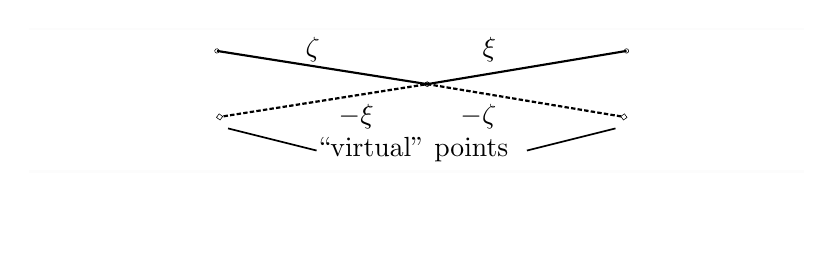
\begin{tikzpicture}[y=0.80pt, x=0.8pt,yscale=-1, inner sep=0pt, outer sep=0pt]
\begin{scope}[shift={(-16.10332,-55.70103)}]
    \path[color=black,fill=black,line width=0.800pt] (196.0312,80.7188) --
      (195.8438,80.7500) -- (196.0000,81.7188) -- (196.0938,81.6875) --
      (197.8125,82.0000) -- (197.9688,81.0000) -- (196.1875,80.7188) --
      (196.0938,80.6875) -- cycle(192.8750,81.1875) -- (193.0312,82.1875) --
      (195.0312,81.8750) -- (194.8750,80.9062) -- cycle(198.8125,82.1562) --
      (200.7812,82.5000) -- (200.9375,81.5000) -- (198.9688,81.1875) --
      cycle(189.9375,81.6562) -- (190.0938,82.6562) -- (192.0625,82.3438) --
      (191.9062,81.3438) -- cycle(201.7500,82.6562) -- (203.7500,82.9688) --
      (203.9062,82.0000) -- (201.9375,81.6562) -- cycle(186.9688,82.1250) --
      (187.1250,83.1250) -- (189.0938,82.8125) -- (188.9375,81.8125) --
      cycle(204.7188,83.1562) -- (206.6875,83.4688) -- (206.8750,82.5000) --
      (204.8750,82.1562) -- cycle(184.0000,82.5938) -- (184.1562,83.5938) --
      (186.1250,83.2812) -- (185.9688,82.2812) -- cycle(207.6875,83.6250) --
      (209.6562,83.9688) -- (209.8125,82.9688) -- (207.8438,82.6562) --
      cycle(181.0312,83.0625) -- (181.1875,84.0625) -- (183.1562,83.7500) --
      (183.0000,82.7500) -- cycle(210.6562,84.1250) -- (212.6250,84.4688) --
      (212.7812,83.4688) -- (210.8125,83.1562) -- cycle(178.0625,83.5312) --
      (178.2188,84.5312) -- (180.1875,84.2188) -- (180.0312,83.2188) --
      cycle(213.5938,84.6250) -- (215.5625,84.9688) -- (215.7500,83.9688) --
      (213.7812,83.6250) -- cycle(175.0938,84.0000) -- (175.2500,85.0000) --
      (177.2500,84.6875) -- (177.0938,83.6875) -- cycle(216.5625,85.1250) --
      (218.5312,85.4375) -- (218.6875,84.4688) -- (216.7188,84.1250) --
      cycle(172.1562,84.4688) -- (172.3125,85.4688) -- (174.2812,85.1562) --
      (174.1250,84.1562) -- cycle(169.1875,84.9375) -- (169.3438,85.9375) --
      (171.3125,85.6250) -- (171.1562,84.6250) -- cycle(219.5312,85.6250) --
      (221.5000,85.9375) -- (221.6562,84.9688) -- (219.6875,84.6250) --
      cycle(166.2188,85.4062) -- (166.3750,86.4062) -- (168.3438,86.0938) --
      (168.1875,85.0938) -- cycle(222.4688,86.0938) -- (224.4375,86.4375) --
      (224.6250,85.4375) -- (222.6562,85.1250) -- cycle(163.2500,85.8750) --
      (163.4062,86.8750) -- (165.3750,86.5625) -- (165.2188,85.5625) --
      cycle(225.4375,86.5938) -- (227.4062,86.9375) -- (227.5625,85.9375) --
      (225.5938,85.6250) -- cycle(160.2812,86.3438) -- (160.4375,87.3438) --
      (162.4375,87.0312) -- (162.2812,86.0312) -- cycle(228.4062,87.0938) --
      (230.3750,87.4062) -- (230.5312,86.4375) -- (228.5625,86.0938) --
      cycle(157.3125,86.8125) -- (157.4688,87.8125) -- (159.4688,87.5000) --
      (159.3125,86.5000) -- cycle(231.3438,87.5938) -- (233.3438,87.9062) --
      (233.5000,86.9375) -- (231.5312,86.5938) -- cycle(154.3750,87.2812) --
      (154.5312,88.2812) -- (156.5000,87.9688) -- (156.3438,86.9688) --
      cycle(234.3125,88.0625) -- (236.2812,88.4062) -- (236.4688,87.4062) --
      (234.4688,87.0938) -- cycle(151.4062,87.7500) -- (151.5625,88.7500) --
      (153.5312,88.4375) -- (153.3750,87.4375) -- cycle(237.2812,88.5625) --
      (239.2500,88.9062) -- (239.4062,87.9062) -- (237.4375,87.5938) --
      cycle(148.4375,88.2188) -- (148.5938,89.2188) -- (150.5625,88.9062) --
      (150.4062,87.9062) -- cycle(240.2188,89.0625) -- (242.2188,89.4062) --
      (242.3750,88.4062) -- (240.4062,88.0625) -- cycle(145.4688,88.6875) --
      (145.6250,89.6875) -- (147.5938,89.3750) -- (147.4375,88.3750) --
      cycle(243.1875,89.5625) -- (245.1562,89.8750) -- (245.3438,88.9062) --
      (243.3438,88.5625) -- cycle(142.5000,89.1562) -- (142.6562,90.1562) --
      (144.6562,89.8438) -- (144.5000,88.8438) -- cycle(246.1562,90.0625) --
      (248.1250,90.3750) -- (248.2812,89.4062) -- (246.3125,89.0625) --
      cycle(139.5625,89.6250) -- (139.7188,90.6250) -- (141.6875,90.3125) --
      (141.5312,89.3125) -- cycle(249.1250,90.5312) -- (251.0938,90.8750) --
      (251.2500,89.8750) -- (249.2812,89.5625) -- cycle(136.5938,90.0938) --
      (136.7500,91.0938) -- (138.7188,90.7812) -- (138.5625,89.7812) --
      cycle(252.0625,91.0312) -- (254.0312,91.3750) -- (254.2188,90.3750) --
      (252.2500,90.0625) -- cycle(133.6250,90.5625) -- (133.7812,91.5625) --
      (135.7500,91.2500) -- (135.5938,90.2500) -- cycle(255.0312,91.5312) --
      (257.0000,91.8438) -- (257.1562,90.8750) -- (255.1875,90.5312) --
      cycle(130.6562,91.0312) -- (130.8125,92.0312) -- (132.7812,91.7188) --
      (132.6250,90.7188) -- cycle(258.0000,92.0312) -- (259.9688,92.3438) --
      (260.1250,91.3750) -- (258.1562,91.0312) -- cycle(127.6875,91.5000) --
      (127.8438,92.4688) -- (129.8125,92.1875) -- (129.6562,91.1875) --
      cycle(260.9375,92.5000) -- (262.9062,92.8438) -- (263.0938,91.8438) --
      (261.1250,91.5312) -- cycle(124.7188,91.9688) -- (124.8750,92.9375) --
      (126.8750,92.6250) -- (126.7188,91.6562) -- cycle(263.9062,93.0000) --
      (265.8750,93.3438) -- (266.0312,92.3438) -- (264.0625,92.0312) --
      cycle(121.7812,92.4375) -- (121.9375,93.4062) -- (123.9062,93.0938) --
      (123.7500,92.1250) -- cycle(266.8750,93.5000) -- (268.8438,93.8438) --
      (269.0000,92.8438) -- (267.0312,92.5000) -- cycle(118.8125,92.9062) --
      (118.9688,93.8750) -- (120.9375,93.5625) -- (120.7812,92.5938) --
      cycle(269.8125,94.0000) -- (271.8125,94.3125) -- (271.9688,93.3438) --
      (270.0000,93.0000) -- cycle(115.8438,93.3750) -- (116.0000,94.3438) --
      (117.9688,94.0312) -- (117.8125,93.0625) -- cycle(272.7812,94.5000) --
      (274.7500,94.8125) -- (274.9375,93.8438) -- (272.9375,93.5000) --
      cycle(112.8750,93.8438) -- (113.0312,94.8125) -- (115.0000,94.5000) --
      (114.8438,93.5312) -- cycle(109.9062,94.3125) -- (110.0625,95.2812) --
      (112.0312,94.9688) -- (111.9062,94.0000) -- cycle(275.7500,94.9688) --
      (277.7188,95.3125) -- (277.8750,94.3125) -- (275.9062,94.0000) --
      cycle(106.9375,94.7812) -- (107.0938,95.7500) -- (109.0938,95.4375) --
      (108.9375,94.4688) -- cycle(278.7188,95.4688) -- (280.6875,95.8125) --
      (280.8438,94.8125) -- (278.8750,94.5000) -- cycle(104.0000,95.2500) --
      (104.1562,96.2188) -- (106.1250,95.9062) -- (105.9688,94.9375) --
      cycle(281.6562,95.9688) -- (283.6250,96.2812) -- (283.8125,95.3125) --
      (281.8125,94.9688) -- cycle(101.0312,95.7188) -- (101.1875,96.6875) --
      (103.1562,96.3750) -- (103.0000,95.4062) -- cycle(284.6250,96.4688) --
      (286.0312,96.6875) -- (286.1875,95.7188) -- (284.7812,95.4688) -- cycle;
    \path[draw=black,fill=cffffff,even odd rule,line width=0.200pt]
      (102.0681,94.6170) -- (100.8917,96.2344) -- (102.5092,97.4108) --
      (103.6855,95.7933) -- (102.0681,94.6170) -- cycle;
    \path[draw=black,even odd rule,line width=0.200pt] (197.0833,81.2052) ..
      controls (197.0813,81.7572) and (196.6310,82.2033) .. (196.0791,82.2009) ..
      controls (195.5271,82.1985) and (195.0810,81.7487) .. (195.0833,81.1967) ..
      controls (195.0853,80.6447) and (195.5356,80.1986) .. (196.0876,80.2010) ..
      controls (196.6396,80.2034) and (197.0857,80.6532) .. (197.0833,81.2052) --
      cycle;
    \path[draw=black,fill=cffffff,even odd rule,line width=0.200pt]
      (285.1521,94.6088) -- (283.5247,95.7713) -- (284.6871,97.3987) --
      (286.3146,96.2362) -- (285.1521,94.6088) -- cycle;
    \path[color=black,fill=black,line width=0.800pt] (101.1875,65.7188) --
      (101.0312,66.6875) -- (196.0312,81.6875) -- (196.0938,81.7188) --
      (196.1875,81.6875) -- (286.1875,66.6875) -- (286.0312,65.7188) --
      (196.0937,80.7188) -- (101.1875,65.7188) -- cycle;
    \path[draw=black,even odd rule,line width=0.200pt] (102.0713,66.3539) ..
      controls (101.9852,66.8991) and (101.4729,67.2718) .. (100.9276,67.1857) ..
      controls (100.3824,67.0996) and (100.0097,66.5872) .. (100.0958,66.0420) ..
      controls (100.1819,65.4967) and (100.6943,65.1241) .. (101.2395,65.2102) ..
      controls (101.7848,65.2962) and (102.1574,65.8086) .. (102.0713,66.3539) --
      cycle;
    \path[draw=black,even odd rule,line width=0.200pt] (197.0833,81.1968) ..
      controls (197.0853,81.7488) and (196.6396,82.1988) .. (196.0876,82.2011) ..
      controls (195.5356,82.2035) and (195.0857,81.7574) .. (195.0833,81.2054) ..
      controls (195.0813,80.6534) and (195.5271,80.2035) .. (196.0791,80.2011) ..
      controls (196.6310,80.1987) and (197.0810,80.6449) .. (197.0833,81.1968) --
      cycle;
    \path[draw=black,even odd rule,line width=0.200pt] (287.0700,66.0399) ..
      controls (287.1607,66.5844) and (286.7925,67.1000) .. (286.2480,67.1907) ..
      controls (285.7035,67.2815) and (285.1880,66.9132) .. (285.0972,66.3687) ..
      controls (285.0064,65.8242) and (285.3747,65.3087) .. (285.9192,65.2179) ..
      controls (286.4637,65.1272) and (286.9792,65.4954) .. (287.0700,66.0399) --
      cycle;
  \path[fill=black] (178.797,148.02312) node[above right] (text6246) {};
  \path[fill=black] (221.10332,71.201035) node[above right] (text6273)
    {$\boldsymbol{\xi}$};
  \path[fill=black] (156.10332,101.20103) node[above right] (text6277)
    {$\boldsymbol{-\xi}$};
  \path[shift={(71.10332,65.91978)},draw=black,opacity=0.010,line join=miter,line
    cap=butt,line width=0.800pt] (-55.0000,54.7812) -- (295.0000,54.7812);
  \begin{scope}[shift={(0,-64.5)},shift={(0,0)}]
    \path[shift={(71.10332,65.91978)},draw=black,opacity=0.010,line join=miter,line
      cap=butt,line width=0.800pt] (-55.0000,54.7812) -- (295.0000,54.7812);
  \end{scope}
  \path[fill=black] (141.10332,71.201035) node[above right] (text5341)
    {$\boldsymbol{\zeta}$};
  \path[fill=black] (211.10332,101.20103) node[above right] (text5345)
    {$\boldsymbol{-\zeta}$};
  \path[fill=black] (146.10332,116.20103) node[above right] (text5751)
    {``virtual'' points};
    \path[color=black,fill=black,line width=0.640pt] (106.1971,100.8260) --
      (106.0096,101.5760) -- (146.0096,111.5760) -- (146.1971,110.8260) --
      (106.1971,100.8260) -- cycle;
    \path[line join=round,even odd rule,line width=0.500pt] (107.3630,102.5138) --
      (105.0529,100.9424) -- (107.8307,100.6429) .. controls (107.2862,101.0936) and
      (107.0997,101.8498) .. (107.3630,102.5138) -- cycle;
    \path[color=black,fill=black,line width=0.640pt] (281.0096,100.8260) --
      (241.0096,110.8260) -- (241.1971,111.5760) -- (281.1971,101.5760) --
      (281.0096,100.8260) -- cycle;
    \path[line join=round,even odd rule,line width=0.500pt] (279.3741,100.6355) --
      (282.1518,100.9349) -- (279.8418,102.5064) .. controls (280.1101,101.8525) and
      (279.9189,101.0974) .. (279.3740,100.6355) -- cycle;
\end{scope}

\end{tikzpicture}


  \caption{Virtual Points Allow Straight Pairs on Curved Surfaces}
  \label{fig:virtualPair}
\end{figure}
%
In the simplest method, each virtual point is located just above or below a real point in the model.
In this case, properties such as displacement are taken to be the same as for the nearby real point.
%
\begin{figure}[htbp]
  \vspace{10mm}
  \centering
  
\definecolor{cffffff}{RGB}{255,255,255}


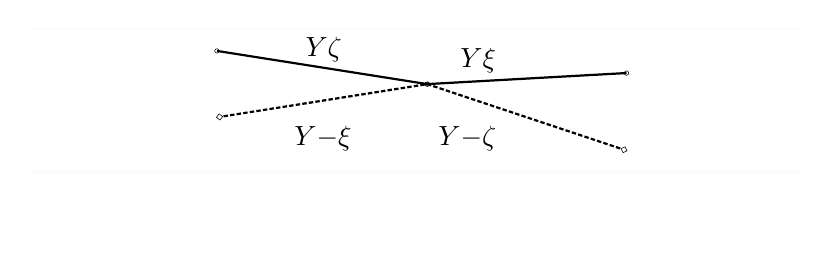
\begin{tikzpicture}[y=0.80pt, x=0.8pt,yscale=-1, inner sep=0pt, outer sep=0pt]
\begin{scope}[shift={(-16.10332,-55.70103)}]
    \path[color=black,fill=black,line width=0.800pt] (196.0312,80.7188) --
      (195.8438,80.7500) -- (195.9688,81.5625) -- (195.9375,81.6875) --
      (196.0000,81.7188) -- (196.0312,81.7188) -- (197.6875,82.2500) --
      (198.0000,81.3125) -- (196.2500,80.7188) -- (196.1563,80.6875) --
      cycle(192.8750,81.1875) -- (193.0312,82.1875) -- (195.0312,81.8750) --
      (194.8750,80.9062) -- cycle(189.9375,81.6562) -- (190.0938,82.6562) --
      (192.0625,82.3438) -- (191.9062,81.3438) -- cycle(198.6250,82.5625) --
      (200.5312,83.1875) -- (200.8438,82.2500) -- (198.9375,81.6250) --
      cycle(186.9688,82.1250) -- (187.1250,83.1250) -- (189.0938,82.8125) --
      (188.9375,81.8125) -- cycle(184.0000,82.5938) -- (184.1562,83.5938) --
      (186.1250,83.2812) -- (185.9688,82.2812) -- cycle(201.4688,83.5312) --
      (203.3750,84.1562) -- (203.6875,83.1875) -- (201.7812,82.5625) --
      cycle(181.0312,83.0625) -- (181.1875,84.0625) -- (183.1562,83.7500) --
      (183.0000,82.7500) -- cycle(178.0625,83.5312) -- (178.2188,84.5312) --
      (180.1875,84.2188) -- (180.0312,83.2188) -- cycle(204.3125,84.4688) --
      (206.2188,85.0938) -- (206.5312,84.1562) -- (204.6250,83.5312) --
      cycle(175.0938,84.0000) -- (175.2500,85.0000) -- (177.2500,84.6875) --
      (177.0938,83.6875) -- cycle(172.1562,84.4688) -- (172.3125,85.4688) --
      (174.2812,85.1562) -- (174.1250,84.1562) -- cycle(207.1562,85.4062) --
      (209.0625,86.0312) -- (209.3750,85.0938) -- (207.4688,84.4688) --
      cycle(169.1875,84.9375) -- (169.3438,85.9375) -- (171.3125,85.6250) --
      (171.1562,84.6250) -- cycle(166.2188,85.4062) -- (166.3750,86.4062) --
      (168.3438,86.0938) -- (168.1875,85.0938) -- cycle(210.0000,86.3750) --
      (211.9062,87.0000) -- (212.2188,86.0312) -- (210.3125,85.4062) --
      cycle(163.2500,85.8750) -- (163.4062,86.8750) -- (165.3750,86.5625) --
      (165.2188,85.5625) -- cycle(160.2812,86.3438) -- (160.4375,87.3438) --
      (162.4375,87.0312) -- (162.2812,86.0312) -- cycle(212.8438,87.3125) --
      (214.7500,87.9375) -- (215.0625,87.0000) -- (213.1562,86.3750) --
      cycle(157.3125,86.8125) -- (157.4688,87.8125) -- (159.4688,87.5000) --
      (159.3125,86.5000) -- cycle(154.3750,87.2812) -- (154.5312,88.2812) --
      (156.5000,87.9688) -- (156.3438,86.9688) -- cycle(215.6875,88.2500) --
      (217.5938,88.9062) -- (217.9062,87.9375) -- (216.0312,87.3125) --
      cycle(151.4062,87.7500) -- (151.5625,88.7500) -- (153.5312,88.4375) --
      (153.3750,87.4375) -- cycle(148.4375,88.2188) -- (148.5938,89.2188) --
      (150.5625,88.9062) -- (150.4062,87.9062) -- cycle(218.5312,89.2188) --
      (220.4375,89.8438) -- (220.7500,88.9062) -- (218.8750,88.2500) --
      cycle(145.4688,88.6875) -- (145.6250,89.6875) -- (147.5938,89.3750) --
      (147.4375,88.3750) -- cycle(142.5000,89.1562) -- (142.6562,90.1562) --
      (144.6562,89.8438) -- (144.5000,88.8438) -- cycle(221.4062,90.1562) --
      (223.2812,90.7812) -- (223.5938,89.8438) -- (221.7188,89.2188) --
      cycle(139.5625,89.6250) -- (139.7188,90.6250) -- (141.6875,90.3125) --
      (141.5312,89.3125) -- cycle(136.5938,90.0938) -- (136.7500,91.0938) --
      (138.7188,90.7812) -- (138.5625,89.7812) -- cycle(224.2500,91.0938) --
      (226.1250,91.7500) -- (226.4375,90.7812) -- (224.5625,90.1562) --
      cycle(133.6250,90.5625) -- (133.7812,91.5625) -- (135.7500,91.2500) --
      (135.5938,90.2500) -- cycle(130.6562,91.0312) -- (130.8125,92.0312) --
      (132.7812,91.7188) -- (132.6250,90.7188) -- cycle(227.0938,92.0625) --
      (228.9688,92.6875) -- (229.3125,91.7500) -- (227.4062,91.0938) --
      cycle(127.6875,91.5000) -- (127.8438,92.4688) -- (129.8125,92.1875) --
      (129.6562,91.1875) -- cycle(124.7188,91.9688) -- (124.8750,92.9375) --
      (126.8750,92.6250) -- (126.7188,91.6562) -- cycle(229.9375,93.0000) --
      (231.8125,93.6250) -- (232.1562,92.6875) -- (230.2500,92.0625) --
      cycle(121.7812,92.4375) -- (121.9375,93.4062) -- (123.9062,93.0938) --
      (123.7500,92.1250) -- cycle(118.8125,92.9062) -- (118.9688,93.8750) --
      (120.9375,93.5625) -- (120.7812,92.5938) -- cycle(232.7812,93.9375) --
      (234.6875,94.5938) -- (235.0000,93.6250) -- (233.0938,93.0000) --
      cycle(115.8438,93.3750) -- (116.0000,94.3438) -- (117.9688,94.0312) --
      (117.8125,93.0625) -- cycle(112.8750,93.8438) -- (113.0312,94.8125) --
      (115.0000,94.5000) -- (114.8438,93.5312) -- cycle(235.6250,94.9062) --
      (237.5312,95.5312) -- (237.8438,94.5938) -- (235.9375,93.9375) --
      cycle(109.9062,94.3125) -- (110.0625,95.2812) -- (112.0312,94.9688) --
      (111.9062,94.0000) -- cycle(106.9375,94.7812) -- (107.0938,95.7500) --
      (109.0938,95.4375) -- (108.9375,94.4688) -- cycle(238.4688,95.8438) --
      (240.3750,96.4688) -- (240.6875,95.5312) -- (238.7812,94.9062) --
      cycle(104.0000,95.2500) -- (104.1562,96.2188) -- (106.1250,95.9062) --
      (105.9688,94.9375) -- cycle(101.0312,95.7188) -- (101.1875,96.6875) --
      (103.1562,96.3750) -- (103.0000,95.4062) -- cycle(241.3125,96.8125) --
      (243.2188,97.4375) -- (243.5312,96.4688) -- (241.6250,95.8438) --
      cycle(244.1562,97.7500) -- (246.0625,98.3750) -- (246.3750,97.4375) --
      (244.4688,96.8125) -- cycle(247.0000,98.6875) -- (248.9062,99.3438) --
      (249.2188,98.3750) -- (247.3125,97.7500) -- cycle(249.8438,99.6562) --
      (251.7500,100.2812) -- (252.0625,99.3438) -- (250.1562,98.6875) --
      cycle(252.6875,100.5938) -- (254.5938,101.2188) -- (254.9062,100.2812) --
      (253.0000,99.6562) -- cycle(255.5312,101.5312) -- (257.4375,102.1875) --
      (257.7500,101.2188) -- (255.8750,100.5938) -- cycle(258.3750,102.5000) --
      (260.2812,103.1250) -- (260.5938,102.1875) -- (258.7188,101.5312) --
      cycle(261.2500,103.4375) -- (263.1250,104.0625) -- (263.4375,103.1250) --
      (261.5625,102.5000) -- cycle(264.0938,104.3750) -- (265.9688,105.0312) --
      (266.2812,104.0625) -- (264.4062,103.4375) -- cycle(266.9375,105.3438) --
      (268.8125,105.9688) -- (269.1562,105.0312) -- (267.2500,104.3750) --
      cycle(269.7812,106.2812) -- (271.6875,106.9062) -- (272.0000,105.9688) --
      (270.0938,105.3438) -- cycle(272.6250,107.2188) -- (274.5312,107.8750) --
      (274.8438,106.9062) -- (272.9375,106.2812) -- cycle(275.4688,108.1875) --
      (277.3750,108.8125) -- (277.6875,107.8750) -- (275.7812,107.2188) --
      cycle(278.3125,109.1250) -- (280.2188,109.7500) -- (280.5312,108.8125) --
      (278.6250,108.1875) -- cycle(281.1562,110.0938) -- (283.0625,110.7188) --
      (283.3750,109.7500) -- (281.4688,109.1250) -- cycle(284.0000,111.0312) --
      (285.9062,111.6562) -- (286.2188,110.7188) -- (284.3125,110.0938) -- cycle;
    \path[draw=black,fill=cffffff,even odd rule,line width=0.200pt]
      (102.0681,94.6170) -- (100.8917,96.2344) -- (102.5092,97.4108) --
      (103.6855,95.7933) -- (102.0681,94.6170) -- cycle;
    \path[draw=black,even odd rule,line width=0.200pt] (197.0800,81.2819) ..
      controls (197.0345,81.8320) and (196.5510,82.2415) .. (196.0009,82.1960) ..
      controls (195.4508,82.1504) and (195.0413,81.6670) .. (195.0868,81.1169) ..
      controls (195.1323,80.5668) and (195.6158,80.1573) .. (196.1659,80.2028) ..
      controls (196.7160,80.2483) and (197.1255,80.7317) .. (197.0800,81.2819) --
      cycle;
    \path[draw=black,fill=cffffff,even odd rule,line width=0.200pt]
      (285.4121,109.4799) -- (283.6233,110.3743) -- (284.5177,112.1632) --
      (286.3065,111.2688) -- (285.4121,109.4799) -- cycle;
    \path[color=black,fill=black,line width=0.800pt] (101.1875,65.7188) --
      (101.0312,66.6875) -- (196.0312,81.6875) -- (196.0625,81.7188) --
      (196.1250,81.6875) -- (286.1250,76.6875) -- (286.0625,75.6875) --
      (196.0625,80.6875) -- (101.1875,65.7188) -- cycle;
    \path[draw=black,even odd rule,line width=0.200pt] (102.0713,66.3539) ..
      controls (101.9852,66.8991) and (101.4729,67.2718) .. (100.9276,67.1857) ..
      controls (100.3824,67.0996) and (100.0097,66.5872) .. (100.0958,66.0420) ..
      controls (100.1819,65.4967) and (100.6943,65.1241) .. (101.2395,65.2102) ..
      controls (101.7848,65.2962) and (102.1574,65.8086) .. (102.0713,66.3539) --
      cycle;
    \path[draw=black,even odd rule,line width=0.200pt] (197.0821,81.2506) ..
      controls (197.0542,81.8018) and (196.5841,82.2266) .. (196.0328,82.1987) ..
      controls (195.4815,82.1709) and (195.0567,81.7008) .. (195.0846,81.1495) ..
      controls (195.1125,80.5982) and (195.5826,80.1734) .. (196.1339,80.2013) ..
      controls (196.6852,80.2292) and (197.1100,80.6993) .. (197.0821,81.2506) --
      cycle;
    \path[draw=black,even odd rule,line width=0.200pt] (287.0818,76.1467) ..
      controls (287.1124,76.6978) and (286.6900,77.1700) .. (286.1388,77.2006) ..
      controls (285.5877,77.2312) and (285.1155,76.8088) .. (285.0849,76.2576) ..
      controls (285.0543,75.7065) and (285.4767,75.2343) .. (286.0279,75.2037) ..
      controls (286.5790,75.1731) and (287.0512,75.5955) .. (287.0818,76.1467) --
      cycle;
  \path[fill=black] (178.797,148.02312) node[above right] (text6246) {};
  \path[fill=black] (211.10332,76.201035) node[above right] (text6273)
    {$\vstate{Y}{}{\boldsymbol{\xi}}$};
  \path[fill=black] (136.10332,111.20103) node[above right] (text6277)
    {$\vstate{Y}{}{\boldsymbol{-\xi}}$};
  \path[shift={(71.10332,65.91978)},draw=black,opacity=0.010,line join=miter,line
    cap=butt,line width=0.800pt] (-55.0000,54.7812) -- (295.0000,54.7812);
  \begin{scope}[shift={(0,-64.5)},shift={(0,0)}]
    \path[shift={(71.10332,65.91978)},draw=black,opacity=0.010,line join=miter,line
      cap=butt,line width=0.800pt] (-55.0000,54.7812) -- (295.0000,54.7812);
  \end{scope}
  \path[fill=black] (141.10332,71.201035) node[above right] (text5341)
    {$\vstate{Y}{}{\boldsymbol{\zeta}}$};
  \path[fill=black] (201.10332,111.20103) node[above right] (text5345)
    {$\vstate{Y}{}{\boldsymbol{-\zeta}}$};
\end{scope}

\end{tikzpicture}


  \caption{Virtual Points Take the Displacement of Nearby Real Points}
  \label{fig:virtualPairDeformed}
\end{figure}
%
Because the virtual point has no mass is not part of any other bond pairs, it cannot be assigned a force. 
Instead, the force on a virtual point resulting from deformation of a bond pair is instead applied to the nearest real points.
This results in a straightforward extension of the bending model from flat plates (and beams) to features that have curvatures that are small over the peridynamic horizon.

\subsection{Irregular Discretization}
A curved surface is not the only reason to implement virtual points, and even many curved surfaces do not allow for regular discretization.
When discretization is irregular, due to three-dimensional curvature, irregular shapes, or a need for increased resolution in some areas, there are necessarily points at which there is no real point at the location of $\mathbf{x} - \boldsymbol{\xi}$.
An example of changing mesh density resulting in a need for interpolation can be found in \cref{fig:virtualpoint}, which shows a small family of nodes at the edge of a change in discretization coarseness.
%
\begin{figure}[htbp]
  \vspace{10mm}
  \centering
  


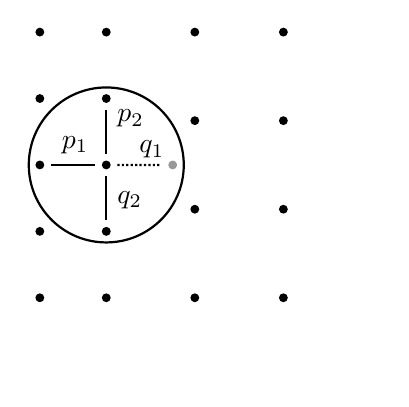
\begin{tikzpicture}[y=0.80pt, x=0.8pt,yscale=-1, inner sep=0pt, outer sep=0pt]
\begin{scope}[shift={(-16.10332,18.79897)}]
  \path[fill=black] (178.797,148.02312) node[above right] (text6246) {};
  \path[shift={(46.10332,-288.79897)},fill=black,nonzero rule] (12.0000,340.0000)
    .. controls (12.0000,341.1046) and (11.1046,342.0000) .. (10.0000,342.0000) ..
    controls (8.8954,342.0000) and (8.0000,341.1046) .. (8.0000,340.0000) ..
    controls (8.0000,338.8954) and (8.8954,338.0000) .. (10.0000,338.0000) ..
    controls (11.1046,338.0000) and (12.0000,338.8954) .. (12.0000,340.0000) --
    cycle;
  \path[shift={(46.10332,-258.79897)},fill=black,fill opacity=0.392,nonzero rule]
    (12.0000,340.0000) .. controls (12.0000,341.1046) and (11.1046,342.0000) ..
    (10.0000,342.0000) .. controls (8.8954,342.0000) and (8.0000,341.1046) ..
    (8.0000,340.0000) .. controls (8.0000,338.8954) and (8.8954,338.0000) ..
    (10.0000,338.0000) .. controls (11.1046,338.0000) and (12.0000,338.8954) ..
    (12.0000,340.0000) -- cycle;
  \path[shift={(46.10332,-318.79897)},fill=black,nonzero rule] (12.0000,340.0000)
    .. controls (12.0000,341.1046) and (11.1046,342.0000) .. (10.0000,342.0000) ..
    controls (8.8954,342.0000) and (8.0000,341.1046) .. (8.0000,340.0000) ..
    controls (8.0000,338.8954) and (8.8954,338.0000) .. (10.0000,338.0000) ..
    controls (11.1046,338.0000) and (12.0000,338.8954) .. (12.0000,340.0000) --
    cycle;
  \path[shift={(46.10332,-348.79897)},fill=black,nonzero rule] (12.0000,340.0000)
    .. controls (12.0000,341.1046) and (11.1046,342.0000) .. (10.0000,342.0000) ..
    controls (8.8954,342.0000) and (8.0000,341.1046) .. (8.0000,340.0000) ..
    controls (8.0000,338.8954) and (8.8954,338.0000) .. (10.0000,338.0000) ..
    controls (11.1046,338.0000) and (12.0000,338.8954) .. (12.0000,340.0000) --
    cycle;
  \path[shift={(46.10332,-258.79897)},fill=black,nonzero rule] (12.0000,340.0000)
    .. controls (12.0000,341.1046) and (11.1046,342.0000) .. (10.0000,342.0000) ..
    controls (8.8954,342.0000) and (8.0000,341.1046) .. (8.0000,340.0000) ..
    controls (8.0000,338.8954) and (8.8954,338.0000) .. (10.0000,338.0000) ..
    controls (11.1046,338.0000) and (12.0000,338.8954) .. (12.0000,340.0000) --
    cycle;
  \path[shift={(46.10332,-228.79897)},fill=black,nonzero rule] (12.0000,340.0000)
    .. controls (12.0000,341.1046) and (11.1046,342.0000) .. (10.0000,342.0000) ..
    controls (8.8954,342.0000) and (8.0000,341.1046) .. (8.0000,340.0000) ..
    controls (8.0000,338.8954) and (8.8954,338.0000) .. (10.0000,338.0000) ..
    controls (11.1046,338.0000) and (12.0000,338.8954) .. (12.0000,340.0000) --
    cycle;
  \path[shift={(16.10332,-288.79897)},fill=black,nonzero rule] (12.0000,340.0000)
    .. controls (12.0000,341.1046) and (11.1046,342.0000) .. (10.0000,342.0000) ..
    controls (8.8954,342.0000) and (8.0000,341.1046) .. (8.0000,340.0000) ..
    controls (8.0000,338.8954) and (8.8954,338.0000) .. (10.0000,338.0000) ..
    controls (11.1046,338.0000) and (12.0000,338.8954) .. (12.0000,340.0000) --
    cycle;
  \path[shift={(16.10332,-318.79897)},fill=black,nonzero rule] (12.0000,340.0000)
    .. controls (12.0000,341.1046) and (11.1046,342.0000) .. (10.0000,342.0000) ..
    controls (8.8954,342.0000) and (8.0000,341.1046) .. (8.0000,340.0000) ..
    controls (8.0000,338.8954) and (8.8954,338.0000) .. (10.0000,338.0000) ..
    controls (11.1046,338.0000) and (12.0000,338.8954) .. (12.0000,340.0000) --
    cycle;
  \path[shift={(16.10332,-348.79897)},fill=black,nonzero rule] (12.0000,340.0000)
    .. controls (12.0000,341.1046) and (11.1046,342.0000) .. (10.0000,342.0000) ..
    controls (8.8954,342.0000) and (8.0000,341.1046) .. (8.0000,340.0000) ..
    controls (8.0000,338.8954) and (8.8954,338.0000) .. (10.0000,338.0000) ..
    controls (11.1046,338.0000) and (12.0000,338.8954) .. (12.0000,340.0000) --
    cycle;
  \path[shift={(16.10332,-258.79897)},fill=black,nonzero rule] (12.0000,340.0000)
    .. controls (12.0000,341.1046) and (11.1046,342.0000) .. (10.0000,342.0000) ..
    controls (8.8954,342.0000) and (8.0000,341.1046) .. (8.0000,340.0000) ..
    controls (8.0000,338.8954) and (8.8954,338.0000) .. (10.0000,338.0000) ..
    controls (11.1046,338.0000) and (12.0000,338.8954) .. (12.0000,340.0000) --
    cycle;
  \path[shift={(16.10332,-228.79897)},fill=black,nonzero rule] (12.0000,340.0000)
    .. controls (12.0000,341.1046) and (11.1046,342.0000) .. (10.0000,342.0000) ..
    controls (8.8954,342.0000) and (8.0000,341.1046) .. (8.0000,340.0000) ..
    controls (8.0000,338.8954) and (8.8954,338.0000) .. (10.0000,338.0000) ..
    controls (11.1046,338.0000) and (12.0000,338.8954) .. (12.0000,340.0000) --
    cycle;
  \path[shift={(86.10332,-348.79897)},fill=black,nonzero rule] (12.0000,340.0000)
    .. controls (12.0000,341.1046) and (11.1046,342.0000) .. (10.0000,342.0000) ..
    controls (8.8954,342.0000) and (8.0000,341.1046) .. (8.0000,340.0000) ..
    controls (8.0000,338.8954) and (8.8954,338.0000) .. (10.0000,338.0000) ..
    controls (11.1046,338.0000) and (12.0000,338.8954) .. (12.0000,340.0000) --
    cycle;
  \path[shift={(86.10332,-308.79897)},fill=black,nonzero rule] (12.0000,340.0000)
    .. controls (12.0000,341.1046) and (11.1046,342.0000) .. (10.0000,342.0000) ..
    controls (8.8954,342.0000) and (8.0000,341.1046) .. (8.0000,340.0000) ..
    controls (8.0000,338.8954) and (8.8954,338.0000) .. (10.0000,338.0000) ..
    controls (11.1046,338.0000) and (12.0000,338.8954) .. (12.0000,340.0000) --
    cycle;
  \path[shift={(86.10332,-268.79897)},fill=black,nonzero rule] (12.0000,340.0000)
    .. controls (12.0000,341.1046) and (11.1046,342.0000) .. (10.0000,342.0000) ..
    controls (8.8954,342.0000) and (8.0000,341.1046) .. (8.0000,340.0000) ..
    controls (8.0000,338.8954) and (8.8954,338.0000) .. (10.0000,338.0000) ..
    controls (11.1046,338.0000) and (12.0000,338.8954) .. (12.0000,340.0000) --
    cycle;
  \path[shift={(86.10332,-228.79897)},fill=black,nonzero rule] (12.0000,340.0000)
    .. controls (12.0000,341.1046) and (11.1046,342.0000) .. (10.0000,342.0000) ..
    controls (8.8954,342.0000) and (8.0000,341.1046) .. (8.0000,340.0000) ..
    controls (8.0000,338.8954) and (8.8954,338.0000) .. (10.0000,338.0000) ..
    controls (11.1046,338.0000) and (12.0000,338.8954) .. (12.0000,340.0000) --
    cycle;
  \path[shift={(126.10332,-348.79897)},fill=black,nonzero rule] (12.0000,340.0000)
    .. controls (12.0000,341.1046) and (11.1046,342.0000) .. (10.0000,342.0000) ..
    controls (8.8954,342.0000) and (8.0000,341.1046) .. (8.0000,340.0000) ..
    controls (8.0000,338.8954) and (8.8954,338.0000) .. (10.0000,338.0000) ..
    controls (11.1046,338.0000) and (12.0000,338.8954) .. (12.0000,340.0000) --
    cycle;
  \path[shift={(126.10332,-308.79897)},fill=black,nonzero rule] (12.0000,340.0000)
    .. controls (12.0000,341.1046) and (11.1046,342.0000) .. (10.0000,342.0000) ..
    controls (8.8954,342.0000) and (8.0000,341.1046) .. (8.0000,340.0000) ..
    controls (8.0000,338.8954) and (8.8954,338.0000) .. (10.0000,338.0000) ..
    controls (11.1046,338.0000) and (12.0000,338.8954) .. (12.0000,340.0000) --
    cycle;
  \path[shift={(126.10332,-268.79897)},fill=black,nonzero rule] (12.0000,340.0000)
    .. controls (12.0000,341.1046) and (11.1046,342.0000) .. (10.0000,342.0000) ..
    controls (8.8954,342.0000) and (8.0000,341.1046) .. (8.0000,340.0000) ..
    controls (8.0000,338.8954) and (8.8954,338.0000) .. (10.0000,338.0000) ..
    controls (11.1046,338.0000) and (12.0000,338.8954) .. (12.0000,340.0000) --
    cycle;
  \path[shift={(126.10332,-228.79897)},fill=black,nonzero rule] (12.0000,340.0000)
    .. controls (12.0000,341.1046) and (11.1046,342.0000) .. (10.0000,342.0000) ..
    controls (8.8954,342.0000) and (8.0000,341.1046) .. (8.0000,340.0000) ..
    controls (8.0000,338.8954) and (8.8954,338.0000) .. (10.0000,338.0000) ..
    controls (11.1046,338.0000) and (12.0000,338.8954) .. (12.0000,340.0000) --
    cycle;
  \path[fill=black] (36.103317,46.201031) node[above right] (text4184) {$p_1$};
  \path[fill=black] (71.103317,48.201031) node[above right] (text4188) {$q_1$};
    \path[color=black,fill=black,line width=0.800pt] (31.1033,50.7010) --
      (31.1033,51.7010) -- (51.1033,51.7010) -- (51.1033,50.7010) --
      (31.1033,50.7010) -- cycle;
    \path[line join=round,even odd rule,line width=0.500pt] (33.0289,52.4112) --
      (29.7511,51.2058) -- (33.0289,50.0005) .. controls (32.5052,50.7121) and
      (32.5083,51.6858) .. (33.0289,52.4112) -- cycle;
    \path[color=black,fill=black,line width=0.800pt] (55.6033,56.2010) --
      (55.6033,76.2010) -- (56.6033,76.2010) -- (56.6033,56.2010) --
      (55.6033,56.2010) -- cycle;
    \path[line join=round,even odd rule,line width=0.500pt] (57.3134,74.2755) --
      (56.1081,77.5532) -- (54.9028,74.2755) .. controls (55.6144,74.7991) and
      (56.5880,74.7961) .. (57.3134,74.2755) -- cycle;
    \path[color=black,fill=black,line width=0.800pt] (55.6033,26.2010) --
      (55.6033,46.2010) -- (56.6033,46.2010) -- (56.6033,26.2010) --
      (55.6033,26.2010) -- cycle;
    \path[line join=round,even odd rule,line width=0.500pt] (54.8932,28.1266) --
      (56.0985,24.8488) -- (57.3038,28.1266) .. controls (56.5922,27.6030) and
      (55.6186,27.6060) .. (54.8932,28.1266) -- cycle;
    \path[color=black,fill=black,line width=0.800pt] (61.1033,51.7010) --
      (62.1033,51.7010) -- (62.1033,50.7010) -- (61.1033,50.7010) --
      cycle(63.1033,51.7010) -- (64.1033,51.7010) -- (64.1033,50.7010) --
      (63.1033,50.7010) -- cycle(65.1033,51.7010) -- (66.1033,51.7010) --
      (66.1033,50.7010) -- (65.1033,50.7010) -- cycle(67.1033,51.7010) --
      (68.1033,51.7010) -- (68.1033,50.7010) -- (67.1033,50.7010) --
      cycle(69.1033,51.7010) -- (70.1033,51.7010) -- (70.1033,50.7010) --
      (69.1033,50.7010) -- cycle(71.1033,51.7010) -- (72.1033,51.7010) --
      (72.1033,50.7010) -- (71.1033,50.7010) -- cycle(73.1033,51.7010) --
      (74.1033,51.7010) -- (74.1033,50.7010) -- (73.1033,50.7010) --
      cycle(75.1033,51.7010) -- (76.1033,51.7010) -- (76.1033,50.7010) --
      (75.1033,50.7010) -- cycle(77.1033,51.7010) -- (78.1033,51.7010) --
      (78.1033,50.7010) -- (77.1033,50.7010) -- cycle(79.1033,51.7010) --
      (80.1033,51.7010) -- (80.1033,50.7010) -- (79.1033,50.7010) -- cycle;
    \path[line join=round,even odd rule,line width=0.500pt] (79.1777,49.9909) --
      (82.4555,51.1962) -- (79.1777,52.4015) .. controls (79.7014,51.6899) and
      (79.6984,50.7163) .. (79.1777,49.9909) -- cycle;
  \path[shift={(76.10332,-288.79897)},fill=black,fill opacity=0.404,nonzero rule]
    (12.0000,340.0000) .. controls (12.0000,341.1046) and (11.1046,342.0000) ..
    (10.0000,342.0000) .. controls (8.8954,342.0000) and (8.0000,341.1046) ..
    (8.0000,340.0000) .. controls (8.0000,338.8954) and (8.8954,338.0000) ..
    (10.0000,338.0000) .. controls (11.1046,338.0000) and (12.0000,338.8954) ..
    (12.0000,340.0000) -- cycle;
  \path[shift={(16.10332,-38.79897)},draw=black,fill=black,line join=round,miter
    limit=4.00,fill opacity=0.000,nonzero rule,line width=0.800pt]
    (75.0000,90.0000) .. controls (75.0000,109.3300) and (59.3300,125.0000) ..
    (40.0000,125.0000) .. controls (20.6700,125.0000) and (5.0000,109.3300) ..
    (5.0000,90.0000) .. controls (5.0000,70.6700) and (20.6700,55.0000) ..
    (40.0000,55.0000) .. controls (59.3300,55.0000) and (75.0000,70.6700) ..
    (75.0000,90.0000) -- cycle;
  \path[fill=black] (61.103317,34.201031) node[above right] (text5037) {$p_2$};
  \path[fill=black] (61.103317,71.201027) node[above right] (text5041) {$q_2$};
\end{scope}

\end{tikzpicture}


  \caption{Virtual Points Pair Up Unpaired Neighbors}
  \label{fig:virtualpoint}
\end{figure}
%
Note that, while bonds \(p_2\) and \(q_2\) form a perfect bond pair, there is no bond exactly opposite \(p_1\).
To solve this, we add a virtual point to create a bond, \(q_1\), that will form a pair with \(p_1\).
Because this point is not part of the discretization, it has no mass, and its properties must be determined from the properties of the surrounding nodes.

An easy method of determining properties (such as displacement) at virtual nodes is to use a weighted average.
For an irregular straight beam, determining the values of properties at virtual points is simple. 
To determine the value of a property at point $C$, we used a weighted average of the values of that property at the nearest two real points, $A$ and $B$.
The weight value $w_B$ of $B$ is determined to make a linear interpolation (or extrapolation) using the $x$-coordinates of the nearest two real points.
\begin{align}
W_B &= -\frac{C_x-A_x}{A_x-B_x}\notag\\
W_A &= 1-w_B\notag
\end{align}
The problem becomes a little more complicated for curved beams, but we can tackle it by projecting the virtual point onto the line between the two nearest real points.
The weighting function then becomes
\begin{align}
\overline{AC}' &= \frac{\overline{AB}}{|\overline{AB}|}\left(\frac{\overline{AB}}{|\overline{AB}|} \cdot \overline{AC}\right)\notag\\
\overline{BC}' &= \frac{\overline{BA}}{|\overline{BA}|}\left(\frac{\overline{BA}}{|\overline{BA}|}\cdot\overline{BC}\right)\notag\\
W_B &= 
  \begin{dcases}
    \phantom{-}\frac{|\overline{AC}'|}{|\overline{AB}|} & \text{if } |\overline{BC}'| \leq |\overline{AB}|\\
    -\frac{|\overline{AC}'|}{|\overline{AB}|} &\text{otherwise}
  \end{dcases}\notag\\
W_A &= 1-W_B\notag
\end{align}

Determining properties at virtual points is more difficult in plate and shell models.
One method of generating useful weights that is relatively robust is barycentric interpolation.
We start by finding the three (non-colinear) real nodes closest to the location of the virtual node, A, B, and C.
Next, we find the signed areas of the triangles ABC, ABX, BCX, and CAX, with X being the virtual node.
The weight of node A is the area ratio between BCX and ABC, the weight of node B is the ratio of areas CAX and ABC, and the weight of node C is the ratio of areas ABX to ABC.
Using signed areas allows the weights to be negative to extrapolate properties of a virtual node outside of ABC.
Because these weights are calculated from the initial positions of the node, they can be stored for swift evaluation of properties at virtual nodes.

%
\begin{figure}[htbp]
  \vspace{10mm}
  \centering
  \resizebox{0.4\linewidth}{!}{


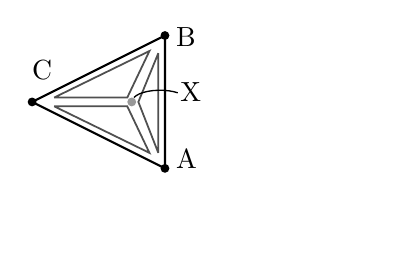
\begin{tikzpicture}[y=0.80pt, x=0.8pt,yscale=-1, inner sep=0pt, outer sep=0pt]
\begin{scope}[shift={(-16.10332,-41.20103)}]
  \path[fill=black] (178.797,148.02312) node[above right] (text6246) {};
  \path[shift={(16.10332,-258.79897)},fill=black,nonzero rule] (12.0000,340.0000)
    .. controls (12.0000,341.1046) and (11.1046,342.0000) .. (10.0000,342.0000) ..
    controls (8.8954,342.0000) and (8.0000,341.1046) .. (8.0000,340.0000) ..
    controls (8.0000,338.8954) and (8.8954,338.0000) .. (10.0000,338.0000) ..
    controls (11.1046,338.0000) and (12.0000,338.8954) .. (12.0000,340.0000) --
    cycle;
  \path[shift={(76.10332,-288.79897)},fill=black,nonzero rule] (12.0000,340.0000)
    .. controls (12.0000,341.1046) and (11.1046,342.0000) .. (10.0000,342.0000) ..
    controls (8.8954,342.0000) and (8.0000,341.1046) .. (8.0000,340.0000) ..
    controls (8.0000,338.8954) and (8.8954,338.0000) .. (10.0000,338.0000) ..
    controls (11.1046,338.0000) and (12.0000,338.8954) .. (12.0000,340.0000) --
    cycle;
  \path[shift={(76.10332,-228.79897)},fill=black,nonzero rule] (12.0000,340.0000)
    .. controls (12.0000,341.1046) and (11.1046,342.0000) .. (10.0000,342.0000) ..
    controls (8.8954,342.0000) and (8.0000,341.1046) .. (8.0000,340.0000) ..
    controls (8.0000,338.8954) and (8.8954,338.0000) .. (10.0000,338.0000) ..
    controls (11.1046,338.0000) and (12.0000,338.8954) .. (12.0000,340.0000) --
    cycle;
  \path[shift={(61.10332,-258.79897)},fill=black,fill opacity=0.404,nonzero rule]
    (12.0000,340.0000) .. controls (12.0000,341.1046) and (11.1046,342.0000) ..
    (10.0000,342.0000) .. controls (8.8954,342.0000) and (8.0000,341.1046) ..
    (8.0000,340.0000) .. controls (8.0000,338.8954) and (8.8954,338.0000) ..
    (10.0000,338.0000) .. controls (11.1046,338.0000) and (12.0000,338.8954) ..
    (12.0000,340.0000) -- cycle;
  \path[fill=black] (91.103317,111.20103) node[above right] (text3133) {A};
  \path[fill=black] (91.103317,56.201031) node[above right] (text3137) {B};
  \path[fill=black] (26.103317,71.201027) node[above right] (text3141) {C};
  \path[shift={(16.10332,-18.79897)},draw=black,line join=miter,line cap=butt,line
    width=0.800pt] (10.0000,100.0000) -- (70.0000,70.0000) -- (70.0000,130.0000)
    -- cycle;
  \path[shift={(16.10332,-18.79897)},draw=black,line join=miter,line
    cap=butt,miter limit=4.00,draw opacity=0.686,line width=0.640pt]
    (20.0000,98.0000) -- (63.0000,77.0000) -- (53.0000,98.0000) -- cycle;
  \path[shift={(16.10332,-18.79897)},draw=black,line join=miter,line
    cap=butt,miter limit=4.00,draw opacity=0.686,line width=0.640pt]
    (67.0000,78.0000) -- (58.0000,100.0000) -- (67.0000,123.0000) -- cycle;
  \path[shift={(16.10332,-18.79897)},draw=black,line join=miter,line
    cap=butt,miter limit=4.00,draw opacity=0.686,line width=0.640pt]
    (20.0000,102.0000) -- (53.0000,102.0000) -- (63.0000,123.0000) -- cycle;
  \path[fill=black] (93.103317,81.201027) node[above right] (text3157) {X};
  \path[shift={(-8.65052,-9.08887)},draw=black,fill=black,line join=round,miter
    limit=4.00,fill opacity=0.000,nonzero rule,line width=0.480pt]
    (80.7538,88.2899) .. controls (83.1150,85.6950) and (90.2880,84.3571) ..
    (96.7753,85.3015) .. controls (98.1455,85.5010) and (99.4178,85.7949) ..
    (100.5349,86.1698);
\end{scope}

\end{tikzpicture}

}
  \caption{Barycentric interpolation is based on the relative areas of sub triangles}
  \label{fig:BaryCentric}
\end{figure}
%

With the properties of the virtual points determined, the model can be evaluated in the same manner as the uniformly discretized models of the previous papers.
Where forces are calculated to act on a virtual node, those forces are redistributed to the supporting real nodes according to the weight each point has in the interpolation.
Barycentric interpolation is linear and therefore exactly reproduces the linear displacement fields in \cref{fig:barycentric}, including extrapolation well outside the interpolation points (all of which are within the square with corners (0,0) and (1,1)).
Unfortunately, as \cref{fig:baryPatch} demonstrates, barycentric interpolation is not exact for quadratic surfaces.
The difference between the quadratic surface and the linear interpolation decreases with denser discretization as the curvature of the surface between interpolation points decreases, as demonstrated in \cref{fig:baryPatch}.
This method therefore requires that the curvature of the surface be small relative to the peridynamic horizon to ensure accurate virtual node properties.

\begin{figure}[htbp]
  \centering
  \resizebox{0.8\linewidth}{!}{%% Creator: Matplotlib, PGF backend
%%
%% To include the figure in your LaTeX document, write
%%   \input{<filename>.pgf}
%%
%% Make sure the required packages are loaded in your preamble
%%   \usepackage{pgf}
%%
%% Figures using additional raster images can only be included by \input if
%% they are in the same directory as the main LaTeX file. For loading figures
%% from other directories you can use the `import` package
%%   \usepackage{import}
%% and then include the figures with
%%   \import{<path to file>}{<filename>.pgf}
%%
%% Matplotlib used the following preamble
%%
\begingroup%
\makeatletter%
\begin{pgfpicture}%
\pgfpathrectangle{\pgfpointorigin}{\pgfqpoint{8.000000in}{6.000000in}}%
\pgfusepath{use as bounding box}%
\begin{pgfscope}%
\pgfsetbuttcap%
\pgfsetroundjoin%
\definecolor{currentfill}{rgb}{1.000000,1.000000,1.000000}%
\pgfsetfillcolor{currentfill}%
\pgfsetlinewidth{0.000000pt}%
\definecolor{currentstroke}{rgb}{1.000000,1.000000,1.000000}%
\pgfsetstrokecolor{currentstroke}%
\pgfsetdash{}{0pt}%
\pgfpathmoveto{\pgfqpoint{0.000000in}{0.000000in}}%
\pgfpathlineto{\pgfqpoint{8.000000in}{0.000000in}}%
\pgfpathlineto{\pgfqpoint{8.000000in}{6.000000in}}%
\pgfpathlineto{\pgfqpoint{0.000000in}{6.000000in}}%
\pgfpathclose%
\pgfusepath{fill}%
\end{pgfscope}%
\begin{pgfscope}%
\pgfsetbuttcap%
\pgfsetroundjoin%
\definecolor{currentfill}{rgb}{1.000000,1.000000,1.000000}%
\pgfsetfillcolor{currentfill}%
\pgfsetlinewidth{0.000000pt}%
\definecolor{currentstroke}{rgb}{0.000000,0.000000,0.000000}%
\pgfsetstrokecolor{currentstroke}%
\pgfsetstrokeopacity{0.000000}%
\pgfsetdash{}{0pt}%
\pgfpathmoveto{\pgfqpoint{1.000000in}{3.218182in}}%
\pgfpathlineto{\pgfqpoint{7.200000in}{3.218182in}}%
\pgfpathlineto{\pgfqpoint{7.200000in}{5.400000in}}%
\pgfpathlineto{\pgfqpoint{1.000000in}{5.400000in}}%
\pgfpathclose%
\pgfusepath{fill}%
\end{pgfscope}%
\begin{pgfscope}%
\pgfsetbuttcap%
\pgfsetroundjoin%
\definecolor{currentfill}{rgb}{0.950000,0.950000,0.950000}%
\pgfsetfillcolor{currentfill}%
\pgfsetfillopacity{0.500000}%
\pgfsetlinewidth{1.003750pt}%
\definecolor{currentstroke}{rgb}{0.950000,0.950000,0.950000}%
\pgfsetstrokecolor{currentstroke}%
\pgfsetstrokeopacity{0.500000}%
\pgfsetdash{}{0pt}%
\pgfpathmoveto{\pgfqpoint{1.821906in}{3.700287in}}%
\pgfpathlineto{\pgfqpoint{3.596378in}{4.235219in}}%
\pgfpathlineto{\pgfqpoint{3.566835in}{5.257387in}}%
\pgfpathlineto{\pgfqpoint{1.693424in}{4.776761in}}%
\pgfusepath{stroke,fill}%
\end{pgfscope}%
\begin{pgfscope}%
\pgfsetbuttcap%
\pgfsetroundjoin%
\definecolor{currentfill}{rgb}{0.900000,0.900000,0.900000}%
\pgfsetfillcolor{currentfill}%
\pgfsetfillopacity{0.500000}%
\pgfsetlinewidth{1.003750pt}%
\definecolor{currentstroke}{rgb}{0.900000,0.900000,0.900000}%
\pgfsetstrokecolor{currentstroke}%
\pgfsetstrokeopacity{0.500000}%
\pgfsetdash{}{0pt}%
\pgfpathmoveto{\pgfqpoint{3.596378in}{4.235219in}}%
\pgfpathlineto{\pgfqpoint{6.470857in}{3.936157in}}%
\pgfpathlineto{\pgfqpoint{6.591122in}{4.989148in}}%
\pgfpathlineto{\pgfqpoint{3.566835in}{5.257387in}}%
\pgfusepath{stroke,fill}%
\end{pgfscope}%
\begin{pgfscope}%
\pgfsetbuttcap%
\pgfsetroundjoin%
\definecolor{currentfill}{rgb}{0.925000,0.925000,0.925000}%
\pgfsetfillcolor{currentfill}%
\pgfsetfillopacity{0.500000}%
\pgfsetlinewidth{1.003750pt}%
\definecolor{currentstroke}{rgb}{0.925000,0.925000,0.925000}%
\pgfsetstrokecolor{currentstroke}%
\pgfsetstrokeopacity{0.500000}%
\pgfsetdash{}{0pt}%
\pgfpathmoveto{\pgfqpoint{1.821906in}{3.700287in}}%
\pgfpathlineto{\pgfqpoint{4.846246in}{3.351981in}}%
\pgfpathlineto{\pgfqpoint{6.470857in}{3.936157in}}%
\pgfpathlineto{\pgfqpoint{3.596378in}{4.235219in}}%
\pgfusepath{stroke,fill}%
\end{pgfscope}%
\begin{pgfscope}%
\pgfsetrectcap%
\pgfsetroundjoin%
\pgfsetlinewidth{0.752812pt}%
\definecolor{currentstroke}{rgb}{0.000000,0.000000,0.000000}%
\pgfsetstrokecolor{currentstroke}%
\pgfsetdash{}{0pt}%
\pgfpathmoveto{\pgfqpoint{1.821906in}{3.700287in}}%
\pgfpathlineto{\pgfqpoint{4.846246in}{3.351981in}}%
\pgfusepath{stroke}%
\end{pgfscope}%
\begin{pgfscope}%
\pgfsetbuttcap%
\pgfsetroundjoin%
\pgfsetlinewidth{1.003750pt}%
\definecolor{currentstroke}{rgb}{0.900000,0.900000,0.900000}%
\pgfsetstrokecolor{currentstroke}%
\pgfsetdash{}{0pt}%
\pgfpathmoveto{\pgfqpoint{1.879742in}{3.693626in}}%
\pgfpathlineto{\pgfqpoint{3.651529in}{4.229481in}}%
\pgfpathlineto{\pgfqpoint{3.624737in}{5.252252in}}%
\pgfusepath{stroke}%
\end{pgfscope}%
\begin{pgfscope}%
\pgfsetbuttcap%
\pgfsetroundjoin%
\pgfsetlinewidth{1.003750pt}%
\definecolor{currentstroke}{rgb}{0.900000,0.900000,0.900000}%
\pgfsetstrokecolor{currentstroke}%
\pgfsetdash{}{0pt}%
\pgfpathmoveto{\pgfqpoint{2.346181in}{3.639907in}}%
\pgfpathlineto{\pgfqpoint{4.096057in}{4.183232in}}%
\pgfpathlineto{\pgfqpoint{4.091610in}{5.210842in}}%
\pgfusepath{stroke}%
\end{pgfscope}%
\begin{pgfscope}%
\pgfsetbuttcap%
\pgfsetroundjoin%
\pgfsetlinewidth{1.003750pt}%
\definecolor{currentstroke}{rgb}{0.900000,0.900000,0.900000}%
\pgfsetstrokecolor{currentstroke}%
\pgfsetdash{}{0pt}%
\pgfpathmoveto{\pgfqpoint{2.819391in}{3.585409in}}%
\pgfpathlineto{\pgfqpoint{4.546569in}{4.136361in}}%
\pgfpathlineto{\pgfqpoint{4.565089in}{5.168847in}}%
\pgfusepath{stroke}%
\end{pgfscope}%
\begin{pgfscope}%
\pgfsetbuttcap%
\pgfsetroundjoin%
\pgfsetlinewidth{1.003750pt}%
\definecolor{currentstroke}{rgb}{0.900000,0.900000,0.900000}%
\pgfsetstrokecolor{currentstroke}%
\pgfsetdash{}{0pt}%
\pgfpathmoveto{\pgfqpoint{3.299522in}{3.530113in}}%
\pgfpathlineto{\pgfqpoint{5.003185in}{4.088854in}}%
\pgfpathlineto{\pgfqpoint{5.045314in}{5.126254in}}%
\pgfusepath{stroke}%
\end{pgfscope}%
\begin{pgfscope}%
\pgfsetbuttcap%
\pgfsetroundjoin%
\pgfsetlinewidth{1.003750pt}%
\definecolor{currentstroke}{rgb}{0.900000,0.900000,0.900000}%
\pgfsetstrokecolor{currentstroke}%
\pgfsetdash{}{0pt}%
\pgfpathmoveto{\pgfqpoint{3.786726in}{3.474003in}}%
\pgfpathlineto{\pgfqpoint{5.466032in}{4.040700in}}%
\pgfpathlineto{\pgfqpoint{5.532430in}{5.083049in}}%
\pgfusepath{stroke}%
\end{pgfscope}%
\begin{pgfscope}%
\pgfsetbuttcap%
\pgfsetroundjoin%
\pgfsetlinewidth{1.003750pt}%
\definecolor{currentstroke}{rgb}{0.900000,0.900000,0.900000}%
\pgfsetstrokecolor{currentstroke}%
\pgfsetdash{}{0pt}%
\pgfpathmoveto{\pgfqpoint{4.281161in}{3.417060in}}%
\pgfpathlineto{\pgfqpoint{5.935237in}{3.991884in}}%
\pgfpathlineto{\pgfqpoint{6.026587in}{5.039220in}}%
\pgfusepath{stroke}%
\end{pgfscope}%
\begin{pgfscope}%
\pgfsetbuttcap%
\pgfsetroundjoin%
\pgfsetlinewidth{1.003750pt}%
\definecolor{currentstroke}{rgb}{0.900000,0.900000,0.900000}%
\pgfsetstrokecolor{currentstroke}%
\pgfsetdash{}{0pt}%
\pgfpathmoveto{\pgfqpoint{4.782989in}{3.359266in}}%
\pgfpathlineto{\pgfqpoint{6.410932in}{3.942392in}}%
\pgfpathlineto{\pgfqpoint{6.527939in}{4.994752in}}%
\pgfusepath{stroke}%
\end{pgfscope}%
\begin{pgfscope}%
\pgfsetrectcap%
\pgfsetroundjoin%
\pgfsetlinewidth{1.003750pt}%
\definecolor{currentstroke}{rgb}{0.000000,0.000000,0.000000}%
\pgfsetstrokecolor{currentstroke}%
\pgfsetdash{}{0pt}%
\pgfpathmoveto{\pgfqpoint{1.895004in}{3.698242in}}%
\pgfpathlineto{\pgfqpoint{1.849159in}{3.684377in}}%
\pgfusepath{stroke}%
\end{pgfscope}%
\begin{pgfscope}%
\pgftext[x=1.779354in,y=3.603960in,,top]{{\rmfamily\fontsize{12.000000}{14.400000}\selectfont \(\displaystyle -6\)}}%
\end{pgfscope}%
\begin{pgfscope}%
\pgfsetrectcap%
\pgfsetroundjoin%
\pgfsetlinewidth{1.003750pt}%
\definecolor{currentstroke}{rgb}{0.000000,0.000000,0.000000}%
\pgfsetstrokecolor{currentstroke}%
\pgfsetdash{}{0pt}%
\pgfpathmoveto{\pgfqpoint{2.361262in}{3.644590in}}%
\pgfpathlineto{\pgfqpoint{2.315961in}{3.630524in}}%
\pgfusepath{stroke}%
\end{pgfscope}%
\begin{pgfscope}%
\pgftext[x=2.245748in,y=3.549516in,,top]{{\rmfamily\fontsize{12.000000}{14.400000}\selectfont \(\displaystyle -4\)}}%
\end{pgfscope}%
\begin{pgfscope}%
\pgfsetrectcap%
\pgfsetroundjoin%
\pgfsetlinewidth{1.003750pt}%
\definecolor{currentstroke}{rgb}{0.000000,0.000000,0.000000}%
\pgfsetstrokecolor{currentstroke}%
\pgfsetdash{}{0pt}%
\pgfpathmoveto{\pgfqpoint{2.834285in}{3.590160in}}%
\pgfpathlineto{\pgfqpoint{2.789547in}{3.575889in}}%
\pgfusepath{stroke}%
\end{pgfscope}%
\begin{pgfscope}%
\pgftext[x=2.718924in,y=3.494280in,,top]{{\rmfamily\fontsize{12.000000}{14.400000}\selectfont \(\displaystyle -2\)}}%
\end{pgfscope}%
\begin{pgfscope}%
\pgfsetrectcap%
\pgfsetroundjoin%
\pgfsetlinewidth{1.003750pt}%
\definecolor{currentstroke}{rgb}{0.000000,0.000000,0.000000}%
\pgfsetstrokecolor{currentstroke}%
\pgfsetdash{}{0pt}%
\pgfpathmoveto{\pgfqpoint{3.314221in}{3.534934in}}%
\pgfpathlineto{\pgfqpoint{3.270069in}{3.520453in}}%
\pgfusepath{stroke}%
\end{pgfscope}%
\begin{pgfscope}%
\pgftext[x=3.199030in,y=3.438235in,,top]{{\rmfamily\fontsize{12.000000}{14.400000}\selectfont \(\displaystyle 0\)}}%
\end{pgfscope}%
\begin{pgfscope}%
\pgfsetrectcap%
\pgfsetroundjoin%
\pgfsetlinewidth{1.003750pt}%
\definecolor{currentstroke}{rgb}{0.000000,0.000000,0.000000}%
\pgfsetstrokecolor{currentstroke}%
\pgfsetdash{}{0pt}%
\pgfpathmoveto{\pgfqpoint{3.801223in}{3.478895in}}%
\pgfpathlineto{\pgfqpoint{3.757678in}{3.464200in}}%
\pgfusepath{stroke}%
\end{pgfscope}%
\begin{pgfscope}%
\pgftext[x=3.686219in,y=3.381364in,,top]{{\rmfamily\fontsize{12.000000}{14.400000}\selectfont \(\displaystyle 2\)}}%
\end{pgfscope}%
\begin{pgfscope}%
\pgfsetrectcap%
\pgfsetroundjoin%
\pgfsetlinewidth{1.003750pt}%
\definecolor{currentstroke}{rgb}{0.000000,0.000000,0.000000}%
\pgfsetstrokecolor{currentstroke}%
\pgfsetdash{}{0pt}%
\pgfpathmoveto{\pgfqpoint{4.295448in}{3.422025in}}%
\pgfpathlineto{\pgfqpoint{4.252533in}{3.407111in}}%
\pgfusepath{stroke}%
\end{pgfscope}%
\begin{pgfscope}%
\pgftext[x=4.180649in,y=3.323647in,,top]{{\rmfamily\fontsize{12.000000}{14.400000}\selectfont \(\displaystyle 4\)}}%
\end{pgfscope}%
\begin{pgfscope}%
\pgfsetrectcap%
\pgfsetroundjoin%
\pgfsetlinewidth{1.003750pt}%
\definecolor{currentstroke}{rgb}{0.000000,0.000000,0.000000}%
\pgfsetstrokecolor{currentstroke}%
\pgfsetdash{}{0pt}%
\pgfpathmoveto{\pgfqpoint{4.797058in}{3.364305in}}%
\pgfpathlineto{\pgfqpoint{4.754797in}{3.349168in}}%
\pgfusepath{stroke}%
\end{pgfscope}%
\begin{pgfscope}%
\pgftext[x=4.682484in,y=3.265065in,,top]{{\rmfamily\fontsize{12.000000}{14.400000}\selectfont \(\displaystyle 6\)}}%
\end{pgfscope}%
\begin{pgfscope}%
\pgfsetrectcap%
\pgfsetroundjoin%
\pgfsetlinewidth{0.752812pt}%
\definecolor{currentstroke}{rgb}{0.000000,0.000000,0.000000}%
\pgfsetstrokecolor{currentstroke}%
\pgfsetdash{}{0pt}%
\pgfpathmoveto{\pgfqpoint{6.470857in}{3.936157in}}%
\pgfpathlineto{\pgfqpoint{4.846246in}{3.351981in}}%
\pgfusepath{stroke}%
\end{pgfscope}%
\begin{pgfscope}%
\pgfsetbuttcap%
\pgfsetroundjoin%
\pgfsetlinewidth{1.003750pt}%
\definecolor{currentstroke}{rgb}{0.900000,0.900000,0.900000}%
\pgfsetstrokecolor{currentstroke}%
\pgfsetdash{}{0pt}%
\pgfpathmoveto{\pgfqpoint{1.733884in}{4.787141in}}%
\pgfpathlineto{\pgfqpoint{1.860083in}{3.711796in}}%
\pgfpathlineto{\pgfqpoint{4.881313in}{3.364590in}}%
\pgfusepath{stroke}%
\end{pgfscope}%
\begin{pgfscope}%
\pgfsetbuttcap%
\pgfsetroundjoin%
\pgfsetlinewidth{1.003750pt}%
\definecolor{currentstroke}{rgb}{0.900000,0.900000,0.900000}%
\pgfsetstrokecolor{currentstroke}%
\pgfsetdash{}{0pt}%
\pgfpathmoveto{\pgfqpoint{2.052874in}{4.868979in}}%
\pgfpathlineto{\pgfqpoint{2.161301in}{3.802601in}}%
\pgfpathlineto{\pgfqpoint{5.157821in}{3.464017in}}%
\pgfusepath{stroke}%
\end{pgfscope}%
\begin{pgfscope}%
\pgfsetbuttcap%
\pgfsetroundjoin%
\pgfsetlinewidth{1.003750pt}%
\definecolor{currentstroke}{rgb}{0.900000,0.900000,0.900000}%
\pgfsetstrokecolor{currentstroke}%
\pgfsetdash{}{0pt}%
\pgfpathmoveto{\pgfqpoint{2.363761in}{4.948737in}}%
\pgfpathlineto{\pgfqpoint{2.455251in}{3.891215in}}%
\pgfpathlineto{\pgfqpoint{5.427354in}{3.560935in}}%
\pgfusepath{stroke}%
\end{pgfscope}%
\begin{pgfscope}%
\pgfsetbuttcap%
\pgfsetroundjoin%
\pgfsetlinewidth{1.003750pt}%
\definecolor{currentstroke}{rgb}{0.900000,0.900000,0.900000}%
\pgfsetstrokecolor{currentstroke}%
\pgfsetdash{}{0pt}%
\pgfpathmoveto{\pgfqpoint{2.666848in}{5.026494in}}%
\pgfpathlineto{\pgfqpoint{2.742194in}{3.977717in}}%
\pgfpathlineto{\pgfqpoint{5.690172in}{3.655439in}}%
\pgfusepath{stroke}%
\end{pgfscope}%
\begin{pgfscope}%
\pgfsetbuttcap%
\pgfsetroundjoin%
\pgfsetlinewidth{1.003750pt}%
\definecolor{currentstroke}{rgb}{0.900000,0.900000,0.900000}%
\pgfsetstrokecolor{currentstroke}%
\pgfsetdash{}{0pt}%
\pgfpathmoveto{\pgfqpoint{2.962425in}{5.102325in}}%
\pgfpathlineto{\pgfqpoint{3.022375in}{4.062180in}}%
\pgfpathlineto{\pgfqpoint{5.946522in}{3.747617in}}%
\pgfusepath{stroke}%
\end{pgfscope}%
\begin{pgfscope}%
\pgfsetbuttcap%
\pgfsetroundjoin%
\pgfsetlinewidth{1.003750pt}%
\definecolor{currentstroke}{rgb}{0.900000,0.900000,0.900000}%
\pgfsetstrokecolor{currentstroke}%
\pgfsetdash{}{0pt}%
\pgfpathmoveto{\pgfqpoint{3.250769in}{5.176300in}}%
\pgfpathlineto{\pgfqpoint{3.296032in}{4.144677in}}%
\pgfpathlineto{\pgfqpoint{6.196642in}{3.837555in}}%
\pgfusepath{stroke}%
\end{pgfscope}%
\begin{pgfscope}%
\pgfsetbuttcap%
\pgfsetroundjoin%
\pgfsetlinewidth{1.003750pt}%
\definecolor{currentstroke}{rgb}{0.900000,0.900000,0.900000}%
\pgfsetstrokecolor{currentstroke}%
\pgfsetdash{}{0pt}%
\pgfpathmoveto{\pgfqpoint{3.532141in}{5.248486in}}%
\pgfpathlineto{\pgfqpoint{3.563391in}{4.225275in}}%
\pgfpathlineto{\pgfqpoint{6.440754in}{3.925333in}}%
\pgfusepath{stroke}%
\end{pgfscope}%
\begin{pgfscope}%
\pgfsetrectcap%
\pgfsetroundjoin%
\pgfsetlinewidth{1.003750pt}%
\definecolor{currentstroke}{rgb}{0.000000,0.000000,0.000000}%
\pgfsetstrokecolor{currentstroke}%
\pgfsetdash{}{0pt}%
\pgfpathmoveto{\pgfqpoint{4.856024in}{3.367496in}}%
\pgfpathlineto{\pgfqpoint{4.931948in}{3.358771in}}%
\pgfusepath{stroke}%
\end{pgfscope}%
\begin{pgfscope}%
\pgftext[x=5.056225in,y=3.285535in,,top]{{\rmfamily\fontsize{12.000000}{14.400000}\selectfont \(\displaystyle -6\)}}%
\end{pgfscope}%
\begin{pgfscope}%
\pgfsetrectcap%
\pgfsetroundjoin%
\pgfsetlinewidth{1.003750pt}%
\definecolor{currentstroke}{rgb}{0.000000,0.000000,0.000000}%
\pgfsetstrokecolor{currentstroke}%
\pgfsetdash{}{0pt}%
\pgfpathmoveto{\pgfqpoint{5.132753in}{3.466849in}}%
\pgfpathlineto{\pgfqpoint{5.208013in}{3.458346in}}%
\pgfusepath{stroke}%
\end{pgfscope}%
\begin{pgfscope}%
\pgftext[x=5.330389in,y=3.385931in,,top]{{\rmfamily\fontsize{12.000000}{14.400000}\selectfont \(\displaystyle -4\)}}%
\end{pgfscope}%
\begin{pgfscope}%
\pgfsetrectcap%
\pgfsetroundjoin%
\pgfsetlinewidth{1.003750pt}%
\definecolor{currentstroke}{rgb}{0.000000,0.000000,0.000000}%
\pgfsetstrokecolor{currentstroke}%
\pgfsetdash{}{0pt}%
\pgfpathmoveto{\pgfqpoint{5.402504in}{3.563697in}}%
\pgfpathlineto{\pgfqpoint{5.477108in}{3.555406in}}%
\pgfusepath{stroke}%
\end{pgfscope}%
\begin{pgfscope}%
\pgftext[x=5.597640in,y=3.483796in,,top]{{\rmfamily\fontsize{12.000000}{14.400000}\selectfont \(\displaystyle -2\)}}%
\end{pgfscope}%
\begin{pgfscope}%
\pgfsetrectcap%
\pgfsetroundjoin%
\pgfsetlinewidth{1.003750pt}%
\definecolor{currentstroke}{rgb}{0.000000,0.000000,0.000000}%
\pgfsetstrokecolor{currentstroke}%
\pgfsetdash{}{0pt}%
\pgfpathmoveto{\pgfqpoint{5.665537in}{3.658132in}}%
\pgfpathlineto{\pgfqpoint{5.739495in}{3.650047in}}%
\pgfusepath{stroke}%
\end{pgfscope}%
\begin{pgfscope}%
\pgftext[x=5.858235in,y=3.579224in,,top]{{\rmfamily\fontsize{12.000000}{14.400000}\selectfont \(\displaystyle 0\)}}%
\end{pgfscope}%
\begin{pgfscope}%
\pgfsetrectcap%
\pgfsetroundjoin%
\pgfsetlinewidth{1.003750pt}%
\definecolor{currentstroke}{rgb}{0.000000,0.000000,0.000000}%
\pgfsetstrokecolor{currentstroke}%
\pgfsetdash{}{0pt}%
\pgfpathmoveto{\pgfqpoint{5.922099in}{3.750245in}}%
\pgfpathlineto{\pgfqpoint{5.995420in}{3.742357in}}%
\pgfusepath{stroke}%
\end{pgfscope}%
\begin{pgfscope}%
\pgftext[x=6.112420in,y=3.672304in,,top]{{\rmfamily\fontsize{12.000000}{14.400000}\selectfont \(\displaystyle 2\)}}%
\end{pgfscope}%
\begin{pgfscope}%
\pgfsetrectcap%
\pgfsetroundjoin%
\pgfsetlinewidth{1.003750pt}%
\definecolor{currentstroke}{rgb}{0.000000,0.000000,0.000000}%
\pgfsetstrokecolor{currentstroke}%
\pgfsetdash{}{0pt}%
\pgfpathmoveto{\pgfqpoint{6.172428in}{3.840119in}}%
\pgfpathlineto{\pgfqpoint{6.245121in}{3.832422in}}%
\pgfusepath{stroke}%
\end{pgfscope}%
\begin{pgfscope}%
\pgftext[x=6.360429in,y=3.763122in,,top]{{\rmfamily\fontsize{12.000000}{14.400000}\selectfont \(\displaystyle 4\)}}%
\end{pgfscope}%
\begin{pgfscope}%
\pgfsetrectcap%
\pgfsetroundjoin%
\pgfsetlinewidth{1.003750pt}%
\definecolor{currentstroke}{rgb}{0.000000,0.000000,0.000000}%
\pgfsetstrokecolor{currentstroke}%
\pgfsetdash{}{0pt}%
\pgfpathmoveto{\pgfqpoint{6.416746in}{3.927836in}}%
\pgfpathlineto{\pgfqpoint{6.488820in}{3.920323in}}%
\pgfusepath{stroke}%
\end{pgfscope}%
\begin{pgfscope}%
\pgftext[x=6.602484in,y=3.851761in,,top]{{\rmfamily\fontsize{12.000000}{14.400000}\selectfont \(\displaystyle 6\)}}%
\end{pgfscope}%
\begin{pgfscope}%
\pgfsetrectcap%
\pgfsetroundjoin%
\pgfsetlinewidth{0.752812pt}%
\definecolor{currentstroke}{rgb}{0.000000,0.000000,0.000000}%
\pgfsetstrokecolor{currentstroke}%
\pgfsetdash{}{0pt}%
\pgfpathmoveto{\pgfqpoint{6.470857in}{3.936157in}}%
\pgfpathlineto{\pgfqpoint{6.591122in}{4.989148in}}%
\pgfusepath{stroke}%
\end{pgfscope}%
\begin{pgfscope}%
\pgfsetbuttcap%
\pgfsetroundjoin%
\pgfsetlinewidth{1.003750pt}%
\definecolor{currentstroke}{rgb}{0.900000,0.900000,0.900000}%
\pgfsetstrokecolor{currentstroke}%
\pgfsetdash{}{0pt}%
\pgfpathmoveto{\pgfqpoint{6.473144in}{3.956185in}}%
\pgfpathlineto{\pgfqpoint{3.595815in}{4.254702in}}%
\pgfpathlineto{\pgfqpoint{1.819466in}{3.720727in}}%
\pgfusepath{stroke}%
\end{pgfscope}%
\begin{pgfscope}%
\pgfsetbuttcap%
\pgfsetroundjoin%
\pgfsetlinewidth{1.003750pt}%
\definecolor{currentstroke}{rgb}{0.900000,0.900000,0.900000}%
\pgfsetstrokecolor{currentstroke}%
\pgfsetdash{}{0pt}%
\pgfpathmoveto{\pgfqpoint{6.491610in}{4.117861in}}%
\pgfpathlineto{\pgfqpoint{3.591271in}{4.411922in}}%
\pgfpathlineto{\pgfqpoint{1.799767in}{3.885778in}}%
\pgfusepath{stroke}%
\end{pgfscope}%
\begin{pgfscope}%
\pgfsetbuttcap%
\pgfsetroundjoin%
\pgfsetlinewidth{1.003750pt}%
\definecolor{currentstroke}{rgb}{0.900000,0.900000,0.900000}%
\pgfsetstrokecolor{currentstroke}%
\pgfsetdash{}{0pt}%
\pgfpathmoveto{\pgfqpoint{6.510375in}{4.282166in}}%
\pgfpathlineto{\pgfqpoint{3.586656in}{4.571591in}}%
\pgfpathlineto{\pgfqpoint{1.779736in}{4.053603in}}%
\pgfusepath{stroke}%
\end{pgfscope}%
\begin{pgfscope}%
\pgfsetbuttcap%
\pgfsetroundjoin%
\pgfsetlinewidth{1.003750pt}%
\definecolor{currentstroke}{rgb}{0.900000,0.900000,0.900000}%
\pgfsetstrokecolor{currentstroke}%
\pgfsetdash{}{0pt}%
\pgfpathmoveto{\pgfqpoint{6.529449in}{4.449165in}}%
\pgfpathlineto{\pgfqpoint{3.581969in}{4.733766in}}%
\pgfpathlineto{\pgfqpoint{1.759366in}{4.224272in}}%
\pgfusepath{stroke}%
\end{pgfscope}%
\begin{pgfscope}%
\pgfsetbuttcap%
\pgfsetroundjoin%
\pgfsetlinewidth{1.003750pt}%
\definecolor{currentstroke}{rgb}{0.900000,0.900000,0.900000}%
\pgfsetstrokecolor{currentstroke}%
\pgfsetdash{}{0pt}%
\pgfpathmoveto{\pgfqpoint{6.548837in}{4.618924in}}%
\pgfpathlineto{\pgfqpoint{3.577208in}{4.898508in}}%
\pgfpathlineto{\pgfqpoint{1.738648in}{4.397858in}}%
\pgfusepath{stroke}%
\end{pgfscope}%
\begin{pgfscope}%
\pgfsetbuttcap%
\pgfsetroundjoin%
\pgfsetlinewidth{1.003750pt}%
\definecolor{currentstroke}{rgb}{0.900000,0.900000,0.900000}%
\pgfsetstrokecolor{currentstroke}%
\pgfsetdash{}{0pt}%
\pgfpathmoveto{\pgfqpoint{6.568549in}{4.791514in}}%
\pgfpathlineto{\pgfqpoint{3.572370in}{5.065877in}}%
\pgfpathlineto{\pgfqpoint{1.717573in}{4.574437in}}%
\pgfusepath{stroke}%
\end{pgfscope}%
\begin{pgfscope}%
\pgfsetbuttcap%
\pgfsetroundjoin%
\pgfsetlinewidth{1.003750pt}%
\definecolor{currentstroke}{rgb}{0.900000,0.900000,0.900000}%
\pgfsetstrokecolor{currentstroke}%
\pgfsetdash{}{0pt}%
\pgfpathmoveto{\pgfqpoint{6.588592in}{4.967004in}}%
\pgfpathlineto{\pgfqpoint{3.567455in}{5.235937in}}%
\pgfpathlineto{\pgfqpoint{1.696131in}{4.754085in}}%
\pgfusepath{stroke}%
\end{pgfscope}%
\begin{pgfscope}%
\pgfsetrectcap%
\pgfsetroundjoin%
\pgfsetlinewidth{1.003750pt}%
\definecolor{currentstroke}{rgb}{0.000000,0.000000,0.000000}%
\pgfsetstrokecolor{currentstroke}%
\pgfsetdash{}{0pt}%
\pgfpathmoveto{\pgfqpoint{6.449137in}{3.958676in}}%
\pgfpathlineto{\pgfqpoint{6.521209in}{3.951199in}}%
\pgfusepath{stroke}%
\end{pgfscope}%
\begin{pgfscope}%
\pgftext[x=6.725041in,y=3.968930in,,top]{{\rmfamily\fontsize{12.000000}{14.400000}\selectfont \(\displaystyle -3\)}}%
\end{pgfscope}%
\begin{pgfscope}%
\pgfsetrectcap%
\pgfsetroundjoin%
\pgfsetlinewidth{1.003750pt}%
\definecolor{currentstroke}{rgb}{0.000000,0.000000,0.000000}%
\pgfsetstrokecolor{currentstroke}%
\pgfsetdash{}{0pt}%
\pgfpathmoveto{\pgfqpoint{6.467402in}{4.120315in}}%
\pgfpathlineto{\pgfqpoint{6.540075in}{4.112947in}}%
\pgfusepath{stroke}%
\end{pgfscope}%
\begin{pgfscope}%
\pgftext[x=6.745501in,y=4.130420in,,top]{{\rmfamily\fontsize{12.000000}{14.400000}\selectfont \(\displaystyle -2\)}}%
\end{pgfscope}%
\begin{pgfscope}%
\pgfsetrectcap%
\pgfsetroundjoin%
\pgfsetlinewidth{1.003750pt}%
\definecolor{currentstroke}{rgb}{0.000000,0.000000,0.000000}%
\pgfsetstrokecolor{currentstroke}%
\pgfsetdash{}{0pt}%
\pgfpathmoveto{\pgfqpoint{6.485965in}{4.284582in}}%
\pgfpathlineto{\pgfqpoint{6.559248in}{4.277328in}}%
\pgfusepath{stroke}%
\end{pgfscope}%
\begin{pgfscope}%
\pgftext[x=6.766294in,y=4.294531in,,top]{{\rmfamily\fontsize{12.000000}{14.400000}\selectfont \(\displaystyle -1\)}}%
\end{pgfscope}%
\begin{pgfscope}%
\pgfsetrectcap%
\pgfsetroundjoin%
\pgfsetlinewidth{1.003750pt}%
\definecolor{currentstroke}{rgb}{0.000000,0.000000,0.000000}%
\pgfsetstrokecolor{currentstroke}%
\pgfsetdash{}{0pt}%
\pgfpathmoveto{\pgfqpoint{6.504831in}{4.451542in}}%
\pgfpathlineto{\pgfqpoint{6.578736in}{4.444406in}}%
\pgfusepath{stroke}%
\end{pgfscope}%
\begin{pgfscope}%
\pgftext[x=6.787427in,y=4.461328in,,top]{{\rmfamily\fontsize{12.000000}{14.400000}\selectfont \(\displaystyle 0\)}}%
\end{pgfscope}%
\begin{pgfscope}%
\pgfsetrectcap%
\pgfsetroundjoin%
\pgfsetlinewidth{1.003750pt}%
\definecolor{currentstroke}{rgb}{0.000000,0.000000,0.000000}%
\pgfsetstrokecolor{currentstroke}%
\pgfsetdash{}{0pt}%
\pgfpathmoveto{\pgfqpoint{6.524010in}{4.621260in}}%
\pgfpathlineto{\pgfqpoint{6.598546in}{4.614248in}}%
\pgfusepath{stroke}%
\end{pgfscope}%
\begin{pgfscope}%
\pgftext[x=6.808909in,y=4.630877in,,top]{{\rmfamily\fontsize{12.000000}{14.400000}\selectfont \(\displaystyle 1\)}}%
\end{pgfscope}%
\begin{pgfscope}%
\pgfsetrectcap%
\pgfsetroundjoin%
\pgfsetlinewidth{1.003750pt}%
\definecolor{currentstroke}{rgb}{0.000000,0.000000,0.000000}%
\pgfsetstrokecolor{currentstroke}%
\pgfsetdash{}{0pt}%
\pgfpathmoveto{\pgfqpoint{6.543507in}{4.793807in}}%
\pgfpathlineto{\pgfqpoint{6.618687in}{4.786923in}}%
\pgfusepath{stroke}%
\end{pgfscope}%
\begin{pgfscope}%
\pgftext[x=6.830748in,y=4.803247in,,top]{{\rmfamily\fontsize{12.000000}{14.400000}\selectfont \(\displaystyle 2\)}}%
\end{pgfscope}%
\begin{pgfscope}%
\pgfsetrectcap%
\pgfsetroundjoin%
\pgfsetlinewidth{1.003750pt}%
\definecolor{currentstroke}{rgb}{0.000000,0.000000,0.000000}%
\pgfsetstrokecolor{currentstroke}%
\pgfsetdash{}{0pt}%
\pgfpathmoveto{\pgfqpoint{6.563333in}{4.969253in}}%
\pgfpathlineto{\pgfqpoint{6.639166in}{4.962503in}}%
\pgfusepath{stroke}%
\end{pgfscope}%
\begin{pgfscope}%
\pgftext[x=6.852953in,y=4.978509in,,top]{{\rmfamily\fontsize{12.000000}{14.400000}\selectfont \(\displaystyle 3\)}}%
\end{pgfscope}%
\begin{pgfscope}%
\pgfpathrectangle{\pgfqpoint{1.000000in}{3.218182in}}{\pgfqpoint{6.200000in}{2.181818in}} %
\pgfusepath{clip}%
\pgfsetbuttcap%
\pgfsetroundjoin%
\definecolor{currentfill}{rgb}{0.000000,0.000000,1.000000}%
\pgfsetfillcolor{currentfill}%
\pgfsetlinewidth{0.501875pt}%
\definecolor{currentstroke}{rgb}{0.000000,0.000000,0.000000}%
\pgfsetstrokecolor{currentstroke}%
\pgfsetdash{}{0pt}%
\pgfsys@defobject{currentmarker}{\pgfqpoint{-0.041667in}{-0.041667in}}{\pgfqpoint{0.041667in}{0.041667in}}{%
\pgfpathmoveto{\pgfqpoint{0.000000in}{-0.041667in}}%
\pgfpathcurveto{\pgfqpoint{0.011050in}{-0.041667in}}{\pgfqpoint{0.021649in}{-0.037276in}}{\pgfqpoint{0.029463in}{-0.029463in}}%
\pgfpathcurveto{\pgfqpoint{0.037276in}{-0.021649in}}{\pgfqpoint{0.041667in}{-0.011050in}}{\pgfqpoint{0.041667in}{0.000000in}}%
\pgfpathcurveto{\pgfqpoint{0.041667in}{0.011050in}}{\pgfqpoint{0.037276in}{0.021649in}}{\pgfqpoint{0.029463in}{0.029463in}}%
\pgfpathcurveto{\pgfqpoint{0.021649in}{0.037276in}}{\pgfqpoint{0.011050in}{0.041667in}}{\pgfqpoint{0.000000in}{0.041667in}}%
\pgfpathcurveto{\pgfqpoint{-0.011050in}{0.041667in}}{\pgfqpoint{-0.021649in}{0.037276in}}{\pgfqpoint{-0.029463in}{0.029463in}}%
\pgfpathcurveto{\pgfqpoint{-0.037276in}{0.021649in}}{\pgfqpoint{-0.041667in}{0.011050in}}{\pgfqpoint{-0.041667in}{0.000000in}}%
\pgfpathcurveto{\pgfqpoint{-0.041667in}{-0.011050in}}{\pgfqpoint{-0.037276in}{-0.021649in}}{\pgfqpoint{-0.029463in}{-0.029463in}}%
\pgfpathcurveto{\pgfqpoint{-0.021649in}{-0.037276in}}{\pgfqpoint{-0.011050in}{-0.041667in}}{\pgfqpoint{0.000000in}{-0.041667in}}%
\pgfpathclose%
\pgfusepath{stroke,fill}%
}%
\begin{pgfscope}%
\pgfsys@transformshift{2.289140in}{3.843463in}%
\pgfsys@useobject{currentmarker}{}%
\end{pgfscope}%
\begin{pgfscope}%
\pgfsys@transformshift{2.404594in}{3.846880in}%
\pgfsys@useobject{currentmarker}{}%
\end{pgfscope}%
\begin{pgfscope}%
\pgfsys@transformshift{2.520657in}{3.850316in}%
\pgfsys@useobject{currentmarker}{}%
\end{pgfscope}%
\begin{pgfscope}%
\pgfsys@transformshift{2.637333in}{3.853769in}%
\pgfsys@useobject{currentmarker}{}%
\end{pgfscope}%
\begin{pgfscope}%
\pgfsys@transformshift{2.754626in}{3.857241in}%
\pgfsys@useobject{currentmarker}{}%
\end{pgfscope}%
\begin{pgfscope}%
\pgfsys@transformshift{2.872542in}{3.860732in}%
\pgfsys@useobject{currentmarker}{}%
\end{pgfscope}%
\begin{pgfscope}%
\pgfsys@transformshift{2.991086in}{3.864241in}%
\pgfsys@useobject{currentmarker}{}%
\end{pgfscope}%
\begin{pgfscope}%
\pgfsys@transformshift{3.110262in}{3.867768in}%
\pgfsys@useobject{currentmarker}{}%
\end{pgfscope}%
\begin{pgfscope}%
\pgfsys@transformshift{3.230077in}{3.871315in}%
\pgfsys@useobject{currentmarker}{}%
\end{pgfscope}%
\begin{pgfscope}%
\pgfsys@transformshift{3.350534in}{3.874880in}%
\pgfsys@useobject{currentmarker}{}%
\end{pgfscope}%
\begin{pgfscope}%
\pgfsys@transformshift{3.471639in}{3.878465in}%
\pgfsys@useobject{currentmarker}{}%
\end{pgfscope}%
\begin{pgfscope}%
\pgfsys@transformshift{3.593398in}{3.882069in}%
\pgfsys@useobject{currentmarker}{}%
\end{pgfscope}%
\begin{pgfscope}%
\pgfsys@transformshift{3.715816in}{3.885693in}%
\pgfsys@useobject{currentmarker}{}%
\end{pgfscope}%
\begin{pgfscope}%
\pgfsys@transformshift{3.838897in}{3.889336in}%
\pgfsys@useobject{currentmarker}{}%
\end{pgfscope}%
\begin{pgfscope}%
\pgfsys@transformshift{3.962648in}{3.892999in}%
\pgfsys@useobject{currentmarker}{}%
\end{pgfscope}%
\begin{pgfscope}%
\pgfsys@transformshift{4.087074in}{3.896682in}%
\pgfsys@useobject{currentmarker}{}%
\end{pgfscope}%
\begin{pgfscope}%
\pgfsys@transformshift{4.212180in}{3.900386in}%
\pgfsys@useobject{currentmarker}{}%
\end{pgfscope}%
\begin{pgfscope}%
\pgfsys@transformshift{4.337972in}{3.904109in}%
\pgfsys@useobject{currentmarker}{}%
\end{pgfscope}%
\begin{pgfscope}%
\pgfsys@transformshift{4.464456in}{3.907853in}%
\pgfsys@useobject{currentmarker}{}%
\end{pgfscope}%
\begin{pgfscope}%
\pgfsys@transformshift{4.591638in}{3.911618in}%
\pgfsys@useobject{currentmarker}{}%
\end{pgfscope}%
\begin{pgfscope}%
\pgfsys@transformshift{4.719522in}{3.915403in}%
\pgfsys@useobject{currentmarker}{}%
\end{pgfscope}%
\begin{pgfscope}%
\pgfsys@transformshift{2.361881in}{3.890793in}%
\pgfsys@useobject{currentmarker}{}%
\end{pgfscope}%
\begin{pgfscope}%
\pgfsys@transformshift{2.477312in}{3.894328in}%
\pgfsys@useobject{currentmarker}{}%
\end{pgfscope}%
\begin{pgfscope}%
\pgfsys@transformshift{2.593349in}{3.897882in}%
\pgfsys@useobject{currentmarker}{}%
\end{pgfscope}%
\begin{pgfscope}%
\pgfsys@transformshift{2.709997in}{3.901455in}%
\pgfsys@useobject{currentmarker}{}%
\end{pgfscope}%
\begin{pgfscope}%
\pgfsys@transformshift{2.827262in}{3.905046in}%
\pgfsys@useobject{currentmarker}{}%
\end{pgfscope}%
\begin{pgfscope}%
\pgfsys@transformshift{2.945149in}{3.908656in}%
\pgfsys@useobject{currentmarker}{}%
\end{pgfscope}%
\begin{pgfscope}%
\pgfsys@transformshift{3.063662in}{3.912286in}%
\pgfsys@useobject{currentmarker}{}%
\end{pgfscope}%
\begin{pgfscope}%
\pgfsys@transformshift{3.182806in}{3.915935in}%
\pgfsys@useobject{currentmarker}{}%
\end{pgfscope}%
\begin{pgfscope}%
\pgfsys@transformshift{3.302586in}{3.919604in}%
\pgfsys@useobject{currentmarker}{}%
\end{pgfscope}%
\begin{pgfscope}%
\pgfsys@transformshift{3.423008in}{3.923292in}%
\pgfsys@useobject{currentmarker}{}%
\end{pgfscope}%
\begin{pgfscope}%
\pgfsys@transformshift{3.544077in}{3.927000in}%
\pgfsys@useobject{currentmarker}{}%
\end{pgfscope}%
\begin{pgfscope}%
\pgfsys@transformshift{3.665798in}{3.930727in}%
\pgfsys@useobject{currentmarker}{}%
\end{pgfscope}%
\begin{pgfscope}%
\pgfsys@transformshift{3.788176in}{3.934476in}%
\pgfsys@useobject{currentmarker}{}%
\end{pgfscope}%
\begin{pgfscope}%
\pgfsys@transformshift{3.911216in}{3.938244in}%
\pgfsys@useobject{currentmarker}{}%
\end{pgfscope}%
\begin{pgfscope}%
\pgfsys@transformshift{4.034925in}{3.942033in}%
\pgfsys@useobject{currentmarker}{}%
\end{pgfscope}%
\begin{pgfscope}%
\pgfsys@transformshift{4.159307in}{3.945842in}%
\pgfsys@useobject{currentmarker}{}%
\end{pgfscope}%
\begin{pgfscope}%
\pgfsys@transformshift{4.284367in}{3.949672in}%
\pgfsys@useobject{currentmarker}{}%
\end{pgfscope}%
\begin{pgfscope}%
\pgfsys@transformshift{4.410112in}{3.953523in}%
\pgfsys@useobject{currentmarker}{}%
\end{pgfscope}%
\begin{pgfscope}%
\pgfsys@transformshift{4.536548in}{3.957396in}%
\pgfsys@useobject{currentmarker}{}%
\end{pgfscope}%
\begin{pgfscope}%
\pgfsys@transformshift{4.663679in}{3.961289in}%
\pgfsys@useobject{currentmarker}{}%
\end{pgfscope}%
\begin{pgfscope}%
\pgfsys@transformshift{4.791511in}{3.965204in}%
\pgfsys@useobject{currentmarker}{}%
\end{pgfscope}%
\begin{pgfscope}%
\pgfsys@transformshift{2.434353in}{3.937948in}%
\pgfsys@useobject{currentmarker}{}%
\end{pgfscope}%
\begin{pgfscope}%
\pgfsys@transformshift{2.549758in}{3.941600in}%
\pgfsys@useobject{currentmarker}{}%
\end{pgfscope}%
\begin{pgfscope}%
\pgfsys@transformshift{2.665769in}{3.945271in}%
\pgfsys@useobject{currentmarker}{}%
\end{pgfscope}%
\begin{pgfscope}%
\pgfsys@transformshift{2.782390in}{3.948961in}%
\pgfsys@useobject{currentmarker}{}%
\end{pgfscope}%
\begin{pgfscope}%
\pgfsys@transformshift{2.899626in}{3.952671in}%
\pgfsys@useobject{currentmarker}{}%
\end{pgfscope}%
\begin{pgfscope}%
\pgfsys@transformshift{3.017482in}{3.956401in}%
\pgfsys@useobject{currentmarker}{}%
\end{pgfscope}%
\begin{pgfscope}%
\pgfsys@transformshift{3.135964in}{3.960150in}%
\pgfsys@useobject{currentmarker}{}%
\end{pgfscope}%
\begin{pgfscope}%
\pgfsys@transformshift{3.255075in}{3.963920in}%
\pgfsys@useobject{currentmarker}{}%
\end{pgfscope}%
\begin{pgfscope}%
\pgfsys@transformshift{3.374821in}{3.967709in}%
\pgfsys@useobject{currentmarker}{}%
\end{pgfscope}%
\begin{pgfscope}%
\pgfsys@transformshift{3.495207in}{3.971519in}%
\pgfsys@useobject{currentmarker}{}%
\end{pgfscope}%
\begin{pgfscope}%
\pgfsys@transformshift{3.616239in}{3.975349in}%
\pgfsys@useobject{currentmarker}{}%
\end{pgfscope}%
\begin{pgfscope}%
\pgfsys@transformshift{3.737921in}{3.979200in}%
\pgfsys@useobject{currentmarker}{}%
\end{pgfscope}%
\begin{pgfscope}%
\pgfsys@transformshift{3.860259in}{3.983071in}%
\pgfsys@useobject{currentmarker}{}%
\end{pgfscope}%
\begin{pgfscope}%
\pgfsys@transformshift{3.983258in}{3.986964in}%
\pgfsys@useobject{currentmarker}{}%
\end{pgfscope}%
\begin{pgfscope}%
\pgfsys@transformshift{4.106923in}{3.990877in}%
\pgfsys@useobject{currentmarker}{}%
\end{pgfscope}%
\begin{pgfscope}%
\pgfsys@transformshift{4.231260in}{3.994812in}%
\pgfsys@useobject{currentmarker}{}%
\end{pgfscope}%
\begin{pgfscope}%
\pgfsys@transformshift{4.356275in}{3.998768in}%
\pgfsys@useobject{currentmarker}{}%
\end{pgfscope}%
\begin{pgfscope}%
\pgfsys@transformshift{4.481972in}{4.002746in}%
\pgfsys@useobject{currentmarker}{}%
\end{pgfscope}%
\begin{pgfscope}%
\pgfsys@transformshift{4.608358in}{4.006745in}%
\pgfsys@useobject{currentmarker}{}%
\end{pgfscope}%
\begin{pgfscope}%
\pgfsys@transformshift{4.735438in}{4.010767in}%
\pgfsys@useobject{currentmarker}{}%
\end{pgfscope}%
\begin{pgfscope}%
\pgfsys@transformshift{4.863218in}{4.014810in}%
\pgfsys@useobject{currentmarker}{}%
\end{pgfscope}%
\begin{pgfscope}%
\pgfsys@transformshift{2.506557in}{3.984928in}%
\pgfsys@useobject{currentmarker}{}%
\end{pgfscope}%
\begin{pgfscope}%
\pgfsys@transformshift{2.621936in}{3.988696in}%
\pgfsys@useobject{currentmarker}{}%
\end{pgfscope}%
\begin{pgfscope}%
\pgfsys@transformshift{2.737920in}{3.992483in}%
\pgfsys@useobject{currentmarker}{}%
\end{pgfscope}%
\begin{pgfscope}%
\pgfsys@transformshift{2.854512in}{3.996291in}%
\pgfsys@useobject{currentmarker}{}%
\end{pgfscope}%
\begin{pgfscope}%
\pgfsys@transformshift{2.971719in}{4.000119in}%
\pgfsys@useobject{currentmarker}{}%
\end{pgfscope}%
\begin{pgfscope}%
\pgfsys@transformshift{3.089544in}{4.003966in}%
\pgfsys@useobject{currentmarker}{}%
\end{pgfscope}%
\begin{pgfscope}%
\pgfsys@transformshift{3.207994in}{4.007835in}%
\pgfsys@useobject{currentmarker}{}%
\end{pgfscope}%
\begin{pgfscope}%
\pgfsys@transformshift{3.327071in}{4.011723in}%
\pgfsys@useobject{currentmarker}{}%
\end{pgfscope}%
\begin{pgfscope}%
\pgfsys@transformshift{3.446783in}{4.015633in}%
\pgfsys@useobject{currentmarker}{}%
\end{pgfscope}%
\begin{pgfscope}%
\pgfsys@transformshift{3.567133in}{4.019563in}%
\pgfsys@useobject{currentmarker}{}%
\end{pgfscope}%
\begin{pgfscope}%
\pgfsys@transformshift{3.688126in}{4.023515in}%
\pgfsys@useobject{currentmarker}{}%
\end{pgfscope}%
\begin{pgfscope}%
\pgfsys@transformshift{3.809769in}{4.027487in}%
\pgfsys@useobject{currentmarker}{}%
\end{pgfscope}%
\begin{pgfscope}%
\pgfsys@transformshift{3.932067in}{4.031481in}%
\pgfsys@useobject{currentmarker}{}%
\end{pgfscope}%
\begin{pgfscope}%
\pgfsys@transformshift{4.055023in}{4.035496in}%
\pgfsys@useobject{currentmarker}{}%
\end{pgfscope}%
\begin{pgfscope}%
\pgfsys@transformshift{4.178645in}{4.039534in}%
\pgfsys@useobject{currentmarker}{}%
\end{pgfscope}%
\begin{pgfscope}%
\pgfsys@transformshift{4.302937in}{4.043593in}%
\pgfsys@useobject{currentmarker}{}%
\end{pgfscope}%
\begin{pgfscope}%
\pgfsys@transformshift{4.427905in}{4.047674in}%
\pgfsys@useobject{currentmarker}{}%
\end{pgfscope}%
\begin{pgfscope}%
\pgfsys@transformshift{4.553554in}{4.051777in}%
\pgfsys@useobject{currentmarker}{}%
\end{pgfscope}%
\begin{pgfscope}%
\pgfsys@transformshift{4.679890in}{4.055903in}%
\pgfsys@useobject{currentmarker}{}%
\end{pgfscope}%
\begin{pgfscope}%
\pgfsys@transformshift{4.806918in}{4.060051in}%
\pgfsys@useobject{currentmarker}{}%
\end{pgfscope}%
\begin{pgfscope}%
\pgfsys@transformshift{4.934645in}{4.064223in}%
\pgfsys@useobject{currentmarker}{}%
\end{pgfscope}%
\begin{pgfscope}%
\pgfsys@transformshift{2.578493in}{4.031734in}%
\pgfsys@useobject{currentmarker}{}%
\end{pgfscope}%
\begin{pgfscope}%
\pgfsys@transformshift{2.693846in}{4.035617in}%
\pgfsys@useobject{currentmarker}{}%
\end{pgfscope}%
\begin{pgfscope}%
\pgfsys@transformshift{2.809802in}{4.039520in}%
\pgfsys@useobject{currentmarker}{}%
\end{pgfscope}%
\begin{pgfscope}%
\pgfsys@transformshift{2.926366in}{4.043444in}%
\pgfsys@useobject{currentmarker}{}%
\end{pgfscope}%
\begin{pgfscope}%
\pgfsys@transformshift{3.043543in}{4.047388in}%
\pgfsys@useobject{currentmarker}{}%
\end{pgfscope}%
\begin{pgfscope}%
\pgfsys@transformshift{3.161337in}{4.051354in}%
\pgfsys@useobject{currentmarker}{}%
\end{pgfscope}%
\begin{pgfscope}%
\pgfsys@transformshift{3.279753in}{4.055340in}%
\pgfsys@useobject{currentmarker}{}%
\end{pgfscope}%
\begin{pgfscope}%
\pgfsys@transformshift{3.398797in}{4.059347in}%
\pgfsys@useobject{currentmarker}{}%
\end{pgfscope}%
\begin{pgfscope}%
\pgfsys@transformshift{3.518472in}{4.063376in}%
\pgfsys@useobject{currentmarker}{}%
\end{pgfscope}%
\begin{pgfscope}%
\pgfsys@transformshift{3.638785in}{4.067426in}%
\pgfsys@useobject{currentmarker}{}%
\end{pgfscope}%
\begin{pgfscope}%
\pgfsys@transformshift{3.759741in}{4.071497in}%
\pgfsys@useobject{currentmarker}{}%
\end{pgfscope}%
\begin{pgfscope}%
\pgfsys@transformshift{3.881344in}{4.075591in}%
\pgfsys@useobject{currentmarker}{}%
\end{pgfscope}%
\begin{pgfscope}%
\pgfsys@transformshift{4.003600in}{4.079706in}%
\pgfsys@useobject{currentmarker}{}%
\end{pgfscope}%
\begin{pgfscope}%
\pgfsys@transformshift{4.126514in}{4.083844in}%
\pgfsys@useobject{currentmarker}{}%
\end{pgfscope}%
\begin{pgfscope}%
\pgfsys@transformshift{4.250092in}{4.088004in}%
\pgfsys@useobject{currentmarker}{}%
\end{pgfscope}%
\begin{pgfscope}%
\pgfsys@transformshift{4.374338in}{4.092186in}%
\pgfsys@useobject{currentmarker}{}%
\end{pgfscope}%
\begin{pgfscope}%
\pgfsys@transformshift{4.499258in}{4.096391in}%
\pgfsys@useobject{currentmarker}{}%
\end{pgfscope}%
\begin{pgfscope}%
\pgfsys@transformshift{4.624858in}{4.100619in}%
\pgfsys@useobject{currentmarker}{}%
\end{pgfscope}%
\begin{pgfscope}%
\pgfsys@transformshift{4.751144in}{4.104870in}%
\pgfsys@useobject{currentmarker}{}%
\end{pgfscope}%
\begin{pgfscope}%
\pgfsys@transformshift{4.878120in}{4.109144in}%
\pgfsys@useobject{currentmarker}{}%
\end{pgfscope}%
\begin{pgfscope}%
\pgfsys@transformshift{5.005793in}{4.113442in}%
\pgfsys@useobject{currentmarker}{}%
\end{pgfscope}%
\begin{pgfscope}%
\pgfsys@transformshift{2.650164in}{4.078367in}%
\pgfsys@useobject{currentmarker}{}%
\end{pgfscope}%
\begin{pgfscope}%
\pgfsys@transformshift{2.765490in}{4.082365in}%
\pgfsys@useobject{currentmarker}{}%
\end{pgfscope}%
\begin{pgfscope}%
\pgfsys@transformshift{2.881418in}{4.086383in}%
\pgfsys@useobject{currentmarker}{}%
\end{pgfscope}%
\begin{pgfscope}%
\pgfsys@transformshift{2.997953in}{4.090422in}%
\pgfsys@useobject{currentmarker}{}%
\end{pgfscope}%
\begin{pgfscope}%
\pgfsys@transformshift{3.115099in}{4.094482in}%
\pgfsys@useobject{currentmarker}{}%
\end{pgfscope}%
\begin{pgfscope}%
\pgfsys@transformshift{3.232861in}{4.098564in}%
\pgfsys@useobject{currentmarker}{}%
\end{pgfscope}%
\begin{pgfscope}%
\pgfsys@transformshift{3.351243in}{4.102667in}%
\pgfsys@useobject{currentmarker}{}%
\end{pgfscope}%
\begin{pgfscope}%
\pgfsys@transformshift{3.470252in}{4.106792in}%
\pgfsys@useobject{currentmarker}{}%
\end{pgfscope}%
\begin{pgfscope}%
\pgfsys@transformshift{3.589892in}{4.110938in}%
\pgfsys@useobject{currentmarker}{}%
\end{pgfscope}%
\begin{pgfscope}%
\pgfsys@transformshift{3.710168in}{4.115107in}%
\pgfsys@useobject{currentmarker}{}%
\end{pgfscope}%
\begin{pgfscope}%
\pgfsys@transformshift{3.831084in}{4.119298in}%
\pgfsys@useobject{currentmarker}{}%
\end{pgfscope}%
\begin{pgfscope}%
\pgfsys@transformshift{3.952647in}{4.123512in}%
\pgfsys@useobject{currentmarker}{}%
\end{pgfscope}%
\begin{pgfscope}%
\pgfsys@transformshift{4.074861in}{4.127747in}%
\pgfsys@useobject{currentmarker}{}%
\end{pgfscope}%
\begin{pgfscope}%
\pgfsys@transformshift{4.197732in}{4.132006in}%
\pgfsys@useobject{currentmarker}{}%
\end{pgfscope}%
\begin{pgfscope}%
\pgfsys@transformshift{4.321264in}{4.136288in}%
\pgfsys@useobject{currentmarker}{}%
\end{pgfscope}%
\begin{pgfscope}%
\pgfsys@transformshift{4.445464in}{4.140593in}%
\pgfsys@useobject{currentmarker}{}%
\end{pgfscope}%
\begin{pgfscope}%
\pgfsys@transformshift{4.570337in}{4.144921in}%
\pgfsys@useobject{currentmarker}{}%
\end{pgfscope}%
\begin{pgfscope}%
\pgfsys@transformshift{4.695888in}{4.149272in}%
\pgfsys@useobject{currentmarker}{}%
\end{pgfscope}%
\begin{pgfscope}%
\pgfsys@transformshift{4.822122in}{4.153648in}%
\pgfsys@useobject{currentmarker}{}%
\end{pgfscope}%
\begin{pgfscope}%
\pgfsys@transformshift{4.949046in}{4.158047in}%
\pgfsys@useobject{currentmarker}{}%
\end{pgfscope}%
\begin{pgfscope}%
\pgfsys@transformshift{5.076664in}{4.162470in}%
\pgfsys@useobject{currentmarker}{}%
\end{pgfscope}%
\begin{pgfscope}%
\pgfsys@transformshift{2.721571in}{4.124829in}%
\pgfsys@useobject{currentmarker}{}%
\end{pgfscope}%
\begin{pgfscope}%
\pgfsys@transformshift{2.836870in}{4.128940in}%
\pgfsys@useobject{currentmarker}{}%
\end{pgfscope}%
\begin{pgfscope}%
\pgfsys@transformshift{2.952769in}{4.133072in}%
\pgfsys@useobject{currentmarker}{}%
\end{pgfscope}%
\begin{pgfscope}%
\pgfsys@transformshift{3.069274in}{4.137225in}%
\pgfsys@useobject{currentmarker}{}%
\end{pgfscope}%
\begin{pgfscope}%
\pgfsys@transformshift{3.186388in}{4.141400in}%
\pgfsys@useobject{currentmarker}{}%
\end{pgfscope}%
\begin{pgfscope}%
\pgfsys@transformshift{3.304117in}{4.145598in}%
\pgfsys@useobject{currentmarker}{}%
\end{pgfscope}%
\begin{pgfscope}%
\pgfsys@transformshift{3.422466in}{4.149817in}%
\pgfsys@useobject{currentmarker}{}%
\end{pgfscope}%
\begin{pgfscope}%
\pgfsys@transformshift{3.541440in}{4.154058in}%
\pgfsys@useobject{currentmarker}{}%
\end{pgfscope}%
\begin{pgfscope}%
\pgfsys@transformshift{3.661043in}{4.158322in}%
\pgfsys@useobject{currentmarker}{}%
\end{pgfscope}%
\begin{pgfscope}%
\pgfsys@transformshift{3.781280in}{4.162609in}%
\pgfsys@useobject{currentmarker}{}%
\end{pgfscope}%
\begin{pgfscope}%
\pgfsys@transformshift{3.902158in}{4.166918in}%
\pgfsys@useobject{currentmarker}{}%
\end{pgfscope}%
\begin{pgfscope}%
\pgfsys@transformshift{4.023679in}{4.171251in}%
\pgfsys@useobject{currentmarker}{}%
\end{pgfscope}%
\begin{pgfscope}%
\pgfsys@transformshift{4.145851in}{4.175606in}%
\pgfsys@useobject{currentmarker}{}%
\end{pgfscope}%
\begin{pgfscope}%
\pgfsys@transformshift{4.268678in}{4.179985in}%
\pgfsys@useobject{currentmarker}{}%
\end{pgfscope}%
\begin{pgfscope}%
\pgfsys@transformshift{4.392165in}{4.184388in}%
\pgfsys@useobject{currentmarker}{}%
\end{pgfscope}%
\begin{pgfscope}%
\pgfsys@transformshift{4.516318in}{4.188814in}%
\pgfsys@useobject{currentmarker}{}%
\end{pgfscope}%
\begin{pgfscope}%
\pgfsys@transformshift{4.641143in}{4.193264in}%
\pgfsys@useobject{currentmarker}{}%
\end{pgfscope}%
\begin{pgfscope}%
\pgfsys@transformshift{4.766643in}{4.197738in}%
\pgfsys@useobject{currentmarker}{}%
\end{pgfscope}%
\begin{pgfscope}%
\pgfsys@transformshift{4.892826in}{4.202237in}%
\pgfsys@useobject{currentmarker}{}%
\end{pgfscope}%
\begin{pgfscope}%
\pgfsys@transformshift{5.019697in}{4.206760in}%
\pgfsys@useobject{currentmarker}{}%
\end{pgfscope}%
\begin{pgfscope}%
\pgfsys@transformshift{5.147260in}{4.211308in}%
\pgfsys@useobject{currentmarker}{}%
\end{pgfscope}%
\begin{pgfscope}%
\pgfsys@transformshift{2.792716in}{4.171120in}%
\pgfsys@useobject{currentmarker}{}%
\end{pgfscope}%
\begin{pgfscope}%
\pgfsys@transformshift{2.907986in}{4.175343in}%
\pgfsys@useobject{currentmarker}{}%
\end{pgfscope}%
\begin{pgfscope}%
\pgfsys@transformshift{3.023856in}{4.179588in}%
\pgfsys@useobject{currentmarker}{}%
\end{pgfscope}%
\begin{pgfscope}%
\pgfsys@transformshift{3.140330in}{4.183855in}%
\pgfsys@useobject{currentmarker}{}%
\end{pgfscope}%
\begin{pgfscope}%
\pgfsys@transformshift{3.257413in}{4.188144in}%
\pgfsys@useobject{currentmarker}{}%
\end{pgfscope}%
\begin{pgfscope}%
\pgfsys@transformshift{3.375109in}{4.192456in}%
\pgfsys@useobject{currentmarker}{}%
\end{pgfscope}%
\begin{pgfscope}%
\pgfsys@transformshift{3.493423in}{4.196791in}%
\pgfsys@useobject{currentmarker}{}%
\end{pgfscope}%
\begin{pgfscope}%
\pgfsys@transformshift{3.612361in}{4.201148in}%
\pgfsys@useobject{currentmarker}{}%
\end{pgfscope}%
\begin{pgfscope}%
\pgfsys@transformshift{3.731927in}{4.205528in}%
\pgfsys@useobject{currentmarker}{}%
\end{pgfscope}%
\begin{pgfscope}%
\pgfsys@transformshift{3.852126in}{4.209932in}%
\pgfsys@useobject{currentmarker}{}%
\end{pgfscope}%
\begin{pgfscope}%
\pgfsys@transformshift{3.972963in}{4.214359in}%
\pgfsys@useobject{currentmarker}{}%
\end{pgfscope}%
\begin{pgfscope}%
\pgfsys@transformshift{4.094443in}{4.218809in}%
\pgfsys@useobject{currentmarker}{}%
\end{pgfscope}%
\begin{pgfscope}%
\pgfsys@transformshift{4.216572in}{4.223283in}%
\pgfsys@useobject{currentmarker}{}%
\end{pgfscope}%
\begin{pgfscope}%
\pgfsys@transformshift{4.339354in}{4.227782in}%
\pgfsys@useobject{currentmarker}{}%
\end{pgfscope}%
\begin{pgfscope}%
\pgfsys@transformshift{4.462796in}{4.232304in}%
\pgfsys@useobject{currentmarker}{}%
\end{pgfscope}%
\begin{pgfscope}%
\pgfsys@transformshift{4.586901in}{4.236851in}%
\pgfsys@useobject{currentmarker}{}%
\end{pgfscope}%
\begin{pgfscope}%
\pgfsys@transformshift{4.711677in}{4.241422in}%
\pgfsys@useobject{currentmarker}{}%
\end{pgfscope}%
\begin{pgfscope}%
\pgfsys@transformshift{4.837127in}{4.246018in}%
\pgfsys@useobject{currentmarker}{}%
\end{pgfscope}%
\begin{pgfscope}%
\pgfsys@transformshift{4.963257in}{4.250638in}%
\pgfsys@useobject{currentmarker}{}%
\end{pgfscope}%
\begin{pgfscope}%
\pgfsys@transformshift{5.090074in}{4.255284in}%
\pgfsys@useobject{currentmarker}{}%
\end{pgfscope}%
\begin{pgfscope}%
\pgfsys@transformshift{5.217583in}{4.259956in}%
\pgfsys@useobject{currentmarker}{}%
\end{pgfscope}%
\begin{pgfscope}%
\pgfsys@transformshift{2.863599in}{4.217241in}%
\pgfsys@useobject{currentmarker}{}%
\end{pgfscope}%
\begin{pgfscope}%
\pgfsys@transformshift{2.978841in}{4.221576in}%
\pgfsys@useobject{currentmarker}{}%
\end{pgfscope}%
\begin{pgfscope}%
\pgfsys@transformshift{3.094681in}{4.225933in}%
\pgfsys@useobject{currentmarker}{}%
\end{pgfscope}%
\begin{pgfscope}%
\pgfsys@transformshift{3.211124in}{4.230313in}%
\pgfsys@useobject{currentmarker}{}%
\end{pgfscope}%
\begin{pgfscope}%
\pgfsys@transformshift{3.328174in}{4.234715in}%
\pgfsys@useobject{currentmarker}{}%
\end{pgfscope}%
\begin{pgfscope}%
\pgfsys@transformshift{3.445836in}{4.239141in}%
\pgfsys@useobject{currentmarker}{}%
\end{pgfscope}%
\begin{pgfscope}%
\pgfsys@transformshift{3.564116in}{4.243590in}%
\pgfsys@useobject{currentmarker}{}%
\end{pgfscope}%
\begin{pgfscope}%
\pgfsys@transformshift{3.683017in}{4.248062in}%
\pgfsys@useobject{currentmarker}{}%
\end{pgfscope}%
\begin{pgfscope}%
\pgfsys@transformshift{3.802545in}{4.252557in}%
\pgfsys@useobject{currentmarker}{}%
\end{pgfscope}%
\begin{pgfscope}%
\pgfsys@transformshift{3.922705in}{4.257077in}%
\pgfsys@useobject{currentmarker}{}%
\end{pgfscope}%
\begin{pgfscope}%
\pgfsys@transformshift{4.043501in}{4.261620in}%
\pgfsys@useobject{currentmarker}{}%
\end{pgfscope}%
\begin{pgfscope}%
\pgfsys@transformshift{4.164940in}{4.266188in}%
\pgfsys@useobject{currentmarker}{}%
\end{pgfscope}%
\begin{pgfscope}%
\pgfsys@transformshift{4.287025in}{4.270780in}%
\pgfsys@useobject{currentmarker}{}%
\end{pgfscope}%
\begin{pgfscope}%
\pgfsys@transformshift{4.409762in}{4.275397in}%
\pgfsys@useobject{currentmarker}{}%
\end{pgfscope}%
\begin{pgfscope}%
\pgfsys@transformshift{4.533157in}{4.280038in}%
\pgfsys@useobject{currentmarker}{}%
\end{pgfscope}%
\begin{pgfscope}%
\pgfsys@transformshift{4.657215in}{4.284704in}%
\pgfsys@useobject{currentmarker}{}%
\end{pgfscope}%
\begin{pgfscope}%
\pgfsys@transformshift{4.781941in}{4.289395in}%
\pgfsys@useobject{currentmarker}{}%
\end{pgfscope}%
\begin{pgfscope}%
\pgfsys@transformshift{4.907340in}{4.294112in}%
\pgfsys@useobject{currentmarker}{}%
\end{pgfscope}%
\begin{pgfscope}%
\pgfsys@transformshift{5.033418in}{4.298854in}%
\pgfsys@useobject{currentmarker}{}%
\end{pgfscope}%
\begin{pgfscope}%
\pgfsys@transformshift{5.160180in}{4.303622in}%
\pgfsys@useobject{currentmarker}{}%
\end{pgfscope}%
\begin{pgfscope}%
\pgfsys@transformshift{5.287633in}{4.308415in}%
\pgfsys@useobject{currentmarker}{}%
\end{pgfscope}%
\begin{pgfscope}%
\pgfsys@transformshift{2.934223in}{4.263193in}%
\pgfsys@useobject{currentmarker}{}%
\end{pgfscope}%
\begin{pgfscope}%
\pgfsys@transformshift{3.049436in}{4.267639in}%
\pgfsys@useobject{currentmarker}{}%
\end{pgfscope}%
\begin{pgfscope}%
\pgfsys@transformshift{3.165245in}{4.272107in}%
\pgfsys@useobject{currentmarker}{}%
\end{pgfscope}%
\begin{pgfscope}%
\pgfsys@transformshift{3.281656in}{4.276599in}%
\pgfsys@useobject{currentmarker}{}%
\end{pgfscope}%
\begin{pgfscope}%
\pgfsys@transformshift{3.398673in}{4.281113in}%
\pgfsys@useobject{currentmarker}{}%
\end{pgfscope}%
\begin{pgfscope}%
\pgfsys@transformshift{3.516301in}{4.285652in}%
\pgfsys@useobject{currentmarker}{}%
\end{pgfscope}%
\begin{pgfscope}%
\pgfsys@transformshift{3.634545in}{4.290214in}%
\pgfsys@useobject{currentmarker}{}%
\end{pgfscope}%
\begin{pgfscope}%
\pgfsys@transformshift{3.753409in}{4.294800in}%
\pgfsys@useobject{currentmarker}{}%
\end{pgfscope}%
\begin{pgfscope}%
\pgfsys@transformshift{3.872899in}{4.299411in}%
\pgfsys@useobject{currentmarker}{}%
\end{pgfscope}%
\begin{pgfscope}%
\pgfsys@transformshift{3.993019in}{4.304045in}%
\pgfsys@useobject{currentmarker}{}%
\end{pgfscope}%
\begin{pgfscope}%
\pgfsys@transformshift{4.113774in}{4.308704in}%
\pgfsys@useobject{currentmarker}{}%
\end{pgfscope}%
\begin{pgfscope}%
\pgfsys@transformshift{4.235170in}{4.313388in}%
\pgfsys@useobject{currentmarker}{}%
\end{pgfscope}%
\begin{pgfscope}%
\pgfsys@transformshift{4.357211in}{4.318097in}%
\pgfsys@useobject{currentmarker}{}%
\end{pgfscope}%
\begin{pgfscope}%
\pgfsys@transformshift{4.479903in}{4.322831in}%
\pgfsys@useobject{currentmarker}{}%
\end{pgfscope}%
\begin{pgfscope}%
\pgfsys@transformshift{4.603251in}{4.327590in}%
\pgfsys@useobject{currentmarker}{}%
\end{pgfscope}%
\begin{pgfscope}%
\pgfsys@transformshift{4.727260in}{4.332375in}%
\pgfsys@useobject{currentmarker}{}%
\end{pgfscope}%
\begin{pgfscope}%
\pgfsys@transformshift{4.851936in}{4.337185in}%
\pgfsys@useobject{currentmarker}{}%
\end{pgfscope}%
\begin{pgfscope}%
\pgfsys@transformshift{4.977284in}{4.342022in}%
\pgfsys@useobject{currentmarker}{}%
\end{pgfscope}%
\begin{pgfscope}%
\pgfsys@transformshift{5.103309in}{4.346884in}%
\pgfsys@useobject{currentmarker}{}%
\end{pgfscope}%
\begin{pgfscope}%
\pgfsys@transformshift{5.230016in}{4.351773in}%
\pgfsys@useobject{currentmarker}{}%
\end{pgfscope}%
\begin{pgfscope}%
\pgfsys@transformshift{5.357412in}{4.356688in}%
\pgfsys@useobject{currentmarker}{}%
\end{pgfscope}%
\begin{pgfscope}%
\pgfsys@transformshift{3.004588in}{4.308978in}%
\pgfsys@useobject{currentmarker}{}%
\end{pgfscope}%
\begin{pgfscope}%
\pgfsys@transformshift{3.119771in}{4.313533in}%
\pgfsys@useobject{currentmarker}{}%
\end{pgfscope}%
\begin{pgfscope}%
\pgfsys@transformshift{3.235550in}{4.318111in}%
\pgfsys@useobject{currentmarker}{}%
\end{pgfscope}%
\begin{pgfscope}%
\pgfsys@transformshift{3.351929in}{4.322714in}%
\pgfsys@useobject{currentmarker}{}%
\end{pgfscope}%
\begin{pgfscope}%
\pgfsys@transformshift{3.468912in}{4.327340in}%
\pgfsys@useobject{currentmarker}{}%
\end{pgfscope}%
\begin{pgfscope}%
\pgfsys@transformshift{3.586505in}{4.331991in}%
\pgfsys@useobject{currentmarker}{}%
\end{pgfscope}%
\begin{pgfscope}%
\pgfsys@transformshift{3.704713in}{4.336666in}%
\pgfsys@useobject{currentmarker}{}%
\end{pgfscope}%
\begin{pgfscope}%
\pgfsys@transformshift{3.823540in}{4.341365in}%
\pgfsys@useobject{currentmarker}{}%
\end{pgfscope}%
\begin{pgfscope}%
\pgfsys@transformshift{3.942990in}{4.346089in}%
\pgfsys@useobject{currentmarker}{}%
\end{pgfscope}%
\begin{pgfscope}%
\pgfsys@transformshift{4.063070in}{4.350838in}%
\pgfsys@useobject{currentmarker}{}%
\end{pgfscope}%
\begin{pgfscope}%
\pgfsys@transformshift{4.183784in}{4.355612in}%
\pgfsys@useobject{currentmarker}{}%
\end{pgfscope}%
\begin{pgfscope}%
\pgfsys@transformshift{4.305136in}{4.360411in}%
\pgfsys@useobject{currentmarker}{}%
\end{pgfscope}%
\begin{pgfscope}%
\pgfsys@transformshift{4.427133in}{4.365236in}%
\pgfsys@useobject{currentmarker}{}%
\end{pgfscope}%
\begin{pgfscope}%
\pgfsys@transformshift{4.549779in}{4.370086in}%
\pgfsys@useobject{currentmarker}{}%
\end{pgfscope}%
\begin{pgfscope}%
\pgfsys@transformshift{4.673080in}{4.374962in}%
\pgfsys@useobject{currentmarker}{}%
\end{pgfscope}%
\begin{pgfscope}%
\pgfsys@transformshift{4.797040in}{4.379864in}%
\pgfsys@useobject{currentmarker}{}%
\end{pgfscope}%
\begin{pgfscope}%
\pgfsys@transformshift{4.921665in}{4.384793in}%
\pgfsys@useobject{currentmarker}{}%
\end{pgfscope}%
\begin{pgfscope}%
\pgfsys@transformshift{5.046960in}{4.389748in}%
\pgfsys@useobject{currentmarker}{}%
\end{pgfscope}%
\begin{pgfscope}%
\pgfsys@transformshift{5.172931in}{4.394730in}%
\pgfsys@useobject{currentmarker}{}%
\end{pgfscope}%
\begin{pgfscope}%
\pgfsys@transformshift{5.299584in}{4.399739in}%
\pgfsys@useobject{currentmarker}{}%
\end{pgfscope}%
\begin{pgfscope}%
\pgfsys@transformshift{5.426923in}{4.404775in}%
\pgfsys@useobject{currentmarker}{}%
\end{pgfscope}%
\begin{pgfscope}%
\pgfsys@transformshift{3.074697in}{4.354595in}%
\pgfsys@useobject{currentmarker}{}%
\end{pgfscope}%
\begin{pgfscope}%
\pgfsys@transformshift{3.189850in}{4.359259in}%
\pgfsys@useobject{currentmarker}{}%
\end{pgfscope}%
\begin{pgfscope}%
\pgfsys@transformshift{3.305597in}{4.363947in}%
\pgfsys@useobject{currentmarker}{}%
\end{pgfscope}%
\begin{pgfscope}%
\pgfsys@transformshift{3.421943in}{4.368660in}%
\pgfsys@useobject{currentmarker}{}%
\end{pgfscope}%
\begin{pgfscope}%
\pgfsys@transformshift{3.538892in}{4.373397in}%
\pgfsys@useobject{currentmarker}{}%
\end{pgfscope}%
\begin{pgfscope}%
\pgfsys@transformshift{3.656450in}{4.378158in}%
\pgfsys@useobject{currentmarker}{}%
\end{pgfscope}%
\begin{pgfscope}%
\pgfsys@transformshift{3.774621in}{4.382945in}%
\pgfsys@useobject{currentmarker}{}%
\end{pgfscope}%
\begin{pgfscope}%
\pgfsys@transformshift{3.893409in}{4.387757in}%
\pgfsys@useobject{currentmarker}{}%
\end{pgfscope}%
\begin{pgfscope}%
\pgfsys@transformshift{4.012821in}{4.392593in}%
\pgfsys@useobject{currentmarker}{}%
\end{pgfscope}%
\begin{pgfscope}%
\pgfsys@transformshift{4.132859in}{4.397456in}%
\pgfsys@useobject{currentmarker}{}%
\end{pgfscope}%
\begin{pgfscope}%
\pgfsys@transformshift{4.253531in}{4.402343in}%
\pgfsys@useobject{currentmarker}{}%
\end{pgfscope}%
\begin{pgfscope}%
\pgfsys@transformshift{4.374840in}{4.407257in}%
\pgfsys@useobject{currentmarker}{}%
\end{pgfscope}%
\begin{pgfscope}%
\pgfsys@transformshift{4.496792in}{4.412197in}%
\pgfsys@useobject{currentmarker}{}%
\end{pgfscope}%
\begin{pgfscope}%
\pgfsys@transformshift{4.619391in}{4.417163in}%
\pgfsys@useobject{currentmarker}{}%
\end{pgfscope}%
\begin{pgfscope}%
\pgfsys@transformshift{4.742643in}{4.422155in}%
\pgfsys@useobject{currentmarker}{}%
\end{pgfscope}%
\begin{pgfscope}%
\pgfsys@transformshift{4.866554in}{4.427174in}%
\pgfsys@useobject{currentmarker}{}%
\end{pgfscope}%
\begin{pgfscope}%
\pgfsys@transformshift{4.991128in}{4.432220in}%
\pgfsys@useobject{currentmarker}{}%
\end{pgfscope}%
\begin{pgfscope}%
\pgfsys@transformshift{5.116371in}{4.437293in}%
\pgfsys@useobject{currentmarker}{}%
\end{pgfscope}%
\begin{pgfscope}%
\pgfsys@transformshift{5.242288in}{4.442393in}%
\pgfsys@useobject{currentmarker}{}%
\end{pgfscope}%
\begin{pgfscope}%
\pgfsys@transformshift{5.368884in}{4.447521in}%
\pgfsys@useobject{currentmarker}{}%
\end{pgfscope}%
\begin{pgfscope}%
\pgfsys@transformshift{5.496166in}{4.452676in}%
\pgfsys@useobject{currentmarker}{}%
\end{pgfscope}%
\begin{pgfscope}%
\pgfsys@transformshift{3.144550in}{4.400045in}%
\pgfsys@useobject{currentmarker}{}%
\end{pgfscope}%
\begin{pgfscope}%
\pgfsys@transformshift{3.259672in}{4.404818in}%
\pgfsys@useobject{currentmarker}{}%
\end{pgfscope}%
\begin{pgfscope}%
\pgfsys@transformshift{3.375387in}{4.409615in}%
\pgfsys@useobject{currentmarker}{}%
\end{pgfscope}%
\begin{pgfscope}%
\pgfsys@transformshift{3.491700in}{4.414437in}%
\pgfsys@useobject{currentmarker}{}%
\end{pgfscope}%
\begin{pgfscope}%
\pgfsys@transformshift{3.608614in}{4.419284in}%
\pgfsys@useobject{currentmarker}{}%
\end{pgfscope}%
\begin{pgfscope}%
\pgfsys@transformshift{3.726136in}{4.424156in}%
\pgfsys@useobject{currentmarker}{}%
\end{pgfscope}%
\begin{pgfscope}%
\pgfsys@transformshift{3.844270in}{4.429053in}%
\pgfsys@useobject{currentmarker}{}%
\end{pgfscope}%
\begin{pgfscope}%
\pgfsys@transformshift{3.963020in}{4.433976in}%
\pgfsys@useobject{currentmarker}{}%
\end{pgfscope}%
\begin{pgfscope}%
\pgfsys@transformshift{4.082391in}{4.438925in}%
\pgfsys@useobject{currentmarker}{}%
\end{pgfscope}%
\begin{pgfscope}%
\pgfsys@transformshift{4.202389in}{4.443899in}%
\pgfsys@useobject{currentmarker}{}%
\end{pgfscope}%
\begin{pgfscope}%
\pgfsys@transformshift{4.323017in}{4.448900in}%
\pgfsys@useobject{currentmarker}{}%
\end{pgfscope}%
\begin{pgfscope}%
\pgfsys@transformshift{4.444282in}{4.453927in}%
\pgfsys@useobject{currentmarker}{}%
\end{pgfscope}%
\begin{pgfscope}%
\pgfsys@transformshift{4.566188in}{4.458981in}%
\pgfsys@useobject{currentmarker}{}%
\end{pgfscope}%
\begin{pgfscope}%
\pgfsys@transformshift{4.688741in}{4.464062in}%
\pgfsys@useobject{currentmarker}{}%
\end{pgfscope}%
\begin{pgfscope}%
\pgfsys@transformshift{4.811944in}{4.469169in}%
\pgfsys@useobject{currentmarker}{}%
\end{pgfscope}%
\begin{pgfscope}%
\pgfsys@transformshift{4.935805in}{4.474304in}%
\pgfsys@useobject{currentmarker}{}%
\end{pgfscope}%
\begin{pgfscope}%
\pgfsys@transformshift{5.060327in}{4.479466in}%
\pgfsys@useobject{currentmarker}{}%
\end{pgfscope}%
\begin{pgfscope}%
\pgfsys@transformshift{5.185517in}{4.484656in}%
\pgfsys@useobject{currentmarker}{}%
\end{pgfscope}%
\begin{pgfscope}%
\pgfsys@transformshift{5.311379in}{4.489874in}%
\pgfsys@useobject{currentmarker}{}%
\end{pgfscope}%
\begin{pgfscope}%
\pgfsys@transformshift{5.437919in}{4.495120in}%
\pgfsys@useobject{currentmarker}{}%
\end{pgfscope}%
\begin{pgfscope}%
\pgfsys@transformshift{5.565143in}{4.500394in}%
\pgfsys@useobject{currentmarker}{}%
\end{pgfscope}%
\begin{pgfscope}%
\pgfsys@transformshift{3.214149in}{4.445331in}%
\pgfsys@useobject{currentmarker}{}%
\end{pgfscope}%
\begin{pgfscope}%
\pgfsys@transformshift{3.329240in}{4.450211in}%
\pgfsys@useobject{currentmarker}{}%
\end{pgfscope}%
\begin{pgfscope}%
\pgfsys@transformshift{3.444922in}{4.455116in}%
\pgfsys@useobject{currentmarker}{}%
\end{pgfscope}%
\begin{pgfscope}%
\pgfsys@transformshift{3.561201in}{4.460046in}%
\pgfsys@useobject{currentmarker}{}%
\end{pgfscope}%
\begin{pgfscope}%
\pgfsys@transformshift{3.678080in}{4.465002in}%
\pgfsys@useobject{currentmarker}{}%
\end{pgfscope}%
\begin{pgfscope}%
\pgfsys@transformshift{3.795566in}{4.469983in}%
\pgfsys@useobject{currentmarker}{}%
\end{pgfscope}%
\begin{pgfscope}%
\pgfsys@transformshift{3.913662in}{4.474991in}%
\pgfsys@useobject{currentmarker}{}%
\end{pgfscope}%
\begin{pgfscope}%
\pgfsys@transformshift{4.032372in}{4.480024in}%
\pgfsys@useobject{currentmarker}{}%
\end{pgfscope}%
\begin{pgfscope}%
\pgfsys@transformshift{4.151703in}{4.485084in}%
\pgfsys@useobject{currentmarker}{}%
\end{pgfscope}%
\begin{pgfscope}%
\pgfsys@transformshift{4.271659in}{4.490170in}%
\pgfsys@useobject{currentmarker}{}%
\end{pgfscope}%
\begin{pgfscope}%
\pgfsys@transformshift{4.392244in}{4.495283in}%
\pgfsys@useobject{currentmarker}{}%
\end{pgfscope}%
\begin{pgfscope}%
\pgfsys@transformshift{4.513465in}{4.500423in}%
\pgfsys@useobject{currentmarker}{}%
\end{pgfscope}%
\begin{pgfscope}%
\pgfsys@transformshift{4.635324in}{4.505590in}%
\pgfsys@useobject{currentmarker}{}%
\end{pgfscope}%
\begin{pgfscope}%
\pgfsys@transformshift{4.757829in}{4.510784in}%
\pgfsys@useobject{currentmarker}{}%
\end{pgfscope}%
\begin{pgfscope}%
\pgfsys@transformshift{4.880984in}{4.516006in}%
\pgfsys@useobject{currentmarker}{}%
\end{pgfscope}%
\begin{pgfscope}%
\pgfsys@transformshift{5.004794in}{4.521256in}%
\pgfsys@useobject{currentmarker}{}%
\end{pgfscope}%
\begin{pgfscope}%
\pgfsys@transformshift{5.129264in}{4.526534in}%
\pgfsys@useobject{currentmarker}{}%
\end{pgfscope}%
\begin{pgfscope}%
\pgfsys@transformshift{5.254400in}{4.531839in}%
\pgfsys@useobject{currentmarker}{}%
\end{pgfscope}%
\begin{pgfscope}%
\pgfsys@transformshift{5.380207in}{4.537174in}%
\pgfsys@useobject{currentmarker}{}%
\end{pgfscope}%
\begin{pgfscope}%
\pgfsys@transformshift{5.506691in}{4.542537in}%
\pgfsys@useobject{currentmarker}{}%
\end{pgfscope}%
\begin{pgfscope}%
\pgfsys@transformshift{5.633856in}{4.547929in}%
\pgfsys@useobject{currentmarker}{}%
\end{pgfscope}%
\begin{pgfscope}%
\pgfsys@transformshift{3.283496in}{4.490452in}%
\pgfsys@useobject{currentmarker}{}%
\end{pgfscope}%
\begin{pgfscope}%
\pgfsys@transformshift{3.398554in}{4.495439in}%
\pgfsys@useobject{currentmarker}{}%
\end{pgfscope}%
\begin{pgfscope}%
\pgfsys@transformshift{3.514204in}{4.500451in}%
\pgfsys@useobject{currentmarker}{}%
\end{pgfscope}%
\begin{pgfscope}%
\pgfsys@transformshift{3.630448in}{4.505489in}%
\pgfsys@useobject{currentmarker}{}%
\end{pgfscope}%
\begin{pgfscope}%
\pgfsys@transformshift{3.747292in}{4.510553in}%
\pgfsys@useobject{currentmarker}{}%
\end{pgfscope}%
\begin{pgfscope}%
\pgfsys@transformshift{3.864740in}{4.515643in}%
\pgfsys@useobject{currentmarker}{}%
\end{pgfscope}%
\begin{pgfscope}%
\pgfsys@transformshift{3.982798in}{4.520759in}%
\pgfsys@useobject{currentmarker}{}%
\end{pgfscope}%
\begin{pgfscope}%
\pgfsys@transformshift{4.101469in}{4.525902in}%
\pgfsys@useobject{currentmarker}{}%
\end{pgfscope}%
\begin{pgfscope}%
\pgfsys@transformshift{4.220759in}{4.531072in}%
\pgfsys@useobject{currentmarker}{}%
\end{pgfscope}%
\begin{pgfscope}%
\pgfsys@transformshift{4.340672in}{4.536269in}%
\pgfsys@useobject{currentmarker}{}%
\end{pgfscope}%
\begin{pgfscope}%
\pgfsys@transformshift{4.461214in}{4.541493in}%
\pgfsys@useobject{currentmarker}{}%
\end{pgfscope}%
\begin{pgfscope}%
\pgfsys@transformshift{4.582389in}{4.546745in}%
\pgfsys@useobject{currentmarker}{}%
\end{pgfscope}%
\begin{pgfscope}%
\pgfsys@transformshift{4.704202in}{4.552024in}%
\pgfsys@useobject{currentmarker}{}%
\end{pgfscope}%
\begin{pgfscope}%
\pgfsys@transformshift{4.826659in}{4.557332in}%
\pgfsys@useobject{currentmarker}{}%
\end{pgfscope}%
\begin{pgfscope}%
\pgfsys@transformshift{4.949764in}{4.562667in}%
\pgfsys@useobject{currentmarker}{}%
\end{pgfscope}%
\begin{pgfscope}%
\pgfsys@transformshift{5.073523in}{4.568031in}%
\pgfsys@useobject{currentmarker}{}%
\end{pgfscope}%
\begin{pgfscope}%
\pgfsys@transformshift{5.197940in}{4.573423in}%
\pgfsys@useobject{currentmarker}{}%
\end{pgfscope}%
\begin{pgfscope}%
\pgfsys@transformshift{5.323022in}{4.578844in}%
\pgfsys@useobject{currentmarker}{}%
\end{pgfscope}%
\begin{pgfscope}%
\pgfsys@transformshift{5.448773in}{4.584294in}%
\pgfsys@useobject{currentmarker}{}%
\end{pgfscope}%
\begin{pgfscope}%
\pgfsys@transformshift{5.575200in}{4.589773in}%
\pgfsys@useobject{currentmarker}{}%
\end{pgfscope}%
\begin{pgfscope}%
\pgfsys@transformshift{5.702306in}{4.595282in}%
\pgfsys@useobject{currentmarker}{}%
\end{pgfscope}%
\begin{pgfscope}%
\pgfsys@transformshift{3.352591in}{4.535410in}%
\pgfsys@useobject{currentmarker}{}%
\end{pgfscope}%
\begin{pgfscope}%
\pgfsys@transformshift{3.467617in}{4.540502in}%
\pgfsys@useobject{currentmarker}{}%
\end{pgfscope}%
\begin{pgfscope}%
\pgfsys@transformshift{3.583233in}{4.545620in}%
\pgfsys@useobject{currentmarker}{}%
\end{pgfscope}%
\begin{pgfscope}%
\pgfsys@transformshift{3.699442in}{4.550765in}%
\pgfsys@useobject{currentmarker}{}%
\end{pgfscope}%
\begin{pgfscope}%
\pgfsys@transformshift{3.816250in}{4.555936in}%
\pgfsys@useobject{currentmarker}{}%
\end{pgfscope}%
\begin{pgfscope}%
\pgfsys@transformshift{3.933661in}{4.561134in}%
\pgfsys@useobject{currentmarker}{}%
\end{pgfscope}%
\begin{pgfscope}%
\pgfsys@transformshift{4.051679in}{4.566359in}%
\pgfsys@useobject{currentmarker}{}%
\end{pgfscope}%
\begin{pgfscope}%
\pgfsys@transformshift{4.170310in}{4.571611in}%
\pgfsys@useobject{currentmarker}{}%
\end{pgfscope}%
\begin{pgfscope}%
\pgfsys@transformshift{4.289558in}{4.576891in}%
\pgfsys@useobject{currentmarker}{}%
\end{pgfscope}%
\begin{pgfscope}%
\pgfsys@transformshift{4.409429in}{4.582197in}%
\pgfsys@useobject{currentmarker}{}%
\end{pgfscope}%
\begin{pgfscope}%
\pgfsys@transformshift{4.529926in}{4.587532in}%
\pgfsys@useobject{currentmarker}{}%
\end{pgfscope}%
\begin{pgfscope}%
\pgfsys@transformshift{4.651056in}{4.592895in}%
\pgfsys@useobject{currentmarker}{}%
\end{pgfscope}%
\begin{pgfscope}%
\pgfsys@transformshift{4.772822in}{4.598285in}%
\pgfsys@useobject{currentmarker}{}%
\end{pgfscope}%
\begin{pgfscope}%
\pgfsys@transformshift{4.895230in}{4.603705in}%
\pgfsys@useobject{currentmarker}{}%
\end{pgfscope}%
\begin{pgfscope}%
\pgfsys@transformshift{5.018285in}{4.609152in}%
\pgfsys@useobject{currentmarker}{}%
\end{pgfscope}%
\begin{pgfscope}%
\pgfsys@transformshift{5.141992in}{4.614629in}%
\pgfsys@useobject{currentmarker}{}%
\end{pgfscope}%
\begin{pgfscope}%
\pgfsys@transformshift{5.266357in}{4.620135in}%
\pgfsys@useobject{currentmarker}{}%
\end{pgfscope}%
\begin{pgfscope}%
\pgfsys@transformshift{5.391384in}{4.625670in}%
\pgfsys@useobject{currentmarker}{}%
\end{pgfscope}%
\begin{pgfscope}%
\pgfsys@transformshift{5.517079in}{4.631235in}%
\pgfsys@useobject{currentmarker}{}%
\end{pgfscope}%
\begin{pgfscope}%
\pgfsys@transformshift{5.643448in}{4.636829in}%
\pgfsys@useobject{currentmarker}{}%
\end{pgfscope}%
\begin{pgfscope}%
\pgfsys@transformshift{5.770495in}{4.642454in}%
\pgfsys@useobject{currentmarker}{}%
\end{pgfscope}%
\begin{pgfscope}%
\pgfsys@transformshift{3.421436in}{4.580205in}%
\pgfsys@useobject{currentmarker}{}%
\end{pgfscope}%
\begin{pgfscope}%
\pgfsys@transformshift{3.536430in}{4.585402in}%
\pgfsys@useobject{currentmarker}{}%
\end{pgfscope}%
\begin{pgfscope}%
\pgfsys@transformshift{3.652011in}{4.590626in}%
\pgfsys@useobject{currentmarker}{}%
\end{pgfscope}%
\begin{pgfscope}%
\pgfsys@transformshift{3.768185in}{4.595877in}%
\pgfsys@useobject{currentmarker}{}%
\end{pgfscope}%
\begin{pgfscope}%
\pgfsys@transformshift{3.884956in}{4.601154in}%
\pgfsys@useobject{currentmarker}{}%
\end{pgfscope}%
\begin{pgfscope}%
\pgfsys@transformshift{4.002328in}{4.606459in}%
\pgfsys@useobject{currentmarker}{}%
\end{pgfscope}%
\begin{pgfscope}%
\pgfsys@transformshift{4.120308in}{4.611792in}%
\pgfsys@useobject{currentmarker}{}%
\end{pgfscope}%
\begin{pgfscope}%
\pgfsys@transformshift{4.238898in}{4.617152in}%
\pgfsys@useobject{currentmarker}{}%
\end{pgfscope}%
\begin{pgfscope}%
\pgfsys@transformshift{4.358104in}{4.622540in}%
\pgfsys@useobject{currentmarker}{}%
\end{pgfscope}%
\begin{pgfscope}%
\pgfsys@transformshift{4.477931in}{4.627955in}%
\pgfsys@useobject{currentmarker}{}%
\end{pgfscope}%
\begin{pgfscope}%
\pgfsys@transformshift{4.598384in}{4.633400in}%
\pgfsys@useobject{currentmarker}{}%
\end{pgfscope}%
\begin{pgfscope}%
\pgfsys@transformshift{4.719467in}{4.638872in}%
\pgfsys@useobject{currentmarker}{}%
\end{pgfscope}%
\begin{pgfscope}%
\pgfsys@transformshift{4.841186in}{4.644374in}%
\pgfsys@useobject{currentmarker}{}%
\end{pgfscope}%
\begin{pgfscope}%
\pgfsys@transformshift{4.963545in}{4.649904in}%
\pgfsys@useobject{currentmarker}{}%
\end{pgfscope}%
\begin{pgfscope}%
\pgfsys@transformshift{5.086549in}{4.655463in}%
\pgfsys@useobject{currentmarker}{}%
\end{pgfscope}%
\begin{pgfscope}%
\pgfsys@transformshift{5.210204in}{4.661052in}%
\pgfsys@useobject{currentmarker}{}%
\end{pgfscope}%
\begin{pgfscope}%
\pgfsys@transformshift{5.334515in}{4.666671in}%
\pgfsys@useobject{currentmarker}{}%
\end{pgfscope}%
\begin{pgfscope}%
\pgfsys@transformshift{5.459488in}{4.672319in}%
\pgfsys@useobject{currentmarker}{}%
\end{pgfscope}%
\begin{pgfscope}%
\pgfsys@transformshift{5.585126in}{4.677998in}%
\pgfsys@useobject{currentmarker}{}%
\end{pgfscope}%
\begin{pgfscope}%
\pgfsys@transformshift{5.711436in}{4.683707in}%
\pgfsys@useobject{currentmarker}{}%
\end{pgfscope}%
\begin{pgfscope}%
\pgfsys@transformshift{5.838424in}{4.689446in}%
\pgfsys@useobject{currentmarker}{}%
\end{pgfscope}%
\begin{pgfscope}%
\pgfsys@transformshift{3.490033in}{4.624838in}%
\pgfsys@useobject{currentmarker}{}%
\end{pgfscope}%
\begin{pgfscope}%
\pgfsys@transformshift{3.604993in}{4.630139in}%
\pgfsys@useobject{currentmarker}{}%
\end{pgfscope}%
\begin{pgfscope}%
\pgfsys@transformshift{3.720539in}{4.635468in}%
\pgfsys@useobject{currentmarker}{}%
\end{pgfscope}%
\begin{pgfscope}%
\pgfsys@transformshift{3.836677in}{4.640824in}%
\pgfsys@useobject{currentmarker}{}%
\end{pgfscope}%
\begin{pgfscope}%
\pgfsys@transformshift{3.953411in}{4.646208in}%
\pgfsys@useobject{currentmarker}{}%
\end{pgfscope}%
\begin{pgfscope}%
\pgfsys@transformshift{4.070745in}{4.651619in}%
\pgfsys@useobject{currentmarker}{}%
\end{pgfscope}%
\begin{pgfscope}%
\pgfsys@transformshift{4.188685in}{4.657058in}%
\pgfsys@useobject{currentmarker}{}%
\end{pgfscope}%
\begin{pgfscope}%
\pgfsys@transformshift{4.307234in}{4.662525in}%
\pgfsys@useobject{currentmarker}{}%
\end{pgfscope}%
\begin{pgfscope}%
\pgfsys@transformshift{4.426398in}{4.668020in}%
\pgfsys@useobject{currentmarker}{}%
\end{pgfscope}%
\begin{pgfscope}%
\pgfsys@transformshift{4.546181in}{4.673544in}%
\pgfsys@useobject{currentmarker}{}%
\end{pgfscope}%
\begin{pgfscope}%
\pgfsys@transformshift{4.666588in}{4.679097in}%
\pgfsys@useobject{currentmarker}{}%
\end{pgfscope}%
\begin{pgfscope}%
\pgfsys@transformshift{4.787624in}{4.684679in}%
\pgfsys@useobject{currentmarker}{}%
\end{pgfscope}%
\begin{pgfscope}%
\pgfsys@transformshift{4.909295in}{4.690290in}%
\pgfsys@useobject{currentmarker}{}%
\end{pgfscope}%
\begin{pgfscope}%
\pgfsys@transformshift{5.031604in}{4.695931in}%
\pgfsys@useobject{currentmarker}{}%
\end{pgfscope}%
\begin{pgfscope}%
\pgfsys@transformshift{5.154558in}{4.701601in}%
\pgfsys@useobject{currentmarker}{}%
\end{pgfscope}%
\begin{pgfscope}%
\pgfsys@transformshift{5.278161in}{4.707301in}%
\pgfsys@useobject{currentmarker}{}%
\end{pgfscope}%
\begin{pgfscope}%
\pgfsys@transformshift{5.402418in}{4.713032in}%
\pgfsys@useobject{currentmarker}{}%
\end{pgfscope}%
\begin{pgfscope}%
\pgfsys@transformshift{5.527334in}{4.718792in}%
\pgfsys@useobject{currentmarker}{}%
\end{pgfscope}%
\begin{pgfscope}%
\pgfsys@transformshift{5.652916in}{4.724584in}%
\pgfsys@useobject{currentmarker}{}%
\end{pgfscope}%
\begin{pgfscope}%
\pgfsys@transformshift{5.779167in}{4.730406in}%
\pgfsys@useobject{currentmarker}{}%
\end{pgfscope}%
\begin{pgfscope}%
\pgfsys@transformshift{5.906094in}{4.736260in}%
\pgfsys@useobject{currentmarker}{}%
\end{pgfscope}%
\begin{pgfscope}%
\pgfsys@transformshift{3.558383in}{4.669310in}%
\pgfsys@useobject{currentmarker}{}%
\end{pgfscope}%
\begin{pgfscope}%
\pgfsys@transformshift{3.673308in}{4.674715in}%
\pgfsys@useobject{currentmarker}{}%
\end{pgfscope}%
\begin{pgfscope}%
\pgfsys@transformshift{3.788820in}{4.680148in}%
\pgfsys@useobject{currentmarker}{}%
\end{pgfscope}%
\begin{pgfscope}%
\pgfsys@transformshift{3.904921in}{4.685608in}%
\pgfsys@useobject{currentmarker}{}%
\end{pgfscope}%
\begin{pgfscope}%
\pgfsys@transformshift{4.021617in}{4.691097in}%
\pgfsys@useobject{currentmarker}{}%
\end{pgfscope}%
\begin{pgfscope}%
\pgfsys@transformshift{4.138912in}{4.696613in}%
\pgfsys@useobject{currentmarker}{}%
\end{pgfscope}%
\begin{pgfscope}%
\pgfsys@transformshift{4.256811in}{4.702158in}%
\pgfsys@useobject{currentmarker}{}%
\end{pgfscope}%
\begin{pgfscope}%
\pgfsys@transformshift{4.375319in}{4.707731in}%
\pgfsys@useobject{currentmarker}{}%
\end{pgfscope}%
\begin{pgfscope}%
\pgfsys@transformshift{4.494440in}{4.713334in}%
\pgfsys@useobject{currentmarker}{}%
\end{pgfscope}%
\begin{pgfscope}%
\pgfsys@transformshift{4.614178in}{4.718965in}%
\pgfsys@useobject{currentmarker}{}%
\end{pgfscope}%
\begin{pgfscope}%
\pgfsys@transformshift{4.734540in}{4.724626in}%
\pgfsys@useobject{currentmarker}{}%
\end{pgfscope}%
\begin{pgfscope}%
\pgfsys@transformshift{4.855529in}{4.730316in}%
\pgfsys@useobject{currentmarker}{}%
\end{pgfscope}%
\begin{pgfscope}%
\pgfsys@transformshift{4.977151in}{4.736036in}%
\pgfsys@useobject{currentmarker}{}%
\end{pgfscope}%
\begin{pgfscope}%
\pgfsys@transformshift{5.099410in}{4.741786in}%
\pgfsys@useobject{currentmarker}{}%
\end{pgfscope}%
\begin{pgfscope}%
\pgfsys@transformshift{5.222312in}{4.747566in}%
\pgfsys@useobject{currentmarker}{}%
\end{pgfscope}%
\begin{pgfscope}%
\pgfsys@transformshift{5.345862in}{4.753377in}%
\pgfsys@useobject{currentmarker}{}%
\end{pgfscope}%
\begin{pgfscope}%
\pgfsys@transformshift{5.470065in}{4.759218in}%
\pgfsys@useobject{currentmarker}{}%
\end{pgfscope}%
\begin{pgfscope}%
\pgfsys@transformshift{5.594925in}{4.765091in}%
\pgfsys@useobject{currentmarker}{}%
\end{pgfscope}%
\begin{pgfscope}%
\pgfsys@transformshift{5.720449in}{4.770994in}%
\pgfsys@useobject{currentmarker}{}%
\end{pgfscope}%
\begin{pgfscope}%
\pgfsys@transformshift{5.846641in}{4.776929in}%
\pgfsys@useobject{currentmarker}{}%
\end{pgfscope}%
\begin{pgfscope}%
\pgfsys@transformshift{5.973508in}{4.782896in}%
\pgfsys@useobject{currentmarker}{}%
\end{pgfscope}%
\begin{pgfscope}%
\pgfsys@transformshift{3.626486in}{4.713623in}%
\pgfsys@useobject{currentmarker}{}%
\end{pgfscope}%
\begin{pgfscope}%
\pgfsys@transformshift{3.741378in}{4.719130in}%
\pgfsys@useobject{currentmarker}{}%
\end{pgfscope}%
\begin{pgfscope}%
\pgfsys@transformshift{3.856853in}{4.724666in}%
\pgfsys@useobject{currentmarker}{}%
\end{pgfscope}%
\begin{pgfscope}%
\pgfsys@transformshift{3.972918in}{4.730230in}%
\pgfsys@useobject{currentmarker}{}%
\end{pgfscope}%
\begin{pgfscope}%
\pgfsys@transformshift{4.089575in}{4.735823in}%
\pgfsys@useobject{currentmarker}{}%
\end{pgfscope}%
\begin{pgfscope}%
\pgfsys@transformshift{4.206831in}{4.741444in}%
\pgfsys@useobject{currentmarker}{}%
\end{pgfscope}%
\begin{pgfscope}%
\pgfsys@transformshift{4.324689in}{4.747094in}%
\pgfsys@useobject{currentmarker}{}%
\end{pgfscope}%
\begin{pgfscope}%
\pgfsys@transformshift{4.443155in}{4.752773in}%
\pgfsys@useobject{currentmarker}{}%
\end{pgfscope}%
\begin{pgfscope}%
\pgfsys@transformshift{4.562232in}{4.758481in}%
\pgfsys@useobject{currentmarker}{}%
\end{pgfscope}%
\begin{pgfscope}%
\pgfsys@transformshift{4.681926in}{4.764219in}%
\pgfsys@useobject{currentmarker}{}%
\end{pgfscope}%
\begin{pgfscope}%
\pgfsys@transformshift{4.802241in}{4.769987in}%
\pgfsys@useobject{currentmarker}{}%
\end{pgfscope}%
\begin{pgfscope}%
\pgfsys@transformshift{4.923183in}{4.775784in}%
\pgfsys@useobject{currentmarker}{}%
\end{pgfscope}%
\begin{pgfscope}%
\pgfsys@transformshift{5.044755in}{4.781612in}%
\pgfsys@useobject{currentmarker}{}%
\end{pgfscope}%
\begin{pgfscope}%
\pgfsys@transformshift{5.166964in}{4.787471in}%
\pgfsys@useobject{currentmarker}{}%
\end{pgfscope}%
\begin{pgfscope}%
\pgfsys@transformshift{5.289814in}{4.793360in}%
\pgfsys@useobject{currentmarker}{}%
\end{pgfscope}%
\begin{pgfscope}%
\pgfsys@transformshift{5.413311in}{4.799280in}%
\pgfsys@useobject{currentmarker}{}%
\end{pgfscope}%
\begin{pgfscope}%
\pgfsys@transformshift{5.537458in}{4.805232in}%
\pgfsys@useobject{currentmarker}{}%
\end{pgfscope}%
\begin{pgfscope}%
\pgfsys@transformshift{5.662262in}{4.811215in}%
\pgfsys@useobject{currentmarker}{}%
\end{pgfscope}%
\begin{pgfscope}%
\pgfsys@transformshift{5.787728in}{4.817229in}%
\pgfsys@useobject{currentmarker}{}%
\end{pgfscope}%
\begin{pgfscope}%
\pgfsys@transformshift{5.913861in}{4.823276in}%
\pgfsys@useobject{currentmarker}{}%
\end{pgfscope}%
\begin{pgfscope}%
\pgfsys@transformshift{6.040666in}{4.829355in}%
\pgfsys@useobject{currentmarker}{}%
\end{pgfscope}%
\begin{pgfscope}%
\pgfsys@transformshift{3.694346in}{4.757776in}%
\pgfsys@useobject{currentmarker}{}%
\end{pgfscope}%
\begin{pgfscope}%
\pgfsys@transformshift{3.809202in}{4.763386in}%
\pgfsys@useobject{currentmarker}{}%
\end{pgfscope}%
\begin{pgfscope}%
\pgfsys@transformshift{3.924641in}{4.769024in}%
\pgfsys@useobject{currentmarker}{}%
\end{pgfscope}%
\begin{pgfscope}%
\pgfsys@transformshift{4.040668in}{4.774691in}%
\pgfsys@useobject{currentmarker}{}%
\end{pgfscope}%
\begin{pgfscope}%
\pgfsys@transformshift{4.157287in}{4.780386in}%
\pgfsys@useobject{currentmarker}{}%
\end{pgfscope}%
\begin{pgfscope}%
\pgfsys@transformshift{4.274503in}{4.786111in}%
\pgfsys@useobject{currentmarker}{}%
\end{pgfscope}%
\begin{pgfscope}%
\pgfsys@transformshift{4.392320in}{4.791865in}%
\pgfsys@useobject{currentmarker}{}%
\end{pgfscope}%
\begin{pgfscope}%
\pgfsys@transformshift{4.510742in}{4.797649in}%
\pgfsys@useobject{currentmarker}{}%
\end{pgfscope}%
\begin{pgfscope}%
\pgfsys@transformshift{4.629776in}{4.803463in}%
\pgfsys@useobject{currentmarker}{}%
\end{pgfscope}%
\begin{pgfscope}%
\pgfsys@transformshift{4.749424in}{4.809306in}%
\pgfsys@useobject{currentmarker}{}%
\end{pgfscope}%
\begin{pgfscope}%
\pgfsys@transformshift{4.869693in}{4.815180in}%
\pgfsys@useobject{currentmarker}{}%
\end{pgfscope}%
\begin{pgfscope}%
\pgfsys@transformshift{4.990586in}{4.821085in}%
\pgfsys@useobject{currentmarker}{}%
\end{pgfscope}%
\begin{pgfscope}%
\pgfsys@transformshift{5.112109in}{4.827020in}%
\pgfsys@useobject{currentmarker}{}%
\end{pgfscope}%
\begin{pgfscope}%
\pgfsys@transformshift{5.234267in}{4.832986in}%
\pgfsys@useobject{currentmarker}{}%
\end{pgfscope}%
\begin{pgfscope}%
\pgfsys@transformshift{5.357065in}{4.838984in}%
\pgfsys@useobject{currentmarker}{}%
\end{pgfscope}%
\begin{pgfscope}%
\pgfsys@transformshift{5.480507in}{4.845012in}%
\pgfsys@useobject{currentmarker}{}%
\end{pgfscope}%
\begin{pgfscope}%
\pgfsys@transformshift{5.604599in}{4.851073in}%
\pgfsys@useobject{currentmarker}{}%
\end{pgfscope}%
\begin{pgfscope}%
\pgfsys@transformshift{5.729347in}{4.857166in}%
\pgfsys@useobject{currentmarker}{}%
\end{pgfscope}%
\begin{pgfscope}%
\pgfsys@transformshift{5.854754in}{4.863291in}%
\pgfsys@useobject{currentmarker}{}%
\end{pgfscope}%
\begin{pgfscope}%
\pgfsys@transformshift{5.980826in}{4.869448in}%
\pgfsys@useobject{currentmarker}{}%
\end{pgfscope}%
\begin{pgfscope}%
\pgfsys@transformshift{6.107570in}{4.875638in}%
\pgfsys@useobject{currentmarker}{}%
\end{pgfscope}%
\end{pgfscope}%
\begin{pgfscope}%
\pgftext[x=4.100000in,y=5.294899in,,base]{{\rmfamily\fontsize{14.400000}{17.280000}\selectfont Point Estimates}}%
\end{pgfscope}%
\begin{pgfscope}%
\pgfsetbuttcap%
\pgfsetroundjoin%
\definecolor{currentfill}{rgb}{1.000000,1.000000,1.000000}%
\pgfsetfillcolor{currentfill}%
\pgfsetlinewidth{0.000000pt}%
\definecolor{currentstroke}{rgb}{0.000000,0.000000,0.000000}%
\pgfsetstrokecolor{currentstroke}%
\pgfsetstrokeopacity{0.000000}%
\pgfsetdash{}{0pt}%
\pgfpathmoveto{\pgfqpoint{1.000000in}{0.600000in}}%
\pgfpathlineto{\pgfqpoint{7.200000in}{0.600000in}}%
\pgfpathlineto{\pgfqpoint{7.200000in}{2.781818in}}%
\pgfpathlineto{\pgfqpoint{1.000000in}{2.781818in}}%
\pgfpathclose%
\pgfusepath{fill}%
\end{pgfscope}%
\begin{pgfscope}%
\pgfsetbuttcap%
\pgfsetroundjoin%
\definecolor{currentfill}{rgb}{0.950000,0.950000,0.950000}%
\pgfsetfillcolor{currentfill}%
\pgfsetfillopacity{0.500000}%
\pgfsetlinewidth{1.003750pt}%
\definecolor{currentstroke}{rgb}{0.950000,0.950000,0.950000}%
\pgfsetstrokecolor{currentstroke}%
\pgfsetstrokeopacity{0.500000}%
\pgfsetdash{}{0pt}%
\pgfpathmoveto{\pgfqpoint{1.821906in}{1.082105in}}%
\pgfpathlineto{\pgfqpoint{3.596378in}{1.617037in}}%
\pgfpathlineto{\pgfqpoint{3.566835in}{2.639205in}}%
\pgfpathlineto{\pgfqpoint{1.693424in}{2.158580in}}%
\pgfusepath{stroke,fill}%
\end{pgfscope}%
\begin{pgfscope}%
\pgfsetbuttcap%
\pgfsetroundjoin%
\definecolor{currentfill}{rgb}{0.900000,0.900000,0.900000}%
\pgfsetfillcolor{currentfill}%
\pgfsetfillopacity{0.500000}%
\pgfsetlinewidth{1.003750pt}%
\definecolor{currentstroke}{rgb}{0.900000,0.900000,0.900000}%
\pgfsetstrokecolor{currentstroke}%
\pgfsetstrokeopacity{0.500000}%
\pgfsetdash{}{0pt}%
\pgfpathmoveto{\pgfqpoint{3.596378in}{1.617037in}}%
\pgfpathlineto{\pgfqpoint{6.470857in}{1.317976in}}%
\pgfpathlineto{\pgfqpoint{6.591122in}{2.370967in}}%
\pgfpathlineto{\pgfqpoint{3.566835in}{2.639205in}}%
\pgfusepath{stroke,fill}%
\end{pgfscope}%
\begin{pgfscope}%
\pgfsetbuttcap%
\pgfsetroundjoin%
\definecolor{currentfill}{rgb}{0.925000,0.925000,0.925000}%
\pgfsetfillcolor{currentfill}%
\pgfsetfillopacity{0.500000}%
\pgfsetlinewidth{1.003750pt}%
\definecolor{currentstroke}{rgb}{0.925000,0.925000,0.925000}%
\pgfsetstrokecolor{currentstroke}%
\pgfsetstrokeopacity{0.500000}%
\pgfsetdash{}{0pt}%
\pgfpathmoveto{\pgfqpoint{1.821906in}{1.082105in}}%
\pgfpathlineto{\pgfqpoint{4.846246in}{0.733799in}}%
\pgfpathlineto{\pgfqpoint{6.470857in}{1.317976in}}%
\pgfpathlineto{\pgfqpoint{3.596378in}{1.617037in}}%
\pgfusepath{stroke,fill}%
\end{pgfscope}%
\begin{pgfscope}%
\pgfsetrectcap%
\pgfsetroundjoin%
\pgfsetlinewidth{0.752812pt}%
\definecolor{currentstroke}{rgb}{0.000000,0.000000,0.000000}%
\pgfsetstrokecolor{currentstroke}%
\pgfsetdash{}{0pt}%
\pgfpathmoveto{\pgfqpoint{1.821906in}{1.082105in}}%
\pgfpathlineto{\pgfqpoint{4.846246in}{0.733799in}}%
\pgfusepath{stroke}%
\end{pgfscope}%
\begin{pgfscope}%
\pgfsetbuttcap%
\pgfsetroundjoin%
\pgfsetlinewidth{1.003750pt}%
\definecolor{currentstroke}{rgb}{0.900000,0.900000,0.900000}%
\pgfsetstrokecolor{currentstroke}%
\pgfsetdash{}{0pt}%
\pgfpathmoveto{\pgfqpoint{1.879742in}{1.075444in}}%
\pgfpathlineto{\pgfqpoint{3.651529in}{1.611299in}}%
\pgfpathlineto{\pgfqpoint{3.624737in}{2.634070in}}%
\pgfusepath{stroke}%
\end{pgfscope}%
\begin{pgfscope}%
\pgfsetbuttcap%
\pgfsetroundjoin%
\pgfsetlinewidth{1.003750pt}%
\definecolor{currentstroke}{rgb}{0.900000,0.900000,0.900000}%
\pgfsetstrokecolor{currentstroke}%
\pgfsetdash{}{0pt}%
\pgfpathmoveto{\pgfqpoint{2.346181in}{1.021725in}}%
\pgfpathlineto{\pgfqpoint{4.096057in}{1.565051in}}%
\pgfpathlineto{\pgfqpoint{4.091610in}{2.592660in}}%
\pgfusepath{stroke}%
\end{pgfscope}%
\begin{pgfscope}%
\pgfsetbuttcap%
\pgfsetroundjoin%
\pgfsetlinewidth{1.003750pt}%
\definecolor{currentstroke}{rgb}{0.900000,0.900000,0.900000}%
\pgfsetstrokecolor{currentstroke}%
\pgfsetdash{}{0pt}%
\pgfpathmoveto{\pgfqpoint{2.819391in}{0.967227in}}%
\pgfpathlineto{\pgfqpoint{4.546569in}{1.518179in}}%
\pgfpathlineto{\pgfqpoint{4.565089in}{2.550665in}}%
\pgfusepath{stroke}%
\end{pgfscope}%
\begin{pgfscope}%
\pgfsetbuttcap%
\pgfsetroundjoin%
\pgfsetlinewidth{1.003750pt}%
\definecolor{currentstroke}{rgb}{0.900000,0.900000,0.900000}%
\pgfsetstrokecolor{currentstroke}%
\pgfsetdash{}{0pt}%
\pgfpathmoveto{\pgfqpoint{3.299522in}{0.911931in}}%
\pgfpathlineto{\pgfqpoint{5.003185in}{1.470673in}}%
\pgfpathlineto{\pgfqpoint{5.045314in}{2.508072in}}%
\pgfusepath{stroke}%
\end{pgfscope}%
\begin{pgfscope}%
\pgfsetbuttcap%
\pgfsetroundjoin%
\pgfsetlinewidth{1.003750pt}%
\definecolor{currentstroke}{rgb}{0.900000,0.900000,0.900000}%
\pgfsetstrokecolor{currentstroke}%
\pgfsetdash{}{0pt}%
\pgfpathmoveto{\pgfqpoint{3.786726in}{0.855821in}}%
\pgfpathlineto{\pgfqpoint{5.466032in}{1.422518in}}%
\pgfpathlineto{\pgfqpoint{5.532430in}{2.464867in}}%
\pgfusepath{stroke}%
\end{pgfscope}%
\begin{pgfscope}%
\pgfsetbuttcap%
\pgfsetroundjoin%
\pgfsetlinewidth{1.003750pt}%
\definecolor{currentstroke}{rgb}{0.900000,0.900000,0.900000}%
\pgfsetstrokecolor{currentstroke}%
\pgfsetdash{}{0pt}%
\pgfpathmoveto{\pgfqpoint{4.281161in}{0.798878in}}%
\pgfpathlineto{\pgfqpoint{5.935237in}{1.373702in}}%
\pgfpathlineto{\pgfqpoint{6.026587in}{2.421038in}}%
\pgfusepath{stroke}%
\end{pgfscope}%
\begin{pgfscope}%
\pgfsetbuttcap%
\pgfsetroundjoin%
\pgfsetlinewidth{1.003750pt}%
\definecolor{currentstroke}{rgb}{0.900000,0.900000,0.900000}%
\pgfsetstrokecolor{currentstroke}%
\pgfsetdash{}{0pt}%
\pgfpathmoveto{\pgfqpoint{4.782989in}{0.741084in}}%
\pgfpathlineto{\pgfqpoint{6.410932in}{1.324210in}}%
\pgfpathlineto{\pgfqpoint{6.527939in}{2.376571in}}%
\pgfusepath{stroke}%
\end{pgfscope}%
\begin{pgfscope}%
\pgfsetrectcap%
\pgfsetroundjoin%
\pgfsetlinewidth{1.003750pt}%
\definecolor{currentstroke}{rgb}{0.000000,0.000000,0.000000}%
\pgfsetstrokecolor{currentstroke}%
\pgfsetdash{}{0pt}%
\pgfpathmoveto{\pgfqpoint{1.895004in}{1.080060in}}%
\pgfpathlineto{\pgfqpoint{1.849159in}{1.066195in}}%
\pgfusepath{stroke}%
\end{pgfscope}%
\begin{pgfscope}%
\pgftext[x=1.779354in,y=0.985778in,,top]{{\rmfamily\fontsize{12.000000}{14.400000}\selectfont \(\displaystyle -6\)}}%
\end{pgfscope}%
\begin{pgfscope}%
\pgfsetrectcap%
\pgfsetroundjoin%
\pgfsetlinewidth{1.003750pt}%
\definecolor{currentstroke}{rgb}{0.000000,0.000000,0.000000}%
\pgfsetstrokecolor{currentstroke}%
\pgfsetdash{}{0pt}%
\pgfpathmoveto{\pgfqpoint{2.361262in}{1.026408in}}%
\pgfpathlineto{\pgfqpoint{2.315961in}{1.012342in}}%
\pgfusepath{stroke}%
\end{pgfscope}%
\begin{pgfscope}%
\pgftext[x=2.245748in,y=0.931334in,,top]{{\rmfamily\fontsize{12.000000}{14.400000}\selectfont \(\displaystyle -4\)}}%
\end{pgfscope}%
\begin{pgfscope}%
\pgfsetrectcap%
\pgfsetroundjoin%
\pgfsetlinewidth{1.003750pt}%
\definecolor{currentstroke}{rgb}{0.000000,0.000000,0.000000}%
\pgfsetstrokecolor{currentstroke}%
\pgfsetdash{}{0pt}%
\pgfpathmoveto{\pgfqpoint{2.834285in}{0.971978in}}%
\pgfpathlineto{\pgfqpoint{2.789547in}{0.957707in}}%
\pgfusepath{stroke}%
\end{pgfscope}%
\begin{pgfscope}%
\pgftext[x=2.718924in,y=0.876098in,,top]{{\rmfamily\fontsize{12.000000}{14.400000}\selectfont \(\displaystyle -2\)}}%
\end{pgfscope}%
\begin{pgfscope}%
\pgfsetrectcap%
\pgfsetroundjoin%
\pgfsetlinewidth{1.003750pt}%
\definecolor{currentstroke}{rgb}{0.000000,0.000000,0.000000}%
\pgfsetstrokecolor{currentstroke}%
\pgfsetdash{}{0pt}%
\pgfpathmoveto{\pgfqpoint{3.314221in}{0.916752in}}%
\pgfpathlineto{\pgfqpoint{3.270069in}{0.902272in}}%
\pgfusepath{stroke}%
\end{pgfscope}%
\begin{pgfscope}%
\pgftext[x=3.199030in,y=0.820053in,,top]{{\rmfamily\fontsize{12.000000}{14.400000}\selectfont \(\displaystyle 0\)}}%
\end{pgfscope}%
\begin{pgfscope}%
\pgfsetrectcap%
\pgfsetroundjoin%
\pgfsetlinewidth{1.003750pt}%
\definecolor{currentstroke}{rgb}{0.000000,0.000000,0.000000}%
\pgfsetstrokecolor{currentstroke}%
\pgfsetdash{}{0pt}%
\pgfpathmoveto{\pgfqpoint{3.801223in}{0.860713in}}%
\pgfpathlineto{\pgfqpoint{3.757678in}{0.846019in}}%
\pgfusepath{stroke}%
\end{pgfscope}%
\begin{pgfscope}%
\pgftext[x=3.686219in,y=0.763182in,,top]{{\rmfamily\fontsize{12.000000}{14.400000}\selectfont \(\displaystyle 2\)}}%
\end{pgfscope}%
\begin{pgfscope}%
\pgfsetrectcap%
\pgfsetroundjoin%
\pgfsetlinewidth{1.003750pt}%
\definecolor{currentstroke}{rgb}{0.000000,0.000000,0.000000}%
\pgfsetstrokecolor{currentstroke}%
\pgfsetdash{}{0pt}%
\pgfpathmoveto{\pgfqpoint{4.295448in}{0.803843in}}%
\pgfpathlineto{\pgfqpoint{4.252533in}{0.788929in}}%
\pgfusepath{stroke}%
\end{pgfscope}%
\begin{pgfscope}%
\pgftext[x=4.180649in,y=0.705465in,,top]{{\rmfamily\fontsize{12.000000}{14.400000}\selectfont \(\displaystyle 4\)}}%
\end{pgfscope}%
\begin{pgfscope}%
\pgfsetrectcap%
\pgfsetroundjoin%
\pgfsetlinewidth{1.003750pt}%
\definecolor{currentstroke}{rgb}{0.000000,0.000000,0.000000}%
\pgfsetstrokecolor{currentstroke}%
\pgfsetdash{}{0pt}%
\pgfpathmoveto{\pgfqpoint{4.797058in}{0.746123in}}%
\pgfpathlineto{\pgfqpoint{4.754797in}{0.730986in}}%
\pgfusepath{stroke}%
\end{pgfscope}%
\begin{pgfscope}%
\pgftext[x=4.682484in,y=0.646884in,,top]{{\rmfamily\fontsize{12.000000}{14.400000}\selectfont \(\displaystyle 6\)}}%
\end{pgfscope}%
\begin{pgfscope}%
\pgfsetrectcap%
\pgfsetroundjoin%
\pgfsetlinewidth{0.752812pt}%
\definecolor{currentstroke}{rgb}{0.000000,0.000000,0.000000}%
\pgfsetstrokecolor{currentstroke}%
\pgfsetdash{}{0pt}%
\pgfpathmoveto{\pgfqpoint{6.470857in}{1.317976in}}%
\pgfpathlineto{\pgfqpoint{4.846246in}{0.733799in}}%
\pgfusepath{stroke}%
\end{pgfscope}%
\begin{pgfscope}%
\pgfsetbuttcap%
\pgfsetroundjoin%
\pgfsetlinewidth{1.003750pt}%
\definecolor{currentstroke}{rgb}{0.900000,0.900000,0.900000}%
\pgfsetstrokecolor{currentstroke}%
\pgfsetdash{}{0pt}%
\pgfpathmoveto{\pgfqpoint{1.733884in}{2.168959in}}%
\pgfpathlineto{\pgfqpoint{1.860083in}{1.093614in}}%
\pgfpathlineto{\pgfqpoint{4.881313in}{0.746408in}}%
\pgfusepath{stroke}%
\end{pgfscope}%
\begin{pgfscope}%
\pgfsetbuttcap%
\pgfsetroundjoin%
\pgfsetlinewidth{1.003750pt}%
\definecolor{currentstroke}{rgb}{0.900000,0.900000,0.900000}%
\pgfsetstrokecolor{currentstroke}%
\pgfsetdash{}{0pt}%
\pgfpathmoveto{\pgfqpoint{2.052874in}{2.250797in}}%
\pgfpathlineto{\pgfqpoint{2.161301in}{1.184419in}}%
\pgfpathlineto{\pgfqpoint{5.157821in}{0.845835in}}%
\pgfusepath{stroke}%
\end{pgfscope}%
\begin{pgfscope}%
\pgfsetbuttcap%
\pgfsetroundjoin%
\pgfsetlinewidth{1.003750pt}%
\definecolor{currentstroke}{rgb}{0.900000,0.900000,0.900000}%
\pgfsetstrokecolor{currentstroke}%
\pgfsetdash{}{0pt}%
\pgfpathmoveto{\pgfqpoint{2.363761in}{2.330555in}}%
\pgfpathlineto{\pgfqpoint{2.455251in}{1.273033in}}%
\pgfpathlineto{\pgfqpoint{5.427354in}{0.942753in}}%
\pgfusepath{stroke}%
\end{pgfscope}%
\begin{pgfscope}%
\pgfsetbuttcap%
\pgfsetroundjoin%
\pgfsetlinewidth{1.003750pt}%
\definecolor{currentstroke}{rgb}{0.900000,0.900000,0.900000}%
\pgfsetstrokecolor{currentstroke}%
\pgfsetdash{}{0pt}%
\pgfpathmoveto{\pgfqpoint{2.666848in}{2.408313in}}%
\pgfpathlineto{\pgfqpoint{2.742194in}{1.359535in}}%
\pgfpathlineto{\pgfqpoint{5.690172in}{1.037257in}}%
\pgfusepath{stroke}%
\end{pgfscope}%
\begin{pgfscope}%
\pgfsetbuttcap%
\pgfsetroundjoin%
\pgfsetlinewidth{1.003750pt}%
\definecolor{currentstroke}{rgb}{0.900000,0.900000,0.900000}%
\pgfsetstrokecolor{currentstroke}%
\pgfsetdash{}{0pt}%
\pgfpathmoveto{\pgfqpoint{2.962425in}{2.484143in}}%
\pgfpathlineto{\pgfqpoint{3.022375in}{1.443998in}}%
\pgfpathlineto{\pgfqpoint{5.946522in}{1.129436in}}%
\pgfusepath{stroke}%
\end{pgfscope}%
\begin{pgfscope}%
\pgfsetbuttcap%
\pgfsetroundjoin%
\pgfsetlinewidth{1.003750pt}%
\definecolor{currentstroke}{rgb}{0.900000,0.900000,0.900000}%
\pgfsetstrokecolor{currentstroke}%
\pgfsetdash{}{0pt}%
\pgfpathmoveto{\pgfqpoint{3.250769in}{2.558118in}}%
\pgfpathlineto{\pgfqpoint{3.296032in}{1.526495in}}%
\pgfpathlineto{\pgfqpoint{6.196642in}{1.219373in}}%
\pgfusepath{stroke}%
\end{pgfscope}%
\begin{pgfscope}%
\pgfsetbuttcap%
\pgfsetroundjoin%
\pgfsetlinewidth{1.003750pt}%
\definecolor{currentstroke}{rgb}{0.900000,0.900000,0.900000}%
\pgfsetstrokecolor{currentstroke}%
\pgfsetdash{}{0pt}%
\pgfpathmoveto{\pgfqpoint{3.532141in}{2.630305in}}%
\pgfpathlineto{\pgfqpoint{3.563391in}{1.607093in}}%
\pgfpathlineto{\pgfqpoint{6.440754in}{1.307151in}}%
\pgfusepath{stroke}%
\end{pgfscope}%
\begin{pgfscope}%
\pgfsetrectcap%
\pgfsetroundjoin%
\pgfsetlinewidth{1.003750pt}%
\definecolor{currentstroke}{rgb}{0.000000,0.000000,0.000000}%
\pgfsetstrokecolor{currentstroke}%
\pgfsetdash{}{0pt}%
\pgfpathmoveto{\pgfqpoint{4.856024in}{0.749315in}}%
\pgfpathlineto{\pgfqpoint{4.931948in}{0.740589in}}%
\pgfusepath{stroke}%
\end{pgfscope}%
\begin{pgfscope}%
\pgftext[x=5.056225in,y=0.667353in,,top]{{\rmfamily\fontsize{12.000000}{14.400000}\selectfont \(\displaystyle -6\)}}%
\end{pgfscope}%
\begin{pgfscope}%
\pgfsetrectcap%
\pgfsetroundjoin%
\pgfsetlinewidth{1.003750pt}%
\definecolor{currentstroke}{rgb}{0.000000,0.000000,0.000000}%
\pgfsetstrokecolor{currentstroke}%
\pgfsetdash{}{0pt}%
\pgfpathmoveto{\pgfqpoint{5.132753in}{0.848668in}}%
\pgfpathlineto{\pgfqpoint{5.208013in}{0.840164in}}%
\pgfusepath{stroke}%
\end{pgfscope}%
\begin{pgfscope}%
\pgftext[x=5.330389in,y=0.767749in,,top]{{\rmfamily\fontsize{12.000000}{14.400000}\selectfont \(\displaystyle -4\)}}%
\end{pgfscope}%
\begin{pgfscope}%
\pgfsetrectcap%
\pgfsetroundjoin%
\pgfsetlinewidth{1.003750pt}%
\definecolor{currentstroke}{rgb}{0.000000,0.000000,0.000000}%
\pgfsetstrokecolor{currentstroke}%
\pgfsetdash{}{0pt}%
\pgfpathmoveto{\pgfqpoint{5.402504in}{0.945515in}}%
\pgfpathlineto{\pgfqpoint{5.477108in}{0.937224in}}%
\pgfusepath{stroke}%
\end{pgfscope}%
\begin{pgfscope}%
\pgftext[x=5.597640in,y=0.865614in,,top]{{\rmfamily\fontsize{12.000000}{14.400000}\selectfont \(\displaystyle -2\)}}%
\end{pgfscope}%
\begin{pgfscope}%
\pgfsetrectcap%
\pgfsetroundjoin%
\pgfsetlinewidth{1.003750pt}%
\definecolor{currentstroke}{rgb}{0.000000,0.000000,0.000000}%
\pgfsetstrokecolor{currentstroke}%
\pgfsetdash{}{0pt}%
\pgfpathmoveto{\pgfqpoint{5.665537in}{1.039950in}}%
\pgfpathlineto{\pgfqpoint{5.739495in}{1.031865in}}%
\pgfusepath{stroke}%
\end{pgfscope}%
\begin{pgfscope}%
\pgftext[x=5.858235in,y=0.961042in,,top]{{\rmfamily\fontsize{12.000000}{14.400000}\selectfont \(\displaystyle 0\)}}%
\end{pgfscope}%
\begin{pgfscope}%
\pgfsetrectcap%
\pgfsetroundjoin%
\pgfsetlinewidth{1.003750pt}%
\definecolor{currentstroke}{rgb}{0.000000,0.000000,0.000000}%
\pgfsetstrokecolor{currentstroke}%
\pgfsetdash{}{0pt}%
\pgfpathmoveto{\pgfqpoint{5.922099in}{1.132063in}}%
\pgfpathlineto{\pgfqpoint{5.995420in}{1.124175in}}%
\pgfusepath{stroke}%
\end{pgfscope}%
\begin{pgfscope}%
\pgftext[x=6.112420in,y=1.054122in,,top]{{\rmfamily\fontsize{12.000000}{14.400000}\selectfont \(\displaystyle 2\)}}%
\end{pgfscope}%
\begin{pgfscope}%
\pgfsetrectcap%
\pgfsetroundjoin%
\pgfsetlinewidth{1.003750pt}%
\definecolor{currentstroke}{rgb}{0.000000,0.000000,0.000000}%
\pgfsetstrokecolor{currentstroke}%
\pgfsetdash{}{0pt}%
\pgfpathmoveto{\pgfqpoint{6.172428in}{1.221937in}}%
\pgfpathlineto{\pgfqpoint{6.245121in}{1.214240in}}%
\pgfusepath{stroke}%
\end{pgfscope}%
\begin{pgfscope}%
\pgftext[x=6.360429in,y=1.144941in,,top]{{\rmfamily\fontsize{12.000000}{14.400000}\selectfont \(\displaystyle 4\)}}%
\end{pgfscope}%
\begin{pgfscope}%
\pgfsetrectcap%
\pgfsetroundjoin%
\pgfsetlinewidth{1.003750pt}%
\definecolor{currentstroke}{rgb}{0.000000,0.000000,0.000000}%
\pgfsetstrokecolor{currentstroke}%
\pgfsetdash{}{0pt}%
\pgfpathmoveto{\pgfqpoint{6.416746in}{1.309654in}}%
\pgfpathlineto{\pgfqpoint{6.488820in}{1.302141in}}%
\pgfusepath{stroke}%
\end{pgfscope}%
\begin{pgfscope}%
\pgftext[x=6.602484in,y=1.233579in,,top]{{\rmfamily\fontsize{12.000000}{14.400000}\selectfont \(\displaystyle 6\)}}%
\end{pgfscope}%
\begin{pgfscope}%
\pgfsetrectcap%
\pgfsetroundjoin%
\pgfsetlinewidth{0.752812pt}%
\definecolor{currentstroke}{rgb}{0.000000,0.000000,0.000000}%
\pgfsetstrokecolor{currentstroke}%
\pgfsetdash{}{0pt}%
\pgfpathmoveto{\pgfqpoint{6.470857in}{1.317976in}}%
\pgfpathlineto{\pgfqpoint{6.591122in}{2.370967in}}%
\pgfusepath{stroke}%
\end{pgfscope}%
\begin{pgfscope}%
\pgftext[x=7.194552in,y=2.397134in,right,,rotate=83.484339]{{\rmfamily\fontsize{12.000000}{14.400000}\selectfont \(\displaystyle \times10^{-15}\)}}%
\end{pgfscope}%
\begin{pgfscope}%
\pgfsetbuttcap%
\pgfsetroundjoin%
\pgfsetlinewidth{1.003750pt}%
\definecolor{currentstroke}{rgb}{0.900000,0.900000,0.900000}%
\pgfsetstrokecolor{currentstroke}%
\pgfsetdash{}{0pt}%
\pgfpathmoveto{\pgfqpoint{6.473144in}{1.338003in}}%
\pgfpathlineto{\pgfqpoint{3.595815in}{1.636520in}}%
\pgfpathlineto{\pgfqpoint{1.819466in}{1.102545in}}%
\pgfusepath{stroke}%
\end{pgfscope}%
\begin{pgfscope}%
\pgfsetbuttcap%
\pgfsetroundjoin%
\pgfsetlinewidth{1.003750pt}%
\definecolor{currentstroke}{rgb}{0.900000,0.900000,0.900000}%
\pgfsetstrokecolor{currentstroke}%
\pgfsetdash{}{0pt}%
\pgfpathmoveto{\pgfqpoint{6.486965in}{1.459016in}}%
\pgfpathlineto{\pgfqpoint{3.592414in}{1.754208in}}%
\pgfpathlineto{\pgfqpoint{1.804722in}{1.226076in}}%
\pgfusepath{stroke}%
\end{pgfscope}%
\begin{pgfscope}%
\pgfsetbuttcap%
\pgfsetroundjoin%
\pgfsetlinewidth{1.003750pt}%
\definecolor{currentstroke}{rgb}{0.900000,0.900000,0.900000}%
\pgfsetstrokecolor{currentstroke}%
\pgfsetdash{}{0pt}%
\pgfpathmoveto{\pgfqpoint{6.500954in}{1.581499in}}%
\pgfpathlineto{\pgfqpoint{3.588973in}{1.873265in}}%
\pgfpathlineto{\pgfqpoint{1.789793in}{1.351158in}}%
\pgfusepath{stroke}%
\end{pgfscope}%
\begin{pgfscope}%
\pgfsetbuttcap%
\pgfsetroundjoin%
\pgfsetlinewidth{1.003750pt}%
\definecolor{currentstroke}{rgb}{0.900000,0.900000,0.900000}%
\pgfsetstrokecolor{currentstroke}%
\pgfsetdash{}{0pt}%
\pgfpathmoveto{\pgfqpoint{6.515114in}{1.705479in}}%
\pgfpathlineto{\pgfqpoint{3.585491in}{1.993715in}}%
\pgfpathlineto{\pgfqpoint{1.774676in}{1.477819in}}%
\pgfusepath{stroke}%
\end{pgfscope}%
\begin{pgfscope}%
\pgfsetbuttcap%
\pgfsetroundjoin%
\pgfsetlinewidth{1.003750pt}%
\definecolor{currentstroke}{rgb}{0.900000,0.900000,0.900000}%
\pgfsetstrokecolor{currentstroke}%
\pgfsetdash{}{0pt}%
\pgfpathmoveto{\pgfqpoint{6.529449in}{1.830983in}}%
\pgfpathlineto{\pgfqpoint{3.581969in}{2.115584in}}%
\pgfpathlineto{\pgfqpoint{1.759366in}{1.606090in}}%
\pgfusepath{stroke}%
\end{pgfscope}%
\begin{pgfscope}%
\pgfsetbuttcap%
\pgfsetroundjoin%
\pgfsetlinewidth{1.003750pt}%
\definecolor{currentstroke}{rgb}{0.900000,0.900000,0.900000}%
\pgfsetstrokecolor{currentstroke}%
\pgfsetdash{}{0pt}%
\pgfpathmoveto{\pgfqpoint{6.543960in}{1.958040in}}%
\pgfpathlineto{\pgfqpoint{3.578405in}{2.238897in}}%
\pgfpathlineto{\pgfqpoint{1.743861in}{1.736002in}}%
\pgfusepath{stroke}%
\end{pgfscope}%
\begin{pgfscope}%
\pgfsetbuttcap%
\pgfsetroundjoin%
\pgfsetlinewidth{1.003750pt}%
\definecolor{currentstroke}{rgb}{0.900000,0.900000,0.900000}%
\pgfsetstrokecolor{currentstroke}%
\pgfsetdash{}{0pt}%
\pgfpathmoveto{\pgfqpoint{6.558652in}{2.086679in}}%
\pgfpathlineto{\pgfqpoint{3.574799in}{2.363678in}}%
\pgfpathlineto{\pgfqpoint{1.728155in}{1.867587in}}%
\pgfusepath{stroke}%
\end{pgfscope}%
\begin{pgfscope}%
\pgfsetbuttcap%
\pgfsetroundjoin%
\pgfsetlinewidth{1.003750pt}%
\definecolor{currentstroke}{rgb}{0.900000,0.900000,0.900000}%
\pgfsetstrokecolor{currentstroke}%
\pgfsetdash{}{0pt}%
\pgfpathmoveto{\pgfqpoint{6.573529in}{2.216930in}}%
\pgfpathlineto{\pgfqpoint{3.571149in}{2.489955in}}%
\pgfpathlineto{\pgfqpoint{1.712247in}{2.000876in}}%
\pgfusepath{stroke}%
\end{pgfscope}%
\begin{pgfscope}%
\pgfsetbuttcap%
\pgfsetroundjoin%
\pgfsetlinewidth{1.003750pt}%
\definecolor{currentstroke}{rgb}{0.900000,0.900000,0.900000}%
\pgfsetstrokecolor{currentstroke}%
\pgfsetdash{}{0pt}%
\pgfpathmoveto{\pgfqpoint{6.588592in}{2.348823in}}%
\pgfpathlineto{\pgfqpoint{3.567455in}{2.617755in}}%
\pgfpathlineto{\pgfqpoint{1.696131in}{2.135904in}}%
\pgfusepath{stroke}%
\end{pgfscope}%
\begin{pgfscope}%
\pgfsetrectcap%
\pgfsetroundjoin%
\pgfsetlinewidth{1.003750pt}%
\definecolor{currentstroke}{rgb}{0.000000,0.000000,0.000000}%
\pgfsetstrokecolor{currentstroke}%
\pgfsetdash{}{0pt}%
\pgfpathmoveto{\pgfqpoint{6.449137in}{1.340494in}}%
\pgfpathlineto{\pgfqpoint{6.521209in}{1.333017in}}%
\pgfusepath{stroke}%
\end{pgfscope}%
\begin{pgfscope}%
\pgftext[x=6.725041in,y=1.350748in,,top]{{\rmfamily\fontsize{12.000000}{14.400000}\selectfont \(\displaystyle -4\)}}%
\end{pgfscope}%
\begin{pgfscope}%
\pgfsetrectcap%
\pgfsetroundjoin%
\pgfsetlinewidth{1.003750pt}%
\definecolor{currentstroke}{rgb}{0.000000,0.000000,0.000000}%
\pgfsetstrokecolor{currentstroke}%
\pgfsetdash{}{0pt}%
\pgfpathmoveto{\pgfqpoint{6.462808in}{1.461480in}}%
\pgfpathlineto{\pgfqpoint{6.535330in}{1.454084in}}%
\pgfusepath{stroke}%
\end{pgfscope}%
\begin{pgfscope}%
\pgftext[x=6.740355in,y=1.471622in,,top]{{\rmfamily\fontsize{12.000000}{14.400000}\selectfont \(\displaystyle -3\)}}%
\end{pgfscope}%
\begin{pgfscope}%
\pgfsetrectcap%
\pgfsetroundjoin%
\pgfsetlinewidth{1.003750pt}%
\definecolor{currentstroke}{rgb}{0.000000,0.000000,0.000000}%
\pgfsetstrokecolor{currentstroke}%
\pgfsetdash{}{0pt}%
\pgfpathmoveto{\pgfqpoint{6.476646in}{1.583934in}}%
\pgfpathlineto{\pgfqpoint{6.549623in}{1.576623in}}%
\pgfusepath{stroke}%
\end{pgfscope}%
\begin{pgfscope}%
\pgftext[x=6.755856in,y=1.593962in,,top]{{\rmfamily\fontsize{12.000000}{14.400000}\selectfont \(\displaystyle -2\)}}%
\end{pgfscope}%
\begin{pgfscope}%
\pgfsetrectcap%
\pgfsetroundjoin%
\pgfsetlinewidth{1.003750pt}%
\definecolor{currentstroke}{rgb}{0.000000,0.000000,0.000000}%
\pgfsetstrokecolor{currentstroke}%
\pgfsetdash{}{0pt}%
\pgfpathmoveto{\pgfqpoint{6.490652in}{1.707885in}}%
\pgfpathlineto{\pgfqpoint{6.564090in}{1.700660in}}%
\pgfusepath{stroke}%
\end{pgfscope}%
\begin{pgfscope}%
\pgftext[x=6.771545in,y=1.717794in,,top]{{\rmfamily\fontsize{12.000000}{14.400000}\selectfont \(\displaystyle -1\)}}%
\end{pgfscope}%
\begin{pgfscope}%
\pgfsetrectcap%
\pgfsetroundjoin%
\pgfsetlinewidth{1.003750pt}%
\definecolor{currentstroke}{rgb}{0.000000,0.000000,0.000000}%
\pgfsetstrokecolor{currentstroke}%
\pgfsetdash{}{0pt}%
\pgfpathmoveto{\pgfqpoint{6.504831in}{1.833360in}}%
\pgfpathlineto{\pgfqpoint{6.578736in}{1.826224in}}%
\pgfusepath{stroke}%
\end{pgfscope}%
\begin{pgfscope}%
\pgftext[x=6.787427in,y=1.843146in,,top]{{\rmfamily\fontsize{12.000000}{14.400000}\selectfont \(\displaystyle 0\)}}%
\end{pgfscope}%
\begin{pgfscope}%
\pgfsetrectcap%
\pgfsetroundjoin%
\pgfsetlinewidth{1.003750pt}%
\definecolor{currentstroke}{rgb}{0.000000,0.000000,0.000000}%
\pgfsetstrokecolor{currentstroke}%
\pgfsetdash{}{0pt}%
\pgfpathmoveto{\pgfqpoint{6.519185in}{1.960387in}}%
\pgfpathlineto{\pgfqpoint{6.593563in}{1.953342in}}%
\pgfusepath{stroke}%
\end{pgfscope}%
\begin{pgfscope}%
\pgftext[x=6.803505in,y=1.970046in,,top]{{\rmfamily\fontsize{12.000000}{14.400000}\selectfont \(\displaystyle 1\)}}%
\end{pgfscope}%
\begin{pgfscope}%
\pgfsetrectcap%
\pgfsetroundjoin%
\pgfsetlinewidth{1.003750pt}%
\definecolor{currentstroke}{rgb}{0.000000,0.000000,0.000000}%
\pgfsetstrokecolor{currentstroke}%
\pgfsetdash{}{0pt}%
\pgfpathmoveto{\pgfqpoint{6.533718in}{2.088994in}}%
\pgfpathlineto{\pgfqpoint{6.608575in}{2.082045in}}%
\pgfusepath{stroke}%
\end{pgfscope}%
\begin{pgfscope}%
\pgftext[x=6.819783in,y=2.098523in,,top]{{\rmfamily\fontsize{12.000000}{14.400000}\selectfont \(\displaystyle 2\)}}%
\end{pgfscope}%
\begin{pgfscope}%
\pgfsetrectcap%
\pgfsetroundjoin%
\pgfsetlinewidth{1.003750pt}%
\definecolor{currentstroke}{rgb}{0.000000,0.000000,0.000000}%
\pgfsetstrokecolor{currentstroke}%
\pgfsetdash{}{0pt}%
\pgfpathmoveto{\pgfqpoint{6.548433in}{2.219212in}}%
\pgfpathlineto{\pgfqpoint{6.623775in}{2.212361in}}%
\pgfusepath{stroke}%
\end{pgfscope}%
\begin{pgfscope}%
\pgftext[x=6.836264in,y=2.228607in,,top]{{\rmfamily\fontsize{12.000000}{14.400000}\selectfont \(\displaystyle 3\)}}%
\end{pgfscope}%
\begin{pgfscope}%
\pgfsetrectcap%
\pgfsetroundjoin%
\pgfsetlinewidth{1.003750pt}%
\definecolor{currentstroke}{rgb}{0.000000,0.000000,0.000000}%
\pgfsetstrokecolor{currentstroke}%
\pgfsetdash{}{0pt}%
\pgfpathmoveto{\pgfqpoint{6.563333in}{2.351071in}}%
\pgfpathlineto{\pgfqpoint{6.639166in}{2.344321in}}%
\pgfusepath{stroke}%
\end{pgfscope}%
\begin{pgfscope}%
\pgftext[x=6.852953in,y=2.360328in,,top]{{\rmfamily\fontsize{12.000000}{14.400000}\selectfont \(\displaystyle 4\)}}%
\end{pgfscope}%
\begin{pgfscope}%
\pgfpathrectangle{\pgfqpoint{1.000000in}{0.600000in}}{\pgfqpoint{6.200000in}{2.181818in}} %
\pgfusepath{clip}%
\pgfsetbuttcap%
\pgfsetroundjoin%
\definecolor{currentfill}{rgb}{0.000000,0.000000,1.000000}%
\pgfsetfillcolor{currentfill}%
\pgfsetlinewidth{0.501875pt}%
\definecolor{currentstroke}{rgb}{0.000000,0.000000,0.000000}%
\pgfsetstrokecolor{currentstroke}%
\pgfsetdash{}{0pt}%
\pgfsys@defobject{currentmarker}{\pgfqpoint{-0.041667in}{-0.041667in}}{\pgfqpoint{0.041667in}{0.041667in}}{%
\pgfpathmoveto{\pgfqpoint{0.000000in}{-0.041667in}}%
\pgfpathcurveto{\pgfqpoint{0.011050in}{-0.041667in}}{\pgfqpoint{0.021649in}{-0.037276in}}{\pgfqpoint{0.029463in}{-0.029463in}}%
\pgfpathcurveto{\pgfqpoint{0.037276in}{-0.021649in}}{\pgfqpoint{0.041667in}{-0.011050in}}{\pgfqpoint{0.041667in}{0.000000in}}%
\pgfpathcurveto{\pgfqpoint{0.041667in}{0.011050in}}{\pgfqpoint{0.037276in}{0.021649in}}{\pgfqpoint{0.029463in}{0.029463in}}%
\pgfpathcurveto{\pgfqpoint{0.021649in}{0.037276in}}{\pgfqpoint{0.011050in}{0.041667in}}{\pgfqpoint{0.000000in}{0.041667in}}%
\pgfpathcurveto{\pgfqpoint{-0.011050in}{0.041667in}}{\pgfqpoint{-0.021649in}{0.037276in}}{\pgfqpoint{-0.029463in}{0.029463in}}%
\pgfpathcurveto{\pgfqpoint{-0.037276in}{0.021649in}}{\pgfqpoint{-0.041667in}{0.011050in}}{\pgfqpoint{-0.041667in}{0.000000in}}%
\pgfpathcurveto{\pgfqpoint{-0.041667in}{-0.011050in}}{\pgfqpoint{-0.037276in}{-0.021649in}}{\pgfqpoint{-0.029463in}{-0.029463in}}%
\pgfpathcurveto{\pgfqpoint{-0.021649in}{-0.037276in}}{\pgfqpoint{-0.011050in}{-0.041667in}}{\pgfqpoint{0.000000in}{-0.041667in}}%
\pgfpathclose%
\pgfusepath{stroke,fill}%
}%
\begin{pgfscope}%
\pgfsys@transformshift{2.234289in}{1.802315in}%
\pgfsys@useobject{currentmarker}{}%
\end{pgfscope}%
\begin{pgfscope}%
\pgfsys@transformshift{2.338780in}{1.966137in}%
\pgfsys@useobject{currentmarker}{}%
\end{pgfscope}%
\begin{pgfscope}%
\pgfsys@transformshift{2.484849in}{1.661432in}%
\pgfsys@useobject{currentmarker}{}%
\end{pgfscope}%
\begin{pgfscope}%
\pgfsys@transformshift{2.587178in}{1.882352in}%
\pgfsys@useobject{currentmarker}{}%
\end{pgfscope}%
\begin{pgfscope}%
\pgfsys@transformshift{2.738500in}{1.464115in}%
\pgfsys@useobject{currentmarker}{}%
\end{pgfscope}%
\begin{pgfscope}%
\pgfsys@transformshift{2.862560in}{1.394414in}%
\pgfsys@useobject{currentmarker}{}%
\end{pgfscope}%
\begin{pgfscope}%
\pgfsys@transformshift{2.972755in}{1.552721in}%
\pgfsys@useobject{currentmarker}{}%
\end{pgfscope}%
\begin{pgfscope}%
\pgfsys@transformshift{3.089976in}{1.626700in}%
\pgfsys@useobject{currentmarker}{}%
\end{pgfscope}%
\begin{pgfscope}%
\pgfsys@transformshift{3.212842in}{1.613837in}%
\pgfsys@useobject{currentmarker}{}%
\end{pgfscope}%
\begin{pgfscope}%
\pgfsys@transformshift{3.339802in}{1.513813in}%
\pgfsys@useobject{currentmarker}{}%
\end{pgfscope}%
\begin{pgfscope}%
\pgfsys@transformshift{3.458909in}{1.617206in}%
\pgfsys@useobject{currentmarker}{}%
\end{pgfscope}%
\begin{pgfscope}%
\pgfsys@transformshift{3.586784in}{1.487632in}%
\pgfsys@useobject{currentmarker}{}%
\end{pgfscope}%
\begin{pgfscope}%
\pgfsys@transformshift{3.707543in}{1.620612in}%
\pgfsys@useobject{currentmarker}{}%
\end{pgfscope}%
\begin{pgfscope}%
\pgfsys@transformshift{3.835113in}{1.490351in}%
\pgfsys@useobject{currentmarker}{}%
\end{pgfscope}%
\begin{pgfscope}%
\pgfsys@transformshift{3.959436in}{1.565025in}%
\pgfsys@useobject{currentmarker}{}%
\end{pgfscope}%
\begin{pgfscope}%
\pgfsys@transformshift{4.086529in}{1.391087in}%
\pgfsys@useobject{currentmarker}{}%
\end{pgfscope}%
\begin{pgfscope}%
\pgfsys@transformshift{4.212481in}{1.494482in}%
\pgfsys@useobject{currentmarker}{}%
\end{pgfscope}%
\begin{pgfscope}%
\pgfsys@transformshift{4.339591in}{1.495874in}%
\pgfsys@useobject{currentmarker}{}%
\end{pgfscope}%
\begin{pgfscope}%
\pgfsys@transformshift{4.468202in}{1.556509in}%
\pgfsys@useobject{currentmarker}{}%
\end{pgfscope}%
\begin{pgfscope}%
\pgfsys@transformshift{4.595823in}{1.498679in}%
\pgfsys@useobject{currentmarker}{}%
\end{pgfscope}%
\begin{pgfscope}%
\pgfsys@transformshift{4.717119in}{1.207477in}%
\pgfsys@useobject{currentmarker}{}%
\end{pgfscope}%
\begin{pgfscope}%
\pgfsys@transformshift{2.290208in}{2.058597in}%
\pgfsys@useobject{currentmarker}{}%
\end{pgfscope}%
\begin{pgfscope}%
\pgfsys@transformshift{2.431604in}{1.811383in}%
\pgfsys@useobject{currentmarker}{}%
\end{pgfscope}%
\begin{pgfscope}%
\pgfsys@transformshift{2.556644in}{1.740958in}%
\pgfsys@useobject{currentmarker}{}%
\end{pgfscope}%
\begin{pgfscope}%
\pgfsys@transformshift{2.681436in}{1.670672in}%
\pgfsys@useobject{currentmarker}{}%
\end{pgfscope}%
\begin{pgfscope}%
\pgfsys@transformshift{2.804033in}{1.629244in}%
\pgfsys@useobject{currentmarker}{}%
\end{pgfscope}%
\begin{pgfscope}%
\pgfsys@transformshift{2.942539in}{1.332614in}%
\pgfsys@useobject{currentmarker}{}%
\end{pgfscope}%
\begin{pgfscope}%
\pgfsys@transformshift{3.051142in}{1.517656in}%
\pgfsys@useobject{currentmarker}{}%
\end{pgfscope}%
\begin{pgfscope}%
\pgfsys@transformshift{3.163782in}{1.677937in}%
\pgfsys@useobject{currentmarker}{}%
\end{pgfscope}%
\begin{pgfscope}%
\pgfsys@transformshift{3.289125in}{1.607062in}%
\pgfsys@useobject{currentmarker}{}%
\end{pgfscope}%
\begin{pgfscope}%
\pgfsys@transformshift{3.413120in}{1.565223in}%
\pgfsys@useobject{currentmarker}{}%
\end{pgfscope}%
\begin{pgfscope}%
\pgfsys@transformshift{3.533507in}{1.639560in}%
\pgfsys@useobject{currentmarker}{}%
\end{pgfscope}%
\begin{pgfscope}%
\pgfsys@transformshift{3.659931in}{1.539280in}%
\pgfsys@useobject{currentmarker}{}%
\end{pgfscope}%
\begin{pgfscope}%
\pgfsys@transformshift{3.782877in}{1.584485in}%
\pgfsys@useobject{currentmarker}{}%
\end{pgfscope}%
\begin{pgfscope}%
\pgfsys@transformshift{3.909574in}{1.440714in}%
\pgfsys@useobject{currentmarker}{}%
\end{pgfscope}%
\begin{pgfscope}%
\pgfsys@transformshift{4.032964in}{1.587717in}%
\pgfsys@useobject{currentmarker}{}%
\end{pgfscope}%
\begin{pgfscope}%
\pgfsys@transformshift{4.159165in}{1.443185in}%
\pgfsys@useobject{currentmarker}{}%
\end{pgfscope}%
\begin{pgfscope}%
\pgfsys@transformshift{4.285154in}{1.488173in}%
\pgfsys@useobject{currentmarker}{}%
\end{pgfscope}%
\begin{pgfscope}%
\pgfsys@transformshift{4.411194in}{1.431104in}%
\pgfsys@useobject{currentmarker}{}%
\end{pgfscope}%
\begin{pgfscope}%
\pgfsys@transformshift{4.539217in}{1.490917in}%
\pgfsys@useobject{currentmarker}{}%
\end{pgfscope}%
\begin{pgfscope}%
\pgfsys@transformshift{4.671518in}{1.670630in}%
\pgfsys@useobject{currentmarker}{}%
\end{pgfscope}%
\begin{pgfscope}%
\pgfsys@transformshift{4.785290in}{1.141746in}%
\pgfsys@useobject{currentmarker}{}%
\end{pgfscope}%
\begin{pgfscope}%
\pgfsys@transformshift{2.398534in}{1.729805in}%
\pgfsys@useobject{currentmarker}{}%
\end{pgfscope}%
\begin{pgfscope}%
\pgfsys@transformshift{2.522284in}{1.660205in}%
\pgfsys@useobject{currentmarker}{}%
\end{pgfscope}%
\begin{pgfscope}%
\pgfsys@transformshift{2.645791in}{1.590740in}%
\pgfsys@useobject{currentmarker}{}%
\end{pgfscope}%
\begin{pgfscope}%
\pgfsys@transformshift{2.744931in}{1.866375in}%
\pgfsys@useobject{currentmarker}{}%
\end{pgfscope}%
\begin{pgfscope}%
\pgfsys@transformshift{2.875648in}{1.708708in}%
\pgfsys@useobject{currentmarker}{}%
\end{pgfscope}%
\begin{pgfscope}%
\pgfsys@transformshift{2.993284in}{1.754106in}%
\pgfsys@useobject{currentmarker}{}%
\end{pgfscope}%
\begin{pgfscope}%
\pgfsys@transformshift{3.116597in}{1.712517in}%
\pgfsys@useobject{currentmarker}{}%
\end{pgfscope}%
\begin{pgfscope}%
\pgfsys@transformshift{3.235974in}{1.758167in}%
\pgfsys@useobject{currentmarker}{}%
\end{pgfscope}%
\begin{pgfscope}%
\pgfsys@transformshift{3.368179in}{1.514202in}%
\pgfsys@useobject{currentmarker}{}%
\end{pgfscope}%
\begin{pgfscope}%
\pgfsys@transformshift{3.489145in}{1.529950in}%
\pgfsys@useobject{currentmarker}{}%
\end{pgfscope}%
\begin{pgfscope}%
\pgfsys@transformshift{3.610903in}{1.545802in}%
\pgfsys@useobject{currentmarker}{}%
\end{pgfscope}%
\begin{pgfscope}%
\pgfsys@transformshift{3.732817in}{1.590744in}%
\pgfsys@useobject{currentmarker}{}%
\end{pgfscope}%
\begin{pgfscope}%
\pgfsys@transformshift{3.855652in}{1.650737in}%
\pgfsys@useobject{currentmarker}{}%
\end{pgfscope}%
\begin{pgfscope}%
\pgfsys@transformshift{3.981445in}{1.550308in}%
\pgfsys@useobject{currentmarker}{}%
\end{pgfscope}%
\begin{pgfscope}%
\pgfsys@transformshift{4.106238in}{1.551825in}%
\pgfsys@useobject{currentmarker}{}%
\end{pgfscope}%
\begin{pgfscope}%
\pgfsys@transformshift{4.231472in}{1.466093in}%
\pgfsys@useobject{currentmarker}{}%
\end{pgfscope}%
\begin{pgfscope}%
\pgfsys@transformshift{4.357395in}{1.511044in}%
\pgfsys@useobject{currentmarker}{}%
\end{pgfscope}%
\begin{pgfscope}%
\pgfsys@transformshift{4.487383in}{1.749136in}%
\pgfsys@useobject{currentmarker}{}%
\end{pgfscope}%
\begin{pgfscope}%
\pgfsys@transformshift{4.614756in}{1.691360in}%
\pgfsys@useobject{currentmarker}{}%
\end{pgfscope}%
\begin{pgfscope}%
\pgfsys@transformshift{4.748557in}{1.870577in}%
\pgfsys@useobject{currentmarker}{}%
\end{pgfscope}%
\begin{pgfscope}%
\pgfsys@transformshift{4.873183in}{1.691461in}%
\pgfsys@useobject{currentmarker}{}%
\end{pgfscope}%
\begin{pgfscope}%
\pgfsys@transformshift{2.435353in}{2.218930in}%
\pgfsys@useobject{currentmarker}{}%
\end{pgfscope}%
\begin{pgfscope}%
\pgfsys@transformshift{2.575272in}{1.970372in}%
\pgfsys@useobject{currentmarker}{}%
\end{pgfscope}%
\begin{pgfscope}%
\pgfsys@transformshift{2.700080in}{1.899840in}%
\pgfsys@useobject{currentmarker}{}%
\end{pgfscope}%
\begin{pgfscope}%
\pgfsys@transformshift{2.816918in}{1.946144in}%
\pgfsys@useobject{currentmarker}{}%
\end{pgfscope}%
\begin{pgfscope}%
\pgfsys@transformshift{2.947212in}{1.788115in}%
\pgfsys@useobject{currentmarker}{}%
\end{pgfscope}%
\begin{pgfscope}%
\pgfsys@transformshift{3.077705in}{1.603178in}%
\pgfsys@useobject{currentmarker}{}%
\end{pgfscope}%
\begin{pgfscope}%
\pgfsys@transformshift{3.194065in}{1.676517in}%
\pgfsys@useobject{currentmarker}{}%
\end{pgfscope}%
\begin{pgfscope}%
\pgfsys@transformshift{3.317998in}{1.606424in}%
\pgfsys@useobject{currentmarker}{}%
\end{pgfscope}%
\begin{pgfscope}%
\pgfsys@transformshift{3.439588in}{1.593701in}%
\pgfsys@useobject{currentmarker}{}%
\end{pgfscope}%
\begin{pgfscope}%
\pgfsys@transformshift{3.560744in}{1.609703in}%
\pgfsys@useobject{currentmarker}{}%
\end{pgfscope}%
\begin{pgfscope}%
\pgfsys@transformshift{3.681621in}{1.669299in}%
\pgfsys@useobject{currentmarker}{}%
\end{pgfscope}%
\begin{pgfscope}%
\pgfsys@transformshift{3.805172in}{1.656558in}%
\pgfsys@useobject{currentmarker}{}%
\end{pgfscope}%
\begin{pgfscope}%
\pgfsys@transformshift{3.928452in}{1.702188in}%
\pgfsys@useobject{currentmarker}{}%
\end{pgfscope}%
\begin{pgfscope}%
\pgfsys@transformshift{4.053657in}{1.630934in}%
\pgfsys@useobject{currentmarker}{}%
\end{pgfscope}%
\begin{pgfscope}%
\pgfsys@transformshift{4.178599in}{1.603462in}%
\pgfsys@useobject{currentmarker}{}%
\end{pgfscope}%
\begin{pgfscope}%
\pgfsys@transformshift{4.304001in}{1.605118in}%
\pgfsys@useobject{currentmarker}{}%
\end{pgfscope}%
\begin{pgfscope}%
\pgfsys@transformshift{4.427766in}{1.418026in}%
\pgfsys@useobject{currentmarker}{}%
\end{pgfscope}%
\begin{pgfscope}%
\pgfsys@transformshift{4.558594in}{1.708137in}%
\pgfsys@useobject{currentmarker}{}%
\end{pgfscope}%
\begin{pgfscope}%
\pgfsys@transformshift{4.679373in}{1.416759in}%
\pgfsys@useobject{currentmarker}{}%
\end{pgfscope}%
\begin{pgfscope}%
\pgfsys@transformshift{4.815274in}{1.712051in}%
\pgfsys@useobject{currentmarker}{}%
\end{pgfscope}%
\begin{pgfscope}%
\pgfsys@transformshift{4.942406in}{1.654352in}%
\pgfsys@useobject{currentmarker}{}%
\end{pgfscope}%
\begin{pgfscope}%
\pgfsys@transformshift{2.526783in}{2.061679in}%
\pgfsys@useobject{currentmarker}{}%
\end{pgfscope}%
\begin{pgfscope}%
\pgfsys@transformshift{2.668469in}{1.760196in}%
\pgfsys@useobject{currentmarker}{}%
\end{pgfscope}%
\begin{pgfscope}%
\pgfsys@transformshift{2.773715in}{1.949998in}%
\pgfsys@useobject{currentmarker}{}%
\end{pgfscope}%
\begin{pgfscope}%
\pgfsys@transformshift{2.896168in}{1.908749in}%
\pgfsys@useobject{currentmarker}{}%
\end{pgfscope}%
\begin{pgfscope}%
\pgfsys@transformshift{3.026897in}{1.723160in}%
\pgfsys@useobject{currentmarker}{}%
\end{pgfscope}%
\begin{pgfscope}%
\pgfsys@transformshift{3.150151in}{1.653498in}%
\pgfsys@useobject{currentmarker}{}%
\end{pgfscope}%
\begin{pgfscope}%
\pgfsys@transformshift{3.273164in}{1.583972in}%
\pgfsys@useobject{currentmarker}{}%
\end{pgfscope}%
\begin{pgfscope}%
\pgfsys@transformshift{3.390388in}{1.656993in}%
\pgfsys@useobject{currentmarker}{}%
\end{pgfscope}%
\begin{pgfscope}%
\pgfsys@transformshift{3.513315in}{1.601400in}%
\pgfsys@useobject{currentmarker}{}%
\end{pgfscope}%
\begin{pgfscope}%
\pgfsys@transformshift{3.634628in}{1.603020in}%
\pgfsys@useobject{currentmarker}{}%
\end{pgfscope}%
\begin{pgfscope}%
\pgfsys@transformshift{3.755952in}{1.633435in}%
\pgfsys@useobject{currentmarker}{}%
\end{pgfscope}%
\begin{pgfscope}%
\pgfsys@transformshift{3.878895in}{1.620704in}%
\pgfsys@useobject{currentmarker}{}%
\end{pgfscope}%
\begin{pgfscope}%
\pgfsys@transformshift{4.002034in}{1.636867in}%
\pgfsys@useobject{currentmarker}{}%
\end{pgfscope}%
\begin{pgfscope}%
\pgfsys@transformshift{4.126147in}{1.595103in}%
\pgfsys@useobject{currentmarker}{}%
\end{pgfscope}%
\begin{pgfscope}%
\pgfsys@transformshift{4.250413in}{1.567757in}%
\pgfsys@useobject{currentmarker}{}%
\end{pgfscope}%
\begin{pgfscope}%
\pgfsys@transformshift{4.373878in}{1.425318in}%
\pgfsys@useobject{currentmarker}{}%
\end{pgfscope}%
\begin{pgfscope}%
\pgfsys@transformshift{4.499970in}{1.523725in}%
\pgfsys@useobject{currentmarker}{}%
\end{pgfscope}%
\begin{pgfscope}%
\pgfsys@transformshift{4.628343in}{1.641934in}%
\pgfsys@useobject{currentmarker}{}%
\end{pgfscope}%
\begin{pgfscope}%
\pgfsys@transformshift{4.750635in}{1.468588in}%
\pgfsys@useobject{currentmarker}{}%
\end{pgfscope}%
\begin{pgfscope}%
\pgfsys@transformshift{4.887514in}{1.764233in}%
\pgfsys@useobject{currentmarker}{}%
\end{pgfscope}%
\begin{pgfscope}%
\pgfsys@transformshift{5.009576in}{1.588233in}%
\pgfsys@useobject{currentmarker}{}%
\end{pgfscope}%
\begin{pgfscope}%
\pgfsys@transformshift{2.598400in}{2.140882in}%
\pgfsys@useobject{currentmarker}{}%
\end{pgfscope}%
\begin{pgfscope}%
\pgfsys@transformshift{2.739168in}{1.838544in}%
\pgfsys@useobject{currentmarker}{}%
\end{pgfscope}%
\begin{pgfscope}%
\pgfsys@transformshift{2.860145in}{1.797741in}%
\pgfsys@useobject{currentmarker}{}%
\end{pgfscope}%
\begin{pgfscope}%
\pgfsys@transformshift{2.981224in}{1.756904in}%
\pgfsys@useobject{currentmarker}{}%
\end{pgfscope}%
\begin{pgfscope}%
\pgfsys@transformshift{3.103913in}{1.687554in}%
\pgfsys@useobject{currentmarker}{}%
\end{pgfscope}%
\begin{pgfscope}%
\pgfsys@transformshift{3.226362in}{1.618339in}%
\pgfsys@useobject{currentmarker}{}%
\end{pgfscope}%
\begin{pgfscope}%
\pgfsys@transformshift{3.343897in}{1.662656in}%
\pgfsys@useobject{currentmarker}{}%
\end{pgfscope}%
\begin{pgfscope}%
\pgfsys@transformshift{3.469055in}{1.522504in}%
\pgfsys@useobject{currentmarker}{}%
\end{pgfscope}%
\begin{pgfscope}%
\pgfsys@transformshift{3.584371in}{1.680532in}%
\pgfsys@useobject{currentmarker}{}%
\end{pgfscope}%
\begin{pgfscope}%
\pgfsys@transformshift{3.707166in}{1.624968in}%
\pgfsys@useobject{currentmarker}{}%
\end{pgfscope}%
\begin{pgfscope}%
\pgfsys@transformshift{3.827889in}{1.684181in}%
\pgfsys@useobject{currentmarker}{}%
\end{pgfscope}%
\begin{pgfscope}%
\pgfsys@transformshift{3.951240in}{1.628333in}%
\pgfsys@useobject{currentmarker}{}%
\end{pgfscope}%
\begin{pgfscope}%
\pgfsys@transformshift{4.074134in}{1.644457in}%
\pgfsys@useobject{currentmarker}{}%
\end{pgfscope}%
\begin{pgfscope}%
\pgfsys@transformshift{4.197803in}{1.617285in}%
\pgfsys@useobject{currentmarker}{}%
\end{pgfscope}%
\begin{pgfscope}%
\pgfsys@transformshift{4.321533in}{1.557629in}%
\pgfsys@useobject{currentmarker}{}%
\end{pgfscope}%
\begin{pgfscope}%
\pgfsys@transformshift{4.444455in}{1.444400in}%
\pgfsys@useobject{currentmarker}{}%
\end{pgfscope}%
\begin{pgfscope}%
\pgfsys@transformshift{4.569609in}{1.488618in}%
\pgfsys@useobject{currentmarker}{}%
\end{pgfscope}%
\begin{pgfscope}%
\pgfsys@transformshift{4.697778in}{1.605814in}%
\pgfsys@useobject{currentmarker}{}%
\end{pgfscope}%
\begin{pgfscope}%
\pgfsys@transformshift{4.822556in}{1.549229in}%
\pgfsys@useobject{currentmarker}{}%
\end{pgfscope}%
\begin{pgfscope}%
\pgfsys@transformshift{4.956257in}{1.730665in}%
\pgfsys@useobject{currentmarker}{}%
\end{pgfscope}%
\begin{pgfscope}%
\pgfsys@transformshift{5.072056in}{1.439765in}%
\pgfsys@useobject{currentmarker}{}%
\end{pgfscope}%
\begin{pgfscope}%
\pgfsys@transformshift{2.686867in}{1.986396in}%
\pgfsys@useobject{currentmarker}{}%
\end{pgfscope}%
\begin{pgfscope}%
\pgfsys@transformshift{2.824972in}{1.689351in}%
\pgfsys@useobject{currentmarker}{}%
\end{pgfscope}%
\begin{pgfscope}%
\pgfsys@transformshift{2.932526in}{1.847413in}%
\pgfsys@useobject{currentmarker}{}%
\end{pgfscope}%
\begin{pgfscope}%
\pgfsys@transformshift{3.040682in}{2.037913in}%
\pgfsys@useobject{currentmarker}{}%
\end{pgfscope}%
\begin{pgfscope}%
\pgfsys@transformshift{3.185556in}{1.540099in}%
\pgfsys@useobject{currentmarker}{}%
\end{pgfscope}%
\begin{pgfscope}%
\pgfsys@transformshift{3.291792in}{1.810916in}%
\pgfsys@useobject{currentmarker}{}%
\end{pgfscope}%
\begin{pgfscope}%
\pgfsys@transformshift{3.414041in}{1.755599in}%
\pgfsys@useobject{currentmarker}{}%
\end{pgfscope}%
\begin{pgfscope}%
\pgfsys@transformshift{3.536222in}{1.700313in}%
\pgfsys@useobject{currentmarker}{}%
\end{pgfscope}%
\begin{pgfscope}%
\pgfsys@transformshift{3.656859in}{1.702173in}%
\pgfsys@useobject{currentmarker}{}%
\end{pgfscope}%
\begin{pgfscope}%
\pgfsys@transformshift{3.779530in}{1.632512in}%
\pgfsys@useobject{currentmarker}{}%
\end{pgfscope}%
\begin{pgfscope}%
\pgfsys@transformshift{3.900172in}{1.691536in}%
\pgfsys@useobject{currentmarker}{}%
\end{pgfscope}%
\begin{pgfscope}%
\pgfsys@transformshift{4.022855in}{1.657420in}%
\pgfsys@useobject{currentmarker}{}%
\end{pgfscope}%
\begin{pgfscope}%
\pgfsys@transformshift{4.145728in}{1.623252in}%
\pgfsys@useobject{currentmarker}{}%
\end{pgfscope}%
\begin{pgfscope}%
\pgfsys@transformshift{4.268927in}{1.621335in}%
\pgfsys@useobject{currentmarker}{}%
\end{pgfscope}%
\begin{pgfscope}%
\pgfsys@transformshift{4.392749in}{1.623013in}%
\pgfsys@useobject{currentmarker}{}%
\end{pgfscope}%
\begin{pgfscope}%
\pgfsys@transformshift{4.516259in}{1.567038in}%
\pgfsys@useobject{currentmarker}{}%
\end{pgfscope}%
\begin{pgfscope}%
\pgfsys@transformshift{4.639377in}{1.496773in}%
\pgfsys@useobject{currentmarker}{}%
\end{pgfscope}%
\begin{pgfscope}%
\pgfsys@transformshift{4.762660in}{1.440905in}%
\pgfsys@useobject{currentmarker}{}%
\end{pgfscope}%
\begin{pgfscope}%
\pgfsys@transformshift{4.898136in}{1.736011in}%
\pgfsys@useobject{currentmarker}{}%
\end{pgfscope}%
\begin{pgfscope}%
\pgfsys@transformshift{5.018617in}{1.562367in}%
\pgfsys@useobject{currentmarker}{}%
\end{pgfscope}%
\begin{pgfscope}%
\pgfsys@transformshift{5.132258in}{1.277024in}%
\pgfsys@useobject{currentmarker}{}%
\end{pgfscope}%
\begin{pgfscope}%
\pgfsys@transformshift{2.759565in}{2.035749in}%
\pgfsys@useobject{currentmarker}{}%
\end{pgfscope}%
\begin{pgfscope}%
\pgfsys@transformshift{2.880416in}{1.995075in}%
\pgfsys@useobject{currentmarker}{}%
\end{pgfscope}%
\begin{pgfscope}%
\pgfsys@transformshift{3.003014in}{1.925599in}%
\pgfsys@useobject{currentmarker}{}%
\end{pgfscope}%
\begin{pgfscope}%
\pgfsys@transformshift{3.119451in}{1.971309in}%
\pgfsys@useobject{currentmarker}{}%
\end{pgfscope}%
\begin{pgfscope}%
\pgfsys@transformshift{3.245539in}{1.829861in}%
\pgfsys@useobject{currentmarker}{}%
\end{pgfscope}%
\begin{pgfscope}%
\pgfsys@transformshift{3.367679in}{1.760604in}%
\pgfsys@useobject{currentmarker}{}%
\end{pgfscope}%
\begin{pgfscope}%
\pgfsys@transformshift{3.485213in}{1.819859in}%
\pgfsys@useobject{currentmarker}{}%
\end{pgfscope}%
\begin{pgfscope}%
\pgfsys@transformshift{3.610452in}{1.650760in}%
\pgfsys@useobject{currentmarker}{}%
\end{pgfscope}%
\begin{pgfscope}%
\pgfsys@transformshift{3.729527in}{1.695139in}%
\pgfsys@useobject{currentmarker}{}%
\end{pgfscope}%
\begin{pgfscope}%
\pgfsys@transformshift{3.850406in}{1.696982in}%
\pgfsys@useobject{currentmarker}{}%
\end{pgfscope}%
\begin{pgfscope}%
\pgfsys@transformshift{3.972194in}{1.670227in}%
\pgfsys@useobject{currentmarker}{}%
\end{pgfscope}%
\begin{pgfscope}%
\pgfsys@transformshift{4.094208in}{1.654129in}%
\pgfsys@useobject{currentmarker}{}%
\end{pgfscope}%
\begin{pgfscope}%
\pgfsys@transformshift{4.216689in}{1.677399in}%
\pgfsys@useobject{currentmarker}{}%
\end{pgfscope}%
\begin{pgfscope}%
\pgfsys@transformshift{4.339065in}{1.571775in}%
\pgfsys@useobject{currentmarker}{}%
\end{pgfscope}%
\begin{pgfscope}%
\pgfsys@transformshift{4.463814in}{1.688258in}%
\pgfsys@useobject{currentmarker}{}%
\end{pgfscope}%
\begin{pgfscope}%
\pgfsys@transformshift{4.587172in}{1.632324in}%
\pgfsys@useobject{currentmarker}{}%
\end{pgfscope}%
\begin{pgfscope}%
\pgfsys@transformshift{4.710181in}{1.565656in}%
\pgfsys@useobject{currentmarker}{}%
\end{pgfscope}%
\begin{pgfscope}%
\pgfsys@transformshift{4.837032in}{1.624893in}%
\pgfsys@useobject{currentmarker}{}%
\end{pgfscope}%
\begin{pgfscope}%
\pgfsys@transformshift{4.965263in}{1.684775in}%
\pgfsys@useobject{currentmarker}{}%
\end{pgfscope}%
\begin{pgfscope}%
\pgfsys@transformshift{5.089682in}{1.628296in}%
\pgfsys@useobject{currentmarker}{}%
\end{pgfscope}%
\begin{pgfscope}%
\pgfsys@transformshift{5.214030in}{1.571849in}%
\pgfsys@useobject{currentmarker}{}%
\end{pgfscope}%
\begin{pgfscope}%
\pgfsys@transformshift{2.830128in}{2.113885in}%
\pgfsys@useobject{currentmarker}{}%
\end{pgfscope}%
\begin{pgfscope}%
\pgfsys@transformshift{2.952681in}{2.044347in}%
\pgfsys@useobject{currentmarker}{}%
\end{pgfscope}%
\begin{pgfscope}%
\pgfsys@transformshift{3.085679in}{1.775664in}%
\pgfsys@useobject{currentmarker}{}%
\end{pgfscope}%
\begin{pgfscope}%
\pgfsys@transformshift{3.195012in}{1.948699in}%
\pgfsys@useobject{currentmarker}{}%
\end{pgfscope}%
\begin{pgfscope}%
\pgfsys@transformshift{3.315902in}{1.908036in}%
\pgfsys@useobject{currentmarker}{}%
\end{pgfscope}%
\begin{pgfscope}%
\pgfsys@transformshift{3.442057in}{1.725071in}%
\pgfsys@useobject{currentmarker}{}%
\end{pgfscope}%
\begin{pgfscope}%
\pgfsys@transformshift{3.563171in}{1.656390in}%
\pgfsys@useobject{currentmarker}{}%
\end{pgfscope}%
\begin{pgfscope}%
\pgfsys@transformshift{3.679176in}{1.785844in}%
\pgfsys@useobject{currentmarker}{}%
\end{pgfscope}%
\begin{pgfscope}%
\pgfsys@transformshift{3.801004in}{1.716568in}%
\pgfsys@useobject{currentmarker}{}%
\end{pgfscope}%
\begin{pgfscope}%
\pgfsys@transformshift{3.922413in}{1.661593in}%
\pgfsys@useobject{currentmarker}{}%
\end{pgfscope}%
\begin{pgfscope}%
\pgfsys@transformshift{4.043045in}{1.709645in}%
\pgfsys@useobject{currentmarker}{}%
\end{pgfscope}%
\begin{pgfscope}%
\pgfsys@transformshift{4.164911in}{1.679367in}%
\pgfsys@useobject{currentmarker}{}%
\end{pgfscope}%
\begin{pgfscope}%
\pgfsys@transformshift{4.287079in}{1.663305in}%
\pgfsys@useobject{currentmarker}{}%
\end{pgfscope}%
\begin{pgfscope}%
\pgfsys@transformshift{4.409295in}{1.615076in}%
\pgfsys@useobject{currentmarker}{}%
\end{pgfscope}%
\begin{pgfscope}%
\pgfsys@transformshift{4.532874in}{1.645338in}%
\pgfsys@useobject{currentmarker}{}%
\end{pgfscope}%
\begin{pgfscope}%
\pgfsys@transformshift{4.652709in}{1.472605in}%
\pgfsys@useobject{currentmarker}{}%
\end{pgfscope}%
\begin{pgfscope}%
\pgfsys@transformshift{4.780755in}{1.630821in}%
\pgfsys@useobject{currentmarker}{}%
\end{pgfscope}%
\begin{pgfscope}%
\pgfsys@transformshift{4.899710in}{1.460997in}%
\pgfsys@useobject{currentmarker}{}%
\end{pgfscope}%
\begin{pgfscope}%
\pgfsys@transformshift{5.032085in}{1.648696in}%
\pgfsys@useobject{currentmarker}{}%
\end{pgfscope}%
\begin{pgfscope}%
\pgfsys@transformshift{5.166209in}{1.811351in}%
\pgfsys@useobject{currentmarker}{}%
\end{pgfscope}%
\begin{pgfscope}%
\pgfsys@transformshift{5.279311in}{1.536472in}%
\pgfsys@useobject{currentmarker}{}%
\end{pgfscope}%
\begin{pgfscope}%
\pgfsys@transformshift{2.902425in}{2.162913in}%
\pgfsys@useobject{currentmarker}{}%
\end{pgfscope}%
\begin{pgfscope}%
\pgfsys@transformshift{3.035064in}{1.907356in}%
\pgfsys@useobject{currentmarker}{}%
\end{pgfscope}%
\begin{pgfscope}%
\pgfsys@transformshift{3.166487in}{1.629098in}%
\pgfsys@useobject{currentmarker}{}%
\end{pgfscope}%
\begin{pgfscope}%
\pgfsys@transformshift{3.265339in}{2.026773in}%
\pgfsys@useobject{currentmarker}{}%
\end{pgfscope}%
\begin{pgfscope}%
\pgfsys@transformshift{3.391179in}{1.857385in}%
\pgfsys@useobject{currentmarker}{}%
\end{pgfscope}%
\begin{pgfscope}%
\pgfsys@transformshift{3.512334in}{1.788581in}%
\pgfsys@useobject{currentmarker}{}%
\end{pgfscope}%
\begin{pgfscope}%
\pgfsys@transformshift{3.629814in}{1.847571in}%
\pgfsys@useobject{currentmarker}{}%
\end{pgfscope}%
\begin{pgfscope}%
\pgfsys@transformshift{3.750958in}{1.792702in}%
\pgfsys@useobject{currentmarker}{}%
\end{pgfscope}%
\begin{pgfscope}%
\pgfsys@transformshift{3.871439in}{1.776958in}%
\pgfsys@useobject{currentmarker}{}%
\end{pgfscope}%
\begin{pgfscope}%
\pgfsys@transformshift{3.992415in}{1.750476in}%
\pgfsys@useobject{currentmarker}{}%
\end{pgfscope}%
\begin{pgfscope}%
\pgfsys@transformshift{4.113769in}{1.691949in}%
\pgfsys@useobject{currentmarker}{}%
\end{pgfscope}%
\begin{pgfscope}%
\pgfsys@transformshift{4.235167in}{1.693776in}%
\pgfsys@useobject{currentmarker}{}%
\end{pgfscope}%
\begin{pgfscope}%
\pgfsys@transformshift{4.356993in}{1.674234in}%
\pgfsys@useobject{currentmarker}{}%
\end{pgfscope}%
\begin{pgfscope}%
\pgfsys@transformshift{4.477943in}{1.569520in}%
\pgfsys@useobject{currentmarker}{}%
\end{pgfscope}%
\begin{pgfscope}%
\pgfsys@transformshift{4.603487in}{1.720852in}%
\pgfsys@useobject{currentmarker}{}%
\end{pgfscope}%
\begin{pgfscope}%
\pgfsys@transformshift{4.727489in}{1.722774in}%
\pgfsys@useobject{currentmarker}{}%
\end{pgfscope}%
\begin{pgfscope}%
\pgfsys@transformshift{4.851650in}{1.710266in}%
\pgfsys@useobject{currentmarker}{}%
\end{pgfscope}%
\begin{pgfscope}%
\pgfsys@transformshift{4.974589in}{1.654466in}%
\pgfsys@useobject{currentmarker}{}%
\end{pgfscope}%
\begin{pgfscope}%
\pgfsys@transformshift{5.092325in}{1.484610in}%
\pgfsys@useobject{currentmarker}{}%
\end{pgfscope}%
\begin{pgfscope}%
\pgfsys@transformshift{5.226147in}{1.657996in}%
\pgfsys@useobject{currentmarker}{}%
\end{pgfscope}%
\begin{pgfscope}%
\pgfsys@transformshift{5.342990in}{1.487255in}%
\pgfsys@useobject{currentmarker}{}%
\end{pgfscope}%
\begin{pgfscope}%
\pgfsys@transformshift{3.011088in}{1.578369in}%
\pgfsys@useobject{currentmarker}{}%
\end{pgfscope}%
\begin{pgfscope}%
\pgfsys@transformshift{3.093434in}{2.200352in}%
\pgfsys@useobject{currentmarker}{}%
\end{pgfscope}%
\begin{pgfscope}%
\pgfsys@transformshift{3.225509in}{1.916019in}%
\pgfsys@useobject{currentmarker}{}%
\end{pgfscope}%
\begin{pgfscope}%
\pgfsys@transformshift{3.345524in}{1.861693in}%
\pgfsys@useobject{currentmarker}{}%
\end{pgfscope}%
\begin{pgfscope}%
\pgfsys@transformshift{3.465472in}{1.807396in}%
\pgfsys@useobject{currentmarker}{}%
\end{pgfscope}%
\begin{pgfscope}%
\pgfsys@transformshift{3.582465in}{1.851959in}%
\pgfsys@useobject{currentmarker}{}%
\end{pgfscope}%
\begin{pgfscope}%
\pgfsys@transformshift{3.702861in}{1.797432in}%
\pgfsys@useobject{currentmarker}{}%
\end{pgfscope}%
\begin{pgfscope}%
\pgfsys@transformshift{3.823253in}{1.739411in}%
\pgfsys@useobject{currentmarker}{}%
\end{pgfscope}%
\begin{pgfscope}%
\pgfsys@transformshift{3.942915in}{1.734275in}%
\pgfsys@useobject{currentmarker}{}%
\end{pgfscope}%
\begin{pgfscope}%
\pgfsys@transformshift{4.063237in}{1.704381in}%
\pgfsys@useobject{currentmarker}{}%
\end{pgfscope}%
\begin{pgfscope}%
\pgfsys@transformshift{4.183784in}{1.716850in}%
\pgfsys@useobject{currentmarker}{}%
\end{pgfscope}%
\begin{pgfscope}%
\pgfsys@transformshift{4.304934in}{1.708086in}%
\pgfsys@useobject{currentmarker}{}%
\end{pgfscope}%
\begin{pgfscope}%
\pgfsys@transformshift{4.426354in}{1.681536in}%
\pgfsys@useobject{currentmarker}{}%
\end{pgfscope}%
\begin{pgfscope}%
\pgfsys@transformshift{4.547791in}{1.640750in}%
\pgfsys@useobject{currentmarker}{}%
\end{pgfscope}%
\begin{pgfscope}%
\pgfsys@transformshift{4.673766in}{1.785477in}%
\pgfsys@useobject{currentmarker}{}%
\end{pgfscope}%
\begin{pgfscope}%
\pgfsys@transformshift{4.790969in}{1.559077in}%
\pgfsys@useobject{currentmarker}{}%
\end{pgfscope}%
\begin{pgfscope}%
\pgfsys@transformshift{4.917828in}{1.660163in}%
\pgfsys@useobject{currentmarker}{}%
\end{pgfscope}%
\begin{pgfscope}%
\pgfsys@transformshift{5.049651in}{1.835406in}%
\pgfsys@useobject{currentmarker}{}%
\end{pgfscope}%
\begin{pgfscope}%
\pgfsys@transformshift{5.167482in}{1.663699in}%
\pgfsys@useobject{currentmarker}{}%
\end{pgfscope}%
\begin{pgfscope}%
\pgfsys@transformshift{5.302760in}{1.839882in}%
\pgfsys@useobject{currentmarker}{}%
\end{pgfscope}%
\begin{pgfscope}%
\pgfsys@transformshift{5.418809in}{1.652833in}%
\pgfsys@useobject{currentmarker}{}%
\end{pgfscope}%
\begin{pgfscope}%
\pgfsys@transformshift{3.055644in}{2.087612in}%
\pgfsys@useobject{currentmarker}{}%
\end{pgfscope}%
\begin{pgfscope}%
\pgfsys@transformshift{3.186604in}{1.807839in}%
\pgfsys@useobject{currentmarker}{}%
\end{pgfscope}%
\begin{pgfscope}%
\pgfsys@transformshift{3.295584in}{1.978947in}%
\pgfsys@useobject{currentmarker}{}%
\end{pgfscope}%
\begin{pgfscope}%
\pgfsys@transformshift{3.411214in}{2.038578in}%
\pgfsys@useobject{currentmarker}{}%
\end{pgfscope}%
\begin{pgfscope}%
\pgfsys@transformshift{3.538803in}{1.758055in}%
\pgfsys@useobject{currentmarker}{}%
\end{pgfscope}%
\begin{pgfscope}%
\pgfsys@transformshift{3.658336in}{1.686761in}%
\pgfsys@useobject{currentmarker}{}%
\end{pgfscope}%
\begin{pgfscope}%
\pgfsys@transformshift{3.772774in}{1.857175in}%
\pgfsys@useobject{currentmarker}{}%
\end{pgfscope}%
\begin{pgfscope}%
\pgfsys@transformshift{3.892889in}{1.806261in}%
\pgfsys@useobject{currentmarker}{}%
\end{pgfscope}%
\begin{pgfscope}%
\pgfsys@transformshift{4.013068in}{1.744790in}%
\pgfsys@useobject{currentmarker}{}%
\end{pgfscope}%
\begin{pgfscope}%
\pgfsys@transformshift{4.133089in}{1.686905in}%
\pgfsys@useobject{currentmarker}{}%
\end{pgfscope}%
\begin{pgfscope}%
\pgfsys@transformshift{4.253290in}{1.713355in}%
\pgfsys@useobject{currentmarker}{}%
\end{pgfscope}%
\begin{pgfscope}%
\pgfsys@transformshift{4.374217in}{1.722296in}%
\pgfsys@useobject{currentmarker}{}%
\end{pgfscope}%
\begin{pgfscope}%
\pgfsys@transformshift{4.495617in}{1.717100in}%
\pgfsys@useobject{currentmarker}{}%
\end{pgfscope}%
\begin{pgfscope}%
\pgfsys@transformshift{4.615588in}{1.619960in}%
\pgfsys@useobject{currentmarker}{}%
\end{pgfscope}%
\begin{pgfscope}%
\pgfsys@transformshift{4.740768in}{1.735145in}%
\pgfsys@useobject{currentmarker}{}%
\end{pgfscope}%
\begin{pgfscope}%
\pgfsys@transformshift{4.862261in}{1.680008in}%
\pgfsys@useobject{currentmarker}{}%
\end{pgfscope}%
\begin{pgfscope}%
\pgfsys@transformshift{4.983129in}{1.610725in}%
\pgfsys@useobject{currentmarker}{}%
\end{pgfscope}%
\begin{pgfscope}%
\pgfsys@transformshift{5.114787in}{1.784250in}%
\pgfsys@useobject{currentmarker}{}%
\end{pgfscope}%
\begin{pgfscope}%
\pgfsys@transformshift{5.237356in}{1.728563in}%
\pgfsys@useobject{currentmarker}{}%
\end{pgfscope}%
\begin{pgfscope}%
\pgfsys@transformshift{5.365686in}{1.773921in}%
\pgfsys@useobject{currentmarker}{}%
\end{pgfscope}%
\begin{pgfscope}%
\pgfsys@transformshift{5.482288in}{1.617283in}%
\pgfsys@useobject{currentmarker}{}%
\end{pgfscope}%
\begin{pgfscope}%
\pgfsys@transformshift{3.137351in}{1.923804in}%
\pgfsys@useobject{currentmarker}{}%
\end{pgfscope}%
\begin{pgfscope}%
\pgfsys@transformshift{3.265256in}{1.662797in}%
\pgfsys@useobject{currentmarker}{}%
\end{pgfscope}%
\begin{pgfscope}%
\pgfsys@transformshift{3.365515in}{2.041746in}%
\pgfsys@useobject{currentmarker}{}%
\end{pgfscope}%
\begin{pgfscope}%
\pgfsys@transformshift{3.489055in}{1.874596in}%
\pgfsys@useobject{currentmarker}{}%
\end{pgfscope}%
\begin{pgfscope}%
\pgfsys@transformshift{3.607966in}{1.824202in}%
\pgfsys@useobject{currentmarker}{}%
\end{pgfscope}%
\begin{pgfscope}%
\pgfsys@transformshift{3.727243in}{1.756379in}%
\pgfsys@useobject{currentmarker}{}%
\end{pgfscope}%
\begin{pgfscope}%
\pgfsys@transformshift{3.844212in}{1.814384in}%
\pgfsys@useobject{currentmarker}{}%
\end{pgfscope}%
\begin{pgfscope}%
\pgfsys@transformshift{3.963012in}{1.816485in}%
\pgfsys@useobject{currentmarker}{}%
\end{pgfscope}%
\begin{pgfscope}%
\pgfsys@transformshift{4.082991in}{1.699231in}%
\pgfsys@useobject{currentmarker}{}%
\end{pgfscope}%
\begin{pgfscope}%
\pgfsys@transformshift{4.202247in}{1.669602in}%
\pgfsys@useobject{currentmarker}{}%
\end{pgfscope}%
\begin{pgfscope}%
\pgfsys@transformshift{4.322365in}{1.734494in}%
\pgfsys@useobject{currentmarker}{}%
\end{pgfscope}%
\begin{pgfscope}%
\pgfsys@transformshift{4.443022in}{1.736408in}%
\pgfsys@useobject{currentmarker}{}%
\end{pgfscope}%
\begin{pgfscope}%
\pgfsys@transformshift{4.564281in}{1.738332in}%
\pgfsys@useobject{currentmarker}{}%
\end{pgfscope}%
\begin{pgfscope}%
\pgfsys@transformshift{4.683373in}{1.627405in}%
\pgfsys@useobject{currentmarker}{}%
\end{pgfscope}%
\begin{pgfscope}%
\pgfsys@transformshift{4.807320in}{1.699630in}%
\pgfsys@useobject{currentmarker}{}%
\end{pgfscope}%
\begin{pgfscope}%
\pgfsys@transformshift{4.929630in}{1.687282in}%
\pgfsys@useobject{currentmarker}{}%
\end{pgfscope}%
\begin{pgfscope}%
\pgfsys@transformshift{5.051779in}{1.660701in}%
\pgfsys@useobject{currentmarker}{}%
\end{pgfscope}%
\begin{pgfscope}%
\pgfsys@transformshift{5.173511in}{1.619896in}%
\pgfsys@useobject{currentmarker}{}%
\end{pgfscope}%
\begin{pgfscope}%
\pgfsys@transformshift{5.287654in}{1.438705in}%
\pgfsys@useobject{currentmarker}{}%
\end{pgfscope}%
\begin{pgfscope}%
\pgfsys@transformshift{5.436488in}{1.853444in}%
\pgfsys@useobject{currentmarker}{}%
\end{pgfscope}%
\begin{pgfscope}%
\pgfsys@transformshift{5.550755in}{1.667754in}%
\pgfsys@useobject{currentmarker}{}%
\end{pgfscope}%
\begin{pgfscope}%
\pgfsys@transformshift{3.205988in}{1.999990in}%
\pgfsys@useobject{currentmarker}{}%
\end{pgfscope}%
\begin{pgfscope}%
\pgfsys@transformshift{3.333711in}{1.724561in}%
\pgfsys@useobject{currentmarker}{}%
\end{pgfscope}%
\begin{pgfscope}%
\pgfsys@transformshift{3.446915in}{1.781536in}%
\pgfsys@useobject{currentmarker}{}%
\end{pgfscope}%
\begin{pgfscope}%
\pgfsys@transformshift{3.554565in}{2.060874in}%
\pgfsys@useobject{currentmarker}{}%
\end{pgfscope}%
\begin{pgfscope}%
\pgfsys@transformshift{3.679674in}{1.782053in}%
\pgfsys@useobject{currentmarker}{}%
\end{pgfscope}%
\begin{pgfscope}%
\pgfsys@transformshift{3.796055in}{1.825903in}%
\pgfsys@useobject{currentmarker}{}%
\end{pgfscope}%
\begin{pgfscope}%
\pgfsys@transformshift{3.914774in}{1.772117in}%
\pgfsys@useobject{currentmarker}{}%
\end{pgfscope}%
\begin{pgfscope}%
\pgfsys@transformshift{4.032606in}{1.830148in}%
\pgfsys@useobject{currentmarker}{}%
\end{pgfscope}%
\begin{pgfscope}%
\pgfsys@transformshift{4.151948in}{1.709768in}%
\pgfsys@useobject{currentmarker}{}%
\end{pgfscope}%
\begin{pgfscope}%
\pgfsys@transformshift{4.270974in}{1.711603in}%
\pgfsys@useobject{currentmarker}{}%
\end{pgfscope}%
\begin{pgfscope}%
\pgfsys@transformshift{4.390729in}{1.727446in}%
\pgfsys@useobject{currentmarker}{}%
\end{pgfscope}%
\begin{pgfscope}%
\pgfsys@transformshift{4.511241in}{1.743389in}%
\pgfsys@useobject{currentmarker}{}%
\end{pgfscope}%
\begin{pgfscope}%
\pgfsys@transformshift{4.632209in}{1.745323in}%
\pgfsys@useobject{currentmarker}{}%
\end{pgfscope}%
\begin{pgfscope}%
\pgfsys@transformshift{4.751035in}{1.648785in}%
\pgfsys@useobject{currentmarker}{}%
\end{pgfscope}%
\begin{pgfscope}%
\pgfsys@transformshift{4.874520in}{1.706788in}%
\pgfsys@useobject{currentmarker}{}%
\end{pgfscope}%
\begin{pgfscope}%
\pgfsys@transformshift{4.996485in}{1.694500in}%
\pgfsys@useobject{currentmarker}{}%
\end{pgfscope}%
\begin{pgfscope}%
\pgfsys@transformshift{5.121493in}{1.738919in}%
\pgfsys@useobject{currentmarker}{}%
\end{pgfscope}%
\begin{pgfscope}%
\pgfsys@transformshift{5.237344in}{1.585150in}%
\pgfsys@useobject{currentmarker}{}%
\end{pgfscope}%
\begin{pgfscope}%
\pgfsys@transformshift{5.369988in}{1.742820in}%
\pgfsys@useobject{currentmarker}{}%
\end{pgfscope}%
\begin{pgfscope}%
\pgfsys@transformshift{5.483331in}{1.560059in}%
\pgfsys@useobject{currentmarker}{}%
\end{pgfscope}%
\begin{pgfscope}%
\pgfsys@transformshift{5.605014in}{1.519289in}%
\pgfsys@useobject{currentmarker}{}%
\end{pgfscope}%
\begin{pgfscope}%
\pgfsys@transformshift{3.275194in}{2.062034in}%
\pgfsys@useobject{currentmarker}{}%
\end{pgfscope}%
\begin{pgfscope}%
\pgfsys@transformshift{3.393685in}{2.004903in}%
\pgfsys@useobject{currentmarker}{}%
\end{pgfscope}%
\begin{pgfscope}%
\pgfsys@transformshift{3.511958in}{1.951321in}%
\pgfsys@useobject{currentmarker}{}%
\end{pgfscope}%
\begin{pgfscope}%
\pgfsys@transformshift{3.627151in}{2.010006in}%
\pgfsys@useobject{currentmarker}{}%
\end{pgfscope}%
\begin{pgfscope}%
\pgfsys@transformshift{3.748312in}{1.844242in}%
\pgfsys@useobject{currentmarker}{}%
\end{pgfscope}%
\begin{pgfscope}%
\pgfsys@transformshift{3.864882in}{1.888326in}%
\pgfsys@useobject{currentmarker}{}%
\end{pgfscope}%
\begin{pgfscope}%
\pgfsys@transformshift{3.984511in}{1.726910in}%
\pgfsys@useobject{currentmarker}{}%
\end{pgfscope}%
\begin{pgfscope}%
\pgfsys@transformshift{4.102183in}{1.728771in}%
\pgfsys@useobject{currentmarker}{}%
\end{pgfscope}%
\begin{pgfscope}%
\pgfsys@transformshift{4.220457in}{1.744542in}%
\pgfsys@useobject{currentmarker}{}%
\end{pgfscope}%
\begin{pgfscope}%
\pgfsys@transformshift{4.339154in}{1.718606in}%
\pgfsys@useobject{currentmarker}{}%
\end{pgfscope}%
\begin{pgfscope}%
\pgfsys@transformshift{4.458673in}{1.734411in}%
\pgfsys@useobject{currentmarker}{}%
\end{pgfscope}%
\begin{pgfscope}%
\pgfsys@transformshift{4.578945in}{1.750316in}%
\pgfsys@useobject{currentmarker}{}%
\end{pgfscope}%
\begin{pgfscope}%
\pgfsys@transformshift{4.698563in}{1.710191in}%
\pgfsys@useobject{currentmarker}{}%
\end{pgfscope}%
\begin{pgfscope}%
\pgfsys@transformshift{4.816976in}{1.628203in}%
\pgfsys@useobject{currentmarker}{}%
\end{pgfscope}%
\begin{pgfscope}%
\pgfsys@transformshift{4.938611in}{1.643803in}%
\pgfsys@useobject{currentmarker}{}%
\end{pgfscope}%
\begin{pgfscope}%
\pgfsys@transformshift{5.057407in}{1.575699in}%
\pgfsys@useobject{currentmarker}{}%
\end{pgfscope}%
\begin{pgfscope}%
\pgfsys@transformshift{5.178701in}{1.563277in}%
\pgfsys@useobject{currentmarker}{}%
\end{pgfscope}%
\begin{pgfscope}%
\pgfsys@transformshift{5.305060in}{1.634811in}%
\pgfsys@useobject{currentmarker}{}%
\end{pgfscope}%
\begin{pgfscope}%
\pgfsys@transformshift{5.432930in}{1.707201in}%
\pgfsys@useobject{currentmarker}{}%
\end{pgfscope}%
\begin{pgfscope}%
\pgfsys@transformshift{5.568148in}{1.866797in}%
\pgfsys@useobject{currentmarker}{}%
\end{pgfscope}%
\begin{pgfscope}%
\pgfsys@transformshift{5.672365in}{1.569264in}%
\pgfsys@useobject{currentmarker}{}%
\end{pgfscope}%
\begin{pgfscope}%
\pgfsys@transformshift{3.353398in}{1.897217in}%
\pgfsys@useobject{currentmarker}{}%
\end{pgfscope}%
\begin{pgfscope}%
\pgfsys@transformshift{3.462600in}{2.066852in}%
\pgfsys@useobject{currentmarker}{}%
\end{pgfscope}%
\begin{pgfscope}%
\pgfsys@transformshift{3.583981in}{1.901739in}%
\pgfsys@useobject{currentmarker}{}%
\end{pgfscope}%
\begin{pgfscope}%
\pgfsys@transformshift{3.693496in}{2.185946in}%
\pgfsys@useobject{currentmarker}{}%
\end{pgfscope}%
\begin{pgfscope}%
\pgfsys@transformshift{3.818785in}{1.795371in}%
\pgfsys@useobject{currentmarker}{}%
\end{pgfscope}%
\begin{pgfscope}%
\pgfsys@transformshift{3.934878in}{1.842425in}%
\pgfsys@useobject{currentmarker}{}%
\end{pgfscope}%
\begin{pgfscope}%
\pgfsys@transformshift{4.052697in}{1.789026in}%
\pgfsys@useobject{currentmarker}{}%
\end{pgfscope}%
\begin{pgfscope}%
\pgfsys@transformshift{4.170343in}{1.902706in}%
\pgfsys@useobject{currentmarker}{}%
\end{pgfscope}%
\begin{pgfscope}%
\pgfsys@transformshift{4.288214in}{1.696091in}%
\pgfsys@useobject{currentmarker}{}%
\end{pgfscope}%
\begin{pgfscope}%
\pgfsys@transformshift{4.406826in}{1.725557in}%
\pgfsys@useobject{currentmarker}{}%
\end{pgfscope}%
\begin{pgfscope}%
\pgfsys@transformshift{4.526342in}{1.755248in}%
\pgfsys@useobject{currentmarker}{}%
\end{pgfscope}%
\begin{pgfscope}%
\pgfsys@transformshift{4.645826in}{1.743234in}%
\pgfsys@useobject{currentmarker}{}%
\end{pgfscope}%
\begin{pgfscope}%
\pgfsys@transformshift{4.765336in}{1.717221in}%
\pgfsys@useobject{currentmarker}{}%
\end{pgfscope}%
\begin{pgfscope}%
\pgfsys@transformshift{4.885588in}{1.705104in}%
\pgfsys@useobject{currentmarker}{}%
\end{pgfscope}%
\begin{pgfscope}%
\pgfsys@transformshift{5.007398in}{1.720942in}%
\pgfsys@useobject{currentmarker}{}%
\end{pgfscope}%
\begin{pgfscope}%
\pgfsys@transformshift{5.120947in}{1.541736in}%
\pgfsys@useobject{currentmarker}{}%
\end{pgfscope}%
\begin{pgfscope}%
\pgfsys@transformshift{5.253338in}{1.752918in}%
\pgfsys@useobject{currentmarker}{}%
\end{pgfscope}%
\begin{pgfscope}%
\pgfsys@transformshift{5.379140in}{1.797469in}%
\pgfsys@useobject{currentmarker}{}%
\end{pgfscope}%
\begin{pgfscope}%
\pgfsys@transformshift{5.507946in}{1.871112in}%
\pgfsys@useobject{currentmarker}{}%
\end{pgfscope}%
\begin{pgfscope}%
\pgfsys@transformshift{5.630182in}{1.830290in}%
\pgfsys@useobject{currentmarker}{}%
\end{pgfscope}%
\begin{pgfscope}%
\pgfsys@transformshift{5.741639in}{1.647264in}%
\pgfsys@useobject{currentmarker}{}%
\end{pgfscope}%
\begin{pgfscope}%
\pgfsys@transformshift{3.421054in}{1.972403in}%
\pgfsys@useobject{currentmarker}{}%
\end{pgfscope}%
\begin{pgfscope}%
\pgfsys@transformshift{3.537925in}{1.919460in}%
\pgfsys@useobject{currentmarker}{}%
\end{pgfscope}%
\begin{pgfscope}%
\pgfsys@transformshift{3.654734in}{1.866546in}%
\pgfsys@useobject{currentmarker}{}%
\end{pgfscope}%
\begin{pgfscope}%
\pgfsys@transformshift{3.766949in}{2.039216in}%
\pgfsys@useobject{currentmarker}{}%
\end{pgfscope}%
\begin{pgfscope}%
\pgfsys@transformshift{3.886524in}{1.874376in}%
\pgfsys@useobject{currentmarker}{}%
\end{pgfscope}%
\begin{pgfscope}%
\pgfsys@transformshift{4.003914in}{1.807429in}%
\pgfsys@useobject{currentmarker}{}%
\end{pgfscope}%
\begin{pgfscope}%
\pgfsys@transformshift{4.120702in}{1.864901in}%
\pgfsys@useobject{currentmarker}{}%
\end{pgfscope}%
\begin{pgfscope}%
\pgfsys@transformshift{4.238399in}{1.811529in}%
\pgfsys@useobject{currentmarker}{}%
\end{pgfscope}%
\begin{pgfscope}%
\pgfsys@transformshift{4.355916in}{1.744379in}%
\pgfsys@useobject{currentmarker}{}%
\end{pgfscope}%
\begin{pgfscope}%
\pgfsys@transformshift{4.473798in}{1.718654in}%
\pgfsys@useobject{currentmarker}{}%
\end{pgfscope}%
\begin{pgfscope}%
\pgfsys@transformshift{4.593597in}{1.775957in}%
\pgfsys@useobject{currentmarker}{}%
\end{pgfscope}%
\begin{pgfscope}%
\pgfsys@transformshift{4.713194in}{1.777946in}%
\pgfsys@useobject{currentmarker}{}%
\end{pgfscope}%
\begin{pgfscope}%
\pgfsys@transformshift{4.833821in}{1.793929in}%
\pgfsys@useobject{currentmarker}{}%
\end{pgfscope}%
\begin{pgfscope}%
\pgfsys@transformshift{4.947883in}{1.615194in}%
\pgfsys@useobject{currentmarker}{}%
\end{pgfscope}%
\begin{pgfscope}%
\pgfsys@transformshift{5.073695in}{1.741918in}%
\pgfsys@useobject{currentmarker}{}%
\end{pgfscope}%
\begin{pgfscope}%
\pgfsys@transformshift{5.189207in}{1.618389in}%
\pgfsys@useobject{currentmarker}{}%
\end{pgfscope}%
\begin{pgfscope}%
\pgfsys@transformshift{5.309989in}{1.606120in}%
\pgfsys@useobject{currentmarker}{}%
\end{pgfscope}%
\begin{pgfscope}%
\pgfsys@transformshift{5.434624in}{1.649502in}%
\pgfsys@useobject{currentmarker}{}%
\end{pgfscope}%
\begin{pgfscope}%
\pgfsys@transformshift{5.554724in}{1.609291in}%
\pgfsys@useobject{currentmarker}{}%
\end{pgfscope}%
\begin{pgfscope}%
\pgfsys@transformshift{5.699902in}{1.908683in}%
\pgfsys@useobject{currentmarker}{}%
\end{pgfscope}%
\begin{pgfscope}%
\pgfsys@transformshift{5.775547in}{1.281691in}%
\pgfsys@useobject{currentmarker}{}%
\end{pgfscope}%
\begin{pgfscope}%
\pgfsys@transformshift{3.489593in}{2.019790in}%
\pgfsys@useobject{currentmarker}{}%
\end{pgfscope}%
\begin{pgfscope}%
\pgfsys@transformshift{3.612267in}{1.751584in}%
\pgfsys@useobject{currentmarker}{}%
\end{pgfscope}%
\begin{pgfscope}%
\pgfsys@transformshift{3.725221in}{1.807862in}%
\pgfsys@useobject{currentmarker}{}%
\end{pgfscope}%
\begin{pgfscope}%
\pgfsys@transformshift{3.837471in}{1.975245in}%
\pgfsys@useobject{currentmarker}{}%
\end{pgfscope}%
\begin{pgfscope}%
\pgfsys@transformshift{3.955812in}{1.811919in}%
\pgfsys@useobject{currentmarker}{}%
\end{pgfscope}%
\begin{pgfscope}%
\pgfsys@transformshift{4.072315in}{1.745500in}%
\pgfsys@useobject{currentmarker}{}%
\end{pgfscope}%
\begin{pgfscope}%
\pgfsys@transformshift{4.188616in}{1.747381in}%
\pgfsys@useobject{currentmarker}{}%
\end{pgfscope}%
\begin{pgfscope}%
\pgfsys@transformshift{4.305478in}{1.749272in}%
\pgfsys@useobject{currentmarker}{}%
\end{pgfscope}%
\begin{pgfscope}%
\pgfsys@transformshift{4.422746in}{1.737431in}%
\pgfsys@useobject{currentmarker}{}%
\end{pgfscope}%
\begin{pgfscope}%
\pgfsys@transformshift{4.541145in}{1.766874in}%
\pgfsys@useobject{currentmarker}{}%
\end{pgfscope}%
\begin{pgfscope}%
\pgfsys@transformshift{4.660120in}{1.782674in}%
\pgfsys@useobject{currentmarker}{}%
\end{pgfscope}%
\begin{pgfscope}%
\pgfsys@transformshift{4.776619in}{1.687889in}%
\pgfsys@useobject{currentmarker}{}%
\end{pgfscope}%
\begin{pgfscope}%
\pgfsys@transformshift{4.898358in}{1.758863in}%
\pgfsys@useobject{currentmarker}{}%
\end{pgfscope}%
\begin{pgfscope}%
\pgfsys@transformshift{5.012474in}{1.608776in}%
\pgfsys@useobject{currentmarker}{}%
\end{pgfscope}%
\begin{pgfscope}%
\pgfsys@transformshift{5.142200in}{1.818759in}%
\pgfsys@useobject{currentmarker}{}%
\end{pgfscope}%
\begin{pgfscope}%
\pgfsys@transformshift{5.253048in}{1.611925in}%
\pgfsys@useobject{currentmarker}{}%
\end{pgfscope}%
\begin{pgfscope}%
\pgfsys@transformshift{5.376653in}{1.655064in}%
\pgfsys@useobject{currentmarker}{}%
\end{pgfscope}%
\begin{pgfscope}%
\pgfsys@transformshift{5.495985in}{1.615106in}%
\pgfsys@useobject{currentmarker}{}%
\end{pgfscope}%
\begin{pgfscope}%
\pgfsys@transformshift{5.621298in}{1.658472in}%
\pgfsys@useobject{currentmarker}{}%
\end{pgfscope}%
\begin{pgfscope}%
\pgfsys@transformshift{5.756406in}{1.815201in}%
\pgfsys@useobject{currentmarker}{}%
\end{pgfscope}%
\begin{pgfscope}%
\pgfsys@transformshift{5.861438in}{1.578131in}%
\pgfsys@useobject{currentmarker}{}%
\end{pgfscope}%
\begin{pgfscope}%
\pgfsys@transformshift{3.570088in}{1.662605in}%
\pgfsys@useobject{currentmarker}{}%
\end{pgfscope}%
\begin{pgfscope}%
\pgfsys@transformshift{3.668069in}{2.269640in}%
\pgfsys@useobject{currentmarker}{}%
\end{pgfscope}%
\begin{pgfscope}%
\pgfsys@transformshift{3.788025in}{2.103744in}%
\pgfsys@useobject{currentmarker}{}%
\end{pgfscope}%
\begin{pgfscope}%
\pgfsys@transformshift{3.906636in}{1.939709in}%
\pgfsys@useobject{currentmarker}{}%
\end{pgfscope}%
\begin{pgfscope}%
\pgfsys@transformshift{4.023069in}{1.886915in}%
\pgfsys@useobject{currentmarker}{}%
\end{pgfscope}%
\begin{pgfscope}%
\pgfsys@transformshift{4.139469in}{1.820448in}%
\pgfsys@useobject{currentmarker}{}%
\end{pgfscope}%
\begin{pgfscope}%
\pgfsys@transformshift{4.255893in}{1.822509in}%
\pgfsys@useobject{currentmarker}{}%
\end{pgfscope}%
\begin{pgfscope}%
\pgfsys@transformshift{4.372879in}{1.824580in}%
\pgfsys@useobject{currentmarker}{}%
\end{pgfscope}%
\begin{pgfscope}%
\pgfsys@transformshift{4.489199in}{1.744219in}%
\pgfsys@useobject{currentmarker}{}%
\end{pgfscope}%
\begin{pgfscope}%
\pgfsys@transformshift{4.605992in}{1.705027in}%
\pgfsys@useobject{currentmarker}{}%
\end{pgfscope}%
\begin{pgfscope}%
\pgfsys@transformshift{4.725784in}{1.775541in}%
\pgfsys@useobject{currentmarker}{}%
\end{pgfscope}%
\begin{pgfscope}%
\pgfsys@transformshift{4.844286in}{1.763696in}%
\pgfsys@useobject{currentmarker}{}%
\end{pgfscope}%
\begin{pgfscope}%
\pgfsys@transformshift{4.961105in}{1.696664in}%
\pgfsys@useobject{currentmarker}{}%
\end{pgfscope}%
\begin{pgfscope}%
\pgfsys@transformshift{5.077703in}{1.629759in}%
\pgfsys@useobject{currentmarker}{}%
\end{pgfscope}%
\begin{pgfscope}%
\pgfsys@transformshift{5.202302in}{1.727910in}%
\pgfsys@useobject{currentmarker}{}%
\end{pgfscope}%
\begin{pgfscope}%
\pgfsys@transformshift{5.314801in}{1.578110in}%
\pgfsys@useobject{currentmarker}{}%
\end{pgfscope}%
\begin{pgfscope}%
\pgfsys@transformshift{5.444807in}{1.731658in}%
\pgfsys@useobject{currentmarker}{}%
\end{pgfscope}%
\begin{pgfscope}%
\pgfsys@transformshift{5.571694in}{1.803595in}%
\pgfsys@useobject{currentmarker}{}%
\end{pgfscope}%
\begin{pgfscope}%
\pgfsys@transformshift{5.665354in}{1.404925in}%
\pgfsys@useobject{currentmarker}{}%
\end{pgfscope}%
\begin{pgfscope}%
\pgfsys@transformshift{5.807485in}{1.667419in}%
\pgfsys@useobject{currentmarker}{}%
\end{pgfscope}%
\begin{pgfscope}%
\pgfsys@transformshift{5.944294in}{1.824032in}%
\pgfsys@useobject{currentmarker}{}%
\end{pgfscope}%
\begin{pgfscope}%
\pgfsys@transformshift{3.630320in}{1.952363in}%
\pgfsys@useobject{currentmarker}{}%
\end{pgfscope}%
\begin{pgfscope}%
\pgfsys@transformshift{3.745648in}{1.900099in}%
\pgfsys@useobject{currentmarker}{}%
\end{pgfscope}%
\begin{pgfscope}%
\pgfsys@transformshift{3.859200in}{1.957089in}%
\pgfsys@useobject{currentmarker}{}%
\end{pgfscope}%
\begin{pgfscope}%
\pgfsys@transformshift{3.973904in}{2.014657in}%
\pgfsys@useobject{currentmarker}{}%
\end{pgfscope}%
\begin{pgfscope}%
\pgfsys@transformshift{4.090280in}{1.961861in}%
\pgfsys@useobject{currentmarker}{}%
\end{pgfscope}%
\begin{pgfscope}%
\pgfsys@transformshift{4.206640in}{1.950443in}%
\pgfsys@useobject{currentmarker}{}%
\end{pgfscope}%
\begin{pgfscope}%
\pgfsys@transformshift{4.323498in}{1.952823in}%
\pgfsys@useobject{currentmarker}{}%
\end{pgfscope}%
\begin{pgfscope}%
\pgfsys@transformshift{4.440750in}{1.941342in}%
\pgfsys@useobject{currentmarker}{}%
\end{pgfscope}%
\begin{pgfscope}%
\pgfsys@transformshift{4.556406in}{1.819383in}%
\pgfsys@useobject{currentmarker}{}%
\end{pgfscope}%
\begin{pgfscope}%
\pgfsys@transformshift{4.673843in}{1.807692in}%
\pgfsys@useobject{currentmarker}{}%
\end{pgfscope}%
\begin{pgfscope}%
\pgfsys@transformshift{4.792507in}{1.823523in}%
\pgfsys@useobject{currentmarker}{}%
\end{pgfscope}%
\begin{pgfscope}%
\pgfsys@transformshift{4.908974in}{1.756664in}%
\pgfsys@useobject{currentmarker}{}%
\end{pgfscope}%
\begin{pgfscope}%
\pgfsys@transformshift{5.028623in}{1.772371in}%
\pgfsys@useobject{currentmarker}{}%
\end{pgfscope}%
\begin{pgfscope}%
\pgfsys@transformshift{5.147713in}{1.760515in}%
\pgfsys@useobject{currentmarker}{}%
\end{pgfscope}%
\begin{pgfscope}%
\pgfsys@transformshift{5.267221in}{1.748617in}%
\pgfsys@useobject{currentmarker}{}%
\end{pgfscope}%
\begin{pgfscope}%
\pgfsys@transformshift{5.375849in}{1.544680in}%
\pgfsys@useobject{currentmarker}{}%
\end{pgfscope}%
\begin{pgfscope}%
\pgfsys@transformshift{5.507503in}{1.724696in}%
\pgfsys@useobject{currentmarker}{}%
\end{pgfscope}%
\begin{pgfscope}%
\pgfsys@transformshift{5.640158in}{1.880562in}%
\pgfsys@useobject{currentmarker}{}%
\end{pgfscope}%
\begin{pgfscope}%
\pgfsys@transformshift{5.749486in}{1.700605in}%
\pgfsys@useobject{currentmarker}{}%
\end{pgfscope}%
\begin{pgfscope}%
\pgfsys@transformshift{5.875737in}{1.744285in}%
\pgfsys@useobject{currentmarker}{}%
\end{pgfscope}%
\begin{pgfscope}%
\pgfsys@transformshift{5.998147in}{1.732199in}%
\pgfsys@useobject{currentmarker}{}%
\end{pgfscope}%
\begin{pgfscope}%
\pgfsys@transformshift{3.702722in}{1.782817in}%
\pgfsys@useobject{currentmarker}{}%
\end{pgfscope}%
\begin{pgfscope}%
\pgfsys@transformshift{3.814711in}{1.838544in}%
\pgfsys@useobject{currentmarker}{}%
\end{pgfscope}%
\begin{pgfscope}%
\pgfsys@transformshift{3.929166in}{1.786685in}%
\pgfsys@useobject{currentmarker}{}%
\end{pgfscope}%
\begin{pgfscope}%
\pgfsys@transformshift{4.042821in}{1.842696in}%
\pgfsys@useobject{currentmarker}{}%
\end{pgfscope}%
\begin{pgfscope}%
\pgfsys@transformshift{4.157759in}{1.790589in}%
\pgfsys@useobject{currentmarker}{}%
\end{pgfscope}%
\begin{pgfscope}%
\pgfsys@transformshift{4.272520in}{1.711594in}%
\pgfsys@useobject{currentmarker}{}%
\end{pgfscope}%
\begin{pgfscope}%
\pgfsys@transformshift{4.389213in}{1.862660in}%
\pgfsys@useobject{currentmarker}{}%
\end{pgfscope}%
\begin{pgfscope}%
\pgfsys@transformshift{4.505174in}{1.823781in}%
\pgfsys@useobject{currentmarker}{}%
\end{pgfscope}%
\begin{pgfscope}%
\pgfsys@transformshift{4.621811in}{1.812168in}%
\pgfsys@useobject{currentmarker}{}%
\end{pgfscope}%
\begin{pgfscope}%
\pgfsys@transformshift{4.738112in}{1.773186in}%
\pgfsys@useobject{currentmarker}{}%
\end{pgfscope}%
\begin{pgfscope}%
\pgfsys@transformshift{4.858102in}{1.843762in}%
\pgfsys@useobject{currentmarker}{}%
\end{pgfscope}%
\begin{pgfscope}%
\pgfsys@transformshift{4.973099in}{1.749694in}%
\pgfsys@useobject{currentmarker}{}%
\end{pgfscope}%
\begin{pgfscope}%
\pgfsys@transformshift{5.093644in}{1.792809in}%
\pgfsys@useobject{currentmarker}{}%
\end{pgfscope}%
\begin{pgfscope}%
\pgfsys@transformshift{5.202888in}{1.589854in}%
\pgfsys@useobject{currentmarker}{}%
\end{pgfscope}%
\begin{pgfscope}%
\pgfsys@transformshift{5.328660in}{1.714148in}%
\pgfsys@useobject{currentmarker}{}%
\end{pgfscope}%
\begin{pgfscope}%
\pgfsys@transformshift{5.441237in}{1.592872in}%
\pgfsys@useobject{currentmarker}{}%
\end{pgfscope}%
\begin{pgfscope}%
\pgfsys@transformshift{5.571523in}{1.745422in}%
\pgfsys@useobject{currentmarker}{}%
\end{pgfscope}%
\begin{pgfscope}%
\pgfsys@transformshift{5.696144in}{1.789016in}%
\pgfsys@useobject{currentmarker}{}%
\end{pgfscope}%
\begin{pgfscope}%
\pgfsys@transformshift{5.808582in}{1.666169in}%
\pgfsys@useobject{currentmarker}{}%
\end{pgfscope}%
\begin{pgfscope}%
\pgfsys@transformshift{5.934368in}{1.709442in}%
\pgfsys@useobject{currentmarker}{}%
\end{pgfscope}%
\begin{pgfscope}%
\pgfsys@transformshift{6.040993in}{1.531946in}%
\pgfsys@useobject{currentmarker}{}%
\end{pgfscope}%
\end{pgfscope}%
\begin{pgfscope}%
\pgftext[x=4.100000in,y=2.676717in,,base]{{\rmfamily\fontsize{14.400000}{17.280000}\selectfont Point Errors}}%
\end{pgfscope}%
\begin{pgfscope}%
\pgftext[x=4.000000in,y=5.880000in,,top]{{\rmfamily\fontsize{16.000000}{19.200000}\selectfont Barycentric Interpolation of Plane}}%
\end{pgfscope}%
\end{pgfpicture}%
\makeatother%
\endgroup%
}
  \caption{Barycentric estimate and error for plane interpolation}
  \label{fig:barycentric}
\end{figure}

\begin{figure}[htbp]
  \centering
  \resizebox{0.8\linewidth}{!}{%% Creator: Matplotlib, PGF backend
%%
%% To include the figure in your LaTeX document, write
%%   \input{<filename>.pgf}
%%
%% Make sure the required packages are loaded in your preamble
%%   \usepackage{pgf}
%%
%% Figures using additional raster images can only be included by \input if
%% they are in the same directory as the main LaTeX file. For loading figures
%% from other directories you can use the `import` package
%%   \usepackage{import}
%% and then include the figures with
%%   \import{<path to file>}{<filename>.pgf}
%%
%% Matplotlib used the following preamble
%%
\begingroup%
\makeatletter%
\begin{pgfpicture}%
\pgfpathrectangle{\pgfpointorigin}{\pgfqpoint{8.000000in}{6.000000in}}%
\pgfusepath{use as bounding box}%
\begin{pgfscope}%
\pgfsetbuttcap%
\pgfsetroundjoin%
\definecolor{currentfill}{rgb}{1.000000,1.000000,1.000000}%
\pgfsetfillcolor{currentfill}%
\pgfsetlinewidth{0.000000pt}%
\definecolor{currentstroke}{rgb}{1.000000,1.000000,1.000000}%
\pgfsetstrokecolor{currentstroke}%
\pgfsetdash{}{0pt}%
\pgfpathmoveto{\pgfqpoint{0.000000in}{0.000000in}}%
\pgfpathlineto{\pgfqpoint{8.000000in}{0.000000in}}%
\pgfpathlineto{\pgfqpoint{8.000000in}{6.000000in}}%
\pgfpathlineto{\pgfqpoint{0.000000in}{6.000000in}}%
\pgfpathclose%
\pgfusepath{fill}%
\end{pgfscope}%
\begin{pgfscope}%
\pgfsetbuttcap%
\pgfsetroundjoin%
\definecolor{currentfill}{rgb}{1.000000,1.000000,1.000000}%
\pgfsetfillcolor{currentfill}%
\pgfsetlinewidth{0.000000pt}%
\definecolor{currentstroke}{rgb}{0.000000,0.000000,0.000000}%
\pgfsetstrokecolor{currentstroke}%
\pgfsetstrokeopacity{0.000000}%
\pgfsetdash{}{0pt}%
\pgfpathmoveto{\pgfqpoint{1.000000in}{3.218182in}}%
\pgfpathlineto{\pgfqpoint{3.818182in}{3.218182in}}%
\pgfpathlineto{\pgfqpoint{3.818182in}{5.400000in}}%
\pgfpathlineto{\pgfqpoint{1.000000in}{5.400000in}}%
\pgfpathclose%
\pgfusepath{fill}%
\end{pgfscope}%
\begin{pgfscope}%
\pgfsetbuttcap%
\pgfsetroundjoin%
\definecolor{currentfill}{rgb}{0.950000,0.950000,0.950000}%
\pgfsetfillcolor{currentfill}%
\pgfsetfillopacity{0.500000}%
\pgfsetlinewidth{1.003750pt}%
\definecolor{currentstroke}{rgb}{0.950000,0.950000,0.950000}%
\pgfsetstrokecolor{currentstroke}%
\pgfsetstrokeopacity{0.500000}%
\pgfsetdash{}{0pt}%
\pgfpathmoveto{\pgfqpoint{1.373594in}{3.700287in}}%
\pgfpathlineto{\pgfqpoint{2.180172in}{4.235219in}}%
\pgfpathlineto{\pgfqpoint{2.166743in}{5.257387in}}%
\pgfpathlineto{\pgfqpoint{1.315193in}{4.776761in}}%
\pgfusepath{stroke,fill}%
\end{pgfscope}%
\begin{pgfscope}%
\pgfsetbuttcap%
\pgfsetroundjoin%
\definecolor{currentfill}{rgb}{0.900000,0.900000,0.900000}%
\pgfsetfillcolor{currentfill}%
\pgfsetfillopacity{0.500000}%
\pgfsetlinewidth{1.003750pt}%
\definecolor{currentstroke}{rgb}{0.900000,0.900000,0.900000}%
\pgfsetstrokecolor{currentstroke}%
\pgfsetstrokeopacity{0.500000}%
\pgfsetdash{}{0pt}%
\pgfpathmoveto{\pgfqpoint{2.180172in}{4.235219in}}%
\pgfpathlineto{\pgfqpoint{3.486753in}{3.936157in}}%
\pgfpathlineto{\pgfqpoint{3.541419in}{4.989148in}}%
\pgfpathlineto{\pgfqpoint{2.166743in}{5.257387in}}%
\pgfusepath{stroke,fill}%
\end{pgfscope}%
\begin{pgfscope}%
\pgfsetbuttcap%
\pgfsetroundjoin%
\definecolor{currentfill}{rgb}{0.925000,0.925000,0.925000}%
\pgfsetfillcolor{currentfill}%
\pgfsetfillopacity{0.500000}%
\pgfsetlinewidth{1.003750pt}%
\definecolor{currentstroke}{rgb}{0.925000,0.925000,0.925000}%
\pgfsetstrokecolor{currentstroke}%
\pgfsetstrokeopacity{0.500000}%
\pgfsetdash{}{0pt}%
\pgfpathmoveto{\pgfqpoint{1.373594in}{3.700287in}}%
\pgfpathlineto{\pgfqpoint{2.748293in}{3.351981in}}%
\pgfpathlineto{\pgfqpoint{3.486753in}{3.936157in}}%
\pgfpathlineto{\pgfqpoint{2.180172in}{4.235219in}}%
\pgfusepath{stroke,fill}%
\end{pgfscope}%
\begin{pgfscope}%
\pgfsetrectcap%
\pgfsetroundjoin%
\pgfsetlinewidth{0.752812pt}%
\definecolor{currentstroke}{rgb}{0.000000,0.000000,0.000000}%
\pgfsetstrokecolor{currentstroke}%
\pgfsetdash{}{0pt}%
\pgfpathmoveto{\pgfqpoint{1.373594in}{3.700287in}}%
\pgfpathlineto{\pgfqpoint{2.748293in}{3.351981in}}%
\pgfusepath{stroke}%
\end{pgfscope}%
\begin{pgfscope}%
\pgfsetbuttcap%
\pgfsetroundjoin%
\pgfsetlinewidth{1.003750pt}%
\definecolor{currentstroke}{rgb}{0.900000,0.900000,0.900000}%
\pgfsetstrokecolor{currentstroke}%
\pgfsetdash{}{0pt}%
\pgfpathmoveto{\pgfqpoint{1.399883in}{3.693626in}}%
\pgfpathlineto{\pgfqpoint{2.205241in}{4.229481in}}%
\pgfpathlineto{\pgfqpoint{2.193062in}{5.252252in}}%
\pgfusepath{stroke}%
\end{pgfscope}%
\begin{pgfscope}%
\pgfsetbuttcap%
\pgfsetroundjoin%
\pgfsetlinewidth{1.003750pt}%
\definecolor{currentstroke}{rgb}{0.900000,0.900000,0.900000}%
\pgfsetstrokecolor{currentstroke}%
\pgfsetdash{}{0pt}%
\pgfpathmoveto{\pgfqpoint{1.654671in}{3.629070in}}%
\pgfpathlineto{\pgfqpoint{2.448035in}{4.173908in}}%
\pgfpathlineto{\pgfqpoint{2.448079in}{5.202490in}}%
\pgfusepath{stroke}%
\end{pgfscope}%
\begin{pgfscope}%
\pgfsetbuttcap%
\pgfsetroundjoin%
\pgfsetlinewidth{1.003750pt}%
\definecolor{currentstroke}{rgb}{0.900000,0.900000,0.900000}%
\pgfsetstrokecolor{currentstroke}%
\pgfsetdash{}{0pt}%
\pgfpathmoveto{\pgfqpoint{1.913911in}{3.563387in}}%
\pgfpathlineto{\pgfqpoint{2.694762in}{4.117435in}}%
\pgfpathlineto{\pgfqpoint{2.707437in}{5.151882in}}%
\pgfusepath{stroke}%
\end{pgfscope}%
\begin{pgfscope}%
\pgfsetbuttcap%
\pgfsetroundjoin%
\pgfsetlinewidth{1.003750pt}%
\definecolor{currentstroke}{rgb}{0.900000,0.900000,0.900000}%
\pgfsetstrokecolor{currentstroke}%
\pgfsetdash{}{0pt}%
\pgfpathmoveto{\pgfqpoint{2.177721in}{3.496546in}}%
\pgfpathlineto{\pgfqpoint{2.945517in}{4.060040in}}%
\pgfpathlineto{\pgfqpoint{2.971249in}{5.100405in}}%
\pgfusepath{stroke}%
\end{pgfscope}%
\begin{pgfscope}%
\pgfsetbuttcap%
\pgfsetroundjoin%
\pgfsetlinewidth{1.003750pt}%
\definecolor{currentstroke}{rgb}{0.900000,0.900000,0.900000}%
\pgfsetstrokecolor{currentstroke}%
\pgfsetdash{}{0pt}%
\pgfpathmoveto{\pgfqpoint{2.446222in}{3.428516in}}%
\pgfpathlineto{\pgfqpoint{3.200400in}{4.001700in}}%
\pgfpathlineto{\pgfqpoint{3.239630in}{5.048036in}}%
\pgfusepath{stroke}%
\end{pgfscope}%
\begin{pgfscope}%
\pgfsetbuttcap%
\pgfsetroundjoin%
\pgfsetlinewidth{1.003750pt}%
\definecolor{currentstroke}{rgb}{0.900000,0.900000,0.900000}%
\pgfsetstrokecolor{currentstroke}%
\pgfsetdash{}{0pt}%
\pgfpathmoveto{\pgfqpoint{2.719540in}{3.359266in}}%
\pgfpathlineto{\pgfqpoint{3.459514in}{3.942392in}}%
\pgfpathlineto{\pgfqpoint{3.512699in}{4.994752in}}%
\pgfusepath{stroke}%
\end{pgfscope}%
\begin{pgfscope}%
\pgfsetrectcap%
\pgfsetroundjoin%
\pgfsetlinewidth{1.003750pt}%
\definecolor{currentstroke}{rgb}{0.000000,0.000000,0.000000}%
\pgfsetstrokecolor{currentstroke}%
\pgfsetdash{}{0pt}%
\pgfpathmoveto{\pgfqpoint{1.406820in}{3.698242in}}%
\pgfpathlineto{\pgfqpoint{1.385982in}{3.684377in}}%
\pgfusepath{stroke}%
\end{pgfscope}%
\begin{pgfscope}%
\pgftext[x=1.354252in,y=3.603960in,,top]{{\rmfamily\fontsize{12.000000}{14.400000}\selectfont \(\displaystyle 0.0\)}}%
\end{pgfscope}%
\begin{pgfscope}%
\pgfsetrectcap%
\pgfsetroundjoin%
\pgfsetlinewidth{1.003750pt}%
\definecolor{currentstroke}{rgb}{0.000000,0.000000,0.000000}%
\pgfsetstrokecolor{currentstroke}%
\pgfsetdash{}{0pt}%
\pgfpathmoveto{\pgfqpoint{1.661510in}{3.633767in}}%
\pgfpathlineto{\pgfqpoint{1.640968in}{3.619660in}}%
\pgfusepath{stroke}%
\end{pgfscope}%
\begin{pgfscope}%
\pgftext[x=1.609017in,y=3.538532in,,top]{{\rmfamily\fontsize{12.000000}{14.400000}\selectfont \(\displaystyle 0.2\)}}%
\end{pgfscope}%
\begin{pgfscope}%
\pgfsetrectcap%
\pgfsetroundjoin%
\pgfsetlinewidth{1.003750pt}%
\definecolor{currentstroke}{rgb}{0.000000,0.000000,0.000000}%
\pgfsetstrokecolor{currentstroke}%
\pgfsetdash{}{0pt}%
\pgfpathmoveto{\pgfqpoint{1.920646in}{3.568166in}}%
\pgfpathlineto{\pgfqpoint{1.900416in}{3.553812in}}%
\pgfusepath{stroke}%
\end{pgfscope}%
\begin{pgfscope}%
\pgftext[x=1.868239in,y=3.471960in,,top]{{\rmfamily\fontsize{12.000000}{14.400000}\selectfont \(\displaystyle 0.4\)}}%
\end{pgfscope}%
\begin{pgfscope}%
\pgfsetrectcap%
\pgfsetroundjoin%
\pgfsetlinewidth{1.003750pt}%
\definecolor{currentstroke}{rgb}{0.000000,0.000000,0.000000}%
\pgfsetstrokecolor{currentstroke}%
\pgfsetdash{}{0pt}%
\pgfpathmoveto{\pgfqpoint{2.184347in}{3.501409in}}%
\pgfpathlineto{\pgfqpoint{2.164443in}{3.486801in}}%
\pgfusepath{stroke}%
\end{pgfscope}%
\begin{pgfscope}%
\pgftext[x=2.132038in,y=3.404213in,,top]{{\rmfamily\fontsize{12.000000}{14.400000}\selectfont \(\displaystyle 0.6\)}}%
\end{pgfscope}%
\begin{pgfscope}%
\pgfsetrectcap%
\pgfsetroundjoin%
\pgfsetlinewidth{1.003750pt}%
\definecolor{currentstroke}{rgb}{0.000000,0.000000,0.000000}%
\pgfsetstrokecolor{currentstroke}%
\pgfsetdash{}{0pt}%
\pgfpathmoveto{\pgfqpoint{2.452735in}{3.433466in}}%
\pgfpathlineto{\pgfqpoint{2.433170in}{3.418597in}}%
\pgfusepath{stroke}%
\end{pgfscope}%
\begin{pgfscope}%
\pgftext[x=2.400535in,y=3.335259in,,top]{{\rmfamily\fontsize{12.000000}{14.400000}\selectfont \(\displaystyle 0.8\)}}%
\end{pgfscope}%
\begin{pgfscope}%
\pgfsetrectcap%
\pgfsetroundjoin%
\pgfsetlinewidth{1.003750pt}%
\definecolor{currentstroke}{rgb}{0.000000,0.000000,0.000000}%
\pgfsetstrokecolor{currentstroke}%
\pgfsetdash{}{0pt}%
\pgfpathmoveto{\pgfqpoint{2.725935in}{3.364305in}}%
\pgfpathlineto{\pgfqpoint{2.706726in}{3.349168in}}%
\pgfusepath{stroke}%
\end{pgfscope}%
\begin{pgfscope}%
\pgftext[x=2.673856in,y=3.265065in,,top]{{\rmfamily\fontsize{12.000000}{14.400000}\selectfont \(\displaystyle 1.0\)}}%
\end{pgfscope}%
\begin{pgfscope}%
\pgfsetrectcap%
\pgfsetroundjoin%
\pgfsetlinewidth{0.752812pt}%
\definecolor{currentstroke}{rgb}{0.000000,0.000000,0.000000}%
\pgfsetstrokecolor{currentstroke}%
\pgfsetdash{}{0pt}%
\pgfpathmoveto{\pgfqpoint{3.486753in}{3.936157in}}%
\pgfpathlineto{\pgfqpoint{2.748293in}{3.351981in}}%
\pgfusepath{stroke}%
\end{pgfscope}%
\begin{pgfscope}%
\pgfsetbuttcap%
\pgfsetroundjoin%
\pgfsetlinewidth{1.003750pt}%
\definecolor{currentstroke}{rgb}{0.900000,0.900000,0.900000}%
\pgfsetstrokecolor{currentstroke}%
\pgfsetdash{}{0pt}%
\pgfpathmoveto{\pgfqpoint{1.333584in}{4.787141in}}%
\pgfpathlineto{\pgfqpoint{1.390947in}{3.711796in}}%
\pgfpathlineto{\pgfqpoint{2.764233in}{3.364590in}}%
\pgfusepath{stroke}%
\end{pgfscope}%
\begin{pgfscope}%
\pgfsetbuttcap%
\pgfsetroundjoin%
\pgfsetlinewidth{1.003750pt}%
\definecolor{currentstroke}{rgb}{0.900000,0.900000,0.900000}%
\pgfsetstrokecolor{currentstroke}%
\pgfsetdash{}{0pt}%
\pgfpathmoveto{\pgfqpoint{1.507132in}{4.885094in}}%
\pgfpathlineto{\pgfqpoint{1.554847in}{3.820496in}}%
\pgfpathlineto{\pgfqpoint{2.914671in}{3.483598in}}%
\pgfusepath{stroke}%
\end{pgfscope}%
\begin{pgfscope}%
\pgfsetbuttcap%
\pgfsetroundjoin%
\pgfsetlinewidth{1.003750pt}%
\definecolor{currentstroke}{rgb}{0.900000,0.900000,0.900000}%
\pgfsetstrokecolor{currentstroke}%
\pgfsetdash{}{0pt}%
\pgfpathmoveto{\pgfqpoint{1.675416in}{4.980076in}}%
\pgfpathlineto{\pgfqpoint{1.714025in}{3.926065in}}%
\pgfpathlineto{\pgfqpoint{3.060578in}{3.599021in}}%
\pgfusepath{stroke}%
\end{pgfscope}%
\begin{pgfscope}%
\pgfsetbuttcap%
\pgfsetroundjoin%
\pgfsetlinewidth{1.003750pt}%
\definecolor{currentstroke}{rgb}{0.900000,0.900000,0.900000}%
\pgfsetstrokecolor{currentstroke}%
\pgfsetdash{}{0pt}%
\pgfpathmoveto{\pgfqpoint{1.838672in}{5.072219in}}%
\pgfpathlineto{\pgfqpoint{1.868681in}{4.028635in}}%
\pgfpathlineto{\pgfqpoint{3.202156in}{3.711020in}}%
\pgfusepath{stroke}%
\end{pgfscope}%
\begin{pgfscope}%
\pgfsetbuttcap%
\pgfsetroundjoin%
\pgfsetlinewidth{1.003750pt}%
\definecolor{currentstroke}{rgb}{0.900000,0.900000,0.900000}%
\pgfsetstrokecolor{currentstroke}%
\pgfsetdash{}{0pt}%
\pgfpathmoveto{\pgfqpoint{1.997121in}{5.161650in}}%
\pgfpathlineto{\pgfqpoint{2.019005in}{4.128332in}}%
\pgfpathlineto{\pgfqpoint{3.339593in}{3.819743in}}%
\pgfusepath{stroke}%
\end{pgfscope}%
\begin{pgfscope}%
\pgfsetbuttcap%
\pgfsetroundjoin%
\pgfsetlinewidth{1.003750pt}%
\definecolor{currentstroke}{rgb}{0.900000,0.900000,0.900000}%
\pgfsetstrokecolor{currentstroke}%
\pgfsetdash{}{0pt}%
\pgfpathmoveto{\pgfqpoint{2.150973in}{5.248486in}}%
\pgfpathlineto{\pgfqpoint{2.165178in}{4.225275in}}%
\pgfpathlineto{\pgfqpoint{3.473070in}{3.925333in}}%
\pgfusepath{stroke}%
\end{pgfscope}%
\begin{pgfscope}%
\pgfsetrectcap%
\pgfsetroundjoin%
\pgfsetlinewidth{1.003750pt}%
\definecolor{currentstroke}{rgb}{0.000000,0.000000,0.000000}%
\pgfsetstrokecolor{currentstroke}%
\pgfsetdash{}{0pt}%
\pgfpathmoveto{\pgfqpoint{2.752738in}{3.367496in}}%
\pgfpathlineto{\pgfqpoint{2.787249in}{3.358771in}}%
\pgfusepath{stroke}%
\end{pgfscope}%
\begin{pgfscope}%
\pgftext[x=2.843739in,y=3.285535in,,top]{{\rmfamily\fontsize{12.000000}{14.400000}\selectfont \(\displaystyle 0.0\)}}%
\end{pgfscope}%
\begin{pgfscope}%
\pgfsetrectcap%
\pgfsetroundjoin%
\pgfsetlinewidth{1.003750pt}%
\definecolor{currentstroke}{rgb}{0.000000,0.000000,0.000000}%
\pgfsetstrokecolor{currentstroke}%
\pgfsetdash{}{0pt}%
\pgfpathmoveto{\pgfqpoint{2.903297in}{3.486416in}}%
\pgfpathlineto{\pgfqpoint{2.937446in}{3.477956in}}%
\pgfusepath{stroke}%
\end{pgfscope}%
\begin{pgfscope}%
\pgftext[x=2.992902in,y=3.405704in,,top]{{\rmfamily\fontsize{12.000000}{14.400000}\selectfont \(\displaystyle 0.2\)}}%
\end{pgfscope}%
\begin{pgfscope}%
\pgfsetrectcap%
\pgfsetroundjoin%
\pgfsetlinewidth{1.003750pt}%
\definecolor{currentstroke}{rgb}{0.000000,0.000000,0.000000}%
\pgfsetstrokecolor{currentstroke}%
\pgfsetdash{}{0pt}%
\pgfpathmoveto{\pgfqpoint{3.049322in}{3.601755in}}%
\pgfpathlineto{\pgfqpoint{3.083115in}{3.593548in}}%
\pgfusepath{stroke}%
\end{pgfscope}%
\begin{pgfscope}%
\pgftext[x=3.137574in,y=3.522254in,,top]{{\rmfamily\fontsize{12.000000}{14.400000}\selectfont \(\displaystyle 0.4\)}}%
\end{pgfscope}%
\begin{pgfscope}%
\pgfsetrectcap%
\pgfsetroundjoin%
\pgfsetlinewidth{1.003750pt}%
\definecolor{currentstroke}{rgb}{0.000000,0.000000,0.000000}%
\pgfsetstrokecolor{currentstroke}%
\pgfsetdash{}{0pt}%
\pgfpathmoveto{\pgfqpoint{3.191016in}{3.713673in}}%
\pgfpathlineto{\pgfqpoint{3.224459in}{3.705707in}}%
\pgfusepath{stroke}%
\end{pgfscope}%
\begin{pgfscope}%
\pgftext[x=3.277955in,y=3.635348in,,top]{{\rmfamily\fontsize{12.000000}{14.400000}\selectfont \(\displaystyle 0.6\)}}%
\end{pgfscope}%
\begin{pgfscope}%
\pgfsetrectcap%
\pgfsetroundjoin%
\pgfsetlinewidth{1.003750pt}%
\definecolor{currentstroke}{rgb}{0.000000,0.000000,0.000000}%
\pgfsetstrokecolor{currentstroke}%
\pgfsetdash{}{0pt}%
\pgfpathmoveto{\pgfqpoint{3.328568in}{3.822319in}}%
\pgfpathlineto{\pgfqpoint{3.361667in}{3.814585in}}%
\pgfusepath{stroke}%
\end{pgfscope}%
\begin{pgfscope}%
\pgftext[x=3.414232in,y=3.745136in,,top]{{\rmfamily\fontsize{12.000000}{14.400000}\selectfont \(\displaystyle 0.8\)}}%
\end{pgfscope}%
\begin{pgfscope}%
\pgfsetrectcap%
\pgfsetroundjoin%
\pgfsetlinewidth{1.003750pt}%
\definecolor{currentstroke}{rgb}{0.000000,0.000000,0.000000}%
\pgfsetstrokecolor{currentstroke}%
\pgfsetdash{}{0pt}%
\pgfpathmoveto{\pgfqpoint{3.462157in}{3.927836in}}%
\pgfpathlineto{\pgfqpoint{3.494918in}{3.920323in}}%
\pgfusepath{stroke}%
\end{pgfscope}%
\begin{pgfscope}%
\pgftext[x=3.546584in,y=3.851761in,,top]{{\rmfamily\fontsize{12.000000}{14.400000}\selectfont \(\displaystyle 1.0\)}}%
\end{pgfscope}%
\begin{pgfscope}%
\pgfsetrectcap%
\pgfsetroundjoin%
\pgfsetlinewidth{0.752812pt}%
\definecolor{currentstroke}{rgb}{0.000000,0.000000,0.000000}%
\pgfsetstrokecolor{currentstroke}%
\pgfsetdash{}{0pt}%
\pgfpathmoveto{\pgfqpoint{3.486753in}{3.936157in}}%
\pgfpathlineto{\pgfqpoint{3.541419in}{4.989148in}}%
\pgfusepath{stroke}%
\end{pgfscope}%
\begin{pgfscope}%
\pgfsetbuttcap%
\pgfsetroundjoin%
\pgfsetlinewidth{1.003750pt}%
\definecolor{currentstroke}{rgb}{0.900000,0.900000,0.900000}%
\pgfsetstrokecolor{currentstroke}%
\pgfsetdash{}{0pt}%
\pgfpathmoveto{\pgfqpoint{3.487793in}{3.956185in}}%
\pgfpathlineto{\pgfqpoint{2.179916in}{4.254702in}}%
\pgfpathlineto{\pgfqpoint{1.372485in}{3.720727in}}%
\pgfusepath{stroke}%
\end{pgfscope}%
\begin{pgfscope}%
\pgfsetbuttcap%
\pgfsetroundjoin%
\pgfsetlinewidth{1.003750pt}%
\definecolor{currentstroke}{rgb}{0.900000,0.900000,0.900000}%
\pgfsetstrokecolor{currentstroke}%
\pgfsetdash{}{0pt}%
\pgfpathmoveto{\pgfqpoint{3.500434in}{4.199681in}}%
\pgfpathlineto{\pgfqpoint{2.176806in}{4.491447in}}%
\pgfpathlineto{\pgfqpoint{1.358997in}{3.969340in}}%
\pgfusepath{stroke}%
\end{pgfscope}%
\begin{pgfscope}%
\pgfsetbuttcap%
\pgfsetroundjoin%
\pgfsetlinewidth{1.003750pt}%
\definecolor{currentstroke}{rgb}{0.900000,0.900000,0.900000}%
\pgfsetstrokecolor{currentstroke}%
\pgfsetdash{}{0pt}%
\pgfpathmoveto{\pgfqpoint{3.513386in}{4.449165in}}%
\pgfpathlineto{\pgfqpoint{2.173622in}{4.733766in}}%
\pgfpathlineto{\pgfqpoint{1.345166in}{4.224272in}}%
\pgfusepath{stroke}%
\end{pgfscope}%
\begin{pgfscope}%
\pgfsetbuttcap%
\pgfsetroundjoin%
\pgfsetlinewidth{1.003750pt}%
\definecolor{currentstroke}{rgb}{0.900000,0.900000,0.900000}%
\pgfsetstrokecolor{currentstroke}%
\pgfsetdash{}{0pt}%
\pgfpathmoveto{\pgfqpoint{3.526660in}{4.704861in}}%
\pgfpathlineto{\pgfqpoint{2.170363in}{4.981860in}}%
\pgfpathlineto{\pgfqpoint{1.330980in}{4.485769in}}%
\pgfusepath{stroke}%
\end{pgfscope}%
\begin{pgfscope}%
\pgfsetbuttcap%
\pgfsetroundjoin%
\pgfsetlinewidth{1.003750pt}%
\definecolor{currentstroke}{rgb}{0.900000,0.900000,0.900000}%
\pgfsetstrokecolor{currentstroke}%
\pgfsetdash{}{0pt}%
\pgfpathmoveto{\pgfqpoint{3.540269in}{4.967004in}}%
\pgfpathlineto{\pgfqpoint{2.167025in}{5.235937in}}%
\pgfpathlineto{\pgfqpoint{1.316423in}{4.754085in}}%
\pgfusepath{stroke}%
\end{pgfscope}%
\begin{pgfscope}%
\pgfsetrectcap%
\pgfsetroundjoin%
\pgfsetlinewidth{1.003750pt}%
\definecolor{currentstroke}{rgb}{0.000000,0.000000,0.000000}%
\pgfsetstrokecolor{currentstroke}%
\pgfsetdash{}{0pt}%
\pgfpathmoveto{\pgfqpoint{3.476880in}{3.958676in}}%
\pgfpathlineto{\pgfqpoint{3.509640in}{3.951199in}}%
\pgfusepath{stroke}%
\end{pgfscope}%
\begin{pgfscope}%
\pgftext[x=3.602291in,y=3.968930in,,top]{{\rmfamily\fontsize{12.000000}{14.400000}\selectfont \(\displaystyle 0.0\)}}%
\end{pgfscope}%
\begin{pgfscope}%
\pgfsetrectcap%
\pgfsetroundjoin%
\pgfsetlinewidth{1.003750pt}%
\definecolor{currentstroke}{rgb}{0.000000,0.000000,0.000000}%
\pgfsetstrokecolor{currentstroke}%
\pgfsetdash{}{0pt}%
\pgfpathmoveto{\pgfqpoint{3.489385in}{4.202116in}}%
\pgfpathlineto{\pgfqpoint{3.522556in}{4.194804in}}%
\pgfusepath{stroke}%
\end{pgfscope}%
\begin{pgfscope}%
\pgftext[x=3.616298in,y=4.212144in,,top]{{\rmfamily\fontsize{12.000000}{14.400000}\selectfont \(\displaystyle 0.5\)}}%
\end{pgfscope}%
\begin{pgfscope}%
\pgfsetrectcap%
\pgfsetroundjoin%
\pgfsetlinewidth{1.003750pt}%
\definecolor{currentstroke}{rgb}{0.000000,0.000000,0.000000}%
\pgfsetstrokecolor{currentstroke}%
\pgfsetdash{}{0pt}%
\pgfpathmoveto{\pgfqpoint{3.502196in}{4.451542in}}%
\pgfpathlineto{\pgfqpoint{3.535789in}{4.444406in}}%
\pgfusepath{stroke}%
\end{pgfscope}%
\begin{pgfscope}%
\pgftext[x=3.630649in,y=4.461328in,,top]{{\rmfamily\fontsize{12.000000}{14.400000}\selectfont \(\displaystyle 1.0\)}}%
\end{pgfscope}%
\begin{pgfscope}%
\pgfsetrectcap%
\pgfsetroundjoin%
\pgfsetlinewidth{1.003750pt}%
\definecolor{currentstroke}{rgb}{0.000000,0.000000,0.000000}%
\pgfsetstrokecolor{currentstroke}%
\pgfsetdash{}{0pt}%
\pgfpathmoveto{\pgfqpoint{3.515326in}{4.707176in}}%
\pgfpathlineto{\pgfqpoint{3.549352in}{4.700227in}}%
\pgfusepath{stroke}%
\end{pgfscope}%
\begin{pgfscope}%
\pgftext[x=3.645356in,y=4.716705in,,top]{{\rmfamily\fontsize{12.000000}{14.400000}\selectfont \(\displaystyle 1.5\)}}%
\end{pgfscope}%
\begin{pgfscope}%
\pgfsetrectcap%
\pgfsetroundjoin%
\pgfsetlinewidth{1.003750pt}%
\definecolor{currentstroke}{rgb}{0.000000,0.000000,0.000000}%
\pgfsetstrokecolor{currentstroke}%
\pgfsetdash{}{0pt}%
\pgfpathmoveto{\pgfqpoint{3.528788in}{4.969253in}}%
\pgfpathlineto{\pgfqpoint{3.563257in}{4.962503in}}%
\pgfusepath{stroke}%
\end{pgfscope}%
\begin{pgfscope}%
\pgftext[x=3.660433in,y=4.978509in,,top]{{\rmfamily\fontsize{12.000000}{14.400000}\selectfont \(\displaystyle 2.0\)}}%
\end{pgfscope}%
\begin{pgfscope}%
\pgfpathrectangle{\pgfqpoint{1.000000in}{3.218182in}}{\pgfqpoint{2.818182in}{2.181818in}} %
\pgfusepath{clip}%
\pgfsetbuttcap%
\pgfsetroundjoin%
\definecolor{currentfill}{rgb}{0.000000,0.000000,1.000000}%
\pgfsetfillcolor{currentfill}%
\pgfsetlinewidth{0.501875pt}%
\definecolor{currentstroke}{rgb}{0.000000,0.000000,0.000000}%
\pgfsetstrokecolor{currentstroke}%
\pgfsetdash{}{0pt}%
\pgfsys@defobject{currentmarker}{\pgfqpoint{-0.041667in}{-0.041667in}}{\pgfqpoint{0.041667in}{0.041667in}}{%
\pgfpathmoveto{\pgfqpoint{0.000000in}{-0.041667in}}%
\pgfpathcurveto{\pgfqpoint{0.011050in}{-0.041667in}}{\pgfqpoint{0.021649in}{-0.037276in}}{\pgfqpoint{0.029463in}{-0.029463in}}%
\pgfpathcurveto{\pgfqpoint{0.037276in}{-0.021649in}}{\pgfqpoint{0.041667in}{-0.011050in}}{\pgfqpoint{0.041667in}{0.000000in}}%
\pgfpathcurveto{\pgfqpoint{0.041667in}{0.011050in}}{\pgfqpoint{0.037276in}{0.021649in}}{\pgfqpoint{0.029463in}{0.029463in}}%
\pgfpathcurveto{\pgfqpoint{0.021649in}{0.037276in}}{\pgfqpoint{0.011050in}{0.041667in}}{\pgfqpoint{0.000000in}{0.041667in}}%
\pgfpathcurveto{\pgfqpoint{-0.011050in}{0.041667in}}{\pgfqpoint{-0.021649in}{0.037276in}}{\pgfqpoint{-0.029463in}{0.029463in}}%
\pgfpathcurveto{\pgfqpoint{-0.037276in}{0.021649in}}{\pgfqpoint{-0.041667in}{0.011050in}}{\pgfqpoint{-0.041667in}{0.000000in}}%
\pgfpathcurveto{\pgfqpoint{-0.041667in}{-0.011050in}}{\pgfqpoint{-0.037276in}{-0.021649in}}{\pgfqpoint{-0.029463in}{-0.029463in}}%
\pgfpathcurveto{\pgfqpoint{-0.021649in}{-0.037276in}}{\pgfqpoint{-0.011050in}{-0.041667in}}{\pgfqpoint{0.000000in}{-0.041667in}}%
\pgfpathclose%
\pgfusepath{stroke,fill}%
}%
\begin{pgfscope}%
\pgfsys@transformshift{1.416147in}{3.725587in}%
\pgfsys@useobject{currentmarker}{}%
\end{pgfscope}%
\begin{pgfscope}%
\pgfsys@transformshift{1.554690in}{3.744887in}%
\pgfsys@useobject{currentmarker}{}%
\end{pgfscope}%
\begin{pgfscope}%
\pgfsys@transformshift{1.695348in}{3.764481in}%
\pgfsys@useobject{currentmarker}{}%
\end{pgfscope}%
\begin{pgfscope}%
\pgfsys@transformshift{1.838171in}{3.784377in}%
\pgfsys@useobject{currentmarker}{}%
\end{pgfscope}%
\begin{pgfscope}%
\pgfsys@transformshift{1.983209in}{3.804582in}%
\pgfsys@useobject{currentmarker}{}%
\end{pgfscope}%
\begin{pgfscope}%
\pgfsys@transformshift{2.130513in}{3.825102in}%
\pgfsys@useobject{currentmarker}{}%
\end{pgfscope}%
\begin{pgfscope}%
\pgfsys@transformshift{2.280137in}{3.845946in}%
\pgfsys@useobject{currentmarker}{}%
\end{pgfscope}%
\begin{pgfscope}%
\pgfsys@transformshift{2.432137in}{3.867121in}%
\pgfsys@useobject{currentmarker}{}%
\end{pgfscope}%
\begin{pgfscope}%
\pgfsys@transformshift{2.586569in}{3.888634in}%
\pgfsys@useobject{currentmarker}{}%
\end{pgfscope}%
\begin{pgfscope}%
\pgfsys@transformshift{2.743493in}{3.910494in}%
\pgfsys@useobject{currentmarker}{}%
\end{pgfscope}%
\begin{pgfscope}%
\pgfsys@transformshift{1.507482in}{3.792405in}%
\pgfsys@useobject{currentmarker}{}%
\end{pgfscope}%
\begin{pgfscope}%
\pgfsys@transformshift{1.645611in}{3.812054in}%
\pgfsys@useobject{currentmarker}{}%
\end{pgfscope}%
\begin{pgfscope}%
\pgfsys@transformshift{1.785831in}{3.832000in}%
\pgfsys@useobject{currentmarker}{}%
\end{pgfscope}%
\begin{pgfscope}%
\pgfsys@transformshift{1.928192in}{3.852251in}%
\pgfsys@useobject{currentmarker}{}%
\end{pgfscope}%
\begin{pgfscope}%
\pgfsys@transformshift{2.072742in}{3.872813in}%
\pgfsys@useobject{currentmarker}{}%
\end{pgfscope}%
\begin{pgfscope}%
\pgfsys@transformshift{2.219533in}{3.893694in}%
\pgfsys@useobject{currentmarker}{}%
\end{pgfscope}%
\begin{pgfscope}%
\pgfsys@transformshift{2.368617in}{3.914901in}%
\pgfsys@useobject{currentmarker}{}%
\end{pgfscope}%
\begin{pgfscope}%
\pgfsys@transformshift{2.520048in}{3.936442in}%
\pgfsys@useobject{currentmarker}{}%
\end{pgfscope}%
\begin{pgfscope}%
\pgfsys@transformshift{2.673882in}{3.958325in}%
\pgfsys@useobject{currentmarker}{}%
\end{pgfscope}%
\begin{pgfscope}%
\pgfsys@transformshift{2.830177in}{3.980558in}%
\pgfsys@useobject{currentmarker}{}%
\end{pgfscope}%
\begin{pgfscope}%
\pgfsys@transformshift{1.596876in}{3.870194in}%
\pgfsys@useobject{currentmarker}{}%
\end{pgfscope}%
\begin{pgfscope}%
\pgfsys@transformshift{1.734665in}{3.890280in}%
\pgfsys@useobject{currentmarker}{}%
\end{pgfscope}%
\begin{pgfscope}%
\pgfsys@transformshift{1.874526in}{3.910669in}%
\pgfsys@useobject{currentmarker}{}%
\end{pgfscope}%
\begin{pgfscope}%
\pgfsys@transformshift{2.016506in}{3.931366in}%
\pgfsys@useobject{currentmarker}{}%
\end{pgfscope}%
\begin{pgfscope}%
\pgfsys@transformshift{2.160653in}{3.952379in}%
\pgfsys@useobject{currentmarker}{}%
\end{pgfscope}%
\begin{pgfscope}%
\pgfsys@transformshift{2.307018in}{3.973715in}%
\pgfsys@useobject{currentmarker}{}%
\end{pgfscope}%
\begin{pgfscope}%
\pgfsys@transformshift{2.455652in}{3.995382in}%
\pgfsys@useobject{currentmarker}{}%
\end{pgfscope}%
\begin{pgfscope}%
\pgfsys@transformshift{2.606609in}{4.017388in}%
\pgfsys@useobject{currentmarker}{}%
\end{pgfscope}%
\begin{pgfscope}%
\pgfsys@transformshift{2.759942in}{4.039740in}%
\pgfsys@useobject{currentmarker}{}%
\end{pgfscope}%
\begin{pgfscope}%
\pgfsys@transformshift{2.915709in}{4.062446in}%
\pgfsys@useobject{currentmarker}{}%
\end{pgfscope}%
\begin{pgfscope}%
\pgfsys@transformshift{1.684529in}{3.958858in}%
\pgfsys@useobject{currentmarker}{}%
\end{pgfscope}%
\begin{pgfscope}%
\pgfsys@transformshift{1.822054in}{3.979469in}%
\pgfsys@useobject{currentmarker}{}%
\end{pgfscope}%
\begin{pgfscope}%
\pgfsys@transformshift{1.961634in}{4.000387in}%
\pgfsys@useobject{currentmarker}{}%
\end{pgfscope}%
\begin{pgfscope}%
\pgfsys@transformshift{2.103313in}{4.021619in}%
\pgfsys@useobject{currentmarker}{}%
\end{pgfscope}%
\begin{pgfscope}%
\pgfsys@transformshift{2.247141in}{4.043174in}%
\pgfsys@useobject{currentmarker}{}%
\end{pgfscope}%
\begin{pgfscope}%
\pgfsys@transformshift{2.393166in}{4.065058in}%
\pgfsys@useobject{currentmarker}{}%
\end{pgfscope}%
\begin{pgfscope}%
\pgfsys@transformshift{2.541440in}{4.087279in}%
\pgfsys@useobject{currentmarker}{}%
\end{pgfscope}%
\begin{pgfscope}%
\pgfsys@transformshift{2.692014in}{4.109845in}%
\pgfsys@useobject{currentmarker}{}%
\end{pgfscope}%
\begin{pgfscope}%
\pgfsys@transformshift{2.844942in}{4.132763in}%
\pgfsys@useobject{currentmarker}{}%
\end{pgfscope}%
\begin{pgfscope}%
\pgfsys@transformshift{3.000281in}{4.156043in}%
\pgfsys@useobject{currentmarker}{}%
\end{pgfscope}%
\begin{pgfscope}%
\pgfsys@transformshift{1.770634in}{4.058342in}%
\pgfsys@useobject{currentmarker}{}%
\end{pgfscope}%
\begin{pgfscope}%
\pgfsys@transformshift{1.907970in}{4.079562in}%
\pgfsys@useobject{currentmarker}{}%
\end{pgfscope}%
\begin{pgfscope}%
\pgfsys@transformshift{2.047344in}{4.101096in}%
\pgfsys@useobject{currentmarker}{}%
\end{pgfscope}%
\begin{pgfscope}%
\pgfsys@transformshift{2.188802in}{4.122953in}%
\pgfsys@useobject{currentmarker}{}%
\end{pgfscope}%
\begin{pgfscope}%
\pgfsys@transformshift{2.332393in}{4.145139in}%
\pgfsys@useobject{currentmarker}{}%
\end{pgfscope}%
\begin{pgfscope}%
\pgfsys@transformshift{2.478164in}{4.167662in}%
\pgfsys@useobject{currentmarker}{}%
\end{pgfscope}%
\begin{pgfscope}%
\pgfsys@transformshift{2.626165in}{4.190530in}%
\pgfsys@useobject{currentmarker}{}%
\end{pgfscope}%
\begin{pgfscope}%
\pgfsys@transformshift{2.776448in}{4.213750in}%
\pgfsys@useobject{currentmarker}{}%
\end{pgfscope}%
\begin{pgfscope}%
\pgfsys@transformshift{2.929066in}{4.237331in}%
\pgfsys@useobject{currentmarker}{}%
\end{pgfscope}%
\begin{pgfscope}%
\pgfsys@transformshift{3.084074in}{4.261281in}%
\pgfsys@useobject{currentmarker}{}%
\end{pgfscope}%
\begin{pgfscope}%
\pgfsys@transformshift{1.855371in}{4.168629in}%
\pgfsys@useobject{currentmarker}{}%
\end{pgfscope}%
\begin{pgfscope}%
\pgfsys@transformshift{1.992590in}{4.190543in}%
\pgfsys@useobject{currentmarker}{}%
\end{pgfscope}%
\begin{pgfscope}%
\pgfsys@transformshift{2.131836in}{4.212781in}%
\pgfsys@useobject{currentmarker}{}%
\end{pgfscope}%
\begin{pgfscope}%
\pgfsys@transformshift{2.273153in}{4.235350in}%
\pgfsys@useobject{currentmarker}{}%
\end{pgfscope}%
\begin{pgfscope}%
\pgfsys@transformshift{2.416588in}{4.258256in}%
\pgfsys@useobject{currentmarker}{}%
\end{pgfscope}%
\begin{pgfscope}%
\pgfsys@transformshift{2.562188in}{4.281509in}%
\pgfsys@useobject{currentmarker}{}%
\end{pgfscope}%
\begin{pgfscope}%
\pgfsys@transformshift{2.710004in}{4.305115in}%
\pgfsys@useobject{currentmarker}{}%
\end{pgfscope}%
\begin{pgfscope}%
\pgfsys@transformshift{2.860087in}{4.329083in}%
\pgfsys@useobject{currentmarker}{}%
\end{pgfscope}%
\begin{pgfscope}%
\pgfsys@transformshift{3.012488in}{4.353422in}%
\pgfsys@useobject{currentmarker}{}%
\end{pgfscope}%
\begin{pgfscope}%
\pgfsys@transformshift{3.167262in}{4.378140in}%
\pgfsys@useobject{currentmarker}{}%
\end{pgfscope}%
\begin{pgfscope}%
\pgfsys@transformshift{1.938910in}{4.289744in}%
\pgfsys@useobject{currentmarker}{}%
\end{pgfscope}%
\begin{pgfscope}%
\pgfsys@transformshift{2.076088in}{4.312437in}%
\pgfsys@useobject{currentmarker}{}%
\end{pgfscope}%
\begin{pgfscope}%
\pgfsys@transformshift{2.215281in}{4.335464in}%
\pgfsys@useobject{currentmarker}{}%
\end{pgfscope}%
\begin{pgfscope}%
\pgfsys@transformshift{2.356535in}{4.358832in}%
\pgfsys@useobject{currentmarker}{}%
\end{pgfscope}%
\begin{pgfscope}%
\pgfsys@transformshift{2.499895in}{4.382548in}%
\pgfsys@useobject{currentmarker}{}%
\end{pgfscope}%
\begin{pgfscope}%
\pgfsys@transformshift{2.645410in}{4.406621in}%
\pgfsys@useobject{currentmarker}{}%
\end{pgfscope}%
\begin{pgfscope}%
\pgfsys@transformshift{2.793128in}{4.431058in}%
\pgfsys@useobject{currentmarker}{}%
\end{pgfscope}%
\begin{pgfscope}%
\pgfsys@transformshift{2.943100in}{4.455868in}%
\pgfsys@useobject{currentmarker}{}%
\end{pgfscope}%
\begin{pgfscope}%
\pgfsys@transformshift{3.095377in}{4.481060in}%
\pgfsys@useobject{currentmarker}{}%
\end{pgfscope}%
\begin{pgfscope}%
\pgfsys@transformshift{3.250013in}{4.506641in}%
\pgfsys@useobject{currentmarker}{}%
\end{pgfscope}%
\begin{pgfscope}%
\pgfsys@transformshift{2.021416in}{4.421746in}%
\pgfsys@useobject{currentmarker}{}%
\end{pgfscope}%
\begin{pgfscope}%
\pgfsys@transformshift{2.158626in}{4.445304in}%
\pgfsys@useobject{currentmarker}{}%
\end{pgfscope}%
\begin{pgfscope}%
\pgfsys@transformshift{2.297843in}{4.469207in}%
\pgfsys@useobject{currentmarker}{}%
\end{pgfscope}%
\begin{pgfscope}%
\pgfsys@transformshift{2.439113in}{4.493463in}%
\pgfsys@useobject{currentmarker}{}%
\end{pgfscope}%
\begin{pgfscope}%
\pgfsys@transformshift{2.582481in}{4.518079in}%
\pgfsys@useobject{currentmarker}{}%
\end{pgfscope}%
\begin{pgfscope}%
\pgfsys@transformshift{2.727993in}{4.543063in}%
\pgfsys@useobject{currentmarker}{}%
\end{pgfscope}%
\begin{pgfscope}%
\pgfsys@transformshift{2.875700in}{4.568424in}%
\pgfsys@useobject{currentmarker}{}%
\end{pgfscope}%
\begin{pgfscope}%
\pgfsys@transformshift{3.025650in}{4.594170in}%
\pgfsys@useobject{currentmarker}{}%
\end{pgfscope}%
\begin{pgfscope}%
\pgfsys@transformshift{3.177895in}{4.620310in}%
\pgfsys@useobject{currentmarker}{}%
\end{pgfscope}%
\begin{pgfscope}%
\pgfsys@transformshift{3.332488in}{4.646853in}%
\pgfsys@useobject{currentmarker}{}%
\end{pgfscope}%
\begin{pgfscope}%
\pgfsys@transformshift{2.103047in}{4.564733in}%
\pgfsys@useobject{currentmarker}{}%
\end{pgfscope}%
\begin{pgfscope}%
\pgfsys@transformshift{2.240362in}{4.589244in}%
\pgfsys@useobject{currentmarker}{}%
\end{pgfscope}%
\begin{pgfscope}%
\pgfsys@transformshift{2.379680in}{4.614111in}%
\pgfsys@useobject{currentmarker}{}%
\end{pgfscope}%
\begin{pgfscope}%
\pgfsys@transformshift{2.521045in}{4.639344in}%
\pgfsys@useobject{currentmarker}{}%
\end{pgfscope}%
\begin{pgfscope}%
\pgfsys@transformshift{2.664501in}{4.664950in}%
\pgfsys@useobject{currentmarker}{}%
\end{pgfscope}%
\begin{pgfscope}%
\pgfsys@transformshift{2.810096in}{4.690938in}%
\pgfsys@useobject{currentmarker}{}%
\end{pgfscope}%
\begin{pgfscope}%
\pgfsys@transformshift{2.957877in}{4.717317in}%
\pgfsys@useobject{currentmarker}{}%
\end{pgfscope}%
\begin{pgfscope}%
\pgfsys@transformshift{3.107896in}{4.744094in}%
\pgfsys@useobject{currentmarker}{}%
\end{pgfscope}%
\begin{pgfscope}%
\pgfsys@transformshift{3.260201in}{4.771280in}%
\pgfsys@useobject{currentmarker}{}%
\end{pgfscope}%
\begin{pgfscope}%
\pgfsys@transformshift{3.414847in}{4.798884in}%
\pgfsys@useobject{currentmarker}{}%
\end{pgfscope}%
\begin{pgfscope}%
\pgfsys@transformshift{2.183953in}{4.718841in}%
\pgfsys@useobject{currentmarker}{}%
\end{pgfscope}%
\begin{pgfscope}%
\pgfsys@transformshift{2.321450in}{4.744392in}%
\pgfsys@useobject{currentmarker}{}%
\end{pgfscope}%
\begin{pgfscope}%
\pgfsys@transformshift{2.460945in}{4.770314in}%
\pgfsys@useobject{currentmarker}{}%
\end{pgfscope}%
\begin{pgfscope}%
\pgfsys@transformshift{2.602484in}{4.796615in}%
\pgfsys@useobject{currentmarker}{}%
\end{pgfscope}%
\begin{pgfscope}%
\pgfsys@transformshift{2.746110in}{4.823305in}%
\pgfsys@useobject{currentmarker}{}%
\end{pgfscope}%
\begin{pgfscope}%
\pgfsys@transformshift{2.891872in}{4.850391in}%
\pgfsys@useobject{currentmarker}{}%
\end{pgfscope}%
\begin{pgfscope}%
\pgfsys@transformshift{3.039816in}{4.877883in}%
\pgfsys@useobject{currentmarker}{}%
\end{pgfscope}%
\begin{pgfscope}%
\pgfsys@transformshift{3.189992in}{4.905789in}%
\pgfsys@useobject{currentmarker}{}%
\end{pgfscope}%
\begin{pgfscope}%
\pgfsys@transformshift{3.342451in}{4.934120in}%
\pgfsys@useobject{currentmarker}{}%
\end{pgfscope}%
\begin{pgfscope}%
\pgfsys@transformshift{3.497245in}{4.962885in}%
\pgfsys@useobject{currentmarker}{}%
\end{pgfscope}%
\end{pgfscope}%
\begin{pgfscope}%
\pgftext[x=2.409091in,y=5.294899in,,base]{{\rmfamily\fontsize{14.400000}{17.280000}\selectfont Actual Values}}%
\end{pgfscope}%
\begin{pgfscope}%
\pgfsetbuttcap%
\pgfsetroundjoin%
\definecolor{currentfill}{rgb}{1.000000,1.000000,1.000000}%
\pgfsetfillcolor{currentfill}%
\pgfsetlinewidth{0.000000pt}%
\definecolor{currentstroke}{rgb}{0.000000,0.000000,0.000000}%
\pgfsetstrokecolor{currentstroke}%
\pgfsetstrokeopacity{0.000000}%
\pgfsetdash{}{0pt}%
\pgfpathmoveto{\pgfqpoint{4.381818in}{3.218182in}}%
\pgfpathlineto{\pgfqpoint{7.200000in}{3.218182in}}%
\pgfpathlineto{\pgfqpoint{7.200000in}{5.400000in}}%
\pgfpathlineto{\pgfqpoint{4.381818in}{5.400000in}}%
\pgfpathclose%
\pgfusepath{fill}%
\end{pgfscope}%
\begin{pgfscope}%
\pgfpathrectangle{\pgfqpoint{4.381818in}{3.218182in}}{\pgfqpoint{2.818182in}{2.181818in}} %
\pgfusepath{clip}%
\pgfsetbuttcap%
\pgfsetroundjoin%
\definecolor{currentfill}{rgb}{0.000000,0.000000,1.000000}%
\pgfsetfillcolor{currentfill}%
\pgfsetlinewidth{0.501875pt}%
\definecolor{currentstroke}{rgb}{0.000000,0.000000,0.000000}%
\pgfsetstrokecolor{currentstroke}%
\pgfsetdash{}{0pt}%
\pgfsys@defobject{currentmarker}{\pgfqpoint{-0.041667in}{-0.041667in}}{\pgfqpoint{0.041667in}{0.041667in}}{%
\pgfpathmoveto{\pgfqpoint{0.000000in}{-0.041667in}}%
\pgfpathcurveto{\pgfqpoint{0.011050in}{-0.041667in}}{\pgfqpoint{0.021649in}{-0.037276in}}{\pgfqpoint{0.029463in}{-0.029463in}}%
\pgfpathcurveto{\pgfqpoint{0.037276in}{-0.021649in}}{\pgfqpoint{0.041667in}{-0.011050in}}{\pgfqpoint{0.041667in}{0.000000in}}%
\pgfpathcurveto{\pgfqpoint{0.041667in}{0.011050in}}{\pgfqpoint{0.037276in}{0.021649in}}{\pgfqpoint{0.029463in}{0.029463in}}%
\pgfpathcurveto{\pgfqpoint{0.021649in}{0.037276in}}{\pgfqpoint{0.011050in}{0.041667in}}{\pgfqpoint{0.000000in}{0.041667in}}%
\pgfpathcurveto{\pgfqpoint{-0.011050in}{0.041667in}}{\pgfqpoint{-0.021649in}{0.037276in}}{\pgfqpoint{-0.029463in}{0.029463in}}%
\pgfpathcurveto{\pgfqpoint{-0.037276in}{0.021649in}}{\pgfqpoint{-0.041667in}{0.011050in}}{\pgfqpoint{-0.041667in}{0.000000in}}%
\pgfpathcurveto{\pgfqpoint{-0.041667in}{-0.011050in}}{\pgfqpoint{-0.037276in}{-0.021649in}}{\pgfqpoint{-0.029463in}{-0.029463in}}%
\pgfpathcurveto{\pgfqpoint{-0.021649in}{-0.037276in}}{\pgfqpoint{-0.011050in}{-0.041667in}}{\pgfqpoint{0.000000in}{-0.041667in}}%
\pgfpathclose%
\pgfusepath{stroke,fill}%
}%
\begin{pgfscope}%
\pgfsys@transformshift{4.381818in}{3.218182in}%
\pgfsys@useobject{currentmarker}{}%
\end{pgfscope}%
\begin{pgfscope}%
\pgfsys@transformshift{4.381818in}{5.400000in}%
\pgfsys@useobject{currentmarker}{}%
\end{pgfscope}%
\begin{pgfscope}%
\pgfsys@transformshift{7.200000in}{5.400000in}%
\pgfsys@useobject{currentmarker}{}%
\end{pgfscope}%
\begin{pgfscope}%
\pgfsys@transformshift{7.200000in}{3.218182in}%
\pgfsys@useobject{currentmarker}{}%
\end{pgfscope}%
\begin{pgfscope}%
\pgfsys@transformshift{5.086364in}{3.763636in}%
\pgfsys@useobject{currentmarker}{}%
\end{pgfscope}%
\begin{pgfscope}%
\pgfsys@transformshift{5.790909in}{3.763636in}%
\pgfsys@useobject{currentmarker}{}%
\end{pgfscope}%
\begin{pgfscope}%
\pgfsys@transformshift{6.260418in}{4.672582in}%
\pgfsys@useobject{currentmarker}{}%
\end{pgfscope}%
\begin{pgfscope}%
\pgfsys@transformshift{5.320273in}{4.854545in}%
\pgfsys@useobject{currentmarker}{}%
\end{pgfscope}%
\end{pgfscope}%
\begin{pgfscope}%
\pgfsetbuttcap%
\pgfsetroundjoin%
\definecolor{currentfill}{rgb}{0.000000,0.000000,0.000000}%
\pgfsetfillcolor{currentfill}%
\pgfsetlinewidth{0.501875pt}%
\definecolor{currentstroke}{rgb}{0.000000,0.000000,0.000000}%
\pgfsetstrokecolor{currentstroke}%
\pgfsetdash{}{0pt}%
\pgfsys@defobject{currentmarker}{\pgfqpoint{0.000000in}{0.000000in}}{\pgfqpoint{0.000000in}{0.055556in}}{%
\pgfpathmoveto{\pgfqpoint{0.000000in}{0.000000in}}%
\pgfpathlineto{\pgfqpoint{0.000000in}{0.055556in}}%
\pgfusepath{stroke,fill}%
}%
\begin{pgfscope}%
\pgfsys@transformshift{4.381818in}{3.218182in}%
\pgfsys@useobject{currentmarker}{}%
\end{pgfscope}%
\end{pgfscope}%
\begin{pgfscope}%
\pgfsetbuttcap%
\pgfsetroundjoin%
\definecolor{currentfill}{rgb}{0.000000,0.000000,0.000000}%
\pgfsetfillcolor{currentfill}%
\pgfsetlinewidth{0.501875pt}%
\definecolor{currentstroke}{rgb}{0.000000,0.000000,0.000000}%
\pgfsetstrokecolor{currentstroke}%
\pgfsetdash{}{0pt}%
\pgfsys@defobject{currentmarker}{\pgfqpoint{0.000000in}{-0.055556in}}{\pgfqpoint{0.000000in}{0.000000in}}{%
\pgfpathmoveto{\pgfqpoint{0.000000in}{0.000000in}}%
\pgfpathlineto{\pgfqpoint{0.000000in}{-0.055556in}}%
\pgfusepath{stroke,fill}%
}%
\begin{pgfscope}%
\pgfsys@transformshift{4.381818in}{5.400000in}%
\pgfsys@useobject{currentmarker}{}%
\end{pgfscope}%
\end{pgfscope}%
\begin{pgfscope}%
\pgftext[x=4.381818in,y=3.162626in,,top]{{\rmfamily\fontsize{12.000000}{14.400000}\selectfont \(\displaystyle 0.0\)}}%
\end{pgfscope}%
\begin{pgfscope}%
\pgfsetbuttcap%
\pgfsetroundjoin%
\definecolor{currentfill}{rgb}{0.000000,0.000000,0.000000}%
\pgfsetfillcolor{currentfill}%
\pgfsetlinewidth{0.501875pt}%
\definecolor{currentstroke}{rgb}{0.000000,0.000000,0.000000}%
\pgfsetstrokecolor{currentstroke}%
\pgfsetdash{}{0pt}%
\pgfsys@defobject{currentmarker}{\pgfqpoint{0.000000in}{0.000000in}}{\pgfqpoint{0.000000in}{0.055556in}}{%
\pgfpathmoveto{\pgfqpoint{0.000000in}{0.000000in}}%
\pgfpathlineto{\pgfqpoint{0.000000in}{0.055556in}}%
\pgfusepath{stroke,fill}%
}%
\begin{pgfscope}%
\pgfsys@transformshift{4.945455in}{3.218182in}%
\pgfsys@useobject{currentmarker}{}%
\end{pgfscope}%
\end{pgfscope}%
\begin{pgfscope}%
\pgfsetbuttcap%
\pgfsetroundjoin%
\definecolor{currentfill}{rgb}{0.000000,0.000000,0.000000}%
\pgfsetfillcolor{currentfill}%
\pgfsetlinewidth{0.501875pt}%
\definecolor{currentstroke}{rgb}{0.000000,0.000000,0.000000}%
\pgfsetstrokecolor{currentstroke}%
\pgfsetdash{}{0pt}%
\pgfsys@defobject{currentmarker}{\pgfqpoint{0.000000in}{-0.055556in}}{\pgfqpoint{0.000000in}{0.000000in}}{%
\pgfpathmoveto{\pgfqpoint{0.000000in}{0.000000in}}%
\pgfpathlineto{\pgfqpoint{0.000000in}{-0.055556in}}%
\pgfusepath{stroke,fill}%
}%
\begin{pgfscope}%
\pgfsys@transformshift{4.945455in}{5.400000in}%
\pgfsys@useobject{currentmarker}{}%
\end{pgfscope}%
\end{pgfscope}%
\begin{pgfscope}%
\pgftext[x=4.945455in,y=3.162626in,,top]{{\rmfamily\fontsize{12.000000}{14.400000}\selectfont \(\displaystyle 0.2\)}}%
\end{pgfscope}%
\begin{pgfscope}%
\pgfsetbuttcap%
\pgfsetroundjoin%
\definecolor{currentfill}{rgb}{0.000000,0.000000,0.000000}%
\pgfsetfillcolor{currentfill}%
\pgfsetlinewidth{0.501875pt}%
\definecolor{currentstroke}{rgb}{0.000000,0.000000,0.000000}%
\pgfsetstrokecolor{currentstroke}%
\pgfsetdash{}{0pt}%
\pgfsys@defobject{currentmarker}{\pgfqpoint{0.000000in}{0.000000in}}{\pgfqpoint{0.000000in}{0.055556in}}{%
\pgfpathmoveto{\pgfqpoint{0.000000in}{0.000000in}}%
\pgfpathlineto{\pgfqpoint{0.000000in}{0.055556in}}%
\pgfusepath{stroke,fill}%
}%
\begin{pgfscope}%
\pgfsys@transformshift{5.509091in}{3.218182in}%
\pgfsys@useobject{currentmarker}{}%
\end{pgfscope}%
\end{pgfscope}%
\begin{pgfscope}%
\pgfsetbuttcap%
\pgfsetroundjoin%
\definecolor{currentfill}{rgb}{0.000000,0.000000,0.000000}%
\pgfsetfillcolor{currentfill}%
\pgfsetlinewidth{0.501875pt}%
\definecolor{currentstroke}{rgb}{0.000000,0.000000,0.000000}%
\pgfsetstrokecolor{currentstroke}%
\pgfsetdash{}{0pt}%
\pgfsys@defobject{currentmarker}{\pgfqpoint{0.000000in}{-0.055556in}}{\pgfqpoint{0.000000in}{0.000000in}}{%
\pgfpathmoveto{\pgfqpoint{0.000000in}{0.000000in}}%
\pgfpathlineto{\pgfqpoint{0.000000in}{-0.055556in}}%
\pgfusepath{stroke,fill}%
}%
\begin{pgfscope}%
\pgfsys@transformshift{5.509091in}{5.400000in}%
\pgfsys@useobject{currentmarker}{}%
\end{pgfscope}%
\end{pgfscope}%
\begin{pgfscope}%
\pgftext[x=5.509091in,y=3.162626in,,top]{{\rmfamily\fontsize{12.000000}{14.400000}\selectfont \(\displaystyle 0.4\)}}%
\end{pgfscope}%
\begin{pgfscope}%
\pgfsetbuttcap%
\pgfsetroundjoin%
\definecolor{currentfill}{rgb}{0.000000,0.000000,0.000000}%
\pgfsetfillcolor{currentfill}%
\pgfsetlinewidth{0.501875pt}%
\definecolor{currentstroke}{rgb}{0.000000,0.000000,0.000000}%
\pgfsetstrokecolor{currentstroke}%
\pgfsetdash{}{0pt}%
\pgfsys@defobject{currentmarker}{\pgfqpoint{0.000000in}{0.000000in}}{\pgfqpoint{0.000000in}{0.055556in}}{%
\pgfpathmoveto{\pgfqpoint{0.000000in}{0.000000in}}%
\pgfpathlineto{\pgfqpoint{0.000000in}{0.055556in}}%
\pgfusepath{stroke,fill}%
}%
\begin{pgfscope}%
\pgfsys@transformshift{6.072727in}{3.218182in}%
\pgfsys@useobject{currentmarker}{}%
\end{pgfscope}%
\end{pgfscope}%
\begin{pgfscope}%
\pgfsetbuttcap%
\pgfsetroundjoin%
\definecolor{currentfill}{rgb}{0.000000,0.000000,0.000000}%
\pgfsetfillcolor{currentfill}%
\pgfsetlinewidth{0.501875pt}%
\definecolor{currentstroke}{rgb}{0.000000,0.000000,0.000000}%
\pgfsetstrokecolor{currentstroke}%
\pgfsetdash{}{0pt}%
\pgfsys@defobject{currentmarker}{\pgfqpoint{0.000000in}{-0.055556in}}{\pgfqpoint{0.000000in}{0.000000in}}{%
\pgfpathmoveto{\pgfqpoint{0.000000in}{0.000000in}}%
\pgfpathlineto{\pgfqpoint{0.000000in}{-0.055556in}}%
\pgfusepath{stroke,fill}%
}%
\begin{pgfscope}%
\pgfsys@transformshift{6.072727in}{5.400000in}%
\pgfsys@useobject{currentmarker}{}%
\end{pgfscope}%
\end{pgfscope}%
\begin{pgfscope}%
\pgftext[x=6.072727in,y=3.162626in,,top]{{\rmfamily\fontsize{12.000000}{14.400000}\selectfont \(\displaystyle 0.6\)}}%
\end{pgfscope}%
\begin{pgfscope}%
\pgfsetbuttcap%
\pgfsetroundjoin%
\definecolor{currentfill}{rgb}{0.000000,0.000000,0.000000}%
\pgfsetfillcolor{currentfill}%
\pgfsetlinewidth{0.501875pt}%
\definecolor{currentstroke}{rgb}{0.000000,0.000000,0.000000}%
\pgfsetstrokecolor{currentstroke}%
\pgfsetdash{}{0pt}%
\pgfsys@defobject{currentmarker}{\pgfqpoint{0.000000in}{0.000000in}}{\pgfqpoint{0.000000in}{0.055556in}}{%
\pgfpathmoveto{\pgfqpoint{0.000000in}{0.000000in}}%
\pgfpathlineto{\pgfqpoint{0.000000in}{0.055556in}}%
\pgfusepath{stroke,fill}%
}%
\begin{pgfscope}%
\pgfsys@transformshift{6.636364in}{3.218182in}%
\pgfsys@useobject{currentmarker}{}%
\end{pgfscope}%
\end{pgfscope}%
\begin{pgfscope}%
\pgfsetbuttcap%
\pgfsetroundjoin%
\definecolor{currentfill}{rgb}{0.000000,0.000000,0.000000}%
\pgfsetfillcolor{currentfill}%
\pgfsetlinewidth{0.501875pt}%
\definecolor{currentstroke}{rgb}{0.000000,0.000000,0.000000}%
\pgfsetstrokecolor{currentstroke}%
\pgfsetdash{}{0pt}%
\pgfsys@defobject{currentmarker}{\pgfqpoint{0.000000in}{-0.055556in}}{\pgfqpoint{0.000000in}{0.000000in}}{%
\pgfpathmoveto{\pgfqpoint{0.000000in}{0.000000in}}%
\pgfpathlineto{\pgfqpoint{0.000000in}{-0.055556in}}%
\pgfusepath{stroke,fill}%
}%
\begin{pgfscope}%
\pgfsys@transformshift{6.636364in}{5.400000in}%
\pgfsys@useobject{currentmarker}{}%
\end{pgfscope}%
\end{pgfscope}%
\begin{pgfscope}%
\pgftext[x=6.636364in,y=3.162626in,,top]{{\rmfamily\fontsize{12.000000}{14.400000}\selectfont \(\displaystyle 0.8\)}}%
\end{pgfscope}%
\begin{pgfscope}%
\pgfsetbuttcap%
\pgfsetroundjoin%
\definecolor{currentfill}{rgb}{0.000000,0.000000,0.000000}%
\pgfsetfillcolor{currentfill}%
\pgfsetlinewidth{0.501875pt}%
\definecolor{currentstroke}{rgb}{0.000000,0.000000,0.000000}%
\pgfsetstrokecolor{currentstroke}%
\pgfsetdash{}{0pt}%
\pgfsys@defobject{currentmarker}{\pgfqpoint{0.000000in}{0.000000in}}{\pgfqpoint{0.000000in}{0.055556in}}{%
\pgfpathmoveto{\pgfqpoint{0.000000in}{0.000000in}}%
\pgfpathlineto{\pgfqpoint{0.000000in}{0.055556in}}%
\pgfusepath{stroke,fill}%
}%
\begin{pgfscope}%
\pgfsys@transformshift{7.200000in}{3.218182in}%
\pgfsys@useobject{currentmarker}{}%
\end{pgfscope}%
\end{pgfscope}%
\begin{pgfscope}%
\pgfsetbuttcap%
\pgfsetroundjoin%
\definecolor{currentfill}{rgb}{0.000000,0.000000,0.000000}%
\pgfsetfillcolor{currentfill}%
\pgfsetlinewidth{0.501875pt}%
\definecolor{currentstroke}{rgb}{0.000000,0.000000,0.000000}%
\pgfsetstrokecolor{currentstroke}%
\pgfsetdash{}{0pt}%
\pgfsys@defobject{currentmarker}{\pgfqpoint{0.000000in}{-0.055556in}}{\pgfqpoint{0.000000in}{0.000000in}}{%
\pgfpathmoveto{\pgfqpoint{0.000000in}{0.000000in}}%
\pgfpathlineto{\pgfqpoint{0.000000in}{-0.055556in}}%
\pgfusepath{stroke,fill}%
}%
\begin{pgfscope}%
\pgfsys@transformshift{7.200000in}{5.400000in}%
\pgfsys@useobject{currentmarker}{}%
\end{pgfscope}%
\end{pgfscope}%
\begin{pgfscope}%
\pgftext[x=7.200000in,y=3.162626in,,top]{{\rmfamily\fontsize{12.000000}{14.400000}\selectfont \(\displaystyle 1.0\)}}%
\end{pgfscope}%
\begin{pgfscope}%
\pgfsetbuttcap%
\pgfsetroundjoin%
\definecolor{currentfill}{rgb}{0.000000,0.000000,0.000000}%
\pgfsetfillcolor{currentfill}%
\pgfsetlinewidth{0.501875pt}%
\definecolor{currentstroke}{rgb}{0.000000,0.000000,0.000000}%
\pgfsetstrokecolor{currentstroke}%
\pgfsetdash{}{0pt}%
\pgfsys@defobject{currentmarker}{\pgfqpoint{0.000000in}{0.000000in}}{\pgfqpoint{0.055556in}{0.000000in}}{%
\pgfpathmoveto{\pgfqpoint{0.000000in}{0.000000in}}%
\pgfpathlineto{\pgfqpoint{0.055556in}{0.000000in}}%
\pgfusepath{stroke,fill}%
}%
\begin{pgfscope}%
\pgfsys@transformshift{4.381818in}{3.218182in}%
\pgfsys@useobject{currentmarker}{}%
\end{pgfscope}%
\end{pgfscope}%
\begin{pgfscope}%
\pgfsetbuttcap%
\pgfsetroundjoin%
\definecolor{currentfill}{rgb}{0.000000,0.000000,0.000000}%
\pgfsetfillcolor{currentfill}%
\pgfsetlinewidth{0.501875pt}%
\definecolor{currentstroke}{rgb}{0.000000,0.000000,0.000000}%
\pgfsetstrokecolor{currentstroke}%
\pgfsetdash{}{0pt}%
\pgfsys@defobject{currentmarker}{\pgfqpoint{-0.055556in}{0.000000in}}{\pgfqpoint{0.000000in}{0.000000in}}{%
\pgfpathmoveto{\pgfqpoint{0.000000in}{0.000000in}}%
\pgfpathlineto{\pgfqpoint{-0.055556in}{0.000000in}}%
\pgfusepath{stroke,fill}%
}%
\begin{pgfscope}%
\pgfsys@transformshift{7.200000in}{3.218182in}%
\pgfsys@useobject{currentmarker}{}%
\end{pgfscope}%
\end{pgfscope}%
\begin{pgfscope}%
\pgftext[x=4.326263in,y=3.218182in,right,]{{\rmfamily\fontsize{12.000000}{14.400000}\selectfont \(\displaystyle 0.0\)}}%
\end{pgfscope}%
\begin{pgfscope}%
\pgfsetbuttcap%
\pgfsetroundjoin%
\definecolor{currentfill}{rgb}{0.000000,0.000000,0.000000}%
\pgfsetfillcolor{currentfill}%
\pgfsetlinewidth{0.501875pt}%
\definecolor{currentstroke}{rgb}{0.000000,0.000000,0.000000}%
\pgfsetstrokecolor{currentstroke}%
\pgfsetdash{}{0pt}%
\pgfsys@defobject{currentmarker}{\pgfqpoint{0.000000in}{0.000000in}}{\pgfqpoint{0.055556in}{0.000000in}}{%
\pgfpathmoveto{\pgfqpoint{0.000000in}{0.000000in}}%
\pgfpathlineto{\pgfqpoint{0.055556in}{0.000000in}}%
\pgfusepath{stroke,fill}%
}%
\begin{pgfscope}%
\pgfsys@transformshift{4.381818in}{3.654545in}%
\pgfsys@useobject{currentmarker}{}%
\end{pgfscope}%
\end{pgfscope}%
\begin{pgfscope}%
\pgfsetbuttcap%
\pgfsetroundjoin%
\definecolor{currentfill}{rgb}{0.000000,0.000000,0.000000}%
\pgfsetfillcolor{currentfill}%
\pgfsetlinewidth{0.501875pt}%
\definecolor{currentstroke}{rgb}{0.000000,0.000000,0.000000}%
\pgfsetstrokecolor{currentstroke}%
\pgfsetdash{}{0pt}%
\pgfsys@defobject{currentmarker}{\pgfqpoint{-0.055556in}{0.000000in}}{\pgfqpoint{0.000000in}{0.000000in}}{%
\pgfpathmoveto{\pgfqpoint{0.000000in}{0.000000in}}%
\pgfpathlineto{\pgfqpoint{-0.055556in}{0.000000in}}%
\pgfusepath{stroke,fill}%
}%
\begin{pgfscope}%
\pgfsys@transformshift{7.200000in}{3.654545in}%
\pgfsys@useobject{currentmarker}{}%
\end{pgfscope}%
\end{pgfscope}%
\begin{pgfscope}%
\pgftext[x=4.326263in,y=3.654545in,right,]{{\rmfamily\fontsize{12.000000}{14.400000}\selectfont \(\displaystyle 0.2\)}}%
\end{pgfscope}%
\begin{pgfscope}%
\pgfsetbuttcap%
\pgfsetroundjoin%
\definecolor{currentfill}{rgb}{0.000000,0.000000,0.000000}%
\pgfsetfillcolor{currentfill}%
\pgfsetlinewidth{0.501875pt}%
\definecolor{currentstroke}{rgb}{0.000000,0.000000,0.000000}%
\pgfsetstrokecolor{currentstroke}%
\pgfsetdash{}{0pt}%
\pgfsys@defobject{currentmarker}{\pgfqpoint{0.000000in}{0.000000in}}{\pgfqpoint{0.055556in}{0.000000in}}{%
\pgfpathmoveto{\pgfqpoint{0.000000in}{0.000000in}}%
\pgfpathlineto{\pgfqpoint{0.055556in}{0.000000in}}%
\pgfusepath{stroke,fill}%
}%
\begin{pgfscope}%
\pgfsys@transformshift{4.381818in}{4.090909in}%
\pgfsys@useobject{currentmarker}{}%
\end{pgfscope}%
\end{pgfscope}%
\begin{pgfscope}%
\pgfsetbuttcap%
\pgfsetroundjoin%
\definecolor{currentfill}{rgb}{0.000000,0.000000,0.000000}%
\pgfsetfillcolor{currentfill}%
\pgfsetlinewidth{0.501875pt}%
\definecolor{currentstroke}{rgb}{0.000000,0.000000,0.000000}%
\pgfsetstrokecolor{currentstroke}%
\pgfsetdash{}{0pt}%
\pgfsys@defobject{currentmarker}{\pgfqpoint{-0.055556in}{0.000000in}}{\pgfqpoint{0.000000in}{0.000000in}}{%
\pgfpathmoveto{\pgfqpoint{0.000000in}{0.000000in}}%
\pgfpathlineto{\pgfqpoint{-0.055556in}{0.000000in}}%
\pgfusepath{stroke,fill}%
}%
\begin{pgfscope}%
\pgfsys@transformshift{7.200000in}{4.090909in}%
\pgfsys@useobject{currentmarker}{}%
\end{pgfscope}%
\end{pgfscope}%
\begin{pgfscope}%
\pgftext[x=4.326263in,y=4.090909in,right,]{{\rmfamily\fontsize{12.000000}{14.400000}\selectfont \(\displaystyle 0.4\)}}%
\end{pgfscope}%
\begin{pgfscope}%
\pgfsetbuttcap%
\pgfsetroundjoin%
\definecolor{currentfill}{rgb}{0.000000,0.000000,0.000000}%
\pgfsetfillcolor{currentfill}%
\pgfsetlinewidth{0.501875pt}%
\definecolor{currentstroke}{rgb}{0.000000,0.000000,0.000000}%
\pgfsetstrokecolor{currentstroke}%
\pgfsetdash{}{0pt}%
\pgfsys@defobject{currentmarker}{\pgfqpoint{0.000000in}{0.000000in}}{\pgfqpoint{0.055556in}{0.000000in}}{%
\pgfpathmoveto{\pgfqpoint{0.000000in}{0.000000in}}%
\pgfpathlineto{\pgfqpoint{0.055556in}{0.000000in}}%
\pgfusepath{stroke,fill}%
}%
\begin{pgfscope}%
\pgfsys@transformshift{4.381818in}{4.527273in}%
\pgfsys@useobject{currentmarker}{}%
\end{pgfscope}%
\end{pgfscope}%
\begin{pgfscope}%
\pgfsetbuttcap%
\pgfsetroundjoin%
\definecolor{currentfill}{rgb}{0.000000,0.000000,0.000000}%
\pgfsetfillcolor{currentfill}%
\pgfsetlinewidth{0.501875pt}%
\definecolor{currentstroke}{rgb}{0.000000,0.000000,0.000000}%
\pgfsetstrokecolor{currentstroke}%
\pgfsetdash{}{0pt}%
\pgfsys@defobject{currentmarker}{\pgfqpoint{-0.055556in}{0.000000in}}{\pgfqpoint{0.000000in}{0.000000in}}{%
\pgfpathmoveto{\pgfqpoint{0.000000in}{0.000000in}}%
\pgfpathlineto{\pgfqpoint{-0.055556in}{0.000000in}}%
\pgfusepath{stroke,fill}%
}%
\begin{pgfscope}%
\pgfsys@transformshift{7.200000in}{4.527273in}%
\pgfsys@useobject{currentmarker}{}%
\end{pgfscope}%
\end{pgfscope}%
\begin{pgfscope}%
\pgftext[x=4.326263in,y=4.527273in,right,]{{\rmfamily\fontsize{12.000000}{14.400000}\selectfont \(\displaystyle 0.6\)}}%
\end{pgfscope}%
\begin{pgfscope}%
\pgfsetbuttcap%
\pgfsetroundjoin%
\definecolor{currentfill}{rgb}{0.000000,0.000000,0.000000}%
\pgfsetfillcolor{currentfill}%
\pgfsetlinewidth{0.501875pt}%
\definecolor{currentstroke}{rgb}{0.000000,0.000000,0.000000}%
\pgfsetstrokecolor{currentstroke}%
\pgfsetdash{}{0pt}%
\pgfsys@defobject{currentmarker}{\pgfqpoint{0.000000in}{0.000000in}}{\pgfqpoint{0.055556in}{0.000000in}}{%
\pgfpathmoveto{\pgfqpoint{0.000000in}{0.000000in}}%
\pgfpathlineto{\pgfqpoint{0.055556in}{0.000000in}}%
\pgfusepath{stroke,fill}%
}%
\begin{pgfscope}%
\pgfsys@transformshift{4.381818in}{4.963636in}%
\pgfsys@useobject{currentmarker}{}%
\end{pgfscope}%
\end{pgfscope}%
\begin{pgfscope}%
\pgfsetbuttcap%
\pgfsetroundjoin%
\definecolor{currentfill}{rgb}{0.000000,0.000000,0.000000}%
\pgfsetfillcolor{currentfill}%
\pgfsetlinewidth{0.501875pt}%
\definecolor{currentstroke}{rgb}{0.000000,0.000000,0.000000}%
\pgfsetstrokecolor{currentstroke}%
\pgfsetdash{}{0pt}%
\pgfsys@defobject{currentmarker}{\pgfqpoint{-0.055556in}{0.000000in}}{\pgfqpoint{0.000000in}{0.000000in}}{%
\pgfpathmoveto{\pgfqpoint{0.000000in}{0.000000in}}%
\pgfpathlineto{\pgfqpoint{-0.055556in}{0.000000in}}%
\pgfusepath{stroke,fill}%
}%
\begin{pgfscope}%
\pgfsys@transformshift{7.200000in}{4.963636in}%
\pgfsys@useobject{currentmarker}{}%
\end{pgfscope}%
\end{pgfscope}%
\begin{pgfscope}%
\pgftext[x=4.326263in,y=4.963636in,right,]{{\rmfamily\fontsize{12.000000}{14.400000}\selectfont \(\displaystyle 0.8\)}}%
\end{pgfscope}%
\begin{pgfscope}%
\pgfsetbuttcap%
\pgfsetroundjoin%
\definecolor{currentfill}{rgb}{0.000000,0.000000,0.000000}%
\pgfsetfillcolor{currentfill}%
\pgfsetlinewidth{0.501875pt}%
\definecolor{currentstroke}{rgb}{0.000000,0.000000,0.000000}%
\pgfsetstrokecolor{currentstroke}%
\pgfsetdash{}{0pt}%
\pgfsys@defobject{currentmarker}{\pgfqpoint{0.000000in}{0.000000in}}{\pgfqpoint{0.055556in}{0.000000in}}{%
\pgfpathmoveto{\pgfqpoint{0.000000in}{0.000000in}}%
\pgfpathlineto{\pgfqpoint{0.055556in}{0.000000in}}%
\pgfusepath{stroke,fill}%
}%
\begin{pgfscope}%
\pgfsys@transformshift{4.381818in}{5.400000in}%
\pgfsys@useobject{currentmarker}{}%
\end{pgfscope}%
\end{pgfscope}%
\begin{pgfscope}%
\pgfsetbuttcap%
\pgfsetroundjoin%
\definecolor{currentfill}{rgb}{0.000000,0.000000,0.000000}%
\pgfsetfillcolor{currentfill}%
\pgfsetlinewidth{0.501875pt}%
\definecolor{currentstroke}{rgb}{0.000000,0.000000,0.000000}%
\pgfsetstrokecolor{currentstroke}%
\pgfsetdash{}{0pt}%
\pgfsys@defobject{currentmarker}{\pgfqpoint{-0.055556in}{0.000000in}}{\pgfqpoint{0.000000in}{0.000000in}}{%
\pgfpathmoveto{\pgfqpoint{0.000000in}{0.000000in}}%
\pgfpathlineto{\pgfqpoint{-0.055556in}{0.000000in}}%
\pgfusepath{stroke,fill}%
}%
\begin{pgfscope}%
\pgfsys@transformshift{7.200000in}{5.400000in}%
\pgfsys@useobject{currentmarker}{}%
\end{pgfscope}%
\end{pgfscope}%
\begin{pgfscope}%
\pgftext[x=4.326263in,y=5.400000in,right,]{{\rmfamily\fontsize{12.000000}{14.400000}\selectfont \(\displaystyle 1.0\)}}%
\end{pgfscope}%
\begin{pgfscope}%
\pgfsetbuttcap%
\pgfsetroundjoin%
\pgfsetlinewidth{1.003750pt}%
\definecolor{currentstroke}{rgb}{0.000000,0.000000,0.000000}%
\pgfsetstrokecolor{currentstroke}%
\pgfsetdash{}{0pt}%
\pgfpathmoveto{\pgfqpoint{4.381818in}{5.400000in}}%
\pgfpathlineto{\pgfqpoint{7.200000in}{5.400000in}}%
\pgfusepath{stroke}%
\end{pgfscope}%
\begin{pgfscope}%
\pgfsetbuttcap%
\pgfsetroundjoin%
\pgfsetlinewidth{1.003750pt}%
\definecolor{currentstroke}{rgb}{0.000000,0.000000,0.000000}%
\pgfsetstrokecolor{currentstroke}%
\pgfsetdash{}{0pt}%
\pgfpathmoveto{\pgfqpoint{7.200000in}{3.218182in}}%
\pgfpathlineto{\pgfqpoint{7.200000in}{5.400000in}}%
\pgfusepath{stroke}%
\end{pgfscope}%
\begin{pgfscope}%
\pgfsetbuttcap%
\pgfsetroundjoin%
\pgfsetlinewidth{1.003750pt}%
\definecolor{currentstroke}{rgb}{0.000000,0.000000,0.000000}%
\pgfsetstrokecolor{currentstroke}%
\pgfsetdash{}{0pt}%
\pgfpathmoveto{\pgfqpoint{4.381818in}{3.218182in}}%
\pgfpathlineto{\pgfqpoint{7.200000in}{3.218182in}}%
\pgfusepath{stroke}%
\end{pgfscope}%
\begin{pgfscope}%
\pgfsetbuttcap%
\pgfsetroundjoin%
\pgfsetlinewidth{1.003750pt}%
\definecolor{currentstroke}{rgb}{0.000000,0.000000,0.000000}%
\pgfsetstrokecolor{currentstroke}%
\pgfsetdash{}{0pt}%
\pgfpathmoveto{\pgfqpoint{4.381818in}{3.218182in}}%
\pgfpathlineto{\pgfqpoint{4.381818in}{5.400000in}}%
\pgfusepath{stroke}%
\end{pgfscope}%
\begin{pgfscope}%
\pgftext[x=5.790909in,y=5.469444in,,base]{{\rmfamily\fontsize{14.400000}{17.280000}\selectfont Real Points}}%
\end{pgfscope}%
\begin{pgfscope}%
\pgfsetbuttcap%
\pgfsetroundjoin%
\definecolor{currentfill}{rgb}{1.000000,1.000000,1.000000}%
\pgfsetfillcolor{currentfill}%
\pgfsetlinewidth{0.000000pt}%
\definecolor{currentstroke}{rgb}{0.000000,0.000000,0.000000}%
\pgfsetstrokecolor{currentstroke}%
\pgfsetstrokeopacity{0.000000}%
\pgfsetdash{}{0pt}%
\pgfpathmoveto{\pgfqpoint{1.000000in}{0.600000in}}%
\pgfpathlineto{\pgfqpoint{3.818182in}{0.600000in}}%
\pgfpathlineto{\pgfqpoint{3.818182in}{2.781818in}}%
\pgfpathlineto{\pgfqpoint{1.000000in}{2.781818in}}%
\pgfpathclose%
\pgfusepath{fill}%
\end{pgfscope}%
\begin{pgfscope}%
\pgfsetbuttcap%
\pgfsetroundjoin%
\definecolor{currentfill}{rgb}{0.950000,0.950000,0.950000}%
\pgfsetfillcolor{currentfill}%
\pgfsetfillopacity{0.500000}%
\pgfsetlinewidth{1.003750pt}%
\definecolor{currentstroke}{rgb}{0.950000,0.950000,0.950000}%
\pgfsetstrokecolor{currentstroke}%
\pgfsetstrokeopacity{0.500000}%
\pgfsetdash{}{0pt}%
\pgfpathmoveto{\pgfqpoint{1.373594in}{1.082105in}}%
\pgfpathlineto{\pgfqpoint{2.180172in}{1.617037in}}%
\pgfpathlineto{\pgfqpoint{2.166743in}{2.639205in}}%
\pgfpathlineto{\pgfqpoint{1.315193in}{2.158580in}}%
\pgfusepath{stroke,fill}%
\end{pgfscope}%
\begin{pgfscope}%
\pgfsetbuttcap%
\pgfsetroundjoin%
\definecolor{currentfill}{rgb}{0.900000,0.900000,0.900000}%
\pgfsetfillcolor{currentfill}%
\pgfsetfillopacity{0.500000}%
\pgfsetlinewidth{1.003750pt}%
\definecolor{currentstroke}{rgb}{0.900000,0.900000,0.900000}%
\pgfsetstrokecolor{currentstroke}%
\pgfsetstrokeopacity{0.500000}%
\pgfsetdash{}{0pt}%
\pgfpathmoveto{\pgfqpoint{2.180172in}{1.617037in}}%
\pgfpathlineto{\pgfqpoint{3.486753in}{1.317976in}}%
\pgfpathlineto{\pgfqpoint{3.541419in}{2.370967in}}%
\pgfpathlineto{\pgfqpoint{2.166743in}{2.639205in}}%
\pgfusepath{stroke,fill}%
\end{pgfscope}%
\begin{pgfscope}%
\pgfsetbuttcap%
\pgfsetroundjoin%
\definecolor{currentfill}{rgb}{0.925000,0.925000,0.925000}%
\pgfsetfillcolor{currentfill}%
\pgfsetfillopacity{0.500000}%
\pgfsetlinewidth{1.003750pt}%
\definecolor{currentstroke}{rgb}{0.925000,0.925000,0.925000}%
\pgfsetstrokecolor{currentstroke}%
\pgfsetstrokeopacity{0.500000}%
\pgfsetdash{}{0pt}%
\pgfpathmoveto{\pgfqpoint{1.373594in}{1.082105in}}%
\pgfpathlineto{\pgfqpoint{2.748293in}{0.733799in}}%
\pgfpathlineto{\pgfqpoint{3.486753in}{1.317976in}}%
\pgfpathlineto{\pgfqpoint{2.180172in}{1.617037in}}%
\pgfusepath{stroke,fill}%
\end{pgfscope}%
\begin{pgfscope}%
\pgfsetrectcap%
\pgfsetroundjoin%
\pgfsetlinewidth{0.752812pt}%
\definecolor{currentstroke}{rgb}{0.000000,0.000000,0.000000}%
\pgfsetstrokecolor{currentstroke}%
\pgfsetdash{}{0pt}%
\pgfpathmoveto{\pgfqpoint{1.373594in}{1.082105in}}%
\pgfpathlineto{\pgfqpoint{2.748293in}{0.733799in}}%
\pgfusepath{stroke}%
\end{pgfscope}%
\begin{pgfscope}%
\pgfsetbuttcap%
\pgfsetroundjoin%
\pgfsetlinewidth{1.003750pt}%
\definecolor{currentstroke}{rgb}{0.900000,0.900000,0.900000}%
\pgfsetstrokecolor{currentstroke}%
\pgfsetdash{}{0pt}%
\pgfpathmoveto{\pgfqpoint{1.399883in}{1.075444in}}%
\pgfpathlineto{\pgfqpoint{2.205241in}{1.611299in}}%
\pgfpathlineto{\pgfqpoint{2.193062in}{2.634070in}}%
\pgfusepath{stroke}%
\end{pgfscope}%
\begin{pgfscope}%
\pgfsetbuttcap%
\pgfsetroundjoin%
\pgfsetlinewidth{1.003750pt}%
\definecolor{currentstroke}{rgb}{0.900000,0.900000,0.900000}%
\pgfsetstrokecolor{currentstroke}%
\pgfsetdash{}{0pt}%
\pgfpathmoveto{\pgfqpoint{1.654671in}{1.010889in}}%
\pgfpathlineto{\pgfqpoint{2.448035in}{1.555726in}}%
\pgfpathlineto{\pgfqpoint{2.448079in}{2.584309in}}%
\pgfusepath{stroke}%
\end{pgfscope}%
\begin{pgfscope}%
\pgfsetbuttcap%
\pgfsetroundjoin%
\pgfsetlinewidth{1.003750pt}%
\definecolor{currentstroke}{rgb}{0.900000,0.900000,0.900000}%
\pgfsetstrokecolor{currentstroke}%
\pgfsetdash{}{0pt}%
\pgfpathmoveto{\pgfqpoint{1.913911in}{0.945205in}}%
\pgfpathlineto{\pgfqpoint{2.694762in}{1.499254in}}%
\pgfpathlineto{\pgfqpoint{2.707437in}{2.533700in}}%
\pgfusepath{stroke}%
\end{pgfscope}%
\begin{pgfscope}%
\pgfsetbuttcap%
\pgfsetroundjoin%
\pgfsetlinewidth{1.003750pt}%
\definecolor{currentstroke}{rgb}{0.900000,0.900000,0.900000}%
\pgfsetstrokecolor{currentstroke}%
\pgfsetdash{}{0pt}%
\pgfpathmoveto{\pgfqpoint{2.177721in}{0.878364in}}%
\pgfpathlineto{\pgfqpoint{2.945517in}{1.441858in}}%
\pgfpathlineto{\pgfqpoint{2.971249in}{2.482223in}}%
\pgfusepath{stroke}%
\end{pgfscope}%
\begin{pgfscope}%
\pgfsetbuttcap%
\pgfsetroundjoin%
\pgfsetlinewidth{1.003750pt}%
\definecolor{currentstroke}{rgb}{0.900000,0.900000,0.900000}%
\pgfsetstrokecolor{currentstroke}%
\pgfsetdash{}{0pt}%
\pgfpathmoveto{\pgfqpoint{2.446222in}{0.810334in}}%
\pgfpathlineto{\pgfqpoint{3.200400in}{1.383519in}}%
\pgfpathlineto{\pgfqpoint{3.239630in}{2.429854in}}%
\pgfusepath{stroke}%
\end{pgfscope}%
\begin{pgfscope}%
\pgfsetbuttcap%
\pgfsetroundjoin%
\pgfsetlinewidth{1.003750pt}%
\definecolor{currentstroke}{rgb}{0.900000,0.900000,0.900000}%
\pgfsetstrokecolor{currentstroke}%
\pgfsetdash{}{0pt}%
\pgfpathmoveto{\pgfqpoint{2.719540in}{0.741084in}}%
\pgfpathlineto{\pgfqpoint{3.459514in}{1.324210in}}%
\pgfpathlineto{\pgfqpoint{3.512699in}{2.376571in}}%
\pgfusepath{stroke}%
\end{pgfscope}%
\begin{pgfscope}%
\pgfsetrectcap%
\pgfsetroundjoin%
\pgfsetlinewidth{1.003750pt}%
\definecolor{currentstroke}{rgb}{0.000000,0.000000,0.000000}%
\pgfsetstrokecolor{currentstroke}%
\pgfsetdash{}{0pt}%
\pgfpathmoveto{\pgfqpoint{1.406820in}{1.080060in}}%
\pgfpathlineto{\pgfqpoint{1.385982in}{1.066195in}}%
\pgfusepath{stroke}%
\end{pgfscope}%
\begin{pgfscope}%
\pgftext[x=1.354252in,y=0.985778in,,top]{{\rmfamily\fontsize{12.000000}{14.400000}\selectfont \(\displaystyle 0.0\)}}%
\end{pgfscope}%
\begin{pgfscope}%
\pgfsetrectcap%
\pgfsetroundjoin%
\pgfsetlinewidth{1.003750pt}%
\definecolor{currentstroke}{rgb}{0.000000,0.000000,0.000000}%
\pgfsetstrokecolor{currentstroke}%
\pgfsetdash{}{0pt}%
\pgfpathmoveto{\pgfqpoint{1.661510in}{1.015585in}}%
\pgfpathlineto{\pgfqpoint{1.640968in}{1.001478in}}%
\pgfusepath{stroke}%
\end{pgfscope}%
\begin{pgfscope}%
\pgftext[x=1.609017in,y=0.920350in,,top]{{\rmfamily\fontsize{12.000000}{14.400000}\selectfont \(\displaystyle 0.2\)}}%
\end{pgfscope}%
\begin{pgfscope}%
\pgfsetrectcap%
\pgfsetroundjoin%
\pgfsetlinewidth{1.003750pt}%
\definecolor{currentstroke}{rgb}{0.000000,0.000000,0.000000}%
\pgfsetstrokecolor{currentstroke}%
\pgfsetdash{}{0pt}%
\pgfpathmoveto{\pgfqpoint{1.920646in}{0.949984in}}%
\pgfpathlineto{\pgfqpoint{1.900416in}{0.935630in}}%
\pgfusepath{stroke}%
\end{pgfscope}%
\begin{pgfscope}%
\pgftext[x=1.868239in,y=0.853778in,,top]{{\rmfamily\fontsize{12.000000}{14.400000}\selectfont \(\displaystyle 0.4\)}}%
\end{pgfscope}%
\begin{pgfscope}%
\pgfsetrectcap%
\pgfsetroundjoin%
\pgfsetlinewidth{1.003750pt}%
\definecolor{currentstroke}{rgb}{0.000000,0.000000,0.000000}%
\pgfsetstrokecolor{currentstroke}%
\pgfsetdash{}{0pt}%
\pgfpathmoveto{\pgfqpoint{2.184347in}{0.883227in}}%
\pgfpathlineto{\pgfqpoint{2.164443in}{0.868619in}}%
\pgfusepath{stroke}%
\end{pgfscope}%
\begin{pgfscope}%
\pgftext[x=2.132038in,y=0.786031in,,top]{{\rmfamily\fontsize{12.000000}{14.400000}\selectfont \(\displaystyle 0.6\)}}%
\end{pgfscope}%
\begin{pgfscope}%
\pgfsetrectcap%
\pgfsetroundjoin%
\pgfsetlinewidth{1.003750pt}%
\definecolor{currentstroke}{rgb}{0.000000,0.000000,0.000000}%
\pgfsetstrokecolor{currentstroke}%
\pgfsetdash{}{0pt}%
\pgfpathmoveto{\pgfqpoint{2.452735in}{0.815284in}}%
\pgfpathlineto{\pgfqpoint{2.433170in}{0.800415in}}%
\pgfusepath{stroke}%
\end{pgfscope}%
\begin{pgfscope}%
\pgftext[x=2.400535in,y=0.717077in,,top]{{\rmfamily\fontsize{12.000000}{14.400000}\selectfont \(\displaystyle 0.8\)}}%
\end{pgfscope}%
\begin{pgfscope}%
\pgfsetrectcap%
\pgfsetroundjoin%
\pgfsetlinewidth{1.003750pt}%
\definecolor{currentstroke}{rgb}{0.000000,0.000000,0.000000}%
\pgfsetstrokecolor{currentstroke}%
\pgfsetdash{}{0pt}%
\pgfpathmoveto{\pgfqpoint{2.725935in}{0.746123in}}%
\pgfpathlineto{\pgfqpoint{2.706726in}{0.730986in}}%
\pgfusepath{stroke}%
\end{pgfscope}%
\begin{pgfscope}%
\pgftext[x=2.673856in,y=0.646884in,,top]{{\rmfamily\fontsize{12.000000}{14.400000}\selectfont \(\displaystyle 1.0\)}}%
\end{pgfscope}%
\begin{pgfscope}%
\pgfsetrectcap%
\pgfsetroundjoin%
\pgfsetlinewidth{0.752812pt}%
\definecolor{currentstroke}{rgb}{0.000000,0.000000,0.000000}%
\pgfsetstrokecolor{currentstroke}%
\pgfsetdash{}{0pt}%
\pgfpathmoveto{\pgfqpoint{3.486753in}{1.317976in}}%
\pgfpathlineto{\pgfqpoint{2.748293in}{0.733799in}}%
\pgfusepath{stroke}%
\end{pgfscope}%
\begin{pgfscope}%
\pgfsetbuttcap%
\pgfsetroundjoin%
\pgfsetlinewidth{1.003750pt}%
\definecolor{currentstroke}{rgb}{0.900000,0.900000,0.900000}%
\pgfsetstrokecolor{currentstroke}%
\pgfsetdash{}{0pt}%
\pgfpathmoveto{\pgfqpoint{1.333584in}{2.168959in}}%
\pgfpathlineto{\pgfqpoint{1.390947in}{1.093614in}}%
\pgfpathlineto{\pgfqpoint{2.764233in}{0.746408in}}%
\pgfusepath{stroke}%
\end{pgfscope}%
\begin{pgfscope}%
\pgfsetbuttcap%
\pgfsetroundjoin%
\pgfsetlinewidth{1.003750pt}%
\definecolor{currentstroke}{rgb}{0.900000,0.900000,0.900000}%
\pgfsetstrokecolor{currentstroke}%
\pgfsetdash{}{0pt}%
\pgfpathmoveto{\pgfqpoint{1.507132in}{2.266912in}}%
\pgfpathlineto{\pgfqpoint{1.554847in}{1.202315in}}%
\pgfpathlineto{\pgfqpoint{2.914671in}{0.865416in}}%
\pgfusepath{stroke}%
\end{pgfscope}%
\begin{pgfscope}%
\pgfsetbuttcap%
\pgfsetroundjoin%
\pgfsetlinewidth{1.003750pt}%
\definecolor{currentstroke}{rgb}{0.900000,0.900000,0.900000}%
\pgfsetstrokecolor{currentstroke}%
\pgfsetdash{}{0pt}%
\pgfpathmoveto{\pgfqpoint{1.675416in}{2.361894in}}%
\pgfpathlineto{\pgfqpoint{1.714025in}{1.307883in}}%
\pgfpathlineto{\pgfqpoint{3.060578in}{0.980840in}}%
\pgfusepath{stroke}%
\end{pgfscope}%
\begin{pgfscope}%
\pgfsetbuttcap%
\pgfsetroundjoin%
\pgfsetlinewidth{1.003750pt}%
\definecolor{currentstroke}{rgb}{0.900000,0.900000,0.900000}%
\pgfsetstrokecolor{currentstroke}%
\pgfsetdash{}{0pt}%
\pgfpathmoveto{\pgfqpoint{1.838672in}{2.454038in}}%
\pgfpathlineto{\pgfqpoint{1.868681in}{1.410453in}}%
\pgfpathlineto{\pgfqpoint{3.202156in}{1.092838in}}%
\pgfusepath{stroke}%
\end{pgfscope}%
\begin{pgfscope}%
\pgfsetbuttcap%
\pgfsetroundjoin%
\pgfsetlinewidth{1.003750pt}%
\definecolor{currentstroke}{rgb}{0.900000,0.900000,0.900000}%
\pgfsetstrokecolor{currentstroke}%
\pgfsetdash{}{0pt}%
\pgfpathmoveto{\pgfqpoint{1.997121in}{2.543468in}}%
\pgfpathlineto{\pgfqpoint{2.019005in}{1.510150in}}%
\pgfpathlineto{\pgfqpoint{3.339593in}{1.201561in}}%
\pgfusepath{stroke}%
\end{pgfscope}%
\begin{pgfscope}%
\pgfsetbuttcap%
\pgfsetroundjoin%
\pgfsetlinewidth{1.003750pt}%
\definecolor{currentstroke}{rgb}{0.900000,0.900000,0.900000}%
\pgfsetstrokecolor{currentstroke}%
\pgfsetdash{}{0pt}%
\pgfpathmoveto{\pgfqpoint{2.150973in}{2.630305in}}%
\pgfpathlineto{\pgfqpoint{2.165178in}{1.607093in}}%
\pgfpathlineto{\pgfqpoint{3.473070in}{1.307151in}}%
\pgfusepath{stroke}%
\end{pgfscope}%
\begin{pgfscope}%
\pgfsetrectcap%
\pgfsetroundjoin%
\pgfsetlinewidth{1.003750pt}%
\definecolor{currentstroke}{rgb}{0.000000,0.000000,0.000000}%
\pgfsetstrokecolor{currentstroke}%
\pgfsetdash{}{0pt}%
\pgfpathmoveto{\pgfqpoint{2.752738in}{0.749315in}}%
\pgfpathlineto{\pgfqpoint{2.787249in}{0.740589in}}%
\pgfusepath{stroke}%
\end{pgfscope}%
\begin{pgfscope}%
\pgftext[x=2.843739in,y=0.667353in,,top]{{\rmfamily\fontsize{12.000000}{14.400000}\selectfont \(\displaystyle 0.0\)}}%
\end{pgfscope}%
\begin{pgfscope}%
\pgfsetrectcap%
\pgfsetroundjoin%
\pgfsetlinewidth{1.003750pt}%
\definecolor{currentstroke}{rgb}{0.000000,0.000000,0.000000}%
\pgfsetstrokecolor{currentstroke}%
\pgfsetdash{}{0pt}%
\pgfpathmoveto{\pgfqpoint{2.903297in}{0.868234in}}%
\pgfpathlineto{\pgfqpoint{2.937446in}{0.859774in}}%
\pgfusepath{stroke}%
\end{pgfscope}%
\begin{pgfscope}%
\pgftext[x=2.992902in,y=0.787522in,,top]{{\rmfamily\fontsize{12.000000}{14.400000}\selectfont \(\displaystyle 0.2\)}}%
\end{pgfscope}%
\begin{pgfscope}%
\pgfsetrectcap%
\pgfsetroundjoin%
\pgfsetlinewidth{1.003750pt}%
\definecolor{currentstroke}{rgb}{0.000000,0.000000,0.000000}%
\pgfsetstrokecolor{currentstroke}%
\pgfsetdash{}{0pt}%
\pgfpathmoveto{\pgfqpoint{3.049322in}{0.983573in}}%
\pgfpathlineto{\pgfqpoint{3.083115in}{0.975366in}}%
\pgfusepath{stroke}%
\end{pgfscope}%
\begin{pgfscope}%
\pgftext[x=3.137574in,y=0.904072in,,top]{{\rmfamily\fontsize{12.000000}{14.400000}\selectfont \(\displaystyle 0.4\)}}%
\end{pgfscope}%
\begin{pgfscope}%
\pgfsetrectcap%
\pgfsetroundjoin%
\pgfsetlinewidth{1.003750pt}%
\definecolor{currentstroke}{rgb}{0.000000,0.000000,0.000000}%
\pgfsetstrokecolor{currentstroke}%
\pgfsetdash{}{0pt}%
\pgfpathmoveto{\pgfqpoint{3.191016in}{1.095491in}}%
\pgfpathlineto{\pgfqpoint{3.224459in}{1.087525in}}%
\pgfusepath{stroke}%
\end{pgfscope}%
\begin{pgfscope}%
\pgftext[x=3.277955in,y=1.017166in,,top]{{\rmfamily\fontsize{12.000000}{14.400000}\selectfont \(\displaystyle 0.6\)}}%
\end{pgfscope}%
\begin{pgfscope}%
\pgfsetrectcap%
\pgfsetroundjoin%
\pgfsetlinewidth{1.003750pt}%
\definecolor{currentstroke}{rgb}{0.000000,0.000000,0.000000}%
\pgfsetstrokecolor{currentstroke}%
\pgfsetdash{}{0pt}%
\pgfpathmoveto{\pgfqpoint{3.328568in}{1.204138in}}%
\pgfpathlineto{\pgfqpoint{3.361667in}{1.196403in}}%
\pgfusepath{stroke}%
\end{pgfscope}%
\begin{pgfscope}%
\pgftext[x=3.414232in,y=1.126954in,,top]{{\rmfamily\fontsize{12.000000}{14.400000}\selectfont \(\displaystyle 0.8\)}}%
\end{pgfscope}%
\begin{pgfscope}%
\pgfsetrectcap%
\pgfsetroundjoin%
\pgfsetlinewidth{1.003750pt}%
\definecolor{currentstroke}{rgb}{0.000000,0.000000,0.000000}%
\pgfsetstrokecolor{currentstroke}%
\pgfsetdash{}{0pt}%
\pgfpathmoveto{\pgfqpoint{3.462157in}{1.309654in}}%
\pgfpathlineto{\pgfqpoint{3.494918in}{1.302141in}}%
\pgfusepath{stroke}%
\end{pgfscope}%
\begin{pgfscope}%
\pgftext[x=3.546584in,y=1.233579in,,top]{{\rmfamily\fontsize{12.000000}{14.400000}\selectfont \(\displaystyle 1.0\)}}%
\end{pgfscope}%
\begin{pgfscope}%
\pgfsetrectcap%
\pgfsetroundjoin%
\pgfsetlinewidth{0.752812pt}%
\definecolor{currentstroke}{rgb}{0.000000,0.000000,0.000000}%
\pgfsetstrokecolor{currentstroke}%
\pgfsetdash{}{0pt}%
\pgfpathmoveto{\pgfqpoint{3.486753in}{1.317976in}}%
\pgfpathlineto{\pgfqpoint{3.541419in}{2.370967in}}%
\pgfusepath{stroke}%
\end{pgfscope}%
\begin{pgfscope}%
\pgfsetbuttcap%
\pgfsetroundjoin%
\pgfsetlinewidth{1.003750pt}%
\definecolor{currentstroke}{rgb}{0.900000,0.900000,0.900000}%
\pgfsetstrokecolor{currentstroke}%
\pgfsetdash{}{0pt}%
\pgfpathmoveto{\pgfqpoint{3.487793in}{1.338003in}}%
\pgfpathlineto{\pgfqpoint{2.179916in}{1.636520in}}%
\pgfpathlineto{\pgfqpoint{1.372485in}{1.102545in}}%
\pgfusepath{stroke}%
\end{pgfscope}%
\begin{pgfscope}%
\pgfsetbuttcap%
\pgfsetroundjoin%
\pgfsetlinewidth{1.003750pt}%
\definecolor{currentstroke}{rgb}{0.900000,0.900000,0.900000}%
\pgfsetstrokecolor{currentstroke}%
\pgfsetdash{}{0pt}%
\pgfpathmoveto{\pgfqpoint{3.500434in}{1.581499in}}%
\pgfpathlineto{\pgfqpoint{2.176806in}{1.873265in}}%
\pgfpathlineto{\pgfqpoint{1.358997in}{1.351158in}}%
\pgfusepath{stroke}%
\end{pgfscope}%
\begin{pgfscope}%
\pgfsetbuttcap%
\pgfsetroundjoin%
\pgfsetlinewidth{1.003750pt}%
\definecolor{currentstroke}{rgb}{0.900000,0.900000,0.900000}%
\pgfsetstrokecolor{currentstroke}%
\pgfsetdash{}{0pt}%
\pgfpathmoveto{\pgfqpoint{3.513386in}{1.830983in}}%
\pgfpathlineto{\pgfqpoint{2.173622in}{2.115584in}}%
\pgfpathlineto{\pgfqpoint{1.345166in}{1.606090in}}%
\pgfusepath{stroke}%
\end{pgfscope}%
\begin{pgfscope}%
\pgfsetbuttcap%
\pgfsetroundjoin%
\pgfsetlinewidth{1.003750pt}%
\definecolor{currentstroke}{rgb}{0.900000,0.900000,0.900000}%
\pgfsetstrokecolor{currentstroke}%
\pgfsetdash{}{0pt}%
\pgfpathmoveto{\pgfqpoint{3.526660in}{2.086679in}}%
\pgfpathlineto{\pgfqpoint{2.170363in}{2.363678in}}%
\pgfpathlineto{\pgfqpoint{1.330980in}{1.867587in}}%
\pgfusepath{stroke}%
\end{pgfscope}%
\begin{pgfscope}%
\pgfsetbuttcap%
\pgfsetroundjoin%
\pgfsetlinewidth{1.003750pt}%
\definecolor{currentstroke}{rgb}{0.900000,0.900000,0.900000}%
\pgfsetstrokecolor{currentstroke}%
\pgfsetdash{}{0pt}%
\pgfpathmoveto{\pgfqpoint{3.540269in}{2.348823in}}%
\pgfpathlineto{\pgfqpoint{2.167025in}{2.617755in}}%
\pgfpathlineto{\pgfqpoint{1.316423in}{2.135904in}}%
\pgfusepath{stroke}%
\end{pgfscope}%
\begin{pgfscope}%
\pgfsetrectcap%
\pgfsetroundjoin%
\pgfsetlinewidth{1.003750pt}%
\definecolor{currentstroke}{rgb}{0.000000,0.000000,0.000000}%
\pgfsetstrokecolor{currentstroke}%
\pgfsetdash{}{0pt}%
\pgfpathmoveto{\pgfqpoint{3.476880in}{1.340494in}}%
\pgfpathlineto{\pgfqpoint{3.509640in}{1.333017in}}%
\pgfusepath{stroke}%
\end{pgfscope}%
\begin{pgfscope}%
\pgftext[x=3.602291in,y=1.350748in,,top]{{\rmfamily\fontsize{12.000000}{14.400000}\selectfont \(\displaystyle 0.0\)}}%
\end{pgfscope}%
\begin{pgfscope}%
\pgfsetrectcap%
\pgfsetroundjoin%
\pgfsetlinewidth{1.003750pt}%
\definecolor{currentstroke}{rgb}{0.000000,0.000000,0.000000}%
\pgfsetstrokecolor{currentstroke}%
\pgfsetdash{}{0pt}%
\pgfpathmoveto{\pgfqpoint{3.489385in}{1.583934in}}%
\pgfpathlineto{\pgfqpoint{3.522556in}{1.576623in}}%
\pgfusepath{stroke}%
\end{pgfscope}%
\begin{pgfscope}%
\pgftext[x=3.616298in,y=1.593962in,,top]{{\rmfamily\fontsize{12.000000}{14.400000}\selectfont \(\displaystyle 0.5\)}}%
\end{pgfscope}%
\begin{pgfscope}%
\pgfsetrectcap%
\pgfsetroundjoin%
\pgfsetlinewidth{1.003750pt}%
\definecolor{currentstroke}{rgb}{0.000000,0.000000,0.000000}%
\pgfsetstrokecolor{currentstroke}%
\pgfsetdash{}{0pt}%
\pgfpathmoveto{\pgfqpoint{3.502196in}{1.833360in}}%
\pgfpathlineto{\pgfqpoint{3.535789in}{1.826224in}}%
\pgfusepath{stroke}%
\end{pgfscope}%
\begin{pgfscope}%
\pgftext[x=3.630649in,y=1.843146in,,top]{{\rmfamily\fontsize{12.000000}{14.400000}\selectfont \(\displaystyle 1.0\)}}%
\end{pgfscope}%
\begin{pgfscope}%
\pgfsetrectcap%
\pgfsetroundjoin%
\pgfsetlinewidth{1.003750pt}%
\definecolor{currentstroke}{rgb}{0.000000,0.000000,0.000000}%
\pgfsetstrokecolor{currentstroke}%
\pgfsetdash{}{0pt}%
\pgfpathmoveto{\pgfqpoint{3.515326in}{2.088994in}}%
\pgfpathlineto{\pgfqpoint{3.549352in}{2.082045in}}%
\pgfusepath{stroke}%
\end{pgfscope}%
\begin{pgfscope}%
\pgftext[x=3.645356in,y=2.098523in,,top]{{\rmfamily\fontsize{12.000000}{14.400000}\selectfont \(\displaystyle 1.5\)}}%
\end{pgfscope}%
\begin{pgfscope}%
\pgfsetrectcap%
\pgfsetroundjoin%
\pgfsetlinewidth{1.003750pt}%
\definecolor{currentstroke}{rgb}{0.000000,0.000000,0.000000}%
\pgfsetstrokecolor{currentstroke}%
\pgfsetdash{}{0pt}%
\pgfpathmoveto{\pgfqpoint{3.528788in}{2.351071in}}%
\pgfpathlineto{\pgfqpoint{3.563257in}{2.344321in}}%
\pgfusepath{stroke}%
\end{pgfscope}%
\begin{pgfscope}%
\pgftext[x=3.660433in,y=2.360328in,,top]{{\rmfamily\fontsize{12.000000}{14.400000}\selectfont \(\displaystyle 2.0\)}}%
\end{pgfscope}%
\begin{pgfscope}%
\pgfpathrectangle{\pgfqpoint{1.000000in}{0.600000in}}{\pgfqpoint{2.818182in}{2.181818in}} %
\pgfusepath{clip}%
\pgfsetbuttcap%
\pgfsetroundjoin%
\definecolor{currentfill}{rgb}{0.000000,0.000000,1.000000}%
\pgfsetfillcolor{currentfill}%
\pgfsetlinewidth{0.501875pt}%
\definecolor{currentstroke}{rgb}{0.000000,0.000000,0.000000}%
\pgfsetstrokecolor{currentstroke}%
\pgfsetdash{}{0pt}%
\pgfsys@defobject{currentmarker}{\pgfqpoint{-0.041667in}{-0.041667in}}{\pgfqpoint{0.041667in}{0.041667in}}{%
\pgfpathmoveto{\pgfqpoint{0.000000in}{-0.041667in}}%
\pgfpathcurveto{\pgfqpoint{0.011050in}{-0.041667in}}{\pgfqpoint{0.021649in}{-0.037276in}}{\pgfqpoint{0.029463in}{-0.029463in}}%
\pgfpathcurveto{\pgfqpoint{0.037276in}{-0.021649in}}{\pgfqpoint{0.041667in}{-0.011050in}}{\pgfqpoint{0.041667in}{0.000000in}}%
\pgfpathcurveto{\pgfqpoint{0.041667in}{0.011050in}}{\pgfqpoint{0.037276in}{0.021649in}}{\pgfqpoint{0.029463in}{0.029463in}}%
\pgfpathcurveto{\pgfqpoint{0.021649in}{0.037276in}}{\pgfqpoint{0.011050in}{0.041667in}}{\pgfqpoint{0.000000in}{0.041667in}}%
\pgfpathcurveto{\pgfqpoint{-0.011050in}{0.041667in}}{\pgfqpoint{-0.021649in}{0.037276in}}{\pgfqpoint{-0.029463in}{0.029463in}}%
\pgfpathcurveto{\pgfqpoint{-0.037276in}{0.021649in}}{\pgfqpoint{-0.041667in}{0.011050in}}{\pgfqpoint{-0.041667in}{0.000000in}}%
\pgfpathcurveto{\pgfqpoint{-0.041667in}{-0.011050in}}{\pgfqpoint{-0.037276in}{-0.021649in}}{\pgfqpoint{-0.029463in}{-0.029463in}}%
\pgfpathcurveto{\pgfqpoint{-0.021649in}{-0.037276in}}{\pgfqpoint{-0.011050in}{-0.041667in}}{\pgfqpoint{0.000000in}{-0.041667in}}%
\pgfpathclose%
\pgfusepath{stroke,fill}%
}%
\begin{pgfscope}%
\pgfsys@transformshift{1.416147in}{1.107405in}%
\pgfsys@useobject{currentmarker}{}%
\end{pgfscope}%
\begin{pgfscope}%
\pgfsys@transformshift{1.554690in}{1.126705in}%
\pgfsys@useobject{currentmarker}{}%
\end{pgfscope}%
\begin{pgfscope}%
\pgfsys@transformshift{1.695348in}{1.146299in}%
\pgfsys@useobject{currentmarker}{}%
\end{pgfscope}%
\begin{pgfscope}%
\pgfsys@transformshift{1.838171in}{1.166196in}%
\pgfsys@useobject{currentmarker}{}%
\end{pgfscope}%
\begin{pgfscope}%
\pgfsys@transformshift{1.983209in}{1.186400in}%
\pgfsys@useobject{currentmarker}{}%
\end{pgfscope}%
\begin{pgfscope}%
\pgfsys@transformshift{2.130513in}{1.206921in}%
\pgfsys@useobject{currentmarker}{}%
\end{pgfscope}%
\begin{pgfscope}%
\pgfsys@transformshift{2.280137in}{1.227764in}%
\pgfsys@useobject{currentmarker}{}%
\end{pgfscope}%
\begin{pgfscope}%
\pgfsys@transformshift{2.432137in}{1.248939in}%
\pgfsys@useobject{currentmarker}{}%
\end{pgfscope}%
\begin{pgfscope}%
\pgfsys@transformshift{2.586569in}{1.270452in}%
\pgfsys@useobject{currentmarker}{}%
\end{pgfscope}%
\begin{pgfscope}%
\pgfsys@transformshift{2.743493in}{1.292313in}%
\pgfsys@useobject{currentmarker}{}%
\end{pgfscope}%
\begin{pgfscope}%
\pgfsys@transformshift{1.507126in}{1.181767in}%
\pgfsys@useobject{currentmarker}{}%
\end{pgfscope}%
\begin{pgfscope}%
\pgfsys@transformshift{1.645304in}{1.201480in}%
\pgfsys@useobject{currentmarker}{}%
\end{pgfscope}%
\begin{pgfscope}%
\pgfsys@transformshift{1.785576in}{1.221491in}%
\pgfsys@useobject{currentmarker}{}%
\end{pgfscope}%
\begin{pgfscope}%
\pgfsys@transformshift{1.927990in}{1.241809in}%
\pgfsys@useobject{currentmarker}{}%
\end{pgfscope}%
\begin{pgfscope}%
\pgfsys@transformshift{2.072596in}{1.262438in}%
\pgfsys@useobject{currentmarker}{}%
\end{pgfscope}%
\begin{pgfscope}%
\pgfsys@transformshift{2.219443in}{1.283388in}%
\pgfsys@useobject{currentmarker}{}%
\end{pgfscope}%
\begin{pgfscope}%
\pgfsys@transformshift{2.368586in}{1.304665in}%
\pgfsys@useobject{currentmarker}{}%
\end{pgfscope}%
\begin{pgfscope}%
\pgfsys@transformshift{2.520077in}{1.326278in}%
\pgfsys@useobject{currentmarker}{}%
\end{pgfscope}%
\begin{pgfscope}%
\pgfsys@transformshift{2.674157in}{1.364431in}%
\pgfsys@useobject{currentmarker}{}%
\end{pgfscope}%
\begin{pgfscope}%
\pgfsys@transformshift{2.830957in}{1.403257in}%
\pgfsys@useobject{currentmarker}{}%
\end{pgfscope}%
\begin{pgfscope}%
\pgfsys@transformshift{1.596748in}{1.255019in}%
\pgfsys@useobject{currentmarker}{}%
\end{pgfscope}%
\begin{pgfscope}%
\pgfsys@transformshift{1.734557in}{1.275131in}%
\pgfsys@useobject{currentmarker}{}%
\end{pgfscope}%
\begin{pgfscope}%
\pgfsys@transformshift{1.874438in}{1.295545in}%
\pgfsys@useobject{currentmarker}{}%
\end{pgfscope}%
\begin{pgfscope}%
\pgfsys@transformshift{2.016439in}{1.316268in}%
\pgfsys@useobject{currentmarker}{}%
\end{pgfscope}%
\begin{pgfscope}%
\pgfsys@transformshift{2.160742in}{1.327978in}%
\pgfsys@useobject{currentmarker}{}%
\end{pgfscope}%
\begin{pgfscope}%
\pgfsys@transformshift{2.307062in}{1.349260in}%
\pgfsys@useobject{currentmarker}{}%
\end{pgfscope}%
\begin{pgfscope}%
\pgfsys@transformshift{2.455654in}{1.380366in}%
\pgfsys@useobject{currentmarker}{}%
\end{pgfscope}%
\begin{pgfscope}%
\pgfsys@transformshift{2.606888in}{1.434398in}%
\pgfsys@useobject{currentmarker}{}%
\end{pgfscope}%
\begin{pgfscope}%
\pgfsys@transformshift{2.760745in}{1.473250in}%
\pgfsys@useobject{currentmarker}{}%
\end{pgfscope}%
\begin{pgfscope}%
\pgfsys@transformshift{2.917302in}{1.512783in}%
\pgfsys@useobject{currentmarker}{}%
\end{pgfscope}%
\begin{pgfscope}%
\pgfsys@transformshift{1.685043in}{1.327187in}%
\pgfsys@useobject{currentmarker}{}%
\end{pgfscope}%
\begin{pgfscope}%
\pgfsys@transformshift{1.822478in}{1.347684in}%
\pgfsys@useobject{currentmarker}{}%
\end{pgfscope}%
\begin{pgfscope}%
\pgfsys@transformshift{1.961965in}{1.368486in}%
\pgfsys@useobject{currentmarker}{}%
\end{pgfscope}%
\begin{pgfscope}%
\pgfsys@transformshift{2.103017in}{1.420760in}%
\pgfsys@useobject{currentmarker}{}%
\end{pgfscope}%
\begin{pgfscope}%
\pgfsys@transformshift{2.247002in}{1.438965in}%
\pgfsys@useobject{currentmarker}{}%
\end{pgfscope}%
\begin{pgfscope}%
\pgfsys@transformshift{2.393128in}{1.460971in}%
\pgfsys@useobject{currentmarker}{}%
\end{pgfscope}%
\begin{pgfscope}%
\pgfsys@transformshift{2.541506in}{1.483317in}%
\pgfsys@useobject{currentmarker}{}%
\end{pgfscope}%
\begin{pgfscope}%
\pgfsys@transformshift{2.692614in}{1.541168in}%
\pgfsys@useobject{currentmarker}{}%
\end{pgfscope}%
\begin{pgfscope}%
\pgfsys@transformshift{2.846243in}{1.580698in}%
\pgfsys@useobject{currentmarker}{}%
\end{pgfscope}%
\begin{pgfscope}%
\pgfsys@transformshift{3.002550in}{1.620916in}%
\pgfsys@useobject{currentmarker}{}%
\end{pgfscope}%
\begin{pgfscope}%
\pgfsys@transformshift{1.765489in}{1.593388in}%
\pgfsys@useobject{currentmarker}{}%
\end{pgfscope}%
\begin{pgfscope}%
\pgfsys@transformshift{1.907191in}{1.490507in}%
\pgfsys@useobject{currentmarker}{}%
\end{pgfscope}%
\begin{pgfscope}%
\pgfsys@transformshift{2.046762in}{1.512290in}%
\pgfsys@useobject{currentmarker}{}%
\end{pgfscope}%
\begin{pgfscope}%
\pgfsys@transformshift{2.188424in}{1.534398in}%
\pgfsys@useobject{currentmarker}{}%
\end{pgfscope}%
\begin{pgfscope}%
\pgfsys@transformshift{2.332270in}{1.548676in}%
\pgfsys@useobject{currentmarker}{}%
\end{pgfscope}%
\begin{pgfscope}%
\pgfsys@transformshift{2.478197in}{1.571388in}%
\pgfsys@useobject{currentmarker}{}%
\end{pgfscope}%
\begin{pgfscope}%
\pgfsys@transformshift{2.626314in}{1.589275in}%
\pgfsys@useobject{currentmarker}{}%
\end{pgfscope}%
\begin{pgfscope}%
\pgfsys@transformshift{2.777276in}{1.646613in}%
\pgfsys@useobject{currentmarker}{}%
\end{pgfscope}%
\begin{pgfscope}%
\pgfsys@transformshift{2.930670in}{1.686800in}%
\pgfsys@useobject{currentmarker}{}%
\end{pgfscope}%
\begin{pgfscope}%
\pgfsys@transformshift{3.086721in}{1.727683in}%
\pgfsys@useobject{currentmarker}{}%
\end{pgfscope}%
\begin{pgfscope}%
\pgfsys@transformshift{1.852377in}{1.652907in}%
\pgfsys@useobject{currentmarker}{}%
\end{pgfscope}%
\begin{pgfscope}%
\pgfsys@transformshift{1.990890in}{1.648211in}%
\pgfsys@useobject{currentmarker}{}%
\end{pgfscope}%
\begin{pgfscope}%
\pgfsys@transformshift{2.131379in}{1.623977in}%
\pgfsys@useobject{currentmarker}{}%
\end{pgfscope}%
\begin{pgfscope}%
\pgfsys@transformshift{2.272899in}{1.646797in}%
\pgfsys@useobject{currentmarker}{}%
\end{pgfscope}%
\begin{pgfscope}%
\pgfsys@transformshift{2.416547in}{1.667298in}%
\pgfsys@useobject{currentmarker}{}%
\end{pgfscope}%
\begin{pgfscope}%
\pgfsys@transformshift{2.562307in}{1.684376in}%
\pgfsys@useobject{currentmarker}{}%
\end{pgfscope}%
\begin{pgfscope}%
\pgfsys@transformshift{2.710195in}{1.701702in}%
\pgfsys@useobject{currentmarker}{}%
\end{pgfscope}%
\begin{pgfscope}%
\pgfsys@transformshift{2.860256in}{1.719284in}%
\pgfsys@useobject{currentmarker}{}%
\end{pgfscope}%
\begin{pgfscope}%
\pgfsys@transformshift{3.017821in}{1.928088in}%
\pgfsys@useobject{currentmarker}{}%
\end{pgfscope}%
\begin{pgfscope}%
\pgfsys@transformshift{3.171851in}{1.890387in}%
\pgfsys@useobject{currentmarker}{}%
\end{pgfscope}%
\begin{pgfscope}%
\pgfsys@transformshift{1.936541in}{1.766559in}%
\pgfsys@useobject{currentmarker}{}%
\end{pgfscope}%
\begin{pgfscope}%
\pgfsys@transformshift{2.074845in}{1.762566in}%
\pgfsys@useobject{currentmarker}{}%
\end{pgfscope}%
\begin{pgfscope}%
\pgfsys@transformshift{2.214813in}{1.758525in}%
\pgfsys@useobject{currentmarker}{}%
\end{pgfscope}%
\begin{pgfscope}%
\pgfsys@transformshift{2.356461in}{1.757269in}%
\pgfsys@useobject{currentmarker}{}%
\end{pgfscope}%
\begin{pgfscope}%
\pgfsys@transformshift{2.499928in}{1.777058in}%
\pgfsys@useobject{currentmarker}{}%
\end{pgfscope}%
\begin{pgfscope}%
\pgfsys@transformshift{2.645472in}{1.794830in}%
\pgfsys@useobject{currentmarker}{}%
\end{pgfscope}%
\begin{pgfscope}%
\pgfsys@transformshift{2.793128in}{1.812860in}%
\pgfsys@useobject{currentmarker}{}%
\end{pgfscope}%
\begin{pgfscope}%
\pgfsys@transformshift{2.943169in}{1.840566in}%
\pgfsys@useobject{currentmarker}{}%
\end{pgfscope}%
\begin{pgfscope}%
\pgfsys@transformshift{3.095559in}{1.868678in}%
\pgfsys@useobject{currentmarker}{}%
\end{pgfscope}%
\begin{pgfscope}%
\pgfsys@transformshift{3.258639in}{2.109759in}%
\pgfsys@useobject{currentmarker}{}%
\end{pgfscope}%
\begin{pgfscope}%
\pgfsys@transformshift{2.019849in}{1.879057in}%
\pgfsys@useobject{currentmarker}{}%
\end{pgfscope}%
\begin{pgfscope}%
\pgfsys@transformshift{2.157942in}{1.875753in}%
\pgfsys@useobject{currentmarker}{}%
\end{pgfscope}%
\begin{pgfscope}%
\pgfsys@transformshift{2.297854in}{1.849516in}%
\pgfsys@useobject{currentmarker}{}%
\end{pgfscope}%
\begin{pgfscope}%
\pgfsys@transformshift{2.439111in}{1.880699in}%
\pgfsys@useobject{currentmarker}{}%
\end{pgfscope}%
\begin{pgfscope}%
\pgfsys@transformshift{2.582562in}{1.912367in}%
\pgfsys@useobject{currentmarker}{}%
\end{pgfscope}%
\begin{pgfscope}%
\pgfsys@transformshift{2.728087in}{1.931796in}%
\pgfsys@useobject{currentmarker}{}%
\end{pgfscope}%
\begin{pgfscope}%
\pgfsys@transformshift{2.875904in}{1.960069in}%
\pgfsys@useobject{currentmarker}{}%
\end{pgfscope}%
\begin{pgfscope}%
\pgfsys@transformshift{3.026008in}{1.988780in}%
\pgfsys@useobject{currentmarker}{}%
\end{pgfscope}%
\begin{pgfscope}%
\pgfsys@transformshift{3.178453in}{2.017939in}%
\pgfsys@useobject{currentmarker}{}%
\end{pgfscope}%
\begin{pgfscope}%
\pgfsys@transformshift{3.333295in}{2.047556in}%
\pgfsys@useobject{currentmarker}{}%
\end{pgfscope}%
\begin{pgfscope}%
\pgfsys@transformshift{2.102316in}{1.990418in}%
\pgfsys@useobject{currentmarker}{}%
\end{pgfscope}%
\begin{pgfscope}%
\pgfsys@transformshift{2.240309in}{1.976399in}%
\pgfsys@useobject{currentmarker}{}%
\end{pgfscope}%
\begin{pgfscope}%
\pgfsys@transformshift{2.379640in}{2.008222in}%
\pgfsys@useobject{currentmarker}{}%
\end{pgfscope}%
\begin{pgfscope}%
\pgfsys@transformshift{2.521114in}{2.040534in}%
\pgfsys@useobject{currentmarker}{}%
\end{pgfscope}%
\begin{pgfscope}%
\pgfsys@transformshift{2.664779in}{2.073347in}%
\pgfsys@useobject{currentmarker}{}%
\end{pgfscope}%
\begin{pgfscope}%
\pgfsys@transformshift{2.810167in}{2.076856in}%
\pgfsys@useobject{currentmarker}{}%
\end{pgfscope}%
\begin{pgfscope}%
\pgfsys@transformshift{2.958049in}{2.106131in}%
\pgfsys@useobject{currentmarker}{}%
\end{pgfscope}%
\begin{pgfscope}%
\pgfsys@transformshift{3.108211in}{2.135858in}%
\pgfsys@useobject{currentmarker}{}%
\end{pgfscope}%
\begin{pgfscope}%
\pgfsys@transformshift{3.260706in}{2.166047in}%
\pgfsys@useobject{currentmarker}{}%
\end{pgfscope}%
\begin{pgfscope}%
\pgfsys@transformshift{3.415589in}{2.196708in}%
\pgfsys@useobject{currentmarker}{}%
\end{pgfscope}%
\begin{pgfscope}%
\pgfsys@transformshift{2.183953in}{2.100659in}%
\pgfsys@useobject{currentmarker}{}%
\end{pgfscope}%
\begin{pgfscope}%
\pgfsys@transformshift{2.321408in}{2.133089in}%
\pgfsys@useobject{currentmarker}{}%
\end{pgfscope}%
\begin{pgfscope}%
\pgfsys@transformshift{2.460954in}{2.166012in}%
\pgfsys@useobject{currentmarker}{}%
\end{pgfscope}%
\begin{pgfscope}%
\pgfsys@transformshift{2.602640in}{2.199440in}%
\pgfsys@useobject{currentmarker}{}%
\end{pgfscope}%
\begin{pgfscope}%
\pgfsys@transformshift{2.746514in}{2.233384in}%
\pgfsys@useobject{currentmarker}{}%
\end{pgfscope}%
\begin{pgfscope}%
\pgfsys@transformshift{2.891630in}{2.220824in}%
\pgfsys@useobject{currentmarker}{}%
\end{pgfscope}%
\begin{pgfscope}%
\pgfsys@transformshift{3.039572in}{2.251086in}%
\pgfsys@useobject{currentmarker}{}%
\end{pgfscope}%
\begin{pgfscope}%
\pgfsys@transformshift{3.189787in}{2.281812in}%
\pgfsys@useobject{currentmarker}{}%
\end{pgfscope}%
\begin{pgfscope}%
\pgfsys@transformshift{3.342326in}{2.313015in}%
\pgfsys@useobject{currentmarker}{}%
\end{pgfscope}%
\begin{pgfscope}%
\pgfsys@transformshift{3.497245in}{2.344703in}%
\pgfsys@useobject{currentmarker}{}%
\end{pgfscope}%
\end{pgfscope}%
\begin{pgfscope}%
\pgftext[x=2.409091in,y=2.676717in,,base]{{\rmfamily\fontsize{14.400000}{17.280000}\selectfont Point Estimates}}%
\end{pgfscope}%
\begin{pgfscope}%
\pgfsetbuttcap%
\pgfsetroundjoin%
\definecolor{currentfill}{rgb}{1.000000,1.000000,1.000000}%
\pgfsetfillcolor{currentfill}%
\pgfsetlinewidth{0.000000pt}%
\definecolor{currentstroke}{rgb}{0.000000,0.000000,0.000000}%
\pgfsetstrokecolor{currentstroke}%
\pgfsetstrokeopacity{0.000000}%
\pgfsetdash{}{0pt}%
\pgfpathmoveto{\pgfqpoint{4.381818in}{0.600000in}}%
\pgfpathlineto{\pgfqpoint{7.200000in}{0.600000in}}%
\pgfpathlineto{\pgfqpoint{7.200000in}{2.781818in}}%
\pgfpathlineto{\pgfqpoint{4.381818in}{2.781818in}}%
\pgfpathclose%
\pgfusepath{fill}%
\end{pgfscope}%
\begin{pgfscope}%
\pgfsetbuttcap%
\pgfsetroundjoin%
\definecolor{currentfill}{rgb}{0.950000,0.950000,0.950000}%
\pgfsetfillcolor{currentfill}%
\pgfsetfillopacity{0.500000}%
\pgfsetlinewidth{1.003750pt}%
\definecolor{currentstroke}{rgb}{0.950000,0.950000,0.950000}%
\pgfsetstrokecolor{currentstroke}%
\pgfsetstrokeopacity{0.500000}%
\pgfsetdash{}{0pt}%
\pgfpathmoveto{\pgfqpoint{4.755412in}{1.082105in}}%
\pgfpathlineto{\pgfqpoint{5.561990in}{1.617037in}}%
\pgfpathlineto{\pgfqpoint{5.548561in}{2.639205in}}%
\pgfpathlineto{\pgfqpoint{4.697011in}{2.158580in}}%
\pgfusepath{stroke,fill}%
\end{pgfscope}%
\begin{pgfscope}%
\pgfsetbuttcap%
\pgfsetroundjoin%
\definecolor{currentfill}{rgb}{0.900000,0.900000,0.900000}%
\pgfsetfillcolor{currentfill}%
\pgfsetfillopacity{0.500000}%
\pgfsetlinewidth{1.003750pt}%
\definecolor{currentstroke}{rgb}{0.900000,0.900000,0.900000}%
\pgfsetstrokecolor{currentstroke}%
\pgfsetstrokeopacity{0.500000}%
\pgfsetdash{}{0pt}%
\pgfpathmoveto{\pgfqpoint{5.561990in}{1.617037in}}%
\pgfpathlineto{\pgfqpoint{6.868571in}{1.317976in}}%
\pgfpathlineto{\pgfqpoint{6.923237in}{2.370967in}}%
\pgfpathlineto{\pgfqpoint{5.548561in}{2.639205in}}%
\pgfusepath{stroke,fill}%
\end{pgfscope}%
\begin{pgfscope}%
\pgfsetbuttcap%
\pgfsetroundjoin%
\definecolor{currentfill}{rgb}{0.925000,0.925000,0.925000}%
\pgfsetfillcolor{currentfill}%
\pgfsetfillopacity{0.500000}%
\pgfsetlinewidth{1.003750pt}%
\definecolor{currentstroke}{rgb}{0.925000,0.925000,0.925000}%
\pgfsetstrokecolor{currentstroke}%
\pgfsetstrokeopacity{0.500000}%
\pgfsetdash{}{0pt}%
\pgfpathmoveto{\pgfqpoint{4.755412in}{1.082105in}}%
\pgfpathlineto{\pgfqpoint{6.130112in}{0.733799in}}%
\pgfpathlineto{\pgfqpoint{6.868571in}{1.317976in}}%
\pgfpathlineto{\pgfqpoint{5.561990in}{1.617037in}}%
\pgfusepath{stroke,fill}%
\end{pgfscope}%
\begin{pgfscope}%
\pgfsetrectcap%
\pgfsetroundjoin%
\pgfsetlinewidth{0.752812pt}%
\definecolor{currentstroke}{rgb}{0.000000,0.000000,0.000000}%
\pgfsetstrokecolor{currentstroke}%
\pgfsetdash{}{0pt}%
\pgfpathmoveto{\pgfqpoint{4.755412in}{1.082105in}}%
\pgfpathlineto{\pgfqpoint{6.130112in}{0.733799in}}%
\pgfusepath{stroke}%
\end{pgfscope}%
\begin{pgfscope}%
\pgfsetbuttcap%
\pgfsetroundjoin%
\pgfsetlinewidth{1.003750pt}%
\definecolor{currentstroke}{rgb}{0.900000,0.900000,0.900000}%
\pgfsetstrokecolor{currentstroke}%
\pgfsetdash{}{0pt}%
\pgfpathmoveto{\pgfqpoint{4.781701in}{1.075444in}}%
\pgfpathlineto{\pgfqpoint{5.587059in}{1.611299in}}%
\pgfpathlineto{\pgfqpoint{5.574880in}{2.634070in}}%
\pgfusepath{stroke}%
\end{pgfscope}%
\begin{pgfscope}%
\pgfsetbuttcap%
\pgfsetroundjoin%
\pgfsetlinewidth{1.003750pt}%
\definecolor{currentstroke}{rgb}{0.900000,0.900000,0.900000}%
\pgfsetstrokecolor{currentstroke}%
\pgfsetdash{}{0pt}%
\pgfpathmoveto{\pgfqpoint{5.036489in}{1.010889in}}%
\pgfpathlineto{\pgfqpoint{5.829853in}{1.555726in}}%
\pgfpathlineto{\pgfqpoint{5.829897in}{2.584309in}}%
\pgfusepath{stroke}%
\end{pgfscope}%
\begin{pgfscope}%
\pgfsetbuttcap%
\pgfsetroundjoin%
\pgfsetlinewidth{1.003750pt}%
\definecolor{currentstroke}{rgb}{0.900000,0.900000,0.900000}%
\pgfsetstrokecolor{currentstroke}%
\pgfsetdash{}{0pt}%
\pgfpathmoveto{\pgfqpoint{5.295729in}{0.945205in}}%
\pgfpathlineto{\pgfqpoint{6.076580in}{1.499254in}}%
\pgfpathlineto{\pgfqpoint{6.089255in}{2.533700in}}%
\pgfusepath{stroke}%
\end{pgfscope}%
\begin{pgfscope}%
\pgfsetbuttcap%
\pgfsetroundjoin%
\pgfsetlinewidth{1.003750pt}%
\definecolor{currentstroke}{rgb}{0.900000,0.900000,0.900000}%
\pgfsetstrokecolor{currentstroke}%
\pgfsetdash{}{0pt}%
\pgfpathmoveto{\pgfqpoint{5.559539in}{0.878364in}}%
\pgfpathlineto{\pgfqpoint{6.327335in}{1.441858in}}%
\pgfpathlineto{\pgfqpoint{6.353067in}{2.482223in}}%
\pgfusepath{stroke}%
\end{pgfscope}%
\begin{pgfscope}%
\pgfsetbuttcap%
\pgfsetroundjoin%
\pgfsetlinewidth{1.003750pt}%
\definecolor{currentstroke}{rgb}{0.900000,0.900000,0.900000}%
\pgfsetstrokecolor{currentstroke}%
\pgfsetdash{}{0pt}%
\pgfpathmoveto{\pgfqpoint{5.828040in}{0.810334in}}%
\pgfpathlineto{\pgfqpoint{6.582218in}{1.383519in}}%
\pgfpathlineto{\pgfqpoint{6.621448in}{2.429854in}}%
\pgfusepath{stroke}%
\end{pgfscope}%
\begin{pgfscope}%
\pgfsetbuttcap%
\pgfsetroundjoin%
\pgfsetlinewidth{1.003750pt}%
\definecolor{currentstroke}{rgb}{0.900000,0.900000,0.900000}%
\pgfsetstrokecolor{currentstroke}%
\pgfsetdash{}{0pt}%
\pgfpathmoveto{\pgfqpoint{6.101359in}{0.741084in}}%
\pgfpathlineto{\pgfqpoint{6.841333in}{1.324210in}}%
\pgfpathlineto{\pgfqpoint{6.894518in}{2.376571in}}%
\pgfusepath{stroke}%
\end{pgfscope}%
\begin{pgfscope}%
\pgfsetrectcap%
\pgfsetroundjoin%
\pgfsetlinewidth{1.003750pt}%
\definecolor{currentstroke}{rgb}{0.000000,0.000000,0.000000}%
\pgfsetstrokecolor{currentstroke}%
\pgfsetdash{}{0pt}%
\pgfpathmoveto{\pgfqpoint{4.788638in}{1.080060in}}%
\pgfpathlineto{\pgfqpoint{4.767800in}{1.066195in}}%
\pgfusepath{stroke}%
\end{pgfscope}%
\begin{pgfscope}%
\pgftext[x=4.736070in,y=0.985778in,,top]{{\rmfamily\fontsize{12.000000}{14.400000}\selectfont \(\displaystyle 0.0\)}}%
\end{pgfscope}%
\begin{pgfscope}%
\pgfsetrectcap%
\pgfsetroundjoin%
\pgfsetlinewidth{1.003750pt}%
\definecolor{currentstroke}{rgb}{0.000000,0.000000,0.000000}%
\pgfsetstrokecolor{currentstroke}%
\pgfsetdash{}{0pt}%
\pgfpathmoveto{\pgfqpoint{5.043328in}{1.015585in}}%
\pgfpathlineto{\pgfqpoint{5.022787in}{1.001478in}}%
\pgfusepath{stroke}%
\end{pgfscope}%
\begin{pgfscope}%
\pgftext[x=4.990835in,y=0.920350in,,top]{{\rmfamily\fontsize{12.000000}{14.400000}\selectfont \(\displaystyle 0.2\)}}%
\end{pgfscope}%
\begin{pgfscope}%
\pgfsetrectcap%
\pgfsetroundjoin%
\pgfsetlinewidth{1.003750pt}%
\definecolor{currentstroke}{rgb}{0.000000,0.000000,0.000000}%
\pgfsetstrokecolor{currentstroke}%
\pgfsetdash{}{0pt}%
\pgfpathmoveto{\pgfqpoint{5.302464in}{0.949984in}}%
\pgfpathlineto{\pgfqpoint{5.282234in}{0.935630in}}%
\pgfusepath{stroke}%
\end{pgfscope}%
\begin{pgfscope}%
\pgftext[x=5.250057in,y=0.853778in,,top]{{\rmfamily\fontsize{12.000000}{14.400000}\selectfont \(\displaystyle 0.4\)}}%
\end{pgfscope}%
\begin{pgfscope}%
\pgfsetrectcap%
\pgfsetroundjoin%
\pgfsetlinewidth{1.003750pt}%
\definecolor{currentstroke}{rgb}{0.000000,0.000000,0.000000}%
\pgfsetstrokecolor{currentstroke}%
\pgfsetdash{}{0pt}%
\pgfpathmoveto{\pgfqpoint{5.566166in}{0.883227in}}%
\pgfpathlineto{\pgfqpoint{5.546261in}{0.868619in}}%
\pgfusepath{stroke}%
\end{pgfscope}%
\begin{pgfscope}%
\pgftext[x=5.513856in,y=0.786031in,,top]{{\rmfamily\fontsize{12.000000}{14.400000}\selectfont \(\displaystyle 0.6\)}}%
\end{pgfscope}%
\begin{pgfscope}%
\pgfsetrectcap%
\pgfsetroundjoin%
\pgfsetlinewidth{1.003750pt}%
\definecolor{currentstroke}{rgb}{0.000000,0.000000,0.000000}%
\pgfsetstrokecolor{currentstroke}%
\pgfsetdash{}{0pt}%
\pgfpathmoveto{\pgfqpoint{5.834553in}{0.815284in}}%
\pgfpathlineto{\pgfqpoint{5.814989in}{0.800415in}}%
\pgfusepath{stroke}%
\end{pgfscope}%
\begin{pgfscope}%
\pgftext[x=5.782353in,y=0.717077in,,top]{{\rmfamily\fontsize{12.000000}{14.400000}\selectfont \(\displaystyle 0.8\)}}%
\end{pgfscope}%
\begin{pgfscope}%
\pgfsetrectcap%
\pgfsetroundjoin%
\pgfsetlinewidth{1.003750pt}%
\definecolor{currentstroke}{rgb}{0.000000,0.000000,0.000000}%
\pgfsetstrokecolor{currentstroke}%
\pgfsetdash{}{0pt}%
\pgfpathmoveto{\pgfqpoint{6.107753in}{0.746123in}}%
\pgfpathlineto{\pgfqpoint{6.088544in}{0.730986in}}%
\pgfusepath{stroke}%
\end{pgfscope}%
\begin{pgfscope}%
\pgftext[x=6.055675in,y=0.646884in,,top]{{\rmfamily\fontsize{12.000000}{14.400000}\selectfont \(\displaystyle 1.0\)}}%
\end{pgfscope}%
\begin{pgfscope}%
\pgfsetrectcap%
\pgfsetroundjoin%
\pgfsetlinewidth{0.752812pt}%
\definecolor{currentstroke}{rgb}{0.000000,0.000000,0.000000}%
\pgfsetstrokecolor{currentstroke}%
\pgfsetdash{}{0pt}%
\pgfpathmoveto{\pgfqpoint{6.868571in}{1.317976in}}%
\pgfpathlineto{\pgfqpoint{6.130112in}{0.733799in}}%
\pgfusepath{stroke}%
\end{pgfscope}%
\begin{pgfscope}%
\pgfsetbuttcap%
\pgfsetroundjoin%
\pgfsetlinewidth{1.003750pt}%
\definecolor{currentstroke}{rgb}{0.900000,0.900000,0.900000}%
\pgfsetstrokecolor{currentstroke}%
\pgfsetdash{}{0pt}%
\pgfpathmoveto{\pgfqpoint{4.715402in}{2.168959in}}%
\pgfpathlineto{\pgfqpoint{4.772765in}{1.093614in}}%
\pgfpathlineto{\pgfqpoint{6.146051in}{0.746408in}}%
\pgfusepath{stroke}%
\end{pgfscope}%
\begin{pgfscope}%
\pgfsetbuttcap%
\pgfsetroundjoin%
\pgfsetlinewidth{1.003750pt}%
\definecolor{currentstroke}{rgb}{0.900000,0.900000,0.900000}%
\pgfsetstrokecolor{currentstroke}%
\pgfsetdash{}{0pt}%
\pgfpathmoveto{\pgfqpoint{4.888950in}{2.266912in}}%
\pgfpathlineto{\pgfqpoint{4.936665in}{1.202315in}}%
\pgfpathlineto{\pgfqpoint{6.296490in}{0.865416in}}%
\pgfusepath{stroke}%
\end{pgfscope}%
\begin{pgfscope}%
\pgfsetbuttcap%
\pgfsetroundjoin%
\pgfsetlinewidth{1.003750pt}%
\definecolor{currentstroke}{rgb}{0.900000,0.900000,0.900000}%
\pgfsetstrokecolor{currentstroke}%
\pgfsetdash{}{0pt}%
\pgfpathmoveto{\pgfqpoint{5.057234in}{2.361894in}}%
\pgfpathlineto{\pgfqpoint{5.095843in}{1.307883in}}%
\pgfpathlineto{\pgfqpoint{6.442397in}{0.980840in}}%
\pgfusepath{stroke}%
\end{pgfscope}%
\begin{pgfscope}%
\pgfsetbuttcap%
\pgfsetroundjoin%
\pgfsetlinewidth{1.003750pt}%
\definecolor{currentstroke}{rgb}{0.900000,0.900000,0.900000}%
\pgfsetstrokecolor{currentstroke}%
\pgfsetdash{}{0pt}%
\pgfpathmoveto{\pgfqpoint{5.220490in}{2.454038in}}%
\pgfpathlineto{\pgfqpoint{5.250499in}{1.410453in}}%
\pgfpathlineto{\pgfqpoint{6.583974in}{1.092838in}}%
\pgfusepath{stroke}%
\end{pgfscope}%
\begin{pgfscope}%
\pgfsetbuttcap%
\pgfsetroundjoin%
\pgfsetlinewidth{1.003750pt}%
\definecolor{currentstroke}{rgb}{0.900000,0.900000,0.900000}%
\pgfsetstrokecolor{currentstroke}%
\pgfsetdash{}{0pt}%
\pgfpathmoveto{\pgfqpoint{5.378939in}{2.543468in}}%
\pgfpathlineto{\pgfqpoint{5.400824in}{1.510150in}}%
\pgfpathlineto{\pgfqpoint{6.721412in}{1.201561in}}%
\pgfusepath{stroke}%
\end{pgfscope}%
\begin{pgfscope}%
\pgfsetbuttcap%
\pgfsetroundjoin%
\pgfsetlinewidth{1.003750pt}%
\definecolor{currentstroke}{rgb}{0.900000,0.900000,0.900000}%
\pgfsetstrokecolor{currentstroke}%
\pgfsetdash{}{0pt}%
\pgfpathmoveto{\pgfqpoint{5.532791in}{2.630305in}}%
\pgfpathlineto{\pgfqpoint{5.546996in}{1.607093in}}%
\pgfpathlineto{\pgfqpoint{6.854888in}{1.307151in}}%
\pgfusepath{stroke}%
\end{pgfscope}%
\begin{pgfscope}%
\pgfsetrectcap%
\pgfsetroundjoin%
\pgfsetlinewidth{1.003750pt}%
\definecolor{currentstroke}{rgb}{0.000000,0.000000,0.000000}%
\pgfsetstrokecolor{currentstroke}%
\pgfsetdash{}{0pt}%
\pgfpathmoveto{\pgfqpoint{6.134556in}{0.749315in}}%
\pgfpathlineto{\pgfqpoint{6.169067in}{0.740589in}}%
\pgfusepath{stroke}%
\end{pgfscope}%
\begin{pgfscope}%
\pgftext[x=6.225557in,y=0.667353in,,top]{{\rmfamily\fontsize{12.000000}{14.400000}\selectfont \(\displaystyle 0.0\)}}%
\end{pgfscope}%
\begin{pgfscope}%
\pgfsetrectcap%
\pgfsetroundjoin%
\pgfsetlinewidth{1.003750pt}%
\definecolor{currentstroke}{rgb}{0.000000,0.000000,0.000000}%
\pgfsetstrokecolor{currentstroke}%
\pgfsetdash{}{0pt}%
\pgfpathmoveto{\pgfqpoint{6.285115in}{0.868234in}}%
\pgfpathlineto{\pgfqpoint{6.319264in}{0.859774in}}%
\pgfusepath{stroke}%
\end{pgfscope}%
\begin{pgfscope}%
\pgftext[x=6.374720in,y=0.787522in,,top]{{\rmfamily\fontsize{12.000000}{14.400000}\selectfont \(\displaystyle 0.2\)}}%
\end{pgfscope}%
\begin{pgfscope}%
\pgfsetrectcap%
\pgfsetroundjoin%
\pgfsetlinewidth{1.003750pt}%
\definecolor{currentstroke}{rgb}{0.000000,0.000000,0.000000}%
\pgfsetstrokecolor{currentstroke}%
\pgfsetdash{}{0pt}%
\pgfpathmoveto{\pgfqpoint{6.431140in}{0.983573in}}%
\pgfpathlineto{\pgfqpoint{6.464934in}{0.975366in}}%
\pgfusepath{stroke}%
\end{pgfscope}%
\begin{pgfscope}%
\pgftext[x=6.519392in,y=0.904072in,,top]{{\rmfamily\fontsize{12.000000}{14.400000}\selectfont \(\displaystyle 0.4\)}}%
\end{pgfscope}%
\begin{pgfscope}%
\pgfsetrectcap%
\pgfsetroundjoin%
\pgfsetlinewidth{1.003750pt}%
\definecolor{currentstroke}{rgb}{0.000000,0.000000,0.000000}%
\pgfsetstrokecolor{currentstroke}%
\pgfsetdash{}{0pt}%
\pgfpathmoveto{\pgfqpoint{6.572834in}{1.095491in}}%
\pgfpathlineto{\pgfqpoint{6.606277in}{1.087525in}}%
\pgfusepath{stroke}%
\end{pgfscope}%
\begin{pgfscope}%
\pgftext[x=6.659773in,y=1.017166in,,top]{{\rmfamily\fontsize{12.000000}{14.400000}\selectfont \(\displaystyle 0.6\)}}%
\end{pgfscope}%
\begin{pgfscope}%
\pgfsetrectcap%
\pgfsetroundjoin%
\pgfsetlinewidth{1.003750pt}%
\definecolor{currentstroke}{rgb}{0.000000,0.000000,0.000000}%
\pgfsetstrokecolor{currentstroke}%
\pgfsetdash{}{0pt}%
\pgfpathmoveto{\pgfqpoint{6.710386in}{1.204138in}}%
\pgfpathlineto{\pgfqpoint{6.743485in}{1.196403in}}%
\pgfusepath{stroke}%
\end{pgfscope}%
\begin{pgfscope}%
\pgftext[x=6.796050in,y=1.126954in,,top]{{\rmfamily\fontsize{12.000000}{14.400000}\selectfont \(\displaystyle 0.8\)}}%
\end{pgfscope}%
\begin{pgfscope}%
\pgfsetrectcap%
\pgfsetroundjoin%
\pgfsetlinewidth{1.003750pt}%
\definecolor{currentstroke}{rgb}{0.000000,0.000000,0.000000}%
\pgfsetstrokecolor{currentstroke}%
\pgfsetdash{}{0pt}%
\pgfpathmoveto{\pgfqpoint{6.843976in}{1.309654in}}%
\pgfpathlineto{\pgfqpoint{6.876736in}{1.302141in}}%
\pgfusepath{stroke}%
\end{pgfscope}%
\begin{pgfscope}%
\pgftext[x=6.928402in,y=1.233579in,,top]{{\rmfamily\fontsize{12.000000}{14.400000}\selectfont \(\displaystyle 1.0\)}}%
\end{pgfscope}%
\begin{pgfscope}%
\pgfsetrectcap%
\pgfsetroundjoin%
\pgfsetlinewidth{0.752812pt}%
\definecolor{currentstroke}{rgb}{0.000000,0.000000,0.000000}%
\pgfsetstrokecolor{currentstroke}%
\pgfsetdash{}{0pt}%
\pgfpathmoveto{\pgfqpoint{6.868571in}{1.317976in}}%
\pgfpathlineto{\pgfqpoint{6.923237in}{2.370967in}}%
\pgfusepath{stroke}%
\end{pgfscope}%
\begin{pgfscope}%
\pgfsetbuttcap%
\pgfsetroundjoin%
\pgfsetlinewidth{1.003750pt}%
\definecolor{currentstroke}{rgb}{0.900000,0.900000,0.900000}%
\pgfsetstrokecolor{currentstroke}%
\pgfsetdash{}{0pt}%
\pgfpathmoveto{\pgfqpoint{6.869611in}{1.338003in}}%
\pgfpathlineto{\pgfqpoint{5.561734in}{1.636520in}}%
\pgfpathlineto{\pgfqpoint{4.754303in}{1.102545in}}%
\pgfusepath{stroke}%
\end{pgfscope}%
\begin{pgfscope}%
\pgfsetbuttcap%
\pgfsetroundjoin%
\pgfsetlinewidth{1.003750pt}%
\definecolor{currentstroke}{rgb}{0.900000,0.900000,0.900000}%
\pgfsetstrokecolor{currentstroke}%
\pgfsetdash{}{0pt}%
\pgfpathmoveto{\pgfqpoint{6.878004in}{1.499679in}}%
\pgfpathlineto{\pgfqpoint{5.559669in}{1.793740in}}%
\pgfpathlineto{\pgfqpoint{4.745348in}{1.267596in}}%
\pgfusepath{stroke}%
\end{pgfscope}%
\begin{pgfscope}%
\pgfsetbuttcap%
\pgfsetroundjoin%
\pgfsetlinewidth{1.003750pt}%
\definecolor{currentstroke}{rgb}{0.900000,0.900000,0.900000}%
\pgfsetstrokecolor{currentstroke}%
\pgfsetdash{}{0pt}%
\pgfpathmoveto{\pgfqpoint{6.886534in}{1.663984in}}%
\pgfpathlineto{\pgfqpoint{5.557571in}{1.953409in}}%
\pgfpathlineto{\pgfqpoint{4.736244in}{1.435421in}}%
\pgfusepath{stroke}%
\end{pgfscope}%
\begin{pgfscope}%
\pgfsetbuttcap%
\pgfsetroundjoin%
\pgfsetlinewidth{1.003750pt}%
\definecolor{currentstroke}{rgb}{0.900000,0.900000,0.900000}%
\pgfsetstrokecolor{currentstroke}%
\pgfsetdash{}{0pt}%
\pgfpathmoveto{\pgfqpoint{6.895204in}{1.830983in}}%
\pgfpathlineto{\pgfqpoint{5.555440in}{2.115584in}}%
\pgfpathlineto{\pgfqpoint{4.726985in}{1.606090in}}%
\pgfusepath{stroke}%
\end{pgfscope}%
\begin{pgfscope}%
\pgfsetbuttcap%
\pgfsetroundjoin%
\pgfsetlinewidth{1.003750pt}%
\definecolor{currentstroke}{rgb}{0.900000,0.900000,0.900000}%
\pgfsetstrokecolor{currentstroke}%
\pgfsetdash{}{0pt}%
\pgfpathmoveto{\pgfqpoint{6.904017in}{2.000743in}}%
\pgfpathlineto{\pgfqpoint{5.553276in}{2.280326in}}%
\pgfpathlineto{\pgfqpoint{4.717567in}{1.779676in}}%
\pgfusepath{stroke}%
\end{pgfscope}%
\begin{pgfscope}%
\pgfsetbuttcap%
\pgfsetroundjoin%
\pgfsetlinewidth{1.003750pt}%
\definecolor{currentstroke}{rgb}{0.900000,0.900000,0.900000}%
\pgfsetstrokecolor{currentstroke}%
\pgfsetdash{}{0pt}%
\pgfpathmoveto{\pgfqpoint{6.912977in}{2.173332in}}%
\pgfpathlineto{\pgfqpoint{5.551077in}{2.447695in}}%
\pgfpathlineto{\pgfqpoint{4.707988in}{1.956255in}}%
\pgfusepath{stroke}%
\end{pgfscope}%
\begin{pgfscope}%
\pgfsetbuttcap%
\pgfsetroundjoin%
\pgfsetlinewidth{1.003750pt}%
\definecolor{currentstroke}{rgb}{0.900000,0.900000,0.900000}%
\pgfsetstrokecolor{currentstroke}%
\pgfsetdash{}{0pt}%
\pgfpathmoveto{\pgfqpoint{6.922087in}{2.348823in}}%
\pgfpathlineto{\pgfqpoint{5.548843in}{2.617755in}}%
\pgfpathlineto{\pgfqpoint{4.698241in}{2.135904in}}%
\pgfusepath{stroke}%
\end{pgfscope}%
\begin{pgfscope}%
\pgfsetrectcap%
\pgfsetroundjoin%
\pgfsetlinewidth{1.003750pt}%
\definecolor{currentstroke}{rgb}{0.000000,0.000000,0.000000}%
\pgfsetstrokecolor{currentstroke}%
\pgfsetdash{}{0pt}%
\pgfpathmoveto{\pgfqpoint{6.858699in}{1.340494in}}%
\pgfpathlineto{\pgfqpoint{6.891458in}{1.333017in}}%
\pgfusepath{stroke}%
\end{pgfscope}%
\begin{pgfscope}%
\pgftext[x=6.984109in,y=1.350748in,,top]{{\rmfamily\fontsize{12.000000}{14.400000}\selectfont \(\displaystyle -0.1\)}}%
\end{pgfscope}%
\begin{pgfscope}%
\pgfsetrectcap%
\pgfsetroundjoin%
\pgfsetlinewidth{1.003750pt}%
\definecolor{currentstroke}{rgb}{0.000000,0.000000,0.000000}%
\pgfsetstrokecolor{currentstroke}%
\pgfsetdash{}{0pt}%
\pgfpathmoveto{\pgfqpoint{6.867001in}{1.502133in}}%
\pgfpathlineto{\pgfqpoint{6.900034in}{1.494765in}}%
\pgfusepath{stroke}%
\end{pgfscope}%
\begin{pgfscope}%
\pgftext[x=6.993410in,y=1.512238in,,top]{{\rmfamily\fontsize{12.000000}{14.400000}\selectfont \(\displaystyle 0.0\)}}%
\end{pgfscope}%
\begin{pgfscope}%
\pgfsetrectcap%
\pgfsetroundjoin%
\pgfsetlinewidth{1.003750pt}%
\definecolor{currentstroke}{rgb}{0.000000,0.000000,0.000000}%
\pgfsetstrokecolor{currentstroke}%
\pgfsetdash{}{0pt}%
\pgfpathmoveto{\pgfqpoint{6.875438in}{1.666400in}}%
\pgfpathlineto{\pgfqpoint{6.908749in}{1.659146in}}%
\pgfusepath{stroke}%
\end{pgfscope}%
\begin{pgfscope}%
\pgftext[x=7.002861in,y=1.676349in,,top]{{\rmfamily\fontsize{12.000000}{14.400000}\selectfont \(\displaystyle 0.1\)}}%
\end{pgfscope}%
\begin{pgfscope}%
\pgfsetrectcap%
\pgfsetroundjoin%
\pgfsetlinewidth{1.003750pt}%
\definecolor{currentstroke}{rgb}{0.000000,0.000000,0.000000}%
\pgfsetstrokecolor{currentstroke}%
\pgfsetdash{}{0pt}%
\pgfpathmoveto{\pgfqpoint{6.884014in}{1.833360in}}%
\pgfpathlineto{\pgfqpoint{6.917607in}{1.826224in}}%
\pgfusepath{stroke}%
\end{pgfscope}%
\begin{pgfscope}%
\pgftext[x=7.012467in,y=1.843146in,,top]{{\rmfamily\fontsize{12.000000}{14.400000}\selectfont \(\displaystyle 0.2\)}}%
\end{pgfscope}%
\begin{pgfscope}%
\pgfsetrectcap%
\pgfsetroundjoin%
\pgfsetlinewidth{1.003750pt}%
\definecolor{currentstroke}{rgb}{0.000000,0.000000,0.000000}%
\pgfsetstrokecolor{currentstroke}%
\pgfsetdash{}{0pt}%
\pgfpathmoveto{\pgfqpoint{6.892732in}{2.003079in}}%
\pgfpathlineto{\pgfqpoint{6.926612in}{1.996066in}}%
\pgfusepath{stroke}%
\end{pgfscope}%
\begin{pgfscope}%
\pgftext[x=7.022231in,y=2.012695in,,top]{{\rmfamily\fontsize{12.000000}{14.400000}\selectfont \(\displaystyle 0.3\)}}%
\end{pgfscope}%
\begin{pgfscope}%
\pgfsetrectcap%
\pgfsetroundjoin%
\pgfsetlinewidth{1.003750pt}%
\definecolor{currentstroke}{rgb}{0.000000,0.000000,0.000000}%
\pgfsetstrokecolor{currentstroke}%
\pgfsetdash{}{0pt}%
\pgfpathmoveto{\pgfqpoint{6.901594in}{2.175625in}}%
\pgfpathlineto{\pgfqpoint{6.935767in}{2.168741in}}%
\pgfusepath{stroke}%
\end{pgfscope}%
\begin{pgfscope}%
\pgftext[x=7.032158in,y=2.185065in,,top]{{\rmfamily\fontsize{12.000000}{14.400000}\selectfont \(\displaystyle 0.4\)}}%
\end{pgfscope}%
\begin{pgfscope}%
\pgfsetrectcap%
\pgfsetroundjoin%
\pgfsetlinewidth{1.003750pt}%
\definecolor{currentstroke}{rgb}{0.000000,0.000000,0.000000}%
\pgfsetstrokecolor{currentstroke}%
\pgfsetdash{}{0pt}%
\pgfpathmoveto{\pgfqpoint{6.910606in}{2.351071in}}%
\pgfpathlineto{\pgfqpoint{6.945076in}{2.344321in}}%
\pgfusepath{stroke}%
\end{pgfscope}%
\begin{pgfscope}%
\pgftext[x=7.042251in,y=2.360328in,,top]{{\rmfamily\fontsize{12.000000}{14.400000}\selectfont \(\displaystyle 0.5\)}}%
\end{pgfscope}%
\begin{pgfscope}%
\pgfpathrectangle{\pgfqpoint{4.381818in}{0.600000in}}{\pgfqpoint{2.818182in}{2.181818in}} %
\pgfusepath{clip}%
\pgfsetbuttcap%
\pgfsetroundjoin%
\definecolor{currentfill}{rgb}{0.000000,0.000000,1.000000}%
\pgfsetfillcolor{currentfill}%
\pgfsetlinewidth{0.501875pt}%
\definecolor{currentstroke}{rgb}{0.000000,0.000000,0.000000}%
\pgfsetstrokecolor{currentstroke}%
\pgfsetdash{}{0pt}%
\pgfsys@defobject{currentmarker}{\pgfqpoint{-0.041667in}{-0.041667in}}{\pgfqpoint{0.041667in}{0.041667in}}{%
\pgfpathmoveto{\pgfqpoint{0.000000in}{-0.041667in}}%
\pgfpathcurveto{\pgfqpoint{0.011050in}{-0.041667in}}{\pgfqpoint{0.021649in}{-0.037276in}}{\pgfqpoint{0.029463in}{-0.029463in}}%
\pgfpathcurveto{\pgfqpoint{0.037276in}{-0.021649in}}{\pgfqpoint{0.041667in}{-0.011050in}}{\pgfqpoint{0.041667in}{0.000000in}}%
\pgfpathcurveto{\pgfqpoint{0.041667in}{0.011050in}}{\pgfqpoint{0.037276in}{0.021649in}}{\pgfqpoint{0.029463in}{0.029463in}}%
\pgfpathcurveto{\pgfqpoint{0.021649in}{0.037276in}}{\pgfqpoint{0.011050in}{0.041667in}}{\pgfqpoint{0.000000in}{0.041667in}}%
\pgfpathcurveto{\pgfqpoint{-0.011050in}{0.041667in}}{\pgfqpoint{-0.021649in}{0.037276in}}{\pgfqpoint{-0.029463in}{0.029463in}}%
\pgfpathcurveto{\pgfqpoint{-0.037276in}{0.021649in}}{\pgfqpoint{-0.041667in}{0.011050in}}{\pgfqpoint{-0.041667in}{0.000000in}}%
\pgfpathcurveto{\pgfqpoint{-0.041667in}{-0.011050in}}{\pgfqpoint{-0.037276in}{-0.021649in}}{\pgfqpoint{-0.029463in}{-0.029463in}}%
\pgfpathcurveto{\pgfqpoint{-0.021649in}{-0.037276in}}{\pgfqpoint{-0.011050in}{-0.041667in}}{\pgfqpoint{0.000000in}{-0.041667in}}%
\pgfpathclose%
\pgfusepath{stroke,fill}%
}%
\begin{pgfscope}%
\pgfsys@transformshift{4.789381in}{1.272388in}%
\pgfsys@useobject{currentmarker}{}%
\end{pgfscope}%
\begin{pgfscope}%
\pgfsys@transformshift{4.931530in}{1.237332in}%
\pgfsys@useobject{currentmarker}{}%
\end{pgfscope}%
\begin{pgfscope}%
\pgfsys@transformshift{5.075060in}{1.201937in}%
\pgfsys@useobject{currentmarker}{}%
\end{pgfscope}%
\begin{pgfscope}%
\pgfsys@transformshift{5.219989in}{1.166196in}%
\pgfsys@useobject{currentmarker}{}%
\end{pgfscope}%
\begin{pgfscope}%
\pgfsys@transformshift{5.366340in}{1.130104in}%
\pgfsys@useobject{currentmarker}{}%
\end{pgfscope}%
\begin{pgfscope}%
\pgfsys@transformshift{5.514132in}{1.093657in}%
\pgfsys@useobject{currentmarker}{}%
\end{pgfscope}%
\begin{pgfscope}%
\pgfsys@transformshift{5.663387in}{1.056849in}%
\pgfsys@useobject{currentmarker}{}%
\end{pgfscope}%
\begin{pgfscope}%
\pgfsys@transformshift{5.814128in}{1.019675in}%
\pgfsys@useobject{currentmarker}{}%
\end{pgfscope}%
\begin{pgfscope}%
\pgfsys@transformshift{5.966375in}{0.982129in}%
\pgfsys@useobject{currentmarker}{}%
\end{pgfscope}%
\begin{pgfscope}%
\pgfsys@transformshift{6.120153in}{0.944206in}%
\pgfsys@useobject{currentmarker}{}%
\end{pgfscope}%
\begin{pgfscope}%
\pgfsys@transformshift{4.880620in}{1.357884in}%
\pgfsys@useobject{currentmarker}{}%
\end{pgfscope}%
\begin{pgfscope}%
\pgfsys@transformshift{5.022208in}{1.323485in}%
\pgfsys@useobject{currentmarker}{}%
\end{pgfscope}%
\begin{pgfscope}%
\pgfsys@transformshift{5.165161in}{1.288755in}%
\pgfsys@useobject{currentmarker}{}%
\end{pgfscope}%
\begin{pgfscope}%
\pgfsys@transformshift{5.309499in}{1.253687in}%
\pgfsys@useobject{currentmarker}{}%
\end{pgfscope}%
\begin{pgfscope}%
\pgfsys@transformshift{5.455242in}{1.218279in}%
\pgfsys@useobject{currentmarker}{}%
\end{pgfscope}%
\begin{pgfscope}%
\pgfsys@transformshift{5.602410in}{1.182524in}%
\pgfsys@useobject{currentmarker}{}%
\end{pgfscope}%
\begin{pgfscope}%
\pgfsys@transformshift{5.751025in}{1.146418in}%
\pgfsys@useobject{currentmarker}{}%
\end{pgfscope}%
\begin{pgfscope}%
\pgfsys@transformshift{5.901108in}{1.109955in}%
\pgfsys@useobject{currentmarker}{}%
\end{pgfscope}%
\begin{pgfscope}%
\pgfsys@transformshift{6.053276in}{1.125748in}%
\pgfsys@useobject{currentmarker}{}%
\end{pgfscope}%
\begin{pgfscope}%
\pgfsys@transformshift{6.207785in}{1.141784in}%
\pgfsys@useobject{currentmarker}{}%
\end{pgfscope}%
\begin{pgfscope}%
\pgfsys@transformshift{4.972328in}{1.401426in}%
\pgfsys@useobject{currentmarker}{}%
\end{pgfscope}%
\begin{pgfscope}%
\pgfsys@transformshift{5.113079in}{1.367544in}%
\pgfsys@useobject{currentmarker}{}%
\end{pgfscope}%
\begin{pgfscope}%
\pgfsys@transformshift{5.255174in}{1.333337in}%
\pgfsys@useobject{currentmarker}{}%
\end{pgfscope}%
\begin{pgfscope}%
\pgfsys@transformshift{5.398633in}{1.298803in}%
\pgfsys@useobject{currentmarker}{}%
\end{pgfscope}%
\begin{pgfscope}%
\pgfsys@transformshift{5.543917in}{1.233096in}%
\pgfsys@useobject{currentmarker}{}%
\end{pgfscope}%
\begin{pgfscope}%
\pgfsys@transformshift{5.689938in}{1.197796in}%
\pgfsys@useobject{currentmarker}{}%
\end{pgfscope}%
\begin{pgfscope}%
\pgfsys@transformshift{5.837393in}{1.193181in}%
\pgfsys@useobject{currentmarker}{}%
\end{pgfscope}%
\begin{pgfscope}%
\pgfsys@transformshift{5.987337in}{1.261742in}%
\pgfsys@useobject{currentmarker}{}%
\end{pgfscope}%
\begin{pgfscope}%
\pgfsys@transformshift{6.139539in}{1.278625in}%
\pgfsys@useobject{currentmarker}{}%
\end{pgfscope}%
\begin{pgfscope}%
\pgfsys@transformshift{6.294075in}{1.295767in}%
\pgfsys@useobject{currentmarker}{}%
\end{pgfscope}%
\begin{pgfscope}%
\pgfsys@transformshift{5.063944in}{1.403867in}%
\pgfsys@useobject{currentmarker}{}%
\end{pgfscope}%
\begin{pgfscope}%
\pgfsys@transformshift{5.203590in}{1.370366in}%
\pgfsys@useobject{currentmarker}{}%
\end{pgfscope}%
\begin{pgfscope}%
\pgfsys@transformshift{5.344555in}{1.336548in}%
\pgfsys@useobject{currentmarker}{}%
\end{pgfscope}%
\begin{pgfscope}%
\pgfsys@transformshift{5.485092in}{1.405746in}%
\pgfsys@useobject{currentmarker}{}%
\end{pgfscope}%
\begin{pgfscope}%
\pgfsys@transformshift{5.629605in}{1.360018in}%
\pgfsys@useobject{currentmarker}{}%
\end{pgfscope}%
\begin{pgfscope}%
\pgfsys@transformshift{5.775310in}{1.325505in}%
\pgfsys@useobject{currentmarker}{}%
\end{pgfscope}%
\begin{pgfscope}%
\pgfsys@transformshift{5.922424in}{1.290658in}%
\pgfsys@useobject{currentmarker}{}%
\end{pgfscope}%
\begin{pgfscope}%
\pgfsys@transformshift{6.072360in}{1.370241in}%
\pgfsys@useobject{currentmarker}{}%
\end{pgfscope}%
\begin{pgfscope}%
\pgfsys@transformshift{6.224267in}{1.387841in}%
\pgfsys@useobject{currentmarker}{}%
\end{pgfscope}%
\begin{pgfscope}%
\pgfsys@transformshift{6.378488in}{1.405708in}%
\pgfsys@useobject{currentmarker}{}%
\end{pgfscope}%
\begin{pgfscope}%
\pgfsys@transformshift{5.132654in}{2.029752in}%
\pgfsys@useobject{currentmarker}{}%
\end{pgfscope}%
\begin{pgfscope}%
\pgfsys@transformshift{5.286857in}{1.571011in}%
\pgfsys@useobject{currentmarker}{}%
\end{pgfscope}%
\begin{pgfscope}%
\pgfsys@transformshift{5.428067in}{1.538175in}%
\pgfsys@useobject{currentmarker}{}%
\end{pgfscope}%
\begin{pgfscope}%
\pgfsys@transformshift{5.570617in}{1.505027in}%
\pgfsys@useobject{currentmarker}{}%
\end{pgfscope}%
\begin{pgfscope}%
\pgfsys@transformshift{5.714678in}{1.444600in}%
\pgfsys@useobject{currentmarker}{}%
\end{pgfscope}%
\begin{pgfscope}%
\pgfsys@transformshift{5.859770in}{1.410733in}%
\pgfsys@useobject{currentmarker}{}%
\end{pgfscope}%
\begin{pgfscope}%
\pgfsys@transformshift{6.006106in}{1.359675in}%
\pgfsys@useobject{currentmarker}{}%
\end{pgfscope}%
\begin{pgfscope}%
\pgfsys@transformshift{6.155671in}{1.435566in}%
\pgfsys@useobject{currentmarker}{}%
\end{pgfscope}%
\begin{pgfscope}%
\pgfsys@transformshift{6.306957in}{1.453510in}%
\pgfsys@useobject{currentmarker}{}%
\end{pgfscope}%
\begin{pgfscope}%
\pgfsys@transformshift{6.460528in}{1.471726in}%
\pgfsys@useobject{currentmarker}{}%
\end{pgfscope}%
\begin{pgfscope}%
\pgfsys@transformshift{5.226730in}{1.908466in}%
\pgfsys@useobject{currentmarker}{}%
\end{pgfscope}%
\begin{pgfscope}%
\pgfsys@transformshift{5.369661in}{1.784127in}%
\pgfsys@useobject{currentmarker}{}%
\end{pgfscope}%
\begin{pgfscope}%
\pgfsys@transformshift{5.513650in}{1.594853in}%
\pgfsys@useobject{currentmarker}{}%
\end{pgfscope}%
\begin{pgfscope}%
\pgfsys@transformshift{5.655441in}{1.562243in}%
\pgfsys@useobject{currentmarker}{}%
\end{pgfscope}%
\begin{pgfscope}%
\pgfsys@transformshift{5.798585in}{1.520576in}%
\pgfsys@useobject{currentmarker}{}%
\end{pgfscope}%
\begin{pgfscope}%
\pgfsys@transformshift{5.942894in}{1.466383in}%
\pgfsys@useobject{currentmarker}{}%
\end{pgfscope}%
\begin{pgfscope}%
\pgfsys@transformshift{6.088276in}{1.411786in}%
\pgfsys@useobject{currentmarker}{}%
\end{pgfscope}%
\begin{pgfscope}%
\pgfsys@transformshift{6.234743in}{1.356782in}%
\pgfsys@useobject{currentmarker}{}%
\end{pgfscope}%
\begin{pgfscope}%
\pgfsys@transformshift{6.399532in}{1.924226in}%
\pgfsys@useobject{currentmarker}{}%
\end{pgfscope}%
\begin{pgfscope}%
\pgfsys@transformshift{6.546279in}{1.680346in}%
\pgfsys@useobject{currentmarker}{}%
\end{pgfscope}%
\begin{pgfscope}%
\pgfsys@transformshift{5.314130in}{1.936130in}%
\pgfsys@useobject{currentmarker}{}%
\end{pgfscope}%
\begin{pgfscope}%
\pgfsys@transformshift{5.455747in}{1.812952in}%
\pgfsys@useobject{currentmarker}{}%
\end{pgfscope}%
\begin{pgfscope}%
\pgfsys@transformshift{5.597412in}{1.689733in}%
\pgfsys@useobject{currentmarker}{}%
\end{pgfscope}%
\begin{pgfscope}%
\pgfsys@transformshift{5.739084in}{1.575750in}%
\pgfsys@useobject{currentmarker}{}%
\end{pgfscope}%
\begin{pgfscope}%
\pgfsys@transformshift{5.881110in}{1.529978in}%
\pgfsys@useobject{currentmarker}{}%
\end{pgfscope}%
\begin{pgfscope}%
\pgfsys@transformshift{6.024210in}{1.476386in}%
\pgfsys@useobject{currentmarker}{}%
\end{pgfscope}%
\begin{pgfscope}%
\pgfsys@transformshift{6.168363in}{1.422401in}%
\pgfsys@useobject{currentmarker}{}%
\end{pgfscope}%
\begin{pgfscope}%
\pgfsys@transformshift{6.314305in}{1.398024in}%
\pgfsys@useobject{currentmarker}{}%
\end{pgfscope}%
\begin{pgfscope}%
\pgfsys@transformshift{6.461767in}{1.373302in}%
\pgfsys@useobject{currentmarker}{}%
\end{pgfscope}%
\begin{pgfscope}%
\pgfsys@transformshift{6.637559in}{2.035403in}%
\pgfsys@useobject{currentmarker}{}%
\end{pgfscope}%
\begin{pgfscope}%
\pgfsys@transformshift{5.400763in}{1.922634in}%
\pgfsys@useobject{currentmarker}{}%
\end{pgfscope}%
\begin{pgfscope}%
\pgfsys@transformshift{5.540813in}{1.800830in}%
\pgfsys@useobject{currentmarker}{}%
\end{pgfscope}%
\begin{pgfscope}%
\pgfsys@transformshift{5.681454in}{1.604290in}%
\pgfsys@useobject{currentmarker}{}%
\end{pgfscope}%
\begin{pgfscope}%
\pgfsys@transformshift{5.821041in}{1.594884in}%
\pgfsys@useobject{currentmarker}{}%
\end{pgfscope}%
\begin{pgfscope}%
\pgfsys@transformshift{5.962233in}{1.585371in}%
\pgfsys@useobject{currentmarker}{}%
\end{pgfscope}%
\begin{pgfscope}%
\pgfsys@transformshift{6.104503in}{1.534859in}%
\pgfsys@useobject{currentmarker}{}%
\end{pgfscope}%
\begin{pgfscope}%
\pgfsys@transformshift{6.248411in}{1.511255in}%
\pgfsys@useobject{currentmarker}{}%
\end{pgfscope}%
\begin{pgfscope}%
\pgfsys@transformshift{6.393803in}{1.487407in}%
\pgfsys@useobject{currentmarker}{}%
\end{pgfscope}%
\begin{pgfscope}%
\pgfsys@transformshift{6.540701in}{1.463312in}%
\pgfsys@useobject{currentmarker}{}%
\end{pgfscope}%
\begin{pgfscope}%
\pgfsys@transformshift{6.689129in}{1.438967in}%
\pgfsys@useobject{currentmarker}{}%
\end{pgfscope}%
\begin{pgfscope}%
\pgfsys@transformshift{5.486150in}{1.869418in}%
\pgfsys@useobject{currentmarker}{}%
\end{pgfscope}%
\begin{pgfscope}%
\pgfsys@transformshift{5.624770in}{1.712131in}%
\pgfsys@useobject{currentmarker}{}%
\end{pgfscope}%
\begin{pgfscope}%
\pgfsys@transformshift{5.762452in}{1.703442in}%
\pgfsys@useobject{currentmarker}{}%
\end{pgfscope}%
\begin{pgfscope}%
\pgfsys@transformshift{5.901699in}{1.694654in}%
\pgfsys@useobject{currentmarker}{}%
\end{pgfscope}%
\begin{pgfscope}%
\pgfsys@transformshift{6.042539in}{1.685766in}%
\pgfsys@useobject{currentmarker}{}%
\end{pgfscope}%
\begin{pgfscope}%
\pgfsys@transformshift{6.183338in}{1.581759in}%
\pgfsys@useobject{currentmarker}{}%
\end{pgfscope}%
\begin{pgfscope}%
\pgfsys@transformshift{6.326427in}{1.558593in}%
\pgfsys@useobject{currentmarker}{}%
\end{pgfscope}%
\begin{pgfscope}%
\pgfsys@transformshift{6.470979in}{1.535190in}%
\pgfsys@useobject{currentmarker}{}%
\end{pgfscope}%
\begin{pgfscope}%
\pgfsys@transformshift{6.617015in}{1.511547in}%
\pgfsys@useobject{currentmarker}{}%
\end{pgfscope}%
\begin{pgfscope}%
\pgfsys@transformshift{6.764558in}{1.487660in}%
\pgfsys@useobject{currentmarker}{}%
\end{pgfscope}%
\begin{pgfscope}%
\pgfsys@transformshift{5.569849in}{1.778309in}%
\pgfsys@useobject{currentmarker}{}%
\end{pgfscope}%
\begin{pgfscope}%
\pgfsys@transformshift{5.705417in}{1.770103in}%
\pgfsys@useobject{currentmarker}{}%
\end{pgfscope}%
\begin{pgfscope}%
\pgfsys@transformshift{5.842506in}{1.761806in}%
\pgfsys@useobject{currentmarker}{}%
\end{pgfscope}%
\begin{pgfscope}%
\pgfsys@transformshift{5.981141in}{1.753414in}%
\pgfsys@useobject{currentmarker}{}%
\end{pgfscope}%
\begin{pgfscope}%
\pgfsys@transformshift{6.121350in}{1.744927in}%
\pgfsys@useobject{currentmarker}{}%
\end{pgfscope}%
\begin{pgfscope}%
\pgfsys@transformshift{6.260012in}{1.588161in}%
\pgfsys@useobject{currentmarker}{}%
\end{pgfscope}%
\begin{pgfscope}%
\pgfsys@transformshift{6.402005in}{1.565268in}%
\pgfsys@useobject{currentmarker}{}%
\end{pgfscope}%
\begin{pgfscope}%
\pgfsys@transformshift{6.545434in}{1.542142in}%
\pgfsys@useobject{currentmarker}{}%
\end{pgfscope}%
\begin{pgfscope}%
\pgfsys@transformshift{6.690321in}{1.518782in}%
\pgfsys@useobject{currentmarker}{}%
\end{pgfscope}%
\begin{pgfscope}%
\pgfsys@transformshift{6.836688in}{1.495183in}%
\pgfsys@useobject{currentmarker}{}%
\end{pgfscope}%
\end{pgfscope}%
\begin{pgfscope}%
\pgftext[x=5.790909in,y=2.676717in,,base]{{\rmfamily\fontsize{14.400000}{17.280000}\selectfont Error}}%
\end{pgfscope}%
\begin{pgfscope}%
\pgftext[x=4.000000in,y=5.880000in,,top]{{\rmfamily\fontsize{16.000000}{19.200000}\selectfont Barycentric Interpolation of Quadratic Surface}}%
\end{pgfscope}%
\end{pgfpicture}%
\makeatother%
\endgroup%
}
  \caption{Barycentric estimate and error for quadratic surface}
  \label{fig:baryPatch}
\end{figure}

\begin{figure}[htbp]
  \centering
  \resizebox{0.8\linewidth}{!}{%% Creator: Matplotlib, PGF backend
%%
%% To include the figure in your LaTeX document, write
%%   \input{<filename>.pgf}
%%
%% Make sure the required packages are loaded in your preamble
%%   \usepackage{pgf}
%%
%% Figures using additional raster images can only be included by \input if
%% they are in the same directory as the main LaTeX file. For loading figures
%% from other directories you can use the `import` package
%%   \usepackage{import}
%% and then include the figures with
%%   \import{<path to file>}{<filename>.pgf}
%%
%% Matplotlib used the following preamble
%%
\begingroup%
\makeatletter%
\begin{pgfpicture}%
\pgfpathrectangle{\pgfpointorigin}{\pgfqpoint{8.000000in}{6.000000in}}%
\pgfusepath{use as bounding box}%
\begin{pgfscope}%
\pgfsetbuttcap%
\pgfsetroundjoin%
\definecolor{currentfill}{rgb}{1.000000,1.000000,1.000000}%
\pgfsetfillcolor{currentfill}%
\pgfsetlinewidth{0.000000pt}%
\definecolor{currentstroke}{rgb}{1.000000,1.000000,1.000000}%
\pgfsetstrokecolor{currentstroke}%
\pgfsetdash{}{0pt}%
\pgfpathmoveto{\pgfqpoint{0.000000in}{0.000000in}}%
\pgfpathlineto{\pgfqpoint{8.000000in}{0.000000in}}%
\pgfpathlineto{\pgfqpoint{8.000000in}{6.000000in}}%
\pgfpathlineto{\pgfqpoint{0.000000in}{6.000000in}}%
\pgfpathclose%
\pgfusepath{fill}%
\end{pgfscope}%
\begin{pgfscope}%
\pgfsetbuttcap%
\pgfsetroundjoin%
\definecolor{currentfill}{rgb}{1.000000,1.000000,1.000000}%
\pgfsetfillcolor{currentfill}%
\pgfsetlinewidth{0.000000pt}%
\definecolor{currentstroke}{rgb}{0.000000,0.000000,0.000000}%
\pgfsetstrokecolor{currentstroke}%
\pgfsetstrokeopacity{0.000000}%
\pgfsetdash{}{0pt}%
\pgfpathmoveto{\pgfqpoint{1.000000in}{3.218182in}}%
\pgfpathlineto{\pgfqpoint{3.818182in}{3.218182in}}%
\pgfpathlineto{\pgfqpoint{3.818182in}{5.400000in}}%
\pgfpathlineto{\pgfqpoint{1.000000in}{5.400000in}}%
\pgfpathclose%
\pgfusepath{fill}%
\end{pgfscope}%
\begin{pgfscope}%
\pgfsetbuttcap%
\pgfsetroundjoin%
\definecolor{currentfill}{rgb}{0.950000,0.950000,0.950000}%
\pgfsetfillcolor{currentfill}%
\pgfsetfillopacity{0.500000}%
\pgfsetlinewidth{1.003750pt}%
\definecolor{currentstroke}{rgb}{0.950000,0.950000,0.950000}%
\pgfsetstrokecolor{currentstroke}%
\pgfsetstrokeopacity{0.500000}%
\pgfsetdash{}{0pt}%
\pgfpathmoveto{\pgfqpoint{1.373594in}{3.700287in}}%
\pgfpathlineto{\pgfqpoint{2.180172in}{4.235219in}}%
\pgfpathlineto{\pgfqpoint{2.166743in}{5.257387in}}%
\pgfpathlineto{\pgfqpoint{1.315193in}{4.776761in}}%
\pgfusepath{stroke,fill}%
\end{pgfscope}%
\begin{pgfscope}%
\pgfsetbuttcap%
\pgfsetroundjoin%
\definecolor{currentfill}{rgb}{0.900000,0.900000,0.900000}%
\pgfsetfillcolor{currentfill}%
\pgfsetfillopacity{0.500000}%
\pgfsetlinewidth{1.003750pt}%
\definecolor{currentstroke}{rgb}{0.900000,0.900000,0.900000}%
\pgfsetstrokecolor{currentstroke}%
\pgfsetstrokeopacity{0.500000}%
\pgfsetdash{}{0pt}%
\pgfpathmoveto{\pgfqpoint{2.180172in}{4.235219in}}%
\pgfpathlineto{\pgfqpoint{3.486753in}{3.936157in}}%
\pgfpathlineto{\pgfqpoint{3.541419in}{4.989148in}}%
\pgfpathlineto{\pgfqpoint{2.166743in}{5.257387in}}%
\pgfusepath{stroke,fill}%
\end{pgfscope}%
\begin{pgfscope}%
\pgfsetbuttcap%
\pgfsetroundjoin%
\definecolor{currentfill}{rgb}{0.925000,0.925000,0.925000}%
\pgfsetfillcolor{currentfill}%
\pgfsetfillopacity{0.500000}%
\pgfsetlinewidth{1.003750pt}%
\definecolor{currentstroke}{rgb}{0.925000,0.925000,0.925000}%
\pgfsetstrokecolor{currentstroke}%
\pgfsetstrokeopacity{0.500000}%
\pgfsetdash{}{0pt}%
\pgfpathmoveto{\pgfqpoint{1.373594in}{3.700287in}}%
\pgfpathlineto{\pgfqpoint{2.748293in}{3.351981in}}%
\pgfpathlineto{\pgfqpoint{3.486753in}{3.936157in}}%
\pgfpathlineto{\pgfqpoint{2.180172in}{4.235219in}}%
\pgfusepath{stroke,fill}%
\end{pgfscope}%
\begin{pgfscope}%
\pgfsetrectcap%
\pgfsetroundjoin%
\pgfsetlinewidth{0.752812pt}%
\definecolor{currentstroke}{rgb}{0.000000,0.000000,0.000000}%
\pgfsetstrokecolor{currentstroke}%
\pgfsetdash{}{0pt}%
\pgfpathmoveto{\pgfqpoint{1.373594in}{3.700287in}}%
\pgfpathlineto{\pgfqpoint{2.748293in}{3.351981in}}%
\pgfusepath{stroke}%
\end{pgfscope}%
\begin{pgfscope}%
\pgfsetbuttcap%
\pgfsetroundjoin%
\pgfsetlinewidth{1.003750pt}%
\definecolor{currentstroke}{rgb}{0.900000,0.900000,0.900000}%
\pgfsetstrokecolor{currentstroke}%
\pgfsetdash{}{0pt}%
\pgfpathmoveto{\pgfqpoint{1.399883in}{3.693626in}}%
\pgfpathlineto{\pgfqpoint{2.205241in}{4.229481in}}%
\pgfpathlineto{\pgfqpoint{2.193062in}{5.252252in}}%
\pgfusepath{stroke}%
\end{pgfscope}%
\begin{pgfscope}%
\pgfsetbuttcap%
\pgfsetroundjoin%
\pgfsetlinewidth{1.003750pt}%
\definecolor{currentstroke}{rgb}{0.900000,0.900000,0.900000}%
\pgfsetstrokecolor{currentstroke}%
\pgfsetdash{}{0pt}%
\pgfpathmoveto{\pgfqpoint{1.654671in}{3.629070in}}%
\pgfpathlineto{\pgfqpoint{2.448035in}{4.173908in}}%
\pgfpathlineto{\pgfqpoint{2.448079in}{5.202490in}}%
\pgfusepath{stroke}%
\end{pgfscope}%
\begin{pgfscope}%
\pgfsetbuttcap%
\pgfsetroundjoin%
\pgfsetlinewidth{1.003750pt}%
\definecolor{currentstroke}{rgb}{0.900000,0.900000,0.900000}%
\pgfsetstrokecolor{currentstroke}%
\pgfsetdash{}{0pt}%
\pgfpathmoveto{\pgfqpoint{1.913911in}{3.563387in}}%
\pgfpathlineto{\pgfqpoint{2.694762in}{4.117435in}}%
\pgfpathlineto{\pgfqpoint{2.707437in}{5.151882in}}%
\pgfusepath{stroke}%
\end{pgfscope}%
\begin{pgfscope}%
\pgfsetbuttcap%
\pgfsetroundjoin%
\pgfsetlinewidth{1.003750pt}%
\definecolor{currentstroke}{rgb}{0.900000,0.900000,0.900000}%
\pgfsetstrokecolor{currentstroke}%
\pgfsetdash{}{0pt}%
\pgfpathmoveto{\pgfqpoint{2.177721in}{3.496546in}}%
\pgfpathlineto{\pgfqpoint{2.945517in}{4.060040in}}%
\pgfpathlineto{\pgfqpoint{2.971249in}{5.100405in}}%
\pgfusepath{stroke}%
\end{pgfscope}%
\begin{pgfscope}%
\pgfsetbuttcap%
\pgfsetroundjoin%
\pgfsetlinewidth{1.003750pt}%
\definecolor{currentstroke}{rgb}{0.900000,0.900000,0.900000}%
\pgfsetstrokecolor{currentstroke}%
\pgfsetdash{}{0pt}%
\pgfpathmoveto{\pgfqpoint{2.446222in}{3.428516in}}%
\pgfpathlineto{\pgfqpoint{3.200400in}{4.001700in}}%
\pgfpathlineto{\pgfqpoint{3.239630in}{5.048036in}}%
\pgfusepath{stroke}%
\end{pgfscope}%
\begin{pgfscope}%
\pgfsetbuttcap%
\pgfsetroundjoin%
\pgfsetlinewidth{1.003750pt}%
\definecolor{currentstroke}{rgb}{0.900000,0.900000,0.900000}%
\pgfsetstrokecolor{currentstroke}%
\pgfsetdash{}{0pt}%
\pgfpathmoveto{\pgfqpoint{2.719540in}{3.359266in}}%
\pgfpathlineto{\pgfqpoint{3.459514in}{3.942392in}}%
\pgfpathlineto{\pgfqpoint{3.512699in}{4.994752in}}%
\pgfusepath{stroke}%
\end{pgfscope}%
\begin{pgfscope}%
\pgfsetrectcap%
\pgfsetroundjoin%
\pgfsetlinewidth{1.003750pt}%
\definecolor{currentstroke}{rgb}{0.000000,0.000000,0.000000}%
\pgfsetstrokecolor{currentstroke}%
\pgfsetdash{}{0pt}%
\pgfpathmoveto{\pgfqpoint{1.406820in}{3.698242in}}%
\pgfpathlineto{\pgfqpoint{1.385982in}{3.684377in}}%
\pgfusepath{stroke}%
\end{pgfscope}%
\begin{pgfscope}%
\pgftext[x=1.354252in,y=3.603960in,,top]{{\rmfamily\fontsize{12.000000}{14.400000}\selectfont \(\displaystyle 0.0\)}}%
\end{pgfscope}%
\begin{pgfscope}%
\pgfsetrectcap%
\pgfsetroundjoin%
\pgfsetlinewidth{1.003750pt}%
\definecolor{currentstroke}{rgb}{0.000000,0.000000,0.000000}%
\pgfsetstrokecolor{currentstroke}%
\pgfsetdash{}{0pt}%
\pgfpathmoveto{\pgfqpoint{1.661510in}{3.633767in}}%
\pgfpathlineto{\pgfqpoint{1.640968in}{3.619660in}}%
\pgfusepath{stroke}%
\end{pgfscope}%
\begin{pgfscope}%
\pgftext[x=1.609017in,y=3.538532in,,top]{{\rmfamily\fontsize{12.000000}{14.400000}\selectfont \(\displaystyle 0.2\)}}%
\end{pgfscope}%
\begin{pgfscope}%
\pgfsetrectcap%
\pgfsetroundjoin%
\pgfsetlinewidth{1.003750pt}%
\definecolor{currentstroke}{rgb}{0.000000,0.000000,0.000000}%
\pgfsetstrokecolor{currentstroke}%
\pgfsetdash{}{0pt}%
\pgfpathmoveto{\pgfqpoint{1.920646in}{3.568166in}}%
\pgfpathlineto{\pgfqpoint{1.900416in}{3.553812in}}%
\pgfusepath{stroke}%
\end{pgfscope}%
\begin{pgfscope}%
\pgftext[x=1.868239in,y=3.471960in,,top]{{\rmfamily\fontsize{12.000000}{14.400000}\selectfont \(\displaystyle 0.4\)}}%
\end{pgfscope}%
\begin{pgfscope}%
\pgfsetrectcap%
\pgfsetroundjoin%
\pgfsetlinewidth{1.003750pt}%
\definecolor{currentstroke}{rgb}{0.000000,0.000000,0.000000}%
\pgfsetstrokecolor{currentstroke}%
\pgfsetdash{}{0pt}%
\pgfpathmoveto{\pgfqpoint{2.184347in}{3.501409in}}%
\pgfpathlineto{\pgfqpoint{2.164443in}{3.486801in}}%
\pgfusepath{stroke}%
\end{pgfscope}%
\begin{pgfscope}%
\pgftext[x=2.132038in,y=3.404213in,,top]{{\rmfamily\fontsize{12.000000}{14.400000}\selectfont \(\displaystyle 0.6\)}}%
\end{pgfscope}%
\begin{pgfscope}%
\pgfsetrectcap%
\pgfsetroundjoin%
\pgfsetlinewidth{1.003750pt}%
\definecolor{currentstroke}{rgb}{0.000000,0.000000,0.000000}%
\pgfsetstrokecolor{currentstroke}%
\pgfsetdash{}{0pt}%
\pgfpathmoveto{\pgfqpoint{2.452735in}{3.433466in}}%
\pgfpathlineto{\pgfqpoint{2.433170in}{3.418597in}}%
\pgfusepath{stroke}%
\end{pgfscope}%
\begin{pgfscope}%
\pgftext[x=2.400535in,y=3.335259in,,top]{{\rmfamily\fontsize{12.000000}{14.400000}\selectfont \(\displaystyle 0.8\)}}%
\end{pgfscope}%
\begin{pgfscope}%
\pgfsetrectcap%
\pgfsetroundjoin%
\pgfsetlinewidth{1.003750pt}%
\definecolor{currentstroke}{rgb}{0.000000,0.000000,0.000000}%
\pgfsetstrokecolor{currentstroke}%
\pgfsetdash{}{0pt}%
\pgfpathmoveto{\pgfqpoint{2.725935in}{3.364305in}}%
\pgfpathlineto{\pgfqpoint{2.706726in}{3.349168in}}%
\pgfusepath{stroke}%
\end{pgfscope}%
\begin{pgfscope}%
\pgftext[x=2.673856in,y=3.265065in,,top]{{\rmfamily\fontsize{12.000000}{14.400000}\selectfont \(\displaystyle 1.0\)}}%
\end{pgfscope}%
\begin{pgfscope}%
\pgfsetrectcap%
\pgfsetroundjoin%
\pgfsetlinewidth{0.752812pt}%
\definecolor{currentstroke}{rgb}{0.000000,0.000000,0.000000}%
\pgfsetstrokecolor{currentstroke}%
\pgfsetdash{}{0pt}%
\pgfpathmoveto{\pgfqpoint{3.486753in}{3.936157in}}%
\pgfpathlineto{\pgfqpoint{2.748293in}{3.351981in}}%
\pgfusepath{stroke}%
\end{pgfscope}%
\begin{pgfscope}%
\pgfsetbuttcap%
\pgfsetroundjoin%
\pgfsetlinewidth{1.003750pt}%
\definecolor{currentstroke}{rgb}{0.900000,0.900000,0.900000}%
\pgfsetstrokecolor{currentstroke}%
\pgfsetdash{}{0pt}%
\pgfpathmoveto{\pgfqpoint{1.333584in}{4.787141in}}%
\pgfpathlineto{\pgfqpoint{1.390947in}{3.711796in}}%
\pgfpathlineto{\pgfqpoint{2.764233in}{3.364590in}}%
\pgfusepath{stroke}%
\end{pgfscope}%
\begin{pgfscope}%
\pgfsetbuttcap%
\pgfsetroundjoin%
\pgfsetlinewidth{1.003750pt}%
\definecolor{currentstroke}{rgb}{0.900000,0.900000,0.900000}%
\pgfsetstrokecolor{currentstroke}%
\pgfsetdash{}{0pt}%
\pgfpathmoveto{\pgfqpoint{1.507132in}{4.885094in}}%
\pgfpathlineto{\pgfqpoint{1.554847in}{3.820496in}}%
\pgfpathlineto{\pgfqpoint{2.914671in}{3.483598in}}%
\pgfusepath{stroke}%
\end{pgfscope}%
\begin{pgfscope}%
\pgfsetbuttcap%
\pgfsetroundjoin%
\pgfsetlinewidth{1.003750pt}%
\definecolor{currentstroke}{rgb}{0.900000,0.900000,0.900000}%
\pgfsetstrokecolor{currentstroke}%
\pgfsetdash{}{0pt}%
\pgfpathmoveto{\pgfqpoint{1.675416in}{4.980076in}}%
\pgfpathlineto{\pgfqpoint{1.714025in}{3.926065in}}%
\pgfpathlineto{\pgfqpoint{3.060578in}{3.599021in}}%
\pgfusepath{stroke}%
\end{pgfscope}%
\begin{pgfscope}%
\pgfsetbuttcap%
\pgfsetroundjoin%
\pgfsetlinewidth{1.003750pt}%
\definecolor{currentstroke}{rgb}{0.900000,0.900000,0.900000}%
\pgfsetstrokecolor{currentstroke}%
\pgfsetdash{}{0pt}%
\pgfpathmoveto{\pgfqpoint{1.838672in}{5.072219in}}%
\pgfpathlineto{\pgfqpoint{1.868681in}{4.028635in}}%
\pgfpathlineto{\pgfqpoint{3.202156in}{3.711020in}}%
\pgfusepath{stroke}%
\end{pgfscope}%
\begin{pgfscope}%
\pgfsetbuttcap%
\pgfsetroundjoin%
\pgfsetlinewidth{1.003750pt}%
\definecolor{currentstroke}{rgb}{0.900000,0.900000,0.900000}%
\pgfsetstrokecolor{currentstroke}%
\pgfsetdash{}{0pt}%
\pgfpathmoveto{\pgfqpoint{1.997121in}{5.161650in}}%
\pgfpathlineto{\pgfqpoint{2.019005in}{4.128332in}}%
\pgfpathlineto{\pgfqpoint{3.339593in}{3.819743in}}%
\pgfusepath{stroke}%
\end{pgfscope}%
\begin{pgfscope}%
\pgfsetbuttcap%
\pgfsetroundjoin%
\pgfsetlinewidth{1.003750pt}%
\definecolor{currentstroke}{rgb}{0.900000,0.900000,0.900000}%
\pgfsetstrokecolor{currentstroke}%
\pgfsetdash{}{0pt}%
\pgfpathmoveto{\pgfqpoint{2.150973in}{5.248486in}}%
\pgfpathlineto{\pgfqpoint{2.165178in}{4.225275in}}%
\pgfpathlineto{\pgfqpoint{3.473070in}{3.925333in}}%
\pgfusepath{stroke}%
\end{pgfscope}%
\begin{pgfscope}%
\pgfsetrectcap%
\pgfsetroundjoin%
\pgfsetlinewidth{1.003750pt}%
\definecolor{currentstroke}{rgb}{0.000000,0.000000,0.000000}%
\pgfsetstrokecolor{currentstroke}%
\pgfsetdash{}{0pt}%
\pgfpathmoveto{\pgfqpoint{2.752738in}{3.367496in}}%
\pgfpathlineto{\pgfqpoint{2.787249in}{3.358771in}}%
\pgfusepath{stroke}%
\end{pgfscope}%
\begin{pgfscope}%
\pgftext[x=2.843739in,y=3.285535in,,top]{{\rmfamily\fontsize{12.000000}{14.400000}\selectfont \(\displaystyle 0.0\)}}%
\end{pgfscope}%
\begin{pgfscope}%
\pgfsetrectcap%
\pgfsetroundjoin%
\pgfsetlinewidth{1.003750pt}%
\definecolor{currentstroke}{rgb}{0.000000,0.000000,0.000000}%
\pgfsetstrokecolor{currentstroke}%
\pgfsetdash{}{0pt}%
\pgfpathmoveto{\pgfqpoint{2.903297in}{3.486416in}}%
\pgfpathlineto{\pgfqpoint{2.937446in}{3.477956in}}%
\pgfusepath{stroke}%
\end{pgfscope}%
\begin{pgfscope}%
\pgftext[x=2.992902in,y=3.405704in,,top]{{\rmfamily\fontsize{12.000000}{14.400000}\selectfont \(\displaystyle 0.2\)}}%
\end{pgfscope}%
\begin{pgfscope}%
\pgfsetrectcap%
\pgfsetroundjoin%
\pgfsetlinewidth{1.003750pt}%
\definecolor{currentstroke}{rgb}{0.000000,0.000000,0.000000}%
\pgfsetstrokecolor{currentstroke}%
\pgfsetdash{}{0pt}%
\pgfpathmoveto{\pgfqpoint{3.049322in}{3.601755in}}%
\pgfpathlineto{\pgfqpoint{3.083115in}{3.593548in}}%
\pgfusepath{stroke}%
\end{pgfscope}%
\begin{pgfscope}%
\pgftext[x=3.137574in,y=3.522254in,,top]{{\rmfamily\fontsize{12.000000}{14.400000}\selectfont \(\displaystyle 0.4\)}}%
\end{pgfscope}%
\begin{pgfscope}%
\pgfsetrectcap%
\pgfsetroundjoin%
\pgfsetlinewidth{1.003750pt}%
\definecolor{currentstroke}{rgb}{0.000000,0.000000,0.000000}%
\pgfsetstrokecolor{currentstroke}%
\pgfsetdash{}{0pt}%
\pgfpathmoveto{\pgfqpoint{3.191016in}{3.713673in}}%
\pgfpathlineto{\pgfqpoint{3.224459in}{3.705707in}}%
\pgfusepath{stroke}%
\end{pgfscope}%
\begin{pgfscope}%
\pgftext[x=3.277955in,y=3.635348in,,top]{{\rmfamily\fontsize{12.000000}{14.400000}\selectfont \(\displaystyle 0.6\)}}%
\end{pgfscope}%
\begin{pgfscope}%
\pgfsetrectcap%
\pgfsetroundjoin%
\pgfsetlinewidth{1.003750pt}%
\definecolor{currentstroke}{rgb}{0.000000,0.000000,0.000000}%
\pgfsetstrokecolor{currentstroke}%
\pgfsetdash{}{0pt}%
\pgfpathmoveto{\pgfqpoint{3.328568in}{3.822319in}}%
\pgfpathlineto{\pgfqpoint{3.361667in}{3.814585in}}%
\pgfusepath{stroke}%
\end{pgfscope}%
\begin{pgfscope}%
\pgftext[x=3.414232in,y=3.745136in,,top]{{\rmfamily\fontsize{12.000000}{14.400000}\selectfont \(\displaystyle 0.8\)}}%
\end{pgfscope}%
\begin{pgfscope}%
\pgfsetrectcap%
\pgfsetroundjoin%
\pgfsetlinewidth{1.003750pt}%
\definecolor{currentstroke}{rgb}{0.000000,0.000000,0.000000}%
\pgfsetstrokecolor{currentstroke}%
\pgfsetdash{}{0pt}%
\pgfpathmoveto{\pgfqpoint{3.462157in}{3.927836in}}%
\pgfpathlineto{\pgfqpoint{3.494918in}{3.920323in}}%
\pgfusepath{stroke}%
\end{pgfscope}%
\begin{pgfscope}%
\pgftext[x=3.546584in,y=3.851761in,,top]{{\rmfamily\fontsize{12.000000}{14.400000}\selectfont \(\displaystyle 1.0\)}}%
\end{pgfscope}%
\begin{pgfscope}%
\pgfsetrectcap%
\pgfsetroundjoin%
\pgfsetlinewidth{0.752812pt}%
\definecolor{currentstroke}{rgb}{0.000000,0.000000,0.000000}%
\pgfsetstrokecolor{currentstroke}%
\pgfsetdash{}{0pt}%
\pgfpathmoveto{\pgfqpoint{3.486753in}{3.936157in}}%
\pgfpathlineto{\pgfqpoint{3.541419in}{4.989148in}}%
\pgfusepath{stroke}%
\end{pgfscope}%
\begin{pgfscope}%
\pgfsetbuttcap%
\pgfsetroundjoin%
\pgfsetlinewidth{1.003750pt}%
\definecolor{currentstroke}{rgb}{0.900000,0.900000,0.900000}%
\pgfsetstrokecolor{currentstroke}%
\pgfsetdash{}{0pt}%
\pgfpathmoveto{\pgfqpoint{3.487793in}{3.956185in}}%
\pgfpathlineto{\pgfqpoint{2.179916in}{4.254702in}}%
\pgfpathlineto{\pgfqpoint{1.372485in}{3.720727in}}%
\pgfusepath{stroke}%
\end{pgfscope}%
\begin{pgfscope}%
\pgfsetbuttcap%
\pgfsetroundjoin%
\pgfsetlinewidth{1.003750pt}%
\definecolor{currentstroke}{rgb}{0.900000,0.900000,0.900000}%
\pgfsetstrokecolor{currentstroke}%
\pgfsetdash{}{0pt}%
\pgfpathmoveto{\pgfqpoint{3.500434in}{4.199681in}}%
\pgfpathlineto{\pgfqpoint{2.176806in}{4.491447in}}%
\pgfpathlineto{\pgfqpoint{1.358997in}{3.969340in}}%
\pgfusepath{stroke}%
\end{pgfscope}%
\begin{pgfscope}%
\pgfsetbuttcap%
\pgfsetroundjoin%
\pgfsetlinewidth{1.003750pt}%
\definecolor{currentstroke}{rgb}{0.900000,0.900000,0.900000}%
\pgfsetstrokecolor{currentstroke}%
\pgfsetdash{}{0pt}%
\pgfpathmoveto{\pgfqpoint{3.513386in}{4.449165in}}%
\pgfpathlineto{\pgfqpoint{2.173622in}{4.733766in}}%
\pgfpathlineto{\pgfqpoint{1.345166in}{4.224272in}}%
\pgfusepath{stroke}%
\end{pgfscope}%
\begin{pgfscope}%
\pgfsetbuttcap%
\pgfsetroundjoin%
\pgfsetlinewidth{1.003750pt}%
\definecolor{currentstroke}{rgb}{0.900000,0.900000,0.900000}%
\pgfsetstrokecolor{currentstroke}%
\pgfsetdash{}{0pt}%
\pgfpathmoveto{\pgfqpoint{3.526660in}{4.704861in}}%
\pgfpathlineto{\pgfqpoint{2.170363in}{4.981860in}}%
\pgfpathlineto{\pgfqpoint{1.330980in}{4.485769in}}%
\pgfusepath{stroke}%
\end{pgfscope}%
\begin{pgfscope}%
\pgfsetbuttcap%
\pgfsetroundjoin%
\pgfsetlinewidth{1.003750pt}%
\definecolor{currentstroke}{rgb}{0.900000,0.900000,0.900000}%
\pgfsetstrokecolor{currentstroke}%
\pgfsetdash{}{0pt}%
\pgfpathmoveto{\pgfqpoint{3.540269in}{4.967004in}}%
\pgfpathlineto{\pgfqpoint{2.167025in}{5.235937in}}%
\pgfpathlineto{\pgfqpoint{1.316423in}{4.754085in}}%
\pgfusepath{stroke}%
\end{pgfscope}%
\begin{pgfscope}%
\pgfsetrectcap%
\pgfsetroundjoin%
\pgfsetlinewidth{1.003750pt}%
\definecolor{currentstroke}{rgb}{0.000000,0.000000,0.000000}%
\pgfsetstrokecolor{currentstroke}%
\pgfsetdash{}{0pt}%
\pgfpathmoveto{\pgfqpoint{3.476880in}{3.958676in}}%
\pgfpathlineto{\pgfqpoint{3.509640in}{3.951199in}}%
\pgfusepath{stroke}%
\end{pgfscope}%
\begin{pgfscope}%
\pgftext[x=3.602291in,y=3.968930in,,top]{{\rmfamily\fontsize{12.000000}{14.400000}\selectfont \(\displaystyle 0.0\)}}%
\end{pgfscope}%
\begin{pgfscope}%
\pgfsetrectcap%
\pgfsetroundjoin%
\pgfsetlinewidth{1.003750pt}%
\definecolor{currentstroke}{rgb}{0.000000,0.000000,0.000000}%
\pgfsetstrokecolor{currentstroke}%
\pgfsetdash{}{0pt}%
\pgfpathmoveto{\pgfqpoint{3.489385in}{4.202116in}}%
\pgfpathlineto{\pgfqpoint{3.522556in}{4.194804in}}%
\pgfusepath{stroke}%
\end{pgfscope}%
\begin{pgfscope}%
\pgftext[x=3.616298in,y=4.212144in,,top]{{\rmfamily\fontsize{12.000000}{14.400000}\selectfont \(\displaystyle 0.5\)}}%
\end{pgfscope}%
\begin{pgfscope}%
\pgfsetrectcap%
\pgfsetroundjoin%
\pgfsetlinewidth{1.003750pt}%
\definecolor{currentstroke}{rgb}{0.000000,0.000000,0.000000}%
\pgfsetstrokecolor{currentstroke}%
\pgfsetdash{}{0pt}%
\pgfpathmoveto{\pgfqpoint{3.502196in}{4.451542in}}%
\pgfpathlineto{\pgfqpoint{3.535789in}{4.444406in}}%
\pgfusepath{stroke}%
\end{pgfscope}%
\begin{pgfscope}%
\pgftext[x=3.630649in,y=4.461328in,,top]{{\rmfamily\fontsize{12.000000}{14.400000}\selectfont \(\displaystyle 1.0\)}}%
\end{pgfscope}%
\begin{pgfscope}%
\pgfsetrectcap%
\pgfsetroundjoin%
\pgfsetlinewidth{1.003750pt}%
\definecolor{currentstroke}{rgb}{0.000000,0.000000,0.000000}%
\pgfsetstrokecolor{currentstroke}%
\pgfsetdash{}{0pt}%
\pgfpathmoveto{\pgfqpoint{3.515326in}{4.707176in}}%
\pgfpathlineto{\pgfqpoint{3.549352in}{4.700227in}}%
\pgfusepath{stroke}%
\end{pgfscope}%
\begin{pgfscope}%
\pgftext[x=3.645356in,y=4.716705in,,top]{{\rmfamily\fontsize{12.000000}{14.400000}\selectfont \(\displaystyle 1.5\)}}%
\end{pgfscope}%
\begin{pgfscope}%
\pgfsetrectcap%
\pgfsetroundjoin%
\pgfsetlinewidth{1.003750pt}%
\definecolor{currentstroke}{rgb}{0.000000,0.000000,0.000000}%
\pgfsetstrokecolor{currentstroke}%
\pgfsetdash{}{0pt}%
\pgfpathmoveto{\pgfqpoint{3.528788in}{4.969253in}}%
\pgfpathlineto{\pgfqpoint{3.563257in}{4.962503in}}%
\pgfusepath{stroke}%
\end{pgfscope}%
\begin{pgfscope}%
\pgftext[x=3.660433in,y=4.978509in,,top]{{\rmfamily\fontsize{12.000000}{14.400000}\selectfont \(\displaystyle 2.0\)}}%
\end{pgfscope}%
\begin{pgfscope}%
\pgfpathrectangle{\pgfqpoint{1.000000in}{3.218182in}}{\pgfqpoint{2.818182in}{2.181818in}} %
\pgfusepath{clip}%
\pgfsetbuttcap%
\pgfsetroundjoin%
\definecolor{currentfill}{rgb}{0.000000,0.000000,1.000000}%
\pgfsetfillcolor{currentfill}%
\pgfsetlinewidth{0.501875pt}%
\definecolor{currentstroke}{rgb}{0.000000,0.000000,0.000000}%
\pgfsetstrokecolor{currentstroke}%
\pgfsetdash{}{0pt}%
\pgfsys@defobject{currentmarker}{\pgfqpoint{-0.041667in}{-0.041667in}}{\pgfqpoint{0.041667in}{0.041667in}}{%
\pgfpathmoveto{\pgfqpoint{0.000000in}{-0.041667in}}%
\pgfpathcurveto{\pgfqpoint{0.011050in}{-0.041667in}}{\pgfqpoint{0.021649in}{-0.037276in}}{\pgfqpoint{0.029463in}{-0.029463in}}%
\pgfpathcurveto{\pgfqpoint{0.037276in}{-0.021649in}}{\pgfqpoint{0.041667in}{-0.011050in}}{\pgfqpoint{0.041667in}{0.000000in}}%
\pgfpathcurveto{\pgfqpoint{0.041667in}{0.011050in}}{\pgfqpoint{0.037276in}{0.021649in}}{\pgfqpoint{0.029463in}{0.029463in}}%
\pgfpathcurveto{\pgfqpoint{0.021649in}{0.037276in}}{\pgfqpoint{0.011050in}{0.041667in}}{\pgfqpoint{0.000000in}{0.041667in}}%
\pgfpathcurveto{\pgfqpoint{-0.011050in}{0.041667in}}{\pgfqpoint{-0.021649in}{0.037276in}}{\pgfqpoint{-0.029463in}{0.029463in}}%
\pgfpathcurveto{\pgfqpoint{-0.037276in}{0.021649in}}{\pgfqpoint{-0.041667in}{0.011050in}}{\pgfqpoint{-0.041667in}{0.000000in}}%
\pgfpathcurveto{\pgfqpoint{-0.041667in}{-0.011050in}}{\pgfqpoint{-0.037276in}{-0.021649in}}{\pgfqpoint{-0.029463in}{-0.029463in}}%
\pgfpathcurveto{\pgfqpoint{-0.021649in}{-0.037276in}}{\pgfqpoint{-0.011050in}{-0.041667in}}{\pgfqpoint{0.000000in}{-0.041667in}}%
\pgfpathclose%
\pgfusepath{stroke,fill}%
}%
\begin{pgfscope}%
\pgfsys@transformshift{1.416147in}{3.725587in}%
\pgfsys@useobject{currentmarker}{}%
\end{pgfscope}%
\begin{pgfscope}%
\pgfsys@transformshift{1.554690in}{3.744887in}%
\pgfsys@useobject{currentmarker}{}%
\end{pgfscope}%
\begin{pgfscope}%
\pgfsys@transformshift{1.695348in}{3.764481in}%
\pgfsys@useobject{currentmarker}{}%
\end{pgfscope}%
\begin{pgfscope}%
\pgfsys@transformshift{1.838171in}{3.784377in}%
\pgfsys@useobject{currentmarker}{}%
\end{pgfscope}%
\begin{pgfscope}%
\pgfsys@transformshift{1.983209in}{3.804582in}%
\pgfsys@useobject{currentmarker}{}%
\end{pgfscope}%
\begin{pgfscope}%
\pgfsys@transformshift{2.130513in}{3.825102in}%
\pgfsys@useobject{currentmarker}{}%
\end{pgfscope}%
\begin{pgfscope}%
\pgfsys@transformshift{2.280137in}{3.845946in}%
\pgfsys@useobject{currentmarker}{}%
\end{pgfscope}%
\begin{pgfscope}%
\pgfsys@transformshift{2.432137in}{3.867121in}%
\pgfsys@useobject{currentmarker}{}%
\end{pgfscope}%
\begin{pgfscope}%
\pgfsys@transformshift{2.586569in}{3.888634in}%
\pgfsys@useobject{currentmarker}{}%
\end{pgfscope}%
\begin{pgfscope}%
\pgfsys@transformshift{2.743493in}{3.910494in}%
\pgfsys@useobject{currentmarker}{}%
\end{pgfscope}%
\begin{pgfscope}%
\pgfsys@transformshift{1.507482in}{3.792405in}%
\pgfsys@useobject{currentmarker}{}%
\end{pgfscope}%
\begin{pgfscope}%
\pgfsys@transformshift{1.645611in}{3.812054in}%
\pgfsys@useobject{currentmarker}{}%
\end{pgfscope}%
\begin{pgfscope}%
\pgfsys@transformshift{1.785831in}{3.832000in}%
\pgfsys@useobject{currentmarker}{}%
\end{pgfscope}%
\begin{pgfscope}%
\pgfsys@transformshift{1.928192in}{3.852251in}%
\pgfsys@useobject{currentmarker}{}%
\end{pgfscope}%
\begin{pgfscope}%
\pgfsys@transformshift{2.072742in}{3.872813in}%
\pgfsys@useobject{currentmarker}{}%
\end{pgfscope}%
\begin{pgfscope}%
\pgfsys@transformshift{2.219533in}{3.893694in}%
\pgfsys@useobject{currentmarker}{}%
\end{pgfscope}%
\begin{pgfscope}%
\pgfsys@transformshift{2.368617in}{3.914901in}%
\pgfsys@useobject{currentmarker}{}%
\end{pgfscope}%
\begin{pgfscope}%
\pgfsys@transformshift{2.520048in}{3.936442in}%
\pgfsys@useobject{currentmarker}{}%
\end{pgfscope}%
\begin{pgfscope}%
\pgfsys@transformshift{2.673882in}{3.958325in}%
\pgfsys@useobject{currentmarker}{}%
\end{pgfscope}%
\begin{pgfscope}%
\pgfsys@transformshift{2.830177in}{3.980558in}%
\pgfsys@useobject{currentmarker}{}%
\end{pgfscope}%
\begin{pgfscope}%
\pgfsys@transformshift{1.596876in}{3.870194in}%
\pgfsys@useobject{currentmarker}{}%
\end{pgfscope}%
\begin{pgfscope}%
\pgfsys@transformshift{1.734665in}{3.890280in}%
\pgfsys@useobject{currentmarker}{}%
\end{pgfscope}%
\begin{pgfscope}%
\pgfsys@transformshift{1.874526in}{3.910669in}%
\pgfsys@useobject{currentmarker}{}%
\end{pgfscope}%
\begin{pgfscope}%
\pgfsys@transformshift{2.016506in}{3.931366in}%
\pgfsys@useobject{currentmarker}{}%
\end{pgfscope}%
\begin{pgfscope}%
\pgfsys@transformshift{2.160653in}{3.952379in}%
\pgfsys@useobject{currentmarker}{}%
\end{pgfscope}%
\begin{pgfscope}%
\pgfsys@transformshift{2.307018in}{3.973715in}%
\pgfsys@useobject{currentmarker}{}%
\end{pgfscope}%
\begin{pgfscope}%
\pgfsys@transformshift{2.455652in}{3.995382in}%
\pgfsys@useobject{currentmarker}{}%
\end{pgfscope}%
\begin{pgfscope}%
\pgfsys@transformshift{2.606609in}{4.017388in}%
\pgfsys@useobject{currentmarker}{}%
\end{pgfscope}%
\begin{pgfscope}%
\pgfsys@transformshift{2.759942in}{4.039740in}%
\pgfsys@useobject{currentmarker}{}%
\end{pgfscope}%
\begin{pgfscope}%
\pgfsys@transformshift{2.915709in}{4.062446in}%
\pgfsys@useobject{currentmarker}{}%
\end{pgfscope}%
\begin{pgfscope}%
\pgfsys@transformshift{1.684529in}{3.958858in}%
\pgfsys@useobject{currentmarker}{}%
\end{pgfscope}%
\begin{pgfscope}%
\pgfsys@transformshift{1.822054in}{3.979469in}%
\pgfsys@useobject{currentmarker}{}%
\end{pgfscope}%
\begin{pgfscope}%
\pgfsys@transformshift{1.961634in}{4.000387in}%
\pgfsys@useobject{currentmarker}{}%
\end{pgfscope}%
\begin{pgfscope}%
\pgfsys@transformshift{2.103313in}{4.021619in}%
\pgfsys@useobject{currentmarker}{}%
\end{pgfscope}%
\begin{pgfscope}%
\pgfsys@transformshift{2.247141in}{4.043174in}%
\pgfsys@useobject{currentmarker}{}%
\end{pgfscope}%
\begin{pgfscope}%
\pgfsys@transformshift{2.393166in}{4.065058in}%
\pgfsys@useobject{currentmarker}{}%
\end{pgfscope}%
\begin{pgfscope}%
\pgfsys@transformshift{2.541440in}{4.087279in}%
\pgfsys@useobject{currentmarker}{}%
\end{pgfscope}%
\begin{pgfscope}%
\pgfsys@transformshift{2.692014in}{4.109845in}%
\pgfsys@useobject{currentmarker}{}%
\end{pgfscope}%
\begin{pgfscope}%
\pgfsys@transformshift{2.844942in}{4.132763in}%
\pgfsys@useobject{currentmarker}{}%
\end{pgfscope}%
\begin{pgfscope}%
\pgfsys@transformshift{3.000281in}{4.156043in}%
\pgfsys@useobject{currentmarker}{}%
\end{pgfscope}%
\begin{pgfscope}%
\pgfsys@transformshift{1.770634in}{4.058342in}%
\pgfsys@useobject{currentmarker}{}%
\end{pgfscope}%
\begin{pgfscope}%
\pgfsys@transformshift{1.907970in}{4.079562in}%
\pgfsys@useobject{currentmarker}{}%
\end{pgfscope}%
\begin{pgfscope}%
\pgfsys@transformshift{2.047344in}{4.101096in}%
\pgfsys@useobject{currentmarker}{}%
\end{pgfscope}%
\begin{pgfscope}%
\pgfsys@transformshift{2.188802in}{4.122953in}%
\pgfsys@useobject{currentmarker}{}%
\end{pgfscope}%
\begin{pgfscope}%
\pgfsys@transformshift{2.332393in}{4.145139in}%
\pgfsys@useobject{currentmarker}{}%
\end{pgfscope}%
\begin{pgfscope}%
\pgfsys@transformshift{2.478164in}{4.167662in}%
\pgfsys@useobject{currentmarker}{}%
\end{pgfscope}%
\begin{pgfscope}%
\pgfsys@transformshift{2.626165in}{4.190530in}%
\pgfsys@useobject{currentmarker}{}%
\end{pgfscope}%
\begin{pgfscope}%
\pgfsys@transformshift{2.776448in}{4.213750in}%
\pgfsys@useobject{currentmarker}{}%
\end{pgfscope}%
\begin{pgfscope}%
\pgfsys@transformshift{2.929066in}{4.237331in}%
\pgfsys@useobject{currentmarker}{}%
\end{pgfscope}%
\begin{pgfscope}%
\pgfsys@transformshift{3.084074in}{4.261281in}%
\pgfsys@useobject{currentmarker}{}%
\end{pgfscope}%
\begin{pgfscope}%
\pgfsys@transformshift{1.855371in}{4.168629in}%
\pgfsys@useobject{currentmarker}{}%
\end{pgfscope}%
\begin{pgfscope}%
\pgfsys@transformshift{1.992590in}{4.190543in}%
\pgfsys@useobject{currentmarker}{}%
\end{pgfscope}%
\begin{pgfscope}%
\pgfsys@transformshift{2.131836in}{4.212781in}%
\pgfsys@useobject{currentmarker}{}%
\end{pgfscope}%
\begin{pgfscope}%
\pgfsys@transformshift{2.273153in}{4.235350in}%
\pgfsys@useobject{currentmarker}{}%
\end{pgfscope}%
\begin{pgfscope}%
\pgfsys@transformshift{2.416588in}{4.258256in}%
\pgfsys@useobject{currentmarker}{}%
\end{pgfscope}%
\begin{pgfscope}%
\pgfsys@transformshift{2.562188in}{4.281509in}%
\pgfsys@useobject{currentmarker}{}%
\end{pgfscope}%
\begin{pgfscope}%
\pgfsys@transformshift{2.710004in}{4.305115in}%
\pgfsys@useobject{currentmarker}{}%
\end{pgfscope}%
\begin{pgfscope}%
\pgfsys@transformshift{2.860087in}{4.329083in}%
\pgfsys@useobject{currentmarker}{}%
\end{pgfscope}%
\begin{pgfscope}%
\pgfsys@transformshift{3.012488in}{4.353422in}%
\pgfsys@useobject{currentmarker}{}%
\end{pgfscope}%
\begin{pgfscope}%
\pgfsys@transformshift{3.167262in}{4.378140in}%
\pgfsys@useobject{currentmarker}{}%
\end{pgfscope}%
\begin{pgfscope}%
\pgfsys@transformshift{1.938910in}{4.289744in}%
\pgfsys@useobject{currentmarker}{}%
\end{pgfscope}%
\begin{pgfscope}%
\pgfsys@transformshift{2.076088in}{4.312437in}%
\pgfsys@useobject{currentmarker}{}%
\end{pgfscope}%
\begin{pgfscope}%
\pgfsys@transformshift{2.215281in}{4.335464in}%
\pgfsys@useobject{currentmarker}{}%
\end{pgfscope}%
\begin{pgfscope}%
\pgfsys@transformshift{2.356535in}{4.358832in}%
\pgfsys@useobject{currentmarker}{}%
\end{pgfscope}%
\begin{pgfscope}%
\pgfsys@transformshift{2.499895in}{4.382548in}%
\pgfsys@useobject{currentmarker}{}%
\end{pgfscope}%
\begin{pgfscope}%
\pgfsys@transformshift{2.645410in}{4.406621in}%
\pgfsys@useobject{currentmarker}{}%
\end{pgfscope}%
\begin{pgfscope}%
\pgfsys@transformshift{2.793128in}{4.431058in}%
\pgfsys@useobject{currentmarker}{}%
\end{pgfscope}%
\begin{pgfscope}%
\pgfsys@transformshift{2.943100in}{4.455868in}%
\pgfsys@useobject{currentmarker}{}%
\end{pgfscope}%
\begin{pgfscope}%
\pgfsys@transformshift{3.095377in}{4.481060in}%
\pgfsys@useobject{currentmarker}{}%
\end{pgfscope}%
\begin{pgfscope}%
\pgfsys@transformshift{3.250013in}{4.506641in}%
\pgfsys@useobject{currentmarker}{}%
\end{pgfscope}%
\begin{pgfscope}%
\pgfsys@transformshift{2.021416in}{4.421746in}%
\pgfsys@useobject{currentmarker}{}%
\end{pgfscope}%
\begin{pgfscope}%
\pgfsys@transformshift{2.158626in}{4.445304in}%
\pgfsys@useobject{currentmarker}{}%
\end{pgfscope}%
\begin{pgfscope}%
\pgfsys@transformshift{2.297843in}{4.469207in}%
\pgfsys@useobject{currentmarker}{}%
\end{pgfscope}%
\begin{pgfscope}%
\pgfsys@transformshift{2.439113in}{4.493463in}%
\pgfsys@useobject{currentmarker}{}%
\end{pgfscope}%
\begin{pgfscope}%
\pgfsys@transformshift{2.582481in}{4.518079in}%
\pgfsys@useobject{currentmarker}{}%
\end{pgfscope}%
\begin{pgfscope}%
\pgfsys@transformshift{2.727993in}{4.543063in}%
\pgfsys@useobject{currentmarker}{}%
\end{pgfscope}%
\begin{pgfscope}%
\pgfsys@transformshift{2.875700in}{4.568424in}%
\pgfsys@useobject{currentmarker}{}%
\end{pgfscope}%
\begin{pgfscope}%
\pgfsys@transformshift{3.025650in}{4.594170in}%
\pgfsys@useobject{currentmarker}{}%
\end{pgfscope}%
\begin{pgfscope}%
\pgfsys@transformshift{3.177895in}{4.620310in}%
\pgfsys@useobject{currentmarker}{}%
\end{pgfscope}%
\begin{pgfscope}%
\pgfsys@transformshift{3.332488in}{4.646853in}%
\pgfsys@useobject{currentmarker}{}%
\end{pgfscope}%
\begin{pgfscope}%
\pgfsys@transformshift{2.103047in}{4.564733in}%
\pgfsys@useobject{currentmarker}{}%
\end{pgfscope}%
\begin{pgfscope}%
\pgfsys@transformshift{2.240362in}{4.589244in}%
\pgfsys@useobject{currentmarker}{}%
\end{pgfscope}%
\begin{pgfscope}%
\pgfsys@transformshift{2.379680in}{4.614111in}%
\pgfsys@useobject{currentmarker}{}%
\end{pgfscope}%
\begin{pgfscope}%
\pgfsys@transformshift{2.521045in}{4.639344in}%
\pgfsys@useobject{currentmarker}{}%
\end{pgfscope}%
\begin{pgfscope}%
\pgfsys@transformshift{2.664501in}{4.664950in}%
\pgfsys@useobject{currentmarker}{}%
\end{pgfscope}%
\begin{pgfscope}%
\pgfsys@transformshift{2.810096in}{4.690938in}%
\pgfsys@useobject{currentmarker}{}%
\end{pgfscope}%
\begin{pgfscope}%
\pgfsys@transformshift{2.957877in}{4.717317in}%
\pgfsys@useobject{currentmarker}{}%
\end{pgfscope}%
\begin{pgfscope}%
\pgfsys@transformshift{3.107896in}{4.744094in}%
\pgfsys@useobject{currentmarker}{}%
\end{pgfscope}%
\begin{pgfscope}%
\pgfsys@transformshift{3.260201in}{4.771280in}%
\pgfsys@useobject{currentmarker}{}%
\end{pgfscope}%
\begin{pgfscope}%
\pgfsys@transformshift{3.414847in}{4.798884in}%
\pgfsys@useobject{currentmarker}{}%
\end{pgfscope}%
\begin{pgfscope}%
\pgfsys@transformshift{2.183953in}{4.718841in}%
\pgfsys@useobject{currentmarker}{}%
\end{pgfscope}%
\begin{pgfscope}%
\pgfsys@transformshift{2.321450in}{4.744392in}%
\pgfsys@useobject{currentmarker}{}%
\end{pgfscope}%
\begin{pgfscope}%
\pgfsys@transformshift{2.460945in}{4.770314in}%
\pgfsys@useobject{currentmarker}{}%
\end{pgfscope}%
\begin{pgfscope}%
\pgfsys@transformshift{2.602484in}{4.796615in}%
\pgfsys@useobject{currentmarker}{}%
\end{pgfscope}%
\begin{pgfscope}%
\pgfsys@transformshift{2.746110in}{4.823305in}%
\pgfsys@useobject{currentmarker}{}%
\end{pgfscope}%
\begin{pgfscope}%
\pgfsys@transformshift{2.891872in}{4.850391in}%
\pgfsys@useobject{currentmarker}{}%
\end{pgfscope}%
\begin{pgfscope}%
\pgfsys@transformshift{3.039816in}{4.877883in}%
\pgfsys@useobject{currentmarker}{}%
\end{pgfscope}%
\begin{pgfscope}%
\pgfsys@transformshift{3.189992in}{4.905789in}%
\pgfsys@useobject{currentmarker}{}%
\end{pgfscope}%
\begin{pgfscope}%
\pgfsys@transformshift{3.342451in}{4.934120in}%
\pgfsys@useobject{currentmarker}{}%
\end{pgfscope}%
\begin{pgfscope}%
\pgfsys@transformshift{3.497245in}{4.962885in}%
\pgfsys@useobject{currentmarker}{}%
\end{pgfscope}%
\end{pgfscope}%
\begin{pgfscope}%
\pgftext[x=2.409091in,y=5.294899in,,base]{{\rmfamily\fontsize{14.400000}{17.280000}\selectfont Actual Values}}%
\end{pgfscope}%
\begin{pgfscope}%
\pgfsetbuttcap%
\pgfsetroundjoin%
\definecolor{currentfill}{rgb}{1.000000,1.000000,1.000000}%
\pgfsetfillcolor{currentfill}%
\pgfsetlinewidth{0.000000pt}%
\definecolor{currentstroke}{rgb}{0.000000,0.000000,0.000000}%
\pgfsetstrokecolor{currentstroke}%
\pgfsetstrokeopacity{0.000000}%
\pgfsetdash{}{0pt}%
\pgfpathmoveto{\pgfqpoint{4.381818in}{3.218182in}}%
\pgfpathlineto{\pgfqpoint{7.200000in}{3.218182in}}%
\pgfpathlineto{\pgfqpoint{7.200000in}{5.400000in}}%
\pgfpathlineto{\pgfqpoint{4.381818in}{5.400000in}}%
\pgfpathclose%
\pgfusepath{fill}%
\end{pgfscope}%
\begin{pgfscope}%
\pgfpathrectangle{\pgfqpoint{4.381818in}{3.218182in}}{\pgfqpoint{2.818182in}{2.181818in}} %
\pgfusepath{clip}%
\pgfsetbuttcap%
\pgfsetroundjoin%
\definecolor{currentfill}{rgb}{0.000000,0.000000,1.000000}%
\pgfsetfillcolor{currentfill}%
\pgfsetlinewidth{0.501875pt}%
\definecolor{currentstroke}{rgb}{0.000000,0.000000,0.000000}%
\pgfsetstrokecolor{currentstroke}%
\pgfsetdash{}{0pt}%
\pgfsys@defobject{currentmarker}{\pgfqpoint{-0.041667in}{-0.041667in}}{\pgfqpoint{0.041667in}{0.041667in}}{%
\pgfpathmoveto{\pgfqpoint{0.000000in}{-0.041667in}}%
\pgfpathcurveto{\pgfqpoint{0.011050in}{-0.041667in}}{\pgfqpoint{0.021649in}{-0.037276in}}{\pgfqpoint{0.029463in}{-0.029463in}}%
\pgfpathcurveto{\pgfqpoint{0.037276in}{-0.021649in}}{\pgfqpoint{0.041667in}{-0.011050in}}{\pgfqpoint{0.041667in}{0.000000in}}%
\pgfpathcurveto{\pgfqpoint{0.041667in}{0.011050in}}{\pgfqpoint{0.037276in}{0.021649in}}{\pgfqpoint{0.029463in}{0.029463in}}%
\pgfpathcurveto{\pgfqpoint{0.021649in}{0.037276in}}{\pgfqpoint{0.011050in}{0.041667in}}{\pgfqpoint{0.000000in}{0.041667in}}%
\pgfpathcurveto{\pgfqpoint{-0.011050in}{0.041667in}}{\pgfqpoint{-0.021649in}{0.037276in}}{\pgfqpoint{-0.029463in}{0.029463in}}%
\pgfpathcurveto{\pgfqpoint{-0.037276in}{0.021649in}}{\pgfqpoint{-0.041667in}{0.011050in}}{\pgfqpoint{-0.041667in}{0.000000in}}%
\pgfpathcurveto{\pgfqpoint{-0.041667in}{-0.011050in}}{\pgfqpoint{-0.037276in}{-0.021649in}}{\pgfqpoint{-0.029463in}{-0.029463in}}%
\pgfpathcurveto{\pgfqpoint{-0.021649in}{-0.037276in}}{\pgfqpoint{-0.011050in}{-0.041667in}}{\pgfqpoint{0.000000in}{-0.041667in}}%
\pgfpathclose%
\pgfusepath{stroke,fill}%
}%
\begin{pgfscope}%
\pgfsys@transformshift{4.381818in}{3.218182in}%
\pgfsys@useobject{currentmarker}{}%
\end{pgfscope}%
\begin{pgfscope}%
\pgfsys@transformshift{4.381818in}{5.400000in}%
\pgfsys@useobject{currentmarker}{}%
\end{pgfscope}%
\begin{pgfscope}%
\pgfsys@transformshift{7.200000in}{5.400000in}%
\pgfsys@useobject{currentmarker}{}%
\end{pgfscope}%
\begin{pgfscope}%
\pgfsys@transformshift{7.200000in}{3.218182in}%
\pgfsys@useobject{currentmarker}{}%
\end{pgfscope}%
\begin{pgfscope}%
\pgfsys@transformshift{5.086364in}{3.763636in}%
\pgfsys@useobject{currentmarker}{}%
\end{pgfscope}%
\begin{pgfscope}%
\pgfsys@transformshift{5.790909in}{3.763636in}%
\pgfsys@useobject{currentmarker}{}%
\end{pgfscope}%
\begin{pgfscope}%
\pgfsys@transformshift{6.260418in}{4.672582in}%
\pgfsys@useobject{currentmarker}{}%
\end{pgfscope}%
\begin{pgfscope}%
\pgfsys@transformshift{5.320273in}{4.854545in}%
\pgfsys@useobject{currentmarker}{}%
\end{pgfscope}%
\begin{pgfscope}%
\pgfsys@transformshift{6.072727in}{3.327273in}%
\pgfsys@useobject{currentmarker}{}%
\end{pgfscope}%
\begin{pgfscope}%
\pgfsys@transformshift{5.509091in}{5.290909in}%
\pgfsys@useobject{currentmarker}{}%
\end{pgfscope}%
\begin{pgfscope}%
\pgfsys@transformshift{4.522727in}{4.527273in}%
\pgfsys@useobject{currentmarker}{}%
\end{pgfscope}%
\begin{pgfscope}%
\pgfsys@transformshift{7.059091in}{4.090909in}%
\pgfsys@useobject{currentmarker}{}%
\end{pgfscope}%
\end{pgfscope}%
\begin{pgfscope}%
\pgfsetbuttcap%
\pgfsetroundjoin%
\definecolor{currentfill}{rgb}{0.000000,0.000000,0.000000}%
\pgfsetfillcolor{currentfill}%
\pgfsetlinewidth{0.501875pt}%
\definecolor{currentstroke}{rgb}{0.000000,0.000000,0.000000}%
\pgfsetstrokecolor{currentstroke}%
\pgfsetdash{}{0pt}%
\pgfsys@defobject{currentmarker}{\pgfqpoint{0.000000in}{0.000000in}}{\pgfqpoint{0.000000in}{0.055556in}}{%
\pgfpathmoveto{\pgfqpoint{0.000000in}{0.000000in}}%
\pgfpathlineto{\pgfqpoint{0.000000in}{0.055556in}}%
\pgfusepath{stroke,fill}%
}%
\begin{pgfscope}%
\pgfsys@transformshift{4.381818in}{3.218182in}%
\pgfsys@useobject{currentmarker}{}%
\end{pgfscope}%
\end{pgfscope}%
\begin{pgfscope}%
\pgfsetbuttcap%
\pgfsetroundjoin%
\definecolor{currentfill}{rgb}{0.000000,0.000000,0.000000}%
\pgfsetfillcolor{currentfill}%
\pgfsetlinewidth{0.501875pt}%
\definecolor{currentstroke}{rgb}{0.000000,0.000000,0.000000}%
\pgfsetstrokecolor{currentstroke}%
\pgfsetdash{}{0pt}%
\pgfsys@defobject{currentmarker}{\pgfqpoint{0.000000in}{-0.055556in}}{\pgfqpoint{0.000000in}{0.000000in}}{%
\pgfpathmoveto{\pgfqpoint{0.000000in}{0.000000in}}%
\pgfpathlineto{\pgfqpoint{0.000000in}{-0.055556in}}%
\pgfusepath{stroke,fill}%
}%
\begin{pgfscope}%
\pgfsys@transformshift{4.381818in}{5.400000in}%
\pgfsys@useobject{currentmarker}{}%
\end{pgfscope}%
\end{pgfscope}%
\begin{pgfscope}%
\pgftext[x=4.381818in,y=3.162626in,,top]{{\rmfamily\fontsize{12.000000}{14.400000}\selectfont \(\displaystyle 0.0\)}}%
\end{pgfscope}%
\begin{pgfscope}%
\pgfsetbuttcap%
\pgfsetroundjoin%
\definecolor{currentfill}{rgb}{0.000000,0.000000,0.000000}%
\pgfsetfillcolor{currentfill}%
\pgfsetlinewidth{0.501875pt}%
\definecolor{currentstroke}{rgb}{0.000000,0.000000,0.000000}%
\pgfsetstrokecolor{currentstroke}%
\pgfsetdash{}{0pt}%
\pgfsys@defobject{currentmarker}{\pgfqpoint{0.000000in}{0.000000in}}{\pgfqpoint{0.000000in}{0.055556in}}{%
\pgfpathmoveto{\pgfqpoint{0.000000in}{0.000000in}}%
\pgfpathlineto{\pgfqpoint{0.000000in}{0.055556in}}%
\pgfusepath{stroke,fill}%
}%
\begin{pgfscope}%
\pgfsys@transformshift{4.945455in}{3.218182in}%
\pgfsys@useobject{currentmarker}{}%
\end{pgfscope}%
\end{pgfscope}%
\begin{pgfscope}%
\pgfsetbuttcap%
\pgfsetroundjoin%
\definecolor{currentfill}{rgb}{0.000000,0.000000,0.000000}%
\pgfsetfillcolor{currentfill}%
\pgfsetlinewidth{0.501875pt}%
\definecolor{currentstroke}{rgb}{0.000000,0.000000,0.000000}%
\pgfsetstrokecolor{currentstroke}%
\pgfsetdash{}{0pt}%
\pgfsys@defobject{currentmarker}{\pgfqpoint{0.000000in}{-0.055556in}}{\pgfqpoint{0.000000in}{0.000000in}}{%
\pgfpathmoveto{\pgfqpoint{0.000000in}{0.000000in}}%
\pgfpathlineto{\pgfqpoint{0.000000in}{-0.055556in}}%
\pgfusepath{stroke,fill}%
}%
\begin{pgfscope}%
\pgfsys@transformshift{4.945455in}{5.400000in}%
\pgfsys@useobject{currentmarker}{}%
\end{pgfscope}%
\end{pgfscope}%
\begin{pgfscope}%
\pgftext[x=4.945455in,y=3.162626in,,top]{{\rmfamily\fontsize{12.000000}{14.400000}\selectfont \(\displaystyle 0.2\)}}%
\end{pgfscope}%
\begin{pgfscope}%
\pgfsetbuttcap%
\pgfsetroundjoin%
\definecolor{currentfill}{rgb}{0.000000,0.000000,0.000000}%
\pgfsetfillcolor{currentfill}%
\pgfsetlinewidth{0.501875pt}%
\definecolor{currentstroke}{rgb}{0.000000,0.000000,0.000000}%
\pgfsetstrokecolor{currentstroke}%
\pgfsetdash{}{0pt}%
\pgfsys@defobject{currentmarker}{\pgfqpoint{0.000000in}{0.000000in}}{\pgfqpoint{0.000000in}{0.055556in}}{%
\pgfpathmoveto{\pgfqpoint{0.000000in}{0.000000in}}%
\pgfpathlineto{\pgfqpoint{0.000000in}{0.055556in}}%
\pgfusepath{stroke,fill}%
}%
\begin{pgfscope}%
\pgfsys@transformshift{5.509091in}{3.218182in}%
\pgfsys@useobject{currentmarker}{}%
\end{pgfscope}%
\end{pgfscope}%
\begin{pgfscope}%
\pgfsetbuttcap%
\pgfsetroundjoin%
\definecolor{currentfill}{rgb}{0.000000,0.000000,0.000000}%
\pgfsetfillcolor{currentfill}%
\pgfsetlinewidth{0.501875pt}%
\definecolor{currentstroke}{rgb}{0.000000,0.000000,0.000000}%
\pgfsetstrokecolor{currentstroke}%
\pgfsetdash{}{0pt}%
\pgfsys@defobject{currentmarker}{\pgfqpoint{0.000000in}{-0.055556in}}{\pgfqpoint{0.000000in}{0.000000in}}{%
\pgfpathmoveto{\pgfqpoint{0.000000in}{0.000000in}}%
\pgfpathlineto{\pgfqpoint{0.000000in}{-0.055556in}}%
\pgfusepath{stroke,fill}%
}%
\begin{pgfscope}%
\pgfsys@transformshift{5.509091in}{5.400000in}%
\pgfsys@useobject{currentmarker}{}%
\end{pgfscope}%
\end{pgfscope}%
\begin{pgfscope}%
\pgftext[x=5.509091in,y=3.162626in,,top]{{\rmfamily\fontsize{12.000000}{14.400000}\selectfont \(\displaystyle 0.4\)}}%
\end{pgfscope}%
\begin{pgfscope}%
\pgfsetbuttcap%
\pgfsetroundjoin%
\definecolor{currentfill}{rgb}{0.000000,0.000000,0.000000}%
\pgfsetfillcolor{currentfill}%
\pgfsetlinewidth{0.501875pt}%
\definecolor{currentstroke}{rgb}{0.000000,0.000000,0.000000}%
\pgfsetstrokecolor{currentstroke}%
\pgfsetdash{}{0pt}%
\pgfsys@defobject{currentmarker}{\pgfqpoint{0.000000in}{0.000000in}}{\pgfqpoint{0.000000in}{0.055556in}}{%
\pgfpathmoveto{\pgfqpoint{0.000000in}{0.000000in}}%
\pgfpathlineto{\pgfqpoint{0.000000in}{0.055556in}}%
\pgfusepath{stroke,fill}%
}%
\begin{pgfscope}%
\pgfsys@transformshift{6.072727in}{3.218182in}%
\pgfsys@useobject{currentmarker}{}%
\end{pgfscope}%
\end{pgfscope}%
\begin{pgfscope}%
\pgfsetbuttcap%
\pgfsetroundjoin%
\definecolor{currentfill}{rgb}{0.000000,0.000000,0.000000}%
\pgfsetfillcolor{currentfill}%
\pgfsetlinewidth{0.501875pt}%
\definecolor{currentstroke}{rgb}{0.000000,0.000000,0.000000}%
\pgfsetstrokecolor{currentstroke}%
\pgfsetdash{}{0pt}%
\pgfsys@defobject{currentmarker}{\pgfqpoint{0.000000in}{-0.055556in}}{\pgfqpoint{0.000000in}{0.000000in}}{%
\pgfpathmoveto{\pgfqpoint{0.000000in}{0.000000in}}%
\pgfpathlineto{\pgfqpoint{0.000000in}{-0.055556in}}%
\pgfusepath{stroke,fill}%
}%
\begin{pgfscope}%
\pgfsys@transformshift{6.072727in}{5.400000in}%
\pgfsys@useobject{currentmarker}{}%
\end{pgfscope}%
\end{pgfscope}%
\begin{pgfscope}%
\pgftext[x=6.072727in,y=3.162626in,,top]{{\rmfamily\fontsize{12.000000}{14.400000}\selectfont \(\displaystyle 0.6\)}}%
\end{pgfscope}%
\begin{pgfscope}%
\pgfsetbuttcap%
\pgfsetroundjoin%
\definecolor{currentfill}{rgb}{0.000000,0.000000,0.000000}%
\pgfsetfillcolor{currentfill}%
\pgfsetlinewidth{0.501875pt}%
\definecolor{currentstroke}{rgb}{0.000000,0.000000,0.000000}%
\pgfsetstrokecolor{currentstroke}%
\pgfsetdash{}{0pt}%
\pgfsys@defobject{currentmarker}{\pgfqpoint{0.000000in}{0.000000in}}{\pgfqpoint{0.000000in}{0.055556in}}{%
\pgfpathmoveto{\pgfqpoint{0.000000in}{0.000000in}}%
\pgfpathlineto{\pgfqpoint{0.000000in}{0.055556in}}%
\pgfusepath{stroke,fill}%
}%
\begin{pgfscope}%
\pgfsys@transformshift{6.636364in}{3.218182in}%
\pgfsys@useobject{currentmarker}{}%
\end{pgfscope}%
\end{pgfscope}%
\begin{pgfscope}%
\pgfsetbuttcap%
\pgfsetroundjoin%
\definecolor{currentfill}{rgb}{0.000000,0.000000,0.000000}%
\pgfsetfillcolor{currentfill}%
\pgfsetlinewidth{0.501875pt}%
\definecolor{currentstroke}{rgb}{0.000000,0.000000,0.000000}%
\pgfsetstrokecolor{currentstroke}%
\pgfsetdash{}{0pt}%
\pgfsys@defobject{currentmarker}{\pgfqpoint{0.000000in}{-0.055556in}}{\pgfqpoint{0.000000in}{0.000000in}}{%
\pgfpathmoveto{\pgfqpoint{0.000000in}{0.000000in}}%
\pgfpathlineto{\pgfqpoint{0.000000in}{-0.055556in}}%
\pgfusepath{stroke,fill}%
}%
\begin{pgfscope}%
\pgfsys@transformshift{6.636364in}{5.400000in}%
\pgfsys@useobject{currentmarker}{}%
\end{pgfscope}%
\end{pgfscope}%
\begin{pgfscope}%
\pgftext[x=6.636364in,y=3.162626in,,top]{{\rmfamily\fontsize{12.000000}{14.400000}\selectfont \(\displaystyle 0.8\)}}%
\end{pgfscope}%
\begin{pgfscope}%
\pgfsetbuttcap%
\pgfsetroundjoin%
\definecolor{currentfill}{rgb}{0.000000,0.000000,0.000000}%
\pgfsetfillcolor{currentfill}%
\pgfsetlinewidth{0.501875pt}%
\definecolor{currentstroke}{rgb}{0.000000,0.000000,0.000000}%
\pgfsetstrokecolor{currentstroke}%
\pgfsetdash{}{0pt}%
\pgfsys@defobject{currentmarker}{\pgfqpoint{0.000000in}{0.000000in}}{\pgfqpoint{0.000000in}{0.055556in}}{%
\pgfpathmoveto{\pgfqpoint{0.000000in}{0.000000in}}%
\pgfpathlineto{\pgfqpoint{0.000000in}{0.055556in}}%
\pgfusepath{stroke,fill}%
}%
\begin{pgfscope}%
\pgfsys@transformshift{7.200000in}{3.218182in}%
\pgfsys@useobject{currentmarker}{}%
\end{pgfscope}%
\end{pgfscope}%
\begin{pgfscope}%
\pgfsetbuttcap%
\pgfsetroundjoin%
\definecolor{currentfill}{rgb}{0.000000,0.000000,0.000000}%
\pgfsetfillcolor{currentfill}%
\pgfsetlinewidth{0.501875pt}%
\definecolor{currentstroke}{rgb}{0.000000,0.000000,0.000000}%
\pgfsetstrokecolor{currentstroke}%
\pgfsetdash{}{0pt}%
\pgfsys@defobject{currentmarker}{\pgfqpoint{0.000000in}{-0.055556in}}{\pgfqpoint{0.000000in}{0.000000in}}{%
\pgfpathmoveto{\pgfqpoint{0.000000in}{0.000000in}}%
\pgfpathlineto{\pgfqpoint{0.000000in}{-0.055556in}}%
\pgfusepath{stroke,fill}%
}%
\begin{pgfscope}%
\pgfsys@transformshift{7.200000in}{5.400000in}%
\pgfsys@useobject{currentmarker}{}%
\end{pgfscope}%
\end{pgfscope}%
\begin{pgfscope}%
\pgftext[x=7.200000in,y=3.162626in,,top]{{\rmfamily\fontsize{12.000000}{14.400000}\selectfont \(\displaystyle 1.0\)}}%
\end{pgfscope}%
\begin{pgfscope}%
\pgfsetbuttcap%
\pgfsetroundjoin%
\definecolor{currentfill}{rgb}{0.000000,0.000000,0.000000}%
\pgfsetfillcolor{currentfill}%
\pgfsetlinewidth{0.501875pt}%
\definecolor{currentstroke}{rgb}{0.000000,0.000000,0.000000}%
\pgfsetstrokecolor{currentstroke}%
\pgfsetdash{}{0pt}%
\pgfsys@defobject{currentmarker}{\pgfqpoint{0.000000in}{0.000000in}}{\pgfqpoint{0.055556in}{0.000000in}}{%
\pgfpathmoveto{\pgfqpoint{0.000000in}{0.000000in}}%
\pgfpathlineto{\pgfqpoint{0.055556in}{0.000000in}}%
\pgfusepath{stroke,fill}%
}%
\begin{pgfscope}%
\pgfsys@transformshift{4.381818in}{3.218182in}%
\pgfsys@useobject{currentmarker}{}%
\end{pgfscope}%
\end{pgfscope}%
\begin{pgfscope}%
\pgfsetbuttcap%
\pgfsetroundjoin%
\definecolor{currentfill}{rgb}{0.000000,0.000000,0.000000}%
\pgfsetfillcolor{currentfill}%
\pgfsetlinewidth{0.501875pt}%
\definecolor{currentstroke}{rgb}{0.000000,0.000000,0.000000}%
\pgfsetstrokecolor{currentstroke}%
\pgfsetdash{}{0pt}%
\pgfsys@defobject{currentmarker}{\pgfqpoint{-0.055556in}{0.000000in}}{\pgfqpoint{0.000000in}{0.000000in}}{%
\pgfpathmoveto{\pgfqpoint{0.000000in}{0.000000in}}%
\pgfpathlineto{\pgfqpoint{-0.055556in}{0.000000in}}%
\pgfusepath{stroke,fill}%
}%
\begin{pgfscope}%
\pgfsys@transformshift{7.200000in}{3.218182in}%
\pgfsys@useobject{currentmarker}{}%
\end{pgfscope}%
\end{pgfscope}%
\begin{pgfscope}%
\pgftext[x=4.326263in,y=3.218182in,right,]{{\rmfamily\fontsize{12.000000}{14.400000}\selectfont \(\displaystyle 0.0\)}}%
\end{pgfscope}%
\begin{pgfscope}%
\pgfsetbuttcap%
\pgfsetroundjoin%
\definecolor{currentfill}{rgb}{0.000000,0.000000,0.000000}%
\pgfsetfillcolor{currentfill}%
\pgfsetlinewidth{0.501875pt}%
\definecolor{currentstroke}{rgb}{0.000000,0.000000,0.000000}%
\pgfsetstrokecolor{currentstroke}%
\pgfsetdash{}{0pt}%
\pgfsys@defobject{currentmarker}{\pgfqpoint{0.000000in}{0.000000in}}{\pgfqpoint{0.055556in}{0.000000in}}{%
\pgfpathmoveto{\pgfqpoint{0.000000in}{0.000000in}}%
\pgfpathlineto{\pgfqpoint{0.055556in}{0.000000in}}%
\pgfusepath{stroke,fill}%
}%
\begin{pgfscope}%
\pgfsys@transformshift{4.381818in}{3.654545in}%
\pgfsys@useobject{currentmarker}{}%
\end{pgfscope}%
\end{pgfscope}%
\begin{pgfscope}%
\pgfsetbuttcap%
\pgfsetroundjoin%
\definecolor{currentfill}{rgb}{0.000000,0.000000,0.000000}%
\pgfsetfillcolor{currentfill}%
\pgfsetlinewidth{0.501875pt}%
\definecolor{currentstroke}{rgb}{0.000000,0.000000,0.000000}%
\pgfsetstrokecolor{currentstroke}%
\pgfsetdash{}{0pt}%
\pgfsys@defobject{currentmarker}{\pgfqpoint{-0.055556in}{0.000000in}}{\pgfqpoint{0.000000in}{0.000000in}}{%
\pgfpathmoveto{\pgfqpoint{0.000000in}{0.000000in}}%
\pgfpathlineto{\pgfqpoint{-0.055556in}{0.000000in}}%
\pgfusepath{stroke,fill}%
}%
\begin{pgfscope}%
\pgfsys@transformshift{7.200000in}{3.654545in}%
\pgfsys@useobject{currentmarker}{}%
\end{pgfscope}%
\end{pgfscope}%
\begin{pgfscope}%
\pgftext[x=4.326263in,y=3.654545in,right,]{{\rmfamily\fontsize{12.000000}{14.400000}\selectfont \(\displaystyle 0.2\)}}%
\end{pgfscope}%
\begin{pgfscope}%
\pgfsetbuttcap%
\pgfsetroundjoin%
\definecolor{currentfill}{rgb}{0.000000,0.000000,0.000000}%
\pgfsetfillcolor{currentfill}%
\pgfsetlinewidth{0.501875pt}%
\definecolor{currentstroke}{rgb}{0.000000,0.000000,0.000000}%
\pgfsetstrokecolor{currentstroke}%
\pgfsetdash{}{0pt}%
\pgfsys@defobject{currentmarker}{\pgfqpoint{0.000000in}{0.000000in}}{\pgfqpoint{0.055556in}{0.000000in}}{%
\pgfpathmoveto{\pgfqpoint{0.000000in}{0.000000in}}%
\pgfpathlineto{\pgfqpoint{0.055556in}{0.000000in}}%
\pgfusepath{stroke,fill}%
}%
\begin{pgfscope}%
\pgfsys@transformshift{4.381818in}{4.090909in}%
\pgfsys@useobject{currentmarker}{}%
\end{pgfscope}%
\end{pgfscope}%
\begin{pgfscope}%
\pgfsetbuttcap%
\pgfsetroundjoin%
\definecolor{currentfill}{rgb}{0.000000,0.000000,0.000000}%
\pgfsetfillcolor{currentfill}%
\pgfsetlinewidth{0.501875pt}%
\definecolor{currentstroke}{rgb}{0.000000,0.000000,0.000000}%
\pgfsetstrokecolor{currentstroke}%
\pgfsetdash{}{0pt}%
\pgfsys@defobject{currentmarker}{\pgfqpoint{-0.055556in}{0.000000in}}{\pgfqpoint{0.000000in}{0.000000in}}{%
\pgfpathmoveto{\pgfqpoint{0.000000in}{0.000000in}}%
\pgfpathlineto{\pgfqpoint{-0.055556in}{0.000000in}}%
\pgfusepath{stroke,fill}%
}%
\begin{pgfscope}%
\pgfsys@transformshift{7.200000in}{4.090909in}%
\pgfsys@useobject{currentmarker}{}%
\end{pgfscope}%
\end{pgfscope}%
\begin{pgfscope}%
\pgftext[x=4.326263in,y=4.090909in,right,]{{\rmfamily\fontsize{12.000000}{14.400000}\selectfont \(\displaystyle 0.4\)}}%
\end{pgfscope}%
\begin{pgfscope}%
\pgfsetbuttcap%
\pgfsetroundjoin%
\definecolor{currentfill}{rgb}{0.000000,0.000000,0.000000}%
\pgfsetfillcolor{currentfill}%
\pgfsetlinewidth{0.501875pt}%
\definecolor{currentstroke}{rgb}{0.000000,0.000000,0.000000}%
\pgfsetstrokecolor{currentstroke}%
\pgfsetdash{}{0pt}%
\pgfsys@defobject{currentmarker}{\pgfqpoint{0.000000in}{0.000000in}}{\pgfqpoint{0.055556in}{0.000000in}}{%
\pgfpathmoveto{\pgfqpoint{0.000000in}{0.000000in}}%
\pgfpathlineto{\pgfqpoint{0.055556in}{0.000000in}}%
\pgfusepath{stroke,fill}%
}%
\begin{pgfscope}%
\pgfsys@transformshift{4.381818in}{4.527273in}%
\pgfsys@useobject{currentmarker}{}%
\end{pgfscope}%
\end{pgfscope}%
\begin{pgfscope}%
\pgfsetbuttcap%
\pgfsetroundjoin%
\definecolor{currentfill}{rgb}{0.000000,0.000000,0.000000}%
\pgfsetfillcolor{currentfill}%
\pgfsetlinewidth{0.501875pt}%
\definecolor{currentstroke}{rgb}{0.000000,0.000000,0.000000}%
\pgfsetstrokecolor{currentstroke}%
\pgfsetdash{}{0pt}%
\pgfsys@defobject{currentmarker}{\pgfqpoint{-0.055556in}{0.000000in}}{\pgfqpoint{0.000000in}{0.000000in}}{%
\pgfpathmoveto{\pgfqpoint{0.000000in}{0.000000in}}%
\pgfpathlineto{\pgfqpoint{-0.055556in}{0.000000in}}%
\pgfusepath{stroke,fill}%
}%
\begin{pgfscope}%
\pgfsys@transformshift{7.200000in}{4.527273in}%
\pgfsys@useobject{currentmarker}{}%
\end{pgfscope}%
\end{pgfscope}%
\begin{pgfscope}%
\pgftext[x=4.326263in,y=4.527273in,right,]{{\rmfamily\fontsize{12.000000}{14.400000}\selectfont \(\displaystyle 0.6\)}}%
\end{pgfscope}%
\begin{pgfscope}%
\pgfsetbuttcap%
\pgfsetroundjoin%
\definecolor{currentfill}{rgb}{0.000000,0.000000,0.000000}%
\pgfsetfillcolor{currentfill}%
\pgfsetlinewidth{0.501875pt}%
\definecolor{currentstroke}{rgb}{0.000000,0.000000,0.000000}%
\pgfsetstrokecolor{currentstroke}%
\pgfsetdash{}{0pt}%
\pgfsys@defobject{currentmarker}{\pgfqpoint{0.000000in}{0.000000in}}{\pgfqpoint{0.055556in}{0.000000in}}{%
\pgfpathmoveto{\pgfqpoint{0.000000in}{0.000000in}}%
\pgfpathlineto{\pgfqpoint{0.055556in}{0.000000in}}%
\pgfusepath{stroke,fill}%
}%
\begin{pgfscope}%
\pgfsys@transformshift{4.381818in}{4.963636in}%
\pgfsys@useobject{currentmarker}{}%
\end{pgfscope}%
\end{pgfscope}%
\begin{pgfscope}%
\pgfsetbuttcap%
\pgfsetroundjoin%
\definecolor{currentfill}{rgb}{0.000000,0.000000,0.000000}%
\pgfsetfillcolor{currentfill}%
\pgfsetlinewidth{0.501875pt}%
\definecolor{currentstroke}{rgb}{0.000000,0.000000,0.000000}%
\pgfsetstrokecolor{currentstroke}%
\pgfsetdash{}{0pt}%
\pgfsys@defobject{currentmarker}{\pgfqpoint{-0.055556in}{0.000000in}}{\pgfqpoint{0.000000in}{0.000000in}}{%
\pgfpathmoveto{\pgfqpoint{0.000000in}{0.000000in}}%
\pgfpathlineto{\pgfqpoint{-0.055556in}{0.000000in}}%
\pgfusepath{stroke,fill}%
}%
\begin{pgfscope}%
\pgfsys@transformshift{7.200000in}{4.963636in}%
\pgfsys@useobject{currentmarker}{}%
\end{pgfscope}%
\end{pgfscope}%
\begin{pgfscope}%
\pgftext[x=4.326263in,y=4.963636in,right,]{{\rmfamily\fontsize{12.000000}{14.400000}\selectfont \(\displaystyle 0.8\)}}%
\end{pgfscope}%
\begin{pgfscope}%
\pgfsetbuttcap%
\pgfsetroundjoin%
\definecolor{currentfill}{rgb}{0.000000,0.000000,0.000000}%
\pgfsetfillcolor{currentfill}%
\pgfsetlinewidth{0.501875pt}%
\definecolor{currentstroke}{rgb}{0.000000,0.000000,0.000000}%
\pgfsetstrokecolor{currentstroke}%
\pgfsetdash{}{0pt}%
\pgfsys@defobject{currentmarker}{\pgfqpoint{0.000000in}{0.000000in}}{\pgfqpoint{0.055556in}{0.000000in}}{%
\pgfpathmoveto{\pgfqpoint{0.000000in}{0.000000in}}%
\pgfpathlineto{\pgfqpoint{0.055556in}{0.000000in}}%
\pgfusepath{stroke,fill}%
}%
\begin{pgfscope}%
\pgfsys@transformshift{4.381818in}{5.400000in}%
\pgfsys@useobject{currentmarker}{}%
\end{pgfscope}%
\end{pgfscope}%
\begin{pgfscope}%
\pgfsetbuttcap%
\pgfsetroundjoin%
\definecolor{currentfill}{rgb}{0.000000,0.000000,0.000000}%
\pgfsetfillcolor{currentfill}%
\pgfsetlinewidth{0.501875pt}%
\definecolor{currentstroke}{rgb}{0.000000,0.000000,0.000000}%
\pgfsetstrokecolor{currentstroke}%
\pgfsetdash{}{0pt}%
\pgfsys@defobject{currentmarker}{\pgfqpoint{-0.055556in}{0.000000in}}{\pgfqpoint{0.000000in}{0.000000in}}{%
\pgfpathmoveto{\pgfqpoint{0.000000in}{0.000000in}}%
\pgfpathlineto{\pgfqpoint{-0.055556in}{0.000000in}}%
\pgfusepath{stroke,fill}%
}%
\begin{pgfscope}%
\pgfsys@transformshift{7.200000in}{5.400000in}%
\pgfsys@useobject{currentmarker}{}%
\end{pgfscope}%
\end{pgfscope}%
\begin{pgfscope}%
\pgftext[x=4.326263in,y=5.400000in,right,]{{\rmfamily\fontsize{12.000000}{14.400000}\selectfont \(\displaystyle 1.0\)}}%
\end{pgfscope}%
\begin{pgfscope}%
\pgfsetbuttcap%
\pgfsetroundjoin%
\pgfsetlinewidth{1.003750pt}%
\definecolor{currentstroke}{rgb}{0.000000,0.000000,0.000000}%
\pgfsetstrokecolor{currentstroke}%
\pgfsetdash{}{0pt}%
\pgfpathmoveto{\pgfqpoint{4.381818in}{5.400000in}}%
\pgfpathlineto{\pgfqpoint{7.200000in}{5.400000in}}%
\pgfusepath{stroke}%
\end{pgfscope}%
\begin{pgfscope}%
\pgfsetbuttcap%
\pgfsetroundjoin%
\pgfsetlinewidth{1.003750pt}%
\definecolor{currentstroke}{rgb}{0.000000,0.000000,0.000000}%
\pgfsetstrokecolor{currentstroke}%
\pgfsetdash{}{0pt}%
\pgfpathmoveto{\pgfqpoint{7.200000in}{3.218182in}}%
\pgfpathlineto{\pgfqpoint{7.200000in}{5.400000in}}%
\pgfusepath{stroke}%
\end{pgfscope}%
\begin{pgfscope}%
\pgfsetbuttcap%
\pgfsetroundjoin%
\pgfsetlinewidth{1.003750pt}%
\definecolor{currentstroke}{rgb}{0.000000,0.000000,0.000000}%
\pgfsetstrokecolor{currentstroke}%
\pgfsetdash{}{0pt}%
\pgfpathmoveto{\pgfqpoint{4.381818in}{3.218182in}}%
\pgfpathlineto{\pgfqpoint{7.200000in}{3.218182in}}%
\pgfusepath{stroke}%
\end{pgfscope}%
\begin{pgfscope}%
\pgfsetbuttcap%
\pgfsetroundjoin%
\pgfsetlinewidth{1.003750pt}%
\definecolor{currentstroke}{rgb}{0.000000,0.000000,0.000000}%
\pgfsetstrokecolor{currentstroke}%
\pgfsetdash{}{0pt}%
\pgfpathmoveto{\pgfqpoint{4.381818in}{3.218182in}}%
\pgfpathlineto{\pgfqpoint{4.381818in}{5.400000in}}%
\pgfusepath{stroke}%
\end{pgfscope}%
\begin{pgfscope}%
\pgftext[x=5.790909in,y=5.469444in,,base]{{\rmfamily\fontsize{14.400000}{17.280000}\selectfont Real Points}}%
\end{pgfscope}%
\begin{pgfscope}%
\pgfsetbuttcap%
\pgfsetroundjoin%
\definecolor{currentfill}{rgb}{1.000000,1.000000,1.000000}%
\pgfsetfillcolor{currentfill}%
\pgfsetlinewidth{0.000000pt}%
\definecolor{currentstroke}{rgb}{0.000000,0.000000,0.000000}%
\pgfsetstrokecolor{currentstroke}%
\pgfsetstrokeopacity{0.000000}%
\pgfsetdash{}{0pt}%
\pgfpathmoveto{\pgfqpoint{1.000000in}{0.600000in}}%
\pgfpathlineto{\pgfqpoint{3.818182in}{0.600000in}}%
\pgfpathlineto{\pgfqpoint{3.818182in}{2.781818in}}%
\pgfpathlineto{\pgfqpoint{1.000000in}{2.781818in}}%
\pgfpathclose%
\pgfusepath{fill}%
\end{pgfscope}%
\begin{pgfscope}%
\pgfsetbuttcap%
\pgfsetroundjoin%
\definecolor{currentfill}{rgb}{0.950000,0.950000,0.950000}%
\pgfsetfillcolor{currentfill}%
\pgfsetfillopacity{0.500000}%
\pgfsetlinewidth{1.003750pt}%
\definecolor{currentstroke}{rgb}{0.950000,0.950000,0.950000}%
\pgfsetstrokecolor{currentstroke}%
\pgfsetstrokeopacity{0.500000}%
\pgfsetdash{}{0pt}%
\pgfpathmoveto{\pgfqpoint{1.373594in}{1.082105in}}%
\pgfpathlineto{\pgfqpoint{2.180172in}{1.617037in}}%
\pgfpathlineto{\pgfqpoint{2.166743in}{2.639205in}}%
\pgfpathlineto{\pgfqpoint{1.315193in}{2.158580in}}%
\pgfusepath{stroke,fill}%
\end{pgfscope}%
\begin{pgfscope}%
\pgfsetbuttcap%
\pgfsetroundjoin%
\definecolor{currentfill}{rgb}{0.900000,0.900000,0.900000}%
\pgfsetfillcolor{currentfill}%
\pgfsetfillopacity{0.500000}%
\pgfsetlinewidth{1.003750pt}%
\definecolor{currentstroke}{rgb}{0.900000,0.900000,0.900000}%
\pgfsetstrokecolor{currentstroke}%
\pgfsetstrokeopacity{0.500000}%
\pgfsetdash{}{0pt}%
\pgfpathmoveto{\pgfqpoint{2.180172in}{1.617037in}}%
\pgfpathlineto{\pgfqpoint{3.486753in}{1.317976in}}%
\pgfpathlineto{\pgfqpoint{3.541419in}{2.370967in}}%
\pgfpathlineto{\pgfqpoint{2.166743in}{2.639205in}}%
\pgfusepath{stroke,fill}%
\end{pgfscope}%
\begin{pgfscope}%
\pgfsetbuttcap%
\pgfsetroundjoin%
\definecolor{currentfill}{rgb}{0.925000,0.925000,0.925000}%
\pgfsetfillcolor{currentfill}%
\pgfsetfillopacity{0.500000}%
\pgfsetlinewidth{1.003750pt}%
\definecolor{currentstroke}{rgb}{0.925000,0.925000,0.925000}%
\pgfsetstrokecolor{currentstroke}%
\pgfsetstrokeopacity{0.500000}%
\pgfsetdash{}{0pt}%
\pgfpathmoveto{\pgfqpoint{1.373594in}{1.082105in}}%
\pgfpathlineto{\pgfqpoint{2.748293in}{0.733799in}}%
\pgfpathlineto{\pgfqpoint{3.486753in}{1.317976in}}%
\pgfpathlineto{\pgfqpoint{2.180172in}{1.617037in}}%
\pgfusepath{stroke,fill}%
\end{pgfscope}%
\begin{pgfscope}%
\pgfsetrectcap%
\pgfsetroundjoin%
\pgfsetlinewidth{0.752812pt}%
\definecolor{currentstroke}{rgb}{0.000000,0.000000,0.000000}%
\pgfsetstrokecolor{currentstroke}%
\pgfsetdash{}{0pt}%
\pgfpathmoveto{\pgfqpoint{1.373594in}{1.082105in}}%
\pgfpathlineto{\pgfqpoint{2.748293in}{0.733799in}}%
\pgfusepath{stroke}%
\end{pgfscope}%
\begin{pgfscope}%
\pgfsetbuttcap%
\pgfsetroundjoin%
\pgfsetlinewidth{1.003750pt}%
\definecolor{currentstroke}{rgb}{0.900000,0.900000,0.900000}%
\pgfsetstrokecolor{currentstroke}%
\pgfsetdash{}{0pt}%
\pgfpathmoveto{\pgfqpoint{1.399883in}{1.075444in}}%
\pgfpathlineto{\pgfqpoint{2.205241in}{1.611299in}}%
\pgfpathlineto{\pgfqpoint{2.193062in}{2.634070in}}%
\pgfusepath{stroke}%
\end{pgfscope}%
\begin{pgfscope}%
\pgfsetbuttcap%
\pgfsetroundjoin%
\pgfsetlinewidth{1.003750pt}%
\definecolor{currentstroke}{rgb}{0.900000,0.900000,0.900000}%
\pgfsetstrokecolor{currentstroke}%
\pgfsetdash{}{0pt}%
\pgfpathmoveto{\pgfqpoint{1.654671in}{1.010889in}}%
\pgfpathlineto{\pgfqpoint{2.448035in}{1.555726in}}%
\pgfpathlineto{\pgfqpoint{2.448079in}{2.584309in}}%
\pgfusepath{stroke}%
\end{pgfscope}%
\begin{pgfscope}%
\pgfsetbuttcap%
\pgfsetroundjoin%
\pgfsetlinewidth{1.003750pt}%
\definecolor{currentstroke}{rgb}{0.900000,0.900000,0.900000}%
\pgfsetstrokecolor{currentstroke}%
\pgfsetdash{}{0pt}%
\pgfpathmoveto{\pgfqpoint{1.913911in}{0.945205in}}%
\pgfpathlineto{\pgfqpoint{2.694762in}{1.499254in}}%
\pgfpathlineto{\pgfqpoint{2.707437in}{2.533700in}}%
\pgfusepath{stroke}%
\end{pgfscope}%
\begin{pgfscope}%
\pgfsetbuttcap%
\pgfsetroundjoin%
\pgfsetlinewidth{1.003750pt}%
\definecolor{currentstroke}{rgb}{0.900000,0.900000,0.900000}%
\pgfsetstrokecolor{currentstroke}%
\pgfsetdash{}{0pt}%
\pgfpathmoveto{\pgfqpoint{2.177721in}{0.878364in}}%
\pgfpathlineto{\pgfqpoint{2.945517in}{1.441858in}}%
\pgfpathlineto{\pgfqpoint{2.971249in}{2.482223in}}%
\pgfusepath{stroke}%
\end{pgfscope}%
\begin{pgfscope}%
\pgfsetbuttcap%
\pgfsetroundjoin%
\pgfsetlinewidth{1.003750pt}%
\definecolor{currentstroke}{rgb}{0.900000,0.900000,0.900000}%
\pgfsetstrokecolor{currentstroke}%
\pgfsetdash{}{0pt}%
\pgfpathmoveto{\pgfqpoint{2.446222in}{0.810334in}}%
\pgfpathlineto{\pgfqpoint{3.200400in}{1.383519in}}%
\pgfpathlineto{\pgfqpoint{3.239630in}{2.429854in}}%
\pgfusepath{stroke}%
\end{pgfscope}%
\begin{pgfscope}%
\pgfsetbuttcap%
\pgfsetroundjoin%
\pgfsetlinewidth{1.003750pt}%
\definecolor{currentstroke}{rgb}{0.900000,0.900000,0.900000}%
\pgfsetstrokecolor{currentstroke}%
\pgfsetdash{}{0pt}%
\pgfpathmoveto{\pgfqpoint{2.719540in}{0.741084in}}%
\pgfpathlineto{\pgfqpoint{3.459514in}{1.324210in}}%
\pgfpathlineto{\pgfqpoint{3.512699in}{2.376571in}}%
\pgfusepath{stroke}%
\end{pgfscope}%
\begin{pgfscope}%
\pgfsetrectcap%
\pgfsetroundjoin%
\pgfsetlinewidth{1.003750pt}%
\definecolor{currentstroke}{rgb}{0.000000,0.000000,0.000000}%
\pgfsetstrokecolor{currentstroke}%
\pgfsetdash{}{0pt}%
\pgfpathmoveto{\pgfqpoint{1.406820in}{1.080060in}}%
\pgfpathlineto{\pgfqpoint{1.385982in}{1.066195in}}%
\pgfusepath{stroke}%
\end{pgfscope}%
\begin{pgfscope}%
\pgftext[x=1.354252in,y=0.985778in,,top]{{\rmfamily\fontsize{12.000000}{14.400000}\selectfont \(\displaystyle 0.0\)}}%
\end{pgfscope}%
\begin{pgfscope}%
\pgfsetrectcap%
\pgfsetroundjoin%
\pgfsetlinewidth{1.003750pt}%
\definecolor{currentstroke}{rgb}{0.000000,0.000000,0.000000}%
\pgfsetstrokecolor{currentstroke}%
\pgfsetdash{}{0pt}%
\pgfpathmoveto{\pgfqpoint{1.661510in}{1.015585in}}%
\pgfpathlineto{\pgfqpoint{1.640968in}{1.001478in}}%
\pgfusepath{stroke}%
\end{pgfscope}%
\begin{pgfscope}%
\pgftext[x=1.609017in,y=0.920350in,,top]{{\rmfamily\fontsize{12.000000}{14.400000}\selectfont \(\displaystyle 0.2\)}}%
\end{pgfscope}%
\begin{pgfscope}%
\pgfsetrectcap%
\pgfsetroundjoin%
\pgfsetlinewidth{1.003750pt}%
\definecolor{currentstroke}{rgb}{0.000000,0.000000,0.000000}%
\pgfsetstrokecolor{currentstroke}%
\pgfsetdash{}{0pt}%
\pgfpathmoveto{\pgfqpoint{1.920646in}{0.949984in}}%
\pgfpathlineto{\pgfqpoint{1.900416in}{0.935630in}}%
\pgfusepath{stroke}%
\end{pgfscope}%
\begin{pgfscope}%
\pgftext[x=1.868239in,y=0.853778in,,top]{{\rmfamily\fontsize{12.000000}{14.400000}\selectfont \(\displaystyle 0.4\)}}%
\end{pgfscope}%
\begin{pgfscope}%
\pgfsetrectcap%
\pgfsetroundjoin%
\pgfsetlinewidth{1.003750pt}%
\definecolor{currentstroke}{rgb}{0.000000,0.000000,0.000000}%
\pgfsetstrokecolor{currentstroke}%
\pgfsetdash{}{0pt}%
\pgfpathmoveto{\pgfqpoint{2.184347in}{0.883227in}}%
\pgfpathlineto{\pgfqpoint{2.164443in}{0.868619in}}%
\pgfusepath{stroke}%
\end{pgfscope}%
\begin{pgfscope}%
\pgftext[x=2.132038in,y=0.786031in,,top]{{\rmfamily\fontsize{12.000000}{14.400000}\selectfont \(\displaystyle 0.6\)}}%
\end{pgfscope}%
\begin{pgfscope}%
\pgfsetrectcap%
\pgfsetroundjoin%
\pgfsetlinewidth{1.003750pt}%
\definecolor{currentstroke}{rgb}{0.000000,0.000000,0.000000}%
\pgfsetstrokecolor{currentstroke}%
\pgfsetdash{}{0pt}%
\pgfpathmoveto{\pgfqpoint{2.452735in}{0.815284in}}%
\pgfpathlineto{\pgfqpoint{2.433170in}{0.800415in}}%
\pgfusepath{stroke}%
\end{pgfscope}%
\begin{pgfscope}%
\pgftext[x=2.400535in,y=0.717077in,,top]{{\rmfamily\fontsize{12.000000}{14.400000}\selectfont \(\displaystyle 0.8\)}}%
\end{pgfscope}%
\begin{pgfscope}%
\pgfsetrectcap%
\pgfsetroundjoin%
\pgfsetlinewidth{1.003750pt}%
\definecolor{currentstroke}{rgb}{0.000000,0.000000,0.000000}%
\pgfsetstrokecolor{currentstroke}%
\pgfsetdash{}{0pt}%
\pgfpathmoveto{\pgfqpoint{2.725935in}{0.746123in}}%
\pgfpathlineto{\pgfqpoint{2.706726in}{0.730986in}}%
\pgfusepath{stroke}%
\end{pgfscope}%
\begin{pgfscope}%
\pgftext[x=2.673856in,y=0.646884in,,top]{{\rmfamily\fontsize{12.000000}{14.400000}\selectfont \(\displaystyle 1.0\)}}%
\end{pgfscope}%
\begin{pgfscope}%
\pgfsetrectcap%
\pgfsetroundjoin%
\pgfsetlinewidth{0.752812pt}%
\definecolor{currentstroke}{rgb}{0.000000,0.000000,0.000000}%
\pgfsetstrokecolor{currentstroke}%
\pgfsetdash{}{0pt}%
\pgfpathmoveto{\pgfqpoint{3.486753in}{1.317976in}}%
\pgfpathlineto{\pgfqpoint{2.748293in}{0.733799in}}%
\pgfusepath{stroke}%
\end{pgfscope}%
\begin{pgfscope}%
\pgfsetbuttcap%
\pgfsetroundjoin%
\pgfsetlinewidth{1.003750pt}%
\definecolor{currentstroke}{rgb}{0.900000,0.900000,0.900000}%
\pgfsetstrokecolor{currentstroke}%
\pgfsetdash{}{0pt}%
\pgfpathmoveto{\pgfqpoint{1.333584in}{2.168959in}}%
\pgfpathlineto{\pgfqpoint{1.390947in}{1.093614in}}%
\pgfpathlineto{\pgfqpoint{2.764233in}{0.746408in}}%
\pgfusepath{stroke}%
\end{pgfscope}%
\begin{pgfscope}%
\pgfsetbuttcap%
\pgfsetroundjoin%
\pgfsetlinewidth{1.003750pt}%
\definecolor{currentstroke}{rgb}{0.900000,0.900000,0.900000}%
\pgfsetstrokecolor{currentstroke}%
\pgfsetdash{}{0pt}%
\pgfpathmoveto{\pgfqpoint{1.507132in}{2.266912in}}%
\pgfpathlineto{\pgfqpoint{1.554847in}{1.202315in}}%
\pgfpathlineto{\pgfqpoint{2.914671in}{0.865416in}}%
\pgfusepath{stroke}%
\end{pgfscope}%
\begin{pgfscope}%
\pgfsetbuttcap%
\pgfsetroundjoin%
\pgfsetlinewidth{1.003750pt}%
\definecolor{currentstroke}{rgb}{0.900000,0.900000,0.900000}%
\pgfsetstrokecolor{currentstroke}%
\pgfsetdash{}{0pt}%
\pgfpathmoveto{\pgfqpoint{1.675416in}{2.361894in}}%
\pgfpathlineto{\pgfqpoint{1.714025in}{1.307883in}}%
\pgfpathlineto{\pgfqpoint{3.060578in}{0.980840in}}%
\pgfusepath{stroke}%
\end{pgfscope}%
\begin{pgfscope}%
\pgfsetbuttcap%
\pgfsetroundjoin%
\pgfsetlinewidth{1.003750pt}%
\definecolor{currentstroke}{rgb}{0.900000,0.900000,0.900000}%
\pgfsetstrokecolor{currentstroke}%
\pgfsetdash{}{0pt}%
\pgfpathmoveto{\pgfqpoint{1.838672in}{2.454038in}}%
\pgfpathlineto{\pgfqpoint{1.868681in}{1.410453in}}%
\pgfpathlineto{\pgfqpoint{3.202156in}{1.092838in}}%
\pgfusepath{stroke}%
\end{pgfscope}%
\begin{pgfscope}%
\pgfsetbuttcap%
\pgfsetroundjoin%
\pgfsetlinewidth{1.003750pt}%
\definecolor{currentstroke}{rgb}{0.900000,0.900000,0.900000}%
\pgfsetstrokecolor{currentstroke}%
\pgfsetdash{}{0pt}%
\pgfpathmoveto{\pgfqpoint{1.997121in}{2.543468in}}%
\pgfpathlineto{\pgfqpoint{2.019005in}{1.510150in}}%
\pgfpathlineto{\pgfqpoint{3.339593in}{1.201561in}}%
\pgfusepath{stroke}%
\end{pgfscope}%
\begin{pgfscope}%
\pgfsetbuttcap%
\pgfsetroundjoin%
\pgfsetlinewidth{1.003750pt}%
\definecolor{currentstroke}{rgb}{0.900000,0.900000,0.900000}%
\pgfsetstrokecolor{currentstroke}%
\pgfsetdash{}{0pt}%
\pgfpathmoveto{\pgfqpoint{2.150973in}{2.630305in}}%
\pgfpathlineto{\pgfqpoint{2.165178in}{1.607093in}}%
\pgfpathlineto{\pgfqpoint{3.473070in}{1.307151in}}%
\pgfusepath{stroke}%
\end{pgfscope}%
\begin{pgfscope}%
\pgfsetrectcap%
\pgfsetroundjoin%
\pgfsetlinewidth{1.003750pt}%
\definecolor{currentstroke}{rgb}{0.000000,0.000000,0.000000}%
\pgfsetstrokecolor{currentstroke}%
\pgfsetdash{}{0pt}%
\pgfpathmoveto{\pgfqpoint{2.752738in}{0.749315in}}%
\pgfpathlineto{\pgfqpoint{2.787249in}{0.740589in}}%
\pgfusepath{stroke}%
\end{pgfscope}%
\begin{pgfscope}%
\pgftext[x=2.843739in,y=0.667353in,,top]{{\rmfamily\fontsize{12.000000}{14.400000}\selectfont \(\displaystyle 0.0\)}}%
\end{pgfscope}%
\begin{pgfscope}%
\pgfsetrectcap%
\pgfsetroundjoin%
\pgfsetlinewidth{1.003750pt}%
\definecolor{currentstroke}{rgb}{0.000000,0.000000,0.000000}%
\pgfsetstrokecolor{currentstroke}%
\pgfsetdash{}{0pt}%
\pgfpathmoveto{\pgfqpoint{2.903297in}{0.868234in}}%
\pgfpathlineto{\pgfqpoint{2.937446in}{0.859774in}}%
\pgfusepath{stroke}%
\end{pgfscope}%
\begin{pgfscope}%
\pgftext[x=2.992902in,y=0.787522in,,top]{{\rmfamily\fontsize{12.000000}{14.400000}\selectfont \(\displaystyle 0.2\)}}%
\end{pgfscope}%
\begin{pgfscope}%
\pgfsetrectcap%
\pgfsetroundjoin%
\pgfsetlinewidth{1.003750pt}%
\definecolor{currentstroke}{rgb}{0.000000,0.000000,0.000000}%
\pgfsetstrokecolor{currentstroke}%
\pgfsetdash{}{0pt}%
\pgfpathmoveto{\pgfqpoint{3.049322in}{0.983573in}}%
\pgfpathlineto{\pgfqpoint{3.083115in}{0.975366in}}%
\pgfusepath{stroke}%
\end{pgfscope}%
\begin{pgfscope}%
\pgftext[x=3.137574in,y=0.904072in,,top]{{\rmfamily\fontsize{12.000000}{14.400000}\selectfont \(\displaystyle 0.4\)}}%
\end{pgfscope}%
\begin{pgfscope}%
\pgfsetrectcap%
\pgfsetroundjoin%
\pgfsetlinewidth{1.003750pt}%
\definecolor{currentstroke}{rgb}{0.000000,0.000000,0.000000}%
\pgfsetstrokecolor{currentstroke}%
\pgfsetdash{}{0pt}%
\pgfpathmoveto{\pgfqpoint{3.191016in}{1.095491in}}%
\pgfpathlineto{\pgfqpoint{3.224459in}{1.087525in}}%
\pgfusepath{stroke}%
\end{pgfscope}%
\begin{pgfscope}%
\pgftext[x=3.277955in,y=1.017166in,,top]{{\rmfamily\fontsize{12.000000}{14.400000}\selectfont \(\displaystyle 0.6\)}}%
\end{pgfscope}%
\begin{pgfscope}%
\pgfsetrectcap%
\pgfsetroundjoin%
\pgfsetlinewidth{1.003750pt}%
\definecolor{currentstroke}{rgb}{0.000000,0.000000,0.000000}%
\pgfsetstrokecolor{currentstroke}%
\pgfsetdash{}{0pt}%
\pgfpathmoveto{\pgfqpoint{3.328568in}{1.204138in}}%
\pgfpathlineto{\pgfqpoint{3.361667in}{1.196403in}}%
\pgfusepath{stroke}%
\end{pgfscope}%
\begin{pgfscope}%
\pgftext[x=3.414232in,y=1.126954in,,top]{{\rmfamily\fontsize{12.000000}{14.400000}\selectfont \(\displaystyle 0.8\)}}%
\end{pgfscope}%
\begin{pgfscope}%
\pgfsetrectcap%
\pgfsetroundjoin%
\pgfsetlinewidth{1.003750pt}%
\definecolor{currentstroke}{rgb}{0.000000,0.000000,0.000000}%
\pgfsetstrokecolor{currentstroke}%
\pgfsetdash{}{0pt}%
\pgfpathmoveto{\pgfqpoint{3.462157in}{1.309654in}}%
\pgfpathlineto{\pgfqpoint{3.494918in}{1.302141in}}%
\pgfusepath{stroke}%
\end{pgfscope}%
\begin{pgfscope}%
\pgftext[x=3.546584in,y=1.233579in,,top]{{\rmfamily\fontsize{12.000000}{14.400000}\selectfont \(\displaystyle 1.0\)}}%
\end{pgfscope}%
\begin{pgfscope}%
\pgfsetrectcap%
\pgfsetroundjoin%
\pgfsetlinewidth{0.752812pt}%
\definecolor{currentstroke}{rgb}{0.000000,0.000000,0.000000}%
\pgfsetstrokecolor{currentstroke}%
\pgfsetdash{}{0pt}%
\pgfpathmoveto{\pgfqpoint{3.486753in}{1.317976in}}%
\pgfpathlineto{\pgfqpoint{3.541419in}{2.370967in}}%
\pgfusepath{stroke}%
\end{pgfscope}%
\begin{pgfscope}%
\pgfsetbuttcap%
\pgfsetroundjoin%
\pgfsetlinewidth{1.003750pt}%
\definecolor{currentstroke}{rgb}{0.900000,0.900000,0.900000}%
\pgfsetstrokecolor{currentstroke}%
\pgfsetdash{}{0pt}%
\pgfpathmoveto{\pgfqpoint{3.487793in}{1.338003in}}%
\pgfpathlineto{\pgfqpoint{2.179916in}{1.636520in}}%
\pgfpathlineto{\pgfqpoint{1.372485in}{1.102545in}}%
\pgfusepath{stroke}%
\end{pgfscope}%
\begin{pgfscope}%
\pgfsetbuttcap%
\pgfsetroundjoin%
\pgfsetlinewidth{1.003750pt}%
\definecolor{currentstroke}{rgb}{0.900000,0.900000,0.900000}%
\pgfsetstrokecolor{currentstroke}%
\pgfsetdash{}{0pt}%
\pgfpathmoveto{\pgfqpoint{3.500434in}{1.581499in}}%
\pgfpathlineto{\pgfqpoint{2.176806in}{1.873265in}}%
\pgfpathlineto{\pgfqpoint{1.358997in}{1.351158in}}%
\pgfusepath{stroke}%
\end{pgfscope}%
\begin{pgfscope}%
\pgfsetbuttcap%
\pgfsetroundjoin%
\pgfsetlinewidth{1.003750pt}%
\definecolor{currentstroke}{rgb}{0.900000,0.900000,0.900000}%
\pgfsetstrokecolor{currentstroke}%
\pgfsetdash{}{0pt}%
\pgfpathmoveto{\pgfqpoint{3.513386in}{1.830983in}}%
\pgfpathlineto{\pgfqpoint{2.173622in}{2.115584in}}%
\pgfpathlineto{\pgfqpoint{1.345166in}{1.606090in}}%
\pgfusepath{stroke}%
\end{pgfscope}%
\begin{pgfscope}%
\pgfsetbuttcap%
\pgfsetroundjoin%
\pgfsetlinewidth{1.003750pt}%
\definecolor{currentstroke}{rgb}{0.900000,0.900000,0.900000}%
\pgfsetstrokecolor{currentstroke}%
\pgfsetdash{}{0pt}%
\pgfpathmoveto{\pgfqpoint{3.526660in}{2.086679in}}%
\pgfpathlineto{\pgfqpoint{2.170363in}{2.363678in}}%
\pgfpathlineto{\pgfqpoint{1.330980in}{1.867587in}}%
\pgfusepath{stroke}%
\end{pgfscope}%
\begin{pgfscope}%
\pgfsetbuttcap%
\pgfsetroundjoin%
\pgfsetlinewidth{1.003750pt}%
\definecolor{currentstroke}{rgb}{0.900000,0.900000,0.900000}%
\pgfsetstrokecolor{currentstroke}%
\pgfsetdash{}{0pt}%
\pgfpathmoveto{\pgfqpoint{3.540269in}{2.348823in}}%
\pgfpathlineto{\pgfqpoint{2.167025in}{2.617755in}}%
\pgfpathlineto{\pgfqpoint{1.316423in}{2.135904in}}%
\pgfusepath{stroke}%
\end{pgfscope}%
\begin{pgfscope}%
\pgfsetrectcap%
\pgfsetroundjoin%
\pgfsetlinewidth{1.003750pt}%
\definecolor{currentstroke}{rgb}{0.000000,0.000000,0.000000}%
\pgfsetstrokecolor{currentstroke}%
\pgfsetdash{}{0pt}%
\pgfpathmoveto{\pgfqpoint{3.476880in}{1.340494in}}%
\pgfpathlineto{\pgfqpoint{3.509640in}{1.333017in}}%
\pgfusepath{stroke}%
\end{pgfscope}%
\begin{pgfscope}%
\pgftext[x=3.602291in,y=1.350748in,,top]{{\rmfamily\fontsize{12.000000}{14.400000}\selectfont \(\displaystyle 0.0\)}}%
\end{pgfscope}%
\begin{pgfscope}%
\pgfsetrectcap%
\pgfsetroundjoin%
\pgfsetlinewidth{1.003750pt}%
\definecolor{currentstroke}{rgb}{0.000000,0.000000,0.000000}%
\pgfsetstrokecolor{currentstroke}%
\pgfsetdash{}{0pt}%
\pgfpathmoveto{\pgfqpoint{3.489385in}{1.583934in}}%
\pgfpathlineto{\pgfqpoint{3.522556in}{1.576623in}}%
\pgfusepath{stroke}%
\end{pgfscope}%
\begin{pgfscope}%
\pgftext[x=3.616298in,y=1.593962in,,top]{{\rmfamily\fontsize{12.000000}{14.400000}\selectfont \(\displaystyle 0.5\)}}%
\end{pgfscope}%
\begin{pgfscope}%
\pgfsetrectcap%
\pgfsetroundjoin%
\pgfsetlinewidth{1.003750pt}%
\definecolor{currentstroke}{rgb}{0.000000,0.000000,0.000000}%
\pgfsetstrokecolor{currentstroke}%
\pgfsetdash{}{0pt}%
\pgfpathmoveto{\pgfqpoint{3.502196in}{1.833360in}}%
\pgfpathlineto{\pgfqpoint{3.535789in}{1.826224in}}%
\pgfusepath{stroke}%
\end{pgfscope}%
\begin{pgfscope}%
\pgftext[x=3.630649in,y=1.843146in,,top]{{\rmfamily\fontsize{12.000000}{14.400000}\selectfont \(\displaystyle 1.0\)}}%
\end{pgfscope}%
\begin{pgfscope}%
\pgfsetrectcap%
\pgfsetroundjoin%
\pgfsetlinewidth{1.003750pt}%
\definecolor{currentstroke}{rgb}{0.000000,0.000000,0.000000}%
\pgfsetstrokecolor{currentstroke}%
\pgfsetdash{}{0pt}%
\pgfpathmoveto{\pgfqpoint{3.515326in}{2.088994in}}%
\pgfpathlineto{\pgfqpoint{3.549352in}{2.082045in}}%
\pgfusepath{stroke}%
\end{pgfscope}%
\begin{pgfscope}%
\pgftext[x=3.645356in,y=2.098523in,,top]{{\rmfamily\fontsize{12.000000}{14.400000}\selectfont \(\displaystyle 1.5\)}}%
\end{pgfscope}%
\begin{pgfscope}%
\pgfsetrectcap%
\pgfsetroundjoin%
\pgfsetlinewidth{1.003750pt}%
\definecolor{currentstroke}{rgb}{0.000000,0.000000,0.000000}%
\pgfsetstrokecolor{currentstroke}%
\pgfsetdash{}{0pt}%
\pgfpathmoveto{\pgfqpoint{3.528788in}{2.351071in}}%
\pgfpathlineto{\pgfqpoint{3.563257in}{2.344321in}}%
\pgfusepath{stroke}%
\end{pgfscope}%
\begin{pgfscope}%
\pgftext[x=3.660433in,y=2.360328in,,top]{{\rmfamily\fontsize{12.000000}{14.400000}\selectfont \(\displaystyle 2.0\)}}%
\end{pgfscope}%
\begin{pgfscope}%
\pgfpathrectangle{\pgfqpoint{1.000000in}{0.600000in}}{\pgfqpoint{2.818182in}{2.181818in}} %
\pgfusepath{clip}%
\pgfsetbuttcap%
\pgfsetroundjoin%
\definecolor{currentfill}{rgb}{0.000000,0.000000,1.000000}%
\pgfsetfillcolor{currentfill}%
\pgfsetlinewidth{0.501875pt}%
\definecolor{currentstroke}{rgb}{0.000000,0.000000,0.000000}%
\pgfsetstrokecolor{currentstroke}%
\pgfsetdash{}{0pt}%
\pgfsys@defobject{currentmarker}{\pgfqpoint{-0.041667in}{-0.041667in}}{\pgfqpoint{0.041667in}{0.041667in}}{%
\pgfpathmoveto{\pgfqpoint{0.000000in}{-0.041667in}}%
\pgfpathcurveto{\pgfqpoint{0.011050in}{-0.041667in}}{\pgfqpoint{0.021649in}{-0.037276in}}{\pgfqpoint{0.029463in}{-0.029463in}}%
\pgfpathcurveto{\pgfqpoint{0.037276in}{-0.021649in}}{\pgfqpoint{0.041667in}{-0.011050in}}{\pgfqpoint{0.041667in}{0.000000in}}%
\pgfpathcurveto{\pgfqpoint{0.041667in}{0.011050in}}{\pgfqpoint{0.037276in}{0.021649in}}{\pgfqpoint{0.029463in}{0.029463in}}%
\pgfpathcurveto{\pgfqpoint{0.021649in}{0.037276in}}{\pgfqpoint{0.011050in}{0.041667in}}{\pgfqpoint{0.000000in}{0.041667in}}%
\pgfpathcurveto{\pgfqpoint{-0.011050in}{0.041667in}}{\pgfqpoint{-0.021649in}{0.037276in}}{\pgfqpoint{-0.029463in}{0.029463in}}%
\pgfpathcurveto{\pgfqpoint{-0.037276in}{0.021649in}}{\pgfqpoint{-0.041667in}{0.011050in}}{\pgfqpoint{-0.041667in}{0.000000in}}%
\pgfpathcurveto{\pgfqpoint{-0.041667in}{-0.011050in}}{\pgfqpoint{-0.037276in}{-0.021649in}}{\pgfqpoint{-0.029463in}{-0.029463in}}%
\pgfpathcurveto{\pgfqpoint{-0.021649in}{-0.037276in}}{\pgfqpoint{-0.011050in}{-0.041667in}}{\pgfqpoint{0.000000in}{-0.041667in}}%
\pgfpathclose%
\pgfusepath{stroke,fill}%
}%
\begin{pgfscope}%
\pgfsys@transformshift{1.416147in}{1.107405in}%
\pgfsys@useobject{currentmarker}{}%
\end{pgfscope}%
\begin{pgfscope}%
\pgfsys@transformshift{1.554690in}{1.126705in}%
\pgfsys@useobject{currentmarker}{}%
\end{pgfscope}%
\begin{pgfscope}%
\pgfsys@transformshift{1.695348in}{1.146299in}%
\pgfsys@useobject{currentmarker}{}%
\end{pgfscope}%
\begin{pgfscope}%
\pgfsys@transformshift{1.838364in}{1.159902in}%
\pgfsys@useobject{currentmarker}{}%
\end{pgfscope}%
\begin{pgfscope}%
\pgfsys@transformshift{1.983357in}{1.180051in}%
\pgfsys@useobject{currentmarker}{}%
\end{pgfscope}%
\begin{pgfscope}%
\pgfsys@transformshift{2.130615in}{1.200515in}%
\pgfsys@useobject{currentmarker}{}%
\end{pgfscope}%
\begin{pgfscope}%
\pgfsys@transformshift{2.280185in}{1.222019in}%
\pgfsys@useobject{currentmarker}{}%
\end{pgfscope}%
\begin{pgfscope}%
\pgfsys@transformshift{2.432140in}{1.245074in}%
\pgfsys@useobject{currentmarker}{}%
\end{pgfscope}%
\begin{pgfscope}%
\pgfsys@transformshift{2.586551in}{1.267852in}%
\pgfsys@useobject{currentmarker}{}%
\end{pgfscope}%
\begin{pgfscope}%
\pgfsys@transformshift{2.743493in}{1.292313in}%
\pgfsys@useobject{currentmarker}{}%
\end{pgfscope}%
\begin{pgfscope}%
\pgfsys@transformshift{1.506144in}{1.202534in}%
\pgfsys@useobject{currentmarker}{}%
\end{pgfscope}%
\begin{pgfscope}%
\pgfsys@transformshift{1.645304in}{1.201480in}%
\pgfsys@useobject{currentmarker}{}%
\end{pgfscope}%
\begin{pgfscope}%
\pgfsys@transformshift{1.785576in}{1.221491in}%
\pgfsys@useobject{currentmarker}{}%
\end{pgfscope}%
\begin{pgfscope}%
\pgfsys@transformshift{1.928081in}{1.238325in}%
\pgfsys@useobject{currentmarker}{}%
\end{pgfscope}%
\begin{pgfscope}%
\pgfsys@transformshift{2.072662in}{1.258924in}%
\pgfsys@useobject{currentmarker}{}%
\end{pgfscope}%
\begin{pgfscope}%
\pgfsys@transformshift{2.219484in}{1.279843in}%
\pgfsys@useobject{currentmarker}{}%
\end{pgfscope}%
\begin{pgfscope}%
\pgfsys@transformshift{2.368593in}{1.302758in}%
\pgfsys@useobject{currentmarker}{}%
\end{pgfscope}%
\begin{pgfscope}%
\pgfsys@transformshift{2.520077in}{1.326278in}%
\pgfsys@useobject{currentmarker}{}%
\end{pgfscope}%
\begin{pgfscope}%
\pgfsys@transformshift{2.674047in}{1.354709in}%
\pgfsys@useobject{currentmarker}{}%
\end{pgfscope}%
\begin{pgfscope}%
\pgfsys@transformshift{2.830507in}{1.379690in}%
\pgfsys@useobject{currentmarker}{}%
\end{pgfscope}%
\begin{pgfscope}%
\pgfsys@transformshift{1.594983in}{1.296438in}%
\pgfsys@useobject{currentmarker}{}%
\end{pgfscope}%
\begin{pgfscope}%
\pgfsys@transformshift{1.733813in}{1.295994in}%
\pgfsys@useobject{currentmarker}{}%
\end{pgfscope}%
\begin{pgfscope}%
\pgfsys@transformshift{1.874438in}{1.295545in}%
\pgfsys@useobject{currentmarker}{}%
\end{pgfscope}%
\begin{pgfscope}%
\pgfsys@transformshift{2.016454in}{1.315574in}%
\pgfsys@useobject{currentmarker}{}%
\end{pgfscope}%
\begin{pgfscope}%
\pgfsys@transformshift{2.160619in}{1.336608in}%
\pgfsys@useobject{currentmarker}{}%
\end{pgfscope}%
\begin{pgfscope}%
\pgfsys@transformshift{2.307001in}{1.357965in}%
\pgfsys@useobject{currentmarker}{}%
\end{pgfscope}%
\begin{pgfscope}%
\pgfsys@transformshift{2.455657in}{1.387494in}%
\pgfsys@useobject{currentmarker}{}%
\end{pgfscope}%
\begin{pgfscope}%
\pgfsys@transformshift{2.606737in}{1.415348in}%
\pgfsys@useobject{currentmarker}{}%
\end{pgfscope}%
\begin{pgfscope}%
\pgfsys@transformshift{2.760233in}{1.440267in}%
\pgfsys@useobject{currentmarker}{}%
\end{pgfscope}%
\begin{pgfscope}%
\pgfsys@transformshift{2.916209in}{1.465750in}%
\pgfsys@useobject{currentmarker}{}%
\end{pgfscope}%
\begin{pgfscope}%
\pgfsys@transformshift{1.682686in}{1.389142in}%
\pgfsys@useobject{currentmarker}{}%
\end{pgfscope}%
\begin{pgfscope}%
\pgfsys@transformshift{1.821182in}{1.389293in}%
\pgfsys@useobject{currentmarker}{}%
\end{pgfscope}%
\begin{pgfscope}%
\pgfsys@transformshift{1.961368in}{1.393193in}%
\pgfsys@useobject{currentmarker}{}%
\end{pgfscope}%
\begin{pgfscope}%
\pgfsys@transformshift{2.103124in}{1.414521in}%
\pgfsys@useobject{currentmarker}{}%
\end{pgfscope}%
\begin{pgfscope}%
\pgfsys@transformshift{2.247259in}{1.413128in}%
\pgfsys@useobject{currentmarker}{}%
\end{pgfscope}%
\begin{pgfscope}%
\pgfsys@transformshift{2.393198in}{1.434908in}%
\pgfsys@useobject{currentmarker}{}%
\end{pgfscope}%
\begin{pgfscope}%
\pgfsys@transformshift{2.541433in}{1.467676in}%
\pgfsys@useobject{currentmarker}{}%
\end{pgfscope}%
\begin{pgfscope}%
\pgfsys@transformshift{2.692066in}{1.495965in}%
\pgfsys@useobject{currentmarker}{}%
\end{pgfscope}%
\begin{pgfscope}%
\pgfsys@transformshift{2.845113in}{1.523266in}%
\pgfsys@useobject{currentmarker}{}%
\end{pgfscope}%
\begin{pgfscope}%
\pgfsys@transformshift{3.000175in}{1.533979in}%
\pgfsys@useobject{currentmarker}{}%
\end{pgfscope}%
\begin{pgfscope}%
\pgfsys@transformshift{1.769274in}{1.480668in}%
\pgfsys@useobject{currentmarker}{}%
\end{pgfscope}%
\begin{pgfscope}%
\pgfsys@transformshift{1.907647in}{1.473428in}%
\pgfsys@useobject{currentmarker}{}%
\end{pgfscope}%
\begin{pgfscope}%
\pgfsys@transformshift{2.046882in}{1.506243in}%
\pgfsys@useobject{currentmarker}{}%
\end{pgfscope}%
\begin{pgfscope}%
\pgfsys@transformshift{2.188424in}{1.534398in}%
\pgfsys@useobject{currentmarker}{}%
\end{pgfscope}%
\begin{pgfscope}%
\pgfsys@transformshift{2.332270in}{1.548676in}%
\pgfsys@useobject{currentmarker}{}%
\end{pgfscope}%
\begin{pgfscope}%
\pgfsys@transformshift{2.478197in}{1.571388in}%
\pgfsys@useobject{currentmarker}{}%
\end{pgfscope}%
\begin{pgfscope}%
\pgfsys@transformshift{2.626319in}{1.589780in}%
\pgfsys@useobject{currentmarker}{}%
\end{pgfscope}%
\begin{pgfscope}%
\pgfsys@transformshift{2.776638in}{1.607273in}%
\pgfsys@useobject{currentmarker}{}%
\end{pgfscope}%
\begin{pgfscope}%
\pgfsys@transformshift{2.929205in}{1.625027in}%
\pgfsys@useobject{currentmarker}{}%
\end{pgfscope}%
\begin{pgfscope}%
\pgfsys@transformshift{3.083102in}{1.612056in}%
\pgfsys@useobject{currentmarker}{}%
\end{pgfscope}%
\begin{pgfscope}%
\pgfsys@transformshift{1.855396in}{1.549595in}%
\pgfsys@useobject{currentmarker}{}%
\end{pgfscope}%
\begin{pgfscope}%
\pgfsys@transformshift{1.992361in}{1.582572in}%
\pgfsys@useobject{currentmarker}{}%
\end{pgfscope}%
\begin{pgfscope}%
\pgfsys@transformshift{2.131502in}{1.616073in}%
\pgfsys@useobject{currentmarker}{}%
\end{pgfscope}%
\begin{pgfscope}%
\pgfsys@transformshift{2.272871in}{1.650111in}%
\pgfsys@useobject{currentmarker}{}%
\end{pgfscope}%
\begin{pgfscope}%
\pgfsys@transformshift{2.416547in}{1.667298in}%
\pgfsys@useobject{currentmarker}{}%
\end{pgfscope}%
\begin{pgfscope}%
\pgfsys@transformshift{2.562307in}{1.684376in}%
\pgfsys@useobject{currentmarker}{}%
\end{pgfscope}%
\begin{pgfscope}%
\pgfsys@transformshift{2.710198in}{1.701955in}%
\pgfsys@useobject{currentmarker}{}%
\end{pgfscope}%
\begin{pgfscope}%
\pgfsys@transformshift{2.860274in}{1.720175in}%
\pgfsys@useobject{currentmarker}{}%
\end{pgfscope}%
\begin{pgfscope}%
\pgfsys@transformshift{3.013173in}{1.760028in}%
\pgfsys@useobject{currentmarker}{}%
\end{pgfscope}%
\begin{pgfscope}%
\pgfsys@transformshift{3.168741in}{1.801987in}%
\pgfsys@useobject{currentmarker}{}%
\end{pgfscope}%
\begin{pgfscope}%
\pgfsys@transformshift{1.938578in}{1.684890in}%
\pgfsys@useobject{currentmarker}{}%
\end{pgfscope}%
\begin{pgfscope}%
\pgfsys@transformshift{2.075966in}{1.700920in}%
\pgfsys@useobject{currentmarker}{}%
\end{pgfscope}%
\begin{pgfscope}%
\pgfsys@transformshift{2.215309in}{1.714850in}%
\pgfsys@useobject{currentmarker}{}%
\end{pgfscope}%
\begin{pgfscope}%
\pgfsys@transformshift{2.356601in}{1.725712in}%
\pgfsys@useobject{currentmarker}{}%
\end{pgfscope}%
\begin{pgfscope}%
\pgfsys@transformshift{2.499877in}{1.757077in}%
\pgfsys@useobject{currentmarker}{}%
\end{pgfscope}%
\begin{pgfscope}%
\pgfsys@transformshift{2.645375in}{1.784769in}%
\pgfsys@useobject{currentmarker}{}%
\end{pgfscope}%
\begin{pgfscope}%
\pgfsys@transformshift{2.793128in}{1.812890in}%
\pgfsys@useobject{currentmarker}{}%
\end{pgfscope}%
\begin{pgfscope}%
\pgfsys@transformshift{2.943503in}{1.854394in}%
\pgfsys@useobject{currentmarker}{}%
\end{pgfscope}%
\begin{pgfscope}%
\pgfsys@transformshift{3.096440in}{1.896607in}%
\pgfsys@useobject{currentmarker}{}%
\end{pgfscope}%
\begin{pgfscope}%
\pgfsys@transformshift{3.252004in}{1.939545in}%
\pgfsys@useobject{currentmarker}{}%
\end{pgfscope}%
\begin{pgfscope}%
\pgfsys@transformshift{2.020981in}{1.824517in}%
\pgfsys@useobject{currentmarker}{}%
\end{pgfscope}%
\begin{pgfscope}%
\pgfsys@transformshift{2.158424in}{1.841455in}%
\pgfsys@useobject{currentmarker}{}%
\end{pgfscope}%
\begin{pgfscope}%
\pgfsys@transformshift{2.297728in}{1.866830in}%
\pgfsys@useobject{currentmarker}{}%
\end{pgfscope}%
\begin{pgfscope}%
\pgfsys@transformshift{2.439111in}{1.878684in}%
\pgfsys@useobject{currentmarker}{}%
\end{pgfscope}%
\begin{pgfscope}%
\pgfsys@transformshift{2.582518in}{1.905676in}%
\pgfsys@useobject{currentmarker}{}%
\end{pgfscope}%
\begin{pgfscope}%
\pgfsys@transformshift{2.728123in}{1.934407in}%
\pgfsys@useobject{currentmarker}{}%
\end{pgfscope}%
\begin{pgfscope}%
\pgfsys@transformshift{2.875977in}{1.963581in}%
\pgfsys@useobject{currentmarker}{}%
\end{pgfscope}%
\begin{pgfscope}%
\pgfsys@transformshift{3.026008in}{1.988780in}%
\pgfsys@useobject{currentmarker}{}%
\end{pgfscope}%
\begin{pgfscope}%
\pgfsys@transformshift{3.178947in}{2.031941in}%
\pgfsys@useobject{currentmarker}{}%
\end{pgfscope}%
\begin{pgfscope}%
\pgfsys@transformshift{3.334502in}{2.075839in}%
\pgfsys@useobject{currentmarker}{}%
\end{pgfscope}%
\begin{pgfscope}%
\pgfsys@transformshift{2.102771in}{1.963103in}%
\pgfsys@useobject{currentmarker}{}%
\end{pgfscope}%
\begin{pgfscope}%
\pgfsys@transformshift{2.240264in}{1.980936in}%
\pgfsys@useobject{currentmarker}{}%
\end{pgfscope}%
\begin{pgfscope}%
\pgfsys@transformshift{2.379659in}{2.002498in}%
\pgfsys@useobject{currentmarker}{}%
\end{pgfscope}%
\begin{pgfscope}%
\pgfsys@transformshift{2.521062in}{2.026115in}%
\pgfsys@useobject{currentmarker}{}%
\end{pgfscope}%
\begin{pgfscope}%
\pgfsys@transformshift{2.664568in}{2.053211in}%
\pgfsys@useobject{currentmarker}{}%
\end{pgfscope}%
\begin{pgfscope}%
\pgfsys@transformshift{2.810274in}{2.082964in}%
\pgfsys@useobject{currentmarker}{}%
\end{pgfscope}%
\begin{pgfscope}%
\pgfsys@transformshift{2.958117in}{2.108906in}%
\pgfsys@useobject{currentmarker}{}%
\end{pgfscope}%
\begin{pgfscope}%
\pgfsys@transformshift{3.108255in}{2.137258in}%
\pgfsys@useobject{currentmarker}{}%
\end{pgfscope}%
\begin{pgfscope}%
\pgfsys@transformshift{3.260706in}{2.166047in}%
\pgfsys@useobject{currentmarker}{}%
\end{pgfscope}%
\begin{pgfscope}%
\pgfsys@transformshift{3.416246in}{2.210886in}%
\pgfsys@useobject{currentmarker}{}%
\end{pgfscope}%
\begin{pgfscope}%
\pgfsys@transformshift{2.183953in}{2.100659in}%
\pgfsys@useobject{currentmarker}{}%
\end{pgfscope}%
\begin{pgfscope}%
\pgfsys@transformshift{2.321460in}{2.124559in}%
\pgfsys@useobject{currentmarker}{}%
\end{pgfscope}%
\begin{pgfscope}%
\pgfsys@transformshift{2.460943in}{2.148803in}%
\pgfsys@useobject{currentmarker}{}%
\end{pgfscope}%
\begin{pgfscope}%
\pgfsys@transformshift{2.602446in}{2.173398in}%
\pgfsys@useobject{currentmarker}{}%
\end{pgfscope}%
\begin{pgfscope}%
\pgfsys@transformshift{2.746033in}{2.199692in}%
\pgfsys@useobject{currentmarker}{}%
\end{pgfscope}%
\begin{pgfscope}%
\pgfsys@transformshift{2.891834in}{2.230453in}%
\pgfsys@useobject{currentmarker}{}%
\end{pgfscope}%
\begin{pgfscope}%
\pgfsys@transformshift{3.039690in}{2.255261in}%
\pgfsys@useobject{currentmarker}{}%
\end{pgfscope}%
\begin{pgfscope}%
\pgfsys@transformshift{3.189886in}{2.284621in}%
\pgfsys@useobject{currentmarker}{}%
\end{pgfscope}%
\begin{pgfscope}%
\pgfsys@transformshift{3.342386in}{2.314432in}%
\pgfsys@useobject{currentmarker}{}%
\end{pgfscope}%
\begin{pgfscope}%
\pgfsys@transformshift{3.497245in}{2.344703in}%
\pgfsys@useobject{currentmarker}{}%
\end{pgfscope}%
\end{pgfscope}%
\begin{pgfscope}%
\pgftext[x=2.409091in,y=2.676717in,,base]{{\rmfamily\fontsize{14.400000}{17.280000}\selectfont Point Estimates}}%
\end{pgfscope}%
\begin{pgfscope}%
\pgfsetbuttcap%
\pgfsetroundjoin%
\definecolor{currentfill}{rgb}{1.000000,1.000000,1.000000}%
\pgfsetfillcolor{currentfill}%
\pgfsetlinewidth{0.000000pt}%
\definecolor{currentstroke}{rgb}{0.000000,0.000000,0.000000}%
\pgfsetstrokecolor{currentstroke}%
\pgfsetstrokeopacity{0.000000}%
\pgfsetdash{}{0pt}%
\pgfpathmoveto{\pgfqpoint{4.381818in}{0.600000in}}%
\pgfpathlineto{\pgfqpoint{7.200000in}{0.600000in}}%
\pgfpathlineto{\pgfqpoint{7.200000in}{2.781818in}}%
\pgfpathlineto{\pgfqpoint{4.381818in}{2.781818in}}%
\pgfpathclose%
\pgfusepath{fill}%
\end{pgfscope}%
\begin{pgfscope}%
\pgfsetbuttcap%
\pgfsetroundjoin%
\definecolor{currentfill}{rgb}{0.950000,0.950000,0.950000}%
\pgfsetfillcolor{currentfill}%
\pgfsetfillopacity{0.500000}%
\pgfsetlinewidth{1.003750pt}%
\definecolor{currentstroke}{rgb}{0.950000,0.950000,0.950000}%
\pgfsetstrokecolor{currentstroke}%
\pgfsetstrokeopacity{0.500000}%
\pgfsetdash{}{0pt}%
\pgfpathmoveto{\pgfqpoint{4.755412in}{1.082105in}}%
\pgfpathlineto{\pgfqpoint{5.561990in}{1.617037in}}%
\pgfpathlineto{\pgfqpoint{5.548561in}{2.639205in}}%
\pgfpathlineto{\pgfqpoint{4.697011in}{2.158580in}}%
\pgfusepath{stroke,fill}%
\end{pgfscope}%
\begin{pgfscope}%
\pgfsetbuttcap%
\pgfsetroundjoin%
\definecolor{currentfill}{rgb}{0.900000,0.900000,0.900000}%
\pgfsetfillcolor{currentfill}%
\pgfsetfillopacity{0.500000}%
\pgfsetlinewidth{1.003750pt}%
\definecolor{currentstroke}{rgb}{0.900000,0.900000,0.900000}%
\pgfsetstrokecolor{currentstroke}%
\pgfsetstrokeopacity{0.500000}%
\pgfsetdash{}{0pt}%
\pgfpathmoveto{\pgfqpoint{5.561990in}{1.617037in}}%
\pgfpathlineto{\pgfqpoint{6.868571in}{1.317976in}}%
\pgfpathlineto{\pgfqpoint{6.923237in}{2.370967in}}%
\pgfpathlineto{\pgfqpoint{5.548561in}{2.639205in}}%
\pgfusepath{stroke,fill}%
\end{pgfscope}%
\begin{pgfscope}%
\pgfsetbuttcap%
\pgfsetroundjoin%
\definecolor{currentfill}{rgb}{0.925000,0.925000,0.925000}%
\pgfsetfillcolor{currentfill}%
\pgfsetfillopacity{0.500000}%
\pgfsetlinewidth{1.003750pt}%
\definecolor{currentstroke}{rgb}{0.925000,0.925000,0.925000}%
\pgfsetstrokecolor{currentstroke}%
\pgfsetstrokeopacity{0.500000}%
\pgfsetdash{}{0pt}%
\pgfpathmoveto{\pgfqpoint{4.755412in}{1.082105in}}%
\pgfpathlineto{\pgfqpoint{6.130112in}{0.733799in}}%
\pgfpathlineto{\pgfqpoint{6.868571in}{1.317976in}}%
\pgfpathlineto{\pgfqpoint{5.561990in}{1.617037in}}%
\pgfusepath{stroke,fill}%
\end{pgfscope}%
\begin{pgfscope}%
\pgfsetrectcap%
\pgfsetroundjoin%
\pgfsetlinewidth{0.752812pt}%
\definecolor{currentstroke}{rgb}{0.000000,0.000000,0.000000}%
\pgfsetstrokecolor{currentstroke}%
\pgfsetdash{}{0pt}%
\pgfpathmoveto{\pgfqpoint{4.755412in}{1.082105in}}%
\pgfpathlineto{\pgfqpoint{6.130112in}{0.733799in}}%
\pgfusepath{stroke}%
\end{pgfscope}%
\begin{pgfscope}%
\pgfsetbuttcap%
\pgfsetroundjoin%
\pgfsetlinewidth{1.003750pt}%
\definecolor{currentstroke}{rgb}{0.900000,0.900000,0.900000}%
\pgfsetstrokecolor{currentstroke}%
\pgfsetdash{}{0pt}%
\pgfpathmoveto{\pgfqpoint{4.781701in}{1.075444in}}%
\pgfpathlineto{\pgfqpoint{5.587059in}{1.611299in}}%
\pgfpathlineto{\pgfqpoint{5.574880in}{2.634070in}}%
\pgfusepath{stroke}%
\end{pgfscope}%
\begin{pgfscope}%
\pgfsetbuttcap%
\pgfsetroundjoin%
\pgfsetlinewidth{1.003750pt}%
\definecolor{currentstroke}{rgb}{0.900000,0.900000,0.900000}%
\pgfsetstrokecolor{currentstroke}%
\pgfsetdash{}{0pt}%
\pgfpathmoveto{\pgfqpoint{5.036489in}{1.010889in}}%
\pgfpathlineto{\pgfqpoint{5.829853in}{1.555726in}}%
\pgfpathlineto{\pgfqpoint{5.829897in}{2.584309in}}%
\pgfusepath{stroke}%
\end{pgfscope}%
\begin{pgfscope}%
\pgfsetbuttcap%
\pgfsetroundjoin%
\pgfsetlinewidth{1.003750pt}%
\definecolor{currentstroke}{rgb}{0.900000,0.900000,0.900000}%
\pgfsetstrokecolor{currentstroke}%
\pgfsetdash{}{0pt}%
\pgfpathmoveto{\pgfqpoint{5.295729in}{0.945205in}}%
\pgfpathlineto{\pgfqpoint{6.076580in}{1.499254in}}%
\pgfpathlineto{\pgfqpoint{6.089255in}{2.533700in}}%
\pgfusepath{stroke}%
\end{pgfscope}%
\begin{pgfscope}%
\pgfsetbuttcap%
\pgfsetroundjoin%
\pgfsetlinewidth{1.003750pt}%
\definecolor{currentstroke}{rgb}{0.900000,0.900000,0.900000}%
\pgfsetstrokecolor{currentstroke}%
\pgfsetdash{}{0pt}%
\pgfpathmoveto{\pgfqpoint{5.559539in}{0.878364in}}%
\pgfpathlineto{\pgfqpoint{6.327335in}{1.441858in}}%
\pgfpathlineto{\pgfqpoint{6.353067in}{2.482223in}}%
\pgfusepath{stroke}%
\end{pgfscope}%
\begin{pgfscope}%
\pgfsetbuttcap%
\pgfsetroundjoin%
\pgfsetlinewidth{1.003750pt}%
\definecolor{currentstroke}{rgb}{0.900000,0.900000,0.900000}%
\pgfsetstrokecolor{currentstroke}%
\pgfsetdash{}{0pt}%
\pgfpathmoveto{\pgfqpoint{5.828040in}{0.810334in}}%
\pgfpathlineto{\pgfqpoint{6.582218in}{1.383519in}}%
\pgfpathlineto{\pgfqpoint{6.621448in}{2.429854in}}%
\pgfusepath{stroke}%
\end{pgfscope}%
\begin{pgfscope}%
\pgfsetbuttcap%
\pgfsetroundjoin%
\pgfsetlinewidth{1.003750pt}%
\definecolor{currentstroke}{rgb}{0.900000,0.900000,0.900000}%
\pgfsetstrokecolor{currentstroke}%
\pgfsetdash{}{0pt}%
\pgfpathmoveto{\pgfqpoint{6.101359in}{0.741084in}}%
\pgfpathlineto{\pgfqpoint{6.841333in}{1.324210in}}%
\pgfpathlineto{\pgfqpoint{6.894518in}{2.376571in}}%
\pgfusepath{stroke}%
\end{pgfscope}%
\begin{pgfscope}%
\pgfsetrectcap%
\pgfsetroundjoin%
\pgfsetlinewidth{1.003750pt}%
\definecolor{currentstroke}{rgb}{0.000000,0.000000,0.000000}%
\pgfsetstrokecolor{currentstroke}%
\pgfsetdash{}{0pt}%
\pgfpathmoveto{\pgfqpoint{4.788638in}{1.080060in}}%
\pgfpathlineto{\pgfqpoint{4.767800in}{1.066195in}}%
\pgfusepath{stroke}%
\end{pgfscope}%
\begin{pgfscope}%
\pgftext[x=4.736070in,y=0.985778in,,top]{{\rmfamily\fontsize{12.000000}{14.400000}\selectfont \(\displaystyle 0.0\)}}%
\end{pgfscope}%
\begin{pgfscope}%
\pgfsetrectcap%
\pgfsetroundjoin%
\pgfsetlinewidth{1.003750pt}%
\definecolor{currentstroke}{rgb}{0.000000,0.000000,0.000000}%
\pgfsetstrokecolor{currentstroke}%
\pgfsetdash{}{0pt}%
\pgfpathmoveto{\pgfqpoint{5.043328in}{1.015585in}}%
\pgfpathlineto{\pgfqpoint{5.022787in}{1.001478in}}%
\pgfusepath{stroke}%
\end{pgfscope}%
\begin{pgfscope}%
\pgftext[x=4.990835in,y=0.920350in,,top]{{\rmfamily\fontsize{12.000000}{14.400000}\selectfont \(\displaystyle 0.2\)}}%
\end{pgfscope}%
\begin{pgfscope}%
\pgfsetrectcap%
\pgfsetroundjoin%
\pgfsetlinewidth{1.003750pt}%
\definecolor{currentstroke}{rgb}{0.000000,0.000000,0.000000}%
\pgfsetstrokecolor{currentstroke}%
\pgfsetdash{}{0pt}%
\pgfpathmoveto{\pgfqpoint{5.302464in}{0.949984in}}%
\pgfpathlineto{\pgfqpoint{5.282234in}{0.935630in}}%
\pgfusepath{stroke}%
\end{pgfscope}%
\begin{pgfscope}%
\pgftext[x=5.250057in,y=0.853778in,,top]{{\rmfamily\fontsize{12.000000}{14.400000}\selectfont \(\displaystyle 0.4\)}}%
\end{pgfscope}%
\begin{pgfscope}%
\pgfsetrectcap%
\pgfsetroundjoin%
\pgfsetlinewidth{1.003750pt}%
\definecolor{currentstroke}{rgb}{0.000000,0.000000,0.000000}%
\pgfsetstrokecolor{currentstroke}%
\pgfsetdash{}{0pt}%
\pgfpathmoveto{\pgfqpoint{5.566166in}{0.883227in}}%
\pgfpathlineto{\pgfqpoint{5.546261in}{0.868619in}}%
\pgfusepath{stroke}%
\end{pgfscope}%
\begin{pgfscope}%
\pgftext[x=5.513856in,y=0.786031in,,top]{{\rmfamily\fontsize{12.000000}{14.400000}\selectfont \(\displaystyle 0.6\)}}%
\end{pgfscope}%
\begin{pgfscope}%
\pgfsetrectcap%
\pgfsetroundjoin%
\pgfsetlinewidth{1.003750pt}%
\definecolor{currentstroke}{rgb}{0.000000,0.000000,0.000000}%
\pgfsetstrokecolor{currentstroke}%
\pgfsetdash{}{0pt}%
\pgfpathmoveto{\pgfqpoint{5.834553in}{0.815284in}}%
\pgfpathlineto{\pgfqpoint{5.814989in}{0.800415in}}%
\pgfusepath{stroke}%
\end{pgfscope}%
\begin{pgfscope}%
\pgftext[x=5.782353in,y=0.717077in,,top]{{\rmfamily\fontsize{12.000000}{14.400000}\selectfont \(\displaystyle 0.8\)}}%
\end{pgfscope}%
\begin{pgfscope}%
\pgfsetrectcap%
\pgfsetroundjoin%
\pgfsetlinewidth{1.003750pt}%
\definecolor{currentstroke}{rgb}{0.000000,0.000000,0.000000}%
\pgfsetstrokecolor{currentstroke}%
\pgfsetdash{}{0pt}%
\pgfpathmoveto{\pgfqpoint{6.107753in}{0.746123in}}%
\pgfpathlineto{\pgfqpoint{6.088544in}{0.730986in}}%
\pgfusepath{stroke}%
\end{pgfscope}%
\begin{pgfscope}%
\pgftext[x=6.055675in,y=0.646884in,,top]{{\rmfamily\fontsize{12.000000}{14.400000}\selectfont \(\displaystyle 1.0\)}}%
\end{pgfscope}%
\begin{pgfscope}%
\pgfsetrectcap%
\pgfsetroundjoin%
\pgfsetlinewidth{0.752812pt}%
\definecolor{currentstroke}{rgb}{0.000000,0.000000,0.000000}%
\pgfsetstrokecolor{currentstroke}%
\pgfsetdash{}{0pt}%
\pgfpathmoveto{\pgfqpoint{6.868571in}{1.317976in}}%
\pgfpathlineto{\pgfqpoint{6.130112in}{0.733799in}}%
\pgfusepath{stroke}%
\end{pgfscope}%
\begin{pgfscope}%
\pgfsetbuttcap%
\pgfsetroundjoin%
\pgfsetlinewidth{1.003750pt}%
\definecolor{currentstroke}{rgb}{0.900000,0.900000,0.900000}%
\pgfsetstrokecolor{currentstroke}%
\pgfsetdash{}{0pt}%
\pgfpathmoveto{\pgfqpoint{4.715402in}{2.168959in}}%
\pgfpathlineto{\pgfqpoint{4.772765in}{1.093614in}}%
\pgfpathlineto{\pgfqpoint{6.146051in}{0.746408in}}%
\pgfusepath{stroke}%
\end{pgfscope}%
\begin{pgfscope}%
\pgfsetbuttcap%
\pgfsetroundjoin%
\pgfsetlinewidth{1.003750pt}%
\definecolor{currentstroke}{rgb}{0.900000,0.900000,0.900000}%
\pgfsetstrokecolor{currentstroke}%
\pgfsetdash{}{0pt}%
\pgfpathmoveto{\pgfqpoint{4.888950in}{2.266912in}}%
\pgfpathlineto{\pgfqpoint{4.936665in}{1.202315in}}%
\pgfpathlineto{\pgfqpoint{6.296490in}{0.865416in}}%
\pgfusepath{stroke}%
\end{pgfscope}%
\begin{pgfscope}%
\pgfsetbuttcap%
\pgfsetroundjoin%
\pgfsetlinewidth{1.003750pt}%
\definecolor{currentstroke}{rgb}{0.900000,0.900000,0.900000}%
\pgfsetstrokecolor{currentstroke}%
\pgfsetdash{}{0pt}%
\pgfpathmoveto{\pgfqpoint{5.057234in}{2.361894in}}%
\pgfpathlineto{\pgfqpoint{5.095843in}{1.307883in}}%
\pgfpathlineto{\pgfqpoint{6.442397in}{0.980840in}}%
\pgfusepath{stroke}%
\end{pgfscope}%
\begin{pgfscope}%
\pgfsetbuttcap%
\pgfsetroundjoin%
\pgfsetlinewidth{1.003750pt}%
\definecolor{currentstroke}{rgb}{0.900000,0.900000,0.900000}%
\pgfsetstrokecolor{currentstroke}%
\pgfsetdash{}{0pt}%
\pgfpathmoveto{\pgfqpoint{5.220490in}{2.454038in}}%
\pgfpathlineto{\pgfqpoint{5.250499in}{1.410453in}}%
\pgfpathlineto{\pgfqpoint{6.583974in}{1.092838in}}%
\pgfusepath{stroke}%
\end{pgfscope}%
\begin{pgfscope}%
\pgfsetbuttcap%
\pgfsetroundjoin%
\pgfsetlinewidth{1.003750pt}%
\definecolor{currentstroke}{rgb}{0.900000,0.900000,0.900000}%
\pgfsetstrokecolor{currentstroke}%
\pgfsetdash{}{0pt}%
\pgfpathmoveto{\pgfqpoint{5.378939in}{2.543468in}}%
\pgfpathlineto{\pgfqpoint{5.400824in}{1.510150in}}%
\pgfpathlineto{\pgfqpoint{6.721412in}{1.201561in}}%
\pgfusepath{stroke}%
\end{pgfscope}%
\begin{pgfscope}%
\pgfsetbuttcap%
\pgfsetroundjoin%
\pgfsetlinewidth{1.003750pt}%
\definecolor{currentstroke}{rgb}{0.900000,0.900000,0.900000}%
\pgfsetstrokecolor{currentstroke}%
\pgfsetdash{}{0pt}%
\pgfpathmoveto{\pgfqpoint{5.532791in}{2.630305in}}%
\pgfpathlineto{\pgfqpoint{5.546996in}{1.607093in}}%
\pgfpathlineto{\pgfqpoint{6.854888in}{1.307151in}}%
\pgfusepath{stroke}%
\end{pgfscope}%
\begin{pgfscope}%
\pgfsetrectcap%
\pgfsetroundjoin%
\pgfsetlinewidth{1.003750pt}%
\definecolor{currentstroke}{rgb}{0.000000,0.000000,0.000000}%
\pgfsetstrokecolor{currentstroke}%
\pgfsetdash{}{0pt}%
\pgfpathmoveto{\pgfqpoint{6.134556in}{0.749315in}}%
\pgfpathlineto{\pgfqpoint{6.169067in}{0.740589in}}%
\pgfusepath{stroke}%
\end{pgfscope}%
\begin{pgfscope}%
\pgftext[x=6.225557in,y=0.667353in,,top]{{\rmfamily\fontsize{12.000000}{14.400000}\selectfont \(\displaystyle 0.0\)}}%
\end{pgfscope}%
\begin{pgfscope}%
\pgfsetrectcap%
\pgfsetroundjoin%
\pgfsetlinewidth{1.003750pt}%
\definecolor{currentstroke}{rgb}{0.000000,0.000000,0.000000}%
\pgfsetstrokecolor{currentstroke}%
\pgfsetdash{}{0pt}%
\pgfpathmoveto{\pgfqpoint{6.285115in}{0.868234in}}%
\pgfpathlineto{\pgfqpoint{6.319264in}{0.859774in}}%
\pgfusepath{stroke}%
\end{pgfscope}%
\begin{pgfscope}%
\pgftext[x=6.374720in,y=0.787522in,,top]{{\rmfamily\fontsize{12.000000}{14.400000}\selectfont \(\displaystyle 0.2\)}}%
\end{pgfscope}%
\begin{pgfscope}%
\pgfsetrectcap%
\pgfsetroundjoin%
\pgfsetlinewidth{1.003750pt}%
\definecolor{currentstroke}{rgb}{0.000000,0.000000,0.000000}%
\pgfsetstrokecolor{currentstroke}%
\pgfsetdash{}{0pt}%
\pgfpathmoveto{\pgfqpoint{6.431140in}{0.983573in}}%
\pgfpathlineto{\pgfqpoint{6.464934in}{0.975366in}}%
\pgfusepath{stroke}%
\end{pgfscope}%
\begin{pgfscope}%
\pgftext[x=6.519392in,y=0.904072in,,top]{{\rmfamily\fontsize{12.000000}{14.400000}\selectfont \(\displaystyle 0.4\)}}%
\end{pgfscope}%
\begin{pgfscope}%
\pgfsetrectcap%
\pgfsetroundjoin%
\pgfsetlinewidth{1.003750pt}%
\definecolor{currentstroke}{rgb}{0.000000,0.000000,0.000000}%
\pgfsetstrokecolor{currentstroke}%
\pgfsetdash{}{0pt}%
\pgfpathmoveto{\pgfqpoint{6.572834in}{1.095491in}}%
\pgfpathlineto{\pgfqpoint{6.606277in}{1.087525in}}%
\pgfusepath{stroke}%
\end{pgfscope}%
\begin{pgfscope}%
\pgftext[x=6.659773in,y=1.017166in,,top]{{\rmfamily\fontsize{12.000000}{14.400000}\selectfont \(\displaystyle 0.6\)}}%
\end{pgfscope}%
\begin{pgfscope}%
\pgfsetrectcap%
\pgfsetroundjoin%
\pgfsetlinewidth{1.003750pt}%
\definecolor{currentstroke}{rgb}{0.000000,0.000000,0.000000}%
\pgfsetstrokecolor{currentstroke}%
\pgfsetdash{}{0pt}%
\pgfpathmoveto{\pgfqpoint{6.710386in}{1.204138in}}%
\pgfpathlineto{\pgfqpoint{6.743485in}{1.196403in}}%
\pgfusepath{stroke}%
\end{pgfscope}%
\begin{pgfscope}%
\pgftext[x=6.796050in,y=1.126954in,,top]{{\rmfamily\fontsize{12.000000}{14.400000}\selectfont \(\displaystyle 0.8\)}}%
\end{pgfscope}%
\begin{pgfscope}%
\pgfsetrectcap%
\pgfsetroundjoin%
\pgfsetlinewidth{1.003750pt}%
\definecolor{currentstroke}{rgb}{0.000000,0.000000,0.000000}%
\pgfsetstrokecolor{currentstroke}%
\pgfsetdash{}{0pt}%
\pgfpathmoveto{\pgfqpoint{6.843976in}{1.309654in}}%
\pgfpathlineto{\pgfqpoint{6.876736in}{1.302141in}}%
\pgfusepath{stroke}%
\end{pgfscope}%
\begin{pgfscope}%
\pgftext[x=6.928402in,y=1.233579in,,top]{{\rmfamily\fontsize{12.000000}{14.400000}\selectfont \(\displaystyle 1.0\)}}%
\end{pgfscope}%
\begin{pgfscope}%
\pgfsetrectcap%
\pgfsetroundjoin%
\pgfsetlinewidth{0.752812pt}%
\definecolor{currentstroke}{rgb}{0.000000,0.000000,0.000000}%
\pgfsetstrokecolor{currentstroke}%
\pgfsetdash{}{0pt}%
\pgfpathmoveto{\pgfqpoint{6.868571in}{1.317976in}}%
\pgfpathlineto{\pgfqpoint{6.923237in}{2.370967in}}%
\pgfusepath{stroke}%
\end{pgfscope}%
\begin{pgfscope}%
\pgfsetbuttcap%
\pgfsetroundjoin%
\pgfsetlinewidth{1.003750pt}%
\definecolor{currentstroke}{rgb}{0.900000,0.900000,0.900000}%
\pgfsetstrokecolor{currentstroke}%
\pgfsetdash{}{0pt}%
\pgfpathmoveto{\pgfqpoint{6.869611in}{1.338003in}}%
\pgfpathlineto{\pgfqpoint{5.561734in}{1.636520in}}%
\pgfpathlineto{\pgfqpoint{4.754303in}{1.102545in}}%
\pgfusepath{stroke}%
\end{pgfscope}%
\begin{pgfscope}%
\pgfsetbuttcap%
\pgfsetroundjoin%
\pgfsetlinewidth{1.003750pt}%
\definecolor{currentstroke}{rgb}{0.900000,0.900000,0.900000}%
\pgfsetstrokecolor{currentstroke}%
\pgfsetdash{}{0pt}%
\pgfpathmoveto{\pgfqpoint{6.875893in}{1.459016in}}%
\pgfpathlineto{\pgfqpoint{5.560188in}{1.754208in}}%
\pgfpathlineto{\pgfqpoint{4.747601in}{1.226076in}}%
\pgfusepath{stroke}%
\end{pgfscope}%
\begin{pgfscope}%
\pgfsetbuttcap%
\pgfsetroundjoin%
\pgfsetlinewidth{1.003750pt}%
\definecolor{currentstroke}{rgb}{0.900000,0.900000,0.900000}%
\pgfsetstrokecolor{currentstroke}%
\pgfsetdash{}{0pt}%
\pgfpathmoveto{\pgfqpoint{6.882252in}{1.581499in}}%
\pgfpathlineto{\pgfqpoint{5.558624in}{1.873265in}}%
\pgfpathlineto{\pgfqpoint{4.740815in}{1.351158in}}%
\pgfusepath{stroke}%
\end{pgfscope}%
\begin{pgfscope}%
\pgfsetbuttcap%
\pgfsetroundjoin%
\pgfsetlinewidth{1.003750pt}%
\definecolor{currentstroke}{rgb}{0.900000,0.900000,0.900000}%
\pgfsetstrokecolor{currentstroke}%
\pgfsetdash{}{0pt}%
\pgfpathmoveto{\pgfqpoint{6.888688in}{1.705479in}}%
\pgfpathlineto{\pgfqpoint{5.557042in}{1.993715in}}%
\pgfpathlineto{\pgfqpoint{4.733944in}{1.477819in}}%
\pgfusepath{stroke}%
\end{pgfscope}%
\begin{pgfscope}%
\pgfsetbuttcap%
\pgfsetroundjoin%
\pgfsetlinewidth{1.003750pt}%
\definecolor{currentstroke}{rgb}{0.900000,0.900000,0.900000}%
\pgfsetstrokecolor{currentstroke}%
\pgfsetdash{}{0pt}%
\pgfpathmoveto{\pgfqpoint{6.895204in}{1.830983in}}%
\pgfpathlineto{\pgfqpoint{5.555440in}{2.115584in}}%
\pgfpathlineto{\pgfqpoint{4.726985in}{1.606090in}}%
\pgfusepath{stroke}%
\end{pgfscope}%
\begin{pgfscope}%
\pgfsetbuttcap%
\pgfsetroundjoin%
\pgfsetlinewidth{1.003750pt}%
\definecolor{currentstroke}{rgb}{0.900000,0.900000,0.900000}%
\pgfsetstrokecolor{currentstroke}%
\pgfsetdash{}{0pt}%
\pgfpathmoveto{\pgfqpoint{6.901800in}{1.958040in}}%
\pgfpathlineto{\pgfqpoint{5.553820in}{2.238897in}}%
\pgfpathlineto{\pgfqpoint{4.719937in}{1.736002in}}%
\pgfusepath{stroke}%
\end{pgfscope}%
\begin{pgfscope}%
\pgfsetbuttcap%
\pgfsetroundjoin%
\pgfsetlinewidth{1.003750pt}%
\definecolor{currentstroke}{rgb}{0.900000,0.900000,0.900000}%
\pgfsetstrokecolor{currentstroke}%
\pgfsetdash{}{0pt}%
\pgfpathmoveto{\pgfqpoint{6.908478in}{2.086679in}}%
\pgfpathlineto{\pgfqpoint{5.552181in}{2.363678in}}%
\pgfpathlineto{\pgfqpoint{4.712798in}{1.867587in}}%
\pgfusepath{stroke}%
\end{pgfscope}%
\begin{pgfscope}%
\pgfsetbuttcap%
\pgfsetroundjoin%
\pgfsetlinewidth{1.003750pt}%
\definecolor{currentstroke}{rgb}{0.900000,0.900000,0.900000}%
\pgfsetstrokecolor{currentstroke}%
\pgfsetdash{}{0pt}%
\pgfpathmoveto{\pgfqpoint{6.915240in}{2.216930in}}%
\pgfpathlineto{\pgfqpoint{5.550522in}{2.489955in}}%
\pgfpathlineto{\pgfqpoint{4.705567in}{2.000876in}}%
\pgfusepath{stroke}%
\end{pgfscope}%
\begin{pgfscope}%
\pgfsetbuttcap%
\pgfsetroundjoin%
\pgfsetlinewidth{1.003750pt}%
\definecolor{currentstroke}{rgb}{0.900000,0.900000,0.900000}%
\pgfsetstrokecolor{currentstroke}%
\pgfsetdash{}{0pt}%
\pgfpathmoveto{\pgfqpoint{6.922087in}{2.348823in}}%
\pgfpathlineto{\pgfqpoint{5.548843in}{2.617755in}}%
\pgfpathlineto{\pgfqpoint{4.698241in}{2.135904in}}%
\pgfusepath{stroke}%
\end{pgfscope}%
\begin{pgfscope}%
\pgfsetrectcap%
\pgfsetroundjoin%
\pgfsetlinewidth{1.003750pt}%
\definecolor{currentstroke}{rgb}{0.000000,0.000000,0.000000}%
\pgfsetstrokecolor{currentstroke}%
\pgfsetdash{}{0pt}%
\pgfpathmoveto{\pgfqpoint{6.858699in}{1.340494in}}%
\pgfpathlineto{\pgfqpoint{6.891458in}{1.333017in}}%
\pgfusepath{stroke}%
\end{pgfscope}%
\begin{pgfscope}%
\pgftext[x=6.984109in,y=1.350748in,,top]{{\rmfamily\fontsize{12.000000}{14.400000}\selectfont \(\displaystyle -0.06\)}}%
\end{pgfscope}%
\begin{pgfscope}%
\pgfsetrectcap%
\pgfsetroundjoin%
\pgfsetlinewidth{1.003750pt}%
\definecolor{currentstroke}{rgb}{0.000000,0.000000,0.000000}%
\pgfsetstrokecolor{currentstroke}%
\pgfsetdash{}{0pt}%
\pgfpathmoveto{\pgfqpoint{6.864913in}{1.461480in}}%
\pgfpathlineto{\pgfqpoint{6.897877in}{1.454084in}}%
\pgfusepath{stroke}%
\end{pgfscope}%
\begin{pgfscope}%
\pgftext[x=6.991071in,y=1.471622in,,top]{{\rmfamily\fontsize{12.000000}{14.400000}\selectfont \(\displaystyle -0.04\)}}%
\end{pgfscope}%
\begin{pgfscope}%
\pgfsetrectcap%
\pgfsetroundjoin%
\pgfsetlinewidth{1.003750pt}%
\definecolor{currentstroke}{rgb}{0.000000,0.000000,0.000000}%
\pgfsetstrokecolor{currentstroke}%
\pgfsetdash{}{0pt}%
\pgfpathmoveto{\pgfqpoint{6.871203in}{1.583934in}}%
\pgfpathlineto{\pgfqpoint{6.904374in}{1.576623in}}%
\pgfusepath{stroke}%
\end{pgfscope}%
\begin{pgfscope}%
\pgftext[x=6.998116in,y=1.593962in,,top]{{\rmfamily\fontsize{12.000000}{14.400000}\selectfont \(\displaystyle -0.02\)}}%
\end{pgfscope}%
\begin{pgfscope}%
\pgfsetrectcap%
\pgfsetroundjoin%
\pgfsetlinewidth{1.003750pt}%
\definecolor{currentstroke}{rgb}{0.000000,0.000000,0.000000}%
\pgfsetstrokecolor{currentstroke}%
\pgfsetdash{}{0pt}%
\pgfpathmoveto{\pgfqpoint{6.877569in}{1.707885in}}%
\pgfpathlineto{\pgfqpoint{6.910950in}{1.700660in}}%
\pgfusepath{stroke}%
\end{pgfscope}%
\begin{pgfscope}%
\pgftext[x=7.005248in,y=1.717794in,,top]{{\rmfamily\fontsize{12.000000}{14.400000}\selectfont \(\displaystyle 0.00\)}}%
\end{pgfscope}%
\begin{pgfscope}%
\pgfsetrectcap%
\pgfsetroundjoin%
\pgfsetlinewidth{1.003750pt}%
\definecolor{currentstroke}{rgb}{0.000000,0.000000,0.000000}%
\pgfsetstrokecolor{currentstroke}%
\pgfsetdash{}{0pt}%
\pgfpathmoveto{\pgfqpoint{6.884014in}{1.833360in}}%
\pgfpathlineto{\pgfqpoint{6.917607in}{1.826224in}}%
\pgfusepath{stroke}%
\end{pgfscope}%
\begin{pgfscope}%
\pgftext[x=7.012467in,y=1.843146in,,top]{{\rmfamily\fontsize{12.000000}{14.400000}\selectfont \(\displaystyle 0.02\)}}%
\end{pgfscope}%
\begin{pgfscope}%
\pgfsetrectcap%
\pgfsetroundjoin%
\pgfsetlinewidth{1.003750pt}%
\definecolor{currentstroke}{rgb}{0.000000,0.000000,0.000000}%
\pgfsetstrokecolor{currentstroke}%
\pgfsetdash{}{0pt}%
\pgfpathmoveto{\pgfqpoint{6.890539in}{1.960387in}}%
\pgfpathlineto{\pgfqpoint{6.924347in}{1.953342in}}%
\pgfusepath{stroke}%
\end{pgfscope}%
\begin{pgfscope}%
\pgftext[x=7.019775in,y=1.970046in,,top]{{\rmfamily\fontsize{12.000000}{14.400000}\selectfont \(\displaystyle 0.04\)}}%
\end{pgfscope}%
\begin{pgfscope}%
\pgfsetrectcap%
\pgfsetroundjoin%
\pgfsetlinewidth{1.003750pt}%
\definecolor{currentstroke}{rgb}{0.000000,0.000000,0.000000}%
\pgfsetstrokecolor{currentstroke}%
\pgfsetdash{}{0pt}%
\pgfpathmoveto{\pgfqpoint{6.897145in}{2.088994in}}%
\pgfpathlineto{\pgfqpoint{6.931170in}{2.082045in}}%
\pgfusepath{stroke}%
\end{pgfscope}%
\begin{pgfscope}%
\pgftext[x=7.027174in,y=2.098523in,,top]{{\rmfamily\fontsize{12.000000}{14.400000}\selectfont \(\displaystyle 0.06\)}}%
\end{pgfscope}%
\begin{pgfscope}%
\pgfsetrectcap%
\pgfsetroundjoin%
\pgfsetlinewidth{1.003750pt}%
\definecolor{currentstroke}{rgb}{0.000000,0.000000,0.000000}%
\pgfsetstrokecolor{currentstroke}%
\pgfsetdash{}{0pt}%
\pgfpathmoveto{\pgfqpoint{6.903833in}{2.219212in}}%
\pgfpathlineto{\pgfqpoint{6.938079in}{2.212361in}}%
\pgfusepath{stroke}%
\end{pgfscope}%
\begin{pgfscope}%
\pgftext[x=7.034666in,y=2.228607in,,top]{{\rmfamily\fontsize{12.000000}{14.400000}\selectfont \(\displaystyle 0.08\)}}%
\end{pgfscope}%
\begin{pgfscope}%
\pgfsetrectcap%
\pgfsetroundjoin%
\pgfsetlinewidth{1.003750pt}%
\definecolor{currentstroke}{rgb}{0.000000,0.000000,0.000000}%
\pgfsetstrokecolor{currentstroke}%
\pgfsetdash{}{0pt}%
\pgfpathmoveto{\pgfqpoint{6.910606in}{2.351071in}}%
\pgfpathlineto{\pgfqpoint{6.945076in}{2.344321in}}%
\pgfusepath{stroke}%
\end{pgfscope}%
\begin{pgfscope}%
\pgftext[x=7.042251in,y=2.360328in,,top]{{\rmfamily\fontsize{12.000000}{14.400000}\selectfont \(\displaystyle 0.10\)}}%
\end{pgfscope}%
\begin{pgfscope}%
\pgfpathrectangle{\pgfqpoint{4.381818in}{0.600000in}}{\pgfqpoint{2.818182in}{2.181818in}} %
\pgfusepath{clip}%
\pgfsetbuttcap%
\pgfsetroundjoin%
\definecolor{currentfill}{rgb}{0.000000,0.000000,1.000000}%
\pgfsetfillcolor{currentfill}%
\pgfsetlinewidth{0.501875pt}%
\definecolor{currentstroke}{rgb}{0.000000,0.000000,0.000000}%
\pgfsetstrokecolor{currentstroke}%
\pgfsetdash{}{0pt}%
\pgfsys@defobject{currentmarker}{\pgfqpoint{-0.041667in}{-0.041667in}}{\pgfqpoint{0.041667in}{0.041667in}}{%
\pgfpathmoveto{\pgfqpoint{0.000000in}{-0.041667in}}%
\pgfpathcurveto{\pgfqpoint{0.011050in}{-0.041667in}}{\pgfqpoint{0.021649in}{-0.037276in}}{\pgfqpoint{0.029463in}{-0.029463in}}%
\pgfpathcurveto{\pgfqpoint{0.037276in}{-0.021649in}}{\pgfqpoint{0.041667in}{-0.011050in}}{\pgfqpoint{0.041667in}{0.000000in}}%
\pgfpathcurveto{\pgfqpoint{0.041667in}{0.011050in}}{\pgfqpoint{0.037276in}{0.021649in}}{\pgfqpoint{0.029463in}{0.029463in}}%
\pgfpathcurveto{\pgfqpoint{0.021649in}{0.037276in}}{\pgfqpoint{0.011050in}{0.041667in}}{\pgfqpoint{0.000000in}{0.041667in}}%
\pgfpathcurveto{\pgfqpoint{-0.011050in}{0.041667in}}{\pgfqpoint{-0.021649in}{0.037276in}}{\pgfqpoint{-0.029463in}{0.029463in}}%
\pgfpathcurveto{\pgfqpoint{-0.037276in}{0.021649in}}{\pgfqpoint{-0.041667in}{0.011050in}}{\pgfqpoint{-0.041667in}{0.000000in}}%
\pgfpathcurveto{\pgfqpoint{-0.041667in}{-0.011050in}}{\pgfqpoint{-0.037276in}{-0.021649in}}{\pgfqpoint{-0.029463in}{-0.029463in}}%
\pgfpathcurveto{\pgfqpoint{-0.021649in}{-0.037276in}}{\pgfqpoint{-0.011050in}{-0.041667in}}{\pgfqpoint{0.000000in}{-0.041667in}}%
\pgfpathclose%
\pgfusepath{stroke,fill}%
}%
\begin{pgfscope}%
\pgfsys@transformshift{4.778446in}{1.482521in}%
\pgfsys@useobject{currentmarker}{}%
\end{pgfscope}%
\begin{pgfscope}%
\pgfsys@transformshift{4.922045in}{1.448121in}%
\pgfsys@useobject{currentmarker}{}%
\end{pgfscope}%
\begin{pgfscope}%
\pgfsys@transformshift{5.067052in}{1.413383in}%
\pgfsys@useobject{currentmarker}{}%
\end{pgfscope}%
\begin{pgfscope}%
\pgfsys@transformshift{5.215943in}{1.298234in}%
\pgfsys@useobject{currentmarker}{}%
\end{pgfscope}%
\begin{pgfscope}%
\pgfsys@transformshift{5.363251in}{1.262553in}%
\pgfsys@useobject{currentmarker}{}%
\end{pgfscope}%
\begin{pgfscope}%
\pgfsys@transformshift{5.512019in}{1.226518in}%
\pgfsys@useobject{currentmarker}{}%
\end{pgfscope}%
\begin{pgfscope}%
\pgfsys@transformshift{5.662196in}{1.199073in}%
\pgfsys@useobject{currentmarker}{}%
\end{pgfscope}%
\begin{pgfscope}%
\pgfsys@transformshift{5.814002in}{1.186322in}%
\pgfsys@useobject{currentmarker}{}%
\end{pgfscope}%
\begin{pgfscope}%
\pgfsys@transformshift{5.967654in}{1.165367in}%
\pgfsys@useobject{currentmarker}{}%
\end{pgfscope}%
\begin{pgfscope}%
\pgfsys@transformshift{6.123355in}{1.160337in}%
\pgfsys@useobject{currentmarker}{}%
\end{pgfscope}%
\begin{pgfscope}%
\pgfsys@transformshift{4.854305in}{1.914629in}%
\pgfsys@useobject{currentmarker}{}%
\end{pgfscope}%
\begin{pgfscope}%
\pgfsys@transformshift{5.010827in}{1.606051in}%
\pgfsys@useobject{currentmarker}{}%
\end{pgfscope}%
\begin{pgfscope}%
\pgfsys@transformshift{5.155751in}{1.572209in}%
\pgfsys@useobject{currentmarker}{}%
\end{pgfscope}%
\begin{pgfscope}%
\pgfsys@transformshift{5.303264in}{1.493279in}%
\pgfsys@useobject{currentmarker}{}%
\end{pgfscope}%
\begin{pgfscope}%
\pgfsys@transformshift{5.450734in}{1.458624in}%
\pgfsys@useobject{currentmarker}{}%
\end{pgfscope}%
\begin{pgfscope}%
\pgfsys@transformshift{5.599664in}{1.423625in}%
\pgfsys@useobject{currentmarker}{}%
\end{pgfscope}%
\begin{pgfscope}%
\pgfsys@transformshift{5.749993in}{1.409341in}%
\pgfsys@useobject{currentmarker}{}%
\end{pgfscope}%
\begin{pgfscope}%
\pgfsys@transformshift{5.902156in}{1.397913in}%
\pgfsys@useobject{currentmarker}{}%
\end{pgfscope}%
\begin{pgfscope}%
\pgfsys@transformshift{6.056867in}{1.443367in}%
\pgfsys@useobject{currentmarker}{}%
\end{pgfscope}%
\begin{pgfscope}%
\pgfsys@transformshift{6.213480in}{1.440196in}%
\pgfsys@useobject{currentmarker}{}%
\end{pgfscope}%
\begin{pgfscope}%
\pgfsys@transformshift{4.938761in}{2.189346in}%
\pgfsys@useobject{currentmarker}{}%
\end{pgfscope}%
\begin{pgfscope}%
\pgfsys@transformshift{5.094882in}{1.877782in}%
\pgfsys@useobject{currentmarker}{}%
\end{pgfscope}%
\begin{pgfscope}%
\pgfsys@transformshift{5.248355in}{1.571505in}%
\pgfsys@useobject{currentmarker}{}%
\end{pgfscope}%
\begin{pgfscope}%
\pgfsys@transformshift{5.393685in}{1.528849in}%
\pgfsys@useobject{currentmarker}{}%
\end{pgfscope}%
\begin{pgfscope}%
\pgfsys@transformshift{5.540177in}{1.494701in}%
\pgfsys@useobject{currentmarker}{}%
\end{pgfscope}%
\begin{pgfscope}%
\pgfsys@transformshift{5.688105in}{1.460218in}%
\pgfsys@useobject{currentmarker}{}%
\end{pgfscope}%
\begin{pgfscope}%
\pgfsys@transformshift{5.837533in}{1.524287in}%
\pgfsys@useobject{currentmarker}{}%
\end{pgfscope}%
\begin{pgfscope}%
\pgfsys@transformshift{5.989719in}{1.562209in}%
\pgfsys@useobject{currentmarker}{}%
\end{pgfscope}%
\begin{pgfscope}%
\pgfsys@transformshift{6.143878in}{1.557825in}%
\pgfsys@useobject{currentmarker}{}%
\end{pgfscope}%
\begin{pgfscope}%
\pgfsys@transformshift{6.300112in}{1.555439in}%
\pgfsys@useobject{currentmarker}{}%
\end{pgfscope}%
\begin{pgfscope}%
\pgfsys@transformshift{5.029882in}{2.299238in}%
\pgfsys@useobject{currentmarker}{}%
\end{pgfscope}%
\begin{pgfscope}%
\pgfsys@transformshift{5.184334in}{1.988523in}%
\pgfsys@useobject{currentmarker}{}%
\end{pgfscope}%
\begin{pgfscope}%
\pgfsys@transformshift{5.335012in}{1.731378in}%
\pgfsys@useobject{currentmarker}{}%
\end{pgfscope}%
\begin{pgfscope}%
\pgfsys@transformshift{5.480086in}{1.698475in}%
\pgfsys@useobject{currentmarker}{}%
\end{pgfscope}%
\begin{pgfscope}%
\pgfsys@transformshift{5.629461in}{1.374492in}%
\pgfsys@useobject{currentmarker}{}%
\end{pgfscope}%
\begin{pgfscope}%
\pgfsys@transformshift{5.775271in}{1.340024in}%
\pgfsys@useobject{currentmarker}{}%
\end{pgfscope}%
\begin{pgfscope}%
\pgfsys@transformshift{5.923109in}{1.437170in}%
\pgfsys@useobject{currentmarker}{}%
\end{pgfscope}%
\begin{pgfscope}%
\pgfsys@transformshift{6.073615in}{1.473756in}%
\pgfsys@useobject{currentmarker}{}%
\end{pgfscope}%
\begin{pgfscope}%
\pgfsys@transformshift{6.226334in}{1.492904in}%
\pgfsys@useobject{currentmarker}{}%
\end{pgfscope}%
\begin{pgfscope}%
\pgfsys@transformshift{6.375664in}{1.302329in}%
\pgfsys@useobject{currentmarker}{}%
\end{pgfscope}%
\begin{pgfscope}%
\pgfsys@transformshift{5.125440in}{2.244572in}%
\pgfsys@useobject{currentmarker}{}%
\end{pgfscope}%
\begin{pgfscope}%
\pgfsys@transformshift{5.279806in}{1.834740in}%
\pgfsys@useobject{currentmarker}{}%
\end{pgfscope}%
\begin{pgfscope}%
\pgfsys@transformshift{5.419958in}{1.947683in}%
\pgfsys@useobject{currentmarker}{}%
\end{pgfscope}%
\begin{pgfscope}%
\pgfsys@transformshift{5.564350in}{1.995305in}%
\pgfsys@useobject{currentmarker}{}%
\end{pgfscope}%
\begin{pgfscope}%
\pgfsys@transformshift{5.712335in}{1.857716in}%
\pgfsys@useobject{currentmarker}{}%
\end{pgfscope}%
\begin{pgfscope}%
\pgfsys@transformshift{5.860404in}{1.825167in}%
\pgfsys@useobject{currentmarker}{}%
\end{pgfscope}%
\begin{pgfscope}%
\pgfsys@transformshift{6.009401in}{1.732965in}%
\pgfsys@useobject{currentmarker}{}%
\end{pgfscope}%
\begin{pgfscope}%
\pgfsys@transformshift{6.158754in}{1.625668in}%
\pgfsys@useobject{currentmarker}{}%
\end{pgfscope}%
\begin{pgfscope}%
\pgfsys@transformshift{6.308488in}{1.518097in}%
\pgfsys@useobject{currentmarker}{}%
\end{pgfscope}%
\begin{pgfscope}%
\pgfsys@transformshift{6.446957in}{1.038095in}%
\pgfsys@useobject{currentmarker}{}%
\end{pgfscope}%
\begin{pgfscope}%
\pgfsys@transformshift{5.231180in}{1.756138in}%
\pgfsys@useobject{currentmarker}{}%
\end{pgfscope}%
\begin{pgfscope}%
\pgfsys@transformshift{5.367830in}{1.865801in}%
\pgfsys@useobject{currentmarker}{}%
\end{pgfscope}%
\begin{pgfscope}%
\pgfsys@transformshift{5.507698in}{1.978046in}%
\pgfsys@useobject{currentmarker}{}%
\end{pgfscope}%
\begin{pgfscope}%
\pgfsys@transformshift{5.650897in}{2.092964in}%
\pgfsys@useobject{currentmarker}{}%
\end{pgfscope}%
\begin{pgfscope}%
\pgfsys@transformshift{5.797889in}{1.984088in}%
\pgfsys@useobject{currentmarker}{}%
\end{pgfscope}%
\begin{pgfscope}%
\pgfsys@transformshift{5.945176in}{1.870391in}%
\pgfsys@useobject{currentmarker}{}%
\end{pgfscope}%
\begin{pgfscope}%
\pgfsys@transformshift{6.092760in}{1.759673in}%
\pgfsys@useobject{currentmarker}{}%
\end{pgfscope}%
\begin{pgfscope}%
\pgfsys@transformshift{6.240743in}{1.653469in}%
\pgfsys@useobject{currentmarker}{}%
\end{pgfscope}%
\begin{pgfscope}%
\pgfsys@transformshift{6.396434in}{1.812194in}%
\pgfsys@useobject{currentmarker}{}%
\end{pgfscope}%
\begin{pgfscope}%
\pgfsys@transformshift{6.557302in}{1.993656in}%
\pgfsys@useobject{currentmarker}{}%
\end{pgfscope}%
\begin{pgfscope}%
\pgfsys@transformshift{5.312748in}{1.991534in}%
\pgfsys@useobject{currentmarker}{}%
\end{pgfscope}%
\begin{pgfscope}%
\pgfsys@transformshift{5.454628in}{1.874433in}%
\pgfsys@useobject{currentmarker}{}%
\end{pgfscope}%
\begin{pgfscope}%
\pgfsys@transformshift{5.596977in}{1.728078in}%
\pgfsys@useobject{currentmarker}{}%
\end{pgfscope}%
\begin{pgfscope}%
\pgfsys@transformshift{5.739234in}{1.541887in}%
\pgfsys@useobject{currentmarker}{}%
\end{pgfscope}%
\begin{pgfscope}%
\pgfsys@transformshift{5.881302in}{1.604627in}%
\pgfsys@useobject{currentmarker}{}%
\end{pgfscope}%
\begin{pgfscope}%
\pgfsys@transformshift{6.025572in}{1.617183in}%
\pgfsys@useobject{currentmarker}{}%
\end{pgfscope}%
\begin{pgfscope}%
\pgfsys@transformshift{6.171862in}{1.629914in}%
\pgfsys@useobject{currentmarker}{}%
\end{pgfscope}%
\begin{pgfscope}%
\pgfsys@transformshift{6.324072in}{1.802640in}%
\pgfsys@useobject{currentmarker}{}%
\end{pgfscope}%
\begin{pgfscope}%
\pgfsys@transformshift{6.480906in}{1.980645in}%
\pgfsys@useobject{currentmarker}{}%
\end{pgfscope}%
\begin{pgfscope}%
\pgfsys@transformshift{6.642577in}{2.164141in}%
\pgfsys@useobject{currentmarker}{}%
\end{pgfscope}%
\begin{pgfscope}%
\pgfsys@transformshift{5.396223in}{2.141358in}%
\pgfsys@useobject{currentmarker}{}%
\end{pgfscope}%
\begin{pgfscope}%
\pgfsys@transformshift{5.537667in}{2.024722in}%
\pgfsys@useobject{currentmarker}{}%
\end{pgfscope}%
\begin{pgfscope}%
\pgfsys@transformshift{5.678496in}{2.011438in}%
\pgfsys@useobject{currentmarker}{}%
\end{pgfscope}%
\begin{pgfscope}%
\pgfsys@transformshift{5.820951in}{1.823847in}%
\pgfsys@useobject{currentmarker}{}%
\end{pgfscope}%
\begin{pgfscope}%
\pgfsys@transformshift{5.963784in}{1.821502in}%
\pgfsys@useobject{currentmarker}{}%
\end{pgfscope}%
\begin{pgfscope}%
\pgfsys@transformshift{6.108596in}{1.835562in}%
\pgfsys@useobject{currentmarker}{}%
\end{pgfscope}%
\begin{pgfscope}%
\pgfsys@transformshift{6.255435in}{1.849819in}%
\pgfsys@useobject{currentmarker}{}%
\end{pgfscope}%
\begin{pgfscope}%
\pgfsys@transformshift{6.402818in}{1.809735in}%
\pgfsys@useobject{currentmarker}{}%
\end{pgfscope}%
\begin{pgfscope}%
\pgfsys@transformshift{6.559141in}{1.985924in}%
\pgfsys@useobject{currentmarker}{}%
\end{pgfscope}%
\begin{pgfscope}%
\pgfsys@transformshift{6.720234in}{2.167489in}%
\pgfsys@useobject{currentmarker}{}%
\end{pgfscope}%
\begin{pgfscope}%
\pgfsys@transformshift{5.481719in}{2.135366in}%
\pgfsys@useobject{currentmarker}{}%
\end{pgfscope}%
\begin{pgfscope}%
\pgfsys@transformshift{5.621691in}{2.019974in}%
\pgfsys@useobject{currentmarker}{}%
\end{pgfscope}%
\begin{pgfscope}%
\pgfsys@transformshift{5.761656in}{1.947675in}%
\pgfsys@useobject{currentmarker}{}%
\end{pgfscope}%
\begin{pgfscope}%
\pgfsys@transformshift{5.902419in}{1.896521in}%
\pgfsys@useobject{currentmarker}{}%
\end{pgfscope}%
\begin{pgfscope}%
\pgfsys@transformshift{6.044609in}{1.883454in}%
\pgfsys@useobject{currentmarker}{}%
\end{pgfscope}%
\begin{pgfscope}%
\pgfsys@transformshift{6.188859in}{1.897832in}%
\pgfsys@useobject{currentmarker}{}%
\end{pgfscope}%
\begin{pgfscope}%
\pgfsys@transformshift{6.333830in}{1.860184in}%
\pgfsys@useobject{currentmarker}{}%
\end{pgfscope}%
\begin{pgfscope}%
\pgfsys@transformshift{6.480859in}{1.846719in}%
\pgfsys@useobject{currentmarker}{}%
\end{pgfscope}%
\begin{pgfscope}%
\pgfsys@transformshift{6.629547in}{1.833101in}%
\pgfsys@useobject{currentmarker}{}%
\end{pgfscope}%
\begin{pgfscope}%
\pgfsys@transformshift{6.788712in}{2.009017in}%
\pgfsys@useobject{currentmarker}{}%
\end{pgfscope}%
\begin{pgfscope}%
\pgfsys@transformshift{5.567316in}{1.978596in}%
\pgfsys@useobject{currentmarker}{}%
\end{pgfscope}%
\begin{pgfscope}%
\pgfsys@transformshift{5.704460in}{1.928616in}%
\pgfsys@useobject{currentmarker}{}%
\end{pgfscope}%
\begin{pgfscope}%
\pgfsys@transformshift{5.842583in}{1.878279in}%
\pgfsys@useobject{currentmarker}{}%
\end{pgfscope}%
\begin{pgfscope}%
\pgfsys@transformshift{5.981693in}{1.827583in}%
\pgfsys@useobject{currentmarker}{}%
\end{pgfscope}%
\begin{pgfscope}%
\pgfsys@transformshift{6.122032in}{1.792631in}%
\pgfsys@useobject{currentmarker}{}%
\end{pgfscope}%
\begin{pgfscope}%
\pgfsys@transformshift{6.264642in}{1.806177in}%
\pgfsys@useobject{currentmarker}{}%
\end{pgfscope}%
\begin{pgfscope}%
\pgfsys@transformshift{6.407034in}{1.743207in}%
\pgfsys@useobject{currentmarker}{}%
\end{pgfscope}%
\begin{pgfscope}%
\pgfsys@transformshift{6.552056in}{1.729317in}%
\pgfsys@useobject{currentmarker}{}%
\end{pgfscope}%
\begin{pgfscope}%
\pgfsys@transformshift{6.698689in}{1.715271in}%
\pgfsys@useobject{currentmarker}{}%
\end{pgfscope}%
\begin{pgfscope}%
\pgfsys@transformshift{6.846958in}{1.701070in}%
\pgfsys@useobject{currentmarker}{}%
\end{pgfscope}%
\end{pgfscope}%
\begin{pgfscope}%
\pgftext[x=5.790909in,y=2.676717in,,base]{{\rmfamily\fontsize{14.400000}{17.280000}\selectfont Error}}%
\end{pgfscope}%
\begin{pgfscope}%
\pgftext[x=4.000000in,y=5.880000in,,top]{{\rmfamily\fontsize{16.000000}{19.200000}\selectfont Barycentric Interpolation of Quadratic Surface}}%
\end{pgfscope}%
\end{pgfpicture}%
\makeatother%
\endgroup%
}
  \caption{Barycentric estimate improves with denser discretization}
  \label{fig:baryPatch2}
\end{figure}

The same method of virtual nodes also allows the modeling of curved surfaces, in which the perfect opposite of a bond may not lie near but not on the surface of the plate or shell.
As long as the curvature of the surface is small (at the scale of the peridynamic horizon), each resulting virtual nodes will be nearly in the plane formed by its nearest neighbors.
Finding the weights of the surrounding nodes is performed just as in the planar case, except that the areas are formed between the projection of the virtual node location X onto the plane formed by A, B, and C.

%%
%\begin{figure}[htbp]
%  \centering
%  \input{\diagrampath/VirtualCurve.tex}
%  \caption{Virtual Points Allow Straight Pairs on Curved Surfaces}
%  \label{fig:virtualcurve}
%\end{figure}
%%

To compute the weight of node A in the interpolation of properties at virtual node X, let AB represent the vector from node A to node B, and use
%
\begin{equation}
\label{eq:BarycentricArea}
\hat{W}_A = \frac{B-X}{2}\bullet \left[BC \times \left(\frac{BC \times BA}{|BC \times BA|}\right)\right]
\end{equation}
%
After finding $\hat{W}_B$ and $\hat{W}_C$ in similar fashion,
%
\begin{equation}
\label{eq:BarycentricWeight}
W_A = \frac{\hat{W}_A }{\hat{W}_A + \hat{W}_B + \hat{W}_C}
\end{equation}
%
If the projection of X onto the plane defined by A, B, and C lies outside the triangle ABC,  one or two of $W_A$, $W_B$ and $W_C$ will be negative, though they will still sum to 1.

\subsection{Extended Discretization}
With the addition of virtual points and the incorporation of irregular discretizations, it is necessary to reformulate the discretized bending model.
The bond pair coefficients at point $\mathbf{x}$ of a beam in bending (\cref{eq:discreteBeamw}) become
%
\begin{align}
\label{eq:discreteBeamw2}
\alpha_i &= \frac{c\; l(\mathbf{x})\;l(\mathbf{x}+\boldsymbol{\xi}_i)}{m} ;\; c= EI ;\; m=\sum_{i=1}^n \omega(\boldsymbol{\xi}_i)\boldsymbol{\xi}_i^2 l(\mathbf{x}+\boldsymbol{\xi}_i) \notag
\end{align}
with $l(\mathbf{x})$ and $l(\mathbf{x}+\boldsymbol{\xi}_i)$ representing the lengths of beam represented by the nodes at  $(\mathbf{x})$ and $(\mathbf{x}+\boldsymbol{\xi}_i)$.
Similarly, the plate coefficients from \cref{eq:discreteplate} become
%
\begin{align}
    \alpha_i &= \frac{c\; A(\mathbf{x})A(\mathbf{x}+\boldsymbol{\xi}_i)}{m} ;\; c= \frac{\mu}{(1-\nu)}\frac{h^3}{12};\; m=\sum_{i=1}^n \omega(\boldsymbol{\xi}_i)\boldsymbol{\xi}_i^2A(\mathbf{x}+\boldsymbol{\xi}_i) \notag
\end{align}
%
with $A(\mathbf{x})$ and $A(\mathbf{x}+\boldsymbol{\xi}_i)$ representing the areas represented by the nodes at  $(\mathbf{x})$ and $(\mathbf{x}+\boldsymbol{\xi}_i)$.
Note that for both plate and beam, the value of $\alpha$ now varies between bonds.
\section{``Boundary'' Conditions}
Because peridynamic models result in long range forces, it is not sufficient to apply boundary conditions to nodes on the relevant boundary; nodes near the boundary must be considered as well.
%
\begin{figure}[htbp]
  \vspace{5mm}
  \centering
  
\definecolor{cffffff}{RGB}{255,255,255}


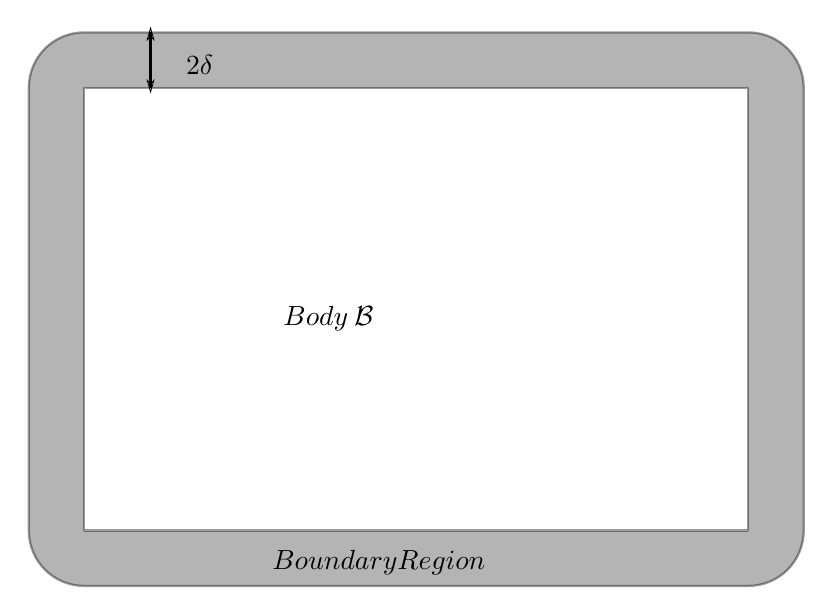
\begin{tikzpicture}[y=0.80pt, x=0.8pt,yscale=-1, inner sep=0pt, outer sep=0pt]
\begin{scope}[shift={(0,-652.36218)}]
  \path[shift={(0,652.36218)},draw=black,fill=black,line join=round,miter
    limit=4.00,draw opacity=0.392,fill opacity=0.294,nonzero rule,line
    width=0.823pt] (50.0000,25.0000) -- (350.0000,25.0000) .. controls
    (363.8500,25.0000) and (375.0000,36.1500) .. (375.0000,50.0000) --
    (375.0000,250.0000) .. controls (375.0000,263.8500) and (363.8500,275.0000) ..
    (350.0000,275.0000) -- (50.0000,275.0000) .. controls (36.1500,275.0000) and
    (25.0000,263.8500) .. (25.0000,250.0000) -- (25.0000,50.0000) .. controls
    (25.0000,36.1500) and (36.1500,25.0000) .. (50.0000,25.0000) -- cycle;
  \path[shift={(0,652.36218)},draw=black,fill=cffffff,line join=round,miter
    limit=4.00,draw opacity=0.392,nonzero rule,line width=0.823pt,rounded
    corners=0.0000cm] (50.0000,50.0000) rectangle (350.0000,250.0000);
    \path[color=black,fill=black,line width=1.200pt] (79.2500,677.3622) --
      (79.2500,702.3622) -- (80.7500,702.3622) -- (80.7500,677.3622) --
      (79.2500,677.3622) -- cycle;
    \path[draw=black,even odd rule,line width=0.300pt] (80.0000,679.1622) --
      (81.5000,680.6622) -- (80.0000,675.4122) -- (78.5000,680.6622) --
      (80.0000,679.1622) -- cycle;
    \path[draw=black,even odd rule,line width=0.300pt] (80.0000,700.5622) --
      (78.5000,699.0622) -- (80.0000,704.3122) -- (81.5000,699.0622) --
      (80.0000,700.5622) -- cycle;
  \path[shift={(0,652.36218)},fill=black] (96.071426,43.92857) node[above right]
    (text4653) {$2\delta$};
  \path[fill=black] (140,812.36218) node[above right] (text4657) {$\text{Body}\:
    \mathcal{B}$};
  \path[fill=black] (135,922.36218) node[above right] (text4661) {$\text{Boundary
    Region}$};
\end{scope}

\end{tikzpicture}


  \caption{The boundary of a peridynamic model is a region of nonzero thickness}
  \label{fig:PDboundary}
\end{figure}
%

For the peridynamic beam we consider simple supports or rollers, and fixed or clamped supports.
Simply-supported beams are easy to model because only displacement is constrained.
To add a roller support to the peridynamic beam, it suffices to constrain the movement of the nearest peridynamic node in the appropriate degree(s) of freedom.
Simulating a ``clamped'' end condition is a little less intuitive. 
The most basic way to simulate a clamped end is to extend the beam \(2\delta\), or twice the horizon, into the clamp. The displacement of all of those nodes is set to zero, or whatever value is appropriate for a displaced or rotated clamp.
In classical mechanics, a clamped end can be described with a symmetry condition, but the two are not peridynamically equivalent.
Because the classical beam is a local model, material at a clamp cannot ``see'' distant material, so there is no way to distinguish between a beam end that is clamped and one that is bent symmetrically over an appropriate sawhorse.

The loads we apply to the peridynamic beam include applied moments, point loads and distributed loads.
Distributed forces may be applied as expected to nodes in the loaded region.
Point forces may often be applied directly to the nearest node, or to the nodes immediately surrounding the point of application.
Point moments must also be considered more carefully because the peridynamic models in this work, like most peridynamic models, do not consider rotational degrees of freedom for peridynamic nodes.
Rather, material rotation is the result of the relative translational displacement of multiple nodes.
It is therefore impossible to apply a moment to a single peridynamic point.
Instead, moments may be applied as force couples to the bonds attached to the peridynamic node nearest the location of the desired moment.
For example, if we want to apply a moment $M$ at point $\mathbf{x}$, whose $n$ neighboring points $\mathbf{x}'_i$ are connected to $\mathbf{x}$ in the undeformed configuration by bonds $\boldsymbol{\xi}_i$.
For an evenly discretized beam, we may distribute the moments by
\begin{equation}
\mathbf{M}_i = \mathbf{M} \frac{\omega(\boldsymbol{\xi}_i)}{\sum\limits_{j=1}^n \omega(\boldsymbol{\xi}_j)}\notag
\end{equation}
and apply them to the corresponding bonds by adding forces
\begin{equation}
\mathbf{F}_i = \mathbf{M}_i \times \frac{\vstate{Y}{}{\boldsymbol{\xi}_i}}{|\vstate{Y}{}{\boldsymbol{\xi}_i}|^2}\notag
\end{equation}
to each point $\mathbf{x}_i$ and subtracting them from the force at $\mathbf{x}$.

Support configurations are similar for two-dimensional models.
Each node along a simply-supported edge is constrained in one or more directions.
As with the beam model, clamped edges are implemented by extending the surface into the clamp.
Line and pressure loads are treated normally.

\section{Numerical Solution Method}

This project uses Trilinos, a collection of open software libraries, or packages, from Sandia National Labs, including:
\begin{itemize}
  \item Epetra and EpetraExt - provide efficient parallel data structures, particularly vectors and sparse matrices
  \item Isorropia - provides load balancing, partitioning, and matrix coloring
  \item NOX - a collection of large-scale nonlinear system solver utilities
  \item PyTrilinos - a python interface providing Python wrappers for many Trilinos packages, and offering compatibility between numpy.ndarrays and Epetra.MultiVectors\cite{PyTrilinos}
\end{itemize}

The nature of discrete peridynamic models results in large numbers of parallelizable computations.
Efficient parallelization is achieved using Epetra data structures for distributed variables.
Model force evaluations are coded in Python, making extensive use of the optimized routines in the NumPy and SciPy packages operating on the distributed Epetra objects. 
To obtain quasistatic solutions, problems are coded into NOX objects and solved using NOX nonlinear solvers.
Preliminary analysis was performed using a Newton Method solver on an iMac with a 3.1GHz Intel Core i7 processor and 16GB RAM, using 1-4 cores.
Later work also performed on Shamu, a High-Performance Computing cluster at UTSA, and Stampede, a High-Performance Computing cluster at UT Austin.
The nature of the Trilinos packages and the structure of the code allow for more extensive parallel computation without major code changes.

For all but the simplest loading conditions, analytical solutions to boundary condition problems become complicated.
As load conditions and material behavior become more complex, there are no analytical solutions.
For comparison, equivalent models are created and analyzed in Abaqus 6.12 to verify simple cases. \todo{If you have time and the inclination, I would expand this section significantly.  The code work was a considerable part of your research and only dedicating a few paragraphs does not do it justice.}
